\documentclass[a4paper,11pt,twoside]{book}

\usepackage[eng,exjobb]{KTHEEtitlepage}
\usepackage[cp1252]{inputenc}

\usepackage{mystyle}


\begin{document}

\ititle{Robust Decentralized
  Control of Inter-constrained Continuous Nonlinear Systems}
\isubtitle{A Receding Horizon Approach} % Optional
\idate{February 2006}
\irefnr{TRITA-EE 2006:666}
\iauthor{Alexandros Filotheou}
\makeititle
\newpage

% Show layout variables
%\printinunitsof{mm}{\pagevalues}
%\verb|\marginparwidth|: \printinunitsof{mm}\prntlen{\marginparwidth}
%\pagediagram


\newpage
\cleardoublepage
\cleardoublepage

%\newgeometry{paperwidth=169mm, paperheight=239mm, top=50mm, bottom=30mm, inner=36mm, outer=18mm, voffset=-1in + 15mm, footskip = 15mm}
\newgeometry{top=50mm, bottom=30mm, inner=36mm, outer=18mm, footskip = 15mm}
\tableofcontents
\restoregeometry
\cleardoublepage


\section{Introduction}

  \noindent formation of multi-agent systems, mpc intro etc. \\

\noindent motivation why we need mpc controllers...  \\

\noindent In many control problems it is desired to design a stabilizing
feedback such that a performance criterion is minimized while satisfying
constraints on the controls and the states. Ideally one would look for a
closed solution for the feedback law satisfying the constraints while
optimizing the performance. However, typically the optimal feedback law
cannot be found analytically, even in the unconstrained case, since it involves
the solution of the corresponding Hamilton-Jacobi-Bellman partial differential
equations. One approach to circumvent this problem is the repeated solution of
an open-loop optimal control problem for a given state. The first part of the
resulting open-loop input signal is implemented and the whole process is
repeated. Control approaches using this strategy are referred to as Model
Predictive Control (MPC).

  \cleardoublepage

%===============================================================================
\part{The problem}
\cleardoublepage

%-------------------------------------------------------------------------------
  \chapter{Notation and Preliminaries}
    \label{chapter:notation_reliminaries}

    \section{Notation}

The set of positive integers is denoted by $\mathbb{N}$. The real $n$-coordinate
space, $n\in\mathbb{N}$, is denoted by $\mathbb{R}^n$;
$\mathbb{R}^n_{\geq 0}$ and $\mathbb{R}^n_{> 0}$ are the sets of real
$n$-vectors with all elements nonnegative and positive, respectively. Given a
set $S$, we denote by $\lvert S\lvert$ its cardinality. The notation
$\|\vect{x}\|$ is used for the Euclidean norm of a vector
$\vect{x} \in \mathbb{R}^n$; $\|\vect{x}\|_P$ denotes the $\mat{P}$-norm of
$\vect{x}$. Given matrix $\mat{A}$, $\lambda_{\text{min}}(\mat{A})$
and $\lambda_{\text{max}}(\mat{A})$
denote the minimum and maximum eigenvalues of $\mat{A}$, respectively.
Its minimum and maximum singular values are denoted by
$\sigma_{\text{min}}(\mat{A})$ and $\sigma_{\text{max}}(\mat{A})$ respectively.
Given two sets $A$ and $B$, the operation $A \oplus B$ denotes the Minkowski
addition, defined by
$A \oplus B = \{\vect{a} + \vect{b},\ \vect{a} \in A, \vect{b} \in B\}$. Similarly,
the Minkowski $-$ or Pontryagin difference is defined by
$A \ominus B = \{\vect{a} - \vect{b},\ \vect{a} \in A, \vect{b} \in B\}$.
$\mat{I_n} \in \mathbb{R}^{n \times n}$ and
$\mat{0}_{m \times n} \in \mathbb{R}^{m \times n}$
are the unit matrix and the $m \times n$ matrix with all entries zeros
respectively. The notation
$\mathcal{B}(\vect{c},r) \overset{\Delta}{=} \{\vect{x} \in \mathbb{R}^3: \|\vect{x}-\vect{c}\| \leq r\}$
is reserved for the 3D sphere of radius $r \in \mathbb{R}_{\ge 0}$ and center
located at $\vect{c}\in\mathbb{R}^{3}$.

The vector expressing the coordinates of the origin of frame $\{j\}$ in
frame $\{i\}$ is denoted by $\vect{p}_{j \triangleright i}$. When this vector is
expressed in 3D space in a third frame, frame $\{k\}$, it is denoted by
$\vect{p}_{j \triangleright i}^{k}$.
%Given $\vect{a}\in\mathbb{R}^3$, $\mat{S}(\vect{a})$ is the skew-symmetric
%matrix defined according to $\mat{S}(\vect{a})\vect{b} = \vect{a}\times \vect{b}$.
The angular velocity of frame $\{j\}$ with respect to frame $\{i\}$, expressed
in frame $\{k\}$ coordinates, is denoted by
$\vect{\omega}^k_{j \triangleright i}\in \mathbb{R}^{3}$.
We further denote by $\vect{q}_{j \triangleright i} \in \mathbb{T}^3$
the Euler angles representing the orientation of frame $\{j\}$ with respect to
frame $\{i\}$, where $\mathbb{T}^3$ is the $3$D torus.
We also use the notation $\mathbb{M} = \mathbb{R}^3\times \mathbb{T}^3$.
For notational brevity, when a coordinate frame corresponds to the inertial frame
of reference $\{\mathcal{O}\}$, we will omit its explicit notation
(e.g., $\vect{p}_i = \vect{p}_{i \triangleright \mathcal{O}} = \vect{p}^\mathcal{O}_{i \triangleright \mathcal{O}}$, and
$\vect{\omega}_i = \vect{\omega}_{i \triangleright \mathcal{O}} = \vect{\omega}^\mathcal{O}_{i \triangleright \mathcal{O}}$).
%All vector and matrix differentiations are derived with respect to the inertial
%frame $\{\mathcal{O}\}$ unless stated otherwise.

    \section{Auxiliary Prerequisites}

This section features auxiliary and useful theorems, lemmas and definitions
needed to support the advocated solutions in part
\ref{part:advocated_solutions}.

% The Gronwall-Bellman inequality
%===============================================================================
%\begin{bw_box}
  \begin{lemma} \cite{khalil_nonlinear_systems} \textit{The Gr\"{o}nwall-Bellman Inequality}
    \label{lemma:bellman_inequality}

    Let $\lambda : [a,b] \to \mathbb{R}$ be continuous and
    $\mu : [a,b] \to \mathbb{R}$ be continuous and non-negative. If a
    continuous function $y : [a,b] \to \mathbb{R}$ satisfies
    \begin{align}
      y(t) \leq \lambda(t) + \int_a^t \mu(s) y(s) ds
    \end{align}
    for $a \leq t \leq b$, then on the same interval
    \begin{align}
      y(t) \leq \lambda(t) + \int_a^t \lambda(s) \mu(s) e^{\int_s^t \mu(\tau)d\tau} ds
    \end{align}
    In particular, if $\lambda(t) \equiv \lambda$ is a constant, then
    \begin{align}
      y(t) \leq \lambda e^{\int_a^t \mu(\tau)d\tau} ds
    \end{align}
    If $\lambda(t) \equiv \lambda$ and $\mu(t) \equiv \mu$ are both constants,
    then
    \begin{align}
      y(t) \leq \lambda e^{\mu (t - a)}
    \end{align}
    \\[2.5ex]
  \end{lemma}
%\end{bw_box}

% Class K functions
%===============================================================================
%\begin{bw_box}
\begin{definition}\cite{khalil_nonlinear_systems} (\textit{Class $\mathcal{K}$ function})
\label{def:k_class}

  A continuous function $\alpha : [0, a) \to [0, \infty)$
  is said to belong to class $\mathcal{K}$ if
  \begin{enumerate}
    \item it is strictly increasing
    \item $\alpha (0) = 0$
  \end{enumerate}
  If $a = \infty$ and $\lim\limits_{r \to \infty} \alpha(r) = \infty$, then function
  $\alpha$ is said to belong to class $\mathcal{K}_{\infty}$
\\[2.5ex]
\end{definition}
%\end{bw_box}


% Class KL functions
%===============================================================================
%\begin{bw_box}
\begin{definition}\cite{khalil_nonlinear_systems} (\textit{Class $\mathcal{KL}$ function})
\label{def:kl_class}

  A continuous function $\beta : [0, a) \times [0, \infty) \to [0, \infty)$
  is said to belong to class $\mathcal{KL}$ if
  \begin{enumerate}
    \item for a fixed $s$, the mapping $\beta(r,s)$ belongs to class $\mathcal{K}$ with respect to $r$
    \item for a fixed $r$, the mapping $\beta(r,s)$ decreases with respect to $s$
    \item $\lim\limits_{s \to \infty} \beta(r,s) = 0$
\\[2.5ex]
  \end{enumerate}
\end{definition}
%\end{bw_box}



% Barbalat's lemma
%===============================================================================
%\begin{bw_box}
  \begin{lemma} \cite{Fontes2007} (\textit{A modification of Barbalat's lemma})
  \label{lemma:barbalat}

    Let $f$ be a continuous, positive-definite function, and $\vect{x}$ be an
    absolutely continuous function in $\mathbb{R}$. If the following hold:
  \begin{itemize}
    \item $\|\vect{x}(\cdot)\| < \infty$
    \item $\|\dot{\vect{x}}(\cdot)\| < \infty$
    \item $\lim\limits_{t \to \infty} \int\limits_0^t f\big(\vect{x}(s)\big)ds < \infty$
  \end{itemize}
  then $\lim\limits_{t \to \infty} \|\vect{x}(t)\| = 0$
\\[2.5ex]
  \end{lemma}
%\end{bw_box}

\newpage
% ISS stability definition
%===============================================================================
%\begin{bw_box}
\begin{definition}\cite{marquez2003nonlinear} (\textit{Input-to-State Stability})
\label{def:ISS}

A nonlinear system $\dot{\vect{x}} = f(\vect{x},\vect{u})$, $\vect{x} \in X$,
$\vect{u} \in U$ with initial condition $\vect{x}(t_0)$ is said
to be \textit{locally Input-to-State Stable (ISS)} if there exist functions
$\sigma \in \mathcal{K}$ and $\beta \in \mathcal{KL}$
and constants $k_1, k_2 \in \mathbb{R}_{> 0}$ such that
\begin{align}
  \|\vect{x}(t)\| \leq \beta\big(\|\vect{x}(t_0)\|,t\big) + \sigma\big(\|\vect{u}\|_{\infty}\big),\ \forall t \geq 0
\end{align}
for all $\vect{x}(t_0) \in X$ and $\vect{u} \in U$ satisfying $\|\vect{x}(t_0)\| \leq k_1$
and $\text{sup}\limits_{t > 0} \|\vect{u}(t)\| = \|\vect{u}\|_{\infty} \leq k_2$.
\\[2.5ex]
\end{definition}
%\end{bw_box}



% remark on ISS stability definition
%===============================================================================
%\begin{bw_box}
\begin{remark} \cite{1185106}
\label{def:ISS_remark}
  A nonlinear system $\dot{\vect{x}} = f(\vect{x},\vect{u})$, $\vect{x} \in X$,
$\vect{u} \in U$ which is input-to-output stable, is asymptotically stable
in the absence of disturbances $\vect{u}$, or if the disturbance is decaying.
If the disturbance is merely bounded, then the evolution of the system is
\textit{ultimately bounded} in a set whose size depends on the bound of the
disturbance.
\\[2.5ex]
\end{remark}
%\end{bw_box}



% ISS Lyapunov function definition
%===============================================================================
%\begin{bw_box}
\begin{definition}\cite{marquez2003nonlinear} (\textit{ISS Lyapunov function})
\label{def:ISS_Lyapunov}

A continuous function $V(\vect{x}) : \Psi \to \mathbb{R}_{\geq 0}$ for the
nonlinear system $\dot{\vect{x}} = f(\vect{x}, \vect{\delta})$ is said to be a
\textit{ISS Lyapunov function} in $\Psi$ if there are class
$\mathcal{K}_{\infty}$ functions
$\alpha_1, \alpha_2, \alpha_3$, and a class $\mathcal{K}$ function
$\sigma$ such that
\begin{align}
  \alpha_1\big(\|\vect{x}\|\big) \leq V\big(\vect{x}\big) \leq \alpha_2\big(\|\vect{x}\|\big),\ \forall \vect{x} \in \Psi
\end{align}
and
\begin{align}
  \dfrac{d}{dt}V\big(\vect{x}\big)
    \leq \sigma\big(\|\vect{\delta}\|\big) - \alpha_3\big(\|\vect{x}\|\big),\ \forall \vect{x} \in \Psi, \vect{\delta} \in \Delta
\end{align}
\\[2.5ex]
\end{definition}
%\end{bw_box}


\newpage
% ISS Lyapunov function remark
%===============================================================================
%\begin{bw_box}
\begin{remark}
\label{remark:ISS_Lyapunov}

With regard to definition \eqref{def:ISS_Lyapunov}, the statement
\begin{align}
  \dfrac{d}{dt}V\big(\vect{x}\big)
    \leq \sigma\big(\|\vect{\delta}\|\big) - \alpha_3\big(\|\vect{x}\|\big),\ \forall \vect{x} \in \Psi, \vect{\delta} \in \Delta
\end{align}
is equivalent to
\begin{align}
  V\big(\vect{x}(t_1)\big) - V\big(\vect{x}(t_0)\big)
  \leq \int_{t_0}^{t_1}\Big(\sigma\big(\|\vect{\delta}(t)\|\big) - \alpha_3\big(\|\vect{x}(t)\|\big)\Big)dt,\
    \forall \vect{x} \in \Psi,\ \vect{\delta} \in \Delta,\ t \in [t_0, t_1]
\end{align}
\\[2.5ex]
\end{remark}
%\end{bw_box}


% ISS Lyapunov <==> ISS
%===============================================================================
%\begin{bw_box}
\begin{theorem}\cite{marquez2003nonlinear}
\label{def:ISS_Lyapunov_admit_theorem}

  A nonlinear system $\dot{\vect{x}} = f(\vect{x},\vect{u})$ is said
  to be \textit{Input-to-State Stable} in $\Psi$ if and only if it admits an
  ISS Lyapunov function in $\Psi$.
\\[2.5ex]
\end{theorem}
%\end{bw_box}


% Positively invariant set
%===============================================================================
%\begin{bw_box}
  \begin{definition} (\textit{Positively Invariant Set})
    \label{def:positively_invariant}

    Consider a dynamical system $\dot{\vect{x}} = f(\vect{x})$,
    $\vect{x} \in \mathbb{R}^n$, and a trajectory $\vect{x}(t;\ \vect{x}_0)$,
    where $\vect{x}_0$ is the initial condition. The set
    $S = \{\vect{x} \in \mathbb{R}^n : \gamma(\vect{x}) = 0\}$, where
    $\gamma$ is a valued function, is said to be \textit{positively invariant}
    if the following holds:
    \begin{align}
      \vect{x}_0 \in S \Rightarrow \vect{x}(t;\ \vect{x}_0) \in S,\ \forall t \geq t_0
    \end{align}

    Intuitively, this means that the set $S$ is positively invariant if a
    trajectory of the system does not exit it once it enters it. \\[2.5ex]
  \end{definition}
%\end{bw_box}


% Robust positively invariant set
%===============================================================================
%\begin{bw_box}
\begin{definition}\cite{ISS_SKATOLINI} (\textit{Robust positively-invariant set})
\label{def:robust_positively_invariant_set}

A set $\Psi \in \mathbb{R}^n$ is a robust positively invariant set for the
nonlinear system $\dot{\vect{x}} = f(\vect{x}, \vect{\delta})$ if
$f(\vect{x}, \vect{\delta}) \in \Psi$, for all $\vect{x} \in \Psi$ and for all
$\vect{\delta} \in \Delta$.
\\[2.5ex]
\end{definition}
%\end{bw_box}


%% Robust control invariant set
%%===============================================================================
%%\begin{bw_box}
%\begin{definition}\cite{1024831} (\textit{Robust control invariant set})
%\label{def:robust_control_invariant_set}

%A set $\Psi \in \mathbb{R}^n$ is a robust control invariant set for the
%nonlinear system $\dot{\vect{x}} = f(\vect{x}, \vect{u}) + \vect{\delta}$,
%$\vect{x} \in X, \vect{u} \in U, \vect{\delta} \in \Delta$, if
%$\Psi \subseteq X$ and for all $\vect{x} \in \Omega$ there is an admissible
%control action $\vect{u} = \vect{h}(\vect{u}) \in U$ such that
%$f(\vect{x}, \vect{u}) + \vect{\delta} \in \Omega$ for all
%$\vect{\delta} \in \Delta$.
%\\[2.5ex]
%\end{definition}
%%\end{bw_box}

The proofs of lemmas or properties whose reference is not cited are provided
in appendix \ref{chapter:proofs_of_lemmas}.

    \section{Model Predictive control for non-linear continuous-time systems}

The equations describing a model of a system are doubly powerful: they
are \textit{expressive} inasmuch as they are a collection of properties of the
system, and they are \textit{predictive}: they provide the ability to predict
future values of relevant variables. A natural use for a model for control
design purposes is the calculation of expected future values of the controlled
variables as a function of possible control actions. This way, it is possible
to choose a control action which is the optimal according to a given criterion,
possibly while satisfying constraints on the controlled variables and control
inputs. It is reasonable for a closed-form solution of the state-feedback law
to be sought. Although this is possible when the system is linear and constraints
are absent, it is impossible or infeasible in the general case. Fortunately,
the problem can be bybassed altogether by solving an open-loop optimization
problem periodically (or even aperiodically), applying a fragment of
the resulting control input to the system, and repeating the process ad
infinitum. Control approaches using this strategy (with variations) are referred
to as \textit{Model Predictive Control} (MPC), or \textit{Receding Horizon Control}.
In this context, the term horizon refers to the period of time or timesteps
considered during the solution of the optimization problem.

In greater detail, in its pure form, the MPC strategy assumes the following
form: at an initial sampling time $t$, the controller, having measurements of
the states to be controlled, predicts the dynamic behaviour of the system over a
prediction horizon $T_p$, that is until $t+T_p$, and determines the appropriate
control input that minimizes a predetermined open-loop objective, typically
under constraints involving the states and the inputs. The calculated input
is then applied to the system until the next sampling time, at which time
the above process is repeated. Hence the term ``receding horizon".

When the system's dynamics are linear and there are is no system uncertainty
(disturbances affecting the states of the system or model-plant mismatch)
and no constraints are enforced, the input can be determined off-line by
solving the optimization problem over an infinite horizon. In this case the
input is applied to the open loop once, and the process is not repeated from
then on. However, in general, systems may be non-linear, subject to disturbances,
partially descriptive, under constraints, while an infinite horizon approach
may be practically infeasible. Hence, the optimization problem must be solved
on-line under a finite time-horizon.

In its general form, nonlinear MPC (NMPC) possesses a unique usefulness
in that it can directly incorporate nonlinear models for prediction,
nonlinear constraints, and explicit constraints on the states of the system
and its calculated/implemented inputs. Detailed descriptions and analyses of the
NMPC strategy can be found in the notable \cite{262032} and \cite{FINDEISEN2003190}.

    \cleardoublepage


%-------------------------------------------------------------------------------
  \chapter{Problem Formulation}
    \label{chapter:prob_formulation}

    %-------------------------------------------------------------------------------
\section{System Model}

Consider a set $\mathcal{V}$ of $N$ rigid bodies,
$\mathcal{V} = \{ 1,2, \ldots, N\}$, $|\mathcal{V}| = N \geq 2$, operating in
a workspace $W\subseteq \mathbb{R}^3$. A coordinate frame
$\{i\}, i\in\mathcal{V}$ is attached to the center of mass of each body.
The workspace is assumed to be modeled as a
bounded sphere $\mathcal{B}\big(\vect{p}_W,r_W\big)$ expressed in an inertial frame
$\{\mathcal{O}\}$.

We consider that over time $t$ each agent $i \in \mathcal{V}$ occupies the
space of a sphere $\mathcal{B}\big(\vect{p}_i(t), r_i\big)$, where
$\vect{p}_i : \mathbb{R}_{\geq 0} \to \mathbb{R}^3$
is the position of the agent's center of mass, and $r_i < r_W$ is the radius of the
agent's body. We denote by $\vect{q}_i(t):\mathbb{R}_{\geq 0} \to \mathbb{T}^3$,
the Euler angles representing the agents' orientation with respect to the
inertial frame $\{\mathcal{O}\}$,
with $\vect{q}_i \triangleq [\phi_i,\theta_i,\psi_i]^{\top}$, where
$\phi_i, \psi_i \in [-\pi, \pi]$ and
$\theta_i \in [-\frac{\pi}{2}, \frac{\pi}{2}]$. We define
$$\vect{x}_i (t)\triangleq [\vect{p}_i(t)^{\top},\vect{q}_i(t)^{\top}]^{\top},
\vect{x}_i(t):\mathbb{R}_{\geq 0} \to \mathbb{R}^3\times \mathbb{T}^3 \equiv \mathbb{M}$$
$$\vect{v}_i(t) \triangleq [\dot{\vect{p}}_i(t)^{\top}, \vect{\omega}_i(t)^{\top}]^{\top},
\vect{v}_i(t) : \mathbb{R}_{\geq 0} \to \mathbb{R}^3\times \mathbb{R}^3 \equiv \mathbb{R}^6$$
and model the motion of agent $i$ under continuous second order dynamics:
\begin{subequations}
	\begin{align}
    \dot{\vect{x}}_i(t) &= \mat{J}_i^{-1}(\vect{x}_i) \vect{v}_i(t), \label{eq:system_1} \\[2.5ex]
    \vect{u}_i(t) &= \mat{M}_i(\vect{x}_i) \dot{\vect{v}}_i(t) +
      \mat{C}_i(\vect{x}_i,\dot{\vect{x}}_i) \vect{v}_i(t)+\vect{g}_i(\vect{x}_i) \label{eq:system_2}
	\end{align}
  \label{eq:system}
\end{subequations}

In equation \eqref{eq:system_1}, $\mat{J}_i:\mathbb{T}^3 \to \mathbb{R}^{6\times6}$ is
a Jacobian matrix that maps the non-orthogonal Euler angle rates to the
orthogonal angular velocities $\vect{v}_i$:

\begin{equation}
  \mat{J}_i(\vect{x}_i) =
  \begin{bmatrix}
    \mat{I}_3 & \mat{0}_{3 \times 3} \\[2.5ex]
    \mat{0}_{3 \times 3} & \mat{J}_{ q }(\vect{x}_i) \\[2.5ex]
  \end{bmatrix} \notag, \text{ where }
  \mat{J}_q(\vect{x}_i) =
  \begin{bmatrix}
    1 & 0 & \sin\theta_i \\[2.5ex]
    0 & \cos\phi_i & -\cos\theta_i \sin\phi_i \\[2.5ex]
    0 & \sin\phi_i & \cos\phi_i \cos\theta_i
  \end{bmatrix} \notag
\end{equation}

Matrix $\mat{J}_i$ is singular when $det(\mat{J}_i)$ $=$ $\cos\theta_i = 0$
$\Leftrightarrow$ $\theta_i$ $=$ $\pm \frac{\pi}{2}$. The control scheme
proposed in this thesis guarantees that this is always avoided, and hence
equation \eqref{eq:system_1} is well defined.
%This gives rise to the following remark:
%\begin{bw_box}
  %\begin{remark}
    %$det(\mat{J}_i) = \cos\theta_i \leq 1$, $\forall i \in \mathcal{V}$
  %\end{remark}
%\end{bw_box}

In equation \eqref{eq:system_2}, $\mat{M}_i:\mathbb{M} \to \mathbb{R}^{6\times6}$ is
the symmetric and positive definite \textit{inertia matrix},
$\mat{C}_i:\mathbb{M}\times\mathbb{R}^6 \to \mathbb{R}^{6\times6}$ is the
\textit{Coriolis matrix} and $\vect{g}_i:\mathbb{M} \to \mathbb{R}^6$ is the
\textit{gravity vector}.
Finally, $\vect{u}_i\in\mathbb{R}^6$ is the control input vector representing
the $6$D generalized \textit{actuation force} acting on the agent.

%Let us also define the vectors
%$\vect{X} = [\vect{x}_1^\top, \dots, x_N^\top]^\top :
%\mathbb{R}_{\geq 0} \to \mathbb{M}^N, \vect{V} = [\vect{v}_1^\top, \dots
%\vect{v}_N^\top]^\top: \mathbb{R}_{\geq 0} \to \mathbb{R}^{6N}$.


%\begin{bw_box}
  %\begin{remark}
    %According to \cite{Murray:1994:MIR:561828}, the matrices
    %$\dot{\mat{M}}_i - 2\mat{C}_i, i \in \mathcal{V}$ are skew-symmetric.
    %The quadratic form of a skew-symmetric matrix is always equal to 0, hence:

    %\begin{equation}
      %\vect{y}^\top \left[\dot{\mat{M}}_i - 2 \mat{C}_i\right]\vect{y} = 0,
        %\forall \vect{y} \in \mathbb{R}^6, i \in \mathcal{V}.
    %\label{eq:skew_symm}
    %\end{equation}
  %\end{remark}
%\end{bw_box}

However, access to measurements of, or knowledge about these matrices and
vectors was not hitherto considered. At this point we make the following
assumption:

\begin{gg_box}
  \begin{assumption} (\textit{Measurements and Access to Information
    from an Inter-agent Perspective})
  \label{ass:measurements_access}
  \begin{enumerate}

    \item Agent $i$ has access to measurements
      $\vect{p}_i, \vect{q}_i, \dot{\vect{p}}_i, \vect{\omega}_i, \forall i\in\mathcal{V}$,
      that is, vectors $\vect{x}_i, \vect{v}_i$ pertaining to himself,

    \item Agent $i$ has a (upper-bounded) sensing range $d_i$ such that
      $$d_i > \max\{r_i + r_j : \forall i,j \in \mathcal{V}, i \neq j\}$$

    \item the inertia $\mat{M}_i$ and Coriolis $\mat{C}_i$ vector fields are
      bounded and unknown for all $i \in \mathcal{V}$

    \item the gravity vectors $\vect{g}$ are bounded and known for all $i \in \mathcal{V}$

  \end{enumerate}
\end{assumption}
\end{gg_box}

The consequence of points 1 and 2 of assumption \eqref{ass:measurements_access}
is that by defining the set of agents $j$ that are within the sensing range
of agent $i$ at time $t$ as
$$\mathcal{R}_i(t) \triangleq \{j\in\mathcal{V} : \vect{p}_j(t)\in\mathcal{B}\big(\vect{p}_i(t), d_i\big)\}$$
or equivalently
$$\mathcal{R}_i(t) \triangleq \{j\in\mathcal{V} : \| \vect{p}_i(t) - \vect{p}_j(t) \| \leq d_i\}$$
agent $i$ also knows at each time instant $t$ all
$$\vect{p}_{j \triangleright i}(t), \vect{q}_{j \triangleright i}(t),
\dot{\vect{p}}_{j \triangleright i}(t), \vect{\omega}_{j \triangleright i}(t)$$
Therefore, agent $i$ assumes access to all measurements
$$\vect{p}_{j}(t), \vect{q}_{j}(t), \dot{\vect{p}}_j(t),
\vect{\omega}_j(t),\ \forall j\in \mathcal{R}_i(t),t\in\mathbb{R}_{\geq 0}$$
of all agents $j \in \mathcal{R}_i(t)$ by virtue of being able to calculate
them using knowledge of its own
$\vect{p}_i(t)$, $\vect{q}_i(t)$, $\dot{\vect{p}}_i(t)$, $\vect{\omega}_i(t)$.


In the workspace there is a set $\mathcal{L}$ of $L$ \textit{static obstacles},
$\mathcal{L} = \{1, 2, \dots, L\}$,
$L = |\mathcal{L}|$, also modeled as spheres, with centers at positions
$\vect{p}_{\ell} \in \mathbb{R}^3$ with radii
$r_{\ell}\in \mathbb{R}$, $\ell \in \mathcal{L}$. Thus, the obstacles are
modeled by spheres
$\mathcal{B}\big(\vect{p}_{\ell}, r_{\ell}\big)$, $\ell \in \mathcal{L}$.
Their position and size in 3D space is assumed to be known a priori
to each agent. The geometry of two agents $i$ and $j$ as well as an obstacle
$\ell$ in workspace $W$ is depicted in Fig. \ref{fig:two_agents_one_obstacle}.

\begin{figure}[ht!]
	\centering
    \begin{tikzpicture}[scale = 0.5]
	%draw the global frame
	\draw [color=black,thick,->,>=stealth'](-9, -5) to (-7, -5);
	\draw [color=black,thick,->,>=stealth'](-9, -5) to (-9, -3);
	\draw [color=black,thick,->,>=stealth'](-9, -5) to (-10, -6.5);
  \node at (-9.9, -5.0) {$\{\mathcal{O}\}$};

	%draw agent i
	\draw [color = blue, fill = blue!20] (-4.5,0) circle (2.5cm);
  \node at (-5.7, 0.0) {$\{i\}$};
	\draw[green,thick,dashed] (-4.5,0) circle (6.0cm);
	\draw [color=black,thick,->,>=stealth'](-9, -5) to (-4.5, -0.1);
	\node at (-7.7, -3.0) {$p_i$};
	\draw [color=green,thick,dashed,->,>=stealth'](-4.5, 0.0) to (-9.93, 2.43);
	\node at (-7.3, 2.15) {$d_i$};
	\draw [color=black,thick,dashed,->,>=stealth'](-4.5, 0.0) to (-2.0, 0.0);
	\node at (-3.3, 0.3) {$r_i$};
	\node at (-4.5, 0.0) {$\bullet$};
	\node at (-4.8, 3.0) {$\mathcal{B}(p_i, r_i)$};

	%draw agent j
	\draw [color = red, fill = red!20] (0.2, 0) circle (1.5cm);
	\node at (-0.5, 0.3) {$\{j\}$};
	\draw[orange,thick,dashed,] (0.2, 0) circle (5.1cm);
	\draw [color=black,thick,->,>=stealth'](-9, -5) to (0.2, -0.1);
	\node at (-6.0, -3.9) {$p_j$};
	\draw [color=orange,thick,dashed,->,>=stealth'](0.2, 0.0) to (0.2, -5.0);
	\node at (0.8, -3.7) {$d_j$};
	\draw [color=black,thick,dashed,->,>=stealth'](0.2, 0.0) to (1.7, 0.0);
	\node at (1.1, 0.3) {$r_j$};
	\node at (0.2, 0.0) {$\bullet$};
	\node at (3.0, 2.1) {$\mathcal{B}(p_j, r_j)$};

	% draw the obstacle
	\draw [color = black, fill = black!20] (-1, -8) circle (1.2cm);
	\draw [color=black,thick,->,>=stealth'](-9, -5) to (-1.1, -7.98);
	\draw [color=black,thick,dashed,->,>=stealth'](-1, -8) to (-1, -6.8);
	\node at (-1, -8) {$\bullet$};
	\node at (-5.0, -6.0) {$p_{\ell}$};
	\node at (-0.40, -7.5) {$r_{\ell}$};
\end{tikzpicture}

    \caption{Illustration of two agents $i, j \in \mathcal{V}$ and a static
      obstacle $\ell \in \mathcal{L}$ in the workspace; $\{\mathcal{O}\}$ is the inertial
      frame, $\{i\}, \{j\}$ are the frames attached to the agents' center of
      mass, $\vect{p}_i, \vect{p}_j, \vect{p}_{\ell} \in \mathbb{R}^3$ are the
      positions of the centers of mass of agents $i,j$ and obstacle $\ell$
      respectively, expressed in frame $\{\mathcal{O}\}$. $r_i, r_j, r_{\ell}$
      are the radii of the agents $i,j$ and the obstacle $\ell$ respectively.
      $d_i, d_j$ with $d_i > d_j$ are the agents' sensing ranges.
      In this figure, agents $i$ and $j$ are neighbours, since the center
      of mass of agent $j$ is within the sensing range of agent $i$ and vice
      versa: $\vect{p}_j \in \mathcal{B}\big(\vect{p}_i(t), d_i\big)$ and
      $\vect{p}_i \in \mathcal{B}\big(\vect{p}_j(t), d_j\big)$. Furthermore, the
      configuration between the two agents and the obstacle is a collision-free
      configuration.}
	\label{fig:two_agents_one_obstacle}
\end{figure}

Let us now define the distance between any two agents $i,j$ at time $t$ as
$d_{ij,a}(t)$; that between agent $i$ and obstacle $\ell$ as $d_{i\ell,o}(t)$;
and that between an agent $i$ and the origin of the workspace $W$ as
$d_{i,W}(t)$, with $d_{ij,a}, d_{i\ell,o}, d_{i,W} : \mathbb{R}^3 \to \mathbb{R}_{\geq 0}$:
\begin{subequations}
	\begin{align}
    d_{ij,a}(t) &\triangleq \| \vect{p}_i(t) - \vect{p}_j(t) \| \\[2.5ex]
    d_{i\ell,o}(t) &\triangleq \| \vect{p}_i(t) - \vect{p}_\ell(t) \| \\[2.5ex]
    d_{i,W}(t) &\triangleq \| \vect{p}_W - \vect{p}_i(t) \|
	\end{align}
\end{subequations}
as well as constants
\begin{subequations}
	\begin{align}
    \underline{d}_{ij, a} &\triangleq r_{i} + r_{j} \\[2.5ex]
    \underline{d}_{i\ell, o} &\triangleq r_{i} + r_{\ell} \\[2.5ex]
    \overline{d}_{i,W} &\triangleq r_W - r_i
	\end{align}
\end{subequations}
$\forall i, j \in \mathcal{V}$, $i \neq j$, $\ell \in \mathcal{L}$.
The latter stand for the minimum distance between two \textit{agents}, the
minimum distance between an \textit{agent} and an \textit{obstacle},
and the maximum distance between an \textit{agent} and the origin of the
workspace, respectively. They arise spatially as physical limitations and will
be utilized in forming collision-avoidance constraints.

Based on these definitions, we will now define the concept of a
\textit{collision-free configuration}:
\begin{bw_box}
\begin{definition} (\textit{Collision-free Configuration})
\label{definition:collision_free_conf}
  A collision-free configuration between
  \begin{itemize}
    \item any two agents $i,j \in \mathcal{V}$ is when $d_{ij,a}(t) > \underline{d}_{ij,a}$
    \item an agent $i \in \mathcal{V}$ and an obstacle $\ell \in \mathcal{L}$
     is when $d_{il,o}(t) > \underline{d}_{il,o}$
    \item an agent $i \in \mathcal{V}$ and the workspace $W$ boundary,
     is when $d_{i,W}(t) < \overline{d}_{i,W}$
  \end{itemize}
  at a generic time instant $t \in \mathbb{R}_{\geq 0}$. When all three
  conditions are met, we will simply refer to the overall configuration as
  a collision-free configuration.
\end{definition}
\end{bw_box}

    %-------------------------------------------------------------------------------
\section{Initial Conditions}

We assume that at time $t=0$ \textit{all} agents are in a
\textit{collision-free configuration}, i.e.
\begin{subequations}
\begin{align}
    d_{ij,a}(0) &> \underline{d}_{ij,a} \\[2.5ex]
    d_{il,o}(0) &> \underline{d}_{il,o} \\[2.5ex]
    d_{i,W}(0)  &< \overline{d}_{i,W}
\label{eq:initially_coll_free}
\end{align}
\end{subequations}
$\forall i \in \mathcal{V}, \ell \in \mathcal{L}$. Before declaring further
assumptions that relate to the initial conditions of the system's configuration,
we have to give the definition of the \textit{neighbour set} $\mathcal{N}_i$ of
a generic agent $i \in \mathcal{V}$:
\begin{bw_box}
\begin{definition} (\textit{Neighbours Set})

Agents $j \in \mathcal{N}_i$ are defined as the \textit{neighbours} of
agent $i \in \mathcal{V}$. The set $\mathcal{N}_i$ is composed of the
indices of agents $j \in \mathcal{V}$ which
\begin{enumerate}
  \item are within the sensing range of agent $i$ at time $t=0$, i.e.
    $j \in \mathcal{R}_i(0)$, \textit{and}
  \item are \textit{intended} to be kept within the sensing range of agent $i$ at all
    times $t \in \mathbb{R}_{> 0}$
\end{enumerate}
\end{definition}
\end{bw_box}

Therefore, while the composition of the set $\mathcal{R}_i(t)$ evolves and
varies through time in general, the set $\mathcal{N}_i$ \textit{should} remain
invariant over time\footnote{This reason, and the fact that the proposed
control scheme guarantees that $\mathcal{N}_i$ \textit{will} remain invariant
over time, is why we do not refer to this set as $\mathcal{N}_i(t)$.}.

It is not necessary that all agents are assigned a set of agents with whom they
should maintain connectivity; however, if \textit{all} agents were
neighbour-less, then the concept of \textit{cooperation} between them would be
void, since in that case the problem would break down into $|\mathcal{V}|$
individual problems of smaller significance or interest, while weakening the
``multi-agent" perspective as well. Therefore, we assume that
$\sum\limits_i |\mathcal{N}_i| > 0$.

It is further assumed that $\mathcal{N}_i$ is given at $t=0$, and that
neighbouring relations are reciprocal, i.e. agent $i$ is a neighbour of
agent $j$ if and only if $j$ is a neighbour of $i$:
\begin{subequations}
\begin{align}
  j \in \mathcal{N}_i \Leftrightarrow i \in \mathcal{N}_j,\ \forall i,j \in \mathcal{V}, i\not=j
\end{align}
\end{subequations}
%Topologically, this means that the graph $\mathcal{G}$ constructed by the edges
%connecting neighbouring agents $i \in \mathcal{V}$ is undirected.

Furthermore, it is assumed that at time $t=0$ the Jacobians $\mat{J}_i$ are
well-defined $\forall i \in \mathcal{V}$, and that the system \eqref{eq:system}
enjoys a continuous solution for all initial conditions. The assumptions which
concern the initial conditions of the problem are formally summarized in
assumption \ref{ass:initial_conditions}:\\[1ex]

\begin{gg_box}
\begin{assumption}(\textit{Initial Conditions Assumption})
  \label{ass:initial_conditions}

  At time $t = 0$

  \begin{enumerate}

    \item the sets $\mathcal{N}_i$ are known for all $i \in \mathcal{V}$
      and $\sum\limits_i |\mathcal{N}_i| > 0$

    \item all agents are in a collision-free configuration with each other,
      the obstacles $\ell \in \mathcal{L}$ and the workspace $W$ boundary

    \item all agents are in a singularity-free configuration:

      $$ -\frac{\pi}{2} < \theta_i(0) < \frac{\pi}{2},\ \forall i \in \mathcal{V}$$

  \end{enumerate}
\end{assumption}
\end{gg_box}

    %-------------------------------------------------------------------------------
\section{Objective}
\label{sec:objective}

Given the aforementioned structure of the system, the objective to be
pursued is the \textit{stabilization of all agents} $i \in \mathcal{V}$ starting
from an initial configuration abiding by assumption
\eqref{ass:initial_conditions} to a desired feasible configuration
$\vect{x}_{i,des}, \vect{v}_{i,des}$, while
satisfying all communication constraints, i.e. sustaining connectivity between
neighbouring agents, and avoiding collisions between agents, obstacles, and the
workspace boundary. The concept of a \textit{desired feasible configuration}
or \textit{feasible steady-state configuration} is given in definition
\eqref{definition:feasible_steady_state_conf}.

\begin{bw_box}
\begin{definition} (\textit{Feasible Steady-state Configuration})
\label{definition:feasible_steady_state_conf}

The desired steady-state configuration $\vect{x}_{i,des}$ of agents
$\forall i \in \mathcal{V}, j \in \mathcal{N}_i$ is \textit{feasible} if and
only if
\begin{enumerate}
  \item it is a collision-free configuration according to definition
    \eqref{definition:collision_free_conf}
  \item it does not result in violation of the communication constraints
    between neighbouring agents $i,j$, i.e. the following inequalities hold
    true simultaneously:
    \begin{align}
      \|\vect{p}_{i,des} - \vect{p}_{j,des}\| < d_i \\[2.5ex]
      \|\vect{p}_{i,des} - \vect{p}_{j,des}\| < d_j \\[2.5ex]
    \end{align}
\end{enumerate}

\end{definition}
\end{bw_box}

At this point we must address an issue
that refers to the feasibility of its solution and relates to the avoidance of
collisions from an intra-environmental perspective. Namely, we demand that a
solution be feasible if and only if the agent with the largest radius is able to
pass through the spaces demarcated by (a) the two least distant obstacles,
and (b) the obstacle closest to the boundary of the workspace and the
boundary of the workspace itself. To this end, we formalize the relevant notions
in Definition \eqref{def:intra_environmental_arrangement}. \\[2.5ex]

\begin{bw_box}
\begin{definition} (\textit{Intra-environmental Arrangement})
\label{def:intra_environmental_arrangement}

  Let us define $\underline{d}_{\ell'\ell}$
  \begin{align}
    \underline{d}_{\ell'\ell} &\triangleq \min\{\| \vect{p}_{\ell} - \vect{p}_{\ell'}\| + r_{\ell} + r_{\ell'} :
      \ell,\ell' \in \mathcal{L}, \ell \neq \ell' \},
  \end{align}
  as the distance between the two least distant obstacles in the workspace,
  $\underline{d}_{\ell,W}$
  \begin{align}
    \underline{d}_{\ell,W} & \triangleq \min\{r_W - (\|\vect{p}_W - \vect{p}_{\ell}\| + r_{\ell}) : \ell \in \mathcal{L}\},
  \end{align}
  as the distance between the least distant obstacle from the boundary of the
  workspace and the boundary itself, and $D$
  \begin{equation}
    D \triangleq \min\{\underline{d}_{\ell'\ell}, \underline{d}_{\ell,W}\}
  \end{equation}
  as the least of these two distances.
\end{definition}
\end{bw_box}
Given these notions, we can state an assumption on the feasibility of a
solution to the problem that this work addresses:

\begin{gg_box}
  \begin{assumption}(\textit{Intra-environmental Arrangement of Obstacles})
  \label{ass:intra_environmental_arrangement}

    All obstacles $\ell \in \mathcal{L}$ are situated inside the workspace $W$
    in such a way that

  \begin{equation}
    D > 2 r_i,\ i \in \mathcal{V} : r_i = max\{r_j\}\ \forall j \in \mathcal{V}
  \label{eq:geometric_constraint}
  \end{equation}
  where $D$ is defined in Definition \eqref{def:intra_environmental_arrangement}.
\end{assumption}
\end{gg_box}

The designed desirable control scheme should provide feasible control
inputs $\vect{u}_i$
per agent $i \in \mathcal{V}$, that is, inputs that abide by the input
constraints $\mathcal{U}_i$:

\begin{bw_box}
  \begin{definition} (\textit{Feasible Control Input})
    \label{definition:feasible_control_input}
    The control input $\vect{u}_i (\cdot)$ is called feasible when it abides
    by its respective constraint:
  \begin{align}
    \vect{u}_i(t) \in \mathcal{U}_i = \{ \vect{u}_i(t) \in \mathbb{R}^6 : \|\vect{u}_i (t)\| \leq \overline{u}_i\}
  \end{align}

\end{definition}
\end{bw_box}

Overall then, the objective of each agent $i$ is for
$\lim\limits_{t \to \infty} \|\vect{x}_i(t) - \vect{x}_{i,des}\| = 0$.
If we design feasible control inputs $\vect{u}_i \in \mathcal{U}_i$,
$\forall i \in \mathcal{V}$ such that the signal
$\lim\limits_{t \to \infty} \vect{x}_i(t) = \vect{x}_{i,des}$ with
dynamics given in \eqref{eq:system}, constrained under
assumptions \eqref{ass:measurements_access}, \eqref{ass:initial_conditions},
and \eqref{ass:intra_environmental_arrangement} satisfies
$\lim\limits_{t \to \infty} \|\vect{x}_i(t) - \vect{x}_{i,des}\| = 0$,
while all system related signals remain bounded in their respective regions,
$-$ if all of the above are achieved, then problem \eqref{problem} has been
solved.

    \section{Problem Statement}

Due to the fact that the agents are not dimensionless and their communication
capabilities are limited, given feasible steady-state configurations
$\vect{p}_{i,des}, \vect{q}_{i,des}$, the control protocol should for all
agents $i \in \mathcal{V}$ guarantee that:
\begin{enumerate}
  \item the desired positions $\vect{p}_{i,des}$ are achieved in finite time
  \item the desired angles $\vect{q}_{i,des}$ are achieved in finite time
  \item connectivity between neighbouring agents $j \in \mathcal{N}_i$ is
    maintained at all times
\end{enumerate}
Furthermore, for all agents $i \in \mathcal{V}$, obstacles $\ell \in \mathcal{L}$
and the workspace boundary $W$, it should guarantee for all
$t\in\mathbb{R}_{\geq 0}$ that:
\begin{enumerate}
  \item all agents avoid collision with each other
  \item all agents avoid collision with all obstacles
  \item all agents avoid collision with the workspace boundary
  \item singularity of the Jacobian matrices $\mat{J}_i$ is avoided
  \item all input control signals are bounded in their respective regions
\end{enumerate}

Therefore, all neighboring agents of agent $i$ must remain within a distance
less than $d_i$ to him, for all $i \in \mathcal{V}: |\mathcal{N}_i| \not= 0$,
and all agents $i, j\in \mathcal{V}, i \neq j$ must remain within distance
greater than $\underline{d}_{ij,a}$ with one another.

Formally, the control problem under the aforementioned constraints is
formulated as follows:\\

\begin{bg_box}
\label{problem}
\begin{problem}
  Consider $N$ agents modeled as bounded spheres $\mathcal{B}(\vect{p}_i, r_i)$,
  $i \in \mathcal{V}, N = |\mathcal{V}|$, that operate in workspace $W$ that is
  also modeled as a bounded sphere $\mathcal{B}(\vect{p}_W,r_W)$. $W$
  features $|\mathcal{L}|$ spherical obstacles in its interior, also modeled as
  bounded spheres $\mathcal{B}(\vect{p}_{\ell}, r_{\ell}), \ell \in \mathcal{L}$.

  All agents $i \in \mathcal{V}$ are governed by the dynamics \eqref{eq:system},
  and the compound system of agents, obstacles and the workspace is subject to
  assumptions \eqref{ass:measurements_access}, \eqref{ass:initial_conditions},
  \eqref{ass:intra_environmental_arrangement}. Given desired \textit{feasible}
  steady-state agent configurations $\vect{x}_{i,des}$ according to definition
  \eqref{definition:feasible_steady_state_conf},
  $\forall i \in \mathcal{V}$, design feasible decentralized control laws
  $\vect{u}_i(t)$ according to definition \eqref{definition:feasible_control_input},
  such that $\forall i \in \mathcal{V}$ and for all times $t \in \mathbb{R}_{\geq 0}$,
  the following hold:

  \begin{enumerate}

    \item Position and orientation configuration is achieved in steady-state
      $$\lim_{t \to \infty} \|\vect{x}_i(t) - \vect{x}_{i,des}(t)\| = 0$$

    \item Inter-agent collision is avoided
      $$\|\vect{p}_i(t) - \vect{p}_j(t)\| = d_{ij,a}(t) > \underline{d}_{ij,a},
      \forall j \in \mathcal{V} \backslash \{i\}$$

    \item Inter-agent connectivity loss between neighbouring agents is avoided
      $$ \|\vect{p}_i(t) - \vect{p}_j(t)\| = d_{ij,a} (t) < d_i,
      \forall j \in \mathcal{N}_i, \forall i : |\mathcal{N}_i| \not= 0$$

    \item Agent-with-obstacle collision is avoided
      $$ \|\vect{p}_i(t) - \vect{p}_{\ell}(t)\| = d_{i\ell,o} (t) > \underline{d}_{i\ell,o},
      \forall \ell \in \mathcal{L}$$

    \item Agent-with-workspace-boundary collision is avoided
      $$ \|\vect{p}_W - \vect{p}_i(t)\| = d_{i,W} (t) < \overline{d}_{i,W}$$

    \item All maps $\mat{J}_i$ are well defined
      $$- \frac{\pi}{2} < \theta_i(t) < \frac{\pi}{2}$$

    \item The control laws $\vect{u}_i(t)$ abide by their respective input constraints
      $$\vect{u}_i(t) \in \mathcal{U}_i$$

  \end{enumerate}
\end{problem}
\end{bg_box}

    \cleardoublepage


%===============================================================================
\part{Advocated Solutions}
\label{part:advocated_solutions}
    \cleardoublepage

%-------------------------------------------------------------------------------
  \chapter{Disturbance-free Stabililization}
    \label{chapter:stabilization_without_disturbance}

    The purpose to be saught in this chapter is the steering of each agent
$i \in \mathcal{V}$ into a \textit{position} in 3D space while conforming to
the requirements posed by the problem. Here, the real system and its model are
equivalent: no model-reality mismatches exist, and no disturbances act on the
real system. At first, the model of system \eqref{eq:system} will be formalized.
Next, the error model and \textit{its} constraints will be expressed. Then, the
optimization problem to be solved periodically will be posed;
it will equip us with the optimum feasible input that steers the system towards
achieving its intended collision-free steady-state configuration, while avoiding
the pitfall of violating its constraints. This will lead to the proof of
stability of the compound closed-loop system of agents $i \in \mathcal{V}$
under the proposed control regime.

%; that is, all agents should avoid colliding with each other, all
%obstacles in the workspace, and the workspace boundary itself, while remaining
%in a non-singular configuration and sustaining the connectivity to their
%respective neighbours.

%-------------------------------------------------------------------------------
\section{Formalizing the system's model}

We begin by rewriting the system equations \eqref{eq:system_1},
\eqref{eq:system_2} for a generic agent $i \in \mathcal{V}$ in state-space form:
\begin{subequations}
\begin{align}
  \dot{\vect{x}}_i(t) &= \mat{J}_i^{-1}(\vect{x}_i) \vect{v}_i(t) \\[2.5ex]
  \dot{\vect{v}}_i(t) &= -\mat{M}_i^{-1}(\vect{x}_i)\mat{C}_i(\vect{x}_i,\dot{\vect{x}}_i) \vect{v}_i(t)
    - \mat{M}_i^{-1}(\vect{x}_i)\vect{g}_i(\vect{x}_i)
    + \mat{M}_i^{-1}(\vect{x}_i)\vect{u}_i(t)
\end{align}
\label{eq:state_space_system}
\end{subequations}
where the inversion of $\mat{M}_i$ is possible due to it being
positive-definite $\forall i \in \mathcal{V}$. Denoting by $\vect{z}_i(t)$
\begin{align}
  \vect{z}_i(t) \triangleq
    \begin{bmatrix}
      \vect{x}_i(t) \\
      \vect{v}_i(t)
    \end{bmatrix},\
    \vect{z}_i(t) : \mathbb{R}_{\geq 0} \to \mathbb{R}^9 \times \mathbb{T}^3
\end{align}
and
$\dot{\vect{x}}_i(t)$ and $\dot{\vect{v}}_i(t)$ by
\begin{subequations}
\begin{align}
  \dot{\vect{x}}_i(t) &= f_{i,x}(\vect{z}_i, \vect{u}_i) \\[2.5ex]
  \dot{\vect{v}}_i(t) &= f_{i,v}(\vect{z}_i, \vect{u}_i)
\end{align}
\end{subequations}
we get the compact representation of the system's model
\begin{align}
  \dot{\vect{z}}_i(t) =
    \begin{bmatrix}
      f_{i,x}(\vect{z}_i, \vect{u}_i) \\
      f_{i,v}(\vect{z}_i, \vect{u}_i)
    \end{bmatrix} =
 f_i \big(\vect{z}_i (t), \vect{u}_i (t)\big)
\end{align}
The state evolution of agent $i$ is modeled by a system of non-linear
continuous-time differential equations of the form
\begin{align}
  \dot{\vect{z}}_i(t) &= f_i \big(\vect{z}_i (t), \vect{u}_i (t)\big) \label{eq:non_perturbed_system}\\[2.5ex]
  \vect{z}_i(0) &= \vect{z}_{i,0} \\[2.5ex]
  \vect{z}_i (t) & \subset \mathbb{R}^{9} \times \mathbb{T}^3 \\[2.5ex]
  \vect{u}_i (t) & \subset \mathbb{R}^6
  \label{eq:original_z_system}
\end{align}
where state $\vect{z}_i$ is directly measurable as per assumption
\eqref{ass:measurements_access}.

We define the set $\mathcal{Z}_{i,t} \subset \mathbb{R}^{9} \times \mathbb{T}^3$
as the set that captures all the \textit{state} constraints on the system
posed by the problem \eqref{problem} at $t \in \mathbb{R}_{\geq 0}$.
Therefore $\mathcal{Z}_{i,t}$ is such that:
\begin{align}
  \mathcal{Z}_{i,t} \triangleq \big\{\vect{z}_i(t) \in \mathbb{R}^{9}\times \mathbb{T}^3 : \
      & \|\vect{p}_i(t) - \vect{p}_j(t)\| > \underline{d}_{ij,a}, \forall j \in \mathcal{R}_i(t), \label{constraint:p_1}\\[2.5ex]
      & \|\vect{p}_i(t) - \vect{p}_j(t)\| < d_i, \forall j \in \mathcal{N}_i, \\[2.5ex]
      & \|\vect{p}_i(t) - \vect{p}_{\ell}\| > \underline{d}_{i\ell,o}, \forall \ell \in \mathcal{L}, \\[2.5ex]
      & \|\vect{p}_W - \vect{p}_i(t)\| < \overline{d}_{i,W}, \\[2.5ex]
      & - \frac{\pi}{2} < \theta_i(t) < \frac{\pi}{2} \label{constraint:p_5}, \\[2.5ex]
      &\forall t \in \mathbb{R}_{\geq 0}\big\}
\end{align}

    %-------------------------------------------------------------------------------
\section{The error model}

A feasible desired configuration
$\vect{z}_{i,des} \in \mathbb{R}^9 \times \mathbb{T}^3$
is associated to each agent $i \in \mathcal{V}$, with the aim of agent $i$
achieving it in steady-state:
$\lim\limits_{t \to \infty} \|\vect{z}_i(t) - \vect{z}_{i,des}\| = 0$. The
interior of the norm of this expression denotes the state error of agent $i$:
\begin{align}
  \vect{e}_i(t) : \mathbb{R}_{\geq 0} \to \mathbb{R}^9 \times \mathbb{T}^3,\
  \vect{e}_i(t) = \vect{z}_i(t) - \vect{z}_{i,des}
\end{align}
The error dynamics are denoted by $g_i(\vect{e}_i, \vect{u}_i)$:
\begin{align}
  \dot{\vect{e}}_i(t) = \dot{\vect{z}}_i(t) - \dot{\vect{z}}_{i,des} =
  \dot{\vect{z}}_i(t) = f_i\big(\vect{z}_i(t), \vect{u}_i(t)\big) = g_i(\vect{e}_i(t), \vect{u}_i(t)\big)
  \label{eq:position_based_error_model}
\end{align}
with $\vect{e}_i(0) = \vect{z}_i(0) - \vect{z}_{i,des}$.

In order to translate
the constraints that are dictated for the state $\vect{z}_i(t)$ into constraints
regarding the error state $\vect{e}_i(t)$, we define the set
$\mathcal{E}_i \subset \mathbb{R}^9 \times \mathbb{T}^3$ as:
$$\mathcal{E}_i = \big\{\vect{e}_i(t) \in \mathbb{R}^9 \times \mathbb{T}^3 :
\vect{e}_i(t) \in \mathcal{Z}_i \ominus \vect{z}_{i,des}\big\}$$
as the set that captures all constraints on the error state with dynamics
\eqref{eq:position_based_error_model} dictated by problem \eqref{problem}.

On functions $g_i$ we make the following assumption:
\begin{bw_box}
  \begin{assumption} (\textit{$g_i$ is Lipschitz continuous in $\mathcal{E}_i \times \mathcal{U}_i$})
  \label{ass:g_i_Lipschitz}

    Suppose that $\vect{e}_1, \vect{e}_2 \in \mathcal{E}_i$ and
    $\vect{u} \in \mathcal{U}_i$. Functions $g_i$ are Lipschitz continuous in
    $\mathcal{E}_i \times \mathcal{U}_i$ with Lipschitz constants $L_{g_i}$:
    \begin{align}
      \big\|g_i\big(\vect{e}_1, \vect{u} \big) - g_i\big(\vect{e}_2, \vect{u} \big)\big\|
        \leq L_{g_i} \big\|\vect{e}_1 - \vect{e}_2\big\|
    \end{align}

\end{assumption}
\end{bw_box}

If we design control laws $\vect{u}_i \in \mathcal{U}_i$,
$\forall i \in \mathcal{V}$ such that the error signal $\vect{e}_i(t)$ with
dynamics given in \eqref{eq:position_based_error_model}, constrained under
$\vect{e}_i(t) \in \mathcal{E}_i$, satisfies
$\lim\limits_{t \to \infty} \|\vect{e}_i(t)\| = 0$, while all system related
signals remain bounded in their respective regions,$-$ if all of the above are
achieved, then problem \eqref{problem} has been solved.

In order to achieve this task, we employ a Nonlinear Receding Horizon scheme.

    %-------------------------------------------------------------------------------
\section{The optimization problem}
Consider a sequence of sampling times $\{t_k\}_{k \geq 0}$, with a constant
sampling time $h$, $0 < h < T_p$, where $T_p$ is the finite time-horizon, such
that $t_{k+1} = t_k + h$. In sampling data NMPC, a finite-horizon open-loop
optimal control problem (FHOCP) is solved at discrete sampling time instants $t_k$
based on the then-current state error measurement $\vect{e}_i(t_k)$. The
solution is an optimal control signal $\overline{\vect{u}}_i^{\star}(t)$, computed over
$t \in [t_k, t_k+T_p]$. This signal is applied to the open-loop system in
between sampling times $t_k$ and $t_{k+1}$.

At a generic time $t_k$ then, agent $i$ solves the following
optimization problem:
\begin{problem}
\label{problem:opt_without_disturbances}
\begin{align}
  \text{Find }& \\[2.5ex]
              &J_i^{\star} \big(\vect{e}_i(t_k)\big) \triangleq \text{min }\limits_{\overline{\vect{u}}_i (\cdot)}\
    J_i \big(\vect{e}_i(t_k), \overline{\vect{u}}_i (\cdot) \big)  \label{position_based_cost} \\[2.5ex]
    \text{where}& \\[2.5ex]
    &J_i \big(\vect{e}_i(t_k), \overline{\vect{u}}_i (\cdot) \big) \triangleq
      \int_{t_k}^{t_k + T_p} F_i \big(\overline{\vect{e}}_i(s), \overline{\vect{u}}_i (s)\big) ds +
      V_i \big(\overline{\vect{e}}_i (t_k + T_p)\big) \\[2.5ex]
  \text{subject to:} & \nonumber \\[2.5ex]
                     & \dot{\overline{\vect{e}}}_i(s) = g_i \big(\overline{\vect{e}}_i (s), \overline{\vect{u}}_i (s)\big) \label{eq:internal_error_model},\quad
                       \overline{\vect{e}}_i (t_k) = \vect{e}_i (t_k) \\[2.5ex]
                     & \overline{\vect{u}}_i(s) \in \mathcal{U}_i, \quad \overline{\vect{e}}_i (s) \in \mathcal{E}_{i,s}, \quad s \in [t_k, t_k + T_p]\\[2.5ex]
                     & \overline{\vect{e}}_i (t_k + T_p) \in \Omega_i %\subseteq \mathcal{E}_{i,s}
\end{align}
\end{problem}

The notation $\overline{\cdot}$ is used to distinguish predicted states which
are internal to the controller, as opposed to their actual values, because
the predicted values will not be equal to the actual closed-loop values. This
means that $\overline{\vect{e}}_i(\cdot)$ is the solution to
\eqref{eq:internal_error_model} driven by the control input
$\overline{\vect{u}}_i(\cdot) : [t_k, t_k + T_p] \to \mathcal{U}_i$ with
initial condition $\vect{e}_i(t_k)$.

The applied input signal is a portion of the optimal solution to an
optimization problem where information on the states of the neighbouring
agents of agent $i$ is taken into account only in the constraints considered
in the optimization problem. These constraints pertain to the set of its
neighbours $\mathcal{N}_i$ and, in total, to the set of all agents within its
sensing range $\mathcal{R}_i$. Regarding these, we make the following assumption:

\begin{bw_box}
  \begin{assumption} (\textit{Access to Predicted Information from an
    Inter-agent Perspective})
    \label{ass:access_to_predicted_info_n}

Considering the context of Receding Horizon Control, when
at time $t_k$ agent $i$ solves a finite horizon optimization problem, he has
access to\footnote{Although
  $\mathcal{N}_i \subseteq \mathcal{R}_i$, we make the distinction between
  the two because all agents $j \in \mathcal{R}_i$ need to avoid collision
  with agent $i$, but only agents $j' \in \mathcal{N}_i$ need to remain
  within the sensing range of agent $i$.
  %The distinction will prove the
  %justification of its existence when considering the state constraints
  %in the subsequent declaration of the optimization problem.
}

\begin{enumerate}
  \item measurements of the states\footnote{as per assumption
    \eqref{ass:measurements_access}}
    \begin{itemize}
      \item $\vect{z}_j(t_k)$ of all agents $j \in \mathcal{R}_i(t_k)$ within its sensing range at time $t_k$
      \item $\vect{z}_{j'}(t_k)$ of all of its neighbouring agents $j' \in \mathcal{N}_i$ at time $t_k$
      \end{itemize}
    \item the \textit{predicted states}
      \begin{itemize}
        \item $\overline{\vect{z}}_j(\tau)$ of all agents $j \in \mathcal{R}_i(t_k)$ within its sensing range
        \item $\overline{\vect{z}}_{j'}(\tau)$ of all of its neighbouring agents $j' \in \mathcal{N}_i$
      \end{itemize}
      across the entire horizon $\tau \in (t_k, t_k + T_p]$
\end{enumerate}
\end{assumption}
\end{bw_box}

\begin{bw_box}
\begin{remark}
The justification for this assumption is the following: considering that
$\mathcal{N}_i \subseteq \mathcal{R}_i$, that the state
vectors $\vect{z}_j$ are comprised of 12 real numbers that are encoded by
4 bytes, and that sampling occurs with a frequency $f$ for all agents, the
overall downstream bandwidth required by each agent is
$$BW_d = 12 \times 32\ \text{[bits]} \times |\mathcal{R}_i| \times \dfrac{T_p}{h} \times f\ [\text{sec}^{-1}]$$
Given a conservative sampling time $f = 100$ Hz and a horizon of
$\dfrac{T_p}{h} = 100$ timesteps, the wireless protocol IEEE 802.11n-2009
(a standard for present-day devices) can accommodate up to

$$|\mathcal{R}_i| = \dfrac{600\ [\text{Mbit}\cdot \text{sec}^{-1}] }{12\times32[\text{bit}]\times10^4 [\text{sec}^{-1}]} \approx
16 \cdot 10^2 \text{ agents}$$ within the range of one agent.
We deem this number to be large enough for practical applications
for the approach of assuming access to the predicted states of agents
within the range of one agent to be legal.
\end{remark}
\end{bw_box}

In other words, each time an agent solves its own individual
optimization problem, he knows the state predictions that have been generated
by the solution of the optimization problem of all agents within
its range at that time, for the next $T_p$ timesteps. This assumption is
crucial to satisfying the constraints regarding collision aversion and
connectivity maintenance between neighbouring agents.
We assume that the above pieces of information are (a) always available and
accurate, and (b) exchanged without delay. We encapsulate these pieces of
information in four stacked vectors:
\begin{subequations}
\begin{align}
  \vect{z}_{\mathcal{R}_i}(t_k) &\triangleq col[\vect{z}_j(t_k)], \forall j \in \mathcal{R}_i(t_k) \\[2.5ex]
  \vect{z}_{\mathcal{N}_i}(t_k) &\triangleq col[\vect{z}_j(t_k)], \forall j \in \mathcal{N}_i \\[2.5ex]
  \overline{\vect{z}}_{\mathcal{R}_i}(\tau) &\triangleq col[\overline{\vect{z}}_j(\tau)], \forall j \in \mathcal{R}_i(\tau), \tau \in [t_k, t_k + T_p] \\[2.5ex]
  \overline{\vect{z}}_{\mathcal{N}_i}(\tau) &\triangleq col[\overline{\vect{z}}_j(\tau)], \forall j \in \mathcal{N}_i, \tau \in [t_k, t_k + T_p]
\end{align}
\end{subequations}
These are taken into consideration during the solution to the optimization
problem as follows: when agent $i$ solves his own optimization problem,
his predicted configuration at time $\tau \in [t_k, t_k + T_p]$ is
constrained by the predicted configuration of its neighbouring and
perceivable\footnote{agents within its sensing range} agents at the same
time instant $\tau$. The form of the inter-agent constraint regime is necessary
to be such, as each agent is constrained not by constant values, but by
the trajectories of its associated agents, which are time-varying in nature.

Formally then, $\mathcal{E}_{i,s} = \{ \vect{e}_i(s): \vect{e}_i(s) \in \mathcal{Z}_{i,s} \ominus \vect{z}_{i,des}\}$,
for $s \in [t_k, t_k + T_p]$, where, for $s = t_k$:
\begin{align}
  \mathcal{Z}_{i,t_k} = \big\{\vect{z}_i(t_k) \in \mathbb{R}^{9}\times \mathbb{T}^3 : \
      & \|\vect{p}_i(t_k) - \vect{p}_{\mathcal{R}_i}(t_k)\| > \underline{d}_{ij,a}, \forall j \in \mathcal{R}_i(t_k)\\[2.5ex]
      & \|\vect{p}_i(t_k) - \vect{p}_{\mathcal{N}_i}(t_k)\| < d_i, \forall j \in \mathcal{N}_i, \\[2.5ex]
      & \|\vect{p}_i(t_k) - \vect{p}_{\ell}\| > \underline{d}_{i\ell,o}, \forall \ell \in \mathcal{L}, \\[2.5ex]
      & \|\vect{p}_W - \vect{p}_i(t_k)\| < \overline{d}_{i,W}, \\[2.5ex]
      & - \frac{\pi}{2} < \theta_i(t_k) < \frac{\pi}{2} \big\}
\end{align}

and, for $s \in (t_k, t_k + T_p]$:
\begin{align}
  \mathcal{Z}_{i,s} = \big\{\vect{z}_i(s) \in \mathbb{R}^{9}\times \mathbb{T}^3 : \
      & \|\overline{\vect{p}}_i(s) - \overline{\vect{p}}_{\mathcal{R}_i}(s)\| > \underline{d}_{ij,a}, \forall j \in \mathcal{R}_i(s)\\[2.5ex]
      & \|\overline{\vect{p}}_i(s) - \overline{\vect{p}}_{\mathcal{N}_i}(s)\| < d_i, \forall j \in \mathcal{N}_i, \\[2.5ex]
      & \|\overline{\vect{p}}_i(s) - \vect{p}_{\ell}\| > \underline{d}_{i\ell,o}, \forall \ell \in \mathcal{L}, \\[2.5ex]
      & \|\vect{p}_W - \overline{\vect{p}}_i(s)\| < \overline{d}_{i,W}, \\[2.5ex]
      & - \frac{\pi}{2} < \overline{\theta}_i(s) < \frac{\pi}{2} \big\}
\end{align}

The denotations $\vect{p}_{\mathcal{R}_i}(t_k)$, $\vect{p}_{\mathcal{N}_i}(t_k)$,
$\overline{\vect{p}}_{\mathcal{R}_i}(s)$, and $\overline{\vect{p}}_{\mathcal{N}_i}(s)$
serve as to point to the column vectors $\vect{z}_{\mathcal{R}_i}(t_k)$,
$\vect{z}_{\mathcal{N}_i}(t_k)$, $\overline{\vect{z}}_{\mathcal{R}_i}(s)$, and
$\overline{\vect{z}}_{\mathcal{N}_i}(s)$ respectively, of which they are
components, and whose notation they abide by.
Figure \eqref{fig:constraint_regime_horizon} depicts the designed inter-agent
(and intra-horizon) constraint regime.\\[2.5ex]

\begin{figure}[ht!]
  \centering
  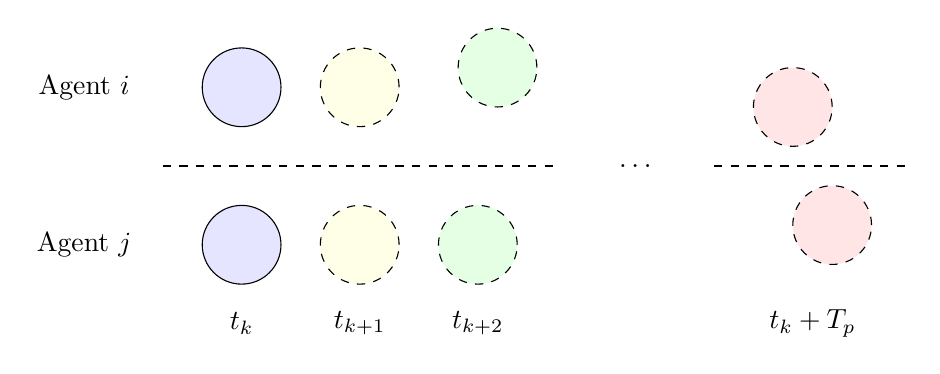
\begin{tikzpicture}[scale = 0.5]

  \draw[dashed] (0,0) -- (10,0);

  \node at (-2, 2) {Agent $i$};
  \node at (-2, -2) {Agent $j$};

  \filldraw[fill=blue!10!white, draw=black](2,2) circle (1cm);
  \filldraw[fill=blue!10!white, draw=black](2,-2) circle (1cm);
  \node at (2, -4) {$t_k$};


  \filldraw[fill=yellow!10!white, draw=black,dashed] (5,2) circle (1cm);
  \filldraw[fill=yellow!10!white, draw=black,dashed] (5,-2) circle (1cm);
  \node at (5, -4) {$t_{k+1}$};

  \filldraw[fill=green!10!white, draw=black,dashed] (8.5, 2.5) circle (1cm);
  \filldraw[fill=green!10!white, draw=black,dashed] (8,-2) circle (1cm);
  \node at (8, -4) {$t_{k+2}$};

  \node at (12, 0) {$\dots$};

  \draw[dashed] (14,0) -- (19,0);

  \filldraw[fill=red!10!white, draw=black,dashed] (16, 1.5) circle (1cm);
  \filldraw[fill=red!10!white, draw=black,dashed] (17,-1.5) circle (1cm);
  \node at (16.5, -4) {$t_k + T_p$};

\end{tikzpicture}

  \caption{The inter-agent constraint regime for two agents, $i,j$. Fully
    outlined circles denote measured configurations, while partly outlined
    circles denote predicted configurations. During the solution to the
    individual optimization problems, the predicted configuration of each agent
    at each timestep is constrained by the predicted configuration of the other
    agent at the same timestep (hence the homologously identical colours at
    each discrete timestep).}
  \label{fig:constraint_regime_horizon}
\end{figure}


The functions
$F_i : \mathcal{E}_{i,s} \times \mathcal{U}_i \to \mathbb{R}_{\geq 0}$ and
$V_i: \Omega_i \to \mathbb{R}_{\geq 0}$ are defined as
\begin{align}
  F_i \big(\overline{\vect{e}}_i(t), \overline{\vect{u}}_i(t)\big)
    &\triangleq \overline{\vect{e}}_i(t)^{\top} \mat{Q}_i \overline{\vect{e}}_i(t)
  + \overline{\vect{u}}_i(t)^{\top} \mat{R}_i \overline{\vect{u}}_i(t) \label{eq:F_i_def} \\[2.5ex]
  V_i \big(\overline{\vect{e}}_i(t)\big) & \triangleq \overline{\vect{e}}_i(t)^{\top} \mat{P}_i \overline{\vect{e}}_i(t) \label{eq:V_i_def}
\end{align}
Matrices $\mat{R}_i \in \mathbb{R}^{6 \times 6}$ and
$\mat{Q}_i, \mat{P}_i \in \mathbb{R}^{12 \times 12}$ are symmetric and positive
definite.  The running costs $F_i$ are upper- and lower-bounded by class
$\mathcal{K}_{\infty}$ functions:

\begin{bw_box}
  \begin{lemma} (\textit{$F_i$ is lower- and upper-bounded by class $\mathcal{K}_{\infty}$ functions})
    \label{lemma:F_i_bounded_K_class}

    Let functions $\alpha_1, \alpha_2 \in \mathcal{K}_{\infty}$ and $F_i$
    be defined by \eqref{eq:F_i_def}. Then, for all
    $\vect{e}_i \in \mathcal{E}_{i,s}$
    \begin{align}
      \alpha_1\big(\|\vect{e}_i\|\big) \leq F_i\big(\vect{e}_i, \vect{u}_i\big) \leq \alpha_2\big(\| \vect{e}_i \|\big)
    \end{align}
  \end{lemma}
\end{bw_box}


\begin{bw_box}
  \begin{lemma} ($F_i$ is Lipschitz continuous in $\mathcal{E}_{i,s} \times \mathcal{U}_i$)
\label{lemma:F_Lipschitz}

  Suppose that $\vect{e}_1, \vect{e}_2 \in \mathcal{E}_{i,s}$,
  $\vect{u}_i \in \mathcal{U}_i$ and that $F_i$ is defined by \eqref{eq:F_i_def}.
  The running costs $F_i$ are Lipschitz continuous in
  $\mathcal{E}_{i,s} \times \mathcal{U}_i$:
  $$\big|F_i(\vect{e}_1, \vect{u}_i) - F_i(\vect{e}_2, \vect{u}_i)\big| \leq L_{F_i} \|\vect{e}_1 - \vect{e}_2\|$$
  with Lipschitz constant $L_{F_i} = 2 \sigma_{max}(\mat{Q}_i) \overline{\varepsilon}_i $,
  where $\overline{\varepsilon}_i = \text{sup}\limits_{\vect{e}_i \in \mathcal{E}_{i,s}} \|\vect{e}_i\|$

\end{lemma}
\end{bw_box}


The terminal set $\Omega_i \subseteq \mathcal{E}_{i,t_k + T_p}$ is an admissible
positively invariant set according to definition
\eqref{def:positively_invariant} for system
\eqref{eq:position_based_error_model} such that
\begin{align}
  \Omega_i = \{\vect{e}_i \in \mathcal{E}_{i,t_k + T_p} : V_i(\vect{e}_i) \leq \varepsilon_{\Omega_i} \}
\end{align}
where $\varepsilon_{\Omega_i}$ is an arbitrarily small but fixed positive real scalar.

With regard to the terminal penalty function $V_i$, the following lemma will
prove to be useful in guaranteeing the convergence of the solution to the
optimal control problem to the terminal region $\Omega_i$:

\begin{bw_box}
\begin{lemma} ($V_i$ is Lipschitz continuous in $\Omega_i$)
\label{lemma:V_Lipschitz_e_0}

  Suppose that $\vect{e}_1, \vect{e}_2 \in \Omega_i$, and that
  $V_i$ is defined by \eqref{eq:V_i_def}. The terminal penalty function
  $V_i$ is Lipschitz continuous in $\Omega_i$
  $$\big|V_i(\vect{e}_1) - V_i(\vect{e}_2)\big| \leq L_{V_i} \|\vect{e}_1 - \vect{e}_2\|$$
  with Lipschitz constant $L_{V_i} = 2 \sigma_{max}(\mat{P}_i) \overline{\varepsilon}_{i,\Omega_i} $\\

  where $\overline{\varepsilon}_{i,\Omega_i} = \text{sup}\limits_{\vect{e}_i \in \Omega_i} \|\vect{e}_i\|$


\end{lemma}
\end{bw_box}


Furthermore, $V_i$ is lower- and upper-bounded by class $\mathcal{K}_{\infty}$ functions.

\begin{bw_box}
  \begin{lemma} (\textit{$V_i$ is lower- and upper-bounded by class
      \label{lemma:V_i_lower_upper_bounded}
    $\mathcal{K}_{\infty}$ functions in $\Omega_i$})
  \end{lemma}

  Let $\alpha_1, \alpha_2 \in \mathcal{K}_{\infty}$, $\vect{e}_i \in \Omega_i$
  and let $V_i$ be defined by \eqref{eq:V_i_def}. Then
  \begin{align}
    \alpha_1\big(\|\vect{e}_i\|\big) \leq V_i(\vect{e}_i) \leq \alpha_2\big(\| \vect{e}_i \|\big)
  \end{align}

\end{bw_box}


The solution to the optimal control problem \eqref{position_based_cost}
at time $t_k$ is an optimal control input, denoted by
$\overline{\vect{u}}_i^{\star}(\cdot;\ \vect{e}_i(t_k))$, which
is applied to the open-loop system until the next sampling instant $t_k + h$,
with $h \in (0,T_p)$:
\begin{align}
  %\vect{u}_i\big(t;\ \vect{e}_i(t_k)\big) = \overline{\vect{u}}_i^{\star}\big(t;\ \vect{e}_i(t_k)\big),\  t \in [t_k, t_k + h) \nonumber \\[2.5ex]
  \vect{u}_i(t) = \overline{\vect{u}}_i^{\star}\big(t;\ \vect{e}_i(t_k)\big),\  t \in [t_k, t_k + h]
 \label{eq:position_based_optimal_u}
\end{align}
At time $t_{k+1}$ a new finite horizon optimal control problem is solved in the
same manner, leading to a receding horizon approach.

The control input $\vect{u}_i(\cdot)$ is of feedback form,
since it is recalculated at each sampling instant based on the then-current
state. The solution to equation \eqref{eq:position_based_error_model} $-$ the
model of the real system, starting at time $t_1$, from an initial condition
$\vect{e}_i(t_1) = \overline{\vect{e}}_i(t_1)$,
by application of the control input $\vect{u}_i : [t_1, t_2] \to \mathcal{U}_i$
is denoted by
\begin{align}
  \vect{e}_i\big(t;\ \vect{u}_i(\cdot), \vect{e}_i(t_1)\big),\ t \in [t_1, t_2]
\end{align}


On the existence of solutions to \eqref{eq:position_based_error_model} we
assume the following:
\begin{bw_box}
\begin{assumption}
  \label{ass:existence_of_solutions_without_disturbance}

  The system \eqref{eq:position_based_error_model} has a
  \textit{continuous solution} for any $\vect{e}_i(0) \in \mathcal{E}_{i,0}$ and
  any \textit{piecewise continuous} input
  $\vect{u}_i(\cdot) :[0,T_p] \to \mathcal{U}_i$.
\end{assumption}
\end{bw_box}

The states of the open-loop system \eqref{eq:internal_error_model} $-$ the
predicted states obey the following notation:
\begin{bw_box}
\begin{remark}
The \textit{predicted} state of the system \eqref{eq:position_based_error_model}
at time $\tau \geq t_k$ , based on the measurement of the state at time
$t_k$, $\vect{e}_i(t_k)$, by application of the control input
\eqref{eq:position_based_optimal_u}, is denoted by
\begin{align}
  \overline{\vect{e}}_i\big(\tau;\ \vect{u}_i(\tau), \vect{e}_i(t_k)\big) \label{eq:position_based_predicted_error_0}
\end{align}
\end{remark}
\end{bw_box}

The closed-loop system for which stability is to be guaranteed is
\begin{align}
  \vect{e}_i(\tau) = g_i\big(\vect{e}_i(\tau), \overline{\vect{u}}_i^{\star}(\tau)\big),\ \tau \geq t_0 = 0
  \label{eq:without_disturbances_closed_loop}
\end{align}
where $\overline{\vect{u}}_i^{\star}(\tau) = \overline{\vect{u}}_i^{\star}(\tau;\ \vect{e}_i(t_k))$,
$\tau \in [t_k, t_k + h)$ and $t_0 = 0$.


We can now give the definition of an \textit{admissible input} for the FHOCP
\eqref{problem:opt_without_disturbances}:

\begin{bw_box}
  \begin{definition} (\textit{Admissible input for the FHOCP
\eqref{problem:opt_without_disturbances}})
  \label{definition:admissible_input}

  A control input $\vect{u}_i : [t_k, t_k + T_p] \to \mathbb{R}^6$ for a state
  $\vect{e}_i(t_k)$ is called \textit{admissible} for the problem
  \eqref{problem:opt_without_disturbances} if all the following hold:

  \begin{enumerate}
    \item $\vect{u}_i(\cdot)$ is piecewise continuous
    \item $\vect{u}_i(\tau) \in \mathcal{U}_i,\ \forall \tau \in [t_k, t_k + T_p]$
    \item $\overline{\vect{e}}_i\big(\tau;\ \vect{u}_i(\cdot), \vect{e}_i(t_k)\big) \in \mathcal{E}_{i,\tau},\ \forall \tau \in [t_k, t_k + T_p]$
    \item $\overline{\vect{e}}_i\big(t_k + T_p;\ \vect{u}_i(\cdot), \vect{e}_i(t_k)\big) \in \Omega_i$
  \end{enumerate}

  In other words, $\vect{u}_i$ is admissible if it conforms to the constraints
  on the input and its application yields states that conform to the
  prescribed state constraints of problem
  \eqref{problem:opt_without_disturbances} along the entire horizon
  $[t_k, t_k + T_p]$, and the terminal predicted state conforms to the
  terminal constraint.

\end{definition}
\end{bw_box}

    %-------------------------------------------------------------------------------
\section{Stabilization: Feasibility and Convergence}

Under these considerations, we can now state the theorem that relates to
the guaranteeing of the stability of the compound system of agents
$i \in \mathcal{V}$, when each of them is assigned a desired
position which results in feasible displacements:\\[2.5ex]

\begin{bw_box}
\begin{theorem}

  Suppose that

  \begin{enumerate}
    \item the terminal region $\Omega_i \subseteq \mathcal{E}_{i,s}$ is
      closed with $\vect{0} \in \Omega_i$
    \item a solution to the optimal control problem \eqref{position_based_cost}
      is feasible at time $t=0$, that is, assumptions
      \eqref{ass:measurements_access}, \eqref{ass:initial_conditions}, and
      \eqref{ass:intra_environmental_arrangement} hold at time $t=0$
    \item assumptions \eqref{ass:g_i_Lipschitz}, \eqref{ass:access_to_predicted_info_n},
      and \eqref{ass:existence_of_solutions_without_disturbance} hold
    \item there exists an admissible control input
      $h_i(\vect{e}_i) : [t_k + T_p, t_{k+1} + T_p] \to \mathcal{U}_i$
      such that for all $\vect{e}_i \in \Omega_i$ and
      $\forall \tau \in [t_k + T_p, t_{k+1} + T_p]$:

      \begin{enumerate}
        \item $\vect{e}_i(\tau) \in \Omega_i$
        \item $\dfrac{\partial V_i}{\partial \vect{e}_i} g_i\big(\vect{e}_i(\tau),
        h_i\big(\vect{e}_i(\tau)\big)
          + F_i\big(\vect{e}_i(\tau), h_i\big(\vect{e}_i(\tau)\big)\big) \leq 0$
      \end{enumerate}

  \end{enumerate}

  then the closed loop system \eqref{eq:without_disturbances_closed_loop} under
  the control input \eqref{eq:position_based_optimal_u} converges to the set
  $\Omega_i$ when $t \to \infty$.

\end{theorem}
\end{bw_box}

\textbf{Proof}. The proof of the above theorem consists of two parts:
in the first, recursive feasibility is established, that is, initial
feasibility is shown to imply subsequent feasibility; in the second, and based
on the first part, it is shown that the error state $\vect{e}_i(t)$ converges
to the terminal set $\Omega_i$.\\[2.5ex]

\textbf{Feasibility analysis}
Consider a sampling instant $t_k$ for which a
solution $\overline{\vect{u}}_i^{\star}\big(\cdot;\ \vect{e}_i(t_k)\big)$ to
\eqref{position_based_cost} exists.
%In between $t_k$ and $t_k + h$,
%where $h$ is the sampling time, the optimal control signal
%$\vect{u}_i^{\star}\big(\cdot;\ \vect{e}_i(t_k)\big)$ is applied to the open-loop
%system.
Suppose now a time instant $t_{k+1}$ such that\footnote{It is not strictly necessary
that $t_{k+1} = t_k + h$ here, however it is necessary for the following that
$t_{k+1} - t_k \leq h$} $t_k < t_{k+1} < t_k + T_p$, and consider that the
optimal control signal calculated at $t_k$ is comprised by the following two
portions:

\begin{equation}
  \overline{\vect{u}}_i^{\star}\big(\cdot;\ \vect{e}_i(t_k)\big) = \left\{
      \begin{array}{ll}
        \overline{\vect{u}}_i^{\star}\big(\tau_1;\ \vect{e}_i(t_k)\big), & \tau_1 \in [t_k, t_{k+1}] \\[2.5ex]
        \overline{\vect{u}}_i^{\star}\big(\tau_2;\ \vect{e}_i(t_k)\big), & \tau_2 \in [t_{k+1}, t_k + T_p]
      \end{array}
      \right.
  \label{eq:optimal_input_portions_without_disturbances}
\end{equation}

Both portions are admissible since the calculated optimal control input is
admissible, and hence they both conform to the input constraints.
As for the resulting predicted states, they satisfy the state constraints, and,
crucially: $\overline{\vect{e}}_i\big(t_k + T_p;\ \overline{\vect{u}}_i^{\star}(\cdot), \vect{e}_i(t_k)\big) \in \Omega_i$.
Furthermore, according to assumption (3) of the theorem, there exists an
admissible (and certainly not guaranteed optimal) input $h_i(\vect{e}_i)$ that
renders $\Omega_i$ invariant over $[t_k + T_p, t_{k+1} + T_p]$.

Given the above facts, we can construct an admissible input
$\widetilde{\vect{u}}_i(\cdot)$  starting at time $t_{k+1}$ by sewing together
the second portion of \eqref{eq:optimal_input_portions_without_disturbances}
and the input $h_i(\vect{e}_i)$:

\begin{equation}
  \widetilde{\vect{u}}_i(\tau) = \left\{
      \begin{array}{ll}
        \overline{\vect{u}}_i^{\star}\big(\tau;\ \vect{e}_i(t_k)\big), & \tau \in [t_{k+1}, t_k + T_p] \\[2.5ex]
        h_i\big(\vect{e}_i(\tau)\big), & \tau \in (t_k + T_p, t_{k+1} + T_p]
      \end{array}
      \right.
\label{eq:optimal_input_t_plus_one_without_disturbances}
\end{equation}

The control input $\widetilde{\vect{u}}_i(\cdot)$ is admissible as a
composition of admissible control inputs. This means that feasibility of a
solution to the optimization problem at time $t_k$ implies feasibility at
time $t_{k+1} > t_k$, and, thus, since at time $t=0$ a solution is assumed to
be feasible, a solution to the optimal control problem is feasible for all
$t \geq 0$.\\[2.5ex]

\textbf{Convergence analysis}
The second part of the proof involves demonstrating the convergence of the
state $\vect{e}_i$ to the terminal set $\Omega_i$. In order for this
to be proved, it must be shown that a proper value function decreases along
closed-loop trajectories starting at some initial time $t_k$. We consider the
\textit{optimal} cost $J_i^{\star}\big(\vect{e}_i(t)\big)$ as a candidate
Lyapunov function:
$$J_i^{\star}\big(\vect{e}_i(t)\big) \triangleq J_i \Big(\vect{e}_i(t), \overline{\vect{u}}_i^{\star}\big(\cdot;\ \vect{e}_i(t)\big)\Big)$$
and, in particular, our goal is to show that that this cost decreases over
consecutive sampling instants $t_{k+1} = t_k + h$, i.e.
$J_i^{\star}\big(\vect{e}_i(t_{k+1})\big) - J_i^{\star}\big(\vect{e}_i(t_k)\big) \leq 0$.\\[2.5ex]

In order not to wreak notational havoc, let us define the following terms:
\begin{gg_box}
\begin{itemize}
  \item $\vect{u}_{0,i}(\tau) \triangleq \overline{\vect{u}}_i^{\star}\big(\tau;\ \vect{e}_i(t_k)\big)$
    as the \textit{optimal} input that results from the solution to problem
    \eqref{problem:opt_without_disturbances} based on the measurement of state
    $\vect{e}_i(t_k)$, applied at time $\tau \geq t_k$
  \item $\vect{e}_{0,i}(\tau) \triangleq \overline{\vect{e}}_i\big(\tau;\ \overline{\vect{u}}_i^{\star}\big(\cdot;\ \vect{e}_i(t_k)\big), \vect{e}_i(t_k)\big)$
    as the \textit{predicted} state at time $\tau \geq t_k$, that is,
    the state that results from the application of the above input
    $\overline{\vect{u}}_i^{\star}\big(\cdot;\ \vect{e}_i(t_k)\big)$ to the
    state $\vect{e}_i(t_k)$, at time $\tau$
  \item $\vect{u}_{1,i}(\tau) \triangleq \widetilde{\vect{u}}_i(\tau)$
    as the \textit{admissible} input at $\tau \geq t_{k+1}$
    (see eq. \eqref{eq:optimal_input_t_plus_one_without_disturbances})
  \item $\vect{e}_{1,i}(\tau) \triangleq \overline{\vect{e}}_i\big(\tau;\ \widetilde{\vect{u}}_i(\cdot), \vect{e}_i(t_{k+1})\big)$
    as the \textit{predicted} state at time $\tau \geq t_{k+1}$, that is,
    the state that results from the application of the above input
    $\widetilde{\vect{u}}_i(\cdot)$ to the state
    $\vect{e}_i\big(t_{k+1};\ \overline{\vect{u}}_i^{\star}\big(\cdot;\ \vect{e}_i(t_k)\big), \vect{e}_i(t_k)\big)$, at time $\tau$
\end{itemize}
\end{gg_box}

\begin{bw_box}
  \begin{remark}
  \label{remark:predicted_actual_equations_without_disturbance}
    Given that no model mismatch or disturbances exist, for
    the predicted and actual states at time
    $\tau_1 \geq \tau_0 \in \mathbb{R}_{\geq 0}$ it holds that:
    \begin{align}
      \vect{e}_i\big(\tau_1;\ \vect{u}_i(\cdot), \vect{e}_i(\tau_0)\big) &=
        \vect{e}_i(\tau_0) + \int_{\tau_0}^{\tau_1} g_i\big(\vect{e}_i(s;\ \vect{e}_i(\tau_0)), \vect{u}_i(s)\big) ds \\[2.5ex]
      \overline{\vect{e}}_i\big(\tau_1;\ \vect{u}_i(\cdot), \vect{e}_i(\tau_0)\big) &=
        \vect{e}_i(\tau_0) + \int_{\tau_0}^{\tau_1} g_i\big(\overline{\vect{e}}_i(s;\ \vect{e}_i(\tau_0)), \vect{u}_i(s)\big) ds
    \end{align}
  \end{remark}
\end{bw_box}

Before beginning to prove convergence, it is worth noting that while the cost
$$J_i \Big(\vect{e}_i(t), \overline{\vect{u}}_i^{\star}\big(\cdot;\ \vect{e}_i(t)\big)\Big)$$
is optimal (in the sense that it is based on the optimal input, which provides
its minimum realization), a cost that is based on a plainly admissible
(and thus, without loss of generality, sub-optimal) input
$\vect{u}_i \not= \overline{\vect{u}}_i^{\star}$ will result in a configuration where
\begin{equation}
J_i \Big(\vect{e}_i(t), \vect{u}_i\big(\cdot;\ \vect{e}_i(t)\big)\Big)
\geq J_i \Big(\vect{e}_i(t), \overline{\vect{u}}_i^{\star}\big(\cdot;\ \vect{e}_i(t)\big)\Big)
\end{equation}

Let us now begin our investigation on the difference between the cost
that results from the application of the feasible input $\vect{u}_{1,i}$,
which we shall denote by $\overline{J}_i\big(\vect{e}_i(t_{k+1})\big)$,
and the optimal cost $J_i^{\star}\big(\vect{e}_i(t_k)\big)$. We remind
ourselves that
$J_i \big(\vect{e}_i(t), \overline{\vect{u}}_i (\cdot)\big)$ $=$
$\int_{t}^{t + T_p} F_i \big(\overline{\vect{e}}_i(s), \overline{\vect{u}}_i (s)\big) ds$ $+$
$V_i \big(\overline{\vect{e}}_i (t + T_p)\big)$:
\begin{align}
  \overline{J}_i\big(\vect{e}_i(t_{k+1})\big) - J_i^{\star}\big(\vect{e}_i(t_k)\big) =\
   & V_i \big(\vect{e}_{1,i} (t_{k+1} + T_p)\big) + \int_{t_{k+1}}^{t_{k+1} + T_p} F_i \big(\vect{e}_{1,i}(s), \vect{u}_{1,i} (s)\big) ds \\[2.5ex]
  -&V_i \big(\vect{e}_{0,i} (t_k + T_p)\big) - \int_{t_k}^{t_k + T_p} F_i \big(\vect{e}_{0,i}(s), \vect{u}_{0,i} (s)\big) ds
\end{align}
Considering that $t_k < t_{k+1} < t_k + T_p < t_{k+1} + T_p$, we break down the
two integrals above in between these intervals:
\begin{align}
  \overline{J}_i\big(\vect{e}_i(t_{k+1})\big) - J_i^{\star}\big(\vect{e}_i(t_k)\big) &= \\[2.5ex]
    V_i \big(\vect{e}_{1,i} (t_{k+1} + T_p)\big)
    &+ \int_{t_{k+1}}^{t_k + T_p} F_i \big(\vect{e}_{1,i}(s), \vect{u}_{1,i} (s)\big) d s
    + \int_{t_k + T_p}^{t_{k+1} + T_p} F_i \big(\vect{e}_{1,i}(s), \vect{u}_{1,i} (s)\big) d s \\[2.5ex]
    -V_i \big(\vect{e}_{0,i} (t_k + T_p)\big)
    &- \int_{t_k}^{t_{k+1}} F_i \big(\vect{e}_{0,i}(s), \vect{u}_{0,i} (s)\big) d s
    - \int_{t_{k+1}}^{t_k + T_p} F_i \big(\vect{e}_{0,i}(s), \vect{u}_{0,i} (s)\big) d s
\label{eq:convergence_4_integrals}
\end{align}

\begin{gg_box}

Since no model mismatch or disturbances are present, consulting with remark
\eqref{remark:predicted_actual_equations_without_disturbance} and substituting
for $\tau_0 = t_k$ and $\tau_1 = t_{k+1}$ yields:
\begin{align}
  \vect{e}_i\big(t_{k+1};\ \overline{\vect{u}}_i^{\star}\big(\cdot;\ \vect{e}_i(t_k)\big), \vect{e}_i(t_k)\big) &=
    \vect{e}_i(t_k) + \int_{t_k}^{t_{k+1}} g_i\big(\vect{e}_i(s;\ \vect{e}_i(t_k)), \overline{\vect{u}}_i^{\star}(s)\big) ds \\[2.5ex]
  \overline{\vect{e}}_i\big(t_{k+1};\ \overline{\vect{u}}_i^{\star}\big(\cdot;\ \vect{e}_i(t_k)\big), \vect{e}_i(t_k)\big) &=
    \vect{e}_i(t_k) + \int_{t_k}^{t_{k+1}} g_i\big(\overline{\vect{e}}_i(s;\ \vect{e}_i(t_k)), \overline{\vect{u}}_i^{\star}(s)\big) ds
\end{align}
Subtracting the second expression from the first, we get
\begin{align}
  \vect{e}_i\big(t_{k+1};\ &\overline{\vect{u}}_i^{\star}\big(\cdot;\ \vect{e}_i(t_k)\big), \vect{e}_i(t_k)\big) -
  \overline{\vect{e}}_i\big(t_{k+1};\ \overline{\vect{u}}_i^{\star}\big(\cdot;\ \vect{e}_i(t_k)\big), \vect{e}_i(t_k)\big) \\[2.5ex]
  &=\int_{t_k}^{t_{k+1}} g_i\big(\vect{e}_i(s;\ \vect{e}_i(t_k)), \overline{\vect{u}}_i^{\star}(s)\big) ds -
    \int_{t_k}^{t_{k+1}} g_i\big(\overline{\vect{e}}_i(s;\ \vect{e}_i(t_k)), \overline{\vect{u}}_i^{\star}(s)\big) ds\\[2.5ex]
  &=\int_{t_k}^{t_{k+1}} \bigg( g_i\big(\vect{e}_i(s;\ \vect{e}_i(t_k)), \overline{\vect{u}}_i^{\star}(s)\big)
  - g_i\big(\overline{\vect{e}}_i(s;\ \vect{e}_i(t_k)), \overline{\vect{u}}_i^{\star}(s)\big) \bigg) ds \\[2.5ex]
\end{align}
Taking norms on either side yields
\begin{align}
  \bigg\|\vect{e}_i\big(t_{k+1};\ &\overline{\vect{u}}_i^{\star}\big(\cdot;\ \vect{e}_i(t_k)\big), \vect{e}_i(t_k)\big)
    -\overline{\vect{e}}_i\big(t_{k+1};\ \overline{\vect{u}}_i^{\star}\big(\cdot;\ \vect{e}_i(t_k)\big), \vect{e}_i(t_k)\big) \bigg\| \\[2.5ex]
  &=\bigg\|\int_{t_k}^{t_{k+1}} \bigg( g_i\big(\vect{e}_i(s;\ \vect{e}_i(t_k)), \overline{\vect{u}}_i^{\star}(s)\big)
  - g_i\big(\overline{\vect{e}}_i(s;\ \vect{e}_i(t_k)), \overline{\vect{u}}_i^{\star}(s)\big) \bigg) ds \bigg\|\\[2.5ex]
  &=\int_{t_k}^{t_{k+1}} \bigg\| g_i\big(\vect{e}_i(s;\ \vect{e}_i(t_k)), \overline{\vect{u}}_i^{\star}(s)\big)
  - g_i\big(\overline{\vect{e}}_i(s;\ \vect{e}_i(t_k)), \overline{\vect{u}}_i^{\star}(s)\big) \bigg\| ds\\[2.5ex]
  &\leq L_{g_i}\int_{t_k}^{t_{k+1}} \bigg\|
    \vect{e}_i\big(s;\ \overline{\vect{u}}_i^{\star}\big(\cdot;\ \vect{e}_i(t_k)\big), \vect{e}_i(t_k)\big)
    -\overline{\vect{e}}_i\big(s;\ \overline{\vect{u}}_i^{\star}\big(\cdot;\ \vect{e}_i(t_k)\big), \vect{e}_i(t_k)\big) \bigg\| ds
\end{align}
since $g_i$ is Lipschitz continuous in $\mathcal{E}_{i,s}$ with Lipschitz constant
$L_{g_i}$. Reformulation yields
\begin{align}
  \bigg\|\vect{e}_i\big(t_k&+h;\ \overline{\vect{u}}_i^{\star}\big(\cdot;\ \vect{e}_i(t_k)\big), \vect{e}_i(t_k)\big)
    -\overline{\vect{e}}_i\big(t_k+h;\ \overline{\vect{u}}_i^{\star}\big(\cdot;\ \vect{e}_i(t_k)\big), \vect{e}_i(t_k)\big) \bigg\| \\[2.5ex]
  &\leq L_{g_i}\int_{0}^{h} \bigg\|
    \vect{e}_i\big(t_k + s;\ \overline{\vect{u}}_i^{\star}\big(\cdot;\ \vect{e}_i(t_k)\big), \vect{e}_i(t_k)\big)
    -\overline{\vect{e}}_i\big(t_k + s;\ \overline{\vect{u}}_i^{\star}\big(\cdot;\ \vect{e}_i(t_k)\big), \vect{e}_i(t_k)\big) \bigg\| ds
\end{align}
By applying the Gr\"{o}nwall-Bellman inequality we obtain zero as an
upper bound for the norm of the difference between the two states. Since
any norm cannot be negative, we conclude that
\begin{align}
  \bigg\|\vect{e}_i\big(t_{k+1};\ \overline{\vect{u}}_i^{\star}\big(\cdot;\ \vect{e}_i(t_k)\big), \vect{e}_i(t_k)\big)
    -\overline{\vect{e}}_i\big(t_{k+1};\ \overline{\vect{u}}_i^{\star}\big(\cdot;\ \vect{e}_i(t_k)\big), \vect{e}_i(t_k)\big) \bigg\| = 0
\end{align}
which means that
\begin{align}
  \vect{e}_i\big(t_{k+1};\ \overline{\vect{u}}_i^{\star}\big(\cdot;\ \vect{e}_i(t_k)\big), \vect{e}_i(t_k)\big)
    =\overline{\vect{e}}_i\big(t_{k+1};\ \overline{\vect{u}}_i^{\star}\big(\cdot;\ \vect{e}_i(t_k)\big), \vect{e}_i(t_k)\big)
\end{align}

In between times $t_{k+1}$ and $t_k + T_p$, the constructed admissible input
$\widetilde{\vect{u}}_i(\cdot)$ is equal to the optimal
input $\overline{\vect{u}}_i^{\star}\big(\cdot;\ \vect{e}_i(t_k)\big)$
(see eq. \ref{eq:optimal_input_t_plus_one_without_disturbances}), which means
that $\vect{u}_{1,i}(\tau) = \vect{u}_{0,i}(\tau)$ in the interval
$\tau \in [t_{k+1}, t_k + T_p]$. Since the initial conditions at $t=t_{k+1}$ are
equal and the control laws are also equal, so will the predicted states over the
same interval:
\begin{align}
  \overline{\vect{e}}_i\big(\tau;\ \widetilde{\vect{u}}_i(\cdot), \vect{e}_i(t_{k+1})\big) =
  \overline{\vect{e}}_i\big(\tau;\ \overline{\vect{u}}_i^{\star}(\cdot), \overline{\vect{e}}_i(t_{k+1})\big), \ \tau \in [t_{k+1}, t_k + T_p]
  \label{eq:equal_predicted_without_disturbance}
\end{align}
Using our notation then, in the same interval:
$\vect{e}_{1,i}(\cdot) = \vect{e}_{0,i}(\cdot)$. Coupled with the fact that
in the same interval $\vect{u}_{1,i}(\tau) = \vect{u}_{0,i}(\tau)$, the following
equality holds over $[t_{k+1}, t_k + T_p]$:
\begin{align}
  F_i \big(\vect{e}_{1,i}(s), \vect{u}_{1,i} (s)\big) =
  F_i \big(\vect{e}_{0,i}(s), \vect{u}_{0,i} (s)\big),\ s \in [t_{k+1}, t_k + T_p]
\end{align}
Integrating this equality over the interval where it is valid yields
\begin{align}
  \int_{t_{k+1}}^{t_k + T_p}F_i \big(\vect{e}_{1,i}(s), \vect{u}_{1,i} (s)\big) ds =
  \int_{t_{k+1}}^{t_k + T_p}F_i \big(\vect{e}_{0,i}(s), \vect{u}_{0,i} (s)\big) ds
\end{align}
\end{gg_box}
This means that these two integrals with ends over the interval
$[t_{k+1}, t_k + T_p]$ featured in the right-hand side of eq.
\eqref{eq:convergence_4_integrals} vanish, and thus the cost difference becomes
\begin{align}
  \overline{J}_i\big(\vect{e}_i(t_{k+1})\big) - J_i^{\star}\big(\vect{e}_i(t_k)\big) &=
    V_i \big(\vect{e}_{1,i} (t_{k+1} + T_p)\big)
    +\int_{t_k + T_p}^{t_{k+1} + T_p} F_i \big(\vect{e}_{1,i}(s), \vect{u}_{1,i} (s)\big) d s \\[2.5ex]
    &-V_i \big(\vect{e}_{0,i} (t_k + T_p)\big)
    -\int_{t_k}^{t_{k+1}} F_i \big(\vect{e}_{0,i}(s), \vect{u}_{0,i} (s)\big) d s
\label{eq:convergence_2_integrals}
\end{align}

During the course of arriving at the above result, we have concluded that,
in the absence of disturbances, the remark \eqref{eq:error_now_to_predicted_error}
holds.
\begin{bw_box}
  \begin{remark}
  \label{eq:error_now_to_predicted_error}
    In the absence of disturbances, the following equality holds over
    the entire horizon $t \in [t_k, t_k + T_p]$:
    \begin{align}
      \vect{e}_i\big(t;\ \overline{\vect{u}}_i^{\star}\big(\cdot;\ \vect{e}_i(t_k)\big), \vect{e}_i(t_k)\big)
        =\overline{\vect{e}}_i\big(t;\ \overline{\vect{u}}_i^{\star}\big(\cdot;\ \vect{e}_i(t_k)\big), \vect{e}_i(t_k)\big)
    \end{align}
  \end{remark}
\end{bw_box}

\begin{gg_box}
  We turn our attention to the first integral in the above expression, and we
  note that $[t_{k+1} + T_p, t_k + T_p]$, is exactly the
  the interval where assumption (3b) of the theorem holds. Hence,
  we decide to integrate the expression found in the assumption over the
  interval $[t_k + T_p, t_{k+1} + T_p]$, for the controls and states applicable
  in it:
  \begin{align}
    \int_{t_k + T_p}^{t_{k+1} + T_p} \Bigg(\dfrac{\partial V_i}{\partial \vect{e}_{1,i}} g_i\big(\vect{e}_{1,i}(s), \vect{u}_{1,i}(s)\big)
    + F_i\big(\vect{e}_{1,i}(s), \vect{u}_{1,i}(s)\big)\Bigg) ds &\leq 0 \\[2.5ex]
    \int_{t_k + T_p}^{t_{k+1} + T_p} \dfrac{d}{ds} V_i\big(\vect{e}_{1,i}(s)\big) d s
    + \int_{t_k + T_p}^{t_{k+1} + T_p} F_i\big(\vect{e}_{1,i}(s), \vect{u}_{1,i}(s)\big) ds &\leq 0 \\[2.5ex]
    V_i\big(\vect{e}_{1,i}(t_{k+1} + T_p)\big) - V_i\big(\vect{e}_{1,i}(t_k + T_p)\big)
    + \int_{t_k + T_p}^{t_{k+1} + T_p} F_i\big(\vect{e}_{1,i}(s), \vect{u}_{1,i}(s)\big) ds &\leq 0 \\[2.5ex]
    V_i\big(\vect{e}_{1,i}(t_{k+1} + T_p)\big)
    + \int_{t_k + T_p}^{t_{k+1} + T_p} F_i\big(\vect{e}_{1,i}(s), \vect{u}_{1,i}(s)\big) ds &\leq V_i\big(\vect{e}_{1,i}(t_k + T_p)\big)
  \end{align}

  The left-hand side expression is the same as the first two terms in the
  right-hand side of equality \eqref{eq:convergence_2_integrals}. We can
  introduce the third one by subtracting it from both sides:
  \begin{align}
    V_i\big(\vect{e}_{1,i}(t_{k+1} + T_p)\big)
    &+ \int_{t_k + T_p}^{t_{k+1} + T_p} F_i\big(\vect{e}_{1,i}(s), \vect{u}_{1,i}(s)\big) ds
    - V_i\big(\vect{e}_{0,i}(t_k + T_p)\big) \\[2.5ex]
    &\leq V_i\big(\vect{e}_{1,i}(t_k + T_p)\big)
    - V_i\big(\vect{e}_{0,i}(t_k + T_p)\big) \\[2.5ex]
    &\leq \Big|V_i\big(\vect{e}_{1,i}(t_k + T_p)\big)
    - V_i\big(\vect{e}_{0,i}(t_k + T_p)\big)\Big|
  \end{align}
  since $x \leq |x|, \forall x \in \mathbb{R}$.

  By revisiting lemma \eqref{lemma:V_Lipschitz_e_0}, the above inequality
  becomes
  \begin{align}
    V_i\big(\vect{e}_{1,i}(t_{k+1} + T_p)\big)
    + \int_{t_k + T_p}^{t_{k+1} + T_p} F_i\big(\vect{e}_{1,i}(s), \vect{u}_{1,i}(s)\big) ds
    - V_i\big(\vect{e}_{0,i}(t_k + T_p)\big) \\[2.5ex]
    \leq L_{V_i} \big\|\vect{e}_{1,i}(t_k + T_p) - \vect{e}_{0,i}(t_k + T_p)\big\|
  \end{align}

  However, as we witnessed in \eqref{eq:equal_predicted_without_disturbance},
  in the interval $[t_{k+1}, t_k + T_p]$:
  $\vect{e}_{1,i}(\cdot) = \vect{e}_{0,i}(\cdot)$, hence the right-hand
  side of the inequality equals zero:
  \begin{align}
    V_i\big(\vect{e}_{1,i}(t_{k+1} + T_p)\big)
    + \int_{t_k + T_p}^{t_{k+1} + T_p} F_i\big(\vect{e}_{1,i}(s), \vect{u}_{1,i}(s)\big) ds
    - V_i\big(\vect{e}_{0,i}(t_k + T_p)\big) \leq 0
  \end{align}

  By subtracting the fourth term needed to complete the right-hand side
  expression of \eqref{eq:convergence_2_integrals}, i.e.
  $\int_{t_k}^{t_{k+1}} F_i \big(\vect{e}_{0,i}(s), \vect{u}_{0,i} (s)\big) d s$
  from both sides we get
  \begin{align}
    V_i\big(\vect{e}_{1,i}(t_{k+1} + T_p)\big)
    + \int_{t_k + T_p}^{t_{k+1} + T_p} F_i\big(\vect{e}_{1,i}(s), \vect{u}_{1,i}(s)\big) ds& \\[2.5ex]
    - V_i\big(\vect{e}_{0,i}(t_k + T_p)\big)
    -\int_{t_k}^{t_{k+1}} F_i \big(\vect{e}_{0,i}(s), \vect{u}_{0,i} (s)\big) d s
    &\leq -\int_{t_k}^{t_{k+1}} F_i \big(\vect{e}_{0,i}(s), \vect{u}_{0,i} (s)\big) d s
  \end{align}

  The left-hand side of this inequality is now equal to the cost difference
  $\overline{J}_i\big(\vect{e}_i(t_{k+1})\big) - J_i^{\star}\big(\vect{e}_i(t_k)\big)$.
\end{gg_box}
Hence, the cost difference becomes bounded by
\begin{align}
  \overline{J}_i\big(\vect{e}_i(t_{k+1})\big) - J_i^{\star}\big(\vect{e}_i(t_k)\big) \leq
    -\int_{t_k}^{t_{k+1}} F_i \big(\vect{e}_{0,i}(s), \vect{u}_{0,i} (s)\big) ds
\end{align}
\begin{gg_box}
  $F_i$ is a positive-definite function as a sum of a positive-definite
  $\|\vect{u}_i\|^2_{\mat{R}_i}$ and a positive semi-definite function
  $\|\vect{e}_i\|^2_{\mat{Q}_i}$. If we denote by
  $m_i = \lambda_{min}(\mat{Q}_i, \mat{R}_i) \geq 0$ the minimum eigenvalue
  between those of matrices $\mat{R}_i, \mat{Q}_i$, this means that
  \begin{align}
    F_i \big(\vect{e}_{0,i}(s), \vect{u}_{0,i} (s)\big) \geq m_i \|\vect{e}_{0,i}(s)\|^2
  \end{align}

  By integrating the above between our interval of interest $[t_k, t_{k+1}]$ we get
  \begin{align}
    \int_{t_k}^{t_{k+1}} F_i \big(\vect{e}_{0,i}(s), \vect{u}_{0,i} (s)\big) &\geq \int_{t_k}^{t_{k+1}} m_i \|\vect{e}_{0,i}(s)\|^2 ds \\[2.5ex]
    \text{or}\\[2.5ex]
    -\int_{t_k}^{t_{k+1}} F_i \big(\vect{e}_{0,i}(s), \vect{u}_{0,i} (s)\big) &\leq -m_i \int_{t_k}^{t_{k+1}} \|\vect{e}_{0,i}(s)\|^2 ds
  \end{align}
\end{gg_box}

This means that the cost difference is upper-bounded by a class $\mathcal{K}$
function
\begin{align}
  \overline{J}_i\big(\vect{e}_i(t_{k+1})\big) - J_i^{\star}\big(\vect{e}_i(t_k)\big)
  &\leq -m_i \int_{t_k}^{t_{k+1}} \|\vect{e}_{0,i}(s)\|^2 ds \leq 0
\end{align}
and since the cost $\overline{J}_i\big(\vect{e}_i(t_{k+1})\big)$ is, in general,
sub-optimal: $J_i^{\star}\big(\vect{e}_i(t_{k+1})\big) - \overline{J}_i\big(\vect{e}_i(t_{k+1})\big) \leq 0$:
\begin{align}
 J_i^{\star}\big(\vect{e}_i(t_{k+1})\big) - J_i^{\star}\big(\vect{e}_i(t_k)\big) \leq -m_i \int_{t_k}^{t_{k+1}} \|\vect{e}_{0,i}(s)\|^2 ds
 \label{eq:J_opt_between_consecutive_k}
\end{align}
With this milestone result established, we need to trace the time $t_k$ back
to $t_0 = 0$ in order to prove that the closed-loop system is stable at all
times $t \in \mathbb{R}_{\geq 0}$.

\begin{gg_box}
  The integral of $\|\vect{e}_{0,i}(\tau)\|^2$ over the interval $[t_0, t_{k+1}]$,
  $t_0 < t_k < t_{k+1}$ can be decomposed into the addition of two integrals
  with limits ranging from (a) $t_0$ to $t_k$ and (b) $t_k$ to $t_{k+1}$:
  \begin{align}
    \int_{t_0}^{t_{k+1}} \|\vect{e}_{0,i}(s)\|^2 ds = \int_{t_0}^{t_{k}} \|\vect{e}_{0,i}(s)\|^2 ds + \int_{t_k}^{t_{k+1}} \|\vect{e}_{0,i}(s)\|^2 ds
  \end{align}
  By rearranging terms, this means that
  \begin{align}
    \int_{t_k}^{t_{k+1}} \|\vect{e}_{0,i}(s)\|^2 ds = \int_{t_0}^{t_{k+1}} \|\vect{e}_{0,i}(s)\|^2 ds - \int_{t_0}^{t_{k}} \|\vect{e}_{0,i}(s)\|^2 ds
  \end{align}
  making the optimal cost difference between the consecutive sampling times
  $t_k$ and $t_{k+1}$ in \eqref{eq:J_opt_between_consecutive_k}
  \begin{align}
    J_i^{\star}\big(\vect{e}_i(t_{k+1})\big) - J_i^{\star}\big(\vect{e}_i(t_k)\big) \leq
      -m_i \int_{t_0}^{t_{k+1}} \|\vect{e}_{0,i}(s)\|^2 ds +m_i \int_{t_0}^{t_{k}} \|\vect{e}_{0,i}(s)\|^2 ds
  \end{align}
  Similarly, the optimal cost difference between the sampling times $t_{k-1}$
  and $t_{k}$ is
  \begin{align}
    J_i^{\star}\big(\vect{e}_i(t_{k})\big) - J_i^{\star}\big(\vect{e}_i(t_{k-1})\big) \leq
      -m_i \int_{t_0}^{t_{k}} \|\vect{e}_{0,i}(s)\|^2 ds +m_i \int_{t_0}^{t_{k-1}} \|\vect{e}_{0,i}(s)\|^2 ds
  \end{align}
  and we can apply this rationale all the way back to the cost difference
  between $t_0$ and $t_1$. Summing all the inequalities between the pairs of
  consecutive sampling times $(t_0, t_1)$, $(t_1, t_2)$, $\dots$,
  $(t_{k-1}, t_k)$, we get
  \begin{align}
    J_i^{\star}\big(\vect{e}_i(t_{k})\big) - J_i^{\star}\big(\vect{e}_i(t_0)\big) \leq
      -m_i \int_{t_0}^{t_{k}} \|\vect{e}_{0,i}(s)\|^2 ds
  \end{align}
\end{gg_box}

Hence, for $t_0 = 0$
\begin{align}
  J_i^{\star}\big(\vect{e}_i(t_{k})\big) - J_i^{\star}\big(\vect{e}_i(0)\big) \leq
    -m_i \int_{0}^{t_{k}} \|\vect{e}_{0,i}(s)\|^2 ds \leq 0
\label{eq:J_opt_between_k_and_0}
\end{align}
which implies that the value function $J_i^{\star}\big(\vect{e}_i(t_{k})\big)$
in non-increasing for all sampling times:
\begin{align}
  J_i^{\star}\big(\vect{e}_i(t_{k})\big) \leq J_i^{\star}\big(\vect{e}_i(0)\big),\ \forall t_k \in \mathbb{R}_{\geq0}
\end{align}
Let us now define the function $\Xi_i\big(\vect{e}_i(t)\big)$:
\begin{align}
  \Xi_i\big(\vect{e}(t)\big) \triangleq J_i^{\star}\big(\vect{e}_i(\tau)\big),\ t \in \mathbb{R}_{\geq0}
\end{align}
where $\tau = max\{t_k : t_k \leq t\}$ $-$ i.e. the immediately previous to
$t$ sampling time. Then the above inequality reforms into
\begin{align}
  \Xi_i\big(\vect{e}(t)\big) \leq \Xi_i\big(\vect{e}_i(0)\big),\ t \in \mathbb{R}_{\geq0}
\end{align}

Since $\Xi_i\big(\vect{e}_i(0)\big)$
is bounded (as composition of bounded parts), this implies
that $\Xi_i\big(\vect{e}(t)\big)$ is also bounded. The signals
$\vect{e}_i(t) \in \mathcal{E}_{i,s}$ and $\vect{u}_i(t) \in \mathcal{U}_i$
are also bounded. According to \eqref{eq:position_based_error_model}, this
means that $\dot{\vect{e}}_i(t)$ is bounded as well. From inequality
\eqref{eq:J_opt_between_k_and_0} we then have
\begin{align}
  \Xi_i\big(\vect{e}_i(t)\big) \leq \Xi_i\big(\vect{e}_i(0)\big)
    -m_i \int_{0}^{\tau} \|\vect{e}_{0,i}(s)\|^2 ds \leq 0
\end{align}
which, due to the fact that $\tau \leq t$, is equivalent to
\begin{align}
  \Xi_i\big(\vect{e}_i(t)\big) \leq \Xi_i\big(\vect{e}_i(0)\big) -m_i \int_{0}^{t} \|\vect{e}_{0,i}(s)\|^2 ds \leq 0,\ t \in \mathbb{R}_{\geq 0}
\end{align}
Solving for the integral we get
\begin{align}
  \int_{0}^{t} \|\vect{e}_{0,i}(s)\|^2 ds \leq
    \dfrac{1}{m_i}\Big(\Xi_i\big(\vect{e}_i(0)\big) - \Xi_i\big(\vect{e}_i(t)\big)\Big),\ t \in \mathbb{R}_{\geq 0}
\end{align}
Both $\Xi_i\big(\vect{e}_i(0)\big)$ and $\Xi_i\big(\vect{e}_i(t)\big)$
are bounded, and therefore so is their difference, which means that the
integral $\int\limits_{0}^{t} \|\vect{e}_{0,i}(s)\|^2 ds$ and its limit when
$t \to \infty$ are bounded as well. Lemma \eqref{lemma:barbalat} assures us
that under these conditions for the error and its dynamics, which are
fulfilled in our case, the error
\begin{align}
  \lim\limits_{t \to \infty}\|\vect{e}_{0,i}(t)\| &= 0 \Leftrightarrow \\[2.5ex]
  \lim\limits_{t \to \infty}
  \Big\| \overline{\vect{e}}_i\Big(t;\ \overline{\vect{u}}_i^{\star}\big(\cdot;\ \vect{e}_i(t_k)\big), \vect{e}_i(t_k) \Big) \Big\| &= 0,\
\forall t_k \in \mathbb{R}_{\geq 0}
\end{align}
which, given remark \eqref{eq:error_now_to_predicted_error},
and dropping the initial condition, means that
$$\lim\limits_{t \to \infty}\|\vect{e}_i(t)\| = 0$$
which implies that
$$\lim\limits_{t \to \infty}\vect{e}_i(t) \in \Omega_i$$
Therefore, the closed-loop trajectory of the error state $\vect{e}_i$ converges
to the terminal set $\Omega_i$ as $t \to \infty$.

In turn, this means that the system \eqref{eq:original_z_system} converges
to $\vect{z}_{i,des}$ while simultaneously conforming to
all constraints $\mathcal{Z}_i$, as $t \to \infty$. This conclusion holds
for all $i \in \mathcal{V}$, and hence, the compound system of agents
$\mathcal{V}$ is stable in $\mathcal{Z}_i$.
\qedsymbol

    \cleardoublepage

%-------------------------------------------------------------------------------
  \chapter{Stabilization in the face of Disturbances}
    \label{chapter:stabilization_with_disturbance}

    We are interested in steering each agent $i \in \mathcal{V}$ into
a \textit{position} in 3D space, while conforming to the requirements
posed by the problem. Here, the real system and its model are \textit{not}
equivalent: we consider that additive disturbances act on the real
system. At first, the model of the perturbed system \eqref{eq:system} will
be formalized. Next, the error model and \textit{its} constraints will be
expressed. We will then pose the optimization problem to be solved periodically:
it will equip us with the optimum feasible input that steers the system towards
achieving its intended configuration regardless of the introduced uncertainty,
provided that it is bounded by a certain value. This will lead to the proof
of this statement, i.e. that the compound closed-loop system of agents
$i \in \mathcal{V}$ is stable under the proposed control regime, provided
that the disturbance is bounded.

%-------------------------------------------------------------------------------
\section{The perturbed model}

In the following, we assume that the real system is
subject to bounded additive disturbances $\vect{\delta}_i$ such that
$\vect{\delta}_i \in \Delta_i \subset \mathbb{R}^9 \times \mathbb{T}^3$, where
$\Delta_i$ is a compact set containing the origin.
The real system is described by:
\begin{align}
  \dot{\vect{z}}_i(t) &= f_i^R \big(\vect{z}_i (t), \vect{u}_i (t)\big) \label{eq:perturbed_system} \\[2.5ex]
                      &= f_i \big(\vect{z}_i (t), \vect{u}_i (t)\big) + \vect{\delta}_i(t) \\[2.5ex]
  \vect{z}_i(0) &= \vect{z}_{i,0} \\[2.5ex]
  \vect{z}_i (t) & \subset \mathbb{R}^{9} \times \mathbb{T}^3 \\[2.5ex]
  \vect{u}_i (t) & \subset \mathbb{R}^6 \\[2.5ex]
  \vect{\delta}_i(t) &\in \Delta_i \subset \mathbb{R}^9 \times \mathbb{T}^3,\ t \in \mathbb{R}_{\geq 0}\\[2.5ex]
  \text{sup}\limits_{t \in \mathbb{R}_{\geq 0}} \|\vect{\delta}_i(t)\| &\leq \overline{\delta}_i
\end{align}
where state $\vect{z}_i$ is directly measurable as per assumption
\eqref{ass:measurements_access}.

The constraint set $\mathcal{Z}_i \subset \mathbb{R}^{9} \times \mathbb{T}^3$
is unchanged: it is the set that captures all the state constraints of
the system's dynamics posed by the problem \eqref{problem},
for $t \in \mathbb{R}_{\geq 0}$. We include it again here for reference
purposes.
\begin{align}
  \mathcal{Z}_i = \big\{\vect{z}_i(t) \in \mathbb{R}^{9}\times \mathbb{T}^3 : \
      & \|\vect{p}_i(t) - \vect{p}_j(t)\| > \underline{d}_{ij,a}, \forall j \in \mathcal{R}_i(t), \label{constraint:p_1_2}\\[2.5ex]
      & \|\vect{p}_i(t) - \vect{p}_j(t)\| < d_i, \forall j \in \mathcal{N}_i, \\[2.5ex]
      & \|\vect{p}_i(t) - \vect{p}_{\ell}\| > \underline{d}_{i\ell,o}, \forall \ell \in \mathcal{L}, \\[2.5ex]
      & \|\vect{p}_W - \vect{p}_i(t)\| < \overline{d}_{i,W}, \\[2.5ex]
      & - \frac{\pi}{2} < \theta_i(t) < \frac{\pi}{2} \label{constraint:p_5_2}, \\[2.5ex]
      &\forall t \in \mathbb{R}_{\geq 0}\big\}
\end{align}

    %-------------------------------------------------------------------------------
\section{The error model}

A feasible desired configuration
$\vect{z}_{i,des} \in \mathbb{R}^9 \times \mathbb{T}^3$
is assigned to each agent $i \in \mathcal{V}$, with the aim of agent $i$
achieving it in steady-state:
$\lim\limits_{t \to \infty} \|\vect{z}_i(t) - \vect{z}_{i,des}\| = 0$. The
interior of the norm of this expression denotes the state error of agent $i$:
$$\vect{e}_i(t) = \vect{z}_i(t) - \vect{z}_{i,des},\ \vect{e}_i(t) :
\mathbb{R}_{\geq 0} \to \mathbb{R}^9 \times \mathbb{T}^3$$
The error dynamics are equally affected by the additive uncertainty;
they are denoted by $g_i^R(\vect{e}_i, \vect{u}_i)$:
\begin{align}
  \dot{\vect{e}}_i(t) &= \dot{\vect{z}}_i(t) - \dot{\vect{z}}_{i,des} =
  \dot{\vect{z}}_i(t) = f_i^R\big(\vect{z}_i(t), \vect{u}_i(t)\big) =  f_i \big(\vect{z}_i (t), \vect{u}_i (t)\big) + \vect{\delta}_i(t) \\[2.5ex]
  &=g_i \big(\vect{e}_i (t), \vect{u}_i (t)\big) + \vect{\delta}_i(t) \\[2.5ex]
                      &= g_i^R(\vect{e}_i(t), \vect{u}_i(t)\big)
    \label{eq:position_based_error_model_with_disturbance}
\end{align}
with $\vect{e}_i(0) = \vect{z}_i(0) - \vect{z}_{i,des}$.
The error-wise translated constraints that are required on the state
$\vect{z}_i(t)$ are unchanged:
$$\mathcal{E}_{i,t} = \big\{\vect{e}_i(t) \in \mathbb{R}^9 \times \mathbb{T}^3 :
\vect{e}_i(t) \in \mathcal{Z}_{i,t} \ominus \vect{z}_{i,des} \big\}$$
Again, $\mathcal{E}_{i,t} $ is the set that captures all constraints for the
error dynamics \eqref{eq:position_based_error_model_with_disturbance} dictated
by the problem \eqref{problem} at time $t > \mathbb{R}_{\geq 0}$.

On functions $g_i, g^R_i$ we make the following assumption:\\[1ex]
\begin{bw_box}
  \begin{assumption}
  \label{ass:g_i_g_R_Lipschitz}

    Functions $g_i, g^R_i$ are Lipschitz continuous in $\mathcal{E}_{i,t}$
    with Lipschitz constants $L_{g_i}$.

\end{assumption}
\end{bw_box}

If we design control laws $\vect{u}_i \in \mathcal{U}_i$,
$\forall i \in \mathcal{V}$ such that the error signal $\vect{e}_i(t)$ with
dynamics given in \eqref{eq:position_based_error_model_with_disturbance}, constrained under
$\vect{e}_i(t) \in \mathcal{E}_{i,t}$, satisfies
$\lim\limits_{t \to \infty} \|\vect{e}_i(t)\| = 0$, while all system related
signals remain bounded in their respective regions,$-$ if all of the above are
achieved, then problem \eqref{problem} has been solved.

In order to achieve this task, we employ a Nonlinear Receding Horizon scheme.

    %-------------------------------------------------------------------------------
\section{The optimization problem}
Consider a sequence of sampling times $\{t_k\}_{k \geq 0}$, with a constant
sampling time $h$, $0 < h < T_p$, where $T_p$ is the finite time-horizon, such
that $t_{k+1} = t_k + h$. In sampling data NMPC, a finite-horizon open-loop
optimal control problem (FHOCP) is solved at discrete sampling time instants
$t_k$ based on the then-current state error measurement $\vect{e}_i(t_k)$. The
solution is an optimal control signal $\overline{\vect{u}}_i^{\star}(t)$,
computed over $t \in [t_k, t_k+T_p]$. This signal is applied to the open-loop
system in between sampling times $t_k$ and $t_k + h$.

At a generic time $t_k$ then, agent $i$ solves the following optimization
problem:
\begin{problem}
\label{problem:opt_with_disturbances}
\begin{align}
  \text{Find }& \\[2.5ex]
              &J_i^{\star} \big(\vect{e}_i(t_k)\big) \triangleq \text{min }\limits_{\overline{\vect{u}}_i (\cdot)}\
    J_i \big(\vect{e}_i(t_k), \overline{\vect{u}}_i (\cdot) \big) \label{position_based_cost_2} \\[2.5ex]
    \text{where}& \\[2.5ex]
    &J_i \big(\vect{e}_i(t_k), \overline{\vect{u}}_i (\cdot) \big) \triangleq
      \int_{t_k}^{t_k + T_p} F_i \big(\overline{\vect{e}}_i(s), \overline{\vect{u}}_i (s)\big) ds +
      V_i \big(\overline{\vect{e}}_i (t_k + T_p)\big)  \\[2.5ex]
  \text{subject to:} & \nonumber \\[2.5ex]
                     & \dot{\overline{\vect{e}}}_i(s) = g_i \big(\overline{\vect{e}}_i (s), \overline{\vect{u}}_i (s)\big) \label{eq:internal_error_model_2},\ \overline{\vect{e}}_i (t_k) = \vect{e}_i (t_k) \\[2.5ex]
                     & \overline{\vect{u}}_i(s) \in \mathcal{U}_i,\ \overline{\vect{e}}_i (s) \in \mathcal{E}_{i, s - t_k},\ s \in [t_k, t_k + T_p]\\[2.5ex]
                     & \overline{\vect{e}}_i (t_k + T_p) \in \Omega_i
\end{align}
\end{problem}
The notation $\overline{\cdot}$ is used to distinguish predicted states which
are internal to the controller, as opposed to their actual values, because,
even in the nominal case, the predicted values will not be equal to the
actual closed-loop values. This means
that $\overline{\vect{e}}_i(\cdot)$ is the solution to
\eqref{eq:internal_error_model_2} driven by the control input
$\overline{\vect{u}}_i(\cdot) : [t_k, t_k + T_p] \to \mathcal{U}_i$ with
initial condition $\vect{e}_i(t_k)$.

The applied input signal is a portion of the optimal solution to an
optimization problem where information on the states of the neighbouring agents
of agent $i$ are taken into account only in the constraints considered in the
optimization problem. These constraints pertain to the set of its neighbours
$\mathcal{N}_i$ and, in total, to the set of all agents within its sensing
range $\mathcal{R}_i$. Regarding these, we assume assumption
\eqref{ass:access_to_predicted_info_n}, i.e. at time $t_k$ when agent $i$
solves the optimization problem, he has access to the measurements of the states
and the values of the predicted states for all agents within its sensing range.


\note{?? more on the actual $\mathcal{E}_i$}


\begin{figure}[ht!]
  \centering
  \begin{tikzpicture}[scale = 1]
  \draw (2,2) ellipse (6cm and 3cm);
    \node at ($(2.5,2.5)+(75:6 and 3)$) {$\mathcal{E}_i$};
  \draw[dashed] (2,2) ellipse (5cm and 2.5cm);
    \node at ($(1.7,1.7)+(75:5 and 2.5)$) {$\mathcal{E}_i \oplus \mathcal{B}_{i,t_{k+1} - t_k}$};
  \draw[dashed] (2,2) ellipse (2cm and 1cm);
    \node at ($(1.6,1.6)+(75:2 and 1)$) {$\mathcal{E}_i \oplus \mathcal{B}_{i,t_k + T_p - t_k}$};

  \node at (5.5,2) {$\dots$};
  \node at (-1.5,2) {$\dots$};
\end{tikzpicture}

  \caption{The nominal constraint set $\mathcal{E}_i$ in bold and the
    consecutive restricted constraint sets $\mathcal{E}_i \ominus \mathcal{B}_{i, s-t_k}$,
    $s \in [t_k, t_k + T_p]$, dashed.}
\end{figure}

While in the disturbance-free case the constraint set is $\mathcal{E}_i$,
due to the existence of disturbances here, the constraint set is replaced in
problem \eqref{problem:opt_with_disturbances} by
\begin{align}
  \mathcal{E}_{i, s-t_k} \equiv \mathcal{E}_i \ominus \mathcal{B}_{i,s-t_k}
\label{eq:restricted_constraint_set}
\end{align}
where
\begin{align}
  \mathcal{B}_{i,s-t} \equiv \big\{ \vect{e}_i \in \mathbb{R}^9 \times \mathbb{T}^3 :
    \|\vect{e}_i(s)\| \leq \dfrac{\overline{\delta}_i}{L_{g_i}}\big( e^{L_{g_i}(s - t)} - 1\big),\ \forall s \in [t, t + T_p] \big\}
\label{eq:b_restricted_constraint_set}
\end{align}
The reason for this substitution lies in the following. Consider that there
are no disturbances affecting the states of the plant; the state evolution of
the plant and its model considered in the solution to the optimization problem
abide both by the state constraints since the two models are identical. Consider
now that there are disturbances affecting the states of the plant, disturbances
that are unknown to the model considered in the solution to the optimization
problem. If the state constraint set was left unchanged during the solution of
the optimization problem, the applied input to the plant, coupled with the
uncertainty affecting the states of the plant could, without loss of
generality\footnote{Receding Horizon Control is inherently robust
under certain considerations, see \cite{Fontes2007} for more.}, force the states
of the plant to escape their intended bounds.

If the state constraint set considered in the solution of the optimization
problem \eqref{problem:opt_with_disturbances} is equal to
\eqref{eq:restricted_constraint_set}, then the state of the real system,
the plant, is guaranteed to abide by the original state constraint set
$\mathcal{E}_i$. We formalize this statement in property
\eqref{property:restricted_constraint_set}.

\begin{bw_box}
  \begin{property}
  \label{property:restricted_constraint_set}

  For every $s \in [t, t + T_p]$
  \begin{align}
    \overline{\vect{e}}_i\big( s;\ \vect{u}_i(\cdot,\ \vect{e}_i(t)), \vect{e}_i(t) \big) \in \mathcal{E}_i \ominus \mathcal{B}_{i,s-t}
    \Rightarrow
    \vect{e}_i(s) \in \mathcal{E}_i
  \end{align}
  where $\mathcal{B}_{i,s-t}$ is given by \eqref{eq:b_restricted_constraint_set}.
\end{property}
\end{bw_box}



\begin{bw_box}
  \begin{assumption}
  \label{ass:psi}
  The terminal set $\Omega_i \subseteq \Psi_i$ is a subset of an admissible and
  positively invariant set $\Psi_i$ as per definition
  \eqref{def:positively_invariant}, where $\Psi_i$ is defined as
  \begin{align}
    \Psi_i \triangleq \big\{\vect{e}_i \in \mathcal{E}_i : V_i(\vect{e}_i)
      \leq \varepsilon_{\Psi_i} \big\},\ \varepsilon_{\Psi_i} > 0
  \end{align}
  \end{assumption}
\end{bw_box}

\begin{bw_box}
  \begin{assumption}
  \label{ass:phi_psi}
  The set $\Psi_i$ belongs to the set $\Phi_i$, $\Psi_i \subseteq \Phi_i$,
  which is the set of states within $\mathcal{E}_{i,T_p}$ for which there is an
  admissible control input whose form is of linear feedback with regard to the
  state:
  \begin{align}
    \Phi_i \triangleq \big\{\vect{e}_i \in \mathcal{E}_{i,T_p} : h_i(\vect{e}_i) \in \mathcal{U}_i \big\}
  \end{align}
  \end{assumption}
\end{bw_box}


\begin{bw_box}
  \begin{assumption}
  \label{ass:psi_omega}
  The admissible and positively invariant set $\Psi_i$ is such that
  \begin{align}
    %\forall \vect{e}_i \in \Psi_i \Rightarrow g_i(\vect{e}_i, h_i(\vect{e}_i)) \in \Omega_i \subseteq \Psi_i
  \forall \vect{e}_i(t) \in \Psi_i \Rightarrow \overline{\vect{e}}_i\big(t+\tau;\ h_i(\vect{e}_i(t)), \vect{e}_i(t)\big) \in \Omega_i \subseteq \Psi_i
  \end{align}
  for some $\tau \in [0,h]$
  \end{assumption}
\end{bw_box}

\begin{bw_box}
  \begin{assumption}
  \label{ass:omega}
  The terminal set $\Omega_i$ is closed, includes the origin, and is defined by
  \begin{align}
    \Omega_i \triangleq \big\{\vect{e}_i \in \mathcal{E}_i : V_i(\vect{e}_i)
      \leq \varepsilon_{\Omega_i}\big\}\ \text{, where } \varepsilon_{\Omega_i} \in (0, \varepsilon_{\Psi_i})
  \end{align}
  \end{assumption}
\end{bw_box}

\begin{figure}[ht!]
  \centering
  \begin{tikzpicture}[scale = 1, rotate=-30]
  \draw[dashed](2,2) ellipse (5cm and 2.5cm);
    \node at ($(2.7,2.7)+(75:5 and 2.5)$) {$\mathcal{E}_i \ominus \mathcal{B}_{i,T_p-h}$};
  \draw[dashdotted](2,2) ellipse (4cm and 2cm);
    \node at ($(2.2,2.2)+(75:4 and 2)$) {$\Phi_i$};
  \draw[dashdotted] (2,2) ellipse (3cm and 1.5cm);
    \node at ($(2.2,2.2)+(75:3 and 1.5)$) {$\Psi_i$};
  \draw (2,2) ellipse (2cm and 1cm);
    \node at ($(2.2,2.2)+(75:2 and 1)$) {$\Omega_i$};
\pgflowlevel{\pgftransformrotate{30}}
\end{tikzpicture}

  \caption{The hierarchy of sets
  $\Omega_i \subseteq \Psi_i \subseteq \Phi_i \subseteq \mathcal{E}_{i,T_p}$,
  in bold, dash-dotted, dash-dotted, and dashed, respectively.
  For every state in $\Phi_i$ there is a linear state feedback control
  $h_i(\vect{e}_i)$ which, when applied to a state
  $\vect{e}_i \in \Psi_i$, causes the trajectory of the state of the system to
  fall into the terminal set $\Omega_i$.}
\end{figure}


Functions
$F_i : \mathcal{E}_i \times \mathcal{U}_i \to \mathbb{R}_{\geq 0}$ and
$V_i: \Psi_i \to \mathbb{R}_{\geq 0}$ are defined by \eqref{eq:F_i_def}
and \eqref{eq:V_i_def} respectively, as in the disturbance-free case.
Matrices $\mat{R}_i \in \mathbb{R}^{6 \times 6}$,
$\mat{Q}_i, \mat{P}_i \in \mathbb{R}^{12 \times 12}$ are positive definite.
Consequently, lemmas \eqref{lemma:F_i_bounded_K_class},
\eqref{lemma:F_Lipschitz}, \eqref{lemma:V_Lipschitz_e_0} and
\eqref{lemma:V_i_lower_upper_bounded} hold true here, as in the
disturbance-free case: the running costs $F_i$ are Lipschitz continuous in
$\mathcal{E}_i \times \mathcal{U}_i$ with Lipschitz constant $L_{F_i}$ and
they are lower- and upper-bounded by class $\mathcal{K}_{\infty}$ functions;
the terminal penalty functions $V_i$ are Lipschitz continuous in $\Psi_i$
with Lipschitz constant $L_{V_i}$, and they are lower- and upper-bounded
by class $\mathcal{K}_{\infty}$ functions.


The solution to the optimal control problem \eqref{position_based_cost_2}
at time $t_k$ is an optimal control input, denoted by
$\overline{\vect{u}}_i^{\star}(\cdot;\ \vect{e}_i(t_k))$, which
is applied to the open-loop system until the next sampling instant $t_k + h$,
with $h \in (0,T_p)$.
\begin{align}
  %\vect{u}_i\big(t;\ \vect{e}_i(t_k)\big) = \overline{\vect{u}}_i^{\star}\big(t;\ \vect{e}_i(t_k)\big),\  t \in [t_k, t_k + h) \nonumber \\[2.5ex]
  \vect{u}_i(t) = \overline{\vect{u}}_i^{\star}\big(t;\ \vect{e}_i(t_k)\big),\  t \in [t_k, t_k + h]
 \label{eq:position_based_optimal_u_2}
\end{align}
At time $t_{k+1}$ a new finite horizon optimal control problem is solved in the
same manner, leading to a receding horizon approach.

The control input $\vect{u}_i(\cdot)$ is of feedback form,
since it is recalculated at each sampling instant based on the then-current
state. The solution to equation \eqref{eq:position_based_error_model_with_disturbance}, starting at time
$t_1$, from an initial condition $\vect{e}_i(t_1) = \overline{\vect{e}}_i(t_1)$,
by application of the control input $\vect{u}_i : [t_1, t_2] \to \mathcal{U}_i$
is denoted by
\begin{align}
  \vect{e}_i\big(t;\ \vect{u}_i(\cdot), \vect{e}_i(t_1)\big),\ t \in [t_1, t_2]
\end{align}

As before, the \textit{predicted} state of the system
\eqref{eq:position_based_error_model_with_disturbance}
at time $t_k + \tau$, based on the measurement of the state at time
$t_k$, $\vect{e}_i(t_k)$, by application of the control input
$\vect{u}_i\big(t;\ \vect{e}_i(t_k)\big)$, for the time period $t \in [t_k, t_k + \tau]$
is denoted by
\begin{align}
  \overline{\vect{e}}_i\big(t_k + \tau;\ \vect{u}_i(\cdot), \vect{e}_i(t_k)\big) \label{eq:position_based_predicted_error_0_2}
\end{align}

On the existence of solutions to
\eqref{eq:position_based_error_model_with_disturbance} we assume the following:
\begin{bw_box}
\begin{assumption}
  \label{ass:existence_of_solutions_with_disturbance}

  The system \eqref{eq:position_based_error_model_with_disturbance} has a
  \textit{continuous solution} for any $\vect{e}_i(0) \in \mathcal{E}_i$,
  any \textit{piecewise continuous} input
  $\vect{u}_i(\cdot) :[0,T_p] \to \mathcal{U}_i$, and any
  \textit{exogenous disturbance} $\delta_i(\cdot) : [0,T_p] \to \Delta_i$.
\end{assumption}
\end{bw_box}


In contrast to the disturbance-free case where the predicted state coincided
with the state of the actual system, due to the existence of disturbances
this equality is void.

\begin{bw_box}
\begin{remark}
  The following holds true here because \textit{there are} disturbances
  acting on the system.
  \begin{align}
    \overline{\vect{e}}_i\big(\tau_1;\ \vect{u}_i(\cdot), \vect{e}_i(\tau_0)\big) \not=
    \vect{e}_i\big(\tau_1;\ \vect{u}_i(\cdot), \vect{e}_i(\tau_0)\big)
    \label{eq:error_now_to_predicted_error_2}
  \end{align}
\end{remark}
\end{bw_box}

The closed-loop system for which stability is to be guaranteed is
\begin{align}
  \vect{e}_i(\tau) = g_i^R\big(\vect{e}_i(\tau), \overline{\vect{u}}_i^{\star}(\tau)\big),\ \tau \geq t_0 = 0
  \label{eq:with_disturbances_closed_loop}
\end{align}
where $\overline{\vect{u}}_i^{\star}(\tau) = \overline{\vect{u}}_i^{\star}(\tau;\ \vect{e}_i(t_k))$,
$\tau \in [t_k, t_k + h)$.

We can now give the definition of an \textit{admissible input} for the FHOCP
\eqref{problem:opt_with_disturbances}:

\begin{bw_box}
  \begin{definition} (\textit{Admissible input for the FHOCP
    \eqref{problem:opt_with_disturbances}})
  \label{definition:admissible_input_with_disturbance}

  A control input $\vect{u}_i : [t_k, t_k + T_p] \to \mathbb{R}^6$ for a state
  $\vect{e}_i(t_k)$ is called \textit{admissible} for the problem
  \eqref{problem:opt_with_disturbances} if all the following hold:

  \begin{enumerate}
    \item $\vect{u}_i(\cdot)$ is piecewise continuous
    \item $\vect{u}_i(\tau) \in \mathcal{U}_i,\ \forall \tau \in [t_k, t_k + T_p]$
    \item $\overline{\vect{e}}_i\big(t_k + \tau;\ \vect{u}_i(\cdot), \vect{e}_i(t_k)\big) \in \mathcal{E}_i \ominus \mathcal{B}_{i,\tau},\ \forall \tau \in [0, T_p]$
    \item $\overline{\vect{e}}_i\big(t_k + T_p;\ \vect{u}_i(\cdot), \vect{e}_i(t_k)\big) \in \Omega_i$
  \end{enumerate}

  In other words, $\vect{u}_i$ is admissible if it conforms to the constraints
  on the input and its application yields states that conform to the
  prescribed state constraints of problem \eqref{problem:opt_with_disturbances}
  along the entire horizon $[t_k, t_k + T_p]$, and the terminal predicted
  state conforms to the terminal constraint.

\end{definition}
\end{bw_box}

    %-------------------------------------------------------------------------------
\section{Stabilization: Feasibility and Convergence}

Under these considerations, we can now state the theorem that relates to
the guaranteeing of the stability of the compound system of agents
$i \in \mathcal{V}$, when each of them is assigned a desired
position which results in feasible displacements:\\[2.5ex]

\begin{bw_box}
\begin{theorem}
  \label{theorem:with_disturbances}
  Suppose that

  \begin{enumerate}
    \item a solution to the optimal control problem \eqref{position_based_cost_2}
      is feasible at time $t=0$, that is, assumptions
      \eqref{ass:measurements_access}, \eqref{ass:initial_conditions}, and
      \eqref{ass:intra_environmental_arrangement} hold at time $t=0$
    \item assumptions \eqref{ass:access_to_predicted_info_n},
      \eqref{ass:g_i_g_R_Lipschitz} $-$%,
      %\eqref{ass:psi},
      %\eqref{ass:phi_psi},
      %\eqref{ass:psi_omega},
      %\eqref{ass:omega} and
      \eqref{ass:existence_of_solutions_with_disturbance} hold true
    \item there exists an admissible control input of linear feedback form
      $h_i(\vect{e}_i) : [t_k + T_p, t_{k+1} + T_p] \to \mathcal{U}_i$
      such that for all $\vect{e}_i \in \Psi_i$ and $\forall \tau \in
      [t_k + T_p, t_{k+1} + T_p]$:
      \begin{align}
        \dfrac{\partial V_i}{\partial \vect{e}_i} g_i\big(\vect{e}_i(\tau), h_i(\vect{e}_i(\tau))\big)
          + F_i\big(\vect{e}_i(\tau), h_i(\vect{e}_i(\tau))\big) \leq 0
      \end{align}
    \item the upper bound $\overline{\delta}_i$ of the disturbance
      $\vect{\delta}_i(t)$,
      $\overline{\delta}_i = \text{sup}\limits_{t \geq 0}\|\vect{\delta}_i(t)\| = \|\vect{\delta}_i\|_{\infty}$
      is in turn bounded by
      \begin{align}
        \overline{\delta}_i \leq \dfrac{\varepsilon_{\Psi_i} - \varepsilon_{\Omega_i}}{\dfrac{L_{V_i}}{L_{g_i}} (e^{L_{g_i}h} - 1) e^{L_{g_i} (T_p - h)}}
      \end{align}
      for all $t \in \mathbb{R}_{\geq 0}$

  \end{enumerate}

  then the closed loop system \eqref{eq:with_disturbances_closed_loop} under
  the control input \eqref{eq:position_based_optimal_u_2} converges to the set
  $\Omega_i$ and is ultimately bounded there.
\end{theorem}
\end{bw_box}

\textbf{Proof}. The proof of the above theorem consists of two parts:
in the first, recursive feasibility is established, that is, initial
feasibility is shown to imply subsequent feasibility; in the second, and based
on the first part, it is shown that the error state $\vect{e}_i(t)$ reaches
the terminal set $\Omega_i$ and is trapped there.


\begin{bw_box}
  \begin{remark}
    Given that disturbances \textit{are} present, for the predicted and actual
    states at time $\tau_1 \geq \tau_0 \in \mathbb{R}_{\geq 0}$ it holds that:
    \begin{align}
      \vect{e}_i\big(\tau_1;\ \vect{u}_i(\cdot), \vect{e}_i(\tau_0)\big) &=
        \vect{e}_i(\tau_0) + \int_{\tau_0}^{\tau_1} g_i^R\big(\vect{e}_i(s;\ \vect{e}_i(\tau_0)), \vect{u}_i(s)\big) ds \\[2.5ex]
      \overline{\vect{e}}_i\big(\tau_1;\ \vect{u}_i(\cdot), \vect{e}_i(\tau_0)\big) &=
        \vect{e}_i(\tau_0) + \int_{\tau_0}^{\tau_1} g_i\big(\overline{\vect{e}}_i(s;\ \vect{e}_i(\tau_0)), \vect{u}_i(s)\big) ds
    \end{align}
    \label{remark:predicted_actual_equations_with_disturbance}
  \end{remark}
\end{bw_box}


% --- START diff real_vs_predicted at t_(k+1) from t_k -------------------------
\begin{bw_box}
  \begin{lemma}
    Suppose that the real system, which is under the existence of bounded
    additive disturbances, and the model are both at time $t$ at state
    $\vect{e}_i(t)$. Applying at time $t$ a control law $\vect{u}(\cdot)$
    to the system model deemed ``real" and its model will cause at time $t + \tau$,
    $\tau \geq 0$ a divergence between the states of the real system and its
    model. The norm of the difference between the state of the real system
    and the state of the model system is bounded by
    \begin{align}
      \bigg\| \vect{e}_i\big(t + \tau;\ \vect{u}(\cdot), \vect{e}_i(t)\big) -
        \overline{\vect{e}}_i\big(t + \tau;\ \vect{u}(\cdot), \vect{e}_i(t)\big) \bigg\|
        \leq \dfrac{\overline{\delta}_i}{\L_{g_i}} (e^{L_{g_i} \tau} - 1)
    \end{align}
    where $\overline{\delta}_i$ is the upper bound of the disturbance,
    and $L_{g_i}$ the Lipschitz constant of both models.
  \label{lemma:diff_state_from_same_conditions}
  \end{lemma}
\end{bw_box}

% --- END diff real_vs_predicted at t_(k+1) from t_k ---------------------------

\textbf{Feasibility analysis}
In this section we will show that there can be constructed an admissible
but not necessarily optimal control input according to definition
\eqref{definition:admissible_input_with_disturbance}.

Consider a sampling instant $t_k$ for which a
solution $\overline{\vect{u}}_i^{\star}\big(\cdot;\ \vect{e}_i(t_k)\big)$ to
problem \eqref{problem:opt_with_disturbances} exists.
%In between $t_k$ and $t_k + h$,
%where $h$ is the sampling time, the optimal control signal
%$\vect{u}_i^{\star}\big(\cdot;\ \vect{e}_i(t_k)\big)$ is applied to the open-loop
%system.
Suppose now a time instant $t_{k+1}$ such that\footnote{It is not strictly necessary
that $t_{k+1} = t_k + h$ here, however it is necessary for the following that
$t_{k+1} - t_k \leq h$} $t_k < t_{k+1} < t_k + T_p$, and consider that the
optimal control signal calculated at $t_k$ is comprised by the following two
portions:

\begin{equation}
  \overline{\vect{u}}_i^{\star}\big(\cdot;\ \vect{e}_i(t_k)\big) = \left\{
      \begin{array}{ll}
        \overline{\vect{u}}_i^{\star}\big(\tau_1;\ \vect{e}_i(t_k)\big), & \tau_1 \in [t_k, t_{k+1}] \\[2.5ex]
        \overline{\vect{u}}_i^{\star}\big(\tau_2;\ \vect{e}_i(t_k)\big), & \tau_2 \in [t_{k+1}, t_k + T_p]
      \end{array}
      \right.
  \label{eq:optimal_input_portions_with_disturbances}
\end{equation}

Both portions are admissible since the calculated optimal control input is
admissible, and hence they both conform to the input constraints.
As for the resulting predicted states, they satisfy the state constraints, and,
crucially:
\begin{align}
  \overline{\vect{e}}_i\big(t_k + T_p;\ \overline{\vect{u}}_i^{\star}(\cdot), \vect{e}_i(t_k)\big) \in \Omega_i
  \label{eq:predicted_t_k_T_p_from_t_k_in_omega}
\end{align}
Furthermore, according to assumption (3) of the theorem, there exists an
admissible (and certainly not guaranteed optimal) input
$h_i \in \mathcal{U}_i$ that renders $\Psi_i$
(and consequently $\Omega_i$) invariant over $[t_k + T_p, t_k + T_p + h]$.

Given the above facts, we can construct an admissible input
$\widetilde{\vect{u}}_i(\cdot)$  for time $t_{k+1}$ by sewing together the second
portion of \eqref{eq:optimal_input_portions_with_disturbances} and the
admissible input $h_i(\cdot)$:

\begin{equation}
  \widetilde{\vect{u}}_i(\tau) = \left\{
      \begin{array}{ll}
        \overline{\vect{u}}_i^{\star}\big(\tau;\ \vect{e}_i(t_k)\big), & \tau \in [t_{k+1}, t_k + T_p] \\[2.5ex]
        h_i\big(\overline{\vect{e}}_i\big(\tau;\ \overline{\vect{u}}_i^{\star}(\cdot), \vect{e}_i(t_{k+1})\big)\big), & \tau \in (t_k + T_p, t_{k+1} + T_p]
      \end{array}
      \right.
\label{eq:optimal_input_t_plus_one_with_disturbances}
\end{equation}

Applied at time $t_{k+1}$, $\widetilde{\vect{u}}_i(\tau)$
is an admissible control input with regard to the input constraints as
a composition of admissible control inputs, for
all $\tau \in [t_{k+1}, t_{k+1} + T_p]$.


%-------- START Feasibility point 2 --------------------------------------------
Furthermore, $\overline{\vect{e}}_i\big(t_{k+1} + s;\ \widetilde{\vect{u}}_i(\cdot), \vect{e}_i(t_{k+1})\big) \in \mathcal{E}_i \ominus \mathcal{B}_{s}$,
for all $s \in [0, T_p]$


\begin{gg_box}
By applying lemma \eqref{lemma:diff_state_from_same_conditions} for
$t=t_{k+1} + s$ and $\tau=t_k$ we get
\begin{align}
    \bigg\|
      \vect{e}_i\big(t_{k+1}+s;\  \overline{\vect{u}}_i^{\star}(\cdot), \vect{e}_i(t_k)\big)
      -\overline{\vect{e}}_i\big(t_{k+1} + s;\ \overline{\vect{u}}_i^{\star}(\cdot), \vect{e}_i(t_k)\big)
    \bigg\|
    \leq \dfrac{\overline{\delta}_i}{L_{g_i}}\big(e^{L_{g_i} (h+s)}-1\big)
\end{align}
or, in set language
\begin{align}
      \vect{e}_i\big(t_{k+1}+s;\  \overline{\vect{u}}_i^{\star}(\cdot), \vect{e}_i(t_k)\big)
      -\overline{\vect{e}}_i\big(t_{k+1} + s;\ \overline{\vect{u}}_i^{\star}(\cdot), \vect{e}_i(t_k)\big)
      \in \mathcal{B}_{i, h+s}
\end{align}

By applying a reasoning identical to the proof of lemma
\eqref{lemma:diff_state_from_same_conditions} for $t=t_{k+1}$ (in the model
equation) and $t = t_k$ (in the real model equation), and $\tau = s$ we get
\begin{align}
    \bigg\|
      \vect{e}_i\big(t_{k+1}+s;\  \overline{\vect{u}}_i^{\star}(\cdot), \vect{e}_i(t_k)\big)
      -\overline{\vect{e}}_i\big(t_{k+1} + s;\ \overline{\vect{u}}_i^{\star}(\cdot), \vect{e}_i(t_{k+1})\big)
    \bigg\|
  \leq \dfrac{\overline{\delta}_i}{L_{g_i}}\big(e^{L_{g_i} s}-1\big)
\end{align}
which translates to
\begin{align}
      \vect{e}_i\big(t_{k+1}+s;\  \overline{\vect{u}}_i^{\star}(\cdot), \vect{e}_i(t_k)\big)
      -\overline{\vect{e}}_i\big(t_{k+1} + s;\ \overline{\vect{u}}_i^{\star}(\cdot), \vect{e}_i(t_{k+1})\big)
      \in \mathcal{B}_{i,s}
\end{align}

Furthermore, we know that the solution to the optimization problem is
feasible at time $t_k$, which means that
\begin{align}
  \overline{\vect{e}}_i\big(t_{k+1} + s;\ \overline{\vect{u}}_i^{\star}(\cdot), \vect{e}_i(t_k)\big) \in \mathcal{E}_i \ominus \mathcal{B}_{i,h+s}
\end{align}
Let us for sake of readability set
\begin{align}
  \vect{e}_{0} &= \vect{e}_i\big(t_{k+1} + s;\ \overline{\vect{u}}_i^{\star}(\cdot), \vect{e}_i(t_k)\big) \\[2.5ex]
  \overline{\vect{e}}_{0} &= \overline{\vect{e}}_i\big(t_{k+1} + s;\ \overline{\vect{u}}_i^{\star}(\cdot), \vect{e}_i(t_k)\big) \\[2.5ex]
  \overline{\vect{e}}_{1} &= \overline{\vect{e}}_i\big(t_{k+1} + s;\ \overline{\vect{u}}_i^{\star}(\cdot), \vect{e}_i(t_{k+1})\big)
\end{align}
and translate the above system of include statements to:
\begin{align}
  \vect{e}_{i,0} - \overline{\vect{e}}_{i,0} &\in \mathcal{B}_{i, h+s} \\[2.5ex]
  \vect{e}_{i,0} - \overline{\vect{e}}_{i,1} &\in \mathcal{B}_{i,s} \\[2.5ex]
  \overline{\vect{e}}_{i,0} &\in \mathcal{E}_i \ominus \mathcal{B}_{i,h+s}
\end{align}
First we will focus on the two first statements, and we will derive a result
that will combine with the third statement so as to prove that the predicted
state will be feasible from $t_{k+1}$ to $t_{k+1} + T_p$. Subtracting the
second from the first yields
\begin{align}
  \overline{\vect{e}}_{i,1} - \overline{\vect{e}}_{i,0} \in \mathcal{B}_{i, h+s} \ominus \mathcal{B}_{i,s}
\end{align}
Now we introduce the third statement
\begin{align}
  \overline{\vect{e}}_{i,0} &\in \mathcal{E}_i \ominus \mathcal{B}_{i,h+s} \\[2.5ex]
  \overline{\vect{e}}_{i,1}- \overline{\vect{e}}_{i,0} &\in \mathcal{B}_{i, h+s} \ominus \mathcal{B}_{i,s}
\end{align}
Adding the latter to the former yields
\begin{align}
  \overline{\vect{e}}_{i,1} \in \big(\mathcal{E}_i \ominus \mathcal{B}_{i,h+s}\big) \oplus \big(\mathcal{B}_{i, h+s} \ominus \mathcal{B}_{i,s}\big)
\end{align}
But\footnote{
  Suppose sets $A,B,C$ and vectors
  $\vect{a} \in A, \vect{b} \in B, \vect{c} \in C$, where
  $\vect{a}, \vect{b}, \vect{c} \in \mathbb{R}^n$. Then
\begin{align}
  A \ominus B = \{\vect{a} - \vect{b},\ \vect{a} \in A, \vect{b} \in B\} \\[2.5ex]
  B \ominus C = \{\vect{b} - \vect{c},\ \vect{b} \in B, \vect{c} \in C\}
\end{align}
Adding the latter to the former yields
\begin{align}
  (A \ominus B) \oplus (B \ominus C)
    &= \{\vect{a} - \vect{b} + \vect{b} - \vect{c},\ \vect{a} \in A, \vect{b} \in B, \vect{c} \in C\} \\[2.5ex]
    &= \{\vect{a} - \vect{c},\ \vect{a} \in A, \vect{c} \in C\}
\end{align}
On the other hand
\begin{align}
  A \oplus B = \{\vect{a} + \vect{b},\ \vect{a} \in A, \vect{b} \in B\} \\[2.5ex]
  B \oplus C = \{\vect{b} + \vect{c},\ \vect{b} \in B, \vect{c} \in C\}
\end{align}
Subtracting the latter from the former yields
\begin{align}
  (A \oplus B) \ominus (B \oplus C) &= \{\vect{a} + \vect{b} - \vect{b} - \vect{c},\ \vect{a} \in A, \vect{b} \in B, \vect{c} \in C\} \\[2.5ex]
    &= \{\vect{a} - \vect{c},\ \vect{a} \in A, \vect{c} \in C\}
\end{align}
Therefore
\begin{align}
  (A \ominus B) \oplus (B \ominus C) = (A \oplus B) \ominus (B \oplus C)
\end{align}
}
$(A \ominus B) \oplus (B \ominus C) = (A \oplus B) \ominus (B \oplus C)$
for arbitrary sets $A,B,C$. Hence
\begin{align}
  \overline{\vect{e}}_{i,1} \in \big(\mathcal{E}_i \oplus \mathcal{B}_{i,h+s}\big) \ominus \big(\mathcal{B}_{i, h+s} \oplus \mathcal{B}_{i,s}\big)
\end{align}
Using implication\footnote{
$A = B_1 \oplus B_2 \Rightarrow A \ominus B = (A \ominus B_1) \ominus B_2$}
(v) of theorem 2.1 from \cite{kolmanovsky} yields
\begin{align}
  \overline{\vect{e}}_{i,1} \in \bigg(\big(\mathcal{E}_i \oplus \mathcal{B}_{i,h+s}\big) \ominus \mathcal{B}_{i, h+s}\bigg) \ominus \mathcal{B}_{i,s}
\end{align}
Using implication\footnote{$(A \oplus B) \ominus B \subset A$}
(3.1.11) from \cite{schneider_2013} yields
\begin{align}
  \overline{\vect{e}}_{i,1} \in \mathcal{E}_i \ominus \mathcal{B}_{i,s}
\end{align}
Translating back to our native language
\begin{align}
  \overline{\vect{e}}_i\big(t_{k+1} + s;\ \overline{\vect{u}}_i^{\star}(\cdot), \vect{e}_i(t_{k+1})\big) \in \mathcal{E}_i \ominus \mathcal{B}_{i,s},\
  \forall s \in [0,T_p]
  \label{eq:feasibility_2}
\end{align}
\begin{remark}
Consulting with property \eqref{property:restricted_constraint_set}, this means
that the state of the ``true" system does not violate the constraints $\mathcal{E}_i$
over the horizon $[t_{k+1}, t_{k+1} + T_p]$:
\begin{align}
  \overline{\vect{e}}_i\big(t_{k+1} + s;\ \overline{\vect{u}}_i^{\star}(\cdot), \vect{e}_i(t_{k+1})\big) \in \mathcal{E}_i \ominus \mathcal{B}_{i,s}\
    \Rightarrow\
    \vect{e}_i\big(t_{k+1} + s;\ \overline{\vect{u}}_i^{\star}(\cdot), \vect{e}_i(t_{k+1})\big) \in \mathcal{E}_i,\ \forall s \in [0,T_p]
    \label{eq:feasibility_with_disturbance_second_point}
\end{align}
\end{remark}
\qedsymbol
\end{gg_box}
%---------- END Feasibility point 2 --------------------------------------------

%-------- START Feasibility point 3 --------------------------------------------
Finally, $\overline{\vect{e}}_i\big(t_{k+1} + T_p;\ \widetilde{\vect{u}}_i(\cdot), \vect{e}_i(t_{k+1}) \big) \in \Omega_i$.
\begin{gg_box}
To prove this statement we begin with
\begin{align}
  V_i\big(\overline{\vect{e}}_i\big(t_k + T_p;&\ \overline{\vect{u}}_i^{\star}(\cdot), \vect{e}_i(t_{k+1})\big)\big)
    - V_i\big(\overline{\vect{e}}_i\big(t_k + T_p;\ \overline{\vect{u}}_i^{\star}(\cdot), \vect{e}_i(t_k)\big) \\[2.5ex]
  &\leq \bigg|  V_i\big(\overline{\vect{e}}_i\big(t_k + T_p;\ \overline{\vect{u}}_i^{\star}(\cdot), \vect{e}_i(t_{k+1})\big)\big)
    - V_i\big(\overline{\vect{e}}_i\big(t_k + T_p;\ \overline{\vect{u}}_i^{\star}(\cdot), \vect{e}_i(t_k)\big) \bigg | \\[2.5ex]
  &\leq L_{V_i}\bigg \| \overline{\vect{e}}_i\big(t_k + T_p;\ \overline{\vect{u}}_i^{\star}(\cdot), \vect{e}_i(t_{k+1})\big)
    - \overline{\vect{e}}_i\big(t_k + T_p;\ \overline{\vect{u}}_i^{\star}(\cdot), \vect{e}_i(t_k) \big)\Big\| \\[2.5ex]
  &=  L_{V_i}\bigg \|  \overline{\vect{e}}_i\big(t_k + T_p;\ \overline{\vect{u}}_i^{\star}(\cdot), \vect{e}_i(t_{k+1})\big)
    - \overline{\vect{e}}_i\big(t_k + T_p;\ \overline{\vect{u}}_i^{\star}(\cdot), \vect{e}_i(t_k) \big)\Big\|
\label{eq:from_DV_to_De}
\end{align}
Consulting with remark \eqref{remark:predicted_actual_equations_with_disturbance}
we get that the two terms interior to the norm are respectively equal to
\begin{alignat}{2}
  \overline{\vect{e}}_i\big(t_k + T_p;\ \overline{\vect{u}}_i^{\star}(\cdot), \vect{e}_i(t_{k+1})\big)
    &= \vect{e}_i(t_{k+1}) &&+ \int_{t_{k+1}}^{t_k + T_p} g_i\big(\overline{\vect{e}}_i(s;\ \vect{e}_i(t_{k+1})), \overline{\vect{u}}_i^{\star}(s) \big)ds \\[2.5ex]
    &\text{and}\\[2.5ex]
  \overline{\vect{e}}_i\big(t_k + T_p;\ \overline{\vect{u}}_i^{\star}(\cdot), \vect{e}_i(t_k)\big)
    &= \vect{e}_i(t_k)     &&+ \int_{t_k}^{t_k + T_p} g_i\big(\overline{\vect{e}}_i(s;\ \vect{e}_i(t_k)), \overline{\vect{u}}_i^{\star}(s) \big)ds \\[2.5ex]
    &= \vect{e}_i(t_k)     &&+ \int_{t_k}^{t_{k+1}} g_i\big(\overline{\vect{e}}_i(s;\ \vect{e}_i(t_k)), \overline{\vect{u}}_i^{\star}(s) \big)ds \\[2.5ex]
    &                      &&+ \int_{t_{k+1}}^{t_k + T_p} g_i\big(\overline{\vect{e}}_i(s;\ \vect{e}_i(t_k)), \overline{\vect{u}}_i^{\star}(s) \big)ds \\[2.5ex]
    &= \overline{\vect{e}}_i(t_{k+1}) &&+ \int_{t_{k+1}}^{t_k + T_p} g_i\big(\overline{\vect{e}}_i(s;\ \vect{e}_i(t_k)), \overline{\vect{u}}_i^{\star}(s) \big)ds \\[2.5ex]
\end{alignat}
Subtracting the latter from the former and taking norms on either side we get
\begin{alignat}{2}
  \bigg \|\overline{\vect{e}}_i\big(&t_k + T_p;\ \overline{\vect{u}}_i^{\star}(\cdot), \vect{e}_i(t_{k+1})\big)
    - \overline{\vect{e}}_i\big(t_k + T_p;\ \overline{\vect{u}}_i^{\star}(\cdot), \vect{e}_i(t_k)\big) \bigg\| \\[2.5ex]
  &= \bigg \| \vect{e}_i(t_{k+1}) - \overline{\vect{e}}_i(t_{k+1}) \\[2.5ex]
  &+ \int_{t_{k+1}}^{t_k + T_p} g_i\big(\overline{\vect{e}}_i(s;\ \vect{e}_i(t_{k+1})), \overline{\vect{u}}_i^{\star}(s) \big)ds
    - \int_{t_{k+1}}^{t_k + T_p} g_i\big(\overline{\vect{e}}_i(s;\ \vect{e}_i(t_k)), \overline{\vect{u}}_i^{\star}(s) \big)ds \bigg \| \\[2.5ex]
  &\leq \bigg \| \vect{e}_i(t_{k+1}) - \overline{\vect{e}}_i(t_{k+1}) \bigg\| \\[2.5ex]
  &+ \bigg \| \int_{t_{k+1}}^{t_k + T_p} g_i\big(\overline{\vect{e}}_i(s;\ \vect{e}_i(t_{k+1})), \overline{\vect{u}}_i^{\star}(s) \big)ds
    - \int_{t_{k+1}}^{t_k + T_p} g_i\big(\overline{\vect{e}}_i(s;\ \vect{e}_i(t_k)), \overline{\vect{u}}_i^{\star}(s) \big)ds \bigg \| \\[2.5ex]
  &= \bigg \| \vect{e}_i(t_{k+1}) - \overline{\vect{e}}_i(t_{k+1}) \bigg\| \\[2.5ex]
  &+ \bigg \| \int_{t_{k+1}}^{t_k + T_p} \bigg( g_i\big(\overline{\vect{e}}_i(s;\ \vect{e}_i(t_{k+1})), \overline{\vect{u}}_i^{\star}(s) \big)
  -  g_i\big(\overline{\vect{e}}_i(s;\ \vect{e}_i(t_k)), \overline{\vect{u}}_i^{\star}(s) \big) \bigg) ds \bigg \| \\[2.5ex]
  &= \bigg \| \vect{e}_i(t_{k+1}) - \overline{\vect{e}}_i(t_{k+1}) \bigg\| \\[2.5ex]
  &+  \int_{t_{k+1}}^{t_k + T_p} \bigg\| g_i\big(\overline{\vect{e}}_i(s;\ \vect{e}_i(t_{k+1})), \overline{\vect{u}}_i^{\star}(s) \big)
  -  g_i\big(\overline{\vect{e}}_i(s;\ \vect{e}_i(t_k)), \overline{\vect{u}}_i^{\star}(s) \big) \bigg\| ds \\[2.5ex]
  &\leq \bigg \| \vect{e}_i(t_{k+1}) - \overline{\vect{e}}_i(t_{k+1}) \bigg\| \\[2.5ex]
  &+  L_{g_i} \int_{t_{k+1}}^{t_k + T_p} \bigg\| \overline{\vect{e}}_i\big(s;\ \overline{\vect{u}}_i^{\star}(\cdot), \vect{e}_i(t_{k+1})\big)
  - \overline{\vect{e}}_i\big(s;\ \overline{\vect{u}}_i^{\star}(\cdot), \vect{e}_i(t_k)\big) \bigg\| ds \\[2.5ex]
  &= \bigg \| \vect{e}_i(t_{k+1}) - \overline{\vect{e}}_i(t_{k+1}) \bigg\| \\[2.5ex]
  +&  L_{g_i} \int_{h}^{T_p} \bigg\| \overline{\vect{e}}_i\big(t_k + s;\ \overline{\vect{u}}_i^{\star}(\cdot), \vect{e}_i(t_{k+1})\big)
  - \overline{\vect{e}}_i\big(t_k + s;\ \overline{\vect{u}}_i^{\star}(\cdot), \vect{e}_i(t_k)\big) \bigg\| ds
\end{alignat}
By applying the  Gr\"{o}nwall-Bellman inequality we get
\begin{alignat}{2}
  \bigg \|\overline{\vect{e}}_i\big(t_k + T_p;\ \overline{\vect{u}}_i^{\star}(\cdot), \vect{e}_i(t_{k+1})\big)
  - \overline{\vect{e}}_i\big(t_k + T_p;&\ \overline{\vect{u}}_i^{\star}(\cdot), \vect{e}_i(t_k)\big) \bigg\| \\[2.5ex]
  &\leq \bigg \| \vect{e}_i(t_{k+1}) - \overline{\vect{e}}_i(t_{k+1}) \bigg\| e^{L_{g_i} (T_p - h)}
\end{alignat}
By applying lemma \eqref{lemma:diff_state_from_same_conditions} for $t = t_k$ and
$\tau = h$ we get
\begin{alignat}{2}
  \bigg \|\overline{\vect{e}}_i\big(t_k + T_p;\ \overline{\vect{u}}_i^{\star}(\cdot), \vect{e}_i(t_{k+1})\big)
    - \overline{\vect{e}}_i\big(t_k + T_p;\ \overline{\vect{u}}_i^{\star}(\cdot), \vect{e}_i(t_k)\big) \bigg\|
    \leq \dfrac{\overline{\delta}_i}{L_{g_i}} (e^{L_{g_i}h} - 1) e^{L_{g_i} (T_p - h)}
\end{alignat}

Hence \eqref{eq:from_DV_to_De} becomes
\begin{align}
  V_i\big(\overline{\vect{e}}_i\big(&t_k + T_p;\ \overline{\vect{u}}_i^{\star}(\cdot), \vect{e}_i(t_{k+1})\big)\big)
    - V_i\big(\overline{\vect{e}}_i\big(t_k + T_p;\ \overline{\vect{u}}_i^{\star}(\cdot), \vect{e}_i(t_k)\big) \\[2.5ex]
  &\leq L_{V_i}\bigg \| \overline{\vect{e}}_i\big(t_k + T_p;\ \overline{\vect{u}}_i^{\star}(\cdot), \vect{e}_i(t_{k+1})\big)
    - \overline{\vect{e}}_i\big(t_k + T_p;\ \overline{\vect{u}}_i^{\star}(\cdot), \vect{e}_i(t_k) \big)\Big\| \\[2.5ex]
  &= L_{V_i} \dfrac{\overline{\delta}_i}{L_{g_i}} (e^{L_{g_i}h} - 1) e^{L_{g_i} (T_p - h)}
\label{eq:from_DV_to_eq}
\end{align}

Since the solution to the optimization problem is assumed to be feasible
at time $t_k$, all states abide by their respective constraints, and in
particular, from \eqref{eq:predicted_t_k_T_p_from_t_k_in_omega},
the predicted state
$\overline{\vect{e}}_i\big(t_k + T_p;\ \overline{\vect{u}}_i^{\star}(\cdot), \vect{e}_i(t_k)\big) \in \Omega_i$.
This means that
$V_i\big(\overline{\vect{e}}_i\big(t_k + T_p;\ \overline{\vect{u}}_i^{\star}(\cdot), \vect{e}_i(t_k)\big) \leq \varepsilon_{\Omega_i}$.
Hence \eqref{eq:from_DV_to_eq} becomes
\begin{align}
  V_i\big(\overline{\vect{e}}_i\big(&t_k + T_p;\ \overline{\vect{u}}_i^{\star}(\cdot), \vect{e}_i(t_{k+1})\big)\big) \\[2.5ex]
  &\leq V_i\big(\overline{\vect{e}}_i\big(t_k + T_p;\ \overline{\vect{u}}_i^{\star}(\cdot), \vect{e}_i(t_k)\big) + L_{V_i} \dfrac{\overline{\delta}_i}{L_{g_i}} (e^{L_{g_i}h} - 1) e^{L_{g_i} (T_p - h)} \\[2.5ex]
  &\leq \varepsilon_{\Omega_i} + L_{V_i} \dfrac{\overline{\delta}_i}{L_{g_i}} (e^{L_{g_i}h} - 1) e^{L_{g_i} (T_p - h)}
\label{eq:from_DV_to_eq_2}
\end{align}

From assumption 4 of theorem \eqref{theorem:with_disturbances},
the upper bound of the disturbance is in turn bounded by
\begin{align}
  \overline{\delta}_i \leq \dfrac{\varepsilon_{\Psi_i} - \varepsilon_{\Omega_i}}{\dfrac{L_{V_i}}{L_{g_i}} (e^{L_{g_i}h} - 1) e^{L_{g_i} (T_p - h)}}
\end{align}
Therefore
\begin{align}
  V_i\big(\overline{\vect{e}}_i\big(t_k + T_p;\ \overline{\vect{u}}_i^{\star}(\cdot), \vect{e}_i(t_{k+1})\big)\big)
  \leq  \varepsilon_{\Omega_i} - \varepsilon_{\Omega_i} + \varepsilon_{\Psi_i} = \varepsilon_{\Psi_i}
\end{align}
or, expressing the above in terms of $t_{k+1}$
\begin{align}
  V_i\big(\overline{\vect{e}}_i\big(t_{k+1} + T_p-h;\ \overline{\vect{u}}_i^{\star}(\cdot), \vect{e}_i(t_{k+1})\big)\big) \leq \varepsilon_{\Psi_i}
\end{align}
This means that the state
$\overline{\vect{e}}_i\big(t_{k+1} + T_p-h;\ \overline{\vect{u}}_i^{\star}(\cdot), \vect{e}_i(t_{k+1})\big) \in \Psi_i$.
From assumption \eqref{ass:psi_omega},
and since $\Psi_i \subseteq \Phi_i$, there is an admissible control signal
$h_i\big(\overline{\vect{e}}_i\big(t_{k+1} + T_p-h;\ \overline{\vect{u}}_i^{\star}(\cdot), \vect{e}_i(t_{k+1})\big)\big)$
such that
\begin{align}
  \overline{\vect{e}}_i\big(t_{k+1} + T_p;\ h_i(\cdot), \overline{\vect{e}}_i\big(t_{k+1} + T_p - h;\ \overline{\vect{u}}_i^{\star}(\cdot), \vect{e}_i(t_{k+1})\big)\big) \in \Omega_i
\end{align}
Therefore, overall
\begin{align}
  \overline{\vect{e}}_i\big(t_{k+1} + T_p;\ \widetilde{\vect{u}}_i(\cdot), \vect{e}_i(t_{k+1}) \big) \in \Omega_i
  \label{eq:feasibility_3}
\end{align}
\qedsymbol
\end{gg_box}
%---------- END Feasibility point 3 --------------------------------------------


Piecing the admissibility of $\widetilde{\vect{u}}_i(\cdot)$ from
\eqref{eq:optimal_input_t_plus_one_with_disturbances} together with conclusions
\eqref{eq:feasibility_2} and \eqref{eq:feasibility_3}, we conclude that the
application of the control input $\widetilde{\vect{u}}_i(\cdot)$ at time
$t_{k+1}$ results in the states of the real system abiding by their intended
state and terminal constraints across the entire horizon
$[t_{k+1}, t_{k+1} + T_p]$. Therefore, overall, the (sub-optimal) control input
$\widetilde{\vect{u}}_i(\cdot)$ is admissible at time $t_{k+1}$ according to
definition \eqref{definition:admissible_input_with_disturbance}, which means
that feasibility of a solution to the optimization problem at time $t_k$ implies
feasibility at time $t_{k+1} > t_k$. Thus, since at time $t=0$ a solution is
assumed to be feasible, a solution to the optimal control problem is feasible
for all $t \geq 0$.\\[2.5ex]

\textbf{Convergence analysis}
The second part of the proof involves demonstrating that the
state $\vect{e}_i$ is ultimately bounded in $\Omega_i$. We will show that the
\textit{optimal} cost $J_i^{\star}\big(\vect{e}_i(t)\big)$ is an
ISS Lyapunov function for the closed loop system
\eqref{eq:with_disturbances_closed_loop} according to definition
\eqref{def:ISS_Lyapunov}, with
$$J_i^{\star}\big(\vect{e}_i(t)\big) \triangleq J_i \Big(\vect{e}_i(t), \overline{\vect{u}}_i^{\star}\big(\cdot;\ \vect{e}_i(t)\big)\Big)$$
by way of remark \eqref{remark:ISS_Lyapunov}.

In order not to wreak notational havoc, let us as  before define the following
terms:
\begin{gg_box}
\begin{itemize}
  \item $\vect{u}_{0,i}(\tau) \triangleq \overline{\vect{u}}_i^{\star}\big(\tau;\ \vect{e}_i(t_k)\big)$
    as the \textit{optimal} input that results from the solution to problem
    \eqref{problem:opt_without_disturbances} based on the measurement of state
    $\vect{e}_i(t_k)$, applied at time $\tau \geq t_k$
  \item $\vect{e}_{0,i}(\tau) \triangleq \overline{\vect{e}}_i\big(\tau;\ \overline{\vect{u}}_i^{\star}\big(\cdot;\ \vect{e}_i(t_k)\big), \vect{e}_i(t_k)\big)$
    as the \textit{predicted} state at time $\tau \geq t_k$, that is,
    the state that results from the application of the above input
    $\overline{\vect{u}}_i^{\star}\big(\cdot;\ \vect{e}_i(t_k)\big)$ to the
    state $\vect{e}_i(t_k)$, at time $\tau$
  \item $\vect{u}_{1,i}(\tau) \triangleq \widetilde{\vect{u}}_i(\tau)$
    as the \textit{admissible} input at $\tau \geq t_{k+1}$
    (see eq. \eqref{eq:optimal_input_t_plus_one_with_disturbances})
  \item $\vect{e}_{1,i}(\tau) \triangleq \overline{\vect{e}}_i\big(\tau;\ \widetilde{\vect{u}}_i(\cdot), \vect{e}_i(t_{k+1})\big)$
    as the \textit{predicted} state at time $\tau \geq t_{k+1}$, that is,
    the state that results from the application of the above input
    $\widetilde{\vect{u}}_i(\cdot)$ to the state
    $\vect{e}_i\big(t_{k+1};\ \overline{\vect{u}}_i^{\star}\big(\cdot;\ \vect{e}_i(t_k)\big), \vect{e}_i(t_k)\big)$, at time $\tau$
\end{itemize}
\end{gg_box}





Before beginning to prove convergence, it is worth noting that while the cost
$$J_i \Big(\vect{e}_i(t), \overline{\vect{u}}_i^{\star}\big(\cdot;\ \vect{e}_i(t)\big)\Big)$$
is optimal (in the sense that it is based on the optimal input, which provides
its minimum realization), a cost that is based on a plainly admissible
(and thus, without loss of generality, sub-optimal) input
$\vect{u}_i \not= \overline{\vect{u}}_i^{\star}$ will result in a configuration where
\begin{equation}
J_i \Big(\vect{e}_i(t), \vect{u}_i\big(\cdot;\ \vect{e}_i(t)\big)\Big)
\geq J_i \Big(\vect{e}_i(t), \overline{\vect{u}}_i^{\star}\big(\cdot;\ \vect{e}_i(t)\big)\Big)
\end{equation}

Let us now begin our investigation on the sign of the difference between the cost
that results from the application of the feasible input $\vect{u}_{1,i}$,
which we shall denote by $\overline{J}_i\big(\vect{e}_i(t_{k+1})\big)$,
and the optimal cost $J_i^{\star}\big(\vect{e}_i(t_k)\big)$, while reminding
ourselves that
$J_i \big(\vect{e}_i(t), \overline{\vect{u}}_i (\cdot)\big)$ $=$
$\int_{t}^{t + T_p} F_i \big(\overline{\vect{e}}_i(s), \overline{\vect{u}}_i (s)\big) ds$ $+$
$V_i \big(\overline{\vect{e}}_i (t + T_p)\big)$:
\begin{align}
  \overline{J}_i\big(\vect{e}_i(t_{k+1})\big) - J_i^{\star}\big(\vect{e}_i(t_k)\big) =\
   & V_i \big(\vect{e}_{1,i} (t_{k+1} + T_p)\big) + \int_{t_{k+1}}^{t_{k+1} + T_p} F_i \big(\vect{e}_{1,i}(s), \vect{u}_{1,i} (s)\big) ds \\[2.5ex]
  -&V_i \big(\vect{e}_{0,i} (t_k + T_p)\big) - \int_{t_k}^{t_k + T_p} F_i \big(\vect{e}_{0,i}(s), \vect{u}_{0,i} (s)\big) ds
\end{align}
Considering that $t_k < t_{k+1} < t_k + T_p < t_{k+1} + T_p$, we break down the
two integrals above in between these intervals:
\begin{align}
  \overline{J}_i\big(\vect{e}_i(t_{k+1})\big) - J_i^{\star}\big(\vect{e}_i(t_k)\big) &= \\[2.5ex]
    V_i \big(\vect{e}_{1,i} (t_{k+1} + T_p)\big)
    &+ \int_{t_{k+1}}^{t_k + T_p} F_i \big(\vect{e}_{1,i}(s), \vect{u}_{1,i} (s)\big) d s
    + \int_{t_k + T_p}^{t_{k+1} + T_p} F_i \big(\vect{e}_{1,i}(s), \vect{u}_{1,i} (s)\big) d s \\[2.5ex]
    -V_i \big(\vect{e}_{0,i} (t_k + T_p)\big)
    &- \int_{t_k}^{t_{k+1}} F_i \big(\vect{e}_{0,i}(s), \vect{u}_{0,i} (s)\big) d s
    - \int_{t_{k+1}}^{t_k + T_p} F_i \big(\vect{e}_{0,i}(s), \vect{u}_{0,i} (s)\big) d s
\label{eq:convergence_4_integrals_2}
\end{align}



We begin working on \eqref{eq:convergence_4_integrals_2} focusing
first on the difference between the two intervals over $[t_{k+1}, t_{k+1} + T_p]$:
\begin{align}
  \int_{t_{k+1}}^{t_k + T_p} F_i \big(&\vect{e}_{1,i}(s), \vect{u}_{1,i} (s)\big) d s
  - \int_{t_{k+1}}^{t_k + T_p} F_i \big(\vect{e}_{0,i}(s), \vect{u}_{0,i} (s)\big) d s \\[2.5ex]
  &= \int_{t_k+h}^{t_k + T_p} F_i \big(\vect{e}_{1,i}(s), \vect{u}_{1,i} (s)\big) d s
    - \int_{t_k+h}^{t_k + T_p} F_i \big(\vect{e}_{0,i}(s), \vect{u}_{0,i} (s)\big) d s \\[2.5ex]
  & \leq \bigg| \int_{t_k+h}^{t_k + T_p} F_i \big(\vect{e}_{1,i}(s), \vect{u}_{1,i} (s)\big) d s
    - \int_{t_k+h}^{t_k + T_p} F_i \big(\vect{e}_{0,i}(s), \vect{u}_{0,i} (s)\big) d s \bigg| \\[2.5ex]
  & = \bigg| \int_{t_k+h}^{t_k + T_p} \bigg( F_i \big(\vect{e}_{1,i}(s), \vect{u}_{1,i} (s)\big)
    -  F_i \big(\vect{e}_{0,i}(s), \vect{u}_{0,i} (s)\big) \bigg) d s \bigg| \\[2.5ex]
  & = \int_{t_k+h}^{t_k + T_p} \bigg| F_i \big(\vect{e}_{1,i}(s), \vect{u}_{1,i} (s)\big)
    -  F_i \big(\vect{e}_{0,i}(s), \vect{u}_{0,i} (s)\big) \bigg| d s \\[2.5ex]
  & \leq L_{F_i}\int_{t_k+h}^{t_k + T_p} \bigg\| \overline{\vect{e}}_i\big(s;\ \vect{u}_{1,i} (\cdot), \vect{e}_i(t_k + h) \big)
    -  \overline{\vect{e}}_i\big(s;\ \vect{u}_{0,i} (\cdot), \vect{e}_i(t_k)\big) \bigg\| d s \\[2.5ex]
    & = L_{F_i}\int_{h}^{T_p} \bigg\| \overline{\vect{e}}_i\big(t_k + s;\ \overline{\vect{u}}_i^{\star}(\cdot), \vect{e}_i(t_k + h) \big)
    -  \overline{\vect{e}}_i\big(t_k + s;\ \overline{\vect{u}}_i^{\star}(\cdot), \vect{e}_i(t_k)\big) \bigg\| d s
\label{eq:integrals_over_same_u_LV}
\end{align}


\begin{gg_box}
Consulting with remark \eqref{remark:predicted_actual_equations_with_disturbance}
for the two different initial conditions we get
\begin{alignat}{2}
  \overline{\vect{e}}_i\big(t_k + s;\ \overline{\vect{u}}_i^{\star}(\cdot), \vect{e}_i(t_k +h)\big)
    &= \vect{e}_i(t_k +h)
    &&+ \int_{t_k +h}^{t_k + s} g_i\big(\overline{\vect{e}}_i(\tau;\ \vect{e}_i(t_k + h)), \overline{\vect{u}}_i^{\star}(\tau)\big) d\tau
\end{alignat}
and
\begin{alignat}{2}
  \overline{\vect{e}}_i\big(t_k + s;\ \overline{\vect{u}}_i^{\star}(\cdot), \vect{e}_i(t_k)\big)
    &= \vect{e}_i(t_k)
    &&+ \int_{t_k}^{t_k + s} g_i\big(\overline{\vect{e}}_i(\tau;\ \vect{e}_i(t_k)), \overline{\vect{u}}_i^{\star}(\tau)\big) d\tau \\[2.5ex]
  &= \vect{e}_i(t_k)
    &&+ \int_{t_k}^{t_k + h} g_i\big(\overline{\vect{e}}_i(\tau;\ \vect{e}_i(t_k)), \overline{\vect{u}}_i^{\star}(\tau)\big) d\tau \\[2.5ex]
  & &&+ \int_{t_k + h}^{t_k + s} g_i\big(\overline{\vect{e}}_i(\tau;\ \vect{e}_i(t_k)), \overline{\vect{u}}_i^{\star}(\tau)\big) d\tau
\end{alignat}
Subtracting the latter from the former and taking norms on either side yields
\begin{align}
  &\bigg \| \overline{\vect{e}}_i\big(t_k + s;\ \overline{\vect{u}}_i^{\star}(\cdot), \vect{e}_i(t_k +h)\big)
    -\overline{\vect{e}}_i\big(t_k + s;\ \overline{\vect{u}}_i^{\star}(\cdot), \vect{e}_i(t_k)\big) \bigg \| \\[2.5ex]
    &= \bigg\| \vect{e}_i(t_k +h)
 - \bigg( \vect{e}_i(t_k) + \int_{t_k}^{t_k + h} g_i\big(\overline{\vect{e}}_i(\tau;\ \vect{e}_i(t_k)), \overline{\vect{u}}_i^{\star}(\tau)\big) d\tau \bigg) \\[2.5ex]
 &+ \int_{t_k +h}^{t_k + s} g_i\big(\overline{\vect{e}}_i(\tau;\ \vect{e}_i(t_k + h)), \overline{\vect{u}}_i^{\star}(\tau)\big) d\tau
    - \int_{t_k + h}^{t_k + s} g_i\big(\overline{\vect{e}}_i(\tau;\ \vect{e}_i(t_k)), \overline{\vect{u}}_i^{\star}(\tau)\big) d\tau \bigg\| \\[2.5ex]
    &= \bigg\| \vect{e}_i(t_k +h) - \overline{\vect{e}}_i(t_k + h) \\[2.5ex]
    &+ \int_{t_k +h}^{t_k + s} \bigg( g_i\big(\overline{\vect{e}}_i(\tau;\ \vect{e}_i(t_k + h)), \overline{\vect{u}}_i^{\star}(\tau)\big)
    -  g_i\big(\overline{\vect{e}}_i(\tau;\ \vect{e}_i(t_k)), \overline{\vect{u}}_i^{\star}(\tau)\big) \bigg) d\tau \bigg\| \\[2.5ex]
    &\leq \bigg\| \vect{e}_i(t_k +h) - \overline{\vect{e}}_i(t_k + h) \bigg \| \\[2.5ex]
    &+ \bigg\| \int_{t_k +h}^{t_k + s} \bigg( g_i\big(\overline{\vect{e}}_i(\tau;\ \vect{e}_i(t_k + h)), \overline{\vect{u}}_i^{\star}(\tau)\big)
    -  g_i\big(\overline{\vect{e}}_i(\tau;\ \vect{e}_i(t_k)), \overline{\vect{u}}_i^{\star}(\tau)\big) \bigg) d\tau \bigg\| \\[2.5ex]
    &= \bigg\| \vect{e}_i(t_k +h) - \overline{\vect{e}}_i(t_k + h) \bigg \| \\[2.5ex]
    &+ \int_{t_k +h}^{t_k + s} \bigg\| g_i\big(\overline{\vect{e}}_i(\tau;\ \vect{e}_i(t_k + h)), \overline{\vect{u}}_i^{\star}(\tau)\big)
    -  g_i\big(\overline{\vect{e}}_i(\tau;\ \vect{e}_i(t_k)), \overline{\vect{u}}_i^{\star}(\tau)\big) \bigg\| d\tau \\[2.5ex]
    &\leq \bigg\| \vect{e}_i(t_k +h) - \overline{\vect{e}}_i(t_k + h) \bigg \| \\[2.5ex]
    &+ L_{g_i} \int_{t_k +h}^{t_k + s} \bigg\| \overline{\vect{e}}_i\big(\tau;\ \overline{\vect{u}}_i^{\star}(\cdot), \vect{e}_i(t_k + h) \big)
    -  \overline{\vect{e}}_i\big(\tau;\ \overline{\vect{u}}_i^{\star}(\cdot), \vect{e}_i(t_k)\big) \bigg\| d\tau \\[2.5ex]
    &= \bigg\| \vect{e}_i(t_k +h) - \overline{\vect{e}}_i(t_k + h) \bigg \| \\[2.5ex]
    &+ L_{g_i} \int_{h}^{s} \bigg\| \overline{\vect{e}}_i\big(t_k + \tau;\ \overline{\vect{u}}_i^{\star}(\cdot), \vect{e}_i(t_k + h) \big)
    -  \overline{\vect{e}}_i\big(t_k + \tau;\ \overline{\vect{u}}_i^{\star}(\cdot), \vect{e}_i(t_k)\big) \bigg\| d\tau \\[2.5ex]
    \label{eq:df_interim_es}
\end{align}

Given that from lemma \eqref{lemma:diff_state_from_same_conditions}
the first term of the sum featured in \eqref{eq:df_interim_es} is a constant,
by application of the the Gr\"{o}nwall-Bellman inequality,
\eqref{eq:df_interim_es} becomes:
\begin{align}
  \bigg \| \overline{\vect{e}}_i\big(t_k + s;\ \overline{\vect{u}}_i^{\star}(\cdot), \vect{e}_i(t_k +h)\big)
    &-\overline{\vect{e}}_i\big(t_k + s;\ \overline{\vect{u}}_i^{\star}(\cdot), \vect{e}_i(t_k)\big) \bigg \| \\[2.5ex]
    &\leq \bigg\| \vect{e}_i(t_k +h) - \overline{\vect{e}}_i(t_k + h) \bigg \| e^{L_{g_i}(s-h)} \\[2.5ex]
    &\leq \dfrac{\overline{\delta}_i}{\L_{g_i}} (e^{L_{g_i}h} - 1) e^{L_{g_i}(s-h)}
\end{align}
\end{gg_box}

Given the above result, \eqref{eq:integrals_over_same_u_LV} becomes
\begin{align}
  \int_{t_{k+1}}^{t_k + T_p} F_i \big(\vect{e}_{1,i}(s),& \vect{u}_{1,i} (s)\big) d s
    - \int_{t_{k+1}}^{t_k + T_p} F_i \big(\vect{e}_{0,i}(s), \vect{u}_{0,i} (s)\big) d s \\[2.5ex]
  & \leq L_{F_i}\int_{h}^{T_p} \dfrac{\overline{\delta}_i}{\L_{g_i}} (e^{L_{g_i}h} - 1) e^{L_{g_i}(s-h)} d s \\[2.5ex]
  &=  L_{F_i} \dfrac{\overline{\delta}_i}{\L_{g_i}} (e^{L_{g_i}h} - 1) \int_{h}^{T_p} e^{L_{g_i}(s-h)} d s \\[2.5ex]
  & = L_{F_i} \dfrac{\overline{\delta}_i}{\L_{g_i}} (e^{L_{g_i} h} - 1) \dfrac{1}{L_{g_i}}(e^{L_{g_i}(T_p-h)} - 1) \\[2.5ex]
  & = L_{F_i} \dfrac{\overline{\delta}_i}{\L_{g_i}^2} (e^{L_{g_i} h} - 1) (e^{L_{g_i}(T_p-h)} - 1)
\end{align}
Hence we discovered that
\begin{bw_box}
\begin{align}
  \int_{t_{k+1}}^{t_k + T_p} F_i \big(\vect{e}_{1,i}(s), \vect{u}_{1,i} (s)\big) d s
  &- \int_{t_{k+1}}^{t_k + T_p} F_i \big(\vect{e}_{0,i}(s), \vect{u}_{0,i} (s)\big) d s \\[2.5ex]
  & \leq L_{F_i} \dfrac{\overline{\delta}_i}{\L_{g_i}^2} (e^{L_{g_i} h} - 1) (e^{L_{g_i}(T_p-h)} - 1)
\label{eq:end_result_two_integrals}
\end{align}
\end{bw_box}

With this partial result established, we turn back to the remaining terms
found in \eqref{eq:convergence_4_integrals_2} and, in particular, we focus on
the integral
\begin{align}
  \int_{t_k + T_p}^{t_{k+1} + T_p} F_i \big(\vect{e}_{1,i}(s), \vect{u}_{1,i} (s)\big) d s
\end{align}
\begin{gg_box}
  We discern that the range of the above integral has a length\footnote{$(t_{k+1} + T_p) - (t_k + T_p) = t_{k+1} - t_k = h$}
  equal to the length of the interval where assumption 2 of theorem
  \eqref{theorem:with_disturbances} holds.
  Integrating the expression found in the assumption over the
  interval $[t_k + T_p, t_{k+1} + T_p]$, for the controls and states applicable
  in it we get
  \begin{align}
    \int_{t_k + T_p}^{t_{k+1} + T_p} \Bigg(\dfrac{\partial V_i}{\partial \vect{e}_{1,i}} g_i\big(\vect{e}_{1,i}(s), \vect{u}_{1,i}(s)\big)
    + F_i\big(\vect{e}_{1,i}(s), \vect{u}_{1,i}(s)\big)\Bigg) ds \leq 0 \\[2.5ex]
    \int_{t_k + T_p}^{t_{k+1} + T_p} \dfrac{d}{ds} V_i\big(\vect{e}_{1,i}(s)\big) d s
    + \int_{t_k + T_p}^{t_{k+1} + T_p} F_i\big(\vect{e}_{1,i}(s), \vect{u}_{1,i}(s)\big) ds \leq 0 \\[2.5ex]
    V_i\big(\vect{e}_{1,i}(t_{k+1} + T_p)\big) - V_i\big(\vect{e}_{1,i}(t_k + T_p)\big)
    + \int_{t_k + T_p}^{t_{k+1} + T_p} F_i\big(\vect{e}_{1,i}(s), \vect{u}_{1,i}(s)\big) ds \leq 0 \\[2.5ex]
    V_i\big(\vect{e}_{1,i}(t_{k+1} + T_p)\big)
    + \int_{t_k + T_p}^{t_{k+1} + T_p} F_i\big(\vect{e}_{1,i}(s), \vect{u}_{1,i}(s)\big) ds \leq V_i\big(\vect{e}_{1,i}(t_k + T_p)\big)
  \end{align}

  The left-hand side expression is the same as the first two terms in the
  right-hand side of equality \eqref{eq:convergence_4_integrals_2}. We can
  introduce the third one by subtracting it from both sides:
  \begin{align}
    V_i\big(\vect{e}_{1,i}(t_{k+1} + T_p)\big)
    &+ \int_{t_k + T_p}^{t_{k+1} + T_p} F_i\big(\vect{e}_{1,i}(s), \vect{u}_{1,i}(s)\big) ds
    - V_i\big(\vect{e}_{0,i}(t_k + T_p)\big) \\[2.5ex]
    &\leq V_i\big(\vect{e}_{1,i}(t_k + T_p)\big)
    - V_i\big(\vect{e}_{0,i}(t_k + T_p)\big) \\[2.5ex]
    &\leq \Big|V_i\big(\vect{e}_{1,i}(t_k + T_p)\big)
    - V_i\big(\vect{e}_{0,i}(t_k + T_p)\big)\Big| \\[2.5ex]
    &\leq L_{V_i}\bigg \|\overline{\vect{e}}_i\big(t_k + T_p;\ \overline{\vect{u}}_i^{\star}(\cdot), \vect{e}_i(t_{k+1})\big)
    - \overline{\vect{e}}_i\big(t_k + T_p;\ \overline{\vect{u}}_i^{\star}(\cdot), \vect{e}_i(t_k) \big)\Big\| \\[2.5ex]
    &\leq L_{V_i} \dfrac{\overline{\delta}_i}{L_{g_i}} (e^{L_{g_i}h} - 1) e^{L_{g_i} (T_p - h)} \text{ (from \eqref{eq:from_DV_to_eq})}
  \end{align}
\end{gg_box}
Hence, we discovered that
\begin{bw_box}
\begin{align}
  V_i\big(\vect{e}_{1,i}(t_{k+1} + T_p)\big)
  + \int_{t_k + T_p}^{t_{k+1} + T_p} F_i\big(\vect{e}_{1,i}(s), \vect{u}_{1,i}(s)\big) ds
  &- V_i\big(\vect{e}_{0,i}(t_k + T_p)\big) \\[2.5ex]
  &\leq L_{V_i}\dfrac{\overline{\delta}_i}{L_{g_i}} (e^{L_{g_i}h} - 1) e^{L_{g_i} (T_p - h)}
  \label{eq:end_result_diff_V_plus_int}
\end{align}
\end{bw_box}

Adding the milestone inequalities \eqref{eq:end_result_two_integrals} and
\eqref{eq:end_result_diff_V_plus_int} yields
\begin{alignat}{2}
  &\int_{t_{k+1}}^{t_k + T_p} F_i \big(\vect{e}_{1,i}(s), \vect{u}_{1,i} (s)\big) d s
  - \int_{t_{k+1}}^{t_k + T_p} F_i \big(\vect{e}_{0,i}(s), \vect{u}_{0,i} (s)\big) d s \\[2.5ex]
  &+ V_i\big(\vect{e}_{1,i}(t_{k+1} + T_p)\big)
  + \int_{t_k + T_p}^{t_{k+1} + T_p} F_i\big(\vect{e}_{1,i}(s), \vect{u}_{1,i}(s)\big) ds
  - V_i\big(\vect{e}_{0,i}(t_k + T_p)\big) \\[2.5ex]
  &\leq L_{F_i} \dfrac{\overline{\delta}_i}{\L_{g_i}^2} (e^{L_{g_i} h} - 1) (e^{L_{g_i}(T_p-h)} - 1)
  + L_{V_i}\dfrac{\overline{\delta}_i}{L_{g_i}} (e^{L_{g_i}h} - 1) e^{L_{g_i} (T_p - h)}
\end{alignat}
and therefore \eqref{eq:convergence_4_integrals_2}, by bringing the integral
ranging from $t_k$ to $t_{k+1}$ to the left-hand side, becomes
\begin{align}
  \overline{J}_i\big(\vect{e}_i(t_{k+1})\big)
    - J_i^{\star}\big(\vect{e}_i(t_k)\big)
    &+ \int_{t_k}^{t_{k+1}} F_i \big(\vect{e}_{0,i}(s), \vect{u}_{0,i} (s)\big) d s \\[2.5ex]
    &\leq L_{F_i} \dfrac{\overline{\delta}_i}{\L_{g_i}^2} (e^{L_{g_i} h} - 1) (e^{L_{g_i}(T_p-h)} - 1)
  + L_{V_i}\dfrac{\overline{\delta}_i}{L_{g_i}} (e^{L_{g_i}h} - 1) e^{L_{g_i} (T_p - h)}
\end{align}

By rearranging terms, the cost difference becomes bounded by
\begin{align}
  \overline{J}_i\big(\vect{e}_i(t_{k+1})\big) - J_i^{\star}\big(\vect{e}_i(t_k)\big)
    = \xi_i \overline{\delta}_i -\int_{t_k}^{t_{k+1}} F_i \big(\vect{e}_{0,i}(s), \vect{u}_{0,i} (s)\big) d s
\end{align}
where
\begin{align}
  \xi_i =\dfrac{1}{L_{g_i}} \bigg(e^{L_{g_i}h} - 1\bigg)
    \bigg(\big(L_{V_i} + \dfrac{L_{F_i}}{\L_{g_i}}\big) \big(e^{L_{g_i}(T_p-h)}-1\big) + L_{V_i} \bigg) > 0
\end{align}
and $\xi_i \overline{\delta}_i$ is the contribution of the bounded additive
disturbance $\vect{\delta}_i(t)$ to the nominal cost difference
(i.e. the case without disturbances).

\begin{gg_box}
  $F_i$ is a positive-definite function as a sum of a positive-definite
  $\|\vect{u}_i\|^2_{\mat{R}_i}$ and a positive semi-definite function
  $\|\vect{e}_i\|^2_{\mat{Q}_i}$. If we denote by
  $m_i = \lambda_{min}(\mat{Q}_i, \mat{R}_i) \geq 0$ the minimum eigenvalue
  between those of matrices $\mat{R}_i, \mat{Q}_i$, this means that
  \begin{align}
    F_i \big(\vect{e}_{0,i}(s), \vect{u}_{0,i} (s)\big) \geq m_i \|\vect{e}_{0,i}(s)\|^2
  \end{align}
  By integrating the above between our interval of interest $[t_k, t_{k+1}]$ we get
  \begin{align}
    \int_{t_k}^{t_{k+1}} F_i \big(\vect{e}_{0,i}(s), \vect{u}_{0,i} (s)\big) &\geq \int_{t_k}^{t_{k+1}} m_i \|\vect{e}_{0,i}(s)\|^2 ds \\[2.5ex]
    \text{or}\\[2.5ex]
    -\int_{t_k}^{t_{k+1}} F_i \big(\vect{e}_{0,i}(s), \vect{u}_{0,i} (s)\big)
    &\leq -m_i \int_{t_k}^{t_{k+1}} \| \overline{\vect{e}}_i(s;\ \overline{\vect{u}}_i^{\star}, \vect{e}_i(t_k)) \|^2 ds
  \end{align}
\end{gg_box}
This means that the cost difference is upper-bounded by
\begin{align}
  \overline{J}_i\big(\vect{e}_i(t_{k+1})\big) - J_i^{\star}\big(\vect{e}_i(t_k)\big)
  &\leq \xi_i \overline{\delta}_i -m_i \int_{t_k}^{t_{k+1}} \| \overline{\vect{e}}_i(s;\ \overline{\vect{u}}_i^{\star}(\cdot), \vect{e}_i(t_k)) \|^2 ds
\end{align}
and since the cost $\overline{J}_i\big(\vect{e}_i(t_{k+1})\big)$ is, in general,
sub-optimal: $J_i^{\star}\big(\vect{e}_i(t_{k+1})\big) - \overline{J}_i\big(\vect{e}_i(t_{k+1})\big) \leq 0$:
\begin{align}
 J_i^{\star}\big(\vect{e}_i(t_{k+1})\big) - J_i^{\star}\big(\vect{e}_i(t_k)\big)
 \leq \xi_i \overline{\delta}_i - m_i \int_{t_k}^{t_{k+1}} \| \overline{\vect{e}}_i(s;\ \overline{\vect{u}}_i^{\star}(\cdot), \vect{e}_i(t_k)) \|^2 ds
 \label{eq:J_opt_between_consecutive_k_2}
\end{align}

Let $\Xi_i(\vect{e}_i) \triangleq J_i^{\star}(\vect{e}_i)$. Then, between
consecutive times $t_k$ and $t_{k+1}$ when the FHOCP is solved, the above
inequality reforms into
\begin{align}
 \Xi_i\big(\vect{e}_i(t_{k+1})\big) - \Xi_i\big(\vect{e}_i(t_k)\big)
  &\leq \xi_i \overline{\delta}_i
  - m_i \int_{t_k}^{t_{k+1}} \| \overline{\vect{e}}_i(s;\ \overline{\vect{u}}_i^{\star}(\cdot), \vect{e}_i(t_k)) \|^2 ds \\[2.5ex]
  &= \xi_i \|\vect{\delta}_i\|_{\infty}
    - \int_{t_k}^{t_{k+1}} m_i \| \overline{\vect{e}}_i(s;\ \overline{\vect{u}}_i^{\star}(\cdot), \vect{e}_i(t_k)) \|^2 ds \\[2.5ex]
  &\leq \int_{t_k}^{t_{k+1}} \bigg( \dfrac{\xi_i}{h} \|\vect{\delta}_i(s)\|
    -  m_i \| \overline{\vect{e}}_i(s;\ \overline{\vect{u}}_i^{\star}(\cdot), \vect{e}_i(t_k)) \|^2 \bigg) ds
    \label{eq:check_for_ISS_here_main_branch}
\end{align}

The functions
$\sigma\big(\|\vect{\delta}_i\|\big) = \dfrac{\xi_i}{h} \|\vect{\delta}_i\|$
and $\alpha_3\big(\|\vect{e}_i\|\big) = m_i \|\vect{e}_i\|^2$ are class
$\mathcal{K}$ functions according to definition \eqref{def:k_class},
and therefore, according to lemma \eqref{lemma:V_i_lower_upper_bounded},
remark \eqref{remark:ISS_Lyapunov} and definition \eqref{def:ISS_Lyapunov},
$\Xi_i\big(\vect{e}_i\big)$ is an ISS Lyapunov function in $\Omega_i$.

Given this fact, theorem \eqref{def:ISS_Lyapunov_admit_theorem}, implies that
the closed-loop system is input-to-state stable in $\Omega_i$. Inevitably then,
given assumptions \eqref{ass:phi_psi} and \eqref{ass:psi_omega}, the closed-loop
trajectories for the error state of agent $i \in \mathcal{V}$ reach
the terminal set $\Omega_i$ regardless of all
$\vect{\delta}_i(t) : \|\vect{\delta}_i(t)\| \leq \overline{\delta}_i$, at
some point\footnote{The difference with the scheme designed in
\cite{ISS_SKATOLINI} is that in sections III, IV, the equivalent of assumption
\eqref{ass:psi_omega} does not exist.} $t = t^{\star} \geq 0$. Once inside
$\Omega_i$, the trajectory is trapped there because of the
implications\footnote{For more details, refer to the discussion after the
declaration of theorem $7.6$ in \cite{marquez2003nonlinear}.} of
\eqref{eq:check_for_ISS_here_main_branch} and assumption \eqref{ass:psi_omega}.

In turn, this means that the system \eqref{eq:perturbed_system} converges
to $\vect{z}_{i,des}$ while simultaneously conforming to
all constraints $\mathcal{Z}_i$, as $t \to \infty$ in general. This
conclusion holds for all $i \in \mathcal{V}$, and hence, the compound
system of agents $\mathcal{V}$ is stable.
\qedsymbol


% NOT NEEDED -- THIS CALCULATES THE EXACT BOUND FOR ΔJ
%\textcolor{red}{THIS-THIS-THIS-THIS-THIS-THIS-THIS-THIS-THIS-THIS-THIS}
%\begin{bw_box}
  %It is possible that assumption 3b can be dispensed with.
  %If we make the assumption then by integration we conclude that
  %\begin{align}
    %&V_i\big(\vect{e}_{1,i}(t_{k+1} + T_p)\big)
    %+ \int_{t_k + T_p}^{t_{k+1} + T_p} F_i\big(\vect{e}_{1,i}(s), \vect{u}_{1,i}(s)\big) ds
    %- V_i\big(\vect{e}_{0,i}(t_k + T_p)\big) \\[2.5ex]
    %&\leq L_{V_i}\bigg \|\overline{\vect{e}}_i\big(t_k + T_p;\ \overline{\vect{u}}_i^{\star}(\cdot), \vect{e}_i(t_{k+1})\big)
    %- \overline{\vect{e}}_i\big(t_k + T_p;\ \overline{\vect{u}}_i^{\star}(\cdot), \vect{e}_i(t_k) \big)\Big\|
  %\end{align}
  %but the fact of the matter is that, since $V$ is Lipschitz continuous,
  %the above integral is irrelevant:
  %\begin{align}
    %&V_i\big(\vect{e}_{1,i}(t_{k+1} + T_p)\big) - V_i\big(\vect{e}_{0,i}(t_k + T_p)\big) \\[2.5ex]
    %&\leq L_{V_i}\bigg \|\overline{\vect{e}}_i\big(t_k + T_p;\ \overline{\vect{u}}_i^{\star}(\cdot), \vect{e}_i(t_{k+1})\big)
    %- \overline{\vect{e}}_i\big(t_k + T_p;\ \overline{\vect{u}}_i^{\star}(\cdot), \vect{e}_i(t_k) \big)\Big\|
  %\end{align}

  %Then, what is left to bound in the cost difference is the below difference:
  %\begin{align}
    %\int_{t_k + T_p}^{t_{k+1} + T_p} F_i\big(\vect{e}_{1,i}(s), \vect{u}_{1,i}(s)\big) ds
    %-\int_{t_k}^{t_{k+1}} F_i \big(\vect{e}_{0,i}(s), \vect{u}_{0,i} (s)\big) d s
  %\end{align}
  %And it goes like this
  %\begin{align}
    %&\int_{t_k + T_p}^{t_{k+1} + T_p} F_i\big(\vect{e}_{1,i}(s), \vect{u}_{1,i}(s)\big) ds
      %-\int_{t_k}^{t_{k+1}} F_i \big(\vect{e}_{0,i}(s), \vect{u}_{0,i} (s)\big) d s \\[2.5ex]
    %&= \int_{0}^{h} F_i\big(\vect{e}_{1,i}(t_k + T_p + s), \vect{u}_{1,i}(t_k + T_p + s)\big) ds
      %-\int_{0}^{h} F_i \big(\vect{e}_{0,i}(t_k + s), \vect{u}_{0,i} (t_k + s)\big) d s \\[2.5ex]
    %&= \int_{0}^{h} \bigg( F_i\big(\vect{e}_{1,i}(t_k + T_p + s), \vect{u}_{1,i}(t_k + T_p + s)\big)
      %- F_i \big(\vect{e}_{0,i}(t_k + s), \vect{u}_{0,i} (t_k + s)\big) \bigg) d s \\[2.5ex]
    %&\leq \bigg\| \int_{0}^{h} \bigg( F_i\big(\vect{e}_{1,i}(t_k + T_p + s), \vect{u}_{1,i}(t_k + T_p + s)\big)
      %- F_i \big(\vect{e}_{0,i}(t_k + s), \vect{u}_{0,i} (t_k + s)\big) \bigg) d s \bigg \|\\[2.5ex]
    %&= \int_{0}^{h} \bigg\| F_i\big(\vect{e}_{1,i}(t_k + T_p + s), \vect{u}_{1,i}(t_k + T_p + s)\big)
      %- F_i \big(\vect{e}_{0,i}(t_k + s), \vect{u}_{0,i} (t_k + s)\big) \bigg\| d s \\[2.5ex]
    %&\leq L_{F_i} \int_{0}^{h} \bigg\| \overline{\vect{e}}_i\big(t_k + T_p + s;\ \vect{u}_{i,f}(\cdot), \vect{e}_i(t_{k+1})\big)
      %- \overline{\vect{e}}_i\big(t_k + s;\ \overline{\vect{u}}_i^{\star}(\cdot), \vect{e}_i(t_k)\big) \bigg\| d s \\[2.5ex]
  %\label{eq:delta_F}
  %\end{align}
  %The respective terms interior to the norm are equal to
  %\begin{alignat}{2}
    %\overline{\vect{e}}_i\big(t_k + T_p + s;\ \vect{u}_{i,f}(\cdot), \vect{e}_i(t_{k+1})\big)
      %& = \vect{e}_i(t_{k+1})
      %&& + \int_{t_{k+1}}^{t_k + T_p + s} g_i\big(\overline{\vect{e}}_i(\tau;\ \vect{e}_i(t_{k+1})), \vect{u}_{i,f}(\tau)\big) d\tau \\[2.5ex]
      %& = \vect{e}_i(t_{k+1})
      %&& + \int_{t_{k+1}}^{t_k + T_p} g_i\big(\overline{\vect{e}}_i(\tau;\ \vect{e}_i(t_{k+1})), \overline{\vect{u}}_i^{\star}(\tau)\big) d\tau \\[2.5ex]
      %& && + \int_{t_k + T_p}^{t_k + T_p + s} g_i\big(\overline{\vect{e}}_i(\tau;\ \vect{e}_i(t_{k+1})), \vect{u}_{i,f}(\tau)\big) d\tau \\[2.5ex]
    %\overline{\vect{e}}_i\big(t_k + s;\ \overline{\vect{u}}_i^{\star}(\cdot), \vect{e}_i(t_k)\big)
      %& = \vect{e}_i(t_k)
      %&& + \int_{t_k}^{t_k + s} g_i\big(\overline{\vect{e}}_i(\tau;\ \vect{e}_i(t_k)), \overline{\vect{u}}_i^{\star}(\tau)\big) d\tau \\[2.5ex]
    %& = \vect{e}_i(t_k)
        %&& + \int_{t_k}^{t_k + T_p} g_i\big(\overline{\vect{e}}_i(\tau;\ \vect{e}_i(t_k)), \overline{\vect{u}}_i^{\star}(\tau)\big) d\tau \\[2.5ex]
      %&  && - \int_{t_k + s}^{t_k + T_p} g_i\big(\overline{\vect{e}}_i(\tau;\ \vect{e}_i(t_k)), \overline{\vect{u}}_i^{\star}(\tau)\big) d\tau
  %\end{alignat}



  %Subtracting the latter from the former and taking norms on either side yields
  %\begin{alignat}{2}
    %&\overline{\vect{e}}_i\big(t_k + T_p + s;\ \vect{u}_{i,f}(\cdot), \vect{e}_i(t_{k+1})\big)
      %-\overline{\vect{e}}_i\big(t_k + s;\ \overline{\vect{u}}_i^{\star}(\cdot), \vect{e}_i(t_k)\big) \\[2.5ex]
    %&= \vect{e}_i(t_{k+1}) - \vect{e}_i(t_k) \\[2.5ex]
    %&+ \int_{t_{k+1}}^{t_k + T_p} g_i\big(\overline{\vect{e}}_i(\tau;\ \vect{e}_i(t_{k+1})), \overline{\vect{u}}_i^{\star}(\tau)\big) d\tau \\[2.5ex]
    %&+ \int_{t_k + T_p}^{t_k + T_p + s} g_i\big(\overline{\vect{e}}_i(\tau;\ \vect{e}_i(t_{k+1})), \vect{u}_{i,f}(\tau)\big) d\tau \\[2.5ex]
    %&+ \int_{t_k + s}^{t_k + T_p} g_i\big(\overline{\vect{e}}_i(\tau;\ \vect{e}_i(t_k)), \overline{\vect{u}}_i^{\star}(\tau)\big) d\tau \\[2.5ex]
    %&- \int_{t_k}^{t_k + T_p} g_i\big(\overline{\vect{e}}_i(\tau;\ \vect{e}_i(t_k)), \overline{\vect{u}}_i^{\star}(\tau)\big) d\tau \\[2.5ex]
    %&= \vect{e}_i(t_{k+1})+ \int_{t_{k+1}}^{t_k + T_p} g_i\big(\overline{\vect{e}}_i(\tau;\ \vect{e}_i(t_{k+1})), \overline{\vect{u}}_i^{\star}(\tau)\big) d\tau \\[2.5ex]
    %&- \vect{e}_i(t_k) - \int_{t_k}^{t_k + T_p} g_i\big(\overline{\vect{e}}_i(\tau;\ \vect{e}_i(t_k)), \overline{\vect{u}}_i^{\star}(\tau)\big) d\tau\\[2.5ex]
    %&+ \int_{t_k + T_p}^{t_k + T_p + s} g_i\big(\overline{\vect{e}}_i(\tau;\ \vect{e}_i(t_{k+1})), \vect{u}_{i,f}(\tau)\big) d\tau \\[2.5ex]
    %&+ \int_{t_k + s}^{t_k + T_p} g_i\big(\overline{\vect{e}}_i(\tau;\ \vect{e}_i(t_k)), \overline{\vect{u}}_i^{\star}(\tau)\big) d\tau \\[2.5ex]
    %&= \overline{\vect{e}}_i(t_k + T_p;\ \overline{\vect{u}}_i^{\star}(\cdot), \vect{e}_i(t_{k+1})) \\[2.5ex]
    %&- \vect{e}_i(t_k) - \int_{t_k}^{t_k + T_p} g_i\big(\overline{\vect{e}}_i(\tau;\ \vect{e}_i(t_k)), \overline{\vect{u}}_i^{\star}(\tau)\big) d\tau\\[2.5ex]
    %&+ \int_{t_k + T_p}^{t_k + T_p + s} g_i\big(\overline{\vect{e}}_i(\tau;\ \vect{e}_i(t_{k+1})), \vect{u}_{i,f}(\tau)\big) d\tau \\[2.5ex]
    %&+ \int_{t_k}^{t_k + T_p} g_i\big(\overline{\vect{e}}_i(\tau;\ \vect{e}_i(t_k)), \overline{\vect{u}}_i^{\star}(\tau)\big) d\tau \\[2.5ex]
    %&- \int_{t_k}^{t_k + s} g_i\big(\overline{\vect{e}}_i(\tau;\ \vect{e}_i(t_k)), \overline{\vect{u}}_i^{\star}(\tau)\big) d\tau \\[2.5ex]
    %&= \overline{\vect{e}}_i(t_k + T_p;\ \overline{\vect{u}}_i^{\star}(\cdot), \vect{e}_i(t_{k+1})) - \vect{e}_i(t_k) \\[2.5ex]
    %&+ \int_{t_k + T_p}^{t_k + T_p + s} g_i\big(\overline{\vect{e}}_i(\tau;\ \vect{e}_i(t_{k+1})), \vect{u}_{i,f}(\tau)\big) d\tau \\[2.5ex]
    %&- \int_{t_k}^{t_k + s} g_i\big(\overline{\vect{e}}_i(\tau;\ \vect{e}_i(t_k)), \overline{\vect{u}}_i^{\star}(\tau)\big) d\tau \\[2.5ex]
    %&= \overline{\vect{e}}_i(t_k + T_p;\ \overline{\vect{u}}_i^{\star}(\cdot), \vect{e}_i(t_{k+1})) - \vect{e}_i(t_k) \\[2.5ex]
    %&+ \int_{0}^{s} g_i\big(\overline{\vect{e}}_i(t_k + T_p + \tau;\ \vect{e}_i(t_{k+1})), \vect{u}_{i,f}(t_k + T_p + \tau)\big) d\tau \\[2.5ex]
    %&- \int_{0}^{s} g_i\big(\overline{\vect{e}}_i(t_k + \tau;\ \vect{e}_i(t_k)), \overline{\vect{u}}_i^{\star}(t_k + \tau)\big) d\tau \\[2.5ex]
    %&= \overline{\vect{e}}_i(t_k + T_p;\ \overline{\vect{u}}_i^{\star}(\cdot), \vect{e}_i(t_{k+1})) - \vect{e}_i(t_k) \\[2.5ex]
    %&+ \int_{0}^{s} \bigg(g_i\big(\overline{\vect{e}}_i(t_k + T_p + \tau;\ \vect{e}_i(t_{k+1})), \vect{u}_{i,f}(t_k + T_p + \tau)\big) d\tau
    %-  g_i\big(\overline{\vect{e}}_i(t_k + \tau;\ \vect{e}_i(t_k)), \overline{\vect{u}}_i^{\star}(t_k + \tau)\big) \bigg) d\tau \\[2.5ex]
  %\end{alignat}
  %Taking norms on either side yields
  %\begin{alignat}{2}
    %&\bigg\| \overline{\vect{e}}_i\big(t_k + T_p + s;\ \vect{u}_{i,f}(\cdot), \vect{e}_i(t_{k+1})\big)
      %-\overline{\vect{e}}_i\big(t_k + s;\ \overline{\vect{u}}_i^{\star}(\cdot), \vect{e}_i(t_k)\big) \bigg\|\\[2.5ex]
    %&\leq \bigg\| \overline{\vect{e}}_i(t_k + T_p;\ \overline{\vect{u}}_i^{\star}(\cdot), \vect{e}_i(t_{k+1})) - \vect{e}_i(t_k) \bigg\| \\[2.5ex]
    %&+ \int_{0}^{s} \bigg\|g_i\big(\overline{\vect{e}}_i(t_k + T_p + \tau;\ \vect{e}_i(t_{k+1})), \vect{u}_{i,f}(t_k + T_p + \tau)\big) d\tau
    %-  g_i\big(\overline{\vect{e}}_i(t_k + \tau;\ \vect{e}_i(t_k)), \overline{\vect{u}}_i^{\star}(t_k + \tau)\big) \bigg\| d\tau \\[2.5ex]
  %\end{alignat}
  %But $g_i$ is Lipschitz continuous in $\mathcal{E}$, hence
  %\begin{alignat}{2}
    %&\bigg\| \overline{\vect{e}}_i\big(t_k + T_p + s;\ \vect{u}_{i,f}(\cdot), \vect{e}_i(t_{k+1})\big)
      %-\overline{\vect{e}}_i\big(t_k + s;\ \overline{\vect{u}}_i^{\star}(\cdot), \vect{e}_i(t_k)\big) \bigg\|\\[2.5ex]
    %&\leq \bigg\| \overline{\vect{e}}_i(t_k + T_p;\ \overline{\vect{u}}_i^{\star}(\cdot), \vect{e}_i(t_{k+1})) - \vect{e}_i(t_k) \bigg\| \\[2.5ex]
    %&+ L_{g_i} \int_{0}^{s} \bigg\|\overline{\vect{e}}_i\big(t_k + T_p + \tau;\ \vect{u}_{i,f}(\cdot), \vect{e}_i(t_{k+1})\big)
      %-\overline{\vect{e}}_i\big(t_k + \tau;\ \overline{\vect{u}}_i^{\star}(\cdot), \vect{e}_i(t_k)\big)\| d\tau \\[2.5ex]
  %\end{alignat}
  %Considering the Gr\"{o}nwall-Bellman inequality we get
  %\begin{alignat}{2}
    %&\bigg\| \overline{\vect{e}}_i\big(t_k + T_p + s;\ \vect{u}_{i,f}(\cdot), \vect{e}_i(t_{k+1})\big)
      %-\overline{\vect{e}}_i\big(t_k + s;\ \overline{\vect{u}}_i^{\star}(\cdot), \vect{e}_i(t_k)\big) \bigg\|\\[2.5ex]
    %&\leq \bigg\| \overline{\vect{e}}_i(t_k + T_p;\ \overline{\vect{u}}_i^{\star}(\cdot), \vect{e}_i(t_{k+1})) - \vect{e}_i(t_k) \bigg\| e^{L_{g_i}s}
  %\end{alignat}
  %Hence the original difference \eqref{eq:delta_F} becomes
  %\begin{align}
    %&\int_{t_k + T_p}^{t_{k+1} + T_p} F_i\big(\vect{e}_{1,i}(s), \vect{u}_{1,i}(s)\big) ds
      %-\int_{t_k}^{t_{k+1}} F_i \big(\vect{e}_{0,i}(s), \vect{u}_{0,i} (s)\big) d s \\[2.5ex]
    %&\leq L_{F_i} \int_{0}^{h} \bigg\| \overline{\vect{e}}_i\big(t_k + T_p + s;\ \vect{u}_{i,f}(\cdot), \vect{e}_i(t_{k+1})\big)
      %- \overline{\vect{e}}_i\big(t_k + s;\ \overline{\vect{u}}_i^{\star}(\cdot), \vect{e}_i(t_k)\big) \bigg\| d s \\[2.5ex]
    %&\leq L_{F_i}\bigg\| \overline{\vect{e}}_i(t_k + T_p;\ \overline{\vect{u}}_i^{\star}(\cdot), \vect{e}_i(t_{k+1})) - \vect{e}_i(t_k) \bigg\|
      %\int_0^h e^{L_{g_i}s} ds \\[2.5ex]
    %&= \dfrac{L_{F_i}}{L_{g_i}}\bigg\| \overline{\vect{e}}_i(t_k + T_p;\ \overline{\vect{u}}_i^{\star}(\cdot), \vect{e}_i(t_{k+1})) - \vect{e}_i(t_k) \bigg\|
      %\big(e^{L_{g_i}h}-1\big)
  %\label{eq:delta_F_mid_result}
  %\end{align}
  %With this mid-result established, we need to locate the upper bound of the
  %norm in the above inequality.
  %\begin{align}
    %\bigg\| \overline{\vect{e}}_i(t_k + T_p;\ \overline{\vect{u}}_i^{\star}(\cdot), \vect{e}_i(t_{k+1})) - \vect{e}_i(t_k) \bigg\|
    %= \bigg\| \vect{e}_i(t_{k+1})
  %+\int_{t_{k+1}}^{t_k + T_p} g_i \big(\overline{\vect{e}}_i(s;\ \vect{e}_i(t_{k+1})), \vect{u}_i^{\star}(s)\big)ds
    %- \vect{e}_i(t_k) \bigg\|
  %\end{align}
%\end{bw_box}

    \cleardoublepage


%===============================================================================
\part{Simulations}

%-------------------------------------------------------------------------------
  \chapter{Introduction}
    \label{chapter:simulations_introduction}

    The present part illustrates the efficacy of the advocated solutions, as
described in chapters \ref{chapter:stabilization_without_disturbance} and
\ref{chapter:stabilization_with_disturbance}, with regard to stabilization
of multiple inter-constrained agents, under the absence or presence
of additive disturbances, in chapters
\ref{chapter:simulations_without_disturbances} and
\ref{chapter:simulations_with_disturbances} respectively.

The benefit of solving the problem this thesis addresses, as was formulated in
chapter \ref{chapter:prob_formulation} and approached in chapters
\ref{chapter:stabilization_without_disturbance} and
\ref{chapter:stabilization_with_disturbance}, is that the procured solutions can
be applied to a general class of likewise problems $-$ the similarity relation
relates to/the terms, the dynamic nature of the actors, and the structure of
their habitat, but not the spirit of the problem itself.

All simulations were performed with the MATLAB NMPC routine provided with
\cite{grune2016nonlinear}. The source code of the simulations can be found on
github\footnote{\githuburl}.

    \section{The operational model}

The simulacrum used for all agents in the following chapters shall be the
three-dimensional model of the unicycle; its motion shall be expressed by the
nonlinear continuous-time kinematic equations

\begin{align}
  \dot{x}       &= v \cos\theta \\
  \dot{y}       &= v \sin\theta \\
  \dot{\theta}  &= \omega
\label{eq:unicycle_kinematic}
\end{align}

with $\vect{z} = [x,y,\theta]^{\top}$ the vector of states,
$\vect{u} = [v, \omega]^{\top}$ the vector of inputs, and $\dot{\vect{z}} =
f(\vect{z}, \vect{u})$ the (model) system's equation. We consider that
$\vect{x} \in X$, $\vect{y} \in Y$ where $X \equiv Y \equiv \mathbb{R}$,
$\theta \in \Theta \equiv (-\pi, \pi]$ and $\vect{u} \in \mathcal{U}$.
In this 2D spatial environment, the obstacles of the workspace along with the
workspace boundary itself assume an appropriately reformed form: that of a
circle. The labeled space in which an arbitrary agent $i$ moves, along with the
spherical-obstacles-transformed to circles, is depicted in figure
\eqref{fig:unicycle_figure}.

\begin{figure}[H]\centering
  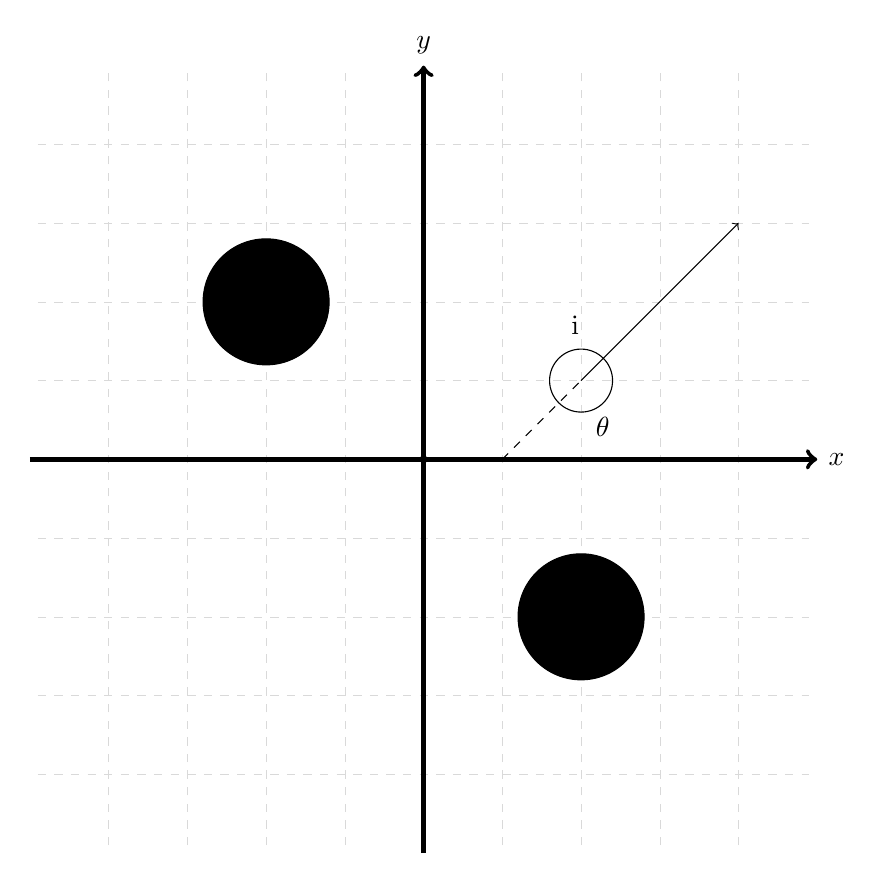
\begin{tikzpicture}
\draw[help lines, color=gray!30, dashed] (-4.9,-4.9) grid (4.9,4.9);
\coordinate (origo) at (0,0);
\coordinate (origo1) at (1.45,0);
\fill[black] (origo) circle (0.05);
\draw[->,ultra thick] (-5,0)--(5,0) node (x) [right]{$x$};
\draw[->,ultra thick] (0,-5)--(0,5) node (y) [above]{$y$};
\draw[] (2.1,1.7) node (i) [left]{i};
\draw[dashed] (1,0)--(2,1);
\draw[->] (2,1)--(4,3);
\draw (x) +(172:3) node {$\theta$};
\tkzDrawArc[R with nodes,](origo1,0.4)(x,y)


\draw[fill] (-2,2) circle [radius=0.8];
\draw[fill] (2,-2) circle [radius=0.8];
\draw (2,1) circle [radius=0.4];
\end{tikzpicture}

  \caption{The 2D plane, agent $i$, whose orientation relative to the $x$
    axis is $\theta$, and two obstacles.}
  \label{fig:unicycle_figure}
\end{figure}

The desired configuration shall be denoted by $\vect{z}_{des}$,
the error dynamics by $\dot{\vect{e}} = g(\vect{e}, \vect{u})$
where $\vect{e}(t) = \vect{z}(t) - \vect{z}_{des}$ and
$\vect{e} \in \mathcal{E} \equiv X \times Y \times \Theta \ominus \vect{z}_{des}$.

\begin{lemma}
  \label{lemma:lipschitz_unicycle}
  Function $g$ is Lipschitz continuous in $\mathcal{E} \times \mathcal{U}$ with
  a Lipschitz constant $$L_g = v \sqrt{Q_{1,1}+Q_{1,2}+Q_{2,1}+Q_{2,2}}$$
  where $\mat{Q} = Q_{\mu\nu}$ is the $3 \times 3$ matrix used to weigh the
  norms involved.
\end{lemma}

    \section{The problem reformed}

Considering the conditions of the motivational problem as stated by problem
\eqref{sec:problem_statement}, the reformed problem assumes the following form:

\begin{problem}
Assuming that
\begin{itemize}
  \item all agents $i \in \mathcal{V}$ have access to their own and their
    neighbours' state and input vectors

  \item all agents $i \in \mathcal{V}$ have a (upper-bounded) sensing range
   $d_i$ such that
   $$d_i > \text{max}\{r_i + r_j: \forall i,j \in \mathcal{V}, i \neq j\}$$

  \item at time $t=0$ the sets $\mathcal{N}_i$ are known for all
    $i \in \mathcal{V}$ and $\sum\limits_i |\mathcal{N}_i| > 0$

  \item at time $t=0$ all agents are in a collision-free configuration with
    each other and the obstacles $\ell \in \mathcal{L}$

  \item All obstacles $\ell \in \mathcal{L}$ are situated
    in such a way that the distance between the two least distant obstacles
    is larger than the diameter of the agent with the largest diameter

\end{itemize}

the problem lies in procuring feasible controls for each agent $i \in \mathcal{V}$
such that for all agents and for all obstacles $\ell \in \mathcal{L}$ the
following hold
\begin{enumerate}
  \item Position and orientation configuration is achieved in steady-state
    $\vect{z}_{i,des}$
    $$\lim_{t \to \infty} \|\vect{z}_i(t) - \vect{z}_{i,des}\| = 0$$

  \item Inter-agent collision is avoided
    $$\|\vect{p}_i(t) - \vect{p}_j(t)\| = d_{ij,a}(t) > \underline{d}_{ij,a},
    \forall j \in \mathcal{V} \backslash \{i\}$$
    where $\vect{p}(t) = [x(t), y(t)]^{\top}$

  \item Inter-agent connectivity loss between neighbouring agents is avoided
    $$ \|\vect{p}_i(t) - \vect{p}_j(t)\| = d_{ij,a} (t) < d_i,
    \forall j \in \mathcal{N}_i, \forall i : |\mathcal{N}_i| \not= 0$$

  \item Agent-with-obstacle collision is avoided
    $$ \|\vect{p}_i(t) - \vect{p}_{\ell}(t)\| = d_{i\ell,o} (t) > \underline{d}_{i\ell,o},
    \forall \ell \in \mathcal{L}$$

  \item The control laws $\vect{u}_i(t)$ abide by their respective input constraints
    $$\vect{u}_i(t) \in \mathcal{U}_i$$
\end{enumerate}

for appropriate choice of constants
$r_i,\vect{z}_{i,des},\underline{d}_{ij,a}, d_i,\underline{d}_{i\ell,o}$ and
neighbour sets $\mathcal{N}_i$, where $i \in \mathcal{V}$.
\end{problem}

From the above we conclude that the constraint set $\mathcal{Z}_i$ for
agent $i \in \mathcal{V}$ is
\begin{align}
  \mathcal{Z}_{i,t} = \big\{\vect{z}_i(t) \in X \times Y \times \Theta : \
      & \|\vect{p}_i(t) - \vect{p}_j(t)\| > \underline{d}_{ij,a}, \forall j \in \mathcal{R}_i(t), \\[2.5ex]
      & \|\vect{p}_i(t) - \vect{p}_j(t)\| < d_i, \forall j \in \mathcal{N}_i, \\[2.5ex]
      & \|\vect{p}_i(t) - \vect{p}_{\ell}\| > \underline{d}_{i\ell,o}, \forall \ell \in \mathcal{L}, \\[2.5ex]
      & - \pi < \theta_i(t) \leq \pi \big\}
\end{align}
and the constraint set that corresponds to each agent for all
$i \in \mathcal{V}$  is given by the Minkowski difference
\begin{align}
  \mathcal{E}_{i,t} = \mathcal{Z}_{i,t} \ominus \vect{z}_{i,des}
  \label{eq:error_constraint_set_unicycle}
\end{align}

In the case of additive disturbances being considered, when each agent solves
its own FHOCP, its constraint set $\mathcal{E}_i$ is replaced by a
restricted constraint set that follows the same structure as
\eqref{eq:restricted_constraint_set}. Furthermore, through the fact that
remark \eqref{remark:aux_control_stabilizability} holds for the unicycle's
error model, i.e. the model is stabilizable $-$ the existence of the
local linear feedback control law $h$ that steers the trajectory of the
states of the system into $\Omega$ is ensured\footnote{The proof can be found
in appendix \eqref{proof:stabilizability_unicycle}}.




The content of chapters \ref{chapter:simulations_without_disturbances} and
\ref{chapter:simulations_with_disturbances} will demonstrate that agents
$i \in \mathcal{V}$ can be stabilized when disturbances are absent, as
demonstrated in chapter \ref{chapter:stabilization_without_disturbance}, and,
in the case where disturbances are present, that the magnitude of their errors
about the equilibrium does not exceed a certain ceiling, as demonstrated in
chapter \ref{chapter:stabilization_with_disturbance}.

    \section{Simulation scenarios}

The simulations were carried out under four different agents-obstacles
configurations:

\begin{enumerate}
  \item Two agents avoid one obstacle on their way to their
    steady-state configurations, without colliding with each other and without
    being separated by the obstacle (we demand that their distance is always
    smaller than the obstacle's diameter for the aim of cooperation).
  \item Two agents pass through the space between two obstacles
    on their way to their steady-state configurations $-$ again, the maximum
    allowed distance between the two agents is smaller than the diameter
    of the obstacle with the smallest radius.
  \item Three agents avoid one obstacle on their way to their
    steady-state configurations, without colliding with each other and without
    being separated by the obstacle. In this case, two agents are
    (independently) neighbours of the third, that is, the third agent should
    maintain connectivity and avoid collision with both of the other two,
    but the latter will only have to avoid colliding with each other.
  \item Three agents pass through the space between two obstacles
    on their way to their steady-state configurations. The conditions of this
    scenario assume those of points 2 and 3.
\end{enumerate}

The four configurations are depicted in figures \eqref{fig:test_case_2_1},
\eqref{fig:test_case_2_2}, \eqref{fig:test_case_3_1} and
\eqref{fig:test_case_3_2}. Agent 1 is depicted in blue, agent 2 in
red and agent 3 in yellow. The obstacles are depicted in black. Mark X
denotes the desired position of an agent and its colour signifies the agent
to be stabilized in that position.


\noindent\makebox[\linewidth][c]{%
\begin{minipage}{\linewidth}
  \begin{minipage}{0.45\linewidth}
    \begin{figure}[H]
      \scalebox{0.7}{% This file was created by matlab2tikz.
%
%The latest updates can be retrieved from
%  http://www.mathworks.com/matlabcentral/fileexchange/22022-matlab2tikz-matlab2tikz
%where you can also make suggestions and rate matlab2tikz.
%
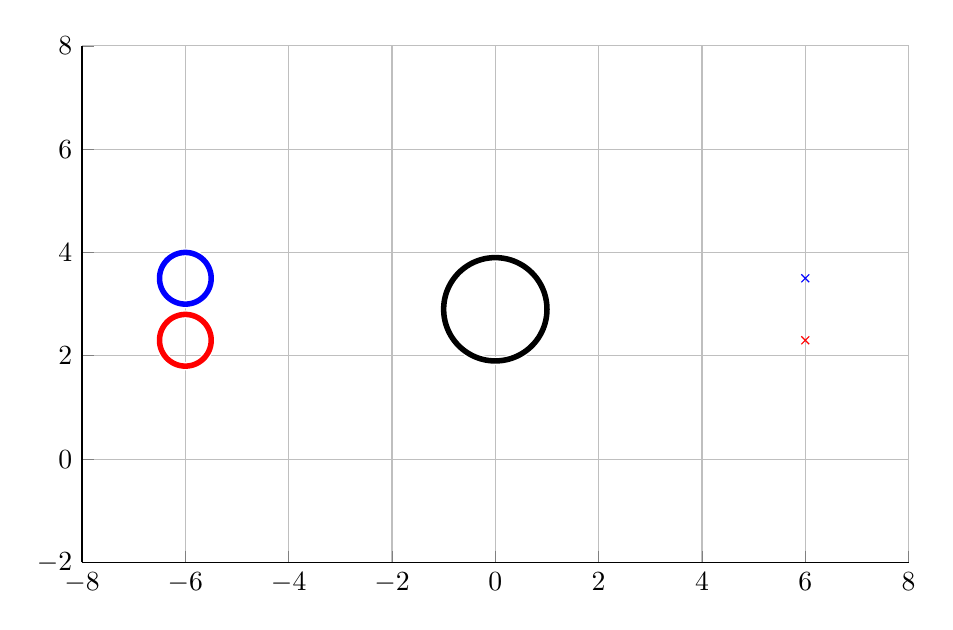
\begin{tikzpicture}

\begin{axis}[%
width=4.133in,
height=2.583in,
at={(0.693in,0.778in)},
scale only axis,
unbounded coords=jump,
xmin=-8,
xmax=8,
xmajorgrids,
ymin=-2,
ymax=8,
ymajorgrids,
axis background/.style={fill=white},
axis x line*=bottom,
axis y line*=left
]
\addplot [color=blue,only marks,mark=x,mark options={solid},forget plot]
  table[row sep=crcr]{%
6	3.5\\
};
\addplot [color=red,only marks,mark=x,mark options={solid},forget plot]
  table[row sep=crcr]{%
6	2.3\\
};
\addplot [color=white,solid,line width=3.0pt,forget plot]
  table[row sep=crcr]{%
-5.5	3.5\\
-5.50030458649045	3.51744974835125\\
-5.50121797487009	3.53487823687206\\
-5.50273905231586	3.55226423163383\\
-5.50486596562921	3.56958655048003\\
-5.5075961234939	3.58682408883347\\
-5.5109261996331	3.60395584540888\\
-5.514852136862	3.62096094779983\\
-5.51936915203084	3.6378186779085\\
-5.52447174185242	3.65450849718747\\
-5.53015368960705	3.67101007166283\\
-5.53640807271661	3.68730329670796\\
-5.5432272711787	3.7033683215379\\
-5.55060297685042	3.71918557339454\\
-5.55852620357054	3.73473578139295\\
-5.56698729810778	3.75\\
-5.57597595192179	3.7649596321166\\
-5.58548121372248	3.77959645173537\\
-5.59549150281253	3.79389262614624\\
-5.60599462319664	3.80783073766283\\
-5.61697777844051	3.82139380484327\\
-5.6284275872613	3.83456530317943\\
-5.64033009983067	3.8473291852295\\
-5.6526708147705	3.85966990016933\\
-5.66543469682057	3.8715724127387\\
-5.67860619515673	3.88302222155949\\
-5.69216926233717	3.89400537680336\\
-5.70610737385376	3.90450849718747\\
-5.72040354826463	3.91451878627752\\
-5.7350403678834	3.92402404807821\\
-5.75	3.93301270189222\\
-5.76526421860705	3.94147379642946\\
-5.78081442660546	3.94939702314958\\
-5.7966316784621	3.9567727288213\\
-5.81269670329204	3.96359192728339\\
-5.82898992833717	3.96984631039295\\
-5.84549150281253	3.97552825814758\\
-5.8621813220915	3.98063084796916\\
-5.87903905220017	3.985147863138\\
-5.89604415459112	3.9890738003669\\
-5.91317591116653	3.9924038765061\\
-5.93041344951997	3.99513403437079\\
-5.94773576836617	3.99726094768414\\
-5.96512176312794	3.99878202512991\\
-5.98255025164875	3.99969541350955\\
-6	4\\
-6.01744974835125	3.99969541350955\\
-6.03487823687206	3.99878202512991\\
-6.05226423163383	3.99726094768414\\
-6.06958655048003	3.99513403437079\\
-6.08682408883347	3.9924038765061\\
-6.10395584540888	3.9890738003669\\
-6.12096094779983	3.985147863138\\
-6.1378186779085	3.98063084796916\\
-6.15450849718747	3.97552825814758\\
-6.17101007166283	3.96984631039295\\
-6.18730329670796	3.96359192728339\\
-6.2033683215379	3.9567727288213\\
-6.21918557339454	3.94939702314958\\
-6.23473578139295	3.94147379642946\\
-6.25	3.93301270189222\\
-6.2649596321166	3.92402404807821\\
-6.27959645173537	3.91451878627752\\
-6.29389262614624	3.90450849718747\\
-6.30783073766283	3.89400537680336\\
-6.32139380484327	3.88302222155949\\
-6.33456530317943	3.8715724127387\\
-6.3473291852295	3.85966990016933\\
-6.35966990016933	3.8473291852295\\
-6.3715724127387	3.83456530317943\\
-6.38302222155949	3.82139380484327\\
-6.39400537680336	3.80783073766283\\
-6.40450849718747	3.79389262614624\\
-6.41451878627752	3.77959645173537\\
-6.42402404807821	3.7649596321166\\
-6.43301270189222	3.75\\
-6.44147379642946	3.73473578139295\\
-6.44939702314958	3.71918557339454\\
-6.4567727288213	3.7033683215379\\
-6.46359192728339	3.68730329670796\\
-6.46984631039295	3.67101007166283\\
-6.47552825814758	3.65450849718747\\
-6.48063084796916	3.6378186779085\\
-6.485147863138	3.62096094779983\\
-6.4890738003669	3.60395584540888\\
-6.4924038765061	3.58682408883347\\
-6.49513403437079	3.56958655048003\\
-6.49726094768414	3.55226423163383\\
-6.49878202512991	3.53487823687206\\
-6.49969541350955	3.51744974835125\\
-6.5	3.5\\
-6.49969541350955	3.48255025164875\\
-6.49878202512991	3.46512176312794\\
-6.49726094768414	3.44773576836617\\
-6.49513403437079	3.43041344951997\\
-6.4924038765061	3.41317591116653\\
-6.4890738003669	3.39604415459112\\
-6.485147863138	3.37903905220017\\
-6.48063084796916	3.3621813220915\\
-6.47552825814758	3.34549150281253\\
-6.46984631039295	3.32898992833717\\
-6.46359192728339	3.31269670329204\\
-6.4567727288213	3.2966316784621\\
-6.44939702314958	3.28081442660546\\
-6.44147379642946	3.26526421860705\\
-6.43301270189222	3.25\\
-6.42402404807821	3.2350403678834\\
-6.41451878627752	3.22040354826463\\
-6.40450849718747	3.20610737385376\\
-6.39400537680336	3.19216926233717\\
-6.38302222155949	3.17860619515673\\
-6.3715724127387	3.16543469682057\\
-6.35966990016933	3.1526708147705\\
-6.3473291852295	3.14033009983067\\
-6.33456530317943	3.1284275872613\\
-6.32139380484327	3.11697777844051\\
-6.30783073766283	3.10599462319664\\
-6.29389262614624	3.09549150281253\\
-6.27959645173537	3.08548121372248\\
-6.2649596321166	3.07597595192179\\
-6.25	3.06698729810778\\
-6.23473578139295	3.05852620357054\\
-6.21918557339454	3.05060297685042\\
-6.2033683215379	3.0432272711787\\
-6.18730329670796	3.03640807271661\\
-6.17101007166283	3.03015368960705\\
-6.15450849718747	3.02447174185242\\
-6.1378186779085	3.01936915203084\\
-6.12096094779983	3.014852136862\\
-6.10395584540888	3.0109261996331\\
-6.08682408883347	3.0075961234939\\
-6.06958655048003	3.00486596562921\\
-6.05226423163383	3.00273905231586\\
-6.03487823687206	3.00121797487009\\
-6.01744974835125	3.00030458649045\\
-6	3\\
-5.98255025164875	3.00030458649045\\
-5.96512176312794	3.00121797487009\\
-5.94773576836617	3.00273905231586\\
-5.93041344951997	3.00486596562921\\
-5.91317591116653	3.0075961234939\\
-5.89604415459112	3.0109261996331\\
-5.87903905220017	3.014852136862\\
-5.8621813220915	3.01936915203084\\
-5.84549150281253	3.02447174185242\\
-5.82898992833717	3.03015368960705\\
-5.81269670329204	3.03640807271661\\
-5.7966316784621	3.0432272711787\\
-5.78081442660546	3.05060297685042\\
-5.76526421860705	3.05852620357054\\
-5.75	3.06698729810778\\
-5.7350403678834	3.07597595192179\\
-5.72040354826463	3.08548121372248\\
-5.70610737385376	3.09549150281253\\
-5.69216926233717	3.10599462319664\\
-5.67860619515673	3.11697777844051\\
-5.66543469682057	3.1284275872613\\
-5.6526708147705	3.14033009983067\\
-5.64033009983067	3.1526708147705\\
-5.6284275872613	3.16543469682057\\
-5.61697777844051	3.17860619515673\\
-5.60599462319664	3.19216926233717\\
-5.59549150281253	3.20610737385376\\
-5.58548121372248	3.22040354826463\\
-5.57597595192179	3.2350403678834\\
-5.56698729810778	3.25\\
-5.55852620357054	3.26526421860705\\
-5.55060297685042	3.28081442660546\\
-5.5432272711787	3.2966316784621\\
-5.53640807271661	3.31269670329204\\
-5.53015368960705	3.32898992833717\\
-5.52447174185242	3.34549150281253\\
-5.51936915203084	3.3621813220915\\
-5.514852136862	3.37903905220017\\
-5.5109261996331	3.39604415459112\\
-5.5075961234939	3.41317591116653\\
-5.50486596562921	3.43041344951997\\
-5.50273905231586	3.44773576836617\\
-5.50121797487009	3.46512176312794\\
-5.50030458649045	3.48255025164875\\
-5.5	3.5\\
nan	nan\\
};
\addplot [color=blue,solid,line width=2.0pt,forget plot]
  table[row sep=crcr]{%
-5.5	3.5\\
-5.50030458649045	3.51744974835125\\
-5.50121797487009	3.53487823687206\\
-5.50273905231586	3.55226423163383\\
-5.50486596562921	3.56958655048003\\
-5.5075961234939	3.58682408883347\\
-5.5109261996331	3.60395584540888\\
-5.514852136862	3.62096094779983\\
-5.51936915203084	3.6378186779085\\
-5.52447174185242	3.65450849718747\\
-5.53015368960705	3.67101007166283\\
-5.53640807271661	3.68730329670796\\
-5.5432272711787	3.7033683215379\\
-5.55060297685042	3.71918557339454\\
-5.55852620357054	3.73473578139295\\
-5.56698729810778	3.75\\
-5.57597595192179	3.7649596321166\\
-5.58548121372248	3.77959645173537\\
-5.59549150281253	3.79389262614624\\
-5.60599462319664	3.80783073766283\\
-5.61697777844051	3.82139380484327\\
-5.6284275872613	3.83456530317943\\
-5.64033009983067	3.8473291852295\\
-5.6526708147705	3.85966990016933\\
-5.66543469682057	3.8715724127387\\
-5.67860619515673	3.88302222155949\\
-5.69216926233717	3.89400537680336\\
-5.70610737385376	3.90450849718747\\
-5.72040354826463	3.91451878627752\\
-5.7350403678834	3.92402404807821\\
-5.75	3.93301270189222\\
-5.76526421860705	3.94147379642946\\
-5.78081442660546	3.94939702314958\\
-5.7966316784621	3.9567727288213\\
-5.81269670329204	3.96359192728339\\
-5.82898992833717	3.96984631039295\\
-5.84549150281253	3.97552825814758\\
-5.8621813220915	3.98063084796916\\
-5.87903905220017	3.985147863138\\
-5.89604415459112	3.9890738003669\\
-5.91317591116653	3.9924038765061\\
-5.93041344951997	3.99513403437079\\
-5.94773576836617	3.99726094768414\\
-5.96512176312794	3.99878202512991\\
-5.98255025164875	3.99969541350955\\
-6	4\\
-6.01744974835125	3.99969541350955\\
-6.03487823687206	3.99878202512991\\
-6.05226423163383	3.99726094768414\\
-6.06958655048003	3.99513403437079\\
-6.08682408883347	3.9924038765061\\
-6.10395584540888	3.9890738003669\\
-6.12096094779983	3.985147863138\\
-6.1378186779085	3.98063084796916\\
-6.15450849718747	3.97552825814758\\
-6.17101007166283	3.96984631039295\\
-6.18730329670796	3.96359192728339\\
-6.2033683215379	3.9567727288213\\
-6.21918557339454	3.94939702314958\\
-6.23473578139295	3.94147379642946\\
-6.25	3.93301270189222\\
-6.2649596321166	3.92402404807821\\
-6.27959645173537	3.91451878627752\\
-6.29389262614624	3.90450849718747\\
-6.30783073766283	3.89400537680336\\
-6.32139380484327	3.88302222155949\\
-6.33456530317943	3.8715724127387\\
-6.3473291852295	3.85966990016933\\
-6.35966990016933	3.8473291852295\\
-6.3715724127387	3.83456530317943\\
-6.38302222155949	3.82139380484327\\
-6.39400537680336	3.80783073766283\\
-6.40450849718747	3.79389262614624\\
-6.41451878627752	3.77959645173537\\
-6.42402404807821	3.7649596321166\\
-6.43301270189222	3.75\\
-6.44147379642946	3.73473578139295\\
-6.44939702314958	3.71918557339454\\
-6.4567727288213	3.7033683215379\\
-6.46359192728339	3.68730329670796\\
-6.46984631039295	3.67101007166283\\
-6.47552825814758	3.65450849718747\\
-6.48063084796916	3.6378186779085\\
-6.485147863138	3.62096094779983\\
-6.4890738003669	3.60395584540888\\
-6.4924038765061	3.58682408883347\\
-6.49513403437079	3.56958655048003\\
-6.49726094768414	3.55226423163383\\
-6.49878202512991	3.53487823687206\\
-6.49969541350955	3.51744974835125\\
-6.5	3.5\\
-6.49969541350955	3.48255025164875\\
-6.49878202512991	3.46512176312794\\
-6.49726094768414	3.44773576836617\\
-6.49513403437079	3.43041344951997\\
-6.4924038765061	3.41317591116653\\
-6.4890738003669	3.39604415459112\\
-6.485147863138	3.37903905220017\\
-6.48063084796916	3.3621813220915\\
-6.47552825814758	3.34549150281253\\
-6.46984631039295	3.32898992833717\\
-6.46359192728339	3.31269670329204\\
-6.4567727288213	3.2966316784621\\
-6.44939702314958	3.28081442660546\\
-6.44147379642946	3.26526421860705\\
-6.43301270189222	3.25\\
-6.42402404807821	3.2350403678834\\
-6.41451878627752	3.22040354826463\\
-6.40450849718747	3.20610737385376\\
-6.39400537680336	3.19216926233717\\
-6.38302222155949	3.17860619515673\\
-6.3715724127387	3.16543469682057\\
-6.35966990016933	3.1526708147705\\
-6.3473291852295	3.14033009983067\\
-6.33456530317943	3.1284275872613\\
-6.32139380484327	3.11697777844051\\
-6.30783073766283	3.10599462319664\\
-6.29389262614624	3.09549150281253\\
-6.27959645173537	3.08548121372248\\
-6.2649596321166	3.07597595192179\\
-6.25	3.06698729810778\\
-6.23473578139295	3.05852620357054\\
-6.21918557339454	3.05060297685042\\
-6.2033683215379	3.0432272711787\\
-6.18730329670796	3.03640807271661\\
-6.17101007166283	3.03015368960705\\
-6.15450849718747	3.02447174185242\\
-6.1378186779085	3.01936915203084\\
-6.12096094779983	3.014852136862\\
-6.10395584540888	3.0109261996331\\
-6.08682408883347	3.0075961234939\\
-6.06958655048003	3.00486596562921\\
-6.05226423163383	3.00273905231586\\
-6.03487823687206	3.00121797487009\\
-6.01744974835125	3.00030458649045\\
-6	3\\
-5.98255025164875	3.00030458649045\\
-5.96512176312794	3.00121797487009\\
-5.94773576836617	3.00273905231586\\
-5.93041344951997	3.00486596562921\\
-5.91317591116653	3.0075961234939\\
-5.89604415459112	3.0109261996331\\
-5.87903905220017	3.014852136862\\
-5.8621813220915	3.01936915203084\\
-5.84549150281253	3.02447174185242\\
-5.82898992833717	3.03015368960705\\
-5.81269670329204	3.03640807271661\\
-5.7966316784621	3.0432272711787\\
-5.78081442660546	3.05060297685042\\
-5.76526421860705	3.05852620357054\\
-5.75	3.06698729810778\\
-5.7350403678834	3.07597595192179\\
-5.72040354826463	3.08548121372248\\
-5.70610737385376	3.09549150281253\\
-5.69216926233717	3.10599462319664\\
-5.67860619515673	3.11697777844051\\
-5.66543469682057	3.1284275872613\\
-5.6526708147705	3.14033009983067\\
-5.64033009983067	3.1526708147705\\
-5.6284275872613	3.16543469682057\\
-5.61697777844051	3.17860619515673\\
-5.60599462319664	3.19216926233717\\
-5.59549150281253	3.20610737385376\\
-5.58548121372248	3.22040354826463\\
-5.57597595192179	3.2350403678834\\
-5.56698729810778	3.25\\
-5.55852620357054	3.26526421860705\\
-5.55060297685042	3.28081442660546\\
-5.5432272711787	3.2966316784621\\
-5.53640807271661	3.31269670329204\\
-5.53015368960705	3.32898992833717\\
-5.52447174185242	3.34549150281253\\
-5.51936915203084	3.3621813220915\\
-5.514852136862	3.37903905220017\\
-5.5109261996331	3.39604415459112\\
-5.5075961234939	3.41317591116653\\
-5.50486596562921	3.43041344951997\\
-5.50273905231586	3.44773576836617\\
-5.50121797487009	3.46512176312794\\
-5.50030458649045	3.48255025164875\\
-5.5	3.5\\
nan	nan\\
};
\addplot [color=white,solid,line width=3.0pt,forget plot]
  table[row sep=crcr]{%
-5.5	2.3\\
-5.50030458649045	2.31744974835125\\
-5.50121797487009	2.33487823687206\\
-5.50273905231586	2.35226423163383\\
-5.50486596562921	2.36958655048003\\
-5.5075961234939	2.38682408883346\\
-5.5109261996331	2.40395584540888\\
-5.514852136862	2.42096094779983\\
-5.51936915203084	2.4378186779085\\
-5.52447174185242	2.45450849718747\\
-5.53015368960705	2.47101007166283\\
-5.53640807271661	2.48730329670796\\
-5.5432272711787	2.5033683215379\\
-5.55060297685042	2.51918557339454\\
-5.55852620357054	2.53473578139295\\
-5.56698729810778	2.55\\
-5.57597595192179	2.5649596321166\\
-5.58548121372248	2.57959645173537\\
-5.59549150281253	2.59389262614624\\
-5.60599462319664	2.60783073766283\\
-5.61697777844051	2.62139380484327\\
-5.6284275872613	2.63456530317943\\
-5.64033009983067	2.6473291852295\\
-5.6526708147705	2.65966990016933\\
-5.66543469682057	2.6715724127387\\
-5.67860619515673	2.68302222155949\\
-5.69216926233717	2.69400537680336\\
-5.70610737385376	2.70450849718747\\
-5.72040354826463	2.71451878627752\\
-5.7350403678834	2.72402404807821\\
-5.75	2.73301270189222\\
-5.76526421860705	2.74147379642946\\
-5.78081442660546	2.74939702314958\\
-5.7966316784621	2.7567727288213\\
-5.81269670329204	2.76359192728339\\
-5.82898992833717	2.76984631039295\\
-5.84549150281253	2.77552825814758\\
-5.8621813220915	2.78063084796916\\
-5.87903905220017	2.785147863138\\
-5.89604415459112	2.7890738003669\\
-5.91317591116653	2.7924038765061\\
-5.93041344951997	2.79513403437078\\
-5.94773576836617	2.79726094768414\\
-5.96512176312794	2.79878202512991\\
-5.98255025164875	2.79969541350955\\
-6	2.8\\
-6.01744974835125	2.79969541350955\\
-6.03487823687206	2.79878202512991\\
-6.05226423163383	2.79726094768414\\
-6.06958655048003	2.79513403437078\\
-6.08682408883347	2.7924038765061\\
-6.10395584540888	2.7890738003669\\
-6.12096094779983	2.785147863138\\
-6.1378186779085	2.78063084796916\\
-6.15450849718747	2.77552825814758\\
-6.17101007166283	2.76984631039295\\
-6.18730329670796	2.76359192728339\\
-6.2033683215379	2.7567727288213\\
-6.21918557339454	2.74939702314958\\
-6.23473578139295	2.74147379642946\\
-6.25	2.73301270189222\\
-6.2649596321166	2.72402404807821\\
-6.27959645173537	2.71451878627752\\
-6.29389262614624	2.70450849718747\\
-6.30783073766283	2.69400537680336\\
-6.32139380484327	2.68302222155949\\
-6.33456530317943	2.6715724127387\\
-6.3473291852295	2.65966990016933\\
-6.35966990016933	2.6473291852295\\
-6.3715724127387	2.63456530317943\\
-6.38302222155949	2.62139380484327\\
-6.39400537680336	2.60783073766283\\
-6.40450849718747	2.59389262614624\\
-6.41451878627752	2.57959645173537\\
-6.42402404807821	2.5649596321166\\
-6.43301270189222	2.55\\
-6.44147379642946	2.53473578139295\\
-6.44939702314958	2.51918557339454\\
-6.4567727288213	2.5033683215379\\
-6.46359192728339	2.48730329670796\\
-6.46984631039295	2.47101007166283\\
-6.47552825814758	2.45450849718747\\
-6.48063084796916	2.4378186779085\\
-6.485147863138	2.42096094779983\\
-6.4890738003669	2.40395584540888\\
-6.4924038765061	2.38682408883346\\
-6.49513403437079	2.36958655048003\\
-6.49726094768414	2.35226423163383\\
-6.49878202512991	2.33487823687206\\
-6.49969541350955	2.31744974835125\\
-6.5	2.3\\
-6.49969541350955	2.28255025164875\\
-6.49878202512991	2.26512176312794\\
-6.49726094768414	2.24773576836617\\
-6.49513403437079	2.23041344951997\\
-6.4924038765061	2.21317591116653\\
-6.4890738003669	2.19604415459112\\
-6.485147863138	2.17903905220017\\
-6.48063084796916	2.1621813220915\\
-6.47552825814758	2.14549150281253\\
-6.46984631039295	2.12898992833717\\
-6.46359192728339	2.11269670329204\\
-6.4567727288213	2.0966316784621\\
-6.44939702314958	2.08081442660546\\
-6.44147379642946	2.06526421860705\\
-6.43301270189222	2.05\\
-6.42402404807821	2.0350403678834\\
-6.41451878627752	2.02040354826463\\
-6.40450849718747	2.00610737385376\\
-6.39400537680336	1.99216926233717\\
-6.38302222155949	1.97860619515673\\
-6.3715724127387	1.96543469682057\\
-6.35966990016933	1.9526708147705\\
-6.3473291852295	1.94033009983067\\
-6.33456530317943	1.9284275872613\\
-6.32139380484327	1.91697777844051\\
-6.30783073766283	1.90599462319664\\
-6.29389262614624	1.89549150281253\\
-6.27959645173537	1.88548121372248\\
-6.2649596321166	1.87597595192179\\
-6.25	1.86698729810778\\
-6.23473578139295	1.85852620357054\\
-6.21918557339454	1.85060297685042\\
-6.2033683215379	1.8432272711787\\
-6.18730329670796	1.83640807271661\\
-6.17101007166283	1.83015368960705\\
-6.15450849718747	1.82447174185242\\
-6.1378186779085	1.81936915203084\\
-6.12096094779983	1.814852136862\\
-6.10395584540888	1.8109261996331\\
-6.08682408883347	1.8075961234939\\
-6.06958655048003	1.80486596562921\\
-6.05226423163383	1.80273905231586\\
-6.03487823687206	1.80121797487009\\
-6.01744974835125	1.80030458649045\\
-6	1.8\\
-5.98255025164875	1.80030458649045\\
-5.96512176312794	1.80121797487009\\
-5.94773576836617	1.80273905231586\\
-5.93041344951997	1.80486596562921\\
-5.91317591116653	1.8075961234939\\
-5.89604415459112	1.8109261996331\\
-5.87903905220017	1.814852136862\\
-5.8621813220915	1.81936915203084\\
-5.84549150281253	1.82447174185242\\
-5.82898992833717	1.83015368960705\\
-5.81269670329204	1.83640807271661\\
-5.7966316784621	1.8432272711787\\
-5.78081442660546	1.85060297685042\\
-5.76526421860705	1.85852620357054\\
-5.75	1.86698729810778\\
-5.7350403678834	1.87597595192179\\
-5.72040354826463	1.88548121372248\\
-5.70610737385376	1.89549150281253\\
-5.69216926233717	1.90599462319664\\
-5.67860619515673	1.91697777844051\\
-5.66543469682057	1.9284275872613\\
-5.6526708147705	1.94033009983067\\
-5.64033009983067	1.9526708147705\\
-5.6284275872613	1.96543469682057\\
-5.61697777844051	1.97860619515673\\
-5.60599462319664	1.99216926233717\\
-5.59549150281253	2.00610737385376\\
-5.58548121372248	2.02040354826463\\
-5.57597595192179	2.0350403678834\\
-5.56698729810778	2.05\\
-5.55852620357054	2.06526421860705\\
-5.55060297685042	2.08081442660546\\
-5.5432272711787	2.0966316784621\\
-5.53640807271661	2.11269670329204\\
-5.53015368960705	2.12898992833717\\
-5.52447174185242	2.14549150281253\\
-5.51936915203084	2.1621813220915\\
-5.514852136862	2.17903905220017\\
-5.5109261996331	2.19604415459112\\
-5.5075961234939	2.21317591116653\\
-5.50486596562921	2.23041344951997\\
-5.50273905231586	2.24773576836617\\
-5.50121797487009	2.26512176312794\\
-5.50030458649045	2.28255025164875\\
-5.5	2.3\\
nan	nan\\
};
\addplot [color=red,solid,line width=2.0pt,forget plot]
  table[row sep=crcr]{%
-5.5	2.3\\
-5.50030458649045	2.31744974835125\\
-5.50121797487009	2.33487823687206\\
-5.50273905231586	2.35226423163383\\
-5.50486596562921	2.36958655048003\\
-5.5075961234939	2.38682408883346\\
-5.5109261996331	2.40395584540888\\
-5.514852136862	2.42096094779983\\
-5.51936915203084	2.4378186779085\\
-5.52447174185242	2.45450849718747\\
-5.53015368960705	2.47101007166283\\
-5.53640807271661	2.48730329670796\\
-5.5432272711787	2.5033683215379\\
-5.55060297685042	2.51918557339454\\
-5.55852620357054	2.53473578139295\\
-5.56698729810778	2.55\\
-5.57597595192179	2.5649596321166\\
-5.58548121372248	2.57959645173537\\
-5.59549150281253	2.59389262614624\\
-5.60599462319664	2.60783073766283\\
-5.61697777844051	2.62139380484327\\
-5.6284275872613	2.63456530317943\\
-5.64033009983067	2.6473291852295\\
-5.6526708147705	2.65966990016933\\
-5.66543469682057	2.6715724127387\\
-5.67860619515673	2.68302222155949\\
-5.69216926233717	2.69400537680336\\
-5.70610737385376	2.70450849718747\\
-5.72040354826463	2.71451878627752\\
-5.7350403678834	2.72402404807821\\
-5.75	2.73301270189222\\
-5.76526421860705	2.74147379642946\\
-5.78081442660546	2.74939702314958\\
-5.7966316784621	2.7567727288213\\
-5.81269670329204	2.76359192728339\\
-5.82898992833717	2.76984631039295\\
-5.84549150281253	2.77552825814758\\
-5.8621813220915	2.78063084796916\\
-5.87903905220017	2.785147863138\\
-5.89604415459112	2.7890738003669\\
-5.91317591116653	2.7924038765061\\
-5.93041344951997	2.79513403437078\\
-5.94773576836617	2.79726094768414\\
-5.96512176312794	2.79878202512991\\
-5.98255025164875	2.79969541350955\\
-6	2.8\\
-6.01744974835125	2.79969541350955\\
-6.03487823687206	2.79878202512991\\
-6.05226423163383	2.79726094768414\\
-6.06958655048003	2.79513403437078\\
-6.08682408883347	2.7924038765061\\
-6.10395584540888	2.7890738003669\\
-6.12096094779983	2.785147863138\\
-6.1378186779085	2.78063084796916\\
-6.15450849718747	2.77552825814758\\
-6.17101007166283	2.76984631039295\\
-6.18730329670796	2.76359192728339\\
-6.2033683215379	2.7567727288213\\
-6.21918557339454	2.74939702314958\\
-6.23473578139295	2.74147379642946\\
-6.25	2.73301270189222\\
-6.2649596321166	2.72402404807821\\
-6.27959645173537	2.71451878627752\\
-6.29389262614624	2.70450849718747\\
-6.30783073766283	2.69400537680336\\
-6.32139380484327	2.68302222155949\\
-6.33456530317943	2.6715724127387\\
-6.3473291852295	2.65966990016933\\
-6.35966990016933	2.6473291852295\\
-6.3715724127387	2.63456530317943\\
-6.38302222155949	2.62139380484327\\
-6.39400537680336	2.60783073766283\\
-6.40450849718747	2.59389262614624\\
-6.41451878627752	2.57959645173537\\
-6.42402404807821	2.5649596321166\\
-6.43301270189222	2.55\\
-6.44147379642946	2.53473578139295\\
-6.44939702314958	2.51918557339454\\
-6.4567727288213	2.5033683215379\\
-6.46359192728339	2.48730329670796\\
-6.46984631039295	2.47101007166283\\
-6.47552825814758	2.45450849718747\\
-6.48063084796916	2.4378186779085\\
-6.485147863138	2.42096094779983\\
-6.4890738003669	2.40395584540888\\
-6.4924038765061	2.38682408883346\\
-6.49513403437079	2.36958655048003\\
-6.49726094768414	2.35226423163383\\
-6.49878202512991	2.33487823687206\\
-6.49969541350955	2.31744974835125\\
-6.5	2.3\\
-6.49969541350955	2.28255025164875\\
-6.49878202512991	2.26512176312794\\
-6.49726094768414	2.24773576836617\\
-6.49513403437079	2.23041344951997\\
-6.4924038765061	2.21317591116653\\
-6.4890738003669	2.19604415459112\\
-6.485147863138	2.17903905220017\\
-6.48063084796916	2.1621813220915\\
-6.47552825814758	2.14549150281253\\
-6.46984631039295	2.12898992833717\\
-6.46359192728339	2.11269670329204\\
-6.4567727288213	2.0966316784621\\
-6.44939702314958	2.08081442660546\\
-6.44147379642946	2.06526421860705\\
-6.43301270189222	2.05\\
-6.42402404807821	2.0350403678834\\
-6.41451878627752	2.02040354826463\\
-6.40450849718747	2.00610737385376\\
-6.39400537680336	1.99216926233717\\
-6.38302222155949	1.97860619515673\\
-6.3715724127387	1.96543469682057\\
-6.35966990016933	1.9526708147705\\
-6.3473291852295	1.94033009983067\\
-6.33456530317943	1.9284275872613\\
-6.32139380484327	1.91697777844051\\
-6.30783073766283	1.90599462319664\\
-6.29389262614624	1.89549150281253\\
-6.27959645173537	1.88548121372248\\
-6.2649596321166	1.87597595192179\\
-6.25	1.86698729810778\\
-6.23473578139295	1.85852620357054\\
-6.21918557339454	1.85060297685042\\
-6.2033683215379	1.8432272711787\\
-6.18730329670796	1.83640807271661\\
-6.17101007166283	1.83015368960705\\
-6.15450849718747	1.82447174185242\\
-6.1378186779085	1.81936915203084\\
-6.12096094779983	1.814852136862\\
-6.10395584540888	1.8109261996331\\
-6.08682408883347	1.8075961234939\\
-6.06958655048003	1.80486596562921\\
-6.05226423163383	1.80273905231586\\
-6.03487823687206	1.80121797487009\\
-6.01744974835125	1.80030458649045\\
-6	1.8\\
-5.98255025164875	1.80030458649045\\
-5.96512176312794	1.80121797487009\\
-5.94773576836617	1.80273905231586\\
-5.93041344951997	1.80486596562921\\
-5.91317591116653	1.8075961234939\\
-5.89604415459112	1.8109261996331\\
-5.87903905220017	1.814852136862\\
-5.8621813220915	1.81936915203084\\
-5.84549150281253	1.82447174185242\\
-5.82898992833717	1.83015368960705\\
-5.81269670329204	1.83640807271661\\
-5.7966316784621	1.8432272711787\\
-5.78081442660546	1.85060297685042\\
-5.76526421860705	1.85852620357054\\
-5.75	1.86698729810778\\
-5.7350403678834	1.87597595192179\\
-5.72040354826463	1.88548121372248\\
-5.70610737385376	1.89549150281253\\
-5.69216926233717	1.90599462319664\\
-5.67860619515673	1.91697777844051\\
-5.66543469682057	1.9284275872613\\
-5.6526708147705	1.94033009983067\\
-5.64033009983067	1.9526708147705\\
-5.6284275872613	1.96543469682057\\
-5.61697777844051	1.97860619515673\\
-5.60599462319664	1.99216926233717\\
-5.59549150281253	2.00610737385376\\
-5.58548121372248	2.02040354826463\\
-5.57597595192179	2.0350403678834\\
-5.56698729810778	2.05\\
-5.55852620357054	2.06526421860705\\
-5.55060297685042	2.08081442660546\\
-5.5432272711787	2.0966316784621\\
-5.53640807271661	2.11269670329204\\
-5.53015368960705	2.12898992833717\\
-5.52447174185242	2.14549150281253\\
-5.51936915203084	2.1621813220915\\
-5.514852136862	2.17903905220017\\
-5.5109261996331	2.19604415459112\\
-5.5075961234939	2.21317591116653\\
-5.50486596562921	2.23041344951997\\
-5.50273905231586	2.24773576836617\\
-5.50121797487009	2.26512176312794\\
-5.50030458649045	2.28255025164875\\
-5.5	2.3\\
nan	nan\\
};
\addplot [color=white,solid,line width=3.0pt,forget plot]
  table[row sep=crcr]{%
1	2.9\\
0.999390827019096	2.9348994967025\\
0.997564050259824	2.96975647374413\\
0.994521895368273	3.00452846326765\\
0.99026806874157	3.03917310096007\\
0.984807753012208	3.07364817766693\\
0.978147600733806	3.10791169081776\\
0.970295726275996	3.14192189559967\\
0.961261695938319	3.175637355817\\
0.951056516295154	3.20901699437495\\
0.939692620785908	3.24202014332567\\
0.927183854566787	3.27460659341591\\
0.913545457642601	3.3067366430758\\
0.898794046299167	3.33837114678908\\
0.882947592858927	3.36947156278589\\
0.866025403784439	3.4\\
0.848048096156426	3.42991926423321\\
0.829037572555042	3.45919290347075\\
0.809016994374947	3.48778525229247\\
0.788010753606722	3.51566147532566\\
0.766044443118978	3.54278760968654\\
0.743144825477394	3.56913060635886\\
0.719339800338651	3.594658370459\\
0.694658370458997	3.61933980033865\\
0.669130606358858	3.64314482547739\\
0.642787609686539	3.66604444311898\\
0.615661475325658	3.68801075360672\\
0.587785252292473	3.70901699437495\\
0.559192903470747	3.72903757255504\\
0.529919264233205	3.74804809615643\\
0.5	3.76602540378444\\
0.469471562785891	3.78294759285893\\
0.438371146789077	3.79879404629917\\
0.4067366430758	3.8135454576426\\
0.374606593415912	3.82718385456679\\
0.342020143325669	3.83969262078591\\
0.309016994374947	3.85105651629515\\
0.275637355816999	3.86126169593832\\
0.241921895599668	3.870295726276\\
0.207911690817759	3.87814760073381\\
0.17364817766693	3.88480775301221\\
0.139173100960066	3.89026806874157\\
0.104528463267653	3.89452189536827\\
0.0697564737441255	3.89756405025982\\
0.0348994967025011	3.8993908270191\\
6.12323399573677e-17	3.9\\
-0.0348994967025007	3.8993908270191\\
-0.0697564737441253	3.89756405025982\\
-0.104528463267653	3.89452189536827\\
-0.139173100960065	3.89026806874157\\
-0.17364817766693	3.88480775301221\\
-0.207911690817759	3.87814760073381\\
-0.241921895599668	3.870295726276\\
-0.275637355816999	3.86126169593832\\
-0.309016994374947	3.85105651629515\\
-0.342020143325669	3.83969262078591\\
-0.374606593415912	3.82718385456679\\
-0.4067366430758	3.8135454576426\\
-0.438371146789078	3.79879404629917\\
-0.469471562785891	3.78294759285893\\
-0.5	3.76602540378444\\
-0.529919264233205	3.74804809615643\\
-0.559192903470747	3.72903757255504\\
-0.587785252292473	3.70901699437495\\
-0.615661475325658	3.68801075360672\\
-0.642787609686539	3.66604444311898\\
-0.669130606358858	3.64314482547739\\
-0.694658370458997	3.61933980033865\\
-0.719339800338651	3.594658370459\\
-0.743144825477394	3.56913060635886\\
-0.766044443118978	3.54278760968654\\
-0.788010753606722	3.51566147532566\\
-0.809016994374947	3.48778525229247\\
-0.829037572555042	3.45919290347075\\
-0.848048096156426	3.42991926423321\\
-0.866025403784439	3.4\\
-0.882947592858927	3.36947156278589\\
-0.898794046299167	3.33837114678908\\
-0.913545457642601	3.3067366430758\\
-0.927183854566787	3.27460659341591\\
-0.939692620785908	3.24202014332567\\
-0.951056516295154	3.20901699437495\\
-0.961261695938319	3.175637355817\\
-0.970295726275996	3.14192189559967\\
-0.978147600733806	3.10791169081776\\
-0.984807753012208	3.07364817766693\\
-0.99026806874157	3.03917310096007\\
-0.994521895368273	3.00452846326765\\
-0.997564050259824	2.96975647374413\\
-0.999390827019096	2.9348994967025\\
-1	2.9\\
-0.999390827019096	2.8651005032975\\
-0.997564050259824	2.83024352625588\\
-0.994521895368273	2.79547153673235\\
-0.99026806874157	2.76082689903993\\
-0.984807753012208	2.72635182233307\\
-0.978147600733806	2.69208830918224\\
-0.970295726275997	2.65807810440033\\
-0.961261695938319	2.624362644183\\
-0.951056516295154	2.59098300562505\\
-0.939692620785908	2.55797985667433\\
-0.927183854566787	2.52539340658409\\
-0.913545457642601	2.4932633569242\\
-0.898794046299167	2.46162885321092\\
-0.882947592858927	2.43052843721411\\
-0.866025403784439	2.4\\
-0.848048096156426	2.3700807357668\\
-0.829037572555042	2.34080709652925\\
-0.809016994374947	2.31221474770753\\
-0.788010753606722	2.28433852467434\\
-0.766044443118978	2.25721239031346\\
-0.743144825477394	2.23086939364114\\
-0.719339800338651	2.205341629541\\
-0.694658370458997	2.18066019966135\\
-0.669130606358858	2.15685517452261\\
-0.642787609686539	2.13395555688102\\
-0.615661475325658	2.11198924639328\\
-0.587785252292473	2.09098300562505\\
-0.559192903470747	2.07096242744496\\
-0.529919264233205	2.05195190384357\\
-0.5	2.03397459621556\\
-0.469471562785891	2.01705240714107\\
-0.438371146789078	2.00120595370083\\
-0.4067366430758	1.9864545423574\\
-0.374606593415912	1.97281614543321\\
-0.342020143325669	1.96030737921409\\
-0.309016994374948	1.94894348370485\\
-0.275637355816999	1.93873830406168\\
-0.241921895599668	1.929704273724\\
-0.20791169081776	1.92185239926619\\
-0.17364817766693	1.91519224698779\\
-0.139173100960065	1.90973193125843\\
-0.104528463267653	1.90547810463173\\
-0.0697564737441256	1.90243594974018\\
-0.0348994967025016	1.9006091729809\\
-1.83697019872103e-16	1.9\\
0.0348994967025013	1.9006091729809\\
0.0697564737441252	1.90243594974018\\
0.104528463267653	1.90547810463173\\
0.139173100960065	1.90973193125843\\
0.17364817766693	1.91519224698779\\
0.207911690817759	1.92185239926619\\
0.241921895599667	1.929704273724\\
0.275637355816999	1.93873830406168\\
0.309016994374947	1.94894348370485\\
0.342020143325668	1.96030737921409\\
0.374606593415912	1.97281614543321\\
0.406736643075801	1.9864545423574\\
0.438371146789077	2.00120595370083\\
0.46947156278589	2.01705240714107\\
0.5	2.03397459621556\\
0.529919264233205	2.05195190384357\\
0.559192903470746	2.07096242744496\\
0.587785252292473	2.09098300562505\\
0.615661475325659	2.11198924639328\\
0.642787609686539	2.13395555688102\\
0.669130606358858	2.15685517452261\\
0.694658370458997	2.18066019966135\\
0.719339800338651	2.205341629541\\
0.743144825477394	2.23086939364114\\
0.766044443118978	2.25721239031346\\
0.788010753606722	2.28433852467434\\
0.809016994374947	2.31221474770753\\
0.829037572555041	2.34080709652925\\
0.848048096156425	2.37008073576679\\
0.866025403784438	2.4\\
0.882947592858927	2.43052843721411\\
0.898794046299167	2.46162885321092\\
0.913545457642601	2.4932633569242\\
0.927183854566787	2.52539340658409\\
0.939692620785908	2.55797985667433\\
0.951056516295154	2.59098300562505\\
0.961261695938319	2.624362644183\\
0.970295726275996	2.65807810440033\\
0.978147600733806	2.69208830918224\\
0.984807753012208	2.72635182233307\\
0.99026806874157	2.76082689903993\\
0.994521895368273	2.79547153673235\\
0.997564050259824	2.83024352625588\\
0.999390827019096	2.8651005032975\\
1	2.9\\
nan	nan\\
};
\addplot [color=black,solid,line width=2.0pt,forget plot]
  table[row sep=crcr]{%
1	2.9\\
0.999390827019096	2.9348994967025\\
0.997564050259824	2.96975647374413\\
0.994521895368273	3.00452846326765\\
0.99026806874157	3.03917310096007\\
0.984807753012208	3.07364817766693\\
0.978147600733806	3.10791169081776\\
0.970295726275996	3.14192189559967\\
0.961261695938319	3.175637355817\\
0.951056516295154	3.20901699437495\\
0.939692620785908	3.24202014332567\\
0.927183854566787	3.27460659341591\\
0.913545457642601	3.3067366430758\\
0.898794046299167	3.33837114678908\\
0.882947592858927	3.36947156278589\\
0.866025403784439	3.4\\
0.848048096156426	3.42991926423321\\
0.829037572555042	3.45919290347075\\
0.809016994374947	3.48778525229247\\
0.788010753606722	3.51566147532566\\
0.766044443118978	3.54278760968654\\
0.743144825477394	3.56913060635886\\
0.719339800338651	3.594658370459\\
0.694658370458997	3.61933980033865\\
0.669130606358858	3.64314482547739\\
0.642787609686539	3.66604444311898\\
0.615661475325658	3.68801075360672\\
0.587785252292473	3.70901699437495\\
0.559192903470747	3.72903757255504\\
0.529919264233205	3.74804809615643\\
0.5	3.76602540378444\\
0.469471562785891	3.78294759285893\\
0.438371146789077	3.79879404629917\\
0.4067366430758	3.8135454576426\\
0.374606593415912	3.82718385456679\\
0.342020143325669	3.83969262078591\\
0.309016994374947	3.85105651629515\\
0.275637355816999	3.86126169593832\\
0.241921895599668	3.870295726276\\
0.207911690817759	3.87814760073381\\
0.17364817766693	3.88480775301221\\
0.139173100960066	3.89026806874157\\
0.104528463267653	3.89452189536827\\
0.0697564737441255	3.89756405025982\\
0.0348994967025011	3.8993908270191\\
6.12323399573677e-17	3.9\\
-0.0348994967025007	3.8993908270191\\
-0.0697564737441253	3.89756405025982\\
-0.104528463267653	3.89452189536827\\
-0.139173100960065	3.89026806874157\\
-0.17364817766693	3.88480775301221\\
-0.207911690817759	3.87814760073381\\
-0.241921895599668	3.870295726276\\
-0.275637355816999	3.86126169593832\\
-0.309016994374947	3.85105651629515\\
-0.342020143325669	3.83969262078591\\
-0.374606593415912	3.82718385456679\\
-0.4067366430758	3.8135454576426\\
-0.438371146789078	3.79879404629917\\
-0.469471562785891	3.78294759285893\\
-0.5	3.76602540378444\\
-0.529919264233205	3.74804809615643\\
-0.559192903470747	3.72903757255504\\
-0.587785252292473	3.70901699437495\\
-0.615661475325658	3.68801075360672\\
-0.642787609686539	3.66604444311898\\
-0.669130606358858	3.64314482547739\\
-0.694658370458997	3.61933980033865\\
-0.719339800338651	3.594658370459\\
-0.743144825477394	3.56913060635886\\
-0.766044443118978	3.54278760968654\\
-0.788010753606722	3.51566147532566\\
-0.809016994374947	3.48778525229247\\
-0.829037572555042	3.45919290347075\\
-0.848048096156426	3.42991926423321\\
-0.866025403784439	3.4\\
-0.882947592858927	3.36947156278589\\
-0.898794046299167	3.33837114678908\\
-0.913545457642601	3.3067366430758\\
-0.927183854566787	3.27460659341591\\
-0.939692620785908	3.24202014332567\\
-0.951056516295154	3.20901699437495\\
-0.961261695938319	3.175637355817\\
-0.970295726275996	3.14192189559967\\
-0.978147600733806	3.10791169081776\\
-0.984807753012208	3.07364817766693\\
-0.99026806874157	3.03917310096007\\
-0.994521895368273	3.00452846326765\\
-0.997564050259824	2.96975647374413\\
-0.999390827019096	2.9348994967025\\
-1	2.9\\
-0.999390827019096	2.8651005032975\\
-0.997564050259824	2.83024352625588\\
-0.994521895368273	2.79547153673235\\
-0.99026806874157	2.76082689903993\\
-0.984807753012208	2.72635182233307\\
-0.978147600733806	2.69208830918224\\
-0.970295726275997	2.65807810440033\\
-0.961261695938319	2.624362644183\\
-0.951056516295154	2.59098300562505\\
-0.939692620785908	2.55797985667433\\
-0.927183854566787	2.52539340658409\\
-0.913545457642601	2.4932633569242\\
-0.898794046299167	2.46162885321092\\
-0.882947592858927	2.43052843721411\\
-0.866025403784439	2.4\\
-0.848048096156426	2.3700807357668\\
-0.829037572555042	2.34080709652925\\
-0.809016994374947	2.31221474770753\\
-0.788010753606722	2.28433852467434\\
-0.766044443118978	2.25721239031346\\
-0.743144825477394	2.23086939364114\\
-0.719339800338651	2.205341629541\\
-0.694658370458997	2.18066019966135\\
-0.669130606358858	2.15685517452261\\
-0.642787609686539	2.13395555688102\\
-0.615661475325658	2.11198924639328\\
-0.587785252292473	2.09098300562505\\
-0.559192903470747	2.07096242744496\\
-0.529919264233205	2.05195190384357\\
-0.5	2.03397459621556\\
-0.469471562785891	2.01705240714107\\
-0.438371146789078	2.00120595370083\\
-0.4067366430758	1.9864545423574\\
-0.374606593415912	1.97281614543321\\
-0.342020143325669	1.96030737921409\\
-0.309016994374948	1.94894348370485\\
-0.275637355816999	1.93873830406168\\
-0.241921895599668	1.929704273724\\
-0.20791169081776	1.92185239926619\\
-0.17364817766693	1.91519224698779\\
-0.139173100960065	1.90973193125843\\
-0.104528463267653	1.90547810463173\\
-0.0697564737441256	1.90243594974018\\
-0.0348994967025016	1.9006091729809\\
-1.83697019872103e-16	1.9\\
0.0348994967025013	1.9006091729809\\
0.0697564737441252	1.90243594974018\\
0.104528463267653	1.90547810463173\\
0.139173100960065	1.90973193125843\\
0.17364817766693	1.91519224698779\\
0.207911690817759	1.92185239926619\\
0.241921895599667	1.929704273724\\
0.275637355816999	1.93873830406168\\
0.309016994374947	1.94894348370485\\
0.342020143325668	1.96030737921409\\
0.374606593415912	1.97281614543321\\
0.406736643075801	1.9864545423574\\
0.438371146789077	2.00120595370083\\
0.46947156278589	2.01705240714107\\
0.5	2.03397459621556\\
0.529919264233205	2.05195190384357\\
0.559192903470746	2.07096242744496\\
0.587785252292473	2.09098300562505\\
0.615661475325659	2.11198924639328\\
0.642787609686539	2.13395555688102\\
0.669130606358858	2.15685517452261\\
0.694658370458997	2.18066019966135\\
0.719339800338651	2.205341629541\\
0.743144825477394	2.23086939364114\\
0.766044443118978	2.25721239031346\\
0.788010753606722	2.28433852467434\\
0.809016994374947	2.31221474770753\\
0.829037572555041	2.34080709652925\\
0.848048096156425	2.37008073576679\\
0.866025403784438	2.4\\
0.882947592858927	2.43052843721411\\
0.898794046299167	2.46162885321092\\
0.913545457642601	2.4932633569242\\
0.927183854566787	2.52539340658409\\
0.939692620785908	2.55797985667433\\
0.951056516295154	2.59098300562505\\
0.961261695938319	2.624362644183\\
0.970295726275996	2.65807810440033\\
0.978147600733806	2.69208830918224\\
0.984807753012208	2.72635182233307\\
0.99026806874157	2.76082689903993\\
0.994521895368273	2.79547153673235\\
0.997564050259824	2.83024352625588\\
0.999390827019096	2.8651005032975\\
1	2.9\\
nan	nan\\
};
\end{axis}
\end{tikzpicture}%}
      \caption{Test case one: two agents and one obstacle.}
      \label{fig:test_case_2_1}
    \end{figure}
  \end{minipage}
  \hfill
  \begin{minipage}{0.45\linewidth}
    \begin{figure}[H]
      \scalebox{0.7}{% This file was created by matlab2tikz.
%
%The latest updates can be retrieved from
%  http://www.mathworks.com/matlabcentral/fileexchange/22022-matlab2tikz-matlab2tikz
%where you can also make suggestions and rate matlab2tikz.
%
\begin{tikzpicture}

\definecolor{mycolor1}{rgb}{0.00000,0.44700,0.74100}%
\definecolor{mycolor2}{rgb}{0.85000,0.32500,0.09800}%
\definecolor{mycolor3}{rgb}{0.92900,0.69400,0.12500}%

\begin{axis}[%
width=4.133in,
height=2.583in,
at={(0.693in,0.778in)},
scale only axis,
unbounded coords=jump,
xmin=-8,
xmax=8,
%xmajorgrids,
ymin=-1.5,
ymax=8.5,
%ymajorgrids,
axis background/.style={fill=white},
axis x line*=bottom,
axis y line*=left
]
\addplot [color=mycolor1,only marks,mark=x,mark options={solid},forget plot]
  table[row sep=crcr]{%
6	4.25\\
};
\addplot [color=mycolor2,only marks,mark=x,mark options={solid},forget plot]
  table[row sep=crcr]{%
6	2.75\\
};
\addplot [color=white,solid,line width=3.0pt,forget plot]
  table[row sep=crcr]{%
-5.5	4.25\\
-5.50030458649045	4.26744974835125\\
-5.50121797487009	4.28487823687206\\
-5.50273905231586	4.30226423163383\\
-5.50486596562921	4.31958655048003\\
-5.5075961234939	4.33682408883347\\
-5.5109261996331	4.35395584540888\\
-5.514852136862	4.37096094779983\\
-5.51936915203084	4.3878186779085\\
-5.52447174185242	4.40450849718747\\
-5.53015368960705	4.42101007166283\\
-5.53640807271661	4.43730329670796\\
-5.5432272711787	4.4533683215379\\
-5.55060297685042	4.46918557339454\\
-5.55852620357054	4.48473578139295\\
-5.56698729810778	4.5\\
-5.57597595192179	4.5149596321166\\
-5.58548121372248	4.52959645173537\\
-5.59549150281253	4.54389262614624\\
-5.60599462319664	4.55783073766283\\
-5.61697777844051	4.57139380484327\\
-5.6284275872613	4.58456530317943\\
-5.64033009983067	4.5973291852295\\
-5.6526708147705	4.60966990016933\\
-5.66543469682057	4.6215724127387\\
-5.67860619515673	4.63302222155949\\
-5.69216926233717	4.64400537680336\\
-5.70610737385376	4.65450849718747\\
-5.72040354826463	4.66451878627752\\
-5.7350403678834	4.67402404807821\\
-5.75	4.68301270189222\\
-5.76526421860705	4.69147379642946\\
-5.78081442660546	4.69939702314958\\
-5.7966316784621	4.7067727288213\\
-5.81269670329204	4.71359192728339\\
-5.82898992833717	4.71984631039295\\
-5.84549150281253	4.72552825814758\\
-5.8621813220915	4.73063084796916\\
-5.87903905220017	4.735147863138\\
-5.89604415459112	4.7390738003669\\
-5.91317591116653	4.7424038765061\\
-5.93041344951997	4.74513403437079\\
-5.94773576836617	4.74726094768414\\
-5.96512176312794	4.74878202512991\\
-5.98255025164875	4.74969541350955\\
-6	4.75\\
-6.01744974835125	4.74969541350955\\
-6.03487823687206	4.74878202512991\\
-6.05226423163383	4.74726094768414\\
-6.06958655048003	4.74513403437079\\
-6.08682408883347	4.7424038765061\\
-6.10395584540888	4.7390738003669\\
-6.12096094779983	4.735147863138\\
-6.1378186779085	4.73063084796916\\
-6.15450849718747	4.72552825814758\\
-6.17101007166283	4.71984631039295\\
-6.18730329670796	4.71359192728339\\
-6.2033683215379	4.7067727288213\\
-6.21918557339454	4.69939702314958\\
-6.23473578139295	4.69147379642946\\
-6.25	4.68301270189222\\
-6.2649596321166	4.67402404807821\\
-6.27959645173537	4.66451878627752\\
-6.29389262614624	4.65450849718747\\
-6.30783073766283	4.64400537680336\\
-6.32139380484327	4.63302222155949\\
-6.33456530317943	4.6215724127387\\
-6.3473291852295	4.60966990016933\\
-6.35966990016933	4.5973291852295\\
-6.3715724127387	4.58456530317943\\
-6.38302222155949	4.57139380484327\\
-6.39400537680336	4.55783073766283\\
-6.40450849718747	4.54389262614624\\
-6.41451878627752	4.52959645173537\\
-6.42402404807821	4.5149596321166\\
-6.43301270189222	4.5\\
-6.44147379642946	4.48473578139295\\
-6.44939702314958	4.46918557339454\\
-6.4567727288213	4.4533683215379\\
-6.46359192728339	4.43730329670796\\
-6.46984631039295	4.42101007166283\\
-6.47552825814758	4.40450849718747\\
-6.48063084796916	4.3878186779085\\
-6.485147863138	4.37096094779983\\
-6.4890738003669	4.35395584540888\\
-6.4924038765061	4.33682408883347\\
-6.49513403437079	4.31958655048003\\
-6.49726094768414	4.30226423163383\\
-6.49878202512991	4.28487823687206\\
-6.49969541350955	4.26744974835125\\
-6.5	4.25\\
-6.49969541350955	4.23255025164875\\
-6.49878202512991	4.21512176312794\\
-6.49726094768414	4.19773576836617\\
-6.49513403437079	4.18041344951997\\
-6.4924038765061	4.16317591116653\\
-6.4890738003669	4.14604415459112\\
-6.485147863138	4.12903905220017\\
-6.48063084796916	4.1121813220915\\
-6.47552825814758	4.09549150281253\\
-6.46984631039295	4.07898992833717\\
-6.46359192728339	4.06269670329204\\
-6.4567727288213	4.0466316784621\\
-6.44939702314958	4.03081442660546\\
-6.44147379642946	4.01526421860705\\
-6.43301270189222	4\\
-6.42402404807821	3.9850403678834\\
-6.41451878627752	3.97040354826463\\
-6.40450849718747	3.95610737385376\\
-6.39400537680336	3.94216926233717\\
-6.38302222155949	3.92860619515673\\
-6.3715724127387	3.91543469682057\\
-6.35966990016933	3.9026708147705\\
-6.3473291852295	3.89033009983067\\
-6.33456530317943	3.8784275872613\\
-6.32139380484327	3.86697777844051\\
-6.30783073766283	3.85599462319664\\
-6.29389262614624	3.84549150281253\\
-6.27959645173537	3.83548121372248\\
-6.2649596321166	3.82597595192179\\
-6.25	3.81698729810778\\
-6.23473578139295	3.80852620357054\\
-6.21918557339454	3.80060297685042\\
-6.2033683215379	3.7932272711787\\
-6.18730329670796	3.78640807271661\\
-6.17101007166283	3.78015368960705\\
-6.15450849718747	3.77447174185242\\
-6.1378186779085	3.76936915203084\\
-6.12096094779983	3.764852136862\\
-6.10395584540888	3.7609261996331\\
-6.08682408883347	3.7575961234939\\
-6.06958655048003	3.75486596562921\\
-6.05226423163383	3.75273905231586\\
-6.03487823687206	3.75121797487009\\
-6.01744974835125	3.75030458649045\\
-6	3.75\\
-5.98255025164875	3.75030458649045\\
-5.96512176312794	3.75121797487009\\
-5.94773576836617	3.75273905231586\\
-5.93041344951997	3.75486596562921\\
-5.91317591116653	3.7575961234939\\
-5.89604415459112	3.7609261996331\\
-5.87903905220017	3.764852136862\\
-5.8621813220915	3.76936915203084\\
-5.84549150281253	3.77447174185242\\
-5.82898992833717	3.78015368960705\\
-5.81269670329204	3.78640807271661\\
-5.7966316784621	3.7932272711787\\
-5.78081442660546	3.80060297685042\\
-5.76526421860705	3.80852620357054\\
-5.75	3.81698729810778\\
-5.7350403678834	3.82597595192179\\
-5.72040354826463	3.83548121372248\\
-5.70610737385376	3.84549150281253\\
-5.69216926233717	3.85599462319664\\
-5.67860619515673	3.86697777844051\\
-5.66543469682057	3.8784275872613\\
-5.6526708147705	3.89033009983067\\
-5.64033009983067	3.9026708147705\\
-5.6284275872613	3.91543469682057\\
-5.61697777844051	3.92860619515673\\
-5.60599462319664	3.94216926233717\\
-5.59549150281253	3.95610737385376\\
-5.58548121372248	3.97040354826463\\
-5.57597595192179	3.9850403678834\\
-5.56698729810778	4\\
-5.55852620357054	4.01526421860705\\
-5.55060297685042	4.03081442660546\\
-5.5432272711787	4.0466316784621\\
-5.53640807271661	4.06269670329204\\
-5.53015368960705	4.07898992833717\\
-5.52447174185242	4.09549150281253\\
-5.51936915203084	4.1121813220915\\
-5.514852136862	4.12903905220017\\
-5.5109261996331	4.14604415459112\\
-5.5075961234939	4.16317591116653\\
-5.50486596562921	4.18041344951997\\
-5.50273905231586	4.19773576836617\\
-5.50121797487009	4.21512176312794\\
-5.50030458649045	4.23255025164875\\
-5.5	4.25\\
nan	nan\\
};
\addplot [color=mycolor1,solid,line width=2.0pt,forget plot]
  table[row sep=crcr]{%
-5.5	4.25\\
-5.50030458649045	4.26744974835125\\
-5.50121797487009	4.28487823687206\\
-5.50273905231586	4.30226423163383\\
-5.50486596562921	4.31958655048003\\
-5.5075961234939	4.33682408883347\\
-5.5109261996331	4.35395584540888\\
-5.514852136862	4.37096094779983\\
-5.51936915203084	4.3878186779085\\
-5.52447174185242	4.40450849718747\\
-5.53015368960705	4.42101007166283\\
-5.53640807271661	4.43730329670796\\
-5.5432272711787	4.4533683215379\\
-5.55060297685042	4.46918557339454\\
-5.55852620357054	4.48473578139295\\
-5.56698729810778	4.5\\
-5.57597595192179	4.5149596321166\\
-5.58548121372248	4.52959645173537\\
-5.59549150281253	4.54389262614624\\
-5.60599462319664	4.55783073766283\\
-5.61697777844051	4.57139380484327\\
-5.6284275872613	4.58456530317943\\
-5.64033009983067	4.5973291852295\\
-5.6526708147705	4.60966990016933\\
-5.66543469682057	4.6215724127387\\
-5.67860619515673	4.63302222155949\\
-5.69216926233717	4.64400537680336\\
-5.70610737385376	4.65450849718747\\
-5.72040354826463	4.66451878627752\\
-5.7350403678834	4.67402404807821\\
-5.75	4.68301270189222\\
-5.76526421860705	4.69147379642946\\
-5.78081442660546	4.69939702314958\\
-5.7966316784621	4.7067727288213\\
-5.81269670329204	4.71359192728339\\
-5.82898992833717	4.71984631039295\\
-5.84549150281253	4.72552825814758\\
-5.8621813220915	4.73063084796916\\
-5.87903905220017	4.735147863138\\
-5.89604415459112	4.7390738003669\\
-5.91317591116653	4.7424038765061\\
-5.93041344951997	4.74513403437079\\
-5.94773576836617	4.74726094768414\\
-5.96512176312794	4.74878202512991\\
-5.98255025164875	4.74969541350955\\
-6	4.75\\
-6.01744974835125	4.74969541350955\\
-6.03487823687206	4.74878202512991\\
-6.05226423163383	4.74726094768414\\
-6.06958655048003	4.74513403437079\\
-6.08682408883347	4.7424038765061\\
-6.10395584540888	4.7390738003669\\
-6.12096094779983	4.735147863138\\
-6.1378186779085	4.73063084796916\\
-6.15450849718747	4.72552825814758\\
-6.17101007166283	4.71984631039295\\
-6.18730329670796	4.71359192728339\\
-6.2033683215379	4.7067727288213\\
-6.21918557339454	4.69939702314958\\
-6.23473578139295	4.69147379642946\\
-6.25	4.68301270189222\\
-6.2649596321166	4.67402404807821\\
-6.27959645173537	4.66451878627752\\
-6.29389262614624	4.65450849718747\\
-6.30783073766283	4.64400537680336\\
-6.32139380484327	4.63302222155949\\
-6.33456530317943	4.6215724127387\\
-6.3473291852295	4.60966990016933\\
-6.35966990016933	4.5973291852295\\
-6.3715724127387	4.58456530317943\\
-6.38302222155949	4.57139380484327\\
-6.39400537680336	4.55783073766283\\
-6.40450849718747	4.54389262614624\\
-6.41451878627752	4.52959645173537\\
-6.42402404807821	4.5149596321166\\
-6.43301270189222	4.5\\
-6.44147379642946	4.48473578139295\\
-6.44939702314958	4.46918557339454\\
-6.4567727288213	4.4533683215379\\
-6.46359192728339	4.43730329670796\\
-6.46984631039295	4.42101007166283\\
-6.47552825814758	4.40450849718747\\
-6.48063084796916	4.3878186779085\\
-6.485147863138	4.37096094779983\\
-6.4890738003669	4.35395584540888\\
-6.4924038765061	4.33682408883347\\
-6.49513403437079	4.31958655048003\\
-6.49726094768414	4.30226423163383\\
-6.49878202512991	4.28487823687206\\
-6.49969541350955	4.26744974835125\\
-6.5	4.25\\
-6.49969541350955	4.23255025164875\\
-6.49878202512991	4.21512176312794\\
-6.49726094768414	4.19773576836617\\
-6.49513403437079	4.18041344951997\\
-6.4924038765061	4.16317591116653\\
-6.4890738003669	4.14604415459112\\
-6.485147863138	4.12903905220017\\
-6.48063084796916	4.1121813220915\\
-6.47552825814758	4.09549150281253\\
-6.46984631039295	4.07898992833717\\
-6.46359192728339	4.06269670329204\\
-6.4567727288213	4.0466316784621\\
-6.44939702314958	4.03081442660546\\
-6.44147379642946	4.01526421860705\\
-6.43301270189222	4\\
-6.42402404807821	3.9850403678834\\
-6.41451878627752	3.97040354826463\\
-6.40450849718747	3.95610737385376\\
-6.39400537680336	3.94216926233717\\
-6.38302222155949	3.92860619515673\\
-6.3715724127387	3.91543469682057\\
-6.35966990016933	3.9026708147705\\
-6.3473291852295	3.89033009983067\\
-6.33456530317943	3.8784275872613\\
-6.32139380484327	3.86697777844051\\
-6.30783073766283	3.85599462319664\\
-6.29389262614624	3.84549150281253\\
-6.27959645173537	3.83548121372248\\
-6.2649596321166	3.82597595192179\\
-6.25	3.81698729810778\\
-6.23473578139295	3.80852620357054\\
-6.21918557339454	3.80060297685042\\
-6.2033683215379	3.7932272711787\\
-6.18730329670796	3.78640807271661\\
-6.17101007166283	3.78015368960705\\
-6.15450849718747	3.77447174185242\\
-6.1378186779085	3.76936915203084\\
-6.12096094779983	3.764852136862\\
-6.10395584540888	3.7609261996331\\
-6.08682408883347	3.7575961234939\\
-6.06958655048003	3.75486596562921\\
-6.05226423163383	3.75273905231586\\
-6.03487823687206	3.75121797487009\\
-6.01744974835125	3.75030458649045\\
-6	3.75\\
-5.98255025164875	3.75030458649045\\
-5.96512176312794	3.75121797487009\\
-5.94773576836617	3.75273905231586\\
-5.93041344951997	3.75486596562921\\
-5.91317591116653	3.7575961234939\\
-5.89604415459112	3.7609261996331\\
-5.87903905220017	3.764852136862\\
-5.8621813220915	3.76936915203084\\
-5.84549150281253	3.77447174185242\\
-5.82898992833717	3.78015368960705\\
-5.81269670329204	3.78640807271661\\
-5.7966316784621	3.7932272711787\\
-5.78081442660546	3.80060297685042\\
-5.76526421860705	3.80852620357054\\
-5.75	3.81698729810778\\
-5.7350403678834	3.82597595192179\\
-5.72040354826463	3.83548121372248\\
-5.70610737385376	3.84549150281253\\
-5.69216926233717	3.85599462319664\\
-5.67860619515673	3.86697777844051\\
-5.66543469682057	3.8784275872613\\
-5.6526708147705	3.89033009983067\\
-5.64033009983067	3.9026708147705\\
-5.6284275872613	3.91543469682057\\
-5.61697777844051	3.92860619515673\\
-5.60599462319664	3.94216926233717\\
-5.59549150281253	3.95610737385376\\
-5.58548121372248	3.97040354826463\\
-5.57597595192179	3.9850403678834\\
-5.56698729810778	4\\
-5.55852620357054	4.01526421860705\\
-5.55060297685042	4.03081442660546\\
-5.5432272711787	4.0466316784621\\
-5.53640807271661	4.06269670329204\\
-5.53015368960705	4.07898992833717\\
-5.52447174185242	4.09549150281253\\
-5.51936915203084	4.1121813220915\\
-5.514852136862	4.12903905220017\\
-5.5109261996331	4.14604415459112\\
-5.5075961234939	4.16317591116653\\
-5.50486596562921	4.18041344951997\\
-5.50273905231586	4.19773576836617\\
-5.50121797487009	4.21512176312794\\
-5.50030458649045	4.23255025164875\\
-5.5	4.25\\
nan	nan\\
};
\addplot [color=white,solid,line width=3.0pt,forget plot]
  table[row sep=crcr]{%
-5.5	2.75\\
-5.50030458649045	2.76744974835125\\
-5.50121797487009	2.78487823687206\\
-5.50273905231586	2.80226423163383\\
-5.50486596562921	2.81958655048003\\
-5.5075961234939	2.83682408883347\\
-5.5109261996331	2.85395584540888\\
-5.514852136862	2.87096094779983\\
-5.51936915203084	2.8878186779085\\
-5.52447174185242	2.90450849718747\\
-5.53015368960705	2.92101007166283\\
-5.53640807271661	2.93730329670796\\
-5.5432272711787	2.9533683215379\\
-5.55060297685042	2.96918557339454\\
-5.55852620357054	2.98473578139295\\
-5.56698729810778	3\\
-5.57597595192179	3.0149596321166\\
-5.58548121372248	3.02959645173537\\
-5.59549150281253	3.04389262614624\\
-5.60599462319664	3.05783073766283\\
-5.61697777844051	3.07139380484327\\
-5.6284275872613	3.08456530317943\\
-5.64033009983067	3.0973291852295\\
-5.6526708147705	3.10966990016933\\
-5.66543469682057	3.1215724127387\\
-5.67860619515673	3.13302222155949\\
-5.69216926233717	3.14400537680336\\
-5.70610737385376	3.15450849718747\\
-5.72040354826463	3.16451878627752\\
-5.7350403678834	3.17402404807821\\
-5.75	3.18301270189222\\
-5.76526421860705	3.19147379642946\\
-5.78081442660546	3.19939702314958\\
-5.7966316784621	3.2067727288213\\
-5.81269670329204	3.21359192728339\\
-5.82898992833717	3.21984631039295\\
-5.84549150281253	3.22552825814758\\
-5.8621813220915	3.23063084796916\\
-5.87903905220017	3.235147863138\\
-5.89604415459112	3.2390738003669\\
-5.91317591116653	3.2424038765061\\
-5.93041344951997	3.24513403437079\\
-5.94773576836617	3.24726094768414\\
-5.96512176312794	3.24878202512991\\
-5.98255025164875	3.24969541350955\\
-6	3.25\\
-6.01744974835125	3.24969541350955\\
-6.03487823687206	3.24878202512991\\
-6.05226423163383	3.24726094768414\\
-6.06958655048003	3.24513403437079\\
-6.08682408883347	3.2424038765061\\
-6.10395584540888	3.2390738003669\\
-6.12096094779983	3.235147863138\\
-6.1378186779085	3.23063084796916\\
-6.15450849718747	3.22552825814758\\
-6.17101007166283	3.21984631039295\\
-6.18730329670796	3.21359192728339\\
-6.2033683215379	3.2067727288213\\
-6.21918557339454	3.19939702314958\\
-6.23473578139295	3.19147379642946\\
-6.25	3.18301270189222\\
-6.2649596321166	3.17402404807821\\
-6.27959645173537	3.16451878627752\\
-6.29389262614624	3.15450849718747\\
-6.30783073766283	3.14400537680336\\
-6.32139380484327	3.13302222155949\\
-6.33456530317943	3.1215724127387\\
-6.3473291852295	3.10966990016933\\
-6.35966990016933	3.0973291852295\\
-6.3715724127387	3.08456530317943\\
-6.38302222155949	3.07139380484327\\
-6.39400537680336	3.05783073766283\\
-6.40450849718747	3.04389262614624\\
-6.41451878627752	3.02959645173537\\
-6.42402404807821	3.0149596321166\\
-6.43301270189222	3\\
-6.44147379642946	2.98473578139295\\
-6.44939702314958	2.96918557339454\\
-6.4567727288213	2.9533683215379\\
-6.46359192728339	2.93730329670796\\
-6.46984631039295	2.92101007166283\\
-6.47552825814758	2.90450849718747\\
-6.48063084796916	2.8878186779085\\
-6.485147863138	2.87096094779983\\
-6.4890738003669	2.85395584540888\\
-6.4924038765061	2.83682408883347\\
-6.49513403437079	2.81958655048003\\
-6.49726094768414	2.80226423163383\\
-6.49878202512991	2.78487823687206\\
-6.49969541350955	2.76744974835125\\
-6.5	2.75\\
-6.49969541350955	2.73255025164875\\
-6.49878202512991	2.71512176312794\\
-6.49726094768414	2.69773576836617\\
-6.49513403437079	2.68041344951997\\
-6.4924038765061	2.66317591116653\\
-6.4890738003669	2.64604415459112\\
-6.485147863138	2.62903905220017\\
-6.48063084796916	2.6121813220915\\
-6.47552825814758	2.59549150281253\\
-6.46984631039295	2.57898992833717\\
-6.46359192728339	2.56269670329204\\
-6.4567727288213	2.5466316784621\\
-6.44939702314958	2.53081442660546\\
-6.44147379642946	2.51526421860705\\
-6.43301270189222	2.5\\
-6.42402404807821	2.4850403678834\\
-6.41451878627752	2.47040354826463\\
-6.40450849718747	2.45610737385376\\
-6.39400537680336	2.44216926233717\\
-6.38302222155949	2.42860619515673\\
-6.3715724127387	2.41543469682057\\
-6.35966990016933	2.4026708147705\\
-6.3473291852295	2.39033009983067\\
-6.33456530317943	2.3784275872613\\
-6.32139380484327	2.36697777844051\\
-6.30783073766283	2.35599462319664\\
-6.29389262614624	2.34549150281253\\
-6.27959645173537	2.33548121372248\\
-6.2649596321166	2.32597595192179\\
-6.25	2.31698729810778\\
-6.23473578139295	2.30852620357054\\
-6.21918557339454	2.30060297685042\\
-6.2033683215379	2.2932272711787\\
-6.18730329670796	2.28640807271661\\
-6.17101007166283	2.28015368960705\\
-6.15450849718747	2.27447174185242\\
-6.1378186779085	2.26936915203084\\
-6.12096094779983	2.264852136862\\
-6.10395584540888	2.2609261996331\\
-6.08682408883347	2.2575961234939\\
-6.06958655048003	2.25486596562921\\
-6.05226423163383	2.25273905231586\\
-6.03487823687206	2.25121797487009\\
-6.01744974835125	2.25030458649045\\
-6	2.25\\
-5.98255025164875	2.25030458649045\\
-5.96512176312794	2.25121797487009\\
-5.94773576836617	2.25273905231586\\
-5.93041344951997	2.25486596562921\\
-5.91317591116653	2.2575961234939\\
-5.89604415459112	2.2609261996331\\
-5.87903905220017	2.264852136862\\
-5.8621813220915	2.26936915203084\\
-5.84549150281253	2.27447174185242\\
-5.82898992833717	2.28015368960705\\
-5.81269670329204	2.28640807271661\\
-5.7966316784621	2.2932272711787\\
-5.78081442660546	2.30060297685042\\
-5.76526421860705	2.30852620357054\\
-5.75	2.31698729810778\\
-5.7350403678834	2.32597595192179\\
-5.72040354826463	2.33548121372248\\
-5.70610737385376	2.34549150281253\\
-5.69216926233717	2.35599462319664\\
-5.67860619515673	2.36697777844051\\
-5.66543469682057	2.3784275872613\\
-5.6526708147705	2.39033009983067\\
-5.64033009983067	2.4026708147705\\
-5.6284275872613	2.41543469682057\\
-5.61697777844051	2.42860619515673\\
-5.60599462319664	2.44216926233717\\
-5.59549150281253	2.45610737385376\\
-5.58548121372248	2.47040354826463\\
-5.57597595192179	2.4850403678834\\
-5.56698729810778	2.5\\
-5.55852620357054	2.51526421860705\\
-5.55060297685042	2.53081442660546\\
-5.5432272711787	2.5466316784621\\
-5.53640807271661	2.56269670329204\\
-5.53015368960705	2.57898992833717\\
-5.52447174185242	2.59549150281253\\
-5.51936915203084	2.6121813220915\\
-5.514852136862	2.62903905220017\\
-5.5109261996331	2.64604415459112\\
-5.5075961234939	2.66317591116653\\
-5.50486596562921	2.68041344951997\\
-5.50273905231586	2.69773576836617\\
-5.50121797487009	2.71512176312794\\
-5.50030458649045	2.73255025164875\\
-5.5	2.75\\
nan	nan\\
};
\addplot [color=mycolor2,solid,line width=2.0pt,forget plot]
  table[row sep=crcr]{%
-5.5	2.75\\
-5.50030458649045	2.76744974835125\\
-5.50121797487009	2.78487823687206\\
-5.50273905231586	2.80226423163383\\
-5.50486596562921	2.81958655048003\\
-5.5075961234939	2.83682408883347\\
-5.5109261996331	2.85395584540888\\
-5.514852136862	2.87096094779983\\
-5.51936915203084	2.8878186779085\\
-5.52447174185242	2.90450849718747\\
-5.53015368960705	2.92101007166283\\
-5.53640807271661	2.93730329670796\\
-5.5432272711787	2.9533683215379\\
-5.55060297685042	2.96918557339454\\
-5.55852620357054	2.98473578139295\\
-5.56698729810778	3\\
-5.57597595192179	3.0149596321166\\
-5.58548121372248	3.02959645173537\\
-5.59549150281253	3.04389262614624\\
-5.60599462319664	3.05783073766283\\
-5.61697777844051	3.07139380484327\\
-5.6284275872613	3.08456530317943\\
-5.64033009983067	3.0973291852295\\
-5.6526708147705	3.10966990016933\\
-5.66543469682057	3.1215724127387\\
-5.67860619515673	3.13302222155949\\
-5.69216926233717	3.14400537680336\\
-5.70610737385376	3.15450849718747\\
-5.72040354826463	3.16451878627752\\
-5.7350403678834	3.17402404807821\\
-5.75	3.18301270189222\\
-5.76526421860705	3.19147379642946\\
-5.78081442660546	3.19939702314958\\
-5.7966316784621	3.2067727288213\\
-5.81269670329204	3.21359192728339\\
-5.82898992833717	3.21984631039295\\
-5.84549150281253	3.22552825814758\\
-5.8621813220915	3.23063084796916\\
-5.87903905220017	3.235147863138\\
-5.89604415459112	3.2390738003669\\
-5.91317591116653	3.2424038765061\\
-5.93041344951997	3.24513403437079\\
-5.94773576836617	3.24726094768414\\
-5.96512176312794	3.24878202512991\\
-5.98255025164875	3.24969541350955\\
-6	3.25\\
-6.01744974835125	3.24969541350955\\
-6.03487823687206	3.24878202512991\\
-6.05226423163383	3.24726094768414\\
-6.06958655048003	3.24513403437079\\
-6.08682408883347	3.2424038765061\\
-6.10395584540888	3.2390738003669\\
-6.12096094779983	3.235147863138\\
-6.1378186779085	3.23063084796916\\
-6.15450849718747	3.22552825814758\\
-6.17101007166283	3.21984631039295\\
-6.18730329670796	3.21359192728339\\
-6.2033683215379	3.2067727288213\\
-6.21918557339454	3.19939702314958\\
-6.23473578139295	3.19147379642946\\
-6.25	3.18301270189222\\
-6.2649596321166	3.17402404807821\\
-6.27959645173537	3.16451878627752\\
-6.29389262614624	3.15450849718747\\
-6.30783073766283	3.14400537680336\\
-6.32139380484327	3.13302222155949\\
-6.33456530317943	3.1215724127387\\
-6.3473291852295	3.10966990016933\\
-6.35966990016933	3.0973291852295\\
-6.3715724127387	3.08456530317943\\
-6.38302222155949	3.07139380484327\\
-6.39400537680336	3.05783073766283\\
-6.40450849718747	3.04389262614624\\
-6.41451878627752	3.02959645173537\\
-6.42402404807821	3.0149596321166\\
-6.43301270189222	3\\
-6.44147379642946	2.98473578139295\\
-6.44939702314958	2.96918557339454\\
-6.4567727288213	2.9533683215379\\
-6.46359192728339	2.93730329670796\\
-6.46984631039295	2.92101007166283\\
-6.47552825814758	2.90450849718747\\
-6.48063084796916	2.8878186779085\\
-6.485147863138	2.87096094779983\\
-6.4890738003669	2.85395584540888\\
-6.4924038765061	2.83682408883347\\
-6.49513403437079	2.81958655048003\\
-6.49726094768414	2.80226423163383\\
-6.49878202512991	2.78487823687206\\
-6.49969541350955	2.76744974835125\\
-6.5	2.75\\
-6.49969541350955	2.73255025164875\\
-6.49878202512991	2.71512176312794\\
-6.49726094768414	2.69773576836617\\
-6.49513403437079	2.68041344951997\\
-6.4924038765061	2.66317591116653\\
-6.4890738003669	2.64604415459112\\
-6.485147863138	2.62903905220017\\
-6.48063084796916	2.6121813220915\\
-6.47552825814758	2.59549150281253\\
-6.46984631039295	2.57898992833717\\
-6.46359192728339	2.56269670329204\\
-6.4567727288213	2.5466316784621\\
-6.44939702314958	2.53081442660546\\
-6.44147379642946	2.51526421860705\\
-6.43301270189222	2.5\\
-6.42402404807821	2.4850403678834\\
-6.41451878627752	2.47040354826463\\
-6.40450849718747	2.45610737385376\\
-6.39400537680336	2.44216926233717\\
-6.38302222155949	2.42860619515673\\
-6.3715724127387	2.41543469682057\\
-6.35966990016933	2.4026708147705\\
-6.3473291852295	2.39033009983067\\
-6.33456530317943	2.3784275872613\\
-6.32139380484327	2.36697777844051\\
-6.30783073766283	2.35599462319664\\
-6.29389262614624	2.34549150281253\\
-6.27959645173537	2.33548121372248\\
-6.2649596321166	2.32597595192179\\
-6.25	2.31698729810778\\
-6.23473578139295	2.30852620357054\\
-6.21918557339454	2.30060297685042\\
-6.2033683215379	2.2932272711787\\
-6.18730329670796	2.28640807271661\\
-6.17101007166283	2.28015368960705\\
-6.15450849718747	2.27447174185242\\
-6.1378186779085	2.26936915203084\\
-6.12096094779983	2.264852136862\\
-6.10395584540888	2.2609261996331\\
-6.08682408883347	2.2575961234939\\
-6.06958655048003	2.25486596562921\\
-6.05226423163383	2.25273905231586\\
-6.03487823687206	2.25121797487009\\
-6.01744974835125	2.25030458649045\\
-6	2.25\\
-5.98255025164875	2.25030458649045\\
-5.96512176312794	2.25121797487009\\
-5.94773576836617	2.25273905231586\\
-5.93041344951997	2.25486596562921\\
-5.91317591116653	2.2575961234939\\
-5.89604415459112	2.2609261996331\\
-5.87903905220017	2.264852136862\\
-5.8621813220915	2.26936915203084\\
-5.84549150281253	2.27447174185242\\
-5.82898992833717	2.28015368960705\\
-5.81269670329204	2.28640807271661\\
-5.7966316784621	2.2932272711787\\
-5.78081442660546	2.30060297685042\\
-5.76526421860705	2.30852620357054\\
-5.75	2.31698729810778\\
-5.7350403678834	2.32597595192179\\
-5.72040354826463	2.33548121372248\\
-5.70610737385376	2.34549150281253\\
-5.69216926233717	2.35599462319664\\
-5.67860619515673	2.36697777844051\\
-5.66543469682057	2.3784275872613\\
-5.6526708147705	2.39033009983067\\
-5.64033009983067	2.4026708147705\\
-5.6284275872613	2.41543469682057\\
-5.61697777844051	2.42860619515673\\
-5.60599462319664	2.44216926233717\\
-5.59549150281253	2.45610737385376\\
-5.58548121372248	2.47040354826463\\
-5.57597595192179	2.4850403678834\\
-5.56698729810778	2.5\\
-5.55852620357054	2.51526421860705\\
-5.55060297685042	2.53081442660546\\
-5.5432272711787	2.5466316784621\\
-5.53640807271661	2.56269670329204\\
-5.53015368960705	2.57898992833717\\
-5.52447174185242	2.59549150281253\\
-5.51936915203084	2.6121813220915\\
-5.514852136862	2.62903905220017\\
-5.5109261996331	2.64604415459112\\
-5.5075961234939	2.66317591116653\\
-5.50486596562921	2.68041344951997\\
-5.50273905231586	2.69773576836617\\
-5.50121797487009	2.71512176312794\\
-5.50030458649045	2.73255025164875\\
-5.5	2.75\\
nan	nan\\
};
\addplot [color=white,solid,line width=3.0pt,forget plot]
  table[row sep=crcr]{%
1	1.85\\
0.999390827019096	1.8848994967025\\
0.997564050259824	1.91975647374413\\
0.994521895368273	1.95452846326765\\
0.99026806874157	1.98917310096007\\
0.984807753012208	2.02364817766693\\
0.978147600733806	2.05791169081776\\
0.970295726275996	2.09192189559967\\
0.961261695938319	2.125637355817\\
0.951056516295154	2.15901699437495\\
0.939692620785908	2.19202014332567\\
0.927183854566787	2.22460659341591\\
0.913545457642601	2.2567366430758\\
0.898794046299167	2.28837114678908\\
0.882947592858927	2.31947156278589\\
0.866025403784439	2.35\\
0.848048096156426	2.37991926423321\\
0.829037572555042	2.40919290347075\\
0.809016994374947	2.43778525229247\\
0.788010753606722	2.46566147532566\\
0.766044443118978	2.49278760968654\\
0.743144825477394	2.51913060635886\\
0.719339800338651	2.544658370459\\
0.694658370458997	2.56933980033865\\
0.669130606358858	2.59314482547739\\
0.642787609686539	2.61604444311898\\
0.615661475325658	2.63801075360672\\
0.587785252292473	2.65901699437495\\
0.559192903470747	2.67903757255504\\
0.529919264233205	2.69804809615643\\
0.5	2.71602540378444\\
0.469471562785891	2.73294759285893\\
0.438371146789077	2.74879404629917\\
0.4067366430758	2.7635454576426\\
0.374606593415912	2.77718385456679\\
0.342020143325669	2.78969262078591\\
0.309016994374947	2.80105651629515\\
0.275637355816999	2.81126169593832\\
0.241921895599668	2.820295726276\\
0.207911690817759	2.82814760073381\\
0.17364817766693	2.83480775301221\\
0.139173100960066	2.84026806874157\\
0.104528463267653	2.84452189536827\\
0.0697564737441255	2.84756405025982\\
0.0348994967025011	2.8493908270191\\
6.12323399573677e-17	2.85\\
-0.0348994967025007	2.8493908270191\\
-0.0697564737441253	2.84756405025982\\
-0.104528463267653	2.84452189536827\\
-0.139173100960065	2.84026806874157\\
-0.17364817766693	2.83480775301221\\
-0.207911690817759	2.82814760073381\\
-0.241921895599668	2.820295726276\\
-0.275637355816999	2.81126169593832\\
-0.309016994374947	2.80105651629515\\
-0.342020143325669	2.78969262078591\\
-0.374606593415912	2.77718385456679\\
-0.4067366430758	2.7635454576426\\
-0.438371146789078	2.74879404629917\\
-0.469471562785891	2.73294759285893\\
-0.5	2.71602540378444\\
-0.529919264233205	2.69804809615643\\
-0.559192903470747	2.67903757255504\\
-0.587785252292473	2.65901699437495\\
-0.615661475325658	2.63801075360672\\
-0.642787609686539	2.61604444311898\\
-0.669130606358858	2.59314482547739\\
-0.694658370458997	2.56933980033865\\
-0.719339800338651	2.544658370459\\
-0.743144825477394	2.51913060635886\\
-0.766044443118978	2.49278760968654\\
-0.788010753606722	2.46566147532566\\
-0.809016994374947	2.43778525229247\\
-0.829037572555042	2.40919290347075\\
-0.848048096156426	2.37991926423321\\
-0.866025403784439	2.35\\
-0.882947592858927	2.31947156278589\\
-0.898794046299167	2.28837114678908\\
-0.913545457642601	2.2567366430758\\
-0.927183854566787	2.22460659341591\\
-0.939692620785908	2.19202014332567\\
-0.951056516295154	2.15901699437495\\
-0.961261695938319	2.125637355817\\
-0.970295726275996	2.09192189559967\\
-0.978147600733806	2.05791169081776\\
-0.984807753012208	2.02364817766693\\
-0.99026806874157	1.98917310096007\\
-0.994521895368273	1.95452846326765\\
-0.997564050259824	1.91975647374413\\
-0.999390827019096	1.8848994967025\\
-1	1.85\\
-0.999390827019096	1.8151005032975\\
-0.997564050259824	1.78024352625588\\
-0.994521895368273	1.74547153673235\\
-0.99026806874157	1.71082689903993\\
-0.984807753012208	1.67635182233307\\
-0.978147600733806	1.64208830918224\\
-0.970295726275997	1.60807810440033\\
-0.961261695938319	1.574362644183\\
-0.951056516295154	1.54098300562505\\
-0.939692620785908	1.50797985667433\\
-0.927183854566787	1.47539340658409\\
-0.913545457642601	1.4432633569242\\
-0.898794046299167	1.41162885321092\\
-0.882947592858927	1.38052843721411\\
-0.866025403784439	1.35\\
-0.848048096156426	1.3200807357668\\
-0.829037572555042	1.29080709652925\\
-0.809016994374947	1.26221474770753\\
-0.788010753606722	1.23433852467434\\
-0.766044443118978	1.20721239031346\\
-0.743144825477394	1.18086939364114\\
-0.719339800338651	1.155341629541\\
-0.694658370458997	1.13066019966135\\
-0.669130606358858	1.10685517452261\\
-0.642787609686539	1.08395555688102\\
-0.615661475325658	1.06198924639328\\
-0.587785252292473	1.04098300562505\\
-0.559192903470747	1.02096242744496\\
-0.529919264233205	1.00195190384357\\
-0.5	0.983974596215562\\
-0.469471562785891	0.967052407141073\\
-0.438371146789078	0.951205953700833\\
-0.4067366430758	0.936454542357399\\
-0.374606593415912	0.922816145433213\\
-0.342020143325669	0.910307379214092\\
-0.309016994374948	0.898943483704847\\
-0.275637355816999	0.888738304061681\\
-0.241921895599668	0.879704273724004\\
-0.20791169081776	0.871852399266195\\
-0.17364817766693	0.865192246987792\\
-0.139173100960065	0.85973193125843\\
-0.104528463267653	0.855478104631727\\
-0.0697564737441256	0.852435949740176\\
-0.0348994967025016	0.850609172980904\\
-1.83697019872103e-16	0.85\\
0.0348994967025013	0.850609172980904\\
0.0697564737441252	0.852435949740176\\
0.104528463267653	0.855478104631727\\
0.139173100960065	0.85973193125843\\
0.17364817766693	0.865192246987792\\
0.207911690817759	0.871852399266194\\
0.241921895599667	0.879704273724004\\
0.275637355816999	0.888738304061681\\
0.309016994374947	0.898943483704846\\
0.342020143325668	0.910307379214092\\
0.374606593415912	0.922816145433213\\
0.406736643075801	0.936454542357399\\
0.438371146789077	0.951205953700833\\
0.46947156278589	0.967052407141073\\
0.5	0.983974596215561\\
0.529919264233205	1.00195190384357\\
0.559192903470746	1.02096242744496\\
0.587785252292473	1.04098300562505\\
0.615661475325659	1.06198924639328\\
0.642787609686539	1.08395555688102\\
0.669130606358858	1.10685517452261\\
0.694658370458997	1.13066019966135\\
0.719339800338651	1.155341629541\\
0.743144825477394	1.18086939364114\\
0.766044443118978	1.20721239031346\\
0.788010753606722	1.23433852467434\\
0.809016994374947	1.26221474770753\\
0.829037572555041	1.29080709652925\\
0.848048096156425	1.32008073576679\\
0.866025403784438	1.35\\
0.882947592858927	1.38052843721411\\
0.898794046299167	1.41162885321092\\
0.913545457642601	1.4432633569242\\
0.927183854566787	1.47539340658409\\
0.939692620785908	1.50797985667433\\
0.951056516295154	1.54098300562505\\
0.961261695938319	1.574362644183\\
0.970295726275996	1.60807810440033\\
0.978147600733806	1.64208830918224\\
0.984807753012208	1.67635182233307\\
0.99026806874157	1.71082689903993\\
0.994521895368273	1.74547153673235\\
0.997564050259824	1.78024352625588\\
0.999390827019096	1.8151005032975\\
1	1.85\\
nan	nan\\
};
\addplot [color=black,solid,line width=2.0pt,forget plot]
  table[row sep=crcr]{%
1	1.85\\
0.999390827019096	1.8848994967025\\
0.997564050259824	1.91975647374413\\
0.994521895368273	1.95452846326765\\
0.99026806874157	1.98917310096007\\
0.984807753012208	2.02364817766693\\
0.978147600733806	2.05791169081776\\
0.970295726275996	2.09192189559967\\
0.961261695938319	2.125637355817\\
0.951056516295154	2.15901699437495\\
0.939692620785908	2.19202014332567\\
0.927183854566787	2.22460659341591\\
0.913545457642601	2.2567366430758\\
0.898794046299167	2.28837114678908\\
0.882947592858927	2.31947156278589\\
0.866025403784439	2.35\\
0.848048096156426	2.37991926423321\\
0.829037572555042	2.40919290347075\\
0.809016994374947	2.43778525229247\\
0.788010753606722	2.46566147532566\\
0.766044443118978	2.49278760968654\\
0.743144825477394	2.51913060635886\\
0.719339800338651	2.544658370459\\
0.694658370458997	2.56933980033865\\
0.669130606358858	2.59314482547739\\
0.642787609686539	2.61604444311898\\
0.615661475325658	2.63801075360672\\
0.587785252292473	2.65901699437495\\
0.559192903470747	2.67903757255504\\
0.529919264233205	2.69804809615643\\
0.5	2.71602540378444\\
0.469471562785891	2.73294759285893\\
0.438371146789077	2.74879404629917\\
0.4067366430758	2.7635454576426\\
0.374606593415912	2.77718385456679\\
0.342020143325669	2.78969262078591\\
0.309016994374947	2.80105651629515\\
0.275637355816999	2.81126169593832\\
0.241921895599668	2.820295726276\\
0.207911690817759	2.82814760073381\\
0.17364817766693	2.83480775301221\\
0.139173100960066	2.84026806874157\\
0.104528463267653	2.84452189536827\\
0.0697564737441255	2.84756405025982\\
0.0348994967025011	2.8493908270191\\
6.12323399573677e-17	2.85\\
-0.0348994967025007	2.8493908270191\\
-0.0697564737441253	2.84756405025982\\
-0.104528463267653	2.84452189536827\\
-0.139173100960065	2.84026806874157\\
-0.17364817766693	2.83480775301221\\
-0.207911690817759	2.82814760073381\\
-0.241921895599668	2.820295726276\\
-0.275637355816999	2.81126169593832\\
-0.309016994374947	2.80105651629515\\
-0.342020143325669	2.78969262078591\\
-0.374606593415912	2.77718385456679\\
-0.4067366430758	2.7635454576426\\
-0.438371146789078	2.74879404629917\\
-0.469471562785891	2.73294759285893\\
-0.5	2.71602540378444\\
-0.529919264233205	2.69804809615643\\
-0.559192903470747	2.67903757255504\\
-0.587785252292473	2.65901699437495\\
-0.615661475325658	2.63801075360672\\
-0.642787609686539	2.61604444311898\\
-0.669130606358858	2.59314482547739\\
-0.694658370458997	2.56933980033865\\
-0.719339800338651	2.544658370459\\
-0.743144825477394	2.51913060635886\\
-0.766044443118978	2.49278760968654\\
-0.788010753606722	2.46566147532566\\
-0.809016994374947	2.43778525229247\\
-0.829037572555042	2.40919290347075\\
-0.848048096156426	2.37991926423321\\
-0.866025403784439	2.35\\
-0.882947592858927	2.31947156278589\\
-0.898794046299167	2.28837114678908\\
-0.913545457642601	2.2567366430758\\
-0.927183854566787	2.22460659341591\\
-0.939692620785908	2.19202014332567\\
-0.951056516295154	2.15901699437495\\
-0.961261695938319	2.125637355817\\
-0.970295726275996	2.09192189559967\\
-0.978147600733806	2.05791169081776\\
-0.984807753012208	2.02364817766693\\
-0.99026806874157	1.98917310096007\\
-0.994521895368273	1.95452846326765\\
-0.997564050259824	1.91975647374413\\
-0.999390827019096	1.8848994967025\\
-1	1.85\\
-0.999390827019096	1.8151005032975\\
-0.997564050259824	1.78024352625588\\
-0.994521895368273	1.74547153673235\\
-0.99026806874157	1.71082689903993\\
-0.984807753012208	1.67635182233307\\
-0.978147600733806	1.64208830918224\\
-0.970295726275997	1.60807810440033\\
-0.961261695938319	1.574362644183\\
-0.951056516295154	1.54098300562505\\
-0.939692620785908	1.50797985667433\\
-0.927183854566787	1.47539340658409\\
-0.913545457642601	1.4432633569242\\
-0.898794046299167	1.41162885321092\\
-0.882947592858927	1.38052843721411\\
-0.866025403784439	1.35\\
-0.848048096156426	1.3200807357668\\
-0.829037572555042	1.29080709652925\\
-0.809016994374947	1.26221474770753\\
-0.788010753606722	1.23433852467434\\
-0.766044443118978	1.20721239031346\\
-0.743144825477394	1.18086939364114\\
-0.719339800338651	1.155341629541\\
-0.694658370458997	1.13066019966135\\
-0.669130606358858	1.10685517452261\\
-0.642787609686539	1.08395555688102\\
-0.615661475325658	1.06198924639328\\
-0.587785252292473	1.04098300562505\\
-0.559192903470747	1.02096242744496\\
-0.529919264233205	1.00195190384357\\
-0.5	0.983974596215562\\
-0.469471562785891	0.967052407141073\\
-0.438371146789078	0.951205953700833\\
-0.4067366430758	0.936454542357399\\
-0.374606593415912	0.922816145433213\\
-0.342020143325669	0.910307379214092\\
-0.309016994374948	0.898943483704847\\
-0.275637355816999	0.888738304061681\\
-0.241921895599668	0.879704273724004\\
-0.20791169081776	0.871852399266195\\
-0.17364817766693	0.865192246987792\\
-0.139173100960065	0.85973193125843\\
-0.104528463267653	0.855478104631727\\
-0.0697564737441256	0.852435949740176\\
-0.0348994967025016	0.850609172980904\\
-1.83697019872103e-16	0.85\\
0.0348994967025013	0.850609172980904\\
0.0697564737441252	0.852435949740176\\
0.104528463267653	0.855478104631727\\
0.139173100960065	0.85973193125843\\
0.17364817766693	0.865192246987792\\
0.207911690817759	0.871852399266194\\
0.241921895599667	0.879704273724004\\
0.275637355816999	0.888738304061681\\
0.309016994374947	0.898943483704846\\
0.342020143325668	0.910307379214092\\
0.374606593415912	0.922816145433213\\
0.406736643075801	0.936454542357399\\
0.438371146789077	0.951205953700833\\
0.46947156278589	0.967052407141073\\
0.5	0.983974596215561\\
0.529919264233205	1.00195190384357\\
0.559192903470746	1.02096242744496\\
0.587785252292473	1.04098300562505\\
0.615661475325659	1.06198924639328\\
0.642787609686539	1.08395555688102\\
0.669130606358858	1.10685517452261\\
0.694658370458997	1.13066019966135\\
0.719339800338651	1.155341629541\\
0.743144825477394	1.18086939364114\\
0.766044443118978	1.20721239031346\\
0.788010753606722	1.23433852467434\\
0.809016994374947	1.26221474770753\\
0.829037572555041	1.29080709652925\\
0.848048096156425	1.32008073576679\\
0.866025403784438	1.35\\
0.882947592858927	1.38052843721411\\
0.898794046299167	1.41162885321092\\
0.913545457642601	1.4432633569242\\
0.927183854566787	1.47539340658409\\
0.939692620785908	1.50797985667433\\
0.951056516295154	1.54098300562505\\
0.961261695938319	1.574362644183\\
0.970295726275996	1.60807810440033\\
0.978147600733806	1.64208830918224\\
0.984807753012208	1.67635182233307\\
0.99026806874157	1.71082689903993\\
0.994521895368273	1.74547153673235\\
0.997564050259824	1.78024352625588\\
0.999390827019096	1.8151005032975\\
1	1.85\\
nan	nan\\
};
\addplot [color=white,solid,line width=3.0pt,forget plot]
  table[row sep=crcr]{%
1	5.15\\
0.999390827019096	5.1848994967025\\
0.997564050259824	5.21975647374413\\
0.994521895368273	5.25452846326765\\
0.99026806874157	5.28917310096007\\
0.984807753012208	5.32364817766693\\
0.978147600733806	5.35791169081776\\
0.970295726275996	5.39192189559967\\
0.961261695938319	5.425637355817\\
0.951056516295154	5.45901699437495\\
0.939692620785908	5.49202014332567\\
0.927183854566787	5.52460659341591\\
0.913545457642601	5.5567366430758\\
0.898794046299167	5.58837114678908\\
0.882947592858927	5.61947156278589\\
0.866025403784439	5.65\\
0.848048096156426	5.67991926423321\\
0.829037572555042	5.70919290347075\\
0.809016994374947	5.73778525229247\\
0.788010753606722	5.76566147532566\\
0.766044443118978	5.79278760968654\\
0.743144825477394	5.81913060635886\\
0.719339800338651	5.844658370459\\
0.694658370458997	5.86933980033865\\
0.669130606358858	5.89314482547739\\
0.642787609686539	5.91604444311898\\
0.615661475325658	5.93801075360672\\
0.587785252292473	5.95901699437495\\
0.559192903470747	5.97903757255504\\
0.529919264233205	5.99804809615643\\
0.5	6.01602540378444\\
0.469471562785891	6.03294759285893\\
0.438371146789077	6.04879404629917\\
0.4067366430758	6.0635454576426\\
0.374606593415912	6.07718385456679\\
0.342020143325669	6.08969262078591\\
0.309016994374947	6.10105651629515\\
0.275637355816999	6.11126169593832\\
0.241921895599668	6.120295726276\\
0.207911690817759	6.12814760073381\\
0.17364817766693	6.13480775301221\\
0.139173100960066	6.14026806874157\\
0.104528463267653	6.14452189536827\\
0.0697564737441255	6.14756405025982\\
0.0348994967025011	6.1493908270191\\
6.12323399573677e-17	6.15\\
-0.0348994967025007	6.1493908270191\\
-0.0697564737441253	6.14756405025982\\
-0.104528463267653	6.14452189536827\\
-0.139173100960065	6.14026806874157\\
-0.17364817766693	6.13480775301221\\
-0.207911690817759	6.12814760073381\\
-0.241921895599668	6.120295726276\\
-0.275637355816999	6.11126169593832\\
-0.309016994374947	6.10105651629515\\
-0.342020143325669	6.08969262078591\\
-0.374606593415912	6.07718385456679\\
-0.4067366430758	6.0635454576426\\
-0.438371146789078	6.04879404629917\\
-0.469471562785891	6.03294759285893\\
-0.5	6.01602540378444\\
-0.529919264233205	5.99804809615643\\
-0.559192903470747	5.97903757255504\\
-0.587785252292473	5.95901699437495\\
-0.615661475325658	5.93801075360672\\
-0.642787609686539	5.91604444311898\\
-0.669130606358858	5.89314482547739\\
-0.694658370458997	5.86933980033865\\
-0.719339800338651	5.844658370459\\
-0.743144825477394	5.81913060635886\\
-0.766044443118978	5.79278760968654\\
-0.788010753606722	5.76566147532566\\
-0.809016994374947	5.73778525229247\\
-0.829037572555042	5.70919290347075\\
-0.848048096156426	5.67991926423321\\
-0.866025403784439	5.65\\
-0.882947592858927	5.61947156278589\\
-0.898794046299167	5.58837114678908\\
-0.913545457642601	5.5567366430758\\
-0.927183854566787	5.52460659341591\\
-0.939692620785908	5.49202014332567\\
-0.951056516295154	5.45901699437495\\
-0.961261695938319	5.425637355817\\
-0.970295726275996	5.39192189559967\\
-0.978147600733806	5.35791169081776\\
-0.984807753012208	5.32364817766693\\
-0.99026806874157	5.28917310096007\\
-0.994521895368273	5.25452846326765\\
-0.997564050259824	5.21975647374413\\
-0.999390827019096	5.1848994967025\\
-1	5.15\\
-0.999390827019096	5.1151005032975\\
-0.997564050259824	5.08024352625588\\
-0.994521895368273	5.04547153673235\\
-0.99026806874157	5.01082689903993\\
-0.984807753012208	4.97635182233307\\
-0.978147600733806	4.94208830918224\\
-0.970295726275997	4.90807810440033\\
-0.961261695938319	4.874362644183\\
-0.951056516295154	4.84098300562505\\
-0.939692620785908	4.80797985667433\\
-0.927183854566787	4.77539340658409\\
-0.913545457642601	4.7432633569242\\
-0.898794046299167	4.71162885321092\\
-0.882947592858927	4.68052843721411\\
-0.866025403784439	4.65\\
-0.848048096156426	4.6200807357668\\
-0.829037572555042	4.59080709652925\\
-0.809016994374947	4.56221474770753\\
-0.788010753606722	4.53433852467434\\
-0.766044443118978	4.50721239031346\\
-0.743144825477394	4.48086939364114\\
-0.719339800338651	4.455341629541\\
-0.694658370458997	4.43066019966135\\
-0.669130606358858	4.40685517452261\\
-0.642787609686539	4.38395555688102\\
-0.615661475325658	4.36198924639328\\
-0.587785252292473	4.34098300562505\\
-0.559192903470747	4.32096242744496\\
-0.529919264233205	4.30195190384357\\
-0.5	4.28397459621556\\
-0.469471562785891	4.26705240714107\\
-0.438371146789078	4.25120595370083\\
-0.4067366430758	4.2364545423574\\
-0.374606593415912	4.22281614543321\\
-0.342020143325669	4.21030737921409\\
-0.309016994374948	4.19894348370485\\
-0.275637355816999	4.18873830406168\\
-0.241921895599668	4.179704273724\\
-0.20791169081776	4.17185239926619\\
-0.17364817766693	4.16519224698779\\
-0.139173100960065	4.15973193125843\\
-0.104528463267653	4.15547810463173\\
-0.0697564737441256	4.15243594974018\\
-0.0348994967025016	4.1506091729809\\
-1.83697019872103e-16	4.15\\
0.0348994967025013	4.1506091729809\\
0.0697564737441252	4.15243594974018\\
0.104528463267653	4.15547810463173\\
0.139173100960065	4.15973193125843\\
0.17364817766693	4.16519224698779\\
0.207911690817759	4.17185239926619\\
0.241921895599667	4.179704273724\\
0.275637355816999	4.18873830406168\\
0.309016994374947	4.19894348370485\\
0.342020143325668	4.21030737921409\\
0.374606593415912	4.22281614543321\\
0.406736643075801	4.2364545423574\\
0.438371146789077	4.25120595370083\\
0.46947156278589	4.26705240714107\\
0.5	4.28397459621556\\
0.529919264233205	4.30195190384357\\
0.559192903470746	4.32096242744496\\
0.587785252292473	4.34098300562505\\
0.615661475325659	4.36198924639328\\
0.642787609686539	4.38395555688102\\
0.669130606358858	4.40685517452261\\
0.694658370458997	4.43066019966135\\
0.719339800338651	4.455341629541\\
0.743144825477394	4.48086939364114\\
0.766044443118978	4.50721239031346\\
0.788010753606722	4.53433852467434\\
0.809016994374947	4.56221474770753\\
0.829037572555041	4.59080709652925\\
0.848048096156425	4.62008073576679\\
0.866025403784438	4.65\\
0.882947592858927	4.68052843721411\\
0.898794046299167	4.71162885321092\\
0.913545457642601	4.7432633569242\\
0.927183854566787	4.77539340658409\\
0.939692620785908	4.80797985667433\\
0.951056516295154	4.84098300562505\\
0.961261695938319	4.874362644183\\
0.970295726275996	4.90807810440033\\
0.978147600733806	4.94208830918224\\
0.984807753012208	4.97635182233307\\
0.99026806874157	5.01082689903993\\
0.994521895368273	5.04547153673235\\
0.997564050259824	5.08024352625588\\
0.999390827019096	5.1151005032975\\
1	5.15\\
nan	nan\\
};
\addplot [color=black,solid,line width=2.0pt,forget plot]
  table[row sep=crcr]{%
1	5.15\\
0.999390827019096	5.1848994967025\\
0.997564050259824	5.21975647374413\\
0.994521895368273	5.25452846326765\\
0.99026806874157	5.28917310096007\\
0.984807753012208	5.32364817766693\\
0.978147600733806	5.35791169081776\\
0.970295726275996	5.39192189559967\\
0.961261695938319	5.425637355817\\
0.951056516295154	5.45901699437495\\
0.939692620785908	5.49202014332567\\
0.927183854566787	5.52460659341591\\
0.913545457642601	5.5567366430758\\
0.898794046299167	5.58837114678908\\
0.882947592858927	5.61947156278589\\
0.866025403784439	5.65\\
0.848048096156426	5.67991926423321\\
0.829037572555042	5.70919290347075\\
0.809016994374947	5.73778525229247\\
0.788010753606722	5.76566147532566\\
0.766044443118978	5.79278760968654\\
0.743144825477394	5.81913060635886\\
0.719339800338651	5.844658370459\\
0.694658370458997	5.86933980033865\\
0.669130606358858	5.89314482547739\\
0.642787609686539	5.91604444311898\\
0.615661475325658	5.93801075360672\\
0.587785252292473	5.95901699437495\\
0.559192903470747	5.97903757255504\\
0.529919264233205	5.99804809615643\\
0.5	6.01602540378444\\
0.469471562785891	6.03294759285893\\
0.438371146789077	6.04879404629917\\
0.4067366430758	6.0635454576426\\
0.374606593415912	6.07718385456679\\
0.342020143325669	6.08969262078591\\
0.309016994374947	6.10105651629515\\
0.275637355816999	6.11126169593832\\
0.241921895599668	6.120295726276\\
0.207911690817759	6.12814760073381\\
0.17364817766693	6.13480775301221\\
0.139173100960066	6.14026806874157\\
0.104528463267653	6.14452189536827\\
0.0697564737441255	6.14756405025982\\
0.0348994967025011	6.1493908270191\\
6.12323399573677e-17	6.15\\
-0.0348994967025007	6.1493908270191\\
-0.0697564737441253	6.14756405025982\\
-0.104528463267653	6.14452189536827\\
-0.139173100960065	6.14026806874157\\
-0.17364817766693	6.13480775301221\\
-0.207911690817759	6.12814760073381\\
-0.241921895599668	6.120295726276\\
-0.275637355816999	6.11126169593832\\
-0.309016994374947	6.10105651629515\\
-0.342020143325669	6.08969262078591\\
-0.374606593415912	6.07718385456679\\
-0.4067366430758	6.0635454576426\\
-0.438371146789078	6.04879404629917\\
-0.469471562785891	6.03294759285893\\
-0.5	6.01602540378444\\
-0.529919264233205	5.99804809615643\\
-0.559192903470747	5.97903757255504\\
-0.587785252292473	5.95901699437495\\
-0.615661475325658	5.93801075360672\\
-0.642787609686539	5.91604444311898\\
-0.669130606358858	5.89314482547739\\
-0.694658370458997	5.86933980033865\\
-0.719339800338651	5.844658370459\\
-0.743144825477394	5.81913060635886\\
-0.766044443118978	5.79278760968654\\
-0.788010753606722	5.76566147532566\\
-0.809016994374947	5.73778525229247\\
-0.829037572555042	5.70919290347075\\
-0.848048096156426	5.67991926423321\\
-0.866025403784439	5.65\\
-0.882947592858927	5.61947156278589\\
-0.898794046299167	5.58837114678908\\
-0.913545457642601	5.5567366430758\\
-0.927183854566787	5.52460659341591\\
-0.939692620785908	5.49202014332567\\
-0.951056516295154	5.45901699437495\\
-0.961261695938319	5.425637355817\\
-0.970295726275996	5.39192189559967\\
-0.978147600733806	5.35791169081776\\
-0.984807753012208	5.32364817766693\\
-0.99026806874157	5.28917310096007\\
-0.994521895368273	5.25452846326765\\
-0.997564050259824	5.21975647374413\\
-0.999390827019096	5.1848994967025\\
-1	5.15\\
-0.999390827019096	5.1151005032975\\
-0.997564050259824	5.08024352625588\\
-0.994521895368273	5.04547153673235\\
-0.99026806874157	5.01082689903993\\
-0.984807753012208	4.97635182233307\\
-0.978147600733806	4.94208830918224\\
-0.970295726275997	4.90807810440033\\
-0.961261695938319	4.874362644183\\
-0.951056516295154	4.84098300562505\\
-0.939692620785908	4.80797985667433\\
-0.927183854566787	4.77539340658409\\
-0.913545457642601	4.7432633569242\\
-0.898794046299167	4.71162885321092\\
-0.882947592858927	4.68052843721411\\
-0.866025403784439	4.65\\
-0.848048096156426	4.6200807357668\\
-0.829037572555042	4.59080709652925\\
-0.809016994374947	4.56221474770753\\
-0.788010753606722	4.53433852467434\\
-0.766044443118978	4.50721239031346\\
-0.743144825477394	4.48086939364114\\
-0.719339800338651	4.455341629541\\
-0.694658370458997	4.43066019966135\\
-0.669130606358858	4.40685517452261\\
-0.642787609686539	4.38395555688102\\
-0.615661475325658	4.36198924639328\\
-0.587785252292473	4.34098300562505\\
-0.559192903470747	4.32096242744496\\
-0.529919264233205	4.30195190384357\\
-0.5	4.28397459621556\\
-0.469471562785891	4.26705240714107\\
-0.438371146789078	4.25120595370083\\
-0.4067366430758	4.2364545423574\\
-0.374606593415912	4.22281614543321\\
-0.342020143325669	4.21030737921409\\
-0.309016994374948	4.19894348370485\\
-0.275637355816999	4.18873830406168\\
-0.241921895599668	4.179704273724\\
-0.20791169081776	4.17185239926619\\
-0.17364817766693	4.16519224698779\\
-0.139173100960065	4.15973193125843\\
-0.104528463267653	4.15547810463173\\
-0.0697564737441256	4.15243594974018\\
-0.0348994967025016	4.1506091729809\\
-1.83697019872103e-16	4.15\\
0.0348994967025013	4.1506091729809\\
0.0697564737441252	4.15243594974018\\
0.104528463267653	4.15547810463173\\
0.139173100960065	4.15973193125843\\
0.17364817766693	4.16519224698779\\
0.207911690817759	4.17185239926619\\
0.241921895599667	4.179704273724\\
0.275637355816999	4.18873830406168\\
0.309016994374947	4.19894348370485\\
0.342020143325668	4.21030737921409\\
0.374606593415912	4.22281614543321\\
0.406736643075801	4.2364545423574\\
0.438371146789077	4.25120595370083\\
0.46947156278589	4.26705240714107\\
0.5	4.28397459621556\\
0.529919264233205	4.30195190384357\\
0.559192903470746	4.32096242744496\\
0.587785252292473	4.34098300562505\\
0.615661475325659	4.36198924639328\\
0.642787609686539	4.38395555688102\\
0.669130606358858	4.40685517452261\\
0.694658370458997	4.43066019966135\\
0.719339800338651	4.455341629541\\
0.743144825477394	4.48086939364114\\
0.766044443118978	4.50721239031346\\
0.788010753606722	4.53433852467434\\
0.809016994374947	4.56221474770753\\
0.829037572555041	4.59080709652925\\
0.848048096156425	4.62008073576679\\
0.866025403784438	4.65\\
0.882947592858927	4.68052843721411\\
0.898794046299167	4.71162885321092\\
0.913545457642601	4.7432633569242\\
0.927183854566787	4.77539340658409\\
0.939692620785908	4.80797985667433\\
0.951056516295154	4.84098300562505\\
0.961261695938319	4.874362644183\\
0.970295726275996	4.90807810440033\\
0.978147600733806	4.94208830918224\\
0.984807753012208	4.97635182233307\\
0.99026806874157	5.01082689903993\\
0.994521895368273	5.04547153673235\\
0.997564050259824	5.08024352625588\\
0.999390827019096	5.1151005032975\\
1	5.15\\
nan	nan\\
};
\end{axis}
\end{tikzpicture}%
}
      \caption{Test case two: two agents and two obstacles.}
      \label{fig:test_case_2_2}
    \end{figure}
  \end{minipage}
\end{minipage}
}

\noindent\makebox[\linewidth][c]{%
\begin{minipage}{\linewidth}
  \begin{minipage}{0.45\linewidth}
    \begin{figure}[H]
      \scalebox{0.7}{% This file was created by matlab2tikz.
%
%The latest updates can be retrieved from
%  http://www.mathworks.com/matlabcentral/fileexchange/22022-matlab2tikz-matlab2tikz
%where you can also make suggestions and rate matlab2tikz.
%
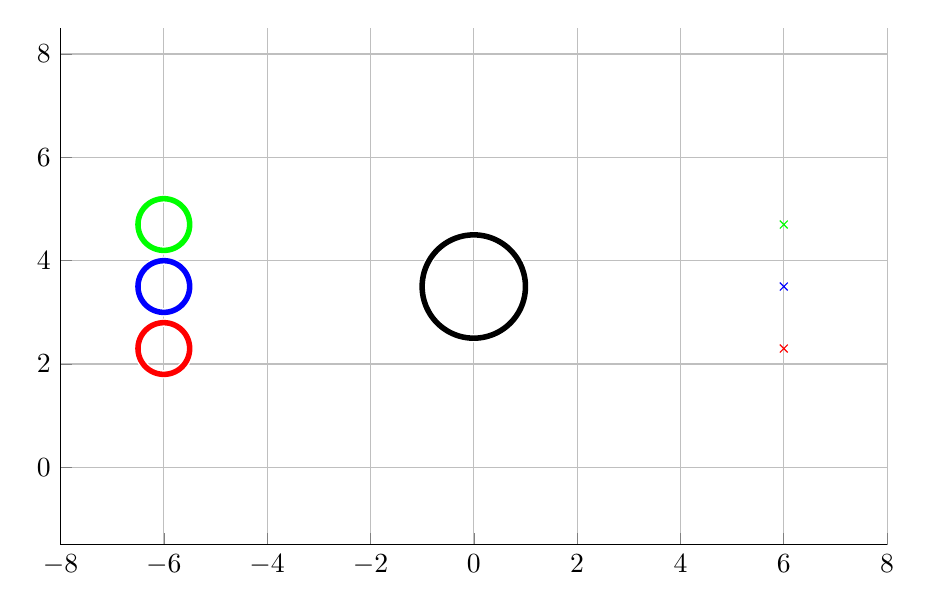
\begin{tikzpicture}

\begin{axis}[%
width=4.133in,
height=2.583in,
at={(0.693in,0.778in)},
scale only axis,
unbounded coords=jump,
xmin=-8,
xmax=8,
xmajorgrids,
ymin=-1.5,
ymax=8.5,
ymajorgrids,
axis background/.style={fill=white},
axis x line*=bottom,
axis y line*=left
]
\addplot [color=blue,only marks,mark=x,mark options={solid},forget plot]
  table[row sep=crcr]{%
6	3.5\\
};
\addplot [color=red,only marks,mark=x,mark options={solid},forget plot]
  table[row sep=crcr]{%
6	2.3\\
};
\addplot [color=green,only marks,mark=x,mark options={solid},forget plot]
  table[row sep=crcr]{%
6	4.7\\
};
\addplot [color=white,solid,line width=3.0pt,forget plot]
  table[row sep=crcr]{%
-5.5	3.5\\
-5.50030458649045	3.51744974835125\\
-5.50121797487009	3.53487823687206\\
-5.50273905231586	3.55226423163383\\
-5.50486596562921	3.56958655048003\\
-5.5075961234939	3.58682408883347\\
-5.5109261996331	3.60395584540888\\
-5.514852136862	3.62096094779983\\
-5.51936915203084	3.6378186779085\\
-5.52447174185242	3.65450849718747\\
-5.53015368960705	3.67101007166283\\
-5.53640807271661	3.68730329670796\\
-5.5432272711787	3.7033683215379\\
-5.55060297685042	3.71918557339454\\
-5.55852620357054	3.73473578139295\\
-5.56698729810778	3.75\\
-5.57597595192179	3.7649596321166\\
-5.58548121372248	3.77959645173537\\
-5.59549150281253	3.79389262614624\\
-5.60599462319664	3.80783073766283\\
-5.61697777844051	3.82139380484327\\
-5.6284275872613	3.83456530317943\\
-5.64033009983067	3.8473291852295\\
-5.6526708147705	3.85966990016933\\
-5.66543469682057	3.8715724127387\\
-5.67860619515673	3.88302222155949\\
-5.69216926233717	3.89400537680336\\
-5.70610737385376	3.90450849718747\\
-5.72040354826463	3.91451878627752\\
-5.7350403678834	3.92402404807821\\
-5.75	3.93301270189222\\
-5.76526421860705	3.94147379642946\\
-5.78081442660546	3.94939702314958\\
-5.7966316784621	3.9567727288213\\
-5.81269670329204	3.96359192728339\\
-5.82898992833717	3.96984631039295\\
-5.84549150281253	3.97552825814758\\
-5.8621813220915	3.98063084796916\\
-5.87903905220017	3.985147863138\\
-5.89604415459112	3.9890738003669\\
-5.91317591116653	3.9924038765061\\
-5.93041344951997	3.99513403437079\\
-5.94773576836617	3.99726094768414\\
-5.96512176312794	3.99878202512991\\
-5.98255025164875	3.99969541350955\\
-6	4\\
-6.01744974835125	3.99969541350955\\
-6.03487823687206	3.99878202512991\\
-6.05226423163383	3.99726094768414\\
-6.06958655048003	3.99513403437079\\
-6.08682408883347	3.9924038765061\\
-6.10395584540888	3.9890738003669\\
-6.12096094779983	3.985147863138\\
-6.1378186779085	3.98063084796916\\
-6.15450849718747	3.97552825814758\\
-6.17101007166283	3.96984631039295\\
-6.18730329670796	3.96359192728339\\
-6.2033683215379	3.9567727288213\\
-6.21918557339454	3.94939702314958\\
-6.23473578139295	3.94147379642946\\
-6.25	3.93301270189222\\
-6.2649596321166	3.92402404807821\\
-6.27959645173537	3.91451878627752\\
-6.29389262614624	3.90450849718747\\
-6.30783073766283	3.89400537680336\\
-6.32139380484327	3.88302222155949\\
-6.33456530317943	3.8715724127387\\
-6.3473291852295	3.85966990016933\\
-6.35966990016933	3.8473291852295\\
-6.3715724127387	3.83456530317943\\
-6.38302222155949	3.82139380484327\\
-6.39400537680336	3.80783073766283\\
-6.40450849718747	3.79389262614624\\
-6.41451878627752	3.77959645173537\\
-6.42402404807821	3.7649596321166\\
-6.43301270189222	3.75\\
-6.44147379642946	3.73473578139295\\
-6.44939702314958	3.71918557339454\\
-6.4567727288213	3.7033683215379\\
-6.46359192728339	3.68730329670796\\
-6.46984631039295	3.67101007166283\\
-6.47552825814758	3.65450849718747\\
-6.48063084796916	3.6378186779085\\
-6.485147863138	3.62096094779983\\
-6.4890738003669	3.60395584540888\\
-6.4924038765061	3.58682408883347\\
-6.49513403437079	3.56958655048003\\
-6.49726094768414	3.55226423163383\\
-6.49878202512991	3.53487823687206\\
-6.49969541350955	3.51744974835125\\
-6.5	3.5\\
-6.49969541350955	3.48255025164875\\
-6.49878202512991	3.46512176312794\\
-6.49726094768414	3.44773576836617\\
-6.49513403437079	3.43041344951997\\
-6.4924038765061	3.41317591116653\\
-6.4890738003669	3.39604415459112\\
-6.485147863138	3.37903905220017\\
-6.48063084796916	3.3621813220915\\
-6.47552825814758	3.34549150281253\\
-6.46984631039295	3.32898992833717\\
-6.46359192728339	3.31269670329204\\
-6.4567727288213	3.2966316784621\\
-6.44939702314958	3.28081442660546\\
-6.44147379642946	3.26526421860705\\
-6.43301270189222	3.25\\
-6.42402404807821	3.2350403678834\\
-6.41451878627752	3.22040354826463\\
-6.40450849718747	3.20610737385376\\
-6.39400537680336	3.19216926233717\\
-6.38302222155949	3.17860619515673\\
-6.3715724127387	3.16543469682057\\
-6.35966990016933	3.1526708147705\\
-6.3473291852295	3.14033009983067\\
-6.33456530317943	3.1284275872613\\
-6.32139380484327	3.11697777844051\\
-6.30783073766283	3.10599462319664\\
-6.29389262614624	3.09549150281253\\
-6.27959645173537	3.08548121372248\\
-6.2649596321166	3.07597595192179\\
-6.25	3.06698729810778\\
-6.23473578139295	3.05852620357054\\
-6.21918557339454	3.05060297685042\\
-6.2033683215379	3.0432272711787\\
-6.18730329670796	3.03640807271661\\
-6.17101007166283	3.03015368960705\\
-6.15450849718747	3.02447174185242\\
-6.1378186779085	3.01936915203084\\
-6.12096094779983	3.014852136862\\
-6.10395584540888	3.0109261996331\\
-6.08682408883347	3.0075961234939\\
-6.06958655048003	3.00486596562921\\
-6.05226423163383	3.00273905231586\\
-6.03487823687206	3.00121797487009\\
-6.01744974835125	3.00030458649045\\
-6	3\\
-5.98255025164875	3.00030458649045\\
-5.96512176312794	3.00121797487009\\
-5.94773576836617	3.00273905231586\\
-5.93041344951997	3.00486596562921\\
-5.91317591116653	3.0075961234939\\
-5.89604415459112	3.0109261996331\\
-5.87903905220017	3.014852136862\\
-5.8621813220915	3.01936915203084\\
-5.84549150281253	3.02447174185242\\
-5.82898992833717	3.03015368960705\\
-5.81269670329204	3.03640807271661\\
-5.7966316784621	3.0432272711787\\
-5.78081442660546	3.05060297685042\\
-5.76526421860705	3.05852620357054\\
-5.75	3.06698729810778\\
-5.7350403678834	3.07597595192179\\
-5.72040354826463	3.08548121372248\\
-5.70610737385376	3.09549150281253\\
-5.69216926233717	3.10599462319664\\
-5.67860619515673	3.11697777844051\\
-5.66543469682057	3.1284275872613\\
-5.6526708147705	3.14033009983067\\
-5.64033009983067	3.1526708147705\\
-5.6284275872613	3.16543469682057\\
-5.61697777844051	3.17860619515673\\
-5.60599462319664	3.19216926233717\\
-5.59549150281253	3.20610737385376\\
-5.58548121372248	3.22040354826463\\
-5.57597595192179	3.2350403678834\\
-5.56698729810778	3.25\\
-5.55852620357054	3.26526421860705\\
-5.55060297685042	3.28081442660546\\
-5.5432272711787	3.2966316784621\\
-5.53640807271661	3.31269670329204\\
-5.53015368960705	3.32898992833717\\
-5.52447174185242	3.34549150281253\\
-5.51936915203084	3.3621813220915\\
-5.514852136862	3.37903905220017\\
-5.5109261996331	3.39604415459112\\
-5.5075961234939	3.41317591116653\\
-5.50486596562921	3.43041344951997\\
-5.50273905231586	3.44773576836617\\
-5.50121797487009	3.46512176312794\\
-5.50030458649045	3.48255025164875\\
-5.5	3.5\\
nan	nan\\
};
\addplot [color=blue,solid,line width=2.0pt,forget plot]
  table[row sep=crcr]{%
-5.5	3.5\\
-5.50030458649045	3.51744974835125\\
-5.50121797487009	3.53487823687206\\
-5.50273905231586	3.55226423163383\\
-5.50486596562921	3.56958655048003\\
-5.5075961234939	3.58682408883347\\
-5.5109261996331	3.60395584540888\\
-5.514852136862	3.62096094779983\\
-5.51936915203084	3.6378186779085\\
-5.52447174185242	3.65450849718747\\
-5.53015368960705	3.67101007166283\\
-5.53640807271661	3.68730329670796\\
-5.5432272711787	3.7033683215379\\
-5.55060297685042	3.71918557339454\\
-5.55852620357054	3.73473578139295\\
-5.56698729810778	3.75\\
-5.57597595192179	3.7649596321166\\
-5.58548121372248	3.77959645173537\\
-5.59549150281253	3.79389262614624\\
-5.60599462319664	3.80783073766283\\
-5.61697777844051	3.82139380484327\\
-5.6284275872613	3.83456530317943\\
-5.64033009983067	3.8473291852295\\
-5.6526708147705	3.85966990016933\\
-5.66543469682057	3.8715724127387\\
-5.67860619515673	3.88302222155949\\
-5.69216926233717	3.89400537680336\\
-5.70610737385376	3.90450849718747\\
-5.72040354826463	3.91451878627752\\
-5.7350403678834	3.92402404807821\\
-5.75	3.93301270189222\\
-5.76526421860705	3.94147379642946\\
-5.78081442660546	3.94939702314958\\
-5.7966316784621	3.9567727288213\\
-5.81269670329204	3.96359192728339\\
-5.82898992833717	3.96984631039295\\
-5.84549150281253	3.97552825814758\\
-5.8621813220915	3.98063084796916\\
-5.87903905220017	3.985147863138\\
-5.89604415459112	3.9890738003669\\
-5.91317591116653	3.9924038765061\\
-5.93041344951997	3.99513403437079\\
-5.94773576836617	3.99726094768414\\
-5.96512176312794	3.99878202512991\\
-5.98255025164875	3.99969541350955\\
-6	4\\
-6.01744974835125	3.99969541350955\\
-6.03487823687206	3.99878202512991\\
-6.05226423163383	3.99726094768414\\
-6.06958655048003	3.99513403437079\\
-6.08682408883347	3.9924038765061\\
-6.10395584540888	3.9890738003669\\
-6.12096094779983	3.985147863138\\
-6.1378186779085	3.98063084796916\\
-6.15450849718747	3.97552825814758\\
-6.17101007166283	3.96984631039295\\
-6.18730329670796	3.96359192728339\\
-6.2033683215379	3.9567727288213\\
-6.21918557339454	3.94939702314958\\
-6.23473578139295	3.94147379642946\\
-6.25	3.93301270189222\\
-6.2649596321166	3.92402404807821\\
-6.27959645173537	3.91451878627752\\
-6.29389262614624	3.90450849718747\\
-6.30783073766283	3.89400537680336\\
-6.32139380484327	3.88302222155949\\
-6.33456530317943	3.8715724127387\\
-6.3473291852295	3.85966990016933\\
-6.35966990016933	3.8473291852295\\
-6.3715724127387	3.83456530317943\\
-6.38302222155949	3.82139380484327\\
-6.39400537680336	3.80783073766283\\
-6.40450849718747	3.79389262614624\\
-6.41451878627752	3.77959645173537\\
-6.42402404807821	3.7649596321166\\
-6.43301270189222	3.75\\
-6.44147379642946	3.73473578139295\\
-6.44939702314958	3.71918557339454\\
-6.4567727288213	3.7033683215379\\
-6.46359192728339	3.68730329670796\\
-6.46984631039295	3.67101007166283\\
-6.47552825814758	3.65450849718747\\
-6.48063084796916	3.6378186779085\\
-6.485147863138	3.62096094779983\\
-6.4890738003669	3.60395584540888\\
-6.4924038765061	3.58682408883347\\
-6.49513403437079	3.56958655048003\\
-6.49726094768414	3.55226423163383\\
-6.49878202512991	3.53487823687206\\
-6.49969541350955	3.51744974835125\\
-6.5	3.5\\
-6.49969541350955	3.48255025164875\\
-6.49878202512991	3.46512176312794\\
-6.49726094768414	3.44773576836617\\
-6.49513403437079	3.43041344951997\\
-6.4924038765061	3.41317591116653\\
-6.4890738003669	3.39604415459112\\
-6.485147863138	3.37903905220017\\
-6.48063084796916	3.3621813220915\\
-6.47552825814758	3.34549150281253\\
-6.46984631039295	3.32898992833717\\
-6.46359192728339	3.31269670329204\\
-6.4567727288213	3.2966316784621\\
-6.44939702314958	3.28081442660546\\
-6.44147379642946	3.26526421860705\\
-6.43301270189222	3.25\\
-6.42402404807821	3.2350403678834\\
-6.41451878627752	3.22040354826463\\
-6.40450849718747	3.20610737385376\\
-6.39400537680336	3.19216926233717\\
-6.38302222155949	3.17860619515673\\
-6.3715724127387	3.16543469682057\\
-6.35966990016933	3.1526708147705\\
-6.3473291852295	3.14033009983067\\
-6.33456530317943	3.1284275872613\\
-6.32139380484327	3.11697777844051\\
-6.30783073766283	3.10599462319664\\
-6.29389262614624	3.09549150281253\\
-6.27959645173537	3.08548121372248\\
-6.2649596321166	3.07597595192179\\
-6.25	3.06698729810778\\
-6.23473578139295	3.05852620357054\\
-6.21918557339454	3.05060297685042\\
-6.2033683215379	3.0432272711787\\
-6.18730329670796	3.03640807271661\\
-6.17101007166283	3.03015368960705\\
-6.15450849718747	3.02447174185242\\
-6.1378186779085	3.01936915203084\\
-6.12096094779983	3.014852136862\\
-6.10395584540888	3.0109261996331\\
-6.08682408883347	3.0075961234939\\
-6.06958655048003	3.00486596562921\\
-6.05226423163383	3.00273905231586\\
-6.03487823687206	3.00121797487009\\
-6.01744974835125	3.00030458649045\\
-6	3\\
-5.98255025164875	3.00030458649045\\
-5.96512176312794	3.00121797487009\\
-5.94773576836617	3.00273905231586\\
-5.93041344951997	3.00486596562921\\
-5.91317591116653	3.0075961234939\\
-5.89604415459112	3.0109261996331\\
-5.87903905220017	3.014852136862\\
-5.8621813220915	3.01936915203084\\
-5.84549150281253	3.02447174185242\\
-5.82898992833717	3.03015368960705\\
-5.81269670329204	3.03640807271661\\
-5.7966316784621	3.0432272711787\\
-5.78081442660546	3.05060297685042\\
-5.76526421860705	3.05852620357054\\
-5.75	3.06698729810778\\
-5.7350403678834	3.07597595192179\\
-5.72040354826463	3.08548121372248\\
-5.70610737385376	3.09549150281253\\
-5.69216926233717	3.10599462319664\\
-5.67860619515673	3.11697777844051\\
-5.66543469682057	3.1284275872613\\
-5.6526708147705	3.14033009983067\\
-5.64033009983067	3.1526708147705\\
-5.6284275872613	3.16543469682057\\
-5.61697777844051	3.17860619515673\\
-5.60599462319664	3.19216926233717\\
-5.59549150281253	3.20610737385376\\
-5.58548121372248	3.22040354826463\\
-5.57597595192179	3.2350403678834\\
-5.56698729810778	3.25\\
-5.55852620357054	3.26526421860705\\
-5.55060297685042	3.28081442660546\\
-5.5432272711787	3.2966316784621\\
-5.53640807271661	3.31269670329204\\
-5.53015368960705	3.32898992833717\\
-5.52447174185242	3.34549150281253\\
-5.51936915203084	3.3621813220915\\
-5.514852136862	3.37903905220017\\
-5.5109261996331	3.39604415459112\\
-5.5075961234939	3.41317591116653\\
-5.50486596562921	3.43041344951997\\
-5.50273905231586	3.44773576836617\\
-5.50121797487009	3.46512176312794\\
-5.50030458649045	3.48255025164875\\
-5.5	3.5\\
nan	nan\\
};
\addplot [color=white,solid,line width=3.0pt,forget plot]
  table[row sep=crcr]{%
-5.5	2.3\\
-5.50030458649045	2.31744974835125\\
-5.50121797487009	2.33487823687206\\
-5.50273905231586	2.35226423163383\\
-5.50486596562921	2.36958655048003\\
-5.5075961234939	2.38682408883346\\
-5.5109261996331	2.40395584540888\\
-5.514852136862	2.42096094779983\\
-5.51936915203084	2.4378186779085\\
-5.52447174185242	2.45450849718747\\
-5.53015368960705	2.47101007166283\\
-5.53640807271661	2.48730329670796\\
-5.5432272711787	2.5033683215379\\
-5.55060297685042	2.51918557339454\\
-5.55852620357054	2.53473578139295\\
-5.56698729810778	2.55\\
-5.57597595192179	2.5649596321166\\
-5.58548121372248	2.57959645173537\\
-5.59549150281253	2.59389262614624\\
-5.60599462319664	2.60783073766283\\
-5.61697777844051	2.62139380484327\\
-5.6284275872613	2.63456530317943\\
-5.64033009983067	2.6473291852295\\
-5.6526708147705	2.65966990016933\\
-5.66543469682057	2.6715724127387\\
-5.67860619515673	2.68302222155949\\
-5.69216926233717	2.69400537680336\\
-5.70610737385376	2.70450849718747\\
-5.72040354826463	2.71451878627752\\
-5.7350403678834	2.72402404807821\\
-5.75	2.73301270189222\\
-5.76526421860705	2.74147379642946\\
-5.78081442660546	2.74939702314958\\
-5.7966316784621	2.7567727288213\\
-5.81269670329204	2.76359192728339\\
-5.82898992833717	2.76984631039295\\
-5.84549150281253	2.77552825814758\\
-5.8621813220915	2.78063084796916\\
-5.87903905220017	2.785147863138\\
-5.89604415459112	2.7890738003669\\
-5.91317591116653	2.7924038765061\\
-5.93041344951997	2.79513403437078\\
-5.94773576836617	2.79726094768414\\
-5.96512176312794	2.79878202512991\\
-5.98255025164875	2.79969541350955\\
-6	2.8\\
-6.01744974835125	2.79969541350955\\
-6.03487823687206	2.79878202512991\\
-6.05226423163383	2.79726094768414\\
-6.06958655048003	2.79513403437078\\
-6.08682408883347	2.7924038765061\\
-6.10395584540888	2.7890738003669\\
-6.12096094779983	2.785147863138\\
-6.1378186779085	2.78063084796916\\
-6.15450849718747	2.77552825814758\\
-6.17101007166283	2.76984631039295\\
-6.18730329670796	2.76359192728339\\
-6.2033683215379	2.7567727288213\\
-6.21918557339454	2.74939702314958\\
-6.23473578139295	2.74147379642946\\
-6.25	2.73301270189222\\
-6.2649596321166	2.72402404807821\\
-6.27959645173537	2.71451878627752\\
-6.29389262614624	2.70450849718747\\
-6.30783073766283	2.69400537680336\\
-6.32139380484327	2.68302222155949\\
-6.33456530317943	2.6715724127387\\
-6.3473291852295	2.65966990016933\\
-6.35966990016933	2.6473291852295\\
-6.3715724127387	2.63456530317943\\
-6.38302222155949	2.62139380484327\\
-6.39400537680336	2.60783073766283\\
-6.40450849718747	2.59389262614624\\
-6.41451878627752	2.57959645173537\\
-6.42402404807821	2.5649596321166\\
-6.43301270189222	2.55\\
-6.44147379642946	2.53473578139295\\
-6.44939702314958	2.51918557339454\\
-6.4567727288213	2.5033683215379\\
-6.46359192728339	2.48730329670796\\
-6.46984631039295	2.47101007166283\\
-6.47552825814758	2.45450849718747\\
-6.48063084796916	2.4378186779085\\
-6.485147863138	2.42096094779983\\
-6.4890738003669	2.40395584540888\\
-6.4924038765061	2.38682408883346\\
-6.49513403437079	2.36958655048003\\
-6.49726094768414	2.35226423163383\\
-6.49878202512991	2.33487823687206\\
-6.49969541350955	2.31744974835125\\
-6.5	2.3\\
-6.49969541350955	2.28255025164875\\
-6.49878202512991	2.26512176312794\\
-6.49726094768414	2.24773576836617\\
-6.49513403437079	2.23041344951997\\
-6.4924038765061	2.21317591116653\\
-6.4890738003669	2.19604415459112\\
-6.485147863138	2.17903905220017\\
-6.48063084796916	2.1621813220915\\
-6.47552825814758	2.14549150281253\\
-6.46984631039295	2.12898992833717\\
-6.46359192728339	2.11269670329204\\
-6.4567727288213	2.0966316784621\\
-6.44939702314958	2.08081442660546\\
-6.44147379642946	2.06526421860705\\
-6.43301270189222	2.05\\
-6.42402404807821	2.0350403678834\\
-6.41451878627752	2.02040354826463\\
-6.40450849718747	2.00610737385376\\
-6.39400537680336	1.99216926233717\\
-6.38302222155949	1.97860619515673\\
-6.3715724127387	1.96543469682057\\
-6.35966990016933	1.9526708147705\\
-6.3473291852295	1.94033009983067\\
-6.33456530317943	1.9284275872613\\
-6.32139380484327	1.91697777844051\\
-6.30783073766283	1.90599462319664\\
-6.29389262614624	1.89549150281253\\
-6.27959645173537	1.88548121372248\\
-6.2649596321166	1.87597595192179\\
-6.25	1.86698729810778\\
-6.23473578139295	1.85852620357054\\
-6.21918557339454	1.85060297685042\\
-6.2033683215379	1.8432272711787\\
-6.18730329670796	1.83640807271661\\
-6.17101007166283	1.83015368960705\\
-6.15450849718747	1.82447174185242\\
-6.1378186779085	1.81936915203084\\
-6.12096094779983	1.814852136862\\
-6.10395584540888	1.8109261996331\\
-6.08682408883347	1.8075961234939\\
-6.06958655048003	1.80486596562921\\
-6.05226423163383	1.80273905231586\\
-6.03487823687206	1.80121797487009\\
-6.01744974835125	1.80030458649045\\
-6	1.8\\
-5.98255025164875	1.80030458649045\\
-5.96512176312794	1.80121797487009\\
-5.94773576836617	1.80273905231586\\
-5.93041344951997	1.80486596562921\\
-5.91317591116653	1.8075961234939\\
-5.89604415459112	1.8109261996331\\
-5.87903905220017	1.814852136862\\
-5.8621813220915	1.81936915203084\\
-5.84549150281253	1.82447174185242\\
-5.82898992833717	1.83015368960705\\
-5.81269670329204	1.83640807271661\\
-5.7966316784621	1.8432272711787\\
-5.78081442660546	1.85060297685042\\
-5.76526421860705	1.85852620357054\\
-5.75	1.86698729810778\\
-5.7350403678834	1.87597595192179\\
-5.72040354826463	1.88548121372248\\
-5.70610737385376	1.89549150281253\\
-5.69216926233717	1.90599462319664\\
-5.67860619515673	1.91697777844051\\
-5.66543469682057	1.9284275872613\\
-5.6526708147705	1.94033009983067\\
-5.64033009983067	1.9526708147705\\
-5.6284275872613	1.96543469682057\\
-5.61697777844051	1.97860619515673\\
-5.60599462319664	1.99216926233717\\
-5.59549150281253	2.00610737385376\\
-5.58548121372248	2.02040354826463\\
-5.57597595192179	2.0350403678834\\
-5.56698729810778	2.05\\
-5.55852620357054	2.06526421860705\\
-5.55060297685042	2.08081442660546\\
-5.5432272711787	2.0966316784621\\
-5.53640807271661	2.11269670329204\\
-5.53015368960705	2.12898992833717\\
-5.52447174185242	2.14549150281253\\
-5.51936915203084	2.1621813220915\\
-5.514852136862	2.17903905220017\\
-5.5109261996331	2.19604415459112\\
-5.5075961234939	2.21317591116653\\
-5.50486596562921	2.23041344951997\\
-5.50273905231586	2.24773576836617\\
-5.50121797487009	2.26512176312794\\
-5.50030458649045	2.28255025164875\\
-5.5	2.3\\
nan	nan\\
};
\addplot [color=red,solid,line width=2.0pt,forget plot]
  table[row sep=crcr]{%
-5.5	2.3\\
-5.50030458649045	2.31744974835125\\
-5.50121797487009	2.33487823687206\\
-5.50273905231586	2.35226423163383\\
-5.50486596562921	2.36958655048003\\
-5.5075961234939	2.38682408883346\\
-5.5109261996331	2.40395584540888\\
-5.514852136862	2.42096094779983\\
-5.51936915203084	2.4378186779085\\
-5.52447174185242	2.45450849718747\\
-5.53015368960705	2.47101007166283\\
-5.53640807271661	2.48730329670796\\
-5.5432272711787	2.5033683215379\\
-5.55060297685042	2.51918557339454\\
-5.55852620357054	2.53473578139295\\
-5.56698729810778	2.55\\
-5.57597595192179	2.5649596321166\\
-5.58548121372248	2.57959645173537\\
-5.59549150281253	2.59389262614624\\
-5.60599462319664	2.60783073766283\\
-5.61697777844051	2.62139380484327\\
-5.6284275872613	2.63456530317943\\
-5.64033009983067	2.6473291852295\\
-5.6526708147705	2.65966990016933\\
-5.66543469682057	2.6715724127387\\
-5.67860619515673	2.68302222155949\\
-5.69216926233717	2.69400537680336\\
-5.70610737385376	2.70450849718747\\
-5.72040354826463	2.71451878627752\\
-5.7350403678834	2.72402404807821\\
-5.75	2.73301270189222\\
-5.76526421860705	2.74147379642946\\
-5.78081442660546	2.74939702314958\\
-5.7966316784621	2.7567727288213\\
-5.81269670329204	2.76359192728339\\
-5.82898992833717	2.76984631039295\\
-5.84549150281253	2.77552825814758\\
-5.8621813220915	2.78063084796916\\
-5.87903905220017	2.785147863138\\
-5.89604415459112	2.7890738003669\\
-5.91317591116653	2.7924038765061\\
-5.93041344951997	2.79513403437078\\
-5.94773576836617	2.79726094768414\\
-5.96512176312794	2.79878202512991\\
-5.98255025164875	2.79969541350955\\
-6	2.8\\
-6.01744974835125	2.79969541350955\\
-6.03487823687206	2.79878202512991\\
-6.05226423163383	2.79726094768414\\
-6.06958655048003	2.79513403437078\\
-6.08682408883347	2.7924038765061\\
-6.10395584540888	2.7890738003669\\
-6.12096094779983	2.785147863138\\
-6.1378186779085	2.78063084796916\\
-6.15450849718747	2.77552825814758\\
-6.17101007166283	2.76984631039295\\
-6.18730329670796	2.76359192728339\\
-6.2033683215379	2.7567727288213\\
-6.21918557339454	2.74939702314958\\
-6.23473578139295	2.74147379642946\\
-6.25	2.73301270189222\\
-6.2649596321166	2.72402404807821\\
-6.27959645173537	2.71451878627752\\
-6.29389262614624	2.70450849718747\\
-6.30783073766283	2.69400537680336\\
-6.32139380484327	2.68302222155949\\
-6.33456530317943	2.6715724127387\\
-6.3473291852295	2.65966990016933\\
-6.35966990016933	2.6473291852295\\
-6.3715724127387	2.63456530317943\\
-6.38302222155949	2.62139380484327\\
-6.39400537680336	2.60783073766283\\
-6.40450849718747	2.59389262614624\\
-6.41451878627752	2.57959645173537\\
-6.42402404807821	2.5649596321166\\
-6.43301270189222	2.55\\
-6.44147379642946	2.53473578139295\\
-6.44939702314958	2.51918557339454\\
-6.4567727288213	2.5033683215379\\
-6.46359192728339	2.48730329670796\\
-6.46984631039295	2.47101007166283\\
-6.47552825814758	2.45450849718747\\
-6.48063084796916	2.4378186779085\\
-6.485147863138	2.42096094779983\\
-6.4890738003669	2.40395584540888\\
-6.4924038765061	2.38682408883346\\
-6.49513403437079	2.36958655048003\\
-6.49726094768414	2.35226423163383\\
-6.49878202512991	2.33487823687206\\
-6.49969541350955	2.31744974835125\\
-6.5	2.3\\
-6.49969541350955	2.28255025164875\\
-6.49878202512991	2.26512176312794\\
-6.49726094768414	2.24773576836617\\
-6.49513403437079	2.23041344951997\\
-6.4924038765061	2.21317591116653\\
-6.4890738003669	2.19604415459112\\
-6.485147863138	2.17903905220017\\
-6.48063084796916	2.1621813220915\\
-6.47552825814758	2.14549150281253\\
-6.46984631039295	2.12898992833717\\
-6.46359192728339	2.11269670329204\\
-6.4567727288213	2.0966316784621\\
-6.44939702314958	2.08081442660546\\
-6.44147379642946	2.06526421860705\\
-6.43301270189222	2.05\\
-6.42402404807821	2.0350403678834\\
-6.41451878627752	2.02040354826463\\
-6.40450849718747	2.00610737385376\\
-6.39400537680336	1.99216926233717\\
-6.38302222155949	1.97860619515673\\
-6.3715724127387	1.96543469682057\\
-6.35966990016933	1.9526708147705\\
-6.3473291852295	1.94033009983067\\
-6.33456530317943	1.9284275872613\\
-6.32139380484327	1.91697777844051\\
-6.30783073766283	1.90599462319664\\
-6.29389262614624	1.89549150281253\\
-6.27959645173537	1.88548121372248\\
-6.2649596321166	1.87597595192179\\
-6.25	1.86698729810778\\
-6.23473578139295	1.85852620357054\\
-6.21918557339454	1.85060297685042\\
-6.2033683215379	1.8432272711787\\
-6.18730329670796	1.83640807271661\\
-6.17101007166283	1.83015368960705\\
-6.15450849718747	1.82447174185242\\
-6.1378186779085	1.81936915203084\\
-6.12096094779983	1.814852136862\\
-6.10395584540888	1.8109261996331\\
-6.08682408883347	1.8075961234939\\
-6.06958655048003	1.80486596562921\\
-6.05226423163383	1.80273905231586\\
-6.03487823687206	1.80121797487009\\
-6.01744974835125	1.80030458649045\\
-6	1.8\\
-5.98255025164875	1.80030458649045\\
-5.96512176312794	1.80121797487009\\
-5.94773576836617	1.80273905231586\\
-5.93041344951997	1.80486596562921\\
-5.91317591116653	1.8075961234939\\
-5.89604415459112	1.8109261996331\\
-5.87903905220017	1.814852136862\\
-5.8621813220915	1.81936915203084\\
-5.84549150281253	1.82447174185242\\
-5.82898992833717	1.83015368960705\\
-5.81269670329204	1.83640807271661\\
-5.7966316784621	1.8432272711787\\
-5.78081442660546	1.85060297685042\\
-5.76526421860705	1.85852620357054\\
-5.75	1.86698729810778\\
-5.7350403678834	1.87597595192179\\
-5.72040354826463	1.88548121372248\\
-5.70610737385376	1.89549150281253\\
-5.69216926233717	1.90599462319664\\
-5.67860619515673	1.91697777844051\\
-5.66543469682057	1.9284275872613\\
-5.6526708147705	1.94033009983067\\
-5.64033009983067	1.9526708147705\\
-5.6284275872613	1.96543469682057\\
-5.61697777844051	1.97860619515673\\
-5.60599462319664	1.99216926233717\\
-5.59549150281253	2.00610737385376\\
-5.58548121372248	2.02040354826463\\
-5.57597595192179	2.0350403678834\\
-5.56698729810778	2.05\\
-5.55852620357054	2.06526421860705\\
-5.55060297685042	2.08081442660546\\
-5.5432272711787	2.0966316784621\\
-5.53640807271661	2.11269670329204\\
-5.53015368960705	2.12898992833717\\
-5.52447174185242	2.14549150281253\\
-5.51936915203084	2.1621813220915\\
-5.514852136862	2.17903905220017\\
-5.5109261996331	2.19604415459112\\
-5.5075961234939	2.21317591116653\\
-5.50486596562921	2.23041344951997\\
-5.50273905231586	2.24773576836617\\
-5.50121797487009	2.26512176312794\\
-5.50030458649045	2.28255025164875\\
-5.5	2.3\\
nan	nan\\
};
\addplot [color=white,solid,line width=3.0pt,forget plot]
  table[row sep=crcr]{%
-5.5	4.7\\
-5.50030458649045	4.71744974835125\\
-5.50121797487009	4.73487823687206\\
-5.50273905231586	4.75226423163383\\
-5.50486596562921	4.76958655048003\\
-5.5075961234939	4.78682408883347\\
-5.5109261996331	4.80395584540888\\
-5.514852136862	4.82096094779983\\
-5.51936915203084	4.8378186779085\\
-5.52447174185242	4.85450849718747\\
-5.53015368960705	4.87101007166283\\
-5.53640807271661	4.88730329670796\\
-5.5432272711787	4.9033683215379\\
-5.55060297685042	4.91918557339454\\
-5.55852620357054	4.93473578139295\\
-5.56698729810778	4.95\\
-5.57597595192179	4.9649596321166\\
-5.58548121372248	4.97959645173537\\
-5.59549150281253	4.99389262614624\\
-5.60599462319664	5.00783073766283\\
-5.61697777844051	5.02139380484327\\
-5.6284275872613	5.03456530317943\\
-5.64033009983067	5.0473291852295\\
-5.6526708147705	5.05966990016933\\
-5.66543469682057	5.0715724127387\\
-5.67860619515673	5.08302222155949\\
-5.69216926233717	5.09400537680336\\
-5.70610737385376	5.10450849718747\\
-5.72040354826463	5.11451878627752\\
-5.7350403678834	5.12402404807821\\
-5.75	5.13301270189222\\
-5.76526421860705	5.14147379642946\\
-5.78081442660546	5.14939702314958\\
-5.7966316784621	5.1567727288213\\
-5.81269670329204	5.16359192728339\\
-5.82898992833717	5.16984631039295\\
-5.84549150281253	5.17552825814758\\
-5.8621813220915	5.18063084796916\\
-5.87903905220017	5.185147863138\\
-5.89604415459112	5.1890738003669\\
-5.91317591116653	5.1924038765061\\
-5.93041344951997	5.19513403437079\\
-5.94773576836617	5.19726094768414\\
-5.96512176312794	5.19878202512991\\
-5.98255025164875	5.19969541350955\\
-6	5.2\\
-6.01744974835125	5.19969541350955\\
-6.03487823687206	5.19878202512991\\
-6.05226423163383	5.19726094768414\\
-6.06958655048003	5.19513403437079\\
-6.08682408883347	5.1924038765061\\
-6.10395584540888	5.1890738003669\\
-6.12096094779983	5.185147863138\\
-6.1378186779085	5.18063084796916\\
-6.15450849718747	5.17552825814758\\
-6.17101007166283	5.16984631039295\\
-6.18730329670796	5.16359192728339\\
-6.2033683215379	5.1567727288213\\
-6.21918557339454	5.14939702314958\\
-6.23473578139295	5.14147379642946\\
-6.25	5.13301270189222\\
-6.2649596321166	5.12402404807821\\
-6.27959645173537	5.11451878627752\\
-6.29389262614624	5.10450849718747\\
-6.30783073766283	5.09400537680336\\
-6.32139380484327	5.08302222155949\\
-6.33456530317943	5.0715724127387\\
-6.3473291852295	5.05966990016933\\
-6.35966990016933	5.0473291852295\\
-6.3715724127387	5.03456530317943\\
-6.38302222155949	5.02139380484327\\
-6.39400537680336	5.00783073766283\\
-6.40450849718747	4.99389262614624\\
-6.41451878627752	4.97959645173537\\
-6.42402404807821	4.9649596321166\\
-6.43301270189222	4.95\\
-6.44147379642946	4.93473578139295\\
-6.44939702314958	4.91918557339454\\
-6.4567727288213	4.9033683215379\\
-6.46359192728339	4.88730329670796\\
-6.46984631039295	4.87101007166283\\
-6.47552825814758	4.85450849718747\\
-6.48063084796916	4.8378186779085\\
-6.485147863138	4.82096094779983\\
-6.4890738003669	4.80395584540888\\
-6.4924038765061	4.78682408883347\\
-6.49513403437079	4.76958655048003\\
-6.49726094768414	4.75226423163383\\
-6.49878202512991	4.73487823687206\\
-6.49969541350955	4.71744974835125\\
-6.5	4.7\\
-6.49969541350955	4.68255025164875\\
-6.49878202512991	4.66512176312794\\
-6.49726094768414	4.64773576836617\\
-6.49513403437079	4.63041344951997\\
-6.4924038765061	4.61317591116654\\
-6.4890738003669	4.59604415459112\\
-6.485147863138	4.57903905220017\\
-6.48063084796916	4.5621813220915\\
-6.47552825814758	4.54549150281253\\
-6.46984631039295	4.52898992833717\\
-6.46359192728339	4.51269670329204\\
-6.4567727288213	4.4966316784621\\
-6.44939702314958	4.48081442660546\\
-6.44147379642946	4.46526421860705\\
-6.43301270189222	4.45\\
-6.42402404807821	4.4350403678834\\
-6.41451878627752	4.42040354826463\\
-6.40450849718747	4.40610737385376\\
-6.39400537680336	4.39216926233717\\
-6.38302222155949	4.37860619515673\\
-6.3715724127387	4.36543469682057\\
-6.35966990016933	4.3526708147705\\
-6.3473291852295	4.34033009983068\\
-6.33456530317943	4.3284275872613\\
-6.32139380484327	4.31697777844051\\
-6.30783073766283	4.30599462319664\\
-6.29389262614624	4.29549150281253\\
-6.27959645173537	4.28548121372248\\
-6.2649596321166	4.27597595192179\\
-6.25	4.26698729810778\\
-6.23473578139295	4.25852620357054\\
-6.21918557339454	4.25060297685042\\
-6.2033683215379	4.2432272711787\\
-6.18730329670796	4.23640807271661\\
-6.17101007166283	4.23015368960705\\
-6.15450849718747	4.22447174185242\\
-6.1378186779085	4.21936915203084\\
-6.12096094779983	4.214852136862\\
-6.10395584540888	4.2109261996331\\
-6.08682408883347	4.2075961234939\\
-6.06958655048003	4.20486596562921\\
-6.05226423163383	4.20273905231586\\
-6.03487823687206	4.20121797487009\\
-6.01744974835125	4.20030458649045\\
-6	4.2\\
-5.98255025164875	4.20030458649045\\
-5.96512176312794	4.20121797487009\\
-5.94773576836617	4.20273905231586\\
-5.93041344951997	4.20486596562921\\
-5.91317591116653	4.2075961234939\\
-5.89604415459112	4.2109261996331\\
-5.87903905220017	4.214852136862\\
-5.8621813220915	4.21936915203084\\
-5.84549150281253	4.22447174185242\\
-5.82898992833717	4.23015368960705\\
-5.81269670329204	4.23640807271661\\
-5.7966316784621	4.2432272711787\\
-5.78081442660546	4.25060297685042\\
-5.76526421860705	4.25852620357054\\
-5.75	4.26698729810778\\
-5.7350403678834	4.27597595192179\\
-5.72040354826463	4.28548121372248\\
-5.70610737385376	4.29549150281253\\
-5.69216926233717	4.30599462319664\\
-5.67860619515673	4.31697777844051\\
-5.66543469682057	4.3284275872613\\
-5.6526708147705	4.34033009983067\\
-5.64033009983067	4.3526708147705\\
-5.6284275872613	4.36543469682057\\
-5.61697777844051	4.37860619515673\\
-5.60599462319664	4.39216926233717\\
-5.59549150281253	4.40610737385376\\
-5.58548121372248	4.42040354826463\\
-5.57597595192179	4.4350403678834\\
-5.56698729810778	4.45\\
-5.55852620357054	4.46526421860705\\
-5.55060297685042	4.48081442660546\\
-5.5432272711787	4.4966316784621\\
-5.53640807271661	4.51269670329204\\
-5.53015368960705	4.52898992833717\\
-5.52447174185242	4.54549150281253\\
-5.51936915203084	4.5621813220915\\
-5.514852136862	4.57903905220017\\
-5.5109261996331	4.59604415459112\\
-5.5075961234939	4.61317591116653\\
-5.50486596562921	4.63041344951997\\
-5.50273905231586	4.64773576836617\\
-5.50121797487009	4.66512176312794\\
-5.50030458649045	4.68255025164875\\
-5.5	4.7\\
nan	nan\\
};
\addplot [color=green,solid,line width=2.0pt,forget plot]
  table[row sep=crcr]{%
-5.5	4.7\\
-5.50030458649045	4.71744974835125\\
-5.50121797487009	4.73487823687206\\
-5.50273905231586	4.75226423163383\\
-5.50486596562921	4.76958655048003\\
-5.5075961234939	4.78682408883347\\
-5.5109261996331	4.80395584540888\\
-5.514852136862	4.82096094779983\\
-5.51936915203084	4.8378186779085\\
-5.52447174185242	4.85450849718747\\
-5.53015368960705	4.87101007166283\\
-5.53640807271661	4.88730329670796\\
-5.5432272711787	4.9033683215379\\
-5.55060297685042	4.91918557339454\\
-5.55852620357054	4.93473578139295\\
-5.56698729810778	4.95\\
-5.57597595192179	4.9649596321166\\
-5.58548121372248	4.97959645173537\\
-5.59549150281253	4.99389262614624\\
-5.60599462319664	5.00783073766283\\
-5.61697777844051	5.02139380484327\\
-5.6284275872613	5.03456530317943\\
-5.64033009983067	5.0473291852295\\
-5.6526708147705	5.05966990016933\\
-5.66543469682057	5.0715724127387\\
-5.67860619515673	5.08302222155949\\
-5.69216926233717	5.09400537680336\\
-5.70610737385376	5.10450849718747\\
-5.72040354826463	5.11451878627752\\
-5.7350403678834	5.12402404807821\\
-5.75	5.13301270189222\\
-5.76526421860705	5.14147379642946\\
-5.78081442660546	5.14939702314958\\
-5.7966316784621	5.1567727288213\\
-5.81269670329204	5.16359192728339\\
-5.82898992833717	5.16984631039295\\
-5.84549150281253	5.17552825814758\\
-5.8621813220915	5.18063084796916\\
-5.87903905220017	5.185147863138\\
-5.89604415459112	5.1890738003669\\
-5.91317591116653	5.1924038765061\\
-5.93041344951997	5.19513403437079\\
-5.94773576836617	5.19726094768414\\
-5.96512176312794	5.19878202512991\\
-5.98255025164875	5.19969541350955\\
-6	5.2\\
-6.01744974835125	5.19969541350955\\
-6.03487823687206	5.19878202512991\\
-6.05226423163383	5.19726094768414\\
-6.06958655048003	5.19513403437079\\
-6.08682408883347	5.1924038765061\\
-6.10395584540888	5.1890738003669\\
-6.12096094779983	5.185147863138\\
-6.1378186779085	5.18063084796916\\
-6.15450849718747	5.17552825814758\\
-6.17101007166283	5.16984631039295\\
-6.18730329670796	5.16359192728339\\
-6.2033683215379	5.1567727288213\\
-6.21918557339454	5.14939702314958\\
-6.23473578139295	5.14147379642946\\
-6.25	5.13301270189222\\
-6.2649596321166	5.12402404807821\\
-6.27959645173537	5.11451878627752\\
-6.29389262614624	5.10450849718747\\
-6.30783073766283	5.09400537680336\\
-6.32139380484327	5.08302222155949\\
-6.33456530317943	5.0715724127387\\
-6.3473291852295	5.05966990016933\\
-6.35966990016933	5.0473291852295\\
-6.3715724127387	5.03456530317943\\
-6.38302222155949	5.02139380484327\\
-6.39400537680336	5.00783073766283\\
-6.40450849718747	4.99389262614624\\
-6.41451878627752	4.97959645173537\\
-6.42402404807821	4.9649596321166\\
-6.43301270189222	4.95\\
-6.44147379642946	4.93473578139295\\
-6.44939702314958	4.91918557339454\\
-6.4567727288213	4.9033683215379\\
-6.46359192728339	4.88730329670796\\
-6.46984631039295	4.87101007166283\\
-6.47552825814758	4.85450849718747\\
-6.48063084796916	4.8378186779085\\
-6.485147863138	4.82096094779983\\
-6.4890738003669	4.80395584540888\\
-6.4924038765061	4.78682408883347\\
-6.49513403437079	4.76958655048003\\
-6.49726094768414	4.75226423163383\\
-6.49878202512991	4.73487823687206\\
-6.49969541350955	4.71744974835125\\
-6.5	4.7\\
-6.49969541350955	4.68255025164875\\
-6.49878202512991	4.66512176312794\\
-6.49726094768414	4.64773576836617\\
-6.49513403437079	4.63041344951997\\
-6.4924038765061	4.61317591116654\\
-6.4890738003669	4.59604415459112\\
-6.485147863138	4.57903905220017\\
-6.48063084796916	4.5621813220915\\
-6.47552825814758	4.54549150281253\\
-6.46984631039295	4.52898992833717\\
-6.46359192728339	4.51269670329204\\
-6.4567727288213	4.4966316784621\\
-6.44939702314958	4.48081442660546\\
-6.44147379642946	4.46526421860705\\
-6.43301270189222	4.45\\
-6.42402404807821	4.4350403678834\\
-6.41451878627752	4.42040354826463\\
-6.40450849718747	4.40610737385376\\
-6.39400537680336	4.39216926233717\\
-6.38302222155949	4.37860619515673\\
-6.3715724127387	4.36543469682057\\
-6.35966990016933	4.3526708147705\\
-6.3473291852295	4.34033009983068\\
-6.33456530317943	4.3284275872613\\
-6.32139380484327	4.31697777844051\\
-6.30783073766283	4.30599462319664\\
-6.29389262614624	4.29549150281253\\
-6.27959645173537	4.28548121372248\\
-6.2649596321166	4.27597595192179\\
-6.25	4.26698729810778\\
-6.23473578139295	4.25852620357054\\
-6.21918557339454	4.25060297685042\\
-6.2033683215379	4.2432272711787\\
-6.18730329670796	4.23640807271661\\
-6.17101007166283	4.23015368960705\\
-6.15450849718747	4.22447174185242\\
-6.1378186779085	4.21936915203084\\
-6.12096094779983	4.214852136862\\
-6.10395584540888	4.2109261996331\\
-6.08682408883347	4.2075961234939\\
-6.06958655048003	4.20486596562921\\
-6.05226423163383	4.20273905231586\\
-6.03487823687206	4.20121797487009\\
-6.01744974835125	4.20030458649045\\
-6	4.2\\
-5.98255025164875	4.20030458649045\\
-5.96512176312794	4.20121797487009\\
-5.94773576836617	4.20273905231586\\
-5.93041344951997	4.20486596562921\\
-5.91317591116653	4.2075961234939\\
-5.89604415459112	4.2109261996331\\
-5.87903905220017	4.214852136862\\
-5.8621813220915	4.21936915203084\\
-5.84549150281253	4.22447174185242\\
-5.82898992833717	4.23015368960705\\
-5.81269670329204	4.23640807271661\\
-5.7966316784621	4.2432272711787\\
-5.78081442660546	4.25060297685042\\
-5.76526421860705	4.25852620357054\\
-5.75	4.26698729810778\\
-5.7350403678834	4.27597595192179\\
-5.72040354826463	4.28548121372248\\
-5.70610737385376	4.29549150281253\\
-5.69216926233717	4.30599462319664\\
-5.67860619515673	4.31697777844051\\
-5.66543469682057	4.3284275872613\\
-5.6526708147705	4.34033009983067\\
-5.64033009983067	4.3526708147705\\
-5.6284275872613	4.36543469682057\\
-5.61697777844051	4.37860619515673\\
-5.60599462319664	4.39216926233717\\
-5.59549150281253	4.40610737385376\\
-5.58548121372248	4.42040354826463\\
-5.57597595192179	4.4350403678834\\
-5.56698729810778	4.45\\
-5.55852620357054	4.46526421860705\\
-5.55060297685042	4.48081442660546\\
-5.5432272711787	4.4966316784621\\
-5.53640807271661	4.51269670329204\\
-5.53015368960705	4.52898992833717\\
-5.52447174185242	4.54549150281253\\
-5.51936915203084	4.5621813220915\\
-5.514852136862	4.57903905220017\\
-5.5109261996331	4.59604415459112\\
-5.5075961234939	4.61317591116653\\
-5.50486596562921	4.63041344951997\\
-5.50273905231586	4.64773576836617\\
-5.50121797487009	4.66512176312794\\
-5.50030458649045	4.68255025164875\\
-5.5	4.7\\
nan	nan\\
};
\addplot [color=white,solid,line width=3.0pt,forget plot]
  table[row sep=crcr]{%
1	3.5\\
0.999390827019096	3.5348994967025\\
0.997564050259824	3.56975647374413\\
0.994521895368273	3.60452846326765\\
0.99026806874157	3.63917310096007\\
0.984807753012208	3.67364817766693\\
0.978147600733806	3.70791169081776\\
0.970295726275996	3.74192189559967\\
0.961261695938319	3.775637355817\\
0.951056516295154	3.80901699437495\\
0.939692620785908	3.84202014332567\\
0.927183854566787	3.87460659341591\\
0.913545457642601	3.9067366430758\\
0.898794046299167	3.93837114678908\\
0.882947592858927	3.96947156278589\\
0.866025403784439	4\\
0.848048096156426	4.0299192642332\\
0.829037572555042	4.05919290347075\\
0.809016994374947	4.08778525229247\\
0.788010753606722	4.11566147532566\\
0.766044443118978	4.14278760968654\\
0.743144825477394	4.16913060635886\\
0.719339800338651	4.194658370459\\
0.694658370458997	4.21933980033865\\
0.669130606358858	4.24314482547739\\
0.642787609686539	4.26604444311898\\
0.615661475325658	4.28801075360672\\
0.587785252292473	4.30901699437495\\
0.559192903470747	4.32903757255504\\
0.529919264233205	4.34804809615643\\
0.5	4.36602540378444\\
0.469471562785891	4.38294759285893\\
0.438371146789077	4.39879404629917\\
0.4067366430758	4.4135454576426\\
0.374606593415912	4.42718385456679\\
0.342020143325669	4.43969262078591\\
0.309016994374947	4.45105651629515\\
0.275637355816999	4.46126169593832\\
0.241921895599668	4.470295726276\\
0.207911690817759	4.47814760073381\\
0.17364817766693	4.48480775301221\\
0.139173100960066	4.49026806874157\\
0.104528463267653	4.49452189536827\\
0.0697564737441255	4.49756405025982\\
0.0348994967025011	4.4993908270191\\
6.12323399573677e-17	4.5\\
-0.0348994967025007	4.4993908270191\\
-0.0697564737441253	4.49756405025982\\
-0.104528463267653	4.49452189536827\\
-0.139173100960065	4.49026806874157\\
-0.17364817766693	4.48480775301221\\
-0.207911690817759	4.47814760073381\\
-0.241921895599668	4.470295726276\\
-0.275637355816999	4.46126169593832\\
-0.309016994374947	4.45105651629515\\
-0.342020143325669	4.43969262078591\\
-0.374606593415912	4.42718385456679\\
-0.4067366430758	4.4135454576426\\
-0.438371146789078	4.39879404629917\\
-0.469471562785891	4.38294759285893\\
-0.5	4.36602540378444\\
-0.529919264233205	4.34804809615643\\
-0.559192903470747	4.32903757255504\\
-0.587785252292473	4.30901699437495\\
-0.615661475325658	4.28801075360672\\
-0.642787609686539	4.26604444311898\\
-0.669130606358858	4.24314482547739\\
-0.694658370458997	4.21933980033865\\
-0.719339800338651	4.194658370459\\
-0.743144825477394	4.16913060635886\\
-0.766044443118978	4.14278760968654\\
-0.788010753606722	4.11566147532566\\
-0.809016994374947	4.08778525229247\\
-0.829037572555042	4.05919290347075\\
-0.848048096156426	4.0299192642332\\
-0.866025403784439	4\\
-0.882947592858927	3.96947156278589\\
-0.898794046299167	3.93837114678908\\
-0.913545457642601	3.9067366430758\\
-0.927183854566787	3.87460659341591\\
-0.939692620785908	3.84202014332567\\
-0.951056516295154	3.80901699437495\\
-0.961261695938319	3.775637355817\\
-0.970295726275996	3.74192189559967\\
-0.978147600733806	3.70791169081776\\
-0.984807753012208	3.67364817766693\\
-0.99026806874157	3.63917310096007\\
-0.994521895368273	3.60452846326765\\
-0.997564050259824	3.56975647374413\\
-0.999390827019096	3.5348994967025\\
-1	3.5\\
-0.999390827019096	3.4651005032975\\
-0.997564050259824	3.43024352625588\\
-0.994521895368273	3.39547153673235\\
-0.99026806874157	3.36082689903993\\
-0.984807753012208	3.32635182233307\\
-0.978147600733806	3.29208830918224\\
-0.970295726275997	3.25807810440033\\
-0.961261695938319	3.224362644183\\
-0.951056516295154	3.19098300562505\\
-0.939692620785908	3.15797985667433\\
-0.927183854566787	3.12539340658409\\
-0.913545457642601	3.0932633569242\\
-0.898794046299167	3.06162885321092\\
-0.882947592858927	3.03052843721411\\
-0.866025403784439	3\\
-0.848048096156426	2.9700807357668\\
-0.829037572555042	2.94080709652925\\
-0.809016994374947	2.91221474770753\\
-0.788010753606722	2.88433852467434\\
-0.766044443118978	2.85721239031346\\
-0.743144825477394	2.83086939364114\\
-0.719339800338651	2.805341629541\\
-0.694658370458997	2.78066019966135\\
-0.669130606358858	2.75685517452261\\
-0.642787609686539	2.73395555688102\\
-0.615661475325658	2.71198924639328\\
-0.587785252292473	2.69098300562505\\
-0.559192903470747	2.67096242744496\\
-0.529919264233205	2.65195190384357\\
-0.5	2.63397459621556\\
-0.469471562785891	2.61705240714107\\
-0.438371146789078	2.60120595370083\\
-0.4067366430758	2.5864545423574\\
-0.374606593415912	2.57281614543321\\
-0.342020143325669	2.56030737921409\\
-0.309016994374948	2.54894348370485\\
-0.275637355816999	2.53873830406168\\
-0.241921895599668	2.529704273724\\
-0.20791169081776	2.52185239926619\\
-0.17364817766693	2.51519224698779\\
-0.139173100960065	2.50973193125843\\
-0.104528463267653	2.50547810463173\\
-0.0697564737441256	2.50243594974018\\
-0.0348994967025016	2.5006091729809\\
-1.83697019872103e-16	2.5\\
0.0348994967025013	2.5006091729809\\
0.0697564737441252	2.50243594974018\\
0.104528463267653	2.50547810463173\\
0.139173100960065	2.50973193125843\\
0.17364817766693	2.51519224698779\\
0.207911690817759	2.52185239926619\\
0.241921895599667	2.529704273724\\
0.275637355816999	2.53873830406168\\
0.309016994374947	2.54894348370485\\
0.342020143325668	2.56030737921409\\
0.374606593415912	2.57281614543321\\
0.406736643075801	2.5864545423574\\
0.438371146789077	2.60120595370083\\
0.46947156278589	2.61705240714107\\
0.5	2.63397459621556\\
0.529919264233205	2.65195190384357\\
0.559192903470746	2.67096242744496\\
0.587785252292473	2.69098300562505\\
0.615661475325659	2.71198924639328\\
0.642787609686539	2.73395555688102\\
0.669130606358858	2.75685517452261\\
0.694658370458997	2.78066019966135\\
0.719339800338651	2.805341629541\\
0.743144825477394	2.83086939364114\\
0.766044443118978	2.85721239031346\\
0.788010753606722	2.88433852467434\\
0.809016994374947	2.91221474770753\\
0.829037572555041	2.94080709652925\\
0.848048096156425	2.97008073576679\\
0.866025403784438	3\\
0.882947592858927	3.03052843721411\\
0.898794046299167	3.06162885321092\\
0.913545457642601	3.0932633569242\\
0.927183854566787	3.12539340658409\\
0.939692620785908	3.15797985667433\\
0.951056516295154	3.19098300562505\\
0.961261695938319	3.224362644183\\
0.970295726275996	3.25807810440033\\
0.978147600733806	3.29208830918224\\
0.984807753012208	3.32635182233307\\
0.99026806874157	3.36082689903993\\
0.994521895368273	3.39547153673235\\
0.997564050259824	3.43024352625588\\
0.999390827019096	3.4651005032975\\
1	3.5\\
nan	nan\\
};
\addplot [color=black,solid,line width=2.0pt,forget plot]
  table[row sep=crcr]{%
1	3.5\\
0.999390827019096	3.5348994967025\\
0.997564050259824	3.56975647374413\\
0.994521895368273	3.60452846326765\\
0.99026806874157	3.63917310096007\\
0.984807753012208	3.67364817766693\\
0.978147600733806	3.70791169081776\\
0.970295726275996	3.74192189559967\\
0.961261695938319	3.775637355817\\
0.951056516295154	3.80901699437495\\
0.939692620785908	3.84202014332567\\
0.927183854566787	3.87460659341591\\
0.913545457642601	3.9067366430758\\
0.898794046299167	3.93837114678908\\
0.882947592858927	3.96947156278589\\
0.866025403784439	4\\
0.848048096156426	4.0299192642332\\
0.829037572555042	4.05919290347075\\
0.809016994374947	4.08778525229247\\
0.788010753606722	4.11566147532566\\
0.766044443118978	4.14278760968654\\
0.743144825477394	4.16913060635886\\
0.719339800338651	4.194658370459\\
0.694658370458997	4.21933980033865\\
0.669130606358858	4.24314482547739\\
0.642787609686539	4.26604444311898\\
0.615661475325658	4.28801075360672\\
0.587785252292473	4.30901699437495\\
0.559192903470747	4.32903757255504\\
0.529919264233205	4.34804809615643\\
0.5	4.36602540378444\\
0.469471562785891	4.38294759285893\\
0.438371146789077	4.39879404629917\\
0.4067366430758	4.4135454576426\\
0.374606593415912	4.42718385456679\\
0.342020143325669	4.43969262078591\\
0.309016994374947	4.45105651629515\\
0.275637355816999	4.46126169593832\\
0.241921895599668	4.470295726276\\
0.207911690817759	4.47814760073381\\
0.17364817766693	4.48480775301221\\
0.139173100960066	4.49026806874157\\
0.104528463267653	4.49452189536827\\
0.0697564737441255	4.49756405025982\\
0.0348994967025011	4.4993908270191\\
6.12323399573677e-17	4.5\\
-0.0348994967025007	4.4993908270191\\
-0.0697564737441253	4.49756405025982\\
-0.104528463267653	4.49452189536827\\
-0.139173100960065	4.49026806874157\\
-0.17364817766693	4.48480775301221\\
-0.207911690817759	4.47814760073381\\
-0.241921895599668	4.470295726276\\
-0.275637355816999	4.46126169593832\\
-0.309016994374947	4.45105651629515\\
-0.342020143325669	4.43969262078591\\
-0.374606593415912	4.42718385456679\\
-0.4067366430758	4.4135454576426\\
-0.438371146789078	4.39879404629917\\
-0.469471562785891	4.38294759285893\\
-0.5	4.36602540378444\\
-0.529919264233205	4.34804809615643\\
-0.559192903470747	4.32903757255504\\
-0.587785252292473	4.30901699437495\\
-0.615661475325658	4.28801075360672\\
-0.642787609686539	4.26604444311898\\
-0.669130606358858	4.24314482547739\\
-0.694658370458997	4.21933980033865\\
-0.719339800338651	4.194658370459\\
-0.743144825477394	4.16913060635886\\
-0.766044443118978	4.14278760968654\\
-0.788010753606722	4.11566147532566\\
-0.809016994374947	4.08778525229247\\
-0.829037572555042	4.05919290347075\\
-0.848048096156426	4.0299192642332\\
-0.866025403784439	4\\
-0.882947592858927	3.96947156278589\\
-0.898794046299167	3.93837114678908\\
-0.913545457642601	3.9067366430758\\
-0.927183854566787	3.87460659341591\\
-0.939692620785908	3.84202014332567\\
-0.951056516295154	3.80901699437495\\
-0.961261695938319	3.775637355817\\
-0.970295726275996	3.74192189559967\\
-0.978147600733806	3.70791169081776\\
-0.984807753012208	3.67364817766693\\
-0.99026806874157	3.63917310096007\\
-0.994521895368273	3.60452846326765\\
-0.997564050259824	3.56975647374413\\
-0.999390827019096	3.5348994967025\\
-1	3.5\\
-0.999390827019096	3.4651005032975\\
-0.997564050259824	3.43024352625588\\
-0.994521895368273	3.39547153673235\\
-0.99026806874157	3.36082689903993\\
-0.984807753012208	3.32635182233307\\
-0.978147600733806	3.29208830918224\\
-0.970295726275997	3.25807810440033\\
-0.961261695938319	3.224362644183\\
-0.951056516295154	3.19098300562505\\
-0.939692620785908	3.15797985667433\\
-0.927183854566787	3.12539340658409\\
-0.913545457642601	3.0932633569242\\
-0.898794046299167	3.06162885321092\\
-0.882947592858927	3.03052843721411\\
-0.866025403784439	3\\
-0.848048096156426	2.9700807357668\\
-0.829037572555042	2.94080709652925\\
-0.809016994374947	2.91221474770753\\
-0.788010753606722	2.88433852467434\\
-0.766044443118978	2.85721239031346\\
-0.743144825477394	2.83086939364114\\
-0.719339800338651	2.805341629541\\
-0.694658370458997	2.78066019966135\\
-0.669130606358858	2.75685517452261\\
-0.642787609686539	2.73395555688102\\
-0.615661475325658	2.71198924639328\\
-0.587785252292473	2.69098300562505\\
-0.559192903470747	2.67096242744496\\
-0.529919264233205	2.65195190384357\\
-0.5	2.63397459621556\\
-0.469471562785891	2.61705240714107\\
-0.438371146789078	2.60120595370083\\
-0.4067366430758	2.5864545423574\\
-0.374606593415912	2.57281614543321\\
-0.342020143325669	2.56030737921409\\
-0.309016994374948	2.54894348370485\\
-0.275637355816999	2.53873830406168\\
-0.241921895599668	2.529704273724\\
-0.20791169081776	2.52185239926619\\
-0.17364817766693	2.51519224698779\\
-0.139173100960065	2.50973193125843\\
-0.104528463267653	2.50547810463173\\
-0.0697564737441256	2.50243594974018\\
-0.0348994967025016	2.5006091729809\\
-1.83697019872103e-16	2.5\\
0.0348994967025013	2.5006091729809\\
0.0697564737441252	2.50243594974018\\
0.104528463267653	2.50547810463173\\
0.139173100960065	2.50973193125843\\
0.17364817766693	2.51519224698779\\
0.207911690817759	2.52185239926619\\
0.241921895599667	2.529704273724\\
0.275637355816999	2.53873830406168\\
0.309016994374947	2.54894348370485\\
0.342020143325668	2.56030737921409\\
0.374606593415912	2.57281614543321\\
0.406736643075801	2.5864545423574\\
0.438371146789077	2.60120595370083\\
0.46947156278589	2.61705240714107\\
0.5	2.63397459621556\\
0.529919264233205	2.65195190384357\\
0.559192903470746	2.67096242744496\\
0.587785252292473	2.69098300562505\\
0.615661475325659	2.71198924639328\\
0.642787609686539	2.73395555688102\\
0.669130606358858	2.75685517452261\\
0.694658370458997	2.78066019966135\\
0.719339800338651	2.805341629541\\
0.743144825477394	2.83086939364114\\
0.766044443118978	2.85721239031346\\
0.788010753606722	2.88433852467434\\
0.809016994374947	2.91221474770753\\
0.829037572555041	2.94080709652925\\
0.848048096156425	2.97008073576679\\
0.866025403784438	3\\
0.882947592858927	3.03052843721411\\
0.898794046299167	3.06162885321092\\
0.913545457642601	3.0932633569242\\
0.927183854566787	3.12539340658409\\
0.939692620785908	3.15797985667433\\
0.951056516295154	3.19098300562505\\
0.961261695938319	3.224362644183\\
0.970295726275996	3.25807810440033\\
0.978147600733806	3.29208830918224\\
0.984807753012208	3.32635182233307\\
0.99026806874157	3.36082689903993\\
0.994521895368273	3.39547153673235\\
0.997564050259824	3.43024352625588\\
0.999390827019096	3.4651005032975\\
1	3.5\\
nan	nan\\
};
\end{axis}
\end{tikzpicture}%}
      \caption{Test case three: three agents and one obstacle.}
      \label{fig:test_case_3_1}
    \end{figure}
  \end{minipage}
  \hfill
  \begin{minipage}{0.45\linewidth}
    \begin{figure}[H]
      \scalebox{0.7}{% This file was created by matlab2tikz.
%
%The latest updates can be retrieved from
%  http://www.mathworks.com/matlabcentral/fileexchange/22022-matlab2tikz-matlab2tikz
%where you can also make suggestions and rate matlab2tikz.
%
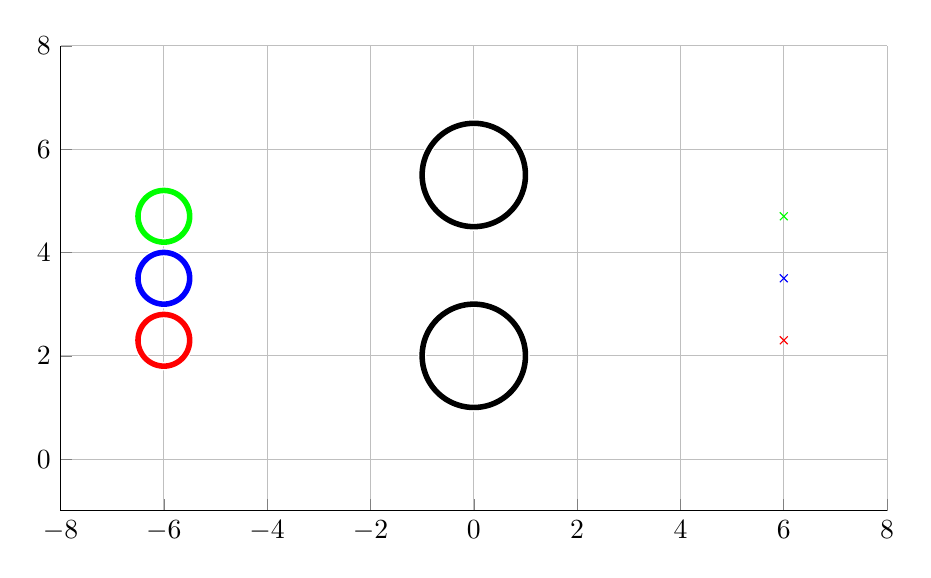
\begin{tikzpicture}

\begin{axis}[%
width=4.133in,
height=2.325in,
at={(0.693in,0.907in)},
scale only axis,
unbounded coords=jump,
xmin=-8,
xmax=8,
xmajorgrids,
ymin=-1,
ymax=8,
ymajorgrids,
axis background/.style={fill=white},
axis x line*=bottom,
axis y line*=left
]
\addplot [color=blue,only marks,mark=x,mark options={solid},forget plot]
  table[row sep=crcr]{%
6	3.5\\
};
\addplot [color=red,only marks,mark=x,mark options={solid},forget plot]
  table[row sep=crcr]{%
6	2.3\\
};
\addplot [color=green,only marks,mark=x,mark options={solid},forget plot]
  table[row sep=crcr]{%
6	4.7\\
};
\addplot [color=white,solid,line width=3.0pt,forget plot]
  table[row sep=crcr]{%
-5.5	3.5\\
-5.50030458649045	3.51744974835125\\
-5.50121797487009	3.53487823687206\\
-5.50273905231586	3.55226423163383\\
-5.50486596562921	3.56958655048003\\
-5.5075961234939	3.58682408883347\\
-5.5109261996331	3.60395584540888\\
-5.514852136862	3.62096094779983\\
-5.51936915203084	3.6378186779085\\
-5.52447174185242	3.65450849718747\\
-5.53015368960705	3.67101007166283\\
-5.53640807271661	3.68730329670796\\
-5.5432272711787	3.7033683215379\\
-5.55060297685042	3.71918557339454\\
-5.55852620357054	3.73473578139295\\
-5.56698729810778	3.75\\
-5.57597595192179	3.7649596321166\\
-5.58548121372248	3.77959645173537\\
-5.59549150281253	3.79389262614624\\
-5.60599462319664	3.80783073766283\\
-5.61697777844051	3.82139380484327\\
-5.6284275872613	3.83456530317943\\
-5.64033009983067	3.8473291852295\\
-5.6526708147705	3.85966990016933\\
-5.66543469682057	3.8715724127387\\
-5.67860619515673	3.88302222155949\\
-5.69216926233717	3.89400537680336\\
-5.70610737385376	3.90450849718747\\
-5.72040354826463	3.91451878627752\\
-5.7350403678834	3.92402404807821\\
-5.75	3.93301270189222\\
-5.76526421860705	3.94147379642946\\
-5.78081442660546	3.94939702314958\\
-5.7966316784621	3.9567727288213\\
-5.81269670329204	3.96359192728339\\
-5.82898992833717	3.96984631039295\\
-5.84549150281253	3.97552825814758\\
-5.8621813220915	3.98063084796916\\
-5.87903905220017	3.985147863138\\
-5.89604415459112	3.9890738003669\\
-5.91317591116653	3.9924038765061\\
-5.93041344951997	3.99513403437079\\
-5.94773576836617	3.99726094768414\\
-5.96512176312794	3.99878202512991\\
-5.98255025164875	3.99969541350955\\
-6	4\\
-6.01744974835125	3.99969541350955\\
-6.03487823687206	3.99878202512991\\
-6.05226423163383	3.99726094768414\\
-6.06958655048003	3.99513403437079\\
-6.08682408883347	3.9924038765061\\
-6.10395584540888	3.9890738003669\\
-6.12096094779983	3.985147863138\\
-6.1378186779085	3.98063084796916\\
-6.15450849718747	3.97552825814758\\
-6.17101007166283	3.96984631039295\\
-6.18730329670796	3.96359192728339\\
-6.2033683215379	3.9567727288213\\
-6.21918557339454	3.94939702314958\\
-6.23473578139295	3.94147379642946\\
-6.25	3.93301270189222\\
-6.2649596321166	3.92402404807821\\
-6.27959645173537	3.91451878627752\\
-6.29389262614624	3.90450849718747\\
-6.30783073766283	3.89400537680336\\
-6.32139380484327	3.88302222155949\\
-6.33456530317943	3.8715724127387\\
-6.3473291852295	3.85966990016933\\
-6.35966990016933	3.8473291852295\\
-6.3715724127387	3.83456530317943\\
-6.38302222155949	3.82139380484327\\
-6.39400537680336	3.80783073766283\\
-6.40450849718747	3.79389262614624\\
-6.41451878627752	3.77959645173537\\
-6.42402404807821	3.7649596321166\\
-6.43301270189222	3.75\\
-6.44147379642946	3.73473578139295\\
-6.44939702314958	3.71918557339454\\
-6.4567727288213	3.7033683215379\\
-6.46359192728339	3.68730329670796\\
-6.46984631039295	3.67101007166283\\
-6.47552825814758	3.65450849718747\\
-6.48063084796916	3.6378186779085\\
-6.485147863138	3.62096094779983\\
-6.4890738003669	3.60395584540888\\
-6.4924038765061	3.58682408883347\\
-6.49513403437079	3.56958655048003\\
-6.49726094768414	3.55226423163383\\
-6.49878202512991	3.53487823687206\\
-6.49969541350955	3.51744974835125\\
-6.5	3.5\\
-6.49969541350955	3.48255025164875\\
-6.49878202512991	3.46512176312794\\
-6.49726094768414	3.44773576836617\\
-6.49513403437079	3.43041344951997\\
-6.4924038765061	3.41317591116653\\
-6.4890738003669	3.39604415459112\\
-6.485147863138	3.37903905220017\\
-6.48063084796916	3.3621813220915\\
-6.47552825814758	3.34549150281253\\
-6.46984631039295	3.32898992833717\\
-6.46359192728339	3.31269670329204\\
-6.4567727288213	3.2966316784621\\
-6.44939702314958	3.28081442660546\\
-6.44147379642946	3.26526421860705\\
-6.43301270189222	3.25\\
-6.42402404807821	3.2350403678834\\
-6.41451878627752	3.22040354826463\\
-6.40450849718747	3.20610737385376\\
-6.39400537680336	3.19216926233717\\
-6.38302222155949	3.17860619515673\\
-6.3715724127387	3.16543469682057\\
-6.35966990016933	3.1526708147705\\
-6.3473291852295	3.14033009983067\\
-6.33456530317943	3.1284275872613\\
-6.32139380484327	3.11697777844051\\
-6.30783073766283	3.10599462319664\\
-6.29389262614624	3.09549150281253\\
-6.27959645173537	3.08548121372248\\
-6.2649596321166	3.07597595192179\\
-6.25	3.06698729810778\\
-6.23473578139295	3.05852620357054\\
-6.21918557339454	3.05060297685042\\
-6.2033683215379	3.0432272711787\\
-6.18730329670796	3.03640807271661\\
-6.17101007166283	3.03015368960705\\
-6.15450849718747	3.02447174185242\\
-6.1378186779085	3.01936915203084\\
-6.12096094779983	3.014852136862\\
-6.10395584540888	3.0109261996331\\
-6.08682408883347	3.0075961234939\\
-6.06958655048003	3.00486596562921\\
-6.05226423163383	3.00273905231586\\
-6.03487823687206	3.00121797487009\\
-6.01744974835125	3.00030458649045\\
-6	3\\
-5.98255025164875	3.00030458649045\\
-5.96512176312794	3.00121797487009\\
-5.94773576836617	3.00273905231586\\
-5.93041344951997	3.00486596562921\\
-5.91317591116653	3.0075961234939\\
-5.89604415459112	3.0109261996331\\
-5.87903905220017	3.014852136862\\
-5.8621813220915	3.01936915203084\\
-5.84549150281253	3.02447174185242\\
-5.82898992833717	3.03015368960705\\
-5.81269670329204	3.03640807271661\\
-5.7966316784621	3.0432272711787\\
-5.78081442660546	3.05060297685042\\
-5.76526421860705	3.05852620357054\\
-5.75	3.06698729810778\\
-5.7350403678834	3.07597595192179\\
-5.72040354826463	3.08548121372248\\
-5.70610737385376	3.09549150281253\\
-5.69216926233717	3.10599462319664\\
-5.67860619515673	3.11697777844051\\
-5.66543469682057	3.1284275872613\\
-5.6526708147705	3.14033009983067\\
-5.64033009983067	3.1526708147705\\
-5.6284275872613	3.16543469682057\\
-5.61697777844051	3.17860619515673\\
-5.60599462319664	3.19216926233717\\
-5.59549150281253	3.20610737385376\\
-5.58548121372248	3.22040354826463\\
-5.57597595192179	3.2350403678834\\
-5.56698729810778	3.25\\
-5.55852620357054	3.26526421860705\\
-5.55060297685042	3.28081442660546\\
-5.5432272711787	3.2966316784621\\
-5.53640807271661	3.31269670329204\\
-5.53015368960705	3.32898992833717\\
-5.52447174185242	3.34549150281253\\
-5.51936915203084	3.3621813220915\\
-5.514852136862	3.37903905220017\\
-5.5109261996331	3.39604415459112\\
-5.5075961234939	3.41317591116653\\
-5.50486596562921	3.43041344951997\\
-5.50273905231586	3.44773576836617\\
-5.50121797487009	3.46512176312794\\
-5.50030458649045	3.48255025164875\\
-5.5	3.5\\
nan	nan\\
};
\addplot [color=blue,solid,line width=2.0pt,forget plot]
  table[row sep=crcr]{%
-5.5	3.5\\
-5.50030458649045	3.51744974835125\\
-5.50121797487009	3.53487823687206\\
-5.50273905231586	3.55226423163383\\
-5.50486596562921	3.56958655048003\\
-5.5075961234939	3.58682408883347\\
-5.5109261996331	3.60395584540888\\
-5.514852136862	3.62096094779983\\
-5.51936915203084	3.6378186779085\\
-5.52447174185242	3.65450849718747\\
-5.53015368960705	3.67101007166283\\
-5.53640807271661	3.68730329670796\\
-5.5432272711787	3.7033683215379\\
-5.55060297685042	3.71918557339454\\
-5.55852620357054	3.73473578139295\\
-5.56698729810778	3.75\\
-5.57597595192179	3.7649596321166\\
-5.58548121372248	3.77959645173537\\
-5.59549150281253	3.79389262614624\\
-5.60599462319664	3.80783073766283\\
-5.61697777844051	3.82139380484327\\
-5.6284275872613	3.83456530317943\\
-5.64033009983067	3.8473291852295\\
-5.6526708147705	3.85966990016933\\
-5.66543469682057	3.8715724127387\\
-5.67860619515673	3.88302222155949\\
-5.69216926233717	3.89400537680336\\
-5.70610737385376	3.90450849718747\\
-5.72040354826463	3.91451878627752\\
-5.7350403678834	3.92402404807821\\
-5.75	3.93301270189222\\
-5.76526421860705	3.94147379642946\\
-5.78081442660546	3.94939702314958\\
-5.7966316784621	3.9567727288213\\
-5.81269670329204	3.96359192728339\\
-5.82898992833717	3.96984631039295\\
-5.84549150281253	3.97552825814758\\
-5.8621813220915	3.98063084796916\\
-5.87903905220017	3.985147863138\\
-5.89604415459112	3.9890738003669\\
-5.91317591116653	3.9924038765061\\
-5.93041344951997	3.99513403437079\\
-5.94773576836617	3.99726094768414\\
-5.96512176312794	3.99878202512991\\
-5.98255025164875	3.99969541350955\\
-6	4\\
-6.01744974835125	3.99969541350955\\
-6.03487823687206	3.99878202512991\\
-6.05226423163383	3.99726094768414\\
-6.06958655048003	3.99513403437079\\
-6.08682408883347	3.9924038765061\\
-6.10395584540888	3.9890738003669\\
-6.12096094779983	3.985147863138\\
-6.1378186779085	3.98063084796916\\
-6.15450849718747	3.97552825814758\\
-6.17101007166283	3.96984631039295\\
-6.18730329670796	3.96359192728339\\
-6.2033683215379	3.9567727288213\\
-6.21918557339454	3.94939702314958\\
-6.23473578139295	3.94147379642946\\
-6.25	3.93301270189222\\
-6.2649596321166	3.92402404807821\\
-6.27959645173537	3.91451878627752\\
-6.29389262614624	3.90450849718747\\
-6.30783073766283	3.89400537680336\\
-6.32139380484327	3.88302222155949\\
-6.33456530317943	3.8715724127387\\
-6.3473291852295	3.85966990016933\\
-6.35966990016933	3.8473291852295\\
-6.3715724127387	3.83456530317943\\
-6.38302222155949	3.82139380484327\\
-6.39400537680336	3.80783073766283\\
-6.40450849718747	3.79389262614624\\
-6.41451878627752	3.77959645173537\\
-6.42402404807821	3.7649596321166\\
-6.43301270189222	3.75\\
-6.44147379642946	3.73473578139295\\
-6.44939702314958	3.71918557339454\\
-6.4567727288213	3.7033683215379\\
-6.46359192728339	3.68730329670796\\
-6.46984631039295	3.67101007166283\\
-6.47552825814758	3.65450849718747\\
-6.48063084796916	3.6378186779085\\
-6.485147863138	3.62096094779983\\
-6.4890738003669	3.60395584540888\\
-6.4924038765061	3.58682408883347\\
-6.49513403437079	3.56958655048003\\
-6.49726094768414	3.55226423163383\\
-6.49878202512991	3.53487823687206\\
-6.49969541350955	3.51744974835125\\
-6.5	3.5\\
-6.49969541350955	3.48255025164875\\
-6.49878202512991	3.46512176312794\\
-6.49726094768414	3.44773576836617\\
-6.49513403437079	3.43041344951997\\
-6.4924038765061	3.41317591116653\\
-6.4890738003669	3.39604415459112\\
-6.485147863138	3.37903905220017\\
-6.48063084796916	3.3621813220915\\
-6.47552825814758	3.34549150281253\\
-6.46984631039295	3.32898992833717\\
-6.46359192728339	3.31269670329204\\
-6.4567727288213	3.2966316784621\\
-6.44939702314958	3.28081442660546\\
-6.44147379642946	3.26526421860705\\
-6.43301270189222	3.25\\
-6.42402404807821	3.2350403678834\\
-6.41451878627752	3.22040354826463\\
-6.40450849718747	3.20610737385376\\
-6.39400537680336	3.19216926233717\\
-6.38302222155949	3.17860619515673\\
-6.3715724127387	3.16543469682057\\
-6.35966990016933	3.1526708147705\\
-6.3473291852295	3.14033009983067\\
-6.33456530317943	3.1284275872613\\
-6.32139380484327	3.11697777844051\\
-6.30783073766283	3.10599462319664\\
-6.29389262614624	3.09549150281253\\
-6.27959645173537	3.08548121372248\\
-6.2649596321166	3.07597595192179\\
-6.25	3.06698729810778\\
-6.23473578139295	3.05852620357054\\
-6.21918557339454	3.05060297685042\\
-6.2033683215379	3.0432272711787\\
-6.18730329670796	3.03640807271661\\
-6.17101007166283	3.03015368960705\\
-6.15450849718747	3.02447174185242\\
-6.1378186779085	3.01936915203084\\
-6.12096094779983	3.014852136862\\
-6.10395584540888	3.0109261996331\\
-6.08682408883347	3.0075961234939\\
-6.06958655048003	3.00486596562921\\
-6.05226423163383	3.00273905231586\\
-6.03487823687206	3.00121797487009\\
-6.01744974835125	3.00030458649045\\
-6	3\\
-5.98255025164875	3.00030458649045\\
-5.96512176312794	3.00121797487009\\
-5.94773576836617	3.00273905231586\\
-5.93041344951997	3.00486596562921\\
-5.91317591116653	3.0075961234939\\
-5.89604415459112	3.0109261996331\\
-5.87903905220017	3.014852136862\\
-5.8621813220915	3.01936915203084\\
-5.84549150281253	3.02447174185242\\
-5.82898992833717	3.03015368960705\\
-5.81269670329204	3.03640807271661\\
-5.7966316784621	3.0432272711787\\
-5.78081442660546	3.05060297685042\\
-5.76526421860705	3.05852620357054\\
-5.75	3.06698729810778\\
-5.7350403678834	3.07597595192179\\
-5.72040354826463	3.08548121372248\\
-5.70610737385376	3.09549150281253\\
-5.69216926233717	3.10599462319664\\
-5.67860619515673	3.11697777844051\\
-5.66543469682057	3.1284275872613\\
-5.6526708147705	3.14033009983067\\
-5.64033009983067	3.1526708147705\\
-5.6284275872613	3.16543469682057\\
-5.61697777844051	3.17860619515673\\
-5.60599462319664	3.19216926233717\\
-5.59549150281253	3.20610737385376\\
-5.58548121372248	3.22040354826463\\
-5.57597595192179	3.2350403678834\\
-5.56698729810778	3.25\\
-5.55852620357054	3.26526421860705\\
-5.55060297685042	3.28081442660546\\
-5.5432272711787	3.2966316784621\\
-5.53640807271661	3.31269670329204\\
-5.53015368960705	3.32898992833717\\
-5.52447174185242	3.34549150281253\\
-5.51936915203084	3.3621813220915\\
-5.514852136862	3.37903905220017\\
-5.5109261996331	3.39604415459112\\
-5.5075961234939	3.41317591116653\\
-5.50486596562921	3.43041344951997\\
-5.50273905231586	3.44773576836617\\
-5.50121797487009	3.46512176312794\\
-5.50030458649045	3.48255025164875\\
-5.5	3.5\\
nan	nan\\
};
\addplot [color=white,solid,line width=3.0pt,forget plot]
  table[row sep=crcr]{%
-5.5	2.3\\
-5.50030458649045	2.31744974835125\\
-5.50121797487009	2.33487823687206\\
-5.50273905231586	2.35226423163383\\
-5.50486596562921	2.36958655048003\\
-5.5075961234939	2.38682408883346\\
-5.5109261996331	2.40395584540888\\
-5.514852136862	2.42096094779983\\
-5.51936915203084	2.4378186779085\\
-5.52447174185242	2.45450849718747\\
-5.53015368960705	2.47101007166283\\
-5.53640807271661	2.48730329670796\\
-5.5432272711787	2.5033683215379\\
-5.55060297685042	2.51918557339454\\
-5.55852620357054	2.53473578139295\\
-5.56698729810778	2.55\\
-5.57597595192179	2.5649596321166\\
-5.58548121372248	2.57959645173537\\
-5.59549150281253	2.59389262614624\\
-5.60599462319664	2.60783073766283\\
-5.61697777844051	2.62139380484327\\
-5.6284275872613	2.63456530317943\\
-5.64033009983067	2.6473291852295\\
-5.6526708147705	2.65966990016933\\
-5.66543469682057	2.6715724127387\\
-5.67860619515673	2.68302222155949\\
-5.69216926233717	2.69400537680336\\
-5.70610737385376	2.70450849718747\\
-5.72040354826463	2.71451878627752\\
-5.7350403678834	2.72402404807821\\
-5.75	2.73301270189222\\
-5.76526421860705	2.74147379642946\\
-5.78081442660546	2.74939702314958\\
-5.7966316784621	2.7567727288213\\
-5.81269670329204	2.76359192728339\\
-5.82898992833717	2.76984631039295\\
-5.84549150281253	2.77552825814758\\
-5.8621813220915	2.78063084796916\\
-5.87903905220017	2.785147863138\\
-5.89604415459112	2.7890738003669\\
-5.91317591116653	2.7924038765061\\
-5.93041344951997	2.79513403437078\\
-5.94773576836617	2.79726094768414\\
-5.96512176312794	2.79878202512991\\
-5.98255025164875	2.79969541350955\\
-6	2.8\\
-6.01744974835125	2.79969541350955\\
-6.03487823687206	2.79878202512991\\
-6.05226423163383	2.79726094768414\\
-6.06958655048003	2.79513403437078\\
-6.08682408883347	2.7924038765061\\
-6.10395584540888	2.7890738003669\\
-6.12096094779983	2.785147863138\\
-6.1378186779085	2.78063084796916\\
-6.15450849718747	2.77552825814758\\
-6.17101007166283	2.76984631039295\\
-6.18730329670796	2.76359192728339\\
-6.2033683215379	2.7567727288213\\
-6.21918557339454	2.74939702314958\\
-6.23473578139295	2.74147379642946\\
-6.25	2.73301270189222\\
-6.2649596321166	2.72402404807821\\
-6.27959645173537	2.71451878627752\\
-6.29389262614624	2.70450849718747\\
-6.30783073766283	2.69400537680336\\
-6.32139380484327	2.68302222155949\\
-6.33456530317943	2.6715724127387\\
-6.3473291852295	2.65966990016933\\
-6.35966990016933	2.6473291852295\\
-6.3715724127387	2.63456530317943\\
-6.38302222155949	2.62139380484327\\
-6.39400537680336	2.60783073766283\\
-6.40450849718747	2.59389262614624\\
-6.41451878627752	2.57959645173537\\
-6.42402404807821	2.5649596321166\\
-6.43301270189222	2.55\\
-6.44147379642946	2.53473578139295\\
-6.44939702314958	2.51918557339454\\
-6.4567727288213	2.5033683215379\\
-6.46359192728339	2.48730329670796\\
-6.46984631039295	2.47101007166283\\
-6.47552825814758	2.45450849718747\\
-6.48063084796916	2.4378186779085\\
-6.485147863138	2.42096094779983\\
-6.4890738003669	2.40395584540888\\
-6.4924038765061	2.38682408883346\\
-6.49513403437079	2.36958655048003\\
-6.49726094768414	2.35226423163383\\
-6.49878202512991	2.33487823687206\\
-6.49969541350955	2.31744974835125\\
-6.5	2.3\\
-6.49969541350955	2.28255025164875\\
-6.49878202512991	2.26512176312794\\
-6.49726094768414	2.24773576836617\\
-6.49513403437079	2.23041344951997\\
-6.4924038765061	2.21317591116653\\
-6.4890738003669	2.19604415459112\\
-6.485147863138	2.17903905220017\\
-6.48063084796916	2.1621813220915\\
-6.47552825814758	2.14549150281253\\
-6.46984631039295	2.12898992833717\\
-6.46359192728339	2.11269670329204\\
-6.4567727288213	2.0966316784621\\
-6.44939702314958	2.08081442660546\\
-6.44147379642946	2.06526421860705\\
-6.43301270189222	2.05\\
-6.42402404807821	2.0350403678834\\
-6.41451878627752	2.02040354826463\\
-6.40450849718747	2.00610737385376\\
-6.39400537680336	1.99216926233717\\
-6.38302222155949	1.97860619515673\\
-6.3715724127387	1.96543469682057\\
-6.35966990016933	1.9526708147705\\
-6.3473291852295	1.94033009983067\\
-6.33456530317943	1.9284275872613\\
-6.32139380484327	1.91697777844051\\
-6.30783073766283	1.90599462319664\\
-6.29389262614624	1.89549150281253\\
-6.27959645173537	1.88548121372248\\
-6.2649596321166	1.87597595192179\\
-6.25	1.86698729810778\\
-6.23473578139295	1.85852620357054\\
-6.21918557339454	1.85060297685042\\
-6.2033683215379	1.8432272711787\\
-6.18730329670796	1.83640807271661\\
-6.17101007166283	1.83015368960705\\
-6.15450849718747	1.82447174185242\\
-6.1378186779085	1.81936915203084\\
-6.12096094779983	1.814852136862\\
-6.10395584540888	1.8109261996331\\
-6.08682408883347	1.8075961234939\\
-6.06958655048003	1.80486596562921\\
-6.05226423163383	1.80273905231586\\
-6.03487823687206	1.80121797487009\\
-6.01744974835125	1.80030458649045\\
-6	1.8\\
-5.98255025164875	1.80030458649045\\
-5.96512176312794	1.80121797487009\\
-5.94773576836617	1.80273905231586\\
-5.93041344951997	1.80486596562921\\
-5.91317591116653	1.8075961234939\\
-5.89604415459112	1.8109261996331\\
-5.87903905220017	1.814852136862\\
-5.8621813220915	1.81936915203084\\
-5.84549150281253	1.82447174185242\\
-5.82898992833717	1.83015368960705\\
-5.81269670329204	1.83640807271661\\
-5.7966316784621	1.8432272711787\\
-5.78081442660546	1.85060297685042\\
-5.76526421860705	1.85852620357054\\
-5.75	1.86698729810778\\
-5.7350403678834	1.87597595192179\\
-5.72040354826463	1.88548121372248\\
-5.70610737385376	1.89549150281253\\
-5.69216926233717	1.90599462319664\\
-5.67860619515673	1.91697777844051\\
-5.66543469682057	1.9284275872613\\
-5.6526708147705	1.94033009983067\\
-5.64033009983067	1.9526708147705\\
-5.6284275872613	1.96543469682057\\
-5.61697777844051	1.97860619515673\\
-5.60599462319664	1.99216926233717\\
-5.59549150281253	2.00610737385376\\
-5.58548121372248	2.02040354826463\\
-5.57597595192179	2.0350403678834\\
-5.56698729810778	2.05\\
-5.55852620357054	2.06526421860705\\
-5.55060297685042	2.08081442660546\\
-5.5432272711787	2.0966316784621\\
-5.53640807271661	2.11269670329204\\
-5.53015368960705	2.12898992833717\\
-5.52447174185242	2.14549150281253\\
-5.51936915203084	2.1621813220915\\
-5.514852136862	2.17903905220017\\
-5.5109261996331	2.19604415459112\\
-5.5075961234939	2.21317591116653\\
-5.50486596562921	2.23041344951997\\
-5.50273905231586	2.24773576836617\\
-5.50121797487009	2.26512176312794\\
-5.50030458649045	2.28255025164875\\
-5.5	2.3\\
nan	nan\\
};
\addplot [color=red,solid,line width=2.0pt,forget plot]
  table[row sep=crcr]{%
-5.5	2.3\\
-5.50030458649045	2.31744974835125\\
-5.50121797487009	2.33487823687206\\
-5.50273905231586	2.35226423163383\\
-5.50486596562921	2.36958655048003\\
-5.5075961234939	2.38682408883346\\
-5.5109261996331	2.40395584540888\\
-5.514852136862	2.42096094779983\\
-5.51936915203084	2.4378186779085\\
-5.52447174185242	2.45450849718747\\
-5.53015368960705	2.47101007166283\\
-5.53640807271661	2.48730329670796\\
-5.5432272711787	2.5033683215379\\
-5.55060297685042	2.51918557339454\\
-5.55852620357054	2.53473578139295\\
-5.56698729810778	2.55\\
-5.57597595192179	2.5649596321166\\
-5.58548121372248	2.57959645173537\\
-5.59549150281253	2.59389262614624\\
-5.60599462319664	2.60783073766283\\
-5.61697777844051	2.62139380484327\\
-5.6284275872613	2.63456530317943\\
-5.64033009983067	2.6473291852295\\
-5.6526708147705	2.65966990016933\\
-5.66543469682057	2.6715724127387\\
-5.67860619515673	2.68302222155949\\
-5.69216926233717	2.69400537680336\\
-5.70610737385376	2.70450849718747\\
-5.72040354826463	2.71451878627752\\
-5.7350403678834	2.72402404807821\\
-5.75	2.73301270189222\\
-5.76526421860705	2.74147379642946\\
-5.78081442660546	2.74939702314958\\
-5.7966316784621	2.7567727288213\\
-5.81269670329204	2.76359192728339\\
-5.82898992833717	2.76984631039295\\
-5.84549150281253	2.77552825814758\\
-5.8621813220915	2.78063084796916\\
-5.87903905220017	2.785147863138\\
-5.89604415459112	2.7890738003669\\
-5.91317591116653	2.7924038765061\\
-5.93041344951997	2.79513403437078\\
-5.94773576836617	2.79726094768414\\
-5.96512176312794	2.79878202512991\\
-5.98255025164875	2.79969541350955\\
-6	2.8\\
-6.01744974835125	2.79969541350955\\
-6.03487823687206	2.79878202512991\\
-6.05226423163383	2.79726094768414\\
-6.06958655048003	2.79513403437078\\
-6.08682408883347	2.7924038765061\\
-6.10395584540888	2.7890738003669\\
-6.12096094779983	2.785147863138\\
-6.1378186779085	2.78063084796916\\
-6.15450849718747	2.77552825814758\\
-6.17101007166283	2.76984631039295\\
-6.18730329670796	2.76359192728339\\
-6.2033683215379	2.7567727288213\\
-6.21918557339454	2.74939702314958\\
-6.23473578139295	2.74147379642946\\
-6.25	2.73301270189222\\
-6.2649596321166	2.72402404807821\\
-6.27959645173537	2.71451878627752\\
-6.29389262614624	2.70450849718747\\
-6.30783073766283	2.69400537680336\\
-6.32139380484327	2.68302222155949\\
-6.33456530317943	2.6715724127387\\
-6.3473291852295	2.65966990016933\\
-6.35966990016933	2.6473291852295\\
-6.3715724127387	2.63456530317943\\
-6.38302222155949	2.62139380484327\\
-6.39400537680336	2.60783073766283\\
-6.40450849718747	2.59389262614624\\
-6.41451878627752	2.57959645173537\\
-6.42402404807821	2.5649596321166\\
-6.43301270189222	2.55\\
-6.44147379642946	2.53473578139295\\
-6.44939702314958	2.51918557339454\\
-6.4567727288213	2.5033683215379\\
-6.46359192728339	2.48730329670796\\
-6.46984631039295	2.47101007166283\\
-6.47552825814758	2.45450849718747\\
-6.48063084796916	2.4378186779085\\
-6.485147863138	2.42096094779983\\
-6.4890738003669	2.40395584540888\\
-6.4924038765061	2.38682408883346\\
-6.49513403437079	2.36958655048003\\
-6.49726094768414	2.35226423163383\\
-6.49878202512991	2.33487823687206\\
-6.49969541350955	2.31744974835125\\
-6.5	2.3\\
-6.49969541350955	2.28255025164875\\
-6.49878202512991	2.26512176312794\\
-6.49726094768414	2.24773576836617\\
-6.49513403437079	2.23041344951997\\
-6.4924038765061	2.21317591116653\\
-6.4890738003669	2.19604415459112\\
-6.485147863138	2.17903905220017\\
-6.48063084796916	2.1621813220915\\
-6.47552825814758	2.14549150281253\\
-6.46984631039295	2.12898992833717\\
-6.46359192728339	2.11269670329204\\
-6.4567727288213	2.0966316784621\\
-6.44939702314958	2.08081442660546\\
-6.44147379642946	2.06526421860705\\
-6.43301270189222	2.05\\
-6.42402404807821	2.0350403678834\\
-6.41451878627752	2.02040354826463\\
-6.40450849718747	2.00610737385376\\
-6.39400537680336	1.99216926233717\\
-6.38302222155949	1.97860619515673\\
-6.3715724127387	1.96543469682057\\
-6.35966990016933	1.9526708147705\\
-6.3473291852295	1.94033009983067\\
-6.33456530317943	1.9284275872613\\
-6.32139380484327	1.91697777844051\\
-6.30783073766283	1.90599462319664\\
-6.29389262614624	1.89549150281253\\
-6.27959645173537	1.88548121372248\\
-6.2649596321166	1.87597595192179\\
-6.25	1.86698729810778\\
-6.23473578139295	1.85852620357054\\
-6.21918557339454	1.85060297685042\\
-6.2033683215379	1.8432272711787\\
-6.18730329670796	1.83640807271661\\
-6.17101007166283	1.83015368960705\\
-6.15450849718747	1.82447174185242\\
-6.1378186779085	1.81936915203084\\
-6.12096094779983	1.814852136862\\
-6.10395584540888	1.8109261996331\\
-6.08682408883347	1.8075961234939\\
-6.06958655048003	1.80486596562921\\
-6.05226423163383	1.80273905231586\\
-6.03487823687206	1.80121797487009\\
-6.01744974835125	1.80030458649045\\
-6	1.8\\
-5.98255025164875	1.80030458649045\\
-5.96512176312794	1.80121797487009\\
-5.94773576836617	1.80273905231586\\
-5.93041344951997	1.80486596562921\\
-5.91317591116653	1.8075961234939\\
-5.89604415459112	1.8109261996331\\
-5.87903905220017	1.814852136862\\
-5.8621813220915	1.81936915203084\\
-5.84549150281253	1.82447174185242\\
-5.82898992833717	1.83015368960705\\
-5.81269670329204	1.83640807271661\\
-5.7966316784621	1.8432272711787\\
-5.78081442660546	1.85060297685042\\
-5.76526421860705	1.85852620357054\\
-5.75	1.86698729810778\\
-5.7350403678834	1.87597595192179\\
-5.72040354826463	1.88548121372248\\
-5.70610737385376	1.89549150281253\\
-5.69216926233717	1.90599462319664\\
-5.67860619515673	1.91697777844051\\
-5.66543469682057	1.9284275872613\\
-5.6526708147705	1.94033009983067\\
-5.64033009983067	1.9526708147705\\
-5.6284275872613	1.96543469682057\\
-5.61697777844051	1.97860619515673\\
-5.60599462319664	1.99216926233717\\
-5.59549150281253	2.00610737385376\\
-5.58548121372248	2.02040354826463\\
-5.57597595192179	2.0350403678834\\
-5.56698729810778	2.05\\
-5.55852620357054	2.06526421860705\\
-5.55060297685042	2.08081442660546\\
-5.5432272711787	2.0966316784621\\
-5.53640807271661	2.11269670329204\\
-5.53015368960705	2.12898992833717\\
-5.52447174185242	2.14549150281253\\
-5.51936915203084	2.1621813220915\\
-5.514852136862	2.17903905220017\\
-5.5109261996331	2.19604415459112\\
-5.5075961234939	2.21317591116653\\
-5.50486596562921	2.23041344951997\\
-5.50273905231586	2.24773576836617\\
-5.50121797487009	2.26512176312794\\
-5.50030458649045	2.28255025164875\\
-5.5	2.3\\
nan	nan\\
};
\addplot [color=white,solid,line width=3.0pt,forget plot]
  table[row sep=crcr]{%
-5.5	4.7\\
-5.50030458649045	4.71744974835125\\
-5.50121797487009	4.73487823687206\\
-5.50273905231586	4.75226423163383\\
-5.50486596562921	4.76958655048003\\
-5.5075961234939	4.78682408883347\\
-5.5109261996331	4.80395584540888\\
-5.514852136862	4.82096094779983\\
-5.51936915203084	4.8378186779085\\
-5.52447174185242	4.85450849718747\\
-5.53015368960705	4.87101007166283\\
-5.53640807271661	4.88730329670796\\
-5.5432272711787	4.9033683215379\\
-5.55060297685042	4.91918557339454\\
-5.55852620357054	4.93473578139295\\
-5.56698729810778	4.95\\
-5.57597595192179	4.9649596321166\\
-5.58548121372248	4.97959645173537\\
-5.59549150281253	4.99389262614624\\
-5.60599462319664	5.00783073766283\\
-5.61697777844051	5.02139380484327\\
-5.6284275872613	5.03456530317943\\
-5.64033009983067	5.0473291852295\\
-5.6526708147705	5.05966990016933\\
-5.66543469682057	5.0715724127387\\
-5.67860619515673	5.08302222155949\\
-5.69216926233717	5.09400537680336\\
-5.70610737385376	5.10450849718747\\
-5.72040354826463	5.11451878627752\\
-5.7350403678834	5.12402404807821\\
-5.75	5.13301270189222\\
-5.76526421860705	5.14147379642946\\
-5.78081442660546	5.14939702314958\\
-5.7966316784621	5.1567727288213\\
-5.81269670329204	5.16359192728339\\
-5.82898992833717	5.16984631039295\\
-5.84549150281253	5.17552825814758\\
-5.8621813220915	5.18063084796916\\
-5.87903905220017	5.185147863138\\
-5.89604415459112	5.1890738003669\\
-5.91317591116653	5.1924038765061\\
-5.93041344951997	5.19513403437079\\
-5.94773576836617	5.19726094768414\\
-5.96512176312794	5.19878202512991\\
-5.98255025164875	5.19969541350955\\
-6	5.2\\
-6.01744974835125	5.19969541350955\\
-6.03487823687206	5.19878202512991\\
-6.05226423163383	5.19726094768414\\
-6.06958655048003	5.19513403437079\\
-6.08682408883347	5.1924038765061\\
-6.10395584540888	5.1890738003669\\
-6.12096094779983	5.185147863138\\
-6.1378186779085	5.18063084796916\\
-6.15450849718747	5.17552825814758\\
-6.17101007166283	5.16984631039295\\
-6.18730329670796	5.16359192728339\\
-6.2033683215379	5.1567727288213\\
-6.21918557339454	5.14939702314958\\
-6.23473578139295	5.14147379642946\\
-6.25	5.13301270189222\\
-6.2649596321166	5.12402404807821\\
-6.27959645173537	5.11451878627752\\
-6.29389262614624	5.10450849718747\\
-6.30783073766283	5.09400537680336\\
-6.32139380484327	5.08302222155949\\
-6.33456530317943	5.0715724127387\\
-6.3473291852295	5.05966990016933\\
-6.35966990016933	5.0473291852295\\
-6.3715724127387	5.03456530317943\\
-6.38302222155949	5.02139380484327\\
-6.39400537680336	5.00783073766283\\
-6.40450849718747	4.99389262614624\\
-6.41451878627752	4.97959645173537\\
-6.42402404807821	4.9649596321166\\
-6.43301270189222	4.95\\
-6.44147379642946	4.93473578139295\\
-6.44939702314958	4.91918557339454\\
-6.4567727288213	4.9033683215379\\
-6.46359192728339	4.88730329670796\\
-6.46984631039295	4.87101007166283\\
-6.47552825814758	4.85450849718747\\
-6.48063084796916	4.8378186779085\\
-6.485147863138	4.82096094779983\\
-6.4890738003669	4.80395584540888\\
-6.4924038765061	4.78682408883347\\
-6.49513403437079	4.76958655048003\\
-6.49726094768414	4.75226423163383\\
-6.49878202512991	4.73487823687206\\
-6.49969541350955	4.71744974835125\\
-6.5	4.7\\
-6.49969541350955	4.68255025164875\\
-6.49878202512991	4.66512176312794\\
-6.49726094768414	4.64773576836617\\
-6.49513403437079	4.63041344951997\\
-6.4924038765061	4.61317591116654\\
-6.4890738003669	4.59604415459112\\
-6.485147863138	4.57903905220017\\
-6.48063084796916	4.5621813220915\\
-6.47552825814758	4.54549150281253\\
-6.46984631039295	4.52898992833717\\
-6.46359192728339	4.51269670329204\\
-6.4567727288213	4.4966316784621\\
-6.44939702314958	4.48081442660546\\
-6.44147379642946	4.46526421860705\\
-6.43301270189222	4.45\\
-6.42402404807821	4.4350403678834\\
-6.41451878627752	4.42040354826463\\
-6.40450849718747	4.40610737385376\\
-6.39400537680336	4.39216926233717\\
-6.38302222155949	4.37860619515673\\
-6.3715724127387	4.36543469682057\\
-6.35966990016933	4.3526708147705\\
-6.3473291852295	4.34033009983068\\
-6.33456530317943	4.3284275872613\\
-6.32139380484327	4.31697777844051\\
-6.30783073766283	4.30599462319664\\
-6.29389262614624	4.29549150281253\\
-6.27959645173537	4.28548121372248\\
-6.2649596321166	4.27597595192179\\
-6.25	4.26698729810778\\
-6.23473578139295	4.25852620357054\\
-6.21918557339454	4.25060297685042\\
-6.2033683215379	4.2432272711787\\
-6.18730329670796	4.23640807271661\\
-6.17101007166283	4.23015368960705\\
-6.15450849718747	4.22447174185242\\
-6.1378186779085	4.21936915203084\\
-6.12096094779983	4.214852136862\\
-6.10395584540888	4.2109261996331\\
-6.08682408883347	4.2075961234939\\
-6.06958655048003	4.20486596562921\\
-6.05226423163383	4.20273905231586\\
-6.03487823687206	4.20121797487009\\
-6.01744974835125	4.20030458649045\\
-6	4.2\\
-5.98255025164875	4.20030458649045\\
-5.96512176312794	4.20121797487009\\
-5.94773576836617	4.20273905231586\\
-5.93041344951997	4.20486596562921\\
-5.91317591116653	4.2075961234939\\
-5.89604415459112	4.2109261996331\\
-5.87903905220017	4.214852136862\\
-5.8621813220915	4.21936915203084\\
-5.84549150281253	4.22447174185242\\
-5.82898992833717	4.23015368960705\\
-5.81269670329204	4.23640807271661\\
-5.7966316784621	4.2432272711787\\
-5.78081442660546	4.25060297685042\\
-5.76526421860705	4.25852620357054\\
-5.75	4.26698729810778\\
-5.7350403678834	4.27597595192179\\
-5.72040354826463	4.28548121372248\\
-5.70610737385376	4.29549150281253\\
-5.69216926233717	4.30599462319664\\
-5.67860619515673	4.31697777844051\\
-5.66543469682057	4.3284275872613\\
-5.6526708147705	4.34033009983067\\
-5.64033009983067	4.3526708147705\\
-5.6284275872613	4.36543469682057\\
-5.61697777844051	4.37860619515673\\
-5.60599462319664	4.39216926233717\\
-5.59549150281253	4.40610737385376\\
-5.58548121372248	4.42040354826463\\
-5.57597595192179	4.4350403678834\\
-5.56698729810778	4.45\\
-5.55852620357054	4.46526421860705\\
-5.55060297685042	4.48081442660546\\
-5.5432272711787	4.4966316784621\\
-5.53640807271661	4.51269670329204\\
-5.53015368960705	4.52898992833717\\
-5.52447174185242	4.54549150281253\\
-5.51936915203084	4.5621813220915\\
-5.514852136862	4.57903905220017\\
-5.5109261996331	4.59604415459112\\
-5.5075961234939	4.61317591116653\\
-5.50486596562921	4.63041344951997\\
-5.50273905231586	4.64773576836617\\
-5.50121797487009	4.66512176312794\\
-5.50030458649045	4.68255025164875\\
-5.5	4.7\\
nan	nan\\
};
\addplot [color=green,solid,line width=2.0pt,forget plot]
  table[row sep=crcr]{%
-5.5	4.7\\
-5.50030458649045	4.71744974835125\\
-5.50121797487009	4.73487823687206\\
-5.50273905231586	4.75226423163383\\
-5.50486596562921	4.76958655048003\\
-5.5075961234939	4.78682408883347\\
-5.5109261996331	4.80395584540888\\
-5.514852136862	4.82096094779983\\
-5.51936915203084	4.8378186779085\\
-5.52447174185242	4.85450849718747\\
-5.53015368960705	4.87101007166283\\
-5.53640807271661	4.88730329670796\\
-5.5432272711787	4.9033683215379\\
-5.55060297685042	4.91918557339454\\
-5.55852620357054	4.93473578139295\\
-5.56698729810778	4.95\\
-5.57597595192179	4.9649596321166\\
-5.58548121372248	4.97959645173537\\
-5.59549150281253	4.99389262614624\\
-5.60599462319664	5.00783073766283\\
-5.61697777844051	5.02139380484327\\
-5.6284275872613	5.03456530317943\\
-5.64033009983067	5.0473291852295\\
-5.6526708147705	5.05966990016933\\
-5.66543469682057	5.0715724127387\\
-5.67860619515673	5.08302222155949\\
-5.69216926233717	5.09400537680336\\
-5.70610737385376	5.10450849718747\\
-5.72040354826463	5.11451878627752\\
-5.7350403678834	5.12402404807821\\
-5.75	5.13301270189222\\
-5.76526421860705	5.14147379642946\\
-5.78081442660546	5.14939702314958\\
-5.7966316784621	5.1567727288213\\
-5.81269670329204	5.16359192728339\\
-5.82898992833717	5.16984631039295\\
-5.84549150281253	5.17552825814758\\
-5.8621813220915	5.18063084796916\\
-5.87903905220017	5.185147863138\\
-5.89604415459112	5.1890738003669\\
-5.91317591116653	5.1924038765061\\
-5.93041344951997	5.19513403437079\\
-5.94773576836617	5.19726094768414\\
-5.96512176312794	5.19878202512991\\
-5.98255025164875	5.19969541350955\\
-6	5.2\\
-6.01744974835125	5.19969541350955\\
-6.03487823687206	5.19878202512991\\
-6.05226423163383	5.19726094768414\\
-6.06958655048003	5.19513403437079\\
-6.08682408883347	5.1924038765061\\
-6.10395584540888	5.1890738003669\\
-6.12096094779983	5.185147863138\\
-6.1378186779085	5.18063084796916\\
-6.15450849718747	5.17552825814758\\
-6.17101007166283	5.16984631039295\\
-6.18730329670796	5.16359192728339\\
-6.2033683215379	5.1567727288213\\
-6.21918557339454	5.14939702314958\\
-6.23473578139295	5.14147379642946\\
-6.25	5.13301270189222\\
-6.2649596321166	5.12402404807821\\
-6.27959645173537	5.11451878627752\\
-6.29389262614624	5.10450849718747\\
-6.30783073766283	5.09400537680336\\
-6.32139380484327	5.08302222155949\\
-6.33456530317943	5.0715724127387\\
-6.3473291852295	5.05966990016933\\
-6.35966990016933	5.0473291852295\\
-6.3715724127387	5.03456530317943\\
-6.38302222155949	5.02139380484327\\
-6.39400537680336	5.00783073766283\\
-6.40450849718747	4.99389262614624\\
-6.41451878627752	4.97959645173537\\
-6.42402404807821	4.9649596321166\\
-6.43301270189222	4.95\\
-6.44147379642946	4.93473578139295\\
-6.44939702314958	4.91918557339454\\
-6.4567727288213	4.9033683215379\\
-6.46359192728339	4.88730329670796\\
-6.46984631039295	4.87101007166283\\
-6.47552825814758	4.85450849718747\\
-6.48063084796916	4.8378186779085\\
-6.485147863138	4.82096094779983\\
-6.4890738003669	4.80395584540888\\
-6.4924038765061	4.78682408883347\\
-6.49513403437079	4.76958655048003\\
-6.49726094768414	4.75226423163383\\
-6.49878202512991	4.73487823687206\\
-6.49969541350955	4.71744974835125\\
-6.5	4.7\\
-6.49969541350955	4.68255025164875\\
-6.49878202512991	4.66512176312794\\
-6.49726094768414	4.64773576836617\\
-6.49513403437079	4.63041344951997\\
-6.4924038765061	4.61317591116654\\
-6.4890738003669	4.59604415459112\\
-6.485147863138	4.57903905220017\\
-6.48063084796916	4.5621813220915\\
-6.47552825814758	4.54549150281253\\
-6.46984631039295	4.52898992833717\\
-6.46359192728339	4.51269670329204\\
-6.4567727288213	4.4966316784621\\
-6.44939702314958	4.48081442660546\\
-6.44147379642946	4.46526421860705\\
-6.43301270189222	4.45\\
-6.42402404807821	4.4350403678834\\
-6.41451878627752	4.42040354826463\\
-6.40450849718747	4.40610737385376\\
-6.39400537680336	4.39216926233717\\
-6.38302222155949	4.37860619515673\\
-6.3715724127387	4.36543469682057\\
-6.35966990016933	4.3526708147705\\
-6.3473291852295	4.34033009983068\\
-6.33456530317943	4.3284275872613\\
-6.32139380484327	4.31697777844051\\
-6.30783073766283	4.30599462319664\\
-6.29389262614624	4.29549150281253\\
-6.27959645173537	4.28548121372248\\
-6.2649596321166	4.27597595192179\\
-6.25	4.26698729810778\\
-6.23473578139295	4.25852620357054\\
-6.21918557339454	4.25060297685042\\
-6.2033683215379	4.2432272711787\\
-6.18730329670796	4.23640807271661\\
-6.17101007166283	4.23015368960705\\
-6.15450849718747	4.22447174185242\\
-6.1378186779085	4.21936915203084\\
-6.12096094779983	4.214852136862\\
-6.10395584540888	4.2109261996331\\
-6.08682408883347	4.2075961234939\\
-6.06958655048003	4.20486596562921\\
-6.05226423163383	4.20273905231586\\
-6.03487823687206	4.20121797487009\\
-6.01744974835125	4.20030458649045\\
-6	4.2\\
-5.98255025164875	4.20030458649045\\
-5.96512176312794	4.20121797487009\\
-5.94773576836617	4.20273905231586\\
-5.93041344951997	4.20486596562921\\
-5.91317591116653	4.2075961234939\\
-5.89604415459112	4.2109261996331\\
-5.87903905220017	4.214852136862\\
-5.8621813220915	4.21936915203084\\
-5.84549150281253	4.22447174185242\\
-5.82898992833717	4.23015368960705\\
-5.81269670329204	4.23640807271661\\
-5.7966316784621	4.2432272711787\\
-5.78081442660546	4.25060297685042\\
-5.76526421860705	4.25852620357054\\
-5.75	4.26698729810778\\
-5.7350403678834	4.27597595192179\\
-5.72040354826463	4.28548121372248\\
-5.70610737385376	4.29549150281253\\
-5.69216926233717	4.30599462319664\\
-5.67860619515673	4.31697777844051\\
-5.66543469682057	4.3284275872613\\
-5.6526708147705	4.34033009983067\\
-5.64033009983067	4.3526708147705\\
-5.6284275872613	4.36543469682057\\
-5.61697777844051	4.37860619515673\\
-5.60599462319664	4.39216926233717\\
-5.59549150281253	4.40610737385376\\
-5.58548121372248	4.42040354826463\\
-5.57597595192179	4.4350403678834\\
-5.56698729810778	4.45\\
-5.55852620357054	4.46526421860705\\
-5.55060297685042	4.48081442660546\\
-5.5432272711787	4.4966316784621\\
-5.53640807271661	4.51269670329204\\
-5.53015368960705	4.52898992833717\\
-5.52447174185242	4.54549150281253\\
-5.51936915203084	4.5621813220915\\
-5.514852136862	4.57903905220017\\
-5.5109261996331	4.59604415459112\\
-5.5075961234939	4.61317591116653\\
-5.50486596562921	4.63041344951997\\
-5.50273905231586	4.64773576836617\\
-5.50121797487009	4.66512176312794\\
-5.50030458649045	4.68255025164875\\
-5.5	4.7\\
nan	nan\\
};
\addplot [color=white,solid,line width=3.0pt,forget plot]
  table[row sep=crcr]{%
1	2\\
0.999390827019096	2.0348994967025\\
0.997564050259824	2.06975647374413\\
0.994521895368273	2.10452846326765\\
0.99026806874157	2.13917310096007\\
0.984807753012208	2.17364817766693\\
0.978147600733806	2.20791169081776\\
0.970295726275996	2.24192189559967\\
0.961261695938319	2.275637355817\\
0.951056516295154	2.30901699437495\\
0.939692620785908	2.34202014332567\\
0.927183854566787	2.37460659341591\\
0.913545457642601	2.4067366430758\\
0.898794046299167	2.43837114678908\\
0.882947592858927	2.46947156278589\\
0.866025403784439	2.5\\
0.848048096156426	2.5299192642332\\
0.829037572555042	2.55919290347075\\
0.809016994374947	2.58778525229247\\
0.788010753606722	2.61566147532566\\
0.766044443118978	2.64278760968654\\
0.743144825477394	2.66913060635886\\
0.719339800338651	2.694658370459\\
0.694658370458997	2.71933980033865\\
0.669130606358858	2.74314482547739\\
0.642787609686539	2.76604444311898\\
0.615661475325658	2.78801075360672\\
0.587785252292473	2.80901699437495\\
0.559192903470747	2.82903757255504\\
0.529919264233205	2.84804809615643\\
0.5	2.86602540378444\\
0.469471562785891	2.88294759285893\\
0.438371146789077	2.89879404629917\\
0.4067366430758	2.9135454576426\\
0.374606593415912	2.92718385456679\\
0.342020143325669	2.93969262078591\\
0.309016994374947	2.95105651629515\\
0.275637355816999	2.96126169593832\\
0.241921895599668	2.970295726276\\
0.207911690817759	2.97814760073381\\
0.17364817766693	2.98480775301221\\
0.139173100960066	2.99026806874157\\
0.104528463267653	2.99452189536827\\
0.0697564737441255	2.99756405025982\\
0.0348994967025011	2.9993908270191\\
6.12323399573677e-17	3\\
-0.0348994967025007	2.9993908270191\\
-0.0697564737441253	2.99756405025982\\
-0.104528463267653	2.99452189536827\\
-0.139173100960065	2.99026806874157\\
-0.17364817766693	2.98480775301221\\
-0.207911690817759	2.97814760073381\\
-0.241921895599668	2.970295726276\\
-0.275637355816999	2.96126169593832\\
-0.309016994374947	2.95105651629515\\
-0.342020143325669	2.93969262078591\\
-0.374606593415912	2.92718385456679\\
-0.4067366430758	2.9135454576426\\
-0.438371146789078	2.89879404629917\\
-0.469471562785891	2.88294759285893\\
-0.5	2.86602540378444\\
-0.529919264233205	2.84804809615643\\
-0.559192903470747	2.82903757255504\\
-0.587785252292473	2.80901699437495\\
-0.615661475325658	2.78801075360672\\
-0.642787609686539	2.76604444311898\\
-0.669130606358858	2.74314482547739\\
-0.694658370458997	2.71933980033865\\
-0.719339800338651	2.694658370459\\
-0.743144825477394	2.66913060635886\\
-0.766044443118978	2.64278760968654\\
-0.788010753606722	2.61566147532566\\
-0.809016994374947	2.58778525229247\\
-0.829037572555042	2.55919290347075\\
-0.848048096156426	2.5299192642332\\
-0.866025403784439	2.5\\
-0.882947592858927	2.46947156278589\\
-0.898794046299167	2.43837114678908\\
-0.913545457642601	2.4067366430758\\
-0.927183854566787	2.37460659341591\\
-0.939692620785908	2.34202014332567\\
-0.951056516295154	2.30901699437495\\
-0.961261695938319	2.275637355817\\
-0.970295726275996	2.24192189559967\\
-0.978147600733806	2.20791169081776\\
-0.984807753012208	2.17364817766693\\
-0.99026806874157	2.13917310096007\\
-0.994521895368273	2.10452846326765\\
-0.997564050259824	2.06975647374413\\
-0.999390827019096	2.0348994967025\\
-1	2\\
-0.999390827019096	1.9651005032975\\
-0.997564050259824	1.93024352625588\\
-0.994521895368273	1.89547153673235\\
-0.99026806874157	1.86082689903993\\
-0.984807753012208	1.82635182233307\\
-0.978147600733806	1.79208830918224\\
-0.970295726275997	1.75807810440033\\
-0.961261695938319	1.724362644183\\
-0.951056516295154	1.69098300562505\\
-0.939692620785908	1.65797985667433\\
-0.927183854566787	1.62539340658409\\
-0.913545457642601	1.5932633569242\\
-0.898794046299167	1.56162885321092\\
-0.882947592858927	1.53052843721411\\
-0.866025403784439	1.5\\
-0.848048096156426	1.4700807357668\\
-0.829037572555042	1.44080709652925\\
-0.809016994374947	1.41221474770753\\
-0.788010753606722	1.38433852467434\\
-0.766044443118978	1.35721239031346\\
-0.743144825477394	1.33086939364114\\
-0.719339800338651	1.305341629541\\
-0.694658370458997	1.28066019966135\\
-0.669130606358858	1.25685517452261\\
-0.642787609686539	1.23395555688102\\
-0.615661475325658	1.21198924639328\\
-0.587785252292473	1.19098300562505\\
-0.559192903470747	1.17096242744496\\
-0.529919264233205	1.15195190384357\\
-0.5	1.13397459621556\\
-0.469471562785891	1.11705240714107\\
-0.438371146789078	1.10120595370083\\
-0.4067366430758	1.0864545423574\\
-0.374606593415912	1.07281614543321\\
-0.342020143325669	1.06030737921409\\
-0.309016994374948	1.04894348370485\\
-0.275637355816999	1.03873830406168\\
-0.241921895599668	1.029704273724\\
-0.20791169081776	1.02185239926619\\
-0.17364817766693	1.01519224698779\\
-0.139173100960065	1.00973193125843\\
-0.104528463267653	1.00547810463173\\
-0.0697564737441256	1.00243594974018\\
-0.0348994967025016	1.0006091729809\\
-1.83697019872103e-16	1\\
0.0348994967025013	1.0006091729809\\
0.0697564737441252	1.00243594974018\\
0.104528463267653	1.00547810463173\\
0.139173100960065	1.00973193125843\\
0.17364817766693	1.01519224698779\\
0.207911690817759	1.02185239926619\\
0.241921895599667	1.029704273724\\
0.275637355816999	1.03873830406168\\
0.309016994374947	1.04894348370485\\
0.342020143325668	1.06030737921409\\
0.374606593415912	1.07281614543321\\
0.406736643075801	1.0864545423574\\
0.438371146789077	1.10120595370083\\
0.46947156278589	1.11705240714107\\
0.5	1.13397459621556\\
0.529919264233205	1.15195190384357\\
0.559192903470746	1.17096242744496\\
0.587785252292473	1.19098300562505\\
0.615661475325659	1.21198924639328\\
0.642787609686539	1.23395555688102\\
0.669130606358858	1.25685517452261\\
0.694658370458997	1.28066019966135\\
0.719339800338651	1.305341629541\\
0.743144825477394	1.33086939364114\\
0.766044443118978	1.35721239031346\\
0.788010753606722	1.38433852467434\\
0.809016994374947	1.41221474770753\\
0.829037572555041	1.44080709652925\\
0.848048096156425	1.47008073576679\\
0.866025403784438	1.5\\
0.882947592858927	1.53052843721411\\
0.898794046299167	1.56162885321092\\
0.913545457642601	1.5932633569242\\
0.927183854566787	1.62539340658409\\
0.939692620785908	1.65797985667433\\
0.951056516295154	1.69098300562505\\
0.961261695938319	1.724362644183\\
0.970295726275996	1.75807810440033\\
0.978147600733806	1.79208830918224\\
0.984807753012208	1.82635182233307\\
0.99026806874157	1.86082689903993\\
0.994521895368273	1.89547153673235\\
0.997564050259824	1.93024352625588\\
0.999390827019096	1.9651005032975\\
1	2\\
nan	nan\\
};
\addplot [color=black,solid,line width=2.0pt,forget plot]
  table[row sep=crcr]{%
1	2\\
0.999390827019096	2.0348994967025\\
0.997564050259824	2.06975647374413\\
0.994521895368273	2.10452846326765\\
0.99026806874157	2.13917310096007\\
0.984807753012208	2.17364817766693\\
0.978147600733806	2.20791169081776\\
0.970295726275996	2.24192189559967\\
0.961261695938319	2.275637355817\\
0.951056516295154	2.30901699437495\\
0.939692620785908	2.34202014332567\\
0.927183854566787	2.37460659341591\\
0.913545457642601	2.4067366430758\\
0.898794046299167	2.43837114678908\\
0.882947592858927	2.46947156278589\\
0.866025403784439	2.5\\
0.848048096156426	2.5299192642332\\
0.829037572555042	2.55919290347075\\
0.809016994374947	2.58778525229247\\
0.788010753606722	2.61566147532566\\
0.766044443118978	2.64278760968654\\
0.743144825477394	2.66913060635886\\
0.719339800338651	2.694658370459\\
0.694658370458997	2.71933980033865\\
0.669130606358858	2.74314482547739\\
0.642787609686539	2.76604444311898\\
0.615661475325658	2.78801075360672\\
0.587785252292473	2.80901699437495\\
0.559192903470747	2.82903757255504\\
0.529919264233205	2.84804809615643\\
0.5	2.86602540378444\\
0.469471562785891	2.88294759285893\\
0.438371146789077	2.89879404629917\\
0.4067366430758	2.9135454576426\\
0.374606593415912	2.92718385456679\\
0.342020143325669	2.93969262078591\\
0.309016994374947	2.95105651629515\\
0.275637355816999	2.96126169593832\\
0.241921895599668	2.970295726276\\
0.207911690817759	2.97814760073381\\
0.17364817766693	2.98480775301221\\
0.139173100960066	2.99026806874157\\
0.104528463267653	2.99452189536827\\
0.0697564737441255	2.99756405025982\\
0.0348994967025011	2.9993908270191\\
6.12323399573677e-17	3\\
-0.0348994967025007	2.9993908270191\\
-0.0697564737441253	2.99756405025982\\
-0.104528463267653	2.99452189536827\\
-0.139173100960065	2.99026806874157\\
-0.17364817766693	2.98480775301221\\
-0.207911690817759	2.97814760073381\\
-0.241921895599668	2.970295726276\\
-0.275637355816999	2.96126169593832\\
-0.309016994374947	2.95105651629515\\
-0.342020143325669	2.93969262078591\\
-0.374606593415912	2.92718385456679\\
-0.4067366430758	2.9135454576426\\
-0.438371146789078	2.89879404629917\\
-0.469471562785891	2.88294759285893\\
-0.5	2.86602540378444\\
-0.529919264233205	2.84804809615643\\
-0.559192903470747	2.82903757255504\\
-0.587785252292473	2.80901699437495\\
-0.615661475325658	2.78801075360672\\
-0.642787609686539	2.76604444311898\\
-0.669130606358858	2.74314482547739\\
-0.694658370458997	2.71933980033865\\
-0.719339800338651	2.694658370459\\
-0.743144825477394	2.66913060635886\\
-0.766044443118978	2.64278760968654\\
-0.788010753606722	2.61566147532566\\
-0.809016994374947	2.58778525229247\\
-0.829037572555042	2.55919290347075\\
-0.848048096156426	2.5299192642332\\
-0.866025403784439	2.5\\
-0.882947592858927	2.46947156278589\\
-0.898794046299167	2.43837114678908\\
-0.913545457642601	2.4067366430758\\
-0.927183854566787	2.37460659341591\\
-0.939692620785908	2.34202014332567\\
-0.951056516295154	2.30901699437495\\
-0.961261695938319	2.275637355817\\
-0.970295726275996	2.24192189559967\\
-0.978147600733806	2.20791169081776\\
-0.984807753012208	2.17364817766693\\
-0.99026806874157	2.13917310096007\\
-0.994521895368273	2.10452846326765\\
-0.997564050259824	2.06975647374413\\
-0.999390827019096	2.0348994967025\\
-1	2\\
-0.999390827019096	1.9651005032975\\
-0.997564050259824	1.93024352625588\\
-0.994521895368273	1.89547153673235\\
-0.99026806874157	1.86082689903993\\
-0.984807753012208	1.82635182233307\\
-0.978147600733806	1.79208830918224\\
-0.970295726275997	1.75807810440033\\
-0.961261695938319	1.724362644183\\
-0.951056516295154	1.69098300562505\\
-0.939692620785908	1.65797985667433\\
-0.927183854566787	1.62539340658409\\
-0.913545457642601	1.5932633569242\\
-0.898794046299167	1.56162885321092\\
-0.882947592858927	1.53052843721411\\
-0.866025403784439	1.5\\
-0.848048096156426	1.4700807357668\\
-0.829037572555042	1.44080709652925\\
-0.809016994374947	1.41221474770753\\
-0.788010753606722	1.38433852467434\\
-0.766044443118978	1.35721239031346\\
-0.743144825477394	1.33086939364114\\
-0.719339800338651	1.305341629541\\
-0.694658370458997	1.28066019966135\\
-0.669130606358858	1.25685517452261\\
-0.642787609686539	1.23395555688102\\
-0.615661475325658	1.21198924639328\\
-0.587785252292473	1.19098300562505\\
-0.559192903470747	1.17096242744496\\
-0.529919264233205	1.15195190384357\\
-0.5	1.13397459621556\\
-0.469471562785891	1.11705240714107\\
-0.438371146789078	1.10120595370083\\
-0.4067366430758	1.0864545423574\\
-0.374606593415912	1.07281614543321\\
-0.342020143325669	1.06030737921409\\
-0.309016994374948	1.04894348370485\\
-0.275637355816999	1.03873830406168\\
-0.241921895599668	1.029704273724\\
-0.20791169081776	1.02185239926619\\
-0.17364817766693	1.01519224698779\\
-0.139173100960065	1.00973193125843\\
-0.104528463267653	1.00547810463173\\
-0.0697564737441256	1.00243594974018\\
-0.0348994967025016	1.0006091729809\\
-1.83697019872103e-16	1\\
0.0348994967025013	1.0006091729809\\
0.0697564737441252	1.00243594974018\\
0.104528463267653	1.00547810463173\\
0.139173100960065	1.00973193125843\\
0.17364817766693	1.01519224698779\\
0.207911690817759	1.02185239926619\\
0.241921895599667	1.029704273724\\
0.275637355816999	1.03873830406168\\
0.309016994374947	1.04894348370485\\
0.342020143325668	1.06030737921409\\
0.374606593415912	1.07281614543321\\
0.406736643075801	1.0864545423574\\
0.438371146789077	1.10120595370083\\
0.46947156278589	1.11705240714107\\
0.5	1.13397459621556\\
0.529919264233205	1.15195190384357\\
0.559192903470746	1.17096242744496\\
0.587785252292473	1.19098300562505\\
0.615661475325659	1.21198924639328\\
0.642787609686539	1.23395555688102\\
0.669130606358858	1.25685517452261\\
0.694658370458997	1.28066019966135\\
0.719339800338651	1.305341629541\\
0.743144825477394	1.33086939364114\\
0.766044443118978	1.35721239031346\\
0.788010753606722	1.38433852467434\\
0.809016994374947	1.41221474770753\\
0.829037572555041	1.44080709652925\\
0.848048096156425	1.47008073576679\\
0.866025403784438	1.5\\
0.882947592858927	1.53052843721411\\
0.898794046299167	1.56162885321092\\
0.913545457642601	1.5932633569242\\
0.927183854566787	1.62539340658409\\
0.939692620785908	1.65797985667433\\
0.951056516295154	1.69098300562505\\
0.961261695938319	1.724362644183\\
0.970295726275996	1.75807810440033\\
0.978147600733806	1.79208830918224\\
0.984807753012208	1.82635182233307\\
0.99026806874157	1.86082689903993\\
0.994521895368273	1.89547153673235\\
0.997564050259824	1.93024352625588\\
0.999390827019096	1.9651005032975\\
1	2\\
nan	nan\\
};
\addplot [color=white,solid,line width=3.0pt,forget plot]
  table[row sep=crcr]{%
1	5.5\\
0.999390827019096	5.5348994967025\\
0.997564050259824	5.56975647374413\\
0.994521895368273	5.60452846326765\\
0.99026806874157	5.63917310096007\\
0.984807753012208	5.67364817766693\\
0.978147600733806	5.70791169081776\\
0.970295726275996	5.74192189559967\\
0.961261695938319	5.775637355817\\
0.951056516295154	5.80901699437495\\
0.939692620785908	5.84202014332567\\
0.927183854566787	5.87460659341591\\
0.913545457642601	5.9067366430758\\
0.898794046299167	5.93837114678908\\
0.882947592858927	5.96947156278589\\
0.866025403784439	6\\
0.848048096156426	6.0299192642332\\
0.829037572555042	6.05919290347075\\
0.809016994374947	6.08778525229247\\
0.788010753606722	6.11566147532566\\
0.766044443118978	6.14278760968654\\
0.743144825477394	6.16913060635886\\
0.719339800338651	6.194658370459\\
0.694658370458997	6.21933980033865\\
0.669130606358858	6.24314482547739\\
0.642787609686539	6.26604444311898\\
0.615661475325658	6.28801075360672\\
0.587785252292473	6.30901699437495\\
0.559192903470747	6.32903757255504\\
0.529919264233205	6.34804809615643\\
0.5	6.36602540378444\\
0.469471562785891	6.38294759285893\\
0.438371146789077	6.39879404629917\\
0.4067366430758	6.4135454576426\\
0.374606593415912	6.42718385456679\\
0.342020143325669	6.43969262078591\\
0.309016994374947	6.45105651629515\\
0.275637355816999	6.46126169593832\\
0.241921895599668	6.470295726276\\
0.207911690817759	6.47814760073381\\
0.17364817766693	6.48480775301221\\
0.139173100960066	6.49026806874157\\
0.104528463267653	6.49452189536827\\
0.0697564737441255	6.49756405025982\\
0.0348994967025011	6.4993908270191\\
6.12323399573677e-17	6.5\\
-0.0348994967025007	6.4993908270191\\
-0.0697564737441253	6.49756405025982\\
-0.104528463267653	6.49452189536827\\
-0.139173100960065	6.49026806874157\\
-0.17364817766693	6.48480775301221\\
-0.207911690817759	6.47814760073381\\
-0.241921895599668	6.470295726276\\
-0.275637355816999	6.46126169593832\\
-0.309016994374947	6.45105651629515\\
-0.342020143325669	6.43969262078591\\
-0.374606593415912	6.42718385456679\\
-0.4067366430758	6.4135454576426\\
-0.438371146789078	6.39879404629917\\
-0.469471562785891	6.38294759285893\\
-0.5	6.36602540378444\\
-0.529919264233205	6.34804809615643\\
-0.559192903470747	6.32903757255504\\
-0.587785252292473	6.30901699437495\\
-0.615661475325658	6.28801075360672\\
-0.642787609686539	6.26604444311898\\
-0.669130606358858	6.24314482547739\\
-0.694658370458997	6.21933980033865\\
-0.719339800338651	6.194658370459\\
-0.743144825477394	6.16913060635886\\
-0.766044443118978	6.14278760968654\\
-0.788010753606722	6.11566147532566\\
-0.809016994374947	6.08778525229247\\
-0.829037572555042	6.05919290347075\\
-0.848048096156426	6.0299192642332\\
-0.866025403784439	6\\
-0.882947592858927	5.96947156278589\\
-0.898794046299167	5.93837114678908\\
-0.913545457642601	5.9067366430758\\
-0.927183854566787	5.87460659341591\\
-0.939692620785908	5.84202014332567\\
-0.951056516295154	5.80901699437495\\
-0.961261695938319	5.775637355817\\
-0.970295726275996	5.74192189559967\\
-0.978147600733806	5.70791169081776\\
-0.984807753012208	5.67364817766693\\
-0.99026806874157	5.63917310096007\\
-0.994521895368273	5.60452846326765\\
-0.997564050259824	5.56975647374413\\
-0.999390827019096	5.5348994967025\\
-1	5.5\\
-0.999390827019096	5.4651005032975\\
-0.997564050259824	5.43024352625588\\
-0.994521895368273	5.39547153673235\\
-0.99026806874157	5.36082689903993\\
-0.984807753012208	5.32635182233307\\
-0.978147600733806	5.29208830918224\\
-0.970295726275997	5.25807810440033\\
-0.961261695938319	5.224362644183\\
-0.951056516295154	5.19098300562505\\
-0.939692620785908	5.15797985667433\\
-0.927183854566787	5.12539340658409\\
-0.913545457642601	5.0932633569242\\
-0.898794046299167	5.06162885321092\\
-0.882947592858927	5.03052843721411\\
-0.866025403784439	5\\
-0.848048096156426	4.9700807357668\\
-0.829037572555042	4.94080709652925\\
-0.809016994374947	4.91221474770753\\
-0.788010753606722	4.88433852467434\\
-0.766044443118978	4.85721239031346\\
-0.743144825477394	4.83086939364114\\
-0.719339800338651	4.805341629541\\
-0.694658370458997	4.78066019966135\\
-0.669130606358858	4.75685517452261\\
-0.642787609686539	4.73395555688102\\
-0.615661475325658	4.71198924639328\\
-0.587785252292473	4.69098300562505\\
-0.559192903470747	4.67096242744496\\
-0.529919264233205	4.65195190384357\\
-0.5	4.63397459621556\\
-0.469471562785891	4.61705240714107\\
-0.438371146789078	4.60120595370083\\
-0.4067366430758	4.5864545423574\\
-0.374606593415912	4.57281614543321\\
-0.342020143325669	4.56030737921409\\
-0.309016994374948	4.54894348370485\\
-0.275637355816999	4.53873830406168\\
-0.241921895599668	4.529704273724\\
-0.20791169081776	4.52185239926619\\
-0.17364817766693	4.51519224698779\\
-0.139173100960065	4.50973193125843\\
-0.104528463267653	4.50547810463173\\
-0.0697564737441256	4.50243594974018\\
-0.0348994967025016	4.5006091729809\\
-1.83697019872103e-16	4.5\\
0.0348994967025013	4.5006091729809\\
0.0697564737441252	4.50243594974018\\
0.104528463267653	4.50547810463173\\
0.139173100960065	4.50973193125843\\
0.17364817766693	4.51519224698779\\
0.207911690817759	4.52185239926619\\
0.241921895599667	4.529704273724\\
0.275637355816999	4.53873830406168\\
0.309016994374947	4.54894348370485\\
0.342020143325668	4.56030737921409\\
0.374606593415912	4.57281614543321\\
0.406736643075801	4.5864545423574\\
0.438371146789077	4.60120595370083\\
0.46947156278589	4.61705240714107\\
0.5	4.63397459621556\\
0.529919264233205	4.65195190384357\\
0.559192903470746	4.67096242744496\\
0.587785252292473	4.69098300562505\\
0.615661475325659	4.71198924639328\\
0.642787609686539	4.73395555688102\\
0.669130606358858	4.75685517452261\\
0.694658370458997	4.78066019966135\\
0.719339800338651	4.805341629541\\
0.743144825477394	4.83086939364114\\
0.766044443118978	4.85721239031346\\
0.788010753606722	4.88433852467434\\
0.809016994374947	4.91221474770753\\
0.829037572555041	4.94080709652925\\
0.848048096156425	4.97008073576679\\
0.866025403784438	5\\
0.882947592858927	5.03052843721411\\
0.898794046299167	5.06162885321092\\
0.913545457642601	5.0932633569242\\
0.927183854566787	5.12539340658409\\
0.939692620785908	5.15797985667433\\
0.951056516295154	5.19098300562505\\
0.961261695938319	5.224362644183\\
0.970295726275996	5.25807810440033\\
0.978147600733806	5.29208830918224\\
0.984807753012208	5.32635182233307\\
0.99026806874157	5.36082689903993\\
0.994521895368273	5.39547153673235\\
0.997564050259824	5.43024352625588\\
0.999390827019096	5.4651005032975\\
1	5.5\\
nan	nan\\
};
\addplot [color=black,solid,line width=2.0pt,forget plot]
  table[row sep=crcr]{%
1	5.5\\
0.999390827019096	5.5348994967025\\
0.997564050259824	5.56975647374413\\
0.994521895368273	5.60452846326765\\
0.99026806874157	5.63917310096007\\
0.984807753012208	5.67364817766693\\
0.978147600733806	5.70791169081776\\
0.970295726275996	5.74192189559967\\
0.961261695938319	5.775637355817\\
0.951056516295154	5.80901699437495\\
0.939692620785908	5.84202014332567\\
0.927183854566787	5.87460659341591\\
0.913545457642601	5.9067366430758\\
0.898794046299167	5.93837114678908\\
0.882947592858927	5.96947156278589\\
0.866025403784439	6\\
0.848048096156426	6.0299192642332\\
0.829037572555042	6.05919290347075\\
0.809016994374947	6.08778525229247\\
0.788010753606722	6.11566147532566\\
0.766044443118978	6.14278760968654\\
0.743144825477394	6.16913060635886\\
0.719339800338651	6.194658370459\\
0.694658370458997	6.21933980033865\\
0.669130606358858	6.24314482547739\\
0.642787609686539	6.26604444311898\\
0.615661475325658	6.28801075360672\\
0.587785252292473	6.30901699437495\\
0.559192903470747	6.32903757255504\\
0.529919264233205	6.34804809615643\\
0.5	6.36602540378444\\
0.469471562785891	6.38294759285893\\
0.438371146789077	6.39879404629917\\
0.4067366430758	6.4135454576426\\
0.374606593415912	6.42718385456679\\
0.342020143325669	6.43969262078591\\
0.309016994374947	6.45105651629515\\
0.275637355816999	6.46126169593832\\
0.241921895599668	6.470295726276\\
0.207911690817759	6.47814760073381\\
0.17364817766693	6.48480775301221\\
0.139173100960066	6.49026806874157\\
0.104528463267653	6.49452189536827\\
0.0697564737441255	6.49756405025982\\
0.0348994967025011	6.4993908270191\\
6.12323399573677e-17	6.5\\
-0.0348994967025007	6.4993908270191\\
-0.0697564737441253	6.49756405025982\\
-0.104528463267653	6.49452189536827\\
-0.139173100960065	6.49026806874157\\
-0.17364817766693	6.48480775301221\\
-0.207911690817759	6.47814760073381\\
-0.241921895599668	6.470295726276\\
-0.275637355816999	6.46126169593832\\
-0.309016994374947	6.45105651629515\\
-0.342020143325669	6.43969262078591\\
-0.374606593415912	6.42718385456679\\
-0.4067366430758	6.4135454576426\\
-0.438371146789078	6.39879404629917\\
-0.469471562785891	6.38294759285893\\
-0.5	6.36602540378444\\
-0.529919264233205	6.34804809615643\\
-0.559192903470747	6.32903757255504\\
-0.587785252292473	6.30901699437495\\
-0.615661475325658	6.28801075360672\\
-0.642787609686539	6.26604444311898\\
-0.669130606358858	6.24314482547739\\
-0.694658370458997	6.21933980033865\\
-0.719339800338651	6.194658370459\\
-0.743144825477394	6.16913060635886\\
-0.766044443118978	6.14278760968654\\
-0.788010753606722	6.11566147532566\\
-0.809016994374947	6.08778525229247\\
-0.829037572555042	6.05919290347075\\
-0.848048096156426	6.0299192642332\\
-0.866025403784439	6\\
-0.882947592858927	5.96947156278589\\
-0.898794046299167	5.93837114678908\\
-0.913545457642601	5.9067366430758\\
-0.927183854566787	5.87460659341591\\
-0.939692620785908	5.84202014332567\\
-0.951056516295154	5.80901699437495\\
-0.961261695938319	5.775637355817\\
-0.970295726275996	5.74192189559967\\
-0.978147600733806	5.70791169081776\\
-0.984807753012208	5.67364817766693\\
-0.99026806874157	5.63917310096007\\
-0.994521895368273	5.60452846326765\\
-0.997564050259824	5.56975647374413\\
-0.999390827019096	5.5348994967025\\
-1	5.5\\
-0.999390827019096	5.4651005032975\\
-0.997564050259824	5.43024352625588\\
-0.994521895368273	5.39547153673235\\
-0.99026806874157	5.36082689903993\\
-0.984807753012208	5.32635182233307\\
-0.978147600733806	5.29208830918224\\
-0.970295726275997	5.25807810440033\\
-0.961261695938319	5.224362644183\\
-0.951056516295154	5.19098300562505\\
-0.939692620785908	5.15797985667433\\
-0.927183854566787	5.12539340658409\\
-0.913545457642601	5.0932633569242\\
-0.898794046299167	5.06162885321092\\
-0.882947592858927	5.03052843721411\\
-0.866025403784439	5\\
-0.848048096156426	4.9700807357668\\
-0.829037572555042	4.94080709652925\\
-0.809016994374947	4.91221474770753\\
-0.788010753606722	4.88433852467434\\
-0.766044443118978	4.85721239031346\\
-0.743144825477394	4.83086939364114\\
-0.719339800338651	4.805341629541\\
-0.694658370458997	4.78066019966135\\
-0.669130606358858	4.75685517452261\\
-0.642787609686539	4.73395555688102\\
-0.615661475325658	4.71198924639328\\
-0.587785252292473	4.69098300562505\\
-0.559192903470747	4.67096242744496\\
-0.529919264233205	4.65195190384357\\
-0.5	4.63397459621556\\
-0.469471562785891	4.61705240714107\\
-0.438371146789078	4.60120595370083\\
-0.4067366430758	4.5864545423574\\
-0.374606593415912	4.57281614543321\\
-0.342020143325669	4.56030737921409\\
-0.309016994374948	4.54894348370485\\
-0.275637355816999	4.53873830406168\\
-0.241921895599668	4.529704273724\\
-0.20791169081776	4.52185239926619\\
-0.17364817766693	4.51519224698779\\
-0.139173100960065	4.50973193125843\\
-0.104528463267653	4.50547810463173\\
-0.0697564737441256	4.50243594974018\\
-0.0348994967025016	4.5006091729809\\
-1.83697019872103e-16	4.5\\
0.0348994967025013	4.5006091729809\\
0.0697564737441252	4.50243594974018\\
0.104528463267653	4.50547810463173\\
0.139173100960065	4.50973193125843\\
0.17364817766693	4.51519224698779\\
0.207911690817759	4.52185239926619\\
0.241921895599667	4.529704273724\\
0.275637355816999	4.53873830406168\\
0.309016994374947	4.54894348370485\\
0.342020143325668	4.56030737921409\\
0.374606593415912	4.57281614543321\\
0.406736643075801	4.5864545423574\\
0.438371146789077	4.60120595370083\\
0.46947156278589	4.61705240714107\\
0.5	4.63397459621556\\
0.529919264233205	4.65195190384357\\
0.559192903470746	4.67096242744496\\
0.587785252292473	4.69098300562505\\
0.615661475325659	4.71198924639328\\
0.642787609686539	4.73395555688102\\
0.669130606358858	4.75685517452261\\
0.694658370458997	4.78066019966135\\
0.719339800338651	4.805341629541\\
0.743144825477394	4.83086939364114\\
0.766044443118978	4.85721239031346\\
0.788010753606722	4.88433852467434\\
0.809016994374947	4.91221474770753\\
0.829037572555041	4.94080709652925\\
0.848048096156425	4.97008073576679\\
0.866025403784438	5\\
0.882947592858927	5.03052843721411\\
0.898794046299167	5.06162885321092\\
0.913545457642601	5.0932633569242\\
0.927183854566787	5.12539340658409\\
0.939692620785908	5.15797985667433\\
0.951056516295154	5.19098300562505\\
0.961261695938319	5.224362644183\\
0.970295726275996	5.25807810440033\\
0.978147600733806	5.29208830918224\\
0.984807753012208	5.32635182233307\\
0.99026806874157	5.36082689903993\\
0.994521895368273	5.39547153673235\\
0.997564050259824	5.43024352625588\\
0.999390827019096	5.4651005032975\\
1	5.5\\
nan	nan\\
};
\end{axis}
\end{tikzpicture}%}
      \caption{Test case four: three agents and two obstacles.}
      \label{fig:test_case_3_2}
    \end{figure}
  \end{minipage}
\end{minipage}
}\\[2.5ex]

All configurations are as follows: the radius of all agents
$i,j \in \mathcal{V}$ is $r_i = 0.5$; the radius of all obstacles is
$r_{\ell} = 1.0$; the sensing range of all agents has a radius of
$d_i = 4r_i + \epsilon = 2.0 + \epsilon$; the minimum distance between agents
is $\underline{d}_{ij,a} = 2r_i + \epsilon = 1.0 + \epsilon$, and the minimum
distance between agents and obstacles is
$\underline{d}_{i\ell,o} = r_i + r_{\ell} + \epsilon = 1.5 + \epsilon$.
$\epsilon$ was set to $\epsilon = 0.1$ in the disturbance-free cases and
$\epsilon = 0.01$ in the cases where disturbances are present.

In the case of two agents, $\mathcal{V} = \{1,2\}$,
the neighbouring sets are $\mathcal{N}_1 = \{2\}$
and $\mathcal{N}_2 = \{1\}$, while in the case of three agents,
$\mathcal{V} = \{1,2,3\}$, $\mathcal{N}_1 = \{2,3\}$,
$\mathcal{N}_2 = \{1\}$ and $\mathcal{N}_3 = \{1\}$.

Under the above configuration regime, all agents are constrained in bypassing
the obstacle(s) from the same side, as they are prohibited from overtaking it
(them) from different sides by the requirement that their sensing range be
lower than the sum of the diameter of one obstacle and the radii of any two
agents.\\[2.5ex]

All simulations exhibit the translation of the visited theory into practice:
in all test scenarios, all agents are successfully stabilized at, or about
their desired configurations, without their constraints being violated.
Therefore, the next two chapters, instead of featuring all simulation results,
will feature an anthology of the results pertaining to the most challenging task
of those among the ones considered $-$ that of three agents having to negotiate
bypassing two obstacles while maintaining appropriate connectivity and avoiding
collisions. A comprehensive collection of all simulation results is featured in
appendices \ref{chapter:simulation_figures_without_disturbances} and
\ref{chapter:simulation_figures_with_disturbances}. The individual initial
and terminal configurations of each agent, the positions of the obstacles and
various other parameters are reported in the appropriate sections.


%-------------------------------------------------------------------------------
  \chapter{Simulations of Disturbance-free Stabililization}
    \label{chapter:simulations_without_disturbances}

    The present chapter illustrates the stabilization of a group of agents whose
motion dynamics are expressed by equations \eqref{eq:unicycle_kinematic}, and
whose errors with respect to their respective steady-state configurations are
constrained by the set found in equation \eqref{eq:error_constraint_set_unicycle}.
The control laws are designed as in chapter
\ref{chapter:stabilization_without_disturbance}.

In this setting, we consider the stabilization of three agents. Agent 1
is constrained in maintaining connectivity with agents 2 and 3 (and vice-versa),
while all have to avoid colliding with each other and the obstacles in the
workspace. The number of obstacles is two. The gap between them suffices for
one agent to pass between them, but not for two or more.

    \section{Simulation results}

The initial configurations of the three agents are
$\vect{z}_1$ $=$ $[-6, 3.5, 0]^{\top}$,
$\vect{z}_2$ $=$ $[-6, 2.3, 0]^{\top}$ and
$\vect{z}_3$ $=$ $[-6, 4.7, 0]^{\top}$.
Their desired configurations in steady-state are
$\vect{z}_{1,des}$ $=$ $[6, 3.5, 0]^{\top}$,
$\vect{z}_{2,des}$ $=$ $[6, 2.3, 0]^{\top}$ and
$\vect{z}_{3,des}$ $=$ $[6, 4.7, 0]^{\top}$.
Obstacles $o_1$ and $o_2$ are placed between the two at $[0, 2.0]^{\top}$
and $[0, 5.5]^{\top}$ respectively. The penalty
matrices $\mat{Q}$, $\mat{R}$, $\mat{P}$ were set to
$\mat{Q} = 0.5 (I_3 + 0.05\dagger_3)$, $\mat{R} = 0.005 I_2$ and
$\mat{P} = 0.5 (I_3 + 0.05\dagger_3)$, where $\dagger_N$ is a $N \times N$
matrix whose elements are chosen at random between the values $0.0$ and $1.0$.
The sampling time is $h = 0.1$ sec, the time-horizon is $T_p = 0.5$ sec, and
the total execution time given was $3$ sec.

Frames of the evolution of the trajectories of the three agents are depicted in
figure \eqref{fig:d_OFF_res_trajectory_3_2}.
Figure \eqref{fig:d_OFF_res_3_2_errors_agent_1} depicts the evolution of the
error states of agent 1 through time.
Figures \eqref{fig:d_OFF_res_3_2_distance_agents_13} and
\eqref{fig:d_OFF_res_3_2_distance_obstacle_2_agents} show the evolution of the
distance between agents 1 and 3 through time, and the evolution of the
distance between all agents and obstacle $o_2$ respectively.
Figure \eqref{fig:d_OFF_res_3_2_inputs_agent_1} shows the input signals
directing agent 1 through time. Boundary values for the inputs and
distances are portrayed in the colour \textcolor{cyan}{cyan}.



\begin{figure}[H]
  % This file was created by matlab2tikz.
%
%The latest updates can be retrieved from
%  http://www.mathworks.com/matlabcentral/fileexchange/22022-matlab2tikz-matlab2tikz
%where you can also make suggestions and rate matlab2tikz.
%
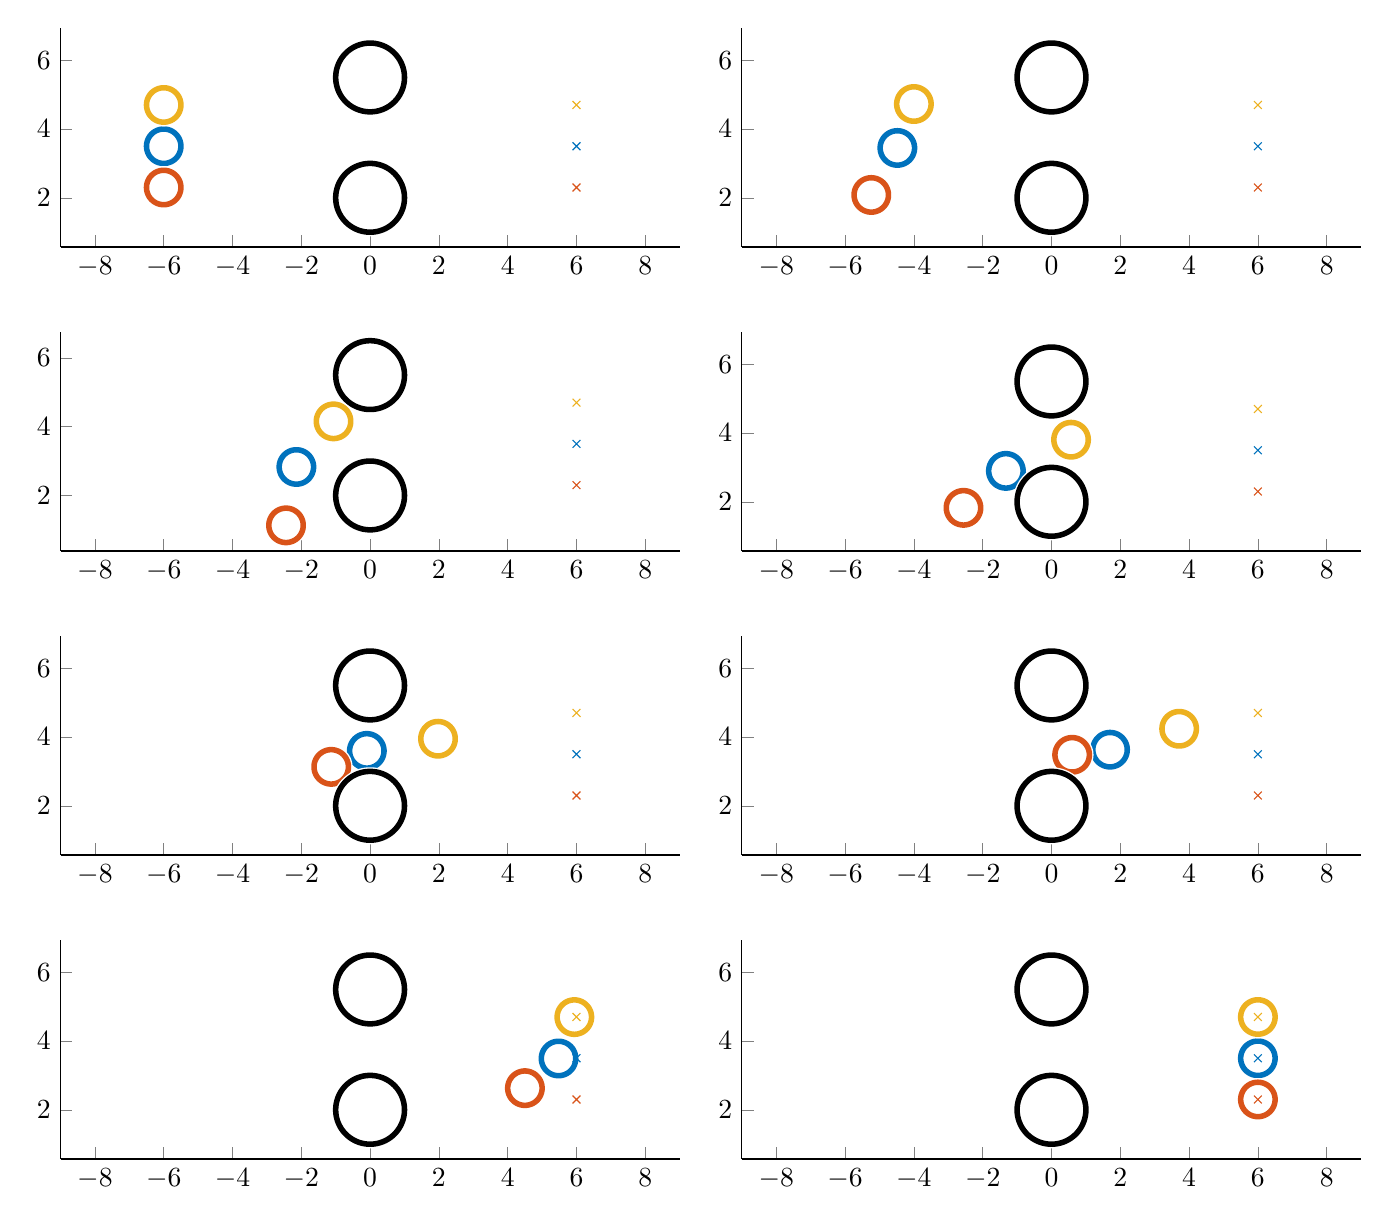
\begin{tikzpicture}

\definecolor{mycolor1}{rgb}{0.00000,0.44700,0.74100}%
\definecolor{mycolor2}{rgb}{0.85000,0.32500,0.09800}%
\definecolor{mycolor3}{rgb}{0.92900,0.69400,0.12500}%

\begin{axis}[%
width=3.096in,
height=1.094in,
at={(2.593in,5.323in)},
scale only axis,
unbounded coords=jump,
xmin=-9,
xmax=9,
%xmajorgrids,
ymin=0.568379976997646,
ymax=6.93162002300235,
%ymajorgrids,
axis background/.style={fill=white},
axis x line*=bottom,
axis y line*=left
]
\addplot [color=mycolor1,only marks,mark=x,mark options={solid},forget plot]
  table[row sep=crcr]{%
6	3.5\\
};
\addplot [color=mycolor2,only marks,mark=x,mark options={solid},forget plot]
  table[row sep=crcr]{%
6	2.3\\
};
\addplot [color=mycolor3,only marks,mark=x,mark options={solid},forget plot]
  table[row sep=crcr]{%
6	4.7\\
};
\addplot [color=white,solid,line width=3.0pt,forget plot]
  table[row sep=crcr]{%
-5.5	3.5\\
-5.50030458649045	3.51744974835125\\
-5.50121797487009	3.53487823687206\\
-5.50273905231586	3.55226423163383\\
-5.50486596562921	3.56958655048003\\
-5.5075961234939	3.58682408883347\\
-5.5109261996331	3.60395584540888\\
-5.514852136862	3.62096094779983\\
-5.51936915203084	3.6378186779085\\
-5.52447174185242	3.65450849718747\\
-5.53015368960705	3.67101007166283\\
-5.53640807271661	3.68730329670796\\
-5.5432272711787	3.7033683215379\\
-5.55060297685042	3.71918557339454\\
-5.55852620357054	3.73473578139295\\
-5.56698729810778	3.75\\
-5.57597595192179	3.7649596321166\\
-5.58548121372248	3.77959645173537\\
-5.59549150281253	3.79389262614624\\
-5.60599462319664	3.80783073766283\\
-5.61697777844051	3.82139380484327\\
-5.6284275872613	3.83456530317943\\
-5.64033009983067	3.8473291852295\\
-5.6526708147705	3.85966990016933\\
-5.66543469682057	3.8715724127387\\
-5.67860619515673	3.88302222155949\\
-5.69216926233717	3.89400537680336\\
-5.70610737385376	3.90450849718747\\
-5.72040354826463	3.91451878627752\\
-5.7350403678834	3.92402404807821\\
-5.75	3.93301270189222\\
-5.76526421860705	3.94147379642946\\
-5.78081442660546	3.94939702314958\\
-5.7966316784621	3.9567727288213\\
-5.81269670329204	3.96359192728339\\
-5.82898992833717	3.96984631039295\\
-5.84549150281253	3.97552825814758\\
-5.8621813220915	3.98063084796916\\
-5.87903905220017	3.985147863138\\
-5.89604415459112	3.9890738003669\\
-5.91317591116653	3.9924038765061\\
-5.93041344951997	3.99513403437079\\
-5.94773576836617	3.99726094768414\\
-5.96512176312794	3.99878202512991\\
-5.98255025164875	3.99969541350955\\
-6	4\\
-6.01744974835125	3.99969541350955\\
-6.03487823687206	3.99878202512991\\
-6.05226423163383	3.99726094768414\\
-6.06958655048003	3.99513403437079\\
-6.08682408883347	3.9924038765061\\
-6.10395584540888	3.9890738003669\\
-6.12096094779983	3.985147863138\\
-6.1378186779085	3.98063084796916\\
-6.15450849718747	3.97552825814758\\
-6.17101007166283	3.96984631039295\\
-6.18730329670796	3.96359192728339\\
-6.2033683215379	3.9567727288213\\
-6.21918557339454	3.94939702314958\\
-6.23473578139295	3.94147379642946\\
-6.25	3.93301270189222\\
-6.2649596321166	3.92402404807821\\
-6.27959645173537	3.91451878627752\\
-6.29389262614624	3.90450849718747\\
-6.30783073766283	3.89400537680336\\
-6.32139380484327	3.88302222155949\\
-6.33456530317943	3.8715724127387\\
-6.3473291852295	3.85966990016933\\
-6.35966990016933	3.8473291852295\\
-6.3715724127387	3.83456530317943\\
-6.38302222155949	3.82139380484327\\
-6.39400537680336	3.80783073766283\\
-6.40450849718747	3.79389262614624\\
-6.41451878627752	3.77959645173537\\
-6.42402404807821	3.7649596321166\\
-6.43301270189222	3.75\\
-6.44147379642946	3.73473578139295\\
-6.44939702314958	3.71918557339454\\
-6.4567727288213	3.7033683215379\\
-6.46359192728339	3.68730329670796\\
-6.46984631039295	3.67101007166283\\
-6.47552825814758	3.65450849718747\\
-6.48063084796916	3.6378186779085\\
-6.485147863138	3.62096094779983\\
-6.4890738003669	3.60395584540888\\
-6.4924038765061	3.58682408883347\\
-6.49513403437079	3.56958655048003\\
-6.49726094768414	3.55226423163383\\
-6.49878202512991	3.53487823687206\\
-6.49969541350955	3.51744974835125\\
-6.5	3.5\\
-6.49969541350955	3.48255025164875\\
-6.49878202512991	3.46512176312794\\
-6.49726094768414	3.44773576836617\\
-6.49513403437079	3.43041344951997\\
-6.4924038765061	3.41317591116653\\
-6.4890738003669	3.39604415459112\\
-6.485147863138	3.37903905220017\\
-6.48063084796916	3.3621813220915\\
-6.47552825814758	3.34549150281253\\
-6.46984631039295	3.32898992833717\\
-6.46359192728339	3.31269670329204\\
-6.4567727288213	3.2966316784621\\
-6.44939702314958	3.28081442660546\\
-6.44147379642946	3.26526421860705\\
-6.43301270189222	3.25\\
-6.42402404807821	3.2350403678834\\
-6.41451878627752	3.22040354826463\\
-6.40450849718747	3.20610737385376\\
-6.39400537680336	3.19216926233717\\
-6.38302222155949	3.17860619515673\\
-6.3715724127387	3.16543469682057\\
-6.35966990016933	3.1526708147705\\
-6.3473291852295	3.14033009983067\\
-6.33456530317943	3.1284275872613\\
-6.32139380484327	3.11697777844051\\
-6.30783073766283	3.10599462319664\\
-6.29389262614624	3.09549150281253\\
-6.27959645173537	3.08548121372248\\
-6.2649596321166	3.07597595192179\\
-6.25	3.06698729810778\\
-6.23473578139295	3.05852620357054\\
-6.21918557339454	3.05060297685042\\
-6.2033683215379	3.0432272711787\\
-6.18730329670796	3.03640807271661\\
-6.17101007166283	3.03015368960705\\
-6.15450849718747	3.02447174185242\\
-6.1378186779085	3.01936915203084\\
-6.12096094779983	3.014852136862\\
-6.10395584540888	3.0109261996331\\
-6.08682408883347	3.0075961234939\\
-6.06958655048003	3.00486596562921\\
-6.05226423163383	3.00273905231586\\
-6.03487823687206	3.00121797487009\\
-6.01744974835125	3.00030458649045\\
-6	3\\
-5.98255025164875	3.00030458649045\\
-5.96512176312794	3.00121797487009\\
-5.94773576836617	3.00273905231586\\
-5.93041344951997	3.00486596562921\\
-5.91317591116653	3.0075961234939\\
-5.89604415459112	3.0109261996331\\
-5.87903905220017	3.014852136862\\
-5.8621813220915	3.01936915203084\\
-5.84549150281253	3.02447174185242\\
-5.82898992833717	3.03015368960705\\
-5.81269670329204	3.03640807271661\\
-5.7966316784621	3.0432272711787\\
-5.78081442660546	3.05060297685042\\
-5.76526421860705	3.05852620357054\\
-5.75	3.06698729810778\\
-5.7350403678834	3.07597595192179\\
-5.72040354826463	3.08548121372248\\
-5.70610737385376	3.09549150281253\\
-5.69216926233717	3.10599462319664\\
-5.67860619515673	3.11697777844051\\
-5.66543469682057	3.1284275872613\\
-5.6526708147705	3.14033009983067\\
-5.64033009983067	3.1526708147705\\
-5.6284275872613	3.16543469682057\\
-5.61697777844051	3.17860619515673\\
-5.60599462319664	3.19216926233717\\
-5.59549150281253	3.20610737385376\\
-5.58548121372248	3.22040354826463\\
-5.57597595192179	3.2350403678834\\
-5.56698729810778	3.25\\
-5.55852620357054	3.26526421860705\\
-5.55060297685042	3.28081442660546\\
-5.5432272711787	3.2966316784621\\
-5.53640807271661	3.31269670329204\\
-5.53015368960705	3.32898992833717\\
-5.52447174185242	3.34549150281253\\
-5.51936915203084	3.3621813220915\\
-5.514852136862	3.37903905220017\\
-5.5109261996331	3.39604415459112\\
-5.5075961234939	3.41317591116653\\
-5.50486596562921	3.43041344951997\\
-5.50273905231586	3.44773576836617\\
-5.50121797487009	3.46512176312794\\
-5.50030458649045	3.48255025164875\\
-5.5	3.5\\
nan	nan\\
};
\addplot [color=mycolor1,solid,line width=2.0pt,forget plot]
  table[row sep=crcr]{%
-5.5	3.5\\
-5.50030458649045	3.51744974835125\\
-5.50121797487009	3.53487823687206\\
-5.50273905231586	3.55226423163383\\
-5.50486596562921	3.56958655048003\\
-5.5075961234939	3.58682408883347\\
-5.5109261996331	3.60395584540888\\
-5.514852136862	3.62096094779983\\
-5.51936915203084	3.6378186779085\\
-5.52447174185242	3.65450849718747\\
-5.53015368960705	3.67101007166283\\
-5.53640807271661	3.68730329670796\\
-5.5432272711787	3.7033683215379\\
-5.55060297685042	3.71918557339454\\
-5.55852620357054	3.73473578139295\\
-5.56698729810778	3.75\\
-5.57597595192179	3.7649596321166\\
-5.58548121372248	3.77959645173537\\
-5.59549150281253	3.79389262614624\\
-5.60599462319664	3.80783073766283\\
-5.61697777844051	3.82139380484327\\
-5.6284275872613	3.83456530317943\\
-5.64033009983067	3.8473291852295\\
-5.6526708147705	3.85966990016933\\
-5.66543469682057	3.8715724127387\\
-5.67860619515673	3.88302222155949\\
-5.69216926233717	3.89400537680336\\
-5.70610737385376	3.90450849718747\\
-5.72040354826463	3.91451878627752\\
-5.7350403678834	3.92402404807821\\
-5.75	3.93301270189222\\
-5.76526421860705	3.94147379642946\\
-5.78081442660546	3.94939702314958\\
-5.7966316784621	3.9567727288213\\
-5.81269670329204	3.96359192728339\\
-5.82898992833717	3.96984631039295\\
-5.84549150281253	3.97552825814758\\
-5.8621813220915	3.98063084796916\\
-5.87903905220017	3.985147863138\\
-5.89604415459112	3.9890738003669\\
-5.91317591116653	3.9924038765061\\
-5.93041344951997	3.99513403437079\\
-5.94773576836617	3.99726094768414\\
-5.96512176312794	3.99878202512991\\
-5.98255025164875	3.99969541350955\\
-6	4\\
-6.01744974835125	3.99969541350955\\
-6.03487823687206	3.99878202512991\\
-6.05226423163383	3.99726094768414\\
-6.06958655048003	3.99513403437079\\
-6.08682408883347	3.9924038765061\\
-6.10395584540888	3.9890738003669\\
-6.12096094779983	3.985147863138\\
-6.1378186779085	3.98063084796916\\
-6.15450849718747	3.97552825814758\\
-6.17101007166283	3.96984631039295\\
-6.18730329670796	3.96359192728339\\
-6.2033683215379	3.9567727288213\\
-6.21918557339454	3.94939702314958\\
-6.23473578139295	3.94147379642946\\
-6.25	3.93301270189222\\
-6.2649596321166	3.92402404807821\\
-6.27959645173537	3.91451878627752\\
-6.29389262614624	3.90450849718747\\
-6.30783073766283	3.89400537680336\\
-6.32139380484327	3.88302222155949\\
-6.33456530317943	3.8715724127387\\
-6.3473291852295	3.85966990016933\\
-6.35966990016933	3.8473291852295\\
-6.3715724127387	3.83456530317943\\
-6.38302222155949	3.82139380484327\\
-6.39400537680336	3.80783073766283\\
-6.40450849718747	3.79389262614624\\
-6.41451878627752	3.77959645173537\\
-6.42402404807821	3.7649596321166\\
-6.43301270189222	3.75\\
-6.44147379642946	3.73473578139295\\
-6.44939702314958	3.71918557339454\\
-6.4567727288213	3.7033683215379\\
-6.46359192728339	3.68730329670796\\
-6.46984631039295	3.67101007166283\\
-6.47552825814758	3.65450849718747\\
-6.48063084796916	3.6378186779085\\
-6.485147863138	3.62096094779983\\
-6.4890738003669	3.60395584540888\\
-6.4924038765061	3.58682408883347\\
-6.49513403437079	3.56958655048003\\
-6.49726094768414	3.55226423163383\\
-6.49878202512991	3.53487823687206\\
-6.49969541350955	3.51744974835125\\
-6.5	3.5\\
-6.49969541350955	3.48255025164875\\
-6.49878202512991	3.46512176312794\\
-6.49726094768414	3.44773576836617\\
-6.49513403437079	3.43041344951997\\
-6.4924038765061	3.41317591116653\\
-6.4890738003669	3.39604415459112\\
-6.485147863138	3.37903905220017\\
-6.48063084796916	3.3621813220915\\
-6.47552825814758	3.34549150281253\\
-6.46984631039295	3.32898992833717\\
-6.46359192728339	3.31269670329204\\
-6.4567727288213	3.2966316784621\\
-6.44939702314958	3.28081442660546\\
-6.44147379642946	3.26526421860705\\
-6.43301270189222	3.25\\
-6.42402404807821	3.2350403678834\\
-6.41451878627752	3.22040354826463\\
-6.40450849718747	3.20610737385376\\
-6.39400537680336	3.19216926233717\\
-6.38302222155949	3.17860619515673\\
-6.3715724127387	3.16543469682057\\
-6.35966990016933	3.1526708147705\\
-6.3473291852295	3.14033009983067\\
-6.33456530317943	3.1284275872613\\
-6.32139380484327	3.11697777844051\\
-6.30783073766283	3.10599462319664\\
-6.29389262614624	3.09549150281253\\
-6.27959645173537	3.08548121372248\\
-6.2649596321166	3.07597595192179\\
-6.25	3.06698729810778\\
-6.23473578139295	3.05852620357054\\
-6.21918557339454	3.05060297685042\\
-6.2033683215379	3.0432272711787\\
-6.18730329670796	3.03640807271661\\
-6.17101007166283	3.03015368960705\\
-6.15450849718747	3.02447174185242\\
-6.1378186779085	3.01936915203084\\
-6.12096094779983	3.014852136862\\
-6.10395584540888	3.0109261996331\\
-6.08682408883347	3.0075961234939\\
-6.06958655048003	3.00486596562921\\
-6.05226423163383	3.00273905231586\\
-6.03487823687206	3.00121797487009\\
-6.01744974835125	3.00030458649045\\
-6	3\\
-5.98255025164875	3.00030458649045\\
-5.96512176312794	3.00121797487009\\
-5.94773576836617	3.00273905231586\\
-5.93041344951997	3.00486596562921\\
-5.91317591116653	3.0075961234939\\
-5.89604415459112	3.0109261996331\\
-5.87903905220017	3.014852136862\\
-5.8621813220915	3.01936915203084\\
-5.84549150281253	3.02447174185242\\
-5.82898992833717	3.03015368960705\\
-5.81269670329204	3.03640807271661\\
-5.7966316784621	3.0432272711787\\
-5.78081442660546	3.05060297685042\\
-5.76526421860705	3.05852620357054\\
-5.75	3.06698729810778\\
-5.7350403678834	3.07597595192179\\
-5.72040354826463	3.08548121372248\\
-5.70610737385376	3.09549150281253\\
-5.69216926233717	3.10599462319664\\
-5.67860619515673	3.11697777844051\\
-5.66543469682057	3.1284275872613\\
-5.6526708147705	3.14033009983067\\
-5.64033009983067	3.1526708147705\\
-5.6284275872613	3.16543469682057\\
-5.61697777844051	3.17860619515673\\
-5.60599462319664	3.19216926233717\\
-5.59549150281253	3.20610737385376\\
-5.58548121372248	3.22040354826463\\
-5.57597595192179	3.2350403678834\\
-5.56698729810778	3.25\\
-5.55852620357054	3.26526421860705\\
-5.55060297685042	3.28081442660546\\
-5.5432272711787	3.2966316784621\\
-5.53640807271661	3.31269670329204\\
-5.53015368960705	3.32898992833717\\
-5.52447174185242	3.34549150281253\\
-5.51936915203084	3.3621813220915\\
-5.514852136862	3.37903905220017\\
-5.5109261996331	3.39604415459112\\
-5.5075961234939	3.41317591116653\\
-5.50486596562921	3.43041344951997\\
-5.50273905231586	3.44773576836617\\
-5.50121797487009	3.46512176312794\\
-5.50030458649045	3.48255025164875\\
-5.5	3.5\\
nan	nan\\
};
\addplot [color=white,solid,line width=3.0pt,forget plot]
  table[row sep=crcr]{%
-5.5	2.3\\
-5.50030458649045	2.31744974835125\\
-5.50121797487009	2.33487823687206\\
-5.50273905231586	2.35226423163383\\
-5.50486596562921	2.36958655048003\\
-5.5075961234939	2.38682408883346\\
-5.5109261996331	2.40395584540888\\
-5.514852136862	2.42096094779983\\
-5.51936915203084	2.4378186779085\\
-5.52447174185242	2.45450849718747\\
-5.53015368960705	2.47101007166283\\
-5.53640807271661	2.48730329670796\\
-5.5432272711787	2.5033683215379\\
-5.55060297685042	2.51918557339454\\
-5.55852620357054	2.53473578139295\\
-5.56698729810778	2.55\\
-5.57597595192179	2.5649596321166\\
-5.58548121372248	2.57959645173537\\
-5.59549150281253	2.59389262614624\\
-5.60599462319664	2.60783073766283\\
-5.61697777844051	2.62139380484327\\
-5.6284275872613	2.63456530317943\\
-5.64033009983067	2.6473291852295\\
-5.6526708147705	2.65966990016933\\
-5.66543469682057	2.6715724127387\\
-5.67860619515673	2.68302222155949\\
-5.69216926233717	2.69400537680336\\
-5.70610737385376	2.70450849718747\\
-5.72040354826463	2.71451878627752\\
-5.7350403678834	2.72402404807821\\
-5.75	2.73301270189222\\
-5.76526421860705	2.74147379642946\\
-5.78081442660546	2.74939702314958\\
-5.7966316784621	2.7567727288213\\
-5.81269670329204	2.76359192728339\\
-5.82898992833717	2.76984631039295\\
-5.84549150281253	2.77552825814758\\
-5.8621813220915	2.78063084796916\\
-5.87903905220017	2.785147863138\\
-5.89604415459112	2.7890738003669\\
-5.91317591116653	2.7924038765061\\
-5.93041344951997	2.79513403437078\\
-5.94773576836617	2.79726094768414\\
-5.96512176312794	2.79878202512991\\
-5.98255025164875	2.79969541350955\\
-6	2.8\\
-6.01744974835125	2.79969541350955\\
-6.03487823687206	2.79878202512991\\
-6.05226423163383	2.79726094768414\\
-6.06958655048003	2.79513403437078\\
-6.08682408883347	2.7924038765061\\
-6.10395584540888	2.7890738003669\\
-6.12096094779983	2.785147863138\\
-6.1378186779085	2.78063084796916\\
-6.15450849718747	2.77552825814758\\
-6.17101007166283	2.76984631039295\\
-6.18730329670796	2.76359192728339\\
-6.2033683215379	2.7567727288213\\
-6.21918557339454	2.74939702314958\\
-6.23473578139295	2.74147379642946\\
-6.25	2.73301270189222\\
-6.2649596321166	2.72402404807821\\
-6.27959645173537	2.71451878627752\\
-6.29389262614624	2.70450849718747\\
-6.30783073766283	2.69400537680336\\
-6.32139380484327	2.68302222155949\\
-6.33456530317943	2.6715724127387\\
-6.3473291852295	2.65966990016933\\
-6.35966990016933	2.6473291852295\\
-6.3715724127387	2.63456530317943\\
-6.38302222155949	2.62139380484327\\
-6.39400537680336	2.60783073766283\\
-6.40450849718747	2.59389262614624\\
-6.41451878627752	2.57959645173537\\
-6.42402404807821	2.5649596321166\\
-6.43301270189222	2.55\\
-6.44147379642946	2.53473578139295\\
-6.44939702314958	2.51918557339454\\
-6.4567727288213	2.5033683215379\\
-6.46359192728339	2.48730329670796\\
-6.46984631039295	2.47101007166283\\
-6.47552825814758	2.45450849718747\\
-6.48063084796916	2.4378186779085\\
-6.485147863138	2.42096094779983\\
-6.4890738003669	2.40395584540888\\
-6.4924038765061	2.38682408883346\\
-6.49513403437079	2.36958655048003\\
-6.49726094768414	2.35226423163383\\
-6.49878202512991	2.33487823687206\\
-6.49969541350955	2.31744974835125\\
-6.5	2.3\\
-6.49969541350955	2.28255025164875\\
-6.49878202512991	2.26512176312794\\
-6.49726094768414	2.24773576836617\\
-6.49513403437079	2.23041344951997\\
-6.4924038765061	2.21317591116653\\
-6.4890738003669	2.19604415459112\\
-6.485147863138	2.17903905220017\\
-6.48063084796916	2.1621813220915\\
-6.47552825814758	2.14549150281253\\
-6.46984631039295	2.12898992833717\\
-6.46359192728339	2.11269670329204\\
-6.4567727288213	2.0966316784621\\
-6.44939702314958	2.08081442660546\\
-6.44147379642946	2.06526421860705\\
-6.43301270189222	2.05\\
-6.42402404807821	2.0350403678834\\
-6.41451878627752	2.02040354826463\\
-6.40450849718747	2.00610737385376\\
-6.39400537680336	1.99216926233717\\
-6.38302222155949	1.97860619515673\\
-6.3715724127387	1.96543469682057\\
-6.35966990016933	1.9526708147705\\
-6.3473291852295	1.94033009983067\\
-6.33456530317943	1.9284275872613\\
-6.32139380484327	1.91697777844051\\
-6.30783073766283	1.90599462319664\\
-6.29389262614624	1.89549150281253\\
-6.27959645173537	1.88548121372248\\
-6.2649596321166	1.87597595192179\\
-6.25	1.86698729810778\\
-6.23473578139295	1.85852620357054\\
-6.21918557339454	1.85060297685042\\
-6.2033683215379	1.8432272711787\\
-6.18730329670796	1.83640807271661\\
-6.17101007166283	1.83015368960705\\
-6.15450849718747	1.82447174185242\\
-6.1378186779085	1.81936915203084\\
-6.12096094779983	1.814852136862\\
-6.10395584540888	1.8109261996331\\
-6.08682408883347	1.8075961234939\\
-6.06958655048003	1.80486596562921\\
-6.05226423163383	1.80273905231586\\
-6.03487823687206	1.80121797487009\\
-6.01744974835125	1.80030458649045\\
-6	1.8\\
-5.98255025164875	1.80030458649045\\
-5.96512176312794	1.80121797487009\\
-5.94773576836617	1.80273905231586\\
-5.93041344951997	1.80486596562921\\
-5.91317591116653	1.8075961234939\\
-5.89604415459112	1.8109261996331\\
-5.87903905220017	1.814852136862\\
-5.8621813220915	1.81936915203084\\
-5.84549150281253	1.82447174185242\\
-5.82898992833717	1.83015368960705\\
-5.81269670329204	1.83640807271661\\
-5.7966316784621	1.8432272711787\\
-5.78081442660546	1.85060297685042\\
-5.76526421860705	1.85852620357054\\
-5.75	1.86698729810778\\
-5.7350403678834	1.87597595192179\\
-5.72040354826463	1.88548121372248\\
-5.70610737385376	1.89549150281253\\
-5.69216926233717	1.90599462319664\\
-5.67860619515673	1.91697777844051\\
-5.66543469682057	1.9284275872613\\
-5.6526708147705	1.94033009983067\\
-5.64033009983067	1.9526708147705\\
-5.6284275872613	1.96543469682057\\
-5.61697777844051	1.97860619515673\\
-5.60599462319664	1.99216926233717\\
-5.59549150281253	2.00610737385376\\
-5.58548121372248	2.02040354826463\\
-5.57597595192179	2.0350403678834\\
-5.56698729810778	2.05\\
-5.55852620357054	2.06526421860705\\
-5.55060297685042	2.08081442660546\\
-5.5432272711787	2.0966316784621\\
-5.53640807271661	2.11269670329204\\
-5.53015368960705	2.12898992833717\\
-5.52447174185242	2.14549150281253\\
-5.51936915203084	2.1621813220915\\
-5.514852136862	2.17903905220017\\
-5.5109261996331	2.19604415459112\\
-5.5075961234939	2.21317591116653\\
-5.50486596562921	2.23041344951997\\
-5.50273905231586	2.24773576836617\\
-5.50121797487009	2.26512176312794\\
-5.50030458649045	2.28255025164875\\
-5.5	2.3\\
nan	nan\\
};
\addplot [color=mycolor2,solid,line width=2.0pt,forget plot]
  table[row sep=crcr]{%
-5.5	2.3\\
-5.50030458649045	2.31744974835125\\
-5.50121797487009	2.33487823687206\\
-5.50273905231586	2.35226423163383\\
-5.50486596562921	2.36958655048003\\
-5.5075961234939	2.38682408883346\\
-5.5109261996331	2.40395584540888\\
-5.514852136862	2.42096094779983\\
-5.51936915203084	2.4378186779085\\
-5.52447174185242	2.45450849718747\\
-5.53015368960705	2.47101007166283\\
-5.53640807271661	2.48730329670796\\
-5.5432272711787	2.5033683215379\\
-5.55060297685042	2.51918557339454\\
-5.55852620357054	2.53473578139295\\
-5.56698729810778	2.55\\
-5.57597595192179	2.5649596321166\\
-5.58548121372248	2.57959645173537\\
-5.59549150281253	2.59389262614624\\
-5.60599462319664	2.60783073766283\\
-5.61697777844051	2.62139380484327\\
-5.6284275872613	2.63456530317943\\
-5.64033009983067	2.6473291852295\\
-5.6526708147705	2.65966990016933\\
-5.66543469682057	2.6715724127387\\
-5.67860619515673	2.68302222155949\\
-5.69216926233717	2.69400537680336\\
-5.70610737385376	2.70450849718747\\
-5.72040354826463	2.71451878627752\\
-5.7350403678834	2.72402404807821\\
-5.75	2.73301270189222\\
-5.76526421860705	2.74147379642946\\
-5.78081442660546	2.74939702314958\\
-5.7966316784621	2.7567727288213\\
-5.81269670329204	2.76359192728339\\
-5.82898992833717	2.76984631039295\\
-5.84549150281253	2.77552825814758\\
-5.8621813220915	2.78063084796916\\
-5.87903905220017	2.785147863138\\
-5.89604415459112	2.7890738003669\\
-5.91317591116653	2.7924038765061\\
-5.93041344951997	2.79513403437078\\
-5.94773576836617	2.79726094768414\\
-5.96512176312794	2.79878202512991\\
-5.98255025164875	2.79969541350955\\
-6	2.8\\
-6.01744974835125	2.79969541350955\\
-6.03487823687206	2.79878202512991\\
-6.05226423163383	2.79726094768414\\
-6.06958655048003	2.79513403437078\\
-6.08682408883347	2.7924038765061\\
-6.10395584540888	2.7890738003669\\
-6.12096094779983	2.785147863138\\
-6.1378186779085	2.78063084796916\\
-6.15450849718747	2.77552825814758\\
-6.17101007166283	2.76984631039295\\
-6.18730329670796	2.76359192728339\\
-6.2033683215379	2.7567727288213\\
-6.21918557339454	2.74939702314958\\
-6.23473578139295	2.74147379642946\\
-6.25	2.73301270189222\\
-6.2649596321166	2.72402404807821\\
-6.27959645173537	2.71451878627752\\
-6.29389262614624	2.70450849718747\\
-6.30783073766283	2.69400537680336\\
-6.32139380484327	2.68302222155949\\
-6.33456530317943	2.6715724127387\\
-6.3473291852295	2.65966990016933\\
-6.35966990016933	2.6473291852295\\
-6.3715724127387	2.63456530317943\\
-6.38302222155949	2.62139380484327\\
-6.39400537680336	2.60783073766283\\
-6.40450849718747	2.59389262614624\\
-6.41451878627752	2.57959645173537\\
-6.42402404807821	2.5649596321166\\
-6.43301270189222	2.55\\
-6.44147379642946	2.53473578139295\\
-6.44939702314958	2.51918557339454\\
-6.4567727288213	2.5033683215379\\
-6.46359192728339	2.48730329670796\\
-6.46984631039295	2.47101007166283\\
-6.47552825814758	2.45450849718747\\
-6.48063084796916	2.4378186779085\\
-6.485147863138	2.42096094779983\\
-6.4890738003669	2.40395584540888\\
-6.4924038765061	2.38682408883346\\
-6.49513403437079	2.36958655048003\\
-6.49726094768414	2.35226423163383\\
-6.49878202512991	2.33487823687206\\
-6.49969541350955	2.31744974835125\\
-6.5	2.3\\
-6.49969541350955	2.28255025164875\\
-6.49878202512991	2.26512176312794\\
-6.49726094768414	2.24773576836617\\
-6.49513403437079	2.23041344951997\\
-6.4924038765061	2.21317591116653\\
-6.4890738003669	2.19604415459112\\
-6.485147863138	2.17903905220017\\
-6.48063084796916	2.1621813220915\\
-6.47552825814758	2.14549150281253\\
-6.46984631039295	2.12898992833717\\
-6.46359192728339	2.11269670329204\\
-6.4567727288213	2.0966316784621\\
-6.44939702314958	2.08081442660546\\
-6.44147379642946	2.06526421860705\\
-6.43301270189222	2.05\\
-6.42402404807821	2.0350403678834\\
-6.41451878627752	2.02040354826463\\
-6.40450849718747	2.00610737385376\\
-6.39400537680336	1.99216926233717\\
-6.38302222155949	1.97860619515673\\
-6.3715724127387	1.96543469682057\\
-6.35966990016933	1.9526708147705\\
-6.3473291852295	1.94033009983067\\
-6.33456530317943	1.9284275872613\\
-6.32139380484327	1.91697777844051\\
-6.30783073766283	1.90599462319664\\
-6.29389262614624	1.89549150281253\\
-6.27959645173537	1.88548121372248\\
-6.2649596321166	1.87597595192179\\
-6.25	1.86698729810778\\
-6.23473578139295	1.85852620357054\\
-6.21918557339454	1.85060297685042\\
-6.2033683215379	1.8432272711787\\
-6.18730329670796	1.83640807271661\\
-6.17101007166283	1.83015368960705\\
-6.15450849718747	1.82447174185242\\
-6.1378186779085	1.81936915203084\\
-6.12096094779983	1.814852136862\\
-6.10395584540888	1.8109261996331\\
-6.08682408883347	1.8075961234939\\
-6.06958655048003	1.80486596562921\\
-6.05226423163383	1.80273905231586\\
-6.03487823687206	1.80121797487009\\
-6.01744974835125	1.80030458649045\\
-6	1.8\\
-5.98255025164875	1.80030458649045\\
-5.96512176312794	1.80121797487009\\
-5.94773576836617	1.80273905231586\\
-5.93041344951997	1.80486596562921\\
-5.91317591116653	1.8075961234939\\
-5.89604415459112	1.8109261996331\\
-5.87903905220017	1.814852136862\\
-5.8621813220915	1.81936915203084\\
-5.84549150281253	1.82447174185242\\
-5.82898992833717	1.83015368960705\\
-5.81269670329204	1.83640807271661\\
-5.7966316784621	1.8432272711787\\
-5.78081442660546	1.85060297685042\\
-5.76526421860705	1.85852620357054\\
-5.75	1.86698729810778\\
-5.7350403678834	1.87597595192179\\
-5.72040354826463	1.88548121372248\\
-5.70610737385376	1.89549150281253\\
-5.69216926233717	1.90599462319664\\
-5.67860619515673	1.91697777844051\\
-5.66543469682057	1.9284275872613\\
-5.6526708147705	1.94033009983067\\
-5.64033009983067	1.9526708147705\\
-5.6284275872613	1.96543469682057\\
-5.61697777844051	1.97860619515673\\
-5.60599462319664	1.99216926233717\\
-5.59549150281253	2.00610737385376\\
-5.58548121372248	2.02040354826463\\
-5.57597595192179	2.0350403678834\\
-5.56698729810778	2.05\\
-5.55852620357054	2.06526421860705\\
-5.55060297685042	2.08081442660546\\
-5.5432272711787	2.0966316784621\\
-5.53640807271661	2.11269670329204\\
-5.53015368960705	2.12898992833717\\
-5.52447174185242	2.14549150281253\\
-5.51936915203084	2.1621813220915\\
-5.514852136862	2.17903905220017\\
-5.5109261996331	2.19604415459112\\
-5.5075961234939	2.21317591116653\\
-5.50486596562921	2.23041344951997\\
-5.50273905231586	2.24773576836617\\
-5.50121797487009	2.26512176312794\\
-5.50030458649045	2.28255025164875\\
-5.5	2.3\\
nan	nan\\
};
\addplot [color=white,solid,line width=3.0pt,forget plot]
  table[row sep=crcr]{%
-5.5	4.7\\
-5.50030458649045	4.71744974835125\\
-5.50121797487009	4.73487823687206\\
-5.50273905231586	4.75226423163383\\
-5.50486596562921	4.76958655048003\\
-5.5075961234939	4.78682408883347\\
-5.5109261996331	4.80395584540888\\
-5.514852136862	4.82096094779983\\
-5.51936915203084	4.8378186779085\\
-5.52447174185242	4.85450849718747\\
-5.53015368960705	4.87101007166283\\
-5.53640807271661	4.88730329670796\\
-5.5432272711787	4.9033683215379\\
-5.55060297685042	4.91918557339454\\
-5.55852620357054	4.93473578139295\\
-5.56698729810778	4.95\\
-5.57597595192179	4.9649596321166\\
-5.58548121372248	4.97959645173537\\
-5.59549150281253	4.99389262614624\\
-5.60599462319664	5.00783073766283\\
-5.61697777844051	5.02139380484327\\
-5.6284275872613	5.03456530317943\\
-5.64033009983067	5.0473291852295\\
-5.6526708147705	5.05966990016933\\
-5.66543469682057	5.0715724127387\\
-5.67860619515673	5.08302222155949\\
-5.69216926233717	5.09400537680336\\
-5.70610737385376	5.10450849718747\\
-5.72040354826463	5.11451878627752\\
-5.7350403678834	5.12402404807821\\
-5.75	5.13301270189222\\
-5.76526421860705	5.14147379642946\\
-5.78081442660546	5.14939702314958\\
-5.7966316784621	5.1567727288213\\
-5.81269670329204	5.16359192728339\\
-5.82898992833717	5.16984631039295\\
-5.84549150281253	5.17552825814758\\
-5.8621813220915	5.18063084796916\\
-5.87903905220017	5.185147863138\\
-5.89604415459112	5.1890738003669\\
-5.91317591116653	5.1924038765061\\
-5.93041344951997	5.19513403437079\\
-5.94773576836617	5.19726094768414\\
-5.96512176312794	5.19878202512991\\
-5.98255025164875	5.19969541350955\\
-6	5.2\\
-6.01744974835125	5.19969541350955\\
-6.03487823687206	5.19878202512991\\
-6.05226423163383	5.19726094768414\\
-6.06958655048003	5.19513403437079\\
-6.08682408883347	5.1924038765061\\
-6.10395584540888	5.1890738003669\\
-6.12096094779983	5.185147863138\\
-6.1378186779085	5.18063084796916\\
-6.15450849718747	5.17552825814758\\
-6.17101007166283	5.16984631039295\\
-6.18730329670796	5.16359192728339\\
-6.2033683215379	5.1567727288213\\
-6.21918557339454	5.14939702314958\\
-6.23473578139295	5.14147379642946\\
-6.25	5.13301270189222\\
-6.2649596321166	5.12402404807821\\
-6.27959645173537	5.11451878627752\\
-6.29389262614624	5.10450849718747\\
-6.30783073766283	5.09400537680336\\
-6.32139380484327	5.08302222155949\\
-6.33456530317943	5.0715724127387\\
-6.3473291852295	5.05966990016933\\
-6.35966990016933	5.0473291852295\\
-6.3715724127387	5.03456530317943\\
-6.38302222155949	5.02139380484327\\
-6.39400537680336	5.00783073766283\\
-6.40450849718747	4.99389262614624\\
-6.41451878627752	4.97959645173537\\
-6.42402404807821	4.9649596321166\\
-6.43301270189222	4.95\\
-6.44147379642946	4.93473578139295\\
-6.44939702314958	4.91918557339454\\
-6.4567727288213	4.9033683215379\\
-6.46359192728339	4.88730329670796\\
-6.46984631039295	4.87101007166283\\
-6.47552825814758	4.85450849718747\\
-6.48063084796916	4.8378186779085\\
-6.485147863138	4.82096094779983\\
-6.4890738003669	4.80395584540888\\
-6.4924038765061	4.78682408883347\\
-6.49513403437079	4.76958655048003\\
-6.49726094768414	4.75226423163383\\
-6.49878202512991	4.73487823687206\\
-6.49969541350955	4.71744974835125\\
-6.5	4.7\\
-6.49969541350955	4.68255025164875\\
-6.49878202512991	4.66512176312794\\
-6.49726094768414	4.64773576836617\\
-6.49513403437079	4.63041344951997\\
-6.4924038765061	4.61317591116654\\
-6.4890738003669	4.59604415459112\\
-6.485147863138	4.57903905220017\\
-6.48063084796916	4.5621813220915\\
-6.47552825814758	4.54549150281253\\
-6.46984631039295	4.52898992833717\\
-6.46359192728339	4.51269670329204\\
-6.4567727288213	4.4966316784621\\
-6.44939702314958	4.48081442660546\\
-6.44147379642946	4.46526421860705\\
-6.43301270189222	4.45\\
-6.42402404807821	4.4350403678834\\
-6.41451878627752	4.42040354826463\\
-6.40450849718747	4.40610737385376\\
-6.39400537680336	4.39216926233717\\
-6.38302222155949	4.37860619515673\\
-6.3715724127387	4.36543469682057\\
-6.35966990016933	4.3526708147705\\
-6.3473291852295	4.34033009983068\\
-6.33456530317943	4.3284275872613\\
-6.32139380484327	4.31697777844051\\
-6.30783073766283	4.30599462319664\\
-6.29389262614624	4.29549150281253\\
-6.27959645173537	4.28548121372248\\
-6.2649596321166	4.27597595192179\\
-6.25	4.26698729810778\\
-6.23473578139295	4.25852620357054\\
-6.21918557339454	4.25060297685042\\
-6.2033683215379	4.2432272711787\\
-6.18730329670796	4.23640807271661\\
-6.17101007166283	4.23015368960705\\
-6.15450849718747	4.22447174185242\\
-6.1378186779085	4.21936915203084\\
-6.12096094779983	4.214852136862\\
-6.10395584540888	4.2109261996331\\
-6.08682408883347	4.2075961234939\\
-6.06958655048003	4.20486596562921\\
-6.05226423163383	4.20273905231586\\
-6.03487823687206	4.20121797487009\\
-6.01744974835125	4.20030458649045\\
-6	4.2\\
-5.98255025164875	4.20030458649045\\
-5.96512176312794	4.20121797487009\\
-5.94773576836617	4.20273905231586\\
-5.93041344951997	4.20486596562921\\
-5.91317591116653	4.2075961234939\\
-5.89604415459112	4.2109261996331\\
-5.87903905220017	4.214852136862\\
-5.8621813220915	4.21936915203084\\
-5.84549150281253	4.22447174185242\\
-5.82898992833717	4.23015368960705\\
-5.81269670329204	4.23640807271661\\
-5.7966316784621	4.2432272711787\\
-5.78081442660546	4.25060297685042\\
-5.76526421860705	4.25852620357054\\
-5.75	4.26698729810778\\
-5.7350403678834	4.27597595192179\\
-5.72040354826463	4.28548121372248\\
-5.70610737385376	4.29549150281253\\
-5.69216926233717	4.30599462319664\\
-5.67860619515673	4.31697777844051\\
-5.66543469682057	4.3284275872613\\
-5.6526708147705	4.34033009983067\\
-5.64033009983067	4.3526708147705\\
-5.6284275872613	4.36543469682057\\
-5.61697777844051	4.37860619515673\\
-5.60599462319664	4.39216926233717\\
-5.59549150281253	4.40610737385376\\
-5.58548121372248	4.42040354826463\\
-5.57597595192179	4.4350403678834\\
-5.56698729810778	4.45\\
-5.55852620357054	4.46526421860705\\
-5.55060297685042	4.48081442660546\\
-5.5432272711787	4.4966316784621\\
-5.53640807271661	4.51269670329204\\
-5.53015368960705	4.52898992833717\\
-5.52447174185242	4.54549150281253\\
-5.51936915203084	4.5621813220915\\
-5.514852136862	4.57903905220017\\
-5.5109261996331	4.59604415459112\\
-5.5075961234939	4.61317591116653\\
-5.50486596562921	4.63041344951997\\
-5.50273905231586	4.64773576836617\\
-5.50121797487009	4.66512176312794\\
-5.50030458649045	4.68255025164875\\
-5.5	4.7\\
nan	nan\\
};
\addplot [color=mycolor3,solid,line width=2.0pt,forget plot]
  table[row sep=crcr]{%
-5.5	4.7\\
-5.50030458649045	4.71744974835125\\
-5.50121797487009	4.73487823687206\\
-5.50273905231586	4.75226423163383\\
-5.50486596562921	4.76958655048003\\
-5.5075961234939	4.78682408883347\\
-5.5109261996331	4.80395584540888\\
-5.514852136862	4.82096094779983\\
-5.51936915203084	4.8378186779085\\
-5.52447174185242	4.85450849718747\\
-5.53015368960705	4.87101007166283\\
-5.53640807271661	4.88730329670796\\
-5.5432272711787	4.9033683215379\\
-5.55060297685042	4.91918557339454\\
-5.55852620357054	4.93473578139295\\
-5.56698729810778	4.95\\
-5.57597595192179	4.9649596321166\\
-5.58548121372248	4.97959645173537\\
-5.59549150281253	4.99389262614624\\
-5.60599462319664	5.00783073766283\\
-5.61697777844051	5.02139380484327\\
-5.6284275872613	5.03456530317943\\
-5.64033009983067	5.0473291852295\\
-5.6526708147705	5.05966990016933\\
-5.66543469682057	5.0715724127387\\
-5.67860619515673	5.08302222155949\\
-5.69216926233717	5.09400537680336\\
-5.70610737385376	5.10450849718747\\
-5.72040354826463	5.11451878627752\\
-5.7350403678834	5.12402404807821\\
-5.75	5.13301270189222\\
-5.76526421860705	5.14147379642946\\
-5.78081442660546	5.14939702314958\\
-5.7966316784621	5.1567727288213\\
-5.81269670329204	5.16359192728339\\
-5.82898992833717	5.16984631039295\\
-5.84549150281253	5.17552825814758\\
-5.8621813220915	5.18063084796916\\
-5.87903905220017	5.185147863138\\
-5.89604415459112	5.1890738003669\\
-5.91317591116653	5.1924038765061\\
-5.93041344951997	5.19513403437079\\
-5.94773576836617	5.19726094768414\\
-5.96512176312794	5.19878202512991\\
-5.98255025164875	5.19969541350955\\
-6	5.2\\
-6.01744974835125	5.19969541350955\\
-6.03487823687206	5.19878202512991\\
-6.05226423163383	5.19726094768414\\
-6.06958655048003	5.19513403437079\\
-6.08682408883347	5.1924038765061\\
-6.10395584540888	5.1890738003669\\
-6.12096094779983	5.185147863138\\
-6.1378186779085	5.18063084796916\\
-6.15450849718747	5.17552825814758\\
-6.17101007166283	5.16984631039295\\
-6.18730329670796	5.16359192728339\\
-6.2033683215379	5.1567727288213\\
-6.21918557339454	5.14939702314958\\
-6.23473578139295	5.14147379642946\\
-6.25	5.13301270189222\\
-6.2649596321166	5.12402404807821\\
-6.27959645173537	5.11451878627752\\
-6.29389262614624	5.10450849718747\\
-6.30783073766283	5.09400537680336\\
-6.32139380484327	5.08302222155949\\
-6.33456530317943	5.0715724127387\\
-6.3473291852295	5.05966990016933\\
-6.35966990016933	5.0473291852295\\
-6.3715724127387	5.03456530317943\\
-6.38302222155949	5.02139380484327\\
-6.39400537680336	5.00783073766283\\
-6.40450849718747	4.99389262614624\\
-6.41451878627752	4.97959645173537\\
-6.42402404807821	4.9649596321166\\
-6.43301270189222	4.95\\
-6.44147379642946	4.93473578139295\\
-6.44939702314958	4.91918557339454\\
-6.4567727288213	4.9033683215379\\
-6.46359192728339	4.88730329670796\\
-6.46984631039295	4.87101007166283\\
-6.47552825814758	4.85450849718747\\
-6.48063084796916	4.8378186779085\\
-6.485147863138	4.82096094779983\\
-6.4890738003669	4.80395584540888\\
-6.4924038765061	4.78682408883347\\
-6.49513403437079	4.76958655048003\\
-6.49726094768414	4.75226423163383\\
-6.49878202512991	4.73487823687206\\
-6.49969541350955	4.71744974835125\\
-6.5	4.7\\
-6.49969541350955	4.68255025164875\\
-6.49878202512991	4.66512176312794\\
-6.49726094768414	4.64773576836617\\
-6.49513403437079	4.63041344951997\\
-6.4924038765061	4.61317591116654\\
-6.4890738003669	4.59604415459112\\
-6.485147863138	4.57903905220017\\
-6.48063084796916	4.5621813220915\\
-6.47552825814758	4.54549150281253\\
-6.46984631039295	4.52898992833717\\
-6.46359192728339	4.51269670329204\\
-6.4567727288213	4.4966316784621\\
-6.44939702314958	4.48081442660546\\
-6.44147379642946	4.46526421860705\\
-6.43301270189222	4.45\\
-6.42402404807821	4.4350403678834\\
-6.41451878627752	4.42040354826463\\
-6.40450849718747	4.40610737385376\\
-6.39400537680336	4.39216926233717\\
-6.38302222155949	4.37860619515673\\
-6.3715724127387	4.36543469682057\\
-6.35966990016933	4.3526708147705\\
-6.3473291852295	4.34033009983068\\
-6.33456530317943	4.3284275872613\\
-6.32139380484327	4.31697777844051\\
-6.30783073766283	4.30599462319664\\
-6.29389262614624	4.29549150281253\\
-6.27959645173537	4.28548121372248\\
-6.2649596321166	4.27597595192179\\
-6.25	4.26698729810778\\
-6.23473578139295	4.25852620357054\\
-6.21918557339454	4.25060297685042\\
-6.2033683215379	4.2432272711787\\
-6.18730329670796	4.23640807271661\\
-6.17101007166283	4.23015368960705\\
-6.15450849718747	4.22447174185242\\
-6.1378186779085	4.21936915203084\\
-6.12096094779983	4.214852136862\\
-6.10395584540888	4.2109261996331\\
-6.08682408883347	4.2075961234939\\
-6.06958655048003	4.20486596562921\\
-6.05226423163383	4.20273905231586\\
-6.03487823687206	4.20121797487009\\
-6.01744974835125	4.20030458649045\\
-6	4.2\\
-5.98255025164875	4.20030458649045\\
-5.96512176312794	4.20121797487009\\
-5.94773576836617	4.20273905231586\\
-5.93041344951997	4.20486596562921\\
-5.91317591116653	4.2075961234939\\
-5.89604415459112	4.2109261996331\\
-5.87903905220017	4.214852136862\\
-5.8621813220915	4.21936915203084\\
-5.84549150281253	4.22447174185242\\
-5.82898992833717	4.23015368960705\\
-5.81269670329204	4.23640807271661\\
-5.7966316784621	4.2432272711787\\
-5.78081442660546	4.25060297685042\\
-5.76526421860705	4.25852620357054\\
-5.75	4.26698729810778\\
-5.7350403678834	4.27597595192179\\
-5.72040354826463	4.28548121372248\\
-5.70610737385376	4.29549150281253\\
-5.69216926233717	4.30599462319664\\
-5.67860619515673	4.31697777844051\\
-5.66543469682057	4.3284275872613\\
-5.6526708147705	4.34033009983067\\
-5.64033009983067	4.3526708147705\\
-5.6284275872613	4.36543469682057\\
-5.61697777844051	4.37860619515673\\
-5.60599462319664	4.39216926233717\\
-5.59549150281253	4.40610737385376\\
-5.58548121372248	4.42040354826463\\
-5.57597595192179	4.4350403678834\\
-5.56698729810778	4.45\\
-5.55852620357054	4.46526421860705\\
-5.55060297685042	4.48081442660546\\
-5.5432272711787	4.4966316784621\\
-5.53640807271661	4.51269670329204\\
-5.53015368960705	4.52898992833717\\
-5.52447174185242	4.54549150281253\\
-5.51936915203084	4.5621813220915\\
-5.514852136862	4.57903905220017\\
-5.5109261996331	4.59604415459112\\
-5.5075961234939	4.61317591116653\\
-5.50486596562921	4.63041344951997\\
-5.50273905231586	4.64773576836617\\
-5.50121797487009	4.66512176312794\\
-5.50030458649045	4.68255025164875\\
-5.5	4.7\\
nan	nan\\
};
\addplot [color=white,solid,line width=3.0pt,forget plot]
  table[row sep=crcr]{%
1	2\\
0.999390827019096	2.0348994967025\\
0.997564050259824	2.06975647374413\\
0.994521895368273	2.10452846326765\\
0.99026806874157	2.13917310096007\\
0.984807753012208	2.17364817766693\\
0.978147600733806	2.20791169081776\\
0.970295726275996	2.24192189559967\\
0.961261695938319	2.275637355817\\
0.951056516295154	2.30901699437495\\
0.939692620785908	2.34202014332567\\
0.927183854566787	2.37460659341591\\
0.913545457642601	2.4067366430758\\
0.898794046299167	2.43837114678908\\
0.882947592858927	2.46947156278589\\
0.866025403784439	2.5\\
0.848048096156426	2.5299192642332\\
0.829037572555042	2.55919290347075\\
0.809016994374947	2.58778525229247\\
0.788010753606722	2.61566147532566\\
0.766044443118978	2.64278760968654\\
0.743144825477394	2.66913060635886\\
0.719339800338651	2.694658370459\\
0.694658370458997	2.71933980033865\\
0.669130606358858	2.74314482547739\\
0.642787609686539	2.76604444311898\\
0.615661475325658	2.78801075360672\\
0.587785252292473	2.80901699437495\\
0.559192903470747	2.82903757255504\\
0.529919264233205	2.84804809615643\\
0.5	2.86602540378444\\
0.469471562785891	2.88294759285893\\
0.438371146789077	2.89879404629917\\
0.4067366430758	2.9135454576426\\
0.374606593415912	2.92718385456679\\
0.342020143325669	2.93969262078591\\
0.309016994374947	2.95105651629515\\
0.275637355816999	2.96126169593832\\
0.241921895599668	2.970295726276\\
0.207911690817759	2.97814760073381\\
0.17364817766693	2.98480775301221\\
0.139173100960066	2.99026806874157\\
0.104528463267653	2.99452189536827\\
0.0697564737441255	2.99756405025982\\
0.0348994967025011	2.9993908270191\\
6.12323399573677e-17	3\\
-0.0348994967025007	2.9993908270191\\
-0.0697564737441253	2.99756405025982\\
-0.104528463267653	2.99452189536827\\
-0.139173100960065	2.99026806874157\\
-0.17364817766693	2.98480775301221\\
-0.207911690817759	2.97814760073381\\
-0.241921895599668	2.970295726276\\
-0.275637355816999	2.96126169593832\\
-0.309016994374947	2.95105651629515\\
-0.342020143325669	2.93969262078591\\
-0.374606593415912	2.92718385456679\\
-0.4067366430758	2.9135454576426\\
-0.438371146789078	2.89879404629917\\
-0.469471562785891	2.88294759285893\\
-0.5	2.86602540378444\\
-0.529919264233205	2.84804809615643\\
-0.559192903470747	2.82903757255504\\
-0.587785252292473	2.80901699437495\\
-0.615661475325658	2.78801075360672\\
-0.642787609686539	2.76604444311898\\
-0.669130606358858	2.74314482547739\\
-0.694658370458997	2.71933980033865\\
-0.719339800338651	2.694658370459\\
-0.743144825477394	2.66913060635886\\
-0.766044443118978	2.64278760968654\\
-0.788010753606722	2.61566147532566\\
-0.809016994374947	2.58778525229247\\
-0.829037572555042	2.55919290347075\\
-0.848048096156426	2.5299192642332\\
-0.866025403784439	2.5\\
-0.882947592858927	2.46947156278589\\
-0.898794046299167	2.43837114678908\\
-0.913545457642601	2.4067366430758\\
-0.927183854566787	2.37460659341591\\
-0.939692620785908	2.34202014332567\\
-0.951056516295154	2.30901699437495\\
-0.961261695938319	2.275637355817\\
-0.970295726275996	2.24192189559967\\
-0.978147600733806	2.20791169081776\\
-0.984807753012208	2.17364817766693\\
-0.99026806874157	2.13917310096007\\
-0.994521895368273	2.10452846326765\\
-0.997564050259824	2.06975647374413\\
-0.999390827019096	2.0348994967025\\
-1	2\\
-0.999390827019096	1.9651005032975\\
-0.997564050259824	1.93024352625588\\
-0.994521895368273	1.89547153673235\\
-0.99026806874157	1.86082689903993\\
-0.984807753012208	1.82635182233307\\
-0.978147600733806	1.79208830918224\\
-0.970295726275997	1.75807810440033\\
-0.961261695938319	1.724362644183\\
-0.951056516295154	1.69098300562505\\
-0.939692620785908	1.65797985667433\\
-0.927183854566787	1.62539340658409\\
-0.913545457642601	1.5932633569242\\
-0.898794046299167	1.56162885321092\\
-0.882947592858927	1.53052843721411\\
-0.866025403784439	1.5\\
-0.848048096156426	1.4700807357668\\
-0.829037572555042	1.44080709652925\\
-0.809016994374947	1.41221474770753\\
-0.788010753606722	1.38433852467434\\
-0.766044443118978	1.35721239031346\\
-0.743144825477394	1.33086939364114\\
-0.719339800338651	1.305341629541\\
-0.694658370458997	1.28066019966135\\
-0.669130606358858	1.25685517452261\\
-0.642787609686539	1.23395555688102\\
-0.615661475325658	1.21198924639328\\
-0.587785252292473	1.19098300562505\\
-0.559192903470747	1.17096242744496\\
-0.529919264233205	1.15195190384357\\
-0.5	1.13397459621556\\
-0.469471562785891	1.11705240714107\\
-0.438371146789078	1.10120595370083\\
-0.4067366430758	1.0864545423574\\
-0.374606593415912	1.07281614543321\\
-0.342020143325669	1.06030737921409\\
-0.309016994374948	1.04894348370485\\
-0.275637355816999	1.03873830406168\\
-0.241921895599668	1.029704273724\\
-0.20791169081776	1.02185239926619\\
-0.17364817766693	1.01519224698779\\
-0.139173100960065	1.00973193125843\\
-0.104528463267653	1.00547810463173\\
-0.0697564737441256	1.00243594974018\\
-0.0348994967025016	1.0006091729809\\
-1.83697019872103e-16	1\\
0.0348994967025013	1.0006091729809\\
0.0697564737441252	1.00243594974018\\
0.104528463267653	1.00547810463173\\
0.139173100960065	1.00973193125843\\
0.17364817766693	1.01519224698779\\
0.207911690817759	1.02185239926619\\
0.241921895599667	1.029704273724\\
0.275637355816999	1.03873830406168\\
0.309016994374947	1.04894348370485\\
0.342020143325668	1.06030737921409\\
0.374606593415912	1.07281614543321\\
0.406736643075801	1.0864545423574\\
0.438371146789077	1.10120595370083\\
0.46947156278589	1.11705240714107\\
0.5	1.13397459621556\\
0.529919264233205	1.15195190384357\\
0.559192903470746	1.17096242744496\\
0.587785252292473	1.19098300562505\\
0.615661475325659	1.21198924639328\\
0.642787609686539	1.23395555688102\\
0.669130606358858	1.25685517452261\\
0.694658370458997	1.28066019966135\\
0.719339800338651	1.305341629541\\
0.743144825477394	1.33086939364114\\
0.766044443118978	1.35721239031346\\
0.788010753606722	1.38433852467434\\
0.809016994374947	1.41221474770753\\
0.829037572555041	1.44080709652925\\
0.848048096156425	1.47008073576679\\
0.866025403784438	1.5\\
0.882947592858927	1.53052843721411\\
0.898794046299167	1.56162885321092\\
0.913545457642601	1.5932633569242\\
0.927183854566787	1.62539340658409\\
0.939692620785908	1.65797985667433\\
0.951056516295154	1.69098300562505\\
0.961261695938319	1.724362644183\\
0.970295726275996	1.75807810440033\\
0.978147600733806	1.79208830918224\\
0.984807753012208	1.82635182233307\\
0.99026806874157	1.86082689903993\\
0.994521895368273	1.89547153673235\\
0.997564050259824	1.93024352625588\\
0.999390827019096	1.9651005032975\\
1	2\\
nan	nan\\
};
\addplot [color=black,solid,line width=2.0pt,forget plot]
  table[row sep=crcr]{%
1	2\\
0.999390827019096	2.0348994967025\\
0.997564050259824	2.06975647374413\\
0.994521895368273	2.10452846326765\\
0.99026806874157	2.13917310096007\\
0.984807753012208	2.17364817766693\\
0.978147600733806	2.20791169081776\\
0.970295726275996	2.24192189559967\\
0.961261695938319	2.275637355817\\
0.951056516295154	2.30901699437495\\
0.939692620785908	2.34202014332567\\
0.927183854566787	2.37460659341591\\
0.913545457642601	2.4067366430758\\
0.898794046299167	2.43837114678908\\
0.882947592858927	2.46947156278589\\
0.866025403784439	2.5\\
0.848048096156426	2.5299192642332\\
0.829037572555042	2.55919290347075\\
0.809016994374947	2.58778525229247\\
0.788010753606722	2.61566147532566\\
0.766044443118978	2.64278760968654\\
0.743144825477394	2.66913060635886\\
0.719339800338651	2.694658370459\\
0.694658370458997	2.71933980033865\\
0.669130606358858	2.74314482547739\\
0.642787609686539	2.76604444311898\\
0.615661475325658	2.78801075360672\\
0.587785252292473	2.80901699437495\\
0.559192903470747	2.82903757255504\\
0.529919264233205	2.84804809615643\\
0.5	2.86602540378444\\
0.469471562785891	2.88294759285893\\
0.438371146789077	2.89879404629917\\
0.4067366430758	2.9135454576426\\
0.374606593415912	2.92718385456679\\
0.342020143325669	2.93969262078591\\
0.309016994374947	2.95105651629515\\
0.275637355816999	2.96126169593832\\
0.241921895599668	2.970295726276\\
0.207911690817759	2.97814760073381\\
0.17364817766693	2.98480775301221\\
0.139173100960066	2.99026806874157\\
0.104528463267653	2.99452189536827\\
0.0697564737441255	2.99756405025982\\
0.0348994967025011	2.9993908270191\\
6.12323399573677e-17	3\\
-0.0348994967025007	2.9993908270191\\
-0.0697564737441253	2.99756405025982\\
-0.104528463267653	2.99452189536827\\
-0.139173100960065	2.99026806874157\\
-0.17364817766693	2.98480775301221\\
-0.207911690817759	2.97814760073381\\
-0.241921895599668	2.970295726276\\
-0.275637355816999	2.96126169593832\\
-0.309016994374947	2.95105651629515\\
-0.342020143325669	2.93969262078591\\
-0.374606593415912	2.92718385456679\\
-0.4067366430758	2.9135454576426\\
-0.438371146789078	2.89879404629917\\
-0.469471562785891	2.88294759285893\\
-0.5	2.86602540378444\\
-0.529919264233205	2.84804809615643\\
-0.559192903470747	2.82903757255504\\
-0.587785252292473	2.80901699437495\\
-0.615661475325658	2.78801075360672\\
-0.642787609686539	2.76604444311898\\
-0.669130606358858	2.74314482547739\\
-0.694658370458997	2.71933980033865\\
-0.719339800338651	2.694658370459\\
-0.743144825477394	2.66913060635886\\
-0.766044443118978	2.64278760968654\\
-0.788010753606722	2.61566147532566\\
-0.809016994374947	2.58778525229247\\
-0.829037572555042	2.55919290347075\\
-0.848048096156426	2.5299192642332\\
-0.866025403784439	2.5\\
-0.882947592858927	2.46947156278589\\
-0.898794046299167	2.43837114678908\\
-0.913545457642601	2.4067366430758\\
-0.927183854566787	2.37460659341591\\
-0.939692620785908	2.34202014332567\\
-0.951056516295154	2.30901699437495\\
-0.961261695938319	2.275637355817\\
-0.970295726275996	2.24192189559967\\
-0.978147600733806	2.20791169081776\\
-0.984807753012208	2.17364817766693\\
-0.99026806874157	2.13917310096007\\
-0.994521895368273	2.10452846326765\\
-0.997564050259824	2.06975647374413\\
-0.999390827019096	2.0348994967025\\
-1	2\\
-0.999390827019096	1.9651005032975\\
-0.997564050259824	1.93024352625588\\
-0.994521895368273	1.89547153673235\\
-0.99026806874157	1.86082689903993\\
-0.984807753012208	1.82635182233307\\
-0.978147600733806	1.79208830918224\\
-0.970295726275997	1.75807810440033\\
-0.961261695938319	1.724362644183\\
-0.951056516295154	1.69098300562505\\
-0.939692620785908	1.65797985667433\\
-0.927183854566787	1.62539340658409\\
-0.913545457642601	1.5932633569242\\
-0.898794046299167	1.56162885321092\\
-0.882947592858927	1.53052843721411\\
-0.866025403784439	1.5\\
-0.848048096156426	1.4700807357668\\
-0.829037572555042	1.44080709652925\\
-0.809016994374947	1.41221474770753\\
-0.788010753606722	1.38433852467434\\
-0.766044443118978	1.35721239031346\\
-0.743144825477394	1.33086939364114\\
-0.719339800338651	1.305341629541\\
-0.694658370458997	1.28066019966135\\
-0.669130606358858	1.25685517452261\\
-0.642787609686539	1.23395555688102\\
-0.615661475325658	1.21198924639328\\
-0.587785252292473	1.19098300562505\\
-0.559192903470747	1.17096242744496\\
-0.529919264233205	1.15195190384357\\
-0.5	1.13397459621556\\
-0.469471562785891	1.11705240714107\\
-0.438371146789078	1.10120595370083\\
-0.4067366430758	1.0864545423574\\
-0.374606593415912	1.07281614543321\\
-0.342020143325669	1.06030737921409\\
-0.309016994374948	1.04894348370485\\
-0.275637355816999	1.03873830406168\\
-0.241921895599668	1.029704273724\\
-0.20791169081776	1.02185239926619\\
-0.17364817766693	1.01519224698779\\
-0.139173100960065	1.00973193125843\\
-0.104528463267653	1.00547810463173\\
-0.0697564737441256	1.00243594974018\\
-0.0348994967025016	1.0006091729809\\
-1.83697019872103e-16	1\\
0.0348994967025013	1.0006091729809\\
0.0697564737441252	1.00243594974018\\
0.104528463267653	1.00547810463173\\
0.139173100960065	1.00973193125843\\
0.17364817766693	1.01519224698779\\
0.207911690817759	1.02185239926619\\
0.241921895599667	1.029704273724\\
0.275637355816999	1.03873830406168\\
0.309016994374947	1.04894348370485\\
0.342020143325668	1.06030737921409\\
0.374606593415912	1.07281614543321\\
0.406736643075801	1.0864545423574\\
0.438371146789077	1.10120595370083\\
0.46947156278589	1.11705240714107\\
0.5	1.13397459621556\\
0.529919264233205	1.15195190384357\\
0.559192903470746	1.17096242744496\\
0.587785252292473	1.19098300562505\\
0.615661475325659	1.21198924639328\\
0.642787609686539	1.23395555688102\\
0.669130606358858	1.25685517452261\\
0.694658370458997	1.28066019966135\\
0.719339800338651	1.305341629541\\
0.743144825477394	1.33086939364114\\
0.766044443118978	1.35721239031346\\
0.788010753606722	1.38433852467434\\
0.809016994374947	1.41221474770753\\
0.829037572555041	1.44080709652925\\
0.848048096156425	1.47008073576679\\
0.866025403784438	1.5\\
0.882947592858927	1.53052843721411\\
0.898794046299167	1.56162885321092\\
0.913545457642601	1.5932633569242\\
0.927183854566787	1.62539340658409\\
0.939692620785908	1.65797985667433\\
0.951056516295154	1.69098300562505\\
0.961261695938319	1.724362644183\\
0.970295726275996	1.75807810440033\\
0.978147600733806	1.79208830918224\\
0.984807753012208	1.82635182233307\\
0.99026806874157	1.86082689903993\\
0.994521895368273	1.89547153673235\\
0.997564050259824	1.93024352625588\\
0.999390827019096	1.9651005032975\\
1	2\\
nan	nan\\
};
\addplot [color=white,solid,line width=3.0pt,forget plot]
  table[row sep=crcr]{%
1	5.5\\
0.999390827019096	5.5348994967025\\
0.997564050259824	5.56975647374413\\
0.994521895368273	5.60452846326765\\
0.99026806874157	5.63917310096007\\
0.984807753012208	5.67364817766693\\
0.978147600733806	5.70791169081776\\
0.970295726275996	5.74192189559967\\
0.961261695938319	5.775637355817\\
0.951056516295154	5.80901699437495\\
0.939692620785908	5.84202014332567\\
0.927183854566787	5.87460659341591\\
0.913545457642601	5.9067366430758\\
0.898794046299167	5.93837114678908\\
0.882947592858927	5.96947156278589\\
0.866025403784439	6\\
0.848048096156426	6.0299192642332\\
0.829037572555042	6.05919290347075\\
0.809016994374947	6.08778525229247\\
0.788010753606722	6.11566147532566\\
0.766044443118978	6.14278760968654\\
0.743144825477394	6.16913060635886\\
0.719339800338651	6.194658370459\\
0.694658370458997	6.21933980033865\\
0.669130606358858	6.24314482547739\\
0.642787609686539	6.26604444311898\\
0.615661475325658	6.28801075360672\\
0.587785252292473	6.30901699437495\\
0.559192903470747	6.32903757255504\\
0.529919264233205	6.34804809615643\\
0.5	6.36602540378444\\
0.469471562785891	6.38294759285893\\
0.438371146789077	6.39879404629917\\
0.4067366430758	6.4135454576426\\
0.374606593415912	6.42718385456679\\
0.342020143325669	6.43969262078591\\
0.309016994374947	6.45105651629515\\
0.275637355816999	6.46126169593832\\
0.241921895599668	6.470295726276\\
0.207911690817759	6.47814760073381\\
0.17364817766693	6.48480775301221\\
0.139173100960066	6.49026806874157\\
0.104528463267653	6.49452189536827\\
0.0697564737441255	6.49756405025982\\
0.0348994967025011	6.4993908270191\\
6.12323399573677e-17	6.5\\
-0.0348994967025007	6.4993908270191\\
-0.0697564737441253	6.49756405025982\\
-0.104528463267653	6.49452189536827\\
-0.139173100960065	6.49026806874157\\
-0.17364817766693	6.48480775301221\\
-0.207911690817759	6.47814760073381\\
-0.241921895599668	6.470295726276\\
-0.275637355816999	6.46126169593832\\
-0.309016994374947	6.45105651629515\\
-0.342020143325669	6.43969262078591\\
-0.374606593415912	6.42718385456679\\
-0.4067366430758	6.4135454576426\\
-0.438371146789078	6.39879404629917\\
-0.469471562785891	6.38294759285893\\
-0.5	6.36602540378444\\
-0.529919264233205	6.34804809615643\\
-0.559192903470747	6.32903757255504\\
-0.587785252292473	6.30901699437495\\
-0.615661475325658	6.28801075360672\\
-0.642787609686539	6.26604444311898\\
-0.669130606358858	6.24314482547739\\
-0.694658370458997	6.21933980033865\\
-0.719339800338651	6.194658370459\\
-0.743144825477394	6.16913060635886\\
-0.766044443118978	6.14278760968654\\
-0.788010753606722	6.11566147532566\\
-0.809016994374947	6.08778525229247\\
-0.829037572555042	6.05919290347075\\
-0.848048096156426	6.0299192642332\\
-0.866025403784439	6\\
-0.882947592858927	5.96947156278589\\
-0.898794046299167	5.93837114678908\\
-0.913545457642601	5.9067366430758\\
-0.927183854566787	5.87460659341591\\
-0.939692620785908	5.84202014332567\\
-0.951056516295154	5.80901699437495\\
-0.961261695938319	5.775637355817\\
-0.970295726275996	5.74192189559967\\
-0.978147600733806	5.70791169081776\\
-0.984807753012208	5.67364817766693\\
-0.99026806874157	5.63917310096007\\
-0.994521895368273	5.60452846326765\\
-0.997564050259824	5.56975647374413\\
-0.999390827019096	5.5348994967025\\
-1	5.5\\
-0.999390827019096	5.4651005032975\\
-0.997564050259824	5.43024352625588\\
-0.994521895368273	5.39547153673235\\
-0.99026806874157	5.36082689903993\\
-0.984807753012208	5.32635182233307\\
-0.978147600733806	5.29208830918224\\
-0.970295726275997	5.25807810440033\\
-0.961261695938319	5.224362644183\\
-0.951056516295154	5.19098300562505\\
-0.939692620785908	5.15797985667433\\
-0.927183854566787	5.12539340658409\\
-0.913545457642601	5.0932633569242\\
-0.898794046299167	5.06162885321092\\
-0.882947592858927	5.03052843721411\\
-0.866025403784439	5\\
-0.848048096156426	4.9700807357668\\
-0.829037572555042	4.94080709652925\\
-0.809016994374947	4.91221474770753\\
-0.788010753606722	4.88433852467434\\
-0.766044443118978	4.85721239031346\\
-0.743144825477394	4.83086939364114\\
-0.719339800338651	4.805341629541\\
-0.694658370458997	4.78066019966135\\
-0.669130606358858	4.75685517452261\\
-0.642787609686539	4.73395555688102\\
-0.615661475325658	4.71198924639328\\
-0.587785252292473	4.69098300562505\\
-0.559192903470747	4.67096242744496\\
-0.529919264233205	4.65195190384357\\
-0.5	4.63397459621556\\
-0.469471562785891	4.61705240714107\\
-0.438371146789078	4.60120595370083\\
-0.4067366430758	4.5864545423574\\
-0.374606593415912	4.57281614543321\\
-0.342020143325669	4.56030737921409\\
-0.309016994374948	4.54894348370485\\
-0.275637355816999	4.53873830406168\\
-0.241921895599668	4.529704273724\\
-0.20791169081776	4.52185239926619\\
-0.17364817766693	4.51519224698779\\
-0.139173100960065	4.50973193125843\\
-0.104528463267653	4.50547810463173\\
-0.0697564737441256	4.50243594974018\\
-0.0348994967025016	4.5006091729809\\
-1.83697019872103e-16	4.5\\
0.0348994967025013	4.5006091729809\\
0.0697564737441252	4.50243594974018\\
0.104528463267653	4.50547810463173\\
0.139173100960065	4.50973193125843\\
0.17364817766693	4.51519224698779\\
0.207911690817759	4.52185239926619\\
0.241921895599667	4.529704273724\\
0.275637355816999	4.53873830406168\\
0.309016994374947	4.54894348370485\\
0.342020143325668	4.56030737921409\\
0.374606593415912	4.57281614543321\\
0.406736643075801	4.5864545423574\\
0.438371146789077	4.60120595370083\\
0.46947156278589	4.61705240714107\\
0.5	4.63397459621556\\
0.529919264233205	4.65195190384357\\
0.559192903470746	4.67096242744496\\
0.587785252292473	4.69098300562505\\
0.615661475325659	4.71198924639328\\
0.642787609686539	4.73395555688102\\
0.669130606358858	4.75685517452261\\
0.694658370458997	4.78066019966135\\
0.719339800338651	4.805341629541\\
0.743144825477394	4.83086939364114\\
0.766044443118978	4.85721239031346\\
0.788010753606722	4.88433852467434\\
0.809016994374947	4.91221474770753\\
0.829037572555041	4.94080709652925\\
0.848048096156425	4.97008073576679\\
0.866025403784438	5\\
0.882947592858927	5.03052843721411\\
0.898794046299167	5.06162885321092\\
0.913545457642601	5.0932633569242\\
0.927183854566787	5.12539340658409\\
0.939692620785908	5.15797985667433\\
0.951056516295154	5.19098300562505\\
0.961261695938319	5.224362644183\\
0.970295726275996	5.25807810440033\\
0.978147600733806	5.29208830918224\\
0.984807753012208	5.32635182233307\\
0.99026806874157	5.36082689903993\\
0.994521895368273	5.39547153673235\\
0.997564050259824	5.43024352625588\\
0.999390827019096	5.4651005032975\\
1	5.5\\
nan	nan\\
};
\addplot [color=black,solid,line width=2.0pt,forget plot]
  table[row sep=crcr]{%
1	5.5\\
0.999390827019096	5.5348994967025\\
0.997564050259824	5.56975647374413\\
0.994521895368273	5.60452846326765\\
0.99026806874157	5.63917310096007\\
0.984807753012208	5.67364817766693\\
0.978147600733806	5.70791169081776\\
0.970295726275996	5.74192189559967\\
0.961261695938319	5.775637355817\\
0.951056516295154	5.80901699437495\\
0.939692620785908	5.84202014332567\\
0.927183854566787	5.87460659341591\\
0.913545457642601	5.9067366430758\\
0.898794046299167	5.93837114678908\\
0.882947592858927	5.96947156278589\\
0.866025403784439	6\\
0.848048096156426	6.0299192642332\\
0.829037572555042	6.05919290347075\\
0.809016994374947	6.08778525229247\\
0.788010753606722	6.11566147532566\\
0.766044443118978	6.14278760968654\\
0.743144825477394	6.16913060635886\\
0.719339800338651	6.194658370459\\
0.694658370458997	6.21933980033865\\
0.669130606358858	6.24314482547739\\
0.642787609686539	6.26604444311898\\
0.615661475325658	6.28801075360672\\
0.587785252292473	6.30901699437495\\
0.559192903470747	6.32903757255504\\
0.529919264233205	6.34804809615643\\
0.5	6.36602540378444\\
0.469471562785891	6.38294759285893\\
0.438371146789077	6.39879404629917\\
0.4067366430758	6.4135454576426\\
0.374606593415912	6.42718385456679\\
0.342020143325669	6.43969262078591\\
0.309016994374947	6.45105651629515\\
0.275637355816999	6.46126169593832\\
0.241921895599668	6.470295726276\\
0.207911690817759	6.47814760073381\\
0.17364817766693	6.48480775301221\\
0.139173100960066	6.49026806874157\\
0.104528463267653	6.49452189536827\\
0.0697564737441255	6.49756405025982\\
0.0348994967025011	6.4993908270191\\
6.12323399573677e-17	6.5\\
-0.0348994967025007	6.4993908270191\\
-0.0697564737441253	6.49756405025982\\
-0.104528463267653	6.49452189536827\\
-0.139173100960065	6.49026806874157\\
-0.17364817766693	6.48480775301221\\
-0.207911690817759	6.47814760073381\\
-0.241921895599668	6.470295726276\\
-0.275637355816999	6.46126169593832\\
-0.309016994374947	6.45105651629515\\
-0.342020143325669	6.43969262078591\\
-0.374606593415912	6.42718385456679\\
-0.4067366430758	6.4135454576426\\
-0.438371146789078	6.39879404629917\\
-0.469471562785891	6.38294759285893\\
-0.5	6.36602540378444\\
-0.529919264233205	6.34804809615643\\
-0.559192903470747	6.32903757255504\\
-0.587785252292473	6.30901699437495\\
-0.615661475325658	6.28801075360672\\
-0.642787609686539	6.26604444311898\\
-0.669130606358858	6.24314482547739\\
-0.694658370458997	6.21933980033865\\
-0.719339800338651	6.194658370459\\
-0.743144825477394	6.16913060635886\\
-0.766044443118978	6.14278760968654\\
-0.788010753606722	6.11566147532566\\
-0.809016994374947	6.08778525229247\\
-0.829037572555042	6.05919290347075\\
-0.848048096156426	6.0299192642332\\
-0.866025403784439	6\\
-0.882947592858927	5.96947156278589\\
-0.898794046299167	5.93837114678908\\
-0.913545457642601	5.9067366430758\\
-0.927183854566787	5.87460659341591\\
-0.939692620785908	5.84202014332567\\
-0.951056516295154	5.80901699437495\\
-0.961261695938319	5.775637355817\\
-0.970295726275996	5.74192189559967\\
-0.978147600733806	5.70791169081776\\
-0.984807753012208	5.67364817766693\\
-0.99026806874157	5.63917310096007\\
-0.994521895368273	5.60452846326765\\
-0.997564050259824	5.56975647374413\\
-0.999390827019096	5.5348994967025\\
-1	5.5\\
-0.999390827019096	5.4651005032975\\
-0.997564050259824	5.43024352625588\\
-0.994521895368273	5.39547153673235\\
-0.99026806874157	5.36082689903993\\
-0.984807753012208	5.32635182233307\\
-0.978147600733806	5.29208830918224\\
-0.970295726275997	5.25807810440033\\
-0.961261695938319	5.224362644183\\
-0.951056516295154	5.19098300562505\\
-0.939692620785908	5.15797985667433\\
-0.927183854566787	5.12539340658409\\
-0.913545457642601	5.0932633569242\\
-0.898794046299167	5.06162885321092\\
-0.882947592858927	5.03052843721411\\
-0.866025403784439	5\\
-0.848048096156426	4.9700807357668\\
-0.829037572555042	4.94080709652925\\
-0.809016994374947	4.91221474770753\\
-0.788010753606722	4.88433852467434\\
-0.766044443118978	4.85721239031346\\
-0.743144825477394	4.83086939364114\\
-0.719339800338651	4.805341629541\\
-0.694658370458997	4.78066019966135\\
-0.669130606358858	4.75685517452261\\
-0.642787609686539	4.73395555688102\\
-0.615661475325658	4.71198924639328\\
-0.587785252292473	4.69098300562505\\
-0.559192903470747	4.67096242744496\\
-0.529919264233205	4.65195190384357\\
-0.5	4.63397459621556\\
-0.469471562785891	4.61705240714107\\
-0.438371146789078	4.60120595370083\\
-0.4067366430758	4.5864545423574\\
-0.374606593415912	4.57281614543321\\
-0.342020143325669	4.56030737921409\\
-0.309016994374948	4.54894348370485\\
-0.275637355816999	4.53873830406168\\
-0.241921895599668	4.529704273724\\
-0.20791169081776	4.52185239926619\\
-0.17364817766693	4.51519224698779\\
-0.139173100960065	4.50973193125843\\
-0.104528463267653	4.50547810463173\\
-0.0697564737441256	4.50243594974018\\
-0.0348994967025016	4.5006091729809\\
-1.83697019872103e-16	4.5\\
0.0348994967025013	4.5006091729809\\
0.0697564737441252	4.50243594974018\\
0.104528463267653	4.50547810463173\\
0.139173100960065	4.50973193125843\\
0.17364817766693	4.51519224698779\\
0.207911690817759	4.52185239926619\\
0.241921895599667	4.529704273724\\
0.275637355816999	4.53873830406168\\
0.309016994374947	4.54894348370485\\
0.342020143325668	4.56030737921409\\
0.374606593415912	4.57281614543321\\
0.406736643075801	4.5864545423574\\
0.438371146789077	4.60120595370083\\
0.46947156278589	4.61705240714107\\
0.5	4.63397459621556\\
0.529919264233205	4.65195190384357\\
0.559192903470746	4.67096242744496\\
0.587785252292473	4.69098300562505\\
0.615661475325659	4.71198924639328\\
0.642787609686539	4.73395555688102\\
0.669130606358858	4.75685517452261\\
0.694658370458997	4.78066019966135\\
0.719339800338651	4.805341629541\\
0.743144825477394	4.83086939364114\\
0.766044443118978	4.85721239031346\\
0.788010753606722	4.88433852467434\\
0.809016994374947	4.91221474770753\\
0.829037572555041	4.94080709652925\\
0.848048096156425	4.97008073576679\\
0.866025403784438	5\\
0.882947592858927	5.03052843721411\\
0.898794046299167	5.06162885321092\\
0.913545457642601	5.0932633569242\\
0.927183854566787	5.12539340658409\\
0.939692620785908	5.15797985667433\\
0.951056516295154	5.19098300562505\\
0.961261695938319	5.224362644183\\
0.970295726275996	5.25807810440033\\
0.978147600733806	5.29208830918224\\
0.984807753012208	5.32635182233307\\
0.99026806874157	5.36082689903993\\
0.994521895368273	5.39547153673235\\
0.997564050259824	5.43024352625588\\
0.999390827019096	5.4651005032975\\
1	5.5\\
nan	nan\\
};
\end{axis}

\begin{axis}[%
width=3.096in,
height=1.094in,
%at={(8.726in,5.323in)},
at={(6in,5.323in)},
scale only axis,
unbounded coords=jump,
xmin=-9,
xmax=9,
%xmajorgrids,
ymin=0.568379976997647,
ymax=6.93162002300235,
%ymajorgrids,
axis background/.style={fill=white},
axis x line*=bottom,
axis y line*=left
]
\addplot [color=mycolor1,only marks,mark=x,mark options={solid},forget plot]
  table[row sep=crcr]{%
6	3.5\\
};
\addplot [color=mycolor2,only marks,mark=x,mark options={solid},forget plot]
  table[row sep=crcr]{%
6	2.3\\
};
\addplot [color=mycolor3,only marks,mark=x,mark options={solid},forget plot]
  table[row sep=crcr]{%
6	4.7\\
};
\addplot [color=white,solid,line width=3.0pt,forget plot]
  table[row sep=crcr]{%
-3.98083876083087	3.44972253450093\\
-3.98114334732132	3.46717228285218\\
-3.98205673570096	3.48460077137299\\
-3.98357781314674	3.50198676613475\\
-3.98570472646009	3.51930908498096\\
-3.98843488432477	3.53654662333439\\
-3.99176496046397	3.55367837990981\\
-3.99569089769287	3.57068348230076\\
-4.00020791286171	3.58754121240943\\
-4.0053105026833	3.6042310316884\\
-4.01099245043792	3.62073260616376\\
-4.01724683354748	3.63702583120888\\
-4.02406603200957	3.65309085603883\\
-4.03144173768129	3.66890810789547\\
-4.03936496440141	3.68445831589387\\
-4.04782605893865	3.69972253450093\\
-4.05681471275266	3.71468216661753\\
-4.06631997455335	3.7293189862363\\
-4.0763302636434	3.74361516064716\\
-4.08683338402751	3.75755327216376\\
-4.09781653927138	3.7711163393442\\
-4.10926634809218	3.78428783768036\\
-4.12116886066155	3.79705171973043\\
-4.13350957560137	3.80939243467025\\
-4.14627345765144	3.82129494723962\\
-4.1594449559876	3.83274475606042\\
-4.17300802316804	3.84372791130429\\
-4.18694613468464	3.8542310316884\\
-4.2012423090955	3.86424132077845\\
-4.21587912871427	3.87374658257914\\
-4.23083876083087	3.88273523639315\\
-4.24610297943793	3.89119633093039\\
-4.26165318743633	3.89911955765051\\
-4.27747043929297	3.90649526332223\\
-4.29353546412292	3.91331446178432\\
-4.30982868916804	3.91956884489388\\
-4.3263302636434	3.9252507926485\\
-4.34302008292237	3.93035338247009\\
-4.35987781303104	3.93487039763893\\
-4.37688291542199	3.93879633486783\\
-4.39401467199741	3.94212641100703\\
-4.41125221035084	3.94485656887171\\
-4.42857452919705	3.94698348218506\\
-4.44596052395881	3.94850455963084\\
-4.46338901247962	3.94941794801048\\
-4.48083876083087	3.94972253450093\\
-4.49828850918212	3.94941794801048\\
-4.51571699770293	3.94850455963084\\
-4.5331029924647	3.94698348218506\\
-4.5504253113109	3.94485656887171\\
-4.56766284966434	3.94212641100703\\
-4.58479460623975	3.93879633486783\\
-4.60179970863071	3.93487039763893\\
-4.61865743873937	3.93035338247009\\
-4.63534725801835	3.9252507926485\\
-4.65184883249371	3.91956884489388\\
-4.66814205753883	3.91331446178432\\
-4.68420708236877	3.90649526332223\\
-4.70002433422541	3.89911955765051\\
-4.71557454222382	3.89119633093039\\
-4.73083876083087	3.88273523639315\\
-4.74579839294748	3.87374658257914\\
-4.76043521256625	3.86424132077845\\
-4.77473138697711	3.8542310316884\\
-4.7886694984937	3.84372791130429\\
-4.80223256567414	3.83274475606042\\
-4.8154040640103	3.82129494723962\\
-4.82816794606037	3.80939243467025\\
-4.8405086610002	3.79705171973043\\
-4.85241117356957	3.78428783768036\\
-4.86386098239036	3.7711163393442\\
-4.87484413763423	3.75755327216376\\
-4.88534725801835	3.74361516064716\\
-4.89535754710839	3.7293189862363\\
-4.90486280890909	3.71468216661753\\
-4.91385146272309	3.69972253450093\\
-4.92231255726034	3.68445831589387\\
-4.93023578398046	3.66890810789547\\
-4.93761148965217	3.65309085603883\\
-4.94443068811427	3.63702583120888\\
-4.95068507122383	3.62073260616376\\
-4.95636701897845	3.6042310316884\\
-4.96146960880003	3.58754121240943\\
-4.96598662396887	3.57068348230076\\
-4.96991256119778	3.55367837990981\\
-4.97324263733698	3.53654662333439\\
-4.97597279520166	3.51930908498096\\
-4.97809970851501	3.50198676613475\\
-4.97962078596078	3.48460077137299\\
-4.98053417434042	3.46717228285218\\
-4.98083876083087	3.44972253450093\\
-4.98053417434042	3.43227278614968\\
-4.97962078596078	3.41484429762887\\
-4.97809970851501	3.3974583028671\\
-4.97597279520166	3.38013598402089\\
-4.97324263733698	3.36289844566746\\
-4.96991256119778	3.34576668909205\\
-4.96598662396887	3.32876158670109\\
-4.96146960880003	3.31190385659243\\
-4.95636701897845	3.29521403731345\\
-4.95068507122383	3.27871246283809\\
-4.94443068811427	3.26241923779297\\
-4.93761148965217	3.24635421296303\\
-4.93023578398046	3.23053696110639\\
-4.92231255726034	3.21498675310798\\
-4.91385146272309	3.19972253450093\\
-4.90486280890909	3.18476290238433\\
-4.89535754710839	3.17012608276555\\
-4.88534725801835	3.15582990835469\\
-4.87484413763423	3.1418917968381\\
-4.86386098239036	3.12832872965766\\
-4.85241117356957	3.1151572313215\\
-4.8405086610002	3.10239334927143\\
-4.82816794606037	3.0900526343316\\
-4.8154040640103	3.07815012176223\\
-4.80223256567414	3.06670031294144\\
-4.7886694984937	3.05571715769757\\
-4.77473138697711	3.04521403731345\\
-4.76043521256625	3.03520374822341\\
-4.74579839294748	3.02569848642271\\
-4.73083876083087	3.01670983260871\\
-4.71557454222382	3.00824873807146\\
-4.70002433422541	3.00032551135134\\
-4.68420708236877	2.99294980567963\\
-4.66814205753883	2.98613060721753\\
-4.65184883249371	2.97987622410797\\
-4.63534725801835	2.97419427635335\\
-4.61865743873937	2.96909168653177\\
-4.60179970863071	2.96457467136293\\
-4.58479460623975	2.96064873413402\\
-4.56766284966434	2.95731865799482\\
-4.5504253113109	2.95458850013014\\
-4.5331029924647	2.95246158681679\\
-4.51571699770293	2.95094050937102\\
-4.49828850918212	2.95002712099138\\
-4.48083876083087	2.94972253450093\\
-4.46338901247962	2.95002712099138\\
-4.44596052395881	2.95094050937102\\
-4.42857452919705	2.95246158681679\\
-4.41125221035084	2.95458850013014\\
-4.39401467199741	2.95731865799482\\
-4.37688291542199	2.96064873413402\\
-4.35987781303104	2.96457467136293\\
-4.34302008292237	2.96909168653177\\
-4.3263302636434	2.97419427635335\\
-4.30982868916804	2.97987622410797\\
-4.29353546412292	2.98613060721753\\
-4.27747043929297	2.99294980567963\\
-4.26165318743633	3.00032551135134\\
-4.24610297943793	3.00824873807146\\
-4.23083876083087	3.01670983260871\\
-4.21587912871427	3.02569848642271\\
-4.2012423090955	3.03520374822341\\
-4.18694613468464	3.04521403731345\\
-4.17300802316804	3.05571715769757\\
-4.1594449559876	3.06670031294144\\
-4.14627345765144	3.07815012176223\\
-4.13350957560137	3.0900526343316\\
-4.12116886066155	3.10239334927143\\
-4.10926634809218	3.1151572313215\\
-4.09781653927138	3.12832872965766\\
-4.08683338402751	3.1418917968381\\
-4.0763302636434	3.15582990835469\\
-4.06631997455335	3.17012608276555\\
-4.05681471275266	3.18476290238432\\
-4.04782605893865	3.19972253450093\\
-4.03936496440141	3.21498675310798\\
-4.03144173768129	3.23053696110639\\
-4.02406603200957	3.24635421296303\\
-4.01724683354748	3.26241923779297\\
-4.01099245043792	3.27871246283809\\
-4.0053105026833	3.29521403731345\\
-4.00020791286171	3.31190385659243\\
-3.99569089769287	3.32876158670109\\
-3.99176496046397	3.34576668909205\\
-3.98843488432477	3.36289844566746\\
-3.98570472646009	3.38013598402089\\
-3.98357781314674	3.3974583028671\\
-3.98205673570096	3.41484429762887\\
-3.98114334732132	3.43227278614968\\
-3.98083876083087	3.44972253450093\\
nan	nan\\
};
\addplot [color=mycolor1,solid,line width=2.0pt,forget plot]
  table[row sep=crcr]{%
-3.98083876083087	3.44972253450093\\
-3.98114334732132	3.46717228285218\\
-3.98205673570096	3.48460077137299\\
-3.98357781314674	3.50198676613475\\
-3.98570472646009	3.51930908498096\\
-3.98843488432477	3.53654662333439\\
-3.99176496046397	3.55367837990981\\
-3.99569089769287	3.57068348230076\\
-4.00020791286171	3.58754121240943\\
-4.0053105026833	3.6042310316884\\
-4.01099245043792	3.62073260616376\\
-4.01724683354748	3.63702583120888\\
-4.02406603200957	3.65309085603883\\
-4.03144173768129	3.66890810789547\\
-4.03936496440141	3.68445831589387\\
-4.04782605893865	3.69972253450093\\
-4.05681471275266	3.71468216661753\\
-4.06631997455335	3.7293189862363\\
-4.0763302636434	3.74361516064716\\
-4.08683338402751	3.75755327216376\\
-4.09781653927138	3.7711163393442\\
-4.10926634809218	3.78428783768036\\
-4.12116886066155	3.79705171973043\\
-4.13350957560137	3.80939243467025\\
-4.14627345765144	3.82129494723962\\
-4.1594449559876	3.83274475606042\\
-4.17300802316804	3.84372791130429\\
-4.18694613468464	3.8542310316884\\
-4.2012423090955	3.86424132077845\\
-4.21587912871427	3.87374658257914\\
-4.23083876083087	3.88273523639315\\
-4.24610297943793	3.89119633093039\\
-4.26165318743633	3.89911955765051\\
-4.27747043929297	3.90649526332223\\
-4.29353546412292	3.91331446178432\\
-4.30982868916804	3.91956884489388\\
-4.3263302636434	3.9252507926485\\
-4.34302008292237	3.93035338247009\\
-4.35987781303104	3.93487039763893\\
-4.37688291542199	3.93879633486783\\
-4.39401467199741	3.94212641100703\\
-4.41125221035084	3.94485656887171\\
-4.42857452919705	3.94698348218506\\
-4.44596052395881	3.94850455963084\\
-4.46338901247962	3.94941794801048\\
-4.48083876083087	3.94972253450093\\
-4.49828850918212	3.94941794801048\\
-4.51571699770293	3.94850455963084\\
-4.5331029924647	3.94698348218506\\
-4.5504253113109	3.94485656887171\\
-4.56766284966434	3.94212641100703\\
-4.58479460623975	3.93879633486783\\
-4.60179970863071	3.93487039763893\\
-4.61865743873937	3.93035338247009\\
-4.63534725801835	3.9252507926485\\
-4.65184883249371	3.91956884489388\\
-4.66814205753883	3.91331446178432\\
-4.68420708236877	3.90649526332223\\
-4.70002433422541	3.89911955765051\\
-4.71557454222382	3.89119633093039\\
-4.73083876083087	3.88273523639315\\
-4.74579839294748	3.87374658257914\\
-4.76043521256625	3.86424132077845\\
-4.77473138697711	3.8542310316884\\
-4.7886694984937	3.84372791130429\\
-4.80223256567414	3.83274475606042\\
-4.8154040640103	3.82129494723962\\
-4.82816794606037	3.80939243467025\\
-4.8405086610002	3.79705171973043\\
-4.85241117356957	3.78428783768036\\
-4.86386098239036	3.7711163393442\\
-4.87484413763423	3.75755327216376\\
-4.88534725801835	3.74361516064716\\
-4.89535754710839	3.7293189862363\\
-4.90486280890909	3.71468216661753\\
-4.91385146272309	3.69972253450093\\
-4.92231255726034	3.68445831589387\\
-4.93023578398046	3.66890810789547\\
-4.93761148965217	3.65309085603883\\
-4.94443068811427	3.63702583120888\\
-4.95068507122383	3.62073260616376\\
-4.95636701897845	3.6042310316884\\
-4.96146960880003	3.58754121240943\\
-4.96598662396887	3.57068348230076\\
-4.96991256119778	3.55367837990981\\
-4.97324263733698	3.53654662333439\\
-4.97597279520166	3.51930908498096\\
-4.97809970851501	3.50198676613475\\
-4.97962078596078	3.48460077137299\\
-4.98053417434042	3.46717228285218\\
-4.98083876083087	3.44972253450093\\
-4.98053417434042	3.43227278614968\\
-4.97962078596078	3.41484429762887\\
-4.97809970851501	3.3974583028671\\
-4.97597279520166	3.38013598402089\\
-4.97324263733698	3.36289844566746\\
-4.96991256119778	3.34576668909205\\
-4.96598662396887	3.32876158670109\\
-4.96146960880003	3.31190385659243\\
-4.95636701897845	3.29521403731345\\
-4.95068507122383	3.27871246283809\\
-4.94443068811427	3.26241923779297\\
-4.93761148965217	3.24635421296303\\
-4.93023578398046	3.23053696110639\\
-4.92231255726034	3.21498675310798\\
-4.91385146272309	3.19972253450093\\
-4.90486280890909	3.18476290238433\\
-4.89535754710839	3.17012608276555\\
-4.88534725801835	3.15582990835469\\
-4.87484413763423	3.1418917968381\\
-4.86386098239036	3.12832872965766\\
-4.85241117356957	3.1151572313215\\
-4.8405086610002	3.10239334927143\\
-4.82816794606037	3.0900526343316\\
-4.8154040640103	3.07815012176223\\
-4.80223256567414	3.06670031294144\\
-4.7886694984937	3.05571715769757\\
-4.77473138697711	3.04521403731345\\
-4.76043521256625	3.03520374822341\\
-4.74579839294748	3.02569848642271\\
-4.73083876083087	3.01670983260871\\
-4.71557454222382	3.00824873807146\\
-4.70002433422541	3.00032551135134\\
-4.68420708236877	2.99294980567963\\
-4.66814205753883	2.98613060721753\\
-4.65184883249371	2.97987622410797\\
-4.63534725801835	2.97419427635335\\
-4.61865743873937	2.96909168653177\\
-4.60179970863071	2.96457467136293\\
-4.58479460623975	2.96064873413402\\
-4.56766284966434	2.95731865799482\\
-4.5504253113109	2.95458850013014\\
-4.5331029924647	2.95246158681679\\
-4.51571699770293	2.95094050937102\\
-4.49828850918212	2.95002712099138\\
-4.48083876083087	2.94972253450093\\
-4.46338901247962	2.95002712099138\\
-4.44596052395881	2.95094050937102\\
-4.42857452919705	2.95246158681679\\
-4.41125221035084	2.95458850013014\\
-4.39401467199741	2.95731865799482\\
-4.37688291542199	2.96064873413402\\
-4.35987781303104	2.96457467136293\\
-4.34302008292237	2.96909168653177\\
-4.3263302636434	2.97419427635335\\
-4.30982868916804	2.97987622410797\\
-4.29353546412292	2.98613060721753\\
-4.27747043929297	2.99294980567963\\
-4.26165318743633	3.00032551135134\\
-4.24610297943793	3.00824873807146\\
-4.23083876083087	3.01670983260871\\
-4.21587912871427	3.02569848642271\\
-4.2012423090955	3.03520374822341\\
-4.18694613468464	3.04521403731345\\
-4.17300802316804	3.05571715769757\\
-4.1594449559876	3.06670031294144\\
-4.14627345765144	3.07815012176223\\
-4.13350957560137	3.0900526343316\\
-4.12116886066155	3.10239334927143\\
-4.10926634809218	3.1151572313215\\
-4.09781653927138	3.12832872965766\\
-4.08683338402751	3.1418917968381\\
-4.0763302636434	3.15582990835469\\
-4.06631997455335	3.17012608276555\\
-4.05681471275266	3.18476290238432\\
-4.04782605893865	3.19972253450093\\
-4.03936496440141	3.21498675310798\\
-4.03144173768129	3.23053696110639\\
-4.02406603200957	3.24635421296303\\
-4.01724683354748	3.26241923779297\\
-4.01099245043792	3.27871246283809\\
-4.0053105026833	3.29521403731345\\
-4.00020791286171	3.31190385659243\\
-3.99569089769287	3.32876158670109\\
-3.99176496046397	3.34576668909205\\
-3.98843488432477	3.36289844566746\\
-3.98570472646009	3.38013598402089\\
-3.98357781314674	3.3974583028671\\
-3.98205673570096	3.41484429762887\\
-3.98114334732132	3.43227278614968\\
-3.98083876083087	3.44972253450093\\
nan	nan\\
};
\addplot [color=white,solid,line width=3.0pt,forget plot]
  table[row sep=crcr]{%
-4.73941569480934	2.08293032320278\\
-4.73972028129979	2.10038007155403\\
-4.74063366967942	2.11780856007484\\
-4.7421547471252	2.13519455483661\\
-4.74428166043855	2.15251687368281\\
-4.74701181830323	2.16975441203625\\
-4.75034189444243	2.18688616861166\\
-4.75426783167134	2.20389127100261\\
-4.75878484684018	2.22074900111128\\
-4.76388743666176	2.23743882039025\\
-4.76956938441638	2.25394039486561\\
-4.77582376752594	2.27023361991074\\
-4.78264296598804	2.28629864474068\\
-4.79001867165975	2.30211589659732\\
-4.79794189837987	2.31766610459573\\
-4.80640299291712	2.33293032320278\\
-4.81539164673112	2.34788995531938\\
-4.82489690853182	2.36252677493815\\
-4.83490719762186	2.37682294934902\\
-4.84541031800598	2.39076106086561\\
-4.85639347324985	2.40432412804605\\
-4.86784328207064	2.41749562638221\\
-4.87974579464001	2.43025950843228\\
-4.89208650957984	2.44260022337211\\
-4.90485039162991	2.45450273594148\\
-4.91802188996607	2.46595254476227\\
-4.93158495714651	2.47693570000614\\
-4.9455230686631	2.48743882039025\\
-4.95981924307396	2.4974491094803\\
-4.97445606269273	2.50695437128099\\
-4.98941569480934	2.515943025095\\
-5.00467991341639	2.52440411963224\\
-5.0202301214148	2.53232734635236\\
-5.03604737327144	2.53970305202408\\
-5.05211239810138	2.54652225048617\\
-5.0684056231465	2.55277663359573\\
-5.08490719762186	2.55845858135036\\
-5.10159701690084	2.56356117117194\\
-5.1184547470095	2.56807818634078\\
-5.13545984940046	2.57200412356968\\
-5.15259160597587	2.57533419970888\\
-5.1698291443293	2.57806435757357\\
-5.18715146317551	2.58019127088692\\
-5.20453745793727	2.58171234833269\\
-5.22196594645809	2.58262573671233\\
-5.23941569480934	2.58293032320278\\
-5.25686544316059	2.58262573671233\\
-5.2742939316814	2.58171234833269\\
-5.29167992644316	2.58019127088692\\
-5.30900224528937	2.57806435757357\\
-5.3262397836428	2.57533419970888\\
-5.34337154021822	2.57200412356968\\
-5.36037664260917	2.56807818634078\\
-5.37723437271784	2.56356117117194\\
-5.39392419199681	2.55845858135036\\
-5.41042576647217	2.55277663359573\\
-5.42671899151729	2.54652225048617\\
-5.44278401634724	2.53970305202408\\
-5.45860126820387	2.53232734635236\\
-5.47415147620228	2.52440411963224\\
-5.48941569480934	2.515943025095\\
-5.50437532692594	2.50695437128099\\
-5.51901214654471	2.4974491094803\\
-5.53330832095557	2.48743882039025\\
-5.54724643247217	2.47693570000614\\
-5.56080949965261	2.46595254476227\\
-5.57398099798877	2.45450273594148\\
-5.58674488003884	2.44260022337211\\
-5.59908559497866	2.43025950843228\\
-5.61098810754803	2.41749562638221\\
-5.62243791636883	2.40432412804605\\
-5.6334210716127	2.39076106086561\\
-5.64392419199681	2.37682294934902\\
-5.65393448108686	2.36252677493815\\
-5.66343974288755	2.34788995531938\\
-5.67242839670156	2.33293032320278\\
-5.6808894912388	2.31766610459573\\
-5.68881271795892	2.30211589659732\\
-5.69618842363064	2.28629864474068\\
-5.70300762209273	2.27023361991074\\
-5.70926200520229	2.25394039486561\\
-5.71494395295691	2.23743882039025\\
-5.7200465427785	2.22074900111128\\
-5.72456355794733	2.20389127100261\\
-5.72848949517624	2.18688616861166\\
-5.73181957131544	2.16975441203625\\
-5.73454972918012	2.15251687368281\\
-5.73667664249347	2.13519455483661\\
-5.73819771993925	2.11780856007484\\
-5.73911110831888	2.10038007155403\\
-5.73941569480934	2.08293032320278\\
-5.73911110831888	2.06548057485153\\
-5.73819771993925	2.04805208633072\\
-5.73667664249347	2.03066609156895\\
-5.73454972918012	2.01334377272275\\
-5.73181957131544	1.99610623436932\\
-5.72848949517624	1.9789744777939\\
-5.72456355794733	1.96196937540295\\
-5.7200465427785	1.94511164529428\\
-5.71494395295691	1.92842182601531\\
-5.70926200520229	1.91192025153995\\
-5.70300762209273	1.89562702649482\\
-5.69618842363064	1.87956200166488\\
-5.68881271795892	1.86374474980824\\
-5.6808894912388	1.84819454180983\\
-5.67242839670156	1.83293032320278\\
-5.66343974288755	1.81797069108618\\
-5.65393448108686	1.80333387146741\\
-5.64392419199681	1.78903769705654\\
-5.6334210716127	1.77509958553995\\
-5.62243791636883	1.76153651835951\\
-5.61098810754803	1.74836502002335\\
-5.59908559497866	1.73560113797328\\
-5.58674488003884	1.72326042303345\\
-5.57398099798877	1.71135791046408\\
-5.56080949965261	1.69990810164329\\
-5.54724643247217	1.68892494639942\\
-5.53330832095557	1.67842182601531\\
-5.51901214654471	1.66841153692526\\
-5.50437532692594	1.65890627512457\\
-5.48941569480934	1.64991762131056\\
-5.47415147620228	1.64145652677332\\
-5.45860126820387	1.6335333000532\\
-5.44278401634724	1.62615759438148\\
-5.42671899151729	1.61933839591939\\
-5.41042576647217	1.61308401280983\\
-5.39392419199681	1.6074020650552\\
-5.37723437271784	1.60229947523362\\
-5.36037664260917	1.59778246006478\\
-5.34337154021822	1.59385652283588\\
-5.3262397836428	1.59052644669668\\
-5.30900224528937	1.587796288832\\
-5.29167992644316	1.58566937551864\\
-5.2742939316814	1.58414829807287\\
-5.25686544316059	1.58323490969323\\
-5.23941569480934	1.58293032320278\\
-5.22196594645809	1.58323490969323\\
-5.20453745793727	1.58414829807287\\
-5.18715146317551	1.58566937551864\\
-5.1698291443293	1.587796288832\\
-5.15259160597587	1.59052644669668\\
-5.13545984940046	1.59385652283588\\
-5.1184547470095	1.59778246006478\\
-5.10159701690084	1.60229947523362\\
-5.08490719762186	1.6074020650552\\
-5.0684056231465	1.61308401280983\\
-5.05211239810138	1.61933839591939\\
-5.03604737327144	1.62615759438148\\
-5.0202301214148	1.6335333000532\\
-5.00467991341639	1.64145652677332\\
-4.98941569480934	1.64991762131056\\
-4.97445606269273	1.65890627512457\\
-4.95981924307396	1.66841153692526\\
-4.9455230686631	1.67842182601531\\
-4.93158495714651	1.68892494639942\\
-4.91802188996607	1.69990810164329\\
-4.90485039162991	1.71135791046408\\
-4.89208650957984	1.72326042303345\\
-4.87974579464001	1.73560113797328\\
-4.86784328207064	1.74836502002335\\
-4.85639347324985	1.76153651835951\\
-4.84541031800598	1.77509958553995\\
-4.83490719762186	1.78903769705654\\
-4.82489690853182	1.80333387146741\\
-4.81539164673112	1.81797069108618\\
-4.80640299291712	1.83293032320278\\
-4.79794189837987	1.84819454180983\\
-4.79001867165975	1.86374474980824\\
-4.78264296598804	1.87956200166488\\
-4.77582376752594	1.89562702649482\\
-4.76956938441638	1.91192025153995\\
-4.76388743666176	1.92842182601531\\
-4.75878484684018	1.94511164529428\\
-4.75426783167134	1.96196937540295\\
-4.75034189444243	1.9789744777939\\
-4.74701181830323	1.99610623436931\\
-4.74428166043855	2.01334377272275\\
-4.7421547471252	2.03066609156895\\
-4.74063366967942	2.04805208633072\\
-4.73972028129979	2.06548057485153\\
-4.73941569480934	2.08293032320278\\
nan	nan\\
};
\addplot [color=mycolor2,solid,line width=2.0pt,forget plot]
  table[row sep=crcr]{%
-4.73941569480934	2.08293032320278\\
-4.73972028129979	2.10038007155403\\
-4.74063366967942	2.11780856007484\\
-4.7421547471252	2.13519455483661\\
-4.74428166043855	2.15251687368281\\
-4.74701181830323	2.16975441203625\\
-4.75034189444243	2.18688616861166\\
-4.75426783167134	2.20389127100261\\
-4.75878484684018	2.22074900111128\\
-4.76388743666176	2.23743882039025\\
-4.76956938441638	2.25394039486561\\
-4.77582376752594	2.27023361991074\\
-4.78264296598804	2.28629864474068\\
-4.79001867165975	2.30211589659732\\
-4.79794189837987	2.31766610459573\\
-4.80640299291712	2.33293032320278\\
-4.81539164673112	2.34788995531938\\
-4.82489690853182	2.36252677493815\\
-4.83490719762186	2.37682294934902\\
-4.84541031800598	2.39076106086561\\
-4.85639347324985	2.40432412804605\\
-4.86784328207064	2.41749562638221\\
-4.87974579464001	2.43025950843228\\
-4.89208650957984	2.44260022337211\\
-4.90485039162991	2.45450273594148\\
-4.91802188996607	2.46595254476227\\
-4.93158495714651	2.47693570000614\\
-4.9455230686631	2.48743882039025\\
-4.95981924307396	2.4974491094803\\
-4.97445606269273	2.50695437128099\\
-4.98941569480934	2.515943025095\\
-5.00467991341639	2.52440411963224\\
-5.0202301214148	2.53232734635236\\
-5.03604737327144	2.53970305202408\\
-5.05211239810138	2.54652225048617\\
-5.0684056231465	2.55277663359573\\
-5.08490719762186	2.55845858135036\\
-5.10159701690084	2.56356117117194\\
-5.1184547470095	2.56807818634078\\
-5.13545984940046	2.57200412356968\\
-5.15259160597587	2.57533419970888\\
-5.1698291443293	2.57806435757357\\
-5.18715146317551	2.58019127088692\\
-5.20453745793727	2.58171234833269\\
-5.22196594645809	2.58262573671233\\
-5.23941569480934	2.58293032320278\\
-5.25686544316059	2.58262573671233\\
-5.2742939316814	2.58171234833269\\
-5.29167992644316	2.58019127088692\\
-5.30900224528937	2.57806435757357\\
-5.3262397836428	2.57533419970888\\
-5.34337154021822	2.57200412356968\\
-5.36037664260917	2.56807818634078\\
-5.37723437271784	2.56356117117194\\
-5.39392419199681	2.55845858135036\\
-5.41042576647217	2.55277663359573\\
-5.42671899151729	2.54652225048617\\
-5.44278401634724	2.53970305202408\\
-5.45860126820387	2.53232734635236\\
-5.47415147620228	2.52440411963224\\
-5.48941569480934	2.515943025095\\
-5.50437532692594	2.50695437128099\\
-5.51901214654471	2.4974491094803\\
-5.53330832095557	2.48743882039025\\
-5.54724643247217	2.47693570000614\\
-5.56080949965261	2.46595254476227\\
-5.57398099798877	2.45450273594148\\
-5.58674488003884	2.44260022337211\\
-5.59908559497866	2.43025950843228\\
-5.61098810754803	2.41749562638221\\
-5.62243791636883	2.40432412804605\\
-5.6334210716127	2.39076106086561\\
-5.64392419199681	2.37682294934902\\
-5.65393448108686	2.36252677493815\\
-5.66343974288755	2.34788995531938\\
-5.67242839670156	2.33293032320278\\
-5.6808894912388	2.31766610459573\\
-5.68881271795892	2.30211589659732\\
-5.69618842363064	2.28629864474068\\
-5.70300762209273	2.27023361991074\\
-5.70926200520229	2.25394039486561\\
-5.71494395295691	2.23743882039025\\
-5.7200465427785	2.22074900111128\\
-5.72456355794733	2.20389127100261\\
-5.72848949517624	2.18688616861166\\
-5.73181957131544	2.16975441203625\\
-5.73454972918012	2.15251687368281\\
-5.73667664249347	2.13519455483661\\
-5.73819771993925	2.11780856007484\\
-5.73911110831888	2.10038007155403\\
-5.73941569480934	2.08293032320278\\
-5.73911110831888	2.06548057485153\\
-5.73819771993925	2.04805208633072\\
-5.73667664249347	2.03066609156895\\
-5.73454972918012	2.01334377272275\\
-5.73181957131544	1.99610623436932\\
-5.72848949517624	1.9789744777939\\
-5.72456355794733	1.96196937540295\\
-5.7200465427785	1.94511164529428\\
-5.71494395295691	1.92842182601531\\
-5.70926200520229	1.91192025153995\\
-5.70300762209273	1.89562702649482\\
-5.69618842363064	1.87956200166488\\
-5.68881271795892	1.86374474980824\\
-5.6808894912388	1.84819454180983\\
-5.67242839670156	1.83293032320278\\
-5.66343974288755	1.81797069108618\\
-5.65393448108686	1.80333387146741\\
-5.64392419199681	1.78903769705654\\
-5.6334210716127	1.77509958553995\\
-5.62243791636883	1.76153651835951\\
-5.61098810754803	1.74836502002335\\
-5.59908559497866	1.73560113797328\\
-5.58674488003884	1.72326042303345\\
-5.57398099798877	1.71135791046408\\
-5.56080949965261	1.69990810164329\\
-5.54724643247217	1.68892494639942\\
-5.53330832095557	1.67842182601531\\
-5.51901214654471	1.66841153692526\\
-5.50437532692594	1.65890627512457\\
-5.48941569480934	1.64991762131056\\
-5.47415147620228	1.64145652677332\\
-5.45860126820387	1.6335333000532\\
-5.44278401634724	1.62615759438148\\
-5.42671899151729	1.61933839591939\\
-5.41042576647217	1.61308401280983\\
-5.39392419199681	1.6074020650552\\
-5.37723437271784	1.60229947523362\\
-5.36037664260917	1.59778246006478\\
-5.34337154021822	1.59385652283588\\
-5.3262397836428	1.59052644669668\\
-5.30900224528937	1.587796288832\\
-5.29167992644316	1.58566937551864\\
-5.2742939316814	1.58414829807287\\
-5.25686544316059	1.58323490969323\\
-5.23941569480934	1.58293032320278\\
-5.22196594645809	1.58323490969323\\
-5.20453745793727	1.58414829807287\\
-5.18715146317551	1.58566937551864\\
-5.1698291443293	1.587796288832\\
-5.15259160597587	1.59052644669668\\
-5.13545984940046	1.59385652283588\\
-5.1184547470095	1.59778246006478\\
-5.10159701690084	1.60229947523362\\
-5.08490719762186	1.6074020650552\\
-5.0684056231465	1.61308401280983\\
-5.05211239810138	1.61933839591939\\
-5.03604737327144	1.62615759438148\\
-5.0202301214148	1.6335333000532\\
-5.00467991341639	1.64145652677332\\
-4.98941569480934	1.64991762131056\\
-4.97445606269273	1.65890627512457\\
-4.95981924307396	1.66841153692526\\
-4.9455230686631	1.67842182601531\\
-4.93158495714651	1.68892494639942\\
-4.91802188996607	1.69990810164329\\
-4.90485039162991	1.71135791046408\\
-4.89208650957984	1.72326042303345\\
-4.87974579464001	1.73560113797328\\
-4.86784328207064	1.74836502002335\\
-4.85639347324985	1.76153651835951\\
-4.84541031800598	1.77509958553995\\
-4.83490719762186	1.78903769705654\\
-4.82489690853182	1.80333387146741\\
-4.81539164673112	1.81797069108618\\
-4.80640299291712	1.83293032320278\\
-4.79794189837987	1.84819454180983\\
-4.79001867165975	1.86374474980824\\
-4.78264296598804	1.87956200166488\\
-4.77582376752594	1.89562702649482\\
-4.76956938441638	1.91192025153995\\
-4.76388743666176	1.92842182601531\\
-4.75878484684018	1.94511164529428\\
-4.75426783167134	1.96196937540295\\
-4.75034189444243	1.9789744777939\\
-4.74701181830323	1.99610623436931\\
-4.74428166043855	2.01334377272275\\
-4.7421547471252	2.03066609156895\\
-4.74063366967942	2.04805208633072\\
-4.73972028129979	2.06548057485153\\
-4.73941569480934	2.08293032320278\\
nan	nan\\
};
\addplot [color=white,solid,line width=3.0pt,forget plot]
  table[row sep=crcr]{%
-3.50027573361936	4.72755664336767\\
-3.50058032010981	4.74500639171892\\
-3.50149370848945	4.76243488023973\\
-3.50301478593522	4.7798208750015\\
-3.50514169924857	4.7971431938477\\
-3.50787185711326	4.81438073220114\\
-3.51120193325246	4.83151248877655\\
-3.51512787048136	4.8485175911675\\
-3.5196448856502	4.86537532127617\\
-3.52474747547178	4.88206514055514\\
-3.5304294232264	4.8985667150305\\
-3.53668380633597	4.91485994007563\\
-3.54350300479806	4.93092496490557\\
-3.55087871046978	4.94674221676221\\
-3.5588019371899	4.96229242476062\\
-3.56726303172714	4.97755664336767\\
-3.57625168554115	4.99251627548427\\
-3.58575694734184	5.00715309510304\\
-3.59576723643189	5.02144926951391\\
-3.606270356816	5.0353873810305\\
-3.61725351205987	5.04895044821094\\
-3.62870332088066	5.0621219465471\\
-3.64060583345003	5.07488582859717\\
-3.65294654838986	5.087226543537\\
-3.66571043043993	5.09912905610637\\
-3.67888192877609	5.11057886492716\\
-3.69244499595653	5.12156202017103\\
-3.70638310747312	5.13206514055514\\
-3.72067928188399	5.14207542964519\\
-3.73531610150276	5.15158069144588\\
-3.75027573361936	5.16056934525989\\
-3.76553995222641	5.16903043979713\\
-3.78109016022482	5.17695366651725\\
-3.79690741208146	5.18432937218897\\
-3.8129724369114	5.19114857065106\\
-3.82926566195653	5.19740295376062\\
-3.84576723643189	5.20308490151525\\
-3.86245705571086	5.20818749133683\\
-3.87931478581953	5.21270450650567\\
-3.89631988821048	5.21663044373457\\
-3.91345164478589	5.21996051987377\\
-3.93068918313933	5.22269067773846\\
-3.94801150198553	5.22481759105181\\
-3.9653974967473	5.22633866849758\\
-3.98282598526811	5.22725205687722\\
-4.00027573361936	5.22755664336767\\
-4.01772548197061	5.22725205687722\\
-4.03515397049142	5.22633866849758\\
-4.05253996525319	5.22481759105181\\
-4.06986228409939	5.22269067773846\\
-4.08709982245282	5.21996051987377\\
-4.10423157902824	5.21663044373457\\
-4.12123668141919	5.21270450650567\\
-4.13809441152786	5.20818749133683\\
-4.15478423080683	5.20308490151525\\
-4.17128580528219	5.19740295376062\\
-4.18757903032732	5.19114857065106\\
-4.20364405515726	5.18432937218897\\
-4.2194613070139	5.17695366651725\\
-4.2350115150123	5.16903043979713\\
-4.25027573361936	5.16056934525989\\
-4.26523536573596	5.15158069144588\\
-4.27987218535473	5.14207542964519\\
-4.2941683597656	5.13206514055514\\
-4.30810647128219	5.12156202017103\\
-4.32166953846263	5.11057886492716\\
-4.33484103679879	5.09912905610637\\
-4.34760491884886	5.087226543537\\
-4.35994563378869	5.07488582859717\\
-4.37184814635806	5.0621219465471\\
-4.38329795517885	5.04895044821094\\
-4.39428111042272	5.0353873810305\\
-4.40478423080683	5.02144926951391\\
-4.41479451989688	5.00715309510304\\
-4.42429978169757	4.99251627548427\\
-4.43328843551158	4.97755664336767\\
-4.44174953004882	4.96229242476062\\
-4.44967275676894	4.94674221676221\\
-4.45704846244066	4.93092496490557\\
-4.46386766090275	4.91485994007563\\
-4.47012204401231	4.8985667150305\\
-4.47580399176694	4.88206514055514\\
-4.48090658158852	4.86537532127617\\
-4.48542359675736	4.8485175911675\\
-4.48934953398626	4.83151248877655\\
-4.49267961012546	4.81438073220114\\
-4.49540976799014	4.7971431938477\\
-4.4975366813035	4.7798208750015\\
-4.49905775874927	4.76243488023973\\
-4.49997114712891	4.74500639171892\\
-4.50027573361936	4.72755664336767\\
-4.49997114712891	4.71010689501642\\
-4.49905775874927	4.69267840649561\\
-4.4975366813035	4.67529241173384\\
-4.49540976799014	4.65797009288764\\
-4.49267961012546	4.64073255453421\\
-4.48934953398626	4.62360079795879\\
-4.48542359675736	4.60659569556784\\
-4.48090658158852	4.58973796545917\\
-4.47580399176694	4.5730481461802\\
-4.47012204401231	4.55654657170484\\
-4.46386766090275	4.54025334665971\\
-4.45704846244066	4.52418832182977\\
-4.44967275676894	4.50837106997313\\
-4.44174953004882	4.49282086197472\\
-4.43328843551158	4.47755664336767\\
-4.42429978169757	4.46259701125107\\
-4.41479451989688	4.4479601916323\\
-4.40478423080683	4.43366401722143\\
-4.39428111042272	4.41972590570484\\
-4.38329795517885	4.4061628385244\\
-4.37184814635806	4.39299134018824\\
-4.35994563378869	4.38022745813817\\
-4.34760491884886	4.36788674319835\\
-4.33484103679879	4.35598423062897\\
-4.32166953846263	4.34453442180818\\
-4.30810647128219	4.33355126656431\\
-4.2941683597656	4.3230481461802\\
-4.27987218535473	4.31303785709015\\
-4.26523536573596	4.30353259528946\\
-4.25027573361936	4.29454394147545\\
-4.2350115150123	4.28608284693821\\
-4.2194613070139	4.27815962021809\\
-4.20364405515726	4.27078391454637\\
-4.18757903032732	4.26396471608428\\
-4.17128580528219	4.25771033297472\\
-4.15478423080683	4.25202838522009\\
-4.13809441152786	4.24692579539851\\
-4.12123668141919	4.24240878022967\\
-4.10423157902824	4.23848284300077\\
-4.08709982245282	4.23515276686157\\
-4.06986228409939	4.23242260899688\\
-4.05253996525319	4.23029569568353\\
-4.03515397049142	4.22877461823776\\
-4.01772548197061	4.22786122985812\\
-4.00027573361936	4.22755664336767\\
-3.98282598526811	4.22786122985812\\
-3.9653974967473	4.22877461823776\\
-3.94801150198553	4.23029569568353\\
-3.93068918313933	4.23242260899688\\
-3.91345164478589	4.23515276686157\\
-3.89631988821048	4.23848284300077\\
-3.87931478581953	4.24240878022967\\
-3.86245705571086	4.24692579539851\\
-3.84576723643189	4.25202838522009\\
-3.82926566195653	4.25771033297472\\
-3.8129724369114	4.26396471608428\\
-3.79690741208146	4.27078391454637\\
-3.78109016022482	4.27815962021809\\
-3.76553995222641	4.28608284693821\\
-3.75027573361936	4.29454394147545\\
-3.73531610150276	4.30353259528946\\
-3.72067928188399	4.31303785709015\\
-3.70638310747312	4.3230481461802\\
-3.69244499595653	4.33355126656431\\
-3.67888192877609	4.34453442180818\\
-3.66571043043993	4.35598423062897\\
-3.65294654838986	4.36788674319834\\
-3.64060583345003	4.38022745813817\\
-3.62870332088066	4.39299134018824\\
-3.61725351205987	4.4061628385244\\
-3.606270356816	4.41972590570484\\
-3.59576723643189	4.43366401722143\\
-3.58575694734184	4.4479601916323\\
-3.57625168554115	4.46259701125107\\
-3.56726303172714	4.47755664336767\\
-3.5588019371899	4.49282086197472\\
-3.55087871046978	4.50837106997313\\
-3.54350300479806	4.52418832182977\\
-3.53668380633597	4.54025334665971\\
-3.5304294232264	4.55654657170484\\
-3.52474747547178	4.5730481461802\\
-3.5196448856502	4.58973796545917\\
-3.51512787048136	4.60659569556784\\
-3.51120193325246	4.62360079795879\\
-3.50787185711326	4.6407325545342\\
-3.50514169924857	4.65797009288764\\
-3.50301478593522	4.67529241173384\\
-3.50149370848945	4.69267840649561\\
-3.50058032010981	4.71010689501642\\
-3.50027573361936	4.72755664336767\\
nan	nan\\
};
\addplot [color=mycolor3,solid,line width=2.0pt,forget plot]
  table[row sep=crcr]{%
-3.50027573361936	4.72755664336767\\
-3.50058032010981	4.74500639171892\\
-3.50149370848945	4.76243488023973\\
-3.50301478593522	4.7798208750015\\
-3.50514169924857	4.7971431938477\\
-3.50787185711326	4.81438073220114\\
-3.51120193325246	4.83151248877655\\
-3.51512787048136	4.8485175911675\\
-3.5196448856502	4.86537532127617\\
-3.52474747547178	4.88206514055514\\
-3.5304294232264	4.8985667150305\\
-3.53668380633597	4.91485994007563\\
-3.54350300479806	4.93092496490557\\
-3.55087871046978	4.94674221676221\\
-3.5588019371899	4.96229242476062\\
-3.56726303172714	4.97755664336767\\
-3.57625168554115	4.99251627548427\\
-3.58575694734184	5.00715309510304\\
-3.59576723643189	5.02144926951391\\
-3.606270356816	5.0353873810305\\
-3.61725351205987	5.04895044821094\\
-3.62870332088066	5.0621219465471\\
-3.64060583345003	5.07488582859717\\
-3.65294654838986	5.087226543537\\
-3.66571043043993	5.09912905610637\\
-3.67888192877609	5.11057886492716\\
-3.69244499595653	5.12156202017103\\
-3.70638310747312	5.13206514055514\\
-3.72067928188399	5.14207542964519\\
-3.73531610150276	5.15158069144588\\
-3.75027573361936	5.16056934525989\\
-3.76553995222641	5.16903043979713\\
-3.78109016022482	5.17695366651725\\
-3.79690741208146	5.18432937218897\\
-3.8129724369114	5.19114857065106\\
-3.82926566195653	5.19740295376062\\
-3.84576723643189	5.20308490151525\\
-3.86245705571086	5.20818749133683\\
-3.87931478581953	5.21270450650567\\
-3.89631988821048	5.21663044373457\\
-3.91345164478589	5.21996051987377\\
-3.93068918313933	5.22269067773846\\
-3.94801150198553	5.22481759105181\\
-3.9653974967473	5.22633866849758\\
-3.98282598526811	5.22725205687722\\
-4.00027573361936	5.22755664336767\\
-4.01772548197061	5.22725205687722\\
-4.03515397049142	5.22633866849758\\
-4.05253996525319	5.22481759105181\\
-4.06986228409939	5.22269067773846\\
-4.08709982245282	5.21996051987377\\
-4.10423157902824	5.21663044373457\\
-4.12123668141919	5.21270450650567\\
-4.13809441152786	5.20818749133683\\
-4.15478423080683	5.20308490151525\\
-4.17128580528219	5.19740295376062\\
-4.18757903032732	5.19114857065106\\
-4.20364405515726	5.18432937218897\\
-4.2194613070139	5.17695366651725\\
-4.2350115150123	5.16903043979713\\
-4.25027573361936	5.16056934525989\\
-4.26523536573596	5.15158069144588\\
-4.27987218535473	5.14207542964519\\
-4.2941683597656	5.13206514055514\\
-4.30810647128219	5.12156202017103\\
-4.32166953846263	5.11057886492716\\
-4.33484103679879	5.09912905610637\\
-4.34760491884886	5.087226543537\\
-4.35994563378869	5.07488582859717\\
-4.37184814635806	5.0621219465471\\
-4.38329795517885	5.04895044821094\\
-4.39428111042272	5.0353873810305\\
-4.40478423080683	5.02144926951391\\
-4.41479451989688	5.00715309510304\\
-4.42429978169757	4.99251627548427\\
-4.43328843551158	4.97755664336767\\
-4.44174953004882	4.96229242476062\\
-4.44967275676894	4.94674221676221\\
-4.45704846244066	4.93092496490557\\
-4.46386766090275	4.91485994007563\\
-4.47012204401231	4.8985667150305\\
-4.47580399176694	4.88206514055514\\
-4.48090658158852	4.86537532127617\\
-4.48542359675736	4.8485175911675\\
-4.48934953398626	4.83151248877655\\
-4.49267961012546	4.81438073220114\\
-4.49540976799014	4.7971431938477\\
-4.4975366813035	4.7798208750015\\
-4.49905775874927	4.76243488023973\\
-4.49997114712891	4.74500639171892\\
-4.50027573361936	4.72755664336767\\
-4.49997114712891	4.71010689501642\\
-4.49905775874927	4.69267840649561\\
-4.4975366813035	4.67529241173384\\
-4.49540976799014	4.65797009288764\\
-4.49267961012546	4.64073255453421\\
-4.48934953398626	4.62360079795879\\
-4.48542359675736	4.60659569556784\\
-4.48090658158852	4.58973796545917\\
-4.47580399176694	4.5730481461802\\
-4.47012204401231	4.55654657170484\\
-4.46386766090275	4.54025334665971\\
-4.45704846244066	4.52418832182977\\
-4.44967275676894	4.50837106997313\\
-4.44174953004882	4.49282086197472\\
-4.43328843551158	4.47755664336767\\
-4.42429978169757	4.46259701125107\\
-4.41479451989688	4.4479601916323\\
-4.40478423080683	4.43366401722143\\
-4.39428111042272	4.41972590570484\\
-4.38329795517885	4.4061628385244\\
-4.37184814635806	4.39299134018824\\
-4.35994563378869	4.38022745813817\\
-4.34760491884886	4.36788674319835\\
-4.33484103679879	4.35598423062897\\
-4.32166953846263	4.34453442180818\\
-4.30810647128219	4.33355126656431\\
-4.2941683597656	4.3230481461802\\
-4.27987218535473	4.31303785709015\\
-4.26523536573596	4.30353259528946\\
-4.25027573361936	4.29454394147545\\
-4.2350115150123	4.28608284693821\\
-4.2194613070139	4.27815962021809\\
-4.20364405515726	4.27078391454637\\
-4.18757903032732	4.26396471608428\\
-4.17128580528219	4.25771033297472\\
-4.15478423080683	4.25202838522009\\
-4.13809441152786	4.24692579539851\\
-4.12123668141919	4.24240878022967\\
-4.10423157902824	4.23848284300077\\
-4.08709982245282	4.23515276686157\\
-4.06986228409939	4.23242260899688\\
-4.05253996525319	4.23029569568353\\
-4.03515397049142	4.22877461823776\\
-4.01772548197061	4.22786122985812\\
-4.00027573361936	4.22755664336767\\
-3.98282598526811	4.22786122985812\\
-3.9653974967473	4.22877461823776\\
-3.94801150198553	4.23029569568353\\
-3.93068918313933	4.23242260899688\\
-3.91345164478589	4.23515276686157\\
-3.89631988821048	4.23848284300077\\
-3.87931478581953	4.24240878022967\\
-3.86245705571086	4.24692579539851\\
-3.84576723643189	4.25202838522009\\
-3.82926566195653	4.25771033297472\\
-3.8129724369114	4.26396471608428\\
-3.79690741208146	4.27078391454637\\
-3.78109016022482	4.27815962021809\\
-3.76553995222641	4.28608284693821\\
-3.75027573361936	4.29454394147545\\
-3.73531610150276	4.30353259528946\\
-3.72067928188399	4.31303785709015\\
-3.70638310747312	4.3230481461802\\
-3.69244499595653	4.33355126656431\\
-3.67888192877609	4.34453442180818\\
-3.66571043043993	4.35598423062897\\
-3.65294654838986	4.36788674319834\\
-3.64060583345003	4.38022745813817\\
-3.62870332088066	4.39299134018824\\
-3.61725351205987	4.4061628385244\\
-3.606270356816	4.41972590570484\\
-3.59576723643189	4.43366401722143\\
-3.58575694734184	4.4479601916323\\
-3.57625168554115	4.46259701125107\\
-3.56726303172714	4.47755664336767\\
-3.5588019371899	4.49282086197472\\
-3.55087871046978	4.50837106997313\\
-3.54350300479806	4.52418832182977\\
-3.53668380633597	4.54025334665971\\
-3.5304294232264	4.55654657170484\\
-3.52474747547178	4.5730481461802\\
-3.5196448856502	4.58973796545917\\
-3.51512787048136	4.60659569556784\\
-3.51120193325246	4.62360079795879\\
-3.50787185711326	4.6407325545342\\
-3.50514169924857	4.65797009288764\\
-3.50301478593522	4.67529241173384\\
-3.50149370848945	4.69267840649561\\
-3.50058032010981	4.71010689501642\\
-3.50027573361936	4.72755664336767\\
nan	nan\\
};
\addplot [color=white,solid,line width=3.0pt,forget plot]
  table[row sep=crcr]{%
1	2\\
0.999390827019096	2.0348994967025\\
0.997564050259824	2.06975647374413\\
0.994521895368273	2.10452846326765\\
0.99026806874157	2.13917310096007\\
0.984807753012208	2.17364817766693\\
0.978147600733806	2.20791169081776\\
0.970295726275996	2.24192189559967\\
0.961261695938319	2.275637355817\\
0.951056516295154	2.30901699437495\\
0.939692620785908	2.34202014332567\\
0.927183854566787	2.37460659341591\\
0.913545457642601	2.4067366430758\\
0.898794046299167	2.43837114678908\\
0.882947592858927	2.46947156278589\\
0.866025403784439	2.5\\
0.848048096156426	2.5299192642332\\
0.829037572555042	2.55919290347075\\
0.809016994374947	2.58778525229247\\
0.788010753606722	2.61566147532566\\
0.766044443118978	2.64278760968654\\
0.743144825477394	2.66913060635886\\
0.719339800338651	2.694658370459\\
0.694658370458997	2.71933980033865\\
0.669130606358858	2.74314482547739\\
0.642787609686539	2.76604444311898\\
0.615661475325658	2.78801075360672\\
0.587785252292473	2.80901699437495\\
0.559192903470747	2.82903757255504\\
0.529919264233205	2.84804809615643\\
0.5	2.86602540378444\\
0.469471562785891	2.88294759285893\\
0.438371146789077	2.89879404629917\\
0.4067366430758	2.9135454576426\\
0.374606593415912	2.92718385456679\\
0.342020143325669	2.93969262078591\\
0.309016994374947	2.95105651629515\\
0.275637355816999	2.96126169593832\\
0.241921895599668	2.970295726276\\
0.207911690817759	2.97814760073381\\
0.17364817766693	2.98480775301221\\
0.139173100960066	2.99026806874157\\
0.104528463267653	2.99452189536827\\
0.0697564737441255	2.99756405025982\\
0.0348994967025011	2.9993908270191\\
6.12323399573677e-17	3\\
-0.0348994967025007	2.9993908270191\\
-0.0697564737441253	2.99756405025982\\
-0.104528463267653	2.99452189536827\\
-0.139173100960065	2.99026806874157\\
-0.17364817766693	2.98480775301221\\
-0.207911690817759	2.97814760073381\\
-0.241921895599668	2.970295726276\\
-0.275637355816999	2.96126169593832\\
-0.309016994374947	2.95105651629515\\
-0.342020143325669	2.93969262078591\\
-0.374606593415912	2.92718385456679\\
-0.4067366430758	2.9135454576426\\
-0.438371146789078	2.89879404629917\\
-0.469471562785891	2.88294759285893\\
-0.5	2.86602540378444\\
-0.529919264233205	2.84804809615643\\
-0.559192903470747	2.82903757255504\\
-0.587785252292473	2.80901699437495\\
-0.615661475325658	2.78801075360672\\
-0.642787609686539	2.76604444311898\\
-0.669130606358858	2.74314482547739\\
-0.694658370458997	2.71933980033865\\
-0.719339800338651	2.694658370459\\
-0.743144825477394	2.66913060635886\\
-0.766044443118978	2.64278760968654\\
-0.788010753606722	2.61566147532566\\
-0.809016994374947	2.58778525229247\\
-0.829037572555042	2.55919290347075\\
-0.848048096156426	2.5299192642332\\
-0.866025403784439	2.5\\
-0.882947592858927	2.46947156278589\\
-0.898794046299167	2.43837114678908\\
-0.913545457642601	2.4067366430758\\
-0.927183854566787	2.37460659341591\\
-0.939692620785908	2.34202014332567\\
-0.951056516295154	2.30901699437495\\
-0.961261695938319	2.275637355817\\
-0.970295726275996	2.24192189559967\\
-0.978147600733806	2.20791169081776\\
-0.984807753012208	2.17364817766693\\
-0.99026806874157	2.13917310096007\\
-0.994521895368273	2.10452846326765\\
-0.997564050259824	2.06975647374413\\
-0.999390827019096	2.0348994967025\\
-1	2\\
-0.999390827019096	1.9651005032975\\
-0.997564050259824	1.93024352625588\\
-0.994521895368273	1.89547153673235\\
-0.99026806874157	1.86082689903993\\
-0.984807753012208	1.82635182233307\\
-0.978147600733806	1.79208830918224\\
-0.970295726275997	1.75807810440033\\
-0.961261695938319	1.724362644183\\
-0.951056516295154	1.69098300562505\\
-0.939692620785908	1.65797985667433\\
-0.927183854566787	1.62539340658409\\
-0.913545457642601	1.5932633569242\\
-0.898794046299167	1.56162885321092\\
-0.882947592858927	1.53052843721411\\
-0.866025403784439	1.5\\
-0.848048096156426	1.4700807357668\\
-0.829037572555042	1.44080709652925\\
-0.809016994374947	1.41221474770753\\
-0.788010753606722	1.38433852467434\\
-0.766044443118978	1.35721239031346\\
-0.743144825477394	1.33086939364114\\
-0.719339800338651	1.305341629541\\
-0.694658370458997	1.28066019966135\\
-0.669130606358858	1.25685517452261\\
-0.642787609686539	1.23395555688102\\
-0.615661475325658	1.21198924639328\\
-0.587785252292473	1.19098300562505\\
-0.559192903470747	1.17096242744496\\
-0.529919264233205	1.15195190384357\\
-0.5	1.13397459621556\\
-0.469471562785891	1.11705240714107\\
-0.438371146789078	1.10120595370083\\
-0.4067366430758	1.0864545423574\\
-0.374606593415912	1.07281614543321\\
-0.342020143325669	1.06030737921409\\
-0.309016994374948	1.04894348370485\\
-0.275637355816999	1.03873830406168\\
-0.241921895599668	1.029704273724\\
-0.20791169081776	1.02185239926619\\
-0.17364817766693	1.01519224698779\\
-0.139173100960065	1.00973193125843\\
-0.104528463267653	1.00547810463173\\
-0.0697564737441256	1.00243594974018\\
-0.0348994967025016	1.0006091729809\\
-1.83697019872103e-16	1\\
0.0348994967025013	1.0006091729809\\
0.0697564737441252	1.00243594974018\\
0.104528463267653	1.00547810463173\\
0.139173100960065	1.00973193125843\\
0.17364817766693	1.01519224698779\\
0.207911690817759	1.02185239926619\\
0.241921895599667	1.029704273724\\
0.275637355816999	1.03873830406168\\
0.309016994374947	1.04894348370485\\
0.342020143325668	1.06030737921409\\
0.374606593415912	1.07281614543321\\
0.406736643075801	1.0864545423574\\
0.438371146789077	1.10120595370083\\
0.46947156278589	1.11705240714107\\
0.5	1.13397459621556\\
0.529919264233205	1.15195190384357\\
0.559192903470746	1.17096242744496\\
0.587785252292473	1.19098300562505\\
0.615661475325659	1.21198924639328\\
0.642787609686539	1.23395555688102\\
0.669130606358858	1.25685517452261\\
0.694658370458997	1.28066019966135\\
0.719339800338651	1.305341629541\\
0.743144825477394	1.33086939364114\\
0.766044443118978	1.35721239031346\\
0.788010753606722	1.38433852467434\\
0.809016994374947	1.41221474770753\\
0.829037572555041	1.44080709652925\\
0.848048096156425	1.47008073576679\\
0.866025403784438	1.5\\
0.882947592858927	1.53052843721411\\
0.898794046299167	1.56162885321092\\
0.913545457642601	1.5932633569242\\
0.927183854566787	1.62539340658409\\
0.939692620785908	1.65797985667433\\
0.951056516295154	1.69098300562505\\
0.961261695938319	1.724362644183\\
0.970295726275996	1.75807810440033\\
0.978147600733806	1.79208830918224\\
0.984807753012208	1.82635182233307\\
0.99026806874157	1.86082689903993\\
0.994521895368273	1.89547153673235\\
0.997564050259824	1.93024352625588\\
0.999390827019096	1.9651005032975\\
1	2\\
nan	nan\\
};
\addplot [color=black,solid,line width=2.0pt,forget plot]
  table[row sep=crcr]{%
1	2\\
0.999390827019096	2.0348994967025\\
0.997564050259824	2.06975647374413\\
0.994521895368273	2.10452846326765\\
0.99026806874157	2.13917310096007\\
0.984807753012208	2.17364817766693\\
0.978147600733806	2.20791169081776\\
0.970295726275996	2.24192189559967\\
0.961261695938319	2.275637355817\\
0.951056516295154	2.30901699437495\\
0.939692620785908	2.34202014332567\\
0.927183854566787	2.37460659341591\\
0.913545457642601	2.4067366430758\\
0.898794046299167	2.43837114678908\\
0.882947592858927	2.46947156278589\\
0.866025403784439	2.5\\
0.848048096156426	2.5299192642332\\
0.829037572555042	2.55919290347075\\
0.809016994374947	2.58778525229247\\
0.788010753606722	2.61566147532566\\
0.766044443118978	2.64278760968654\\
0.743144825477394	2.66913060635886\\
0.719339800338651	2.694658370459\\
0.694658370458997	2.71933980033865\\
0.669130606358858	2.74314482547739\\
0.642787609686539	2.76604444311898\\
0.615661475325658	2.78801075360672\\
0.587785252292473	2.80901699437495\\
0.559192903470747	2.82903757255504\\
0.529919264233205	2.84804809615643\\
0.5	2.86602540378444\\
0.469471562785891	2.88294759285893\\
0.438371146789077	2.89879404629917\\
0.4067366430758	2.9135454576426\\
0.374606593415912	2.92718385456679\\
0.342020143325669	2.93969262078591\\
0.309016994374947	2.95105651629515\\
0.275637355816999	2.96126169593832\\
0.241921895599668	2.970295726276\\
0.207911690817759	2.97814760073381\\
0.17364817766693	2.98480775301221\\
0.139173100960066	2.99026806874157\\
0.104528463267653	2.99452189536827\\
0.0697564737441255	2.99756405025982\\
0.0348994967025011	2.9993908270191\\
6.12323399573677e-17	3\\
-0.0348994967025007	2.9993908270191\\
-0.0697564737441253	2.99756405025982\\
-0.104528463267653	2.99452189536827\\
-0.139173100960065	2.99026806874157\\
-0.17364817766693	2.98480775301221\\
-0.207911690817759	2.97814760073381\\
-0.241921895599668	2.970295726276\\
-0.275637355816999	2.96126169593832\\
-0.309016994374947	2.95105651629515\\
-0.342020143325669	2.93969262078591\\
-0.374606593415912	2.92718385456679\\
-0.4067366430758	2.9135454576426\\
-0.438371146789078	2.89879404629917\\
-0.469471562785891	2.88294759285893\\
-0.5	2.86602540378444\\
-0.529919264233205	2.84804809615643\\
-0.559192903470747	2.82903757255504\\
-0.587785252292473	2.80901699437495\\
-0.615661475325658	2.78801075360672\\
-0.642787609686539	2.76604444311898\\
-0.669130606358858	2.74314482547739\\
-0.694658370458997	2.71933980033865\\
-0.719339800338651	2.694658370459\\
-0.743144825477394	2.66913060635886\\
-0.766044443118978	2.64278760968654\\
-0.788010753606722	2.61566147532566\\
-0.809016994374947	2.58778525229247\\
-0.829037572555042	2.55919290347075\\
-0.848048096156426	2.5299192642332\\
-0.866025403784439	2.5\\
-0.882947592858927	2.46947156278589\\
-0.898794046299167	2.43837114678908\\
-0.913545457642601	2.4067366430758\\
-0.927183854566787	2.37460659341591\\
-0.939692620785908	2.34202014332567\\
-0.951056516295154	2.30901699437495\\
-0.961261695938319	2.275637355817\\
-0.970295726275996	2.24192189559967\\
-0.978147600733806	2.20791169081776\\
-0.984807753012208	2.17364817766693\\
-0.99026806874157	2.13917310096007\\
-0.994521895368273	2.10452846326765\\
-0.997564050259824	2.06975647374413\\
-0.999390827019096	2.0348994967025\\
-1	2\\
-0.999390827019096	1.9651005032975\\
-0.997564050259824	1.93024352625588\\
-0.994521895368273	1.89547153673235\\
-0.99026806874157	1.86082689903993\\
-0.984807753012208	1.82635182233307\\
-0.978147600733806	1.79208830918224\\
-0.970295726275997	1.75807810440033\\
-0.961261695938319	1.724362644183\\
-0.951056516295154	1.69098300562505\\
-0.939692620785908	1.65797985667433\\
-0.927183854566787	1.62539340658409\\
-0.913545457642601	1.5932633569242\\
-0.898794046299167	1.56162885321092\\
-0.882947592858927	1.53052843721411\\
-0.866025403784439	1.5\\
-0.848048096156426	1.4700807357668\\
-0.829037572555042	1.44080709652925\\
-0.809016994374947	1.41221474770753\\
-0.788010753606722	1.38433852467434\\
-0.766044443118978	1.35721239031346\\
-0.743144825477394	1.33086939364114\\
-0.719339800338651	1.305341629541\\
-0.694658370458997	1.28066019966135\\
-0.669130606358858	1.25685517452261\\
-0.642787609686539	1.23395555688102\\
-0.615661475325658	1.21198924639328\\
-0.587785252292473	1.19098300562505\\
-0.559192903470747	1.17096242744496\\
-0.529919264233205	1.15195190384357\\
-0.5	1.13397459621556\\
-0.469471562785891	1.11705240714107\\
-0.438371146789078	1.10120595370083\\
-0.4067366430758	1.0864545423574\\
-0.374606593415912	1.07281614543321\\
-0.342020143325669	1.06030737921409\\
-0.309016994374948	1.04894348370485\\
-0.275637355816999	1.03873830406168\\
-0.241921895599668	1.029704273724\\
-0.20791169081776	1.02185239926619\\
-0.17364817766693	1.01519224698779\\
-0.139173100960065	1.00973193125843\\
-0.104528463267653	1.00547810463173\\
-0.0697564737441256	1.00243594974018\\
-0.0348994967025016	1.0006091729809\\
-1.83697019872103e-16	1\\
0.0348994967025013	1.0006091729809\\
0.0697564737441252	1.00243594974018\\
0.104528463267653	1.00547810463173\\
0.139173100960065	1.00973193125843\\
0.17364817766693	1.01519224698779\\
0.207911690817759	1.02185239926619\\
0.241921895599667	1.029704273724\\
0.275637355816999	1.03873830406168\\
0.309016994374947	1.04894348370485\\
0.342020143325668	1.06030737921409\\
0.374606593415912	1.07281614543321\\
0.406736643075801	1.0864545423574\\
0.438371146789077	1.10120595370083\\
0.46947156278589	1.11705240714107\\
0.5	1.13397459621556\\
0.529919264233205	1.15195190384357\\
0.559192903470746	1.17096242744496\\
0.587785252292473	1.19098300562505\\
0.615661475325659	1.21198924639328\\
0.642787609686539	1.23395555688102\\
0.669130606358858	1.25685517452261\\
0.694658370458997	1.28066019966135\\
0.719339800338651	1.305341629541\\
0.743144825477394	1.33086939364114\\
0.766044443118978	1.35721239031346\\
0.788010753606722	1.38433852467434\\
0.809016994374947	1.41221474770753\\
0.829037572555041	1.44080709652925\\
0.848048096156425	1.47008073576679\\
0.866025403784438	1.5\\
0.882947592858927	1.53052843721411\\
0.898794046299167	1.56162885321092\\
0.913545457642601	1.5932633569242\\
0.927183854566787	1.62539340658409\\
0.939692620785908	1.65797985667433\\
0.951056516295154	1.69098300562505\\
0.961261695938319	1.724362644183\\
0.970295726275996	1.75807810440033\\
0.978147600733806	1.79208830918224\\
0.984807753012208	1.82635182233307\\
0.99026806874157	1.86082689903993\\
0.994521895368273	1.89547153673235\\
0.997564050259824	1.93024352625588\\
0.999390827019096	1.9651005032975\\
1	2\\
nan	nan\\
};
\addplot [color=white,solid,line width=3.0pt,forget plot]
  table[row sep=crcr]{%
1	5.5\\
0.999390827019096	5.5348994967025\\
0.997564050259824	5.56975647374413\\
0.994521895368273	5.60452846326765\\
0.99026806874157	5.63917310096007\\
0.984807753012208	5.67364817766693\\
0.978147600733806	5.70791169081776\\
0.970295726275996	5.74192189559967\\
0.961261695938319	5.775637355817\\
0.951056516295154	5.80901699437495\\
0.939692620785908	5.84202014332567\\
0.927183854566787	5.87460659341591\\
0.913545457642601	5.9067366430758\\
0.898794046299167	5.93837114678908\\
0.882947592858927	5.96947156278589\\
0.866025403784439	6\\
0.848048096156426	6.0299192642332\\
0.829037572555042	6.05919290347075\\
0.809016994374947	6.08778525229247\\
0.788010753606722	6.11566147532566\\
0.766044443118978	6.14278760968654\\
0.743144825477394	6.16913060635886\\
0.719339800338651	6.194658370459\\
0.694658370458997	6.21933980033865\\
0.669130606358858	6.24314482547739\\
0.642787609686539	6.26604444311898\\
0.615661475325658	6.28801075360672\\
0.587785252292473	6.30901699437495\\
0.559192903470747	6.32903757255504\\
0.529919264233205	6.34804809615643\\
0.5	6.36602540378444\\
0.469471562785891	6.38294759285893\\
0.438371146789077	6.39879404629917\\
0.4067366430758	6.4135454576426\\
0.374606593415912	6.42718385456679\\
0.342020143325669	6.43969262078591\\
0.309016994374947	6.45105651629515\\
0.275637355816999	6.46126169593832\\
0.241921895599668	6.470295726276\\
0.207911690817759	6.47814760073381\\
0.17364817766693	6.48480775301221\\
0.139173100960066	6.49026806874157\\
0.104528463267653	6.49452189536827\\
0.0697564737441255	6.49756405025982\\
0.0348994967025011	6.4993908270191\\
6.12323399573677e-17	6.5\\
-0.0348994967025007	6.4993908270191\\
-0.0697564737441253	6.49756405025982\\
-0.104528463267653	6.49452189536827\\
-0.139173100960065	6.49026806874157\\
-0.17364817766693	6.48480775301221\\
-0.207911690817759	6.47814760073381\\
-0.241921895599668	6.470295726276\\
-0.275637355816999	6.46126169593832\\
-0.309016994374947	6.45105651629515\\
-0.342020143325669	6.43969262078591\\
-0.374606593415912	6.42718385456679\\
-0.4067366430758	6.4135454576426\\
-0.438371146789078	6.39879404629917\\
-0.469471562785891	6.38294759285893\\
-0.5	6.36602540378444\\
-0.529919264233205	6.34804809615643\\
-0.559192903470747	6.32903757255504\\
-0.587785252292473	6.30901699437495\\
-0.615661475325658	6.28801075360672\\
-0.642787609686539	6.26604444311898\\
-0.669130606358858	6.24314482547739\\
-0.694658370458997	6.21933980033865\\
-0.719339800338651	6.194658370459\\
-0.743144825477394	6.16913060635886\\
-0.766044443118978	6.14278760968654\\
-0.788010753606722	6.11566147532566\\
-0.809016994374947	6.08778525229247\\
-0.829037572555042	6.05919290347075\\
-0.848048096156426	6.0299192642332\\
-0.866025403784439	6\\
-0.882947592858927	5.96947156278589\\
-0.898794046299167	5.93837114678908\\
-0.913545457642601	5.9067366430758\\
-0.927183854566787	5.87460659341591\\
-0.939692620785908	5.84202014332567\\
-0.951056516295154	5.80901699437495\\
-0.961261695938319	5.775637355817\\
-0.970295726275996	5.74192189559967\\
-0.978147600733806	5.70791169081776\\
-0.984807753012208	5.67364817766693\\
-0.99026806874157	5.63917310096007\\
-0.994521895368273	5.60452846326765\\
-0.997564050259824	5.56975647374413\\
-0.999390827019096	5.5348994967025\\
-1	5.5\\
-0.999390827019096	5.4651005032975\\
-0.997564050259824	5.43024352625588\\
-0.994521895368273	5.39547153673235\\
-0.99026806874157	5.36082689903993\\
-0.984807753012208	5.32635182233307\\
-0.978147600733806	5.29208830918224\\
-0.970295726275997	5.25807810440033\\
-0.961261695938319	5.224362644183\\
-0.951056516295154	5.19098300562505\\
-0.939692620785908	5.15797985667433\\
-0.927183854566787	5.12539340658409\\
-0.913545457642601	5.0932633569242\\
-0.898794046299167	5.06162885321092\\
-0.882947592858927	5.03052843721411\\
-0.866025403784439	5\\
-0.848048096156426	4.9700807357668\\
-0.829037572555042	4.94080709652925\\
-0.809016994374947	4.91221474770753\\
-0.788010753606722	4.88433852467434\\
-0.766044443118978	4.85721239031346\\
-0.743144825477394	4.83086939364114\\
-0.719339800338651	4.805341629541\\
-0.694658370458997	4.78066019966135\\
-0.669130606358858	4.75685517452261\\
-0.642787609686539	4.73395555688102\\
-0.615661475325658	4.71198924639328\\
-0.587785252292473	4.69098300562505\\
-0.559192903470747	4.67096242744496\\
-0.529919264233205	4.65195190384357\\
-0.5	4.63397459621556\\
-0.469471562785891	4.61705240714107\\
-0.438371146789078	4.60120595370083\\
-0.4067366430758	4.5864545423574\\
-0.374606593415912	4.57281614543321\\
-0.342020143325669	4.56030737921409\\
-0.309016994374948	4.54894348370485\\
-0.275637355816999	4.53873830406168\\
-0.241921895599668	4.529704273724\\
-0.20791169081776	4.52185239926619\\
-0.17364817766693	4.51519224698779\\
-0.139173100960065	4.50973193125843\\
-0.104528463267653	4.50547810463173\\
-0.0697564737441256	4.50243594974018\\
-0.0348994967025016	4.5006091729809\\
-1.83697019872103e-16	4.5\\
0.0348994967025013	4.5006091729809\\
0.0697564737441252	4.50243594974018\\
0.104528463267653	4.50547810463173\\
0.139173100960065	4.50973193125843\\
0.17364817766693	4.51519224698779\\
0.207911690817759	4.52185239926619\\
0.241921895599667	4.529704273724\\
0.275637355816999	4.53873830406168\\
0.309016994374947	4.54894348370485\\
0.342020143325668	4.56030737921409\\
0.374606593415912	4.57281614543321\\
0.406736643075801	4.5864545423574\\
0.438371146789077	4.60120595370083\\
0.46947156278589	4.61705240714107\\
0.5	4.63397459621556\\
0.529919264233205	4.65195190384357\\
0.559192903470746	4.67096242744496\\
0.587785252292473	4.69098300562505\\
0.615661475325659	4.71198924639328\\
0.642787609686539	4.73395555688102\\
0.669130606358858	4.75685517452261\\
0.694658370458997	4.78066019966135\\
0.719339800338651	4.805341629541\\
0.743144825477394	4.83086939364114\\
0.766044443118978	4.85721239031346\\
0.788010753606722	4.88433852467434\\
0.809016994374947	4.91221474770753\\
0.829037572555041	4.94080709652925\\
0.848048096156425	4.97008073576679\\
0.866025403784438	5\\
0.882947592858927	5.03052843721411\\
0.898794046299167	5.06162885321092\\
0.913545457642601	5.0932633569242\\
0.927183854566787	5.12539340658409\\
0.939692620785908	5.15797985667433\\
0.951056516295154	5.19098300562505\\
0.961261695938319	5.224362644183\\
0.970295726275996	5.25807810440033\\
0.978147600733806	5.29208830918224\\
0.984807753012208	5.32635182233307\\
0.99026806874157	5.36082689903993\\
0.994521895368273	5.39547153673235\\
0.997564050259824	5.43024352625588\\
0.999390827019096	5.4651005032975\\
1	5.5\\
nan	nan\\
};
\addplot [color=black,solid,line width=2.0pt,forget plot]
  table[row sep=crcr]{%
1	5.5\\
0.999390827019096	5.5348994967025\\
0.997564050259824	5.56975647374413\\
0.994521895368273	5.60452846326765\\
0.99026806874157	5.63917310096007\\
0.984807753012208	5.67364817766693\\
0.978147600733806	5.70791169081776\\
0.970295726275996	5.74192189559967\\
0.961261695938319	5.775637355817\\
0.951056516295154	5.80901699437495\\
0.939692620785908	5.84202014332567\\
0.927183854566787	5.87460659341591\\
0.913545457642601	5.9067366430758\\
0.898794046299167	5.93837114678908\\
0.882947592858927	5.96947156278589\\
0.866025403784439	6\\
0.848048096156426	6.0299192642332\\
0.829037572555042	6.05919290347075\\
0.809016994374947	6.08778525229247\\
0.788010753606722	6.11566147532566\\
0.766044443118978	6.14278760968654\\
0.743144825477394	6.16913060635886\\
0.719339800338651	6.194658370459\\
0.694658370458997	6.21933980033865\\
0.669130606358858	6.24314482547739\\
0.642787609686539	6.26604444311898\\
0.615661475325658	6.28801075360672\\
0.587785252292473	6.30901699437495\\
0.559192903470747	6.32903757255504\\
0.529919264233205	6.34804809615643\\
0.5	6.36602540378444\\
0.469471562785891	6.38294759285893\\
0.438371146789077	6.39879404629917\\
0.4067366430758	6.4135454576426\\
0.374606593415912	6.42718385456679\\
0.342020143325669	6.43969262078591\\
0.309016994374947	6.45105651629515\\
0.275637355816999	6.46126169593832\\
0.241921895599668	6.470295726276\\
0.207911690817759	6.47814760073381\\
0.17364817766693	6.48480775301221\\
0.139173100960066	6.49026806874157\\
0.104528463267653	6.49452189536827\\
0.0697564737441255	6.49756405025982\\
0.0348994967025011	6.4993908270191\\
6.12323399573677e-17	6.5\\
-0.0348994967025007	6.4993908270191\\
-0.0697564737441253	6.49756405025982\\
-0.104528463267653	6.49452189536827\\
-0.139173100960065	6.49026806874157\\
-0.17364817766693	6.48480775301221\\
-0.207911690817759	6.47814760073381\\
-0.241921895599668	6.470295726276\\
-0.275637355816999	6.46126169593832\\
-0.309016994374947	6.45105651629515\\
-0.342020143325669	6.43969262078591\\
-0.374606593415912	6.42718385456679\\
-0.4067366430758	6.4135454576426\\
-0.438371146789078	6.39879404629917\\
-0.469471562785891	6.38294759285893\\
-0.5	6.36602540378444\\
-0.529919264233205	6.34804809615643\\
-0.559192903470747	6.32903757255504\\
-0.587785252292473	6.30901699437495\\
-0.615661475325658	6.28801075360672\\
-0.642787609686539	6.26604444311898\\
-0.669130606358858	6.24314482547739\\
-0.694658370458997	6.21933980033865\\
-0.719339800338651	6.194658370459\\
-0.743144825477394	6.16913060635886\\
-0.766044443118978	6.14278760968654\\
-0.788010753606722	6.11566147532566\\
-0.809016994374947	6.08778525229247\\
-0.829037572555042	6.05919290347075\\
-0.848048096156426	6.0299192642332\\
-0.866025403784439	6\\
-0.882947592858927	5.96947156278589\\
-0.898794046299167	5.93837114678908\\
-0.913545457642601	5.9067366430758\\
-0.927183854566787	5.87460659341591\\
-0.939692620785908	5.84202014332567\\
-0.951056516295154	5.80901699437495\\
-0.961261695938319	5.775637355817\\
-0.970295726275996	5.74192189559967\\
-0.978147600733806	5.70791169081776\\
-0.984807753012208	5.67364817766693\\
-0.99026806874157	5.63917310096007\\
-0.994521895368273	5.60452846326765\\
-0.997564050259824	5.56975647374413\\
-0.999390827019096	5.5348994967025\\
-1	5.5\\
-0.999390827019096	5.4651005032975\\
-0.997564050259824	5.43024352625588\\
-0.994521895368273	5.39547153673235\\
-0.99026806874157	5.36082689903993\\
-0.984807753012208	5.32635182233307\\
-0.978147600733806	5.29208830918224\\
-0.970295726275997	5.25807810440033\\
-0.961261695938319	5.224362644183\\
-0.951056516295154	5.19098300562505\\
-0.939692620785908	5.15797985667433\\
-0.927183854566787	5.12539340658409\\
-0.913545457642601	5.0932633569242\\
-0.898794046299167	5.06162885321092\\
-0.882947592858927	5.03052843721411\\
-0.866025403784439	5\\
-0.848048096156426	4.9700807357668\\
-0.829037572555042	4.94080709652925\\
-0.809016994374947	4.91221474770753\\
-0.788010753606722	4.88433852467434\\
-0.766044443118978	4.85721239031346\\
-0.743144825477394	4.83086939364114\\
-0.719339800338651	4.805341629541\\
-0.694658370458997	4.78066019966135\\
-0.669130606358858	4.75685517452261\\
-0.642787609686539	4.73395555688102\\
-0.615661475325658	4.71198924639328\\
-0.587785252292473	4.69098300562505\\
-0.559192903470747	4.67096242744496\\
-0.529919264233205	4.65195190384357\\
-0.5	4.63397459621556\\
-0.469471562785891	4.61705240714107\\
-0.438371146789078	4.60120595370083\\
-0.4067366430758	4.5864545423574\\
-0.374606593415912	4.57281614543321\\
-0.342020143325669	4.56030737921409\\
-0.309016994374948	4.54894348370485\\
-0.275637355816999	4.53873830406168\\
-0.241921895599668	4.529704273724\\
-0.20791169081776	4.52185239926619\\
-0.17364817766693	4.51519224698779\\
-0.139173100960065	4.50973193125843\\
-0.104528463267653	4.50547810463173\\
-0.0697564737441256	4.50243594974018\\
-0.0348994967025016	4.5006091729809\\
-1.83697019872103e-16	4.5\\
0.0348994967025013	4.5006091729809\\
0.0697564737441252	4.50243594974018\\
0.104528463267653	4.50547810463173\\
0.139173100960065	4.50973193125843\\
0.17364817766693	4.51519224698779\\
0.207911690817759	4.52185239926619\\
0.241921895599667	4.529704273724\\
0.275637355816999	4.53873830406168\\
0.309016994374947	4.54894348370485\\
0.342020143325668	4.56030737921409\\
0.374606593415912	4.57281614543321\\
0.406736643075801	4.5864545423574\\
0.438371146789077	4.60120595370083\\
0.46947156278589	4.61705240714107\\
0.5	4.63397459621556\\
0.529919264233205	4.65195190384357\\
0.559192903470746	4.67096242744496\\
0.587785252292473	4.69098300562505\\
0.615661475325659	4.71198924639328\\
0.642787609686539	4.73395555688102\\
0.669130606358858	4.75685517452261\\
0.694658370458997	4.78066019966135\\
0.719339800338651	4.805341629541\\
0.743144825477394	4.83086939364114\\
0.766044443118978	4.85721239031346\\
0.788010753606722	4.88433852467434\\
0.809016994374947	4.91221474770753\\
0.829037572555041	4.94080709652925\\
0.848048096156425	4.97008073576679\\
0.866025403784438	5\\
0.882947592858927	5.03052843721411\\
0.898794046299167	5.06162885321092\\
0.913545457642601	5.0932633569242\\
0.927183854566787	5.12539340658409\\
0.939692620785908	5.15797985667433\\
0.951056516295154	5.19098300562505\\
0.961261695938319	5.224362644183\\
0.970295726275996	5.25807810440033\\
0.978147600733806	5.29208830918224\\
0.984807753012208	5.32635182233307\\
0.99026806874157	5.36082689903993\\
0.994521895368273	5.39547153673235\\
0.997564050259824	5.43024352625588\\
0.999390827019096	5.4651005032975\\
1	5.5\\
nan	nan\\
};
\end{axis}

\begin{axis}[%
width=3.096in,
height=1.094in,
at={(2.593in,3.803in)},
scale only axis,
unbounded coords=jump,
xmin=-9,
xmax=9,
%xmajorgrids,
ymin=0.383443003683659,
ymax=6.74668304968837,
%ymajorgrids,
axis background/.style={fill=white},
axis x line*=bottom,
axis y line*=left
]
\addplot [color=mycolor1,only marks,mark=x,mark options={solid},forget plot]
  table[row sep=crcr]{%
6	3.5\\
};
\addplot [color=mycolor2,only marks,mark=x,mark options={solid},forget plot]
  table[row sep=crcr]{%
6	2.3\\
};
\addplot [color=mycolor3,only marks,mark=x,mark options={solid},forget plot]
  table[row sep=crcr]{%
6	4.7\\
};
\addplot [color=white,solid,line width=3.0pt,forget plot]
  table[row sep=crcr]{%
-1.6429528224788	2.82823213300826\\
-1.64325740896925	2.84568188135952\\
-1.64417079734889	2.86311036988033\\
-1.64569187479467	2.88049636464209\\
-1.64781878810802	2.8978186834883\\
-1.6505489459727	2.91505622184173\\
-1.6538790221119	2.93218797841714\\
-1.6578049593408	2.9491930808081\\
-1.66232197450964	2.96605081091676\\
-1.66742456433123	2.98274063019574\\
-1.67310651208585	2.9992422046711\\
-1.67936089519541	3.01553542971622\\
-1.6861800936575	3.03160045454616\\
-1.69355579932922	3.0474177064028\\
-1.70147902604934	3.06296791440121\\
-1.70994012058658	3.07823213300826\\
-1.71892877440059	3.09319176512487\\
-1.72843403620128	3.10782858474364\\
-1.73844432529133	3.1221247591545\\
-1.74894744567544	3.13606287067109\\
-1.75993060091931	3.14962593785153\\
-1.77138040974011	3.16279743618769\\
-1.78328292230948	3.17556131823776\\
-1.7956236372493	3.18790203317759\\
-1.80838751929937	3.19980454574696\\
-1.82155901763553	3.21125435456775\\
-1.83512208481597	3.22223750981163\\
-1.84906019633257	3.23274063019574\\
-1.86335637074343	3.24275091928579\\
-1.8779931903622	3.25225618108648\\
-1.8929528224788	3.26124483490048\\
-1.90821704108586	3.26970592943773\\
-1.92376724908426	3.27762915615785\\
-1.9395845009409	3.28500486182957\\
-1.95564952577085	3.29182406029166\\
-1.97194275081597	3.29807844340122\\
-1.98844432529133	3.30376039115584\\
-2.0051341445703	3.30886298097742\\
-2.02199187467897	3.31337999614626\\
-2.03899697706992	3.31730593337517\\
-2.05612873364534	3.32063600951437\\
-2.07336627199877	3.32336616737905\\
-2.09068859084498	3.3254930806924\\
-2.10807458560674	3.32701415813818\\
-2.12550307412755	3.32792754651781\\
-2.1429528224788	3.32823213300826\\
-2.16040257083005	3.32792754651781\\
-2.17783105935087	3.32701415813818\\
-2.19521705411263	3.3254930806924\\
-2.21253937295884	3.32336616737905\\
-2.22977691131227	3.32063600951437\\
-2.24690866788768	3.31730593337517\\
-2.26391377027864	3.31337999614626\\
-2.2807715003873	3.30886298097742\\
-2.29746131966628	3.30376039115584\\
-2.31396289414164	3.29807844340122\\
-2.33025611918676	3.29182406029166\\
-2.3463211440167	3.28500486182957\\
-2.36213839587334	3.27762915615785\\
-2.37768860387175	3.26970592943773\\
-2.3929528224788	3.26124483490048\\
-2.4079124545954	3.25225618108648\\
-2.42254927421418	3.24275091928579\\
-2.43684544862504	3.23274063019574\\
-2.45078356014163	3.22223750981163\\
-2.46434662732207	3.21125435456775\\
-2.47751812565823	3.19980454574696\\
-2.4902820077083	3.18790203317759\\
-2.50262272264813	3.17556131823776\\
-2.5145252352175	3.16279743618769\\
-2.52597504403829	3.14962593785153\\
-2.53695819928216	3.13606287067109\\
-2.54746131966628	3.1221247591545\\
-2.55747160875632	3.10782858474364\\
-2.56697687055702	3.09319176512487\\
-2.57596552437102	3.07823213300826\\
-2.58442661890827	3.06296791440121\\
-2.59234984562839	3.0474177064028\\
-2.5997255513001	3.03160045454616\\
-2.6065447497622	3.01553542971622\\
-2.61279913287176	2.9992422046711\\
-2.61848108062638	2.98274063019574\\
-2.62358367044796	2.96605081091676\\
-2.6281006856168	2.9491930808081\\
-2.63202662284571	2.93218797841714\\
-2.63535669898491	2.91505622184173\\
-2.63808685684959	2.8978186834883\\
-2.64021377016294	2.88049636464209\\
-2.64173484760871	2.86311036988033\\
-2.64264823598835	2.84568188135952\\
-2.6429528224788	2.82823213300826\\
-2.64264823598835	2.81078238465701\\
-2.64173484760871	2.7933538961362\\
-2.64021377016294	2.77596790137444\\
-2.63808685684959	2.75864558252823\\
-2.63535669898491	2.7414080441748\\
-2.63202662284571	2.72427628759939\\
-2.6281006856168	2.70727118520843\\
-2.62358367044796	2.69041345509977\\
-2.61848108062638	2.67372363582079\\
-2.61279913287176	2.65722206134543\\
-2.6065447497622	2.64092883630031\\
-2.5997255513001	2.62486381147036\\
-2.59234984562839	2.60904655961373\\
-2.58442661890827	2.59349635161532\\
-2.57596552437102	2.57823213300826\\
-2.56697687055702	2.56327250089166\\
-2.55747160875632	2.54863568127289\\
-2.54746131966628	2.53433950686203\\
-2.53695819928216	2.52040139534544\\
-2.52597504403829	2.50683832816499\\
-2.5145252352175	2.49366682982884\\
-2.50262272264813	2.48090294777877\\
-2.4902820077083	2.46856223283894\\
-2.47751812565823	2.45665972026957\\
-2.46434662732207	2.44520991144878\\
-2.45078356014163	2.4342267562049\\
-2.43684544862504	2.42372363582079\\
-2.42254927421418	2.41371334673074\\
-2.4079124545954	2.40420808493005\\
-2.3929528224788	2.39521943111605\\
-2.37768860387175	2.3867583365788\\
-2.36213839587334	2.37883510985868\\
-2.3463211440167	2.37145940418696\\
-2.33025611918676	2.36464020572487\\
-2.31396289414164	2.35838582261531\\
-2.29746131966628	2.35270387486069\\
-2.2807715003873	2.34760128503911\\
-2.26391377027864	2.34308426987027\\
-2.24690866788768	2.33915833264136\\
-2.22977691131227	2.33582825650216\\
-2.21253937295883	2.33309809863748\\
-2.19521705411263	2.33097118532413\\
-2.17783105935087	2.32945010787835\\
-2.16040257083005	2.32853671949872\\
-2.1429528224788	2.32823213300826\\
-2.12550307412755	2.32853671949872\\
-2.10807458560674	2.32945010787835\\
-2.09068859084498	2.33097118532413\\
-2.07336627199877	2.33309809863748\\
-2.05612873364534	2.33582825650216\\
-2.03899697706992	2.33915833264136\\
-2.02199187467897	2.34308426987027\\
-2.0051341445703	2.34760128503911\\
-1.98844432529133	2.35270387486069\\
-1.97194275081597	2.35838582261531\\
-1.95564952577085	2.36464020572487\\
-1.9395845009409	2.37145940418696\\
-1.92376724908426	2.37883510985868\\
-1.90821704108586	2.3867583365788\\
-1.8929528224788	2.39521943111605\\
-1.8779931903622	2.40420808493005\\
-1.86335637074343	2.41371334673074\\
-1.84906019633257	2.42372363582079\\
-1.83512208481597	2.4342267562049\\
-1.82155901763553	2.44520991144878\\
-1.80838751929937	2.45665972026957\\
-1.7956236372493	2.46856223283894\\
-1.78328292230948	2.48090294777877\\
-1.77138040974011	2.49366682982884\\
-1.75993060091931	2.50683832816499\\
-1.74894744567544	2.52040139534544\\
-1.73844432529133	2.53433950686203\\
-1.72843403620128	2.54863568127289\\
-1.71892877440059	2.56327250089166\\
-1.70994012058658	2.57823213300826\\
-1.70147902604934	2.59349635161532\\
-1.69355579932922	2.60904655961373\\
-1.6861800936575	2.62486381147036\\
-1.67936089519541	2.64092883630031\\
-1.67310651208585	2.65722206134543\\
-1.66742456433123	2.67372363582079\\
-1.66232197450964	2.69041345509976\\
-1.6578049593408	2.70727118520843\\
-1.6538790221119	2.72427628759938\\
-1.6505489459727	2.7414080441748\\
-1.64781878810802	2.75864558252823\\
-1.64569187479467	2.77596790137444\\
-1.64417079734889	2.7933538961362\\
-1.64325740896925	2.81078238465701\\
-1.6429528224788	2.82823213300826\\
nan	nan\\
};
\addplot [color=mycolor1,solid,line width=2.0pt,forget plot]
  table[row sep=crcr]{%
-1.6429528224788	2.82823213300826\\
-1.64325740896925	2.84568188135952\\
-1.64417079734889	2.86311036988033\\
-1.64569187479467	2.88049636464209\\
-1.64781878810802	2.8978186834883\\
-1.6505489459727	2.91505622184173\\
-1.6538790221119	2.93218797841714\\
-1.6578049593408	2.9491930808081\\
-1.66232197450964	2.96605081091676\\
-1.66742456433123	2.98274063019574\\
-1.67310651208585	2.9992422046711\\
-1.67936089519541	3.01553542971622\\
-1.6861800936575	3.03160045454616\\
-1.69355579932922	3.0474177064028\\
-1.70147902604934	3.06296791440121\\
-1.70994012058658	3.07823213300826\\
-1.71892877440059	3.09319176512487\\
-1.72843403620128	3.10782858474364\\
-1.73844432529133	3.1221247591545\\
-1.74894744567544	3.13606287067109\\
-1.75993060091931	3.14962593785153\\
-1.77138040974011	3.16279743618769\\
-1.78328292230948	3.17556131823776\\
-1.7956236372493	3.18790203317759\\
-1.80838751929937	3.19980454574696\\
-1.82155901763553	3.21125435456775\\
-1.83512208481597	3.22223750981163\\
-1.84906019633257	3.23274063019574\\
-1.86335637074343	3.24275091928579\\
-1.8779931903622	3.25225618108648\\
-1.8929528224788	3.26124483490048\\
-1.90821704108586	3.26970592943773\\
-1.92376724908426	3.27762915615785\\
-1.9395845009409	3.28500486182957\\
-1.95564952577085	3.29182406029166\\
-1.97194275081597	3.29807844340122\\
-1.98844432529133	3.30376039115584\\
-2.0051341445703	3.30886298097742\\
-2.02199187467897	3.31337999614626\\
-2.03899697706992	3.31730593337517\\
-2.05612873364534	3.32063600951437\\
-2.07336627199877	3.32336616737905\\
-2.09068859084498	3.3254930806924\\
-2.10807458560674	3.32701415813818\\
-2.12550307412755	3.32792754651781\\
-2.1429528224788	3.32823213300826\\
-2.16040257083005	3.32792754651781\\
-2.17783105935087	3.32701415813818\\
-2.19521705411263	3.3254930806924\\
-2.21253937295884	3.32336616737905\\
-2.22977691131227	3.32063600951437\\
-2.24690866788768	3.31730593337517\\
-2.26391377027864	3.31337999614626\\
-2.2807715003873	3.30886298097742\\
-2.29746131966628	3.30376039115584\\
-2.31396289414164	3.29807844340122\\
-2.33025611918676	3.29182406029166\\
-2.3463211440167	3.28500486182957\\
-2.36213839587334	3.27762915615785\\
-2.37768860387175	3.26970592943773\\
-2.3929528224788	3.26124483490048\\
-2.4079124545954	3.25225618108648\\
-2.42254927421418	3.24275091928579\\
-2.43684544862504	3.23274063019574\\
-2.45078356014163	3.22223750981163\\
-2.46434662732207	3.21125435456775\\
-2.47751812565823	3.19980454574696\\
-2.4902820077083	3.18790203317759\\
-2.50262272264813	3.17556131823776\\
-2.5145252352175	3.16279743618769\\
-2.52597504403829	3.14962593785153\\
-2.53695819928216	3.13606287067109\\
-2.54746131966628	3.1221247591545\\
-2.55747160875632	3.10782858474364\\
-2.56697687055702	3.09319176512487\\
-2.57596552437102	3.07823213300826\\
-2.58442661890827	3.06296791440121\\
-2.59234984562839	3.0474177064028\\
-2.5997255513001	3.03160045454616\\
-2.6065447497622	3.01553542971622\\
-2.61279913287176	2.9992422046711\\
-2.61848108062638	2.98274063019574\\
-2.62358367044796	2.96605081091676\\
-2.6281006856168	2.9491930808081\\
-2.63202662284571	2.93218797841714\\
-2.63535669898491	2.91505622184173\\
-2.63808685684959	2.8978186834883\\
-2.64021377016294	2.88049636464209\\
-2.64173484760871	2.86311036988033\\
-2.64264823598835	2.84568188135952\\
-2.6429528224788	2.82823213300826\\
-2.64264823598835	2.81078238465701\\
-2.64173484760871	2.7933538961362\\
-2.64021377016294	2.77596790137444\\
-2.63808685684959	2.75864558252823\\
-2.63535669898491	2.7414080441748\\
-2.63202662284571	2.72427628759939\\
-2.6281006856168	2.70727118520843\\
-2.62358367044796	2.69041345509977\\
-2.61848108062638	2.67372363582079\\
-2.61279913287176	2.65722206134543\\
-2.6065447497622	2.64092883630031\\
-2.5997255513001	2.62486381147036\\
-2.59234984562839	2.60904655961373\\
-2.58442661890827	2.59349635161532\\
-2.57596552437102	2.57823213300826\\
-2.56697687055702	2.56327250089166\\
-2.55747160875632	2.54863568127289\\
-2.54746131966628	2.53433950686203\\
-2.53695819928216	2.52040139534544\\
-2.52597504403829	2.50683832816499\\
-2.5145252352175	2.49366682982884\\
-2.50262272264813	2.48090294777877\\
-2.4902820077083	2.46856223283894\\
-2.47751812565823	2.45665972026957\\
-2.46434662732207	2.44520991144878\\
-2.45078356014163	2.4342267562049\\
-2.43684544862504	2.42372363582079\\
-2.42254927421418	2.41371334673074\\
-2.4079124545954	2.40420808493005\\
-2.3929528224788	2.39521943111605\\
-2.37768860387175	2.3867583365788\\
-2.36213839587334	2.37883510985868\\
-2.3463211440167	2.37145940418696\\
-2.33025611918676	2.36464020572487\\
-2.31396289414164	2.35838582261531\\
-2.29746131966628	2.35270387486069\\
-2.2807715003873	2.34760128503911\\
-2.26391377027864	2.34308426987027\\
-2.24690866788768	2.33915833264136\\
-2.22977691131227	2.33582825650216\\
-2.21253937295883	2.33309809863748\\
-2.19521705411263	2.33097118532413\\
-2.17783105935087	2.32945010787835\\
-2.16040257083005	2.32853671949872\\
-2.1429528224788	2.32823213300826\\
-2.12550307412755	2.32853671949872\\
-2.10807458560674	2.32945010787835\\
-2.09068859084498	2.33097118532413\\
-2.07336627199877	2.33309809863748\\
-2.05612873364534	2.33582825650216\\
-2.03899697706992	2.33915833264136\\
-2.02199187467897	2.34308426987027\\
-2.0051341445703	2.34760128503911\\
-1.98844432529133	2.35270387486069\\
-1.97194275081597	2.35838582261531\\
-1.95564952577085	2.36464020572487\\
-1.9395845009409	2.37145940418696\\
-1.92376724908426	2.37883510985868\\
-1.90821704108586	2.3867583365788\\
-1.8929528224788	2.39521943111605\\
-1.8779931903622	2.40420808493005\\
-1.86335637074343	2.41371334673074\\
-1.84906019633257	2.42372363582079\\
-1.83512208481597	2.4342267562049\\
-1.82155901763553	2.44520991144878\\
-1.80838751929937	2.45665972026957\\
-1.7956236372493	2.46856223283894\\
-1.78328292230948	2.48090294777877\\
-1.77138040974011	2.49366682982884\\
-1.75993060091931	2.50683832816499\\
-1.74894744567544	2.52040139534544\\
-1.73844432529133	2.53433950686203\\
-1.72843403620128	2.54863568127289\\
-1.71892877440059	2.56327250089166\\
-1.70994012058658	2.57823213300826\\
-1.70147902604934	2.59349635161532\\
-1.69355579932922	2.60904655961373\\
-1.6861800936575	2.62486381147036\\
-1.67936089519541	2.64092883630031\\
-1.67310651208585	2.65722206134543\\
-1.66742456433123	2.67372363582079\\
-1.66232197450964	2.69041345509976\\
-1.6578049593408	2.70727118520843\\
-1.6538790221119	2.72427628759938\\
-1.6505489459727	2.7414080441748\\
-1.64781878810802	2.75864558252823\\
-1.64569187479467	2.77596790137444\\
-1.64417079734889	2.7933538961362\\
-1.64325740896925	2.81078238465701\\
-1.6429528224788	2.82823213300826\\
nan	nan\\
};
\addplot [color=white,solid,line width=3.0pt,forget plot]
  table[row sep=crcr]{%
-1.94401362517657	1.13012605337203\\
-1.94431821166702	1.14757580172328\\
-1.94523160004665	1.16500429024409\\
-1.94675267749243	1.18239028500585\\
-1.94887959080578	1.19971260385206\\
-1.95160974867046	1.21695014220549\\
-1.95493982480966	1.23408189878091\\
-1.95886576203857	1.25108700117186\\
-1.96338277720741	1.26794473128053\\
-1.96848536702899	1.2846345505595\\
-1.97416731478361	1.30113612503486\\
-1.98042169789317	1.31742935007998\\
-1.98724089635527	1.33349437490993\\
-1.99461660202698	1.34931162676657\\
-2.0025398287471	1.36486183476497\\
-2.01100092328435	1.38012605337203\\
-2.01998957709835	1.39508568548863\\
-2.02949483889905	1.4097225051074\\
-2.03950512798909	1.42401867951826\\
-2.05000824837321	1.43795679103486\\
-2.06099140361708	1.4515198582153\\
-2.07244121243787	1.46469135655146\\
-2.08434372500724	1.47745523860153\\
-2.09668443994707	1.48979595354135\\
-2.10944832199714	1.50169846611073\\
-2.1226198203333	1.51314827493152\\
-2.13618288751374	1.52413143017539\\
-2.15012099903033	1.5346345505595\\
-2.16441717344119	1.54464483964955\\
-2.17905399305996	1.55415010145024\\
-2.19401362517657	1.56313875526425\\
-2.20927784378362	1.57159984980149\\
-2.22482805178203	1.57952307652161\\
-2.24064530363867	1.58689878219333\\
-2.25671032846861	1.59371798065542\\
-2.27300355351373	1.59997236376498\\
-2.28950512798909	1.6056543115196\\
-2.30619494726807	1.61075690134119\\
-2.32305267737673	1.61527391651003\\
-2.34005777976769	1.61919985373893\\
-2.3571895363431	1.62252992987813\\
-2.37442707469653	1.62526008774281\\
-2.39174939354274	1.62738700105616\\
-2.4091353883045	1.62890807850194\\
-2.42656387682532	1.62982146688158\\
-2.44401362517657	1.63012605337203\\
-2.46146337352782	1.62982146688158\\
-2.47889186204863	1.62890807850194\\
-2.49627785681039	1.62738700105616\\
-2.5136001756566	1.62526008774281\\
-2.53083771401003	1.62252992987813\\
-2.54796947058545	1.61919985373893\\
-2.5649745729764	1.61527391651003\\
-2.58183230308507	1.61075690134119\\
-2.59852212236404	1.6056543115196\\
-2.6150236968394	1.59997236376498\\
-2.63131692188452	1.59371798065542\\
-2.64738194671447	1.58689878219333\\
-2.66319919857111	1.57952307652161\\
-2.67874940656951	1.57159984980149\\
-2.69401362517657	1.56313875526425\\
-2.70897325729317	1.55415010145024\\
-2.72361007691194	1.54464483964955\\
-2.7379062513228	1.5346345505595\\
-2.7518443628394	1.52413143017539\\
-2.76540743001984	1.51314827493152\\
-2.778578928356	1.50169846611073\\
-2.79134281040607	1.48979595354135\\
-2.80368352534589	1.47745523860153\\
-2.81558603791526	1.46469135655146\\
-2.82703584673606	1.4515198582153\\
-2.83801900197993	1.43795679103486\\
-2.84852212236404	1.42401867951826\\
-2.85853241145409	1.4097225051074\\
-2.86803767325478	1.39508568548863\\
-2.87702632706879	1.38012605337203\\
-2.88548742160603	1.36486183476497\\
-2.89341064832615	1.34931162676657\\
-2.90078635399787	1.33349437490993\\
-2.90760555245996	1.31742935007998\\
-2.91385993556952	1.30113612503486\\
-2.91954188332414	1.2846345505595\\
-2.92464447314573	1.26794473128053\\
-2.92916148831456	1.25108700117186\\
-2.93308742554347	1.23408189878091\\
-2.93641750168267	1.21695014220549\\
-2.93914765954735	1.19971260385206\\
-2.9412745728607	1.18239028500585\\
-2.94279565030648	1.16500429024409\\
-2.94370903868611	1.14757580172328\\
-2.94401362517657	1.13012605337203\\
-2.94370903868611	1.11267630502078\\
-2.94279565030648	1.09524781649997\\
-2.9412745728607	1.0778618217382\\
-2.93914765954735	1.060539502892\\
-2.93641750168267	1.04330196453856\\
-2.93308742554347	1.02617020796315\\
-2.92916148831456	1.00916510557219\\
-2.92464447314573	0.992307375463529\\
-2.91954188332414	0.975617556184554\\
-2.91385993556952	0.959115981709194\\
-2.90760555245996	0.942822756664072\\
-2.90078635399787	0.926757731834128\\
-2.89341064832615	0.91094047997749\\
-2.88548742160603	0.895390271979083\\
-2.87702632706879	0.880126053372028\\
-2.86803767325478	0.865166421255426\\
-2.85853241145409	0.850529601636655\\
-2.84852212236404	0.836233427225792\\
-2.83801900197993	0.822295315709199\\
-2.82703584673606	0.808732248528758\\
-2.81558603791526	0.795560750192599\\
-2.80368352534589	0.782796868142529\\
-2.79134281040607	0.770456153202703\\
-2.778578928356	0.758553640633331\\
-2.76540743001984	0.747103831812539\\
-2.7518443628394	0.736120676568667\\
-2.7379062513228	0.725617556184554\\
-2.72361007691194	0.715607267094507\\
-2.70897325729317	0.706102005293815\\
-2.69401362517657	0.697113351479809\\
-2.67874940656951	0.688652256942565\\
-2.66319919857111	0.680729030222445\\
-2.64738194671447	0.673353324550728\\
-2.63131692188452	0.666534126088634\\
-2.6150236968394	0.660279742979074\\
-2.59852212236404	0.654597795224451\\
-2.58183230308507	0.649495205402869\\
-2.5649745729764	0.64497819023403\\
-2.54796947058545	0.641052253005125\\
-2.53083771401003	0.637722176865924\\
-2.5136001756566	0.634992019001243\\
-2.49627785681039	0.632865105687891\\
-2.47889186204863	0.631344028242116\\
-2.46146337352782	0.63043063986248\\
-2.44401362517657	0.630126053372028\\
-2.42656387682532	0.63043063986248\\
-2.4091353883045	0.631344028242116\\
-2.39174939354274	0.632865105687891\\
-2.37442707469653	0.634992019001243\\
-2.3571895363431	0.637722176865924\\
-2.34005777976769	0.641052253005125\\
-2.32305267737673	0.64497819023403\\
-2.30619494726807	0.649495205402869\\
-2.28950512798909	0.654597795224451\\
-2.27300355351373	0.660279742979074\\
-2.25671032846861	0.666534126088634\\
-2.24064530363867	0.673353324550728\\
-2.22482805178203	0.680729030222445\\
-2.20927784378362	0.688652256942565\\
-2.19401362517657	0.697113351479809\\
-2.17905399305996	0.706102005293815\\
-2.16441717344119	0.715607267094507\\
-2.15012099903033	0.725617556184554\\
-2.13618288751374	0.736120676568667\\
-2.1226198203333	0.747103831812539\\
-2.10944832199714	0.758553640633331\\
-2.09668443994707	0.770456153202702\\
-2.08434372500724	0.782796868142529\\
-2.07244121243787	0.795560750192599\\
-2.06099140361708	0.808732248528758\\
-2.05000824837321	0.822295315709199\\
-2.03950512798909	0.836233427225791\\
-2.02949483889905	0.850529601636654\\
-2.01998957709835	0.865166421255425\\
-2.01100092328435	0.880126053372028\\
-2.0025398287471	0.895390271979083\\
-1.99461660202698	0.91094047997749\\
-1.98724089635527	0.926757731834128\\
-1.98042169789317	0.942822756664072\\
-1.97416731478361	0.959115981709194\\
-1.96848536702899	0.975617556184554\\
-1.96338277720741	0.992307375463528\\
-1.95886576203857	1.00916510557219\\
-1.95493982480966	1.02617020796315\\
-1.95160974867046	1.04330196453856\\
-1.94887959080578	1.060539502892\\
-1.94675267749243	1.0778618217382\\
-1.94523160004665	1.09524781649997\\
-1.94431821166702	1.11267630502078\\
-1.94401362517657	1.13012605337203\\
nan	nan\\
};
\addplot [color=mycolor2,solid,line width=2.0pt,forget plot]
  table[row sep=crcr]{%
-1.94401362517657	1.13012605337203\\
-1.94431821166702	1.14757580172328\\
-1.94523160004665	1.16500429024409\\
-1.94675267749243	1.18239028500585\\
-1.94887959080578	1.19971260385206\\
-1.95160974867046	1.21695014220549\\
-1.95493982480966	1.23408189878091\\
-1.95886576203857	1.25108700117186\\
-1.96338277720741	1.26794473128053\\
-1.96848536702899	1.2846345505595\\
-1.97416731478361	1.30113612503486\\
-1.98042169789317	1.31742935007998\\
-1.98724089635527	1.33349437490993\\
-1.99461660202698	1.34931162676657\\
-2.0025398287471	1.36486183476497\\
-2.01100092328435	1.38012605337203\\
-2.01998957709835	1.39508568548863\\
-2.02949483889905	1.4097225051074\\
-2.03950512798909	1.42401867951826\\
-2.05000824837321	1.43795679103486\\
-2.06099140361708	1.4515198582153\\
-2.07244121243787	1.46469135655146\\
-2.08434372500724	1.47745523860153\\
-2.09668443994707	1.48979595354135\\
-2.10944832199714	1.50169846611073\\
-2.1226198203333	1.51314827493152\\
-2.13618288751374	1.52413143017539\\
-2.15012099903033	1.5346345505595\\
-2.16441717344119	1.54464483964955\\
-2.17905399305996	1.55415010145024\\
-2.19401362517657	1.56313875526425\\
-2.20927784378362	1.57159984980149\\
-2.22482805178203	1.57952307652161\\
-2.24064530363867	1.58689878219333\\
-2.25671032846861	1.59371798065542\\
-2.27300355351373	1.59997236376498\\
-2.28950512798909	1.6056543115196\\
-2.30619494726807	1.61075690134119\\
-2.32305267737673	1.61527391651003\\
-2.34005777976769	1.61919985373893\\
-2.3571895363431	1.62252992987813\\
-2.37442707469653	1.62526008774281\\
-2.39174939354274	1.62738700105616\\
-2.4091353883045	1.62890807850194\\
-2.42656387682532	1.62982146688158\\
-2.44401362517657	1.63012605337203\\
-2.46146337352782	1.62982146688158\\
-2.47889186204863	1.62890807850194\\
-2.49627785681039	1.62738700105616\\
-2.5136001756566	1.62526008774281\\
-2.53083771401003	1.62252992987813\\
-2.54796947058545	1.61919985373893\\
-2.5649745729764	1.61527391651003\\
-2.58183230308507	1.61075690134119\\
-2.59852212236404	1.6056543115196\\
-2.6150236968394	1.59997236376498\\
-2.63131692188452	1.59371798065542\\
-2.64738194671447	1.58689878219333\\
-2.66319919857111	1.57952307652161\\
-2.67874940656951	1.57159984980149\\
-2.69401362517657	1.56313875526425\\
-2.70897325729317	1.55415010145024\\
-2.72361007691194	1.54464483964955\\
-2.7379062513228	1.5346345505595\\
-2.7518443628394	1.52413143017539\\
-2.76540743001984	1.51314827493152\\
-2.778578928356	1.50169846611073\\
-2.79134281040607	1.48979595354135\\
-2.80368352534589	1.47745523860153\\
-2.81558603791526	1.46469135655146\\
-2.82703584673606	1.4515198582153\\
-2.83801900197993	1.43795679103486\\
-2.84852212236404	1.42401867951826\\
-2.85853241145409	1.4097225051074\\
-2.86803767325478	1.39508568548863\\
-2.87702632706879	1.38012605337203\\
-2.88548742160603	1.36486183476497\\
-2.89341064832615	1.34931162676657\\
-2.90078635399787	1.33349437490993\\
-2.90760555245996	1.31742935007998\\
-2.91385993556952	1.30113612503486\\
-2.91954188332414	1.2846345505595\\
-2.92464447314573	1.26794473128053\\
-2.92916148831456	1.25108700117186\\
-2.93308742554347	1.23408189878091\\
-2.93641750168267	1.21695014220549\\
-2.93914765954735	1.19971260385206\\
-2.9412745728607	1.18239028500585\\
-2.94279565030648	1.16500429024409\\
-2.94370903868611	1.14757580172328\\
-2.94401362517657	1.13012605337203\\
-2.94370903868611	1.11267630502078\\
-2.94279565030648	1.09524781649997\\
-2.9412745728607	1.0778618217382\\
-2.93914765954735	1.060539502892\\
-2.93641750168267	1.04330196453856\\
-2.93308742554347	1.02617020796315\\
-2.92916148831456	1.00916510557219\\
-2.92464447314573	0.992307375463529\\
-2.91954188332414	0.975617556184554\\
-2.91385993556952	0.959115981709194\\
-2.90760555245996	0.942822756664072\\
-2.90078635399787	0.926757731834128\\
-2.89341064832615	0.91094047997749\\
-2.88548742160603	0.895390271979083\\
-2.87702632706879	0.880126053372028\\
-2.86803767325478	0.865166421255426\\
-2.85853241145409	0.850529601636655\\
-2.84852212236404	0.836233427225792\\
-2.83801900197993	0.822295315709199\\
-2.82703584673606	0.808732248528758\\
-2.81558603791526	0.795560750192599\\
-2.80368352534589	0.782796868142529\\
-2.79134281040607	0.770456153202703\\
-2.778578928356	0.758553640633331\\
-2.76540743001984	0.747103831812539\\
-2.7518443628394	0.736120676568667\\
-2.7379062513228	0.725617556184554\\
-2.72361007691194	0.715607267094507\\
-2.70897325729317	0.706102005293815\\
-2.69401362517657	0.697113351479809\\
-2.67874940656951	0.688652256942565\\
-2.66319919857111	0.680729030222445\\
-2.64738194671447	0.673353324550728\\
-2.63131692188452	0.666534126088634\\
-2.6150236968394	0.660279742979074\\
-2.59852212236404	0.654597795224451\\
-2.58183230308507	0.649495205402869\\
-2.5649745729764	0.64497819023403\\
-2.54796947058545	0.641052253005125\\
-2.53083771401003	0.637722176865924\\
-2.5136001756566	0.634992019001243\\
-2.49627785681039	0.632865105687891\\
-2.47889186204863	0.631344028242116\\
-2.46146337352782	0.63043063986248\\
-2.44401362517657	0.630126053372028\\
-2.42656387682532	0.63043063986248\\
-2.4091353883045	0.631344028242116\\
-2.39174939354274	0.632865105687891\\
-2.37442707469653	0.634992019001243\\
-2.3571895363431	0.637722176865924\\
-2.34005777976769	0.641052253005125\\
-2.32305267737673	0.64497819023403\\
-2.30619494726807	0.649495205402869\\
-2.28950512798909	0.654597795224451\\
-2.27300355351373	0.660279742979074\\
-2.25671032846861	0.666534126088634\\
-2.24064530363867	0.673353324550728\\
-2.22482805178203	0.680729030222445\\
-2.20927784378362	0.688652256942565\\
-2.19401362517657	0.697113351479809\\
-2.17905399305996	0.706102005293815\\
-2.16441717344119	0.715607267094507\\
-2.15012099903033	0.725617556184554\\
-2.13618288751374	0.736120676568667\\
-2.1226198203333	0.747103831812539\\
-2.10944832199714	0.758553640633331\\
-2.09668443994707	0.770456153202702\\
-2.08434372500724	0.782796868142529\\
-2.07244121243787	0.795560750192599\\
-2.06099140361708	0.808732248528758\\
-2.05000824837321	0.822295315709199\\
-2.03950512798909	0.836233427225791\\
-2.02949483889905	0.850529601636654\\
-2.01998957709835	0.865166421255425\\
-2.01100092328435	0.880126053372028\\
-2.0025398287471	0.895390271979083\\
-1.99461660202698	0.91094047997749\\
-1.98724089635527	0.926757731834128\\
-1.98042169789317	0.942822756664072\\
-1.97416731478361	0.959115981709194\\
-1.96848536702899	0.975617556184554\\
-1.96338277720741	0.992307375463528\\
-1.95886576203857	1.00916510557219\\
-1.95493982480966	1.02617020796315\\
-1.95160974867046	1.04330196453856\\
-1.94887959080578	1.060539502892\\
-1.94675267749243	1.0778618217382\\
-1.94523160004665	1.09524781649997\\
-1.94431821166702	1.11267630502078\\
-1.94401362517657	1.13012605337203\\
nan	nan\\
};
\addplot [color=white,solid,line width=3.0pt,forget plot]
  table[row sep=crcr]{%
-0.563180228981826	4.15467677223551\\
-0.563484815472278	4.17212652058676\\
-0.564398203851913	4.18955500910757\\
-0.565919281297689	4.20694100386934\\
-0.56804619461104	4.22426332271554\\
-0.570776352475721	4.24150086106898\\
-0.574106428614923	4.25863261764439\\
-0.578032365843827	4.27563772003534\\
-0.582549381012666	4.29249545014401\\
-0.587651970834249	4.30918526942298\\
-0.593333918588871	4.32568684389835\\
-0.599588301698432	4.34198006894347\\
-0.606407500160525	4.35804509377341\\
-0.613783205832242	4.37386234563005\\
-0.621706432552362	4.38941255362846\\
-0.630167527089606	4.40467677223551\\
-0.639156180903613	4.41963640435211\\
-0.648661442704305	4.43427322397088\\
-0.658671731794352	4.44856939838175\\
-0.669174852178465	4.46250750989834\\
-0.680158007422337	4.47607057707878\\
-0.691607816243128	4.48924207541494\\
-0.7035103288125	4.50200595746501\\
-0.715851043752327	4.51434667240484\\
-0.728614925802396	4.52624918497421\\
-0.741786424138556	4.537698993795\\
-0.755349491318996	4.54868214903887\\
-0.769287602835589	4.55918526942298\\
-0.783583777246452	4.56919555851303\\
-0.798220596865223	4.57870082031372\\
-0.813180228981826	4.58768947412773\\
-0.82844444758888	4.59615056866497\\
-0.843994655587287	4.6040737953851\\
-0.859811907443925	4.61144950105681\\
-0.87587693227387	4.61826869951891\\
-0.892170157318991	4.62452308262847\\
-0.908671731794352	4.63020503038309\\
-0.925361551073326	4.63530762020467\\
-0.942219281181992	4.63982463537351\\
-0.959224383572946	4.64375057260241\\
-0.97635614014836	4.64708064874161\\
-0.993593678501793	4.6498108066063\\
-1.010915997348	4.65193771991965\\
-1.02830199210976	4.65345879736542\\
-1.04573048063057	4.65437218574506\\
-1.06318022898183	4.65467677223551\\
-1.08062997733308	4.65437218574506\\
-1.09805846585389	4.65345879736542\\
-1.11544446061565	4.65193771991965\\
-1.13276677946186	4.6498108066063\\
-1.15000431781529	4.64708064874161\\
-1.16713607439071	4.64375057260241\\
-1.18414117678166	4.63982463537351\\
-1.20099890689033	4.63530762020467\\
-1.2176887261693	4.63020503038309\\
-1.23419030064466	4.62452308262847\\
-1.25048352568978	4.61826869951891\\
-1.26654855051973	4.61144950105681\\
-1.28236580237636	4.6040737953851\\
-1.29791601037477	4.59615056866498\\
-1.31318022898183	4.58768947412773\\
-1.32813986109843	4.57870082031372\\
-1.3427766807172	4.56919555851303\\
-1.35707285512806	4.55918526942298\\
-1.37101096664465	4.54868214903887\\
-1.3845740338251	4.537698993795\\
-1.39774553216125	4.52624918497421\\
-1.41050941421132	4.51434667240484\\
-1.42285012915115	4.50200595746501\\
-1.43475264172052	4.48924207541494\\
-1.44620245054131	4.47607057707878\\
-1.45718560578519	4.46250750989834\\
-1.4676887261693	4.44856939838175\\
-1.47769901525935	4.43427322397088\\
-1.48720427706004	4.41963640435211\\
-1.49619293087404	4.40467677223551\\
-1.50465402541129	4.38941255362846\\
-1.51257725213141	4.37386234563005\\
-1.51995295780313	4.35804509377341\\
-1.52677215626522	4.34198006894347\\
-1.53302653937478	4.32568684389835\\
-1.5387084871294	4.30918526942299\\
-1.54381107695098	4.29249545014401\\
-1.54832809211982	4.27563772003534\\
-1.55225402934873	4.25863261764439\\
-1.55558410548793	4.24150086106898\\
-1.55831426335261	4.22426332271554\\
-1.56044117666596	4.20694100386934\\
-1.56196225411174	4.18955500910757\\
-1.56287564249137	4.17212652058676\\
-1.56318022898183	4.15467677223551\\
-1.56287564249137	4.13722702388426\\
-1.56196225411174	4.11979853536345\\
-1.56044117666596	4.10241254060168\\
-1.55831426335261	4.08509022175548\\
-1.55558410548793	4.06785268340205\\
-1.55225402934873	4.05072092682663\\
-1.54832809211982	4.03371582443568\\
-1.54381107695098	4.01685809432701\\
-1.5387084871294	4.00016827504804\\
-1.53302653937478	3.98366670057268\\
-1.52677215626522	3.96737347552756\\
-1.51995295780313	3.95130845069761\\
-1.51257725213141	3.93549119884097\\
-1.50465402541129	3.91994099084257\\
-1.49619293087404	3.90467677223551\\
-1.48720427706004	3.88971714011891\\
-1.47769901525935	3.87508032050014\\
-1.4676887261693	3.86078414608927\\
-1.45718560578519	3.84684603457268\\
-1.44620245054131	3.83328296739224\\
-1.43475264172052	3.82011146905608\\
-1.42285012915115	3.80734758700601\\
-1.41050941421132	3.79500687206619\\
-1.39774553216125	3.78310435949681\\
-1.3845740338251	3.77165455067602\\
-1.37101096664465	3.76067139543215\\
-1.35707285512806	3.75016827504804\\
-1.3427766807172	3.74015798595799\\
-1.32813986109843	3.7306527241573\\
-1.31318022898183	3.72166407034329\\
-1.29791601037477	3.71320297580605\\
-1.28236580237636	3.70527974908593\\
-1.26654855051973	3.69790404341421\\
-1.25048352568978	3.69108484495212\\
-1.23419030064466	3.68483046184256\\
-1.2176887261693	3.67914851408793\\
-1.20099890689032	3.67404592426635\\
-1.18414117678166	3.66952890909751\\
-1.16713607439071	3.66560297186861\\
-1.15000431781529	3.66227289572941\\
-1.13276677946186	3.65954273786473\\
-1.11544446061565	3.65741582455137\\
-1.09805846585389	3.6558947471056\\
-1.08062997733308	3.65498135872596\\
-1.06318022898183	3.65467677223551\\
-1.04573048063057	3.65498135872596\\
-1.02830199210976	3.6558947471056\\
-1.010915997348	3.65741582455137\\
-0.993593678501793	3.65954273786473\\
-0.97635614014836	3.66227289572941\\
-0.959224383572946	3.66560297186861\\
-0.942219281181992	3.66952890909751\\
-0.925361551073326	3.67404592426635\\
-0.908671731794352	3.67914851408793\\
-0.892170157318991	3.68483046184256\\
-0.87587693227387	3.69108484495212\\
-0.859811907443925	3.69790404341421\\
-0.843994655587287	3.70527974908593\\
-0.82844444758888	3.71320297580605\\
-0.813180228981826	3.72166407034329\\
-0.798220596865223	3.7306527241573\\
-0.783583777246452	3.74015798595799\\
-0.769287602835589	3.75016827504804\\
-0.755349491318996	3.76067139543215\\
-0.741786424138556	3.77165455067602\\
-0.728614925802397	3.78310435949681\\
-0.715851043752327	3.79500687206619\\
-0.7035103288125	3.80734758700601\\
-0.691607816243128	3.82011146905608\\
-0.680158007422337	3.83328296739224\\
-0.669174852178465	3.84684603457268\\
-0.658671731794352	3.86078414608927\\
-0.648661442704305	3.87508032050014\\
-0.639156180903613	3.88971714011891\\
-0.630167527089606	3.90467677223551\\
-0.621706432552362	3.91994099084257\\
-0.613783205832242	3.93549119884097\\
-0.606407500160525	3.95130845069761\\
-0.599588301698432	3.96737347552756\\
-0.593333918588871	3.98366670057268\\
-0.587651970834249	4.00016827504804\\
-0.582549381012666	4.01685809432701\\
-0.578032365843827	4.03371582443568\\
-0.574106428614923	4.05072092682663\\
-0.570776352475722	4.06785268340205\\
-0.56804619461104	4.08509022175548\\
-0.565919281297689	4.10241254060168\\
-0.564398203851913	4.11979853536345\\
-0.563484815472278	4.13722702388426\\
-0.563180228981826	4.15467677223551\\
nan	nan\\
};
\addplot [color=mycolor3,solid,line width=2.0pt,forget plot]
  table[row sep=crcr]{%
-0.563180228981826	4.15467677223551\\
-0.563484815472278	4.17212652058676\\
-0.564398203851913	4.18955500910757\\
-0.565919281297689	4.20694100386934\\
-0.56804619461104	4.22426332271554\\
-0.570776352475721	4.24150086106898\\
-0.574106428614923	4.25863261764439\\
-0.578032365843827	4.27563772003534\\
-0.582549381012666	4.29249545014401\\
-0.587651970834249	4.30918526942298\\
-0.593333918588871	4.32568684389835\\
-0.599588301698432	4.34198006894347\\
-0.606407500160525	4.35804509377341\\
-0.613783205832242	4.37386234563005\\
-0.621706432552362	4.38941255362846\\
-0.630167527089606	4.40467677223551\\
-0.639156180903613	4.41963640435211\\
-0.648661442704305	4.43427322397088\\
-0.658671731794352	4.44856939838175\\
-0.669174852178465	4.46250750989834\\
-0.680158007422337	4.47607057707878\\
-0.691607816243128	4.48924207541494\\
-0.7035103288125	4.50200595746501\\
-0.715851043752327	4.51434667240484\\
-0.728614925802396	4.52624918497421\\
-0.741786424138556	4.537698993795\\
-0.755349491318996	4.54868214903887\\
-0.769287602835589	4.55918526942298\\
-0.783583777246452	4.56919555851303\\
-0.798220596865223	4.57870082031372\\
-0.813180228981826	4.58768947412773\\
-0.82844444758888	4.59615056866497\\
-0.843994655587287	4.6040737953851\\
-0.859811907443925	4.61144950105681\\
-0.87587693227387	4.61826869951891\\
-0.892170157318991	4.62452308262847\\
-0.908671731794352	4.63020503038309\\
-0.925361551073326	4.63530762020467\\
-0.942219281181992	4.63982463537351\\
-0.959224383572946	4.64375057260241\\
-0.97635614014836	4.64708064874161\\
-0.993593678501793	4.6498108066063\\
-1.010915997348	4.65193771991965\\
-1.02830199210976	4.65345879736542\\
-1.04573048063057	4.65437218574506\\
-1.06318022898183	4.65467677223551\\
-1.08062997733308	4.65437218574506\\
-1.09805846585389	4.65345879736542\\
-1.11544446061565	4.65193771991965\\
-1.13276677946186	4.6498108066063\\
-1.15000431781529	4.64708064874161\\
-1.16713607439071	4.64375057260241\\
-1.18414117678166	4.63982463537351\\
-1.20099890689033	4.63530762020467\\
-1.2176887261693	4.63020503038309\\
-1.23419030064466	4.62452308262847\\
-1.25048352568978	4.61826869951891\\
-1.26654855051973	4.61144950105681\\
-1.28236580237636	4.6040737953851\\
-1.29791601037477	4.59615056866498\\
-1.31318022898183	4.58768947412773\\
-1.32813986109843	4.57870082031372\\
-1.3427766807172	4.56919555851303\\
-1.35707285512806	4.55918526942298\\
-1.37101096664465	4.54868214903887\\
-1.3845740338251	4.537698993795\\
-1.39774553216125	4.52624918497421\\
-1.41050941421132	4.51434667240484\\
-1.42285012915115	4.50200595746501\\
-1.43475264172052	4.48924207541494\\
-1.44620245054131	4.47607057707878\\
-1.45718560578519	4.46250750989834\\
-1.4676887261693	4.44856939838175\\
-1.47769901525935	4.43427322397088\\
-1.48720427706004	4.41963640435211\\
-1.49619293087404	4.40467677223551\\
-1.50465402541129	4.38941255362846\\
-1.51257725213141	4.37386234563005\\
-1.51995295780313	4.35804509377341\\
-1.52677215626522	4.34198006894347\\
-1.53302653937478	4.32568684389835\\
-1.5387084871294	4.30918526942299\\
-1.54381107695098	4.29249545014401\\
-1.54832809211982	4.27563772003534\\
-1.55225402934873	4.25863261764439\\
-1.55558410548793	4.24150086106898\\
-1.55831426335261	4.22426332271554\\
-1.56044117666596	4.20694100386934\\
-1.56196225411174	4.18955500910757\\
-1.56287564249137	4.17212652058676\\
-1.56318022898183	4.15467677223551\\
-1.56287564249137	4.13722702388426\\
-1.56196225411174	4.11979853536345\\
-1.56044117666596	4.10241254060168\\
-1.55831426335261	4.08509022175548\\
-1.55558410548793	4.06785268340205\\
-1.55225402934873	4.05072092682663\\
-1.54832809211982	4.03371582443568\\
-1.54381107695098	4.01685809432701\\
-1.5387084871294	4.00016827504804\\
-1.53302653937478	3.98366670057268\\
-1.52677215626522	3.96737347552756\\
-1.51995295780313	3.95130845069761\\
-1.51257725213141	3.93549119884097\\
-1.50465402541129	3.91994099084257\\
-1.49619293087404	3.90467677223551\\
-1.48720427706004	3.88971714011891\\
-1.47769901525935	3.87508032050014\\
-1.4676887261693	3.86078414608927\\
-1.45718560578519	3.84684603457268\\
-1.44620245054131	3.83328296739224\\
-1.43475264172052	3.82011146905608\\
-1.42285012915115	3.80734758700601\\
-1.41050941421132	3.79500687206619\\
-1.39774553216125	3.78310435949681\\
-1.3845740338251	3.77165455067602\\
-1.37101096664465	3.76067139543215\\
-1.35707285512806	3.75016827504804\\
-1.3427766807172	3.74015798595799\\
-1.32813986109843	3.7306527241573\\
-1.31318022898183	3.72166407034329\\
-1.29791601037477	3.71320297580605\\
-1.28236580237636	3.70527974908593\\
-1.26654855051973	3.69790404341421\\
-1.25048352568978	3.69108484495212\\
-1.23419030064466	3.68483046184256\\
-1.2176887261693	3.67914851408793\\
-1.20099890689032	3.67404592426635\\
-1.18414117678166	3.66952890909751\\
-1.16713607439071	3.66560297186861\\
-1.15000431781529	3.66227289572941\\
-1.13276677946186	3.65954273786473\\
-1.11544446061565	3.65741582455137\\
-1.09805846585389	3.6558947471056\\
-1.08062997733308	3.65498135872596\\
-1.06318022898183	3.65467677223551\\
-1.04573048063057	3.65498135872596\\
-1.02830199210976	3.6558947471056\\
-1.010915997348	3.65741582455137\\
-0.993593678501793	3.65954273786473\\
-0.97635614014836	3.66227289572941\\
-0.959224383572946	3.66560297186861\\
-0.942219281181992	3.66952890909751\\
-0.925361551073326	3.67404592426635\\
-0.908671731794352	3.67914851408793\\
-0.892170157318991	3.68483046184256\\
-0.87587693227387	3.69108484495212\\
-0.859811907443925	3.69790404341421\\
-0.843994655587287	3.70527974908593\\
-0.82844444758888	3.71320297580605\\
-0.813180228981826	3.72166407034329\\
-0.798220596865223	3.7306527241573\\
-0.783583777246452	3.74015798595799\\
-0.769287602835589	3.75016827504804\\
-0.755349491318996	3.76067139543215\\
-0.741786424138556	3.77165455067602\\
-0.728614925802397	3.78310435949681\\
-0.715851043752327	3.79500687206619\\
-0.7035103288125	3.80734758700601\\
-0.691607816243128	3.82011146905608\\
-0.680158007422337	3.83328296739224\\
-0.669174852178465	3.84684603457268\\
-0.658671731794352	3.86078414608927\\
-0.648661442704305	3.87508032050014\\
-0.639156180903613	3.88971714011891\\
-0.630167527089606	3.90467677223551\\
-0.621706432552362	3.91994099084257\\
-0.613783205832242	3.93549119884097\\
-0.606407500160525	3.95130845069761\\
-0.599588301698432	3.96737347552756\\
-0.593333918588871	3.98366670057268\\
-0.587651970834249	4.00016827504804\\
-0.582549381012666	4.01685809432701\\
-0.578032365843827	4.03371582443568\\
-0.574106428614923	4.05072092682663\\
-0.570776352475722	4.06785268340205\\
-0.56804619461104	4.08509022175548\\
-0.565919281297689	4.10241254060168\\
-0.564398203851913	4.11979853536345\\
-0.563484815472278	4.13722702388426\\
-0.563180228981826	4.15467677223551\\
nan	nan\\
};
\addplot [color=white,solid,line width=3.0pt,forget plot]
  table[row sep=crcr]{%
1	2\\
0.999390827019096	2.0348994967025\\
0.997564050259824	2.06975647374413\\
0.994521895368273	2.10452846326765\\
0.99026806874157	2.13917310096007\\
0.984807753012208	2.17364817766693\\
0.978147600733806	2.20791169081776\\
0.970295726275996	2.24192189559967\\
0.961261695938319	2.275637355817\\
0.951056516295154	2.30901699437495\\
0.939692620785908	2.34202014332567\\
0.927183854566787	2.37460659341591\\
0.913545457642601	2.4067366430758\\
0.898794046299167	2.43837114678908\\
0.882947592858927	2.46947156278589\\
0.866025403784439	2.5\\
0.848048096156426	2.5299192642332\\
0.829037572555042	2.55919290347075\\
0.809016994374947	2.58778525229247\\
0.788010753606722	2.61566147532566\\
0.766044443118978	2.64278760968654\\
0.743144825477394	2.66913060635886\\
0.719339800338651	2.694658370459\\
0.694658370458997	2.71933980033865\\
0.669130606358858	2.74314482547739\\
0.642787609686539	2.76604444311898\\
0.615661475325658	2.78801075360672\\
0.587785252292473	2.80901699437495\\
0.559192903470747	2.82903757255504\\
0.529919264233205	2.84804809615643\\
0.5	2.86602540378444\\
0.469471562785891	2.88294759285893\\
0.438371146789077	2.89879404629917\\
0.4067366430758	2.9135454576426\\
0.374606593415912	2.92718385456679\\
0.342020143325669	2.93969262078591\\
0.309016994374947	2.95105651629515\\
0.275637355816999	2.96126169593832\\
0.241921895599668	2.970295726276\\
0.207911690817759	2.97814760073381\\
0.17364817766693	2.98480775301221\\
0.139173100960066	2.99026806874157\\
0.104528463267653	2.99452189536827\\
0.0697564737441255	2.99756405025982\\
0.0348994967025011	2.9993908270191\\
6.12323399573677e-17	3\\
-0.0348994967025007	2.9993908270191\\
-0.0697564737441253	2.99756405025982\\
-0.104528463267653	2.99452189536827\\
-0.139173100960065	2.99026806874157\\
-0.17364817766693	2.98480775301221\\
-0.207911690817759	2.97814760073381\\
-0.241921895599668	2.970295726276\\
-0.275637355816999	2.96126169593832\\
-0.309016994374947	2.95105651629515\\
-0.342020143325669	2.93969262078591\\
-0.374606593415912	2.92718385456679\\
-0.4067366430758	2.9135454576426\\
-0.438371146789078	2.89879404629917\\
-0.469471562785891	2.88294759285893\\
-0.5	2.86602540378444\\
-0.529919264233205	2.84804809615643\\
-0.559192903470747	2.82903757255504\\
-0.587785252292473	2.80901699437495\\
-0.615661475325658	2.78801075360672\\
-0.642787609686539	2.76604444311898\\
-0.669130606358858	2.74314482547739\\
-0.694658370458997	2.71933980033865\\
-0.719339800338651	2.694658370459\\
-0.743144825477394	2.66913060635886\\
-0.766044443118978	2.64278760968654\\
-0.788010753606722	2.61566147532566\\
-0.809016994374947	2.58778525229247\\
-0.829037572555042	2.55919290347075\\
-0.848048096156426	2.5299192642332\\
-0.866025403784439	2.5\\
-0.882947592858927	2.46947156278589\\
-0.898794046299167	2.43837114678908\\
-0.913545457642601	2.4067366430758\\
-0.927183854566787	2.37460659341591\\
-0.939692620785908	2.34202014332567\\
-0.951056516295154	2.30901699437495\\
-0.961261695938319	2.275637355817\\
-0.970295726275996	2.24192189559967\\
-0.978147600733806	2.20791169081776\\
-0.984807753012208	2.17364817766693\\
-0.99026806874157	2.13917310096007\\
-0.994521895368273	2.10452846326765\\
-0.997564050259824	2.06975647374413\\
-0.999390827019096	2.0348994967025\\
-1	2\\
-0.999390827019096	1.9651005032975\\
-0.997564050259824	1.93024352625588\\
-0.994521895368273	1.89547153673235\\
-0.99026806874157	1.86082689903993\\
-0.984807753012208	1.82635182233307\\
-0.978147600733806	1.79208830918224\\
-0.970295726275997	1.75807810440033\\
-0.961261695938319	1.724362644183\\
-0.951056516295154	1.69098300562505\\
-0.939692620785908	1.65797985667433\\
-0.927183854566787	1.62539340658409\\
-0.913545457642601	1.5932633569242\\
-0.898794046299167	1.56162885321092\\
-0.882947592858927	1.53052843721411\\
-0.866025403784439	1.5\\
-0.848048096156426	1.4700807357668\\
-0.829037572555042	1.44080709652925\\
-0.809016994374947	1.41221474770753\\
-0.788010753606722	1.38433852467434\\
-0.766044443118978	1.35721239031346\\
-0.743144825477394	1.33086939364114\\
-0.719339800338651	1.305341629541\\
-0.694658370458997	1.28066019966135\\
-0.669130606358858	1.25685517452261\\
-0.642787609686539	1.23395555688102\\
-0.615661475325658	1.21198924639328\\
-0.587785252292473	1.19098300562505\\
-0.559192903470747	1.17096242744496\\
-0.529919264233205	1.15195190384357\\
-0.5	1.13397459621556\\
-0.469471562785891	1.11705240714107\\
-0.438371146789078	1.10120595370083\\
-0.4067366430758	1.0864545423574\\
-0.374606593415912	1.07281614543321\\
-0.342020143325669	1.06030737921409\\
-0.309016994374948	1.04894348370485\\
-0.275637355816999	1.03873830406168\\
-0.241921895599668	1.029704273724\\
-0.20791169081776	1.02185239926619\\
-0.17364817766693	1.01519224698779\\
-0.139173100960065	1.00973193125843\\
-0.104528463267653	1.00547810463173\\
-0.0697564737441256	1.00243594974018\\
-0.0348994967025016	1.0006091729809\\
-1.83697019872103e-16	1\\
0.0348994967025013	1.0006091729809\\
0.0697564737441252	1.00243594974018\\
0.104528463267653	1.00547810463173\\
0.139173100960065	1.00973193125843\\
0.17364817766693	1.01519224698779\\
0.207911690817759	1.02185239926619\\
0.241921895599667	1.029704273724\\
0.275637355816999	1.03873830406168\\
0.309016994374947	1.04894348370485\\
0.342020143325668	1.06030737921409\\
0.374606593415912	1.07281614543321\\
0.406736643075801	1.0864545423574\\
0.438371146789077	1.10120595370083\\
0.46947156278589	1.11705240714107\\
0.5	1.13397459621556\\
0.529919264233205	1.15195190384357\\
0.559192903470746	1.17096242744496\\
0.587785252292473	1.19098300562505\\
0.615661475325659	1.21198924639328\\
0.642787609686539	1.23395555688102\\
0.669130606358858	1.25685517452261\\
0.694658370458997	1.28066019966135\\
0.719339800338651	1.305341629541\\
0.743144825477394	1.33086939364114\\
0.766044443118978	1.35721239031346\\
0.788010753606722	1.38433852467434\\
0.809016994374947	1.41221474770753\\
0.829037572555041	1.44080709652925\\
0.848048096156425	1.47008073576679\\
0.866025403784438	1.5\\
0.882947592858927	1.53052843721411\\
0.898794046299167	1.56162885321092\\
0.913545457642601	1.5932633569242\\
0.927183854566787	1.62539340658409\\
0.939692620785908	1.65797985667433\\
0.951056516295154	1.69098300562505\\
0.961261695938319	1.724362644183\\
0.970295726275996	1.75807810440033\\
0.978147600733806	1.79208830918224\\
0.984807753012208	1.82635182233307\\
0.99026806874157	1.86082689903993\\
0.994521895368273	1.89547153673235\\
0.997564050259824	1.93024352625588\\
0.999390827019096	1.9651005032975\\
1	2\\
nan	nan\\
};
\addplot [color=black,solid,line width=2.0pt,forget plot]
  table[row sep=crcr]{%
1	2\\
0.999390827019096	2.0348994967025\\
0.997564050259824	2.06975647374413\\
0.994521895368273	2.10452846326765\\
0.99026806874157	2.13917310096007\\
0.984807753012208	2.17364817766693\\
0.978147600733806	2.20791169081776\\
0.970295726275996	2.24192189559967\\
0.961261695938319	2.275637355817\\
0.951056516295154	2.30901699437495\\
0.939692620785908	2.34202014332567\\
0.927183854566787	2.37460659341591\\
0.913545457642601	2.4067366430758\\
0.898794046299167	2.43837114678908\\
0.882947592858927	2.46947156278589\\
0.866025403784439	2.5\\
0.848048096156426	2.5299192642332\\
0.829037572555042	2.55919290347075\\
0.809016994374947	2.58778525229247\\
0.788010753606722	2.61566147532566\\
0.766044443118978	2.64278760968654\\
0.743144825477394	2.66913060635886\\
0.719339800338651	2.694658370459\\
0.694658370458997	2.71933980033865\\
0.669130606358858	2.74314482547739\\
0.642787609686539	2.76604444311898\\
0.615661475325658	2.78801075360672\\
0.587785252292473	2.80901699437495\\
0.559192903470747	2.82903757255504\\
0.529919264233205	2.84804809615643\\
0.5	2.86602540378444\\
0.469471562785891	2.88294759285893\\
0.438371146789077	2.89879404629917\\
0.4067366430758	2.9135454576426\\
0.374606593415912	2.92718385456679\\
0.342020143325669	2.93969262078591\\
0.309016994374947	2.95105651629515\\
0.275637355816999	2.96126169593832\\
0.241921895599668	2.970295726276\\
0.207911690817759	2.97814760073381\\
0.17364817766693	2.98480775301221\\
0.139173100960066	2.99026806874157\\
0.104528463267653	2.99452189536827\\
0.0697564737441255	2.99756405025982\\
0.0348994967025011	2.9993908270191\\
6.12323399573677e-17	3\\
-0.0348994967025007	2.9993908270191\\
-0.0697564737441253	2.99756405025982\\
-0.104528463267653	2.99452189536827\\
-0.139173100960065	2.99026806874157\\
-0.17364817766693	2.98480775301221\\
-0.207911690817759	2.97814760073381\\
-0.241921895599668	2.970295726276\\
-0.275637355816999	2.96126169593832\\
-0.309016994374947	2.95105651629515\\
-0.342020143325669	2.93969262078591\\
-0.374606593415912	2.92718385456679\\
-0.4067366430758	2.9135454576426\\
-0.438371146789078	2.89879404629917\\
-0.469471562785891	2.88294759285893\\
-0.5	2.86602540378444\\
-0.529919264233205	2.84804809615643\\
-0.559192903470747	2.82903757255504\\
-0.587785252292473	2.80901699437495\\
-0.615661475325658	2.78801075360672\\
-0.642787609686539	2.76604444311898\\
-0.669130606358858	2.74314482547739\\
-0.694658370458997	2.71933980033865\\
-0.719339800338651	2.694658370459\\
-0.743144825477394	2.66913060635886\\
-0.766044443118978	2.64278760968654\\
-0.788010753606722	2.61566147532566\\
-0.809016994374947	2.58778525229247\\
-0.829037572555042	2.55919290347075\\
-0.848048096156426	2.5299192642332\\
-0.866025403784439	2.5\\
-0.882947592858927	2.46947156278589\\
-0.898794046299167	2.43837114678908\\
-0.913545457642601	2.4067366430758\\
-0.927183854566787	2.37460659341591\\
-0.939692620785908	2.34202014332567\\
-0.951056516295154	2.30901699437495\\
-0.961261695938319	2.275637355817\\
-0.970295726275996	2.24192189559967\\
-0.978147600733806	2.20791169081776\\
-0.984807753012208	2.17364817766693\\
-0.99026806874157	2.13917310096007\\
-0.994521895368273	2.10452846326765\\
-0.997564050259824	2.06975647374413\\
-0.999390827019096	2.0348994967025\\
-1	2\\
-0.999390827019096	1.9651005032975\\
-0.997564050259824	1.93024352625588\\
-0.994521895368273	1.89547153673235\\
-0.99026806874157	1.86082689903993\\
-0.984807753012208	1.82635182233307\\
-0.978147600733806	1.79208830918224\\
-0.970295726275997	1.75807810440033\\
-0.961261695938319	1.724362644183\\
-0.951056516295154	1.69098300562505\\
-0.939692620785908	1.65797985667433\\
-0.927183854566787	1.62539340658409\\
-0.913545457642601	1.5932633569242\\
-0.898794046299167	1.56162885321092\\
-0.882947592858927	1.53052843721411\\
-0.866025403784439	1.5\\
-0.848048096156426	1.4700807357668\\
-0.829037572555042	1.44080709652925\\
-0.809016994374947	1.41221474770753\\
-0.788010753606722	1.38433852467434\\
-0.766044443118978	1.35721239031346\\
-0.743144825477394	1.33086939364114\\
-0.719339800338651	1.305341629541\\
-0.694658370458997	1.28066019966135\\
-0.669130606358858	1.25685517452261\\
-0.642787609686539	1.23395555688102\\
-0.615661475325658	1.21198924639328\\
-0.587785252292473	1.19098300562505\\
-0.559192903470747	1.17096242744496\\
-0.529919264233205	1.15195190384357\\
-0.5	1.13397459621556\\
-0.469471562785891	1.11705240714107\\
-0.438371146789078	1.10120595370083\\
-0.4067366430758	1.0864545423574\\
-0.374606593415912	1.07281614543321\\
-0.342020143325669	1.06030737921409\\
-0.309016994374948	1.04894348370485\\
-0.275637355816999	1.03873830406168\\
-0.241921895599668	1.029704273724\\
-0.20791169081776	1.02185239926619\\
-0.17364817766693	1.01519224698779\\
-0.139173100960065	1.00973193125843\\
-0.104528463267653	1.00547810463173\\
-0.0697564737441256	1.00243594974018\\
-0.0348994967025016	1.0006091729809\\
-1.83697019872103e-16	1\\
0.0348994967025013	1.0006091729809\\
0.0697564737441252	1.00243594974018\\
0.104528463267653	1.00547810463173\\
0.139173100960065	1.00973193125843\\
0.17364817766693	1.01519224698779\\
0.207911690817759	1.02185239926619\\
0.241921895599667	1.029704273724\\
0.275637355816999	1.03873830406168\\
0.309016994374947	1.04894348370485\\
0.342020143325668	1.06030737921409\\
0.374606593415912	1.07281614543321\\
0.406736643075801	1.0864545423574\\
0.438371146789077	1.10120595370083\\
0.46947156278589	1.11705240714107\\
0.5	1.13397459621556\\
0.529919264233205	1.15195190384357\\
0.559192903470746	1.17096242744496\\
0.587785252292473	1.19098300562505\\
0.615661475325659	1.21198924639328\\
0.642787609686539	1.23395555688102\\
0.669130606358858	1.25685517452261\\
0.694658370458997	1.28066019966135\\
0.719339800338651	1.305341629541\\
0.743144825477394	1.33086939364114\\
0.766044443118978	1.35721239031346\\
0.788010753606722	1.38433852467434\\
0.809016994374947	1.41221474770753\\
0.829037572555041	1.44080709652925\\
0.848048096156425	1.47008073576679\\
0.866025403784438	1.5\\
0.882947592858927	1.53052843721411\\
0.898794046299167	1.56162885321092\\
0.913545457642601	1.5932633569242\\
0.927183854566787	1.62539340658409\\
0.939692620785908	1.65797985667433\\
0.951056516295154	1.69098300562505\\
0.961261695938319	1.724362644183\\
0.970295726275996	1.75807810440033\\
0.978147600733806	1.79208830918224\\
0.984807753012208	1.82635182233307\\
0.99026806874157	1.86082689903993\\
0.994521895368273	1.89547153673235\\
0.997564050259824	1.93024352625588\\
0.999390827019096	1.9651005032975\\
1	2\\
nan	nan\\
};
\addplot [color=white,solid,line width=3.0pt,forget plot]
  table[row sep=crcr]{%
1	5.5\\
0.999390827019096	5.5348994967025\\
0.997564050259824	5.56975647374413\\
0.994521895368273	5.60452846326765\\
0.99026806874157	5.63917310096007\\
0.984807753012208	5.67364817766693\\
0.978147600733806	5.70791169081776\\
0.970295726275996	5.74192189559967\\
0.961261695938319	5.775637355817\\
0.951056516295154	5.80901699437495\\
0.939692620785908	5.84202014332567\\
0.927183854566787	5.87460659341591\\
0.913545457642601	5.9067366430758\\
0.898794046299167	5.93837114678908\\
0.882947592858927	5.96947156278589\\
0.866025403784439	6\\
0.848048096156426	6.0299192642332\\
0.829037572555042	6.05919290347075\\
0.809016994374947	6.08778525229247\\
0.788010753606722	6.11566147532566\\
0.766044443118978	6.14278760968654\\
0.743144825477394	6.16913060635886\\
0.719339800338651	6.194658370459\\
0.694658370458997	6.21933980033865\\
0.669130606358858	6.24314482547739\\
0.642787609686539	6.26604444311898\\
0.615661475325658	6.28801075360672\\
0.587785252292473	6.30901699437495\\
0.559192903470747	6.32903757255504\\
0.529919264233205	6.34804809615643\\
0.5	6.36602540378444\\
0.469471562785891	6.38294759285893\\
0.438371146789077	6.39879404629917\\
0.4067366430758	6.4135454576426\\
0.374606593415912	6.42718385456679\\
0.342020143325669	6.43969262078591\\
0.309016994374947	6.45105651629515\\
0.275637355816999	6.46126169593832\\
0.241921895599668	6.470295726276\\
0.207911690817759	6.47814760073381\\
0.17364817766693	6.48480775301221\\
0.139173100960066	6.49026806874157\\
0.104528463267653	6.49452189536827\\
0.0697564737441255	6.49756405025982\\
0.0348994967025011	6.4993908270191\\
6.12323399573677e-17	6.5\\
-0.0348994967025007	6.4993908270191\\
-0.0697564737441253	6.49756405025982\\
-0.104528463267653	6.49452189536827\\
-0.139173100960065	6.49026806874157\\
-0.17364817766693	6.48480775301221\\
-0.207911690817759	6.47814760073381\\
-0.241921895599668	6.470295726276\\
-0.275637355816999	6.46126169593832\\
-0.309016994374947	6.45105651629515\\
-0.342020143325669	6.43969262078591\\
-0.374606593415912	6.42718385456679\\
-0.4067366430758	6.4135454576426\\
-0.438371146789078	6.39879404629917\\
-0.469471562785891	6.38294759285893\\
-0.5	6.36602540378444\\
-0.529919264233205	6.34804809615643\\
-0.559192903470747	6.32903757255504\\
-0.587785252292473	6.30901699437495\\
-0.615661475325658	6.28801075360672\\
-0.642787609686539	6.26604444311898\\
-0.669130606358858	6.24314482547739\\
-0.694658370458997	6.21933980033865\\
-0.719339800338651	6.194658370459\\
-0.743144825477394	6.16913060635886\\
-0.766044443118978	6.14278760968654\\
-0.788010753606722	6.11566147532566\\
-0.809016994374947	6.08778525229247\\
-0.829037572555042	6.05919290347075\\
-0.848048096156426	6.0299192642332\\
-0.866025403784439	6\\
-0.882947592858927	5.96947156278589\\
-0.898794046299167	5.93837114678908\\
-0.913545457642601	5.9067366430758\\
-0.927183854566787	5.87460659341591\\
-0.939692620785908	5.84202014332567\\
-0.951056516295154	5.80901699437495\\
-0.961261695938319	5.775637355817\\
-0.970295726275996	5.74192189559967\\
-0.978147600733806	5.70791169081776\\
-0.984807753012208	5.67364817766693\\
-0.99026806874157	5.63917310096007\\
-0.994521895368273	5.60452846326765\\
-0.997564050259824	5.56975647374413\\
-0.999390827019096	5.5348994967025\\
-1	5.5\\
-0.999390827019096	5.4651005032975\\
-0.997564050259824	5.43024352625588\\
-0.994521895368273	5.39547153673235\\
-0.99026806874157	5.36082689903993\\
-0.984807753012208	5.32635182233307\\
-0.978147600733806	5.29208830918224\\
-0.970295726275997	5.25807810440033\\
-0.961261695938319	5.224362644183\\
-0.951056516295154	5.19098300562505\\
-0.939692620785908	5.15797985667433\\
-0.927183854566787	5.12539340658409\\
-0.913545457642601	5.0932633569242\\
-0.898794046299167	5.06162885321092\\
-0.882947592858927	5.03052843721411\\
-0.866025403784439	5\\
-0.848048096156426	4.9700807357668\\
-0.829037572555042	4.94080709652925\\
-0.809016994374947	4.91221474770753\\
-0.788010753606722	4.88433852467434\\
-0.766044443118978	4.85721239031346\\
-0.743144825477394	4.83086939364114\\
-0.719339800338651	4.805341629541\\
-0.694658370458997	4.78066019966135\\
-0.669130606358858	4.75685517452261\\
-0.642787609686539	4.73395555688102\\
-0.615661475325658	4.71198924639328\\
-0.587785252292473	4.69098300562505\\
-0.559192903470747	4.67096242744496\\
-0.529919264233205	4.65195190384357\\
-0.5	4.63397459621556\\
-0.469471562785891	4.61705240714107\\
-0.438371146789078	4.60120595370083\\
-0.4067366430758	4.5864545423574\\
-0.374606593415912	4.57281614543321\\
-0.342020143325669	4.56030737921409\\
-0.309016994374948	4.54894348370485\\
-0.275637355816999	4.53873830406168\\
-0.241921895599668	4.529704273724\\
-0.20791169081776	4.52185239926619\\
-0.17364817766693	4.51519224698779\\
-0.139173100960065	4.50973193125843\\
-0.104528463267653	4.50547810463173\\
-0.0697564737441256	4.50243594974018\\
-0.0348994967025016	4.5006091729809\\
-1.83697019872103e-16	4.5\\
0.0348994967025013	4.5006091729809\\
0.0697564737441252	4.50243594974018\\
0.104528463267653	4.50547810463173\\
0.139173100960065	4.50973193125843\\
0.17364817766693	4.51519224698779\\
0.207911690817759	4.52185239926619\\
0.241921895599667	4.529704273724\\
0.275637355816999	4.53873830406168\\
0.309016994374947	4.54894348370485\\
0.342020143325668	4.56030737921409\\
0.374606593415912	4.57281614543321\\
0.406736643075801	4.5864545423574\\
0.438371146789077	4.60120595370083\\
0.46947156278589	4.61705240714107\\
0.5	4.63397459621556\\
0.529919264233205	4.65195190384357\\
0.559192903470746	4.67096242744496\\
0.587785252292473	4.69098300562505\\
0.615661475325659	4.71198924639328\\
0.642787609686539	4.73395555688102\\
0.669130606358858	4.75685517452261\\
0.694658370458997	4.78066019966135\\
0.719339800338651	4.805341629541\\
0.743144825477394	4.83086939364114\\
0.766044443118978	4.85721239031346\\
0.788010753606722	4.88433852467434\\
0.809016994374947	4.91221474770753\\
0.829037572555041	4.94080709652925\\
0.848048096156425	4.97008073576679\\
0.866025403784438	5\\
0.882947592858927	5.03052843721411\\
0.898794046299167	5.06162885321092\\
0.913545457642601	5.0932633569242\\
0.927183854566787	5.12539340658409\\
0.939692620785908	5.15797985667433\\
0.951056516295154	5.19098300562505\\
0.961261695938319	5.224362644183\\
0.970295726275996	5.25807810440033\\
0.978147600733806	5.29208830918224\\
0.984807753012208	5.32635182233307\\
0.99026806874157	5.36082689903993\\
0.994521895368273	5.39547153673235\\
0.997564050259824	5.43024352625588\\
0.999390827019096	5.4651005032975\\
1	5.5\\
nan	nan\\
};
\addplot [color=black,solid,line width=2.0pt,forget plot]
  table[row sep=crcr]{%
1	5.5\\
0.999390827019096	5.5348994967025\\
0.997564050259824	5.56975647374413\\
0.994521895368273	5.60452846326765\\
0.99026806874157	5.63917310096007\\
0.984807753012208	5.67364817766693\\
0.978147600733806	5.70791169081776\\
0.970295726275996	5.74192189559967\\
0.961261695938319	5.775637355817\\
0.951056516295154	5.80901699437495\\
0.939692620785908	5.84202014332567\\
0.927183854566787	5.87460659341591\\
0.913545457642601	5.9067366430758\\
0.898794046299167	5.93837114678908\\
0.882947592858927	5.96947156278589\\
0.866025403784439	6\\
0.848048096156426	6.0299192642332\\
0.829037572555042	6.05919290347075\\
0.809016994374947	6.08778525229247\\
0.788010753606722	6.11566147532566\\
0.766044443118978	6.14278760968654\\
0.743144825477394	6.16913060635886\\
0.719339800338651	6.194658370459\\
0.694658370458997	6.21933980033865\\
0.669130606358858	6.24314482547739\\
0.642787609686539	6.26604444311898\\
0.615661475325658	6.28801075360672\\
0.587785252292473	6.30901699437495\\
0.559192903470747	6.32903757255504\\
0.529919264233205	6.34804809615643\\
0.5	6.36602540378444\\
0.469471562785891	6.38294759285893\\
0.438371146789077	6.39879404629917\\
0.4067366430758	6.4135454576426\\
0.374606593415912	6.42718385456679\\
0.342020143325669	6.43969262078591\\
0.309016994374947	6.45105651629515\\
0.275637355816999	6.46126169593832\\
0.241921895599668	6.470295726276\\
0.207911690817759	6.47814760073381\\
0.17364817766693	6.48480775301221\\
0.139173100960066	6.49026806874157\\
0.104528463267653	6.49452189536827\\
0.0697564737441255	6.49756405025982\\
0.0348994967025011	6.4993908270191\\
6.12323399573677e-17	6.5\\
-0.0348994967025007	6.4993908270191\\
-0.0697564737441253	6.49756405025982\\
-0.104528463267653	6.49452189536827\\
-0.139173100960065	6.49026806874157\\
-0.17364817766693	6.48480775301221\\
-0.207911690817759	6.47814760073381\\
-0.241921895599668	6.470295726276\\
-0.275637355816999	6.46126169593832\\
-0.309016994374947	6.45105651629515\\
-0.342020143325669	6.43969262078591\\
-0.374606593415912	6.42718385456679\\
-0.4067366430758	6.4135454576426\\
-0.438371146789078	6.39879404629917\\
-0.469471562785891	6.38294759285893\\
-0.5	6.36602540378444\\
-0.529919264233205	6.34804809615643\\
-0.559192903470747	6.32903757255504\\
-0.587785252292473	6.30901699437495\\
-0.615661475325658	6.28801075360672\\
-0.642787609686539	6.26604444311898\\
-0.669130606358858	6.24314482547739\\
-0.694658370458997	6.21933980033865\\
-0.719339800338651	6.194658370459\\
-0.743144825477394	6.16913060635886\\
-0.766044443118978	6.14278760968654\\
-0.788010753606722	6.11566147532566\\
-0.809016994374947	6.08778525229247\\
-0.829037572555042	6.05919290347075\\
-0.848048096156426	6.0299192642332\\
-0.866025403784439	6\\
-0.882947592858927	5.96947156278589\\
-0.898794046299167	5.93837114678908\\
-0.913545457642601	5.9067366430758\\
-0.927183854566787	5.87460659341591\\
-0.939692620785908	5.84202014332567\\
-0.951056516295154	5.80901699437495\\
-0.961261695938319	5.775637355817\\
-0.970295726275996	5.74192189559967\\
-0.978147600733806	5.70791169081776\\
-0.984807753012208	5.67364817766693\\
-0.99026806874157	5.63917310096007\\
-0.994521895368273	5.60452846326765\\
-0.997564050259824	5.56975647374413\\
-0.999390827019096	5.5348994967025\\
-1	5.5\\
-0.999390827019096	5.4651005032975\\
-0.997564050259824	5.43024352625588\\
-0.994521895368273	5.39547153673235\\
-0.99026806874157	5.36082689903993\\
-0.984807753012208	5.32635182233307\\
-0.978147600733806	5.29208830918224\\
-0.970295726275997	5.25807810440033\\
-0.961261695938319	5.224362644183\\
-0.951056516295154	5.19098300562505\\
-0.939692620785908	5.15797985667433\\
-0.927183854566787	5.12539340658409\\
-0.913545457642601	5.0932633569242\\
-0.898794046299167	5.06162885321092\\
-0.882947592858927	5.03052843721411\\
-0.866025403784439	5\\
-0.848048096156426	4.9700807357668\\
-0.829037572555042	4.94080709652925\\
-0.809016994374947	4.91221474770753\\
-0.788010753606722	4.88433852467434\\
-0.766044443118978	4.85721239031346\\
-0.743144825477394	4.83086939364114\\
-0.719339800338651	4.805341629541\\
-0.694658370458997	4.78066019966135\\
-0.669130606358858	4.75685517452261\\
-0.642787609686539	4.73395555688102\\
-0.615661475325658	4.71198924639328\\
-0.587785252292473	4.69098300562505\\
-0.559192903470747	4.67096242744496\\
-0.529919264233205	4.65195190384357\\
-0.5	4.63397459621556\\
-0.469471562785891	4.61705240714107\\
-0.438371146789078	4.60120595370083\\
-0.4067366430758	4.5864545423574\\
-0.374606593415912	4.57281614543321\\
-0.342020143325669	4.56030737921409\\
-0.309016994374948	4.54894348370485\\
-0.275637355816999	4.53873830406168\\
-0.241921895599668	4.529704273724\\
-0.20791169081776	4.52185239926619\\
-0.17364817766693	4.51519224698779\\
-0.139173100960065	4.50973193125843\\
-0.104528463267653	4.50547810463173\\
-0.0697564737441256	4.50243594974018\\
-0.0348994967025016	4.5006091729809\\
-1.83697019872103e-16	4.5\\
0.0348994967025013	4.5006091729809\\
0.0697564737441252	4.50243594974018\\
0.104528463267653	4.50547810463173\\
0.139173100960065	4.50973193125843\\
0.17364817766693	4.51519224698779\\
0.207911690817759	4.52185239926619\\
0.241921895599667	4.529704273724\\
0.275637355816999	4.53873830406168\\
0.309016994374947	4.54894348370485\\
0.342020143325668	4.56030737921409\\
0.374606593415912	4.57281614543321\\
0.406736643075801	4.5864545423574\\
0.438371146789077	4.60120595370083\\
0.46947156278589	4.61705240714107\\
0.5	4.63397459621556\\
0.529919264233205	4.65195190384357\\
0.559192903470746	4.67096242744496\\
0.587785252292473	4.69098300562505\\
0.615661475325659	4.71198924639328\\
0.642787609686539	4.73395555688102\\
0.669130606358858	4.75685517452261\\
0.694658370458997	4.78066019966135\\
0.719339800338651	4.805341629541\\
0.743144825477394	4.83086939364114\\
0.766044443118978	4.85721239031346\\
0.788010753606722	4.88433852467434\\
0.809016994374947	4.91221474770753\\
0.829037572555041	4.94080709652925\\
0.848048096156425	4.97008073576679\\
0.866025403784438	5\\
0.882947592858927	5.03052843721411\\
0.898794046299167	5.06162885321092\\
0.913545457642601	5.0932633569242\\
0.927183854566787	5.12539340658409\\
0.939692620785908	5.15797985667433\\
0.951056516295154	5.19098300562505\\
0.961261695938319	5.224362644183\\
0.970295726275996	5.25807810440033\\
0.978147600733806	5.29208830918224\\
0.984807753012208	5.32635182233307\\
0.99026806874157	5.36082689903993\\
0.994521895368273	5.39547153673235\\
0.997564050259824	5.43024352625588\\
0.999390827019096	5.4651005032975\\
1	5.5\\
nan	nan\\
};
\end{axis}

\begin{axis}[%
width=3.096in,
height=1.094in,
%at={(8.726in,3.803in)},
at={(6in,3.803in)},
scale only axis,
unbounded coords=jump,
xmin=-9,
xmax=9,
%xmajorgrids,
ymin=0.568379976997647,
ymax=6.93162002300235,
%ymajorgrids,
axis background/.style={fill=white},
axis x line*=bottom,
axis y line*=left
]
\addplot [color=mycolor1,only marks,mark=x,mark options={solid},forget plot]
  table[row sep=crcr]{%
6	3.5\\
};
\addplot [color=mycolor2,only marks,mark=x,mark options={solid},forget plot]
  table[row sep=crcr]{%
6	2.3\\
};
\addplot [color=mycolor3,only marks,mark=x,mark options={solid},forget plot]
  table[row sep=crcr]{%
6	4.7\\
};
\addplot [color=white,solid,line width=3.0pt,forget plot]
  table[row sep=crcr]{%
-0.825636227494789	2.89958553420376\\
-0.825940813985242	2.91703528255501\\
-0.826854202364877	2.93446377107582\\
-0.828375279810653	2.95184976583759\\
-0.830502193124004	2.96917208468379\\
-0.833232350988685	2.98640962303723\\
-0.836562427127887	3.00354137961264\\
-0.840488364356791	3.02054648200359\\
-0.84500537952563	3.03740421211226\\
-0.850107969347213	3.05409403139123\\
-0.855789917101835	3.07059560586659\\
-0.862044300211396	3.08688883091172\\
-0.868863498673489	3.10295385574166\\
-0.876239204345206	3.1187711075983\\
-0.884162431065326	3.13432131559671\\
-0.89262352560257	3.14958553420376\\
-0.901612179416577	3.16454516632036\\
-0.911117441217269	3.17918198593913\\
-0.921127730307316	3.19347816035\\
-0.931630850691428	3.20741627186659\\
-0.942614005935301	3.22097933904703\\
-0.954063814756092	3.23415083738319\\
-0.965966327325464	3.24691471943326\\
-0.978307042265291	3.25925543437309\\
-0.99107092431536	3.27115794694246\\
-1.00424242265152	3.28260775576325\\
-1.01780548983196	3.29359091100712\\
-1.03174360134855	3.30409403139123\\
-1.04603977575942	3.31410432048128\\
-1.06067659537819	3.32360958228197\\
-1.07563622749479	3.33259823609598\\
-1.09090044610184	3.34105933063322\\
-1.10645065410025	3.34898255735334\\
-1.12226790595689	3.35635826302506\\
-1.13833293078683	3.36317746148715\\
-1.15462615583196	3.36943184459671\\
-1.17112773030732	3.37511379235134\\
-1.18781754958629	3.38021638217292\\
-1.20467527969496	3.38473339734176\\
-1.22168038208591	3.38865933457066\\
-1.23881213866132	3.39198941070986\\
-1.25604967701476	3.39471956857455\\
-1.27337199586096	3.3968464818879\\
-1.29075799062273	3.39836755933367\\
-1.30818647914354	3.39928094771331\\
-1.32563622749479	3.39958553420376\\
-1.34308597584604	3.39928094771331\\
-1.36051446436685	3.39836755933367\\
-1.37790045912862	3.3968464818879\\
-1.39522277797482	3.39471956857455\\
-1.41246031632825	3.39198941070986\\
-1.42959207290367	3.38865933457066\\
-1.44659717529462	3.38473339734176\\
-1.46345490540329	3.38021638217292\\
-1.48014472468226	3.37511379235134\\
-1.49664629915762	3.36943184459671\\
-1.51293952420275	3.36317746148715\\
-1.52900454903269	3.35635826302506\\
-1.54482180088933	3.34898255735334\\
-1.56037200888773	3.34105933063322\\
-1.57563622749479	3.33259823609598\\
-1.59059585961139	3.32360958228197\\
-1.60523267923016	3.31410432048128\\
-1.61952885364103	3.30409403139123\\
-1.63346696515762	3.29359091100712\\
-1.64703003233806	3.28260775576325\\
-1.66020153067422	3.27115794694246\\
-1.67296541272429	3.25925543437309\\
-1.68530612766412	3.24691471943326\\
-1.69720864023349	3.23415083738319\\
-1.70865844905428	3.22097933904703\\
-1.71964160429815	3.20741627186659\\
-1.73014472468226	3.19347816035\\
-1.74015501377231	3.17918198593913\\
-1.749660275573	3.16454516632036\\
-1.75864892938701	3.14958553420376\\
-1.76711002392425	3.13432131559671\\
-1.77503325064437	3.1187711075983\\
-1.78240895631609	3.10295385574166\\
-1.78922815477818	3.08688883091172\\
-1.79548253788774	3.0705956058666\\
-1.80116448564237	3.05409403139123\\
-1.80626707546395	3.03740421211226\\
-1.81078409063279	3.02054648200359\\
-1.81471002786169	3.00354137961264\\
-1.81804010400089	2.98640962303723\\
-1.82077026186557	2.96917208468379\\
-1.82289717517893	2.95184976583759\\
-1.8244182526247	2.93446377107582\\
-1.82533164100434	2.91703528255501\\
-1.82563622749479	2.89958553420376\\
-1.82533164100434	2.88213578585251\\
-1.8244182526247	2.8647072973317\\
-1.82289717517893	2.84732130256993\\
-1.82077026186557	2.82999898372373\\
-1.81804010400089	2.8127614453703\\
-1.81471002786169	2.79562968879488\\
-1.81078409063279	2.77862458640393\\
-1.80626707546395	2.76176685629526\\
-1.80116448564237	2.74507703701629\\
-1.79548253788774	2.72857546254093\\
-1.78922815477818	2.7122822374958\\
-1.78240895631609	2.69621721266586\\
-1.77503325064437	2.68039996080922\\
-1.76711002392425	2.66484975281081\\
-1.75864892938701	2.64958553420376\\
-1.749660275573	2.63462590208716\\
-1.74015501377231	2.61998908246839\\
-1.73014472468226	2.60569290805752\\
-1.71964160429815	2.59175479654093\\
-1.70865844905428	2.57819172936049\\
-1.69720864023349	2.56502023102433\\
-1.68530612766412	2.55225634897426\\
-1.67296541272429	2.53991563403443\\
-1.66020153067422	2.52801312146506\\
-1.64703003233806	2.51656331264427\\
-1.63346696515762	2.5055801574004\\
-1.61952885364103	2.49507703701629\\
-1.60523267923016	2.48506674792624\\
-1.59059585961139	2.47556148612555\\
-1.57563622749479	2.46657283231154\\
-1.56037200888773	2.4581117377743\\
-1.54482180088933	2.45018851105418\\
-1.52900454903269	2.44281280538246\\
-1.51293952420275	2.43599360692037\\
-1.49664629915762	2.42973922381081\\
-1.48014472468226	2.42405727605618\\
-1.46345490540329	2.4189546862346\\
-1.44659717529462	2.41443767106576\\
-1.42959207290367	2.41051173383686\\
-1.41246031632825	2.40718165769766\\
-1.39522277797482	2.40445149983298\\
-1.37790045912862	2.40232458651962\\
-1.36051446436685	2.40080350907385\\
-1.34308597584604	2.39989012069421\\
-1.32563622749479	2.39958553420376\\
-1.30818647914354	2.39989012069421\\
-1.29075799062273	2.40080350907385\\
-1.27337199586096	2.40232458651962\\
-1.25604967701476	2.40445149983298\\
-1.23881213866132	2.40718165769766\\
-1.22168038208591	2.41051173383686\\
-1.20467527969496	2.41443767106576\\
-1.18781754958629	2.4189546862346\\
-1.17112773030732	2.42405727605618\\
-1.15462615583196	2.42973922381081\\
-1.13833293078683	2.43599360692037\\
-1.12226790595689	2.44281280538246\\
-1.10645065410025	2.45018851105418\\
-1.09090044610184	2.4581117377743\\
-1.07563622749479	2.46657283231154\\
-1.06067659537819	2.47556148612555\\
-1.04603977575942	2.48506674792624\\
-1.03174360134855	2.49507703701629\\
-1.01780548983196	2.5055801574004\\
-1.00424242265152	2.51656331264427\\
-0.991070924315361	2.52801312146506\\
-0.978307042265291	2.53991563403443\\
-0.965966327325464	2.55225634897426\\
-0.954063814756092	2.56502023102433\\
-0.942614005935301	2.57819172936049\\
-0.931630850691429	2.59175479654093\\
-0.921127730307316	2.60569290805752\\
-0.911117441217269	2.61998908246839\\
-0.901612179416577	2.63462590208716\\
-0.89262352560257	2.64958553420376\\
-0.884162431065326	2.66484975281081\\
-0.876239204345206	2.68039996080922\\
-0.868863498673489	2.69621721266586\\
-0.862044300211396	2.7122822374958\\
-0.855789917101835	2.72857546254093\\
-0.850107969347213	2.74507703701629\\
-0.84500537952563	2.76176685629526\\
-0.840488364356791	2.77862458640393\\
-0.836562427127887	2.79562968879488\\
-0.833232350988686	2.81276144537029\\
-0.830502193124004	2.82999898372373\\
-0.828375279810653	2.84732130256993\\
-0.826854202364877	2.8647072973317\\
-0.825940813985242	2.88213578585251\\
-0.825636227494789	2.89958553420376\\
nan	nan\\
};
\addplot [color=mycolor1,solid,line width=2.0pt,forget plot]
  table[row sep=crcr]{%
-0.825636227494789	2.89958553420376\\
-0.825940813985242	2.91703528255501\\
-0.826854202364877	2.93446377107582\\
-0.828375279810653	2.95184976583759\\
-0.830502193124004	2.96917208468379\\
-0.833232350988685	2.98640962303723\\
-0.836562427127887	3.00354137961264\\
-0.840488364356791	3.02054648200359\\
-0.84500537952563	3.03740421211226\\
-0.850107969347213	3.05409403139123\\
-0.855789917101835	3.07059560586659\\
-0.862044300211396	3.08688883091172\\
-0.868863498673489	3.10295385574166\\
-0.876239204345206	3.1187711075983\\
-0.884162431065326	3.13432131559671\\
-0.89262352560257	3.14958553420376\\
-0.901612179416577	3.16454516632036\\
-0.911117441217269	3.17918198593913\\
-0.921127730307316	3.19347816035\\
-0.931630850691428	3.20741627186659\\
-0.942614005935301	3.22097933904703\\
-0.954063814756092	3.23415083738319\\
-0.965966327325464	3.24691471943326\\
-0.978307042265291	3.25925543437309\\
-0.99107092431536	3.27115794694246\\
-1.00424242265152	3.28260775576325\\
-1.01780548983196	3.29359091100712\\
-1.03174360134855	3.30409403139123\\
-1.04603977575942	3.31410432048128\\
-1.06067659537819	3.32360958228197\\
-1.07563622749479	3.33259823609598\\
-1.09090044610184	3.34105933063322\\
-1.10645065410025	3.34898255735334\\
-1.12226790595689	3.35635826302506\\
-1.13833293078683	3.36317746148715\\
-1.15462615583196	3.36943184459671\\
-1.17112773030732	3.37511379235134\\
-1.18781754958629	3.38021638217292\\
-1.20467527969496	3.38473339734176\\
-1.22168038208591	3.38865933457066\\
-1.23881213866132	3.39198941070986\\
-1.25604967701476	3.39471956857455\\
-1.27337199586096	3.3968464818879\\
-1.29075799062273	3.39836755933367\\
-1.30818647914354	3.39928094771331\\
-1.32563622749479	3.39958553420376\\
-1.34308597584604	3.39928094771331\\
-1.36051446436685	3.39836755933367\\
-1.37790045912862	3.3968464818879\\
-1.39522277797482	3.39471956857455\\
-1.41246031632825	3.39198941070986\\
-1.42959207290367	3.38865933457066\\
-1.44659717529462	3.38473339734176\\
-1.46345490540329	3.38021638217292\\
-1.48014472468226	3.37511379235134\\
-1.49664629915762	3.36943184459671\\
-1.51293952420275	3.36317746148715\\
-1.52900454903269	3.35635826302506\\
-1.54482180088933	3.34898255735334\\
-1.56037200888773	3.34105933063322\\
-1.57563622749479	3.33259823609598\\
-1.59059585961139	3.32360958228197\\
-1.60523267923016	3.31410432048128\\
-1.61952885364103	3.30409403139123\\
-1.63346696515762	3.29359091100712\\
-1.64703003233806	3.28260775576325\\
-1.66020153067422	3.27115794694246\\
-1.67296541272429	3.25925543437309\\
-1.68530612766412	3.24691471943326\\
-1.69720864023349	3.23415083738319\\
-1.70865844905428	3.22097933904703\\
-1.71964160429815	3.20741627186659\\
-1.73014472468226	3.19347816035\\
-1.74015501377231	3.17918198593913\\
-1.749660275573	3.16454516632036\\
-1.75864892938701	3.14958553420376\\
-1.76711002392425	3.13432131559671\\
-1.77503325064437	3.1187711075983\\
-1.78240895631609	3.10295385574166\\
-1.78922815477818	3.08688883091172\\
-1.79548253788774	3.0705956058666\\
-1.80116448564237	3.05409403139123\\
-1.80626707546395	3.03740421211226\\
-1.81078409063279	3.02054648200359\\
-1.81471002786169	3.00354137961264\\
-1.81804010400089	2.98640962303723\\
-1.82077026186557	2.96917208468379\\
-1.82289717517893	2.95184976583759\\
-1.8244182526247	2.93446377107582\\
-1.82533164100434	2.91703528255501\\
-1.82563622749479	2.89958553420376\\
-1.82533164100434	2.88213578585251\\
-1.8244182526247	2.8647072973317\\
-1.82289717517893	2.84732130256993\\
-1.82077026186557	2.82999898372373\\
-1.81804010400089	2.8127614453703\\
-1.81471002786169	2.79562968879488\\
-1.81078409063279	2.77862458640393\\
-1.80626707546395	2.76176685629526\\
-1.80116448564237	2.74507703701629\\
-1.79548253788774	2.72857546254093\\
-1.78922815477818	2.7122822374958\\
-1.78240895631609	2.69621721266586\\
-1.77503325064437	2.68039996080922\\
-1.76711002392425	2.66484975281081\\
-1.75864892938701	2.64958553420376\\
-1.749660275573	2.63462590208716\\
-1.74015501377231	2.61998908246839\\
-1.73014472468226	2.60569290805752\\
-1.71964160429815	2.59175479654093\\
-1.70865844905428	2.57819172936049\\
-1.69720864023349	2.56502023102433\\
-1.68530612766412	2.55225634897426\\
-1.67296541272429	2.53991563403443\\
-1.66020153067422	2.52801312146506\\
-1.64703003233806	2.51656331264427\\
-1.63346696515762	2.5055801574004\\
-1.61952885364103	2.49507703701629\\
-1.60523267923016	2.48506674792624\\
-1.59059585961139	2.47556148612555\\
-1.57563622749479	2.46657283231154\\
-1.56037200888773	2.4581117377743\\
-1.54482180088933	2.45018851105418\\
-1.52900454903269	2.44281280538246\\
-1.51293952420275	2.43599360692037\\
-1.49664629915762	2.42973922381081\\
-1.48014472468226	2.42405727605618\\
-1.46345490540329	2.4189546862346\\
-1.44659717529462	2.41443767106576\\
-1.42959207290367	2.41051173383686\\
-1.41246031632825	2.40718165769766\\
-1.39522277797482	2.40445149983298\\
-1.37790045912862	2.40232458651962\\
-1.36051446436685	2.40080350907385\\
-1.34308597584604	2.39989012069421\\
-1.32563622749479	2.39958553420376\\
-1.30818647914354	2.39989012069421\\
-1.29075799062273	2.40080350907385\\
-1.27337199586096	2.40232458651962\\
-1.25604967701476	2.40445149983298\\
-1.23881213866132	2.40718165769766\\
-1.22168038208591	2.41051173383686\\
-1.20467527969496	2.41443767106576\\
-1.18781754958629	2.4189546862346\\
-1.17112773030732	2.42405727605618\\
-1.15462615583196	2.42973922381081\\
-1.13833293078683	2.43599360692037\\
-1.12226790595689	2.44281280538246\\
-1.10645065410025	2.45018851105418\\
-1.09090044610184	2.4581117377743\\
-1.07563622749479	2.46657283231154\\
-1.06067659537819	2.47556148612555\\
-1.04603977575942	2.48506674792624\\
-1.03174360134855	2.49507703701629\\
-1.01780548983196	2.5055801574004\\
-1.00424242265152	2.51656331264427\\
-0.991070924315361	2.52801312146506\\
-0.978307042265291	2.53991563403443\\
-0.965966327325464	2.55225634897426\\
-0.954063814756092	2.56502023102433\\
-0.942614005935301	2.57819172936049\\
-0.931630850691429	2.59175479654093\\
-0.921127730307316	2.60569290805752\\
-0.911117441217269	2.61998908246839\\
-0.901612179416577	2.63462590208716\\
-0.89262352560257	2.64958553420376\\
-0.884162431065326	2.66484975281081\\
-0.876239204345206	2.68039996080922\\
-0.868863498673489	2.69621721266586\\
-0.862044300211396	2.7122822374958\\
-0.855789917101835	2.72857546254093\\
-0.850107969347213	2.74507703701629\\
-0.84500537952563	2.76176685629526\\
-0.840488364356791	2.77862458640393\\
-0.836562427127887	2.79562968879488\\
-0.833232350988686	2.81276144537029\\
-0.830502193124004	2.82999898372373\\
-0.828375279810653	2.84732130256993\\
-0.826854202364877	2.8647072973317\\
-0.825940813985242	2.88213578585251\\
-0.825636227494789	2.89958553420376\\
nan	nan\\
};
\addplot [color=white,solid,line width=3.0pt,forget plot]
  table[row sep=crcr]{%
-2.05864166187496	1.82449303348009\\
-2.05894624836541	1.84194278183134\\
-2.05985963674504	1.85937127035215\\
-2.06138071419082	1.87675726511392\\
-2.06350762750417	1.89407958396012\\
-2.06623778536885	1.91131712231355\\
-2.06956786150805	1.92844887888897\\
-2.07349379873696	1.94545398127992\\
-2.0780108139058	1.96231171138859\\
-2.08311340372738	1.97900153066756\\
-2.088795351482	1.99550310514292\\
-2.09504973459156	2.01179633018805\\
-2.10186893305366	2.02786135501799\\
-2.10924463872537	2.04367860687463\\
-2.11716786544549	2.05922881487303\\
-2.12562895998274	2.07449303348009\\
-2.13461761379674	2.08945266559669\\
-2.14412287559744	2.10408948521546\\
-2.15413316468748	2.11838565962633\\
-2.1646362850716	2.13232377114292\\
-2.17561944031547	2.14588683832336\\
-2.18706924913626	2.15905833665952\\
-2.19897176170563	2.17182221870959\\
-2.21131247664546	2.18416293364942\\
-2.22407635869553	2.19606544621879\\
-2.23724785703169	2.20751525503958\\
-2.25081092421213	2.21849841028345\\
-2.26474903572872	2.22900153066756\\
-2.27904521013958	2.23901181975761\\
-2.29368202975835	2.2485170815583\\
-2.30864166187496	2.25750573537231\\
-2.32390588048201	2.26596682990955\\
-2.33945608848042	2.27389005662967\\
-2.35527334033706	2.28126576230139\\
-2.371338365167	2.28808496076348\\
-2.38763159021212	2.29433934387304\\
-2.40413316468748	2.30002129162767\\
-2.42082298396646	2.30512388144925\\
-2.43768071407512	2.30964089661809\\
-2.45468581646608	2.31356683384699\\
-2.47181757304149	2.31689690998619\\
-2.48905511139492	2.31962706785087\\
-2.50637743024113	2.32175398116423\\
-2.52376342500289	2.32327505861\\
-2.54119191352371	2.32418844698964\\
-2.55864166187496	2.32449303348009\\
-2.57609141022621	2.32418844698964\\
-2.59351989874702	2.32327505861\\
-2.61090589350878	2.32175398116423\\
-2.62822821235499	2.31962706785087\\
-2.64546575070842	2.31689690998619\\
-2.66259750728384	2.31356683384699\\
-2.67960260967479	2.30964089661809\\
-2.69646033978346	2.30512388144925\\
-2.71315015906243	2.30002129162767\\
-2.72965173353779	2.29433934387304\\
-2.74594495858291	2.28808496076348\\
-2.76200998341286	2.28126576230139\\
-2.7778272352695	2.27389005662967\\
-2.7933774432679	2.26596682990955\\
-2.80864166187496	2.25750573537231\\
-2.82360129399156	2.2485170815583\\
-2.83823811361033	2.23901181975761\\
-2.85253428802119	2.22900153066756\\
-2.86647239953779	2.21849841028345\\
-2.88003546671823	2.20751525503958\\
-2.89320696505439	2.19606544621879\\
-2.90597084710445	2.18416293364942\\
-2.91831156204428	2.17182221870959\\
-2.93021407461365	2.15905833665952\\
-2.94166388343445	2.14588683832336\\
-2.95264703867832	2.13232377114292\\
-2.96315015906243	2.11838565962633\\
-2.97316044815248	2.10408948521546\\
-2.98266570995317	2.08945266559669\\
-2.99165436376718	2.07449303348009\\
-3.00011545830442	2.05922881487303\\
-3.00803868502454	2.04367860687463\\
-3.01541439069626	2.02786135501799\\
-3.02223358915835	2.01179633018805\\
-3.02848797226791	1.99550310514292\\
-3.03416992002253	1.97900153066756\\
-3.03927250984412	1.96231171138859\\
-3.04378952501295	1.94545398127992\\
-3.04771546224186	1.92844887888897\\
-3.05104553838106	1.91131712231355\\
-3.05377569624574	1.89407958396012\\
-3.05590260955909	1.87675726511392\\
-3.05742368700487	1.85937127035215\\
-3.0583370753845	1.84194278183134\\
-3.05864166187496	1.82449303348009\\
-3.0583370753845	1.80704328512884\\
-3.05742368700487	1.78961479660803\\
-3.05590260955909	1.77222880184626\\
-3.05377569624574	1.75490648300006\\
-3.05104553838106	1.73766894464662\\
-3.04771546224186	1.72053718807121\\
-3.04378952501295	1.70353208568026\\
-3.03927250984412	1.68667435557159\\
-3.03416992002253	1.66998453629262\\
-3.02848797226791	1.65348296181726\\
-3.02223358915835	1.63718973677213\\
-3.01541439069626	1.62112471194219\\
-3.00803868502454	1.60530746008555\\
-3.00011545830442	1.58975725208714\\
-2.99165436376718	1.57449303348009\\
-2.98266570995317	1.55953340136349\\
-2.97316044815248	1.54489658174472\\
-2.96315015906243	1.53060040733385\\
-2.95264703867832	1.51666229581726\\
-2.94166388343445	1.50309922863682\\
-2.93021407461365	1.48992773030066\\
-2.91831156204428	1.47716384825059\\
-2.90597084710445	1.46482313331076\\
-2.89320696505439	1.45292062074139\\
-2.88003546671823	1.4414708119206\\
-2.86647239953779	1.43048765667673\\
-2.85253428802119	1.41998453629262\\
-2.83823811361033	1.40997424720257\\
-2.82360129399156	1.40046898540188\\
-2.80864166187496	1.39148033158787\\
-2.7933774432679	1.38301923705063\\
-2.7778272352695	1.37509601033051\\
-2.76200998341286	1.36772030465879\\
-2.74594495858291	1.3609011061967\\
-2.72965173353779	1.35464672308714\\
-2.71315015906243	1.34896477533251\\
-2.69646033978346	1.34386218551093\\
-2.67960260967479	1.33934517034209\\
-2.66259750728384	1.33541923311319\\
-2.64546575070842	1.33208915697399\\
-2.62822821235499	1.3293589991093\\
-2.61090589350878	1.32723208579595\\
-2.59351989874702	1.32571100835018\\
-2.57609141022621	1.32479761997054\\
-2.55864166187496	1.32449303348009\\
-2.54119191352371	1.32479761997054\\
-2.52376342500289	1.32571100835018\\
-2.50637743024113	1.32723208579595\\
-2.48905511139492	1.3293589991093\\
-2.47181757304149	1.33208915697399\\
-2.45468581646608	1.33541923311319\\
-2.43768071407512	1.33934517034209\\
-2.42082298396646	1.34386218551093\\
-2.40413316468748	1.34896477533251\\
-2.38763159021212	1.35464672308714\\
-2.371338365167	1.3609011061967\\
-2.35527334033706	1.36772030465879\\
-2.33945608848042	1.37509601033051\\
-2.32390588048201	1.38301923705063\\
-2.30864166187496	1.39148033158787\\
-2.29368202975835	1.40046898540188\\
-2.27904521013958	1.40997424720257\\
-2.26474903572872	1.41998453629262\\
-2.25081092421213	1.43048765667673\\
-2.23724785703169	1.4414708119206\\
-2.22407635869553	1.45292062074139\\
-2.21131247664546	1.46482313331076\\
-2.19897176170563	1.47716384825059\\
-2.18706924913626	1.48992773030066\\
-2.17561944031547	1.50309922863682\\
-2.1646362850716	1.51666229581726\\
-2.15413316468748	1.53060040733385\\
-2.14412287559744	1.54489658174472\\
-2.13461761379674	1.55953340136349\\
-2.12562895998274	1.57449303348009\\
-2.11716786544549	1.58975725208714\\
-2.10924463872537	1.60530746008555\\
-2.10186893305366	1.62112471194219\\
-2.09504973459156	1.63718973677213\\
-2.088795351482	1.65348296181726\\
-2.08311340372738	1.66998453629262\\
-2.0780108139058	1.68667435557159\\
-2.07349379873696	1.70353208568026\\
-2.06956786150805	1.72053718807121\\
-2.06623778536885	1.73766894464662\\
-2.06350762750417	1.75490648300006\\
-2.06138071419082	1.77222880184626\\
-2.05985963674504	1.78961479660803\\
-2.05894624836541	1.80704328512884\\
-2.05864166187496	1.82449303348009\\
nan	nan\\
};
\addplot [color=mycolor2,solid,line width=2.0pt,forget plot]
  table[row sep=crcr]{%
-2.05864166187496	1.82449303348009\\
-2.05894624836541	1.84194278183134\\
-2.05985963674504	1.85937127035215\\
-2.06138071419082	1.87675726511392\\
-2.06350762750417	1.89407958396012\\
-2.06623778536885	1.91131712231355\\
-2.06956786150805	1.92844887888897\\
-2.07349379873696	1.94545398127992\\
-2.0780108139058	1.96231171138859\\
-2.08311340372738	1.97900153066756\\
-2.088795351482	1.99550310514292\\
-2.09504973459156	2.01179633018805\\
-2.10186893305366	2.02786135501799\\
-2.10924463872537	2.04367860687463\\
-2.11716786544549	2.05922881487303\\
-2.12562895998274	2.07449303348009\\
-2.13461761379674	2.08945266559669\\
-2.14412287559744	2.10408948521546\\
-2.15413316468748	2.11838565962633\\
-2.1646362850716	2.13232377114292\\
-2.17561944031547	2.14588683832336\\
-2.18706924913626	2.15905833665952\\
-2.19897176170563	2.17182221870959\\
-2.21131247664546	2.18416293364942\\
-2.22407635869553	2.19606544621879\\
-2.23724785703169	2.20751525503958\\
-2.25081092421213	2.21849841028345\\
-2.26474903572872	2.22900153066756\\
-2.27904521013958	2.23901181975761\\
-2.29368202975835	2.2485170815583\\
-2.30864166187496	2.25750573537231\\
-2.32390588048201	2.26596682990955\\
-2.33945608848042	2.27389005662967\\
-2.35527334033706	2.28126576230139\\
-2.371338365167	2.28808496076348\\
-2.38763159021212	2.29433934387304\\
-2.40413316468748	2.30002129162767\\
-2.42082298396646	2.30512388144925\\
-2.43768071407512	2.30964089661809\\
-2.45468581646608	2.31356683384699\\
-2.47181757304149	2.31689690998619\\
-2.48905511139492	2.31962706785087\\
-2.50637743024113	2.32175398116423\\
-2.52376342500289	2.32327505861\\
-2.54119191352371	2.32418844698964\\
-2.55864166187496	2.32449303348009\\
-2.57609141022621	2.32418844698964\\
-2.59351989874702	2.32327505861\\
-2.61090589350878	2.32175398116423\\
-2.62822821235499	2.31962706785087\\
-2.64546575070842	2.31689690998619\\
-2.66259750728384	2.31356683384699\\
-2.67960260967479	2.30964089661809\\
-2.69646033978346	2.30512388144925\\
-2.71315015906243	2.30002129162767\\
-2.72965173353779	2.29433934387304\\
-2.74594495858291	2.28808496076348\\
-2.76200998341286	2.28126576230139\\
-2.7778272352695	2.27389005662967\\
-2.7933774432679	2.26596682990955\\
-2.80864166187496	2.25750573537231\\
-2.82360129399156	2.2485170815583\\
-2.83823811361033	2.23901181975761\\
-2.85253428802119	2.22900153066756\\
-2.86647239953779	2.21849841028345\\
-2.88003546671823	2.20751525503958\\
-2.89320696505439	2.19606544621879\\
-2.90597084710445	2.18416293364942\\
-2.91831156204428	2.17182221870959\\
-2.93021407461365	2.15905833665952\\
-2.94166388343445	2.14588683832336\\
-2.95264703867832	2.13232377114292\\
-2.96315015906243	2.11838565962633\\
-2.97316044815248	2.10408948521546\\
-2.98266570995317	2.08945266559669\\
-2.99165436376718	2.07449303348009\\
-3.00011545830442	2.05922881487303\\
-3.00803868502454	2.04367860687463\\
-3.01541439069626	2.02786135501799\\
-3.02223358915835	2.01179633018805\\
-3.02848797226791	1.99550310514292\\
-3.03416992002253	1.97900153066756\\
-3.03927250984412	1.96231171138859\\
-3.04378952501295	1.94545398127992\\
-3.04771546224186	1.92844887888897\\
-3.05104553838106	1.91131712231355\\
-3.05377569624574	1.89407958396012\\
-3.05590260955909	1.87675726511392\\
-3.05742368700487	1.85937127035215\\
-3.0583370753845	1.84194278183134\\
-3.05864166187496	1.82449303348009\\
-3.0583370753845	1.80704328512884\\
-3.05742368700487	1.78961479660803\\
-3.05590260955909	1.77222880184626\\
-3.05377569624574	1.75490648300006\\
-3.05104553838106	1.73766894464662\\
-3.04771546224186	1.72053718807121\\
-3.04378952501295	1.70353208568026\\
-3.03927250984412	1.68667435557159\\
-3.03416992002253	1.66998453629262\\
-3.02848797226791	1.65348296181726\\
-3.02223358915835	1.63718973677213\\
-3.01541439069626	1.62112471194219\\
-3.00803868502454	1.60530746008555\\
-3.00011545830442	1.58975725208714\\
-2.99165436376718	1.57449303348009\\
-2.98266570995317	1.55953340136349\\
-2.97316044815248	1.54489658174472\\
-2.96315015906243	1.53060040733385\\
-2.95264703867832	1.51666229581726\\
-2.94166388343445	1.50309922863682\\
-2.93021407461365	1.48992773030066\\
-2.91831156204428	1.47716384825059\\
-2.90597084710445	1.46482313331076\\
-2.89320696505439	1.45292062074139\\
-2.88003546671823	1.4414708119206\\
-2.86647239953779	1.43048765667673\\
-2.85253428802119	1.41998453629262\\
-2.83823811361033	1.40997424720257\\
-2.82360129399156	1.40046898540188\\
-2.80864166187496	1.39148033158787\\
-2.7933774432679	1.38301923705063\\
-2.7778272352695	1.37509601033051\\
-2.76200998341286	1.36772030465879\\
-2.74594495858291	1.3609011061967\\
-2.72965173353779	1.35464672308714\\
-2.71315015906243	1.34896477533251\\
-2.69646033978346	1.34386218551093\\
-2.67960260967479	1.33934517034209\\
-2.66259750728384	1.33541923311319\\
-2.64546575070842	1.33208915697399\\
-2.62822821235499	1.3293589991093\\
-2.61090589350878	1.32723208579595\\
-2.59351989874702	1.32571100835018\\
-2.57609141022621	1.32479761997054\\
-2.55864166187496	1.32449303348009\\
-2.54119191352371	1.32479761997054\\
-2.52376342500289	1.32571100835018\\
-2.50637743024113	1.32723208579595\\
-2.48905511139492	1.3293589991093\\
-2.47181757304149	1.33208915697399\\
-2.45468581646608	1.33541923311319\\
-2.43768071407512	1.33934517034209\\
-2.42082298396646	1.34386218551093\\
-2.40413316468748	1.34896477533251\\
-2.38763159021212	1.35464672308714\\
-2.371338365167	1.3609011061967\\
-2.35527334033706	1.36772030465879\\
-2.33945608848042	1.37509601033051\\
-2.32390588048201	1.38301923705063\\
-2.30864166187496	1.39148033158787\\
-2.29368202975835	1.40046898540188\\
-2.27904521013958	1.40997424720257\\
-2.26474903572872	1.41998453629262\\
-2.25081092421213	1.43048765667673\\
-2.23724785703169	1.4414708119206\\
-2.22407635869553	1.45292062074139\\
-2.21131247664546	1.46482313331076\\
-2.19897176170563	1.47716384825059\\
-2.18706924913626	1.48992773030066\\
-2.17561944031547	1.50309922863682\\
-2.1646362850716	1.51666229581726\\
-2.15413316468748	1.53060040733385\\
-2.14412287559744	1.54489658174472\\
-2.13461761379674	1.55953340136349\\
-2.12562895998274	1.57449303348009\\
-2.11716786544549	1.58975725208714\\
-2.10924463872537	1.60530746008555\\
-2.10186893305366	1.62112471194219\\
-2.09504973459156	1.63718973677213\\
-2.088795351482	1.65348296181726\\
-2.08311340372738	1.66998453629262\\
-2.0780108139058	1.68667435557159\\
-2.07349379873696	1.70353208568026\\
-2.06956786150805	1.72053718807121\\
-2.06623778536885	1.73766894464662\\
-2.06350762750417	1.75490648300006\\
-2.06138071419082	1.77222880184626\\
-2.05985963674504	1.78961479660803\\
-2.05894624836541	1.80704328512884\\
-2.05864166187496	1.82449303348009\\
nan	nan\\
};
\addplot [color=white,solid,line width=3.0pt,forget plot]
  table[row sep=crcr]{%
1.06860844448809	3.80613786146227\\
1.06830385799764	3.82358760981352\\
1.067390469618	3.84101609833433\\
1.06586939217223	3.85840209309609\\
1.06374247885887	3.8757244119423\\
1.06101232099419	3.89296195029573\\
1.05768224485499	3.91009370687115\\
1.05375630762609	3.9270988092621\\
1.04923929245725	3.94395653937077\\
1.04413670263567	3.96064635864974\\
1.03845475488104	3.9771479331251\\
1.03220037177148	3.99344115817022\\
1.02538117330939	4.00950618300017\\
1.01800546763767	4.0253234348568\\
1.01008224091755	4.04087364285521\\
1.00162114638031	4.05613786146227\\
0.992632492566302	4.07109749357887\\
0.98312723076561	4.08573431319764\\
0.973116941675563	4.1000304876085\\
0.96261382129145	4.11396859912509\\
0.951630666047578	4.12753166630554\\
0.940180857226786	4.14070316464169\\
0.928278344657415	4.15346704669176\\
0.915937629717588	4.16580776163159\\
0.903173747667518	4.17771027420096\\
0.890002249331359	4.18916008302176\\
0.876439182150918	4.20014323826563\\
0.862501070634326	4.21064635864974\\
0.848204896223463	4.22065664773979\\
0.833568076604692	4.23016190954048\\
0.818608444488089	4.23915056335449\\
0.803344225881035	4.24761165789173\\
0.787794017882628	4.25553488461185\\
0.771976766025989	4.26291059028357\\
0.755911741196045	4.26972978874566\\
0.739618516150924	4.27598417185522\\
0.723116941675563	4.28166611960984\\
0.706427122396589	4.28676870943143\\
0.689569392287923	4.29128572460026\\
0.672564289896969	4.29521166182917\\
0.655432533321554	4.29854173796837\\
0.638194994968122	4.30127189583305\\
0.620872676121916	4.3033988091464\\
0.603486681360152	4.30491988659218\\
0.58605819283934	4.30583327497181\\
0.568608444488089	4.30613786146227\\
0.551158696136839	4.30583327497181\\
0.533730207616027	4.30491988659218\\
0.516344212854263	4.3033988091464\\
0.499021894008057	4.30127189583305\\
0.481784355654624	4.29854173796837\\
0.46465259907921	4.29521166182917\\
0.447647496688255	4.29128572460026\\
0.43078976657959	4.28676870943143\\
0.414099947300616	4.28166611960984\\
0.397598372825255	4.27598417185522\\
0.381305147780133	4.26972978874566\\
0.365240122950189	4.26291059028357\\
0.34942287109355	4.25553488461185\\
0.333872663095144	4.24761165789173\\
0.318608444488089	4.23915056335449\\
0.303648812371487	4.23016190954048\\
0.289011992752716	4.22065664773979\\
0.274715818341853	4.21064635864974\\
0.26077770682526	4.20014323826563\\
0.24721463964482	4.18916008302176\\
0.23404314130866	4.17771027420096\\
0.221279259258591	4.16580776163159\\
0.208938544318764	4.15346704669176\\
0.197036031749392	4.1407031646417\\
0.1855862229286	4.12753166630554\\
0.174603067684728	4.1139685991251\\
0.164099947300616	4.1000304876085\\
0.154089658210568	4.08573431319764\\
0.144584396409876	4.07109749357887\\
0.13559574259587	4.05613786146227\\
0.127134648058626	4.04087364285521\\
0.119211421338506	4.0253234348568\\
0.111835715666789	4.00950618300017\\
0.105016517204696	3.99344115817022\\
0.0987621340951351	3.9771479331251\\
0.0930801863405125	3.96064635864974\\
0.0879775965189299	3.94395653937077\\
0.083460581350091	3.9270988092621\\
0.0795346441211864	3.91009370687115\\
0.0762045679819852	3.89296195029573\\
0.0734744101173041	3.8757244119423\\
0.0713474968039526	3.85840209309609\\
0.0698264193581771	3.84101609833433\\
0.0689130309785413	3.82358760981352\\
0.0686084444880892	3.80613786146227\\
0.0689130309785413	3.78868811311102\\
0.0698264193581771	3.7712596245902\\
0.0713474968039525	3.75387362982844\\
0.0734744101173041	3.73655131098223\\
0.0762045679819852	3.7193137726288\\
0.0795346441211864	3.70218201605339\\
0.0834605813500909	3.68517691366243\\
0.0879775965189298	3.66831918355377\\
0.0930801863405125	3.65162936427479\\
0.098762134095135	3.63512778979943\\
0.105016517204696	3.61883456475431\\
0.111835715666789	3.60276953992437\\
0.119211421338506	3.58695228806773\\
0.127134648058626	3.57140208006932\\
0.13559574259587	3.55613786146227\\
0.144584396409876	3.54117822934566\\
0.154089658210568	3.52654140972689\\
0.164099947300616	3.51224523531603\\
0.174603067684728	3.49830712379944\\
0.1855862229286	3.484744056619\\
0.197036031749392	3.47157255828284\\
0.208938544318764	3.45880867623277\\
0.22127925925859	3.44646796129294\\
0.23404314130866	3.43456544872357\\
0.247214639644819	3.42311563990278\\
0.26077770682526	3.4121324846589\\
0.274715818341853	3.40162936427479\\
0.289011992752716	3.39161907518475\\
0.303648812371487	3.38211381338405\\
0.318608444488089	3.37312515957005\\
0.333872663095144	3.3646640650328\\
0.34942287109355	3.35674083831268\\
0.365240122950189	3.34936513264097\\
0.381305147780133	3.34254593417887\\
0.397598372825255	3.33629155106931\\
0.414099947300615	3.33060960331469\\
0.43078976657959	3.32550701349311\\
0.447647496688255	3.32098999832427\\
0.464652599079209	3.31706406109536\\
0.481784355654624	3.31373398495616\\
0.499021894008057	3.31100382709148\\
0.516344212854263	3.30887691377813\\
0.533730207616026	3.30735583633235\\
0.551158696136838	3.30644244795272\\
0.568608444488089	3.30613786146227\\
0.58605819283934	3.30644244795272\\
0.603486681360152	3.30735583633235\\
0.620872676121916	3.30887691377813\\
0.638194994968122	3.31100382709148\\
0.655432533321554	3.31373398495616\\
0.672564289896968	3.31706406109536\\
0.689569392287923	3.32098999832427\\
0.706427122396589	3.32550701349311\\
0.723116941675563	3.33060960331469\\
0.739618516150923	3.33629155106931\\
0.755911741196045	3.34254593417887\\
0.77197676602599	3.34936513264097\\
0.787794017882628	3.35674083831268\\
0.803344225881034	3.3646640650328\\
0.818608444488089	3.37312515957005\\
0.833568076604692	3.38211381338405\\
0.848204896223462	3.39161907518474\\
0.862501070634326	3.40162936427479\\
0.876439182150919	3.4121324846589\\
0.890002249331359	3.42311563990278\\
0.903173747667518	3.43456544872357\\
0.915937629717588	3.44646796129294\\
0.928278344657415	3.45880867623277\\
0.940180857226786	3.47157255828284\\
0.951630666047578	3.484744056619\\
0.96261382129145	3.49830712379944\\
0.973116941675563	3.51224523531603\\
0.98312723076561	3.52654140972689\\
0.992632492566302	3.54117822934566\\
1.00162114638031	3.55613786146227\\
1.01008224091755	3.57140208006932\\
1.01800546763767	3.58695228806773\\
1.02538117330939	3.60276953992437\\
1.03220037177148	3.61883456475431\\
1.03845475488104	3.63512778979943\\
1.04413670263567	3.65162936427479\\
1.04923929245725	3.66831918355377\\
1.05375630762609	3.68517691366243\\
1.05768224485499	3.70218201605339\\
1.06101232099419	3.7193137726288\\
1.06374247885887	3.73655131098223\\
1.06586939217223	3.75387362982844\\
1.067390469618	3.7712596245902\\
1.06830385799764	3.78868811311102\\
1.06860844448809	3.80613786146227\\
nan	nan\\
};
\addplot [color=mycolor3,solid,line width=2.0pt,forget plot]
  table[row sep=crcr]{%
1.06860844448809	3.80613786146227\\
1.06830385799764	3.82358760981352\\
1.067390469618	3.84101609833433\\
1.06586939217223	3.85840209309609\\
1.06374247885887	3.8757244119423\\
1.06101232099419	3.89296195029573\\
1.05768224485499	3.91009370687115\\
1.05375630762609	3.9270988092621\\
1.04923929245725	3.94395653937077\\
1.04413670263567	3.96064635864974\\
1.03845475488104	3.9771479331251\\
1.03220037177148	3.99344115817022\\
1.02538117330939	4.00950618300017\\
1.01800546763767	4.0253234348568\\
1.01008224091755	4.04087364285521\\
1.00162114638031	4.05613786146227\\
0.992632492566302	4.07109749357887\\
0.98312723076561	4.08573431319764\\
0.973116941675563	4.1000304876085\\
0.96261382129145	4.11396859912509\\
0.951630666047578	4.12753166630554\\
0.940180857226786	4.14070316464169\\
0.928278344657415	4.15346704669176\\
0.915937629717588	4.16580776163159\\
0.903173747667518	4.17771027420096\\
0.890002249331359	4.18916008302176\\
0.876439182150918	4.20014323826563\\
0.862501070634326	4.21064635864974\\
0.848204896223463	4.22065664773979\\
0.833568076604692	4.23016190954048\\
0.818608444488089	4.23915056335449\\
0.803344225881035	4.24761165789173\\
0.787794017882628	4.25553488461185\\
0.771976766025989	4.26291059028357\\
0.755911741196045	4.26972978874566\\
0.739618516150924	4.27598417185522\\
0.723116941675563	4.28166611960984\\
0.706427122396589	4.28676870943143\\
0.689569392287923	4.29128572460026\\
0.672564289896969	4.29521166182917\\
0.655432533321554	4.29854173796837\\
0.638194994968122	4.30127189583305\\
0.620872676121916	4.3033988091464\\
0.603486681360152	4.30491988659218\\
0.58605819283934	4.30583327497181\\
0.568608444488089	4.30613786146227\\
0.551158696136839	4.30583327497181\\
0.533730207616027	4.30491988659218\\
0.516344212854263	4.3033988091464\\
0.499021894008057	4.30127189583305\\
0.481784355654624	4.29854173796837\\
0.46465259907921	4.29521166182917\\
0.447647496688255	4.29128572460026\\
0.43078976657959	4.28676870943143\\
0.414099947300616	4.28166611960984\\
0.397598372825255	4.27598417185522\\
0.381305147780133	4.26972978874566\\
0.365240122950189	4.26291059028357\\
0.34942287109355	4.25553488461185\\
0.333872663095144	4.24761165789173\\
0.318608444488089	4.23915056335449\\
0.303648812371487	4.23016190954048\\
0.289011992752716	4.22065664773979\\
0.274715818341853	4.21064635864974\\
0.26077770682526	4.20014323826563\\
0.24721463964482	4.18916008302176\\
0.23404314130866	4.17771027420096\\
0.221279259258591	4.16580776163159\\
0.208938544318764	4.15346704669176\\
0.197036031749392	4.1407031646417\\
0.1855862229286	4.12753166630554\\
0.174603067684728	4.1139685991251\\
0.164099947300616	4.1000304876085\\
0.154089658210568	4.08573431319764\\
0.144584396409876	4.07109749357887\\
0.13559574259587	4.05613786146227\\
0.127134648058626	4.04087364285521\\
0.119211421338506	4.0253234348568\\
0.111835715666789	4.00950618300017\\
0.105016517204696	3.99344115817022\\
0.0987621340951351	3.9771479331251\\
0.0930801863405125	3.96064635864974\\
0.0879775965189299	3.94395653937077\\
0.083460581350091	3.9270988092621\\
0.0795346441211864	3.91009370687115\\
0.0762045679819852	3.89296195029573\\
0.0734744101173041	3.8757244119423\\
0.0713474968039526	3.85840209309609\\
0.0698264193581771	3.84101609833433\\
0.0689130309785413	3.82358760981352\\
0.0686084444880892	3.80613786146227\\
0.0689130309785413	3.78868811311102\\
0.0698264193581771	3.7712596245902\\
0.0713474968039525	3.75387362982844\\
0.0734744101173041	3.73655131098223\\
0.0762045679819852	3.7193137726288\\
0.0795346441211864	3.70218201605339\\
0.0834605813500909	3.68517691366243\\
0.0879775965189298	3.66831918355377\\
0.0930801863405125	3.65162936427479\\
0.098762134095135	3.63512778979943\\
0.105016517204696	3.61883456475431\\
0.111835715666789	3.60276953992437\\
0.119211421338506	3.58695228806773\\
0.127134648058626	3.57140208006932\\
0.13559574259587	3.55613786146227\\
0.144584396409876	3.54117822934566\\
0.154089658210568	3.52654140972689\\
0.164099947300616	3.51224523531603\\
0.174603067684728	3.49830712379944\\
0.1855862229286	3.484744056619\\
0.197036031749392	3.47157255828284\\
0.208938544318764	3.45880867623277\\
0.22127925925859	3.44646796129294\\
0.23404314130866	3.43456544872357\\
0.247214639644819	3.42311563990278\\
0.26077770682526	3.4121324846589\\
0.274715818341853	3.40162936427479\\
0.289011992752716	3.39161907518475\\
0.303648812371487	3.38211381338405\\
0.318608444488089	3.37312515957005\\
0.333872663095144	3.3646640650328\\
0.34942287109355	3.35674083831268\\
0.365240122950189	3.34936513264097\\
0.381305147780133	3.34254593417887\\
0.397598372825255	3.33629155106931\\
0.414099947300615	3.33060960331469\\
0.43078976657959	3.32550701349311\\
0.447647496688255	3.32098999832427\\
0.464652599079209	3.31706406109536\\
0.481784355654624	3.31373398495616\\
0.499021894008057	3.31100382709148\\
0.516344212854263	3.30887691377813\\
0.533730207616026	3.30735583633235\\
0.551158696136838	3.30644244795272\\
0.568608444488089	3.30613786146227\\
0.58605819283934	3.30644244795272\\
0.603486681360152	3.30735583633235\\
0.620872676121916	3.30887691377813\\
0.638194994968122	3.31100382709148\\
0.655432533321554	3.31373398495616\\
0.672564289896968	3.31706406109536\\
0.689569392287923	3.32098999832427\\
0.706427122396589	3.32550701349311\\
0.723116941675563	3.33060960331469\\
0.739618516150923	3.33629155106931\\
0.755911741196045	3.34254593417887\\
0.77197676602599	3.34936513264097\\
0.787794017882628	3.35674083831268\\
0.803344225881034	3.3646640650328\\
0.818608444488089	3.37312515957005\\
0.833568076604692	3.38211381338405\\
0.848204896223462	3.39161907518474\\
0.862501070634326	3.40162936427479\\
0.876439182150919	3.4121324846589\\
0.890002249331359	3.42311563990278\\
0.903173747667518	3.43456544872357\\
0.915937629717588	3.44646796129294\\
0.928278344657415	3.45880867623277\\
0.940180857226786	3.47157255828284\\
0.951630666047578	3.484744056619\\
0.96261382129145	3.49830712379944\\
0.973116941675563	3.51224523531603\\
0.98312723076561	3.52654140972689\\
0.992632492566302	3.54117822934566\\
1.00162114638031	3.55613786146227\\
1.01008224091755	3.57140208006932\\
1.01800546763767	3.58695228806773\\
1.02538117330939	3.60276953992437\\
1.03220037177148	3.61883456475431\\
1.03845475488104	3.63512778979943\\
1.04413670263567	3.65162936427479\\
1.04923929245725	3.66831918355377\\
1.05375630762609	3.68517691366243\\
1.05768224485499	3.70218201605339\\
1.06101232099419	3.7193137726288\\
1.06374247885887	3.73655131098223\\
1.06586939217223	3.75387362982844\\
1.067390469618	3.7712596245902\\
1.06830385799764	3.78868811311102\\
1.06860844448809	3.80613786146227\\
nan	nan\\
};
\addplot [color=white,solid,line width=3.0pt,forget plot]
  table[row sep=crcr]{%
1	2\\
0.999390827019096	2.0348994967025\\
0.997564050259824	2.06975647374413\\
0.994521895368273	2.10452846326765\\
0.99026806874157	2.13917310096007\\
0.984807753012208	2.17364817766693\\
0.978147600733806	2.20791169081776\\
0.970295726275996	2.24192189559967\\
0.961261695938319	2.275637355817\\
0.951056516295154	2.30901699437495\\
0.939692620785908	2.34202014332567\\
0.927183854566787	2.37460659341591\\
0.913545457642601	2.4067366430758\\
0.898794046299167	2.43837114678908\\
0.882947592858927	2.46947156278589\\
0.866025403784439	2.5\\
0.848048096156426	2.5299192642332\\
0.829037572555042	2.55919290347075\\
0.809016994374947	2.58778525229247\\
0.788010753606722	2.61566147532566\\
0.766044443118978	2.64278760968654\\
0.743144825477394	2.66913060635886\\
0.719339800338651	2.694658370459\\
0.694658370458997	2.71933980033865\\
0.669130606358858	2.74314482547739\\
0.642787609686539	2.76604444311898\\
0.615661475325658	2.78801075360672\\
0.587785252292473	2.80901699437495\\
0.559192903470747	2.82903757255504\\
0.529919264233205	2.84804809615643\\
0.5	2.86602540378444\\
0.469471562785891	2.88294759285893\\
0.438371146789077	2.89879404629917\\
0.4067366430758	2.9135454576426\\
0.374606593415912	2.92718385456679\\
0.342020143325669	2.93969262078591\\
0.309016994374947	2.95105651629515\\
0.275637355816999	2.96126169593832\\
0.241921895599668	2.970295726276\\
0.207911690817759	2.97814760073381\\
0.17364817766693	2.98480775301221\\
0.139173100960066	2.99026806874157\\
0.104528463267653	2.99452189536827\\
0.0697564737441255	2.99756405025982\\
0.0348994967025011	2.9993908270191\\
6.12323399573677e-17	3\\
-0.0348994967025007	2.9993908270191\\
-0.0697564737441253	2.99756405025982\\
-0.104528463267653	2.99452189536827\\
-0.139173100960065	2.99026806874157\\
-0.17364817766693	2.98480775301221\\
-0.207911690817759	2.97814760073381\\
-0.241921895599668	2.970295726276\\
-0.275637355816999	2.96126169593832\\
-0.309016994374947	2.95105651629515\\
-0.342020143325669	2.93969262078591\\
-0.374606593415912	2.92718385456679\\
-0.4067366430758	2.9135454576426\\
-0.438371146789078	2.89879404629917\\
-0.469471562785891	2.88294759285893\\
-0.5	2.86602540378444\\
-0.529919264233205	2.84804809615643\\
-0.559192903470747	2.82903757255504\\
-0.587785252292473	2.80901699437495\\
-0.615661475325658	2.78801075360672\\
-0.642787609686539	2.76604444311898\\
-0.669130606358858	2.74314482547739\\
-0.694658370458997	2.71933980033865\\
-0.719339800338651	2.694658370459\\
-0.743144825477394	2.66913060635886\\
-0.766044443118978	2.64278760968654\\
-0.788010753606722	2.61566147532566\\
-0.809016994374947	2.58778525229247\\
-0.829037572555042	2.55919290347075\\
-0.848048096156426	2.5299192642332\\
-0.866025403784439	2.5\\
-0.882947592858927	2.46947156278589\\
-0.898794046299167	2.43837114678908\\
-0.913545457642601	2.4067366430758\\
-0.927183854566787	2.37460659341591\\
-0.939692620785908	2.34202014332567\\
-0.951056516295154	2.30901699437495\\
-0.961261695938319	2.275637355817\\
-0.970295726275996	2.24192189559967\\
-0.978147600733806	2.20791169081776\\
-0.984807753012208	2.17364817766693\\
-0.99026806874157	2.13917310096007\\
-0.994521895368273	2.10452846326765\\
-0.997564050259824	2.06975647374413\\
-0.999390827019096	2.0348994967025\\
-1	2\\
-0.999390827019096	1.9651005032975\\
-0.997564050259824	1.93024352625588\\
-0.994521895368273	1.89547153673235\\
-0.99026806874157	1.86082689903993\\
-0.984807753012208	1.82635182233307\\
-0.978147600733806	1.79208830918224\\
-0.970295726275997	1.75807810440033\\
-0.961261695938319	1.724362644183\\
-0.951056516295154	1.69098300562505\\
-0.939692620785908	1.65797985667433\\
-0.927183854566787	1.62539340658409\\
-0.913545457642601	1.5932633569242\\
-0.898794046299167	1.56162885321092\\
-0.882947592858927	1.53052843721411\\
-0.866025403784439	1.5\\
-0.848048096156426	1.4700807357668\\
-0.829037572555042	1.44080709652925\\
-0.809016994374947	1.41221474770753\\
-0.788010753606722	1.38433852467434\\
-0.766044443118978	1.35721239031346\\
-0.743144825477394	1.33086939364114\\
-0.719339800338651	1.305341629541\\
-0.694658370458997	1.28066019966135\\
-0.669130606358858	1.25685517452261\\
-0.642787609686539	1.23395555688102\\
-0.615661475325658	1.21198924639328\\
-0.587785252292473	1.19098300562505\\
-0.559192903470747	1.17096242744496\\
-0.529919264233205	1.15195190384357\\
-0.5	1.13397459621556\\
-0.469471562785891	1.11705240714107\\
-0.438371146789078	1.10120595370083\\
-0.4067366430758	1.0864545423574\\
-0.374606593415912	1.07281614543321\\
-0.342020143325669	1.06030737921409\\
-0.309016994374948	1.04894348370485\\
-0.275637355816999	1.03873830406168\\
-0.241921895599668	1.029704273724\\
-0.20791169081776	1.02185239926619\\
-0.17364817766693	1.01519224698779\\
-0.139173100960065	1.00973193125843\\
-0.104528463267653	1.00547810463173\\
-0.0697564737441256	1.00243594974018\\
-0.0348994967025016	1.0006091729809\\
-1.83697019872103e-16	1\\
0.0348994967025013	1.0006091729809\\
0.0697564737441252	1.00243594974018\\
0.104528463267653	1.00547810463173\\
0.139173100960065	1.00973193125843\\
0.17364817766693	1.01519224698779\\
0.207911690817759	1.02185239926619\\
0.241921895599667	1.029704273724\\
0.275637355816999	1.03873830406168\\
0.309016994374947	1.04894348370485\\
0.342020143325668	1.06030737921409\\
0.374606593415912	1.07281614543321\\
0.406736643075801	1.0864545423574\\
0.438371146789077	1.10120595370083\\
0.46947156278589	1.11705240714107\\
0.5	1.13397459621556\\
0.529919264233205	1.15195190384357\\
0.559192903470746	1.17096242744496\\
0.587785252292473	1.19098300562505\\
0.615661475325659	1.21198924639328\\
0.642787609686539	1.23395555688102\\
0.669130606358858	1.25685517452261\\
0.694658370458997	1.28066019966135\\
0.719339800338651	1.305341629541\\
0.743144825477394	1.33086939364114\\
0.766044443118978	1.35721239031346\\
0.788010753606722	1.38433852467434\\
0.809016994374947	1.41221474770753\\
0.829037572555041	1.44080709652925\\
0.848048096156425	1.47008073576679\\
0.866025403784438	1.5\\
0.882947592858927	1.53052843721411\\
0.898794046299167	1.56162885321092\\
0.913545457642601	1.5932633569242\\
0.927183854566787	1.62539340658409\\
0.939692620785908	1.65797985667433\\
0.951056516295154	1.69098300562505\\
0.961261695938319	1.724362644183\\
0.970295726275996	1.75807810440033\\
0.978147600733806	1.79208830918224\\
0.984807753012208	1.82635182233307\\
0.99026806874157	1.86082689903993\\
0.994521895368273	1.89547153673235\\
0.997564050259824	1.93024352625588\\
0.999390827019096	1.9651005032975\\
1	2\\
nan	nan\\
};
\addplot [color=black,solid,line width=2.0pt,forget plot]
  table[row sep=crcr]{%
1	2\\
0.999390827019096	2.0348994967025\\
0.997564050259824	2.06975647374413\\
0.994521895368273	2.10452846326765\\
0.99026806874157	2.13917310096007\\
0.984807753012208	2.17364817766693\\
0.978147600733806	2.20791169081776\\
0.970295726275996	2.24192189559967\\
0.961261695938319	2.275637355817\\
0.951056516295154	2.30901699437495\\
0.939692620785908	2.34202014332567\\
0.927183854566787	2.37460659341591\\
0.913545457642601	2.4067366430758\\
0.898794046299167	2.43837114678908\\
0.882947592858927	2.46947156278589\\
0.866025403784439	2.5\\
0.848048096156426	2.5299192642332\\
0.829037572555042	2.55919290347075\\
0.809016994374947	2.58778525229247\\
0.788010753606722	2.61566147532566\\
0.766044443118978	2.64278760968654\\
0.743144825477394	2.66913060635886\\
0.719339800338651	2.694658370459\\
0.694658370458997	2.71933980033865\\
0.669130606358858	2.74314482547739\\
0.642787609686539	2.76604444311898\\
0.615661475325658	2.78801075360672\\
0.587785252292473	2.80901699437495\\
0.559192903470747	2.82903757255504\\
0.529919264233205	2.84804809615643\\
0.5	2.86602540378444\\
0.469471562785891	2.88294759285893\\
0.438371146789077	2.89879404629917\\
0.4067366430758	2.9135454576426\\
0.374606593415912	2.92718385456679\\
0.342020143325669	2.93969262078591\\
0.309016994374947	2.95105651629515\\
0.275637355816999	2.96126169593832\\
0.241921895599668	2.970295726276\\
0.207911690817759	2.97814760073381\\
0.17364817766693	2.98480775301221\\
0.139173100960066	2.99026806874157\\
0.104528463267653	2.99452189536827\\
0.0697564737441255	2.99756405025982\\
0.0348994967025011	2.9993908270191\\
6.12323399573677e-17	3\\
-0.0348994967025007	2.9993908270191\\
-0.0697564737441253	2.99756405025982\\
-0.104528463267653	2.99452189536827\\
-0.139173100960065	2.99026806874157\\
-0.17364817766693	2.98480775301221\\
-0.207911690817759	2.97814760073381\\
-0.241921895599668	2.970295726276\\
-0.275637355816999	2.96126169593832\\
-0.309016994374947	2.95105651629515\\
-0.342020143325669	2.93969262078591\\
-0.374606593415912	2.92718385456679\\
-0.4067366430758	2.9135454576426\\
-0.438371146789078	2.89879404629917\\
-0.469471562785891	2.88294759285893\\
-0.5	2.86602540378444\\
-0.529919264233205	2.84804809615643\\
-0.559192903470747	2.82903757255504\\
-0.587785252292473	2.80901699437495\\
-0.615661475325658	2.78801075360672\\
-0.642787609686539	2.76604444311898\\
-0.669130606358858	2.74314482547739\\
-0.694658370458997	2.71933980033865\\
-0.719339800338651	2.694658370459\\
-0.743144825477394	2.66913060635886\\
-0.766044443118978	2.64278760968654\\
-0.788010753606722	2.61566147532566\\
-0.809016994374947	2.58778525229247\\
-0.829037572555042	2.55919290347075\\
-0.848048096156426	2.5299192642332\\
-0.866025403784439	2.5\\
-0.882947592858927	2.46947156278589\\
-0.898794046299167	2.43837114678908\\
-0.913545457642601	2.4067366430758\\
-0.927183854566787	2.37460659341591\\
-0.939692620785908	2.34202014332567\\
-0.951056516295154	2.30901699437495\\
-0.961261695938319	2.275637355817\\
-0.970295726275996	2.24192189559967\\
-0.978147600733806	2.20791169081776\\
-0.984807753012208	2.17364817766693\\
-0.99026806874157	2.13917310096007\\
-0.994521895368273	2.10452846326765\\
-0.997564050259824	2.06975647374413\\
-0.999390827019096	2.0348994967025\\
-1	2\\
-0.999390827019096	1.9651005032975\\
-0.997564050259824	1.93024352625588\\
-0.994521895368273	1.89547153673235\\
-0.99026806874157	1.86082689903993\\
-0.984807753012208	1.82635182233307\\
-0.978147600733806	1.79208830918224\\
-0.970295726275997	1.75807810440033\\
-0.961261695938319	1.724362644183\\
-0.951056516295154	1.69098300562505\\
-0.939692620785908	1.65797985667433\\
-0.927183854566787	1.62539340658409\\
-0.913545457642601	1.5932633569242\\
-0.898794046299167	1.56162885321092\\
-0.882947592858927	1.53052843721411\\
-0.866025403784439	1.5\\
-0.848048096156426	1.4700807357668\\
-0.829037572555042	1.44080709652925\\
-0.809016994374947	1.41221474770753\\
-0.788010753606722	1.38433852467434\\
-0.766044443118978	1.35721239031346\\
-0.743144825477394	1.33086939364114\\
-0.719339800338651	1.305341629541\\
-0.694658370458997	1.28066019966135\\
-0.669130606358858	1.25685517452261\\
-0.642787609686539	1.23395555688102\\
-0.615661475325658	1.21198924639328\\
-0.587785252292473	1.19098300562505\\
-0.559192903470747	1.17096242744496\\
-0.529919264233205	1.15195190384357\\
-0.5	1.13397459621556\\
-0.469471562785891	1.11705240714107\\
-0.438371146789078	1.10120595370083\\
-0.4067366430758	1.0864545423574\\
-0.374606593415912	1.07281614543321\\
-0.342020143325669	1.06030737921409\\
-0.309016994374948	1.04894348370485\\
-0.275637355816999	1.03873830406168\\
-0.241921895599668	1.029704273724\\
-0.20791169081776	1.02185239926619\\
-0.17364817766693	1.01519224698779\\
-0.139173100960065	1.00973193125843\\
-0.104528463267653	1.00547810463173\\
-0.0697564737441256	1.00243594974018\\
-0.0348994967025016	1.0006091729809\\
-1.83697019872103e-16	1\\
0.0348994967025013	1.0006091729809\\
0.0697564737441252	1.00243594974018\\
0.104528463267653	1.00547810463173\\
0.139173100960065	1.00973193125843\\
0.17364817766693	1.01519224698779\\
0.207911690817759	1.02185239926619\\
0.241921895599667	1.029704273724\\
0.275637355816999	1.03873830406168\\
0.309016994374947	1.04894348370485\\
0.342020143325668	1.06030737921409\\
0.374606593415912	1.07281614543321\\
0.406736643075801	1.0864545423574\\
0.438371146789077	1.10120595370083\\
0.46947156278589	1.11705240714107\\
0.5	1.13397459621556\\
0.529919264233205	1.15195190384357\\
0.559192903470746	1.17096242744496\\
0.587785252292473	1.19098300562505\\
0.615661475325659	1.21198924639328\\
0.642787609686539	1.23395555688102\\
0.669130606358858	1.25685517452261\\
0.694658370458997	1.28066019966135\\
0.719339800338651	1.305341629541\\
0.743144825477394	1.33086939364114\\
0.766044443118978	1.35721239031346\\
0.788010753606722	1.38433852467434\\
0.809016994374947	1.41221474770753\\
0.829037572555041	1.44080709652925\\
0.848048096156425	1.47008073576679\\
0.866025403784438	1.5\\
0.882947592858927	1.53052843721411\\
0.898794046299167	1.56162885321092\\
0.913545457642601	1.5932633569242\\
0.927183854566787	1.62539340658409\\
0.939692620785908	1.65797985667433\\
0.951056516295154	1.69098300562505\\
0.961261695938319	1.724362644183\\
0.970295726275996	1.75807810440033\\
0.978147600733806	1.79208830918224\\
0.984807753012208	1.82635182233307\\
0.99026806874157	1.86082689903993\\
0.994521895368273	1.89547153673235\\
0.997564050259824	1.93024352625588\\
0.999390827019096	1.9651005032975\\
1	2\\
nan	nan\\
};
\addplot [color=white,solid,line width=3.0pt,forget plot]
  table[row sep=crcr]{%
1	5.5\\
0.999390827019096	5.5348994967025\\
0.997564050259824	5.56975647374413\\
0.994521895368273	5.60452846326765\\
0.99026806874157	5.63917310096007\\
0.984807753012208	5.67364817766693\\
0.978147600733806	5.70791169081776\\
0.970295726275996	5.74192189559967\\
0.961261695938319	5.775637355817\\
0.951056516295154	5.80901699437495\\
0.939692620785908	5.84202014332567\\
0.927183854566787	5.87460659341591\\
0.913545457642601	5.9067366430758\\
0.898794046299167	5.93837114678908\\
0.882947592858927	5.96947156278589\\
0.866025403784439	6\\
0.848048096156426	6.0299192642332\\
0.829037572555042	6.05919290347075\\
0.809016994374947	6.08778525229247\\
0.788010753606722	6.11566147532566\\
0.766044443118978	6.14278760968654\\
0.743144825477394	6.16913060635886\\
0.719339800338651	6.194658370459\\
0.694658370458997	6.21933980033865\\
0.669130606358858	6.24314482547739\\
0.642787609686539	6.26604444311898\\
0.615661475325658	6.28801075360672\\
0.587785252292473	6.30901699437495\\
0.559192903470747	6.32903757255504\\
0.529919264233205	6.34804809615643\\
0.5	6.36602540378444\\
0.469471562785891	6.38294759285893\\
0.438371146789077	6.39879404629917\\
0.4067366430758	6.4135454576426\\
0.374606593415912	6.42718385456679\\
0.342020143325669	6.43969262078591\\
0.309016994374947	6.45105651629515\\
0.275637355816999	6.46126169593832\\
0.241921895599668	6.470295726276\\
0.207911690817759	6.47814760073381\\
0.17364817766693	6.48480775301221\\
0.139173100960066	6.49026806874157\\
0.104528463267653	6.49452189536827\\
0.0697564737441255	6.49756405025982\\
0.0348994967025011	6.4993908270191\\
6.12323399573677e-17	6.5\\
-0.0348994967025007	6.4993908270191\\
-0.0697564737441253	6.49756405025982\\
-0.104528463267653	6.49452189536827\\
-0.139173100960065	6.49026806874157\\
-0.17364817766693	6.48480775301221\\
-0.207911690817759	6.47814760073381\\
-0.241921895599668	6.470295726276\\
-0.275637355816999	6.46126169593832\\
-0.309016994374947	6.45105651629515\\
-0.342020143325669	6.43969262078591\\
-0.374606593415912	6.42718385456679\\
-0.4067366430758	6.4135454576426\\
-0.438371146789078	6.39879404629917\\
-0.469471562785891	6.38294759285893\\
-0.5	6.36602540378444\\
-0.529919264233205	6.34804809615643\\
-0.559192903470747	6.32903757255504\\
-0.587785252292473	6.30901699437495\\
-0.615661475325658	6.28801075360672\\
-0.642787609686539	6.26604444311898\\
-0.669130606358858	6.24314482547739\\
-0.694658370458997	6.21933980033865\\
-0.719339800338651	6.194658370459\\
-0.743144825477394	6.16913060635886\\
-0.766044443118978	6.14278760968654\\
-0.788010753606722	6.11566147532566\\
-0.809016994374947	6.08778525229247\\
-0.829037572555042	6.05919290347075\\
-0.848048096156426	6.0299192642332\\
-0.866025403784439	6\\
-0.882947592858927	5.96947156278589\\
-0.898794046299167	5.93837114678908\\
-0.913545457642601	5.9067366430758\\
-0.927183854566787	5.87460659341591\\
-0.939692620785908	5.84202014332567\\
-0.951056516295154	5.80901699437495\\
-0.961261695938319	5.775637355817\\
-0.970295726275996	5.74192189559967\\
-0.978147600733806	5.70791169081776\\
-0.984807753012208	5.67364817766693\\
-0.99026806874157	5.63917310096007\\
-0.994521895368273	5.60452846326765\\
-0.997564050259824	5.56975647374413\\
-0.999390827019096	5.5348994967025\\
-1	5.5\\
-0.999390827019096	5.4651005032975\\
-0.997564050259824	5.43024352625588\\
-0.994521895368273	5.39547153673235\\
-0.99026806874157	5.36082689903993\\
-0.984807753012208	5.32635182233307\\
-0.978147600733806	5.29208830918224\\
-0.970295726275997	5.25807810440033\\
-0.961261695938319	5.224362644183\\
-0.951056516295154	5.19098300562505\\
-0.939692620785908	5.15797985667433\\
-0.927183854566787	5.12539340658409\\
-0.913545457642601	5.0932633569242\\
-0.898794046299167	5.06162885321092\\
-0.882947592858927	5.03052843721411\\
-0.866025403784439	5\\
-0.848048096156426	4.9700807357668\\
-0.829037572555042	4.94080709652925\\
-0.809016994374947	4.91221474770753\\
-0.788010753606722	4.88433852467434\\
-0.766044443118978	4.85721239031346\\
-0.743144825477394	4.83086939364114\\
-0.719339800338651	4.805341629541\\
-0.694658370458997	4.78066019966135\\
-0.669130606358858	4.75685517452261\\
-0.642787609686539	4.73395555688102\\
-0.615661475325658	4.71198924639328\\
-0.587785252292473	4.69098300562505\\
-0.559192903470747	4.67096242744496\\
-0.529919264233205	4.65195190384357\\
-0.5	4.63397459621556\\
-0.469471562785891	4.61705240714107\\
-0.438371146789078	4.60120595370083\\
-0.4067366430758	4.5864545423574\\
-0.374606593415912	4.57281614543321\\
-0.342020143325669	4.56030737921409\\
-0.309016994374948	4.54894348370485\\
-0.275637355816999	4.53873830406168\\
-0.241921895599668	4.529704273724\\
-0.20791169081776	4.52185239926619\\
-0.17364817766693	4.51519224698779\\
-0.139173100960065	4.50973193125843\\
-0.104528463267653	4.50547810463173\\
-0.0697564737441256	4.50243594974018\\
-0.0348994967025016	4.5006091729809\\
-1.83697019872103e-16	4.5\\
0.0348994967025013	4.5006091729809\\
0.0697564737441252	4.50243594974018\\
0.104528463267653	4.50547810463173\\
0.139173100960065	4.50973193125843\\
0.17364817766693	4.51519224698779\\
0.207911690817759	4.52185239926619\\
0.241921895599667	4.529704273724\\
0.275637355816999	4.53873830406168\\
0.309016994374947	4.54894348370485\\
0.342020143325668	4.56030737921409\\
0.374606593415912	4.57281614543321\\
0.406736643075801	4.5864545423574\\
0.438371146789077	4.60120595370083\\
0.46947156278589	4.61705240714107\\
0.5	4.63397459621556\\
0.529919264233205	4.65195190384357\\
0.559192903470746	4.67096242744496\\
0.587785252292473	4.69098300562505\\
0.615661475325659	4.71198924639328\\
0.642787609686539	4.73395555688102\\
0.669130606358858	4.75685517452261\\
0.694658370458997	4.78066019966135\\
0.719339800338651	4.805341629541\\
0.743144825477394	4.83086939364114\\
0.766044443118978	4.85721239031346\\
0.788010753606722	4.88433852467434\\
0.809016994374947	4.91221474770753\\
0.829037572555041	4.94080709652925\\
0.848048096156425	4.97008073576679\\
0.866025403784438	5\\
0.882947592858927	5.03052843721411\\
0.898794046299167	5.06162885321092\\
0.913545457642601	5.0932633569242\\
0.927183854566787	5.12539340658409\\
0.939692620785908	5.15797985667433\\
0.951056516295154	5.19098300562505\\
0.961261695938319	5.224362644183\\
0.970295726275996	5.25807810440033\\
0.978147600733806	5.29208830918224\\
0.984807753012208	5.32635182233307\\
0.99026806874157	5.36082689903993\\
0.994521895368273	5.39547153673235\\
0.997564050259824	5.43024352625588\\
0.999390827019096	5.4651005032975\\
1	5.5\\
nan	nan\\
};
\addplot [color=black,solid,line width=2.0pt,forget plot]
  table[row sep=crcr]{%
1	5.5\\
0.999390827019096	5.5348994967025\\
0.997564050259824	5.56975647374413\\
0.994521895368273	5.60452846326765\\
0.99026806874157	5.63917310096007\\
0.984807753012208	5.67364817766693\\
0.978147600733806	5.70791169081776\\
0.970295726275996	5.74192189559967\\
0.961261695938319	5.775637355817\\
0.951056516295154	5.80901699437495\\
0.939692620785908	5.84202014332567\\
0.927183854566787	5.87460659341591\\
0.913545457642601	5.9067366430758\\
0.898794046299167	5.93837114678908\\
0.882947592858927	5.96947156278589\\
0.866025403784439	6\\
0.848048096156426	6.0299192642332\\
0.829037572555042	6.05919290347075\\
0.809016994374947	6.08778525229247\\
0.788010753606722	6.11566147532566\\
0.766044443118978	6.14278760968654\\
0.743144825477394	6.16913060635886\\
0.719339800338651	6.194658370459\\
0.694658370458997	6.21933980033865\\
0.669130606358858	6.24314482547739\\
0.642787609686539	6.26604444311898\\
0.615661475325658	6.28801075360672\\
0.587785252292473	6.30901699437495\\
0.559192903470747	6.32903757255504\\
0.529919264233205	6.34804809615643\\
0.5	6.36602540378444\\
0.469471562785891	6.38294759285893\\
0.438371146789077	6.39879404629917\\
0.4067366430758	6.4135454576426\\
0.374606593415912	6.42718385456679\\
0.342020143325669	6.43969262078591\\
0.309016994374947	6.45105651629515\\
0.275637355816999	6.46126169593832\\
0.241921895599668	6.470295726276\\
0.207911690817759	6.47814760073381\\
0.17364817766693	6.48480775301221\\
0.139173100960066	6.49026806874157\\
0.104528463267653	6.49452189536827\\
0.0697564737441255	6.49756405025982\\
0.0348994967025011	6.4993908270191\\
6.12323399573677e-17	6.5\\
-0.0348994967025007	6.4993908270191\\
-0.0697564737441253	6.49756405025982\\
-0.104528463267653	6.49452189536827\\
-0.139173100960065	6.49026806874157\\
-0.17364817766693	6.48480775301221\\
-0.207911690817759	6.47814760073381\\
-0.241921895599668	6.470295726276\\
-0.275637355816999	6.46126169593832\\
-0.309016994374947	6.45105651629515\\
-0.342020143325669	6.43969262078591\\
-0.374606593415912	6.42718385456679\\
-0.4067366430758	6.4135454576426\\
-0.438371146789078	6.39879404629917\\
-0.469471562785891	6.38294759285893\\
-0.5	6.36602540378444\\
-0.529919264233205	6.34804809615643\\
-0.559192903470747	6.32903757255504\\
-0.587785252292473	6.30901699437495\\
-0.615661475325658	6.28801075360672\\
-0.642787609686539	6.26604444311898\\
-0.669130606358858	6.24314482547739\\
-0.694658370458997	6.21933980033865\\
-0.719339800338651	6.194658370459\\
-0.743144825477394	6.16913060635886\\
-0.766044443118978	6.14278760968654\\
-0.788010753606722	6.11566147532566\\
-0.809016994374947	6.08778525229247\\
-0.829037572555042	6.05919290347075\\
-0.848048096156426	6.0299192642332\\
-0.866025403784439	6\\
-0.882947592858927	5.96947156278589\\
-0.898794046299167	5.93837114678908\\
-0.913545457642601	5.9067366430758\\
-0.927183854566787	5.87460659341591\\
-0.939692620785908	5.84202014332567\\
-0.951056516295154	5.80901699437495\\
-0.961261695938319	5.775637355817\\
-0.970295726275996	5.74192189559967\\
-0.978147600733806	5.70791169081776\\
-0.984807753012208	5.67364817766693\\
-0.99026806874157	5.63917310096007\\
-0.994521895368273	5.60452846326765\\
-0.997564050259824	5.56975647374413\\
-0.999390827019096	5.5348994967025\\
-1	5.5\\
-0.999390827019096	5.4651005032975\\
-0.997564050259824	5.43024352625588\\
-0.994521895368273	5.39547153673235\\
-0.99026806874157	5.36082689903993\\
-0.984807753012208	5.32635182233307\\
-0.978147600733806	5.29208830918224\\
-0.970295726275997	5.25807810440033\\
-0.961261695938319	5.224362644183\\
-0.951056516295154	5.19098300562505\\
-0.939692620785908	5.15797985667433\\
-0.927183854566787	5.12539340658409\\
-0.913545457642601	5.0932633569242\\
-0.898794046299167	5.06162885321092\\
-0.882947592858927	5.03052843721411\\
-0.866025403784439	5\\
-0.848048096156426	4.9700807357668\\
-0.829037572555042	4.94080709652925\\
-0.809016994374947	4.91221474770753\\
-0.788010753606722	4.88433852467434\\
-0.766044443118978	4.85721239031346\\
-0.743144825477394	4.83086939364114\\
-0.719339800338651	4.805341629541\\
-0.694658370458997	4.78066019966135\\
-0.669130606358858	4.75685517452261\\
-0.642787609686539	4.73395555688102\\
-0.615661475325658	4.71198924639328\\
-0.587785252292473	4.69098300562505\\
-0.559192903470747	4.67096242744496\\
-0.529919264233205	4.65195190384357\\
-0.5	4.63397459621556\\
-0.469471562785891	4.61705240714107\\
-0.438371146789078	4.60120595370083\\
-0.4067366430758	4.5864545423574\\
-0.374606593415912	4.57281614543321\\
-0.342020143325669	4.56030737921409\\
-0.309016994374948	4.54894348370485\\
-0.275637355816999	4.53873830406168\\
-0.241921895599668	4.529704273724\\
-0.20791169081776	4.52185239926619\\
-0.17364817766693	4.51519224698779\\
-0.139173100960065	4.50973193125843\\
-0.104528463267653	4.50547810463173\\
-0.0697564737441256	4.50243594974018\\
-0.0348994967025016	4.5006091729809\\
-1.83697019872103e-16	4.5\\
0.0348994967025013	4.5006091729809\\
0.0697564737441252	4.50243594974018\\
0.104528463267653	4.50547810463173\\
0.139173100960065	4.50973193125843\\
0.17364817766693	4.51519224698779\\
0.207911690817759	4.52185239926619\\
0.241921895599667	4.529704273724\\
0.275637355816999	4.53873830406168\\
0.309016994374947	4.54894348370485\\
0.342020143325668	4.56030737921409\\
0.374606593415912	4.57281614543321\\
0.406736643075801	4.5864545423574\\
0.438371146789077	4.60120595370083\\
0.46947156278589	4.61705240714107\\
0.5	4.63397459621556\\
0.529919264233205	4.65195190384357\\
0.559192903470746	4.67096242744496\\
0.587785252292473	4.69098300562505\\
0.615661475325659	4.71198924639328\\
0.642787609686539	4.73395555688102\\
0.669130606358858	4.75685517452261\\
0.694658370458997	4.78066019966135\\
0.719339800338651	4.805341629541\\
0.743144825477394	4.83086939364114\\
0.766044443118978	4.85721239031346\\
0.788010753606722	4.88433852467434\\
0.809016994374947	4.91221474770753\\
0.829037572555041	4.94080709652925\\
0.848048096156425	4.97008073576679\\
0.866025403784438	5\\
0.882947592858927	5.03052843721411\\
0.898794046299167	5.06162885321092\\
0.913545457642601	5.0932633569242\\
0.927183854566787	5.12539340658409\\
0.939692620785908	5.15797985667433\\
0.951056516295154	5.19098300562505\\
0.961261695938319	5.224362644183\\
0.970295726275996	5.25807810440033\\
0.978147600733806	5.29208830918224\\
0.984807753012208	5.32635182233307\\
0.99026806874157	5.36082689903993\\
0.994521895368273	5.39547153673235\\
0.997564050259824	5.43024352625588\\
0.999390827019096	5.4651005032975\\
1	5.5\\
nan	nan\\
};
\end{axis}

\begin{axis}[%
width=3.096in,
height=1.094in,
at={(2.593in,2.283in)},
scale only axis,
unbounded coords=jump,
xmin=-9,
xmax=9,
%xmajorgrids,
ymin=0.568379976997646,
ymax=6.93162002300235,
%ymajorgrids,
axis background/.style={fill=white},
axis x line*=bottom,
axis y line*=left
]
\addplot [color=mycolor1,only marks,mark=x,mark options={solid},forget plot]
  table[row sep=crcr]{%
6	3.5\\
};
\addplot [color=mycolor2,only marks,mark=x,mark options={solid},forget plot]
  table[row sep=crcr]{%
6	2.3\\
};
\addplot [color=mycolor3,only marks,mark=x,mark options={solid},forget plot]
  table[row sep=crcr]{%
6	4.7\\
};
\addplot [color=white,solid,line width=3.0pt,forget plot]
  table[row sep=crcr]{%
0.404684584105659	3.59715840525796\\
0.404379997615207	3.61460815360921\\
0.403466609235572	3.63203664213002\\
0.401945531789796	3.64942263689178\\
0.399818618476445	3.66674495573799\\
0.397088460611763	3.68398249409142\\
0.393758384472562	3.70111425066684\\
0.389832447243658	3.71811935305779\\
0.385315432074819	3.73497708316646\\
0.380212842253236	3.75166690244543\\
0.374530894498614	3.76816847692079\\
0.368276511389053	3.78446170196591\\
0.36145731292696	3.80052672679586\\
0.354081607255243	3.8163439786525\\
0.346158380535123	3.8318941866509\\
0.337697285997879	3.84715840525796\\
0.328708632183872	3.86211803737456\\
0.31920337038318	3.87675485699333\\
0.309193081293133	3.89105103140419\\
0.29868996090902	3.90498914292079\\
0.287706805665148	3.91855221010123\\
0.276256996844357	3.93172370843739\\
0.264354484274985	3.94448759048746\\
0.252013769335158	3.95682830542728\\
0.239249887285089	3.96873081799665\\
0.226078388948929	3.98018062681745\\
0.212515321768489	3.99116378206132\\
0.198577210251896	4.00166690244543\\
0.184281035841033	4.01167719153548\\
0.169644216222262	4.02118245333617\\
0.154684584105659	4.03017110715018\\
0.139420365498605	4.03863220168742\\
0.123870157500198	4.04655542840754\\
0.10805290564356	4.05393113407926\\
0.0919878808136154	4.06075033254135\\
0.0756946557684939	4.06700471565091\\
0.0591930812931332	4.07268666340553\\
0.042503262014159	4.07778925322712\\
0.0256455319054934	4.08230626839596\\
0.00864042951453917	4.08623220562486\\
-0.00849132706087535	4.08956228176406\\
-0.0257288654143077	4.09229243962874\\
-0.0430511842605138	4.09441935294209\\
-0.0604371790222778	4.09594043038787\\
-0.07786566754309	4.09685381876751\\
-0.0953154158943405	4.09715840525796\\
-0.112765164245591	4.09685381876751\\
-0.130193652766403	4.09594043038787\\
-0.147579647528167	4.09441935294209\\
-0.164901966374373	4.09229243962874\\
-0.182139504727806	4.08956228176406\\
-0.19927126130322	4.08623220562486\\
-0.216276363694174	4.08230626839596\\
-0.23313409380284	4.07778925322712\\
-0.249823913081814	4.07268666340553\\
-0.266325487557175	4.06700471565091\\
-0.282618712602297	4.06075033254135\\
-0.298683737432241	4.05393113407926\\
-0.314500989288879	4.04655542840754\\
-0.330051197287286	4.03863220168742\\
-0.34531541589434	4.03017110715018\\
-0.360275048010943	4.02118245333617\\
-0.374911867629714	4.01167719153548\\
-0.389208042040577	4.00166690244543\\
-0.40314615355717	3.99116378206132\\
-0.41670922073761	3.98018062681745\\
-0.42988071907377	3.96873081799665\\
-0.442644601123839	3.95682830542728\\
-0.454985316063666	3.94448759048746\\
-0.466887828633038	3.93172370843739\\
-0.47833763745383	3.91855221010123\\
-0.489320792697702	3.90498914292079\\
-0.499823913081814	3.89105103140419\\
-0.509834202171861	3.87675485699333\\
-0.519339463972553	3.86211803737456\\
-0.52832811778656	3.84715840525796\\
-0.536789212323804	3.8318941866509\\
-0.544712439043924	3.8163439786525\\
-0.552088144715641	3.80052672679586\\
-0.558907343177734	3.78446170196591\\
-0.565161726287295	3.76816847692079\\
-0.570843674041917	3.75166690244543\\
-0.5759462638635	3.73497708316646\\
-0.580463279032339	3.71811935305779\\
-0.584389216261243	3.70111425066684\\
-0.587719292400445	3.68398249409142\\
-0.590449450265126	3.66674495573799\\
-0.592576363578477	3.64942263689178\\
-0.594097441024253	3.63203664213002\\
-0.595010829403888	3.61460815360921\\
-0.595315415894341	3.59715840525796\\
-0.595010829403888	3.57970865690671\\
-0.594097441024253	3.5622801683859\\
-0.592576363578477	3.54489417362413\\
-0.590449450265126	3.52757185477792\\
-0.587719292400445	3.51033431642449\\
-0.584389216261243	3.49320255984908\\
-0.580463279032339	3.47619745745812\\
-0.5759462638635	3.45933972734946\\
-0.570843674041917	3.44264990807048\\
-0.565161726287295	3.42614833359512\\
-0.558907343177734	3.40985510855\\
-0.552088144715641	3.39379008372006\\
-0.544712439043924	3.37797283186342\\
-0.536789212323804	3.36242262386501\\
-0.52832811778656	3.34715840525796\\
-0.519339463972554	3.33219877314136\\
-0.509834202171861	3.31756195352258\\
-0.499823913081814	3.30326577911172\\
-0.489320792697702	3.28932766759513\\
-0.47833763745383	3.27576460041469\\
-0.466887828633038	3.26259310207853\\
-0.454985316063666	3.24982922002846\\
-0.442644601123839	3.23748850508863\\
-0.42988071907377	3.22558599251926\\
-0.41670922073761	3.21413618369847\\
-0.40314615355717	3.2031530284546\\
-0.389208042040577	3.19264990807048\\
-0.374911867629714	3.18263961898044\\
-0.360275048010943	3.17313435717974\\
-0.345315415894341	3.16414570336574\\
-0.330051197287286	3.15568460882849\\
-0.314500989288879	3.14776138210837\\
-0.298683737432241	3.14038567643666\\
-0.282618712602297	3.13356647797456\\
-0.266325487557175	3.127312094865\\
-0.249823913081814	3.12163014711038\\
-0.23313409380284	3.1165275572888\\
-0.216276363694174	3.11201054211996\\
-0.19927126130322	3.10808460489105\\
-0.182139504727806	3.10475452875185\\
-0.164901966374373	3.10202437088717\\
-0.147579647528167	3.09989745757382\\
-0.130193652766403	3.09837638012805\\
-0.112765164245591	3.09746299174841\\
-0.0953154158943407	3.09715840525796\\
-0.0778656675430899	3.09746299174841\\
-0.060437179022278	3.09837638012805\\
-0.0430511842605141	3.09989745757382\\
-0.0257288654143078	3.10202437088717\\
-0.00849132706087558	3.10475452875185\\
0.00864042951453872	3.10808460489105\\
0.0256455319054932	3.11201054211996\\
0.0425032620141591	3.1165275572888\\
0.0591930812931331	3.12163014711038\\
0.0756946557684935	3.127312094865\\
0.0919878808136154	3.13356647797456\\
0.10805290564356	3.14038567643666\\
0.123870157500198	3.14776138210837\\
0.139420365498605	3.15568460882849\\
0.154684584105659	3.16414570336574\\
0.169644216222262	3.17313435717974\\
0.184281035841033	3.18263961898044\\
0.198577210251896	3.19264990807048\\
0.212515321768489	3.2031530284546\\
0.226078388948929	3.21413618369847\\
0.239249887285088	3.22558599251926\\
0.252013769335158	3.23748850508863\\
0.264354484274985	3.24982922002846\\
0.276256996844357	3.26259310207853\\
0.287706805665148	3.27576460041469\\
0.29868996090902	3.28932766759513\\
0.309193081293133	3.30326577911172\\
0.31920337038318	3.31756195352258\\
0.328708632183872	3.33219877314135\\
0.337697285997879	3.34715840525796\\
0.346158380535123	3.36242262386501\\
0.354081607255243	3.37797283186342\\
0.36145731292696	3.39379008372006\\
0.368276511389053	3.40985510855\\
0.374530894498614	3.42614833359512\\
0.380212842253236	3.44264990807048\\
0.385315432074819	3.45933972734946\\
0.389832447243658	3.47619745745812\\
0.393758384472562	3.49320255984908\\
0.397088460611763	3.51033431642449\\
0.399818618476445	3.52757185477792\\
0.401945531789796	3.54489417362413\\
0.403466609235572	3.5622801683859\\
0.404379997615207	3.57970865690671\\
0.404684584105659	3.59715840525796\\
nan	nan\\
};
\addplot [color=mycolor1,solid,line width=2.0pt,forget plot]
  table[row sep=crcr]{%
0.404684584105659	3.59715840525796\\
0.404379997615207	3.61460815360921\\
0.403466609235572	3.63203664213002\\
0.401945531789796	3.64942263689178\\
0.399818618476445	3.66674495573799\\
0.397088460611763	3.68398249409142\\
0.393758384472562	3.70111425066684\\
0.389832447243658	3.71811935305779\\
0.385315432074819	3.73497708316646\\
0.380212842253236	3.75166690244543\\
0.374530894498614	3.76816847692079\\
0.368276511389053	3.78446170196591\\
0.36145731292696	3.80052672679586\\
0.354081607255243	3.8163439786525\\
0.346158380535123	3.8318941866509\\
0.337697285997879	3.84715840525796\\
0.328708632183872	3.86211803737456\\
0.31920337038318	3.87675485699333\\
0.309193081293133	3.89105103140419\\
0.29868996090902	3.90498914292079\\
0.287706805665148	3.91855221010123\\
0.276256996844357	3.93172370843739\\
0.264354484274985	3.94448759048746\\
0.252013769335158	3.95682830542728\\
0.239249887285089	3.96873081799665\\
0.226078388948929	3.98018062681745\\
0.212515321768489	3.99116378206132\\
0.198577210251896	4.00166690244543\\
0.184281035841033	4.01167719153548\\
0.169644216222262	4.02118245333617\\
0.154684584105659	4.03017110715018\\
0.139420365498605	4.03863220168742\\
0.123870157500198	4.04655542840754\\
0.10805290564356	4.05393113407926\\
0.0919878808136154	4.06075033254135\\
0.0756946557684939	4.06700471565091\\
0.0591930812931332	4.07268666340553\\
0.042503262014159	4.07778925322712\\
0.0256455319054934	4.08230626839596\\
0.00864042951453917	4.08623220562486\\
-0.00849132706087535	4.08956228176406\\
-0.0257288654143077	4.09229243962874\\
-0.0430511842605138	4.09441935294209\\
-0.0604371790222778	4.09594043038787\\
-0.07786566754309	4.09685381876751\\
-0.0953154158943405	4.09715840525796\\
-0.112765164245591	4.09685381876751\\
-0.130193652766403	4.09594043038787\\
-0.147579647528167	4.09441935294209\\
-0.164901966374373	4.09229243962874\\
-0.182139504727806	4.08956228176406\\
-0.19927126130322	4.08623220562486\\
-0.216276363694174	4.08230626839596\\
-0.23313409380284	4.07778925322712\\
-0.249823913081814	4.07268666340553\\
-0.266325487557175	4.06700471565091\\
-0.282618712602297	4.06075033254135\\
-0.298683737432241	4.05393113407926\\
-0.314500989288879	4.04655542840754\\
-0.330051197287286	4.03863220168742\\
-0.34531541589434	4.03017110715018\\
-0.360275048010943	4.02118245333617\\
-0.374911867629714	4.01167719153548\\
-0.389208042040577	4.00166690244543\\
-0.40314615355717	3.99116378206132\\
-0.41670922073761	3.98018062681745\\
-0.42988071907377	3.96873081799665\\
-0.442644601123839	3.95682830542728\\
-0.454985316063666	3.94448759048746\\
-0.466887828633038	3.93172370843739\\
-0.47833763745383	3.91855221010123\\
-0.489320792697702	3.90498914292079\\
-0.499823913081814	3.89105103140419\\
-0.509834202171861	3.87675485699333\\
-0.519339463972553	3.86211803737456\\
-0.52832811778656	3.84715840525796\\
-0.536789212323804	3.8318941866509\\
-0.544712439043924	3.8163439786525\\
-0.552088144715641	3.80052672679586\\
-0.558907343177734	3.78446170196591\\
-0.565161726287295	3.76816847692079\\
-0.570843674041917	3.75166690244543\\
-0.5759462638635	3.73497708316646\\
-0.580463279032339	3.71811935305779\\
-0.584389216261243	3.70111425066684\\
-0.587719292400445	3.68398249409142\\
-0.590449450265126	3.66674495573799\\
-0.592576363578477	3.64942263689178\\
-0.594097441024253	3.63203664213002\\
-0.595010829403888	3.61460815360921\\
-0.595315415894341	3.59715840525796\\
-0.595010829403888	3.57970865690671\\
-0.594097441024253	3.5622801683859\\
-0.592576363578477	3.54489417362413\\
-0.590449450265126	3.52757185477792\\
-0.587719292400445	3.51033431642449\\
-0.584389216261243	3.49320255984908\\
-0.580463279032339	3.47619745745812\\
-0.5759462638635	3.45933972734946\\
-0.570843674041917	3.44264990807048\\
-0.565161726287295	3.42614833359512\\
-0.558907343177734	3.40985510855\\
-0.552088144715641	3.39379008372006\\
-0.544712439043924	3.37797283186342\\
-0.536789212323804	3.36242262386501\\
-0.52832811778656	3.34715840525796\\
-0.519339463972554	3.33219877314136\\
-0.509834202171861	3.31756195352258\\
-0.499823913081814	3.30326577911172\\
-0.489320792697702	3.28932766759513\\
-0.47833763745383	3.27576460041469\\
-0.466887828633038	3.26259310207853\\
-0.454985316063666	3.24982922002846\\
-0.442644601123839	3.23748850508863\\
-0.42988071907377	3.22558599251926\\
-0.41670922073761	3.21413618369847\\
-0.40314615355717	3.2031530284546\\
-0.389208042040577	3.19264990807048\\
-0.374911867629714	3.18263961898044\\
-0.360275048010943	3.17313435717974\\
-0.345315415894341	3.16414570336574\\
-0.330051197287286	3.15568460882849\\
-0.314500989288879	3.14776138210837\\
-0.298683737432241	3.14038567643666\\
-0.282618712602297	3.13356647797456\\
-0.266325487557175	3.127312094865\\
-0.249823913081814	3.12163014711038\\
-0.23313409380284	3.1165275572888\\
-0.216276363694174	3.11201054211996\\
-0.19927126130322	3.10808460489105\\
-0.182139504727806	3.10475452875185\\
-0.164901966374373	3.10202437088717\\
-0.147579647528167	3.09989745757382\\
-0.130193652766403	3.09837638012805\\
-0.112765164245591	3.09746299174841\\
-0.0953154158943407	3.09715840525796\\
-0.0778656675430899	3.09746299174841\\
-0.060437179022278	3.09837638012805\\
-0.0430511842605141	3.09989745757382\\
-0.0257288654143078	3.10202437088717\\
-0.00849132706087558	3.10475452875185\\
0.00864042951453872	3.10808460489105\\
0.0256455319054932	3.11201054211996\\
0.0425032620141591	3.1165275572888\\
0.0591930812931331	3.12163014711038\\
0.0756946557684935	3.127312094865\\
0.0919878808136154	3.13356647797456\\
0.10805290564356	3.14038567643666\\
0.123870157500198	3.14776138210837\\
0.139420365498605	3.15568460882849\\
0.154684584105659	3.16414570336574\\
0.169644216222262	3.17313435717974\\
0.184281035841033	3.18263961898044\\
0.198577210251896	3.19264990807048\\
0.212515321768489	3.2031530284546\\
0.226078388948929	3.21413618369847\\
0.239249887285088	3.22558599251926\\
0.252013769335158	3.23748850508863\\
0.264354484274985	3.24982922002846\\
0.276256996844357	3.26259310207853\\
0.287706805665148	3.27576460041469\\
0.29868996090902	3.28932766759513\\
0.309193081293133	3.30326577911172\\
0.31920337038318	3.31756195352258\\
0.328708632183872	3.33219877314135\\
0.337697285997879	3.34715840525796\\
0.346158380535123	3.36242262386501\\
0.354081607255243	3.37797283186342\\
0.36145731292696	3.39379008372006\\
0.368276511389053	3.40985510855\\
0.374530894498614	3.42614833359512\\
0.380212842253236	3.44264990807048\\
0.385315432074819	3.45933972734946\\
0.389832447243658	3.47619745745812\\
0.393758384472562	3.49320255984908\\
0.397088460611763	3.51033431642449\\
0.399818618476445	3.52757185477792\\
0.401945531789796	3.54489417362413\\
0.403466609235572	3.5622801683859\\
0.404379997615207	3.57970865690671\\
0.404684584105659	3.59715840525796\\
nan	nan\\
};
\addplot [color=white,solid,line width=3.0pt,forget plot]
  table[row sep=crcr]{%
-0.630314748817738	3.1324259660696\\
-0.63061933530819	3.14987571442085\\
-0.631532723687826	3.16730420294167\\
-0.633053801133601	3.18469019770343\\
-0.635180714446953	3.20201251654964\\
-0.637910872311634	3.21925005490307\\
-0.641240948450835	3.23638181147848\\
-0.64516688567974	3.25338691386944\\
-0.649683900848578	3.2702446439781\\
-0.654786490670161	3.28693446325708\\
-0.660468438424784	3.30343603773244\\
-0.666722821534344	3.31972926277756\\
-0.673542019996437	3.3357942876075\\
-0.680917725668154	3.35161153946414\\
-0.688840952388274	3.36716174746255\\
-0.697302046925518	3.3824259660696\\
-0.706290700739525	3.39738559818621\\
-0.715795962540217	3.41202241780498\\
-0.725806251630264	3.42631859221584\\
-0.736309372014377	3.44025670373243\\
-0.747292527258249	3.45381977091287\\
-0.758742336079041	3.46699126924903\\
-0.770644848648412	3.4797551512991\\
-0.782985563588239	3.49209586623893\\
-0.795749445638309	3.5039983788083\\
-0.808920943974468	3.51544818762909\\
-0.822484011154909	3.52643134287296\\
-0.836422122671501	3.53693446325708\\
-0.850718297082364	3.54694475234712\\
-0.865355116701135	3.55645001414782\\
-0.880314748817738	3.56543866796182\\
-0.895578967424792	3.57389976249907\\
-0.911129175423199	3.58182298921919\\
-0.926946427279838	3.5891986948909\\
-0.943011452109782	3.596017893353\\
-0.959304677154903	3.60227227646256\\
-0.975806251630264	3.60795422421718\\
-0.992496070909238	3.61305681403876\\
-1.0093538010179	3.6175738292076\\
-1.02635890340886	3.62149976643651\\
-1.04349065998427	3.62482984257571\\
-1.06072819833771	3.62756000044039\\
-1.07805051718391	3.62968691375374\\
-1.09543651194568	3.63120799119952\\
-1.11286500046649	3.63212137957915\\
-1.13031474881774	3.6324259660696\\
-1.14776449716899	3.63212137957915\\
-1.1651929856898	3.63120799119952\\
-1.18257898045156	3.62968691375374\\
-1.19990129929777	3.62756000044039\\
-1.2171388376512	3.62482984257571\\
-1.23427059422662	3.62149976643651\\
-1.25127569661757	3.6175738292076\\
-1.26813342672624	3.61305681403876\\
-1.28482324600521	3.60795422421718\\
-1.30132482048057	3.60227227646256\\
-1.31761804552569	3.596017893353\\
-1.33368307035564	3.5891986948909\\
-1.34950032221228	3.58182298921919\\
-1.36505053021068	3.57389976249907\\
-1.38031474881774	3.56543866796182\\
-1.39527438093434	3.55645001414782\\
-1.40991120055311	3.54694475234712\\
-1.42420737496397	3.53693446325708\\
-1.43814548648057	3.52643134287296\\
-1.45170855366101	3.51544818762909\\
-1.46488005199717	3.5039983788083\\
-1.47764393404724	3.49209586623893\\
-1.48998464898706	3.4797551512991\\
-1.50188716155643	3.46699126924903\\
-1.51333697037723	3.45381977091287\\
-1.5243201256211	3.44025670373243\\
-1.53482324600521	3.42631859221584\\
-1.54483353509526	3.41202241780498\\
-1.55433879689595	3.39738559818621\\
-1.56332745070996	3.3824259660696\\
-1.5717885452472	3.36716174746255\\
-1.57971177196732	3.35161153946414\\
-1.58708747763904	3.3357942876075\\
-1.59390667610113	3.31972926277756\\
-1.60016105921069	3.30343603773244\\
-1.60584300696531	3.28693446325708\\
-1.6109455967869	3.2702446439781\\
-1.61546261195574	3.25338691386944\\
-1.61938854918464	3.23638181147848\\
-1.62271862532384	3.21925005490307\\
-1.62544878318852	3.20201251654964\\
-1.62757569650187	3.18469019770343\\
-1.62909677394765	3.16730420294167\\
-1.63001016232729	3.14987571442085\\
-1.63031474881774	3.1324259660696\\
-1.63001016232729	3.11497621771835\\
-1.62909677394765	3.09754772919754\\
-1.62757569650187	3.08016173443578\\
-1.62544878318852	3.06283941558957\\
-1.62271862532384	3.04560187723614\\
-1.61938854918464	3.02847012066072\\
-1.61546261195574	3.01146501826977\\
-1.6109455967869	2.9946072881611\\
-1.60584300696531	2.97791746888213\\
-1.60016105921069	2.96141589440677\\
-1.59390667610113	2.94512266936165\\
-1.58708747763904	2.9290576445317\\
-1.57971177196732	2.91324039267506\\
-1.5717885452472	2.89769018467666\\
-1.56332745070996	2.8824259660696\\
-1.55433879689595	2.867466333953\\
-1.54483353509526	2.85282951433423\\
-1.53482324600521	2.83853333992337\\
-1.5243201256211	2.82459522840677\\
-1.51333697037723	2.81103216122633\\
-1.50188716155643	2.79786066289017\\
-1.48998464898706	2.7850967808401\\
-1.47764393404724	2.77275606590028\\
-1.46488005199717	2.76085355333091\\
-1.45170855366101	2.74940374451011\\
-1.43814548648057	2.73842058926624\\
-1.42420737496397	2.72791746888213\\
-1.40991120055311	2.71790717979208\\
-1.39527438093434	2.70840191799139\\
-1.38031474881774	2.69941326417738\\
-1.36505053021068	2.69095216964014\\
-1.34950032221228	2.68302894292002\\
-1.33368307035564	2.6756532372483\\
-1.31761804552569	2.66883403878621\\
-1.30132482048057	2.66257965567665\\
-1.28482324600521	2.65689770792203\\
-1.26813342672624	2.65179511810044\\
-1.25127569661757	2.6472781029316\\
-1.23427059422662	2.6433521657027\\
-1.2171388376512	2.6400220895635\\
-1.19990129929777	2.63729193169882\\
-1.18257898045156	2.63516501838547\\
-1.1651929856898	2.63364394093969\\
-1.14776449716899	2.63273055256006\\
-1.13031474881774	2.6324259660696\\
-1.11286500046649	2.63273055256006\\
-1.09543651194568	2.63364394093969\\
-1.07805051718391	2.63516501838547\\
-1.06072819833771	2.63729193169882\\
-1.04349065998427	2.6400220895635\\
-1.02635890340886	2.6433521657027\\
-1.0093538010179	2.6472781029316\\
-0.992496070909238	2.65179511810044\\
-0.975806251630264	2.65689770792203\\
-0.959304677154904	2.66257965567665\\
-0.943011452109782	2.66883403878621\\
-0.926946427279838	2.6756532372483\\
-0.911129175423199	2.68302894292002\\
-0.895578967424793	2.69095216964014\\
-0.880314748817738	2.69941326417738\\
-0.865355116701136	2.70840191799139\\
-0.850718297082365	2.71790717979208\\
-0.836422122671501	2.72791746888213\\
-0.822484011154909	2.73842058926624\\
-0.808920943974468	2.74940374451011\\
-0.795749445638309	2.76085355333091\\
-0.78298556358824	2.77275606590028\\
-0.770644848648412	2.7850967808401\\
-0.758742336079041	2.79786066289017\\
-0.747292527258249	2.81103216122633\\
-0.736309372014377	2.82459522840677\\
-0.725806251630264	2.83853333992337\\
-0.715795962540217	2.85282951433423\\
-0.706290700739525	2.867466333953\\
-0.697302046925519	2.8824259660696\\
-0.688840952388274	2.89769018467666\\
-0.680917725668154	2.91324039267506\\
-0.673542019996437	2.9290576445317\\
-0.666722821534344	2.94512266936165\\
-0.660468438424784	2.96141589440677\\
-0.654786490670161	2.97791746888213\\
-0.649683900848579	2.9946072881611\\
-0.64516688567974	3.01146501826977\\
-0.641240948450835	3.02847012066072\\
-0.637910872311634	3.04560187723614\\
-0.635180714446953	3.06283941558957\\
-0.633053801133601	3.08016173443578\\
-0.631532723687826	3.09754772919754\\
-0.63061933530819	3.11497621771835\\
-0.630314748817738	3.1324259660696\\
nan	nan\\
};
\addplot [color=mycolor2,solid,line width=2.0pt,forget plot]
  table[row sep=crcr]{%
-0.630314748817738	3.1324259660696\\
-0.63061933530819	3.14987571442085\\
-0.631532723687826	3.16730420294167\\
-0.633053801133601	3.18469019770343\\
-0.635180714446953	3.20201251654964\\
-0.637910872311634	3.21925005490307\\
-0.641240948450835	3.23638181147848\\
-0.64516688567974	3.25338691386944\\
-0.649683900848578	3.2702446439781\\
-0.654786490670161	3.28693446325708\\
-0.660468438424784	3.30343603773244\\
-0.666722821534344	3.31972926277756\\
-0.673542019996437	3.3357942876075\\
-0.680917725668154	3.35161153946414\\
-0.688840952388274	3.36716174746255\\
-0.697302046925518	3.3824259660696\\
-0.706290700739525	3.39738559818621\\
-0.715795962540217	3.41202241780498\\
-0.725806251630264	3.42631859221584\\
-0.736309372014377	3.44025670373243\\
-0.747292527258249	3.45381977091287\\
-0.758742336079041	3.46699126924903\\
-0.770644848648412	3.4797551512991\\
-0.782985563588239	3.49209586623893\\
-0.795749445638309	3.5039983788083\\
-0.808920943974468	3.51544818762909\\
-0.822484011154909	3.52643134287296\\
-0.836422122671501	3.53693446325708\\
-0.850718297082364	3.54694475234712\\
-0.865355116701135	3.55645001414782\\
-0.880314748817738	3.56543866796182\\
-0.895578967424792	3.57389976249907\\
-0.911129175423199	3.58182298921919\\
-0.926946427279838	3.5891986948909\\
-0.943011452109782	3.596017893353\\
-0.959304677154903	3.60227227646256\\
-0.975806251630264	3.60795422421718\\
-0.992496070909238	3.61305681403876\\
-1.0093538010179	3.6175738292076\\
-1.02635890340886	3.62149976643651\\
-1.04349065998427	3.62482984257571\\
-1.06072819833771	3.62756000044039\\
-1.07805051718391	3.62968691375374\\
-1.09543651194568	3.63120799119952\\
-1.11286500046649	3.63212137957915\\
-1.13031474881774	3.6324259660696\\
-1.14776449716899	3.63212137957915\\
-1.1651929856898	3.63120799119952\\
-1.18257898045156	3.62968691375374\\
-1.19990129929777	3.62756000044039\\
-1.2171388376512	3.62482984257571\\
-1.23427059422662	3.62149976643651\\
-1.25127569661757	3.6175738292076\\
-1.26813342672624	3.61305681403876\\
-1.28482324600521	3.60795422421718\\
-1.30132482048057	3.60227227646256\\
-1.31761804552569	3.596017893353\\
-1.33368307035564	3.5891986948909\\
-1.34950032221228	3.58182298921919\\
-1.36505053021068	3.57389976249907\\
-1.38031474881774	3.56543866796182\\
-1.39527438093434	3.55645001414782\\
-1.40991120055311	3.54694475234712\\
-1.42420737496397	3.53693446325708\\
-1.43814548648057	3.52643134287296\\
-1.45170855366101	3.51544818762909\\
-1.46488005199717	3.5039983788083\\
-1.47764393404724	3.49209586623893\\
-1.48998464898706	3.4797551512991\\
-1.50188716155643	3.46699126924903\\
-1.51333697037723	3.45381977091287\\
-1.5243201256211	3.44025670373243\\
-1.53482324600521	3.42631859221584\\
-1.54483353509526	3.41202241780498\\
-1.55433879689595	3.39738559818621\\
-1.56332745070996	3.3824259660696\\
-1.5717885452472	3.36716174746255\\
-1.57971177196732	3.35161153946414\\
-1.58708747763904	3.3357942876075\\
-1.59390667610113	3.31972926277756\\
-1.60016105921069	3.30343603773244\\
-1.60584300696531	3.28693446325708\\
-1.6109455967869	3.2702446439781\\
-1.61546261195574	3.25338691386944\\
-1.61938854918464	3.23638181147848\\
-1.62271862532384	3.21925005490307\\
-1.62544878318852	3.20201251654964\\
-1.62757569650187	3.18469019770343\\
-1.62909677394765	3.16730420294167\\
-1.63001016232729	3.14987571442085\\
-1.63031474881774	3.1324259660696\\
-1.63001016232729	3.11497621771835\\
-1.62909677394765	3.09754772919754\\
-1.62757569650187	3.08016173443578\\
-1.62544878318852	3.06283941558957\\
-1.62271862532384	3.04560187723614\\
-1.61938854918464	3.02847012066072\\
-1.61546261195574	3.01146501826977\\
-1.6109455967869	2.9946072881611\\
-1.60584300696531	2.97791746888213\\
-1.60016105921069	2.96141589440677\\
-1.59390667610113	2.94512266936165\\
-1.58708747763904	2.9290576445317\\
-1.57971177196732	2.91324039267506\\
-1.5717885452472	2.89769018467666\\
-1.56332745070996	2.8824259660696\\
-1.55433879689595	2.867466333953\\
-1.54483353509526	2.85282951433423\\
-1.53482324600521	2.83853333992337\\
-1.5243201256211	2.82459522840677\\
-1.51333697037723	2.81103216122633\\
-1.50188716155643	2.79786066289017\\
-1.48998464898706	2.7850967808401\\
-1.47764393404724	2.77275606590028\\
-1.46488005199717	2.76085355333091\\
-1.45170855366101	2.74940374451011\\
-1.43814548648057	2.73842058926624\\
-1.42420737496397	2.72791746888213\\
-1.40991120055311	2.71790717979208\\
-1.39527438093434	2.70840191799139\\
-1.38031474881774	2.69941326417738\\
-1.36505053021068	2.69095216964014\\
-1.34950032221228	2.68302894292002\\
-1.33368307035564	2.6756532372483\\
-1.31761804552569	2.66883403878621\\
-1.30132482048057	2.66257965567665\\
-1.28482324600521	2.65689770792203\\
-1.26813342672624	2.65179511810044\\
-1.25127569661757	2.6472781029316\\
-1.23427059422662	2.6433521657027\\
-1.2171388376512	2.6400220895635\\
-1.19990129929777	2.63729193169882\\
-1.18257898045156	2.63516501838547\\
-1.1651929856898	2.63364394093969\\
-1.14776449716899	2.63273055256006\\
-1.13031474881774	2.6324259660696\\
-1.11286500046649	2.63273055256006\\
-1.09543651194568	2.63364394093969\\
-1.07805051718391	2.63516501838547\\
-1.06072819833771	2.63729193169882\\
-1.04349065998427	2.6400220895635\\
-1.02635890340886	2.6433521657027\\
-1.0093538010179	2.6472781029316\\
-0.992496070909238	2.65179511810044\\
-0.975806251630264	2.65689770792203\\
-0.959304677154904	2.66257965567665\\
-0.943011452109782	2.66883403878621\\
-0.926946427279838	2.6756532372483\\
-0.911129175423199	2.68302894292002\\
-0.895578967424793	2.69095216964014\\
-0.880314748817738	2.69941326417738\\
-0.865355116701136	2.70840191799139\\
-0.850718297082365	2.71790717979208\\
-0.836422122671501	2.72791746888213\\
-0.822484011154909	2.73842058926624\\
-0.808920943974468	2.74940374451011\\
-0.795749445638309	2.76085355333091\\
-0.78298556358824	2.77275606590028\\
-0.770644848648412	2.7850967808401\\
-0.758742336079041	2.79786066289017\\
-0.747292527258249	2.81103216122633\\
-0.736309372014377	2.82459522840677\\
-0.725806251630264	2.83853333992337\\
-0.715795962540217	2.85282951433423\\
-0.706290700739525	2.867466333953\\
-0.697302046925519	2.8824259660696\\
-0.688840952388274	2.89769018467666\\
-0.680917725668154	2.91324039267506\\
-0.673542019996437	2.9290576445317\\
-0.666722821534344	2.94512266936165\\
-0.660468438424784	2.96141589440677\\
-0.654786490670161	2.97791746888213\\
-0.649683900848579	2.9946072881611\\
-0.64516688567974	3.01146501826977\\
-0.641240948450835	3.02847012066072\\
-0.637910872311634	3.04560187723614\\
-0.635180714446953	3.06283941558957\\
-0.633053801133601	3.08016173443578\\
-0.631532723687826	3.09754772919754\\
-0.63061933530819	3.11497621771835\\
-0.630314748817738	3.1324259660696\\
nan	nan\\
};
\addplot [color=white,solid,line width=3.0pt,forget plot]
  table[row sep=crcr]{%
2.47462770583611	3.95118590809225\\
2.47432311934566	3.9686356564435\\
2.47340973096602	3.98606414496432\\
2.47188865352025	4.00345013972608\\
2.46976174020689	4.02077245857229\\
2.46703158234221	4.03800999692572\\
2.46370150620301	4.05514175350113\\
2.45977556897411	4.07214685589209\\
2.45525855380527	4.08900458600075\\
2.45015596398369	4.10569440527973\\
2.44447401622906	4.12219597975509\\
2.4382196331195	4.13848920480021\\
2.43140043465741	4.15455422963015\\
2.42402472898569	4.17037148148679\\
2.41610150226557	4.1859216894852\\
2.40764040772833	4.20118590809225\\
2.39865175391432	4.21614554020886\\
2.38914649211363	4.23078235982763\\
2.37913620302358	4.24507853423849\\
2.36863308263947	4.25901664575508\\
2.3576499273956	4.27257971293552\\
2.34620011857481	4.28575121127168\\
2.33429760600544	4.29851509332175\\
2.32195689106561	4.31085580826158\\
2.30919300901554	4.32275832083095\\
2.29602151067938	4.33420812965174\\
2.28245844349894	4.34519128489561\\
2.26852033198235	4.35569440527973\\
2.25422415757148	4.36570469436977\\
2.23958733795271	4.37520995617047\\
2.22462770583611	4.38419860998447\\
2.20936348722906	4.39265970452172\\
2.19381327923065	4.40058293124184\\
2.17799602737401	4.40795863691355\\
2.16193100254407	4.41477783537565\\
2.14563777749894	4.42103221848521\\
2.12913620302358	4.42671416623983\\
2.11244638374461	4.43181675606141\\
2.09558865363594	4.43633377123025\\
2.07858355124499	4.44025970845916\\
2.06145179466957	4.44358978459836\\
2.04421425631614	4.44631994246304\\
2.02689193746994	4.44844685577639\\
2.00950594270817	4.44996793322217\\
1.99207745418736	4.4508813216018\\
1.97462770583611	4.45118590809225\\
1.95717795748486	4.4508813216018\\
1.93974946896405	4.44996793322217\\
1.92236347420228	4.44844685577639\\
1.90504115535608	4.44631994246304\\
1.88780361700264	4.44358978459836\\
1.87067186042723	4.44025970845916\\
1.85366675803628	4.43633377123025\\
1.83680902792761	4.43181675606141\\
1.82011920864864	4.42671416623983\\
1.80361763417328	4.42103221848521\\
1.78732440912815	4.41477783537565\\
1.77125938429821	4.40795863691355\\
1.75544213244157	4.40058293124184\\
1.73989192444316	4.39265970452172\\
1.72462770583611	4.38419860998447\\
1.70966807371951	4.37520995617047\\
1.69503125410074	4.36570469436977\\
1.68073507968987	4.35569440527973\\
1.66679696817328	4.34519128489561\\
1.65323390099284	4.33420812965174\\
1.64006240265668	4.32275832083095\\
1.62729852060661	4.31085580826158\\
1.61495780566678	4.29851509332175\\
1.60305529309741	4.28575121127168\\
1.59160548427662	4.27257971293552\\
1.58062232903275	4.25901664575508\\
1.57011920864864	4.24507853423849\\
1.56010891955859	4.23078235982763\\
1.5506036577579	4.21614554020886\\
1.54161500394389	4.20118590809225\\
1.53315390940665	4.1859216894852\\
1.52523068268653	4.17037148148679\\
1.51785497701481	4.15455422963015\\
1.51103577855272	4.13848920480021\\
1.50478139544316	4.12219597975509\\
1.49909944768853	4.10569440527973\\
1.49399685786695	4.08900458600075\\
1.48947984269811	4.07214685589209\\
1.48555390546921	4.05514175350113\\
1.48222382933001	4.03800999692572\\
1.47949367146532	4.02077245857229\\
1.47736675815197	4.00345013972608\\
1.4758456807062	3.98606414496432\\
1.47493229232656	3.9686356564435\\
1.47462770583611	3.95118590809225\\
1.47493229232656	3.933736159741\\
1.4758456807062	3.91630767122019\\
1.47736675815197	3.89892167645843\\
1.47949367146532	3.88159935761222\\
1.48222382933001	3.86436181925879\\
1.48555390546921	3.84723006268337\\
1.48947984269811	3.83022496029242\\
1.49399685786695	3.81336723018375\\
1.49909944768853	3.79667741090478\\
1.50478139544316	3.78017583642942\\
1.51103577855272	3.7638826113843\\
1.51785497701481	3.74781758655435\\
1.52523068268653	3.73200033469771\\
1.53315390940665	3.71645012669931\\
1.54161500394389	3.70118590809225\\
1.5506036577579	3.68622627597565\\
1.56010891955859	3.67158945635688\\
1.57011920864864	3.65729328194602\\
1.58062232903275	3.64335517042942\\
1.59160548427662	3.62979210324898\\
1.60305529309741	3.61662060491282\\
1.61495780566678	3.60385672286275\\
1.62729852060661	3.59151600792293\\
1.64006240265668	3.57961349535356\\
1.65323390099284	3.56816368653276\\
1.66679696817328	3.55718053128889\\
1.68073507968987	3.54667741090478\\
1.69503125410074	3.53666712181473\\
1.70966807371951	3.52716186001404\\
1.72462770583611	3.51817320620003\\
1.73989192444316	3.50971211166279\\
1.75544213244157	3.50178888494267\\
1.77125938429821	3.49441317927095\\
1.78732440912815	3.48759398080886\\
1.80361763417327	3.4813395976993\\
1.82011920864864	3.47565764994468\\
1.83680902792761	3.47055506012309\\
1.85366675803628	3.46603804495425\\
1.87067186042723	3.46211210772535\\
1.88780361700264	3.45878203158615\\
1.90504115535608	3.45605187372147\\
1.92236347420228	3.45392496040812\\
1.93974946896405	3.45240388296234\\
1.95717795748486	3.45149049458271\\
1.97462770583611	3.45118590809225\\
1.99207745418736	3.45149049458271\\
2.00950594270817	3.45240388296234\\
2.02689193746994	3.45392496040812\\
2.04421425631614	3.45605187372147\\
2.06145179466957	3.45878203158615\\
2.07858355124499	3.46211210772535\\
2.09558865363594	3.46603804495425\\
2.11244638374461	3.47055506012309\\
2.12913620302358	3.47565764994468\\
2.14563777749894	3.4813395976993\\
2.16193100254407	3.48759398080886\\
2.17799602737401	3.49441317927095\\
2.19381327923065	3.50178888494267\\
2.20936348722905	3.50971211166279\\
2.22462770583611	3.51817320620003\\
2.23958733795271	3.52716186001404\\
2.25422415757148	3.53666712181473\\
2.26852033198235	3.54667741090478\\
2.28245844349894	3.55718053128889\\
2.29602151067938	3.56816368653276\\
2.30919300901554	3.57961349535356\\
2.32195689106561	3.59151600792293\\
2.33429760600544	3.60385672286275\\
2.34620011857481	3.61662060491282\\
2.3576499273956	3.62979210324898\\
2.36863308263947	3.64335517042942\\
2.37913620302358	3.65729328194602\\
2.38914649211363	3.67158945635688\\
2.39865175391432	3.68622627597565\\
2.40764040772833	3.70118590809225\\
2.41610150226557	3.71645012669931\\
2.42402472898569	3.73200033469771\\
2.43140043465741	3.74781758655435\\
2.4382196331195	3.7638826113843\\
2.44447401622906	3.78017583642942\\
2.45015596398369	3.79667741090478\\
2.45525855380527	3.81336723018375\\
2.45977556897411	3.83022496029242\\
2.46370150620301	3.84723006268337\\
2.46703158234221	3.86436181925879\\
2.46976174020689	3.88159935761222\\
2.47188865352025	3.89892167645843\\
2.47340973096602	3.91630767122019\\
2.47432311934566	3.933736159741\\
2.47462770583611	3.95118590809225\\
nan	nan\\
};
\addplot [color=mycolor3,solid,line width=2.0pt,forget plot]
  table[row sep=crcr]{%
2.47462770583611	3.95118590809225\\
2.47432311934566	3.9686356564435\\
2.47340973096602	3.98606414496432\\
2.47188865352025	4.00345013972608\\
2.46976174020689	4.02077245857229\\
2.46703158234221	4.03800999692572\\
2.46370150620301	4.05514175350113\\
2.45977556897411	4.07214685589209\\
2.45525855380527	4.08900458600075\\
2.45015596398369	4.10569440527973\\
2.44447401622906	4.12219597975509\\
2.4382196331195	4.13848920480021\\
2.43140043465741	4.15455422963015\\
2.42402472898569	4.17037148148679\\
2.41610150226557	4.1859216894852\\
2.40764040772833	4.20118590809225\\
2.39865175391432	4.21614554020886\\
2.38914649211363	4.23078235982763\\
2.37913620302358	4.24507853423849\\
2.36863308263947	4.25901664575508\\
2.3576499273956	4.27257971293552\\
2.34620011857481	4.28575121127168\\
2.33429760600544	4.29851509332175\\
2.32195689106561	4.31085580826158\\
2.30919300901554	4.32275832083095\\
2.29602151067938	4.33420812965174\\
2.28245844349894	4.34519128489561\\
2.26852033198235	4.35569440527973\\
2.25422415757148	4.36570469436977\\
2.23958733795271	4.37520995617047\\
2.22462770583611	4.38419860998447\\
2.20936348722906	4.39265970452172\\
2.19381327923065	4.40058293124184\\
2.17799602737401	4.40795863691355\\
2.16193100254407	4.41477783537565\\
2.14563777749894	4.42103221848521\\
2.12913620302358	4.42671416623983\\
2.11244638374461	4.43181675606141\\
2.09558865363594	4.43633377123025\\
2.07858355124499	4.44025970845916\\
2.06145179466957	4.44358978459836\\
2.04421425631614	4.44631994246304\\
2.02689193746994	4.44844685577639\\
2.00950594270817	4.44996793322217\\
1.99207745418736	4.4508813216018\\
1.97462770583611	4.45118590809225\\
1.95717795748486	4.4508813216018\\
1.93974946896405	4.44996793322217\\
1.92236347420228	4.44844685577639\\
1.90504115535608	4.44631994246304\\
1.88780361700264	4.44358978459836\\
1.87067186042723	4.44025970845916\\
1.85366675803628	4.43633377123025\\
1.83680902792761	4.43181675606141\\
1.82011920864864	4.42671416623983\\
1.80361763417328	4.42103221848521\\
1.78732440912815	4.41477783537565\\
1.77125938429821	4.40795863691355\\
1.75544213244157	4.40058293124184\\
1.73989192444316	4.39265970452172\\
1.72462770583611	4.38419860998447\\
1.70966807371951	4.37520995617047\\
1.69503125410074	4.36570469436977\\
1.68073507968987	4.35569440527973\\
1.66679696817328	4.34519128489561\\
1.65323390099284	4.33420812965174\\
1.64006240265668	4.32275832083095\\
1.62729852060661	4.31085580826158\\
1.61495780566678	4.29851509332175\\
1.60305529309741	4.28575121127168\\
1.59160548427662	4.27257971293552\\
1.58062232903275	4.25901664575508\\
1.57011920864864	4.24507853423849\\
1.56010891955859	4.23078235982763\\
1.5506036577579	4.21614554020886\\
1.54161500394389	4.20118590809225\\
1.53315390940665	4.1859216894852\\
1.52523068268653	4.17037148148679\\
1.51785497701481	4.15455422963015\\
1.51103577855272	4.13848920480021\\
1.50478139544316	4.12219597975509\\
1.49909944768853	4.10569440527973\\
1.49399685786695	4.08900458600075\\
1.48947984269811	4.07214685589209\\
1.48555390546921	4.05514175350113\\
1.48222382933001	4.03800999692572\\
1.47949367146532	4.02077245857229\\
1.47736675815197	4.00345013972608\\
1.4758456807062	3.98606414496432\\
1.47493229232656	3.9686356564435\\
1.47462770583611	3.95118590809225\\
1.47493229232656	3.933736159741\\
1.4758456807062	3.91630767122019\\
1.47736675815197	3.89892167645843\\
1.47949367146532	3.88159935761222\\
1.48222382933001	3.86436181925879\\
1.48555390546921	3.84723006268337\\
1.48947984269811	3.83022496029242\\
1.49399685786695	3.81336723018375\\
1.49909944768853	3.79667741090478\\
1.50478139544316	3.78017583642942\\
1.51103577855272	3.7638826113843\\
1.51785497701481	3.74781758655435\\
1.52523068268653	3.73200033469771\\
1.53315390940665	3.71645012669931\\
1.54161500394389	3.70118590809225\\
1.5506036577579	3.68622627597565\\
1.56010891955859	3.67158945635688\\
1.57011920864864	3.65729328194602\\
1.58062232903275	3.64335517042942\\
1.59160548427662	3.62979210324898\\
1.60305529309741	3.61662060491282\\
1.61495780566678	3.60385672286275\\
1.62729852060661	3.59151600792293\\
1.64006240265668	3.57961349535356\\
1.65323390099284	3.56816368653276\\
1.66679696817328	3.55718053128889\\
1.68073507968987	3.54667741090478\\
1.69503125410074	3.53666712181473\\
1.70966807371951	3.52716186001404\\
1.72462770583611	3.51817320620003\\
1.73989192444316	3.50971211166279\\
1.75544213244157	3.50178888494267\\
1.77125938429821	3.49441317927095\\
1.78732440912815	3.48759398080886\\
1.80361763417327	3.4813395976993\\
1.82011920864864	3.47565764994468\\
1.83680902792761	3.47055506012309\\
1.85366675803628	3.46603804495425\\
1.87067186042723	3.46211210772535\\
1.88780361700264	3.45878203158615\\
1.90504115535608	3.45605187372147\\
1.92236347420228	3.45392496040812\\
1.93974946896405	3.45240388296234\\
1.95717795748486	3.45149049458271\\
1.97462770583611	3.45118590809225\\
1.99207745418736	3.45149049458271\\
2.00950594270817	3.45240388296234\\
2.02689193746994	3.45392496040812\\
2.04421425631614	3.45605187372147\\
2.06145179466957	3.45878203158615\\
2.07858355124499	3.46211210772535\\
2.09558865363594	3.46603804495425\\
2.11244638374461	3.47055506012309\\
2.12913620302358	3.47565764994468\\
2.14563777749894	3.4813395976993\\
2.16193100254407	3.48759398080886\\
2.17799602737401	3.49441317927095\\
2.19381327923065	3.50178888494267\\
2.20936348722905	3.50971211166279\\
2.22462770583611	3.51817320620003\\
2.23958733795271	3.52716186001404\\
2.25422415757148	3.53666712181473\\
2.26852033198235	3.54667741090478\\
2.28245844349894	3.55718053128889\\
2.29602151067938	3.56816368653276\\
2.30919300901554	3.57961349535356\\
2.32195689106561	3.59151600792293\\
2.33429760600544	3.60385672286275\\
2.34620011857481	3.61662060491282\\
2.3576499273956	3.62979210324898\\
2.36863308263947	3.64335517042942\\
2.37913620302358	3.65729328194602\\
2.38914649211363	3.67158945635688\\
2.39865175391432	3.68622627597565\\
2.40764040772833	3.70118590809225\\
2.41610150226557	3.71645012669931\\
2.42402472898569	3.73200033469771\\
2.43140043465741	3.74781758655435\\
2.4382196331195	3.7638826113843\\
2.44447401622906	3.78017583642942\\
2.45015596398369	3.79667741090478\\
2.45525855380527	3.81336723018375\\
2.45977556897411	3.83022496029242\\
2.46370150620301	3.84723006268337\\
2.46703158234221	3.86436181925879\\
2.46976174020689	3.88159935761222\\
2.47188865352025	3.89892167645843\\
2.47340973096602	3.91630767122019\\
2.47432311934566	3.933736159741\\
2.47462770583611	3.95118590809225\\
nan	nan\\
};
\addplot [color=white,solid,line width=3.0pt,forget plot]
  table[row sep=crcr]{%
1	2\\
0.999390827019096	2.0348994967025\\
0.997564050259824	2.06975647374413\\
0.994521895368273	2.10452846326765\\
0.99026806874157	2.13917310096007\\
0.984807753012208	2.17364817766693\\
0.978147600733806	2.20791169081776\\
0.970295726275996	2.24192189559967\\
0.961261695938319	2.275637355817\\
0.951056516295154	2.30901699437495\\
0.939692620785908	2.34202014332567\\
0.927183854566787	2.37460659341591\\
0.913545457642601	2.4067366430758\\
0.898794046299167	2.43837114678908\\
0.882947592858927	2.46947156278589\\
0.866025403784439	2.5\\
0.848048096156426	2.5299192642332\\
0.829037572555042	2.55919290347075\\
0.809016994374947	2.58778525229247\\
0.788010753606722	2.61566147532566\\
0.766044443118978	2.64278760968654\\
0.743144825477394	2.66913060635886\\
0.719339800338651	2.694658370459\\
0.694658370458997	2.71933980033865\\
0.669130606358858	2.74314482547739\\
0.642787609686539	2.76604444311898\\
0.615661475325658	2.78801075360672\\
0.587785252292473	2.80901699437495\\
0.559192903470747	2.82903757255504\\
0.529919264233205	2.84804809615643\\
0.5	2.86602540378444\\
0.469471562785891	2.88294759285893\\
0.438371146789077	2.89879404629917\\
0.4067366430758	2.9135454576426\\
0.374606593415912	2.92718385456679\\
0.342020143325669	2.93969262078591\\
0.309016994374947	2.95105651629515\\
0.275637355816999	2.96126169593832\\
0.241921895599668	2.970295726276\\
0.207911690817759	2.97814760073381\\
0.17364817766693	2.98480775301221\\
0.139173100960066	2.99026806874157\\
0.104528463267653	2.99452189536827\\
0.0697564737441255	2.99756405025982\\
0.0348994967025011	2.9993908270191\\
6.12323399573677e-17	3\\
-0.0348994967025007	2.9993908270191\\
-0.0697564737441253	2.99756405025982\\
-0.104528463267653	2.99452189536827\\
-0.139173100960065	2.99026806874157\\
-0.17364817766693	2.98480775301221\\
-0.207911690817759	2.97814760073381\\
-0.241921895599668	2.970295726276\\
-0.275637355816999	2.96126169593832\\
-0.309016994374947	2.95105651629515\\
-0.342020143325669	2.93969262078591\\
-0.374606593415912	2.92718385456679\\
-0.4067366430758	2.9135454576426\\
-0.438371146789078	2.89879404629917\\
-0.469471562785891	2.88294759285893\\
-0.5	2.86602540378444\\
-0.529919264233205	2.84804809615643\\
-0.559192903470747	2.82903757255504\\
-0.587785252292473	2.80901699437495\\
-0.615661475325658	2.78801075360672\\
-0.642787609686539	2.76604444311898\\
-0.669130606358858	2.74314482547739\\
-0.694658370458997	2.71933980033865\\
-0.719339800338651	2.694658370459\\
-0.743144825477394	2.66913060635886\\
-0.766044443118978	2.64278760968654\\
-0.788010753606722	2.61566147532566\\
-0.809016994374947	2.58778525229247\\
-0.829037572555042	2.55919290347075\\
-0.848048096156426	2.5299192642332\\
-0.866025403784439	2.5\\
-0.882947592858927	2.46947156278589\\
-0.898794046299167	2.43837114678908\\
-0.913545457642601	2.4067366430758\\
-0.927183854566787	2.37460659341591\\
-0.939692620785908	2.34202014332567\\
-0.951056516295154	2.30901699437495\\
-0.961261695938319	2.275637355817\\
-0.970295726275996	2.24192189559967\\
-0.978147600733806	2.20791169081776\\
-0.984807753012208	2.17364817766693\\
-0.99026806874157	2.13917310096007\\
-0.994521895368273	2.10452846326765\\
-0.997564050259824	2.06975647374413\\
-0.999390827019096	2.0348994967025\\
-1	2\\
-0.999390827019096	1.9651005032975\\
-0.997564050259824	1.93024352625588\\
-0.994521895368273	1.89547153673235\\
-0.99026806874157	1.86082689903993\\
-0.984807753012208	1.82635182233307\\
-0.978147600733806	1.79208830918224\\
-0.970295726275997	1.75807810440033\\
-0.961261695938319	1.724362644183\\
-0.951056516295154	1.69098300562505\\
-0.939692620785908	1.65797985667433\\
-0.927183854566787	1.62539340658409\\
-0.913545457642601	1.5932633569242\\
-0.898794046299167	1.56162885321092\\
-0.882947592858927	1.53052843721411\\
-0.866025403784439	1.5\\
-0.848048096156426	1.4700807357668\\
-0.829037572555042	1.44080709652925\\
-0.809016994374947	1.41221474770753\\
-0.788010753606722	1.38433852467434\\
-0.766044443118978	1.35721239031346\\
-0.743144825477394	1.33086939364114\\
-0.719339800338651	1.305341629541\\
-0.694658370458997	1.28066019966135\\
-0.669130606358858	1.25685517452261\\
-0.642787609686539	1.23395555688102\\
-0.615661475325658	1.21198924639328\\
-0.587785252292473	1.19098300562505\\
-0.559192903470747	1.17096242744496\\
-0.529919264233205	1.15195190384357\\
-0.5	1.13397459621556\\
-0.469471562785891	1.11705240714107\\
-0.438371146789078	1.10120595370083\\
-0.4067366430758	1.0864545423574\\
-0.374606593415912	1.07281614543321\\
-0.342020143325669	1.06030737921409\\
-0.309016994374948	1.04894348370485\\
-0.275637355816999	1.03873830406168\\
-0.241921895599668	1.029704273724\\
-0.20791169081776	1.02185239926619\\
-0.17364817766693	1.01519224698779\\
-0.139173100960065	1.00973193125843\\
-0.104528463267653	1.00547810463173\\
-0.0697564737441256	1.00243594974018\\
-0.0348994967025016	1.0006091729809\\
-1.83697019872103e-16	1\\
0.0348994967025013	1.0006091729809\\
0.0697564737441252	1.00243594974018\\
0.104528463267653	1.00547810463173\\
0.139173100960065	1.00973193125843\\
0.17364817766693	1.01519224698779\\
0.207911690817759	1.02185239926619\\
0.241921895599667	1.029704273724\\
0.275637355816999	1.03873830406168\\
0.309016994374947	1.04894348370485\\
0.342020143325668	1.06030737921409\\
0.374606593415912	1.07281614543321\\
0.406736643075801	1.0864545423574\\
0.438371146789077	1.10120595370083\\
0.46947156278589	1.11705240714107\\
0.5	1.13397459621556\\
0.529919264233205	1.15195190384357\\
0.559192903470746	1.17096242744496\\
0.587785252292473	1.19098300562505\\
0.615661475325659	1.21198924639328\\
0.642787609686539	1.23395555688102\\
0.669130606358858	1.25685517452261\\
0.694658370458997	1.28066019966135\\
0.719339800338651	1.305341629541\\
0.743144825477394	1.33086939364114\\
0.766044443118978	1.35721239031346\\
0.788010753606722	1.38433852467434\\
0.809016994374947	1.41221474770753\\
0.829037572555041	1.44080709652925\\
0.848048096156425	1.47008073576679\\
0.866025403784438	1.5\\
0.882947592858927	1.53052843721411\\
0.898794046299167	1.56162885321092\\
0.913545457642601	1.5932633569242\\
0.927183854566787	1.62539340658409\\
0.939692620785908	1.65797985667433\\
0.951056516295154	1.69098300562505\\
0.961261695938319	1.724362644183\\
0.970295726275996	1.75807810440033\\
0.978147600733806	1.79208830918224\\
0.984807753012208	1.82635182233307\\
0.99026806874157	1.86082689903993\\
0.994521895368273	1.89547153673235\\
0.997564050259824	1.93024352625588\\
0.999390827019096	1.9651005032975\\
1	2\\
nan	nan\\
};
\addplot [color=black,solid,line width=2.0pt,forget plot]
  table[row sep=crcr]{%
1	2\\
0.999390827019096	2.0348994967025\\
0.997564050259824	2.06975647374413\\
0.994521895368273	2.10452846326765\\
0.99026806874157	2.13917310096007\\
0.984807753012208	2.17364817766693\\
0.978147600733806	2.20791169081776\\
0.970295726275996	2.24192189559967\\
0.961261695938319	2.275637355817\\
0.951056516295154	2.30901699437495\\
0.939692620785908	2.34202014332567\\
0.927183854566787	2.37460659341591\\
0.913545457642601	2.4067366430758\\
0.898794046299167	2.43837114678908\\
0.882947592858927	2.46947156278589\\
0.866025403784439	2.5\\
0.848048096156426	2.5299192642332\\
0.829037572555042	2.55919290347075\\
0.809016994374947	2.58778525229247\\
0.788010753606722	2.61566147532566\\
0.766044443118978	2.64278760968654\\
0.743144825477394	2.66913060635886\\
0.719339800338651	2.694658370459\\
0.694658370458997	2.71933980033865\\
0.669130606358858	2.74314482547739\\
0.642787609686539	2.76604444311898\\
0.615661475325658	2.78801075360672\\
0.587785252292473	2.80901699437495\\
0.559192903470747	2.82903757255504\\
0.529919264233205	2.84804809615643\\
0.5	2.86602540378444\\
0.469471562785891	2.88294759285893\\
0.438371146789077	2.89879404629917\\
0.4067366430758	2.9135454576426\\
0.374606593415912	2.92718385456679\\
0.342020143325669	2.93969262078591\\
0.309016994374947	2.95105651629515\\
0.275637355816999	2.96126169593832\\
0.241921895599668	2.970295726276\\
0.207911690817759	2.97814760073381\\
0.17364817766693	2.98480775301221\\
0.139173100960066	2.99026806874157\\
0.104528463267653	2.99452189536827\\
0.0697564737441255	2.99756405025982\\
0.0348994967025011	2.9993908270191\\
6.12323399573677e-17	3\\
-0.0348994967025007	2.9993908270191\\
-0.0697564737441253	2.99756405025982\\
-0.104528463267653	2.99452189536827\\
-0.139173100960065	2.99026806874157\\
-0.17364817766693	2.98480775301221\\
-0.207911690817759	2.97814760073381\\
-0.241921895599668	2.970295726276\\
-0.275637355816999	2.96126169593832\\
-0.309016994374947	2.95105651629515\\
-0.342020143325669	2.93969262078591\\
-0.374606593415912	2.92718385456679\\
-0.4067366430758	2.9135454576426\\
-0.438371146789078	2.89879404629917\\
-0.469471562785891	2.88294759285893\\
-0.5	2.86602540378444\\
-0.529919264233205	2.84804809615643\\
-0.559192903470747	2.82903757255504\\
-0.587785252292473	2.80901699437495\\
-0.615661475325658	2.78801075360672\\
-0.642787609686539	2.76604444311898\\
-0.669130606358858	2.74314482547739\\
-0.694658370458997	2.71933980033865\\
-0.719339800338651	2.694658370459\\
-0.743144825477394	2.66913060635886\\
-0.766044443118978	2.64278760968654\\
-0.788010753606722	2.61566147532566\\
-0.809016994374947	2.58778525229247\\
-0.829037572555042	2.55919290347075\\
-0.848048096156426	2.5299192642332\\
-0.866025403784439	2.5\\
-0.882947592858927	2.46947156278589\\
-0.898794046299167	2.43837114678908\\
-0.913545457642601	2.4067366430758\\
-0.927183854566787	2.37460659341591\\
-0.939692620785908	2.34202014332567\\
-0.951056516295154	2.30901699437495\\
-0.961261695938319	2.275637355817\\
-0.970295726275996	2.24192189559967\\
-0.978147600733806	2.20791169081776\\
-0.984807753012208	2.17364817766693\\
-0.99026806874157	2.13917310096007\\
-0.994521895368273	2.10452846326765\\
-0.997564050259824	2.06975647374413\\
-0.999390827019096	2.0348994967025\\
-1	2\\
-0.999390827019096	1.9651005032975\\
-0.997564050259824	1.93024352625588\\
-0.994521895368273	1.89547153673235\\
-0.99026806874157	1.86082689903993\\
-0.984807753012208	1.82635182233307\\
-0.978147600733806	1.79208830918224\\
-0.970295726275997	1.75807810440033\\
-0.961261695938319	1.724362644183\\
-0.951056516295154	1.69098300562505\\
-0.939692620785908	1.65797985667433\\
-0.927183854566787	1.62539340658409\\
-0.913545457642601	1.5932633569242\\
-0.898794046299167	1.56162885321092\\
-0.882947592858927	1.53052843721411\\
-0.866025403784439	1.5\\
-0.848048096156426	1.4700807357668\\
-0.829037572555042	1.44080709652925\\
-0.809016994374947	1.41221474770753\\
-0.788010753606722	1.38433852467434\\
-0.766044443118978	1.35721239031346\\
-0.743144825477394	1.33086939364114\\
-0.719339800338651	1.305341629541\\
-0.694658370458997	1.28066019966135\\
-0.669130606358858	1.25685517452261\\
-0.642787609686539	1.23395555688102\\
-0.615661475325658	1.21198924639328\\
-0.587785252292473	1.19098300562505\\
-0.559192903470747	1.17096242744496\\
-0.529919264233205	1.15195190384357\\
-0.5	1.13397459621556\\
-0.469471562785891	1.11705240714107\\
-0.438371146789078	1.10120595370083\\
-0.4067366430758	1.0864545423574\\
-0.374606593415912	1.07281614543321\\
-0.342020143325669	1.06030737921409\\
-0.309016994374948	1.04894348370485\\
-0.275637355816999	1.03873830406168\\
-0.241921895599668	1.029704273724\\
-0.20791169081776	1.02185239926619\\
-0.17364817766693	1.01519224698779\\
-0.139173100960065	1.00973193125843\\
-0.104528463267653	1.00547810463173\\
-0.0697564737441256	1.00243594974018\\
-0.0348994967025016	1.0006091729809\\
-1.83697019872103e-16	1\\
0.0348994967025013	1.0006091729809\\
0.0697564737441252	1.00243594974018\\
0.104528463267653	1.00547810463173\\
0.139173100960065	1.00973193125843\\
0.17364817766693	1.01519224698779\\
0.207911690817759	1.02185239926619\\
0.241921895599667	1.029704273724\\
0.275637355816999	1.03873830406168\\
0.309016994374947	1.04894348370485\\
0.342020143325668	1.06030737921409\\
0.374606593415912	1.07281614543321\\
0.406736643075801	1.0864545423574\\
0.438371146789077	1.10120595370083\\
0.46947156278589	1.11705240714107\\
0.5	1.13397459621556\\
0.529919264233205	1.15195190384357\\
0.559192903470746	1.17096242744496\\
0.587785252292473	1.19098300562505\\
0.615661475325659	1.21198924639328\\
0.642787609686539	1.23395555688102\\
0.669130606358858	1.25685517452261\\
0.694658370458997	1.28066019966135\\
0.719339800338651	1.305341629541\\
0.743144825477394	1.33086939364114\\
0.766044443118978	1.35721239031346\\
0.788010753606722	1.38433852467434\\
0.809016994374947	1.41221474770753\\
0.829037572555041	1.44080709652925\\
0.848048096156425	1.47008073576679\\
0.866025403784438	1.5\\
0.882947592858927	1.53052843721411\\
0.898794046299167	1.56162885321092\\
0.913545457642601	1.5932633569242\\
0.927183854566787	1.62539340658409\\
0.939692620785908	1.65797985667433\\
0.951056516295154	1.69098300562505\\
0.961261695938319	1.724362644183\\
0.970295726275996	1.75807810440033\\
0.978147600733806	1.79208830918224\\
0.984807753012208	1.82635182233307\\
0.99026806874157	1.86082689903993\\
0.994521895368273	1.89547153673235\\
0.997564050259824	1.93024352625588\\
0.999390827019096	1.9651005032975\\
1	2\\
nan	nan\\
};
\addplot [color=white,solid,line width=3.0pt,forget plot]
  table[row sep=crcr]{%
1	5.5\\
0.999390827019096	5.5348994967025\\
0.997564050259824	5.56975647374413\\
0.994521895368273	5.60452846326765\\
0.99026806874157	5.63917310096007\\
0.984807753012208	5.67364817766693\\
0.978147600733806	5.70791169081776\\
0.970295726275996	5.74192189559967\\
0.961261695938319	5.775637355817\\
0.951056516295154	5.80901699437495\\
0.939692620785908	5.84202014332567\\
0.927183854566787	5.87460659341591\\
0.913545457642601	5.9067366430758\\
0.898794046299167	5.93837114678908\\
0.882947592858927	5.96947156278589\\
0.866025403784439	6\\
0.848048096156426	6.0299192642332\\
0.829037572555042	6.05919290347075\\
0.809016994374947	6.08778525229247\\
0.788010753606722	6.11566147532566\\
0.766044443118978	6.14278760968654\\
0.743144825477394	6.16913060635886\\
0.719339800338651	6.194658370459\\
0.694658370458997	6.21933980033865\\
0.669130606358858	6.24314482547739\\
0.642787609686539	6.26604444311898\\
0.615661475325658	6.28801075360672\\
0.587785252292473	6.30901699437495\\
0.559192903470747	6.32903757255504\\
0.529919264233205	6.34804809615643\\
0.5	6.36602540378444\\
0.469471562785891	6.38294759285893\\
0.438371146789077	6.39879404629917\\
0.4067366430758	6.4135454576426\\
0.374606593415912	6.42718385456679\\
0.342020143325669	6.43969262078591\\
0.309016994374947	6.45105651629515\\
0.275637355816999	6.46126169593832\\
0.241921895599668	6.470295726276\\
0.207911690817759	6.47814760073381\\
0.17364817766693	6.48480775301221\\
0.139173100960066	6.49026806874157\\
0.104528463267653	6.49452189536827\\
0.0697564737441255	6.49756405025982\\
0.0348994967025011	6.4993908270191\\
6.12323399573677e-17	6.5\\
-0.0348994967025007	6.4993908270191\\
-0.0697564737441253	6.49756405025982\\
-0.104528463267653	6.49452189536827\\
-0.139173100960065	6.49026806874157\\
-0.17364817766693	6.48480775301221\\
-0.207911690817759	6.47814760073381\\
-0.241921895599668	6.470295726276\\
-0.275637355816999	6.46126169593832\\
-0.309016994374947	6.45105651629515\\
-0.342020143325669	6.43969262078591\\
-0.374606593415912	6.42718385456679\\
-0.4067366430758	6.4135454576426\\
-0.438371146789078	6.39879404629917\\
-0.469471562785891	6.38294759285893\\
-0.5	6.36602540378444\\
-0.529919264233205	6.34804809615643\\
-0.559192903470747	6.32903757255504\\
-0.587785252292473	6.30901699437495\\
-0.615661475325658	6.28801075360672\\
-0.642787609686539	6.26604444311898\\
-0.669130606358858	6.24314482547739\\
-0.694658370458997	6.21933980033865\\
-0.719339800338651	6.194658370459\\
-0.743144825477394	6.16913060635886\\
-0.766044443118978	6.14278760968654\\
-0.788010753606722	6.11566147532566\\
-0.809016994374947	6.08778525229247\\
-0.829037572555042	6.05919290347075\\
-0.848048096156426	6.0299192642332\\
-0.866025403784439	6\\
-0.882947592858927	5.96947156278589\\
-0.898794046299167	5.93837114678908\\
-0.913545457642601	5.9067366430758\\
-0.927183854566787	5.87460659341591\\
-0.939692620785908	5.84202014332567\\
-0.951056516295154	5.80901699437495\\
-0.961261695938319	5.775637355817\\
-0.970295726275996	5.74192189559967\\
-0.978147600733806	5.70791169081776\\
-0.984807753012208	5.67364817766693\\
-0.99026806874157	5.63917310096007\\
-0.994521895368273	5.60452846326765\\
-0.997564050259824	5.56975647374413\\
-0.999390827019096	5.5348994967025\\
-1	5.5\\
-0.999390827019096	5.4651005032975\\
-0.997564050259824	5.43024352625588\\
-0.994521895368273	5.39547153673235\\
-0.99026806874157	5.36082689903993\\
-0.984807753012208	5.32635182233307\\
-0.978147600733806	5.29208830918224\\
-0.970295726275997	5.25807810440033\\
-0.961261695938319	5.224362644183\\
-0.951056516295154	5.19098300562505\\
-0.939692620785908	5.15797985667433\\
-0.927183854566787	5.12539340658409\\
-0.913545457642601	5.0932633569242\\
-0.898794046299167	5.06162885321092\\
-0.882947592858927	5.03052843721411\\
-0.866025403784439	5\\
-0.848048096156426	4.9700807357668\\
-0.829037572555042	4.94080709652925\\
-0.809016994374947	4.91221474770753\\
-0.788010753606722	4.88433852467434\\
-0.766044443118978	4.85721239031346\\
-0.743144825477394	4.83086939364114\\
-0.719339800338651	4.805341629541\\
-0.694658370458997	4.78066019966135\\
-0.669130606358858	4.75685517452261\\
-0.642787609686539	4.73395555688102\\
-0.615661475325658	4.71198924639328\\
-0.587785252292473	4.69098300562505\\
-0.559192903470747	4.67096242744496\\
-0.529919264233205	4.65195190384357\\
-0.5	4.63397459621556\\
-0.469471562785891	4.61705240714107\\
-0.438371146789078	4.60120595370083\\
-0.4067366430758	4.5864545423574\\
-0.374606593415912	4.57281614543321\\
-0.342020143325669	4.56030737921409\\
-0.309016994374948	4.54894348370485\\
-0.275637355816999	4.53873830406168\\
-0.241921895599668	4.529704273724\\
-0.20791169081776	4.52185239926619\\
-0.17364817766693	4.51519224698779\\
-0.139173100960065	4.50973193125843\\
-0.104528463267653	4.50547810463173\\
-0.0697564737441256	4.50243594974018\\
-0.0348994967025016	4.5006091729809\\
-1.83697019872103e-16	4.5\\
0.0348994967025013	4.5006091729809\\
0.0697564737441252	4.50243594974018\\
0.104528463267653	4.50547810463173\\
0.139173100960065	4.50973193125843\\
0.17364817766693	4.51519224698779\\
0.207911690817759	4.52185239926619\\
0.241921895599667	4.529704273724\\
0.275637355816999	4.53873830406168\\
0.309016994374947	4.54894348370485\\
0.342020143325668	4.56030737921409\\
0.374606593415912	4.57281614543321\\
0.406736643075801	4.5864545423574\\
0.438371146789077	4.60120595370083\\
0.46947156278589	4.61705240714107\\
0.5	4.63397459621556\\
0.529919264233205	4.65195190384357\\
0.559192903470746	4.67096242744496\\
0.587785252292473	4.69098300562505\\
0.615661475325659	4.71198924639328\\
0.642787609686539	4.73395555688102\\
0.669130606358858	4.75685517452261\\
0.694658370458997	4.78066019966135\\
0.719339800338651	4.805341629541\\
0.743144825477394	4.83086939364114\\
0.766044443118978	4.85721239031346\\
0.788010753606722	4.88433852467434\\
0.809016994374947	4.91221474770753\\
0.829037572555041	4.94080709652925\\
0.848048096156425	4.97008073576679\\
0.866025403784438	5\\
0.882947592858927	5.03052843721411\\
0.898794046299167	5.06162885321092\\
0.913545457642601	5.0932633569242\\
0.927183854566787	5.12539340658409\\
0.939692620785908	5.15797985667433\\
0.951056516295154	5.19098300562505\\
0.961261695938319	5.224362644183\\
0.970295726275996	5.25807810440033\\
0.978147600733806	5.29208830918224\\
0.984807753012208	5.32635182233307\\
0.99026806874157	5.36082689903993\\
0.994521895368273	5.39547153673235\\
0.997564050259824	5.43024352625588\\
0.999390827019096	5.4651005032975\\
1	5.5\\
nan	nan\\
};
\addplot [color=black,solid,line width=2.0pt,forget plot]
  table[row sep=crcr]{%
1	5.5\\
0.999390827019096	5.5348994967025\\
0.997564050259824	5.56975647374413\\
0.994521895368273	5.60452846326765\\
0.99026806874157	5.63917310096007\\
0.984807753012208	5.67364817766693\\
0.978147600733806	5.70791169081776\\
0.970295726275996	5.74192189559967\\
0.961261695938319	5.775637355817\\
0.951056516295154	5.80901699437495\\
0.939692620785908	5.84202014332567\\
0.927183854566787	5.87460659341591\\
0.913545457642601	5.9067366430758\\
0.898794046299167	5.93837114678908\\
0.882947592858927	5.96947156278589\\
0.866025403784439	6\\
0.848048096156426	6.0299192642332\\
0.829037572555042	6.05919290347075\\
0.809016994374947	6.08778525229247\\
0.788010753606722	6.11566147532566\\
0.766044443118978	6.14278760968654\\
0.743144825477394	6.16913060635886\\
0.719339800338651	6.194658370459\\
0.694658370458997	6.21933980033865\\
0.669130606358858	6.24314482547739\\
0.642787609686539	6.26604444311898\\
0.615661475325658	6.28801075360672\\
0.587785252292473	6.30901699437495\\
0.559192903470747	6.32903757255504\\
0.529919264233205	6.34804809615643\\
0.5	6.36602540378444\\
0.469471562785891	6.38294759285893\\
0.438371146789077	6.39879404629917\\
0.4067366430758	6.4135454576426\\
0.374606593415912	6.42718385456679\\
0.342020143325669	6.43969262078591\\
0.309016994374947	6.45105651629515\\
0.275637355816999	6.46126169593832\\
0.241921895599668	6.470295726276\\
0.207911690817759	6.47814760073381\\
0.17364817766693	6.48480775301221\\
0.139173100960066	6.49026806874157\\
0.104528463267653	6.49452189536827\\
0.0697564737441255	6.49756405025982\\
0.0348994967025011	6.4993908270191\\
6.12323399573677e-17	6.5\\
-0.0348994967025007	6.4993908270191\\
-0.0697564737441253	6.49756405025982\\
-0.104528463267653	6.49452189536827\\
-0.139173100960065	6.49026806874157\\
-0.17364817766693	6.48480775301221\\
-0.207911690817759	6.47814760073381\\
-0.241921895599668	6.470295726276\\
-0.275637355816999	6.46126169593832\\
-0.309016994374947	6.45105651629515\\
-0.342020143325669	6.43969262078591\\
-0.374606593415912	6.42718385456679\\
-0.4067366430758	6.4135454576426\\
-0.438371146789078	6.39879404629917\\
-0.469471562785891	6.38294759285893\\
-0.5	6.36602540378444\\
-0.529919264233205	6.34804809615643\\
-0.559192903470747	6.32903757255504\\
-0.587785252292473	6.30901699437495\\
-0.615661475325658	6.28801075360672\\
-0.642787609686539	6.26604444311898\\
-0.669130606358858	6.24314482547739\\
-0.694658370458997	6.21933980033865\\
-0.719339800338651	6.194658370459\\
-0.743144825477394	6.16913060635886\\
-0.766044443118978	6.14278760968654\\
-0.788010753606722	6.11566147532566\\
-0.809016994374947	6.08778525229247\\
-0.829037572555042	6.05919290347075\\
-0.848048096156426	6.0299192642332\\
-0.866025403784439	6\\
-0.882947592858927	5.96947156278589\\
-0.898794046299167	5.93837114678908\\
-0.913545457642601	5.9067366430758\\
-0.927183854566787	5.87460659341591\\
-0.939692620785908	5.84202014332567\\
-0.951056516295154	5.80901699437495\\
-0.961261695938319	5.775637355817\\
-0.970295726275996	5.74192189559967\\
-0.978147600733806	5.70791169081776\\
-0.984807753012208	5.67364817766693\\
-0.99026806874157	5.63917310096007\\
-0.994521895368273	5.60452846326765\\
-0.997564050259824	5.56975647374413\\
-0.999390827019096	5.5348994967025\\
-1	5.5\\
-0.999390827019096	5.4651005032975\\
-0.997564050259824	5.43024352625588\\
-0.994521895368273	5.39547153673235\\
-0.99026806874157	5.36082689903993\\
-0.984807753012208	5.32635182233307\\
-0.978147600733806	5.29208830918224\\
-0.970295726275997	5.25807810440033\\
-0.961261695938319	5.224362644183\\
-0.951056516295154	5.19098300562505\\
-0.939692620785908	5.15797985667433\\
-0.927183854566787	5.12539340658409\\
-0.913545457642601	5.0932633569242\\
-0.898794046299167	5.06162885321092\\
-0.882947592858927	5.03052843721411\\
-0.866025403784439	5\\
-0.848048096156426	4.9700807357668\\
-0.829037572555042	4.94080709652925\\
-0.809016994374947	4.91221474770753\\
-0.788010753606722	4.88433852467434\\
-0.766044443118978	4.85721239031346\\
-0.743144825477394	4.83086939364114\\
-0.719339800338651	4.805341629541\\
-0.694658370458997	4.78066019966135\\
-0.669130606358858	4.75685517452261\\
-0.642787609686539	4.73395555688102\\
-0.615661475325658	4.71198924639328\\
-0.587785252292473	4.69098300562505\\
-0.559192903470747	4.67096242744496\\
-0.529919264233205	4.65195190384357\\
-0.5	4.63397459621556\\
-0.469471562785891	4.61705240714107\\
-0.438371146789078	4.60120595370083\\
-0.4067366430758	4.5864545423574\\
-0.374606593415912	4.57281614543321\\
-0.342020143325669	4.56030737921409\\
-0.309016994374948	4.54894348370485\\
-0.275637355816999	4.53873830406168\\
-0.241921895599668	4.529704273724\\
-0.20791169081776	4.52185239926619\\
-0.17364817766693	4.51519224698779\\
-0.139173100960065	4.50973193125843\\
-0.104528463267653	4.50547810463173\\
-0.0697564737441256	4.50243594974018\\
-0.0348994967025016	4.5006091729809\\
-1.83697019872103e-16	4.5\\
0.0348994967025013	4.5006091729809\\
0.0697564737441252	4.50243594974018\\
0.104528463267653	4.50547810463173\\
0.139173100960065	4.50973193125843\\
0.17364817766693	4.51519224698779\\
0.207911690817759	4.52185239926619\\
0.241921895599667	4.529704273724\\
0.275637355816999	4.53873830406168\\
0.309016994374947	4.54894348370485\\
0.342020143325668	4.56030737921409\\
0.374606593415912	4.57281614543321\\
0.406736643075801	4.5864545423574\\
0.438371146789077	4.60120595370083\\
0.46947156278589	4.61705240714107\\
0.5	4.63397459621556\\
0.529919264233205	4.65195190384357\\
0.559192903470746	4.67096242744496\\
0.587785252292473	4.69098300562505\\
0.615661475325659	4.71198924639328\\
0.642787609686539	4.73395555688102\\
0.669130606358858	4.75685517452261\\
0.694658370458997	4.78066019966135\\
0.719339800338651	4.805341629541\\
0.743144825477394	4.83086939364114\\
0.766044443118978	4.85721239031346\\
0.788010753606722	4.88433852467434\\
0.809016994374947	4.91221474770753\\
0.829037572555041	4.94080709652925\\
0.848048096156425	4.97008073576679\\
0.866025403784438	5\\
0.882947592858927	5.03052843721411\\
0.898794046299167	5.06162885321092\\
0.913545457642601	5.0932633569242\\
0.927183854566787	5.12539340658409\\
0.939692620785908	5.15797985667433\\
0.951056516295154	5.19098300562505\\
0.961261695938319	5.224362644183\\
0.970295726275996	5.25807810440033\\
0.978147600733806	5.29208830918224\\
0.984807753012208	5.32635182233307\\
0.99026806874157	5.36082689903993\\
0.994521895368273	5.39547153673235\\
0.997564050259824	5.43024352625588\\
0.999390827019096	5.4651005032975\\
1	5.5\\
nan	nan\\
};
\end{axis}

\begin{axis}[%
width=3.096in,
height=1.094in,
%at={(8.726in,2.283in)},
at={(6in,2.283in)},
scale only axis,
unbounded coords=jump,
xmin=-9,
xmax=9,
%xmajorgrids,
ymin=0.568379976997647,
ymax=6.93162002300235,
%ymajorgrids,
axis background/.style={fill=white},
axis x line*=bottom,
axis y line*=left
]
\addplot [color=mycolor1,only marks,mark=x,mark options={solid},forget plot]
  table[row sep=crcr]{%
6	3.5\\
};
\addplot [color=mycolor2,only marks,mark=x,mark options={solid},forget plot]
  table[row sep=crcr]{%
6	2.3\\
};
\addplot [color=mycolor3,only marks,mark=x,mark options={solid},forget plot]
  table[row sep=crcr]{%
6	4.7\\
};
\addplot [color=white,solid,line width=3.0pt,forget plot]
  table[row sep=crcr]{%
2.20207432723913	3.63177924957654\\
2.20176974074868	3.64922899792779\\
2.20085635236905	3.6666574864486\\
2.19933527492327	3.68404348121036\\
2.19720836160992	3.70136580005657\\
2.19447820374524	3.71860333841\\
2.19114812760604	3.73573509498542\\
2.18722219037713	3.75274019737637\\
2.18270517520829	3.76959792748504\\
2.17760258538671	3.78628774676401\\
2.17192063763209	3.80278932123937\\
2.16566625452253	3.81908254628449\\
2.15884705606044	3.83514757111444\\
2.15147135038872	3.85096482297108\\
2.1435481236686	3.86651503096948\\
2.13508702913135	3.88177924957654\\
2.12609837531735	3.89673888169314\\
2.11659311351666	3.91137570131191\\
2.10658282442661	3.92567187572277\\
2.0960797040425	3.93960998723937\\
2.08509654879862	3.95317305441981\\
2.07364673997783	3.96634455275597\\
2.06174422740846	3.97910843480604\\
2.04940351246863	3.99144914974586\\
2.03663963041856	4.00335166231523\\
2.0234681320824	4.01480147113603\\
2.00990506490196	4.0257846263799\\
1.99596695338537	4.03628774676401\\
1.98167077897451	4.04629803585406\\
1.96703395935574	4.05580329765475\\
1.95207432723913	4.06479195146876\\
1.93681010863208	4.073253046006\\
1.92125990063367	4.08117627272612\\
1.90544264877704	4.08855197839784\\
1.88937762394709	4.09537117685993\\
1.87308439890197	4.10162555996949\\
1.85658282442661	4.10730750772411\\
1.83989300514763	4.1124100975457\\
1.82303527503897	4.11692711271454\\
1.80603017264801	4.12085304994344\\
1.7888984160726	4.12418312608264\\
1.77166087771917	4.12691328394732\\
1.75433855887296	4.12904019726067\\
1.7369525641112	4.13056127470645\\
1.71952407559039	4.13147466308609\\
1.70207432723913	4.13177924957654\\
1.68462457888788	4.13147466308609\\
1.66719609036707	4.13056127470645\\
1.64981009560531	4.12904019726067\\
1.6324877767591	4.12691328394732\\
1.61525023840567	4.12418312608264\\
1.59811848183026	4.12085304994344\\
1.5811133794393	4.11692711271454\\
1.56425564933064	4.1124100975457\\
1.54756583005166	4.10730750772411\\
1.5310642555763	4.10162555996949\\
1.51477103053118	4.09537117685993\\
1.49870600570123	4.08855197839784\\
1.4828887538446	4.08117627272612\\
1.46733854584619	4.073253046006\\
1.45207432723913	4.06479195146876\\
1.43711469512253	4.05580329765475\\
1.42247787550376	4.04629803585406\\
1.4081817010929	4.03628774676401\\
1.39424358957631	4.0257846263799\\
1.38068052239587	4.01480147113603\\
1.36750902405971	4.00335166231523\\
1.35474514200964	3.99144914974586\\
1.34240442706981	3.97910843480604\\
1.33050191450044	3.96634455275597\\
1.31905210567965	3.95317305441981\\
1.30806895043577	3.93960998723937\\
1.29756583005166	3.92567187572277\\
1.28755554096161	3.91137570131191\\
1.27805027916092	3.89673888169314\\
1.26906162534692	3.88177924957654\\
1.26060053080967	3.86651503096948\\
1.25267730408955	3.85096482297108\\
1.24530159841783	3.83514757111444\\
1.23848239995574	3.81908254628449\\
1.23222801684618	3.80278932123937\\
1.22654606909156	3.78628774676401\\
1.22144347926998	3.76959792748504\\
1.21692646410114	3.75274019737637\\
1.21300052687223	3.73573509498542\\
1.20967045073303	3.71860333841\\
1.20694029286835	3.70136580005657\\
1.204813379555	3.68404348121036\\
1.20329230210922	3.6666574864486\\
1.20237891372959	3.64922899792779\\
1.20207432723913	3.63177924957654\\
1.20237891372959	3.61432950122529\\
1.20329230210922	3.59690101270448\\
1.204813379555	3.57951501794271\\
1.20694029286835	3.5621926990965\\
1.20967045073303	3.54495516074307\\
1.21300052687223	3.52782340416766\\
1.21692646410114	3.5108183017767\\
1.22144347926998	3.49396057166804\\
1.22654606909156	3.47727075238906\\
1.23222801684618	3.4607691779137\\
1.23848239995574	3.44447595286858\\
1.24530159841783	3.42841092803864\\
1.25267730408955	3.412593676182\\
1.26060053080967	3.39704346818359\\
1.26906162534692	3.38177924957654\\
1.27805027916092	3.36681961745994\\
1.28755554096161	3.35218279784116\\
1.29756583005166	3.3378866234303\\
1.30806895043577	3.32394851191371\\
1.31905210567965	3.31038544473327\\
1.33050191450044	3.29721394639711\\
1.34240442706981	3.28445006434704\\
1.35474514200964	3.27210934940721\\
1.36750902405971	3.26020683683784\\
1.38068052239587	3.24875702801705\\
1.39424358957631	3.23777387277318\\
1.4081817010929	3.22727075238906\\
1.42247787550376	3.21726046329902\\
1.43711469512253	3.20775520149832\\
1.45207432723913	3.19876654768432\\
1.46733854584619	3.19030545314707\\
1.4828887538446	3.18238222642695\\
1.49870600570123	3.17500652075524\\
1.51477103053118	3.16818732229314\\
1.5310642555763	3.16193293918358\\
1.54756583005166	3.15625099142896\\
1.56425564933064	3.15114840160738\\
1.5811133794393	3.14663138643854\\
1.59811848183026	3.14270544920963\\
1.61525023840567	3.13937537307043\\
1.6324877767591	3.13664521520575\\
1.64981009560531	3.1345183018924\\
1.66719609036707	3.13299722444663\\
1.68462457888788	3.13208383606699\\
1.70207432723913	3.13177924957654\\
1.71952407559039	3.13208383606699\\
1.7369525641112	3.13299722444663\\
1.75433855887296	3.1345183018924\\
1.77166087771917	3.13664521520575\\
1.7888984160726	3.13937537307043\\
1.80603017264801	3.14270544920963\\
1.82303527503897	3.14663138643854\\
1.83989300514763	3.15114840160738\\
1.85658282442661	3.15625099142896\\
1.87308439890197	3.16193293918358\\
1.88937762394709	3.16818732229314\\
1.90544264877704	3.17500652075524\\
1.92125990063367	3.18238222642695\\
1.93681010863208	3.19030545314707\\
1.95207432723913	3.19876654768432\\
1.96703395935574	3.20775520149832\\
1.98167077897451	3.21726046329902\\
1.99596695338537	3.22727075238906\\
2.00990506490196	3.23777387277318\\
2.0234681320824	3.24875702801705\\
2.03663963041856	3.26020683683784\\
2.04940351246863	3.27210934940721\\
2.06174422740846	3.28445006434704\\
2.07364673997783	3.29721394639711\\
2.08509654879862	3.31038544473327\\
2.0960797040425	3.32394851191371\\
2.10658282442661	3.3378866234303\\
2.11659311351666	3.35218279784116\\
2.12609837531735	3.36681961745993\\
2.13508702913135	3.38177924957654\\
2.1435481236686	3.39704346818359\\
2.15147135038872	3.412593676182\\
2.15884705606044	3.42841092803864\\
2.16566625452253	3.44447595286858\\
2.17192063763209	3.4607691779137\\
2.17760258538671	3.47727075238906\\
2.18270517520829	3.49396057166804\\
2.18722219037713	3.5108183017767\\
2.19114812760604	3.52782340416766\\
2.19447820374524	3.54495516074307\\
2.19720836160992	3.5621926990965\\
2.19933527492327	3.57951501794271\\
2.20085635236905	3.59690101270448\\
2.20176974074868	3.61432950122529\\
2.20207432723913	3.63177924957654\\
nan	nan\\
};
\addplot [color=mycolor1,solid,line width=2.0pt,forget plot]
  table[row sep=crcr]{%
2.20207432723913	3.63177924957654\\
2.20176974074868	3.64922899792779\\
2.20085635236905	3.6666574864486\\
2.19933527492327	3.68404348121036\\
2.19720836160992	3.70136580005657\\
2.19447820374524	3.71860333841\\
2.19114812760604	3.73573509498542\\
2.18722219037713	3.75274019737637\\
2.18270517520829	3.76959792748504\\
2.17760258538671	3.78628774676401\\
2.17192063763209	3.80278932123937\\
2.16566625452253	3.81908254628449\\
2.15884705606044	3.83514757111444\\
2.15147135038872	3.85096482297108\\
2.1435481236686	3.86651503096948\\
2.13508702913135	3.88177924957654\\
2.12609837531735	3.89673888169314\\
2.11659311351666	3.91137570131191\\
2.10658282442661	3.92567187572277\\
2.0960797040425	3.93960998723937\\
2.08509654879862	3.95317305441981\\
2.07364673997783	3.96634455275597\\
2.06174422740846	3.97910843480604\\
2.04940351246863	3.99144914974586\\
2.03663963041856	4.00335166231523\\
2.0234681320824	4.01480147113603\\
2.00990506490196	4.0257846263799\\
1.99596695338537	4.03628774676401\\
1.98167077897451	4.04629803585406\\
1.96703395935574	4.05580329765475\\
1.95207432723913	4.06479195146876\\
1.93681010863208	4.073253046006\\
1.92125990063367	4.08117627272612\\
1.90544264877704	4.08855197839784\\
1.88937762394709	4.09537117685993\\
1.87308439890197	4.10162555996949\\
1.85658282442661	4.10730750772411\\
1.83989300514763	4.1124100975457\\
1.82303527503897	4.11692711271454\\
1.80603017264801	4.12085304994344\\
1.7888984160726	4.12418312608264\\
1.77166087771917	4.12691328394732\\
1.75433855887296	4.12904019726067\\
1.7369525641112	4.13056127470645\\
1.71952407559039	4.13147466308609\\
1.70207432723913	4.13177924957654\\
1.68462457888788	4.13147466308609\\
1.66719609036707	4.13056127470645\\
1.64981009560531	4.12904019726067\\
1.6324877767591	4.12691328394732\\
1.61525023840567	4.12418312608264\\
1.59811848183026	4.12085304994344\\
1.5811133794393	4.11692711271454\\
1.56425564933064	4.1124100975457\\
1.54756583005166	4.10730750772411\\
1.5310642555763	4.10162555996949\\
1.51477103053118	4.09537117685993\\
1.49870600570123	4.08855197839784\\
1.4828887538446	4.08117627272612\\
1.46733854584619	4.073253046006\\
1.45207432723913	4.06479195146876\\
1.43711469512253	4.05580329765475\\
1.42247787550376	4.04629803585406\\
1.4081817010929	4.03628774676401\\
1.39424358957631	4.0257846263799\\
1.38068052239587	4.01480147113603\\
1.36750902405971	4.00335166231523\\
1.35474514200964	3.99144914974586\\
1.34240442706981	3.97910843480604\\
1.33050191450044	3.96634455275597\\
1.31905210567965	3.95317305441981\\
1.30806895043577	3.93960998723937\\
1.29756583005166	3.92567187572277\\
1.28755554096161	3.91137570131191\\
1.27805027916092	3.89673888169314\\
1.26906162534692	3.88177924957654\\
1.26060053080967	3.86651503096948\\
1.25267730408955	3.85096482297108\\
1.24530159841783	3.83514757111444\\
1.23848239995574	3.81908254628449\\
1.23222801684618	3.80278932123937\\
1.22654606909156	3.78628774676401\\
1.22144347926998	3.76959792748504\\
1.21692646410114	3.75274019737637\\
1.21300052687223	3.73573509498542\\
1.20967045073303	3.71860333841\\
1.20694029286835	3.70136580005657\\
1.204813379555	3.68404348121036\\
1.20329230210922	3.6666574864486\\
1.20237891372959	3.64922899792779\\
1.20207432723913	3.63177924957654\\
1.20237891372959	3.61432950122529\\
1.20329230210922	3.59690101270448\\
1.204813379555	3.57951501794271\\
1.20694029286835	3.5621926990965\\
1.20967045073303	3.54495516074307\\
1.21300052687223	3.52782340416766\\
1.21692646410114	3.5108183017767\\
1.22144347926998	3.49396057166804\\
1.22654606909156	3.47727075238906\\
1.23222801684618	3.4607691779137\\
1.23848239995574	3.44447595286858\\
1.24530159841783	3.42841092803864\\
1.25267730408955	3.412593676182\\
1.26060053080967	3.39704346818359\\
1.26906162534692	3.38177924957654\\
1.27805027916092	3.36681961745994\\
1.28755554096161	3.35218279784116\\
1.29756583005166	3.3378866234303\\
1.30806895043577	3.32394851191371\\
1.31905210567965	3.31038544473327\\
1.33050191450044	3.29721394639711\\
1.34240442706981	3.28445006434704\\
1.35474514200964	3.27210934940721\\
1.36750902405971	3.26020683683784\\
1.38068052239587	3.24875702801705\\
1.39424358957631	3.23777387277318\\
1.4081817010929	3.22727075238906\\
1.42247787550376	3.21726046329902\\
1.43711469512253	3.20775520149832\\
1.45207432723913	3.19876654768432\\
1.46733854584619	3.19030545314707\\
1.4828887538446	3.18238222642695\\
1.49870600570123	3.17500652075524\\
1.51477103053118	3.16818732229314\\
1.5310642555763	3.16193293918358\\
1.54756583005166	3.15625099142896\\
1.56425564933064	3.15114840160738\\
1.5811133794393	3.14663138643854\\
1.59811848183026	3.14270544920963\\
1.61525023840567	3.13937537307043\\
1.6324877767591	3.13664521520575\\
1.64981009560531	3.1345183018924\\
1.66719609036707	3.13299722444663\\
1.68462457888788	3.13208383606699\\
1.70207432723913	3.13177924957654\\
1.71952407559039	3.13208383606699\\
1.7369525641112	3.13299722444663\\
1.75433855887296	3.1345183018924\\
1.77166087771917	3.13664521520575\\
1.7888984160726	3.13937537307043\\
1.80603017264801	3.14270544920963\\
1.82303527503897	3.14663138643854\\
1.83989300514763	3.15114840160738\\
1.85658282442661	3.15625099142896\\
1.87308439890197	3.16193293918358\\
1.88937762394709	3.16818732229314\\
1.90544264877704	3.17500652075524\\
1.92125990063367	3.18238222642695\\
1.93681010863208	3.19030545314707\\
1.95207432723913	3.19876654768432\\
1.96703395935574	3.20775520149832\\
1.98167077897451	3.21726046329902\\
1.99596695338537	3.22727075238906\\
2.00990506490196	3.23777387277318\\
2.0234681320824	3.24875702801705\\
2.03663963041856	3.26020683683784\\
2.04940351246863	3.27210934940721\\
2.06174422740846	3.28445006434704\\
2.07364673997783	3.29721394639711\\
2.08509654879862	3.31038544473327\\
2.0960797040425	3.32394851191371\\
2.10658282442661	3.3378866234303\\
2.11659311351666	3.35218279784116\\
2.12609837531735	3.36681961745993\\
2.13508702913135	3.38177924957654\\
2.1435481236686	3.39704346818359\\
2.15147135038872	3.412593676182\\
2.15884705606044	3.42841092803864\\
2.16566625452253	3.44447595286858\\
2.17192063763209	3.4607691779137\\
2.17760258538671	3.47727075238906\\
2.18270517520829	3.49396057166804\\
2.18722219037713	3.5108183017767\\
2.19114812760604	3.52782340416766\\
2.19447820374524	3.54495516074307\\
2.19720836160992	3.5621926990965\\
2.19933527492327	3.57951501794271\\
2.20085635236905	3.59690101270448\\
2.20176974074868	3.61432950122529\\
2.20207432723913	3.63177924957654\\
nan	nan\\
};
\addplot [color=white,solid,line width=3.0pt,forget plot]
  table[row sep=crcr]{%
1.10067419629149	3.48296679325923\\
1.10036960980104	3.50041654161048\\
1.09945622142141	3.51784503013129\\
1.09793514397563	3.53523102489306\\
1.09580823066228	3.55255334373926\\
1.0930780727976	3.5697908820927\\
1.0897479966584	3.58692263866811\\
1.08582205942949	3.60392774105907\\
1.08130504426065	3.62078547116773\\
1.07620245443907	3.63747529044671\\
1.07052050668445	3.65397686492207\\
1.06426612357489	3.67027008996719\\
1.05744692511279	3.68633511479713\\
1.05007121944108	3.70215236665377\\
1.04214799272096	3.71770257465218\\
1.03368689818371	3.73296679325923\\
1.02469824436971	3.74792642537583\\
1.01519298256901	3.76256324499461\\
1.00518269347897	3.77685941940547\\
0.994679573094855	3.79079753092206\\
0.983696417850983	3.8043605981025\\
0.972246609030191	3.81753209643866\\
0.960344096460819	3.83029597848873\\
0.948003381520993	3.84263669342856\\
0.935239499470923	3.85453920599793\\
0.922068001134764	3.86598901481872\\
0.908504933954323	3.87697217006259\\
0.89456682243773	3.88747529044671\\
0.880270648026867	3.89748557953675\\
0.865633828408096	3.90699084133745\\
0.850674196291494	3.91597949515145\\
0.835409977684439	3.9244405896887\\
0.819859769686033	3.93236381640882\\
0.804042517829394	3.93973952208053\\
0.78797749299945	3.94655872054263\\
0.771684267954328	3.95281310365219\\
0.755182693478968	3.95849505140681\\
0.738492874199993	3.96359764122839\\
0.721635144091328	3.96811465639723\\
0.704630041700374	3.97204059362613\\
0.687498285124959	3.97537066976534\\
0.670260746771527	3.97810082763002\\
0.652938427925321	3.98022774094337\\
0.635552433163557	3.98174881838914\\
0.618123944642744	3.98266220676878\\
0.600674196291494	3.98296679325923\\
0.583224447940244	3.98266220676878\\
0.565795959419431	3.98174881838914\\
0.548409964657667	3.98022774094337\\
0.531087645811461	3.97810082763002\\
0.513850107458029	3.97537066976534\\
0.496718350882614	3.97204059362613\\
0.47971324849166	3.96811465639723\\
0.462855518382994	3.96359764122839\\
0.44616569910402	3.95849505140681\\
0.42966412462866	3.95281310365219\\
0.413370899583538	3.94655872054263\\
0.397305874753594	3.93973952208053\\
0.381488622896955	3.93236381640882\\
0.365938414898549	3.9244405896887\\
0.350674196291494	3.91597949515145\\
0.335714564174891	3.90699084133745\\
0.321077744556121	3.89748557953675\\
0.306781570145257	3.88747529044671\\
0.292843458628665	3.87697217006259\\
0.279280391448224	3.86598901481872\\
0.266108893112065	3.85453920599793\\
0.253345011061995	3.84263669342856\\
0.241004296122168	3.83029597848873\\
0.229101783552797	3.81753209643866\\
0.217651974732005	3.8043605981025\\
0.206668819488133	3.79079753092206\\
0.19616569910402	3.77685941940547\\
0.186155410013973	3.76256324499461\\
0.176650148213281	3.74792642537583\\
0.167661494399275	3.73296679325923\\
0.15920039986203	3.71770257465218\\
0.15127717314191	3.70215236665377\\
0.143901467470194	3.68633511479713\\
0.1370822690081	3.67027008996719\\
0.13082788589854	3.65397686492207\\
0.125145938143917	3.63747529044671\\
0.120043348322335	3.62078547116773\\
0.115526333153496	3.60392774105907\\
0.111600395924591	3.58692263866811\\
0.10827031978539	3.5697908820927\\
0.105540161920709	3.55255334373926\\
0.103413248607357	3.53523102489306\\
0.101892171161582	3.51784503013129\\
0.100978782781946	3.50041654161048\\
0.100674196291494	3.48296679325923\\
0.100978782781946	3.46551704490798\\
0.101892171161582	3.44808855638717\\
0.103413248607357	3.43070256162541\\
0.105540161920709	3.4133802427792\\
0.10827031978539	3.39614270442577\\
0.111600395924591	3.37901094785035\\
0.115526333153496	3.3620058454594\\
0.120043348322334	3.34514811535073\\
0.125145938143917	3.32845829607176\\
0.13082788589854	3.3119567215964\\
0.1370822690081	3.29566349655128\\
0.143901467470193	3.27959847172133\\
0.15127717314191	3.26378121986469\\
0.15920039986203	3.24823101186629\\
0.167661494399275	3.23296679325923\\
0.176650148213281	3.21800716114263\\
0.186155410013973	3.20337034152386\\
0.19616569910402	3.189074167113\\
0.206668819488133	3.1751360555964\\
0.217651974732005	3.16157298841596\\
0.229101783552797	3.1484014900798\\
0.241004296122168	3.13563760802973\\
0.253345011061995	3.12329689308991\\
0.266108893112065	3.11139438052053\\
0.279280391448224	3.09994457169974\\
0.292843458628665	3.08896141645587\\
0.306781570145257	3.07845829607176\\
0.32107774455612	3.06844800698171\\
0.335714564174891	3.05894274518102\\
0.350674196291494	3.04995409136701\\
0.365938414898549	3.04149299682977\\
0.381488622896955	3.03356977010965\\
0.397305874753594	3.02619406443793\\
0.413370899583538	3.01937486597584\\
0.429664124628659	3.01312048286628\\
0.44616569910402	3.00743853511166\\
0.462855518382994	3.00233594529007\\
0.47971324849166	2.99781893012123\\
0.496718350882614	2.99389299289233\\
0.513850107458029	2.99056291675313\\
0.531087645811461	2.98783275888845\\
0.548409964657667	2.9857058455751\\
0.565795959419431	2.98418476812932\\
0.583224447940243	2.98327137974968\\
0.600674196291494	2.98296679325923\\
0.618123944642745	2.98327137974968\\
0.635552433163556	2.98418476812932\\
0.65293842792532	2.9857058455751\\
0.670260746771527	2.98783275888845\\
0.687498285124959	2.99056291675313\\
0.704630041700373	2.99389299289233\\
0.721635144091328	2.99781893012123\\
0.738492874199994	3.00233594529007\\
0.755182693478967	3.00743853511166\\
0.771684267954328	3.01312048286628\\
0.78797749299945	3.01937486597584\\
0.804042517829394	3.02619406443793\\
0.819859769686033	3.03356977010965\\
0.835409977684439	3.04149299682977\\
0.850674196291494	3.04995409136701\\
0.865633828408096	3.05894274518102\\
0.880270648026867	3.06844800698171\\
0.89456682243773	3.07845829607176\\
0.908504933954323	3.08896141645587\\
0.922068001134764	3.09994457169974\\
0.935239499470923	3.11139438052053\\
0.948003381520992	3.12329689308991\\
0.960344096460819	3.13563760802973\\
0.972246609030191	3.1484014900798\\
0.983696417850983	3.16157298841596\\
0.994679573094855	3.1751360555964\\
1.00518269347897	3.189074167113\\
1.01519298256901	3.20337034152386\\
1.02469824436971	3.21800716114263\\
1.03368689818371	3.23296679325923\\
1.04214799272096	3.24823101186629\\
1.05007121944108	3.26378121986469\\
1.05744692511279	3.27959847172133\\
1.06426612357489	3.29566349655128\\
1.07052050668445	3.3119567215964\\
1.07620245443907	3.32845829607176\\
1.08130504426065	3.34514811535073\\
1.08582205942949	3.3620058454594\\
1.0897479966584	3.37901094785035\\
1.0930780727976	3.39614270442577\\
1.09580823066228	3.4133802427792\\
1.09793514397563	3.4307025616254\\
1.09945622142141	3.44808855638717\\
1.10036960980104	3.46551704490798\\
1.10067419629149	3.48296679325923\\
nan	nan\\
};
\addplot [color=mycolor2,solid,line width=2.0pt,forget plot]
  table[row sep=crcr]{%
1.10067419629149	3.48296679325923\\
1.10036960980104	3.50041654161048\\
1.09945622142141	3.51784503013129\\
1.09793514397563	3.53523102489306\\
1.09580823066228	3.55255334373926\\
1.0930780727976	3.5697908820927\\
1.0897479966584	3.58692263866811\\
1.08582205942949	3.60392774105907\\
1.08130504426065	3.62078547116773\\
1.07620245443907	3.63747529044671\\
1.07052050668445	3.65397686492207\\
1.06426612357489	3.67027008996719\\
1.05744692511279	3.68633511479713\\
1.05007121944108	3.70215236665377\\
1.04214799272096	3.71770257465218\\
1.03368689818371	3.73296679325923\\
1.02469824436971	3.74792642537583\\
1.01519298256901	3.76256324499461\\
1.00518269347897	3.77685941940547\\
0.994679573094855	3.79079753092206\\
0.983696417850983	3.8043605981025\\
0.972246609030191	3.81753209643866\\
0.960344096460819	3.83029597848873\\
0.948003381520993	3.84263669342856\\
0.935239499470923	3.85453920599793\\
0.922068001134764	3.86598901481872\\
0.908504933954323	3.87697217006259\\
0.89456682243773	3.88747529044671\\
0.880270648026867	3.89748557953675\\
0.865633828408096	3.90699084133745\\
0.850674196291494	3.91597949515145\\
0.835409977684439	3.9244405896887\\
0.819859769686033	3.93236381640882\\
0.804042517829394	3.93973952208053\\
0.78797749299945	3.94655872054263\\
0.771684267954328	3.95281310365219\\
0.755182693478968	3.95849505140681\\
0.738492874199993	3.96359764122839\\
0.721635144091328	3.96811465639723\\
0.704630041700374	3.97204059362613\\
0.687498285124959	3.97537066976534\\
0.670260746771527	3.97810082763002\\
0.652938427925321	3.98022774094337\\
0.635552433163557	3.98174881838914\\
0.618123944642744	3.98266220676878\\
0.600674196291494	3.98296679325923\\
0.583224447940244	3.98266220676878\\
0.565795959419431	3.98174881838914\\
0.548409964657667	3.98022774094337\\
0.531087645811461	3.97810082763002\\
0.513850107458029	3.97537066976534\\
0.496718350882614	3.97204059362613\\
0.47971324849166	3.96811465639723\\
0.462855518382994	3.96359764122839\\
0.44616569910402	3.95849505140681\\
0.42966412462866	3.95281310365219\\
0.413370899583538	3.94655872054263\\
0.397305874753594	3.93973952208053\\
0.381488622896955	3.93236381640882\\
0.365938414898549	3.9244405896887\\
0.350674196291494	3.91597949515145\\
0.335714564174891	3.90699084133745\\
0.321077744556121	3.89748557953675\\
0.306781570145257	3.88747529044671\\
0.292843458628665	3.87697217006259\\
0.279280391448224	3.86598901481872\\
0.266108893112065	3.85453920599793\\
0.253345011061995	3.84263669342856\\
0.241004296122168	3.83029597848873\\
0.229101783552797	3.81753209643866\\
0.217651974732005	3.8043605981025\\
0.206668819488133	3.79079753092206\\
0.19616569910402	3.77685941940547\\
0.186155410013973	3.76256324499461\\
0.176650148213281	3.74792642537583\\
0.167661494399275	3.73296679325923\\
0.15920039986203	3.71770257465218\\
0.15127717314191	3.70215236665377\\
0.143901467470194	3.68633511479713\\
0.1370822690081	3.67027008996719\\
0.13082788589854	3.65397686492207\\
0.125145938143917	3.63747529044671\\
0.120043348322335	3.62078547116773\\
0.115526333153496	3.60392774105907\\
0.111600395924591	3.58692263866811\\
0.10827031978539	3.5697908820927\\
0.105540161920709	3.55255334373926\\
0.103413248607357	3.53523102489306\\
0.101892171161582	3.51784503013129\\
0.100978782781946	3.50041654161048\\
0.100674196291494	3.48296679325923\\
0.100978782781946	3.46551704490798\\
0.101892171161582	3.44808855638717\\
0.103413248607357	3.43070256162541\\
0.105540161920709	3.4133802427792\\
0.10827031978539	3.39614270442577\\
0.111600395924591	3.37901094785035\\
0.115526333153496	3.3620058454594\\
0.120043348322334	3.34514811535073\\
0.125145938143917	3.32845829607176\\
0.13082788589854	3.3119567215964\\
0.1370822690081	3.29566349655128\\
0.143901467470193	3.27959847172133\\
0.15127717314191	3.26378121986469\\
0.15920039986203	3.24823101186629\\
0.167661494399275	3.23296679325923\\
0.176650148213281	3.21800716114263\\
0.186155410013973	3.20337034152386\\
0.19616569910402	3.189074167113\\
0.206668819488133	3.1751360555964\\
0.217651974732005	3.16157298841596\\
0.229101783552797	3.1484014900798\\
0.241004296122168	3.13563760802973\\
0.253345011061995	3.12329689308991\\
0.266108893112065	3.11139438052053\\
0.279280391448224	3.09994457169974\\
0.292843458628665	3.08896141645587\\
0.306781570145257	3.07845829607176\\
0.32107774455612	3.06844800698171\\
0.335714564174891	3.05894274518102\\
0.350674196291494	3.04995409136701\\
0.365938414898549	3.04149299682977\\
0.381488622896955	3.03356977010965\\
0.397305874753594	3.02619406443793\\
0.413370899583538	3.01937486597584\\
0.429664124628659	3.01312048286628\\
0.44616569910402	3.00743853511166\\
0.462855518382994	3.00233594529007\\
0.47971324849166	2.99781893012123\\
0.496718350882614	2.99389299289233\\
0.513850107458029	2.99056291675313\\
0.531087645811461	2.98783275888845\\
0.548409964657667	2.9857058455751\\
0.565795959419431	2.98418476812932\\
0.583224447940243	2.98327137974968\\
0.600674196291494	2.98296679325923\\
0.618123944642745	2.98327137974968\\
0.635552433163556	2.98418476812932\\
0.65293842792532	2.9857058455751\\
0.670260746771527	2.98783275888845\\
0.687498285124959	2.99056291675313\\
0.704630041700373	2.99389299289233\\
0.721635144091328	2.99781893012123\\
0.738492874199994	3.00233594529007\\
0.755182693478967	3.00743853511166\\
0.771684267954328	3.01312048286628\\
0.78797749299945	3.01937486597584\\
0.804042517829394	3.02619406443793\\
0.819859769686033	3.03356977010965\\
0.835409977684439	3.04149299682977\\
0.850674196291494	3.04995409136701\\
0.865633828408096	3.05894274518102\\
0.880270648026867	3.06844800698171\\
0.89456682243773	3.07845829607176\\
0.908504933954323	3.08896141645587\\
0.922068001134764	3.09994457169974\\
0.935239499470923	3.11139438052053\\
0.948003381520992	3.12329689308991\\
0.960344096460819	3.13563760802973\\
0.972246609030191	3.1484014900798\\
0.983696417850983	3.16157298841596\\
0.994679573094855	3.1751360555964\\
1.00518269347897	3.189074167113\\
1.01519298256901	3.20337034152386\\
1.02469824436971	3.21800716114263\\
1.03368689818371	3.23296679325923\\
1.04214799272096	3.24823101186629\\
1.05007121944108	3.26378121986469\\
1.05744692511279	3.27959847172133\\
1.06426612357489	3.29566349655128\\
1.07052050668445	3.3119567215964\\
1.07620245443907	3.32845829607176\\
1.08130504426065	3.34514811535073\\
1.08582205942949	3.3620058454594\\
1.0897479966584	3.37901094785035\\
1.0930780727976	3.39614270442577\\
1.09580823066228	3.4133802427792\\
1.09793514397563	3.4307025616254\\
1.09945622142141	3.44808855638717\\
1.10036960980104	3.46551704490798\\
1.10067419629149	3.48296679325923\\
nan	nan\\
};
\addplot [color=white,solid,line width=3.0pt,forget plot]
  table[row sep=crcr]{%
4.21193617982375	4.24042966922375\\
4.2116315933333	4.257879417575\\
4.21071820495366	4.27530790609582\\
4.20919712750789	4.29269390085758\\
4.20707021419454	4.31001621970379\\
4.20434005632986	4.32725375805722\\
4.20100998019065	4.34438551463263\\
4.19708404296175	4.36139061702359\\
4.19256702779291	4.37824834713225\\
4.18746443797133	4.39493816641123\\
4.18178249021671	4.41143974088659\\
4.17552810710715	4.42773296593171\\
4.16870890864505	4.44379799076165\\
4.16133320297334	4.45961524261829\\
4.15340997625322	4.4751654506167\\
4.14494888171597	4.49042966922375\\
4.13596022790197	4.50538930134036\\
4.12645496610127	4.52002612095913\\
4.11644467701123	4.53432229536999\\
4.10594155662711	4.54826040688658\\
4.09495840138324	4.56182347406702\\
4.08350859256245	4.57499497240318\\
4.07160607999308	4.58775885445325\\
4.05926536505325	4.60009956939308\\
4.04650148300318	4.61200208196245\\
4.03332998466702	4.62345189078324\\
4.01976691748658	4.63443504602711\\
4.00582880596999	4.64493816641123\\
3.99153263155913	4.65494845550127\\
3.97689581194035	4.66445371730197\\
3.96193617982375	4.67344237111597\\
3.9466719612167	4.68190346565322\\
3.93112175321829	4.68982669237334\\
3.91530450136165	4.69720239804505\\
3.89923947653171	4.70402159650715\\
3.88294625148659	4.71027597961671\\
3.86644467701123	4.71595792737133\\
3.84975485773225	4.72106051719291\\
3.83289712762359	4.72557753236175\\
3.81589202523263	4.72950346959066\\
3.79876026865722	4.73283354572986\\
3.78152273030379	4.73556370359454\\
3.76420041145758	4.73769061690789\\
3.74681441669582	4.73921169435367\\
3.729385928175	4.7401250827333\\
3.71193617982375	4.74042966922375\\
3.6944864314725	4.7401250827333\\
3.67705794295169	4.73921169435367\\
3.65967194818993	4.73769061690789\\
3.64234962934372	4.73556370359454\\
3.62511209099029	4.73283354572986\\
3.60798033441487	4.72950346959066\\
3.59097523202392	4.72557753236175\\
3.57411750191525	4.72106051719291\\
3.55742768263628	4.71595792737133\\
3.54092610816092	4.71027597961671\\
3.5246328831158	4.70402159650715\\
3.50856785828585	4.69720239804505\\
3.49275060642921	4.68982669237334\\
3.47720039843081	4.68190346565322\\
3.46193617982375	4.67344237111597\\
3.44697654770715	4.66445371730197\\
3.43233972808838	4.65494845550127\\
3.41804355367752	4.64493816641123\\
3.40410544216092	4.63443504602711\\
3.39054237498048	4.62345189078324\\
3.37737087664432	4.61200208196245\\
3.36460699459425	4.60009956939308\\
3.35226627965443	4.58775885445325\\
3.34036376708506	4.57499497240318\\
3.32891395826426	4.56182347406702\\
3.31793080302039	4.54826040688658\\
3.30742768263628	4.53432229536999\\
3.29741739354623	4.52002612095913\\
3.28791213174554	4.50538930134036\\
3.27892347793153	4.49042966922375\\
3.27046238339429	4.4751654506167\\
3.26253915667417	4.45961524261829\\
3.25516345100245	4.44379799076165\\
3.24834425254036	4.42773296593171\\
3.2420898694308	4.41143974088659\\
3.23640792167618	4.39493816641123\\
3.23130533185459	4.37824834713225\\
3.22678831668575	4.36139061702359\\
3.22286237945685	4.34438551463263\\
3.21953230331765	4.32725375805722\\
3.21680214545297	4.31001621970379\\
3.21467523213962	4.29269390085758\\
3.21315415469384	4.27530790609582\\
3.2122407663142	4.257879417575\\
3.21193617982375	4.24042966922375\\
3.2122407663142	4.2229799208725\\
3.21315415469384	4.20555143235169\\
3.21467523213962	4.18816543758993\\
3.21680214545297	4.17084311874372\\
3.21953230331765	4.15360558039029\\
3.22286237945685	4.13647382381487\\
3.22678831668575	4.11946872142392\\
3.23130533185459	4.10261099131525\\
3.23640792167618	4.08592117203628\\
3.2420898694308	4.06941959756092\\
3.24834425254036	4.0531263725158\\
3.25516345100245	4.03706134768585\\
3.26253915667417	4.02124409582922\\
3.27046238339429	4.00569388783081\\
3.27892347793153	3.99042966922375\\
3.28791213174554	3.97547003710715\\
3.29741739354623	3.96083321748838\\
3.30742768263628	3.94653704307752\\
3.31793080302039	3.93259893156092\\
3.32891395826426	3.91903586438048\\
3.34036376708506	3.90586436604432\\
3.35226627965443	3.89310048399425\\
3.36460699459425	3.88075976905443\\
3.37737087664432	3.86885725648506\\
3.39054237498048	3.85740744766426\\
3.40410544216092	3.84642429242039\\
3.41804355367752	3.83592117203628\\
3.43233972808838	3.82591088294623\\
3.44697654770715	3.81640562114554\\
3.46193617982375	3.80741696733153\\
3.47720039843081	3.79895587279429\\
3.49275060642921	3.79103264607417\\
3.50856785828585	3.78365694040245\\
3.5246328831158	3.77683774194036\\
3.54092610816092	3.7705833588308\\
3.55742768263628	3.76490141107618\\
3.57411750191525	3.75979882125459\\
3.59097523202392	3.75528180608576\\
3.60798033441487	3.75135586885685\\
3.62511209099029	3.74802579271765\\
3.64234962934372	3.74529563485297\\
3.65967194818993	3.74316872153962\\
3.67705794295169	3.74164764409384\\
3.6944864314725	3.74073425571421\\
3.71193617982375	3.74042966922375\\
3.729385928175	3.74073425571421\\
3.74681441669582	3.74164764409384\\
3.76420041145758	3.74316872153962\\
3.78152273030379	3.74529563485297\\
3.79876026865722	3.74802579271765\\
3.81589202523263	3.75135586885685\\
3.83289712762359	3.75528180608576\\
3.84975485773225	3.75979882125459\\
3.86644467701123	3.76490141107618\\
3.88294625148659	3.7705833588308\\
3.89923947653171	3.77683774194036\\
3.91530450136165	3.78365694040245\\
3.93112175321829	3.79103264607417\\
3.9466719612167	3.79895587279429\\
3.96193617982375	3.80741696733153\\
3.97689581194035	3.81640562114554\\
3.99153263155913	3.82591088294623\\
4.00582880596999	3.83592117203628\\
4.01976691748658	3.84642429242039\\
4.03332998466702	3.85740744766426\\
4.04650148300318	3.86885725648506\\
4.05926536505325	3.88075976905443\\
4.07160607999308	3.89310048399425\\
4.08350859256245	3.90586436604432\\
4.09495840138324	3.91903586438048\\
4.10594155662711	3.93259893156092\\
4.11644467701123	3.94653704307752\\
4.12645496610127	3.96083321748838\\
4.13596022790196	3.97547003710715\\
4.14494888171597	3.99042966922375\\
4.15340997625322	4.00569388783081\\
4.16133320297334	4.02124409582922\\
4.16870890864505	4.03706134768585\\
4.17552810710715	4.0531263725158\\
4.18178249021671	4.06941959756092\\
4.18746443797133	4.08592117203628\\
4.19256702779291	4.10261099131525\\
4.19708404296175	4.11946872142392\\
4.20100998019065	4.13647382381487\\
4.20434005632986	4.15360558039029\\
4.20707021419454	4.17084311874372\\
4.20919712750789	4.18816543758993\\
4.21071820495366	4.20555143235169\\
4.2116315933333	4.2229799208725\\
4.21193617982375	4.24042966922375\\
nan	nan\\
};
\addplot [color=mycolor3,solid,line width=2.0pt,forget plot]
  table[row sep=crcr]{%
4.21193617982375	4.24042966922375\\
4.2116315933333	4.257879417575\\
4.21071820495366	4.27530790609582\\
4.20919712750789	4.29269390085758\\
4.20707021419454	4.31001621970379\\
4.20434005632986	4.32725375805722\\
4.20100998019065	4.34438551463263\\
4.19708404296175	4.36139061702359\\
4.19256702779291	4.37824834713225\\
4.18746443797133	4.39493816641123\\
4.18178249021671	4.41143974088659\\
4.17552810710715	4.42773296593171\\
4.16870890864505	4.44379799076165\\
4.16133320297334	4.45961524261829\\
4.15340997625322	4.4751654506167\\
4.14494888171597	4.49042966922375\\
4.13596022790197	4.50538930134036\\
4.12645496610127	4.52002612095913\\
4.11644467701123	4.53432229536999\\
4.10594155662711	4.54826040688658\\
4.09495840138324	4.56182347406702\\
4.08350859256245	4.57499497240318\\
4.07160607999308	4.58775885445325\\
4.05926536505325	4.60009956939308\\
4.04650148300318	4.61200208196245\\
4.03332998466702	4.62345189078324\\
4.01976691748658	4.63443504602711\\
4.00582880596999	4.64493816641123\\
3.99153263155913	4.65494845550127\\
3.97689581194035	4.66445371730197\\
3.96193617982375	4.67344237111597\\
3.9466719612167	4.68190346565322\\
3.93112175321829	4.68982669237334\\
3.91530450136165	4.69720239804505\\
3.89923947653171	4.70402159650715\\
3.88294625148659	4.71027597961671\\
3.86644467701123	4.71595792737133\\
3.84975485773225	4.72106051719291\\
3.83289712762359	4.72557753236175\\
3.81589202523263	4.72950346959066\\
3.79876026865722	4.73283354572986\\
3.78152273030379	4.73556370359454\\
3.76420041145758	4.73769061690789\\
3.74681441669582	4.73921169435367\\
3.729385928175	4.7401250827333\\
3.71193617982375	4.74042966922375\\
3.6944864314725	4.7401250827333\\
3.67705794295169	4.73921169435367\\
3.65967194818993	4.73769061690789\\
3.64234962934372	4.73556370359454\\
3.62511209099029	4.73283354572986\\
3.60798033441487	4.72950346959066\\
3.59097523202392	4.72557753236175\\
3.57411750191525	4.72106051719291\\
3.55742768263628	4.71595792737133\\
3.54092610816092	4.71027597961671\\
3.5246328831158	4.70402159650715\\
3.50856785828585	4.69720239804505\\
3.49275060642921	4.68982669237334\\
3.47720039843081	4.68190346565322\\
3.46193617982375	4.67344237111597\\
3.44697654770715	4.66445371730197\\
3.43233972808838	4.65494845550127\\
3.41804355367752	4.64493816641123\\
3.40410544216092	4.63443504602711\\
3.39054237498048	4.62345189078324\\
3.37737087664432	4.61200208196245\\
3.36460699459425	4.60009956939308\\
3.35226627965443	4.58775885445325\\
3.34036376708506	4.57499497240318\\
3.32891395826426	4.56182347406702\\
3.31793080302039	4.54826040688658\\
3.30742768263628	4.53432229536999\\
3.29741739354623	4.52002612095913\\
3.28791213174554	4.50538930134036\\
3.27892347793153	4.49042966922375\\
3.27046238339429	4.4751654506167\\
3.26253915667417	4.45961524261829\\
3.25516345100245	4.44379799076165\\
3.24834425254036	4.42773296593171\\
3.2420898694308	4.41143974088659\\
3.23640792167618	4.39493816641123\\
3.23130533185459	4.37824834713225\\
3.22678831668575	4.36139061702359\\
3.22286237945685	4.34438551463263\\
3.21953230331765	4.32725375805722\\
3.21680214545297	4.31001621970379\\
3.21467523213962	4.29269390085758\\
3.21315415469384	4.27530790609582\\
3.2122407663142	4.257879417575\\
3.21193617982375	4.24042966922375\\
3.2122407663142	4.2229799208725\\
3.21315415469384	4.20555143235169\\
3.21467523213962	4.18816543758993\\
3.21680214545297	4.17084311874372\\
3.21953230331765	4.15360558039029\\
3.22286237945685	4.13647382381487\\
3.22678831668575	4.11946872142392\\
3.23130533185459	4.10261099131525\\
3.23640792167618	4.08592117203628\\
3.2420898694308	4.06941959756092\\
3.24834425254036	4.0531263725158\\
3.25516345100245	4.03706134768585\\
3.26253915667417	4.02124409582922\\
3.27046238339429	4.00569388783081\\
3.27892347793153	3.99042966922375\\
3.28791213174554	3.97547003710715\\
3.29741739354623	3.96083321748838\\
3.30742768263628	3.94653704307752\\
3.31793080302039	3.93259893156092\\
3.32891395826426	3.91903586438048\\
3.34036376708506	3.90586436604432\\
3.35226627965443	3.89310048399425\\
3.36460699459425	3.88075976905443\\
3.37737087664432	3.86885725648506\\
3.39054237498048	3.85740744766426\\
3.40410544216092	3.84642429242039\\
3.41804355367752	3.83592117203628\\
3.43233972808838	3.82591088294623\\
3.44697654770715	3.81640562114554\\
3.46193617982375	3.80741696733153\\
3.47720039843081	3.79895587279429\\
3.49275060642921	3.79103264607417\\
3.50856785828585	3.78365694040245\\
3.5246328831158	3.77683774194036\\
3.54092610816092	3.7705833588308\\
3.55742768263628	3.76490141107618\\
3.57411750191525	3.75979882125459\\
3.59097523202392	3.75528180608576\\
3.60798033441487	3.75135586885685\\
3.62511209099029	3.74802579271765\\
3.64234962934372	3.74529563485297\\
3.65967194818993	3.74316872153962\\
3.67705794295169	3.74164764409384\\
3.6944864314725	3.74073425571421\\
3.71193617982375	3.74042966922375\\
3.729385928175	3.74073425571421\\
3.74681441669582	3.74164764409384\\
3.76420041145758	3.74316872153962\\
3.78152273030379	3.74529563485297\\
3.79876026865722	3.74802579271765\\
3.81589202523263	3.75135586885685\\
3.83289712762359	3.75528180608576\\
3.84975485773225	3.75979882125459\\
3.86644467701123	3.76490141107618\\
3.88294625148659	3.7705833588308\\
3.89923947653171	3.77683774194036\\
3.91530450136165	3.78365694040245\\
3.93112175321829	3.79103264607417\\
3.9466719612167	3.79895587279429\\
3.96193617982375	3.80741696733153\\
3.97689581194035	3.81640562114554\\
3.99153263155913	3.82591088294623\\
4.00582880596999	3.83592117203628\\
4.01976691748658	3.84642429242039\\
4.03332998466702	3.85740744766426\\
4.04650148300318	3.86885725648506\\
4.05926536505325	3.88075976905443\\
4.07160607999308	3.89310048399425\\
4.08350859256245	3.90586436604432\\
4.09495840138324	3.91903586438048\\
4.10594155662711	3.93259893156092\\
4.11644467701123	3.94653704307752\\
4.12645496610127	3.96083321748838\\
4.13596022790196	3.97547003710715\\
4.14494888171597	3.99042966922375\\
4.15340997625322	4.00569388783081\\
4.16133320297334	4.02124409582922\\
4.16870890864505	4.03706134768585\\
4.17552810710715	4.0531263725158\\
4.18178249021671	4.06941959756092\\
4.18746443797133	4.08592117203628\\
4.19256702779291	4.10261099131525\\
4.19708404296175	4.11946872142392\\
4.20100998019065	4.13647382381487\\
4.20434005632986	4.15360558039029\\
4.20707021419454	4.17084311874372\\
4.20919712750789	4.18816543758993\\
4.21071820495366	4.20555143235169\\
4.2116315933333	4.2229799208725\\
4.21193617982375	4.24042966922375\\
nan	nan\\
};
\addplot [color=white,solid,line width=3.0pt,forget plot]
  table[row sep=crcr]{%
1	2\\
0.999390827019096	2.0348994967025\\
0.997564050259824	2.06975647374413\\
0.994521895368273	2.10452846326765\\
0.99026806874157	2.13917310096007\\
0.984807753012208	2.17364817766693\\
0.978147600733806	2.20791169081776\\
0.970295726275996	2.24192189559967\\
0.961261695938319	2.275637355817\\
0.951056516295154	2.30901699437495\\
0.939692620785908	2.34202014332567\\
0.927183854566787	2.37460659341591\\
0.913545457642601	2.4067366430758\\
0.898794046299167	2.43837114678908\\
0.882947592858927	2.46947156278589\\
0.866025403784439	2.5\\
0.848048096156426	2.5299192642332\\
0.829037572555042	2.55919290347075\\
0.809016994374947	2.58778525229247\\
0.788010753606722	2.61566147532566\\
0.766044443118978	2.64278760968654\\
0.743144825477394	2.66913060635886\\
0.719339800338651	2.694658370459\\
0.694658370458997	2.71933980033865\\
0.669130606358858	2.74314482547739\\
0.642787609686539	2.76604444311898\\
0.615661475325658	2.78801075360672\\
0.587785252292473	2.80901699437495\\
0.559192903470747	2.82903757255504\\
0.529919264233205	2.84804809615643\\
0.5	2.86602540378444\\
0.469471562785891	2.88294759285893\\
0.438371146789077	2.89879404629917\\
0.4067366430758	2.9135454576426\\
0.374606593415912	2.92718385456679\\
0.342020143325669	2.93969262078591\\
0.309016994374947	2.95105651629515\\
0.275637355816999	2.96126169593832\\
0.241921895599668	2.970295726276\\
0.207911690817759	2.97814760073381\\
0.17364817766693	2.98480775301221\\
0.139173100960066	2.99026806874157\\
0.104528463267653	2.99452189536827\\
0.0697564737441255	2.99756405025982\\
0.0348994967025011	2.9993908270191\\
6.12323399573677e-17	3\\
-0.0348994967025007	2.9993908270191\\
-0.0697564737441253	2.99756405025982\\
-0.104528463267653	2.99452189536827\\
-0.139173100960065	2.99026806874157\\
-0.17364817766693	2.98480775301221\\
-0.207911690817759	2.97814760073381\\
-0.241921895599668	2.970295726276\\
-0.275637355816999	2.96126169593832\\
-0.309016994374947	2.95105651629515\\
-0.342020143325669	2.93969262078591\\
-0.374606593415912	2.92718385456679\\
-0.4067366430758	2.9135454576426\\
-0.438371146789078	2.89879404629917\\
-0.469471562785891	2.88294759285893\\
-0.5	2.86602540378444\\
-0.529919264233205	2.84804809615643\\
-0.559192903470747	2.82903757255504\\
-0.587785252292473	2.80901699437495\\
-0.615661475325658	2.78801075360672\\
-0.642787609686539	2.76604444311898\\
-0.669130606358858	2.74314482547739\\
-0.694658370458997	2.71933980033865\\
-0.719339800338651	2.694658370459\\
-0.743144825477394	2.66913060635886\\
-0.766044443118978	2.64278760968654\\
-0.788010753606722	2.61566147532566\\
-0.809016994374947	2.58778525229247\\
-0.829037572555042	2.55919290347075\\
-0.848048096156426	2.5299192642332\\
-0.866025403784439	2.5\\
-0.882947592858927	2.46947156278589\\
-0.898794046299167	2.43837114678908\\
-0.913545457642601	2.4067366430758\\
-0.927183854566787	2.37460659341591\\
-0.939692620785908	2.34202014332567\\
-0.951056516295154	2.30901699437495\\
-0.961261695938319	2.275637355817\\
-0.970295726275996	2.24192189559967\\
-0.978147600733806	2.20791169081776\\
-0.984807753012208	2.17364817766693\\
-0.99026806874157	2.13917310096007\\
-0.994521895368273	2.10452846326765\\
-0.997564050259824	2.06975647374413\\
-0.999390827019096	2.0348994967025\\
-1	2\\
-0.999390827019096	1.9651005032975\\
-0.997564050259824	1.93024352625588\\
-0.994521895368273	1.89547153673235\\
-0.99026806874157	1.86082689903993\\
-0.984807753012208	1.82635182233307\\
-0.978147600733806	1.79208830918224\\
-0.970295726275997	1.75807810440033\\
-0.961261695938319	1.724362644183\\
-0.951056516295154	1.69098300562505\\
-0.939692620785908	1.65797985667433\\
-0.927183854566787	1.62539340658409\\
-0.913545457642601	1.5932633569242\\
-0.898794046299167	1.56162885321092\\
-0.882947592858927	1.53052843721411\\
-0.866025403784439	1.5\\
-0.848048096156426	1.4700807357668\\
-0.829037572555042	1.44080709652925\\
-0.809016994374947	1.41221474770753\\
-0.788010753606722	1.38433852467434\\
-0.766044443118978	1.35721239031346\\
-0.743144825477394	1.33086939364114\\
-0.719339800338651	1.305341629541\\
-0.694658370458997	1.28066019966135\\
-0.669130606358858	1.25685517452261\\
-0.642787609686539	1.23395555688102\\
-0.615661475325658	1.21198924639328\\
-0.587785252292473	1.19098300562505\\
-0.559192903470747	1.17096242744496\\
-0.529919264233205	1.15195190384357\\
-0.5	1.13397459621556\\
-0.469471562785891	1.11705240714107\\
-0.438371146789078	1.10120595370083\\
-0.4067366430758	1.0864545423574\\
-0.374606593415912	1.07281614543321\\
-0.342020143325669	1.06030737921409\\
-0.309016994374948	1.04894348370485\\
-0.275637355816999	1.03873830406168\\
-0.241921895599668	1.029704273724\\
-0.20791169081776	1.02185239926619\\
-0.17364817766693	1.01519224698779\\
-0.139173100960065	1.00973193125843\\
-0.104528463267653	1.00547810463173\\
-0.0697564737441256	1.00243594974018\\
-0.0348994967025016	1.0006091729809\\
-1.83697019872103e-16	1\\
0.0348994967025013	1.0006091729809\\
0.0697564737441252	1.00243594974018\\
0.104528463267653	1.00547810463173\\
0.139173100960065	1.00973193125843\\
0.17364817766693	1.01519224698779\\
0.207911690817759	1.02185239926619\\
0.241921895599667	1.029704273724\\
0.275637355816999	1.03873830406168\\
0.309016994374947	1.04894348370485\\
0.342020143325668	1.06030737921409\\
0.374606593415912	1.07281614543321\\
0.406736643075801	1.0864545423574\\
0.438371146789077	1.10120595370083\\
0.46947156278589	1.11705240714107\\
0.5	1.13397459621556\\
0.529919264233205	1.15195190384357\\
0.559192903470746	1.17096242744496\\
0.587785252292473	1.19098300562505\\
0.615661475325659	1.21198924639328\\
0.642787609686539	1.23395555688102\\
0.669130606358858	1.25685517452261\\
0.694658370458997	1.28066019966135\\
0.719339800338651	1.305341629541\\
0.743144825477394	1.33086939364114\\
0.766044443118978	1.35721239031346\\
0.788010753606722	1.38433852467434\\
0.809016994374947	1.41221474770753\\
0.829037572555041	1.44080709652925\\
0.848048096156425	1.47008073576679\\
0.866025403784438	1.5\\
0.882947592858927	1.53052843721411\\
0.898794046299167	1.56162885321092\\
0.913545457642601	1.5932633569242\\
0.927183854566787	1.62539340658409\\
0.939692620785908	1.65797985667433\\
0.951056516295154	1.69098300562505\\
0.961261695938319	1.724362644183\\
0.970295726275996	1.75807810440033\\
0.978147600733806	1.79208830918224\\
0.984807753012208	1.82635182233307\\
0.99026806874157	1.86082689903993\\
0.994521895368273	1.89547153673235\\
0.997564050259824	1.93024352625588\\
0.999390827019096	1.9651005032975\\
1	2\\
nan	nan\\
};
\addplot [color=black,solid,line width=2.0pt,forget plot]
  table[row sep=crcr]{%
1	2\\
0.999390827019096	2.0348994967025\\
0.997564050259824	2.06975647374413\\
0.994521895368273	2.10452846326765\\
0.99026806874157	2.13917310096007\\
0.984807753012208	2.17364817766693\\
0.978147600733806	2.20791169081776\\
0.970295726275996	2.24192189559967\\
0.961261695938319	2.275637355817\\
0.951056516295154	2.30901699437495\\
0.939692620785908	2.34202014332567\\
0.927183854566787	2.37460659341591\\
0.913545457642601	2.4067366430758\\
0.898794046299167	2.43837114678908\\
0.882947592858927	2.46947156278589\\
0.866025403784439	2.5\\
0.848048096156426	2.5299192642332\\
0.829037572555042	2.55919290347075\\
0.809016994374947	2.58778525229247\\
0.788010753606722	2.61566147532566\\
0.766044443118978	2.64278760968654\\
0.743144825477394	2.66913060635886\\
0.719339800338651	2.694658370459\\
0.694658370458997	2.71933980033865\\
0.669130606358858	2.74314482547739\\
0.642787609686539	2.76604444311898\\
0.615661475325658	2.78801075360672\\
0.587785252292473	2.80901699437495\\
0.559192903470747	2.82903757255504\\
0.529919264233205	2.84804809615643\\
0.5	2.86602540378444\\
0.469471562785891	2.88294759285893\\
0.438371146789077	2.89879404629917\\
0.4067366430758	2.9135454576426\\
0.374606593415912	2.92718385456679\\
0.342020143325669	2.93969262078591\\
0.309016994374947	2.95105651629515\\
0.275637355816999	2.96126169593832\\
0.241921895599668	2.970295726276\\
0.207911690817759	2.97814760073381\\
0.17364817766693	2.98480775301221\\
0.139173100960066	2.99026806874157\\
0.104528463267653	2.99452189536827\\
0.0697564737441255	2.99756405025982\\
0.0348994967025011	2.9993908270191\\
6.12323399573677e-17	3\\
-0.0348994967025007	2.9993908270191\\
-0.0697564737441253	2.99756405025982\\
-0.104528463267653	2.99452189536827\\
-0.139173100960065	2.99026806874157\\
-0.17364817766693	2.98480775301221\\
-0.207911690817759	2.97814760073381\\
-0.241921895599668	2.970295726276\\
-0.275637355816999	2.96126169593832\\
-0.309016994374947	2.95105651629515\\
-0.342020143325669	2.93969262078591\\
-0.374606593415912	2.92718385456679\\
-0.4067366430758	2.9135454576426\\
-0.438371146789078	2.89879404629917\\
-0.469471562785891	2.88294759285893\\
-0.5	2.86602540378444\\
-0.529919264233205	2.84804809615643\\
-0.559192903470747	2.82903757255504\\
-0.587785252292473	2.80901699437495\\
-0.615661475325658	2.78801075360672\\
-0.642787609686539	2.76604444311898\\
-0.669130606358858	2.74314482547739\\
-0.694658370458997	2.71933980033865\\
-0.719339800338651	2.694658370459\\
-0.743144825477394	2.66913060635886\\
-0.766044443118978	2.64278760968654\\
-0.788010753606722	2.61566147532566\\
-0.809016994374947	2.58778525229247\\
-0.829037572555042	2.55919290347075\\
-0.848048096156426	2.5299192642332\\
-0.866025403784439	2.5\\
-0.882947592858927	2.46947156278589\\
-0.898794046299167	2.43837114678908\\
-0.913545457642601	2.4067366430758\\
-0.927183854566787	2.37460659341591\\
-0.939692620785908	2.34202014332567\\
-0.951056516295154	2.30901699437495\\
-0.961261695938319	2.275637355817\\
-0.970295726275996	2.24192189559967\\
-0.978147600733806	2.20791169081776\\
-0.984807753012208	2.17364817766693\\
-0.99026806874157	2.13917310096007\\
-0.994521895368273	2.10452846326765\\
-0.997564050259824	2.06975647374413\\
-0.999390827019096	2.0348994967025\\
-1	2\\
-0.999390827019096	1.9651005032975\\
-0.997564050259824	1.93024352625588\\
-0.994521895368273	1.89547153673235\\
-0.99026806874157	1.86082689903993\\
-0.984807753012208	1.82635182233307\\
-0.978147600733806	1.79208830918224\\
-0.970295726275997	1.75807810440033\\
-0.961261695938319	1.724362644183\\
-0.951056516295154	1.69098300562505\\
-0.939692620785908	1.65797985667433\\
-0.927183854566787	1.62539340658409\\
-0.913545457642601	1.5932633569242\\
-0.898794046299167	1.56162885321092\\
-0.882947592858927	1.53052843721411\\
-0.866025403784439	1.5\\
-0.848048096156426	1.4700807357668\\
-0.829037572555042	1.44080709652925\\
-0.809016994374947	1.41221474770753\\
-0.788010753606722	1.38433852467434\\
-0.766044443118978	1.35721239031346\\
-0.743144825477394	1.33086939364114\\
-0.719339800338651	1.305341629541\\
-0.694658370458997	1.28066019966135\\
-0.669130606358858	1.25685517452261\\
-0.642787609686539	1.23395555688102\\
-0.615661475325658	1.21198924639328\\
-0.587785252292473	1.19098300562505\\
-0.559192903470747	1.17096242744496\\
-0.529919264233205	1.15195190384357\\
-0.5	1.13397459621556\\
-0.469471562785891	1.11705240714107\\
-0.438371146789078	1.10120595370083\\
-0.4067366430758	1.0864545423574\\
-0.374606593415912	1.07281614543321\\
-0.342020143325669	1.06030737921409\\
-0.309016994374948	1.04894348370485\\
-0.275637355816999	1.03873830406168\\
-0.241921895599668	1.029704273724\\
-0.20791169081776	1.02185239926619\\
-0.17364817766693	1.01519224698779\\
-0.139173100960065	1.00973193125843\\
-0.104528463267653	1.00547810463173\\
-0.0697564737441256	1.00243594974018\\
-0.0348994967025016	1.0006091729809\\
-1.83697019872103e-16	1\\
0.0348994967025013	1.0006091729809\\
0.0697564737441252	1.00243594974018\\
0.104528463267653	1.00547810463173\\
0.139173100960065	1.00973193125843\\
0.17364817766693	1.01519224698779\\
0.207911690817759	1.02185239926619\\
0.241921895599667	1.029704273724\\
0.275637355816999	1.03873830406168\\
0.309016994374947	1.04894348370485\\
0.342020143325668	1.06030737921409\\
0.374606593415912	1.07281614543321\\
0.406736643075801	1.0864545423574\\
0.438371146789077	1.10120595370083\\
0.46947156278589	1.11705240714107\\
0.5	1.13397459621556\\
0.529919264233205	1.15195190384357\\
0.559192903470746	1.17096242744496\\
0.587785252292473	1.19098300562505\\
0.615661475325659	1.21198924639328\\
0.642787609686539	1.23395555688102\\
0.669130606358858	1.25685517452261\\
0.694658370458997	1.28066019966135\\
0.719339800338651	1.305341629541\\
0.743144825477394	1.33086939364114\\
0.766044443118978	1.35721239031346\\
0.788010753606722	1.38433852467434\\
0.809016994374947	1.41221474770753\\
0.829037572555041	1.44080709652925\\
0.848048096156425	1.47008073576679\\
0.866025403784438	1.5\\
0.882947592858927	1.53052843721411\\
0.898794046299167	1.56162885321092\\
0.913545457642601	1.5932633569242\\
0.927183854566787	1.62539340658409\\
0.939692620785908	1.65797985667433\\
0.951056516295154	1.69098300562505\\
0.961261695938319	1.724362644183\\
0.970295726275996	1.75807810440033\\
0.978147600733806	1.79208830918224\\
0.984807753012208	1.82635182233307\\
0.99026806874157	1.86082689903993\\
0.994521895368273	1.89547153673235\\
0.997564050259824	1.93024352625588\\
0.999390827019096	1.9651005032975\\
1	2\\
nan	nan\\
};
\addplot [color=white,solid,line width=3.0pt,forget plot]
  table[row sep=crcr]{%
1	5.5\\
0.999390827019096	5.5348994967025\\
0.997564050259824	5.56975647374413\\
0.994521895368273	5.60452846326765\\
0.99026806874157	5.63917310096007\\
0.984807753012208	5.67364817766693\\
0.978147600733806	5.70791169081776\\
0.970295726275996	5.74192189559967\\
0.961261695938319	5.775637355817\\
0.951056516295154	5.80901699437495\\
0.939692620785908	5.84202014332567\\
0.927183854566787	5.87460659341591\\
0.913545457642601	5.9067366430758\\
0.898794046299167	5.93837114678908\\
0.882947592858927	5.96947156278589\\
0.866025403784439	6\\
0.848048096156426	6.0299192642332\\
0.829037572555042	6.05919290347075\\
0.809016994374947	6.08778525229247\\
0.788010753606722	6.11566147532566\\
0.766044443118978	6.14278760968654\\
0.743144825477394	6.16913060635886\\
0.719339800338651	6.194658370459\\
0.694658370458997	6.21933980033865\\
0.669130606358858	6.24314482547739\\
0.642787609686539	6.26604444311898\\
0.615661475325658	6.28801075360672\\
0.587785252292473	6.30901699437495\\
0.559192903470747	6.32903757255504\\
0.529919264233205	6.34804809615643\\
0.5	6.36602540378444\\
0.469471562785891	6.38294759285893\\
0.438371146789077	6.39879404629917\\
0.4067366430758	6.4135454576426\\
0.374606593415912	6.42718385456679\\
0.342020143325669	6.43969262078591\\
0.309016994374947	6.45105651629515\\
0.275637355816999	6.46126169593832\\
0.241921895599668	6.470295726276\\
0.207911690817759	6.47814760073381\\
0.17364817766693	6.48480775301221\\
0.139173100960066	6.49026806874157\\
0.104528463267653	6.49452189536827\\
0.0697564737441255	6.49756405025982\\
0.0348994967025011	6.4993908270191\\
6.12323399573677e-17	6.5\\
-0.0348994967025007	6.4993908270191\\
-0.0697564737441253	6.49756405025982\\
-0.104528463267653	6.49452189536827\\
-0.139173100960065	6.49026806874157\\
-0.17364817766693	6.48480775301221\\
-0.207911690817759	6.47814760073381\\
-0.241921895599668	6.470295726276\\
-0.275637355816999	6.46126169593832\\
-0.309016994374947	6.45105651629515\\
-0.342020143325669	6.43969262078591\\
-0.374606593415912	6.42718385456679\\
-0.4067366430758	6.4135454576426\\
-0.438371146789078	6.39879404629917\\
-0.469471562785891	6.38294759285893\\
-0.5	6.36602540378444\\
-0.529919264233205	6.34804809615643\\
-0.559192903470747	6.32903757255504\\
-0.587785252292473	6.30901699437495\\
-0.615661475325658	6.28801075360672\\
-0.642787609686539	6.26604444311898\\
-0.669130606358858	6.24314482547739\\
-0.694658370458997	6.21933980033865\\
-0.719339800338651	6.194658370459\\
-0.743144825477394	6.16913060635886\\
-0.766044443118978	6.14278760968654\\
-0.788010753606722	6.11566147532566\\
-0.809016994374947	6.08778525229247\\
-0.829037572555042	6.05919290347075\\
-0.848048096156426	6.0299192642332\\
-0.866025403784439	6\\
-0.882947592858927	5.96947156278589\\
-0.898794046299167	5.93837114678908\\
-0.913545457642601	5.9067366430758\\
-0.927183854566787	5.87460659341591\\
-0.939692620785908	5.84202014332567\\
-0.951056516295154	5.80901699437495\\
-0.961261695938319	5.775637355817\\
-0.970295726275996	5.74192189559967\\
-0.978147600733806	5.70791169081776\\
-0.984807753012208	5.67364817766693\\
-0.99026806874157	5.63917310096007\\
-0.994521895368273	5.60452846326765\\
-0.997564050259824	5.56975647374413\\
-0.999390827019096	5.5348994967025\\
-1	5.5\\
-0.999390827019096	5.4651005032975\\
-0.997564050259824	5.43024352625588\\
-0.994521895368273	5.39547153673235\\
-0.99026806874157	5.36082689903993\\
-0.984807753012208	5.32635182233307\\
-0.978147600733806	5.29208830918224\\
-0.970295726275997	5.25807810440033\\
-0.961261695938319	5.224362644183\\
-0.951056516295154	5.19098300562505\\
-0.939692620785908	5.15797985667433\\
-0.927183854566787	5.12539340658409\\
-0.913545457642601	5.0932633569242\\
-0.898794046299167	5.06162885321092\\
-0.882947592858927	5.03052843721411\\
-0.866025403784439	5\\
-0.848048096156426	4.9700807357668\\
-0.829037572555042	4.94080709652925\\
-0.809016994374947	4.91221474770753\\
-0.788010753606722	4.88433852467434\\
-0.766044443118978	4.85721239031346\\
-0.743144825477394	4.83086939364114\\
-0.719339800338651	4.805341629541\\
-0.694658370458997	4.78066019966135\\
-0.669130606358858	4.75685517452261\\
-0.642787609686539	4.73395555688102\\
-0.615661475325658	4.71198924639328\\
-0.587785252292473	4.69098300562505\\
-0.559192903470747	4.67096242744496\\
-0.529919264233205	4.65195190384357\\
-0.5	4.63397459621556\\
-0.469471562785891	4.61705240714107\\
-0.438371146789078	4.60120595370083\\
-0.4067366430758	4.5864545423574\\
-0.374606593415912	4.57281614543321\\
-0.342020143325669	4.56030737921409\\
-0.309016994374948	4.54894348370485\\
-0.275637355816999	4.53873830406168\\
-0.241921895599668	4.529704273724\\
-0.20791169081776	4.52185239926619\\
-0.17364817766693	4.51519224698779\\
-0.139173100960065	4.50973193125843\\
-0.104528463267653	4.50547810463173\\
-0.0697564737441256	4.50243594974018\\
-0.0348994967025016	4.5006091729809\\
-1.83697019872103e-16	4.5\\
0.0348994967025013	4.5006091729809\\
0.0697564737441252	4.50243594974018\\
0.104528463267653	4.50547810463173\\
0.139173100960065	4.50973193125843\\
0.17364817766693	4.51519224698779\\
0.207911690817759	4.52185239926619\\
0.241921895599667	4.529704273724\\
0.275637355816999	4.53873830406168\\
0.309016994374947	4.54894348370485\\
0.342020143325668	4.56030737921409\\
0.374606593415912	4.57281614543321\\
0.406736643075801	4.5864545423574\\
0.438371146789077	4.60120595370083\\
0.46947156278589	4.61705240714107\\
0.5	4.63397459621556\\
0.529919264233205	4.65195190384357\\
0.559192903470746	4.67096242744496\\
0.587785252292473	4.69098300562505\\
0.615661475325659	4.71198924639328\\
0.642787609686539	4.73395555688102\\
0.669130606358858	4.75685517452261\\
0.694658370458997	4.78066019966135\\
0.719339800338651	4.805341629541\\
0.743144825477394	4.83086939364114\\
0.766044443118978	4.85721239031346\\
0.788010753606722	4.88433852467434\\
0.809016994374947	4.91221474770753\\
0.829037572555041	4.94080709652925\\
0.848048096156425	4.97008073576679\\
0.866025403784438	5\\
0.882947592858927	5.03052843721411\\
0.898794046299167	5.06162885321092\\
0.913545457642601	5.0932633569242\\
0.927183854566787	5.12539340658409\\
0.939692620785908	5.15797985667433\\
0.951056516295154	5.19098300562505\\
0.961261695938319	5.224362644183\\
0.970295726275996	5.25807810440033\\
0.978147600733806	5.29208830918224\\
0.984807753012208	5.32635182233307\\
0.99026806874157	5.36082689903993\\
0.994521895368273	5.39547153673235\\
0.997564050259824	5.43024352625588\\
0.999390827019096	5.4651005032975\\
1	5.5\\
nan	nan\\
};
\addplot [color=black,solid,line width=2.0pt,forget plot]
  table[row sep=crcr]{%
1	5.5\\
0.999390827019096	5.5348994967025\\
0.997564050259824	5.56975647374413\\
0.994521895368273	5.60452846326765\\
0.99026806874157	5.63917310096007\\
0.984807753012208	5.67364817766693\\
0.978147600733806	5.70791169081776\\
0.970295726275996	5.74192189559967\\
0.961261695938319	5.775637355817\\
0.951056516295154	5.80901699437495\\
0.939692620785908	5.84202014332567\\
0.927183854566787	5.87460659341591\\
0.913545457642601	5.9067366430758\\
0.898794046299167	5.93837114678908\\
0.882947592858927	5.96947156278589\\
0.866025403784439	6\\
0.848048096156426	6.0299192642332\\
0.829037572555042	6.05919290347075\\
0.809016994374947	6.08778525229247\\
0.788010753606722	6.11566147532566\\
0.766044443118978	6.14278760968654\\
0.743144825477394	6.16913060635886\\
0.719339800338651	6.194658370459\\
0.694658370458997	6.21933980033865\\
0.669130606358858	6.24314482547739\\
0.642787609686539	6.26604444311898\\
0.615661475325658	6.28801075360672\\
0.587785252292473	6.30901699437495\\
0.559192903470747	6.32903757255504\\
0.529919264233205	6.34804809615643\\
0.5	6.36602540378444\\
0.469471562785891	6.38294759285893\\
0.438371146789077	6.39879404629917\\
0.4067366430758	6.4135454576426\\
0.374606593415912	6.42718385456679\\
0.342020143325669	6.43969262078591\\
0.309016994374947	6.45105651629515\\
0.275637355816999	6.46126169593832\\
0.241921895599668	6.470295726276\\
0.207911690817759	6.47814760073381\\
0.17364817766693	6.48480775301221\\
0.139173100960066	6.49026806874157\\
0.104528463267653	6.49452189536827\\
0.0697564737441255	6.49756405025982\\
0.0348994967025011	6.4993908270191\\
6.12323399573677e-17	6.5\\
-0.0348994967025007	6.4993908270191\\
-0.0697564737441253	6.49756405025982\\
-0.104528463267653	6.49452189536827\\
-0.139173100960065	6.49026806874157\\
-0.17364817766693	6.48480775301221\\
-0.207911690817759	6.47814760073381\\
-0.241921895599668	6.470295726276\\
-0.275637355816999	6.46126169593832\\
-0.309016994374947	6.45105651629515\\
-0.342020143325669	6.43969262078591\\
-0.374606593415912	6.42718385456679\\
-0.4067366430758	6.4135454576426\\
-0.438371146789078	6.39879404629917\\
-0.469471562785891	6.38294759285893\\
-0.5	6.36602540378444\\
-0.529919264233205	6.34804809615643\\
-0.559192903470747	6.32903757255504\\
-0.587785252292473	6.30901699437495\\
-0.615661475325658	6.28801075360672\\
-0.642787609686539	6.26604444311898\\
-0.669130606358858	6.24314482547739\\
-0.694658370458997	6.21933980033865\\
-0.719339800338651	6.194658370459\\
-0.743144825477394	6.16913060635886\\
-0.766044443118978	6.14278760968654\\
-0.788010753606722	6.11566147532566\\
-0.809016994374947	6.08778525229247\\
-0.829037572555042	6.05919290347075\\
-0.848048096156426	6.0299192642332\\
-0.866025403784439	6\\
-0.882947592858927	5.96947156278589\\
-0.898794046299167	5.93837114678908\\
-0.913545457642601	5.9067366430758\\
-0.927183854566787	5.87460659341591\\
-0.939692620785908	5.84202014332567\\
-0.951056516295154	5.80901699437495\\
-0.961261695938319	5.775637355817\\
-0.970295726275996	5.74192189559967\\
-0.978147600733806	5.70791169081776\\
-0.984807753012208	5.67364817766693\\
-0.99026806874157	5.63917310096007\\
-0.994521895368273	5.60452846326765\\
-0.997564050259824	5.56975647374413\\
-0.999390827019096	5.5348994967025\\
-1	5.5\\
-0.999390827019096	5.4651005032975\\
-0.997564050259824	5.43024352625588\\
-0.994521895368273	5.39547153673235\\
-0.99026806874157	5.36082689903993\\
-0.984807753012208	5.32635182233307\\
-0.978147600733806	5.29208830918224\\
-0.970295726275997	5.25807810440033\\
-0.961261695938319	5.224362644183\\
-0.951056516295154	5.19098300562505\\
-0.939692620785908	5.15797985667433\\
-0.927183854566787	5.12539340658409\\
-0.913545457642601	5.0932633569242\\
-0.898794046299167	5.06162885321092\\
-0.882947592858927	5.03052843721411\\
-0.866025403784439	5\\
-0.848048096156426	4.9700807357668\\
-0.829037572555042	4.94080709652925\\
-0.809016994374947	4.91221474770753\\
-0.788010753606722	4.88433852467434\\
-0.766044443118978	4.85721239031346\\
-0.743144825477394	4.83086939364114\\
-0.719339800338651	4.805341629541\\
-0.694658370458997	4.78066019966135\\
-0.669130606358858	4.75685517452261\\
-0.642787609686539	4.73395555688102\\
-0.615661475325658	4.71198924639328\\
-0.587785252292473	4.69098300562505\\
-0.559192903470747	4.67096242744496\\
-0.529919264233205	4.65195190384357\\
-0.5	4.63397459621556\\
-0.469471562785891	4.61705240714107\\
-0.438371146789078	4.60120595370083\\
-0.4067366430758	4.5864545423574\\
-0.374606593415912	4.57281614543321\\
-0.342020143325669	4.56030737921409\\
-0.309016994374948	4.54894348370485\\
-0.275637355816999	4.53873830406168\\
-0.241921895599668	4.529704273724\\
-0.20791169081776	4.52185239926619\\
-0.17364817766693	4.51519224698779\\
-0.139173100960065	4.50973193125843\\
-0.104528463267653	4.50547810463173\\
-0.0697564737441256	4.50243594974018\\
-0.0348994967025016	4.5006091729809\\
-1.83697019872103e-16	4.5\\
0.0348994967025013	4.5006091729809\\
0.0697564737441252	4.50243594974018\\
0.104528463267653	4.50547810463173\\
0.139173100960065	4.50973193125843\\
0.17364817766693	4.51519224698779\\
0.207911690817759	4.52185239926619\\
0.241921895599667	4.529704273724\\
0.275637355816999	4.53873830406168\\
0.309016994374947	4.54894348370485\\
0.342020143325668	4.56030737921409\\
0.374606593415912	4.57281614543321\\
0.406736643075801	4.5864545423574\\
0.438371146789077	4.60120595370083\\
0.46947156278589	4.61705240714107\\
0.5	4.63397459621556\\
0.529919264233205	4.65195190384357\\
0.559192903470746	4.67096242744496\\
0.587785252292473	4.69098300562505\\
0.615661475325659	4.71198924639328\\
0.642787609686539	4.73395555688102\\
0.669130606358858	4.75685517452261\\
0.694658370458997	4.78066019966135\\
0.719339800338651	4.805341629541\\
0.743144825477394	4.83086939364114\\
0.766044443118978	4.85721239031346\\
0.788010753606722	4.88433852467434\\
0.809016994374947	4.91221474770753\\
0.829037572555041	4.94080709652925\\
0.848048096156425	4.97008073576679\\
0.866025403784438	5\\
0.882947592858927	5.03052843721411\\
0.898794046299167	5.06162885321092\\
0.913545457642601	5.0932633569242\\
0.927183854566787	5.12539340658409\\
0.939692620785908	5.15797985667433\\
0.951056516295154	5.19098300562505\\
0.961261695938319	5.224362644183\\
0.970295726275996	5.25807810440033\\
0.978147600733806	5.29208830918224\\
0.984807753012208	5.32635182233307\\
0.99026806874157	5.36082689903993\\
0.994521895368273	5.39547153673235\\
0.997564050259824	5.43024352625588\\
0.999390827019096	5.4651005032975\\
1	5.5\\
nan	nan\\
};
\end{axis}

\begin{axis}[%
width=3.096in,
height=1.094in,
at={(2.593in,0.763in)},
scale only axis,
unbounded coords=jump,
xmin=-9,
xmax=9,
%xmajorgrids,
ymin=0.568379976997645,
ymax=6.93162002300236,
%ymajorgrids,
axis background/.style={fill=white},
axis x line*=bottom,
axis y line*=left
]
\addplot [color=mycolor1,only marks,mark=x,mark options={solid},forget plot]
  table[row sep=crcr]{%
6	3.5\\
};
\addplot [color=mycolor2,only marks,mark=x,mark options={solid},forget plot]
  table[row sep=crcr]{%
6	2.3\\
};
\addplot [color=mycolor3,only marks,mark=x,mark options={solid},forget plot]
  table[row sep=crcr]{%
6	4.7\\
};
\addplot [color=white,solid,line width=3.0pt,forget plot]
  table[row sep=crcr]{%
5.97802886291598	3.49251582348264\\
5.97772427642552	3.50996557183389\\
5.97681088804589	3.5273940603547\\
5.97528981060011	3.54478005511646\\
5.97316289728676	3.56210237396267\\
5.97043273942208	3.5793399123161\\
5.96710266328288	3.59647166889152\\
5.96317672605397	3.61347677128247\\
5.95865971088514	3.63033450139114\\
5.95355712106355	3.64702432067011\\
5.94787517330893	3.66352589514547\\
5.94162079019937	3.67981912019059\\
5.93480159173728	3.69588414502054\\
5.92742588606556	3.71170139687717\\
5.91950265934544	3.72725160487558\\
5.9110415648082	3.74251582348264\\
5.90205291099419	3.75747545559924\\
5.8925476491935	3.77211227521801\\
5.88253736010345	3.78640844962887\\
5.87203423971934	3.80034656114546\\
5.86105108447547	3.81390962832591\\
5.84960127565467	3.82708112666207\\
5.8376987630853	3.83984500871213\\
5.82535804814547	3.85218572365196\\
5.8125941660954	3.86408823622133\\
5.79942266775925	3.87553804504212\\
5.78585960057881	3.886521200286\\
5.77192148906221	3.89702432067011\\
5.75762531465135	3.90703460976016\\
5.74298849503258	3.91653987156085\\
5.72802886291598	3.92552852537486\\
5.71276464430892	3.9339896199121\\
5.69721443631051	3.94191284663222\\
5.68139718445388	3.94928855230394\\
5.66533215962393	3.95610775076603\\
5.64903893457881	3.96236213387559\\
5.63253736010345	3.96804408163021\\
5.61584754082448	3.9731466714518\\
5.59898981071581	3.97766368662063\\
5.58198470832486	3.98158962384954\\
5.56485295174944	3.98491969998874\\
5.54761541339601	3.98764985785342\\
5.5302930945498	3.98977677116677\\
5.51290709978804	3.99129784861255\\
5.49547861126723	3.99221123699218\\
5.47802886291598	3.99251582348264\\
5.46057911456473	3.99221123699218\\
5.44315062604391	3.99129784861255\\
5.42576463128215	3.98977677116677\\
5.40844231243594	3.98764985785342\\
5.39120477408251	3.98491969998874\\
5.3740730175071	3.98158962384954\\
5.35706791511614	3.97766368662063\\
5.34021018500748	3.9731466714518\\
5.3235203657285	3.96804408163021\\
5.30701879125314	3.96236213387559\\
5.29072556620802	3.95610775076603\\
5.27466054137808	3.94928855230394\\
5.25884328952144	3.94191284663222\\
5.24329308152303	3.9339896199121\\
5.22802886291598	3.92552852537486\\
5.21306923079937	3.91653987156085\\
5.1984324111806	3.90703460976016\\
5.18413623676974	3.89702432067011\\
5.17019812525315	3.886521200286\\
5.15663505807271	3.87553804504212\\
5.14346355973655	3.86408823622133\\
5.13069967768648	3.85218572365196\\
5.11835896274665	3.83984500871213\\
5.10645645017728	3.82708112666207\\
5.09500664135649	3.81390962832591\\
5.08402348611262	3.80034656114546\\
5.0735203657285	3.78640844962887\\
5.06351007663846	3.77211227521801\\
5.05400481483776	3.75747545559924\\
5.04501616102376	3.74251582348264\\
5.03655506648651	3.72725160487558\\
5.02863183976639	3.71170139687717\\
5.02125613409468	3.69588414502054\\
5.01443693563258	3.67981912019059\\
5.00818255252302	3.66352589514547\\
5.0025006047684	3.64702432067011\\
4.99739801494682	3.63033450139114\\
4.99288099977798	3.61347677128247\\
4.98895506254907	3.59647166889152\\
4.98562498640987	3.5793399123161\\
4.98289482854519	3.56210237396267\\
4.98076791523184	3.54478005511646\\
4.97924683778606	3.5273940603547\\
4.97833344940643	3.50996557183389\\
4.97802886291598	3.49251582348264\\
4.97833344940643	3.47506607513139\\
4.97924683778606	3.45763758661057\\
4.98076791523184	3.44025159184881\\
4.98289482854519	3.4229292730026\\
4.98562498640987	3.40569173464917\\
4.98895506254907	3.38855997807376\\
4.99288099977798	3.3715548756828\\
4.99739801494682	3.35469714557414\\
5.0025006047684	3.33800732629516\\
5.00818255252302	3.3215057518198\\
5.01443693563258	3.30521252677468\\
5.02125613409468	3.28914750194474\\
5.02863183976639	3.2733302500881\\
5.03655506648651	3.25778004208969\\
5.04501616102376	3.24251582348264\\
5.05400481483776	3.22755619136603\\
5.06351007663846	3.21291937174726\\
5.0735203657285	3.1986231973364\\
5.08402348611262	3.18468508581981\\
5.09500664135649	3.17112201863937\\
5.10645645017728	3.15795052030321\\
5.11835896274665	3.14518663825314\\
5.13069967768648	3.13284592331331\\
5.14346355973655	3.12094341074394\\
5.15663505807271	3.10949360192315\\
5.17019812525315	3.09851044667927\\
5.18413623676974	3.08800732629516\\
5.1984324111806	3.07799703720512\\
5.21306923079937	3.06849177540442\\
5.22802886291598	3.05950312159042\\
5.24329308152303	3.05104202705317\\
5.25884328952144	3.04311880033305\\
5.27466054137808	3.03574309466134\\
5.29072556620802	3.02892389619924\\
5.30701879125314	3.02266951308968\\
5.3235203657285	3.01698756533506\\
5.34021018500748	3.01188497551348\\
5.35706791511614	3.00736796034464\\
5.3740730175071	3.00344202311573\\
5.39120477408251	3.00011194697653\\
5.40844231243594	2.99738178911185\\
5.42576463128215	2.9952548757985\\
5.44315062604391	2.99373379835272\\
5.46057911456472	2.99282040997309\\
5.47802886291598	2.99251582348264\\
5.49547861126723	2.99282040997309\\
5.51290709978804	2.99373379835272\\
5.5302930945498	2.9952548757985\\
5.54761541339601	2.99738178911185\\
5.56485295174944	3.00011194697653\\
5.58198470832486	3.00344202311573\\
5.59898981071581	3.00736796034464\\
5.61584754082448	3.01188497551348\\
5.63253736010345	3.01698756533506\\
5.64903893457881	3.02266951308968\\
5.66533215962393	3.02892389619924\\
5.68139718445388	3.03574309466134\\
5.69721443631051	3.04311880033305\\
5.71276464430892	3.05104202705317\\
5.72802886291598	3.05950312159042\\
5.74298849503258	3.06849177540442\\
5.75762531465135	3.07799703720511\\
5.77192148906221	3.08800732629516\\
5.78585960057881	3.09851044667927\\
5.79942266775925	3.10949360192315\\
5.8125941660954	3.12094341074394\\
5.82535804814547	3.13284592331331\\
5.8376987630853	3.14518663825314\\
5.84960127565467	3.15795052030321\\
5.86105108447546	3.17112201863937\\
5.87203423971934	3.18468508581981\\
5.88253736010345	3.1986231973364\\
5.8925476491935	3.21291937174726\\
5.90205291099419	3.22755619136603\\
5.9110415648082	3.24251582348264\\
5.91950265934544	3.25778004208969\\
5.92742588606556	3.2733302500881\\
5.93480159173728	3.28914750194474\\
5.94162079019937	3.30521252677468\\
5.94787517330893	3.3215057518198\\
5.95355712106355	3.33800732629516\\
5.95865971088514	3.35469714557414\\
5.96317672605397	3.3715548756828\\
5.96710266328288	3.38855997807376\\
5.97043273942208	3.40569173464917\\
5.97316289728676	3.4229292730026\\
5.97528981060011	3.44025159184881\\
5.97681088804589	3.45763758661057\\
5.97772427642552	3.47506607513139\\
5.97802886291598	3.49251582348264\\
nan	nan\\
};
\addplot [color=mycolor1,solid,line width=2.0pt,forget plot]
  table[row sep=crcr]{%
5.97802886291598	3.49251582348264\\
5.97772427642552	3.50996557183389\\
5.97681088804589	3.5273940603547\\
5.97528981060011	3.54478005511646\\
5.97316289728676	3.56210237396267\\
5.97043273942208	3.5793399123161\\
5.96710266328288	3.59647166889152\\
5.96317672605397	3.61347677128247\\
5.95865971088514	3.63033450139114\\
5.95355712106355	3.64702432067011\\
5.94787517330893	3.66352589514547\\
5.94162079019937	3.67981912019059\\
5.93480159173728	3.69588414502054\\
5.92742588606556	3.71170139687717\\
5.91950265934544	3.72725160487558\\
5.9110415648082	3.74251582348264\\
5.90205291099419	3.75747545559924\\
5.8925476491935	3.77211227521801\\
5.88253736010345	3.78640844962887\\
5.87203423971934	3.80034656114546\\
5.86105108447547	3.81390962832591\\
5.84960127565467	3.82708112666207\\
5.8376987630853	3.83984500871213\\
5.82535804814547	3.85218572365196\\
5.8125941660954	3.86408823622133\\
5.79942266775925	3.87553804504212\\
5.78585960057881	3.886521200286\\
5.77192148906221	3.89702432067011\\
5.75762531465135	3.90703460976016\\
5.74298849503258	3.91653987156085\\
5.72802886291598	3.92552852537486\\
5.71276464430892	3.9339896199121\\
5.69721443631051	3.94191284663222\\
5.68139718445388	3.94928855230394\\
5.66533215962393	3.95610775076603\\
5.64903893457881	3.96236213387559\\
5.63253736010345	3.96804408163021\\
5.61584754082448	3.9731466714518\\
5.59898981071581	3.97766368662063\\
5.58198470832486	3.98158962384954\\
5.56485295174944	3.98491969998874\\
5.54761541339601	3.98764985785342\\
5.5302930945498	3.98977677116677\\
5.51290709978804	3.99129784861255\\
5.49547861126723	3.99221123699218\\
5.47802886291598	3.99251582348264\\
5.46057911456473	3.99221123699218\\
5.44315062604391	3.99129784861255\\
5.42576463128215	3.98977677116677\\
5.40844231243594	3.98764985785342\\
5.39120477408251	3.98491969998874\\
5.3740730175071	3.98158962384954\\
5.35706791511614	3.97766368662063\\
5.34021018500748	3.9731466714518\\
5.3235203657285	3.96804408163021\\
5.30701879125314	3.96236213387559\\
5.29072556620802	3.95610775076603\\
5.27466054137808	3.94928855230394\\
5.25884328952144	3.94191284663222\\
5.24329308152303	3.9339896199121\\
5.22802886291598	3.92552852537486\\
5.21306923079937	3.91653987156085\\
5.1984324111806	3.90703460976016\\
5.18413623676974	3.89702432067011\\
5.17019812525315	3.886521200286\\
5.15663505807271	3.87553804504212\\
5.14346355973655	3.86408823622133\\
5.13069967768648	3.85218572365196\\
5.11835896274665	3.83984500871213\\
5.10645645017728	3.82708112666207\\
5.09500664135649	3.81390962832591\\
5.08402348611262	3.80034656114546\\
5.0735203657285	3.78640844962887\\
5.06351007663846	3.77211227521801\\
5.05400481483776	3.75747545559924\\
5.04501616102376	3.74251582348264\\
5.03655506648651	3.72725160487558\\
5.02863183976639	3.71170139687717\\
5.02125613409468	3.69588414502054\\
5.01443693563258	3.67981912019059\\
5.00818255252302	3.66352589514547\\
5.0025006047684	3.64702432067011\\
4.99739801494682	3.63033450139114\\
4.99288099977798	3.61347677128247\\
4.98895506254907	3.59647166889152\\
4.98562498640987	3.5793399123161\\
4.98289482854519	3.56210237396267\\
4.98076791523184	3.54478005511646\\
4.97924683778606	3.5273940603547\\
4.97833344940643	3.50996557183389\\
4.97802886291598	3.49251582348264\\
4.97833344940643	3.47506607513139\\
4.97924683778606	3.45763758661057\\
4.98076791523184	3.44025159184881\\
4.98289482854519	3.4229292730026\\
4.98562498640987	3.40569173464917\\
4.98895506254907	3.38855997807376\\
4.99288099977798	3.3715548756828\\
4.99739801494682	3.35469714557414\\
5.0025006047684	3.33800732629516\\
5.00818255252302	3.3215057518198\\
5.01443693563258	3.30521252677468\\
5.02125613409468	3.28914750194474\\
5.02863183976639	3.2733302500881\\
5.03655506648651	3.25778004208969\\
5.04501616102376	3.24251582348264\\
5.05400481483776	3.22755619136603\\
5.06351007663846	3.21291937174726\\
5.0735203657285	3.1986231973364\\
5.08402348611262	3.18468508581981\\
5.09500664135649	3.17112201863937\\
5.10645645017728	3.15795052030321\\
5.11835896274665	3.14518663825314\\
5.13069967768648	3.13284592331331\\
5.14346355973655	3.12094341074394\\
5.15663505807271	3.10949360192315\\
5.17019812525315	3.09851044667927\\
5.18413623676974	3.08800732629516\\
5.1984324111806	3.07799703720512\\
5.21306923079937	3.06849177540442\\
5.22802886291598	3.05950312159042\\
5.24329308152303	3.05104202705317\\
5.25884328952144	3.04311880033305\\
5.27466054137808	3.03574309466134\\
5.29072556620802	3.02892389619924\\
5.30701879125314	3.02266951308968\\
5.3235203657285	3.01698756533506\\
5.34021018500748	3.01188497551348\\
5.35706791511614	3.00736796034464\\
5.3740730175071	3.00344202311573\\
5.39120477408251	3.00011194697653\\
5.40844231243594	2.99738178911185\\
5.42576463128215	2.9952548757985\\
5.44315062604391	2.99373379835272\\
5.46057911456472	2.99282040997309\\
5.47802886291598	2.99251582348264\\
5.49547861126723	2.99282040997309\\
5.51290709978804	2.99373379835272\\
5.5302930945498	2.9952548757985\\
5.54761541339601	2.99738178911185\\
5.56485295174944	3.00011194697653\\
5.58198470832486	3.00344202311573\\
5.59898981071581	3.00736796034464\\
5.61584754082448	3.01188497551348\\
5.63253736010345	3.01698756533506\\
5.64903893457881	3.02266951308968\\
5.66533215962393	3.02892389619924\\
5.68139718445388	3.03574309466134\\
5.69721443631051	3.04311880033305\\
5.71276464430892	3.05104202705317\\
5.72802886291598	3.05950312159042\\
5.74298849503258	3.06849177540442\\
5.75762531465135	3.07799703720511\\
5.77192148906221	3.08800732629516\\
5.78585960057881	3.09851044667927\\
5.79942266775925	3.10949360192315\\
5.8125941660954	3.12094341074394\\
5.82535804814547	3.13284592331331\\
5.8376987630853	3.14518663825314\\
5.84960127565467	3.15795052030321\\
5.86105108447546	3.17112201863937\\
5.87203423971934	3.18468508581981\\
5.88253736010345	3.1986231973364\\
5.8925476491935	3.21291937174726\\
5.90205291099419	3.22755619136603\\
5.9110415648082	3.24251582348264\\
5.91950265934544	3.25778004208969\\
5.92742588606556	3.2733302500881\\
5.93480159173728	3.28914750194474\\
5.94162079019937	3.30521252677468\\
5.94787517330893	3.3215057518198\\
5.95355712106355	3.33800732629516\\
5.95865971088514	3.35469714557414\\
5.96317672605397	3.3715548756828\\
5.96710266328288	3.38855997807376\\
5.97043273942208	3.40569173464917\\
5.97316289728676	3.4229292730026\\
5.97528981060011	3.44025159184881\\
5.97681088804589	3.45763758661057\\
5.97772427642552	3.47506607513139\\
5.97802886291598	3.49251582348264\\
nan	nan\\
};
\addplot [color=white,solid,line width=3.0pt,forget plot]
  table[row sep=crcr]{%
5.00013583391509	2.62935968630301\\
4.99983124742463	2.64680943465426\\
4.998917859045	2.66423792317507\\
4.99739678159922	2.68162391793684\\
4.99526986828587	2.69894623678304\\
4.99253971042119	2.71618377513648\\
4.98920963428199	2.73331553171189\\
4.98528369705309	2.75032063410285\\
4.98076668188425	2.76717836421151\\
4.97566409206266	2.78386818349049\\
4.96998214430804	2.80036975796585\\
4.96372776119848	2.81666298301097\\
4.95690856273639	2.83272800784091\\
4.94953285706467	2.84854525969755\\
4.94160963034455	2.86409546769596\\
4.93314853580731	2.87935968630301\\
4.9241598819933	2.89431931841961\\
4.91465462019261	2.90895613803838\\
4.90464433110256	2.92325231244925\\
4.89414121071845	2.93719042396584\\
4.88315805547458	2.95075349114628\\
4.87170824665378	2.96392498948244\\
4.85980573408441	2.97668887153251\\
4.84746501914459	2.98902958647234\\
4.83470113709452	3.00093209904171\\
4.82152963875836	3.0123819078625\\
4.80796657157792	3.02336506310637\\
4.79402846006132	3.03386818349049\\
4.77973228565046	3.04387847258053\\
4.76509546603169	3.05338373438122\\
4.75013583391509	3.06237238819523\\
4.73487161530803	3.07083348273247\\
4.71932140730963	3.07875670945259\\
4.70350415545299	3.08613241512431\\
4.68743913062304	3.09295161358641\\
4.67114590557792	3.09920599669597\\
4.65464433110256	3.10488794445059\\
4.63795451182359	3.10999053427217\\
4.62109678171492	3.11450754944101\\
4.60409167932397	3.11843348666991\\
4.58695992274855	3.12176356280912\\
4.56972238439512	3.1244937206738\\
4.55240006554891	3.12662063398715\\
4.53501407078715	3.12814171143292\\
4.51758558226634	3.12905509981256\\
4.50013583391509	3.12935968630301\\
4.48268608556384	3.12905509981256\\
4.46525759704303	3.12814171143292\\
4.44787160228126	3.12662063398715\\
4.43054928343506	3.1244937206738\\
4.41331174508162	3.12176356280912\\
4.39617998850621	3.11843348666991\\
4.37917488611525	3.11450754944101\\
4.36231715600659	3.10999053427217\\
4.34562733672761	3.10488794445059\\
4.32912576225225	3.09920599669597\\
4.31283253720713	3.09295161358641\\
4.29676751237719	3.08613241512431\\
4.28095026052055	3.07875670945259\\
4.26540005252214	3.07083348273247\\
4.25013583391509	3.06237238819523\\
4.23517620179848	3.05338373438122\\
4.22053938217971	3.04387847258053\\
4.20624320776885	3.03386818349049\\
4.19230509625226	3.02336506310637\\
4.17874202907182	3.0123819078625\\
4.16557053073566	3.00093209904171\\
4.15280664868559	2.98902958647234\\
4.14046593374576	2.97668887153251\\
4.12856342117639	2.96392498948244\\
4.1171136123556	2.95075349114628\\
4.10613045711173	2.93719042396584\\
4.09562733672761	2.92325231244925\\
4.08561704763757	2.90895613803838\\
4.07611178583687	2.89431931841961\\
4.06712313202287	2.87935968630301\\
4.05866203748562	2.86409546769596\\
4.0507388107655	2.84854525969755\\
4.04336310509379	2.83272800784091\\
4.03654390663169	2.81666298301097\\
4.03028952352213	2.80036975796585\\
4.02460757576751	2.78386818349049\\
4.01950498594593	2.76717836421151\\
4.01498797077709	2.75032063410285\\
4.01106203354818	2.73331553171189\\
4.00773195740898	2.71618377513648\\
4.0050017995443	2.69894623678304\\
4.00287488623095	2.68162391793684\\
4.00135380878518	2.66423792317507\\
4.00044042040554	2.64680943465426\\
4.00013583391509	2.62935968630301\\
4.00044042040554	2.61190993795176\\
4.00135380878518	2.59448144943095\\
4.00287488623095	2.57709545466918\\
4.0050017995443	2.55977313582298\\
4.00773195740898	2.54253559746955\\
4.01106203354818	2.52540384089413\\
4.01498797077709	2.50839873850318\\
4.01950498594593	2.49154100839451\\
4.02460757576751	2.47485118911554\\
4.03028952352213	2.45834961464018\\
4.03654390663169	2.44205638959506\\
4.04336310509379	2.42599136476511\\
4.0507388107655	2.41017411290847\\
4.05866203748562	2.39462390491007\\
4.06712313202287	2.37935968630301\\
4.07611178583687	2.36440005418641\\
4.08561704763757	2.34976323456764\\
4.09562733672761	2.33546706015677\\
4.10613045711173	2.32152894864018\\
4.1171136123556	2.30796588145974\\
4.12856342117639	2.29479438312358\\
4.14046593374576	2.28203050107351\\
4.15280664868559	2.26968978613369\\
4.16557053073566	2.25778727356431\\
4.17874202907182	2.24633746474352\\
4.19230509625226	2.23535430949965\\
4.20624320776885	2.22485118911554\\
4.22053938217971	2.21484090002549\\
4.23517620179848	2.2053356382248\\
4.25013583391509	2.19634698441079\\
4.26540005252214	2.18788588987355\\
4.28095026052055	2.17996266315343\\
4.29676751237719	2.17258695748171\\
4.31283253720713	2.16576775901962\\
4.32912576225225	2.15951337591006\\
4.34562733672761	2.15383142815543\\
4.36231715600659	2.14872883833385\\
4.37917488611525	2.14421182316501\\
4.39617998850621	2.14028588593611\\
4.41331174508162	2.13695580979691\\
4.43054928343506	2.13422565193223\\
4.44787160228126	2.13209873861887\\
4.46525759704303	2.1305776611731\\
4.48268608556384	2.12966427279346\\
4.50013583391509	2.12935968630301\\
4.51758558226634	2.12966427279346\\
4.53501407078715	2.1305776611731\\
4.55240006554891	2.13209873861887\\
4.56972238439512	2.13422565193223\\
4.58695992274855	2.13695580979691\\
4.60409167932397	2.14028588593611\\
4.62109678171492	2.14421182316501\\
4.63795451182359	2.14872883833385\\
4.65464433110256	2.15383142815543\\
4.67114590557792	2.15951337591006\\
4.68743913062304	2.16576775901962\\
4.70350415545299	2.17258695748171\\
4.71932140730963	2.17996266315343\\
4.73487161530803	2.18788588987355\\
4.75013583391509	2.19634698441079\\
4.76509546603169	2.2053356382248\\
4.77973228565046	2.21484090002549\\
4.79402846006132	2.22485118911554\\
4.80796657157792	2.23535430949965\\
4.82152963875836	2.24633746474352\\
4.83470113709452	2.25778727356431\\
4.84746501914459	2.26968978613369\\
4.85980573408441	2.28203050107351\\
4.87170824665378	2.29479438312358\\
4.88315805547458	2.30796588145974\\
4.89414121071845	2.32152894864018\\
4.90464433110256	2.33546706015677\\
4.91465462019261	2.34976323456764\\
4.9241598819933	2.36440005418641\\
4.93314853580731	2.37935968630301\\
4.94160963034455	2.39462390491007\\
4.94953285706467	2.41017411290847\\
4.95690856273639	2.42599136476511\\
4.96372776119848	2.44205638959506\\
4.96998214430804	2.45834961464018\\
4.97566409206266	2.47485118911554\\
4.98076668188425	2.49154100839451\\
4.98528369705309	2.50839873850318\\
4.98920963428199	2.52540384089413\\
4.99253971042119	2.54253559746955\\
4.99526986828587	2.55977313582298\\
4.99739678159922	2.57709545466918\\
4.998917859045	2.59448144943095\\
4.99983124742463	2.61190993795176\\
5.00013583391509	2.62935968630301\\
nan	nan\\
};
\addplot [color=mycolor2,solid,line width=2.0pt,forget plot]
  table[row sep=crcr]{%
5.00013583391509	2.62935968630301\\
4.99983124742463	2.64680943465426\\
4.998917859045	2.66423792317507\\
4.99739678159922	2.68162391793684\\
4.99526986828587	2.69894623678304\\
4.99253971042119	2.71618377513648\\
4.98920963428199	2.73331553171189\\
4.98528369705309	2.75032063410285\\
4.98076668188425	2.76717836421151\\
4.97566409206266	2.78386818349049\\
4.96998214430804	2.80036975796585\\
4.96372776119848	2.81666298301097\\
4.95690856273639	2.83272800784091\\
4.94953285706467	2.84854525969755\\
4.94160963034455	2.86409546769596\\
4.93314853580731	2.87935968630301\\
4.9241598819933	2.89431931841961\\
4.91465462019261	2.90895613803838\\
4.90464433110256	2.92325231244925\\
4.89414121071845	2.93719042396584\\
4.88315805547458	2.95075349114628\\
4.87170824665378	2.96392498948244\\
4.85980573408441	2.97668887153251\\
4.84746501914459	2.98902958647234\\
4.83470113709452	3.00093209904171\\
4.82152963875836	3.0123819078625\\
4.80796657157792	3.02336506310637\\
4.79402846006132	3.03386818349049\\
4.77973228565046	3.04387847258053\\
4.76509546603169	3.05338373438122\\
4.75013583391509	3.06237238819523\\
4.73487161530803	3.07083348273247\\
4.71932140730963	3.07875670945259\\
4.70350415545299	3.08613241512431\\
4.68743913062304	3.09295161358641\\
4.67114590557792	3.09920599669597\\
4.65464433110256	3.10488794445059\\
4.63795451182359	3.10999053427217\\
4.62109678171492	3.11450754944101\\
4.60409167932397	3.11843348666991\\
4.58695992274855	3.12176356280912\\
4.56972238439512	3.1244937206738\\
4.55240006554891	3.12662063398715\\
4.53501407078715	3.12814171143292\\
4.51758558226634	3.12905509981256\\
4.50013583391509	3.12935968630301\\
4.48268608556384	3.12905509981256\\
4.46525759704303	3.12814171143292\\
4.44787160228126	3.12662063398715\\
4.43054928343506	3.1244937206738\\
4.41331174508162	3.12176356280912\\
4.39617998850621	3.11843348666991\\
4.37917488611525	3.11450754944101\\
4.36231715600659	3.10999053427217\\
4.34562733672761	3.10488794445059\\
4.32912576225225	3.09920599669597\\
4.31283253720713	3.09295161358641\\
4.29676751237719	3.08613241512431\\
4.28095026052055	3.07875670945259\\
4.26540005252214	3.07083348273247\\
4.25013583391509	3.06237238819523\\
4.23517620179848	3.05338373438122\\
4.22053938217971	3.04387847258053\\
4.20624320776885	3.03386818349049\\
4.19230509625226	3.02336506310637\\
4.17874202907182	3.0123819078625\\
4.16557053073566	3.00093209904171\\
4.15280664868559	2.98902958647234\\
4.14046593374576	2.97668887153251\\
4.12856342117639	2.96392498948244\\
4.1171136123556	2.95075349114628\\
4.10613045711173	2.93719042396584\\
4.09562733672761	2.92325231244925\\
4.08561704763757	2.90895613803838\\
4.07611178583687	2.89431931841961\\
4.06712313202287	2.87935968630301\\
4.05866203748562	2.86409546769596\\
4.0507388107655	2.84854525969755\\
4.04336310509379	2.83272800784091\\
4.03654390663169	2.81666298301097\\
4.03028952352213	2.80036975796585\\
4.02460757576751	2.78386818349049\\
4.01950498594593	2.76717836421151\\
4.01498797077709	2.75032063410285\\
4.01106203354818	2.73331553171189\\
4.00773195740898	2.71618377513648\\
4.0050017995443	2.69894623678304\\
4.00287488623095	2.68162391793684\\
4.00135380878518	2.66423792317507\\
4.00044042040554	2.64680943465426\\
4.00013583391509	2.62935968630301\\
4.00044042040554	2.61190993795176\\
4.00135380878518	2.59448144943095\\
4.00287488623095	2.57709545466918\\
4.0050017995443	2.55977313582298\\
4.00773195740898	2.54253559746955\\
4.01106203354818	2.52540384089413\\
4.01498797077709	2.50839873850318\\
4.01950498594593	2.49154100839451\\
4.02460757576751	2.47485118911554\\
4.03028952352213	2.45834961464018\\
4.03654390663169	2.44205638959506\\
4.04336310509379	2.42599136476511\\
4.0507388107655	2.41017411290847\\
4.05866203748562	2.39462390491007\\
4.06712313202287	2.37935968630301\\
4.07611178583687	2.36440005418641\\
4.08561704763757	2.34976323456764\\
4.09562733672761	2.33546706015677\\
4.10613045711173	2.32152894864018\\
4.1171136123556	2.30796588145974\\
4.12856342117639	2.29479438312358\\
4.14046593374576	2.28203050107351\\
4.15280664868559	2.26968978613369\\
4.16557053073566	2.25778727356431\\
4.17874202907182	2.24633746474352\\
4.19230509625226	2.23535430949965\\
4.20624320776885	2.22485118911554\\
4.22053938217971	2.21484090002549\\
4.23517620179848	2.2053356382248\\
4.25013583391509	2.19634698441079\\
4.26540005252214	2.18788588987355\\
4.28095026052055	2.17996266315343\\
4.29676751237719	2.17258695748171\\
4.31283253720713	2.16576775901962\\
4.32912576225225	2.15951337591006\\
4.34562733672761	2.15383142815543\\
4.36231715600659	2.14872883833385\\
4.37917488611525	2.14421182316501\\
4.39617998850621	2.14028588593611\\
4.41331174508162	2.13695580979691\\
4.43054928343506	2.13422565193223\\
4.44787160228126	2.13209873861887\\
4.46525759704303	2.1305776611731\\
4.48268608556384	2.12966427279346\\
4.50013583391509	2.12935968630301\\
4.51758558226634	2.12966427279346\\
4.53501407078715	2.1305776611731\\
4.55240006554891	2.13209873861887\\
4.56972238439512	2.13422565193223\\
4.58695992274855	2.13695580979691\\
4.60409167932397	2.14028588593611\\
4.62109678171492	2.14421182316501\\
4.63795451182359	2.14872883833385\\
4.65464433110256	2.15383142815543\\
4.67114590557792	2.15951337591006\\
4.68743913062304	2.16576775901962\\
4.70350415545299	2.17258695748171\\
4.71932140730963	2.17996266315343\\
4.73487161530803	2.18788588987355\\
4.75013583391509	2.19634698441079\\
4.76509546603169	2.2053356382248\\
4.77973228565046	2.21484090002549\\
4.79402846006132	2.22485118911554\\
4.80796657157792	2.23535430949965\\
4.82152963875836	2.24633746474352\\
4.83470113709452	2.25778727356431\\
4.84746501914459	2.26968978613369\\
4.85980573408441	2.28203050107351\\
4.87170824665378	2.29479438312358\\
4.88315805547458	2.30796588145974\\
4.89414121071845	2.32152894864018\\
4.90464433110256	2.33546706015677\\
4.91465462019261	2.34976323456764\\
4.9241598819933	2.36440005418641\\
4.93314853580731	2.37935968630301\\
4.94160963034455	2.39462390491007\\
4.94953285706467	2.41017411290847\\
4.95690856273639	2.42599136476511\\
4.96372776119848	2.44205638959506\\
4.96998214430804	2.45834961464018\\
4.97566409206266	2.47485118911554\\
4.98076668188425	2.49154100839451\\
4.98528369705309	2.50839873850318\\
4.98920963428199	2.52540384089413\\
4.99253971042119	2.54253559746955\\
4.99526986828587	2.55977313582298\\
4.99739678159922	2.57709545466918\\
4.998917859045	2.59448144943095\\
4.99983124742463	2.61190993795176\\
5.00013583391509	2.62935968630301\\
nan	nan\\
};
\addplot [color=white,solid,line width=3.0pt,forget plot]
  table[row sep=crcr]{%
6.43757560375601	4.69634742594343\\
6.43727101726556	4.71379717429468\\
6.43635762888592	4.73122566281549\\
6.43483655144015	4.74861165757726\\
6.4327096381268	4.76593397642346\\
6.42997948026211	4.7831715147769\\
6.42664940412291	4.80030327135231\\
6.42272346689401	4.81730837374326\\
6.41820645172517	4.83416610385193\\
6.41310386190359	4.8508559231309\\
6.40742191414896	4.86735749760627\\
6.4011675310394	4.88365072265139\\
6.39434833257731	4.89971574748133\\
6.38697262690559	4.91553299933797\\
6.37904940018547	4.93108320733638\\
6.37058830564823	4.94634742594343\\
6.36159965183422	4.96130705806003\\
6.35209439003353	4.9759438776788\\
6.34208410094348	4.99024005208967\\
6.33158098055937	5.00417816360626\\
6.3205978253155	5.0177412307867\\
6.30914801649471	5.03091272912286\\
6.29724550392534	5.04367661117293\\
6.28490478898551	5.05601732611276\\
6.27214090693544	5.06791983868213\\
6.25896940859928	5.07936964750292\\
6.24540634141884	5.09035280274679\\
6.23146822990225	5.1008559231309\\
6.21717205549138	5.11086621222095\\
6.20253523587261	5.12037147402164\\
6.18757560375601	5.12936012783565\\
6.17231138514896	5.13782122237289\\
6.15676117715055	5.14574444909301\\
6.14094392529391	5.15312015476473\\
6.12487890046397	5.15993935322683\\
6.10858567541885	5.16619373633639\\
6.09208410094348	5.17187568409101\\
6.07539428166451	5.17697827391259\\
6.05853655155584	5.18149528908143\\
6.04153144916489	5.18542122631033\\
6.02439969258948	5.18875130244953\\
6.00716215423604	5.19148146031422\\
5.98983983538984	5.19360837362757\\
5.97245384062807	5.19512945107334\\
5.95502535210726	5.19604283945298\\
5.93757560375601	5.19634742594343\\
5.92012585540476	5.19604283945298\\
5.90269736688395	5.19512945107334\\
5.88531137212218	5.19360837362757\\
5.86798905327598	5.19148146031422\\
5.85075151492255	5.18875130244953\\
5.83361975834713	5.18542122631033\\
5.81661465595618	5.18149528908143\\
5.79975692584751	5.17697827391259\\
5.78306710656854	5.17187568409101\\
5.76656553209318	5.16619373633639\\
5.75027230704805	5.15993935322683\\
5.73420728221811	5.15312015476473\\
5.71839003036147	5.14574444909301\\
5.70283982236306	5.13782122237289\\
5.68757560375601	5.12936012783565\\
5.67261597163941	5.12037147402164\\
5.65797915202064	5.11086621222095\\
5.64368297760977	5.1008559231309\\
5.62974486609318	5.09035280274679\\
5.61618179891274	5.07936964750292\\
5.60301030057658	5.06791983868213\\
5.59024641852651	5.05601732611276\\
5.57790570358668	5.04367661117293\\
5.56600319101731	5.03091272912286\\
5.55455338219652	5.0177412307867\\
5.54357022695265	5.00417816360626\\
5.53306710656854	4.99024005208967\\
5.52305681747849	4.9759438776788\\
5.5135515556778	4.96130705806003\\
5.50456290186379	4.94634742594343\\
5.49610180732655	4.93108320733638\\
5.48817858060643	4.91553299933797\\
5.48080287493471	4.89971574748133\\
5.47398367647262	4.88365072265139\\
5.46772929336306	4.86735749760627\\
5.46204734560843	4.85085592313091\\
5.45694475578685	4.83416610385193\\
5.45242774061801	4.81730837374326\\
5.44850180338911	4.80030327135231\\
5.44517172724991	4.7831715147769\\
5.44244156938522	4.76593397642346\\
5.44031465607187	4.74861165757726\\
5.4387935786261	4.73122566281549\\
5.43788019024646	4.71379717429468\\
5.43757560375601	4.69634742594343\\
5.43788019024646	4.67889767759218\\
5.4387935786261	4.66146918907137\\
5.44031465607187	4.6440831943096\\
5.44244156938522	4.6267608754634\\
5.44517172724991	4.60952333710997\\
5.44850180338911	4.59239158053455\\
5.45242774061801	4.5753864781436\\
5.45694475578685	4.55852874803493\\
5.46204734560843	4.54183892875596\\
5.46772929336306	4.5253373542806\\
5.47398367647262	4.50904412923548\\
5.48080287493471	4.49297910440553\\
5.48817858060643	4.47716185254889\\
5.49610180732655	4.46161164455049\\
5.50456290186379	4.44634742594343\\
5.5135515556778	4.43138779382683\\
5.52305681747849	4.41675097420806\\
5.53306710656854	4.40245479979719\\
5.54357022695265	4.3885166882806\\
5.55455338219652	4.37495362110016\\
5.56600319101731	4.361782122764\\
5.57790570358669	4.34901824071393\\
5.59024641852651	4.33667752577411\\
5.60301030057658	4.32477501320473\\
5.61618179891274	4.31332520438394\\
5.62974486609318	4.30234204914007\\
5.64368297760977	4.29183892875596\\
5.65797915202064	4.28182863966591\\
5.67261597163941	4.27232337786522\\
5.68757560375601	4.26333472405121\\
5.70283982236306	4.25487362951397\\
5.71839003036147	4.24695040279385\\
5.73420728221811	4.23957469712213\\
5.75027230704805	4.23275549866004\\
5.76656553209318	4.22650111555048\\
5.78306710656854	4.22081916779585\\
5.79975692584751	4.21571657797427\\
5.81661465595618	4.21119956280543\\
5.83361975834713	4.20727362557653\\
5.85075151492255	4.20394354943733\\
5.86798905327598	4.20121339157265\\
5.88531137212218	4.19908647825929\\
5.90269736688395	4.19756540081352\\
5.92012585540476	4.19665201243388\\
5.93757560375601	4.19634742594343\\
5.95502535210726	4.19665201243388\\
5.97245384062807	4.19756540081352\\
5.98983983538984	4.19908647825929\\
6.00716215423604	4.20121339157265\\
6.02439969258948	4.20394354943733\\
6.04153144916489	4.20727362557653\\
6.05853655155584	4.21119956280543\\
6.07539428166451	4.21571657797427\\
6.09208410094348	4.22081916779585\\
6.10858567541884	4.22650111555048\\
6.12487890046397	4.23275549866004\\
6.14094392529391	4.23957469712213\\
6.15676117715055	4.24695040279385\\
6.17231138514896	4.25487362951397\\
6.18757560375601	4.26333472405121\\
6.20253523587261	4.27232337786522\\
6.21717205549138	4.28182863966591\\
6.23146822990225	4.29183892875596\\
6.24540634141884	4.30234204914007\\
6.25896940859928	4.31332520438394\\
6.27214090693544	4.32477501320473\\
6.28490478898551	4.33667752577411\\
6.29724550392534	4.34901824071393\\
6.30914801649471	4.361782122764\\
6.3205978253155	4.37495362110016\\
6.33158098055937	4.3885166882806\\
6.34208410094348	4.40245479979719\\
6.35209439003353	4.41675097420806\\
6.36159965183422	4.43138779382683\\
6.37058830564823	4.44634742594343\\
6.37904940018547	4.46161164455049\\
6.38697262690559	4.47716185254889\\
6.39434833257731	4.49297910440553\\
6.4011675310394	4.50904412923548\\
6.40742191414896	4.5253373542806\\
6.41310386190359	4.54183892875596\\
6.41820645172517	4.55852874803493\\
6.42272346689401	4.5753864781436\\
6.42664940412291	4.59239158053455\\
6.42997948026211	4.60952333710997\\
6.4327096381268	4.6267608754634\\
6.43483655144015	4.6440831943096\\
6.43635762888592	4.66146918907137\\
6.43727101726556	4.67889767759218\\
6.43757560375601	4.69634742594343\\
nan	nan\\
};
\addplot [color=mycolor3,solid,line width=2.0pt,forget plot]
  table[row sep=crcr]{%
6.43757560375601	4.69634742594343\\
6.43727101726556	4.71379717429468\\
6.43635762888592	4.73122566281549\\
6.43483655144015	4.74861165757726\\
6.4327096381268	4.76593397642346\\
6.42997948026211	4.7831715147769\\
6.42664940412291	4.80030327135231\\
6.42272346689401	4.81730837374326\\
6.41820645172517	4.83416610385193\\
6.41310386190359	4.8508559231309\\
6.40742191414896	4.86735749760627\\
6.4011675310394	4.88365072265139\\
6.39434833257731	4.89971574748133\\
6.38697262690559	4.91553299933797\\
6.37904940018547	4.93108320733638\\
6.37058830564823	4.94634742594343\\
6.36159965183422	4.96130705806003\\
6.35209439003353	4.9759438776788\\
6.34208410094348	4.99024005208967\\
6.33158098055937	5.00417816360626\\
6.3205978253155	5.0177412307867\\
6.30914801649471	5.03091272912286\\
6.29724550392534	5.04367661117293\\
6.28490478898551	5.05601732611276\\
6.27214090693544	5.06791983868213\\
6.25896940859928	5.07936964750292\\
6.24540634141884	5.09035280274679\\
6.23146822990225	5.1008559231309\\
6.21717205549138	5.11086621222095\\
6.20253523587261	5.12037147402164\\
6.18757560375601	5.12936012783565\\
6.17231138514896	5.13782122237289\\
6.15676117715055	5.14574444909301\\
6.14094392529391	5.15312015476473\\
6.12487890046397	5.15993935322683\\
6.10858567541885	5.16619373633639\\
6.09208410094348	5.17187568409101\\
6.07539428166451	5.17697827391259\\
6.05853655155584	5.18149528908143\\
6.04153144916489	5.18542122631033\\
6.02439969258948	5.18875130244953\\
6.00716215423604	5.19148146031422\\
5.98983983538984	5.19360837362757\\
5.97245384062807	5.19512945107334\\
5.95502535210726	5.19604283945298\\
5.93757560375601	5.19634742594343\\
5.92012585540476	5.19604283945298\\
5.90269736688395	5.19512945107334\\
5.88531137212218	5.19360837362757\\
5.86798905327598	5.19148146031422\\
5.85075151492255	5.18875130244953\\
5.83361975834713	5.18542122631033\\
5.81661465595618	5.18149528908143\\
5.79975692584751	5.17697827391259\\
5.78306710656854	5.17187568409101\\
5.76656553209318	5.16619373633639\\
5.75027230704805	5.15993935322683\\
5.73420728221811	5.15312015476473\\
5.71839003036147	5.14574444909301\\
5.70283982236306	5.13782122237289\\
5.68757560375601	5.12936012783565\\
5.67261597163941	5.12037147402164\\
5.65797915202064	5.11086621222095\\
5.64368297760977	5.1008559231309\\
5.62974486609318	5.09035280274679\\
5.61618179891274	5.07936964750292\\
5.60301030057658	5.06791983868213\\
5.59024641852651	5.05601732611276\\
5.57790570358668	5.04367661117293\\
5.56600319101731	5.03091272912286\\
5.55455338219652	5.0177412307867\\
5.54357022695265	5.00417816360626\\
5.53306710656854	4.99024005208967\\
5.52305681747849	4.9759438776788\\
5.5135515556778	4.96130705806003\\
5.50456290186379	4.94634742594343\\
5.49610180732655	4.93108320733638\\
5.48817858060643	4.91553299933797\\
5.48080287493471	4.89971574748133\\
5.47398367647262	4.88365072265139\\
5.46772929336306	4.86735749760627\\
5.46204734560843	4.85085592313091\\
5.45694475578685	4.83416610385193\\
5.45242774061801	4.81730837374326\\
5.44850180338911	4.80030327135231\\
5.44517172724991	4.7831715147769\\
5.44244156938522	4.76593397642346\\
5.44031465607187	4.74861165757726\\
5.4387935786261	4.73122566281549\\
5.43788019024646	4.71379717429468\\
5.43757560375601	4.69634742594343\\
5.43788019024646	4.67889767759218\\
5.4387935786261	4.66146918907137\\
5.44031465607187	4.6440831943096\\
5.44244156938522	4.6267608754634\\
5.44517172724991	4.60952333710997\\
5.44850180338911	4.59239158053455\\
5.45242774061801	4.5753864781436\\
5.45694475578685	4.55852874803493\\
5.46204734560843	4.54183892875596\\
5.46772929336306	4.5253373542806\\
5.47398367647262	4.50904412923548\\
5.48080287493471	4.49297910440553\\
5.48817858060643	4.47716185254889\\
5.49610180732655	4.46161164455049\\
5.50456290186379	4.44634742594343\\
5.5135515556778	4.43138779382683\\
5.52305681747849	4.41675097420806\\
5.53306710656854	4.40245479979719\\
5.54357022695265	4.3885166882806\\
5.55455338219652	4.37495362110016\\
5.56600319101731	4.361782122764\\
5.57790570358669	4.34901824071393\\
5.59024641852651	4.33667752577411\\
5.60301030057658	4.32477501320473\\
5.61618179891274	4.31332520438394\\
5.62974486609318	4.30234204914007\\
5.64368297760977	4.29183892875596\\
5.65797915202064	4.28182863966591\\
5.67261597163941	4.27232337786522\\
5.68757560375601	4.26333472405121\\
5.70283982236306	4.25487362951397\\
5.71839003036147	4.24695040279385\\
5.73420728221811	4.23957469712213\\
5.75027230704805	4.23275549866004\\
5.76656553209318	4.22650111555048\\
5.78306710656854	4.22081916779585\\
5.79975692584751	4.21571657797427\\
5.81661465595618	4.21119956280543\\
5.83361975834713	4.20727362557653\\
5.85075151492255	4.20394354943733\\
5.86798905327598	4.20121339157265\\
5.88531137212218	4.19908647825929\\
5.90269736688395	4.19756540081352\\
5.92012585540476	4.19665201243388\\
5.93757560375601	4.19634742594343\\
5.95502535210726	4.19665201243388\\
5.97245384062807	4.19756540081352\\
5.98983983538984	4.19908647825929\\
6.00716215423604	4.20121339157265\\
6.02439969258948	4.20394354943733\\
6.04153144916489	4.20727362557653\\
6.05853655155584	4.21119956280543\\
6.07539428166451	4.21571657797427\\
6.09208410094348	4.22081916779585\\
6.10858567541884	4.22650111555048\\
6.12487890046397	4.23275549866004\\
6.14094392529391	4.23957469712213\\
6.15676117715055	4.24695040279385\\
6.17231138514896	4.25487362951397\\
6.18757560375601	4.26333472405121\\
6.20253523587261	4.27232337786522\\
6.21717205549138	4.28182863966591\\
6.23146822990225	4.29183892875596\\
6.24540634141884	4.30234204914007\\
6.25896940859928	4.31332520438394\\
6.27214090693544	4.32477501320473\\
6.28490478898551	4.33667752577411\\
6.29724550392534	4.34901824071393\\
6.30914801649471	4.361782122764\\
6.3205978253155	4.37495362110016\\
6.33158098055937	4.3885166882806\\
6.34208410094348	4.40245479979719\\
6.35209439003353	4.41675097420806\\
6.36159965183422	4.43138779382683\\
6.37058830564823	4.44634742594343\\
6.37904940018547	4.46161164455049\\
6.38697262690559	4.47716185254889\\
6.39434833257731	4.49297910440553\\
6.4011675310394	4.50904412923548\\
6.40742191414896	4.5253373542806\\
6.41310386190359	4.54183892875596\\
6.41820645172517	4.55852874803493\\
6.42272346689401	4.5753864781436\\
6.42664940412291	4.59239158053455\\
6.42997948026211	4.60952333710997\\
6.4327096381268	4.6267608754634\\
6.43483655144015	4.6440831943096\\
6.43635762888592	4.66146918907137\\
6.43727101726556	4.67889767759218\\
6.43757560375601	4.69634742594343\\
nan	nan\\
};
\addplot [color=white,solid,line width=3.0pt,forget plot]
  table[row sep=crcr]{%
1	2\\
0.999390827019096	2.0348994967025\\
0.997564050259824	2.06975647374413\\
0.994521895368273	2.10452846326765\\
0.99026806874157	2.13917310096007\\
0.984807753012208	2.17364817766693\\
0.978147600733806	2.20791169081776\\
0.970295726275996	2.24192189559967\\
0.961261695938319	2.275637355817\\
0.951056516295154	2.30901699437495\\
0.939692620785908	2.34202014332567\\
0.927183854566787	2.37460659341591\\
0.913545457642601	2.4067366430758\\
0.898794046299167	2.43837114678908\\
0.882947592858927	2.46947156278589\\
0.866025403784439	2.5\\
0.848048096156426	2.5299192642332\\
0.829037572555042	2.55919290347075\\
0.809016994374947	2.58778525229247\\
0.788010753606722	2.61566147532566\\
0.766044443118978	2.64278760968654\\
0.743144825477394	2.66913060635886\\
0.719339800338651	2.694658370459\\
0.694658370458997	2.71933980033865\\
0.669130606358858	2.74314482547739\\
0.642787609686539	2.76604444311898\\
0.615661475325658	2.78801075360672\\
0.587785252292473	2.80901699437495\\
0.559192903470747	2.82903757255504\\
0.529919264233205	2.84804809615643\\
0.5	2.86602540378444\\
0.469471562785891	2.88294759285893\\
0.438371146789077	2.89879404629917\\
0.4067366430758	2.9135454576426\\
0.374606593415912	2.92718385456679\\
0.342020143325669	2.93969262078591\\
0.309016994374947	2.95105651629515\\
0.275637355816999	2.96126169593832\\
0.241921895599668	2.970295726276\\
0.207911690817759	2.97814760073381\\
0.17364817766693	2.98480775301221\\
0.139173100960066	2.99026806874157\\
0.104528463267653	2.99452189536827\\
0.0697564737441255	2.99756405025982\\
0.0348994967025011	2.9993908270191\\
6.12323399573677e-17	3\\
-0.0348994967025007	2.9993908270191\\
-0.0697564737441253	2.99756405025982\\
-0.104528463267653	2.99452189536827\\
-0.139173100960065	2.99026806874157\\
-0.17364817766693	2.98480775301221\\
-0.207911690817759	2.97814760073381\\
-0.241921895599668	2.970295726276\\
-0.275637355816999	2.96126169593832\\
-0.309016994374947	2.95105651629515\\
-0.342020143325669	2.93969262078591\\
-0.374606593415912	2.92718385456679\\
-0.4067366430758	2.9135454576426\\
-0.438371146789078	2.89879404629917\\
-0.469471562785891	2.88294759285893\\
-0.5	2.86602540378444\\
-0.529919264233205	2.84804809615643\\
-0.559192903470747	2.82903757255504\\
-0.587785252292473	2.80901699437495\\
-0.615661475325658	2.78801075360672\\
-0.642787609686539	2.76604444311898\\
-0.669130606358858	2.74314482547739\\
-0.694658370458997	2.71933980033865\\
-0.719339800338651	2.694658370459\\
-0.743144825477394	2.66913060635886\\
-0.766044443118978	2.64278760968654\\
-0.788010753606722	2.61566147532566\\
-0.809016994374947	2.58778525229247\\
-0.829037572555042	2.55919290347075\\
-0.848048096156426	2.5299192642332\\
-0.866025403784439	2.5\\
-0.882947592858927	2.46947156278589\\
-0.898794046299167	2.43837114678908\\
-0.913545457642601	2.4067366430758\\
-0.927183854566787	2.37460659341591\\
-0.939692620785908	2.34202014332567\\
-0.951056516295154	2.30901699437495\\
-0.961261695938319	2.275637355817\\
-0.970295726275996	2.24192189559967\\
-0.978147600733806	2.20791169081776\\
-0.984807753012208	2.17364817766693\\
-0.99026806874157	2.13917310096007\\
-0.994521895368273	2.10452846326765\\
-0.997564050259824	2.06975647374413\\
-0.999390827019096	2.0348994967025\\
-1	2\\
-0.999390827019096	1.9651005032975\\
-0.997564050259824	1.93024352625588\\
-0.994521895368273	1.89547153673235\\
-0.99026806874157	1.86082689903993\\
-0.984807753012208	1.82635182233307\\
-0.978147600733806	1.79208830918224\\
-0.970295726275997	1.75807810440033\\
-0.961261695938319	1.724362644183\\
-0.951056516295154	1.69098300562505\\
-0.939692620785908	1.65797985667433\\
-0.927183854566787	1.62539340658409\\
-0.913545457642601	1.5932633569242\\
-0.898794046299167	1.56162885321092\\
-0.882947592858927	1.53052843721411\\
-0.866025403784439	1.5\\
-0.848048096156426	1.4700807357668\\
-0.829037572555042	1.44080709652925\\
-0.809016994374947	1.41221474770753\\
-0.788010753606722	1.38433852467434\\
-0.766044443118978	1.35721239031346\\
-0.743144825477394	1.33086939364114\\
-0.719339800338651	1.305341629541\\
-0.694658370458997	1.28066019966135\\
-0.669130606358858	1.25685517452261\\
-0.642787609686539	1.23395555688102\\
-0.615661475325658	1.21198924639328\\
-0.587785252292473	1.19098300562505\\
-0.559192903470747	1.17096242744496\\
-0.529919264233205	1.15195190384357\\
-0.5	1.13397459621556\\
-0.469471562785891	1.11705240714107\\
-0.438371146789078	1.10120595370083\\
-0.4067366430758	1.0864545423574\\
-0.374606593415912	1.07281614543321\\
-0.342020143325669	1.06030737921409\\
-0.309016994374948	1.04894348370485\\
-0.275637355816999	1.03873830406168\\
-0.241921895599668	1.029704273724\\
-0.20791169081776	1.02185239926619\\
-0.17364817766693	1.01519224698779\\
-0.139173100960065	1.00973193125843\\
-0.104528463267653	1.00547810463173\\
-0.0697564737441256	1.00243594974018\\
-0.0348994967025016	1.0006091729809\\
-1.83697019872103e-16	1\\
0.0348994967025013	1.0006091729809\\
0.0697564737441252	1.00243594974018\\
0.104528463267653	1.00547810463173\\
0.139173100960065	1.00973193125843\\
0.17364817766693	1.01519224698779\\
0.207911690817759	1.02185239926619\\
0.241921895599667	1.029704273724\\
0.275637355816999	1.03873830406168\\
0.309016994374947	1.04894348370485\\
0.342020143325668	1.06030737921409\\
0.374606593415912	1.07281614543321\\
0.406736643075801	1.0864545423574\\
0.438371146789077	1.10120595370083\\
0.46947156278589	1.11705240714107\\
0.5	1.13397459621556\\
0.529919264233205	1.15195190384357\\
0.559192903470746	1.17096242744496\\
0.587785252292473	1.19098300562505\\
0.615661475325659	1.21198924639328\\
0.642787609686539	1.23395555688102\\
0.669130606358858	1.25685517452261\\
0.694658370458997	1.28066019966135\\
0.719339800338651	1.305341629541\\
0.743144825477394	1.33086939364114\\
0.766044443118978	1.35721239031346\\
0.788010753606722	1.38433852467434\\
0.809016994374947	1.41221474770753\\
0.829037572555041	1.44080709652925\\
0.848048096156425	1.47008073576679\\
0.866025403784438	1.5\\
0.882947592858927	1.53052843721411\\
0.898794046299167	1.56162885321092\\
0.913545457642601	1.5932633569242\\
0.927183854566787	1.62539340658409\\
0.939692620785908	1.65797985667433\\
0.951056516295154	1.69098300562505\\
0.961261695938319	1.724362644183\\
0.970295726275996	1.75807810440033\\
0.978147600733806	1.79208830918224\\
0.984807753012208	1.82635182233307\\
0.99026806874157	1.86082689903993\\
0.994521895368273	1.89547153673235\\
0.997564050259824	1.93024352625588\\
0.999390827019096	1.9651005032975\\
1	2\\
nan	nan\\
};
\addplot [color=black,solid,line width=2.0pt,forget plot]
  table[row sep=crcr]{%
1	2\\
0.999390827019096	2.0348994967025\\
0.997564050259824	2.06975647374413\\
0.994521895368273	2.10452846326765\\
0.99026806874157	2.13917310096007\\
0.984807753012208	2.17364817766693\\
0.978147600733806	2.20791169081776\\
0.970295726275996	2.24192189559967\\
0.961261695938319	2.275637355817\\
0.951056516295154	2.30901699437495\\
0.939692620785908	2.34202014332567\\
0.927183854566787	2.37460659341591\\
0.913545457642601	2.4067366430758\\
0.898794046299167	2.43837114678908\\
0.882947592858927	2.46947156278589\\
0.866025403784439	2.5\\
0.848048096156426	2.5299192642332\\
0.829037572555042	2.55919290347075\\
0.809016994374947	2.58778525229247\\
0.788010753606722	2.61566147532566\\
0.766044443118978	2.64278760968654\\
0.743144825477394	2.66913060635886\\
0.719339800338651	2.694658370459\\
0.694658370458997	2.71933980033865\\
0.669130606358858	2.74314482547739\\
0.642787609686539	2.76604444311898\\
0.615661475325658	2.78801075360672\\
0.587785252292473	2.80901699437495\\
0.559192903470747	2.82903757255504\\
0.529919264233205	2.84804809615643\\
0.5	2.86602540378444\\
0.469471562785891	2.88294759285893\\
0.438371146789077	2.89879404629917\\
0.4067366430758	2.9135454576426\\
0.374606593415912	2.92718385456679\\
0.342020143325669	2.93969262078591\\
0.309016994374947	2.95105651629515\\
0.275637355816999	2.96126169593832\\
0.241921895599668	2.970295726276\\
0.207911690817759	2.97814760073381\\
0.17364817766693	2.98480775301221\\
0.139173100960066	2.99026806874157\\
0.104528463267653	2.99452189536827\\
0.0697564737441255	2.99756405025982\\
0.0348994967025011	2.9993908270191\\
6.12323399573677e-17	3\\
-0.0348994967025007	2.9993908270191\\
-0.0697564737441253	2.99756405025982\\
-0.104528463267653	2.99452189536827\\
-0.139173100960065	2.99026806874157\\
-0.17364817766693	2.98480775301221\\
-0.207911690817759	2.97814760073381\\
-0.241921895599668	2.970295726276\\
-0.275637355816999	2.96126169593832\\
-0.309016994374947	2.95105651629515\\
-0.342020143325669	2.93969262078591\\
-0.374606593415912	2.92718385456679\\
-0.4067366430758	2.9135454576426\\
-0.438371146789078	2.89879404629917\\
-0.469471562785891	2.88294759285893\\
-0.5	2.86602540378444\\
-0.529919264233205	2.84804809615643\\
-0.559192903470747	2.82903757255504\\
-0.587785252292473	2.80901699437495\\
-0.615661475325658	2.78801075360672\\
-0.642787609686539	2.76604444311898\\
-0.669130606358858	2.74314482547739\\
-0.694658370458997	2.71933980033865\\
-0.719339800338651	2.694658370459\\
-0.743144825477394	2.66913060635886\\
-0.766044443118978	2.64278760968654\\
-0.788010753606722	2.61566147532566\\
-0.809016994374947	2.58778525229247\\
-0.829037572555042	2.55919290347075\\
-0.848048096156426	2.5299192642332\\
-0.866025403784439	2.5\\
-0.882947592858927	2.46947156278589\\
-0.898794046299167	2.43837114678908\\
-0.913545457642601	2.4067366430758\\
-0.927183854566787	2.37460659341591\\
-0.939692620785908	2.34202014332567\\
-0.951056516295154	2.30901699437495\\
-0.961261695938319	2.275637355817\\
-0.970295726275996	2.24192189559967\\
-0.978147600733806	2.20791169081776\\
-0.984807753012208	2.17364817766693\\
-0.99026806874157	2.13917310096007\\
-0.994521895368273	2.10452846326765\\
-0.997564050259824	2.06975647374413\\
-0.999390827019096	2.0348994967025\\
-1	2\\
-0.999390827019096	1.9651005032975\\
-0.997564050259824	1.93024352625588\\
-0.994521895368273	1.89547153673235\\
-0.99026806874157	1.86082689903993\\
-0.984807753012208	1.82635182233307\\
-0.978147600733806	1.79208830918224\\
-0.970295726275997	1.75807810440033\\
-0.961261695938319	1.724362644183\\
-0.951056516295154	1.69098300562505\\
-0.939692620785908	1.65797985667433\\
-0.927183854566787	1.62539340658409\\
-0.913545457642601	1.5932633569242\\
-0.898794046299167	1.56162885321092\\
-0.882947592858927	1.53052843721411\\
-0.866025403784439	1.5\\
-0.848048096156426	1.4700807357668\\
-0.829037572555042	1.44080709652925\\
-0.809016994374947	1.41221474770753\\
-0.788010753606722	1.38433852467434\\
-0.766044443118978	1.35721239031346\\
-0.743144825477394	1.33086939364114\\
-0.719339800338651	1.305341629541\\
-0.694658370458997	1.28066019966135\\
-0.669130606358858	1.25685517452261\\
-0.642787609686539	1.23395555688102\\
-0.615661475325658	1.21198924639328\\
-0.587785252292473	1.19098300562505\\
-0.559192903470747	1.17096242744496\\
-0.529919264233205	1.15195190384357\\
-0.5	1.13397459621556\\
-0.469471562785891	1.11705240714107\\
-0.438371146789078	1.10120595370083\\
-0.4067366430758	1.0864545423574\\
-0.374606593415912	1.07281614543321\\
-0.342020143325669	1.06030737921409\\
-0.309016994374948	1.04894348370485\\
-0.275637355816999	1.03873830406168\\
-0.241921895599668	1.029704273724\\
-0.20791169081776	1.02185239926619\\
-0.17364817766693	1.01519224698779\\
-0.139173100960065	1.00973193125843\\
-0.104528463267653	1.00547810463173\\
-0.0697564737441256	1.00243594974018\\
-0.0348994967025016	1.0006091729809\\
-1.83697019872103e-16	1\\
0.0348994967025013	1.0006091729809\\
0.0697564737441252	1.00243594974018\\
0.104528463267653	1.00547810463173\\
0.139173100960065	1.00973193125843\\
0.17364817766693	1.01519224698779\\
0.207911690817759	1.02185239926619\\
0.241921895599667	1.029704273724\\
0.275637355816999	1.03873830406168\\
0.309016994374947	1.04894348370485\\
0.342020143325668	1.06030737921409\\
0.374606593415912	1.07281614543321\\
0.406736643075801	1.0864545423574\\
0.438371146789077	1.10120595370083\\
0.46947156278589	1.11705240714107\\
0.5	1.13397459621556\\
0.529919264233205	1.15195190384357\\
0.559192903470746	1.17096242744496\\
0.587785252292473	1.19098300562505\\
0.615661475325659	1.21198924639328\\
0.642787609686539	1.23395555688102\\
0.669130606358858	1.25685517452261\\
0.694658370458997	1.28066019966135\\
0.719339800338651	1.305341629541\\
0.743144825477394	1.33086939364114\\
0.766044443118978	1.35721239031346\\
0.788010753606722	1.38433852467434\\
0.809016994374947	1.41221474770753\\
0.829037572555041	1.44080709652925\\
0.848048096156425	1.47008073576679\\
0.866025403784438	1.5\\
0.882947592858927	1.53052843721411\\
0.898794046299167	1.56162885321092\\
0.913545457642601	1.5932633569242\\
0.927183854566787	1.62539340658409\\
0.939692620785908	1.65797985667433\\
0.951056516295154	1.69098300562505\\
0.961261695938319	1.724362644183\\
0.970295726275996	1.75807810440033\\
0.978147600733806	1.79208830918224\\
0.984807753012208	1.82635182233307\\
0.99026806874157	1.86082689903993\\
0.994521895368273	1.89547153673235\\
0.997564050259824	1.93024352625588\\
0.999390827019096	1.9651005032975\\
1	2\\
nan	nan\\
};
\addplot [color=white,solid,line width=3.0pt,forget plot]
  table[row sep=crcr]{%
1	5.5\\
0.999390827019096	5.5348994967025\\
0.997564050259824	5.56975647374413\\
0.994521895368273	5.60452846326765\\
0.99026806874157	5.63917310096007\\
0.984807753012208	5.67364817766693\\
0.978147600733806	5.70791169081776\\
0.970295726275996	5.74192189559967\\
0.961261695938319	5.775637355817\\
0.951056516295154	5.80901699437495\\
0.939692620785908	5.84202014332567\\
0.927183854566787	5.87460659341591\\
0.913545457642601	5.9067366430758\\
0.898794046299167	5.93837114678908\\
0.882947592858927	5.96947156278589\\
0.866025403784439	6\\
0.848048096156426	6.0299192642332\\
0.829037572555042	6.05919290347075\\
0.809016994374947	6.08778525229247\\
0.788010753606722	6.11566147532566\\
0.766044443118978	6.14278760968654\\
0.743144825477394	6.16913060635886\\
0.719339800338651	6.194658370459\\
0.694658370458997	6.21933980033865\\
0.669130606358858	6.24314482547739\\
0.642787609686539	6.26604444311898\\
0.615661475325658	6.28801075360672\\
0.587785252292473	6.30901699437495\\
0.559192903470747	6.32903757255504\\
0.529919264233205	6.34804809615643\\
0.5	6.36602540378444\\
0.469471562785891	6.38294759285893\\
0.438371146789077	6.39879404629917\\
0.4067366430758	6.4135454576426\\
0.374606593415912	6.42718385456679\\
0.342020143325669	6.43969262078591\\
0.309016994374947	6.45105651629515\\
0.275637355816999	6.46126169593832\\
0.241921895599668	6.470295726276\\
0.207911690817759	6.47814760073381\\
0.17364817766693	6.48480775301221\\
0.139173100960066	6.49026806874157\\
0.104528463267653	6.49452189536827\\
0.0697564737441255	6.49756405025982\\
0.0348994967025011	6.4993908270191\\
6.12323399573677e-17	6.5\\
-0.0348994967025007	6.4993908270191\\
-0.0697564737441253	6.49756405025982\\
-0.104528463267653	6.49452189536827\\
-0.139173100960065	6.49026806874157\\
-0.17364817766693	6.48480775301221\\
-0.207911690817759	6.47814760073381\\
-0.241921895599668	6.470295726276\\
-0.275637355816999	6.46126169593832\\
-0.309016994374947	6.45105651629515\\
-0.342020143325669	6.43969262078591\\
-0.374606593415912	6.42718385456679\\
-0.4067366430758	6.4135454576426\\
-0.438371146789078	6.39879404629917\\
-0.469471562785891	6.38294759285893\\
-0.5	6.36602540378444\\
-0.529919264233205	6.34804809615643\\
-0.559192903470747	6.32903757255504\\
-0.587785252292473	6.30901699437495\\
-0.615661475325658	6.28801075360672\\
-0.642787609686539	6.26604444311898\\
-0.669130606358858	6.24314482547739\\
-0.694658370458997	6.21933980033865\\
-0.719339800338651	6.194658370459\\
-0.743144825477394	6.16913060635886\\
-0.766044443118978	6.14278760968654\\
-0.788010753606722	6.11566147532566\\
-0.809016994374947	6.08778525229247\\
-0.829037572555042	6.05919290347075\\
-0.848048096156426	6.0299192642332\\
-0.866025403784439	6\\
-0.882947592858927	5.96947156278589\\
-0.898794046299167	5.93837114678908\\
-0.913545457642601	5.9067366430758\\
-0.927183854566787	5.87460659341591\\
-0.939692620785908	5.84202014332567\\
-0.951056516295154	5.80901699437495\\
-0.961261695938319	5.775637355817\\
-0.970295726275996	5.74192189559967\\
-0.978147600733806	5.70791169081776\\
-0.984807753012208	5.67364817766693\\
-0.99026806874157	5.63917310096007\\
-0.994521895368273	5.60452846326765\\
-0.997564050259824	5.56975647374413\\
-0.999390827019096	5.5348994967025\\
-1	5.5\\
-0.999390827019096	5.4651005032975\\
-0.997564050259824	5.43024352625588\\
-0.994521895368273	5.39547153673235\\
-0.99026806874157	5.36082689903993\\
-0.984807753012208	5.32635182233307\\
-0.978147600733806	5.29208830918224\\
-0.970295726275997	5.25807810440033\\
-0.961261695938319	5.224362644183\\
-0.951056516295154	5.19098300562505\\
-0.939692620785908	5.15797985667433\\
-0.927183854566787	5.12539340658409\\
-0.913545457642601	5.0932633569242\\
-0.898794046299167	5.06162885321092\\
-0.882947592858927	5.03052843721411\\
-0.866025403784439	5\\
-0.848048096156426	4.9700807357668\\
-0.829037572555042	4.94080709652925\\
-0.809016994374947	4.91221474770753\\
-0.788010753606722	4.88433852467434\\
-0.766044443118978	4.85721239031346\\
-0.743144825477394	4.83086939364114\\
-0.719339800338651	4.805341629541\\
-0.694658370458997	4.78066019966135\\
-0.669130606358858	4.75685517452261\\
-0.642787609686539	4.73395555688102\\
-0.615661475325658	4.71198924639328\\
-0.587785252292473	4.69098300562505\\
-0.559192903470747	4.67096242744496\\
-0.529919264233205	4.65195190384357\\
-0.5	4.63397459621556\\
-0.469471562785891	4.61705240714107\\
-0.438371146789078	4.60120595370083\\
-0.4067366430758	4.5864545423574\\
-0.374606593415912	4.57281614543321\\
-0.342020143325669	4.56030737921409\\
-0.309016994374948	4.54894348370485\\
-0.275637355816999	4.53873830406168\\
-0.241921895599668	4.529704273724\\
-0.20791169081776	4.52185239926619\\
-0.17364817766693	4.51519224698779\\
-0.139173100960065	4.50973193125843\\
-0.104528463267653	4.50547810463173\\
-0.0697564737441256	4.50243594974018\\
-0.0348994967025016	4.5006091729809\\
-1.83697019872103e-16	4.5\\
0.0348994967025013	4.5006091729809\\
0.0697564737441252	4.50243594974018\\
0.104528463267653	4.50547810463173\\
0.139173100960065	4.50973193125843\\
0.17364817766693	4.51519224698779\\
0.207911690817759	4.52185239926619\\
0.241921895599667	4.529704273724\\
0.275637355816999	4.53873830406168\\
0.309016994374947	4.54894348370485\\
0.342020143325668	4.56030737921409\\
0.374606593415912	4.57281614543321\\
0.406736643075801	4.5864545423574\\
0.438371146789077	4.60120595370083\\
0.46947156278589	4.61705240714107\\
0.5	4.63397459621556\\
0.529919264233205	4.65195190384357\\
0.559192903470746	4.67096242744496\\
0.587785252292473	4.69098300562505\\
0.615661475325659	4.71198924639328\\
0.642787609686539	4.73395555688102\\
0.669130606358858	4.75685517452261\\
0.694658370458997	4.78066019966135\\
0.719339800338651	4.805341629541\\
0.743144825477394	4.83086939364114\\
0.766044443118978	4.85721239031346\\
0.788010753606722	4.88433852467434\\
0.809016994374947	4.91221474770753\\
0.829037572555041	4.94080709652925\\
0.848048096156425	4.97008073576679\\
0.866025403784438	5\\
0.882947592858927	5.03052843721411\\
0.898794046299167	5.06162885321092\\
0.913545457642601	5.0932633569242\\
0.927183854566787	5.12539340658409\\
0.939692620785908	5.15797985667433\\
0.951056516295154	5.19098300562505\\
0.961261695938319	5.224362644183\\
0.970295726275996	5.25807810440033\\
0.978147600733806	5.29208830918224\\
0.984807753012208	5.32635182233307\\
0.99026806874157	5.36082689903993\\
0.994521895368273	5.39547153673235\\
0.997564050259824	5.43024352625588\\
0.999390827019096	5.4651005032975\\
1	5.5\\
nan	nan\\
};
\addplot [color=black,solid,line width=2.0pt,forget plot]
  table[row sep=crcr]{%
1	5.5\\
0.999390827019096	5.5348994967025\\
0.997564050259824	5.56975647374413\\
0.994521895368273	5.60452846326765\\
0.99026806874157	5.63917310096007\\
0.984807753012208	5.67364817766693\\
0.978147600733806	5.70791169081776\\
0.970295726275996	5.74192189559967\\
0.961261695938319	5.775637355817\\
0.951056516295154	5.80901699437495\\
0.939692620785908	5.84202014332567\\
0.927183854566787	5.87460659341591\\
0.913545457642601	5.9067366430758\\
0.898794046299167	5.93837114678908\\
0.882947592858927	5.96947156278589\\
0.866025403784439	6\\
0.848048096156426	6.0299192642332\\
0.829037572555042	6.05919290347075\\
0.809016994374947	6.08778525229247\\
0.788010753606722	6.11566147532566\\
0.766044443118978	6.14278760968654\\
0.743144825477394	6.16913060635886\\
0.719339800338651	6.194658370459\\
0.694658370458997	6.21933980033865\\
0.669130606358858	6.24314482547739\\
0.642787609686539	6.26604444311898\\
0.615661475325658	6.28801075360672\\
0.587785252292473	6.30901699437495\\
0.559192903470747	6.32903757255504\\
0.529919264233205	6.34804809615643\\
0.5	6.36602540378444\\
0.469471562785891	6.38294759285893\\
0.438371146789077	6.39879404629917\\
0.4067366430758	6.4135454576426\\
0.374606593415912	6.42718385456679\\
0.342020143325669	6.43969262078591\\
0.309016994374947	6.45105651629515\\
0.275637355816999	6.46126169593832\\
0.241921895599668	6.470295726276\\
0.207911690817759	6.47814760073381\\
0.17364817766693	6.48480775301221\\
0.139173100960066	6.49026806874157\\
0.104528463267653	6.49452189536827\\
0.0697564737441255	6.49756405025982\\
0.0348994967025011	6.4993908270191\\
6.12323399573677e-17	6.5\\
-0.0348994967025007	6.4993908270191\\
-0.0697564737441253	6.49756405025982\\
-0.104528463267653	6.49452189536827\\
-0.139173100960065	6.49026806874157\\
-0.17364817766693	6.48480775301221\\
-0.207911690817759	6.47814760073381\\
-0.241921895599668	6.470295726276\\
-0.275637355816999	6.46126169593832\\
-0.309016994374947	6.45105651629515\\
-0.342020143325669	6.43969262078591\\
-0.374606593415912	6.42718385456679\\
-0.4067366430758	6.4135454576426\\
-0.438371146789078	6.39879404629917\\
-0.469471562785891	6.38294759285893\\
-0.5	6.36602540378444\\
-0.529919264233205	6.34804809615643\\
-0.559192903470747	6.32903757255504\\
-0.587785252292473	6.30901699437495\\
-0.615661475325658	6.28801075360672\\
-0.642787609686539	6.26604444311898\\
-0.669130606358858	6.24314482547739\\
-0.694658370458997	6.21933980033865\\
-0.719339800338651	6.194658370459\\
-0.743144825477394	6.16913060635886\\
-0.766044443118978	6.14278760968654\\
-0.788010753606722	6.11566147532566\\
-0.809016994374947	6.08778525229247\\
-0.829037572555042	6.05919290347075\\
-0.848048096156426	6.0299192642332\\
-0.866025403784439	6\\
-0.882947592858927	5.96947156278589\\
-0.898794046299167	5.93837114678908\\
-0.913545457642601	5.9067366430758\\
-0.927183854566787	5.87460659341591\\
-0.939692620785908	5.84202014332567\\
-0.951056516295154	5.80901699437495\\
-0.961261695938319	5.775637355817\\
-0.970295726275996	5.74192189559967\\
-0.978147600733806	5.70791169081776\\
-0.984807753012208	5.67364817766693\\
-0.99026806874157	5.63917310096007\\
-0.994521895368273	5.60452846326765\\
-0.997564050259824	5.56975647374413\\
-0.999390827019096	5.5348994967025\\
-1	5.5\\
-0.999390827019096	5.4651005032975\\
-0.997564050259824	5.43024352625588\\
-0.994521895368273	5.39547153673235\\
-0.99026806874157	5.36082689903993\\
-0.984807753012208	5.32635182233307\\
-0.978147600733806	5.29208830918224\\
-0.970295726275997	5.25807810440033\\
-0.961261695938319	5.224362644183\\
-0.951056516295154	5.19098300562505\\
-0.939692620785908	5.15797985667433\\
-0.927183854566787	5.12539340658409\\
-0.913545457642601	5.0932633569242\\
-0.898794046299167	5.06162885321092\\
-0.882947592858927	5.03052843721411\\
-0.866025403784439	5\\
-0.848048096156426	4.9700807357668\\
-0.829037572555042	4.94080709652925\\
-0.809016994374947	4.91221474770753\\
-0.788010753606722	4.88433852467434\\
-0.766044443118978	4.85721239031346\\
-0.743144825477394	4.83086939364114\\
-0.719339800338651	4.805341629541\\
-0.694658370458997	4.78066019966135\\
-0.669130606358858	4.75685517452261\\
-0.642787609686539	4.73395555688102\\
-0.615661475325658	4.71198924639328\\
-0.587785252292473	4.69098300562505\\
-0.559192903470747	4.67096242744496\\
-0.529919264233205	4.65195190384357\\
-0.5	4.63397459621556\\
-0.469471562785891	4.61705240714107\\
-0.438371146789078	4.60120595370083\\
-0.4067366430758	4.5864545423574\\
-0.374606593415912	4.57281614543321\\
-0.342020143325669	4.56030737921409\\
-0.309016994374948	4.54894348370485\\
-0.275637355816999	4.53873830406168\\
-0.241921895599668	4.529704273724\\
-0.20791169081776	4.52185239926619\\
-0.17364817766693	4.51519224698779\\
-0.139173100960065	4.50973193125843\\
-0.104528463267653	4.50547810463173\\
-0.0697564737441256	4.50243594974018\\
-0.0348994967025016	4.5006091729809\\
-1.83697019872103e-16	4.5\\
0.0348994967025013	4.5006091729809\\
0.0697564737441252	4.50243594974018\\
0.104528463267653	4.50547810463173\\
0.139173100960065	4.50973193125843\\
0.17364817766693	4.51519224698779\\
0.207911690817759	4.52185239926619\\
0.241921895599667	4.529704273724\\
0.275637355816999	4.53873830406168\\
0.309016994374947	4.54894348370485\\
0.342020143325668	4.56030737921409\\
0.374606593415912	4.57281614543321\\
0.406736643075801	4.5864545423574\\
0.438371146789077	4.60120595370083\\
0.46947156278589	4.61705240714107\\
0.5	4.63397459621556\\
0.529919264233205	4.65195190384357\\
0.559192903470746	4.67096242744496\\
0.587785252292473	4.69098300562505\\
0.615661475325659	4.71198924639328\\
0.642787609686539	4.73395555688102\\
0.669130606358858	4.75685517452261\\
0.694658370458997	4.78066019966135\\
0.719339800338651	4.805341629541\\
0.743144825477394	4.83086939364114\\
0.766044443118978	4.85721239031346\\
0.788010753606722	4.88433852467434\\
0.809016994374947	4.91221474770753\\
0.829037572555041	4.94080709652925\\
0.848048096156425	4.97008073576679\\
0.866025403784438	5\\
0.882947592858927	5.03052843721411\\
0.898794046299167	5.06162885321092\\
0.913545457642601	5.0932633569242\\
0.927183854566787	5.12539340658409\\
0.939692620785908	5.15797985667433\\
0.951056516295154	5.19098300562505\\
0.961261695938319	5.224362644183\\
0.970295726275996	5.25807810440033\\
0.978147600733806	5.29208830918224\\
0.984807753012208	5.32635182233307\\
0.99026806874157	5.36082689903993\\
0.994521895368273	5.39547153673235\\
0.997564050259824	5.43024352625588\\
0.999390827019096	5.4651005032975\\
1	5.5\\
nan	nan\\
};
\end{axis}

\begin{axis}[%
width=3.096in,
height=1.094in,
%at={(8.726in,0.763in)},
at={(6in,0.763in)},
scale only axis,
unbounded coords=jump,
xmin=-9,
xmax=9,
%xmajorgrids,
ymin=0.568379976997645,
ymax=6.93162002300235,
%ymajorgrids,
axis background/.style={fill=white},
axis x line*=bottom,
axis y line*=left
]
\addplot [color=mycolor1,only marks,mark=x,mark options={solid},forget plot]
  table[row sep=crcr]{%
6	3.5\\
};
\addplot [color=mycolor2,only marks,mark=x,mark options={solid},forget plot]
  table[row sep=crcr]{%
6	2.3\\
};
\addplot [color=mycolor3,only marks,mark=x,mark options={solid},forget plot]
  table[row sep=crcr]{%
6	4.7\\
};
\addplot [color=white,solid,line width=3.0pt,forget plot]
  table[row sep=crcr]{%
6.49991865139972	3.49900011977623\\
6.49961406490927	3.51644986812748\\
6.49870067652964	3.5338783566483\\
6.49717959908386	3.55126435141006\\
6.49505268577051	3.56858667025627\\
6.49232252790583	3.5858242086097\\
6.48899245176663	3.60295596518511\\
6.48506651453772	3.61996106757607\\
6.48054949936888	3.63681879768473\\
6.4754469095473	3.65350861696371\\
6.46976496179268	3.67001019143907\\
6.46351057868312	3.68630341648419\\
6.45669138022102	3.70236844131413\\
6.44931567454931	3.71818569317077\\
6.44139244782919	3.73373590116918\\
6.43293135329194	3.74900011977623\\
6.42394269947794	3.76395975189283\\
6.41443743767724	3.77859657151161\\
6.4044271485872	3.79289274592247\\
6.39392402820308	3.80683085743906\\
6.38294087295921	3.8203939246195\\
6.37149106413842	3.83356542295566\\
6.35958855156905	3.84632930500573\\
6.34724783662922	3.85867001994556\\
6.33448395457915	3.87057253251493\\
6.32131245624299	3.88202234133572\\
6.30774938906255	3.89300549657959\\
6.29381127754596	3.90350861696371\\
6.2795151031351	3.91351890605375\\
6.26487828351633	3.92302416785445\\
6.24991865139972	3.93201282166845\\
6.23465443279267	3.9404739162057\\
6.21910422479426	3.94839714292582\\
6.20328697293762	3.95577284859753\\
6.18722194810768	3.96259204705963\\
6.17092872306256	3.96884643016919\\
6.1544271485872	3.97452837792381\\
6.13773732930822	3.97963096774539\\
6.12087959919956	3.98414798291423\\
6.1038744968086	3.98807392014314\\
6.08674274023319	3.99140399628234\\
6.06950520187976	3.99413415414702\\
6.05218288303355	3.99626106746037\\
6.03479688827179	3.99778214490614\\
6.01736839975097	3.99869553328578\\
5.99991865139972	3.99900011977623\\
5.98246890304847	3.99869553328578\\
5.96504041452766	3.99778214490614\\
5.9476544197659	3.99626106746037\\
5.93033210091969	3.99413415414702\\
5.91309456256626	3.99140399628234\\
5.89596280599084	3.98807392014314\\
5.87895770359989	3.98414798291423\\
5.86209997349122	3.97963096774539\\
5.84541015421225	3.97452837792381\\
5.82890857973689	3.96884643016919\\
5.81261535469177	3.96259204705963\\
5.79655032986182	3.95577284859753\\
5.78073307800519	3.94839714292582\\
5.76518287000678	3.9404739162057\\
5.74991865139972	3.93201282166845\\
5.73495901928312	3.92302416785445\\
5.72032219966435	3.91351890605375\\
5.70602602525349	3.90350861696371\\
5.69208791373689	3.89300549657959\\
5.67852484655645	3.88202234133572\\
5.66535334822029	3.87057253251493\\
5.65258946617022	3.85867001994556\\
5.6402487512304	3.84632930500573\\
5.62834623866103	3.83356542295566\\
5.61689642984024	3.8203939246195\\
5.60591327459636	3.80683085743906\\
5.59541015421225	3.79289274592247\\
5.5853998651222	3.77859657151161\\
5.57589460332151	3.76395975189283\\
5.5669059495075	3.74900011977623\\
5.55844485497026	3.73373590116918\\
5.55052162825014	3.71818569317077\\
5.54314592257842	3.70236844131413\\
5.53632672411633	3.68630341648419\\
5.53007234100677	3.67001019143907\\
5.52439039325215	3.65350861696371\\
5.51928780343056	3.63681879768473\\
5.51477078826173	3.61996106757607\\
5.51084485103282	3.60295596518511\\
5.50751477489362	3.5858242086097\\
5.50478461702894	3.56858667025627\\
5.50265770371559	3.55126435141006\\
5.50113662626981	3.5338783566483\\
5.50022323789018	3.51644986812748\\
5.49991865139972	3.49900011977623\\
5.50022323789018	3.48155037142498\\
5.50113662626981	3.46412188290417\\
5.50265770371559	3.44673588814241\\
5.50478461702894	3.4294135692962\\
5.50751477489362	3.41217603094277\\
5.51084485103282	3.39504427436735\\
5.51477078826173	3.3780391719764\\
5.51928780343056	3.36118144186773\\
5.52439039325215	3.34449162258876\\
5.53007234100677	3.3279900481134\\
5.53632672411633	3.31169682306828\\
5.54314592257842	3.29563179823833\\
5.55052162825014	3.27981454638169\\
5.55844485497026	3.26426433838329\\
5.5669059495075	3.24900011977623\\
5.57589460332151	3.23404048765963\\
5.5853998651222	3.21940366804086\\
5.59541015421225	3.20510749363\\
5.60591327459636	3.1911693821134\\
5.61689642984023	3.17760631493296\\
5.62834623866103	3.1644348165968\\
5.6402487512304	3.15167093454673\\
5.65258946617022	3.13933021960691\\
5.66535334822029	3.12742770703754\\
5.67852484655645	3.11597789821674\\
5.69208791373689	3.10499474297287\\
5.70602602525349	3.09449162258876\\
5.72032219966435	3.08448133349871\\
5.73495901928312	3.07497607169802\\
5.74991865139972	3.06598741788401\\
5.76518287000678	3.05752632334677\\
5.78073307800519	3.04960309662665\\
5.79655032986182	3.04222739095493\\
5.81261535469177	3.03540819249284\\
5.82890857973689	3.02915380938328\\
5.84541015421225	3.02347186162866\\
5.86209997349122	3.01836927180707\\
5.87895770359989	3.01385225663823\\
5.89596280599084	3.00992631940933\\
5.91309456256626	3.00659624327013\\
5.93033210091969	3.00386608540545\\
5.9476544197659	3.0017391720921\\
5.96504041452766	3.00021809464632\\
5.98246890304847	2.99930470626668\\
5.99991865139972	2.99900011977623\\
6.01736839975097	2.99930470626668\\
6.03479688827179	3.00021809464632\\
6.05218288303355	3.0017391720921\\
6.06950520187976	3.00386608540545\\
6.08674274023319	3.00659624327013\\
6.1038744968086	3.00992631940933\\
6.12087959919956	3.01385225663823\\
6.13773732930822	3.01836927180707\\
6.1544271485872	3.02347186162866\\
6.17092872306256	3.02915380938328\\
6.18722194810768	3.03540819249284\\
6.20328697293762	3.04222739095493\\
6.21910422479426	3.04960309662665\\
6.23465443279267	3.05752632334677\\
6.24991865139972	3.06598741788401\\
6.26487828351633	3.07497607169802\\
6.2795151031351	3.08448133349871\\
6.29381127754596	3.09449162258876\\
6.30774938906255	3.10499474297287\\
6.32131245624299	3.11597789821674\\
6.33448395457915	3.12742770703754\\
6.34724783662922	3.13933021960691\\
6.35958855156905	3.15167093454673\\
6.37149106413842	3.1644348165968\\
6.38294087295921	3.17760631493296\\
6.39392402820308	3.1911693821134\\
6.4044271485872	3.20510749363\\
6.41443743767724	3.21940366804086\\
6.42394269947794	3.23404048765963\\
6.43293135329194	3.24900011977623\\
6.44139244782919	3.26426433838329\\
6.44931567454931	3.27981454638169\\
6.45669138022102	3.29563179823833\\
6.46351057868312	3.31169682306828\\
6.46976496179268	3.3279900481134\\
6.4754469095473	3.34449162258876\\
6.48054949936888	3.36118144186773\\
6.48506651453772	3.3780391719764\\
6.48899245176663	3.39504427436735\\
6.49232252790583	3.41217603094277\\
6.49505268577051	3.4294135692962\\
6.49717959908386	3.44673588814241\\
6.49870067652964	3.46412188290417\\
6.49961406490927	3.48155037142498\\
6.49991865139972	3.49900011977623\\
nan	nan\\
};
\addplot [color=mycolor1,solid,line width=2.0pt,forget plot]
  table[row sep=crcr]{%
6.49991865139972	3.49900011977623\\
6.49961406490927	3.51644986812748\\
6.49870067652964	3.5338783566483\\
6.49717959908386	3.55126435141006\\
6.49505268577051	3.56858667025627\\
6.49232252790583	3.5858242086097\\
6.48899245176663	3.60295596518511\\
6.48506651453772	3.61996106757607\\
6.48054949936888	3.63681879768473\\
6.4754469095473	3.65350861696371\\
6.46976496179268	3.67001019143907\\
6.46351057868312	3.68630341648419\\
6.45669138022102	3.70236844131413\\
6.44931567454931	3.71818569317077\\
6.44139244782919	3.73373590116918\\
6.43293135329194	3.74900011977623\\
6.42394269947794	3.76395975189283\\
6.41443743767724	3.77859657151161\\
6.4044271485872	3.79289274592247\\
6.39392402820308	3.80683085743906\\
6.38294087295921	3.8203939246195\\
6.37149106413842	3.83356542295566\\
6.35958855156905	3.84632930500573\\
6.34724783662922	3.85867001994556\\
6.33448395457915	3.87057253251493\\
6.32131245624299	3.88202234133572\\
6.30774938906255	3.89300549657959\\
6.29381127754596	3.90350861696371\\
6.2795151031351	3.91351890605375\\
6.26487828351633	3.92302416785445\\
6.24991865139972	3.93201282166845\\
6.23465443279267	3.9404739162057\\
6.21910422479426	3.94839714292582\\
6.20328697293762	3.95577284859753\\
6.18722194810768	3.96259204705963\\
6.17092872306256	3.96884643016919\\
6.1544271485872	3.97452837792381\\
6.13773732930822	3.97963096774539\\
6.12087959919956	3.98414798291423\\
6.1038744968086	3.98807392014314\\
6.08674274023319	3.99140399628234\\
6.06950520187976	3.99413415414702\\
6.05218288303355	3.99626106746037\\
6.03479688827179	3.99778214490614\\
6.01736839975097	3.99869553328578\\
5.99991865139972	3.99900011977623\\
5.98246890304847	3.99869553328578\\
5.96504041452766	3.99778214490614\\
5.9476544197659	3.99626106746037\\
5.93033210091969	3.99413415414702\\
5.91309456256626	3.99140399628234\\
5.89596280599084	3.98807392014314\\
5.87895770359989	3.98414798291423\\
5.86209997349122	3.97963096774539\\
5.84541015421225	3.97452837792381\\
5.82890857973689	3.96884643016919\\
5.81261535469177	3.96259204705963\\
5.79655032986182	3.95577284859753\\
5.78073307800519	3.94839714292582\\
5.76518287000678	3.9404739162057\\
5.74991865139972	3.93201282166845\\
5.73495901928312	3.92302416785445\\
5.72032219966435	3.91351890605375\\
5.70602602525349	3.90350861696371\\
5.69208791373689	3.89300549657959\\
5.67852484655645	3.88202234133572\\
5.66535334822029	3.87057253251493\\
5.65258946617022	3.85867001994556\\
5.6402487512304	3.84632930500573\\
5.62834623866103	3.83356542295566\\
5.61689642984024	3.8203939246195\\
5.60591327459636	3.80683085743906\\
5.59541015421225	3.79289274592247\\
5.5853998651222	3.77859657151161\\
5.57589460332151	3.76395975189283\\
5.5669059495075	3.74900011977623\\
5.55844485497026	3.73373590116918\\
5.55052162825014	3.71818569317077\\
5.54314592257842	3.70236844131413\\
5.53632672411633	3.68630341648419\\
5.53007234100677	3.67001019143907\\
5.52439039325215	3.65350861696371\\
5.51928780343056	3.63681879768473\\
5.51477078826173	3.61996106757607\\
5.51084485103282	3.60295596518511\\
5.50751477489362	3.5858242086097\\
5.50478461702894	3.56858667025627\\
5.50265770371559	3.55126435141006\\
5.50113662626981	3.5338783566483\\
5.50022323789018	3.51644986812748\\
5.49991865139972	3.49900011977623\\
5.50022323789018	3.48155037142498\\
5.50113662626981	3.46412188290417\\
5.50265770371559	3.44673588814241\\
5.50478461702894	3.4294135692962\\
5.50751477489362	3.41217603094277\\
5.51084485103282	3.39504427436735\\
5.51477078826173	3.3780391719764\\
5.51928780343056	3.36118144186773\\
5.52439039325215	3.34449162258876\\
5.53007234100677	3.3279900481134\\
5.53632672411633	3.31169682306828\\
5.54314592257842	3.29563179823833\\
5.55052162825014	3.27981454638169\\
5.55844485497026	3.26426433838329\\
5.5669059495075	3.24900011977623\\
5.57589460332151	3.23404048765963\\
5.5853998651222	3.21940366804086\\
5.59541015421225	3.20510749363\\
5.60591327459636	3.1911693821134\\
5.61689642984023	3.17760631493296\\
5.62834623866103	3.1644348165968\\
5.6402487512304	3.15167093454673\\
5.65258946617022	3.13933021960691\\
5.66535334822029	3.12742770703754\\
5.67852484655645	3.11597789821674\\
5.69208791373689	3.10499474297287\\
5.70602602525349	3.09449162258876\\
5.72032219966435	3.08448133349871\\
5.73495901928312	3.07497607169802\\
5.74991865139972	3.06598741788401\\
5.76518287000678	3.05752632334677\\
5.78073307800519	3.04960309662665\\
5.79655032986182	3.04222739095493\\
5.81261535469177	3.03540819249284\\
5.82890857973689	3.02915380938328\\
5.84541015421225	3.02347186162866\\
5.86209997349122	3.01836927180707\\
5.87895770359989	3.01385225663823\\
5.89596280599084	3.00992631940933\\
5.91309456256626	3.00659624327013\\
5.93033210091969	3.00386608540545\\
5.9476544197659	3.0017391720921\\
5.96504041452766	3.00021809464632\\
5.98246890304847	2.99930470626668\\
5.99991865139972	2.99900011977623\\
6.01736839975097	2.99930470626668\\
6.03479688827179	3.00021809464632\\
6.05218288303355	3.0017391720921\\
6.06950520187976	3.00386608540545\\
6.08674274023319	3.00659624327013\\
6.1038744968086	3.00992631940933\\
6.12087959919956	3.01385225663823\\
6.13773732930822	3.01836927180707\\
6.1544271485872	3.02347186162866\\
6.17092872306256	3.02915380938328\\
6.18722194810768	3.03540819249284\\
6.20328697293762	3.04222739095493\\
6.21910422479426	3.04960309662665\\
6.23465443279267	3.05752632334677\\
6.24991865139972	3.06598741788401\\
6.26487828351633	3.07497607169802\\
6.2795151031351	3.08448133349871\\
6.29381127754596	3.09449162258876\\
6.30774938906255	3.10499474297287\\
6.32131245624299	3.11597789821674\\
6.33448395457915	3.12742770703754\\
6.34724783662922	3.13933021960691\\
6.35958855156905	3.15167093454673\\
6.37149106413842	3.1644348165968\\
6.38294087295921	3.17760631493296\\
6.39392402820308	3.1911693821134\\
6.4044271485872	3.20510749363\\
6.41443743767724	3.21940366804086\\
6.42394269947794	3.23404048765963\\
6.43293135329194	3.24900011977623\\
6.44139244782919	3.26426433838329\\
6.44931567454931	3.27981454638169\\
6.45669138022102	3.29563179823833\\
6.46351057868312	3.31169682306828\\
6.46976496179268	3.3279900481134\\
6.4754469095473	3.34449162258876\\
6.48054949936888	3.36118144186773\\
6.48506651453772	3.3780391719764\\
6.48899245176663	3.39504427436735\\
6.49232252790583	3.41217603094277\\
6.49505268577051	3.4294135692962\\
6.49717959908386	3.44673588814241\\
6.49870067652964	3.46412188290417\\
6.49961406490927	3.48155037142498\\
6.49991865139972	3.49900011977623\\
nan	nan\\
};
\addplot [color=white,solid,line width=3.0pt,forget plot]
  table[row sep=crcr]{%
6.50014722519847	2.30100001361806\\
6.49984263870802	2.31844976196931\\
6.49892925032838	2.33587825049012\\
6.49740817288261	2.35326424525189\\
6.49528125956926	2.37058656409809\\
6.49255110170458	2.38782410245152\\
6.48922102556537	2.40495585902694\\
6.48529508833647	2.42196096141789\\
6.48077807316763	2.43881869152656\\
6.47567548334605	2.45550851080553\\
6.46999353559143	2.47201008528089\\
6.46373915248187	2.48830331032602\\
6.45691995401977	2.50436833515596\\
6.44954424834806	2.5201855870126\\
6.44162102162793	2.53573579501101\\
6.43315992709069	2.55100001361806\\
6.42417127327668	2.56595964573466\\
6.41466601147599	2.58059646535343\\
6.40465572238594	2.5948926397643\\
6.39415260200183	2.60883075128089\\
6.38316944675796	2.62239381846133\\
6.37171963793717	2.63556531679749\\
6.3598171253678	2.64832919884756\\
6.34747641042797	2.66066991378739\\
6.3347125283779	2.67257242635676\\
6.32154103004174	2.68402223517755\\
6.3079779628613	2.69500539042142\\
6.29403985134471	2.70550851080553\\
6.27974367693384	2.71551879989558\\
6.26510685731507	2.72502406169627\\
6.25014722519847	2.73401271551028\\
6.23488300659142	2.74247381004752\\
6.21933279859301	2.75039703676764\\
6.20351554673637	2.75777274243936\\
6.18745052190643	2.76459194090145\\
6.17115729686131	2.77084632401101\\
6.15465572238594	2.77652827176564\\
6.13796590310697	2.78163086158722\\
6.12110817299831	2.78614787675606\\
6.10410307060735	2.79007381398496\\
6.08697131403194	2.79340389012416\\
6.0697337756785	2.79613404798884\\
6.0524114568323	2.7982609613022\\
6.03502546207053	2.79978203874797\\
6.01759697354972	2.80069542712761\\
6.00014722519847	2.80100001361806\\
5.98269747684722	2.80069542712761\\
5.96526898832641	2.79978203874797\\
5.94788299356464	2.7982609613022\\
5.93056067471844	2.79613404798884\\
5.91332313636501	2.79340389012416\\
5.89619137978959	2.79007381398496\\
5.87918627739864	2.78614787675606\\
5.86232854728997	2.78163086158722\\
5.845638728011	2.77652827176564\\
5.82913715353564	2.77084632401101\\
5.81284392849052	2.76459194090145\\
5.79677890366057	2.75777274243936\\
5.78096165180393	2.75039703676764\\
5.76541144380553	2.74247381004752\\
5.75014722519847	2.73401271551028\\
5.73518759308187	2.72502406169627\\
5.7205507734631	2.71551879989558\\
5.70625459905223	2.70550851080553\\
5.69231648753564	2.69500539042142\\
5.6787534203552	2.68402223517755\\
5.66558192201904	2.67257242635676\\
5.65281803996897	2.66066991378739\\
5.64047732502915	2.64832919884756\\
5.62857481245977	2.63556531679749\\
5.61712500363898	2.62239381846133\\
5.60614184839511	2.60883075128089\\
5.595638728011	2.5948926397643\\
5.58562843892095	2.58059646535343\\
5.57612317712026	2.56595964573466\\
5.56713452330625	2.55100001361806\\
5.55867342876901	2.53573579501101\\
5.55075020204889	2.5201855870126\\
5.54337449637717	2.50436833515596\\
5.53655529791508	2.48830331032602\\
5.53030091480552	2.47201008528089\\
5.52461896705089	2.45550851080553\\
5.51951637722931	2.43881869152656\\
5.51499936206047	2.42196096141789\\
5.51107342483157	2.40495585902694\\
5.50774334869237	2.38782410245152\\
5.50501319082769	2.37058656409809\\
5.50288627751434	2.35326424525189\\
5.50136520006856	2.33587825049012\\
5.50045181168892	2.31844976196931\\
5.50014722519847	2.30100001361806\\
5.50045181168892	2.28355026526681\\
5.50136520006856	2.266121776746\\
5.50288627751434	2.24873578198423\\
5.50501319082769	2.23141346313803\\
5.50774334869237	2.21417592478459\\
5.51107342483157	2.19704416820918\\
5.51499936206047	2.18003906581823\\
5.51951637722931	2.16318133570956\\
5.52461896705089	2.14649151643059\\
5.53030091480552	2.12998994195523\\
5.53655529791508	2.1136967169101\\
5.54337449637717	2.09763169208016\\
5.55075020204889	2.08181444022352\\
5.55867342876901	2.06626423222511\\
5.56713452330625	2.05100001361806\\
5.57612317712026	2.03604038150146\\
5.58562843892095	2.02140356188269\\
5.595638728011	2.00710738747182\\
5.60614184839511	1.99316927595523\\
5.61712500363898	1.97960620877479\\
5.62857481245977	1.96643471043863\\
5.64047732502915	1.95367082838856\\
5.65281803996897	1.94133011344873\\
5.66558192201904	1.92942760087936\\
5.6787534203552	1.91797779205857\\
5.69231648753564	1.9069946368147\\
5.70625459905223	1.89649151643059\\
5.7205507734631	1.88648122734054\\
5.73518759308187	1.87697596553985\\
5.75014722519847	1.86798731172584\\
5.76541144380553	1.8595262171886\\
5.78096165180393	1.85160299046848\\
5.79677890366057	1.84422728479676\\
5.81284392849052	1.83740808633467\\
5.82913715353564	1.83115370322511\\
5.845638728011	1.82547175547048\\
5.86232854728997	1.8203691656489\\
5.87918627739864	1.81585215048006\\
5.89619137978959	1.81192621325116\\
5.91332313636501	1.80859613711196\\
5.93056067471844	1.80586597924727\\
5.94788299356464	1.80373906593392\\
5.96526898832641	1.80221798848815\\
5.98269747684722	1.80130460010851\\
6.00014722519847	1.80100001361806\\
6.01759697354972	1.80130460010851\\
6.03502546207053	1.80221798848815\\
6.0524114568323	1.80373906593392\\
6.0697337756785	1.80586597924727\\
6.08697131403194	1.80859613711196\\
6.10410307060735	1.81192621325116\\
6.12110817299831	1.81585215048006\\
6.13796590310697	1.8203691656489\\
6.15465572238594	1.82547175547048\\
6.17115729686131	1.83115370322511\\
6.18745052190643	1.83740808633467\\
6.20351554673637	1.84422728479676\\
6.21933279859301	1.85160299046848\\
6.23488300659142	1.8595262171886\\
6.25014722519847	1.86798731172584\\
6.26510685731507	1.87697596553985\\
6.27974367693384	1.88648122734054\\
6.29403985134471	1.89649151643059\\
6.3079779628613	1.9069946368147\\
6.32154103004174	1.91797779205857\\
6.3347125283779	1.92942760087936\\
6.34747641042797	1.94133011344873\\
6.3598171253678	1.95367082838856\\
6.37171963793717	1.96643471043863\\
6.38316944675796	1.97960620877479\\
6.39415260200183	1.99316927595523\\
6.40465572238594	2.00710738747182\\
6.41466601147599	2.02140356188269\\
6.42417127327668	2.03604038150146\\
6.43315992709069	2.05100001361806\\
6.44162102162793	2.06626423222511\\
6.44954424834806	2.08181444022352\\
6.45691995401977	2.09763169208016\\
6.46373915248186	2.1136967169101\\
6.46999353559143	2.12998994195523\\
6.47567548334605	2.14649151643059\\
6.48077807316763	2.16318133570956\\
6.48529508833647	2.18003906581823\\
6.48922102556537	2.19704416820918\\
6.49255110170458	2.21417592478459\\
6.49528125956926	2.23141346313803\\
6.49740817288261	2.24873578198423\\
6.49892925032838	2.266121776746\\
6.49984263870802	2.28355026526681\\
6.50014722519847	2.30100001361806\\
nan	nan\\
};
\addplot [color=mycolor2,solid,line width=2.0pt,forget plot]
  table[row sep=crcr]{%
6.50014722519847	2.30100001361806\\
6.49984263870802	2.31844976196931\\
6.49892925032838	2.33587825049012\\
6.49740817288261	2.35326424525189\\
6.49528125956926	2.37058656409809\\
6.49255110170458	2.38782410245152\\
6.48922102556537	2.40495585902694\\
6.48529508833647	2.42196096141789\\
6.48077807316763	2.43881869152656\\
6.47567548334605	2.45550851080553\\
6.46999353559143	2.47201008528089\\
6.46373915248187	2.48830331032602\\
6.45691995401977	2.50436833515596\\
6.44954424834806	2.5201855870126\\
6.44162102162793	2.53573579501101\\
6.43315992709069	2.55100001361806\\
6.42417127327668	2.56595964573466\\
6.41466601147599	2.58059646535343\\
6.40465572238594	2.5948926397643\\
6.39415260200183	2.60883075128089\\
6.38316944675796	2.62239381846133\\
6.37171963793717	2.63556531679749\\
6.3598171253678	2.64832919884756\\
6.34747641042797	2.66066991378739\\
6.3347125283779	2.67257242635676\\
6.32154103004174	2.68402223517755\\
6.3079779628613	2.69500539042142\\
6.29403985134471	2.70550851080553\\
6.27974367693384	2.71551879989558\\
6.26510685731507	2.72502406169627\\
6.25014722519847	2.73401271551028\\
6.23488300659142	2.74247381004752\\
6.21933279859301	2.75039703676764\\
6.20351554673637	2.75777274243936\\
6.18745052190643	2.76459194090145\\
6.17115729686131	2.77084632401101\\
6.15465572238594	2.77652827176564\\
6.13796590310697	2.78163086158722\\
6.12110817299831	2.78614787675606\\
6.10410307060735	2.79007381398496\\
6.08697131403194	2.79340389012416\\
6.0697337756785	2.79613404798884\\
6.0524114568323	2.7982609613022\\
6.03502546207053	2.79978203874797\\
6.01759697354972	2.80069542712761\\
6.00014722519847	2.80100001361806\\
5.98269747684722	2.80069542712761\\
5.96526898832641	2.79978203874797\\
5.94788299356464	2.7982609613022\\
5.93056067471844	2.79613404798884\\
5.91332313636501	2.79340389012416\\
5.89619137978959	2.79007381398496\\
5.87918627739864	2.78614787675606\\
5.86232854728997	2.78163086158722\\
5.845638728011	2.77652827176564\\
5.82913715353564	2.77084632401101\\
5.81284392849052	2.76459194090145\\
5.79677890366057	2.75777274243936\\
5.78096165180393	2.75039703676764\\
5.76541144380553	2.74247381004752\\
5.75014722519847	2.73401271551028\\
5.73518759308187	2.72502406169627\\
5.7205507734631	2.71551879989558\\
5.70625459905223	2.70550851080553\\
5.69231648753564	2.69500539042142\\
5.6787534203552	2.68402223517755\\
5.66558192201904	2.67257242635676\\
5.65281803996897	2.66066991378739\\
5.64047732502915	2.64832919884756\\
5.62857481245977	2.63556531679749\\
5.61712500363898	2.62239381846133\\
5.60614184839511	2.60883075128089\\
5.595638728011	2.5948926397643\\
5.58562843892095	2.58059646535343\\
5.57612317712026	2.56595964573466\\
5.56713452330625	2.55100001361806\\
5.55867342876901	2.53573579501101\\
5.55075020204889	2.5201855870126\\
5.54337449637717	2.50436833515596\\
5.53655529791508	2.48830331032602\\
5.53030091480552	2.47201008528089\\
5.52461896705089	2.45550851080553\\
5.51951637722931	2.43881869152656\\
5.51499936206047	2.42196096141789\\
5.51107342483157	2.40495585902694\\
5.50774334869237	2.38782410245152\\
5.50501319082769	2.37058656409809\\
5.50288627751434	2.35326424525189\\
5.50136520006856	2.33587825049012\\
5.50045181168892	2.31844976196931\\
5.50014722519847	2.30100001361806\\
5.50045181168892	2.28355026526681\\
5.50136520006856	2.266121776746\\
5.50288627751434	2.24873578198423\\
5.50501319082769	2.23141346313803\\
5.50774334869237	2.21417592478459\\
5.51107342483157	2.19704416820918\\
5.51499936206047	2.18003906581823\\
5.51951637722931	2.16318133570956\\
5.52461896705089	2.14649151643059\\
5.53030091480552	2.12998994195523\\
5.53655529791508	2.1136967169101\\
5.54337449637717	2.09763169208016\\
5.55075020204889	2.08181444022352\\
5.55867342876901	2.06626423222511\\
5.56713452330625	2.05100001361806\\
5.57612317712026	2.03604038150146\\
5.58562843892095	2.02140356188269\\
5.595638728011	2.00710738747182\\
5.60614184839511	1.99316927595523\\
5.61712500363898	1.97960620877479\\
5.62857481245977	1.96643471043863\\
5.64047732502915	1.95367082838856\\
5.65281803996897	1.94133011344873\\
5.66558192201904	1.92942760087936\\
5.6787534203552	1.91797779205857\\
5.69231648753564	1.9069946368147\\
5.70625459905223	1.89649151643059\\
5.7205507734631	1.88648122734054\\
5.73518759308187	1.87697596553985\\
5.75014722519847	1.86798731172584\\
5.76541144380553	1.8595262171886\\
5.78096165180393	1.85160299046848\\
5.79677890366057	1.84422728479676\\
5.81284392849052	1.83740808633467\\
5.82913715353564	1.83115370322511\\
5.845638728011	1.82547175547048\\
5.86232854728997	1.8203691656489\\
5.87918627739864	1.81585215048006\\
5.89619137978959	1.81192621325116\\
5.91332313636501	1.80859613711196\\
5.93056067471844	1.80586597924727\\
5.94788299356464	1.80373906593392\\
5.96526898832641	1.80221798848815\\
5.98269747684722	1.80130460010851\\
6.00014722519847	1.80100001361806\\
6.01759697354972	1.80130460010851\\
6.03502546207053	1.80221798848815\\
6.0524114568323	1.80373906593392\\
6.0697337756785	1.80586597924727\\
6.08697131403194	1.80859613711196\\
6.10410307060735	1.81192621325116\\
6.12110817299831	1.81585215048006\\
6.13796590310697	1.8203691656489\\
6.15465572238594	1.82547175547048\\
6.17115729686131	1.83115370322511\\
6.18745052190643	1.83740808633467\\
6.20351554673637	1.84422728479676\\
6.21933279859301	1.85160299046848\\
6.23488300659142	1.8595262171886\\
6.25014722519847	1.86798731172584\\
6.26510685731507	1.87697596553985\\
6.27974367693384	1.88648122734054\\
6.29403985134471	1.89649151643059\\
6.3079779628613	1.9069946368147\\
6.32154103004174	1.91797779205857\\
6.3347125283779	1.92942760087936\\
6.34747641042797	1.94133011344873\\
6.3598171253678	1.95367082838856\\
6.37171963793717	1.96643471043863\\
6.38316944675796	1.97960620877479\\
6.39415260200183	1.99316927595523\\
6.40465572238594	2.00710738747182\\
6.41466601147599	2.02140356188269\\
6.42417127327668	2.03604038150146\\
6.43315992709069	2.05100001361806\\
6.44162102162793	2.06626423222511\\
6.44954424834806	2.08181444022352\\
6.45691995401977	2.09763169208016\\
6.46373915248186	2.1136967169101\\
6.46999353559143	2.12998994195523\\
6.47567548334605	2.14649151643059\\
6.48077807316763	2.16318133570956\\
6.48529508833647	2.18003906581823\\
6.48922102556537	2.19704416820918\\
6.49255110170458	2.21417592478459\\
6.49528125956926	2.23141346313803\\
6.49740817288261	2.24873578198423\\
6.49892925032838	2.266121776746\\
6.49984263870802	2.28355026526681\\
6.50014722519847	2.30100001361806\\
nan	nan\\
};
\addplot [color=white,solid,line width=3.0pt,forget plot]
  table[row sep=crcr]{%
6.50003462748056	4.69899999525176\\
6.49973004099011	4.71644974360301\\
6.49881665261047	4.73387823212382\\
6.49729557516469	4.75126422688559\\
6.49516866185134	4.76858654573179\\
6.49243850398666	4.78582408408523\\
6.48910842784746	4.80295584066064\\
6.48518249061856	4.81996094305159\\
6.48066547544972	4.83681867316026\\
6.47556288562813	4.85350849243923\\
6.46988093787351	4.8700100669146\\
6.46362655476395	4.88630329195972\\
6.45680735630186	4.90236831678966\\
6.44943165063014	4.9181855686463\\
6.44150842391002	4.93373577664471\\
6.43304732937278	4.94899999525176\\
6.42405867555877	4.96395962736836\\
6.41455341375808	4.97859644698713\\
6.40454312466803	4.992892621398\\
6.39404000428392	5.00683073291459\\
6.38305684904005	5.02039380009503\\
6.37160704021925	5.03356529843119\\
6.35970452764988	5.04632918048126\\
6.34736381271006	5.05866989542109\\
6.33459993065999	5.07057240799046\\
6.32142843232383	5.08202221681125\\
6.30786536514339	5.09300537205512\\
6.29392725362679	5.10350849243923\\
6.27963107921593	5.11351878152928\\
6.26499425959716	5.12302404332997\\
6.25003462748056	5.13201269714398\\
6.2347704088735	5.14047379168122\\
6.2192202008751	5.14839701840134\\
6.20340294901846	5.15577272407306\\
6.18733792418851	5.16259192253515\\
6.17104469914339	5.16884630564472\\
6.15454312466803	5.17452825339934\\
6.13785330538906	5.17963084322092\\
6.12099557528039	5.18414785838976\\
6.10399047288944	5.18807379561866\\
6.08685871631402	5.19140387175786\\
6.06962117796059	5.19413402962255\\
6.05229885911438	5.1962609429359\\
6.03491286435262	5.19778202038167\\
6.01748437583181	5.19869540876131\\
6.00003462748056	5.19899999525176\\
5.98258487912931	5.19869540876131\\
5.9651563906085	5.19778202038167\\
5.94777039584673	5.1962609429359\\
5.93044807700053	5.19413402962255\\
5.91321053864709	5.19140387175786\\
5.89607878207168	5.18807379561866\\
5.87907367968072	5.18414785838976\\
5.86221594957206	5.17963084322092\\
5.84552613029308	5.17452825339934\\
5.82902455581772	5.16884630564472\\
5.8127313307726	5.16259192253515\\
5.79666630594266	5.15577272407306\\
5.78084905408602	5.14839701840134\\
5.76529884608761	5.14047379168122\\
5.75003462748056	5.13201269714398\\
5.73507499536395	5.12302404332997\\
5.72043817574518	5.11351878152928\\
5.70614200133432	5.10350849243923\\
5.69220388981773	5.09300537205512\\
5.67864082263729	5.08202221681125\\
5.66546932430113	5.07057240799046\\
5.65270544225106	5.05866989542109\\
5.64036472731123	5.04632918048126\\
5.62846221474186	5.03356529843119\\
5.61701240592107	5.02039380009503\\
5.6060292506772	5.00683073291459\\
5.59552613029308	4.992892621398\\
5.58551584120304	4.97859644698713\\
5.57601057940234	4.96395962736836\\
5.56702192558834	4.94899999525176\\
5.55856083105109	4.93373577664471\\
5.55063760433097	4.9181855686463\\
5.54326189865926	4.90236831678966\\
5.53644270019716	4.88630329195972\\
5.5301883170876	4.8700100669146\\
5.52450636933298	4.85350849243923\\
5.5194037795114	4.83681867316026\\
5.51488676434256	4.81996094305159\\
5.51096082711365	4.80295584066064\\
5.50763075097445	4.78582408408523\\
5.50490059310977	4.76858654573179\\
5.50277367979642	4.75126422688559\\
5.50125260235065	4.73387823212382\\
5.50033921397101	4.71644974360301\\
5.50003462748056	4.69899999525176\\
5.50033921397101	4.68155024690051\\
5.50125260235065	4.6641217583797\\
5.50277367979642	4.64673576361793\\
5.50490059310977	4.62941344477173\\
5.50763075097445	4.6121759064183\\
5.51096082711365	4.59504414984288\\
5.51488676434256	4.57803904745193\\
5.5194037795114	4.56118131734326\\
5.52450636933298	4.54449149806429\\
5.5301883170876	4.52798992358893\\
5.53644270019716	4.5116966985438\\
5.54326189865926	4.49563167371386\\
5.55063760433097	4.47981442185722\\
5.55856083105109	4.46426421385882\\
5.56702192558834	4.44899999525176\\
5.57601057940234	4.43404036313516\\
5.58551584120304	4.41940354351639\\
5.59552613029308	4.40510736910552\\
5.6060292506772	4.39116925758893\\
5.61701240592107	4.37760619040849\\
5.62846221474186	4.36443469207233\\
5.64036472731123	4.35167081002226\\
5.65270544225106	4.33933009508244\\
5.66546932430113	4.32742758251306\\
5.67864082263729	4.31597777369227\\
5.69220388981773	4.3049946184484\\
5.70614200133432	4.29449149806429\\
5.72043817574518	4.28448120897424\\
5.73507499536395	4.27497594717355\\
5.75003462748056	4.26598729335954\\
5.76529884608761	4.2575261988223\\
5.78084905408602	4.24960297210218\\
5.79666630594266	4.24222726643046\\
5.8127313307726	4.23540806796837\\
5.82902455581772	4.22915368485881\\
5.84552613029308	4.22347173710418\\
5.86221594957206	4.2183691472826\\
5.87907367968072	4.21385213211376\\
5.89607878207168	4.20992619488486\\
5.91321053864709	4.20659611874566\\
5.93044807700053	4.20386596088098\\
5.94777039584673	4.20173904756762\\
5.9651563906085	4.20021797012185\\
5.98258487912931	4.19930458174221\\
6.00003462748056	4.19899999525176\\
6.01748437583181	4.19930458174221\\
6.03491286435262	4.20021797012185\\
6.05229885911438	4.20173904756762\\
6.06962117796059	4.20386596088098\\
6.08685871631402	4.20659611874566\\
6.10399047288944	4.20992619488486\\
6.12099557528039	4.21385213211376\\
6.13785330538906	4.2183691472826\\
6.15454312466803	4.22347173710418\\
6.17104469914339	4.22915368485881\\
6.18733792418851	4.23540806796837\\
6.20340294901846	4.24222726643046\\
6.2192202008751	4.24960297210218\\
6.2347704088735	4.2575261988223\\
6.25003462748056	4.26598729335954\\
6.26499425959716	4.27497594717355\\
6.27963107921593	4.28448120897424\\
6.29392725362679	4.29449149806429\\
6.30786536514339	4.3049946184484\\
6.32142843232383	4.31597777369227\\
6.33459993065999	4.32742758251306\\
6.34736381271006	4.33933009508243\\
6.35970452764988	4.35167081002226\\
6.37160704021925	4.36443469207233\\
6.38305684904005	4.37760619040849\\
6.39404000428392	4.39116925758893\\
6.40454312466803	4.40510736910552\\
6.41455341375808	4.41940354351639\\
6.42405867555877	4.43404036313516\\
6.43304732937278	4.44899999525176\\
6.44150842391002	4.46426421385882\\
6.44943165063014	4.47981442185722\\
6.45680735630186	4.49563167371386\\
6.46362655476395	4.5116966985438\\
6.46988093787351	4.52798992358893\\
6.47556288562813	4.54449149806429\\
6.48066547544972	4.56118131734326\\
6.48518249061856	4.57803904745193\\
6.48910842784746	4.59504414984288\\
6.49243850398666	4.61217590641829\\
6.49516866185134	4.62941344477173\\
6.49729557516469	4.64673576361793\\
6.49881665261047	4.6641217583797\\
6.49973004099011	4.68155024690051\\
6.50003462748056	4.69899999525176\\
nan	nan\\
};
\addplot [color=mycolor3,solid,line width=2.0pt,forget plot]
  table[row sep=crcr]{%
6.50003462748056	4.69899999525176\\
6.49973004099011	4.71644974360301\\
6.49881665261047	4.73387823212382\\
6.49729557516469	4.75126422688559\\
6.49516866185134	4.76858654573179\\
6.49243850398666	4.78582408408523\\
6.48910842784746	4.80295584066064\\
6.48518249061856	4.81996094305159\\
6.48066547544972	4.83681867316026\\
6.47556288562813	4.85350849243923\\
6.46988093787351	4.8700100669146\\
6.46362655476395	4.88630329195972\\
6.45680735630186	4.90236831678966\\
6.44943165063014	4.9181855686463\\
6.44150842391002	4.93373577664471\\
6.43304732937278	4.94899999525176\\
6.42405867555877	4.96395962736836\\
6.41455341375808	4.97859644698713\\
6.40454312466803	4.992892621398\\
6.39404000428392	5.00683073291459\\
6.38305684904005	5.02039380009503\\
6.37160704021925	5.03356529843119\\
6.35970452764988	5.04632918048126\\
6.34736381271006	5.05866989542109\\
6.33459993065999	5.07057240799046\\
6.32142843232383	5.08202221681125\\
6.30786536514339	5.09300537205512\\
6.29392725362679	5.10350849243923\\
6.27963107921593	5.11351878152928\\
6.26499425959716	5.12302404332997\\
6.25003462748056	5.13201269714398\\
6.2347704088735	5.14047379168122\\
6.2192202008751	5.14839701840134\\
6.20340294901846	5.15577272407306\\
6.18733792418851	5.16259192253515\\
6.17104469914339	5.16884630564472\\
6.15454312466803	5.17452825339934\\
6.13785330538906	5.17963084322092\\
6.12099557528039	5.18414785838976\\
6.10399047288944	5.18807379561866\\
6.08685871631402	5.19140387175786\\
6.06962117796059	5.19413402962255\\
6.05229885911438	5.1962609429359\\
6.03491286435262	5.19778202038167\\
6.01748437583181	5.19869540876131\\
6.00003462748056	5.19899999525176\\
5.98258487912931	5.19869540876131\\
5.9651563906085	5.19778202038167\\
5.94777039584673	5.1962609429359\\
5.93044807700053	5.19413402962255\\
5.91321053864709	5.19140387175786\\
5.89607878207168	5.18807379561866\\
5.87907367968072	5.18414785838976\\
5.86221594957206	5.17963084322092\\
5.84552613029308	5.17452825339934\\
5.82902455581772	5.16884630564472\\
5.8127313307726	5.16259192253515\\
5.79666630594266	5.15577272407306\\
5.78084905408602	5.14839701840134\\
5.76529884608761	5.14047379168122\\
5.75003462748056	5.13201269714398\\
5.73507499536395	5.12302404332997\\
5.72043817574518	5.11351878152928\\
5.70614200133432	5.10350849243923\\
5.69220388981773	5.09300537205512\\
5.67864082263729	5.08202221681125\\
5.66546932430113	5.07057240799046\\
5.65270544225106	5.05866989542109\\
5.64036472731123	5.04632918048126\\
5.62846221474186	5.03356529843119\\
5.61701240592107	5.02039380009503\\
5.6060292506772	5.00683073291459\\
5.59552613029308	4.992892621398\\
5.58551584120304	4.97859644698713\\
5.57601057940234	4.96395962736836\\
5.56702192558834	4.94899999525176\\
5.55856083105109	4.93373577664471\\
5.55063760433097	4.9181855686463\\
5.54326189865926	4.90236831678966\\
5.53644270019716	4.88630329195972\\
5.5301883170876	4.8700100669146\\
5.52450636933298	4.85350849243923\\
5.5194037795114	4.83681867316026\\
5.51488676434256	4.81996094305159\\
5.51096082711365	4.80295584066064\\
5.50763075097445	4.78582408408523\\
5.50490059310977	4.76858654573179\\
5.50277367979642	4.75126422688559\\
5.50125260235065	4.73387823212382\\
5.50033921397101	4.71644974360301\\
5.50003462748056	4.69899999525176\\
5.50033921397101	4.68155024690051\\
5.50125260235065	4.6641217583797\\
5.50277367979642	4.64673576361793\\
5.50490059310977	4.62941344477173\\
5.50763075097445	4.6121759064183\\
5.51096082711365	4.59504414984288\\
5.51488676434256	4.57803904745193\\
5.5194037795114	4.56118131734326\\
5.52450636933298	4.54449149806429\\
5.5301883170876	4.52798992358893\\
5.53644270019716	4.5116966985438\\
5.54326189865926	4.49563167371386\\
5.55063760433097	4.47981442185722\\
5.55856083105109	4.46426421385882\\
5.56702192558834	4.44899999525176\\
5.57601057940234	4.43404036313516\\
5.58551584120304	4.41940354351639\\
5.59552613029308	4.40510736910552\\
5.6060292506772	4.39116925758893\\
5.61701240592107	4.37760619040849\\
5.62846221474186	4.36443469207233\\
5.64036472731123	4.35167081002226\\
5.65270544225106	4.33933009508244\\
5.66546932430113	4.32742758251306\\
5.67864082263729	4.31597777369227\\
5.69220388981773	4.3049946184484\\
5.70614200133432	4.29449149806429\\
5.72043817574518	4.28448120897424\\
5.73507499536395	4.27497594717355\\
5.75003462748056	4.26598729335954\\
5.76529884608761	4.2575261988223\\
5.78084905408602	4.24960297210218\\
5.79666630594266	4.24222726643046\\
5.8127313307726	4.23540806796837\\
5.82902455581772	4.22915368485881\\
5.84552613029308	4.22347173710418\\
5.86221594957206	4.2183691472826\\
5.87907367968072	4.21385213211376\\
5.89607878207168	4.20992619488486\\
5.91321053864709	4.20659611874566\\
5.93044807700053	4.20386596088098\\
5.94777039584673	4.20173904756762\\
5.9651563906085	4.20021797012185\\
5.98258487912931	4.19930458174221\\
6.00003462748056	4.19899999525176\\
6.01748437583181	4.19930458174221\\
6.03491286435262	4.20021797012185\\
6.05229885911438	4.20173904756762\\
6.06962117796059	4.20386596088098\\
6.08685871631402	4.20659611874566\\
6.10399047288944	4.20992619488486\\
6.12099557528039	4.21385213211376\\
6.13785330538906	4.2183691472826\\
6.15454312466803	4.22347173710418\\
6.17104469914339	4.22915368485881\\
6.18733792418851	4.23540806796837\\
6.20340294901846	4.24222726643046\\
6.2192202008751	4.24960297210218\\
6.2347704088735	4.2575261988223\\
6.25003462748056	4.26598729335954\\
6.26499425959716	4.27497594717355\\
6.27963107921593	4.28448120897424\\
6.29392725362679	4.29449149806429\\
6.30786536514339	4.3049946184484\\
6.32142843232383	4.31597777369227\\
6.33459993065999	4.32742758251306\\
6.34736381271006	4.33933009508243\\
6.35970452764988	4.35167081002226\\
6.37160704021925	4.36443469207233\\
6.38305684904005	4.37760619040849\\
6.39404000428392	4.39116925758893\\
6.40454312466803	4.40510736910552\\
6.41455341375808	4.41940354351639\\
6.42405867555877	4.43404036313516\\
6.43304732937278	4.44899999525176\\
6.44150842391002	4.46426421385882\\
6.44943165063014	4.47981442185722\\
6.45680735630186	4.49563167371386\\
6.46362655476395	4.5116966985438\\
6.46988093787351	4.52798992358893\\
6.47556288562813	4.54449149806429\\
6.48066547544972	4.56118131734326\\
6.48518249061856	4.57803904745193\\
6.48910842784746	4.59504414984288\\
6.49243850398666	4.61217590641829\\
6.49516866185134	4.62941344477173\\
6.49729557516469	4.64673576361793\\
6.49881665261047	4.6641217583797\\
6.49973004099011	4.68155024690051\\
6.50003462748056	4.69899999525176\\
nan	nan\\
};
\addplot [color=white,solid,line width=3.0pt,forget plot]
  table[row sep=crcr]{%
1	2\\
0.999390827019096	2.0348994967025\\
0.997564050259824	2.06975647374413\\
0.994521895368273	2.10452846326765\\
0.99026806874157	2.13917310096007\\
0.984807753012208	2.17364817766693\\
0.978147600733806	2.20791169081776\\
0.970295726275996	2.24192189559967\\
0.961261695938319	2.275637355817\\
0.951056516295154	2.30901699437495\\
0.939692620785908	2.34202014332567\\
0.927183854566787	2.37460659341591\\
0.913545457642601	2.4067366430758\\
0.898794046299167	2.43837114678908\\
0.882947592858927	2.46947156278589\\
0.866025403784439	2.5\\
0.848048096156426	2.5299192642332\\
0.829037572555042	2.55919290347075\\
0.809016994374947	2.58778525229247\\
0.788010753606722	2.61566147532566\\
0.766044443118978	2.64278760968654\\
0.743144825477394	2.66913060635886\\
0.719339800338651	2.694658370459\\
0.694658370458997	2.71933980033865\\
0.669130606358858	2.74314482547739\\
0.642787609686539	2.76604444311898\\
0.615661475325658	2.78801075360672\\
0.587785252292473	2.80901699437495\\
0.559192903470747	2.82903757255504\\
0.529919264233205	2.84804809615643\\
0.5	2.86602540378444\\
0.469471562785891	2.88294759285893\\
0.438371146789077	2.89879404629917\\
0.4067366430758	2.9135454576426\\
0.374606593415912	2.92718385456679\\
0.342020143325669	2.93969262078591\\
0.309016994374947	2.95105651629515\\
0.275637355816999	2.96126169593832\\
0.241921895599668	2.970295726276\\
0.207911690817759	2.97814760073381\\
0.17364817766693	2.98480775301221\\
0.139173100960066	2.99026806874157\\
0.104528463267653	2.99452189536827\\
0.0697564737441255	2.99756405025982\\
0.0348994967025011	2.9993908270191\\
6.12323399573677e-17	3\\
-0.0348994967025007	2.9993908270191\\
-0.0697564737441253	2.99756405025982\\
-0.104528463267653	2.99452189536827\\
-0.139173100960065	2.99026806874157\\
-0.17364817766693	2.98480775301221\\
-0.207911690817759	2.97814760073381\\
-0.241921895599668	2.970295726276\\
-0.275637355816999	2.96126169593832\\
-0.309016994374947	2.95105651629515\\
-0.342020143325669	2.93969262078591\\
-0.374606593415912	2.92718385456679\\
-0.4067366430758	2.9135454576426\\
-0.438371146789078	2.89879404629917\\
-0.469471562785891	2.88294759285893\\
-0.5	2.86602540378444\\
-0.529919264233205	2.84804809615643\\
-0.559192903470747	2.82903757255504\\
-0.587785252292473	2.80901699437495\\
-0.615661475325658	2.78801075360672\\
-0.642787609686539	2.76604444311898\\
-0.669130606358858	2.74314482547739\\
-0.694658370458997	2.71933980033865\\
-0.719339800338651	2.694658370459\\
-0.743144825477394	2.66913060635886\\
-0.766044443118978	2.64278760968654\\
-0.788010753606722	2.61566147532566\\
-0.809016994374947	2.58778525229247\\
-0.829037572555042	2.55919290347075\\
-0.848048096156426	2.5299192642332\\
-0.866025403784439	2.5\\
-0.882947592858927	2.46947156278589\\
-0.898794046299167	2.43837114678908\\
-0.913545457642601	2.4067366430758\\
-0.927183854566787	2.37460659341591\\
-0.939692620785908	2.34202014332567\\
-0.951056516295154	2.30901699437495\\
-0.961261695938319	2.275637355817\\
-0.970295726275996	2.24192189559967\\
-0.978147600733806	2.20791169081776\\
-0.984807753012208	2.17364817766693\\
-0.99026806874157	2.13917310096007\\
-0.994521895368273	2.10452846326765\\
-0.997564050259824	2.06975647374413\\
-0.999390827019096	2.0348994967025\\
-1	2\\
-0.999390827019096	1.9651005032975\\
-0.997564050259824	1.93024352625588\\
-0.994521895368273	1.89547153673235\\
-0.99026806874157	1.86082689903993\\
-0.984807753012208	1.82635182233307\\
-0.978147600733806	1.79208830918224\\
-0.970295726275997	1.75807810440033\\
-0.961261695938319	1.724362644183\\
-0.951056516295154	1.69098300562505\\
-0.939692620785908	1.65797985667433\\
-0.927183854566787	1.62539340658409\\
-0.913545457642601	1.5932633569242\\
-0.898794046299167	1.56162885321092\\
-0.882947592858927	1.53052843721411\\
-0.866025403784439	1.5\\
-0.848048096156426	1.4700807357668\\
-0.829037572555042	1.44080709652925\\
-0.809016994374947	1.41221474770753\\
-0.788010753606722	1.38433852467434\\
-0.766044443118978	1.35721239031346\\
-0.743144825477394	1.33086939364114\\
-0.719339800338651	1.305341629541\\
-0.694658370458997	1.28066019966135\\
-0.669130606358858	1.25685517452261\\
-0.642787609686539	1.23395555688102\\
-0.615661475325658	1.21198924639328\\
-0.587785252292473	1.19098300562505\\
-0.559192903470747	1.17096242744496\\
-0.529919264233205	1.15195190384357\\
-0.5	1.13397459621556\\
-0.469471562785891	1.11705240714107\\
-0.438371146789078	1.10120595370083\\
-0.4067366430758	1.0864545423574\\
-0.374606593415912	1.07281614543321\\
-0.342020143325669	1.06030737921409\\
-0.309016994374948	1.04894348370485\\
-0.275637355816999	1.03873830406168\\
-0.241921895599668	1.029704273724\\
-0.20791169081776	1.02185239926619\\
-0.17364817766693	1.01519224698779\\
-0.139173100960065	1.00973193125843\\
-0.104528463267653	1.00547810463173\\
-0.0697564737441256	1.00243594974018\\
-0.0348994967025016	1.0006091729809\\
-1.83697019872103e-16	1\\
0.0348994967025013	1.0006091729809\\
0.0697564737441252	1.00243594974018\\
0.104528463267653	1.00547810463173\\
0.139173100960065	1.00973193125843\\
0.17364817766693	1.01519224698779\\
0.207911690817759	1.02185239926619\\
0.241921895599667	1.029704273724\\
0.275637355816999	1.03873830406168\\
0.309016994374947	1.04894348370485\\
0.342020143325668	1.06030737921409\\
0.374606593415912	1.07281614543321\\
0.406736643075801	1.0864545423574\\
0.438371146789077	1.10120595370083\\
0.46947156278589	1.11705240714107\\
0.5	1.13397459621556\\
0.529919264233205	1.15195190384357\\
0.559192903470746	1.17096242744496\\
0.587785252292473	1.19098300562505\\
0.615661475325659	1.21198924639328\\
0.642787609686539	1.23395555688102\\
0.669130606358858	1.25685517452261\\
0.694658370458997	1.28066019966135\\
0.719339800338651	1.305341629541\\
0.743144825477394	1.33086939364114\\
0.766044443118978	1.35721239031346\\
0.788010753606722	1.38433852467434\\
0.809016994374947	1.41221474770753\\
0.829037572555041	1.44080709652925\\
0.848048096156425	1.47008073576679\\
0.866025403784438	1.5\\
0.882947592858927	1.53052843721411\\
0.898794046299167	1.56162885321092\\
0.913545457642601	1.5932633569242\\
0.927183854566787	1.62539340658409\\
0.939692620785908	1.65797985667433\\
0.951056516295154	1.69098300562505\\
0.961261695938319	1.724362644183\\
0.970295726275996	1.75807810440033\\
0.978147600733806	1.79208830918224\\
0.984807753012208	1.82635182233307\\
0.99026806874157	1.86082689903993\\
0.994521895368273	1.89547153673235\\
0.997564050259824	1.93024352625588\\
0.999390827019096	1.9651005032975\\
1	2\\
nan	nan\\
};
\addplot [color=black,solid,line width=2.0pt,forget plot]
  table[row sep=crcr]{%
1	2\\
0.999390827019096	2.0348994967025\\
0.997564050259824	2.06975647374413\\
0.994521895368273	2.10452846326765\\
0.99026806874157	2.13917310096007\\
0.984807753012208	2.17364817766693\\
0.978147600733806	2.20791169081776\\
0.970295726275996	2.24192189559967\\
0.961261695938319	2.275637355817\\
0.951056516295154	2.30901699437495\\
0.939692620785908	2.34202014332567\\
0.927183854566787	2.37460659341591\\
0.913545457642601	2.4067366430758\\
0.898794046299167	2.43837114678908\\
0.882947592858927	2.46947156278589\\
0.866025403784439	2.5\\
0.848048096156426	2.5299192642332\\
0.829037572555042	2.55919290347075\\
0.809016994374947	2.58778525229247\\
0.788010753606722	2.61566147532566\\
0.766044443118978	2.64278760968654\\
0.743144825477394	2.66913060635886\\
0.719339800338651	2.694658370459\\
0.694658370458997	2.71933980033865\\
0.669130606358858	2.74314482547739\\
0.642787609686539	2.76604444311898\\
0.615661475325658	2.78801075360672\\
0.587785252292473	2.80901699437495\\
0.559192903470747	2.82903757255504\\
0.529919264233205	2.84804809615643\\
0.5	2.86602540378444\\
0.469471562785891	2.88294759285893\\
0.438371146789077	2.89879404629917\\
0.4067366430758	2.9135454576426\\
0.374606593415912	2.92718385456679\\
0.342020143325669	2.93969262078591\\
0.309016994374947	2.95105651629515\\
0.275637355816999	2.96126169593832\\
0.241921895599668	2.970295726276\\
0.207911690817759	2.97814760073381\\
0.17364817766693	2.98480775301221\\
0.139173100960066	2.99026806874157\\
0.104528463267653	2.99452189536827\\
0.0697564737441255	2.99756405025982\\
0.0348994967025011	2.9993908270191\\
6.12323399573677e-17	3\\
-0.0348994967025007	2.9993908270191\\
-0.0697564737441253	2.99756405025982\\
-0.104528463267653	2.99452189536827\\
-0.139173100960065	2.99026806874157\\
-0.17364817766693	2.98480775301221\\
-0.207911690817759	2.97814760073381\\
-0.241921895599668	2.970295726276\\
-0.275637355816999	2.96126169593832\\
-0.309016994374947	2.95105651629515\\
-0.342020143325669	2.93969262078591\\
-0.374606593415912	2.92718385456679\\
-0.4067366430758	2.9135454576426\\
-0.438371146789078	2.89879404629917\\
-0.469471562785891	2.88294759285893\\
-0.5	2.86602540378444\\
-0.529919264233205	2.84804809615643\\
-0.559192903470747	2.82903757255504\\
-0.587785252292473	2.80901699437495\\
-0.615661475325658	2.78801075360672\\
-0.642787609686539	2.76604444311898\\
-0.669130606358858	2.74314482547739\\
-0.694658370458997	2.71933980033865\\
-0.719339800338651	2.694658370459\\
-0.743144825477394	2.66913060635886\\
-0.766044443118978	2.64278760968654\\
-0.788010753606722	2.61566147532566\\
-0.809016994374947	2.58778525229247\\
-0.829037572555042	2.55919290347075\\
-0.848048096156426	2.5299192642332\\
-0.866025403784439	2.5\\
-0.882947592858927	2.46947156278589\\
-0.898794046299167	2.43837114678908\\
-0.913545457642601	2.4067366430758\\
-0.927183854566787	2.37460659341591\\
-0.939692620785908	2.34202014332567\\
-0.951056516295154	2.30901699437495\\
-0.961261695938319	2.275637355817\\
-0.970295726275996	2.24192189559967\\
-0.978147600733806	2.20791169081776\\
-0.984807753012208	2.17364817766693\\
-0.99026806874157	2.13917310096007\\
-0.994521895368273	2.10452846326765\\
-0.997564050259824	2.06975647374413\\
-0.999390827019096	2.0348994967025\\
-1	2\\
-0.999390827019096	1.9651005032975\\
-0.997564050259824	1.93024352625588\\
-0.994521895368273	1.89547153673235\\
-0.99026806874157	1.86082689903993\\
-0.984807753012208	1.82635182233307\\
-0.978147600733806	1.79208830918224\\
-0.970295726275997	1.75807810440033\\
-0.961261695938319	1.724362644183\\
-0.951056516295154	1.69098300562505\\
-0.939692620785908	1.65797985667433\\
-0.927183854566787	1.62539340658409\\
-0.913545457642601	1.5932633569242\\
-0.898794046299167	1.56162885321092\\
-0.882947592858927	1.53052843721411\\
-0.866025403784439	1.5\\
-0.848048096156426	1.4700807357668\\
-0.829037572555042	1.44080709652925\\
-0.809016994374947	1.41221474770753\\
-0.788010753606722	1.38433852467434\\
-0.766044443118978	1.35721239031346\\
-0.743144825477394	1.33086939364114\\
-0.719339800338651	1.305341629541\\
-0.694658370458997	1.28066019966135\\
-0.669130606358858	1.25685517452261\\
-0.642787609686539	1.23395555688102\\
-0.615661475325658	1.21198924639328\\
-0.587785252292473	1.19098300562505\\
-0.559192903470747	1.17096242744496\\
-0.529919264233205	1.15195190384357\\
-0.5	1.13397459621556\\
-0.469471562785891	1.11705240714107\\
-0.438371146789078	1.10120595370083\\
-0.4067366430758	1.0864545423574\\
-0.374606593415912	1.07281614543321\\
-0.342020143325669	1.06030737921409\\
-0.309016994374948	1.04894348370485\\
-0.275637355816999	1.03873830406168\\
-0.241921895599668	1.029704273724\\
-0.20791169081776	1.02185239926619\\
-0.17364817766693	1.01519224698779\\
-0.139173100960065	1.00973193125843\\
-0.104528463267653	1.00547810463173\\
-0.0697564737441256	1.00243594974018\\
-0.0348994967025016	1.0006091729809\\
-1.83697019872103e-16	1\\
0.0348994967025013	1.0006091729809\\
0.0697564737441252	1.00243594974018\\
0.104528463267653	1.00547810463173\\
0.139173100960065	1.00973193125843\\
0.17364817766693	1.01519224698779\\
0.207911690817759	1.02185239926619\\
0.241921895599667	1.029704273724\\
0.275637355816999	1.03873830406168\\
0.309016994374947	1.04894348370485\\
0.342020143325668	1.06030737921409\\
0.374606593415912	1.07281614543321\\
0.406736643075801	1.0864545423574\\
0.438371146789077	1.10120595370083\\
0.46947156278589	1.11705240714107\\
0.5	1.13397459621556\\
0.529919264233205	1.15195190384357\\
0.559192903470746	1.17096242744496\\
0.587785252292473	1.19098300562505\\
0.615661475325659	1.21198924639328\\
0.642787609686539	1.23395555688102\\
0.669130606358858	1.25685517452261\\
0.694658370458997	1.28066019966135\\
0.719339800338651	1.305341629541\\
0.743144825477394	1.33086939364114\\
0.766044443118978	1.35721239031346\\
0.788010753606722	1.38433852467434\\
0.809016994374947	1.41221474770753\\
0.829037572555041	1.44080709652925\\
0.848048096156425	1.47008073576679\\
0.866025403784438	1.5\\
0.882947592858927	1.53052843721411\\
0.898794046299167	1.56162885321092\\
0.913545457642601	1.5932633569242\\
0.927183854566787	1.62539340658409\\
0.939692620785908	1.65797985667433\\
0.951056516295154	1.69098300562505\\
0.961261695938319	1.724362644183\\
0.970295726275996	1.75807810440033\\
0.978147600733806	1.79208830918224\\
0.984807753012208	1.82635182233307\\
0.99026806874157	1.86082689903993\\
0.994521895368273	1.89547153673235\\
0.997564050259824	1.93024352625588\\
0.999390827019096	1.9651005032975\\
1	2\\
nan	nan\\
};
\addplot [color=white,solid,line width=3.0pt,forget plot]
  table[row sep=crcr]{%
1	5.5\\
0.999390827019096	5.5348994967025\\
0.997564050259824	5.56975647374413\\
0.994521895368273	5.60452846326765\\
0.99026806874157	5.63917310096007\\
0.984807753012208	5.67364817766693\\
0.978147600733806	5.70791169081776\\
0.970295726275996	5.74192189559967\\
0.961261695938319	5.775637355817\\
0.951056516295154	5.80901699437495\\
0.939692620785908	5.84202014332567\\
0.927183854566787	5.87460659341591\\
0.913545457642601	5.9067366430758\\
0.898794046299167	5.93837114678908\\
0.882947592858927	5.96947156278589\\
0.866025403784439	6\\
0.848048096156426	6.0299192642332\\
0.829037572555042	6.05919290347075\\
0.809016994374947	6.08778525229247\\
0.788010753606722	6.11566147532566\\
0.766044443118978	6.14278760968654\\
0.743144825477394	6.16913060635886\\
0.719339800338651	6.194658370459\\
0.694658370458997	6.21933980033865\\
0.669130606358858	6.24314482547739\\
0.642787609686539	6.26604444311898\\
0.615661475325658	6.28801075360672\\
0.587785252292473	6.30901699437495\\
0.559192903470747	6.32903757255504\\
0.529919264233205	6.34804809615643\\
0.5	6.36602540378444\\
0.469471562785891	6.38294759285893\\
0.438371146789077	6.39879404629917\\
0.4067366430758	6.4135454576426\\
0.374606593415912	6.42718385456679\\
0.342020143325669	6.43969262078591\\
0.309016994374947	6.45105651629515\\
0.275637355816999	6.46126169593832\\
0.241921895599668	6.470295726276\\
0.207911690817759	6.47814760073381\\
0.17364817766693	6.48480775301221\\
0.139173100960066	6.49026806874157\\
0.104528463267653	6.49452189536827\\
0.0697564737441255	6.49756405025982\\
0.0348994967025011	6.4993908270191\\
6.12323399573677e-17	6.5\\
-0.0348994967025007	6.4993908270191\\
-0.0697564737441253	6.49756405025982\\
-0.104528463267653	6.49452189536827\\
-0.139173100960065	6.49026806874157\\
-0.17364817766693	6.48480775301221\\
-0.207911690817759	6.47814760073381\\
-0.241921895599668	6.470295726276\\
-0.275637355816999	6.46126169593832\\
-0.309016994374947	6.45105651629515\\
-0.342020143325669	6.43969262078591\\
-0.374606593415912	6.42718385456679\\
-0.4067366430758	6.4135454576426\\
-0.438371146789078	6.39879404629917\\
-0.469471562785891	6.38294759285893\\
-0.5	6.36602540378444\\
-0.529919264233205	6.34804809615643\\
-0.559192903470747	6.32903757255504\\
-0.587785252292473	6.30901699437495\\
-0.615661475325658	6.28801075360672\\
-0.642787609686539	6.26604444311898\\
-0.669130606358858	6.24314482547739\\
-0.694658370458997	6.21933980033865\\
-0.719339800338651	6.194658370459\\
-0.743144825477394	6.16913060635886\\
-0.766044443118978	6.14278760968654\\
-0.788010753606722	6.11566147532566\\
-0.809016994374947	6.08778525229247\\
-0.829037572555042	6.05919290347075\\
-0.848048096156426	6.0299192642332\\
-0.866025403784439	6\\
-0.882947592858927	5.96947156278589\\
-0.898794046299167	5.93837114678908\\
-0.913545457642601	5.9067366430758\\
-0.927183854566787	5.87460659341591\\
-0.939692620785908	5.84202014332567\\
-0.951056516295154	5.80901699437495\\
-0.961261695938319	5.775637355817\\
-0.970295726275996	5.74192189559967\\
-0.978147600733806	5.70791169081776\\
-0.984807753012208	5.67364817766693\\
-0.99026806874157	5.63917310096007\\
-0.994521895368273	5.60452846326765\\
-0.997564050259824	5.56975647374413\\
-0.999390827019096	5.5348994967025\\
-1	5.5\\
-0.999390827019096	5.4651005032975\\
-0.997564050259824	5.43024352625588\\
-0.994521895368273	5.39547153673235\\
-0.99026806874157	5.36082689903993\\
-0.984807753012208	5.32635182233307\\
-0.978147600733806	5.29208830918224\\
-0.970295726275997	5.25807810440033\\
-0.961261695938319	5.224362644183\\
-0.951056516295154	5.19098300562505\\
-0.939692620785908	5.15797985667433\\
-0.927183854566787	5.12539340658409\\
-0.913545457642601	5.0932633569242\\
-0.898794046299167	5.06162885321092\\
-0.882947592858927	5.03052843721411\\
-0.866025403784439	5\\
-0.848048096156426	4.9700807357668\\
-0.829037572555042	4.94080709652925\\
-0.809016994374947	4.91221474770753\\
-0.788010753606722	4.88433852467434\\
-0.766044443118978	4.85721239031346\\
-0.743144825477394	4.83086939364114\\
-0.719339800338651	4.805341629541\\
-0.694658370458997	4.78066019966135\\
-0.669130606358858	4.75685517452261\\
-0.642787609686539	4.73395555688102\\
-0.615661475325658	4.71198924639328\\
-0.587785252292473	4.69098300562505\\
-0.559192903470747	4.67096242744496\\
-0.529919264233205	4.65195190384357\\
-0.5	4.63397459621556\\
-0.469471562785891	4.61705240714107\\
-0.438371146789078	4.60120595370083\\
-0.4067366430758	4.5864545423574\\
-0.374606593415912	4.57281614543321\\
-0.342020143325669	4.56030737921409\\
-0.309016994374948	4.54894348370485\\
-0.275637355816999	4.53873830406168\\
-0.241921895599668	4.529704273724\\
-0.20791169081776	4.52185239926619\\
-0.17364817766693	4.51519224698779\\
-0.139173100960065	4.50973193125843\\
-0.104528463267653	4.50547810463173\\
-0.0697564737441256	4.50243594974018\\
-0.0348994967025016	4.5006091729809\\
-1.83697019872103e-16	4.5\\
0.0348994967025013	4.5006091729809\\
0.0697564737441252	4.50243594974018\\
0.104528463267653	4.50547810463173\\
0.139173100960065	4.50973193125843\\
0.17364817766693	4.51519224698779\\
0.207911690817759	4.52185239926619\\
0.241921895599667	4.529704273724\\
0.275637355816999	4.53873830406168\\
0.309016994374947	4.54894348370485\\
0.342020143325668	4.56030737921409\\
0.374606593415912	4.57281614543321\\
0.406736643075801	4.5864545423574\\
0.438371146789077	4.60120595370083\\
0.46947156278589	4.61705240714107\\
0.5	4.63397459621556\\
0.529919264233205	4.65195190384357\\
0.559192903470746	4.67096242744496\\
0.587785252292473	4.69098300562505\\
0.615661475325659	4.71198924639328\\
0.642787609686539	4.73395555688102\\
0.669130606358858	4.75685517452261\\
0.694658370458997	4.78066019966135\\
0.719339800338651	4.805341629541\\
0.743144825477394	4.83086939364114\\
0.766044443118978	4.85721239031346\\
0.788010753606722	4.88433852467434\\
0.809016994374947	4.91221474770753\\
0.829037572555041	4.94080709652925\\
0.848048096156425	4.97008073576679\\
0.866025403784438	5\\
0.882947592858927	5.03052843721411\\
0.898794046299167	5.06162885321092\\
0.913545457642601	5.0932633569242\\
0.927183854566787	5.12539340658409\\
0.939692620785908	5.15797985667433\\
0.951056516295154	5.19098300562505\\
0.961261695938319	5.224362644183\\
0.970295726275996	5.25807810440033\\
0.978147600733806	5.29208830918224\\
0.984807753012208	5.32635182233307\\
0.99026806874157	5.36082689903993\\
0.994521895368273	5.39547153673235\\
0.997564050259824	5.43024352625588\\
0.999390827019096	5.4651005032975\\
1	5.5\\
nan	nan\\
};
\addplot [color=black,solid,line width=2.0pt,forget plot]
  table[row sep=crcr]{%
1	5.5\\
0.999390827019096	5.5348994967025\\
0.997564050259824	5.56975647374413\\
0.994521895368273	5.60452846326765\\
0.99026806874157	5.63917310096007\\
0.984807753012208	5.67364817766693\\
0.978147600733806	5.70791169081776\\
0.970295726275996	5.74192189559967\\
0.961261695938319	5.775637355817\\
0.951056516295154	5.80901699437495\\
0.939692620785908	5.84202014332567\\
0.927183854566787	5.87460659341591\\
0.913545457642601	5.9067366430758\\
0.898794046299167	5.93837114678908\\
0.882947592858927	5.96947156278589\\
0.866025403784439	6\\
0.848048096156426	6.0299192642332\\
0.829037572555042	6.05919290347075\\
0.809016994374947	6.08778525229247\\
0.788010753606722	6.11566147532566\\
0.766044443118978	6.14278760968654\\
0.743144825477394	6.16913060635886\\
0.719339800338651	6.194658370459\\
0.694658370458997	6.21933980033865\\
0.669130606358858	6.24314482547739\\
0.642787609686539	6.26604444311898\\
0.615661475325658	6.28801075360672\\
0.587785252292473	6.30901699437495\\
0.559192903470747	6.32903757255504\\
0.529919264233205	6.34804809615643\\
0.5	6.36602540378444\\
0.469471562785891	6.38294759285893\\
0.438371146789077	6.39879404629917\\
0.4067366430758	6.4135454576426\\
0.374606593415912	6.42718385456679\\
0.342020143325669	6.43969262078591\\
0.309016994374947	6.45105651629515\\
0.275637355816999	6.46126169593832\\
0.241921895599668	6.470295726276\\
0.207911690817759	6.47814760073381\\
0.17364817766693	6.48480775301221\\
0.139173100960066	6.49026806874157\\
0.104528463267653	6.49452189536827\\
0.0697564737441255	6.49756405025982\\
0.0348994967025011	6.4993908270191\\
6.12323399573677e-17	6.5\\
-0.0348994967025007	6.4993908270191\\
-0.0697564737441253	6.49756405025982\\
-0.104528463267653	6.49452189536827\\
-0.139173100960065	6.49026806874157\\
-0.17364817766693	6.48480775301221\\
-0.207911690817759	6.47814760073381\\
-0.241921895599668	6.470295726276\\
-0.275637355816999	6.46126169593832\\
-0.309016994374947	6.45105651629515\\
-0.342020143325669	6.43969262078591\\
-0.374606593415912	6.42718385456679\\
-0.4067366430758	6.4135454576426\\
-0.438371146789078	6.39879404629917\\
-0.469471562785891	6.38294759285893\\
-0.5	6.36602540378444\\
-0.529919264233205	6.34804809615643\\
-0.559192903470747	6.32903757255504\\
-0.587785252292473	6.30901699437495\\
-0.615661475325658	6.28801075360672\\
-0.642787609686539	6.26604444311898\\
-0.669130606358858	6.24314482547739\\
-0.694658370458997	6.21933980033865\\
-0.719339800338651	6.194658370459\\
-0.743144825477394	6.16913060635886\\
-0.766044443118978	6.14278760968654\\
-0.788010753606722	6.11566147532566\\
-0.809016994374947	6.08778525229247\\
-0.829037572555042	6.05919290347075\\
-0.848048096156426	6.0299192642332\\
-0.866025403784439	6\\
-0.882947592858927	5.96947156278589\\
-0.898794046299167	5.93837114678908\\
-0.913545457642601	5.9067366430758\\
-0.927183854566787	5.87460659341591\\
-0.939692620785908	5.84202014332567\\
-0.951056516295154	5.80901699437495\\
-0.961261695938319	5.775637355817\\
-0.970295726275996	5.74192189559967\\
-0.978147600733806	5.70791169081776\\
-0.984807753012208	5.67364817766693\\
-0.99026806874157	5.63917310096007\\
-0.994521895368273	5.60452846326765\\
-0.997564050259824	5.56975647374413\\
-0.999390827019096	5.5348994967025\\
-1	5.5\\
-0.999390827019096	5.4651005032975\\
-0.997564050259824	5.43024352625588\\
-0.994521895368273	5.39547153673235\\
-0.99026806874157	5.36082689903993\\
-0.984807753012208	5.32635182233307\\
-0.978147600733806	5.29208830918224\\
-0.970295726275997	5.25807810440033\\
-0.961261695938319	5.224362644183\\
-0.951056516295154	5.19098300562505\\
-0.939692620785908	5.15797985667433\\
-0.927183854566787	5.12539340658409\\
-0.913545457642601	5.0932633569242\\
-0.898794046299167	5.06162885321092\\
-0.882947592858927	5.03052843721411\\
-0.866025403784439	5\\
-0.848048096156426	4.9700807357668\\
-0.829037572555042	4.94080709652925\\
-0.809016994374947	4.91221474770753\\
-0.788010753606722	4.88433852467434\\
-0.766044443118978	4.85721239031346\\
-0.743144825477394	4.83086939364114\\
-0.719339800338651	4.805341629541\\
-0.694658370458997	4.78066019966135\\
-0.669130606358858	4.75685517452261\\
-0.642787609686539	4.73395555688102\\
-0.615661475325658	4.71198924639328\\
-0.587785252292473	4.69098300562505\\
-0.559192903470747	4.67096242744496\\
-0.529919264233205	4.65195190384357\\
-0.5	4.63397459621556\\
-0.469471562785891	4.61705240714107\\
-0.438371146789078	4.60120595370083\\
-0.4067366430758	4.5864545423574\\
-0.374606593415912	4.57281614543321\\
-0.342020143325669	4.56030737921409\\
-0.309016994374948	4.54894348370485\\
-0.275637355816999	4.53873830406168\\
-0.241921895599668	4.529704273724\\
-0.20791169081776	4.52185239926619\\
-0.17364817766693	4.51519224698779\\
-0.139173100960065	4.50973193125843\\
-0.104528463267653	4.50547810463173\\
-0.0697564737441256	4.50243594974018\\
-0.0348994967025016	4.5006091729809\\
-1.83697019872103e-16	4.5\\
0.0348994967025013	4.5006091729809\\
0.0697564737441252	4.50243594974018\\
0.104528463267653	4.50547810463173\\
0.139173100960065	4.50973193125843\\
0.17364817766693	4.51519224698779\\
0.207911690817759	4.52185239926619\\
0.241921895599667	4.529704273724\\
0.275637355816999	4.53873830406168\\
0.309016994374947	4.54894348370485\\
0.342020143325668	4.56030737921409\\
0.374606593415912	4.57281614543321\\
0.406736643075801	4.5864545423574\\
0.438371146789077	4.60120595370083\\
0.46947156278589	4.61705240714107\\
0.5	4.63397459621556\\
0.529919264233205	4.65195190384357\\
0.559192903470746	4.67096242744496\\
0.587785252292473	4.69098300562505\\
0.615661475325659	4.71198924639328\\
0.642787609686539	4.73395555688102\\
0.669130606358858	4.75685517452261\\
0.694658370458997	4.78066019966135\\
0.719339800338651	4.805341629541\\
0.743144825477394	4.83086939364114\\
0.766044443118978	4.85721239031346\\
0.788010753606722	4.88433852467434\\
0.809016994374947	4.91221474770753\\
0.829037572555041	4.94080709652925\\
0.848048096156425	4.97008073576679\\
0.866025403784438	5\\
0.882947592858927	5.03052843721411\\
0.898794046299167	5.06162885321092\\
0.913545457642601	5.0932633569242\\
0.927183854566787	5.12539340658409\\
0.939692620785908	5.15797985667433\\
0.951056516295154	5.19098300562505\\
0.961261695938319	5.224362644183\\
0.970295726275996	5.25807810440033\\
0.978147600733806	5.29208830918224\\
0.984807753012208	5.32635182233307\\
0.99026806874157	5.36082689903993\\
0.994521895368273	5.39547153673235\\
0.997564050259824	5.43024352625588\\
0.999390827019096	5.4651005032975\\
1	5.5\\
nan	nan\\
};
\end{axis}
\end{tikzpicture}%

  \caption{The trajectories of the three agents in the $x-y$ plane.}
  \label{fig:d_OFF_res_trajectory_3_2}
\end{figure}


\noindent\makebox[\linewidth][c]{%
\begin{minipage}{\linewidth}
  \begin{minipage}{0.45\linewidth}
    \begin{figure}[H]
      \scalebox{0.7}{% This file was created by matlab2tikz.
%
%The latest updates can be retrieved from
%  http://www.mathworks.com/matlabcentral/fileexchange/22022-matlab2tikz-matlab2tikz
%where you can also make suggestions and rate matlab2tikz.
%
\definecolor{mycolor1}{rgb}{0.00000,0.44700,0.74100}%
\definecolor{mycolor2}{rgb}{0.85000,0.32500,0.09800}%
\definecolor{mycolor3}{rgb}{0.92900,0.69400,0.12500}%
%
\begin{tikzpicture}

\begin{axis}[%
width=4.133in,
height=3.26in,
at={(0.693in,0.44in)},
scale only axis,
xmin=1,
xmax=30,
xmajorgrids,
ymin=-2,
ymax=1,
ymajorgrids,
xlabel={time [iterations]},
ylabel={component magnitude},
axis background/.style={fill=white},
legend style={legend cell align=left,align=left,draw=white!15!black}
]
\addplot [color=mycolor1,solid]
  table[row sep=crcr]{%
1	-12\\
2	-11.0001469447164\\
3	-10.4808387608309\\
4	-10.0065019668059\\
5	-9.0518190777714\\
6	-8.1429528224788\\
7	-7.32010620073896\\
8	-7.32563622749479\\
9	-7.00899613622404\\
10	-6.09531541589434\\
11	-5.09744679731788\\
12	-5.09744679731789\\
13	-4.29792567276087\\
14	-3.30067831532077\\
15	-2.31447961716055\\
16	-1.36978599329091\\
17	-0.521971137084024\\
18	-0.199030596012912\\
19	-0.0759440245990856\\
20	-0.0289514459189524\\
21	-0.0110371504893198\\
22	-0.00415926950700049\\
23	-0.00154905862353236\\
24	-0.000618710447507809\\
25	-0.000318924496327908\\
26	-0.000205150514504533\\
27	-0.000148861573939523\\
28	-0.000103965820983816\\
29	-8.13486002767745e-05\\
30	-5.9366284362472e-05\\
};
\addlegendentry{$\text{e}_\text{1,1}$};

\addplot [color=mycolor2,solid]
  table[row sep=crcr]{%
1	0\\
2	0.0148456863159429\\
3	-0.0502774654990725\\
4	-0.0714193369884602\\
5	-0.267154649769474\\
6	-0.671767866991735\\
7	-0.595942690548011\\
8	-0.60041446579624\\
9	-0.258256549409275\\
10	0.0971584052579576\\
11	0.159159192454583\\
12	0.159159192454582\\
13	0.131779249576538\\
14	0.0583240550487719\\
15	0.00418700699409481\\
16	-0.0148174238567389\\
17	-0.00748417651736422\\
18	-0.00253039954761965\\
19	-0.00130561839418295\\
20	-0.00105661178930735\\
21	-0.00100997478989251\\
22	-0.00100155228873798\\
23	-0.00100016068127349\\
24	-0.000999934378020436\\
25	-0.000999894969280664\\
26	-0.000999885823744575\\
27	-0.00099988279495086\\
28	-0.000999880976900566\\
29	-0.000999880223767495\\
30	-0.000999879580368125\\
};
\addlegendentry{$\text{e}_\text{1,2}$};

\addplot [color=mycolor3,solid]
  table[row sep=crcr]{%
1	0\\
2	0.0296935543194055\\
3	-0.279198422106711\\
4	0.190114513027465\\
5	-0.594562612119951\\
6	-0.243121764350111\\
7	0.426902400734066\\
8	0.933066156033846\\
9	0.715159290747244\\
10	0.0268032940088466\\
11	0.0973035972350047\\
12	0.00856149107769032\\
13	-0.0770255911312446\\
14	-0.070024749388066\\
15	-0.0396545007785583\\
16	-0.000574134892113367\\
17	0.0178728750925563\\
18	0.0128039080806008\\
19	0.00709656876859898\\
20	0.00350103116691437\\
21	0.00170563679718075\\
22	0.000743517809036174\\
23	0.000322761809562825\\
24	0.000163729709242579\\
25	9.91828081039968e-05\\
26	6.1583931768591e-05\\
27	4.60320113189769e-05\\
28	3.49578450792456e-05\\
29	3.16403528972278e-05\\
30	2.6897552973478e-05\\
};
\addlegendentry{$\text{e}_\text{1,3}$};

\end{axis}
\end{tikzpicture}%
}
      \caption{The evolution of the error states of agent 1 over time.}
      \label{fig:d_OFF_res_3_2_errors_agent_1}
    \end{figure}
  \end{minipage}
  \hfill
  \begin{minipage}{0.45\linewidth}
    \begin{figure}[H]
      \scalebox{0.7}{% This file was created by matlab2tikz.
%
%The latest updates can be retrieved from
%  http://www.mathworks.com/matlabcentral/fileexchange/22022-matlab2tikz-matlab2tikz
%where you can also make suggestions and rate matlab2tikz.
%
\definecolor{mycolor1}{rgb}{0.00000,1.00000,1.00000}%
\definecolor{mycolor2}{rgb}{0.00000,0.44700,0.74100}%
%
\begin{tikzpicture}

\begin{axis}[%
width=4.133in,
height=3.26in,
at={(0.693in,0.44in)},
scale only axis,
xmin=0,
xmax=30,
xmajorgrids,
ymin=0.8,
ymax=2.2,
ymajorgrids,
xlabel={time [iterations]},
ylabel={distance},
axis background/.style={fill=white},
axis x line*=bottom,
axis y line*=left,
legend style={at={(0.701,0.652)},anchor=south west,legend cell align=left,align=left,draw=white!15!black}
]
\addplot [color=mycolor1,solid]
  table[row sep=crcr]{%
0	1.1\\
30	1.1\\
};
\addlegendentry{$\text{d}_{\text{max}}$};

\addplot [color=mycolor1,solid]
  table[row sep=crcr]{%
0	2.1\\
30	2.1\\
};
\addlegendentry{$\text{d}_{\text{min}}$};

\addplot [color=mycolor2,solid]
  table[row sep=crcr]{%
1	1.2\\
2	1.19999732077084\\
3	1.36521091151\\
4	1.53723482189595\\
5	1.54632534062289\\
6	1.71036961929341\\
7	1.57966816234267\\
8	2.09999999985556\\
9	2.0999999999955\\
10	2.09999999999102\\
11	2.09999999977532\\
12	2.1\\
13	2.09999999995514\\
14	2.09999999986519\\
15	2.09999999999797\\
16	1.68077678659047\\
17	1.28856266207741\\
18	1.21470405925992\\
19	1.20240233406648\\
20	1.20039387372556\\
21	1.20006432186432\\
22	1.20001005795673\\
23	1.20000154705776\\
24	1.20000022333303\\
25	1.19999999462576\\
26	1.19999992479106\\
27	1.19999989994857\\
28	1.19999988715586\\
29	1.19999988107988\\
30	1.19999987794025\\
};
\addlegendentry{$\text{d}_{\text{13,a}}$};

\end{axis}
\end{tikzpicture}%
}
      \caption{The distance between agents 1 and 3 over time. The maximum allowed
        distance has a value of $2.1$ and the minimum allowed distance a value
        of $1.1$.}
  \label{fig:d_OFF_res_3_2_distance_agents_13}
    \end{figure}
  \end{minipage}
\end{minipage}
}

\noindent\makebox[\linewidth][c]{%
\begin{minipage}{\linewidth}
  \begin{minipage}{0.45\linewidth}
    \begin{figure}[H]
      \scalebox{0.7}{% This file was created by matlab2tikz.
%
%The latest updates can be retrieved from
%  http://www.mathworks.com/matlabcentral/fileexchange/22022-matlab2tikz-matlab2tikz
%where you can also make suggestions and rate matlab2tikz.
%
\definecolor{mycolor1}{rgb}{0.00000,0.44700,0.74100}%
\definecolor{mycolor2}{rgb}{0.85000,0.32500,0.09800}%
\definecolor{mycolor3}{rgb}{0.92900,0.69400,0.12500}%
\definecolor{mycolor4}{rgb}{0.00000,1.00000,1.00000}%
%
\begin{tikzpicture}

\begin{axis}[%
width=4.133in,
height=3.26in,
at={(0.693in,0.44in)},
scale only axis,
xmin=0,
xmax=30,
xmajorgrids,
ymin=1.2,
ymax=7,
ymajorgrids,
xlabel={time [iterations]},
ylabel={distance},
axis background/.style={fill=white},
axis x line*=bottom,
axis y line*=left,
legend style={at={(0.709,0.51)},anchor=south west,legend cell align=left,align=left,draw=white!15!black}
]
\addplot [color=mycolor1,solid]
  table[row sep=crcr]{%
1	6.32455532033676\\
2	5.37980549071204\\
3	4.92763165081336\\
4	4.51030332457465\\
5	3.80178772282473\\
6	3.4249949393334\\
7	2.91231846367102\\
8	2.91881256704999\\
9	2.47341784700138\\
10	1.90522732585578\\
11	2.05019442063337\\
12	2.05019442063337\\
13	2.52731196882367\\
14	3.3251230101429\\
15	4.19122058538753\\
16	5.04959117151099\\
17	5.83427741386267\\
18	6.13688634627583\\
19	6.2529723634364\\
20	6.29743188917348\\
21	6.31440550899511\\
22	6.32092661543391\\
23	6.32340219653524\\
24	6.32428467060215\\
25	6.32456904361269\\
26	6.32467697032657\\
27	6.32473036691825\\
28	6.32477295597452\\
29	6.32479441120973\\
30	6.32481526419489\\
};
\addlegendentry{$\text{d}_{\text{1,o}_\text{2}}$};

\addplot [color=mycolor2,solid]
  table[row sep=crcr]{%
1	6.8\\
2	6.4053632492008\\
3	6.2552251757312\\
4	5.8609810822034\\
5	5.40622455899826\\
6	5.00689533638028\\
7	5.01018244486427\\
8	4.47839241411677\\
9	3.53966570373938\\
10	2.62355069277046\\
11	1.80903430565789\\
12	1.98973871951536\\
13	2.10457417241241\\
14	2.66664801496521\\
15	3.49542704716424\\
16	4.39621016228712\\
17	5.33777091437137\\
18	6.27070065306331\\
19	6.62474535854054\\
20	6.74870510812654\\
21	6.78790010040939\\
22	6.79862933361955\\
23	6.80061297472504\\
24	6.80049553533332\\
25	6.80013457757052\\
26	6.79992331083544\\
27	6.79979031829651\\
28	6.79971190113048\\
29	6.79965937653708\\
30	6.7996105569016\\
};
\addlegendentry{$\text{d}_{\text{2,o}_\text{2}}$};

\addplot [color=mycolor3,solid]
  table[row sep=crcr]{%
1	6.05309838016862\\
2	5.06141684134664\\
3	4.07417165620072\\
4	3.14267168759638\\
5	2.31314449241178\\
6	1.71471478283139\\
7	1.6\\
8	1.78675250315056\\
9	1.96762715208123\\
10	2.50957758755285\\
11	3.26589672246329\\
12	3.26589672264825\\
13	3.91981984551029\\
14	4.73294699335171\\
15	5.53328341549778\\
16	5.86628630465754\\
17	5.99171607388954\\
18	6.03529344464427\\
19	6.04901351578096\\
20	6.05285729669339\\
21	6.05360002859138\\
22	6.05357042196635\\
23	6.0534926996183\\
24	6.05343740282609\\
25	6.05339981823955\\
26	6.05334370739466\\
27	6.05330884627764\\
28	6.05328807107311\\
29	6.05326494865147\\
30	6.05325605718366\\
};
\addlegendentry{$\text{d}_{\text{3,o}_\text{2}}$};

\addplot [color=mycolor4,solid]
  table[row sep=crcr]{%
0	1.6\\
30	1.6\\
};
\addlegendentry{$\text{d}_{\text{min}}$};

\end{axis}
\end{tikzpicture}%
}
      \caption{The distance between each agent and obstacle 2 over time. The
        minimum allowed distance has a value of $1.6$.}
      \label{fig:d_OFF_res_3_2_distance_obstacle_2_agents}
    \end{figure}
  \end{minipage}
  \hfill
  \begin{minipage}{0.45\linewidth}
    \begin{figure}[H]
      \scalebox{0.7}{% This file was created by matlab2tikz.
%
%The latest updates can be retrieved from
%  http://www.mathworks.com/matlabcentral/fileexchange/22022-matlab2tikz-matlab2tikz
%where you can also make suggestions and rate matlab2tikz.
%
\definecolor{mycolor1}{rgb}{0.00000,0.44700,0.74100}%
\definecolor{mycolor2}{rgb}{0.85000,0.32500,0.09800}%
%
\begin{tikzpicture}

\begin{axis}[%
width=4.133in,
height=3.26in,
at={(0.693in,0.44in)},
scale only axis,
xmin=1,
xmax=30,
xmajorgrids,
ymin=-8,
ymax=11,
ymajorgrids,
axis background/.style={fill=white},
axis x line*=bottom,
axis y line*=left,
legend style={legend cell align=left,align=left,draw=white!15!black}
]
\addplot [color=mycolor1,solid]
  table[row sep=crcr]{%
1	10\\
2	5.25462130162317\\
3	4.79193319738521\\
4	10\\
5	10\\
6	8.4199467228726\\
7	-0.0718830937370075\\
8	4.6711348570471\\
9	10\\
10	10\\
11	-7.94569359373262e-14\\
12	8.00234026799899\\
13	9.99951019516972\\
14	9.87721457016684\\
15	9.44944892693392\\
16	8.47858591990533\\
17	3.22978879082904\\
18	1.23092831962601\\
19	0.469932637132582\\
20	0.179143585415878\\
21	0.0687788640459975\\
22	0.0261021127368294\\
23	0.00930348204528589\\
24	0.00299785953822199\\
25	0.0011377398219765\\
26	0.00056288940647063\\
27	0.000448957529927465\\
28	0.000226172207195904\\
29	0.000219823159237385\\
30	0.000355769756634746\\
};
\addlegendentry{$\text{u}_\text{1}$};

\addplot [color=mycolor2,solid]
  table[row sep=crcr]{%
1	0.296935543194055\\
2	-3.08891976426117\\
3	4.69312935134176\\
4	-7.84677125147416\\
5	3.5144084776984\\
6	6.70024165084176\\
7	5.06163755299781\\
8	-2.17906865286603\\
9	-6.88355996738395\\
10	0.705003032261582\\
11	-0.887421061573144\\
12	-0.855870822089348\\
13	0.0700084174317851\\
14	0.303702486095077\\
15	0.390803658864449\\
16	0.184470099846696\\
17	-0.0506896701195546\\
18	-0.0570733931200179\\
19	-0.035955376016846\\
20	-0.0179539436973362\\
21	-0.0096211898814456\\
22	-0.0042075599947334\\
23	-0.00159032100320243\\
24	-0.000645469011385813\\
25	-0.000375988763354052\\
26	-0.000155519204496137\\
27	-0.000110741662397311\\
28	-3.31749218201766e-05\\
29	-4.74279992374978e-05\\
30	-8.91179333348645e-05\\
};
\addlegendentry{$\text{u}_\text{2}$};

\end{axis}
\end{tikzpicture}%}
      \caption{The inputs signals directing agent 1 over time. Their value is
        constrained between $-10$ and $10$.}
      \label{fig:d_OFF_res_3_2_inputs_agent_1}
    \end{figure}
  \end{minipage}
\end{minipage}
}


%-------------------------------------------------------------------------------
  \chapter{Simulations of Stabilization in the face of Disturbances}
    \label{chapter:simulations_with_disturbances}

    For compatibility with real situations, we assume that in the case
of disturbances, the signals affecting the agents are of the same nature
(consider for instance the case of UAV's affected by wind); the disturbance
signal considered was $\delta(t) = 0.1 * \sin 2t$. Therefore,
$\overline{\delta} = 0.1$

    \section{Simulation results}

For compatibility with real situations, we assume that in the case
of disturbances, the signals affecting the agents are of the same nature
(consider for instance the case of UAV's affected by wind); the disturbance
signal considered was $\delta(t) = 0.1 * \sin 2t$. Therefore,
$\overline{\delta} = 0.1$





In this case the initial configurations of the three agents are
$\vect{z}_1$ $=$ $[-6, 3.5, 0]^{\top}$,
$\vect{z}_2$ $=$ $[-6, 2.3, 0]^{\top}$ and
$\vect{z}_3$ $=$ $[-6, 4.7, 0]^{\top}$.
Their desired configurations in steady-state are
$\vect{z}_{1,des}$ $=$ $[6, 3.5, 0]^{\top}$,
$\vect{z}_{2,des}$ $=$ $[6, 2.3, 0]^{\top}$ and
$\vect{z}_{3,des}$ $=$ $[6, 4.7, 0]^{\top}$.
Obstacles $o_1$ and $o_2$ are placed between the two at $[0, 2.0]^{\top}$
and $[0, 5.5]^{\top}$ respectively. The penalty
matrices $\mat{Q}$, $\mat{R}$, $\mat{P}$ were set to
$\mat{Q} = 0.7 (I_3 + 0.5\dagger_3)$, $\mat{R} = 0.005 I_2$ and
$\mat{P} = 0.5 (I_3 + 0.5\dagger_3)$, where $\dagger_N$ is a $N \times N$
matrix whose elements are chosen at random between the values $0.0$ and $1.0$.
The sampling time is $h = 0.1$ sec, the time-horizon is $T_p = 0.5$ sec, and
the total execution time given was $10$ sec.

Figure \eqref{fig:d_ON_res_3_2_errors_agent_1} depicts the evolution of the
error states of agent 1 through time.
Figures \eqref{fig:d_ON_res_3_2_distance_agents_13} and
\eqref{fig:d_ON_res_3_2_distance_obstacle_1_agents} show the evolution of the
distance between agents 1 and 3 through time, and the evolution of the
distance between all agents and obstacle $o_1$ respectively.
Figure \eqref{fig:d_ON_res_3_2_inputs_agent_2} shows the input signals
directing agent 2 through time. Last but not at all least, figures
\eqref{fig:d_ON_res_3_2_V} and \eqref{fig:d_ON_res_3_2_V_zoom} depict
the evolution of the quadratic Lyapunov function
$\vect{e}^{\top} \mat{P} \vect{e}$ through time for all three agents.
Boundary values for the inputs and distances are portrayed in the colour
\textcolor{cyan}{cyan}. The evolution of the trajectories of the agents in the
$x-y$ plane are omitted; they are (with minor variations) equivalent to those
in the case where disturbances are absent.


\noindent\makebox[\linewidth][c]{%
\begin{minipage}{\linewidth}
  \begin{minipage}{0.45\linewidth}
    \begin{figure}[H]
      \scalebox{0.6}{% This file was created by matlab2tikz.
%
%The latest updates can be retrieved from
%  http://www.mathworks.com/matlabcentral/fileexchange/22022-matlab2tikz-matlab2tikz
%where you can also make suggestions and rate matlab2tikz.
%
\definecolor{mycolor1}{rgb}{0.00000,0.44700,0.74100}%
\definecolor{mycolor2}{rgb}{0.85000,0.32500,0.09800}%
\definecolor{mycolor3}{rgb}{0.92900,0.69400,0.12500}%
%
\begin{tikzpicture}

\begin{axis}[%
width=4.133in,
height=3.26in,
at={(0.693in,0.44in)},
scale only axis,
xmin=1,
xmax=100,
xmajorgrids,
ymin=-1,
ymax=1,
ymajorgrids,
axis background/.style={fill=white},
legend style={legend cell align=left,align=left,draw=white!15!black}
]
\addplot [color=mycolor1,solid]
  table[row sep=crcr]{%
1	-12\\
2	-10.9990104620416\\
3	-10.635534400582\\
4	-9.63270696839852\\
5	-8.99270758131905\\
6	-8.28862830118856\\
7	-7.48386692274089\\
8	-6.84904698185161\\
9	-6.05316197449761\\
10	-5.64032549932534\\
11	-4.73932987487637\\
12	-3.7884183031066\\
13	-2.90575208359328\\
14	-1.95729094930657\\
15	-1.06440430305293\\
16	-0.377071633092927\\
17	-0.101588908968895\\
18	-0.00483464929410599\\
19	-0.00208219748894829\\
20	-0.00642752154634344\\
21	-0.0105827176000995\\
22	-0.0133155100885203\\
23	-0.014982864925944\\
24	-0.0157658775626898\\
25	-0.015796568700575\\
26	-0.0151593773199552\\
27	-0.0138864430513286\\
28	-0.0120287241244376\\
29	-0.00961939348590755\\
30	-0.006734249319389\\
31	-0.00355621412817398\\
32	-0.000128588667252325\\
33	-0.00587287675534814\\
34	0.00327090209092106\\
35	0.00864258415810156\\
36	0.0121637913708792\\
37	0.0145511687316726\\
38	0.0161247153277542\\
39	0.0169306672685455\\
40	0.0169823592240332\\
41	0.0163065880703763\\
42	0.0149575783751155\\
43	0.0129926447356598\\
44	0.0105703045271912\\
45	0.00780370311390972\\
46	0.00475305775928922\\
47	0.00160606640972528\\
48	-0.00140705252978039\\
49	-0.00444730221693533\\
50	-0.00733281466868337\\
51	-0.00992554388125053\\
52	-0.0121617694764022\\
53	-0.0138599246843339\\
54	-0.0150109506252375\\
55	-0.0156935010201434\\
56	-0.0158340786669363\\
57	-0.0153774908744665\\
58	-0.0143260498157908\\
59	-0.0126915705451875\\
60	-0.0104849981349864\\
61	-0.0077781340377214\\
62	-0.00470744162769902\\
63	-0.0013373423885311\\
64	0.0031415945551691\\
65	0.015077322240925\\
66	0.0251678320339809\\
67	0.0181293752500491\\
68	0.0166085206926557\\
69	0.0168762538459417\\
70	0.0173845096381947\\
71	0.0175178391720392\\
72	0.0170529883003925\\
73	0.0159414536409698\\
74	0.0142196478917142\\
75	0.0119505096649797\\
76	0.00927527382529297\\
77	0.00635898232741606\\
78	0.00321515931600653\\
79	6.53920372764409e-05\\
80	-0.00296004610566215\\
81	-0.00596138152979996\\
82	-0.00867335613900523\\
83	-0.0110667093274282\\
84	-0.0130611743439602\\
85	-0.0144205310487673\\
86	-0.0152925029110052\\
87	-0.0156755086218221\\
88	-0.0154728621954603\\
89	-0.0146644046320107\\
90	-0.0132629130555262\\
91	-0.0112728494665317\\
92	-0.00875056294627912\\
93	-0.00577158470385801\\
94	-0.00853271079258988\\
95	-0.0165801636463534\\
96	-0.0243776143717684\\
97	-0.0279082199310151\\
98	-0.0102000015405083\\
99	0.00570862908026934\\
100	0.0126656366158944\\
};
\addlegendentry{$\text{e}_{\text{1,1}}$};

\addplot [color=mycolor2,solid]
  table[row sep=crcr]{%
1	0\\
2	0.00422478621589708\\
3	-0.00754097901045493\\
4	0.0136492650587786\\
5	-0.22981441499876\\
6	-0.490879603849974\\
7	-0.319647459403459\\
8	-0.173002421826505\\
9	0.12627611703062\\
10	0.28489921967395\\
11	0.338609120931272\\
12	0.330255459711086\\
13	0.369360597381008\\
14	0.358812010042025\\
15	0.248222667063667\\
16	0.114258913738937\\
17	0.063349570308242\\
18	0.0494872586280444\\
19	0.0455636534151399\\
20	0.0402421950774835\\
21	0.033315592003909\\
22	0.0250439941414477\\
23	0.0157626963503455\\
24	0.00584426146560644\\
25	-0.00430976025881203\\
26	-0.0142864431969605\\
27	-0.0236807627373258\\
28	-0.0321130570691089\\
29	-0.0392457619777872\\
30	-0.0447968905186755\\
31	-0.0485517176798007\\
32	-0.0503703520096941\\
33	-0.0502383827206217\\
34	-0.0480052612998947\\
35	-0.0439456137934442\\
36	-0.0382010506112421\\
37	-0.0309938508083041\\
38	-0.0226103279316515\\
39	-0.0133847049982085\\
40	-0.00368193939858427\\
41	0.00611664985399249\\
42	0.0156274648554623\\
43	0.0244778982488503\\
44	0.0323212935211752\\
45	0.0388472376750679\\
46	0.0437928307277777\\
47	0.0469545715749049\\
48	0.0481953834689016\\
49	0.0474521604037717\\
50	0.0447401988895661\\
51	0.0401534065907277\\
52	0.0338634045052349\\
53	0.02611238561295\\
54	0.0172076757499682\\
55	0.00750813436356463\\
56	-0.00259488161772877\\
57	-0.0126918351759632\\
58	-0.022372445935012\\
59	-0.0312447409092841\\
60	-0.0389521818561483\\
61	-0.0451880402897691\\
62	-0.0497089695108613\\
63	-0.0523431865689977\\
64	-0.0529677761033934\\
65	-0.0514589666751307\\
66	-0.0480693518769526\\
67	-0.0431659805494844\\
68	-0.0365938980405839\\
69	-0.0286841659903726\\
70	-0.0197755727442214\\
71	-0.0102305113806745\\
72	-0.000428415489800259\\
73	0.00924528769933999\\
74	0.0184117484661285\\
75	0.0267113271236245\\
76	0.0338172270837279\\
77	0.0394464363145932\\
78	0.0433688067000501\\
79	0.0454192529930137\\
80	0.0455030002448727\\
81	0.0436028547094317\\
82	0.0397795967153731\\
83	0.0341733799513598\\
84	0.026998571229175\\
85	0.0185345284303778\\
86	0.00912217962109849\\
87	-0.000858655292052482\\
88	-0.0110045576462651\\
89	-0.0209034944957436\\
90	-0.0301538426751595\\
91	-0.0383826233680015\\
92	-0.0452607097980726\\
93	-0.0505169668563767\\
94	-0.0539362864049164\\
95	-0.0554345111903496\\
96	-0.054928799661407\\
97	-0.0524788366198617\\
98	-0.0479060086516621\\
99	-0.0416394398320769\\
100	-0.0341466433448372\\
};
\addlegendentry{$\text{e}_{\text{1,2}}$};

\addplot [color=mycolor3,solid]
  table[row sep=crcr]{%
1	0\\
2	0.00678759060302288\\
3	-0.0880606934698573\\
4	0.121222524313982\\
5	-0.872346030407891\\
6	0.135474189766058\\
7	0.26710282131364\\
8	0.164504257444214\\
9	0.540980864121299\\
10	0.166148619508435\\
11	-0.0670439194505661\\
12	0.0308582660040746\\
13	0.0412368833846525\\
14	-0.0765634297943572\\
15	-0.180816664010419\\
16	-0.212510207924936\\
17	-0.156757076689918\\
18	-0.092208595665088\\
19	-0.0427210511422329\\
20	-0.0251542172835926\\
21	-0.0196381208880462\\
22	-0.0182424822887025\\
23	-0.01796126757098\\
24	-0.0176260606291354\\
25	-0.0168296804193534\\
26	-0.0153729398866123\\
27	-0.0133314844461801\\
28	-0.0107749969111019\\
29	-0.00783008798352415\\
30	-0.00464323581281703\\
31	-0.00149849203360504\\
32	0.0018092185618809\\
33	0.0106645640710641\\
34	0.0141028461393729\\
35	0.0131074012329122\\
36	0.0139635069117685\\
37	0.0150333206807907\\
38	0.0159856883217509\\
39	0.0165514089060658\\
40	0.0166051175939844\\
41	0.0160916293591164\\
42	0.014994115848581\\
43	0.0133440191681161\\
44	0.0111176240519031\\
45	0.00838772785698593\\
46	0.00529946076610281\\
47	0.00194165143924513\\
48	-0.00149231766965602\\
49	-0.00498494115447198\\
50	-0.00829885580174794\\
51	-0.011292920551001\\
52	-0.0137945973282836\\
53	-0.0155653794010023\\
54	-0.0166704439943025\\
55	-0.0170565520378425\\
56	-0.0167032401801025\\
57	-0.0156109724456839\\
58	-0.013847282853105\\
59	-0.0115063895556343\\
60	-0.00871772186585971\\
61	-0.00561473791507784\\
62	-0.00253918146659207\\
63	0.000765035153348467\\
64	0.0141650103950762\\
65	0.0198625163317325\\
66	0.0157282451570693\\
67	0.0134044653628089\\
68	0.0142526681905273\\
69	0.0155234373849049\\
70	0.0164469340867602\\
71	0.0168179004929354\\
72	0.0165878243112637\\
73	0.0157518651078692\\
74	0.0143245277749973\\
75	0.0123434444148015\\
76	0.0098419107015773\\
77	0.0068808555203219\\
78	0.00363064170215617\\
79	0.000184427711571035\\
80	-0.00325374615006438\\
81	-0.00667384888757787\\
82	-0.00979590673951757\\
83	-0.0125007170695977\\
84	-0.0146559554783473\\
85	-0.0159807232152935\\
86	-0.0166454366413983\\
87	-0.0165795876883218\\
88	-0.0157783248374758\\
89	-0.014279444579807\\
90	-0.0121665941169727\\
91	-0.00955292387293068\\
92	-0.00656883423293793\\
93	-0.00336805263113991\\
94	0.00301669243445002\\
95	0.000579872221323097\\
96	-0.000807385865740775\\
97	0.00920697743430325\\
98	0.0249811864353229\\
99	0.0201409928877399\\
100	0.0182196973175084\\
};
\addlegendentry{$\text{e}_{\text{1,3}}$};

\end{axis}
\end{tikzpicture}%}
      \caption{The evolution of the error states of agent 1 over time.}
      \label{fig:d_ON_res_3_2_errors_agent_1}
    \end{figure}
  \end{minipage}
  \hfill
  \begin{minipage}{0.45\linewidth}
    \begin{figure}[H]
      \scalebox{0.6}{% This file was created by matlab2tikz.
%
%The latest updates can be retrieved from
%  http://www.mathworks.com/matlabcentral/fileexchange/22022-matlab2tikz-matlab2tikz
%where you can also make suggestions and rate matlab2tikz.
%
\definecolor{mycolor1}{rgb}{0.00000,1.00000,1.00000}%
\definecolor{mycolor2}{rgb}{0.00000,0.44700,0.74100}%

%
\begin{tikzpicture}

\begin{axis}[%
width=4.133in,
height=3.26in,
at={(0.693in,0.44in)},
scale only axis,
xmin=0,
xmax=100,
xmajorgrids,
ymin=0.8,
ymax=2.2,
ymajorgrids,
xlabel={time [iterations]},
axis background/.style={fill=white},
axis x line*=bottom,
axis y line*=left,
legend style={at={(0.699,0.582)},anchor=south west,legend cell align=left,align=left,draw=white!15!black}
]
\addplot [color=mycolor1,solid]
  table[row sep=crcr]{%
0	1.01\\
100	1.01\\
};
\addlegendentry{$\text{d}_{\text{max}}$};

\addplot [color=mycolor1,solid]
  table[row sep=crcr]{%
0	2.01\\
100	2.01\\
};
\addlegendentry{$\text{d}_{\text{min}}$};

\addplot [color=mycolor2,solid]
  table[row sep=crcr]{%
1	1.2\\
2	1.13028748544624\\
3	1.20843567591419\\
4	1.09973251897809\\
5	1.40168431045553\\
6	1.68380298292713\\
7	1.66084436659695\\
8	1.88360008816731\\
9	1.98829687135464\\
10	1.98999051923358\\
11	1.9937575649837\\
12	1.99767488367426\\
13	2.00314221004763\\
14	2.0088428549773\\
15	1.68157856599251\\
16	1.33841237603773\\
17	1.22725239728932\\
18	1.20035658505603\\
19	1.19875891080645\\
20	1.19870178112698\\
21	1.19864519288565\\
22	1.1986146256676\\
23	1.19860457277368\\
24	1.19860255567031\\
25	1.19860340923153\\
26	1.19860513598442\\
27	1.1986070880808\\
28	1.1986090613695\\
29	1.19861091871173\\
30	1.19861256499516\\
31	1.19861390515348\\
32	1.19861491810557\\
33	1.19860317370551\\
34	1.19865097355751\\
35	1.19867294467597\\
36	1.19867842171633\\
37	1.19867772557985\\
38	1.19867610143894\\
39	1.19867446205803\\
40	1.1986729007508\\
41	1.19867137677415\\
42	1.19866987128414\\
43	1.19866834186544\\
44	1.19866718226884\\
45	1.1986662971627\\
46	1.19866505699853\\
47	1.1986641399038\\
48	1.19866350809043\\
49	1.19866318250216\\
50	1.19866320613601\\
51	1.19866361179797\\
52	1.19866438752901\\
53	1.19866697029939\\
54	1.19866764423678\\
55	1.19866899996185\\
56	1.19867094217547\\
57	1.1986727382721\\
58	1.19867473832284\\
59	1.19867675109324\\
60	1.19867863493054\\
61	1.19868032091887\\
62	1.19868172997167\\
63	1.19868283745241\\
64	1.19870246965061\\
65	1.19874360193547\\
66	1.19876449341507\\
67	1.19871554247192\\
68	1.1987007854248\\
69	1.19869480384684\\
70	1.19869189478297\\
71	1.19869002999072\\
72	1.19868846858383\\
73	1.19868697581124\\
74	1.19868551005639\\
75	1.19868402231687\\
76	1.19868240698117\\
77	1.19868150274237\\
78	1.19868041868908\\
79	1.19867965330894\\
80	1.19867920066431\\
81	1.19867906962599\\
82	1.19867931143717\\
83	1.19867992329953\\
84	1.19868089297335\\
85	1.19868213669356\\
86	1.19868379829671\\
87	1.19868526792606\\
88	1.19868718652181\\
89	1.19868948809198\\
90	1.19869152288882\\
91	1.19869344698404\\
92	1.19869520778262\\
93	1.19869673976627\\
94	1.19872529146706\\
95	1.19879776261745\\
96	1.19907764632389\\
97	1.19947516133022\\
98	1.19916886360199\\
99	1.19892234186361\\
100	1.19895242470188\\
};
\addlegendentry{$\text{d}_{\text{13,a}}$};

\end{axis}
\end{tikzpicture}%
}
      \caption{The distance between agents 1 and 3 over time. The maximum allowed
        distance has a value of $2.01$ and the minimum allowed distance a value
        of $1.01$.}
      \label{fig:d_ON_res_3_2_distance_agents_13}
    \end{figure}
  \end{minipage}
\end{minipage}
}


\noindent\makebox[\linewidth][c]{%
\begin{minipage}{\linewidth}
  \begin{minipage}{0.45\linewidth}
    \begin{figure}[H]
      \scalebox{0.6}{% This file was created by matlab2tikz.
%
%The latest updates can be retrieved from
%  http://www.mathworks.com/matlabcentral/fileexchange/22022-matlab2tikz-matlab2tikz
%where you can also make suggestions and rate matlab2tikz.
%
\definecolor{mycolor1}{rgb}{0.00000,0.44700,0.74100}%
\definecolor{mycolor2}{rgb}{0.85000,0.32500,0.09800}%
\definecolor{mycolor3}{rgb}{0.92900,0.69400,0.12500}%
%
\begin{tikzpicture}

\begin{axis}[%
width=4.133in,
height=3.26in,
at={(0.693in,0.44in)},
scale only axis,
xmin=0,
xmax=30,
xmajorgrids,
ymin=1,
ymax=7,
ymajorgrids,
axis background/.style={fill=white},
axis x line*=bottom,
axis y line*=left,
legend style={at={(0.709,0.471)},anchor=south west,legend cell align=left,align=left,draw=white!15!black}
]
\addplot [color=mycolor1,solid]
  table[row sep=crcr]{%
1	6.18465843842649\\
2	5.22457911435046\\
3	4.70952348201006\\
4	4.25357505173589\\
5	3.29142937658314\\
6	2.29743667279803\\
7	1.60000000000095\\
8	1.60205041774449\\
9	1.6\\
10	1.59999999999789\\
11	1.88875925135479\\
12	1.88875925135478\\
13	2.35791444602961\\
14	3.11684318147756\\
15	3.98065811698705\\
16	4.86257637805357\\
17	5.67771113269129\\
18	5.99113188223004\\
19	6.11068932683868\\
20	6.15631806490324\\
21	6.17370610804389\\
22	6.18038044230932\\
23	6.1829130848151\\
24	6.18381573578702\\
25	6.18410659049785\\
26	6.18421697373347\\
27	6.18427158480716\\
28	6.18431514217932\\
29	6.18433708512913\\
30	6.18435841208529\\
};
\addlegendentry{$\text{d}_{\text{1,o}_\text{1}}$};

\addplot [color=mycolor2,solid]
  table[row sep=crcr]{%
1	6.00749531835024\\
2	5.52445563655816\\
3	5.24007197102491\\
4	4.39963668051028\\
5	3.4851248553256\\
6	2.5942018585821\\
7	2.63381415343535\\
8	2.56465394335752\\
9	1.90799672575356\\
10	1.60000000000737\\
11	2.39725683438621\\
12	1.60000000000845\\
13	1.6\\
14	2.09241868486076\\
15	2.79678301732133\\
16	3.64198294403795\\
17	4.54393179288929\\
18	5.45800051581825\\
19	5.81940590415996\\
20	5.95153682059535\\
21	5.99456439159845\\
22	6.00653901189964\\
23	6.00877092918798\\
24	6.00863831511779\\
25	6.00823012336834\\
26	6.00799108174315\\
27	6.00784057670739\\
28	6.00775182731596\\
29	6.00769237996213\\
30	6.0076371248806\\
};
\addlegendentry{$\text{d}_{\text{2,o}_\text{1}}$};

\addplot [color=mycolor3,solid]
  table[row sep=crcr]{%
1	6.57951365983839\\
2	5.68962577780603\\
3	4.841670289039\\
4	3.97820416983991\\
5	3.14167826254574\\
6	2.40270351731317\\
7	1.9053376397957\\
8	1.89352833032692\\
9	2.07589050900767\\
10	2.77601891646894\\
11	3.62882851324919\\
12	3.62882851345129\\
13	4.3356654974551\\
14	5.21106995081784\\
15	6.05989018953154\\
16	6.39886166455981\\
17	6.52112670416013\\
18	6.56240645596922\\
19	6.57520118613744\\
20	6.57875833882697\\
21	6.57944329274666\\
22	6.57941602851822\\
23	6.5793444944852\\
24	6.57929361073565\\
25	6.57925902802557\\
26	6.57920740024087\\
27	6.57917532500663\\
28	6.57915621019736\\
29	6.57913493594217\\
30	6.57912675522103\\
};
\addlegendentry{$\text{d}_{\text{3,o}_\text{1}}$};

\end{axis}
\end{tikzpicture}%}
      \caption{The distance between each agent and obstacle 1 over time. The
        minimum allowed distance has a value of $1.51$.}
      \label{fig:d_ON_res_3_2_distance_obstacle_1_agents}
    \end{figure}
  \end{minipage}
  \hfill
  \begin{minipage}{0.45\linewidth}
    \begin{figure}[H]
      \scalebox{0.6}{% This file was created by matlab2tikz.
%
%The latest updates can be retrieved from
%  http://www.mathworks.com/matlabcentral/fileexchange/22022-matlab2tikz-matlab2tikz
%where you can also make suggestions and rate matlab2tikz.
%
\definecolor{mycolor1}{rgb}{0.00000,1.00000,1.00000}%
\definecolor{mycolor2}{rgb}{0.00000,0.44700,0.74100}%
\definecolor{mycolor3}{rgb}{0.85000,0.32500,0.09800}%
%
\begin{tikzpicture}

\begin{axis}[%
width=4.133in,
height=3.26in,
at={(0.693in,0.44in)},
scale only axis,
xmin=0,
xmax=30,
xmajorgrids,
ymin=-11,
ymax=11,
ymajorgrids,
axis background/.style={fill=white},
axis x line*=bottom,
axis y line*=left,
legend style={at={(0.701,0.649)},anchor=south west,legend cell align=left,align=left,draw=white!15!black}
]
\addplot [color=mycolor1,solid]
  table[row sep=crcr]{%
0	-10\\
100	-10\\
};
\addlegendentry{$\text{u}_{\text{max}}$};

\addplot [color=mycolor1,solid]
  table[row sep=crcr]{%
0	10\\
100	10\\
};
\addlegendentry{$\text{u}_{\text{min}}$};

\addplot [color=mycolor2,solid]
  table[row sep=crcr]{%
1	10\\
2	-1.11698496783172\\
3	10\\
4	-10\\
5	-10\\
6	-10\\
7	-10\\
8	8.53187332196045\\
9	10\\
10	10\\
11	10\\
12	10\\
13	10\\
14	10\\
15	10\\
16	5.35405695040881\\
17	2.03803908644785\\
18	0.773118734135391\\
19	0.309600337835671\\
20	0.150792271409178\\
21	0.104863926480301\\
22	0.0951384055027615\\
23	0.0972825753980916\\
24	0.102835243163086\\
25	0.105913095954429\\
26	0.105756484479186\\
27	0.101923023068663\\
28	0.0946652282718316\\
29	0.0837953987351282\\
30	0.0693070055058716\\
31	0.0525375276163475\\
32	0.0120590311151963\\
33	0.0936520830543511\\
34	-0.0437216850707346\\
35	-0.0455769414720293\\
36	-0.0578011316334126\\
37	-0.0725871620054869\\
38	-0.0868845847932372\\
39	-0.0986306309554369\\
40	-0.106682545543668\\
41	-0.110407617150959\\
42	-0.109774529716338\\
43	-0.103958361270894\\
44	-0.094058043682\\
45	-0.0804546403914296\\
46	-0.0633811507876395\\
47	-0.0426316765796642\\
48	-0.0229769587677308\\
49	-0.00179213593139588\\
50	0.0196803034848826\\
51	0.0399821577304565\\
52	0.0586234899209811\\
53	0.0767077436425035\\
54	0.0889523085926679\\
55	0.0979502338734428\\
56	0.103893305650278\\
57	0.10590599252423\\
58	0.103865141519754\\
59	0.0982208839035373\\
60	0.0888503428664486\\
61	0.0756780723868683\\
62	0.0184476240778992\\
63	0.134694257432473\\
64	0.13889535862263\\
65	0.0544060228994914\\
66	-0.159223374512263\\
67	-0.0962367034978447\\
68	-0.0828255091129714\\
69	-0.0873062029862128\\
70	-0.0964307040062912\\
71	-0.104694178100559\\
72	-0.109749344555067\\
73	-0.110615237739052\\
74	-0.107184012312053\\
75	-0.0989832765152654\\
76	-0.0865786121858721\\
77	-0.070834921713688\\
78	-0.0520933328463304\\
79	-0.0310807596151177\\
80	-0.0110055176486294\\
81	0.0109717044301393\\
82	0.0317297727479661\\
83	0.0510732807499682\\
84	0.0699935716049536\\
85	0.0839921086967478\\
86	0.0945141836157436\\
87	0.101899369020163\\
88	0.10544063724556\\
89	0.105081569681172\\
90	0.101089894259007\\
91	0.0932743248177505\\
92	0.0819799815034226\\
93	0.0552567422249215\\
94	0.145982102154696\\
95	0.183847400890766\\
96	0.124306090893118\\
97	-0.0577246390431225\\
98	-0.227467916160482\\
99	-0.127309278220662\\
100	-0.0998393576815686\\
};
\addlegendentry{$\text{u}_{\text{2,1}}$};

\addplot [color=mycolor3,solid]
  table[row sep=crcr]{%
1	3.38023866112825\\
2	-5.29847634183979\\
3	-10\\
4	-10\\
5	-6.98017202260544\\
6	0.76192353097952\\
7	10\\
8	10\\
9	10\\
10	3.85239160585693\\
11	-4.97442652576898\\
12	0.155865503777596\\
13	-0.513942213115992\\
14	-0.646772308632892\\
15	-0.667270068544616\\
16	-0.300626637084903\\
17	-0.000293537479333174\\
18	0.100349772363056\\
19	0.0733323249977434\\
20	0.0681694732753595\\
21	0.0758859510728698\\
22	0.0869566033808804\\
23	0.0983350272618868\\
24	0.107010592829422\\
25	0.111957132516482\\
26	0.112551831948598\\
27	0.108530392796933\\
28	0.0998162433054866\\
29	0.0869303456876543\\
30	0.0686483918628535\\
31	0.0511629254893694\\
32	0.116783251966676\\
33	0.0357732656923007\\
34	-0.0892245552253088\\
35	-0.0601801201598081\\
36	-0.0649321877732574\\
37	-0.0759460004338628\\
38	-0.088035182464507\\
39	-0.0980876910301824\\
40	-0.104842769319085\\
41	-0.107793065803301\\
42	-0.106493139652892\\
43	-0.102109381808291\\
44	-0.0932642564003293\\
45	-0.0809043563681191\\
46	-0.065414100085624\\
47	-0.0467158584203504\\
48	-0.0273693133026658\\
49	-0.00595986679860676\\
50	0.0157919387018909\\
51	0.0374329011708818\\
52	0.0576354999593171\\
53	0.0776626924123473\\
54	0.0920801919830516\\
55	0.103161266791214\\
56	0.110241327216895\\
57	0.112861728227164\\
58	0.110763899734663\\
59	0.103927135206697\\
60	0.0927079100299223\\
61	0.0755919763011571\\
62	0.160788983955144\\
63	0.110775632127244\\
64	-0.0107989884161842\\
65	-0.112923376223662\\
66	-0.0649726489154527\\
67	-0.0522893683798504\\
68	-0.0643379456054456\\
69	-0.0797026543453072\\
70	-0.0926697532470037\\
71	-0.101792232970624\\
72	-0.106763381659852\\
73	-0.107561970539694\\
74	-0.104171711677569\\
75	-0.0971063781092495\\
76	-0.086508765583983\\
77	-0.0721741182000863\\
78	-0.0550792866640416\\
79	-0.0351475446670153\\
80	-0.0151111813567247\\
81	0.0069668140091695\\
82	0.0287051947007019\\
83	0.049546996057424\\
84	0.0703733349321608\\
85	0.0861287893910111\\
86	0.0988327214703555\\
87	0.107869268744345\\
88	0.112418834504281\\
89	0.112280593875127\\
90	0.10732865880877\\
91	0.0978512778078907\\
92	0.0841299947922857\\
93	0.175831019336828\\
94	0.137252987871735\\
95	0.0440316120827406\\
96	-0.127215452213623\\
97	-0.202435083246638\\
98	0.00106309230299226\\
99	-0.030096181734152\\
100	-0.0601982550661684\\
};
\addlegendentry{$\text{u}_{\text{2,2}}$};

\end{axis}
\end{tikzpicture}%}
      \caption{The inputs signals directing agent 2 over time. Their value is
        constrained between $-10$ and $10$.}
      \label{fig:d_ON_res_3_2_inputs_agent_2}
    \end{figure}
  \end{minipage}
\end{minipage}
}



\noindent\makebox[\linewidth][c]{%
\begin{minipage}{\linewidth}
  \begin{minipage}{0.45\linewidth}
    \begin{figure}[H]
      \scalebox{0.6}{% This file was created by matlab2tikz.
%
%The latest updates can be retrieved from
%  http://www.mathworks.com/matlabcentral/fileexchange/22022-matlab2tikz-matlab2tikz
%where you can also make suggestions and rate matlab2tikz.
%
\definecolor{mycolor1}{rgb}{0.00000,0.44700,0.74100}%
\definecolor{mycolor2}{rgb}{0.85000,0.32500,0.09800}%
\definecolor{mycolor3}{rgb}{0.92900,0.69400,0.12500}%
%
\begin{tikzpicture}

\begin{axis}[%
width=4.133in,
height=3.26in,
at={(0.693in,0.44in)},
scale only axis,
xmin=0,
xmax=100,
xmajorgrids,
ymin=0,
ymax=60,
ymajorgrids,
axis background/.style={fill=white},
legend style={legend cell align=left,align=left,draw=white!15!black}
]
\addplot [color=mycolor1,solid]
  table[row sep=crcr]{%
1	52.9128\\
2	44.4413598839013\\
3	41.6745180421666\\
4	33.9640090751648\\
5	31.0593970058162\\
6	25.5715220314916\\
7	20.6319043552943\\
8	17.2385813621321\\
9	13.1650095982034\\
10	11.4921051756317\\
11	8.18725275076584\\
12	5.19212791743271\\
13	3.04720585725706\\
14	1.40842192534422\\
15	0.443698384288822\\
16	0.0759503636727551\\
17	0.0144214746142258\\
18	0.0035926055740935\\
19	0.00123710725335536\\
20	0.000733702454757136\\
21	0.000514952416607438\\
22	0.000367791373651735\\
23	0.000271399319539843\\
24	0.000229200985064239\\
25	0.000244561816227874\\
26	0.000312886729232865\\
27	0.000423427158022945\\
28	0.000558179474558724\\
29	0.000695344358193898\\
30	0.000813243583147557\\
31	0.000894911456159609\\
32	0.000924717074604925\\
33	0.000946389561941187\\
34	0.000845632741235276\\
35	0.000719899480980441\\
36	0.000584873612683953\\
37	0.000449820265621871\\
38	0.000335791387873015\\
39	0.000259229380583564\\
40	0.000230767453192554\\
41	0.000253646832848859\\
42	0.000323245423311109\\
43	0.000427730694999289\\
44	0.000549878422978745\\
45	0.000669878565569208\\
46	0.000768146118282285\\
47	0.000828782092879421\\
48	0.000841936589241644\\
49	0.000803335449300603\\
50	0.000720164534252415\\
51	0.000605952325839716\\
52	0.000479494197926574\\
53	0.000359782878058089\\
54	0.000268425414710837\\
55	0.000223342450905076\\
56	0.000233572425050663\\
57	0.000298900641781438\\
58	0.000411078760308694\\
59	0.000554023736844824\\
60	0.000706456891736737\\
61	0.000845811513507443\\
62	0.000953331872814088\\
63	0.00100958981881427\\
64	0.00102159601005515\\
65	0.00106059234693717\\
66	0.0010310270237847\\
67	0.000769258906347425\\
68	0.000586448604694919\\
69	0.00043535781826679\\
70	0.000321211228889622\\
71	0.00025335049027926\\
72	0.000237023777677409\\
73	0.000270828472399666\\
74	0.000346222772685551\\
75	0.000448387052460131\\
76	0.000558966213467547\\
77	0.000658628867514487\\
78	0.00072943482452567\\
79	0.000759150287196417\\
80	0.000741918033116033\\
81	0.000679573674855217\\
82	0.000583152843379203\\
83	0.000469293803916347\\
84	0.000358387531001687\\
85	0.000267319639746587\\
86	0.000217793260355931\\
87	0.00022211139397744\\
88	0.000282953726691224\\
89	0.000394583540579935\\
90	0.000543300723767179\\
91	0.000708840306220322\\
92	0.00086828206787475\\
93	0.000999365114661427\\
94	0.00112028345377191\\
95	0.00130714175302668\\
96	0.00145214994392889\\
97	0.00138162249224267\\
98	0.00100419868249869\\
99	0.00070369350745032\\
100	0.000532306348855202\\
};
\addlegendentry{$\text{V}_\text{1}$};

\addplot [color=mycolor2,solid]
  table[row sep=crcr]{%
1	57.572352\\
2	48.171279245189\\
3	49.7947544530147\\
4	47.3145748994151\\
5	46.2921764339438\\
6	40.9156060282624\\
7	33.3153843652366\\
8	25.6504354616224\\
9	23.2909595741337\\
10	17.5174904459273\\
11	12.6045464374563\\
12	8.8181171770105\\
13	5.5115505283895\\
14	3.0052699807577\\
15	1.26413811798729\\
16	0.270804423765105\\
17	0.0401261702468183\\
18	0.0066883994654579\\
19	0.0017030505020553\\
20	0.000822316784537832\\
21	0.000535147844769747\\
22	0.00036850588902887\\
23	0.000268039295280204\\
24	0.000229335679894953\\
25	0.000250465555078682\\
26	0.00032655842527787\\
27	0.000444900564307091\\
28	0.000586823943784439\\
29	0.000730105167346825\\
30	0.000852767506762753\\
31	0.000937623300374297\\
32	0.000969030905453581\\
33	0.000965340131965908\\
34	0.000960614513072175\\
35	0.000787779341853085\\
36	0.000632716500656409\\
37	0.000483915814688716\\
38	0.000359038880261255\\
39	0.000272796256892236\\
40	0.000235057556876056\\
41	0.000248891411578046\\
42	0.000309808398056537\\
43	0.000406320167724128\\
44	0.000521171082979954\\
45	0.000635287576463257\\
46	0.000729116835760699\\
47	0.000786843487872771\\
48	0.000798857053131917\\
49	0.000760934833988786\\
50	0.000680245591771834\\
51	0.00057022690871321\\
52	0.000449511616831595\\
53	0.000339207090269581\\
54	0.000254811340089415\\
55	0.000217731573261764\\
56	0.000236809623804479\\
57	0.00031115619567377\\
58	0.000431851442802973\\
59	0.000582634475318867\\
60	0.000741876057229694\\
61	0.000886735251270507\\
62	0.000998241831369988\\
63	0.00106902696114706\\
64	0.00112565609919827\\
65	0.00120278115189607\\
66	0.00115564451115705\\
67	0.000818444004515037\\
68	0.000617346559676949\\
69	0.000457429096396688\\
70	0.000336107706061064\\
71	0.000261197379085472\\
72	0.000237747312834089\\
73	0.000264515481456334\\
74	0.000333219392256845\\
75	0.000429351120992285\\
76	0.000534748095149323\\
77	0.000630037923091954\\
78	0.000698100715275197\\
79	0.000726322336345718\\
80	0.000709035177782059\\
81	0.000648095772361021\\
82	0.000554495725688948\\
83	0.000444766956445951\\
84	0.000339135320648681\\
85	0.00025421226620857\\
86	0.000211603039375113\\
87	0.0002231701475621\\
88	0.000291246611645329\\
89	0.000410076300068827\\
90	0.000565472861100239\\
91	0.00073691445002954\\
92	0.000901265444701774\\
93	0.00103609005594982\\
94	0.00110891525154309\\
95	0.0012333254728907\\
96	0.00149466658260435\\
97	0.00160356015054543\\
98	0.00131917728179443\\
99	0.000805108779019294\\
100	0.00057142779522082\\
};
\addlegendentry{$\text{V}_\text{2}$};

\addplot [color=mycolor3,solid]
  table[row sep=crcr]{%
1	52.486272\\
2	44.3435567972138\\
3	36.7218313149414\\
4	29.8737971383113\\
5	23.7530878314778\\
6	18.2797598730565\\
7	13.5438908816977\\
8	9.53522287695978\\
9	6.3523512370318\\
10	5.16793545224434\\
11	3.11668773081895\\
12	1.55039043706743\\
13	0.655019777015209\\
14	0.150612117987905\\
15	0.0345509016674889\\
16	0.0107861644524041\\
17	0.00483949069583048\\
18	0.00259953894011636\\
19	0.00104470903724956\\
20	0.000616175721011867\\
21	0.000476510344469001\\
22	0.000364800061605478\\
23	0.000277169117946632\\
24	0.000231923632836642\\
25	0.000239597579635107\\
26	0.000298836916288409\\
27	0.000400388659086588\\
28	0.000526961009947964\\
29	0.000657178798532775\\
30	0.00076966471889553\\
31	0.00084767592951687\\
32	0.00087570130902585\\
33	0.00085140807602185\\
34	0.000779543346957451\\
35	0.000671988968258168\\
36	0.000544597482658061\\
37	0.000418527464455005\\
38	0.00031368747100156\\
39	0.000246523751516229\\
40	0.000227583096289655\\
41	0.000259921216844398\\
42	0.000338647139286787\\
43	0.000451536794952511\\
44	0.000581191079623629\\
45	0.000707330318480821\\
46	0.000810509535120737\\
47	0.000874179964984611\\
48	0.000888533786664781\\
49	0.000849218460655188\\
50	0.000763434221437657\\
51	0.000644805362695757\\
52	0.000512297589319758\\
53	0.000384148949172229\\
54	0.000284851549443644\\
55	0.000230863384332629\\
56	0.000231642562591393\\
57	0.000287473620422982\\
58	0.000390538925871489\\
59	0.000525176237792974\\
60	0.000670419201734084\\
61	0.000803974780115802\\
62	0.000907298336353696\\
63	0.000961109217424731\\
64	0.000969330363379791\\
65	0.000979207338861891\\
66	0.000920395236040233\\
67	0.000714186664684369\\
68	0.000547835865253144\\
69	0.000407335837054409\\
70	0.00030263173016037\\
71	0.000244088856360809\\
72	0.000237084043667419\\
73	0.000280029490741836\\
74	0.000364080223116133\\
75	0.000474045668000247\\
76	0.000591362733507762\\
77	0.000696233265462483\\
78	0.000770892713202399\\
79	0.000802565480912774\\
80	0.000785415877702403\\
81	0.000721262811524065\\
82	0.000621203705387746\\
83	0.000502016765777613\\
84	0.000384307655399966\\
85	0.000285319654975102\\
86	0.000226877462025422\\
87	0.000221986193160167\\
88	0.000273317701185412\\
89	0.000375648413855495\\
90	0.000515772566718268\\
91	0.000673725108519754\\
92	0.000826843745504656\\
93	0.000953103832687054\\
94	0.0010356985471515\\
95	0.00106581501342765\\
96	0.00114465855988911\\
97	0.00116993214558422\\
98	0.00103521241240618\\
99	0.000714300491158593\\
100	0.000522620635482958\\
};
\addlegendentry{$\text{V}_\text{3}$};

\end{axis}
\end{tikzpicture}%}
      \caption{The $\mat{P}-$norms of the errors of the three agents through time.}
      \label{fig:d_ON_res_3_2_V}
    \end{figure}
  \end{minipage}
  \hfill
  \begin{minipage}{0.45\linewidth}
    \begin{figure}[H]
      \scalebox{0.6}{% This file was created by matlab2tikz.
%
%The latest updates can be retrieved from
%  http://www.mathworks.com/matlabcentral/fileexchange/22022-matlab2tikz-matlab2tikz
%where you can also make suggestions and rate matlab2tikz.
%
\definecolor{mycolor1}{rgb}{0.00000,0.44700,0.74100}%
\definecolor{mycolor2}{rgb}{0.85000,0.32500,0.09800}%
\definecolor{mycolor3}{rgb}{0.92900,0.69400,0.12500}%
\definecolor{mycolor4}{rgb}{1.00000,0.00000,1.00000}%
\definecolor{mycolor5}{rgb}{0.00000,1.00000,1.00000}%
%
\begin{tikzpicture}

\begin{axis}[%
width=4.133in,
height=3.26in,
at={(0.693in,0.44in)},
scale only axis,
xmin=1,
xmax=100,
xmajorgrids,
ymin=0,
ymax=0.075,
restrict y to domain=0:1,
ymajorgrids,
xlabel={time [iterations]},
axis background/.style={fill=white},
legend style={at={(0.691,0.511)},anchor=south west,legend cell align=left,align=left,draw=white!15!black}
]
\addplot [color=mycolor1,solid]
  table[row sep=crcr]{%
1	52.9128\\
2	44.4413598839013\\
3	41.6745180421666\\
4	33.9640090751648\\
5	31.0593970058162\\
6	25.5715220314916\\
7	20.6319043552943\\
8	17.2385813621321\\
9	13.1650095982034\\
10	11.4921051756317\\
11	8.18725275076584\\
12	5.19212791743271\\
13	3.04720585725706\\
14	1.40842192534422\\
15	0.443698384288822\\
16	0.0759503636727551\\
17	0.0144214746142258\\
18	0.0035926055740935\\
19	0.00123710725335536\\
20	0.000733702454757136\\
21	0.000514952416607438\\
22	0.000367791373651735\\
23	0.000271399319539843\\
24	0.000229200985064239\\
25	0.000244561816227874\\
26	0.000312886729232865\\
27	0.000423427158022945\\
28	0.000558179474558724\\
29	0.000695344358193898\\
30	0.000813243583147557\\
31	0.000894911456159609\\
32	0.000924717074604925\\
33	0.000946389561941187\\
34	0.000845632741235276\\
35	0.000719899480980441\\
36	0.000584873612683953\\
37	0.000449820265621871\\
38	0.000335791387873015\\
39	0.000259229380583564\\
40	0.000230767453192554\\
41	0.000253646832848859\\
42	0.000323245423311109\\
43	0.000427730694999289\\
44	0.000549878422978745\\
45	0.000669878565569208\\
46	0.000768146118282285\\
47	0.000828782092879421\\
48	0.000841936589241644\\
49	0.000803335449300603\\
50	0.000720164534252415\\
51	0.000605952325839716\\
52	0.000479494197926574\\
53	0.000359782878058089\\
54	0.000268425414710837\\
55	0.000223342450905076\\
56	0.000233572425050663\\
57	0.000298900641781438\\
58	0.000411078760308694\\
59	0.000554023736844824\\
60	0.000706456891736737\\
61	0.000845811513507443\\
62	0.000953331872814088\\
63	0.00100958981881427\\
64	0.00102159601005515\\
65	0.00106059234693717\\
66	0.0010310270237847\\
67	0.000769258906347425\\
68	0.000586448604694919\\
69	0.00043535781826679\\
70	0.000321211228889622\\
71	0.00025335049027926\\
72	0.000237023777677409\\
73	0.000270828472399666\\
74	0.000346222772685551\\
75	0.000448387052460131\\
76	0.000558966213467547\\
77	0.000658628867514487\\
78	0.00072943482452567\\
79	0.000759150287196417\\
80	0.000741918033116033\\
81	0.000679573674855217\\
82	0.000583152843379203\\
83	0.000469293803916347\\
84	0.000358387531001687\\
85	0.000267319639746587\\
86	0.000217793260355931\\
87	0.00022211139397744\\
88	0.000282953726691224\\
89	0.000394583540579935\\
90	0.000543300723767179\\
91	0.000708840306220322\\
92	0.00086828206787475\\
93	0.000999365114661427\\
94	0.00112028345377191\\
95	0.00130714175302668\\
96	0.00145214994392889\\
97	0.00138162249224267\\
98	0.00100419868249869\\
99	0.00070369350745032\\
100	0.000532306348855202\\
};
\addlegendentry{$\text{V}_\text{1}$};

\addplot [color=mycolor2,solid]
  table[row sep=crcr]{%
1	57.572352\\
2	48.171279245189\\
3	49.7947544530147\\
4	47.3145748994151\\
5	46.2921764339438\\
6	40.9156060282624\\
7	33.3153843652366\\
8	25.6504354616224\\
9	23.2909595741337\\
10	17.5174904459273\\
11	12.6045464374563\\
12	8.8181171770105\\
13	5.5115505283895\\
14	3.0052699807577\\
15	1.26413811798729\\
16	0.270804423765105\\
17	0.0401261702468183\\
18	0.0066883994654579\\
19	0.0017030505020553\\
20	0.000822316784537832\\
21	0.000535147844769747\\
22	0.00036850588902887\\
23	0.000268039295280204\\
24	0.000229335679894953\\
25	0.000250465555078682\\
26	0.00032655842527787\\
27	0.000444900564307091\\
28	0.000586823943784439\\
29	0.000730105167346825\\
30	0.000852767506762753\\
31	0.000937623300374297\\
32	0.000969030905453581\\
33	0.000965340131965908\\
34	0.000960614513072175\\
35	0.000787779341853085\\
36	0.000632716500656409\\
37	0.000483915814688716\\
38	0.000359038880261255\\
39	0.000272796256892236\\
40	0.000235057556876056\\
41	0.000248891411578046\\
42	0.000309808398056537\\
43	0.000406320167724128\\
44	0.000521171082979954\\
45	0.000635287576463257\\
46	0.000729116835760699\\
47	0.000786843487872771\\
48	0.000798857053131917\\
49	0.000760934833988786\\
50	0.000680245591771834\\
51	0.00057022690871321\\
52	0.000449511616831595\\
53	0.000339207090269581\\
54	0.000254811340089415\\
55	0.000217731573261764\\
56	0.000236809623804479\\
57	0.00031115619567377\\
58	0.000431851442802973\\
59	0.000582634475318867\\
60	0.000741876057229694\\
61	0.000886735251270507\\
62	0.000998241831369988\\
63	0.00106902696114706\\
64	0.00112565609919827\\
65	0.00120278115189607\\
66	0.00115564451115705\\
67	0.000818444004515037\\
68	0.000617346559676949\\
69	0.000457429096396688\\
70	0.000336107706061064\\
71	0.000261197379085472\\
72	0.000237747312834089\\
73	0.000264515481456334\\
74	0.000333219392256845\\
75	0.000429351120992285\\
76	0.000534748095149323\\
77	0.000630037923091954\\
78	0.000698100715275197\\
79	0.000726322336345718\\
80	0.000709035177782059\\
81	0.000648095772361021\\
82	0.000554495725688948\\
83	0.000444766956445951\\
84	0.000339135320648681\\
85	0.00025421226620857\\
86	0.000211603039375113\\
87	0.0002231701475621\\
88	0.000291246611645329\\
89	0.000410076300068827\\
90	0.000565472861100239\\
91	0.00073691445002954\\
92	0.000901265444701774\\
93	0.00103609005594982\\
94	0.00110891525154309\\
95	0.0012333254728907\\
96	0.00149466658260435\\
97	0.00160356015054543\\
98	0.00131917728179443\\
99	0.000805108779019294\\
100	0.00057142779522082\\
};
\addlegendentry{$\text{V}_\text{2}$};

\addplot [color=mycolor3,solid]
  table[row sep=crcr]{%
1	52.486272\\
2	44.3435567972138\\
3	36.7218313149414\\
4	29.8737971383113\\
5	23.7530878314778\\
6	18.2797598730565\\
7	13.5438908816977\\
8	9.53522287695978\\
9	6.3523512370318\\
10	5.16793545224434\\
11	3.11668773081895\\
12	1.55039043706743\\
13	0.655019777015209\\
14	0.150612117987905\\
15	0.0345509016674889\\
16	0.0107861644524041\\
17	0.00483949069583048\\
18	0.00259953894011636\\
19	0.00104470903724956\\
20	0.000616175721011867\\
21	0.000476510344469001\\
22	0.000364800061605478\\
23	0.000277169117946632\\
24	0.000231923632836642\\
25	0.000239597579635107\\
26	0.000298836916288409\\
27	0.000400388659086588\\
28	0.000526961009947964\\
29	0.000657178798532775\\
30	0.00076966471889553\\
31	0.00084767592951687\\
32	0.00087570130902585\\
33	0.00085140807602185\\
34	0.000779543346957451\\
35	0.000671988968258168\\
36	0.000544597482658061\\
37	0.000418527464455005\\
38	0.00031368747100156\\
39	0.000246523751516229\\
40	0.000227583096289655\\
41	0.000259921216844398\\
42	0.000338647139286787\\
43	0.000451536794952511\\
44	0.000581191079623629\\
45	0.000707330318480821\\
46	0.000810509535120737\\
47	0.000874179964984611\\
48	0.000888533786664781\\
49	0.000849218460655188\\
50	0.000763434221437657\\
51	0.000644805362695757\\
52	0.000512297589319758\\
53	0.000384148949172229\\
54	0.000284851549443644\\
55	0.000230863384332629\\
56	0.000231642562591393\\
57	0.000287473620422982\\
58	0.000390538925871489\\
59	0.000525176237792974\\
60	0.000670419201734084\\
61	0.000803974780115802\\
62	0.000907298336353696\\
63	0.000961109217424731\\
64	0.000969330363379791\\
65	0.000979207338861891\\
66	0.000920395236040233\\
67	0.000714186664684369\\
68	0.000547835865253144\\
69	0.000407335837054409\\
70	0.00030263173016037\\
71	0.000244088856360809\\
72	0.000237084043667419\\
73	0.000280029490741836\\
74	0.000364080223116133\\
75	0.000474045668000247\\
76	0.000591362733507762\\
77	0.000696233265462483\\
78	0.000770892713202399\\
79	0.000802565480912774\\
80	0.000785415877702403\\
81	0.000721262811524065\\
82	0.000621203705387746\\
83	0.000502016765777613\\
84	0.000384307655399966\\
85	0.000285319654975102\\
86	0.000226877462025422\\
87	0.000221986193160167\\
88	0.000273317701185412\\
89	0.000375648413855495\\
90	0.000515772566718268\\
91	0.000673725108519754\\
92	0.000826843745504656\\
93	0.000953103832687054\\
94	0.0010356985471515\\
95	0.00106581501342765\\
96	0.00114465855988911\\
97	0.00116993214558422\\
98	0.00103521241240618\\
99	0.000714300491158593\\
100	0.000522620635482958\\
};
\addlegendentry{$\text{V}_\text{3}$};

\addplot [color=mycolor4,solid]
  table[row sep=crcr]{%
0	0.0654\\
100	0.0654\\
};
\addlegendentry{$\varepsilon_{\Psi}$};

\addplot [color=mycolor5,solid]
  table[row sep=crcr]{%
0	0.0035\\
100	0.0035\\
};
\addlegendentry{$\varepsilon_{\Omega}$};

\end{axis}
\end{tikzpicture}%
}
      \caption{The $\mat{P}-$norms of the errors of the three agents through time,
        focused. The colour magenta is used to illustrate the threshold
        $\mathcal{E}_{\Psi}$, while cyan is used for $\mathcal{E}_{\Omega}$.}
      \label{fig:d_ON_res_3_2_V_zoom}
    \end{figure}
  \end{minipage}
\end{minipage}
}



%===============================================================================
\begin{appendices}

%-------------------------------------------------------------------------------
  \chapter{Proofs of lemmas}
    \label{chapter:proofs_of_lemmas}

    \section{Proof of lemma \getrefnumber{lemma:F_i_bounded_K_class}}
\label{proof:lemma:F_i_bounded_K_class}

  Let $\lambda_{min}(\mat{Q}_i, \mat{R}_i)$ denote the smallest eigenvalue
  between those of matrices $\mat{Q}_i$ and $\mat{R}_i$, and let
  $\lambda_{max}(\mat{Q}_i, \mat{R}_i)$ denote the largest. Then
  \begin{align}
    \lambda_{min}(\mat{Q}_i, \mat{R}_i)\|\vect{e}_i(t)\|^2 &\leq
    \lambda_{min}(\mat{Q}_i, \mat{R}_i) \Bigg\| \begin{bmatrix}
        \vect{e}_i(t) \\
        \vect{u}_i(t)
      \end{bmatrix}\Bigg\|^2  \\[2.5ex]
      &\leq F_i \big(\vect{e}_i(t), \vect{u}_i(t)\big) \\[2.5ex]
      &\leq \lambda_{max}(\mat{Q}_i, \mat{R}_i) \Bigg\| \begin{bmatrix}
        \vect{e}_i(t) \\
        \vect{u}_i(t)
      \end{bmatrix}\Bigg\|^2 \leq
    \lambda_{max}(\mat{Q}_i, \mat{R}_i) \|\vect{e}_i(t)\|^2
  \end{align}

  Matrices $\mat{Q}_i, \mat{R}_i$ are positive definite, hence the functions
  $\alpha_1 \big(\|\vect{e}_i\|\big) = \lambda_{min}(\mat{Q}_i, \mat{R}_i) \|\vect{e}_i\|^2$ and
  $\alpha_2 \big(\|\vect{e}_i\|\big)= \lambda_{max}(\mat{Q}_i, \mat{R}_i) \|\vect{e}_i\|^2$ are
  class $\mathcal{K}_{\infty}$ functions according to definition \eqref{def:k_class}.
  Therefore, $F_i$ is lower- and upper-bounded by class $\mathcal{K}_{\infty}$
  functions:
  \begin{align}
    \alpha_1\big(\|\vect{e}_i\|\big) \leq F_i\big(\vect{e}_i, \vect{u}_i\big) \leq \alpha_2\big(\| \vect{e}_i \|\big)
  \end{align}

    \section{Proof of lemma \getrefnumber{lemma:F_Lipschitz}}

For every $\vect{e}_1, \vect{e}_2 \in \mathcal{E}_i$,
and $\vect{u}_i \in \mathcal{U}_i$ it holds that
\begin{align}
  \big|F_i(\vect{e}_1, \vect{u}_i) - F_i(\vect{e}_2, \vect{u}_i)\big|
  &= \big|\vect{e}_1^{\top} \mat{Q}_i \vect{e}_1 + \vect{u}_i^{\top} \mat{R}_i \vect{u}_i
    -\vect{e}_2^{\top} \mat{Q}_i \vect{e}_2 - \vect{u}_i^{\top} \mat{R}_i \vect{u}_i\big| \\[2.5ex]
    &= \big|\vect{e}_1^{\top} \mat{Q}_i \vect{e}_1 - \vect{e}_2^{\top} \mat{Q}_i \vect{e}_2 \pm \vect{e}_1^{\top} \mat{Q}_i \vect{e}_2\big| \\[2.5ex]
    &= \big|\vect{e}_1^{\top} \mat{Q}_i (\vect{e}_1 -\vect{e}_2) - \vect{e}_2^{\top} \mat{Q}_i (\vect{e}_1-\vect{e}_2)\big| \\[2.5ex]
    &\leq \big|\vect{e}_1^{\top} \mat{Q}_i (\vect{e}_1 -\vect{e}_2)\big| + \big|\vect{e}_2^{\top} \mat{Q}_i (\vect{e}_1-\vect{e}_2)\big|
\end{align}

But for any $\vect{e}_1, \vect{e}_2 \in \mathcal{E}_i$
$$|\vect{e}_1^{\top} \mat{Q}_i \vect{e}_2| \leq \sigma_{max}(\mat{Q}_i) \|\vect{e}_1\| \|\vect{e}_2\|$$
where $\sigma_{max}(\mat{Q}_i)$ denotes the largest singular value of matrix
$\mat{Q}_i$. Hence:
\begin{align}
  \big|F_i(\vect{e}_1, \vect{u}_i) - F_i(\vect{e}_2, \vect{u}_i)\big|
    &\leq \sigma_{max}(\mat{Q}_i) \|\vect{e}_1\| \|\vect{e}_1 - \vect{e}_2\| +
    \sigma_{max}(\mat{Q}_i) \|\vect{e}_2\| \|\vect{e}_1 - \vect{e}_2\| \\[2.5ex]
    &= \sigma_{max}(\mat{Q}_i) (\|\vect{e}_1\| + \|\vect{e}_2\|)\|\vect{e}_1 - \vect{e}_2\| \\[2.5ex]
    &= \sigma_{max}(\mat{Q}_i) \text{ sup }\limits_{\vect{e}_1, \vect{e}_2 \in \mathcal{E}_i}
      \big(\|\vect{e}_1\| + \|\vect{e}_2\|\big)\|\vect{e}_1 - \vect{e}_2\| \\[2.5ex]
    &= 2 \sigma_{max}(\mat{Q}_i) \text{ sup }\limits_{\vect{e}_i \in \mathcal{E}_i}
      \big(\|\vect{e}_i\|\big)\|\vect{e}_1 - \vect{e}_2\| \\[2.5ex]
    &= 2 \sigma_{max}(\mat{Q}_i)\overline{\varepsilon}_i \|\vect{e}_1 - \vect{e}_2\|
\end{align}

    \section{Proof of lemma \getrefnumber{lemma:V_Lipschitz_e_0}}

For every $\vect{e}_1, \vect{e}_2 \in \Omega_i$, it holds that
\begin{align}
  \big|V_i(\vect{e}_1) - V_i(\vect{e}_2)\big| &= \big|\vect{e}_1^{\top} \mat{P}_i \vect{e}_1 - \vect{e}_2^{\top} \mat{P}_i \vect{e}_2\big| \\[2.5ex]
    &= \big|\vect{e}_1^{\top} \mat{P}_i \vect{e}_1 - \vect{e}_2^{\top} \mat{P}_i \vect{e}_2 \pm \vect{e}_1^{\top} \mat{P}_i \vect{e}_2\big| \\[2.5ex]
    &= \big|\vect{e}_1^{\top} \mat{P}_i (\vect{e}_1 -\vect{e}_2) - \vect{e}_2^{\top} \mat{P}_i (\vect{e}_1-\vect{e}_2)\big| \\[2.5ex]
    &\leq \big|\vect{e}_1^{\top} \mat{P}_i (\vect{e}_1 -\vect{e}_2)\big| + \big|\vect{e}_2^{\top} \mat{P}_i (\vect{e}_1-\vect{e}_2)\big|
\end{align}

But for any $\vect{e}_1, \vect{e}_2 \in \mathbb{R}^n$
$$\big|\vect{e}_1^{\top} \mat{P}_i \vect{e}_2\big| \leq \sigma_{max}(\mat{P}_i) \|\vect{e}_1\| \|\vect{e}_2\|$$
where $\sigma_{max}(\mat{P}_i)$ denotes the largest singular value of matrix
$\mat{P}_i$. Hence:
\begin{align}
\big|V_i(\vect{e}_1) - V_i(\vect{e}_2)\big| &\leq
  \sigma_{max}(\mat{P}_i) \|\vect{e}_1\| \|\vect{e}_1 - \vect{e}_2\| +
  \sigma_{max}(\mat{P}_i) \|\vect{e}_2\| \|\vect{e}_1 - \vect{e}_2\| \\[2.5ex]
  &= \sigma_{max}(\mat{P}_i) (\|\vect{e}_1\| + \|\vect{e}_2\|)\|\vect{e}_1 - \vect{e}_2\| \\[2.5ex]
  & \leq \sigma_{max}(\mat{P}_i) (\overline{\varepsilon}_{i,\Omega_i} + \overline{\varepsilon}_{i,\Omega_i})\|\vect{e}_1 - \vect{e}_2\| \\[2.5ex]
  &= 2 \sigma_{max}(\mat{P}_i) \overline{\varepsilon}_{i,\Omega_i} \|\vect{e}_1 - \vect{e}_2\|
\end{align}

    \section{Proof of lemma \getrefnumber{lemma:V_i_lower_upper_bounded}}

  $V_i$ is defined as
  $V_i\big(\vect{e}_i\big) = \vect{e}_i^{\top} \mat{P}_i \vect{e}_i$.
  Let us denote the minimum and maximum eigenvalues of matrix $\mat{P}_i$ by
  $\lambda_{min}(\mat{P}_i)$ and $\lambda_{max}(\mat{P}_i)$ respectively.
  Then, the following series of inequalities holds:
\begin{align}
  \lambda_{min}(\mat{P}_i) \|\vect{e}_i\|^2 \leq V_i(\vect{e}_i) \leq \lambda_{max}(\mat{P}_i) \|\vect{e}_i\|^2
\end{align}

Matrix $\mat{P}_i$ is positive definite, hence the functions
$\alpha_1 = \lambda_{min}(\mat{P}_i) \|\vect{e}_i\|^2$ and
$\alpha_2 = \lambda_{max}(\mat{P}_i) \|\vect{e}_i\|^2$ are
class $\mathcal{K}_{\infty}$ functions according to definition \eqref{def:k_class}.
Therefore, $V_i$ is lower- and upper-bounded by class $\mathcal{K}_{\infty}$
functions:
\begin{align}
  \alpha_1\big(\|\vect{e}_i\|\big) \leq V_i(\vect{e}_i) \leq \alpha_2\big(\| \vect{e}_i \|\big)
\end{align}

    \section{Proof of property \getrefnumber{property:restricted_constraint_set}}

Let us define for convenience $\vect{\zeta}_i : \mathbb{R}_{\geq 0} \to \mathbb{R}^9 \times \mathbb{T}^3$:
$\vect{\zeta}_i(s) \triangleq \vect{e}_i(s) - \overline{\vect{e}}_i(s;\ \vect{u}_i(s;\ \vect{e}_i(t)), \vect{e}_i(t))$,
for $s \in [t, t + T_p]$.

According to lemma
\eqref{lemma:diff_state_from_same_conditions}
\begin{align}
 \|\vect{e}_i(s) - \overline{\vect{e}}_i\big(s;\ \vect{u}_i(s;\ \vect{e}_i(t)), \vect{e}_i(t)\big)\|
   &\leq \dfrac{\overline{\delta}_i}{\L_{g_i}} (e^{L_{g_i} (s-t)} - 1) \\[2.5ex]
 \|\vect{\zeta}_i(s)\| &\leq \dfrac{\overline{\delta}_i}{\L_{g_i}} (e^{L_{g_i} (s-t)} - 1)
\end{align}
which means that $\vect{\zeta}_i(s) \in \mathcal{B}_{i,s-t}$.
Now let us assume that
$\overline{\vect{e}}_i\big( s;\ \vect{u}_i(\cdot,\ \vect{e}_i(t)), \vect{e}_i(t) \big) \in \mathcal{E}_i \ominus \mathcal{B}_{i,s-t}$.
Then, we add the two include statements:
\begin{align}
  \overline{\vect{e}}_i\big( s;\ \vect{u}_i(\cdot,\ \vect{e}_i(t)), \vect{e}_i(t) \big) &\in \mathcal{E}_i \ominus \mathcal{B}_{i,s-t} \\[2.5ex]
  \vect{\zeta}_i(s) &\in \mathcal{B}_{i,s-t}
\end{align}
which yields
\begin{align}
  \vect{\zeta}_i(s) + \overline{\vect{e}}_i\big(s;\ \vect{u}_i(s;\ \vect{e}_i(t)), \vect{e}_i(t)\big)
    &\in \big(\mathcal{E}_i \ominus \mathcal{B}_{i,s-t}\big) \oplus \mathcal{B}_{i,s-t}
\end{align}
Utilizing Theorem 2.1 (ii) from \cite{kolmanovsky} yields
\begin{align}
  \vect{\zeta}_i(s) + \overline{\vect{e}}_i\big(s;\ \vect{u}_i(s;\ \vect{e}_i(t)), \vect{e}_i(t)\big) &\in \mathcal{E}_i \\[2.5ex]
  \vect{e}_i(s) &\in \mathcal{E}_i
\end{align}

    \section{Proof of lemma \getrefnumber{lemma:diff_state_from_same_conditions}}

Since there are disturbances present, consulting remark
\eqref{remark:predicted_actual_equations_with_disturbance} and substituting
for $\tau_0 = t$ and $\tau_1 = t + \tau$ yields:
\begin{align}
  \vect{e}_i\big(t + \tau;\ \overline{\vect{u}}_i^{\star}\big(\cdot;\ \vect{e}_i(t)\big), \vect{e}_i(t)\big) &=
    \vect{e}_i(t)
    + \int_{t}^{t + \tau} g_i\big(\vect{e}_i(s;\ \vect{e}_i(t)), \overline{\vect{u}}_i^{\star}(s)\big) ds
    + \int_{t}^{t + \tau}\delta_i(s)ds\\[2.5ex]
  \overline{\vect{e}}_i\big(t + \tau;\ \overline{\vect{u}}_i^{\star}\big(\cdot;\ \vect{e}_i(t)\big), \vect{e}_i(t)\big) &=
    \vect{e}_i(t) + \int_{t}^{t + \tau} g_i\big(\overline{\vect{e}}_i(s;\ \vect{e}_i(t)), \overline{\vect{u}}_i^{\star}(s)\big) ds
\end{align}
Subtracting the latter from the former and taking norms on either side yields:
\begin{align}
  \bigg\| \vect{e}_i\big(&t + \tau;\ \overline{\vect{u}}_i^{\star}\big(\cdot;\ \vect{e}_i(t)\big), \vect{e}_i(t)\big) -
  \overline{\vect{e}}_i\big(t + \tau;\ \overline{\vect{u}}_i^{\star}\big(\cdot;\ \vect{e}_i(t)\big), \vect{e}_i(t)\big) \bigg\| \\[2.5ex]
  &=\bigg\| \int_{t}^{t + \tau} g_i\big(\vect{e}_i(s;\ \vect{e}_i(t)), \overline{\vect{u}}_i^{\star}(s)\big) ds
     - \int_{t}^{t + \tau} g_i\big(\overline{\vect{e}}_i(s;\ \vect{e}_i(t)), \overline{\vect{u}}_i^{\star}(s)\big) ds
    + \int_{t}^{t + \tau}\delta_i(s)ds \bigg\| \\[2.5ex]
  & \leq \bigg\| \int_{t}^{t + \tau} g_i\big(\vect{e}_i(s;\ \vect{e}_i(t)), \overline{\vect{u}}_i^{\star}(s)\big) ds
     - \int_{t}^{t + \tau} g_i\big(\overline{\vect{e}}_i(s;\ \vect{e}_i(t)), \overline{\vect{u}}_i^{\star}(s)\big) ds \bigg\|
     + (t + \tau - t)\overline{\delta}_i \\[2.5ex]
  &=
     \int_{t}^{t + \tau} \bigg\| g_i\big(\vect{e}_i(s;\ \vect{e}_i(t)), \overline{\vect{u}}_i^{\star}(s)\big)s
     - g_i\big(\overline{\vect{e}}_i(s;\ \vect{e}_i(t)), \overline{\vect{u}}_i^{\star}(s)\big) \bigg\| ds + \tau \overline{\delta}_i\\[2.5ex]
  &\leq L_{g_i} \int_{t}^{t + \tau} \bigg\| \vect{e}_i\big(s;\ \overline{\vect{u}}_i^{\star}\big(\cdot;\ \vect{e}_i(t)\big), \vect{e}_i(t)\big) -
  \overline{\vect{e}}_i\big(s;\ \overline{\vect{u}}_i^{\star}\big(\cdot;\ \vect{e}_i(t)\big), \vect{e}_i(t)\big) \bigg\| ds + \tau \overline{\delta}_i  \\[2.5ex]
\end{align}
since $g_i$ is Lipschitz continuous in $\mathcal{E}_i$ with Lipschitz constant
$L_{g_i}$. Reformulation yields
\begin{align}
  \bigg\| \vect{e}_i\big(t+\tau;&\ \overline{\vect{u}}_i^{\star}\big(\cdot;\ \vect{e}_i(t)\big), \vect{e}_i(t)\big) -
  \overline{\vect{e}}_i\big(t+\tau;\ \overline{\vect{u}}_i^{\star}\big(\cdot;\ \vect{e}_i(t)\big), \vect{e}_i(t)\big) \bigg\| \\[2.5ex]
  &\leq \tau \overline{\delta}_i
  + L_{g_i} \int_{0}^{\tau} \bigg\| \vect{e}_i\big(t + s;\ \overline{\vect{u}}_i^{\star}\big(\cdot;\ \vect{e}_i(t)\big), \vect{e}_i(t)\big) -
  \overline{\vect{e}}_i\big(t + s;\ \overline{\vect{u}}_i^{\star}\big(\cdot;\ \vect{e}_i(t)\big), \vect{e}_i(t)\big) \bigg\| ds \\[2.5ex]
\end{align}
By applying the Gr\"{o}nwall-Bellman inequality we get:
\begin{align}
  \bigg\| \vect{e}_i\big(t + \tau;\ \overline{\vect{u}}_i^{\star}\big(\cdot;\ \vect{e}_i(t)\big), \vect{e}_i(t)\big) &-
    \overline{\vect{e}}_i\big(t + \tau;\ \overline{\vect{u}}_i^{\star}\big(\cdot;\ \vect{e}_i(t)\big), \vect{e}_i(t)\big) \bigg\| \\[2.5ex]
  &\leq \tau \overline{\delta}_i +  L_{g_i} \int_{0}^{\tau} s \overline{\delta}_i e^{L_{g_i}(\tau - s)} ds \\[2.5ex]
  &= \tau \overline{\delta}_i - \overline{\delta}_i \int_{0}^{\tau} s  \big(e^{L_{g_i}(\tau - s)}\big)' ds \\[2.5ex]
  &= \tau \overline{\delta}_i -
    \overline{\delta}_i \bigg( \big[s e^{L_{g_i}(\tau - s)}\big]_0^{\tau}
      - \int_{0}^{\tau} e^{L_{g_i}(\tau - s)}ds\bigg) \\[2.5ex]
  &= \tau \overline{\delta}_i - \overline{\delta}_i \bigg( \tau + \dfrac{1}{L_{g_i}} (1- e^{L_{g_i}\tau})\bigg) \\[2.5ex]
  &= \dfrac{\overline{\delta}_i}{\L_{g_i}} (e^{L_{g_i}\tau} - 1)
\end{align}

    \section{Proof of lemma \getrefnumber{lemma:lipschitz_unicycle}}

Let $g(\vect{e}, \vect{u})$ be the differential equation describing the
error of the motion of the unicycle with respect to a fixed desired
configuration, and $\mat{Q} = Q_{\mu\nu}$ a $3 \times 3$ matrix. Then

\begin{align}
  \|g(\vect{e}_1, \vect{u}) - g(\vect{e}_2, \vect{u})\|_{Q} &=
  \Bigg\|
  \begin{bmatrix}
    v \cos\theta_1 - v \cos\theta_2 \\
    v \sin\theta_1 - v \sin\theta_2 \\
    \omega - \omega
  \end{bmatrix}
  \Bigg\|_Q \\[2.5ex]
  &=\sqrt{v^2
   \begin{bmatrix}
     \cos\theta_1 - \cos\theta_2 & \sin\theta_1 - \sin\theta_2 & 0
   \end{bmatrix}
   Q
   \begin{bmatrix}
     \cos\theta_1 - \cos\theta_2 \\
     \sin\theta_1 - \sin\theta_2 \\
     0
   \end{bmatrix}
  \\[2.5ex]}
  &= \sqrt{v^2 (\cos\theta_1 - \cos\theta_2)\Big( (Q_{11}+Q_{12})(\cos\theta_1 - \cos\theta_2) +
                    (Q_{21}+Q_{22})(\sin\theta_1 - \sin\theta_2)\Big)}
\end{align}

From the mean value theorem we derive the following
\begin{align}
  \cos\theta_1 - \cos\theta_2 = -\sin\gamma (\theta_1 - \theta_2) \leq |\theta_1 - \theta_2 \\[2.5ex]|
  \sin\theta_1 - \sin\theta_2 = \cos\gamma (\theta_1 - \theta_2) \leq |\theta_1 - \theta_2|
\end{align}
where $\theta_1 \leq \gamma \leq \theta_2$. Hence
\begin{align}
  \|g(\vect{e}_1, \vect{u}) - g(\vect{e}_2, \vect{u})\|_{Q} &\leq
    \sqrt{v^2 |\theta_1 - \theta_2|
      \Big( (Q_{11}+Q_{12}) |\theta_1 - \theta_2|+ (Q_{21}+Q_{22}) |\theta_1 - \theta_2|\Big) \\[2.5ex]}
      &= \sqrt{v^2 |\theta_1 - \theta_2|^2 (Q_{1,1}+Q_{1,2}+Q_{2,1}+Q_{2,2}) \\[2.5ex]}
      &= v \sqrt{Q_{1,1}+Q_{1,2}+Q_{2,1}+Q_{2,2}} \cdot |\theta_1 - \theta_2 \\[2.5ex]|
      &\leq v_{max} \sqrt{Q_{1,1}+Q_{1,2}+Q_{2,1}+Q_{2,2}} \cdot |\theta_1 - \theta_2|
\end{align}

    \cleardoublepage

%-------------------------------------------------------------------------------
  \chapter{Simulation figures $-$ disturbances absent}
    \label{chapter:simulation_figures_without_disturbances}

    Each of the following sections describes the initial and terminal configurations,
and the penalty matrices $\mat{Q}$, $\mat{R}$ and $\mat{P}$ used in each setting.
Furthermore, the errors of each agent with respect to its terminal configuration
are portrayed, along with its inputs signals and the distances between all
agents and obstacles. Boundary values for the aforementioned inputs and
distances shall be portrayed in the colour \textcolor{cyan}{cyan}.
All simulations were performed with a sampling time of $h = 0.1$ sec,
a time-horizon of $T_p = 0.5$ sec; the total execution time given was $3$ sec.


\section{Test case one: two agents $-$ one obstacle}

In this case the initial configurations of the two agents are
$\vect{z}_1$ $=$ $[-6, 3.5, 0]^{\top}$ and
$\vect{z}_2$ $=$ $[-6, 2.3, 0]^{\top}$.
Their desired configurations in steady-state are
$\vect{z}_{1,des} = [6, 3.5, 0]^{\top}$ and
$\vect{z}_{2,des} = [6, 2.3, 0]^{\top}$.
The obstacle is placed between the two, at $[0, 2.9]^{\top}$. The penalty
matrices $\mat{Q}$, $\mat{R}$, $\mat{P}$ were set to
$\mat{Q} = 0.5 (I_3 + 0.1 \dagger_3)$, $\mat{R} = 0.005 I_2$ and
$\mat{P} = 0.5 I_3$, where $\dagger_N$ is a $N \times N$ matrix whose
elements are chosen at random between the values $0.0$ and $1.0$.

In subsection \ref{subsection:d_OFF_trajectories_2_1}, frames of the evolution of the
trajectories of the two agents are depicted. Subsections
\ref{subsection:d_OFF_errors_2_1} and \ref{subsection:d_OFF_inputs_2_1} illustrate
the evolution of the error states and the input signals of the two agents
respectively. Subsection \ref{subsection:d_OFF_distances_2_1} features the
figures relating to the evolution of the distance between the two agents
along with that between them and the obstacle.



%-------------------------------------------------------------------------------
\subsection{Trajectories in 2D}
\label{subsection:d_OFF_trajectories_2_1}

\begin{figure}[H]
  \scalebox{0.9}{% This file was created by matlab2tikz.
%
%The latest updates can be retrieved from
%  http://www.mathworks.com/matlabcentral/fileexchange/22022-matlab2tikz-matlab2tikz
%where you can also make suggestions and rate matlab2tikz.
%
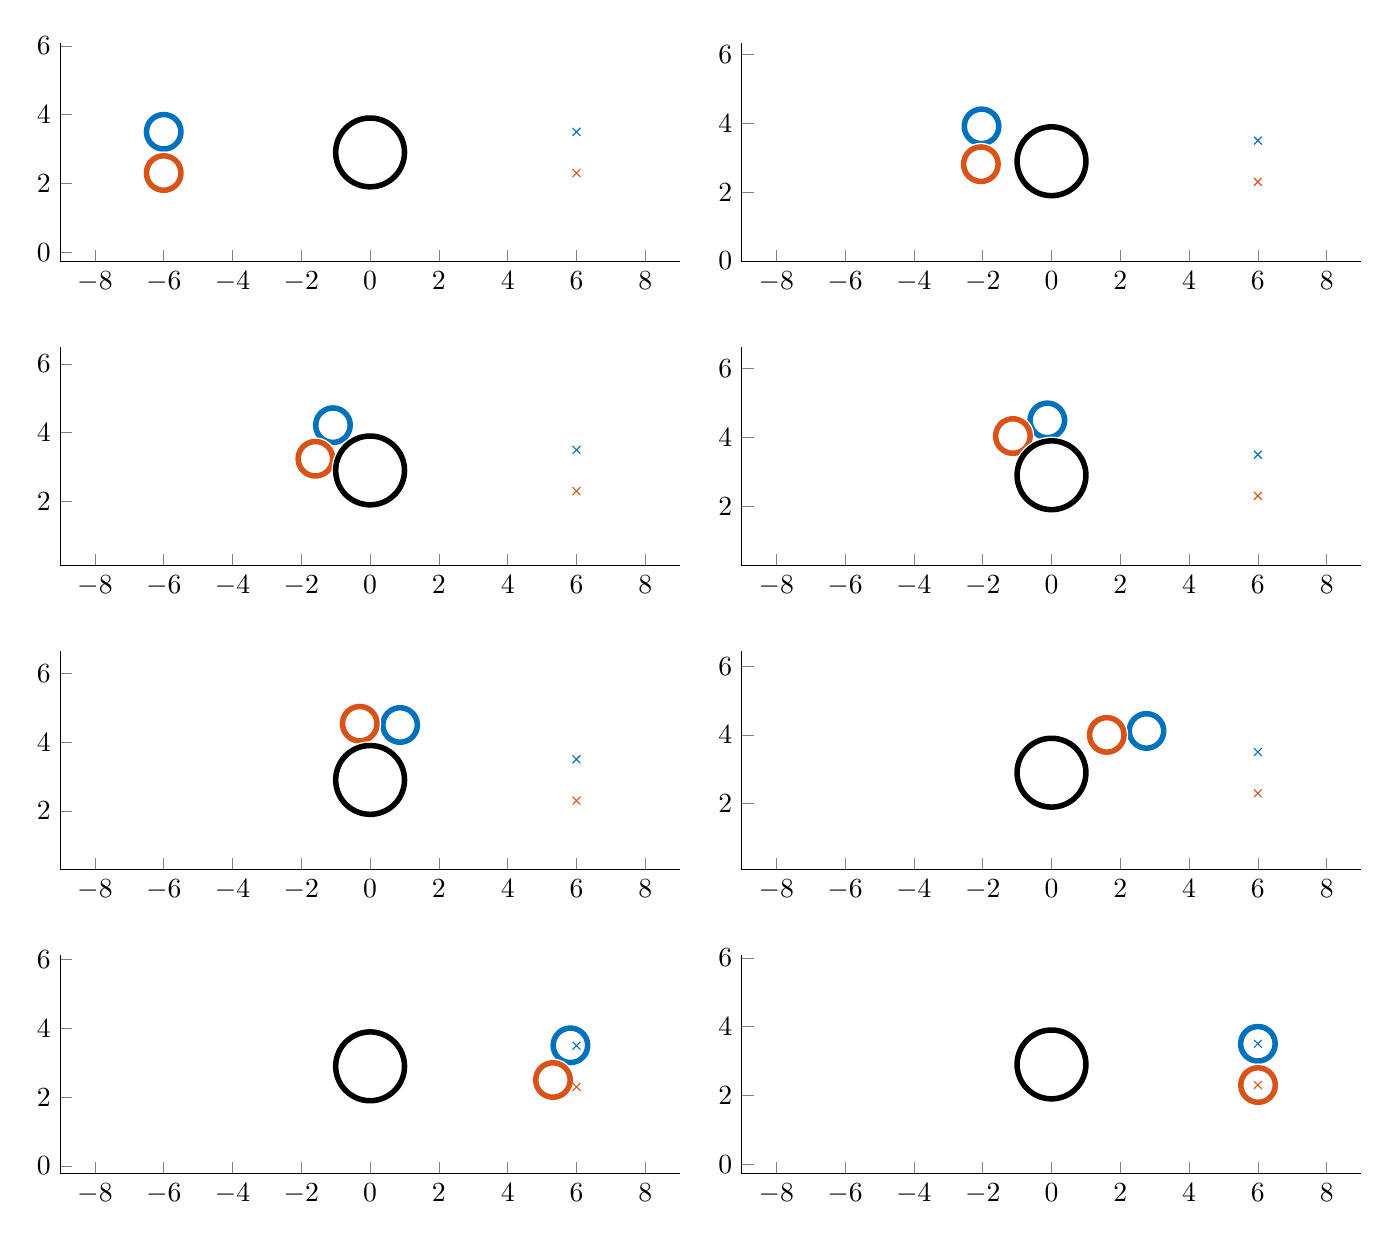
\begin{tikzpicture}

\definecolor{mycolor1}{rgb}{0.00000,0.44700,0.74100}%
\definecolor{mycolor2}{rgb}{0.85000,0.32500,0.09800}%
\definecolor{mycolor3}{rgb}{0.92900,0.69400,0.12500}%

\begin{axis}[%
width=3.096in,
height=1.094in,
at={(2.593in,5.323in)},
scale only axis,
unbounded coords=jump,
xmin=-9,
xmax=9,
%xmajorgrids,
ymin=-0.281620023002354,
ymax=6.08162002300235,
%ymajorgrids,
axis background/.style={fill=white},
axis x line*=bottom,
axis y line*=left
]
\addplot [color=mycolor1,only marks,mark=x,mark options={solid},forget plot]
  table[row sep=crcr]{%
6	3.5\\
};
\addplot [color=mycolor2,only marks,mark=x,mark options={solid},forget plot]
  table[row sep=crcr]{%
6	2.3\\
};
\addplot [color=white,solid,line width=3.0pt,forget plot]
  table[row sep=crcr]{%
-5.5	3.5\\
-5.50030458649045	3.51744974835125\\
-5.50121797487009	3.53487823687206\\
-5.50273905231586	3.55226423163383\\
-5.50486596562921	3.56958655048003\\
-5.5075961234939	3.58682408883347\\
-5.5109261996331	3.60395584540888\\
-5.514852136862	3.62096094779983\\
-5.51936915203084	3.6378186779085\\
-5.52447174185242	3.65450849718747\\
-5.53015368960705	3.67101007166283\\
-5.53640807271661	3.68730329670796\\
-5.5432272711787	3.7033683215379\\
-5.55060297685042	3.71918557339454\\
-5.55852620357054	3.73473578139295\\
-5.56698729810778	3.75\\
-5.57597595192179	3.7649596321166\\
-5.58548121372248	3.77959645173537\\
-5.59549150281253	3.79389262614624\\
-5.60599462319664	3.80783073766283\\
-5.61697777844051	3.82139380484327\\
-5.6284275872613	3.83456530317943\\
-5.64033009983067	3.8473291852295\\
-5.6526708147705	3.85966990016933\\
-5.66543469682057	3.8715724127387\\
-5.67860619515673	3.88302222155949\\
-5.69216926233717	3.89400537680336\\
-5.70610737385376	3.90450849718747\\
-5.72040354826463	3.91451878627752\\
-5.7350403678834	3.92402404807821\\
-5.75	3.93301270189222\\
-5.76526421860705	3.94147379642946\\
-5.78081442660546	3.94939702314958\\
-5.7966316784621	3.9567727288213\\
-5.81269670329204	3.96359192728339\\
-5.82898992833717	3.96984631039295\\
-5.84549150281253	3.97552825814758\\
-5.8621813220915	3.98063084796916\\
-5.87903905220017	3.985147863138\\
-5.89604415459112	3.9890738003669\\
-5.91317591116653	3.9924038765061\\
-5.93041344951997	3.99513403437079\\
-5.94773576836617	3.99726094768414\\
-5.96512176312794	3.99878202512991\\
-5.98255025164875	3.99969541350955\\
-6	4\\
-6.01744974835125	3.99969541350955\\
-6.03487823687206	3.99878202512991\\
-6.05226423163383	3.99726094768414\\
-6.06958655048003	3.99513403437079\\
-6.08682408883347	3.9924038765061\\
-6.10395584540888	3.9890738003669\\
-6.12096094779983	3.985147863138\\
-6.1378186779085	3.98063084796916\\
-6.15450849718747	3.97552825814758\\
-6.17101007166283	3.96984631039295\\
-6.18730329670796	3.96359192728339\\
-6.2033683215379	3.9567727288213\\
-6.21918557339454	3.94939702314958\\
-6.23473578139295	3.94147379642946\\
-6.25	3.93301270189222\\
-6.2649596321166	3.92402404807821\\
-6.27959645173537	3.91451878627752\\
-6.29389262614624	3.90450849718747\\
-6.30783073766283	3.89400537680336\\
-6.32139380484327	3.88302222155949\\
-6.33456530317943	3.8715724127387\\
-6.3473291852295	3.85966990016933\\
-6.35966990016933	3.8473291852295\\
-6.3715724127387	3.83456530317943\\
-6.38302222155949	3.82139380484327\\
-6.39400537680336	3.80783073766283\\
-6.40450849718747	3.79389262614624\\
-6.41451878627752	3.77959645173537\\
-6.42402404807821	3.7649596321166\\
-6.43301270189222	3.75\\
-6.44147379642946	3.73473578139295\\
-6.44939702314958	3.71918557339454\\
-6.4567727288213	3.7033683215379\\
-6.46359192728339	3.68730329670796\\
-6.46984631039295	3.67101007166283\\
-6.47552825814758	3.65450849718747\\
-6.48063084796916	3.6378186779085\\
-6.485147863138	3.62096094779983\\
-6.4890738003669	3.60395584540888\\
-6.4924038765061	3.58682408883347\\
-6.49513403437079	3.56958655048003\\
-6.49726094768414	3.55226423163383\\
-6.49878202512991	3.53487823687206\\
-6.49969541350955	3.51744974835125\\
-6.5	3.5\\
-6.49969541350955	3.48255025164875\\
-6.49878202512991	3.46512176312794\\
-6.49726094768414	3.44773576836617\\
-6.49513403437079	3.43041344951997\\
-6.4924038765061	3.41317591116653\\
-6.4890738003669	3.39604415459112\\
-6.485147863138	3.37903905220017\\
-6.48063084796916	3.3621813220915\\
-6.47552825814758	3.34549150281253\\
-6.46984631039295	3.32898992833717\\
-6.46359192728339	3.31269670329204\\
-6.4567727288213	3.2966316784621\\
-6.44939702314958	3.28081442660546\\
-6.44147379642946	3.26526421860705\\
-6.43301270189222	3.25\\
-6.42402404807821	3.2350403678834\\
-6.41451878627752	3.22040354826463\\
-6.40450849718747	3.20610737385376\\
-6.39400537680336	3.19216926233717\\
-6.38302222155949	3.17860619515673\\
-6.3715724127387	3.16543469682057\\
-6.35966990016933	3.1526708147705\\
-6.3473291852295	3.14033009983067\\
-6.33456530317943	3.1284275872613\\
-6.32139380484327	3.11697777844051\\
-6.30783073766283	3.10599462319664\\
-6.29389262614624	3.09549150281253\\
-6.27959645173537	3.08548121372248\\
-6.2649596321166	3.07597595192179\\
-6.25	3.06698729810778\\
-6.23473578139295	3.05852620357054\\
-6.21918557339454	3.05060297685042\\
-6.2033683215379	3.0432272711787\\
-6.18730329670796	3.03640807271661\\
-6.17101007166283	3.03015368960705\\
-6.15450849718747	3.02447174185242\\
-6.1378186779085	3.01936915203084\\
-6.12096094779983	3.014852136862\\
-6.10395584540888	3.0109261996331\\
-6.08682408883347	3.0075961234939\\
-6.06958655048003	3.00486596562921\\
-6.05226423163383	3.00273905231586\\
-6.03487823687206	3.00121797487009\\
-6.01744974835125	3.00030458649045\\
-6	3\\
-5.98255025164875	3.00030458649045\\
-5.96512176312794	3.00121797487009\\
-5.94773576836617	3.00273905231586\\
-5.93041344951997	3.00486596562921\\
-5.91317591116653	3.0075961234939\\
-5.89604415459112	3.0109261996331\\
-5.87903905220017	3.014852136862\\
-5.8621813220915	3.01936915203084\\
-5.84549150281253	3.02447174185242\\
-5.82898992833717	3.03015368960705\\
-5.81269670329204	3.03640807271661\\
-5.7966316784621	3.0432272711787\\
-5.78081442660546	3.05060297685042\\
-5.76526421860705	3.05852620357054\\
-5.75	3.06698729810778\\
-5.7350403678834	3.07597595192179\\
-5.72040354826463	3.08548121372248\\
-5.70610737385376	3.09549150281253\\
-5.69216926233717	3.10599462319664\\
-5.67860619515673	3.11697777844051\\
-5.66543469682057	3.1284275872613\\
-5.6526708147705	3.14033009983067\\
-5.64033009983067	3.1526708147705\\
-5.6284275872613	3.16543469682057\\
-5.61697777844051	3.17860619515673\\
-5.60599462319664	3.19216926233717\\
-5.59549150281253	3.20610737385376\\
-5.58548121372248	3.22040354826463\\
-5.57597595192179	3.2350403678834\\
-5.56698729810778	3.25\\
-5.55852620357054	3.26526421860705\\
-5.55060297685042	3.28081442660546\\
-5.5432272711787	3.2966316784621\\
-5.53640807271661	3.31269670329204\\
-5.53015368960705	3.32898992833717\\
-5.52447174185242	3.34549150281253\\
-5.51936915203084	3.3621813220915\\
-5.514852136862	3.37903905220017\\
-5.5109261996331	3.39604415459112\\
-5.5075961234939	3.41317591116653\\
-5.50486596562921	3.43041344951997\\
-5.50273905231586	3.44773576836617\\
-5.50121797487009	3.46512176312794\\
-5.50030458649045	3.48255025164875\\
-5.5	3.5\\
nan	nan\\
};
\addplot [color=mycolor1,solid,line width=2.0pt,forget plot]
  table[row sep=crcr]{%
-5.5	3.5\\
-5.50030458649045	3.51744974835125\\
-5.50121797487009	3.53487823687206\\
-5.50273905231586	3.55226423163383\\
-5.50486596562921	3.56958655048003\\
-5.5075961234939	3.58682408883347\\
-5.5109261996331	3.60395584540888\\
-5.514852136862	3.62096094779983\\
-5.51936915203084	3.6378186779085\\
-5.52447174185242	3.65450849718747\\
-5.53015368960705	3.67101007166283\\
-5.53640807271661	3.68730329670796\\
-5.5432272711787	3.7033683215379\\
-5.55060297685042	3.71918557339454\\
-5.55852620357054	3.73473578139295\\
-5.56698729810778	3.75\\
-5.57597595192179	3.7649596321166\\
-5.58548121372248	3.77959645173537\\
-5.59549150281253	3.79389262614624\\
-5.60599462319664	3.80783073766283\\
-5.61697777844051	3.82139380484327\\
-5.6284275872613	3.83456530317943\\
-5.64033009983067	3.8473291852295\\
-5.6526708147705	3.85966990016933\\
-5.66543469682057	3.8715724127387\\
-5.67860619515673	3.88302222155949\\
-5.69216926233717	3.89400537680336\\
-5.70610737385376	3.90450849718747\\
-5.72040354826463	3.91451878627752\\
-5.7350403678834	3.92402404807821\\
-5.75	3.93301270189222\\
-5.76526421860705	3.94147379642946\\
-5.78081442660546	3.94939702314958\\
-5.7966316784621	3.9567727288213\\
-5.81269670329204	3.96359192728339\\
-5.82898992833717	3.96984631039295\\
-5.84549150281253	3.97552825814758\\
-5.8621813220915	3.98063084796916\\
-5.87903905220017	3.985147863138\\
-5.89604415459112	3.9890738003669\\
-5.91317591116653	3.9924038765061\\
-5.93041344951997	3.99513403437079\\
-5.94773576836617	3.99726094768414\\
-5.96512176312794	3.99878202512991\\
-5.98255025164875	3.99969541350955\\
-6	4\\
-6.01744974835125	3.99969541350955\\
-6.03487823687206	3.99878202512991\\
-6.05226423163383	3.99726094768414\\
-6.06958655048003	3.99513403437079\\
-6.08682408883347	3.9924038765061\\
-6.10395584540888	3.9890738003669\\
-6.12096094779983	3.985147863138\\
-6.1378186779085	3.98063084796916\\
-6.15450849718747	3.97552825814758\\
-6.17101007166283	3.96984631039295\\
-6.18730329670796	3.96359192728339\\
-6.2033683215379	3.9567727288213\\
-6.21918557339454	3.94939702314958\\
-6.23473578139295	3.94147379642946\\
-6.25	3.93301270189222\\
-6.2649596321166	3.92402404807821\\
-6.27959645173537	3.91451878627752\\
-6.29389262614624	3.90450849718747\\
-6.30783073766283	3.89400537680336\\
-6.32139380484327	3.88302222155949\\
-6.33456530317943	3.8715724127387\\
-6.3473291852295	3.85966990016933\\
-6.35966990016933	3.8473291852295\\
-6.3715724127387	3.83456530317943\\
-6.38302222155949	3.82139380484327\\
-6.39400537680336	3.80783073766283\\
-6.40450849718747	3.79389262614624\\
-6.41451878627752	3.77959645173537\\
-6.42402404807821	3.7649596321166\\
-6.43301270189222	3.75\\
-6.44147379642946	3.73473578139295\\
-6.44939702314958	3.71918557339454\\
-6.4567727288213	3.7033683215379\\
-6.46359192728339	3.68730329670796\\
-6.46984631039295	3.67101007166283\\
-6.47552825814758	3.65450849718747\\
-6.48063084796916	3.6378186779085\\
-6.485147863138	3.62096094779983\\
-6.4890738003669	3.60395584540888\\
-6.4924038765061	3.58682408883347\\
-6.49513403437079	3.56958655048003\\
-6.49726094768414	3.55226423163383\\
-6.49878202512991	3.53487823687206\\
-6.49969541350955	3.51744974835125\\
-6.5	3.5\\
-6.49969541350955	3.48255025164875\\
-6.49878202512991	3.46512176312794\\
-6.49726094768414	3.44773576836617\\
-6.49513403437079	3.43041344951997\\
-6.4924038765061	3.41317591116653\\
-6.4890738003669	3.39604415459112\\
-6.485147863138	3.37903905220017\\
-6.48063084796916	3.3621813220915\\
-6.47552825814758	3.34549150281253\\
-6.46984631039295	3.32898992833717\\
-6.46359192728339	3.31269670329204\\
-6.4567727288213	3.2966316784621\\
-6.44939702314958	3.28081442660546\\
-6.44147379642946	3.26526421860705\\
-6.43301270189222	3.25\\
-6.42402404807821	3.2350403678834\\
-6.41451878627752	3.22040354826463\\
-6.40450849718747	3.20610737385376\\
-6.39400537680336	3.19216926233717\\
-6.38302222155949	3.17860619515673\\
-6.3715724127387	3.16543469682057\\
-6.35966990016933	3.1526708147705\\
-6.3473291852295	3.14033009983067\\
-6.33456530317943	3.1284275872613\\
-6.32139380484327	3.11697777844051\\
-6.30783073766283	3.10599462319664\\
-6.29389262614624	3.09549150281253\\
-6.27959645173537	3.08548121372248\\
-6.2649596321166	3.07597595192179\\
-6.25	3.06698729810778\\
-6.23473578139295	3.05852620357054\\
-6.21918557339454	3.05060297685042\\
-6.2033683215379	3.0432272711787\\
-6.18730329670796	3.03640807271661\\
-6.17101007166283	3.03015368960705\\
-6.15450849718747	3.02447174185242\\
-6.1378186779085	3.01936915203084\\
-6.12096094779983	3.014852136862\\
-6.10395584540888	3.0109261996331\\
-6.08682408883347	3.0075961234939\\
-6.06958655048003	3.00486596562921\\
-6.05226423163383	3.00273905231586\\
-6.03487823687206	3.00121797487009\\
-6.01744974835125	3.00030458649045\\
-6	3\\
-5.98255025164875	3.00030458649045\\
-5.96512176312794	3.00121797487009\\
-5.94773576836617	3.00273905231586\\
-5.93041344951997	3.00486596562921\\
-5.91317591116653	3.0075961234939\\
-5.89604415459112	3.0109261996331\\
-5.87903905220017	3.014852136862\\
-5.8621813220915	3.01936915203084\\
-5.84549150281253	3.02447174185242\\
-5.82898992833717	3.03015368960705\\
-5.81269670329204	3.03640807271661\\
-5.7966316784621	3.0432272711787\\
-5.78081442660546	3.05060297685042\\
-5.76526421860705	3.05852620357054\\
-5.75	3.06698729810778\\
-5.7350403678834	3.07597595192179\\
-5.72040354826463	3.08548121372248\\
-5.70610737385376	3.09549150281253\\
-5.69216926233717	3.10599462319664\\
-5.67860619515673	3.11697777844051\\
-5.66543469682057	3.1284275872613\\
-5.6526708147705	3.14033009983067\\
-5.64033009983067	3.1526708147705\\
-5.6284275872613	3.16543469682057\\
-5.61697777844051	3.17860619515673\\
-5.60599462319664	3.19216926233717\\
-5.59549150281253	3.20610737385376\\
-5.58548121372248	3.22040354826463\\
-5.57597595192179	3.2350403678834\\
-5.56698729810778	3.25\\
-5.55852620357054	3.26526421860705\\
-5.55060297685042	3.28081442660546\\
-5.5432272711787	3.2966316784621\\
-5.53640807271661	3.31269670329204\\
-5.53015368960705	3.32898992833717\\
-5.52447174185242	3.34549150281253\\
-5.51936915203084	3.3621813220915\\
-5.514852136862	3.37903905220017\\
-5.5109261996331	3.39604415459112\\
-5.5075961234939	3.41317591116653\\
-5.50486596562921	3.43041344951997\\
-5.50273905231586	3.44773576836617\\
-5.50121797487009	3.46512176312794\\
-5.50030458649045	3.48255025164875\\
-5.5	3.5\\
nan	nan\\
};
\addplot [color=white,solid,line width=3.0pt,forget plot]
  table[row sep=crcr]{%
-5.5	2.3\\
-5.50030458649045	2.31744974835125\\
-5.50121797487009	2.33487823687206\\
-5.50273905231586	2.35226423163383\\
-5.50486596562921	2.36958655048003\\
-5.5075961234939	2.38682408883346\\
-5.5109261996331	2.40395584540888\\
-5.514852136862	2.42096094779983\\
-5.51936915203084	2.4378186779085\\
-5.52447174185242	2.45450849718747\\
-5.53015368960705	2.47101007166283\\
-5.53640807271661	2.48730329670796\\
-5.5432272711787	2.5033683215379\\
-5.55060297685042	2.51918557339454\\
-5.55852620357054	2.53473578139295\\
-5.56698729810778	2.55\\
-5.57597595192179	2.5649596321166\\
-5.58548121372248	2.57959645173537\\
-5.59549150281253	2.59389262614624\\
-5.60599462319664	2.60783073766283\\
-5.61697777844051	2.62139380484327\\
-5.6284275872613	2.63456530317943\\
-5.64033009983067	2.6473291852295\\
-5.6526708147705	2.65966990016933\\
-5.66543469682057	2.6715724127387\\
-5.67860619515673	2.68302222155949\\
-5.69216926233717	2.69400537680336\\
-5.70610737385376	2.70450849718747\\
-5.72040354826463	2.71451878627752\\
-5.7350403678834	2.72402404807821\\
-5.75	2.73301270189222\\
-5.76526421860705	2.74147379642946\\
-5.78081442660546	2.74939702314958\\
-5.7966316784621	2.7567727288213\\
-5.81269670329204	2.76359192728339\\
-5.82898992833717	2.76984631039295\\
-5.84549150281253	2.77552825814758\\
-5.8621813220915	2.78063084796916\\
-5.87903905220017	2.785147863138\\
-5.89604415459112	2.7890738003669\\
-5.91317591116653	2.7924038765061\\
-5.93041344951997	2.79513403437078\\
-5.94773576836617	2.79726094768414\\
-5.96512176312794	2.79878202512991\\
-5.98255025164875	2.79969541350955\\
-6	2.8\\
-6.01744974835125	2.79969541350955\\
-6.03487823687206	2.79878202512991\\
-6.05226423163383	2.79726094768414\\
-6.06958655048003	2.79513403437078\\
-6.08682408883347	2.7924038765061\\
-6.10395584540888	2.7890738003669\\
-6.12096094779983	2.785147863138\\
-6.1378186779085	2.78063084796916\\
-6.15450849718747	2.77552825814758\\
-6.17101007166283	2.76984631039295\\
-6.18730329670796	2.76359192728339\\
-6.2033683215379	2.7567727288213\\
-6.21918557339454	2.74939702314958\\
-6.23473578139295	2.74147379642946\\
-6.25	2.73301270189222\\
-6.2649596321166	2.72402404807821\\
-6.27959645173537	2.71451878627752\\
-6.29389262614624	2.70450849718747\\
-6.30783073766283	2.69400537680336\\
-6.32139380484327	2.68302222155949\\
-6.33456530317943	2.6715724127387\\
-6.3473291852295	2.65966990016933\\
-6.35966990016933	2.6473291852295\\
-6.3715724127387	2.63456530317943\\
-6.38302222155949	2.62139380484327\\
-6.39400537680336	2.60783073766283\\
-6.40450849718747	2.59389262614624\\
-6.41451878627752	2.57959645173537\\
-6.42402404807821	2.5649596321166\\
-6.43301270189222	2.55\\
-6.44147379642946	2.53473578139295\\
-6.44939702314958	2.51918557339454\\
-6.4567727288213	2.5033683215379\\
-6.46359192728339	2.48730329670796\\
-6.46984631039295	2.47101007166283\\
-6.47552825814758	2.45450849718747\\
-6.48063084796916	2.4378186779085\\
-6.485147863138	2.42096094779983\\
-6.4890738003669	2.40395584540888\\
-6.4924038765061	2.38682408883346\\
-6.49513403437079	2.36958655048003\\
-6.49726094768414	2.35226423163383\\
-6.49878202512991	2.33487823687206\\
-6.49969541350955	2.31744974835125\\
-6.5	2.3\\
-6.49969541350955	2.28255025164875\\
-6.49878202512991	2.26512176312794\\
-6.49726094768414	2.24773576836617\\
-6.49513403437079	2.23041344951997\\
-6.4924038765061	2.21317591116653\\
-6.4890738003669	2.19604415459112\\
-6.485147863138	2.17903905220017\\
-6.48063084796916	2.1621813220915\\
-6.47552825814758	2.14549150281253\\
-6.46984631039295	2.12898992833717\\
-6.46359192728339	2.11269670329204\\
-6.4567727288213	2.0966316784621\\
-6.44939702314958	2.08081442660546\\
-6.44147379642946	2.06526421860705\\
-6.43301270189222	2.05\\
-6.42402404807821	2.0350403678834\\
-6.41451878627752	2.02040354826463\\
-6.40450849718747	2.00610737385376\\
-6.39400537680336	1.99216926233717\\
-6.38302222155949	1.97860619515673\\
-6.3715724127387	1.96543469682057\\
-6.35966990016933	1.9526708147705\\
-6.3473291852295	1.94033009983067\\
-6.33456530317943	1.9284275872613\\
-6.32139380484327	1.91697777844051\\
-6.30783073766283	1.90599462319664\\
-6.29389262614624	1.89549150281253\\
-6.27959645173537	1.88548121372248\\
-6.2649596321166	1.87597595192179\\
-6.25	1.86698729810778\\
-6.23473578139295	1.85852620357054\\
-6.21918557339454	1.85060297685042\\
-6.2033683215379	1.8432272711787\\
-6.18730329670796	1.83640807271661\\
-6.17101007166283	1.83015368960705\\
-6.15450849718747	1.82447174185242\\
-6.1378186779085	1.81936915203084\\
-6.12096094779983	1.814852136862\\
-6.10395584540888	1.8109261996331\\
-6.08682408883347	1.8075961234939\\
-6.06958655048003	1.80486596562921\\
-6.05226423163383	1.80273905231586\\
-6.03487823687206	1.80121797487009\\
-6.01744974835125	1.80030458649045\\
-6	1.8\\
-5.98255025164875	1.80030458649045\\
-5.96512176312794	1.80121797487009\\
-5.94773576836617	1.80273905231586\\
-5.93041344951997	1.80486596562921\\
-5.91317591116653	1.8075961234939\\
-5.89604415459112	1.8109261996331\\
-5.87903905220017	1.814852136862\\
-5.8621813220915	1.81936915203084\\
-5.84549150281253	1.82447174185242\\
-5.82898992833717	1.83015368960705\\
-5.81269670329204	1.83640807271661\\
-5.7966316784621	1.8432272711787\\
-5.78081442660546	1.85060297685042\\
-5.76526421860705	1.85852620357054\\
-5.75	1.86698729810778\\
-5.7350403678834	1.87597595192179\\
-5.72040354826463	1.88548121372248\\
-5.70610737385376	1.89549150281253\\
-5.69216926233717	1.90599462319664\\
-5.67860619515673	1.91697777844051\\
-5.66543469682057	1.9284275872613\\
-5.6526708147705	1.94033009983067\\
-5.64033009983067	1.9526708147705\\
-5.6284275872613	1.96543469682057\\
-5.61697777844051	1.97860619515673\\
-5.60599462319664	1.99216926233717\\
-5.59549150281253	2.00610737385376\\
-5.58548121372248	2.02040354826463\\
-5.57597595192179	2.0350403678834\\
-5.56698729810778	2.05\\
-5.55852620357054	2.06526421860705\\
-5.55060297685042	2.08081442660546\\
-5.5432272711787	2.0966316784621\\
-5.53640807271661	2.11269670329204\\
-5.53015368960705	2.12898992833717\\
-5.52447174185242	2.14549150281253\\
-5.51936915203084	2.1621813220915\\
-5.514852136862	2.17903905220017\\
-5.5109261996331	2.19604415459112\\
-5.5075961234939	2.21317591116653\\
-5.50486596562921	2.23041344951997\\
-5.50273905231586	2.24773576836617\\
-5.50121797487009	2.26512176312794\\
-5.50030458649045	2.28255025164875\\
-5.5	2.3\\
nan	nan\\
};
\addplot [color=mycolor2,solid,line width=2.0pt,forget plot]
  table[row sep=crcr]{%
-5.5	2.3\\
-5.50030458649045	2.31744974835125\\
-5.50121797487009	2.33487823687206\\
-5.50273905231586	2.35226423163383\\
-5.50486596562921	2.36958655048003\\
-5.5075961234939	2.38682408883346\\
-5.5109261996331	2.40395584540888\\
-5.514852136862	2.42096094779983\\
-5.51936915203084	2.4378186779085\\
-5.52447174185242	2.45450849718747\\
-5.53015368960705	2.47101007166283\\
-5.53640807271661	2.48730329670796\\
-5.5432272711787	2.5033683215379\\
-5.55060297685042	2.51918557339454\\
-5.55852620357054	2.53473578139295\\
-5.56698729810778	2.55\\
-5.57597595192179	2.5649596321166\\
-5.58548121372248	2.57959645173537\\
-5.59549150281253	2.59389262614624\\
-5.60599462319664	2.60783073766283\\
-5.61697777844051	2.62139380484327\\
-5.6284275872613	2.63456530317943\\
-5.64033009983067	2.6473291852295\\
-5.6526708147705	2.65966990016933\\
-5.66543469682057	2.6715724127387\\
-5.67860619515673	2.68302222155949\\
-5.69216926233717	2.69400537680336\\
-5.70610737385376	2.70450849718747\\
-5.72040354826463	2.71451878627752\\
-5.7350403678834	2.72402404807821\\
-5.75	2.73301270189222\\
-5.76526421860705	2.74147379642946\\
-5.78081442660546	2.74939702314958\\
-5.7966316784621	2.7567727288213\\
-5.81269670329204	2.76359192728339\\
-5.82898992833717	2.76984631039295\\
-5.84549150281253	2.77552825814758\\
-5.8621813220915	2.78063084796916\\
-5.87903905220017	2.785147863138\\
-5.89604415459112	2.7890738003669\\
-5.91317591116653	2.7924038765061\\
-5.93041344951997	2.79513403437078\\
-5.94773576836617	2.79726094768414\\
-5.96512176312794	2.79878202512991\\
-5.98255025164875	2.79969541350955\\
-6	2.8\\
-6.01744974835125	2.79969541350955\\
-6.03487823687206	2.79878202512991\\
-6.05226423163383	2.79726094768414\\
-6.06958655048003	2.79513403437078\\
-6.08682408883347	2.7924038765061\\
-6.10395584540888	2.7890738003669\\
-6.12096094779983	2.785147863138\\
-6.1378186779085	2.78063084796916\\
-6.15450849718747	2.77552825814758\\
-6.17101007166283	2.76984631039295\\
-6.18730329670796	2.76359192728339\\
-6.2033683215379	2.7567727288213\\
-6.21918557339454	2.74939702314958\\
-6.23473578139295	2.74147379642946\\
-6.25	2.73301270189222\\
-6.2649596321166	2.72402404807821\\
-6.27959645173537	2.71451878627752\\
-6.29389262614624	2.70450849718747\\
-6.30783073766283	2.69400537680336\\
-6.32139380484327	2.68302222155949\\
-6.33456530317943	2.6715724127387\\
-6.3473291852295	2.65966990016933\\
-6.35966990016933	2.6473291852295\\
-6.3715724127387	2.63456530317943\\
-6.38302222155949	2.62139380484327\\
-6.39400537680336	2.60783073766283\\
-6.40450849718747	2.59389262614624\\
-6.41451878627752	2.57959645173537\\
-6.42402404807821	2.5649596321166\\
-6.43301270189222	2.55\\
-6.44147379642946	2.53473578139295\\
-6.44939702314958	2.51918557339454\\
-6.4567727288213	2.5033683215379\\
-6.46359192728339	2.48730329670796\\
-6.46984631039295	2.47101007166283\\
-6.47552825814758	2.45450849718747\\
-6.48063084796916	2.4378186779085\\
-6.485147863138	2.42096094779983\\
-6.4890738003669	2.40395584540888\\
-6.4924038765061	2.38682408883346\\
-6.49513403437079	2.36958655048003\\
-6.49726094768414	2.35226423163383\\
-6.49878202512991	2.33487823687206\\
-6.49969541350955	2.31744974835125\\
-6.5	2.3\\
-6.49969541350955	2.28255025164875\\
-6.49878202512991	2.26512176312794\\
-6.49726094768414	2.24773576836617\\
-6.49513403437079	2.23041344951997\\
-6.4924038765061	2.21317591116653\\
-6.4890738003669	2.19604415459112\\
-6.485147863138	2.17903905220017\\
-6.48063084796916	2.1621813220915\\
-6.47552825814758	2.14549150281253\\
-6.46984631039295	2.12898992833717\\
-6.46359192728339	2.11269670329204\\
-6.4567727288213	2.0966316784621\\
-6.44939702314958	2.08081442660546\\
-6.44147379642946	2.06526421860705\\
-6.43301270189222	2.05\\
-6.42402404807821	2.0350403678834\\
-6.41451878627752	2.02040354826463\\
-6.40450849718747	2.00610737385376\\
-6.39400537680336	1.99216926233717\\
-6.38302222155949	1.97860619515673\\
-6.3715724127387	1.96543469682057\\
-6.35966990016933	1.9526708147705\\
-6.3473291852295	1.94033009983067\\
-6.33456530317943	1.9284275872613\\
-6.32139380484327	1.91697777844051\\
-6.30783073766283	1.90599462319664\\
-6.29389262614624	1.89549150281253\\
-6.27959645173537	1.88548121372248\\
-6.2649596321166	1.87597595192179\\
-6.25	1.86698729810778\\
-6.23473578139295	1.85852620357054\\
-6.21918557339454	1.85060297685042\\
-6.2033683215379	1.8432272711787\\
-6.18730329670796	1.83640807271661\\
-6.17101007166283	1.83015368960705\\
-6.15450849718747	1.82447174185242\\
-6.1378186779085	1.81936915203084\\
-6.12096094779983	1.814852136862\\
-6.10395584540888	1.8109261996331\\
-6.08682408883347	1.8075961234939\\
-6.06958655048003	1.80486596562921\\
-6.05226423163383	1.80273905231586\\
-6.03487823687206	1.80121797487009\\
-6.01744974835125	1.80030458649045\\
-6	1.8\\
-5.98255025164875	1.80030458649045\\
-5.96512176312794	1.80121797487009\\
-5.94773576836617	1.80273905231586\\
-5.93041344951997	1.80486596562921\\
-5.91317591116653	1.8075961234939\\
-5.89604415459112	1.8109261996331\\
-5.87903905220017	1.814852136862\\
-5.8621813220915	1.81936915203084\\
-5.84549150281253	1.82447174185242\\
-5.82898992833717	1.83015368960705\\
-5.81269670329204	1.83640807271661\\
-5.7966316784621	1.8432272711787\\
-5.78081442660546	1.85060297685042\\
-5.76526421860705	1.85852620357054\\
-5.75	1.86698729810778\\
-5.7350403678834	1.87597595192179\\
-5.72040354826463	1.88548121372248\\
-5.70610737385376	1.89549150281253\\
-5.69216926233717	1.90599462319664\\
-5.67860619515673	1.91697777844051\\
-5.66543469682057	1.9284275872613\\
-5.6526708147705	1.94033009983067\\
-5.64033009983067	1.9526708147705\\
-5.6284275872613	1.96543469682057\\
-5.61697777844051	1.97860619515673\\
-5.60599462319664	1.99216926233717\\
-5.59549150281253	2.00610737385376\\
-5.58548121372248	2.02040354826463\\
-5.57597595192179	2.0350403678834\\
-5.56698729810778	2.05\\
-5.55852620357054	2.06526421860705\\
-5.55060297685042	2.08081442660546\\
-5.5432272711787	2.0966316784621\\
-5.53640807271661	2.11269670329204\\
-5.53015368960705	2.12898992833717\\
-5.52447174185242	2.14549150281253\\
-5.51936915203084	2.1621813220915\\
-5.514852136862	2.17903905220017\\
-5.5109261996331	2.19604415459112\\
-5.5075961234939	2.21317591116653\\
-5.50486596562921	2.23041344951997\\
-5.50273905231586	2.24773576836617\\
-5.50121797487009	2.26512176312794\\
-5.50030458649045	2.28255025164875\\
-5.5	2.3\\
nan	nan\\
};
\addplot [color=white,solid,line width=3.0pt,forget plot]
  table[row sep=crcr]{%
1	2.9\\
0.999390827019096	2.9348994967025\\
0.997564050259824	2.96975647374413\\
0.994521895368273	3.00452846326765\\
0.99026806874157	3.03917310096007\\
0.984807753012208	3.07364817766693\\
0.978147600733806	3.10791169081776\\
0.970295726275996	3.14192189559967\\
0.961261695938319	3.175637355817\\
0.951056516295154	3.20901699437495\\
0.939692620785908	3.24202014332567\\
0.927183854566787	3.27460659341591\\
0.913545457642601	3.3067366430758\\
0.898794046299167	3.33837114678908\\
0.882947592858927	3.36947156278589\\
0.866025403784439	3.4\\
0.848048096156426	3.42991926423321\\
0.829037572555042	3.45919290347075\\
0.809016994374947	3.48778525229247\\
0.788010753606722	3.51566147532566\\
0.766044443118978	3.54278760968654\\
0.743144825477394	3.56913060635886\\
0.719339800338651	3.594658370459\\
0.694658370458997	3.61933980033865\\
0.669130606358858	3.64314482547739\\
0.642787609686539	3.66604444311898\\
0.615661475325658	3.68801075360672\\
0.587785252292473	3.70901699437495\\
0.559192903470747	3.72903757255504\\
0.529919264233205	3.74804809615643\\
0.5	3.76602540378444\\
0.469471562785891	3.78294759285893\\
0.438371146789077	3.79879404629917\\
0.4067366430758	3.8135454576426\\
0.374606593415912	3.82718385456679\\
0.342020143325669	3.83969262078591\\
0.309016994374947	3.85105651629515\\
0.275637355816999	3.86126169593832\\
0.241921895599668	3.870295726276\\
0.207911690817759	3.87814760073381\\
0.17364817766693	3.88480775301221\\
0.139173100960066	3.89026806874157\\
0.104528463267653	3.89452189536827\\
0.0697564737441255	3.89756405025982\\
0.0348994967025011	3.8993908270191\\
6.12323399573677e-17	3.9\\
-0.0348994967025007	3.8993908270191\\
-0.0697564737441253	3.89756405025982\\
-0.104528463267653	3.89452189536827\\
-0.139173100960065	3.89026806874157\\
-0.17364817766693	3.88480775301221\\
-0.207911690817759	3.87814760073381\\
-0.241921895599668	3.870295726276\\
-0.275637355816999	3.86126169593832\\
-0.309016994374947	3.85105651629515\\
-0.342020143325669	3.83969262078591\\
-0.374606593415912	3.82718385456679\\
-0.4067366430758	3.8135454576426\\
-0.438371146789078	3.79879404629917\\
-0.469471562785891	3.78294759285893\\
-0.5	3.76602540378444\\
-0.529919264233205	3.74804809615643\\
-0.559192903470747	3.72903757255504\\
-0.587785252292473	3.70901699437495\\
-0.615661475325658	3.68801075360672\\
-0.642787609686539	3.66604444311898\\
-0.669130606358858	3.64314482547739\\
-0.694658370458997	3.61933980033865\\
-0.719339800338651	3.594658370459\\
-0.743144825477394	3.56913060635886\\
-0.766044443118978	3.54278760968654\\
-0.788010753606722	3.51566147532566\\
-0.809016994374947	3.48778525229247\\
-0.829037572555042	3.45919290347075\\
-0.848048096156426	3.42991926423321\\
-0.866025403784439	3.4\\
-0.882947592858927	3.36947156278589\\
-0.898794046299167	3.33837114678908\\
-0.913545457642601	3.3067366430758\\
-0.927183854566787	3.27460659341591\\
-0.939692620785908	3.24202014332567\\
-0.951056516295154	3.20901699437495\\
-0.961261695938319	3.175637355817\\
-0.970295726275996	3.14192189559967\\
-0.978147600733806	3.10791169081776\\
-0.984807753012208	3.07364817766693\\
-0.99026806874157	3.03917310096007\\
-0.994521895368273	3.00452846326765\\
-0.997564050259824	2.96975647374413\\
-0.999390827019096	2.9348994967025\\
-1	2.9\\
-0.999390827019096	2.8651005032975\\
-0.997564050259824	2.83024352625588\\
-0.994521895368273	2.79547153673235\\
-0.99026806874157	2.76082689903993\\
-0.984807753012208	2.72635182233307\\
-0.978147600733806	2.69208830918224\\
-0.970295726275997	2.65807810440033\\
-0.961261695938319	2.624362644183\\
-0.951056516295154	2.59098300562505\\
-0.939692620785908	2.55797985667433\\
-0.927183854566787	2.52539340658409\\
-0.913545457642601	2.4932633569242\\
-0.898794046299167	2.46162885321092\\
-0.882947592858927	2.43052843721411\\
-0.866025403784439	2.4\\
-0.848048096156426	2.3700807357668\\
-0.829037572555042	2.34080709652925\\
-0.809016994374947	2.31221474770753\\
-0.788010753606722	2.28433852467434\\
-0.766044443118978	2.25721239031346\\
-0.743144825477394	2.23086939364114\\
-0.719339800338651	2.205341629541\\
-0.694658370458997	2.18066019966135\\
-0.669130606358858	2.15685517452261\\
-0.642787609686539	2.13395555688102\\
-0.615661475325658	2.11198924639328\\
-0.587785252292473	2.09098300562505\\
-0.559192903470747	2.07096242744496\\
-0.529919264233205	2.05195190384357\\
-0.5	2.03397459621556\\
-0.469471562785891	2.01705240714107\\
-0.438371146789078	2.00120595370083\\
-0.4067366430758	1.9864545423574\\
-0.374606593415912	1.97281614543321\\
-0.342020143325669	1.96030737921409\\
-0.309016994374948	1.94894348370485\\
-0.275637355816999	1.93873830406168\\
-0.241921895599668	1.929704273724\\
-0.20791169081776	1.92185239926619\\
-0.17364817766693	1.91519224698779\\
-0.139173100960065	1.90973193125843\\
-0.104528463267653	1.90547810463173\\
-0.0697564737441256	1.90243594974018\\
-0.0348994967025016	1.9006091729809\\
-1.83697019872103e-16	1.9\\
0.0348994967025013	1.9006091729809\\
0.0697564737441252	1.90243594974018\\
0.104528463267653	1.90547810463173\\
0.139173100960065	1.90973193125843\\
0.17364817766693	1.91519224698779\\
0.207911690817759	1.92185239926619\\
0.241921895599667	1.929704273724\\
0.275637355816999	1.93873830406168\\
0.309016994374947	1.94894348370485\\
0.342020143325668	1.96030737921409\\
0.374606593415912	1.97281614543321\\
0.406736643075801	1.9864545423574\\
0.438371146789077	2.00120595370083\\
0.46947156278589	2.01705240714107\\
0.5	2.03397459621556\\
0.529919264233205	2.05195190384357\\
0.559192903470746	2.07096242744496\\
0.587785252292473	2.09098300562505\\
0.615661475325659	2.11198924639328\\
0.642787609686539	2.13395555688102\\
0.669130606358858	2.15685517452261\\
0.694658370458997	2.18066019966135\\
0.719339800338651	2.205341629541\\
0.743144825477394	2.23086939364114\\
0.766044443118978	2.25721239031346\\
0.788010753606722	2.28433852467434\\
0.809016994374947	2.31221474770753\\
0.829037572555041	2.34080709652925\\
0.848048096156425	2.37008073576679\\
0.866025403784438	2.4\\
0.882947592858927	2.43052843721411\\
0.898794046299167	2.46162885321092\\
0.913545457642601	2.4932633569242\\
0.927183854566787	2.52539340658409\\
0.939692620785908	2.55797985667433\\
0.951056516295154	2.59098300562505\\
0.961261695938319	2.624362644183\\
0.970295726275996	2.65807810440033\\
0.978147600733806	2.69208830918224\\
0.984807753012208	2.72635182233307\\
0.99026806874157	2.76082689903993\\
0.994521895368273	2.79547153673235\\
0.997564050259824	2.83024352625588\\
0.999390827019096	2.8651005032975\\
1	2.9\\
nan	nan\\
};
\addplot [color=black,solid,line width=2.0pt,forget plot]
  table[row sep=crcr]{%
1	2.9\\
0.999390827019096	2.9348994967025\\
0.997564050259824	2.96975647374413\\
0.994521895368273	3.00452846326765\\
0.99026806874157	3.03917310096007\\
0.984807753012208	3.07364817766693\\
0.978147600733806	3.10791169081776\\
0.970295726275996	3.14192189559967\\
0.961261695938319	3.175637355817\\
0.951056516295154	3.20901699437495\\
0.939692620785908	3.24202014332567\\
0.927183854566787	3.27460659341591\\
0.913545457642601	3.3067366430758\\
0.898794046299167	3.33837114678908\\
0.882947592858927	3.36947156278589\\
0.866025403784439	3.4\\
0.848048096156426	3.42991926423321\\
0.829037572555042	3.45919290347075\\
0.809016994374947	3.48778525229247\\
0.788010753606722	3.51566147532566\\
0.766044443118978	3.54278760968654\\
0.743144825477394	3.56913060635886\\
0.719339800338651	3.594658370459\\
0.694658370458997	3.61933980033865\\
0.669130606358858	3.64314482547739\\
0.642787609686539	3.66604444311898\\
0.615661475325658	3.68801075360672\\
0.587785252292473	3.70901699437495\\
0.559192903470747	3.72903757255504\\
0.529919264233205	3.74804809615643\\
0.5	3.76602540378444\\
0.469471562785891	3.78294759285893\\
0.438371146789077	3.79879404629917\\
0.4067366430758	3.8135454576426\\
0.374606593415912	3.82718385456679\\
0.342020143325669	3.83969262078591\\
0.309016994374947	3.85105651629515\\
0.275637355816999	3.86126169593832\\
0.241921895599668	3.870295726276\\
0.207911690817759	3.87814760073381\\
0.17364817766693	3.88480775301221\\
0.139173100960066	3.89026806874157\\
0.104528463267653	3.89452189536827\\
0.0697564737441255	3.89756405025982\\
0.0348994967025011	3.8993908270191\\
6.12323399573677e-17	3.9\\
-0.0348994967025007	3.8993908270191\\
-0.0697564737441253	3.89756405025982\\
-0.104528463267653	3.89452189536827\\
-0.139173100960065	3.89026806874157\\
-0.17364817766693	3.88480775301221\\
-0.207911690817759	3.87814760073381\\
-0.241921895599668	3.870295726276\\
-0.275637355816999	3.86126169593832\\
-0.309016994374947	3.85105651629515\\
-0.342020143325669	3.83969262078591\\
-0.374606593415912	3.82718385456679\\
-0.4067366430758	3.8135454576426\\
-0.438371146789078	3.79879404629917\\
-0.469471562785891	3.78294759285893\\
-0.5	3.76602540378444\\
-0.529919264233205	3.74804809615643\\
-0.559192903470747	3.72903757255504\\
-0.587785252292473	3.70901699437495\\
-0.615661475325658	3.68801075360672\\
-0.642787609686539	3.66604444311898\\
-0.669130606358858	3.64314482547739\\
-0.694658370458997	3.61933980033865\\
-0.719339800338651	3.594658370459\\
-0.743144825477394	3.56913060635886\\
-0.766044443118978	3.54278760968654\\
-0.788010753606722	3.51566147532566\\
-0.809016994374947	3.48778525229247\\
-0.829037572555042	3.45919290347075\\
-0.848048096156426	3.42991926423321\\
-0.866025403784439	3.4\\
-0.882947592858927	3.36947156278589\\
-0.898794046299167	3.33837114678908\\
-0.913545457642601	3.3067366430758\\
-0.927183854566787	3.27460659341591\\
-0.939692620785908	3.24202014332567\\
-0.951056516295154	3.20901699437495\\
-0.961261695938319	3.175637355817\\
-0.970295726275996	3.14192189559967\\
-0.978147600733806	3.10791169081776\\
-0.984807753012208	3.07364817766693\\
-0.99026806874157	3.03917310096007\\
-0.994521895368273	3.00452846326765\\
-0.997564050259824	2.96975647374413\\
-0.999390827019096	2.9348994967025\\
-1	2.9\\
-0.999390827019096	2.8651005032975\\
-0.997564050259824	2.83024352625588\\
-0.994521895368273	2.79547153673235\\
-0.99026806874157	2.76082689903993\\
-0.984807753012208	2.72635182233307\\
-0.978147600733806	2.69208830918224\\
-0.970295726275997	2.65807810440033\\
-0.961261695938319	2.624362644183\\
-0.951056516295154	2.59098300562505\\
-0.939692620785908	2.55797985667433\\
-0.927183854566787	2.52539340658409\\
-0.913545457642601	2.4932633569242\\
-0.898794046299167	2.46162885321092\\
-0.882947592858927	2.43052843721411\\
-0.866025403784439	2.4\\
-0.848048096156426	2.3700807357668\\
-0.829037572555042	2.34080709652925\\
-0.809016994374947	2.31221474770753\\
-0.788010753606722	2.28433852467434\\
-0.766044443118978	2.25721239031346\\
-0.743144825477394	2.23086939364114\\
-0.719339800338651	2.205341629541\\
-0.694658370458997	2.18066019966135\\
-0.669130606358858	2.15685517452261\\
-0.642787609686539	2.13395555688102\\
-0.615661475325658	2.11198924639328\\
-0.587785252292473	2.09098300562505\\
-0.559192903470747	2.07096242744496\\
-0.529919264233205	2.05195190384357\\
-0.5	2.03397459621556\\
-0.469471562785891	2.01705240714107\\
-0.438371146789078	2.00120595370083\\
-0.4067366430758	1.9864545423574\\
-0.374606593415912	1.97281614543321\\
-0.342020143325669	1.96030737921409\\
-0.309016994374948	1.94894348370485\\
-0.275637355816999	1.93873830406168\\
-0.241921895599668	1.929704273724\\
-0.20791169081776	1.92185239926619\\
-0.17364817766693	1.91519224698779\\
-0.139173100960065	1.90973193125843\\
-0.104528463267653	1.90547810463173\\
-0.0697564737441256	1.90243594974018\\
-0.0348994967025016	1.9006091729809\\
-1.83697019872103e-16	1.9\\
0.0348994967025013	1.9006091729809\\
0.0697564737441252	1.90243594974018\\
0.104528463267653	1.90547810463173\\
0.139173100960065	1.90973193125843\\
0.17364817766693	1.91519224698779\\
0.207911690817759	1.92185239926619\\
0.241921895599667	1.929704273724\\
0.275637355816999	1.93873830406168\\
0.309016994374947	1.94894348370485\\
0.342020143325668	1.96030737921409\\
0.374606593415912	1.97281614543321\\
0.406736643075801	1.9864545423574\\
0.438371146789077	2.00120595370083\\
0.46947156278589	2.01705240714107\\
0.5	2.03397459621556\\
0.529919264233205	2.05195190384357\\
0.559192903470746	2.07096242744496\\
0.587785252292473	2.09098300562505\\
0.615661475325659	2.11198924639328\\
0.642787609686539	2.13395555688102\\
0.669130606358858	2.15685517452261\\
0.694658370458997	2.18066019966135\\
0.719339800338651	2.205341629541\\
0.743144825477394	2.23086939364114\\
0.766044443118978	2.25721239031346\\
0.788010753606722	2.28433852467434\\
0.809016994374947	2.31221474770753\\
0.829037572555041	2.34080709652925\\
0.848048096156425	2.37008073576679\\
0.866025403784438	2.4\\
0.882947592858927	2.43052843721411\\
0.898794046299167	2.46162885321092\\
0.913545457642601	2.4932633569242\\
0.927183854566787	2.52539340658409\\
0.939692620785908	2.55797985667433\\
0.951056516295154	2.59098300562505\\
0.961261695938319	2.624362644183\\
0.970295726275996	2.65807810440033\\
0.978147600733806	2.69208830918224\\
0.984807753012208	2.72635182233307\\
0.99026806874157	2.76082689903993\\
0.994521895368273	2.79547153673235\\
0.997564050259824	2.83024352625588\\
0.999390827019096	2.8651005032975\\
1	2.9\\
nan	nan\\
};
\end{axis}

\begin{axis}[%
width=3.096in,
height=1.094in,
%at={(8.726in,5.323in)},
at={(6in,5.323in)},
scale only axis,
unbounded coords=jump,
xmin=-9,
xmax=9,
%xmajorgrids,
ymin=-0.0244330298387601,
ymax=6.33880701616595,
%ymajorgrids,
axis background/.style={fill=white},
axis x line*=bottom,
axis y line*=left
]
\addplot [color=mycolor1,only marks,mark=x,mark options={solid},forget plot]
  table[row sep=crcr]{%
6	3.5\\
};
\addplot [color=mycolor2,only marks,mark=x,mark options={solid},forget plot]
  table[row sep=crcr]{%
6	2.3\\
};
\addplot [color=white,solid,line width=3.0pt,forget plot]
  table[row sep=crcr]{%
-1.53306914168459	3.91437398632719\\
-1.53337372817504	3.93182373467844\\
-1.53428711655468	3.94925222319925\\
-1.53580819400045	3.96663821796101\\
-1.5379351073138	3.98396053680722\\
-1.54066526517848	4.00119807516065\\
-1.54399534131769	4.01832983173607\\
-1.54792127854659	4.03533493412702\\
-1.55243829371543	4.05219266423569\\
-1.55754088353701	4.06888248351466\\
-1.56322283129163	4.08538405799002\\
-1.5694772144012	4.10167728303514\\
-1.57629641286329	4.11774230786509\\
-1.58367211853501	4.13355955972172\\
-1.59159534525513	4.14910976772013\\
-1.60005643979237	4.16437398632719\\
-1.60904509360638	4.17933361844379\\
-1.61855035540707	4.19397043806256\\
-1.62856064449712	4.20826661247342\\
-1.63906376488123	4.22220472399002\\
-1.6500469201251	4.23576779117046\\
-1.66149672894589	4.24893928950662\\
-1.67339924151526	4.26170317155669\\
-1.68573995645509	4.27404388649651\\
-1.69850383850516	4.28594639906588\\
-1.71167533684132	4.29739620788668\\
-1.72523840402176	4.30837936313055\\
-1.73917651553835	4.31888248351466\\
-1.75347268994922	4.32889277260471\\
-1.76810950956799	4.3383980344054\\
-1.78306914168459	4.34738668821941\\
-1.79833336029164	4.35584778275665\\
-1.81388356829005	4.36377100947677\\
-1.82970082014669	4.37114671514849\\
-1.84576584497663	4.37796591361058\\
-1.86205907002175	4.38422029672014\\
-1.87856064449712	4.38990224447476\\
-1.89525046377609	4.39500483429635\\
-1.91210819388475	4.39952184946518\\
-1.92911329627571	4.40344778669409\\
-1.94624505285112	4.40677786283329\\
-1.96348259120456	4.40950802069797\\
-1.98080491005076	4.41163493401132\\
-1.99819090481253	4.4131560114571\\
-2.01561939333334	4.41406939983673\\
-2.03306914168459	4.41437398632719\\
-2.05051889003584	4.41406939983673\\
-2.06794737855665	4.4131560114571\\
-2.08533337331842	4.41163493401132\\
-2.10265569216462	4.40950802069797\\
-2.11989323051805	4.40677786283329\\
-2.13702498709347	4.40344778669409\\
-2.15403008948442	4.39952184946518\\
-2.17088781959309	4.39500483429635\\
-2.18757763887206	4.38990224447476\\
-2.20407921334742	4.38422029672014\\
-2.22037243839254	4.37796591361058\\
-2.23643746322249	4.37114671514849\\
-2.25225471507913	4.36377100947677\\
-2.26780492307753	4.35584778275665\\
-2.28306914168459	4.34738668821941\\
-2.29802877380119	4.3383980344054\\
-2.31266559341996	4.32889277260471\\
-2.32696176783083	4.31888248351466\\
-2.34089987934742	4.30837936313055\\
-2.35446294652786	4.29739620788668\\
-2.36763444486402	4.28594639906588\\
-2.38039832691409	4.27404388649651\\
-2.39273904185391	4.26170317155669\\
-2.40464155442329	4.24893928950662\\
-2.41609136324408	4.23576779117046\\
-2.42707451848795	4.22220472399002\\
-2.43757763887206	4.20826661247342\\
-2.44758792796211	4.19397043806256\\
-2.4570931897628	4.17933361844379\\
-2.46608184357681	4.16437398632719\\
-2.47454293811405	4.14910976772013\\
-2.48246616483417	4.13355955972172\\
-2.48984187050589	4.11774230786509\\
-2.49666106896798	4.10167728303514\\
-2.50291545207754	4.08538405799002\\
-2.50859739983217	4.06888248351466\\
-2.51369998965375	4.05219266423569\\
-2.51821700482259	4.03533493412702\\
-2.52214294205149	4.01832983173607\\
-2.52547301819069	4.00119807516065\\
-2.52820317605537	3.98396053680722\\
-2.53033008936873	3.96663821796101\\
-2.5318511668145	3.94925222319925\\
-2.53276455519414	3.93182373467844\\
-2.53306914168459	3.91437398632719\\
-2.53276455519414	3.89692423797594\\
-2.5318511668145	3.87949574945512\\
-2.53033008936873	3.86210975469336\\
-2.52820317605537	3.84478743584715\\
-2.52547301819069	3.82754989749372\\
-2.52214294205149	3.81041814091831\\
-2.51821700482259	3.79341303852735\\
-2.51369998965375	3.77655530841869\\
-2.50859739983217	3.75986548913971\\
-2.50291545207754	3.74336391466435\\
-2.49666106896798	3.72707068961923\\
-2.48984187050589	3.71100566478929\\
-2.48246616483417	3.69518841293265\\
-2.47454293811405	3.67963820493424\\
-2.46608184357681	3.66437398632719\\
-2.4570931897628	3.64941435421058\\
-2.44758792796211	3.63477753459181\\
-2.43757763887206	3.62048136018095\\
-2.42707451848795	3.60654324866436\\
-2.41609136324408	3.59298018148392\\
-2.40464155442329	3.57980868314776\\
-2.39273904185391	3.56704480109769\\
-2.38039832691409	3.55470408615786\\
-2.36763444486402	3.54280157358849\\
-2.35446294652786	3.5313517647677\\
-2.34089987934742	3.52036860952383\\
-2.32696176783083	3.50986548913971\\
-2.31266559341996	3.49985520004967\\
-2.29802877380119	3.49034993824897\\
-2.28306914168459	3.48136128443497\\
-2.26780492307753	3.47290018989772\\
-2.25225471507913	3.4649769631776\\
-2.23643746322249	3.45760125750589\\
-2.22037243839254	3.45078205904379\\
-2.20407921334742	3.44452767593423\\
-2.18757763887206	3.43884572817961\\
-2.17088781959309	3.43374313835803\\
-2.15403008948442	3.42922612318919\\
-2.13702498709347	3.42530018596028\\
-2.11989323051805	3.42197010982108\\
-2.10265569216462	3.4192399519564\\
-2.08533337331842	3.41711303864305\\
-2.06794737855665	3.41559196119727\\
-2.05051889003584	3.41467857281764\\
-2.03306914168459	3.41437398632719\\
-2.01561939333334	3.41467857281764\\
-1.99819090481253	3.41559196119727\\
-1.98080491005076	3.41711303864305\\
-1.96348259120456	3.4192399519564\\
-1.94624505285112	3.42197010982108\\
-1.92911329627571	3.42530018596028\\
-1.91210819388476	3.42922612318919\\
-1.89525046377609	3.43374313835803\\
-1.87856064449712	3.43884572817961\\
-1.86205907002175	3.44452767593423\\
-1.84576584497663	3.45078205904379\\
-1.82970082014669	3.45760125750589\\
-1.81388356829005	3.4649769631776\\
-1.79833336029164	3.47290018989772\\
-1.78306914168459	3.48136128443497\\
-1.76810950956799	3.49034993824897\\
-1.75347268994922	3.49985520004967\\
-1.73917651553835	3.50986548913971\\
-1.72523840402176	3.52036860952383\\
-1.71167533684132	3.5313517647677\\
-1.69850383850516	3.54280157358849\\
-1.68573995645509	3.55470408615786\\
-1.67339924151526	3.56704480109769\\
-1.66149672894589	3.57980868314776\\
-1.6500469201251	3.59298018148392\\
-1.63906376488123	3.60654324866436\\
-1.62856064449712	3.62048136018095\\
-1.61855035540707	3.63477753459181\\
-1.60904509360638	3.64941435421058\\
-1.60005643979237	3.66437398632719\\
-1.59159534525513	3.67963820493424\\
-1.58367211853501	3.69518841293265\\
-1.57629641286329	3.71100566478929\\
-1.5694772144012	3.72707068961923\\
-1.56322283129163	3.74336391466435\\
-1.55754088353701	3.75986548913971\\
-1.55243829371543	3.77655530841869\\
-1.54792127854659	3.79341303852735\\
-1.54399534131769	3.81041814091831\\
-1.54066526517848	3.82754989749372\\
-1.5379351073138	3.84478743584715\\
-1.53580819400045	3.86210975469336\\
-1.53428711655468	3.87949574945512\\
-1.53337372817504	3.89692423797594\\
-1.53306914168459	3.91437398632719\\
nan	nan\\
};
\addplot [color=mycolor1,solid,line width=2.0pt,forget plot]
  table[row sep=crcr]{%
-1.53306914168459	3.91437398632719\\
-1.53337372817504	3.93182373467844\\
-1.53428711655468	3.94925222319925\\
-1.53580819400045	3.96663821796101\\
-1.5379351073138	3.98396053680722\\
-1.54066526517848	4.00119807516065\\
-1.54399534131769	4.01832983173607\\
-1.54792127854659	4.03533493412702\\
-1.55243829371543	4.05219266423569\\
-1.55754088353701	4.06888248351466\\
-1.56322283129163	4.08538405799002\\
-1.5694772144012	4.10167728303514\\
-1.57629641286329	4.11774230786509\\
-1.58367211853501	4.13355955972172\\
-1.59159534525513	4.14910976772013\\
-1.60005643979237	4.16437398632719\\
-1.60904509360638	4.17933361844379\\
-1.61855035540707	4.19397043806256\\
-1.62856064449712	4.20826661247342\\
-1.63906376488123	4.22220472399002\\
-1.6500469201251	4.23576779117046\\
-1.66149672894589	4.24893928950662\\
-1.67339924151526	4.26170317155669\\
-1.68573995645509	4.27404388649651\\
-1.69850383850516	4.28594639906588\\
-1.71167533684132	4.29739620788668\\
-1.72523840402176	4.30837936313055\\
-1.73917651553835	4.31888248351466\\
-1.75347268994922	4.32889277260471\\
-1.76810950956799	4.3383980344054\\
-1.78306914168459	4.34738668821941\\
-1.79833336029164	4.35584778275665\\
-1.81388356829005	4.36377100947677\\
-1.82970082014669	4.37114671514849\\
-1.84576584497663	4.37796591361058\\
-1.86205907002175	4.38422029672014\\
-1.87856064449712	4.38990224447476\\
-1.89525046377609	4.39500483429635\\
-1.91210819388475	4.39952184946518\\
-1.92911329627571	4.40344778669409\\
-1.94624505285112	4.40677786283329\\
-1.96348259120456	4.40950802069797\\
-1.98080491005076	4.41163493401132\\
-1.99819090481253	4.4131560114571\\
-2.01561939333334	4.41406939983673\\
-2.03306914168459	4.41437398632719\\
-2.05051889003584	4.41406939983673\\
-2.06794737855665	4.4131560114571\\
-2.08533337331842	4.41163493401132\\
-2.10265569216462	4.40950802069797\\
-2.11989323051805	4.40677786283329\\
-2.13702498709347	4.40344778669409\\
-2.15403008948442	4.39952184946518\\
-2.17088781959309	4.39500483429635\\
-2.18757763887206	4.38990224447476\\
-2.20407921334742	4.38422029672014\\
-2.22037243839254	4.37796591361058\\
-2.23643746322249	4.37114671514849\\
-2.25225471507913	4.36377100947677\\
-2.26780492307753	4.35584778275665\\
-2.28306914168459	4.34738668821941\\
-2.29802877380119	4.3383980344054\\
-2.31266559341996	4.32889277260471\\
-2.32696176783083	4.31888248351466\\
-2.34089987934742	4.30837936313055\\
-2.35446294652786	4.29739620788668\\
-2.36763444486402	4.28594639906588\\
-2.38039832691409	4.27404388649651\\
-2.39273904185391	4.26170317155669\\
-2.40464155442329	4.24893928950662\\
-2.41609136324408	4.23576779117046\\
-2.42707451848795	4.22220472399002\\
-2.43757763887206	4.20826661247342\\
-2.44758792796211	4.19397043806256\\
-2.4570931897628	4.17933361844379\\
-2.46608184357681	4.16437398632719\\
-2.47454293811405	4.14910976772013\\
-2.48246616483417	4.13355955972172\\
-2.48984187050589	4.11774230786509\\
-2.49666106896798	4.10167728303514\\
-2.50291545207754	4.08538405799002\\
-2.50859739983217	4.06888248351466\\
-2.51369998965375	4.05219266423569\\
-2.51821700482259	4.03533493412702\\
-2.52214294205149	4.01832983173607\\
-2.52547301819069	4.00119807516065\\
-2.52820317605537	3.98396053680722\\
-2.53033008936873	3.96663821796101\\
-2.5318511668145	3.94925222319925\\
-2.53276455519414	3.93182373467844\\
-2.53306914168459	3.91437398632719\\
-2.53276455519414	3.89692423797594\\
-2.5318511668145	3.87949574945512\\
-2.53033008936873	3.86210975469336\\
-2.52820317605537	3.84478743584715\\
-2.52547301819069	3.82754989749372\\
-2.52214294205149	3.81041814091831\\
-2.51821700482259	3.79341303852735\\
-2.51369998965375	3.77655530841869\\
-2.50859739983217	3.75986548913971\\
-2.50291545207754	3.74336391466435\\
-2.49666106896798	3.72707068961923\\
-2.48984187050589	3.71100566478929\\
-2.48246616483417	3.69518841293265\\
-2.47454293811405	3.67963820493424\\
-2.46608184357681	3.66437398632719\\
-2.4570931897628	3.64941435421058\\
-2.44758792796211	3.63477753459181\\
-2.43757763887206	3.62048136018095\\
-2.42707451848795	3.60654324866436\\
-2.41609136324408	3.59298018148392\\
-2.40464155442329	3.57980868314776\\
-2.39273904185391	3.56704480109769\\
-2.38039832691409	3.55470408615786\\
-2.36763444486402	3.54280157358849\\
-2.35446294652786	3.5313517647677\\
-2.34089987934742	3.52036860952383\\
-2.32696176783083	3.50986548913971\\
-2.31266559341996	3.49985520004967\\
-2.29802877380119	3.49034993824897\\
-2.28306914168459	3.48136128443497\\
-2.26780492307753	3.47290018989772\\
-2.25225471507913	3.4649769631776\\
-2.23643746322249	3.45760125750589\\
-2.22037243839254	3.45078205904379\\
-2.20407921334742	3.44452767593423\\
-2.18757763887206	3.43884572817961\\
-2.17088781959309	3.43374313835803\\
-2.15403008948442	3.42922612318919\\
-2.13702498709347	3.42530018596028\\
-2.11989323051805	3.42197010982108\\
-2.10265569216462	3.4192399519564\\
-2.08533337331842	3.41711303864305\\
-2.06794737855665	3.41559196119727\\
-2.05051889003584	3.41467857281764\\
-2.03306914168459	3.41437398632719\\
-2.01561939333334	3.41467857281764\\
-1.99819090481253	3.41559196119727\\
-1.98080491005076	3.41711303864305\\
-1.96348259120456	3.4192399519564\\
-1.94624505285112	3.42197010982108\\
-1.92911329627571	3.42530018596028\\
-1.91210819388476	3.42922612318919\\
-1.89525046377609	3.43374313835803\\
-1.87856064449712	3.43884572817961\\
-1.86205907002175	3.44452767593423\\
-1.84576584497663	3.45078205904379\\
-1.82970082014669	3.45760125750589\\
-1.81388356829005	3.4649769631776\\
-1.79833336029164	3.47290018989772\\
-1.78306914168459	3.48136128443497\\
-1.76810950956799	3.49034993824897\\
-1.75347268994922	3.49985520004967\\
-1.73917651553835	3.50986548913971\\
-1.72523840402176	3.52036860952383\\
-1.71167533684132	3.5313517647677\\
-1.69850383850516	3.54280157358849\\
-1.68573995645509	3.55470408615786\\
-1.67339924151526	3.56704480109769\\
-1.66149672894589	3.57980868314776\\
-1.6500469201251	3.59298018148392\\
-1.63906376488123	3.60654324866436\\
-1.62856064449712	3.62048136018095\\
-1.61855035540707	3.63477753459181\\
-1.60904509360638	3.64941435421058\\
-1.60005643979237	3.66437398632719\\
-1.59159534525513	3.67963820493424\\
-1.58367211853501	3.69518841293265\\
-1.57629641286329	3.71100566478929\\
-1.5694772144012	3.72707068961923\\
-1.56322283129163	3.74336391466435\\
-1.55754088353701	3.75986548913971\\
-1.55243829371543	3.77655530841869\\
-1.54792127854659	3.79341303852735\\
-1.54399534131769	3.81041814091831\\
-1.54066526517848	3.82754989749372\\
-1.5379351073138	3.84478743584715\\
-1.53580819400045	3.86210975469336\\
-1.53428711655468	3.87949574945512\\
-1.53337372817504	3.89692423797594\\
-1.53306914168459	3.91437398632719\\
nan	nan\\
};
\addplot [color=white,solid,line width=3.0pt,forget plot]
  table[row sep=crcr]{%
-1.55373409775359	2.81456811273374\\
-1.55403868424404	2.83201786108499\\
-1.55495207262367	2.8494463496058\\
-1.55647315006945	2.86683234436757\\
-1.5586000633828	2.88415466321377\\
-1.56133022124748	2.9013922015672\\
-1.56466029738668	2.91852395814262\\
-1.56858623461559	2.93552906053357\\
-1.57310324978443	2.95238679064224\\
-1.57820583960601	2.96907660992121\\
-1.58388778736063	2.98557818439657\\
-1.59014217047019	3.0018714094417\\
-1.59696136893228	3.01793643427164\\
-1.604337074604	3.03375368612828\\
-1.61226030132412	3.04930389412668\\
-1.62072139586137	3.06456811273374\\
-1.62971004967537	3.07952774485034\\
-1.63921531147606	3.09416456446911\\
-1.64922560056611	3.10846073887998\\
-1.65972872095022	3.12239885039657\\
-1.6707118761941	3.13596191757701\\
-1.68216168501489	3.14913341591317\\
-1.69406419758426	3.16189729796324\\
-1.70640491252409	3.17423801290306\\
-1.71916879457416	3.18614052547244\\
-1.73234029291032	3.19759033429323\\
-1.74590336009076	3.2085734895371\\
-1.75984147160735	3.21907660992121\\
-1.77413764601821	3.22908689901126\\
-1.78877446563698	3.23859216081195\\
-1.80373409775359	3.24758081462596\\
-1.81899831636064	3.2560419091632\\
-1.83454852435905	3.26396513588332\\
-1.85036577621569	3.27134084155504\\
-1.86643080104563	3.27816004001713\\
-1.88272402609075	3.28441442312669\\
-1.89922560056611	3.29009637088132\\
-1.91591541984509	3.2951989607029\\
-1.93277314995375	3.29971597587174\\
-1.94977825234471	3.30364191310064\\
-1.96691000892012	3.30697198923984\\
-1.98414754727355	3.30970214710452\\
-2.00146986611976	3.31182906041788\\
-2.01885586088152	3.31335013786365\\
-2.03628434940233	3.31426352624329\\
-2.05373409775359	3.31456811273374\\
-2.07118384610484	3.31426352624329\\
-2.08861233462565	3.31335013786365\\
-2.10599832938741	3.31182906041788\\
-2.12332064823362	3.30970214710452\\
-2.14055818658705	3.30697198923984\\
-2.15768994316246	3.30364191310064\\
-2.17469504555342	3.29971597587174\\
-2.19155277566208	3.2951989607029\\
-2.20824259494106	3.29009637088132\\
-2.22474416941642	3.28441442312669\\
-2.24103739446154	3.27816004001713\\
-2.25710241929149	3.27134084155504\\
-2.27291967114812	3.26396513588332\\
-2.28846987914653	3.2560419091632\\
-2.30373409775359	3.24758081462596\\
-2.31869372987019	3.23859216081195\\
-2.33333054948896	3.22908689901126\\
-2.34762672389982	3.21907660992121\\
-2.36156483541641	3.2085734895371\\
-2.37512790259686	3.19759033429323\\
-2.38829940093301	3.18614052547244\\
-2.40106328298308	3.17423801290306\\
-2.41340399792291	3.16189729796324\\
-2.42530651049228	3.14913341591317\\
-2.43675631931307	3.13596191757701\\
-2.44773947455695	3.12239885039657\\
-2.45824259494106	3.10846073887998\\
-2.46825288403111	3.09416456446911\\
-2.4777581458318	3.07952774485034\\
-2.4867467996458	3.06456811273374\\
-2.49520789418305	3.04930389412668\\
-2.50313112090317	3.03375368612828\\
-2.51050682657489	3.01793643427164\\
-2.51732602503698	3.0018714094417\\
-2.52358040814654	2.98557818439657\\
-2.52926235590116	2.96907660992121\\
-2.53436494572274	2.95238679064224\\
-2.53888196089158	2.93552906053357\\
-2.54280789812049	2.91852395814262\\
-2.54613797425969	2.9013922015672\\
-2.54886813212437	2.88415466321377\\
-2.55099504543772	2.86683234436757\\
-2.5525161228835	2.8494463496058\\
-2.55342951126313	2.83201786108499\\
-2.55373409775359	2.81456811273374\\
-2.55342951126313	2.79711836438249\\
-2.5525161228835	2.77968987586168\\
-2.55099504543772	2.76230388109991\\
-2.54886813212437	2.74498156225371\\
-2.54613797425969	2.72774402390027\\
-2.54280789812049	2.71061226732486\\
-2.53888196089158	2.69360716493391\\
-2.53436494572274	2.67674943482524\\
-2.52926235590116	2.66005961554627\\
-2.52358040814654	2.6435580410709\\
-2.51732602503698	2.62726481602578\\
-2.51050682657489	2.61119979119584\\
-2.50313112090317	2.5953825393392\\
-2.49520789418305	2.57983233134079\\
-2.4867467996458	2.56456811273374\\
-2.4777581458318	2.54960848061714\\
-2.46825288403111	2.53497166099837\\
-2.45824259494106	2.5206754865875\\
-2.44773947455695	2.50673737507091\\
-2.43675631931307	2.49317430789047\\
-2.42530651049228	2.48000280955431\\
-2.41340399792291	2.46723892750424\\
-2.40106328298308	2.45489821256441\\
-2.38829940093301	2.44299569999504\\
-2.37512790259686	2.43154589117425\\
-2.36156483541641	2.42056273593038\\
-2.34762672389982	2.41005961554627\\
-2.33333054948896	2.40004932645622\\
-2.31869372987019	2.39054406465553\\
-2.30373409775359	2.38155541084152\\
-2.28846987914653	2.37309431630428\\
-2.27291967114812	2.36517108958416\\
-2.25710241929149	2.35779538391244\\
-2.24103739446154	2.35097618545035\\
-2.22474416941642	2.34472180234079\\
-2.20824259494106	2.33903985458616\\
-2.19155277566208	2.33393726476458\\
-2.17469504555342	2.32942024959574\\
-2.15768994316246	2.32549431236684\\
-2.14055818658705	2.32216423622764\\
-2.12332064823362	2.31943407836295\\
-2.10599832938741	2.3173071650496\\
-2.08861233462565	2.31578608760383\\
-2.07118384610484	2.31487269922419\\
-2.05373409775359	2.31456811273374\\
-2.03628434940233	2.31487269922419\\
-2.01885586088152	2.31578608760383\\
-2.00146986611976	2.3173071650496\\
-1.98414754727355	2.31943407836295\\
-1.96691000892012	2.32216423622764\\
-1.94977825234471	2.32549431236684\\
-1.93277314995375	2.32942024959574\\
-1.91591541984509	2.33393726476458\\
-1.89922560056611	2.33903985458616\\
-1.88272402609075	2.34472180234078\\
-1.86643080104563	2.35097618545035\\
-1.85036577621568	2.35779538391244\\
-1.83454852435905	2.36517108958416\\
-1.81899831636064	2.37309431630428\\
-1.80373409775359	2.38155541084152\\
-1.78877446563698	2.39054406465553\\
-1.77413764601821	2.40004932645622\\
-1.75984147160735	2.41005961554627\\
-1.74590336009076	2.42056273593038\\
-1.73234029291032	2.43154589117425\\
-1.71916879457416	2.44299569999504\\
-1.70640491252409	2.45489821256441\\
-1.69406419758426	2.46723892750424\\
-1.68216168501489	2.48000280955431\\
-1.6707118761941	2.49317430789047\\
-1.65972872095022	2.50673737507091\\
-1.64922560056611	2.5206754865875\\
-1.63921531147606	2.53497166099837\\
-1.62971004967537	2.54960848061714\\
-1.62072139586137	2.56456811273374\\
-1.61226030132412	2.57983233134079\\
-1.604337074604	2.5953825393392\\
-1.59696136893228	2.61119979119584\\
-1.59014217047019	2.62726481602578\\
-1.58388778736063	2.6435580410709\\
-1.57820583960601	2.66005961554627\\
-1.57310324978443	2.67674943482524\\
-1.56858623461559	2.69360716493391\\
-1.56466029738668	2.71061226732486\\
-1.56133022124748	2.72774402390027\\
-1.5586000633828	2.74498156225371\\
-1.55647315006945	2.76230388109991\\
-1.55495207262367	2.77968987586168\\
-1.55403868424404	2.79711836438249\\
-1.55373409775359	2.81456811273374\\
nan	nan\\
};
\addplot [color=mycolor2,solid,line width=2.0pt,forget plot]
  table[row sep=crcr]{%
-1.55373409775359	2.81456811273374\\
-1.55403868424404	2.83201786108499\\
-1.55495207262367	2.8494463496058\\
-1.55647315006945	2.86683234436757\\
-1.5586000633828	2.88415466321377\\
-1.56133022124748	2.9013922015672\\
-1.56466029738668	2.91852395814262\\
-1.56858623461559	2.93552906053357\\
-1.57310324978443	2.95238679064224\\
-1.57820583960601	2.96907660992121\\
-1.58388778736063	2.98557818439657\\
-1.59014217047019	3.0018714094417\\
-1.59696136893228	3.01793643427164\\
-1.604337074604	3.03375368612828\\
-1.61226030132412	3.04930389412668\\
-1.62072139586137	3.06456811273374\\
-1.62971004967537	3.07952774485034\\
-1.63921531147606	3.09416456446911\\
-1.64922560056611	3.10846073887998\\
-1.65972872095022	3.12239885039657\\
-1.6707118761941	3.13596191757701\\
-1.68216168501489	3.14913341591317\\
-1.69406419758426	3.16189729796324\\
-1.70640491252409	3.17423801290306\\
-1.71916879457416	3.18614052547244\\
-1.73234029291032	3.19759033429323\\
-1.74590336009076	3.2085734895371\\
-1.75984147160735	3.21907660992121\\
-1.77413764601821	3.22908689901126\\
-1.78877446563698	3.23859216081195\\
-1.80373409775359	3.24758081462596\\
-1.81899831636064	3.2560419091632\\
-1.83454852435905	3.26396513588332\\
-1.85036577621569	3.27134084155504\\
-1.86643080104563	3.27816004001713\\
-1.88272402609075	3.28441442312669\\
-1.89922560056611	3.29009637088132\\
-1.91591541984509	3.2951989607029\\
-1.93277314995375	3.29971597587174\\
-1.94977825234471	3.30364191310064\\
-1.96691000892012	3.30697198923984\\
-1.98414754727355	3.30970214710452\\
-2.00146986611976	3.31182906041788\\
-2.01885586088152	3.31335013786365\\
-2.03628434940233	3.31426352624329\\
-2.05373409775359	3.31456811273374\\
-2.07118384610484	3.31426352624329\\
-2.08861233462565	3.31335013786365\\
-2.10599832938741	3.31182906041788\\
-2.12332064823362	3.30970214710452\\
-2.14055818658705	3.30697198923984\\
-2.15768994316246	3.30364191310064\\
-2.17469504555342	3.29971597587174\\
-2.19155277566208	3.2951989607029\\
-2.20824259494106	3.29009637088132\\
-2.22474416941642	3.28441442312669\\
-2.24103739446154	3.27816004001713\\
-2.25710241929149	3.27134084155504\\
-2.27291967114812	3.26396513588332\\
-2.28846987914653	3.2560419091632\\
-2.30373409775359	3.24758081462596\\
-2.31869372987019	3.23859216081195\\
-2.33333054948896	3.22908689901126\\
-2.34762672389982	3.21907660992121\\
-2.36156483541641	3.2085734895371\\
-2.37512790259686	3.19759033429323\\
-2.38829940093301	3.18614052547244\\
-2.40106328298308	3.17423801290306\\
-2.41340399792291	3.16189729796324\\
-2.42530651049228	3.14913341591317\\
-2.43675631931307	3.13596191757701\\
-2.44773947455695	3.12239885039657\\
-2.45824259494106	3.10846073887998\\
-2.46825288403111	3.09416456446911\\
-2.4777581458318	3.07952774485034\\
-2.4867467996458	3.06456811273374\\
-2.49520789418305	3.04930389412668\\
-2.50313112090317	3.03375368612828\\
-2.51050682657489	3.01793643427164\\
-2.51732602503698	3.0018714094417\\
-2.52358040814654	2.98557818439657\\
-2.52926235590116	2.96907660992121\\
-2.53436494572274	2.95238679064224\\
-2.53888196089158	2.93552906053357\\
-2.54280789812049	2.91852395814262\\
-2.54613797425969	2.9013922015672\\
-2.54886813212437	2.88415466321377\\
-2.55099504543772	2.86683234436757\\
-2.5525161228835	2.8494463496058\\
-2.55342951126313	2.83201786108499\\
-2.55373409775359	2.81456811273374\\
-2.55342951126313	2.79711836438249\\
-2.5525161228835	2.77968987586168\\
-2.55099504543772	2.76230388109991\\
-2.54886813212437	2.74498156225371\\
-2.54613797425969	2.72774402390027\\
-2.54280789812049	2.71061226732486\\
-2.53888196089158	2.69360716493391\\
-2.53436494572274	2.67674943482524\\
-2.52926235590116	2.66005961554627\\
-2.52358040814654	2.6435580410709\\
-2.51732602503698	2.62726481602578\\
-2.51050682657489	2.61119979119584\\
-2.50313112090317	2.5953825393392\\
-2.49520789418305	2.57983233134079\\
-2.4867467996458	2.56456811273374\\
-2.4777581458318	2.54960848061714\\
-2.46825288403111	2.53497166099837\\
-2.45824259494106	2.5206754865875\\
-2.44773947455695	2.50673737507091\\
-2.43675631931307	2.49317430789047\\
-2.42530651049228	2.48000280955431\\
-2.41340399792291	2.46723892750424\\
-2.40106328298308	2.45489821256441\\
-2.38829940093301	2.44299569999504\\
-2.37512790259686	2.43154589117425\\
-2.36156483541641	2.42056273593038\\
-2.34762672389982	2.41005961554627\\
-2.33333054948896	2.40004932645622\\
-2.31869372987019	2.39054406465553\\
-2.30373409775359	2.38155541084152\\
-2.28846987914653	2.37309431630428\\
-2.27291967114812	2.36517108958416\\
-2.25710241929149	2.35779538391244\\
-2.24103739446154	2.35097618545035\\
-2.22474416941642	2.34472180234079\\
-2.20824259494106	2.33903985458616\\
-2.19155277566208	2.33393726476458\\
-2.17469504555342	2.32942024959574\\
-2.15768994316246	2.32549431236684\\
-2.14055818658705	2.32216423622764\\
-2.12332064823362	2.31943407836295\\
-2.10599832938741	2.3173071650496\\
-2.08861233462565	2.31578608760383\\
-2.07118384610484	2.31487269922419\\
-2.05373409775359	2.31456811273374\\
-2.03628434940233	2.31487269922419\\
-2.01885586088152	2.31578608760383\\
-2.00146986611976	2.3173071650496\\
-1.98414754727355	2.31943407836295\\
-1.96691000892012	2.32216423622764\\
-1.94977825234471	2.32549431236684\\
-1.93277314995375	2.32942024959574\\
-1.91591541984509	2.33393726476458\\
-1.89922560056611	2.33903985458616\\
-1.88272402609075	2.34472180234078\\
-1.86643080104563	2.35097618545035\\
-1.85036577621568	2.35779538391244\\
-1.83454852435905	2.36517108958416\\
-1.81899831636064	2.37309431630428\\
-1.80373409775359	2.38155541084152\\
-1.78877446563698	2.39054406465553\\
-1.77413764601821	2.40004932645622\\
-1.75984147160735	2.41005961554627\\
-1.74590336009076	2.42056273593038\\
-1.73234029291032	2.43154589117425\\
-1.71916879457416	2.44299569999504\\
-1.70640491252409	2.45489821256441\\
-1.69406419758426	2.46723892750424\\
-1.68216168501489	2.48000280955431\\
-1.6707118761941	2.49317430789047\\
-1.65972872095022	2.50673737507091\\
-1.64922560056611	2.5206754865875\\
-1.63921531147606	2.53497166099837\\
-1.62971004967537	2.54960848061714\\
-1.62072139586137	2.56456811273374\\
-1.61226030132412	2.57983233134079\\
-1.604337074604	2.5953825393392\\
-1.59696136893228	2.61119979119584\\
-1.59014217047019	2.62726481602578\\
-1.58388778736063	2.6435580410709\\
-1.57820583960601	2.66005961554627\\
-1.57310324978443	2.67674943482524\\
-1.56858623461559	2.69360716493391\\
-1.56466029738668	2.71061226732486\\
-1.56133022124748	2.72774402390027\\
-1.5586000633828	2.74498156225371\\
-1.55647315006945	2.76230388109991\\
-1.55495207262367	2.77968987586168\\
-1.55403868424404	2.79711836438249\\
-1.55373409775359	2.81456811273374\\
nan	nan\\
};
\addplot [color=white,solid,line width=3.0pt,forget plot]
  table[row sep=crcr]{%
1	2.9\\
0.999390827019096	2.9348994967025\\
0.997564050259824	2.96975647374413\\
0.994521895368273	3.00452846326765\\
0.99026806874157	3.03917310096007\\
0.984807753012208	3.07364817766693\\
0.978147600733806	3.10791169081776\\
0.970295726275996	3.14192189559967\\
0.961261695938319	3.175637355817\\
0.951056516295154	3.20901699437495\\
0.939692620785908	3.24202014332567\\
0.927183854566787	3.27460659341591\\
0.913545457642601	3.3067366430758\\
0.898794046299167	3.33837114678908\\
0.882947592858927	3.36947156278589\\
0.866025403784439	3.4\\
0.848048096156426	3.42991926423321\\
0.829037572555042	3.45919290347075\\
0.809016994374947	3.48778525229247\\
0.788010753606722	3.51566147532566\\
0.766044443118978	3.54278760968654\\
0.743144825477394	3.56913060635886\\
0.719339800338651	3.594658370459\\
0.694658370458997	3.61933980033865\\
0.669130606358858	3.64314482547739\\
0.642787609686539	3.66604444311898\\
0.615661475325658	3.68801075360672\\
0.587785252292473	3.70901699437495\\
0.559192903470747	3.72903757255504\\
0.529919264233205	3.74804809615643\\
0.5	3.76602540378444\\
0.469471562785891	3.78294759285893\\
0.438371146789077	3.79879404629917\\
0.4067366430758	3.8135454576426\\
0.374606593415912	3.82718385456679\\
0.342020143325669	3.83969262078591\\
0.309016994374947	3.85105651629515\\
0.275637355816999	3.86126169593832\\
0.241921895599668	3.870295726276\\
0.207911690817759	3.87814760073381\\
0.17364817766693	3.88480775301221\\
0.139173100960066	3.89026806874157\\
0.104528463267653	3.89452189536827\\
0.0697564737441255	3.89756405025982\\
0.0348994967025011	3.8993908270191\\
6.12323399573677e-17	3.9\\
-0.0348994967025007	3.8993908270191\\
-0.0697564737441253	3.89756405025982\\
-0.104528463267653	3.89452189536827\\
-0.139173100960065	3.89026806874157\\
-0.17364817766693	3.88480775301221\\
-0.207911690817759	3.87814760073381\\
-0.241921895599668	3.870295726276\\
-0.275637355816999	3.86126169593832\\
-0.309016994374947	3.85105651629515\\
-0.342020143325669	3.83969262078591\\
-0.374606593415912	3.82718385456679\\
-0.4067366430758	3.8135454576426\\
-0.438371146789078	3.79879404629917\\
-0.469471562785891	3.78294759285893\\
-0.5	3.76602540378444\\
-0.529919264233205	3.74804809615643\\
-0.559192903470747	3.72903757255504\\
-0.587785252292473	3.70901699437495\\
-0.615661475325658	3.68801075360672\\
-0.642787609686539	3.66604444311898\\
-0.669130606358858	3.64314482547739\\
-0.694658370458997	3.61933980033865\\
-0.719339800338651	3.594658370459\\
-0.743144825477394	3.56913060635886\\
-0.766044443118978	3.54278760968654\\
-0.788010753606722	3.51566147532566\\
-0.809016994374947	3.48778525229247\\
-0.829037572555042	3.45919290347075\\
-0.848048096156426	3.42991926423321\\
-0.866025403784439	3.4\\
-0.882947592858927	3.36947156278589\\
-0.898794046299167	3.33837114678908\\
-0.913545457642601	3.3067366430758\\
-0.927183854566787	3.27460659341591\\
-0.939692620785908	3.24202014332567\\
-0.951056516295154	3.20901699437495\\
-0.961261695938319	3.175637355817\\
-0.970295726275996	3.14192189559967\\
-0.978147600733806	3.10791169081776\\
-0.984807753012208	3.07364817766693\\
-0.99026806874157	3.03917310096007\\
-0.994521895368273	3.00452846326765\\
-0.997564050259824	2.96975647374413\\
-0.999390827019096	2.9348994967025\\
-1	2.9\\
-0.999390827019096	2.8651005032975\\
-0.997564050259824	2.83024352625588\\
-0.994521895368273	2.79547153673235\\
-0.99026806874157	2.76082689903993\\
-0.984807753012208	2.72635182233307\\
-0.978147600733806	2.69208830918224\\
-0.970295726275997	2.65807810440033\\
-0.961261695938319	2.624362644183\\
-0.951056516295154	2.59098300562505\\
-0.939692620785908	2.55797985667433\\
-0.927183854566787	2.52539340658409\\
-0.913545457642601	2.4932633569242\\
-0.898794046299167	2.46162885321092\\
-0.882947592858927	2.43052843721411\\
-0.866025403784439	2.4\\
-0.848048096156426	2.3700807357668\\
-0.829037572555042	2.34080709652925\\
-0.809016994374947	2.31221474770753\\
-0.788010753606722	2.28433852467434\\
-0.766044443118978	2.25721239031346\\
-0.743144825477394	2.23086939364114\\
-0.719339800338651	2.205341629541\\
-0.694658370458997	2.18066019966135\\
-0.669130606358858	2.15685517452261\\
-0.642787609686539	2.13395555688102\\
-0.615661475325658	2.11198924639328\\
-0.587785252292473	2.09098300562505\\
-0.559192903470747	2.07096242744496\\
-0.529919264233205	2.05195190384357\\
-0.5	2.03397459621556\\
-0.469471562785891	2.01705240714107\\
-0.438371146789078	2.00120595370083\\
-0.4067366430758	1.9864545423574\\
-0.374606593415912	1.97281614543321\\
-0.342020143325669	1.96030737921409\\
-0.309016994374948	1.94894348370485\\
-0.275637355816999	1.93873830406168\\
-0.241921895599668	1.929704273724\\
-0.20791169081776	1.92185239926619\\
-0.17364817766693	1.91519224698779\\
-0.139173100960065	1.90973193125843\\
-0.104528463267653	1.90547810463173\\
-0.0697564737441256	1.90243594974018\\
-0.0348994967025016	1.9006091729809\\
-1.83697019872103e-16	1.9\\
0.0348994967025013	1.9006091729809\\
0.0697564737441252	1.90243594974018\\
0.104528463267653	1.90547810463173\\
0.139173100960065	1.90973193125843\\
0.17364817766693	1.91519224698779\\
0.207911690817759	1.92185239926619\\
0.241921895599667	1.929704273724\\
0.275637355816999	1.93873830406168\\
0.309016994374947	1.94894348370485\\
0.342020143325668	1.96030737921409\\
0.374606593415912	1.97281614543321\\
0.406736643075801	1.9864545423574\\
0.438371146789077	2.00120595370083\\
0.46947156278589	2.01705240714107\\
0.5	2.03397459621556\\
0.529919264233205	2.05195190384357\\
0.559192903470746	2.07096242744496\\
0.587785252292473	2.09098300562505\\
0.615661475325659	2.11198924639328\\
0.642787609686539	2.13395555688102\\
0.669130606358858	2.15685517452261\\
0.694658370458997	2.18066019966135\\
0.719339800338651	2.205341629541\\
0.743144825477394	2.23086939364114\\
0.766044443118978	2.25721239031346\\
0.788010753606722	2.28433852467434\\
0.809016994374947	2.31221474770753\\
0.829037572555041	2.34080709652925\\
0.848048096156425	2.37008073576679\\
0.866025403784438	2.4\\
0.882947592858927	2.43052843721411\\
0.898794046299167	2.46162885321092\\
0.913545457642601	2.4932633569242\\
0.927183854566787	2.52539340658409\\
0.939692620785908	2.55797985667433\\
0.951056516295154	2.59098300562505\\
0.961261695938319	2.624362644183\\
0.970295726275996	2.65807810440033\\
0.978147600733806	2.69208830918224\\
0.984807753012208	2.72635182233307\\
0.99026806874157	2.76082689903993\\
0.994521895368273	2.79547153673235\\
0.997564050259824	2.83024352625588\\
0.999390827019096	2.8651005032975\\
1	2.9\\
nan	nan\\
};
\addplot [color=black,solid,line width=2.0pt,forget plot]
  table[row sep=crcr]{%
1	2.9\\
0.999390827019096	2.9348994967025\\
0.997564050259824	2.96975647374413\\
0.994521895368273	3.00452846326765\\
0.99026806874157	3.03917310096007\\
0.984807753012208	3.07364817766693\\
0.978147600733806	3.10791169081776\\
0.970295726275996	3.14192189559967\\
0.961261695938319	3.175637355817\\
0.951056516295154	3.20901699437495\\
0.939692620785908	3.24202014332567\\
0.927183854566787	3.27460659341591\\
0.913545457642601	3.3067366430758\\
0.898794046299167	3.33837114678908\\
0.882947592858927	3.36947156278589\\
0.866025403784439	3.4\\
0.848048096156426	3.42991926423321\\
0.829037572555042	3.45919290347075\\
0.809016994374947	3.48778525229247\\
0.788010753606722	3.51566147532566\\
0.766044443118978	3.54278760968654\\
0.743144825477394	3.56913060635886\\
0.719339800338651	3.594658370459\\
0.694658370458997	3.61933980033865\\
0.669130606358858	3.64314482547739\\
0.642787609686539	3.66604444311898\\
0.615661475325658	3.68801075360672\\
0.587785252292473	3.70901699437495\\
0.559192903470747	3.72903757255504\\
0.529919264233205	3.74804809615643\\
0.5	3.76602540378444\\
0.469471562785891	3.78294759285893\\
0.438371146789077	3.79879404629917\\
0.4067366430758	3.8135454576426\\
0.374606593415912	3.82718385456679\\
0.342020143325669	3.83969262078591\\
0.309016994374947	3.85105651629515\\
0.275637355816999	3.86126169593832\\
0.241921895599668	3.870295726276\\
0.207911690817759	3.87814760073381\\
0.17364817766693	3.88480775301221\\
0.139173100960066	3.89026806874157\\
0.104528463267653	3.89452189536827\\
0.0697564737441255	3.89756405025982\\
0.0348994967025011	3.8993908270191\\
6.12323399573677e-17	3.9\\
-0.0348994967025007	3.8993908270191\\
-0.0697564737441253	3.89756405025982\\
-0.104528463267653	3.89452189536827\\
-0.139173100960065	3.89026806874157\\
-0.17364817766693	3.88480775301221\\
-0.207911690817759	3.87814760073381\\
-0.241921895599668	3.870295726276\\
-0.275637355816999	3.86126169593832\\
-0.309016994374947	3.85105651629515\\
-0.342020143325669	3.83969262078591\\
-0.374606593415912	3.82718385456679\\
-0.4067366430758	3.8135454576426\\
-0.438371146789078	3.79879404629917\\
-0.469471562785891	3.78294759285893\\
-0.5	3.76602540378444\\
-0.529919264233205	3.74804809615643\\
-0.559192903470747	3.72903757255504\\
-0.587785252292473	3.70901699437495\\
-0.615661475325658	3.68801075360672\\
-0.642787609686539	3.66604444311898\\
-0.669130606358858	3.64314482547739\\
-0.694658370458997	3.61933980033865\\
-0.719339800338651	3.594658370459\\
-0.743144825477394	3.56913060635886\\
-0.766044443118978	3.54278760968654\\
-0.788010753606722	3.51566147532566\\
-0.809016994374947	3.48778525229247\\
-0.829037572555042	3.45919290347075\\
-0.848048096156426	3.42991926423321\\
-0.866025403784439	3.4\\
-0.882947592858927	3.36947156278589\\
-0.898794046299167	3.33837114678908\\
-0.913545457642601	3.3067366430758\\
-0.927183854566787	3.27460659341591\\
-0.939692620785908	3.24202014332567\\
-0.951056516295154	3.20901699437495\\
-0.961261695938319	3.175637355817\\
-0.970295726275996	3.14192189559967\\
-0.978147600733806	3.10791169081776\\
-0.984807753012208	3.07364817766693\\
-0.99026806874157	3.03917310096007\\
-0.994521895368273	3.00452846326765\\
-0.997564050259824	2.96975647374413\\
-0.999390827019096	2.9348994967025\\
-1	2.9\\
-0.999390827019096	2.8651005032975\\
-0.997564050259824	2.83024352625588\\
-0.994521895368273	2.79547153673235\\
-0.99026806874157	2.76082689903993\\
-0.984807753012208	2.72635182233307\\
-0.978147600733806	2.69208830918224\\
-0.970295726275997	2.65807810440033\\
-0.961261695938319	2.624362644183\\
-0.951056516295154	2.59098300562505\\
-0.939692620785908	2.55797985667433\\
-0.927183854566787	2.52539340658409\\
-0.913545457642601	2.4932633569242\\
-0.898794046299167	2.46162885321092\\
-0.882947592858927	2.43052843721411\\
-0.866025403784439	2.4\\
-0.848048096156426	2.3700807357668\\
-0.829037572555042	2.34080709652925\\
-0.809016994374947	2.31221474770753\\
-0.788010753606722	2.28433852467434\\
-0.766044443118978	2.25721239031346\\
-0.743144825477394	2.23086939364114\\
-0.719339800338651	2.205341629541\\
-0.694658370458997	2.18066019966135\\
-0.669130606358858	2.15685517452261\\
-0.642787609686539	2.13395555688102\\
-0.615661475325658	2.11198924639328\\
-0.587785252292473	2.09098300562505\\
-0.559192903470747	2.07096242744496\\
-0.529919264233205	2.05195190384357\\
-0.5	2.03397459621556\\
-0.469471562785891	2.01705240714107\\
-0.438371146789078	2.00120595370083\\
-0.4067366430758	1.9864545423574\\
-0.374606593415912	1.97281614543321\\
-0.342020143325669	1.96030737921409\\
-0.309016994374948	1.94894348370485\\
-0.275637355816999	1.93873830406168\\
-0.241921895599668	1.929704273724\\
-0.20791169081776	1.92185239926619\\
-0.17364817766693	1.91519224698779\\
-0.139173100960065	1.90973193125843\\
-0.104528463267653	1.90547810463173\\
-0.0697564737441256	1.90243594974018\\
-0.0348994967025016	1.9006091729809\\
-1.83697019872103e-16	1.9\\
0.0348994967025013	1.9006091729809\\
0.0697564737441252	1.90243594974018\\
0.104528463267653	1.90547810463173\\
0.139173100960065	1.90973193125843\\
0.17364817766693	1.91519224698779\\
0.207911690817759	1.92185239926619\\
0.241921895599667	1.929704273724\\
0.275637355816999	1.93873830406168\\
0.309016994374947	1.94894348370485\\
0.342020143325668	1.96030737921409\\
0.374606593415912	1.97281614543321\\
0.406736643075801	1.9864545423574\\
0.438371146789077	2.00120595370083\\
0.46947156278589	2.01705240714107\\
0.5	2.03397459621556\\
0.529919264233205	2.05195190384357\\
0.559192903470746	2.07096242744496\\
0.587785252292473	2.09098300562505\\
0.615661475325659	2.11198924639328\\
0.642787609686539	2.13395555688102\\
0.669130606358858	2.15685517452261\\
0.694658370458997	2.18066019966135\\
0.719339800338651	2.205341629541\\
0.743144825477394	2.23086939364114\\
0.766044443118978	2.25721239031346\\
0.788010753606722	2.28433852467434\\
0.809016994374947	2.31221474770753\\
0.829037572555041	2.34080709652925\\
0.848048096156425	2.37008073576679\\
0.866025403784438	2.4\\
0.882947592858927	2.43052843721411\\
0.898794046299167	2.46162885321092\\
0.913545457642601	2.4932633569242\\
0.927183854566787	2.52539340658409\\
0.939692620785908	2.55797985667433\\
0.951056516295154	2.59098300562505\\
0.961261695938319	2.624362644183\\
0.970295726275996	2.65807810440033\\
0.978147600733806	2.69208830918224\\
0.984807753012208	2.72635182233307\\
0.99026806874157	2.76082689903993\\
0.994521895368273	2.79547153673235\\
0.997564050259824	2.83024352625588\\
0.999390827019096	2.8651005032975\\
1	2.9\\
nan	nan\\
};
\end{axis}

\begin{axis}[%
width=3.096in,
height=1.094in,
at={(2.593in,3.803in)},
scale only axis,
unbounded coords=jump,
xmin=-9,
xmax=9,
%xmajorgrids,
ymin=0.126004273778092,
ymax=6.4892443197828,
%ymajorgrids,
axis background/.style={fill=white},
axis x line*=bottom,
axis y line*=left
]
\addplot [color=mycolor1,only marks,mark=x,mark options={solid},forget plot]
  table[row sep=crcr]{%
6	3.5\\
};
\addplot [color=mycolor2,only marks,mark=x,mark options={solid},forget plot]
  table[row sep=crcr]{%
6	2.3\\
};
\addplot [color=white,solid,line width=3.0pt,forget plot]
  table[row sep=crcr]{%
-0.580012556236331	4.21524859356089\\
-0.580317142726783	4.23269834191214\\
-0.581230531106419	4.25012683043296\\
-0.582751608552194	4.26751282519472\\
-0.584878521865546	4.28483514404093\\
-0.587608679730227	4.30207268239436\\
-0.590938755869428	4.31920443896977\\
-0.594864693098333	4.33620954136073\\
-0.599381708267171	4.35306727146939\\
-0.604484298088754	4.36975709074837\\
-0.610166245843377	4.38625866522373\\
-0.616420628952937	4.40255189026885\\
-0.62323982741503	4.41861691509879\\
-0.630615533086747	4.43443416695543\\
-0.638538759806867	4.44998437495384\\
-0.646999854344111	4.46524859356089\\
-0.655988508158118	4.4802082256775\\
-0.66549376995881	4.49484504529627\\
-0.675504059048857	4.50914121970713\\
-0.68600717943297	4.52307933122372\\
-0.696990334676842	4.53664239840416\\
-0.708440143497634	4.54981389674032\\
-0.720342656067005	4.56257777879039\\
-0.732683371006832	4.57491849373022\\
-0.745447253056902	4.58682100629959\\
-0.758618751393061	4.59827081512038\\
-0.772181818573502	4.60925397036425\\
-0.786119930090094	4.61975709074837\\
-0.800416104500957	4.62976737983841\\
-0.815052924119728	4.63927264163911\\
-0.830012556236331	4.64826129545311\\
-0.845276774843385	4.65672238999036\\
-0.860826982841792	4.66464561671048\\
-0.876644234698431	4.67202132238219\\
-0.892709259528375	4.67884052084429\\
-0.909002484573496	4.68509490395385\\
-0.925504059048857	4.69077685170847\\
-0.942193878327831	4.69587944153005\\
-0.959051608436497	4.70039645669889\\
-0.976056710827451	4.7043223939278\\
-0.993188467402865	4.707652470067\\
-1.0104260057563	4.71038262793168\\
-1.0277483246025	4.71250954124503\\
-1.04513431936427	4.7140306186908\\
-1.06256280788508	4.71494400707044\\
-1.08001255623633	4.71524859356089\\
-1.09746230458758	4.71494400707044\\
-1.11489079310839	4.7140306186908\\
-1.13227678787016	4.71250954124503\\
-1.14959910671636	4.71038262793168\\
-1.1668366450698	4.707652470067\\
-1.18396840164521	4.7043223939278\\
-1.20097350403616	4.70039645669889\\
-1.21783123414483	4.69587944153005\\
-1.2345210534238	4.69077685170847\\
-1.25102262789917	4.68509490395385\\
-1.26731585294429	4.67884052084429\\
-1.28338087777423	4.67202132238219\\
-1.29919812963087	4.66464561671048\\
-1.31474833762928	4.65672238999036\\
-1.33001255623633	4.64826129545311\\
-1.34497218835293	4.63927264163911\\
-1.3596090079717	4.62976737983841\\
-1.37390518238257	4.61975709074837\\
-1.38784329389916	4.60925397036425\\
-1.4014063610796	4.59827081512038\\
-1.41457785941576	4.58682100629959\\
-1.42734174146583	4.57491849373022\\
-1.43968245640566	4.56257777879039\\
-1.45158496897503	4.54981389674032\\
-1.46303477779582	4.53664239840416\\
-1.47401793303969	4.52307933122372\\
-1.4845210534238	4.50914121970713\\
-1.49453134251385	4.49484504529627\\
-1.50403660431454	4.4802082256775\\
-1.51302525812855	4.46524859356089\\
-1.52148635266579	4.44998437495384\\
-1.52940957938591	4.43443416695543\\
-1.53678528505763	4.41861691509879\\
-1.54360448351972	4.40255189026885\\
-1.54985886662928	4.38625866522373\\
-1.55554081438391	4.36975709074837\\
-1.56064340420549	4.35306727146939\\
-1.56516041937433	4.33620954136073\\
-1.56908635660323	4.31920443896977\\
-1.57241643274243	4.30207268239436\\
-1.57514659060712	4.28483514404093\\
-1.57727350392047	4.26751282519472\\
-1.57879458136624	4.25012683043296\\
-1.57970796974588	4.23269834191214\\
-1.58001255623633	4.21524859356089\\
-1.57970796974588	4.19779884520964\\
-1.57879458136624	4.18037035668883\\
-1.57727350392047	4.16298436192707\\
-1.57514659060712	4.14566204308086\\
-1.57241643274243	4.12842450472743\\
-1.56908635660323	4.11129274815201\\
-1.56516041937433	4.09428764576106\\
-1.56064340420549	4.07742991565239\\
-1.55554081438391	4.06074009637342\\
-1.54985886662928	4.04423852189806\\
-1.54360448351972	4.02794529685294\\
-1.53678528505763	4.01188027202299\\
-1.52940957938591	3.99606302016635\\
-1.52148635266579	3.98051281216795\\
-1.51302525812855	3.96524859356089\\
-1.50403660431454	3.95028896144429\\
-1.49453134251385	3.93565214182552\\
-1.4845210534238	3.92135596741466\\
-1.47401793303969	3.90741785589806\\
-1.46303477779582	3.89385478871762\\
-1.45158496897503	3.88068329038146\\
-1.43968245640566	3.86791940833139\\
-1.42734174146583	3.85557869339157\\
-1.41457785941576	3.8436761808222\\
-1.4014063610796	3.8322263720014\\
-1.38784329389916	3.82124321675753\\
-1.37390518238257	3.81074009637342\\
-1.3596090079717	3.80072980728337\\
-1.34497218835293	3.79122454548268\\
-1.33001255623633	3.78223589166867\\
-1.31474833762928	3.77377479713143\\
-1.29919812963087	3.76585157041131\\
-1.28338087777423	3.75847586473959\\
-1.26731585294429	3.7516566662775\\
-1.25102262789917	3.74540228316794\\
-1.2345210534238	3.73972033541332\\
-1.21783123414483	3.73461774559173\\
-1.20097350403616	3.73010073042289\\
-1.18396840164521	3.72617479319399\\
-1.1668366450698	3.72284471705479\\
-1.14959910671636	3.72011455919011\\
-1.13227678787016	3.71798764587676\\
-1.11489079310839	3.71646656843098\\
-1.09746230458758	3.71555318005134\\
-1.08001255623633	3.71524859356089\\
-1.06256280788508	3.71555318005134\\
-1.04513431936427	3.71646656843098\\
-1.0277483246025	3.71798764587676\\
-1.0104260057563	3.72011455919011\\
-0.993188467402866	3.72284471705479\\
-0.976056710827451	3.72617479319399\\
-0.959051608436497	3.73010073042289\\
-0.942193878327831	3.73461774559173\\
-0.925504059048857	3.73972033541332\\
-0.909002484573497	3.74540228316794\\
-0.892709259528375	3.7516566662775\\
-0.87664423469843	3.75847586473959\\
-0.860826982841792	3.76585157041131\\
-0.845276774843386	3.77377479713143\\
-0.830012556236331	3.78223589166867\\
-0.815052924119728	3.79122454548268\\
-0.800416104500958	3.80072980728337\\
-0.786119930090094	3.81074009637342\\
-0.772181818573501	3.82124321675753\\
-0.758618751393061	3.8322263720014\\
-0.745447253056902	3.8436761808222\\
-0.732683371006832	3.85557869339157\\
-0.720342656067005	3.86791940833139\\
-0.708440143497634	3.88068329038146\\
-0.696990334676842	3.89385478871762\\
-0.68600717943297	3.90741785589806\\
-0.675504059048857	3.92135596741466\\
-0.66549376995881	3.93565214182552\\
-0.655988508158118	3.95028896144429\\
-0.646999854344112	3.96524859356089\\
-0.638538759806867	3.98051281216795\\
-0.630615533086747	3.99606302016635\\
-0.62323982741503	4.01188027202299\\
-0.616420628952937	4.02794529685294\\
-0.610166245843377	4.04423852189806\\
-0.604484298088754	4.06074009637342\\
-0.599381708267171	4.07742991565239\\
-0.594864693098333	4.09428764576106\\
-0.590938755869428	4.11129274815201\\
-0.587608679730227	4.12842450472743\\
-0.584878521865546	4.14566204308086\\
-0.582751608552194	4.16298436192707\\
-0.581230531106419	4.18037035668883\\
-0.580317142726783	4.19779884520964\\
-0.580012556236331	4.21524859356089\\
nan	nan\\
};
\addplot [color=mycolor1,solid,line width=2.0pt,forget plot]
  table[row sep=crcr]{%
-0.580012556236331	4.21524859356089\\
-0.580317142726783	4.23269834191214\\
-0.581230531106419	4.25012683043296\\
-0.582751608552194	4.26751282519472\\
-0.584878521865546	4.28483514404093\\
-0.587608679730227	4.30207268239436\\
-0.590938755869428	4.31920443896977\\
-0.594864693098333	4.33620954136073\\
-0.599381708267171	4.35306727146939\\
-0.604484298088754	4.36975709074837\\
-0.610166245843377	4.38625866522373\\
-0.616420628952937	4.40255189026885\\
-0.62323982741503	4.41861691509879\\
-0.630615533086747	4.43443416695543\\
-0.638538759806867	4.44998437495384\\
-0.646999854344111	4.46524859356089\\
-0.655988508158118	4.4802082256775\\
-0.66549376995881	4.49484504529627\\
-0.675504059048857	4.50914121970713\\
-0.68600717943297	4.52307933122372\\
-0.696990334676842	4.53664239840416\\
-0.708440143497634	4.54981389674032\\
-0.720342656067005	4.56257777879039\\
-0.732683371006832	4.57491849373022\\
-0.745447253056902	4.58682100629959\\
-0.758618751393061	4.59827081512038\\
-0.772181818573502	4.60925397036425\\
-0.786119930090094	4.61975709074837\\
-0.800416104500957	4.62976737983841\\
-0.815052924119728	4.63927264163911\\
-0.830012556236331	4.64826129545311\\
-0.845276774843385	4.65672238999036\\
-0.860826982841792	4.66464561671048\\
-0.876644234698431	4.67202132238219\\
-0.892709259528375	4.67884052084429\\
-0.909002484573496	4.68509490395385\\
-0.925504059048857	4.69077685170847\\
-0.942193878327831	4.69587944153005\\
-0.959051608436497	4.70039645669889\\
-0.976056710827451	4.7043223939278\\
-0.993188467402865	4.707652470067\\
-1.0104260057563	4.71038262793168\\
-1.0277483246025	4.71250954124503\\
-1.04513431936427	4.7140306186908\\
-1.06256280788508	4.71494400707044\\
-1.08001255623633	4.71524859356089\\
-1.09746230458758	4.71494400707044\\
-1.11489079310839	4.7140306186908\\
-1.13227678787016	4.71250954124503\\
-1.14959910671636	4.71038262793168\\
-1.1668366450698	4.707652470067\\
-1.18396840164521	4.7043223939278\\
-1.20097350403616	4.70039645669889\\
-1.21783123414483	4.69587944153005\\
-1.2345210534238	4.69077685170847\\
-1.25102262789917	4.68509490395385\\
-1.26731585294429	4.67884052084429\\
-1.28338087777423	4.67202132238219\\
-1.29919812963087	4.66464561671048\\
-1.31474833762928	4.65672238999036\\
-1.33001255623633	4.64826129545311\\
-1.34497218835293	4.63927264163911\\
-1.3596090079717	4.62976737983841\\
-1.37390518238257	4.61975709074837\\
-1.38784329389916	4.60925397036425\\
-1.4014063610796	4.59827081512038\\
-1.41457785941576	4.58682100629959\\
-1.42734174146583	4.57491849373022\\
-1.43968245640566	4.56257777879039\\
-1.45158496897503	4.54981389674032\\
-1.46303477779582	4.53664239840416\\
-1.47401793303969	4.52307933122372\\
-1.4845210534238	4.50914121970713\\
-1.49453134251385	4.49484504529627\\
-1.50403660431454	4.4802082256775\\
-1.51302525812855	4.46524859356089\\
-1.52148635266579	4.44998437495384\\
-1.52940957938591	4.43443416695543\\
-1.53678528505763	4.41861691509879\\
-1.54360448351972	4.40255189026885\\
-1.54985886662928	4.38625866522373\\
-1.55554081438391	4.36975709074837\\
-1.56064340420549	4.35306727146939\\
-1.56516041937433	4.33620954136073\\
-1.56908635660323	4.31920443896977\\
-1.57241643274243	4.30207268239436\\
-1.57514659060712	4.28483514404093\\
-1.57727350392047	4.26751282519472\\
-1.57879458136624	4.25012683043296\\
-1.57970796974588	4.23269834191214\\
-1.58001255623633	4.21524859356089\\
-1.57970796974588	4.19779884520964\\
-1.57879458136624	4.18037035668883\\
-1.57727350392047	4.16298436192707\\
-1.57514659060712	4.14566204308086\\
-1.57241643274243	4.12842450472743\\
-1.56908635660323	4.11129274815201\\
-1.56516041937433	4.09428764576106\\
-1.56064340420549	4.07742991565239\\
-1.55554081438391	4.06074009637342\\
-1.54985886662928	4.04423852189806\\
-1.54360448351972	4.02794529685294\\
-1.53678528505763	4.01188027202299\\
-1.52940957938591	3.99606302016635\\
-1.52148635266579	3.98051281216795\\
-1.51302525812855	3.96524859356089\\
-1.50403660431454	3.95028896144429\\
-1.49453134251385	3.93565214182552\\
-1.4845210534238	3.92135596741466\\
-1.47401793303969	3.90741785589806\\
-1.46303477779582	3.89385478871762\\
-1.45158496897503	3.88068329038146\\
-1.43968245640566	3.86791940833139\\
-1.42734174146583	3.85557869339157\\
-1.41457785941576	3.8436761808222\\
-1.4014063610796	3.8322263720014\\
-1.38784329389916	3.82124321675753\\
-1.37390518238257	3.81074009637342\\
-1.3596090079717	3.80072980728337\\
-1.34497218835293	3.79122454548268\\
-1.33001255623633	3.78223589166867\\
-1.31474833762928	3.77377479713143\\
-1.29919812963087	3.76585157041131\\
-1.28338087777423	3.75847586473959\\
-1.26731585294429	3.7516566662775\\
-1.25102262789917	3.74540228316794\\
-1.2345210534238	3.73972033541332\\
-1.21783123414483	3.73461774559173\\
-1.20097350403616	3.73010073042289\\
-1.18396840164521	3.72617479319399\\
-1.1668366450698	3.72284471705479\\
-1.14959910671636	3.72011455919011\\
-1.13227678787016	3.71798764587676\\
-1.11489079310839	3.71646656843098\\
-1.09746230458758	3.71555318005134\\
-1.08001255623633	3.71524859356089\\
-1.06256280788508	3.71555318005134\\
-1.04513431936427	3.71646656843098\\
-1.0277483246025	3.71798764587676\\
-1.0104260057563	3.72011455919011\\
-0.993188467402866	3.72284471705479\\
-0.976056710827451	3.72617479319399\\
-0.959051608436497	3.73010073042289\\
-0.942193878327831	3.73461774559173\\
-0.925504059048857	3.73972033541332\\
-0.909002484573497	3.74540228316794\\
-0.892709259528375	3.7516566662775\\
-0.87664423469843	3.75847586473959\\
-0.860826982841792	3.76585157041131\\
-0.845276774843386	3.77377479713143\\
-0.830012556236331	3.78223589166867\\
-0.815052924119728	3.79122454548268\\
-0.800416104500958	3.80072980728337\\
-0.786119930090094	3.81074009637342\\
-0.772181818573501	3.82124321675753\\
-0.758618751393061	3.8322263720014\\
-0.745447253056902	3.8436761808222\\
-0.732683371006832	3.85557869339157\\
-0.720342656067005	3.86791940833139\\
-0.708440143497634	3.88068329038146\\
-0.696990334676842	3.89385478871762\\
-0.68600717943297	3.90741785589806\\
-0.675504059048857	3.92135596741466\\
-0.66549376995881	3.93565214182552\\
-0.655988508158118	3.95028896144429\\
-0.646999854344112	3.96524859356089\\
-0.638538759806867	3.98051281216795\\
-0.630615533086747	3.99606302016635\\
-0.62323982741503	4.01188027202299\\
-0.616420628952937	4.02794529685294\\
-0.610166245843377	4.04423852189806\\
-0.604484298088754	4.06074009637342\\
-0.599381708267171	4.07742991565239\\
-0.594864693098333	4.09428764576106\\
-0.590938755869428	4.11129274815201\\
-0.587608679730227	4.12842450472743\\
-0.584878521865546	4.14566204308086\\
-0.582751608552194	4.16298436192707\\
-0.581230531106419	4.18037035668883\\
-0.580317142726783	4.19779884520964\\
-0.580012556236331	4.21524859356089\\
nan	nan\\
};
\addplot [color=white,solid,line width=3.0pt,forget plot]
  table[row sep=crcr]{%
-1.08951514106204	3.24036033528673\\
-1.08981972755249	3.25781008363798\\
-1.09073311593213	3.27523857215879\\
-1.0922541933779	3.29262456692055\\
-1.09438110669125	3.30994688576676\\
-1.09711126455593	3.32718442412019\\
-1.10044134069514	3.34431618069561\\
-1.10436727792404	3.36132128308656\\
-1.10888429309288	3.37817901319523\\
-1.11398688291446	3.3948688324742\\
-1.11966883066908	3.41137040694956\\
-1.12592321377865	3.42766363199468\\
-1.13274241224074	3.44372865682463\\
-1.14011811791246	3.45954590868127\\
-1.14804134463258	3.47509611667967\\
-1.15650243916982	3.49036033528673\\
-1.16549109298383	3.50531996740333\\
-1.17499635478452	3.5199567870221\\
-1.18500664387457	3.53425296143296\\
-1.19550976425868	3.54819107294956\\
-1.20649291950255	3.56175414013\\
-1.21794272832334	3.57492563846616\\
-1.22984524089271	3.58768952051623\\
-1.24218595583254	3.60003023545605\\
-1.25494983788261	3.61193274802542\\
-1.26812133621877	3.62338255684622\\
-1.28168440339921	3.63436571209009\\
-1.2956225149158	3.6448688324742\\
-1.30991868932667	3.65487912156425\\
-1.32455550894544	3.66438438336494\\
-1.33951514106204	3.67337303717895\\
-1.35477935966909	3.68183413171619\\
-1.3703295676675	3.68975735843631\\
-1.38614681952414	3.69713306410803\\
-1.40221184435408	3.70395226257012\\
-1.4185050693992	3.71020664567968\\
-1.43500664387457	3.7158885934343\\
-1.45169646315354	3.72099118325589\\
-1.46855419326221	3.72550819842473\\
-1.48555929565316	3.72943413565363\\
-1.50269105222857	3.73276421179283\\
-1.51992859058201	3.73549436965751\\
-1.53725090942821	3.73762128297086\\
-1.55463690418998	3.73914236041664\\
-1.57206539271079	3.74005574879628\\
-1.58951514106204	3.74036033528673\\
-1.60696488941329	3.74005574879628\\
-1.6243933779341	3.73914236041664\\
-1.64177937269587	3.73762128297086\\
-1.65910169154207	3.73549436965751\\
-1.6763392298955	3.73276421179283\\
-1.69347098647092	3.72943413565363\\
-1.71047608886187	3.72550819842473\\
-1.72733381897054	3.72099118325589\\
-1.74402363824951	3.7158885934343\\
-1.76052521272487	3.71020664567968\\
-1.77681843776999	3.70395226257012\\
-1.79288346259994	3.69713306410803\\
-1.80870071445658	3.68975735843631\\
-1.82425092245498	3.68183413171619\\
-1.83951514106204	3.67337303717895\\
-1.85447477317864	3.66438438336494\\
-1.86911159279741	3.65487912156425\\
-1.88340776720828	3.6448688324742\\
-1.89734587872487	3.63436571209009\\
-1.91090894590531	3.62338255684622\\
-1.92408044424147	3.61193274802542\\
-1.93684432629154	3.60003023545605\\
-1.94918504123136	3.58768952051623\\
-1.96108755380074	3.57492563846616\\
-1.97253736262153	3.56175414013\\
-1.9835205178654	3.54819107294956\\
-1.99402363824951	3.53425296143296\\
-2.00403392733956	3.5199567870221\\
-2.01353918914025	3.50531996740333\\
-2.02252784295426	3.49036033528673\\
-2.0309889374915	3.47509611667967\\
-2.03891216421162	3.45954590868127\\
-2.04628786988334	3.44372865682463\\
-2.05310706834543	3.42766363199468\\
-2.05936145145499	3.41137040694956\\
-2.06504339920962	3.3948688324742\\
-2.0701459890312	3.37817901319523\\
-2.07466300420004	3.36132128308656\\
-2.07858894142894	3.34431618069561\\
-2.08191901756814	3.32718442412019\\
-2.08464917543282	3.30994688576676\\
-2.08677608874618	3.29262456692055\\
-2.08829716619195	3.27523857215879\\
-2.08921055457159	3.25781008363798\\
-2.08951514106204	3.24036033528673\\
-2.08921055457159	3.22291058693548\\
-2.08829716619195	3.20548209841467\\
-2.08677608874618	3.1880961036529\\
-2.08464917543282	3.17077378480669\\
-2.08191901756814	3.15353624645326\\
-2.07858894142894	3.13640448987785\\
-2.07466300420004	3.11939938748689\\
-2.0701459890312	3.10254165737823\\
-2.06504339920962	3.08585183809925\\
-2.05936145145499	3.06935026362389\\
-2.05310706834543	3.05305703857877\\
-2.04628786988334	3.03699201374883\\
-2.03891216421162	3.02117476189219\\
-2.0309889374915	3.00562455389378\\
-2.02252784295426	2.99036033528673\\
-2.01353918914025	2.97540070317013\\
-2.00403392733956	2.96076388355135\\
-1.99402363824951	2.94646770914049\\
-1.9835205178654	2.9325295976239\\
-1.97253736262153	2.91896653044346\\
-1.96108755380074	2.9057950321073\\
-1.94918504123136	2.89303115005723\\
-1.93684432629154	2.8806904351174\\
-1.92408044424147	2.86878792254803\\
-1.91090894590531	2.85733811372724\\
-1.89734587872487	2.84635495848337\\
-1.88340776720828	2.83585183809925\\
-1.86911159279741	2.82584154900921\\
-1.85447477317864	2.81633628720851\\
-1.83951514106204	2.80734763339451\\
-1.82425092245498	2.79888653885726\\
-1.80870071445658	2.79096331213714\\
-1.79288346259994	2.78358760646543\\
-1.77681843777	2.77676840800333\\
-1.76052521272487	2.77051402489377\\
-1.74402363824951	2.76483207713915\\
-1.72733381897054	2.75972948731757\\
-1.71047608886187	2.75521247214873\\
-1.69347098647092	2.75128653491982\\
-1.6763392298955	2.74795645878062\\
-1.65910169154207	2.74522630091594\\
-1.64177937269587	2.74309938760259\\
-1.6243933779341	2.74157831015682\\
-1.60696488941329	2.74066492177718\\
-1.58951514106204	2.74036033528673\\
-1.57206539271079	2.74066492177718\\
-1.55463690418998	2.74157831015682\\
-1.53725090942821	2.74309938760259\\
-1.51992859058201	2.74522630091594\\
-1.50269105222857	2.74795645878062\\
-1.48555929565316	2.75128653491982\\
-1.46855419326221	2.75521247214873\\
-1.45169646315354	2.75972948731757\\
-1.43500664387457	2.76483207713915\\
-1.4185050693992	2.77051402489377\\
-1.40221184435408	2.77676840800333\\
-1.38614681952414	2.78358760646543\\
-1.3703295676675	2.79096331213714\\
-1.35477935966909	2.79888653885726\\
-1.33951514106204	2.80734763339451\\
-1.32455550894544	2.81633628720851\\
-1.30991868932667	2.82584154900921\\
-1.2956225149158	2.83585183809925\\
-1.28168440339921	2.84635495848337\\
-1.26812133621877	2.85733811372724\\
-1.25494983788261	2.86878792254803\\
-1.24218595583254	2.8806904351174\\
-1.22984524089271	2.89303115005723\\
-1.21794272832334	2.9057950321073\\
-1.20649291950255	2.91896653044346\\
-1.19550976425868	2.9325295976239\\
-1.18500664387457	2.94646770914049\\
-1.17499635478452	2.96076388355135\\
-1.16549109298383	2.97540070317012\\
-1.15650243916982	2.99036033528673\\
-1.14804134463258	3.00562455389378\\
-1.14011811791246	3.02117476189219\\
-1.13274241224074	3.03699201374883\\
-1.12592321377865	3.05305703857877\\
-1.11966883066908	3.06935026362389\\
-1.11398688291446	3.08585183809925\\
-1.10888429309288	3.10254165737823\\
-1.10436727792404	3.11939938748689\\
-1.10044134069514	3.13640448987785\\
-1.09711126455593	3.15353624645326\\
-1.09438110669125	3.17077378480669\\
-1.0922541933779	3.1880961036529\\
-1.09073311593213	3.20548209841467\\
-1.08981972755249	3.22291058693548\\
-1.08951514106204	3.24036033528673\\
nan	nan\\
};
\addplot [color=mycolor2,solid,line width=2.0pt,forget plot]
  table[row sep=crcr]{%
-1.08951514106204	3.24036033528673\\
-1.08981972755249	3.25781008363798\\
-1.09073311593213	3.27523857215879\\
-1.0922541933779	3.29262456692055\\
-1.09438110669125	3.30994688576676\\
-1.09711126455593	3.32718442412019\\
-1.10044134069514	3.34431618069561\\
-1.10436727792404	3.36132128308656\\
-1.10888429309288	3.37817901319523\\
-1.11398688291446	3.3948688324742\\
-1.11966883066908	3.41137040694956\\
-1.12592321377865	3.42766363199468\\
-1.13274241224074	3.44372865682463\\
-1.14011811791246	3.45954590868127\\
-1.14804134463258	3.47509611667967\\
-1.15650243916982	3.49036033528673\\
-1.16549109298383	3.50531996740333\\
-1.17499635478452	3.5199567870221\\
-1.18500664387457	3.53425296143296\\
-1.19550976425868	3.54819107294956\\
-1.20649291950255	3.56175414013\\
-1.21794272832334	3.57492563846616\\
-1.22984524089271	3.58768952051623\\
-1.24218595583254	3.60003023545605\\
-1.25494983788261	3.61193274802542\\
-1.26812133621877	3.62338255684622\\
-1.28168440339921	3.63436571209009\\
-1.2956225149158	3.6448688324742\\
-1.30991868932667	3.65487912156425\\
-1.32455550894544	3.66438438336494\\
-1.33951514106204	3.67337303717895\\
-1.35477935966909	3.68183413171619\\
-1.3703295676675	3.68975735843631\\
-1.38614681952414	3.69713306410803\\
-1.40221184435408	3.70395226257012\\
-1.4185050693992	3.71020664567968\\
-1.43500664387457	3.7158885934343\\
-1.45169646315354	3.72099118325589\\
-1.46855419326221	3.72550819842473\\
-1.48555929565316	3.72943413565363\\
-1.50269105222857	3.73276421179283\\
-1.51992859058201	3.73549436965751\\
-1.53725090942821	3.73762128297086\\
-1.55463690418998	3.73914236041664\\
-1.57206539271079	3.74005574879628\\
-1.58951514106204	3.74036033528673\\
-1.60696488941329	3.74005574879628\\
-1.6243933779341	3.73914236041664\\
-1.64177937269587	3.73762128297086\\
-1.65910169154207	3.73549436965751\\
-1.6763392298955	3.73276421179283\\
-1.69347098647092	3.72943413565363\\
-1.71047608886187	3.72550819842473\\
-1.72733381897054	3.72099118325589\\
-1.74402363824951	3.7158885934343\\
-1.76052521272487	3.71020664567968\\
-1.77681843776999	3.70395226257012\\
-1.79288346259994	3.69713306410803\\
-1.80870071445658	3.68975735843631\\
-1.82425092245498	3.68183413171619\\
-1.83951514106204	3.67337303717895\\
-1.85447477317864	3.66438438336494\\
-1.86911159279741	3.65487912156425\\
-1.88340776720828	3.6448688324742\\
-1.89734587872487	3.63436571209009\\
-1.91090894590531	3.62338255684622\\
-1.92408044424147	3.61193274802542\\
-1.93684432629154	3.60003023545605\\
-1.94918504123136	3.58768952051623\\
-1.96108755380074	3.57492563846616\\
-1.97253736262153	3.56175414013\\
-1.9835205178654	3.54819107294956\\
-1.99402363824951	3.53425296143296\\
-2.00403392733956	3.5199567870221\\
-2.01353918914025	3.50531996740333\\
-2.02252784295426	3.49036033528673\\
-2.0309889374915	3.47509611667967\\
-2.03891216421162	3.45954590868127\\
-2.04628786988334	3.44372865682463\\
-2.05310706834543	3.42766363199468\\
-2.05936145145499	3.41137040694956\\
-2.06504339920962	3.3948688324742\\
-2.0701459890312	3.37817901319523\\
-2.07466300420004	3.36132128308656\\
-2.07858894142894	3.34431618069561\\
-2.08191901756814	3.32718442412019\\
-2.08464917543282	3.30994688576676\\
-2.08677608874618	3.29262456692055\\
-2.08829716619195	3.27523857215879\\
-2.08921055457159	3.25781008363798\\
-2.08951514106204	3.24036033528673\\
-2.08921055457159	3.22291058693548\\
-2.08829716619195	3.20548209841467\\
-2.08677608874618	3.1880961036529\\
-2.08464917543282	3.17077378480669\\
-2.08191901756814	3.15353624645326\\
-2.07858894142894	3.13640448987785\\
-2.07466300420004	3.11939938748689\\
-2.0701459890312	3.10254165737823\\
-2.06504339920962	3.08585183809925\\
-2.05936145145499	3.06935026362389\\
-2.05310706834543	3.05305703857877\\
-2.04628786988334	3.03699201374883\\
-2.03891216421162	3.02117476189219\\
-2.0309889374915	3.00562455389378\\
-2.02252784295426	2.99036033528673\\
-2.01353918914025	2.97540070317013\\
-2.00403392733956	2.96076388355135\\
-1.99402363824951	2.94646770914049\\
-1.9835205178654	2.9325295976239\\
-1.97253736262153	2.91896653044346\\
-1.96108755380074	2.9057950321073\\
-1.94918504123136	2.89303115005723\\
-1.93684432629154	2.8806904351174\\
-1.92408044424147	2.86878792254803\\
-1.91090894590531	2.85733811372724\\
-1.89734587872487	2.84635495848337\\
-1.88340776720828	2.83585183809925\\
-1.86911159279741	2.82584154900921\\
-1.85447477317864	2.81633628720851\\
-1.83951514106204	2.80734763339451\\
-1.82425092245498	2.79888653885726\\
-1.80870071445658	2.79096331213714\\
-1.79288346259994	2.78358760646543\\
-1.77681843777	2.77676840800333\\
-1.76052521272487	2.77051402489377\\
-1.74402363824951	2.76483207713915\\
-1.72733381897054	2.75972948731757\\
-1.71047608886187	2.75521247214873\\
-1.69347098647092	2.75128653491982\\
-1.6763392298955	2.74795645878062\\
-1.65910169154207	2.74522630091594\\
-1.64177937269587	2.74309938760259\\
-1.6243933779341	2.74157831015682\\
-1.60696488941329	2.74066492177718\\
-1.58951514106204	2.74036033528673\\
-1.57206539271079	2.74066492177718\\
-1.55463690418998	2.74157831015682\\
-1.53725090942821	2.74309938760259\\
-1.51992859058201	2.74522630091594\\
-1.50269105222857	2.74795645878062\\
-1.48555929565316	2.75128653491982\\
-1.46855419326221	2.75521247214873\\
-1.45169646315354	2.75972948731757\\
-1.43500664387457	2.76483207713915\\
-1.4185050693992	2.77051402489377\\
-1.40221184435408	2.77676840800333\\
-1.38614681952414	2.78358760646543\\
-1.3703295676675	2.79096331213714\\
-1.35477935966909	2.79888653885726\\
-1.33951514106204	2.80734763339451\\
-1.32455550894544	2.81633628720851\\
-1.30991868932667	2.82584154900921\\
-1.2956225149158	2.83585183809925\\
-1.28168440339921	2.84635495848337\\
-1.26812133621877	2.85733811372724\\
-1.25494983788261	2.86878792254803\\
-1.24218595583254	2.8806904351174\\
-1.22984524089271	2.89303115005723\\
-1.21794272832334	2.9057950321073\\
-1.20649291950255	2.91896653044346\\
-1.19550976425868	2.9325295976239\\
-1.18500664387457	2.94646770914049\\
-1.17499635478452	2.96076388355135\\
-1.16549109298383	2.97540070317012\\
-1.15650243916982	2.99036033528673\\
-1.14804134463258	3.00562455389378\\
-1.14011811791246	3.02117476189219\\
-1.13274241224074	3.03699201374883\\
-1.12592321377865	3.05305703857877\\
-1.11966883066908	3.06935026362389\\
-1.11398688291446	3.08585183809925\\
-1.10888429309288	3.10254165737823\\
-1.10436727792404	3.11939938748689\\
-1.10044134069514	3.13640448987785\\
-1.09711126455593	3.15353624645326\\
-1.09438110669125	3.17077378480669\\
-1.0922541933779	3.1880961036529\\
-1.09073311593213	3.20548209841467\\
-1.08981972755249	3.22291058693548\\
-1.08951514106204	3.24036033528673\\
nan	nan\\
};
\addplot [color=white,solid,line width=3.0pt,forget plot]
  table[row sep=crcr]{%
1	2.9\\
0.999390827019096	2.9348994967025\\
0.997564050259824	2.96975647374413\\
0.994521895368273	3.00452846326765\\
0.99026806874157	3.03917310096007\\
0.984807753012208	3.07364817766693\\
0.978147600733806	3.10791169081776\\
0.970295726275996	3.14192189559967\\
0.961261695938319	3.175637355817\\
0.951056516295154	3.20901699437495\\
0.939692620785908	3.24202014332567\\
0.927183854566787	3.27460659341591\\
0.913545457642601	3.3067366430758\\
0.898794046299167	3.33837114678908\\
0.882947592858927	3.36947156278589\\
0.866025403784439	3.4\\
0.848048096156426	3.42991926423321\\
0.829037572555042	3.45919290347075\\
0.809016994374947	3.48778525229247\\
0.788010753606722	3.51566147532566\\
0.766044443118978	3.54278760968654\\
0.743144825477394	3.56913060635886\\
0.719339800338651	3.594658370459\\
0.694658370458997	3.61933980033865\\
0.669130606358858	3.64314482547739\\
0.642787609686539	3.66604444311898\\
0.615661475325658	3.68801075360672\\
0.587785252292473	3.70901699437495\\
0.559192903470747	3.72903757255504\\
0.529919264233205	3.74804809615643\\
0.5	3.76602540378444\\
0.469471562785891	3.78294759285893\\
0.438371146789077	3.79879404629917\\
0.4067366430758	3.8135454576426\\
0.374606593415912	3.82718385456679\\
0.342020143325669	3.83969262078591\\
0.309016994374947	3.85105651629515\\
0.275637355816999	3.86126169593832\\
0.241921895599668	3.870295726276\\
0.207911690817759	3.87814760073381\\
0.17364817766693	3.88480775301221\\
0.139173100960066	3.89026806874157\\
0.104528463267653	3.89452189536827\\
0.0697564737441255	3.89756405025982\\
0.0348994967025011	3.8993908270191\\
6.12323399573677e-17	3.9\\
-0.0348994967025007	3.8993908270191\\
-0.0697564737441253	3.89756405025982\\
-0.104528463267653	3.89452189536827\\
-0.139173100960065	3.89026806874157\\
-0.17364817766693	3.88480775301221\\
-0.207911690817759	3.87814760073381\\
-0.241921895599668	3.870295726276\\
-0.275637355816999	3.86126169593832\\
-0.309016994374947	3.85105651629515\\
-0.342020143325669	3.83969262078591\\
-0.374606593415912	3.82718385456679\\
-0.4067366430758	3.8135454576426\\
-0.438371146789078	3.79879404629917\\
-0.469471562785891	3.78294759285893\\
-0.5	3.76602540378444\\
-0.529919264233205	3.74804809615643\\
-0.559192903470747	3.72903757255504\\
-0.587785252292473	3.70901699437495\\
-0.615661475325658	3.68801075360672\\
-0.642787609686539	3.66604444311898\\
-0.669130606358858	3.64314482547739\\
-0.694658370458997	3.61933980033865\\
-0.719339800338651	3.594658370459\\
-0.743144825477394	3.56913060635886\\
-0.766044443118978	3.54278760968654\\
-0.788010753606722	3.51566147532566\\
-0.809016994374947	3.48778525229247\\
-0.829037572555042	3.45919290347075\\
-0.848048096156426	3.42991926423321\\
-0.866025403784439	3.4\\
-0.882947592858927	3.36947156278589\\
-0.898794046299167	3.33837114678908\\
-0.913545457642601	3.3067366430758\\
-0.927183854566787	3.27460659341591\\
-0.939692620785908	3.24202014332567\\
-0.951056516295154	3.20901699437495\\
-0.961261695938319	3.175637355817\\
-0.970295726275996	3.14192189559967\\
-0.978147600733806	3.10791169081776\\
-0.984807753012208	3.07364817766693\\
-0.99026806874157	3.03917310096007\\
-0.994521895368273	3.00452846326765\\
-0.997564050259824	2.96975647374413\\
-0.999390827019096	2.9348994967025\\
-1	2.9\\
-0.999390827019096	2.8651005032975\\
-0.997564050259824	2.83024352625588\\
-0.994521895368273	2.79547153673235\\
-0.99026806874157	2.76082689903993\\
-0.984807753012208	2.72635182233307\\
-0.978147600733806	2.69208830918224\\
-0.970295726275997	2.65807810440033\\
-0.961261695938319	2.624362644183\\
-0.951056516295154	2.59098300562505\\
-0.939692620785908	2.55797985667433\\
-0.927183854566787	2.52539340658409\\
-0.913545457642601	2.4932633569242\\
-0.898794046299167	2.46162885321092\\
-0.882947592858927	2.43052843721411\\
-0.866025403784439	2.4\\
-0.848048096156426	2.3700807357668\\
-0.829037572555042	2.34080709652925\\
-0.809016994374947	2.31221474770753\\
-0.788010753606722	2.28433852467434\\
-0.766044443118978	2.25721239031346\\
-0.743144825477394	2.23086939364114\\
-0.719339800338651	2.205341629541\\
-0.694658370458997	2.18066019966135\\
-0.669130606358858	2.15685517452261\\
-0.642787609686539	2.13395555688102\\
-0.615661475325658	2.11198924639328\\
-0.587785252292473	2.09098300562505\\
-0.559192903470747	2.07096242744496\\
-0.529919264233205	2.05195190384357\\
-0.5	2.03397459621556\\
-0.469471562785891	2.01705240714107\\
-0.438371146789078	2.00120595370083\\
-0.4067366430758	1.9864545423574\\
-0.374606593415912	1.97281614543321\\
-0.342020143325669	1.96030737921409\\
-0.309016994374948	1.94894348370485\\
-0.275637355816999	1.93873830406168\\
-0.241921895599668	1.929704273724\\
-0.20791169081776	1.92185239926619\\
-0.17364817766693	1.91519224698779\\
-0.139173100960065	1.90973193125843\\
-0.104528463267653	1.90547810463173\\
-0.0697564737441256	1.90243594974018\\
-0.0348994967025016	1.9006091729809\\
-1.83697019872103e-16	1.9\\
0.0348994967025013	1.9006091729809\\
0.0697564737441252	1.90243594974018\\
0.104528463267653	1.90547810463173\\
0.139173100960065	1.90973193125843\\
0.17364817766693	1.91519224698779\\
0.207911690817759	1.92185239926619\\
0.241921895599667	1.929704273724\\
0.275637355816999	1.93873830406168\\
0.309016994374947	1.94894348370485\\
0.342020143325668	1.96030737921409\\
0.374606593415912	1.97281614543321\\
0.406736643075801	1.9864545423574\\
0.438371146789077	2.00120595370083\\
0.46947156278589	2.01705240714107\\
0.5	2.03397459621556\\
0.529919264233205	2.05195190384357\\
0.559192903470746	2.07096242744496\\
0.587785252292473	2.09098300562505\\
0.615661475325659	2.11198924639328\\
0.642787609686539	2.13395555688102\\
0.669130606358858	2.15685517452261\\
0.694658370458997	2.18066019966135\\
0.719339800338651	2.205341629541\\
0.743144825477394	2.23086939364114\\
0.766044443118978	2.25721239031346\\
0.788010753606722	2.28433852467434\\
0.809016994374947	2.31221474770753\\
0.829037572555041	2.34080709652925\\
0.848048096156425	2.37008073576679\\
0.866025403784438	2.4\\
0.882947592858927	2.43052843721411\\
0.898794046299167	2.46162885321092\\
0.913545457642601	2.4932633569242\\
0.927183854566787	2.52539340658409\\
0.939692620785908	2.55797985667433\\
0.951056516295154	2.59098300562505\\
0.961261695938319	2.624362644183\\
0.970295726275996	2.65807810440033\\
0.978147600733806	2.69208830918224\\
0.984807753012208	2.72635182233307\\
0.99026806874157	2.76082689903993\\
0.994521895368273	2.79547153673235\\
0.997564050259824	2.83024352625588\\
0.999390827019096	2.8651005032975\\
1	2.9\\
nan	nan\\
};
\addplot [color=black,solid,line width=2.0pt,forget plot]
  table[row sep=crcr]{%
1	2.9\\
0.999390827019096	2.9348994967025\\
0.997564050259824	2.96975647374413\\
0.994521895368273	3.00452846326765\\
0.99026806874157	3.03917310096007\\
0.984807753012208	3.07364817766693\\
0.978147600733806	3.10791169081776\\
0.970295726275996	3.14192189559967\\
0.961261695938319	3.175637355817\\
0.951056516295154	3.20901699437495\\
0.939692620785908	3.24202014332567\\
0.927183854566787	3.27460659341591\\
0.913545457642601	3.3067366430758\\
0.898794046299167	3.33837114678908\\
0.882947592858927	3.36947156278589\\
0.866025403784439	3.4\\
0.848048096156426	3.42991926423321\\
0.829037572555042	3.45919290347075\\
0.809016994374947	3.48778525229247\\
0.788010753606722	3.51566147532566\\
0.766044443118978	3.54278760968654\\
0.743144825477394	3.56913060635886\\
0.719339800338651	3.594658370459\\
0.694658370458997	3.61933980033865\\
0.669130606358858	3.64314482547739\\
0.642787609686539	3.66604444311898\\
0.615661475325658	3.68801075360672\\
0.587785252292473	3.70901699437495\\
0.559192903470747	3.72903757255504\\
0.529919264233205	3.74804809615643\\
0.5	3.76602540378444\\
0.469471562785891	3.78294759285893\\
0.438371146789077	3.79879404629917\\
0.4067366430758	3.8135454576426\\
0.374606593415912	3.82718385456679\\
0.342020143325669	3.83969262078591\\
0.309016994374947	3.85105651629515\\
0.275637355816999	3.86126169593832\\
0.241921895599668	3.870295726276\\
0.207911690817759	3.87814760073381\\
0.17364817766693	3.88480775301221\\
0.139173100960066	3.89026806874157\\
0.104528463267653	3.89452189536827\\
0.0697564737441255	3.89756405025982\\
0.0348994967025011	3.8993908270191\\
6.12323399573677e-17	3.9\\
-0.0348994967025007	3.8993908270191\\
-0.0697564737441253	3.89756405025982\\
-0.104528463267653	3.89452189536827\\
-0.139173100960065	3.89026806874157\\
-0.17364817766693	3.88480775301221\\
-0.207911690817759	3.87814760073381\\
-0.241921895599668	3.870295726276\\
-0.275637355816999	3.86126169593832\\
-0.309016994374947	3.85105651629515\\
-0.342020143325669	3.83969262078591\\
-0.374606593415912	3.82718385456679\\
-0.4067366430758	3.8135454576426\\
-0.438371146789078	3.79879404629917\\
-0.469471562785891	3.78294759285893\\
-0.5	3.76602540378444\\
-0.529919264233205	3.74804809615643\\
-0.559192903470747	3.72903757255504\\
-0.587785252292473	3.70901699437495\\
-0.615661475325658	3.68801075360672\\
-0.642787609686539	3.66604444311898\\
-0.669130606358858	3.64314482547739\\
-0.694658370458997	3.61933980033865\\
-0.719339800338651	3.594658370459\\
-0.743144825477394	3.56913060635886\\
-0.766044443118978	3.54278760968654\\
-0.788010753606722	3.51566147532566\\
-0.809016994374947	3.48778525229247\\
-0.829037572555042	3.45919290347075\\
-0.848048096156426	3.42991926423321\\
-0.866025403784439	3.4\\
-0.882947592858927	3.36947156278589\\
-0.898794046299167	3.33837114678908\\
-0.913545457642601	3.3067366430758\\
-0.927183854566787	3.27460659341591\\
-0.939692620785908	3.24202014332567\\
-0.951056516295154	3.20901699437495\\
-0.961261695938319	3.175637355817\\
-0.970295726275996	3.14192189559967\\
-0.978147600733806	3.10791169081776\\
-0.984807753012208	3.07364817766693\\
-0.99026806874157	3.03917310096007\\
-0.994521895368273	3.00452846326765\\
-0.997564050259824	2.96975647374413\\
-0.999390827019096	2.9348994967025\\
-1	2.9\\
-0.999390827019096	2.8651005032975\\
-0.997564050259824	2.83024352625588\\
-0.994521895368273	2.79547153673235\\
-0.99026806874157	2.76082689903993\\
-0.984807753012208	2.72635182233307\\
-0.978147600733806	2.69208830918224\\
-0.970295726275997	2.65807810440033\\
-0.961261695938319	2.624362644183\\
-0.951056516295154	2.59098300562505\\
-0.939692620785908	2.55797985667433\\
-0.927183854566787	2.52539340658409\\
-0.913545457642601	2.4932633569242\\
-0.898794046299167	2.46162885321092\\
-0.882947592858927	2.43052843721411\\
-0.866025403784439	2.4\\
-0.848048096156426	2.3700807357668\\
-0.829037572555042	2.34080709652925\\
-0.809016994374947	2.31221474770753\\
-0.788010753606722	2.28433852467434\\
-0.766044443118978	2.25721239031346\\
-0.743144825477394	2.23086939364114\\
-0.719339800338651	2.205341629541\\
-0.694658370458997	2.18066019966135\\
-0.669130606358858	2.15685517452261\\
-0.642787609686539	2.13395555688102\\
-0.615661475325658	2.11198924639328\\
-0.587785252292473	2.09098300562505\\
-0.559192903470747	2.07096242744496\\
-0.529919264233205	2.05195190384357\\
-0.5	2.03397459621556\\
-0.469471562785891	2.01705240714107\\
-0.438371146789078	2.00120595370083\\
-0.4067366430758	1.9864545423574\\
-0.374606593415912	1.97281614543321\\
-0.342020143325669	1.96030737921409\\
-0.309016994374948	1.94894348370485\\
-0.275637355816999	1.93873830406168\\
-0.241921895599668	1.929704273724\\
-0.20791169081776	1.92185239926619\\
-0.17364817766693	1.91519224698779\\
-0.139173100960065	1.90973193125843\\
-0.104528463267653	1.90547810463173\\
-0.0697564737441256	1.90243594974018\\
-0.0348994967025016	1.9006091729809\\
-1.83697019872103e-16	1.9\\
0.0348994967025013	1.9006091729809\\
0.0697564737441252	1.90243594974018\\
0.104528463267653	1.90547810463173\\
0.139173100960065	1.90973193125843\\
0.17364817766693	1.91519224698779\\
0.207911690817759	1.92185239926619\\
0.241921895599667	1.929704273724\\
0.275637355816999	1.93873830406168\\
0.309016994374947	1.94894348370485\\
0.342020143325668	1.96030737921409\\
0.374606593415912	1.97281614543321\\
0.406736643075801	1.9864545423574\\
0.438371146789077	2.00120595370083\\
0.46947156278589	2.01705240714107\\
0.5	2.03397459621556\\
0.529919264233205	2.05195190384357\\
0.559192903470746	2.07096242744496\\
0.587785252292473	2.09098300562505\\
0.615661475325659	2.11198924639328\\
0.642787609686539	2.13395555688102\\
0.669130606358858	2.15685517452261\\
0.694658370458997	2.18066019966135\\
0.719339800338651	2.205341629541\\
0.743144825477394	2.23086939364114\\
0.766044443118978	2.25721239031346\\
0.788010753606722	2.28433852467434\\
0.809016994374947	2.31221474770753\\
0.829037572555041	2.34080709652925\\
0.848048096156425	2.37008073576679\\
0.866025403784438	2.4\\
0.882947592858927	2.43052843721411\\
0.898794046299167	2.46162885321092\\
0.913545457642601	2.4932633569242\\
0.927183854566787	2.52539340658409\\
0.939692620785908	2.55797985667433\\
0.951056516295154	2.59098300562505\\
0.961261695938319	2.624362644183\\
0.970295726275996	2.65807810440033\\
0.978147600733806	2.69208830918224\\
0.984807753012208	2.72635182233307\\
0.99026806874157	2.76082689903993\\
0.994521895368273	2.79547153673235\\
0.997564050259824	2.83024352625588\\
0.999390827019096	2.8651005032975\\
1	2.9\\
nan	nan\\
};
\end{axis}

\begin{axis}[%
width=3.096in,
height=1.094in,
%at={(8.726in,3.803in)},
at={(6in,3.803in)},
scale only axis,
unbounded coords=jump,
xmin=-9,
xmax=9,
%xmajorgrids,
ymin=0.26608214086784,
ymax=6.62932218687255,
%ymajorgrids,
axis background/.style={fill=white},
axis x line*=bottom,
axis y line*=left
]
\addplot [color=mycolor1,only marks,mark=x,mark options={solid},forget plot]
  table[row sep=crcr]{%
6	3.5\\
};
\addplot [color=mycolor2,only marks,mark=x,mark options={solid},forget plot]
  table[row sep=crcr]{%
6	2.3\\
};
\addplot [color=white,solid,line width=3.0pt,forget plot]
  table[row sep=crcr]{%
0.378818190196547	4.49540432774039\\
0.378513603706095	4.51285407609164\\
0.377600215326459	4.53028256461245\\
0.376079137880684	4.54766855937421\\
0.373952224567332	4.56499087822042\\
0.371222066702651	4.58222841657385\\
0.36789199056345	4.59936017314927\\
0.363966053334546	4.61636527554022\\
0.359449038165707	4.63322300564889\\
0.354346448344124	4.64991282492786\\
0.348664500589501	4.66641439940322\\
0.342410117479941	4.68270762444834\\
0.335590919017848	4.69877264927829\\
0.328215213346131	4.71458990113493\\
0.320291986626011	4.73014010913333\\
0.311830892088767	4.74540432774039\\
0.30284223827476	4.76036395985699\\
0.293336976474068	4.77500077947576\\
0.283326687384021	4.78929695388662\\
0.272823566999908	4.80323506540322\\
0.261840411756036	4.81679813258366\\
0.250390602935244	4.82996963091982\\
0.238488090365873	4.84273351296989\\
0.226147375426046	4.85507422790971\\
0.213383493375976	4.86697674047908\\
0.200211995039817	4.87842654929988\\
0.186648927859376	4.88940970454375\\
0.172710816342784	4.89991282492786\\
0.158414641931921	4.90992311401791\\
0.14377782231315	4.9194283758186\\
0.128818190196547	4.92841702963261\\
0.113553971589493	4.93687812416985\\
0.098003763591086	4.94480135088997\\
0.0821865117344474	4.95217705656169\\
0.0661214869045033	4.95899625502378\\
0.0498282618593817	4.96525063813334\\
0.033326687384021	4.97093258588796\\
0.0166368681050469	4.97603517570955\\
-0.000220862003618774	4.98055219087839\\
-0.017225964394573	4.98447812810729\\
-0.0343577209699875	4.98780820424649\\
-0.0515952593234199	4.99053836211117\\
-0.068917578169626	4.99266527542452\\
-0.08630357293139	4.9941863528703\\
-0.103732061452202	4.99509974124993\\
-0.121181809803453	4.99540432774039\\
-0.138631558154703	4.99509974124993\\
-0.156060046675515	4.9941863528703\\
-0.173446041437279	4.99266527542452\\
-0.190768360283485	4.99053836211117\\
-0.208005898636918	4.98780820424649\\
-0.225137655212332	4.98447812810729\\
-0.242142757603287	4.98055219087839\\
-0.259000487711952	4.97603517570955\\
-0.275690306990926	4.97093258588796\\
-0.292191881466287	4.96525063813334\\
-0.308485106511409	4.95899625502378\\
-0.324550131341353	4.95217705656169\\
-0.340367383197991	4.94480135088997\\
-0.355917591196398	4.93687812416985\\
-0.371181809803453	4.92841702963261\\
-0.386141441920055	4.9194283758186\\
-0.400778261538826	4.90992311401791\\
-0.415074435949689	4.89991282492786\\
-0.429012547466282	4.88940970454375\\
-0.442575614646722	4.87842654929988\\
-0.455747112982882	4.86697674047908\\
-0.468510995032951	4.85507422790971\\
-0.480851709972778	4.84273351296989\\
-0.49275422254215	4.82996963091982\\
-0.504204031362942	4.81679813258366\\
-0.515187186606814	4.80323506540322\\
-0.525690306990926	4.78929695388662\\
-0.535700596080974	4.77500077947576\\
-0.545205857881666	4.76036395985699\\
-0.554194511695672	4.74540432774039\\
-0.562655606232916	4.73014010913333\\
-0.570578832953036	4.71458990113493\\
-0.577954538624753	4.69877264927829\\
-0.584773737086846	4.68270762444834\\
-0.591028120196407	4.66641439940322\\
-0.59671006795103	4.64991282492786\\
-0.601812657772612	4.63322300564889\\
-0.606329672941451	4.61636527554022\\
-0.610255610170356	4.59936017314927\\
-0.613585686309557	4.58222841657385\\
-0.616315844174238	4.56499087822042\\
-0.618442757487589	4.54766855937421\\
-0.619963834933365	4.53028256461245\\
-0.620877223313001	4.51285407609164\\
-0.621181809803453	4.49540432774039\\
-0.620877223313001	4.47795457938914\\
-0.619963834933365	4.46052609086833\\
-0.618442757487589	4.44314009610656\\
-0.616315844174238	4.42581777726036\\
-0.613585686309557	4.40858023890692\\
-0.610255610170356	4.39144848233151\\
-0.606329672941451	4.37444337994055\\
-0.601812657772612	4.35758564983189\\
-0.59671006795103	4.34089583055291\\
-0.591028120196407	4.32439425607755\\
-0.584773737086846	4.30810103103243\\
-0.577954538624753	4.29203600620249\\
-0.570578832953036	4.27621875434585\\
-0.562655606232916	4.26066854634744\\
-0.554194511695672	4.24540432774039\\
-0.545205857881666	4.23044469562378\\
-0.535700596080974	4.21580787600501\\
-0.525690306990926	4.20151170159415\\
-0.515187186606814	4.18757359007756\\
-0.504204031362942	4.17401052289712\\
-0.49275422254215	4.16083902456096\\
-0.480851709972778	4.14807514251089\\
-0.468510995032951	4.13573442757106\\
-0.455747112982882	4.12383191500169\\
-0.442575614646722	4.1123821061809\\
-0.429012547466282	4.10139895093703\\
-0.415074435949689	4.09089583055291\\
-0.400778261538826	4.08088554146287\\
-0.386141441920055	4.07138027966217\\
-0.371181809803453	4.06239162584817\\
-0.355917591196398	4.05393053131092\\
-0.340367383197992	4.0460073045908\\
-0.324550131341353	4.03863159891909\\
-0.308485106511409	4.03181240045699\\
-0.292191881466287	4.02555801734743\\
-0.275690306990927	4.01987606959281\\
-0.259000487711952	4.01477347977123\\
-0.242142757603287	4.01025646460239\\
-0.225137655212333	4.00633052737348\\
-0.208005898636918	4.00300045123428\\
-0.190768360283485	4.0002702933696\\
-0.173446041437279	3.99814338005625\\
-0.156060046675516	3.99662230261048\\
-0.138631558154704	3.99570891423084\\
-0.121181809803453	3.99540432774039\\
-0.103732061452202	3.99570891423084\\
-0.0863035729313901	3.99662230261048\\
-0.0689175781696262	3.99814338005625\\
-0.05159525932342	4.0002702933696\\
-0.0343577209699877	4.00300045123428\\
-0.0172259643945734	4.00633052737348\\
-0.000220862003618996	4.01025646460239\\
0.016636868105047	4.01477347977123\\
0.0333266873840209	4.01987606959281\\
0.0498282618593814	4.02555801734743\\
0.0661214869045033	4.03181240045699\\
0.0821865117344475	4.03863159891909\\
0.098003763591086	4.0460073045908\\
0.113553971589492	4.05393053131092\\
0.128818190196547	4.06239162584817\\
0.14377782231315	4.07138027966217\\
0.15841464193192	4.08088554146287\\
0.172710816342784	4.09089583055291\\
0.186648927859377	4.10139895093703\\
0.200211995039817	4.1123821061809\\
0.213383493375976	4.12383191500169\\
0.226147375426046	4.13573442757106\\
0.238488090365873	4.14807514251089\\
0.250390602935244	4.16083902456096\\
0.261840411756036	4.17401052289712\\
0.272823566999908	4.18757359007756\\
0.283326687384021	4.20151170159415\\
0.293336976474068	4.21580787600501\\
0.30284223827476	4.23044469562378\\
0.311830892088766	4.24540432774039\\
0.320291986626011	4.26066854634744\\
0.328215213346131	4.27621875434585\\
0.335590919017848	4.29203600620249\\
0.342410117479941	4.30810103103243\\
0.348664500589501	4.32439425607755\\
0.354346448344124	4.34089583055291\\
0.359449038165707	4.35758564983189\\
0.363966053334546	4.37444337994055\\
0.36789199056345	4.39144848233151\\
0.371222066702651	4.40858023890692\\
0.373952224567332	4.42581777726035\\
0.376079137880684	4.44314009610656\\
0.377600215326459	4.46052609086833\\
0.378513603706095	4.47795457938914\\
0.378818190196547	4.49540432774039\\
nan	nan\\
};
\addplot [color=mycolor1,solid,line width=2.0pt,forget plot]
  table[row sep=crcr]{%
0.378818190196547	4.49540432774039\\
0.378513603706095	4.51285407609164\\
0.377600215326459	4.53028256461245\\
0.376079137880684	4.54766855937421\\
0.373952224567332	4.56499087822042\\
0.371222066702651	4.58222841657385\\
0.36789199056345	4.59936017314927\\
0.363966053334546	4.61636527554022\\
0.359449038165707	4.63322300564889\\
0.354346448344124	4.64991282492786\\
0.348664500589501	4.66641439940322\\
0.342410117479941	4.68270762444834\\
0.335590919017848	4.69877264927829\\
0.328215213346131	4.71458990113493\\
0.320291986626011	4.73014010913333\\
0.311830892088767	4.74540432774039\\
0.30284223827476	4.76036395985699\\
0.293336976474068	4.77500077947576\\
0.283326687384021	4.78929695388662\\
0.272823566999908	4.80323506540322\\
0.261840411756036	4.81679813258366\\
0.250390602935244	4.82996963091982\\
0.238488090365873	4.84273351296989\\
0.226147375426046	4.85507422790971\\
0.213383493375976	4.86697674047908\\
0.200211995039817	4.87842654929988\\
0.186648927859376	4.88940970454375\\
0.172710816342784	4.89991282492786\\
0.158414641931921	4.90992311401791\\
0.14377782231315	4.9194283758186\\
0.128818190196547	4.92841702963261\\
0.113553971589493	4.93687812416985\\
0.098003763591086	4.94480135088997\\
0.0821865117344474	4.95217705656169\\
0.0661214869045033	4.95899625502378\\
0.0498282618593817	4.96525063813334\\
0.033326687384021	4.97093258588796\\
0.0166368681050469	4.97603517570955\\
-0.000220862003618774	4.98055219087839\\
-0.017225964394573	4.98447812810729\\
-0.0343577209699875	4.98780820424649\\
-0.0515952593234199	4.99053836211117\\
-0.068917578169626	4.99266527542452\\
-0.08630357293139	4.9941863528703\\
-0.103732061452202	4.99509974124993\\
-0.121181809803453	4.99540432774039\\
-0.138631558154703	4.99509974124993\\
-0.156060046675515	4.9941863528703\\
-0.173446041437279	4.99266527542452\\
-0.190768360283485	4.99053836211117\\
-0.208005898636918	4.98780820424649\\
-0.225137655212332	4.98447812810729\\
-0.242142757603287	4.98055219087839\\
-0.259000487711952	4.97603517570955\\
-0.275690306990926	4.97093258588796\\
-0.292191881466287	4.96525063813334\\
-0.308485106511409	4.95899625502378\\
-0.324550131341353	4.95217705656169\\
-0.340367383197991	4.94480135088997\\
-0.355917591196398	4.93687812416985\\
-0.371181809803453	4.92841702963261\\
-0.386141441920055	4.9194283758186\\
-0.400778261538826	4.90992311401791\\
-0.415074435949689	4.89991282492786\\
-0.429012547466282	4.88940970454375\\
-0.442575614646722	4.87842654929988\\
-0.455747112982882	4.86697674047908\\
-0.468510995032951	4.85507422790971\\
-0.480851709972778	4.84273351296989\\
-0.49275422254215	4.82996963091982\\
-0.504204031362942	4.81679813258366\\
-0.515187186606814	4.80323506540322\\
-0.525690306990926	4.78929695388662\\
-0.535700596080974	4.77500077947576\\
-0.545205857881666	4.76036395985699\\
-0.554194511695672	4.74540432774039\\
-0.562655606232916	4.73014010913333\\
-0.570578832953036	4.71458990113493\\
-0.577954538624753	4.69877264927829\\
-0.584773737086846	4.68270762444834\\
-0.591028120196407	4.66641439940322\\
-0.59671006795103	4.64991282492786\\
-0.601812657772612	4.63322300564889\\
-0.606329672941451	4.61636527554022\\
-0.610255610170356	4.59936017314927\\
-0.613585686309557	4.58222841657385\\
-0.616315844174238	4.56499087822042\\
-0.618442757487589	4.54766855937421\\
-0.619963834933365	4.53028256461245\\
-0.620877223313001	4.51285407609164\\
-0.621181809803453	4.49540432774039\\
-0.620877223313001	4.47795457938914\\
-0.619963834933365	4.46052609086833\\
-0.618442757487589	4.44314009610656\\
-0.616315844174238	4.42581777726036\\
-0.613585686309557	4.40858023890692\\
-0.610255610170356	4.39144848233151\\
-0.606329672941451	4.37444337994055\\
-0.601812657772612	4.35758564983189\\
-0.59671006795103	4.34089583055291\\
-0.591028120196407	4.32439425607755\\
-0.584773737086846	4.30810103103243\\
-0.577954538624753	4.29203600620249\\
-0.570578832953036	4.27621875434585\\
-0.562655606232916	4.26066854634744\\
-0.554194511695672	4.24540432774039\\
-0.545205857881666	4.23044469562378\\
-0.535700596080974	4.21580787600501\\
-0.525690306990926	4.20151170159415\\
-0.515187186606814	4.18757359007756\\
-0.504204031362942	4.17401052289712\\
-0.49275422254215	4.16083902456096\\
-0.480851709972778	4.14807514251089\\
-0.468510995032951	4.13573442757106\\
-0.455747112982882	4.12383191500169\\
-0.442575614646722	4.1123821061809\\
-0.429012547466282	4.10139895093703\\
-0.415074435949689	4.09089583055291\\
-0.400778261538826	4.08088554146287\\
-0.386141441920055	4.07138027966217\\
-0.371181809803453	4.06239162584817\\
-0.355917591196398	4.05393053131092\\
-0.340367383197992	4.0460073045908\\
-0.324550131341353	4.03863159891909\\
-0.308485106511409	4.03181240045699\\
-0.292191881466287	4.02555801734743\\
-0.275690306990927	4.01987606959281\\
-0.259000487711952	4.01477347977123\\
-0.242142757603287	4.01025646460239\\
-0.225137655212333	4.00633052737348\\
-0.208005898636918	4.00300045123428\\
-0.190768360283485	4.0002702933696\\
-0.173446041437279	3.99814338005625\\
-0.156060046675516	3.99662230261048\\
-0.138631558154704	3.99570891423084\\
-0.121181809803453	3.99540432774039\\
-0.103732061452202	3.99570891423084\\
-0.0863035729313901	3.99662230261048\\
-0.0689175781696262	3.99814338005625\\
-0.05159525932342	4.0002702933696\\
-0.0343577209699877	4.00300045123428\\
-0.0172259643945734	4.00633052737348\\
-0.000220862003618996	4.01025646460239\\
0.016636868105047	4.01477347977123\\
0.0333266873840209	4.01987606959281\\
0.0498282618593814	4.02555801734743\\
0.0661214869045033	4.03181240045699\\
0.0821865117344475	4.03863159891909\\
0.098003763591086	4.0460073045908\\
0.113553971589492	4.05393053131092\\
0.128818190196547	4.06239162584817\\
0.14377782231315	4.07138027966217\\
0.15841464193192	4.08088554146287\\
0.172710816342784	4.09089583055291\\
0.186648927859377	4.10139895093703\\
0.200211995039817	4.1123821061809\\
0.213383493375976	4.12383191500169\\
0.226147375426046	4.13573442757106\\
0.238488090365873	4.14807514251089\\
0.250390602935244	4.16083902456096\\
0.261840411756036	4.17401052289712\\
0.272823566999908	4.18757359007756\\
0.283326687384021	4.20151170159415\\
0.293336976474068	4.21580787600501\\
0.30284223827476	4.23044469562378\\
0.311830892088766	4.24540432774039\\
0.320291986626011	4.26066854634744\\
0.328215213346131	4.27621875434585\\
0.335590919017848	4.29203600620249\\
0.342410117479941	4.30810103103243\\
0.348664500589501	4.32439425607755\\
0.354346448344124	4.34089583055291\\
0.359449038165707	4.35758564983189\\
0.363966053334546	4.37444337994055\\
0.36789199056345	4.39144848233151\\
0.371222066702651	4.40858023890692\\
0.373952224567332	4.42581777726035\\
0.376079137880684	4.44314009610656\\
0.377600215326459	4.46052609086833\\
0.378513603706095	4.47795457938914\\
0.378818190196547	4.49540432774039\\
nan	nan\\
};
\addplot [color=white,solid,line width=3.0pt,forget plot]
  table[row sep=crcr]{%
-0.622543472962755	4.04012988352587\\
-0.622848059453207	4.05757963187712\\
-0.623761447832842	4.07500812039793\\
-0.625282525278618	4.0923941151597\\
-0.627409438591969	4.1097164340059\\
-0.630139596456651	4.12695397235934\\
-0.633469672595852	4.14408572893475\\
-0.637395609824756	4.1610908313257\\
-0.641912624993595	4.17794856143437\\
-0.647015214815178	4.19463838071334\\
-0.6526971625698	4.21113995518871\\
-0.658951545679361	4.22743318023383\\
-0.665770744141454	4.24349820506377\\
-0.673146449813171	4.25931545692041\\
-0.681069676533291	4.27486566491882\\
-0.689530771070535	4.29012988352587\\
-0.698519424884542	4.30508951564247\\
-0.708024686685234	4.31972633526124\\
-0.718034975775281	4.33402250967211\\
-0.728538096159394	4.3479606211887\\
-0.739521251403266	4.36152368836914\\
-0.750971060224057	4.3746951867053\\
-0.762873572793429	4.38745906875537\\
-0.775214287733256	4.3997997836952\\
-0.787978169783325	4.41170229626457\\
-0.801149668119485	4.42315210508536\\
-0.814712735299925	4.43413526032923\\
-0.828650846816518	4.44463838071334\\
-0.842947021227381	4.45464866980339\\
-0.857583840846152	4.46415393160408\\
-0.872543472962755	4.47314258541809\\
-0.887807691569809	4.48160367995533\\
-0.903357899568216	4.48952690667546\\
-0.919175151424855	4.49690261234717\\
-0.935240176254799	4.50372181080927\\
-0.95153340129992	4.50997619391883\\
-0.968034975775281	4.51565814167345\\
-0.984724795054255	4.52076073149503\\
-1.00158252516292	4.52527774666387\\
-1.01858762755387	4.52920368389277\\
-1.03571938412929	4.53253376003198\\
-1.05295692248272	4.53526391789666\\
-1.07027924132893	4.53739083121001\\
-1.08766523609069	4.53891190865578\\
-1.1050937246115	4.53982529703542\\
-1.12254347296275	4.54012988352587\\
-1.139993221314	4.53982529703542\\
-1.15742170983482	4.53891190865578\\
-1.17480770459658	4.53739083121001\\
-1.19213002344279	4.53526391789666\\
-1.20936756179622	4.53253376003198\\
-1.22649931837163	4.52920368389277\\
-1.24350442076259	4.52527774666387\\
-1.26036215087125	4.52076073149503\\
-1.27705197015023	4.51565814167345\\
-1.29355354462559	4.50997619391883\\
-1.30984676967071	4.50372181080927\\
-1.32591179450065	4.49690261234717\\
-1.34172904635729	4.48952690667546\\
-1.3572792543557	4.48160367995534\\
-1.37254347296275	4.47314258541809\\
-1.38750310507936	4.46415393160408\\
-1.40213992469813	4.45464866980339\\
-1.41643609910899	4.44463838071334\\
-1.43037421062558	4.43413526032923\\
-1.44393727780602	4.42315210508536\\
-1.45710877614218	4.41170229626457\\
-1.46987265819225	4.3997997836952\\
-1.48221337313208	4.38745906875537\\
-1.49411588570145	4.3746951867053\\
-1.50556569452224	4.36152368836914\\
-1.51654884976612	4.3479606211887\\
-1.52705197015023	4.33402250967211\\
-1.53706225924028	4.31972633526124\\
-1.54656752104097	4.30508951564247\\
-1.55555617485497	4.29012988352587\\
-1.56401726939222	4.27486566491882\\
-1.57194049611234	4.25931545692041\\
-1.57931620178405	4.24349820506377\\
-1.58613540024615	4.22743318023383\\
-1.59238978335571	4.21113995518871\\
-1.59807173111033	4.19463838071335\\
-1.60317432093191	4.17794856143437\\
-1.60769133610075	4.1610908313257\\
-1.61161727332966	4.14408572893475\\
-1.61494734946886	4.12695397235934\\
-1.61767750733354	4.1097164340059\\
-1.61980442064689	4.0923941151597\\
-1.62132549809267	4.07500812039793\\
-1.6222388864723	4.05757963187712\\
-1.62254347296275	4.04012988352587\\
-1.6222388864723	4.02268013517462\\
-1.62132549809267	4.00525164665381\\
-1.61980442064689	3.98786565189205\\
-1.61767750733354	3.97054333304584\\
-1.61494734946886	3.95330579469241\\
-1.61161727332966	3.93617403811699\\
-1.60769133610075	3.91916893572604\\
-1.60317432093191	3.90231120561737\\
-1.59807173111033	3.8856213863384\\
-1.59238978335571	3.86911981186304\\
-1.58613540024615	3.85282658681792\\
-1.57931620178406	3.83676156198797\\
-1.57194049611234	3.82094431013133\\
-1.56401726939222	3.80539410213293\\
-1.55555617485497	3.79012988352587\\
-1.54656752104097	3.77517025140927\\
-1.53706225924028	3.7605334317905\\
-1.52705197015023	3.74623725737963\\
-1.51654884976612	3.73229914586304\\
-1.50556569452224	3.7187360786826\\
-1.49411588570145	3.70556458034644\\
-1.48221337313208	3.69280069829637\\
-1.46987265819225	3.68045998335655\\
-1.45710877614218	3.66855747078717\\
-1.44393727780602	3.65710766196638\\
-1.43037421062558	3.64612450672251\\
-1.41643609910899	3.6356213863384\\
-1.40213992469813	3.62561109724835\\
-1.38750310507936	3.61610583544766\\
-1.37254347296275	3.60711718163365\\
-1.3572792543557	3.59865608709641\\
-1.34172904635729	3.59073286037629\\
-1.32591179450065	3.58335715470457\\
-1.30984676967071	3.57653795624248\\
-1.29355354462559	3.57028357313292\\
-1.27705197015023	3.56460162537829\\
-1.26036215087125	3.55949903555671\\
-1.24350442076259	3.55498202038787\\
-1.22649931837163	3.55105608315897\\
-1.20936756179622	3.54772600701977\\
-1.19213002344279	3.54499584915509\\
-1.17480770459658	3.54286893584173\\
-1.15742170983482	3.54134785839596\\
-1.13999322131401	3.54043447001632\\
-1.12254347296275	3.54012988352587\\
-1.1050937246115	3.54043447001632\\
-1.08766523609069	3.54134785839596\\
-1.07027924132893	3.54286893584173\\
-1.05295692248272	3.54499584915509\\
-1.03571938412929	3.54772600701977\\
-1.01858762755388	3.55105608315897\\
-1.00158252516292	3.55498202038787\\
-0.984724795054255	3.55949903555671\\
-0.968034975775281	3.56460162537829\\
-0.95153340129992	3.57028357313292\\
-0.935240176254799	3.57653795624248\\
-0.919175151424854	3.58335715470457\\
-0.903357899568216	3.59073286037629\\
-0.887807691569809	3.59865608709641\\
-0.872543472962755	3.60711718163365\\
-0.857583840846152	3.61610583544766\\
-0.842947021227382	3.62561109724835\\
-0.828650846816518	3.6356213863384\\
-0.814712735299925	3.64612450672251\\
-0.801149668119485	3.65710766196638\\
-0.787978169783326	3.66855747078717\\
-0.775214287733256	3.68045998335655\\
-0.762873572793429	3.69280069829637\\
-0.750971060224057	3.70556458034644\\
-0.739521251403266	3.7187360786826\\
-0.728538096159394	3.73229914586304\\
-0.718034975775281	3.74623725737963\\
-0.708024686685234	3.7605334317905\\
-0.698519424884542	3.77517025140927\\
-0.689530771070535	3.79012988352587\\
-0.681069676533291	3.80539410213293\\
-0.673146449813171	3.82094431013133\\
-0.665770744141454	3.83676156198797\\
-0.658951545679361	3.85282658681792\\
-0.6526971625698	3.86911981186304\\
-0.647015214815178	3.8856213863384\\
-0.641912624993595	3.90231120561737\\
-0.637395609824756	3.91916893572604\\
-0.633469672595852	3.93617403811699\\
-0.630139596456651	3.95330579469241\\
-0.62740943859197	3.97054333304584\\
-0.625282525278618	3.98786565189204\\
-0.623761447832842	4.00525164665381\\
-0.622848059453207	4.02268013517462\\
-0.622543472962755	4.04012988352587\\
nan	nan\\
};
\addplot [color=mycolor2,solid,line width=2.0pt,forget plot]
  table[row sep=crcr]{%
-0.622543472962755	4.04012988352587\\
-0.622848059453207	4.05757963187712\\
-0.623761447832842	4.07500812039793\\
-0.625282525278618	4.0923941151597\\
-0.627409438591969	4.1097164340059\\
-0.630139596456651	4.12695397235934\\
-0.633469672595852	4.14408572893475\\
-0.637395609824756	4.1610908313257\\
-0.641912624993595	4.17794856143437\\
-0.647015214815178	4.19463838071334\\
-0.6526971625698	4.21113995518871\\
-0.658951545679361	4.22743318023383\\
-0.665770744141454	4.24349820506377\\
-0.673146449813171	4.25931545692041\\
-0.681069676533291	4.27486566491882\\
-0.689530771070535	4.29012988352587\\
-0.698519424884542	4.30508951564247\\
-0.708024686685234	4.31972633526124\\
-0.718034975775281	4.33402250967211\\
-0.728538096159394	4.3479606211887\\
-0.739521251403266	4.36152368836914\\
-0.750971060224057	4.3746951867053\\
-0.762873572793429	4.38745906875537\\
-0.775214287733256	4.3997997836952\\
-0.787978169783325	4.41170229626457\\
-0.801149668119485	4.42315210508536\\
-0.814712735299925	4.43413526032923\\
-0.828650846816518	4.44463838071334\\
-0.842947021227381	4.45464866980339\\
-0.857583840846152	4.46415393160408\\
-0.872543472962755	4.47314258541809\\
-0.887807691569809	4.48160367995533\\
-0.903357899568216	4.48952690667546\\
-0.919175151424855	4.49690261234717\\
-0.935240176254799	4.50372181080927\\
-0.95153340129992	4.50997619391883\\
-0.968034975775281	4.51565814167345\\
-0.984724795054255	4.52076073149503\\
-1.00158252516292	4.52527774666387\\
-1.01858762755387	4.52920368389277\\
-1.03571938412929	4.53253376003198\\
-1.05295692248272	4.53526391789666\\
-1.07027924132893	4.53739083121001\\
-1.08766523609069	4.53891190865578\\
-1.1050937246115	4.53982529703542\\
-1.12254347296275	4.54012988352587\\
-1.139993221314	4.53982529703542\\
-1.15742170983482	4.53891190865578\\
-1.17480770459658	4.53739083121001\\
-1.19213002344279	4.53526391789666\\
-1.20936756179622	4.53253376003198\\
-1.22649931837163	4.52920368389277\\
-1.24350442076259	4.52527774666387\\
-1.26036215087125	4.52076073149503\\
-1.27705197015023	4.51565814167345\\
-1.29355354462559	4.50997619391883\\
-1.30984676967071	4.50372181080927\\
-1.32591179450065	4.49690261234717\\
-1.34172904635729	4.48952690667546\\
-1.3572792543557	4.48160367995534\\
-1.37254347296275	4.47314258541809\\
-1.38750310507936	4.46415393160408\\
-1.40213992469813	4.45464866980339\\
-1.41643609910899	4.44463838071334\\
-1.43037421062558	4.43413526032923\\
-1.44393727780602	4.42315210508536\\
-1.45710877614218	4.41170229626457\\
-1.46987265819225	4.3997997836952\\
-1.48221337313208	4.38745906875537\\
-1.49411588570145	4.3746951867053\\
-1.50556569452224	4.36152368836914\\
-1.51654884976612	4.3479606211887\\
-1.52705197015023	4.33402250967211\\
-1.53706225924028	4.31972633526124\\
-1.54656752104097	4.30508951564247\\
-1.55555617485497	4.29012988352587\\
-1.56401726939222	4.27486566491882\\
-1.57194049611234	4.25931545692041\\
-1.57931620178405	4.24349820506377\\
-1.58613540024615	4.22743318023383\\
-1.59238978335571	4.21113995518871\\
-1.59807173111033	4.19463838071335\\
-1.60317432093191	4.17794856143437\\
-1.60769133610075	4.1610908313257\\
-1.61161727332966	4.14408572893475\\
-1.61494734946886	4.12695397235934\\
-1.61767750733354	4.1097164340059\\
-1.61980442064689	4.0923941151597\\
-1.62132549809267	4.07500812039793\\
-1.6222388864723	4.05757963187712\\
-1.62254347296275	4.04012988352587\\
-1.6222388864723	4.02268013517462\\
-1.62132549809267	4.00525164665381\\
-1.61980442064689	3.98786565189205\\
-1.61767750733354	3.97054333304584\\
-1.61494734946886	3.95330579469241\\
-1.61161727332966	3.93617403811699\\
-1.60769133610075	3.91916893572604\\
-1.60317432093191	3.90231120561737\\
-1.59807173111033	3.8856213863384\\
-1.59238978335571	3.86911981186304\\
-1.58613540024615	3.85282658681792\\
-1.57931620178406	3.83676156198797\\
-1.57194049611234	3.82094431013133\\
-1.56401726939222	3.80539410213293\\
-1.55555617485497	3.79012988352587\\
-1.54656752104097	3.77517025140927\\
-1.53706225924028	3.7605334317905\\
-1.52705197015023	3.74623725737963\\
-1.51654884976612	3.73229914586304\\
-1.50556569452224	3.7187360786826\\
-1.49411588570145	3.70556458034644\\
-1.48221337313208	3.69280069829637\\
-1.46987265819225	3.68045998335655\\
-1.45710877614218	3.66855747078717\\
-1.44393727780602	3.65710766196638\\
-1.43037421062558	3.64612450672251\\
-1.41643609910899	3.6356213863384\\
-1.40213992469813	3.62561109724835\\
-1.38750310507936	3.61610583544766\\
-1.37254347296275	3.60711718163365\\
-1.3572792543557	3.59865608709641\\
-1.34172904635729	3.59073286037629\\
-1.32591179450065	3.58335715470457\\
-1.30984676967071	3.57653795624248\\
-1.29355354462559	3.57028357313292\\
-1.27705197015023	3.56460162537829\\
-1.26036215087125	3.55949903555671\\
-1.24350442076259	3.55498202038787\\
-1.22649931837163	3.55105608315897\\
-1.20936756179622	3.54772600701977\\
-1.19213002344279	3.54499584915509\\
-1.17480770459658	3.54286893584173\\
-1.15742170983482	3.54134785839596\\
-1.13999322131401	3.54043447001632\\
-1.12254347296275	3.54012988352587\\
-1.1050937246115	3.54043447001632\\
-1.08766523609069	3.54134785839596\\
-1.07027924132893	3.54286893584173\\
-1.05295692248272	3.54499584915509\\
-1.03571938412929	3.54772600701977\\
-1.01858762755388	3.55105608315897\\
-1.00158252516292	3.55498202038787\\
-0.984724795054255	3.55949903555671\\
-0.968034975775281	3.56460162537829\\
-0.95153340129992	3.57028357313292\\
-0.935240176254799	3.57653795624248\\
-0.919175151424854	3.58335715470457\\
-0.903357899568216	3.59073286037629\\
-0.887807691569809	3.59865608709641\\
-0.872543472962755	3.60711718163365\\
-0.857583840846152	3.61610583544766\\
-0.842947021227382	3.62561109724835\\
-0.828650846816518	3.6356213863384\\
-0.814712735299925	3.64612450672251\\
-0.801149668119485	3.65710766196638\\
-0.787978169783326	3.66855747078717\\
-0.775214287733256	3.68045998335655\\
-0.762873572793429	3.69280069829637\\
-0.750971060224057	3.70556458034644\\
-0.739521251403266	3.7187360786826\\
-0.728538096159394	3.73229914586304\\
-0.718034975775281	3.74623725737963\\
-0.708024686685234	3.7605334317905\\
-0.698519424884542	3.77517025140927\\
-0.689530771070535	3.79012988352587\\
-0.681069676533291	3.80539410213293\\
-0.673146449813171	3.82094431013133\\
-0.665770744141454	3.83676156198797\\
-0.658951545679361	3.85282658681792\\
-0.6526971625698	3.86911981186304\\
-0.647015214815178	3.8856213863384\\
-0.641912624993595	3.90231120561737\\
-0.637395609824756	3.91916893572604\\
-0.633469672595852	3.93617403811699\\
-0.630139596456651	3.95330579469241\\
-0.62740943859197	3.97054333304584\\
-0.625282525278618	3.98786565189204\\
-0.623761447832842	4.00525164665381\\
-0.622848059453207	4.02268013517462\\
-0.622543472962755	4.04012988352587\\
nan	nan\\
};
\addplot [color=white,solid,line width=3.0pt,forget plot]
  table[row sep=crcr]{%
1	2.9\\
0.999390827019096	2.9348994967025\\
0.997564050259824	2.96975647374413\\
0.994521895368273	3.00452846326765\\
0.99026806874157	3.03917310096007\\
0.984807753012208	3.07364817766693\\
0.978147600733806	3.10791169081776\\
0.970295726275996	3.14192189559967\\
0.961261695938319	3.175637355817\\
0.951056516295154	3.20901699437495\\
0.939692620785908	3.24202014332567\\
0.927183854566787	3.27460659341591\\
0.913545457642601	3.3067366430758\\
0.898794046299167	3.33837114678908\\
0.882947592858927	3.36947156278589\\
0.866025403784439	3.4\\
0.848048096156426	3.42991926423321\\
0.829037572555042	3.45919290347075\\
0.809016994374947	3.48778525229247\\
0.788010753606722	3.51566147532566\\
0.766044443118978	3.54278760968654\\
0.743144825477394	3.56913060635886\\
0.719339800338651	3.594658370459\\
0.694658370458997	3.61933980033865\\
0.669130606358858	3.64314482547739\\
0.642787609686539	3.66604444311898\\
0.615661475325658	3.68801075360672\\
0.587785252292473	3.70901699437495\\
0.559192903470747	3.72903757255504\\
0.529919264233205	3.74804809615643\\
0.5	3.76602540378444\\
0.469471562785891	3.78294759285893\\
0.438371146789077	3.79879404629917\\
0.4067366430758	3.8135454576426\\
0.374606593415912	3.82718385456679\\
0.342020143325669	3.83969262078591\\
0.309016994374947	3.85105651629515\\
0.275637355816999	3.86126169593832\\
0.241921895599668	3.870295726276\\
0.207911690817759	3.87814760073381\\
0.17364817766693	3.88480775301221\\
0.139173100960066	3.89026806874157\\
0.104528463267653	3.89452189536827\\
0.0697564737441255	3.89756405025982\\
0.0348994967025011	3.8993908270191\\
6.12323399573677e-17	3.9\\
-0.0348994967025007	3.8993908270191\\
-0.0697564737441253	3.89756405025982\\
-0.104528463267653	3.89452189536827\\
-0.139173100960065	3.89026806874157\\
-0.17364817766693	3.88480775301221\\
-0.207911690817759	3.87814760073381\\
-0.241921895599668	3.870295726276\\
-0.275637355816999	3.86126169593832\\
-0.309016994374947	3.85105651629515\\
-0.342020143325669	3.83969262078591\\
-0.374606593415912	3.82718385456679\\
-0.4067366430758	3.8135454576426\\
-0.438371146789078	3.79879404629917\\
-0.469471562785891	3.78294759285893\\
-0.5	3.76602540378444\\
-0.529919264233205	3.74804809615643\\
-0.559192903470747	3.72903757255504\\
-0.587785252292473	3.70901699437495\\
-0.615661475325658	3.68801075360672\\
-0.642787609686539	3.66604444311898\\
-0.669130606358858	3.64314482547739\\
-0.694658370458997	3.61933980033865\\
-0.719339800338651	3.594658370459\\
-0.743144825477394	3.56913060635886\\
-0.766044443118978	3.54278760968654\\
-0.788010753606722	3.51566147532566\\
-0.809016994374947	3.48778525229247\\
-0.829037572555042	3.45919290347075\\
-0.848048096156426	3.42991926423321\\
-0.866025403784439	3.4\\
-0.882947592858927	3.36947156278589\\
-0.898794046299167	3.33837114678908\\
-0.913545457642601	3.3067366430758\\
-0.927183854566787	3.27460659341591\\
-0.939692620785908	3.24202014332567\\
-0.951056516295154	3.20901699437495\\
-0.961261695938319	3.175637355817\\
-0.970295726275996	3.14192189559967\\
-0.978147600733806	3.10791169081776\\
-0.984807753012208	3.07364817766693\\
-0.99026806874157	3.03917310096007\\
-0.994521895368273	3.00452846326765\\
-0.997564050259824	2.96975647374413\\
-0.999390827019096	2.9348994967025\\
-1	2.9\\
-0.999390827019096	2.8651005032975\\
-0.997564050259824	2.83024352625588\\
-0.994521895368273	2.79547153673235\\
-0.99026806874157	2.76082689903993\\
-0.984807753012208	2.72635182233307\\
-0.978147600733806	2.69208830918224\\
-0.970295726275997	2.65807810440033\\
-0.961261695938319	2.624362644183\\
-0.951056516295154	2.59098300562505\\
-0.939692620785908	2.55797985667433\\
-0.927183854566787	2.52539340658409\\
-0.913545457642601	2.4932633569242\\
-0.898794046299167	2.46162885321092\\
-0.882947592858927	2.43052843721411\\
-0.866025403784439	2.4\\
-0.848048096156426	2.3700807357668\\
-0.829037572555042	2.34080709652925\\
-0.809016994374947	2.31221474770753\\
-0.788010753606722	2.28433852467434\\
-0.766044443118978	2.25721239031346\\
-0.743144825477394	2.23086939364114\\
-0.719339800338651	2.205341629541\\
-0.694658370458997	2.18066019966135\\
-0.669130606358858	2.15685517452261\\
-0.642787609686539	2.13395555688102\\
-0.615661475325658	2.11198924639328\\
-0.587785252292473	2.09098300562505\\
-0.559192903470747	2.07096242744496\\
-0.529919264233205	2.05195190384357\\
-0.5	2.03397459621556\\
-0.469471562785891	2.01705240714107\\
-0.438371146789078	2.00120595370083\\
-0.4067366430758	1.9864545423574\\
-0.374606593415912	1.97281614543321\\
-0.342020143325669	1.96030737921409\\
-0.309016994374948	1.94894348370485\\
-0.275637355816999	1.93873830406168\\
-0.241921895599668	1.929704273724\\
-0.20791169081776	1.92185239926619\\
-0.17364817766693	1.91519224698779\\
-0.139173100960065	1.90973193125843\\
-0.104528463267653	1.90547810463173\\
-0.0697564737441256	1.90243594974018\\
-0.0348994967025016	1.9006091729809\\
-1.83697019872103e-16	1.9\\
0.0348994967025013	1.9006091729809\\
0.0697564737441252	1.90243594974018\\
0.104528463267653	1.90547810463173\\
0.139173100960065	1.90973193125843\\
0.17364817766693	1.91519224698779\\
0.207911690817759	1.92185239926619\\
0.241921895599667	1.929704273724\\
0.275637355816999	1.93873830406168\\
0.309016994374947	1.94894348370485\\
0.342020143325668	1.96030737921409\\
0.374606593415912	1.97281614543321\\
0.406736643075801	1.9864545423574\\
0.438371146789077	2.00120595370083\\
0.46947156278589	2.01705240714107\\
0.5	2.03397459621556\\
0.529919264233205	2.05195190384357\\
0.559192903470746	2.07096242744496\\
0.587785252292473	2.09098300562505\\
0.615661475325659	2.11198924639328\\
0.642787609686539	2.13395555688102\\
0.669130606358858	2.15685517452261\\
0.694658370458997	2.18066019966135\\
0.719339800338651	2.205341629541\\
0.743144825477394	2.23086939364114\\
0.766044443118978	2.25721239031346\\
0.788010753606722	2.28433852467434\\
0.809016994374947	2.31221474770753\\
0.829037572555041	2.34080709652925\\
0.848048096156425	2.37008073576679\\
0.866025403784438	2.4\\
0.882947592858927	2.43052843721411\\
0.898794046299167	2.46162885321092\\
0.913545457642601	2.4932633569242\\
0.927183854566787	2.52539340658409\\
0.939692620785908	2.55797985667433\\
0.951056516295154	2.59098300562505\\
0.961261695938319	2.624362644183\\
0.970295726275996	2.65807810440033\\
0.978147600733806	2.69208830918224\\
0.984807753012208	2.72635182233307\\
0.99026806874157	2.76082689903993\\
0.994521895368273	2.79547153673235\\
0.997564050259824	2.83024352625588\\
0.999390827019096	2.8651005032975\\
1	2.9\\
nan	nan\\
};
\addplot [color=black,solid,line width=2.0pt,forget plot]
  table[row sep=crcr]{%
1	2.9\\
0.999390827019096	2.9348994967025\\
0.997564050259824	2.96975647374413\\
0.994521895368273	3.00452846326765\\
0.99026806874157	3.03917310096007\\
0.984807753012208	3.07364817766693\\
0.978147600733806	3.10791169081776\\
0.970295726275996	3.14192189559967\\
0.961261695938319	3.175637355817\\
0.951056516295154	3.20901699437495\\
0.939692620785908	3.24202014332567\\
0.927183854566787	3.27460659341591\\
0.913545457642601	3.3067366430758\\
0.898794046299167	3.33837114678908\\
0.882947592858927	3.36947156278589\\
0.866025403784439	3.4\\
0.848048096156426	3.42991926423321\\
0.829037572555042	3.45919290347075\\
0.809016994374947	3.48778525229247\\
0.788010753606722	3.51566147532566\\
0.766044443118978	3.54278760968654\\
0.743144825477394	3.56913060635886\\
0.719339800338651	3.594658370459\\
0.694658370458997	3.61933980033865\\
0.669130606358858	3.64314482547739\\
0.642787609686539	3.66604444311898\\
0.615661475325658	3.68801075360672\\
0.587785252292473	3.70901699437495\\
0.559192903470747	3.72903757255504\\
0.529919264233205	3.74804809615643\\
0.5	3.76602540378444\\
0.469471562785891	3.78294759285893\\
0.438371146789077	3.79879404629917\\
0.4067366430758	3.8135454576426\\
0.374606593415912	3.82718385456679\\
0.342020143325669	3.83969262078591\\
0.309016994374947	3.85105651629515\\
0.275637355816999	3.86126169593832\\
0.241921895599668	3.870295726276\\
0.207911690817759	3.87814760073381\\
0.17364817766693	3.88480775301221\\
0.139173100960066	3.89026806874157\\
0.104528463267653	3.89452189536827\\
0.0697564737441255	3.89756405025982\\
0.0348994967025011	3.8993908270191\\
6.12323399573677e-17	3.9\\
-0.0348994967025007	3.8993908270191\\
-0.0697564737441253	3.89756405025982\\
-0.104528463267653	3.89452189536827\\
-0.139173100960065	3.89026806874157\\
-0.17364817766693	3.88480775301221\\
-0.207911690817759	3.87814760073381\\
-0.241921895599668	3.870295726276\\
-0.275637355816999	3.86126169593832\\
-0.309016994374947	3.85105651629515\\
-0.342020143325669	3.83969262078591\\
-0.374606593415912	3.82718385456679\\
-0.4067366430758	3.8135454576426\\
-0.438371146789078	3.79879404629917\\
-0.469471562785891	3.78294759285893\\
-0.5	3.76602540378444\\
-0.529919264233205	3.74804809615643\\
-0.559192903470747	3.72903757255504\\
-0.587785252292473	3.70901699437495\\
-0.615661475325658	3.68801075360672\\
-0.642787609686539	3.66604444311898\\
-0.669130606358858	3.64314482547739\\
-0.694658370458997	3.61933980033865\\
-0.719339800338651	3.594658370459\\
-0.743144825477394	3.56913060635886\\
-0.766044443118978	3.54278760968654\\
-0.788010753606722	3.51566147532566\\
-0.809016994374947	3.48778525229247\\
-0.829037572555042	3.45919290347075\\
-0.848048096156426	3.42991926423321\\
-0.866025403784439	3.4\\
-0.882947592858927	3.36947156278589\\
-0.898794046299167	3.33837114678908\\
-0.913545457642601	3.3067366430758\\
-0.927183854566787	3.27460659341591\\
-0.939692620785908	3.24202014332567\\
-0.951056516295154	3.20901699437495\\
-0.961261695938319	3.175637355817\\
-0.970295726275996	3.14192189559967\\
-0.978147600733806	3.10791169081776\\
-0.984807753012208	3.07364817766693\\
-0.99026806874157	3.03917310096007\\
-0.994521895368273	3.00452846326765\\
-0.997564050259824	2.96975647374413\\
-0.999390827019096	2.9348994967025\\
-1	2.9\\
-0.999390827019096	2.8651005032975\\
-0.997564050259824	2.83024352625588\\
-0.994521895368273	2.79547153673235\\
-0.99026806874157	2.76082689903993\\
-0.984807753012208	2.72635182233307\\
-0.978147600733806	2.69208830918224\\
-0.970295726275997	2.65807810440033\\
-0.961261695938319	2.624362644183\\
-0.951056516295154	2.59098300562505\\
-0.939692620785908	2.55797985667433\\
-0.927183854566787	2.52539340658409\\
-0.913545457642601	2.4932633569242\\
-0.898794046299167	2.46162885321092\\
-0.882947592858927	2.43052843721411\\
-0.866025403784439	2.4\\
-0.848048096156426	2.3700807357668\\
-0.829037572555042	2.34080709652925\\
-0.809016994374947	2.31221474770753\\
-0.788010753606722	2.28433852467434\\
-0.766044443118978	2.25721239031346\\
-0.743144825477394	2.23086939364114\\
-0.719339800338651	2.205341629541\\
-0.694658370458997	2.18066019966135\\
-0.669130606358858	2.15685517452261\\
-0.642787609686539	2.13395555688102\\
-0.615661475325658	2.11198924639328\\
-0.587785252292473	2.09098300562505\\
-0.559192903470747	2.07096242744496\\
-0.529919264233205	2.05195190384357\\
-0.5	2.03397459621556\\
-0.469471562785891	2.01705240714107\\
-0.438371146789078	2.00120595370083\\
-0.4067366430758	1.9864545423574\\
-0.374606593415912	1.97281614543321\\
-0.342020143325669	1.96030737921409\\
-0.309016994374948	1.94894348370485\\
-0.275637355816999	1.93873830406168\\
-0.241921895599668	1.929704273724\\
-0.20791169081776	1.92185239926619\\
-0.17364817766693	1.91519224698779\\
-0.139173100960065	1.90973193125843\\
-0.104528463267653	1.90547810463173\\
-0.0697564737441256	1.90243594974018\\
-0.0348994967025016	1.9006091729809\\
-1.83697019872103e-16	1.9\\
0.0348994967025013	1.9006091729809\\
0.0697564737441252	1.90243594974018\\
0.104528463267653	1.90547810463173\\
0.139173100960065	1.90973193125843\\
0.17364817766693	1.91519224698779\\
0.207911690817759	1.92185239926619\\
0.241921895599667	1.929704273724\\
0.275637355816999	1.93873830406168\\
0.309016994374947	1.94894348370485\\
0.342020143325668	1.96030737921409\\
0.374606593415912	1.97281614543321\\
0.406736643075801	1.9864545423574\\
0.438371146789077	2.00120595370083\\
0.46947156278589	2.01705240714107\\
0.5	2.03397459621556\\
0.529919264233205	2.05195190384357\\
0.559192903470746	2.07096242744496\\
0.587785252292473	2.09098300562505\\
0.615661475325659	2.11198924639328\\
0.642787609686539	2.13395555688102\\
0.669130606358858	2.15685517452261\\
0.694658370458997	2.18066019966135\\
0.719339800338651	2.205341629541\\
0.743144825477394	2.23086939364114\\
0.766044443118978	2.25721239031346\\
0.788010753606722	2.28433852467434\\
0.809016994374947	2.31221474770753\\
0.829037572555041	2.34080709652925\\
0.848048096156425	2.37008073576679\\
0.866025403784438	2.4\\
0.882947592858927	2.43052843721411\\
0.898794046299167	2.46162885321092\\
0.913545457642601	2.4932633569242\\
0.927183854566787	2.52539340658409\\
0.939692620785908	2.55797985667433\\
0.951056516295154	2.59098300562505\\
0.961261695938319	2.624362644183\\
0.970295726275996	2.65807810440033\\
0.978147600733806	2.69208830918224\\
0.984807753012208	2.72635182233307\\
0.99026806874157	2.76082689903993\\
0.994521895368273	2.79547153673235\\
0.997564050259824	2.83024352625588\\
0.999390827019096	2.8651005032975\\
1	2.9\\
nan	nan\\
};
\end{axis}

\begin{axis}[%
width=3.096in,
height=1.094in,
at={(2.593in,2.283in)},
scale only axis,
unbounded coords=jump,
xmin=-9,
xmax=9,
%xmajorgrids,
ymin=0.285690398574658,
ymax=6.64893044457937,
%ymajorgrids,
axis background/.style={fill=white},
axis x line*=bottom,
axis y line*=left
]
\addplot [color=mycolor1,only marks,mark=x,mark options={solid},forget plot]
  table[row sep=crcr]{%
6	3.5\\
};
\addplot [color=mycolor2,only marks,mark=x,mark options={solid},forget plot]
  table[row sep=crcr]{%
6	2.3\\
};
\addplot [color=white,solid,line width=3.0pt,forget plot]
  table[row sep=crcr]{%
1.37206210646371	4.49769294662439\\
1.37175751997326	4.51514269497564\\
1.37084413159363	4.53257118349645\\
1.36932305414785	4.54995717825821\\
1.3671961408345	4.56727949710442\\
1.36446598296982	4.58451703545785\\
1.36113590683062	4.60164879203327\\
1.35720996960171	4.61865389442422\\
1.35269295443287	4.63551162453289\\
1.34759036461129	4.65220144381186\\
1.34190841685667	4.66870301828722\\
1.33565403374711	4.68499624333234\\
1.32883483528502	4.70106126816229\\
1.3214591296133	4.71687852001893\\
1.31353590289318	4.73242872801733\\
1.30507480835593	4.74769294662439\\
1.29608615454193	4.76265257874099\\
1.28658089274124	4.77728939835976\\
1.27657060365119	4.79158557277062\\
1.26606748326708	4.80552368428722\\
1.2550843280232	4.81908675146766\\
1.24363451920241	4.83225824980382\\
1.23173200663304	4.84502213185389\\
1.21939129169321	4.85736284679371\\
1.20662740964314	4.86926535936308\\
1.19345591130698	4.88071516818388\\
1.17989284412654	4.89169832342775\\
1.16595473260995	4.90220144381186\\
1.15165855819909	4.91221173290191\\
1.13702173858032	4.9217169947026\\
1.12206210646371	4.93070564851661\\
1.10679788785666	4.93916674305385\\
1.09124767985825	4.94708996977397\\
1.07543042800161	4.95446567544569\\
1.05936540317167	4.96128487390778\\
1.04307217812655	4.96753925701734\\
1.02657060365119	4.97322120477196\\
1.00988078437221	4.97832379459355\\
0.993023054263549	4.98284080976238\\
0.976017951872595	4.98676674699129\\
0.95888619529718	4.99009682313049\\
0.941648656943748	4.99282698099517\\
0.924326338097542	4.99495389430852\\
0.906940343335778	4.9964749717543\\
0.889511854814965	4.99738836013393\\
0.872062106463715	4.99769294662439\\
0.854612358112464	4.99738836013393\\
0.837183869591652	4.9964749717543\\
0.819797874829888	4.99495389430852\\
0.802475555983682	4.99282698099517\\
0.78523801763025	4.99009682313049\\
0.768106261054835	4.98676674699129\\
0.751101158663881	4.98284080976238\\
0.734243428555215	4.97832379459355\\
0.717553609276241	4.97322120477196\\
0.701052034800881	4.96753925701734\\
0.684758809755759	4.96128487390778\\
0.668693784925815	4.95446567544569\\
0.652876533069176	4.94708996977397\\
0.63732632507077	4.93916674305385\\
0.622062106463715	4.93070564851661\\
0.607102474347113	4.9217169947026\\
0.592465654728342	4.91221173290191\\
0.578169480317478	4.90220144381186\\
0.564231368800886	4.89169832342775\\
0.550668301620445	4.88071516818388\\
0.537496803284286	4.86926535936308\\
0.524732921234216	4.85736284679371\\
0.512392206294389	4.84502213185389\\
0.500489693725018	4.83225824980382\\
0.489039884904226	4.81908675146766\\
0.478056729660354	4.80552368428722\\
0.467553609276241	4.79158557277062\\
0.457543320186194	4.77728939835976\\
0.448038058385502	4.76265257874099\\
0.439049404571495	4.74769294662439\\
0.430588310034251	4.73242872801733\\
0.422665083314131	4.71687852001893\\
0.415289377642414	4.70106126816229\\
0.408470179180321	4.68499624333234\\
0.402215796070761	4.66870301828722\\
0.396533848316138	4.65220144381186\\
0.391431258494556	4.63551162453289\\
0.386914243325717	4.61865389442422\\
0.382988306096812	4.60164879203327\\
0.379658229957611	4.58451703545785\\
0.37692807209293	4.56727949710442\\
0.374801158779578	4.54995717825821\\
0.373280081333803	4.53257118349645\\
0.372366692954167	4.51514269497564\\
0.372062106463715	4.49769294662439\\
0.372366692954167	4.48024319827314\\
0.373280081333803	4.46281470975232\\
0.374801158779578	4.44542871499056\\
0.37692807209293	4.42810639614435\\
0.379658229957611	4.41086885779092\\
0.382988306096812	4.39373710121551\\
0.386914243325717	4.37673199882455\\
0.391431258494555	4.35987426871589\\
0.396533848316138	4.34318444943691\\
0.402215796070761	4.32668287496155\\
0.408470179180321	4.31038964991643\\
0.415289377642414	4.29432462508649\\
0.422665083314131	4.27850737322985\\
0.430588310034251	4.26295716523144\\
0.439049404571496	4.24769294662439\\
0.448038058385502	4.23273331450778\\
0.457543320186194	4.21809649488901\\
0.467553609276241	4.20380032047815\\
0.478056729660354	4.18986220896156\\
0.489039884904226	4.17629914178112\\
0.500489693725018	4.16312764344496\\
0.512392206294389	4.15036376139489\\
0.524732921234216	4.13802304645506\\
0.537496803284286	4.12612053388569\\
0.550668301620445	4.1146707250649\\
0.564231368800886	4.10368756982103\\
0.578169480317478	4.09318444943691\\
0.592465654728341	4.08317416034687\\
0.607102474347112	4.07366889854617\\
0.622062106463715	4.06468024473217\\
0.637326325070769	4.05621915019492\\
0.652876533069176	4.0482959234748\\
0.668693784925815	4.04092021780309\\
0.684758809755759	4.03410101934099\\
0.70105203480088	4.02784663623143\\
0.717553609276241	4.02216468847681\\
0.734243428555215	4.01706209865523\\
0.751101158663881	4.01254508348639\\
0.768106261054835	4.00861914625748\\
0.78523801763025	4.00528907011828\\
0.802475555983682	4.0025589122536\\
0.819797874829888	4.00043199894025\\
0.837183869591652	3.99891092149447\\
0.854612358112464	3.99799753311484\\
0.872062106463715	3.99769294662439\\
0.889511854814966	3.99799753311484\\
0.906940343335777	3.99891092149447\\
0.924326338097541	4.00043199894025\\
0.941648656943748	4.0025589122536\\
0.95888619529718	4.00528907011828\\
0.976017951872594	4.00861914625748\\
0.993023054263549	4.01254508348639\\
1.00988078437221	4.01706209865523\\
1.02657060365119	4.02216468847681\\
1.04307217812655	4.02784663623143\\
1.05936540317167	4.03410101934099\\
1.07543042800162	4.04092021780309\\
1.09124767985825	4.0482959234748\\
1.10679788785666	4.05621915019492\\
1.12206210646371	4.06468024473217\\
1.13702173858032	4.07366889854617\\
1.15165855819909	4.08317416034687\\
1.16595473260995	4.09318444943691\\
1.17989284412654	4.10368756982103\\
1.19345591130698	4.1146707250649\\
1.20662740964314	4.12612053388569\\
1.21939129169321	4.13802304645506\\
1.23173200663304	4.15036376139489\\
1.24363451920241	4.16312764344496\\
1.2550843280232	4.17629914178112\\
1.26606748326708	4.18986220896156\\
1.27657060365119	4.20380032047815\\
1.28658089274124	4.21809649488901\\
1.29608615454193	4.23273331450778\\
1.30507480835593	4.24769294662439\\
1.31353590289318	4.26295716523144\\
1.3214591296133	4.27850737322985\\
1.32883483528502	4.29432462508649\\
1.33565403374711	4.31038964991643\\
1.34190841685667	4.32668287496155\\
1.34759036461129	4.34318444943691\\
1.35269295443287	4.35987426871589\\
1.35720996960171	4.37673199882455\\
1.36113590683062	4.39373710121551\\
1.36446598296982	4.41086885779092\\
1.3671961408345	4.42810639614435\\
1.36932305414785	4.44542871499056\\
1.37084413159363	4.46281470975232\\
1.37175751997326	4.48024319827314\\
1.37206210646371	4.49769294662439\\
nan	nan\\
};
\addplot [color=mycolor1,solid,line width=2.0pt,forget plot]
  table[row sep=crcr]{%
1.37206210646371	4.49769294662439\\
1.37175751997326	4.51514269497564\\
1.37084413159363	4.53257118349645\\
1.36932305414785	4.54995717825821\\
1.3671961408345	4.56727949710442\\
1.36446598296982	4.58451703545785\\
1.36113590683062	4.60164879203327\\
1.35720996960171	4.61865389442422\\
1.35269295443287	4.63551162453289\\
1.34759036461129	4.65220144381186\\
1.34190841685667	4.66870301828722\\
1.33565403374711	4.68499624333234\\
1.32883483528502	4.70106126816229\\
1.3214591296133	4.71687852001893\\
1.31353590289318	4.73242872801733\\
1.30507480835593	4.74769294662439\\
1.29608615454193	4.76265257874099\\
1.28658089274124	4.77728939835976\\
1.27657060365119	4.79158557277062\\
1.26606748326708	4.80552368428722\\
1.2550843280232	4.81908675146766\\
1.24363451920241	4.83225824980382\\
1.23173200663304	4.84502213185389\\
1.21939129169321	4.85736284679371\\
1.20662740964314	4.86926535936308\\
1.19345591130698	4.88071516818388\\
1.17989284412654	4.89169832342775\\
1.16595473260995	4.90220144381186\\
1.15165855819909	4.91221173290191\\
1.13702173858032	4.9217169947026\\
1.12206210646371	4.93070564851661\\
1.10679788785666	4.93916674305385\\
1.09124767985825	4.94708996977397\\
1.07543042800161	4.95446567544569\\
1.05936540317167	4.96128487390778\\
1.04307217812655	4.96753925701734\\
1.02657060365119	4.97322120477196\\
1.00988078437221	4.97832379459355\\
0.993023054263549	4.98284080976238\\
0.976017951872595	4.98676674699129\\
0.95888619529718	4.99009682313049\\
0.941648656943748	4.99282698099517\\
0.924326338097542	4.99495389430852\\
0.906940343335778	4.9964749717543\\
0.889511854814965	4.99738836013393\\
0.872062106463715	4.99769294662439\\
0.854612358112464	4.99738836013393\\
0.837183869591652	4.9964749717543\\
0.819797874829888	4.99495389430852\\
0.802475555983682	4.99282698099517\\
0.78523801763025	4.99009682313049\\
0.768106261054835	4.98676674699129\\
0.751101158663881	4.98284080976238\\
0.734243428555215	4.97832379459355\\
0.717553609276241	4.97322120477196\\
0.701052034800881	4.96753925701734\\
0.684758809755759	4.96128487390778\\
0.668693784925815	4.95446567544569\\
0.652876533069176	4.94708996977397\\
0.63732632507077	4.93916674305385\\
0.622062106463715	4.93070564851661\\
0.607102474347113	4.9217169947026\\
0.592465654728342	4.91221173290191\\
0.578169480317478	4.90220144381186\\
0.564231368800886	4.89169832342775\\
0.550668301620445	4.88071516818388\\
0.537496803284286	4.86926535936308\\
0.524732921234216	4.85736284679371\\
0.512392206294389	4.84502213185389\\
0.500489693725018	4.83225824980382\\
0.489039884904226	4.81908675146766\\
0.478056729660354	4.80552368428722\\
0.467553609276241	4.79158557277062\\
0.457543320186194	4.77728939835976\\
0.448038058385502	4.76265257874099\\
0.439049404571495	4.74769294662439\\
0.430588310034251	4.73242872801733\\
0.422665083314131	4.71687852001893\\
0.415289377642414	4.70106126816229\\
0.408470179180321	4.68499624333234\\
0.402215796070761	4.66870301828722\\
0.396533848316138	4.65220144381186\\
0.391431258494556	4.63551162453289\\
0.386914243325717	4.61865389442422\\
0.382988306096812	4.60164879203327\\
0.379658229957611	4.58451703545785\\
0.37692807209293	4.56727949710442\\
0.374801158779578	4.54995717825821\\
0.373280081333803	4.53257118349645\\
0.372366692954167	4.51514269497564\\
0.372062106463715	4.49769294662439\\
0.372366692954167	4.48024319827314\\
0.373280081333803	4.46281470975232\\
0.374801158779578	4.44542871499056\\
0.37692807209293	4.42810639614435\\
0.379658229957611	4.41086885779092\\
0.382988306096812	4.39373710121551\\
0.386914243325717	4.37673199882455\\
0.391431258494555	4.35987426871589\\
0.396533848316138	4.34318444943691\\
0.402215796070761	4.32668287496155\\
0.408470179180321	4.31038964991643\\
0.415289377642414	4.29432462508649\\
0.422665083314131	4.27850737322985\\
0.430588310034251	4.26295716523144\\
0.439049404571496	4.24769294662439\\
0.448038058385502	4.23273331450778\\
0.457543320186194	4.21809649488901\\
0.467553609276241	4.20380032047815\\
0.478056729660354	4.18986220896156\\
0.489039884904226	4.17629914178112\\
0.500489693725018	4.16312764344496\\
0.512392206294389	4.15036376139489\\
0.524732921234216	4.13802304645506\\
0.537496803284286	4.12612053388569\\
0.550668301620445	4.1146707250649\\
0.564231368800886	4.10368756982103\\
0.578169480317478	4.09318444943691\\
0.592465654728341	4.08317416034687\\
0.607102474347112	4.07366889854617\\
0.622062106463715	4.06468024473217\\
0.637326325070769	4.05621915019492\\
0.652876533069176	4.0482959234748\\
0.668693784925815	4.04092021780309\\
0.684758809755759	4.03410101934099\\
0.70105203480088	4.02784663623143\\
0.717553609276241	4.02216468847681\\
0.734243428555215	4.01706209865523\\
0.751101158663881	4.01254508348639\\
0.768106261054835	4.00861914625748\\
0.78523801763025	4.00528907011828\\
0.802475555983682	4.0025589122536\\
0.819797874829888	4.00043199894025\\
0.837183869591652	3.99891092149447\\
0.854612358112464	3.99799753311484\\
0.872062106463715	3.99769294662439\\
0.889511854814966	3.99799753311484\\
0.906940343335777	3.99891092149447\\
0.924326338097541	4.00043199894025\\
0.941648656943748	4.0025589122536\\
0.95888619529718	4.00528907011828\\
0.976017951872594	4.00861914625748\\
0.993023054263549	4.01254508348639\\
1.00988078437221	4.01706209865523\\
1.02657060365119	4.02216468847681\\
1.04307217812655	4.02784663623143\\
1.05936540317167	4.03410101934099\\
1.07543042800162	4.04092021780309\\
1.09124767985825	4.0482959234748\\
1.10679788785666	4.05621915019492\\
1.12206210646371	4.06468024473217\\
1.13702173858032	4.07366889854617\\
1.15165855819909	4.08317416034687\\
1.16595473260995	4.09318444943691\\
1.17989284412654	4.10368756982103\\
1.19345591130698	4.1146707250649\\
1.20662740964314	4.12612053388569\\
1.21939129169321	4.13802304645506\\
1.23173200663304	4.15036376139489\\
1.24363451920241	4.16312764344496\\
1.2550843280232	4.17629914178112\\
1.26606748326708	4.18986220896156\\
1.27657060365119	4.20380032047815\\
1.28658089274124	4.21809649488901\\
1.29608615454193	4.23273331450778\\
1.30507480835593	4.24769294662439\\
1.31353590289318	4.26295716523144\\
1.3214591296133	4.27850737322985\\
1.32883483528502	4.29432462508649\\
1.33565403374711	4.31038964991643\\
1.34190841685667	4.32668287496155\\
1.34759036461129	4.34318444943691\\
1.35269295443287	4.35987426871589\\
1.35720996960171	4.37673199882455\\
1.36113590683062	4.39373710121551\\
1.36446598296982	4.41086885779092\\
1.3671961408345	4.42810639614435\\
1.36932305414785	4.44542871499056\\
1.37084413159363	4.46281470975232\\
1.37175751997326	4.48024319827314\\
1.37206210646371	4.49769294662439\\
nan	nan\\
};
\addplot [color=white,solid,line width=3.0pt,forget plot]
  table[row sep=crcr]{%
0.198963726707327	4.53462084315402\\
0.198659140216875	4.55207059150527\\
0.197745751837239	4.56949908002609\\
0.196224674391464	4.58688507478785\\
0.194097761078112	4.60420739363406\\
0.191367603213431	4.62144493198749\\
0.18803752707423	4.6385766885629\\
0.184111589845325	4.65558179095386\\
0.179594574676487	4.67243952106252\\
0.174491984854904	4.6891293403415\\
0.168810037100281	4.70563091481686\\
0.162555653990721	4.72192413986198\\
0.155736455528628	4.73798916469192\\
0.148360749856911	4.75380641654856\\
0.140437523136791	4.76935662454697\\
0.131976428599547	4.78462084315402\\
0.12298777478554	4.79958047527063\\
0.113482512984848	4.8142172948894\\
0.103472223894801	4.82851346930026\\
0.0929691035106882	4.84245158081685\\
0.0819859482668162	4.85601464799729\\
0.0705361394460243	4.86918614633345\\
0.0586336268766528	4.88195002838352\\
0.0462929119368259	4.89429074332335\\
0.0335290298867563	4.90619325589272\\
0.0203575315505969	4.91764306471351\\
0.00679446437015635	4.92862621995738\\
-0.00714364714643623	4.9391293403415\\
-0.0214398215572994	4.94913962943154\\
-0.0360766411760703	4.95864489123224\\
-0.0510362732926727	4.96763354504624\\
-0.0663004918997274	4.97609463958349\\
-0.0818506998981341	4.98401786630361\\
-0.0976679517547727	4.99139357197532\\
-0.113732976584717	4.99821277043742\\
-0.130026201629838	5.00446715354698\\
-0.146527776105199	5.0101491013016\\
-0.163217595384173	5.01525169112318\\
-0.180075325492839	5.01976870629202\\
-0.197080427883793	5.02369464352093\\
-0.214212184459208	5.02702471966013\\
-0.23144972281264	5.02975487752481\\
-0.248772041658846	5.03188179083816\\
-0.26615803642061	5.03340286828394\\
-0.283586524941422	5.03431625666357\\
-0.301036273292673	5.03462084315402\\
-0.318486021643923	5.03431625666357\\
-0.335914510164735	5.03340286828394\\
-0.353300504926499	5.03188179083816\\
-0.370622823772706	5.02975487752481\\
-0.387860362126138	5.02702471966013\\
-0.404992118701552	5.02369464352093\\
-0.421997221092507	5.01976870629202\\
-0.438854951201172	5.01525169112318\\
-0.455544770480146	5.0101491013016\\
-0.472046344955507	5.00446715354698\\
-0.488339570000629	4.99821277043742\\
-0.504404594830573	4.99139357197532\\
-0.520221846687211	4.98401786630361\\
-0.535772054685618	4.97609463958349\\
-0.551036273292673	4.96763354504624\\
-0.565995905409275	4.95864489123224\\
-0.580632725028046	4.94913962943154\\
-0.594928899438909	4.9391293403415\\
-0.608867010955502	4.92862621995738\\
-0.622430078135942	4.91764306471351\\
-0.635601576472102	4.90619325589272\\
-0.648365458522171	4.89429074332335\\
-0.660706173461998	4.88195002838352\\
-0.67260868603137	4.86918614633345\\
-0.684058494852162	4.85601464799729\\
-0.695041650096034	4.84245158081685\\
-0.705544770480147	4.82851346930026\\
-0.715555059570194	4.8142172948894\\
-0.725060321370886	4.79958047527063\\
-0.734048975184892	4.78462084315402\\
-0.742510069722136	4.76935662454697\\
-0.750433296442256	4.75380641654856\\
-0.757809002113973	4.73798916469192\\
-0.764628200576067	4.72192413986198\\
-0.770882583685627	4.70563091481686\\
-0.77656453144025	4.6891293403415\\
-0.781667121261832	4.67243952106252\\
-0.786184136430671	4.65558179095386\\
-0.790110073659576	4.6385766885629\\
-0.793440149798777	4.62144493198749\\
-0.796170307663458	4.60420739363406\\
-0.798297220976809	4.58688507478785\\
-0.799818298422585	4.56949908002609\\
-0.800731686802221	4.55207059150527\\
-0.801036273292673	4.53462084315402\\
-0.800731686802221	4.51717109480277\\
-0.799818298422585	4.49974260628196\\
-0.79829722097681	4.4823566115202\\
-0.796170307663458	4.46503429267399\\
-0.793440149798777	4.44779675432056\\
-0.790110073659576	4.43066499774514\\
-0.786184136430671	4.41365989535419\\
-0.781667121261832	4.39680216524552\\
-0.77656453144025	4.38011234596655\\
-0.770882583685627	4.36361077149119\\
-0.764628200576067	4.34731754644607\\
-0.757809002113973	4.33125252161612\\
-0.750433296442256	4.31543526975948\\
-0.742510069722136	4.29988506176108\\
-0.734048975184892	4.28462084315402\\
-0.725060321370886	4.26966121103742\\
-0.715555059570194	4.25502439141865\\
-0.705544770480147	4.24072821700779\\
-0.695041650096034	4.22679010549119\\
-0.684058494852162	4.21322703831075\\
-0.67260868603137	4.20005553997459\\
-0.660706173461998	4.18729165792452\\
-0.648365458522172	4.1749509429847\\
-0.635601576472102	4.16304843041533\\
-0.622430078135943	4.15159862159453\\
-0.608867010955502	4.14061546635066\\
-0.594928899438909	4.13011234596655\\
-0.580632725028046	4.1201020568765\\
-0.565995905409275	4.11059679507581\\
-0.551036273292673	4.1016081412618\\
-0.535772054685618	4.09314704672456\\
-0.520221846687212	4.08522382000444\\
-0.504404594830573	4.07784811433272\\
-0.488339570000629	4.07102891587063\\
-0.472046344955507	4.06477453276107\\
-0.455544770480147	4.05909258500645\\
-0.438854951201172	4.05398999518486\\
-0.421997221092507	4.04947298001603\\
-0.404992118701553	4.04554704278712\\
-0.387860362126138	4.04221696664792\\
-0.370622823772705	4.03948680878324\\
-0.353300504926499	4.03735989546989\\
-0.335914510164736	4.03583881802411\\
-0.318486021643924	4.03492542964448\\
-0.301036273292673	4.03462084315402\\
-0.283586524941422	4.03492542964448\\
-0.26615803642061	4.03583881802411\\
-0.248772041658846	4.03735989546989\\
-0.23144972281264	4.03948680878324\\
-0.214212184459208	4.04221696664792\\
-0.197080427883794	4.04554704278712\\
-0.180075325492839	4.04947298001603\\
-0.163217595384173	4.05398999518486\\
-0.146527776105199	4.05909258500645\\
-0.130026201629839	4.06477453276107\\
-0.113732976584717	4.07102891587063\\
-0.0976679517547725	4.07784811433272\\
-0.0818506998981341	4.08522382000444\\
-0.0663004918997276	4.09314704672456\\
-0.0510362732926727	4.1016081412618\\
-0.0360766411760705	4.11059679507581\\
-0.0214398215572997	4.1201020568765\\
-0.00714364714643634	4.13011234596655\\
0.00679446437015646	4.14061546635066\\
0.0203575315505968	4.15159862159453\\
0.0335290298867561	4.16304843041533\\
0.0462929119368255	4.1749509429847\\
0.0586336268766526	4.18729165792452\\
0.0705361394460243	4.20005553997459\\
0.0819859482668161	4.21322703831075\\
0.092969103510688	4.22679010549119\\
0.103472223894801	4.24072821700779\\
0.113482512984848	4.25502439141865\\
0.12298777478554	4.26966121103742\\
0.131976428599546	4.28462084315402\\
0.140437523136791	4.29988506176108\\
0.148360749856911	4.31543526975948\\
0.155736455528628	4.33125252161612\\
0.162555653990721	4.34731754644607\\
0.168810037100281	4.36361077149119\\
0.174491984854904	4.38011234596655\\
0.179594574676487	4.39680216524552\\
0.184111589845325	4.41365989535419\\
0.18803752707423	4.43066499774514\\
0.191367603213431	4.44779675432056\\
0.194097761078112	4.46503429267399\\
0.196224674391464	4.4823566115202\\
0.197745751837239	4.49974260628196\\
0.198659140216875	4.51717109480277\\
0.198963726707327	4.53462084315402\\
nan	nan\\
};
\addplot [color=mycolor2,solid,line width=2.0pt,forget plot]
  table[row sep=crcr]{%
0.198963726707327	4.53462084315402\\
0.198659140216875	4.55207059150527\\
0.197745751837239	4.56949908002609\\
0.196224674391464	4.58688507478785\\
0.194097761078112	4.60420739363406\\
0.191367603213431	4.62144493198749\\
0.18803752707423	4.6385766885629\\
0.184111589845325	4.65558179095386\\
0.179594574676487	4.67243952106252\\
0.174491984854904	4.6891293403415\\
0.168810037100281	4.70563091481686\\
0.162555653990721	4.72192413986198\\
0.155736455528628	4.73798916469192\\
0.148360749856911	4.75380641654856\\
0.140437523136791	4.76935662454697\\
0.131976428599547	4.78462084315402\\
0.12298777478554	4.79958047527063\\
0.113482512984848	4.8142172948894\\
0.103472223894801	4.82851346930026\\
0.0929691035106882	4.84245158081685\\
0.0819859482668162	4.85601464799729\\
0.0705361394460243	4.86918614633345\\
0.0586336268766528	4.88195002838352\\
0.0462929119368259	4.89429074332335\\
0.0335290298867563	4.90619325589272\\
0.0203575315505969	4.91764306471351\\
0.00679446437015635	4.92862621995738\\
-0.00714364714643623	4.9391293403415\\
-0.0214398215572994	4.94913962943154\\
-0.0360766411760703	4.95864489123224\\
-0.0510362732926727	4.96763354504624\\
-0.0663004918997274	4.97609463958349\\
-0.0818506998981341	4.98401786630361\\
-0.0976679517547727	4.99139357197532\\
-0.113732976584717	4.99821277043742\\
-0.130026201629838	5.00446715354698\\
-0.146527776105199	5.0101491013016\\
-0.163217595384173	5.01525169112318\\
-0.180075325492839	5.01976870629202\\
-0.197080427883793	5.02369464352093\\
-0.214212184459208	5.02702471966013\\
-0.23144972281264	5.02975487752481\\
-0.248772041658846	5.03188179083816\\
-0.26615803642061	5.03340286828394\\
-0.283586524941422	5.03431625666357\\
-0.301036273292673	5.03462084315402\\
-0.318486021643923	5.03431625666357\\
-0.335914510164735	5.03340286828394\\
-0.353300504926499	5.03188179083816\\
-0.370622823772706	5.02975487752481\\
-0.387860362126138	5.02702471966013\\
-0.404992118701552	5.02369464352093\\
-0.421997221092507	5.01976870629202\\
-0.438854951201172	5.01525169112318\\
-0.455544770480146	5.0101491013016\\
-0.472046344955507	5.00446715354698\\
-0.488339570000629	4.99821277043742\\
-0.504404594830573	4.99139357197532\\
-0.520221846687211	4.98401786630361\\
-0.535772054685618	4.97609463958349\\
-0.551036273292673	4.96763354504624\\
-0.565995905409275	4.95864489123224\\
-0.580632725028046	4.94913962943154\\
-0.594928899438909	4.9391293403415\\
-0.608867010955502	4.92862621995738\\
-0.622430078135942	4.91764306471351\\
-0.635601576472102	4.90619325589272\\
-0.648365458522171	4.89429074332335\\
-0.660706173461998	4.88195002838352\\
-0.67260868603137	4.86918614633345\\
-0.684058494852162	4.85601464799729\\
-0.695041650096034	4.84245158081685\\
-0.705544770480147	4.82851346930026\\
-0.715555059570194	4.8142172948894\\
-0.725060321370886	4.79958047527063\\
-0.734048975184892	4.78462084315402\\
-0.742510069722136	4.76935662454697\\
-0.750433296442256	4.75380641654856\\
-0.757809002113973	4.73798916469192\\
-0.764628200576067	4.72192413986198\\
-0.770882583685627	4.70563091481686\\
-0.77656453144025	4.6891293403415\\
-0.781667121261832	4.67243952106252\\
-0.786184136430671	4.65558179095386\\
-0.790110073659576	4.6385766885629\\
-0.793440149798777	4.62144493198749\\
-0.796170307663458	4.60420739363406\\
-0.798297220976809	4.58688507478785\\
-0.799818298422585	4.56949908002609\\
-0.800731686802221	4.55207059150527\\
-0.801036273292673	4.53462084315402\\
-0.800731686802221	4.51717109480277\\
-0.799818298422585	4.49974260628196\\
-0.79829722097681	4.4823566115202\\
-0.796170307663458	4.46503429267399\\
-0.793440149798777	4.44779675432056\\
-0.790110073659576	4.43066499774514\\
-0.786184136430671	4.41365989535419\\
-0.781667121261832	4.39680216524552\\
-0.77656453144025	4.38011234596655\\
-0.770882583685627	4.36361077149119\\
-0.764628200576067	4.34731754644607\\
-0.757809002113973	4.33125252161612\\
-0.750433296442256	4.31543526975948\\
-0.742510069722136	4.29988506176108\\
-0.734048975184892	4.28462084315402\\
-0.725060321370886	4.26966121103742\\
-0.715555059570194	4.25502439141865\\
-0.705544770480147	4.24072821700779\\
-0.695041650096034	4.22679010549119\\
-0.684058494852162	4.21322703831075\\
-0.67260868603137	4.20005553997459\\
-0.660706173461998	4.18729165792452\\
-0.648365458522172	4.1749509429847\\
-0.635601576472102	4.16304843041533\\
-0.622430078135943	4.15159862159453\\
-0.608867010955502	4.14061546635066\\
-0.594928899438909	4.13011234596655\\
-0.580632725028046	4.1201020568765\\
-0.565995905409275	4.11059679507581\\
-0.551036273292673	4.1016081412618\\
-0.535772054685618	4.09314704672456\\
-0.520221846687212	4.08522382000444\\
-0.504404594830573	4.07784811433272\\
-0.488339570000629	4.07102891587063\\
-0.472046344955507	4.06477453276107\\
-0.455544770480147	4.05909258500645\\
-0.438854951201172	4.05398999518486\\
-0.421997221092507	4.04947298001603\\
-0.404992118701553	4.04554704278712\\
-0.387860362126138	4.04221696664792\\
-0.370622823772705	4.03948680878324\\
-0.353300504926499	4.03735989546989\\
-0.335914510164736	4.03583881802411\\
-0.318486021643924	4.03492542964448\\
-0.301036273292673	4.03462084315402\\
-0.283586524941422	4.03492542964448\\
-0.26615803642061	4.03583881802411\\
-0.248772041658846	4.03735989546989\\
-0.23144972281264	4.03948680878324\\
-0.214212184459208	4.04221696664792\\
-0.197080427883794	4.04554704278712\\
-0.180075325492839	4.04947298001603\\
-0.163217595384173	4.05398999518486\\
-0.146527776105199	4.05909258500645\\
-0.130026201629839	4.06477453276107\\
-0.113732976584717	4.07102891587063\\
-0.0976679517547725	4.07784811433272\\
-0.0818506998981341	4.08522382000444\\
-0.0663004918997276	4.09314704672456\\
-0.0510362732926727	4.1016081412618\\
-0.0360766411760705	4.11059679507581\\
-0.0214398215572997	4.1201020568765\\
-0.00714364714643634	4.13011234596655\\
0.00679446437015646	4.14061546635066\\
0.0203575315505968	4.15159862159453\\
0.0335290298867561	4.16304843041533\\
0.0462929119368255	4.1749509429847\\
0.0586336268766526	4.18729165792452\\
0.0705361394460243	4.20005553997459\\
0.0819859482668161	4.21322703831075\\
0.092969103510688	4.22679010549119\\
0.103472223894801	4.24072821700779\\
0.113482512984848	4.25502439141865\\
0.12298777478554	4.26966121103742\\
0.131976428599546	4.28462084315402\\
0.140437523136791	4.29988506176108\\
0.148360749856911	4.31543526975948\\
0.155736455528628	4.33125252161612\\
0.162555653990721	4.34731754644607\\
0.168810037100281	4.36361077149119\\
0.174491984854904	4.38011234596655\\
0.179594574676487	4.39680216524552\\
0.184111589845325	4.41365989535419\\
0.18803752707423	4.43066499774514\\
0.191367603213431	4.44779675432056\\
0.194097761078112	4.46503429267399\\
0.196224674391464	4.4823566115202\\
0.197745751837239	4.49974260628196\\
0.198659140216875	4.51717109480277\\
0.198963726707327	4.53462084315402\\
nan	nan\\
};
\addplot [color=white,solid,line width=3.0pt,forget plot]
  table[row sep=crcr]{%
1	2.9\\
0.999390827019096	2.9348994967025\\
0.997564050259824	2.96975647374413\\
0.994521895368273	3.00452846326765\\
0.99026806874157	3.03917310096007\\
0.984807753012208	3.07364817766693\\
0.978147600733806	3.10791169081776\\
0.970295726275996	3.14192189559967\\
0.961261695938319	3.175637355817\\
0.951056516295154	3.20901699437495\\
0.939692620785908	3.24202014332567\\
0.927183854566787	3.27460659341591\\
0.913545457642601	3.3067366430758\\
0.898794046299167	3.33837114678908\\
0.882947592858927	3.36947156278589\\
0.866025403784439	3.4\\
0.848048096156426	3.42991926423321\\
0.829037572555042	3.45919290347075\\
0.809016994374947	3.48778525229247\\
0.788010753606722	3.51566147532566\\
0.766044443118978	3.54278760968654\\
0.743144825477394	3.56913060635886\\
0.719339800338651	3.594658370459\\
0.694658370458997	3.61933980033865\\
0.669130606358858	3.64314482547739\\
0.642787609686539	3.66604444311898\\
0.615661475325658	3.68801075360672\\
0.587785252292473	3.70901699437495\\
0.559192903470747	3.72903757255504\\
0.529919264233205	3.74804809615643\\
0.5	3.76602540378444\\
0.469471562785891	3.78294759285893\\
0.438371146789077	3.79879404629917\\
0.4067366430758	3.8135454576426\\
0.374606593415912	3.82718385456679\\
0.342020143325669	3.83969262078591\\
0.309016994374947	3.85105651629515\\
0.275637355816999	3.86126169593832\\
0.241921895599668	3.870295726276\\
0.207911690817759	3.87814760073381\\
0.17364817766693	3.88480775301221\\
0.139173100960066	3.89026806874157\\
0.104528463267653	3.89452189536827\\
0.0697564737441255	3.89756405025982\\
0.0348994967025011	3.8993908270191\\
6.12323399573677e-17	3.9\\
-0.0348994967025007	3.8993908270191\\
-0.0697564737441253	3.89756405025982\\
-0.104528463267653	3.89452189536827\\
-0.139173100960065	3.89026806874157\\
-0.17364817766693	3.88480775301221\\
-0.207911690817759	3.87814760073381\\
-0.241921895599668	3.870295726276\\
-0.275637355816999	3.86126169593832\\
-0.309016994374947	3.85105651629515\\
-0.342020143325669	3.83969262078591\\
-0.374606593415912	3.82718385456679\\
-0.4067366430758	3.8135454576426\\
-0.438371146789078	3.79879404629917\\
-0.469471562785891	3.78294759285893\\
-0.5	3.76602540378444\\
-0.529919264233205	3.74804809615643\\
-0.559192903470747	3.72903757255504\\
-0.587785252292473	3.70901699437495\\
-0.615661475325658	3.68801075360672\\
-0.642787609686539	3.66604444311898\\
-0.669130606358858	3.64314482547739\\
-0.694658370458997	3.61933980033865\\
-0.719339800338651	3.594658370459\\
-0.743144825477394	3.56913060635886\\
-0.766044443118978	3.54278760968654\\
-0.788010753606722	3.51566147532566\\
-0.809016994374947	3.48778525229247\\
-0.829037572555042	3.45919290347075\\
-0.848048096156426	3.42991926423321\\
-0.866025403784439	3.4\\
-0.882947592858927	3.36947156278589\\
-0.898794046299167	3.33837114678908\\
-0.913545457642601	3.3067366430758\\
-0.927183854566787	3.27460659341591\\
-0.939692620785908	3.24202014332567\\
-0.951056516295154	3.20901699437495\\
-0.961261695938319	3.175637355817\\
-0.970295726275996	3.14192189559967\\
-0.978147600733806	3.10791169081776\\
-0.984807753012208	3.07364817766693\\
-0.99026806874157	3.03917310096007\\
-0.994521895368273	3.00452846326765\\
-0.997564050259824	2.96975647374413\\
-0.999390827019096	2.9348994967025\\
-1	2.9\\
-0.999390827019096	2.8651005032975\\
-0.997564050259824	2.83024352625588\\
-0.994521895368273	2.79547153673235\\
-0.99026806874157	2.76082689903993\\
-0.984807753012208	2.72635182233307\\
-0.978147600733806	2.69208830918224\\
-0.970295726275997	2.65807810440033\\
-0.961261695938319	2.624362644183\\
-0.951056516295154	2.59098300562505\\
-0.939692620785908	2.55797985667433\\
-0.927183854566787	2.52539340658409\\
-0.913545457642601	2.4932633569242\\
-0.898794046299167	2.46162885321092\\
-0.882947592858927	2.43052843721411\\
-0.866025403784439	2.4\\
-0.848048096156426	2.3700807357668\\
-0.829037572555042	2.34080709652925\\
-0.809016994374947	2.31221474770753\\
-0.788010753606722	2.28433852467434\\
-0.766044443118978	2.25721239031346\\
-0.743144825477394	2.23086939364114\\
-0.719339800338651	2.205341629541\\
-0.694658370458997	2.18066019966135\\
-0.669130606358858	2.15685517452261\\
-0.642787609686539	2.13395555688102\\
-0.615661475325658	2.11198924639328\\
-0.587785252292473	2.09098300562505\\
-0.559192903470747	2.07096242744496\\
-0.529919264233205	2.05195190384357\\
-0.5	2.03397459621556\\
-0.469471562785891	2.01705240714107\\
-0.438371146789078	2.00120595370083\\
-0.4067366430758	1.9864545423574\\
-0.374606593415912	1.97281614543321\\
-0.342020143325669	1.96030737921409\\
-0.309016994374948	1.94894348370485\\
-0.275637355816999	1.93873830406168\\
-0.241921895599668	1.929704273724\\
-0.20791169081776	1.92185239926619\\
-0.17364817766693	1.91519224698779\\
-0.139173100960065	1.90973193125843\\
-0.104528463267653	1.90547810463173\\
-0.0697564737441256	1.90243594974018\\
-0.0348994967025016	1.9006091729809\\
-1.83697019872103e-16	1.9\\
0.0348994967025013	1.9006091729809\\
0.0697564737441252	1.90243594974018\\
0.104528463267653	1.90547810463173\\
0.139173100960065	1.90973193125843\\
0.17364817766693	1.91519224698779\\
0.207911690817759	1.92185239926619\\
0.241921895599667	1.929704273724\\
0.275637355816999	1.93873830406168\\
0.309016994374947	1.94894348370485\\
0.342020143325668	1.96030737921409\\
0.374606593415912	1.97281614543321\\
0.406736643075801	1.9864545423574\\
0.438371146789077	2.00120595370083\\
0.46947156278589	2.01705240714107\\
0.5	2.03397459621556\\
0.529919264233205	2.05195190384357\\
0.559192903470746	2.07096242744496\\
0.587785252292473	2.09098300562505\\
0.615661475325659	2.11198924639328\\
0.642787609686539	2.13395555688102\\
0.669130606358858	2.15685517452261\\
0.694658370458997	2.18066019966135\\
0.719339800338651	2.205341629541\\
0.743144825477394	2.23086939364114\\
0.766044443118978	2.25721239031346\\
0.788010753606722	2.28433852467434\\
0.809016994374947	2.31221474770753\\
0.829037572555041	2.34080709652925\\
0.848048096156425	2.37008073576679\\
0.866025403784438	2.4\\
0.882947592858927	2.43052843721411\\
0.898794046299167	2.46162885321092\\
0.913545457642601	2.4932633569242\\
0.927183854566787	2.52539340658409\\
0.939692620785908	2.55797985667433\\
0.951056516295154	2.59098300562505\\
0.961261695938319	2.624362644183\\
0.970295726275996	2.65807810440033\\
0.978147600733806	2.69208830918224\\
0.984807753012208	2.72635182233307\\
0.99026806874157	2.76082689903993\\
0.994521895368273	2.79547153673235\\
0.997564050259824	2.83024352625588\\
0.999390827019096	2.8651005032975\\
1	2.9\\
nan	nan\\
};
\addplot [color=black,solid,line width=2.0pt,forget plot]
  table[row sep=crcr]{%
1	2.9\\
0.999390827019096	2.9348994967025\\
0.997564050259824	2.96975647374413\\
0.994521895368273	3.00452846326765\\
0.99026806874157	3.03917310096007\\
0.984807753012208	3.07364817766693\\
0.978147600733806	3.10791169081776\\
0.970295726275996	3.14192189559967\\
0.961261695938319	3.175637355817\\
0.951056516295154	3.20901699437495\\
0.939692620785908	3.24202014332567\\
0.927183854566787	3.27460659341591\\
0.913545457642601	3.3067366430758\\
0.898794046299167	3.33837114678908\\
0.882947592858927	3.36947156278589\\
0.866025403784439	3.4\\
0.848048096156426	3.42991926423321\\
0.829037572555042	3.45919290347075\\
0.809016994374947	3.48778525229247\\
0.788010753606722	3.51566147532566\\
0.766044443118978	3.54278760968654\\
0.743144825477394	3.56913060635886\\
0.719339800338651	3.594658370459\\
0.694658370458997	3.61933980033865\\
0.669130606358858	3.64314482547739\\
0.642787609686539	3.66604444311898\\
0.615661475325658	3.68801075360672\\
0.587785252292473	3.70901699437495\\
0.559192903470747	3.72903757255504\\
0.529919264233205	3.74804809615643\\
0.5	3.76602540378444\\
0.469471562785891	3.78294759285893\\
0.438371146789077	3.79879404629917\\
0.4067366430758	3.8135454576426\\
0.374606593415912	3.82718385456679\\
0.342020143325669	3.83969262078591\\
0.309016994374947	3.85105651629515\\
0.275637355816999	3.86126169593832\\
0.241921895599668	3.870295726276\\
0.207911690817759	3.87814760073381\\
0.17364817766693	3.88480775301221\\
0.139173100960066	3.89026806874157\\
0.104528463267653	3.89452189536827\\
0.0697564737441255	3.89756405025982\\
0.0348994967025011	3.8993908270191\\
6.12323399573677e-17	3.9\\
-0.0348994967025007	3.8993908270191\\
-0.0697564737441253	3.89756405025982\\
-0.104528463267653	3.89452189536827\\
-0.139173100960065	3.89026806874157\\
-0.17364817766693	3.88480775301221\\
-0.207911690817759	3.87814760073381\\
-0.241921895599668	3.870295726276\\
-0.275637355816999	3.86126169593832\\
-0.309016994374947	3.85105651629515\\
-0.342020143325669	3.83969262078591\\
-0.374606593415912	3.82718385456679\\
-0.4067366430758	3.8135454576426\\
-0.438371146789078	3.79879404629917\\
-0.469471562785891	3.78294759285893\\
-0.5	3.76602540378444\\
-0.529919264233205	3.74804809615643\\
-0.559192903470747	3.72903757255504\\
-0.587785252292473	3.70901699437495\\
-0.615661475325658	3.68801075360672\\
-0.642787609686539	3.66604444311898\\
-0.669130606358858	3.64314482547739\\
-0.694658370458997	3.61933980033865\\
-0.719339800338651	3.594658370459\\
-0.743144825477394	3.56913060635886\\
-0.766044443118978	3.54278760968654\\
-0.788010753606722	3.51566147532566\\
-0.809016994374947	3.48778525229247\\
-0.829037572555042	3.45919290347075\\
-0.848048096156426	3.42991926423321\\
-0.866025403784439	3.4\\
-0.882947592858927	3.36947156278589\\
-0.898794046299167	3.33837114678908\\
-0.913545457642601	3.3067366430758\\
-0.927183854566787	3.27460659341591\\
-0.939692620785908	3.24202014332567\\
-0.951056516295154	3.20901699437495\\
-0.961261695938319	3.175637355817\\
-0.970295726275996	3.14192189559967\\
-0.978147600733806	3.10791169081776\\
-0.984807753012208	3.07364817766693\\
-0.99026806874157	3.03917310096007\\
-0.994521895368273	3.00452846326765\\
-0.997564050259824	2.96975647374413\\
-0.999390827019096	2.9348994967025\\
-1	2.9\\
-0.999390827019096	2.8651005032975\\
-0.997564050259824	2.83024352625588\\
-0.994521895368273	2.79547153673235\\
-0.99026806874157	2.76082689903993\\
-0.984807753012208	2.72635182233307\\
-0.978147600733806	2.69208830918224\\
-0.970295726275997	2.65807810440033\\
-0.961261695938319	2.624362644183\\
-0.951056516295154	2.59098300562505\\
-0.939692620785908	2.55797985667433\\
-0.927183854566787	2.52539340658409\\
-0.913545457642601	2.4932633569242\\
-0.898794046299167	2.46162885321092\\
-0.882947592858927	2.43052843721411\\
-0.866025403784439	2.4\\
-0.848048096156426	2.3700807357668\\
-0.829037572555042	2.34080709652925\\
-0.809016994374947	2.31221474770753\\
-0.788010753606722	2.28433852467434\\
-0.766044443118978	2.25721239031346\\
-0.743144825477394	2.23086939364114\\
-0.719339800338651	2.205341629541\\
-0.694658370458997	2.18066019966135\\
-0.669130606358858	2.15685517452261\\
-0.642787609686539	2.13395555688102\\
-0.615661475325658	2.11198924639328\\
-0.587785252292473	2.09098300562505\\
-0.559192903470747	2.07096242744496\\
-0.529919264233205	2.05195190384357\\
-0.5	2.03397459621556\\
-0.469471562785891	2.01705240714107\\
-0.438371146789078	2.00120595370083\\
-0.4067366430758	1.9864545423574\\
-0.374606593415912	1.97281614543321\\
-0.342020143325669	1.96030737921409\\
-0.309016994374948	1.94894348370485\\
-0.275637355816999	1.93873830406168\\
-0.241921895599668	1.929704273724\\
-0.20791169081776	1.92185239926619\\
-0.17364817766693	1.91519224698779\\
-0.139173100960065	1.90973193125843\\
-0.104528463267653	1.90547810463173\\
-0.0697564737441256	1.90243594974018\\
-0.0348994967025016	1.9006091729809\\
-1.83697019872103e-16	1.9\\
0.0348994967025013	1.9006091729809\\
0.0697564737441252	1.90243594974018\\
0.104528463267653	1.90547810463173\\
0.139173100960065	1.90973193125843\\
0.17364817766693	1.91519224698779\\
0.207911690817759	1.92185239926619\\
0.241921895599667	1.929704273724\\
0.275637355816999	1.93873830406168\\
0.309016994374947	1.94894348370485\\
0.342020143325668	1.96030737921409\\
0.374606593415912	1.97281614543321\\
0.406736643075801	1.9864545423574\\
0.438371146789077	2.00120595370083\\
0.46947156278589	2.01705240714107\\
0.5	2.03397459621556\\
0.529919264233205	2.05195190384357\\
0.559192903470746	2.07096242744496\\
0.587785252292473	2.09098300562505\\
0.615661475325659	2.11198924639328\\
0.642787609686539	2.13395555688102\\
0.669130606358858	2.15685517452261\\
0.694658370458997	2.18066019966135\\
0.719339800338651	2.205341629541\\
0.743144825477394	2.23086939364114\\
0.766044443118978	2.25721239031346\\
0.788010753606722	2.28433852467434\\
0.809016994374947	2.31221474770753\\
0.829037572555041	2.34080709652925\\
0.848048096156425	2.37008073576679\\
0.866025403784438	2.4\\
0.882947592858927	2.43052843721411\\
0.898794046299167	2.46162885321092\\
0.913545457642601	2.4932633569242\\
0.927183854566787	2.52539340658409\\
0.939692620785908	2.55797985667433\\
0.951056516295154	2.59098300562505\\
0.961261695938319	2.624362644183\\
0.970295726275996	2.65807810440033\\
0.978147600733806	2.69208830918224\\
0.984807753012208	2.72635182233307\\
0.99026806874157	2.76082689903993\\
0.994521895368273	2.79547153673235\\
0.997564050259824	2.83024352625588\\
0.999390827019096	2.8651005032975\\
1	2.9\\
nan	nan\\
};
\end{axis}

\begin{axis}[%
width=3.096in,
height=1.094in,
%at={(8.726in,2.283in)},
at={(6in,2.283in)},
scale only axis,
unbounded coords=jump,
xmin=-9,
xmax=9,
%xmajorgrids,
ymin=0.0752271380704395,
ymax=6.43846718407515,
%ymajorgrids,
axis background/.style={fill=white},
axis x line*=bottom,
axis y line*=left
]
\addplot [color=mycolor1,only marks,mark=x,mark options={solid},forget plot]
  table[row sep=crcr]{%
6	3.5\\
};
\addplot [color=mycolor2,only marks,mark=x,mark options={solid},forget plot]
  table[row sep=crcr]{%
6	2.3\\
};
\addplot [color=white,solid,line width=3.0pt,forget plot]
  table[row sep=crcr]{%
3.26105064544558	4.11369432214559\\
3.26074605895513	4.13114407049684\\
3.25983267057549	4.14857255901765\\
3.25831159312971	4.16595855377941\\
3.25618467981636	4.18328087262562\\
3.25345452195168	4.20051841097905\\
3.25012444581248	4.21765016755447\\
3.24619850858358	4.23465526994542\\
3.24168149341474	4.25151300005408\\
3.23657890359315	4.26820281933306\\
3.23089695583853	4.28470439380842\\
3.22464257272897	4.30099761885354\\
3.21782337426688	4.31706264368349\\
3.21044766859516	4.33287989554012\\
3.20252444187504	4.34843010353853\\
3.1940633473378	4.36369432214559\\
3.18507469352379	4.37865395426219\\
3.1755694317231	4.39329077388096\\
3.16555914263305	4.40758694829182\\
3.15505602224894	4.42152505980842\\
3.14407286700507	4.43508812698886\\
3.13262305818427	4.44825962532502\\
3.1207205456149	4.46102350737508\\
3.10837983067508	4.47336422231491\\
3.09561594862501	4.48526673488428\\
3.08244445028885	4.49671654370507\\
3.06888138310841	4.50769969894895\\
3.05494327159181	4.51820281933306\\
3.04064709718095	4.52821310842311\\
3.02601027756218	4.5377183702238\\
3.01105064544558	4.54670702403781\\
2.99578642683852	4.55516811857505\\
2.98023621884012	4.56309134529517\\
2.96441896698348	4.57046705096689\\
2.94835394215353	4.57728624942898\\
2.93206071710841	4.58354063253854\\
2.91555914263305	4.58922258029316\\
2.89886932335408	4.59432517011474\\
2.88201159324541	4.59884218528358\\
2.86500649085446	4.60276812251249\\
2.84787473427904	4.60609819865169\\
2.83063719592561	4.60882835651637\\
2.8133148770794	4.61095526982972\\
2.79592888231764	4.6124763472755\\
2.77850039379683	4.61338973565513\\
2.76105064544558	4.61369432214559\\
2.74360089709433	4.61338973565513\\
2.72617240857352	4.6124763472755\\
2.70878641381175	4.61095526982972\\
2.69146409496555	4.60882835651637\\
2.67422655661211	4.60609819865169\\
2.6570948000367	4.60276812251249\\
2.64008969764574	4.59884218528358\\
2.62323196753708	4.59432517011474\\
2.6065421482581	4.58922258029316\\
2.59004057378274	4.58354063253854\\
2.57374734873762	4.57728624942898\\
2.55768232390768	4.57046705096689\\
2.54186507205104	4.56309134529517\\
2.52631486405263	4.55516811857505\\
2.51105064544558	4.54670702403781\\
2.49609101332898	4.5377183702238\\
2.4814541937102	4.52821310842311\\
2.46715801929934	4.51820281933306\\
2.45321990778275	4.50769969894895\\
2.43965684060231	4.49671654370507\\
2.42648534226615	4.48526673488428\\
2.41372146021608	4.47336422231491\\
2.40138074527625	4.46102350737508\\
2.38947823270688	4.44825962532502\\
2.37802842388609	4.43508812698886\\
2.36704526864222	4.42152505980842\\
2.3565421482581	4.40758694829182\\
2.34653185916806	4.39329077388096\\
2.33702659736736	4.37865395426219\\
2.32803794355336	4.36369432214559\\
2.31957684901611	4.34843010353853\\
2.31165362229599	4.33287989554012\\
2.30427791662428	4.31706264368349\\
2.29745871816218	4.30099761885354\\
2.29120433505262	4.28470439380842\\
2.285522387298	4.26820281933306\\
2.28041979747642	4.25151300005409\\
2.27590278230758	4.23465526994542\\
2.27197684507868	4.21765016755447\\
2.26864676893947	4.20051841097905\\
2.26591661107479	4.18328087262562\\
2.26378969776144	4.16595855377941\\
2.26226862031567	4.14857255901765\\
2.26135523193603	4.13114407049684\\
2.26105064544558	4.11369432214559\\
2.26135523193603	4.09624457379434\\
2.26226862031567	4.07881608527352\\
2.26378969776144	4.06143009051176\\
2.26591661107479	4.04410777166555\\
2.26864676893947	4.02687023331212\\
2.27197684507868	4.00973847673671\\
2.27590278230758	3.99273337434575\\
2.28041979747642	3.97587564423709\\
2.285522387298	3.95918582495811\\
2.29120433505262	3.94268425048275\\
2.29745871816218	3.92639102543763\\
2.30427791662428	3.91032600060769\\
2.31165362229599	3.89450874875105\\
2.31957684901611	3.87895854075264\\
2.32803794355336	3.86369432214559\\
2.33702659736736	3.84873469002898\\
2.34653185916806	3.83409787041021\\
2.3565421482581	3.81980169599935\\
2.36704526864222	3.80586358448276\\
2.37802842388609	3.79230051730232\\
2.38947823270688	3.77912901896616\\
2.40138074527625	3.76636513691609\\
2.41372146021608	3.75402442197626\\
2.42648534226615	3.74212190940689\\
2.43965684060231	3.7306721005861\\
2.45321990778275	3.71968894534222\\
2.46715801929934	3.70918582495811\\
2.4814541937102	3.69917553586806\\
2.49609101332898	3.68967027406737\\
2.51105064544558	3.68068162025337\\
2.52631486405263	3.67222052571612\\
2.54186507205104	3.664297298996\\
2.55768232390768	3.65692159332428\\
2.57374734873762	3.65010239486219\\
2.59004057378274	3.64384801175263\\
2.6065421482581	3.63816606399801\\
2.62323196753708	3.63306347417643\\
2.64008969764574	3.62854645900759\\
2.6570948000367	3.62462052177868\\
2.67422655661211	3.62129044563948\\
2.69146409496555	3.6185602877748\\
2.70878641381175	3.61643337446145\\
2.72617240857352	3.61491229701567\\
2.74360089709433	3.61399890863604\\
2.76105064544558	3.61369432214559\\
2.77850039379683	3.61399890863604\\
2.79592888231764	3.61491229701567\\
2.8133148770794	3.61643337446145\\
2.83063719592561	3.6185602877748\\
2.84787473427904	3.62129044563948\\
2.86500649085446	3.62462052177868\\
2.88201159324541	3.62854645900759\\
2.89886932335408	3.63306347417643\\
2.91555914263305	3.63816606399801\\
2.93206071710841	3.64384801175263\\
2.94835394215353	3.65010239486219\\
2.96441896698348	3.65692159332429\\
2.98023621884012	3.664297298996\\
2.99578642683852	3.67222052571612\\
3.01105064544558	3.68068162025337\\
3.02601027756218	3.68967027406737\\
3.04064709718095	3.69917553586806\\
3.05494327159181	3.70918582495811\\
3.06888138310841	3.71968894534222\\
3.08244445028885	3.7306721005861\\
3.09561594862501	3.74212190940689\\
3.10837983067508	3.75402442197626\\
3.1207205456149	3.76636513691609\\
3.13262305818427	3.77912901896616\\
3.14407286700507	3.79230051730232\\
3.15505602224894	3.80586358448276\\
3.16555914263305	3.81980169599935\\
3.1755694317231	3.83409787041021\\
3.18507469352379	3.84873469002898\\
3.1940633473378	3.86369432214559\\
3.20252444187504	3.87895854075264\\
3.21044766859516	3.89450874875105\\
3.21782337426688	3.91032600060769\\
3.22464257272897	3.92639102543763\\
3.23089695583853	3.94268425048275\\
3.23657890359315	3.95918582495811\\
3.24168149341474	3.97587564423709\\
3.24619850858358	3.99273337434575\\
3.25012444581248	4.00973847673671\\
3.25345452195168	4.02687023331212\\
3.25618467981636	4.04410777166555\\
3.25831159312971	4.06143009051176\\
3.25983267057549	4.07881608527352\\
3.26074605895513	4.09624457379434\\
3.26105064544558	4.11369432214559\\
nan	nan\\
};
\addplot [color=mycolor1,solid,line width=2.0pt,forget plot]
  table[row sep=crcr]{%
3.26105064544558	4.11369432214559\\
3.26074605895513	4.13114407049684\\
3.25983267057549	4.14857255901765\\
3.25831159312971	4.16595855377941\\
3.25618467981636	4.18328087262562\\
3.25345452195168	4.20051841097905\\
3.25012444581248	4.21765016755447\\
3.24619850858358	4.23465526994542\\
3.24168149341474	4.25151300005408\\
3.23657890359315	4.26820281933306\\
3.23089695583853	4.28470439380842\\
3.22464257272897	4.30099761885354\\
3.21782337426688	4.31706264368349\\
3.21044766859516	4.33287989554012\\
3.20252444187504	4.34843010353853\\
3.1940633473378	4.36369432214559\\
3.18507469352379	4.37865395426219\\
3.1755694317231	4.39329077388096\\
3.16555914263305	4.40758694829182\\
3.15505602224894	4.42152505980842\\
3.14407286700507	4.43508812698886\\
3.13262305818427	4.44825962532502\\
3.1207205456149	4.46102350737508\\
3.10837983067508	4.47336422231491\\
3.09561594862501	4.48526673488428\\
3.08244445028885	4.49671654370507\\
3.06888138310841	4.50769969894895\\
3.05494327159181	4.51820281933306\\
3.04064709718095	4.52821310842311\\
3.02601027756218	4.5377183702238\\
3.01105064544558	4.54670702403781\\
2.99578642683852	4.55516811857505\\
2.98023621884012	4.56309134529517\\
2.96441896698348	4.57046705096689\\
2.94835394215353	4.57728624942898\\
2.93206071710841	4.58354063253854\\
2.91555914263305	4.58922258029316\\
2.89886932335408	4.59432517011474\\
2.88201159324541	4.59884218528358\\
2.86500649085446	4.60276812251249\\
2.84787473427904	4.60609819865169\\
2.83063719592561	4.60882835651637\\
2.8133148770794	4.61095526982972\\
2.79592888231764	4.6124763472755\\
2.77850039379683	4.61338973565513\\
2.76105064544558	4.61369432214559\\
2.74360089709433	4.61338973565513\\
2.72617240857352	4.6124763472755\\
2.70878641381175	4.61095526982972\\
2.69146409496555	4.60882835651637\\
2.67422655661211	4.60609819865169\\
2.6570948000367	4.60276812251249\\
2.64008969764574	4.59884218528358\\
2.62323196753708	4.59432517011474\\
2.6065421482581	4.58922258029316\\
2.59004057378274	4.58354063253854\\
2.57374734873762	4.57728624942898\\
2.55768232390768	4.57046705096689\\
2.54186507205104	4.56309134529517\\
2.52631486405263	4.55516811857505\\
2.51105064544558	4.54670702403781\\
2.49609101332898	4.5377183702238\\
2.4814541937102	4.52821310842311\\
2.46715801929934	4.51820281933306\\
2.45321990778275	4.50769969894895\\
2.43965684060231	4.49671654370507\\
2.42648534226615	4.48526673488428\\
2.41372146021608	4.47336422231491\\
2.40138074527625	4.46102350737508\\
2.38947823270688	4.44825962532502\\
2.37802842388609	4.43508812698886\\
2.36704526864222	4.42152505980842\\
2.3565421482581	4.40758694829182\\
2.34653185916806	4.39329077388096\\
2.33702659736736	4.37865395426219\\
2.32803794355336	4.36369432214559\\
2.31957684901611	4.34843010353853\\
2.31165362229599	4.33287989554012\\
2.30427791662428	4.31706264368349\\
2.29745871816218	4.30099761885354\\
2.29120433505262	4.28470439380842\\
2.285522387298	4.26820281933306\\
2.28041979747642	4.25151300005409\\
2.27590278230758	4.23465526994542\\
2.27197684507868	4.21765016755447\\
2.26864676893947	4.20051841097905\\
2.26591661107479	4.18328087262562\\
2.26378969776144	4.16595855377941\\
2.26226862031567	4.14857255901765\\
2.26135523193603	4.13114407049684\\
2.26105064544558	4.11369432214559\\
2.26135523193603	4.09624457379434\\
2.26226862031567	4.07881608527352\\
2.26378969776144	4.06143009051176\\
2.26591661107479	4.04410777166555\\
2.26864676893947	4.02687023331212\\
2.27197684507868	4.00973847673671\\
2.27590278230758	3.99273337434575\\
2.28041979747642	3.97587564423709\\
2.285522387298	3.95918582495811\\
2.29120433505262	3.94268425048275\\
2.29745871816218	3.92639102543763\\
2.30427791662428	3.91032600060769\\
2.31165362229599	3.89450874875105\\
2.31957684901611	3.87895854075264\\
2.32803794355336	3.86369432214559\\
2.33702659736736	3.84873469002898\\
2.34653185916806	3.83409787041021\\
2.3565421482581	3.81980169599935\\
2.36704526864222	3.80586358448276\\
2.37802842388609	3.79230051730232\\
2.38947823270688	3.77912901896616\\
2.40138074527625	3.76636513691609\\
2.41372146021608	3.75402442197626\\
2.42648534226615	3.74212190940689\\
2.43965684060231	3.7306721005861\\
2.45321990778275	3.71968894534222\\
2.46715801929934	3.70918582495811\\
2.4814541937102	3.69917553586806\\
2.49609101332898	3.68967027406737\\
2.51105064544558	3.68068162025337\\
2.52631486405263	3.67222052571612\\
2.54186507205104	3.664297298996\\
2.55768232390768	3.65692159332428\\
2.57374734873762	3.65010239486219\\
2.59004057378274	3.64384801175263\\
2.6065421482581	3.63816606399801\\
2.62323196753708	3.63306347417643\\
2.64008969764574	3.62854645900759\\
2.6570948000367	3.62462052177868\\
2.67422655661211	3.62129044563948\\
2.69146409496555	3.6185602877748\\
2.70878641381175	3.61643337446145\\
2.72617240857352	3.61491229701567\\
2.74360089709433	3.61399890863604\\
2.76105064544558	3.61369432214559\\
2.77850039379683	3.61399890863604\\
2.79592888231764	3.61491229701567\\
2.8133148770794	3.61643337446145\\
2.83063719592561	3.6185602877748\\
2.84787473427904	3.62129044563948\\
2.86500649085446	3.62462052177868\\
2.88201159324541	3.62854645900759\\
2.89886932335408	3.63306347417643\\
2.91555914263305	3.63816606399801\\
2.93206071710841	3.64384801175263\\
2.94835394215353	3.65010239486219\\
2.96441896698348	3.65692159332429\\
2.98023621884012	3.664297298996\\
2.99578642683852	3.67222052571612\\
3.01105064544558	3.68068162025337\\
3.02601027756218	3.68967027406737\\
3.04064709718095	3.69917553586806\\
3.05494327159181	3.70918582495811\\
3.06888138310841	3.71968894534222\\
3.08244445028885	3.7306721005861\\
3.09561594862501	3.74212190940689\\
3.10837983067508	3.75402442197626\\
3.1207205456149	3.76636513691609\\
3.13262305818427	3.77912901896616\\
3.14407286700507	3.79230051730232\\
3.15505602224894	3.80586358448276\\
3.16555914263305	3.81980169599935\\
3.1755694317231	3.83409787041021\\
3.18507469352379	3.84873469002898\\
3.1940633473378	3.86369432214559\\
3.20252444187504	3.87895854075264\\
3.21044766859516	3.89450874875105\\
3.21782337426688	3.91032600060769\\
3.22464257272897	3.92639102543763\\
3.23089695583853	3.94268425048275\\
3.23657890359315	3.95918582495811\\
3.24168149341474	3.97587564423709\\
3.24619850858358	3.99273337434575\\
3.25012444581248	4.00973847673671\\
3.25345452195168	4.02687023331212\\
3.25618467981636	4.04410777166555\\
3.25831159312971	4.06143009051176\\
3.25983267057549	4.07881608527352\\
3.26074605895513	4.09624457379434\\
3.26105064544558	4.11369432214559\\
nan	nan\\
};
\addplot [color=white,solid,line width=3.0pt,forget plot]
  table[row sep=crcr]{%
2.10804355233902	3.99928625125649\\
2.10773896584857	4.01673599960774\\
2.10682557746893	4.03416448812856\\
2.10530450002316	4.05155048289032\\
2.1031775867098	4.06887280173653\\
2.10044742884512	4.08611034008996\\
2.09711735270592	4.10324209666537\\
2.09319141547702	4.12024719905633\\
2.08867440030818	4.13710492916499\\
2.0835718104866	4.15379474844397\\
2.07788986273197	4.17029632291933\\
2.07163547962241	4.18658954796445\\
2.06481628116032	4.20265457279439\\
2.0574405754886	4.21847182465103\\
2.04951734876848	4.23402203264944\\
2.04105625423124	4.24928625125649\\
2.03206760041723	4.2642458833731\\
2.02256233861654	4.27888270299187\\
2.01255204952649	4.29317887740273\\
2.00204892914238	4.30711698891932\\
1.99106577389851	4.32068005609976\\
1.97961596507772	4.33385155443592\\
1.96771345250834	4.34661543648599\\
1.95537273756852	4.35895615142582\\
1.94260885551845	4.37085866399519\\
1.92943735718229	4.38230847281598\\
1.91587429000185	4.39329162805985\\
1.90193617848526	4.40379474844397\\
1.88764000407439	4.41380503753401\\
1.87300318445562	4.42331029933471\\
1.85804355233902	4.43229895314871\\
1.84277933373196	4.44076004768596\\
1.82722912573356	4.44868327440608\\
1.81141187387692	4.45605898007779\\
1.79534684904697	4.46287817853989\\
1.77905362400185	4.46913256164945\\
1.76255204952649	4.47481450940407\\
1.74586223024752	4.47991709922565\\
1.72900450013885	4.48443411439449\\
1.7119993977479	4.4883600516234\\
1.69486764117248	4.4916901277626\\
1.67763010281905	4.49442028562728\\
1.66030778397285	4.49654719894063\\
1.64292178921108	4.49806827638641\\
1.62549330069027	4.49898166476604\\
1.60804355233902	4.49928625125649\\
1.59059380398777	4.49898166476604\\
1.57316531546696	4.49806827638641\\
1.55577932070519	4.49654719894063\\
1.53845700185899	4.49442028562728\\
1.52121946350555	4.4916901277626\\
1.50408770693014	4.4883600516234\\
1.48708260453918	4.48443411439449\\
1.47022487443052	4.47991709922565\\
1.45353505515154	4.47481450940407\\
1.43703348067618	4.46913256164945\\
1.42074025563106	4.46287817853989\\
1.40467523080112	4.45605898007779\\
1.38885797894448	4.44868327440608\\
1.37330777094607	4.44076004768596\\
1.35804355233902	4.43229895314871\\
1.34308392022242	4.42331029933471\\
1.32844710060365	4.41380503753401\\
1.31415092619278	4.40379474844397\\
1.30021281467619	4.39329162805985\\
1.28664974749575	4.38230847281598\\
1.27347824915959	4.37085866399519\\
1.26071436710952	4.35895615142582\\
1.24837365216969	4.34661543648599\\
1.23647113960032	4.33385155443592\\
1.22502133077953	4.32068005609976\\
1.21403817553566	4.30711698891932\\
1.20353505515154	4.29317887740273\\
1.1935247660615	4.27888270299187\\
1.18401950426081	4.2642458833731\\
1.1750308504468	4.24928625125649\\
1.16656975590955	4.23402203264944\\
1.15864652918944	4.21847182465103\\
1.15127082351772	4.20265457279439\\
1.14445162505562	4.18658954796445\\
1.13819724194606	4.17029632291933\\
1.13251529419144	4.15379474844397\\
1.12741270436986	4.13710492916499\\
1.12289568920102	4.12024719905633\\
1.11896975197212	4.10324209666537\\
1.11563967583291	4.08611034008996\\
1.11290951796823	4.06887280173653\\
1.11078260465488	4.05155048289032\\
1.10926152720911	4.03416448812856\\
1.10834813882947	4.01673599960774\\
1.10804355233902	3.99928625125649\\
1.10834813882947	3.98183650290524\\
1.10926152720911	3.96440801438443\\
1.11078260465488	3.94702201962267\\
1.11290951796823	3.92969970077646\\
1.11563967583291	3.91246216242303\\
1.11896975197212	3.89533040584761\\
1.12289568920102	3.87832530345666\\
1.12741270436986	3.86146757334799\\
1.13251529419144	3.84477775406902\\
1.13819724194606	3.82827617959366\\
1.14445162505562	3.81198295454854\\
1.15127082351772	3.79591792971859\\
1.15864652918943	3.78010067786195\\
1.16656975590955	3.76455046986355\\
1.1750308504468	3.74928625125649\\
1.18401950426081	3.73432661913989\\
1.1935247660615	3.71968979952112\\
1.20353505515154	3.70539362511026\\
1.21403817553566	3.69145551359366\\
1.22502133077953	3.67789244641322\\
1.23647113960032	3.66472094807706\\
1.24837365216969	3.65195706602699\\
1.26071436710952	3.63961635108717\\
1.27347824915959	3.6277138385178\\
1.28664974749575	3.616264029697\\
1.30021281467619	3.60528087445313\\
1.31415092619278	3.59477775406902\\
1.32844710060364	3.58476746497897\\
1.34308392022242	3.57526220317828\\
1.35804355233902	3.56627354936427\\
1.37330777094607	3.55781245482703\\
1.38885797894448	3.54988922810691\\
1.40467523080112	3.54251352243519\\
1.42074025563106	3.5356943239731\\
1.43703348067618	3.52943994086354\\
1.45353505515154	3.52375799310892\\
1.47022487443052	3.51865540328733\\
1.48708260453918	3.51413838811849\\
1.50408770693014	3.51021245088959\\
1.52121946350555	3.50688237475039\\
1.53845700185899	3.50415221688571\\
1.55577932070519	3.50202530357236\\
1.57316531546696	3.50050422612658\\
1.59059380398777	3.49959083774695\\
1.60804355233902	3.49928625125649\\
1.62549330069027	3.49959083774695\\
1.64292178921108	3.50050422612658\\
1.66030778397284	3.50202530357236\\
1.67763010281905	3.50415221688571\\
1.69486764117248	3.50688237475039\\
1.7119993977479	3.51021245088959\\
1.72900450013885	3.51413838811849\\
1.74586223024752	3.51865540328733\\
1.76255204952649	3.52375799310892\\
1.77905362400185	3.52943994086354\\
1.79534684904697	3.5356943239731\\
1.81141187387692	3.54251352243519\\
1.82722912573356	3.54988922810691\\
1.84277933373196	3.55781245482703\\
1.85804355233902	3.56627354936427\\
1.87300318445562	3.57526220317828\\
1.88764000407439	3.58476746497897\\
1.90193617848525	3.59477775406902\\
1.91587429000185	3.60528087445313\\
1.92943735718229	3.616264029697\\
1.94260885551845	3.6277138385178\\
1.95537273756852	3.63961635108717\\
1.96771345250834	3.65195706602699\\
1.97961596507772	3.66472094807706\\
1.99106577389851	3.67789244641322\\
2.00204892914238	3.69145551359366\\
2.01255204952649	3.70539362511026\\
2.02256233861654	3.71968979952112\\
2.03206760041723	3.73432661913989\\
2.04105625423124	3.74928625125649\\
2.04951734876848	3.76455046986355\\
2.0574405754886	3.78010067786195\\
2.06481628116032	3.79591792971859\\
2.07163547962241	3.81198295454854\\
2.07788986273197	3.82827617959366\\
2.0835718104866	3.84477775406902\\
2.08867440030818	3.86146757334799\\
2.09319141547702	3.87832530345666\\
2.09711735270592	3.89533040584761\\
2.10044742884512	3.91246216242303\\
2.1031775867098	3.92969970077646\\
2.10530450002316	3.94702201962267\\
2.10682557746893	3.96440801438443\\
2.10773896584857	3.98183650290524\\
2.10804355233902	3.99928625125649\\
nan	nan\\
};
\addplot [color=mycolor2,solid,line width=2.0pt,forget plot]
  table[row sep=crcr]{%
2.10804355233902	3.99928625125649\\
2.10773896584857	4.01673599960774\\
2.10682557746893	4.03416448812856\\
2.10530450002316	4.05155048289032\\
2.1031775867098	4.06887280173653\\
2.10044742884512	4.08611034008996\\
2.09711735270592	4.10324209666537\\
2.09319141547702	4.12024719905633\\
2.08867440030818	4.13710492916499\\
2.0835718104866	4.15379474844397\\
2.07788986273197	4.17029632291933\\
2.07163547962241	4.18658954796445\\
2.06481628116032	4.20265457279439\\
2.0574405754886	4.21847182465103\\
2.04951734876848	4.23402203264944\\
2.04105625423124	4.24928625125649\\
2.03206760041723	4.2642458833731\\
2.02256233861654	4.27888270299187\\
2.01255204952649	4.29317887740273\\
2.00204892914238	4.30711698891932\\
1.99106577389851	4.32068005609976\\
1.97961596507772	4.33385155443592\\
1.96771345250834	4.34661543648599\\
1.95537273756852	4.35895615142582\\
1.94260885551845	4.37085866399519\\
1.92943735718229	4.38230847281598\\
1.91587429000185	4.39329162805985\\
1.90193617848526	4.40379474844397\\
1.88764000407439	4.41380503753401\\
1.87300318445562	4.42331029933471\\
1.85804355233902	4.43229895314871\\
1.84277933373196	4.44076004768596\\
1.82722912573356	4.44868327440608\\
1.81141187387692	4.45605898007779\\
1.79534684904697	4.46287817853989\\
1.77905362400185	4.46913256164945\\
1.76255204952649	4.47481450940407\\
1.74586223024752	4.47991709922565\\
1.72900450013885	4.48443411439449\\
1.7119993977479	4.4883600516234\\
1.69486764117248	4.4916901277626\\
1.67763010281905	4.49442028562728\\
1.66030778397285	4.49654719894063\\
1.64292178921108	4.49806827638641\\
1.62549330069027	4.49898166476604\\
1.60804355233902	4.49928625125649\\
1.59059380398777	4.49898166476604\\
1.57316531546696	4.49806827638641\\
1.55577932070519	4.49654719894063\\
1.53845700185899	4.49442028562728\\
1.52121946350555	4.4916901277626\\
1.50408770693014	4.4883600516234\\
1.48708260453918	4.48443411439449\\
1.47022487443052	4.47991709922565\\
1.45353505515154	4.47481450940407\\
1.43703348067618	4.46913256164945\\
1.42074025563106	4.46287817853989\\
1.40467523080112	4.45605898007779\\
1.38885797894448	4.44868327440608\\
1.37330777094607	4.44076004768596\\
1.35804355233902	4.43229895314871\\
1.34308392022242	4.42331029933471\\
1.32844710060365	4.41380503753401\\
1.31415092619278	4.40379474844397\\
1.30021281467619	4.39329162805985\\
1.28664974749575	4.38230847281598\\
1.27347824915959	4.37085866399519\\
1.26071436710952	4.35895615142582\\
1.24837365216969	4.34661543648599\\
1.23647113960032	4.33385155443592\\
1.22502133077953	4.32068005609976\\
1.21403817553566	4.30711698891932\\
1.20353505515154	4.29317887740273\\
1.1935247660615	4.27888270299187\\
1.18401950426081	4.2642458833731\\
1.1750308504468	4.24928625125649\\
1.16656975590955	4.23402203264944\\
1.15864652918944	4.21847182465103\\
1.15127082351772	4.20265457279439\\
1.14445162505562	4.18658954796445\\
1.13819724194606	4.17029632291933\\
1.13251529419144	4.15379474844397\\
1.12741270436986	4.13710492916499\\
1.12289568920102	4.12024719905633\\
1.11896975197212	4.10324209666537\\
1.11563967583291	4.08611034008996\\
1.11290951796823	4.06887280173653\\
1.11078260465488	4.05155048289032\\
1.10926152720911	4.03416448812856\\
1.10834813882947	4.01673599960774\\
1.10804355233902	3.99928625125649\\
1.10834813882947	3.98183650290524\\
1.10926152720911	3.96440801438443\\
1.11078260465488	3.94702201962267\\
1.11290951796823	3.92969970077646\\
1.11563967583291	3.91246216242303\\
1.11896975197212	3.89533040584761\\
1.12289568920102	3.87832530345666\\
1.12741270436986	3.86146757334799\\
1.13251529419144	3.84477775406902\\
1.13819724194606	3.82827617959366\\
1.14445162505562	3.81198295454854\\
1.15127082351772	3.79591792971859\\
1.15864652918943	3.78010067786195\\
1.16656975590955	3.76455046986355\\
1.1750308504468	3.74928625125649\\
1.18401950426081	3.73432661913989\\
1.1935247660615	3.71968979952112\\
1.20353505515154	3.70539362511026\\
1.21403817553566	3.69145551359366\\
1.22502133077953	3.67789244641322\\
1.23647113960032	3.66472094807706\\
1.24837365216969	3.65195706602699\\
1.26071436710952	3.63961635108717\\
1.27347824915959	3.6277138385178\\
1.28664974749575	3.616264029697\\
1.30021281467619	3.60528087445313\\
1.31415092619278	3.59477775406902\\
1.32844710060364	3.58476746497897\\
1.34308392022242	3.57526220317828\\
1.35804355233902	3.56627354936427\\
1.37330777094607	3.55781245482703\\
1.38885797894448	3.54988922810691\\
1.40467523080112	3.54251352243519\\
1.42074025563106	3.5356943239731\\
1.43703348067618	3.52943994086354\\
1.45353505515154	3.52375799310892\\
1.47022487443052	3.51865540328733\\
1.48708260453918	3.51413838811849\\
1.50408770693014	3.51021245088959\\
1.52121946350555	3.50688237475039\\
1.53845700185899	3.50415221688571\\
1.55577932070519	3.50202530357236\\
1.57316531546696	3.50050422612658\\
1.59059380398777	3.49959083774695\\
1.60804355233902	3.49928625125649\\
1.62549330069027	3.49959083774695\\
1.64292178921108	3.50050422612658\\
1.66030778397284	3.50202530357236\\
1.67763010281905	3.50415221688571\\
1.69486764117248	3.50688237475039\\
1.7119993977479	3.51021245088959\\
1.72900450013885	3.51413838811849\\
1.74586223024752	3.51865540328733\\
1.76255204952649	3.52375799310892\\
1.77905362400185	3.52943994086354\\
1.79534684904697	3.5356943239731\\
1.81141187387692	3.54251352243519\\
1.82722912573356	3.54988922810691\\
1.84277933373196	3.55781245482703\\
1.85804355233902	3.56627354936427\\
1.87300318445562	3.57526220317828\\
1.88764000407439	3.58476746497897\\
1.90193617848525	3.59477775406902\\
1.91587429000185	3.60528087445313\\
1.92943735718229	3.616264029697\\
1.94260885551845	3.6277138385178\\
1.95537273756852	3.63961635108717\\
1.96771345250834	3.65195706602699\\
1.97961596507772	3.66472094807706\\
1.99106577389851	3.67789244641322\\
2.00204892914238	3.69145551359366\\
2.01255204952649	3.70539362511026\\
2.02256233861654	3.71968979952112\\
2.03206760041723	3.73432661913989\\
2.04105625423124	3.74928625125649\\
2.04951734876848	3.76455046986355\\
2.0574405754886	3.78010067786195\\
2.06481628116032	3.79591792971859\\
2.07163547962241	3.81198295454854\\
2.07788986273197	3.82827617959366\\
2.0835718104866	3.84477775406902\\
2.08867440030818	3.86146757334799\\
2.09319141547702	3.87832530345666\\
2.09711735270592	3.89533040584761\\
2.10044742884512	3.91246216242303\\
2.1031775867098	3.92969970077646\\
2.10530450002316	3.94702201962267\\
2.10682557746893	3.96440801438443\\
2.10773896584857	3.98183650290524\\
2.10804355233902	3.99928625125649\\
nan	nan\\
};
\addplot [color=white,solid,line width=3.0pt,forget plot]
  table[row sep=crcr]{%
1	2.9\\
0.999390827019096	2.9348994967025\\
0.997564050259824	2.96975647374413\\
0.994521895368273	3.00452846326765\\
0.99026806874157	3.03917310096007\\
0.984807753012208	3.07364817766693\\
0.978147600733806	3.10791169081776\\
0.970295726275996	3.14192189559967\\
0.961261695938319	3.175637355817\\
0.951056516295154	3.20901699437495\\
0.939692620785908	3.24202014332567\\
0.927183854566787	3.27460659341591\\
0.913545457642601	3.3067366430758\\
0.898794046299167	3.33837114678908\\
0.882947592858927	3.36947156278589\\
0.866025403784439	3.4\\
0.848048096156426	3.42991926423321\\
0.829037572555042	3.45919290347075\\
0.809016994374947	3.48778525229247\\
0.788010753606722	3.51566147532566\\
0.766044443118978	3.54278760968654\\
0.743144825477394	3.56913060635886\\
0.719339800338651	3.594658370459\\
0.694658370458997	3.61933980033865\\
0.669130606358858	3.64314482547739\\
0.642787609686539	3.66604444311898\\
0.615661475325658	3.68801075360672\\
0.587785252292473	3.70901699437495\\
0.559192903470747	3.72903757255504\\
0.529919264233205	3.74804809615643\\
0.5	3.76602540378444\\
0.469471562785891	3.78294759285893\\
0.438371146789077	3.79879404629917\\
0.4067366430758	3.8135454576426\\
0.374606593415912	3.82718385456679\\
0.342020143325669	3.83969262078591\\
0.309016994374947	3.85105651629515\\
0.275637355816999	3.86126169593832\\
0.241921895599668	3.870295726276\\
0.207911690817759	3.87814760073381\\
0.17364817766693	3.88480775301221\\
0.139173100960066	3.89026806874157\\
0.104528463267653	3.89452189536827\\
0.0697564737441255	3.89756405025982\\
0.0348994967025011	3.8993908270191\\
6.12323399573677e-17	3.9\\
-0.0348994967025007	3.8993908270191\\
-0.0697564737441253	3.89756405025982\\
-0.104528463267653	3.89452189536827\\
-0.139173100960065	3.89026806874157\\
-0.17364817766693	3.88480775301221\\
-0.207911690817759	3.87814760073381\\
-0.241921895599668	3.870295726276\\
-0.275637355816999	3.86126169593832\\
-0.309016994374947	3.85105651629515\\
-0.342020143325669	3.83969262078591\\
-0.374606593415912	3.82718385456679\\
-0.4067366430758	3.8135454576426\\
-0.438371146789078	3.79879404629917\\
-0.469471562785891	3.78294759285893\\
-0.5	3.76602540378444\\
-0.529919264233205	3.74804809615643\\
-0.559192903470747	3.72903757255504\\
-0.587785252292473	3.70901699437495\\
-0.615661475325658	3.68801075360672\\
-0.642787609686539	3.66604444311898\\
-0.669130606358858	3.64314482547739\\
-0.694658370458997	3.61933980033865\\
-0.719339800338651	3.594658370459\\
-0.743144825477394	3.56913060635886\\
-0.766044443118978	3.54278760968654\\
-0.788010753606722	3.51566147532566\\
-0.809016994374947	3.48778525229247\\
-0.829037572555042	3.45919290347075\\
-0.848048096156426	3.42991926423321\\
-0.866025403784439	3.4\\
-0.882947592858927	3.36947156278589\\
-0.898794046299167	3.33837114678908\\
-0.913545457642601	3.3067366430758\\
-0.927183854566787	3.27460659341591\\
-0.939692620785908	3.24202014332567\\
-0.951056516295154	3.20901699437495\\
-0.961261695938319	3.175637355817\\
-0.970295726275996	3.14192189559967\\
-0.978147600733806	3.10791169081776\\
-0.984807753012208	3.07364817766693\\
-0.99026806874157	3.03917310096007\\
-0.994521895368273	3.00452846326765\\
-0.997564050259824	2.96975647374413\\
-0.999390827019096	2.9348994967025\\
-1	2.9\\
-0.999390827019096	2.8651005032975\\
-0.997564050259824	2.83024352625588\\
-0.994521895368273	2.79547153673235\\
-0.99026806874157	2.76082689903993\\
-0.984807753012208	2.72635182233307\\
-0.978147600733806	2.69208830918224\\
-0.970295726275997	2.65807810440033\\
-0.961261695938319	2.624362644183\\
-0.951056516295154	2.59098300562505\\
-0.939692620785908	2.55797985667433\\
-0.927183854566787	2.52539340658409\\
-0.913545457642601	2.4932633569242\\
-0.898794046299167	2.46162885321092\\
-0.882947592858927	2.43052843721411\\
-0.866025403784439	2.4\\
-0.848048096156426	2.3700807357668\\
-0.829037572555042	2.34080709652925\\
-0.809016994374947	2.31221474770753\\
-0.788010753606722	2.28433852467434\\
-0.766044443118978	2.25721239031346\\
-0.743144825477394	2.23086939364114\\
-0.719339800338651	2.205341629541\\
-0.694658370458997	2.18066019966135\\
-0.669130606358858	2.15685517452261\\
-0.642787609686539	2.13395555688102\\
-0.615661475325658	2.11198924639328\\
-0.587785252292473	2.09098300562505\\
-0.559192903470747	2.07096242744496\\
-0.529919264233205	2.05195190384357\\
-0.5	2.03397459621556\\
-0.469471562785891	2.01705240714107\\
-0.438371146789078	2.00120595370083\\
-0.4067366430758	1.9864545423574\\
-0.374606593415912	1.97281614543321\\
-0.342020143325669	1.96030737921409\\
-0.309016994374948	1.94894348370485\\
-0.275637355816999	1.93873830406168\\
-0.241921895599668	1.929704273724\\
-0.20791169081776	1.92185239926619\\
-0.17364817766693	1.91519224698779\\
-0.139173100960065	1.90973193125843\\
-0.104528463267653	1.90547810463173\\
-0.0697564737441256	1.90243594974018\\
-0.0348994967025016	1.9006091729809\\
-1.83697019872103e-16	1.9\\
0.0348994967025013	1.9006091729809\\
0.0697564737441252	1.90243594974018\\
0.104528463267653	1.90547810463173\\
0.139173100960065	1.90973193125843\\
0.17364817766693	1.91519224698779\\
0.207911690817759	1.92185239926619\\
0.241921895599667	1.929704273724\\
0.275637355816999	1.93873830406168\\
0.309016994374947	1.94894348370485\\
0.342020143325668	1.96030737921409\\
0.374606593415912	1.97281614543321\\
0.406736643075801	1.9864545423574\\
0.438371146789077	2.00120595370083\\
0.46947156278589	2.01705240714107\\
0.5	2.03397459621556\\
0.529919264233205	2.05195190384357\\
0.559192903470746	2.07096242744496\\
0.587785252292473	2.09098300562505\\
0.615661475325659	2.11198924639328\\
0.642787609686539	2.13395555688102\\
0.669130606358858	2.15685517452261\\
0.694658370458997	2.18066019966135\\
0.719339800338651	2.205341629541\\
0.743144825477394	2.23086939364114\\
0.766044443118978	2.25721239031346\\
0.788010753606722	2.28433852467434\\
0.809016994374947	2.31221474770753\\
0.829037572555041	2.34080709652925\\
0.848048096156425	2.37008073576679\\
0.866025403784438	2.4\\
0.882947592858927	2.43052843721411\\
0.898794046299167	2.46162885321092\\
0.913545457642601	2.4932633569242\\
0.927183854566787	2.52539340658409\\
0.939692620785908	2.55797985667433\\
0.951056516295154	2.59098300562505\\
0.961261695938319	2.624362644183\\
0.970295726275996	2.65807810440033\\
0.978147600733806	2.69208830918224\\
0.984807753012208	2.72635182233307\\
0.99026806874157	2.76082689903993\\
0.994521895368273	2.79547153673235\\
0.997564050259824	2.83024352625588\\
0.999390827019096	2.8651005032975\\
1	2.9\\
nan	nan\\
};
\addplot [color=black,solid,line width=2.0pt,forget plot]
  table[row sep=crcr]{%
1	2.9\\
0.999390827019096	2.9348994967025\\
0.997564050259824	2.96975647374413\\
0.994521895368273	3.00452846326765\\
0.99026806874157	3.03917310096007\\
0.984807753012208	3.07364817766693\\
0.978147600733806	3.10791169081776\\
0.970295726275996	3.14192189559967\\
0.961261695938319	3.175637355817\\
0.951056516295154	3.20901699437495\\
0.939692620785908	3.24202014332567\\
0.927183854566787	3.27460659341591\\
0.913545457642601	3.3067366430758\\
0.898794046299167	3.33837114678908\\
0.882947592858927	3.36947156278589\\
0.866025403784439	3.4\\
0.848048096156426	3.42991926423321\\
0.829037572555042	3.45919290347075\\
0.809016994374947	3.48778525229247\\
0.788010753606722	3.51566147532566\\
0.766044443118978	3.54278760968654\\
0.743144825477394	3.56913060635886\\
0.719339800338651	3.594658370459\\
0.694658370458997	3.61933980033865\\
0.669130606358858	3.64314482547739\\
0.642787609686539	3.66604444311898\\
0.615661475325658	3.68801075360672\\
0.587785252292473	3.70901699437495\\
0.559192903470747	3.72903757255504\\
0.529919264233205	3.74804809615643\\
0.5	3.76602540378444\\
0.469471562785891	3.78294759285893\\
0.438371146789077	3.79879404629917\\
0.4067366430758	3.8135454576426\\
0.374606593415912	3.82718385456679\\
0.342020143325669	3.83969262078591\\
0.309016994374947	3.85105651629515\\
0.275637355816999	3.86126169593832\\
0.241921895599668	3.870295726276\\
0.207911690817759	3.87814760073381\\
0.17364817766693	3.88480775301221\\
0.139173100960066	3.89026806874157\\
0.104528463267653	3.89452189536827\\
0.0697564737441255	3.89756405025982\\
0.0348994967025011	3.8993908270191\\
6.12323399573677e-17	3.9\\
-0.0348994967025007	3.8993908270191\\
-0.0697564737441253	3.89756405025982\\
-0.104528463267653	3.89452189536827\\
-0.139173100960065	3.89026806874157\\
-0.17364817766693	3.88480775301221\\
-0.207911690817759	3.87814760073381\\
-0.241921895599668	3.870295726276\\
-0.275637355816999	3.86126169593832\\
-0.309016994374947	3.85105651629515\\
-0.342020143325669	3.83969262078591\\
-0.374606593415912	3.82718385456679\\
-0.4067366430758	3.8135454576426\\
-0.438371146789078	3.79879404629917\\
-0.469471562785891	3.78294759285893\\
-0.5	3.76602540378444\\
-0.529919264233205	3.74804809615643\\
-0.559192903470747	3.72903757255504\\
-0.587785252292473	3.70901699437495\\
-0.615661475325658	3.68801075360672\\
-0.642787609686539	3.66604444311898\\
-0.669130606358858	3.64314482547739\\
-0.694658370458997	3.61933980033865\\
-0.719339800338651	3.594658370459\\
-0.743144825477394	3.56913060635886\\
-0.766044443118978	3.54278760968654\\
-0.788010753606722	3.51566147532566\\
-0.809016994374947	3.48778525229247\\
-0.829037572555042	3.45919290347075\\
-0.848048096156426	3.42991926423321\\
-0.866025403784439	3.4\\
-0.882947592858927	3.36947156278589\\
-0.898794046299167	3.33837114678908\\
-0.913545457642601	3.3067366430758\\
-0.927183854566787	3.27460659341591\\
-0.939692620785908	3.24202014332567\\
-0.951056516295154	3.20901699437495\\
-0.961261695938319	3.175637355817\\
-0.970295726275996	3.14192189559967\\
-0.978147600733806	3.10791169081776\\
-0.984807753012208	3.07364817766693\\
-0.99026806874157	3.03917310096007\\
-0.994521895368273	3.00452846326765\\
-0.997564050259824	2.96975647374413\\
-0.999390827019096	2.9348994967025\\
-1	2.9\\
-0.999390827019096	2.8651005032975\\
-0.997564050259824	2.83024352625588\\
-0.994521895368273	2.79547153673235\\
-0.99026806874157	2.76082689903993\\
-0.984807753012208	2.72635182233307\\
-0.978147600733806	2.69208830918224\\
-0.970295726275997	2.65807810440033\\
-0.961261695938319	2.624362644183\\
-0.951056516295154	2.59098300562505\\
-0.939692620785908	2.55797985667433\\
-0.927183854566787	2.52539340658409\\
-0.913545457642601	2.4932633569242\\
-0.898794046299167	2.46162885321092\\
-0.882947592858927	2.43052843721411\\
-0.866025403784439	2.4\\
-0.848048096156426	2.3700807357668\\
-0.829037572555042	2.34080709652925\\
-0.809016994374947	2.31221474770753\\
-0.788010753606722	2.28433852467434\\
-0.766044443118978	2.25721239031346\\
-0.743144825477394	2.23086939364114\\
-0.719339800338651	2.205341629541\\
-0.694658370458997	2.18066019966135\\
-0.669130606358858	2.15685517452261\\
-0.642787609686539	2.13395555688102\\
-0.615661475325658	2.11198924639328\\
-0.587785252292473	2.09098300562505\\
-0.559192903470747	2.07096242744496\\
-0.529919264233205	2.05195190384357\\
-0.5	2.03397459621556\\
-0.469471562785891	2.01705240714107\\
-0.438371146789078	2.00120595370083\\
-0.4067366430758	1.9864545423574\\
-0.374606593415912	1.97281614543321\\
-0.342020143325669	1.96030737921409\\
-0.309016994374948	1.94894348370485\\
-0.275637355816999	1.93873830406168\\
-0.241921895599668	1.929704273724\\
-0.20791169081776	1.92185239926619\\
-0.17364817766693	1.91519224698779\\
-0.139173100960065	1.90973193125843\\
-0.104528463267653	1.90547810463173\\
-0.0697564737441256	1.90243594974018\\
-0.0348994967025016	1.9006091729809\\
-1.83697019872103e-16	1.9\\
0.0348994967025013	1.9006091729809\\
0.0697564737441252	1.90243594974018\\
0.104528463267653	1.90547810463173\\
0.139173100960065	1.90973193125843\\
0.17364817766693	1.91519224698779\\
0.207911690817759	1.92185239926619\\
0.241921895599667	1.929704273724\\
0.275637355816999	1.93873830406168\\
0.309016994374947	1.94894348370485\\
0.342020143325668	1.96030737921409\\
0.374606593415912	1.97281614543321\\
0.406736643075801	1.9864545423574\\
0.438371146789077	2.00120595370083\\
0.46947156278589	2.01705240714107\\
0.5	2.03397459621556\\
0.529919264233205	2.05195190384357\\
0.559192903470746	2.07096242744496\\
0.587785252292473	2.09098300562505\\
0.615661475325659	2.11198924639328\\
0.642787609686539	2.13395555688102\\
0.669130606358858	2.15685517452261\\
0.694658370458997	2.18066019966135\\
0.719339800338651	2.205341629541\\
0.743144825477394	2.23086939364114\\
0.766044443118978	2.25721239031346\\
0.788010753606722	2.28433852467434\\
0.809016994374947	2.31221474770753\\
0.829037572555041	2.34080709652925\\
0.848048096156425	2.37008073576679\\
0.866025403784438	2.4\\
0.882947592858927	2.43052843721411\\
0.898794046299167	2.46162885321092\\
0.913545457642601	2.4932633569242\\
0.927183854566787	2.52539340658409\\
0.939692620785908	2.55797985667433\\
0.951056516295154	2.59098300562505\\
0.961261695938319	2.624362644183\\
0.970295726275996	2.65807810440033\\
0.978147600733806	2.69208830918224\\
0.984807753012208	2.72635182233307\\
0.99026806874157	2.76082689903993\\
0.994521895368273	2.79547153673235\\
0.997564050259824	2.83024352625588\\
0.999390827019096	2.8651005032975\\
1	2.9\\
nan	nan\\
};
\end{axis}

\begin{axis}[%
width=3.096in,
height=1.094in,
at={(2.593in,0.763in)},
scale only axis,
unbounded coords=jump,
xmin=-9,
xmax=9,
%xmajorgrids,
ymin=-0.226181039188589,
ymax=6.13705900681612,
%ymajorgrids,
axis background/.style={fill=white},
axis x line*=bottom,
axis y line*=left
]
\addplot [color=mycolor1,only marks,mark=x,mark options={solid},forget plot]
  table[row sep=crcr]{%
6	3.5\\
};
\addplot [color=mycolor2,only marks,mark=x,mark options={solid},forget plot]
  table[row sep=crcr]{%
6	2.3\\
};
\addplot [color=white,solid,line width=3.0pt,forget plot]
  table[row sep=crcr]{%
6.32403925566145	3.51087796762753\\
6.323734669171	3.52832771597878\\
6.32282128079136	3.5457562044996\\
6.32130020334559	3.56314219926136\\
6.31917329003224	3.58046451810757\\
6.31644313216755	3.597702056461\\
6.31311305602835	3.61483381303641\\
6.30918711879945	3.63183891542737\\
6.30467010363061	3.64869664553603\\
6.29956751380903	3.66538646481501\\
6.2938855660544	3.68188803929037\\
6.28763118294484	3.69818126433549\\
6.28081198448275	3.71424628916543\\
6.27343627881103	3.73006354102207\\
6.26551305209091	3.74561374902048\\
6.25705195755367	3.76087796762753\\
6.24806330373966	3.77583759974414\\
6.23855804193897	3.79047441936291\\
6.22854775284892	3.80477059377377\\
6.21804463246481	3.81870870529036\\
6.20706147722094	3.8322717724708\\
6.19561166840015	3.84544327080696\\
6.18370915583078	3.85820715285703\\
6.17136844089095	3.87054786779686\\
6.15860455884088	3.88245038036623\\
6.14543306050472	3.89390018918702\\
6.13186999332428	3.90488334443089\\
6.11793188180769	3.91538646481501\\
6.10363570739682	3.92539675390505\\
6.08899888777805	3.93490201570575\\
6.07403925566145	3.94389066951975\\
6.0587750370544	3.952351764057\\
6.04322482905599	3.96027499077712\\
6.02740757719935	3.96765069644883\\
6.01134255236941	3.97446989491093\\
5.99504932732428	3.98072427802049\\
5.97854775284892	3.98640622577511\\
5.96185793356995	3.99150881559669\\
5.94500020346128	3.99602583076553\\
5.92799510107033	3.99995176799444\\
5.91086334449492	4.00328184413364\\
5.89362580614148	4.00601200199832\\
5.87630348729528	4.00813891531167\\
5.85891749253351	4.00965999275745\\
5.8414890040127	4.01057338113708\\
5.82403925566145	4.01087796762753\\
5.8065895073102	4.01057338113708\\
5.78916101878939	4.00965999275745\\
5.77177502402762	4.00813891531167\\
5.75445270518142	4.00601200199832\\
5.73721516682799	4.00328184413364\\
5.72008341025257	3.99995176799444\\
5.70307830786162	3.99602583076553\\
5.68622057775295	3.99150881559669\\
5.66953075847398	3.98640622577511\\
5.65302918399862	3.98072427802049\\
5.63673595895349	3.97446989491093\\
5.62067093412355	3.96765069644883\\
5.60485368226691	3.96027499077712\\
5.5893034742685	3.952351764057\\
5.57403925566145	3.94389066951975\\
5.55907962354485	3.93490201570575\\
5.54444280392608	3.92539675390505\\
5.53014662951521	3.91538646481501\\
5.51620851799862	3.90488334443089\\
5.50264545081818	3.89390018918702\\
5.48947395248202	3.88245038036623\\
5.47671007043195	3.87054786779686\\
5.46436935549212	3.85820715285703\\
5.45246684292275	3.84544327080696\\
5.44101703410196	3.8322717724708\\
5.43003387885809	3.81870870529036\\
5.41953075847398	3.80477059377377\\
5.40952046938393	3.79047441936291\\
5.40001520758324	3.77583759974414\\
5.39102655376923	3.76087796762753\\
5.38256545923199	3.74561374902048\\
5.37464223251187	3.73006354102207\\
5.36726652684015	3.71424628916543\\
5.36044732837806	3.69818126433549\\
5.3541929452685	3.68188803929037\\
5.34851099751387	3.66538646481501\\
5.34340840769229	3.64869664553603\\
5.33889139252345	3.63183891542737\\
5.33496545529455	3.61483381303641\\
5.33163537915535	3.597702056461\\
5.32890522129066	3.58046451810757\\
5.32677830797731	3.56314219926136\\
5.32525723053154	3.5457562044996\\
5.3243438421519	3.52832771597878\\
5.32403925566145	3.51087796762753\\
5.3243438421519	3.49342821927628\\
5.32525723053154	3.47599973075547\\
5.32677830797731	3.45861373599371\\
5.32890522129066	3.4412914171475\\
5.33163537915535	3.42405387879407\\
5.33496545529455	3.40692212221865\\
5.33889139252345	3.3899170198277\\
5.34340840769229	3.37305928971903\\
5.34851099751387	3.35636947044006\\
5.3541929452685	3.3398678959647\\
5.36044732837806	3.32357467091958\\
5.36726652684015	3.30750964608963\\
5.37464223251187	3.29169239423299\\
5.38256545923199	3.27614218623459\\
5.39102655376923	3.26087796762753\\
5.40001520758324	3.24591833551093\\
5.40952046938393	3.23128151589216\\
5.41953075847398	3.2169853414813\\
5.43003387885809	3.2030472299647\\
5.44101703410196	3.18948416278426\\
5.45246684292275	3.1763126644481\\
5.46436935549212	3.16354878239803\\
5.47671007043195	3.15120806745821\\
5.48947395248202	3.13930555488884\\
5.50264545081818	3.12785574606804\\
5.51620851799862	3.11687259082417\\
5.53014662951521	3.10636947044006\\
5.54444280392608	3.09635918135001\\
5.55907962354485	3.08685391954932\\
5.57403925566145	3.07786526573531\\
5.5893034742685	3.06940417119807\\
5.60485368226691	3.06148094447795\\
5.62067093412355	3.05410523880623\\
5.63673595895349	3.04728604034414\\
5.65302918399862	3.04103165723458\\
5.66953075847398	3.03534970947996\\
5.68622057775295	3.03024711965837\\
5.70307830786162	3.02573010448953\\
5.72008341025257	3.02180416726063\\
5.73721516682799	3.01847409112143\\
5.75445270518142	3.01574393325675\\
5.77177502402762	3.0136170199434\\
5.78916101878939	3.01209594249762\\
5.8065895073102	3.01118255411799\\
5.82403925566145	3.01087796762753\\
5.8414890040127	3.01118255411799\\
5.85891749253351	3.01209594249762\\
5.87630348729528	3.0136170199434\\
5.89362580614148	3.01574393325675\\
5.91086334449492	3.01847409112143\\
5.92799510107033	3.02180416726063\\
5.94500020346128	3.02573010448953\\
5.96185793356995	3.03024711965837\\
5.97854775284892	3.03534970947996\\
5.99504932732428	3.04103165723458\\
6.01134255236941	3.04728604034414\\
6.02740757719935	3.05410523880623\\
6.04322482905599	3.06148094447795\\
6.0587750370544	3.06940417119807\\
6.07403925566145	3.07786526573531\\
6.08899888777805	3.08685391954932\\
6.10363570739682	3.09635918135001\\
6.11793188180769	3.10636947044006\\
6.13186999332428	3.11687259082417\\
6.14543306050472	3.12785574606804\\
6.15860455884088	3.13930555488884\\
6.17136844089095	3.15120806745821\\
6.18370915583078	3.16354878239803\\
6.19561166840015	3.1763126644481\\
6.20706147722094	3.18948416278426\\
6.21804463246481	3.2030472299647\\
6.22854775284892	3.2169853414813\\
6.23855804193897	3.23128151589216\\
6.24806330373966	3.24591833551093\\
6.25705195755367	3.26087796762753\\
6.26551305209091	3.27614218623459\\
6.27343627881103	3.29169239423299\\
6.28081198448275	3.30750964608963\\
6.28763118294484	3.32357467091958\\
6.2938855660544	3.3398678959647\\
6.29956751380903	3.35636947044006\\
6.30467010363061	3.37305928971903\\
6.30918711879945	3.3899170198277\\
6.31311305602835	3.40692212221865\\
6.31644313216755	3.42405387879407\\
6.31917329003224	3.4412914171475\\
6.32130020334559	3.45861373599371\\
6.32282128079136	3.47599973075547\\
6.323734669171	3.49342821927628\\
6.32403925566145	3.51087796762753\\
nan	nan\\
};
\addplot [color=mycolor1,solid,line width=2.0pt,forget plot]
  table[row sep=crcr]{%
6.32403925566145	3.51087796762753\\
6.323734669171	3.52832771597878\\
6.32282128079136	3.5457562044996\\
6.32130020334559	3.56314219926136\\
6.31917329003224	3.58046451810757\\
6.31644313216755	3.597702056461\\
6.31311305602835	3.61483381303641\\
6.30918711879945	3.63183891542737\\
6.30467010363061	3.64869664553603\\
6.29956751380903	3.66538646481501\\
6.2938855660544	3.68188803929037\\
6.28763118294484	3.69818126433549\\
6.28081198448275	3.71424628916543\\
6.27343627881103	3.73006354102207\\
6.26551305209091	3.74561374902048\\
6.25705195755367	3.76087796762753\\
6.24806330373966	3.77583759974414\\
6.23855804193897	3.79047441936291\\
6.22854775284892	3.80477059377377\\
6.21804463246481	3.81870870529036\\
6.20706147722094	3.8322717724708\\
6.19561166840015	3.84544327080696\\
6.18370915583078	3.85820715285703\\
6.17136844089095	3.87054786779686\\
6.15860455884088	3.88245038036623\\
6.14543306050472	3.89390018918702\\
6.13186999332428	3.90488334443089\\
6.11793188180769	3.91538646481501\\
6.10363570739682	3.92539675390505\\
6.08899888777805	3.93490201570575\\
6.07403925566145	3.94389066951975\\
6.0587750370544	3.952351764057\\
6.04322482905599	3.96027499077712\\
6.02740757719935	3.96765069644883\\
6.01134255236941	3.97446989491093\\
5.99504932732428	3.98072427802049\\
5.97854775284892	3.98640622577511\\
5.96185793356995	3.99150881559669\\
5.94500020346128	3.99602583076553\\
5.92799510107033	3.99995176799444\\
5.91086334449492	4.00328184413364\\
5.89362580614148	4.00601200199832\\
5.87630348729528	4.00813891531167\\
5.85891749253351	4.00965999275745\\
5.8414890040127	4.01057338113708\\
5.82403925566145	4.01087796762753\\
5.8065895073102	4.01057338113708\\
5.78916101878939	4.00965999275745\\
5.77177502402762	4.00813891531167\\
5.75445270518142	4.00601200199832\\
5.73721516682799	4.00328184413364\\
5.72008341025257	3.99995176799444\\
5.70307830786162	3.99602583076553\\
5.68622057775295	3.99150881559669\\
5.66953075847398	3.98640622577511\\
5.65302918399862	3.98072427802049\\
5.63673595895349	3.97446989491093\\
5.62067093412355	3.96765069644883\\
5.60485368226691	3.96027499077712\\
5.5893034742685	3.952351764057\\
5.57403925566145	3.94389066951975\\
5.55907962354485	3.93490201570575\\
5.54444280392608	3.92539675390505\\
5.53014662951521	3.91538646481501\\
5.51620851799862	3.90488334443089\\
5.50264545081818	3.89390018918702\\
5.48947395248202	3.88245038036623\\
5.47671007043195	3.87054786779686\\
5.46436935549212	3.85820715285703\\
5.45246684292275	3.84544327080696\\
5.44101703410196	3.8322717724708\\
5.43003387885809	3.81870870529036\\
5.41953075847398	3.80477059377377\\
5.40952046938393	3.79047441936291\\
5.40001520758324	3.77583759974414\\
5.39102655376923	3.76087796762753\\
5.38256545923199	3.74561374902048\\
5.37464223251187	3.73006354102207\\
5.36726652684015	3.71424628916543\\
5.36044732837806	3.69818126433549\\
5.3541929452685	3.68188803929037\\
5.34851099751387	3.66538646481501\\
5.34340840769229	3.64869664553603\\
5.33889139252345	3.63183891542737\\
5.33496545529455	3.61483381303641\\
5.33163537915535	3.597702056461\\
5.32890522129066	3.58046451810757\\
5.32677830797731	3.56314219926136\\
5.32525723053154	3.5457562044996\\
5.3243438421519	3.52832771597878\\
5.32403925566145	3.51087796762753\\
5.3243438421519	3.49342821927628\\
5.32525723053154	3.47599973075547\\
5.32677830797731	3.45861373599371\\
5.32890522129066	3.4412914171475\\
5.33163537915535	3.42405387879407\\
5.33496545529455	3.40692212221865\\
5.33889139252345	3.3899170198277\\
5.34340840769229	3.37305928971903\\
5.34851099751387	3.35636947044006\\
5.3541929452685	3.3398678959647\\
5.36044732837806	3.32357467091958\\
5.36726652684015	3.30750964608963\\
5.37464223251187	3.29169239423299\\
5.38256545923199	3.27614218623459\\
5.39102655376923	3.26087796762753\\
5.40001520758324	3.24591833551093\\
5.40952046938393	3.23128151589216\\
5.41953075847398	3.2169853414813\\
5.43003387885809	3.2030472299647\\
5.44101703410196	3.18948416278426\\
5.45246684292275	3.1763126644481\\
5.46436935549212	3.16354878239803\\
5.47671007043195	3.15120806745821\\
5.48947395248202	3.13930555488884\\
5.50264545081818	3.12785574606804\\
5.51620851799862	3.11687259082417\\
5.53014662951521	3.10636947044006\\
5.54444280392608	3.09635918135001\\
5.55907962354485	3.08685391954932\\
5.57403925566145	3.07786526573531\\
5.5893034742685	3.06940417119807\\
5.60485368226691	3.06148094447795\\
5.62067093412355	3.05410523880623\\
5.63673595895349	3.04728604034414\\
5.65302918399862	3.04103165723458\\
5.66953075847398	3.03534970947996\\
5.68622057775295	3.03024711965837\\
5.70307830786162	3.02573010448953\\
5.72008341025257	3.02180416726063\\
5.73721516682799	3.01847409112143\\
5.75445270518142	3.01574393325675\\
5.77177502402762	3.0136170199434\\
5.78916101878939	3.01209594249762\\
5.8065895073102	3.01118255411799\\
5.82403925566145	3.01087796762753\\
5.8414890040127	3.01118255411799\\
5.85891749253351	3.01209594249762\\
5.87630348729528	3.0136170199434\\
5.89362580614148	3.01574393325675\\
5.91086334449492	3.01847409112143\\
5.92799510107033	3.02180416726063\\
5.94500020346128	3.02573010448953\\
5.96185793356995	3.03024711965837\\
5.97854775284892	3.03534970947996\\
5.99504932732428	3.04103165723458\\
6.01134255236941	3.04728604034414\\
6.02740757719935	3.05410523880623\\
6.04322482905599	3.06148094447795\\
6.0587750370544	3.06940417119807\\
6.07403925566145	3.07786526573531\\
6.08899888777805	3.08685391954932\\
6.10363570739682	3.09635918135001\\
6.11793188180769	3.10636947044006\\
6.13186999332428	3.11687259082417\\
6.14543306050472	3.12785574606804\\
6.15860455884088	3.13930555488884\\
6.17136844089095	3.15120806745821\\
6.18370915583078	3.16354878239803\\
6.19561166840015	3.1763126644481\\
6.20706147722094	3.18948416278426\\
6.21804463246481	3.2030472299647\\
6.22854775284892	3.2169853414813\\
6.23855804193897	3.23128151589216\\
6.24806330373966	3.24591833551093\\
6.25705195755367	3.26087796762753\\
6.26551305209091	3.27614218623459\\
6.27343627881103	3.29169239423299\\
6.28081198448275	3.30750964608963\\
6.28763118294484	3.32357467091958\\
6.2938855660544	3.3398678959647\\
6.29956751380903	3.35636947044006\\
6.30467010363061	3.37305928971903\\
6.30918711879945	3.3899170198277\\
6.31311305602835	3.40692212221865\\
6.31644313216755	3.42405387879407\\
6.31917329003224	3.4412914171475\\
6.32130020334559	3.45861373599371\\
6.32282128079136	3.47599973075547\\
6.323734669171	3.49342821927628\\
6.32403925566145	3.51087796762753\\
nan	nan\\
};
\addplot [color=white,solid,line width=3.0pt,forget plot]
  table[row sep=crcr]{%
5.81624308249222	2.50193568652253\\
5.81593849600177	2.51938543487378\\
5.81502510762213	2.53681392339459\\
5.81350403017635	2.55419991815635\\
5.811377116863	2.57152223700256\\
5.80864695899832	2.58875977535599\\
5.80531688285912	2.60589153193141\\
5.80139094563022	2.62289663432236\\
5.79687393046138	2.63975436443103\\
5.7917713406398	2.65644418371\\
5.78608939288517	2.67294575818536\\
5.77983500977561	2.68923898323048\\
5.77301581131352	2.70530400806043\\
5.7656401056418	2.72112125991706\\
5.75771687892168	2.73667146791547\\
5.74925578438444	2.75193568652253\\
5.74026713057043	2.76689531863913\\
5.73076186876974	2.7815321382579\\
5.72075157967969	2.79582831266876\\
5.71024845929558	2.80976642418536\\
5.69926530405171	2.8233294913658\\
5.68781549523092	2.83650098970196\\
5.67591298266154	2.84926487175203\\
5.66357226772172	2.86160558669185\\
5.65080838567165	2.87350809926122\\
5.63763688733549	2.88495790808202\\
5.62407382015505	2.89594106332589\\
5.61013570863846	2.90644418371\\
5.59583953422759	2.91645447280005\\
5.58120271460882	2.92595973460074\\
5.56624308249222	2.93494838841475\\
5.55097886388516	2.94340948295199\\
5.53542865588676	2.95133270967211\\
5.51961140403012	2.95870841534383\\
5.50354637920017	2.96552761380592\\
5.48725315415505	2.97178199691548\\
5.47075157967969	2.9774639446701\\
5.45406176040072	2.98256653449169\\
5.43720403029205	2.98708354966052\\
5.4201989279011	2.99100948688943\\
5.40306717132568	2.99433956302863\\
5.38582963297225	2.99706972089331\\
5.36850731412605	2.99919663420666\\
5.35112131936428	3.00071771165244\\
5.33369283084347	3.00163110003207\\
5.31624308249222	3.00193568652253\\
5.29879333414097	3.00163110003207\\
5.28136484562016	3.00071771165244\\
5.26397885085839	2.99919663420666\\
5.24665653201219	2.99706972089331\\
5.22941899365875	2.99433956302863\\
5.21228723708334	2.99100948688943\\
5.19528213469238	2.98708354966052\\
5.17842440458372	2.98256653449169\\
5.16173458530475	2.9774639446701\\
5.14523301082938	2.97178199691548\\
5.12893978578426	2.96552761380592\\
5.11287476095432	2.95870841534383\\
5.09705750909768	2.95133270967211\\
5.08150730109927	2.94340948295199\\
5.06624308249222	2.93494838841475\\
5.05128345037562	2.92595973460074\\
5.03664663075685	2.91645447280005\\
5.02235045634598	2.90644418371\\
5.00841234482939	2.89594106332589\\
4.99484927764895	2.88495790808202\\
4.98167777931279	2.87350809926122\\
4.96891389726272	2.86160558669185\\
4.95657318232289	2.84926487175203\\
4.94467066975352	2.83650098970196\\
4.93322086093273	2.8233294913658\\
4.92223770568886	2.80976642418536\\
4.91173458530475	2.79582831266876\\
4.9017242962147	2.7815321382579\\
4.89221903441401	2.76689531863913\\
4.8832303806	2.75193568652253\\
4.87476928606276	2.73667146791547\\
4.86684605934263	2.72112125991706\\
4.85947035367092	2.70530400806043\\
4.85265115520883	2.68923898323048\\
4.84639677209926	2.67294575818536\\
4.84071482434464	2.65644418371\\
4.83561223452306	2.63975436443103\\
4.83109521935422	2.62289663432236\\
4.82716928212532	2.60589153193141\\
4.82383920598611	2.58875977535599\\
4.82110904812143	2.57152223700256\\
4.81898213480808	2.55419991815635\\
4.81746105736231	2.53681392339459\\
4.81654766898267	2.51938543487378\\
4.81624308249222	2.50193568652253\\
4.81654766898267	2.48448593817128\\
4.81746105736231	2.46705744965046\\
4.81898213480808	2.4496714548887\\
4.82110904812143	2.43234913604249\\
4.82383920598611	2.41511159768906\\
4.82716928212532	2.39797984111365\\
4.83109521935422	2.38097473872269\\
4.83561223452306	2.36411700861403\\
4.84071482434464	2.34742718933505\\
4.84639677209926	2.33092561485969\\
4.85265115520883	2.31463238981457\\
4.85947035367092	2.29856736498463\\
4.86684605934263	2.28275011312799\\
4.87476928606276	2.26719990512958\\
4.8832303806	2.25193568652253\\
4.89221903441401	2.23697605440592\\
4.9017242962147	2.22233923478715\\
4.91173458530474	2.20804306037629\\
4.92223770568886	2.1941049488597\\
4.93322086093273	2.18054188167926\\
4.94467066975352	2.1673703833431\\
4.95657318232289	2.15460650129303\\
4.96891389726272	2.1422657863532\\
4.98167777931279	2.13036327378383\\
4.99484927764895	2.11891346496304\\
5.00841234482939	2.10793030971917\\
5.02235045634598	2.09742718933505\\
5.03664663075685	2.08741690024501\\
5.05128345037562	2.07791163844431\\
5.06624308249222	2.06892298463031\\
5.08150730109927	2.06046189009306\\
5.09705750909768	2.05253866337294\\
5.11287476095432	2.04516295770123\\
5.12893978578426	2.03834375923913\\
5.14523301082938	2.03208937612957\\
5.16173458530474	2.02640742837495\\
5.17842440458372	2.02130483855337\\
5.19528213469238	2.01678782338453\\
5.21228723708334	2.01286188615562\\
5.22941899365875	2.00953181001642\\
5.24665653201219	2.00680165215174\\
5.26397885085839	2.00467473883839\\
5.28136484562016	2.00315366139261\\
5.29879333414097	2.00224027301298\\
5.31624308249222	2.00193568652253\\
5.33369283084347	2.00224027301298\\
5.35112131936428	2.00315366139261\\
5.36850731412605	2.00467473883839\\
5.38582963297225	2.00680165215174\\
5.40306717132568	2.00953181001642\\
5.4201989279011	2.01286188615562\\
5.43720403029205	2.01678782338453\\
5.45406176040072	2.02130483855337\\
5.47075157967969	2.02640742837495\\
5.48725315415505	2.03208937612957\\
5.50354637920017	2.03834375923913\\
5.51961140403012	2.04516295770123\\
5.53542865588676	2.05253866337294\\
5.55097886388516	2.06046189009306\\
5.56624308249222	2.06892298463031\\
5.58120271460882	2.07791163844431\\
5.59583953422759	2.08741690024501\\
5.61013570863846	2.09742718933505\\
5.62407382015505	2.10793030971917\\
5.63763688733549	2.11891346496304\\
5.65080838567165	2.13036327378383\\
5.66357226772172	2.1422657863532\\
5.67591298266154	2.15460650129303\\
5.68781549523092	2.1673703833431\\
5.69926530405171	2.18054188167926\\
5.71024845929558	2.1941049488597\\
5.72075157967969	2.20804306037629\\
5.73076186876974	2.22233923478715\\
5.74026713057043	2.23697605440592\\
5.74925578438444	2.25193568652253\\
5.75771687892168	2.26719990512958\\
5.7656401056418	2.28275011312799\\
5.77301581131352	2.29856736498463\\
5.77983500977561	2.31463238981457\\
5.78608939288517	2.33092561485969\\
5.7917713406398	2.34742718933505\\
5.79687393046138	2.36411700861403\\
5.80139094563022	2.38097473872269\\
5.80531688285912	2.39797984111365\\
5.80864695899832	2.41511159768906\\
5.811377116863	2.43234913604249\\
5.81350403017635	2.4496714548887\\
5.81502510762213	2.46705744965046\\
5.81593849600177	2.48448593817128\\
5.81624308249222	2.50193568652253\\
nan	nan\\
};
\addplot [color=mycolor2,solid,line width=2.0pt,forget plot]
  table[row sep=crcr]{%
5.81624308249222	2.50193568652253\\
5.81593849600177	2.51938543487378\\
5.81502510762213	2.53681392339459\\
5.81350403017635	2.55419991815635\\
5.811377116863	2.57152223700256\\
5.80864695899832	2.58875977535599\\
5.80531688285912	2.60589153193141\\
5.80139094563022	2.62289663432236\\
5.79687393046138	2.63975436443103\\
5.7917713406398	2.65644418371\\
5.78608939288517	2.67294575818536\\
5.77983500977561	2.68923898323048\\
5.77301581131352	2.70530400806043\\
5.7656401056418	2.72112125991706\\
5.75771687892168	2.73667146791547\\
5.74925578438444	2.75193568652253\\
5.74026713057043	2.76689531863913\\
5.73076186876974	2.7815321382579\\
5.72075157967969	2.79582831266876\\
5.71024845929558	2.80976642418536\\
5.69926530405171	2.8233294913658\\
5.68781549523092	2.83650098970196\\
5.67591298266154	2.84926487175203\\
5.66357226772172	2.86160558669185\\
5.65080838567165	2.87350809926122\\
5.63763688733549	2.88495790808202\\
5.62407382015505	2.89594106332589\\
5.61013570863846	2.90644418371\\
5.59583953422759	2.91645447280005\\
5.58120271460882	2.92595973460074\\
5.56624308249222	2.93494838841475\\
5.55097886388516	2.94340948295199\\
5.53542865588676	2.95133270967211\\
5.51961140403012	2.95870841534383\\
5.50354637920017	2.96552761380592\\
5.48725315415505	2.97178199691548\\
5.47075157967969	2.9774639446701\\
5.45406176040072	2.98256653449169\\
5.43720403029205	2.98708354966052\\
5.4201989279011	2.99100948688943\\
5.40306717132568	2.99433956302863\\
5.38582963297225	2.99706972089331\\
5.36850731412605	2.99919663420666\\
5.35112131936428	3.00071771165244\\
5.33369283084347	3.00163110003207\\
5.31624308249222	3.00193568652253\\
5.29879333414097	3.00163110003207\\
5.28136484562016	3.00071771165244\\
5.26397885085839	2.99919663420666\\
5.24665653201219	2.99706972089331\\
5.22941899365875	2.99433956302863\\
5.21228723708334	2.99100948688943\\
5.19528213469238	2.98708354966052\\
5.17842440458372	2.98256653449169\\
5.16173458530475	2.9774639446701\\
5.14523301082938	2.97178199691548\\
5.12893978578426	2.96552761380592\\
5.11287476095432	2.95870841534383\\
5.09705750909768	2.95133270967211\\
5.08150730109927	2.94340948295199\\
5.06624308249222	2.93494838841475\\
5.05128345037562	2.92595973460074\\
5.03664663075685	2.91645447280005\\
5.02235045634598	2.90644418371\\
5.00841234482939	2.89594106332589\\
4.99484927764895	2.88495790808202\\
4.98167777931279	2.87350809926122\\
4.96891389726272	2.86160558669185\\
4.95657318232289	2.84926487175203\\
4.94467066975352	2.83650098970196\\
4.93322086093273	2.8233294913658\\
4.92223770568886	2.80976642418536\\
4.91173458530475	2.79582831266876\\
4.9017242962147	2.7815321382579\\
4.89221903441401	2.76689531863913\\
4.8832303806	2.75193568652253\\
4.87476928606276	2.73667146791547\\
4.86684605934263	2.72112125991706\\
4.85947035367092	2.70530400806043\\
4.85265115520883	2.68923898323048\\
4.84639677209926	2.67294575818536\\
4.84071482434464	2.65644418371\\
4.83561223452306	2.63975436443103\\
4.83109521935422	2.62289663432236\\
4.82716928212532	2.60589153193141\\
4.82383920598611	2.58875977535599\\
4.82110904812143	2.57152223700256\\
4.81898213480808	2.55419991815635\\
4.81746105736231	2.53681392339459\\
4.81654766898267	2.51938543487378\\
4.81624308249222	2.50193568652253\\
4.81654766898267	2.48448593817128\\
4.81746105736231	2.46705744965046\\
4.81898213480808	2.4496714548887\\
4.82110904812143	2.43234913604249\\
4.82383920598611	2.41511159768906\\
4.82716928212532	2.39797984111365\\
4.83109521935422	2.38097473872269\\
4.83561223452306	2.36411700861403\\
4.84071482434464	2.34742718933505\\
4.84639677209926	2.33092561485969\\
4.85265115520883	2.31463238981457\\
4.85947035367092	2.29856736498463\\
4.86684605934263	2.28275011312799\\
4.87476928606276	2.26719990512958\\
4.8832303806	2.25193568652253\\
4.89221903441401	2.23697605440592\\
4.9017242962147	2.22233923478715\\
4.91173458530474	2.20804306037629\\
4.92223770568886	2.1941049488597\\
4.93322086093273	2.18054188167926\\
4.94467066975352	2.1673703833431\\
4.95657318232289	2.15460650129303\\
4.96891389726272	2.1422657863532\\
4.98167777931279	2.13036327378383\\
4.99484927764895	2.11891346496304\\
5.00841234482939	2.10793030971917\\
5.02235045634598	2.09742718933505\\
5.03664663075685	2.08741690024501\\
5.05128345037562	2.07791163844431\\
5.06624308249222	2.06892298463031\\
5.08150730109927	2.06046189009306\\
5.09705750909768	2.05253866337294\\
5.11287476095432	2.04516295770123\\
5.12893978578426	2.03834375923913\\
5.14523301082938	2.03208937612957\\
5.16173458530474	2.02640742837495\\
5.17842440458372	2.02130483855337\\
5.19528213469238	2.01678782338453\\
5.21228723708334	2.01286188615562\\
5.22941899365875	2.00953181001642\\
5.24665653201219	2.00680165215174\\
5.26397885085839	2.00467473883839\\
5.28136484562016	2.00315366139261\\
5.29879333414097	2.00224027301298\\
5.31624308249222	2.00193568652253\\
5.33369283084347	2.00224027301298\\
5.35112131936428	2.00315366139261\\
5.36850731412605	2.00467473883839\\
5.38582963297225	2.00680165215174\\
5.40306717132568	2.00953181001642\\
5.4201989279011	2.01286188615562\\
5.43720403029205	2.01678782338453\\
5.45406176040072	2.02130483855337\\
5.47075157967969	2.02640742837495\\
5.48725315415505	2.03208937612957\\
5.50354637920017	2.03834375923913\\
5.51961140403012	2.04516295770123\\
5.53542865588676	2.05253866337294\\
5.55097886388516	2.06046189009306\\
5.56624308249222	2.06892298463031\\
5.58120271460882	2.07791163844431\\
5.59583953422759	2.08741690024501\\
5.61013570863846	2.09742718933505\\
5.62407382015505	2.10793030971917\\
5.63763688733549	2.11891346496304\\
5.65080838567165	2.13036327378383\\
5.66357226772172	2.1422657863532\\
5.67591298266154	2.15460650129303\\
5.68781549523092	2.1673703833431\\
5.69926530405171	2.18054188167926\\
5.71024845929558	2.1941049488597\\
5.72075157967969	2.20804306037629\\
5.73076186876974	2.22233923478715\\
5.74026713057043	2.23697605440592\\
5.74925578438444	2.25193568652253\\
5.75771687892168	2.26719990512958\\
5.7656401056418	2.28275011312799\\
5.77301581131352	2.29856736498463\\
5.77983500977561	2.31463238981457\\
5.78608939288517	2.33092561485969\\
5.7917713406398	2.34742718933505\\
5.79687393046138	2.36411700861403\\
5.80139094563022	2.38097473872269\\
5.80531688285912	2.39797984111365\\
5.80864695899832	2.41511159768906\\
5.811377116863	2.43234913604249\\
5.81350403017635	2.4496714548887\\
5.81502510762213	2.46705744965046\\
5.81593849600177	2.48448593817128\\
5.81624308249222	2.50193568652253\\
nan	nan\\
};
\addplot [color=white,solid,line width=3.0pt,forget plot]
  table[row sep=crcr]{%
1	2.9\\
0.999390827019096	2.9348994967025\\
0.997564050259824	2.96975647374413\\
0.994521895368273	3.00452846326765\\
0.99026806874157	3.03917310096007\\
0.984807753012208	3.07364817766693\\
0.978147600733806	3.10791169081776\\
0.970295726275996	3.14192189559967\\
0.961261695938319	3.175637355817\\
0.951056516295154	3.20901699437495\\
0.939692620785908	3.24202014332567\\
0.927183854566787	3.27460659341591\\
0.913545457642601	3.3067366430758\\
0.898794046299167	3.33837114678908\\
0.882947592858927	3.36947156278589\\
0.866025403784439	3.4\\
0.848048096156426	3.42991926423321\\
0.829037572555042	3.45919290347075\\
0.809016994374947	3.48778525229247\\
0.788010753606722	3.51566147532566\\
0.766044443118978	3.54278760968654\\
0.743144825477394	3.56913060635886\\
0.719339800338651	3.594658370459\\
0.694658370458997	3.61933980033865\\
0.669130606358858	3.64314482547739\\
0.642787609686539	3.66604444311898\\
0.615661475325658	3.68801075360672\\
0.587785252292473	3.70901699437495\\
0.559192903470747	3.72903757255504\\
0.529919264233205	3.74804809615643\\
0.5	3.76602540378444\\
0.469471562785891	3.78294759285893\\
0.438371146789077	3.79879404629917\\
0.4067366430758	3.8135454576426\\
0.374606593415912	3.82718385456679\\
0.342020143325669	3.83969262078591\\
0.309016994374947	3.85105651629515\\
0.275637355816999	3.86126169593832\\
0.241921895599668	3.870295726276\\
0.207911690817759	3.87814760073381\\
0.17364817766693	3.88480775301221\\
0.139173100960066	3.89026806874157\\
0.104528463267653	3.89452189536827\\
0.0697564737441255	3.89756405025982\\
0.0348994967025011	3.8993908270191\\
6.12323399573677e-17	3.9\\
-0.0348994967025007	3.8993908270191\\
-0.0697564737441253	3.89756405025982\\
-0.104528463267653	3.89452189536827\\
-0.139173100960065	3.89026806874157\\
-0.17364817766693	3.88480775301221\\
-0.207911690817759	3.87814760073381\\
-0.241921895599668	3.870295726276\\
-0.275637355816999	3.86126169593832\\
-0.309016994374947	3.85105651629515\\
-0.342020143325669	3.83969262078591\\
-0.374606593415912	3.82718385456679\\
-0.4067366430758	3.8135454576426\\
-0.438371146789078	3.79879404629917\\
-0.469471562785891	3.78294759285893\\
-0.5	3.76602540378444\\
-0.529919264233205	3.74804809615643\\
-0.559192903470747	3.72903757255504\\
-0.587785252292473	3.70901699437495\\
-0.615661475325658	3.68801075360672\\
-0.642787609686539	3.66604444311898\\
-0.669130606358858	3.64314482547739\\
-0.694658370458997	3.61933980033865\\
-0.719339800338651	3.594658370459\\
-0.743144825477394	3.56913060635886\\
-0.766044443118978	3.54278760968654\\
-0.788010753606722	3.51566147532566\\
-0.809016994374947	3.48778525229247\\
-0.829037572555042	3.45919290347075\\
-0.848048096156426	3.42991926423321\\
-0.866025403784439	3.4\\
-0.882947592858927	3.36947156278589\\
-0.898794046299167	3.33837114678908\\
-0.913545457642601	3.3067366430758\\
-0.927183854566787	3.27460659341591\\
-0.939692620785908	3.24202014332567\\
-0.951056516295154	3.20901699437495\\
-0.961261695938319	3.175637355817\\
-0.970295726275996	3.14192189559967\\
-0.978147600733806	3.10791169081776\\
-0.984807753012208	3.07364817766693\\
-0.99026806874157	3.03917310096007\\
-0.994521895368273	3.00452846326765\\
-0.997564050259824	2.96975647374413\\
-0.999390827019096	2.9348994967025\\
-1	2.9\\
-0.999390827019096	2.8651005032975\\
-0.997564050259824	2.83024352625588\\
-0.994521895368273	2.79547153673235\\
-0.99026806874157	2.76082689903993\\
-0.984807753012208	2.72635182233307\\
-0.978147600733806	2.69208830918224\\
-0.970295726275997	2.65807810440033\\
-0.961261695938319	2.624362644183\\
-0.951056516295154	2.59098300562505\\
-0.939692620785908	2.55797985667433\\
-0.927183854566787	2.52539340658409\\
-0.913545457642601	2.4932633569242\\
-0.898794046299167	2.46162885321092\\
-0.882947592858927	2.43052843721411\\
-0.866025403784439	2.4\\
-0.848048096156426	2.3700807357668\\
-0.829037572555042	2.34080709652925\\
-0.809016994374947	2.31221474770753\\
-0.788010753606722	2.28433852467434\\
-0.766044443118978	2.25721239031346\\
-0.743144825477394	2.23086939364114\\
-0.719339800338651	2.205341629541\\
-0.694658370458997	2.18066019966135\\
-0.669130606358858	2.15685517452261\\
-0.642787609686539	2.13395555688102\\
-0.615661475325658	2.11198924639328\\
-0.587785252292473	2.09098300562505\\
-0.559192903470747	2.07096242744496\\
-0.529919264233205	2.05195190384357\\
-0.5	2.03397459621556\\
-0.469471562785891	2.01705240714107\\
-0.438371146789078	2.00120595370083\\
-0.4067366430758	1.9864545423574\\
-0.374606593415912	1.97281614543321\\
-0.342020143325669	1.96030737921409\\
-0.309016994374948	1.94894348370485\\
-0.275637355816999	1.93873830406168\\
-0.241921895599668	1.929704273724\\
-0.20791169081776	1.92185239926619\\
-0.17364817766693	1.91519224698779\\
-0.139173100960065	1.90973193125843\\
-0.104528463267653	1.90547810463173\\
-0.0697564737441256	1.90243594974018\\
-0.0348994967025016	1.9006091729809\\
-1.83697019872103e-16	1.9\\
0.0348994967025013	1.9006091729809\\
0.0697564737441252	1.90243594974018\\
0.104528463267653	1.90547810463173\\
0.139173100960065	1.90973193125843\\
0.17364817766693	1.91519224698779\\
0.207911690817759	1.92185239926619\\
0.241921895599667	1.929704273724\\
0.275637355816999	1.93873830406168\\
0.309016994374947	1.94894348370485\\
0.342020143325668	1.96030737921409\\
0.374606593415912	1.97281614543321\\
0.406736643075801	1.9864545423574\\
0.438371146789077	2.00120595370083\\
0.46947156278589	2.01705240714107\\
0.5	2.03397459621556\\
0.529919264233205	2.05195190384357\\
0.559192903470746	2.07096242744496\\
0.587785252292473	2.09098300562505\\
0.615661475325659	2.11198924639328\\
0.642787609686539	2.13395555688102\\
0.669130606358858	2.15685517452261\\
0.694658370458997	2.18066019966135\\
0.719339800338651	2.205341629541\\
0.743144825477394	2.23086939364114\\
0.766044443118978	2.25721239031346\\
0.788010753606722	2.28433852467434\\
0.809016994374947	2.31221474770753\\
0.829037572555041	2.34080709652925\\
0.848048096156425	2.37008073576679\\
0.866025403784438	2.4\\
0.882947592858927	2.43052843721411\\
0.898794046299167	2.46162885321092\\
0.913545457642601	2.4932633569242\\
0.927183854566787	2.52539340658409\\
0.939692620785908	2.55797985667433\\
0.951056516295154	2.59098300562505\\
0.961261695938319	2.624362644183\\
0.970295726275996	2.65807810440033\\
0.978147600733806	2.69208830918224\\
0.984807753012208	2.72635182233307\\
0.99026806874157	2.76082689903993\\
0.994521895368273	2.79547153673235\\
0.997564050259824	2.83024352625588\\
0.999390827019096	2.8651005032975\\
1	2.9\\
nan	nan\\
};
\addplot [color=black,solid,line width=2.0pt,forget plot]
  table[row sep=crcr]{%
1	2.9\\
0.999390827019096	2.9348994967025\\
0.997564050259824	2.96975647374413\\
0.994521895368273	3.00452846326765\\
0.99026806874157	3.03917310096007\\
0.984807753012208	3.07364817766693\\
0.978147600733806	3.10791169081776\\
0.970295726275996	3.14192189559967\\
0.961261695938319	3.175637355817\\
0.951056516295154	3.20901699437495\\
0.939692620785908	3.24202014332567\\
0.927183854566787	3.27460659341591\\
0.913545457642601	3.3067366430758\\
0.898794046299167	3.33837114678908\\
0.882947592858927	3.36947156278589\\
0.866025403784439	3.4\\
0.848048096156426	3.42991926423321\\
0.829037572555042	3.45919290347075\\
0.809016994374947	3.48778525229247\\
0.788010753606722	3.51566147532566\\
0.766044443118978	3.54278760968654\\
0.743144825477394	3.56913060635886\\
0.719339800338651	3.594658370459\\
0.694658370458997	3.61933980033865\\
0.669130606358858	3.64314482547739\\
0.642787609686539	3.66604444311898\\
0.615661475325658	3.68801075360672\\
0.587785252292473	3.70901699437495\\
0.559192903470747	3.72903757255504\\
0.529919264233205	3.74804809615643\\
0.5	3.76602540378444\\
0.469471562785891	3.78294759285893\\
0.438371146789077	3.79879404629917\\
0.4067366430758	3.8135454576426\\
0.374606593415912	3.82718385456679\\
0.342020143325669	3.83969262078591\\
0.309016994374947	3.85105651629515\\
0.275637355816999	3.86126169593832\\
0.241921895599668	3.870295726276\\
0.207911690817759	3.87814760073381\\
0.17364817766693	3.88480775301221\\
0.139173100960066	3.89026806874157\\
0.104528463267653	3.89452189536827\\
0.0697564737441255	3.89756405025982\\
0.0348994967025011	3.8993908270191\\
6.12323399573677e-17	3.9\\
-0.0348994967025007	3.8993908270191\\
-0.0697564737441253	3.89756405025982\\
-0.104528463267653	3.89452189536827\\
-0.139173100960065	3.89026806874157\\
-0.17364817766693	3.88480775301221\\
-0.207911690817759	3.87814760073381\\
-0.241921895599668	3.870295726276\\
-0.275637355816999	3.86126169593832\\
-0.309016994374947	3.85105651629515\\
-0.342020143325669	3.83969262078591\\
-0.374606593415912	3.82718385456679\\
-0.4067366430758	3.8135454576426\\
-0.438371146789078	3.79879404629917\\
-0.469471562785891	3.78294759285893\\
-0.5	3.76602540378444\\
-0.529919264233205	3.74804809615643\\
-0.559192903470747	3.72903757255504\\
-0.587785252292473	3.70901699437495\\
-0.615661475325658	3.68801075360672\\
-0.642787609686539	3.66604444311898\\
-0.669130606358858	3.64314482547739\\
-0.694658370458997	3.61933980033865\\
-0.719339800338651	3.594658370459\\
-0.743144825477394	3.56913060635886\\
-0.766044443118978	3.54278760968654\\
-0.788010753606722	3.51566147532566\\
-0.809016994374947	3.48778525229247\\
-0.829037572555042	3.45919290347075\\
-0.848048096156426	3.42991926423321\\
-0.866025403784439	3.4\\
-0.882947592858927	3.36947156278589\\
-0.898794046299167	3.33837114678908\\
-0.913545457642601	3.3067366430758\\
-0.927183854566787	3.27460659341591\\
-0.939692620785908	3.24202014332567\\
-0.951056516295154	3.20901699437495\\
-0.961261695938319	3.175637355817\\
-0.970295726275996	3.14192189559967\\
-0.978147600733806	3.10791169081776\\
-0.984807753012208	3.07364817766693\\
-0.99026806874157	3.03917310096007\\
-0.994521895368273	3.00452846326765\\
-0.997564050259824	2.96975647374413\\
-0.999390827019096	2.9348994967025\\
-1	2.9\\
-0.999390827019096	2.8651005032975\\
-0.997564050259824	2.83024352625588\\
-0.994521895368273	2.79547153673235\\
-0.99026806874157	2.76082689903993\\
-0.984807753012208	2.72635182233307\\
-0.978147600733806	2.69208830918224\\
-0.970295726275997	2.65807810440033\\
-0.961261695938319	2.624362644183\\
-0.951056516295154	2.59098300562505\\
-0.939692620785908	2.55797985667433\\
-0.927183854566787	2.52539340658409\\
-0.913545457642601	2.4932633569242\\
-0.898794046299167	2.46162885321092\\
-0.882947592858927	2.43052843721411\\
-0.866025403784439	2.4\\
-0.848048096156426	2.3700807357668\\
-0.829037572555042	2.34080709652925\\
-0.809016994374947	2.31221474770753\\
-0.788010753606722	2.28433852467434\\
-0.766044443118978	2.25721239031346\\
-0.743144825477394	2.23086939364114\\
-0.719339800338651	2.205341629541\\
-0.694658370458997	2.18066019966135\\
-0.669130606358858	2.15685517452261\\
-0.642787609686539	2.13395555688102\\
-0.615661475325658	2.11198924639328\\
-0.587785252292473	2.09098300562505\\
-0.559192903470747	2.07096242744496\\
-0.529919264233205	2.05195190384357\\
-0.5	2.03397459621556\\
-0.469471562785891	2.01705240714107\\
-0.438371146789078	2.00120595370083\\
-0.4067366430758	1.9864545423574\\
-0.374606593415912	1.97281614543321\\
-0.342020143325669	1.96030737921409\\
-0.309016994374948	1.94894348370485\\
-0.275637355816999	1.93873830406168\\
-0.241921895599668	1.929704273724\\
-0.20791169081776	1.92185239926619\\
-0.17364817766693	1.91519224698779\\
-0.139173100960065	1.90973193125843\\
-0.104528463267653	1.90547810463173\\
-0.0697564737441256	1.90243594974018\\
-0.0348994967025016	1.9006091729809\\
-1.83697019872103e-16	1.9\\
0.0348994967025013	1.9006091729809\\
0.0697564737441252	1.90243594974018\\
0.104528463267653	1.90547810463173\\
0.139173100960065	1.90973193125843\\
0.17364817766693	1.91519224698779\\
0.207911690817759	1.92185239926619\\
0.241921895599667	1.929704273724\\
0.275637355816999	1.93873830406168\\
0.309016994374947	1.94894348370485\\
0.342020143325668	1.96030737921409\\
0.374606593415912	1.97281614543321\\
0.406736643075801	1.9864545423574\\
0.438371146789077	2.00120595370083\\
0.46947156278589	2.01705240714107\\
0.5	2.03397459621556\\
0.529919264233205	2.05195190384357\\
0.559192903470746	2.07096242744496\\
0.587785252292473	2.09098300562505\\
0.615661475325659	2.11198924639328\\
0.642787609686539	2.13395555688102\\
0.669130606358858	2.15685517452261\\
0.694658370458997	2.18066019966135\\
0.719339800338651	2.205341629541\\
0.743144825477394	2.23086939364114\\
0.766044443118978	2.25721239031346\\
0.788010753606722	2.28433852467434\\
0.809016994374947	2.31221474770753\\
0.829037572555041	2.34080709652925\\
0.848048096156425	2.37008073576679\\
0.866025403784438	2.4\\
0.882947592858927	2.43052843721411\\
0.898794046299167	2.46162885321092\\
0.913545457642601	2.4932633569242\\
0.927183854566787	2.52539340658409\\
0.939692620785908	2.55797985667433\\
0.951056516295154	2.59098300562505\\
0.961261695938319	2.624362644183\\
0.970295726275996	2.65807810440033\\
0.978147600733806	2.69208830918224\\
0.984807753012208	2.72635182233307\\
0.99026806874157	2.76082689903993\\
0.994521895368273	2.79547153673235\\
0.997564050259824	2.83024352625588\\
0.999390827019096	2.8651005032975\\
1	2.9\\
nan	nan\\
};
\end{axis}

\begin{axis}[%
width=3.096in,
height=1.094in,
%at={(8.726in,0.763in)},
at={(6in,0.763in)},
scale only axis,
unbounded coords=jump,
xmin=-9,
xmax=9,
%xmajorgrids,
ymin=-0.280620689999653,
ymax=6.08261935600506,
%ymajorgrids,
axis background/.style={fill=white},
axis x line*=bottom,
axis y line*=left
]
\addplot [color=mycolor1,only marks,mark=x,mark options={solid},forget plot]
  table[row sep=crcr]{%
6	3.5\\
};
\addplot [color=mycolor2,only marks,mark=x,mark options={solid},forget plot]
  table[row sep=crcr]{%
6	2.3\\
};
\addplot [color=white,solid,line width=3.0pt,forget plot]
  table[row sep=crcr]{%
6.5000929649555	3.50099998257765\\
6.49978837846504	3.5184497309289\\
6.49887499008541	3.53587821944972\\
6.49735391263963	3.55326421421148\\
6.49522699932628	3.57058653305769\\
6.4924968414616	3.58782407141112\\
6.4891667653224	3.60495582798653\\
6.4852408280935	3.62196093037749\\
6.48072381292466	3.63881866048615\\
6.47562122310307	3.65550847976513\\
6.46993927534845	3.67201005424049\\
6.46368489223889	3.68830327928561\\
6.4568656937768	3.70436830411555\\
6.44948998810508	3.72018555597219\\
6.44156676138496	3.7357357639706\\
6.43310566684772	3.75099998257765\\
6.42411701303371	3.76595961469426\\
6.41461175123302	3.78059643431303\\
6.40460146214297	3.79489260872389\\
6.39409834175886	3.80883072024048\\
6.38311518651499	3.82239378742092\\
6.37166537769419	3.83556528575708\\
6.35976286512482	3.84832916780715\\
6.347422150185	3.86066988274698\\
6.33465826813493	3.87257239531635\\
6.32148676979877	3.88402220413714\\
6.30792370261833	3.89500535938101\\
6.29398559110173	3.90550847976513\\
6.27968941669087	3.91551876885517\\
6.2650525970721	3.92502403065587\\
6.2500929649555	3.93401268446987\\
6.23482874634844	3.94247377900712\\
6.21927853835004	3.95039700572724\\
6.2034612864934	3.95777271139895\\
6.18739626166345	3.96459190986105\\
6.17110303661833	3.97084629297061\\
6.15460146214297	3.97652824072523\\
6.137911642864	3.98163083054681\\
6.12105391275533	3.98614784571565\\
6.10404881036438	3.99007378294456\\
6.08691705378896	3.99340385908376\\
6.06967951543553	3.99613401694844\\
6.05235719658932	3.99826093026179\\
6.03497120182756	3.99978200770757\\
6.01754271330675	4.0006953960872\\
6.0000929649555	4.00099998257765\\
5.98264321660425	4.0006953960872\\
5.96521472808343	3.99978200770757\\
5.94782873332167	3.99826093026179\\
5.93050641447546	3.99613401694844\\
5.91326887612203	3.99340385908376\\
5.89613711954662	3.99007378294456\\
5.87913201715566	3.98614784571565\\
5.862274287047	3.98163083054681\\
5.84558446776802	3.97652824072523\\
5.82908289329266	3.97084629297061\\
5.81278966824754	3.96459190986105\\
5.7967246434176	3.95777271139895\\
5.78090739156096	3.95039700572724\\
5.76535718356255	3.94247377900712\\
5.7500929649555	3.93401268446987\\
5.73513333283889	3.92502403065587\\
5.72049651322012	3.91551876885517\\
5.70620033880926	3.90550847976513\\
5.69226222729267	3.89500535938101\\
5.67869916011223	3.88402220413714\\
5.66552766177607	3.87257239531635\\
5.652763779726	3.86066988274698\\
5.64042306478617	3.84832916780715\\
5.6285205522168	3.83556528575708\\
5.61707074339601	3.82239378742092\\
5.60608758815214	3.80883072024048\\
5.59558446776802	3.79489260872389\\
5.58557417867798	3.78059643431303\\
5.57606891687728	3.76595961469426\\
5.56708026306328	3.75099998257765\\
5.55861916852603	3.7357357639706\\
5.55069594180591	3.72018555597219\\
5.5433202361342	3.70436830411555\\
5.5365010376721	3.68830327928561\\
5.53024665456254	3.67201005424049\\
5.52456470680792	3.65550847976513\\
5.51946211698634	3.63881866048615\\
5.5149451018175	3.62196093037749\\
5.51101916458859	3.60495582798653\\
5.50768908844939	3.58782407141112\\
5.50495893058471	3.57058653305769\\
5.50283201727136	3.55326421421148\\
5.50131093982559	3.53587821944972\\
5.50039755144595	3.5184497309289\\
5.5000929649555	3.50099998257765\\
5.50039755144595	3.4835502342264\\
5.50131093982559	3.46612174570559\\
5.50283201727136	3.44873575094383\\
5.50495893058471	3.43141343209762\\
5.50768908844939	3.41417589374419\\
5.51101916458859	3.39704413716877\\
5.5149451018175	3.38003903477782\\
5.51946211698634	3.36318130466915\\
5.52456470680792	3.34649148539018\\
5.53024665456254	3.32998991091482\\
5.5365010376721	3.3136966858697\\
5.5433202361342	3.29763166103975\\
5.55069594180591	3.28181440918312\\
5.55861916852603	3.26626420118471\\
5.56708026306328	3.25099998257765\\
5.57606891687728	3.23604035046105\\
5.58557417867798	3.22140353084228\\
5.59558446776802	3.20710735643142\\
5.60608758815214	3.19316924491482\\
5.61707074339601	3.17960617773438\\
5.6285205522168	3.16643467939822\\
5.64042306478617	3.15367079734816\\
5.652763779726	3.14133008240833\\
5.66552766177607	3.12942756983896\\
5.67869916011223	3.11797776101816\\
5.69226222729267	3.10699460577429\\
5.70620033880926	3.09649148539018\\
5.72049651322012	3.08648119630013\\
5.73513333283889	3.07697593449944\\
5.7500929649555	3.06798728068543\\
5.76535718356255	3.05952618614819\\
5.78090739156096	3.05160295942807\\
5.7967246434176	3.04422725375635\\
5.81278966824754	3.03740805529426\\
5.82908289329266	3.0311536721847\\
5.84558446776802	3.02547172443008\\
5.862274287047	3.02036913460849\\
5.87913201715566	3.01585211943966\\
5.89613711954662	3.01192618221075\\
5.91326887612203	3.00859610607155\\
5.93050641447546	3.00586594820687\\
5.94782873332167	3.00373903489352\\
5.96521472808343	3.00221795744774\\
5.98264321660425	3.00130456906811\\
6.0000929649555	3.00099998257765\\
6.01754271330675	3.00130456906811\\
6.03497120182756	3.00221795744774\\
6.05235719658932	3.00373903489352\\
6.06967951543553	3.00586594820687\\
6.08691705378896	3.00859610607155\\
6.10404881036438	3.01192618221075\\
6.12105391275533	3.01585211943966\\
6.137911642864	3.02036913460849\\
6.15460146214297	3.02547172443008\\
6.17110303661833	3.0311536721847\\
6.18739626166345	3.03740805529426\\
6.2034612864934	3.04422725375635\\
6.21927853835004	3.05160295942807\\
6.23482874634844	3.05952618614819\\
6.2500929649555	3.06798728068543\\
6.2650525970721	3.07697593449944\\
6.27968941669087	3.08648119630013\\
6.29398559110173	3.09649148539018\\
6.30792370261833	3.10699460577429\\
6.32148676979877	3.11797776101816\\
6.33465826813493	3.12942756983896\\
6.347422150185	3.14133008240833\\
6.35976286512482	3.15367079734816\\
6.37166537769419	3.16643467939822\\
6.38311518651499	3.17960617773438\\
6.39409834175886	3.19316924491482\\
6.40460146214297	3.20710735643142\\
6.41461175123302	3.22140353084228\\
6.42411701303371	3.23604035046105\\
6.43310566684772	3.25099998257765\\
6.44156676138496	3.26626420118471\\
6.44948998810508	3.28181440918312\\
6.4568656937768	3.29763166103975\\
6.46368489223889	3.3136966858697\\
6.46993927534845	3.32998991091482\\
6.47562122310307	3.34649148539018\\
6.48072381292466	3.36318130466915\\
6.4852408280935	3.38003903477782\\
6.4891667653224	3.39704413716877\\
6.4924968414616	3.41417589374419\\
6.49522699932628	3.43141343209762\\
6.49735391263963	3.44873575094383\\
6.49887499008541	3.46612174570559\\
6.49978837846504	3.4835502342264\\
6.5000929649555	3.50099998257765\\
nan	nan\\
};
\addplot [color=mycolor1,solid,line width=2.0pt,forget plot]
  table[row sep=crcr]{%
6.5000929649555	3.50099998257765\\
6.49978837846504	3.5184497309289\\
6.49887499008541	3.53587821944972\\
6.49735391263963	3.55326421421148\\
6.49522699932628	3.57058653305769\\
6.4924968414616	3.58782407141112\\
6.4891667653224	3.60495582798653\\
6.4852408280935	3.62196093037749\\
6.48072381292466	3.63881866048615\\
6.47562122310307	3.65550847976513\\
6.46993927534845	3.67201005424049\\
6.46368489223889	3.68830327928561\\
6.4568656937768	3.70436830411555\\
6.44948998810508	3.72018555597219\\
6.44156676138496	3.7357357639706\\
6.43310566684772	3.75099998257765\\
6.42411701303371	3.76595961469426\\
6.41461175123302	3.78059643431303\\
6.40460146214297	3.79489260872389\\
6.39409834175886	3.80883072024048\\
6.38311518651499	3.82239378742092\\
6.37166537769419	3.83556528575708\\
6.35976286512482	3.84832916780715\\
6.347422150185	3.86066988274698\\
6.33465826813493	3.87257239531635\\
6.32148676979877	3.88402220413714\\
6.30792370261833	3.89500535938101\\
6.29398559110173	3.90550847976513\\
6.27968941669087	3.91551876885517\\
6.2650525970721	3.92502403065587\\
6.2500929649555	3.93401268446987\\
6.23482874634844	3.94247377900712\\
6.21927853835004	3.95039700572724\\
6.2034612864934	3.95777271139895\\
6.18739626166345	3.96459190986105\\
6.17110303661833	3.97084629297061\\
6.15460146214297	3.97652824072523\\
6.137911642864	3.98163083054681\\
6.12105391275533	3.98614784571565\\
6.10404881036438	3.99007378294456\\
6.08691705378896	3.99340385908376\\
6.06967951543553	3.99613401694844\\
6.05235719658932	3.99826093026179\\
6.03497120182756	3.99978200770757\\
6.01754271330675	4.0006953960872\\
6.0000929649555	4.00099998257765\\
5.98264321660425	4.0006953960872\\
5.96521472808343	3.99978200770757\\
5.94782873332167	3.99826093026179\\
5.93050641447546	3.99613401694844\\
5.91326887612203	3.99340385908376\\
5.89613711954662	3.99007378294456\\
5.87913201715566	3.98614784571565\\
5.862274287047	3.98163083054681\\
5.84558446776802	3.97652824072523\\
5.82908289329266	3.97084629297061\\
5.81278966824754	3.96459190986105\\
5.7967246434176	3.95777271139895\\
5.78090739156096	3.95039700572724\\
5.76535718356255	3.94247377900712\\
5.7500929649555	3.93401268446987\\
5.73513333283889	3.92502403065587\\
5.72049651322012	3.91551876885517\\
5.70620033880926	3.90550847976513\\
5.69226222729267	3.89500535938101\\
5.67869916011223	3.88402220413714\\
5.66552766177607	3.87257239531635\\
5.652763779726	3.86066988274698\\
5.64042306478617	3.84832916780715\\
5.6285205522168	3.83556528575708\\
5.61707074339601	3.82239378742092\\
5.60608758815214	3.80883072024048\\
5.59558446776802	3.79489260872389\\
5.58557417867798	3.78059643431303\\
5.57606891687728	3.76595961469426\\
5.56708026306328	3.75099998257765\\
5.55861916852603	3.7357357639706\\
5.55069594180591	3.72018555597219\\
5.5433202361342	3.70436830411555\\
5.5365010376721	3.68830327928561\\
5.53024665456254	3.67201005424049\\
5.52456470680792	3.65550847976513\\
5.51946211698634	3.63881866048615\\
5.5149451018175	3.62196093037749\\
5.51101916458859	3.60495582798653\\
5.50768908844939	3.58782407141112\\
5.50495893058471	3.57058653305769\\
5.50283201727136	3.55326421421148\\
5.50131093982559	3.53587821944972\\
5.50039755144595	3.5184497309289\\
5.5000929649555	3.50099998257765\\
5.50039755144595	3.4835502342264\\
5.50131093982559	3.46612174570559\\
5.50283201727136	3.44873575094383\\
5.50495893058471	3.43141343209762\\
5.50768908844939	3.41417589374419\\
5.51101916458859	3.39704413716877\\
5.5149451018175	3.38003903477782\\
5.51946211698634	3.36318130466915\\
5.52456470680792	3.34649148539018\\
5.53024665456254	3.32998991091482\\
5.5365010376721	3.3136966858697\\
5.5433202361342	3.29763166103975\\
5.55069594180591	3.28181440918312\\
5.55861916852603	3.26626420118471\\
5.56708026306328	3.25099998257765\\
5.57606891687728	3.23604035046105\\
5.58557417867798	3.22140353084228\\
5.59558446776802	3.20710735643142\\
5.60608758815214	3.19316924491482\\
5.61707074339601	3.17960617773438\\
5.6285205522168	3.16643467939822\\
5.64042306478617	3.15367079734816\\
5.652763779726	3.14133008240833\\
5.66552766177607	3.12942756983896\\
5.67869916011223	3.11797776101816\\
5.69226222729267	3.10699460577429\\
5.70620033880926	3.09649148539018\\
5.72049651322012	3.08648119630013\\
5.73513333283889	3.07697593449944\\
5.7500929649555	3.06798728068543\\
5.76535718356255	3.05952618614819\\
5.78090739156096	3.05160295942807\\
5.7967246434176	3.04422725375635\\
5.81278966824754	3.03740805529426\\
5.82908289329266	3.0311536721847\\
5.84558446776802	3.02547172443008\\
5.862274287047	3.02036913460849\\
5.87913201715566	3.01585211943966\\
5.89613711954662	3.01192618221075\\
5.91326887612203	3.00859610607155\\
5.93050641447546	3.00586594820687\\
5.94782873332167	3.00373903489352\\
5.96521472808343	3.00221795744774\\
5.98264321660425	3.00130456906811\\
6.0000929649555	3.00099998257765\\
6.01754271330675	3.00130456906811\\
6.03497120182756	3.00221795744774\\
6.05235719658932	3.00373903489352\\
6.06967951543553	3.00586594820687\\
6.08691705378896	3.00859610607155\\
6.10404881036438	3.01192618221075\\
6.12105391275533	3.01585211943966\\
6.137911642864	3.02036913460849\\
6.15460146214297	3.02547172443008\\
6.17110303661833	3.0311536721847\\
6.18739626166345	3.03740805529426\\
6.2034612864934	3.04422725375635\\
6.21927853835004	3.05160295942807\\
6.23482874634844	3.05952618614819\\
6.2500929649555	3.06798728068543\\
6.2650525970721	3.07697593449944\\
6.27968941669087	3.08648119630013\\
6.29398559110173	3.09649148539018\\
6.30792370261833	3.10699460577429\\
6.32148676979877	3.11797776101816\\
6.33465826813493	3.12942756983896\\
6.347422150185	3.14133008240833\\
6.35976286512482	3.15367079734816\\
6.37166537769419	3.16643467939822\\
6.38311518651499	3.17960617773438\\
6.39409834175886	3.19316924491482\\
6.40460146214297	3.20710735643142\\
6.41461175123302	3.22140353084228\\
6.42411701303371	3.23604035046105\\
6.43310566684772	3.25099998257765\\
6.44156676138496	3.26626420118471\\
6.44948998810508	3.28181440918312\\
6.4568656937768	3.29763166103975\\
6.46368489223889	3.3136966858697\\
6.46993927534845	3.32998991091482\\
6.47562122310307	3.34649148539018\\
6.48072381292466	3.36318130466915\\
6.4852408280935	3.38003903477782\\
6.4891667653224	3.39704413716877\\
6.4924968414616	3.41417589374419\\
6.49522699932628	3.43141343209762\\
6.49735391263963	3.44873575094383\\
6.49887499008541	3.46612174570559\\
6.49978837846504	3.4835502342264\\
6.5000929649555	3.50099998257765\\
nan	nan\\
};
\addplot [color=white,solid,line width=3.0pt,forget plot]
  table[row sep=crcr]{%
6.50467844056058	2.30099868342775\\
6.50437385407013	2.318448431779\\
6.5034604656905	2.33587692029981\\
6.50193938824472	2.35326291506158\\
6.49981247493137	2.37058523390778\\
6.49708231706669	2.38782277226121\\
6.49375224092749	2.40495452883663\\
6.48982630369858	2.42195963122758\\
6.48530928852974	2.43881736133625\\
6.48020669870816	2.45550718061522\\
6.47452475095354	2.47200875509058\\
6.46827036784398	2.48830198013571\\
6.46145116938188	2.50436700496565\\
6.45407546371017	2.52018425682229\\
6.44615223699005	2.53573446482069\\
6.4376911424528	2.55099868342775\\
6.4287024886388	2.56595831554435\\
6.4191972268381	2.58059513516312\\
6.40918693774806	2.59489130957399\\
6.39868381736394	2.60882942109058\\
6.38770066212007	2.62239248827102\\
6.37625085329928	2.63556398660718\\
6.36434834072991	2.64832786865725\\
6.35200762579008	2.66066858359707\\
6.33924374374001	2.67257109616645\\
6.32607224540385	2.68402090498724\\
6.31250917822341	2.69500406023111\\
6.29857106670682	2.70550718061522\\
6.28427489229596	2.71551746970527\\
6.26963807267719	2.72502273150596\\
6.25467844056058	2.73401138531997\\
6.23941422195353	2.74247247985721\\
6.22386401395512	2.75039570657733\\
6.20804676209848	2.75777141224905\\
6.19198173726854	2.76459061071114\\
6.17568851222342	2.7708449938207\\
6.15918693774806	2.77652694157533\\
6.14249711846908	2.78162953139691\\
6.12563938836042	2.78614654656575\\
6.10863428596946	2.79007248379465\\
6.09150252939405	2.79340255993385\\
6.07426499104062	2.79613271779853\\
6.05694267219441	2.79825963111189\\
6.03955667743265	2.79978070855766\\
6.02212818891183	2.8006940969373\\
6.00467844056058	2.80099868342775\\
5.98722869220933	2.8006940969373\\
5.96980020368852	2.79978070855766\\
5.95241420892676	2.79825963111189\\
5.93509189008055	2.79613271779853\\
5.91785435172712	2.79340255993385\\
5.9007225951517	2.79007248379465\\
5.88371749276075	2.78614654656575\\
5.86685976265208	2.78162953139691\\
5.85016994337311	2.77652694157533\\
5.83366836889775	2.7708449938207\\
5.81737514385263	2.76459061071114\\
5.80131011902268	2.75777141224905\\
5.78549286716605	2.75039570657733\\
5.76994265916764	2.74247247985721\\
5.75467844056058	2.73401138531997\\
5.73971880844398	2.72502273150596\\
5.72508198882521	2.71551746970527\\
5.71078581441435	2.70550718061522\\
5.69684770289775	2.69500406023111\\
5.68328463571731	2.68402090498724\\
5.67011313738115	2.67257109616645\\
5.65734925533109	2.66066858359707\\
5.64500854039126	2.64832786865725\\
5.63310602782189	2.63556398660718\\
5.62165621900109	2.62239248827102\\
5.61067306375722	2.60882942109058\\
5.60016994337311	2.59489130957399\\
5.59015965428306	2.58059513516312\\
5.58065439248237	2.56595831554435\\
5.57166573866836	2.55099868342775\\
5.56320464413112	2.53573446482069\\
5.555281417411	2.52018425682229\\
5.54790571173928	2.50436700496565\\
5.54108651327719	2.48830198013571\\
5.53483213016763	2.47200875509058\\
5.52915018241301	2.45550718061522\\
5.52404759259142	2.43881736133625\\
5.51953057742259	2.42195963122758\\
5.51560464019368	2.40495452883663\\
5.51227456405448	2.38782277226121\\
5.5095444061898	2.37058523390778\\
5.50741749287645	2.35326291506158\\
5.50589641543067	2.33587692029981\\
5.50498302705104	2.318448431779\\
5.50467844056058	2.30099868342775\\
5.50498302705104	2.2835489350765\\
5.50589641543067	2.26612044655569\\
5.50741749287645	2.24873445179392\\
5.5095444061898	2.23141213294772\\
5.51227456405448	2.21417459459428\\
5.51560464019368	2.19704283801887\\
5.51953057742259	2.18003773562792\\
5.52404759259142	2.16318000551925\\
5.52915018241301	2.14649018624028\\
5.53483213016763	2.12998861176492\\
5.54108651327719	2.11369538671979\\
5.54790571173928	2.09763036188985\\
5.555281417411	2.08181311003321\\
5.56320464413112	2.0662629020348\\
5.57166573866836	2.05099868342775\\
5.58065439248237	2.03603905131115\\
5.59015965428306	2.02140223169238\\
5.60016994337311	2.00710605728151\\
5.61067306375722	1.99316794576492\\
5.62165621900109	1.97960487858448\\
5.63310602782189	1.96643338024832\\
5.64500854039126	1.95366949819825\\
5.65734925533109	1.94132878325842\\
5.67011313738115	1.92942627068905\\
5.68328463571731	1.91797646186826\\
5.69684770289776	1.90699330662439\\
5.71078581441435	1.89649018624028\\
5.72508198882521	1.88647989715023\\
5.73971880844398	1.87697463534954\\
5.75467844056058	1.86798598153553\\
5.76994265916764	1.85952488699829\\
5.78549286716605	1.85160166027817\\
5.80131011902268	1.84422595460645\\
5.81737514385263	1.83740675614436\\
5.83366836889775	1.8311523730348\\
5.85016994337311	1.82547042528017\\
5.86685976265208	1.82036783545859\\
5.88371749276075	1.81585082028975\\
5.9007225951517	1.81192488306085\\
5.91785435172712	1.80859480692165\\
5.93509189008055	1.80586464905696\\
5.95241420892676	1.80373773574361\\
5.96980020368852	1.80221665829784\\
5.98722869220933	1.8013032699182\\
6.00467844056058	1.80099868342775\\
6.02212818891183	1.8013032699182\\
6.03955667743265	1.80221665829784\\
6.05694267219441	1.80373773574361\\
6.07426499104062	1.80586464905696\\
6.09150252939405	1.80859480692165\\
6.10863428596946	1.81192488306085\\
6.12563938836042	1.81585082028975\\
6.14249711846908	1.82036783545859\\
6.15918693774806	1.82547042528017\\
6.17568851222342	1.8311523730348\\
6.19198173726854	1.83740675614436\\
6.20804676209848	1.84422595460645\\
6.22386401395512	1.85160166027817\\
6.23941422195353	1.85952488699829\\
6.25467844056058	1.86798598153553\\
6.26963807267719	1.87697463534954\\
6.28427489229596	1.88647989715023\\
6.29857106670682	1.89649018624028\\
6.31250917822341	1.90699330662439\\
6.32607224540385	1.91797646186826\\
6.33924374374001	1.92942627068905\\
6.35200762579008	1.94132878325842\\
6.36434834072991	1.95366949819825\\
6.37625085329928	1.96643338024832\\
6.38770066212007	1.97960487858448\\
6.39868381736394	1.99316794576492\\
6.40918693774806	2.00710605728151\\
6.4191972268381	2.02140223169238\\
6.4287024886388	2.03603905131115\\
6.4376911424528	2.05099868342775\\
6.44615223699005	2.0662629020348\\
6.45407546371017	2.08181311003321\\
6.46145116938188	2.09763036188985\\
6.46827036784398	2.11369538671979\\
6.47452475095354	2.12998861176492\\
6.48020669870816	2.14649018624028\\
6.48530928852974	2.16318000551925\\
6.48982630369858	2.18003773562792\\
6.49375224092749	2.19704283801887\\
6.49708231706669	2.21417459459428\\
6.49981247493137	2.23141213294772\\
6.50193938824472	2.24873445179392\\
6.5034604656905	2.26612044655569\\
6.50437385407013	2.2835489350765\\
6.50467844056058	2.30099868342775\\
nan	nan\\
};
\addplot [color=mycolor2,solid,line width=2.0pt,forget plot]
  table[row sep=crcr]{%
6.50467844056058	2.30099868342775\\
6.50437385407013	2.318448431779\\
6.5034604656905	2.33587692029981\\
6.50193938824472	2.35326291506158\\
6.49981247493137	2.37058523390778\\
6.49708231706669	2.38782277226121\\
6.49375224092749	2.40495452883663\\
6.48982630369858	2.42195963122758\\
6.48530928852974	2.43881736133625\\
6.48020669870816	2.45550718061522\\
6.47452475095354	2.47200875509058\\
6.46827036784398	2.48830198013571\\
6.46145116938188	2.50436700496565\\
6.45407546371017	2.52018425682229\\
6.44615223699005	2.53573446482069\\
6.4376911424528	2.55099868342775\\
6.4287024886388	2.56595831554435\\
6.4191972268381	2.58059513516312\\
6.40918693774806	2.59489130957399\\
6.39868381736394	2.60882942109058\\
6.38770066212007	2.62239248827102\\
6.37625085329928	2.63556398660718\\
6.36434834072991	2.64832786865725\\
6.35200762579008	2.66066858359707\\
6.33924374374001	2.67257109616645\\
6.32607224540385	2.68402090498724\\
6.31250917822341	2.69500406023111\\
6.29857106670682	2.70550718061522\\
6.28427489229596	2.71551746970527\\
6.26963807267719	2.72502273150596\\
6.25467844056058	2.73401138531997\\
6.23941422195353	2.74247247985721\\
6.22386401395512	2.75039570657733\\
6.20804676209848	2.75777141224905\\
6.19198173726854	2.76459061071114\\
6.17568851222342	2.7708449938207\\
6.15918693774806	2.77652694157533\\
6.14249711846908	2.78162953139691\\
6.12563938836042	2.78614654656575\\
6.10863428596946	2.79007248379465\\
6.09150252939405	2.79340255993385\\
6.07426499104062	2.79613271779853\\
6.05694267219441	2.79825963111189\\
6.03955667743265	2.79978070855766\\
6.02212818891183	2.8006940969373\\
6.00467844056058	2.80099868342775\\
5.98722869220933	2.8006940969373\\
5.96980020368852	2.79978070855766\\
5.95241420892676	2.79825963111189\\
5.93509189008055	2.79613271779853\\
5.91785435172712	2.79340255993385\\
5.9007225951517	2.79007248379465\\
5.88371749276075	2.78614654656575\\
5.86685976265208	2.78162953139691\\
5.85016994337311	2.77652694157533\\
5.83366836889775	2.7708449938207\\
5.81737514385263	2.76459061071114\\
5.80131011902268	2.75777141224905\\
5.78549286716605	2.75039570657733\\
5.76994265916764	2.74247247985721\\
5.75467844056058	2.73401138531997\\
5.73971880844398	2.72502273150596\\
5.72508198882521	2.71551746970527\\
5.71078581441435	2.70550718061522\\
5.69684770289775	2.69500406023111\\
5.68328463571731	2.68402090498724\\
5.67011313738115	2.67257109616645\\
5.65734925533109	2.66066858359707\\
5.64500854039126	2.64832786865725\\
5.63310602782189	2.63556398660718\\
5.62165621900109	2.62239248827102\\
5.61067306375722	2.60882942109058\\
5.60016994337311	2.59489130957399\\
5.59015965428306	2.58059513516312\\
5.58065439248237	2.56595831554435\\
5.57166573866836	2.55099868342775\\
5.56320464413112	2.53573446482069\\
5.555281417411	2.52018425682229\\
5.54790571173928	2.50436700496565\\
5.54108651327719	2.48830198013571\\
5.53483213016763	2.47200875509058\\
5.52915018241301	2.45550718061522\\
5.52404759259142	2.43881736133625\\
5.51953057742259	2.42195963122758\\
5.51560464019368	2.40495452883663\\
5.51227456405448	2.38782277226121\\
5.5095444061898	2.37058523390778\\
5.50741749287645	2.35326291506158\\
5.50589641543067	2.33587692029981\\
5.50498302705104	2.318448431779\\
5.50467844056058	2.30099868342775\\
5.50498302705104	2.2835489350765\\
5.50589641543067	2.26612044655569\\
5.50741749287645	2.24873445179392\\
5.5095444061898	2.23141213294772\\
5.51227456405448	2.21417459459428\\
5.51560464019368	2.19704283801887\\
5.51953057742259	2.18003773562792\\
5.52404759259142	2.16318000551925\\
5.52915018241301	2.14649018624028\\
5.53483213016763	2.12998861176492\\
5.54108651327719	2.11369538671979\\
5.54790571173928	2.09763036188985\\
5.555281417411	2.08181311003321\\
5.56320464413112	2.0662629020348\\
5.57166573866836	2.05099868342775\\
5.58065439248237	2.03603905131115\\
5.59015965428306	2.02140223169238\\
5.60016994337311	2.00710605728151\\
5.61067306375722	1.99316794576492\\
5.62165621900109	1.97960487858448\\
5.63310602782189	1.96643338024832\\
5.64500854039126	1.95366949819825\\
5.65734925533109	1.94132878325842\\
5.67011313738115	1.92942627068905\\
5.68328463571731	1.91797646186826\\
5.69684770289776	1.90699330662439\\
5.71078581441435	1.89649018624028\\
5.72508198882521	1.88647989715023\\
5.73971880844398	1.87697463534954\\
5.75467844056058	1.86798598153553\\
5.76994265916764	1.85952488699829\\
5.78549286716605	1.85160166027817\\
5.80131011902268	1.84422595460645\\
5.81737514385263	1.83740675614436\\
5.83366836889775	1.8311523730348\\
5.85016994337311	1.82547042528017\\
5.86685976265208	1.82036783545859\\
5.88371749276075	1.81585082028975\\
5.9007225951517	1.81192488306085\\
5.91785435172712	1.80859480692165\\
5.93509189008055	1.80586464905696\\
5.95241420892676	1.80373773574361\\
5.96980020368852	1.80221665829784\\
5.98722869220933	1.8013032699182\\
6.00467844056058	1.80099868342775\\
6.02212818891183	1.8013032699182\\
6.03955667743265	1.80221665829784\\
6.05694267219441	1.80373773574361\\
6.07426499104062	1.80586464905696\\
6.09150252939405	1.80859480692165\\
6.10863428596946	1.81192488306085\\
6.12563938836042	1.81585082028975\\
6.14249711846908	1.82036783545859\\
6.15918693774806	1.82547042528017\\
6.17568851222342	1.8311523730348\\
6.19198173726854	1.83740675614436\\
6.20804676209848	1.84422595460645\\
6.22386401395512	1.85160166027817\\
6.23941422195353	1.85952488699829\\
6.25467844056058	1.86798598153553\\
6.26963807267719	1.87697463534954\\
6.28427489229596	1.88647989715023\\
6.29857106670682	1.89649018624028\\
6.31250917822341	1.90699330662439\\
6.32607224540385	1.91797646186826\\
6.33924374374001	1.92942627068905\\
6.35200762579008	1.94132878325842\\
6.36434834072991	1.95366949819825\\
6.37625085329928	1.96643338024832\\
6.38770066212007	1.97960487858448\\
6.39868381736394	1.99316794576492\\
6.40918693774806	2.00710605728151\\
6.4191972268381	2.02140223169238\\
6.4287024886388	2.03603905131115\\
6.4376911424528	2.05099868342775\\
6.44615223699005	2.0662629020348\\
6.45407546371017	2.08181311003321\\
6.46145116938188	2.09763036188985\\
6.46827036784398	2.11369538671979\\
6.47452475095354	2.12998861176492\\
6.48020669870816	2.14649018624028\\
6.48530928852974	2.16318000551925\\
6.48982630369858	2.18003773562792\\
6.49375224092749	2.19704283801887\\
6.49708231706669	2.21417459459428\\
6.49981247493137	2.23141213294772\\
6.50193938824472	2.24873445179392\\
6.5034604656905	2.26612044655569\\
6.50437385407013	2.2835489350765\\
6.50467844056058	2.30099868342775\\
nan	nan\\
};
\addplot [color=white,solid,line width=3.0pt,forget plot]
  table[row sep=crcr]{%
1	2.9\\
0.999390827019096	2.9348994967025\\
0.997564050259824	2.96975647374413\\
0.994521895368273	3.00452846326765\\
0.99026806874157	3.03917310096007\\
0.984807753012208	3.07364817766693\\
0.978147600733806	3.10791169081776\\
0.970295726275996	3.14192189559967\\
0.961261695938319	3.175637355817\\
0.951056516295154	3.20901699437495\\
0.939692620785908	3.24202014332567\\
0.927183854566787	3.27460659341591\\
0.913545457642601	3.3067366430758\\
0.898794046299167	3.33837114678908\\
0.882947592858927	3.36947156278589\\
0.866025403784439	3.4\\
0.848048096156426	3.42991926423321\\
0.829037572555042	3.45919290347075\\
0.809016994374947	3.48778525229247\\
0.788010753606722	3.51566147532566\\
0.766044443118978	3.54278760968654\\
0.743144825477394	3.56913060635886\\
0.719339800338651	3.594658370459\\
0.694658370458997	3.61933980033865\\
0.669130606358858	3.64314482547739\\
0.642787609686539	3.66604444311898\\
0.615661475325658	3.68801075360672\\
0.587785252292473	3.70901699437495\\
0.559192903470747	3.72903757255504\\
0.529919264233205	3.74804809615643\\
0.5	3.76602540378444\\
0.469471562785891	3.78294759285893\\
0.438371146789077	3.79879404629917\\
0.4067366430758	3.8135454576426\\
0.374606593415912	3.82718385456679\\
0.342020143325669	3.83969262078591\\
0.309016994374947	3.85105651629515\\
0.275637355816999	3.86126169593832\\
0.241921895599668	3.870295726276\\
0.207911690817759	3.87814760073381\\
0.17364817766693	3.88480775301221\\
0.139173100960066	3.89026806874157\\
0.104528463267653	3.89452189536827\\
0.0697564737441255	3.89756405025982\\
0.0348994967025011	3.8993908270191\\
6.12323399573677e-17	3.9\\
-0.0348994967025007	3.8993908270191\\
-0.0697564737441253	3.89756405025982\\
-0.104528463267653	3.89452189536827\\
-0.139173100960065	3.89026806874157\\
-0.17364817766693	3.88480775301221\\
-0.207911690817759	3.87814760073381\\
-0.241921895599668	3.870295726276\\
-0.275637355816999	3.86126169593832\\
-0.309016994374947	3.85105651629515\\
-0.342020143325669	3.83969262078591\\
-0.374606593415912	3.82718385456679\\
-0.4067366430758	3.8135454576426\\
-0.438371146789078	3.79879404629917\\
-0.469471562785891	3.78294759285893\\
-0.5	3.76602540378444\\
-0.529919264233205	3.74804809615643\\
-0.559192903470747	3.72903757255504\\
-0.587785252292473	3.70901699437495\\
-0.615661475325658	3.68801075360672\\
-0.642787609686539	3.66604444311898\\
-0.669130606358858	3.64314482547739\\
-0.694658370458997	3.61933980033865\\
-0.719339800338651	3.594658370459\\
-0.743144825477394	3.56913060635886\\
-0.766044443118978	3.54278760968654\\
-0.788010753606722	3.51566147532566\\
-0.809016994374947	3.48778525229247\\
-0.829037572555042	3.45919290347075\\
-0.848048096156426	3.42991926423321\\
-0.866025403784439	3.4\\
-0.882947592858927	3.36947156278589\\
-0.898794046299167	3.33837114678908\\
-0.913545457642601	3.3067366430758\\
-0.927183854566787	3.27460659341591\\
-0.939692620785908	3.24202014332567\\
-0.951056516295154	3.20901699437495\\
-0.961261695938319	3.175637355817\\
-0.970295726275996	3.14192189559967\\
-0.978147600733806	3.10791169081776\\
-0.984807753012208	3.07364817766693\\
-0.99026806874157	3.03917310096007\\
-0.994521895368273	3.00452846326765\\
-0.997564050259824	2.96975647374413\\
-0.999390827019096	2.9348994967025\\
-1	2.9\\
-0.999390827019096	2.8651005032975\\
-0.997564050259824	2.83024352625588\\
-0.994521895368273	2.79547153673235\\
-0.99026806874157	2.76082689903993\\
-0.984807753012208	2.72635182233307\\
-0.978147600733806	2.69208830918224\\
-0.970295726275997	2.65807810440033\\
-0.961261695938319	2.624362644183\\
-0.951056516295154	2.59098300562505\\
-0.939692620785908	2.55797985667433\\
-0.927183854566787	2.52539340658409\\
-0.913545457642601	2.4932633569242\\
-0.898794046299167	2.46162885321092\\
-0.882947592858927	2.43052843721411\\
-0.866025403784439	2.4\\
-0.848048096156426	2.3700807357668\\
-0.829037572555042	2.34080709652925\\
-0.809016994374947	2.31221474770753\\
-0.788010753606722	2.28433852467434\\
-0.766044443118978	2.25721239031346\\
-0.743144825477394	2.23086939364114\\
-0.719339800338651	2.205341629541\\
-0.694658370458997	2.18066019966135\\
-0.669130606358858	2.15685517452261\\
-0.642787609686539	2.13395555688102\\
-0.615661475325658	2.11198924639328\\
-0.587785252292473	2.09098300562505\\
-0.559192903470747	2.07096242744496\\
-0.529919264233205	2.05195190384357\\
-0.5	2.03397459621556\\
-0.469471562785891	2.01705240714107\\
-0.438371146789078	2.00120595370083\\
-0.4067366430758	1.9864545423574\\
-0.374606593415912	1.97281614543321\\
-0.342020143325669	1.96030737921409\\
-0.309016994374948	1.94894348370485\\
-0.275637355816999	1.93873830406168\\
-0.241921895599668	1.929704273724\\
-0.20791169081776	1.92185239926619\\
-0.17364817766693	1.91519224698779\\
-0.139173100960065	1.90973193125843\\
-0.104528463267653	1.90547810463173\\
-0.0697564737441256	1.90243594974018\\
-0.0348994967025016	1.9006091729809\\
-1.83697019872103e-16	1.9\\
0.0348994967025013	1.9006091729809\\
0.0697564737441252	1.90243594974018\\
0.104528463267653	1.90547810463173\\
0.139173100960065	1.90973193125843\\
0.17364817766693	1.91519224698779\\
0.207911690817759	1.92185239926619\\
0.241921895599667	1.929704273724\\
0.275637355816999	1.93873830406168\\
0.309016994374947	1.94894348370485\\
0.342020143325668	1.96030737921409\\
0.374606593415912	1.97281614543321\\
0.406736643075801	1.9864545423574\\
0.438371146789077	2.00120595370083\\
0.46947156278589	2.01705240714107\\
0.5	2.03397459621556\\
0.529919264233205	2.05195190384357\\
0.559192903470746	2.07096242744496\\
0.587785252292473	2.09098300562505\\
0.615661475325659	2.11198924639328\\
0.642787609686539	2.13395555688102\\
0.669130606358858	2.15685517452261\\
0.694658370458997	2.18066019966135\\
0.719339800338651	2.205341629541\\
0.743144825477394	2.23086939364114\\
0.766044443118978	2.25721239031346\\
0.788010753606722	2.28433852467434\\
0.809016994374947	2.31221474770753\\
0.829037572555041	2.34080709652925\\
0.848048096156425	2.37008073576679\\
0.866025403784438	2.4\\
0.882947592858927	2.43052843721411\\
0.898794046299167	2.46162885321092\\
0.913545457642601	2.4932633569242\\
0.927183854566787	2.52539340658409\\
0.939692620785908	2.55797985667433\\
0.951056516295154	2.59098300562505\\
0.961261695938319	2.624362644183\\
0.970295726275996	2.65807810440033\\
0.978147600733806	2.69208830918224\\
0.984807753012208	2.72635182233307\\
0.99026806874157	2.76082689903993\\
0.994521895368273	2.79547153673235\\
0.997564050259824	2.83024352625588\\
0.999390827019096	2.8651005032975\\
1	2.9\\
nan	nan\\
};
\addplot [color=black,solid,line width=2.0pt,forget plot]
  table[row sep=crcr]{%
1	2.9\\
0.999390827019096	2.9348994967025\\
0.997564050259824	2.96975647374413\\
0.994521895368273	3.00452846326765\\
0.99026806874157	3.03917310096007\\
0.984807753012208	3.07364817766693\\
0.978147600733806	3.10791169081776\\
0.970295726275996	3.14192189559967\\
0.961261695938319	3.175637355817\\
0.951056516295154	3.20901699437495\\
0.939692620785908	3.24202014332567\\
0.927183854566787	3.27460659341591\\
0.913545457642601	3.3067366430758\\
0.898794046299167	3.33837114678908\\
0.882947592858927	3.36947156278589\\
0.866025403784439	3.4\\
0.848048096156426	3.42991926423321\\
0.829037572555042	3.45919290347075\\
0.809016994374947	3.48778525229247\\
0.788010753606722	3.51566147532566\\
0.766044443118978	3.54278760968654\\
0.743144825477394	3.56913060635886\\
0.719339800338651	3.594658370459\\
0.694658370458997	3.61933980033865\\
0.669130606358858	3.64314482547739\\
0.642787609686539	3.66604444311898\\
0.615661475325658	3.68801075360672\\
0.587785252292473	3.70901699437495\\
0.559192903470747	3.72903757255504\\
0.529919264233205	3.74804809615643\\
0.5	3.76602540378444\\
0.469471562785891	3.78294759285893\\
0.438371146789077	3.79879404629917\\
0.4067366430758	3.8135454576426\\
0.374606593415912	3.82718385456679\\
0.342020143325669	3.83969262078591\\
0.309016994374947	3.85105651629515\\
0.275637355816999	3.86126169593832\\
0.241921895599668	3.870295726276\\
0.207911690817759	3.87814760073381\\
0.17364817766693	3.88480775301221\\
0.139173100960066	3.89026806874157\\
0.104528463267653	3.89452189536827\\
0.0697564737441255	3.89756405025982\\
0.0348994967025011	3.8993908270191\\
6.12323399573677e-17	3.9\\
-0.0348994967025007	3.8993908270191\\
-0.0697564737441253	3.89756405025982\\
-0.104528463267653	3.89452189536827\\
-0.139173100960065	3.89026806874157\\
-0.17364817766693	3.88480775301221\\
-0.207911690817759	3.87814760073381\\
-0.241921895599668	3.870295726276\\
-0.275637355816999	3.86126169593832\\
-0.309016994374947	3.85105651629515\\
-0.342020143325669	3.83969262078591\\
-0.374606593415912	3.82718385456679\\
-0.4067366430758	3.8135454576426\\
-0.438371146789078	3.79879404629917\\
-0.469471562785891	3.78294759285893\\
-0.5	3.76602540378444\\
-0.529919264233205	3.74804809615643\\
-0.559192903470747	3.72903757255504\\
-0.587785252292473	3.70901699437495\\
-0.615661475325658	3.68801075360672\\
-0.642787609686539	3.66604444311898\\
-0.669130606358858	3.64314482547739\\
-0.694658370458997	3.61933980033865\\
-0.719339800338651	3.594658370459\\
-0.743144825477394	3.56913060635886\\
-0.766044443118978	3.54278760968654\\
-0.788010753606722	3.51566147532566\\
-0.809016994374947	3.48778525229247\\
-0.829037572555042	3.45919290347075\\
-0.848048096156426	3.42991926423321\\
-0.866025403784439	3.4\\
-0.882947592858927	3.36947156278589\\
-0.898794046299167	3.33837114678908\\
-0.913545457642601	3.3067366430758\\
-0.927183854566787	3.27460659341591\\
-0.939692620785908	3.24202014332567\\
-0.951056516295154	3.20901699437495\\
-0.961261695938319	3.175637355817\\
-0.970295726275996	3.14192189559967\\
-0.978147600733806	3.10791169081776\\
-0.984807753012208	3.07364817766693\\
-0.99026806874157	3.03917310096007\\
-0.994521895368273	3.00452846326765\\
-0.997564050259824	2.96975647374413\\
-0.999390827019096	2.9348994967025\\
-1	2.9\\
-0.999390827019096	2.8651005032975\\
-0.997564050259824	2.83024352625588\\
-0.994521895368273	2.79547153673235\\
-0.99026806874157	2.76082689903993\\
-0.984807753012208	2.72635182233307\\
-0.978147600733806	2.69208830918224\\
-0.970295726275997	2.65807810440033\\
-0.961261695938319	2.624362644183\\
-0.951056516295154	2.59098300562505\\
-0.939692620785908	2.55797985667433\\
-0.927183854566787	2.52539340658409\\
-0.913545457642601	2.4932633569242\\
-0.898794046299167	2.46162885321092\\
-0.882947592858927	2.43052843721411\\
-0.866025403784439	2.4\\
-0.848048096156426	2.3700807357668\\
-0.829037572555042	2.34080709652925\\
-0.809016994374947	2.31221474770753\\
-0.788010753606722	2.28433852467434\\
-0.766044443118978	2.25721239031346\\
-0.743144825477394	2.23086939364114\\
-0.719339800338651	2.205341629541\\
-0.694658370458997	2.18066019966135\\
-0.669130606358858	2.15685517452261\\
-0.642787609686539	2.13395555688102\\
-0.615661475325658	2.11198924639328\\
-0.587785252292473	2.09098300562505\\
-0.559192903470747	2.07096242744496\\
-0.529919264233205	2.05195190384357\\
-0.5	2.03397459621556\\
-0.469471562785891	2.01705240714107\\
-0.438371146789078	2.00120595370083\\
-0.4067366430758	1.9864545423574\\
-0.374606593415912	1.97281614543321\\
-0.342020143325669	1.96030737921409\\
-0.309016994374948	1.94894348370485\\
-0.275637355816999	1.93873830406168\\
-0.241921895599668	1.929704273724\\
-0.20791169081776	1.92185239926619\\
-0.17364817766693	1.91519224698779\\
-0.139173100960065	1.90973193125843\\
-0.104528463267653	1.90547810463173\\
-0.0697564737441256	1.90243594974018\\
-0.0348994967025016	1.9006091729809\\
-1.83697019872103e-16	1.9\\
0.0348994967025013	1.9006091729809\\
0.0697564737441252	1.90243594974018\\
0.104528463267653	1.90547810463173\\
0.139173100960065	1.90973193125843\\
0.17364817766693	1.91519224698779\\
0.207911690817759	1.92185239926619\\
0.241921895599667	1.929704273724\\
0.275637355816999	1.93873830406168\\
0.309016994374947	1.94894348370485\\
0.342020143325668	1.96030737921409\\
0.374606593415912	1.97281614543321\\
0.406736643075801	1.9864545423574\\
0.438371146789077	2.00120595370083\\
0.46947156278589	2.01705240714107\\
0.5	2.03397459621556\\
0.529919264233205	2.05195190384357\\
0.559192903470746	2.07096242744496\\
0.587785252292473	2.09098300562505\\
0.615661475325659	2.11198924639328\\
0.642787609686539	2.13395555688102\\
0.669130606358858	2.15685517452261\\
0.694658370458997	2.18066019966135\\
0.719339800338651	2.205341629541\\
0.743144825477394	2.23086939364114\\
0.766044443118978	2.25721239031346\\
0.788010753606722	2.28433852467434\\
0.809016994374947	2.31221474770753\\
0.829037572555041	2.34080709652925\\
0.848048096156425	2.37008073576679\\
0.866025403784438	2.4\\
0.882947592858927	2.43052843721411\\
0.898794046299167	2.46162885321092\\
0.913545457642601	2.4932633569242\\
0.927183854566787	2.52539340658409\\
0.939692620785908	2.55797985667433\\
0.951056516295154	2.59098300562505\\
0.961261695938319	2.624362644183\\
0.970295726275996	2.65807810440033\\
0.978147600733806	2.69208830918224\\
0.984807753012208	2.72635182233307\\
0.99026806874157	2.76082689903993\\
0.994521895368273	2.79547153673235\\
0.997564050259824	2.83024352625588\\
0.999390827019096	2.8651005032975\\
1	2.9\\
nan	nan\\
};
\end{axis}
\end{tikzpicture}%
}
  \caption{The trajectories of the two agents in the $x-y$ plane. Agent 1 is with
    blue and agent 2 with red. The obstacle is black. Mark O denotes equilibrium
    configurations. Mark X marks desired configurations.}
  \label{fig:d_OFF_trajectory_2_1}
\end{figure}


%-------------------------------------------------------------------------------
\subsection{State errors}
\label{subsection:d_OFF_errors_2_1}

\noindent\makebox[\linewidth][c]{%
\begin{minipage}{\linewidth}
  \begin{minipage}{0.45\linewidth}
    \begin{figure}[H]
      \scalebox{0.6}{% This file was created by matlab2tikz.
%
%The latest updates can be retrieved from
%  http://www.mathworks.com/matlabcentral/fileexchange/22022-matlab2tikz-matlab2tikz
%where you can also make suggestions and rate matlab2tikz.
%
\definecolor{mycolor1}{rgb}{0.00000,0.44700,0.74100}%
\definecolor{mycolor2}{rgb}{0.85000,0.32500,0.09800}%
\definecolor{mycolor3}{rgb}{0.92900,0.69400,0.12500}%
%
\begin{tikzpicture}

\begin{axis}[%
width=4.133in,
height=3.26in,
at={(0.693in,0.44in)},
scale only axis,
xmin=1,
xmax=30,
xmajorgrids,
ymin=-2,
ymax=1.2,
ymajorgrids,
axis background/.style={fill=white},
axis x line*=bottom,
axis y line*=left,
legend style={legend cell align=left,align=left,draw=white!15!black}
]
\addplot [color=mycolor1,solid]
  table[row sep=crcr]{%
1	-12\\
2	-11.0006833735421\\
3	-10.0021192569155\\
4	-9.00952868145095\\
5	-8.03306914168459\\
6	-7.08001255623633\\
7	-6.12118180980345\\
8	-5.12793789353629\\
9	-4.21288200406951\\
10	-3.23894935455442\\
11	-2.29381442313472\\
12	-1.35487988394669\\
13	-0.499312370868519\\
14	-0.17596074433855\\
15	-0.0583802953756676\\
16	-0.0178259942366529\\
17	-0.00479617368016515\\
18	-0.00100428938458844\\
19	-7.92867289323899e-05\\
20	9.29649554973803e-05\\
21	8.73608233178028e-05\\
22	6.3625304864517e-05\\
23	3.60834031070347e-05\\
24	4.22999112045958e-06\\
25	1.98254625995652e-05\\
26	2.94828838248126e-05\\
27	2.94728280518329e-05\\
28	1.50531071690665e-05\\
29	-8.67505865450849e-06\\
30	-3.09079933818332e-05\\
};
\addlegendentry{$\text{e}_\text{1,1}$};

\addplot [color=mycolor2,solid]
  table[row sep=crcr]{%
1	0\\
2	0.0320089043485361\\
3	0.0852138256801054\\
4	0.199375589105613\\
5	0.414373986327187\\
6	0.715248593560893\\
7	0.995404327740388\\
8	0.997692946624386\\
9	0.811883895891375\\
10	0.613694322145585\\
11	0.410968389749072\\
12	0.206034832263042\\
13	0.0505434736849072\\
14	0.0108779676275331\\
15	0.00266359315535002\\
16	0.00124055914570324\\
17	0.00102964127686267\\
18	0.00100293903841336\\
19	0.00100019690628069\\
20	0.000999982577653701\\
21	0.000999985526528874\\
22	0.000999991627214393\\
23	0.000999996118461188\\
24	0.000999999756480551\\
25	0.000999998511400314\\
26	0.000999997861669874\\
27	0.000999997862221436\\
28	0.000999998403503179\\
29	0.000999998976668245\\
30	0.000999999353061515\\
};
\addlegendentry{$\text{e}_\text{1,2}$};

\addplot [color=mycolor3,solid]
  table[row sep=crcr]{%
1	0\\
2	0.0640396917082695\\
3	0.0424224934033274\\
4	0.186599097136689\\
5	0.246847880346891\\
6	0.364736915409728\\
7	0.20380612469265\\
8	-0.199197760531278\\
9	-0.201469882549819\\
10	-0.200036173782283\\
11	-0.222549083116283\\
12	-0.207234440255294\\
13	-0.152322371123076\\
14	-0.0917977708064827\\
15	-0.0476990533762014\\
16	-0.022451354833858\\
17	-0.00992045698051751\\
18	-0.00416319906070547\\
19	-0.00176570089069606\\
20	-0.000722849709979919\\
21	-0.000329543347859896\\
22	-0.000184512024209963\\
23	-0.000141627165085949\\
24	-8.67954194984661e-05\\
25	-7.28766026362062e-05\\
26	-6.16790771800063e-05\\
27	-4.80214520712035e-05\\
28	-2.70537518430345e-05\\
29	-2.12571938586704e-05\\
30	-1.26018783145844e-05\\
};
\addlegendentry{$\text{e}_\text{1,3}$};

\end{axis}
\end{tikzpicture}%
}
      \caption{The evolution of the error states of agent 1 over time.}
      \label{fig:d_OFF_2_1_errors_agent_1}
    \end{figure}
  \end{minipage}
  \hfill
  \begin{minipage}{0.45\linewidth}
    \begin{figure}[H]
      \scalebox{0.6}{% This file was created by matlab2tikz.
%
%The latest updates can be retrieved from
%  http://www.mathworks.com/matlabcentral/fileexchange/22022-matlab2tikz-matlab2tikz
%where you can also make suggestions and rate matlab2tikz.
%
\definecolor{mycolor1}{rgb}{0.00000,0.44700,0.74100}%
\definecolor{mycolor2}{rgb}{0.85000,0.32500,0.09800}%
\definecolor{mycolor3}{rgb}{0.92900,0.69400,0.12500}%
%
\begin{tikzpicture}

\begin{axis}[%
width=4.133in,
height=3.26in,
at={(0.693in,0.44in)},
scale only axis,
xmin=1,
xmax=30,
xmajorgrids,
ymin=-2,
ymax=2.5,
ymajorgrids,
axis background/.style={fill=white},
axis x line*=bottom,
axis y line*=left,
legend style={legend cell align=left,align=left,draw=white!15!black}
]
\addplot [color=mycolor1,solid]
  table[row sep=crcr]{%
1	-12\\
2	-11.0023543905482\\
3	-10.006633434098\\
4	-9.01079704287115\\
5	-8.05373409775359\\
6	-7.58951514106204\\
7	-7.12254347296275\\
8	-6.30103627329267\\
9	-5.32442964531907\\
10	-4.39195644766098\\
11	-3.45418687407344\\
12	-2.52424168800994\\
13	-1.60401940253906\\
14	-0.683756917507782\\
15	-0.206837932006062\\
16	-0.0343817016954163\\
17	0.0110504491347018\\
18	0.0146963776804634\\
19	0.00939565480365271\\
20	0.00467844056058416\\
21	0.0020231487474906\\
22	0.000836464053369204\\
23	0.000411158660101602\\
24	0.000212384021320647\\
25	0.00010071204771539\\
26	1.5906636794138e-05\\
27	-2.69577208067281e-05\\
28	-7.32138947398057e-05\\
29	-9.73583652783614e-05\\
30	-0.000122637500464277\\
};
\addlegendentry{$\text{e}_\text{2,1}$};

\addplot [color=mycolor2,solid]
  table[row sep=crcr]{%
1	0\\
2	0.0593781547176481\\
3	0.150390136386658\\
4	0.240247261648937\\
5	0.514568112733739\\
6	0.940360335286728\\
7	1.74012988352587\\
8	2.23462084315402\\
9	2.06021401055768\\
10	1.69928625125649\\
11	1.352088930889\\
12	0.984442050842019\\
13	0.593140929399552\\
14	0.201935686522527\\
15	0.0409765233814264\\
16	0.00564853745900544\\
17	0.0010543641591816\\
18	0.000900553799161971\\
19	0.000979193179093449\\
20	0.000998683427749768\\
21	0.00100047065422177\\
22	0.0010002629692842\\
23	0.00100014560046129\\
24	0.00100009762872017\\
25	0.00100007335059384\\
26	0.0010000566329609\\
27	0.00100004877485187\\
28	0.00100004071316151\\
29	0.0010000366874801\\
30	0.00100003259230527\\
};
\addlegendentry{$\text{e}_\text{2,2}$};

\addplot [color=mycolor3,solid]
  table[row sep=crcr]{%
1	0\\
2	0.118896306588512\\
3	0.0634033427941669\\
4	0.116574893449172\\
5	0.441713165288837\\
6	1.04278563123175\\
7	1.04183842017924\\
8	0.0418384201792416\\
9	-0.39528151932589\\
10	-0.343330567727176\\
11	-0.365846774431334\\
12	-0.38712298036403\\
13	-0.416998701650185\\
14	-0.386915045338552\\
15	-0.264072921211995\\
16	-0.140040004229625\\
17	-0.0615181094071543\\
18	-0.0228056551842437\\
19	-0.00686335907869728\\
20	-0.00140005095357263\\
21	5.38891544872821e-05\\
22	0.000296136318123524\\
23	0.000255790940646248\\
24	0.000226883715349592\\
25	0.000207927726798903\\
26	0.000186330906925296\\
27	0.000180319120463894\\
28	0.000168247982566255\\
29	0.00016521813070758\\
30	0.000158778300449284\\
};
\addlegendentry{$\text{e}_\text{2,3}$};

\end{axis}
\end{tikzpicture}%
}
      \caption{The evolution of the error states of agent 2 over time.}
      \label{fig:d_OFF_e2_1_errors_agent_1}
    \end{figure}
  \end{minipage}
\end{minipage}
}


%-------------------------------------------------------------------------------
\subsection{Distances between actors}
\label{subsection:d_OFF_distances_2_1}

\noindent\makebox[\linewidth][c]{%
\begin{minipage}{\linewidth}
  \begin{minipage}{0.45\linewidth}
    \begin{figure}[H]
      \scalebox{0.6}{% This file was created by matlab2tikz.
%
%The latest updates can be retrieved from
%  http://www.mathworks.com/matlabcentral/fileexchange/22022-matlab2tikz-matlab2tikz
%where you can also make suggestions and rate matlab2tikz.
%
\definecolor{mycolor1}{rgb}{0.00000,1.00000,1.00000}%
%
\begin{tikzpicture}

\begin{axis}[%
width=4.133in,
height=3.26in,
at={(0.693in,0.44in)},
scale only axis,
xmin=0,
xmax=30,
xmajorgrids,
ymin=0.8,
ymax=2.2,
ymajorgrids,
axis background/.style={fill=white},
axis x line*=bottom,
axis y line*=left,
legend style={at={(0.697,0.616)},anchor=south west,legend cell align=left,align=left,draw=white!15!black}
]
\addplot [color=mycolor1,solid]
  table[row sep=crcr]{%
0	1.01\\
30	1.01\\
};
\addlegendentry{$\text{u}_{\text{max}}$};

\addplot [color=mycolor1,solid]
  table[row sep=crcr]{%
0	2.01\\
30	2.01\\
};
\addlegendentry{$\text{u}_{\text{min}}$};

\addplot [color=blue,solid]
  table[row sep=crcr]{%
1	1.2\\
2	1.17263194024286\\
3	1.13483266765512\\
4	1.15912902140064\\
5	1.09999999999999\\
6	1.10000000002951\\
7	1.1\\
8	1.17367946140723\\
9	1.1125978423272\\
10	1.15866930719623\\
11	1.18889982720043\\
12	1.24303962211522\\
13	1.28551768990364\\
14	1.1295226779869\\
15	1.17113471383689\\
16	1.19570664201983\\
17	1.20007990615137\\
18	1.20020508497641\\
19	1.20005840853829\\
20	1.20001006018616\\
21	1.20000107623646\\
22	1.19999997752452\\
23	1.19999990913528\\
24	1.19999992018114\\
25	1.19999992788691\\
26	1.19999994130551\\
27	1.19999995041421\\
28	1.19999996093662\\
29	1.19999996556616\\
30	1.19999997026672\\
};
\addlegendentry{$\text{d}_{\text{1,2}}$};

\end{axis}
\end{tikzpicture}%}
      \caption{The distance between the two agents over time. The maximum allowed
        distance has a value of $2.1$ and the minimum allowed distance a value
        of $1.1$.}
      \label{fig:d_OFF_2_1_distance_agents}
    \end{figure}
  \end{minipage}
  \hfill
  \begin{minipage}{0.45\linewidth}
    \begin{figure}[H]
      \scalebox{0.6}{% This file was created by matlab2tikz.
%
%The latest updates can be retrieved from
%  http://www.mathworks.com/matlabcentral/fileexchange/22022-matlab2tikz-matlab2tikz
%where you can also make suggestions and rate matlab2tikz.
%
\definecolor{mycolor1}{rgb}{0.00000,0.44700,0.74100}%
\definecolor{mycolor2}{rgb}{0.85000,0.32500,0.09800}%
\definecolor{mycolor3}{rgb}{0.00000,1.00000,1.00000}%
%
\begin{tikzpicture}

\begin{axis}[%
width=4.133in,
height=3.26in,
at={(0.693in,0.44in)},
scale only axis,
xmin=0,
xmax=30,
xmajorgrids,
ymin=1.2,
ymax=7,
ymajorgrids,
xlabel={time [iterations]},
axis background/.style={fill=white},
legend style={at={(0.705,0.585)},anchor=south west,legend cell align=left,align=left,draw=white!15!black}
]
\addplot [color=mycolor1,solid]
  table[row sep=crcr]{%
1	6.02992537267253\\
2	5.04046321855403\\
3	4.06035423743759\\
4	3.11388249889649\\
5	2.27207498093866\\
6	1.7018536906832\\
7	1.6\\
8	1.82019643698784\\
9	2.27754404279172\\
10	3.01603291996687\\
11	3.84159714379788\\
12	4.71453423398159\\
13	5.53902258565842\\
14	5.85598882707424\\
15	5.97210583637757\\
16	6.01231203824224\\
17	6.02525564178097\\
18	6.02902596351309\\
19	6.0299460861786\\
20	6.03011745882008\\
21	6.03011188288531\\
22	6.03008826615685\\
23	6.03006086183827\\
24	6.03002916739369\\
25	6.03004468508774\\
26	6.03005429435796\\
27	6.03005428435231\\
28	6.03003993648414\\
29	6.03001632652362\\
30	6.02999420433031\\
};
\addlegendentry{$\text{d}_{\text{1,o}}$};

\addplot [color=mycolor2,solid]
  table[row sep=crcr]{%
1	6.02992537267253\\
2	5.03148302473864\\
3	4.03178130665471\\
4	3.03221385560332\\
5	2.05551024119015\\
6	1.62554715142378\\
7	1.6\\
8	1.66210954473871\\
9	1.60891897271201\\
10	1.94787944401614\\
11	2.65458136663876\\
12	3.49695460848774\\
13	4.39598594857884\\
14	5.3311251823429\\
15	5.82007164848119\\
16	5.99515265377714\\
17	6.04081644951535\\
18	6.04445966667995\\
19	6.03917726706026\\
20	6.03448139874409\\
21	6.0318390491008\\
22	6.03065825207128\\
23	6.03023506163262\\
24	6.0300372748768\\
25	6.02992615766076\\
26	6.02984177338413\\
27	6.0297991218319\\
28	6.02975309526427\\
29	6.02972907062529\\
30	6.02970391694226\\
};
\addlegendentry{$\text{d}_{\text{2,o}}$};

\addplot [color=mycolor3,solid]
  table[row sep=crcr]{%
0	1.6\\
30	1.6\\
};
\addlegendentry{$\text{d}_{\text{min}}$};

\end{axis}
\end{tikzpicture}%
}
      \caption{The distance between each agent and the obstacle over time. The
        minimum allowed distance has a value of $1.6$.}
      \label{fig:d_OFF_2_1_distance_obstacle_agents}
    \end{figure}
  \end{minipage}
\end{minipage}
}


%-------------------------------------------------------------------------------
\subsection{Input signals}
\label{subsection:d_OFF_inputs_2_1}

\noindent\makebox[\linewidth][c]{%
\begin{minipage}{\linewidth}
  \begin{minipage}{0.45\linewidth}
    \begin{figure}[H]
      \scalebox{0.6}{% This file was created by matlab2tikz.
%
%The latest updates can be retrieved from
%  http://www.mathworks.com/matlabcentral/fileexchange/22022-matlab2tikz-matlab2tikz
%where you can also make suggestions and rate matlab2tikz.
%
\definecolor{mycolor1}{rgb}{0.00000,1.00000,1.00000}%
\definecolor{mycolor2}{rgb}{0.00000,0.44700,0.74100}%
\definecolor{mycolor3}{rgb}{0.85000,0.32500,0.09800}%
%
\begin{tikzpicture}

\begin{axis}[%
width=4.133in,
height=3.26in,
at={(0.693in,0.44in)},
scale only axis,
xmin=0,
xmax=30,
xmajorgrids,
ymin=-11,
ymax=11,
ymajorgrids,
axis background/.style={fill=white},
axis x line*=bottom,
axis y line*=left,
legend style={at={(0.701,0.636)},anchor=south west,legend cell align=left,align=left,draw=white!15!black}
]
\addplot [color=mycolor1,solid]
  table[row sep=crcr]{%
0	-10\\
30	-10\\
};
\addlegendentry{$\text{u}_{\text{max}}$};

\addplot [color=mycolor1,solid]
  table[row sep=crcr]{%
0	10\\
30	10\\
};
\addlegendentry{$\text{u}_{\text{min}}$};

\addplot [color=mycolor2,solid]
  table[row sep=crcr]{%
1	10\\
2	10\\
3	10\\
4	10\\
5	10\\
6	10\\
7	10\\
8	9.33730506764747\\
9	9.93893395762718\\
10	9.66652630248993\\
11	9.61048325332509\\
12	8.69691537476666\\
13	3.25825153669326\\
14	1.17876586137153\\
15	0.405803381179249\\
16	0.130316128031504\\
17	0.0379198354929674\\
18	0.00925006941654846\\
19	0.00172251825577133\\
20	-5.60413299154239e-05\\
21	-0.000237355192581102\\
22	-0.000275419021257852\\
23	-0.000318534121983164\\
24	0.000155954715289323\\
25	9.65742124715393e-05\\
26	-1.00557729949656e-07\\
27	-0.000144197208931895\\
28	-0.000237281658305302\\
29	-0.000222329347305799\\
30	-9.01400136149396e-05\\
};
\addlegendentry{$\text{u}_{\text{1,1}}$};

\addplot [color=mycolor3,solid]
  table[row sep=crcr]{%
1	0.640396917082695\\
2	-0.216171983049422\\
3	1.44176603733362\\
4	0.602487832102019\\
5	1.17889035062837\\
6	-1.60930790717078\\
7	-4.03003885223929\\
8	-0.0227212201854031\\
9	0.0143370876753578\\
10	-0.225129093340004\\
11	0.153146428609891\\
12	0.549120691322177\\
13	0.605246003165934\\
14	0.440987174302813\\
15	0.252476985423435\\
16	0.125308978533404\\
17	0.0575725791981203\\
18	0.0239749817000941\\
19	0.0104285118071614\\
20	0.00393306362120024\\
21	0.0014503132364993\\
22	0.000428848591240132\\
23	0.000548317455874824\\
24	0.000139188168622595\\
25	0.000111975254561998\\
26	0.000136576251088025\\
27	0.000209677002281687\\
28	5.79655798436393e-05\\
29	8.65531554408585e-05\\
30	-4.56767483585251e-05\\
};
\addlegendentry{$\text{u}_{\text{1,2}}$};

\end{axis}
\end{tikzpicture}%}
      \caption{The inputs signals directing agent 1 over time. Their value is
        constrained between $-10$ and $10$.}
      \label{fig:d_OFF_2_1_inputs_agent_1}
    \end{figure}
  \end{minipage}
  \hfill
  \begin{minipage}{0.45\linewidth}
    \begin{figure}[H]
      \scalebox{0.6}{% This file was created by matlab2tikz.
%
%The latest updates can be retrieved from
%  http://www.mathworks.com/matlabcentral/fileexchange/22022-matlab2tikz-matlab2tikz
%where you can also make suggestions and rate matlab2tikz.
%
\definecolor{mycolor1}{rgb}{0.00000,0.44700,0.74100}%
\definecolor{mycolor2}{rgb}{0.85000,0.32500,0.09800}%
%
\begin{tikzpicture}

\begin{axis}[%
width=4.133in,
height=3.26in,
at={(0.693in,0.44in)},
scale only axis,
xmin=1,
xmax=30,
xmajorgrids,
ymin=-11,
ymax=11,
ymajorgrids,
axis background/.style={fill=white},
axis x line*=bottom,
axis y line*=left,
legend style={legend cell align=left,align=left,draw=white!15!black}
]
\addplot [color=mycolor1,solid]
  table[row sep=crcr]{%
1	10\\
2	10\\
3	10\\
4	10\\
5	6.39502727333906\\
6	9.26117667051881\\
7	10\\
8	10\\
9	10\\
10	10\\
11	10\\
12	10\\
13	10\\
14	5.03664982982595\\
15	1.76150438951348\\
16	0.456755785072588\\
17	0.0364939937185682\\
18	-0.053013623162716\\
19	-0.0471726037375023\\
20	-0.0265529264844818\\
21	-0.0118668471519676\\
22	-0.00425305409491201\\
23	-0.00198774644576558\\
24	-0.00111671976246029\\
25	-0.000848054125706662\\
26	-0.000428643583212237\\
27	-0.000462561746358677\\
28	-0.000241444708741716\\
29	-0.000252791355176646\\
30	-0.000105560470847361\\
};
\addlegendentry{$\text{u}_\text{1}$};

\addplot [color=mycolor2,solid]
  table[row sep=crcr]{%
1	1.18896306588512\\
2	-0.554929637943449\\
3	0.531715506550048\\
4	3.25138271839666\\
5	6.01072465942911\\
6	-0.00947211052508098\\
7	-10\\
8	-4.37119939505131\\
9	0.519509515987139\\
10	-0.225162067041581\\
11	-0.212762059326957\\
12	-0.29875721286155\\
13	0.30083656311633\\
14	1.22842124126557\\
15	1.2403291698237\\
16	0.785218948224705\\
17	0.387124542229106\\
18	0.159422961055464\\
19	0.0546330812512465\\
20	0.0145394010805992\\
21	0.00242247163636238\\
22	-0.000403453774772748\\
23	-0.000289072252966553\\
24	-0.000189559885506888\\
25	-0.00021596819873607\\
26	-6.01178646140153e-05\\
27	-0.000120711378976395\\
28	-3.02985185867415e-05\\
29	-6.43983025829581e-05\\
30	-8.76032382184133e-06\\
};
\addlegendentry{$\text{u}_\text{2}$};

\end{axis}
\end{tikzpicture}%}
      \caption{The inputs signals directing agent 2 over time. Their value is
        constrained between $-10$ and $10$.}
      \label{fig:d_OFF_2_1_inputs_agent_2}
    \end{figure}
  \end{minipage}
\end{minipage}
}

    \section{Test case two: two agents $-$ two obstacles}

In this case the initial configurations of the two agents are
$\vect{z}_1$ $=$ $[-6, 2.75, 0]^{\top}$ and
$\vect{z}_2$ $=$ $[-6, 4.25, 0]^{\top}$.
Their desired configurations in steady-state are
$\vect{z}_{1,des} = [6, 2.75, 0]^{\top}$ and
$\vect{z}_{2,des} = [6, 4.25, 0]^{\top}$.
Obstacles $o_1$, $0_2$ are placed between the two, at $[0, 1.85]^{\top}$
and $[0, 5.15]^{\top}$ respectively. The penalty
matrices $\mat{Q}$, $\mat{R}$, $\mat{P}$ were set to
$\mat{Q} = 0.5 (I_3 + 0.1 \dagger_3)$, $\mat{R} = 0.005 I_2$ and
$\mat{P} = 0.5 I_3$, where $\dagger_N$ is a $N \times N$ matrix whose
elements are chosen at random between the values $0.0$ and $1.0$.

In subsection \ref{subsection:trajectories_2_2}, frames of the evolution of the
trajectories of the two agents are depicted. Subsections
\ref{subsection:errors_2_2} and \ref{subsection:inputs_2_2} illustrate
the evolution of the error states and the input signals of the two agents
respectively. Subsection \ref{subsection:distances_2_2} features the
figures relating to the evolution of the distance between the two agents
along with that between them and the two obstacles.


%-------------------------------------------------------------------------------
\subsection{Trajectories in 2D}
\label{subsection:trajectories_2_2}

\begin{figure}[H]
  % This file was created by matlab2tikz.
%
%The latest updates can be retrieved from
%  http://www.mathworks.com/matlabcentral/fileexchange/22022-matlab2tikz-matlab2tikz
%where you can also make suggestions and rate matlab2tikz.
%
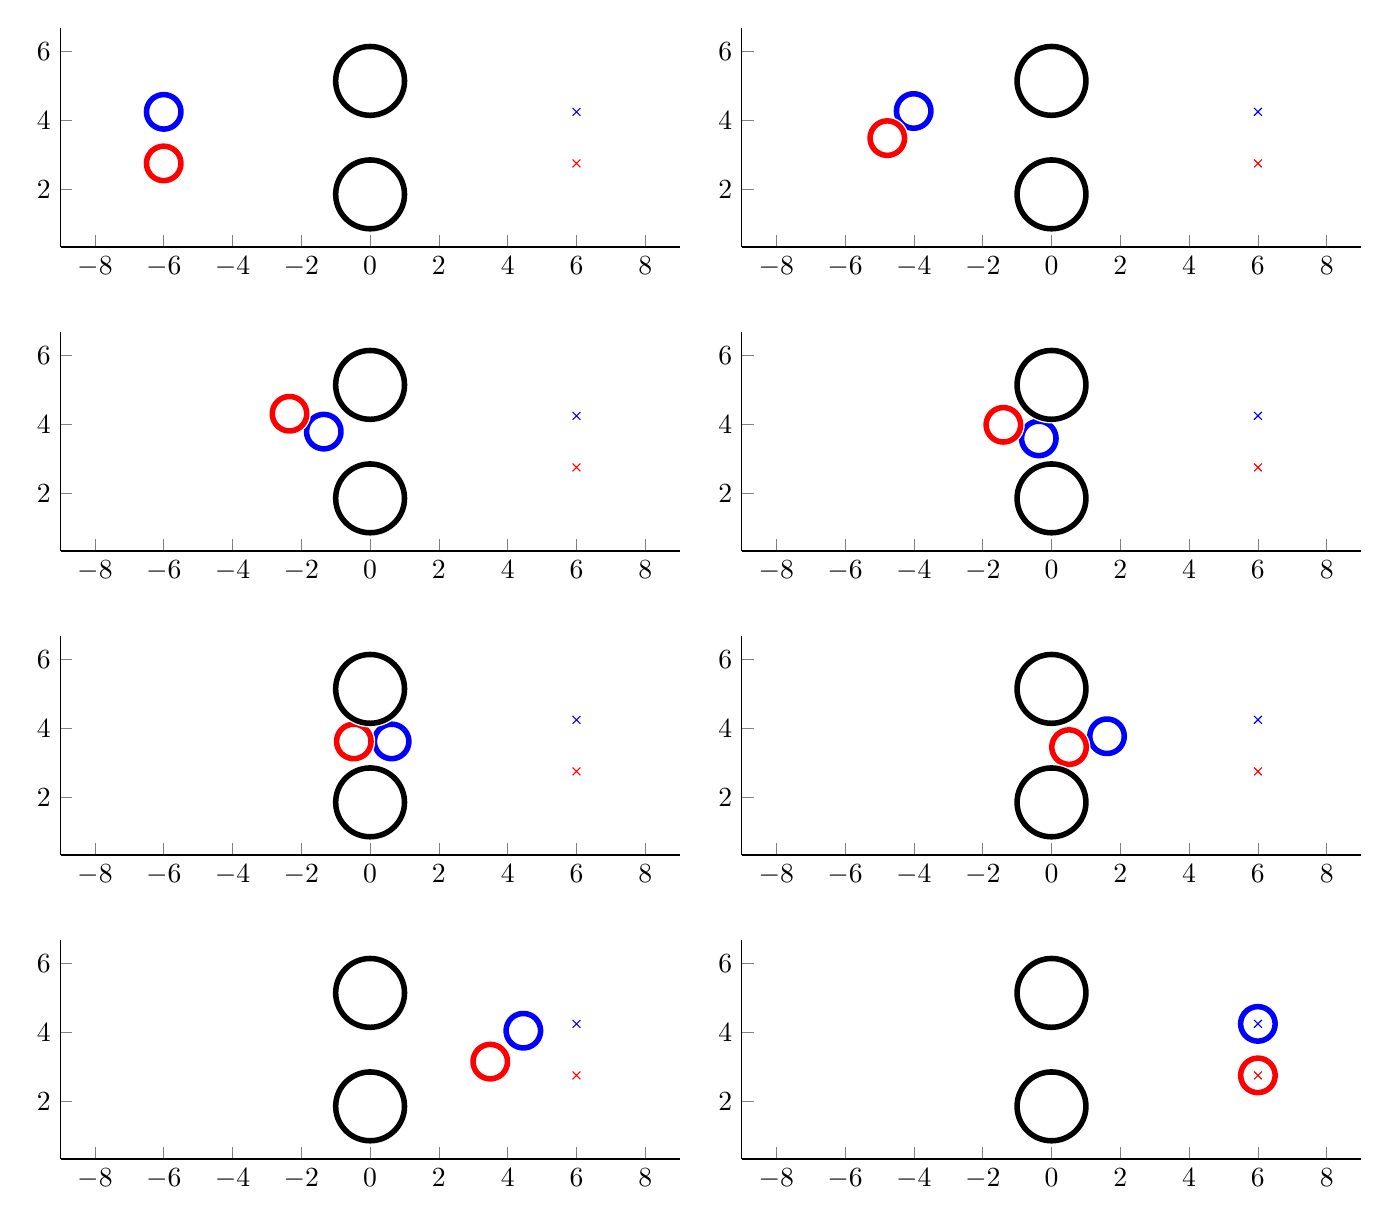
\begin{tikzpicture}

\begin{axis}[%
width=3.096in,
height=1.094in,
at={(2.593in,5.323in)},
scale only axis,
unbounded coords=jump,
xmin=-9,
xmax=9,
%xmajorgrids,
ymin=0.318379976997646,
ymax=6.68162002300235,
%ymajorgrids,
axis background/.style={fill=white},
axis x line*=bottom,
axis y line*=left
]
\addplot [color=blue,only marks,mark=x,mark options={solid},forget plot]
  table[row sep=crcr]{%
6	4.25\\
};
\addplot [color=red,only marks,mark=x,mark options={solid},forget plot]
  table[row sep=crcr]{%
6	2.75\\
};
\addplot [color=white,solid,line width=3.0pt,forget plot]
  table[row sep=crcr]{%
-5.5	4.25\\
-5.50030458649045	4.26744974835125\\
-5.50121797487009	4.28487823687206\\
-5.50273905231586	4.30226423163383\\
-5.50486596562921	4.31958655048003\\
-5.5075961234939	4.33682408883347\\
-5.5109261996331	4.35395584540888\\
-5.514852136862	4.37096094779983\\
-5.51936915203084	4.3878186779085\\
-5.52447174185242	4.40450849718747\\
-5.53015368960705	4.42101007166283\\
-5.53640807271661	4.43730329670796\\
-5.5432272711787	4.4533683215379\\
-5.55060297685042	4.46918557339454\\
-5.55852620357054	4.48473578139295\\
-5.56698729810778	4.5\\
-5.57597595192179	4.5149596321166\\
-5.58548121372248	4.52959645173537\\
-5.59549150281253	4.54389262614624\\
-5.60599462319664	4.55783073766283\\
-5.61697777844051	4.57139380484327\\
-5.6284275872613	4.58456530317943\\
-5.64033009983067	4.5973291852295\\
-5.6526708147705	4.60966990016933\\
-5.66543469682057	4.6215724127387\\
-5.67860619515673	4.63302222155949\\
-5.69216926233717	4.64400537680336\\
-5.70610737385376	4.65450849718747\\
-5.72040354826463	4.66451878627752\\
-5.7350403678834	4.67402404807821\\
-5.75	4.68301270189222\\
-5.76526421860705	4.69147379642946\\
-5.78081442660546	4.69939702314958\\
-5.7966316784621	4.7067727288213\\
-5.81269670329204	4.71359192728339\\
-5.82898992833717	4.71984631039295\\
-5.84549150281253	4.72552825814758\\
-5.8621813220915	4.73063084796916\\
-5.87903905220017	4.735147863138\\
-5.89604415459112	4.7390738003669\\
-5.91317591116653	4.7424038765061\\
-5.93041344951997	4.74513403437079\\
-5.94773576836617	4.74726094768414\\
-5.96512176312794	4.74878202512991\\
-5.98255025164875	4.74969541350955\\
-6	4.75\\
-6.01744974835125	4.74969541350955\\
-6.03487823687206	4.74878202512991\\
-6.05226423163383	4.74726094768414\\
-6.06958655048003	4.74513403437079\\
-6.08682408883347	4.7424038765061\\
-6.10395584540888	4.7390738003669\\
-6.12096094779983	4.735147863138\\
-6.1378186779085	4.73063084796916\\
-6.15450849718747	4.72552825814758\\
-6.17101007166283	4.71984631039295\\
-6.18730329670796	4.71359192728339\\
-6.2033683215379	4.7067727288213\\
-6.21918557339454	4.69939702314958\\
-6.23473578139295	4.69147379642946\\
-6.25	4.68301270189222\\
-6.2649596321166	4.67402404807821\\
-6.27959645173537	4.66451878627752\\
-6.29389262614624	4.65450849718747\\
-6.30783073766283	4.64400537680336\\
-6.32139380484327	4.63302222155949\\
-6.33456530317943	4.6215724127387\\
-6.3473291852295	4.60966990016933\\
-6.35966990016933	4.5973291852295\\
-6.3715724127387	4.58456530317943\\
-6.38302222155949	4.57139380484327\\
-6.39400537680336	4.55783073766283\\
-6.40450849718747	4.54389262614624\\
-6.41451878627752	4.52959645173537\\
-6.42402404807821	4.5149596321166\\
-6.43301270189222	4.5\\
-6.44147379642946	4.48473578139295\\
-6.44939702314958	4.46918557339454\\
-6.4567727288213	4.4533683215379\\
-6.46359192728339	4.43730329670796\\
-6.46984631039295	4.42101007166283\\
-6.47552825814758	4.40450849718747\\
-6.48063084796916	4.3878186779085\\
-6.485147863138	4.37096094779983\\
-6.4890738003669	4.35395584540888\\
-6.4924038765061	4.33682408883347\\
-6.49513403437079	4.31958655048003\\
-6.49726094768414	4.30226423163383\\
-6.49878202512991	4.28487823687206\\
-6.49969541350955	4.26744974835125\\
-6.5	4.25\\
-6.49969541350955	4.23255025164875\\
-6.49878202512991	4.21512176312794\\
-6.49726094768414	4.19773576836617\\
-6.49513403437079	4.18041344951997\\
-6.4924038765061	4.16317591116653\\
-6.4890738003669	4.14604415459112\\
-6.485147863138	4.12903905220017\\
-6.48063084796916	4.1121813220915\\
-6.47552825814758	4.09549150281253\\
-6.46984631039295	4.07898992833717\\
-6.46359192728339	4.06269670329204\\
-6.4567727288213	4.0466316784621\\
-6.44939702314958	4.03081442660546\\
-6.44147379642946	4.01526421860705\\
-6.43301270189222	4\\
-6.42402404807821	3.9850403678834\\
-6.41451878627752	3.97040354826463\\
-6.40450849718747	3.95610737385376\\
-6.39400537680336	3.94216926233717\\
-6.38302222155949	3.92860619515673\\
-6.3715724127387	3.91543469682057\\
-6.35966990016933	3.9026708147705\\
-6.3473291852295	3.89033009983067\\
-6.33456530317943	3.8784275872613\\
-6.32139380484327	3.86697777844051\\
-6.30783073766283	3.85599462319664\\
-6.29389262614624	3.84549150281253\\
-6.27959645173537	3.83548121372248\\
-6.2649596321166	3.82597595192179\\
-6.25	3.81698729810778\\
-6.23473578139295	3.80852620357054\\
-6.21918557339454	3.80060297685042\\
-6.2033683215379	3.7932272711787\\
-6.18730329670796	3.78640807271661\\
-6.17101007166283	3.78015368960705\\
-6.15450849718747	3.77447174185242\\
-6.1378186779085	3.76936915203084\\
-6.12096094779983	3.764852136862\\
-6.10395584540888	3.7609261996331\\
-6.08682408883347	3.7575961234939\\
-6.06958655048003	3.75486596562921\\
-6.05226423163383	3.75273905231586\\
-6.03487823687206	3.75121797487009\\
-6.01744974835125	3.75030458649045\\
-6	3.75\\
-5.98255025164875	3.75030458649045\\
-5.96512176312794	3.75121797487009\\
-5.94773576836617	3.75273905231586\\
-5.93041344951997	3.75486596562921\\
-5.91317591116653	3.7575961234939\\
-5.89604415459112	3.7609261996331\\
-5.87903905220017	3.764852136862\\
-5.8621813220915	3.76936915203084\\
-5.84549150281253	3.77447174185242\\
-5.82898992833717	3.78015368960705\\
-5.81269670329204	3.78640807271661\\
-5.7966316784621	3.7932272711787\\
-5.78081442660546	3.80060297685042\\
-5.76526421860705	3.80852620357054\\
-5.75	3.81698729810778\\
-5.7350403678834	3.82597595192179\\
-5.72040354826463	3.83548121372248\\
-5.70610737385376	3.84549150281253\\
-5.69216926233717	3.85599462319664\\
-5.67860619515673	3.86697777844051\\
-5.66543469682057	3.8784275872613\\
-5.6526708147705	3.89033009983067\\
-5.64033009983067	3.9026708147705\\
-5.6284275872613	3.91543469682057\\
-5.61697777844051	3.92860619515673\\
-5.60599462319664	3.94216926233717\\
-5.59549150281253	3.95610737385376\\
-5.58548121372248	3.97040354826463\\
-5.57597595192179	3.9850403678834\\
-5.56698729810778	4\\
-5.55852620357054	4.01526421860705\\
-5.55060297685042	4.03081442660546\\
-5.5432272711787	4.0466316784621\\
-5.53640807271661	4.06269670329204\\
-5.53015368960705	4.07898992833717\\
-5.52447174185242	4.09549150281253\\
-5.51936915203084	4.1121813220915\\
-5.514852136862	4.12903905220017\\
-5.5109261996331	4.14604415459112\\
-5.5075961234939	4.16317591116653\\
-5.50486596562921	4.18041344951997\\
-5.50273905231586	4.19773576836617\\
-5.50121797487009	4.21512176312794\\
-5.50030458649045	4.23255025164875\\
-5.5	4.25\\
nan	nan\\
};
\addplot [color=blue,solid,line width=2.0pt,forget plot]
  table[row sep=crcr]{%
-5.5	4.25\\
-5.50030458649045	4.26744974835125\\
-5.50121797487009	4.28487823687206\\
-5.50273905231586	4.30226423163383\\
-5.50486596562921	4.31958655048003\\
-5.5075961234939	4.33682408883347\\
-5.5109261996331	4.35395584540888\\
-5.514852136862	4.37096094779983\\
-5.51936915203084	4.3878186779085\\
-5.52447174185242	4.40450849718747\\
-5.53015368960705	4.42101007166283\\
-5.53640807271661	4.43730329670796\\
-5.5432272711787	4.4533683215379\\
-5.55060297685042	4.46918557339454\\
-5.55852620357054	4.48473578139295\\
-5.56698729810778	4.5\\
-5.57597595192179	4.5149596321166\\
-5.58548121372248	4.52959645173537\\
-5.59549150281253	4.54389262614624\\
-5.60599462319664	4.55783073766283\\
-5.61697777844051	4.57139380484327\\
-5.6284275872613	4.58456530317943\\
-5.64033009983067	4.5973291852295\\
-5.6526708147705	4.60966990016933\\
-5.66543469682057	4.6215724127387\\
-5.67860619515673	4.63302222155949\\
-5.69216926233717	4.64400537680336\\
-5.70610737385376	4.65450849718747\\
-5.72040354826463	4.66451878627752\\
-5.7350403678834	4.67402404807821\\
-5.75	4.68301270189222\\
-5.76526421860705	4.69147379642946\\
-5.78081442660546	4.69939702314958\\
-5.7966316784621	4.7067727288213\\
-5.81269670329204	4.71359192728339\\
-5.82898992833717	4.71984631039295\\
-5.84549150281253	4.72552825814758\\
-5.8621813220915	4.73063084796916\\
-5.87903905220017	4.735147863138\\
-5.89604415459112	4.7390738003669\\
-5.91317591116653	4.7424038765061\\
-5.93041344951997	4.74513403437079\\
-5.94773576836617	4.74726094768414\\
-5.96512176312794	4.74878202512991\\
-5.98255025164875	4.74969541350955\\
-6	4.75\\
-6.01744974835125	4.74969541350955\\
-6.03487823687206	4.74878202512991\\
-6.05226423163383	4.74726094768414\\
-6.06958655048003	4.74513403437079\\
-6.08682408883347	4.7424038765061\\
-6.10395584540888	4.7390738003669\\
-6.12096094779983	4.735147863138\\
-6.1378186779085	4.73063084796916\\
-6.15450849718747	4.72552825814758\\
-6.17101007166283	4.71984631039295\\
-6.18730329670796	4.71359192728339\\
-6.2033683215379	4.7067727288213\\
-6.21918557339454	4.69939702314958\\
-6.23473578139295	4.69147379642946\\
-6.25	4.68301270189222\\
-6.2649596321166	4.67402404807821\\
-6.27959645173537	4.66451878627752\\
-6.29389262614624	4.65450849718747\\
-6.30783073766283	4.64400537680336\\
-6.32139380484327	4.63302222155949\\
-6.33456530317943	4.6215724127387\\
-6.3473291852295	4.60966990016933\\
-6.35966990016933	4.5973291852295\\
-6.3715724127387	4.58456530317943\\
-6.38302222155949	4.57139380484327\\
-6.39400537680336	4.55783073766283\\
-6.40450849718747	4.54389262614624\\
-6.41451878627752	4.52959645173537\\
-6.42402404807821	4.5149596321166\\
-6.43301270189222	4.5\\
-6.44147379642946	4.48473578139295\\
-6.44939702314958	4.46918557339454\\
-6.4567727288213	4.4533683215379\\
-6.46359192728339	4.43730329670796\\
-6.46984631039295	4.42101007166283\\
-6.47552825814758	4.40450849718747\\
-6.48063084796916	4.3878186779085\\
-6.485147863138	4.37096094779983\\
-6.4890738003669	4.35395584540888\\
-6.4924038765061	4.33682408883347\\
-6.49513403437079	4.31958655048003\\
-6.49726094768414	4.30226423163383\\
-6.49878202512991	4.28487823687206\\
-6.49969541350955	4.26744974835125\\
-6.5	4.25\\
-6.49969541350955	4.23255025164875\\
-6.49878202512991	4.21512176312794\\
-6.49726094768414	4.19773576836617\\
-6.49513403437079	4.18041344951997\\
-6.4924038765061	4.16317591116653\\
-6.4890738003669	4.14604415459112\\
-6.485147863138	4.12903905220017\\
-6.48063084796916	4.1121813220915\\
-6.47552825814758	4.09549150281253\\
-6.46984631039295	4.07898992833717\\
-6.46359192728339	4.06269670329204\\
-6.4567727288213	4.0466316784621\\
-6.44939702314958	4.03081442660546\\
-6.44147379642946	4.01526421860705\\
-6.43301270189222	4\\
-6.42402404807821	3.9850403678834\\
-6.41451878627752	3.97040354826463\\
-6.40450849718747	3.95610737385376\\
-6.39400537680336	3.94216926233717\\
-6.38302222155949	3.92860619515673\\
-6.3715724127387	3.91543469682057\\
-6.35966990016933	3.9026708147705\\
-6.3473291852295	3.89033009983067\\
-6.33456530317943	3.8784275872613\\
-6.32139380484327	3.86697777844051\\
-6.30783073766283	3.85599462319664\\
-6.29389262614624	3.84549150281253\\
-6.27959645173537	3.83548121372248\\
-6.2649596321166	3.82597595192179\\
-6.25	3.81698729810778\\
-6.23473578139295	3.80852620357054\\
-6.21918557339454	3.80060297685042\\
-6.2033683215379	3.7932272711787\\
-6.18730329670796	3.78640807271661\\
-6.17101007166283	3.78015368960705\\
-6.15450849718747	3.77447174185242\\
-6.1378186779085	3.76936915203084\\
-6.12096094779983	3.764852136862\\
-6.10395584540888	3.7609261996331\\
-6.08682408883347	3.7575961234939\\
-6.06958655048003	3.75486596562921\\
-6.05226423163383	3.75273905231586\\
-6.03487823687206	3.75121797487009\\
-6.01744974835125	3.75030458649045\\
-6	3.75\\
-5.98255025164875	3.75030458649045\\
-5.96512176312794	3.75121797487009\\
-5.94773576836617	3.75273905231586\\
-5.93041344951997	3.75486596562921\\
-5.91317591116653	3.7575961234939\\
-5.89604415459112	3.7609261996331\\
-5.87903905220017	3.764852136862\\
-5.8621813220915	3.76936915203084\\
-5.84549150281253	3.77447174185242\\
-5.82898992833717	3.78015368960705\\
-5.81269670329204	3.78640807271661\\
-5.7966316784621	3.7932272711787\\
-5.78081442660546	3.80060297685042\\
-5.76526421860705	3.80852620357054\\
-5.75	3.81698729810778\\
-5.7350403678834	3.82597595192179\\
-5.72040354826463	3.83548121372248\\
-5.70610737385376	3.84549150281253\\
-5.69216926233717	3.85599462319664\\
-5.67860619515673	3.86697777844051\\
-5.66543469682057	3.8784275872613\\
-5.6526708147705	3.89033009983067\\
-5.64033009983067	3.9026708147705\\
-5.6284275872613	3.91543469682057\\
-5.61697777844051	3.92860619515673\\
-5.60599462319664	3.94216926233717\\
-5.59549150281253	3.95610737385376\\
-5.58548121372248	3.97040354826463\\
-5.57597595192179	3.9850403678834\\
-5.56698729810778	4\\
-5.55852620357054	4.01526421860705\\
-5.55060297685042	4.03081442660546\\
-5.5432272711787	4.0466316784621\\
-5.53640807271661	4.06269670329204\\
-5.53015368960705	4.07898992833717\\
-5.52447174185242	4.09549150281253\\
-5.51936915203084	4.1121813220915\\
-5.514852136862	4.12903905220017\\
-5.5109261996331	4.14604415459112\\
-5.5075961234939	4.16317591116653\\
-5.50486596562921	4.18041344951997\\
-5.50273905231586	4.19773576836617\\
-5.50121797487009	4.21512176312794\\
-5.50030458649045	4.23255025164875\\
-5.5	4.25\\
nan	nan\\
};
\addplot [color=white,solid,line width=3.0pt,forget plot]
  table[row sep=crcr]{%
-5.5	2.75\\
-5.50030458649045	2.76744974835125\\
-5.50121797487009	2.78487823687206\\
-5.50273905231586	2.80226423163383\\
-5.50486596562921	2.81958655048003\\
-5.5075961234939	2.83682408883347\\
-5.5109261996331	2.85395584540888\\
-5.514852136862	2.87096094779983\\
-5.51936915203084	2.8878186779085\\
-5.52447174185242	2.90450849718747\\
-5.53015368960705	2.92101007166283\\
-5.53640807271661	2.93730329670796\\
-5.5432272711787	2.9533683215379\\
-5.55060297685042	2.96918557339454\\
-5.55852620357054	2.98473578139295\\
-5.56698729810778	3\\
-5.57597595192179	3.0149596321166\\
-5.58548121372248	3.02959645173537\\
-5.59549150281253	3.04389262614624\\
-5.60599462319664	3.05783073766283\\
-5.61697777844051	3.07139380484327\\
-5.6284275872613	3.08456530317943\\
-5.64033009983067	3.0973291852295\\
-5.6526708147705	3.10966990016933\\
-5.66543469682057	3.1215724127387\\
-5.67860619515673	3.13302222155949\\
-5.69216926233717	3.14400537680336\\
-5.70610737385376	3.15450849718747\\
-5.72040354826463	3.16451878627752\\
-5.7350403678834	3.17402404807821\\
-5.75	3.18301270189222\\
-5.76526421860705	3.19147379642946\\
-5.78081442660546	3.19939702314958\\
-5.7966316784621	3.2067727288213\\
-5.81269670329204	3.21359192728339\\
-5.82898992833717	3.21984631039295\\
-5.84549150281253	3.22552825814758\\
-5.8621813220915	3.23063084796916\\
-5.87903905220017	3.235147863138\\
-5.89604415459112	3.2390738003669\\
-5.91317591116653	3.2424038765061\\
-5.93041344951997	3.24513403437079\\
-5.94773576836617	3.24726094768414\\
-5.96512176312794	3.24878202512991\\
-5.98255025164875	3.24969541350955\\
-6	3.25\\
-6.01744974835125	3.24969541350955\\
-6.03487823687206	3.24878202512991\\
-6.05226423163383	3.24726094768414\\
-6.06958655048003	3.24513403437079\\
-6.08682408883347	3.2424038765061\\
-6.10395584540888	3.2390738003669\\
-6.12096094779983	3.235147863138\\
-6.1378186779085	3.23063084796916\\
-6.15450849718747	3.22552825814758\\
-6.17101007166283	3.21984631039295\\
-6.18730329670796	3.21359192728339\\
-6.2033683215379	3.2067727288213\\
-6.21918557339454	3.19939702314958\\
-6.23473578139295	3.19147379642946\\
-6.25	3.18301270189222\\
-6.2649596321166	3.17402404807821\\
-6.27959645173537	3.16451878627752\\
-6.29389262614624	3.15450849718747\\
-6.30783073766283	3.14400537680336\\
-6.32139380484327	3.13302222155949\\
-6.33456530317943	3.1215724127387\\
-6.3473291852295	3.10966990016933\\
-6.35966990016933	3.0973291852295\\
-6.3715724127387	3.08456530317943\\
-6.38302222155949	3.07139380484327\\
-6.39400537680336	3.05783073766283\\
-6.40450849718747	3.04389262614624\\
-6.41451878627752	3.02959645173537\\
-6.42402404807821	3.0149596321166\\
-6.43301270189222	3\\
-6.44147379642946	2.98473578139295\\
-6.44939702314958	2.96918557339454\\
-6.4567727288213	2.9533683215379\\
-6.46359192728339	2.93730329670796\\
-6.46984631039295	2.92101007166283\\
-6.47552825814758	2.90450849718747\\
-6.48063084796916	2.8878186779085\\
-6.485147863138	2.87096094779983\\
-6.4890738003669	2.85395584540888\\
-6.4924038765061	2.83682408883347\\
-6.49513403437079	2.81958655048003\\
-6.49726094768414	2.80226423163383\\
-6.49878202512991	2.78487823687206\\
-6.49969541350955	2.76744974835125\\
-6.5	2.75\\
-6.49969541350955	2.73255025164875\\
-6.49878202512991	2.71512176312794\\
-6.49726094768414	2.69773576836617\\
-6.49513403437079	2.68041344951997\\
-6.4924038765061	2.66317591116653\\
-6.4890738003669	2.64604415459112\\
-6.485147863138	2.62903905220017\\
-6.48063084796916	2.6121813220915\\
-6.47552825814758	2.59549150281253\\
-6.46984631039295	2.57898992833717\\
-6.46359192728339	2.56269670329204\\
-6.4567727288213	2.5466316784621\\
-6.44939702314958	2.53081442660546\\
-6.44147379642946	2.51526421860705\\
-6.43301270189222	2.5\\
-6.42402404807821	2.4850403678834\\
-6.41451878627752	2.47040354826463\\
-6.40450849718747	2.45610737385376\\
-6.39400537680336	2.44216926233717\\
-6.38302222155949	2.42860619515673\\
-6.3715724127387	2.41543469682057\\
-6.35966990016933	2.4026708147705\\
-6.3473291852295	2.39033009983067\\
-6.33456530317943	2.3784275872613\\
-6.32139380484327	2.36697777844051\\
-6.30783073766283	2.35599462319664\\
-6.29389262614624	2.34549150281253\\
-6.27959645173537	2.33548121372248\\
-6.2649596321166	2.32597595192179\\
-6.25	2.31698729810778\\
-6.23473578139295	2.30852620357054\\
-6.21918557339454	2.30060297685042\\
-6.2033683215379	2.2932272711787\\
-6.18730329670796	2.28640807271661\\
-6.17101007166283	2.28015368960705\\
-6.15450849718747	2.27447174185242\\
-6.1378186779085	2.26936915203084\\
-6.12096094779983	2.264852136862\\
-6.10395584540888	2.2609261996331\\
-6.08682408883347	2.2575961234939\\
-6.06958655048003	2.25486596562921\\
-6.05226423163383	2.25273905231586\\
-6.03487823687206	2.25121797487009\\
-6.01744974835125	2.25030458649045\\
-6	2.25\\
-5.98255025164875	2.25030458649045\\
-5.96512176312794	2.25121797487009\\
-5.94773576836617	2.25273905231586\\
-5.93041344951997	2.25486596562921\\
-5.91317591116653	2.2575961234939\\
-5.89604415459112	2.2609261996331\\
-5.87903905220017	2.264852136862\\
-5.8621813220915	2.26936915203084\\
-5.84549150281253	2.27447174185242\\
-5.82898992833717	2.28015368960705\\
-5.81269670329204	2.28640807271661\\
-5.7966316784621	2.2932272711787\\
-5.78081442660546	2.30060297685042\\
-5.76526421860705	2.30852620357054\\
-5.75	2.31698729810778\\
-5.7350403678834	2.32597595192179\\
-5.72040354826463	2.33548121372248\\
-5.70610737385376	2.34549150281253\\
-5.69216926233717	2.35599462319664\\
-5.67860619515673	2.36697777844051\\
-5.66543469682057	2.3784275872613\\
-5.6526708147705	2.39033009983067\\
-5.64033009983067	2.4026708147705\\
-5.6284275872613	2.41543469682057\\
-5.61697777844051	2.42860619515673\\
-5.60599462319664	2.44216926233717\\
-5.59549150281253	2.45610737385376\\
-5.58548121372248	2.47040354826463\\
-5.57597595192179	2.4850403678834\\
-5.56698729810778	2.5\\
-5.55852620357054	2.51526421860705\\
-5.55060297685042	2.53081442660546\\
-5.5432272711787	2.5466316784621\\
-5.53640807271661	2.56269670329204\\
-5.53015368960705	2.57898992833717\\
-5.52447174185242	2.59549150281253\\
-5.51936915203084	2.6121813220915\\
-5.514852136862	2.62903905220017\\
-5.5109261996331	2.64604415459112\\
-5.5075961234939	2.66317591116653\\
-5.50486596562921	2.68041344951997\\
-5.50273905231586	2.69773576836617\\
-5.50121797487009	2.71512176312794\\
-5.50030458649045	2.73255025164875\\
-5.5	2.75\\
nan	nan\\
};
\addplot [color=red,solid,line width=2.0pt,forget plot]
  table[row sep=crcr]{%
-5.5	2.75\\
-5.50030458649045	2.76744974835125\\
-5.50121797487009	2.78487823687206\\
-5.50273905231586	2.80226423163383\\
-5.50486596562921	2.81958655048003\\
-5.5075961234939	2.83682408883347\\
-5.5109261996331	2.85395584540888\\
-5.514852136862	2.87096094779983\\
-5.51936915203084	2.8878186779085\\
-5.52447174185242	2.90450849718747\\
-5.53015368960705	2.92101007166283\\
-5.53640807271661	2.93730329670796\\
-5.5432272711787	2.9533683215379\\
-5.55060297685042	2.96918557339454\\
-5.55852620357054	2.98473578139295\\
-5.56698729810778	3\\
-5.57597595192179	3.0149596321166\\
-5.58548121372248	3.02959645173537\\
-5.59549150281253	3.04389262614624\\
-5.60599462319664	3.05783073766283\\
-5.61697777844051	3.07139380484327\\
-5.6284275872613	3.08456530317943\\
-5.64033009983067	3.0973291852295\\
-5.6526708147705	3.10966990016933\\
-5.66543469682057	3.1215724127387\\
-5.67860619515673	3.13302222155949\\
-5.69216926233717	3.14400537680336\\
-5.70610737385376	3.15450849718747\\
-5.72040354826463	3.16451878627752\\
-5.7350403678834	3.17402404807821\\
-5.75	3.18301270189222\\
-5.76526421860705	3.19147379642946\\
-5.78081442660546	3.19939702314958\\
-5.7966316784621	3.2067727288213\\
-5.81269670329204	3.21359192728339\\
-5.82898992833717	3.21984631039295\\
-5.84549150281253	3.22552825814758\\
-5.8621813220915	3.23063084796916\\
-5.87903905220017	3.235147863138\\
-5.89604415459112	3.2390738003669\\
-5.91317591116653	3.2424038765061\\
-5.93041344951997	3.24513403437079\\
-5.94773576836617	3.24726094768414\\
-5.96512176312794	3.24878202512991\\
-5.98255025164875	3.24969541350955\\
-6	3.25\\
-6.01744974835125	3.24969541350955\\
-6.03487823687206	3.24878202512991\\
-6.05226423163383	3.24726094768414\\
-6.06958655048003	3.24513403437079\\
-6.08682408883347	3.2424038765061\\
-6.10395584540888	3.2390738003669\\
-6.12096094779983	3.235147863138\\
-6.1378186779085	3.23063084796916\\
-6.15450849718747	3.22552825814758\\
-6.17101007166283	3.21984631039295\\
-6.18730329670796	3.21359192728339\\
-6.2033683215379	3.2067727288213\\
-6.21918557339454	3.19939702314958\\
-6.23473578139295	3.19147379642946\\
-6.25	3.18301270189222\\
-6.2649596321166	3.17402404807821\\
-6.27959645173537	3.16451878627752\\
-6.29389262614624	3.15450849718747\\
-6.30783073766283	3.14400537680336\\
-6.32139380484327	3.13302222155949\\
-6.33456530317943	3.1215724127387\\
-6.3473291852295	3.10966990016933\\
-6.35966990016933	3.0973291852295\\
-6.3715724127387	3.08456530317943\\
-6.38302222155949	3.07139380484327\\
-6.39400537680336	3.05783073766283\\
-6.40450849718747	3.04389262614624\\
-6.41451878627752	3.02959645173537\\
-6.42402404807821	3.0149596321166\\
-6.43301270189222	3\\
-6.44147379642946	2.98473578139295\\
-6.44939702314958	2.96918557339454\\
-6.4567727288213	2.9533683215379\\
-6.46359192728339	2.93730329670796\\
-6.46984631039295	2.92101007166283\\
-6.47552825814758	2.90450849718747\\
-6.48063084796916	2.8878186779085\\
-6.485147863138	2.87096094779983\\
-6.4890738003669	2.85395584540888\\
-6.4924038765061	2.83682408883347\\
-6.49513403437079	2.81958655048003\\
-6.49726094768414	2.80226423163383\\
-6.49878202512991	2.78487823687206\\
-6.49969541350955	2.76744974835125\\
-6.5	2.75\\
-6.49969541350955	2.73255025164875\\
-6.49878202512991	2.71512176312794\\
-6.49726094768414	2.69773576836617\\
-6.49513403437079	2.68041344951997\\
-6.4924038765061	2.66317591116653\\
-6.4890738003669	2.64604415459112\\
-6.485147863138	2.62903905220017\\
-6.48063084796916	2.6121813220915\\
-6.47552825814758	2.59549150281253\\
-6.46984631039295	2.57898992833717\\
-6.46359192728339	2.56269670329204\\
-6.4567727288213	2.5466316784621\\
-6.44939702314958	2.53081442660546\\
-6.44147379642946	2.51526421860705\\
-6.43301270189222	2.5\\
-6.42402404807821	2.4850403678834\\
-6.41451878627752	2.47040354826463\\
-6.40450849718747	2.45610737385376\\
-6.39400537680336	2.44216926233717\\
-6.38302222155949	2.42860619515673\\
-6.3715724127387	2.41543469682057\\
-6.35966990016933	2.4026708147705\\
-6.3473291852295	2.39033009983067\\
-6.33456530317943	2.3784275872613\\
-6.32139380484327	2.36697777844051\\
-6.30783073766283	2.35599462319664\\
-6.29389262614624	2.34549150281253\\
-6.27959645173537	2.33548121372248\\
-6.2649596321166	2.32597595192179\\
-6.25	2.31698729810778\\
-6.23473578139295	2.30852620357054\\
-6.21918557339454	2.30060297685042\\
-6.2033683215379	2.2932272711787\\
-6.18730329670796	2.28640807271661\\
-6.17101007166283	2.28015368960705\\
-6.15450849718747	2.27447174185242\\
-6.1378186779085	2.26936915203084\\
-6.12096094779983	2.264852136862\\
-6.10395584540888	2.2609261996331\\
-6.08682408883347	2.2575961234939\\
-6.06958655048003	2.25486596562921\\
-6.05226423163383	2.25273905231586\\
-6.03487823687206	2.25121797487009\\
-6.01744974835125	2.25030458649045\\
-6	2.25\\
-5.98255025164875	2.25030458649045\\
-5.96512176312794	2.25121797487009\\
-5.94773576836617	2.25273905231586\\
-5.93041344951997	2.25486596562921\\
-5.91317591116653	2.2575961234939\\
-5.89604415459112	2.2609261996331\\
-5.87903905220017	2.264852136862\\
-5.8621813220915	2.26936915203084\\
-5.84549150281253	2.27447174185242\\
-5.82898992833717	2.28015368960705\\
-5.81269670329204	2.28640807271661\\
-5.7966316784621	2.2932272711787\\
-5.78081442660546	2.30060297685042\\
-5.76526421860705	2.30852620357054\\
-5.75	2.31698729810778\\
-5.7350403678834	2.32597595192179\\
-5.72040354826463	2.33548121372248\\
-5.70610737385376	2.34549150281253\\
-5.69216926233717	2.35599462319664\\
-5.67860619515673	2.36697777844051\\
-5.66543469682057	2.3784275872613\\
-5.6526708147705	2.39033009983067\\
-5.64033009983067	2.4026708147705\\
-5.6284275872613	2.41543469682057\\
-5.61697777844051	2.42860619515673\\
-5.60599462319664	2.44216926233717\\
-5.59549150281253	2.45610737385376\\
-5.58548121372248	2.47040354826463\\
-5.57597595192179	2.4850403678834\\
-5.56698729810778	2.5\\
-5.55852620357054	2.51526421860705\\
-5.55060297685042	2.53081442660546\\
-5.5432272711787	2.5466316784621\\
-5.53640807271661	2.56269670329204\\
-5.53015368960705	2.57898992833717\\
-5.52447174185242	2.59549150281253\\
-5.51936915203084	2.6121813220915\\
-5.514852136862	2.62903905220017\\
-5.5109261996331	2.64604415459112\\
-5.5075961234939	2.66317591116653\\
-5.50486596562921	2.68041344951997\\
-5.50273905231586	2.69773576836617\\
-5.50121797487009	2.71512176312794\\
-5.50030458649045	2.73255025164875\\
-5.5	2.75\\
nan	nan\\
};
\addplot [color=white,solid,line width=3.0pt,forget plot]
  table[row sep=crcr]{%
1	1.85\\
0.999390827019096	1.8848994967025\\
0.997564050259824	1.91975647374413\\
0.994521895368273	1.95452846326765\\
0.99026806874157	1.98917310096007\\
0.984807753012208	2.02364817766693\\
0.978147600733806	2.05791169081776\\
0.970295726275996	2.09192189559967\\
0.961261695938319	2.125637355817\\
0.951056516295154	2.15901699437495\\
0.939692620785908	2.19202014332567\\
0.927183854566787	2.22460659341591\\
0.913545457642601	2.2567366430758\\
0.898794046299167	2.28837114678908\\
0.882947592858927	2.31947156278589\\
0.866025403784439	2.35\\
0.848048096156426	2.37991926423321\\
0.829037572555042	2.40919290347075\\
0.809016994374947	2.43778525229247\\
0.788010753606722	2.46566147532566\\
0.766044443118978	2.49278760968654\\
0.743144825477394	2.51913060635886\\
0.719339800338651	2.544658370459\\
0.694658370458997	2.56933980033865\\
0.669130606358858	2.59314482547739\\
0.642787609686539	2.61604444311898\\
0.615661475325658	2.63801075360672\\
0.587785252292473	2.65901699437495\\
0.559192903470747	2.67903757255504\\
0.529919264233205	2.69804809615643\\
0.5	2.71602540378444\\
0.469471562785891	2.73294759285893\\
0.438371146789077	2.74879404629917\\
0.4067366430758	2.7635454576426\\
0.374606593415912	2.77718385456679\\
0.342020143325669	2.78969262078591\\
0.309016994374947	2.80105651629515\\
0.275637355816999	2.81126169593832\\
0.241921895599668	2.820295726276\\
0.207911690817759	2.82814760073381\\
0.17364817766693	2.83480775301221\\
0.139173100960066	2.84026806874157\\
0.104528463267653	2.84452189536827\\
0.0697564737441255	2.84756405025982\\
0.0348994967025011	2.8493908270191\\
6.12323399573677e-17	2.85\\
-0.0348994967025007	2.8493908270191\\
-0.0697564737441253	2.84756405025982\\
-0.104528463267653	2.84452189536827\\
-0.139173100960065	2.84026806874157\\
-0.17364817766693	2.83480775301221\\
-0.207911690817759	2.82814760073381\\
-0.241921895599668	2.820295726276\\
-0.275637355816999	2.81126169593832\\
-0.309016994374947	2.80105651629515\\
-0.342020143325669	2.78969262078591\\
-0.374606593415912	2.77718385456679\\
-0.4067366430758	2.7635454576426\\
-0.438371146789078	2.74879404629917\\
-0.469471562785891	2.73294759285893\\
-0.5	2.71602540378444\\
-0.529919264233205	2.69804809615643\\
-0.559192903470747	2.67903757255504\\
-0.587785252292473	2.65901699437495\\
-0.615661475325658	2.63801075360672\\
-0.642787609686539	2.61604444311898\\
-0.669130606358858	2.59314482547739\\
-0.694658370458997	2.56933980033865\\
-0.719339800338651	2.544658370459\\
-0.743144825477394	2.51913060635886\\
-0.766044443118978	2.49278760968654\\
-0.788010753606722	2.46566147532566\\
-0.809016994374947	2.43778525229247\\
-0.829037572555042	2.40919290347075\\
-0.848048096156426	2.37991926423321\\
-0.866025403784439	2.35\\
-0.882947592858927	2.31947156278589\\
-0.898794046299167	2.28837114678908\\
-0.913545457642601	2.2567366430758\\
-0.927183854566787	2.22460659341591\\
-0.939692620785908	2.19202014332567\\
-0.951056516295154	2.15901699437495\\
-0.961261695938319	2.125637355817\\
-0.970295726275996	2.09192189559967\\
-0.978147600733806	2.05791169081776\\
-0.984807753012208	2.02364817766693\\
-0.99026806874157	1.98917310096007\\
-0.994521895368273	1.95452846326765\\
-0.997564050259824	1.91975647374413\\
-0.999390827019096	1.8848994967025\\
-1	1.85\\
-0.999390827019096	1.8151005032975\\
-0.997564050259824	1.78024352625588\\
-0.994521895368273	1.74547153673235\\
-0.99026806874157	1.71082689903993\\
-0.984807753012208	1.67635182233307\\
-0.978147600733806	1.64208830918224\\
-0.970295726275997	1.60807810440033\\
-0.961261695938319	1.574362644183\\
-0.951056516295154	1.54098300562505\\
-0.939692620785908	1.50797985667433\\
-0.927183854566787	1.47539340658409\\
-0.913545457642601	1.4432633569242\\
-0.898794046299167	1.41162885321092\\
-0.882947592858927	1.38052843721411\\
-0.866025403784439	1.35\\
-0.848048096156426	1.3200807357668\\
-0.829037572555042	1.29080709652925\\
-0.809016994374947	1.26221474770753\\
-0.788010753606722	1.23433852467434\\
-0.766044443118978	1.20721239031346\\
-0.743144825477394	1.18086939364114\\
-0.719339800338651	1.155341629541\\
-0.694658370458997	1.13066019966135\\
-0.669130606358858	1.10685517452261\\
-0.642787609686539	1.08395555688102\\
-0.615661475325658	1.06198924639328\\
-0.587785252292473	1.04098300562505\\
-0.559192903470747	1.02096242744496\\
-0.529919264233205	1.00195190384357\\
-0.5	0.983974596215562\\
-0.469471562785891	0.967052407141073\\
-0.438371146789078	0.951205953700833\\
-0.4067366430758	0.936454542357399\\
-0.374606593415912	0.922816145433213\\
-0.342020143325669	0.910307379214092\\
-0.309016994374948	0.898943483704847\\
-0.275637355816999	0.888738304061681\\
-0.241921895599668	0.879704273724004\\
-0.20791169081776	0.871852399266195\\
-0.17364817766693	0.865192246987792\\
-0.139173100960065	0.85973193125843\\
-0.104528463267653	0.855478104631727\\
-0.0697564737441256	0.852435949740176\\
-0.0348994967025016	0.850609172980904\\
-1.83697019872103e-16	0.85\\
0.0348994967025013	0.850609172980904\\
0.0697564737441252	0.852435949740176\\
0.104528463267653	0.855478104631727\\
0.139173100960065	0.85973193125843\\
0.17364817766693	0.865192246987792\\
0.207911690817759	0.871852399266194\\
0.241921895599667	0.879704273724004\\
0.275637355816999	0.888738304061681\\
0.309016994374947	0.898943483704846\\
0.342020143325668	0.910307379214092\\
0.374606593415912	0.922816145433213\\
0.406736643075801	0.936454542357399\\
0.438371146789077	0.951205953700833\\
0.46947156278589	0.967052407141073\\
0.5	0.983974596215561\\
0.529919264233205	1.00195190384357\\
0.559192903470746	1.02096242744496\\
0.587785252292473	1.04098300562505\\
0.615661475325659	1.06198924639328\\
0.642787609686539	1.08395555688102\\
0.669130606358858	1.10685517452261\\
0.694658370458997	1.13066019966135\\
0.719339800338651	1.155341629541\\
0.743144825477394	1.18086939364114\\
0.766044443118978	1.20721239031346\\
0.788010753606722	1.23433852467434\\
0.809016994374947	1.26221474770753\\
0.829037572555041	1.29080709652925\\
0.848048096156425	1.32008073576679\\
0.866025403784438	1.35\\
0.882947592858927	1.38052843721411\\
0.898794046299167	1.41162885321092\\
0.913545457642601	1.4432633569242\\
0.927183854566787	1.47539340658409\\
0.939692620785908	1.50797985667433\\
0.951056516295154	1.54098300562505\\
0.961261695938319	1.574362644183\\
0.970295726275996	1.60807810440033\\
0.978147600733806	1.64208830918224\\
0.984807753012208	1.67635182233307\\
0.99026806874157	1.71082689903993\\
0.994521895368273	1.74547153673235\\
0.997564050259824	1.78024352625588\\
0.999390827019096	1.8151005032975\\
1	1.85\\
nan	nan\\
};
\addplot [color=black,solid,line width=2.0pt,forget plot]
  table[row sep=crcr]{%
1	1.85\\
0.999390827019096	1.8848994967025\\
0.997564050259824	1.91975647374413\\
0.994521895368273	1.95452846326765\\
0.99026806874157	1.98917310096007\\
0.984807753012208	2.02364817766693\\
0.978147600733806	2.05791169081776\\
0.970295726275996	2.09192189559967\\
0.961261695938319	2.125637355817\\
0.951056516295154	2.15901699437495\\
0.939692620785908	2.19202014332567\\
0.927183854566787	2.22460659341591\\
0.913545457642601	2.2567366430758\\
0.898794046299167	2.28837114678908\\
0.882947592858927	2.31947156278589\\
0.866025403784439	2.35\\
0.848048096156426	2.37991926423321\\
0.829037572555042	2.40919290347075\\
0.809016994374947	2.43778525229247\\
0.788010753606722	2.46566147532566\\
0.766044443118978	2.49278760968654\\
0.743144825477394	2.51913060635886\\
0.719339800338651	2.544658370459\\
0.694658370458997	2.56933980033865\\
0.669130606358858	2.59314482547739\\
0.642787609686539	2.61604444311898\\
0.615661475325658	2.63801075360672\\
0.587785252292473	2.65901699437495\\
0.559192903470747	2.67903757255504\\
0.529919264233205	2.69804809615643\\
0.5	2.71602540378444\\
0.469471562785891	2.73294759285893\\
0.438371146789077	2.74879404629917\\
0.4067366430758	2.7635454576426\\
0.374606593415912	2.77718385456679\\
0.342020143325669	2.78969262078591\\
0.309016994374947	2.80105651629515\\
0.275637355816999	2.81126169593832\\
0.241921895599668	2.820295726276\\
0.207911690817759	2.82814760073381\\
0.17364817766693	2.83480775301221\\
0.139173100960066	2.84026806874157\\
0.104528463267653	2.84452189536827\\
0.0697564737441255	2.84756405025982\\
0.0348994967025011	2.8493908270191\\
6.12323399573677e-17	2.85\\
-0.0348994967025007	2.8493908270191\\
-0.0697564737441253	2.84756405025982\\
-0.104528463267653	2.84452189536827\\
-0.139173100960065	2.84026806874157\\
-0.17364817766693	2.83480775301221\\
-0.207911690817759	2.82814760073381\\
-0.241921895599668	2.820295726276\\
-0.275637355816999	2.81126169593832\\
-0.309016994374947	2.80105651629515\\
-0.342020143325669	2.78969262078591\\
-0.374606593415912	2.77718385456679\\
-0.4067366430758	2.7635454576426\\
-0.438371146789078	2.74879404629917\\
-0.469471562785891	2.73294759285893\\
-0.5	2.71602540378444\\
-0.529919264233205	2.69804809615643\\
-0.559192903470747	2.67903757255504\\
-0.587785252292473	2.65901699437495\\
-0.615661475325658	2.63801075360672\\
-0.642787609686539	2.61604444311898\\
-0.669130606358858	2.59314482547739\\
-0.694658370458997	2.56933980033865\\
-0.719339800338651	2.544658370459\\
-0.743144825477394	2.51913060635886\\
-0.766044443118978	2.49278760968654\\
-0.788010753606722	2.46566147532566\\
-0.809016994374947	2.43778525229247\\
-0.829037572555042	2.40919290347075\\
-0.848048096156426	2.37991926423321\\
-0.866025403784439	2.35\\
-0.882947592858927	2.31947156278589\\
-0.898794046299167	2.28837114678908\\
-0.913545457642601	2.2567366430758\\
-0.927183854566787	2.22460659341591\\
-0.939692620785908	2.19202014332567\\
-0.951056516295154	2.15901699437495\\
-0.961261695938319	2.125637355817\\
-0.970295726275996	2.09192189559967\\
-0.978147600733806	2.05791169081776\\
-0.984807753012208	2.02364817766693\\
-0.99026806874157	1.98917310096007\\
-0.994521895368273	1.95452846326765\\
-0.997564050259824	1.91975647374413\\
-0.999390827019096	1.8848994967025\\
-1	1.85\\
-0.999390827019096	1.8151005032975\\
-0.997564050259824	1.78024352625588\\
-0.994521895368273	1.74547153673235\\
-0.99026806874157	1.71082689903993\\
-0.984807753012208	1.67635182233307\\
-0.978147600733806	1.64208830918224\\
-0.970295726275997	1.60807810440033\\
-0.961261695938319	1.574362644183\\
-0.951056516295154	1.54098300562505\\
-0.939692620785908	1.50797985667433\\
-0.927183854566787	1.47539340658409\\
-0.913545457642601	1.4432633569242\\
-0.898794046299167	1.41162885321092\\
-0.882947592858927	1.38052843721411\\
-0.866025403784439	1.35\\
-0.848048096156426	1.3200807357668\\
-0.829037572555042	1.29080709652925\\
-0.809016994374947	1.26221474770753\\
-0.788010753606722	1.23433852467434\\
-0.766044443118978	1.20721239031346\\
-0.743144825477394	1.18086939364114\\
-0.719339800338651	1.155341629541\\
-0.694658370458997	1.13066019966135\\
-0.669130606358858	1.10685517452261\\
-0.642787609686539	1.08395555688102\\
-0.615661475325658	1.06198924639328\\
-0.587785252292473	1.04098300562505\\
-0.559192903470747	1.02096242744496\\
-0.529919264233205	1.00195190384357\\
-0.5	0.983974596215562\\
-0.469471562785891	0.967052407141073\\
-0.438371146789078	0.951205953700833\\
-0.4067366430758	0.936454542357399\\
-0.374606593415912	0.922816145433213\\
-0.342020143325669	0.910307379214092\\
-0.309016994374948	0.898943483704847\\
-0.275637355816999	0.888738304061681\\
-0.241921895599668	0.879704273724004\\
-0.20791169081776	0.871852399266195\\
-0.17364817766693	0.865192246987792\\
-0.139173100960065	0.85973193125843\\
-0.104528463267653	0.855478104631727\\
-0.0697564737441256	0.852435949740176\\
-0.0348994967025016	0.850609172980904\\
-1.83697019872103e-16	0.85\\
0.0348994967025013	0.850609172980904\\
0.0697564737441252	0.852435949740176\\
0.104528463267653	0.855478104631727\\
0.139173100960065	0.85973193125843\\
0.17364817766693	0.865192246987792\\
0.207911690817759	0.871852399266194\\
0.241921895599667	0.879704273724004\\
0.275637355816999	0.888738304061681\\
0.309016994374947	0.898943483704846\\
0.342020143325668	0.910307379214092\\
0.374606593415912	0.922816145433213\\
0.406736643075801	0.936454542357399\\
0.438371146789077	0.951205953700833\\
0.46947156278589	0.967052407141073\\
0.5	0.983974596215561\\
0.529919264233205	1.00195190384357\\
0.559192903470746	1.02096242744496\\
0.587785252292473	1.04098300562505\\
0.615661475325659	1.06198924639328\\
0.642787609686539	1.08395555688102\\
0.669130606358858	1.10685517452261\\
0.694658370458997	1.13066019966135\\
0.719339800338651	1.155341629541\\
0.743144825477394	1.18086939364114\\
0.766044443118978	1.20721239031346\\
0.788010753606722	1.23433852467434\\
0.809016994374947	1.26221474770753\\
0.829037572555041	1.29080709652925\\
0.848048096156425	1.32008073576679\\
0.866025403784438	1.35\\
0.882947592858927	1.38052843721411\\
0.898794046299167	1.41162885321092\\
0.913545457642601	1.4432633569242\\
0.927183854566787	1.47539340658409\\
0.939692620785908	1.50797985667433\\
0.951056516295154	1.54098300562505\\
0.961261695938319	1.574362644183\\
0.970295726275996	1.60807810440033\\
0.978147600733806	1.64208830918224\\
0.984807753012208	1.67635182233307\\
0.99026806874157	1.71082689903993\\
0.994521895368273	1.74547153673235\\
0.997564050259824	1.78024352625588\\
0.999390827019096	1.8151005032975\\
1	1.85\\
nan	nan\\
};
\addplot [color=white,solid,line width=3.0pt,forget plot]
  table[row sep=crcr]{%
1	5.15\\
0.999390827019096	5.1848994967025\\
0.997564050259824	5.21975647374413\\
0.994521895368273	5.25452846326765\\
0.99026806874157	5.28917310096007\\
0.984807753012208	5.32364817766693\\
0.978147600733806	5.35791169081776\\
0.970295726275996	5.39192189559967\\
0.961261695938319	5.425637355817\\
0.951056516295154	5.45901699437495\\
0.939692620785908	5.49202014332567\\
0.927183854566787	5.52460659341591\\
0.913545457642601	5.5567366430758\\
0.898794046299167	5.58837114678908\\
0.882947592858927	5.61947156278589\\
0.866025403784439	5.65\\
0.848048096156426	5.67991926423321\\
0.829037572555042	5.70919290347075\\
0.809016994374947	5.73778525229247\\
0.788010753606722	5.76566147532566\\
0.766044443118978	5.79278760968654\\
0.743144825477394	5.81913060635886\\
0.719339800338651	5.844658370459\\
0.694658370458997	5.86933980033865\\
0.669130606358858	5.89314482547739\\
0.642787609686539	5.91604444311898\\
0.615661475325658	5.93801075360672\\
0.587785252292473	5.95901699437495\\
0.559192903470747	5.97903757255504\\
0.529919264233205	5.99804809615643\\
0.5	6.01602540378444\\
0.469471562785891	6.03294759285893\\
0.438371146789077	6.04879404629917\\
0.4067366430758	6.0635454576426\\
0.374606593415912	6.07718385456679\\
0.342020143325669	6.08969262078591\\
0.309016994374947	6.10105651629515\\
0.275637355816999	6.11126169593832\\
0.241921895599668	6.120295726276\\
0.207911690817759	6.12814760073381\\
0.17364817766693	6.13480775301221\\
0.139173100960066	6.14026806874157\\
0.104528463267653	6.14452189536827\\
0.0697564737441255	6.14756405025982\\
0.0348994967025011	6.1493908270191\\
6.12323399573677e-17	6.15\\
-0.0348994967025007	6.1493908270191\\
-0.0697564737441253	6.14756405025982\\
-0.104528463267653	6.14452189536827\\
-0.139173100960065	6.14026806874157\\
-0.17364817766693	6.13480775301221\\
-0.207911690817759	6.12814760073381\\
-0.241921895599668	6.120295726276\\
-0.275637355816999	6.11126169593832\\
-0.309016994374947	6.10105651629515\\
-0.342020143325669	6.08969262078591\\
-0.374606593415912	6.07718385456679\\
-0.4067366430758	6.0635454576426\\
-0.438371146789078	6.04879404629917\\
-0.469471562785891	6.03294759285893\\
-0.5	6.01602540378444\\
-0.529919264233205	5.99804809615643\\
-0.559192903470747	5.97903757255504\\
-0.587785252292473	5.95901699437495\\
-0.615661475325658	5.93801075360672\\
-0.642787609686539	5.91604444311898\\
-0.669130606358858	5.89314482547739\\
-0.694658370458997	5.86933980033865\\
-0.719339800338651	5.844658370459\\
-0.743144825477394	5.81913060635886\\
-0.766044443118978	5.79278760968654\\
-0.788010753606722	5.76566147532566\\
-0.809016994374947	5.73778525229247\\
-0.829037572555042	5.70919290347075\\
-0.848048096156426	5.67991926423321\\
-0.866025403784439	5.65\\
-0.882947592858927	5.61947156278589\\
-0.898794046299167	5.58837114678908\\
-0.913545457642601	5.5567366430758\\
-0.927183854566787	5.52460659341591\\
-0.939692620785908	5.49202014332567\\
-0.951056516295154	5.45901699437495\\
-0.961261695938319	5.425637355817\\
-0.970295726275996	5.39192189559967\\
-0.978147600733806	5.35791169081776\\
-0.984807753012208	5.32364817766693\\
-0.99026806874157	5.28917310096007\\
-0.994521895368273	5.25452846326765\\
-0.997564050259824	5.21975647374413\\
-0.999390827019096	5.1848994967025\\
-1	5.15\\
-0.999390827019096	5.1151005032975\\
-0.997564050259824	5.08024352625588\\
-0.994521895368273	5.04547153673235\\
-0.99026806874157	5.01082689903993\\
-0.984807753012208	4.97635182233307\\
-0.978147600733806	4.94208830918224\\
-0.970295726275997	4.90807810440033\\
-0.961261695938319	4.874362644183\\
-0.951056516295154	4.84098300562505\\
-0.939692620785908	4.80797985667433\\
-0.927183854566787	4.77539340658409\\
-0.913545457642601	4.7432633569242\\
-0.898794046299167	4.71162885321092\\
-0.882947592858927	4.68052843721411\\
-0.866025403784439	4.65\\
-0.848048096156426	4.6200807357668\\
-0.829037572555042	4.59080709652925\\
-0.809016994374947	4.56221474770753\\
-0.788010753606722	4.53433852467434\\
-0.766044443118978	4.50721239031346\\
-0.743144825477394	4.48086939364114\\
-0.719339800338651	4.455341629541\\
-0.694658370458997	4.43066019966135\\
-0.669130606358858	4.40685517452261\\
-0.642787609686539	4.38395555688102\\
-0.615661475325658	4.36198924639328\\
-0.587785252292473	4.34098300562505\\
-0.559192903470747	4.32096242744496\\
-0.529919264233205	4.30195190384357\\
-0.5	4.28397459621556\\
-0.469471562785891	4.26705240714107\\
-0.438371146789078	4.25120595370083\\
-0.4067366430758	4.2364545423574\\
-0.374606593415912	4.22281614543321\\
-0.342020143325669	4.21030737921409\\
-0.309016994374948	4.19894348370485\\
-0.275637355816999	4.18873830406168\\
-0.241921895599668	4.179704273724\\
-0.20791169081776	4.17185239926619\\
-0.17364817766693	4.16519224698779\\
-0.139173100960065	4.15973193125843\\
-0.104528463267653	4.15547810463173\\
-0.0697564737441256	4.15243594974018\\
-0.0348994967025016	4.1506091729809\\
-1.83697019872103e-16	4.15\\
0.0348994967025013	4.1506091729809\\
0.0697564737441252	4.15243594974018\\
0.104528463267653	4.15547810463173\\
0.139173100960065	4.15973193125843\\
0.17364817766693	4.16519224698779\\
0.207911690817759	4.17185239926619\\
0.241921895599667	4.179704273724\\
0.275637355816999	4.18873830406168\\
0.309016994374947	4.19894348370485\\
0.342020143325668	4.21030737921409\\
0.374606593415912	4.22281614543321\\
0.406736643075801	4.2364545423574\\
0.438371146789077	4.25120595370083\\
0.46947156278589	4.26705240714107\\
0.5	4.28397459621556\\
0.529919264233205	4.30195190384357\\
0.559192903470746	4.32096242744496\\
0.587785252292473	4.34098300562505\\
0.615661475325659	4.36198924639328\\
0.642787609686539	4.38395555688102\\
0.669130606358858	4.40685517452261\\
0.694658370458997	4.43066019966135\\
0.719339800338651	4.455341629541\\
0.743144825477394	4.48086939364114\\
0.766044443118978	4.50721239031346\\
0.788010753606722	4.53433852467434\\
0.809016994374947	4.56221474770753\\
0.829037572555041	4.59080709652925\\
0.848048096156425	4.62008073576679\\
0.866025403784438	4.65\\
0.882947592858927	4.68052843721411\\
0.898794046299167	4.71162885321092\\
0.913545457642601	4.7432633569242\\
0.927183854566787	4.77539340658409\\
0.939692620785908	4.80797985667433\\
0.951056516295154	4.84098300562505\\
0.961261695938319	4.874362644183\\
0.970295726275996	4.90807810440033\\
0.978147600733806	4.94208830918224\\
0.984807753012208	4.97635182233307\\
0.99026806874157	5.01082689903993\\
0.994521895368273	5.04547153673235\\
0.997564050259824	5.08024352625588\\
0.999390827019096	5.1151005032975\\
1	5.15\\
nan	nan\\
};
\addplot [color=black,solid,line width=2.0pt,forget plot]
  table[row sep=crcr]{%
1	5.15\\
0.999390827019096	5.1848994967025\\
0.997564050259824	5.21975647374413\\
0.994521895368273	5.25452846326765\\
0.99026806874157	5.28917310096007\\
0.984807753012208	5.32364817766693\\
0.978147600733806	5.35791169081776\\
0.970295726275996	5.39192189559967\\
0.961261695938319	5.425637355817\\
0.951056516295154	5.45901699437495\\
0.939692620785908	5.49202014332567\\
0.927183854566787	5.52460659341591\\
0.913545457642601	5.5567366430758\\
0.898794046299167	5.58837114678908\\
0.882947592858927	5.61947156278589\\
0.866025403784439	5.65\\
0.848048096156426	5.67991926423321\\
0.829037572555042	5.70919290347075\\
0.809016994374947	5.73778525229247\\
0.788010753606722	5.76566147532566\\
0.766044443118978	5.79278760968654\\
0.743144825477394	5.81913060635886\\
0.719339800338651	5.844658370459\\
0.694658370458997	5.86933980033865\\
0.669130606358858	5.89314482547739\\
0.642787609686539	5.91604444311898\\
0.615661475325658	5.93801075360672\\
0.587785252292473	5.95901699437495\\
0.559192903470747	5.97903757255504\\
0.529919264233205	5.99804809615643\\
0.5	6.01602540378444\\
0.469471562785891	6.03294759285893\\
0.438371146789077	6.04879404629917\\
0.4067366430758	6.0635454576426\\
0.374606593415912	6.07718385456679\\
0.342020143325669	6.08969262078591\\
0.309016994374947	6.10105651629515\\
0.275637355816999	6.11126169593832\\
0.241921895599668	6.120295726276\\
0.207911690817759	6.12814760073381\\
0.17364817766693	6.13480775301221\\
0.139173100960066	6.14026806874157\\
0.104528463267653	6.14452189536827\\
0.0697564737441255	6.14756405025982\\
0.0348994967025011	6.1493908270191\\
6.12323399573677e-17	6.15\\
-0.0348994967025007	6.1493908270191\\
-0.0697564737441253	6.14756405025982\\
-0.104528463267653	6.14452189536827\\
-0.139173100960065	6.14026806874157\\
-0.17364817766693	6.13480775301221\\
-0.207911690817759	6.12814760073381\\
-0.241921895599668	6.120295726276\\
-0.275637355816999	6.11126169593832\\
-0.309016994374947	6.10105651629515\\
-0.342020143325669	6.08969262078591\\
-0.374606593415912	6.07718385456679\\
-0.4067366430758	6.0635454576426\\
-0.438371146789078	6.04879404629917\\
-0.469471562785891	6.03294759285893\\
-0.5	6.01602540378444\\
-0.529919264233205	5.99804809615643\\
-0.559192903470747	5.97903757255504\\
-0.587785252292473	5.95901699437495\\
-0.615661475325658	5.93801075360672\\
-0.642787609686539	5.91604444311898\\
-0.669130606358858	5.89314482547739\\
-0.694658370458997	5.86933980033865\\
-0.719339800338651	5.844658370459\\
-0.743144825477394	5.81913060635886\\
-0.766044443118978	5.79278760968654\\
-0.788010753606722	5.76566147532566\\
-0.809016994374947	5.73778525229247\\
-0.829037572555042	5.70919290347075\\
-0.848048096156426	5.67991926423321\\
-0.866025403784439	5.65\\
-0.882947592858927	5.61947156278589\\
-0.898794046299167	5.58837114678908\\
-0.913545457642601	5.5567366430758\\
-0.927183854566787	5.52460659341591\\
-0.939692620785908	5.49202014332567\\
-0.951056516295154	5.45901699437495\\
-0.961261695938319	5.425637355817\\
-0.970295726275996	5.39192189559967\\
-0.978147600733806	5.35791169081776\\
-0.984807753012208	5.32364817766693\\
-0.99026806874157	5.28917310096007\\
-0.994521895368273	5.25452846326765\\
-0.997564050259824	5.21975647374413\\
-0.999390827019096	5.1848994967025\\
-1	5.15\\
-0.999390827019096	5.1151005032975\\
-0.997564050259824	5.08024352625588\\
-0.994521895368273	5.04547153673235\\
-0.99026806874157	5.01082689903993\\
-0.984807753012208	4.97635182233307\\
-0.978147600733806	4.94208830918224\\
-0.970295726275997	4.90807810440033\\
-0.961261695938319	4.874362644183\\
-0.951056516295154	4.84098300562505\\
-0.939692620785908	4.80797985667433\\
-0.927183854566787	4.77539340658409\\
-0.913545457642601	4.7432633569242\\
-0.898794046299167	4.71162885321092\\
-0.882947592858927	4.68052843721411\\
-0.866025403784439	4.65\\
-0.848048096156426	4.6200807357668\\
-0.829037572555042	4.59080709652925\\
-0.809016994374947	4.56221474770753\\
-0.788010753606722	4.53433852467434\\
-0.766044443118978	4.50721239031346\\
-0.743144825477394	4.48086939364114\\
-0.719339800338651	4.455341629541\\
-0.694658370458997	4.43066019966135\\
-0.669130606358858	4.40685517452261\\
-0.642787609686539	4.38395555688102\\
-0.615661475325658	4.36198924639328\\
-0.587785252292473	4.34098300562505\\
-0.559192903470747	4.32096242744496\\
-0.529919264233205	4.30195190384357\\
-0.5	4.28397459621556\\
-0.469471562785891	4.26705240714107\\
-0.438371146789078	4.25120595370083\\
-0.4067366430758	4.2364545423574\\
-0.374606593415912	4.22281614543321\\
-0.342020143325669	4.21030737921409\\
-0.309016994374948	4.19894348370485\\
-0.275637355816999	4.18873830406168\\
-0.241921895599668	4.179704273724\\
-0.20791169081776	4.17185239926619\\
-0.17364817766693	4.16519224698779\\
-0.139173100960065	4.15973193125843\\
-0.104528463267653	4.15547810463173\\
-0.0697564737441256	4.15243594974018\\
-0.0348994967025016	4.1506091729809\\
-1.83697019872103e-16	4.15\\
0.0348994967025013	4.1506091729809\\
0.0697564737441252	4.15243594974018\\
0.104528463267653	4.15547810463173\\
0.139173100960065	4.15973193125843\\
0.17364817766693	4.16519224698779\\
0.207911690817759	4.17185239926619\\
0.241921895599667	4.179704273724\\
0.275637355816999	4.18873830406168\\
0.309016994374947	4.19894348370485\\
0.342020143325668	4.21030737921409\\
0.374606593415912	4.22281614543321\\
0.406736643075801	4.2364545423574\\
0.438371146789077	4.25120595370083\\
0.46947156278589	4.26705240714107\\
0.5	4.28397459621556\\
0.529919264233205	4.30195190384357\\
0.559192903470746	4.32096242744496\\
0.587785252292473	4.34098300562505\\
0.615661475325659	4.36198924639328\\
0.642787609686539	4.38395555688102\\
0.669130606358858	4.40685517452261\\
0.694658370458997	4.43066019966135\\
0.719339800338651	4.455341629541\\
0.743144825477394	4.48086939364114\\
0.766044443118978	4.50721239031346\\
0.788010753606722	4.53433852467434\\
0.809016994374947	4.56221474770753\\
0.829037572555041	4.59080709652925\\
0.848048096156425	4.62008073576679\\
0.866025403784438	4.65\\
0.882947592858927	4.68052843721411\\
0.898794046299167	4.71162885321092\\
0.913545457642601	4.7432633569242\\
0.927183854566787	4.77539340658409\\
0.939692620785908	4.80797985667433\\
0.951056516295154	4.84098300562505\\
0.961261695938319	4.874362644183\\
0.970295726275996	4.90807810440033\\
0.978147600733806	4.94208830918224\\
0.984807753012208	4.97635182233307\\
0.99026806874157	5.01082689903993\\
0.994521895368273	5.04547153673235\\
0.997564050259824	5.08024352625588\\
0.999390827019096	5.1151005032975\\
1	5.15\\
nan	nan\\
};
\end{axis}

\begin{axis}[%
width=3.096in,
height=1.094in,
%at={(8.726in,5.323in)},
at={(6in,5.323in)},
scale only axis,
unbounded coords=jump,
xmin=-9,
xmax=9,
%xmajorgrids,
ymin=0.318379976997647,
ymax=6.68162002300235,
%ymajorgrids,
axis background/.style={fill=white},
axis x line*=bottom,
axis y line*=left
]
\addplot [color=blue,only marks,mark=x,mark options={solid},forget plot]
  table[row sep=crcr]{%
6	4.25\\
};
\addplot [color=red,only marks,mark=x,mark options={solid},forget plot]
  table[row sep=crcr]{%
6	2.75\\
};
\addplot [color=white,solid,line width=3.0pt,forget plot]
  table[row sep=crcr]{%
-3.50648339644128	4.27467235960671\\
-3.50678798293173	4.29212210795796\\
-3.50770137131137	4.30955059647877\\
-3.50922244875715	4.32693659124054\\
-3.5113493620705	4.34425891008674\\
-3.51407951993518	4.36149644844018\\
-3.51740959607438	4.37862820501559\\
-3.52133553330328	4.39563330740654\\
-3.52585254847212	4.41249103751521\\
-3.53095513829371	4.42918085679418\\
-3.53663708604833	4.44568243126955\\
-3.54289146915789	4.46197565631467\\
-3.54971066761998	4.47804068114461\\
-3.5570863732917	4.49385793300125\\
-3.56500960001182	4.50940814099966\\
-3.57347069454906	4.52467235960671\\
-3.58245934836307	4.53963199172331\\
-3.59196461016376	4.55426881134208\\
-3.60197489925381	4.56856498575295\\
-3.61247801963792	4.58250309726954\\
-3.62346117488179	4.59606616444998\\
-3.63491098370259	4.60923766278614\\
-3.64681349627196	4.62200154483621\\
-3.65915421121178	4.63434225977604\\
-3.67191809326185	4.64624477234541\\
-3.68508959159801	4.6576945811662\\
-3.69865265877845	4.66867773641007\\
-3.71259077029505	4.67918085679418\\
-3.72688694470591	4.68919114588423\\
-3.74152376432468	4.69869640768492\\
-3.75648339644128	4.70768506149893\\
-3.77174761504834	4.71614615603617\\
-3.78729782304674	4.72406938275629\\
-3.80311507490338	4.73144508842801\\
-3.81918009973333	4.7382642868901\\
-3.83547332477845	4.74451866999966\\
-3.85197489925381	4.75020061775429\\
-3.86866471853278	4.75530320757587\\
-3.88552244864145	4.75982022274471\\
-3.9025275510324	4.76374615997361\\
-3.91965930760782	4.76707623611281\\
-3.93689684596125	4.7698063939775\\
-3.95421916480746	4.77193330729085\\
-3.97160515956922	4.77345438473662\\
-3.98903364809003	4.77436777311626\\
-4.00648339644128	4.77467235960671\\
-4.02393314479253	4.77436777311626\\
-4.04136163331335	4.77345438473662\\
-4.05874762807511	4.77193330729085\\
-4.07606994692132	4.7698063939775\\
-4.09330748527475	4.76707623611281\\
-4.11043924185016	4.76374615997361\\
-4.12744434424112	4.75982022274471\\
-4.14430207434978	4.75530320757587\\
-4.16099189362876	4.75020061775429\\
-4.17749346810412	4.74451866999966\\
-4.19378669314924	4.7382642868901\\
-4.20985171797918	4.73144508842801\\
-4.22566896983582	4.72406938275629\\
-4.24121917783423	4.71614615603617\\
-4.25648339644128	4.70768506149893\\
-4.27144302855789	4.69869640768492\\
-4.28607984817666	4.68919114588423\\
-4.30037602258752	4.67918085679418\\
-4.31431413410411	4.66867773641007\\
-4.32787720128455	4.6576945811662\\
-4.34104869962071	4.64624477234541\\
-4.35381258167078	4.63434225977604\\
-4.36615329661061	4.62200154483621\\
-4.37805580917998	4.60923766278614\\
-4.38950561800077	4.59606616444998\\
-4.40048877324464	4.58250309726954\\
-4.41099189362876	4.56856498575295\\
-4.4210021827188	4.55426881134208\\
-4.4305074445195	4.53963199172331\\
-4.4394960983335	4.52467235960671\\
-4.44795719287075	4.50940814099966\\
-4.45588041959087	4.49385793300125\\
-4.46325612526258	4.47804068114461\\
-4.47007532372468	4.46197565631467\\
-4.47632970683424	4.44568243126955\\
-4.48201165458886	4.42918085679418\\
-4.48711424441044	4.41249103751521\\
-4.49163125957928	4.39563330740654\\
-4.49555719680819	4.37862820501559\\
-4.49888727294739	4.36149644844018\\
-4.50161743081207	4.34425891008674\\
-4.50374434412542	4.32693659124054\\
-4.50526542157119	4.30955059647877\\
-4.50617880995083	4.29212210795796\\
-4.50648339644128	4.27467235960671\\
-4.50617880995083	4.25722261125546\\
-4.50526542157119	4.23979412273465\\
-4.50374434412542	4.22240812797288\\
-4.50161743081207	4.20508580912668\\
-4.49888727294739	4.18784827077325\\
-4.49555719680819	4.17071651419783\\
-4.49163125957928	4.15371141180688\\
-4.48711424441044	4.13685368169821\\
-4.48201165458886	4.12016386241924\\
-4.47632970683424	4.10366228794388\\
-4.47007532372468	4.08736906289875\\
-4.46325612526258	4.07130403806881\\
-4.45588041959087	4.05548678621217\\
-4.44795719287075	4.03993657821376\\
-4.4394960983335	4.02467235960671\\
-4.4305074445195	4.00971272749011\\
-4.4210021827188	3.99507590787134\\
-4.41099189362876	3.98077973346047\\
-4.40048877324464	3.96684162194388\\
-4.38950561800077	3.95327855476344\\
-4.37805580917998	3.94010705642728\\
-4.36615329661061	3.92734317437721\\
-4.35381258167078	3.91500245943738\\
-4.34104869962071	3.90309994686801\\
-4.32787720128455	3.89165013804722\\
-4.31431413410411	3.88066698280335\\
-4.30037602258752	3.87016386241924\\
-4.28607984817666	3.86015357332919\\
-4.27144302855789	3.8506483115285\\
-4.25648339644128	3.84165965771449\\
-4.24121917783423	3.83319856317725\\
-4.22566896983582	3.82527533645713\\
-4.20985171797918	3.81789963078541\\
-4.19378669314924	3.81108043232332\\
-4.17749346810412	3.80482604921376\\
-4.16099189362876	3.79914410145913\\
-4.14430207434978	3.79404151163755\\
-4.12744434424112	3.78952449646871\\
-4.11043924185016	3.78559855923981\\
-4.09330748527475	3.78226848310061\\
-4.07606994692132	3.77953832523593\\
-4.05874762807511	3.77741141192257\\
-4.04136163331335	3.7758903344768\\
-4.02393314479253	3.77497694609716\\
-4.00648339644128	3.77467235960671\\
-3.98903364809003	3.77497694609716\\
-3.97160515956922	3.7758903344768\\
-3.95421916480746	3.77741141192257\\
-3.93689684596125	3.77953832523593\\
-3.91965930760782	3.78226848310061\\
-3.9025275510324	3.78559855923981\\
-3.88552244864145	3.78952449646871\\
-3.86866471853278	3.79404151163755\\
-3.85197489925381	3.79914410145913\\
-3.83547332477845	3.80482604921376\\
-3.81918009973333	3.81108043232332\\
-3.80311507490338	3.81789963078541\\
-3.78729782304674	3.82527533645713\\
-3.77174761504834	3.83319856317725\\
-3.75648339644128	3.84165965771449\\
-3.74152376432468	3.8506483115285\\
-3.72688694470591	3.86015357332919\\
-3.71259077029505	3.87016386241924\\
-3.69865265877845	3.88066698280335\\
-3.68508959159801	3.89165013804722\\
-3.67191809326185	3.90309994686801\\
-3.65915421121178	3.91500245943738\\
-3.64681349627196	3.92734317437721\\
-3.63491098370259	3.94010705642728\\
-3.62346117488179	3.95327855476344\\
-3.61247801963792	3.96684162194388\\
-3.60197489925381	3.98077973346047\\
-3.59196461016376	3.99507590787134\\
-3.58245934836307	4.00971272749011\\
-3.57347069454906	4.02467235960671\\
-3.56500960001182	4.03993657821376\\
-3.5570863732917	4.05548678621217\\
-3.54971066761998	4.07130403806881\\
-3.54289146915789	4.08736906289875\\
-3.53663708604833	4.10366228794388\\
-3.53095513829371	4.12016386241924\\
-3.52585254847212	4.13685368169821\\
-3.52133553330328	4.15371141180688\\
-3.51740959607438	4.17071651419783\\
-3.51407951993518	4.18784827077324\\
-3.5113493620705	4.20508580912668\\
-3.50922244875715	4.22240812797288\\
-3.50770137131137	4.23979412273465\\
-3.50678798293173	4.25722261125546\\
-3.50648339644128	4.27467235960671\\
nan	nan\\
};
\addplot [color=blue,solid,line width=2.0pt,forget plot]
  table[row sep=crcr]{%
-3.50648339644128	4.27467235960671\\
-3.50678798293173	4.29212210795796\\
-3.50770137131137	4.30955059647877\\
-3.50922244875715	4.32693659124054\\
-3.5113493620705	4.34425891008674\\
-3.51407951993518	4.36149644844018\\
-3.51740959607438	4.37862820501559\\
-3.52133553330328	4.39563330740654\\
-3.52585254847212	4.41249103751521\\
-3.53095513829371	4.42918085679418\\
-3.53663708604833	4.44568243126955\\
-3.54289146915789	4.46197565631467\\
-3.54971066761998	4.47804068114461\\
-3.5570863732917	4.49385793300125\\
-3.56500960001182	4.50940814099966\\
-3.57347069454906	4.52467235960671\\
-3.58245934836307	4.53963199172331\\
-3.59196461016376	4.55426881134208\\
-3.60197489925381	4.56856498575295\\
-3.61247801963792	4.58250309726954\\
-3.62346117488179	4.59606616444998\\
-3.63491098370259	4.60923766278614\\
-3.64681349627196	4.62200154483621\\
-3.65915421121178	4.63434225977604\\
-3.67191809326185	4.64624477234541\\
-3.68508959159801	4.6576945811662\\
-3.69865265877845	4.66867773641007\\
-3.71259077029505	4.67918085679418\\
-3.72688694470591	4.68919114588423\\
-3.74152376432468	4.69869640768492\\
-3.75648339644128	4.70768506149893\\
-3.77174761504834	4.71614615603617\\
-3.78729782304674	4.72406938275629\\
-3.80311507490338	4.73144508842801\\
-3.81918009973333	4.7382642868901\\
-3.83547332477845	4.74451866999966\\
-3.85197489925381	4.75020061775429\\
-3.86866471853278	4.75530320757587\\
-3.88552244864145	4.75982022274471\\
-3.9025275510324	4.76374615997361\\
-3.91965930760782	4.76707623611281\\
-3.93689684596125	4.7698063939775\\
-3.95421916480746	4.77193330729085\\
-3.97160515956922	4.77345438473662\\
-3.98903364809003	4.77436777311626\\
-4.00648339644128	4.77467235960671\\
-4.02393314479253	4.77436777311626\\
-4.04136163331335	4.77345438473662\\
-4.05874762807511	4.77193330729085\\
-4.07606994692132	4.7698063939775\\
-4.09330748527475	4.76707623611281\\
-4.11043924185016	4.76374615997361\\
-4.12744434424112	4.75982022274471\\
-4.14430207434978	4.75530320757587\\
-4.16099189362876	4.75020061775429\\
-4.17749346810412	4.74451866999966\\
-4.19378669314924	4.7382642868901\\
-4.20985171797918	4.73144508842801\\
-4.22566896983582	4.72406938275629\\
-4.24121917783423	4.71614615603617\\
-4.25648339644128	4.70768506149893\\
-4.27144302855789	4.69869640768492\\
-4.28607984817666	4.68919114588423\\
-4.30037602258752	4.67918085679418\\
-4.31431413410411	4.66867773641007\\
-4.32787720128455	4.6576945811662\\
-4.34104869962071	4.64624477234541\\
-4.35381258167078	4.63434225977604\\
-4.36615329661061	4.62200154483621\\
-4.37805580917998	4.60923766278614\\
-4.38950561800077	4.59606616444998\\
-4.40048877324464	4.58250309726954\\
-4.41099189362876	4.56856498575295\\
-4.4210021827188	4.55426881134208\\
-4.4305074445195	4.53963199172331\\
-4.4394960983335	4.52467235960671\\
-4.44795719287075	4.50940814099966\\
-4.45588041959087	4.49385793300125\\
-4.46325612526258	4.47804068114461\\
-4.47007532372468	4.46197565631467\\
-4.47632970683424	4.44568243126955\\
-4.48201165458886	4.42918085679418\\
-4.48711424441044	4.41249103751521\\
-4.49163125957928	4.39563330740654\\
-4.49555719680819	4.37862820501559\\
-4.49888727294739	4.36149644844018\\
-4.50161743081207	4.34425891008674\\
-4.50374434412542	4.32693659124054\\
-4.50526542157119	4.30955059647877\\
-4.50617880995083	4.29212210795796\\
-4.50648339644128	4.27467235960671\\
-4.50617880995083	4.25722261125546\\
-4.50526542157119	4.23979412273465\\
-4.50374434412542	4.22240812797288\\
-4.50161743081207	4.20508580912668\\
-4.49888727294739	4.18784827077325\\
-4.49555719680819	4.17071651419783\\
-4.49163125957928	4.15371141180688\\
-4.48711424441044	4.13685368169821\\
-4.48201165458886	4.12016386241924\\
-4.47632970683424	4.10366228794388\\
-4.47007532372468	4.08736906289875\\
-4.46325612526258	4.07130403806881\\
-4.45588041959087	4.05548678621217\\
-4.44795719287075	4.03993657821376\\
-4.4394960983335	4.02467235960671\\
-4.4305074445195	4.00971272749011\\
-4.4210021827188	3.99507590787134\\
-4.41099189362876	3.98077973346047\\
-4.40048877324464	3.96684162194388\\
-4.38950561800077	3.95327855476344\\
-4.37805580917998	3.94010705642728\\
-4.36615329661061	3.92734317437721\\
-4.35381258167078	3.91500245943738\\
-4.34104869962071	3.90309994686801\\
-4.32787720128455	3.89165013804722\\
-4.31431413410411	3.88066698280335\\
-4.30037602258752	3.87016386241924\\
-4.28607984817666	3.86015357332919\\
-4.27144302855789	3.8506483115285\\
-4.25648339644128	3.84165965771449\\
-4.24121917783423	3.83319856317725\\
-4.22566896983582	3.82527533645713\\
-4.20985171797918	3.81789963078541\\
-4.19378669314924	3.81108043232332\\
-4.17749346810412	3.80482604921376\\
-4.16099189362876	3.79914410145913\\
-4.14430207434978	3.79404151163755\\
-4.12744434424112	3.78952449646871\\
-4.11043924185016	3.78559855923981\\
-4.09330748527475	3.78226848310061\\
-4.07606994692132	3.77953832523593\\
-4.05874762807511	3.77741141192257\\
-4.04136163331335	3.7758903344768\\
-4.02393314479253	3.77497694609716\\
-4.00648339644128	3.77467235960671\\
-3.98903364809003	3.77497694609716\\
-3.97160515956922	3.7758903344768\\
-3.95421916480746	3.77741141192257\\
-3.93689684596125	3.77953832523593\\
-3.91965930760782	3.78226848310061\\
-3.9025275510324	3.78559855923981\\
-3.88552244864145	3.78952449646871\\
-3.86866471853278	3.79404151163755\\
-3.85197489925381	3.79914410145913\\
-3.83547332477845	3.80482604921376\\
-3.81918009973333	3.81108043232332\\
-3.80311507490338	3.81789963078541\\
-3.78729782304674	3.82527533645713\\
-3.77174761504834	3.83319856317725\\
-3.75648339644128	3.84165965771449\\
-3.74152376432468	3.8506483115285\\
-3.72688694470591	3.86015357332919\\
-3.71259077029505	3.87016386241924\\
-3.69865265877845	3.88066698280335\\
-3.68508959159801	3.89165013804722\\
-3.67191809326185	3.90309994686801\\
-3.65915421121178	3.91500245943738\\
-3.64681349627196	3.92734317437721\\
-3.63491098370259	3.94010705642728\\
-3.62346117488179	3.95327855476344\\
-3.61247801963792	3.96684162194388\\
-3.60197489925381	3.98077973346047\\
-3.59196461016376	3.99507590787134\\
-3.58245934836307	4.00971272749011\\
-3.57347069454906	4.02467235960671\\
-3.56500960001182	4.03993657821376\\
-3.5570863732917	4.05548678621217\\
-3.54971066761998	4.07130403806881\\
-3.54289146915789	4.08736906289875\\
-3.53663708604833	4.10366228794388\\
-3.53095513829371	4.12016386241924\\
-3.52585254847212	4.13685368169821\\
-3.52133553330328	4.15371141180688\\
-3.51740959607438	4.17071651419783\\
-3.51407951993518	4.18784827077324\\
-3.5113493620705	4.20508580912668\\
-3.50922244875715	4.22240812797288\\
-3.50770137131137	4.23979412273465\\
-3.50678798293173	4.25722261125546\\
-3.50648339644128	4.27467235960671\\
nan	nan\\
};
\addplot [color=white,solid,line width=3.0pt,forget plot]
  table[row sep=crcr]{%
-4.27253232086934	3.48526179127993\\
-4.27283690735979	3.50271153963118\\
-4.27375029573943	3.520140028152\\
-4.27527137318521	3.53752602291376\\
-4.27739828649856	3.55484834175997\\
-4.28012844436324	3.5720858801134\\
-4.28345852050244	3.58921763668881\\
-4.28738445773134	3.60622273907977\\
-4.29190147290018	3.62308046918843\\
-4.29700406272176	3.63977028846741\\
-4.30268601047639	3.65627186294277\\
-4.30894039358595	3.67256508798789\\
-4.31575959204804	3.68863011281783\\
-4.32313529771976	3.70444736467447\\
-4.33105852443988	3.71999757267288\\
-4.33951961897712	3.73526179127993\\
-4.34850827279113	3.75022142339654\\
-4.35801353459182	3.76485824301531\\
-4.36802382368187	3.77915441742617\\
-4.37852694406598	3.79309252894276\\
-4.38951009930985	3.8066555961232\\
-4.40095990813064	3.81982709445936\\
-4.41286242070002	3.83259097650943\\
-4.42520313563984	3.84493169144926\\
-4.43796701768991	3.85683420401863\\
-4.45113851602607	3.86828401283942\\
-4.46470158320651	3.87926716808329\\
-4.47863969472311	3.88977028846741\\
-4.49293586913397	3.89978057755745\\
-4.50757268875274	3.90928583935815\\
-4.52253232086934	3.91827449317215\\
-4.5377965394764	3.9267355877094\\
-4.5533467474748	3.93465881442952\\
-4.56916399933144	3.94203452010123\\
-4.58522902416139	3.94885371856333\\
-4.60152224920651	3.95510810167289\\
-4.61802382368187	3.96079004942751\\
-4.63471364296084	3.96589263924909\\
-4.65157137306951	3.97040965441793\\
-4.66857647546046	3.97433559164684\\
-4.68570823203588	3.97766566778604\\
-4.70294577038931	3.98039582565072\\
-4.72026808923551	3.98252273896407\\
-4.73765408399728	3.98404381640985\\
-4.75508257251809	3.98495720478948\\
-4.77253232086934	3.98526179127993\\
-4.78998206922059	3.98495720478948\\
-4.8074105577414	3.98404381640985\\
-4.82479655250317	3.98252273896407\\
-4.84211887134937	3.98039582565072\\
-4.85935640970281	3.97766566778604\\
-4.87648816627822	3.97433559164684\\
-4.89349326866918	3.97040965441793\\
-4.91035099877784	3.96589263924909\\
-4.92704081805682	3.96079004942751\\
-4.94354239253218	3.95510810167289\\
-4.9598356175773	3.94885371856333\\
-4.97590064240724	3.94203452010123\\
-4.99171789426388	3.93465881442952\\
-5.00726810226229	3.9267355877094\\
-5.02253232086934	3.91827449317215\\
-5.03749195298594	3.90928583935815\\
-5.05212877260472	3.89978057755745\\
-5.06642494701558	3.88977028846741\\
-5.08036305853217	3.87926716808329\\
-5.09392612571261	3.86828401283942\\
-5.10709762404877	3.85683420401863\\
-5.11986150609884	3.84493169144926\\
-5.13220222103867	3.83259097650943\\
-5.14410473360804	3.81982709445936\\
-5.15555454242883	3.8066555961232\\
-5.1665376976727	3.79309252894276\\
-5.17704081805682	3.77915441742617\\
-5.18705110714686	3.76485824301531\\
-5.19655636894755	3.75022142339654\\
-5.20554502276156	3.73526179127993\\
-5.2140061172988	3.71999757267288\\
-5.22192934401893	3.70444736467447\\
-5.22930504969064	3.68863011281783\\
-5.23612424815274	3.67256508798789\\
-5.2423786312623	3.65627186294277\\
-5.24806057901692	3.63977028846741\\
-5.2531631688385	3.62308046918843\\
-5.25768018400734	3.60622273907977\\
-5.26160612123624	3.58921763668881\\
-5.26493619737545	3.5720858801134\\
-5.26766635524013	3.55484834175997\\
-5.26979326855348	3.53752602291376\\
-5.27131434599925	3.520140028152\\
-5.27222773437889	3.50271153963118\\
-5.27253232086934	3.48526179127993\\
-5.27222773437889	3.46781204292868\\
-5.27131434599925	3.45038355440787\\
-5.26979326855348	3.43299755964611\\
-5.26766635524013	3.4156752407999\\
-5.26493619737545	3.39843770244647\\
-5.26160612123624	3.38130594587105\\
-5.25768018400734	3.3643008434801\\
-5.2531631688385	3.34744311337143\\
-5.24806057901692	3.33075329409246\\
-5.2423786312623	3.3142517196171\\
-5.23612424815274	3.29795849457198\\
-5.22930504969064	3.28189346974203\\
-5.22192934401893	3.26607621788539\\
-5.2140061172988	3.25052600988699\\
-5.20554502276156	3.23526179127993\\
-5.19655636894755	3.22030215916333\\
-5.18705110714686	3.20566533954456\\
-5.17704081805682	3.1913691651337\\
-5.1665376976727	3.1774310536171\\
-5.15555454242883	3.16386798643666\\
-5.14410473360804	3.1506964881005\\
-5.13220222103867	3.13793260605043\\
-5.11986150609884	3.12559189111061\\
-5.10709762404877	3.11368937854124\\
-5.09392612571261	3.10223956972044\\
-5.08036305853217	3.09125641447657\\
-5.06642494701558	3.08075329409246\\
-5.05212877260472	3.07074300500241\\
-5.03749195298594	3.06123774320172\\
-5.02253232086934	3.05224908938771\\
-5.00726810226229	3.04378799485047\\
-4.99171789426388	3.03586476813035\\
-4.97590064240724	3.02848906245863\\
-4.9598356175773	3.02166986399654\\
-4.94354239253218	3.01541548088698\\
-4.92704081805682	3.00973353313236\\
-4.91035099877784	3.00463094331077\\
-4.89349326866918	3.00011392814193\\
-4.87648816627822	2.99618799091303\\
-4.85935640970281	2.99285791477383\\
-4.84211887134937	2.99012775690915\\
-4.82479655250317	2.9880008435958\\
-4.8074105577414	2.98647976615002\\
-4.78998206922059	2.98556637777039\\
-4.77253232086934	2.98526179127993\\
-4.75508257251809	2.98556637777039\\
-4.73765408399728	2.98647976615002\\
-4.72026808923551	2.9880008435958\\
-4.70294577038931	2.99012775690915\\
-4.68570823203588	2.99285791477383\\
-4.66857647546046	2.99618799091303\\
-4.65157137306951	3.00011392814193\\
-4.63471364296084	3.00463094331077\\
-4.61802382368187	3.00973353313236\\
-4.60152224920651	3.01541548088698\\
-4.58522902416139	3.02166986399654\\
-4.56916399933144	3.02848906245863\\
-4.5533467474748	3.03586476813035\\
-4.5377965394764	3.04378799485047\\
-4.52253232086934	3.05224908938771\\
-4.50757268875274	3.06123774320172\\
-4.49293586913397	3.07074300500241\\
-4.47863969472311	3.08075329409246\\
-4.46470158320651	3.09125641447657\\
-4.45113851602607	3.10223956972044\\
-4.43796701768991	3.11368937854124\\
-4.42520313563984	3.12559189111061\\
-4.41286242070002	3.13793260605043\\
-4.40095990813064	3.1506964881005\\
-4.38951009930985	3.16386798643666\\
-4.37852694406598	3.1774310536171\\
-4.36802382368187	3.1913691651337\\
-4.35801353459182	3.20566533954456\\
-4.34850827279113	3.22030215916333\\
-4.33951961897712	3.23526179127993\\
-4.33105852443988	3.25052600988699\\
-4.32313529771976	3.26607621788539\\
-4.31575959204804	3.28189346974203\\
-4.30894039358595	3.29795849457198\\
-4.30268601047639	3.3142517196171\\
-4.29700406272176	3.33075329409246\\
-4.29190147290018	3.34744311337143\\
-4.28738445773134	3.3643008434801\\
-4.28345852050244	3.38130594587105\\
-4.28012844436324	3.39843770244647\\
-4.27739828649856	3.4156752407999\\
-4.27527137318521	3.43299755964611\\
-4.27375029573943	3.45038355440787\\
-4.27283690735979	3.46781204292868\\
-4.27253232086934	3.48526179127993\\
nan	nan\\
};
\addplot [color=red,solid,line width=2.0pt,forget plot]
  table[row sep=crcr]{%
-4.27253232086934	3.48526179127993\\
-4.27283690735979	3.50271153963118\\
-4.27375029573943	3.520140028152\\
-4.27527137318521	3.53752602291376\\
-4.27739828649856	3.55484834175997\\
-4.28012844436324	3.5720858801134\\
-4.28345852050244	3.58921763668881\\
-4.28738445773134	3.60622273907977\\
-4.29190147290018	3.62308046918843\\
-4.29700406272176	3.63977028846741\\
-4.30268601047639	3.65627186294277\\
-4.30894039358595	3.67256508798789\\
-4.31575959204804	3.68863011281783\\
-4.32313529771976	3.70444736467447\\
-4.33105852443988	3.71999757267288\\
-4.33951961897712	3.73526179127993\\
-4.34850827279113	3.75022142339654\\
-4.35801353459182	3.76485824301531\\
-4.36802382368187	3.77915441742617\\
-4.37852694406598	3.79309252894276\\
-4.38951009930985	3.8066555961232\\
-4.40095990813064	3.81982709445936\\
-4.41286242070002	3.83259097650943\\
-4.42520313563984	3.84493169144926\\
-4.43796701768991	3.85683420401863\\
-4.45113851602607	3.86828401283942\\
-4.46470158320651	3.87926716808329\\
-4.47863969472311	3.88977028846741\\
-4.49293586913397	3.89978057755745\\
-4.50757268875274	3.90928583935815\\
-4.52253232086934	3.91827449317215\\
-4.5377965394764	3.9267355877094\\
-4.5533467474748	3.93465881442952\\
-4.56916399933144	3.94203452010123\\
-4.58522902416139	3.94885371856333\\
-4.60152224920651	3.95510810167289\\
-4.61802382368187	3.96079004942751\\
-4.63471364296084	3.96589263924909\\
-4.65157137306951	3.97040965441793\\
-4.66857647546046	3.97433559164684\\
-4.68570823203588	3.97766566778604\\
-4.70294577038931	3.98039582565072\\
-4.72026808923551	3.98252273896407\\
-4.73765408399728	3.98404381640985\\
-4.75508257251809	3.98495720478948\\
-4.77253232086934	3.98526179127993\\
-4.78998206922059	3.98495720478948\\
-4.8074105577414	3.98404381640985\\
-4.82479655250317	3.98252273896407\\
-4.84211887134937	3.98039582565072\\
-4.85935640970281	3.97766566778604\\
-4.87648816627822	3.97433559164684\\
-4.89349326866918	3.97040965441793\\
-4.91035099877784	3.96589263924909\\
-4.92704081805682	3.96079004942751\\
-4.94354239253218	3.95510810167289\\
-4.9598356175773	3.94885371856333\\
-4.97590064240724	3.94203452010123\\
-4.99171789426388	3.93465881442952\\
-5.00726810226229	3.9267355877094\\
-5.02253232086934	3.91827449317215\\
-5.03749195298594	3.90928583935815\\
-5.05212877260472	3.89978057755745\\
-5.06642494701558	3.88977028846741\\
-5.08036305853217	3.87926716808329\\
-5.09392612571261	3.86828401283942\\
-5.10709762404877	3.85683420401863\\
-5.11986150609884	3.84493169144926\\
-5.13220222103867	3.83259097650943\\
-5.14410473360804	3.81982709445936\\
-5.15555454242883	3.8066555961232\\
-5.1665376976727	3.79309252894276\\
-5.17704081805682	3.77915441742617\\
-5.18705110714686	3.76485824301531\\
-5.19655636894755	3.75022142339654\\
-5.20554502276156	3.73526179127993\\
-5.2140061172988	3.71999757267288\\
-5.22192934401893	3.70444736467447\\
-5.22930504969064	3.68863011281783\\
-5.23612424815274	3.67256508798789\\
-5.2423786312623	3.65627186294277\\
-5.24806057901692	3.63977028846741\\
-5.2531631688385	3.62308046918843\\
-5.25768018400734	3.60622273907977\\
-5.26160612123624	3.58921763668881\\
-5.26493619737545	3.5720858801134\\
-5.26766635524013	3.55484834175997\\
-5.26979326855348	3.53752602291376\\
-5.27131434599925	3.520140028152\\
-5.27222773437889	3.50271153963118\\
-5.27253232086934	3.48526179127993\\
-5.27222773437889	3.46781204292868\\
-5.27131434599925	3.45038355440787\\
-5.26979326855348	3.43299755964611\\
-5.26766635524013	3.4156752407999\\
-5.26493619737545	3.39843770244647\\
-5.26160612123624	3.38130594587105\\
-5.25768018400734	3.3643008434801\\
-5.2531631688385	3.34744311337143\\
-5.24806057901692	3.33075329409246\\
-5.2423786312623	3.3142517196171\\
-5.23612424815274	3.29795849457198\\
-5.22930504969064	3.28189346974203\\
-5.22192934401893	3.26607621788539\\
-5.2140061172988	3.25052600988699\\
-5.20554502276156	3.23526179127993\\
-5.19655636894755	3.22030215916333\\
-5.18705110714686	3.20566533954456\\
-5.17704081805682	3.1913691651337\\
-5.1665376976727	3.1774310536171\\
-5.15555454242883	3.16386798643666\\
-5.14410473360804	3.1506964881005\\
-5.13220222103867	3.13793260605043\\
-5.11986150609884	3.12559189111061\\
-5.10709762404877	3.11368937854124\\
-5.09392612571261	3.10223956972044\\
-5.08036305853217	3.09125641447657\\
-5.06642494701558	3.08075329409246\\
-5.05212877260472	3.07074300500241\\
-5.03749195298594	3.06123774320172\\
-5.02253232086934	3.05224908938771\\
-5.00726810226229	3.04378799485047\\
-4.99171789426388	3.03586476813035\\
-4.97590064240724	3.02848906245863\\
-4.9598356175773	3.02166986399654\\
-4.94354239253218	3.01541548088698\\
-4.92704081805682	3.00973353313236\\
-4.91035099877784	3.00463094331077\\
-4.89349326866918	3.00011392814193\\
-4.87648816627822	2.99618799091303\\
-4.85935640970281	2.99285791477383\\
-4.84211887134937	2.99012775690915\\
-4.82479655250317	2.9880008435958\\
-4.8074105577414	2.98647976615002\\
-4.78998206922059	2.98556637777039\\
-4.77253232086934	2.98526179127993\\
-4.75508257251809	2.98556637777039\\
-4.73765408399728	2.98647976615002\\
-4.72026808923551	2.9880008435958\\
-4.70294577038931	2.99012775690915\\
-4.68570823203588	2.99285791477383\\
-4.66857647546046	2.99618799091303\\
-4.65157137306951	3.00011392814193\\
-4.63471364296084	3.00463094331077\\
-4.61802382368187	3.00973353313236\\
-4.60152224920651	3.01541548088698\\
-4.58522902416139	3.02166986399654\\
-4.56916399933144	3.02848906245863\\
-4.5533467474748	3.03586476813035\\
-4.5377965394764	3.04378799485047\\
-4.52253232086934	3.05224908938771\\
-4.50757268875274	3.06123774320172\\
-4.49293586913397	3.07074300500241\\
-4.47863969472311	3.08075329409246\\
-4.46470158320651	3.09125641447657\\
-4.45113851602607	3.10223956972044\\
-4.43796701768991	3.11368937854124\\
-4.42520313563984	3.12559189111061\\
-4.41286242070002	3.13793260605043\\
-4.40095990813064	3.1506964881005\\
-4.38951009930985	3.16386798643666\\
-4.37852694406598	3.1774310536171\\
-4.36802382368187	3.1913691651337\\
-4.35801353459182	3.20566533954456\\
-4.34850827279113	3.22030215916333\\
-4.33951961897712	3.23526179127993\\
-4.33105852443988	3.25052600988699\\
-4.32313529771976	3.26607621788539\\
-4.31575959204804	3.28189346974203\\
-4.30894039358595	3.29795849457198\\
-4.30268601047639	3.3142517196171\\
-4.29700406272176	3.33075329409246\\
-4.29190147290018	3.34744311337143\\
-4.28738445773134	3.3643008434801\\
-4.28345852050244	3.38130594587105\\
-4.28012844436324	3.39843770244647\\
-4.27739828649856	3.4156752407999\\
-4.27527137318521	3.43299755964611\\
-4.27375029573943	3.45038355440787\\
-4.27283690735979	3.46781204292868\\
-4.27253232086934	3.48526179127993\\
nan	nan\\
};
\addplot [color=white,solid,line width=3.0pt,forget plot]
  table[row sep=crcr]{%
1	1.85\\
0.999390827019096	1.8848994967025\\
0.997564050259824	1.91975647374413\\
0.994521895368273	1.95452846326765\\
0.99026806874157	1.98917310096007\\
0.984807753012208	2.02364817766693\\
0.978147600733806	2.05791169081776\\
0.970295726275996	2.09192189559967\\
0.961261695938319	2.125637355817\\
0.951056516295154	2.15901699437495\\
0.939692620785908	2.19202014332567\\
0.927183854566787	2.22460659341591\\
0.913545457642601	2.2567366430758\\
0.898794046299167	2.28837114678908\\
0.882947592858927	2.31947156278589\\
0.866025403784439	2.35\\
0.848048096156426	2.37991926423321\\
0.829037572555042	2.40919290347075\\
0.809016994374947	2.43778525229247\\
0.788010753606722	2.46566147532566\\
0.766044443118978	2.49278760968654\\
0.743144825477394	2.51913060635886\\
0.719339800338651	2.544658370459\\
0.694658370458997	2.56933980033865\\
0.669130606358858	2.59314482547739\\
0.642787609686539	2.61604444311898\\
0.615661475325658	2.63801075360672\\
0.587785252292473	2.65901699437495\\
0.559192903470747	2.67903757255504\\
0.529919264233205	2.69804809615643\\
0.5	2.71602540378444\\
0.469471562785891	2.73294759285893\\
0.438371146789077	2.74879404629917\\
0.4067366430758	2.7635454576426\\
0.374606593415912	2.77718385456679\\
0.342020143325669	2.78969262078591\\
0.309016994374947	2.80105651629515\\
0.275637355816999	2.81126169593832\\
0.241921895599668	2.820295726276\\
0.207911690817759	2.82814760073381\\
0.17364817766693	2.83480775301221\\
0.139173100960066	2.84026806874157\\
0.104528463267653	2.84452189536827\\
0.0697564737441255	2.84756405025982\\
0.0348994967025011	2.8493908270191\\
6.12323399573677e-17	2.85\\
-0.0348994967025007	2.8493908270191\\
-0.0697564737441253	2.84756405025982\\
-0.104528463267653	2.84452189536827\\
-0.139173100960065	2.84026806874157\\
-0.17364817766693	2.83480775301221\\
-0.207911690817759	2.82814760073381\\
-0.241921895599668	2.820295726276\\
-0.275637355816999	2.81126169593832\\
-0.309016994374947	2.80105651629515\\
-0.342020143325669	2.78969262078591\\
-0.374606593415912	2.77718385456679\\
-0.4067366430758	2.7635454576426\\
-0.438371146789078	2.74879404629917\\
-0.469471562785891	2.73294759285893\\
-0.5	2.71602540378444\\
-0.529919264233205	2.69804809615643\\
-0.559192903470747	2.67903757255504\\
-0.587785252292473	2.65901699437495\\
-0.615661475325658	2.63801075360672\\
-0.642787609686539	2.61604444311898\\
-0.669130606358858	2.59314482547739\\
-0.694658370458997	2.56933980033865\\
-0.719339800338651	2.544658370459\\
-0.743144825477394	2.51913060635886\\
-0.766044443118978	2.49278760968654\\
-0.788010753606722	2.46566147532566\\
-0.809016994374947	2.43778525229247\\
-0.829037572555042	2.40919290347075\\
-0.848048096156426	2.37991926423321\\
-0.866025403784439	2.35\\
-0.882947592858927	2.31947156278589\\
-0.898794046299167	2.28837114678908\\
-0.913545457642601	2.2567366430758\\
-0.927183854566787	2.22460659341591\\
-0.939692620785908	2.19202014332567\\
-0.951056516295154	2.15901699437495\\
-0.961261695938319	2.125637355817\\
-0.970295726275996	2.09192189559967\\
-0.978147600733806	2.05791169081776\\
-0.984807753012208	2.02364817766693\\
-0.99026806874157	1.98917310096007\\
-0.994521895368273	1.95452846326765\\
-0.997564050259824	1.91975647374413\\
-0.999390827019096	1.8848994967025\\
-1	1.85\\
-0.999390827019096	1.8151005032975\\
-0.997564050259824	1.78024352625588\\
-0.994521895368273	1.74547153673235\\
-0.99026806874157	1.71082689903993\\
-0.984807753012208	1.67635182233307\\
-0.978147600733806	1.64208830918224\\
-0.970295726275997	1.60807810440033\\
-0.961261695938319	1.574362644183\\
-0.951056516295154	1.54098300562505\\
-0.939692620785908	1.50797985667433\\
-0.927183854566787	1.47539340658409\\
-0.913545457642601	1.4432633569242\\
-0.898794046299167	1.41162885321092\\
-0.882947592858927	1.38052843721411\\
-0.866025403784439	1.35\\
-0.848048096156426	1.3200807357668\\
-0.829037572555042	1.29080709652925\\
-0.809016994374947	1.26221474770753\\
-0.788010753606722	1.23433852467434\\
-0.766044443118978	1.20721239031346\\
-0.743144825477394	1.18086939364114\\
-0.719339800338651	1.155341629541\\
-0.694658370458997	1.13066019966135\\
-0.669130606358858	1.10685517452261\\
-0.642787609686539	1.08395555688102\\
-0.615661475325658	1.06198924639328\\
-0.587785252292473	1.04098300562505\\
-0.559192903470747	1.02096242744496\\
-0.529919264233205	1.00195190384357\\
-0.5	0.983974596215562\\
-0.469471562785891	0.967052407141073\\
-0.438371146789078	0.951205953700833\\
-0.4067366430758	0.936454542357399\\
-0.374606593415912	0.922816145433213\\
-0.342020143325669	0.910307379214092\\
-0.309016994374948	0.898943483704847\\
-0.275637355816999	0.888738304061681\\
-0.241921895599668	0.879704273724004\\
-0.20791169081776	0.871852399266195\\
-0.17364817766693	0.865192246987792\\
-0.139173100960065	0.85973193125843\\
-0.104528463267653	0.855478104631727\\
-0.0697564737441256	0.852435949740176\\
-0.0348994967025016	0.850609172980904\\
-1.83697019872103e-16	0.85\\
0.0348994967025013	0.850609172980904\\
0.0697564737441252	0.852435949740176\\
0.104528463267653	0.855478104631727\\
0.139173100960065	0.85973193125843\\
0.17364817766693	0.865192246987792\\
0.207911690817759	0.871852399266194\\
0.241921895599667	0.879704273724004\\
0.275637355816999	0.888738304061681\\
0.309016994374947	0.898943483704846\\
0.342020143325668	0.910307379214092\\
0.374606593415912	0.922816145433213\\
0.406736643075801	0.936454542357399\\
0.438371146789077	0.951205953700833\\
0.46947156278589	0.967052407141073\\
0.5	0.983974596215561\\
0.529919264233205	1.00195190384357\\
0.559192903470746	1.02096242744496\\
0.587785252292473	1.04098300562505\\
0.615661475325659	1.06198924639328\\
0.642787609686539	1.08395555688102\\
0.669130606358858	1.10685517452261\\
0.694658370458997	1.13066019966135\\
0.719339800338651	1.155341629541\\
0.743144825477394	1.18086939364114\\
0.766044443118978	1.20721239031346\\
0.788010753606722	1.23433852467434\\
0.809016994374947	1.26221474770753\\
0.829037572555041	1.29080709652925\\
0.848048096156425	1.32008073576679\\
0.866025403784438	1.35\\
0.882947592858927	1.38052843721411\\
0.898794046299167	1.41162885321092\\
0.913545457642601	1.4432633569242\\
0.927183854566787	1.47539340658409\\
0.939692620785908	1.50797985667433\\
0.951056516295154	1.54098300562505\\
0.961261695938319	1.574362644183\\
0.970295726275996	1.60807810440033\\
0.978147600733806	1.64208830918224\\
0.984807753012208	1.67635182233307\\
0.99026806874157	1.71082689903993\\
0.994521895368273	1.74547153673235\\
0.997564050259824	1.78024352625588\\
0.999390827019096	1.8151005032975\\
1	1.85\\
nan	nan\\
};
\addplot [color=black,solid,line width=2.0pt,forget plot]
  table[row sep=crcr]{%
1	1.85\\
0.999390827019096	1.8848994967025\\
0.997564050259824	1.91975647374413\\
0.994521895368273	1.95452846326765\\
0.99026806874157	1.98917310096007\\
0.984807753012208	2.02364817766693\\
0.978147600733806	2.05791169081776\\
0.970295726275996	2.09192189559967\\
0.961261695938319	2.125637355817\\
0.951056516295154	2.15901699437495\\
0.939692620785908	2.19202014332567\\
0.927183854566787	2.22460659341591\\
0.913545457642601	2.2567366430758\\
0.898794046299167	2.28837114678908\\
0.882947592858927	2.31947156278589\\
0.866025403784439	2.35\\
0.848048096156426	2.37991926423321\\
0.829037572555042	2.40919290347075\\
0.809016994374947	2.43778525229247\\
0.788010753606722	2.46566147532566\\
0.766044443118978	2.49278760968654\\
0.743144825477394	2.51913060635886\\
0.719339800338651	2.544658370459\\
0.694658370458997	2.56933980033865\\
0.669130606358858	2.59314482547739\\
0.642787609686539	2.61604444311898\\
0.615661475325658	2.63801075360672\\
0.587785252292473	2.65901699437495\\
0.559192903470747	2.67903757255504\\
0.529919264233205	2.69804809615643\\
0.5	2.71602540378444\\
0.469471562785891	2.73294759285893\\
0.438371146789077	2.74879404629917\\
0.4067366430758	2.7635454576426\\
0.374606593415912	2.77718385456679\\
0.342020143325669	2.78969262078591\\
0.309016994374947	2.80105651629515\\
0.275637355816999	2.81126169593832\\
0.241921895599668	2.820295726276\\
0.207911690817759	2.82814760073381\\
0.17364817766693	2.83480775301221\\
0.139173100960066	2.84026806874157\\
0.104528463267653	2.84452189536827\\
0.0697564737441255	2.84756405025982\\
0.0348994967025011	2.8493908270191\\
6.12323399573677e-17	2.85\\
-0.0348994967025007	2.8493908270191\\
-0.0697564737441253	2.84756405025982\\
-0.104528463267653	2.84452189536827\\
-0.139173100960065	2.84026806874157\\
-0.17364817766693	2.83480775301221\\
-0.207911690817759	2.82814760073381\\
-0.241921895599668	2.820295726276\\
-0.275637355816999	2.81126169593832\\
-0.309016994374947	2.80105651629515\\
-0.342020143325669	2.78969262078591\\
-0.374606593415912	2.77718385456679\\
-0.4067366430758	2.7635454576426\\
-0.438371146789078	2.74879404629917\\
-0.469471562785891	2.73294759285893\\
-0.5	2.71602540378444\\
-0.529919264233205	2.69804809615643\\
-0.559192903470747	2.67903757255504\\
-0.587785252292473	2.65901699437495\\
-0.615661475325658	2.63801075360672\\
-0.642787609686539	2.61604444311898\\
-0.669130606358858	2.59314482547739\\
-0.694658370458997	2.56933980033865\\
-0.719339800338651	2.544658370459\\
-0.743144825477394	2.51913060635886\\
-0.766044443118978	2.49278760968654\\
-0.788010753606722	2.46566147532566\\
-0.809016994374947	2.43778525229247\\
-0.829037572555042	2.40919290347075\\
-0.848048096156426	2.37991926423321\\
-0.866025403784439	2.35\\
-0.882947592858927	2.31947156278589\\
-0.898794046299167	2.28837114678908\\
-0.913545457642601	2.2567366430758\\
-0.927183854566787	2.22460659341591\\
-0.939692620785908	2.19202014332567\\
-0.951056516295154	2.15901699437495\\
-0.961261695938319	2.125637355817\\
-0.970295726275996	2.09192189559967\\
-0.978147600733806	2.05791169081776\\
-0.984807753012208	2.02364817766693\\
-0.99026806874157	1.98917310096007\\
-0.994521895368273	1.95452846326765\\
-0.997564050259824	1.91975647374413\\
-0.999390827019096	1.8848994967025\\
-1	1.85\\
-0.999390827019096	1.8151005032975\\
-0.997564050259824	1.78024352625588\\
-0.994521895368273	1.74547153673235\\
-0.99026806874157	1.71082689903993\\
-0.984807753012208	1.67635182233307\\
-0.978147600733806	1.64208830918224\\
-0.970295726275997	1.60807810440033\\
-0.961261695938319	1.574362644183\\
-0.951056516295154	1.54098300562505\\
-0.939692620785908	1.50797985667433\\
-0.927183854566787	1.47539340658409\\
-0.913545457642601	1.4432633569242\\
-0.898794046299167	1.41162885321092\\
-0.882947592858927	1.38052843721411\\
-0.866025403784439	1.35\\
-0.848048096156426	1.3200807357668\\
-0.829037572555042	1.29080709652925\\
-0.809016994374947	1.26221474770753\\
-0.788010753606722	1.23433852467434\\
-0.766044443118978	1.20721239031346\\
-0.743144825477394	1.18086939364114\\
-0.719339800338651	1.155341629541\\
-0.694658370458997	1.13066019966135\\
-0.669130606358858	1.10685517452261\\
-0.642787609686539	1.08395555688102\\
-0.615661475325658	1.06198924639328\\
-0.587785252292473	1.04098300562505\\
-0.559192903470747	1.02096242744496\\
-0.529919264233205	1.00195190384357\\
-0.5	0.983974596215562\\
-0.469471562785891	0.967052407141073\\
-0.438371146789078	0.951205953700833\\
-0.4067366430758	0.936454542357399\\
-0.374606593415912	0.922816145433213\\
-0.342020143325669	0.910307379214092\\
-0.309016994374948	0.898943483704847\\
-0.275637355816999	0.888738304061681\\
-0.241921895599668	0.879704273724004\\
-0.20791169081776	0.871852399266195\\
-0.17364817766693	0.865192246987792\\
-0.139173100960065	0.85973193125843\\
-0.104528463267653	0.855478104631727\\
-0.0697564737441256	0.852435949740176\\
-0.0348994967025016	0.850609172980904\\
-1.83697019872103e-16	0.85\\
0.0348994967025013	0.850609172980904\\
0.0697564737441252	0.852435949740176\\
0.104528463267653	0.855478104631727\\
0.139173100960065	0.85973193125843\\
0.17364817766693	0.865192246987792\\
0.207911690817759	0.871852399266194\\
0.241921895599667	0.879704273724004\\
0.275637355816999	0.888738304061681\\
0.309016994374947	0.898943483704846\\
0.342020143325668	0.910307379214092\\
0.374606593415912	0.922816145433213\\
0.406736643075801	0.936454542357399\\
0.438371146789077	0.951205953700833\\
0.46947156278589	0.967052407141073\\
0.5	0.983974596215561\\
0.529919264233205	1.00195190384357\\
0.559192903470746	1.02096242744496\\
0.587785252292473	1.04098300562505\\
0.615661475325659	1.06198924639328\\
0.642787609686539	1.08395555688102\\
0.669130606358858	1.10685517452261\\
0.694658370458997	1.13066019966135\\
0.719339800338651	1.155341629541\\
0.743144825477394	1.18086939364114\\
0.766044443118978	1.20721239031346\\
0.788010753606722	1.23433852467434\\
0.809016994374947	1.26221474770753\\
0.829037572555041	1.29080709652925\\
0.848048096156425	1.32008073576679\\
0.866025403784438	1.35\\
0.882947592858927	1.38052843721411\\
0.898794046299167	1.41162885321092\\
0.913545457642601	1.4432633569242\\
0.927183854566787	1.47539340658409\\
0.939692620785908	1.50797985667433\\
0.951056516295154	1.54098300562505\\
0.961261695938319	1.574362644183\\
0.970295726275996	1.60807810440033\\
0.978147600733806	1.64208830918224\\
0.984807753012208	1.67635182233307\\
0.99026806874157	1.71082689903993\\
0.994521895368273	1.74547153673235\\
0.997564050259824	1.78024352625588\\
0.999390827019096	1.8151005032975\\
1	1.85\\
nan	nan\\
};
\addplot [color=white,solid,line width=3.0pt,forget plot]
  table[row sep=crcr]{%
1	5.15\\
0.999390827019096	5.1848994967025\\
0.997564050259824	5.21975647374413\\
0.994521895368273	5.25452846326765\\
0.99026806874157	5.28917310096007\\
0.984807753012208	5.32364817766693\\
0.978147600733806	5.35791169081776\\
0.970295726275996	5.39192189559967\\
0.961261695938319	5.425637355817\\
0.951056516295154	5.45901699437495\\
0.939692620785908	5.49202014332567\\
0.927183854566787	5.52460659341591\\
0.913545457642601	5.5567366430758\\
0.898794046299167	5.58837114678908\\
0.882947592858927	5.61947156278589\\
0.866025403784439	5.65\\
0.848048096156426	5.67991926423321\\
0.829037572555042	5.70919290347075\\
0.809016994374947	5.73778525229247\\
0.788010753606722	5.76566147532566\\
0.766044443118978	5.79278760968654\\
0.743144825477394	5.81913060635886\\
0.719339800338651	5.844658370459\\
0.694658370458997	5.86933980033865\\
0.669130606358858	5.89314482547739\\
0.642787609686539	5.91604444311898\\
0.615661475325658	5.93801075360672\\
0.587785252292473	5.95901699437495\\
0.559192903470747	5.97903757255504\\
0.529919264233205	5.99804809615643\\
0.5	6.01602540378444\\
0.469471562785891	6.03294759285893\\
0.438371146789077	6.04879404629917\\
0.4067366430758	6.0635454576426\\
0.374606593415912	6.07718385456679\\
0.342020143325669	6.08969262078591\\
0.309016994374947	6.10105651629515\\
0.275637355816999	6.11126169593832\\
0.241921895599668	6.120295726276\\
0.207911690817759	6.12814760073381\\
0.17364817766693	6.13480775301221\\
0.139173100960066	6.14026806874157\\
0.104528463267653	6.14452189536827\\
0.0697564737441255	6.14756405025982\\
0.0348994967025011	6.1493908270191\\
6.12323399573677e-17	6.15\\
-0.0348994967025007	6.1493908270191\\
-0.0697564737441253	6.14756405025982\\
-0.104528463267653	6.14452189536827\\
-0.139173100960065	6.14026806874157\\
-0.17364817766693	6.13480775301221\\
-0.207911690817759	6.12814760073381\\
-0.241921895599668	6.120295726276\\
-0.275637355816999	6.11126169593832\\
-0.309016994374947	6.10105651629515\\
-0.342020143325669	6.08969262078591\\
-0.374606593415912	6.07718385456679\\
-0.4067366430758	6.0635454576426\\
-0.438371146789078	6.04879404629917\\
-0.469471562785891	6.03294759285893\\
-0.5	6.01602540378444\\
-0.529919264233205	5.99804809615643\\
-0.559192903470747	5.97903757255504\\
-0.587785252292473	5.95901699437495\\
-0.615661475325658	5.93801075360672\\
-0.642787609686539	5.91604444311898\\
-0.669130606358858	5.89314482547739\\
-0.694658370458997	5.86933980033865\\
-0.719339800338651	5.844658370459\\
-0.743144825477394	5.81913060635886\\
-0.766044443118978	5.79278760968654\\
-0.788010753606722	5.76566147532566\\
-0.809016994374947	5.73778525229247\\
-0.829037572555042	5.70919290347075\\
-0.848048096156426	5.67991926423321\\
-0.866025403784439	5.65\\
-0.882947592858927	5.61947156278589\\
-0.898794046299167	5.58837114678908\\
-0.913545457642601	5.5567366430758\\
-0.927183854566787	5.52460659341591\\
-0.939692620785908	5.49202014332567\\
-0.951056516295154	5.45901699437495\\
-0.961261695938319	5.425637355817\\
-0.970295726275996	5.39192189559967\\
-0.978147600733806	5.35791169081776\\
-0.984807753012208	5.32364817766693\\
-0.99026806874157	5.28917310096007\\
-0.994521895368273	5.25452846326765\\
-0.997564050259824	5.21975647374413\\
-0.999390827019096	5.1848994967025\\
-1	5.15\\
-0.999390827019096	5.1151005032975\\
-0.997564050259824	5.08024352625588\\
-0.994521895368273	5.04547153673235\\
-0.99026806874157	5.01082689903993\\
-0.984807753012208	4.97635182233307\\
-0.978147600733806	4.94208830918224\\
-0.970295726275997	4.90807810440033\\
-0.961261695938319	4.874362644183\\
-0.951056516295154	4.84098300562505\\
-0.939692620785908	4.80797985667433\\
-0.927183854566787	4.77539340658409\\
-0.913545457642601	4.7432633569242\\
-0.898794046299167	4.71162885321092\\
-0.882947592858927	4.68052843721411\\
-0.866025403784439	4.65\\
-0.848048096156426	4.6200807357668\\
-0.829037572555042	4.59080709652925\\
-0.809016994374947	4.56221474770753\\
-0.788010753606722	4.53433852467434\\
-0.766044443118978	4.50721239031346\\
-0.743144825477394	4.48086939364114\\
-0.719339800338651	4.455341629541\\
-0.694658370458997	4.43066019966135\\
-0.669130606358858	4.40685517452261\\
-0.642787609686539	4.38395555688102\\
-0.615661475325658	4.36198924639328\\
-0.587785252292473	4.34098300562505\\
-0.559192903470747	4.32096242744496\\
-0.529919264233205	4.30195190384357\\
-0.5	4.28397459621556\\
-0.469471562785891	4.26705240714107\\
-0.438371146789078	4.25120595370083\\
-0.4067366430758	4.2364545423574\\
-0.374606593415912	4.22281614543321\\
-0.342020143325669	4.21030737921409\\
-0.309016994374948	4.19894348370485\\
-0.275637355816999	4.18873830406168\\
-0.241921895599668	4.179704273724\\
-0.20791169081776	4.17185239926619\\
-0.17364817766693	4.16519224698779\\
-0.139173100960065	4.15973193125843\\
-0.104528463267653	4.15547810463173\\
-0.0697564737441256	4.15243594974018\\
-0.0348994967025016	4.1506091729809\\
-1.83697019872103e-16	4.15\\
0.0348994967025013	4.1506091729809\\
0.0697564737441252	4.15243594974018\\
0.104528463267653	4.15547810463173\\
0.139173100960065	4.15973193125843\\
0.17364817766693	4.16519224698779\\
0.207911690817759	4.17185239926619\\
0.241921895599667	4.179704273724\\
0.275637355816999	4.18873830406168\\
0.309016994374947	4.19894348370485\\
0.342020143325668	4.21030737921409\\
0.374606593415912	4.22281614543321\\
0.406736643075801	4.2364545423574\\
0.438371146789077	4.25120595370083\\
0.46947156278589	4.26705240714107\\
0.5	4.28397459621556\\
0.529919264233205	4.30195190384357\\
0.559192903470746	4.32096242744496\\
0.587785252292473	4.34098300562505\\
0.615661475325659	4.36198924639328\\
0.642787609686539	4.38395555688102\\
0.669130606358858	4.40685517452261\\
0.694658370458997	4.43066019966135\\
0.719339800338651	4.455341629541\\
0.743144825477394	4.48086939364114\\
0.766044443118978	4.50721239031346\\
0.788010753606722	4.53433852467434\\
0.809016994374947	4.56221474770753\\
0.829037572555041	4.59080709652925\\
0.848048096156425	4.62008073576679\\
0.866025403784438	4.65\\
0.882947592858927	4.68052843721411\\
0.898794046299167	4.71162885321092\\
0.913545457642601	4.7432633569242\\
0.927183854566787	4.77539340658409\\
0.939692620785908	4.80797985667433\\
0.951056516295154	4.84098300562505\\
0.961261695938319	4.874362644183\\
0.970295726275996	4.90807810440033\\
0.978147600733806	4.94208830918224\\
0.984807753012208	4.97635182233307\\
0.99026806874157	5.01082689903993\\
0.994521895368273	5.04547153673235\\
0.997564050259824	5.08024352625588\\
0.999390827019096	5.1151005032975\\
1	5.15\\
nan	nan\\
};
\addplot [color=black,solid,line width=2.0pt,forget plot]
  table[row sep=crcr]{%
1	5.15\\
0.999390827019096	5.1848994967025\\
0.997564050259824	5.21975647374413\\
0.994521895368273	5.25452846326765\\
0.99026806874157	5.28917310096007\\
0.984807753012208	5.32364817766693\\
0.978147600733806	5.35791169081776\\
0.970295726275996	5.39192189559967\\
0.961261695938319	5.425637355817\\
0.951056516295154	5.45901699437495\\
0.939692620785908	5.49202014332567\\
0.927183854566787	5.52460659341591\\
0.913545457642601	5.5567366430758\\
0.898794046299167	5.58837114678908\\
0.882947592858927	5.61947156278589\\
0.866025403784439	5.65\\
0.848048096156426	5.67991926423321\\
0.829037572555042	5.70919290347075\\
0.809016994374947	5.73778525229247\\
0.788010753606722	5.76566147532566\\
0.766044443118978	5.79278760968654\\
0.743144825477394	5.81913060635886\\
0.719339800338651	5.844658370459\\
0.694658370458997	5.86933980033865\\
0.669130606358858	5.89314482547739\\
0.642787609686539	5.91604444311898\\
0.615661475325658	5.93801075360672\\
0.587785252292473	5.95901699437495\\
0.559192903470747	5.97903757255504\\
0.529919264233205	5.99804809615643\\
0.5	6.01602540378444\\
0.469471562785891	6.03294759285893\\
0.438371146789077	6.04879404629917\\
0.4067366430758	6.0635454576426\\
0.374606593415912	6.07718385456679\\
0.342020143325669	6.08969262078591\\
0.309016994374947	6.10105651629515\\
0.275637355816999	6.11126169593832\\
0.241921895599668	6.120295726276\\
0.207911690817759	6.12814760073381\\
0.17364817766693	6.13480775301221\\
0.139173100960066	6.14026806874157\\
0.104528463267653	6.14452189536827\\
0.0697564737441255	6.14756405025982\\
0.0348994967025011	6.1493908270191\\
6.12323399573677e-17	6.15\\
-0.0348994967025007	6.1493908270191\\
-0.0697564737441253	6.14756405025982\\
-0.104528463267653	6.14452189536827\\
-0.139173100960065	6.14026806874157\\
-0.17364817766693	6.13480775301221\\
-0.207911690817759	6.12814760073381\\
-0.241921895599668	6.120295726276\\
-0.275637355816999	6.11126169593832\\
-0.309016994374947	6.10105651629515\\
-0.342020143325669	6.08969262078591\\
-0.374606593415912	6.07718385456679\\
-0.4067366430758	6.0635454576426\\
-0.438371146789078	6.04879404629917\\
-0.469471562785891	6.03294759285893\\
-0.5	6.01602540378444\\
-0.529919264233205	5.99804809615643\\
-0.559192903470747	5.97903757255504\\
-0.587785252292473	5.95901699437495\\
-0.615661475325658	5.93801075360672\\
-0.642787609686539	5.91604444311898\\
-0.669130606358858	5.89314482547739\\
-0.694658370458997	5.86933980033865\\
-0.719339800338651	5.844658370459\\
-0.743144825477394	5.81913060635886\\
-0.766044443118978	5.79278760968654\\
-0.788010753606722	5.76566147532566\\
-0.809016994374947	5.73778525229247\\
-0.829037572555042	5.70919290347075\\
-0.848048096156426	5.67991926423321\\
-0.866025403784439	5.65\\
-0.882947592858927	5.61947156278589\\
-0.898794046299167	5.58837114678908\\
-0.913545457642601	5.5567366430758\\
-0.927183854566787	5.52460659341591\\
-0.939692620785908	5.49202014332567\\
-0.951056516295154	5.45901699437495\\
-0.961261695938319	5.425637355817\\
-0.970295726275996	5.39192189559967\\
-0.978147600733806	5.35791169081776\\
-0.984807753012208	5.32364817766693\\
-0.99026806874157	5.28917310096007\\
-0.994521895368273	5.25452846326765\\
-0.997564050259824	5.21975647374413\\
-0.999390827019096	5.1848994967025\\
-1	5.15\\
-0.999390827019096	5.1151005032975\\
-0.997564050259824	5.08024352625588\\
-0.994521895368273	5.04547153673235\\
-0.99026806874157	5.01082689903993\\
-0.984807753012208	4.97635182233307\\
-0.978147600733806	4.94208830918224\\
-0.970295726275997	4.90807810440033\\
-0.961261695938319	4.874362644183\\
-0.951056516295154	4.84098300562505\\
-0.939692620785908	4.80797985667433\\
-0.927183854566787	4.77539340658409\\
-0.913545457642601	4.7432633569242\\
-0.898794046299167	4.71162885321092\\
-0.882947592858927	4.68052843721411\\
-0.866025403784439	4.65\\
-0.848048096156426	4.6200807357668\\
-0.829037572555042	4.59080709652925\\
-0.809016994374947	4.56221474770753\\
-0.788010753606722	4.53433852467434\\
-0.766044443118978	4.50721239031346\\
-0.743144825477394	4.48086939364114\\
-0.719339800338651	4.455341629541\\
-0.694658370458997	4.43066019966135\\
-0.669130606358858	4.40685517452261\\
-0.642787609686539	4.38395555688102\\
-0.615661475325658	4.36198924639328\\
-0.587785252292473	4.34098300562505\\
-0.559192903470747	4.32096242744496\\
-0.529919264233205	4.30195190384357\\
-0.5	4.28397459621556\\
-0.469471562785891	4.26705240714107\\
-0.438371146789078	4.25120595370083\\
-0.4067366430758	4.2364545423574\\
-0.374606593415912	4.22281614543321\\
-0.342020143325669	4.21030737921409\\
-0.309016994374948	4.19894348370485\\
-0.275637355816999	4.18873830406168\\
-0.241921895599668	4.179704273724\\
-0.20791169081776	4.17185239926619\\
-0.17364817766693	4.16519224698779\\
-0.139173100960065	4.15973193125843\\
-0.104528463267653	4.15547810463173\\
-0.0697564737441256	4.15243594974018\\
-0.0348994967025016	4.1506091729809\\
-1.83697019872103e-16	4.15\\
0.0348994967025013	4.1506091729809\\
0.0697564737441252	4.15243594974018\\
0.104528463267653	4.15547810463173\\
0.139173100960065	4.15973193125843\\
0.17364817766693	4.16519224698779\\
0.207911690817759	4.17185239926619\\
0.241921895599667	4.179704273724\\
0.275637355816999	4.18873830406168\\
0.309016994374947	4.19894348370485\\
0.342020143325668	4.21030737921409\\
0.374606593415912	4.22281614543321\\
0.406736643075801	4.2364545423574\\
0.438371146789077	4.25120595370083\\
0.46947156278589	4.26705240714107\\
0.5	4.28397459621556\\
0.529919264233205	4.30195190384357\\
0.559192903470746	4.32096242744496\\
0.587785252292473	4.34098300562505\\
0.615661475325659	4.36198924639328\\
0.642787609686539	4.38395555688102\\
0.669130606358858	4.40685517452261\\
0.694658370458997	4.43066019966135\\
0.719339800338651	4.455341629541\\
0.743144825477394	4.48086939364114\\
0.766044443118978	4.50721239031346\\
0.788010753606722	4.53433852467434\\
0.809016994374947	4.56221474770753\\
0.829037572555041	4.59080709652925\\
0.848048096156425	4.62008073576679\\
0.866025403784438	4.65\\
0.882947592858927	4.68052843721411\\
0.898794046299167	4.71162885321092\\
0.913545457642601	4.7432633569242\\
0.927183854566787	4.77539340658409\\
0.939692620785908	4.80797985667433\\
0.951056516295154	4.84098300562505\\
0.961261695938319	4.874362644183\\
0.970295726275996	4.90807810440033\\
0.978147600733806	4.94208830918224\\
0.984807753012208	4.97635182233307\\
0.99026806874157	5.01082689903993\\
0.994521895368273	5.04547153673235\\
0.997564050259824	5.08024352625588\\
0.999390827019096	5.1151005032975\\
1	5.15\\
nan	nan\\
};
\end{axis}

\begin{axis}[%
width=3.096in,
height=1.094in,
at={(2.593in,3.803in)},
scale only axis,
unbounded coords=jump,
xmin=-9,
xmax=9,
%xmajorgrids,
ymin=0.318379976997646,
ymax=6.68162002300235,
%ymajorgrids,
axis background/.style={fill=white},
axis x line*=bottom,
axis y line*=left
]
\addplot [color=blue,only marks,mark=x,mark options={solid},forget plot]
  table[row sep=crcr]{%
6	4.25\\
};
\addplot [color=red,only marks,mark=x,mark options={solid},forget plot]
  table[row sep=crcr]{%
6	2.75\\
};
\addplot [color=white,solid,line width=3.0pt,forget plot]
  table[row sep=crcr]{%
-0.84649232247749	3.79090703614327\\
-0.846796908967942	3.80835678449452\\
-0.847710297347578	3.82578527301533\\
-0.849231374793353	3.84317126777709\\
-0.851358288106704	3.8604935866233\\
-0.854088445971386	3.87773112497673\\
-0.857418522110587	3.89486288155215\\
-0.861344459339491	3.9118679839431\\
-0.86586147450833	3.92872571405177\\
-0.870964064329913	3.94541553333074\\
-0.876646012084535	3.9619171078061\\
-0.882900395194096	3.97821033285122\\
-0.889719593656189	3.99427535768117\\
-0.897095299327906	4.01009260953781\\
-0.905018526048026	4.02564281753621\\
-0.91347962058527	4.04090703614327\\
-0.922468274399277	4.05586666825987\\
-0.931973536199969	4.07050348787864\\
-0.941983825290016	4.0847996622895\\
-0.952486945674129	4.0987377738061\\
-0.963470100918001	4.11230084098654\\
-0.974919909738793	4.1254723393227\\
-0.986822422308164	4.13823622137276\\
-0.999163137247991	4.15057693631259\\
-1.01192701929806	4.16247944888196\\
-1.02509851763422	4.17392925770276\\
-1.03866158481466	4.18491241294663\\
-1.05259969633125	4.19541553333074\\
-1.06689587074212	4.20542582242079\\
-1.08153269036089	4.21493108422148\\
-1.09649232247749	4.22391973803549\\
-1.11175654108454	4.23238083257273\\
-1.12730674908295	4.24030405929285\\
-1.14312400093959	4.24767976496457\\
-1.15918902576953	4.25449896342666\\
-1.17548225081466	4.26075334653622\\
-1.19198382529002	4.26643529429084\\
-1.20867364456899	4.27153788411243\\
-1.22553137467766	4.27605489928126\\
-1.24253647706861	4.27998083651017\\
-1.25966823364402	4.28331091264937\\
-1.27690577199746	4.28604107051405\\
-1.29422809084366	4.2881679838274\\
-1.31161408560543	4.28968906127318\\
-1.32904257412624	4.29060244965281\\
-1.34649232247749	4.29090703614327\\
-1.36394207082874	4.29060244965281\\
-1.38137055934955	4.28968906127318\\
-1.39875655411132	4.2881679838274\\
-1.41607887295752	4.28604107051405\\
-1.43331641131095	4.28331091264937\\
-1.45044816788637	4.27998083651017\\
-1.46745327027732	4.27605489928126\\
-1.48431100038599	4.27153788411243\\
-1.50100081966496	4.26643529429084\\
-1.51750239414032	4.26075334653622\\
-1.53379561918545	4.25449896342666\\
-1.54986064401539	4.24767976496457\\
-1.56567789587203	4.24030405929285\\
-1.58122810387043	4.23238083257273\\
-1.59649232247749	4.22391973803549\\
-1.61145195459409	4.21493108422148\\
-1.62608877421286	4.20542582242079\\
-1.64038494862373	4.19541553333074\\
-1.65432306014032	4.18491241294663\\
-1.66788612732076	4.17392925770276\\
-1.68105762565692	4.16247944888196\\
-1.69382150770699	4.15057693631259\\
-1.70616222264682	4.13823622137276\\
-1.71806473521619	4.1254723393227\\
-1.72951454403698	4.11230084098654\\
-1.74049769928085	4.0987377738061\\
-1.75100081966496	4.0847996622895\\
-1.76101110875501	4.07050348787864\\
-1.7705163705557	4.05586666825987\\
-1.77950502436971	4.04090703614327\\
-1.78796611890695	4.02564281753621\\
-1.79588934562707	4.01009260953781\\
-1.80326505129879	3.99427535768117\\
-1.81008424976088	3.97821033285122\\
-1.81633863287044	3.9619171078061\\
-1.82202058062507	3.94541553333074\\
-1.82712317044665	3.92872571405177\\
-1.83164018561549	3.9118679839431\\
-1.83556612284439	3.89486288155215\\
-1.83889619898359	3.87773112497673\\
-1.84162635684827	3.8604935866233\\
-1.84375327016163	3.84317126777709\\
-1.8452743476074	3.82578527301533\\
-1.84618773598704	3.80835678449452\\
-1.84649232247749	3.79090703614327\\
-1.84618773598704	3.77345728779202\\
-1.8452743476074	3.7560287992712\\
-1.84375327016163	3.73864280450944\\
-1.84162635684827	3.72132048566323\\
-1.83889619898359	3.7040829473098\\
-1.83556612284439	3.68695119073439\\
-1.83164018561549	3.66994608834343\\
-1.82712317044665	3.65308835823477\\
-1.82202058062507	3.63639853895579\\
-1.81633863287044	3.61989696448043\\
-1.81008424976088	3.60360373943531\\
-1.80326505129879	3.58753871460537\\
-1.79588934562707	3.57172146274873\\
-1.78796611890695	3.55617125475032\\
-1.77950502436971	3.54090703614327\\
-1.7705163705557	3.52594740402666\\
-1.76101110875501	3.51131058440789\\
-1.75100081966496	3.49701440999703\\
-1.74049769928085	3.48307629848044\\
-1.72951454403698	3.4695132313\\
-1.71806473521619	3.45634173296384\\
-1.70616222264682	3.44357785091377\\
-1.69382150770699	3.43123713597394\\
-1.68105762565692	3.41933462340457\\
-1.66788612732076	3.40788481458378\\
-1.65432306014032	3.39690165933991\\
-1.64038494862373	3.38639853895579\\
-1.62608877421286	3.37638824986575\\
-1.61145195459409	3.36688298806505\\
-1.59649232247749	3.35789433425105\\
-1.58122810387043	3.3494332397138\\
-1.56567789587203	3.34151001299368\\
-1.54986064401539	3.33413430732197\\
-1.53379561918545	3.32731510885987\\
-1.51750239414032	3.32106072575031\\
-1.50100081966496	3.31537877799569\\
-1.48431100038599	3.31027618817411\\
-1.46745327027732	3.30575917300527\\
-1.45044816788637	3.30183323577636\\
-1.43331641131095	3.29850315963716\\
-1.41607887295752	3.29577300177248\\
-1.39875655411132	3.29364608845913\\
-1.38137055934955	3.29212501101335\\
-1.36394207082874	3.29121162263372\\
-1.34649232247749	3.29090703614327\\
-1.32904257412624	3.29121162263372\\
-1.31161408560543	3.29212501101335\\
-1.29422809084366	3.29364608845913\\
-1.27690577199746	3.29577300177248\\
-1.25966823364402	3.29850315963716\\
-1.24253647706861	3.30183323577636\\
-1.22553137467766	3.30575917300527\\
-1.20867364456899	3.31027618817411\\
-1.19198382529002	3.31537877799569\\
-1.17548225081466	3.32106072575031\\
-1.15918902576953	3.32731510885987\\
-1.14312400093959	3.33413430732197\\
-1.12730674908295	3.34151001299368\\
-1.11175654108454	3.3494332397138\\
-1.09649232247749	3.35789433425105\\
-1.08153269036089	3.36688298806505\\
-1.06689587074212	3.37638824986575\\
-1.05259969633125	3.38639853895579\\
-1.03866158481466	3.39690165933991\\
-1.02509851763422	3.40788481458378\\
-1.01192701929806	3.41933462340457\\
-0.999163137247991	3.43123713597394\\
-0.986822422308164	3.44357785091377\\
-0.974919909738793	3.45634173296384\\
-0.963470100918001	3.4695132313\\
-0.952486945674129	3.48307629848044\\
-0.941983825290016	3.49701440999703\\
-0.931973536199969	3.51131058440789\\
-0.922468274399277	3.52594740402666\\
-0.91347962058527	3.54090703614327\\
-0.905018526048026	3.55617125475032\\
-0.897095299327906	3.57172146274873\\
-0.889719593656189	3.58753871460537\\
-0.882900395194096	3.60360373943531\\
-0.876646012084535	3.61989696448043\\
-0.870964064329913	3.63639853895579\\
-0.86586147450833	3.65308835823477\\
-0.861344459339491	3.66994608834343\\
-0.857418522110587	3.68695119073439\\
-0.854088445971386	3.7040829473098\\
-0.851358288106705	3.72132048566323\\
-0.849231374793353	3.73864280450944\\
-0.847710297347577	3.7560287992712\\
-0.846796908967942	3.77345728779202\\
-0.84649232247749	3.79090703614327\\
nan	nan\\
};
\addplot [color=blue,solid,line width=2.0pt,forget plot]
  table[row sep=crcr]{%
-0.84649232247749	3.79090703614327\\
-0.846796908967942	3.80835678449452\\
-0.847710297347578	3.82578527301533\\
-0.849231374793353	3.84317126777709\\
-0.851358288106704	3.8604935866233\\
-0.854088445971386	3.87773112497673\\
-0.857418522110587	3.89486288155215\\
-0.861344459339491	3.9118679839431\\
-0.86586147450833	3.92872571405177\\
-0.870964064329913	3.94541553333074\\
-0.876646012084535	3.9619171078061\\
-0.882900395194096	3.97821033285122\\
-0.889719593656189	3.99427535768117\\
-0.897095299327906	4.01009260953781\\
-0.905018526048026	4.02564281753621\\
-0.91347962058527	4.04090703614327\\
-0.922468274399277	4.05586666825987\\
-0.931973536199969	4.07050348787864\\
-0.941983825290016	4.0847996622895\\
-0.952486945674129	4.0987377738061\\
-0.963470100918001	4.11230084098654\\
-0.974919909738793	4.1254723393227\\
-0.986822422308164	4.13823622137276\\
-0.999163137247991	4.15057693631259\\
-1.01192701929806	4.16247944888196\\
-1.02509851763422	4.17392925770276\\
-1.03866158481466	4.18491241294663\\
-1.05259969633125	4.19541553333074\\
-1.06689587074212	4.20542582242079\\
-1.08153269036089	4.21493108422148\\
-1.09649232247749	4.22391973803549\\
-1.11175654108454	4.23238083257273\\
-1.12730674908295	4.24030405929285\\
-1.14312400093959	4.24767976496457\\
-1.15918902576953	4.25449896342666\\
-1.17548225081466	4.26075334653622\\
-1.19198382529002	4.26643529429084\\
-1.20867364456899	4.27153788411243\\
-1.22553137467766	4.27605489928126\\
-1.24253647706861	4.27998083651017\\
-1.25966823364402	4.28331091264937\\
-1.27690577199746	4.28604107051405\\
-1.29422809084366	4.2881679838274\\
-1.31161408560543	4.28968906127318\\
-1.32904257412624	4.29060244965281\\
-1.34649232247749	4.29090703614327\\
-1.36394207082874	4.29060244965281\\
-1.38137055934955	4.28968906127318\\
-1.39875655411132	4.2881679838274\\
-1.41607887295752	4.28604107051405\\
-1.43331641131095	4.28331091264937\\
-1.45044816788637	4.27998083651017\\
-1.46745327027732	4.27605489928126\\
-1.48431100038599	4.27153788411243\\
-1.50100081966496	4.26643529429084\\
-1.51750239414032	4.26075334653622\\
-1.53379561918545	4.25449896342666\\
-1.54986064401539	4.24767976496457\\
-1.56567789587203	4.24030405929285\\
-1.58122810387043	4.23238083257273\\
-1.59649232247749	4.22391973803549\\
-1.61145195459409	4.21493108422148\\
-1.62608877421286	4.20542582242079\\
-1.64038494862373	4.19541553333074\\
-1.65432306014032	4.18491241294663\\
-1.66788612732076	4.17392925770276\\
-1.68105762565692	4.16247944888196\\
-1.69382150770699	4.15057693631259\\
-1.70616222264682	4.13823622137276\\
-1.71806473521619	4.1254723393227\\
-1.72951454403698	4.11230084098654\\
-1.74049769928085	4.0987377738061\\
-1.75100081966496	4.0847996622895\\
-1.76101110875501	4.07050348787864\\
-1.7705163705557	4.05586666825987\\
-1.77950502436971	4.04090703614327\\
-1.78796611890695	4.02564281753621\\
-1.79588934562707	4.01009260953781\\
-1.80326505129879	3.99427535768117\\
-1.81008424976088	3.97821033285122\\
-1.81633863287044	3.9619171078061\\
-1.82202058062507	3.94541553333074\\
-1.82712317044665	3.92872571405177\\
-1.83164018561549	3.9118679839431\\
-1.83556612284439	3.89486288155215\\
-1.83889619898359	3.87773112497673\\
-1.84162635684827	3.8604935866233\\
-1.84375327016163	3.84317126777709\\
-1.8452743476074	3.82578527301533\\
-1.84618773598704	3.80835678449452\\
-1.84649232247749	3.79090703614327\\
-1.84618773598704	3.77345728779202\\
-1.8452743476074	3.7560287992712\\
-1.84375327016163	3.73864280450944\\
-1.84162635684827	3.72132048566323\\
-1.83889619898359	3.7040829473098\\
-1.83556612284439	3.68695119073439\\
-1.83164018561549	3.66994608834343\\
-1.82712317044665	3.65308835823477\\
-1.82202058062507	3.63639853895579\\
-1.81633863287044	3.61989696448043\\
-1.81008424976088	3.60360373943531\\
-1.80326505129879	3.58753871460537\\
-1.79588934562707	3.57172146274873\\
-1.78796611890695	3.55617125475032\\
-1.77950502436971	3.54090703614327\\
-1.7705163705557	3.52594740402666\\
-1.76101110875501	3.51131058440789\\
-1.75100081966496	3.49701440999703\\
-1.74049769928085	3.48307629848044\\
-1.72951454403698	3.4695132313\\
-1.71806473521619	3.45634173296384\\
-1.70616222264682	3.44357785091377\\
-1.69382150770699	3.43123713597394\\
-1.68105762565692	3.41933462340457\\
-1.66788612732076	3.40788481458378\\
-1.65432306014032	3.39690165933991\\
-1.64038494862373	3.38639853895579\\
-1.62608877421286	3.37638824986575\\
-1.61145195459409	3.36688298806505\\
-1.59649232247749	3.35789433425105\\
-1.58122810387043	3.3494332397138\\
-1.56567789587203	3.34151001299368\\
-1.54986064401539	3.33413430732197\\
-1.53379561918545	3.32731510885987\\
-1.51750239414032	3.32106072575031\\
-1.50100081966496	3.31537877799569\\
-1.48431100038599	3.31027618817411\\
-1.46745327027732	3.30575917300527\\
-1.45044816788637	3.30183323577636\\
-1.43331641131095	3.29850315963716\\
-1.41607887295752	3.29577300177248\\
-1.39875655411132	3.29364608845913\\
-1.38137055934955	3.29212501101335\\
-1.36394207082874	3.29121162263372\\
-1.34649232247749	3.29090703614327\\
-1.32904257412624	3.29121162263372\\
-1.31161408560543	3.29212501101335\\
-1.29422809084366	3.29364608845913\\
-1.27690577199746	3.29577300177248\\
-1.25966823364402	3.29850315963716\\
-1.24253647706861	3.30183323577636\\
-1.22553137467766	3.30575917300527\\
-1.20867364456899	3.31027618817411\\
-1.19198382529002	3.31537877799569\\
-1.17548225081466	3.32106072575031\\
-1.15918902576953	3.32731510885987\\
-1.14312400093959	3.33413430732197\\
-1.12730674908295	3.34151001299368\\
-1.11175654108454	3.3494332397138\\
-1.09649232247749	3.35789433425105\\
-1.08153269036089	3.36688298806505\\
-1.06689587074212	3.37638824986575\\
-1.05259969633125	3.38639853895579\\
-1.03866158481466	3.39690165933991\\
-1.02509851763422	3.40788481458378\\
-1.01192701929806	3.41933462340457\\
-0.999163137247991	3.43123713597394\\
-0.986822422308164	3.44357785091377\\
-0.974919909738793	3.45634173296384\\
-0.963470100918001	3.4695132313\\
-0.952486945674129	3.48307629848044\\
-0.941983825290016	3.49701440999703\\
-0.931973536199969	3.51131058440789\\
-0.922468274399277	3.52594740402666\\
-0.91347962058527	3.54090703614327\\
-0.905018526048026	3.55617125475032\\
-0.897095299327906	3.57172146274873\\
-0.889719593656189	3.58753871460537\\
-0.882900395194096	3.60360373943531\\
-0.876646012084535	3.61989696448043\\
-0.870964064329913	3.63639853895579\\
-0.86586147450833	3.65308835823477\\
-0.861344459339491	3.66994608834343\\
-0.857418522110587	3.68695119073439\\
-0.854088445971386	3.7040829473098\\
-0.851358288106705	3.72132048566323\\
-0.849231374793353	3.73864280450944\\
-0.847710297347577	3.7560287992712\\
-0.846796908967942	3.77345728779202\\
-0.84649232247749	3.79090703614327\\
nan	nan\\
};
\addplot [color=white,solid,line width=3.0pt,forget plot]
  table[row sep=crcr]{%
-1.8424705503447	4.31136116425841\\
-1.84277513683515	4.32881091260966\\
-1.84368852521479	4.34623940113048\\
-1.84520960266056	4.36362539589224\\
-1.84733651597391	4.38094771473845\\
-1.85006667383859	4.39818525309188\\
-1.8533967499778	4.41531700966729\\
-1.8573226872067	4.43232211205825\\
-1.86183970237554	4.44917984216691\\
-1.86694229219712	4.46586966144589\\
-1.87262423995174	4.48237123592125\\
-1.8788786230613	4.49866446096637\\
-1.8856978215234	4.51472948579631\\
-1.89307352719511	4.53054673765295\\
-1.90099675391523	4.54609694565136\\
-1.90945784845248	4.56136116425841\\
-1.91844650226649	4.57632079637502\\
-1.92795176406718	4.59095761599379\\
-1.93796205315722	4.60525379040465\\
-1.94846517354134	4.61919190192124\\
-1.95944832878521	4.63275496910168\\
-1.970898137606	4.64592646743784\\
-1.98280065017537	4.65869034948791\\
-1.9951413651152	4.67103106442774\\
-2.00790524716527	4.68293357699711\\
-2.02107674550143	4.6943833858179\\
-2.03463981268187	4.70536654106177\\
-2.04857792419846	4.71586966144589\\
-2.06287409860933	4.72587995053593\\
-2.0775109182281	4.73538521233663\\
-2.0924705503447	4.74437386615063\\
-2.10773476895175	4.75283496068788\\
-2.12328497695016	4.760758187408\\
-2.1391022288068	4.76813389307971\\
-2.15516725363674	4.77495309154181\\
-2.17146047868186	4.78120747465137\\
-2.18796205315722	4.78688942240599\\
-2.2046518724362	4.79199201222757\\
-2.22150960254486	4.79650902739641\\
-2.23851470493582	4.80043496462532\\
-2.25564646151123	4.80376504076452\\
-2.27288399986467	4.8064951986292\\
-2.29020631871087	4.80862211194255\\
-2.30759231347264	4.81014318938832\\
-2.32502080199345	4.81105657776796\\
-2.3424705503447	4.81136116425841\\
-2.35992029869595	4.81105657776796\\
-2.37734878721676	4.81014318938832\\
-2.39473478197853	4.80862211194255\\
-2.41205710082473	4.8064951986292\\
-2.42929463917816	4.80376504076452\\
-2.44642639575358	4.80043496462532\\
-2.46343149814453	4.79650902739641\\
-2.4802892282532	4.79199201222757\\
-2.49697904753217	4.78688942240599\\
-2.51348062200753	4.78120747465137\\
-2.52977384705265	4.77495309154181\\
-2.5458388718826	4.76813389307971\\
-2.56165612373924	4.760758187408\\
-2.57720633173764	4.75283496068788\\
-2.5924705503447	4.74437386615063\\
-2.6074301824613	4.73538521233663\\
-2.62206700208007	4.72587995053593\\
-2.63636317649093	4.71586966144589\\
-2.65030128800753	4.70536654106177\\
-2.66386435518797	4.6943833858179\\
-2.67703585352413	4.68293357699711\\
-2.6897997355742	4.67103106442774\\
-2.70214045051402	4.65869034948791\\
-2.7140429630834	4.64592646743784\\
-2.72549277190419	4.63275496910168\\
-2.73647592714806	4.61919190192124\\
-2.74697904753217	4.60525379040465\\
-2.75698933662222	4.59095761599379\\
-2.76649459842291	4.57632079637502\\
-2.77548325223692	4.56136116425841\\
-2.78394434677416	4.54609694565136\\
-2.79186757349428	4.53054673765295\\
-2.799243279166	4.51472948579631\\
-2.80606247762809	4.49866446096637\\
-2.81231686073765	4.48237123592125\\
-2.81799880849228	4.46586966144589\\
-2.82310139831386	4.44917984216691\\
-2.8276184134827	4.43232211205825\\
-2.8315443507116	4.41531700966729\\
-2.8348744268508	4.39818525309188\\
-2.83760458471548	4.38094771473845\\
-2.83973149802884	4.36362539589224\\
-2.84125257547461	4.34623940113048\\
-2.84216596385425	4.32881091260966\\
-2.8424705503447	4.31136116425841\\
-2.84216596385425	4.29391141590716\\
-2.84125257547461	4.27648292738635\\
-2.83973149802884	4.25909693262459\\
-2.83760458471548	4.24177461377838\\
-2.8348744268508	4.22453707542495\\
-2.8315443507116	4.20740531884953\\
-2.8276184134827	4.19040021645858\\
-2.82310139831386	4.17354248634991\\
-2.81799880849228	4.15685266707094\\
-2.81231686073765	4.14035109259558\\
-2.80606247762809	4.12405786755046\\
-2.799243279166	4.10799284272051\\
-2.79186757349428	4.09217559086387\\
-2.78394434677416	4.07662538286547\\
-2.77548325223692	4.06136116425841\\
-2.76649459842291	4.04640153214181\\
-2.75698933662222	4.03176471252304\\
-2.74697904753217	4.01746853811218\\
-2.73647592714806	4.00353042659558\\
-2.72549277190419	3.98996735941514\\
-2.7140429630834	3.97679586107898\\
-2.70214045051402	3.96403197902891\\
-2.6897997355742	3.95169126408909\\
-2.67703585352413	3.93978875151972\\
-2.66386435518797	3.92833894269892\\
-2.65030128800753	3.91735578745505\\
-2.63636317649093	3.90685266707094\\
-2.62206700208007	3.89684237798089\\
-2.6074301824613	3.8873371161802\\
-2.5924705503447	3.87834846236619\\
-2.57720633173764	3.86988736782895\\
-2.56165612373924	3.86196414110883\\
-2.5458388718826	3.85458843543711\\
-2.52977384705265	3.84776923697502\\
-2.51348062200753	3.84151485386546\\
-2.49697904753217	3.83583290611084\\
-2.4802892282532	3.83073031628925\\
-2.46343149814453	3.82621330112041\\
-2.44642639575358	3.82228736389151\\
-2.42929463917816	3.81895728775231\\
-2.41205710082473	3.81622712988763\\
-2.39473478197853	3.81410021657428\\
-2.37734878721676	3.8125791391285\\
-2.35992029869595	3.81166575074886\\
-2.3424705503447	3.81136116425841\\
-2.32502080199345	3.81166575074886\\
-2.30759231347264	3.8125791391285\\
-2.29020631871087	3.81410021657428\\
-2.27288399986467	3.81622712988763\\
-2.25564646151123	3.81895728775231\\
-2.23851470493582	3.82228736389151\\
-2.22150960254486	3.82621330112041\\
-2.2046518724362	3.83073031628925\\
-2.18796205315722	3.83583290611084\\
-2.17146047868186	3.84151485386546\\
-2.15516725363674	3.84776923697502\\
-2.1391022288068	3.85458843543711\\
-2.12328497695016	3.86196414110883\\
-2.10773476895175	3.86988736782895\\
-2.0924705503447	3.87834846236619\\
-2.0775109182281	3.8873371161802\\
-2.06287409860933	3.89684237798089\\
-2.04857792419846	3.90685266707094\\
-2.03463981268187	3.91735578745505\\
-2.02107674550143	3.92833894269892\\
-2.00790524716527	3.93978875151972\\
-1.9951413651152	3.95169126408909\\
-1.98280065017537	3.96403197902891\\
-1.970898137606	3.97679586107898\\
-1.95944832878521	3.98996735941514\\
-1.94846517354134	4.00353042659558\\
-1.93796205315722	4.01746853811218\\
-1.92795176406718	4.03176471252304\\
-1.91844650226649	4.04640153214181\\
-1.90945784845248	4.06136116425841\\
-1.90099675391523	4.07662538286547\\
-1.89307352719511	4.09217559086387\\
-1.8856978215234	4.10799284272051\\
-1.8788786230613	4.12405786755046\\
-1.87262423995174	4.14035109259558\\
-1.86694229219712	4.15685266707094\\
-1.86183970237554	4.17354248634991\\
-1.8573226872067	4.19040021645858\\
-1.8533967499778	4.20740531884953\\
-1.85006667383859	4.22453707542495\\
-1.84733651597391	4.24177461377838\\
-1.84520960266056	4.25909693262459\\
-1.84368852521479	4.27648292738635\\
-1.84277513683515	4.29391141590716\\
-1.8424705503447	4.31136116425841\\
nan	nan\\
};
\addplot [color=red,solid,line width=2.0pt,forget plot]
  table[row sep=crcr]{%
-1.8424705503447	4.31136116425841\\
-1.84277513683515	4.32881091260966\\
-1.84368852521479	4.34623940113048\\
-1.84520960266056	4.36362539589224\\
-1.84733651597391	4.38094771473845\\
-1.85006667383859	4.39818525309188\\
-1.8533967499778	4.41531700966729\\
-1.8573226872067	4.43232211205825\\
-1.86183970237554	4.44917984216691\\
-1.86694229219712	4.46586966144589\\
-1.87262423995174	4.48237123592125\\
-1.8788786230613	4.49866446096637\\
-1.8856978215234	4.51472948579631\\
-1.89307352719511	4.53054673765295\\
-1.90099675391523	4.54609694565136\\
-1.90945784845248	4.56136116425841\\
-1.91844650226649	4.57632079637502\\
-1.92795176406718	4.59095761599379\\
-1.93796205315722	4.60525379040465\\
-1.94846517354134	4.61919190192124\\
-1.95944832878521	4.63275496910168\\
-1.970898137606	4.64592646743784\\
-1.98280065017537	4.65869034948791\\
-1.9951413651152	4.67103106442774\\
-2.00790524716527	4.68293357699711\\
-2.02107674550143	4.6943833858179\\
-2.03463981268187	4.70536654106177\\
-2.04857792419846	4.71586966144589\\
-2.06287409860933	4.72587995053593\\
-2.0775109182281	4.73538521233663\\
-2.0924705503447	4.74437386615063\\
-2.10773476895175	4.75283496068788\\
-2.12328497695016	4.760758187408\\
-2.1391022288068	4.76813389307971\\
-2.15516725363674	4.77495309154181\\
-2.17146047868186	4.78120747465137\\
-2.18796205315722	4.78688942240599\\
-2.2046518724362	4.79199201222757\\
-2.22150960254486	4.79650902739641\\
-2.23851470493582	4.80043496462532\\
-2.25564646151123	4.80376504076452\\
-2.27288399986467	4.8064951986292\\
-2.29020631871087	4.80862211194255\\
-2.30759231347264	4.81014318938832\\
-2.32502080199345	4.81105657776796\\
-2.3424705503447	4.81136116425841\\
-2.35992029869595	4.81105657776796\\
-2.37734878721676	4.81014318938832\\
-2.39473478197853	4.80862211194255\\
-2.41205710082473	4.8064951986292\\
-2.42929463917816	4.80376504076452\\
-2.44642639575358	4.80043496462532\\
-2.46343149814453	4.79650902739641\\
-2.4802892282532	4.79199201222757\\
-2.49697904753217	4.78688942240599\\
-2.51348062200753	4.78120747465137\\
-2.52977384705265	4.77495309154181\\
-2.5458388718826	4.76813389307971\\
-2.56165612373924	4.760758187408\\
-2.57720633173764	4.75283496068788\\
-2.5924705503447	4.74437386615063\\
-2.6074301824613	4.73538521233663\\
-2.62206700208007	4.72587995053593\\
-2.63636317649093	4.71586966144589\\
-2.65030128800753	4.70536654106177\\
-2.66386435518797	4.6943833858179\\
-2.67703585352413	4.68293357699711\\
-2.6897997355742	4.67103106442774\\
-2.70214045051402	4.65869034948791\\
-2.7140429630834	4.64592646743784\\
-2.72549277190419	4.63275496910168\\
-2.73647592714806	4.61919190192124\\
-2.74697904753217	4.60525379040465\\
-2.75698933662222	4.59095761599379\\
-2.76649459842291	4.57632079637502\\
-2.77548325223692	4.56136116425841\\
-2.78394434677416	4.54609694565136\\
-2.79186757349428	4.53054673765295\\
-2.799243279166	4.51472948579631\\
-2.80606247762809	4.49866446096637\\
-2.81231686073765	4.48237123592125\\
-2.81799880849228	4.46586966144589\\
-2.82310139831386	4.44917984216691\\
-2.8276184134827	4.43232211205825\\
-2.8315443507116	4.41531700966729\\
-2.8348744268508	4.39818525309188\\
-2.83760458471548	4.38094771473845\\
-2.83973149802884	4.36362539589224\\
-2.84125257547461	4.34623940113048\\
-2.84216596385425	4.32881091260966\\
-2.8424705503447	4.31136116425841\\
-2.84216596385425	4.29391141590716\\
-2.84125257547461	4.27648292738635\\
-2.83973149802884	4.25909693262459\\
-2.83760458471548	4.24177461377838\\
-2.8348744268508	4.22453707542495\\
-2.8315443507116	4.20740531884953\\
-2.8276184134827	4.19040021645858\\
-2.82310139831386	4.17354248634991\\
-2.81799880849228	4.15685266707094\\
-2.81231686073765	4.14035109259558\\
-2.80606247762809	4.12405786755046\\
-2.799243279166	4.10799284272051\\
-2.79186757349428	4.09217559086387\\
-2.78394434677416	4.07662538286547\\
-2.77548325223692	4.06136116425841\\
-2.76649459842291	4.04640153214181\\
-2.75698933662222	4.03176471252304\\
-2.74697904753217	4.01746853811218\\
-2.73647592714806	4.00353042659558\\
-2.72549277190419	3.98996735941514\\
-2.7140429630834	3.97679586107898\\
-2.70214045051402	3.96403197902891\\
-2.6897997355742	3.95169126408909\\
-2.67703585352413	3.93978875151972\\
-2.66386435518797	3.92833894269892\\
-2.65030128800753	3.91735578745505\\
-2.63636317649093	3.90685266707094\\
-2.62206700208007	3.89684237798089\\
-2.6074301824613	3.8873371161802\\
-2.5924705503447	3.87834846236619\\
-2.57720633173764	3.86988736782895\\
-2.56165612373924	3.86196414110883\\
-2.5458388718826	3.85458843543711\\
-2.52977384705265	3.84776923697502\\
-2.51348062200753	3.84151485386546\\
-2.49697904753217	3.83583290611084\\
-2.4802892282532	3.83073031628925\\
-2.46343149814453	3.82621330112041\\
-2.44642639575358	3.82228736389151\\
-2.42929463917816	3.81895728775231\\
-2.41205710082473	3.81622712988763\\
-2.39473478197853	3.81410021657428\\
-2.37734878721676	3.8125791391285\\
-2.35992029869595	3.81166575074886\\
-2.3424705503447	3.81136116425841\\
-2.32502080199345	3.81166575074886\\
-2.30759231347264	3.8125791391285\\
-2.29020631871087	3.81410021657428\\
-2.27288399986467	3.81622712988763\\
-2.25564646151123	3.81895728775231\\
-2.23851470493582	3.82228736389151\\
-2.22150960254486	3.82621330112041\\
-2.2046518724362	3.83073031628925\\
-2.18796205315722	3.83583290611084\\
-2.17146047868186	3.84151485386546\\
-2.15516725363674	3.84776923697502\\
-2.1391022288068	3.85458843543711\\
-2.12328497695016	3.86196414110883\\
-2.10773476895175	3.86988736782895\\
-2.0924705503447	3.87834846236619\\
-2.0775109182281	3.8873371161802\\
-2.06287409860933	3.89684237798089\\
-2.04857792419846	3.90685266707094\\
-2.03463981268187	3.91735578745505\\
-2.02107674550143	3.92833894269892\\
-2.00790524716527	3.93978875151972\\
-1.9951413651152	3.95169126408909\\
-1.98280065017537	3.96403197902891\\
-1.970898137606	3.97679586107898\\
-1.95944832878521	3.98996735941514\\
-1.94846517354134	4.00353042659558\\
-1.93796205315722	4.01746853811218\\
-1.92795176406718	4.03176471252304\\
-1.91844650226649	4.04640153214181\\
-1.90945784845248	4.06136116425841\\
-1.90099675391523	4.07662538286547\\
-1.89307352719511	4.09217559086387\\
-1.8856978215234	4.10799284272051\\
-1.8788786230613	4.12405786755046\\
-1.87262423995174	4.14035109259558\\
-1.86694229219712	4.15685266707094\\
-1.86183970237554	4.17354248634991\\
-1.8573226872067	4.19040021645858\\
-1.8533967499778	4.20740531884953\\
-1.85006667383859	4.22453707542495\\
-1.84733651597391	4.24177461377838\\
-1.84520960266056	4.25909693262459\\
-1.84368852521479	4.27648292738635\\
-1.84277513683515	4.29391141590716\\
-1.8424705503447	4.31136116425841\\
nan	nan\\
};
\addplot [color=white,solid,line width=3.0pt,forget plot]
  table[row sep=crcr]{%
1	1.85\\
0.999390827019096	1.8848994967025\\
0.997564050259824	1.91975647374413\\
0.994521895368273	1.95452846326765\\
0.99026806874157	1.98917310096007\\
0.984807753012208	2.02364817766693\\
0.978147600733806	2.05791169081776\\
0.970295726275996	2.09192189559967\\
0.961261695938319	2.125637355817\\
0.951056516295154	2.15901699437495\\
0.939692620785908	2.19202014332567\\
0.927183854566787	2.22460659341591\\
0.913545457642601	2.2567366430758\\
0.898794046299167	2.28837114678908\\
0.882947592858927	2.31947156278589\\
0.866025403784439	2.35\\
0.848048096156426	2.37991926423321\\
0.829037572555042	2.40919290347075\\
0.809016994374947	2.43778525229247\\
0.788010753606722	2.46566147532566\\
0.766044443118978	2.49278760968654\\
0.743144825477394	2.51913060635886\\
0.719339800338651	2.544658370459\\
0.694658370458997	2.56933980033865\\
0.669130606358858	2.59314482547739\\
0.642787609686539	2.61604444311898\\
0.615661475325658	2.63801075360672\\
0.587785252292473	2.65901699437495\\
0.559192903470747	2.67903757255504\\
0.529919264233205	2.69804809615643\\
0.5	2.71602540378444\\
0.469471562785891	2.73294759285893\\
0.438371146789077	2.74879404629917\\
0.4067366430758	2.7635454576426\\
0.374606593415912	2.77718385456679\\
0.342020143325669	2.78969262078591\\
0.309016994374947	2.80105651629515\\
0.275637355816999	2.81126169593832\\
0.241921895599668	2.820295726276\\
0.207911690817759	2.82814760073381\\
0.17364817766693	2.83480775301221\\
0.139173100960066	2.84026806874157\\
0.104528463267653	2.84452189536827\\
0.0697564737441255	2.84756405025982\\
0.0348994967025011	2.8493908270191\\
6.12323399573677e-17	2.85\\
-0.0348994967025007	2.8493908270191\\
-0.0697564737441253	2.84756405025982\\
-0.104528463267653	2.84452189536827\\
-0.139173100960065	2.84026806874157\\
-0.17364817766693	2.83480775301221\\
-0.207911690817759	2.82814760073381\\
-0.241921895599668	2.820295726276\\
-0.275637355816999	2.81126169593832\\
-0.309016994374947	2.80105651629515\\
-0.342020143325669	2.78969262078591\\
-0.374606593415912	2.77718385456679\\
-0.4067366430758	2.7635454576426\\
-0.438371146789078	2.74879404629917\\
-0.469471562785891	2.73294759285893\\
-0.5	2.71602540378444\\
-0.529919264233205	2.69804809615643\\
-0.559192903470747	2.67903757255504\\
-0.587785252292473	2.65901699437495\\
-0.615661475325658	2.63801075360672\\
-0.642787609686539	2.61604444311898\\
-0.669130606358858	2.59314482547739\\
-0.694658370458997	2.56933980033865\\
-0.719339800338651	2.544658370459\\
-0.743144825477394	2.51913060635886\\
-0.766044443118978	2.49278760968654\\
-0.788010753606722	2.46566147532566\\
-0.809016994374947	2.43778525229247\\
-0.829037572555042	2.40919290347075\\
-0.848048096156426	2.37991926423321\\
-0.866025403784439	2.35\\
-0.882947592858927	2.31947156278589\\
-0.898794046299167	2.28837114678908\\
-0.913545457642601	2.2567366430758\\
-0.927183854566787	2.22460659341591\\
-0.939692620785908	2.19202014332567\\
-0.951056516295154	2.15901699437495\\
-0.961261695938319	2.125637355817\\
-0.970295726275996	2.09192189559967\\
-0.978147600733806	2.05791169081776\\
-0.984807753012208	2.02364817766693\\
-0.99026806874157	1.98917310096007\\
-0.994521895368273	1.95452846326765\\
-0.997564050259824	1.91975647374413\\
-0.999390827019096	1.8848994967025\\
-1	1.85\\
-0.999390827019096	1.8151005032975\\
-0.997564050259824	1.78024352625588\\
-0.994521895368273	1.74547153673235\\
-0.99026806874157	1.71082689903993\\
-0.984807753012208	1.67635182233307\\
-0.978147600733806	1.64208830918224\\
-0.970295726275997	1.60807810440033\\
-0.961261695938319	1.574362644183\\
-0.951056516295154	1.54098300562505\\
-0.939692620785908	1.50797985667433\\
-0.927183854566787	1.47539340658409\\
-0.913545457642601	1.4432633569242\\
-0.898794046299167	1.41162885321092\\
-0.882947592858927	1.38052843721411\\
-0.866025403784439	1.35\\
-0.848048096156426	1.3200807357668\\
-0.829037572555042	1.29080709652925\\
-0.809016994374947	1.26221474770753\\
-0.788010753606722	1.23433852467434\\
-0.766044443118978	1.20721239031346\\
-0.743144825477394	1.18086939364114\\
-0.719339800338651	1.155341629541\\
-0.694658370458997	1.13066019966135\\
-0.669130606358858	1.10685517452261\\
-0.642787609686539	1.08395555688102\\
-0.615661475325658	1.06198924639328\\
-0.587785252292473	1.04098300562505\\
-0.559192903470747	1.02096242744496\\
-0.529919264233205	1.00195190384357\\
-0.5	0.983974596215562\\
-0.469471562785891	0.967052407141073\\
-0.438371146789078	0.951205953700833\\
-0.4067366430758	0.936454542357399\\
-0.374606593415912	0.922816145433213\\
-0.342020143325669	0.910307379214092\\
-0.309016994374948	0.898943483704847\\
-0.275637355816999	0.888738304061681\\
-0.241921895599668	0.879704273724004\\
-0.20791169081776	0.871852399266195\\
-0.17364817766693	0.865192246987792\\
-0.139173100960065	0.85973193125843\\
-0.104528463267653	0.855478104631727\\
-0.0697564737441256	0.852435949740176\\
-0.0348994967025016	0.850609172980904\\
-1.83697019872103e-16	0.85\\
0.0348994967025013	0.850609172980904\\
0.0697564737441252	0.852435949740176\\
0.104528463267653	0.855478104631727\\
0.139173100960065	0.85973193125843\\
0.17364817766693	0.865192246987792\\
0.207911690817759	0.871852399266194\\
0.241921895599667	0.879704273724004\\
0.275637355816999	0.888738304061681\\
0.309016994374947	0.898943483704846\\
0.342020143325668	0.910307379214092\\
0.374606593415912	0.922816145433213\\
0.406736643075801	0.936454542357399\\
0.438371146789077	0.951205953700833\\
0.46947156278589	0.967052407141073\\
0.5	0.983974596215561\\
0.529919264233205	1.00195190384357\\
0.559192903470746	1.02096242744496\\
0.587785252292473	1.04098300562505\\
0.615661475325659	1.06198924639328\\
0.642787609686539	1.08395555688102\\
0.669130606358858	1.10685517452261\\
0.694658370458997	1.13066019966135\\
0.719339800338651	1.155341629541\\
0.743144825477394	1.18086939364114\\
0.766044443118978	1.20721239031346\\
0.788010753606722	1.23433852467434\\
0.809016994374947	1.26221474770753\\
0.829037572555041	1.29080709652925\\
0.848048096156425	1.32008073576679\\
0.866025403784438	1.35\\
0.882947592858927	1.38052843721411\\
0.898794046299167	1.41162885321092\\
0.913545457642601	1.4432633569242\\
0.927183854566787	1.47539340658409\\
0.939692620785908	1.50797985667433\\
0.951056516295154	1.54098300562505\\
0.961261695938319	1.574362644183\\
0.970295726275996	1.60807810440033\\
0.978147600733806	1.64208830918224\\
0.984807753012208	1.67635182233307\\
0.99026806874157	1.71082689903993\\
0.994521895368273	1.74547153673235\\
0.997564050259824	1.78024352625588\\
0.999390827019096	1.8151005032975\\
1	1.85\\
nan	nan\\
};
\addplot [color=black,solid,line width=2.0pt,forget plot]
  table[row sep=crcr]{%
1	1.85\\
0.999390827019096	1.8848994967025\\
0.997564050259824	1.91975647374413\\
0.994521895368273	1.95452846326765\\
0.99026806874157	1.98917310096007\\
0.984807753012208	2.02364817766693\\
0.978147600733806	2.05791169081776\\
0.970295726275996	2.09192189559967\\
0.961261695938319	2.125637355817\\
0.951056516295154	2.15901699437495\\
0.939692620785908	2.19202014332567\\
0.927183854566787	2.22460659341591\\
0.913545457642601	2.2567366430758\\
0.898794046299167	2.28837114678908\\
0.882947592858927	2.31947156278589\\
0.866025403784439	2.35\\
0.848048096156426	2.37991926423321\\
0.829037572555042	2.40919290347075\\
0.809016994374947	2.43778525229247\\
0.788010753606722	2.46566147532566\\
0.766044443118978	2.49278760968654\\
0.743144825477394	2.51913060635886\\
0.719339800338651	2.544658370459\\
0.694658370458997	2.56933980033865\\
0.669130606358858	2.59314482547739\\
0.642787609686539	2.61604444311898\\
0.615661475325658	2.63801075360672\\
0.587785252292473	2.65901699437495\\
0.559192903470747	2.67903757255504\\
0.529919264233205	2.69804809615643\\
0.5	2.71602540378444\\
0.469471562785891	2.73294759285893\\
0.438371146789077	2.74879404629917\\
0.4067366430758	2.7635454576426\\
0.374606593415912	2.77718385456679\\
0.342020143325669	2.78969262078591\\
0.309016994374947	2.80105651629515\\
0.275637355816999	2.81126169593832\\
0.241921895599668	2.820295726276\\
0.207911690817759	2.82814760073381\\
0.17364817766693	2.83480775301221\\
0.139173100960066	2.84026806874157\\
0.104528463267653	2.84452189536827\\
0.0697564737441255	2.84756405025982\\
0.0348994967025011	2.8493908270191\\
6.12323399573677e-17	2.85\\
-0.0348994967025007	2.8493908270191\\
-0.0697564737441253	2.84756405025982\\
-0.104528463267653	2.84452189536827\\
-0.139173100960065	2.84026806874157\\
-0.17364817766693	2.83480775301221\\
-0.207911690817759	2.82814760073381\\
-0.241921895599668	2.820295726276\\
-0.275637355816999	2.81126169593832\\
-0.309016994374947	2.80105651629515\\
-0.342020143325669	2.78969262078591\\
-0.374606593415912	2.77718385456679\\
-0.4067366430758	2.7635454576426\\
-0.438371146789078	2.74879404629917\\
-0.469471562785891	2.73294759285893\\
-0.5	2.71602540378444\\
-0.529919264233205	2.69804809615643\\
-0.559192903470747	2.67903757255504\\
-0.587785252292473	2.65901699437495\\
-0.615661475325658	2.63801075360672\\
-0.642787609686539	2.61604444311898\\
-0.669130606358858	2.59314482547739\\
-0.694658370458997	2.56933980033865\\
-0.719339800338651	2.544658370459\\
-0.743144825477394	2.51913060635886\\
-0.766044443118978	2.49278760968654\\
-0.788010753606722	2.46566147532566\\
-0.809016994374947	2.43778525229247\\
-0.829037572555042	2.40919290347075\\
-0.848048096156426	2.37991926423321\\
-0.866025403784439	2.35\\
-0.882947592858927	2.31947156278589\\
-0.898794046299167	2.28837114678908\\
-0.913545457642601	2.2567366430758\\
-0.927183854566787	2.22460659341591\\
-0.939692620785908	2.19202014332567\\
-0.951056516295154	2.15901699437495\\
-0.961261695938319	2.125637355817\\
-0.970295726275996	2.09192189559967\\
-0.978147600733806	2.05791169081776\\
-0.984807753012208	2.02364817766693\\
-0.99026806874157	1.98917310096007\\
-0.994521895368273	1.95452846326765\\
-0.997564050259824	1.91975647374413\\
-0.999390827019096	1.8848994967025\\
-1	1.85\\
-0.999390827019096	1.8151005032975\\
-0.997564050259824	1.78024352625588\\
-0.994521895368273	1.74547153673235\\
-0.99026806874157	1.71082689903993\\
-0.984807753012208	1.67635182233307\\
-0.978147600733806	1.64208830918224\\
-0.970295726275997	1.60807810440033\\
-0.961261695938319	1.574362644183\\
-0.951056516295154	1.54098300562505\\
-0.939692620785908	1.50797985667433\\
-0.927183854566787	1.47539340658409\\
-0.913545457642601	1.4432633569242\\
-0.898794046299167	1.41162885321092\\
-0.882947592858927	1.38052843721411\\
-0.866025403784439	1.35\\
-0.848048096156426	1.3200807357668\\
-0.829037572555042	1.29080709652925\\
-0.809016994374947	1.26221474770753\\
-0.788010753606722	1.23433852467434\\
-0.766044443118978	1.20721239031346\\
-0.743144825477394	1.18086939364114\\
-0.719339800338651	1.155341629541\\
-0.694658370458997	1.13066019966135\\
-0.669130606358858	1.10685517452261\\
-0.642787609686539	1.08395555688102\\
-0.615661475325658	1.06198924639328\\
-0.587785252292473	1.04098300562505\\
-0.559192903470747	1.02096242744496\\
-0.529919264233205	1.00195190384357\\
-0.5	0.983974596215562\\
-0.469471562785891	0.967052407141073\\
-0.438371146789078	0.951205953700833\\
-0.4067366430758	0.936454542357399\\
-0.374606593415912	0.922816145433213\\
-0.342020143325669	0.910307379214092\\
-0.309016994374948	0.898943483704847\\
-0.275637355816999	0.888738304061681\\
-0.241921895599668	0.879704273724004\\
-0.20791169081776	0.871852399266195\\
-0.17364817766693	0.865192246987792\\
-0.139173100960065	0.85973193125843\\
-0.104528463267653	0.855478104631727\\
-0.0697564737441256	0.852435949740176\\
-0.0348994967025016	0.850609172980904\\
-1.83697019872103e-16	0.85\\
0.0348994967025013	0.850609172980904\\
0.0697564737441252	0.852435949740176\\
0.104528463267653	0.855478104631727\\
0.139173100960065	0.85973193125843\\
0.17364817766693	0.865192246987792\\
0.207911690817759	0.871852399266194\\
0.241921895599667	0.879704273724004\\
0.275637355816999	0.888738304061681\\
0.309016994374947	0.898943483704846\\
0.342020143325668	0.910307379214092\\
0.374606593415912	0.922816145433213\\
0.406736643075801	0.936454542357399\\
0.438371146789077	0.951205953700833\\
0.46947156278589	0.967052407141073\\
0.5	0.983974596215561\\
0.529919264233205	1.00195190384357\\
0.559192903470746	1.02096242744496\\
0.587785252292473	1.04098300562505\\
0.615661475325659	1.06198924639328\\
0.642787609686539	1.08395555688102\\
0.669130606358858	1.10685517452261\\
0.694658370458997	1.13066019966135\\
0.719339800338651	1.155341629541\\
0.743144825477394	1.18086939364114\\
0.766044443118978	1.20721239031346\\
0.788010753606722	1.23433852467434\\
0.809016994374947	1.26221474770753\\
0.829037572555041	1.29080709652925\\
0.848048096156425	1.32008073576679\\
0.866025403784438	1.35\\
0.882947592858927	1.38052843721411\\
0.898794046299167	1.41162885321092\\
0.913545457642601	1.4432633569242\\
0.927183854566787	1.47539340658409\\
0.939692620785908	1.50797985667433\\
0.951056516295154	1.54098300562505\\
0.961261695938319	1.574362644183\\
0.970295726275996	1.60807810440033\\
0.978147600733806	1.64208830918224\\
0.984807753012208	1.67635182233307\\
0.99026806874157	1.71082689903993\\
0.994521895368273	1.74547153673235\\
0.997564050259824	1.78024352625588\\
0.999390827019096	1.8151005032975\\
1	1.85\\
nan	nan\\
};
\addplot [color=white,solid,line width=3.0pt,forget plot]
  table[row sep=crcr]{%
1	5.15\\
0.999390827019096	5.1848994967025\\
0.997564050259824	5.21975647374413\\
0.994521895368273	5.25452846326765\\
0.99026806874157	5.28917310096007\\
0.984807753012208	5.32364817766693\\
0.978147600733806	5.35791169081776\\
0.970295726275996	5.39192189559967\\
0.961261695938319	5.425637355817\\
0.951056516295154	5.45901699437495\\
0.939692620785908	5.49202014332567\\
0.927183854566787	5.52460659341591\\
0.913545457642601	5.5567366430758\\
0.898794046299167	5.58837114678908\\
0.882947592858927	5.61947156278589\\
0.866025403784439	5.65\\
0.848048096156426	5.67991926423321\\
0.829037572555042	5.70919290347075\\
0.809016994374947	5.73778525229247\\
0.788010753606722	5.76566147532566\\
0.766044443118978	5.79278760968654\\
0.743144825477394	5.81913060635886\\
0.719339800338651	5.844658370459\\
0.694658370458997	5.86933980033865\\
0.669130606358858	5.89314482547739\\
0.642787609686539	5.91604444311898\\
0.615661475325658	5.93801075360672\\
0.587785252292473	5.95901699437495\\
0.559192903470747	5.97903757255504\\
0.529919264233205	5.99804809615643\\
0.5	6.01602540378444\\
0.469471562785891	6.03294759285893\\
0.438371146789077	6.04879404629917\\
0.4067366430758	6.0635454576426\\
0.374606593415912	6.07718385456679\\
0.342020143325669	6.08969262078591\\
0.309016994374947	6.10105651629515\\
0.275637355816999	6.11126169593832\\
0.241921895599668	6.120295726276\\
0.207911690817759	6.12814760073381\\
0.17364817766693	6.13480775301221\\
0.139173100960066	6.14026806874157\\
0.104528463267653	6.14452189536827\\
0.0697564737441255	6.14756405025982\\
0.0348994967025011	6.1493908270191\\
6.12323399573677e-17	6.15\\
-0.0348994967025007	6.1493908270191\\
-0.0697564737441253	6.14756405025982\\
-0.104528463267653	6.14452189536827\\
-0.139173100960065	6.14026806874157\\
-0.17364817766693	6.13480775301221\\
-0.207911690817759	6.12814760073381\\
-0.241921895599668	6.120295726276\\
-0.275637355816999	6.11126169593832\\
-0.309016994374947	6.10105651629515\\
-0.342020143325669	6.08969262078591\\
-0.374606593415912	6.07718385456679\\
-0.4067366430758	6.0635454576426\\
-0.438371146789078	6.04879404629917\\
-0.469471562785891	6.03294759285893\\
-0.5	6.01602540378444\\
-0.529919264233205	5.99804809615643\\
-0.559192903470747	5.97903757255504\\
-0.587785252292473	5.95901699437495\\
-0.615661475325658	5.93801075360672\\
-0.642787609686539	5.91604444311898\\
-0.669130606358858	5.89314482547739\\
-0.694658370458997	5.86933980033865\\
-0.719339800338651	5.844658370459\\
-0.743144825477394	5.81913060635886\\
-0.766044443118978	5.79278760968654\\
-0.788010753606722	5.76566147532566\\
-0.809016994374947	5.73778525229247\\
-0.829037572555042	5.70919290347075\\
-0.848048096156426	5.67991926423321\\
-0.866025403784439	5.65\\
-0.882947592858927	5.61947156278589\\
-0.898794046299167	5.58837114678908\\
-0.913545457642601	5.5567366430758\\
-0.927183854566787	5.52460659341591\\
-0.939692620785908	5.49202014332567\\
-0.951056516295154	5.45901699437495\\
-0.961261695938319	5.425637355817\\
-0.970295726275996	5.39192189559967\\
-0.978147600733806	5.35791169081776\\
-0.984807753012208	5.32364817766693\\
-0.99026806874157	5.28917310096007\\
-0.994521895368273	5.25452846326765\\
-0.997564050259824	5.21975647374413\\
-0.999390827019096	5.1848994967025\\
-1	5.15\\
-0.999390827019096	5.1151005032975\\
-0.997564050259824	5.08024352625588\\
-0.994521895368273	5.04547153673235\\
-0.99026806874157	5.01082689903993\\
-0.984807753012208	4.97635182233307\\
-0.978147600733806	4.94208830918224\\
-0.970295726275997	4.90807810440033\\
-0.961261695938319	4.874362644183\\
-0.951056516295154	4.84098300562505\\
-0.939692620785908	4.80797985667433\\
-0.927183854566787	4.77539340658409\\
-0.913545457642601	4.7432633569242\\
-0.898794046299167	4.71162885321092\\
-0.882947592858927	4.68052843721411\\
-0.866025403784439	4.65\\
-0.848048096156426	4.6200807357668\\
-0.829037572555042	4.59080709652925\\
-0.809016994374947	4.56221474770753\\
-0.788010753606722	4.53433852467434\\
-0.766044443118978	4.50721239031346\\
-0.743144825477394	4.48086939364114\\
-0.719339800338651	4.455341629541\\
-0.694658370458997	4.43066019966135\\
-0.669130606358858	4.40685517452261\\
-0.642787609686539	4.38395555688102\\
-0.615661475325658	4.36198924639328\\
-0.587785252292473	4.34098300562505\\
-0.559192903470747	4.32096242744496\\
-0.529919264233205	4.30195190384357\\
-0.5	4.28397459621556\\
-0.469471562785891	4.26705240714107\\
-0.438371146789078	4.25120595370083\\
-0.4067366430758	4.2364545423574\\
-0.374606593415912	4.22281614543321\\
-0.342020143325669	4.21030737921409\\
-0.309016994374948	4.19894348370485\\
-0.275637355816999	4.18873830406168\\
-0.241921895599668	4.179704273724\\
-0.20791169081776	4.17185239926619\\
-0.17364817766693	4.16519224698779\\
-0.139173100960065	4.15973193125843\\
-0.104528463267653	4.15547810463173\\
-0.0697564737441256	4.15243594974018\\
-0.0348994967025016	4.1506091729809\\
-1.83697019872103e-16	4.15\\
0.0348994967025013	4.1506091729809\\
0.0697564737441252	4.15243594974018\\
0.104528463267653	4.15547810463173\\
0.139173100960065	4.15973193125843\\
0.17364817766693	4.16519224698779\\
0.207911690817759	4.17185239926619\\
0.241921895599667	4.179704273724\\
0.275637355816999	4.18873830406168\\
0.309016994374947	4.19894348370485\\
0.342020143325668	4.21030737921409\\
0.374606593415912	4.22281614543321\\
0.406736643075801	4.2364545423574\\
0.438371146789077	4.25120595370083\\
0.46947156278589	4.26705240714107\\
0.5	4.28397459621556\\
0.529919264233205	4.30195190384357\\
0.559192903470746	4.32096242744496\\
0.587785252292473	4.34098300562505\\
0.615661475325659	4.36198924639328\\
0.642787609686539	4.38395555688102\\
0.669130606358858	4.40685517452261\\
0.694658370458997	4.43066019966135\\
0.719339800338651	4.455341629541\\
0.743144825477394	4.48086939364114\\
0.766044443118978	4.50721239031346\\
0.788010753606722	4.53433852467434\\
0.809016994374947	4.56221474770753\\
0.829037572555041	4.59080709652925\\
0.848048096156425	4.62008073576679\\
0.866025403784438	4.65\\
0.882947592858927	4.68052843721411\\
0.898794046299167	4.71162885321092\\
0.913545457642601	4.7432633569242\\
0.927183854566787	4.77539340658409\\
0.939692620785908	4.80797985667433\\
0.951056516295154	4.84098300562505\\
0.961261695938319	4.874362644183\\
0.970295726275996	4.90807810440033\\
0.978147600733806	4.94208830918224\\
0.984807753012208	4.97635182233307\\
0.99026806874157	5.01082689903993\\
0.994521895368273	5.04547153673235\\
0.997564050259824	5.08024352625588\\
0.999390827019096	5.1151005032975\\
1	5.15\\
nan	nan\\
};
\addplot [color=black,solid,line width=2.0pt,forget plot]
  table[row sep=crcr]{%
1	5.15\\
0.999390827019096	5.1848994967025\\
0.997564050259824	5.21975647374413\\
0.994521895368273	5.25452846326765\\
0.99026806874157	5.28917310096007\\
0.984807753012208	5.32364817766693\\
0.978147600733806	5.35791169081776\\
0.970295726275996	5.39192189559967\\
0.961261695938319	5.425637355817\\
0.951056516295154	5.45901699437495\\
0.939692620785908	5.49202014332567\\
0.927183854566787	5.52460659341591\\
0.913545457642601	5.5567366430758\\
0.898794046299167	5.58837114678908\\
0.882947592858927	5.61947156278589\\
0.866025403784439	5.65\\
0.848048096156426	5.67991926423321\\
0.829037572555042	5.70919290347075\\
0.809016994374947	5.73778525229247\\
0.788010753606722	5.76566147532566\\
0.766044443118978	5.79278760968654\\
0.743144825477394	5.81913060635886\\
0.719339800338651	5.844658370459\\
0.694658370458997	5.86933980033865\\
0.669130606358858	5.89314482547739\\
0.642787609686539	5.91604444311898\\
0.615661475325658	5.93801075360672\\
0.587785252292473	5.95901699437495\\
0.559192903470747	5.97903757255504\\
0.529919264233205	5.99804809615643\\
0.5	6.01602540378444\\
0.469471562785891	6.03294759285893\\
0.438371146789077	6.04879404629917\\
0.4067366430758	6.0635454576426\\
0.374606593415912	6.07718385456679\\
0.342020143325669	6.08969262078591\\
0.309016994374947	6.10105651629515\\
0.275637355816999	6.11126169593832\\
0.241921895599668	6.120295726276\\
0.207911690817759	6.12814760073381\\
0.17364817766693	6.13480775301221\\
0.139173100960066	6.14026806874157\\
0.104528463267653	6.14452189536827\\
0.0697564737441255	6.14756405025982\\
0.0348994967025011	6.1493908270191\\
6.12323399573677e-17	6.15\\
-0.0348994967025007	6.1493908270191\\
-0.0697564737441253	6.14756405025982\\
-0.104528463267653	6.14452189536827\\
-0.139173100960065	6.14026806874157\\
-0.17364817766693	6.13480775301221\\
-0.207911690817759	6.12814760073381\\
-0.241921895599668	6.120295726276\\
-0.275637355816999	6.11126169593832\\
-0.309016994374947	6.10105651629515\\
-0.342020143325669	6.08969262078591\\
-0.374606593415912	6.07718385456679\\
-0.4067366430758	6.0635454576426\\
-0.438371146789078	6.04879404629917\\
-0.469471562785891	6.03294759285893\\
-0.5	6.01602540378444\\
-0.529919264233205	5.99804809615643\\
-0.559192903470747	5.97903757255504\\
-0.587785252292473	5.95901699437495\\
-0.615661475325658	5.93801075360672\\
-0.642787609686539	5.91604444311898\\
-0.669130606358858	5.89314482547739\\
-0.694658370458997	5.86933980033865\\
-0.719339800338651	5.844658370459\\
-0.743144825477394	5.81913060635886\\
-0.766044443118978	5.79278760968654\\
-0.788010753606722	5.76566147532566\\
-0.809016994374947	5.73778525229247\\
-0.829037572555042	5.70919290347075\\
-0.848048096156426	5.67991926423321\\
-0.866025403784439	5.65\\
-0.882947592858927	5.61947156278589\\
-0.898794046299167	5.58837114678908\\
-0.913545457642601	5.5567366430758\\
-0.927183854566787	5.52460659341591\\
-0.939692620785908	5.49202014332567\\
-0.951056516295154	5.45901699437495\\
-0.961261695938319	5.425637355817\\
-0.970295726275996	5.39192189559967\\
-0.978147600733806	5.35791169081776\\
-0.984807753012208	5.32364817766693\\
-0.99026806874157	5.28917310096007\\
-0.994521895368273	5.25452846326765\\
-0.997564050259824	5.21975647374413\\
-0.999390827019096	5.1848994967025\\
-1	5.15\\
-0.999390827019096	5.1151005032975\\
-0.997564050259824	5.08024352625588\\
-0.994521895368273	5.04547153673235\\
-0.99026806874157	5.01082689903993\\
-0.984807753012208	4.97635182233307\\
-0.978147600733806	4.94208830918224\\
-0.970295726275997	4.90807810440033\\
-0.961261695938319	4.874362644183\\
-0.951056516295154	4.84098300562505\\
-0.939692620785908	4.80797985667433\\
-0.927183854566787	4.77539340658409\\
-0.913545457642601	4.7432633569242\\
-0.898794046299167	4.71162885321092\\
-0.882947592858927	4.68052843721411\\
-0.866025403784439	4.65\\
-0.848048096156426	4.6200807357668\\
-0.829037572555042	4.59080709652925\\
-0.809016994374947	4.56221474770753\\
-0.788010753606722	4.53433852467434\\
-0.766044443118978	4.50721239031346\\
-0.743144825477394	4.48086939364114\\
-0.719339800338651	4.455341629541\\
-0.694658370458997	4.43066019966135\\
-0.669130606358858	4.40685517452261\\
-0.642787609686539	4.38395555688102\\
-0.615661475325658	4.36198924639328\\
-0.587785252292473	4.34098300562505\\
-0.559192903470747	4.32096242744496\\
-0.529919264233205	4.30195190384357\\
-0.5	4.28397459621556\\
-0.469471562785891	4.26705240714107\\
-0.438371146789078	4.25120595370083\\
-0.4067366430758	4.2364545423574\\
-0.374606593415912	4.22281614543321\\
-0.342020143325669	4.21030737921409\\
-0.309016994374948	4.19894348370485\\
-0.275637355816999	4.18873830406168\\
-0.241921895599668	4.179704273724\\
-0.20791169081776	4.17185239926619\\
-0.17364817766693	4.16519224698779\\
-0.139173100960065	4.15973193125843\\
-0.104528463267653	4.15547810463173\\
-0.0697564737441256	4.15243594974018\\
-0.0348994967025016	4.1506091729809\\
-1.83697019872103e-16	4.15\\
0.0348994967025013	4.1506091729809\\
0.0697564737441252	4.15243594974018\\
0.104528463267653	4.15547810463173\\
0.139173100960065	4.15973193125843\\
0.17364817766693	4.16519224698779\\
0.207911690817759	4.17185239926619\\
0.241921895599667	4.179704273724\\
0.275637355816999	4.18873830406168\\
0.309016994374947	4.19894348370485\\
0.342020143325668	4.21030737921409\\
0.374606593415912	4.22281614543321\\
0.406736643075801	4.2364545423574\\
0.438371146789077	4.25120595370083\\
0.46947156278589	4.26705240714107\\
0.5	4.28397459621556\\
0.529919264233205	4.30195190384357\\
0.559192903470746	4.32096242744496\\
0.587785252292473	4.34098300562505\\
0.615661475325659	4.36198924639328\\
0.642787609686539	4.38395555688102\\
0.669130606358858	4.40685517452261\\
0.694658370458997	4.43066019966135\\
0.719339800338651	4.455341629541\\
0.743144825477394	4.48086939364114\\
0.766044443118978	4.50721239031346\\
0.788010753606722	4.53433852467434\\
0.809016994374947	4.56221474770753\\
0.829037572555041	4.59080709652925\\
0.848048096156425	4.62008073576679\\
0.866025403784438	4.65\\
0.882947592858927	4.68052843721411\\
0.898794046299167	4.71162885321092\\
0.913545457642601	4.7432633569242\\
0.927183854566787	4.77539340658409\\
0.939692620785908	4.80797985667433\\
0.951056516295154	4.84098300562505\\
0.961261695938319	4.874362644183\\
0.970295726275996	4.90807810440033\\
0.978147600733806	4.94208830918224\\
0.984807753012208	4.97635182233307\\
0.99026806874157	5.01082689903993\\
0.994521895368273	5.04547153673235\\
0.997564050259824	5.08024352625588\\
0.999390827019096	5.1151005032975\\
1	5.15\\
nan	nan\\
};
\end{axis}

\begin{axis}[%
width=3.096in,
height=1.094in,
%at={(8.726in,3.803in)},
at={(6in,3.803in)},
scale only axis,
unbounded coords=jump,
xmin=-9,
xmax=9,
%xmajorgrids,
ymin=0.318379976997647,
ymax=6.68162002300235,
%ymajorgrids,
axis background/.style={fill=white},
axis x line*=bottom,
axis y line*=left
]
\addplot [color=blue,only marks,mark=x,mark options={solid},forget plot]
  table[row sep=crcr]{%
6	4.25\\
};
\addplot [color=red,only marks,mark=x,mark options={solid},forget plot]
  table[row sep=crcr]{%
6	2.75\\
};
\addplot [color=white,solid,line width=3.0pt,forget plot]
  table[row sep=crcr]{%
0.130897460781974	3.59315597584639\\
0.130592874291521	3.61060572419764\\
0.129679485911886	3.62803421271845\\
0.12815840846611	3.64542020748022\\
0.126031495152759	3.66274252632642\\
0.123301337288078	3.67998006467986\\
0.119971261148876	3.69711182125527\\
0.116045323919972	3.71411692364622\\
0.111528308751133	3.73097465375489\\
0.10642571892955	3.74766447303386\\
0.100743771174928	3.76416604750922\\
0.0944893880653672	3.78045927255435\\
0.0876701896032739	3.79652429738429\\
0.080294483931557	3.81234154924093\\
0.072371257211437	3.82789175723934\\
0.0639101626741929	3.84315597584639\\
0.0549215088601865	3.85811560796299\\
0.0454162470594943	3.87275242758176\\
0.0354059579694472	3.88704860199263\\
0.0249028375853345	3.90098671350922\\
0.0139196823414625	3.91454978068966\\
0.00246987352067063	3.92772127902582\\
-0.0094326390487009	3.94048516107589\\
-0.0217733539885278	3.95282587601572\\
-0.0345372360385974	3.96472838858509\\
-0.0477087343747568	3.97617819740588\\
-0.0612718015551973	3.98716135264975\\
-0.0752099130717899	3.99766447303386\\
-0.0895060874826531	4.00767476212391\\
-0.104142907101424	4.0171800239246\\
-0.119102539218026	4.02616867773861\\
-0.134366757825081	4.03462977227585\\
-0.149916965823488	4.04255299899597\\
-0.165734217680126	4.04992870466769\\
-0.181799242510071	4.05674790312978\\
-0.198092467555192	4.06300228623935\\
-0.214594042030553	4.06868423399397\\
-0.231283861309527	4.07378682381555\\
-0.248141591418193	4.07830383898439\\
-0.265146693809147	4.08222977621329\\
-0.282278450384561	4.08555985235249\\
-0.299515988737994	4.08829001021718\\
-0.3168383075842	4.09041692353053\\
-0.334224302345964	4.0919380009763\\
-0.351652790866776	4.09285138935594\\
-0.369102539218026	4.09315597584639\\
-0.386552287569277	4.09285138935594\\
-0.403980776090089	4.0919380009763\\
-0.421366770851853	4.09041692353053\\
-0.438689089698059	4.08829001021718\\
-0.455926628051492	4.08555985235249\\
-0.473058384626906	4.08222977621329\\
-0.49006348701786	4.07830383898439\\
-0.506921217126526	4.07378682381555\\
-0.5236110364055	4.06868423399397\\
-0.540112610880861	4.06300228623935\\
-0.556405835925982	4.05674790312978\\
-0.572470860755927	4.04992870466769\\
-0.588288112612565	4.04255299899597\\
-0.603838320610972	4.03462977227585\\
-0.619102539218026	4.02616867773861\\
-0.634062171334629	4.0171800239246\\
-0.6486989909534	4.00767476212391\\
-0.662995165364263	3.99766447303386\\
-0.676933276880856	3.98716135264975\\
-0.690496344061296	3.97617819740588\\
-0.703667842397456	3.96472838858509\\
-0.716431724447525	3.95282587601572\\
-0.728772439387352	3.94048516107589\\
-0.740674951956724	3.92772127902582\\
-0.752124760777515	3.91454978068966\\
-0.763107916021387	3.90098671350922\\
-0.7736110364055	3.88704860199263\\
-0.783621325495547	3.87275242758176\\
-0.793126587296239	3.85811560796299\\
-0.802115241110246	3.84315597584639\\
-0.81057633564749	3.82789175723934\\
-0.81849956236761	3.81234154924093\\
-0.825875268039327	3.79652429738429\\
-0.83269446650142	3.78045927255435\\
-0.838948849610981	3.76416604750923\\
-0.844630797365603	3.74766447303386\\
-0.849733387187186	3.73097465375489\\
-0.854250402356025	3.71411692364622\\
-0.858176339584929	3.69711182125527\\
-0.861506415724131	3.67998006467986\\
-0.864236573588812	3.66274252632642\\
-0.866363486902163	3.64542020748022\\
-0.867884564347939	3.62803421271845\\
-0.868797952727574	3.61060572419764\\
-0.869102539218026	3.59315597584639\\
-0.868797952727574	3.57570622749514\\
-0.867884564347939	3.55827773897433\\
-0.866363486902163	3.54089174421256\\
-0.864236573588812	3.52356942536636\\
-0.861506415724131	3.50633188701293\\
-0.858176339584929	3.48920013043751\\
-0.854250402356025	3.47219502804656\\
-0.849733387187186	3.45533729793789\\
-0.844630797365603	3.43864747865892\\
-0.838948849610981	3.42214590418356\\
-0.83269446650142	3.40585267913843\\
-0.825875268039327	3.38978765430849\\
-0.81849956236761	3.37397040245185\\
-0.81057633564749	3.35842019445345\\
-0.802115241110246	3.34315597584639\\
-0.79312658729624	3.32819634372979\\
-0.783621325495547	3.31355952411102\\
-0.7736110364055	3.29926334970015\\
-0.763107916021388	3.28532523818356\\
-0.752124760777516	3.27176217100312\\
-0.740674951956724	3.25859067266696\\
-0.728772439387352	3.24582679061689\\
-0.716431724447525	3.23348607567707\\
-0.703667842397456	3.22158356310769\\
-0.690496344061296	3.2101337542869\\
-0.676933276880856	3.19915059904303\\
-0.662995165364263	3.18864747865892\\
-0.6486989909534	3.17863718956887\\
-0.634062171334629	3.16913192776818\\
-0.619102539218027	3.16014327395417\\
-0.603838320610972	3.15168217941693\\
-0.588288112612565	3.14375895269681\\
-0.572470860755927	3.13638324702509\\
-0.556405835925983	3.129564048563\\
-0.540112610880861	3.12330966545344\\
-0.5236110364055	3.11762771769881\\
-0.506921217126526	3.11252512787723\\
-0.49006348701786	3.10800811270839\\
-0.473058384626906	3.10408217547949\\
-0.455926628051492	3.10075209934029\\
-0.438689089698059	3.09802194147561\\
-0.421366770851853	3.09589502816225\\
-0.403980776090089	3.09437395071648\\
-0.386552287569277	3.09346056233684\\
-0.369102539218027	3.09315597584639\\
-0.351652790866776	3.09346056233684\\
-0.334224302345964	3.09437395071648\\
-0.3168383075842	3.09589502816225\\
-0.299515988737994	3.09802194147561\\
-0.282278450384562	3.10075209934029\\
-0.265146693809147	3.10408217547949\\
-0.248141591418193	3.10800811270839\\
-0.231283861309527	3.11252512787723\\
-0.214594042030553	3.11762771769881\\
-0.198092467555192	3.12330966545344\\
-0.181799242510071	3.129564048563\\
-0.165734217680126	3.13638324702509\\
-0.149916965823488	3.14375895269681\\
-0.134366757825081	3.15168217941693\\
-0.119102539218026	3.16014327395417\\
-0.104142907101424	3.16913192776818\\
-0.0895060874826534	3.17863718956887\\
-0.07520991307179	3.18864747865892\\
-0.0612718015551972	3.19915059904303\\
-0.0477087343747569	3.2101337542869\\
-0.0345372360385976	3.22158356310769\\
-0.0217733539885282	3.23348607567706\\
-0.00943263904870106	3.24582679061689\\
0.00246987352067063	3.25859067266696\\
0.0139196823414624	3.27176217100312\\
0.0249028375853343	3.28532523818356\\
0.0354059579694472	3.29926334970015\\
0.0454162470594942	3.31355952411102\\
0.0549215088601862	3.32819634372979\\
0.0639101626741927	3.34315597584639\\
0.072371257211437	3.35842019445345\\
0.0802944839315571	3.37397040245185\\
0.087670189603274	3.38978765430849\\
0.0944893880653672	3.40585267913843\\
0.100743771174928	3.42214590418356\\
0.10642571892955	3.43864747865892\\
0.111528308751133	3.45533729793789\\
0.116045323919972	3.47219502804656\\
0.119971261148876	3.48920013043751\\
0.123301337288077	3.50633188701293\\
0.126031495152759	3.52356942536636\\
0.12815840846611	3.54089174421256\\
0.129679485911886	3.55827773897433\\
0.130592874291521	3.57570622749514\\
0.130897460781974	3.59315597584639\\
nan	nan\\
};
\addplot [color=blue,solid,line width=2.0pt,forget plot]
  table[row sep=crcr]{%
0.130897460781974	3.59315597584639\\
0.130592874291521	3.61060572419764\\
0.129679485911886	3.62803421271845\\
0.12815840846611	3.64542020748022\\
0.126031495152759	3.66274252632642\\
0.123301337288078	3.67998006467986\\
0.119971261148876	3.69711182125527\\
0.116045323919972	3.71411692364622\\
0.111528308751133	3.73097465375489\\
0.10642571892955	3.74766447303386\\
0.100743771174928	3.76416604750922\\
0.0944893880653672	3.78045927255435\\
0.0876701896032739	3.79652429738429\\
0.080294483931557	3.81234154924093\\
0.072371257211437	3.82789175723934\\
0.0639101626741929	3.84315597584639\\
0.0549215088601865	3.85811560796299\\
0.0454162470594943	3.87275242758176\\
0.0354059579694472	3.88704860199263\\
0.0249028375853345	3.90098671350922\\
0.0139196823414625	3.91454978068966\\
0.00246987352067063	3.92772127902582\\
-0.0094326390487009	3.94048516107589\\
-0.0217733539885278	3.95282587601572\\
-0.0345372360385974	3.96472838858509\\
-0.0477087343747568	3.97617819740588\\
-0.0612718015551973	3.98716135264975\\
-0.0752099130717899	3.99766447303386\\
-0.0895060874826531	4.00767476212391\\
-0.104142907101424	4.0171800239246\\
-0.119102539218026	4.02616867773861\\
-0.134366757825081	4.03462977227585\\
-0.149916965823488	4.04255299899597\\
-0.165734217680126	4.04992870466769\\
-0.181799242510071	4.05674790312978\\
-0.198092467555192	4.06300228623935\\
-0.214594042030553	4.06868423399397\\
-0.231283861309527	4.07378682381555\\
-0.248141591418193	4.07830383898439\\
-0.265146693809147	4.08222977621329\\
-0.282278450384561	4.08555985235249\\
-0.299515988737994	4.08829001021718\\
-0.3168383075842	4.09041692353053\\
-0.334224302345964	4.0919380009763\\
-0.351652790866776	4.09285138935594\\
-0.369102539218026	4.09315597584639\\
-0.386552287569277	4.09285138935594\\
-0.403980776090089	4.0919380009763\\
-0.421366770851853	4.09041692353053\\
-0.438689089698059	4.08829001021718\\
-0.455926628051492	4.08555985235249\\
-0.473058384626906	4.08222977621329\\
-0.49006348701786	4.07830383898439\\
-0.506921217126526	4.07378682381555\\
-0.5236110364055	4.06868423399397\\
-0.540112610880861	4.06300228623935\\
-0.556405835925982	4.05674790312978\\
-0.572470860755927	4.04992870466769\\
-0.588288112612565	4.04255299899597\\
-0.603838320610972	4.03462977227585\\
-0.619102539218026	4.02616867773861\\
-0.634062171334629	4.0171800239246\\
-0.6486989909534	4.00767476212391\\
-0.662995165364263	3.99766447303386\\
-0.676933276880856	3.98716135264975\\
-0.690496344061296	3.97617819740588\\
-0.703667842397456	3.96472838858509\\
-0.716431724447525	3.95282587601572\\
-0.728772439387352	3.94048516107589\\
-0.740674951956724	3.92772127902582\\
-0.752124760777515	3.91454978068966\\
-0.763107916021387	3.90098671350922\\
-0.7736110364055	3.88704860199263\\
-0.783621325495547	3.87275242758176\\
-0.793126587296239	3.85811560796299\\
-0.802115241110246	3.84315597584639\\
-0.81057633564749	3.82789175723934\\
-0.81849956236761	3.81234154924093\\
-0.825875268039327	3.79652429738429\\
-0.83269446650142	3.78045927255435\\
-0.838948849610981	3.76416604750923\\
-0.844630797365603	3.74766447303386\\
-0.849733387187186	3.73097465375489\\
-0.854250402356025	3.71411692364622\\
-0.858176339584929	3.69711182125527\\
-0.861506415724131	3.67998006467986\\
-0.864236573588812	3.66274252632642\\
-0.866363486902163	3.64542020748022\\
-0.867884564347939	3.62803421271845\\
-0.868797952727574	3.61060572419764\\
-0.869102539218026	3.59315597584639\\
-0.868797952727574	3.57570622749514\\
-0.867884564347939	3.55827773897433\\
-0.866363486902163	3.54089174421256\\
-0.864236573588812	3.52356942536636\\
-0.861506415724131	3.50633188701293\\
-0.858176339584929	3.48920013043751\\
-0.854250402356025	3.47219502804656\\
-0.849733387187186	3.45533729793789\\
-0.844630797365603	3.43864747865892\\
-0.838948849610981	3.42214590418356\\
-0.83269446650142	3.40585267913843\\
-0.825875268039327	3.38978765430849\\
-0.81849956236761	3.37397040245185\\
-0.81057633564749	3.35842019445345\\
-0.802115241110246	3.34315597584639\\
-0.79312658729624	3.32819634372979\\
-0.783621325495547	3.31355952411102\\
-0.7736110364055	3.29926334970015\\
-0.763107916021388	3.28532523818356\\
-0.752124760777516	3.27176217100312\\
-0.740674951956724	3.25859067266696\\
-0.728772439387352	3.24582679061689\\
-0.716431724447525	3.23348607567707\\
-0.703667842397456	3.22158356310769\\
-0.690496344061296	3.2101337542869\\
-0.676933276880856	3.19915059904303\\
-0.662995165364263	3.18864747865892\\
-0.6486989909534	3.17863718956887\\
-0.634062171334629	3.16913192776818\\
-0.619102539218027	3.16014327395417\\
-0.603838320610972	3.15168217941693\\
-0.588288112612565	3.14375895269681\\
-0.572470860755927	3.13638324702509\\
-0.556405835925983	3.129564048563\\
-0.540112610880861	3.12330966545344\\
-0.5236110364055	3.11762771769881\\
-0.506921217126526	3.11252512787723\\
-0.49006348701786	3.10800811270839\\
-0.473058384626906	3.10408217547949\\
-0.455926628051492	3.10075209934029\\
-0.438689089698059	3.09802194147561\\
-0.421366770851853	3.09589502816225\\
-0.403980776090089	3.09437395071648\\
-0.386552287569277	3.09346056233684\\
-0.369102539218027	3.09315597584639\\
-0.351652790866776	3.09346056233684\\
-0.334224302345964	3.09437395071648\\
-0.3168383075842	3.09589502816225\\
-0.299515988737994	3.09802194147561\\
-0.282278450384562	3.10075209934029\\
-0.265146693809147	3.10408217547949\\
-0.248141591418193	3.10800811270839\\
-0.231283861309527	3.11252512787723\\
-0.214594042030553	3.11762771769881\\
-0.198092467555192	3.12330966545344\\
-0.181799242510071	3.129564048563\\
-0.165734217680126	3.13638324702509\\
-0.149916965823488	3.14375895269681\\
-0.134366757825081	3.15168217941693\\
-0.119102539218026	3.16014327395417\\
-0.104142907101424	3.16913192776818\\
-0.0895060874826534	3.17863718956887\\
-0.07520991307179	3.18864747865892\\
-0.0612718015551972	3.19915059904303\\
-0.0477087343747569	3.2101337542869\\
-0.0345372360385976	3.22158356310769\\
-0.0217733539885282	3.23348607567706\\
-0.00943263904870106	3.24582679061689\\
0.00246987352067063	3.25859067266696\\
0.0139196823414624	3.27176217100312\\
0.0249028375853343	3.28532523818356\\
0.0354059579694472	3.29926334970015\\
0.0454162470594942	3.31355952411102\\
0.0549215088601862	3.32819634372979\\
0.0639101626741927	3.34315597584639\\
0.072371257211437	3.35842019445345\\
0.0802944839315571	3.37397040245185\\
0.087670189603274	3.38978765430849\\
0.0944893880653672	3.40585267913843\\
0.100743771174928	3.42214590418356\\
0.10642571892955	3.43864747865892\\
0.111528308751133	3.45533729793789\\
0.116045323919972	3.47219502804656\\
0.119971261148876	3.48920013043751\\
0.123301337288077	3.50633188701293\\
0.126031495152759	3.52356942536636\\
0.12815840846611	3.54089174421256\\
0.129679485911886	3.55827773897433\\
0.130592874291521	3.57570622749514\\
0.130897460781974	3.59315597584639\\
nan	nan\\
};
\addplot [color=white,solid,line width=3.0pt,forget plot]
  table[row sep=crcr]{%
-0.899246247926416	3.98908209419202\\
-0.899550834416868	4.00653184254327\\
-0.900464222796504	4.02396033106408\\
-0.901985300242279	4.04134632582585\\
-0.904112213555631	4.05866864467205\\
-0.906842371420312	4.07590618302548\\
-0.910172447559513	4.0930379396009\\
-0.914098384788418	4.11004304199185\\
-0.918615399957257	4.12690077210052\\
-0.923717989778839	4.14359059137949\\
-0.929399937533462	4.16009216585485\\
-0.935654320643022	4.17638539089997\\
-0.942473519105116	4.19245041572992\\
-0.949849224776833	4.20826766758656\\
-0.957772451496953	4.22381787558496\\
-0.966233546034197	4.23908209419202\\
-0.975222199848203	4.25404172630862\\
-0.984727461648895	4.26867854592739\\
-0.994737750738942	4.28297472033826\\
-1.00524087112306	4.29691283185485\\
-1.01622402636693	4.31047589903529\\
-1.02767383518772	4.32364739737145\\
-1.03957634775709	4.33641127942152\\
-1.05191706269692	4.34875199436134\\
-1.06468094474699	4.36065450693072\\
-1.07785244308315	4.37210431575151\\
-1.09141551026359	4.38308747099538\\
-1.10535362178018	4.39359059137949\\
-1.11964979619104	4.40360088046954\\
-1.13428661580981	4.41310614227023\\
-1.14924624792642	4.42209479608424\\
-1.16451046653347	4.43055589062148\\
-1.18006067453188	4.4384791173416\\
-1.19587792638852	4.44585482301332\\
-1.21194295121846	4.45267402147541\\
-1.22823617626358	4.45892840458497\\
-1.24473775073894	4.4646103523396\\
-1.26142757001792	4.46971294216118\\
-1.27828530012658	4.47422995733002\\
-1.29529040251754	4.47815589455892\\
-1.31242215909295	4.48148597069812\\
-1.32965969744638	4.4842161285628\\
-1.34698201629259	4.48634304187615\\
-1.36436801105435	4.48786411932193\\
-1.38179649957517	4.48877750770157\\
-1.39924624792642	4.48908209419202\\
-1.41669599627767	4.48877750770157\\
-1.43412448479848	4.48786411932193\\
-1.45151047956024	4.48634304187615\\
-1.46883279840645	4.4842161285628\\
-1.48607033675988	4.48148597069812\\
-1.5032020933353	4.47815589455892\\
-1.52020719572625	4.47422995733002\\
-1.53706492583492	4.46971294216118\\
-1.55375474511389	4.4646103523396\\
-1.57025631958925	4.45892840458497\\
-1.58654954463437	4.45267402147541\\
-1.60261456946432	4.44585482301332\\
-1.61843182132095	4.4384791173416\\
-1.63398202931936	4.43055589062148\\
-1.64924624792642	4.42209479608424\\
-1.66420588004302	4.41310614227023\\
-1.67884269966179	4.40360088046954\\
-1.69313887407265	4.39359059137949\\
-1.70707698558925	4.38308747099538\\
-1.72064005276969	4.37210431575151\\
-1.73381155110585	4.36065450693072\\
-1.74657543315591	4.34875199436134\\
-1.75891614809574	4.33641127942152\\
-1.77081866066511	4.32364739737145\\
-1.78226846948591	4.31047589903529\\
-1.79325162472978	4.29691283185485\\
-1.80375474511389	4.28297472033826\\
-1.81376503420394	4.26867854592739\\
-1.82327029600463	4.25404172630862\\
-1.83225894981864	4.23908209419202\\
-1.84072004435588	4.22381787558496\\
-1.848643271076	4.20826766758656\\
-1.85601897674772	4.19245041572992\\
-1.86283817520981	4.17638539089997\\
-1.86909255831937	4.16009216585485\\
-1.87477450607399	4.14359059137949\\
-1.87987709589558	4.12690077210052\\
-1.88439411106441	4.11004304199185\\
-1.88832004829332	4.0930379396009\\
-1.89165012443252	4.07590618302548\\
-1.8943802822972	4.05866864467205\\
-1.89650719561055	4.04134632582585\\
-1.89802827305633	4.02396033106408\\
-1.89894166143596	4.00653184254327\\
-1.89924624792642	3.98908209419202\\
-1.89894166143596	3.97163234584077\\
-1.89802827305633	3.95420385731996\\
-1.89650719561055	3.93681786255819\\
-1.8943802822972	3.91949554371199\\
-1.89165012443252	3.90225800535855\\
-1.88832004829332	3.88512624878314\\
-1.88439411106441	3.86812114639218\\
-1.87987709589558	3.85126341628352\\
-1.87477450607399	3.83457359700454\\
-1.86909255831937	3.81807202252918\\
-1.86283817520981	3.80177879748406\\
-1.85601897674772	3.78571377265412\\
-1.848643271076	3.76989652079748\\
-1.84072004435588	3.75434631279907\\
-1.83225894981864	3.73908209419202\\
-1.82327029600463	3.72412246207542\\
-1.81376503420394	3.70948564245665\\
-1.80375474511389	3.69518946804578\\
-1.79325162472978	3.68125135652919\\
-1.78226846948591	3.66768828934875\\
-1.77081866066511	3.65451679101259\\
-1.75891614809574	3.64175290896252\\
-1.74657543315591	3.62941219402269\\
-1.73381155110585	3.61750968145332\\
-1.72064005276969	3.60605987263253\\
-1.70707698558925	3.59507671738866\\
-1.69313887407265	3.58457359700454\\
-1.67884269966179	3.5745633079145\\
-1.66420588004302	3.56505804611381\\
-1.64924624792642	3.5560693922998\\
-1.63398202931936	3.54760829776255\\
-1.61843182132095	3.53968507104244\\
-1.60261456946432	3.53230936537072\\
-1.58654954463437	3.52549016690862\\
-1.57025631958925	3.51923578379906\\
-1.55375474511389	3.51355383604444\\
-1.53706492583492	3.50845124622286\\
-1.52020719572625	3.50393423105402\\
-1.5032020933353	3.50000829382512\\
-1.48607033675988	3.49667821768591\\
-1.46883279840645	3.49394805982123\\
-1.45151047956024	3.49182114650788\\
-1.43412448479848	3.49030006906211\\
-1.41669599627767	3.48938668068247\\
-1.39924624792642	3.48908209419202\\
-1.38179649957517	3.48938668068247\\
-1.36436801105435	3.49030006906211\\
-1.34698201629259	3.49182114650788\\
-1.32965969744638	3.49394805982123\\
-1.31242215909295	3.49667821768591\\
-1.29529040251754	3.50000829382512\\
-1.27828530012658	3.50393423105402\\
-1.26142757001792	3.50845124622286\\
-1.24473775073894	3.51355383604444\\
-1.22823617626358	3.51923578379906\\
-1.21194295121846	3.52549016690862\\
-1.19587792638852	3.53230936537072\\
-1.18006067453188	3.53968507104244\\
-1.16451046653347	3.54760829776255\\
-1.14924624792642	3.5560693922998\\
-1.13428661580981	3.56505804611381\\
-1.11964979619104	3.5745633079145\\
-1.10535362178018	3.58457359700454\\
-1.09141551026359	3.59507671738866\\
-1.07785244308315	3.60605987263253\\
-1.06468094474699	3.61750968145332\\
-1.05191706269692	3.62941219402269\\
-1.03957634775709	3.64175290896252\\
-1.02767383518772	3.65451679101259\\
-1.01622402636693	3.66768828934875\\
-1.00524087112306	3.68125135652919\\
-0.994737750738942	3.69518946804578\\
-0.984727461648895	3.70948564245664\\
-0.975222199848203	3.72412246207542\\
-0.966233546034197	3.73908209419202\\
-0.957772451496953	3.75434631279907\\
-0.949849224776832	3.76989652079748\\
-0.942473519105116	3.78571377265412\\
-0.935654320643022	3.80177879748406\\
-0.929399937533462	3.81807202252918\\
-0.923717989778839	3.83457359700454\\
-0.918615399957257	3.85126341628352\\
-0.914098384788418	3.86812114639218\\
-0.910172447559513	3.88512624878314\\
-0.906842371420312	3.90225800535855\\
-0.904112213555631	3.91949554371199\\
-0.901985300242279	3.93681786255819\\
-0.900464222796504	3.95420385731996\\
-0.899550834416868	3.97163234584077\\
-0.899246247926416	3.98908209419202\\
nan	nan\\
};
\addplot [color=red,solid,line width=2.0pt,forget plot]
  table[row sep=crcr]{%
-0.899246247926416	3.98908209419202\\
-0.899550834416868	4.00653184254327\\
-0.900464222796504	4.02396033106408\\
-0.901985300242279	4.04134632582585\\
-0.904112213555631	4.05866864467205\\
-0.906842371420312	4.07590618302548\\
-0.910172447559513	4.0930379396009\\
-0.914098384788418	4.11004304199185\\
-0.918615399957257	4.12690077210052\\
-0.923717989778839	4.14359059137949\\
-0.929399937533462	4.16009216585485\\
-0.935654320643022	4.17638539089997\\
-0.942473519105116	4.19245041572992\\
-0.949849224776833	4.20826766758656\\
-0.957772451496953	4.22381787558496\\
-0.966233546034197	4.23908209419202\\
-0.975222199848203	4.25404172630862\\
-0.984727461648895	4.26867854592739\\
-0.994737750738942	4.28297472033826\\
-1.00524087112306	4.29691283185485\\
-1.01622402636693	4.31047589903529\\
-1.02767383518772	4.32364739737145\\
-1.03957634775709	4.33641127942152\\
-1.05191706269692	4.34875199436134\\
-1.06468094474699	4.36065450693072\\
-1.07785244308315	4.37210431575151\\
-1.09141551026359	4.38308747099538\\
-1.10535362178018	4.39359059137949\\
-1.11964979619104	4.40360088046954\\
-1.13428661580981	4.41310614227023\\
-1.14924624792642	4.42209479608424\\
-1.16451046653347	4.43055589062148\\
-1.18006067453188	4.4384791173416\\
-1.19587792638852	4.44585482301332\\
-1.21194295121846	4.45267402147541\\
-1.22823617626358	4.45892840458497\\
-1.24473775073894	4.4646103523396\\
-1.26142757001792	4.46971294216118\\
-1.27828530012658	4.47422995733002\\
-1.29529040251754	4.47815589455892\\
-1.31242215909295	4.48148597069812\\
-1.32965969744638	4.4842161285628\\
-1.34698201629259	4.48634304187615\\
-1.36436801105435	4.48786411932193\\
-1.38179649957517	4.48877750770157\\
-1.39924624792642	4.48908209419202\\
-1.41669599627767	4.48877750770157\\
-1.43412448479848	4.48786411932193\\
-1.45151047956024	4.48634304187615\\
-1.46883279840645	4.4842161285628\\
-1.48607033675988	4.48148597069812\\
-1.5032020933353	4.47815589455892\\
-1.52020719572625	4.47422995733002\\
-1.53706492583492	4.46971294216118\\
-1.55375474511389	4.4646103523396\\
-1.57025631958925	4.45892840458497\\
-1.58654954463437	4.45267402147541\\
-1.60261456946432	4.44585482301332\\
-1.61843182132095	4.4384791173416\\
-1.63398202931936	4.43055589062148\\
-1.64924624792642	4.42209479608424\\
-1.66420588004302	4.41310614227023\\
-1.67884269966179	4.40360088046954\\
-1.69313887407265	4.39359059137949\\
-1.70707698558925	4.38308747099538\\
-1.72064005276969	4.37210431575151\\
-1.73381155110585	4.36065450693072\\
-1.74657543315591	4.34875199436134\\
-1.75891614809574	4.33641127942152\\
-1.77081866066511	4.32364739737145\\
-1.78226846948591	4.31047589903529\\
-1.79325162472978	4.29691283185485\\
-1.80375474511389	4.28297472033826\\
-1.81376503420394	4.26867854592739\\
-1.82327029600463	4.25404172630862\\
-1.83225894981864	4.23908209419202\\
-1.84072004435588	4.22381787558496\\
-1.848643271076	4.20826766758656\\
-1.85601897674772	4.19245041572992\\
-1.86283817520981	4.17638539089997\\
-1.86909255831937	4.16009216585485\\
-1.87477450607399	4.14359059137949\\
-1.87987709589558	4.12690077210052\\
-1.88439411106441	4.11004304199185\\
-1.88832004829332	4.0930379396009\\
-1.89165012443252	4.07590618302548\\
-1.8943802822972	4.05866864467205\\
-1.89650719561055	4.04134632582585\\
-1.89802827305633	4.02396033106408\\
-1.89894166143596	4.00653184254327\\
-1.89924624792642	3.98908209419202\\
-1.89894166143596	3.97163234584077\\
-1.89802827305633	3.95420385731996\\
-1.89650719561055	3.93681786255819\\
-1.8943802822972	3.91949554371199\\
-1.89165012443252	3.90225800535855\\
-1.88832004829332	3.88512624878314\\
-1.88439411106441	3.86812114639218\\
-1.87987709589558	3.85126341628352\\
-1.87477450607399	3.83457359700454\\
-1.86909255831937	3.81807202252918\\
-1.86283817520981	3.80177879748406\\
-1.85601897674772	3.78571377265412\\
-1.848643271076	3.76989652079748\\
-1.84072004435588	3.75434631279907\\
-1.83225894981864	3.73908209419202\\
-1.82327029600463	3.72412246207542\\
-1.81376503420394	3.70948564245665\\
-1.80375474511389	3.69518946804578\\
-1.79325162472978	3.68125135652919\\
-1.78226846948591	3.66768828934875\\
-1.77081866066511	3.65451679101259\\
-1.75891614809574	3.64175290896252\\
-1.74657543315591	3.62941219402269\\
-1.73381155110585	3.61750968145332\\
-1.72064005276969	3.60605987263253\\
-1.70707698558925	3.59507671738866\\
-1.69313887407265	3.58457359700454\\
-1.67884269966179	3.5745633079145\\
-1.66420588004302	3.56505804611381\\
-1.64924624792642	3.5560693922998\\
-1.63398202931936	3.54760829776255\\
-1.61843182132095	3.53968507104244\\
-1.60261456946432	3.53230936537072\\
-1.58654954463437	3.52549016690862\\
-1.57025631958925	3.51923578379906\\
-1.55375474511389	3.51355383604444\\
-1.53706492583492	3.50845124622286\\
-1.52020719572625	3.50393423105402\\
-1.5032020933353	3.50000829382512\\
-1.48607033675988	3.49667821768591\\
-1.46883279840645	3.49394805982123\\
-1.45151047956024	3.49182114650788\\
-1.43412448479848	3.49030006906211\\
-1.41669599627767	3.48938668068247\\
-1.39924624792642	3.48908209419202\\
-1.38179649957517	3.48938668068247\\
-1.36436801105435	3.49030006906211\\
-1.34698201629259	3.49182114650788\\
-1.32965969744638	3.49394805982123\\
-1.31242215909295	3.49667821768591\\
-1.29529040251754	3.50000829382512\\
-1.27828530012658	3.50393423105402\\
-1.26142757001792	3.50845124622286\\
-1.24473775073894	3.51355383604444\\
-1.22823617626358	3.51923578379906\\
-1.21194295121846	3.52549016690862\\
-1.19587792638852	3.53230936537072\\
-1.18006067453188	3.53968507104244\\
-1.16451046653347	3.54760829776255\\
-1.14924624792642	3.5560693922998\\
-1.13428661580981	3.56505804611381\\
-1.11964979619104	3.5745633079145\\
-1.10535362178018	3.58457359700454\\
-1.09141551026359	3.59507671738866\\
-1.07785244308315	3.60605987263253\\
-1.06468094474699	3.61750968145332\\
-1.05191706269692	3.62941219402269\\
-1.03957634775709	3.64175290896252\\
-1.02767383518772	3.65451679101259\\
-1.01622402636693	3.66768828934875\\
-1.00524087112306	3.68125135652919\\
-0.994737750738942	3.69518946804578\\
-0.984727461648895	3.70948564245664\\
-0.975222199848203	3.72412246207542\\
-0.966233546034197	3.73908209419202\\
-0.957772451496953	3.75434631279907\\
-0.949849224776832	3.76989652079748\\
-0.942473519105116	3.78571377265412\\
-0.935654320643022	3.80177879748406\\
-0.929399937533462	3.81807202252918\\
-0.923717989778839	3.83457359700454\\
-0.918615399957257	3.85126341628352\\
-0.914098384788418	3.86812114639218\\
-0.910172447559513	3.88512624878314\\
-0.906842371420312	3.90225800535855\\
-0.904112213555631	3.91949554371199\\
-0.901985300242279	3.93681786255819\\
-0.900464222796504	3.95420385731996\\
-0.899550834416868	3.97163234584077\\
-0.899246247926416	3.98908209419202\\
nan	nan\\
};
\addplot [color=white,solid,line width=3.0pt,forget plot]
  table[row sep=crcr]{%
1	1.85\\
0.999390827019096	1.8848994967025\\
0.997564050259824	1.91975647374413\\
0.994521895368273	1.95452846326765\\
0.99026806874157	1.98917310096007\\
0.984807753012208	2.02364817766693\\
0.978147600733806	2.05791169081776\\
0.970295726275996	2.09192189559967\\
0.961261695938319	2.125637355817\\
0.951056516295154	2.15901699437495\\
0.939692620785908	2.19202014332567\\
0.927183854566787	2.22460659341591\\
0.913545457642601	2.2567366430758\\
0.898794046299167	2.28837114678908\\
0.882947592858927	2.31947156278589\\
0.866025403784439	2.35\\
0.848048096156426	2.37991926423321\\
0.829037572555042	2.40919290347075\\
0.809016994374947	2.43778525229247\\
0.788010753606722	2.46566147532566\\
0.766044443118978	2.49278760968654\\
0.743144825477394	2.51913060635886\\
0.719339800338651	2.544658370459\\
0.694658370458997	2.56933980033865\\
0.669130606358858	2.59314482547739\\
0.642787609686539	2.61604444311898\\
0.615661475325658	2.63801075360672\\
0.587785252292473	2.65901699437495\\
0.559192903470747	2.67903757255504\\
0.529919264233205	2.69804809615643\\
0.5	2.71602540378444\\
0.469471562785891	2.73294759285893\\
0.438371146789077	2.74879404629917\\
0.4067366430758	2.7635454576426\\
0.374606593415912	2.77718385456679\\
0.342020143325669	2.78969262078591\\
0.309016994374947	2.80105651629515\\
0.275637355816999	2.81126169593832\\
0.241921895599668	2.820295726276\\
0.207911690817759	2.82814760073381\\
0.17364817766693	2.83480775301221\\
0.139173100960066	2.84026806874157\\
0.104528463267653	2.84452189536827\\
0.0697564737441255	2.84756405025982\\
0.0348994967025011	2.8493908270191\\
6.12323399573677e-17	2.85\\
-0.0348994967025007	2.8493908270191\\
-0.0697564737441253	2.84756405025982\\
-0.104528463267653	2.84452189536827\\
-0.139173100960065	2.84026806874157\\
-0.17364817766693	2.83480775301221\\
-0.207911690817759	2.82814760073381\\
-0.241921895599668	2.820295726276\\
-0.275637355816999	2.81126169593832\\
-0.309016994374947	2.80105651629515\\
-0.342020143325669	2.78969262078591\\
-0.374606593415912	2.77718385456679\\
-0.4067366430758	2.7635454576426\\
-0.438371146789078	2.74879404629917\\
-0.469471562785891	2.73294759285893\\
-0.5	2.71602540378444\\
-0.529919264233205	2.69804809615643\\
-0.559192903470747	2.67903757255504\\
-0.587785252292473	2.65901699437495\\
-0.615661475325658	2.63801075360672\\
-0.642787609686539	2.61604444311898\\
-0.669130606358858	2.59314482547739\\
-0.694658370458997	2.56933980033865\\
-0.719339800338651	2.544658370459\\
-0.743144825477394	2.51913060635886\\
-0.766044443118978	2.49278760968654\\
-0.788010753606722	2.46566147532566\\
-0.809016994374947	2.43778525229247\\
-0.829037572555042	2.40919290347075\\
-0.848048096156426	2.37991926423321\\
-0.866025403784439	2.35\\
-0.882947592858927	2.31947156278589\\
-0.898794046299167	2.28837114678908\\
-0.913545457642601	2.2567366430758\\
-0.927183854566787	2.22460659341591\\
-0.939692620785908	2.19202014332567\\
-0.951056516295154	2.15901699437495\\
-0.961261695938319	2.125637355817\\
-0.970295726275996	2.09192189559967\\
-0.978147600733806	2.05791169081776\\
-0.984807753012208	2.02364817766693\\
-0.99026806874157	1.98917310096007\\
-0.994521895368273	1.95452846326765\\
-0.997564050259824	1.91975647374413\\
-0.999390827019096	1.8848994967025\\
-1	1.85\\
-0.999390827019096	1.8151005032975\\
-0.997564050259824	1.78024352625588\\
-0.994521895368273	1.74547153673235\\
-0.99026806874157	1.71082689903993\\
-0.984807753012208	1.67635182233307\\
-0.978147600733806	1.64208830918224\\
-0.970295726275997	1.60807810440033\\
-0.961261695938319	1.574362644183\\
-0.951056516295154	1.54098300562505\\
-0.939692620785908	1.50797985667433\\
-0.927183854566787	1.47539340658409\\
-0.913545457642601	1.4432633569242\\
-0.898794046299167	1.41162885321092\\
-0.882947592858927	1.38052843721411\\
-0.866025403784439	1.35\\
-0.848048096156426	1.3200807357668\\
-0.829037572555042	1.29080709652925\\
-0.809016994374947	1.26221474770753\\
-0.788010753606722	1.23433852467434\\
-0.766044443118978	1.20721239031346\\
-0.743144825477394	1.18086939364114\\
-0.719339800338651	1.155341629541\\
-0.694658370458997	1.13066019966135\\
-0.669130606358858	1.10685517452261\\
-0.642787609686539	1.08395555688102\\
-0.615661475325658	1.06198924639328\\
-0.587785252292473	1.04098300562505\\
-0.559192903470747	1.02096242744496\\
-0.529919264233205	1.00195190384357\\
-0.5	0.983974596215562\\
-0.469471562785891	0.967052407141073\\
-0.438371146789078	0.951205953700833\\
-0.4067366430758	0.936454542357399\\
-0.374606593415912	0.922816145433213\\
-0.342020143325669	0.910307379214092\\
-0.309016994374948	0.898943483704847\\
-0.275637355816999	0.888738304061681\\
-0.241921895599668	0.879704273724004\\
-0.20791169081776	0.871852399266195\\
-0.17364817766693	0.865192246987792\\
-0.139173100960065	0.85973193125843\\
-0.104528463267653	0.855478104631727\\
-0.0697564737441256	0.852435949740176\\
-0.0348994967025016	0.850609172980904\\
-1.83697019872103e-16	0.85\\
0.0348994967025013	0.850609172980904\\
0.0697564737441252	0.852435949740176\\
0.104528463267653	0.855478104631727\\
0.139173100960065	0.85973193125843\\
0.17364817766693	0.865192246987792\\
0.207911690817759	0.871852399266194\\
0.241921895599667	0.879704273724004\\
0.275637355816999	0.888738304061681\\
0.309016994374947	0.898943483704846\\
0.342020143325668	0.910307379214092\\
0.374606593415912	0.922816145433213\\
0.406736643075801	0.936454542357399\\
0.438371146789077	0.951205953700833\\
0.46947156278589	0.967052407141073\\
0.5	0.983974596215561\\
0.529919264233205	1.00195190384357\\
0.559192903470746	1.02096242744496\\
0.587785252292473	1.04098300562505\\
0.615661475325659	1.06198924639328\\
0.642787609686539	1.08395555688102\\
0.669130606358858	1.10685517452261\\
0.694658370458997	1.13066019966135\\
0.719339800338651	1.155341629541\\
0.743144825477394	1.18086939364114\\
0.766044443118978	1.20721239031346\\
0.788010753606722	1.23433852467434\\
0.809016994374947	1.26221474770753\\
0.829037572555041	1.29080709652925\\
0.848048096156425	1.32008073576679\\
0.866025403784438	1.35\\
0.882947592858927	1.38052843721411\\
0.898794046299167	1.41162885321092\\
0.913545457642601	1.4432633569242\\
0.927183854566787	1.47539340658409\\
0.939692620785908	1.50797985667433\\
0.951056516295154	1.54098300562505\\
0.961261695938319	1.574362644183\\
0.970295726275996	1.60807810440033\\
0.978147600733806	1.64208830918224\\
0.984807753012208	1.67635182233307\\
0.99026806874157	1.71082689903993\\
0.994521895368273	1.74547153673235\\
0.997564050259824	1.78024352625588\\
0.999390827019096	1.8151005032975\\
1	1.85\\
nan	nan\\
};
\addplot [color=black,solid,line width=2.0pt,forget plot]
  table[row sep=crcr]{%
1	1.85\\
0.999390827019096	1.8848994967025\\
0.997564050259824	1.91975647374413\\
0.994521895368273	1.95452846326765\\
0.99026806874157	1.98917310096007\\
0.984807753012208	2.02364817766693\\
0.978147600733806	2.05791169081776\\
0.970295726275996	2.09192189559967\\
0.961261695938319	2.125637355817\\
0.951056516295154	2.15901699437495\\
0.939692620785908	2.19202014332567\\
0.927183854566787	2.22460659341591\\
0.913545457642601	2.2567366430758\\
0.898794046299167	2.28837114678908\\
0.882947592858927	2.31947156278589\\
0.866025403784439	2.35\\
0.848048096156426	2.37991926423321\\
0.829037572555042	2.40919290347075\\
0.809016994374947	2.43778525229247\\
0.788010753606722	2.46566147532566\\
0.766044443118978	2.49278760968654\\
0.743144825477394	2.51913060635886\\
0.719339800338651	2.544658370459\\
0.694658370458997	2.56933980033865\\
0.669130606358858	2.59314482547739\\
0.642787609686539	2.61604444311898\\
0.615661475325658	2.63801075360672\\
0.587785252292473	2.65901699437495\\
0.559192903470747	2.67903757255504\\
0.529919264233205	2.69804809615643\\
0.5	2.71602540378444\\
0.469471562785891	2.73294759285893\\
0.438371146789077	2.74879404629917\\
0.4067366430758	2.7635454576426\\
0.374606593415912	2.77718385456679\\
0.342020143325669	2.78969262078591\\
0.309016994374947	2.80105651629515\\
0.275637355816999	2.81126169593832\\
0.241921895599668	2.820295726276\\
0.207911690817759	2.82814760073381\\
0.17364817766693	2.83480775301221\\
0.139173100960066	2.84026806874157\\
0.104528463267653	2.84452189536827\\
0.0697564737441255	2.84756405025982\\
0.0348994967025011	2.8493908270191\\
6.12323399573677e-17	2.85\\
-0.0348994967025007	2.8493908270191\\
-0.0697564737441253	2.84756405025982\\
-0.104528463267653	2.84452189536827\\
-0.139173100960065	2.84026806874157\\
-0.17364817766693	2.83480775301221\\
-0.207911690817759	2.82814760073381\\
-0.241921895599668	2.820295726276\\
-0.275637355816999	2.81126169593832\\
-0.309016994374947	2.80105651629515\\
-0.342020143325669	2.78969262078591\\
-0.374606593415912	2.77718385456679\\
-0.4067366430758	2.7635454576426\\
-0.438371146789078	2.74879404629917\\
-0.469471562785891	2.73294759285893\\
-0.5	2.71602540378444\\
-0.529919264233205	2.69804809615643\\
-0.559192903470747	2.67903757255504\\
-0.587785252292473	2.65901699437495\\
-0.615661475325658	2.63801075360672\\
-0.642787609686539	2.61604444311898\\
-0.669130606358858	2.59314482547739\\
-0.694658370458997	2.56933980033865\\
-0.719339800338651	2.544658370459\\
-0.743144825477394	2.51913060635886\\
-0.766044443118978	2.49278760968654\\
-0.788010753606722	2.46566147532566\\
-0.809016994374947	2.43778525229247\\
-0.829037572555042	2.40919290347075\\
-0.848048096156426	2.37991926423321\\
-0.866025403784439	2.35\\
-0.882947592858927	2.31947156278589\\
-0.898794046299167	2.28837114678908\\
-0.913545457642601	2.2567366430758\\
-0.927183854566787	2.22460659341591\\
-0.939692620785908	2.19202014332567\\
-0.951056516295154	2.15901699437495\\
-0.961261695938319	2.125637355817\\
-0.970295726275996	2.09192189559967\\
-0.978147600733806	2.05791169081776\\
-0.984807753012208	2.02364817766693\\
-0.99026806874157	1.98917310096007\\
-0.994521895368273	1.95452846326765\\
-0.997564050259824	1.91975647374413\\
-0.999390827019096	1.8848994967025\\
-1	1.85\\
-0.999390827019096	1.8151005032975\\
-0.997564050259824	1.78024352625588\\
-0.994521895368273	1.74547153673235\\
-0.99026806874157	1.71082689903993\\
-0.984807753012208	1.67635182233307\\
-0.978147600733806	1.64208830918224\\
-0.970295726275997	1.60807810440033\\
-0.961261695938319	1.574362644183\\
-0.951056516295154	1.54098300562505\\
-0.939692620785908	1.50797985667433\\
-0.927183854566787	1.47539340658409\\
-0.913545457642601	1.4432633569242\\
-0.898794046299167	1.41162885321092\\
-0.882947592858927	1.38052843721411\\
-0.866025403784439	1.35\\
-0.848048096156426	1.3200807357668\\
-0.829037572555042	1.29080709652925\\
-0.809016994374947	1.26221474770753\\
-0.788010753606722	1.23433852467434\\
-0.766044443118978	1.20721239031346\\
-0.743144825477394	1.18086939364114\\
-0.719339800338651	1.155341629541\\
-0.694658370458997	1.13066019966135\\
-0.669130606358858	1.10685517452261\\
-0.642787609686539	1.08395555688102\\
-0.615661475325658	1.06198924639328\\
-0.587785252292473	1.04098300562505\\
-0.559192903470747	1.02096242744496\\
-0.529919264233205	1.00195190384357\\
-0.5	0.983974596215562\\
-0.469471562785891	0.967052407141073\\
-0.438371146789078	0.951205953700833\\
-0.4067366430758	0.936454542357399\\
-0.374606593415912	0.922816145433213\\
-0.342020143325669	0.910307379214092\\
-0.309016994374948	0.898943483704847\\
-0.275637355816999	0.888738304061681\\
-0.241921895599668	0.879704273724004\\
-0.20791169081776	0.871852399266195\\
-0.17364817766693	0.865192246987792\\
-0.139173100960065	0.85973193125843\\
-0.104528463267653	0.855478104631727\\
-0.0697564737441256	0.852435949740176\\
-0.0348994967025016	0.850609172980904\\
-1.83697019872103e-16	0.85\\
0.0348994967025013	0.850609172980904\\
0.0697564737441252	0.852435949740176\\
0.104528463267653	0.855478104631727\\
0.139173100960065	0.85973193125843\\
0.17364817766693	0.865192246987792\\
0.207911690817759	0.871852399266194\\
0.241921895599667	0.879704273724004\\
0.275637355816999	0.888738304061681\\
0.309016994374947	0.898943483704846\\
0.342020143325668	0.910307379214092\\
0.374606593415912	0.922816145433213\\
0.406736643075801	0.936454542357399\\
0.438371146789077	0.951205953700833\\
0.46947156278589	0.967052407141073\\
0.5	0.983974596215561\\
0.529919264233205	1.00195190384357\\
0.559192903470746	1.02096242744496\\
0.587785252292473	1.04098300562505\\
0.615661475325659	1.06198924639328\\
0.642787609686539	1.08395555688102\\
0.669130606358858	1.10685517452261\\
0.694658370458997	1.13066019966135\\
0.719339800338651	1.155341629541\\
0.743144825477394	1.18086939364114\\
0.766044443118978	1.20721239031346\\
0.788010753606722	1.23433852467434\\
0.809016994374947	1.26221474770753\\
0.829037572555041	1.29080709652925\\
0.848048096156425	1.32008073576679\\
0.866025403784438	1.35\\
0.882947592858927	1.38052843721411\\
0.898794046299167	1.41162885321092\\
0.913545457642601	1.4432633569242\\
0.927183854566787	1.47539340658409\\
0.939692620785908	1.50797985667433\\
0.951056516295154	1.54098300562505\\
0.961261695938319	1.574362644183\\
0.970295726275996	1.60807810440033\\
0.978147600733806	1.64208830918224\\
0.984807753012208	1.67635182233307\\
0.99026806874157	1.71082689903993\\
0.994521895368273	1.74547153673235\\
0.997564050259824	1.78024352625588\\
0.999390827019096	1.8151005032975\\
1	1.85\\
nan	nan\\
};
\addplot [color=white,solid,line width=3.0pt,forget plot]
  table[row sep=crcr]{%
1	5.15\\
0.999390827019096	5.1848994967025\\
0.997564050259824	5.21975647374413\\
0.994521895368273	5.25452846326765\\
0.99026806874157	5.28917310096007\\
0.984807753012208	5.32364817766693\\
0.978147600733806	5.35791169081776\\
0.970295726275996	5.39192189559967\\
0.961261695938319	5.425637355817\\
0.951056516295154	5.45901699437495\\
0.939692620785908	5.49202014332567\\
0.927183854566787	5.52460659341591\\
0.913545457642601	5.5567366430758\\
0.898794046299167	5.58837114678908\\
0.882947592858927	5.61947156278589\\
0.866025403784439	5.65\\
0.848048096156426	5.67991926423321\\
0.829037572555042	5.70919290347075\\
0.809016994374947	5.73778525229247\\
0.788010753606722	5.76566147532566\\
0.766044443118978	5.79278760968654\\
0.743144825477394	5.81913060635886\\
0.719339800338651	5.844658370459\\
0.694658370458997	5.86933980033865\\
0.669130606358858	5.89314482547739\\
0.642787609686539	5.91604444311898\\
0.615661475325658	5.93801075360672\\
0.587785252292473	5.95901699437495\\
0.559192903470747	5.97903757255504\\
0.529919264233205	5.99804809615643\\
0.5	6.01602540378444\\
0.469471562785891	6.03294759285893\\
0.438371146789077	6.04879404629917\\
0.4067366430758	6.0635454576426\\
0.374606593415912	6.07718385456679\\
0.342020143325669	6.08969262078591\\
0.309016994374947	6.10105651629515\\
0.275637355816999	6.11126169593832\\
0.241921895599668	6.120295726276\\
0.207911690817759	6.12814760073381\\
0.17364817766693	6.13480775301221\\
0.139173100960066	6.14026806874157\\
0.104528463267653	6.14452189536827\\
0.0697564737441255	6.14756405025982\\
0.0348994967025011	6.1493908270191\\
6.12323399573677e-17	6.15\\
-0.0348994967025007	6.1493908270191\\
-0.0697564737441253	6.14756405025982\\
-0.104528463267653	6.14452189536827\\
-0.139173100960065	6.14026806874157\\
-0.17364817766693	6.13480775301221\\
-0.207911690817759	6.12814760073381\\
-0.241921895599668	6.120295726276\\
-0.275637355816999	6.11126169593832\\
-0.309016994374947	6.10105651629515\\
-0.342020143325669	6.08969262078591\\
-0.374606593415912	6.07718385456679\\
-0.4067366430758	6.0635454576426\\
-0.438371146789078	6.04879404629917\\
-0.469471562785891	6.03294759285893\\
-0.5	6.01602540378444\\
-0.529919264233205	5.99804809615643\\
-0.559192903470747	5.97903757255504\\
-0.587785252292473	5.95901699437495\\
-0.615661475325658	5.93801075360672\\
-0.642787609686539	5.91604444311898\\
-0.669130606358858	5.89314482547739\\
-0.694658370458997	5.86933980033865\\
-0.719339800338651	5.844658370459\\
-0.743144825477394	5.81913060635886\\
-0.766044443118978	5.79278760968654\\
-0.788010753606722	5.76566147532566\\
-0.809016994374947	5.73778525229247\\
-0.829037572555042	5.70919290347075\\
-0.848048096156426	5.67991926423321\\
-0.866025403784439	5.65\\
-0.882947592858927	5.61947156278589\\
-0.898794046299167	5.58837114678908\\
-0.913545457642601	5.5567366430758\\
-0.927183854566787	5.52460659341591\\
-0.939692620785908	5.49202014332567\\
-0.951056516295154	5.45901699437495\\
-0.961261695938319	5.425637355817\\
-0.970295726275996	5.39192189559967\\
-0.978147600733806	5.35791169081776\\
-0.984807753012208	5.32364817766693\\
-0.99026806874157	5.28917310096007\\
-0.994521895368273	5.25452846326765\\
-0.997564050259824	5.21975647374413\\
-0.999390827019096	5.1848994967025\\
-1	5.15\\
-0.999390827019096	5.1151005032975\\
-0.997564050259824	5.08024352625588\\
-0.994521895368273	5.04547153673235\\
-0.99026806874157	5.01082689903993\\
-0.984807753012208	4.97635182233307\\
-0.978147600733806	4.94208830918224\\
-0.970295726275997	4.90807810440033\\
-0.961261695938319	4.874362644183\\
-0.951056516295154	4.84098300562505\\
-0.939692620785908	4.80797985667433\\
-0.927183854566787	4.77539340658409\\
-0.913545457642601	4.7432633569242\\
-0.898794046299167	4.71162885321092\\
-0.882947592858927	4.68052843721411\\
-0.866025403784439	4.65\\
-0.848048096156426	4.6200807357668\\
-0.829037572555042	4.59080709652925\\
-0.809016994374947	4.56221474770753\\
-0.788010753606722	4.53433852467434\\
-0.766044443118978	4.50721239031346\\
-0.743144825477394	4.48086939364114\\
-0.719339800338651	4.455341629541\\
-0.694658370458997	4.43066019966135\\
-0.669130606358858	4.40685517452261\\
-0.642787609686539	4.38395555688102\\
-0.615661475325658	4.36198924639328\\
-0.587785252292473	4.34098300562505\\
-0.559192903470747	4.32096242744496\\
-0.529919264233205	4.30195190384357\\
-0.5	4.28397459621556\\
-0.469471562785891	4.26705240714107\\
-0.438371146789078	4.25120595370083\\
-0.4067366430758	4.2364545423574\\
-0.374606593415912	4.22281614543321\\
-0.342020143325669	4.21030737921409\\
-0.309016994374948	4.19894348370485\\
-0.275637355816999	4.18873830406168\\
-0.241921895599668	4.179704273724\\
-0.20791169081776	4.17185239926619\\
-0.17364817766693	4.16519224698779\\
-0.139173100960065	4.15973193125843\\
-0.104528463267653	4.15547810463173\\
-0.0697564737441256	4.15243594974018\\
-0.0348994967025016	4.1506091729809\\
-1.83697019872103e-16	4.15\\
0.0348994967025013	4.1506091729809\\
0.0697564737441252	4.15243594974018\\
0.104528463267653	4.15547810463173\\
0.139173100960065	4.15973193125843\\
0.17364817766693	4.16519224698779\\
0.207911690817759	4.17185239926619\\
0.241921895599667	4.179704273724\\
0.275637355816999	4.18873830406168\\
0.309016994374947	4.19894348370485\\
0.342020143325668	4.21030737921409\\
0.374606593415912	4.22281614543321\\
0.406736643075801	4.2364545423574\\
0.438371146789077	4.25120595370083\\
0.46947156278589	4.26705240714107\\
0.5	4.28397459621556\\
0.529919264233205	4.30195190384357\\
0.559192903470746	4.32096242744496\\
0.587785252292473	4.34098300562505\\
0.615661475325659	4.36198924639328\\
0.642787609686539	4.38395555688102\\
0.669130606358858	4.40685517452261\\
0.694658370458997	4.43066019966135\\
0.719339800338651	4.455341629541\\
0.743144825477394	4.48086939364114\\
0.766044443118978	4.50721239031346\\
0.788010753606722	4.53433852467434\\
0.809016994374947	4.56221474770753\\
0.829037572555041	4.59080709652925\\
0.848048096156425	4.62008073576679\\
0.866025403784438	4.65\\
0.882947592858927	4.68052843721411\\
0.898794046299167	4.71162885321092\\
0.913545457642601	4.7432633569242\\
0.927183854566787	4.77539340658409\\
0.939692620785908	4.80797985667433\\
0.951056516295154	4.84098300562505\\
0.961261695938319	4.874362644183\\
0.970295726275996	4.90807810440033\\
0.978147600733806	4.94208830918224\\
0.984807753012208	4.97635182233307\\
0.99026806874157	5.01082689903993\\
0.994521895368273	5.04547153673235\\
0.997564050259824	5.08024352625588\\
0.999390827019096	5.1151005032975\\
1	5.15\\
nan	nan\\
};
\addplot [color=black,solid,line width=2.0pt,forget plot]
  table[row sep=crcr]{%
1	5.15\\
0.999390827019096	5.1848994967025\\
0.997564050259824	5.21975647374413\\
0.994521895368273	5.25452846326765\\
0.99026806874157	5.28917310096007\\
0.984807753012208	5.32364817766693\\
0.978147600733806	5.35791169081776\\
0.970295726275996	5.39192189559967\\
0.961261695938319	5.425637355817\\
0.951056516295154	5.45901699437495\\
0.939692620785908	5.49202014332567\\
0.927183854566787	5.52460659341591\\
0.913545457642601	5.5567366430758\\
0.898794046299167	5.58837114678908\\
0.882947592858927	5.61947156278589\\
0.866025403784439	5.65\\
0.848048096156426	5.67991926423321\\
0.829037572555042	5.70919290347075\\
0.809016994374947	5.73778525229247\\
0.788010753606722	5.76566147532566\\
0.766044443118978	5.79278760968654\\
0.743144825477394	5.81913060635886\\
0.719339800338651	5.844658370459\\
0.694658370458997	5.86933980033865\\
0.669130606358858	5.89314482547739\\
0.642787609686539	5.91604444311898\\
0.615661475325658	5.93801075360672\\
0.587785252292473	5.95901699437495\\
0.559192903470747	5.97903757255504\\
0.529919264233205	5.99804809615643\\
0.5	6.01602540378444\\
0.469471562785891	6.03294759285893\\
0.438371146789077	6.04879404629917\\
0.4067366430758	6.0635454576426\\
0.374606593415912	6.07718385456679\\
0.342020143325669	6.08969262078591\\
0.309016994374947	6.10105651629515\\
0.275637355816999	6.11126169593832\\
0.241921895599668	6.120295726276\\
0.207911690817759	6.12814760073381\\
0.17364817766693	6.13480775301221\\
0.139173100960066	6.14026806874157\\
0.104528463267653	6.14452189536827\\
0.0697564737441255	6.14756405025982\\
0.0348994967025011	6.1493908270191\\
6.12323399573677e-17	6.15\\
-0.0348994967025007	6.1493908270191\\
-0.0697564737441253	6.14756405025982\\
-0.104528463267653	6.14452189536827\\
-0.139173100960065	6.14026806874157\\
-0.17364817766693	6.13480775301221\\
-0.207911690817759	6.12814760073381\\
-0.241921895599668	6.120295726276\\
-0.275637355816999	6.11126169593832\\
-0.309016994374947	6.10105651629515\\
-0.342020143325669	6.08969262078591\\
-0.374606593415912	6.07718385456679\\
-0.4067366430758	6.0635454576426\\
-0.438371146789078	6.04879404629917\\
-0.469471562785891	6.03294759285893\\
-0.5	6.01602540378444\\
-0.529919264233205	5.99804809615643\\
-0.559192903470747	5.97903757255504\\
-0.587785252292473	5.95901699437495\\
-0.615661475325658	5.93801075360672\\
-0.642787609686539	5.91604444311898\\
-0.669130606358858	5.89314482547739\\
-0.694658370458997	5.86933980033865\\
-0.719339800338651	5.844658370459\\
-0.743144825477394	5.81913060635886\\
-0.766044443118978	5.79278760968654\\
-0.788010753606722	5.76566147532566\\
-0.809016994374947	5.73778525229247\\
-0.829037572555042	5.70919290347075\\
-0.848048096156426	5.67991926423321\\
-0.866025403784439	5.65\\
-0.882947592858927	5.61947156278589\\
-0.898794046299167	5.58837114678908\\
-0.913545457642601	5.5567366430758\\
-0.927183854566787	5.52460659341591\\
-0.939692620785908	5.49202014332567\\
-0.951056516295154	5.45901699437495\\
-0.961261695938319	5.425637355817\\
-0.970295726275996	5.39192189559967\\
-0.978147600733806	5.35791169081776\\
-0.984807753012208	5.32364817766693\\
-0.99026806874157	5.28917310096007\\
-0.994521895368273	5.25452846326765\\
-0.997564050259824	5.21975647374413\\
-0.999390827019096	5.1848994967025\\
-1	5.15\\
-0.999390827019096	5.1151005032975\\
-0.997564050259824	5.08024352625588\\
-0.994521895368273	5.04547153673235\\
-0.99026806874157	5.01082689903993\\
-0.984807753012208	4.97635182233307\\
-0.978147600733806	4.94208830918224\\
-0.970295726275997	4.90807810440033\\
-0.961261695938319	4.874362644183\\
-0.951056516295154	4.84098300562505\\
-0.939692620785908	4.80797985667433\\
-0.927183854566787	4.77539340658409\\
-0.913545457642601	4.7432633569242\\
-0.898794046299167	4.71162885321092\\
-0.882947592858927	4.68052843721411\\
-0.866025403784439	4.65\\
-0.848048096156426	4.6200807357668\\
-0.829037572555042	4.59080709652925\\
-0.809016994374947	4.56221474770753\\
-0.788010753606722	4.53433852467434\\
-0.766044443118978	4.50721239031346\\
-0.743144825477394	4.48086939364114\\
-0.719339800338651	4.455341629541\\
-0.694658370458997	4.43066019966135\\
-0.669130606358858	4.40685517452261\\
-0.642787609686539	4.38395555688102\\
-0.615661475325658	4.36198924639328\\
-0.587785252292473	4.34098300562505\\
-0.559192903470747	4.32096242744496\\
-0.529919264233205	4.30195190384357\\
-0.5	4.28397459621556\\
-0.469471562785891	4.26705240714107\\
-0.438371146789078	4.25120595370083\\
-0.4067366430758	4.2364545423574\\
-0.374606593415912	4.22281614543321\\
-0.342020143325669	4.21030737921409\\
-0.309016994374948	4.19894348370485\\
-0.275637355816999	4.18873830406168\\
-0.241921895599668	4.179704273724\\
-0.20791169081776	4.17185239926619\\
-0.17364817766693	4.16519224698779\\
-0.139173100960065	4.15973193125843\\
-0.104528463267653	4.15547810463173\\
-0.0697564737441256	4.15243594974018\\
-0.0348994967025016	4.1506091729809\\
-1.83697019872103e-16	4.15\\
0.0348994967025013	4.1506091729809\\
0.0697564737441252	4.15243594974018\\
0.104528463267653	4.15547810463173\\
0.139173100960065	4.15973193125843\\
0.17364817766693	4.16519224698779\\
0.207911690817759	4.17185239926619\\
0.241921895599667	4.179704273724\\
0.275637355816999	4.18873830406168\\
0.309016994374947	4.19894348370485\\
0.342020143325668	4.21030737921409\\
0.374606593415912	4.22281614543321\\
0.406736643075801	4.2364545423574\\
0.438371146789077	4.25120595370083\\
0.46947156278589	4.26705240714107\\
0.5	4.28397459621556\\
0.529919264233205	4.30195190384357\\
0.559192903470746	4.32096242744496\\
0.587785252292473	4.34098300562505\\
0.615661475325659	4.36198924639328\\
0.642787609686539	4.38395555688102\\
0.669130606358858	4.40685517452261\\
0.694658370458997	4.43066019966135\\
0.719339800338651	4.455341629541\\
0.743144825477394	4.48086939364114\\
0.766044443118978	4.50721239031346\\
0.788010753606722	4.53433852467434\\
0.809016994374947	4.56221474770753\\
0.829037572555041	4.59080709652925\\
0.848048096156425	4.62008073576679\\
0.866025403784438	4.65\\
0.882947592858927	4.68052843721411\\
0.898794046299167	4.71162885321092\\
0.913545457642601	4.7432633569242\\
0.927183854566787	4.77539340658409\\
0.939692620785908	4.80797985667433\\
0.951056516295154	4.84098300562505\\
0.961261695938319	4.874362644183\\
0.970295726275996	4.90807810440033\\
0.978147600733806	4.94208830918224\\
0.984807753012208	4.97635182233307\\
0.99026806874157	5.01082689903993\\
0.994521895368273	5.04547153673235\\
0.997564050259824	5.08024352625588\\
0.999390827019096	5.1151005032975\\
1	5.15\\
nan	nan\\
};
\end{axis}

\begin{axis}[%
width=3.096in,
height=1.094in,
at={(2.593in,2.283in)},
scale only axis,
unbounded coords=jump,
xmin=-9,
xmax=9,
%xmajorgrids,
ymin=0.318379976997646,
ymax=6.68162002300235,
%ymajorgrids,
axis background/.style={fill=white},
axis x line*=bottom,
axis y line*=left
]
\addplot [color=blue,only marks,mark=x,mark options={solid},forget plot]
  table[row sep=crcr]{%
6	4.25\\
};
\addplot [color=red,only marks,mark=x,mark options={solid},forget plot]
  table[row sep=crcr]{%
6	2.75\\
};
\addplot [color=white,solid,line width=3.0pt,forget plot]
  table[row sep=crcr]{%
1.12627955101703	3.62170081095282\\
1.12597496452658	3.63915055930407\\
1.12506157614694	3.65657904782488\\
1.12354049870117	3.67396504258664\\
1.12141358538782	3.69128736143285\\
1.11868342752314	3.70852489978628\\
1.11535335138393	3.7256566563617\\
1.11142741415503	3.74266175875265\\
1.10691039898619	3.75951948886132\\
1.10180780916461	3.77620930814029\\
1.09612586140999	3.79271088261565\\
1.08987147830043	3.80900410766077\\
1.08305227983833	3.82506913249072\\
1.07567657416661	3.84088638434736\\
1.06775334744649	3.85643659234576\\
1.05929225290925	3.87170081095282\\
1.05030359909524	3.88666044306942\\
1.04079833729455	3.90129726268819\\
1.03078804820451	3.91559343709905\\
1.02028492782039	3.92953154861565\\
1.00930177257652	3.94309461579609\\
0.997851963755728	3.95626611413225\\
0.985949451186357	3.96902999618231\\
0.97360873624653	3.98137071112214\\
0.96084485419646	3.99327322369151\\
0.947673355860301	4.00472303251231\\
0.93411028867986	4.01570618775618\\
0.920172177163268	4.02620930814029\\
0.905876002752405	4.03621959723034\\
0.891239183133634	4.04572485903103\\
0.876279551017031	4.05471351284504\\
0.861015332409977	4.06317460738228\\
0.84546512441157	4.0710978341024\\
0.829647872554931	4.07847353977412\\
0.813582847724987	4.08529273823621\\
0.797289622679866	4.09154712134577\\
0.780788048204505	4.09722906910039\\
0.764098228925531	4.10233165892198\\
0.747240498816865	4.10684867409081\\
0.730235396425911	4.11077461131972\\
0.713103639850497	4.11410468745892\\
0.695866101497064	4.1168348453236\\
0.678543782650858	4.11896175863695\\
0.661157787889094	4.12048283608273\\
0.643729299368282	4.12139622446236\\
0.626279551017031	4.12170081095282\\
0.608829802665781	4.12139622446236\\
0.591401314144969	4.12048283608273\\
0.574015319383205	4.11896175863695\\
0.556693000536999	4.1168348453236\\
0.539455462183566	4.11410468745892\\
0.522323705608152	4.11077461131972\\
0.505318603217197	4.10684867409081\\
0.488460873108532	4.10233165892198\\
0.471771053829558	4.09722906910039\\
0.455269479354197	4.09154712134577\\
0.438976254309075	4.08529273823621\\
0.422911229479131	4.07847353977412\\
0.407093977622493	4.0710978341024\\
0.391543769624086	4.06317460738228\\
0.376279551017031	4.05471351284504\\
0.361319918900429	4.04572485903103\\
0.346683099281658	4.03621959723034\\
0.332386924870795	4.02620930814029\\
0.318448813354202	4.01570618775618\\
0.304885746173762	4.00472303251231\\
0.291714247837602	3.99327322369151\\
0.278950365787533	3.98137071112214\\
0.266609650847706	3.96902999618231\\
0.254707138278334	3.95626611413225\\
0.243257329457542	3.94309461579609\\
0.23227417421367	3.92953154861565\\
0.221771053829558	3.91559343709905\\
0.211760764739511	3.90129726268819\\
0.202255502938818	3.88666044306942\\
0.193266849124812	3.87170081095282\\
0.184805754587568	3.85643659234576\\
0.176882527867448	3.84088638434735\\
0.169506822195731	3.82506913249072\\
0.162687623733638	3.80900410766077\\
0.156433240624077	3.79271088261565\\
0.150751292869455	3.77620930814029\\
0.145648703047872	3.75951948886132\\
0.141131687879033	3.74266175875265\\
0.137205750650129	3.7256566563617\\
0.133875674510927	3.70852489978628\\
0.131145516646246	3.69128736143285\\
0.129018603332895	3.67396504258664\\
0.127497525887119	3.65657904782488\\
0.126584137507483	3.63915055930407\\
0.126279551017031	3.62170081095282\\
0.126584137507483	3.60425106260157\\
0.127497525887119	3.58682257408075\\
0.129018603332895	3.56943657931899\\
0.131145516646246	3.55211426047278\\
0.133875674510927	3.53487672211935\\
0.137205750650129	3.51774496554394\\
0.141131687879033	3.50073986315298\\
0.145648703047872	3.48388213304432\\
0.150751292869455	3.46719231376534\\
0.156433240624077	3.45069073928998\\
0.162687623733638	3.43439751424486\\
0.169506822195731	3.41833248941492\\
0.176882527867448	3.40251523755828\\
0.184805754587568	3.38696502955987\\
0.193266849124812	3.37170081095282\\
0.202255502938818	3.35674117883621\\
0.21176076473951	3.34210435921744\\
0.221771053829558	3.32780818480658\\
0.23227417421367	3.31387007328999\\
0.243257329457542	3.30030700610955\\
0.254707138278334	3.28713550777339\\
0.266609650847706	3.27437162572332\\
0.278950365787533	3.26203091078349\\
0.291714247837602	3.25012839821412\\
0.304885746173762	3.23867858939333\\
0.318448813354202	3.22769543414946\\
0.332386924870795	3.21719231376534\\
0.346683099281658	3.2071820246753\\
0.361319918900429	3.1976767628746\\
0.376279551017031	3.1886881090606\\
0.391543769624086	3.18022701452335\\
0.407093977622492	3.17230378780323\\
0.422911229479131	3.16492808213152\\
0.438976254309075	3.15810888366942\\
0.455269479354197	3.15185450055986\\
0.471771053829558	3.14617255280524\\
0.488460873108532	3.14106996298366\\
0.505318603217197	3.13655294781482\\
0.522323705608151	3.13262701058591\\
0.539455462183566	3.12929693444671\\
0.556693000536999	3.12656677658203\\
0.574015319383205	3.12443986326868\\
0.591401314144969	3.1229187858229\\
0.608829802665781	3.12200539744327\\
0.626279551017031	3.12170081095282\\
0.643729299368282	3.12200539744327\\
0.661157787889094	3.1229187858229\\
0.678543782650858	3.12443986326868\\
0.695866101497064	3.12656677658203\\
0.713103639850496	3.12929693444671\\
0.730235396425911	3.13262701058591\\
0.747240498816865	3.13655294781482\\
0.764098228925531	3.14106996298366\\
0.780788048204505	3.14617255280524\\
0.797289622679865	3.15185450055986\\
0.813582847724987	3.15810888366942\\
0.829647872554932	3.16492808213152\\
0.84546512441157	3.17230378780323\\
0.861015332409977	3.18022701452335\\
0.876279551017031	3.1886881090606\\
0.891239183133634	3.1976767628746\\
0.905876002752404	3.2071820246753\\
0.920172177163268	3.21719231376534\\
0.934110288679861	3.22769543414946\\
0.947673355860301	3.23867858939333\\
0.96084485419646	3.25012839821412\\
0.97360873624653	3.26203091078349\\
0.985949451186357	3.27437162572332\\
0.997851963755728	3.28713550777339\\
1.00930177257652	3.30030700610955\\
1.02028492782039	3.31387007328999\\
1.03078804820451	3.32780818480658\\
1.04079833729455	3.34210435921744\\
1.05030359909524	3.35674117883621\\
1.05929225290925	3.37170081095282\\
1.06775334744649	3.38696502955987\\
1.07567657416661	3.40251523755828\\
1.08305227983833	3.41833248941492\\
1.08987147830043	3.43439751424486\\
1.09612586140999	3.45069073928998\\
1.10180780916461	3.46719231376534\\
1.10691039898619	3.48388213304432\\
1.11142741415503	3.50073986315298\\
1.11535335138393	3.51774496554394\\
1.11868342752314	3.53487672211935\\
1.12141358538782	3.55211426047278\\
1.12354049870117	3.56943657931899\\
1.12506157614694	3.58682257408075\\
1.12597496452658	3.60425106260157\\
1.12627955101703	3.62170081095282\\
nan	nan\\
};
\addplot [color=blue,solid,line width=2.0pt,forget plot]
  table[row sep=crcr]{%
1.12627955101703	3.62170081095282\\
1.12597496452658	3.63915055930407\\
1.12506157614694	3.65657904782488\\
1.12354049870117	3.67396504258664\\
1.12141358538782	3.69128736143285\\
1.11868342752314	3.70852489978628\\
1.11535335138393	3.7256566563617\\
1.11142741415503	3.74266175875265\\
1.10691039898619	3.75951948886132\\
1.10180780916461	3.77620930814029\\
1.09612586140999	3.79271088261565\\
1.08987147830043	3.80900410766077\\
1.08305227983833	3.82506913249072\\
1.07567657416661	3.84088638434736\\
1.06775334744649	3.85643659234576\\
1.05929225290925	3.87170081095282\\
1.05030359909524	3.88666044306942\\
1.04079833729455	3.90129726268819\\
1.03078804820451	3.91559343709905\\
1.02028492782039	3.92953154861565\\
1.00930177257652	3.94309461579609\\
0.997851963755728	3.95626611413225\\
0.985949451186357	3.96902999618231\\
0.97360873624653	3.98137071112214\\
0.96084485419646	3.99327322369151\\
0.947673355860301	4.00472303251231\\
0.93411028867986	4.01570618775618\\
0.920172177163268	4.02620930814029\\
0.905876002752405	4.03621959723034\\
0.891239183133634	4.04572485903103\\
0.876279551017031	4.05471351284504\\
0.861015332409977	4.06317460738228\\
0.84546512441157	4.0710978341024\\
0.829647872554931	4.07847353977412\\
0.813582847724987	4.08529273823621\\
0.797289622679866	4.09154712134577\\
0.780788048204505	4.09722906910039\\
0.764098228925531	4.10233165892198\\
0.747240498816865	4.10684867409081\\
0.730235396425911	4.11077461131972\\
0.713103639850497	4.11410468745892\\
0.695866101497064	4.1168348453236\\
0.678543782650858	4.11896175863695\\
0.661157787889094	4.12048283608273\\
0.643729299368282	4.12139622446236\\
0.626279551017031	4.12170081095282\\
0.608829802665781	4.12139622446236\\
0.591401314144969	4.12048283608273\\
0.574015319383205	4.11896175863695\\
0.556693000536999	4.1168348453236\\
0.539455462183566	4.11410468745892\\
0.522323705608152	4.11077461131972\\
0.505318603217197	4.10684867409081\\
0.488460873108532	4.10233165892198\\
0.471771053829558	4.09722906910039\\
0.455269479354197	4.09154712134577\\
0.438976254309075	4.08529273823621\\
0.422911229479131	4.07847353977412\\
0.407093977622493	4.0710978341024\\
0.391543769624086	4.06317460738228\\
0.376279551017031	4.05471351284504\\
0.361319918900429	4.04572485903103\\
0.346683099281658	4.03621959723034\\
0.332386924870795	4.02620930814029\\
0.318448813354202	4.01570618775618\\
0.304885746173762	4.00472303251231\\
0.291714247837602	3.99327322369151\\
0.278950365787533	3.98137071112214\\
0.266609650847706	3.96902999618231\\
0.254707138278334	3.95626611413225\\
0.243257329457542	3.94309461579609\\
0.23227417421367	3.92953154861565\\
0.221771053829558	3.91559343709905\\
0.211760764739511	3.90129726268819\\
0.202255502938818	3.88666044306942\\
0.193266849124812	3.87170081095282\\
0.184805754587568	3.85643659234576\\
0.176882527867448	3.84088638434735\\
0.169506822195731	3.82506913249072\\
0.162687623733638	3.80900410766077\\
0.156433240624077	3.79271088261565\\
0.150751292869455	3.77620930814029\\
0.145648703047872	3.75951948886132\\
0.141131687879033	3.74266175875265\\
0.137205750650129	3.7256566563617\\
0.133875674510927	3.70852489978628\\
0.131145516646246	3.69128736143285\\
0.129018603332895	3.67396504258664\\
0.127497525887119	3.65657904782488\\
0.126584137507483	3.63915055930407\\
0.126279551017031	3.62170081095282\\
0.126584137507483	3.60425106260157\\
0.127497525887119	3.58682257408075\\
0.129018603332895	3.56943657931899\\
0.131145516646246	3.55211426047278\\
0.133875674510927	3.53487672211935\\
0.137205750650129	3.51774496554394\\
0.141131687879033	3.50073986315298\\
0.145648703047872	3.48388213304432\\
0.150751292869455	3.46719231376534\\
0.156433240624077	3.45069073928998\\
0.162687623733638	3.43439751424486\\
0.169506822195731	3.41833248941492\\
0.176882527867448	3.40251523755828\\
0.184805754587568	3.38696502955987\\
0.193266849124812	3.37170081095282\\
0.202255502938818	3.35674117883621\\
0.21176076473951	3.34210435921744\\
0.221771053829558	3.32780818480658\\
0.23227417421367	3.31387007328999\\
0.243257329457542	3.30030700610955\\
0.254707138278334	3.28713550777339\\
0.266609650847706	3.27437162572332\\
0.278950365787533	3.26203091078349\\
0.291714247837602	3.25012839821412\\
0.304885746173762	3.23867858939333\\
0.318448813354202	3.22769543414946\\
0.332386924870795	3.21719231376534\\
0.346683099281658	3.2071820246753\\
0.361319918900429	3.1976767628746\\
0.376279551017031	3.1886881090606\\
0.391543769624086	3.18022701452335\\
0.407093977622492	3.17230378780323\\
0.422911229479131	3.16492808213152\\
0.438976254309075	3.15810888366942\\
0.455269479354197	3.15185450055986\\
0.471771053829558	3.14617255280524\\
0.488460873108532	3.14106996298366\\
0.505318603217197	3.13655294781482\\
0.522323705608151	3.13262701058591\\
0.539455462183566	3.12929693444671\\
0.556693000536999	3.12656677658203\\
0.574015319383205	3.12443986326868\\
0.591401314144969	3.1229187858229\\
0.608829802665781	3.12200539744327\\
0.626279551017031	3.12170081095282\\
0.643729299368282	3.12200539744327\\
0.661157787889094	3.1229187858229\\
0.678543782650858	3.12443986326868\\
0.695866101497064	3.12656677658203\\
0.713103639850496	3.12929693444671\\
0.730235396425911	3.13262701058591\\
0.747240498816865	3.13655294781482\\
0.764098228925531	3.14106996298366\\
0.780788048204505	3.14617255280524\\
0.797289622679865	3.15185450055986\\
0.813582847724987	3.15810888366942\\
0.829647872554932	3.16492808213152\\
0.84546512441157	3.17230378780323\\
0.861015332409977	3.18022701452335\\
0.876279551017031	3.1886881090606\\
0.891239183133634	3.1976767628746\\
0.905876002752404	3.2071820246753\\
0.920172177163268	3.21719231376534\\
0.934110288679861	3.22769543414946\\
0.947673355860301	3.23867858939333\\
0.96084485419646	3.25012839821412\\
0.97360873624653	3.26203091078349\\
0.985949451186357	3.27437162572332\\
0.997851963755728	3.28713550777339\\
1.00930177257652	3.30030700610955\\
1.02028492782039	3.31387007328999\\
1.03078804820451	3.32780818480658\\
1.04079833729455	3.34210435921744\\
1.05030359909524	3.35674117883621\\
1.05929225290925	3.37170081095282\\
1.06775334744649	3.38696502955987\\
1.07567657416661	3.40251523755828\\
1.08305227983833	3.41833248941492\\
1.08987147830043	3.43439751424486\\
1.09612586140999	3.45069073928998\\
1.10180780916461	3.46719231376534\\
1.10691039898619	3.48388213304432\\
1.11142741415503	3.50073986315298\\
1.11535335138393	3.51774496554394\\
1.11868342752314	3.53487672211935\\
1.12141358538782	3.55211426047278\\
1.12354049870117	3.56943657931899\\
1.12506157614694	3.58682257408075\\
1.12597496452658	3.60425106260157\\
1.12627955101703	3.62170081095282\\
nan	nan\\
};
\addplot [color=white,solid,line width=3.0pt,forget plot]
  table[row sep=crcr]{%
0.0262795516001244	3.62173662715885\\
0.0259749651096723	3.6391863755101\\
0.0250615767300365	3.65661486403091\\
0.0235404992842611	3.67400085879267\\
0.0214135859709096	3.69132317763888\\
0.0186834281062284	3.70856071599231\\
0.0153533519670273	3.72569247256773\\
0.0114274147381226	3.74269757495868\\
0.00691039956928385	3.75955530506735\\
0.00180780974770117	3.77624512434632\\
-0.00387413800692138	3.79274669882168\\
-0.0101285211164819	3.8090399238668\\
-0.0169477195785752	3.82510494869675\\
-0.0243234252502921	3.84092220055338\\
-0.0322466519704121	3.85647240855179\\
-0.0407077465076562	3.87173662715885\\
-0.0496964003216626	3.88669625927545\\
-0.0592016621223548	3.90133307889422\\
-0.0692119512124019	3.91562925330508\\
-0.0797150715965146	3.92956736482168\\
-0.0906982268403866	3.94313043200212\\
-0.102148035661178	3.95630193033828\\
-0.11405054823055	3.96906581238834\\
-0.126391263170377	3.98140652732817\\
-0.139155145220446	3.99330903989754\\
-0.152326643556606	4.00475884871834\\
-0.165889710737046	4.01574200396221\\
-0.179827822253639	4.02624512434632\\
-0.194123996664502	4.03625541343637\\
-0.208760816283273	4.04576067523706\\
-0.223720448399876	4.05474932905107\\
-0.23898466700693	4.06321042358831\\
-0.254534875005337	4.07113365030843\\
-0.270352126861976	4.07850935598015\\
-0.28641715169192	4.08532855444224\\
-0.302710376737041	4.0915829375518\\
-0.319211951212402	4.09726488530642\\
-0.335901770491376	4.10236747512801\\
-0.352759500600042	4.10688449029684\\
-0.369764602990996	4.11081042752575\\
-0.38689635956641	4.11414050366495\\
-0.404133897919843	4.11687066152963\\
-0.421456216766049	4.11899757484298\\
-0.438842211527813	4.12051865228876\\
-0.456270700048625	4.12143204066839\\
-0.473720448399876	4.12173662715885\\
-0.491170196751126	4.12143204066839\\
-0.508598685271938	4.12051865228876\\
-0.525984680033702	4.11899757484298\\
-0.543306998879908	4.11687066152963\\
-0.560544537233341	4.11414050366495\\
-0.577676293808755	4.11081042752575\\
-0.594681396199709	4.10688449029684\\
-0.611539126308375	4.10236747512801\\
-0.628228945587349	4.09726488530642\\
-0.64473052006271	4.0915829375518\\
-0.661023745107832	4.08532855444224\\
-0.677088769937776	4.07850935598015\\
-0.692906021794414	4.07113365030843\\
-0.708456229792821	4.06321042358831\\
-0.723720448399875	4.05474932905107\\
-0.738680080516478	4.04576067523706\\
-0.753316900135249	4.03625541343637\\
-0.767613074546112	4.02624512434632\\
-0.781551186062705	4.01574200396221\\
-0.795114253243145	4.00475884871834\\
-0.808285751579305	3.99330903989754\\
-0.821049633629374	3.98140652732817\\
-0.833390348569201	3.96906581238834\\
-0.845292861138573	3.95630193033828\\
-0.856742669959365	3.94313043200212\\
-0.867725825203236	3.92956736482168\\
-0.878228945587349	3.91562925330508\\
-0.888239234677396	3.90133307889422\\
-0.897744496478089	3.88669625927545\\
-0.906733150292095	3.87173662715885\\
-0.915194244829339	3.85647240855179\\
-0.923117471549459	3.84092220055338\\
-0.930493177221176	3.82510494869675\\
-0.937312375683269	3.8090399238668\\
-0.94356675879283	3.79274669882168\\
-0.949248706547452	3.77624512434632\\
-0.954351296369035	3.75955530506735\\
-0.958868311537874	3.74269757495868\\
-0.962794248766778	3.72569247256773\\
-0.96612432490598	3.70856071599231\\
-0.968854482770661	3.69132317763888\\
-0.970981396084012	3.67400085879267\\
-0.972502473529788	3.65661486403091\\
-0.973415861909424	3.6391863755101\\
-0.973720448399876	3.62173662715885\\
-0.973415861909424	3.6042868788076\\
-0.972502473529788	3.58685839028678\\
-0.970981396084012	3.56947239552502\\
-0.968854482770661	3.55215007667881\\
-0.96612432490598	3.53491253832538\\
-0.962794248766778	3.51778078174997\\
-0.958868311537874	3.50077567935901\\
-0.954351296369035	3.48391794925035\\
-0.949248706547452	3.46722812997137\\
-0.94356675879283	3.45072655549601\\
-0.937312375683269	3.43443333045089\\
-0.930493177221176	3.41836830562095\\
-0.923117471549459	3.40255105376431\\
-0.915194244829339	3.3870008457659\\
-0.906733150292095	3.37173662715885\\
-0.897744496478089	3.35677699504224\\
-0.888239234677397	3.34214017542347\\
-0.878228945587349	3.32784400101261\\
-0.867725825203237	3.31390588949602\\
-0.856742669959365	3.30034282231558\\
-0.845292861138573	3.28717132397942\\
-0.833390348569201	3.27440744192935\\
-0.821049633629374	3.26206672698952\\
-0.808285751579305	3.25016421442015\\
-0.795114253243145	3.23871440559936\\
-0.781551186062705	3.22773125035549\\
-0.767613074546112	3.21722812997137\\
-0.753316900135249	3.20721784088133\\
-0.738680080516478	3.19771257908063\\
-0.723720448399876	3.18872392526663\\
-0.708456229792821	3.18026283072938\\
-0.692906021794415	3.17233960400926\\
-0.677088769937776	3.16496389833755\\
-0.661023745107832	3.15814469987545\\
-0.64473052006271	3.15189031676589\\
-0.628228945587349	3.14620836901127\\
-0.611539126308375	3.14110577918969\\
-0.594681396199709	3.13658876402085\\
-0.577676293808756	3.13266282679194\\
-0.560544537233341	3.12933275065274\\
-0.543306998879908	3.12660259278806\\
-0.525984680033702	3.12447567947471\\
-0.508598685271938	3.12295460202893\\
-0.491170196751126	3.1220412136493\\
-0.473720448399876	3.12173662715885\\
-0.456270700048625	3.1220412136493\\
-0.438842211527813	3.12295460202893\\
-0.421456216766049	3.12447567947471\\
-0.404133897919843	3.12660259278806\\
-0.386896359566411	3.12933275065274\\
-0.369764602990996	3.13266282679194\\
-0.352759500600042	3.13658876402085\\
-0.335901770491376	3.14110577918969\\
-0.319211951212402	3.14620836901127\\
-0.302710376737041	3.15189031676589\\
-0.28641715169192	3.15814469987545\\
-0.270352126861975	3.16496389833755\\
-0.254534875005337	3.17233960400926\\
-0.23898466700693	3.18026283072938\\
-0.223720448399876	3.18872392526663\\
-0.208760816283273	3.19771257908063\\
-0.194123996664502	3.20721784088132\\
-0.179827822253639	3.21722812997137\\
-0.165889710737046	3.22773125035549\\
-0.152326643556606	3.23871440559936\\
-0.139155145220447	3.25016421442015\\
-0.126391263170377	3.26206672698952\\
-0.11405054823055	3.27440744192935\\
-0.102148035661178	3.28717132397942\\
-0.0906982268403867	3.30034282231558\\
-0.0797150715965148	3.31390588949602\\
-0.0692119512124019	3.32784400101261\\
-0.0592016621223549	3.34214017542347\\
-0.0496964003216629	3.35677699504224\\
-0.0407077465076564	3.37173662715885\\
-0.0322466519704121	3.3870008457659\\
-0.024323425250292	3.40255105376431\\
-0.0169477195785751	3.41836830562095\\
-0.0101285211164819	3.43443333045089\\
-0.00387413800692138	3.45072655549601\\
0.00180780974770117	3.46722812997137\\
0.00691039956928374	3.48391794925035\\
0.0114274147381226	3.50077567935901\\
0.0153533519670272	3.51778078174997\\
0.0186834281062284	3.53491253832538\\
0.0214135859709095	3.55215007667881\\
0.0235404992842611	3.56947239552502\\
0.0250615767300366	3.58685839028678\\
0.0259749651096723	3.6042868788076\\
0.0262795516001244	3.62173662715885\\
nan	nan\\
};
\addplot [color=red,solid,line width=2.0pt,forget plot]
  table[row sep=crcr]{%
0.0262795516001244	3.62173662715885\\
0.0259749651096723	3.6391863755101\\
0.0250615767300365	3.65661486403091\\
0.0235404992842611	3.67400085879267\\
0.0214135859709096	3.69132317763888\\
0.0186834281062284	3.70856071599231\\
0.0153533519670273	3.72569247256773\\
0.0114274147381226	3.74269757495868\\
0.00691039956928385	3.75955530506735\\
0.00180780974770117	3.77624512434632\\
-0.00387413800692138	3.79274669882168\\
-0.0101285211164819	3.8090399238668\\
-0.0169477195785752	3.82510494869675\\
-0.0243234252502921	3.84092220055338\\
-0.0322466519704121	3.85647240855179\\
-0.0407077465076562	3.87173662715885\\
-0.0496964003216626	3.88669625927545\\
-0.0592016621223548	3.90133307889422\\
-0.0692119512124019	3.91562925330508\\
-0.0797150715965146	3.92956736482168\\
-0.0906982268403866	3.94313043200212\\
-0.102148035661178	3.95630193033828\\
-0.11405054823055	3.96906581238834\\
-0.126391263170377	3.98140652732817\\
-0.139155145220446	3.99330903989754\\
-0.152326643556606	4.00475884871834\\
-0.165889710737046	4.01574200396221\\
-0.179827822253639	4.02624512434632\\
-0.194123996664502	4.03625541343637\\
-0.208760816283273	4.04576067523706\\
-0.223720448399876	4.05474932905107\\
-0.23898466700693	4.06321042358831\\
-0.254534875005337	4.07113365030843\\
-0.270352126861976	4.07850935598015\\
-0.28641715169192	4.08532855444224\\
-0.302710376737041	4.0915829375518\\
-0.319211951212402	4.09726488530642\\
-0.335901770491376	4.10236747512801\\
-0.352759500600042	4.10688449029684\\
-0.369764602990996	4.11081042752575\\
-0.38689635956641	4.11414050366495\\
-0.404133897919843	4.11687066152963\\
-0.421456216766049	4.11899757484298\\
-0.438842211527813	4.12051865228876\\
-0.456270700048625	4.12143204066839\\
-0.473720448399876	4.12173662715885\\
-0.491170196751126	4.12143204066839\\
-0.508598685271938	4.12051865228876\\
-0.525984680033702	4.11899757484298\\
-0.543306998879908	4.11687066152963\\
-0.560544537233341	4.11414050366495\\
-0.577676293808755	4.11081042752575\\
-0.594681396199709	4.10688449029684\\
-0.611539126308375	4.10236747512801\\
-0.628228945587349	4.09726488530642\\
-0.64473052006271	4.0915829375518\\
-0.661023745107832	4.08532855444224\\
-0.677088769937776	4.07850935598015\\
-0.692906021794414	4.07113365030843\\
-0.708456229792821	4.06321042358831\\
-0.723720448399875	4.05474932905107\\
-0.738680080516478	4.04576067523706\\
-0.753316900135249	4.03625541343637\\
-0.767613074546112	4.02624512434632\\
-0.781551186062705	4.01574200396221\\
-0.795114253243145	4.00475884871834\\
-0.808285751579305	3.99330903989754\\
-0.821049633629374	3.98140652732817\\
-0.833390348569201	3.96906581238834\\
-0.845292861138573	3.95630193033828\\
-0.856742669959365	3.94313043200212\\
-0.867725825203236	3.92956736482168\\
-0.878228945587349	3.91562925330508\\
-0.888239234677396	3.90133307889422\\
-0.897744496478089	3.88669625927545\\
-0.906733150292095	3.87173662715885\\
-0.915194244829339	3.85647240855179\\
-0.923117471549459	3.84092220055338\\
-0.930493177221176	3.82510494869675\\
-0.937312375683269	3.8090399238668\\
-0.94356675879283	3.79274669882168\\
-0.949248706547452	3.77624512434632\\
-0.954351296369035	3.75955530506735\\
-0.958868311537874	3.74269757495868\\
-0.962794248766778	3.72569247256773\\
-0.96612432490598	3.70856071599231\\
-0.968854482770661	3.69132317763888\\
-0.970981396084012	3.67400085879267\\
-0.972502473529788	3.65661486403091\\
-0.973415861909424	3.6391863755101\\
-0.973720448399876	3.62173662715885\\
-0.973415861909424	3.6042868788076\\
-0.972502473529788	3.58685839028678\\
-0.970981396084012	3.56947239552502\\
-0.968854482770661	3.55215007667881\\
-0.96612432490598	3.53491253832538\\
-0.962794248766778	3.51778078174997\\
-0.958868311537874	3.50077567935901\\
-0.954351296369035	3.48391794925035\\
-0.949248706547452	3.46722812997137\\
-0.94356675879283	3.45072655549601\\
-0.937312375683269	3.43443333045089\\
-0.930493177221176	3.41836830562095\\
-0.923117471549459	3.40255105376431\\
-0.915194244829339	3.3870008457659\\
-0.906733150292095	3.37173662715885\\
-0.897744496478089	3.35677699504224\\
-0.888239234677397	3.34214017542347\\
-0.878228945587349	3.32784400101261\\
-0.867725825203237	3.31390588949602\\
-0.856742669959365	3.30034282231558\\
-0.845292861138573	3.28717132397942\\
-0.833390348569201	3.27440744192935\\
-0.821049633629374	3.26206672698952\\
-0.808285751579305	3.25016421442015\\
-0.795114253243145	3.23871440559936\\
-0.781551186062705	3.22773125035549\\
-0.767613074546112	3.21722812997137\\
-0.753316900135249	3.20721784088133\\
-0.738680080516478	3.19771257908063\\
-0.723720448399876	3.18872392526663\\
-0.708456229792821	3.18026283072938\\
-0.692906021794415	3.17233960400926\\
-0.677088769937776	3.16496389833755\\
-0.661023745107832	3.15814469987545\\
-0.64473052006271	3.15189031676589\\
-0.628228945587349	3.14620836901127\\
-0.611539126308375	3.14110577918969\\
-0.594681396199709	3.13658876402085\\
-0.577676293808756	3.13266282679194\\
-0.560544537233341	3.12933275065274\\
-0.543306998879908	3.12660259278806\\
-0.525984680033702	3.12447567947471\\
-0.508598685271938	3.12295460202893\\
-0.491170196751126	3.1220412136493\\
-0.473720448399876	3.12173662715885\\
-0.456270700048625	3.1220412136493\\
-0.438842211527813	3.12295460202893\\
-0.421456216766049	3.12447567947471\\
-0.404133897919843	3.12660259278806\\
-0.386896359566411	3.12933275065274\\
-0.369764602990996	3.13266282679194\\
-0.352759500600042	3.13658876402085\\
-0.335901770491376	3.14110577918969\\
-0.319211951212402	3.14620836901127\\
-0.302710376737041	3.15189031676589\\
-0.28641715169192	3.15814469987545\\
-0.270352126861975	3.16496389833755\\
-0.254534875005337	3.17233960400926\\
-0.23898466700693	3.18026283072938\\
-0.223720448399876	3.18872392526663\\
-0.208760816283273	3.19771257908063\\
-0.194123996664502	3.20721784088132\\
-0.179827822253639	3.21722812997137\\
-0.165889710737046	3.22773125035549\\
-0.152326643556606	3.23871440559936\\
-0.139155145220447	3.25016421442015\\
-0.126391263170377	3.26206672698952\\
-0.11405054823055	3.27440744192935\\
-0.102148035661178	3.28717132397942\\
-0.0906982268403867	3.30034282231558\\
-0.0797150715965148	3.31390588949602\\
-0.0692119512124019	3.32784400101261\\
-0.0592016621223549	3.34214017542347\\
-0.0496964003216629	3.35677699504224\\
-0.0407077465076564	3.37173662715885\\
-0.0322466519704121	3.3870008457659\\
-0.024323425250292	3.40255105376431\\
-0.0169477195785751	3.41836830562095\\
-0.0101285211164819	3.43443333045089\\
-0.00387413800692138	3.45072655549601\\
0.00180780974770117	3.46722812997137\\
0.00691039956928374	3.48391794925035\\
0.0114274147381226	3.50077567935901\\
0.0153533519670272	3.51778078174997\\
0.0186834281062284	3.53491253832538\\
0.0214135859709095	3.55215007667881\\
0.0235404992842611	3.56947239552502\\
0.0250615767300366	3.58685839028678\\
0.0259749651096723	3.6042868788076\\
0.0262795516001244	3.62173662715885\\
nan	nan\\
};
\addplot [color=white,solid,line width=3.0pt,forget plot]
  table[row sep=crcr]{%
1	1.85\\
0.999390827019096	1.8848994967025\\
0.997564050259824	1.91975647374413\\
0.994521895368273	1.95452846326765\\
0.99026806874157	1.98917310096007\\
0.984807753012208	2.02364817766693\\
0.978147600733806	2.05791169081776\\
0.970295726275996	2.09192189559967\\
0.961261695938319	2.125637355817\\
0.951056516295154	2.15901699437495\\
0.939692620785908	2.19202014332567\\
0.927183854566787	2.22460659341591\\
0.913545457642601	2.2567366430758\\
0.898794046299167	2.28837114678908\\
0.882947592858927	2.31947156278589\\
0.866025403784439	2.35\\
0.848048096156426	2.37991926423321\\
0.829037572555042	2.40919290347075\\
0.809016994374947	2.43778525229247\\
0.788010753606722	2.46566147532566\\
0.766044443118978	2.49278760968654\\
0.743144825477394	2.51913060635886\\
0.719339800338651	2.544658370459\\
0.694658370458997	2.56933980033865\\
0.669130606358858	2.59314482547739\\
0.642787609686539	2.61604444311898\\
0.615661475325658	2.63801075360672\\
0.587785252292473	2.65901699437495\\
0.559192903470747	2.67903757255504\\
0.529919264233205	2.69804809615643\\
0.5	2.71602540378444\\
0.469471562785891	2.73294759285893\\
0.438371146789077	2.74879404629917\\
0.4067366430758	2.7635454576426\\
0.374606593415912	2.77718385456679\\
0.342020143325669	2.78969262078591\\
0.309016994374947	2.80105651629515\\
0.275637355816999	2.81126169593832\\
0.241921895599668	2.820295726276\\
0.207911690817759	2.82814760073381\\
0.17364817766693	2.83480775301221\\
0.139173100960066	2.84026806874157\\
0.104528463267653	2.84452189536827\\
0.0697564737441255	2.84756405025982\\
0.0348994967025011	2.8493908270191\\
6.12323399573677e-17	2.85\\
-0.0348994967025007	2.8493908270191\\
-0.0697564737441253	2.84756405025982\\
-0.104528463267653	2.84452189536827\\
-0.139173100960065	2.84026806874157\\
-0.17364817766693	2.83480775301221\\
-0.207911690817759	2.82814760073381\\
-0.241921895599668	2.820295726276\\
-0.275637355816999	2.81126169593832\\
-0.309016994374947	2.80105651629515\\
-0.342020143325669	2.78969262078591\\
-0.374606593415912	2.77718385456679\\
-0.4067366430758	2.7635454576426\\
-0.438371146789078	2.74879404629917\\
-0.469471562785891	2.73294759285893\\
-0.5	2.71602540378444\\
-0.529919264233205	2.69804809615643\\
-0.559192903470747	2.67903757255504\\
-0.587785252292473	2.65901699437495\\
-0.615661475325658	2.63801075360672\\
-0.642787609686539	2.61604444311898\\
-0.669130606358858	2.59314482547739\\
-0.694658370458997	2.56933980033865\\
-0.719339800338651	2.544658370459\\
-0.743144825477394	2.51913060635886\\
-0.766044443118978	2.49278760968654\\
-0.788010753606722	2.46566147532566\\
-0.809016994374947	2.43778525229247\\
-0.829037572555042	2.40919290347075\\
-0.848048096156426	2.37991926423321\\
-0.866025403784439	2.35\\
-0.882947592858927	2.31947156278589\\
-0.898794046299167	2.28837114678908\\
-0.913545457642601	2.2567366430758\\
-0.927183854566787	2.22460659341591\\
-0.939692620785908	2.19202014332567\\
-0.951056516295154	2.15901699437495\\
-0.961261695938319	2.125637355817\\
-0.970295726275996	2.09192189559967\\
-0.978147600733806	2.05791169081776\\
-0.984807753012208	2.02364817766693\\
-0.99026806874157	1.98917310096007\\
-0.994521895368273	1.95452846326765\\
-0.997564050259824	1.91975647374413\\
-0.999390827019096	1.8848994967025\\
-1	1.85\\
-0.999390827019096	1.8151005032975\\
-0.997564050259824	1.78024352625588\\
-0.994521895368273	1.74547153673235\\
-0.99026806874157	1.71082689903993\\
-0.984807753012208	1.67635182233307\\
-0.978147600733806	1.64208830918224\\
-0.970295726275997	1.60807810440033\\
-0.961261695938319	1.574362644183\\
-0.951056516295154	1.54098300562505\\
-0.939692620785908	1.50797985667433\\
-0.927183854566787	1.47539340658409\\
-0.913545457642601	1.4432633569242\\
-0.898794046299167	1.41162885321092\\
-0.882947592858927	1.38052843721411\\
-0.866025403784439	1.35\\
-0.848048096156426	1.3200807357668\\
-0.829037572555042	1.29080709652925\\
-0.809016994374947	1.26221474770753\\
-0.788010753606722	1.23433852467434\\
-0.766044443118978	1.20721239031346\\
-0.743144825477394	1.18086939364114\\
-0.719339800338651	1.155341629541\\
-0.694658370458997	1.13066019966135\\
-0.669130606358858	1.10685517452261\\
-0.642787609686539	1.08395555688102\\
-0.615661475325658	1.06198924639328\\
-0.587785252292473	1.04098300562505\\
-0.559192903470747	1.02096242744496\\
-0.529919264233205	1.00195190384357\\
-0.5	0.983974596215562\\
-0.469471562785891	0.967052407141073\\
-0.438371146789078	0.951205953700833\\
-0.4067366430758	0.936454542357399\\
-0.374606593415912	0.922816145433213\\
-0.342020143325669	0.910307379214092\\
-0.309016994374948	0.898943483704847\\
-0.275637355816999	0.888738304061681\\
-0.241921895599668	0.879704273724004\\
-0.20791169081776	0.871852399266195\\
-0.17364817766693	0.865192246987792\\
-0.139173100960065	0.85973193125843\\
-0.104528463267653	0.855478104631727\\
-0.0697564737441256	0.852435949740176\\
-0.0348994967025016	0.850609172980904\\
-1.83697019872103e-16	0.85\\
0.0348994967025013	0.850609172980904\\
0.0697564737441252	0.852435949740176\\
0.104528463267653	0.855478104631727\\
0.139173100960065	0.85973193125843\\
0.17364817766693	0.865192246987792\\
0.207911690817759	0.871852399266194\\
0.241921895599667	0.879704273724004\\
0.275637355816999	0.888738304061681\\
0.309016994374947	0.898943483704846\\
0.342020143325668	0.910307379214092\\
0.374606593415912	0.922816145433213\\
0.406736643075801	0.936454542357399\\
0.438371146789077	0.951205953700833\\
0.46947156278589	0.967052407141073\\
0.5	0.983974596215561\\
0.529919264233205	1.00195190384357\\
0.559192903470746	1.02096242744496\\
0.587785252292473	1.04098300562505\\
0.615661475325659	1.06198924639328\\
0.642787609686539	1.08395555688102\\
0.669130606358858	1.10685517452261\\
0.694658370458997	1.13066019966135\\
0.719339800338651	1.155341629541\\
0.743144825477394	1.18086939364114\\
0.766044443118978	1.20721239031346\\
0.788010753606722	1.23433852467434\\
0.809016994374947	1.26221474770753\\
0.829037572555041	1.29080709652925\\
0.848048096156425	1.32008073576679\\
0.866025403784438	1.35\\
0.882947592858927	1.38052843721411\\
0.898794046299167	1.41162885321092\\
0.913545457642601	1.4432633569242\\
0.927183854566787	1.47539340658409\\
0.939692620785908	1.50797985667433\\
0.951056516295154	1.54098300562505\\
0.961261695938319	1.574362644183\\
0.970295726275996	1.60807810440033\\
0.978147600733806	1.64208830918224\\
0.984807753012208	1.67635182233307\\
0.99026806874157	1.71082689903993\\
0.994521895368273	1.74547153673235\\
0.997564050259824	1.78024352625588\\
0.999390827019096	1.8151005032975\\
1	1.85\\
nan	nan\\
};
\addplot [color=black,solid,line width=2.0pt,forget plot]
  table[row sep=crcr]{%
1	1.85\\
0.999390827019096	1.8848994967025\\
0.997564050259824	1.91975647374413\\
0.994521895368273	1.95452846326765\\
0.99026806874157	1.98917310096007\\
0.984807753012208	2.02364817766693\\
0.978147600733806	2.05791169081776\\
0.970295726275996	2.09192189559967\\
0.961261695938319	2.125637355817\\
0.951056516295154	2.15901699437495\\
0.939692620785908	2.19202014332567\\
0.927183854566787	2.22460659341591\\
0.913545457642601	2.2567366430758\\
0.898794046299167	2.28837114678908\\
0.882947592858927	2.31947156278589\\
0.866025403784439	2.35\\
0.848048096156426	2.37991926423321\\
0.829037572555042	2.40919290347075\\
0.809016994374947	2.43778525229247\\
0.788010753606722	2.46566147532566\\
0.766044443118978	2.49278760968654\\
0.743144825477394	2.51913060635886\\
0.719339800338651	2.544658370459\\
0.694658370458997	2.56933980033865\\
0.669130606358858	2.59314482547739\\
0.642787609686539	2.61604444311898\\
0.615661475325658	2.63801075360672\\
0.587785252292473	2.65901699437495\\
0.559192903470747	2.67903757255504\\
0.529919264233205	2.69804809615643\\
0.5	2.71602540378444\\
0.469471562785891	2.73294759285893\\
0.438371146789077	2.74879404629917\\
0.4067366430758	2.7635454576426\\
0.374606593415912	2.77718385456679\\
0.342020143325669	2.78969262078591\\
0.309016994374947	2.80105651629515\\
0.275637355816999	2.81126169593832\\
0.241921895599668	2.820295726276\\
0.207911690817759	2.82814760073381\\
0.17364817766693	2.83480775301221\\
0.139173100960066	2.84026806874157\\
0.104528463267653	2.84452189536827\\
0.0697564737441255	2.84756405025982\\
0.0348994967025011	2.8493908270191\\
6.12323399573677e-17	2.85\\
-0.0348994967025007	2.8493908270191\\
-0.0697564737441253	2.84756405025982\\
-0.104528463267653	2.84452189536827\\
-0.139173100960065	2.84026806874157\\
-0.17364817766693	2.83480775301221\\
-0.207911690817759	2.82814760073381\\
-0.241921895599668	2.820295726276\\
-0.275637355816999	2.81126169593832\\
-0.309016994374947	2.80105651629515\\
-0.342020143325669	2.78969262078591\\
-0.374606593415912	2.77718385456679\\
-0.4067366430758	2.7635454576426\\
-0.438371146789078	2.74879404629917\\
-0.469471562785891	2.73294759285893\\
-0.5	2.71602540378444\\
-0.529919264233205	2.69804809615643\\
-0.559192903470747	2.67903757255504\\
-0.587785252292473	2.65901699437495\\
-0.615661475325658	2.63801075360672\\
-0.642787609686539	2.61604444311898\\
-0.669130606358858	2.59314482547739\\
-0.694658370458997	2.56933980033865\\
-0.719339800338651	2.544658370459\\
-0.743144825477394	2.51913060635886\\
-0.766044443118978	2.49278760968654\\
-0.788010753606722	2.46566147532566\\
-0.809016994374947	2.43778525229247\\
-0.829037572555042	2.40919290347075\\
-0.848048096156426	2.37991926423321\\
-0.866025403784439	2.35\\
-0.882947592858927	2.31947156278589\\
-0.898794046299167	2.28837114678908\\
-0.913545457642601	2.2567366430758\\
-0.927183854566787	2.22460659341591\\
-0.939692620785908	2.19202014332567\\
-0.951056516295154	2.15901699437495\\
-0.961261695938319	2.125637355817\\
-0.970295726275996	2.09192189559967\\
-0.978147600733806	2.05791169081776\\
-0.984807753012208	2.02364817766693\\
-0.99026806874157	1.98917310096007\\
-0.994521895368273	1.95452846326765\\
-0.997564050259824	1.91975647374413\\
-0.999390827019096	1.8848994967025\\
-1	1.85\\
-0.999390827019096	1.8151005032975\\
-0.997564050259824	1.78024352625588\\
-0.994521895368273	1.74547153673235\\
-0.99026806874157	1.71082689903993\\
-0.984807753012208	1.67635182233307\\
-0.978147600733806	1.64208830918224\\
-0.970295726275997	1.60807810440033\\
-0.961261695938319	1.574362644183\\
-0.951056516295154	1.54098300562505\\
-0.939692620785908	1.50797985667433\\
-0.927183854566787	1.47539340658409\\
-0.913545457642601	1.4432633569242\\
-0.898794046299167	1.41162885321092\\
-0.882947592858927	1.38052843721411\\
-0.866025403784439	1.35\\
-0.848048096156426	1.3200807357668\\
-0.829037572555042	1.29080709652925\\
-0.809016994374947	1.26221474770753\\
-0.788010753606722	1.23433852467434\\
-0.766044443118978	1.20721239031346\\
-0.743144825477394	1.18086939364114\\
-0.719339800338651	1.155341629541\\
-0.694658370458997	1.13066019966135\\
-0.669130606358858	1.10685517452261\\
-0.642787609686539	1.08395555688102\\
-0.615661475325658	1.06198924639328\\
-0.587785252292473	1.04098300562505\\
-0.559192903470747	1.02096242744496\\
-0.529919264233205	1.00195190384357\\
-0.5	0.983974596215562\\
-0.469471562785891	0.967052407141073\\
-0.438371146789078	0.951205953700833\\
-0.4067366430758	0.936454542357399\\
-0.374606593415912	0.922816145433213\\
-0.342020143325669	0.910307379214092\\
-0.309016994374948	0.898943483704847\\
-0.275637355816999	0.888738304061681\\
-0.241921895599668	0.879704273724004\\
-0.20791169081776	0.871852399266195\\
-0.17364817766693	0.865192246987792\\
-0.139173100960065	0.85973193125843\\
-0.104528463267653	0.855478104631727\\
-0.0697564737441256	0.852435949740176\\
-0.0348994967025016	0.850609172980904\\
-1.83697019872103e-16	0.85\\
0.0348994967025013	0.850609172980904\\
0.0697564737441252	0.852435949740176\\
0.104528463267653	0.855478104631727\\
0.139173100960065	0.85973193125843\\
0.17364817766693	0.865192246987792\\
0.207911690817759	0.871852399266194\\
0.241921895599667	0.879704273724004\\
0.275637355816999	0.888738304061681\\
0.309016994374947	0.898943483704846\\
0.342020143325668	0.910307379214092\\
0.374606593415912	0.922816145433213\\
0.406736643075801	0.936454542357399\\
0.438371146789077	0.951205953700833\\
0.46947156278589	0.967052407141073\\
0.5	0.983974596215561\\
0.529919264233205	1.00195190384357\\
0.559192903470746	1.02096242744496\\
0.587785252292473	1.04098300562505\\
0.615661475325659	1.06198924639328\\
0.642787609686539	1.08395555688102\\
0.669130606358858	1.10685517452261\\
0.694658370458997	1.13066019966135\\
0.719339800338651	1.155341629541\\
0.743144825477394	1.18086939364114\\
0.766044443118978	1.20721239031346\\
0.788010753606722	1.23433852467434\\
0.809016994374947	1.26221474770753\\
0.829037572555041	1.29080709652925\\
0.848048096156425	1.32008073576679\\
0.866025403784438	1.35\\
0.882947592858927	1.38052843721411\\
0.898794046299167	1.41162885321092\\
0.913545457642601	1.4432633569242\\
0.927183854566787	1.47539340658409\\
0.939692620785908	1.50797985667433\\
0.951056516295154	1.54098300562505\\
0.961261695938319	1.574362644183\\
0.970295726275996	1.60807810440033\\
0.978147600733806	1.64208830918224\\
0.984807753012208	1.67635182233307\\
0.99026806874157	1.71082689903993\\
0.994521895368273	1.74547153673235\\
0.997564050259824	1.78024352625588\\
0.999390827019096	1.8151005032975\\
1	1.85\\
nan	nan\\
};
\addplot [color=white,solid,line width=3.0pt,forget plot]
  table[row sep=crcr]{%
1	5.15\\
0.999390827019096	5.1848994967025\\
0.997564050259824	5.21975647374413\\
0.994521895368273	5.25452846326765\\
0.99026806874157	5.28917310096007\\
0.984807753012208	5.32364817766693\\
0.978147600733806	5.35791169081776\\
0.970295726275996	5.39192189559967\\
0.961261695938319	5.425637355817\\
0.951056516295154	5.45901699437495\\
0.939692620785908	5.49202014332567\\
0.927183854566787	5.52460659341591\\
0.913545457642601	5.5567366430758\\
0.898794046299167	5.58837114678908\\
0.882947592858927	5.61947156278589\\
0.866025403784439	5.65\\
0.848048096156426	5.67991926423321\\
0.829037572555042	5.70919290347075\\
0.809016994374947	5.73778525229247\\
0.788010753606722	5.76566147532566\\
0.766044443118978	5.79278760968654\\
0.743144825477394	5.81913060635886\\
0.719339800338651	5.844658370459\\
0.694658370458997	5.86933980033865\\
0.669130606358858	5.89314482547739\\
0.642787609686539	5.91604444311898\\
0.615661475325658	5.93801075360672\\
0.587785252292473	5.95901699437495\\
0.559192903470747	5.97903757255504\\
0.529919264233205	5.99804809615643\\
0.5	6.01602540378444\\
0.469471562785891	6.03294759285893\\
0.438371146789077	6.04879404629917\\
0.4067366430758	6.0635454576426\\
0.374606593415912	6.07718385456679\\
0.342020143325669	6.08969262078591\\
0.309016994374947	6.10105651629515\\
0.275637355816999	6.11126169593832\\
0.241921895599668	6.120295726276\\
0.207911690817759	6.12814760073381\\
0.17364817766693	6.13480775301221\\
0.139173100960066	6.14026806874157\\
0.104528463267653	6.14452189536827\\
0.0697564737441255	6.14756405025982\\
0.0348994967025011	6.1493908270191\\
6.12323399573677e-17	6.15\\
-0.0348994967025007	6.1493908270191\\
-0.0697564737441253	6.14756405025982\\
-0.104528463267653	6.14452189536827\\
-0.139173100960065	6.14026806874157\\
-0.17364817766693	6.13480775301221\\
-0.207911690817759	6.12814760073381\\
-0.241921895599668	6.120295726276\\
-0.275637355816999	6.11126169593832\\
-0.309016994374947	6.10105651629515\\
-0.342020143325669	6.08969262078591\\
-0.374606593415912	6.07718385456679\\
-0.4067366430758	6.0635454576426\\
-0.438371146789078	6.04879404629917\\
-0.469471562785891	6.03294759285893\\
-0.5	6.01602540378444\\
-0.529919264233205	5.99804809615643\\
-0.559192903470747	5.97903757255504\\
-0.587785252292473	5.95901699437495\\
-0.615661475325658	5.93801075360672\\
-0.642787609686539	5.91604444311898\\
-0.669130606358858	5.89314482547739\\
-0.694658370458997	5.86933980033865\\
-0.719339800338651	5.844658370459\\
-0.743144825477394	5.81913060635886\\
-0.766044443118978	5.79278760968654\\
-0.788010753606722	5.76566147532566\\
-0.809016994374947	5.73778525229247\\
-0.829037572555042	5.70919290347075\\
-0.848048096156426	5.67991926423321\\
-0.866025403784439	5.65\\
-0.882947592858927	5.61947156278589\\
-0.898794046299167	5.58837114678908\\
-0.913545457642601	5.5567366430758\\
-0.927183854566787	5.52460659341591\\
-0.939692620785908	5.49202014332567\\
-0.951056516295154	5.45901699437495\\
-0.961261695938319	5.425637355817\\
-0.970295726275996	5.39192189559967\\
-0.978147600733806	5.35791169081776\\
-0.984807753012208	5.32364817766693\\
-0.99026806874157	5.28917310096007\\
-0.994521895368273	5.25452846326765\\
-0.997564050259824	5.21975647374413\\
-0.999390827019096	5.1848994967025\\
-1	5.15\\
-0.999390827019096	5.1151005032975\\
-0.997564050259824	5.08024352625588\\
-0.994521895368273	5.04547153673235\\
-0.99026806874157	5.01082689903993\\
-0.984807753012208	4.97635182233307\\
-0.978147600733806	4.94208830918224\\
-0.970295726275997	4.90807810440033\\
-0.961261695938319	4.874362644183\\
-0.951056516295154	4.84098300562505\\
-0.939692620785908	4.80797985667433\\
-0.927183854566787	4.77539340658409\\
-0.913545457642601	4.7432633569242\\
-0.898794046299167	4.71162885321092\\
-0.882947592858927	4.68052843721411\\
-0.866025403784439	4.65\\
-0.848048096156426	4.6200807357668\\
-0.829037572555042	4.59080709652925\\
-0.809016994374947	4.56221474770753\\
-0.788010753606722	4.53433852467434\\
-0.766044443118978	4.50721239031346\\
-0.743144825477394	4.48086939364114\\
-0.719339800338651	4.455341629541\\
-0.694658370458997	4.43066019966135\\
-0.669130606358858	4.40685517452261\\
-0.642787609686539	4.38395555688102\\
-0.615661475325658	4.36198924639328\\
-0.587785252292473	4.34098300562505\\
-0.559192903470747	4.32096242744496\\
-0.529919264233205	4.30195190384357\\
-0.5	4.28397459621556\\
-0.469471562785891	4.26705240714107\\
-0.438371146789078	4.25120595370083\\
-0.4067366430758	4.2364545423574\\
-0.374606593415912	4.22281614543321\\
-0.342020143325669	4.21030737921409\\
-0.309016994374948	4.19894348370485\\
-0.275637355816999	4.18873830406168\\
-0.241921895599668	4.179704273724\\
-0.20791169081776	4.17185239926619\\
-0.17364817766693	4.16519224698779\\
-0.139173100960065	4.15973193125843\\
-0.104528463267653	4.15547810463173\\
-0.0697564737441256	4.15243594974018\\
-0.0348994967025016	4.1506091729809\\
-1.83697019872103e-16	4.15\\
0.0348994967025013	4.1506091729809\\
0.0697564737441252	4.15243594974018\\
0.104528463267653	4.15547810463173\\
0.139173100960065	4.15973193125843\\
0.17364817766693	4.16519224698779\\
0.207911690817759	4.17185239926619\\
0.241921895599667	4.179704273724\\
0.275637355816999	4.18873830406168\\
0.309016994374947	4.19894348370485\\
0.342020143325668	4.21030737921409\\
0.374606593415912	4.22281614543321\\
0.406736643075801	4.2364545423574\\
0.438371146789077	4.25120595370083\\
0.46947156278589	4.26705240714107\\
0.5	4.28397459621556\\
0.529919264233205	4.30195190384357\\
0.559192903470746	4.32096242744496\\
0.587785252292473	4.34098300562505\\
0.615661475325659	4.36198924639328\\
0.642787609686539	4.38395555688102\\
0.669130606358858	4.40685517452261\\
0.694658370458997	4.43066019966135\\
0.719339800338651	4.455341629541\\
0.743144825477394	4.48086939364114\\
0.766044443118978	4.50721239031346\\
0.788010753606722	4.53433852467434\\
0.809016994374947	4.56221474770753\\
0.829037572555041	4.59080709652925\\
0.848048096156425	4.62008073576679\\
0.866025403784438	4.65\\
0.882947592858927	4.68052843721411\\
0.898794046299167	4.71162885321092\\
0.913545457642601	4.7432633569242\\
0.927183854566787	4.77539340658409\\
0.939692620785908	4.80797985667433\\
0.951056516295154	4.84098300562505\\
0.961261695938319	4.874362644183\\
0.970295726275996	4.90807810440033\\
0.978147600733806	4.94208830918224\\
0.984807753012208	4.97635182233307\\
0.99026806874157	5.01082689903993\\
0.994521895368273	5.04547153673235\\
0.997564050259824	5.08024352625588\\
0.999390827019096	5.1151005032975\\
1	5.15\\
nan	nan\\
};
\addplot [color=black,solid,line width=2.0pt,forget plot]
  table[row sep=crcr]{%
1	5.15\\
0.999390827019096	5.1848994967025\\
0.997564050259824	5.21975647374413\\
0.994521895368273	5.25452846326765\\
0.99026806874157	5.28917310096007\\
0.984807753012208	5.32364817766693\\
0.978147600733806	5.35791169081776\\
0.970295726275996	5.39192189559967\\
0.961261695938319	5.425637355817\\
0.951056516295154	5.45901699437495\\
0.939692620785908	5.49202014332567\\
0.927183854566787	5.52460659341591\\
0.913545457642601	5.5567366430758\\
0.898794046299167	5.58837114678908\\
0.882947592858927	5.61947156278589\\
0.866025403784439	5.65\\
0.848048096156426	5.67991926423321\\
0.829037572555042	5.70919290347075\\
0.809016994374947	5.73778525229247\\
0.788010753606722	5.76566147532566\\
0.766044443118978	5.79278760968654\\
0.743144825477394	5.81913060635886\\
0.719339800338651	5.844658370459\\
0.694658370458997	5.86933980033865\\
0.669130606358858	5.89314482547739\\
0.642787609686539	5.91604444311898\\
0.615661475325658	5.93801075360672\\
0.587785252292473	5.95901699437495\\
0.559192903470747	5.97903757255504\\
0.529919264233205	5.99804809615643\\
0.5	6.01602540378444\\
0.469471562785891	6.03294759285893\\
0.438371146789077	6.04879404629917\\
0.4067366430758	6.0635454576426\\
0.374606593415912	6.07718385456679\\
0.342020143325669	6.08969262078591\\
0.309016994374947	6.10105651629515\\
0.275637355816999	6.11126169593832\\
0.241921895599668	6.120295726276\\
0.207911690817759	6.12814760073381\\
0.17364817766693	6.13480775301221\\
0.139173100960066	6.14026806874157\\
0.104528463267653	6.14452189536827\\
0.0697564737441255	6.14756405025982\\
0.0348994967025011	6.1493908270191\\
6.12323399573677e-17	6.15\\
-0.0348994967025007	6.1493908270191\\
-0.0697564737441253	6.14756405025982\\
-0.104528463267653	6.14452189536827\\
-0.139173100960065	6.14026806874157\\
-0.17364817766693	6.13480775301221\\
-0.207911690817759	6.12814760073381\\
-0.241921895599668	6.120295726276\\
-0.275637355816999	6.11126169593832\\
-0.309016994374947	6.10105651629515\\
-0.342020143325669	6.08969262078591\\
-0.374606593415912	6.07718385456679\\
-0.4067366430758	6.0635454576426\\
-0.438371146789078	6.04879404629917\\
-0.469471562785891	6.03294759285893\\
-0.5	6.01602540378444\\
-0.529919264233205	5.99804809615643\\
-0.559192903470747	5.97903757255504\\
-0.587785252292473	5.95901699437495\\
-0.615661475325658	5.93801075360672\\
-0.642787609686539	5.91604444311898\\
-0.669130606358858	5.89314482547739\\
-0.694658370458997	5.86933980033865\\
-0.719339800338651	5.844658370459\\
-0.743144825477394	5.81913060635886\\
-0.766044443118978	5.79278760968654\\
-0.788010753606722	5.76566147532566\\
-0.809016994374947	5.73778525229247\\
-0.829037572555042	5.70919290347075\\
-0.848048096156426	5.67991926423321\\
-0.866025403784439	5.65\\
-0.882947592858927	5.61947156278589\\
-0.898794046299167	5.58837114678908\\
-0.913545457642601	5.5567366430758\\
-0.927183854566787	5.52460659341591\\
-0.939692620785908	5.49202014332567\\
-0.951056516295154	5.45901699437495\\
-0.961261695938319	5.425637355817\\
-0.970295726275996	5.39192189559967\\
-0.978147600733806	5.35791169081776\\
-0.984807753012208	5.32364817766693\\
-0.99026806874157	5.28917310096007\\
-0.994521895368273	5.25452846326765\\
-0.997564050259824	5.21975647374413\\
-0.999390827019096	5.1848994967025\\
-1	5.15\\
-0.999390827019096	5.1151005032975\\
-0.997564050259824	5.08024352625588\\
-0.994521895368273	5.04547153673235\\
-0.99026806874157	5.01082689903993\\
-0.984807753012208	4.97635182233307\\
-0.978147600733806	4.94208830918224\\
-0.970295726275997	4.90807810440033\\
-0.961261695938319	4.874362644183\\
-0.951056516295154	4.84098300562505\\
-0.939692620785908	4.80797985667433\\
-0.927183854566787	4.77539340658409\\
-0.913545457642601	4.7432633569242\\
-0.898794046299167	4.71162885321092\\
-0.882947592858927	4.68052843721411\\
-0.866025403784439	4.65\\
-0.848048096156426	4.6200807357668\\
-0.829037572555042	4.59080709652925\\
-0.809016994374947	4.56221474770753\\
-0.788010753606722	4.53433852467434\\
-0.766044443118978	4.50721239031346\\
-0.743144825477394	4.48086939364114\\
-0.719339800338651	4.455341629541\\
-0.694658370458997	4.43066019966135\\
-0.669130606358858	4.40685517452261\\
-0.642787609686539	4.38395555688102\\
-0.615661475325658	4.36198924639328\\
-0.587785252292473	4.34098300562505\\
-0.559192903470747	4.32096242744496\\
-0.529919264233205	4.30195190384357\\
-0.5	4.28397459621556\\
-0.469471562785891	4.26705240714107\\
-0.438371146789078	4.25120595370083\\
-0.4067366430758	4.2364545423574\\
-0.374606593415912	4.22281614543321\\
-0.342020143325669	4.21030737921409\\
-0.309016994374948	4.19894348370485\\
-0.275637355816999	4.18873830406168\\
-0.241921895599668	4.179704273724\\
-0.20791169081776	4.17185239926619\\
-0.17364817766693	4.16519224698779\\
-0.139173100960065	4.15973193125843\\
-0.104528463267653	4.15547810463173\\
-0.0697564737441256	4.15243594974018\\
-0.0348994967025016	4.1506091729809\\
-1.83697019872103e-16	4.15\\
0.0348994967025013	4.1506091729809\\
0.0697564737441252	4.15243594974018\\
0.104528463267653	4.15547810463173\\
0.139173100960065	4.15973193125843\\
0.17364817766693	4.16519224698779\\
0.207911690817759	4.17185239926619\\
0.241921895599667	4.179704273724\\
0.275637355816999	4.18873830406168\\
0.309016994374947	4.19894348370485\\
0.342020143325668	4.21030737921409\\
0.374606593415912	4.22281614543321\\
0.406736643075801	4.2364545423574\\
0.438371146789077	4.25120595370083\\
0.46947156278589	4.26705240714107\\
0.5	4.28397459621556\\
0.529919264233205	4.30195190384357\\
0.559192903470746	4.32096242744496\\
0.587785252292473	4.34098300562505\\
0.615661475325659	4.36198924639328\\
0.642787609686539	4.38395555688102\\
0.669130606358858	4.40685517452261\\
0.694658370458997	4.43066019966135\\
0.719339800338651	4.455341629541\\
0.743144825477394	4.48086939364114\\
0.766044443118978	4.50721239031346\\
0.788010753606722	4.53433852467434\\
0.809016994374947	4.56221474770753\\
0.829037572555041	4.59080709652925\\
0.848048096156425	4.62008073576679\\
0.866025403784438	4.65\\
0.882947592858927	4.68052843721411\\
0.898794046299167	4.71162885321092\\
0.913545457642601	4.7432633569242\\
0.927183854566787	4.77539340658409\\
0.939692620785908	4.80797985667433\\
0.951056516295154	4.84098300562505\\
0.961261695938319	4.874362644183\\
0.970295726275996	4.90807810440033\\
0.978147600733806	4.94208830918224\\
0.984807753012208	4.97635182233307\\
0.99026806874157	5.01082689903993\\
0.994521895368273	5.04547153673235\\
0.997564050259824	5.08024352625588\\
0.999390827019096	5.1151005032975\\
1	5.15\\
nan	nan\\
};
\end{axis}

\begin{axis}[%
width=3.096in,
height=1.094in,
%at={(8.726in,2.283in)},
at={(6in,2.283in)},
scale only axis,
unbounded coords=jump,
xmin=-9,
xmax=9,
%xmajorgrids,
ymin=0.318379976997647,
ymax=6.68162002300235,
%ymajorgrids,
axis background/.style={fill=white},
axis x line*=bottom,
axis y line*=left
]
\addplot [color=blue,only marks,mark=x,mark options={solid},forget plot]
  table[row sep=crcr]{%
6	4.25\\
};
\addplot [color=red,only marks,mark=x,mark options={solid},forget plot]
  table[row sep=crcr]{%
6	2.75\\
};
\addplot [color=white,solid,line width=3.0pt,forget plot]
  table[row sep=crcr]{%
2.11464012689826	3.77237209704739\\
2.1143355404078	3.78982184539864\\
2.11342215202817	3.80725033391945\\
2.11190107458239	3.82463632868121\\
2.10977416126904	3.84195864752742\\
2.10704400340436	3.85919618588085\\
2.10371392726516	3.87632794245627\\
2.09978799003625	3.89333304484722\\
2.09527097486741	3.91019077495589\\
2.09016838504583	3.92688059423486\\
2.08448643729121	3.94338216871022\\
2.07823205418165	3.95967539375534\\
2.07141285571956	3.97574041858529\\
2.06403715004784	3.99155767044193\\
2.05611392332772	4.00710787844033\\
2.04765282879047	4.02237209704739\\
2.03866417497647	4.03733172916399\\
2.02915891317578	4.05196854878276\\
2.01914862408573	4.06626472319362\\
2.00864550370162	4.08020283471022\\
1.99766234845774	4.09376590189066\\
1.98621253963695	4.10693740022682\\
1.97431002706758	4.11970128227689\\
1.96196931212775	4.13204199721671\\
1.94920543007768	4.14394450978608\\
1.93603393174152	4.15539431860688\\
1.92247086456108	4.16637747385075\\
1.90853275304449	4.17688059423486\\
1.89423657863363	4.18689088332491\\
1.87959975901486	4.1963961451256\\
1.86464012689826	4.20538479893961\\
1.8493759082912	4.21384589347685\\
1.83382570029279	4.22176912019697\\
1.81800844843616	4.22914482586869\\
1.80194342360621	4.23596402433078\\
1.78565019856109	4.24221840744034\\
1.76914862408573	4.24790035519496\\
1.75245880480675	4.25300294501655\\
1.73560107469809	4.25751996018538\\
1.71859597230713	4.26144589741429\\
1.70146421573172	4.26477597355349\\
1.68422667737829	4.26750613141817\\
1.66690435853208	4.26963304473152\\
1.64951836377032	4.2711541221773\\
1.63208987524951	4.27206751055693\\
1.61464012689826	4.27237209704739\\
1.597190378547	4.27206751055693\\
1.57976189002619	4.2711541221773\\
1.56237589526443	4.26963304473152\\
1.54505357641822	4.26750613141817\\
1.52781603806479	4.26477597355349\\
1.51068428148938	4.26144589741429\\
1.49367917909842	4.25751996018538\\
1.47682144898976	4.25300294501655\\
1.46013162971078	4.24790035519496\\
1.44363005523542	4.24221840744034\\
1.4273368301903	4.23596402433078\\
1.41127180536036	4.22914482586869\\
1.39545455350372	4.22176912019697\\
1.37990434550531	4.21384589347685\\
1.36464012689826	4.20538479893961\\
1.34968049478165	4.1963961451256\\
1.33504367516288	4.18689088332491\\
1.32074750075202	4.17688059423486\\
1.30680938923543	4.16637747385075\\
1.29324632205499	4.15539431860688\\
1.28007482371883	4.14394450978608\\
1.26731094166876	4.13204199721671\\
1.25497022672893	4.11970128227688\\
1.24306771415956	4.10693740022682\\
1.23161790533877	4.09376590189066\\
1.22063475009489	4.08020283471022\\
1.21013162971078	4.06626472319362\\
1.20012134062073	4.05196854878276\\
1.19061607882004	4.03733172916399\\
1.18162742500604	4.02237209704739\\
1.17316633046879	4.00710787844033\\
1.16524310374867	3.99155767044192\\
1.15786739807695	3.97574041858529\\
1.15104819961486	3.95967539375534\\
1.1447938165053	3.94338216871022\\
1.13911186875068	3.92688059423486\\
1.1340092789291	3.91019077495589\\
1.12949226376026	3.89333304484722\\
1.12556632653135	3.87632794245627\\
1.12223625039215	3.85919618588085\\
1.11950609252747	3.84195864752742\\
1.11737917921412	3.82463632868121\\
1.11585810176834	3.80725033391945\\
1.11494471338871	3.78982184539864\\
1.11464012689826	3.77237209704739\\
1.11494471338871	3.75492234869614\\
1.11585810176834	3.73749386017532\\
1.11737917921412	3.72010786541356\\
1.11950609252747	3.70278554656735\\
1.12223625039215	3.68554800821392\\
1.12556632653135	3.66841625163851\\
1.12949226376026	3.65141114924755\\
1.1340092789291	3.63455341913889\\
1.13911186875068	3.61786359985991\\
1.1447938165053	3.60136202538455\\
1.15104819961486	3.58506880033943\\
1.15786739807695	3.56900377550949\\
1.16524310374867	3.55318652365285\\
1.17316633046879	3.53763631565444\\
1.18162742500604	3.52237209704739\\
1.19061607882004	3.50741246493078\\
1.20012134062073	3.49277564531201\\
1.21013162971078	3.47847947090115\\
1.22063475009489	3.46454135938456\\
1.23161790533877	3.45097829220412\\
1.24306771415956	3.43780679386796\\
1.25497022672893	3.42504291181789\\
1.26731094166876	3.41270219687806\\
1.28007482371883	3.40079968430869\\
1.29324632205499	3.3893498754879\\
1.30680938923543	3.37836672024403\\
1.32074750075202	3.36786359985991\\
1.33504367516288	3.35785331076987\\
1.34968049478165	3.34834804896917\\
1.36464012689825	3.33935939515517\\
1.37990434550531	3.33089830061792\\
1.39545455350372	3.3229750738978\\
1.41127180536036	3.31559936822609\\
1.4273368301903	3.30878016976399\\
1.44363005523542	3.30252578665443\\
1.46013162971078	3.29684383889981\\
1.47682144898976	3.29174124907823\\
1.49367917909842	3.28722423390939\\
1.51068428148938	3.28329829668048\\
1.52781603806479	3.27996822054128\\
1.54505357641822	3.2772380626766\\
1.56237589526443	3.27511114936325\\
1.57976189002619	3.27359007191747\\
1.597190378547	3.27267668353784\\
1.61464012689826	3.27237209704739\\
1.63208987524951	3.27267668353784\\
1.64951836377032	3.27359007191747\\
1.66690435853208	3.27511114936325\\
1.68422667737829	3.2772380626766\\
1.70146421573172	3.27996822054128\\
1.71859597230713	3.28329829668048\\
1.73560107469809	3.28722423390939\\
1.75245880480675	3.29174124907823\\
1.76914862408573	3.29684383889981\\
1.78565019856109	3.30252578665443\\
1.80194342360621	3.30878016976399\\
1.81800844843616	3.31559936822609\\
1.83382570029279	3.3229750738978\\
1.8493759082912	3.33089830061792\\
1.86464012689826	3.33935939515517\\
1.87959975901486	3.34834804896917\\
1.89423657863363	3.35785331076987\\
1.90853275304449	3.36786359985991\\
1.92247086456108	3.37836672024403\\
1.93603393174152	3.3893498754879\\
1.94920543007768	3.40079968430869\\
1.96196931212775	3.41270219687806\\
1.97431002706758	3.42504291181789\\
1.98621253963695	3.43780679386796\\
1.99766234845774	3.45097829220412\\
2.00864550370162	3.46454135938456\\
2.01914862408573	3.47847947090115\\
2.02915891317578	3.49277564531201\\
2.03866417497647	3.50741246493078\\
2.04765282879047	3.52237209704739\\
2.05611392332772	3.53763631565444\\
2.06403715004784	3.55318652365285\\
2.07141285571956	3.56900377550949\\
2.07823205418165	3.58506880033943\\
2.08448643729121	3.60136202538455\\
2.09016838504583	3.61786359985991\\
2.09527097486741	3.63455341913889\\
2.09978799003625	3.65141114924755\\
2.10371392726516	3.66841625163851\\
2.10704400340436	3.68554800821392\\
2.10977416126904	3.70278554656735\\
2.11190107458239	3.72010786541356\\
2.11342215202817	3.73749386017532\\
2.1143355404078	3.75492234869614\\
2.11464012689826	3.77237209704739\\
nan	nan\\
};
\addplot [color=blue,solid,line width=2.0pt,forget plot]
  table[row sep=crcr]{%
2.11464012689826	3.77237209704739\\
2.1143355404078	3.78982184539864\\
2.11342215202817	3.80725033391945\\
2.11190107458239	3.82463632868121\\
2.10977416126904	3.84195864752742\\
2.10704400340436	3.85919618588085\\
2.10371392726516	3.87632794245627\\
2.09978799003625	3.89333304484722\\
2.09527097486741	3.91019077495589\\
2.09016838504583	3.92688059423486\\
2.08448643729121	3.94338216871022\\
2.07823205418165	3.95967539375534\\
2.07141285571956	3.97574041858529\\
2.06403715004784	3.99155767044193\\
2.05611392332772	4.00710787844033\\
2.04765282879047	4.02237209704739\\
2.03866417497647	4.03733172916399\\
2.02915891317578	4.05196854878276\\
2.01914862408573	4.06626472319362\\
2.00864550370162	4.08020283471022\\
1.99766234845774	4.09376590189066\\
1.98621253963695	4.10693740022682\\
1.97431002706758	4.11970128227689\\
1.96196931212775	4.13204199721671\\
1.94920543007768	4.14394450978608\\
1.93603393174152	4.15539431860688\\
1.92247086456108	4.16637747385075\\
1.90853275304449	4.17688059423486\\
1.89423657863363	4.18689088332491\\
1.87959975901486	4.1963961451256\\
1.86464012689826	4.20538479893961\\
1.8493759082912	4.21384589347685\\
1.83382570029279	4.22176912019697\\
1.81800844843616	4.22914482586869\\
1.80194342360621	4.23596402433078\\
1.78565019856109	4.24221840744034\\
1.76914862408573	4.24790035519496\\
1.75245880480675	4.25300294501655\\
1.73560107469809	4.25751996018538\\
1.71859597230713	4.26144589741429\\
1.70146421573172	4.26477597355349\\
1.68422667737829	4.26750613141817\\
1.66690435853208	4.26963304473152\\
1.64951836377032	4.2711541221773\\
1.63208987524951	4.27206751055693\\
1.61464012689826	4.27237209704739\\
1.597190378547	4.27206751055693\\
1.57976189002619	4.2711541221773\\
1.56237589526443	4.26963304473152\\
1.54505357641822	4.26750613141817\\
1.52781603806479	4.26477597355349\\
1.51068428148938	4.26144589741429\\
1.49367917909842	4.25751996018538\\
1.47682144898976	4.25300294501655\\
1.46013162971078	4.24790035519496\\
1.44363005523542	4.24221840744034\\
1.4273368301903	4.23596402433078\\
1.41127180536036	4.22914482586869\\
1.39545455350372	4.22176912019697\\
1.37990434550531	4.21384589347685\\
1.36464012689826	4.20538479893961\\
1.34968049478165	4.1963961451256\\
1.33504367516288	4.18689088332491\\
1.32074750075202	4.17688059423486\\
1.30680938923543	4.16637747385075\\
1.29324632205499	4.15539431860688\\
1.28007482371883	4.14394450978608\\
1.26731094166876	4.13204199721671\\
1.25497022672893	4.11970128227688\\
1.24306771415956	4.10693740022682\\
1.23161790533877	4.09376590189066\\
1.22063475009489	4.08020283471022\\
1.21013162971078	4.06626472319362\\
1.20012134062073	4.05196854878276\\
1.19061607882004	4.03733172916399\\
1.18162742500604	4.02237209704739\\
1.17316633046879	4.00710787844033\\
1.16524310374867	3.99155767044192\\
1.15786739807695	3.97574041858529\\
1.15104819961486	3.95967539375534\\
1.1447938165053	3.94338216871022\\
1.13911186875068	3.92688059423486\\
1.1340092789291	3.91019077495589\\
1.12949226376026	3.89333304484722\\
1.12556632653135	3.87632794245627\\
1.12223625039215	3.85919618588085\\
1.11950609252747	3.84195864752742\\
1.11737917921412	3.82463632868121\\
1.11585810176834	3.80725033391945\\
1.11494471338871	3.78982184539864\\
1.11464012689826	3.77237209704739\\
1.11494471338871	3.75492234869614\\
1.11585810176834	3.73749386017532\\
1.11737917921412	3.72010786541356\\
1.11950609252747	3.70278554656735\\
1.12223625039215	3.68554800821392\\
1.12556632653135	3.66841625163851\\
1.12949226376026	3.65141114924755\\
1.1340092789291	3.63455341913889\\
1.13911186875068	3.61786359985991\\
1.1447938165053	3.60136202538455\\
1.15104819961486	3.58506880033943\\
1.15786739807695	3.56900377550949\\
1.16524310374867	3.55318652365285\\
1.17316633046879	3.53763631565444\\
1.18162742500604	3.52237209704739\\
1.19061607882004	3.50741246493078\\
1.20012134062073	3.49277564531201\\
1.21013162971078	3.47847947090115\\
1.22063475009489	3.46454135938456\\
1.23161790533877	3.45097829220412\\
1.24306771415956	3.43780679386796\\
1.25497022672893	3.42504291181789\\
1.26731094166876	3.41270219687806\\
1.28007482371883	3.40079968430869\\
1.29324632205499	3.3893498754879\\
1.30680938923543	3.37836672024403\\
1.32074750075202	3.36786359985991\\
1.33504367516288	3.35785331076987\\
1.34968049478165	3.34834804896917\\
1.36464012689825	3.33935939515517\\
1.37990434550531	3.33089830061792\\
1.39545455350372	3.3229750738978\\
1.41127180536036	3.31559936822609\\
1.4273368301903	3.30878016976399\\
1.44363005523542	3.30252578665443\\
1.46013162971078	3.29684383889981\\
1.47682144898976	3.29174124907823\\
1.49367917909842	3.28722423390939\\
1.51068428148938	3.28329829668048\\
1.52781603806479	3.27996822054128\\
1.54505357641822	3.2772380626766\\
1.56237589526443	3.27511114936325\\
1.57976189002619	3.27359007191747\\
1.597190378547	3.27267668353784\\
1.61464012689826	3.27237209704739\\
1.63208987524951	3.27267668353784\\
1.64951836377032	3.27359007191747\\
1.66690435853208	3.27511114936325\\
1.68422667737829	3.2772380626766\\
1.70146421573172	3.27996822054128\\
1.71859597230713	3.28329829668048\\
1.73560107469809	3.28722423390939\\
1.75245880480675	3.29174124907823\\
1.76914862408573	3.29684383889981\\
1.78565019856109	3.30252578665443\\
1.80194342360621	3.30878016976399\\
1.81800844843616	3.31559936822609\\
1.83382570029279	3.3229750738978\\
1.8493759082912	3.33089830061792\\
1.86464012689826	3.33935939515517\\
1.87959975901486	3.34834804896917\\
1.89423657863363	3.35785331076987\\
1.90853275304449	3.36786359985991\\
1.92247086456108	3.37836672024403\\
1.93603393174152	3.3893498754879\\
1.94920543007768	3.40079968430869\\
1.96196931212775	3.41270219687806\\
1.97431002706758	3.42504291181789\\
1.98621253963695	3.43780679386796\\
1.99766234845774	3.45097829220412\\
2.00864550370162	3.46454135938456\\
2.01914862408573	3.47847947090115\\
2.02915891317578	3.49277564531201\\
2.03866417497647	3.50741246493078\\
2.04765282879047	3.52237209704739\\
2.05611392332772	3.53763631565444\\
2.06403715004784	3.55318652365285\\
2.07141285571956	3.56900377550949\\
2.07823205418165	3.58506880033943\\
2.08448643729121	3.60136202538455\\
2.09016838504583	3.61786359985991\\
2.09527097486741	3.63455341913889\\
2.09978799003625	3.65141114924755\\
2.10371392726516	3.66841625163851\\
2.10704400340436	3.68554800821392\\
2.10977416126904	3.70278554656735\\
2.11190107458239	3.72010786541356\\
2.11342215202817	3.73749386017532\\
2.1143355404078	3.75492234869614\\
2.11464012689826	3.77237209704739\\
nan	nan\\
};
\addplot [color=white,solid,line width=3.0pt,forget plot]
  table[row sep=crcr]{%
1.01006857979656	3.45642651186157\\
1.00976399330611	3.47387626021282\\
1.00885060492647	3.49130474873363\\
1.0073295274807	3.5086907434954\\
1.00520261416735	3.5260130623416\\
1.00247245630267	3.54325060069504\\
0.999142380163465	3.56038235727045\\
0.99521644293456	3.5773874596614\\
0.990699427765722	3.59424518977007\\
0.985596837944139	3.61093500904904\\
0.979914890189516	3.6274365835244\\
0.973660507079956	3.64372980856953\\
0.966841308617863	3.65979483339947\\
0.959465602946146	3.67561208525611\\
0.951542376226026	3.69116229325452\\
0.943081281688782	3.70642651186157\\
0.934092627874775	3.72138614397817\\
0.924587366074083	3.73602296359694\\
0.914577076984036	3.75031913800781\\
0.904073956599923	3.7642572495244\\
0.893090801356051	3.77782031670484\\
0.881640992535259	3.790991815041\\
0.869738479965888	3.80375569709107\\
0.857397765026061	3.8160964120309\\
0.844633882975991	3.82799892460027\\
0.831462384639832	3.83944873342106\\
0.817899317459391	3.85043188866493\\
0.803961205942799	3.86093500904904\\
0.789665031531936	3.87094529813909\\
0.775028211913165	3.88045055993978\\
0.760068579796562	3.88943921375379\\
0.744804361189508	3.89790030829103\\
0.729254153191101	3.90582353501115\\
0.713436901334462	3.91319924068287\\
0.697371876504518	3.92001843914496\\
0.681078651459397	3.92627282225452\\
0.664577076984036	3.93195477000915\\
0.647887257705062	3.93705735983073\\
0.631029527596396	3.94157437499957\\
0.614024425205442	3.94550031222847\\
0.596892668630028	3.94883038836767\\
0.579655130276595	3.95156054623236\\
0.562332811430389	3.95368745954571\\
0.544946816668625	3.95520853699148\\
0.527518328147813	3.95612192537112\\
0.510068579796562	3.95642651186157\\
0.492618831445312	3.95612192537112\\
0.4751903429245	3.95520853699148\\
0.457804348162736	3.95368745954571\\
0.44048202931653	3.95156054623236\\
0.423244490963097	3.94883038836767\\
0.406112734387683	3.94550031222847\\
0.389107631996728	3.94157437499957\\
0.372249901888063	3.93705735983073\\
0.355560082609089	3.93195477000915\\
0.339058508133728	3.92627282225452\\
0.322765283088606	3.92001843914496\\
0.306700258258662	3.91319924068287\\
0.290883006402024	3.90582353501115\\
0.275332798403617	3.89790030829103\\
0.260068579796562	3.88943921375379\\
0.24510894767996	3.88045055993978\\
0.230472128061189	3.87094529813909\\
0.216175953650326	3.86093500904904\\
0.202237842133733	3.85043188866493\\
0.188674774953293	3.83944873342106\\
0.175503276617133	3.82799892460027\\
0.162739394567064	3.8160964120309\\
0.150398679627237	3.80375569709107\\
0.138496167057865	3.790991815041\\
0.127046358237073	3.77782031670484\\
0.116063202993201	3.7642572495244\\
0.105560082609089	3.75031913800781\\
0.0955497935190415	3.73602296359694\\
0.0860445317183493	3.72138614397817\\
0.0770558779043429	3.70642651186157\\
0.0685947833670989	3.69116229325452\\
0.0606715566469788	3.67561208525611\\
0.0532958509752619	3.65979483339947\\
0.0464766525131686	3.64372980856953\\
0.0402222694036081	3.62743658352441\\
0.0345403216489855	3.61093500904904\\
0.0294377318274029	3.59424518977007\\
0.024920716658564	3.5773874596614\\
0.0209947794296594	3.56038235727045\\
0.0176647032904583	3.54325060069504\\
0.0149345454257772	3.5260130623416\\
0.0128076321124256	3.5086907434954\\
0.0112865546666502	3.49130474873363\\
0.0103731662870144	3.47387626021282\\
0.0100685797965623	3.45642651186157\\
0.0103731662870144	3.43897676351032\\
0.0112865546666501	3.42154827498951\\
0.0128076321124256	3.40416228022774\\
0.0149345454257772	3.38683996138154\\
0.0176647032904583	3.36960242302811\\
0.0209947794296594	3.35247066645269\\
0.024920716658564	3.33546556406174\\
0.0294377318274028	3.31860783395307\\
0.0345403216489855	3.3019180146741\\
0.0402222694036081	3.28541644019874\\
0.0464766525131686	3.26912321515361\\
0.0532958509752617	3.25305819032367\\
0.0606715566469787	3.23724093846703\\
0.0685947833670988	3.22169073046862\\
0.077055877904343	3.20642651186157\\
0.0860445317183492	3.19146687974497\\
0.0955497935190414	3.1768300601262\\
0.105560082609089	3.16253388571533\\
0.116063202993201	3.14859577419874\\
0.127046358237073	3.1350327070183\\
0.138496167057865	3.12186120868214\\
0.150398679627237	3.10909732663207\\
0.162739394567064	3.09675661169224\\
0.175503276617133	3.08485409912287\\
0.188674774953293	3.07340429030208\\
0.202237842133733	3.06242113505821\\
0.216175953650326	3.0519180146741\\
0.230472128061189	3.04190772558405\\
0.24510894767996	3.03240246378336\\
0.260068579796562	3.02341380996935\\
0.275332798403617	3.01495271543211\\
0.290883006402023	3.00702948871199\\
0.306700258258662	2.99965378304027\\
0.322765283088606	2.99283458457818\\
0.339058508133728	2.98658020146862\\
0.355560082609089	2.98089825371399\\
0.372249901888063	2.97579566389241\\
0.389107631996728	2.97127864872357\\
0.406112734387682	2.96735271149467\\
0.423244490963097	2.96402263535547\\
0.44048202931653	2.96129247749079\\
0.457804348162736	2.95916556417743\\
0.475190342924499	2.95764448673166\\
0.492618831445311	2.95673109835202\\
0.510068579796562	2.95642651186157\\
0.527518328147813	2.95673109835202\\
0.544946816668625	2.95764448673166\\
0.562332811430389	2.95916556417743\\
0.579655130276595	2.96129247749079\\
0.596892668630027	2.96402263535547\\
0.614024425205442	2.96735271149467\\
0.631029527596396	2.97127864872357\\
0.647887257705062	2.97579566389241\\
0.664577076984036	2.98089825371399\\
0.681078651459396	2.98658020146862\\
0.697371876504518	2.99283458457818\\
0.713436901334463	2.99965378304027\\
0.729254153191101	3.00702948871199\\
0.744804361189507	3.01495271543211\\
0.760068579796562	3.02341380996935\\
0.775028211913165	3.03240246378336\\
0.789665031531935	3.04190772558405\\
0.803961205942799	3.0519180146741\\
0.817899317459392	3.06242113505821\\
0.831462384639832	3.07340429030208\\
0.844633882975991	3.08485409912287\\
0.857397765026061	3.09675661169224\\
0.869738479965888	3.10909732663207\\
0.881640992535259	3.12186120868214\\
0.893090801356051	3.1350327070183\\
0.904073956599923	3.14859577419874\\
0.914577076984036	3.16253388571533\\
0.924587366074083	3.1768300601262\\
0.934092627874775	3.19146687974497\\
0.943081281688781	3.20642651186157\\
0.951542376226026	3.22169073046862\\
0.959465602946146	3.23724093846703\\
0.966841308617863	3.25305819032367\\
0.973660507079956	3.26912321515361\\
0.979914890189516	3.28541644019874\\
0.985596837944139	3.3019180146741\\
0.990699427765722	3.31860783395307\\
0.99521644293456	3.33546556406174\\
0.999142380163465	3.35247066645269\\
1.00247245630267	3.3696024230281\\
1.00520261416735	3.38683996138154\\
1.0073295274807	3.40416228022774\\
1.00885060492647	3.42154827498951\\
1.00976399330611	3.43897676351032\\
1.01006857979656	3.45642651186157\\
nan	nan\\
};
\addplot [color=red,solid,line width=2.0pt,forget plot]
  table[row sep=crcr]{%
1.01006857979656	3.45642651186157\\
1.00976399330611	3.47387626021282\\
1.00885060492647	3.49130474873363\\
1.0073295274807	3.5086907434954\\
1.00520261416735	3.5260130623416\\
1.00247245630267	3.54325060069504\\
0.999142380163465	3.56038235727045\\
0.99521644293456	3.5773874596614\\
0.990699427765722	3.59424518977007\\
0.985596837944139	3.61093500904904\\
0.979914890189516	3.6274365835244\\
0.973660507079956	3.64372980856953\\
0.966841308617863	3.65979483339947\\
0.959465602946146	3.67561208525611\\
0.951542376226026	3.69116229325452\\
0.943081281688782	3.70642651186157\\
0.934092627874775	3.72138614397817\\
0.924587366074083	3.73602296359694\\
0.914577076984036	3.75031913800781\\
0.904073956599923	3.7642572495244\\
0.893090801356051	3.77782031670484\\
0.881640992535259	3.790991815041\\
0.869738479965888	3.80375569709107\\
0.857397765026061	3.8160964120309\\
0.844633882975991	3.82799892460027\\
0.831462384639832	3.83944873342106\\
0.817899317459391	3.85043188866493\\
0.803961205942799	3.86093500904904\\
0.789665031531936	3.87094529813909\\
0.775028211913165	3.88045055993978\\
0.760068579796562	3.88943921375379\\
0.744804361189508	3.89790030829103\\
0.729254153191101	3.90582353501115\\
0.713436901334462	3.91319924068287\\
0.697371876504518	3.92001843914496\\
0.681078651459397	3.92627282225452\\
0.664577076984036	3.93195477000915\\
0.647887257705062	3.93705735983073\\
0.631029527596396	3.94157437499957\\
0.614024425205442	3.94550031222847\\
0.596892668630028	3.94883038836767\\
0.579655130276595	3.95156054623236\\
0.562332811430389	3.95368745954571\\
0.544946816668625	3.95520853699148\\
0.527518328147813	3.95612192537112\\
0.510068579796562	3.95642651186157\\
0.492618831445312	3.95612192537112\\
0.4751903429245	3.95520853699148\\
0.457804348162736	3.95368745954571\\
0.44048202931653	3.95156054623236\\
0.423244490963097	3.94883038836767\\
0.406112734387683	3.94550031222847\\
0.389107631996728	3.94157437499957\\
0.372249901888063	3.93705735983073\\
0.355560082609089	3.93195477000915\\
0.339058508133728	3.92627282225452\\
0.322765283088606	3.92001843914496\\
0.306700258258662	3.91319924068287\\
0.290883006402024	3.90582353501115\\
0.275332798403617	3.89790030829103\\
0.260068579796562	3.88943921375379\\
0.24510894767996	3.88045055993978\\
0.230472128061189	3.87094529813909\\
0.216175953650326	3.86093500904904\\
0.202237842133733	3.85043188866493\\
0.188674774953293	3.83944873342106\\
0.175503276617133	3.82799892460027\\
0.162739394567064	3.8160964120309\\
0.150398679627237	3.80375569709107\\
0.138496167057865	3.790991815041\\
0.127046358237073	3.77782031670484\\
0.116063202993201	3.7642572495244\\
0.105560082609089	3.75031913800781\\
0.0955497935190415	3.73602296359694\\
0.0860445317183493	3.72138614397817\\
0.0770558779043429	3.70642651186157\\
0.0685947833670989	3.69116229325452\\
0.0606715566469788	3.67561208525611\\
0.0532958509752619	3.65979483339947\\
0.0464766525131686	3.64372980856953\\
0.0402222694036081	3.62743658352441\\
0.0345403216489855	3.61093500904904\\
0.0294377318274029	3.59424518977007\\
0.024920716658564	3.5773874596614\\
0.0209947794296594	3.56038235727045\\
0.0176647032904583	3.54325060069504\\
0.0149345454257772	3.5260130623416\\
0.0128076321124256	3.5086907434954\\
0.0112865546666502	3.49130474873363\\
0.0103731662870144	3.47387626021282\\
0.0100685797965623	3.45642651186157\\
0.0103731662870144	3.43897676351032\\
0.0112865546666501	3.42154827498951\\
0.0128076321124256	3.40416228022774\\
0.0149345454257772	3.38683996138154\\
0.0176647032904583	3.36960242302811\\
0.0209947794296594	3.35247066645269\\
0.024920716658564	3.33546556406174\\
0.0294377318274028	3.31860783395307\\
0.0345403216489855	3.3019180146741\\
0.0402222694036081	3.28541644019874\\
0.0464766525131686	3.26912321515361\\
0.0532958509752617	3.25305819032367\\
0.0606715566469787	3.23724093846703\\
0.0685947833670988	3.22169073046862\\
0.077055877904343	3.20642651186157\\
0.0860445317183492	3.19146687974497\\
0.0955497935190414	3.1768300601262\\
0.105560082609089	3.16253388571533\\
0.116063202993201	3.14859577419874\\
0.127046358237073	3.1350327070183\\
0.138496167057865	3.12186120868214\\
0.150398679627237	3.10909732663207\\
0.162739394567064	3.09675661169224\\
0.175503276617133	3.08485409912287\\
0.188674774953293	3.07340429030208\\
0.202237842133733	3.06242113505821\\
0.216175953650326	3.0519180146741\\
0.230472128061189	3.04190772558405\\
0.24510894767996	3.03240246378336\\
0.260068579796562	3.02341380996935\\
0.275332798403617	3.01495271543211\\
0.290883006402023	3.00702948871199\\
0.306700258258662	2.99965378304027\\
0.322765283088606	2.99283458457818\\
0.339058508133728	2.98658020146862\\
0.355560082609089	2.98089825371399\\
0.372249901888063	2.97579566389241\\
0.389107631996728	2.97127864872357\\
0.406112734387682	2.96735271149467\\
0.423244490963097	2.96402263535547\\
0.44048202931653	2.96129247749079\\
0.457804348162736	2.95916556417743\\
0.475190342924499	2.95764448673166\\
0.492618831445311	2.95673109835202\\
0.510068579796562	2.95642651186157\\
0.527518328147813	2.95673109835202\\
0.544946816668625	2.95764448673166\\
0.562332811430389	2.95916556417743\\
0.579655130276595	2.96129247749079\\
0.596892668630027	2.96402263535547\\
0.614024425205442	2.96735271149467\\
0.631029527596396	2.97127864872357\\
0.647887257705062	2.97579566389241\\
0.664577076984036	2.98089825371399\\
0.681078651459396	2.98658020146862\\
0.697371876504518	2.99283458457818\\
0.713436901334463	2.99965378304027\\
0.729254153191101	3.00702948871199\\
0.744804361189507	3.01495271543211\\
0.760068579796562	3.02341380996935\\
0.775028211913165	3.03240246378336\\
0.789665031531935	3.04190772558405\\
0.803961205942799	3.0519180146741\\
0.817899317459392	3.06242113505821\\
0.831462384639832	3.07340429030208\\
0.844633882975991	3.08485409912287\\
0.857397765026061	3.09675661169224\\
0.869738479965888	3.10909732663207\\
0.881640992535259	3.12186120868214\\
0.893090801356051	3.1350327070183\\
0.904073956599923	3.14859577419874\\
0.914577076984036	3.16253388571533\\
0.924587366074083	3.1768300601262\\
0.934092627874775	3.19146687974497\\
0.943081281688781	3.20642651186157\\
0.951542376226026	3.22169073046862\\
0.959465602946146	3.23724093846703\\
0.966841308617863	3.25305819032367\\
0.973660507079956	3.26912321515361\\
0.979914890189516	3.28541644019874\\
0.985596837944139	3.3019180146741\\
0.990699427765722	3.31860783395307\\
0.99521644293456	3.33546556406174\\
0.999142380163465	3.35247066645269\\
1.00247245630267	3.3696024230281\\
1.00520261416735	3.38683996138154\\
1.0073295274807	3.40416228022774\\
1.00885060492647	3.42154827498951\\
1.00976399330611	3.43897676351032\\
1.01006857979656	3.45642651186157\\
nan	nan\\
};
\addplot [color=white,solid,line width=3.0pt,forget plot]
  table[row sep=crcr]{%
1	1.85\\
0.999390827019096	1.8848994967025\\
0.997564050259824	1.91975647374413\\
0.994521895368273	1.95452846326765\\
0.99026806874157	1.98917310096007\\
0.984807753012208	2.02364817766693\\
0.978147600733806	2.05791169081776\\
0.970295726275996	2.09192189559967\\
0.961261695938319	2.125637355817\\
0.951056516295154	2.15901699437495\\
0.939692620785908	2.19202014332567\\
0.927183854566787	2.22460659341591\\
0.913545457642601	2.2567366430758\\
0.898794046299167	2.28837114678908\\
0.882947592858927	2.31947156278589\\
0.866025403784439	2.35\\
0.848048096156426	2.37991926423321\\
0.829037572555042	2.40919290347075\\
0.809016994374947	2.43778525229247\\
0.788010753606722	2.46566147532566\\
0.766044443118978	2.49278760968654\\
0.743144825477394	2.51913060635886\\
0.719339800338651	2.544658370459\\
0.694658370458997	2.56933980033865\\
0.669130606358858	2.59314482547739\\
0.642787609686539	2.61604444311898\\
0.615661475325658	2.63801075360672\\
0.587785252292473	2.65901699437495\\
0.559192903470747	2.67903757255504\\
0.529919264233205	2.69804809615643\\
0.5	2.71602540378444\\
0.469471562785891	2.73294759285893\\
0.438371146789077	2.74879404629917\\
0.4067366430758	2.7635454576426\\
0.374606593415912	2.77718385456679\\
0.342020143325669	2.78969262078591\\
0.309016994374947	2.80105651629515\\
0.275637355816999	2.81126169593832\\
0.241921895599668	2.820295726276\\
0.207911690817759	2.82814760073381\\
0.17364817766693	2.83480775301221\\
0.139173100960066	2.84026806874157\\
0.104528463267653	2.84452189536827\\
0.0697564737441255	2.84756405025982\\
0.0348994967025011	2.8493908270191\\
6.12323399573677e-17	2.85\\
-0.0348994967025007	2.8493908270191\\
-0.0697564737441253	2.84756405025982\\
-0.104528463267653	2.84452189536827\\
-0.139173100960065	2.84026806874157\\
-0.17364817766693	2.83480775301221\\
-0.207911690817759	2.82814760073381\\
-0.241921895599668	2.820295726276\\
-0.275637355816999	2.81126169593832\\
-0.309016994374947	2.80105651629515\\
-0.342020143325669	2.78969262078591\\
-0.374606593415912	2.77718385456679\\
-0.4067366430758	2.7635454576426\\
-0.438371146789078	2.74879404629917\\
-0.469471562785891	2.73294759285893\\
-0.5	2.71602540378444\\
-0.529919264233205	2.69804809615643\\
-0.559192903470747	2.67903757255504\\
-0.587785252292473	2.65901699437495\\
-0.615661475325658	2.63801075360672\\
-0.642787609686539	2.61604444311898\\
-0.669130606358858	2.59314482547739\\
-0.694658370458997	2.56933980033865\\
-0.719339800338651	2.544658370459\\
-0.743144825477394	2.51913060635886\\
-0.766044443118978	2.49278760968654\\
-0.788010753606722	2.46566147532566\\
-0.809016994374947	2.43778525229247\\
-0.829037572555042	2.40919290347075\\
-0.848048096156426	2.37991926423321\\
-0.866025403784439	2.35\\
-0.882947592858927	2.31947156278589\\
-0.898794046299167	2.28837114678908\\
-0.913545457642601	2.2567366430758\\
-0.927183854566787	2.22460659341591\\
-0.939692620785908	2.19202014332567\\
-0.951056516295154	2.15901699437495\\
-0.961261695938319	2.125637355817\\
-0.970295726275996	2.09192189559967\\
-0.978147600733806	2.05791169081776\\
-0.984807753012208	2.02364817766693\\
-0.99026806874157	1.98917310096007\\
-0.994521895368273	1.95452846326765\\
-0.997564050259824	1.91975647374413\\
-0.999390827019096	1.8848994967025\\
-1	1.85\\
-0.999390827019096	1.8151005032975\\
-0.997564050259824	1.78024352625588\\
-0.994521895368273	1.74547153673235\\
-0.99026806874157	1.71082689903993\\
-0.984807753012208	1.67635182233307\\
-0.978147600733806	1.64208830918224\\
-0.970295726275997	1.60807810440033\\
-0.961261695938319	1.574362644183\\
-0.951056516295154	1.54098300562505\\
-0.939692620785908	1.50797985667433\\
-0.927183854566787	1.47539340658409\\
-0.913545457642601	1.4432633569242\\
-0.898794046299167	1.41162885321092\\
-0.882947592858927	1.38052843721411\\
-0.866025403784439	1.35\\
-0.848048096156426	1.3200807357668\\
-0.829037572555042	1.29080709652925\\
-0.809016994374947	1.26221474770753\\
-0.788010753606722	1.23433852467434\\
-0.766044443118978	1.20721239031346\\
-0.743144825477394	1.18086939364114\\
-0.719339800338651	1.155341629541\\
-0.694658370458997	1.13066019966135\\
-0.669130606358858	1.10685517452261\\
-0.642787609686539	1.08395555688102\\
-0.615661475325658	1.06198924639328\\
-0.587785252292473	1.04098300562505\\
-0.559192903470747	1.02096242744496\\
-0.529919264233205	1.00195190384357\\
-0.5	0.983974596215562\\
-0.469471562785891	0.967052407141073\\
-0.438371146789078	0.951205953700833\\
-0.4067366430758	0.936454542357399\\
-0.374606593415912	0.922816145433213\\
-0.342020143325669	0.910307379214092\\
-0.309016994374948	0.898943483704847\\
-0.275637355816999	0.888738304061681\\
-0.241921895599668	0.879704273724004\\
-0.20791169081776	0.871852399266195\\
-0.17364817766693	0.865192246987792\\
-0.139173100960065	0.85973193125843\\
-0.104528463267653	0.855478104631727\\
-0.0697564737441256	0.852435949740176\\
-0.0348994967025016	0.850609172980904\\
-1.83697019872103e-16	0.85\\
0.0348994967025013	0.850609172980904\\
0.0697564737441252	0.852435949740176\\
0.104528463267653	0.855478104631727\\
0.139173100960065	0.85973193125843\\
0.17364817766693	0.865192246987792\\
0.207911690817759	0.871852399266194\\
0.241921895599667	0.879704273724004\\
0.275637355816999	0.888738304061681\\
0.309016994374947	0.898943483704846\\
0.342020143325668	0.910307379214092\\
0.374606593415912	0.922816145433213\\
0.406736643075801	0.936454542357399\\
0.438371146789077	0.951205953700833\\
0.46947156278589	0.967052407141073\\
0.5	0.983974596215561\\
0.529919264233205	1.00195190384357\\
0.559192903470746	1.02096242744496\\
0.587785252292473	1.04098300562505\\
0.615661475325659	1.06198924639328\\
0.642787609686539	1.08395555688102\\
0.669130606358858	1.10685517452261\\
0.694658370458997	1.13066019966135\\
0.719339800338651	1.155341629541\\
0.743144825477394	1.18086939364114\\
0.766044443118978	1.20721239031346\\
0.788010753606722	1.23433852467434\\
0.809016994374947	1.26221474770753\\
0.829037572555041	1.29080709652925\\
0.848048096156425	1.32008073576679\\
0.866025403784438	1.35\\
0.882947592858927	1.38052843721411\\
0.898794046299167	1.41162885321092\\
0.913545457642601	1.4432633569242\\
0.927183854566787	1.47539340658409\\
0.939692620785908	1.50797985667433\\
0.951056516295154	1.54098300562505\\
0.961261695938319	1.574362644183\\
0.970295726275996	1.60807810440033\\
0.978147600733806	1.64208830918224\\
0.984807753012208	1.67635182233307\\
0.99026806874157	1.71082689903993\\
0.994521895368273	1.74547153673235\\
0.997564050259824	1.78024352625588\\
0.999390827019096	1.8151005032975\\
1	1.85\\
nan	nan\\
};
\addplot [color=black,solid,line width=2.0pt,forget plot]
  table[row sep=crcr]{%
1	1.85\\
0.999390827019096	1.8848994967025\\
0.997564050259824	1.91975647374413\\
0.994521895368273	1.95452846326765\\
0.99026806874157	1.98917310096007\\
0.984807753012208	2.02364817766693\\
0.978147600733806	2.05791169081776\\
0.970295726275996	2.09192189559967\\
0.961261695938319	2.125637355817\\
0.951056516295154	2.15901699437495\\
0.939692620785908	2.19202014332567\\
0.927183854566787	2.22460659341591\\
0.913545457642601	2.2567366430758\\
0.898794046299167	2.28837114678908\\
0.882947592858927	2.31947156278589\\
0.866025403784439	2.35\\
0.848048096156426	2.37991926423321\\
0.829037572555042	2.40919290347075\\
0.809016994374947	2.43778525229247\\
0.788010753606722	2.46566147532566\\
0.766044443118978	2.49278760968654\\
0.743144825477394	2.51913060635886\\
0.719339800338651	2.544658370459\\
0.694658370458997	2.56933980033865\\
0.669130606358858	2.59314482547739\\
0.642787609686539	2.61604444311898\\
0.615661475325658	2.63801075360672\\
0.587785252292473	2.65901699437495\\
0.559192903470747	2.67903757255504\\
0.529919264233205	2.69804809615643\\
0.5	2.71602540378444\\
0.469471562785891	2.73294759285893\\
0.438371146789077	2.74879404629917\\
0.4067366430758	2.7635454576426\\
0.374606593415912	2.77718385456679\\
0.342020143325669	2.78969262078591\\
0.309016994374947	2.80105651629515\\
0.275637355816999	2.81126169593832\\
0.241921895599668	2.820295726276\\
0.207911690817759	2.82814760073381\\
0.17364817766693	2.83480775301221\\
0.139173100960066	2.84026806874157\\
0.104528463267653	2.84452189536827\\
0.0697564737441255	2.84756405025982\\
0.0348994967025011	2.8493908270191\\
6.12323399573677e-17	2.85\\
-0.0348994967025007	2.8493908270191\\
-0.0697564737441253	2.84756405025982\\
-0.104528463267653	2.84452189536827\\
-0.139173100960065	2.84026806874157\\
-0.17364817766693	2.83480775301221\\
-0.207911690817759	2.82814760073381\\
-0.241921895599668	2.820295726276\\
-0.275637355816999	2.81126169593832\\
-0.309016994374947	2.80105651629515\\
-0.342020143325669	2.78969262078591\\
-0.374606593415912	2.77718385456679\\
-0.4067366430758	2.7635454576426\\
-0.438371146789078	2.74879404629917\\
-0.469471562785891	2.73294759285893\\
-0.5	2.71602540378444\\
-0.529919264233205	2.69804809615643\\
-0.559192903470747	2.67903757255504\\
-0.587785252292473	2.65901699437495\\
-0.615661475325658	2.63801075360672\\
-0.642787609686539	2.61604444311898\\
-0.669130606358858	2.59314482547739\\
-0.694658370458997	2.56933980033865\\
-0.719339800338651	2.544658370459\\
-0.743144825477394	2.51913060635886\\
-0.766044443118978	2.49278760968654\\
-0.788010753606722	2.46566147532566\\
-0.809016994374947	2.43778525229247\\
-0.829037572555042	2.40919290347075\\
-0.848048096156426	2.37991926423321\\
-0.866025403784439	2.35\\
-0.882947592858927	2.31947156278589\\
-0.898794046299167	2.28837114678908\\
-0.913545457642601	2.2567366430758\\
-0.927183854566787	2.22460659341591\\
-0.939692620785908	2.19202014332567\\
-0.951056516295154	2.15901699437495\\
-0.961261695938319	2.125637355817\\
-0.970295726275996	2.09192189559967\\
-0.978147600733806	2.05791169081776\\
-0.984807753012208	2.02364817766693\\
-0.99026806874157	1.98917310096007\\
-0.994521895368273	1.95452846326765\\
-0.997564050259824	1.91975647374413\\
-0.999390827019096	1.8848994967025\\
-1	1.85\\
-0.999390827019096	1.8151005032975\\
-0.997564050259824	1.78024352625588\\
-0.994521895368273	1.74547153673235\\
-0.99026806874157	1.71082689903993\\
-0.984807753012208	1.67635182233307\\
-0.978147600733806	1.64208830918224\\
-0.970295726275997	1.60807810440033\\
-0.961261695938319	1.574362644183\\
-0.951056516295154	1.54098300562505\\
-0.939692620785908	1.50797985667433\\
-0.927183854566787	1.47539340658409\\
-0.913545457642601	1.4432633569242\\
-0.898794046299167	1.41162885321092\\
-0.882947592858927	1.38052843721411\\
-0.866025403784439	1.35\\
-0.848048096156426	1.3200807357668\\
-0.829037572555042	1.29080709652925\\
-0.809016994374947	1.26221474770753\\
-0.788010753606722	1.23433852467434\\
-0.766044443118978	1.20721239031346\\
-0.743144825477394	1.18086939364114\\
-0.719339800338651	1.155341629541\\
-0.694658370458997	1.13066019966135\\
-0.669130606358858	1.10685517452261\\
-0.642787609686539	1.08395555688102\\
-0.615661475325658	1.06198924639328\\
-0.587785252292473	1.04098300562505\\
-0.559192903470747	1.02096242744496\\
-0.529919264233205	1.00195190384357\\
-0.5	0.983974596215562\\
-0.469471562785891	0.967052407141073\\
-0.438371146789078	0.951205953700833\\
-0.4067366430758	0.936454542357399\\
-0.374606593415912	0.922816145433213\\
-0.342020143325669	0.910307379214092\\
-0.309016994374948	0.898943483704847\\
-0.275637355816999	0.888738304061681\\
-0.241921895599668	0.879704273724004\\
-0.20791169081776	0.871852399266195\\
-0.17364817766693	0.865192246987792\\
-0.139173100960065	0.85973193125843\\
-0.104528463267653	0.855478104631727\\
-0.0697564737441256	0.852435949740176\\
-0.0348994967025016	0.850609172980904\\
-1.83697019872103e-16	0.85\\
0.0348994967025013	0.850609172980904\\
0.0697564737441252	0.852435949740176\\
0.104528463267653	0.855478104631727\\
0.139173100960065	0.85973193125843\\
0.17364817766693	0.865192246987792\\
0.207911690817759	0.871852399266194\\
0.241921895599667	0.879704273724004\\
0.275637355816999	0.888738304061681\\
0.309016994374947	0.898943483704846\\
0.342020143325668	0.910307379214092\\
0.374606593415912	0.922816145433213\\
0.406736643075801	0.936454542357399\\
0.438371146789077	0.951205953700833\\
0.46947156278589	0.967052407141073\\
0.5	0.983974596215561\\
0.529919264233205	1.00195190384357\\
0.559192903470746	1.02096242744496\\
0.587785252292473	1.04098300562505\\
0.615661475325659	1.06198924639328\\
0.642787609686539	1.08395555688102\\
0.669130606358858	1.10685517452261\\
0.694658370458997	1.13066019966135\\
0.719339800338651	1.155341629541\\
0.743144825477394	1.18086939364114\\
0.766044443118978	1.20721239031346\\
0.788010753606722	1.23433852467434\\
0.809016994374947	1.26221474770753\\
0.829037572555041	1.29080709652925\\
0.848048096156425	1.32008073576679\\
0.866025403784438	1.35\\
0.882947592858927	1.38052843721411\\
0.898794046299167	1.41162885321092\\
0.913545457642601	1.4432633569242\\
0.927183854566787	1.47539340658409\\
0.939692620785908	1.50797985667433\\
0.951056516295154	1.54098300562505\\
0.961261695938319	1.574362644183\\
0.970295726275996	1.60807810440033\\
0.978147600733806	1.64208830918224\\
0.984807753012208	1.67635182233307\\
0.99026806874157	1.71082689903993\\
0.994521895368273	1.74547153673235\\
0.997564050259824	1.78024352625588\\
0.999390827019096	1.8151005032975\\
1	1.85\\
nan	nan\\
};
\addplot [color=white,solid,line width=3.0pt,forget plot]
  table[row sep=crcr]{%
1	5.15\\
0.999390827019096	5.1848994967025\\
0.997564050259824	5.21975647374413\\
0.994521895368273	5.25452846326765\\
0.99026806874157	5.28917310096007\\
0.984807753012208	5.32364817766693\\
0.978147600733806	5.35791169081776\\
0.970295726275996	5.39192189559967\\
0.961261695938319	5.425637355817\\
0.951056516295154	5.45901699437495\\
0.939692620785908	5.49202014332567\\
0.927183854566787	5.52460659341591\\
0.913545457642601	5.5567366430758\\
0.898794046299167	5.58837114678908\\
0.882947592858927	5.61947156278589\\
0.866025403784439	5.65\\
0.848048096156426	5.67991926423321\\
0.829037572555042	5.70919290347075\\
0.809016994374947	5.73778525229247\\
0.788010753606722	5.76566147532566\\
0.766044443118978	5.79278760968654\\
0.743144825477394	5.81913060635886\\
0.719339800338651	5.844658370459\\
0.694658370458997	5.86933980033865\\
0.669130606358858	5.89314482547739\\
0.642787609686539	5.91604444311898\\
0.615661475325658	5.93801075360672\\
0.587785252292473	5.95901699437495\\
0.559192903470747	5.97903757255504\\
0.529919264233205	5.99804809615643\\
0.5	6.01602540378444\\
0.469471562785891	6.03294759285893\\
0.438371146789077	6.04879404629917\\
0.4067366430758	6.0635454576426\\
0.374606593415912	6.07718385456679\\
0.342020143325669	6.08969262078591\\
0.309016994374947	6.10105651629515\\
0.275637355816999	6.11126169593832\\
0.241921895599668	6.120295726276\\
0.207911690817759	6.12814760073381\\
0.17364817766693	6.13480775301221\\
0.139173100960066	6.14026806874157\\
0.104528463267653	6.14452189536827\\
0.0697564737441255	6.14756405025982\\
0.0348994967025011	6.1493908270191\\
6.12323399573677e-17	6.15\\
-0.0348994967025007	6.1493908270191\\
-0.0697564737441253	6.14756405025982\\
-0.104528463267653	6.14452189536827\\
-0.139173100960065	6.14026806874157\\
-0.17364817766693	6.13480775301221\\
-0.207911690817759	6.12814760073381\\
-0.241921895599668	6.120295726276\\
-0.275637355816999	6.11126169593832\\
-0.309016994374947	6.10105651629515\\
-0.342020143325669	6.08969262078591\\
-0.374606593415912	6.07718385456679\\
-0.4067366430758	6.0635454576426\\
-0.438371146789078	6.04879404629917\\
-0.469471562785891	6.03294759285893\\
-0.5	6.01602540378444\\
-0.529919264233205	5.99804809615643\\
-0.559192903470747	5.97903757255504\\
-0.587785252292473	5.95901699437495\\
-0.615661475325658	5.93801075360672\\
-0.642787609686539	5.91604444311898\\
-0.669130606358858	5.89314482547739\\
-0.694658370458997	5.86933980033865\\
-0.719339800338651	5.844658370459\\
-0.743144825477394	5.81913060635886\\
-0.766044443118978	5.79278760968654\\
-0.788010753606722	5.76566147532566\\
-0.809016994374947	5.73778525229247\\
-0.829037572555042	5.70919290347075\\
-0.848048096156426	5.67991926423321\\
-0.866025403784439	5.65\\
-0.882947592858927	5.61947156278589\\
-0.898794046299167	5.58837114678908\\
-0.913545457642601	5.5567366430758\\
-0.927183854566787	5.52460659341591\\
-0.939692620785908	5.49202014332567\\
-0.951056516295154	5.45901699437495\\
-0.961261695938319	5.425637355817\\
-0.970295726275996	5.39192189559967\\
-0.978147600733806	5.35791169081776\\
-0.984807753012208	5.32364817766693\\
-0.99026806874157	5.28917310096007\\
-0.994521895368273	5.25452846326765\\
-0.997564050259824	5.21975647374413\\
-0.999390827019096	5.1848994967025\\
-1	5.15\\
-0.999390827019096	5.1151005032975\\
-0.997564050259824	5.08024352625588\\
-0.994521895368273	5.04547153673235\\
-0.99026806874157	5.01082689903993\\
-0.984807753012208	4.97635182233307\\
-0.978147600733806	4.94208830918224\\
-0.970295726275997	4.90807810440033\\
-0.961261695938319	4.874362644183\\
-0.951056516295154	4.84098300562505\\
-0.939692620785908	4.80797985667433\\
-0.927183854566787	4.77539340658409\\
-0.913545457642601	4.7432633569242\\
-0.898794046299167	4.71162885321092\\
-0.882947592858927	4.68052843721411\\
-0.866025403784439	4.65\\
-0.848048096156426	4.6200807357668\\
-0.829037572555042	4.59080709652925\\
-0.809016994374947	4.56221474770753\\
-0.788010753606722	4.53433852467434\\
-0.766044443118978	4.50721239031346\\
-0.743144825477394	4.48086939364114\\
-0.719339800338651	4.455341629541\\
-0.694658370458997	4.43066019966135\\
-0.669130606358858	4.40685517452261\\
-0.642787609686539	4.38395555688102\\
-0.615661475325658	4.36198924639328\\
-0.587785252292473	4.34098300562505\\
-0.559192903470747	4.32096242744496\\
-0.529919264233205	4.30195190384357\\
-0.5	4.28397459621556\\
-0.469471562785891	4.26705240714107\\
-0.438371146789078	4.25120595370083\\
-0.4067366430758	4.2364545423574\\
-0.374606593415912	4.22281614543321\\
-0.342020143325669	4.21030737921409\\
-0.309016994374948	4.19894348370485\\
-0.275637355816999	4.18873830406168\\
-0.241921895599668	4.179704273724\\
-0.20791169081776	4.17185239926619\\
-0.17364817766693	4.16519224698779\\
-0.139173100960065	4.15973193125843\\
-0.104528463267653	4.15547810463173\\
-0.0697564737441256	4.15243594974018\\
-0.0348994967025016	4.1506091729809\\
-1.83697019872103e-16	4.15\\
0.0348994967025013	4.1506091729809\\
0.0697564737441252	4.15243594974018\\
0.104528463267653	4.15547810463173\\
0.139173100960065	4.15973193125843\\
0.17364817766693	4.16519224698779\\
0.207911690817759	4.17185239926619\\
0.241921895599667	4.179704273724\\
0.275637355816999	4.18873830406168\\
0.309016994374947	4.19894348370485\\
0.342020143325668	4.21030737921409\\
0.374606593415912	4.22281614543321\\
0.406736643075801	4.2364545423574\\
0.438371146789077	4.25120595370083\\
0.46947156278589	4.26705240714107\\
0.5	4.28397459621556\\
0.529919264233205	4.30195190384357\\
0.559192903470746	4.32096242744496\\
0.587785252292473	4.34098300562505\\
0.615661475325659	4.36198924639328\\
0.642787609686539	4.38395555688102\\
0.669130606358858	4.40685517452261\\
0.694658370458997	4.43066019966135\\
0.719339800338651	4.455341629541\\
0.743144825477394	4.48086939364114\\
0.766044443118978	4.50721239031346\\
0.788010753606722	4.53433852467434\\
0.809016994374947	4.56221474770753\\
0.829037572555041	4.59080709652925\\
0.848048096156425	4.62008073576679\\
0.866025403784438	4.65\\
0.882947592858927	4.68052843721411\\
0.898794046299167	4.71162885321092\\
0.913545457642601	4.7432633569242\\
0.927183854566787	4.77539340658409\\
0.939692620785908	4.80797985667433\\
0.951056516295154	4.84098300562505\\
0.961261695938319	4.874362644183\\
0.970295726275996	4.90807810440033\\
0.978147600733806	4.94208830918224\\
0.984807753012208	4.97635182233307\\
0.99026806874157	5.01082689903993\\
0.994521895368273	5.04547153673235\\
0.997564050259824	5.08024352625588\\
0.999390827019096	5.1151005032975\\
1	5.15\\
nan	nan\\
};
\addplot [color=black,solid,line width=2.0pt,forget plot]
  table[row sep=crcr]{%
1	5.15\\
0.999390827019096	5.1848994967025\\
0.997564050259824	5.21975647374413\\
0.994521895368273	5.25452846326765\\
0.99026806874157	5.28917310096007\\
0.984807753012208	5.32364817766693\\
0.978147600733806	5.35791169081776\\
0.970295726275996	5.39192189559967\\
0.961261695938319	5.425637355817\\
0.951056516295154	5.45901699437495\\
0.939692620785908	5.49202014332567\\
0.927183854566787	5.52460659341591\\
0.913545457642601	5.5567366430758\\
0.898794046299167	5.58837114678908\\
0.882947592858927	5.61947156278589\\
0.866025403784439	5.65\\
0.848048096156426	5.67991926423321\\
0.829037572555042	5.70919290347075\\
0.809016994374947	5.73778525229247\\
0.788010753606722	5.76566147532566\\
0.766044443118978	5.79278760968654\\
0.743144825477394	5.81913060635886\\
0.719339800338651	5.844658370459\\
0.694658370458997	5.86933980033865\\
0.669130606358858	5.89314482547739\\
0.642787609686539	5.91604444311898\\
0.615661475325658	5.93801075360672\\
0.587785252292473	5.95901699437495\\
0.559192903470747	5.97903757255504\\
0.529919264233205	5.99804809615643\\
0.5	6.01602540378444\\
0.469471562785891	6.03294759285893\\
0.438371146789077	6.04879404629917\\
0.4067366430758	6.0635454576426\\
0.374606593415912	6.07718385456679\\
0.342020143325669	6.08969262078591\\
0.309016994374947	6.10105651629515\\
0.275637355816999	6.11126169593832\\
0.241921895599668	6.120295726276\\
0.207911690817759	6.12814760073381\\
0.17364817766693	6.13480775301221\\
0.139173100960066	6.14026806874157\\
0.104528463267653	6.14452189536827\\
0.0697564737441255	6.14756405025982\\
0.0348994967025011	6.1493908270191\\
6.12323399573677e-17	6.15\\
-0.0348994967025007	6.1493908270191\\
-0.0697564737441253	6.14756405025982\\
-0.104528463267653	6.14452189536827\\
-0.139173100960065	6.14026806874157\\
-0.17364817766693	6.13480775301221\\
-0.207911690817759	6.12814760073381\\
-0.241921895599668	6.120295726276\\
-0.275637355816999	6.11126169593832\\
-0.309016994374947	6.10105651629515\\
-0.342020143325669	6.08969262078591\\
-0.374606593415912	6.07718385456679\\
-0.4067366430758	6.0635454576426\\
-0.438371146789078	6.04879404629917\\
-0.469471562785891	6.03294759285893\\
-0.5	6.01602540378444\\
-0.529919264233205	5.99804809615643\\
-0.559192903470747	5.97903757255504\\
-0.587785252292473	5.95901699437495\\
-0.615661475325658	5.93801075360672\\
-0.642787609686539	5.91604444311898\\
-0.669130606358858	5.89314482547739\\
-0.694658370458997	5.86933980033865\\
-0.719339800338651	5.844658370459\\
-0.743144825477394	5.81913060635886\\
-0.766044443118978	5.79278760968654\\
-0.788010753606722	5.76566147532566\\
-0.809016994374947	5.73778525229247\\
-0.829037572555042	5.70919290347075\\
-0.848048096156426	5.67991926423321\\
-0.866025403784439	5.65\\
-0.882947592858927	5.61947156278589\\
-0.898794046299167	5.58837114678908\\
-0.913545457642601	5.5567366430758\\
-0.927183854566787	5.52460659341591\\
-0.939692620785908	5.49202014332567\\
-0.951056516295154	5.45901699437495\\
-0.961261695938319	5.425637355817\\
-0.970295726275996	5.39192189559967\\
-0.978147600733806	5.35791169081776\\
-0.984807753012208	5.32364817766693\\
-0.99026806874157	5.28917310096007\\
-0.994521895368273	5.25452846326765\\
-0.997564050259824	5.21975647374413\\
-0.999390827019096	5.1848994967025\\
-1	5.15\\
-0.999390827019096	5.1151005032975\\
-0.997564050259824	5.08024352625588\\
-0.994521895368273	5.04547153673235\\
-0.99026806874157	5.01082689903993\\
-0.984807753012208	4.97635182233307\\
-0.978147600733806	4.94208830918224\\
-0.970295726275997	4.90807810440033\\
-0.961261695938319	4.874362644183\\
-0.951056516295154	4.84098300562505\\
-0.939692620785908	4.80797985667433\\
-0.927183854566787	4.77539340658409\\
-0.913545457642601	4.7432633569242\\
-0.898794046299167	4.71162885321092\\
-0.882947592858927	4.68052843721411\\
-0.866025403784439	4.65\\
-0.848048096156426	4.6200807357668\\
-0.829037572555042	4.59080709652925\\
-0.809016994374947	4.56221474770753\\
-0.788010753606722	4.53433852467434\\
-0.766044443118978	4.50721239031346\\
-0.743144825477394	4.48086939364114\\
-0.719339800338651	4.455341629541\\
-0.694658370458997	4.43066019966135\\
-0.669130606358858	4.40685517452261\\
-0.642787609686539	4.38395555688102\\
-0.615661475325658	4.36198924639328\\
-0.587785252292473	4.34098300562505\\
-0.559192903470747	4.32096242744496\\
-0.529919264233205	4.30195190384357\\
-0.5	4.28397459621556\\
-0.469471562785891	4.26705240714107\\
-0.438371146789078	4.25120595370083\\
-0.4067366430758	4.2364545423574\\
-0.374606593415912	4.22281614543321\\
-0.342020143325669	4.21030737921409\\
-0.309016994374948	4.19894348370485\\
-0.275637355816999	4.18873830406168\\
-0.241921895599668	4.179704273724\\
-0.20791169081776	4.17185239926619\\
-0.17364817766693	4.16519224698779\\
-0.139173100960065	4.15973193125843\\
-0.104528463267653	4.15547810463173\\
-0.0697564737441256	4.15243594974018\\
-0.0348994967025016	4.1506091729809\\
-1.83697019872103e-16	4.15\\
0.0348994967025013	4.1506091729809\\
0.0697564737441252	4.15243594974018\\
0.104528463267653	4.15547810463173\\
0.139173100960065	4.15973193125843\\
0.17364817766693	4.16519224698779\\
0.207911690817759	4.17185239926619\\
0.241921895599667	4.179704273724\\
0.275637355816999	4.18873830406168\\
0.309016994374947	4.19894348370485\\
0.342020143325668	4.21030737921409\\
0.374606593415912	4.22281614543321\\
0.406736643075801	4.2364545423574\\
0.438371146789077	4.25120595370083\\
0.46947156278589	4.26705240714107\\
0.5	4.28397459621556\\
0.529919264233205	4.30195190384357\\
0.559192903470746	4.32096242744496\\
0.587785252292473	4.34098300562505\\
0.615661475325659	4.36198924639328\\
0.642787609686539	4.38395555688102\\
0.669130606358858	4.40685517452261\\
0.694658370458997	4.43066019966135\\
0.719339800338651	4.455341629541\\
0.743144825477394	4.48086939364114\\
0.766044443118978	4.50721239031346\\
0.788010753606722	4.53433852467434\\
0.809016994374947	4.56221474770753\\
0.829037572555041	4.59080709652925\\
0.848048096156425	4.62008073576679\\
0.866025403784438	4.65\\
0.882947592858927	4.68052843721411\\
0.898794046299167	4.71162885321092\\
0.913545457642601	4.7432633569242\\
0.927183854566787	4.77539340658409\\
0.939692620785908	4.80797985667433\\
0.951056516295154	4.84098300562505\\
0.961261695938319	4.874362644183\\
0.970295726275996	4.90807810440033\\
0.978147600733806	4.94208830918224\\
0.984807753012208	4.97635182233307\\
0.99026806874157	5.01082689903993\\
0.994521895368273	5.04547153673235\\
0.997564050259824	5.08024352625588\\
0.999390827019096	5.1151005032975\\
1	5.15\\
nan	nan\\
};
\end{axis}

\begin{axis}[%
width=3.096in,
height=1.094in,
at={(2.593in,0.763in)},
scale only axis,
unbounded coords=jump,
xmin=-9,
xmax=9,
%xmajorgrids,
ymin=0.318379976997645,
ymax=6.68162002300236,
%ymajorgrids,
axis background/.style={fill=white},
axis x line*=bottom,
axis y line*=left
]
\addplot [color=blue,only marks,mark=x,mark options={solid},forget plot]
  table[row sep=crcr]{%
6	4.25\\
};
\addplot [color=red,only marks,mark=x,mark options={solid},forget plot]
  table[row sep=crcr]{%
6	2.75\\
};
\addplot [color=white,solid,line width=3.0pt,forget plot]
  table[row sep=crcr]{%
4.955266314781	4.05010881192133\\
4.95496172829055	4.06755856027258\\
4.95404833991091	4.08498704879339\\
4.95252726246513	4.10237304355515\\
4.95040034915178	4.11969536240136\\
4.9476701912871	4.13693290075479\\
4.9443401151479	4.15406465733021\\
4.940414177919	4.17106975972116\\
4.93589716275016	4.18792748982982\\
4.93079457292858	4.2046173091088\\
4.92511262517395	4.22111888358416\\
4.91885824206439	4.23741210862928\\
4.9120390436023	4.25347713345923\\
4.90466333793058	4.26929438531586\\
4.89674011121046	4.28484459331427\\
4.88827901667322	4.30010881192133\\
4.87929036285921	4.31506844403793\\
4.86978510105852	4.3297052636567\\
4.85977481196847	4.34400143806756\\
4.84927169158436	4.35793954958415\\
4.83828853634049	4.3715026167646\\
4.8268387275197	4.38467411510075\\
4.81493621495032	4.39743799715082\\
4.8025955000105	4.40977871209065\\
4.78983161796043	4.42168122466002\\
4.77666011962427	4.43313103348081\\
4.76309705244383	4.44411418872469\\
4.74915894092724	4.4546173091088\\
4.73486276651637	4.46462759819885\\
4.7202259468976	4.47413285999954\\
4.705266314781	4.48312151381355\\
4.69000209617394	4.49158260835079\\
4.67445188817554	4.49950583507091\\
4.6586346363189	4.50688154074263\\
4.64256961148895	4.51370073920472\\
4.62627638644383	4.51995512231428\\
4.60977481196847	4.5256370700689\\
4.5930849926895	4.53073965989048\\
4.57622726258083	4.53525667505932\\
4.55922216018988	4.53918261228823\\
4.54209040361446	4.54251268842743\\
4.52485286526103	4.54524284629211\\
4.50753054641483	4.54736975960546\\
4.49014455165306	4.54889083705124\\
4.47271606313225	4.54980422543087\\
4.455266314781	4.55010881192133\\
4.43781656642975	4.54980422543087\\
4.42038807790894	4.54889083705124\\
4.40300208314717	4.54736975960546\\
4.38567976430097	4.54524284629211\\
4.36844222594753	4.54251268842743\\
4.35131046937212	4.53918261228823\\
4.33430536698117	4.53525667505932\\
4.3174476368725	4.53073965989048\\
4.30075781759353	4.5256370700689\\
4.28425624311816	4.51995512231428\\
4.26796301807304	4.51370073920472\\
4.2518979932431	4.50688154074263\\
4.23608074138646	4.49950583507091\\
4.22053053338805	4.49158260835079\\
4.205266314781	4.48312151381355\\
4.1903066826644	4.47413285999954\\
4.17566986304563	4.46462759819885\\
4.16137368863476	4.4546173091088\\
4.14743557711817	4.44411418872469\\
4.13387250993773	4.43313103348081\\
4.12070101160157	4.42168122466002\\
4.1079371295515	4.40977871209065\\
4.09559641461167	4.39743799715082\\
4.0836939020423	4.38467411510076\\
4.07224409322151	4.3715026167646\\
4.06126093797764	4.35793954958416\\
4.05075781759353	4.34400143806756\\
4.04074752850348	4.3297052636567\\
4.03124226670279	4.31506844403793\\
4.02225361288878	4.30010881192133\\
4.01379251835154	4.28484459331427\\
4.00586929163141	4.26929438531586\\
3.9984935859597	4.25347713345923\\
3.9916743874976	4.23741210862928\\
3.98542000438804	4.22111888358416\\
3.97973805663342	4.2046173091088\\
3.97463546681184	4.18792748982983\\
3.970118451643	4.17106975972116\\
3.9661925144141	4.15406465733021\\
3.96286243827489	4.13693290075479\\
3.96013228041021	4.11969536240136\\
3.95800536709686	4.10237304355515\\
3.95648428965109	4.08498704879339\\
3.95557090127145	4.06755856027258\\
3.955266314781	4.05010881192133\\
3.95557090127145	4.03265906357008\\
3.95648428965109	4.01523057504926\\
3.95800536709686	3.9978445802875\\
3.96013228041021	3.98052226144129\\
3.96286243827489	3.96328472308786\\
3.9661925144141	3.94615296651245\\
3.970118451643	3.92914786412149\\
3.97463546681184	3.91229013401283\\
3.97973805663342	3.89560031473385\\
3.98542000438804	3.87909874025849\\
3.9916743874976	3.86280551521337\\
3.9984935859597	3.84674049038343\\
4.00586929163141	3.83092323852679\\
4.01379251835154	3.81537303052838\\
4.02225361288878	3.80010881192133\\
4.03124226670279	3.78514917980472\\
4.04074752850348	3.77051236018595\\
4.05075781759352	3.75621618577509\\
4.06126093797764	3.7422780742585\\
4.07224409322151	3.72871500707806\\
4.0836939020423	3.7155435087419\\
4.09559641461167	3.70277962669183\\
4.1079371295515	3.690438911752\\
4.12070101160157	3.67853639918263\\
4.13387250993773	3.66708659036184\\
4.14743557711817	3.65610343511796\\
4.16137368863476	3.64560031473385\\
4.17566986304563	3.6355900256438\\
4.1903066826644	3.62608476384311\\
4.205266314781	3.61709611002911\\
4.22053053338805	3.60863501549186\\
4.23608074138646	3.60071178877174\\
4.2518979932431	3.59333608310002\\
4.26796301807304	3.58651688463793\\
4.28425624311816	3.58026250152837\\
4.30075781759352	3.57458055377375\\
4.3174476368725	3.56947796395217\\
4.33430536698117	3.56496094878333\\
4.35131046937212	3.56103501155442\\
4.36844222594753	3.55770493541522\\
4.38567976430097	3.55497477755054\\
4.40300208314717	3.55284786423719\\
4.42038807790894	3.55132678679141\\
4.43781656642975	3.55041339841178\\
4.455266314781	3.55010881192133\\
4.47271606313225	3.55041339841178\\
4.49014455165306	3.55132678679141\\
4.50753054641483	3.55284786423719\\
4.52485286526103	3.55497477755054\\
4.54209040361446	3.55770493541522\\
4.55922216018988	3.56103501155442\\
4.57622726258083	3.56496094878333\\
4.5930849926895	3.56947796395217\\
4.60977481196847	3.57458055377375\\
4.62627638644383	3.58026250152837\\
4.64256961148895	3.58651688463793\\
4.6586346363189	3.59333608310003\\
4.67445188817554	3.60071178877174\\
4.69000209617394	3.60863501549186\\
4.705266314781	3.61709611002911\\
4.7202259468976	3.62608476384311\\
4.73486276651637	3.6355900256438\\
4.74915894092724	3.64560031473385\\
4.76309705244383	3.65610343511796\\
4.77666011962427	3.66708659036184\\
4.78983161796043	3.67853639918263\\
4.8025955000105	3.690438911752\\
4.81493621495032	3.70277962669183\\
4.8268387275197	3.7155435087419\\
4.83828853634049	3.72871500707806\\
4.84927169158436	3.7422780742585\\
4.85977481196847	3.75621618577509\\
4.86978510105852	3.77051236018595\\
4.87929036285921	3.78514917980472\\
4.88827901667322	3.80010881192133\\
4.89674011121046	3.81537303052838\\
4.90466333793058	3.83092323852679\\
4.9120390436023	3.84674049038343\\
4.91885824206439	3.86280551521337\\
4.92511262517395	3.87909874025849\\
4.93079457292858	3.89560031473385\\
4.93589716275016	3.91229013401283\\
4.940414177919	3.92914786412149\\
4.9443401151479	3.94615296651245\\
4.9476701912871	3.96328472308786\\
4.95040034915178	3.98052226144129\\
4.95252726246513	3.9978445802875\\
4.95404833991091	4.01523057504926\\
4.95496172829055	4.03265906357008\\
4.955266314781	4.05010881192133\\
nan	nan\\
};
\addplot [color=blue,solid,line width=2.0pt,forget plot]
  table[row sep=crcr]{%
4.955266314781	4.05010881192133\\
4.95496172829055	4.06755856027258\\
4.95404833991091	4.08498704879339\\
4.95252726246513	4.10237304355515\\
4.95040034915178	4.11969536240136\\
4.9476701912871	4.13693290075479\\
4.9443401151479	4.15406465733021\\
4.940414177919	4.17106975972116\\
4.93589716275016	4.18792748982982\\
4.93079457292858	4.2046173091088\\
4.92511262517395	4.22111888358416\\
4.91885824206439	4.23741210862928\\
4.9120390436023	4.25347713345923\\
4.90466333793058	4.26929438531586\\
4.89674011121046	4.28484459331427\\
4.88827901667322	4.30010881192133\\
4.87929036285921	4.31506844403793\\
4.86978510105852	4.3297052636567\\
4.85977481196847	4.34400143806756\\
4.84927169158436	4.35793954958415\\
4.83828853634049	4.3715026167646\\
4.8268387275197	4.38467411510075\\
4.81493621495032	4.39743799715082\\
4.8025955000105	4.40977871209065\\
4.78983161796043	4.42168122466002\\
4.77666011962427	4.43313103348081\\
4.76309705244383	4.44411418872469\\
4.74915894092724	4.4546173091088\\
4.73486276651637	4.46462759819885\\
4.7202259468976	4.47413285999954\\
4.705266314781	4.48312151381355\\
4.69000209617394	4.49158260835079\\
4.67445188817554	4.49950583507091\\
4.6586346363189	4.50688154074263\\
4.64256961148895	4.51370073920472\\
4.62627638644383	4.51995512231428\\
4.60977481196847	4.5256370700689\\
4.5930849926895	4.53073965989048\\
4.57622726258083	4.53525667505932\\
4.55922216018988	4.53918261228823\\
4.54209040361446	4.54251268842743\\
4.52485286526103	4.54524284629211\\
4.50753054641483	4.54736975960546\\
4.49014455165306	4.54889083705124\\
4.47271606313225	4.54980422543087\\
4.455266314781	4.55010881192133\\
4.43781656642975	4.54980422543087\\
4.42038807790894	4.54889083705124\\
4.40300208314717	4.54736975960546\\
4.38567976430097	4.54524284629211\\
4.36844222594753	4.54251268842743\\
4.35131046937212	4.53918261228823\\
4.33430536698117	4.53525667505932\\
4.3174476368725	4.53073965989048\\
4.30075781759353	4.5256370700689\\
4.28425624311816	4.51995512231428\\
4.26796301807304	4.51370073920472\\
4.2518979932431	4.50688154074263\\
4.23608074138646	4.49950583507091\\
4.22053053338805	4.49158260835079\\
4.205266314781	4.48312151381355\\
4.1903066826644	4.47413285999954\\
4.17566986304563	4.46462759819885\\
4.16137368863476	4.4546173091088\\
4.14743557711817	4.44411418872469\\
4.13387250993773	4.43313103348081\\
4.12070101160157	4.42168122466002\\
4.1079371295515	4.40977871209065\\
4.09559641461167	4.39743799715082\\
4.0836939020423	4.38467411510076\\
4.07224409322151	4.3715026167646\\
4.06126093797764	4.35793954958416\\
4.05075781759353	4.34400143806756\\
4.04074752850348	4.3297052636567\\
4.03124226670279	4.31506844403793\\
4.02225361288878	4.30010881192133\\
4.01379251835154	4.28484459331427\\
4.00586929163141	4.26929438531586\\
3.9984935859597	4.25347713345923\\
3.9916743874976	4.23741210862928\\
3.98542000438804	4.22111888358416\\
3.97973805663342	4.2046173091088\\
3.97463546681184	4.18792748982983\\
3.970118451643	4.17106975972116\\
3.9661925144141	4.15406465733021\\
3.96286243827489	4.13693290075479\\
3.96013228041021	4.11969536240136\\
3.95800536709686	4.10237304355515\\
3.95648428965109	4.08498704879339\\
3.95557090127145	4.06755856027258\\
3.955266314781	4.05010881192133\\
3.95557090127145	4.03265906357008\\
3.95648428965109	4.01523057504926\\
3.95800536709686	3.9978445802875\\
3.96013228041021	3.98052226144129\\
3.96286243827489	3.96328472308786\\
3.9661925144141	3.94615296651245\\
3.970118451643	3.92914786412149\\
3.97463546681184	3.91229013401283\\
3.97973805663342	3.89560031473385\\
3.98542000438804	3.87909874025849\\
3.9916743874976	3.86280551521337\\
3.9984935859597	3.84674049038343\\
4.00586929163141	3.83092323852679\\
4.01379251835154	3.81537303052838\\
4.02225361288878	3.80010881192133\\
4.03124226670279	3.78514917980472\\
4.04074752850348	3.77051236018595\\
4.05075781759352	3.75621618577509\\
4.06126093797764	3.7422780742585\\
4.07224409322151	3.72871500707806\\
4.0836939020423	3.7155435087419\\
4.09559641461167	3.70277962669183\\
4.1079371295515	3.690438911752\\
4.12070101160157	3.67853639918263\\
4.13387250993773	3.66708659036184\\
4.14743557711817	3.65610343511796\\
4.16137368863476	3.64560031473385\\
4.17566986304563	3.6355900256438\\
4.1903066826644	3.62608476384311\\
4.205266314781	3.61709611002911\\
4.22053053338805	3.60863501549186\\
4.23608074138646	3.60071178877174\\
4.2518979932431	3.59333608310002\\
4.26796301807304	3.58651688463793\\
4.28425624311816	3.58026250152837\\
4.30075781759352	3.57458055377375\\
4.3174476368725	3.56947796395217\\
4.33430536698117	3.56496094878333\\
4.35131046937212	3.56103501155442\\
4.36844222594753	3.55770493541522\\
4.38567976430097	3.55497477755054\\
4.40300208314717	3.55284786423719\\
4.42038807790894	3.55132678679141\\
4.43781656642975	3.55041339841178\\
4.455266314781	3.55010881192133\\
4.47271606313225	3.55041339841178\\
4.49014455165306	3.55132678679141\\
4.50753054641483	3.55284786423719\\
4.52485286526103	3.55497477755054\\
4.54209040361446	3.55770493541522\\
4.55922216018988	3.56103501155442\\
4.57622726258083	3.56496094878333\\
4.5930849926895	3.56947796395217\\
4.60977481196847	3.57458055377375\\
4.62627638644383	3.58026250152837\\
4.64256961148895	3.58651688463793\\
4.6586346363189	3.59333608310003\\
4.67445188817554	3.60071178877174\\
4.69000209617394	3.60863501549186\\
4.705266314781	3.61709611002911\\
4.7202259468976	3.62608476384311\\
4.73486276651637	3.6355900256438\\
4.74915894092724	3.64560031473385\\
4.76309705244383	3.65610343511796\\
4.77666011962427	3.66708659036184\\
4.78983161796043	3.67853639918263\\
4.8025955000105	3.690438911752\\
4.81493621495032	3.70277962669183\\
4.8268387275197	3.7155435087419\\
4.83828853634049	3.72871500707806\\
4.84927169158436	3.7422780742585\\
4.85977481196847	3.75621618577509\\
4.86978510105852	3.77051236018595\\
4.87929036285921	3.78514917980472\\
4.88827901667322	3.80010881192133\\
4.89674011121046	3.81537303052838\\
4.90466333793058	3.83092323852679\\
4.9120390436023	3.84674049038343\\
4.91885824206439	3.86280551521337\\
4.92511262517395	3.87909874025849\\
4.93079457292858	3.89560031473385\\
4.93589716275016	3.91229013401283\\
4.940414177919	3.92914786412149\\
4.9443401151479	3.94615296651245\\
4.9476701912871	3.96328472308786\\
4.95040034915178	3.98052226144129\\
4.95252726246513	3.9978445802875\\
4.95404833991091	4.01523057504926\\
4.95496172829055	4.03265906357008\\
4.955266314781	4.05010881192133\\
nan	nan\\
};
\addplot [color=white,solid,line width=3.0pt,forget plot]
  table[row sep=crcr]{%
3.99351179004338	3.15117302734084\\
3.99320720355293	3.16862277569209\\
3.99229381517329	3.1860512642129\\
3.99077273772752	3.20343725897466\\
3.98864582441417	3.22075957782087\\
3.98591566654949	3.2379971161743\\
3.98258559041028	3.25512887274972\\
3.97865965318138	3.27213397514067\\
3.97414263801254	3.28899170524934\\
3.96904004819096	3.30568152452831\\
3.96335810043634	3.32218309900367\\
3.95710371732678	3.33847632404879\\
3.95028451886468	3.35454134887874\\
3.94290881319297	3.37035860073537\\
3.93498558647285	3.38590880873378\\
3.9265244919356	3.40117302734084\\
3.9175358381216	3.41613265945744\\
3.9080305763209	3.43076947907621\\
3.89802028723086	3.44506565348707\\
3.88751716684674	3.45900376500367\\
3.87653401160287	3.47256683218411\\
3.86508420278208	3.48573833052027\\
3.85318169021271	3.49850221257033\\
3.84084097527288	3.51084292751016\\
3.82807709322281	3.52274544007953\\
3.81490559488665	3.53419524890033\\
3.80134252770621	3.5451784041442\\
3.78740441618962	3.55568152452831\\
3.77310824177876	3.56569181361836\\
3.75847142215998	3.57519707541905\\
3.74351179004338	3.58418572923306\\
3.72824757143633	3.5926468237703\\
3.71269736343792	3.60057005049042\\
3.69688011158128	3.60794575616214\\
3.68081508675134	3.61476495462423\\
3.66452186170622	3.62101933773379\\
3.64802028723086	3.62670128548841\\
3.63133046795188	3.63180387531\\
3.61447273784322	3.63632089047883\\
3.59746763545226	3.64024682770774\\
3.58033587887685	3.64357690384694\\
3.56309834052341	3.64630706171162\\
3.54577602167721	3.64843397502497\\
3.52839002691544	3.64995505247075\\
3.51096153839463	3.65086844085038\\
3.49351179004338	3.65117302734084\\
3.47606204169213	3.65086844085038\\
3.45863355317132	3.64995505247075\\
3.44124755840956	3.64843397502497\\
3.42392523956335	3.64630706171162\\
3.40668770120992	3.64357690384694\\
3.3895559446345	3.64024682770774\\
3.37255084224355	3.63632089047883\\
3.35569311213488	3.63180387531\\
3.33900329285591	3.62670128548841\\
3.32250171838055	3.62101933773379\\
3.30620849333543	3.61476495462423\\
3.29014346850548	3.60794575616214\\
3.27432621664884	3.60057005049042\\
3.25877600865044	3.5926468237703\\
3.24351179004338	3.58418572923306\\
3.22855215792678	3.57519707541905\\
3.21391533830801	3.56569181361836\\
3.19961916389715	3.55568152452831\\
3.18568105238055	3.5451784041442\\
3.17211798520011	3.53419524890033\\
3.15894648686395	3.52274544007953\\
3.14618260481388	3.51084292751016\\
3.13384188987406	3.49850221257033\\
3.12193937730469	3.48573833052027\\
3.11048956848389	3.47256683218411\\
3.09950641324002	3.45900376500367\\
3.08900329285591	3.44506565348707\\
3.07899300376586	3.43076947907621\\
3.06948774196517	3.41613265945744\\
3.06049908815116	3.40117302734084\\
3.05203799361392	3.38590880873378\\
3.0441147668938	3.37035860073537\\
3.03673906122208	3.35454134887874\\
3.02991986275999	3.33847632404879\\
3.02366547965043	3.32218309900367\\
3.01798353189581	3.30568152452831\\
3.01288094207422	3.28899170524934\\
3.00836392690538	3.27213397514067\\
3.00443798967648	3.25512887274972\\
3.00110791353728	3.2379971161743\\
2.9983777556726	3.22075957782087\\
2.99625084235925	3.20343725897466\\
2.99472976491347	3.1860512642129\\
2.99381637653383	3.16862277569209\\
2.99351179004338	3.15117302734084\\
2.99381637653383	3.13372327898959\\
2.99472976491347	3.11629479046877\\
2.99625084235925	3.09890879570701\\
2.9983777556726	3.0815864768608\\
3.00110791353728	3.06434893850737\\
3.00443798967648	3.04721718193196\\
3.00836392690538	3.030212079541\\
3.01288094207422	3.01335434943234\\
3.01798353189581	2.99666453015336\\
3.02366547965043	2.980162955678\\
3.02991986275999	2.96386973063288\\
3.03673906122208	2.94780470580294\\
3.0441147668938	2.9319874539463\\
3.05203799361392	2.91643724594789\\
3.06049908815116	2.90117302734084\\
3.06948774196517	2.88621339522423\\
3.07899300376586	2.87157657560546\\
3.08900329285591	2.8572804011946\\
3.09950641324002	2.84334228967801\\
3.11048956848389	2.82977922249757\\
3.12193937730469	2.81660772416141\\
3.13384188987406	2.80384384211134\\
3.14618260481388	2.79150312717151\\
3.15894648686395	2.77960061460214\\
3.17211798520011	2.76815080578135\\
3.18568105238055	2.75716765053748\\
3.19961916389715	2.74666453015336\\
3.21391533830801	2.73665424106332\\
3.22855215792678	2.72714897926262\\
3.24351179004338	2.71816032544862\\
3.25877600865044	2.70969923091137\\
3.27432621664884	2.70177600419125\\
3.29014346850548	2.69440029851954\\
3.30620849333543	2.68758110005744\\
3.32250171838055	2.68132671694788\\
3.33900329285591	2.67564476919326\\
3.35569311213488	2.67054217937168\\
3.37255084224355	2.66602516420284\\
3.3895559446345	2.66209922697393\\
3.40668770120992	2.65876915083473\\
3.42392523956335	2.65603899297005\\
3.44124755840956	2.6539120796567\\
3.45863355317132	2.65239100221092\\
3.47606204169213	2.65147761383129\\
3.49351179004338	2.65117302734084\\
3.51096153839463	2.65147761383129\\
3.52839002691544	2.65239100221092\\
3.54577602167721	2.6539120796567\\
3.56309834052341	2.65603899297005\\
3.58033587887685	2.65876915083473\\
3.59746763545226	2.66209922697393\\
3.61447273784322	2.66602516420284\\
3.63133046795188	2.67054217937168\\
3.64802028723086	2.67564476919326\\
3.66452186170622	2.68132671694788\\
3.68081508675134	2.68758110005744\\
3.69688011158128	2.69440029851954\\
3.71269736343792	2.70177600419125\\
3.72824757143633	2.70969923091137\\
3.74351179004338	2.71816032544862\\
3.75847142215998	2.72714897926262\\
3.77310824177876	2.73665424106332\\
3.78740441618962	2.74666453015336\\
3.80134252770621	2.75716765053748\\
3.81490559488665	2.76815080578135\\
3.82807709322281	2.77960061460214\\
3.84084097527288	2.79150312717151\\
3.85318169021271	2.80384384211134\\
3.86508420278208	2.81660772416141\\
3.87653401160287	2.82977922249757\\
3.88751716684674	2.84334228967801\\
3.89802028723086	2.8572804011946\\
3.9080305763209	2.87157657560546\\
3.91753583812159	2.88621339522423\\
3.9265244919356	2.90117302734084\\
3.93498558647285	2.91643724594789\\
3.94290881319297	2.9319874539463\\
3.95028451886468	2.94780470580294\\
3.95710371732678	2.96386973063288\\
3.96335810043634	2.980162955678\\
3.96904004819096	2.99666453015336\\
3.97414263801254	3.01335434943234\\
3.97865965318138	3.030212079541\\
3.98258559041028	3.04721718193196\\
3.98591566654949	3.06434893850737\\
3.98864582441417	3.0815864768608\\
3.99077273772752	3.09890879570701\\
3.99229381517329	3.11629479046877\\
3.99320720355293	3.13372327898959\\
3.99351179004338	3.15117302734084\\
nan	nan\\
};
\addplot [color=red,solid,line width=2.0pt,forget plot]
  table[row sep=crcr]{%
3.99351179004338	3.15117302734084\\
3.99320720355293	3.16862277569209\\
3.99229381517329	3.1860512642129\\
3.99077273772752	3.20343725897466\\
3.98864582441417	3.22075957782087\\
3.98591566654949	3.2379971161743\\
3.98258559041028	3.25512887274972\\
3.97865965318138	3.27213397514067\\
3.97414263801254	3.28899170524934\\
3.96904004819096	3.30568152452831\\
3.96335810043634	3.32218309900367\\
3.95710371732678	3.33847632404879\\
3.95028451886468	3.35454134887874\\
3.94290881319297	3.37035860073537\\
3.93498558647285	3.38590880873378\\
3.9265244919356	3.40117302734084\\
3.9175358381216	3.41613265945744\\
3.9080305763209	3.43076947907621\\
3.89802028723086	3.44506565348707\\
3.88751716684674	3.45900376500367\\
3.87653401160287	3.47256683218411\\
3.86508420278208	3.48573833052027\\
3.85318169021271	3.49850221257033\\
3.84084097527288	3.51084292751016\\
3.82807709322281	3.52274544007953\\
3.81490559488665	3.53419524890033\\
3.80134252770621	3.5451784041442\\
3.78740441618962	3.55568152452831\\
3.77310824177876	3.56569181361836\\
3.75847142215998	3.57519707541905\\
3.74351179004338	3.58418572923306\\
3.72824757143633	3.5926468237703\\
3.71269736343792	3.60057005049042\\
3.69688011158128	3.60794575616214\\
3.68081508675134	3.61476495462423\\
3.66452186170622	3.62101933773379\\
3.64802028723086	3.62670128548841\\
3.63133046795188	3.63180387531\\
3.61447273784322	3.63632089047883\\
3.59746763545226	3.64024682770774\\
3.58033587887685	3.64357690384694\\
3.56309834052341	3.64630706171162\\
3.54577602167721	3.64843397502497\\
3.52839002691544	3.64995505247075\\
3.51096153839463	3.65086844085038\\
3.49351179004338	3.65117302734084\\
3.47606204169213	3.65086844085038\\
3.45863355317132	3.64995505247075\\
3.44124755840956	3.64843397502497\\
3.42392523956335	3.64630706171162\\
3.40668770120992	3.64357690384694\\
3.3895559446345	3.64024682770774\\
3.37255084224355	3.63632089047883\\
3.35569311213488	3.63180387531\\
3.33900329285591	3.62670128548841\\
3.32250171838055	3.62101933773379\\
3.30620849333543	3.61476495462423\\
3.29014346850548	3.60794575616214\\
3.27432621664884	3.60057005049042\\
3.25877600865044	3.5926468237703\\
3.24351179004338	3.58418572923306\\
3.22855215792678	3.57519707541905\\
3.21391533830801	3.56569181361836\\
3.19961916389715	3.55568152452831\\
3.18568105238055	3.5451784041442\\
3.17211798520011	3.53419524890033\\
3.15894648686395	3.52274544007953\\
3.14618260481388	3.51084292751016\\
3.13384188987406	3.49850221257033\\
3.12193937730469	3.48573833052027\\
3.11048956848389	3.47256683218411\\
3.09950641324002	3.45900376500367\\
3.08900329285591	3.44506565348707\\
3.07899300376586	3.43076947907621\\
3.06948774196517	3.41613265945744\\
3.06049908815116	3.40117302734084\\
3.05203799361392	3.38590880873378\\
3.0441147668938	3.37035860073537\\
3.03673906122208	3.35454134887874\\
3.02991986275999	3.33847632404879\\
3.02366547965043	3.32218309900367\\
3.01798353189581	3.30568152452831\\
3.01288094207422	3.28899170524934\\
3.00836392690538	3.27213397514067\\
3.00443798967648	3.25512887274972\\
3.00110791353728	3.2379971161743\\
2.9983777556726	3.22075957782087\\
2.99625084235925	3.20343725897466\\
2.99472976491347	3.1860512642129\\
2.99381637653383	3.16862277569209\\
2.99351179004338	3.15117302734084\\
2.99381637653383	3.13372327898959\\
2.99472976491347	3.11629479046877\\
2.99625084235925	3.09890879570701\\
2.9983777556726	3.0815864768608\\
3.00110791353728	3.06434893850737\\
3.00443798967648	3.04721718193196\\
3.00836392690538	3.030212079541\\
3.01288094207422	3.01335434943234\\
3.01798353189581	2.99666453015336\\
3.02366547965043	2.980162955678\\
3.02991986275999	2.96386973063288\\
3.03673906122208	2.94780470580294\\
3.0441147668938	2.9319874539463\\
3.05203799361392	2.91643724594789\\
3.06049908815116	2.90117302734084\\
3.06948774196517	2.88621339522423\\
3.07899300376586	2.87157657560546\\
3.08900329285591	2.8572804011946\\
3.09950641324002	2.84334228967801\\
3.11048956848389	2.82977922249757\\
3.12193937730469	2.81660772416141\\
3.13384188987406	2.80384384211134\\
3.14618260481388	2.79150312717151\\
3.15894648686395	2.77960061460214\\
3.17211798520011	2.76815080578135\\
3.18568105238055	2.75716765053748\\
3.19961916389715	2.74666453015336\\
3.21391533830801	2.73665424106332\\
3.22855215792678	2.72714897926262\\
3.24351179004338	2.71816032544862\\
3.25877600865044	2.70969923091137\\
3.27432621664884	2.70177600419125\\
3.29014346850548	2.69440029851954\\
3.30620849333543	2.68758110005744\\
3.32250171838055	2.68132671694788\\
3.33900329285591	2.67564476919326\\
3.35569311213488	2.67054217937168\\
3.37255084224355	2.66602516420284\\
3.3895559446345	2.66209922697393\\
3.40668770120992	2.65876915083473\\
3.42392523956335	2.65603899297005\\
3.44124755840956	2.6539120796567\\
3.45863355317132	2.65239100221092\\
3.47606204169213	2.65147761383129\\
3.49351179004338	2.65117302734084\\
3.51096153839463	2.65147761383129\\
3.52839002691544	2.65239100221092\\
3.54577602167721	2.6539120796567\\
3.56309834052341	2.65603899297005\\
3.58033587887685	2.65876915083473\\
3.59746763545226	2.66209922697393\\
3.61447273784322	2.66602516420284\\
3.63133046795188	2.67054217937168\\
3.64802028723086	2.67564476919326\\
3.66452186170622	2.68132671694788\\
3.68081508675134	2.68758110005744\\
3.69688011158128	2.69440029851954\\
3.71269736343792	2.70177600419125\\
3.72824757143633	2.70969923091137\\
3.74351179004338	2.71816032544862\\
3.75847142215998	2.72714897926262\\
3.77310824177876	2.73665424106332\\
3.78740441618962	2.74666453015336\\
3.80134252770621	2.75716765053748\\
3.81490559488665	2.76815080578135\\
3.82807709322281	2.77960061460214\\
3.84084097527288	2.79150312717151\\
3.85318169021271	2.80384384211134\\
3.86508420278208	2.81660772416141\\
3.87653401160287	2.82977922249757\\
3.88751716684674	2.84334228967801\\
3.89802028723086	2.8572804011946\\
3.9080305763209	2.87157657560546\\
3.91753583812159	2.88621339522423\\
3.9265244919356	2.90117302734084\\
3.93498558647285	2.91643724594789\\
3.94290881319297	2.9319874539463\\
3.95028451886468	2.94780470580294\\
3.95710371732678	2.96386973063288\\
3.96335810043634	2.980162955678\\
3.96904004819096	2.99666453015336\\
3.97414263801254	3.01335434943234\\
3.97865965318138	3.030212079541\\
3.98258559041028	3.04721718193196\\
3.98591566654949	3.06434893850737\\
3.98864582441417	3.0815864768608\\
3.99077273772752	3.09890879570701\\
3.99229381517329	3.11629479046877\\
3.99320720355293	3.13372327898959\\
3.99351179004338	3.15117302734084\\
nan	nan\\
};
\addplot [color=white,solid,line width=3.0pt,forget plot]
  table[row sep=crcr]{%
1	1.85\\
0.999390827019096	1.8848994967025\\
0.997564050259824	1.91975647374413\\
0.994521895368273	1.95452846326765\\
0.99026806874157	1.98917310096007\\
0.984807753012208	2.02364817766693\\
0.978147600733806	2.05791169081776\\
0.970295726275996	2.09192189559967\\
0.961261695938319	2.125637355817\\
0.951056516295154	2.15901699437495\\
0.939692620785908	2.19202014332567\\
0.927183854566787	2.22460659341591\\
0.913545457642601	2.2567366430758\\
0.898794046299167	2.28837114678908\\
0.882947592858927	2.31947156278589\\
0.866025403784439	2.35\\
0.848048096156426	2.37991926423321\\
0.829037572555042	2.40919290347075\\
0.809016994374947	2.43778525229247\\
0.788010753606722	2.46566147532566\\
0.766044443118978	2.49278760968654\\
0.743144825477394	2.51913060635886\\
0.719339800338651	2.544658370459\\
0.694658370458997	2.56933980033865\\
0.669130606358858	2.59314482547739\\
0.642787609686539	2.61604444311898\\
0.615661475325658	2.63801075360672\\
0.587785252292473	2.65901699437495\\
0.559192903470747	2.67903757255504\\
0.529919264233205	2.69804809615643\\
0.5	2.71602540378444\\
0.469471562785891	2.73294759285893\\
0.438371146789077	2.74879404629917\\
0.4067366430758	2.7635454576426\\
0.374606593415912	2.77718385456679\\
0.342020143325669	2.78969262078591\\
0.309016994374947	2.80105651629515\\
0.275637355816999	2.81126169593832\\
0.241921895599668	2.820295726276\\
0.207911690817759	2.82814760073381\\
0.17364817766693	2.83480775301221\\
0.139173100960066	2.84026806874157\\
0.104528463267653	2.84452189536827\\
0.0697564737441255	2.84756405025982\\
0.0348994967025011	2.8493908270191\\
6.12323399573677e-17	2.85\\
-0.0348994967025007	2.8493908270191\\
-0.0697564737441253	2.84756405025982\\
-0.104528463267653	2.84452189536827\\
-0.139173100960065	2.84026806874157\\
-0.17364817766693	2.83480775301221\\
-0.207911690817759	2.82814760073381\\
-0.241921895599668	2.820295726276\\
-0.275637355816999	2.81126169593832\\
-0.309016994374947	2.80105651629515\\
-0.342020143325669	2.78969262078591\\
-0.374606593415912	2.77718385456679\\
-0.4067366430758	2.7635454576426\\
-0.438371146789078	2.74879404629917\\
-0.469471562785891	2.73294759285893\\
-0.5	2.71602540378444\\
-0.529919264233205	2.69804809615643\\
-0.559192903470747	2.67903757255504\\
-0.587785252292473	2.65901699437495\\
-0.615661475325658	2.63801075360672\\
-0.642787609686539	2.61604444311898\\
-0.669130606358858	2.59314482547739\\
-0.694658370458997	2.56933980033865\\
-0.719339800338651	2.544658370459\\
-0.743144825477394	2.51913060635886\\
-0.766044443118978	2.49278760968654\\
-0.788010753606722	2.46566147532566\\
-0.809016994374947	2.43778525229247\\
-0.829037572555042	2.40919290347075\\
-0.848048096156426	2.37991926423321\\
-0.866025403784439	2.35\\
-0.882947592858927	2.31947156278589\\
-0.898794046299167	2.28837114678908\\
-0.913545457642601	2.2567366430758\\
-0.927183854566787	2.22460659341591\\
-0.939692620785908	2.19202014332567\\
-0.951056516295154	2.15901699437495\\
-0.961261695938319	2.125637355817\\
-0.970295726275996	2.09192189559967\\
-0.978147600733806	2.05791169081776\\
-0.984807753012208	2.02364817766693\\
-0.99026806874157	1.98917310096007\\
-0.994521895368273	1.95452846326765\\
-0.997564050259824	1.91975647374413\\
-0.999390827019096	1.8848994967025\\
-1	1.85\\
-0.999390827019096	1.8151005032975\\
-0.997564050259824	1.78024352625588\\
-0.994521895368273	1.74547153673235\\
-0.99026806874157	1.71082689903993\\
-0.984807753012208	1.67635182233307\\
-0.978147600733806	1.64208830918224\\
-0.970295726275997	1.60807810440033\\
-0.961261695938319	1.574362644183\\
-0.951056516295154	1.54098300562505\\
-0.939692620785908	1.50797985667433\\
-0.927183854566787	1.47539340658409\\
-0.913545457642601	1.4432633569242\\
-0.898794046299167	1.41162885321092\\
-0.882947592858927	1.38052843721411\\
-0.866025403784439	1.35\\
-0.848048096156426	1.3200807357668\\
-0.829037572555042	1.29080709652925\\
-0.809016994374947	1.26221474770753\\
-0.788010753606722	1.23433852467434\\
-0.766044443118978	1.20721239031346\\
-0.743144825477394	1.18086939364114\\
-0.719339800338651	1.155341629541\\
-0.694658370458997	1.13066019966135\\
-0.669130606358858	1.10685517452261\\
-0.642787609686539	1.08395555688102\\
-0.615661475325658	1.06198924639328\\
-0.587785252292473	1.04098300562505\\
-0.559192903470747	1.02096242744496\\
-0.529919264233205	1.00195190384357\\
-0.5	0.983974596215562\\
-0.469471562785891	0.967052407141073\\
-0.438371146789078	0.951205953700833\\
-0.4067366430758	0.936454542357399\\
-0.374606593415912	0.922816145433213\\
-0.342020143325669	0.910307379214092\\
-0.309016994374948	0.898943483704847\\
-0.275637355816999	0.888738304061681\\
-0.241921895599668	0.879704273724004\\
-0.20791169081776	0.871852399266195\\
-0.17364817766693	0.865192246987792\\
-0.139173100960065	0.85973193125843\\
-0.104528463267653	0.855478104631727\\
-0.0697564737441256	0.852435949740176\\
-0.0348994967025016	0.850609172980904\\
-1.83697019872103e-16	0.85\\
0.0348994967025013	0.850609172980904\\
0.0697564737441252	0.852435949740176\\
0.104528463267653	0.855478104631727\\
0.139173100960065	0.85973193125843\\
0.17364817766693	0.865192246987792\\
0.207911690817759	0.871852399266194\\
0.241921895599667	0.879704273724004\\
0.275637355816999	0.888738304061681\\
0.309016994374947	0.898943483704846\\
0.342020143325668	0.910307379214092\\
0.374606593415912	0.922816145433213\\
0.406736643075801	0.936454542357399\\
0.438371146789077	0.951205953700833\\
0.46947156278589	0.967052407141073\\
0.5	0.983974596215561\\
0.529919264233205	1.00195190384357\\
0.559192903470746	1.02096242744496\\
0.587785252292473	1.04098300562505\\
0.615661475325659	1.06198924639328\\
0.642787609686539	1.08395555688102\\
0.669130606358858	1.10685517452261\\
0.694658370458997	1.13066019966135\\
0.719339800338651	1.155341629541\\
0.743144825477394	1.18086939364114\\
0.766044443118978	1.20721239031346\\
0.788010753606722	1.23433852467434\\
0.809016994374947	1.26221474770753\\
0.829037572555041	1.29080709652925\\
0.848048096156425	1.32008073576679\\
0.866025403784438	1.35\\
0.882947592858927	1.38052843721411\\
0.898794046299167	1.41162885321092\\
0.913545457642601	1.4432633569242\\
0.927183854566787	1.47539340658409\\
0.939692620785908	1.50797985667433\\
0.951056516295154	1.54098300562505\\
0.961261695938319	1.574362644183\\
0.970295726275996	1.60807810440033\\
0.978147600733806	1.64208830918224\\
0.984807753012208	1.67635182233307\\
0.99026806874157	1.71082689903993\\
0.994521895368273	1.74547153673235\\
0.997564050259824	1.78024352625588\\
0.999390827019096	1.8151005032975\\
1	1.85\\
nan	nan\\
};
\addplot [color=black,solid,line width=2.0pt,forget plot]
  table[row sep=crcr]{%
1	1.85\\
0.999390827019096	1.8848994967025\\
0.997564050259824	1.91975647374413\\
0.994521895368273	1.95452846326765\\
0.99026806874157	1.98917310096007\\
0.984807753012208	2.02364817766693\\
0.978147600733806	2.05791169081776\\
0.970295726275996	2.09192189559967\\
0.961261695938319	2.125637355817\\
0.951056516295154	2.15901699437495\\
0.939692620785908	2.19202014332567\\
0.927183854566787	2.22460659341591\\
0.913545457642601	2.2567366430758\\
0.898794046299167	2.28837114678908\\
0.882947592858927	2.31947156278589\\
0.866025403784439	2.35\\
0.848048096156426	2.37991926423321\\
0.829037572555042	2.40919290347075\\
0.809016994374947	2.43778525229247\\
0.788010753606722	2.46566147532566\\
0.766044443118978	2.49278760968654\\
0.743144825477394	2.51913060635886\\
0.719339800338651	2.544658370459\\
0.694658370458997	2.56933980033865\\
0.669130606358858	2.59314482547739\\
0.642787609686539	2.61604444311898\\
0.615661475325658	2.63801075360672\\
0.587785252292473	2.65901699437495\\
0.559192903470747	2.67903757255504\\
0.529919264233205	2.69804809615643\\
0.5	2.71602540378444\\
0.469471562785891	2.73294759285893\\
0.438371146789077	2.74879404629917\\
0.4067366430758	2.7635454576426\\
0.374606593415912	2.77718385456679\\
0.342020143325669	2.78969262078591\\
0.309016994374947	2.80105651629515\\
0.275637355816999	2.81126169593832\\
0.241921895599668	2.820295726276\\
0.207911690817759	2.82814760073381\\
0.17364817766693	2.83480775301221\\
0.139173100960066	2.84026806874157\\
0.104528463267653	2.84452189536827\\
0.0697564737441255	2.84756405025982\\
0.0348994967025011	2.8493908270191\\
6.12323399573677e-17	2.85\\
-0.0348994967025007	2.8493908270191\\
-0.0697564737441253	2.84756405025982\\
-0.104528463267653	2.84452189536827\\
-0.139173100960065	2.84026806874157\\
-0.17364817766693	2.83480775301221\\
-0.207911690817759	2.82814760073381\\
-0.241921895599668	2.820295726276\\
-0.275637355816999	2.81126169593832\\
-0.309016994374947	2.80105651629515\\
-0.342020143325669	2.78969262078591\\
-0.374606593415912	2.77718385456679\\
-0.4067366430758	2.7635454576426\\
-0.438371146789078	2.74879404629917\\
-0.469471562785891	2.73294759285893\\
-0.5	2.71602540378444\\
-0.529919264233205	2.69804809615643\\
-0.559192903470747	2.67903757255504\\
-0.587785252292473	2.65901699437495\\
-0.615661475325658	2.63801075360672\\
-0.642787609686539	2.61604444311898\\
-0.669130606358858	2.59314482547739\\
-0.694658370458997	2.56933980033865\\
-0.719339800338651	2.544658370459\\
-0.743144825477394	2.51913060635886\\
-0.766044443118978	2.49278760968654\\
-0.788010753606722	2.46566147532566\\
-0.809016994374947	2.43778525229247\\
-0.829037572555042	2.40919290347075\\
-0.848048096156426	2.37991926423321\\
-0.866025403784439	2.35\\
-0.882947592858927	2.31947156278589\\
-0.898794046299167	2.28837114678908\\
-0.913545457642601	2.2567366430758\\
-0.927183854566787	2.22460659341591\\
-0.939692620785908	2.19202014332567\\
-0.951056516295154	2.15901699437495\\
-0.961261695938319	2.125637355817\\
-0.970295726275996	2.09192189559967\\
-0.978147600733806	2.05791169081776\\
-0.984807753012208	2.02364817766693\\
-0.99026806874157	1.98917310096007\\
-0.994521895368273	1.95452846326765\\
-0.997564050259824	1.91975647374413\\
-0.999390827019096	1.8848994967025\\
-1	1.85\\
-0.999390827019096	1.8151005032975\\
-0.997564050259824	1.78024352625588\\
-0.994521895368273	1.74547153673235\\
-0.99026806874157	1.71082689903993\\
-0.984807753012208	1.67635182233307\\
-0.978147600733806	1.64208830918224\\
-0.970295726275997	1.60807810440033\\
-0.961261695938319	1.574362644183\\
-0.951056516295154	1.54098300562505\\
-0.939692620785908	1.50797985667433\\
-0.927183854566787	1.47539340658409\\
-0.913545457642601	1.4432633569242\\
-0.898794046299167	1.41162885321092\\
-0.882947592858927	1.38052843721411\\
-0.866025403784439	1.35\\
-0.848048096156426	1.3200807357668\\
-0.829037572555042	1.29080709652925\\
-0.809016994374947	1.26221474770753\\
-0.788010753606722	1.23433852467434\\
-0.766044443118978	1.20721239031346\\
-0.743144825477394	1.18086939364114\\
-0.719339800338651	1.155341629541\\
-0.694658370458997	1.13066019966135\\
-0.669130606358858	1.10685517452261\\
-0.642787609686539	1.08395555688102\\
-0.615661475325658	1.06198924639328\\
-0.587785252292473	1.04098300562505\\
-0.559192903470747	1.02096242744496\\
-0.529919264233205	1.00195190384357\\
-0.5	0.983974596215562\\
-0.469471562785891	0.967052407141073\\
-0.438371146789078	0.951205953700833\\
-0.4067366430758	0.936454542357399\\
-0.374606593415912	0.922816145433213\\
-0.342020143325669	0.910307379214092\\
-0.309016994374948	0.898943483704847\\
-0.275637355816999	0.888738304061681\\
-0.241921895599668	0.879704273724004\\
-0.20791169081776	0.871852399266195\\
-0.17364817766693	0.865192246987792\\
-0.139173100960065	0.85973193125843\\
-0.104528463267653	0.855478104631727\\
-0.0697564737441256	0.852435949740176\\
-0.0348994967025016	0.850609172980904\\
-1.83697019872103e-16	0.85\\
0.0348994967025013	0.850609172980904\\
0.0697564737441252	0.852435949740176\\
0.104528463267653	0.855478104631727\\
0.139173100960065	0.85973193125843\\
0.17364817766693	0.865192246987792\\
0.207911690817759	0.871852399266194\\
0.241921895599667	0.879704273724004\\
0.275637355816999	0.888738304061681\\
0.309016994374947	0.898943483704846\\
0.342020143325668	0.910307379214092\\
0.374606593415912	0.922816145433213\\
0.406736643075801	0.936454542357399\\
0.438371146789077	0.951205953700833\\
0.46947156278589	0.967052407141073\\
0.5	0.983974596215561\\
0.529919264233205	1.00195190384357\\
0.559192903470746	1.02096242744496\\
0.587785252292473	1.04098300562505\\
0.615661475325659	1.06198924639328\\
0.642787609686539	1.08395555688102\\
0.669130606358858	1.10685517452261\\
0.694658370458997	1.13066019966135\\
0.719339800338651	1.155341629541\\
0.743144825477394	1.18086939364114\\
0.766044443118978	1.20721239031346\\
0.788010753606722	1.23433852467434\\
0.809016994374947	1.26221474770753\\
0.829037572555041	1.29080709652925\\
0.848048096156425	1.32008073576679\\
0.866025403784438	1.35\\
0.882947592858927	1.38052843721411\\
0.898794046299167	1.41162885321092\\
0.913545457642601	1.4432633569242\\
0.927183854566787	1.47539340658409\\
0.939692620785908	1.50797985667433\\
0.951056516295154	1.54098300562505\\
0.961261695938319	1.574362644183\\
0.970295726275996	1.60807810440033\\
0.978147600733806	1.64208830918224\\
0.984807753012208	1.67635182233307\\
0.99026806874157	1.71082689903993\\
0.994521895368273	1.74547153673235\\
0.997564050259824	1.78024352625588\\
0.999390827019096	1.8151005032975\\
1	1.85\\
nan	nan\\
};
\addplot [color=white,solid,line width=3.0pt,forget plot]
  table[row sep=crcr]{%
1	5.15\\
0.999390827019096	5.1848994967025\\
0.997564050259824	5.21975647374413\\
0.994521895368273	5.25452846326765\\
0.99026806874157	5.28917310096007\\
0.984807753012208	5.32364817766693\\
0.978147600733806	5.35791169081776\\
0.970295726275996	5.39192189559967\\
0.961261695938319	5.425637355817\\
0.951056516295154	5.45901699437495\\
0.939692620785908	5.49202014332567\\
0.927183854566787	5.52460659341591\\
0.913545457642601	5.5567366430758\\
0.898794046299167	5.58837114678908\\
0.882947592858927	5.61947156278589\\
0.866025403784439	5.65\\
0.848048096156426	5.67991926423321\\
0.829037572555042	5.70919290347075\\
0.809016994374947	5.73778525229247\\
0.788010753606722	5.76566147532566\\
0.766044443118978	5.79278760968654\\
0.743144825477394	5.81913060635886\\
0.719339800338651	5.844658370459\\
0.694658370458997	5.86933980033865\\
0.669130606358858	5.89314482547739\\
0.642787609686539	5.91604444311898\\
0.615661475325658	5.93801075360672\\
0.587785252292473	5.95901699437495\\
0.559192903470747	5.97903757255504\\
0.529919264233205	5.99804809615643\\
0.5	6.01602540378444\\
0.469471562785891	6.03294759285893\\
0.438371146789077	6.04879404629917\\
0.4067366430758	6.0635454576426\\
0.374606593415912	6.07718385456679\\
0.342020143325669	6.08969262078591\\
0.309016994374947	6.10105651629515\\
0.275637355816999	6.11126169593832\\
0.241921895599668	6.120295726276\\
0.207911690817759	6.12814760073381\\
0.17364817766693	6.13480775301221\\
0.139173100960066	6.14026806874157\\
0.104528463267653	6.14452189536827\\
0.0697564737441255	6.14756405025982\\
0.0348994967025011	6.1493908270191\\
6.12323399573677e-17	6.15\\
-0.0348994967025007	6.1493908270191\\
-0.0697564737441253	6.14756405025982\\
-0.104528463267653	6.14452189536827\\
-0.139173100960065	6.14026806874157\\
-0.17364817766693	6.13480775301221\\
-0.207911690817759	6.12814760073381\\
-0.241921895599668	6.120295726276\\
-0.275637355816999	6.11126169593832\\
-0.309016994374947	6.10105651629515\\
-0.342020143325669	6.08969262078591\\
-0.374606593415912	6.07718385456679\\
-0.4067366430758	6.0635454576426\\
-0.438371146789078	6.04879404629917\\
-0.469471562785891	6.03294759285893\\
-0.5	6.01602540378444\\
-0.529919264233205	5.99804809615643\\
-0.559192903470747	5.97903757255504\\
-0.587785252292473	5.95901699437495\\
-0.615661475325658	5.93801075360672\\
-0.642787609686539	5.91604444311898\\
-0.669130606358858	5.89314482547739\\
-0.694658370458997	5.86933980033865\\
-0.719339800338651	5.844658370459\\
-0.743144825477394	5.81913060635886\\
-0.766044443118978	5.79278760968654\\
-0.788010753606722	5.76566147532566\\
-0.809016994374947	5.73778525229247\\
-0.829037572555042	5.70919290347075\\
-0.848048096156426	5.67991926423321\\
-0.866025403784439	5.65\\
-0.882947592858927	5.61947156278589\\
-0.898794046299167	5.58837114678908\\
-0.913545457642601	5.5567366430758\\
-0.927183854566787	5.52460659341591\\
-0.939692620785908	5.49202014332567\\
-0.951056516295154	5.45901699437495\\
-0.961261695938319	5.425637355817\\
-0.970295726275996	5.39192189559967\\
-0.978147600733806	5.35791169081776\\
-0.984807753012208	5.32364817766693\\
-0.99026806874157	5.28917310096007\\
-0.994521895368273	5.25452846326765\\
-0.997564050259824	5.21975647374413\\
-0.999390827019096	5.1848994967025\\
-1	5.15\\
-0.999390827019096	5.1151005032975\\
-0.997564050259824	5.08024352625588\\
-0.994521895368273	5.04547153673235\\
-0.99026806874157	5.01082689903993\\
-0.984807753012208	4.97635182233307\\
-0.978147600733806	4.94208830918224\\
-0.970295726275997	4.90807810440033\\
-0.961261695938319	4.874362644183\\
-0.951056516295154	4.84098300562505\\
-0.939692620785908	4.80797985667433\\
-0.927183854566787	4.77539340658409\\
-0.913545457642601	4.7432633569242\\
-0.898794046299167	4.71162885321092\\
-0.882947592858927	4.68052843721411\\
-0.866025403784439	4.65\\
-0.848048096156426	4.6200807357668\\
-0.829037572555042	4.59080709652925\\
-0.809016994374947	4.56221474770753\\
-0.788010753606722	4.53433852467434\\
-0.766044443118978	4.50721239031346\\
-0.743144825477394	4.48086939364114\\
-0.719339800338651	4.455341629541\\
-0.694658370458997	4.43066019966135\\
-0.669130606358858	4.40685517452261\\
-0.642787609686539	4.38395555688102\\
-0.615661475325658	4.36198924639328\\
-0.587785252292473	4.34098300562505\\
-0.559192903470747	4.32096242744496\\
-0.529919264233205	4.30195190384357\\
-0.5	4.28397459621556\\
-0.469471562785891	4.26705240714107\\
-0.438371146789078	4.25120595370083\\
-0.4067366430758	4.2364545423574\\
-0.374606593415912	4.22281614543321\\
-0.342020143325669	4.21030737921409\\
-0.309016994374948	4.19894348370485\\
-0.275637355816999	4.18873830406168\\
-0.241921895599668	4.179704273724\\
-0.20791169081776	4.17185239926619\\
-0.17364817766693	4.16519224698779\\
-0.139173100960065	4.15973193125843\\
-0.104528463267653	4.15547810463173\\
-0.0697564737441256	4.15243594974018\\
-0.0348994967025016	4.1506091729809\\
-1.83697019872103e-16	4.15\\
0.0348994967025013	4.1506091729809\\
0.0697564737441252	4.15243594974018\\
0.104528463267653	4.15547810463173\\
0.139173100960065	4.15973193125843\\
0.17364817766693	4.16519224698779\\
0.207911690817759	4.17185239926619\\
0.241921895599667	4.179704273724\\
0.275637355816999	4.18873830406168\\
0.309016994374947	4.19894348370485\\
0.342020143325668	4.21030737921409\\
0.374606593415912	4.22281614543321\\
0.406736643075801	4.2364545423574\\
0.438371146789077	4.25120595370083\\
0.46947156278589	4.26705240714107\\
0.5	4.28397459621556\\
0.529919264233205	4.30195190384357\\
0.559192903470746	4.32096242744496\\
0.587785252292473	4.34098300562505\\
0.615661475325659	4.36198924639328\\
0.642787609686539	4.38395555688102\\
0.669130606358858	4.40685517452261\\
0.694658370458997	4.43066019966135\\
0.719339800338651	4.455341629541\\
0.743144825477394	4.48086939364114\\
0.766044443118978	4.50721239031346\\
0.788010753606722	4.53433852467434\\
0.809016994374947	4.56221474770753\\
0.829037572555041	4.59080709652925\\
0.848048096156425	4.62008073576679\\
0.866025403784438	4.65\\
0.882947592858927	4.68052843721411\\
0.898794046299167	4.71162885321092\\
0.913545457642601	4.7432633569242\\
0.927183854566787	4.77539340658409\\
0.939692620785908	4.80797985667433\\
0.951056516295154	4.84098300562505\\
0.961261695938319	4.874362644183\\
0.970295726275996	4.90807810440033\\
0.978147600733806	4.94208830918224\\
0.984807753012208	4.97635182233307\\
0.99026806874157	5.01082689903993\\
0.994521895368273	5.04547153673235\\
0.997564050259824	5.08024352625588\\
0.999390827019096	5.1151005032975\\
1	5.15\\
nan	nan\\
};
\addplot [color=black,solid,line width=2.0pt,forget plot]
  table[row sep=crcr]{%
1	5.15\\
0.999390827019096	5.1848994967025\\
0.997564050259824	5.21975647374413\\
0.994521895368273	5.25452846326765\\
0.99026806874157	5.28917310096007\\
0.984807753012208	5.32364817766693\\
0.978147600733806	5.35791169081776\\
0.970295726275996	5.39192189559967\\
0.961261695938319	5.425637355817\\
0.951056516295154	5.45901699437495\\
0.939692620785908	5.49202014332567\\
0.927183854566787	5.52460659341591\\
0.913545457642601	5.5567366430758\\
0.898794046299167	5.58837114678908\\
0.882947592858927	5.61947156278589\\
0.866025403784439	5.65\\
0.848048096156426	5.67991926423321\\
0.829037572555042	5.70919290347075\\
0.809016994374947	5.73778525229247\\
0.788010753606722	5.76566147532566\\
0.766044443118978	5.79278760968654\\
0.743144825477394	5.81913060635886\\
0.719339800338651	5.844658370459\\
0.694658370458997	5.86933980033865\\
0.669130606358858	5.89314482547739\\
0.642787609686539	5.91604444311898\\
0.615661475325658	5.93801075360672\\
0.587785252292473	5.95901699437495\\
0.559192903470747	5.97903757255504\\
0.529919264233205	5.99804809615643\\
0.5	6.01602540378444\\
0.469471562785891	6.03294759285893\\
0.438371146789077	6.04879404629917\\
0.4067366430758	6.0635454576426\\
0.374606593415912	6.07718385456679\\
0.342020143325669	6.08969262078591\\
0.309016994374947	6.10105651629515\\
0.275637355816999	6.11126169593832\\
0.241921895599668	6.120295726276\\
0.207911690817759	6.12814760073381\\
0.17364817766693	6.13480775301221\\
0.139173100960066	6.14026806874157\\
0.104528463267653	6.14452189536827\\
0.0697564737441255	6.14756405025982\\
0.0348994967025011	6.1493908270191\\
6.12323399573677e-17	6.15\\
-0.0348994967025007	6.1493908270191\\
-0.0697564737441253	6.14756405025982\\
-0.104528463267653	6.14452189536827\\
-0.139173100960065	6.14026806874157\\
-0.17364817766693	6.13480775301221\\
-0.207911690817759	6.12814760073381\\
-0.241921895599668	6.120295726276\\
-0.275637355816999	6.11126169593832\\
-0.309016994374947	6.10105651629515\\
-0.342020143325669	6.08969262078591\\
-0.374606593415912	6.07718385456679\\
-0.4067366430758	6.0635454576426\\
-0.438371146789078	6.04879404629917\\
-0.469471562785891	6.03294759285893\\
-0.5	6.01602540378444\\
-0.529919264233205	5.99804809615643\\
-0.559192903470747	5.97903757255504\\
-0.587785252292473	5.95901699437495\\
-0.615661475325658	5.93801075360672\\
-0.642787609686539	5.91604444311898\\
-0.669130606358858	5.89314482547739\\
-0.694658370458997	5.86933980033865\\
-0.719339800338651	5.844658370459\\
-0.743144825477394	5.81913060635886\\
-0.766044443118978	5.79278760968654\\
-0.788010753606722	5.76566147532566\\
-0.809016994374947	5.73778525229247\\
-0.829037572555042	5.70919290347075\\
-0.848048096156426	5.67991926423321\\
-0.866025403784439	5.65\\
-0.882947592858927	5.61947156278589\\
-0.898794046299167	5.58837114678908\\
-0.913545457642601	5.5567366430758\\
-0.927183854566787	5.52460659341591\\
-0.939692620785908	5.49202014332567\\
-0.951056516295154	5.45901699437495\\
-0.961261695938319	5.425637355817\\
-0.970295726275996	5.39192189559967\\
-0.978147600733806	5.35791169081776\\
-0.984807753012208	5.32364817766693\\
-0.99026806874157	5.28917310096007\\
-0.994521895368273	5.25452846326765\\
-0.997564050259824	5.21975647374413\\
-0.999390827019096	5.1848994967025\\
-1	5.15\\
-0.999390827019096	5.1151005032975\\
-0.997564050259824	5.08024352625588\\
-0.994521895368273	5.04547153673235\\
-0.99026806874157	5.01082689903993\\
-0.984807753012208	4.97635182233307\\
-0.978147600733806	4.94208830918224\\
-0.970295726275997	4.90807810440033\\
-0.961261695938319	4.874362644183\\
-0.951056516295154	4.84098300562505\\
-0.939692620785908	4.80797985667433\\
-0.927183854566787	4.77539340658409\\
-0.913545457642601	4.7432633569242\\
-0.898794046299167	4.71162885321092\\
-0.882947592858927	4.68052843721411\\
-0.866025403784439	4.65\\
-0.848048096156426	4.6200807357668\\
-0.829037572555042	4.59080709652925\\
-0.809016994374947	4.56221474770753\\
-0.788010753606722	4.53433852467434\\
-0.766044443118978	4.50721239031346\\
-0.743144825477394	4.48086939364114\\
-0.719339800338651	4.455341629541\\
-0.694658370458997	4.43066019966135\\
-0.669130606358858	4.40685517452261\\
-0.642787609686539	4.38395555688102\\
-0.615661475325658	4.36198924639328\\
-0.587785252292473	4.34098300562505\\
-0.559192903470747	4.32096242744496\\
-0.529919264233205	4.30195190384357\\
-0.5	4.28397459621556\\
-0.469471562785891	4.26705240714107\\
-0.438371146789078	4.25120595370083\\
-0.4067366430758	4.2364545423574\\
-0.374606593415912	4.22281614543321\\
-0.342020143325669	4.21030737921409\\
-0.309016994374948	4.19894348370485\\
-0.275637355816999	4.18873830406168\\
-0.241921895599668	4.179704273724\\
-0.20791169081776	4.17185239926619\\
-0.17364817766693	4.16519224698779\\
-0.139173100960065	4.15973193125843\\
-0.104528463267653	4.15547810463173\\
-0.0697564737441256	4.15243594974018\\
-0.0348994967025016	4.1506091729809\\
-1.83697019872103e-16	4.15\\
0.0348994967025013	4.1506091729809\\
0.0697564737441252	4.15243594974018\\
0.104528463267653	4.15547810463173\\
0.139173100960065	4.15973193125843\\
0.17364817766693	4.16519224698779\\
0.207911690817759	4.17185239926619\\
0.241921895599667	4.179704273724\\
0.275637355816999	4.18873830406168\\
0.309016994374947	4.19894348370485\\
0.342020143325668	4.21030737921409\\
0.374606593415912	4.22281614543321\\
0.406736643075801	4.2364545423574\\
0.438371146789077	4.25120595370083\\
0.46947156278589	4.26705240714107\\
0.5	4.28397459621556\\
0.529919264233205	4.30195190384357\\
0.559192903470746	4.32096242744496\\
0.587785252292473	4.34098300562505\\
0.615661475325659	4.36198924639328\\
0.642787609686539	4.38395555688102\\
0.669130606358858	4.40685517452261\\
0.694658370458997	4.43066019966135\\
0.719339800338651	4.455341629541\\
0.743144825477394	4.48086939364114\\
0.766044443118978	4.50721239031346\\
0.788010753606722	4.53433852467434\\
0.809016994374947	4.56221474770753\\
0.829037572555041	4.59080709652925\\
0.848048096156425	4.62008073576679\\
0.866025403784438	4.65\\
0.882947592858927	4.68052843721411\\
0.898794046299167	4.71162885321092\\
0.913545457642601	4.7432633569242\\
0.927183854566787	4.77539340658409\\
0.939692620785908	4.80797985667433\\
0.951056516295154	4.84098300562505\\
0.961261695938319	4.874362644183\\
0.970295726275996	4.90807810440033\\
0.978147600733806	4.94208830918224\\
0.984807753012208	4.97635182233307\\
0.99026806874157	5.01082689903993\\
0.994521895368273	5.04547153673235\\
0.997564050259824	5.08024352625588\\
0.999390827019096	5.1151005032975\\
1	5.15\\
nan	nan\\
};
\end{axis}

\begin{axis}[%
width=3.096in,
height=1.094in,
%at={(8.726in,0.763in)},
at={(6in,0.763in)},
scale only axis,
unbounded coords=jump,
xmin=-9,
xmax=9,
%xmajorgrids,
ymin=0.318379976997645,
ymax=6.68162002300235,
%ymajorgrids,
axis background/.style={fill=white},
axis x line*=bottom,
axis y line*=left
]
\addplot [color=blue,only marks,mark=x,mark options={solid},forget plot]
  table[row sep=crcr]{%
6	4.25\\
};
\addplot [color=red,only marks,mark=x,mark options={solid},forget plot]
  table[row sep=crcr]{%
6	2.75\\
};
\addplot [color=white,solid,line width=3.0pt,forget plot]
  table[row sep=crcr]{%
6.49974033520446	4.24899982173534\\
6.49943574871401	4.26644957008659\\
6.49852236033437	4.2838780586074\\
6.49700128288859	4.30126405336916\\
6.49487436957524	4.31858637221537\\
6.49214421171056	4.3358239105688\\
6.48881413557136	4.35295566714422\\
6.48488819834246	4.36996076953517\\
6.48037118317362	4.38681849964384\\
6.47526859335203	4.40350831892281\\
6.46958664559741	4.42000989339817\\
6.46333226248785	4.43630311844329\\
6.45651306402576	4.45236814327324\\
6.44913735835404	4.46818539512987\\
6.44121413163392	4.48373560312828\\
6.43275303709668	4.49899982173534\\
6.42376438328267	4.51395945385194\\
6.41425912148198	4.52859627347071\\
6.40424883239193	4.54289244788157\\
6.39374571200782	4.55683055939816\\
6.38276255676395	4.57039362657861\\
6.37131274794316	4.58356512491476\\
6.35941023537378	4.59632900696483\\
6.34706952043396	4.60866972190466\\
6.33430563838389	4.62057223447403\\
6.32113414004773	4.63202204329483\\
6.30757107286729	4.6430051985387\\
6.29363296135069	4.65350831892281\\
6.27933678693983	4.66351860801286\\
6.26469996732106	4.67302386981355\\
6.24974033520446	4.68201252362756\\
6.2344761165974	4.6904736181648\\
6.218925908599	4.69839684488492\\
6.20310865674236	4.70577255055664\\
6.18704363191241	4.71259174901873\\
6.17075040686729	4.71884613212829\\
6.15424883239193	4.72452807988291\\
6.13755901311296	4.7296306697045\\
6.12070128300429	4.73414768487333\\
6.10369618061334	4.73807362210224\\
6.08656442403792	4.74140369824144\\
6.06932688568449	4.74413385610612\\
6.05200456683828	4.74626076941947\\
6.03461857207652	4.74778184686525\\
6.01719008355571	4.74869523524488\\
5.99974033520446	4.74899982173534\\
5.98229058685321	4.74869523524488\\
5.9648620983324	4.74778184686525\\
5.94747610357063	4.74626076941947\\
5.93015378472443	4.74413385610612\\
5.91291624637099	4.74140369824144\\
5.89578448979558	4.73807362210224\\
5.87877938740462	4.73414768487333\\
5.86192165729596	4.7296306697045\\
5.84523183801698	4.72452807988291\\
5.82873026354162	4.71884613212829\\
5.8124370384965	4.71259174901873\\
5.79637201366656	4.70577255055664\\
5.78055476180992	4.69839684488492\\
5.76500455381151	4.6904736181648\\
5.74974033520446	4.68201252362756\\
5.73478070308786	4.67302386981355\\
5.72014388346908	4.66351860801286\\
5.70584770905822	4.65350831892281\\
5.69190959754163	4.6430051985387\\
5.67834653036119	4.63202204329483\\
5.66517503202503	4.62057223447403\\
5.65241114997496	4.60866972190466\\
5.64007043503513	4.59632900696483\\
5.62816792246576	4.58356512491477\\
5.61671811364497	4.57039362657861\\
5.6057349584011	4.55683055939817\\
5.59523183801698	4.54289244788157\\
5.58522154892694	4.52859627347071\\
5.57571628712625	4.51395945385194\\
5.56672763331224	4.49899982173534\\
5.55826653877499	4.48373560312828\\
5.55034331205487	4.46818539512987\\
5.54296760638316	4.45236814327324\\
5.53614840792106	4.43630311844329\\
5.5298940248115	4.42000989339817\\
5.52421207705688	4.40350831892281\\
5.5191094872353	4.38681849964384\\
5.51459247206646	4.36996076953517\\
5.51066653483756	4.35295566714422\\
5.50733645869835	4.3358239105688\\
5.50460630083367	4.31858637221537\\
5.50247938752032	4.30126405336916\\
5.50095831007455	4.2838780586074\\
5.50004492169491	4.26644957008659\\
5.49974033520446	4.24899982173534\\
5.50004492169491	4.23155007338409\\
5.50095831007455	4.21412158486327\\
5.50247938752032	4.19673559010151\\
5.50460630083367	4.1794132712553\\
5.50733645869835	4.16217573290187\\
5.51066653483756	4.14504397632646\\
5.51459247206646	4.1280388739355\\
5.5191094872353	4.11118114382684\\
5.52421207705688	4.09449132454786\\
5.5298940248115	4.0779897500725\\
5.53614840792106	4.06169652502738\\
5.54296760638316	4.04563150019744\\
5.55034331205487	4.0298142483408\\
5.55826653877499	4.01426404034239\\
5.56672763331224	3.99899982173534\\
5.57571628712625	3.98404018961873\\
5.58522154892694	3.96940336999996\\
5.59523183801698	3.9551071955891\\
5.6057349584011	3.94116908407251\\
5.61671811364497	3.92760601689207\\
5.62816792246576	3.91443451855591\\
5.64007043503513	3.90167063650584\\
5.65241114997496	3.88932992156601\\
5.66517503202503	3.87742740899664\\
5.67834653036119	3.86597760017585\\
5.69190959754163	3.85499444493198\\
5.70584770905822	3.84449132454786\\
5.72014388346908	3.83448103545782\\
5.73478070308786	3.82497577365712\\
5.74974033520446	3.81598711984312\\
5.76500455381151	3.80752602530587\\
5.78055476180992	3.79960279858575\\
5.79637201366656	3.79222709291404\\
5.8124370384965	3.78540789445194\\
5.82873026354162	3.77915351134238\\
5.84523183801698	3.77347156358776\\
5.86192165729596	3.76836897376618\\
5.87877938740462	3.76385195859734\\
5.89578448979558	3.75992602136843\\
5.91291624637099	3.75659594522923\\
5.93015378472443	3.75386578736455\\
5.94747610357063	3.7517388740512\\
5.9648620983324	3.75021779660542\\
5.98229058685321	3.74930440822579\\
5.99974033520446	3.74899982173534\\
6.01719008355571	3.74930440822579\\
6.03461857207652	3.75021779660542\\
6.05200456683828	3.7517388740512\\
6.06932688568449	3.75386578736455\\
6.08656442403792	3.75659594522923\\
6.10369618061334	3.75992602136843\\
6.12070128300429	3.76385195859734\\
6.13755901311296	3.76836897376618\\
6.15424883239193	3.77347156358776\\
6.17075040686729	3.77915351134238\\
6.18704363191241	3.78540789445194\\
6.20310865674236	3.79222709291404\\
6.218925908599	3.79960279858575\\
6.2344761165974	3.80752602530587\\
6.24974033520446	3.81598711984312\\
6.26469996732106	3.82497577365712\\
6.27933678693983	3.83448103545782\\
6.29363296135069	3.84449132454786\\
6.30757107286729	3.85499444493198\\
6.32113414004773	3.86597760017585\\
6.33430563838389	3.87742740899664\\
6.34706952043396	3.88932992156601\\
6.35941023537378	3.90167063650584\\
6.37131274794316	3.91443451855591\\
6.38276255676395	3.92760601689207\\
6.39374571200782	3.94116908407251\\
6.40424883239193	3.9551071955891\\
6.41425912148198	3.96940336999996\\
6.42376438328267	3.98404018961873\\
6.43275303709668	3.99899982173534\\
6.44121413163392	4.01426404034239\\
6.44913735835404	4.0298142483408\\
6.45651306402576	4.04563150019744\\
6.46333226248785	4.06169652502738\\
6.46958664559741	4.0779897500725\\
6.47526859335203	4.09449132454786\\
6.48037118317362	4.11118114382684\\
6.48488819834246	4.1280388739355\\
6.48881413557136	4.14504397632646\\
6.49214421171056	4.16217573290187\\
6.49487436957524	4.1794132712553\\
6.49700128288859	4.19673559010151\\
6.49852236033437	4.21412158486327\\
6.49943574871401	4.23155007338409\\
6.49974033520446	4.24899982173534\\
nan	nan\\
};
\addplot [color=blue,solid,line width=2.0pt,forget plot]
  table[row sep=crcr]{%
6.49974033520446	4.24899982173534\\
6.49943574871401	4.26644957008659\\
6.49852236033437	4.2838780586074\\
6.49700128288859	4.30126405336916\\
6.49487436957524	4.31858637221537\\
6.49214421171056	4.3358239105688\\
6.48881413557136	4.35295566714422\\
6.48488819834246	4.36996076953517\\
6.48037118317362	4.38681849964384\\
6.47526859335203	4.40350831892281\\
6.46958664559741	4.42000989339817\\
6.46333226248785	4.43630311844329\\
6.45651306402576	4.45236814327324\\
6.44913735835404	4.46818539512987\\
6.44121413163392	4.48373560312828\\
6.43275303709668	4.49899982173534\\
6.42376438328267	4.51395945385194\\
6.41425912148198	4.52859627347071\\
6.40424883239193	4.54289244788157\\
6.39374571200782	4.55683055939816\\
6.38276255676395	4.57039362657861\\
6.37131274794316	4.58356512491476\\
6.35941023537378	4.59632900696483\\
6.34706952043396	4.60866972190466\\
6.33430563838389	4.62057223447403\\
6.32113414004773	4.63202204329483\\
6.30757107286729	4.6430051985387\\
6.29363296135069	4.65350831892281\\
6.27933678693983	4.66351860801286\\
6.26469996732106	4.67302386981355\\
6.24974033520446	4.68201252362756\\
6.2344761165974	4.6904736181648\\
6.218925908599	4.69839684488492\\
6.20310865674236	4.70577255055664\\
6.18704363191241	4.71259174901873\\
6.17075040686729	4.71884613212829\\
6.15424883239193	4.72452807988291\\
6.13755901311296	4.7296306697045\\
6.12070128300429	4.73414768487333\\
6.10369618061334	4.73807362210224\\
6.08656442403792	4.74140369824144\\
6.06932688568449	4.74413385610612\\
6.05200456683828	4.74626076941947\\
6.03461857207652	4.74778184686525\\
6.01719008355571	4.74869523524488\\
5.99974033520446	4.74899982173534\\
5.98229058685321	4.74869523524488\\
5.9648620983324	4.74778184686525\\
5.94747610357063	4.74626076941947\\
5.93015378472443	4.74413385610612\\
5.91291624637099	4.74140369824144\\
5.89578448979558	4.73807362210224\\
5.87877938740462	4.73414768487333\\
5.86192165729596	4.7296306697045\\
5.84523183801698	4.72452807988291\\
5.82873026354162	4.71884613212829\\
5.8124370384965	4.71259174901873\\
5.79637201366656	4.70577255055664\\
5.78055476180992	4.69839684488492\\
5.76500455381151	4.6904736181648\\
5.74974033520446	4.68201252362756\\
5.73478070308786	4.67302386981355\\
5.72014388346908	4.66351860801286\\
5.70584770905822	4.65350831892281\\
5.69190959754163	4.6430051985387\\
5.67834653036119	4.63202204329483\\
5.66517503202503	4.62057223447403\\
5.65241114997496	4.60866972190466\\
5.64007043503513	4.59632900696483\\
5.62816792246576	4.58356512491477\\
5.61671811364497	4.57039362657861\\
5.6057349584011	4.55683055939817\\
5.59523183801698	4.54289244788157\\
5.58522154892694	4.52859627347071\\
5.57571628712625	4.51395945385194\\
5.56672763331224	4.49899982173534\\
5.55826653877499	4.48373560312828\\
5.55034331205487	4.46818539512987\\
5.54296760638316	4.45236814327324\\
5.53614840792106	4.43630311844329\\
5.5298940248115	4.42000989339817\\
5.52421207705688	4.40350831892281\\
5.5191094872353	4.38681849964384\\
5.51459247206646	4.36996076953517\\
5.51066653483756	4.35295566714422\\
5.50733645869835	4.3358239105688\\
5.50460630083367	4.31858637221537\\
5.50247938752032	4.30126405336916\\
5.50095831007455	4.2838780586074\\
5.50004492169491	4.26644957008659\\
5.49974033520446	4.24899982173534\\
5.50004492169491	4.23155007338409\\
5.50095831007455	4.21412158486327\\
5.50247938752032	4.19673559010151\\
5.50460630083367	4.1794132712553\\
5.50733645869835	4.16217573290187\\
5.51066653483756	4.14504397632646\\
5.51459247206646	4.1280388739355\\
5.5191094872353	4.11118114382684\\
5.52421207705688	4.09449132454786\\
5.5298940248115	4.0779897500725\\
5.53614840792106	4.06169652502738\\
5.54296760638316	4.04563150019744\\
5.55034331205487	4.0298142483408\\
5.55826653877499	4.01426404034239\\
5.56672763331224	3.99899982173534\\
5.57571628712625	3.98404018961873\\
5.58522154892694	3.96940336999996\\
5.59523183801698	3.9551071955891\\
5.6057349584011	3.94116908407251\\
5.61671811364497	3.92760601689207\\
5.62816792246576	3.91443451855591\\
5.64007043503513	3.90167063650584\\
5.65241114997496	3.88932992156601\\
5.66517503202503	3.87742740899664\\
5.67834653036119	3.86597760017585\\
5.69190959754163	3.85499444493198\\
5.70584770905822	3.84449132454786\\
5.72014388346908	3.83448103545782\\
5.73478070308786	3.82497577365712\\
5.74974033520446	3.81598711984312\\
5.76500455381151	3.80752602530587\\
5.78055476180992	3.79960279858575\\
5.79637201366656	3.79222709291404\\
5.8124370384965	3.78540789445194\\
5.82873026354162	3.77915351134238\\
5.84523183801698	3.77347156358776\\
5.86192165729596	3.76836897376618\\
5.87877938740462	3.76385195859734\\
5.89578448979558	3.75992602136843\\
5.91291624637099	3.75659594522923\\
5.93015378472443	3.75386578736455\\
5.94747610357063	3.7517388740512\\
5.9648620983324	3.75021779660542\\
5.98229058685321	3.74930440822579\\
5.99974033520446	3.74899982173534\\
6.01719008355571	3.74930440822579\\
6.03461857207652	3.75021779660542\\
6.05200456683828	3.7517388740512\\
6.06932688568449	3.75386578736455\\
6.08656442403792	3.75659594522923\\
6.10369618061334	3.75992602136843\\
6.12070128300429	3.76385195859734\\
6.13755901311296	3.76836897376618\\
6.15424883239193	3.77347156358776\\
6.17075040686729	3.77915351134238\\
6.18704363191241	3.78540789445194\\
6.20310865674236	3.79222709291404\\
6.218925908599	3.79960279858575\\
6.2344761165974	3.80752602530587\\
6.24974033520446	3.81598711984312\\
6.26469996732106	3.82497577365712\\
6.27933678693983	3.83448103545782\\
6.29363296135069	3.84449132454786\\
6.30757107286729	3.85499444493198\\
6.32113414004773	3.86597760017585\\
6.33430563838389	3.87742740899664\\
6.34706952043396	3.88932992156601\\
6.35941023537378	3.90167063650584\\
6.37131274794316	3.91443451855591\\
6.38276255676395	3.92760601689207\\
6.39374571200782	3.94116908407251\\
6.40424883239193	3.9551071955891\\
6.41425912148198	3.96940336999996\\
6.42376438328267	3.98404018961873\\
6.43275303709668	3.99899982173534\\
6.44121413163392	4.01426404034239\\
6.44913735835404	4.0298142483408\\
6.45651306402576	4.04563150019744\\
6.46333226248785	4.06169652502738\\
6.46958664559741	4.0779897500725\\
6.47526859335203	4.09449132454786\\
6.48037118317362	4.11118114382684\\
6.48488819834246	4.1280388739355\\
6.48881413557136	4.14504397632646\\
6.49214421171056	4.16217573290187\\
6.49487436957524	4.1794132712553\\
6.49700128288859	4.19673559010151\\
6.49852236033437	4.21412158486327\\
6.49943574871401	4.23155007338409\\
6.49974033520446	4.24899982173534\\
nan	nan\\
};
\addplot [color=white,solid,line width=3.0pt,forget plot]
  table[row sep=crcr]{%
6.50054060275396	2.75099970710738\\
6.50023601626351	2.76844945545863\\
6.49932262788388	2.78587794397944\\
6.4978015504381	2.8032639387412\\
6.49567463712475	2.82058625758741\\
6.49294447926007	2.83782379594084\\
6.48961440312087	2.85495555251626\\
6.48568846589196	2.87196065490721\\
6.48117145072312	2.88881838501588\\
6.47606886090154	2.90550820429485\\
6.47038691314692	2.92200977877021\\
6.46413253003736	2.93830300381533\\
6.45731333157526	2.95436802864528\\
6.44993762590355	2.97018528050192\\
6.44201439918343	2.98573548850032\\
6.43355330464618	3.00099970710738\\
6.42456465083218	3.01595933922398\\
6.41505938903148	3.03059615884275\\
6.40504909994144	3.04489233325361\\
6.39454597955732	3.05883044477021\\
6.38356282431345	3.07239351195065\\
6.37211301549266	3.08556501028681\\
6.36021050292329	3.09832889233688\\
6.34786978798346	3.1106696072767\\
6.33510590593339	3.12257211984607\\
6.32193440759723	3.13402192866687\\
6.30837134041679	3.14500508391074\\
6.2944332289002	3.15550820429485\\
6.28013705448934	3.1655184933849\\
6.26550023487057	3.17502375518559\\
6.25054060275396	3.1840124089996\\
6.23527638414691	3.19247350353684\\
6.2197261761485	3.20039673025696\\
6.20390892429186	3.20777243592868\\
6.18784389946192	3.21459163439077\\
6.1715506744168	3.22084601750033\\
6.15504909994144	3.22652796525495\\
6.13835928066246	3.23163055507654\\
6.1215015505538	3.23614757024538\\
6.10449644816284	3.24007350747428\\
6.08736469158743	3.24340358361348\\
6.070127153234	3.24613374147816\\
6.05280483438779	3.24826065479151\\
6.03541883962603	3.24978173223729\\
6.01799035110521	3.25069512061693\\
6.00054060275396	3.25099970710738\\
5.98309085440271	3.25069512061693\\
5.9656623658819	3.24978173223729\\
5.94827637112014	3.24826065479151\\
5.93095405227393	3.24613374147816\\
5.9137165139205	3.24340358361348\\
5.89658475734508	3.24007350747428\\
5.87957965495413	3.23614757024538\\
5.86272192484546	3.23163055507654\\
5.84603210556649	3.22652796525495\\
5.82953053109113	3.22084601750033\\
5.81323730604601	3.21459163439077\\
5.79717228121606	3.20777243592868\\
5.78135502935943	3.20039673025696\\
5.76580482136102	3.19247350353684\\
5.75054060275396	3.1840124089996\\
5.73558097063736	3.17502375518559\\
5.72094415101859	3.1655184933849\\
5.70664797660773	3.15550820429485\\
5.69270986509113	3.14500508391074\\
5.67914679791069	3.13402192866687\\
5.66597529957454	3.12257211984607\\
5.65321141752447	3.1106696072767\\
5.64087070258464	3.09832889233688\\
5.62896819001527	3.08556501028681\\
5.61751838119448	3.07239351195065\\
5.6065352259506	3.05883044477021\\
5.59603210556649	3.04489233325361\\
5.58602181647644	3.03059615884275\\
5.57651655467575	3.01595933922398\\
5.56752790086174	3.00099970710738\\
5.5590668063245	2.98573548850032\\
5.55114357960438	2.97018528050192\\
5.54376787393266	2.95436802864528\\
5.53694867547057	2.93830300381533\\
5.53069429236101	2.92200977877021\\
5.52501234460639	2.90550820429485\\
5.5199097547848	2.88881838501588\\
5.51539273961597	2.87196065490721\\
5.51146680238706	2.85495555251626\\
5.50813672624786	2.83782379594084\\
5.50540656838318	2.82058625758741\\
5.50327965506983	2.8032639387412\\
5.50175857762405	2.78587794397944\\
5.50084518924442	2.76844945545863\\
5.50054060275396	2.75099970710738\\
5.50084518924442	2.73354995875613\\
5.50175857762405	2.71612147023532\\
5.50327965506983	2.69873547547355\\
5.50540656838318	2.68141315662734\\
5.50813672624786	2.66417561827391\\
5.51146680238706	2.6470438616985\\
5.51539273961597	2.63003875930754\\
5.5199097547848	2.61318102919888\\
5.52501234460639	2.5964912099199\\
5.53069429236101	2.57998963544454\\
5.53694867547057	2.56369641039942\\
5.54376787393266	2.54763138556948\\
5.55114357960438	2.53181413371284\\
5.5590668063245	2.51626392571443\\
5.56752790086174	2.50099970710738\\
5.57651655467575	2.48604007499078\\
5.58602181647644	2.471403255372\\
5.59603210556649	2.45710708096114\\
5.6065352259506	2.44316896944455\\
5.61751838119447	2.42960590226411\\
5.62896819001527	2.41643440392795\\
5.64087070258464	2.40367052187788\\
5.65321141752447	2.39132980693805\\
5.66597529957453	2.37942729436868\\
5.67914679791069	2.36797748554789\\
5.69270986509114	2.35699433030402\\
5.70664797660773	2.3464912099199\\
5.72094415101859	2.33648092082986\\
5.73558097063736	2.32697565902916\\
5.75054060275396	2.31798700521516\\
5.76580482136102	2.30952591067791\\
5.78135502935943	2.30160268395779\\
5.79717228121606	2.29422697828608\\
5.81323730604601	2.28740777982398\\
5.82953053109113	2.28115339671442\\
5.84603210556649	2.2754714489598\\
5.86272192484546	2.27036885913822\\
5.87957965495413	2.26585184396938\\
5.89658475734508	2.26192590674047\\
5.9137165139205	2.25859583060127\\
5.93095405227393	2.25586567273659\\
5.94827637112014	2.25373875942324\\
5.9656623658819	2.25221768197747\\
5.98309085440271	2.25130429359783\\
6.00054060275396	2.25099970710738\\
6.01799035110521	2.25130429359783\\
6.03541883962603	2.25221768197747\\
6.05280483438779	2.25373875942324\\
6.070127153234	2.25586567273659\\
6.08736469158743	2.25859583060127\\
6.10449644816284	2.26192590674047\\
6.1215015505538	2.26585184396938\\
6.13835928066246	2.27036885913822\\
6.15504909994144	2.2754714489598\\
6.1715506744168	2.28115339671442\\
6.18784389946192	2.28740777982398\\
6.20390892429186	2.29422697828608\\
6.2197261761485	2.30160268395779\\
6.23527638414691	2.30952591067791\\
6.25054060275396	2.31798700521516\\
6.26550023487057	2.32697565902916\\
6.28013705448934	2.33648092082986\\
6.2944332289002	2.3464912099199\\
6.30837134041679	2.35699433030402\\
6.32193440759723	2.36797748554789\\
6.33510590593339	2.37942729436868\\
6.34786978798346	2.39132980693805\\
6.36021050292329	2.40367052187788\\
6.37211301549266	2.41643440392795\\
6.38356282431345	2.42960590226411\\
6.39454597955732	2.44316896944455\\
6.40504909994144	2.45710708096114\\
6.41505938903148	2.471403255372\\
6.42456465083218	2.48604007499077\\
6.43355330464618	2.50099970710738\\
6.44201439918343	2.51626392571443\\
6.44993762590355	2.53181413371284\\
6.45731333157526	2.54763138556948\\
6.46413253003736	2.56369641039942\\
6.47038691314692	2.57998963544454\\
6.47606886090154	2.5964912099199\\
6.48117145072312	2.61318102919888\\
6.48568846589196	2.63003875930754\\
6.48961440312087	2.6470438616985\\
6.49294447926007	2.66417561827391\\
6.49567463712475	2.68141315662734\\
6.4978015504381	2.69873547547355\\
6.49932262788388	2.71612147023532\\
6.50023601626351	2.73354995875613\\
6.50054060275396	2.75099970710738\\
nan	nan\\
};
\addplot [color=red,solid,line width=2.0pt,forget plot]
  table[row sep=crcr]{%
6.50054060275396	2.75099970710738\\
6.50023601626351	2.76844945545863\\
6.49932262788388	2.78587794397944\\
6.4978015504381	2.8032639387412\\
6.49567463712475	2.82058625758741\\
6.49294447926007	2.83782379594084\\
6.48961440312087	2.85495555251626\\
6.48568846589196	2.87196065490721\\
6.48117145072312	2.88881838501588\\
6.47606886090154	2.90550820429485\\
6.47038691314692	2.92200977877021\\
6.46413253003736	2.93830300381533\\
6.45731333157526	2.95436802864528\\
6.44993762590355	2.97018528050192\\
6.44201439918343	2.98573548850032\\
6.43355330464618	3.00099970710738\\
6.42456465083218	3.01595933922398\\
6.41505938903148	3.03059615884275\\
6.40504909994144	3.04489233325361\\
6.39454597955732	3.05883044477021\\
6.38356282431345	3.07239351195065\\
6.37211301549266	3.08556501028681\\
6.36021050292329	3.09832889233688\\
6.34786978798346	3.1106696072767\\
6.33510590593339	3.12257211984607\\
6.32193440759723	3.13402192866687\\
6.30837134041679	3.14500508391074\\
6.2944332289002	3.15550820429485\\
6.28013705448934	3.1655184933849\\
6.26550023487057	3.17502375518559\\
6.25054060275396	3.1840124089996\\
6.23527638414691	3.19247350353684\\
6.2197261761485	3.20039673025696\\
6.20390892429186	3.20777243592868\\
6.18784389946192	3.21459163439077\\
6.1715506744168	3.22084601750033\\
6.15504909994144	3.22652796525495\\
6.13835928066246	3.23163055507654\\
6.1215015505538	3.23614757024538\\
6.10449644816284	3.24007350747428\\
6.08736469158743	3.24340358361348\\
6.070127153234	3.24613374147816\\
6.05280483438779	3.24826065479151\\
6.03541883962603	3.24978173223729\\
6.01799035110521	3.25069512061693\\
6.00054060275396	3.25099970710738\\
5.98309085440271	3.25069512061693\\
5.9656623658819	3.24978173223729\\
5.94827637112014	3.24826065479151\\
5.93095405227393	3.24613374147816\\
5.9137165139205	3.24340358361348\\
5.89658475734508	3.24007350747428\\
5.87957965495413	3.23614757024538\\
5.86272192484546	3.23163055507654\\
5.84603210556649	3.22652796525495\\
5.82953053109113	3.22084601750033\\
5.81323730604601	3.21459163439077\\
5.79717228121606	3.20777243592868\\
5.78135502935943	3.20039673025696\\
5.76580482136102	3.19247350353684\\
5.75054060275396	3.1840124089996\\
5.73558097063736	3.17502375518559\\
5.72094415101859	3.1655184933849\\
5.70664797660773	3.15550820429485\\
5.69270986509113	3.14500508391074\\
5.67914679791069	3.13402192866687\\
5.66597529957454	3.12257211984607\\
5.65321141752447	3.1106696072767\\
5.64087070258464	3.09832889233688\\
5.62896819001527	3.08556501028681\\
5.61751838119448	3.07239351195065\\
5.6065352259506	3.05883044477021\\
5.59603210556649	3.04489233325361\\
5.58602181647644	3.03059615884275\\
5.57651655467575	3.01595933922398\\
5.56752790086174	3.00099970710738\\
5.5590668063245	2.98573548850032\\
5.55114357960438	2.97018528050192\\
5.54376787393266	2.95436802864528\\
5.53694867547057	2.93830300381533\\
5.53069429236101	2.92200977877021\\
5.52501234460639	2.90550820429485\\
5.5199097547848	2.88881838501588\\
5.51539273961597	2.87196065490721\\
5.51146680238706	2.85495555251626\\
5.50813672624786	2.83782379594084\\
5.50540656838318	2.82058625758741\\
5.50327965506983	2.8032639387412\\
5.50175857762405	2.78587794397944\\
5.50084518924442	2.76844945545863\\
5.50054060275396	2.75099970710738\\
5.50084518924442	2.73354995875613\\
5.50175857762405	2.71612147023532\\
5.50327965506983	2.69873547547355\\
5.50540656838318	2.68141315662734\\
5.50813672624786	2.66417561827391\\
5.51146680238706	2.6470438616985\\
5.51539273961597	2.63003875930754\\
5.5199097547848	2.61318102919888\\
5.52501234460639	2.5964912099199\\
5.53069429236101	2.57998963544454\\
5.53694867547057	2.56369641039942\\
5.54376787393266	2.54763138556948\\
5.55114357960438	2.53181413371284\\
5.5590668063245	2.51626392571443\\
5.56752790086174	2.50099970710738\\
5.57651655467575	2.48604007499078\\
5.58602181647644	2.471403255372\\
5.59603210556649	2.45710708096114\\
5.6065352259506	2.44316896944455\\
5.61751838119447	2.42960590226411\\
5.62896819001527	2.41643440392795\\
5.64087070258464	2.40367052187788\\
5.65321141752447	2.39132980693805\\
5.66597529957453	2.37942729436868\\
5.67914679791069	2.36797748554789\\
5.69270986509114	2.35699433030402\\
5.70664797660773	2.3464912099199\\
5.72094415101859	2.33648092082986\\
5.73558097063736	2.32697565902916\\
5.75054060275396	2.31798700521516\\
5.76580482136102	2.30952591067791\\
5.78135502935943	2.30160268395779\\
5.79717228121606	2.29422697828608\\
5.81323730604601	2.28740777982398\\
5.82953053109113	2.28115339671442\\
5.84603210556649	2.2754714489598\\
5.86272192484546	2.27036885913822\\
5.87957965495413	2.26585184396938\\
5.89658475734508	2.26192590674047\\
5.9137165139205	2.25859583060127\\
5.93095405227393	2.25586567273659\\
5.94827637112014	2.25373875942324\\
5.9656623658819	2.25221768197747\\
5.98309085440271	2.25130429359783\\
6.00054060275396	2.25099970710738\\
6.01799035110521	2.25130429359783\\
6.03541883962603	2.25221768197747\\
6.05280483438779	2.25373875942324\\
6.070127153234	2.25586567273659\\
6.08736469158743	2.25859583060127\\
6.10449644816284	2.26192590674047\\
6.1215015505538	2.26585184396938\\
6.13835928066246	2.27036885913822\\
6.15504909994144	2.2754714489598\\
6.1715506744168	2.28115339671442\\
6.18784389946192	2.28740777982398\\
6.20390892429186	2.29422697828608\\
6.2197261761485	2.30160268395779\\
6.23527638414691	2.30952591067791\\
6.25054060275396	2.31798700521516\\
6.26550023487057	2.32697565902916\\
6.28013705448934	2.33648092082986\\
6.2944332289002	2.3464912099199\\
6.30837134041679	2.35699433030402\\
6.32193440759723	2.36797748554789\\
6.33510590593339	2.37942729436868\\
6.34786978798346	2.39132980693805\\
6.36021050292329	2.40367052187788\\
6.37211301549266	2.41643440392795\\
6.38356282431345	2.42960590226411\\
6.39454597955732	2.44316896944455\\
6.40504909994144	2.45710708096114\\
6.41505938903148	2.471403255372\\
6.42456465083218	2.48604007499077\\
6.43355330464618	2.50099970710738\\
6.44201439918343	2.51626392571443\\
6.44993762590355	2.53181413371284\\
6.45731333157526	2.54763138556948\\
6.46413253003736	2.56369641039942\\
6.47038691314692	2.57998963544454\\
6.47606886090154	2.5964912099199\\
6.48117145072312	2.61318102919888\\
6.48568846589196	2.63003875930754\\
6.48961440312087	2.6470438616985\\
6.49294447926007	2.66417561827391\\
6.49567463712475	2.68141315662734\\
6.4978015504381	2.69873547547355\\
6.49932262788388	2.71612147023532\\
6.50023601626351	2.73354995875613\\
6.50054060275396	2.75099970710738\\
nan	nan\\
};
\addplot [color=white,solid,line width=3.0pt,forget plot]
  table[row sep=crcr]{%
1	1.85\\
0.999390827019096	1.8848994967025\\
0.997564050259824	1.91975647374413\\
0.994521895368273	1.95452846326765\\
0.99026806874157	1.98917310096007\\
0.984807753012208	2.02364817766693\\
0.978147600733806	2.05791169081776\\
0.970295726275996	2.09192189559967\\
0.961261695938319	2.125637355817\\
0.951056516295154	2.15901699437495\\
0.939692620785908	2.19202014332567\\
0.927183854566787	2.22460659341591\\
0.913545457642601	2.2567366430758\\
0.898794046299167	2.28837114678908\\
0.882947592858927	2.31947156278589\\
0.866025403784439	2.35\\
0.848048096156426	2.37991926423321\\
0.829037572555042	2.40919290347075\\
0.809016994374947	2.43778525229247\\
0.788010753606722	2.46566147532566\\
0.766044443118978	2.49278760968654\\
0.743144825477394	2.51913060635886\\
0.719339800338651	2.544658370459\\
0.694658370458997	2.56933980033865\\
0.669130606358858	2.59314482547739\\
0.642787609686539	2.61604444311898\\
0.615661475325658	2.63801075360672\\
0.587785252292473	2.65901699437495\\
0.559192903470747	2.67903757255504\\
0.529919264233205	2.69804809615643\\
0.5	2.71602540378444\\
0.469471562785891	2.73294759285893\\
0.438371146789077	2.74879404629917\\
0.4067366430758	2.7635454576426\\
0.374606593415912	2.77718385456679\\
0.342020143325669	2.78969262078591\\
0.309016994374947	2.80105651629515\\
0.275637355816999	2.81126169593832\\
0.241921895599668	2.820295726276\\
0.207911690817759	2.82814760073381\\
0.17364817766693	2.83480775301221\\
0.139173100960066	2.84026806874157\\
0.104528463267653	2.84452189536827\\
0.0697564737441255	2.84756405025982\\
0.0348994967025011	2.8493908270191\\
6.12323399573677e-17	2.85\\
-0.0348994967025007	2.8493908270191\\
-0.0697564737441253	2.84756405025982\\
-0.104528463267653	2.84452189536827\\
-0.139173100960065	2.84026806874157\\
-0.17364817766693	2.83480775301221\\
-0.207911690817759	2.82814760073381\\
-0.241921895599668	2.820295726276\\
-0.275637355816999	2.81126169593832\\
-0.309016994374947	2.80105651629515\\
-0.342020143325669	2.78969262078591\\
-0.374606593415912	2.77718385456679\\
-0.4067366430758	2.7635454576426\\
-0.438371146789078	2.74879404629917\\
-0.469471562785891	2.73294759285893\\
-0.5	2.71602540378444\\
-0.529919264233205	2.69804809615643\\
-0.559192903470747	2.67903757255504\\
-0.587785252292473	2.65901699437495\\
-0.615661475325658	2.63801075360672\\
-0.642787609686539	2.61604444311898\\
-0.669130606358858	2.59314482547739\\
-0.694658370458997	2.56933980033865\\
-0.719339800338651	2.544658370459\\
-0.743144825477394	2.51913060635886\\
-0.766044443118978	2.49278760968654\\
-0.788010753606722	2.46566147532566\\
-0.809016994374947	2.43778525229247\\
-0.829037572555042	2.40919290347075\\
-0.848048096156426	2.37991926423321\\
-0.866025403784439	2.35\\
-0.882947592858927	2.31947156278589\\
-0.898794046299167	2.28837114678908\\
-0.913545457642601	2.2567366430758\\
-0.927183854566787	2.22460659341591\\
-0.939692620785908	2.19202014332567\\
-0.951056516295154	2.15901699437495\\
-0.961261695938319	2.125637355817\\
-0.970295726275996	2.09192189559967\\
-0.978147600733806	2.05791169081776\\
-0.984807753012208	2.02364817766693\\
-0.99026806874157	1.98917310096007\\
-0.994521895368273	1.95452846326765\\
-0.997564050259824	1.91975647374413\\
-0.999390827019096	1.8848994967025\\
-1	1.85\\
-0.999390827019096	1.8151005032975\\
-0.997564050259824	1.78024352625588\\
-0.994521895368273	1.74547153673235\\
-0.99026806874157	1.71082689903993\\
-0.984807753012208	1.67635182233307\\
-0.978147600733806	1.64208830918224\\
-0.970295726275997	1.60807810440033\\
-0.961261695938319	1.574362644183\\
-0.951056516295154	1.54098300562505\\
-0.939692620785908	1.50797985667433\\
-0.927183854566787	1.47539340658409\\
-0.913545457642601	1.4432633569242\\
-0.898794046299167	1.41162885321092\\
-0.882947592858927	1.38052843721411\\
-0.866025403784439	1.35\\
-0.848048096156426	1.3200807357668\\
-0.829037572555042	1.29080709652925\\
-0.809016994374947	1.26221474770753\\
-0.788010753606722	1.23433852467434\\
-0.766044443118978	1.20721239031346\\
-0.743144825477394	1.18086939364114\\
-0.719339800338651	1.155341629541\\
-0.694658370458997	1.13066019966135\\
-0.669130606358858	1.10685517452261\\
-0.642787609686539	1.08395555688102\\
-0.615661475325658	1.06198924639328\\
-0.587785252292473	1.04098300562505\\
-0.559192903470747	1.02096242744496\\
-0.529919264233205	1.00195190384357\\
-0.5	0.983974596215562\\
-0.469471562785891	0.967052407141073\\
-0.438371146789078	0.951205953700833\\
-0.4067366430758	0.936454542357399\\
-0.374606593415912	0.922816145433213\\
-0.342020143325669	0.910307379214092\\
-0.309016994374948	0.898943483704847\\
-0.275637355816999	0.888738304061681\\
-0.241921895599668	0.879704273724004\\
-0.20791169081776	0.871852399266195\\
-0.17364817766693	0.865192246987792\\
-0.139173100960065	0.85973193125843\\
-0.104528463267653	0.855478104631727\\
-0.0697564737441256	0.852435949740176\\
-0.0348994967025016	0.850609172980904\\
-1.83697019872103e-16	0.85\\
0.0348994967025013	0.850609172980904\\
0.0697564737441252	0.852435949740176\\
0.104528463267653	0.855478104631727\\
0.139173100960065	0.85973193125843\\
0.17364817766693	0.865192246987792\\
0.207911690817759	0.871852399266194\\
0.241921895599667	0.879704273724004\\
0.275637355816999	0.888738304061681\\
0.309016994374947	0.898943483704846\\
0.342020143325668	0.910307379214092\\
0.374606593415912	0.922816145433213\\
0.406736643075801	0.936454542357399\\
0.438371146789077	0.951205953700833\\
0.46947156278589	0.967052407141073\\
0.5	0.983974596215561\\
0.529919264233205	1.00195190384357\\
0.559192903470746	1.02096242744496\\
0.587785252292473	1.04098300562505\\
0.615661475325659	1.06198924639328\\
0.642787609686539	1.08395555688102\\
0.669130606358858	1.10685517452261\\
0.694658370458997	1.13066019966135\\
0.719339800338651	1.155341629541\\
0.743144825477394	1.18086939364114\\
0.766044443118978	1.20721239031346\\
0.788010753606722	1.23433852467434\\
0.809016994374947	1.26221474770753\\
0.829037572555041	1.29080709652925\\
0.848048096156425	1.32008073576679\\
0.866025403784438	1.35\\
0.882947592858927	1.38052843721411\\
0.898794046299167	1.41162885321092\\
0.913545457642601	1.4432633569242\\
0.927183854566787	1.47539340658409\\
0.939692620785908	1.50797985667433\\
0.951056516295154	1.54098300562505\\
0.961261695938319	1.574362644183\\
0.970295726275996	1.60807810440033\\
0.978147600733806	1.64208830918224\\
0.984807753012208	1.67635182233307\\
0.99026806874157	1.71082689903993\\
0.994521895368273	1.74547153673235\\
0.997564050259824	1.78024352625588\\
0.999390827019096	1.8151005032975\\
1	1.85\\
nan	nan\\
};
\addplot [color=black,solid,line width=2.0pt,forget plot]
  table[row sep=crcr]{%
1	1.85\\
0.999390827019096	1.8848994967025\\
0.997564050259824	1.91975647374413\\
0.994521895368273	1.95452846326765\\
0.99026806874157	1.98917310096007\\
0.984807753012208	2.02364817766693\\
0.978147600733806	2.05791169081776\\
0.970295726275996	2.09192189559967\\
0.961261695938319	2.125637355817\\
0.951056516295154	2.15901699437495\\
0.939692620785908	2.19202014332567\\
0.927183854566787	2.22460659341591\\
0.913545457642601	2.2567366430758\\
0.898794046299167	2.28837114678908\\
0.882947592858927	2.31947156278589\\
0.866025403784439	2.35\\
0.848048096156426	2.37991926423321\\
0.829037572555042	2.40919290347075\\
0.809016994374947	2.43778525229247\\
0.788010753606722	2.46566147532566\\
0.766044443118978	2.49278760968654\\
0.743144825477394	2.51913060635886\\
0.719339800338651	2.544658370459\\
0.694658370458997	2.56933980033865\\
0.669130606358858	2.59314482547739\\
0.642787609686539	2.61604444311898\\
0.615661475325658	2.63801075360672\\
0.587785252292473	2.65901699437495\\
0.559192903470747	2.67903757255504\\
0.529919264233205	2.69804809615643\\
0.5	2.71602540378444\\
0.469471562785891	2.73294759285893\\
0.438371146789077	2.74879404629917\\
0.4067366430758	2.7635454576426\\
0.374606593415912	2.77718385456679\\
0.342020143325669	2.78969262078591\\
0.309016994374947	2.80105651629515\\
0.275637355816999	2.81126169593832\\
0.241921895599668	2.820295726276\\
0.207911690817759	2.82814760073381\\
0.17364817766693	2.83480775301221\\
0.139173100960066	2.84026806874157\\
0.104528463267653	2.84452189536827\\
0.0697564737441255	2.84756405025982\\
0.0348994967025011	2.8493908270191\\
6.12323399573677e-17	2.85\\
-0.0348994967025007	2.8493908270191\\
-0.0697564737441253	2.84756405025982\\
-0.104528463267653	2.84452189536827\\
-0.139173100960065	2.84026806874157\\
-0.17364817766693	2.83480775301221\\
-0.207911690817759	2.82814760073381\\
-0.241921895599668	2.820295726276\\
-0.275637355816999	2.81126169593832\\
-0.309016994374947	2.80105651629515\\
-0.342020143325669	2.78969262078591\\
-0.374606593415912	2.77718385456679\\
-0.4067366430758	2.7635454576426\\
-0.438371146789078	2.74879404629917\\
-0.469471562785891	2.73294759285893\\
-0.5	2.71602540378444\\
-0.529919264233205	2.69804809615643\\
-0.559192903470747	2.67903757255504\\
-0.587785252292473	2.65901699437495\\
-0.615661475325658	2.63801075360672\\
-0.642787609686539	2.61604444311898\\
-0.669130606358858	2.59314482547739\\
-0.694658370458997	2.56933980033865\\
-0.719339800338651	2.544658370459\\
-0.743144825477394	2.51913060635886\\
-0.766044443118978	2.49278760968654\\
-0.788010753606722	2.46566147532566\\
-0.809016994374947	2.43778525229247\\
-0.829037572555042	2.40919290347075\\
-0.848048096156426	2.37991926423321\\
-0.866025403784439	2.35\\
-0.882947592858927	2.31947156278589\\
-0.898794046299167	2.28837114678908\\
-0.913545457642601	2.2567366430758\\
-0.927183854566787	2.22460659341591\\
-0.939692620785908	2.19202014332567\\
-0.951056516295154	2.15901699437495\\
-0.961261695938319	2.125637355817\\
-0.970295726275996	2.09192189559967\\
-0.978147600733806	2.05791169081776\\
-0.984807753012208	2.02364817766693\\
-0.99026806874157	1.98917310096007\\
-0.994521895368273	1.95452846326765\\
-0.997564050259824	1.91975647374413\\
-0.999390827019096	1.8848994967025\\
-1	1.85\\
-0.999390827019096	1.8151005032975\\
-0.997564050259824	1.78024352625588\\
-0.994521895368273	1.74547153673235\\
-0.99026806874157	1.71082689903993\\
-0.984807753012208	1.67635182233307\\
-0.978147600733806	1.64208830918224\\
-0.970295726275997	1.60807810440033\\
-0.961261695938319	1.574362644183\\
-0.951056516295154	1.54098300562505\\
-0.939692620785908	1.50797985667433\\
-0.927183854566787	1.47539340658409\\
-0.913545457642601	1.4432633569242\\
-0.898794046299167	1.41162885321092\\
-0.882947592858927	1.38052843721411\\
-0.866025403784439	1.35\\
-0.848048096156426	1.3200807357668\\
-0.829037572555042	1.29080709652925\\
-0.809016994374947	1.26221474770753\\
-0.788010753606722	1.23433852467434\\
-0.766044443118978	1.20721239031346\\
-0.743144825477394	1.18086939364114\\
-0.719339800338651	1.155341629541\\
-0.694658370458997	1.13066019966135\\
-0.669130606358858	1.10685517452261\\
-0.642787609686539	1.08395555688102\\
-0.615661475325658	1.06198924639328\\
-0.587785252292473	1.04098300562505\\
-0.559192903470747	1.02096242744496\\
-0.529919264233205	1.00195190384357\\
-0.5	0.983974596215562\\
-0.469471562785891	0.967052407141073\\
-0.438371146789078	0.951205953700833\\
-0.4067366430758	0.936454542357399\\
-0.374606593415912	0.922816145433213\\
-0.342020143325669	0.910307379214092\\
-0.309016994374948	0.898943483704847\\
-0.275637355816999	0.888738304061681\\
-0.241921895599668	0.879704273724004\\
-0.20791169081776	0.871852399266195\\
-0.17364817766693	0.865192246987792\\
-0.139173100960065	0.85973193125843\\
-0.104528463267653	0.855478104631727\\
-0.0697564737441256	0.852435949740176\\
-0.0348994967025016	0.850609172980904\\
-1.83697019872103e-16	0.85\\
0.0348994967025013	0.850609172980904\\
0.0697564737441252	0.852435949740176\\
0.104528463267653	0.855478104631727\\
0.139173100960065	0.85973193125843\\
0.17364817766693	0.865192246987792\\
0.207911690817759	0.871852399266194\\
0.241921895599667	0.879704273724004\\
0.275637355816999	0.888738304061681\\
0.309016994374947	0.898943483704846\\
0.342020143325668	0.910307379214092\\
0.374606593415912	0.922816145433213\\
0.406736643075801	0.936454542357399\\
0.438371146789077	0.951205953700833\\
0.46947156278589	0.967052407141073\\
0.5	0.983974596215561\\
0.529919264233205	1.00195190384357\\
0.559192903470746	1.02096242744496\\
0.587785252292473	1.04098300562505\\
0.615661475325659	1.06198924639328\\
0.642787609686539	1.08395555688102\\
0.669130606358858	1.10685517452261\\
0.694658370458997	1.13066019966135\\
0.719339800338651	1.155341629541\\
0.743144825477394	1.18086939364114\\
0.766044443118978	1.20721239031346\\
0.788010753606722	1.23433852467434\\
0.809016994374947	1.26221474770753\\
0.829037572555041	1.29080709652925\\
0.848048096156425	1.32008073576679\\
0.866025403784438	1.35\\
0.882947592858927	1.38052843721411\\
0.898794046299167	1.41162885321092\\
0.913545457642601	1.4432633569242\\
0.927183854566787	1.47539340658409\\
0.939692620785908	1.50797985667433\\
0.951056516295154	1.54098300562505\\
0.961261695938319	1.574362644183\\
0.970295726275996	1.60807810440033\\
0.978147600733806	1.64208830918224\\
0.984807753012208	1.67635182233307\\
0.99026806874157	1.71082689903993\\
0.994521895368273	1.74547153673235\\
0.997564050259824	1.78024352625588\\
0.999390827019096	1.8151005032975\\
1	1.85\\
nan	nan\\
};
\addplot [color=white,solid,line width=3.0pt,forget plot]
  table[row sep=crcr]{%
1	5.15\\
0.999390827019096	5.1848994967025\\
0.997564050259824	5.21975647374413\\
0.994521895368273	5.25452846326765\\
0.99026806874157	5.28917310096007\\
0.984807753012208	5.32364817766693\\
0.978147600733806	5.35791169081776\\
0.970295726275996	5.39192189559967\\
0.961261695938319	5.425637355817\\
0.951056516295154	5.45901699437495\\
0.939692620785908	5.49202014332567\\
0.927183854566787	5.52460659341591\\
0.913545457642601	5.5567366430758\\
0.898794046299167	5.58837114678908\\
0.882947592858927	5.61947156278589\\
0.866025403784439	5.65\\
0.848048096156426	5.67991926423321\\
0.829037572555042	5.70919290347075\\
0.809016994374947	5.73778525229247\\
0.788010753606722	5.76566147532566\\
0.766044443118978	5.79278760968654\\
0.743144825477394	5.81913060635886\\
0.719339800338651	5.844658370459\\
0.694658370458997	5.86933980033865\\
0.669130606358858	5.89314482547739\\
0.642787609686539	5.91604444311898\\
0.615661475325658	5.93801075360672\\
0.587785252292473	5.95901699437495\\
0.559192903470747	5.97903757255504\\
0.529919264233205	5.99804809615643\\
0.5	6.01602540378444\\
0.469471562785891	6.03294759285893\\
0.438371146789077	6.04879404629917\\
0.4067366430758	6.0635454576426\\
0.374606593415912	6.07718385456679\\
0.342020143325669	6.08969262078591\\
0.309016994374947	6.10105651629515\\
0.275637355816999	6.11126169593832\\
0.241921895599668	6.120295726276\\
0.207911690817759	6.12814760073381\\
0.17364817766693	6.13480775301221\\
0.139173100960066	6.14026806874157\\
0.104528463267653	6.14452189536827\\
0.0697564737441255	6.14756405025982\\
0.0348994967025011	6.1493908270191\\
6.12323399573677e-17	6.15\\
-0.0348994967025007	6.1493908270191\\
-0.0697564737441253	6.14756405025982\\
-0.104528463267653	6.14452189536827\\
-0.139173100960065	6.14026806874157\\
-0.17364817766693	6.13480775301221\\
-0.207911690817759	6.12814760073381\\
-0.241921895599668	6.120295726276\\
-0.275637355816999	6.11126169593832\\
-0.309016994374947	6.10105651629515\\
-0.342020143325669	6.08969262078591\\
-0.374606593415912	6.07718385456679\\
-0.4067366430758	6.0635454576426\\
-0.438371146789078	6.04879404629917\\
-0.469471562785891	6.03294759285893\\
-0.5	6.01602540378444\\
-0.529919264233205	5.99804809615643\\
-0.559192903470747	5.97903757255504\\
-0.587785252292473	5.95901699437495\\
-0.615661475325658	5.93801075360672\\
-0.642787609686539	5.91604444311898\\
-0.669130606358858	5.89314482547739\\
-0.694658370458997	5.86933980033865\\
-0.719339800338651	5.844658370459\\
-0.743144825477394	5.81913060635886\\
-0.766044443118978	5.79278760968654\\
-0.788010753606722	5.76566147532566\\
-0.809016994374947	5.73778525229247\\
-0.829037572555042	5.70919290347075\\
-0.848048096156426	5.67991926423321\\
-0.866025403784439	5.65\\
-0.882947592858927	5.61947156278589\\
-0.898794046299167	5.58837114678908\\
-0.913545457642601	5.5567366430758\\
-0.927183854566787	5.52460659341591\\
-0.939692620785908	5.49202014332567\\
-0.951056516295154	5.45901699437495\\
-0.961261695938319	5.425637355817\\
-0.970295726275996	5.39192189559967\\
-0.978147600733806	5.35791169081776\\
-0.984807753012208	5.32364817766693\\
-0.99026806874157	5.28917310096007\\
-0.994521895368273	5.25452846326765\\
-0.997564050259824	5.21975647374413\\
-0.999390827019096	5.1848994967025\\
-1	5.15\\
-0.999390827019096	5.1151005032975\\
-0.997564050259824	5.08024352625588\\
-0.994521895368273	5.04547153673235\\
-0.99026806874157	5.01082689903993\\
-0.984807753012208	4.97635182233307\\
-0.978147600733806	4.94208830918224\\
-0.970295726275997	4.90807810440033\\
-0.961261695938319	4.874362644183\\
-0.951056516295154	4.84098300562505\\
-0.939692620785908	4.80797985667433\\
-0.927183854566787	4.77539340658409\\
-0.913545457642601	4.7432633569242\\
-0.898794046299167	4.71162885321092\\
-0.882947592858927	4.68052843721411\\
-0.866025403784439	4.65\\
-0.848048096156426	4.6200807357668\\
-0.829037572555042	4.59080709652925\\
-0.809016994374947	4.56221474770753\\
-0.788010753606722	4.53433852467434\\
-0.766044443118978	4.50721239031346\\
-0.743144825477394	4.48086939364114\\
-0.719339800338651	4.455341629541\\
-0.694658370458997	4.43066019966135\\
-0.669130606358858	4.40685517452261\\
-0.642787609686539	4.38395555688102\\
-0.615661475325658	4.36198924639328\\
-0.587785252292473	4.34098300562505\\
-0.559192903470747	4.32096242744496\\
-0.529919264233205	4.30195190384357\\
-0.5	4.28397459621556\\
-0.469471562785891	4.26705240714107\\
-0.438371146789078	4.25120595370083\\
-0.4067366430758	4.2364545423574\\
-0.374606593415912	4.22281614543321\\
-0.342020143325669	4.21030737921409\\
-0.309016994374948	4.19894348370485\\
-0.275637355816999	4.18873830406168\\
-0.241921895599668	4.179704273724\\
-0.20791169081776	4.17185239926619\\
-0.17364817766693	4.16519224698779\\
-0.139173100960065	4.15973193125843\\
-0.104528463267653	4.15547810463173\\
-0.0697564737441256	4.15243594974018\\
-0.0348994967025016	4.1506091729809\\
-1.83697019872103e-16	4.15\\
0.0348994967025013	4.1506091729809\\
0.0697564737441252	4.15243594974018\\
0.104528463267653	4.15547810463173\\
0.139173100960065	4.15973193125843\\
0.17364817766693	4.16519224698779\\
0.207911690817759	4.17185239926619\\
0.241921895599667	4.179704273724\\
0.275637355816999	4.18873830406168\\
0.309016994374947	4.19894348370485\\
0.342020143325668	4.21030737921409\\
0.374606593415912	4.22281614543321\\
0.406736643075801	4.2364545423574\\
0.438371146789077	4.25120595370083\\
0.46947156278589	4.26705240714107\\
0.5	4.28397459621556\\
0.529919264233205	4.30195190384357\\
0.559192903470746	4.32096242744496\\
0.587785252292473	4.34098300562505\\
0.615661475325659	4.36198924639328\\
0.642787609686539	4.38395555688102\\
0.669130606358858	4.40685517452261\\
0.694658370458997	4.43066019966135\\
0.719339800338651	4.455341629541\\
0.743144825477394	4.48086939364114\\
0.766044443118978	4.50721239031346\\
0.788010753606722	4.53433852467434\\
0.809016994374947	4.56221474770753\\
0.829037572555041	4.59080709652925\\
0.848048096156425	4.62008073576679\\
0.866025403784438	4.65\\
0.882947592858927	4.68052843721411\\
0.898794046299167	4.71162885321092\\
0.913545457642601	4.7432633569242\\
0.927183854566787	4.77539340658409\\
0.939692620785908	4.80797985667433\\
0.951056516295154	4.84098300562505\\
0.961261695938319	4.874362644183\\
0.970295726275996	4.90807810440033\\
0.978147600733806	4.94208830918224\\
0.984807753012208	4.97635182233307\\
0.99026806874157	5.01082689903993\\
0.994521895368273	5.04547153673235\\
0.997564050259824	5.08024352625588\\
0.999390827019096	5.1151005032975\\
1	5.15\\
nan	nan\\
};
\addplot [color=black,solid,line width=2.0pt,forget plot]
  table[row sep=crcr]{%
1	5.15\\
0.999390827019096	5.1848994967025\\
0.997564050259824	5.21975647374413\\
0.994521895368273	5.25452846326765\\
0.99026806874157	5.28917310096007\\
0.984807753012208	5.32364817766693\\
0.978147600733806	5.35791169081776\\
0.970295726275996	5.39192189559967\\
0.961261695938319	5.425637355817\\
0.951056516295154	5.45901699437495\\
0.939692620785908	5.49202014332567\\
0.927183854566787	5.52460659341591\\
0.913545457642601	5.5567366430758\\
0.898794046299167	5.58837114678908\\
0.882947592858927	5.61947156278589\\
0.866025403784439	5.65\\
0.848048096156426	5.67991926423321\\
0.829037572555042	5.70919290347075\\
0.809016994374947	5.73778525229247\\
0.788010753606722	5.76566147532566\\
0.766044443118978	5.79278760968654\\
0.743144825477394	5.81913060635886\\
0.719339800338651	5.844658370459\\
0.694658370458997	5.86933980033865\\
0.669130606358858	5.89314482547739\\
0.642787609686539	5.91604444311898\\
0.615661475325658	5.93801075360672\\
0.587785252292473	5.95901699437495\\
0.559192903470747	5.97903757255504\\
0.529919264233205	5.99804809615643\\
0.5	6.01602540378444\\
0.469471562785891	6.03294759285893\\
0.438371146789077	6.04879404629917\\
0.4067366430758	6.0635454576426\\
0.374606593415912	6.07718385456679\\
0.342020143325669	6.08969262078591\\
0.309016994374947	6.10105651629515\\
0.275637355816999	6.11126169593832\\
0.241921895599668	6.120295726276\\
0.207911690817759	6.12814760073381\\
0.17364817766693	6.13480775301221\\
0.139173100960066	6.14026806874157\\
0.104528463267653	6.14452189536827\\
0.0697564737441255	6.14756405025982\\
0.0348994967025011	6.1493908270191\\
6.12323399573677e-17	6.15\\
-0.0348994967025007	6.1493908270191\\
-0.0697564737441253	6.14756405025982\\
-0.104528463267653	6.14452189536827\\
-0.139173100960065	6.14026806874157\\
-0.17364817766693	6.13480775301221\\
-0.207911690817759	6.12814760073381\\
-0.241921895599668	6.120295726276\\
-0.275637355816999	6.11126169593832\\
-0.309016994374947	6.10105651629515\\
-0.342020143325669	6.08969262078591\\
-0.374606593415912	6.07718385456679\\
-0.4067366430758	6.0635454576426\\
-0.438371146789078	6.04879404629917\\
-0.469471562785891	6.03294759285893\\
-0.5	6.01602540378444\\
-0.529919264233205	5.99804809615643\\
-0.559192903470747	5.97903757255504\\
-0.587785252292473	5.95901699437495\\
-0.615661475325658	5.93801075360672\\
-0.642787609686539	5.91604444311898\\
-0.669130606358858	5.89314482547739\\
-0.694658370458997	5.86933980033865\\
-0.719339800338651	5.844658370459\\
-0.743144825477394	5.81913060635886\\
-0.766044443118978	5.79278760968654\\
-0.788010753606722	5.76566147532566\\
-0.809016994374947	5.73778525229247\\
-0.829037572555042	5.70919290347075\\
-0.848048096156426	5.67991926423321\\
-0.866025403784439	5.65\\
-0.882947592858927	5.61947156278589\\
-0.898794046299167	5.58837114678908\\
-0.913545457642601	5.5567366430758\\
-0.927183854566787	5.52460659341591\\
-0.939692620785908	5.49202014332567\\
-0.951056516295154	5.45901699437495\\
-0.961261695938319	5.425637355817\\
-0.970295726275996	5.39192189559967\\
-0.978147600733806	5.35791169081776\\
-0.984807753012208	5.32364817766693\\
-0.99026806874157	5.28917310096007\\
-0.994521895368273	5.25452846326765\\
-0.997564050259824	5.21975647374413\\
-0.999390827019096	5.1848994967025\\
-1	5.15\\
-0.999390827019096	5.1151005032975\\
-0.997564050259824	5.08024352625588\\
-0.994521895368273	5.04547153673235\\
-0.99026806874157	5.01082689903993\\
-0.984807753012208	4.97635182233307\\
-0.978147600733806	4.94208830918224\\
-0.970295726275997	4.90807810440033\\
-0.961261695938319	4.874362644183\\
-0.951056516295154	4.84098300562505\\
-0.939692620785908	4.80797985667433\\
-0.927183854566787	4.77539340658409\\
-0.913545457642601	4.7432633569242\\
-0.898794046299167	4.71162885321092\\
-0.882947592858927	4.68052843721411\\
-0.866025403784439	4.65\\
-0.848048096156426	4.6200807357668\\
-0.829037572555042	4.59080709652925\\
-0.809016994374947	4.56221474770753\\
-0.788010753606722	4.53433852467434\\
-0.766044443118978	4.50721239031346\\
-0.743144825477394	4.48086939364114\\
-0.719339800338651	4.455341629541\\
-0.694658370458997	4.43066019966135\\
-0.669130606358858	4.40685517452261\\
-0.642787609686539	4.38395555688102\\
-0.615661475325658	4.36198924639328\\
-0.587785252292473	4.34098300562505\\
-0.559192903470747	4.32096242744496\\
-0.529919264233205	4.30195190384357\\
-0.5	4.28397459621556\\
-0.469471562785891	4.26705240714107\\
-0.438371146789078	4.25120595370083\\
-0.4067366430758	4.2364545423574\\
-0.374606593415912	4.22281614543321\\
-0.342020143325669	4.21030737921409\\
-0.309016994374948	4.19894348370485\\
-0.275637355816999	4.18873830406168\\
-0.241921895599668	4.179704273724\\
-0.20791169081776	4.17185239926619\\
-0.17364817766693	4.16519224698779\\
-0.139173100960065	4.15973193125843\\
-0.104528463267653	4.15547810463173\\
-0.0697564737441256	4.15243594974018\\
-0.0348994967025016	4.1506091729809\\
-1.83697019872103e-16	4.15\\
0.0348994967025013	4.1506091729809\\
0.0697564737441252	4.15243594974018\\
0.104528463267653	4.15547810463173\\
0.139173100960065	4.15973193125843\\
0.17364817766693	4.16519224698779\\
0.207911690817759	4.17185239926619\\
0.241921895599667	4.179704273724\\
0.275637355816999	4.18873830406168\\
0.309016994374947	4.19894348370485\\
0.342020143325668	4.21030737921409\\
0.374606593415912	4.22281614543321\\
0.406736643075801	4.2364545423574\\
0.438371146789077	4.25120595370083\\
0.46947156278589	4.26705240714107\\
0.5	4.28397459621556\\
0.529919264233205	4.30195190384357\\
0.559192903470746	4.32096242744496\\
0.587785252292473	4.34098300562505\\
0.615661475325659	4.36198924639328\\
0.642787609686539	4.38395555688102\\
0.669130606358858	4.40685517452261\\
0.694658370458997	4.43066019966135\\
0.719339800338651	4.455341629541\\
0.743144825477394	4.48086939364114\\
0.766044443118978	4.50721239031346\\
0.788010753606722	4.53433852467434\\
0.809016994374947	4.56221474770753\\
0.829037572555041	4.59080709652925\\
0.848048096156425	4.62008073576679\\
0.866025403784438	4.65\\
0.882947592858927	4.68052843721411\\
0.898794046299167	4.71162885321092\\
0.913545457642601	4.7432633569242\\
0.927183854566787	4.77539340658409\\
0.939692620785908	4.80797985667433\\
0.951056516295154	4.84098300562505\\
0.961261695938319	4.874362644183\\
0.970295726275996	4.90807810440033\\
0.978147600733806	4.94208830918224\\
0.984807753012208	4.97635182233307\\
0.99026806874157	5.01082689903993\\
0.994521895368273	5.04547153673235\\
0.997564050259824	5.08024352625588\\
0.999390827019096	5.1151005032975\\
1	5.15\\
nan	nan\\
};
\end{axis}
\end{tikzpicture}%

  \caption{The trajectories of the two agents in the $x-y$ plane.}
  \label{fig:d_OFF_trajectory_2_2}
\end{figure}


%-------------------------------------------------------------------------------
\subsection{State errors}
\label{subsection:errors_2_2}

\noindent\makebox[\linewidth][c]{%
\begin{minipage}{\linewidth}
  \begin{minipage}{0.45\linewidth}
    \begin{figure}[H]
      \scalebox{0.7}{% This file was created by matlab2tikz.
%
%The latest updates can be retrieved from
%  http://www.mathworks.com/matlabcentral/fileexchange/22022-matlab2tikz-matlab2tikz
%where you can also make suggestions and rate matlab2tikz.
%
\definecolor{mycolor1}{rgb}{0.00000,0.44700,0.74100}%
\definecolor{mycolor2}{rgb}{0.85000,0.32500,0.09800}%
\definecolor{mycolor3}{rgb}{0.92900,0.69400,0.12500}%
%
\begin{tikzpicture}

\begin{axis}[%
width=4.133in,
height=3.26in,
at={(0.693in,0.44in)},
scale only axis,
xmin=1,
xmax=30,
xmajorgrids,
ymin=-2,
ymax=0.5,
ymajorgrids,
axis background/.style={fill=white},
axis x line*=bottom,
axis y line*=left
]
\addplot [color=mycolor1,solid,forget plot]
  table[row sep=crcr]{%
1	-12\\
2	-11.0022326190636\\
3	-10.0064833964413\\
4	-9.09075100540222\\
5	-8.25986536827002\\
6	-7.34649232247749\\
7	-6.36910253921803\\
8	-5.37372044898297\\
9	-4.38535987310174\\
10	-3.4295021807112\\
11	-2.46765265738195\\
12	-1.544733685219\\
13	-0.674946507753762\\
14	-0.25112620828626\\
15	-0.090794065246815\\
16	-0.0317853545107259\\
17	-0.0107851693103166\\
18	-0.00352136199166776\\
19	-0.00105761240924525\\
20	-0.000259664795541748\\
21	-2.80707815144702e-05\\
22	3.49610238669293e-05\\
23	4.38743795292881e-05\\
24	5.04631486268761e-05\\
25	5.63350081147557e-05\\
26	5.82191700408871e-05\\
27	5.53199780845883e-05\\
28	5.90303174640078e-05\\
29	5.91371910553997e-05\\
30	5.71445098028399e-05\\
};
\addplot [color=mycolor2,solid,forget plot]
  table[row sep=crcr]{%
1	0\\
2	0.057824688181757\\
3	0.0246723596067103\\
4	-0.357883516982828\\
5	-0.480562351160983\\
6	-0.459092963856734\\
7	-0.656844024153609\\
8	-0.628299189047184\\
9	-0.477627902952613\\
10	-0.3878256003521\\
11	-0.308497235160808\\
12	-0.199891188078674\\
13	-0.0714735801581983\\
14	-0.0170012029994771\\
15	-0.00399914878440709\\
16	-0.00149603400259468\\
17	-0.0010755108189131\\
18	-0.00101079992223427\\
19	-0.00100143328737144\\
20	-0.00100017826466349\\
21	-0.00100002153203774\\
22	-0.00100000002850996\\
23	-0.00099999806337853\\
24	-0.000999996940429051\\
25	-0.000999996108273977\\
26	-0.00099999586797717\\
27	-0.000999996158759532\\
28	-0.000999995846597495\\
29	-0.000999995837834379\\
30	-0.000999995977520773\\
};
\addplot [color=mycolor3,solid,forget plot]
  table[row sep=crcr]{%
1	0\\
2	0.115778650054471\\
3	-0.182341769343908\\
4	-0.609102036082591\\
5	0.315923663977634\\
6	-0.268921106433564\\
7	-0.13034048324429\\
8	0.18767929673635\\
9	0.114882572195712\\
10	0.0724664034808653\\
11	0.0921107521475161\\
12	0.14216518432427\\
13	0.151001999614394\\
14	0.10465054336164\\
15	0.0571843080728701\\
16	0.0276036832534965\\
17	0.0124404387050183\\
18	0.00537643941578293\\
19	0.00222708474353981\\
20	0.000918539484234357\\
21	0.000434972198537005\\
22	0.000247334989561869\\
23	0.000193605879797335\\
24	0.000147261876106492\\
25	0.000136176469093453\\
26	0.000118893758041787\\
27	8.1701694794513e-05\\
28	8.65643338692456e-05\\
29	7.74259655242939e-05\\
30	6.27734701031367e-05\\
};
\end{axis}
\end{tikzpicture}%}
      \caption{The evolution of the error states of agent 1 over time.}
      \label{fig:d_OFF_2_2_errors_agent_1}
    \end{figure}
  \end{minipage}
  \hfill
  \begin{minipage}{0.45\linewidth}
    \begin{figure}[H]
      \scalebox{0.7}{% This file was created by matlab2tikz.
%
%The latest updates can be retrieved from
%  http://www.mathworks.com/matlabcentral/fileexchange/22022-matlab2tikz-matlab2tikz
%where you can also make suggestions and rate matlab2tikz.
%
\definecolor{mycolor1}{rgb}{0.00000,0.44700,0.74100}%
\definecolor{mycolor2}{rgb}{0.85000,0.32500,0.09800}%
\definecolor{mycolor3}{rgb}{0.92900,0.69400,0.12500}%
%
\begin{tikzpicture}

\begin{axis}[%
width=4.133in,
height=3.26in,
at={(0.693in,0.44in)},
scale only axis,
xmin=1,
xmax=30,
xmajorgrids,
ymin=-2,
ymax=2,
ymajorgrids,
axis background/.style={fill=white},
axis x line*=bottom,
axis y line*=left,
legend style={legend cell align=left,align=left,draw=white!15!black}
]
\addplot [color=mycolor1,solid]
  table[row sep=crcr]{%
1	-12\\
2	-11.0481478777301\\
3	-10.7725323208693\\
4	-10.2883315264916\\
5	-9.32601312002761\\
6	-8.3424705503447\\
7	-7.39924624792642\\
8	-6.47372044839988\\
9	-5.48993142020344\\
10	-4.49258973336486\\
11	-3.49819930834685\\
12	-2.50648820995662\\
13	-1.5195888895327\\
14	-0.569394143798765\\
15	-0.20084763446372\\
16	-0.0645047921561905\\
17	-0.0179626534061493\\
18	-0.00373771356246081\\
19	-4.16752299115837e-06\\
20	0.000540602753963641\\
21	0.000423346093113771\\
22	0.000293738715539874\\
23	0.000203008102550041\\
24	0.000128779509166825\\
25	9.53329425568745e-05\\
26	6.43499149741912e-05\\
27	3.80134203914655e-05\\
28	1.30426775966393e-05\\
29	-1.48082430232951e-05\\
30	-3.27868211976325e-05\\
};
\addlegendentry{$\text{e}_\text{1}$};

\addplot [color=mycolor2,solid]
  table[row sep=crcr]{%
1	0\\
2	0.264169418482388\\
3	0.735261791279933\\
4	1.56287581906568\\
5	1.74197580026984\\
6	1.56136116425841\\
7	1.23908209419202\\
8	0.871736627158846\\
9	0.706426511861571\\
10	0.635058843363571\\
11	0.529412984040463\\
12	0.401173027340836\\
13	0.240219127386319\\
14	0.06915284395984\\
15	0.0154251571310326\\
16	0.00343630386907867\\
17	0.00133322315860188\\
18	0.00103521216671788\\
19	0.00100166036933881\\
20	0.000999707107377953\\
21	0.000999872481969277\\
22	0.000999951232712992\\
23	0.000999979044114705\\
24	0.000999992949055085\\
25	0.000999997238582022\\
26	0.000999999898822847\\
27	0.00100000143351487\\
28	0.00100000254983592\\
29	0.00100000343610071\\
30	0.00100000380329791\\
};
\addlegendentry{$\text{e}_\text{2}$};

\addplot [color=mycolor3,solid]
  table[row sep=crcr]{%
1	0\\
2	0.541437318720773\\
3	1.54143731872077\\
4	0.541437318720773\\
5	-0.173421847836869\\
6	-0.189804917186721\\
7	-0.468678949100634\\
8	-0.286991255631186\\
9	-0.0459664815051338\\
10	-0.0969057735120493\\
11	-0.114783801640651\\
12	-0.142412580966984\\
13	-0.180921729724074\\
14	-0.175327815685313\\
15	-0.11419792457975\\
16	-0.0612142413539936\\
17	-0.0290975123131101\\
18	-0.0127961487944521\\
19	-0.00517652054985599\\
20	-0.00199440515368702\\
21	-0.000826321284790129\\
22	-0.000388898643243265\\
23	-0.000224155758691118\\
24	-0.000150496099412763\\
25	-0.000106004184341081\\
26	-6.57182731301487e-05\\
27	-5.08266234514346e-05\\
28	-3.85836963159053e-05\\
29	-2.50597863998545e-05\\
30	-1.57885160063922e-05\\
};
\addlegendentry{$\text{e}_\text{3}$};

\end{axis}
\end{tikzpicture}%}
      \caption{The evolution of the error states of agent 2 over time.}
      \label{fig:d_OFF_e2_2_errors_agent_2}
    \end{figure}
  \end{minipage}
\end{minipage}
}


%-------------------------------------------------------------------------------
\subsection{Distances between actors}
\label{subsection:distances_2_2}

\begin{figure}[H]\centering
  \scalebox{0.7}{% This file was created by matlab2tikz.
%
%The latest updates can be retrieved from
%  http://www.mathworks.com/matlabcentral/fileexchange/22022-matlab2tikz-matlab2tikz
%where you can also make suggestions and rate matlab2tikz.
%
\definecolor{mycolor1}{rgb}{0.00000,1.00000,1.00000}%
\definecolor{mycolor2}{rgb}{0.00000,0.44700,0.74100}%

%
\begin{tikzpicture}

\begin{axis}[%
width=4.133in,
height=3.26in,
at={(0.693in,0.44in)},
scale only axis,
xmin=0,
xmax=30,
xmajorgrids,
ymin=0.8,
ymax=2.2,
ymajorgrids,
axis background/.style={fill=white},
axis x line*=bottom,
axis y line*=left,
legend style={at={(0.709,0.652)},anchor=south west,legend cell align=left,align=left,draw=white!15!black}
]
\addplot [color=mycolor1,solid]
  table[row sep=crcr]{%
0	1.1\\
30	1.1\\
};
\addlegendentry{$\text{d}_{\text{max}}$};

\addplot [color=mycolor1,solid]
  table[row sep=crcr]{%
0	2.1\\
30	2.1\\
};
\addlegendentry{$\text{d}_{\text{min}}$};

\addplot [color=mycolor2,solid]
  table[row sep=crcr]{%
1	1.5\\
2	1.29446984043637\\
3	1.10000000000154\\
4	1.26934531289354\\
5	1.28791785795944\\
6	1.12376382298844\\
7	1.10360932932796\\
8	1.1\\
9	1.14886897227884\\
10	1.16524435147984\\
11	1.22490378301852\\
12	1.31645634589705\\
13	1.45790773864469\\
14	1.44922560621351\\
15	1.48466028909355\\
16	1.49542565042255\\
17	1.49760846563605\\
18	1.49795400353503\\
19	1.49799727675326\\
20	1.49800032838899\\
21	1.49800017400241\\
22	1.49800007109054\\
23	1.49800003134496\\
24	1.49800001215773\\
25	1.49800000716077\\
26	1.49800000424575\\
27	1.4980000025077\\
28	1.49800000230946\\
29	1.49800000255114\\
30	1.49800000291866\\
};
\addlegendentry{$\text{d}_{\text{12,a}}$};

\end{axis}
\end{tikzpicture}%
}
  \caption{The distance between the two agents over time. The maximum allowed
    distance has a value of $2.1$ and the minimum allowed distance a value
    of $1.1$.}
  \label{fig:d_OFF_2_2_distance_agents}
\end{figure}

\noindent\makebox[\linewidth][c]{%
\begin{minipage}{\linewidth}
  \begin{minipage}{0.45\linewidth}
    \begin{figure}[H]
      \scalebox{0.7}{% This file was created by matlab2tikz.
%
%The latest updates can be retrieved from
%  http://www.mathworks.com/matlabcentral/fileexchange/22022-matlab2tikz-matlab2tikz
%where you can also make suggestions and rate matlab2tikz.
%
\definecolor{mycolor1}{rgb}{0.00000,0.44700,0.74100}%
\definecolor{mycolor2}{rgb}{0.85000,0.32500,0.09800}%
%
\begin{tikzpicture}

\begin{axis}[%
width=4.133in,
height=3.26in,
at={(0.693in,0.44in)},
scale only axis,
xmin=0,
xmax=30,
xmajorgrids,
ymin=1.5,
ymax=6.5,
ymajorgrids,
axis background/.style={fill=white},
legend style={at={(0.693,0.538)},anchor=south west,legend cell align=left,align=left,draw=white!15!black}
]
\addplot [color=mycolor1,solid]
  table[row sep=crcr]{%
1	6.4621977685614\\
2	5.57343999456889\\
3	4.68304871396833\\
4	3.70445427932445\\
5	2.96500124291489\\
6	2.36223658794822\\
7	1.78180510735214\\
8	1.87913539681231\\
9	2.51049342140074\\
10	3.26439961609587\\
11	4.10510189450041\\
12	4.96889089434615\\
13	5.8119041615623\\
14	6.22320119709776\\
15	6.37648295366247\\
16	6.43213862797887\\
17	6.45178525626404\\
18	6.4585528749233\\
19	6.46084389942384\\
20	6.46158527256009\\
21	6.46180037204022\\
22	6.46185890695331\\
23	6.46186718400891\\
24	6.4618733023025\\
25	6.46187875481609\\
26	6.46188050440856\\
27	6.46187781231026\\
28	6.46188125759226\\
29	6.46188135683099\\
30	6.46187950651225\\
};
\addlegendentry{$\text{d}_{\text{1,o}_\text{1}}$};

\addplot [color=mycolor2,solid]
  table[row sep=crcr]{%
1	6.06712452484701\\
2	5.18064546464631\\
3	5.04491287137474\\
4	4.9452547539273\\
5	4.24763456570916\\
6	3.3978621308334\\
7	2.55608338440456\\
8	1.83397430168702\\
9	1.68546020246917\\
10	2.15143937040897\\
11	2.88135873845998\\
12	3.72795867389265\\
13	4.62322218558188\\
14	5.51640618522264\\
15	5.87096000471928\\
16	6.00385713666518\\
17	6.04955968606088\\
18	6.06358193325673\\
19	6.0672690711497\\
20	6.06780751157339\\
21	6.067691579386\\
22	6.06756342059894\\
23	6.06747370004027\\
24	6.06740029650165\\
25	6.06736722140856\\
26	6.06733658230185\\
27	6.06731053804508\\
28	6.06728584433732\\
29	6.06725830235493\\
30	6.06724052317643\\
};
\addlegendentry{$\text{d}_{\text{2,o}_\text{1}}$};

\end{axis}
\end{tikzpicture}%}
      \caption{The distance between each agent and obstacle 1 over time. The
        minimum allowed distance has a value of $1.6$.}
      \label{fig:d_OFF_2_2_distance_obstacle_1_agents}
    \end{figure}
  \end{minipage}
  \hfill
  \begin{minipage}{0.45\linewidth}
    \begin{figure}[H]
      \scalebox{0.7}{% This file was created by matlab2tikz.
%
%The latest updates can be retrieved from
%  http://www.mathworks.com/matlabcentral/fileexchange/22022-matlab2tikz-matlab2tikz
%where you can also make suggestions and rate matlab2tikz.
%
\definecolor{mycolor1}{rgb}{0.00000,0.44700,0.74100}%
\definecolor{mycolor2}{rgb}{0.85000,0.32500,0.09800}%
\definecolor{mycolor3}{rgb}{0.00000,1.00000,1.00000}%
%
\begin{tikzpicture}

\begin{axis}[%
width=4.133in,
height=3.26in,
at={(0.693in,0.44in)},
scale only axis,
xmin=0,
xmax=30,
xmajorgrids,
ymin=1.2,
ymax=7,
ymajorgrids,
axis background/.style={fill=white},
legend style={at={(0.705,0.582)},anchor=south west,legend cell align=left,align=left,draw=white!15!black}
]
\addplot [color=mycolor1,solid]
  table[row sep=crcr]{%
1	6.06712452484701\\
2	5.07263150948898\\
3	4.10098862275868\\
4	3.33691664859821\\
5	2.6481963462231\\
6	1.91315845106873\\
7	1.6\\
8	1.65164296603848\\
9	2.1224800065922\\
10	2.87505718480359\\
11	3.73335550360425\\
12	4.58902588369638\\
13	5.41294334094024\\
14	5.8215497145825\\
15	5.9779535997133\\
16	6.03591593330748\\
17	6.0566188062607\\
18	6.06379225548392\\
19	6.06622727503833\\
20	6.06701618681805\\
21	6.06724518955766\\
22	6.06730751928399\\
23	6.06731633351925\\
24	6.06732284906751\\
25	6.06732865569833\\
26	6.06733051893368\\
27	6.06732765193008\\
28	6.06733132108423\\
29	6.06733142677155\\
30	6.06732945620515\\
};
\addlegendentry{$\text{d}_{\text{1,o}_\text{2}}$};

\addplot [color=mycolor2,solid]
  table[row sep=crcr]{%
1	6.46219776856141\\
2	5.4813838825954\\
3	5.05454429769045\\
4	4.36927501714039\\
5	3.3904806623879\\
6	2.48806820164685\\
7	1.81813653127639\\
8	1.6\\
9	1.76871736459533\\
10	2.32105644014663\\
11	3.12379616573051\\
12	4.02491414738276\\
13	4.97380509635297\\
14	5.90968090764871\\
15	6.27027633680914\\
16	6.40106404529353\\
17	6.44502700710915\\
18	6.45834293460924\\
19	6.46182195849531\\
20	6.46232852233603\\
21	6.46221958340714\\
22	6.4620992088372\\
23	6.46201495193173\\
24	6.46194602302778\\
25	6.46191496521336\\
26	6.46188619550097\\
27	6.46186174067596\\
28	6.46183855416298\\
29	6.46181269341789\\
30	6.46179599964069\\
};
\addlegendentry{$\text{d}_{\text{2,o}_\text{2}}$};

\addplot [color=mycolor3,solid]
  table[row sep=crcr]
      \caption{The distance between each agent and obstacle 2 over time. The
        minimum allowed distance has a value of $1.6$.}
      \label{fig:d_OFF_2_2_distance_obstacle_2_agents}
    \end{figure}
  \end{minipage}
\end{minipage}
}


%-------------------------------------------------------------------------------
\subsection{Input signals}
\label{subsection:inputs_2_2}

\noindent\makebox[\linewidth][c]{%
\begin{minipage}{\linewidth}
  \begin{minipage}{0.45\linewidth}
    \begin{figure}[H]
      \scalebox{0.7}{% This file was created by matlab2tikz.
%
%The latest updates can be retrieved from
%  http://www.mathworks.com/matlabcentral/fileexchange/22022-matlab2tikz-matlab2tikz
%where you can also make suggestions and rate matlab2tikz.
%
\definecolor{mycolor1}{rgb}{0.00000,1.00000,1.00000}%
\definecolor{mycolor2}{rgb}{0.00000,0.44700,0.74100}%
\definecolor{mycolor3}{rgb}{0.85000,0.32500,0.09800}%
%
\begin{tikzpicture}

\begin{axis}[%
width=4.133in,
height=3.26in,
at={(0.693in,0.44in)},
scale only axis,
xmin=0,
xmax=30,
xmajorgrids,
ymin=-11,
ymax=11,
ymajorgrids,
axis background/.style={fill=white},
axis x line*=bottom,
axis y line*=left,
legend style={at={(0.697,0.623)},anchor=south west,legend cell align=left,align=left,draw=white!15!black}
]
\addplot [color=mycolor1,solid]
  table[row sep=crcr]{%
0	-10\\
30	-10\\
};
\addlegendentry{$\text{u}_{\text{max}}$};

\addplot [color=mycolor1,solid]
  table[row sep=crcr]{%
0	10\\
30	10\\
};
\addlegendentry{$\text{u}_{\text{min}}$};

\addplot [color=mycolor2,solid]
  table[row sep=crcr]{%
1	10\\
2	10\\
3	10\\
4	8.706027781507\\
5	9.26777230498497\\
6	9.9799259209332\\
7	10\\
8	10\\
9	9.60138837160444\\
10	9.65130793966993\\
11	9.29384220093464\\
12	8.79218884302858\\
13	4.27344802654623\\
14	1.60873578508704\\
15	0.590639305845489\\
16	0.210045964384105\\
17	0.0726411066040824\\
18	0.0246376840549938\\
19	0.00797948657591165\\
20	0.00231594069318613\\
21	0.000630318091418684\\
22	8.91335588005738e-05\\
23	6.58876919387187e-05\\
24	5.87185954687571e-05\\
25	1.88416194147792e-05\\
26	-2.89919197104824e-05\\
27	3.71033939255466e-05\\
28	1.06873591751593e-06\\
29	-1.99268125747366e-05\\
30	-4.88540270933121e-05\\
};
\addlegendentry{$\text{u}_{\text{1,1}}$};

\addplot [color=mycolor3,solid]
  table[row sep=crcr]{%
1	1.15778650054471\\
2	-2.98120419398379\\
3	-4.26760266738683\\
4	9.25025700060225\\
5	-5.84844770411198\\
6	1.38580623189274\\
7	3.18019779980641\\
8	-0.727967245406384\\
9	-0.424161687148468\\
10	0.196443486666509\\
11	0.500544321767539\\
12	0.0883681529012431\\
13	-0.463514562527539\\
14	-0.474662352887702\\
15	-0.295806248193735\\
16	-0.151632445484782\\
17	-0.0706399928923536\\
18	-0.0314935467224312\\
19	-0.0130854525930545\\
20	-0.00483567285697354\\
21	-0.00187637208975133\\
22	-0.00053729109764533\\
23	-0.000463440036908421\\
24	-0.000110854070130383\\
25	-0.000172827110516662\\
26	-0.000371920632472729\\
27	4.86263907473245e-05\\
28	-9.13836834495154e-05\\
29	-0.000146524954211568\\
30	-0.000247959280171645\\
};
\addlegendentry{$\text{u}_{\text{1,2}}$};

\end{axis}
\end{tikzpicture}%}
      \caption{The inputs signals directing agent 1 over time. Their value is
        constrained between $-10$ and $10$.}
      \label{fig:d_OFF_2_2_inputs_agent_1}
    \end{figure}
  \end{minipage}
  \hfill
  \begin{minipage}{0.45\linewidth}
    \begin{figure}[H]
      \scalebox{0.7}{% This file was created by matlab2tikz.
%
%The latest updates can be retrieved from
%  http://www.mathworks.com/matlabcentral/fileexchange/22022-matlab2tikz-matlab2tikz
%where you can also make suggestions and rate matlab2tikz.
%
\definecolor{mycolor1}{rgb}{0.00000,1.00000,1.00000}%
\definecolor{mycolor2}{rgb}{0.00000,0.44700,0.74100}%
\definecolor{mycolor3}{rgb}{0.85000,0.32500,0.09800}%
%
\begin{tikzpicture}

\begin{axis}[%
width=4.133in,
height=3.26in,
at={(0.693in,0.44in)},
scale only axis,
xmin=0,
xmax=30,
xmajorgrids,
ymin=-11,
ymax=11,
ymajorgrids,
xlabel={time [iterations]},
axis background/.style={fill=white},
axis x line*=bottom,
axis y line*=left,
legend style={at={(0.691,0.595)},anchor=south west,legend cell align=left,align=left,draw=white!15!black}
]
\addplot [color=mycolor1,solid]
  table[row sep=crcr]{%
0	-10\\
30	-10\\
};
\addlegendentry{$\text{u}_{\text{max}}$};

\addplot [color=mycolor1,solid]
  table[row sep=crcr]{%
0	10\\
30	10\\
};
\addlegendentry{$\text{u}_{\text{min}}$};

\addplot [color=mycolor2,solid]
  table[row sep=crcr]{%
1	10\\
2	5.69217481798843\\
3	10\\
4	10\\
5	10\\
6	10\\
7	9.97132289788142\\
8	10\\
9	10\\
10	10\\
11	10\\
12	10\\
13	9.6547198759664\\
14	3.72500198618332\\
15	1.36884938082571\\
16	0.465916324600646\\
17	0.142282186888317\\
18	0.0373370582657747\\
19	0.00544774008478641\\
20	-0.00117256784135156\\
21	-0.00129607402532051\\
22	-0.000907306173549084\\
23	-0.000742285947023744\\
24	-0.000334465668877744\\
25	-0.000309830276989838\\
26	-0.000263364946276837\\
27	-0.000249707428199344\\
28	-0.000278509206342473\\
29	-0.000179785781781513\\
30	-0.000182416624002458\\
};
\addlegendentry{$\text{u}_{\text{2,1}}$};

\addplot [color=mycolor3,solid]
  table[row sep=crcr]{%
1	5.41437318720773\\
2	10\\
3	-10\\
4	-7.14859166557642\\
5	-0.163830693498529\\
6	-2.78874031913913\\
7	1.81687693469448\\
8	2.41024774126052\\
9	-0.509392920069154\\
10	-0.178780281286016\\
11	-0.276287793263332\\
12	-0.385091487570895\\
13	0.0559391403876045\\
14	0.611298911055633\\
15	0.529836832257563\\
16	0.321167290408834\\
17	0.16301363518658\\
18	0.0761962824459615\\
19	0.0318211539616897\\
20	0.0116808386889689\\
21	0.00437422641546857\\
22	0.00164742884552143\\
23	0.000736596592783543\\
24	0.000444919150716806\\
25	0.000402859112109318\\
26	0.000148916496787137\\
27	0.000122429271355291\\
28	0.000135239099160505\\
29	9.27127039346207e-05\\
30	0.000127422623712755\\
};
\addlegendentry{$\text{u}_{\text{2,2}}$};

\end{axis}
\end{tikzpicture}%
}
      \caption{The inputs signals directing agent 2 over time. Their value is
        constrained between $-10$ and $10$.}
      \label{fig:d_OFF_2_2_inputs_agent_2}
    \end{figure}
  \end{minipage}
\end{minipage}
}

    \section{Test case three: three agents $-$ one obstacle}

In this case the initial configurations of the three agents are
$\vect{z}_1$ $=$ $[-6, 3.5, 0]^{\top}$,
$\vect{z}_2$ $=$ $[-6, 2.3, 0]^{\top}$ and
$\vect{z}_3$ $=$ $[-6, 4.7, 0]^{\top}$.
Their desired configurations in steady-state are
$\vect{z}_{1,des}$ $=$ $[6, 3.5, 0]^{\top}$,
$\vect{z}_{2,des}$ $=$ $[6, 2.3, 0]^{\top}$ and
$\vect{z}_{3,des}$ $=$ $[6, 4.7, 0]^{\top}$.
Obstacle $o_1$ is placed between the two at $[0, 3.5]^{\top}$. The penalty
matrices $\mat{Q}$, $\mat{R}$, $\mat{P}$ were set to
$\mat{Q} = 0.5 (I_3 + \dagger_3)$, $\mat{R} = 0.005 I_2$ and
$\mat{P} = 0.5 I_3$, where $\dagger_N$ is a $N \times N$ matrix whose
elements are chosen at random between the values $0.0$ and $1.0$.

In subsection \ref{subsection:trajectories_3_1}, frames of the evolution of the
trajectories of the three agents are depicted. Subsections
\ref{subsection:errors_3_1} and \ref{subsection:inputs_3_1} illustrate
the evolution of the error states and the input signals of the three agents
respectively. Subsection \ref{subsection:distances_3_1} features the
figures relating to the evolution of the distance between the three agents
along with that between them and the obstacle.


%-------------------------------------------------------------------------------
\subsection{Trajectories in 2D}
\label{subsection:trajectories_3_1}

\begin{figure}[H]
  % This file was created by matlab2tikz.
%
%The latest updates can be retrieved from
%  http://www.mathworks.com/matlabcentral/fileexchange/22022-matlab2tikz-matlab2tikz
%where you can also make suggestions and rate matlab2tikz.
%
\definecolor{mycolor1}{rgb}{0.00000,0.44700,0.74100}%
\definecolor{mycolor2}{rgb}{0.85000,0.32500,0.09800}%
\definecolor{mycolor3}{rgb}{0.92900,0.69400,0.12500}%
\definecolor{mycolor4}{rgb}{0.46600,0.67400,0.18800}%
%
\begin{tikzpicture}

\begin{axis}[%
width=3.096in,
height=1.094in,
at={(2.593in,5.323in)},
scale only axis,
unbounded coords=jump,
xmin=-9,
xmax=9,
ymin=0.318379976997646,
ymax=6.68162002300235,
axis background/.style={fill=white},
axis x line*=bottom,
axis y line*=left
]
\addplot [color=mycolor1,only marks,mark=x,mark options={solid},forget plot]
  table[row sep=crcr]{%
6	3.5\\
};
\addplot [color=mycolor2,only marks,mark=x,mark options={solid},forget plot]
  table[row sep=crcr]{%
6	2.3\\
};
\addplot [color=mycolor3,only marks,mark=x,mark options={solid},forget plot]
  table[row sep=crcr]{%
6	4.7\\
};
\addplot [color=mycolor4,solid,forget plot]
  table[row sep=crcr]{%
-6	3.5\\
-6	2.3\\
};
\addplot [color=mycolor4,solid,forget plot]
  table[row sep=crcr]{%
-6	3.5\\
-6	4.7\\
};
\addplot [color=white,solid,line width=3.0pt,forget plot]
  table[row sep=crcr]{%
-5.5	3.5\\
-5.50030458649045	3.51744974835125\\
-5.50121797487009	3.53487823687206\\
-5.50273905231586	3.55226423163383\\
-5.50486596562921	3.56958655048003\\
-5.5075961234939	3.58682408883347\\
-5.5109261996331	3.60395584540888\\
-5.514852136862	3.62096094779983\\
-5.51936915203084	3.6378186779085\\
-5.52447174185242	3.65450849718747\\
-5.53015368960705	3.67101007166283\\
-5.53640807271661	3.68730329670796\\
-5.5432272711787	3.7033683215379\\
-5.55060297685042	3.71918557339454\\
-5.55852620357054	3.73473578139295\\
-5.56698729810778	3.75\\
-5.57597595192179	3.7649596321166\\
-5.58548121372248	3.77959645173537\\
-5.59549150281253	3.79389262614624\\
-5.60599462319664	3.80783073766283\\
-5.61697777844051	3.82139380484327\\
-5.6284275872613	3.83456530317943\\
-5.64033009983067	3.8473291852295\\
-5.6526708147705	3.85966990016933\\
-5.66543469682057	3.8715724127387\\
-5.67860619515673	3.88302222155949\\
-5.69216926233717	3.89400537680336\\
-5.70610737385376	3.90450849718747\\
-5.72040354826463	3.91451878627752\\
-5.7350403678834	3.92402404807821\\
-5.75	3.93301270189222\\
-5.76526421860705	3.94147379642946\\
-5.78081442660546	3.94939702314958\\
-5.7966316784621	3.9567727288213\\
-5.81269670329204	3.96359192728339\\
-5.82898992833717	3.96984631039295\\
-5.84549150281253	3.97552825814758\\
-5.8621813220915	3.98063084796916\\
-5.87903905220017	3.985147863138\\
-5.89604415459112	3.9890738003669\\
-5.91317591116653	3.9924038765061\\
-5.93041344951997	3.99513403437079\\
-5.94773576836617	3.99726094768414\\
-5.96512176312794	3.99878202512991\\
-5.98255025164875	3.99969541350955\\
-6	4\\
-6.01744974835125	3.99969541350955\\
-6.03487823687206	3.99878202512991\\
-6.05226423163383	3.99726094768414\\
-6.06958655048003	3.99513403437079\\
-6.08682408883347	3.9924038765061\\
-6.10395584540888	3.9890738003669\\
-6.12096094779983	3.985147863138\\
-6.1378186779085	3.98063084796916\\
-6.15450849718747	3.97552825814758\\
-6.17101007166283	3.96984631039295\\
-6.18730329670796	3.96359192728339\\
-6.2033683215379	3.9567727288213\\
-6.21918557339454	3.94939702314958\\
-6.23473578139295	3.94147379642946\\
-6.25	3.93301270189222\\
-6.2649596321166	3.92402404807821\\
-6.27959645173537	3.91451878627752\\
-6.29389262614624	3.90450849718747\\
-6.30783073766283	3.89400537680336\\
-6.32139380484327	3.88302222155949\\
-6.33456530317943	3.8715724127387\\
-6.3473291852295	3.85966990016933\\
-6.35966990016933	3.8473291852295\\
-6.3715724127387	3.83456530317943\\
-6.38302222155949	3.82139380484327\\
-6.39400537680336	3.80783073766283\\
-6.40450849718747	3.79389262614624\\
-6.41451878627752	3.77959645173537\\
-6.42402404807821	3.7649596321166\\
-6.43301270189222	3.75\\
-6.44147379642946	3.73473578139295\\
-6.44939702314958	3.71918557339454\\
-6.4567727288213	3.7033683215379\\
-6.46359192728339	3.68730329670796\\
-6.46984631039295	3.67101007166283\\
-6.47552825814758	3.65450849718747\\
-6.48063084796916	3.6378186779085\\
-6.485147863138	3.62096094779983\\
-6.4890738003669	3.60395584540888\\
-6.4924038765061	3.58682408883347\\
-6.49513403437079	3.56958655048003\\
-6.49726094768414	3.55226423163383\\
-6.49878202512991	3.53487823687206\\
-6.49969541350955	3.51744974835125\\
-6.5	3.5\\
-6.49969541350955	3.48255025164875\\
-6.49878202512991	3.46512176312794\\
-6.49726094768414	3.44773576836617\\
-6.49513403437079	3.43041344951997\\
-6.4924038765061	3.41317591116653\\
-6.4890738003669	3.39604415459112\\
-6.485147863138	3.37903905220017\\
-6.48063084796916	3.3621813220915\\
-6.47552825814758	3.34549150281253\\
-6.46984631039295	3.32898992833717\\
-6.46359192728339	3.31269670329204\\
-6.4567727288213	3.2966316784621\\
-6.44939702314958	3.28081442660546\\
-6.44147379642946	3.26526421860705\\
-6.43301270189222	3.25\\
-6.42402404807821	3.2350403678834\\
-6.41451878627752	3.22040354826463\\
-6.40450849718747	3.20610737385376\\
-6.39400537680336	3.19216926233717\\
-6.38302222155949	3.17860619515673\\
-6.3715724127387	3.16543469682057\\
-6.35966990016933	3.1526708147705\\
-6.3473291852295	3.14033009983067\\
-6.33456530317943	3.1284275872613\\
-6.32139380484327	3.11697777844051\\
-6.30783073766283	3.10599462319664\\
-6.29389262614624	3.09549150281253\\
-6.27959645173537	3.08548121372248\\
-6.2649596321166	3.07597595192179\\
-6.25	3.06698729810778\\
-6.23473578139295	3.05852620357054\\
-6.21918557339454	3.05060297685042\\
-6.2033683215379	3.0432272711787\\
-6.18730329670796	3.03640807271661\\
-6.17101007166283	3.03015368960705\\
-6.15450849718747	3.02447174185242\\
-6.1378186779085	3.01936915203084\\
-6.12096094779983	3.014852136862\\
-6.10395584540888	3.0109261996331\\
-6.08682408883347	3.0075961234939\\
-6.06958655048003	3.00486596562921\\
-6.05226423163383	3.00273905231586\\
-6.03487823687206	3.00121797487009\\
-6.01744974835125	3.00030458649045\\
-6	3\\
-5.98255025164875	3.00030458649045\\
-5.96512176312794	3.00121797487009\\
-5.94773576836617	3.00273905231586\\
-5.93041344951997	3.00486596562921\\
-5.91317591116653	3.0075961234939\\
-5.89604415459112	3.0109261996331\\
-5.87903905220017	3.014852136862\\
-5.8621813220915	3.01936915203084\\
-5.84549150281253	3.02447174185242\\
-5.82898992833717	3.03015368960705\\
-5.81269670329204	3.03640807271661\\
-5.7966316784621	3.0432272711787\\
-5.78081442660546	3.05060297685042\\
-5.76526421860705	3.05852620357054\\
-5.75	3.06698729810778\\
-5.7350403678834	3.07597595192179\\
-5.72040354826463	3.08548121372248\\
-5.70610737385376	3.09549150281253\\
-5.69216926233717	3.10599462319664\\
-5.67860619515673	3.11697777844051\\
-5.66543469682057	3.1284275872613\\
-5.6526708147705	3.14033009983067\\
-5.64033009983067	3.1526708147705\\
-5.6284275872613	3.16543469682057\\
-5.61697777844051	3.17860619515673\\
-5.60599462319664	3.19216926233717\\
-5.59549150281253	3.20610737385376\\
-5.58548121372248	3.22040354826463\\
-5.57597595192179	3.2350403678834\\
-5.56698729810778	3.25\\
-5.55852620357054	3.26526421860705\\
-5.55060297685042	3.28081442660546\\
-5.5432272711787	3.2966316784621\\
-5.53640807271661	3.31269670329204\\
-5.53015368960705	3.32898992833717\\
-5.52447174185242	3.34549150281253\\
-5.51936915203084	3.3621813220915\\
-5.514852136862	3.37903905220017\\
-5.5109261996331	3.39604415459112\\
-5.5075961234939	3.41317591116653\\
-5.50486596562921	3.43041344951997\\
-5.50273905231586	3.44773576836617\\
-5.50121797487009	3.46512176312794\\
-5.50030458649045	3.48255025164875\\
-5.5	3.5\\
nan	nan\\
};
\addplot [color=mycolor1,solid,line width=2.0pt,forget plot]
  table[row sep=crcr]{%
-5.5	3.5\\
-5.50030458649045	3.51744974835125\\
-5.50121797487009	3.53487823687206\\
-5.50273905231586	3.55226423163383\\
-5.50486596562921	3.56958655048003\\
-5.5075961234939	3.58682408883347\\
-5.5109261996331	3.60395584540888\\
-5.514852136862	3.62096094779983\\
-5.51936915203084	3.6378186779085\\
-5.52447174185242	3.65450849718747\\
-5.53015368960705	3.67101007166283\\
-5.53640807271661	3.68730329670796\\
-5.5432272711787	3.7033683215379\\
-5.55060297685042	3.71918557339454\\
-5.55852620357054	3.73473578139295\\
-5.56698729810778	3.75\\
-5.57597595192179	3.7649596321166\\
-5.58548121372248	3.77959645173537\\
-5.59549150281253	3.79389262614624\\
-5.60599462319664	3.80783073766283\\
-5.61697777844051	3.82139380484327\\
-5.6284275872613	3.83456530317943\\
-5.64033009983067	3.8473291852295\\
-5.6526708147705	3.85966990016933\\
-5.66543469682057	3.8715724127387\\
-5.67860619515673	3.88302222155949\\
-5.69216926233717	3.89400537680336\\
-5.70610737385376	3.90450849718747\\
-5.72040354826463	3.91451878627752\\
-5.7350403678834	3.92402404807821\\
-5.75	3.93301270189222\\
-5.76526421860705	3.94147379642946\\
-5.78081442660546	3.94939702314958\\
-5.7966316784621	3.9567727288213\\
-5.81269670329204	3.96359192728339\\
-5.82898992833717	3.96984631039295\\
-5.84549150281253	3.97552825814758\\
-5.8621813220915	3.98063084796916\\
-5.87903905220017	3.985147863138\\
-5.89604415459112	3.9890738003669\\
-5.91317591116653	3.9924038765061\\
-5.93041344951997	3.99513403437079\\
-5.94773576836617	3.99726094768414\\
-5.96512176312794	3.99878202512991\\
-5.98255025164875	3.99969541350955\\
-6	4\\
-6.01744974835125	3.99969541350955\\
-6.03487823687206	3.99878202512991\\
-6.05226423163383	3.99726094768414\\
-6.06958655048003	3.99513403437079\\
-6.08682408883347	3.9924038765061\\
-6.10395584540888	3.9890738003669\\
-6.12096094779983	3.985147863138\\
-6.1378186779085	3.98063084796916\\
-6.15450849718747	3.97552825814758\\
-6.17101007166283	3.96984631039295\\
-6.18730329670796	3.96359192728339\\
-6.2033683215379	3.9567727288213\\
-6.21918557339454	3.94939702314958\\
-6.23473578139295	3.94147379642946\\
-6.25	3.93301270189222\\
-6.2649596321166	3.92402404807821\\
-6.27959645173537	3.91451878627752\\
-6.29389262614624	3.90450849718747\\
-6.30783073766283	3.89400537680336\\
-6.32139380484327	3.88302222155949\\
-6.33456530317943	3.8715724127387\\
-6.3473291852295	3.85966990016933\\
-6.35966990016933	3.8473291852295\\
-6.3715724127387	3.83456530317943\\
-6.38302222155949	3.82139380484327\\
-6.39400537680336	3.80783073766283\\
-6.40450849718747	3.79389262614624\\
-6.41451878627752	3.77959645173537\\
-6.42402404807821	3.7649596321166\\
-6.43301270189222	3.75\\
-6.44147379642946	3.73473578139295\\
-6.44939702314958	3.71918557339454\\
-6.4567727288213	3.7033683215379\\
-6.46359192728339	3.68730329670796\\
-6.46984631039295	3.67101007166283\\
-6.47552825814758	3.65450849718747\\
-6.48063084796916	3.6378186779085\\
-6.485147863138	3.62096094779983\\
-6.4890738003669	3.60395584540888\\
-6.4924038765061	3.58682408883347\\
-6.49513403437079	3.56958655048003\\
-6.49726094768414	3.55226423163383\\
-6.49878202512991	3.53487823687206\\
-6.49969541350955	3.51744974835125\\
-6.5	3.5\\
-6.49969541350955	3.48255025164875\\
-6.49878202512991	3.46512176312794\\
-6.49726094768414	3.44773576836617\\
-6.49513403437079	3.43041344951997\\
-6.4924038765061	3.41317591116653\\
-6.4890738003669	3.39604415459112\\
-6.485147863138	3.37903905220017\\
-6.48063084796916	3.3621813220915\\
-6.47552825814758	3.34549150281253\\
-6.46984631039295	3.32898992833717\\
-6.46359192728339	3.31269670329204\\
-6.4567727288213	3.2966316784621\\
-6.44939702314958	3.28081442660546\\
-6.44147379642946	3.26526421860705\\
-6.43301270189222	3.25\\
-6.42402404807821	3.2350403678834\\
-6.41451878627752	3.22040354826463\\
-6.40450849718747	3.20610737385376\\
-6.39400537680336	3.19216926233717\\
-6.38302222155949	3.17860619515673\\
-6.3715724127387	3.16543469682057\\
-6.35966990016933	3.1526708147705\\
-6.3473291852295	3.14033009983067\\
-6.33456530317943	3.1284275872613\\
-6.32139380484327	3.11697777844051\\
-6.30783073766283	3.10599462319664\\
-6.29389262614624	3.09549150281253\\
-6.27959645173537	3.08548121372248\\
-6.2649596321166	3.07597595192179\\
-6.25	3.06698729810778\\
-6.23473578139295	3.05852620357054\\
-6.21918557339454	3.05060297685042\\
-6.2033683215379	3.0432272711787\\
-6.18730329670796	3.03640807271661\\
-6.17101007166283	3.03015368960705\\
-6.15450849718747	3.02447174185242\\
-6.1378186779085	3.01936915203084\\
-6.12096094779983	3.014852136862\\
-6.10395584540888	3.0109261996331\\
-6.08682408883347	3.0075961234939\\
-6.06958655048003	3.00486596562921\\
-6.05226423163383	3.00273905231586\\
-6.03487823687206	3.00121797487009\\
-6.01744974835125	3.00030458649045\\
-6	3\\
-5.98255025164875	3.00030458649045\\
-5.96512176312794	3.00121797487009\\
-5.94773576836617	3.00273905231586\\
-5.93041344951997	3.00486596562921\\
-5.91317591116653	3.0075961234939\\
-5.89604415459112	3.0109261996331\\
-5.87903905220017	3.014852136862\\
-5.8621813220915	3.01936915203084\\
-5.84549150281253	3.02447174185242\\
-5.82898992833717	3.03015368960705\\
-5.81269670329204	3.03640807271661\\
-5.7966316784621	3.0432272711787\\
-5.78081442660546	3.05060297685042\\
-5.76526421860705	3.05852620357054\\
-5.75	3.06698729810778\\
-5.7350403678834	3.07597595192179\\
-5.72040354826463	3.08548121372248\\
-5.70610737385376	3.09549150281253\\
-5.69216926233717	3.10599462319664\\
-5.67860619515673	3.11697777844051\\
-5.66543469682057	3.1284275872613\\
-5.6526708147705	3.14033009983067\\
-5.64033009983067	3.1526708147705\\
-5.6284275872613	3.16543469682057\\
-5.61697777844051	3.17860619515673\\
-5.60599462319664	3.19216926233717\\
-5.59549150281253	3.20610737385376\\
-5.58548121372248	3.22040354826463\\
-5.57597595192179	3.2350403678834\\
-5.56698729810778	3.25\\
-5.55852620357054	3.26526421860705\\
-5.55060297685042	3.28081442660546\\
-5.5432272711787	3.2966316784621\\
-5.53640807271661	3.31269670329204\\
-5.53015368960705	3.32898992833717\\
-5.52447174185242	3.34549150281253\\
-5.51936915203084	3.3621813220915\\
-5.514852136862	3.37903905220017\\
-5.5109261996331	3.39604415459112\\
-5.5075961234939	3.41317591116653\\
-5.50486596562921	3.43041344951997\\
-5.50273905231586	3.44773576836617\\
-5.50121797487009	3.46512176312794\\
-5.50030458649045	3.48255025164875\\
-5.5	3.5\\
nan	nan\\
};
\addplot [color=white,solid,line width=3.0pt,forget plot]
  table[row sep=crcr]{%
-5.5	2.3\\
-5.50030458649045	2.31744974835125\\
-5.50121797487009	2.33487823687206\\
-5.50273905231586	2.35226423163383\\
-5.50486596562921	2.36958655048003\\
-5.5075961234939	2.38682408883346\\
-5.5109261996331	2.40395584540888\\
-5.514852136862	2.42096094779983\\
-5.51936915203084	2.4378186779085\\
-5.52447174185242	2.45450849718747\\
-5.53015368960705	2.47101007166283\\
-5.53640807271661	2.48730329670796\\
-5.5432272711787	2.5033683215379\\
-5.55060297685042	2.51918557339454\\
-5.55852620357054	2.53473578139295\\
-5.56698729810778	2.55\\
-5.57597595192179	2.5649596321166\\
-5.58548121372248	2.57959645173537\\
-5.59549150281253	2.59389262614624\\
-5.60599462319664	2.60783073766283\\
-5.61697777844051	2.62139380484327\\
-5.6284275872613	2.63456530317943\\
-5.64033009983067	2.6473291852295\\
-5.6526708147705	2.65966990016933\\
-5.66543469682057	2.6715724127387\\
-5.67860619515673	2.68302222155949\\
-5.69216926233717	2.69400537680336\\
-5.70610737385376	2.70450849718747\\
-5.72040354826463	2.71451878627752\\
-5.7350403678834	2.72402404807821\\
-5.75	2.73301270189222\\
-5.76526421860705	2.74147379642946\\
-5.78081442660546	2.74939702314958\\
-5.7966316784621	2.7567727288213\\
-5.81269670329204	2.76359192728339\\
-5.82898992833717	2.76984631039295\\
-5.84549150281253	2.77552825814758\\
-5.8621813220915	2.78063084796916\\
-5.87903905220017	2.785147863138\\
-5.89604415459112	2.7890738003669\\
-5.91317591116653	2.7924038765061\\
-5.93041344951997	2.79513403437078\\
-5.94773576836617	2.79726094768414\\
-5.96512176312794	2.79878202512991\\
-5.98255025164875	2.79969541350955\\
-6	2.8\\
-6.01744974835125	2.79969541350955\\
-6.03487823687206	2.79878202512991\\
-6.05226423163383	2.79726094768414\\
-6.06958655048003	2.79513403437078\\
-6.08682408883347	2.7924038765061\\
-6.10395584540888	2.7890738003669\\
-6.12096094779983	2.785147863138\\
-6.1378186779085	2.78063084796916\\
-6.15450849718747	2.77552825814758\\
-6.17101007166283	2.76984631039295\\
-6.18730329670796	2.76359192728339\\
-6.2033683215379	2.7567727288213\\
-6.21918557339454	2.74939702314958\\
-6.23473578139295	2.74147379642946\\
-6.25	2.73301270189222\\
-6.2649596321166	2.72402404807821\\
-6.27959645173537	2.71451878627752\\
-6.29389262614624	2.70450849718747\\
-6.30783073766283	2.69400537680336\\
-6.32139380484327	2.68302222155949\\
-6.33456530317943	2.6715724127387\\
-6.3473291852295	2.65966990016933\\
-6.35966990016933	2.6473291852295\\
-6.3715724127387	2.63456530317943\\
-6.38302222155949	2.62139380484327\\
-6.39400537680336	2.60783073766283\\
-6.40450849718747	2.59389262614624\\
-6.41451878627752	2.57959645173537\\
-6.42402404807821	2.5649596321166\\
-6.43301270189222	2.55\\
-6.44147379642946	2.53473578139295\\
-6.44939702314958	2.51918557339454\\
-6.4567727288213	2.5033683215379\\
-6.46359192728339	2.48730329670796\\
-6.46984631039295	2.47101007166283\\
-6.47552825814758	2.45450849718747\\
-6.48063084796916	2.4378186779085\\
-6.485147863138	2.42096094779983\\
-6.4890738003669	2.40395584540888\\
-6.4924038765061	2.38682408883346\\
-6.49513403437079	2.36958655048003\\
-6.49726094768414	2.35226423163383\\
-6.49878202512991	2.33487823687206\\
-6.49969541350955	2.31744974835125\\
-6.5	2.3\\
-6.49969541350955	2.28255025164875\\
-6.49878202512991	2.26512176312794\\
-6.49726094768414	2.24773576836617\\
-6.49513403437079	2.23041344951997\\
-6.4924038765061	2.21317591116653\\
-6.4890738003669	2.19604415459112\\
-6.485147863138	2.17903905220017\\
-6.48063084796916	2.1621813220915\\
-6.47552825814758	2.14549150281253\\
-6.46984631039295	2.12898992833717\\
-6.46359192728339	2.11269670329204\\
-6.4567727288213	2.0966316784621\\
-6.44939702314958	2.08081442660546\\
-6.44147379642946	2.06526421860705\\
-6.43301270189222	2.05\\
-6.42402404807821	2.0350403678834\\
-6.41451878627752	2.02040354826463\\
-6.40450849718747	2.00610737385376\\
-6.39400537680336	1.99216926233717\\
-6.38302222155949	1.97860619515673\\
-6.3715724127387	1.96543469682057\\
-6.35966990016933	1.9526708147705\\
-6.3473291852295	1.94033009983067\\
-6.33456530317943	1.9284275872613\\
-6.32139380484327	1.91697777844051\\
-6.30783073766283	1.90599462319664\\
-6.29389262614624	1.89549150281253\\
-6.27959645173537	1.88548121372248\\
-6.2649596321166	1.87597595192179\\
-6.25	1.86698729810778\\
-6.23473578139295	1.85852620357054\\
-6.21918557339454	1.85060297685042\\
-6.2033683215379	1.8432272711787\\
-6.18730329670796	1.83640807271661\\
-6.17101007166283	1.83015368960705\\
-6.15450849718747	1.82447174185242\\
-6.1378186779085	1.81936915203084\\
-6.12096094779983	1.814852136862\\
-6.10395584540888	1.8109261996331\\
-6.08682408883347	1.8075961234939\\
-6.06958655048003	1.80486596562921\\
-6.05226423163383	1.80273905231586\\
-6.03487823687206	1.80121797487009\\
-6.01744974835125	1.80030458649045\\
-6	1.8\\
-5.98255025164875	1.80030458649045\\
-5.96512176312794	1.80121797487009\\
-5.94773576836617	1.80273905231586\\
-5.93041344951997	1.80486596562921\\
-5.91317591116653	1.8075961234939\\
-5.89604415459112	1.8109261996331\\
-5.87903905220017	1.814852136862\\
-5.8621813220915	1.81936915203084\\
-5.84549150281253	1.82447174185242\\
-5.82898992833717	1.83015368960705\\
-5.81269670329204	1.83640807271661\\
-5.7966316784621	1.8432272711787\\
-5.78081442660546	1.85060297685042\\
-5.76526421860705	1.85852620357054\\
-5.75	1.86698729810778\\
-5.7350403678834	1.87597595192179\\
-5.72040354826463	1.88548121372248\\
-5.70610737385376	1.89549150281253\\
-5.69216926233717	1.90599462319664\\
-5.67860619515673	1.91697777844051\\
-5.66543469682057	1.9284275872613\\
-5.6526708147705	1.94033009983067\\
-5.64033009983067	1.9526708147705\\
-5.6284275872613	1.96543469682057\\
-5.61697777844051	1.97860619515673\\
-5.60599462319664	1.99216926233717\\
-5.59549150281253	2.00610737385376\\
-5.58548121372248	2.02040354826463\\
-5.57597595192179	2.0350403678834\\
-5.56698729810778	2.05\\
-5.55852620357054	2.06526421860705\\
-5.55060297685042	2.08081442660546\\
-5.5432272711787	2.0966316784621\\
-5.53640807271661	2.11269670329204\\
-5.53015368960705	2.12898992833717\\
-5.52447174185242	2.14549150281253\\
-5.51936915203084	2.1621813220915\\
-5.514852136862	2.17903905220017\\
-5.5109261996331	2.19604415459112\\
-5.5075961234939	2.21317591116653\\
-5.50486596562921	2.23041344951997\\
-5.50273905231586	2.24773576836617\\
-5.50121797487009	2.26512176312794\\
-5.50030458649045	2.28255025164875\\
-5.5	2.3\\
nan	nan\\
};
\addplot [color=mycolor2,solid,line width=2.0pt,forget plot]
  table[row sep=crcr]{%
-5.5	2.3\\
-5.50030458649045	2.31744974835125\\
-5.50121797487009	2.33487823687206\\
-5.50273905231586	2.35226423163383\\
-5.50486596562921	2.36958655048003\\
-5.5075961234939	2.38682408883346\\
-5.5109261996331	2.40395584540888\\
-5.514852136862	2.42096094779983\\
-5.51936915203084	2.4378186779085\\
-5.52447174185242	2.45450849718747\\
-5.53015368960705	2.47101007166283\\
-5.53640807271661	2.48730329670796\\
-5.5432272711787	2.5033683215379\\
-5.55060297685042	2.51918557339454\\
-5.55852620357054	2.53473578139295\\
-5.56698729810778	2.55\\
-5.57597595192179	2.5649596321166\\
-5.58548121372248	2.57959645173537\\
-5.59549150281253	2.59389262614624\\
-5.60599462319664	2.60783073766283\\
-5.61697777844051	2.62139380484327\\
-5.6284275872613	2.63456530317943\\
-5.64033009983067	2.6473291852295\\
-5.6526708147705	2.65966990016933\\
-5.66543469682057	2.6715724127387\\
-5.67860619515673	2.68302222155949\\
-5.69216926233717	2.69400537680336\\
-5.70610737385376	2.70450849718747\\
-5.72040354826463	2.71451878627752\\
-5.7350403678834	2.72402404807821\\
-5.75	2.73301270189222\\
-5.76526421860705	2.74147379642946\\
-5.78081442660546	2.74939702314958\\
-5.7966316784621	2.7567727288213\\
-5.81269670329204	2.76359192728339\\
-5.82898992833717	2.76984631039295\\
-5.84549150281253	2.77552825814758\\
-5.8621813220915	2.78063084796916\\
-5.87903905220017	2.785147863138\\
-5.89604415459112	2.7890738003669\\
-5.91317591116653	2.7924038765061\\
-5.93041344951997	2.79513403437078\\
-5.94773576836617	2.79726094768414\\
-5.96512176312794	2.79878202512991\\
-5.98255025164875	2.79969541350955\\
-6	2.8\\
-6.01744974835125	2.79969541350955\\
-6.03487823687206	2.79878202512991\\
-6.05226423163383	2.79726094768414\\
-6.06958655048003	2.79513403437078\\
-6.08682408883347	2.7924038765061\\
-6.10395584540888	2.7890738003669\\
-6.12096094779983	2.785147863138\\
-6.1378186779085	2.78063084796916\\
-6.15450849718747	2.77552825814758\\
-6.17101007166283	2.76984631039295\\
-6.18730329670796	2.76359192728339\\
-6.2033683215379	2.7567727288213\\
-6.21918557339454	2.74939702314958\\
-6.23473578139295	2.74147379642946\\
-6.25	2.73301270189222\\
-6.2649596321166	2.72402404807821\\
-6.27959645173537	2.71451878627752\\
-6.29389262614624	2.70450849718747\\
-6.30783073766283	2.69400537680336\\
-6.32139380484327	2.68302222155949\\
-6.33456530317943	2.6715724127387\\
-6.3473291852295	2.65966990016933\\
-6.35966990016933	2.6473291852295\\
-6.3715724127387	2.63456530317943\\
-6.38302222155949	2.62139380484327\\
-6.39400537680336	2.60783073766283\\
-6.40450849718747	2.59389262614624\\
-6.41451878627752	2.57959645173537\\
-6.42402404807821	2.5649596321166\\
-6.43301270189222	2.55\\
-6.44147379642946	2.53473578139295\\
-6.44939702314958	2.51918557339454\\
-6.4567727288213	2.5033683215379\\
-6.46359192728339	2.48730329670796\\
-6.46984631039295	2.47101007166283\\
-6.47552825814758	2.45450849718747\\
-6.48063084796916	2.4378186779085\\
-6.485147863138	2.42096094779983\\
-6.4890738003669	2.40395584540888\\
-6.4924038765061	2.38682408883346\\
-6.49513403437079	2.36958655048003\\
-6.49726094768414	2.35226423163383\\
-6.49878202512991	2.33487823687206\\
-6.49969541350955	2.31744974835125\\
-6.5	2.3\\
-6.49969541350955	2.28255025164875\\
-6.49878202512991	2.26512176312794\\
-6.49726094768414	2.24773576836617\\
-6.49513403437079	2.23041344951997\\
-6.4924038765061	2.21317591116653\\
-6.4890738003669	2.19604415459112\\
-6.485147863138	2.17903905220017\\
-6.48063084796916	2.1621813220915\\
-6.47552825814758	2.14549150281253\\
-6.46984631039295	2.12898992833717\\
-6.46359192728339	2.11269670329204\\
-6.4567727288213	2.0966316784621\\
-6.44939702314958	2.08081442660546\\
-6.44147379642946	2.06526421860705\\
-6.43301270189222	2.05\\
-6.42402404807821	2.0350403678834\\
-6.41451878627752	2.02040354826463\\
-6.40450849718747	2.00610737385376\\
-6.39400537680336	1.99216926233717\\
-6.38302222155949	1.97860619515673\\
-6.3715724127387	1.96543469682057\\
-6.35966990016933	1.9526708147705\\
-6.3473291852295	1.94033009983067\\
-6.33456530317943	1.9284275872613\\
-6.32139380484327	1.91697777844051\\
-6.30783073766283	1.90599462319664\\
-6.29389262614624	1.89549150281253\\
-6.27959645173537	1.88548121372248\\
-6.2649596321166	1.87597595192179\\
-6.25	1.86698729810778\\
-6.23473578139295	1.85852620357054\\
-6.21918557339454	1.85060297685042\\
-6.2033683215379	1.8432272711787\\
-6.18730329670796	1.83640807271661\\
-6.17101007166283	1.83015368960705\\
-6.15450849718747	1.82447174185242\\
-6.1378186779085	1.81936915203084\\
-6.12096094779983	1.814852136862\\
-6.10395584540888	1.8109261996331\\
-6.08682408883347	1.8075961234939\\
-6.06958655048003	1.80486596562921\\
-6.05226423163383	1.80273905231586\\
-6.03487823687206	1.80121797487009\\
-6.01744974835125	1.80030458649045\\
-6	1.8\\
-5.98255025164875	1.80030458649045\\
-5.96512176312794	1.80121797487009\\
-5.94773576836617	1.80273905231586\\
-5.93041344951997	1.80486596562921\\
-5.91317591116653	1.8075961234939\\
-5.89604415459112	1.8109261996331\\
-5.87903905220017	1.814852136862\\
-5.8621813220915	1.81936915203084\\
-5.84549150281253	1.82447174185242\\
-5.82898992833717	1.83015368960705\\
-5.81269670329204	1.83640807271661\\
-5.7966316784621	1.8432272711787\\
-5.78081442660546	1.85060297685042\\
-5.76526421860705	1.85852620357054\\
-5.75	1.86698729810778\\
-5.7350403678834	1.87597595192179\\
-5.72040354826463	1.88548121372248\\
-5.70610737385376	1.89549150281253\\
-5.69216926233717	1.90599462319664\\
-5.67860619515673	1.91697777844051\\
-5.66543469682057	1.9284275872613\\
-5.6526708147705	1.94033009983067\\
-5.64033009983067	1.9526708147705\\
-5.6284275872613	1.96543469682057\\
-5.61697777844051	1.97860619515673\\
-5.60599462319664	1.99216926233717\\
-5.59549150281253	2.00610737385376\\
-5.58548121372248	2.02040354826463\\
-5.57597595192179	2.0350403678834\\
-5.56698729810778	2.05\\
-5.55852620357054	2.06526421860705\\
-5.55060297685042	2.08081442660546\\
-5.5432272711787	2.0966316784621\\
-5.53640807271661	2.11269670329204\\
-5.53015368960705	2.12898992833717\\
-5.52447174185242	2.14549150281253\\
-5.51936915203084	2.1621813220915\\
-5.514852136862	2.17903905220017\\
-5.5109261996331	2.19604415459112\\
-5.5075961234939	2.21317591116653\\
-5.50486596562921	2.23041344951997\\
-5.50273905231586	2.24773576836617\\
-5.50121797487009	2.26512176312794\\
-5.50030458649045	2.28255025164875\\
-5.5	2.3\\
nan	nan\\
};
\addplot [color=white,solid,line width=3.0pt,forget plot]
  table[row sep=crcr]{%
-5.5	4.7\\
-5.50030458649045	4.71744974835125\\
-5.50121797487009	4.73487823687206\\
-5.50273905231586	4.75226423163383\\
-5.50486596562921	4.76958655048003\\
-5.5075961234939	4.78682408883347\\
-5.5109261996331	4.80395584540888\\
-5.514852136862	4.82096094779983\\
-5.51936915203084	4.8378186779085\\
-5.52447174185242	4.85450849718747\\
-5.53015368960705	4.87101007166283\\
-5.53640807271661	4.88730329670796\\
-5.5432272711787	4.9033683215379\\
-5.55060297685042	4.91918557339454\\
-5.55852620357054	4.93473578139295\\
-5.56698729810778	4.95\\
-5.57597595192179	4.9649596321166\\
-5.58548121372248	4.97959645173537\\
-5.59549150281253	4.99389262614624\\
-5.60599462319664	5.00783073766283\\
-5.61697777844051	5.02139380484327\\
-5.6284275872613	5.03456530317943\\
-5.64033009983067	5.0473291852295\\
-5.6526708147705	5.05966990016933\\
-5.66543469682057	5.0715724127387\\
-5.67860619515673	5.08302222155949\\
-5.69216926233717	5.09400537680336\\
-5.70610737385376	5.10450849718747\\
-5.72040354826463	5.11451878627752\\
-5.7350403678834	5.12402404807821\\
-5.75	5.13301270189222\\
-5.76526421860705	5.14147379642946\\
-5.78081442660546	5.14939702314958\\
-5.7966316784621	5.1567727288213\\
-5.81269670329204	5.16359192728339\\
-5.82898992833717	5.16984631039295\\
-5.84549150281253	5.17552825814758\\
-5.8621813220915	5.18063084796916\\
-5.87903905220017	5.185147863138\\
-5.89604415459112	5.1890738003669\\
-5.91317591116653	5.1924038765061\\
-5.93041344951997	5.19513403437079\\
-5.94773576836617	5.19726094768414\\
-5.96512176312794	5.19878202512991\\
-5.98255025164875	5.19969541350955\\
-6	5.2\\
-6.01744974835125	5.19969541350955\\
-6.03487823687206	5.19878202512991\\
-6.05226423163383	5.19726094768414\\
-6.06958655048003	5.19513403437079\\
-6.08682408883347	5.1924038765061\\
-6.10395584540888	5.1890738003669\\
-6.12096094779983	5.185147863138\\
-6.1378186779085	5.18063084796916\\
-6.15450849718747	5.17552825814758\\
-6.17101007166283	5.16984631039295\\
-6.18730329670796	5.16359192728339\\
-6.2033683215379	5.1567727288213\\
-6.21918557339454	5.14939702314958\\
-6.23473578139295	5.14147379642946\\
-6.25	5.13301270189222\\
-6.2649596321166	5.12402404807821\\
-6.27959645173537	5.11451878627752\\
-6.29389262614624	5.10450849718747\\
-6.30783073766283	5.09400537680336\\
-6.32139380484327	5.08302222155949\\
-6.33456530317943	5.0715724127387\\
-6.3473291852295	5.05966990016933\\
-6.35966990016933	5.0473291852295\\
-6.3715724127387	5.03456530317943\\
-6.38302222155949	5.02139380484327\\
-6.39400537680336	5.00783073766283\\
-6.40450849718747	4.99389262614624\\
-6.41451878627752	4.97959645173537\\
-6.42402404807821	4.9649596321166\\
-6.43301270189222	4.95\\
-6.44147379642946	4.93473578139295\\
-6.44939702314958	4.91918557339454\\
-6.4567727288213	4.9033683215379\\
-6.46359192728339	4.88730329670796\\
-6.46984631039295	4.87101007166283\\
-6.47552825814758	4.85450849718747\\
-6.48063084796916	4.8378186779085\\
-6.485147863138	4.82096094779983\\
-6.4890738003669	4.80395584540888\\
-6.4924038765061	4.78682408883347\\
-6.49513403437079	4.76958655048003\\
-6.49726094768414	4.75226423163383\\
-6.49878202512991	4.73487823687206\\
-6.49969541350955	4.71744974835125\\
-6.5	4.7\\
-6.49969541350955	4.68255025164875\\
-6.49878202512991	4.66512176312794\\
-6.49726094768414	4.64773576836617\\
-6.49513403437079	4.63041344951997\\
-6.4924038765061	4.61317591116654\\
-6.4890738003669	4.59604415459112\\
-6.485147863138	4.57903905220017\\
-6.48063084796916	4.5621813220915\\
-6.47552825814758	4.54549150281253\\
-6.46984631039295	4.52898992833717\\
-6.46359192728339	4.51269670329204\\
-6.4567727288213	4.4966316784621\\
-6.44939702314958	4.48081442660546\\
-6.44147379642946	4.46526421860705\\
-6.43301270189222	4.45\\
-6.42402404807821	4.4350403678834\\
-6.41451878627752	4.42040354826463\\
-6.40450849718747	4.40610737385376\\
-6.39400537680336	4.39216926233717\\
-6.38302222155949	4.37860619515673\\
-6.3715724127387	4.36543469682057\\
-6.35966990016933	4.3526708147705\\
-6.3473291852295	4.34033009983068\\
-6.33456530317943	4.3284275872613\\
-6.32139380484327	4.31697777844051\\
-6.30783073766283	4.30599462319664\\
-6.29389262614624	4.29549150281253\\
-6.27959645173537	4.28548121372248\\
-6.2649596321166	4.27597595192179\\
-6.25	4.26698729810778\\
-6.23473578139295	4.25852620357054\\
-6.21918557339454	4.25060297685042\\
-6.2033683215379	4.2432272711787\\
-6.18730329670796	4.23640807271661\\
-6.17101007166283	4.23015368960705\\
-6.15450849718747	4.22447174185242\\
-6.1378186779085	4.21936915203084\\
-6.12096094779983	4.214852136862\\
-6.10395584540888	4.2109261996331\\
-6.08682408883347	4.2075961234939\\
-6.06958655048003	4.20486596562921\\
-6.05226423163383	4.20273905231586\\
-6.03487823687206	4.20121797487009\\
-6.01744974835125	4.20030458649045\\
-6	4.2\\
-5.98255025164875	4.20030458649045\\
-5.96512176312794	4.20121797487009\\
-5.94773576836617	4.20273905231586\\
-5.93041344951997	4.20486596562921\\
-5.91317591116653	4.2075961234939\\
-5.89604415459112	4.2109261996331\\
-5.87903905220017	4.214852136862\\
-5.8621813220915	4.21936915203084\\
-5.84549150281253	4.22447174185242\\
-5.82898992833717	4.23015368960705\\
-5.81269670329204	4.23640807271661\\
-5.7966316784621	4.2432272711787\\
-5.78081442660546	4.25060297685042\\
-5.76526421860705	4.25852620357054\\
-5.75	4.26698729810778\\
-5.7350403678834	4.27597595192179\\
-5.72040354826463	4.28548121372248\\
-5.70610737385376	4.29549150281253\\
-5.69216926233717	4.30599462319664\\
-5.67860619515673	4.31697777844051\\
-5.66543469682057	4.3284275872613\\
-5.6526708147705	4.34033009983067\\
-5.64033009983067	4.3526708147705\\
-5.6284275872613	4.36543469682057\\
-5.61697777844051	4.37860619515673\\
-5.60599462319664	4.39216926233717\\
-5.59549150281253	4.40610737385376\\
-5.58548121372248	4.42040354826463\\
-5.57597595192179	4.4350403678834\\
-5.56698729810778	4.45\\
-5.55852620357054	4.46526421860705\\
-5.55060297685042	4.48081442660546\\
-5.5432272711787	4.4966316784621\\
-5.53640807271661	4.51269670329204\\
-5.53015368960705	4.52898992833717\\
-5.52447174185242	4.54549150281253\\
-5.51936915203084	4.5621813220915\\
-5.514852136862	4.57903905220017\\
-5.5109261996331	4.59604415459112\\
-5.5075961234939	4.61317591116653\\
-5.50486596562921	4.63041344951997\\
-5.50273905231586	4.64773576836617\\
-5.50121797487009	4.66512176312794\\
-5.50030458649045	4.68255025164875\\
-5.5	4.7\\
nan	nan\\
};
\addplot [color=mycolor3,solid,line width=2.0pt,forget plot]
  table[row sep=crcr]{%
-5.5	4.7\\
-5.50030458649045	4.71744974835125\\
-5.50121797487009	4.73487823687206\\
-5.50273905231586	4.75226423163383\\
-5.50486596562921	4.76958655048003\\
-5.5075961234939	4.78682408883347\\
-5.5109261996331	4.80395584540888\\
-5.514852136862	4.82096094779983\\
-5.51936915203084	4.8378186779085\\
-5.52447174185242	4.85450849718747\\
-5.53015368960705	4.87101007166283\\
-5.53640807271661	4.88730329670796\\
-5.5432272711787	4.9033683215379\\
-5.55060297685042	4.91918557339454\\
-5.55852620357054	4.93473578139295\\
-5.56698729810778	4.95\\
-5.57597595192179	4.9649596321166\\
-5.58548121372248	4.97959645173537\\
-5.59549150281253	4.99389262614624\\
-5.60599462319664	5.00783073766283\\
-5.61697777844051	5.02139380484327\\
-5.6284275872613	5.03456530317943\\
-5.64033009983067	5.0473291852295\\
-5.6526708147705	5.05966990016933\\
-5.66543469682057	5.0715724127387\\
-5.67860619515673	5.08302222155949\\
-5.69216926233717	5.09400537680336\\
-5.70610737385376	5.10450849718747\\
-5.72040354826463	5.11451878627752\\
-5.7350403678834	5.12402404807821\\
-5.75	5.13301270189222\\
-5.76526421860705	5.14147379642946\\
-5.78081442660546	5.14939702314958\\
-5.7966316784621	5.1567727288213\\
-5.81269670329204	5.16359192728339\\
-5.82898992833717	5.16984631039295\\
-5.84549150281253	5.17552825814758\\
-5.8621813220915	5.18063084796916\\
-5.87903905220017	5.185147863138\\
-5.89604415459112	5.1890738003669\\
-5.91317591116653	5.1924038765061\\
-5.93041344951997	5.19513403437079\\
-5.94773576836617	5.19726094768414\\
-5.96512176312794	5.19878202512991\\
-5.98255025164875	5.19969541350955\\
-6	5.2\\
-6.01744974835125	5.19969541350955\\
-6.03487823687206	5.19878202512991\\
-6.05226423163383	5.19726094768414\\
-6.06958655048003	5.19513403437079\\
-6.08682408883347	5.1924038765061\\
-6.10395584540888	5.1890738003669\\
-6.12096094779983	5.185147863138\\
-6.1378186779085	5.18063084796916\\
-6.15450849718747	5.17552825814758\\
-6.17101007166283	5.16984631039295\\
-6.18730329670796	5.16359192728339\\
-6.2033683215379	5.1567727288213\\
-6.21918557339454	5.14939702314958\\
-6.23473578139295	5.14147379642946\\
-6.25	5.13301270189222\\
-6.2649596321166	5.12402404807821\\
-6.27959645173537	5.11451878627752\\
-6.29389262614624	5.10450849718747\\
-6.30783073766283	5.09400537680336\\
-6.32139380484327	5.08302222155949\\
-6.33456530317943	5.0715724127387\\
-6.3473291852295	5.05966990016933\\
-6.35966990016933	5.0473291852295\\
-6.3715724127387	5.03456530317943\\
-6.38302222155949	5.02139380484327\\
-6.39400537680336	5.00783073766283\\
-6.40450849718747	4.99389262614624\\
-6.41451878627752	4.97959645173537\\
-6.42402404807821	4.9649596321166\\
-6.43301270189222	4.95\\
-6.44147379642946	4.93473578139295\\
-6.44939702314958	4.91918557339454\\
-6.4567727288213	4.9033683215379\\
-6.46359192728339	4.88730329670796\\
-6.46984631039295	4.87101007166283\\
-6.47552825814758	4.85450849718747\\
-6.48063084796916	4.8378186779085\\
-6.485147863138	4.82096094779983\\
-6.4890738003669	4.80395584540888\\
-6.4924038765061	4.78682408883347\\
-6.49513403437079	4.76958655048003\\
-6.49726094768414	4.75226423163383\\
-6.49878202512991	4.73487823687206\\
-6.49969541350955	4.71744974835125\\
-6.5	4.7\\
-6.49969541350955	4.68255025164875\\
-6.49878202512991	4.66512176312794\\
-6.49726094768414	4.64773576836617\\
-6.49513403437079	4.63041344951997\\
-6.4924038765061	4.61317591116654\\
-6.4890738003669	4.59604415459112\\
-6.485147863138	4.57903905220017\\
-6.48063084796916	4.5621813220915\\
-6.47552825814758	4.54549150281253\\
-6.46984631039295	4.52898992833717\\
-6.46359192728339	4.51269670329204\\
-6.4567727288213	4.4966316784621\\
-6.44939702314958	4.48081442660546\\
-6.44147379642946	4.46526421860705\\
-6.43301270189222	4.45\\
-6.42402404807821	4.4350403678834\\
-6.41451878627752	4.42040354826463\\
-6.40450849718747	4.40610737385376\\
-6.39400537680336	4.39216926233717\\
-6.38302222155949	4.37860619515673\\
-6.3715724127387	4.36543469682057\\
-6.35966990016933	4.3526708147705\\
-6.3473291852295	4.34033009983068\\
-6.33456530317943	4.3284275872613\\
-6.32139380484327	4.31697777844051\\
-6.30783073766283	4.30599462319664\\
-6.29389262614624	4.29549150281253\\
-6.27959645173537	4.28548121372248\\
-6.2649596321166	4.27597595192179\\
-6.25	4.26698729810778\\
-6.23473578139295	4.25852620357054\\
-6.21918557339454	4.25060297685042\\
-6.2033683215379	4.2432272711787\\
-6.18730329670796	4.23640807271661\\
-6.17101007166283	4.23015368960705\\
-6.15450849718747	4.22447174185242\\
-6.1378186779085	4.21936915203084\\
-6.12096094779983	4.214852136862\\
-6.10395584540888	4.2109261996331\\
-6.08682408883347	4.2075961234939\\
-6.06958655048003	4.20486596562921\\
-6.05226423163383	4.20273905231586\\
-6.03487823687206	4.20121797487009\\
-6.01744974835125	4.20030458649045\\
-6	4.2\\
-5.98255025164875	4.20030458649045\\
-5.96512176312794	4.20121797487009\\
-5.94773576836617	4.20273905231586\\
-5.93041344951997	4.20486596562921\\
-5.91317591116653	4.2075961234939\\
-5.89604415459112	4.2109261996331\\
-5.87903905220017	4.214852136862\\
-5.8621813220915	4.21936915203084\\
-5.84549150281253	4.22447174185242\\
-5.82898992833717	4.23015368960705\\
-5.81269670329204	4.23640807271661\\
-5.7966316784621	4.2432272711787\\
-5.78081442660546	4.25060297685042\\
-5.76526421860705	4.25852620357054\\
-5.75	4.26698729810778\\
-5.7350403678834	4.27597595192179\\
-5.72040354826463	4.28548121372248\\
-5.70610737385376	4.29549150281253\\
-5.69216926233717	4.30599462319664\\
-5.67860619515673	4.31697777844051\\
-5.66543469682057	4.3284275872613\\
-5.6526708147705	4.34033009983067\\
-5.64033009983067	4.3526708147705\\
-5.6284275872613	4.36543469682057\\
-5.61697777844051	4.37860619515673\\
-5.60599462319664	4.39216926233717\\
-5.59549150281253	4.40610737385376\\
-5.58548121372248	4.42040354826463\\
-5.57597595192179	4.4350403678834\\
-5.56698729810778	4.45\\
-5.55852620357054	4.46526421860705\\
-5.55060297685042	4.48081442660546\\
-5.5432272711787	4.4966316784621\\
-5.53640807271661	4.51269670329204\\
-5.53015368960705	4.52898992833717\\
-5.52447174185242	4.54549150281253\\
-5.51936915203084	4.5621813220915\\
-5.514852136862	4.57903905220017\\
-5.5109261996331	4.59604415459112\\
-5.5075961234939	4.61317591116653\\
-5.50486596562921	4.63041344951997\\
-5.50273905231586	4.64773576836617\\
-5.50121797487009	4.66512176312794\\
-5.50030458649045	4.68255025164875\\
-5.5	4.7\\
nan	nan\\
};
\addplot [color=white,solid,line width=3.0pt,forget plot]
  table[row sep=crcr]{%
1	3.5\\
0.999390827019096	3.5348994967025\\
0.997564050259824	3.56975647374413\\
0.994521895368273	3.60452846326765\\
0.99026806874157	3.63917310096007\\
0.984807753012208	3.67364817766693\\
0.978147600733806	3.70791169081776\\
0.970295726275996	3.74192189559967\\
0.961261695938319	3.775637355817\\
0.951056516295154	3.80901699437495\\
0.939692620785908	3.84202014332567\\
0.927183854566787	3.87460659341591\\
0.913545457642601	3.9067366430758\\
0.898794046299167	3.93837114678908\\
0.882947592858927	3.96947156278589\\
0.866025403784439	4\\
0.848048096156426	4.0299192642332\\
0.829037572555042	4.05919290347075\\
0.809016994374947	4.08778525229247\\
0.788010753606722	4.11566147532566\\
0.766044443118978	4.14278760968654\\
0.743144825477394	4.16913060635886\\
0.719339800338651	4.194658370459\\
0.694658370458997	4.21933980033865\\
0.669130606358858	4.24314482547739\\
0.642787609686539	4.26604444311898\\
0.615661475325658	4.28801075360672\\
0.587785252292473	4.30901699437495\\
0.559192903470747	4.32903757255504\\
0.529919264233205	4.34804809615643\\
0.5	4.36602540378444\\
0.469471562785891	4.38294759285893\\
0.438371146789077	4.39879404629917\\
0.4067366430758	4.4135454576426\\
0.374606593415912	4.42718385456679\\
0.342020143325669	4.43969262078591\\
0.309016994374947	4.45105651629515\\
0.275637355816999	4.46126169593832\\
0.241921895599668	4.470295726276\\
0.207911690817759	4.47814760073381\\
0.17364817766693	4.48480775301221\\
0.139173100960066	4.49026806874157\\
0.104528463267653	4.49452189536827\\
0.0697564737441255	4.49756405025982\\
0.0348994967025011	4.4993908270191\\
6.12323399573677e-17	4.5\\
-0.0348994967025007	4.4993908270191\\
-0.0697564737441253	4.49756405025982\\
-0.104528463267653	4.49452189536827\\
-0.139173100960065	4.49026806874157\\
-0.17364817766693	4.48480775301221\\
-0.207911690817759	4.47814760073381\\
-0.241921895599668	4.470295726276\\
-0.275637355816999	4.46126169593832\\
-0.309016994374947	4.45105651629515\\
-0.342020143325669	4.43969262078591\\
-0.374606593415912	4.42718385456679\\
-0.4067366430758	4.4135454576426\\
-0.438371146789078	4.39879404629917\\
-0.469471562785891	4.38294759285893\\
-0.5	4.36602540378444\\
-0.529919264233205	4.34804809615643\\
-0.559192903470747	4.32903757255504\\
-0.587785252292473	4.30901699437495\\
-0.615661475325658	4.28801075360672\\
-0.642787609686539	4.26604444311898\\
-0.669130606358858	4.24314482547739\\
-0.694658370458997	4.21933980033865\\
-0.719339800338651	4.194658370459\\
-0.743144825477394	4.16913060635886\\
-0.766044443118978	4.14278760968654\\
-0.788010753606722	4.11566147532566\\
-0.809016994374947	4.08778525229247\\
-0.829037572555042	4.05919290347075\\
-0.848048096156426	4.0299192642332\\
-0.866025403784439	4\\
-0.882947592858927	3.96947156278589\\
-0.898794046299167	3.93837114678908\\
-0.913545457642601	3.9067366430758\\
-0.927183854566787	3.87460659341591\\
-0.939692620785908	3.84202014332567\\
-0.951056516295154	3.80901699437495\\
-0.961261695938319	3.775637355817\\
-0.970295726275996	3.74192189559967\\
-0.978147600733806	3.70791169081776\\
-0.984807753012208	3.67364817766693\\
-0.99026806874157	3.63917310096007\\
-0.994521895368273	3.60452846326765\\
-0.997564050259824	3.56975647374413\\
-0.999390827019096	3.5348994967025\\
-1	3.5\\
-0.999390827019096	3.4651005032975\\
-0.997564050259824	3.43024352625588\\
-0.994521895368273	3.39547153673235\\
-0.99026806874157	3.36082689903993\\
-0.984807753012208	3.32635182233307\\
-0.978147600733806	3.29208830918224\\
-0.970295726275997	3.25807810440033\\
-0.961261695938319	3.224362644183\\
-0.951056516295154	3.19098300562505\\
-0.939692620785908	3.15797985667433\\
-0.927183854566787	3.12539340658409\\
-0.913545457642601	3.0932633569242\\
-0.898794046299167	3.06162885321092\\
-0.882947592858927	3.03052843721411\\
-0.866025403784439	3\\
-0.848048096156426	2.9700807357668\\
-0.829037572555042	2.94080709652925\\
-0.809016994374947	2.91221474770753\\
-0.788010753606722	2.88433852467434\\
-0.766044443118978	2.85721239031346\\
-0.743144825477394	2.83086939364114\\
-0.719339800338651	2.805341629541\\
-0.694658370458997	2.78066019966135\\
-0.669130606358858	2.75685517452261\\
-0.642787609686539	2.73395555688102\\
-0.615661475325658	2.71198924639328\\
-0.587785252292473	2.69098300562505\\
-0.559192903470747	2.67096242744496\\
-0.529919264233205	2.65195190384357\\
-0.5	2.63397459621556\\
-0.469471562785891	2.61705240714107\\
-0.438371146789078	2.60120595370083\\
-0.4067366430758	2.5864545423574\\
-0.374606593415912	2.57281614543321\\
-0.342020143325669	2.56030737921409\\
-0.309016994374948	2.54894348370485\\
-0.275637355816999	2.53873830406168\\
-0.241921895599668	2.529704273724\\
-0.20791169081776	2.52185239926619\\
-0.17364817766693	2.51519224698779\\
-0.139173100960065	2.50973193125843\\
-0.104528463267653	2.50547810463173\\
-0.0697564737441256	2.50243594974018\\
-0.0348994967025016	2.5006091729809\\
-1.83697019872103e-16	2.5\\
0.0348994967025013	2.5006091729809\\
0.0697564737441252	2.50243594974018\\
0.104528463267653	2.50547810463173\\
0.139173100960065	2.50973193125843\\
0.17364817766693	2.51519224698779\\
0.207911690817759	2.52185239926619\\
0.241921895599667	2.529704273724\\
0.275637355816999	2.53873830406168\\
0.309016994374947	2.54894348370485\\
0.342020143325668	2.56030737921409\\
0.374606593415912	2.57281614543321\\
0.406736643075801	2.5864545423574\\
0.438371146789077	2.60120595370083\\
0.46947156278589	2.61705240714107\\
0.5	2.63397459621556\\
0.529919264233205	2.65195190384357\\
0.559192903470746	2.67096242744496\\
0.587785252292473	2.69098300562505\\
0.615661475325659	2.71198924639328\\
0.642787609686539	2.73395555688102\\
0.669130606358858	2.75685517452261\\
0.694658370458997	2.78066019966135\\
0.719339800338651	2.805341629541\\
0.743144825477394	2.83086939364114\\
0.766044443118978	2.85721239031346\\
0.788010753606722	2.88433852467434\\
0.809016994374947	2.91221474770753\\
0.829037572555041	2.94080709652925\\
0.848048096156425	2.97008073576679\\
0.866025403784438	3\\
0.882947592858927	3.03052843721411\\
0.898794046299167	3.06162885321092\\
0.913545457642601	3.0932633569242\\
0.927183854566787	3.12539340658409\\
0.939692620785908	3.15797985667433\\
0.951056516295154	3.19098300562505\\
0.961261695938319	3.224362644183\\
0.970295726275996	3.25807810440033\\
0.978147600733806	3.29208830918224\\
0.984807753012208	3.32635182233307\\
0.99026806874157	3.36082689903993\\
0.994521895368273	3.39547153673235\\
0.997564050259824	3.43024352625588\\
0.999390827019096	3.4651005032975\\
1	3.5\\
nan	nan\\
};
\addplot [color=black,solid,line width=2.0pt,forget plot]
  table[row sep=crcr]{%
1	3.5\\
0.999390827019096	3.5348994967025\\
0.997564050259824	3.56975647374413\\
0.994521895368273	3.60452846326765\\
0.99026806874157	3.63917310096007\\
0.984807753012208	3.67364817766693\\
0.978147600733806	3.70791169081776\\
0.970295726275996	3.74192189559967\\
0.961261695938319	3.775637355817\\
0.951056516295154	3.80901699437495\\
0.939692620785908	3.84202014332567\\
0.927183854566787	3.87460659341591\\
0.913545457642601	3.9067366430758\\
0.898794046299167	3.93837114678908\\
0.882947592858927	3.96947156278589\\
0.866025403784439	4\\
0.848048096156426	4.0299192642332\\
0.829037572555042	4.05919290347075\\
0.809016994374947	4.08778525229247\\
0.788010753606722	4.11566147532566\\
0.766044443118978	4.14278760968654\\
0.743144825477394	4.16913060635886\\
0.719339800338651	4.194658370459\\
0.694658370458997	4.21933980033865\\
0.669130606358858	4.24314482547739\\
0.642787609686539	4.26604444311898\\
0.615661475325658	4.28801075360672\\
0.587785252292473	4.30901699437495\\
0.559192903470747	4.32903757255504\\
0.529919264233205	4.34804809615643\\
0.5	4.36602540378444\\
0.469471562785891	4.38294759285893\\
0.438371146789077	4.39879404629917\\
0.4067366430758	4.4135454576426\\
0.374606593415912	4.42718385456679\\
0.342020143325669	4.43969262078591\\
0.309016994374947	4.45105651629515\\
0.275637355816999	4.46126169593832\\
0.241921895599668	4.470295726276\\
0.207911690817759	4.47814760073381\\
0.17364817766693	4.48480775301221\\
0.139173100960066	4.49026806874157\\
0.104528463267653	4.49452189536827\\
0.0697564737441255	4.49756405025982\\
0.0348994967025011	4.4993908270191\\
6.12323399573677e-17	4.5\\
-0.0348994967025007	4.4993908270191\\
-0.0697564737441253	4.49756405025982\\
-0.104528463267653	4.49452189536827\\
-0.139173100960065	4.49026806874157\\
-0.17364817766693	4.48480775301221\\
-0.207911690817759	4.47814760073381\\
-0.241921895599668	4.470295726276\\
-0.275637355816999	4.46126169593832\\
-0.309016994374947	4.45105651629515\\
-0.342020143325669	4.43969262078591\\
-0.374606593415912	4.42718385456679\\
-0.4067366430758	4.4135454576426\\
-0.438371146789078	4.39879404629917\\
-0.469471562785891	4.38294759285893\\
-0.5	4.36602540378444\\
-0.529919264233205	4.34804809615643\\
-0.559192903470747	4.32903757255504\\
-0.587785252292473	4.30901699437495\\
-0.615661475325658	4.28801075360672\\
-0.642787609686539	4.26604444311898\\
-0.669130606358858	4.24314482547739\\
-0.694658370458997	4.21933980033865\\
-0.719339800338651	4.194658370459\\
-0.743144825477394	4.16913060635886\\
-0.766044443118978	4.14278760968654\\
-0.788010753606722	4.11566147532566\\
-0.809016994374947	4.08778525229247\\
-0.829037572555042	4.05919290347075\\
-0.848048096156426	4.0299192642332\\
-0.866025403784439	4\\
-0.882947592858927	3.96947156278589\\
-0.898794046299167	3.93837114678908\\
-0.913545457642601	3.9067366430758\\
-0.927183854566787	3.87460659341591\\
-0.939692620785908	3.84202014332567\\
-0.951056516295154	3.80901699437495\\
-0.961261695938319	3.775637355817\\
-0.970295726275996	3.74192189559967\\
-0.978147600733806	3.70791169081776\\
-0.984807753012208	3.67364817766693\\
-0.99026806874157	3.63917310096007\\
-0.994521895368273	3.60452846326765\\
-0.997564050259824	3.56975647374413\\
-0.999390827019096	3.5348994967025\\
-1	3.5\\
-0.999390827019096	3.4651005032975\\
-0.997564050259824	3.43024352625588\\
-0.994521895368273	3.39547153673235\\
-0.99026806874157	3.36082689903993\\
-0.984807753012208	3.32635182233307\\
-0.978147600733806	3.29208830918224\\
-0.970295726275997	3.25807810440033\\
-0.961261695938319	3.224362644183\\
-0.951056516295154	3.19098300562505\\
-0.939692620785908	3.15797985667433\\
-0.927183854566787	3.12539340658409\\
-0.913545457642601	3.0932633569242\\
-0.898794046299167	3.06162885321092\\
-0.882947592858927	3.03052843721411\\
-0.866025403784439	3\\
-0.848048096156426	2.9700807357668\\
-0.829037572555042	2.94080709652925\\
-0.809016994374947	2.91221474770753\\
-0.788010753606722	2.88433852467434\\
-0.766044443118978	2.85721239031346\\
-0.743144825477394	2.83086939364114\\
-0.719339800338651	2.805341629541\\
-0.694658370458997	2.78066019966135\\
-0.669130606358858	2.75685517452261\\
-0.642787609686539	2.73395555688102\\
-0.615661475325658	2.71198924639328\\
-0.587785252292473	2.69098300562505\\
-0.559192903470747	2.67096242744496\\
-0.529919264233205	2.65195190384357\\
-0.5	2.63397459621556\\
-0.469471562785891	2.61705240714107\\
-0.438371146789078	2.60120595370083\\
-0.4067366430758	2.5864545423574\\
-0.374606593415912	2.57281614543321\\
-0.342020143325669	2.56030737921409\\
-0.309016994374948	2.54894348370485\\
-0.275637355816999	2.53873830406168\\
-0.241921895599668	2.529704273724\\
-0.20791169081776	2.52185239926619\\
-0.17364817766693	2.51519224698779\\
-0.139173100960065	2.50973193125843\\
-0.104528463267653	2.50547810463173\\
-0.0697564737441256	2.50243594974018\\
-0.0348994967025016	2.5006091729809\\
-1.83697019872103e-16	2.5\\
0.0348994967025013	2.5006091729809\\
0.0697564737441252	2.50243594974018\\
0.104528463267653	2.50547810463173\\
0.139173100960065	2.50973193125843\\
0.17364817766693	2.51519224698779\\
0.207911690817759	2.52185239926619\\
0.241921895599667	2.529704273724\\
0.275637355816999	2.53873830406168\\
0.309016994374947	2.54894348370485\\
0.342020143325668	2.56030737921409\\
0.374606593415912	2.57281614543321\\
0.406736643075801	2.5864545423574\\
0.438371146789077	2.60120595370083\\
0.46947156278589	2.61705240714107\\
0.5	2.63397459621556\\
0.529919264233205	2.65195190384357\\
0.559192903470746	2.67096242744496\\
0.587785252292473	2.69098300562505\\
0.615661475325659	2.71198924639328\\
0.642787609686539	2.73395555688102\\
0.669130606358858	2.75685517452261\\
0.694658370458997	2.78066019966135\\
0.719339800338651	2.805341629541\\
0.743144825477394	2.83086939364114\\
0.766044443118978	2.85721239031346\\
0.788010753606722	2.88433852467434\\
0.809016994374947	2.91221474770753\\
0.829037572555041	2.94080709652925\\
0.848048096156425	2.97008073576679\\
0.866025403784438	3\\
0.882947592858927	3.03052843721411\\
0.898794046299167	3.06162885321092\\
0.913545457642601	3.0932633569242\\
0.927183854566787	3.12539340658409\\
0.939692620785908	3.15797985667433\\
0.951056516295154	3.19098300562505\\
0.961261695938319	3.224362644183\\
0.970295726275996	3.25807810440033\\
0.978147600733806	3.29208830918224\\
0.984807753012208	3.32635182233307\\
0.99026806874157	3.36082689903993\\
0.994521895368273	3.39547153673235\\
0.997564050259824	3.43024352625588\\
0.999390827019096	3.4651005032975\\
1	3.5\\
nan	nan\\
};
\end{axis}

\begin{axis}[%
width=3.096in,
height=1.094in,
at={(6in,5.323in)},
scale only axis,
unbounded coords=jump,
xmin=-9,
xmax=9,
ymin=0.755502594217435,
ymax=7.11874264022214,
axis background/.style={fill=white},
axis x line*=bottom,
axis y line*=left
]
\addplot [color=mycolor1,only marks,mark=x,mark options={solid},forget plot]
  table[row sep=crcr]{%
6	3.5\\
};
\addplot [color=mycolor2,only marks,mark=x,mark options={solid},forget plot]
  table[row sep=crcr]{%
6	2.3\\
};
\addplot [color=mycolor3,only marks,mark=x,mark options={solid},forget plot]
  table[row sep=crcr]{%
6	4.7\\
};
\addplot [color=mycolor4,solid,forget plot]
  table[row sep=crcr]{%
-3.15640740479144	3.64053935223849\\
-3.04782819039047	2.54591130848565\\
};
\addplot [color=mycolor4,solid,forget plot]
  table[row sep=crcr]{%
-3.15640740479144	3.64053935223849\\
-3.07540049856288	5.32833392595393\\
};
\addplot [color=white,solid,line width=3.0pt,forget plot]
  table[row sep=crcr]{%
-2.65640740479144	3.64053935223849\\
-2.65671199128189	3.65798910058974\\
-2.65762537966153	3.67541758911056\\
-2.6591464571073	3.69280358387232\\
-2.66127337042066	3.71012590271853\\
-2.66400352828534	3.72736344107196\\
-2.66733360442454	3.74449519764737\\
-2.67125954165344	3.76150030003833\\
-2.67577655682228	3.77835803014699\\
-2.68087914664386	3.79504784942597\\
-2.68656109439849	3.81154942390133\\
-2.69281547750805	3.82784264894645\\
-2.69963467597014	3.84390767377639\\
-2.70701038164186	3.85972492563303\\
-2.71493360836198	3.87527513363144\\
-2.72339470289922	3.89053935223849\\
-2.73238335671323	3.9054989843551\\
-2.74188861851392	3.92013580397387\\
-2.75189890760397	3.93443197838473\\
-2.76240202798808	3.94837008990132\\
-2.77338518323195	3.96193315708176\\
-2.78483499205274	3.97510465541792\\
-2.79673750462212	3.98786853746799\\
-2.80907821956194	4.00020925240782\\
-2.82184210161201	4.01211176497719\\
-2.83501359994817	4.02356157379798\\
-2.84857666712861	4.03454472904185\\
-2.8625147786452	4.04504784942597\\
-2.87681095305607	4.05505813851601\\
-2.89144777267484	4.06456340031671\\
-2.90640740479144	4.07355205413071\\
-2.9216716233985	4.08201314866796\\
-2.9372218313969	4.08993637538808\\
-2.95303908325354	4.09731208105979\\
-2.96910410808349	4.10413127952189\\
-2.98539733312861	4.11038566263145\\
-3.00189890760397	4.11606761038607\\
-3.01858872688294	4.12117020020765\\
-3.03544645699161	4.12568721537649\\
-3.05245155938256	4.1296131526054\\
-3.06958331595798	4.1329432287446\\
-3.08682085431141	4.13567338660928\\
-3.10414317315761	4.13780029992263\\
-3.12152916791938	4.13932137736841\\
-3.13895765644019	4.14023476574804\\
-3.15640740479144	4.14053935223849\\
-3.17385715314269	4.14023476574804\\
-3.1912856416635	4.13932137736841\\
-3.20867163642527	4.13780029992263\\
-3.22599395527147	4.13567338660928\\
-3.24323149362491	4.1329432287446\\
-3.26036325020032	4.1296131526054\\
-3.27736835259127	4.12568721537649\\
-3.29422608269994	4.12117020020765\\
-3.31091590197891	4.11606761038607\\
-3.32741747645428	4.11038566263145\\
-3.3437107014994	4.10413127952189\\
-3.35977572632934	4.09731208105979\\
-3.37559297818598	4.08993637538808\\
-3.39114318618439	4.08201314866796\\
-3.40640740479144	4.07355205413071\\
-3.42136703690804	4.06456340031671\\
-3.43600385652681	4.05505813851601\\
-3.45030003093768	4.04504784942597\\
-3.46423814245427	4.03454472904185\\
-3.47780120963471	4.02356157379798\\
-3.49097270797087	4.01211176497719\\
-3.50373659002094	4.00020925240782\\
-3.51607730496077	3.98786853746799\\
-3.52797981753014	3.97510465541792\\
-3.53942962635093	3.96193315708176\\
-3.5504127815948	3.94837008990132\\
-3.56091590197891	3.93443197838473\\
-3.57092619106896	3.92013580397387\\
-3.58043145286965	3.9054989843551\\
-3.58942010668366	3.89053935223849\\
-3.5978812012209	3.87527513363144\\
-3.60580442794102	3.85972492563303\\
-3.61318013361274	3.84390767377639\\
-3.61999933207483	3.82784264894645\\
-3.62625371518439	3.81154942390133\\
-3.63193566293902	3.79504784942597\\
-3.6370382527606	3.77835803014699\\
-3.64155526792944	3.76150030003833\\
-3.64548120515834	3.74449519764737\\
-3.64881128129755	3.72736344107196\\
-3.65154143916223	3.71012590271853\\
-3.65366835247558	3.69280358387232\\
-3.65518942992135	3.67541758911056\\
-3.65610281830099	3.65798910058974\\
-3.65640740479144	3.64053935223849\\
-3.65610281830099	3.62308960388724\\
-3.65518942992135	3.60566111536643\\
-3.65366835247558	3.58827512060467\\
-3.65154143916223	3.57095280175846\\
-3.64881128129755	3.55371526340503\\
-3.64548120515834	3.53658350682961\\
-3.64155526792944	3.51957840443866\\
-3.6370382527606	3.50272067432999\\
-3.63193566293902	3.48603085505102\\
-3.6262537151844	3.46952928057566\\
-3.61999933207483	3.45323605553054\\
-3.61318013361274	3.43717103070059\\
-3.60580442794102	3.42135377884396\\
-3.5978812012209	3.40580357084555\\
-3.58942010668366	3.39053935223849\\
-3.58043145286965	3.37557972012189\\
-3.57092619106896	3.36094290050312\\
-3.56091590197891	3.34664672609226\\
-3.5504127815948	3.33270861457566\\
-3.53942962635093	3.31914554739522\\
-3.52797981753014	3.30597404905906\\
-3.51607730496077	3.293210167009\\
-3.50373659002094	3.28086945206917\\
-3.49097270797087	3.2689669394998\\
-3.47780120963471	3.257517130679\\
-3.46423814245427	3.24653397543513\\
-3.45030003093768	3.23603085505102\\
-3.43600385652681	3.22602056596097\\
-3.42136703690804	3.21651530416028\\
-3.40640740479144	3.20752665034627\\
-3.39114318618439	3.19906555580903\\
-3.37559297818598	3.19114232908891\\
-3.35977572632934	3.18376662341719\\
-3.3437107014994	3.1769474249551\\
-3.32741747645428	3.17069304184554\\
-3.31091590197891	3.16501109409092\\
-3.29422608269994	3.15990850426933\\
-3.27736835259127	3.1553914891005\\
-3.26036325020032	3.15146555187159\\
-3.24323149362491	3.14813547573239\\
-3.22599395527147	3.14540531786771\\
-3.20867163642527	3.14327840455436\\
-3.1912856416635	3.14175732710858\\
-3.17385715314269	3.14084393872895\\
-3.15640740479144	3.14053935223849\\
-3.13895765644019	3.14084393872895\\
-3.12152916791938	3.14175732710858\\
-3.10414317315761	3.14327840455436\\
-3.08682085431141	3.14540531786771\\
-3.06958331595798	3.14813547573239\\
-3.05245155938256	3.15146555187159\\
-3.03544645699161	3.1553914891005\\
-3.01858872688294	3.15990850426933\\
-3.00189890760397	3.16501109409092\\
-2.98539733312861	3.17069304184554\\
-2.96910410808349	3.1769474249551\\
-2.95303908325354	3.18376662341719\\
-2.9372218313969	3.19114232908891\\
-2.9216716233985	3.19906555580903\\
-2.90640740479144	3.20752665034627\\
-2.89144777267484	3.21651530416028\\
-2.87681095305607	3.22602056596097\\
-2.8625147786452	3.23603085505102\\
-2.84857666712861	3.24653397543513\\
-2.83501359994817	3.257517130679\\
-2.82184210161201	3.2689669394998\\
-2.80907821956194	3.28086945206917\\
-2.79673750462212	3.293210167009\\
-2.78483499205274	3.30597404905906\\
-2.77338518323195	3.31914554739522\\
-2.76240202798808	3.33270861457566\\
-2.75189890760397	3.34664672609226\\
-2.74188861851392	3.36094290050312\\
-2.73238335671323	3.37557972012189\\
-2.72339470289922	3.39053935223849\\
-2.71493360836198	3.40580357084555\\
-2.70701038164186	3.42135377884396\\
-2.69963467597014	3.43717103070059\\
-2.69281547750805	3.45323605553054\\
-2.68656109439849	3.46952928057566\\
-2.68087914664386	3.48603085505102\\
-2.67577655682228	3.50272067432999\\
-2.67125954165344	3.51957840443866\\
-2.66733360442454	3.53658350682961\\
-2.66400352828534	3.55371526340503\\
-2.66127337042066	3.57095280175846\\
-2.6591464571073	3.58827512060467\\
-2.65762537966153	3.60566111536643\\
-2.65671199128189	3.62308960388724\\
-2.65640740479144	3.64053935223849\\
nan	nan\\
};
\addplot [color=mycolor1,solid,line width=2.0pt,forget plot]
  table[row sep=crcr]{%
-2.65640740479144	3.64053935223849\\
-2.65671199128189	3.65798910058974\\
-2.65762537966153	3.67541758911056\\
-2.6591464571073	3.69280358387232\\
-2.66127337042066	3.71012590271853\\
-2.66400352828534	3.72736344107196\\
-2.66733360442454	3.74449519764737\\
-2.67125954165344	3.76150030003833\\
-2.67577655682228	3.77835803014699\\
-2.68087914664386	3.79504784942597\\
-2.68656109439849	3.81154942390133\\
-2.69281547750805	3.82784264894645\\
-2.69963467597014	3.84390767377639\\
-2.70701038164186	3.85972492563303\\
-2.71493360836198	3.87527513363144\\
-2.72339470289922	3.89053935223849\\
-2.73238335671323	3.9054989843551\\
-2.74188861851392	3.92013580397387\\
-2.75189890760397	3.93443197838473\\
-2.76240202798808	3.94837008990132\\
-2.77338518323195	3.96193315708176\\
-2.78483499205274	3.97510465541792\\
-2.79673750462212	3.98786853746799\\
-2.80907821956194	4.00020925240782\\
-2.82184210161201	4.01211176497719\\
-2.83501359994817	4.02356157379798\\
-2.84857666712861	4.03454472904185\\
-2.8625147786452	4.04504784942597\\
-2.87681095305607	4.05505813851601\\
-2.89144777267484	4.06456340031671\\
-2.90640740479144	4.07355205413071\\
-2.9216716233985	4.08201314866796\\
-2.9372218313969	4.08993637538808\\
-2.95303908325354	4.09731208105979\\
-2.96910410808349	4.10413127952189\\
-2.98539733312861	4.11038566263145\\
-3.00189890760397	4.11606761038607\\
-3.01858872688294	4.12117020020765\\
-3.03544645699161	4.12568721537649\\
-3.05245155938256	4.1296131526054\\
-3.06958331595798	4.1329432287446\\
-3.08682085431141	4.13567338660928\\
-3.10414317315761	4.13780029992263\\
-3.12152916791938	4.13932137736841\\
-3.13895765644019	4.14023476574804\\
-3.15640740479144	4.14053935223849\\
-3.17385715314269	4.14023476574804\\
-3.1912856416635	4.13932137736841\\
-3.20867163642527	4.13780029992263\\
-3.22599395527147	4.13567338660928\\
-3.24323149362491	4.1329432287446\\
-3.26036325020032	4.1296131526054\\
-3.27736835259127	4.12568721537649\\
-3.29422608269994	4.12117020020765\\
-3.31091590197891	4.11606761038607\\
-3.32741747645428	4.11038566263145\\
-3.3437107014994	4.10413127952189\\
-3.35977572632934	4.09731208105979\\
-3.37559297818598	4.08993637538808\\
-3.39114318618439	4.08201314866796\\
-3.40640740479144	4.07355205413071\\
-3.42136703690804	4.06456340031671\\
-3.43600385652681	4.05505813851601\\
-3.45030003093768	4.04504784942597\\
-3.46423814245427	4.03454472904185\\
-3.47780120963471	4.02356157379798\\
-3.49097270797087	4.01211176497719\\
-3.50373659002094	4.00020925240782\\
-3.51607730496077	3.98786853746799\\
-3.52797981753014	3.97510465541792\\
-3.53942962635093	3.96193315708176\\
-3.5504127815948	3.94837008990132\\
-3.56091590197891	3.93443197838473\\
-3.57092619106896	3.92013580397387\\
-3.58043145286965	3.9054989843551\\
-3.58942010668366	3.89053935223849\\
-3.5978812012209	3.87527513363144\\
-3.60580442794102	3.85972492563303\\
-3.61318013361274	3.84390767377639\\
-3.61999933207483	3.82784264894645\\
-3.62625371518439	3.81154942390133\\
-3.63193566293902	3.79504784942597\\
-3.6370382527606	3.77835803014699\\
-3.64155526792944	3.76150030003833\\
-3.64548120515834	3.74449519764737\\
-3.64881128129755	3.72736344107196\\
-3.65154143916223	3.71012590271853\\
-3.65366835247558	3.69280358387232\\
-3.65518942992135	3.67541758911056\\
-3.65610281830099	3.65798910058974\\
-3.65640740479144	3.64053935223849\\
-3.65610281830099	3.62308960388724\\
-3.65518942992135	3.60566111536643\\
-3.65366835247558	3.58827512060467\\
-3.65154143916223	3.57095280175846\\
-3.64881128129755	3.55371526340503\\
-3.64548120515834	3.53658350682961\\
-3.64155526792944	3.51957840443866\\
-3.6370382527606	3.50272067432999\\
-3.63193566293902	3.48603085505102\\
-3.6262537151844	3.46952928057566\\
-3.61999933207483	3.45323605553054\\
-3.61318013361274	3.43717103070059\\
-3.60580442794102	3.42135377884396\\
-3.5978812012209	3.40580357084555\\
-3.58942010668366	3.39053935223849\\
-3.58043145286965	3.37557972012189\\
-3.57092619106896	3.36094290050312\\
-3.56091590197891	3.34664672609226\\
-3.5504127815948	3.33270861457566\\
-3.53942962635093	3.31914554739522\\
-3.52797981753014	3.30597404905906\\
-3.51607730496077	3.293210167009\\
-3.50373659002094	3.28086945206917\\
-3.49097270797087	3.2689669394998\\
-3.47780120963471	3.257517130679\\
-3.46423814245427	3.24653397543513\\
-3.45030003093768	3.23603085505102\\
-3.43600385652681	3.22602056596097\\
-3.42136703690804	3.21651530416028\\
-3.40640740479144	3.20752665034627\\
-3.39114318618439	3.19906555580903\\
-3.37559297818598	3.19114232908891\\
-3.35977572632934	3.18376662341719\\
-3.3437107014994	3.1769474249551\\
-3.32741747645428	3.17069304184554\\
-3.31091590197891	3.16501109409092\\
-3.29422608269994	3.15990850426933\\
-3.27736835259127	3.1553914891005\\
-3.26036325020032	3.15146555187159\\
-3.24323149362491	3.14813547573239\\
-3.22599395527147	3.14540531786771\\
-3.20867163642527	3.14327840455436\\
-3.1912856416635	3.14175732710858\\
-3.17385715314269	3.14084393872895\\
-3.15640740479144	3.14053935223849\\
-3.13895765644019	3.14084393872895\\
-3.12152916791938	3.14175732710858\\
-3.10414317315761	3.14327840455436\\
-3.08682085431141	3.14540531786771\\
-3.06958331595798	3.14813547573239\\
-3.05245155938256	3.15146555187159\\
-3.03544645699161	3.1553914891005\\
-3.01858872688294	3.15990850426933\\
-3.00189890760397	3.16501109409092\\
-2.98539733312861	3.17069304184554\\
-2.96910410808349	3.1769474249551\\
-2.95303908325354	3.18376662341719\\
-2.9372218313969	3.19114232908891\\
-2.9216716233985	3.19906555580903\\
-2.90640740479144	3.20752665034627\\
-2.89144777267484	3.21651530416028\\
-2.87681095305607	3.22602056596097\\
-2.8625147786452	3.23603085505102\\
-2.84857666712861	3.24653397543513\\
-2.83501359994817	3.257517130679\\
-2.82184210161201	3.2689669394998\\
-2.80907821956194	3.28086945206917\\
-2.79673750462212	3.293210167009\\
-2.78483499205274	3.30597404905906\\
-2.77338518323195	3.31914554739522\\
-2.76240202798808	3.33270861457566\\
-2.75189890760397	3.34664672609226\\
-2.74188861851392	3.36094290050312\\
-2.73238335671323	3.37557972012189\\
-2.72339470289922	3.39053935223849\\
-2.71493360836198	3.40580357084555\\
-2.70701038164186	3.42135377884396\\
-2.69963467597014	3.43717103070059\\
-2.69281547750805	3.45323605553054\\
-2.68656109439849	3.46952928057566\\
-2.68087914664386	3.48603085505102\\
-2.67577655682228	3.50272067432999\\
-2.67125954165344	3.51957840443866\\
-2.66733360442454	3.53658350682961\\
-2.66400352828534	3.55371526340503\\
-2.66127337042066	3.57095280175846\\
-2.6591464571073	3.58827512060467\\
-2.65762537966153	3.60566111536643\\
-2.65671199128189	3.62308960388724\\
-2.65640740479144	3.64053935223849\\
nan	nan\\
};
\addplot [color=white,solid,line width=3.0pt,forget plot]
  table[row sep=crcr]{%
-2.54782819039047	2.54591130848565\\
-2.54813277688092	2.5633610568369\\
-2.54904616526055	2.58078954535771\\
-2.55056724270633	2.59817554011947\\
-2.55269415601968	2.61549785896568\\
-2.55542431388436	2.63273539731911\\
-2.55875439002356	2.64986715389453\\
-2.56268032725247	2.66687225628548\\
-2.56719734242131	2.68372998639415\\
-2.57229993224289	2.70041980567312\\
-2.57798187999751	2.71692138014848\\
-2.58423626310707	2.7332146051936\\
-2.59105546156916	2.74927963002355\\
-2.59843116724088	2.76509688188019\\
-2.606354393961	2.78064708987859\\
-2.61481548849825	2.79591130848565\\
-2.62380414231225	2.81087094060225\\
-2.63330940411294	2.82550776022102\\
-2.64331969320299	2.83980393463188\\
-2.6538228135871	2.85374204614848\\
-2.66480596883098	2.86730511332892\\
-2.67625577765177	2.88047661166508\\
-2.68815829022114	2.89324049371515\\
-2.70049900516097	2.90558120865497\\
-2.71326288721104	2.91748372122434\\
-2.7264343855472	2.92893353004514\\
-2.73999745272764	2.93991668528901\\
-2.75393556424423	2.95041980567312\\
-2.76823173865509	2.96043009476317\\
-2.78286855827386	2.96993535656386\\
-2.79782819039047	2.97892401037787\\
-2.81309240899752	2.98738510491511\\
-2.82864261699593	2.99530833163523\\
-2.84445986885257	3.00268403730695\\
-2.86052489368251	3.00950323576904\\
-2.87681811872763	3.0157576188786\\
-2.89331969320299	3.02143956663322\\
-2.91000951248197	3.02654215645481\\
-2.92686724259063	3.03105917162365\\
-2.94387234498159	3.03498510885255\\
-2.961004101557	3.03831518499175\\
-2.97824163991043	3.04104534285643\\
-2.99556395875664	3.04317225616978\\
-3.0129499535184	3.04469333361556\\
-3.03037844203921	3.04560672199519\\
-3.04782819039047	3.04591130848565\\
-3.06527793874172	3.04560672199519\\
-3.08270642726253	3.04469333361556\\
-3.10009242202429	3.04317225616978\\
-3.1174147408705	3.04104534285643\\
-3.13465227922393	3.03831518499175\\
-3.15178403579934	3.03498510885255\\
-3.1687891381903	3.03105917162365\\
-3.18564686829896	3.02654215645481\\
-3.20233668757794	3.02143956663322\\
-3.2188382620533	3.0157576188786\\
-3.23513148709842	3.00950323576904\\
-3.25119651192837	3.00268403730695\\
-3.267013763785	2.99530833163523\\
-3.28256397178341	2.98738510491511\\
-3.29782819039047	2.97892401037787\\
-3.31278782250707	2.96993535656386\\
-3.32742464212584	2.96043009476317\\
-3.3417208165367	2.95041980567312\\
-3.35565892805329	2.93991668528901\\
-3.36922199523374	2.92893353004514\\
-3.38239349356989	2.91748372122434\\
-3.39515737561996	2.90558120865497\\
-3.40749809055979	2.89324049371515\\
-3.41940060312916	2.88047661166508\\
-3.43085041194995	2.86730511332892\\
-3.44183356719383	2.85374204614848\\
-3.45233668757794	2.83980393463188\\
-3.46234697666799	2.82550776022102\\
-3.47185223846868	2.81087094060225\\
-3.48084089228268	2.79591130848565\\
-3.48930198681993	2.78064708987859\\
-3.49722521354005	2.76509688188019\\
-3.50460091921177	2.74927963002355\\
-3.51142011767386	2.7332146051936\\
-3.51767450078342	2.71692138014848\\
-3.52335644853804	2.70041980567312\\
-3.52845903835962	2.68372998639415\\
-3.53297605352846	2.66687225628548\\
-3.53690199075737	2.64986715389453\\
-3.54023206689657	2.63273539731911\\
-3.54296222476125	2.61549785896568\\
-3.5450891380746	2.59817554011947\\
-3.54661021552038	2.58078954535771\\
-3.54752360390001	2.5633610568369\\
-3.54782819039047	2.54591130848565\\
-3.54752360390001	2.5284615601344\\
-3.54661021552038	2.51103307161358\\
-3.5450891380746	2.49364707685182\\
-3.54296222476125	2.47632475800561\\
-3.54023206689657	2.45908721965218\\
-3.53690199075737	2.44195546307677\\
-3.53297605352846	2.42495036068581\\
-3.52845903835962	2.40809263057715\\
-3.52335644853804	2.39140281129817\\
-3.51767450078342	2.37490123682281\\
-3.51142011767386	2.35860801177769\\
-3.50460091921177	2.34254298694775\\
-3.49722521354005	2.32672573509111\\
-3.48930198681993	2.3111755270927\\
-3.48084089228268	2.29591130848565\\
-3.47185223846868	2.28095167636904\\
-3.46234697666799	2.26631485675027\\
-3.45233668757794	2.25201868233941\\
-3.44183356719383	2.23808057082282\\
-3.43085041194995	2.22451750364238\\
-3.41940060312916	2.21134600530622\\
-3.40749809055979	2.19858212325615\\
-3.39515737561996	2.18624140831632\\
-3.38239349356989	2.17433889574695\\
-3.36922199523374	2.16288908692616\\
-3.35565892805329	2.15190593168229\\
-3.3417208165367	2.14140281129817\\
-3.32742464212584	2.13139252220813\\
-3.31278782250707	2.12188726040743\\
-3.29782819039047	2.11289860659343\\
-3.28256397178341	2.10443751205618\\
-3.267013763785	2.09651428533606\\
-3.25119651192837	2.08913857966435\\
-3.23513148709842	2.08231938120225\\
-3.2188382620533	2.07606499809269\\
-3.20233668757794	2.07038305033807\\
-3.18564686829896	2.06528046051649\\
-3.1687891381903	2.06076344534765\\
-3.15178403579934	2.05683750811874\\
-3.13465227922393	2.05350743197954\\
-3.1174147408705	2.05077727411486\\
-3.10009242202429	2.04865036080151\\
-3.08270642726253	2.04712928335573\\
-3.06527793874172	2.0462158949761\\
-3.04782819039047	2.04591130848565\\
-3.03037844203921	2.0462158949761\\
-3.0129499535184	2.04712928335573\\
-2.99556395875664	2.04865036080151\\
-2.97824163991043	2.05077727411486\\
-2.961004101557	2.05350743197954\\
-2.94387234498159	2.05683750811874\\
-2.92686724259063	2.06076344534765\\
-2.91000951248197	2.06528046051649\\
-2.89331969320299	2.07038305033807\\
-2.87681811872763	2.07606499809269\\
-2.86052489368251	2.08231938120225\\
-2.84445986885257	2.08913857966435\\
-2.82864261699593	2.09651428533606\\
-2.81309240899752	2.10443751205618\\
-2.79782819039047	2.11289860659343\\
-2.78286855827386	2.12188726040743\\
-2.76823173865509	2.13139252220813\\
-2.75393556424423	2.14140281129817\\
-2.73999745272764	2.15190593168229\\
-2.7264343855472	2.16288908692616\\
-2.71326288721104	2.17433889574695\\
-2.70049900516097	2.18624140831632\\
-2.68815829022114	2.19858212325615\\
-2.67625577765177	2.21134600530622\\
-2.66480596883098	2.22451750364238\\
-2.6538228135871	2.23808057082282\\
-2.64331969320299	2.25201868233941\\
-2.63330940411294	2.26631485675027\\
-2.62380414231225	2.28095167636904\\
-2.61481548849825	2.29591130848565\\
-2.606354393961	2.3111755270927\\
-2.59843116724088	2.32672573509111\\
-2.59105546156916	2.34254298694775\\
-2.58423626310707	2.35860801177769\\
-2.57798187999751	2.37490123682281\\
-2.57229993224289	2.39140281129817\\
-2.56719734242131	2.40809263057715\\
-2.56268032725247	2.42495036068581\\
-2.55875439002356	2.44195546307677\\
-2.55542431388436	2.45908721965218\\
-2.55269415601968	2.47632475800561\\
-2.55056724270633	2.49364707685182\\
-2.54904616526055	2.51103307161358\\
-2.54813277688092	2.5284615601344\\
-2.54782819039047	2.54591130848565\\
nan	nan\\
};
\addplot [color=mycolor2,solid,line width=2.0pt,forget plot]
  table[row sep=crcr]{%
-2.54782819039047	2.54591130848565\\
-2.54813277688092	2.5633610568369\\
-2.54904616526055	2.58078954535771\\
-2.55056724270633	2.59817554011947\\
-2.55269415601968	2.61549785896568\\
-2.55542431388436	2.63273539731911\\
-2.55875439002356	2.64986715389453\\
-2.56268032725247	2.66687225628548\\
-2.56719734242131	2.68372998639415\\
-2.57229993224289	2.70041980567312\\
-2.57798187999751	2.71692138014848\\
-2.58423626310707	2.7332146051936\\
-2.59105546156916	2.74927963002355\\
-2.59843116724088	2.76509688188019\\
-2.606354393961	2.78064708987859\\
-2.61481548849825	2.79591130848565\\
-2.62380414231225	2.81087094060225\\
-2.63330940411294	2.82550776022102\\
-2.64331969320299	2.83980393463188\\
-2.6538228135871	2.85374204614848\\
-2.66480596883098	2.86730511332892\\
-2.67625577765177	2.88047661166508\\
-2.68815829022114	2.89324049371515\\
-2.70049900516097	2.90558120865497\\
-2.71326288721104	2.91748372122434\\
-2.7264343855472	2.92893353004514\\
-2.73999745272764	2.93991668528901\\
-2.75393556424423	2.95041980567312\\
-2.76823173865509	2.96043009476317\\
-2.78286855827386	2.96993535656386\\
-2.79782819039047	2.97892401037787\\
-2.81309240899752	2.98738510491511\\
-2.82864261699593	2.99530833163523\\
-2.84445986885257	3.00268403730695\\
-2.86052489368251	3.00950323576904\\
-2.87681811872763	3.0157576188786\\
-2.89331969320299	3.02143956663322\\
-2.91000951248197	3.02654215645481\\
-2.92686724259063	3.03105917162365\\
-2.94387234498159	3.03498510885255\\
-2.961004101557	3.03831518499175\\
-2.97824163991043	3.04104534285643\\
-2.99556395875664	3.04317225616978\\
-3.0129499535184	3.04469333361556\\
-3.03037844203921	3.04560672199519\\
-3.04782819039047	3.04591130848565\\
-3.06527793874172	3.04560672199519\\
-3.08270642726253	3.04469333361556\\
-3.10009242202429	3.04317225616978\\
-3.1174147408705	3.04104534285643\\
-3.13465227922393	3.03831518499175\\
-3.15178403579934	3.03498510885255\\
-3.1687891381903	3.03105917162365\\
-3.18564686829896	3.02654215645481\\
-3.20233668757794	3.02143956663322\\
-3.2188382620533	3.0157576188786\\
-3.23513148709842	3.00950323576904\\
-3.25119651192837	3.00268403730695\\
-3.267013763785	2.99530833163523\\
-3.28256397178341	2.98738510491511\\
-3.29782819039047	2.97892401037787\\
-3.31278782250707	2.96993535656386\\
-3.32742464212584	2.96043009476317\\
-3.3417208165367	2.95041980567312\\
-3.35565892805329	2.93991668528901\\
-3.36922199523374	2.92893353004514\\
-3.38239349356989	2.91748372122434\\
-3.39515737561996	2.90558120865497\\
-3.40749809055979	2.89324049371515\\
-3.41940060312916	2.88047661166508\\
-3.43085041194995	2.86730511332892\\
-3.44183356719383	2.85374204614848\\
-3.45233668757794	2.83980393463188\\
-3.46234697666799	2.82550776022102\\
-3.47185223846868	2.81087094060225\\
-3.48084089228268	2.79591130848565\\
-3.48930198681993	2.78064708987859\\
-3.49722521354005	2.76509688188019\\
-3.50460091921177	2.74927963002355\\
-3.51142011767386	2.7332146051936\\
-3.51767450078342	2.71692138014848\\
-3.52335644853804	2.70041980567312\\
-3.52845903835962	2.68372998639415\\
-3.53297605352846	2.66687225628548\\
-3.53690199075737	2.64986715389453\\
-3.54023206689657	2.63273539731911\\
-3.54296222476125	2.61549785896568\\
-3.5450891380746	2.59817554011947\\
-3.54661021552038	2.58078954535771\\
-3.54752360390001	2.5633610568369\\
-3.54782819039047	2.54591130848565\\
-3.54752360390001	2.5284615601344\\
-3.54661021552038	2.51103307161358\\
-3.5450891380746	2.49364707685182\\
-3.54296222476125	2.47632475800561\\
-3.54023206689657	2.45908721965218\\
-3.53690199075737	2.44195546307677\\
-3.53297605352846	2.42495036068581\\
-3.52845903835962	2.40809263057715\\
-3.52335644853804	2.39140281129817\\
-3.51767450078342	2.37490123682281\\
-3.51142011767386	2.35860801177769\\
-3.50460091921177	2.34254298694775\\
-3.49722521354005	2.32672573509111\\
-3.48930198681993	2.3111755270927\\
-3.48084089228268	2.29591130848565\\
-3.47185223846868	2.28095167636904\\
-3.46234697666799	2.26631485675027\\
-3.45233668757794	2.25201868233941\\
-3.44183356719383	2.23808057082282\\
-3.43085041194995	2.22451750364238\\
-3.41940060312916	2.21134600530622\\
-3.40749809055979	2.19858212325615\\
-3.39515737561996	2.18624140831632\\
-3.38239349356989	2.17433889574695\\
-3.36922199523374	2.16288908692616\\
-3.35565892805329	2.15190593168229\\
-3.3417208165367	2.14140281129817\\
-3.32742464212584	2.13139252220813\\
-3.31278782250707	2.12188726040743\\
-3.29782819039047	2.11289860659343\\
-3.28256397178341	2.10443751205618\\
-3.267013763785	2.09651428533606\\
-3.25119651192837	2.08913857966435\\
-3.23513148709842	2.08231938120225\\
-3.2188382620533	2.07606499809269\\
-3.20233668757794	2.07038305033807\\
-3.18564686829896	2.06528046051649\\
-3.1687891381903	2.06076344534765\\
-3.15178403579934	2.05683750811874\\
-3.13465227922393	2.05350743197954\\
-3.1174147408705	2.05077727411486\\
-3.10009242202429	2.04865036080151\\
-3.08270642726253	2.04712928335573\\
-3.06527793874172	2.0462158949761\\
-3.04782819039047	2.04591130848565\\
-3.03037844203921	2.0462158949761\\
-3.0129499535184	2.04712928335573\\
-2.99556395875664	2.04865036080151\\
-2.97824163991043	2.05077727411486\\
-2.961004101557	2.05350743197954\\
-2.94387234498159	2.05683750811874\\
-2.92686724259063	2.06076344534765\\
-2.91000951248197	2.06528046051649\\
-2.89331969320299	2.07038305033807\\
-2.87681811872763	2.07606499809269\\
-2.86052489368251	2.08231938120225\\
-2.84445986885257	2.08913857966435\\
-2.82864261699593	2.09651428533606\\
-2.81309240899752	2.10443751205618\\
-2.79782819039047	2.11289860659343\\
-2.78286855827386	2.12188726040743\\
-2.76823173865509	2.13139252220813\\
-2.75393556424423	2.14140281129817\\
-2.73999745272764	2.15190593168229\\
-2.7264343855472	2.16288908692616\\
-2.71326288721104	2.17433889574695\\
-2.70049900516097	2.18624140831632\\
-2.68815829022114	2.19858212325615\\
-2.67625577765177	2.21134600530622\\
-2.66480596883098	2.22451750364238\\
-2.6538228135871	2.23808057082282\\
-2.64331969320299	2.25201868233941\\
-2.63330940411294	2.26631485675027\\
-2.62380414231225	2.28095167636904\\
-2.61481548849825	2.29591130848565\\
-2.606354393961	2.3111755270927\\
-2.59843116724088	2.32672573509111\\
-2.59105546156916	2.34254298694775\\
-2.58423626310707	2.35860801177769\\
-2.57798187999751	2.37490123682281\\
-2.57229993224289	2.39140281129817\\
-2.56719734242131	2.40809263057715\\
-2.56268032725247	2.42495036068581\\
-2.55875439002356	2.44195546307677\\
-2.55542431388436	2.45908721965218\\
-2.55269415601968	2.47632475800561\\
-2.55056724270633	2.49364707685182\\
-2.54904616526055	2.51103307161358\\
-2.54813277688092	2.5284615601344\\
-2.54782819039047	2.54591130848565\\
nan	nan\\
};
\addplot [color=white,solid,line width=3.0pt,forget plot]
  table[row sep=crcr]{%
-2.57540049856288	5.32833392595393\\
-2.57570508505334	5.34578367430518\\
-2.57661847343297	5.36321216282599\\
-2.57813955087875	5.38059815758776\\
-2.5802664641921	5.39792047643396\\
-2.58299662205678	5.4151580147874\\
-2.58632669819598	5.43228977136281\\
-2.59025263542489	5.44929487375376\\
-2.59476965059372	5.46615260386243\\
-2.59987224041531	5.4828424231414\\
-2.60555418816993	5.49934399761677\\
-2.61180857127949	5.51563722266189\\
-2.61862776974158	5.53170224749183\\
-2.6260034754133	5.54751949934847\\
-2.63392670213342	5.56306970734688\\
-2.64238779667066	5.57833392595393\\
-2.65137645048467	5.59329355807053\\
-2.66088171228536	5.6079303776893\\
-2.67089200137541	5.62222655210017\\
-2.68139512175952	5.63616466361676\\
-2.69237827700339	5.6497277307972\\
-2.70382808582419	5.66289922913336\\
-2.71573059839356	5.67566311118343\\
-2.72807131333338	5.68800382612326\\
-2.74083519538345	5.69990633869263\\
-2.75400669371961	5.71135614751342\\
-2.76756976090005	5.72233930275729\\
-2.78150787241665	5.7328424231414\\
-2.79580404682751	5.74285271223145\\
-2.81044086644628	5.75235797403214\\
-2.82540049856288	5.76134662784615\\
-2.84066471716994	5.76980772238339\\
-2.85621492516834	5.77773094910351\\
-2.87203217702498	5.78510665477523\\
-2.88809720185493	5.79192585323733\\
-2.90439042690005	5.79818023634689\\
-2.92089200137541	5.80386218410151\\
-2.93758182065438	5.80896477392309\\
-2.95443955076305	5.81348178909193\\
-2.971444653154	5.81740772632083\\
-2.98857640972942	5.82073780246003\\
-3.00581394808285	5.82346796032472\\
-3.02313626692906	5.82559487363807\\
-3.04052226169082	5.82711595108384\\
-3.05795075021163	5.82802933946348\\
-3.07540049856288	5.82833392595393\\
-3.09285024691413	5.82802933946348\\
-3.11027873543495	5.82711595108384\\
-3.12766473019671	5.82559487363807\\
-3.14498704904292	5.82346796032472\\
-3.16222458739635	5.82073780246003\\
-3.17935634397176	5.81740772632083\\
-3.19636144636272	5.81348178909193\\
-3.21321917647138	5.80896477392309\\
-3.22990899575036	5.80386218410151\\
-3.24641057022572	5.79818023634689\\
-3.26270379527084	5.79192585323733\\
-3.27876882010078	5.78510665477523\\
-3.29458607195742	5.77773094910351\\
-3.31013627995583	5.7698077223834\\
-3.32540049856288	5.76134662784615\\
-3.34036013067949	5.75235797403214\\
-3.35499695029826	5.74285271223145\\
-3.36929312470912	5.7328424231414\\
-3.38323123622571	5.72233930275729\\
-3.39679430340615	5.71135614751342\\
-3.40996580174231	5.69990633869263\\
-3.42272968379238	5.68800382612326\\
-3.43507039873221	5.67566311118343\\
-3.44697291130158	5.66289922913336\\
-3.45842272012237	5.6497277307972\\
-3.46940587536624	5.63616466361676\\
-3.47990899575036	5.62222655210017\\
-3.4899192848404	5.6079303776893\\
-3.4994245466411	5.59329355807053\\
-3.5084132004551	5.57833392595393\\
-3.51687429499235	5.56306970734688\\
-3.52479752171247	5.54751949934847\\
-3.53217322738418	5.53170224749183\\
-3.53899242584628	5.51563722266189\\
-3.54524680895584	5.49934399761677\\
-3.55092875671046	5.48284242314141\\
-3.55603134653204	5.46615260386243\\
-3.56054836170088	5.44929487375376\\
-3.56447429892979	5.43228977136281\\
-3.56780437506899	5.4151580147874\\
-3.57053453293367	5.39792047643396\\
-3.57266144624702	5.38059815758776\\
-3.5741825236928	5.36321216282599\\
-3.57509591207243	5.34578367430518\\
-3.57540049856288	5.32833392595393\\
-3.57509591207243	5.31088417760268\\
-3.5741825236928	5.29345568908187\\
-3.57266144624702	5.2760696943201\\
-3.57053453293367	5.2587473754739\\
-3.56780437506899	5.24150983712047\\
-3.56447429892979	5.22437808054505\\
-3.56054836170088	5.2073729781541\\
-3.55603134653204	5.19051524804543\\
-3.55092875671046	5.17382542876646\\
-3.54524680895584	5.1573238542911\\
-3.53899242584628	5.14103062924598\\
-3.53217322738418	5.12496560441603\\
-3.52479752171247	5.10914835255939\\
-3.51687429499235	5.09359814456099\\
-3.5084132004551	5.07833392595393\\
-3.4994245466411	5.06337429383733\\
-3.4899192848404	5.04873747421856\\
-3.47990899575036	5.03444129980769\\
-3.46940587536624	5.0205031882911\\
-3.45842272012237	5.00694012111066\\
-3.44697291130158	4.9937686227745\\
-3.43507039873221	4.98100474072443\\
-3.42272968379238	4.96866402578461\\
-3.40996580174231	4.95676151321523\\
-3.39679430340615	4.94531170439444\\
-3.38323123622571	4.93432854915057\\
-3.36929312470912	4.92382542876646\\
-3.35499695029826	4.91381513967641\\
-3.34036013067949	4.90430987787572\\
-3.32540049856288	4.89532122406171\\
-3.31013627995583	4.88686012952447\\
-3.29458607195742	4.87893690280435\\
-3.27876882010078	4.87156119713263\\
-3.26270379527084	4.86474199867054\\
-3.24641057022572	4.85848761556098\\
-3.22990899575036	4.85280566780635\\
-3.21321917647138	4.84770307798477\\
-3.19636144636272	4.84318606281593\\
-3.17935634397176	4.83926012558703\\
-3.16222458739635	4.83593004944783\\
-3.14498704904292	4.83319989158315\\
-3.12766473019671	4.83107297826979\\
-3.11027873543495	4.82955190082402\\
-3.09285024691413	4.82863851244438\\
-3.07540049856288	4.82833392595393\\
-3.05795075021163	4.82863851244438\\
-3.04052226169082	4.82955190082402\\
-3.02313626692906	4.83107297826979\\
-3.00581394808285	4.83319989158315\\
-2.98857640972942	4.83593004944783\\
-2.971444653154	4.83926012558703\\
-2.95443955076305	4.84318606281593\\
-2.93758182065438	4.84770307798477\\
-2.92089200137541	4.85280566780635\\
-2.90439042690005	4.85848761556098\\
-2.88809720185493	4.86474199867054\\
-2.87203217702498	4.87156119713263\\
-2.85621492516835	4.87893690280435\\
-2.84066471716994	4.88686012952447\\
-2.82540049856288	4.89532122406171\\
-2.81044086644628	4.90430987787572\\
-2.79580404682751	4.91381513967641\\
-2.78150787241665	4.92382542876646\\
-2.76756976090005	4.93432854915057\\
-2.75400669371961	4.94531170439444\\
-2.74083519538345	4.95676151321523\\
-2.72807131333339	4.96866402578461\\
-2.71573059839356	4.98100474072443\\
-2.70382808582419	4.9937686227745\\
-2.69237827700339	5.00694012111066\\
-2.68139512175952	5.0205031882911\\
-2.67089200137541	5.03444129980769\\
-2.66088171228536	5.04873747421856\\
-2.65137645048467	5.06337429383733\\
-2.64238779667066	5.07833392595393\\
-2.63392670213342	5.09359814456099\\
-2.6260034754133	5.10914835255939\\
-2.61862776974158	5.12496560441603\\
-2.61180857127949	5.14103062924598\\
-2.60555418816993	5.1573238542911\\
-2.59987224041531	5.17382542876646\\
-2.59476965059372	5.19051524804543\\
-2.59025263542489	5.2073729781541\\
-2.58632669819598	5.22437808054505\\
-2.58299662205678	5.24150983712047\\
-2.5802664641921	5.2587473754739\\
-2.57813955087875	5.2760696943201\\
-2.57661847343297	5.29345568908187\\
-2.57570508505334	5.31088417760268\\
-2.57540049856288	5.32833392595393\\
nan	nan\\
};
\addplot [color=mycolor3,solid,line width=2.0pt,forget plot]
  table[row sep=crcr]{%
-2.57540049856288	5.32833392595393\\
-2.57570508505334	5.34578367430518\\
-2.57661847343297	5.36321216282599\\
-2.57813955087875	5.38059815758776\\
-2.5802664641921	5.39792047643396\\
-2.58299662205678	5.4151580147874\\
-2.58632669819598	5.43228977136281\\
-2.59025263542489	5.44929487375376\\
-2.59476965059372	5.46615260386243\\
-2.59987224041531	5.4828424231414\\
-2.60555418816993	5.49934399761677\\
-2.61180857127949	5.51563722266189\\
-2.61862776974158	5.53170224749183\\
-2.6260034754133	5.54751949934847\\
-2.63392670213342	5.56306970734688\\
-2.64238779667066	5.57833392595393\\
-2.65137645048467	5.59329355807053\\
-2.66088171228536	5.6079303776893\\
-2.67089200137541	5.62222655210017\\
-2.68139512175952	5.63616466361676\\
-2.69237827700339	5.6497277307972\\
-2.70382808582419	5.66289922913336\\
-2.71573059839356	5.67566311118343\\
-2.72807131333338	5.68800382612326\\
-2.74083519538345	5.69990633869263\\
-2.75400669371961	5.71135614751342\\
-2.76756976090005	5.72233930275729\\
-2.78150787241665	5.7328424231414\\
-2.79580404682751	5.74285271223145\\
-2.81044086644628	5.75235797403214\\
-2.82540049856288	5.76134662784615\\
-2.84066471716994	5.76980772238339\\
-2.85621492516834	5.77773094910351\\
-2.87203217702498	5.78510665477523\\
-2.88809720185493	5.79192585323733\\
-2.90439042690005	5.79818023634689\\
-2.92089200137541	5.80386218410151\\
-2.93758182065438	5.80896477392309\\
-2.95443955076305	5.81348178909193\\
-2.971444653154	5.81740772632083\\
-2.98857640972942	5.82073780246003\\
-3.00581394808285	5.82346796032472\\
-3.02313626692906	5.82559487363807\\
-3.04052226169082	5.82711595108384\\
-3.05795075021163	5.82802933946348\\
-3.07540049856288	5.82833392595393\\
-3.09285024691413	5.82802933946348\\
-3.11027873543495	5.82711595108384\\
-3.12766473019671	5.82559487363807\\
-3.14498704904292	5.82346796032472\\
-3.16222458739635	5.82073780246003\\
-3.17935634397176	5.81740772632083\\
-3.19636144636272	5.81348178909193\\
-3.21321917647138	5.80896477392309\\
-3.22990899575036	5.80386218410151\\
-3.24641057022572	5.79818023634689\\
-3.26270379527084	5.79192585323733\\
-3.27876882010078	5.78510665477523\\
-3.29458607195742	5.77773094910351\\
-3.31013627995583	5.7698077223834\\
-3.32540049856288	5.76134662784615\\
-3.34036013067949	5.75235797403214\\
-3.35499695029826	5.74285271223145\\
-3.36929312470912	5.7328424231414\\
-3.38323123622571	5.72233930275729\\
-3.39679430340615	5.71135614751342\\
-3.40996580174231	5.69990633869263\\
-3.42272968379238	5.68800382612326\\
-3.43507039873221	5.67566311118343\\
-3.44697291130158	5.66289922913336\\
-3.45842272012237	5.6497277307972\\
-3.46940587536624	5.63616466361676\\
-3.47990899575036	5.62222655210017\\
-3.4899192848404	5.6079303776893\\
-3.4994245466411	5.59329355807053\\
-3.5084132004551	5.57833392595393\\
-3.51687429499235	5.56306970734688\\
-3.52479752171247	5.54751949934847\\
-3.53217322738418	5.53170224749183\\
-3.53899242584628	5.51563722266189\\
-3.54524680895584	5.49934399761677\\
-3.55092875671046	5.48284242314141\\
-3.55603134653204	5.46615260386243\\
-3.56054836170088	5.44929487375376\\
-3.56447429892979	5.43228977136281\\
-3.56780437506899	5.4151580147874\\
-3.57053453293367	5.39792047643396\\
-3.57266144624702	5.38059815758776\\
-3.5741825236928	5.36321216282599\\
-3.57509591207243	5.34578367430518\\
-3.57540049856288	5.32833392595393\\
-3.57509591207243	5.31088417760268\\
-3.5741825236928	5.29345568908187\\
-3.57266144624702	5.2760696943201\\
-3.57053453293367	5.2587473754739\\
-3.56780437506899	5.24150983712047\\
-3.56447429892979	5.22437808054505\\
-3.56054836170088	5.2073729781541\\
-3.55603134653204	5.19051524804543\\
-3.55092875671046	5.17382542876646\\
-3.54524680895584	5.1573238542911\\
-3.53899242584628	5.14103062924598\\
-3.53217322738418	5.12496560441603\\
-3.52479752171247	5.10914835255939\\
-3.51687429499235	5.09359814456099\\
-3.5084132004551	5.07833392595393\\
-3.4994245466411	5.06337429383733\\
-3.4899192848404	5.04873747421856\\
-3.47990899575036	5.03444129980769\\
-3.46940587536624	5.0205031882911\\
-3.45842272012237	5.00694012111066\\
-3.44697291130158	4.9937686227745\\
-3.43507039873221	4.98100474072443\\
-3.42272968379238	4.96866402578461\\
-3.40996580174231	4.95676151321523\\
-3.39679430340615	4.94531170439444\\
-3.38323123622571	4.93432854915057\\
-3.36929312470912	4.92382542876646\\
-3.35499695029826	4.91381513967641\\
-3.34036013067949	4.90430987787572\\
-3.32540049856288	4.89532122406171\\
-3.31013627995583	4.88686012952447\\
-3.29458607195742	4.87893690280435\\
-3.27876882010078	4.87156119713263\\
-3.26270379527084	4.86474199867054\\
-3.24641057022572	4.85848761556098\\
-3.22990899575036	4.85280566780635\\
-3.21321917647138	4.84770307798477\\
-3.19636144636272	4.84318606281593\\
-3.17935634397176	4.83926012558703\\
-3.16222458739635	4.83593004944783\\
-3.14498704904292	4.83319989158315\\
-3.12766473019671	4.83107297826979\\
-3.11027873543495	4.82955190082402\\
-3.09285024691413	4.82863851244438\\
-3.07540049856288	4.82833392595393\\
-3.05795075021163	4.82863851244438\\
-3.04052226169082	4.82955190082402\\
-3.02313626692906	4.83107297826979\\
-3.00581394808285	4.83319989158315\\
-2.98857640972942	4.83593004944783\\
-2.971444653154	4.83926012558703\\
-2.95443955076305	4.84318606281593\\
-2.93758182065438	4.84770307798477\\
-2.92089200137541	4.85280566780635\\
-2.90439042690005	4.85848761556098\\
-2.88809720185493	4.86474199867054\\
-2.87203217702498	4.87156119713263\\
-2.85621492516835	4.87893690280435\\
-2.84066471716994	4.88686012952447\\
-2.82540049856288	4.89532122406171\\
-2.81044086644628	4.90430987787572\\
-2.79580404682751	4.91381513967641\\
-2.78150787241665	4.92382542876646\\
-2.76756976090005	4.93432854915057\\
-2.75400669371961	4.94531170439444\\
-2.74083519538345	4.95676151321523\\
-2.72807131333339	4.96866402578461\\
-2.71573059839356	4.98100474072443\\
-2.70382808582419	4.9937686227745\\
-2.69237827700339	5.00694012111066\\
-2.68139512175952	5.0205031882911\\
-2.67089200137541	5.03444129980769\\
-2.66088171228536	5.04873747421856\\
-2.65137645048467	5.06337429383733\\
-2.64238779667066	5.07833392595393\\
-2.63392670213342	5.09359814456099\\
-2.6260034754133	5.10914835255939\\
-2.61862776974158	5.12496560441603\\
-2.61180857127949	5.14103062924598\\
-2.60555418816993	5.1573238542911\\
-2.59987224041531	5.17382542876646\\
-2.59476965059372	5.19051524804543\\
-2.59025263542489	5.2073729781541\\
-2.58632669819598	5.22437808054505\\
-2.58299662205678	5.24150983712047\\
-2.5802664641921	5.2587473754739\\
-2.57813955087875	5.2760696943201\\
-2.57661847343297	5.29345568908187\\
-2.57570508505334	5.31088417760268\\
-2.57540049856288	5.32833392595393\\
nan	nan\\
};
\addplot [color=white,solid,line width=3.0pt,forget plot]
  table[row sep=crcr]{%
1	3.5\\
0.999390827019096	3.5348994967025\\
0.997564050259824	3.56975647374413\\
0.994521895368273	3.60452846326765\\
0.99026806874157	3.63917310096007\\
0.984807753012208	3.67364817766693\\
0.978147600733806	3.70791169081776\\
0.970295726275996	3.74192189559967\\
0.961261695938319	3.775637355817\\
0.951056516295154	3.80901699437495\\
0.939692620785908	3.84202014332567\\
0.927183854566787	3.87460659341591\\
0.913545457642601	3.9067366430758\\
0.898794046299167	3.93837114678908\\
0.882947592858927	3.96947156278589\\
0.866025403784439	4\\
0.848048096156426	4.0299192642332\\
0.829037572555042	4.05919290347075\\
0.809016994374947	4.08778525229247\\
0.788010753606722	4.11566147532566\\
0.766044443118978	4.14278760968654\\
0.743144825477394	4.16913060635886\\
0.719339800338651	4.194658370459\\
0.694658370458997	4.21933980033865\\
0.669130606358858	4.24314482547739\\
0.642787609686539	4.26604444311898\\
0.615661475325658	4.28801075360672\\
0.587785252292473	4.30901699437495\\
0.559192903470747	4.32903757255504\\
0.529919264233205	4.34804809615643\\
0.5	4.36602540378444\\
0.469471562785891	4.38294759285893\\
0.438371146789077	4.39879404629917\\
0.4067366430758	4.4135454576426\\
0.374606593415912	4.42718385456679\\
0.342020143325669	4.43969262078591\\
0.309016994374947	4.45105651629515\\
0.275637355816999	4.46126169593832\\
0.241921895599668	4.470295726276\\
0.207911690817759	4.47814760073381\\
0.17364817766693	4.48480775301221\\
0.139173100960066	4.49026806874157\\
0.104528463267653	4.49452189536827\\
0.0697564737441255	4.49756405025982\\
0.0348994967025011	4.4993908270191\\
6.12323399573677e-17	4.5\\
-0.0348994967025007	4.4993908270191\\
-0.0697564737441253	4.49756405025982\\
-0.104528463267653	4.49452189536827\\
-0.139173100960065	4.49026806874157\\
-0.17364817766693	4.48480775301221\\
-0.207911690817759	4.47814760073381\\
-0.241921895599668	4.470295726276\\
-0.275637355816999	4.46126169593832\\
-0.309016994374947	4.45105651629515\\
-0.342020143325669	4.43969262078591\\
-0.374606593415912	4.42718385456679\\
-0.4067366430758	4.4135454576426\\
-0.438371146789078	4.39879404629917\\
-0.469471562785891	4.38294759285893\\
-0.5	4.36602540378444\\
-0.529919264233205	4.34804809615643\\
-0.559192903470747	4.32903757255504\\
-0.587785252292473	4.30901699437495\\
-0.615661475325658	4.28801075360672\\
-0.642787609686539	4.26604444311898\\
-0.669130606358858	4.24314482547739\\
-0.694658370458997	4.21933980033865\\
-0.719339800338651	4.194658370459\\
-0.743144825477394	4.16913060635886\\
-0.766044443118978	4.14278760968654\\
-0.788010753606722	4.11566147532566\\
-0.809016994374947	4.08778525229247\\
-0.829037572555042	4.05919290347075\\
-0.848048096156426	4.0299192642332\\
-0.866025403784439	4\\
-0.882947592858927	3.96947156278589\\
-0.898794046299167	3.93837114678908\\
-0.913545457642601	3.9067366430758\\
-0.927183854566787	3.87460659341591\\
-0.939692620785908	3.84202014332567\\
-0.951056516295154	3.80901699437495\\
-0.961261695938319	3.775637355817\\
-0.970295726275996	3.74192189559967\\
-0.978147600733806	3.70791169081776\\
-0.984807753012208	3.67364817766693\\
-0.99026806874157	3.63917310096007\\
-0.994521895368273	3.60452846326765\\
-0.997564050259824	3.56975647374413\\
-0.999390827019096	3.5348994967025\\
-1	3.5\\
-0.999390827019096	3.4651005032975\\
-0.997564050259824	3.43024352625588\\
-0.994521895368273	3.39547153673235\\
-0.99026806874157	3.36082689903993\\
-0.984807753012208	3.32635182233307\\
-0.978147600733806	3.29208830918224\\
-0.970295726275997	3.25807810440033\\
-0.961261695938319	3.224362644183\\
-0.951056516295154	3.19098300562505\\
-0.939692620785908	3.15797985667433\\
-0.927183854566787	3.12539340658409\\
-0.913545457642601	3.0932633569242\\
-0.898794046299167	3.06162885321092\\
-0.882947592858927	3.03052843721411\\
-0.866025403784439	3\\
-0.848048096156426	2.9700807357668\\
-0.829037572555042	2.94080709652925\\
-0.809016994374947	2.91221474770753\\
-0.788010753606722	2.88433852467434\\
-0.766044443118978	2.85721239031346\\
-0.743144825477394	2.83086939364114\\
-0.719339800338651	2.805341629541\\
-0.694658370458997	2.78066019966135\\
-0.669130606358858	2.75685517452261\\
-0.642787609686539	2.73395555688102\\
-0.615661475325658	2.71198924639328\\
-0.587785252292473	2.69098300562505\\
-0.559192903470747	2.67096242744496\\
-0.529919264233205	2.65195190384357\\
-0.5	2.63397459621556\\
-0.469471562785891	2.61705240714107\\
-0.438371146789078	2.60120595370083\\
-0.4067366430758	2.5864545423574\\
-0.374606593415912	2.57281614543321\\
-0.342020143325669	2.56030737921409\\
-0.309016994374948	2.54894348370485\\
-0.275637355816999	2.53873830406168\\
-0.241921895599668	2.529704273724\\
-0.20791169081776	2.52185239926619\\
-0.17364817766693	2.51519224698779\\
-0.139173100960065	2.50973193125843\\
-0.104528463267653	2.50547810463173\\
-0.0697564737441256	2.50243594974018\\
-0.0348994967025016	2.5006091729809\\
-1.83697019872103e-16	2.5\\
0.0348994967025013	2.5006091729809\\
0.0697564737441252	2.50243594974018\\
0.104528463267653	2.50547810463173\\
0.139173100960065	2.50973193125843\\
0.17364817766693	2.51519224698779\\
0.207911690817759	2.52185239926619\\
0.241921895599667	2.529704273724\\
0.275637355816999	2.53873830406168\\
0.309016994374947	2.54894348370485\\
0.342020143325668	2.56030737921409\\
0.374606593415912	2.57281614543321\\
0.406736643075801	2.5864545423574\\
0.438371146789077	2.60120595370083\\
0.46947156278589	2.61705240714107\\
0.5	2.63397459621556\\
0.529919264233205	2.65195190384357\\
0.559192903470746	2.67096242744496\\
0.587785252292473	2.69098300562505\\
0.615661475325659	2.71198924639328\\
0.642787609686539	2.73395555688102\\
0.669130606358858	2.75685517452261\\
0.694658370458997	2.78066019966135\\
0.719339800338651	2.805341629541\\
0.743144825477394	2.83086939364114\\
0.766044443118978	2.85721239031346\\
0.788010753606722	2.88433852467434\\
0.809016994374947	2.91221474770753\\
0.829037572555041	2.94080709652925\\
0.848048096156425	2.97008073576679\\
0.866025403784438	3\\
0.882947592858927	3.03052843721411\\
0.898794046299167	3.06162885321092\\
0.913545457642601	3.0932633569242\\
0.927183854566787	3.12539340658409\\
0.939692620785908	3.15797985667433\\
0.951056516295154	3.19098300562505\\
0.961261695938319	3.224362644183\\
0.970295726275996	3.25807810440033\\
0.978147600733806	3.29208830918224\\
0.984807753012208	3.32635182233307\\
0.99026806874157	3.36082689903993\\
0.994521895368273	3.39547153673235\\
0.997564050259824	3.43024352625588\\
0.999390827019096	3.4651005032975\\
1	3.5\\
nan	nan\\
};
\addplot [color=black,solid,line width=2.0pt,forget plot]
  table[row sep=crcr]{%
1	3.5\\
0.999390827019096	3.5348994967025\\
0.997564050259824	3.56975647374413\\
0.994521895368273	3.60452846326765\\
0.99026806874157	3.63917310096007\\
0.984807753012208	3.67364817766693\\
0.978147600733806	3.70791169081776\\
0.970295726275996	3.74192189559967\\
0.961261695938319	3.775637355817\\
0.951056516295154	3.80901699437495\\
0.939692620785908	3.84202014332567\\
0.927183854566787	3.87460659341591\\
0.913545457642601	3.9067366430758\\
0.898794046299167	3.93837114678908\\
0.882947592858927	3.96947156278589\\
0.866025403784439	4\\
0.848048096156426	4.0299192642332\\
0.829037572555042	4.05919290347075\\
0.809016994374947	4.08778525229247\\
0.788010753606722	4.11566147532566\\
0.766044443118978	4.14278760968654\\
0.743144825477394	4.16913060635886\\
0.719339800338651	4.194658370459\\
0.694658370458997	4.21933980033865\\
0.669130606358858	4.24314482547739\\
0.642787609686539	4.26604444311898\\
0.615661475325658	4.28801075360672\\
0.587785252292473	4.30901699437495\\
0.559192903470747	4.32903757255504\\
0.529919264233205	4.34804809615643\\
0.5	4.36602540378444\\
0.469471562785891	4.38294759285893\\
0.438371146789077	4.39879404629917\\
0.4067366430758	4.4135454576426\\
0.374606593415912	4.42718385456679\\
0.342020143325669	4.43969262078591\\
0.309016994374947	4.45105651629515\\
0.275637355816999	4.46126169593832\\
0.241921895599668	4.470295726276\\
0.207911690817759	4.47814760073381\\
0.17364817766693	4.48480775301221\\
0.139173100960066	4.49026806874157\\
0.104528463267653	4.49452189536827\\
0.0697564737441255	4.49756405025982\\
0.0348994967025011	4.4993908270191\\
6.12323399573677e-17	4.5\\
-0.0348994967025007	4.4993908270191\\
-0.0697564737441253	4.49756405025982\\
-0.104528463267653	4.49452189536827\\
-0.139173100960065	4.49026806874157\\
-0.17364817766693	4.48480775301221\\
-0.207911690817759	4.47814760073381\\
-0.241921895599668	4.470295726276\\
-0.275637355816999	4.46126169593832\\
-0.309016994374947	4.45105651629515\\
-0.342020143325669	4.43969262078591\\
-0.374606593415912	4.42718385456679\\
-0.4067366430758	4.4135454576426\\
-0.438371146789078	4.39879404629917\\
-0.469471562785891	4.38294759285893\\
-0.5	4.36602540378444\\
-0.529919264233205	4.34804809615643\\
-0.559192903470747	4.32903757255504\\
-0.587785252292473	4.30901699437495\\
-0.615661475325658	4.28801075360672\\
-0.642787609686539	4.26604444311898\\
-0.669130606358858	4.24314482547739\\
-0.694658370458997	4.21933980033865\\
-0.719339800338651	4.194658370459\\
-0.743144825477394	4.16913060635886\\
-0.766044443118978	4.14278760968654\\
-0.788010753606722	4.11566147532566\\
-0.809016994374947	4.08778525229247\\
-0.829037572555042	4.05919290347075\\
-0.848048096156426	4.0299192642332\\
-0.866025403784439	4\\
-0.882947592858927	3.96947156278589\\
-0.898794046299167	3.93837114678908\\
-0.913545457642601	3.9067366430758\\
-0.927183854566787	3.87460659341591\\
-0.939692620785908	3.84202014332567\\
-0.951056516295154	3.80901699437495\\
-0.961261695938319	3.775637355817\\
-0.970295726275996	3.74192189559967\\
-0.978147600733806	3.70791169081776\\
-0.984807753012208	3.67364817766693\\
-0.99026806874157	3.63917310096007\\
-0.994521895368273	3.60452846326765\\
-0.997564050259824	3.56975647374413\\
-0.999390827019096	3.5348994967025\\
-1	3.5\\
-0.999390827019096	3.4651005032975\\
-0.997564050259824	3.43024352625588\\
-0.994521895368273	3.39547153673235\\
-0.99026806874157	3.36082689903993\\
-0.984807753012208	3.32635182233307\\
-0.978147600733806	3.29208830918224\\
-0.970295726275997	3.25807810440033\\
-0.961261695938319	3.224362644183\\
-0.951056516295154	3.19098300562505\\
-0.939692620785908	3.15797985667433\\
-0.927183854566787	3.12539340658409\\
-0.913545457642601	3.0932633569242\\
-0.898794046299167	3.06162885321092\\
-0.882947592858927	3.03052843721411\\
-0.866025403784439	3\\
-0.848048096156426	2.9700807357668\\
-0.829037572555042	2.94080709652925\\
-0.809016994374947	2.91221474770753\\
-0.788010753606722	2.88433852467434\\
-0.766044443118978	2.85721239031346\\
-0.743144825477394	2.83086939364114\\
-0.719339800338651	2.805341629541\\
-0.694658370458997	2.78066019966135\\
-0.669130606358858	2.75685517452261\\
-0.642787609686539	2.73395555688102\\
-0.615661475325658	2.71198924639328\\
-0.587785252292473	2.69098300562505\\
-0.559192903470747	2.67096242744496\\
-0.529919264233205	2.65195190384357\\
-0.5	2.63397459621556\\
-0.469471562785891	2.61705240714107\\
-0.438371146789078	2.60120595370083\\
-0.4067366430758	2.5864545423574\\
-0.374606593415912	2.57281614543321\\
-0.342020143325669	2.56030737921409\\
-0.309016994374948	2.54894348370485\\
-0.275637355816999	2.53873830406168\\
-0.241921895599668	2.529704273724\\
-0.20791169081776	2.52185239926619\\
-0.17364817766693	2.51519224698779\\
-0.139173100960065	2.50973193125843\\
-0.104528463267653	2.50547810463173\\
-0.0697564737441256	2.50243594974018\\
-0.0348994967025016	2.5006091729809\\
-1.83697019872103e-16	2.5\\
0.0348994967025013	2.5006091729809\\
0.0697564737441252	2.50243594974018\\
0.104528463267653	2.50547810463173\\
0.139173100960065	2.50973193125843\\
0.17364817766693	2.51519224698779\\
0.207911690817759	2.52185239926619\\
0.241921895599667	2.529704273724\\
0.275637355816999	2.53873830406168\\
0.309016994374947	2.54894348370485\\
0.342020143325668	2.56030737921409\\
0.374606593415912	2.57281614543321\\
0.406736643075801	2.5864545423574\\
0.438371146789077	2.60120595370083\\
0.46947156278589	2.61705240714107\\
0.5	2.63397459621556\\
0.529919264233205	2.65195190384357\\
0.559192903470746	2.67096242744496\\
0.587785252292473	2.69098300562505\\
0.615661475325659	2.71198924639328\\
0.642787609686539	2.73395555688102\\
0.669130606358858	2.75685517452261\\
0.694658370458997	2.78066019966135\\
0.719339800338651	2.805341629541\\
0.743144825477394	2.83086939364114\\
0.766044443118978	2.85721239031346\\
0.788010753606722	2.88433852467434\\
0.809016994374947	2.91221474770753\\
0.829037572555041	2.94080709652925\\
0.848048096156425	2.97008073576679\\
0.866025403784438	3\\
0.882947592858927	3.03052843721411\\
0.898794046299167	3.06162885321092\\
0.913545457642601	3.0932633569242\\
0.927183854566787	3.12539340658409\\
0.939692620785908	3.15797985667433\\
0.951056516295154	3.19098300562505\\
0.961261695938319	3.224362644183\\
0.970295726275996	3.25807810440033\\
0.978147600733806	3.29208830918224\\
0.984807753012208	3.32635182233307\\
0.99026806874157	3.36082689903993\\
0.994521895368273	3.39547153673235\\
0.997564050259824	3.43024352625588\\
0.999390827019096	3.4651005032975\\
1	3.5\\
nan	nan\\
};
\end{axis}

\begin{axis}[%
width=3.096in,
height=1.094in,
at={(2.593in,3.803in)},
scale only axis,
unbounded coords=jump,
xmin=-9,
xmax=9,
ymin=0.716037119492668,
ymax=7.07927716549738,
axis background/.style={fill=white},
axis x line*=bottom,
axis y line*=left
]
\addplot [color=mycolor1,only marks,mark=x,mark options={solid},forget plot]
  table[row sep=crcr]{%
6	3.5\\
};
\addplot [color=mycolor2,only marks,mark=x,mark options={solid},forget plot]
  table[row sep=crcr]{%
6	2.3\\
};
\addplot [color=mycolor3,only marks,mark=x,mark options={solid},forget plot]
  table[row sep=crcr]{%
6	4.7\\
};
\addplot [color=mycolor4,solid,forget plot]
  table[row sep=crcr]{%
-3.15640740479465	3.64053935225182\\
-2.06877523767258	2.34890480008072\\
};
\addplot [color=mycolor4,solid,forget plot]
  table[row sep=crcr]{%
-3.15640740479465	3.64053935225182\\
-2.08457110014008	5.44640948490933\\
};
\addplot [color=white,solid,line width=3.0pt,forget plot]
  table[row sep=crcr]{%
-2.65640740479465	3.64053935225182\\
-2.65671199128511	3.65798910060307\\
-2.65762537966474	3.67541758912389\\
-2.65914645711052	3.69280358388565\\
-2.66127337042387	3.71012590273186\\
-2.66400352828855	3.72736344108529\\
-2.66733360442775	3.7444951976607\\
-2.67125954165666	3.76150030005166\\
-2.67577655682549	3.77835803016032\\
-2.68087914664708	3.7950478494393\\
-2.6865610944017	3.81154942391466\\
-2.69281547751126	3.82784264895978\\
-2.69963467597335	3.84390767378972\\
-2.70701038164507	3.85972492564636\\
-2.71493360836519	3.87527513364477\\
-2.72339470290244	3.89053935225182\\
-2.73238335671644	3.90549898436843\\
-2.74188861851713	3.9201358039872\\
-2.75189890760718	3.93443197839806\\
-2.76240202799129	3.94837008991465\\
-2.77338518323517	3.96193315709509\\
-2.78483499205596	3.97510465543125\\
-2.79673750462533	3.98786853748132\\
-2.80907821956516	4.00020925242115\\
-2.82184210161523	4.01211176499052\\
-2.83501359995138	4.02356157381131\\
-2.84857666713183	4.03454472905519\\
-2.86251477864842	4.0450478494393\\
-2.87681095305928	4.05505813852935\\
-2.89144777267805	4.06456340033004\\
-2.90640740479465	4.07355205414404\\
-2.92167162340171	4.08201314868129\\
-2.93722183140012	4.08993637540141\\
-2.95303908325675	4.09731208107312\\
-2.9691041080867	4.10413127953522\\
-2.98539733313182	4.11038566264478\\
-3.00189890760718	4.1160676103994\\
-3.01858872688615	4.12117020022098\\
-3.03544645699482	4.12568721538982\\
-3.05245155938577	4.12961315261873\\
-3.06958331596119	4.13294322875793\\
-3.08682085431462	4.13567338662261\\
-3.10414317316083	4.13780029993596\\
-3.12152916792259	4.13932137738174\\
-3.1389576564434	4.14023476576137\\
-3.15640740479465	4.14053935225182\\
-3.1738571531459	4.14023476576137\\
-3.19128564166672	4.13932137738174\\
-3.20867163642848	4.13780029993596\\
-3.22599395527469	4.13567338662261\\
-3.24323149362812	4.13294322875793\\
-3.26036325020353	4.12961315261873\\
-3.27736835259449	4.12568721538982\\
-3.29422608270315	4.12117020022098\\
-3.31091590198213	4.1160676103994\\
-3.32741747645749	4.11038566264478\\
-3.34371070150261	4.10413127953522\\
-3.35977572633255	4.09731208107312\\
-3.37559297818919	4.08993637540141\\
-3.3911431861876	4.08201314868129\\
-3.40640740479465	4.07355205414404\\
-3.42136703691126	4.06456340033004\\
-3.43600385653003	4.05505813852935\\
-3.45030003094089	4.0450478494393\\
-3.46423814245748	4.03454472905519\\
-3.47780120963792	4.02356157381131\\
-3.49097270797408	4.01211176499052\\
-3.50373659002415	4.00020925242115\\
-3.51607730496398	3.98786853748132\\
-3.52797981753335	3.97510465543125\\
-3.53942962635414	3.96193315709509\\
-3.55041278159802	3.94837008991465\\
-3.56091590198213	3.93443197839806\\
-3.57092619107218	3.9201358039872\\
-3.58043145287287	3.90549898436843\\
-3.58942010668687	3.89053935225182\\
-3.59788120122412	3.87527513364477\\
-3.60580442794424	3.85972492564636\\
-3.61318013361595	3.84390767378972\\
-3.61999933207805	3.82784264895978\\
-3.62625371518761	3.81154942391466\\
-3.63193566294223	3.7950478494393\\
-3.63703825276381	3.77835803016032\\
-3.64155526793265	3.76150030005166\\
-3.64548120516156	3.7444951976607\\
-3.64881128130076	3.72736344108529\\
-3.65154143916544	3.71012590273186\\
-3.65366835247879	3.69280358388565\\
-3.65518942992457	3.67541758912389\\
-3.6561028183042	3.65798910060307\\
-3.65640740479465	3.64053935225182\\
-3.6561028183042	3.62308960390057\\
-3.65518942992457	3.60566111537976\\
-3.65366835247879	3.588275120618\\
-3.65154143916544	3.57095280177179\\
-3.64881128130076	3.55371526341836\\
-3.64548120516156	3.53658350684294\\
-3.64155526793265	3.51957840445199\\
-3.63703825276381	3.50272067434332\\
-3.63193566294223	3.48603085506435\\
-3.62625371518761	3.46952928058899\\
-3.61999933207805	3.45323605554387\\
-3.61318013361596	3.43717103071392\\
-3.60580442794424	3.42135377885729\\
-3.59788120122412	3.40580357085888\\
-3.58942010668687	3.39053935225182\\
-3.58043145287287	3.37557972013522\\
-3.57092619107218	3.36094290051645\\
-3.56091590198213	3.34664672610559\\
-3.55041278159802	3.332708614589\\
-3.53942962635414	3.31914554740855\\
-3.52797981753335	3.3059740490724\\
-3.51607730496398	3.29321016702233\\
-3.50373659002415	3.2808694520825\\
-3.49097270797408	3.26896693951313\\
-3.47780120963792	3.25751713069234\\
-3.46423814245748	3.24653397544846\\
-3.45030003094089	3.23603085506435\\
-3.43600385653003	3.2260205659743\\
-3.42136703691126	3.21651530417361\\
-3.40640740479465	3.2075266503596\\
-3.3911431861876	3.19906555582236\\
-3.37559297818919	3.19114232910224\\
-3.35977572633255	3.18376662343052\\
-3.34371070150261	3.17694742496843\\
-3.32741747645749	3.17069304185887\\
-3.31091590198213	3.16501109410425\\
-3.29422608270315	3.15990850428266\\
-3.27736835259449	3.15539148911383\\
-3.26036325020353	3.15146555188492\\
-3.24323149362812	3.14813547574572\\
-3.22599395527469	3.14540531788104\\
-3.20867163642848	3.14327840456769\\
-3.19128564166672	3.14175732712191\\
-3.17385715314591	3.14084393874228\\
-3.15640740479465	3.14053935225182\\
-3.1389576564434	3.14084393874228\\
-3.12152916792259	3.14175732712191\\
-3.10414317316083	3.14327840456769\\
-3.08682085431462	3.14540531788104\\
-3.06958331596119	3.14813547574572\\
-3.05245155938578	3.15146555188492\\
-3.03544645699482	3.15539148911383\\
-3.01858872688615	3.15990850428266\\
-3.00189890760718	3.16501109410425\\
-2.98539733313182	3.17069304185887\\
-2.9691041080867	3.17694742496843\\
-2.95303908325675	3.18376662343052\\
-2.93722183140012	3.19114232910224\\
-2.92167162340171	3.19906555582236\\
-2.90640740479465	3.2075266503596\\
-2.89144777267805	3.21651530417361\\
-2.87681095305928	3.2260205659743\\
-2.86251477864842	3.23603085506435\\
-2.84857666713183	3.24653397544846\\
-2.83501359995138	3.25751713069234\\
-2.82184210161523	3.26896693951313\\
-2.80907821956516	3.2808694520825\\
-2.79673750462533	3.29321016702233\\
-2.78483499205596	3.3059740490724\\
-2.77338518323517	3.31914554740855\\
-2.76240202799129	3.33270861458899\\
-2.75189890760718	3.34664672610559\\
-2.74188861851713	3.36094290051645\\
-2.73238335671644	3.37557972013522\\
-2.72339470290244	3.39053935225182\\
-2.71493360836519	3.40580357085888\\
-2.70701038164507	3.42135377885729\\
-2.69963467597335	3.43717103071392\\
-2.69281547751126	3.45323605554387\\
-2.6865610944017	3.46952928058899\\
-2.68087914664708	3.48603085506435\\
-2.67577655682549	3.50272067434332\\
-2.67125954165666	3.51957840445199\\
-2.66733360442775	3.53658350684294\\
-2.66400352828855	3.55371526341836\\
-2.66127337042387	3.57095280177179\\
-2.65914645711052	3.588275120618\\
-2.65762537966474	3.60566111537976\\
-2.65671199128511	3.62308960390057\\
-2.65640740479465	3.64053935225182\\
nan	nan\\
};
\addplot [color=mycolor1,solid,line width=2.0pt,forget plot]
  table[row sep=crcr]{%
-2.65640740479465	3.64053935225182\\
-2.65671199128511	3.65798910060307\\
-2.65762537966474	3.67541758912389\\
-2.65914645711052	3.69280358388565\\
-2.66127337042387	3.71012590273186\\
-2.66400352828855	3.72736344108529\\
-2.66733360442775	3.7444951976607\\
-2.67125954165666	3.76150030005166\\
-2.67577655682549	3.77835803016032\\
-2.68087914664708	3.7950478494393\\
-2.6865610944017	3.81154942391466\\
-2.69281547751126	3.82784264895978\\
-2.69963467597335	3.84390767378972\\
-2.70701038164507	3.85972492564636\\
-2.71493360836519	3.87527513364477\\
-2.72339470290244	3.89053935225182\\
-2.73238335671644	3.90549898436843\\
-2.74188861851713	3.9201358039872\\
-2.75189890760718	3.93443197839806\\
-2.76240202799129	3.94837008991465\\
-2.77338518323517	3.96193315709509\\
-2.78483499205596	3.97510465543125\\
-2.79673750462533	3.98786853748132\\
-2.80907821956516	4.00020925242115\\
-2.82184210161523	4.01211176499052\\
-2.83501359995138	4.02356157381131\\
-2.84857666713183	4.03454472905519\\
-2.86251477864842	4.0450478494393\\
-2.87681095305928	4.05505813852935\\
-2.89144777267805	4.06456340033004\\
-2.90640740479465	4.07355205414404\\
-2.92167162340171	4.08201314868129\\
-2.93722183140012	4.08993637540141\\
-2.95303908325675	4.09731208107312\\
-2.9691041080867	4.10413127953522\\
-2.98539733313182	4.11038566264478\\
-3.00189890760718	4.1160676103994\\
-3.01858872688615	4.12117020022098\\
-3.03544645699482	4.12568721538982\\
-3.05245155938577	4.12961315261873\\
-3.06958331596119	4.13294322875793\\
-3.08682085431462	4.13567338662261\\
-3.10414317316083	4.13780029993596\\
-3.12152916792259	4.13932137738174\\
-3.1389576564434	4.14023476576137\\
-3.15640740479465	4.14053935225182\\
-3.1738571531459	4.14023476576137\\
-3.19128564166672	4.13932137738174\\
-3.20867163642848	4.13780029993596\\
-3.22599395527469	4.13567338662261\\
-3.24323149362812	4.13294322875793\\
-3.26036325020353	4.12961315261873\\
-3.27736835259449	4.12568721538982\\
-3.29422608270315	4.12117020022098\\
-3.31091590198213	4.1160676103994\\
-3.32741747645749	4.11038566264478\\
-3.34371070150261	4.10413127953522\\
-3.35977572633255	4.09731208107312\\
-3.37559297818919	4.08993637540141\\
-3.3911431861876	4.08201314868129\\
-3.40640740479465	4.07355205414404\\
-3.42136703691126	4.06456340033004\\
-3.43600385653003	4.05505813852935\\
-3.45030003094089	4.0450478494393\\
-3.46423814245748	4.03454472905519\\
-3.47780120963792	4.02356157381131\\
-3.49097270797408	4.01211176499052\\
-3.50373659002415	4.00020925242115\\
-3.51607730496398	3.98786853748132\\
-3.52797981753335	3.97510465543125\\
-3.53942962635414	3.96193315709509\\
-3.55041278159802	3.94837008991465\\
-3.56091590198213	3.93443197839806\\
-3.57092619107218	3.9201358039872\\
-3.58043145287287	3.90549898436843\\
-3.58942010668687	3.89053935225182\\
-3.59788120122412	3.87527513364477\\
-3.60580442794424	3.85972492564636\\
-3.61318013361595	3.84390767378972\\
-3.61999933207805	3.82784264895978\\
-3.62625371518761	3.81154942391466\\
-3.63193566294223	3.7950478494393\\
-3.63703825276381	3.77835803016032\\
-3.64155526793265	3.76150030005166\\
-3.64548120516156	3.7444951976607\\
-3.64881128130076	3.72736344108529\\
-3.65154143916544	3.71012590273186\\
-3.65366835247879	3.69280358388565\\
-3.65518942992457	3.67541758912389\\
-3.6561028183042	3.65798910060307\\
-3.65640740479465	3.64053935225182\\
-3.6561028183042	3.62308960390057\\
-3.65518942992457	3.60566111537976\\
-3.65366835247879	3.588275120618\\
-3.65154143916544	3.57095280177179\\
-3.64881128130076	3.55371526341836\\
-3.64548120516156	3.53658350684294\\
-3.64155526793265	3.51957840445199\\
-3.63703825276381	3.50272067434332\\
-3.63193566294223	3.48603085506435\\
-3.62625371518761	3.46952928058899\\
-3.61999933207805	3.45323605554387\\
-3.61318013361596	3.43717103071392\\
-3.60580442794424	3.42135377885729\\
-3.59788120122412	3.40580357085888\\
-3.58942010668687	3.39053935225182\\
-3.58043145287287	3.37557972013522\\
-3.57092619107218	3.36094290051645\\
-3.56091590198213	3.34664672610559\\
-3.55041278159802	3.332708614589\\
-3.53942962635414	3.31914554740855\\
-3.52797981753335	3.3059740490724\\
-3.51607730496398	3.29321016702233\\
-3.50373659002415	3.2808694520825\\
-3.49097270797408	3.26896693951313\\
-3.47780120963792	3.25751713069234\\
-3.46423814245748	3.24653397544846\\
-3.45030003094089	3.23603085506435\\
-3.43600385653003	3.2260205659743\\
-3.42136703691126	3.21651530417361\\
-3.40640740479465	3.2075266503596\\
-3.3911431861876	3.19906555582236\\
-3.37559297818919	3.19114232910224\\
-3.35977572633255	3.18376662343052\\
-3.34371070150261	3.17694742496843\\
-3.32741747645749	3.17069304185887\\
-3.31091590198213	3.16501109410425\\
-3.29422608270315	3.15990850428266\\
-3.27736835259449	3.15539148911383\\
-3.26036325020353	3.15146555188492\\
-3.24323149362812	3.14813547574572\\
-3.22599395527469	3.14540531788104\\
-3.20867163642848	3.14327840456769\\
-3.19128564166672	3.14175732712191\\
-3.17385715314591	3.14084393874228\\
-3.15640740479465	3.14053935225182\\
-3.1389576564434	3.14084393874228\\
-3.12152916792259	3.14175732712191\\
-3.10414317316083	3.14327840456769\\
-3.08682085431462	3.14540531788104\\
-3.06958331596119	3.14813547574572\\
-3.05245155938578	3.15146555188492\\
-3.03544645699482	3.15539148911383\\
-3.01858872688615	3.15990850428266\\
-3.00189890760718	3.16501109410425\\
-2.98539733313182	3.17069304185887\\
-2.9691041080867	3.17694742496843\\
-2.95303908325675	3.18376662343052\\
-2.93722183140012	3.19114232910224\\
-2.92167162340171	3.19906555582236\\
-2.90640740479465	3.2075266503596\\
-2.89144777267805	3.21651530417361\\
-2.87681095305928	3.2260205659743\\
-2.86251477864842	3.23603085506435\\
-2.84857666713183	3.24653397544846\\
-2.83501359995138	3.25751713069234\\
-2.82184210161523	3.26896693951313\\
-2.80907821956516	3.2808694520825\\
-2.79673750462533	3.29321016702233\\
-2.78483499205596	3.3059740490724\\
-2.77338518323517	3.31914554740855\\
-2.76240202799129	3.33270861458899\\
-2.75189890760718	3.34664672610559\\
-2.74188861851713	3.36094290051645\\
-2.73238335671644	3.37557972013522\\
-2.72339470290244	3.39053935225182\\
-2.71493360836519	3.40580357085888\\
-2.70701038164507	3.42135377885729\\
-2.69963467597335	3.43717103071392\\
-2.69281547751126	3.45323605554387\\
-2.6865610944017	3.46952928058899\\
-2.68087914664708	3.48603085506435\\
-2.67577655682549	3.50272067434332\\
-2.67125954165666	3.51957840445199\\
-2.66733360442775	3.53658350684294\\
-2.66400352828855	3.55371526341836\\
-2.66127337042387	3.57095280177179\\
-2.65914645711052	3.588275120618\\
-2.65762537966474	3.60566111537976\\
-2.65671199128511	3.62308960390057\\
-2.65640740479465	3.64053935225182\\
nan	nan\\
};
\addplot [color=white,solid,line width=3.0pt,forget plot]
  table[row sep=crcr]{%
-1.56877523767258	2.34890480008072\\
-1.56907982416304	2.36635454843197\\
-1.56999321254267	2.38378303695278\\
-1.57151428998845	2.40116903171455\\
-1.5736412033018	2.41849135056075\\
-1.57637136116648	2.43572888891419\\
-1.57970143730568	2.4528606454896\\
-1.58362737453459	2.46986574788055\\
-1.58814438970342	2.48672347798922\\
-1.59324697952501	2.50341329726819\\
-1.59892892727963	2.51991487174356\\
-1.60518331038919	2.53620809678868\\
-1.61200250885128	2.55227312161862\\
-1.619378214523	2.56809037347526\\
-1.62730144124312	2.58364058147367\\
-1.63576253578036	2.59890480008072\\
-1.64475118959437	2.61386443219732\\
-1.65425645139506	2.62850125181609\\
-1.66426674048511	2.64279742622696\\
-1.67476986086922	2.65673553774355\\
-1.6857530161131	2.67029860492399\\
-1.69720282493389	2.68347010326015\\
-1.70910533750326	2.69623398531022\\
-1.72144605244309	2.70857470025005\\
-1.73420993449316	2.72047721281942\\
-1.74738143282931	2.73192702164021\\
-1.76094450000976	2.74291017688408\\
-1.77488261152635	2.75341329726819\\
-1.78917878593721	2.76342358635824\\
-1.80381560555598	2.77292884815893\\
-1.81877523767258	2.78191750197294\\
-1.83403945627964	2.79037859651018\\
-1.84958966427805	2.7983018232303\\
-1.86540691613468	2.80567752890202\\
-1.88147194096463	2.81249672736411\\
-1.89776516600975	2.81875111047367\\
-1.91426674048511	2.8244330582283\\
-1.93095655976408	2.82953564804988\\
-1.94781428987275	2.83405266321872\\
-1.9648193922637	2.83797860044762\\
-1.98195114883912	2.84130867658682\\
-1.99918868719255	2.84403883445151\\
-2.01651100603876	2.84616574776486\\
-2.03389700080052	2.84768682521063\\
-2.05132548932133	2.84860021359027\\
-2.06877523767258	2.84890480008072\\
-2.08622498602383	2.84860021359027\\
-2.10365347454465	2.84768682521063\\
-2.12103946930641	2.84616574776486\\
-2.13836178815262	2.84403883445151\\
-2.15559932650605	2.84130867658682\\
-2.17273108308146	2.83797860044762\\
-2.18973618547242	2.83405266321872\\
-2.20659391558108	2.82953564804988\\
-2.22328373486006	2.8244330582283\\
-2.23978530933542	2.81875111047368\\
-2.25607853438054	2.81249672736411\\
-2.27214355921048	2.80567752890202\\
-2.28796081106712	2.7983018232303\\
-2.30351101906553	2.79037859651018\\
-2.31877523767258	2.78191750197294\\
-2.33373486978919	2.77292884815893\\
-2.34837168940796	2.76342358635824\\
-2.36266786381882	2.75341329726819\\
-2.37660597533541	2.74291017688408\\
-2.39016904251585	2.73192702164021\\
-2.40334054085201	2.72047721281942\\
-2.41610442290208	2.70857470025005\\
-2.42844513784191	2.69623398531022\\
-2.44034765041128	2.68347010326015\\
-2.45179745923207	2.67029860492399\\
-2.46278061447595	2.65673553774355\\
-2.47328373486006	2.64279742622696\\
-2.4832940239501	2.62850125181609\\
-2.4927992857508	2.61386443219732\\
-2.5017879395648	2.59890480008072\\
-2.51024903410205	2.58364058147367\\
-2.51817226082217	2.56809037347526\\
-2.52554796649388	2.55227312161862\\
-2.53236716495598	2.53620809678868\\
-2.53862154806554	2.51991487174356\\
-2.54430349582016	2.50341329726819\\
-2.54940608564174	2.48672347798922\\
-2.55392310081058	2.46986574788055\\
-2.55784903803949	2.4528606454896\\
-2.56117911417869	2.43572888891419\\
-2.56390927204337	2.41849135056075\\
-2.56603618535672	2.40116903171455\\
-2.5675572628025	2.38378303695278\\
-2.56847065118213	2.36635454843197\\
-2.56877523767258	2.34890480008072\\
-2.56847065118213	2.33145505172947\\
-2.5675572628025	2.31402656320866\\
-2.56603618535672	2.29664056844689\\
-2.56390927204337	2.27931824960069\\
-2.56117911417869	2.26208071124726\\
-2.55784903803949	2.24494895467184\\
-2.55392310081058	2.22794385228089\\
-2.54940608564174	2.21108612217222\\
-2.54430349582016	2.19439630289325\\
-2.53862154806554	2.17789472841789\\
-2.53236716495598	2.16160150337276\\
-2.52554796649388	2.14553647854282\\
-2.51817226082217	2.12971922668618\\
-2.51024903410205	2.11416901868778\\
-2.5017879395648	2.09890480008072\\
-2.4927992857508	2.08394516796412\\
-2.48329402395011	2.06930834834535\\
-2.47328373486006	2.05501217393448\\
-2.46278061447595	2.04107406241789\\
-2.45179745923207	2.02751099523745\\
-2.44034765041128	2.01433949690129\\
-2.42844513784191	2.00157561485122\\
-2.41610442290208	1.9892348999114\\
-2.40334054085201	1.97733238734202\\
-2.39016904251585	1.96588257852123\\
-2.37660597533541	1.95489942327736\\
-2.36266786381882	1.94439630289325\\
-2.34837168940796	1.9343860138032\\
-2.33373486978919	1.92488075200251\\
-2.31877523767258	1.9158920981885\\
-2.30351101906553	1.90743100365126\\
-2.28796081106712	1.89950777693114\\
-2.27214355921048	1.89213207125942\\
-2.25607853438054	1.88531287279733\\
-2.23978530933542	1.87905848968777\\
-2.22328373486006	1.87337654193314\\
-2.20659391558108	1.86827395211156\\
-2.18973618547242	1.86375693694272\\
-2.17273108308146	1.85983099971382\\
-2.15559932650605	1.85650092357462\\
-2.13836178815262	1.85377076570994\\
-2.12103946930641	1.85164385239658\\
-2.10365347454465	1.85012277495081\\
-2.08622498602384	1.84920938657117\\
-2.06877523767258	1.84890480008072\\
-2.05132548932133	1.84920938657117\\
-2.03389700080052	1.85012277495081\\
-2.01651100603876	1.85164385239658\\
-1.99918868719255	1.85377076570994\\
-1.98195114883912	1.85650092357462\\
-1.9648193922637	1.85983099971382\\
-1.94781428987275	1.86375693694272\\
-1.93095655976408	1.86827395211156\\
-1.91426674048511	1.87337654193314\\
-1.89776516600975	1.87905848968777\\
-1.88147194096463	1.88531287279733\\
-1.86540691613468	1.89213207125942\\
-1.84958966427805	1.89950777693114\\
-1.83403945627964	1.90743100365126\\
-1.81877523767258	1.9158920981885\\
-1.80381560555598	1.92488075200251\\
-1.78917878593721	1.9343860138032\\
-1.77488261152635	1.94439630289325\\
-1.76094450000975	1.95489942327736\\
-1.74738143282931	1.96588257852123\\
-1.73420993449316	1.97733238734202\\
-1.72144605244309	1.98923489991139\\
-1.70910533750326	2.00157561485122\\
-1.69720282493389	2.01433949690129\\
-1.6857530161131	2.02751099523745\\
-1.67476986086922	2.04107406241789\\
-1.66426674048511	2.05501217393448\\
-1.65425645139506	2.06930834834535\\
-1.64475118959437	2.08394516796412\\
-1.63576253578037	2.09890480008072\\
-1.62730144124312	2.11416901868778\\
-1.619378214523	2.12971922668618\\
-1.61200250885128	2.14553647854282\\
-1.60518331038919	2.16160150337276\\
-1.59892892727963	2.17789472841789\\
-1.59324697952501	2.19439630289325\\
-1.58814438970342	2.21108612217222\\
-1.58362737453459	2.22794385228089\\
-1.57970143730568	2.24494895467184\\
-1.57637136116648	2.26208071124726\\
-1.5736412033018	2.27931824960069\\
-1.57151428998845	2.29664056844689\\
-1.56999321254267	2.31402656320866\\
-1.56907982416304	2.33145505172947\\
-1.56877523767258	2.34890480008072\\
nan	nan\\
};
\addplot [color=mycolor2,solid,line width=2.0pt,forget plot]
  table[row sep=crcr]{%
-1.56877523767258	2.34890480008072\\
-1.56907982416304	2.36635454843197\\
-1.56999321254267	2.38378303695278\\
-1.57151428998845	2.40116903171455\\
-1.5736412033018	2.41849135056075\\
-1.57637136116648	2.43572888891419\\
-1.57970143730568	2.4528606454896\\
-1.58362737453459	2.46986574788055\\
-1.58814438970342	2.48672347798922\\
-1.59324697952501	2.50341329726819\\
-1.59892892727963	2.51991487174356\\
-1.60518331038919	2.53620809678868\\
-1.61200250885128	2.55227312161862\\
-1.619378214523	2.56809037347526\\
-1.62730144124312	2.58364058147367\\
-1.63576253578036	2.59890480008072\\
-1.64475118959437	2.61386443219732\\
-1.65425645139506	2.62850125181609\\
-1.66426674048511	2.64279742622696\\
-1.67476986086922	2.65673553774355\\
-1.6857530161131	2.67029860492399\\
-1.69720282493389	2.68347010326015\\
-1.70910533750326	2.69623398531022\\
-1.72144605244309	2.70857470025005\\
-1.73420993449316	2.72047721281942\\
-1.74738143282931	2.73192702164021\\
-1.76094450000976	2.74291017688408\\
-1.77488261152635	2.75341329726819\\
-1.78917878593721	2.76342358635824\\
-1.80381560555598	2.77292884815893\\
-1.81877523767258	2.78191750197294\\
-1.83403945627964	2.79037859651018\\
-1.84958966427805	2.7983018232303\\
-1.86540691613468	2.80567752890202\\
-1.88147194096463	2.81249672736411\\
-1.89776516600975	2.81875111047367\\
-1.91426674048511	2.8244330582283\\
-1.93095655976408	2.82953564804988\\
-1.94781428987275	2.83405266321872\\
-1.9648193922637	2.83797860044762\\
-1.98195114883912	2.84130867658682\\
-1.99918868719255	2.84403883445151\\
-2.01651100603876	2.84616574776486\\
-2.03389700080052	2.84768682521063\\
-2.05132548932133	2.84860021359027\\
-2.06877523767258	2.84890480008072\\
-2.08622498602383	2.84860021359027\\
-2.10365347454465	2.84768682521063\\
-2.12103946930641	2.84616574776486\\
-2.13836178815262	2.84403883445151\\
-2.15559932650605	2.84130867658682\\
-2.17273108308146	2.83797860044762\\
-2.18973618547242	2.83405266321872\\
-2.20659391558108	2.82953564804988\\
-2.22328373486006	2.8244330582283\\
-2.23978530933542	2.81875111047368\\
-2.25607853438054	2.81249672736411\\
-2.27214355921048	2.80567752890202\\
-2.28796081106712	2.7983018232303\\
-2.30351101906553	2.79037859651018\\
-2.31877523767258	2.78191750197294\\
-2.33373486978919	2.77292884815893\\
-2.34837168940796	2.76342358635824\\
-2.36266786381882	2.75341329726819\\
-2.37660597533541	2.74291017688408\\
-2.39016904251585	2.73192702164021\\
-2.40334054085201	2.72047721281942\\
-2.41610442290208	2.70857470025005\\
-2.42844513784191	2.69623398531022\\
-2.44034765041128	2.68347010326015\\
-2.45179745923207	2.67029860492399\\
-2.46278061447595	2.65673553774355\\
-2.47328373486006	2.64279742622696\\
-2.4832940239501	2.62850125181609\\
-2.4927992857508	2.61386443219732\\
-2.5017879395648	2.59890480008072\\
-2.51024903410205	2.58364058147367\\
-2.51817226082217	2.56809037347526\\
-2.52554796649388	2.55227312161862\\
-2.53236716495598	2.53620809678868\\
-2.53862154806554	2.51991487174356\\
-2.54430349582016	2.50341329726819\\
-2.54940608564174	2.48672347798922\\
-2.55392310081058	2.46986574788055\\
-2.55784903803949	2.4528606454896\\
-2.56117911417869	2.43572888891419\\
-2.56390927204337	2.41849135056075\\
-2.56603618535672	2.40116903171455\\
-2.5675572628025	2.38378303695278\\
-2.56847065118213	2.36635454843197\\
-2.56877523767258	2.34890480008072\\
-2.56847065118213	2.33145505172947\\
-2.5675572628025	2.31402656320866\\
-2.56603618535672	2.29664056844689\\
-2.56390927204337	2.27931824960069\\
-2.56117911417869	2.26208071124726\\
-2.55784903803949	2.24494895467184\\
-2.55392310081058	2.22794385228089\\
-2.54940608564174	2.21108612217222\\
-2.54430349582016	2.19439630289325\\
-2.53862154806554	2.17789472841789\\
-2.53236716495598	2.16160150337276\\
-2.52554796649388	2.14553647854282\\
-2.51817226082217	2.12971922668618\\
-2.51024903410205	2.11416901868778\\
-2.5017879395648	2.09890480008072\\
-2.4927992857508	2.08394516796412\\
-2.48329402395011	2.06930834834535\\
-2.47328373486006	2.05501217393448\\
-2.46278061447595	2.04107406241789\\
-2.45179745923207	2.02751099523745\\
-2.44034765041128	2.01433949690129\\
-2.42844513784191	2.00157561485122\\
-2.41610442290208	1.9892348999114\\
-2.40334054085201	1.97733238734202\\
-2.39016904251585	1.96588257852123\\
-2.37660597533541	1.95489942327736\\
-2.36266786381882	1.94439630289325\\
-2.34837168940796	1.9343860138032\\
-2.33373486978919	1.92488075200251\\
-2.31877523767258	1.9158920981885\\
-2.30351101906553	1.90743100365126\\
-2.28796081106712	1.89950777693114\\
-2.27214355921048	1.89213207125942\\
-2.25607853438054	1.88531287279733\\
-2.23978530933542	1.87905848968777\\
-2.22328373486006	1.87337654193314\\
-2.20659391558108	1.86827395211156\\
-2.18973618547242	1.86375693694272\\
-2.17273108308146	1.85983099971382\\
-2.15559932650605	1.85650092357462\\
-2.13836178815262	1.85377076570994\\
-2.12103946930641	1.85164385239658\\
-2.10365347454465	1.85012277495081\\
-2.08622498602384	1.84920938657117\\
-2.06877523767258	1.84890480008072\\
-2.05132548932133	1.84920938657117\\
-2.03389700080052	1.85012277495081\\
-2.01651100603876	1.85164385239658\\
-1.99918868719255	1.85377076570994\\
-1.98195114883912	1.85650092357462\\
-1.9648193922637	1.85983099971382\\
-1.94781428987275	1.86375693694272\\
-1.93095655976408	1.86827395211156\\
-1.91426674048511	1.87337654193314\\
-1.89776516600975	1.87905848968777\\
-1.88147194096463	1.88531287279733\\
-1.86540691613468	1.89213207125942\\
-1.84958966427805	1.89950777693114\\
-1.83403945627964	1.90743100365126\\
-1.81877523767258	1.9158920981885\\
-1.80381560555598	1.92488075200251\\
-1.78917878593721	1.9343860138032\\
-1.77488261152635	1.94439630289325\\
-1.76094450000975	1.95489942327736\\
-1.74738143282931	1.96588257852123\\
-1.73420993449316	1.97733238734202\\
-1.72144605244309	1.98923489991139\\
-1.70910533750326	2.00157561485122\\
-1.69720282493389	2.01433949690129\\
-1.6857530161131	2.02751099523745\\
-1.67476986086922	2.04107406241789\\
-1.66426674048511	2.05501217393448\\
-1.65425645139506	2.06930834834535\\
-1.64475118959437	2.08394516796412\\
-1.63576253578037	2.09890480008072\\
-1.62730144124312	2.11416901868778\\
-1.619378214523	2.12971922668618\\
-1.61200250885128	2.14553647854282\\
-1.60518331038919	2.16160150337276\\
-1.59892892727963	2.17789472841789\\
-1.59324697952501	2.19439630289325\\
-1.58814438970342	2.21108612217222\\
-1.58362737453459	2.22794385228089\\
-1.57970143730568	2.24494895467184\\
-1.57637136116648	2.26208071124726\\
-1.5736412033018	2.27931824960069\\
-1.57151428998845	2.29664056844689\\
-1.56999321254267	2.31402656320866\\
-1.56907982416304	2.33145505172947\\
-1.56877523767258	2.34890480008072\\
nan	nan\\
};
\addplot [color=white,solid,line width=3.0pt,forget plot]
  table[row sep=crcr]{%
-1.58457110014008	5.44640948490933\\
-1.58487568663053	5.46385923326058\\
-1.58578907501017	5.48128772178139\\
-1.58731015245594	5.49867371654315\\
-1.58943706576929	5.51599603538936\\
-1.59216722363398	5.53323357374279\\
-1.59549729977318	5.55036533031821\\
-1.59942323700208	5.56737043270916\\
-1.60394025217092	5.58422816281782\\
-1.6090428419925	5.6009179820968\\
-1.61472478974713	5.61741955657216\\
-1.62097917285669	5.63371278161728\\
-1.62779837131878	5.64977780644723\\
-1.6351740769905	5.66559505830386\\
-1.64309730371062	5.68114526630227\\
-1.65155839824786	5.69640948490933\\
-1.66054705206187	5.71136911702593\\
-1.67005231386256	5.7260059366447\\
-1.68006260295261	5.74030211105556\\
-1.69056572333672	5.75424022257215\\
-1.70154887858059	5.7678032897526\\
-1.71299868740138	5.78097478808875\\
-1.72490119997075	5.79373867013882\\
-1.73724191491058	5.80607938507865\\
-1.75000579696065	5.81798189764802\\
-1.76317729529681	5.82943170646881\\
-1.77674036247725	5.84041486171269\\
-1.79067847399384	5.8509179820968\\
-1.80497464840471	5.86092827118685\\
-1.81961146802348	5.87043353298754\\
-1.83457110014008	5.87942218680154\\
-1.84983531874713	5.88788328133879\\
-1.86538552674554	5.89580650805891\\
-1.88120277860218	5.90318221373063\\
-1.89726780343212	5.91000141219272\\
-1.91356102847725	5.91625579530228\\
-1.93006260295261	5.9219377430569\\
-1.94675242223158	5.92704033287848\\
-1.96361015234025	5.93155734804732\\
-1.9806152547312	5.93548328527623\\
-1.99774701130661	5.93881336141543\\
-2.01498454966005	5.94154351928011\\
-2.03230686850625	5.94367043259346\\
-2.04969286326802	5.94519151003924\\
-2.06712135178883	5.94610489841887\\
-2.08457110014008	5.94640948490933\\
-2.10202084849133	5.94610489841887\\
-2.11944933701214	5.94519151003924\\
-2.13683533177391	5.94367043259346\\
-2.15415765062011	5.94154351928011\\
-2.17139518897354	5.93881336141543\\
-2.18852694554896	5.93548328527623\\
-2.20553204793991	5.93155734804732\\
-2.22238977804858	5.92704033287848\\
-2.23907959732755	5.9219377430569\\
-2.25558117180291	5.91625579530228\\
-2.27187439684804	5.91000141219272\\
-2.28793942167798	5.90318221373063\\
-2.30375667353462	5.89580650805891\\
-2.31930688153302	5.88788328133879\\
-2.33457110014008	5.87942218680154\\
-2.34953073225668	5.87043353298754\\
-2.36416755187545	5.86092827118685\\
-2.37846372628632	5.8509179820968\\
-2.39240183780291	5.84041486171269\\
-2.40596490498335	5.82943170646881\\
-2.41913640331951	5.81798189764802\\
-2.43190028536958	5.80607938507865\\
-2.44424100030941	5.79373867013882\\
-2.45614351287878	5.78097478808875\\
-2.46759332169957	5.7678032897526\\
-2.47857647694344	5.75424022257215\\
-2.48907959732755	5.74030211105556\\
-2.4990898864176	5.7260059366447\\
-2.50859514821829	5.71136911702593\\
-2.5175838020323	5.69640948490933\\
-2.52604489656954	5.68114526630227\\
-2.53396812328966	5.66559505830386\\
-2.54134382896138	5.64977780644723\\
-2.54816302742347	5.63371278161728\\
-2.55441741053303	5.61741955657216\\
-2.56009935828766	5.6009179820968\\
-2.56520194810924	5.58422816281783\\
-2.56971896327808	5.56737043270916\\
-2.57364490050698	5.55036533031821\\
-2.57697497664618	5.53323357374279\\
-2.57970513451086	5.51599603538936\\
-2.58183204782422	5.49867371654315\\
-2.58335312526999	5.48128772178139\\
-2.58426651364963	5.46385923326058\\
-2.58457110014008	5.44640948490933\\
-2.58426651364963	5.42895973655807\\
-2.58335312526999	5.41153124803726\\
-2.58183204782422	5.3941452532755\\
-2.57970513451086	5.37682293442929\\
-2.57697497664618	5.35958539607586\\
-2.57364490050698	5.34245363950045\\
-2.56971896327808	5.32544853710949\\
-2.56520194810924	5.30859080700083\\
-2.56009935828766	5.29190098772185\\
-2.55441741053303	5.27539941324649\\
-2.54816302742347	5.25910618820137\\
-2.54134382896138	5.24304116337143\\
-2.53396812328966	5.22722391151479\\
-2.52604489656954	5.21167370351638\\
-2.5175838020323	5.19640948490933\\
-2.50859514821829	5.18144985279272\\
-2.4990898864176	5.16681303317395\\
-2.48907959732755	5.15251685876309\\
-2.47857647694344	5.1385787472465\\
-2.46759332169957	5.12501568006606\\
-2.45614351287878	5.1118441817299\\
-2.44424100030941	5.09908029967983\\
-2.43190028536958	5.08673958474\\
-2.41913640331951	5.07483707217063\\
-2.40596490498335	5.06338726334984\\
-2.39240183780291	5.05240410810596\\
-2.37846372628632	5.04190098772185\\
-2.36416755187545	5.0318906986318\\
-2.34953073225668	5.02238543683111\\
-2.33457110014008	5.01339678301711\\
-2.31930688153303	5.00493568847986\\
-2.30375667353462	4.99701246175974\\
-2.28793942167798	4.98963675608803\\
-2.27187439684804	4.98281755762593\\
-2.25558117180291	4.97656317451637\\
-2.23907959732755	4.97088122676175\\
-2.22238977804858	4.96577863694017\\
-2.20553204793991	4.96126162177133\\
-2.18852694554896	4.95733568454242\\
-2.17139518897354	4.95400560840322\\
-2.15415765062011	4.95127545053854\\
-2.13683533177391	4.94914853722519\\
-2.11944933701214	4.94762745977941\\
-2.10202084849133	4.94671407139978\\
-2.08457110014008	4.94640948490933\\
-2.06712135178883	4.94671407139978\\
-2.04969286326802	4.94762745977941\\
-2.03230686850625	4.94914853722519\\
-2.01498454966005	4.95127545053854\\
-1.99774701130661	4.95400560840322\\
-1.9806152547312	4.95733568454242\\
-1.96361015234025	4.96126162177133\\
-1.94675242223158	4.96577863694017\\
-1.93006260295261	4.97088122676175\\
-1.91356102847725	4.97656317451637\\
-1.89726780343212	4.98281755762593\\
-1.88120277860218	4.98963675608803\\
-1.86538552674554	4.99701246175974\\
-1.84983531874713	5.00493568847986\\
-1.83457110014008	5.01339678301711\\
-1.81961146802348	5.02238543683111\\
-1.80497464840471	5.0318906986318\\
-1.79067847399384	5.04190098772185\\
-1.77674036247725	5.05240410810596\\
-1.76317729529681	5.06338726334984\\
-1.75000579696065	5.07483707217063\\
-1.73724191491058	5.08673958474\\
-1.72490119997075	5.09908029967983\\
-1.71299868740138	5.1118441817299\\
-1.70154887858059	5.12501568006606\\
-1.69056572333672	5.1385787472465\\
-1.68006260295261	5.15251685876309\\
-1.67005231386256	5.16681303317395\\
-1.66054705206187	5.18144985279272\\
-1.65155839824786	5.19640948490933\\
-1.64309730371062	5.21167370351638\\
-1.6351740769905	5.22722391151479\\
-1.62779837131878	5.24304116337142\\
-1.62097917285669	5.25910618820137\\
-1.61472478974713	5.27539941324649\\
-1.6090428419925	5.29190098772185\\
-1.60394025217092	5.30859080700082\\
-1.59942323700208	5.32544853710949\\
-1.59549729977318	5.34245363950045\\
-1.59216722363398	5.35958539607586\\
-1.58943706576929	5.37682293442929\\
-1.58731015245594	5.3941452532755\\
-1.58578907501017	5.41153124803726\\
-1.58487568663053	5.42895973655807\\
-1.58457110014008	5.44640948490933\\
nan	nan\\
};
\addplot [color=mycolor3,solid,line width=2.0pt,forget plot]
  table[row sep=crcr]{%
-1.58457110014008	5.44640948490933\\
-1.58487568663053	5.46385923326058\\
-1.58578907501017	5.48128772178139\\
-1.58731015245594	5.49867371654315\\
-1.58943706576929	5.51599603538936\\
-1.59216722363398	5.53323357374279\\
-1.59549729977318	5.55036533031821\\
-1.59942323700208	5.56737043270916\\
-1.60394025217092	5.58422816281782\\
-1.6090428419925	5.6009179820968\\
-1.61472478974713	5.61741955657216\\
-1.62097917285669	5.63371278161728\\
-1.62779837131878	5.64977780644723\\
-1.6351740769905	5.66559505830386\\
-1.64309730371062	5.68114526630227\\
-1.65155839824786	5.69640948490933\\
-1.66054705206187	5.71136911702593\\
-1.67005231386256	5.7260059366447\\
-1.68006260295261	5.74030211105556\\
-1.69056572333672	5.75424022257215\\
-1.70154887858059	5.7678032897526\\
-1.71299868740138	5.78097478808875\\
-1.72490119997075	5.79373867013882\\
-1.73724191491058	5.80607938507865\\
-1.75000579696065	5.81798189764802\\
-1.76317729529681	5.82943170646881\\
-1.77674036247725	5.84041486171269\\
-1.79067847399384	5.8509179820968\\
-1.80497464840471	5.86092827118685\\
-1.81961146802348	5.87043353298754\\
-1.83457110014008	5.87942218680154\\
-1.84983531874713	5.88788328133879\\
-1.86538552674554	5.89580650805891\\
-1.88120277860218	5.90318221373063\\
-1.89726780343212	5.91000141219272\\
-1.91356102847725	5.91625579530228\\
-1.93006260295261	5.9219377430569\\
-1.94675242223158	5.92704033287848\\
-1.96361015234025	5.93155734804732\\
-1.9806152547312	5.93548328527623\\
-1.99774701130661	5.93881336141543\\
-2.01498454966005	5.94154351928011\\
-2.03230686850625	5.94367043259346\\
-2.04969286326802	5.94519151003924\\
-2.06712135178883	5.94610489841887\\
-2.08457110014008	5.94640948490933\\
-2.10202084849133	5.94610489841887\\
-2.11944933701214	5.94519151003924\\
-2.13683533177391	5.94367043259346\\
-2.15415765062011	5.94154351928011\\
-2.17139518897354	5.93881336141543\\
-2.18852694554896	5.93548328527623\\
-2.20553204793991	5.93155734804732\\
-2.22238977804858	5.92704033287848\\
-2.23907959732755	5.9219377430569\\
-2.25558117180291	5.91625579530228\\
-2.27187439684804	5.91000141219272\\
-2.28793942167798	5.90318221373063\\
-2.30375667353462	5.89580650805891\\
-2.31930688153302	5.88788328133879\\
-2.33457110014008	5.87942218680154\\
-2.34953073225668	5.87043353298754\\
-2.36416755187545	5.86092827118685\\
-2.37846372628632	5.8509179820968\\
-2.39240183780291	5.84041486171269\\
-2.40596490498335	5.82943170646881\\
-2.41913640331951	5.81798189764802\\
-2.43190028536958	5.80607938507865\\
-2.44424100030941	5.79373867013882\\
-2.45614351287878	5.78097478808875\\
-2.46759332169957	5.7678032897526\\
-2.47857647694344	5.75424022257215\\
-2.48907959732755	5.74030211105556\\
-2.4990898864176	5.7260059366447\\
-2.50859514821829	5.71136911702593\\
-2.5175838020323	5.69640948490933\\
-2.52604489656954	5.68114526630227\\
-2.53396812328966	5.66559505830386\\
-2.54134382896138	5.64977780644723\\
-2.54816302742347	5.63371278161728\\
-2.55441741053303	5.61741955657216\\
-2.56009935828766	5.6009179820968\\
-2.56520194810924	5.58422816281783\\
-2.56971896327808	5.56737043270916\\
-2.57364490050698	5.55036533031821\\
-2.57697497664618	5.53323357374279\\
-2.57970513451086	5.51599603538936\\
-2.58183204782422	5.49867371654315\\
-2.58335312526999	5.48128772178139\\
-2.58426651364963	5.46385923326058\\
-2.58457110014008	5.44640948490933\\
-2.58426651364963	5.42895973655807\\
-2.58335312526999	5.41153124803726\\
-2.58183204782422	5.3941452532755\\
-2.57970513451086	5.37682293442929\\
-2.57697497664618	5.35958539607586\\
-2.57364490050698	5.34245363950045\\
-2.56971896327808	5.32544853710949\\
-2.56520194810924	5.30859080700083\\
-2.56009935828766	5.29190098772185\\
-2.55441741053303	5.27539941324649\\
-2.54816302742347	5.25910618820137\\
-2.54134382896138	5.24304116337143\\
-2.53396812328966	5.22722391151479\\
-2.52604489656954	5.21167370351638\\
-2.5175838020323	5.19640948490933\\
-2.50859514821829	5.18144985279272\\
-2.4990898864176	5.16681303317395\\
-2.48907959732755	5.15251685876309\\
-2.47857647694344	5.1385787472465\\
-2.46759332169957	5.12501568006606\\
-2.45614351287878	5.1118441817299\\
-2.44424100030941	5.09908029967983\\
-2.43190028536958	5.08673958474\\
-2.41913640331951	5.07483707217063\\
-2.40596490498335	5.06338726334984\\
-2.39240183780291	5.05240410810596\\
-2.37846372628632	5.04190098772185\\
-2.36416755187545	5.0318906986318\\
-2.34953073225668	5.02238543683111\\
-2.33457110014008	5.01339678301711\\
-2.31930688153303	5.00493568847986\\
-2.30375667353462	4.99701246175974\\
-2.28793942167798	4.98963675608803\\
-2.27187439684804	4.98281755762593\\
-2.25558117180291	4.97656317451637\\
-2.23907959732755	4.97088122676175\\
-2.22238977804858	4.96577863694017\\
-2.20553204793991	4.96126162177133\\
-2.18852694554896	4.95733568454242\\
-2.17139518897354	4.95400560840322\\
-2.15415765062011	4.95127545053854\\
-2.13683533177391	4.94914853722519\\
-2.11944933701214	4.94762745977941\\
-2.10202084849133	4.94671407139978\\
-2.08457110014008	4.94640948490933\\
-2.06712135178883	4.94671407139978\\
-2.04969286326802	4.94762745977941\\
-2.03230686850625	4.94914853722519\\
-2.01498454966005	4.95127545053854\\
-1.99774701130661	4.95400560840322\\
-1.9806152547312	4.95733568454242\\
-1.96361015234025	4.96126162177133\\
-1.94675242223158	4.96577863694017\\
-1.93006260295261	4.97088122676175\\
-1.91356102847725	4.97656317451637\\
-1.89726780343212	4.98281755762593\\
-1.88120277860218	4.98963675608803\\
-1.86538552674554	4.99701246175974\\
-1.84983531874713	5.00493568847986\\
-1.83457110014008	5.01339678301711\\
-1.81961146802348	5.02238543683111\\
-1.80497464840471	5.0318906986318\\
-1.79067847399384	5.04190098772185\\
-1.77674036247725	5.05240410810596\\
-1.76317729529681	5.06338726334984\\
-1.75000579696065	5.07483707217063\\
-1.73724191491058	5.08673958474\\
-1.72490119997075	5.09908029967983\\
-1.71299868740138	5.1118441817299\\
-1.70154887858059	5.12501568006606\\
-1.69056572333672	5.1385787472465\\
-1.68006260295261	5.15251685876309\\
-1.67005231386256	5.16681303317395\\
-1.66054705206187	5.18144985279272\\
-1.65155839824786	5.19640948490933\\
-1.64309730371062	5.21167370351638\\
-1.6351740769905	5.22722391151479\\
-1.62779837131878	5.24304116337142\\
-1.62097917285669	5.25910618820137\\
-1.61472478974713	5.27539941324649\\
-1.6090428419925	5.29190098772185\\
-1.60394025217092	5.30859080700082\\
-1.59942323700208	5.32544853710949\\
-1.59549729977318	5.34245363950045\\
-1.59216722363398	5.35958539607586\\
-1.58943706576929	5.37682293442929\\
-1.58731015245594	5.3941452532755\\
-1.58578907501017	5.41153124803726\\
-1.58487568663053	5.42895973655807\\
-1.58457110014008	5.44640948490933\\
nan	nan\\
};
\addplot [color=white,solid,line width=3.0pt,forget plot]
  table[row sep=crcr]{%
1	3.5\\
0.999390827019096	3.5348994967025\\
0.997564050259824	3.56975647374413\\
0.994521895368273	3.60452846326765\\
0.99026806874157	3.63917310096007\\
0.984807753012208	3.67364817766693\\
0.978147600733806	3.70791169081776\\
0.970295726275996	3.74192189559967\\
0.961261695938319	3.775637355817\\
0.951056516295154	3.80901699437495\\
0.939692620785908	3.84202014332567\\
0.927183854566787	3.87460659341591\\
0.913545457642601	3.9067366430758\\
0.898794046299167	3.93837114678908\\
0.882947592858927	3.96947156278589\\
0.866025403784439	4\\
0.848048096156426	4.0299192642332\\
0.829037572555042	4.05919290347075\\
0.809016994374947	4.08778525229247\\
0.788010753606722	4.11566147532566\\
0.766044443118978	4.14278760968654\\
0.743144825477394	4.16913060635886\\
0.719339800338651	4.194658370459\\
0.694658370458997	4.21933980033865\\
0.669130606358858	4.24314482547739\\
0.642787609686539	4.26604444311898\\
0.615661475325658	4.28801075360672\\
0.587785252292473	4.30901699437495\\
0.559192903470747	4.32903757255504\\
0.529919264233205	4.34804809615643\\
0.5	4.36602540378444\\
0.469471562785891	4.38294759285893\\
0.438371146789077	4.39879404629917\\
0.4067366430758	4.4135454576426\\
0.374606593415912	4.42718385456679\\
0.342020143325669	4.43969262078591\\
0.309016994374947	4.45105651629515\\
0.275637355816999	4.46126169593832\\
0.241921895599668	4.470295726276\\
0.207911690817759	4.47814760073381\\
0.17364817766693	4.48480775301221\\
0.139173100960066	4.49026806874157\\
0.104528463267653	4.49452189536827\\
0.0697564737441255	4.49756405025982\\
0.0348994967025011	4.4993908270191\\
6.12323399573677e-17	4.5\\
-0.0348994967025007	4.4993908270191\\
-0.0697564737441253	4.49756405025982\\
-0.104528463267653	4.49452189536827\\
-0.139173100960065	4.49026806874157\\
-0.17364817766693	4.48480775301221\\
-0.207911690817759	4.47814760073381\\
-0.241921895599668	4.470295726276\\
-0.275637355816999	4.46126169593832\\
-0.309016994374947	4.45105651629515\\
-0.342020143325669	4.43969262078591\\
-0.374606593415912	4.42718385456679\\
-0.4067366430758	4.4135454576426\\
-0.438371146789078	4.39879404629917\\
-0.469471562785891	4.38294759285893\\
-0.5	4.36602540378444\\
-0.529919264233205	4.34804809615643\\
-0.559192903470747	4.32903757255504\\
-0.587785252292473	4.30901699437495\\
-0.615661475325658	4.28801075360672\\
-0.642787609686539	4.26604444311898\\
-0.669130606358858	4.24314482547739\\
-0.694658370458997	4.21933980033865\\
-0.719339800338651	4.194658370459\\
-0.743144825477394	4.16913060635886\\
-0.766044443118978	4.14278760968654\\
-0.788010753606722	4.11566147532566\\
-0.809016994374947	4.08778525229247\\
-0.829037572555042	4.05919290347075\\
-0.848048096156426	4.0299192642332\\
-0.866025403784439	4\\
-0.882947592858927	3.96947156278589\\
-0.898794046299167	3.93837114678908\\
-0.913545457642601	3.9067366430758\\
-0.927183854566787	3.87460659341591\\
-0.939692620785908	3.84202014332567\\
-0.951056516295154	3.80901699437495\\
-0.961261695938319	3.775637355817\\
-0.970295726275996	3.74192189559967\\
-0.978147600733806	3.70791169081776\\
-0.984807753012208	3.67364817766693\\
-0.99026806874157	3.63917310096007\\
-0.994521895368273	3.60452846326765\\
-0.997564050259824	3.56975647374413\\
-0.999390827019096	3.5348994967025\\
-1	3.5\\
-0.999390827019096	3.4651005032975\\
-0.997564050259824	3.43024352625588\\
-0.994521895368273	3.39547153673235\\
-0.99026806874157	3.36082689903993\\
-0.984807753012208	3.32635182233307\\
-0.978147600733806	3.29208830918224\\
-0.970295726275997	3.25807810440033\\
-0.961261695938319	3.224362644183\\
-0.951056516295154	3.19098300562505\\
-0.939692620785908	3.15797985667433\\
-0.927183854566787	3.12539340658409\\
-0.913545457642601	3.0932633569242\\
-0.898794046299167	3.06162885321092\\
-0.882947592858927	3.03052843721411\\
-0.866025403784439	3\\
-0.848048096156426	2.9700807357668\\
-0.829037572555042	2.94080709652925\\
-0.809016994374947	2.91221474770753\\
-0.788010753606722	2.88433852467434\\
-0.766044443118978	2.85721239031346\\
-0.743144825477394	2.83086939364114\\
-0.719339800338651	2.805341629541\\
-0.694658370458997	2.78066019966135\\
-0.669130606358858	2.75685517452261\\
-0.642787609686539	2.73395555688102\\
-0.615661475325658	2.71198924639328\\
-0.587785252292473	2.69098300562505\\
-0.559192903470747	2.67096242744496\\
-0.529919264233205	2.65195190384357\\
-0.5	2.63397459621556\\
-0.469471562785891	2.61705240714107\\
-0.438371146789078	2.60120595370083\\
-0.4067366430758	2.5864545423574\\
-0.374606593415912	2.57281614543321\\
-0.342020143325669	2.56030737921409\\
-0.309016994374948	2.54894348370485\\
-0.275637355816999	2.53873830406168\\
-0.241921895599668	2.529704273724\\
-0.20791169081776	2.52185239926619\\
-0.17364817766693	2.51519224698779\\
-0.139173100960065	2.50973193125843\\
-0.104528463267653	2.50547810463173\\
-0.0697564737441256	2.50243594974018\\
-0.0348994967025016	2.5006091729809\\
-1.83697019872103e-16	2.5\\
0.0348994967025013	2.5006091729809\\
0.0697564737441252	2.50243594974018\\
0.104528463267653	2.50547810463173\\
0.139173100960065	2.50973193125843\\
0.17364817766693	2.51519224698779\\
0.207911690817759	2.52185239926619\\
0.241921895599667	2.529704273724\\
0.275637355816999	2.53873830406168\\
0.309016994374947	2.54894348370485\\
0.342020143325668	2.56030737921409\\
0.374606593415912	2.57281614543321\\
0.406736643075801	2.5864545423574\\
0.438371146789077	2.60120595370083\\
0.46947156278589	2.61705240714107\\
0.5	2.63397459621556\\
0.529919264233205	2.65195190384357\\
0.559192903470746	2.67096242744496\\
0.587785252292473	2.69098300562505\\
0.615661475325659	2.71198924639328\\
0.642787609686539	2.73395555688102\\
0.669130606358858	2.75685517452261\\
0.694658370458997	2.78066019966135\\
0.719339800338651	2.805341629541\\
0.743144825477394	2.83086939364114\\
0.766044443118978	2.85721239031346\\
0.788010753606722	2.88433852467434\\
0.809016994374947	2.91221474770753\\
0.829037572555041	2.94080709652925\\
0.848048096156425	2.97008073576679\\
0.866025403784438	3\\
0.882947592858927	3.03052843721411\\
0.898794046299167	3.06162885321092\\
0.913545457642601	3.0932633569242\\
0.927183854566787	3.12539340658409\\
0.939692620785908	3.15797985667433\\
0.951056516295154	3.19098300562505\\
0.961261695938319	3.224362644183\\
0.970295726275996	3.25807810440033\\
0.978147600733806	3.29208830918224\\
0.984807753012208	3.32635182233307\\
0.99026806874157	3.36082689903993\\
0.994521895368273	3.39547153673235\\
0.997564050259824	3.43024352625588\\
0.999390827019096	3.4651005032975\\
1	3.5\\
nan	nan\\
};
\addplot [color=black,solid,line width=2.0pt,forget plot]
  table[row sep=crcr]{%
1	3.5\\
0.999390827019096	3.5348994967025\\
0.997564050259824	3.56975647374413\\
0.994521895368273	3.60452846326765\\
0.99026806874157	3.63917310096007\\
0.984807753012208	3.67364817766693\\
0.978147600733806	3.70791169081776\\
0.970295726275996	3.74192189559967\\
0.961261695938319	3.775637355817\\
0.951056516295154	3.80901699437495\\
0.939692620785908	3.84202014332567\\
0.927183854566787	3.87460659341591\\
0.913545457642601	3.9067366430758\\
0.898794046299167	3.93837114678908\\
0.882947592858927	3.96947156278589\\
0.866025403784439	4\\
0.848048096156426	4.0299192642332\\
0.829037572555042	4.05919290347075\\
0.809016994374947	4.08778525229247\\
0.788010753606722	4.11566147532566\\
0.766044443118978	4.14278760968654\\
0.743144825477394	4.16913060635886\\
0.719339800338651	4.194658370459\\
0.694658370458997	4.21933980033865\\
0.669130606358858	4.24314482547739\\
0.642787609686539	4.26604444311898\\
0.615661475325658	4.28801075360672\\
0.587785252292473	4.30901699437495\\
0.559192903470747	4.32903757255504\\
0.529919264233205	4.34804809615643\\
0.5	4.36602540378444\\
0.469471562785891	4.38294759285893\\
0.438371146789077	4.39879404629917\\
0.4067366430758	4.4135454576426\\
0.374606593415912	4.42718385456679\\
0.342020143325669	4.43969262078591\\
0.309016994374947	4.45105651629515\\
0.275637355816999	4.46126169593832\\
0.241921895599668	4.470295726276\\
0.207911690817759	4.47814760073381\\
0.17364817766693	4.48480775301221\\
0.139173100960066	4.49026806874157\\
0.104528463267653	4.49452189536827\\
0.0697564737441255	4.49756405025982\\
0.0348994967025011	4.4993908270191\\
6.12323399573677e-17	4.5\\
-0.0348994967025007	4.4993908270191\\
-0.0697564737441253	4.49756405025982\\
-0.104528463267653	4.49452189536827\\
-0.139173100960065	4.49026806874157\\
-0.17364817766693	4.48480775301221\\
-0.207911690817759	4.47814760073381\\
-0.241921895599668	4.470295726276\\
-0.275637355816999	4.46126169593832\\
-0.309016994374947	4.45105651629515\\
-0.342020143325669	4.43969262078591\\
-0.374606593415912	4.42718385456679\\
-0.4067366430758	4.4135454576426\\
-0.438371146789078	4.39879404629917\\
-0.469471562785891	4.38294759285893\\
-0.5	4.36602540378444\\
-0.529919264233205	4.34804809615643\\
-0.559192903470747	4.32903757255504\\
-0.587785252292473	4.30901699437495\\
-0.615661475325658	4.28801075360672\\
-0.642787609686539	4.26604444311898\\
-0.669130606358858	4.24314482547739\\
-0.694658370458997	4.21933980033865\\
-0.719339800338651	4.194658370459\\
-0.743144825477394	4.16913060635886\\
-0.766044443118978	4.14278760968654\\
-0.788010753606722	4.11566147532566\\
-0.809016994374947	4.08778525229247\\
-0.829037572555042	4.05919290347075\\
-0.848048096156426	4.0299192642332\\
-0.866025403784439	4\\
-0.882947592858927	3.96947156278589\\
-0.898794046299167	3.93837114678908\\
-0.913545457642601	3.9067366430758\\
-0.927183854566787	3.87460659341591\\
-0.939692620785908	3.84202014332567\\
-0.951056516295154	3.80901699437495\\
-0.961261695938319	3.775637355817\\
-0.970295726275996	3.74192189559967\\
-0.978147600733806	3.70791169081776\\
-0.984807753012208	3.67364817766693\\
-0.99026806874157	3.63917310096007\\
-0.994521895368273	3.60452846326765\\
-0.997564050259824	3.56975647374413\\
-0.999390827019096	3.5348994967025\\
-1	3.5\\
-0.999390827019096	3.4651005032975\\
-0.997564050259824	3.43024352625588\\
-0.994521895368273	3.39547153673235\\
-0.99026806874157	3.36082689903993\\
-0.984807753012208	3.32635182233307\\
-0.978147600733806	3.29208830918224\\
-0.970295726275997	3.25807810440033\\
-0.961261695938319	3.224362644183\\
-0.951056516295154	3.19098300562505\\
-0.939692620785908	3.15797985667433\\
-0.927183854566787	3.12539340658409\\
-0.913545457642601	3.0932633569242\\
-0.898794046299167	3.06162885321092\\
-0.882947592858927	3.03052843721411\\
-0.866025403784439	3\\
-0.848048096156426	2.9700807357668\\
-0.829037572555042	2.94080709652925\\
-0.809016994374947	2.91221474770753\\
-0.788010753606722	2.88433852467434\\
-0.766044443118978	2.85721239031346\\
-0.743144825477394	2.83086939364114\\
-0.719339800338651	2.805341629541\\
-0.694658370458997	2.78066019966135\\
-0.669130606358858	2.75685517452261\\
-0.642787609686539	2.73395555688102\\
-0.615661475325658	2.71198924639328\\
-0.587785252292473	2.69098300562505\\
-0.559192903470747	2.67096242744496\\
-0.529919264233205	2.65195190384357\\
-0.5	2.63397459621556\\
-0.469471562785891	2.61705240714107\\
-0.438371146789078	2.60120595370083\\
-0.4067366430758	2.5864545423574\\
-0.374606593415912	2.57281614543321\\
-0.342020143325669	2.56030737921409\\
-0.309016994374948	2.54894348370485\\
-0.275637355816999	2.53873830406168\\
-0.241921895599668	2.529704273724\\
-0.20791169081776	2.52185239926619\\
-0.17364817766693	2.51519224698779\\
-0.139173100960065	2.50973193125843\\
-0.104528463267653	2.50547810463173\\
-0.0697564737441256	2.50243594974018\\
-0.0348994967025016	2.5006091729809\\
-1.83697019872103e-16	2.5\\
0.0348994967025013	2.5006091729809\\
0.0697564737441252	2.50243594974018\\
0.104528463267653	2.50547810463173\\
0.139173100960065	2.50973193125843\\
0.17364817766693	2.51519224698779\\
0.207911690817759	2.52185239926619\\
0.241921895599667	2.529704273724\\
0.275637355816999	2.53873830406168\\
0.309016994374947	2.54894348370485\\
0.342020143325668	2.56030737921409\\
0.374606593415912	2.57281614543321\\
0.406736643075801	2.5864545423574\\
0.438371146789077	2.60120595370083\\
0.46947156278589	2.61705240714107\\
0.5	2.63397459621556\\
0.529919264233205	2.65195190384357\\
0.559192903470746	2.67096242744496\\
0.587785252292473	2.69098300562505\\
0.615661475325659	2.71198924639328\\
0.642787609686539	2.73395555688102\\
0.669130606358858	2.75685517452261\\
0.694658370458997	2.78066019966135\\
0.719339800338651	2.805341629541\\
0.743144825477394	2.83086939364114\\
0.766044443118978	2.85721239031346\\
0.788010753606722	2.88433852467434\\
0.809016994374947	2.91221474770753\\
0.829037572555041	2.94080709652925\\
0.848048096156425	2.97008073576679\\
0.866025403784438	3\\
0.882947592858927	3.03052843721411\\
0.898794046299167	3.06162885321092\\
0.913545457642601	3.0932633569242\\
0.927183854566787	3.12539340658409\\
0.939692620785908	3.15797985667433\\
0.951056516295154	3.19098300562505\\
0.961261695938319	3.224362644183\\
0.970295726275996	3.25807810440033\\
0.978147600733806	3.29208830918224\\
0.984807753012208	3.32635182233307\\
0.99026806874157	3.36082689903993\\
0.994521895368273	3.39547153673235\\
0.997564050259824	3.43024352625588\\
0.999390827019096	3.4651005032975\\
1	3.5\\
nan	nan\\
};
\end{axis}

\begin{axis}[%
width=3.096in,
height=1.094in,
at={(6in,3.803in)},
scale only axis,
unbounded coords=jump,
xmin=-9,
xmax=9,
ymin=0.858515035906955,
ymax=7.22175508191166,
axis background/.style={fill=white},
axis x line*=bottom,
axis y line*=left
]
\addplot [color=mycolor1,only marks,mark=x,mark options={solid},forget plot]
  table[row sep=crcr]{%
6	3.5\\
};
\addplot [color=mycolor2,only marks,mark=x,mark options={solid},forget plot]
  table[row sep=crcr]{%
6	2.3\\
};
\addplot [color=mycolor3,only marks,mark=x,mark options={solid},forget plot]
  table[row sep=crcr]{%
6	4.7\\
};
\addplot [color=mycolor4,solid,forget plot]
  table[row sep=crcr]{%
-1.58553726964379	3.93571674789681\\
-1.45890065372688	2.84303053148771\\
};
\addplot [color=mycolor4,solid,forget plot]
  table[row sep=crcr]{%
-1.58553726964379	3.93571674789681\\
-1.03582268618902	5.28027011781862\\
};
\addplot [color=white,solid,line width=3.0pt,forget plot]
  table[row sep=crcr]{%
-1.08553726964379	3.93571674789681\\
-1.08584185613424	3.95316649624806\\
-1.08675524451388	3.97059498476887\\
-1.08827632195965	3.98798097953064\\
-1.09040323527301	4.00530329837684\\
-1.09313339313769	4.02254083673028\\
-1.09646346927689	4.03967259330569\\
-1.10038940650579	4.05667769569664\\
-1.10490642167463	4.07353542580531\\
-1.11000901149621	4.09022524508428\\
-1.11569095925084	4.10672681955965\\
-1.1219453423604	4.12302004460477\\
-1.12876454082249	4.13908506943471\\
-1.13614024649421	4.15490232129135\\
-1.14406347321433	4.17045252928976\\
-1.15252456775157	4.18571674789681\\
-1.16151322156558	4.20067638001341\\
-1.17101848336627	4.21531319963218\\
-1.18102877245632	4.22960937404305\\
-1.19153189284043	4.24354748555964\\
-1.2025150480843	4.25711055274008\\
-1.21396485690509	4.27028205107624\\
-1.22586736947447	4.28304593312631\\
-1.23820808441429	4.29538664806614\\
-1.25097196646436	4.30728916063551\\
-1.26414346480052	4.3187389694563\\
-1.27770653198096	4.32972212470017\\
-1.29164464349755	4.34022524508428\\
-1.30594081790842	4.35023553417433\\
-1.32057763752719	4.35974079597502\\
-1.33553726964379	4.36872944978903\\
-1.35080148825085	4.37719054432627\\
-1.36635169624925	4.38511377104639\\
-1.38216894810589	4.39248947671811\\
-1.39823397293584	4.3993086751802\\
-1.41452719798096	4.40556305828976\\
-1.43102877245632	4.41124500604439\\
-1.44771859173529	4.41634759586597\\
-1.46457632184396	4.42086461103481\\
-1.48158142423491	4.42479054826371\\
-1.49871318081033	4.42812062440291\\
-1.51595071916376	4.4308507822676\\
-1.53327303800996	4.43297769558095\\
-1.55065903277173	4.43449877302672\\
-1.56808752129254	4.43541216140636\\
-1.58553726964379	4.43571674789681\\
-1.60298701799504	4.43541216140636\\
-1.62041550651585	4.43449877302672\\
-1.63780150127762	4.43297769558095\\
-1.65512382012382	4.4308507822676\\
-1.67236135847726	4.42812062440291\\
-1.68949311505267	4.42479054826371\\
-1.70649821744363	4.42086461103481\\
-1.72335594755229	4.41634759586597\\
-1.74004576683126	4.41124500604439\\
-1.75654734130663	4.40556305828976\\
-1.77284056635175	4.3993086751802\\
-1.78890559118169	4.39248947671811\\
-1.80472284303833	4.38511377104639\\
-1.82027305103674	4.37719054432627\\
-1.83553726964379	4.36872944978903\\
-1.85049690176039	4.35974079597502\\
-1.86513372137916	4.35023553417433\\
-1.87942989579003	4.34022524508428\\
-1.89336800730662	4.32972212470017\\
-1.90693107448706	4.3187389694563\\
-1.92010257282322	4.30728916063551\\
-1.93286645487329	4.29538664806614\\
-1.94520716981312	4.28304593312631\\
-1.95710968238249	4.27028205107624\\
-1.96855949120328	4.25711055274008\\
-1.97954264644715	4.24354748555964\\
-1.99004576683126	4.22960937404305\\
-2.00005605592131	4.21531319963218\\
-2.009561317722	4.20067638001341\\
-2.01854997153601	4.18571674789681\\
-2.02701106607325	4.17045252928976\\
-2.03493429279337	4.15490232129135\\
-2.04230999846509	4.13908506943471\\
-2.04912919692718	4.12302004460477\\
-2.05538358003675	4.10672681955965\\
-2.06106552779137	4.09022524508428\\
-2.06616811761295	4.07353542580531\\
-2.07068513278179	4.05667769569664\\
-2.07461107001069	4.03967259330569\\
-2.0779411461499	4.02254083673028\\
-2.08067130401458	4.00530329837684\\
-2.08279821732793	3.98798097953064\\
-2.0843192947737	3.97059498476887\\
-2.08523268315334	3.95316649624806\\
-2.08553726964379	3.93571674789681\\
-2.08523268315334	3.91826699954556\\
-2.0843192947737	3.90083851102475\\
-2.08279821732793	3.88345251626298\\
-2.08067130401458	3.86613019741678\\
-2.0779411461499	3.84889265906335\\
-2.07461107001069	3.83176090248793\\
-2.07068513278179	3.81475580009698\\
-2.06616811761295	3.79789806998831\\
-2.06106552779137	3.78120825070934\\
-2.05538358003675	3.76470667623398\\
-2.04912919692718	3.74841345118885\\
-2.04230999846509	3.73234842635891\\
-2.03493429279337	3.71653117450227\\
-2.02701106607325	3.70098096650386\\
-2.01854997153601	3.68571674789681\\
-2.009561317722	3.67075711578021\\
-2.00005605592131	3.65612029616144\\
-1.99004576683126	3.64182412175057\\
-1.97954264644715	3.62788601023398\\
-1.96855949120328	3.61432294305354\\
-1.95710968238249	3.60115144471738\\
-1.94520716981312	3.58838756266731\\
-1.93286645487329	3.57604684772748\\
-1.92010257282322	3.56414433515811\\
-1.90693107448706	3.55269452633732\\
-1.89336800730662	3.54171137109345\\
-1.87942989579003	3.53120825070934\\
-1.86513372137916	3.52119796161929\\
-1.85049690176039	3.5116926998186\\
-1.83553726964379	3.50270404600459\\
-1.82027305103674	3.49424295146735\\
-1.80472284303833	3.48631972474723\\
-1.78890559118169	3.47894401907551\\
-1.77284056635175	3.47212482061342\\
-1.75654734130663	3.46587043750386\\
-1.74004576683126	3.46018848974923\\
-1.72335594755229	3.45508589992765\\
-1.70649821744363	3.45056888475881\\
-1.68949311505267	3.44664294752991\\
-1.67236135847726	3.44331287139071\\
-1.65512382012382	3.44058271352603\\
-1.63780150127762	3.43845580021267\\
-1.62041550651585	3.4369347227669\\
-1.60298701799504	3.43602133438726\\
-1.58553726964379	3.43571674789681\\
-1.56808752129254	3.43602133438726\\
-1.55065903277173	3.4369347227669\\
-1.53327303800996	3.43845580021267\\
-1.51595071916376	3.44058271352603\\
-1.49871318081033	3.44331287139071\\
-1.48158142423491	3.44664294752991\\
-1.46457632184396	3.45056888475881\\
-1.44771859173529	3.45508589992765\\
-1.43102877245632	3.46018848974923\\
-1.41452719798096	3.46587043750386\\
-1.39823397293584	3.47212482061342\\
-1.38216894810589	3.47894401907551\\
-1.36635169624925	3.48631972474723\\
-1.35080148825085	3.49424295146735\\
-1.33553726964379	3.50270404600459\\
-1.32057763752719	3.5116926998186\\
-1.30594081790842	3.52119796161929\\
-1.29164464349755	3.53120825070934\\
-1.27770653198096	3.54171137109345\\
-1.26414346480052	3.55269452633732\\
-1.25097196646436	3.56414433515811\\
-1.23820808441429	3.57604684772748\\
-1.22586736947447	3.58838756266731\\
-1.21396485690509	3.60115144471738\\
-1.2025150480843	3.61432294305354\\
-1.19153189284043	3.62788601023398\\
-1.18102877245632	3.64182412175057\\
-1.17101848336627	3.65612029616144\\
-1.16151322156558	3.67075711578021\\
-1.15252456775157	3.68571674789681\\
-1.14406347321433	3.70098096650386\\
-1.13614024649421	3.71653117450227\\
-1.12876454082249	3.73234842635891\\
-1.1219453423604	3.74841345118885\\
-1.11569095925084	3.76470667623398\\
-1.11000901149621	3.78120825070934\\
-1.10490642167463	3.79789806998831\\
-1.10038940650579	3.81475580009698\\
-1.09646346927689	3.83176090248793\\
-1.09313339313769	3.84889265906334\\
-1.09040323527301	3.86613019741678\\
-1.08827632195965	3.88345251626298\\
-1.08675524451388	3.90083851102475\\
-1.08584185613424	3.91826699954556\\
-1.08553726964379	3.93571674789681\\
nan	nan\\
};
\addplot [color=mycolor1,solid,line width=2.0pt,forget plot]
  table[row sep=crcr]{%
-1.08553726964379	3.93571674789681\\
-1.08584185613424	3.95316649624806\\
-1.08675524451388	3.97059498476887\\
-1.08827632195965	3.98798097953064\\
-1.09040323527301	4.00530329837684\\
-1.09313339313769	4.02254083673028\\
-1.09646346927689	4.03967259330569\\
-1.10038940650579	4.05667769569664\\
-1.10490642167463	4.07353542580531\\
-1.11000901149621	4.09022524508428\\
-1.11569095925084	4.10672681955965\\
-1.1219453423604	4.12302004460477\\
-1.12876454082249	4.13908506943471\\
-1.13614024649421	4.15490232129135\\
-1.14406347321433	4.17045252928976\\
-1.15252456775157	4.18571674789681\\
-1.16151322156558	4.20067638001341\\
-1.17101848336627	4.21531319963218\\
-1.18102877245632	4.22960937404305\\
-1.19153189284043	4.24354748555964\\
-1.2025150480843	4.25711055274008\\
-1.21396485690509	4.27028205107624\\
-1.22586736947447	4.28304593312631\\
-1.23820808441429	4.29538664806614\\
-1.25097196646436	4.30728916063551\\
-1.26414346480052	4.3187389694563\\
-1.27770653198096	4.32972212470017\\
-1.29164464349755	4.34022524508428\\
-1.30594081790842	4.35023553417433\\
-1.32057763752719	4.35974079597502\\
-1.33553726964379	4.36872944978903\\
-1.35080148825085	4.37719054432627\\
-1.36635169624925	4.38511377104639\\
-1.38216894810589	4.39248947671811\\
-1.39823397293584	4.3993086751802\\
-1.41452719798096	4.40556305828976\\
-1.43102877245632	4.41124500604439\\
-1.44771859173529	4.41634759586597\\
-1.46457632184396	4.42086461103481\\
-1.48158142423491	4.42479054826371\\
-1.49871318081033	4.42812062440291\\
-1.51595071916376	4.4308507822676\\
-1.53327303800996	4.43297769558095\\
-1.55065903277173	4.43449877302672\\
-1.56808752129254	4.43541216140636\\
-1.58553726964379	4.43571674789681\\
-1.60298701799504	4.43541216140636\\
-1.62041550651585	4.43449877302672\\
-1.63780150127762	4.43297769558095\\
-1.65512382012382	4.4308507822676\\
-1.67236135847726	4.42812062440291\\
-1.68949311505267	4.42479054826371\\
-1.70649821744363	4.42086461103481\\
-1.72335594755229	4.41634759586597\\
-1.74004576683126	4.41124500604439\\
-1.75654734130663	4.40556305828976\\
-1.77284056635175	4.3993086751802\\
-1.78890559118169	4.39248947671811\\
-1.80472284303833	4.38511377104639\\
-1.82027305103674	4.37719054432627\\
-1.83553726964379	4.36872944978903\\
-1.85049690176039	4.35974079597502\\
-1.86513372137916	4.35023553417433\\
-1.87942989579003	4.34022524508428\\
-1.89336800730662	4.32972212470017\\
-1.90693107448706	4.3187389694563\\
-1.92010257282322	4.30728916063551\\
-1.93286645487329	4.29538664806614\\
-1.94520716981312	4.28304593312631\\
-1.95710968238249	4.27028205107624\\
-1.96855949120328	4.25711055274008\\
-1.97954264644715	4.24354748555964\\
-1.99004576683126	4.22960937404305\\
-2.00005605592131	4.21531319963218\\
-2.009561317722	4.20067638001341\\
-2.01854997153601	4.18571674789681\\
-2.02701106607325	4.17045252928976\\
-2.03493429279337	4.15490232129135\\
-2.04230999846509	4.13908506943471\\
-2.04912919692718	4.12302004460477\\
-2.05538358003675	4.10672681955965\\
-2.06106552779137	4.09022524508428\\
-2.06616811761295	4.07353542580531\\
-2.07068513278179	4.05667769569664\\
-2.07461107001069	4.03967259330569\\
-2.0779411461499	4.02254083673028\\
-2.08067130401458	4.00530329837684\\
-2.08279821732793	3.98798097953064\\
-2.0843192947737	3.97059498476887\\
-2.08523268315334	3.95316649624806\\
-2.08553726964379	3.93571674789681\\
-2.08523268315334	3.91826699954556\\
-2.0843192947737	3.90083851102475\\
-2.08279821732793	3.88345251626298\\
-2.08067130401458	3.86613019741678\\
-2.0779411461499	3.84889265906335\\
-2.07461107001069	3.83176090248793\\
-2.07068513278179	3.81475580009698\\
-2.06616811761295	3.79789806998831\\
-2.06106552779137	3.78120825070934\\
-2.05538358003675	3.76470667623398\\
-2.04912919692718	3.74841345118885\\
-2.04230999846509	3.73234842635891\\
-2.03493429279337	3.71653117450227\\
-2.02701106607325	3.70098096650386\\
-2.01854997153601	3.68571674789681\\
-2.009561317722	3.67075711578021\\
-2.00005605592131	3.65612029616144\\
-1.99004576683126	3.64182412175057\\
-1.97954264644715	3.62788601023398\\
-1.96855949120328	3.61432294305354\\
-1.95710968238249	3.60115144471738\\
-1.94520716981312	3.58838756266731\\
-1.93286645487329	3.57604684772748\\
-1.92010257282322	3.56414433515811\\
-1.90693107448706	3.55269452633732\\
-1.89336800730662	3.54171137109345\\
-1.87942989579003	3.53120825070934\\
-1.86513372137916	3.52119796161929\\
-1.85049690176039	3.5116926998186\\
-1.83553726964379	3.50270404600459\\
-1.82027305103674	3.49424295146735\\
-1.80472284303833	3.48631972474723\\
-1.78890559118169	3.47894401907551\\
-1.77284056635175	3.47212482061342\\
-1.75654734130663	3.46587043750386\\
-1.74004576683126	3.46018848974923\\
-1.72335594755229	3.45508589992765\\
-1.70649821744363	3.45056888475881\\
-1.68949311505267	3.44664294752991\\
-1.67236135847726	3.44331287139071\\
-1.65512382012382	3.44058271352603\\
-1.63780150127762	3.43845580021267\\
-1.62041550651585	3.4369347227669\\
-1.60298701799504	3.43602133438726\\
-1.58553726964379	3.43571674789681\\
-1.56808752129254	3.43602133438726\\
-1.55065903277173	3.4369347227669\\
-1.53327303800996	3.43845580021267\\
-1.51595071916376	3.44058271352603\\
-1.49871318081033	3.44331287139071\\
-1.48158142423491	3.44664294752991\\
-1.46457632184396	3.45056888475881\\
-1.44771859173529	3.45508589992765\\
-1.43102877245632	3.46018848974923\\
-1.41452719798096	3.46587043750386\\
-1.39823397293584	3.47212482061342\\
-1.38216894810589	3.47894401907551\\
-1.36635169624925	3.48631972474723\\
-1.35080148825085	3.49424295146735\\
-1.33553726964379	3.50270404600459\\
-1.32057763752719	3.5116926998186\\
-1.30594081790842	3.52119796161929\\
-1.29164464349755	3.53120825070934\\
-1.27770653198096	3.54171137109345\\
-1.26414346480052	3.55269452633732\\
-1.25097196646436	3.56414433515811\\
-1.23820808441429	3.57604684772748\\
-1.22586736947447	3.58838756266731\\
-1.21396485690509	3.60115144471738\\
-1.2025150480843	3.61432294305354\\
-1.19153189284043	3.62788601023398\\
-1.18102877245632	3.64182412175057\\
-1.17101848336627	3.65612029616144\\
-1.16151322156558	3.67075711578021\\
-1.15252456775157	3.68571674789681\\
-1.14406347321433	3.70098096650386\\
-1.13614024649421	3.71653117450227\\
-1.12876454082249	3.73234842635891\\
-1.1219453423604	3.74841345118885\\
-1.11569095925084	3.76470667623398\\
-1.11000901149621	3.78120825070934\\
-1.10490642167463	3.79789806998831\\
-1.10038940650579	3.81475580009698\\
-1.09646346927689	3.83176090248793\\
-1.09313339313769	3.84889265906334\\
-1.09040323527301	3.86613019741678\\
-1.08827632195965	3.88345251626298\\
-1.08675524451388	3.90083851102475\\
-1.08584185613424	3.91826699954556\\
-1.08553726964379	3.93571674789681\\
nan	nan\\
};
\addplot [color=white,solid,line width=3.0pt,forget plot]
  table[row sep=crcr]{%
-0.958900653726882	2.84303053148771\\
-0.959205240217334	2.86048027983896\\
-0.96011862859697	2.87790876835977\\
-0.961639706042746	2.89529476312154\\
-0.963766619356097	2.91261708196774\\
-0.966496777220778	2.92985462032118\\
-0.969826853359979	2.94698637689659\\
-0.973752790588884	2.96399147928754\\
-0.978269805757723	2.98084920939621\\
-0.983372395579305	2.99753902867518\\
-0.989054343333928	3.01404060315054\\
-0.995308726443489	3.03033382819567\\
-1.00212792490558	3.04639885302561\\
-1.0095036305773	3.06221610488225\\
-1.01742685729742	3.07776631288066\\
-1.02588795183466	3.09303053148771\\
-1.03487660564867	3.10799016360431\\
-1.04438186744936	3.12262698322308\\
-1.05439215653941	3.13692315763395\\
-1.06489527692352	3.15086126915054\\
-1.07587843216739	3.16442433633098\\
-1.08732824098819	3.17759583466714\\
-1.09923075355756	3.19035971671721\\
-1.11157146849738	3.20270043165704\\
-1.12433535054745	3.21460294422641\\
-1.13750684888361	3.2260527530472\\
-1.15106991606405	3.23703590829107\\
-1.16500802758065	3.24753902867518\\
-1.17930420199151	3.25754931776523\\
-1.19394102161028	3.26705457956592\\
-1.20890065372688	3.27604323337993\\
-1.22416487233394	3.28450432791717\\
-1.23971508033234	3.29242755463729\\
-1.25553233218898	3.29980326030901\\
-1.27159735701893	3.3066224587711\\
-1.28789058206405	3.31287684188066\\
-1.30439215653941	3.31855878963529\\
-1.32108197581838	3.32366137945687\\
-1.33793970592705	3.32817839462571\\
-1.354944808318	3.33210433185461\\
-1.37207656489342	3.33543440799381\\
-1.38931410324685	3.3381645658585\\
-1.40663642209306	3.34029147917185\\
-1.42402241685482	3.34181255661762\\
-1.44145090537563	3.34272594499726\\
-1.45890065372688	3.34303053148771\\
-1.47635040207813	3.34272594499726\\
-1.49377889059894	3.34181255661762\\
-1.51116488536071	3.34029147917185\\
-1.52848720420691	3.3381645658585\\
-1.54572474256035	3.33543440799381\\
-1.56285649913576	3.33210433185461\\
-1.57986160152672	3.32817839462571\\
-1.59671933163538	3.32366137945687\\
-1.61340915091436	3.31855878963529\\
-1.62991072538972	3.31287684188066\\
-1.64620395043484	3.3066224587711\\
-1.66226897526478	3.29980326030901\\
-1.67808622712142	3.29242755463729\\
-1.69363643511983	3.28450432791717\\
-1.70890065372688	3.27604323337993\\
-1.72386028584348	3.26705457956592\\
-1.73849710546226	3.25754931776523\\
-1.75279327987312	3.24753902867518\\
-1.76673139138971	3.23703590829107\\
-1.78029445857015	3.2260527530472\\
-1.79346595690631	3.21460294422641\\
-1.80622983895638	3.20270043165704\\
-1.81857055389621	3.19035971671721\\
-1.83047306646558	3.17759583466714\\
-1.84192287528637	3.16442433633098\\
-1.85290603053024	3.15086126915054\\
-1.86340915091436	3.13692315763395\\
-1.8734194400044	3.12262698322308\\
-1.8829247018051	3.10799016360431\\
-1.8919133556191	3.09303053148771\\
-1.90037445015635	3.07776631288066\\
-1.90829767687647	3.06221610488225\\
-1.91567338254818	3.04639885302561\\
-1.92249258101028	3.03033382819567\\
-1.92874696411984	3.01404060315054\\
-1.93442891187446	2.99753902867518\\
-1.93953150169604	2.98084920939621\\
-1.94404851686488	2.96399147928754\\
-1.94797445409379	2.94698637689659\\
-1.95130453023299	2.92985462032118\\
-1.95403468809767	2.91261708196774\\
-1.95616160141102	2.89529476312154\\
-1.95768267885679	2.87790876835977\\
-1.95859606723643	2.86048027983896\\
-1.95890065372688	2.84303053148771\\
-1.95859606723643	2.82558078313646\\
-1.95768267885679	2.80815229461565\\
-1.95616160141102	2.79076629985388\\
-1.95403468809767	2.77344398100768\\
-1.95130453023299	2.75620644265424\\
-1.94797445409379	2.73907468607883\\
-1.94404851686488	2.72206958368788\\
-1.93953150169604	2.70521185357921\\
-1.93442891187446	2.68852203430024\\
-1.92874696411984	2.67202045982488\\
-1.92249258101028	2.65572723477975\\
-1.91567338254818	2.63966220994981\\
-1.90829767687647	2.62384495809317\\
-1.90037445015635	2.60829475009476\\
-1.8919133556191	2.59303053148771\\
-1.8829247018051	2.57807089937111\\
-1.8734194400044	2.56343407975234\\
-1.86340915091436	2.54913790534147\\
-1.85290603053024	2.53519979382488\\
-1.84192287528637	2.52163672664444\\
-1.83047306646558	2.50846522830828\\
-1.81857055389621	2.49570134625821\\
-1.80622983895638	2.48336063131838\\
-1.79346595690631	2.47145811874901\\
-1.78029445857015	2.46000830992822\\
-1.76673139138971	2.44902515468435\\
-1.75279327987312	2.43852203430024\\
-1.73849710546226	2.42851174521019\\
-1.72386028584348	2.4190064834095\\
-1.70890065372688	2.41001782959549\\
-1.69363643511983	2.40155673505825\\
-1.67808622712142	2.39363350833813\\
-1.66226897526478	2.38625780266641\\
-1.64620395043484	2.37943860420432\\
-1.62991072538972	2.37318422109476\\
-1.61340915091436	2.36750227334013\\
-1.59671933163538	2.36239968351855\\
-1.57986160152672	2.35788266834971\\
-1.56285649913576	2.35395673112081\\
-1.54572474256035	2.35062665498161\\
-1.52848720420691	2.34789649711692\\
-1.51116488536071	2.34576958380357\\
-1.49377889059895	2.3442485063578\\
-1.47635040207813	2.34333511797816\\
-1.45890065372688	2.34303053148771\\
-1.44145090537563	2.34333511797816\\
-1.42402241685482	2.3442485063578\\
-1.40663642209306	2.34576958380357\\
-1.38931410324685	2.34789649711692\\
-1.37207656489342	2.35062665498161\\
-1.354944808318	2.35395673112081\\
-1.33793970592705	2.35788266834971\\
-1.32108197581838	2.36239968351855\\
-1.30439215653941	2.36750227334013\\
-1.28789058206405	2.37318422109476\\
-1.27159735701893	2.37943860420432\\
-1.25553233218898	2.38625780266641\\
-1.23971508033234	2.39363350833813\\
-1.22416487233394	2.40155673505825\\
-1.20890065372688	2.41001782959549\\
-1.19394102161028	2.4190064834095\\
-1.17930420199151	2.42851174521019\\
-1.16500802758065	2.43852203430024\\
-1.15106991606405	2.44902515468435\\
-1.13750684888361	2.46000830992822\\
-1.12433535054745	2.47145811874901\\
-1.11157146849738	2.48336063131838\\
-1.09923075355756	2.49570134625821\\
-1.08732824098819	2.50846522830828\\
-1.07587843216739	2.52163672664444\\
-1.06489527692352	2.53519979382488\\
-1.05439215653941	2.54913790534147\\
-1.04438186744936	2.56343407975234\\
-1.03487660564867	2.57807089937111\\
-1.02588795183466	2.59303053148771\\
-1.01742685729742	2.60829475009476\\
-1.0095036305773	2.62384495809317\\
-1.00212792490558	2.63966220994981\\
-0.995308726443489	2.65572723477975\\
-0.989054343333928	2.67202045982488\\
-0.983372395579305	2.68852203430024\\
-0.978269805757723	2.70521185357921\\
-0.973752790588884	2.72206958368788\\
-0.969826853359979	2.73907468607883\\
-0.966496777220778	2.75620644265424\\
-0.963766619356097	2.77344398100768\\
-0.961639706042746	2.79076629985388\\
-0.96011862859697	2.80815229461565\\
-0.959205240217334	2.82558078313646\\
-0.958900653726882	2.84303053148771\\
nan	nan\\
};
\addplot [color=mycolor2,solid,line width=2.0pt,forget plot]
  table[row sep=crcr]{%
-0.958900653726882	2.84303053148771\\
-0.959205240217334	2.86048027983896\\
-0.96011862859697	2.87790876835977\\
-0.961639706042746	2.89529476312154\\
-0.963766619356097	2.91261708196774\\
-0.966496777220778	2.92985462032118\\
-0.969826853359979	2.94698637689659\\
-0.973752790588884	2.96399147928754\\
-0.978269805757723	2.98084920939621\\
-0.983372395579305	2.99753902867518\\
-0.989054343333928	3.01404060315054\\
-0.995308726443489	3.03033382819567\\
-1.00212792490558	3.04639885302561\\
-1.0095036305773	3.06221610488225\\
-1.01742685729742	3.07776631288066\\
-1.02588795183466	3.09303053148771\\
-1.03487660564867	3.10799016360431\\
-1.04438186744936	3.12262698322308\\
-1.05439215653941	3.13692315763395\\
-1.06489527692352	3.15086126915054\\
-1.07587843216739	3.16442433633098\\
-1.08732824098819	3.17759583466714\\
-1.09923075355756	3.19035971671721\\
-1.11157146849738	3.20270043165704\\
-1.12433535054745	3.21460294422641\\
-1.13750684888361	3.2260527530472\\
-1.15106991606405	3.23703590829107\\
-1.16500802758065	3.24753902867518\\
-1.17930420199151	3.25754931776523\\
-1.19394102161028	3.26705457956592\\
-1.20890065372688	3.27604323337993\\
-1.22416487233394	3.28450432791717\\
-1.23971508033234	3.29242755463729\\
-1.25553233218898	3.29980326030901\\
-1.27159735701893	3.3066224587711\\
-1.28789058206405	3.31287684188066\\
-1.30439215653941	3.31855878963529\\
-1.32108197581838	3.32366137945687\\
-1.33793970592705	3.32817839462571\\
-1.354944808318	3.33210433185461\\
-1.37207656489342	3.33543440799381\\
-1.38931410324685	3.3381645658585\\
-1.40663642209306	3.34029147917185\\
-1.42402241685482	3.34181255661762\\
-1.44145090537563	3.34272594499726\\
-1.45890065372688	3.34303053148771\\
-1.47635040207813	3.34272594499726\\
-1.49377889059894	3.34181255661762\\
-1.51116488536071	3.34029147917185\\
-1.52848720420691	3.3381645658585\\
-1.54572474256035	3.33543440799381\\
-1.56285649913576	3.33210433185461\\
-1.57986160152672	3.32817839462571\\
-1.59671933163538	3.32366137945687\\
-1.61340915091436	3.31855878963529\\
-1.62991072538972	3.31287684188066\\
-1.64620395043484	3.3066224587711\\
-1.66226897526478	3.29980326030901\\
-1.67808622712142	3.29242755463729\\
-1.69363643511983	3.28450432791717\\
-1.70890065372688	3.27604323337993\\
-1.72386028584348	3.26705457956592\\
-1.73849710546226	3.25754931776523\\
-1.75279327987312	3.24753902867518\\
-1.76673139138971	3.23703590829107\\
-1.78029445857015	3.2260527530472\\
-1.79346595690631	3.21460294422641\\
-1.80622983895638	3.20270043165704\\
-1.81857055389621	3.19035971671721\\
-1.83047306646558	3.17759583466714\\
-1.84192287528637	3.16442433633098\\
-1.85290603053024	3.15086126915054\\
-1.86340915091436	3.13692315763395\\
-1.8734194400044	3.12262698322308\\
-1.8829247018051	3.10799016360431\\
-1.8919133556191	3.09303053148771\\
-1.90037445015635	3.07776631288066\\
-1.90829767687647	3.06221610488225\\
-1.91567338254818	3.04639885302561\\
-1.92249258101028	3.03033382819567\\
-1.92874696411984	3.01404060315054\\
-1.93442891187446	2.99753902867518\\
-1.93953150169604	2.98084920939621\\
-1.94404851686488	2.96399147928754\\
-1.94797445409379	2.94698637689659\\
-1.95130453023299	2.92985462032118\\
-1.95403468809767	2.91261708196774\\
-1.95616160141102	2.89529476312154\\
-1.95768267885679	2.87790876835977\\
-1.95859606723643	2.86048027983896\\
-1.95890065372688	2.84303053148771\\
-1.95859606723643	2.82558078313646\\
-1.95768267885679	2.80815229461565\\
-1.95616160141102	2.79076629985388\\
-1.95403468809767	2.77344398100768\\
-1.95130453023299	2.75620644265424\\
-1.94797445409379	2.73907468607883\\
-1.94404851686488	2.72206958368788\\
-1.93953150169604	2.70521185357921\\
-1.93442891187446	2.68852203430024\\
-1.92874696411984	2.67202045982488\\
-1.92249258101028	2.65572723477975\\
-1.91567338254818	2.63966220994981\\
-1.90829767687647	2.62384495809317\\
-1.90037445015635	2.60829475009476\\
-1.8919133556191	2.59303053148771\\
-1.8829247018051	2.57807089937111\\
-1.8734194400044	2.56343407975234\\
-1.86340915091436	2.54913790534147\\
-1.85290603053024	2.53519979382488\\
-1.84192287528637	2.52163672664444\\
-1.83047306646558	2.50846522830828\\
-1.81857055389621	2.49570134625821\\
-1.80622983895638	2.48336063131838\\
-1.79346595690631	2.47145811874901\\
-1.78029445857015	2.46000830992822\\
-1.76673139138971	2.44902515468435\\
-1.75279327987312	2.43852203430024\\
-1.73849710546226	2.42851174521019\\
-1.72386028584348	2.4190064834095\\
-1.70890065372688	2.41001782959549\\
-1.69363643511983	2.40155673505825\\
-1.67808622712142	2.39363350833813\\
-1.66226897526478	2.38625780266641\\
-1.64620395043484	2.37943860420432\\
-1.62991072538972	2.37318422109476\\
-1.61340915091436	2.36750227334013\\
-1.59671933163538	2.36239968351855\\
-1.57986160152672	2.35788266834971\\
-1.56285649913576	2.35395673112081\\
-1.54572474256035	2.35062665498161\\
-1.52848720420691	2.34789649711692\\
-1.51116488536071	2.34576958380357\\
-1.49377889059895	2.3442485063578\\
-1.47635040207813	2.34333511797816\\
-1.45890065372688	2.34303053148771\\
-1.44145090537563	2.34333511797816\\
-1.42402241685482	2.3442485063578\\
-1.40663642209306	2.34576958380357\\
-1.38931410324685	2.34789649711692\\
-1.37207656489342	2.35062665498161\\
-1.354944808318	2.35395673112081\\
-1.33793970592705	2.35788266834971\\
-1.32108197581838	2.36239968351855\\
-1.30439215653941	2.36750227334013\\
-1.28789058206405	2.37318422109476\\
-1.27159735701893	2.37943860420432\\
-1.25553233218898	2.38625780266641\\
-1.23971508033234	2.39363350833813\\
-1.22416487233394	2.40155673505825\\
-1.20890065372688	2.41001782959549\\
-1.19394102161028	2.4190064834095\\
-1.17930420199151	2.42851174521019\\
-1.16500802758065	2.43852203430024\\
-1.15106991606405	2.44902515468435\\
-1.13750684888361	2.46000830992822\\
-1.12433535054745	2.47145811874901\\
-1.11157146849738	2.48336063131838\\
-1.09923075355756	2.49570134625821\\
-1.08732824098819	2.50846522830828\\
-1.07587843216739	2.52163672664444\\
-1.06489527692352	2.53519979382488\\
-1.05439215653941	2.54913790534147\\
-1.04438186744936	2.56343407975234\\
-1.03487660564867	2.57807089937111\\
-1.02588795183466	2.59303053148771\\
-1.01742685729742	2.60829475009476\\
-1.0095036305773	2.62384495809317\\
-1.00212792490558	2.63966220994981\\
-0.995308726443489	2.65572723477975\\
-0.989054343333928	2.67202045982488\\
-0.983372395579305	2.68852203430024\\
-0.978269805757723	2.70521185357921\\
-0.973752790588884	2.72206958368788\\
-0.969826853359979	2.73907468607883\\
-0.966496777220778	2.75620644265424\\
-0.963766619356097	2.77344398100768\\
-0.961639706042746	2.79076629985388\\
-0.96011862859697	2.80815229461565\\
-0.959205240217334	2.82558078313646\\
-0.958900653726882	2.84303053148771\\
nan	nan\\
};
\addplot [color=white,solid,line width=3.0pt,forget plot]
  table[row sep=crcr]{%
-0.535822686189015	5.28027011781862\\
-0.536127272679467	5.29771986616987\\
-0.537040661059103	5.31514835469068\\
-0.538561738504879	5.33253434945245\\
-0.54068865181823	5.34985666829865\\
-0.543418809682911	5.36709420665208\\
-0.546748885822113	5.3842259632275\\
-0.550674823051017	5.40123106561845\\
-0.555191838219856	5.41808879572712\\
-0.560294428041439	5.43477861500609\\
-0.565976375796061	5.45128018948145\\
-0.572230758905622	5.46757341452657\\
-0.579049957367715	5.48363843935652\\
-0.586425663039432	5.49945569121316\\
-0.594348889759552	5.51500589921156\\
-0.602809984296796	5.53027011781862\\
-0.611798638110802	5.54522974993522\\
-0.621303899911495	5.55986656955399\\
-0.631314189001542	5.57416274396486\\
-0.641817309385654	5.58810085548145\\
-0.652800464629526	5.60166392266189\\
-0.664250273450318	5.61483542099805\\
-0.67615278601969	5.62759930304812\\
-0.688493500959517	5.63994001798794\\
-0.701257383009586	5.65184253055732\\
-0.714428881345746	5.66329233937811\\
-0.727991948526186	5.67427549462198\\
-0.741930060042779	5.68477861500609\\
-0.756226234453642	5.69478890409614\\
-0.770863054072413	5.70429416589683\\
-0.785822686189015	5.71328281971084\\
-0.80108690479607	5.72174391424808\\
-0.816637112794477	5.7296671409682\\
-0.832454364651115	5.73704284663992\\
-0.848519389481059	5.74386204510201\\
-0.864812614526181	5.75011642821157\\
-0.881314189001542	5.7557983759662\\
-0.898004008280516	5.76090096578778\\
-0.914861738389182	5.76541798095662\\
-0.931866840780136	5.76934391818552\\
-0.94899859735555	5.77267399432472\\
-0.966236135708983	5.7754041521894\\
-0.983558454555189	5.77753106550275\\
-1.00094444931695	5.77905214294853\\
-1.01837293783776	5.77996553132817\\
-1.03582268618902	5.78027011781862\\
-1.05327243454027	5.77996553132817\\
-1.07070092306108	5.77905214294853\\
-1.08808691782284	5.77753106550275\\
-1.10540923666905	5.7754041521894\\
-1.12264677502248	5.77267399432472\\
-1.13977853159789	5.76934391818552\\
-1.15678363398885	5.76541798095662\\
-1.17364136409751	5.76090096578778\\
-1.19033118337649	5.7557983759662\\
-1.20683275785185	5.75011642821157\\
-1.22312598289697	5.74386204510201\\
-1.23919100772692	5.73704284663992\\
-1.25500825958355	5.7296671409682\\
-1.27055846758196	5.72174391424808\\
-1.28582268618902	5.71328281971084\\
-1.30078231830562	5.70429416589683\\
-1.31541913792439	5.69478890409614\\
-1.32971531233525	5.68477861500609\\
-1.34365342385184	5.67427549462198\\
-1.35721649103229	5.66329233937811\\
-1.37038798936844	5.65184253055732\\
-1.38315187141851	5.63994001798794\\
-1.39549258635834	5.62759930304812\\
-1.40739509892771	5.61483542099805\\
-1.4188449077485	5.60166392266189\\
-1.42982806299238	5.58810085548145\\
-1.44033118337649	5.57416274396486\\
-1.45034147246654	5.55986656955399\\
-1.45984673426723	5.54522974993522\\
-1.46883538808123	5.53027011781862\\
-1.47729648261848	5.51500589921156\\
-1.4852197093386	5.49945569121316\\
-1.49259541501032	5.48363843935652\\
-1.49941461347241	5.46757341452657\\
-1.50566899658197	5.45128018948145\\
-1.51135094433659	5.43477861500609\\
-1.51645353415817	5.41808879572712\\
-1.52097054932701	5.40123106561845\\
-1.52489648655592	5.3842259632275\\
-1.52822656269512	5.36709420665208\\
-1.5309567205598	5.34985666829865\\
-1.53308363387315	5.33253434945245\\
-1.53460471131893	5.31514835469068\\
-1.53551809969856	5.29771986616987\\
-1.53582268618902	5.28027011781862\\
-1.53551809969856	5.26282036946737\\
-1.53460471131893	5.24539188094656\\
-1.53308363387315	5.22800588618479\\
-1.5309567205598	5.21068356733859\\
-1.52822656269512	5.19344602898515\\
-1.52489648655592	5.17631427240974\\
-1.52097054932701	5.15930917001879\\
-1.51645353415817	5.14245143991012\\
-1.51135094433659	5.12576162063114\\
-1.50566899658197	5.10926004615578\\
-1.49941461347241	5.09296682111066\\
-1.49259541501032	5.07690179628072\\
-1.4852197093386	5.06108454442408\\
-1.47729648261848	5.04553433642567\\
-1.46883538808123	5.03027011781862\\
-1.45984673426723	5.01531048570202\\
-1.45034147246654	5.00067366608325\\
-1.44033118337649	4.98637749167238\\
-1.42982806299238	4.97243938015579\\
-1.4188449077485	4.95887631297535\\
-1.40739509892771	4.94570481463919\\
-1.39549258635834	4.93294093258912\\
-1.38315187141851	4.92060021764929\\
-1.37038798936844	4.90869770507992\\
-1.35721649103229	4.89724789625913\\
-1.34365342385184	4.88626474101526\\
-1.32971531233525	4.87576162063115\\
-1.31541913792439	4.8657513315411\\
-1.30078231830562	4.85624606974041\\
-1.28582268618902	4.8472574159264\\
-1.27055846758196	4.83879632138916\\
-1.25500825958355	4.83087309466904\\
-1.23919100772692	4.82349738899732\\
-1.22312598289697	4.81667819053523\\
-1.20683275785185	4.81042380742566\\
-1.19033118337649	4.80474185967104\\
-1.17364136409751	4.79963926984946\\
-1.15678363398885	4.79512225468062\\
-1.1397785315979	4.79119631745172\\
-1.12264677502248	4.78786624131252\\
-1.10540923666905	4.78513608344783\\
-1.08808691782284	4.78300917013448\\
-1.07070092306108	4.78148809268871\\
-1.05327243454027	4.78057470430907\\
-1.03582268618902	4.78027011781862\\
-1.01837293783776	4.78057470430907\\
-1.00094444931695	4.78148809268871\\
-0.983558454555189	4.78300917013448\\
-0.966236135708983	4.78513608344783\\
-0.94899859735555	4.78786624131251\\
-0.931866840780136	4.79119631745172\\
-0.914861738389182	4.79512225468062\\
-0.898004008280516	4.79963926984946\\
-0.881314189001542	4.80474185967104\\
-0.864812614526181	4.81042380742566\\
-0.848519389481059	4.81667819053522\\
-0.832454364651115	4.82349738899732\\
-0.816637112794477	4.83087309466903\\
-0.80108690479607	4.83879632138915\\
-0.785822686189015	4.8472574159264\\
-0.770863054072413	4.85624606974041\\
-0.756226234453642	4.8657513315411\\
-0.741930060042779	4.87576162063114\\
-0.727991948526186	4.88626474101526\\
-0.714428881345746	4.89724789625913\\
-0.701257383009587	4.90869770507992\\
-0.688493500959517	4.92060021764929\\
-0.67615278601969	4.93294093258912\\
-0.664250273450318	4.94570481463919\\
-0.652800464629526	4.95887631297535\\
-0.641817309385655	4.97243938015579\\
-0.631314189001542	4.98637749167238\\
-0.621303899911495	5.00067366608325\\
-0.611798638110803	5.01531048570202\\
-0.602809984296796	5.03027011781862\\
-0.594348889759552	5.04553433642567\\
-0.586425663039432	5.06108454442408\\
-0.579049957367715	5.07690179628072\\
-0.572230758905622	5.09296682111066\\
-0.565976375796061	5.10926004615578\\
-0.560294428041439	5.12576162063114\\
-0.555191838219856	5.14245143991012\\
-0.550674823051017	5.15930917001878\\
-0.546748885822113	5.17631427240974\\
-0.543418809682911	5.19344602898515\\
-0.54068865181823	5.21068356733859\\
-0.538561738504879	5.22800588618479\\
-0.537040661059103	5.24539188094656\\
-0.536127272679467	5.26282036946737\\
-0.535822686189015	5.28027011781862\\
nan	nan\\
};
\addplot [color=mycolor3,solid,line width=2.0pt,forget plot]
  table[row sep=crcr]{%
-0.535822686189015	5.28027011781862\\
-0.536127272679467	5.29771986616987\\
-0.537040661059103	5.31514835469068\\
-0.538561738504879	5.33253434945245\\
-0.54068865181823	5.34985666829865\\
-0.543418809682911	5.36709420665208\\
-0.546748885822113	5.3842259632275\\
-0.550674823051017	5.40123106561845\\
-0.555191838219856	5.41808879572712\\
-0.560294428041439	5.43477861500609\\
-0.565976375796061	5.45128018948145\\
-0.572230758905622	5.46757341452657\\
-0.579049957367715	5.48363843935652\\
-0.586425663039432	5.49945569121316\\
-0.594348889759552	5.51500589921156\\
-0.602809984296796	5.53027011781862\\
-0.611798638110802	5.54522974993522\\
-0.621303899911495	5.55986656955399\\
-0.631314189001542	5.57416274396486\\
-0.641817309385654	5.58810085548145\\
-0.652800464629526	5.60166392266189\\
-0.664250273450318	5.61483542099805\\
-0.67615278601969	5.62759930304812\\
-0.688493500959517	5.63994001798794\\
-0.701257383009586	5.65184253055732\\
-0.714428881345746	5.66329233937811\\
-0.727991948526186	5.67427549462198\\
-0.741930060042779	5.68477861500609\\
-0.756226234453642	5.69478890409614\\
-0.770863054072413	5.70429416589683\\
-0.785822686189015	5.71328281971084\\
-0.80108690479607	5.72174391424808\\
-0.816637112794477	5.7296671409682\\
-0.832454364651115	5.73704284663992\\
-0.848519389481059	5.74386204510201\\
-0.864812614526181	5.75011642821157\\
-0.881314189001542	5.7557983759662\\
-0.898004008280516	5.76090096578778\\
-0.914861738389182	5.76541798095662\\
-0.931866840780136	5.76934391818552\\
-0.94899859735555	5.77267399432472\\
-0.966236135708983	5.7754041521894\\
-0.983558454555189	5.77753106550275\\
-1.00094444931695	5.77905214294853\\
-1.01837293783776	5.77996553132817\\
-1.03582268618902	5.78027011781862\\
-1.05327243454027	5.77996553132817\\
-1.07070092306108	5.77905214294853\\
-1.08808691782284	5.77753106550275\\
-1.10540923666905	5.7754041521894\\
-1.12264677502248	5.77267399432472\\
-1.13977853159789	5.76934391818552\\
-1.15678363398885	5.76541798095662\\
-1.17364136409751	5.76090096578778\\
-1.19033118337649	5.7557983759662\\
-1.20683275785185	5.75011642821157\\
-1.22312598289697	5.74386204510201\\
-1.23919100772692	5.73704284663992\\
-1.25500825958355	5.7296671409682\\
-1.27055846758196	5.72174391424808\\
-1.28582268618902	5.71328281971084\\
-1.30078231830562	5.70429416589683\\
-1.31541913792439	5.69478890409614\\
-1.32971531233525	5.68477861500609\\
-1.34365342385184	5.67427549462198\\
-1.35721649103229	5.66329233937811\\
-1.37038798936844	5.65184253055732\\
-1.38315187141851	5.63994001798794\\
-1.39549258635834	5.62759930304812\\
-1.40739509892771	5.61483542099805\\
-1.4188449077485	5.60166392266189\\
-1.42982806299238	5.58810085548145\\
-1.44033118337649	5.57416274396486\\
-1.45034147246654	5.55986656955399\\
-1.45984673426723	5.54522974993522\\
-1.46883538808123	5.53027011781862\\
-1.47729648261848	5.51500589921156\\
-1.4852197093386	5.49945569121316\\
-1.49259541501032	5.48363843935652\\
-1.49941461347241	5.46757341452657\\
-1.50566899658197	5.45128018948145\\
-1.51135094433659	5.43477861500609\\
-1.51645353415817	5.41808879572712\\
-1.52097054932701	5.40123106561845\\
-1.52489648655592	5.3842259632275\\
-1.52822656269512	5.36709420665208\\
-1.5309567205598	5.34985666829865\\
-1.53308363387315	5.33253434945245\\
-1.53460471131893	5.31514835469068\\
-1.53551809969856	5.29771986616987\\
-1.53582268618902	5.28027011781862\\
-1.53551809969856	5.26282036946737\\
-1.53460471131893	5.24539188094656\\
-1.53308363387315	5.22800588618479\\
-1.5309567205598	5.21068356733859\\
-1.52822656269512	5.19344602898515\\
-1.52489648655592	5.17631427240974\\
-1.52097054932701	5.15930917001879\\
-1.51645353415817	5.14245143991012\\
-1.51135094433659	5.12576162063114\\
-1.50566899658197	5.10926004615578\\
-1.49941461347241	5.09296682111066\\
-1.49259541501032	5.07690179628072\\
-1.4852197093386	5.06108454442408\\
-1.47729648261848	5.04553433642567\\
-1.46883538808123	5.03027011781862\\
-1.45984673426723	5.01531048570202\\
-1.45034147246654	5.00067366608325\\
-1.44033118337649	4.98637749167238\\
-1.42982806299238	4.97243938015579\\
-1.4188449077485	4.95887631297535\\
-1.40739509892771	4.94570481463919\\
-1.39549258635834	4.93294093258912\\
-1.38315187141851	4.92060021764929\\
-1.37038798936844	4.90869770507992\\
-1.35721649103229	4.89724789625913\\
-1.34365342385184	4.88626474101526\\
-1.32971531233525	4.87576162063115\\
-1.31541913792439	4.8657513315411\\
-1.30078231830562	4.85624606974041\\
-1.28582268618902	4.8472574159264\\
-1.27055846758196	4.83879632138916\\
-1.25500825958355	4.83087309466904\\
-1.23919100772692	4.82349738899732\\
-1.22312598289697	4.81667819053523\\
-1.20683275785185	4.81042380742566\\
-1.19033118337649	4.80474185967104\\
-1.17364136409751	4.79963926984946\\
-1.15678363398885	4.79512225468062\\
-1.1397785315979	4.79119631745172\\
-1.12264677502248	4.78786624131252\\
-1.10540923666905	4.78513608344783\\
-1.08808691782284	4.78300917013448\\
-1.07070092306108	4.78148809268871\\
-1.05327243454027	4.78057470430907\\
-1.03582268618902	4.78027011781862\\
-1.01837293783776	4.78057470430907\\
-1.00094444931695	4.78148809268871\\
-0.983558454555189	4.78300917013448\\
-0.966236135708983	4.78513608344783\\
-0.94899859735555	4.78786624131251\\
-0.931866840780136	4.79119631745172\\
-0.914861738389182	4.79512225468062\\
-0.898004008280516	4.79963926984946\\
-0.881314189001542	4.80474185967104\\
-0.864812614526181	4.81042380742566\\
-0.848519389481059	4.81667819053522\\
-0.832454364651115	4.82349738899732\\
-0.816637112794477	4.83087309466903\\
-0.80108690479607	4.83879632138915\\
-0.785822686189015	4.8472574159264\\
-0.770863054072413	4.85624606974041\\
-0.756226234453642	4.8657513315411\\
-0.741930060042779	4.87576162063114\\
-0.727991948526186	4.88626474101526\\
-0.714428881345746	4.89724789625913\\
-0.701257383009587	4.90869770507992\\
-0.688493500959517	4.92060021764929\\
-0.67615278601969	4.93294093258912\\
-0.664250273450318	4.94570481463919\\
-0.652800464629526	4.95887631297535\\
-0.641817309385655	4.97243938015579\\
-0.631314189001542	4.98637749167238\\
-0.621303899911495	5.00067366608325\\
-0.611798638110803	5.01531048570202\\
-0.602809984296796	5.03027011781862\\
-0.594348889759552	5.04553433642567\\
-0.586425663039432	5.06108454442408\\
-0.579049957367715	5.07690179628072\\
-0.572230758905622	5.09296682111066\\
-0.565976375796061	5.10926004615578\\
-0.560294428041439	5.12576162063114\\
-0.555191838219856	5.14245143991012\\
-0.550674823051017	5.15930917001878\\
-0.546748885822113	5.17631427240974\\
-0.543418809682911	5.19344602898515\\
-0.54068865181823	5.21068356733859\\
-0.538561738504879	5.22800588618479\\
-0.537040661059103	5.24539188094656\\
-0.536127272679467	5.26282036946737\\
-0.535822686189015	5.28027011781862\\
nan	nan\\
};
\addplot [color=white,solid,line width=3.0pt,forget plot]
  table[row sep=crcr]{%
1	3.5\\
0.999390827019096	3.5348994967025\\
0.997564050259824	3.56975647374413\\
0.994521895368273	3.60452846326765\\
0.99026806874157	3.63917310096007\\
0.984807753012208	3.67364817766693\\
0.978147600733806	3.70791169081776\\
0.970295726275996	3.74192189559967\\
0.961261695938319	3.775637355817\\
0.951056516295154	3.80901699437495\\
0.939692620785908	3.84202014332567\\
0.927183854566787	3.87460659341591\\
0.913545457642601	3.9067366430758\\
0.898794046299167	3.93837114678908\\
0.882947592858927	3.96947156278589\\
0.866025403784439	4\\
0.848048096156426	4.0299192642332\\
0.829037572555042	4.05919290347075\\
0.809016994374947	4.08778525229247\\
0.788010753606722	4.11566147532566\\
0.766044443118978	4.14278760968654\\
0.743144825477394	4.16913060635886\\
0.719339800338651	4.194658370459\\
0.694658370458997	4.21933980033865\\
0.669130606358858	4.24314482547739\\
0.642787609686539	4.26604444311898\\
0.615661475325658	4.28801075360672\\
0.587785252292473	4.30901699437495\\
0.559192903470747	4.32903757255504\\
0.529919264233205	4.34804809615643\\
0.5	4.36602540378444\\
0.469471562785891	4.38294759285893\\
0.438371146789077	4.39879404629917\\
0.4067366430758	4.4135454576426\\
0.374606593415912	4.42718385456679\\
0.342020143325669	4.43969262078591\\
0.309016994374947	4.45105651629515\\
0.275637355816999	4.46126169593832\\
0.241921895599668	4.470295726276\\
0.207911690817759	4.47814760073381\\
0.17364817766693	4.48480775301221\\
0.139173100960066	4.49026806874157\\
0.104528463267653	4.49452189536827\\
0.0697564737441255	4.49756405025982\\
0.0348994967025011	4.4993908270191\\
6.12323399573677e-17	4.5\\
-0.0348994967025007	4.4993908270191\\
-0.0697564737441253	4.49756405025982\\
-0.104528463267653	4.49452189536827\\
-0.139173100960065	4.49026806874157\\
-0.17364817766693	4.48480775301221\\
-0.207911690817759	4.47814760073381\\
-0.241921895599668	4.470295726276\\
-0.275637355816999	4.46126169593832\\
-0.309016994374947	4.45105651629515\\
-0.342020143325669	4.43969262078591\\
-0.374606593415912	4.42718385456679\\
-0.4067366430758	4.4135454576426\\
-0.438371146789078	4.39879404629917\\
-0.469471562785891	4.38294759285893\\
-0.5	4.36602540378444\\
-0.529919264233205	4.34804809615643\\
-0.559192903470747	4.32903757255504\\
-0.587785252292473	4.30901699437495\\
-0.615661475325658	4.28801075360672\\
-0.642787609686539	4.26604444311898\\
-0.669130606358858	4.24314482547739\\
-0.694658370458997	4.21933980033865\\
-0.719339800338651	4.194658370459\\
-0.743144825477394	4.16913060635886\\
-0.766044443118978	4.14278760968654\\
-0.788010753606722	4.11566147532566\\
-0.809016994374947	4.08778525229247\\
-0.829037572555042	4.05919290347075\\
-0.848048096156426	4.0299192642332\\
-0.866025403784439	4\\
-0.882947592858927	3.96947156278589\\
-0.898794046299167	3.93837114678908\\
-0.913545457642601	3.9067366430758\\
-0.927183854566787	3.87460659341591\\
-0.939692620785908	3.84202014332567\\
-0.951056516295154	3.80901699437495\\
-0.961261695938319	3.775637355817\\
-0.970295726275996	3.74192189559967\\
-0.978147600733806	3.70791169081776\\
-0.984807753012208	3.67364817766693\\
-0.99026806874157	3.63917310096007\\
-0.994521895368273	3.60452846326765\\
-0.997564050259824	3.56975647374413\\
-0.999390827019096	3.5348994967025\\
-1	3.5\\
-0.999390827019096	3.4651005032975\\
-0.997564050259824	3.43024352625588\\
-0.994521895368273	3.39547153673235\\
-0.99026806874157	3.36082689903993\\
-0.984807753012208	3.32635182233307\\
-0.978147600733806	3.29208830918224\\
-0.970295726275997	3.25807810440033\\
-0.961261695938319	3.224362644183\\
-0.951056516295154	3.19098300562505\\
-0.939692620785908	3.15797985667433\\
-0.927183854566787	3.12539340658409\\
-0.913545457642601	3.0932633569242\\
-0.898794046299167	3.06162885321092\\
-0.882947592858927	3.03052843721411\\
-0.866025403784439	3\\
-0.848048096156426	2.9700807357668\\
-0.829037572555042	2.94080709652925\\
-0.809016994374947	2.91221474770753\\
-0.788010753606722	2.88433852467434\\
-0.766044443118978	2.85721239031346\\
-0.743144825477394	2.83086939364114\\
-0.719339800338651	2.805341629541\\
-0.694658370458997	2.78066019966135\\
-0.669130606358858	2.75685517452261\\
-0.642787609686539	2.73395555688102\\
-0.615661475325658	2.71198924639328\\
-0.587785252292473	2.69098300562505\\
-0.559192903470747	2.67096242744496\\
-0.529919264233205	2.65195190384357\\
-0.5	2.63397459621556\\
-0.469471562785891	2.61705240714107\\
-0.438371146789078	2.60120595370083\\
-0.4067366430758	2.5864545423574\\
-0.374606593415912	2.57281614543321\\
-0.342020143325669	2.56030737921409\\
-0.309016994374948	2.54894348370485\\
-0.275637355816999	2.53873830406168\\
-0.241921895599668	2.529704273724\\
-0.20791169081776	2.52185239926619\\
-0.17364817766693	2.51519224698779\\
-0.139173100960065	2.50973193125843\\
-0.104528463267653	2.50547810463173\\
-0.0697564737441256	2.50243594974018\\
-0.0348994967025016	2.5006091729809\\
-1.83697019872103e-16	2.5\\
0.0348994967025013	2.5006091729809\\
0.0697564737441252	2.50243594974018\\
0.104528463267653	2.50547810463173\\
0.139173100960065	2.50973193125843\\
0.17364817766693	2.51519224698779\\
0.207911690817759	2.52185239926619\\
0.241921895599667	2.529704273724\\
0.275637355816999	2.53873830406168\\
0.309016994374947	2.54894348370485\\
0.342020143325668	2.56030737921409\\
0.374606593415912	2.57281614543321\\
0.406736643075801	2.5864545423574\\
0.438371146789077	2.60120595370083\\
0.46947156278589	2.61705240714107\\
0.5	2.63397459621556\\
0.529919264233205	2.65195190384357\\
0.559192903470746	2.67096242744496\\
0.587785252292473	2.69098300562505\\
0.615661475325659	2.71198924639328\\
0.642787609686539	2.73395555688102\\
0.669130606358858	2.75685517452261\\
0.694658370458997	2.78066019966135\\
0.719339800338651	2.805341629541\\
0.743144825477394	2.83086939364114\\
0.766044443118978	2.85721239031346\\
0.788010753606722	2.88433852467434\\
0.809016994374947	2.91221474770753\\
0.829037572555041	2.94080709652925\\
0.848048096156425	2.97008073576679\\
0.866025403784438	3\\
0.882947592858927	3.03052843721411\\
0.898794046299167	3.06162885321092\\
0.913545457642601	3.0932633569242\\
0.927183854566787	3.12539340658409\\
0.939692620785908	3.15797985667433\\
0.951056516295154	3.19098300562505\\
0.961261695938319	3.224362644183\\
0.970295726275996	3.25807810440033\\
0.978147600733806	3.29208830918224\\
0.984807753012208	3.32635182233307\\
0.99026806874157	3.36082689903993\\
0.994521895368273	3.39547153673235\\
0.997564050259824	3.43024352625588\\
0.999390827019096	3.4651005032975\\
1	3.5\\
nan	nan\\
};
\addplot [color=black,solid,line width=2.0pt,forget plot]
  table[row sep=crcr]{%
1	3.5\\
0.999390827019096	3.5348994967025\\
0.997564050259824	3.56975647374413\\
0.994521895368273	3.60452846326765\\
0.99026806874157	3.63917310096007\\
0.984807753012208	3.67364817766693\\
0.978147600733806	3.70791169081776\\
0.970295726275996	3.74192189559967\\
0.961261695938319	3.775637355817\\
0.951056516295154	3.80901699437495\\
0.939692620785908	3.84202014332567\\
0.927183854566787	3.87460659341591\\
0.913545457642601	3.9067366430758\\
0.898794046299167	3.93837114678908\\
0.882947592858927	3.96947156278589\\
0.866025403784439	4\\
0.848048096156426	4.0299192642332\\
0.829037572555042	4.05919290347075\\
0.809016994374947	4.08778525229247\\
0.788010753606722	4.11566147532566\\
0.766044443118978	4.14278760968654\\
0.743144825477394	4.16913060635886\\
0.719339800338651	4.194658370459\\
0.694658370458997	4.21933980033865\\
0.669130606358858	4.24314482547739\\
0.642787609686539	4.26604444311898\\
0.615661475325658	4.28801075360672\\
0.587785252292473	4.30901699437495\\
0.559192903470747	4.32903757255504\\
0.529919264233205	4.34804809615643\\
0.5	4.36602540378444\\
0.469471562785891	4.38294759285893\\
0.438371146789077	4.39879404629917\\
0.4067366430758	4.4135454576426\\
0.374606593415912	4.42718385456679\\
0.342020143325669	4.43969262078591\\
0.309016994374947	4.45105651629515\\
0.275637355816999	4.46126169593832\\
0.241921895599668	4.470295726276\\
0.207911690817759	4.47814760073381\\
0.17364817766693	4.48480775301221\\
0.139173100960066	4.49026806874157\\
0.104528463267653	4.49452189536827\\
0.0697564737441255	4.49756405025982\\
0.0348994967025011	4.4993908270191\\
6.12323399573677e-17	4.5\\
-0.0348994967025007	4.4993908270191\\
-0.0697564737441253	4.49756405025982\\
-0.104528463267653	4.49452189536827\\
-0.139173100960065	4.49026806874157\\
-0.17364817766693	4.48480775301221\\
-0.207911690817759	4.47814760073381\\
-0.241921895599668	4.470295726276\\
-0.275637355816999	4.46126169593832\\
-0.309016994374947	4.45105651629515\\
-0.342020143325669	4.43969262078591\\
-0.374606593415912	4.42718385456679\\
-0.4067366430758	4.4135454576426\\
-0.438371146789078	4.39879404629917\\
-0.469471562785891	4.38294759285893\\
-0.5	4.36602540378444\\
-0.529919264233205	4.34804809615643\\
-0.559192903470747	4.32903757255504\\
-0.587785252292473	4.30901699437495\\
-0.615661475325658	4.28801075360672\\
-0.642787609686539	4.26604444311898\\
-0.669130606358858	4.24314482547739\\
-0.694658370458997	4.21933980033865\\
-0.719339800338651	4.194658370459\\
-0.743144825477394	4.16913060635886\\
-0.766044443118978	4.14278760968654\\
-0.788010753606722	4.11566147532566\\
-0.809016994374947	4.08778525229247\\
-0.829037572555042	4.05919290347075\\
-0.848048096156426	4.0299192642332\\
-0.866025403784439	4\\
-0.882947592858927	3.96947156278589\\
-0.898794046299167	3.93837114678908\\
-0.913545457642601	3.9067366430758\\
-0.927183854566787	3.87460659341591\\
-0.939692620785908	3.84202014332567\\
-0.951056516295154	3.80901699437495\\
-0.961261695938319	3.775637355817\\
-0.970295726275996	3.74192189559967\\
-0.978147600733806	3.70791169081776\\
-0.984807753012208	3.67364817766693\\
-0.99026806874157	3.63917310096007\\
-0.994521895368273	3.60452846326765\\
-0.997564050259824	3.56975647374413\\
-0.999390827019096	3.5348994967025\\
-1	3.5\\
-0.999390827019096	3.4651005032975\\
-0.997564050259824	3.43024352625588\\
-0.994521895368273	3.39547153673235\\
-0.99026806874157	3.36082689903993\\
-0.984807753012208	3.32635182233307\\
-0.978147600733806	3.29208830918224\\
-0.970295726275997	3.25807810440033\\
-0.961261695938319	3.224362644183\\
-0.951056516295154	3.19098300562505\\
-0.939692620785908	3.15797985667433\\
-0.927183854566787	3.12539340658409\\
-0.913545457642601	3.0932633569242\\
-0.898794046299167	3.06162885321092\\
-0.882947592858927	3.03052843721411\\
-0.866025403784439	3\\
-0.848048096156426	2.9700807357668\\
-0.829037572555042	2.94080709652925\\
-0.809016994374947	2.91221474770753\\
-0.788010753606722	2.88433852467434\\
-0.766044443118978	2.85721239031346\\
-0.743144825477394	2.83086939364114\\
-0.719339800338651	2.805341629541\\
-0.694658370458997	2.78066019966135\\
-0.669130606358858	2.75685517452261\\
-0.642787609686539	2.73395555688102\\
-0.615661475325658	2.71198924639328\\
-0.587785252292473	2.69098300562505\\
-0.559192903470747	2.67096242744496\\
-0.529919264233205	2.65195190384357\\
-0.5	2.63397459621556\\
-0.469471562785891	2.61705240714107\\
-0.438371146789078	2.60120595370083\\
-0.4067366430758	2.5864545423574\\
-0.374606593415912	2.57281614543321\\
-0.342020143325669	2.56030737921409\\
-0.309016994374948	2.54894348370485\\
-0.275637355816999	2.53873830406168\\
-0.241921895599668	2.529704273724\\
-0.20791169081776	2.52185239926619\\
-0.17364817766693	2.51519224698779\\
-0.139173100960065	2.50973193125843\\
-0.104528463267653	2.50547810463173\\
-0.0697564737441256	2.50243594974018\\
-0.0348994967025016	2.5006091729809\\
-1.83697019872103e-16	2.5\\
0.0348994967025013	2.5006091729809\\
0.0697564737441252	2.50243594974018\\
0.104528463267653	2.50547810463173\\
0.139173100960065	2.50973193125843\\
0.17364817766693	2.51519224698779\\
0.207911690817759	2.52185239926619\\
0.241921895599667	2.529704273724\\
0.275637355816999	2.53873830406168\\
0.309016994374947	2.54894348370485\\
0.342020143325668	2.56030737921409\\
0.374606593415912	2.57281614543321\\
0.406736643075801	2.5864545423574\\
0.438371146789077	2.60120595370083\\
0.46947156278589	2.61705240714107\\
0.5	2.63397459621556\\
0.529919264233205	2.65195190384357\\
0.559192903470746	2.67096242744496\\
0.587785252292473	2.69098300562505\\
0.615661475325659	2.71198924639328\\
0.642787609686539	2.73395555688102\\
0.669130606358858	2.75685517452261\\
0.694658370458997	2.78066019966135\\
0.719339800338651	2.805341629541\\
0.743144825477394	2.83086939364114\\
0.766044443118978	2.85721239031346\\
0.788010753606722	2.88433852467434\\
0.809016994374947	2.91221474770753\\
0.829037572555041	2.94080709652925\\
0.848048096156425	2.97008073576679\\
0.866025403784438	3\\
0.882947592858927	3.03052843721411\\
0.898794046299167	3.06162885321092\\
0.913545457642601	3.0932633569242\\
0.927183854566787	3.12539340658409\\
0.939692620785908	3.15797985667433\\
0.951056516295154	3.19098300562505\\
0.961261695938319	3.224362644183\\
0.970295726275996	3.25807810440033\\
0.978147600733806	3.29208830918224\\
0.984807753012208	3.32635182233307\\
0.99026806874157	3.36082689903993\\
0.994521895368273	3.39547153673235\\
0.997564050259824	3.43024352625588\\
0.999390827019096	3.4651005032975\\
1	3.5\\
nan	nan\\
};
\end{axis}

\begin{axis}[%
width=3.096in,
height=1.094in,
at={(2.593in,2.283in)},
scale only axis,
unbounded coords=jump,
xmin=-9,
xmax=9,
ymin=1.06240641812992,
ymax=7.42564646413462,
axis background/.style={fill=white},
axis x line*=bottom,
axis y line*=left
]
\addplot [color=mycolor1,only marks,mark=x,mark options={solid},forget plot]
  table[row sep=crcr]{%
6	3.5\\
};
\addplot [color=mycolor2,only marks,mark=x,mark options={solid},forget plot]
  table[row sep=crcr]{%
6	2.3\\
};
\addplot [color=mycolor3,only marks,mark=x,mark options={solid},forget plot]
  table[row sep=crcr]{%
6	4.7\\
};
\addplot [color=mycolor4,solid,forget plot]
  table[row sep=crcr]{%
0.943703434098761	5.03134064349713\\
-0.206737410376386	5.08658742058106\\
};
\addplot [color=mycolor4,solid,forget plot]
  table[row sep=crcr]{%
0.943703434098761	5.03134064349713\\
2.92318975930697	5.68805288226454\\
};
\addplot [color=white,solid,line width=3.0pt,forget plot]
  table[row sep=crcr]{%
1.44370343409876	5.03134064349713\\
1.44339884760831	5.04879039184838\\
1.44248545922867	5.06621888036919\\
1.4409643817829	5.08360487513096\\
1.43883746846955	5.10092719397716\\
1.43610731060486	5.11816473233059\\
1.43277723446566	5.13529648890601\\
1.42885129723676	5.15230159129696\\
1.42433428206792	5.16915932140563\\
1.41923169224634	5.1858491406846\\
1.41354974449171	5.20235071515996\\
1.40729536138215	5.21864394020509\\
1.40047616292006	5.23470896503503\\
1.39310045724834	5.25052621689167\\
1.38517723052822	5.26607642489008\\
1.37671613599098	5.28134064349713\\
1.36772748217697	5.29630027561373\\
1.35822222037628	5.3109370952325\\
1.34821193128623	5.32523326964337\\
1.33770881090212	5.33917138115996\\
1.32672565565825	5.3527344483404\\
1.31527584683746	5.36590594667656\\
1.30337333426809	5.37866982872663\\
1.29103261932826	5.39101054366646\\
1.27826873727819	5.40291305623583\\
1.26509723894203	5.41436286505662\\
1.25153417176159	5.42534602030049\\
1.237596060245	5.4358491406846\\
1.22329988583413	5.44585942977465\\
1.20866306621536	5.45536469157534\\
1.19370343409876	5.46435334538935\\
1.17843921549171	5.47281443992659\\
1.1628890074933	5.48073766664671\\
1.14707175563666	5.48811337231843\\
1.13100673080672	5.49493257078052\\
1.1147135057616	5.50118695389008\\
1.09821193128623	5.50686890164471\\
1.08152211200726	5.51197149146629\\
1.06466438189859	5.51648850663513\\
1.04765927950764	5.52041444386403\\
1.03052752293223	5.52374452000323\\
1.01328998457879	5.52647467786792\\
0.995967665732587	5.52860159118127\\
0.978581670970823	5.53012266862704\\
0.961153182450011	5.53103605700668\\
0.943703434098761	5.53134064349713\\
0.92625368574751	5.53103605700668\\
0.908825197226698	5.53012266862704\\
0.891439202464934	5.52860159118127\\
0.874116883618728	5.52647467786792\\
0.856879345265296	5.52374452000323\\
0.839747588689881	5.52041444386403\\
0.822742486298927	5.51648850663513\\
0.805884756190261	5.51197149146629\\
0.789194936911287	5.50686890164471\\
0.772693362435926	5.50118695389008\\
0.756400137390805	5.49493257078052\\
0.740335112560861	5.48811337231843\\
0.724517860704222	5.48073766664671\\
0.708967652705815	5.47281443992659\\
0.693703434098761	5.46435334538935\\
0.678743801982158	5.45536469157534\\
0.664106982363387	5.44585942977465\\
0.649810807952524	5.4358491406846\\
0.635872696435932	5.42534602030049\\
0.622309629255491	5.41436286505662\\
0.609138130919332	5.40291305623583\\
0.596374248869262	5.39101054366646\\
0.584033533929435	5.37866982872663\\
0.572131021360064	5.36590594667656\\
0.560681212539272	5.3527344483404\\
0.5496980572954	5.33917138115996\\
0.539194936911287	5.32523326964337\\
0.52918464782124	5.3109370952325\\
0.519679386020548	5.29630027561373\\
0.510690732206541	5.28134064349713\\
0.502229637669297	5.26607642489008\\
0.494306410949177	5.25052621689167\\
0.48693070527746	5.23470896503503\\
0.480111506815367	5.21864394020509\\
0.473857123705807	5.20235071515996\\
0.468175175951184	5.1858491406846\\
0.463072586129601	5.16915932140563\\
0.458555570960762	5.15230159129696\\
0.454629633731858	5.13529648890601\\
0.451299557592657	5.11816473233059\\
0.448569399727976	5.10092719397716\\
0.446442486414624	5.08360487513096\\
0.444921408968849	5.06621888036919\\
0.444008020589213	5.04879039184838\\
0.443703434098761	5.03134064349713\\
0.444008020589213	5.01389089514588\\
0.444921408968849	4.99646240662507\\
0.446442486414624	4.9790764118633\\
0.448569399727976	4.9617540930171\\
0.451299557592657	4.94451655466366\\
0.454629633731858	4.92738479808825\\
0.458555570960762	4.9103796956973\\
0.463072586129601	4.89352196558863\\
0.468175175951184	4.87683214630966\\
0.473857123705806	4.86033057183429\\
0.480111506815367	4.84403734678917\\
0.48693070527746	4.82797232195923\\
0.494306410949177	4.81215507010259\\
0.502229637669297	4.79660486210418\\
0.510690732206541	4.78134064349713\\
0.519679386020548	4.76638101138053\\
0.52918464782124	4.75174419176176\\
0.539194936911287	4.73744801735089\\
0.5496980572954	4.7235099058343\\
0.560681212539272	4.70994683865386\\
0.572131021360064	4.6967753403177\\
0.584033533929435	4.68401145826763\\
0.596374248869262	4.6716707433278\\
0.609138130919331	4.65976823075843\\
0.622309629255491	4.64831842193764\\
0.635872696435932	4.63733526669377\\
0.649810807952524	4.62683214630966\\
0.664106982363387	4.61682185721961\\
0.678743801982158	4.60731659541892\\
0.69370343409876	4.59832794160491\\
0.708967652705815	4.58986684706767\\
0.724517860704222	4.58194362034755\\
0.740335112560861	4.57456791467583\\
0.756400137390804	4.56774871621374\\
0.772693362435926	4.56149433310418\\
0.789194936911287	4.55581238534955\\
0.805884756190261	4.55070979552797\\
0.822742486298927	4.54619278035913\\
0.839747588689881	4.54226684313023\\
0.856879345265296	4.53893676699103\\
0.874116883618728	4.53620660912634\\
0.891439202464934	4.53407969581299\\
0.908825197226698	4.53255861836722\\
0.92625368574751	4.53164522998758\\
0.943703434098761	4.53134064349713\\
0.961153182450011	4.53164522998758\\
0.978581670970823	4.53255861836722\\
0.995967665732587	4.53407969581299\\
1.01328998457879	4.53620660912634\\
1.03052752293223	4.53893676699102\\
1.04765927950764	4.54226684313023\\
1.06466438189859	4.54619278035913\\
1.08152211200726	4.55070979552797\\
1.09821193128623	4.55581238534955\\
1.11471350576159	4.56149433310418\\
1.13100673080672	4.56774871621374\\
1.14707175563666	4.57456791467583\\
1.1628890074933	4.58194362034755\\
1.17843921549171	4.58986684706767\\
1.19370343409876	4.59832794160491\\
1.20866306621536	4.60731659541892\\
1.22329988583413	4.61682185721961\\
1.237596060245	4.62683214630966\\
1.25153417176159	4.63733526669377\\
1.26509723894203	4.64831842193764\\
1.27826873727819	4.65976823075843\\
1.29103261932826	4.6716707433278\\
1.30337333426809	4.68401145826763\\
1.31527584683746	4.6967753403177\\
1.32672565565825	4.70994683865386\\
1.33770881090212	4.7235099058343\\
1.34821193128623	4.73744801735089\\
1.35822222037628	4.75174419176176\\
1.36772748217697	4.76638101138053\\
1.37671613599098	4.78134064349713\\
1.38517723052822	4.79660486210418\\
1.39310045724834	4.81215507010259\\
1.40047616292006	4.82797232195923\\
1.40729536138215	4.84403734678917\\
1.41354974449171	4.86033057183429\\
1.41923169224634	4.87683214630966\\
1.42433428206792	4.89352196558863\\
1.42885129723676	4.9103796956973\\
1.43277723446566	4.92738479808825\\
1.43610731060486	4.94451655466366\\
1.43883746846955	4.9617540930171\\
1.4409643817829	4.9790764118633\\
1.44248545922867	4.99646240662507\\
1.44339884760831	5.01389089514588\\
1.44370343409876	5.03134064349713\\
nan	nan\\
};
\addplot [color=mycolor1,solid,line width=2.0pt,forget plot]
  table[row sep=crcr]{%
1.44370343409876	5.03134064349713\\
1.44339884760831	5.04879039184838\\
1.44248545922867	5.06621888036919\\
1.4409643817829	5.08360487513096\\
1.43883746846955	5.10092719397716\\
1.43610731060486	5.11816473233059\\
1.43277723446566	5.13529648890601\\
1.42885129723676	5.15230159129696\\
1.42433428206792	5.16915932140563\\
1.41923169224634	5.1858491406846\\
1.41354974449171	5.20235071515996\\
1.40729536138215	5.21864394020509\\
1.40047616292006	5.23470896503503\\
1.39310045724834	5.25052621689167\\
1.38517723052822	5.26607642489008\\
1.37671613599098	5.28134064349713\\
1.36772748217697	5.29630027561373\\
1.35822222037628	5.3109370952325\\
1.34821193128623	5.32523326964337\\
1.33770881090212	5.33917138115996\\
1.32672565565825	5.3527344483404\\
1.31527584683746	5.36590594667656\\
1.30337333426809	5.37866982872663\\
1.29103261932826	5.39101054366646\\
1.27826873727819	5.40291305623583\\
1.26509723894203	5.41436286505662\\
1.25153417176159	5.42534602030049\\
1.237596060245	5.4358491406846\\
1.22329988583413	5.44585942977465\\
1.20866306621536	5.45536469157534\\
1.19370343409876	5.46435334538935\\
1.17843921549171	5.47281443992659\\
1.1628890074933	5.48073766664671\\
1.14707175563666	5.48811337231843\\
1.13100673080672	5.49493257078052\\
1.1147135057616	5.50118695389008\\
1.09821193128623	5.50686890164471\\
1.08152211200726	5.51197149146629\\
1.06466438189859	5.51648850663513\\
1.04765927950764	5.52041444386403\\
1.03052752293223	5.52374452000323\\
1.01328998457879	5.52647467786792\\
0.995967665732587	5.52860159118127\\
0.978581670970823	5.53012266862704\\
0.961153182450011	5.53103605700668\\
0.943703434098761	5.53134064349713\\
0.92625368574751	5.53103605700668\\
0.908825197226698	5.53012266862704\\
0.891439202464934	5.52860159118127\\
0.874116883618728	5.52647467786792\\
0.856879345265296	5.52374452000323\\
0.839747588689881	5.52041444386403\\
0.822742486298927	5.51648850663513\\
0.805884756190261	5.51197149146629\\
0.789194936911287	5.50686890164471\\
0.772693362435926	5.50118695389008\\
0.756400137390805	5.49493257078052\\
0.740335112560861	5.48811337231843\\
0.724517860704222	5.48073766664671\\
0.708967652705815	5.47281443992659\\
0.693703434098761	5.46435334538935\\
0.678743801982158	5.45536469157534\\
0.664106982363387	5.44585942977465\\
0.649810807952524	5.4358491406846\\
0.635872696435932	5.42534602030049\\
0.622309629255491	5.41436286505662\\
0.609138130919332	5.40291305623583\\
0.596374248869262	5.39101054366646\\
0.584033533929435	5.37866982872663\\
0.572131021360064	5.36590594667656\\
0.560681212539272	5.3527344483404\\
0.5496980572954	5.33917138115996\\
0.539194936911287	5.32523326964337\\
0.52918464782124	5.3109370952325\\
0.519679386020548	5.29630027561373\\
0.510690732206541	5.28134064349713\\
0.502229637669297	5.26607642489008\\
0.494306410949177	5.25052621689167\\
0.48693070527746	5.23470896503503\\
0.480111506815367	5.21864394020509\\
0.473857123705807	5.20235071515996\\
0.468175175951184	5.1858491406846\\
0.463072586129601	5.16915932140563\\
0.458555570960762	5.15230159129696\\
0.454629633731858	5.13529648890601\\
0.451299557592657	5.11816473233059\\
0.448569399727976	5.10092719397716\\
0.446442486414624	5.08360487513096\\
0.444921408968849	5.06621888036919\\
0.444008020589213	5.04879039184838\\
0.443703434098761	5.03134064349713\\
0.444008020589213	5.01389089514588\\
0.444921408968849	4.99646240662507\\
0.446442486414624	4.9790764118633\\
0.448569399727976	4.9617540930171\\
0.451299557592657	4.94451655466366\\
0.454629633731858	4.92738479808825\\
0.458555570960762	4.9103796956973\\
0.463072586129601	4.89352196558863\\
0.468175175951184	4.87683214630966\\
0.473857123705806	4.86033057183429\\
0.480111506815367	4.84403734678917\\
0.48693070527746	4.82797232195923\\
0.494306410949177	4.81215507010259\\
0.502229637669297	4.79660486210418\\
0.510690732206541	4.78134064349713\\
0.519679386020548	4.76638101138053\\
0.52918464782124	4.75174419176176\\
0.539194936911287	4.73744801735089\\
0.5496980572954	4.7235099058343\\
0.560681212539272	4.70994683865386\\
0.572131021360064	4.6967753403177\\
0.584033533929435	4.68401145826763\\
0.596374248869262	4.6716707433278\\
0.609138130919331	4.65976823075843\\
0.622309629255491	4.64831842193764\\
0.635872696435932	4.63733526669377\\
0.649810807952524	4.62683214630966\\
0.664106982363387	4.61682185721961\\
0.678743801982158	4.60731659541892\\
0.69370343409876	4.59832794160491\\
0.708967652705815	4.58986684706767\\
0.724517860704222	4.58194362034755\\
0.740335112560861	4.57456791467583\\
0.756400137390804	4.56774871621374\\
0.772693362435926	4.56149433310418\\
0.789194936911287	4.55581238534955\\
0.805884756190261	4.55070979552797\\
0.822742486298927	4.54619278035913\\
0.839747588689881	4.54226684313023\\
0.856879345265296	4.53893676699103\\
0.874116883618728	4.53620660912634\\
0.891439202464934	4.53407969581299\\
0.908825197226698	4.53255861836722\\
0.92625368574751	4.53164522998758\\
0.943703434098761	4.53134064349713\\
0.961153182450011	4.53164522998758\\
0.978581670970823	4.53255861836722\\
0.995967665732587	4.53407969581299\\
1.01328998457879	4.53620660912634\\
1.03052752293223	4.53893676699102\\
1.04765927950764	4.54226684313023\\
1.06466438189859	4.54619278035913\\
1.08152211200726	4.55070979552797\\
1.09821193128623	4.55581238534955\\
1.11471350576159	4.56149433310418\\
1.13100673080672	4.56774871621374\\
1.14707175563666	4.57456791467583\\
1.1628890074933	4.58194362034755\\
1.17843921549171	4.58986684706767\\
1.19370343409876	4.59832794160491\\
1.20866306621536	4.60731659541892\\
1.22329988583413	4.61682185721961\\
1.237596060245	4.62683214630966\\
1.25153417176159	4.63733526669377\\
1.26509723894203	4.64831842193764\\
1.27826873727819	4.65976823075843\\
1.29103261932826	4.6716707433278\\
1.30337333426809	4.68401145826763\\
1.31527584683746	4.6967753403177\\
1.32672565565825	4.70994683865386\\
1.33770881090212	4.7235099058343\\
1.34821193128623	4.73744801735089\\
1.35822222037628	4.75174419176176\\
1.36772748217697	4.76638101138053\\
1.37671613599098	4.78134064349713\\
1.38517723052822	4.79660486210418\\
1.39310045724834	4.81215507010259\\
1.40047616292006	4.82797232195923\\
1.40729536138215	4.84403734678917\\
1.41354974449171	4.86033057183429\\
1.41923169224634	4.87683214630966\\
1.42433428206792	4.89352196558863\\
1.42885129723676	4.9103796956973\\
1.43277723446566	4.92738479808825\\
1.43610731060486	4.94451655466366\\
1.43883746846955	4.9617540930171\\
1.4409643817829	4.9790764118633\\
1.44248545922867	4.99646240662507\\
1.44339884760831	5.01389089514588\\
1.44370343409876	5.03134064349713\\
nan	nan\\
};
\addplot [color=white,solid,line width=3.0pt,forget plot]
  table[row sep=crcr]{%
0.293262589623614	5.08658742058106\\
0.292958003133162	5.10403716893231\\
0.292044614753526	5.12146565745312\\
0.290523537307751	5.13885165221489\\
0.288396623994399	5.15617397106109\\
0.285666466129718	5.17341150941452\\
0.282336389990517	5.19054326598994\\
0.278410452761613	5.20754836838089\\
0.273893437592774	5.22440609848956\\
0.268790847771191	5.24109591776853\\
0.263108900016569	5.25759749224389\\
0.256854516907008	5.27389071728902\\
0.250035318444915	5.28995574211896\\
0.242659612773198	5.3057729939756\\
0.234736386053078	5.32132320197401\\
0.226275291515834	5.33658742058106\\
0.217286637701827	5.35154705269766\\
0.207781375901135	5.36618387231643\\
0.197771086811088	5.3804800467273\\
0.187267966426975	5.39441815824389\\
0.176284811183103	5.40798122542433\\
0.164835002362311	5.42115272376049\\
0.15293248979294	5.43391660581056\\
0.140591774853113	5.44625732075039\\
0.127827892803043	5.45815983331976\\
0.114656394466884	5.46960964214055\\
0.101093327286443	5.48059279738442\\
0.0871552157698509	5.49109591776853\\
0.0728590413589877	5.50110620685858\\
0.0582222217402167	5.51061146865927\\
0.0432625896236143	5.51960012247328\\
0.0279983710165597	5.52806121701052\\
0.012448163018153	5.53598444373064\\
-0.00336908883848561	5.54336014940236\\
-0.0194341136684297	5.55017934786445\\
-0.0357273387135513	5.55643373097401\\
-0.052228913188912	5.56211567872864\\
-0.0689187324678861	5.56721826855022\\
-0.0857764625765518	5.57173528371906\\
-0.102781564967506	5.57566122094796\\
-0.119913321542921	5.57899129708716\\
-0.137150859896353	5.58172145495185\\
-0.154473178742559	5.5838483682652\\
-0.171859173504323	5.58536944571097\\
-0.189287662025135	5.58628283409061\\
-0.206737410376386	5.58658742058106\\
-0.224187158727636	5.58628283409061\\
-0.241615647248448	5.58536944571097\\
-0.259001642010212	5.5838483682652\\
-0.276323960856418	5.58172145495185\\
-0.293561499209851	5.57899129708716\\
-0.310693255785265	5.57566122094796\\
-0.32769835817622	5.57173528371906\\
-0.344556088284885	5.56721826855022\\
-0.361245907563859	5.56211567872864\\
-0.37774748203922	5.55643373097401\\
-0.394040707084342	5.55017934786445\\
-0.410105731914286	5.54336014940236\\
-0.425922983770924	5.53598444373064\\
-0.441473191769331	5.52806121701052\\
-0.456737410376386	5.51960012247328\\
-0.471697042492988	5.51061146865927\\
-0.486333862111759	5.50110620685858\\
-0.500630036522622	5.49109591776853\\
-0.514568148039215	5.48059279738442\\
-0.528131215219655	5.46960964214055\\
-0.541302713555815	5.45815983331976\\
-0.554066595605884	5.44625732075039\\
-0.566407310545711	5.43391660581056\\
-0.578309823115083	5.42115272376049\\
-0.589759631935875	5.40798122542433\\
-0.600742787179747	5.39441815824389\\
-0.611245907563859	5.3804800467273\\
-0.621256196653907	5.36618387231643\\
-0.630761458454599	5.35154705269766\\
-0.639750112268605	5.33658742058106\\
-0.648211206805849	5.32132320197401\\
-0.656134433525969	5.3057729939756\\
-0.663510139197686	5.28995574211896\\
-0.670329337659779	5.27389071728902\\
-0.67658372076934	5.25759749224389\\
-0.682265668523963	5.24109591776853\\
-0.687368258345545	5.22440609848956\\
-0.691885273514384	5.20754836838089\\
-0.695811210743289	5.19054326598994\\
-0.69914128688249	5.17341150941452\\
-0.701871444747171	5.15617397106109\\
-0.703998358060522	5.13885165221489\\
-0.705519435506298	5.12146565745312\\
-0.706432823885934	5.10403716893231\\
-0.706737410376386	5.08658742058106\\
-0.706432823885934	5.06913767222981\\
-0.705519435506298	5.051709183709\\
-0.703998358060522	5.03432318894723\\
-0.701871444747171	5.01700087010103\\
-0.69914128688249	4.99976333174759\\
-0.695811210743289	4.98263157517218\\
-0.691885273514384	4.96562647278123\\
-0.687368258345545	4.94876874267256\\
-0.682265668523963	4.93207892339359\\
-0.67658372076934	4.91557734891822\\
-0.670329337659779	4.8992841238731\\
-0.663510139197686	4.88321909904316\\
-0.656134433525969	4.86740184718652\\
-0.648211206805849	4.85185163918811\\
-0.639750112268605	4.83658742058106\\
-0.630761458454599	4.82162778846446\\
-0.621256196653907	4.80699096884569\\
-0.611245907563859	4.79269479443482\\
-0.600742787179747	4.77875668291823\\
-0.589759631935875	4.76519361573779\\
-0.578309823115083	4.75202211740163\\
-0.566407310545711	4.73925823535156\\
-0.554066595605884	4.72691752041173\\
-0.541302713555815	4.71501500784236\\
-0.528131215219655	4.70356519902157\\
-0.514568148039215	4.6925820437777\\
-0.500630036522622	4.68207892339359\\
-0.486333862111759	4.67206863430354\\
-0.471697042492988	4.66256337250285\\
-0.456737410376386	4.65357471868884\\
-0.441473191769331	4.6451136241516\\
-0.425922983770925	4.63719039743148\\
-0.410105731914286	4.62981469175976\\
-0.394040707084342	4.62299549329767\\
-0.37774748203922	4.61674111018811\\
-0.361245907563859	4.61105916243348\\
-0.344556088284885	4.6059565726119\\
-0.32769835817622	4.60143955744306\\
-0.310693255785266	4.59751362021416\\
-0.293561499209851	4.59418354407496\\
-0.276323960856418	4.59145338621027\\
-0.259001642010212	4.58932647289692\\
-0.241615647248449	4.58780539545115\\
-0.224187158727637	4.58689200707151\\
-0.206737410376386	4.58658742058106\\
-0.189287662025135	4.58689200707151\\
-0.171859173504323	4.58780539545115\\
-0.154473178742559	4.58932647289692\\
-0.137150859896353	4.59145338621027\\
-0.119913321542921	4.59418354407495\\
-0.102781564967506	4.59751362021416\\
-0.085776462576552	4.60143955744306\\
-0.068918732467886	4.6059565726119\\
-0.0522289131889121	4.61105916243348\\
-0.0357273387135516	4.61674111018811\\
-0.0194341136684297	4.62299549329767\\
-0.00336908883848544	4.62981469175976\\
0.012448163018153	4.63719039743148\\
0.0279983710165595	4.6451136241516\\
0.0432625896236143	4.65357471868884\\
0.0582222217402166	4.66256337250285\\
0.0728590413589874	4.67206863430354\\
0.0871552157698507	4.68207892339359\\
0.101093327286444	4.6925820437777\\
0.114656394466884	4.70356519902157\\
0.127827892803043	4.71501500784236\\
0.140591774853113	4.72691752041173\\
0.15293248979294	4.73925823535156\\
0.164835002362311	4.75202211740163\\
0.176284811183103	4.76519361573779\\
0.187267966426975	4.77875668291823\\
0.197771086811088	4.79269479443482\\
0.207781375901135	4.80699096884569\\
0.217286637701827	4.82162778846446\\
0.226275291515833	4.83658742058106\\
0.234736386053078	4.85185163918811\\
0.242659612773198	4.86740184718652\\
0.250035318444915	4.88321909904316\\
0.256854516907008	4.8992841238731\\
0.263108900016569	4.91557734891822\\
0.268790847771191	4.93207892339359\\
0.273893437592774	4.94876874267256\\
0.278410452761613	4.96562647278123\\
0.282336389990517	4.98263157517218\\
0.285666466129718	4.99976333174759\\
0.288396623994399	5.01700087010103\\
0.290523537307751	5.03432318894723\\
0.292044614753526	5.051709183709\\
0.292958003133162	5.06913767222981\\
0.293262589623614	5.08658742058106\\
nan	nan\\
};
\addplot [color=mycolor2,solid,line width=2.0pt,forget plot]
  table[row sep=crcr]{%
0.293262589623614	5.08658742058106\\
0.292958003133162	5.10403716893231\\
0.292044614753526	5.12146565745312\\
0.290523537307751	5.13885165221489\\
0.288396623994399	5.15617397106109\\
0.285666466129718	5.17341150941452\\
0.282336389990517	5.19054326598994\\
0.278410452761613	5.20754836838089\\
0.273893437592774	5.22440609848956\\
0.268790847771191	5.24109591776853\\
0.263108900016569	5.25759749224389\\
0.256854516907008	5.27389071728902\\
0.250035318444915	5.28995574211896\\
0.242659612773198	5.3057729939756\\
0.234736386053078	5.32132320197401\\
0.226275291515834	5.33658742058106\\
0.217286637701827	5.35154705269766\\
0.207781375901135	5.36618387231643\\
0.197771086811088	5.3804800467273\\
0.187267966426975	5.39441815824389\\
0.176284811183103	5.40798122542433\\
0.164835002362311	5.42115272376049\\
0.15293248979294	5.43391660581056\\
0.140591774853113	5.44625732075039\\
0.127827892803043	5.45815983331976\\
0.114656394466884	5.46960964214055\\
0.101093327286443	5.48059279738442\\
0.0871552157698509	5.49109591776853\\
0.0728590413589877	5.50110620685858\\
0.0582222217402167	5.51061146865927\\
0.0432625896236143	5.51960012247328\\
0.0279983710165597	5.52806121701052\\
0.012448163018153	5.53598444373064\\
-0.00336908883848561	5.54336014940236\\
-0.0194341136684297	5.55017934786445\\
-0.0357273387135513	5.55643373097401\\
-0.052228913188912	5.56211567872864\\
-0.0689187324678861	5.56721826855022\\
-0.0857764625765518	5.57173528371906\\
-0.102781564967506	5.57566122094796\\
-0.119913321542921	5.57899129708716\\
-0.137150859896353	5.58172145495185\\
-0.154473178742559	5.5838483682652\\
-0.171859173504323	5.58536944571097\\
-0.189287662025135	5.58628283409061\\
-0.206737410376386	5.58658742058106\\
-0.224187158727636	5.58628283409061\\
-0.241615647248448	5.58536944571097\\
-0.259001642010212	5.5838483682652\\
-0.276323960856418	5.58172145495185\\
-0.293561499209851	5.57899129708716\\
-0.310693255785265	5.57566122094796\\
-0.32769835817622	5.57173528371906\\
-0.344556088284885	5.56721826855022\\
-0.361245907563859	5.56211567872864\\
-0.37774748203922	5.55643373097401\\
-0.394040707084342	5.55017934786445\\
-0.410105731914286	5.54336014940236\\
-0.425922983770924	5.53598444373064\\
-0.441473191769331	5.52806121701052\\
-0.456737410376386	5.51960012247328\\
-0.471697042492988	5.51061146865927\\
-0.486333862111759	5.50110620685858\\
-0.500630036522622	5.49109591776853\\
-0.514568148039215	5.48059279738442\\
-0.528131215219655	5.46960964214055\\
-0.541302713555815	5.45815983331976\\
-0.554066595605884	5.44625732075039\\
-0.566407310545711	5.43391660581056\\
-0.578309823115083	5.42115272376049\\
-0.589759631935875	5.40798122542433\\
-0.600742787179747	5.39441815824389\\
-0.611245907563859	5.3804800467273\\
-0.621256196653907	5.36618387231643\\
-0.630761458454599	5.35154705269766\\
-0.639750112268605	5.33658742058106\\
-0.648211206805849	5.32132320197401\\
-0.656134433525969	5.3057729939756\\
-0.663510139197686	5.28995574211896\\
-0.670329337659779	5.27389071728902\\
-0.67658372076934	5.25759749224389\\
-0.682265668523963	5.24109591776853\\
-0.687368258345545	5.22440609848956\\
-0.691885273514384	5.20754836838089\\
-0.695811210743289	5.19054326598994\\
-0.69914128688249	5.17341150941452\\
-0.701871444747171	5.15617397106109\\
-0.703998358060522	5.13885165221489\\
-0.705519435506298	5.12146565745312\\
-0.706432823885934	5.10403716893231\\
-0.706737410376386	5.08658742058106\\
-0.706432823885934	5.06913767222981\\
-0.705519435506298	5.051709183709\\
-0.703998358060522	5.03432318894723\\
-0.701871444747171	5.01700087010103\\
-0.69914128688249	4.99976333174759\\
-0.695811210743289	4.98263157517218\\
-0.691885273514384	4.96562647278123\\
-0.687368258345545	4.94876874267256\\
-0.682265668523963	4.93207892339359\\
-0.67658372076934	4.91557734891822\\
-0.670329337659779	4.8992841238731\\
-0.663510139197686	4.88321909904316\\
-0.656134433525969	4.86740184718652\\
-0.648211206805849	4.85185163918811\\
-0.639750112268605	4.83658742058106\\
-0.630761458454599	4.82162778846446\\
-0.621256196653907	4.80699096884569\\
-0.611245907563859	4.79269479443482\\
-0.600742787179747	4.77875668291823\\
-0.589759631935875	4.76519361573779\\
-0.578309823115083	4.75202211740163\\
-0.566407310545711	4.73925823535156\\
-0.554066595605884	4.72691752041173\\
-0.541302713555815	4.71501500784236\\
-0.528131215219655	4.70356519902157\\
-0.514568148039215	4.6925820437777\\
-0.500630036522622	4.68207892339359\\
-0.486333862111759	4.67206863430354\\
-0.471697042492988	4.66256337250285\\
-0.456737410376386	4.65357471868884\\
-0.441473191769331	4.6451136241516\\
-0.425922983770925	4.63719039743148\\
-0.410105731914286	4.62981469175976\\
-0.394040707084342	4.62299549329767\\
-0.37774748203922	4.61674111018811\\
-0.361245907563859	4.61105916243348\\
-0.344556088284885	4.6059565726119\\
-0.32769835817622	4.60143955744306\\
-0.310693255785266	4.59751362021416\\
-0.293561499209851	4.59418354407496\\
-0.276323960856418	4.59145338621027\\
-0.259001642010212	4.58932647289692\\
-0.241615647248449	4.58780539545115\\
-0.224187158727637	4.58689200707151\\
-0.206737410376386	4.58658742058106\\
-0.189287662025135	4.58689200707151\\
-0.171859173504323	4.58780539545115\\
-0.154473178742559	4.58932647289692\\
-0.137150859896353	4.59145338621027\\
-0.119913321542921	4.59418354407495\\
-0.102781564967506	4.59751362021416\\
-0.085776462576552	4.60143955744306\\
-0.068918732467886	4.6059565726119\\
-0.0522289131889121	4.61105916243348\\
-0.0357273387135516	4.61674111018811\\
-0.0194341136684297	4.62299549329767\\
-0.00336908883848544	4.62981469175976\\
0.012448163018153	4.63719039743148\\
0.0279983710165595	4.6451136241516\\
0.0432625896236143	4.65357471868884\\
0.0582222217402166	4.66256337250285\\
0.0728590413589874	4.67206863430354\\
0.0871552157698507	4.68207892339359\\
0.101093327286444	4.6925820437777\\
0.114656394466884	4.70356519902157\\
0.127827892803043	4.71501500784236\\
0.140591774853113	4.72691752041173\\
0.15293248979294	4.73925823535156\\
0.164835002362311	4.75202211740163\\
0.176284811183103	4.76519361573779\\
0.187267966426975	4.77875668291823\\
0.197771086811088	4.79269479443482\\
0.207781375901135	4.80699096884569\\
0.217286637701827	4.82162778846446\\
0.226275291515833	4.83658742058106\\
0.234736386053078	4.85185163918811\\
0.242659612773198	4.86740184718652\\
0.250035318444915	4.88321909904316\\
0.256854516907008	4.8992841238731\\
0.263108900016569	4.91557734891822\\
0.268790847771191	4.93207892339359\\
0.273893437592774	4.94876874267256\\
0.278410452761613	4.96562647278123\\
0.282336389990517	4.98263157517218\\
0.285666466129718	4.99976333174759\\
0.288396623994399	5.01700087010103\\
0.290523537307751	5.03432318894723\\
0.292044614753526	5.051709183709\\
0.292958003133162	5.06913767222981\\
0.293262589623614	5.08658742058106\\
nan	nan\\
};
\addplot [color=white,solid,line width=3.0pt,forget plot]
  table[row sep=crcr]{%
3.42318975930697	5.68805288226454\\
3.42288517281652	5.70550263061579\\
3.42197178443688	5.7229311191366\\
3.42045070699111	5.74031711389837\\
3.41832379367776	5.75763943274457\\
3.41559363581308	5.77487697109801\\
3.41226355967388	5.79200872767342\\
3.40833762244497	5.80901383006437\\
3.40382060727613	5.82587156017304\\
3.39871801745455	5.84256137945201\\
3.39303606969993	5.85906295392738\\
3.38678168659037	5.8753561789725\\
3.37996248812827	5.89142120380244\\
3.37258678245656	5.90723845565908\\
3.36466355573644	5.92278866365749\\
3.35620246119919	5.93805288226454\\
3.34721380738519	5.95301251438114\\
3.33770854558449	5.96764933399991\\
3.32769825649445	5.98194550841078\\
3.31719513611033	5.99588361992737\\
3.30621198086646	6.00944668710781\\
3.29476217204567	6.02261818544397\\
3.2828596594763	6.03538206749404\\
3.27051894453647	6.04772278243387\\
3.2577550624864	6.05962529500324\\
3.24458356415024	6.07107510382403\\
3.2310204969698	6.0820582590679\\
3.21708238545321	6.09256137945201\\
3.20278621104235	6.10257166854206\\
3.18814939142357	6.11207693034275\\
3.17318975930697	6.12106558415676\\
3.15792554069992	6.129526678694\\
3.14237533270151	6.13744990541412\\
3.12655808084487	6.14482561108584\\
3.11049305601493	6.15164480954793\\
3.09419983096981	6.15789919265749\\
3.07769825649445	6.16358114041212\\
3.06100843721547	6.1686837302337\\
3.04415070710681	6.17320074540254\\
3.02714560471585	6.17712668263144\\
3.01001384814044	6.18045675877064\\
2.99277630978701	6.18318691663533\\
2.9754539909408	6.18531382994868\\
2.95806799617904	6.18683490739445\\
2.94063950765822	6.18774829577409\\
2.92318975930697	6.18805288226454\\
2.90574001095572	6.18774829577409\\
2.88831152243491	6.18683490739445\\
2.87092552767315	6.18531382994868\\
2.85360320882694	6.18318691663533\\
2.83636567047351	6.18045675877064\\
2.81923391389809	6.17712668263144\\
2.80222881150714	6.17320074540254\\
2.78537108139847	6.1686837302337\\
2.7686812621195	6.16358114041212\\
2.75217968764414	6.15789919265749\\
2.73588646259902	6.15164480954793\\
2.71982143776907	6.14482561108584\\
2.70400418591243	6.13744990541412\\
2.68845397791403	6.129526678694\\
2.67318975930697	6.12106558415676\\
2.65823012719037	6.11207693034275\\
2.6435933075716	6.10257166854206\\
2.62929713316074	6.09256137945201\\
2.61535902164414	6.0820582590679\\
2.6017959544637	6.07107510382403\\
2.58862445612754	6.05962529500324\\
2.57586057407747	6.04772278243387\\
2.56351985913765	6.03538206749404\\
2.55161734656828	6.02261818544397\\
2.54016753774748	6.00944668710781\\
2.52918438250361	5.99588361992737\\
2.5186812621195	5.98194550841078\\
2.50867097302945	5.96764933399991\\
2.49916571122876	5.95301251438114\\
2.49017705741475	5.93805288226454\\
2.48171596287751	5.92278866365749\\
2.47379273615739	5.90723845565908\\
2.46641703048567	5.89142120380244\\
2.45959783202358	5.8753561789725\\
2.45334344891402	5.85906295392738\\
2.4476615011594	5.84256137945201\\
2.44255891133781	5.82587156017304\\
2.43804189616897	5.80901383006437\\
2.43411595894007	5.79200872767342\\
2.43078588280087	5.77487697109801\\
2.42805572493619	5.75763943274457\\
2.42592881162284	5.74031711389837\\
2.42440773417706	5.7229311191366\\
2.42349434579742	5.70550263061579\\
2.42318975930697	5.68805288226454\\
2.42349434579742	5.67060313391329\\
2.42440773417706	5.65317464539248\\
2.42592881162284	5.63578865063071\\
2.42805572493619	5.61846633178451\\
2.43078588280087	5.60122879343108\\
2.43411595894007	5.58409703685566\\
2.43804189616897	5.56709193446471\\
2.44255891133781	5.55023420435604\\
2.4476615011594	5.53354438507707\\
2.45334344891402	5.51704281060171\\
2.45959783202358	5.50074958555658\\
2.46641703048567	5.48468456072664\\
2.47379273615739	5.46886730887\\
2.48171596287751	5.45331710087159\\
2.49017705741475	5.43805288226454\\
2.49916571122876	5.42309325014794\\
2.50867097302945	5.40845643052917\\
2.5186812621195	5.3941602561183\\
2.52918438250361	5.38022214460171\\
2.54016753774748	5.36665907742127\\
2.55161734656828	5.35348757908511\\
2.56351985913765	5.34072369703504\\
2.57586057407747	5.32838298209522\\
2.58862445612754	5.31648046952584\\
2.6017959544637	5.30503066070505\\
2.61535902164414	5.29404750546118\\
2.62929713316074	5.28354438507707\\
2.6435933075716	5.27353409598702\\
2.65823012719037	5.26402883418633\\
2.67318975930697	5.25504018037232\\
2.68845397791403	5.24657908583508\\
2.70400418591243	5.23865585911496\\
2.71982143776907	5.23128015344324\\
2.73588646259902	5.22446095498115\\
2.75217968764414	5.21820657187159\\
2.7686812621195	5.21252462411696\\
2.78537108139847	5.20742203429538\\
2.80222881150714	5.20290501912654\\
2.81923391389809	5.19897908189764\\
2.83636567047351	5.19564900575844\\
2.85360320882694	5.19291884789375\\
2.87092552767315	5.1907919345804\\
2.88831152243491	5.18927085713463\\
2.90574001095572	5.18835746875499\\
2.92318975930697	5.18805288226454\\
2.94063950765822	5.18835746875499\\
2.95806799617904	5.18927085713463\\
2.9754539909408	5.1907919345804\\
2.99277630978701	5.19291884789375\\
3.01001384814044	5.19564900575844\\
3.02714560471585	5.19897908189764\\
3.04415070710681	5.20290501912654\\
3.06100843721547	5.20742203429538\\
3.07769825649445	5.21252462411696\\
3.09419983096981	5.21820657187159\\
3.11049305601493	5.22446095498115\\
3.12655808084487	5.23128015344324\\
3.14237533270151	5.23865585911496\\
3.15792554069992	5.24657908583508\\
3.17318975930697	5.25504018037232\\
3.18814939142357	5.26402883418633\\
3.20278621104235	5.27353409598702\\
3.21708238545321	5.28354438507707\\
3.2310204969698	5.29404750546118\\
3.24458356415024	5.30503066070505\\
3.2577550624864	5.31648046952584\\
3.27051894453647	5.32838298209521\\
3.2828596594763	5.34072369703504\\
3.29476217204567	5.35348757908511\\
3.30621198086646	5.36665907742127\\
3.31719513611033	5.38022214460171\\
3.32769825649445	5.3941602561183\\
3.33770854558449	5.40845643052917\\
3.34721380738518	5.42309325014794\\
3.35620246119919	5.43805288226454\\
3.36466355573644	5.45331710087159\\
3.37258678245656	5.46886730887\\
3.37996248812827	5.48468456072664\\
3.38678168659037	5.50074958555658\\
3.39303606969993	5.51704281060171\\
3.39871801745455	5.53354438507707\\
3.40382060727613	5.55023420435604\\
3.40833762244497	5.56709193446471\\
3.41226355967388	5.58409703685566\\
3.41559363581308	5.60122879343107\\
3.41832379367776	5.61846633178451\\
3.42045070699111	5.63578865063071\\
3.42197178443688	5.65317464539248\\
3.42288517281652	5.67060313391329\\
3.42318975930697	5.68805288226454\\
nan	nan\\
};
\addplot [color=mycolor3,solid,line width=2.0pt,forget plot]
  table[row sep=crcr]{%
3.42318975930697	5.68805288226454\\
3.42288517281652	5.70550263061579\\
3.42197178443688	5.7229311191366\\
3.42045070699111	5.74031711389837\\
3.41832379367776	5.75763943274457\\
3.41559363581308	5.77487697109801\\
3.41226355967388	5.79200872767342\\
3.40833762244497	5.80901383006437\\
3.40382060727613	5.82587156017304\\
3.39871801745455	5.84256137945201\\
3.39303606969993	5.85906295392738\\
3.38678168659037	5.8753561789725\\
3.37996248812827	5.89142120380244\\
3.37258678245656	5.90723845565908\\
3.36466355573644	5.92278866365749\\
3.35620246119919	5.93805288226454\\
3.34721380738519	5.95301251438114\\
3.33770854558449	5.96764933399991\\
3.32769825649445	5.98194550841078\\
3.31719513611033	5.99588361992737\\
3.30621198086646	6.00944668710781\\
3.29476217204567	6.02261818544397\\
3.2828596594763	6.03538206749404\\
3.27051894453647	6.04772278243387\\
3.2577550624864	6.05962529500324\\
3.24458356415024	6.07107510382403\\
3.2310204969698	6.0820582590679\\
3.21708238545321	6.09256137945201\\
3.20278621104235	6.10257166854206\\
3.18814939142357	6.11207693034275\\
3.17318975930697	6.12106558415676\\
3.15792554069992	6.129526678694\\
3.14237533270151	6.13744990541412\\
3.12655808084487	6.14482561108584\\
3.11049305601493	6.15164480954793\\
3.09419983096981	6.15789919265749\\
3.07769825649445	6.16358114041212\\
3.06100843721547	6.1686837302337\\
3.04415070710681	6.17320074540254\\
3.02714560471585	6.17712668263144\\
3.01001384814044	6.18045675877064\\
2.99277630978701	6.18318691663533\\
2.9754539909408	6.18531382994868\\
2.95806799617904	6.18683490739445\\
2.94063950765822	6.18774829577409\\
2.92318975930697	6.18805288226454\\
2.90574001095572	6.18774829577409\\
2.88831152243491	6.18683490739445\\
2.87092552767315	6.18531382994868\\
2.85360320882694	6.18318691663533\\
2.83636567047351	6.18045675877064\\
2.81923391389809	6.17712668263144\\
2.80222881150714	6.17320074540254\\
2.78537108139847	6.1686837302337\\
2.7686812621195	6.16358114041212\\
2.75217968764414	6.15789919265749\\
2.73588646259902	6.15164480954793\\
2.71982143776907	6.14482561108584\\
2.70400418591243	6.13744990541412\\
2.68845397791403	6.129526678694\\
2.67318975930697	6.12106558415676\\
2.65823012719037	6.11207693034275\\
2.6435933075716	6.10257166854206\\
2.62929713316074	6.09256137945201\\
2.61535902164414	6.0820582590679\\
2.6017959544637	6.07107510382403\\
2.58862445612754	6.05962529500324\\
2.57586057407747	6.04772278243387\\
2.56351985913765	6.03538206749404\\
2.55161734656828	6.02261818544397\\
2.54016753774748	6.00944668710781\\
2.52918438250361	5.99588361992737\\
2.5186812621195	5.98194550841078\\
2.50867097302945	5.96764933399991\\
2.49916571122876	5.95301251438114\\
2.49017705741475	5.93805288226454\\
2.48171596287751	5.92278866365749\\
2.47379273615739	5.90723845565908\\
2.46641703048567	5.89142120380244\\
2.45959783202358	5.8753561789725\\
2.45334344891402	5.85906295392738\\
2.4476615011594	5.84256137945201\\
2.44255891133781	5.82587156017304\\
2.43804189616897	5.80901383006437\\
2.43411595894007	5.79200872767342\\
2.43078588280087	5.77487697109801\\
2.42805572493619	5.75763943274457\\
2.42592881162284	5.74031711389837\\
2.42440773417706	5.7229311191366\\
2.42349434579742	5.70550263061579\\
2.42318975930697	5.68805288226454\\
2.42349434579742	5.67060313391329\\
2.42440773417706	5.65317464539248\\
2.42592881162284	5.63578865063071\\
2.42805572493619	5.61846633178451\\
2.43078588280087	5.60122879343108\\
2.43411595894007	5.58409703685566\\
2.43804189616897	5.56709193446471\\
2.44255891133781	5.55023420435604\\
2.4476615011594	5.53354438507707\\
2.45334344891402	5.51704281060171\\
2.45959783202358	5.50074958555658\\
2.46641703048567	5.48468456072664\\
2.47379273615739	5.46886730887\\
2.48171596287751	5.45331710087159\\
2.49017705741475	5.43805288226454\\
2.49916571122876	5.42309325014794\\
2.50867097302945	5.40845643052917\\
2.5186812621195	5.3941602561183\\
2.52918438250361	5.38022214460171\\
2.54016753774748	5.36665907742127\\
2.55161734656828	5.35348757908511\\
2.56351985913765	5.34072369703504\\
2.57586057407747	5.32838298209522\\
2.58862445612754	5.31648046952584\\
2.6017959544637	5.30503066070505\\
2.61535902164414	5.29404750546118\\
2.62929713316074	5.28354438507707\\
2.6435933075716	5.27353409598702\\
2.65823012719037	5.26402883418633\\
2.67318975930697	5.25504018037232\\
2.68845397791403	5.24657908583508\\
2.70400418591243	5.23865585911496\\
2.71982143776907	5.23128015344324\\
2.73588646259902	5.22446095498115\\
2.75217968764414	5.21820657187159\\
2.7686812621195	5.21252462411696\\
2.78537108139847	5.20742203429538\\
2.80222881150714	5.20290501912654\\
2.81923391389809	5.19897908189764\\
2.83636567047351	5.19564900575844\\
2.85360320882694	5.19291884789375\\
2.87092552767315	5.1907919345804\\
2.88831152243491	5.18927085713463\\
2.90574001095572	5.18835746875499\\
2.92318975930697	5.18805288226454\\
2.94063950765822	5.18835746875499\\
2.95806799617904	5.18927085713463\\
2.9754539909408	5.1907919345804\\
2.99277630978701	5.19291884789375\\
3.01001384814044	5.19564900575844\\
3.02714560471585	5.19897908189764\\
3.04415070710681	5.20290501912654\\
3.06100843721547	5.20742203429538\\
3.07769825649445	5.21252462411696\\
3.09419983096981	5.21820657187159\\
3.11049305601493	5.22446095498115\\
3.12655808084487	5.23128015344324\\
3.14237533270151	5.23865585911496\\
3.15792554069992	5.24657908583508\\
3.17318975930697	5.25504018037232\\
3.18814939142357	5.26402883418633\\
3.20278621104235	5.27353409598702\\
3.21708238545321	5.28354438507707\\
3.2310204969698	5.29404750546118\\
3.24458356415024	5.30503066070505\\
3.2577550624864	5.31648046952584\\
3.27051894453647	5.32838298209521\\
3.2828596594763	5.34072369703504\\
3.29476217204567	5.35348757908511\\
3.30621198086646	5.36665907742127\\
3.31719513611033	5.38022214460171\\
3.32769825649445	5.3941602561183\\
3.33770854558449	5.40845643052917\\
3.34721380738518	5.42309325014794\\
3.35620246119919	5.43805288226454\\
3.36466355573644	5.45331710087159\\
3.37258678245656	5.46886730887\\
3.37996248812827	5.48468456072664\\
3.38678168659037	5.50074958555658\\
3.39303606969993	5.51704281060171\\
3.39871801745455	5.53354438507707\\
3.40382060727613	5.55023420435604\\
3.40833762244497	5.56709193446471\\
3.41226355967388	5.58409703685566\\
3.41559363581308	5.60122879343107\\
3.41832379367776	5.61846633178451\\
3.42045070699111	5.63578865063071\\
3.42197178443688	5.65317464539248\\
3.42288517281652	5.67060313391329\\
3.42318975930697	5.68805288226454\\
nan	nan\\
};
\addplot [color=white,solid,line width=3.0pt,forget plot]
  table[row sep=crcr]{%
1	3.5\\
0.999390827019096	3.5348994967025\\
0.997564050259824	3.56975647374413\\
0.994521895368273	3.60452846326765\\
0.99026806874157	3.63917310096007\\
0.984807753012208	3.67364817766693\\
0.978147600733806	3.70791169081776\\
0.970295726275996	3.74192189559967\\
0.961261695938319	3.775637355817\\
0.951056516295154	3.80901699437495\\
0.939692620785908	3.84202014332567\\
0.927183854566787	3.87460659341591\\
0.913545457642601	3.9067366430758\\
0.898794046299167	3.93837114678908\\
0.882947592858927	3.96947156278589\\
0.866025403784439	4\\
0.848048096156426	4.0299192642332\\
0.829037572555042	4.05919290347075\\
0.809016994374947	4.08778525229247\\
0.788010753606722	4.11566147532566\\
0.766044443118978	4.14278760968654\\
0.743144825477394	4.16913060635886\\
0.719339800338651	4.194658370459\\
0.694658370458997	4.21933980033865\\
0.669130606358858	4.24314482547739\\
0.642787609686539	4.26604444311898\\
0.615661475325658	4.28801075360672\\
0.587785252292473	4.30901699437495\\
0.559192903470747	4.32903757255504\\
0.529919264233205	4.34804809615643\\
0.5	4.36602540378444\\
0.469471562785891	4.38294759285893\\
0.438371146789077	4.39879404629917\\
0.4067366430758	4.4135454576426\\
0.374606593415912	4.42718385456679\\
0.342020143325669	4.43969262078591\\
0.309016994374947	4.45105651629515\\
0.275637355816999	4.46126169593832\\
0.241921895599668	4.470295726276\\
0.207911690817759	4.47814760073381\\
0.17364817766693	4.48480775301221\\
0.139173100960066	4.49026806874157\\
0.104528463267653	4.49452189536827\\
0.0697564737441255	4.49756405025982\\
0.0348994967025011	4.4993908270191\\
6.12323399573677e-17	4.5\\
-0.0348994967025007	4.4993908270191\\
-0.0697564737441253	4.49756405025982\\
-0.104528463267653	4.49452189536827\\
-0.139173100960065	4.49026806874157\\
-0.17364817766693	4.48480775301221\\
-0.207911690817759	4.47814760073381\\
-0.241921895599668	4.470295726276\\
-0.275637355816999	4.46126169593832\\
-0.309016994374947	4.45105651629515\\
-0.342020143325669	4.43969262078591\\
-0.374606593415912	4.42718385456679\\
-0.4067366430758	4.4135454576426\\
-0.438371146789078	4.39879404629917\\
-0.469471562785891	4.38294759285893\\
-0.5	4.36602540378444\\
-0.529919264233205	4.34804809615643\\
-0.559192903470747	4.32903757255504\\
-0.587785252292473	4.30901699437495\\
-0.615661475325658	4.28801075360672\\
-0.642787609686539	4.26604444311898\\
-0.669130606358858	4.24314482547739\\
-0.694658370458997	4.21933980033865\\
-0.719339800338651	4.194658370459\\
-0.743144825477394	4.16913060635886\\
-0.766044443118978	4.14278760968654\\
-0.788010753606722	4.11566147532566\\
-0.809016994374947	4.08778525229247\\
-0.829037572555042	4.05919290347075\\
-0.848048096156426	4.0299192642332\\
-0.866025403784439	4\\
-0.882947592858927	3.96947156278589\\
-0.898794046299167	3.93837114678908\\
-0.913545457642601	3.9067366430758\\
-0.927183854566787	3.87460659341591\\
-0.939692620785908	3.84202014332567\\
-0.951056516295154	3.80901699437495\\
-0.961261695938319	3.775637355817\\
-0.970295726275996	3.74192189559967\\
-0.978147600733806	3.70791169081776\\
-0.984807753012208	3.67364817766693\\
-0.99026806874157	3.63917310096007\\
-0.994521895368273	3.60452846326765\\
-0.997564050259824	3.56975647374413\\
-0.999390827019096	3.5348994967025\\
-1	3.5\\
-0.999390827019096	3.4651005032975\\
-0.997564050259824	3.43024352625588\\
-0.994521895368273	3.39547153673235\\
-0.99026806874157	3.36082689903993\\
-0.984807753012208	3.32635182233307\\
-0.978147600733806	3.29208830918224\\
-0.970295726275997	3.25807810440033\\
-0.961261695938319	3.224362644183\\
-0.951056516295154	3.19098300562505\\
-0.939692620785908	3.15797985667433\\
-0.927183854566787	3.12539340658409\\
-0.913545457642601	3.0932633569242\\
-0.898794046299167	3.06162885321092\\
-0.882947592858927	3.03052843721411\\
-0.866025403784439	3\\
-0.848048096156426	2.9700807357668\\
-0.829037572555042	2.94080709652925\\
-0.809016994374947	2.91221474770753\\
-0.788010753606722	2.88433852467434\\
-0.766044443118978	2.85721239031346\\
-0.743144825477394	2.83086939364114\\
-0.719339800338651	2.805341629541\\
-0.694658370458997	2.78066019966135\\
-0.669130606358858	2.75685517452261\\
-0.642787609686539	2.73395555688102\\
-0.615661475325658	2.71198924639328\\
-0.587785252292473	2.69098300562505\\
-0.559192903470747	2.67096242744496\\
-0.529919264233205	2.65195190384357\\
-0.5	2.63397459621556\\
-0.469471562785891	2.61705240714107\\
-0.438371146789078	2.60120595370083\\
-0.4067366430758	2.5864545423574\\
-0.374606593415912	2.57281614543321\\
-0.342020143325669	2.56030737921409\\
-0.309016994374948	2.54894348370485\\
-0.275637355816999	2.53873830406168\\
-0.241921895599668	2.529704273724\\
-0.20791169081776	2.52185239926619\\
-0.17364817766693	2.51519224698779\\
-0.139173100960065	2.50973193125843\\
-0.104528463267653	2.50547810463173\\
-0.0697564737441256	2.50243594974018\\
-0.0348994967025016	2.5006091729809\\
-1.83697019872103e-16	2.5\\
0.0348994967025013	2.5006091729809\\
0.0697564737441252	2.50243594974018\\
0.104528463267653	2.50547810463173\\
0.139173100960065	2.50973193125843\\
0.17364817766693	2.51519224698779\\
0.207911690817759	2.52185239926619\\
0.241921895599667	2.529704273724\\
0.275637355816999	2.53873830406168\\
0.309016994374947	2.54894348370485\\
0.342020143325668	2.56030737921409\\
0.374606593415912	2.57281614543321\\
0.406736643075801	2.5864545423574\\
0.438371146789077	2.60120595370083\\
0.46947156278589	2.61705240714107\\
0.5	2.63397459621556\\
0.529919264233205	2.65195190384357\\
0.559192903470746	2.67096242744496\\
0.587785252292473	2.69098300562505\\
0.615661475325659	2.71198924639328\\
0.642787609686539	2.73395555688102\\
0.669130606358858	2.75685517452261\\
0.694658370458997	2.78066019966135\\
0.719339800338651	2.805341629541\\
0.743144825477394	2.83086939364114\\
0.766044443118978	2.85721239031346\\
0.788010753606722	2.88433852467434\\
0.809016994374947	2.91221474770753\\
0.829037572555041	2.94080709652925\\
0.848048096156425	2.97008073576679\\
0.866025403784438	3\\
0.882947592858927	3.03052843721411\\
0.898794046299167	3.06162885321092\\
0.913545457642601	3.0932633569242\\
0.927183854566787	3.12539340658409\\
0.939692620785908	3.15797985667433\\
0.951056516295154	3.19098300562505\\
0.961261695938319	3.224362644183\\
0.970295726275996	3.25807810440033\\
0.978147600733806	3.29208830918224\\
0.984807753012208	3.32635182233307\\
0.99026806874157	3.36082689903993\\
0.994521895368273	3.39547153673235\\
0.997564050259824	3.43024352625588\\
0.999390827019096	3.4651005032975\\
1	3.5\\
nan	nan\\
};
\addplot [color=black,solid,line width=2.0pt,forget plot]
  table[row sep=crcr]{%
1	3.5\\
0.999390827019096	3.5348994967025\\
0.997564050259824	3.56975647374413\\
0.994521895368273	3.60452846326765\\
0.99026806874157	3.63917310096007\\
0.984807753012208	3.67364817766693\\
0.978147600733806	3.70791169081776\\
0.970295726275996	3.74192189559967\\
0.961261695938319	3.775637355817\\
0.951056516295154	3.80901699437495\\
0.939692620785908	3.84202014332567\\
0.927183854566787	3.87460659341591\\
0.913545457642601	3.9067366430758\\
0.898794046299167	3.93837114678908\\
0.882947592858927	3.96947156278589\\
0.866025403784439	4\\
0.848048096156426	4.0299192642332\\
0.829037572555042	4.05919290347075\\
0.809016994374947	4.08778525229247\\
0.788010753606722	4.11566147532566\\
0.766044443118978	4.14278760968654\\
0.743144825477394	4.16913060635886\\
0.719339800338651	4.194658370459\\
0.694658370458997	4.21933980033865\\
0.669130606358858	4.24314482547739\\
0.642787609686539	4.26604444311898\\
0.615661475325658	4.28801075360672\\
0.587785252292473	4.30901699437495\\
0.559192903470747	4.32903757255504\\
0.529919264233205	4.34804809615643\\
0.5	4.36602540378444\\
0.469471562785891	4.38294759285893\\
0.438371146789077	4.39879404629917\\
0.4067366430758	4.4135454576426\\
0.374606593415912	4.42718385456679\\
0.342020143325669	4.43969262078591\\
0.309016994374947	4.45105651629515\\
0.275637355816999	4.46126169593832\\
0.241921895599668	4.470295726276\\
0.207911690817759	4.47814760073381\\
0.17364817766693	4.48480775301221\\
0.139173100960066	4.49026806874157\\
0.104528463267653	4.49452189536827\\
0.0697564737441255	4.49756405025982\\
0.0348994967025011	4.4993908270191\\
6.12323399573677e-17	4.5\\
-0.0348994967025007	4.4993908270191\\
-0.0697564737441253	4.49756405025982\\
-0.104528463267653	4.49452189536827\\
-0.139173100960065	4.49026806874157\\
-0.17364817766693	4.48480775301221\\
-0.207911690817759	4.47814760073381\\
-0.241921895599668	4.470295726276\\
-0.275637355816999	4.46126169593832\\
-0.309016994374947	4.45105651629515\\
-0.342020143325669	4.43969262078591\\
-0.374606593415912	4.42718385456679\\
-0.4067366430758	4.4135454576426\\
-0.438371146789078	4.39879404629917\\
-0.469471562785891	4.38294759285893\\
-0.5	4.36602540378444\\
-0.529919264233205	4.34804809615643\\
-0.559192903470747	4.32903757255504\\
-0.587785252292473	4.30901699437495\\
-0.615661475325658	4.28801075360672\\
-0.642787609686539	4.26604444311898\\
-0.669130606358858	4.24314482547739\\
-0.694658370458997	4.21933980033865\\
-0.719339800338651	4.194658370459\\
-0.743144825477394	4.16913060635886\\
-0.766044443118978	4.14278760968654\\
-0.788010753606722	4.11566147532566\\
-0.809016994374947	4.08778525229247\\
-0.829037572555042	4.05919290347075\\
-0.848048096156426	4.0299192642332\\
-0.866025403784439	4\\
-0.882947592858927	3.96947156278589\\
-0.898794046299167	3.93837114678908\\
-0.913545457642601	3.9067366430758\\
-0.927183854566787	3.87460659341591\\
-0.939692620785908	3.84202014332567\\
-0.951056516295154	3.80901699437495\\
-0.961261695938319	3.775637355817\\
-0.970295726275996	3.74192189559967\\
-0.978147600733806	3.70791169081776\\
-0.984807753012208	3.67364817766693\\
-0.99026806874157	3.63917310096007\\
-0.994521895368273	3.60452846326765\\
-0.997564050259824	3.56975647374413\\
-0.999390827019096	3.5348994967025\\
-1	3.5\\
-0.999390827019096	3.4651005032975\\
-0.997564050259824	3.43024352625588\\
-0.994521895368273	3.39547153673235\\
-0.99026806874157	3.36082689903993\\
-0.984807753012208	3.32635182233307\\
-0.978147600733806	3.29208830918224\\
-0.970295726275997	3.25807810440033\\
-0.961261695938319	3.224362644183\\
-0.951056516295154	3.19098300562505\\
-0.939692620785908	3.15797985667433\\
-0.927183854566787	3.12539340658409\\
-0.913545457642601	3.0932633569242\\
-0.898794046299167	3.06162885321092\\
-0.882947592858927	3.03052843721411\\
-0.866025403784439	3\\
-0.848048096156426	2.9700807357668\\
-0.829037572555042	2.94080709652925\\
-0.809016994374947	2.91221474770753\\
-0.788010753606722	2.88433852467434\\
-0.766044443118978	2.85721239031346\\
-0.743144825477394	2.83086939364114\\
-0.719339800338651	2.805341629541\\
-0.694658370458997	2.78066019966135\\
-0.669130606358858	2.75685517452261\\
-0.642787609686539	2.73395555688102\\
-0.615661475325658	2.71198924639328\\
-0.587785252292473	2.69098300562505\\
-0.559192903470747	2.67096242744496\\
-0.529919264233205	2.65195190384357\\
-0.5	2.63397459621556\\
-0.469471562785891	2.61705240714107\\
-0.438371146789078	2.60120595370083\\
-0.4067366430758	2.5864545423574\\
-0.374606593415912	2.57281614543321\\
-0.342020143325669	2.56030737921409\\
-0.309016994374948	2.54894348370485\\
-0.275637355816999	2.53873830406168\\
-0.241921895599668	2.529704273724\\
-0.20791169081776	2.52185239926619\\
-0.17364817766693	2.51519224698779\\
-0.139173100960065	2.50973193125843\\
-0.104528463267653	2.50547810463173\\
-0.0697564737441256	2.50243594974018\\
-0.0348994967025016	2.5006091729809\\
-1.83697019872103e-16	2.5\\
0.0348994967025013	2.5006091729809\\
0.0697564737441252	2.50243594974018\\
0.104528463267653	2.50547810463173\\
0.139173100960065	2.50973193125843\\
0.17364817766693	2.51519224698779\\
0.207911690817759	2.52185239926619\\
0.241921895599667	2.529704273724\\
0.275637355816999	2.53873830406168\\
0.309016994374947	2.54894348370485\\
0.342020143325668	2.56030737921409\\
0.374606593415912	2.57281614543321\\
0.406736643075801	2.5864545423574\\
0.438371146789077	2.60120595370083\\
0.46947156278589	2.61705240714107\\
0.5	2.63397459621556\\
0.529919264233205	2.65195190384357\\
0.559192903470746	2.67096242744496\\
0.587785252292473	2.69098300562505\\
0.615661475325659	2.71198924639328\\
0.642787609686539	2.73395555688102\\
0.669130606358858	2.75685517452261\\
0.694658370458997	2.78066019966135\\
0.719339800338651	2.805341629541\\
0.743144825477394	2.83086939364114\\
0.766044443118978	2.85721239031346\\
0.788010753606722	2.88433852467434\\
0.809016994374947	2.91221474770753\\
0.829037572555041	2.94080709652925\\
0.848048096156425	2.97008073576679\\
0.866025403784438	3\\
0.882947592858927	3.03052843721411\\
0.898794046299167	3.06162885321092\\
0.913545457642601	3.0932633569242\\
0.927183854566787	3.12539340658409\\
0.939692620785908	3.15797985667433\\
0.951056516295154	3.19098300562505\\
0.961261695938319	3.224362644183\\
0.970295726275996	3.25807810440033\\
0.978147600733806	3.29208830918224\\
0.984807753012208	3.32635182233307\\
0.99026806874157	3.36082689903993\\
0.994521895368273	3.39547153673235\\
0.997564050259824	3.43024352625588\\
0.999390827019096	3.4651005032975\\
1	3.5\\
nan	nan\\
};
\end{axis}

\begin{axis}[%
width=3.096in,
height=1.094in,
at={(6in,2.283in)},
scale only axis,
unbounded coords=jump,
xmin=-9,
xmax=9,
ymin=0.569719897822808,
ymax=6.93295994382752,
axis background/.style={fill=white},
axis x line*=bottom,
axis y line*=left
]
\addplot [color=mycolor1,only marks,mark=x,mark options={solid},forget plot]
  table[row sep=crcr]{%
6	3.5\\
};
\addplot [color=mycolor2,only marks,mark=x,mark options={solid},forget plot]
  table[row sep=crcr]{%
6	2.3\\
};
\addplot [color=mycolor3,only marks,mark=x,mark options={solid},forget plot]
  table[row sep=crcr]{%
6	4.7\\
};
\addplot [color=mycolor4,solid,forget plot]
  table[row sep=crcr]{%
4.77553853132999	4.21587238093314\\
3.63450094831144	4.0651198814814\\
};
\addplot [color=mycolor4,solid,forget plot]
  table[row sep=crcr]{%
4.77553853132999	4.21587238093314\\
6.08845493326078	4.70267984165032\\
};
\addplot [color=white,solid,line width=3.0pt,forget plot]
  table[row sep=crcr]{%
5.27553853132999	4.21587238093314\\
5.27523394483953	4.23332212928439\\
5.2743205564599	4.25075061780521\\
5.27279947901412	4.26813661256697\\
5.27067256570077	4.28545893141318\\
5.26794240783609	4.30269646976661\\
5.26461233169689	4.31982822634202\\
5.26068639446798	4.33683332873298\\
5.25616937929915	4.35369105884164\\
5.25106678947756	4.37038087812062\\
5.24538484172294	4.38688245259598\\
5.23913045861338	4.4031756776411\\
5.23231126015129	4.41924070247105\\
5.22493555447957	4.43505795432768\\
5.21701232775945	4.45060816232609\\
5.20855123322221	4.46587238093314\\
5.1995625794082	4.48083201304975\\
5.19005731760751	4.49546883266852\\
5.18004702851746	4.50976500707938\\
5.16954390813335	4.52370311859597\\
5.15856075288948	4.53726618577641\\
5.14711094406868	4.55043768411257\\
5.13520843149931	4.56320156616264\\
5.12286771655948	4.57554228110247\\
5.11010383450941	4.58744479367184\\
5.09693233617326	4.59889460249263\\
5.08336926899282	4.60987775773651\\
5.06943115747622	4.62038087812062\\
5.05513498306536	4.63039116721067\\
5.04049816344659	4.63989642901136\\
5.02553853132999	4.64888508282536\\
5.01027431272293	4.65734617736261\\
4.99472410472452	4.66526940408273\\
4.97890685286789	4.67264510975444\\
4.96284182803794	4.67946430821654\\
4.94654860299282	4.6857186913261\\
4.93004702851746	4.69140063908072\\
4.91335720923849	4.6965032289023\\
4.89649947912982	4.70102024407114\\
4.87949437673887	4.70494618130005\\
4.86236262016345	4.70827625743925\\
4.84512508181002	4.71100641530393\\
4.82780276296381	4.71313332861728\\
4.81041676820205	4.71465440606306\\
4.79298827968124	4.71556779444269\\
4.77553853132999	4.71587238093314\\
4.75808878297874	4.71556779444269\\
4.74066029445792	4.71465440606306\\
4.72327429969616	4.71313332861728\\
4.70595198084995	4.71100641530393\\
4.68871444249652	4.70827625743925\\
4.67158268592111	4.70494618130005\\
4.65457758353015	4.70102024407114\\
4.63771985342149	4.6965032289023\\
4.62103003414251	4.69140063908072\\
4.60452845966715	4.6857186913261\\
4.58823523462203	4.67946430821654\\
4.57217020979209	4.67264510975444\\
4.55635295793545	4.66526940408273\\
4.54080274993704	4.65734617736261\\
4.52553853132999	4.64888508282536\\
4.51057889921338	4.63989642901136\\
4.49594207959461	4.63039116721067\\
4.48164590518375	4.62038087812062\\
4.46770779366716	4.60987775773651\\
4.45414472648672	4.59889460249263\\
4.44097322815056	4.58744479367184\\
4.42820934610049	4.57554228110247\\
4.41586863116066	4.56320156616264\\
4.40396611859129	4.55043768411257\\
4.3925163097705	4.53726618577641\\
4.38153315452663	4.52370311859597\\
4.37103003414251	4.50976500707938\\
4.36101974505247	4.49546883266852\\
4.35151448325177	4.48083201304975\\
4.34252582943777	4.46587238093314\\
4.33406473490052	4.45060816232609\\
4.3261415081804	4.43505795432768\\
4.31876580250869	4.41924070247105\\
4.31194660404659	4.4031756776411\\
4.30569222093703	4.38688245259598\\
4.30001027318241	4.37038087812062\\
4.29490768336083	4.35369105884164\\
4.29039066819199	4.33683332873298\\
4.28646473096308	4.31982822634202\\
4.28313465482388	4.30269646976661\\
4.2804044969592	4.28545893141318\\
4.27827758364585	4.26813661256697\\
4.27675650620007	4.25075061780521\\
4.27584311782044	4.23332212928439\\
4.27553853132999	4.21587238093314\\
4.27584311782044	4.19842263258189\\
4.27675650620007	4.18099414406108\\
4.27827758364585	4.16360814929932\\
4.2804044969592	4.14628583045311\\
4.28313465482388	4.12904829209968\\
4.28646473096308	4.11191653552426\\
4.29039066819199	4.09491143313331\\
4.29490768336083	4.07805370302465\\
4.30001027318241	4.06136388374567\\
4.30569222093703	4.04486230927031\\
4.31194660404659	4.02856908422519\\
4.31876580250869	4.01250405939525\\
4.3261415081804	3.99668680753861\\
4.33406473490052	3.9811365995402\\
4.34252582943777	3.96587238093314\\
4.35151448325177	3.95091274881654\\
4.36101974505247	3.93627592919777\\
4.37103003414251	3.92197975478691\\
4.38153315452663	3.90804164327032\\
4.3925163097705	3.89447857608987\\
4.40396611859129	3.88130707775372\\
4.41586863116066	3.86854319570365\\
4.42820934610049	3.85620248076382\\
4.44097322815056	3.84429996819445\\
4.45414472648672	3.83285015937366\\
4.46770779366716	3.82186700412978\\
4.48164590518375	3.81136388374567\\
4.49594207959461	3.80135359465562\\
4.51057889921338	3.79184833285493\\
4.52553853132999	3.78285967904093\\
4.54080274993704	3.77439858450368\\
4.55635295793545	3.76647535778356\\
4.57217020979209	3.75909965211184\\
4.58823523462203	3.75228045364975\\
4.60452845966715	3.74602607054019\\
4.62103003414251	3.74034412278557\\
4.63771985342149	3.73524153296399\\
4.65457758353015	3.73072451779515\\
4.67158268592111	3.72679858056624\\
4.68871444249652	3.72346850442704\\
4.70595198084995	3.72073834656236\\
4.72327429969616	3.71861143324901\\
4.74066029445792	3.71709035580323\\
4.75808878297874	3.7161769674236\\
4.77553853132999	3.71587238093314\\
4.79298827968124	3.7161769674236\\
4.81041676820205	3.71709035580323\\
4.82780276296381	3.71861143324901\\
4.84512508181002	3.72073834656236\\
4.86236262016345	3.72346850442704\\
4.87949437673887	3.72679858056624\\
4.89649947912982	3.73072451779515\\
4.91335720923849	3.73524153296399\\
4.93004702851746	3.74034412278557\\
4.94654860299282	3.74602607054019\\
4.96284182803794	3.75228045364975\\
4.97890685286789	3.75909965211184\\
4.99472410472452	3.76647535778356\\
5.01027431272293	3.77439858450368\\
5.02553853132999	3.78285967904093\\
5.04049816344659	3.79184833285493\\
5.05513498306536	3.80135359465562\\
5.06943115747622	3.81136388374567\\
5.08336926899282	3.82186700412978\\
5.09693233617326	3.83285015937366\\
5.11010383450941	3.84429996819445\\
5.12286771655948	3.85620248076382\\
5.13520843149931	3.86854319570365\\
5.14711094406868	3.88130707775372\\
5.15856075288947	3.89447857608987\\
5.16954390813335	3.90804164327032\\
5.18004702851746	3.92197975478691\\
5.19005731760751	3.93627592919777\\
5.1995625794082	3.95091274881654\\
5.20855123322221	3.96587238093314\\
5.21701232775945	3.9811365995402\\
5.22493555447957	3.99668680753861\\
5.23231126015129	4.01250405939524\\
5.23913045861338	4.02856908422519\\
5.24538484172294	4.04486230927031\\
5.25106678947756	4.06136388374567\\
5.25616937929915	4.07805370302464\\
5.26068639446798	4.09491143313331\\
5.26461233169689	4.11191653552426\\
5.26794240783609	4.12904829209968\\
5.27067256570077	4.14628583045311\\
5.27279947901412	4.16360814929932\\
5.2743205564599	4.18099414406108\\
5.27523394483953	4.19842263258189\\
5.27553853132999	4.21587238093314\\
nan	nan\\
};
\addplot [color=mycolor1,solid,line width=2.0pt,forget plot]
  table[row sep=crcr]{%
5.27553853132999	4.21587238093314\\
5.27523394483953	4.23332212928439\\
5.2743205564599	4.25075061780521\\
5.27279947901412	4.26813661256697\\
5.27067256570077	4.28545893141318\\
5.26794240783609	4.30269646976661\\
5.26461233169689	4.31982822634202\\
5.26068639446798	4.33683332873298\\
5.25616937929915	4.35369105884164\\
5.25106678947756	4.37038087812062\\
5.24538484172294	4.38688245259598\\
5.23913045861338	4.4031756776411\\
5.23231126015129	4.41924070247105\\
5.22493555447957	4.43505795432768\\
5.21701232775945	4.45060816232609\\
5.20855123322221	4.46587238093314\\
5.1995625794082	4.48083201304975\\
5.19005731760751	4.49546883266852\\
5.18004702851746	4.50976500707938\\
5.16954390813335	4.52370311859597\\
5.15856075288948	4.53726618577641\\
5.14711094406868	4.55043768411257\\
5.13520843149931	4.56320156616264\\
5.12286771655948	4.57554228110247\\
5.11010383450941	4.58744479367184\\
5.09693233617326	4.59889460249263\\
5.08336926899282	4.60987775773651\\
5.06943115747622	4.62038087812062\\
5.05513498306536	4.63039116721067\\
5.04049816344659	4.63989642901136\\
5.02553853132999	4.64888508282536\\
5.01027431272293	4.65734617736261\\
4.99472410472452	4.66526940408273\\
4.97890685286789	4.67264510975444\\
4.96284182803794	4.67946430821654\\
4.94654860299282	4.6857186913261\\
4.93004702851746	4.69140063908072\\
4.91335720923849	4.6965032289023\\
4.89649947912982	4.70102024407114\\
4.87949437673887	4.70494618130005\\
4.86236262016345	4.70827625743925\\
4.84512508181002	4.71100641530393\\
4.82780276296381	4.71313332861728\\
4.81041676820205	4.71465440606306\\
4.79298827968124	4.71556779444269\\
4.77553853132999	4.71587238093314\\
4.75808878297874	4.71556779444269\\
4.74066029445792	4.71465440606306\\
4.72327429969616	4.71313332861728\\
4.70595198084995	4.71100641530393\\
4.68871444249652	4.70827625743925\\
4.67158268592111	4.70494618130005\\
4.65457758353015	4.70102024407114\\
4.63771985342149	4.6965032289023\\
4.62103003414251	4.69140063908072\\
4.60452845966715	4.6857186913261\\
4.58823523462203	4.67946430821654\\
4.57217020979209	4.67264510975444\\
4.55635295793545	4.66526940408273\\
4.54080274993704	4.65734617736261\\
4.52553853132999	4.64888508282536\\
4.51057889921338	4.63989642901136\\
4.49594207959461	4.63039116721067\\
4.48164590518375	4.62038087812062\\
4.46770779366716	4.60987775773651\\
4.45414472648672	4.59889460249263\\
4.44097322815056	4.58744479367184\\
4.42820934610049	4.57554228110247\\
4.41586863116066	4.56320156616264\\
4.40396611859129	4.55043768411257\\
4.3925163097705	4.53726618577641\\
4.38153315452663	4.52370311859597\\
4.37103003414251	4.50976500707938\\
4.36101974505247	4.49546883266852\\
4.35151448325177	4.48083201304975\\
4.34252582943777	4.46587238093314\\
4.33406473490052	4.45060816232609\\
4.3261415081804	4.43505795432768\\
4.31876580250869	4.41924070247105\\
4.31194660404659	4.4031756776411\\
4.30569222093703	4.38688245259598\\
4.30001027318241	4.37038087812062\\
4.29490768336083	4.35369105884164\\
4.29039066819199	4.33683332873298\\
4.28646473096308	4.31982822634202\\
4.28313465482388	4.30269646976661\\
4.2804044969592	4.28545893141318\\
4.27827758364585	4.26813661256697\\
4.27675650620007	4.25075061780521\\
4.27584311782044	4.23332212928439\\
4.27553853132999	4.21587238093314\\
4.27584311782044	4.19842263258189\\
4.27675650620007	4.18099414406108\\
4.27827758364585	4.16360814929932\\
4.2804044969592	4.14628583045311\\
4.28313465482388	4.12904829209968\\
4.28646473096308	4.11191653552426\\
4.29039066819199	4.09491143313331\\
4.29490768336083	4.07805370302465\\
4.30001027318241	4.06136388374567\\
4.30569222093703	4.04486230927031\\
4.31194660404659	4.02856908422519\\
4.31876580250869	4.01250405939525\\
4.3261415081804	3.99668680753861\\
4.33406473490052	3.9811365995402\\
4.34252582943777	3.96587238093314\\
4.35151448325177	3.95091274881654\\
4.36101974505247	3.93627592919777\\
4.37103003414251	3.92197975478691\\
4.38153315452663	3.90804164327032\\
4.3925163097705	3.89447857608987\\
4.40396611859129	3.88130707775372\\
4.41586863116066	3.86854319570365\\
4.42820934610049	3.85620248076382\\
4.44097322815056	3.84429996819445\\
4.45414472648672	3.83285015937366\\
4.46770779366716	3.82186700412978\\
4.48164590518375	3.81136388374567\\
4.49594207959461	3.80135359465562\\
4.51057889921338	3.79184833285493\\
4.52553853132999	3.78285967904093\\
4.54080274993704	3.77439858450368\\
4.55635295793545	3.76647535778356\\
4.57217020979209	3.75909965211184\\
4.58823523462203	3.75228045364975\\
4.60452845966715	3.74602607054019\\
4.62103003414251	3.74034412278557\\
4.63771985342149	3.73524153296399\\
4.65457758353015	3.73072451779515\\
4.67158268592111	3.72679858056624\\
4.68871444249652	3.72346850442704\\
4.70595198084995	3.72073834656236\\
4.72327429969616	3.71861143324901\\
4.74066029445792	3.71709035580323\\
4.75808878297874	3.7161769674236\\
4.77553853132999	3.71587238093314\\
4.79298827968124	3.7161769674236\\
4.81041676820205	3.71709035580323\\
4.82780276296381	3.71861143324901\\
4.84512508181002	3.72073834656236\\
4.86236262016345	3.72346850442704\\
4.87949437673887	3.72679858056624\\
4.89649947912982	3.73072451779515\\
4.91335720923849	3.73524153296399\\
4.93004702851746	3.74034412278557\\
4.94654860299282	3.74602607054019\\
4.96284182803794	3.75228045364975\\
4.97890685286789	3.75909965211184\\
4.99472410472452	3.76647535778356\\
5.01027431272293	3.77439858450368\\
5.02553853132999	3.78285967904093\\
5.04049816344659	3.79184833285493\\
5.05513498306536	3.80135359465562\\
5.06943115747622	3.81136388374567\\
5.08336926899282	3.82186700412978\\
5.09693233617326	3.83285015937366\\
5.11010383450941	3.84429996819445\\
5.12286771655948	3.85620248076382\\
5.13520843149931	3.86854319570365\\
5.14711094406868	3.88130707775372\\
5.15856075288947	3.89447857608987\\
5.16954390813335	3.90804164327032\\
5.18004702851746	3.92197975478691\\
5.19005731760751	3.93627592919777\\
5.1995625794082	3.95091274881654\\
5.20855123322221	3.96587238093314\\
5.21701232775945	3.9811365995402\\
5.22493555447957	3.99668680753861\\
5.23231126015129	4.01250405939524\\
5.23913045861338	4.02856908422519\\
5.24538484172294	4.04486230927031\\
5.25106678947756	4.06136388374567\\
5.25616937929915	4.07805370302464\\
5.26068639446798	4.09491143313331\\
5.26461233169689	4.11191653552426\\
5.26794240783609	4.12904829209968\\
5.27067256570077	4.14628583045311\\
5.27279947901412	4.16360814929932\\
5.2743205564599	4.18099414406108\\
5.27523394483953	4.19842263258189\\
5.27553853132999	4.21587238093314\\
nan	nan\\
};
\addplot [color=white,solid,line width=3.0pt,forget plot]
  table[row sep=crcr]{%
4.13450094831144	4.0651198814814\\
4.13419636182099	4.08256962983265\\
4.13328297344135	4.09999811835347\\
4.13176189599558	4.11738411311523\\
4.12963498268223	4.13470643196144\\
4.12690482481754	4.15194397031487\\
4.12357474867834	4.16907572689028\\
4.11964881144944	4.18608082928124\\
4.1151317962806	4.2029385593899\\
4.11002920645902	4.21962837866888\\
4.10434725870439	4.23612995314424\\
4.09809287559483	4.25242317818936\\
4.09127367713274	4.2684882030193\\
4.08389797146102	4.28430545487594\\
4.0759747447409	4.29985566287435\\
4.06751365020366	4.3151198814814\\
4.05852499638965	4.33007951359801\\
4.04901973458896	4.34471633321678\\
4.03900944549891	4.35901250762764\\
4.0285063251148	4.37295061914423\\
4.01752316987093	4.38651368632467\\
4.00607336105014	4.39968518466083\\
3.99417084848077	4.4124490667109\\
3.98183013354094	4.42478978165073\\
3.96906625149087	4.4366922942201\\
3.95589475315471	4.44814210304089\\
3.94233168597427	4.45912525828476\\
3.92839357445768	4.46962837866888\\
3.91409740004681	4.47963866775892\\
3.89946058042804	4.48914392955962\\
3.88450094831144	4.49813258337362\\
3.86923672970439	4.50659367791087\\
3.85368652170598	4.51451690463099\\
3.83786926984934	4.5218926103027\\
3.8218042450194	4.5287118087648\\
3.80551101997427	4.53496619187436\\
3.78900944549891	4.54064813962898\\
3.77231962621994	4.54575072945056\\
3.75546189611127	4.5502677446194\\
3.73845679372032	4.55419368184831\\
3.72132503714491	4.55752375798751\\
3.70408749879147	4.56025391585219\\
3.68676517994527	4.56238082916554\\
3.6693791851835	4.56390190661132\\
3.65195069666269	4.56481529499095\\
3.63450094831144	4.5651198814814\\
3.61705119996019	4.56481529499095\\
3.59962271143938	4.56390190661132\\
3.58223671667761	4.56238082916554\\
3.56491439783141	4.56025391585219\\
3.54767685947798	4.55752375798751\\
3.53054510290256	4.55419368184831\\
3.51354000051161	4.5502677446194\\
3.49668227040294	4.54575072945056\\
3.47999245112397	4.54064813962898\\
3.46349087664861	4.53496619187436\\
3.44719765160348	4.5287118087648\\
3.43113262677354	4.5218926103027\\
3.4153153749169	4.51451690463099\\
3.39976516691849	4.50659367791087\\
3.38450094831144	4.49813258337362\\
3.36954131619484	4.48914392955962\\
3.35490449657607	4.47963866775892\\
3.3406083221652	4.46962837866888\\
3.32667021064861	4.45912525828476\\
3.31310714346817	4.44814210304089\\
3.29993564513201	4.4366922942201\\
3.28717176308194	4.42478978165073\\
3.27483104814211	4.4124490667109\\
3.26292853557274	4.39968518466083\\
3.25147872675195	4.38651368632467\\
3.24049557150808	4.37295061914423\\
3.22999245112397	4.35901250762764\\
3.21998216203392	4.34471633321678\\
3.21047690023323	4.33007951359801\\
3.20148824641922	4.3151198814814\\
3.19302715188198	4.29985566287435\\
3.18510392516186	4.28430545487594\\
3.17772821949014	4.2684882030193\\
3.17090902102805	4.25242317818936\\
3.16465463791849	4.23612995314424\\
3.15897269016386	4.21962837866888\\
3.15387010034228	4.2029385593899\\
3.14935308517344	4.18608082928124\\
3.14542714794454	4.16907572689028\\
3.14209707180534	4.15194397031487\\
3.13936691394066	4.13470643196144\\
3.1372400006273	4.11738411311523\\
3.13571892318153	4.09999811835347\\
3.13480553480189	4.08256962983265\\
3.13450094831144	4.0651198814814\\
3.13480553480189	4.04767013313015\\
3.13571892318153	4.03024164460934\\
3.1372400006273	4.01285564984758\\
3.13936691394066	3.99553333100137\\
3.14209707180534	3.97829579264794\\
3.14542714794454	3.96116403607252\\
3.14935308517344	3.94415893368157\\
3.15387010034228	3.9273012035729\\
3.15897269016386	3.91061138429393\\
3.16465463791849	3.89410980981857\\
3.17090902102805	3.87781658477345\\
3.17772821949014	3.8617515599435\\
3.18510392516186	3.84593430808687\\
3.19302715188198	3.83038410008846\\
3.20148824641922	3.8151198814814\\
3.21047690023323	3.8001602493648\\
3.21998216203392	3.78552342974603\\
3.22999245112397	3.77122725533517\\
3.24049557150808	3.75728914381857\\
3.25147872675195	3.74372607663813\\
3.26292853557274	3.73055457830197\\
3.27483104814211	3.7177906962519\\
3.28717176308194	3.70544998131208\\
3.29993564513201	3.69354746874271\\
3.31310714346817	3.68209765992191\\
3.32667021064861	3.67111450467804\\
3.3406083221652	3.66061138429393\\
3.35490449657607	3.65060109520388\\
3.36954131619484	3.64109583340319\\
3.38450094831144	3.63210717958918\\
3.39976516691849	3.62364608505194\\
3.4153153749169	3.61572285833182\\
3.43113262677354	3.6083471526601\\
3.44719765160348	3.60152795419801\\
3.46349087664861	3.59527357108845\\
3.47999245112397	3.58959162333383\\
3.49668227040294	3.58448903351224\\
3.51354000051161	3.57997201834341\\
3.53054510290256	3.5760460811145\\
3.54767685947798	3.5727160049753\\
3.56491439783141	3.56998584711062\\
3.58223671667761	3.56785893379727\\
3.59962271143938	3.56633785635149\\
3.61705119996019	3.56542446797186\\
3.63450094831144	3.5651198814814\\
3.65195069666269	3.56542446797186\\
3.6693791851835	3.56633785635149\\
3.68676517994527	3.56785893379727\\
3.70408749879147	3.56998584711062\\
3.72132503714491	3.5727160049753\\
3.73845679372032	3.5760460811145\\
3.75546189611127	3.57997201834341\\
3.77231962621994	3.58448903351224\\
3.78900944549891	3.58959162333383\\
3.80551101997427	3.59527357108845\\
3.8218042450194	3.60152795419801\\
3.83786926984934	3.6083471526601\\
3.85368652170598	3.61572285833182\\
3.86923672970439	3.62364608505194\\
3.88450094831144	3.63210717958918\\
3.89946058042804	3.64109583340319\\
3.91409740004681	3.65060109520388\\
3.92839357445768	3.66061138429393\\
3.94233168597427	3.67111450467804\\
3.95589475315471	3.68209765992191\\
3.96906625149087	3.69354746874271\\
3.98183013354094	3.70544998131208\\
3.99417084848077	3.7177906962519\\
4.00607336105014	3.73055457830197\\
4.01752316987093	3.74372607663813\\
4.0285063251148	3.75728914381857\\
4.03900944549891	3.77122725533517\\
4.04901973458896	3.78552342974603\\
4.05852499638965	3.8001602493648\\
4.06751365020366	3.8151198814814\\
4.0759747447409	3.83038410008846\\
4.08389797146102	3.84593430808687\\
4.09127367713274	3.8617515599435\\
4.09809287559483	3.87781658477345\\
4.10434725870439	3.89410980981857\\
4.11002920645902	3.91061138429393\\
4.1151317962806	3.9273012035729\\
4.11964881144944	3.94415893368157\\
4.12357474867834	3.96116403607252\\
4.12690482481754	3.97829579264794\\
4.12963498268223	3.99553333100137\\
4.13176189599558	4.01285564984758\\
4.13328297344135	4.03024164460934\\
4.13419636182099	4.04767013313015\\
4.13450094831144	4.0651198814814\\
nan	nan\\
};
\addplot [color=mycolor2,solid,line width=2.0pt,forget plot]
  table[row sep=crcr]{%
4.13450094831144	4.0651198814814\\
4.13419636182099	4.08256962983265\\
4.13328297344135	4.09999811835347\\
4.13176189599558	4.11738411311523\\
4.12963498268223	4.13470643196144\\
4.12690482481754	4.15194397031487\\
4.12357474867834	4.16907572689028\\
4.11964881144944	4.18608082928124\\
4.1151317962806	4.2029385593899\\
4.11002920645902	4.21962837866888\\
4.10434725870439	4.23612995314424\\
4.09809287559483	4.25242317818936\\
4.09127367713274	4.2684882030193\\
4.08389797146102	4.28430545487594\\
4.0759747447409	4.29985566287435\\
4.06751365020366	4.3151198814814\\
4.05852499638965	4.33007951359801\\
4.04901973458896	4.34471633321678\\
4.03900944549891	4.35901250762764\\
4.0285063251148	4.37295061914423\\
4.01752316987093	4.38651368632467\\
4.00607336105014	4.39968518466083\\
3.99417084848077	4.4124490667109\\
3.98183013354094	4.42478978165073\\
3.96906625149087	4.4366922942201\\
3.95589475315471	4.44814210304089\\
3.94233168597427	4.45912525828476\\
3.92839357445768	4.46962837866888\\
3.91409740004681	4.47963866775892\\
3.89946058042804	4.48914392955962\\
3.88450094831144	4.49813258337362\\
3.86923672970439	4.50659367791087\\
3.85368652170598	4.51451690463099\\
3.83786926984934	4.5218926103027\\
3.8218042450194	4.5287118087648\\
3.80551101997427	4.53496619187436\\
3.78900944549891	4.54064813962898\\
3.77231962621994	4.54575072945056\\
3.75546189611127	4.5502677446194\\
3.73845679372032	4.55419368184831\\
3.72132503714491	4.55752375798751\\
3.70408749879147	4.56025391585219\\
3.68676517994527	4.56238082916554\\
3.6693791851835	4.56390190661132\\
3.65195069666269	4.56481529499095\\
3.63450094831144	4.5651198814814\\
3.61705119996019	4.56481529499095\\
3.59962271143938	4.56390190661132\\
3.58223671667761	4.56238082916554\\
3.56491439783141	4.56025391585219\\
3.54767685947798	4.55752375798751\\
3.53054510290256	4.55419368184831\\
3.51354000051161	4.5502677446194\\
3.49668227040294	4.54575072945056\\
3.47999245112397	4.54064813962898\\
3.46349087664861	4.53496619187436\\
3.44719765160348	4.5287118087648\\
3.43113262677354	4.5218926103027\\
3.4153153749169	4.51451690463099\\
3.39976516691849	4.50659367791087\\
3.38450094831144	4.49813258337362\\
3.36954131619484	4.48914392955962\\
3.35490449657607	4.47963866775892\\
3.3406083221652	4.46962837866888\\
3.32667021064861	4.45912525828476\\
3.31310714346817	4.44814210304089\\
3.29993564513201	4.4366922942201\\
3.28717176308194	4.42478978165073\\
3.27483104814211	4.4124490667109\\
3.26292853557274	4.39968518466083\\
3.25147872675195	4.38651368632467\\
3.24049557150808	4.37295061914423\\
3.22999245112397	4.35901250762764\\
3.21998216203392	4.34471633321678\\
3.21047690023323	4.33007951359801\\
3.20148824641922	4.3151198814814\\
3.19302715188198	4.29985566287435\\
3.18510392516186	4.28430545487594\\
3.17772821949014	4.2684882030193\\
3.17090902102805	4.25242317818936\\
3.16465463791849	4.23612995314424\\
3.15897269016386	4.21962837866888\\
3.15387010034228	4.2029385593899\\
3.14935308517344	4.18608082928124\\
3.14542714794454	4.16907572689028\\
3.14209707180534	4.15194397031487\\
3.13936691394066	4.13470643196144\\
3.1372400006273	4.11738411311523\\
3.13571892318153	4.09999811835347\\
3.13480553480189	4.08256962983265\\
3.13450094831144	4.0651198814814\\
3.13480553480189	4.04767013313015\\
3.13571892318153	4.03024164460934\\
3.1372400006273	4.01285564984758\\
3.13936691394066	3.99553333100137\\
3.14209707180534	3.97829579264794\\
3.14542714794454	3.96116403607252\\
3.14935308517344	3.94415893368157\\
3.15387010034228	3.9273012035729\\
3.15897269016386	3.91061138429393\\
3.16465463791849	3.89410980981857\\
3.17090902102805	3.87781658477345\\
3.17772821949014	3.8617515599435\\
3.18510392516186	3.84593430808687\\
3.19302715188198	3.83038410008846\\
3.20148824641922	3.8151198814814\\
3.21047690023323	3.8001602493648\\
3.21998216203392	3.78552342974603\\
3.22999245112397	3.77122725533517\\
3.24049557150808	3.75728914381857\\
3.25147872675195	3.74372607663813\\
3.26292853557274	3.73055457830197\\
3.27483104814211	3.7177906962519\\
3.28717176308194	3.70544998131208\\
3.29993564513201	3.69354746874271\\
3.31310714346817	3.68209765992191\\
3.32667021064861	3.67111450467804\\
3.3406083221652	3.66061138429393\\
3.35490449657607	3.65060109520388\\
3.36954131619484	3.64109583340319\\
3.38450094831144	3.63210717958918\\
3.39976516691849	3.62364608505194\\
3.4153153749169	3.61572285833182\\
3.43113262677354	3.6083471526601\\
3.44719765160348	3.60152795419801\\
3.46349087664861	3.59527357108845\\
3.47999245112397	3.58959162333383\\
3.49668227040294	3.58448903351224\\
3.51354000051161	3.57997201834341\\
3.53054510290256	3.5760460811145\\
3.54767685947798	3.5727160049753\\
3.56491439783141	3.56998584711062\\
3.58223671667761	3.56785893379727\\
3.59962271143938	3.56633785635149\\
3.61705119996019	3.56542446797186\\
3.63450094831144	3.5651198814814\\
3.65195069666269	3.56542446797186\\
3.6693791851835	3.56633785635149\\
3.68676517994527	3.56785893379727\\
3.70408749879147	3.56998584711062\\
3.72132503714491	3.5727160049753\\
3.73845679372032	3.5760460811145\\
3.75546189611127	3.57997201834341\\
3.77231962621994	3.58448903351224\\
3.78900944549891	3.58959162333383\\
3.80551101997427	3.59527357108845\\
3.8218042450194	3.60152795419801\\
3.83786926984934	3.6083471526601\\
3.85368652170598	3.61572285833182\\
3.86923672970439	3.62364608505194\\
3.88450094831144	3.63210717958918\\
3.89946058042804	3.64109583340319\\
3.91409740004681	3.65060109520388\\
3.92839357445768	3.66061138429393\\
3.94233168597427	3.67111450467804\\
3.95589475315471	3.68209765992191\\
3.96906625149087	3.69354746874271\\
3.98183013354094	3.70544998131208\\
3.99417084848077	3.7177906962519\\
4.00607336105014	3.73055457830197\\
4.01752316987093	3.74372607663813\\
4.0285063251148	3.75728914381857\\
4.03900944549891	3.77122725533517\\
4.04901973458896	3.78552342974603\\
4.05852499638965	3.8001602493648\\
4.06751365020366	3.8151198814814\\
4.0759747447409	3.83038410008846\\
4.08389797146102	3.84593430808687\\
4.09127367713274	3.8617515599435\\
4.09809287559483	3.87781658477345\\
4.10434725870439	3.89410980981857\\
4.11002920645902	3.91061138429393\\
4.1151317962806	3.9273012035729\\
4.11964881144944	3.94415893368157\\
4.12357474867834	3.96116403607252\\
4.12690482481754	3.97829579264794\\
4.12963498268223	3.99553333100137\\
4.13176189599558	4.01285564984758\\
4.13328297344135	4.03024164460934\\
4.13419636182099	4.04767013313015\\
4.13450094831144	4.0651198814814\\
nan	nan\\
};
\addplot [color=white,solid,line width=3.0pt,forget plot]
  table[row sep=crcr]{%
6.58845493326078	4.70267984165032\\
6.58815034677033	4.72012959000157\\
6.58723695839069	4.73755807852239\\
6.58571588094491	4.75494407328415\\
6.58358896763156	4.77226639213036\\
6.58085880976688	4.78950393048379\\
6.57752873362768	4.8066356870592\\
6.57360279639878	4.82364078945016\\
6.56908578122994	4.84049851955882\\
6.56398319140836	4.8571883388378\\
6.55830124365373	4.87368991331316\\
6.55204686054417	4.88998313835828\\
6.54522766208208	4.90604816318822\\
6.53785195641036	4.92186541504486\\
6.52992872969024	4.93741562304327\\
6.521467635153	4.95267984165032\\
6.51247898133899	4.96763947376693\\
6.5029737195383	4.9822762933857\\
6.49296343044825	4.99657246779656\\
6.48246031006414	5.01051057931315\\
6.47147715482027	5.02407364649359\\
6.46002734599948	5.03724514482975\\
6.4481248334301	5.05000902687982\\
6.43578411849028	5.06234974181965\\
6.42302023644021	5.07425225438902\\
6.40984873810405	5.08570206320981\\
6.39628567092361	5.09668521845368\\
6.38234755940702	5.1071883388378\\
6.36805138499615	5.11719862792784\\
6.35341456537738	5.12670388972854\\
6.33845493326078	5.13569254354254\\
6.32319071465372	5.14415363807979\\
6.30764050665532	5.15207686479991\\
6.29182325479868	5.15945257047162\\
6.27575822996873	5.16627176893372\\
6.25946500492361	5.17252615204328\\
6.24296343044825	5.1782080997979\\
6.22627361116928	5.18331068961948\\
6.20941588106061	5.18782770478832\\
6.19241077866966	5.19175364201723\\
6.17527902209424	5.19508371815643\\
6.15804148374081	5.19781387602111\\
6.14071916489461	5.19994078933446\\
6.12333317013284	5.20146186678024\\
6.10590468161203	5.20237525515987\\
6.08845493326078	5.20267984165032\\
6.07100518490953	5.20237525515987\\
6.05357669638872	5.20146186678024\\
6.03619070162695	5.19994078933446\\
6.01886838278075	5.19781387602111\\
6.00163084442731	5.19508371815643\\
5.9844990878519	5.19175364201723\\
5.96749398546095	5.18782770478832\\
5.95063625535228	5.18331068961948\\
5.93394643607331	5.1782080997979\\
5.91744486159794	5.17252615204328\\
5.90115163655282	5.16627176893372\\
5.88508661172288	5.15945257047162\\
5.86926935986624	5.15207686479991\\
5.85371915186783	5.14415363807979\\
5.83845493326078	5.13569254354254\\
5.82349530114418	5.12670388972854\\
5.80885848152541	5.11719862792784\\
5.79456230711454	5.1071883388378\\
5.78062419559795	5.09668521845368\\
5.76706112841751	5.08570206320981\\
5.75388963008135	5.07425225438902\\
5.74112574803128	5.06234974181965\\
5.72878503309145	5.05000902687982\\
5.71688252052208	5.03724514482975\\
5.70543271170129	5.02407364649359\\
5.69444955645742	5.01051057931315\\
5.68394643607331	4.99657246779656\\
5.67393614698326	4.9822762933857\\
5.66443088518257	4.96763947376693\\
5.65544223136856	4.95267984165032\\
5.64698113683132	4.93741562304327\\
5.63905791011119	4.92186541504486\\
5.63168220443948	4.90604816318822\\
5.62486300597739	4.88998313835828\\
5.61860862286782	4.87368991331316\\
5.6129266751132	4.8571883388378\\
5.60782408529162	4.84049851955882\\
5.60330707012278	4.82364078945016\\
5.59938113289388	4.8066356870592\\
5.59605105675467	4.78950393048379\\
5.59332089888999	4.77226639213036\\
5.59119398557664	4.75494407328415\\
5.58967290813087	4.73755807852239\\
5.58875951975123	4.72012959000157\\
5.58845493326078	4.70267984165032\\
5.58875951975123	4.68523009329907\\
5.58967290813087	4.66780160477826\\
5.59119398557664	4.6504156100165\\
5.59332089888999	4.63309329117029\\
5.59605105675467	4.61585575281686\\
5.59938113289388	4.59872399624144\\
5.60330707012278	4.58171889385049\\
5.60782408529162	4.56486116374182\\
5.6129266751132	4.54817134446285\\
5.61860862286782	4.53166976998749\\
5.62486300597739	4.51537654494237\\
5.63168220443948	4.49931152011242\\
5.63905791011119	4.48349426825579\\
5.64698113683132	4.46794406025738\\
5.65544223136856	4.45267984165032\\
5.66443088518257	4.43772020953372\\
5.67393614698326	4.42308338991495\\
5.6839464360733	4.40878721550409\\
5.69444955645742	4.39484910398749\\
5.70543271170129	4.38128603680705\\
5.71688252052208	4.36811453847089\\
5.72878503309145	4.35535065642082\\
5.74112574803128	4.343009941481\\
5.75388963008135	4.33110742891163\\
5.76706112841751	4.31965762009083\\
5.78062419559795	4.30867446484696\\
5.79456230711454	4.29817134446285\\
5.80885848152541	4.2881610553728\\
5.82349530114418	4.27865579357211\\
5.83845493326078	4.2696671397581\\
5.85371915186783	4.26120604522086\\
5.86926935986624	4.25328281850074\\
5.88508661172288	4.24590711282902\\
5.90115163655282	4.23908791436693\\
5.91744486159794	4.23283353125737\\
5.9339464360733	4.22715158350275\\
5.95063625535228	4.22204899368116\\
5.96749398546095	4.21753197851233\\
5.9844990878519	4.21360604128342\\
6.00163084442731	4.21027596514422\\
6.01886838278075	4.20754580727954\\
6.03619070162695	4.20541889396619\\
6.05357669638872	4.20389781652041\\
6.07100518490953	4.20298442814078\\
6.08845493326078	4.20267984165032\\
6.10590468161203	4.20298442814078\\
6.12333317013284	4.20389781652041\\
6.14071916489461	4.20541889396619\\
6.15804148374081	4.20754580727954\\
6.17527902209424	4.21027596514422\\
6.19241077866966	4.21360604128342\\
6.20941588106061	4.21753197851233\\
6.22627361116928	4.22204899368116\\
6.24296343044825	4.22715158350275\\
6.25946500492361	4.23283353125737\\
6.27575822996873	4.23908791436693\\
6.29182325479868	4.24590711282902\\
6.30764050665532	4.25328281850074\\
6.32319071465372	4.26120604522086\\
6.33845493326078	4.2696671397581\\
6.35341456537738	4.27865579357211\\
6.36805138499615	4.2881610553728\\
6.38234755940702	4.29817134446285\\
6.39628567092361	4.30867446484696\\
6.40984873810405	4.31965762009083\\
6.42302023644021	4.33110742891163\\
6.43578411849028	4.343009941481\\
6.4481248334301	4.35535065642082\\
6.46002734599948	4.36811453847089\\
6.47147715482027	4.38128603680705\\
6.48246031006414	4.39484910398749\\
6.49296343044825	4.40878721550409\\
6.5029737195383	4.42308338991495\\
6.51247898133899	4.43772020953372\\
6.521467635153	4.45267984165032\\
6.52992872969024	4.46794406025738\\
6.53785195641036	4.48349426825579\\
6.54522766208208	4.49931152011242\\
6.55204686054417	4.51537654494237\\
6.55830124365373	4.53166976998749\\
6.56398319140836	4.54817134446285\\
6.56908578122994	4.56486116374182\\
6.57360279639878	4.58171889385049\\
6.57752873362768	4.59872399624144\\
6.58085880976688	4.61585575281686\\
6.58358896763156	4.63309329117029\\
6.58571588094491	4.6504156100165\\
6.58723695839069	4.66780160477826\\
6.58815034677033	4.68523009329907\\
6.58845493326078	4.70267984165032\\
nan	nan\\
};
\addplot [color=mycolor3,solid,line width=2.0pt,forget plot]
  table[row sep=crcr]{%
6.58845493326078	4.70267984165032\\
6.58815034677033	4.72012959000157\\
6.58723695839069	4.73755807852239\\
6.58571588094491	4.75494407328415\\
6.58358896763156	4.77226639213036\\
6.58085880976688	4.78950393048379\\
6.57752873362768	4.8066356870592\\
6.57360279639878	4.82364078945016\\
6.56908578122994	4.84049851955882\\
6.56398319140836	4.8571883388378\\
6.55830124365373	4.87368991331316\\
6.55204686054417	4.88998313835828\\
6.54522766208208	4.90604816318822\\
6.53785195641036	4.92186541504486\\
6.52992872969024	4.93741562304327\\
6.521467635153	4.95267984165032\\
6.51247898133899	4.96763947376693\\
6.5029737195383	4.9822762933857\\
6.49296343044825	4.99657246779656\\
6.48246031006414	5.01051057931315\\
6.47147715482027	5.02407364649359\\
6.46002734599948	5.03724514482975\\
6.4481248334301	5.05000902687982\\
6.43578411849028	5.06234974181965\\
6.42302023644021	5.07425225438902\\
6.40984873810405	5.08570206320981\\
6.39628567092361	5.09668521845368\\
6.38234755940702	5.1071883388378\\
6.36805138499615	5.11719862792784\\
6.35341456537738	5.12670388972854\\
6.33845493326078	5.13569254354254\\
6.32319071465372	5.14415363807979\\
6.30764050665532	5.15207686479991\\
6.29182325479868	5.15945257047162\\
6.27575822996873	5.16627176893372\\
6.25946500492361	5.17252615204328\\
6.24296343044825	5.1782080997979\\
6.22627361116928	5.18331068961948\\
6.20941588106061	5.18782770478832\\
6.19241077866966	5.19175364201723\\
6.17527902209424	5.19508371815643\\
6.15804148374081	5.19781387602111\\
6.14071916489461	5.19994078933446\\
6.12333317013284	5.20146186678024\\
6.10590468161203	5.20237525515987\\
6.08845493326078	5.20267984165032\\
6.07100518490953	5.20237525515987\\
6.05357669638872	5.20146186678024\\
6.03619070162695	5.19994078933446\\
6.01886838278075	5.19781387602111\\
6.00163084442731	5.19508371815643\\
5.9844990878519	5.19175364201723\\
5.96749398546095	5.18782770478832\\
5.95063625535228	5.18331068961948\\
5.93394643607331	5.1782080997979\\
5.91744486159794	5.17252615204328\\
5.90115163655282	5.16627176893372\\
5.88508661172288	5.15945257047162\\
5.86926935986624	5.15207686479991\\
5.85371915186783	5.14415363807979\\
5.83845493326078	5.13569254354254\\
5.82349530114418	5.12670388972854\\
5.80885848152541	5.11719862792784\\
5.79456230711454	5.1071883388378\\
5.78062419559795	5.09668521845368\\
5.76706112841751	5.08570206320981\\
5.75388963008135	5.07425225438902\\
5.74112574803128	5.06234974181965\\
5.72878503309145	5.05000902687982\\
5.71688252052208	5.03724514482975\\
5.70543271170129	5.02407364649359\\
5.69444955645742	5.01051057931315\\
5.68394643607331	4.99657246779656\\
5.67393614698326	4.9822762933857\\
5.66443088518257	4.96763947376693\\
5.65544223136856	4.95267984165032\\
5.64698113683132	4.93741562304327\\
5.63905791011119	4.92186541504486\\
5.63168220443948	4.90604816318822\\
5.62486300597739	4.88998313835828\\
5.61860862286782	4.87368991331316\\
5.6129266751132	4.8571883388378\\
5.60782408529162	4.84049851955882\\
5.60330707012278	4.82364078945016\\
5.59938113289388	4.8066356870592\\
5.59605105675467	4.78950393048379\\
5.59332089888999	4.77226639213036\\
5.59119398557664	4.75494407328415\\
5.58967290813087	4.73755807852239\\
5.58875951975123	4.72012959000157\\
5.58845493326078	4.70267984165032\\
5.58875951975123	4.68523009329907\\
5.58967290813087	4.66780160477826\\
5.59119398557664	4.6504156100165\\
5.59332089888999	4.63309329117029\\
5.59605105675467	4.61585575281686\\
5.59938113289388	4.59872399624144\\
5.60330707012278	4.58171889385049\\
5.60782408529162	4.56486116374182\\
5.6129266751132	4.54817134446285\\
5.61860862286782	4.53166976998749\\
5.62486300597739	4.51537654494237\\
5.63168220443948	4.49931152011242\\
5.63905791011119	4.48349426825579\\
5.64698113683132	4.46794406025738\\
5.65544223136856	4.45267984165032\\
5.66443088518257	4.43772020953372\\
5.67393614698326	4.42308338991495\\
5.6839464360733	4.40878721550409\\
5.69444955645742	4.39484910398749\\
5.70543271170129	4.38128603680705\\
5.71688252052208	4.36811453847089\\
5.72878503309145	4.35535065642082\\
5.74112574803128	4.343009941481\\
5.75388963008135	4.33110742891163\\
5.76706112841751	4.31965762009083\\
5.78062419559795	4.30867446484696\\
5.79456230711454	4.29817134446285\\
5.80885848152541	4.2881610553728\\
5.82349530114418	4.27865579357211\\
5.83845493326078	4.2696671397581\\
5.85371915186783	4.26120604522086\\
5.86926935986624	4.25328281850074\\
5.88508661172288	4.24590711282902\\
5.90115163655282	4.23908791436693\\
5.91744486159794	4.23283353125737\\
5.9339464360733	4.22715158350275\\
5.95063625535228	4.22204899368116\\
5.96749398546095	4.21753197851233\\
5.9844990878519	4.21360604128342\\
6.00163084442731	4.21027596514422\\
6.01886838278075	4.20754580727954\\
6.03619070162695	4.20541889396619\\
6.05357669638872	4.20389781652041\\
6.07100518490953	4.20298442814078\\
6.08845493326078	4.20267984165032\\
6.10590468161203	4.20298442814078\\
6.12333317013284	4.20389781652041\\
6.14071916489461	4.20541889396619\\
6.15804148374081	4.20754580727954\\
6.17527902209424	4.21027596514422\\
6.19241077866966	4.21360604128342\\
6.20941588106061	4.21753197851233\\
6.22627361116928	4.22204899368116\\
6.24296343044825	4.22715158350275\\
6.25946500492361	4.23283353125737\\
6.27575822996873	4.23908791436693\\
6.29182325479868	4.24590711282902\\
6.30764050665532	4.25328281850074\\
6.32319071465372	4.26120604522086\\
6.33845493326078	4.2696671397581\\
6.35341456537738	4.27865579357211\\
6.36805138499615	4.2881610553728\\
6.38234755940702	4.29817134446285\\
6.39628567092361	4.30867446484696\\
6.40984873810405	4.31965762009083\\
6.42302023644021	4.33110742891163\\
6.43578411849028	4.343009941481\\
6.4481248334301	4.35535065642082\\
6.46002734599948	4.36811453847089\\
6.47147715482027	4.38128603680705\\
6.48246031006414	4.39484910398749\\
6.49296343044825	4.40878721550409\\
6.5029737195383	4.42308338991495\\
6.51247898133899	4.43772020953372\\
6.521467635153	4.45267984165032\\
6.52992872969024	4.46794406025738\\
6.53785195641036	4.48349426825579\\
6.54522766208208	4.49931152011242\\
6.55204686054417	4.51537654494237\\
6.55830124365373	4.53166976998749\\
6.56398319140836	4.54817134446285\\
6.56908578122994	4.56486116374182\\
6.57360279639878	4.58171889385049\\
6.57752873362768	4.59872399624144\\
6.58085880976688	4.61585575281686\\
6.58358896763156	4.63309329117029\\
6.58571588094491	4.6504156100165\\
6.58723695839069	4.66780160477826\\
6.58815034677033	4.68523009329907\\
6.58845493326078	4.70267984165032\\
nan	nan\\
};
\addplot [color=white,solid,line width=3.0pt,forget plot]
  table[row sep=crcr]{%
1	3.5\\
0.999390827019096	3.5348994967025\\
0.997564050259824	3.56975647374413\\
0.994521895368273	3.60452846326765\\
0.99026806874157	3.63917310096007\\
0.984807753012208	3.67364817766693\\
0.978147600733806	3.70791169081776\\
0.970295726275996	3.74192189559967\\
0.961261695938319	3.775637355817\\
0.951056516295154	3.80901699437495\\
0.939692620785908	3.84202014332567\\
0.927183854566787	3.87460659341591\\
0.913545457642601	3.9067366430758\\
0.898794046299167	3.93837114678908\\
0.882947592858927	3.96947156278589\\
0.866025403784439	4\\
0.848048096156426	4.0299192642332\\
0.829037572555042	4.05919290347075\\
0.809016994374947	4.08778525229247\\
0.788010753606722	4.11566147532566\\
0.766044443118978	4.14278760968654\\
0.743144825477394	4.16913060635886\\
0.719339800338651	4.194658370459\\
0.694658370458997	4.21933980033865\\
0.669130606358858	4.24314482547739\\
0.642787609686539	4.26604444311898\\
0.615661475325658	4.28801075360672\\
0.587785252292473	4.30901699437495\\
0.559192903470747	4.32903757255504\\
0.529919264233205	4.34804809615643\\
0.5	4.36602540378444\\
0.469471562785891	4.38294759285893\\
0.438371146789077	4.39879404629917\\
0.4067366430758	4.4135454576426\\
0.374606593415912	4.42718385456679\\
0.342020143325669	4.43969262078591\\
0.309016994374947	4.45105651629515\\
0.275637355816999	4.46126169593832\\
0.241921895599668	4.470295726276\\
0.207911690817759	4.47814760073381\\
0.17364817766693	4.48480775301221\\
0.139173100960066	4.49026806874157\\
0.104528463267653	4.49452189536827\\
0.0697564737441255	4.49756405025982\\
0.0348994967025011	4.4993908270191\\
6.12323399573677e-17	4.5\\
-0.0348994967025007	4.4993908270191\\
-0.0697564737441253	4.49756405025982\\
-0.104528463267653	4.49452189536827\\
-0.139173100960065	4.49026806874157\\
-0.17364817766693	4.48480775301221\\
-0.207911690817759	4.47814760073381\\
-0.241921895599668	4.470295726276\\
-0.275637355816999	4.46126169593832\\
-0.309016994374947	4.45105651629515\\
-0.342020143325669	4.43969262078591\\
-0.374606593415912	4.42718385456679\\
-0.4067366430758	4.4135454576426\\
-0.438371146789078	4.39879404629917\\
-0.469471562785891	4.38294759285893\\
-0.5	4.36602540378444\\
-0.529919264233205	4.34804809615643\\
-0.559192903470747	4.32903757255504\\
-0.587785252292473	4.30901699437495\\
-0.615661475325658	4.28801075360672\\
-0.642787609686539	4.26604444311898\\
-0.669130606358858	4.24314482547739\\
-0.694658370458997	4.21933980033865\\
-0.719339800338651	4.194658370459\\
-0.743144825477394	4.16913060635886\\
-0.766044443118978	4.14278760968654\\
-0.788010753606722	4.11566147532566\\
-0.809016994374947	4.08778525229247\\
-0.829037572555042	4.05919290347075\\
-0.848048096156426	4.0299192642332\\
-0.866025403784439	4\\
-0.882947592858927	3.96947156278589\\
-0.898794046299167	3.93837114678908\\
-0.913545457642601	3.9067366430758\\
-0.927183854566787	3.87460659341591\\
-0.939692620785908	3.84202014332567\\
-0.951056516295154	3.80901699437495\\
-0.961261695938319	3.775637355817\\
-0.970295726275996	3.74192189559967\\
-0.978147600733806	3.70791169081776\\
-0.984807753012208	3.67364817766693\\
-0.99026806874157	3.63917310096007\\
-0.994521895368273	3.60452846326765\\
-0.997564050259824	3.56975647374413\\
-0.999390827019096	3.5348994967025\\
-1	3.5\\
-0.999390827019096	3.4651005032975\\
-0.997564050259824	3.43024352625588\\
-0.994521895368273	3.39547153673235\\
-0.99026806874157	3.36082689903993\\
-0.984807753012208	3.32635182233307\\
-0.978147600733806	3.29208830918224\\
-0.970295726275997	3.25807810440033\\
-0.961261695938319	3.224362644183\\
-0.951056516295154	3.19098300562505\\
-0.939692620785908	3.15797985667433\\
-0.927183854566787	3.12539340658409\\
-0.913545457642601	3.0932633569242\\
-0.898794046299167	3.06162885321092\\
-0.882947592858927	3.03052843721411\\
-0.866025403784439	3\\
-0.848048096156426	2.9700807357668\\
-0.829037572555042	2.94080709652925\\
-0.809016994374947	2.91221474770753\\
-0.788010753606722	2.88433852467434\\
-0.766044443118978	2.85721239031346\\
-0.743144825477394	2.83086939364114\\
-0.719339800338651	2.805341629541\\
-0.694658370458997	2.78066019966135\\
-0.669130606358858	2.75685517452261\\
-0.642787609686539	2.73395555688102\\
-0.615661475325658	2.71198924639328\\
-0.587785252292473	2.69098300562505\\
-0.559192903470747	2.67096242744496\\
-0.529919264233205	2.65195190384357\\
-0.5	2.63397459621556\\
-0.469471562785891	2.61705240714107\\
-0.438371146789078	2.60120595370083\\
-0.4067366430758	2.5864545423574\\
-0.374606593415912	2.57281614543321\\
-0.342020143325669	2.56030737921409\\
-0.309016994374948	2.54894348370485\\
-0.275637355816999	2.53873830406168\\
-0.241921895599668	2.529704273724\\
-0.20791169081776	2.52185239926619\\
-0.17364817766693	2.51519224698779\\
-0.139173100960065	2.50973193125843\\
-0.104528463267653	2.50547810463173\\
-0.0697564737441256	2.50243594974018\\
-0.0348994967025016	2.5006091729809\\
-1.83697019872103e-16	2.5\\
0.0348994967025013	2.5006091729809\\
0.0697564737441252	2.50243594974018\\
0.104528463267653	2.50547810463173\\
0.139173100960065	2.50973193125843\\
0.17364817766693	2.51519224698779\\
0.207911690817759	2.52185239926619\\
0.241921895599667	2.529704273724\\
0.275637355816999	2.53873830406168\\
0.309016994374947	2.54894348370485\\
0.342020143325668	2.56030737921409\\
0.374606593415912	2.57281614543321\\
0.406736643075801	2.5864545423574\\
0.438371146789077	2.60120595370083\\
0.46947156278589	2.61705240714107\\
0.5	2.63397459621556\\
0.529919264233205	2.65195190384357\\
0.559192903470746	2.67096242744496\\
0.587785252292473	2.69098300562505\\
0.615661475325659	2.71198924639328\\
0.642787609686539	2.73395555688102\\
0.669130606358858	2.75685517452261\\
0.694658370458997	2.78066019966135\\
0.719339800338651	2.805341629541\\
0.743144825477394	2.83086939364114\\
0.766044443118978	2.85721239031346\\
0.788010753606722	2.88433852467434\\
0.809016994374947	2.91221474770753\\
0.829037572555041	2.94080709652925\\
0.848048096156425	2.97008073576679\\
0.866025403784438	3\\
0.882947592858927	3.03052843721411\\
0.898794046299167	3.06162885321092\\
0.913545457642601	3.0932633569242\\
0.927183854566787	3.12539340658409\\
0.939692620785908	3.15797985667433\\
0.951056516295154	3.19098300562505\\
0.961261695938319	3.224362644183\\
0.970295726275996	3.25807810440033\\
0.978147600733806	3.29208830918224\\
0.984807753012208	3.32635182233307\\
0.99026806874157	3.36082689903993\\
0.994521895368273	3.39547153673235\\
0.997564050259824	3.43024352625588\\
0.999390827019096	3.4651005032975\\
1	3.5\\
nan	nan\\
};
\addplot [color=black,solid,line width=2.0pt,forget plot]
  table[row sep=crcr]{%
1	3.5\\
0.999390827019096	3.5348994967025\\
0.997564050259824	3.56975647374413\\
0.994521895368273	3.60452846326765\\
0.99026806874157	3.63917310096007\\
0.984807753012208	3.67364817766693\\
0.978147600733806	3.70791169081776\\
0.970295726275996	3.74192189559967\\
0.961261695938319	3.775637355817\\
0.951056516295154	3.80901699437495\\
0.939692620785908	3.84202014332567\\
0.927183854566787	3.87460659341591\\
0.913545457642601	3.9067366430758\\
0.898794046299167	3.93837114678908\\
0.882947592858927	3.96947156278589\\
0.866025403784439	4\\
0.848048096156426	4.0299192642332\\
0.829037572555042	4.05919290347075\\
0.809016994374947	4.08778525229247\\
0.788010753606722	4.11566147532566\\
0.766044443118978	4.14278760968654\\
0.743144825477394	4.16913060635886\\
0.719339800338651	4.194658370459\\
0.694658370458997	4.21933980033865\\
0.669130606358858	4.24314482547739\\
0.642787609686539	4.26604444311898\\
0.615661475325658	4.28801075360672\\
0.587785252292473	4.30901699437495\\
0.559192903470747	4.32903757255504\\
0.529919264233205	4.34804809615643\\
0.5	4.36602540378444\\
0.469471562785891	4.38294759285893\\
0.438371146789077	4.39879404629917\\
0.4067366430758	4.4135454576426\\
0.374606593415912	4.42718385456679\\
0.342020143325669	4.43969262078591\\
0.309016994374947	4.45105651629515\\
0.275637355816999	4.46126169593832\\
0.241921895599668	4.470295726276\\
0.207911690817759	4.47814760073381\\
0.17364817766693	4.48480775301221\\
0.139173100960066	4.49026806874157\\
0.104528463267653	4.49452189536827\\
0.0697564737441255	4.49756405025982\\
0.0348994967025011	4.4993908270191\\
6.12323399573677e-17	4.5\\
-0.0348994967025007	4.4993908270191\\
-0.0697564737441253	4.49756405025982\\
-0.104528463267653	4.49452189536827\\
-0.139173100960065	4.49026806874157\\
-0.17364817766693	4.48480775301221\\
-0.207911690817759	4.47814760073381\\
-0.241921895599668	4.470295726276\\
-0.275637355816999	4.46126169593832\\
-0.309016994374947	4.45105651629515\\
-0.342020143325669	4.43969262078591\\
-0.374606593415912	4.42718385456679\\
-0.4067366430758	4.4135454576426\\
-0.438371146789078	4.39879404629917\\
-0.469471562785891	4.38294759285893\\
-0.5	4.36602540378444\\
-0.529919264233205	4.34804809615643\\
-0.559192903470747	4.32903757255504\\
-0.587785252292473	4.30901699437495\\
-0.615661475325658	4.28801075360672\\
-0.642787609686539	4.26604444311898\\
-0.669130606358858	4.24314482547739\\
-0.694658370458997	4.21933980033865\\
-0.719339800338651	4.194658370459\\
-0.743144825477394	4.16913060635886\\
-0.766044443118978	4.14278760968654\\
-0.788010753606722	4.11566147532566\\
-0.809016994374947	4.08778525229247\\
-0.829037572555042	4.05919290347075\\
-0.848048096156426	4.0299192642332\\
-0.866025403784439	4\\
-0.882947592858927	3.96947156278589\\
-0.898794046299167	3.93837114678908\\
-0.913545457642601	3.9067366430758\\
-0.927183854566787	3.87460659341591\\
-0.939692620785908	3.84202014332567\\
-0.951056516295154	3.80901699437495\\
-0.961261695938319	3.775637355817\\
-0.970295726275996	3.74192189559967\\
-0.978147600733806	3.70791169081776\\
-0.984807753012208	3.67364817766693\\
-0.99026806874157	3.63917310096007\\
-0.994521895368273	3.60452846326765\\
-0.997564050259824	3.56975647374413\\
-0.999390827019096	3.5348994967025\\
-1	3.5\\
-0.999390827019096	3.4651005032975\\
-0.997564050259824	3.43024352625588\\
-0.994521895368273	3.39547153673235\\
-0.99026806874157	3.36082689903993\\
-0.984807753012208	3.32635182233307\\
-0.978147600733806	3.29208830918224\\
-0.970295726275997	3.25807810440033\\
-0.961261695938319	3.224362644183\\
-0.951056516295154	3.19098300562505\\
-0.939692620785908	3.15797985667433\\
-0.927183854566787	3.12539340658409\\
-0.913545457642601	3.0932633569242\\
-0.898794046299167	3.06162885321092\\
-0.882947592858927	3.03052843721411\\
-0.866025403784439	3\\
-0.848048096156426	2.9700807357668\\
-0.829037572555042	2.94080709652925\\
-0.809016994374947	2.91221474770753\\
-0.788010753606722	2.88433852467434\\
-0.766044443118978	2.85721239031346\\
-0.743144825477394	2.83086939364114\\
-0.719339800338651	2.805341629541\\
-0.694658370458997	2.78066019966135\\
-0.669130606358858	2.75685517452261\\
-0.642787609686539	2.73395555688102\\
-0.615661475325658	2.71198924639328\\
-0.587785252292473	2.69098300562505\\
-0.559192903470747	2.67096242744496\\
-0.529919264233205	2.65195190384357\\
-0.5	2.63397459621556\\
-0.469471562785891	2.61705240714107\\
-0.438371146789078	2.60120595370083\\
-0.4067366430758	2.5864545423574\\
-0.374606593415912	2.57281614543321\\
-0.342020143325669	2.56030737921409\\
-0.309016994374948	2.54894348370485\\
-0.275637355816999	2.53873830406168\\
-0.241921895599668	2.529704273724\\
-0.20791169081776	2.52185239926619\\
-0.17364817766693	2.51519224698779\\
-0.139173100960065	2.50973193125843\\
-0.104528463267653	2.50547810463173\\
-0.0697564737441256	2.50243594974018\\
-0.0348994967025016	2.5006091729809\\
-1.83697019872103e-16	2.5\\
0.0348994967025013	2.5006091729809\\
0.0697564737441252	2.50243594974018\\
0.104528463267653	2.50547810463173\\
0.139173100960065	2.50973193125843\\
0.17364817766693	2.51519224698779\\
0.207911690817759	2.52185239926619\\
0.241921895599667	2.529704273724\\
0.275637355816999	2.53873830406168\\
0.309016994374947	2.54894348370485\\
0.342020143325668	2.56030737921409\\
0.374606593415912	2.57281614543321\\
0.406736643075801	2.5864545423574\\
0.438371146789077	2.60120595370083\\
0.46947156278589	2.61705240714107\\
0.5	2.63397459621556\\
0.529919264233205	2.65195190384357\\
0.559192903470746	2.67096242744496\\
0.587785252292473	2.69098300562505\\
0.615661475325659	2.71198924639328\\
0.642787609686539	2.73395555688102\\
0.669130606358858	2.75685517452261\\
0.694658370458997	2.78066019966135\\
0.719339800338651	2.805341629541\\
0.743144825477394	2.83086939364114\\
0.766044443118978	2.85721239031346\\
0.788010753606722	2.88433852467434\\
0.809016994374947	2.91221474770753\\
0.829037572555041	2.94080709652925\\
0.848048096156425	2.97008073576679\\
0.866025403784438	3\\
0.882947592858927	3.03052843721411\\
0.898794046299167	3.06162885321092\\
0.913545457642601	3.0932633569242\\
0.927183854566787	3.12539340658409\\
0.939692620785908	3.15797985667433\\
0.951056516295154	3.19098300562505\\
0.961261695938319	3.224362644183\\
0.970295726275996	3.25807810440033\\
0.978147600733806	3.29208830918224\\
0.984807753012208	3.32635182233307\\
0.99026806874157	3.36082689903993\\
0.994521895368273	3.39547153673235\\
0.997564050259824	3.43024352625588\\
0.999390827019096	3.4651005032975\\
1	3.5\\
nan	nan\\
};
\end{axis}

\begin{axis}[%
width=3.096in,
height=1.094in,
at={(2.593in,0.763in)},
scale only axis,
unbounded coords=jump,
xmin=-9,
xmax=9,
ymin=0.569163563110198,
ymax=6.93240360911491,
axis background/.style={fill=white},
axis x line*=bottom,
axis y line*=left
]
\addplot [color=mycolor1,only marks,mark=x,mark options={solid},forget plot]
  table[row sep=crcr]{%
6	3.5\\
};
\addplot [color=mycolor2,only marks,mark=x,mark options={solid},forget plot]
  table[row sep=crcr]{%
6	2.3\\
};
\addplot [color=mycolor3,only marks,mark=x,mark options={solid},forget plot]
  table[row sep=crcr]{%
6	4.7\\
};
\addplot [color=mycolor4,solid,forget plot]
  table[row sep=crcr]{%
6.04595254297958	3.50702971506441\\
5.01569255598026	3.12158924074541\\
};
\addplot [color=mycolor4,solid,forget plot]
  table[row sep=crcr]{%
6.04595254297958	3.50702971506441\\
6.04823072799553	4.70156717222511\\
};
\addplot [color=white,solid,line width=3.0pt,forget plot]
  table[row sep=crcr]{%
6.54595254297958	3.50702971506441\\
6.54564795648913	3.52447946341566\\
6.54473456810949	3.54190795193647\\
6.54321349066372	3.55929394669823\\
6.54108657735037	3.57661626554444\\
6.53835641948569	3.59385380389787\\
6.53502634334649	3.61098556047329\\
6.53110040611758	3.62799066286424\\
6.52658339094874	3.64484839297291\\
6.52148080112716	3.66153821225188\\
6.51579885337254	3.67803978672724\\
6.50954447026298	3.69433301177236\\
6.50272527180088	3.71039803660231\\
6.49534956612917	3.72621528845894\\
6.48742633940905	3.74176549645735\\
6.4789652448718	3.75702971506441\\
6.4699765910578	3.77198934718101\\
6.4604713292571	3.78662616679978\\
6.45046104016706	3.80092234121064\\
6.43995791978294	3.81486045272724\\
6.42897476453907	3.82842351990768\\
6.41752495571828	3.84159501824384\\
6.40562244314891	3.8543589002939\\
6.39328172820908	3.86669961523373\\
6.38051784615901	3.8786021278031\\
6.36734634782285	3.8900519366239\\
6.35378328064241	3.90103509186777\\
6.33984516912582	3.91153821225188\\
6.32554899471496	3.92154850134193\\
6.31091217509619	3.93105376314262\\
6.29595254297958	3.94004241695663\\
6.28068832437253	3.94850351149387\\
6.26513811637412	3.95642673821399\\
6.24932086451748	3.96380244388571\\
6.23325583968754	3.9706216423478\\
6.21696261464242	3.97687602545736\\
6.20046104016706	3.98255797321198\\
6.18377122088808	3.98766056303357\\
6.16691349077942	3.9921775782024\\
6.14990838838846	3.99610351543131\\
6.13277663181305	3.99943359157051\\
6.11553909345962	4.00216374943519\\
6.09821677461341	4.00429066274854\\
6.08083077985165	4.00581174019432\\
6.06340229133083	4.00672512857395\\
6.04595254297958	4.00702971506441\\
6.02850279462833	4.00672512857395\\
6.01107430610752	4.00581174019432\\
5.99368831134576	4.00429066274854\\
5.97636599249955	4.00216374943519\\
5.95912845414612	3.99943359157051\\
5.9419966975707	3.99610351543131\\
5.92499159517975	3.9921775782024\\
5.90813386507108	3.98766056303357\\
5.89144404579211	3.98255797321198\\
5.87494247131675	3.97687602545736\\
5.85864924627163	3.9706216423478\\
5.84258422144168	3.96380244388571\\
5.82676696958504	3.95642673821399\\
5.81121676158664	3.94850351149387\\
5.79595254297958	3.94004241695663\\
5.78099291086298	3.93105376314262\\
5.76635609124421	3.92154850134193\\
5.75205991683335	3.91153821225188\\
5.73812180531675	3.90103509186777\\
5.72455873813631	3.8900519366239\\
5.71138723980015	3.8786021278031\\
5.69862335775008	3.86669961523373\\
5.68628264281026	3.8543589002939\\
5.67438013024089	3.84159501824384\\
5.66293032142009	3.82842351990768\\
5.65194716617622	3.81486045272724\\
5.64144404579211	3.80092234121064\\
5.63143375670206	3.78662616679978\\
5.62192849490137	3.77198934718101\\
5.61293984108736	3.75702971506441\\
5.60447874655012	3.74176549645735\\
5.59655551983	3.72621528845894\\
5.58917981415828	3.71039803660231\\
5.58236061569619	3.69433301177236\\
5.57610623258663	3.67803978672724\\
5.57042428483201	3.66153821225188\\
5.56532169501042	3.64484839297291\\
5.56080467984158	3.62799066286424\\
5.55687874261268	3.61098556047329\\
5.55354866647348	3.59385380389787\\
5.5508185086088	3.57661626554444\\
5.54869159529545	3.55929394669823\\
5.54717051784967	3.54190795193647\\
5.54625712947004	3.52447946341566\\
5.54595254297958	3.50702971506441\\
5.54625712947004	3.48957996671316\\
5.54717051784967	3.47215147819234\\
5.54869159529545	3.45476548343058\\
5.5508185086088	3.43744316458437\\
5.55354866647348	3.42020562623094\\
5.55687874261268	3.40307386965553\\
5.56080467984158	3.38606876726457\\
5.56532169501042	3.36921103715591\\
5.57042428483201	3.35252121787693\\
5.57610623258663	3.33601964340157\\
5.58236061569619	3.31972641835645\\
5.58917981415828	3.30366139352651\\
5.59655551983	3.28784414166987\\
5.60447874655012	3.27229393367146\\
5.61293984108736	3.25702971506441\\
5.62192849490137	3.2420700829478\\
5.63143375670206	3.22743326332903\\
5.64144404579211	3.21313708891817\\
5.65194716617622	3.19919897740158\\
5.66293032142009	3.18563591022114\\
5.67438013024089	3.17246441188498\\
5.68628264281026	3.15970052983491\\
5.69862335775008	3.14735981489508\\
5.71138723980015	3.13545730232571\\
5.72455873813631	3.12400749350492\\
5.73812180531675	3.11302433826105\\
5.75205991683335	3.10252121787693\\
5.76635609124421	3.09251092878689\\
5.78099291086298	3.08300566698619\\
5.79595254297958	3.07401701317219\\
5.81121676158664	3.06555591863494\\
5.82676696958504	3.05763269191482\\
5.84258422144168	3.05025698624311\\
5.85864924627163	3.04343778778101\\
5.87494247131675	3.03718340467145\\
5.89144404579211	3.03150145691683\\
5.90813386507108	3.02639886709525\\
5.92499159517975	3.02188185192641\\
5.9419966975707	3.0179559146975\\
5.95912845414612	3.0146258385583\\
5.97636599249955	3.01189568069362\\
5.99368831134576	3.00976876738027\\
6.01107430610752	3.00824768993449\\
6.02850279462833	3.00733430155486\\
6.04595254297958	3.00702971506441\\
6.06340229133083	3.00733430155486\\
6.08083077985165	3.00824768993449\\
6.09821677461341	3.00976876738027\\
6.11553909345962	3.01189568069362\\
6.13277663181305	3.0146258385583\\
6.14990838838846	3.0179559146975\\
6.16691349077942	3.02188185192641\\
6.18377122088808	3.02639886709525\\
6.20046104016706	3.03150145691683\\
6.21696261464242	3.03718340467145\\
6.23325583968754	3.04343778778101\\
6.24932086451748	3.05025698624311\\
6.26513811637412	3.05763269191482\\
6.28068832437253	3.06555591863494\\
6.29595254297958	3.07401701317219\\
6.31091217509618	3.08300566698619\\
6.32554899471496	3.09251092878689\\
6.33984516912582	3.10252121787693\\
6.35378328064241	3.11302433826105\\
6.36734634782285	3.12400749350492\\
6.38051784615901	3.13545730232571\\
6.39328172820908	3.14735981489508\\
6.40562244314891	3.15970052983491\\
6.41752495571828	3.17246441188498\\
6.42897476453907	3.18563591022114\\
6.43995791978294	3.19919897740158\\
6.45046104016706	3.21313708891817\\
6.4604713292571	3.22743326332903\\
6.4699765910578	3.2420700829478\\
6.4789652448718	3.25702971506441\\
6.48742633940905	3.27229393367146\\
6.49534956612917	3.28784414166987\\
6.50272527180088	3.30366139352651\\
6.50954447026298	3.31972641835645\\
6.51579885337254	3.33601964340157\\
6.52148080112716	3.35252121787693\\
6.52658339094874	3.36921103715591\\
6.53110040611758	3.38606876726457\\
6.53502634334649	3.40307386965553\\
6.53835641948569	3.42020562623094\\
6.54108657735037	3.43744316458437\\
6.54321349066372	3.45476548343058\\
6.54473456810949	3.47215147819234\\
6.54564795648913	3.48957996671316\\
6.54595254297958	3.50702971506441\\
nan	nan\\
};
\addplot [color=mycolor1,solid,line width=2.0pt,forget plot]
  table[row sep=crcr]{%
6.54595254297958	3.50702971506441\\
6.54564795648913	3.52447946341566\\
6.54473456810949	3.54190795193647\\
6.54321349066372	3.55929394669823\\
6.54108657735037	3.57661626554444\\
6.53835641948569	3.59385380389787\\
6.53502634334649	3.61098556047329\\
6.53110040611758	3.62799066286424\\
6.52658339094874	3.64484839297291\\
6.52148080112716	3.66153821225188\\
6.51579885337254	3.67803978672724\\
6.50954447026298	3.69433301177236\\
6.50272527180088	3.71039803660231\\
6.49534956612917	3.72621528845894\\
6.48742633940905	3.74176549645735\\
6.4789652448718	3.75702971506441\\
6.4699765910578	3.77198934718101\\
6.4604713292571	3.78662616679978\\
6.45046104016706	3.80092234121064\\
6.43995791978294	3.81486045272724\\
6.42897476453907	3.82842351990768\\
6.41752495571828	3.84159501824384\\
6.40562244314891	3.8543589002939\\
6.39328172820908	3.86669961523373\\
6.38051784615901	3.8786021278031\\
6.36734634782285	3.8900519366239\\
6.35378328064241	3.90103509186777\\
6.33984516912582	3.91153821225188\\
6.32554899471496	3.92154850134193\\
6.31091217509619	3.93105376314262\\
6.29595254297958	3.94004241695663\\
6.28068832437253	3.94850351149387\\
6.26513811637412	3.95642673821399\\
6.24932086451748	3.96380244388571\\
6.23325583968754	3.9706216423478\\
6.21696261464242	3.97687602545736\\
6.20046104016706	3.98255797321198\\
6.18377122088808	3.98766056303357\\
6.16691349077942	3.9921775782024\\
6.14990838838846	3.99610351543131\\
6.13277663181305	3.99943359157051\\
6.11553909345962	4.00216374943519\\
6.09821677461341	4.00429066274854\\
6.08083077985165	4.00581174019432\\
6.06340229133083	4.00672512857395\\
6.04595254297958	4.00702971506441\\
6.02850279462833	4.00672512857395\\
6.01107430610752	4.00581174019432\\
5.99368831134576	4.00429066274854\\
5.97636599249955	4.00216374943519\\
5.95912845414612	3.99943359157051\\
5.9419966975707	3.99610351543131\\
5.92499159517975	3.9921775782024\\
5.90813386507108	3.98766056303357\\
5.89144404579211	3.98255797321198\\
5.87494247131675	3.97687602545736\\
5.85864924627163	3.9706216423478\\
5.84258422144168	3.96380244388571\\
5.82676696958504	3.95642673821399\\
5.81121676158664	3.94850351149387\\
5.79595254297958	3.94004241695663\\
5.78099291086298	3.93105376314262\\
5.76635609124421	3.92154850134193\\
5.75205991683335	3.91153821225188\\
5.73812180531675	3.90103509186777\\
5.72455873813631	3.8900519366239\\
5.71138723980015	3.8786021278031\\
5.69862335775008	3.86669961523373\\
5.68628264281026	3.8543589002939\\
5.67438013024089	3.84159501824384\\
5.66293032142009	3.82842351990768\\
5.65194716617622	3.81486045272724\\
5.64144404579211	3.80092234121064\\
5.63143375670206	3.78662616679978\\
5.62192849490137	3.77198934718101\\
5.61293984108736	3.75702971506441\\
5.60447874655012	3.74176549645735\\
5.59655551983	3.72621528845894\\
5.58917981415828	3.71039803660231\\
5.58236061569619	3.69433301177236\\
5.57610623258663	3.67803978672724\\
5.57042428483201	3.66153821225188\\
5.56532169501042	3.64484839297291\\
5.56080467984158	3.62799066286424\\
5.55687874261268	3.61098556047329\\
5.55354866647348	3.59385380389787\\
5.5508185086088	3.57661626554444\\
5.54869159529545	3.55929394669823\\
5.54717051784967	3.54190795193647\\
5.54625712947004	3.52447946341566\\
5.54595254297958	3.50702971506441\\
5.54625712947004	3.48957996671316\\
5.54717051784967	3.47215147819234\\
5.54869159529545	3.45476548343058\\
5.5508185086088	3.43744316458437\\
5.55354866647348	3.42020562623094\\
5.55687874261268	3.40307386965553\\
5.56080467984158	3.38606876726457\\
5.56532169501042	3.36921103715591\\
5.57042428483201	3.35252121787693\\
5.57610623258663	3.33601964340157\\
5.58236061569619	3.31972641835645\\
5.58917981415828	3.30366139352651\\
5.59655551983	3.28784414166987\\
5.60447874655012	3.27229393367146\\
5.61293984108736	3.25702971506441\\
5.62192849490137	3.2420700829478\\
5.63143375670206	3.22743326332903\\
5.64144404579211	3.21313708891817\\
5.65194716617622	3.19919897740158\\
5.66293032142009	3.18563591022114\\
5.67438013024089	3.17246441188498\\
5.68628264281026	3.15970052983491\\
5.69862335775008	3.14735981489508\\
5.71138723980015	3.13545730232571\\
5.72455873813631	3.12400749350492\\
5.73812180531675	3.11302433826105\\
5.75205991683335	3.10252121787693\\
5.76635609124421	3.09251092878689\\
5.78099291086298	3.08300566698619\\
5.79595254297958	3.07401701317219\\
5.81121676158664	3.06555591863494\\
5.82676696958504	3.05763269191482\\
5.84258422144168	3.05025698624311\\
5.85864924627163	3.04343778778101\\
5.87494247131675	3.03718340467145\\
5.89144404579211	3.03150145691683\\
5.90813386507108	3.02639886709525\\
5.92499159517975	3.02188185192641\\
5.9419966975707	3.0179559146975\\
5.95912845414612	3.0146258385583\\
5.97636599249955	3.01189568069362\\
5.99368831134576	3.00976876738027\\
6.01107430610752	3.00824768993449\\
6.02850279462833	3.00733430155486\\
6.04595254297958	3.00702971506441\\
6.06340229133083	3.00733430155486\\
6.08083077985165	3.00824768993449\\
6.09821677461341	3.00976876738027\\
6.11553909345962	3.01189568069362\\
6.13277663181305	3.0146258385583\\
6.14990838838846	3.0179559146975\\
6.16691349077942	3.02188185192641\\
6.18377122088808	3.02639886709525\\
6.20046104016706	3.03150145691683\\
6.21696261464242	3.03718340467145\\
6.23325583968754	3.04343778778101\\
6.24932086451748	3.05025698624311\\
6.26513811637412	3.05763269191482\\
6.28068832437253	3.06555591863494\\
6.29595254297958	3.07401701317219\\
6.31091217509618	3.08300566698619\\
6.32554899471496	3.09251092878689\\
6.33984516912582	3.10252121787693\\
6.35378328064241	3.11302433826105\\
6.36734634782285	3.12400749350492\\
6.38051784615901	3.13545730232571\\
6.39328172820908	3.14735981489508\\
6.40562244314891	3.15970052983491\\
6.41752495571828	3.17246441188498\\
6.42897476453907	3.18563591022114\\
6.43995791978294	3.19919897740158\\
6.45046104016706	3.21313708891817\\
6.4604713292571	3.22743326332903\\
6.4699765910578	3.2420700829478\\
6.4789652448718	3.25702971506441\\
6.48742633940905	3.27229393367146\\
6.49534956612917	3.28784414166987\\
6.50272527180088	3.30366139352651\\
6.50954447026298	3.31972641835645\\
6.51579885337254	3.33601964340157\\
6.52148080112716	3.35252121787693\\
6.52658339094874	3.36921103715591\\
6.53110040611758	3.38606876726457\\
6.53502634334649	3.40307386965553\\
6.53835641948569	3.42020562623094\\
6.54108657735037	3.43744316458437\\
6.54321349066372	3.45476548343058\\
6.54473456810949	3.47215147819234\\
6.54564795648913	3.48957996671316\\
6.54595254297958	3.50702971506441\\
nan	nan\\
};
\addplot [color=white,solid,line width=3.0pt,forget plot]
  table[row sep=crcr]{%
5.51569255598026	3.12158924074541\\
5.51538796948981	3.13903898909666\\
5.51447458111017	3.15646747761747\\
5.5129535036644	3.17385347237923\\
5.51082659035105	3.19117579122544\\
5.50809643248637	3.20841332957887\\
5.50476635634717	3.22554508615429\\
5.50084041911826	3.24255018854524\\
5.49632340394942	3.25940791865391\\
5.49122081412784	3.27609773793288\\
5.48553886637322	3.29259931240824\\
5.47928448326366	3.30889253745336\\
5.47246528480156	3.32495756228331\\
5.46508957912985	3.34077481413995\\
5.45716635240973	3.35632502213835\\
5.44870525787248	3.37158924074541\\
5.43971660405848	3.38654887286201\\
5.43021134225778	3.40118569248078\\
5.42020105316774	3.41548186689164\\
5.40969793278362	3.42941997840824\\
5.39871477753975	3.44298304558868\\
5.38726496871896	3.45615454392484\\
5.37536245614959	3.46891842597491\\
5.36302174120976	3.48125914091473\\
5.35025785915969	3.4931616534841\\
5.33708636082353	3.5046114623049\\
5.32352329364309	3.51559461754877\\
5.3095851821265	3.52609773793288\\
5.29528900771564	3.53610802702293\\
5.28065218809687	3.54561328882362\\
5.26569255598026	3.55460194263763\\
5.25042833737321	3.56306303717487\\
5.2348781293748	3.57098626389499\\
5.21906087751816	3.57836196956671\\
5.20299585268822	3.5851811680288\\
5.1867026276431	3.59143555113836\\
5.17020105316774	3.59711749889298\\
5.15351123388876	3.60222008871457\\
5.1366535037801	3.60673710388341\\
5.11964840138914	3.61066304111231\\
5.10251664481373	3.61399311725151\\
5.0852791064603	3.61672327511619\\
5.06795678761409	3.61885018842954\\
5.05057079285232	3.62037126587532\\
5.03314230433151	3.62128465425496\\
5.01569255598026	3.62158924074541\\
4.99824280762901	3.62128465425496\\
4.9808143191082	3.62037126587532\\
4.96342832434644	3.61885018842954\\
4.94610600550023	3.61672327511619\\
4.9288684671468	3.61399311725151\\
4.91173671057138	3.61066304111231\\
4.89473160818043	3.60673710388341\\
4.87787387807176	3.60222008871457\\
4.86118405879279	3.59711749889298\\
4.84468248431743	3.59143555113836\\
4.82838925927231	3.5851811680288\\
4.81232423444236	3.57836196956671\\
4.79650698258572	3.57098626389499\\
4.78095677458732	3.56306303717487\\
4.76569255598026	3.55460194263763\\
4.75073292386366	3.54561328882362\\
4.73609610424489	3.53610802702293\\
4.72179992983403	3.52609773793288\\
4.70786181831743	3.51559461754877\\
4.69429875113699	3.5046114623049\\
4.68112725280083	3.4931616534841\\
4.66836337075076	3.48125914091473\\
4.65602265581094	3.46891842597491\\
4.64412014324157	3.45615454392484\\
4.63267033442077	3.44298304558868\\
4.6216871791769	3.42941997840824\\
4.61118405879279	3.41548186689164\\
4.60117376970274	3.40118569248078\\
4.59166850790205	3.38654887286201\\
4.58267985408804	3.37158924074541\\
4.5742187595508	3.35632502213835\\
4.56629553283068	3.34077481413995\\
4.55891982715896	3.32495756228331\\
4.55210062869687	3.30889253745336\\
4.54584624558731	3.29259931240824\\
4.54016429783269	3.27609773793288\\
4.5350617080111	3.25940791865391\\
4.53054469284226	3.24255018854524\\
4.52661875561336	3.22554508615429\\
4.52328867947416	3.20841332957887\\
4.52055852160948	3.19117579122544\\
4.51843160829613	3.17385347237923\\
4.51691053085035	3.15646747761747\\
4.51599714247071	3.13903898909666\\
4.51569255598026	3.12158924074541\\
4.51599714247071	3.10413949239416\\
4.51691053085035	3.08671100387335\\
4.51843160829613	3.06932500911158\\
4.52055852160948	3.05200269026537\\
4.52328867947416	3.03476515191194\\
4.52661875561336	3.01763339533653\\
4.53054469284226	3.00062829294557\\
4.5350617080111	2.98377056283691\\
4.54016429783269	2.96708074355793\\
4.54584624558731	2.95057916908257\\
4.55210062869687	2.93428594403745\\
4.55891982715896	2.91822091920751\\
4.56629553283068	2.90240366735087\\
4.5742187595508	2.88685345935246\\
4.58267985408804	2.87158924074541\\
4.59166850790205	2.85662960862881\\
4.60117376970274	2.84199278901003\\
4.61118405879279	2.82769661459917\\
4.6216871791769	2.81375850308258\\
4.63267033442077	2.80019543590214\\
4.64412014324157	2.78702393756598\\
4.65602265581094	2.77426005551591\\
4.66836337075076	2.76191934057608\\
4.68112725280083	2.75001682800671\\
4.69429875113699	2.73856701918592\\
4.70786181831743	2.72758386394205\\
4.72179992983403	2.71708074355793\\
4.73609610424489	2.70707045446789\\
4.75073292386366	2.69756519266719\\
4.76569255598026	2.68857653885319\\
4.78095677458732	2.68011544431594\\
4.79650698258572	2.67219221759582\\
4.81232423444236	2.66481651192411\\
4.82838925927231	2.65799731346201\\
4.84468248431743	2.65174293035245\\
4.86118405879279	2.64606098259783\\
4.87787387807176	2.64095839277625\\
4.89473160818043	2.63644137760741\\
4.91173671057138	2.6325154403785\\
4.9288684671468	2.6291853642393\\
4.94610600550023	2.62645520637462\\
4.96342832434644	2.62432829306127\\
4.9808143191082	2.6228072156155\\
4.99824280762901	2.62189382723586\\
5.01569255598026	2.62158924074541\\
5.03314230433151	2.62189382723586\\
5.05057079285232	2.6228072156155\\
5.06795678761409	2.62432829306127\\
5.08527910646029	2.62645520637462\\
5.10251664481373	2.6291853642393\\
5.11964840138914	2.6325154403785\\
5.1366535037801	2.63644137760741\\
5.15351123388876	2.64095839277625\\
5.17020105316774	2.64606098259783\\
5.1867026276431	2.65174293035245\\
5.20299585268822	2.65799731346201\\
5.21906087751816	2.66481651192411\\
5.2348781293748	2.67219221759582\\
5.25042833737321	2.68011544431594\\
5.26569255598026	2.68857653885319\\
5.28065218809686	2.69756519266719\\
5.29528900771564	2.70707045446789\\
5.3095851821265	2.71708074355793\\
5.32352329364309	2.72758386394205\\
5.33708636082353	2.73856701918592\\
5.35025785915969	2.75001682800671\\
5.36302174120976	2.76191934057608\\
5.37536245614959	2.77426005551591\\
5.38726496871896	2.78702393756598\\
5.39871477753975	2.80019543590214\\
5.40969793278362	2.81375850308258\\
5.42020105316774	2.82769661459917\\
5.43021134225778	2.84199278901003\\
5.43971660405848	2.8566296086288\\
5.44870525787248	2.87158924074541\\
5.45716635240973	2.88685345935246\\
5.46508957912985	2.90240366735087\\
5.47246528480156	2.91822091920751\\
5.47928448326366	2.93428594403745\\
5.48553886637322	2.95057916908257\\
5.49122081412784	2.96708074355793\\
5.49632340394942	2.98377056283691\\
5.50084041911826	3.00062829294557\\
5.50476635634717	3.01763339533653\\
5.50809643248637	3.03476515191194\\
5.51082659035105	3.05200269026537\\
5.5129535036644	3.06932500911158\\
5.51447458111017	3.08671100387335\\
5.51538796948981	3.10413949239416\\
5.51569255598026	3.12158924074541\\
nan	nan\\
};
\addplot [color=mycolor2,solid,line width=2.0pt,forget plot]
  table[row sep=crcr]{%
5.51569255598026	3.12158924074541\\
5.51538796948981	3.13903898909666\\
5.51447458111017	3.15646747761747\\
5.5129535036644	3.17385347237923\\
5.51082659035105	3.19117579122544\\
5.50809643248637	3.20841332957887\\
5.50476635634717	3.22554508615429\\
5.50084041911826	3.24255018854524\\
5.49632340394942	3.25940791865391\\
5.49122081412784	3.27609773793288\\
5.48553886637322	3.29259931240824\\
5.47928448326366	3.30889253745336\\
5.47246528480156	3.32495756228331\\
5.46508957912985	3.34077481413995\\
5.45716635240973	3.35632502213835\\
5.44870525787248	3.37158924074541\\
5.43971660405848	3.38654887286201\\
5.43021134225778	3.40118569248078\\
5.42020105316774	3.41548186689164\\
5.40969793278362	3.42941997840824\\
5.39871477753975	3.44298304558868\\
5.38726496871896	3.45615454392484\\
5.37536245614959	3.46891842597491\\
5.36302174120976	3.48125914091473\\
5.35025785915969	3.4931616534841\\
5.33708636082353	3.5046114623049\\
5.32352329364309	3.51559461754877\\
5.3095851821265	3.52609773793288\\
5.29528900771564	3.53610802702293\\
5.28065218809687	3.54561328882362\\
5.26569255598026	3.55460194263763\\
5.25042833737321	3.56306303717487\\
5.2348781293748	3.57098626389499\\
5.21906087751816	3.57836196956671\\
5.20299585268822	3.5851811680288\\
5.1867026276431	3.59143555113836\\
5.17020105316774	3.59711749889298\\
5.15351123388876	3.60222008871457\\
5.1366535037801	3.60673710388341\\
5.11964840138914	3.61066304111231\\
5.10251664481373	3.61399311725151\\
5.0852791064603	3.61672327511619\\
5.06795678761409	3.61885018842954\\
5.05057079285232	3.62037126587532\\
5.03314230433151	3.62128465425496\\
5.01569255598026	3.62158924074541\\
4.99824280762901	3.62128465425496\\
4.9808143191082	3.62037126587532\\
4.96342832434644	3.61885018842954\\
4.94610600550023	3.61672327511619\\
4.9288684671468	3.61399311725151\\
4.91173671057138	3.61066304111231\\
4.89473160818043	3.60673710388341\\
4.87787387807176	3.60222008871457\\
4.86118405879279	3.59711749889298\\
4.84468248431743	3.59143555113836\\
4.82838925927231	3.5851811680288\\
4.81232423444236	3.57836196956671\\
4.79650698258572	3.57098626389499\\
4.78095677458732	3.56306303717487\\
4.76569255598026	3.55460194263763\\
4.75073292386366	3.54561328882362\\
4.73609610424489	3.53610802702293\\
4.72179992983403	3.52609773793288\\
4.70786181831743	3.51559461754877\\
4.69429875113699	3.5046114623049\\
4.68112725280083	3.4931616534841\\
4.66836337075076	3.48125914091473\\
4.65602265581094	3.46891842597491\\
4.64412014324157	3.45615454392484\\
4.63267033442077	3.44298304558868\\
4.6216871791769	3.42941997840824\\
4.61118405879279	3.41548186689164\\
4.60117376970274	3.40118569248078\\
4.59166850790205	3.38654887286201\\
4.58267985408804	3.37158924074541\\
4.5742187595508	3.35632502213835\\
4.56629553283068	3.34077481413995\\
4.55891982715896	3.32495756228331\\
4.55210062869687	3.30889253745336\\
4.54584624558731	3.29259931240824\\
4.54016429783269	3.27609773793288\\
4.5350617080111	3.25940791865391\\
4.53054469284226	3.24255018854524\\
4.52661875561336	3.22554508615429\\
4.52328867947416	3.20841332957887\\
4.52055852160948	3.19117579122544\\
4.51843160829613	3.17385347237923\\
4.51691053085035	3.15646747761747\\
4.51599714247071	3.13903898909666\\
4.51569255598026	3.12158924074541\\
4.51599714247071	3.10413949239416\\
4.51691053085035	3.08671100387335\\
4.51843160829613	3.06932500911158\\
4.52055852160948	3.05200269026537\\
4.52328867947416	3.03476515191194\\
4.52661875561336	3.01763339533653\\
4.53054469284226	3.00062829294557\\
4.5350617080111	2.98377056283691\\
4.54016429783269	2.96708074355793\\
4.54584624558731	2.95057916908257\\
4.55210062869687	2.93428594403745\\
4.55891982715896	2.91822091920751\\
4.56629553283068	2.90240366735087\\
4.5742187595508	2.88685345935246\\
4.58267985408804	2.87158924074541\\
4.59166850790205	2.85662960862881\\
4.60117376970274	2.84199278901003\\
4.61118405879279	2.82769661459917\\
4.6216871791769	2.81375850308258\\
4.63267033442077	2.80019543590214\\
4.64412014324157	2.78702393756598\\
4.65602265581094	2.77426005551591\\
4.66836337075076	2.76191934057608\\
4.68112725280083	2.75001682800671\\
4.69429875113699	2.73856701918592\\
4.70786181831743	2.72758386394205\\
4.72179992983403	2.71708074355793\\
4.73609610424489	2.70707045446789\\
4.75073292386366	2.69756519266719\\
4.76569255598026	2.68857653885319\\
4.78095677458732	2.68011544431594\\
4.79650698258572	2.67219221759582\\
4.81232423444236	2.66481651192411\\
4.82838925927231	2.65799731346201\\
4.84468248431743	2.65174293035245\\
4.86118405879279	2.64606098259783\\
4.87787387807176	2.64095839277625\\
4.89473160818043	2.63644137760741\\
4.91173671057138	2.6325154403785\\
4.9288684671468	2.6291853642393\\
4.94610600550023	2.62645520637462\\
4.96342832434644	2.62432829306127\\
4.9808143191082	2.6228072156155\\
4.99824280762901	2.62189382723586\\
5.01569255598026	2.62158924074541\\
5.03314230433151	2.62189382723586\\
5.05057079285232	2.6228072156155\\
5.06795678761409	2.62432829306127\\
5.08527910646029	2.62645520637462\\
5.10251664481373	2.6291853642393\\
5.11964840138914	2.6325154403785\\
5.1366535037801	2.63644137760741\\
5.15351123388876	2.64095839277625\\
5.17020105316774	2.64606098259783\\
5.1867026276431	2.65174293035245\\
5.20299585268822	2.65799731346201\\
5.21906087751816	2.66481651192411\\
5.2348781293748	2.67219221759582\\
5.25042833737321	2.68011544431594\\
5.26569255598026	2.68857653885319\\
5.28065218809686	2.69756519266719\\
5.29528900771564	2.70707045446789\\
5.3095851821265	2.71708074355793\\
5.32352329364309	2.72758386394205\\
5.33708636082353	2.73856701918592\\
5.35025785915969	2.75001682800671\\
5.36302174120976	2.76191934057608\\
5.37536245614959	2.77426005551591\\
5.38726496871896	2.78702393756598\\
5.39871477753975	2.80019543590214\\
5.40969793278362	2.81375850308258\\
5.42020105316774	2.82769661459917\\
5.43021134225778	2.84199278901003\\
5.43971660405848	2.8566296086288\\
5.44870525787248	2.87158924074541\\
5.45716635240973	2.88685345935246\\
5.46508957912985	2.90240366735087\\
5.47246528480156	2.91822091920751\\
5.47928448326366	2.93428594403745\\
5.48553886637322	2.95057916908257\\
5.49122081412784	2.96708074355793\\
5.49632340394942	2.98377056283691\\
5.50084041911826	3.00062829294557\\
5.50476635634717	3.01763339533653\\
5.50809643248637	3.03476515191194\\
5.51082659035105	3.05200269026537\\
5.5129535036644	3.06932500911158\\
5.51447458111017	3.08671100387335\\
5.51538796948981	3.10413949239416\\
5.51569255598026	3.12158924074541\\
nan	nan\\
};
\addplot [color=white,solid,line width=3.0pt,forget plot]
  table[row sep=crcr]{%
6.54823072799553	4.70156717222511\\
6.54792614150508	4.71901692057636\\
6.54701275312544	4.73644540909717\\
6.54549167567967	4.75383140385893\\
6.54336476236632	4.77115372270514\\
6.54063460450163	4.78839126105857\\
6.53730452836243	4.80552301763399\\
6.53337859113353	4.82252812002494\\
6.52886157596469	4.83938585013361\\
6.52375898614311	4.85607566941258\\
6.51807703838849	4.87257724388794\\
6.51182265527892	4.88887046893306\\
6.50500345681683	4.90493549376301\\
6.49762775114511	4.92075274561964\\
6.48970452442499	4.93630295361805\\
6.48124342988775	4.95156717222511\\
6.47225477607374	4.96652680434171\\
6.46274951427305	4.98116362396048\\
6.452739225183	4.99545979837134\\
6.44223610479889	5.00939790988794\\
6.43125294955502	5.02296097706838\\
6.41980314073423	5.03613247540454\\
6.40790062816486	5.0488963574546\\
6.39555991322503	5.06123707239443\\
6.38279603117496	5.0731395849638\\
6.3696245328388	5.0845893937846\\
6.35606146565836	5.09557254902847\\
6.34212335414177	5.10607566941258\\
6.3278271797309	5.11608595850263\\
6.31319036011213	5.12559122030332\\
6.29823072799553	5.13457987411733\\
6.28296650938848	5.14304096865457\\
6.26741630139007	5.15096419537469\\
6.25159904953343	5.15833990104641\\
6.23553402470349	5.1651590995085\\
6.21924079965837	5.17141348261806\\
6.202739225183	5.17709543037268\\
6.18604940590403	5.18219802019427\\
6.16919167579537	5.1867150353631\\
6.15218657340441	5.19064097259201\\
6.135054816829	5.19397104873121\\
6.11781727847556	5.19670120659589\\
6.10049495962936	5.19882811990924\\
6.08310896486759	5.20034919735502\\
6.06568047634678	5.20126258573465\\
6.04823072799553	5.20156717222511\\
6.03078097964428	5.20126258573465\\
6.01335249112347	5.20034919735502\\
5.9959664963617	5.19882811990924\\
5.9786441775155	5.19670120659589\\
5.96140663916207	5.19397104873121\\
5.94427488258665	5.19064097259201\\
5.9272697801957	5.1867150353631\\
5.91041205008703	5.18219802019427\\
5.89372223080806	5.17709543037268\\
5.8772206563327	5.17141348261806\\
5.86092743128757	5.1651590995085\\
5.84486240645763	5.15833990104641\\
5.82904515460099	5.15096419537469\\
5.81349494660259	5.14304096865457\\
5.79823072799553	5.13457987411733\\
5.78327109587893	5.12559122030332\\
5.76863427626016	5.11608595850263\\
5.75433810184929	5.10607566941258\\
5.7403999903327	5.09557254902847\\
5.72683692315226	5.0845893937846\\
5.7136654248161	5.0731395849638\\
5.70090154276603	5.06123707239443\\
5.6885608278262	5.0488963574546\\
5.67665831525683	5.03613247540454\\
5.66520850643604	5.02296097706838\\
5.65422535119217	5.00939790988794\\
5.64372223080806	4.99545979837134\\
5.63371194171801	4.98116362396048\\
5.62420667991732	4.96652680434171\\
5.61521802610331	4.95156717222511\\
5.60675693156607	4.93630295361805\\
5.59883370484595	4.92075274561964\\
5.59145799917423	4.90493549376301\\
5.58463880071214	4.88887046893306\\
5.57838441760258	4.87257724388794\\
5.57270246984795	4.85607566941258\\
5.56759988002637	4.83938585013361\\
5.56308286485753	4.82252812002494\\
5.55915692762863	4.80552301763399\\
5.55582685148943	4.78839126105857\\
5.55309669362475	4.77115372270514\\
5.55096978031139	4.75383140385893\\
5.54944870286562	4.73644540909717\\
5.54853531448598	4.71901692057636\\
5.54823072799553	4.70156717222511\\
5.54853531448598	4.68411742387386\\
5.54944870286562	4.66668893535304\\
5.55096978031139	4.64930294059128\\
5.55309669362475	4.63198062174507\\
5.55582685148943	4.61474308339164\\
5.55915692762863	4.59761132681623\\
5.56308286485753	4.58060622442527\\
5.56759988002637	4.56374849431661\\
5.57270246984795	4.54705867503763\\
5.57838441760258	4.53055710056227\\
5.58463880071214	4.51426387551715\\
5.59145799917423	4.49819885068721\\
5.59883370484595	4.48238159883057\\
5.60675693156607	4.46683139083216\\
5.61521802610331	4.45156717222511\\
5.62420667991732	4.4366075401085\\
5.63371194171801	4.42197072048973\\
5.64372223080806	4.40767454607887\\
5.65422535119217	4.39373643456228\\
5.66520850643604	4.38017336738184\\
5.67665831525683	4.36700186904568\\
5.6885608278262	4.35423798699561\\
5.70090154276603	4.34189727205578\\
5.7136654248161	4.32999475948641\\
5.72683692315226	4.31854495066562\\
5.7403999903327	4.30756179542175\\
5.75433810184929	4.29705867503763\\
5.76863427626016	4.28704838594759\\
5.78327109587893	4.27754312414689\\
5.79823072799553	4.26855447033289\\
5.81349494660259	4.26009337579564\\
5.82904515460099	4.25217014907552\\
5.84486240645763	4.24479444340381\\
5.86092743128757	4.23797524494171\\
5.8772206563327	4.23172086183215\\
5.89372223080806	4.22603891407753\\
5.91041205008703	4.22093632425595\\
5.9272697801957	4.21641930908711\\
5.94427488258665	4.2124933718582\\
5.96140663916207	4.209163295719\\
5.9786441775155	4.20643313785432\\
5.9959664963617	4.20430622454097\\
6.01335249112347	4.20278514709519\\
6.03078097964428	4.20187175871556\\
6.04823072799553	4.20156717222511\\
6.06568047634678	4.20187175871556\\
6.08310896486759	4.20278514709519\\
6.10049495962936	4.20430622454097\\
6.11781727847556	4.20643313785432\\
6.135054816829	4.209163295719\\
6.15218657340441	4.2124933718582\\
6.16919167579536	4.21641930908711\\
6.18604940590403	4.22093632425595\\
6.202739225183	4.22603891407753\\
6.21924079965836	4.23172086183215\\
6.23553402470349	4.23797524494171\\
6.25159904953343	4.24479444340381\\
6.26741630139007	4.25217014907552\\
6.28296650938848	4.26009337579564\\
6.29823072799553	4.26855447033289\\
6.31319036011213	4.27754312414689\\
6.3278271797309	4.28704838594759\\
6.34212335414177	4.29705867503763\\
6.35606146565836	4.30756179542175\\
6.3696245328388	4.31854495066562\\
6.38279603117496	4.32999475948641\\
6.39555991322503	4.34189727205578\\
6.40790062816486	4.35423798699561\\
6.41980314073423	4.36700186904568\\
6.43125294955502	4.38017336738184\\
6.44223610479889	4.39373643456228\\
6.452739225183	4.40767454607887\\
6.46274951427305	4.42197072048973\\
6.47225477607374	4.4366075401085\\
6.48124342988775	4.45156717222511\\
6.48970452442499	4.46683139083216\\
6.49762775114511	4.48238159883057\\
6.50500345681683	4.49819885068721\\
6.51182265527892	4.51426387551715\\
6.51807703838849	4.53055710056227\\
6.52375898614311	4.54705867503763\\
6.52886157596469	4.56374849431661\\
6.53337859113353	4.58060622442527\\
6.53730452836243	4.59761132681623\\
6.54063460450163	4.61474308339164\\
6.54336476236632	4.63198062174507\\
6.54549167567967	4.64930294059128\\
6.54701275312544	4.66668893535304\\
6.54792614150508	4.68411742387386\\
6.54823072799553	4.70156717222511\\
nan	nan\\
};
\addplot [color=mycolor3,solid,line width=2.0pt,forget plot]
  table[row sep=crcr]{%
6.54823072799553	4.70156717222511\\
6.54792614150508	4.71901692057636\\
6.54701275312544	4.73644540909717\\
6.54549167567967	4.75383140385893\\
6.54336476236632	4.77115372270514\\
6.54063460450163	4.78839126105857\\
6.53730452836243	4.80552301763399\\
6.53337859113353	4.82252812002494\\
6.52886157596469	4.83938585013361\\
6.52375898614311	4.85607566941258\\
6.51807703838849	4.87257724388794\\
6.51182265527892	4.88887046893306\\
6.50500345681683	4.90493549376301\\
6.49762775114511	4.92075274561964\\
6.48970452442499	4.93630295361805\\
6.48124342988775	4.95156717222511\\
6.47225477607374	4.96652680434171\\
6.46274951427305	4.98116362396048\\
6.452739225183	4.99545979837134\\
6.44223610479889	5.00939790988794\\
6.43125294955502	5.02296097706838\\
6.41980314073423	5.03613247540454\\
6.40790062816486	5.0488963574546\\
6.39555991322503	5.06123707239443\\
6.38279603117496	5.0731395849638\\
6.3696245328388	5.0845893937846\\
6.35606146565836	5.09557254902847\\
6.34212335414177	5.10607566941258\\
6.3278271797309	5.11608595850263\\
6.31319036011213	5.12559122030332\\
6.29823072799553	5.13457987411733\\
6.28296650938848	5.14304096865457\\
6.26741630139007	5.15096419537469\\
6.25159904953343	5.15833990104641\\
6.23553402470349	5.1651590995085\\
6.21924079965837	5.17141348261806\\
6.202739225183	5.17709543037268\\
6.18604940590403	5.18219802019427\\
6.16919167579537	5.1867150353631\\
6.15218657340441	5.19064097259201\\
6.135054816829	5.19397104873121\\
6.11781727847556	5.19670120659589\\
6.10049495962936	5.19882811990924\\
6.08310896486759	5.20034919735502\\
6.06568047634678	5.20126258573465\\
6.04823072799553	5.20156717222511\\
6.03078097964428	5.20126258573465\\
6.01335249112347	5.20034919735502\\
5.9959664963617	5.19882811990924\\
5.9786441775155	5.19670120659589\\
5.96140663916207	5.19397104873121\\
5.94427488258665	5.19064097259201\\
5.9272697801957	5.1867150353631\\
5.91041205008703	5.18219802019427\\
5.89372223080806	5.17709543037268\\
5.8772206563327	5.17141348261806\\
5.86092743128757	5.1651590995085\\
5.84486240645763	5.15833990104641\\
5.82904515460099	5.15096419537469\\
5.81349494660259	5.14304096865457\\
5.79823072799553	5.13457987411733\\
5.78327109587893	5.12559122030332\\
5.76863427626016	5.11608595850263\\
5.75433810184929	5.10607566941258\\
5.7403999903327	5.09557254902847\\
5.72683692315226	5.0845893937846\\
5.7136654248161	5.0731395849638\\
5.70090154276603	5.06123707239443\\
5.6885608278262	5.0488963574546\\
5.67665831525683	5.03613247540454\\
5.66520850643604	5.02296097706838\\
5.65422535119217	5.00939790988794\\
5.64372223080806	4.99545979837134\\
5.63371194171801	4.98116362396048\\
5.62420667991732	4.96652680434171\\
5.61521802610331	4.95156717222511\\
5.60675693156607	4.93630295361805\\
5.59883370484595	4.92075274561964\\
5.59145799917423	4.90493549376301\\
5.58463880071214	4.88887046893306\\
5.57838441760258	4.87257724388794\\
5.57270246984795	4.85607566941258\\
5.56759988002637	4.83938585013361\\
5.56308286485753	4.82252812002494\\
5.55915692762863	4.80552301763399\\
5.55582685148943	4.78839126105857\\
5.55309669362475	4.77115372270514\\
5.55096978031139	4.75383140385893\\
5.54944870286562	4.73644540909717\\
5.54853531448598	4.71901692057636\\
5.54823072799553	4.70156717222511\\
5.54853531448598	4.68411742387386\\
5.54944870286562	4.66668893535304\\
5.55096978031139	4.64930294059128\\
5.55309669362475	4.63198062174507\\
5.55582685148943	4.61474308339164\\
5.55915692762863	4.59761132681623\\
5.56308286485753	4.58060622442527\\
5.56759988002637	4.56374849431661\\
5.57270246984795	4.54705867503763\\
5.57838441760258	4.53055710056227\\
5.58463880071214	4.51426387551715\\
5.59145799917423	4.49819885068721\\
5.59883370484595	4.48238159883057\\
5.60675693156607	4.46683139083216\\
5.61521802610331	4.45156717222511\\
5.62420667991732	4.4366075401085\\
5.63371194171801	4.42197072048973\\
5.64372223080806	4.40767454607887\\
5.65422535119217	4.39373643456228\\
5.66520850643604	4.38017336738184\\
5.67665831525683	4.36700186904568\\
5.6885608278262	4.35423798699561\\
5.70090154276603	4.34189727205578\\
5.7136654248161	4.32999475948641\\
5.72683692315226	4.31854495066562\\
5.7403999903327	4.30756179542175\\
5.75433810184929	4.29705867503763\\
5.76863427626016	4.28704838594759\\
5.78327109587893	4.27754312414689\\
5.79823072799553	4.26855447033289\\
5.81349494660259	4.26009337579564\\
5.82904515460099	4.25217014907552\\
5.84486240645763	4.24479444340381\\
5.86092743128757	4.23797524494171\\
5.8772206563327	4.23172086183215\\
5.89372223080806	4.22603891407753\\
5.91041205008703	4.22093632425595\\
5.9272697801957	4.21641930908711\\
5.94427488258665	4.2124933718582\\
5.96140663916207	4.209163295719\\
5.9786441775155	4.20643313785432\\
5.9959664963617	4.20430622454097\\
6.01335249112347	4.20278514709519\\
6.03078097964428	4.20187175871556\\
6.04823072799553	4.20156717222511\\
6.06568047634678	4.20187175871556\\
6.08310896486759	4.20278514709519\\
6.10049495962936	4.20430622454097\\
6.11781727847556	4.20643313785432\\
6.135054816829	4.209163295719\\
6.15218657340441	4.2124933718582\\
6.16919167579536	4.21641930908711\\
6.18604940590403	4.22093632425595\\
6.202739225183	4.22603891407753\\
6.21924079965836	4.23172086183215\\
6.23553402470349	4.23797524494171\\
6.25159904953343	4.24479444340381\\
6.26741630139007	4.25217014907552\\
6.28296650938848	4.26009337579564\\
6.29823072799553	4.26855447033289\\
6.31319036011213	4.27754312414689\\
6.3278271797309	4.28704838594759\\
6.34212335414177	4.29705867503763\\
6.35606146565836	4.30756179542175\\
6.3696245328388	4.31854495066562\\
6.38279603117496	4.32999475948641\\
6.39555991322503	4.34189727205578\\
6.40790062816486	4.35423798699561\\
6.41980314073423	4.36700186904568\\
6.43125294955502	4.38017336738184\\
6.44223610479889	4.39373643456228\\
6.452739225183	4.40767454607887\\
6.46274951427305	4.42197072048973\\
6.47225477607374	4.4366075401085\\
6.48124342988775	4.45156717222511\\
6.48970452442499	4.46683139083216\\
6.49762775114511	4.48238159883057\\
6.50500345681683	4.49819885068721\\
6.51182265527892	4.51426387551715\\
6.51807703838849	4.53055710056227\\
6.52375898614311	4.54705867503763\\
6.52886157596469	4.56374849431661\\
6.53337859113353	4.58060622442527\\
6.53730452836243	4.59761132681623\\
6.54063460450163	4.61474308339164\\
6.54336476236632	4.63198062174507\\
6.54549167567967	4.64930294059128\\
6.54701275312544	4.66668893535304\\
6.54792614150508	4.68411742387386\\
6.54823072799553	4.70156717222511\\
nan	nan\\
};
\addplot [color=white,solid,line width=3.0pt,forget plot]
  table[row sep=crcr]{%
1	3.5\\
0.999390827019096	3.5348994967025\\
0.997564050259824	3.56975647374413\\
0.994521895368273	3.60452846326765\\
0.99026806874157	3.63917310096007\\
0.984807753012208	3.67364817766693\\
0.978147600733806	3.70791169081776\\
0.970295726275996	3.74192189559967\\
0.961261695938319	3.775637355817\\
0.951056516295154	3.80901699437495\\
0.939692620785908	3.84202014332567\\
0.927183854566787	3.87460659341591\\
0.913545457642601	3.9067366430758\\
0.898794046299167	3.93837114678908\\
0.882947592858927	3.96947156278589\\
0.866025403784439	4\\
0.848048096156426	4.0299192642332\\
0.829037572555042	4.05919290347075\\
0.809016994374947	4.08778525229247\\
0.788010753606722	4.11566147532566\\
0.766044443118978	4.14278760968654\\
0.743144825477394	4.16913060635886\\
0.719339800338651	4.194658370459\\
0.694658370458997	4.21933980033865\\
0.669130606358858	4.24314482547739\\
0.642787609686539	4.26604444311898\\
0.615661475325658	4.28801075360672\\
0.587785252292473	4.30901699437495\\
0.559192903470747	4.32903757255504\\
0.529919264233205	4.34804809615643\\
0.5	4.36602540378444\\
0.469471562785891	4.38294759285893\\
0.438371146789077	4.39879404629917\\
0.4067366430758	4.4135454576426\\
0.374606593415912	4.42718385456679\\
0.342020143325669	4.43969262078591\\
0.309016994374947	4.45105651629515\\
0.275637355816999	4.46126169593832\\
0.241921895599668	4.470295726276\\
0.207911690817759	4.47814760073381\\
0.17364817766693	4.48480775301221\\
0.139173100960066	4.49026806874157\\
0.104528463267653	4.49452189536827\\
0.0697564737441255	4.49756405025982\\
0.0348994967025011	4.4993908270191\\
6.12323399573677e-17	4.5\\
-0.0348994967025007	4.4993908270191\\
-0.0697564737441253	4.49756405025982\\
-0.104528463267653	4.49452189536827\\
-0.139173100960065	4.49026806874157\\
-0.17364817766693	4.48480775301221\\
-0.207911690817759	4.47814760073381\\
-0.241921895599668	4.470295726276\\
-0.275637355816999	4.46126169593832\\
-0.309016994374947	4.45105651629515\\
-0.342020143325669	4.43969262078591\\
-0.374606593415912	4.42718385456679\\
-0.4067366430758	4.4135454576426\\
-0.438371146789078	4.39879404629917\\
-0.469471562785891	4.38294759285893\\
-0.5	4.36602540378444\\
-0.529919264233205	4.34804809615643\\
-0.559192903470747	4.32903757255504\\
-0.587785252292473	4.30901699437495\\
-0.615661475325658	4.28801075360672\\
-0.642787609686539	4.26604444311898\\
-0.669130606358858	4.24314482547739\\
-0.694658370458997	4.21933980033865\\
-0.719339800338651	4.194658370459\\
-0.743144825477394	4.16913060635886\\
-0.766044443118978	4.14278760968654\\
-0.788010753606722	4.11566147532566\\
-0.809016994374947	4.08778525229247\\
-0.829037572555042	4.05919290347075\\
-0.848048096156426	4.0299192642332\\
-0.866025403784439	4\\
-0.882947592858927	3.96947156278589\\
-0.898794046299167	3.93837114678908\\
-0.913545457642601	3.9067366430758\\
-0.927183854566787	3.87460659341591\\
-0.939692620785908	3.84202014332567\\
-0.951056516295154	3.80901699437495\\
-0.961261695938319	3.775637355817\\
-0.970295726275996	3.74192189559967\\
-0.978147600733806	3.70791169081776\\
-0.984807753012208	3.67364817766693\\
-0.99026806874157	3.63917310096007\\
-0.994521895368273	3.60452846326765\\
-0.997564050259824	3.56975647374413\\
-0.999390827019096	3.5348994967025\\
-1	3.5\\
-0.999390827019096	3.4651005032975\\
-0.997564050259824	3.43024352625588\\
-0.994521895368273	3.39547153673235\\
-0.99026806874157	3.36082689903993\\
-0.984807753012208	3.32635182233307\\
-0.978147600733806	3.29208830918224\\
-0.970295726275997	3.25807810440033\\
-0.961261695938319	3.224362644183\\
-0.951056516295154	3.19098300562505\\
-0.939692620785908	3.15797985667433\\
-0.927183854566787	3.12539340658409\\
-0.913545457642601	3.0932633569242\\
-0.898794046299167	3.06162885321092\\
-0.882947592858927	3.03052843721411\\
-0.866025403784439	3\\
-0.848048096156426	2.9700807357668\\
-0.829037572555042	2.94080709652925\\
-0.809016994374947	2.91221474770753\\
-0.788010753606722	2.88433852467434\\
-0.766044443118978	2.85721239031346\\
-0.743144825477394	2.83086939364114\\
-0.719339800338651	2.805341629541\\
-0.694658370458997	2.78066019966135\\
-0.669130606358858	2.75685517452261\\
-0.642787609686539	2.73395555688102\\
-0.615661475325658	2.71198924639328\\
-0.587785252292473	2.69098300562505\\
-0.559192903470747	2.67096242744496\\
-0.529919264233205	2.65195190384357\\
-0.5	2.63397459621556\\
-0.469471562785891	2.61705240714107\\
-0.438371146789078	2.60120595370083\\
-0.4067366430758	2.5864545423574\\
-0.374606593415912	2.57281614543321\\
-0.342020143325669	2.56030737921409\\
-0.309016994374948	2.54894348370485\\
-0.275637355816999	2.53873830406168\\
-0.241921895599668	2.529704273724\\
-0.20791169081776	2.52185239926619\\
-0.17364817766693	2.51519224698779\\
-0.139173100960065	2.50973193125843\\
-0.104528463267653	2.50547810463173\\
-0.0697564737441256	2.50243594974018\\
-0.0348994967025016	2.5006091729809\\
-1.83697019872103e-16	2.5\\
0.0348994967025013	2.5006091729809\\
0.0697564737441252	2.50243594974018\\
0.104528463267653	2.50547810463173\\
0.139173100960065	2.50973193125843\\
0.17364817766693	2.51519224698779\\
0.207911690817759	2.52185239926619\\
0.241921895599667	2.529704273724\\
0.275637355816999	2.53873830406168\\
0.309016994374947	2.54894348370485\\
0.342020143325668	2.56030737921409\\
0.374606593415912	2.57281614543321\\
0.406736643075801	2.5864545423574\\
0.438371146789077	2.60120595370083\\
0.46947156278589	2.61705240714107\\
0.5	2.63397459621556\\
0.529919264233205	2.65195190384357\\
0.559192903470746	2.67096242744496\\
0.587785252292473	2.69098300562505\\
0.615661475325659	2.71198924639328\\
0.642787609686539	2.73395555688102\\
0.669130606358858	2.75685517452261\\
0.694658370458997	2.78066019966135\\
0.719339800338651	2.805341629541\\
0.743144825477394	2.83086939364114\\
0.766044443118978	2.85721239031346\\
0.788010753606722	2.88433852467434\\
0.809016994374947	2.91221474770753\\
0.829037572555041	2.94080709652925\\
0.848048096156425	2.97008073576679\\
0.866025403784438	3\\
0.882947592858927	3.03052843721411\\
0.898794046299167	3.06162885321092\\
0.913545457642601	3.0932633569242\\
0.927183854566787	3.12539340658409\\
0.939692620785908	3.15797985667433\\
0.951056516295154	3.19098300562505\\
0.961261695938319	3.224362644183\\
0.970295726275996	3.25807810440033\\
0.978147600733806	3.29208830918224\\
0.984807753012208	3.32635182233307\\
0.99026806874157	3.36082689903993\\
0.994521895368273	3.39547153673235\\
0.997564050259824	3.43024352625588\\
0.999390827019096	3.4651005032975\\
1	3.5\\
nan	nan\\
};
\addplot [color=black,solid,line width=2.0pt,forget plot]
  table[row sep=crcr]{%
1	3.5\\
0.999390827019096	3.5348994967025\\
0.997564050259824	3.56975647374413\\
0.994521895368273	3.60452846326765\\
0.99026806874157	3.63917310096007\\
0.984807753012208	3.67364817766693\\
0.978147600733806	3.70791169081776\\
0.970295726275996	3.74192189559967\\
0.961261695938319	3.775637355817\\
0.951056516295154	3.80901699437495\\
0.939692620785908	3.84202014332567\\
0.927183854566787	3.87460659341591\\
0.913545457642601	3.9067366430758\\
0.898794046299167	3.93837114678908\\
0.882947592858927	3.96947156278589\\
0.866025403784439	4\\
0.848048096156426	4.0299192642332\\
0.829037572555042	4.05919290347075\\
0.809016994374947	4.08778525229247\\
0.788010753606722	4.11566147532566\\
0.766044443118978	4.14278760968654\\
0.743144825477394	4.16913060635886\\
0.719339800338651	4.194658370459\\
0.694658370458997	4.21933980033865\\
0.669130606358858	4.24314482547739\\
0.642787609686539	4.26604444311898\\
0.615661475325658	4.28801075360672\\
0.587785252292473	4.30901699437495\\
0.559192903470747	4.32903757255504\\
0.529919264233205	4.34804809615643\\
0.5	4.36602540378444\\
0.469471562785891	4.38294759285893\\
0.438371146789077	4.39879404629917\\
0.4067366430758	4.4135454576426\\
0.374606593415912	4.42718385456679\\
0.342020143325669	4.43969262078591\\
0.309016994374947	4.45105651629515\\
0.275637355816999	4.46126169593832\\
0.241921895599668	4.470295726276\\
0.207911690817759	4.47814760073381\\
0.17364817766693	4.48480775301221\\
0.139173100960066	4.49026806874157\\
0.104528463267653	4.49452189536827\\
0.0697564737441255	4.49756405025982\\
0.0348994967025011	4.4993908270191\\
6.12323399573677e-17	4.5\\
-0.0348994967025007	4.4993908270191\\
-0.0697564737441253	4.49756405025982\\
-0.104528463267653	4.49452189536827\\
-0.139173100960065	4.49026806874157\\
-0.17364817766693	4.48480775301221\\
-0.207911690817759	4.47814760073381\\
-0.241921895599668	4.470295726276\\
-0.275637355816999	4.46126169593832\\
-0.309016994374947	4.45105651629515\\
-0.342020143325669	4.43969262078591\\
-0.374606593415912	4.42718385456679\\
-0.4067366430758	4.4135454576426\\
-0.438371146789078	4.39879404629917\\
-0.469471562785891	4.38294759285893\\
-0.5	4.36602540378444\\
-0.529919264233205	4.34804809615643\\
-0.559192903470747	4.32903757255504\\
-0.587785252292473	4.30901699437495\\
-0.615661475325658	4.28801075360672\\
-0.642787609686539	4.26604444311898\\
-0.669130606358858	4.24314482547739\\
-0.694658370458997	4.21933980033865\\
-0.719339800338651	4.194658370459\\
-0.743144825477394	4.16913060635886\\
-0.766044443118978	4.14278760968654\\
-0.788010753606722	4.11566147532566\\
-0.809016994374947	4.08778525229247\\
-0.829037572555042	4.05919290347075\\
-0.848048096156426	4.0299192642332\\
-0.866025403784439	4\\
-0.882947592858927	3.96947156278589\\
-0.898794046299167	3.93837114678908\\
-0.913545457642601	3.9067366430758\\
-0.927183854566787	3.87460659341591\\
-0.939692620785908	3.84202014332567\\
-0.951056516295154	3.80901699437495\\
-0.961261695938319	3.775637355817\\
-0.970295726275996	3.74192189559967\\
-0.978147600733806	3.70791169081776\\
-0.984807753012208	3.67364817766693\\
-0.99026806874157	3.63917310096007\\
-0.994521895368273	3.60452846326765\\
-0.997564050259824	3.56975647374413\\
-0.999390827019096	3.5348994967025\\
-1	3.5\\
-0.999390827019096	3.4651005032975\\
-0.997564050259824	3.43024352625588\\
-0.994521895368273	3.39547153673235\\
-0.99026806874157	3.36082689903993\\
-0.984807753012208	3.32635182233307\\
-0.978147600733806	3.29208830918224\\
-0.970295726275997	3.25807810440033\\
-0.961261695938319	3.224362644183\\
-0.951056516295154	3.19098300562505\\
-0.939692620785908	3.15797985667433\\
-0.927183854566787	3.12539340658409\\
-0.913545457642601	3.0932633569242\\
-0.898794046299167	3.06162885321092\\
-0.882947592858927	3.03052843721411\\
-0.866025403784439	3\\
-0.848048096156426	2.9700807357668\\
-0.829037572555042	2.94080709652925\\
-0.809016994374947	2.91221474770753\\
-0.788010753606722	2.88433852467434\\
-0.766044443118978	2.85721239031346\\
-0.743144825477394	2.83086939364114\\
-0.719339800338651	2.805341629541\\
-0.694658370458997	2.78066019966135\\
-0.669130606358858	2.75685517452261\\
-0.642787609686539	2.73395555688102\\
-0.615661475325658	2.71198924639328\\
-0.587785252292473	2.69098300562505\\
-0.559192903470747	2.67096242744496\\
-0.529919264233205	2.65195190384357\\
-0.5	2.63397459621556\\
-0.469471562785891	2.61705240714107\\
-0.438371146789078	2.60120595370083\\
-0.4067366430758	2.5864545423574\\
-0.374606593415912	2.57281614543321\\
-0.342020143325669	2.56030737921409\\
-0.309016994374948	2.54894348370485\\
-0.275637355816999	2.53873830406168\\
-0.241921895599668	2.529704273724\\
-0.20791169081776	2.52185239926619\\
-0.17364817766693	2.51519224698779\\
-0.139173100960065	2.50973193125843\\
-0.104528463267653	2.50547810463173\\
-0.0697564737441256	2.50243594974018\\
-0.0348994967025016	2.5006091729809\\
-1.83697019872103e-16	2.5\\
0.0348994967025013	2.5006091729809\\
0.0697564737441252	2.50243594974018\\
0.104528463267653	2.50547810463173\\
0.139173100960065	2.50973193125843\\
0.17364817766693	2.51519224698779\\
0.207911690817759	2.52185239926619\\
0.241921895599667	2.529704273724\\
0.275637355816999	2.53873830406168\\
0.309016994374947	2.54894348370485\\
0.342020143325668	2.56030737921409\\
0.374606593415912	2.57281614543321\\
0.406736643075801	2.5864545423574\\
0.438371146789077	2.60120595370083\\
0.46947156278589	2.61705240714107\\
0.5	2.63397459621556\\
0.529919264233205	2.65195190384357\\
0.559192903470746	2.67096242744496\\
0.587785252292473	2.69098300562505\\
0.615661475325659	2.71198924639328\\
0.642787609686539	2.73395555688102\\
0.669130606358858	2.75685517452261\\
0.694658370458997	2.78066019966135\\
0.719339800338651	2.805341629541\\
0.743144825477394	2.83086939364114\\
0.766044443118978	2.85721239031346\\
0.788010753606722	2.88433852467434\\
0.809016994374947	2.91221474770753\\
0.829037572555041	2.94080709652925\\
0.848048096156425	2.97008073576679\\
0.866025403784438	3\\
0.882947592858927	3.03052843721411\\
0.898794046299167	3.06162885321092\\
0.913545457642601	3.0932633569242\\
0.927183854566787	3.12539340658409\\
0.939692620785908	3.15797985667433\\
0.951056516295154	3.19098300562505\\
0.961261695938319	3.224362644183\\
0.970295726275996	3.25807810440033\\
0.978147600733806	3.29208830918224\\
0.984807753012208	3.32635182233307\\
0.99026806874157	3.36082689903993\\
0.994521895368273	3.39547153673235\\
0.997564050259824	3.43024352625588\\
0.999390827019096	3.4651005032975\\
1	3.5\\
nan	nan\\
};
\end{axis}

\begin{axis}[%
width=3.096in,
height=1.094in,
at={(6in,0.763in)},
scale only axis,
unbounded coords=jump,
xmin=-9,
xmax=9,
ymin=0.319380598644827,
ymax=6.68262064464954,
axis background/.style={fill=white},
axis x line*=bottom,
axis y line*=left
]
\addplot [color=mycolor1,only marks,mark=o,mark options={solid},forget plot]
  table[row sep=crcr]{%
6	3.5\\
};
\addplot [color=mycolor2,only marks,mark=o,mark options={solid},forget plot]
  table[row sep=crcr]{%
6	2.3\\
};
\addplot [color=mycolor3,only marks,mark=o,mark options={solid},forget plot]
  table[row sep=crcr]{%
6	4.7\\
};
\addplot [color=white,solid,line width=3.0pt,forget plot]
  table[row sep=crcr]{%
6.49988341563912	3.5007145274633\\
6.49957882914867	3.51816427581455\\
6.49866544076903	3.53559276433536\\
6.49714436332326	3.55297875909713\\
6.49501745000991	3.57030107794333\\
6.49228729214522	3.58753861629676\\
6.48895721600602	3.60467037287218\\
6.48503127877712	3.62167547526313\\
6.48051426360828	3.6385332053718\\
6.4754116737867	3.65522302465077\\
6.46972972603208	3.67172459912613\\
6.46347534292251	3.68801782417125\\
6.45665614446042	3.7040828490012\\
6.4492804387887	3.71990010085784\\
6.44135721206858	3.73545030885624\\
6.43289611753134	3.7507145274633\\
6.42390746371733	3.7656741595799\\
6.41440220191664	3.78031097919867\\
6.4043919128266	3.79460715360954\\
6.39388879244248	3.80854526512613\\
6.38290563719861	3.82210833230657\\
6.37145582837782	3.83527983064273\\
6.35955331580845	3.8480437126928\\
6.34721260086862	3.86038442763262\\
6.33444871881855	3.872286940202\\
6.32127722048239	3.88373674902279\\
6.30771415330195	3.89471990426666\\
6.29377604178536	3.90522302465077\\
6.27947986737449	3.91523331374082\\
6.26484304775572	3.92473857554151\\
6.24988341563912	3.93372722935552\\
6.23461919703207	3.94218832389276\\
6.21906898903366	3.95011155061288\\
6.20325173717702	3.9574872562846\\
6.18718671234708	3.96430645474669\\
6.17089348730196	3.97056083785625\\
6.1543919128266	3.97624278561088\\
6.13770209354762	3.98134537543246\\
6.12084436343896	3.9858623906013\\
6.103839261048	3.9897883278302\\
6.08670750447259	3.9931184039694\\
6.06946996611915	3.99584856183408\\
6.05214764727295	3.99797547514744\\
6.03476165251118	3.99949655259321\\
6.01733316399037	4.00040994097285\\
5.99988341563912	4.0007145274633\\
5.98243366728787	4.00040994097285\\
5.96500517876706	3.99949655259321\\
5.94761918400529	3.99797547514744\\
5.93029686515909	3.99584856183408\\
5.91305932680566	3.9931184039694\\
5.89592757023024	3.9897883278302\\
5.87892246783929	3.9858623906013\\
5.86206473773062	3.98134537543246\\
5.84537491845165	3.97624278561088\\
5.82887334397629	3.97056083785625\\
5.81258011893116	3.96430645474669\\
5.79651509410122	3.9574872562846\\
5.78069784224458	3.95011155061288\\
5.76514763424618	3.94218832389276\\
5.74988341563912	3.93372722935552\\
5.73492378352252	3.92473857554151\\
5.72028696390375	3.91523331374082\\
5.70599078949288	3.90522302465077\\
5.69205267797629	3.89471990426666\\
5.67848961079585	3.88373674902279\\
5.66531811245969	3.872286940202\\
5.65255423040962	3.86038442763262\\
5.64021351546979	3.8480437126928\\
5.62831100290042	3.83527983064273\\
5.61686119407963	3.82210833230657\\
5.60587803883576	3.80854526512613\\
5.59537491845165	3.79460715360954\\
5.5853646293616	3.78031097919867\\
5.57585936756091	3.7656741595799\\
5.5668707137469	3.7507145274633\\
5.55840961920966	3.73545030885624\\
5.55048639248954	3.71990010085784\\
5.54311068681782	3.7040828490012\\
5.53629148835573	3.68801782417125\\
5.53003710524617	3.67172459912613\\
5.52435515749154	3.65522302465077\\
5.51925256766996	3.6385332053718\\
5.51473555250112	3.62167547526313\\
5.51080961527222	3.60467037287218\\
5.50747953913302	3.58753861629676\\
5.50474938126834	3.57030107794333\\
5.50262246795498	3.55297875909713\\
5.50110139050921	3.53559276433536\\
5.50018800212957	3.51816427581455\\
5.49988341563912	3.5007145274633\\
5.50018800212957	3.48326477911205\\
5.50110139050921	3.46583629059124\\
5.50262246795498	3.44845029582947\\
5.50474938126834	3.43112797698327\\
5.50747953913302	3.41389043862983\\
5.51080961527222	3.39675868205442\\
5.51473555250112	3.37975357966346\\
5.51925256766996	3.3628958495548\\
5.52435515749154	3.34620603027582\\
5.53003710524617	3.32970445580046\\
5.53629148835573	3.31341123075534\\
5.54311068681782	3.2973462059254\\
5.55048639248954	3.28152895406876\\
5.55840961920966	3.26597874607035\\
5.5668707137469	3.2507145274633\\
5.57585936756091	3.2357548953467\\
5.5853646293616	3.22111807572793\\
5.59537491845165	3.20682190131706\\
5.60587803883576	3.19288378980047\\
5.61686119407963	3.17932072262003\\
5.62831100290042	3.16614922428387\\
5.6402135154698	3.1533853422338\\
5.65255423040962	3.14104462729397\\
5.66531811245969	3.1291421147246\\
5.67848961079585	3.11769230590381\\
5.69205267797629	3.10670915065994\\
5.70599078949288	3.09620603027582\\
5.72028696390375	3.08619574118578\\
5.73492378352252	3.07669047938509\\
5.74988341563912	3.06770182557108\\
5.76514763424618	3.05924073103384\\
5.78069784224458	3.05131750431372\\
5.79651509410122	3.043941798642\\
5.81258011893116	3.0371226001799\\
5.82887334397629	3.03086821707034\\
5.84537491845165	3.02518626931572\\
5.86206473773062	3.02008367949414\\
5.87892246783929	3.0155666643253\\
5.89592757023024	3.0116407270964\\
5.91305932680566	3.00831065095719\\
5.93029686515909	3.00558049309251\\
5.94761918400529	3.00345357977916\\
5.96500517876706	3.00193250233339\\
5.98243366728787	3.00101911395375\\
5.99988341563912	3.0007145274633\\
6.01733316399037	3.00101911395375\\
6.03476165251118	3.00193250233339\\
6.05214764727295	3.00345357977916\\
6.06946996611915	3.00558049309251\\
6.08670750447259	3.00831065095719\\
6.103839261048	3.0116407270964\\
6.12084436343895	3.0155666643253\\
6.13770209354762	3.02008367949414\\
6.15439191282659	3.02518626931572\\
6.17089348730195	3.03086821707034\\
6.18718671234708	3.0371226001799\\
6.20325173717702	3.043941798642\\
6.21906898903366	3.05131750431372\\
6.23461919703207	3.05924073103384\\
6.24988341563912	3.06770182557108\\
6.26484304775572	3.07669047938509\\
6.27947986737449	3.08619574118578\\
6.29377604178536	3.09620603027582\\
6.30771415330195	3.10670915065994\\
6.32127722048239	3.11769230590381\\
6.33444871881855	3.1291421147246\\
6.34721260086862	3.14104462729397\\
6.35955331580845	3.1533853422338\\
6.37145582837782	3.16614922428387\\
6.38290563719861	3.17932072262003\\
6.39388879244248	3.19288378980047\\
6.40439191282659	3.20682190131706\\
6.41440220191664	3.22111807572792\\
6.42390746371733	3.2357548953467\\
6.43289611753134	3.2507145274633\\
6.44135721206858	3.26597874607035\\
6.4492804387887	3.28152895406876\\
6.45665614446042	3.2973462059254\\
6.46347534292251	3.31341123075534\\
6.46972972603208	3.32970445580046\\
6.4754116737867	3.34620603027582\\
6.48051426360828	3.3628958495548\\
6.48503127877712	3.37975357966346\\
6.48895721600602	3.39675868205442\\
6.49228729214522	3.41389043862983\\
6.49501745000991	3.43112797698327\\
6.49714436332326	3.44845029582947\\
6.49866544076903	3.46583629059124\\
6.49957882914867	3.48326477911205\\
6.49988341563912	3.5007145274633\\
nan	nan\\
};
\addplot [color=mycolor1,solid,line width=2.0pt,forget plot]
  table[row sep=crcr]{%
6.49988341563912	3.5007145274633\\
6.49957882914867	3.51816427581455\\
6.49866544076903	3.53559276433536\\
6.49714436332326	3.55297875909713\\
6.49501745000991	3.57030107794333\\
6.49228729214522	3.58753861629676\\
6.48895721600602	3.60467037287218\\
6.48503127877712	3.62167547526313\\
6.48051426360828	3.6385332053718\\
6.4754116737867	3.65522302465077\\
6.46972972603208	3.67172459912613\\
6.46347534292251	3.68801782417125\\
6.45665614446042	3.7040828490012\\
6.4492804387887	3.71990010085784\\
6.44135721206858	3.73545030885624\\
6.43289611753134	3.7507145274633\\
6.42390746371733	3.7656741595799\\
6.41440220191664	3.78031097919867\\
6.4043919128266	3.79460715360954\\
6.39388879244248	3.80854526512613\\
6.38290563719861	3.82210833230657\\
6.37145582837782	3.83527983064273\\
6.35955331580845	3.8480437126928\\
6.34721260086862	3.86038442763262\\
6.33444871881855	3.872286940202\\
6.32127722048239	3.88373674902279\\
6.30771415330195	3.89471990426666\\
6.29377604178536	3.90522302465077\\
6.27947986737449	3.91523331374082\\
6.26484304775572	3.92473857554151\\
6.24988341563912	3.93372722935552\\
6.23461919703207	3.94218832389276\\
6.21906898903366	3.95011155061288\\
6.20325173717702	3.9574872562846\\
6.18718671234708	3.96430645474669\\
6.17089348730196	3.97056083785625\\
6.1543919128266	3.97624278561088\\
6.13770209354762	3.98134537543246\\
6.12084436343896	3.9858623906013\\
6.103839261048	3.9897883278302\\
6.08670750447259	3.9931184039694\\
6.06946996611915	3.99584856183408\\
6.05214764727295	3.99797547514744\\
6.03476165251118	3.99949655259321\\
6.01733316399037	4.00040994097285\\
5.99988341563912	4.0007145274633\\
5.98243366728787	4.00040994097285\\
5.96500517876706	3.99949655259321\\
5.94761918400529	3.99797547514744\\
5.93029686515909	3.99584856183408\\
5.91305932680566	3.9931184039694\\
5.89592757023024	3.9897883278302\\
5.87892246783929	3.9858623906013\\
5.86206473773062	3.98134537543246\\
5.84537491845165	3.97624278561088\\
5.82887334397629	3.97056083785625\\
5.81258011893116	3.96430645474669\\
5.79651509410122	3.9574872562846\\
5.78069784224458	3.95011155061288\\
5.76514763424618	3.94218832389276\\
5.74988341563912	3.93372722935552\\
5.73492378352252	3.92473857554151\\
5.72028696390375	3.91523331374082\\
5.70599078949288	3.90522302465077\\
5.69205267797629	3.89471990426666\\
5.67848961079585	3.88373674902279\\
5.66531811245969	3.872286940202\\
5.65255423040962	3.86038442763262\\
5.64021351546979	3.8480437126928\\
5.62831100290042	3.83527983064273\\
5.61686119407963	3.82210833230657\\
5.60587803883576	3.80854526512613\\
5.59537491845165	3.79460715360954\\
5.5853646293616	3.78031097919867\\
5.57585936756091	3.7656741595799\\
5.5668707137469	3.7507145274633\\
5.55840961920966	3.73545030885624\\
5.55048639248954	3.71990010085784\\
5.54311068681782	3.7040828490012\\
5.53629148835573	3.68801782417125\\
5.53003710524617	3.67172459912613\\
5.52435515749154	3.65522302465077\\
5.51925256766996	3.6385332053718\\
5.51473555250112	3.62167547526313\\
5.51080961527222	3.60467037287218\\
5.50747953913302	3.58753861629676\\
5.50474938126834	3.57030107794333\\
5.50262246795498	3.55297875909713\\
5.50110139050921	3.53559276433536\\
5.50018800212957	3.51816427581455\\
5.49988341563912	3.5007145274633\\
5.50018800212957	3.48326477911205\\
5.50110139050921	3.46583629059124\\
5.50262246795498	3.44845029582947\\
5.50474938126834	3.43112797698327\\
5.50747953913302	3.41389043862983\\
5.51080961527222	3.39675868205442\\
5.51473555250112	3.37975357966346\\
5.51925256766996	3.3628958495548\\
5.52435515749154	3.34620603027582\\
5.53003710524617	3.32970445580046\\
5.53629148835573	3.31341123075534\\
5.54311068681782	3.2973462059254\\
5.55048639248954	3.28152895406876\\
5.55840961920966	3.26597874607035\\
5.5668707137469	3.2507145274633\\
5.57585936756091	3.2357548953467\\
5.5853646293616	3.22111807572793\\
5.59537491845165	3.20682190131706\\
5.60587803883576	3.19288378980047\\
5.61686119407963	3.17932072262003\\
5.62831100290042	3.16614922428387\\
5.6402135154698	3.1533853422338\\
5.65255423040962	3.14104462729397\\
5.66531811245969	3.1291421147246\\
5.67848961079585	3.11769230590381\\
5.69205267797629	3.10670915065994\\
5.70599078949288	3.09620603027582\\
5.72028696390375	3.08619574118578\\
5.73492378352252	3.07669047938509\\
5.74988341563912	3.06770182557108\\
5.76514763424618	3.05924073103384\\
5.78069784224458	3.05131750431372\\
5.79651509410122	3.043941798642\\
5.81258011893116	3.0371226001799\\
5.82887334397629	3.03086821707034\\
5.84537491845165	3.02518626931572\\
5.86206473773062	3.02008367949414\\
5.87892246783929	3.0155666643253\\
5.89592757023024	3.0116407270964\\
5.91305932680566	3.00831065095719\\
5.93029686515909	3.00558049309251\\
5.94761918400529	3.00345357977916\\
5.96500517876706	3.00193250233339\\
5.98243366728787	3.00101911395375\\
5.99988341563912	3.0007145274633\\
6.01733316399037	3.00101911395375\\
6.03476165251118	3.00193250233339\\
6.05214764727295	3.00345357977916\\
6.06946996611915	3.00558049309251\\
6.08670750447259	3.00831065095719\\
6.103839261048	3.0116407270964\\
6.12084436343895	3.0155666643253\\
6.13770209354762	3.02008367949414\\
6.15439191282659	3.02518626931572\\
6.17089348730195	3.03086821707034\\
6.18718671234708	3.0371226001799\\
6.20325173717702	3.043941798642\\
6.21906898903366	3.05131750431372\\
6.23461919703207	3.05924073103384\\
6.24988341563912	3.06770182557108\\
6.26484304775572	3.07669047938509\\
6.27947986737449	3.08619574118578\\
6.29377604178536	3.09620603027582\\
6.30771415330195	3.10670915065994\\
6.32127722048239	3.11769230590381\\
6.33444871881855	3.1291421147246\\
6.34721260086862	3.14104462729397\\
6.35955331580845	3.1533853422338\\
6.37145582837782	3.16614922428387\\
6.38290563719861	3.17932072262003\\
6.39388879244248	3.19288378980047\\
6.40439191282659	3.20682190131706\\
6.41440220191664	3.22111807572792\\
6.42390746371733	3.2357548953467\\
6.43289611753134	3.2507145274633\\
6.44135721206858	3.26597874607035\\
6.4492804387887	3.28152895406876\\
6.45665614446042	3.2973462059254\\
6.46347534292251	3.31341123075534\\
6.46972972603208	3.32970445580046\\
6.4754116737867	3.34620603027582\\
6.48051426360828	3.3628958495548\\
6.48503127877712	3.37975357966346\\
6.48895721600602	3.39675868205442\\
6.49228729214522	3.41389043862983\\
6.49501745000991	3.43112797698327\\
6.49714436332326	3.44845029582947\\
6.49866544076903	3.46583629059124\\
6.49957882914867	3.48326477911205\\
6.49988341563912	3.5007145274633\\
nan	nan\\
};
\addplot [color=white,solid,line width=3.0pt,forget plot]
  table[row sep=crcr]{%
6.49967086075295	2.30100004695362\\
6.49936627426249	2.31844979530487\\
6.49845288588286	2.33587828382568\\
6.49693180843708	2.35326427858745\\
6.49480489512373	2.37058659743365\\
6.49207473725905	2.38782413578709\\
6.48874466111985	2.4049558923625\\
6.48481872389094	2.42196099475345\\
6.48030170872211	2.43881872486212\\
6.47519911890052	2.45550854414109\\
6.4695171711459	2.47201011861645\\
6.46326278803634	2.48830334366158\\
6.45644358957425	2.50436836849152\\
6.44906788390253	2.52018562034816\\
6.44114465718241	2.53573582834657\\
6.43268356264517	2.55100004695362\\
6.42369490883116	2.56595967907022\\
6.41418964703047	2.58059649868899\\
6.40417935794042	2.59489267309986\\
6.39367623755631	2.60883078461645\\
6.38269308231244	2.62239385179689\\
6.37124327349164	2.63556535013305\\
6.35934076092227	2.64832923218312\\
6.34700004598244	2.66066994712295\\
6.33423616393238	2.67257245969232\\
6.32106466559622	2.68402226851311\\
6.30750159841578	2.69500542375698\\
6.29356348689918	2.70550854414109\\
6.27926731248832	2.71551883323114\\
6.26463049286955	2.72502409503183\\
6.24967086075295	2.73401274884584\\
6.23440664214589	2.74247384338308\\
6.21885643414748	2.7503970701032\\
6.20303918229085	2.75777277577492\\
6.1869741574609	2.76459197423701\\
6.17068093241578	2.77084635734657\\
6.15417935794042	2.7765283051012\\
6.13748953866145	2.78163089492278\\
6.12063180855278	2.78614791009162\\
6.10362670616183	2.79007384732052\\
6.08649494958641	2.79340392345972\\
6.06925741123298	2.79613408132441\\
6.05193509238677	2.79826099463776\\
6.03454909762501	2.79978207208353\\
6.0171206091042	2.80069546046317\\
5.99967086075295	2.80100004695362\\
5.9822211124017	2.80069546046317\\
5.96479262388088	2.79978207208353\\
5.94740662911912	2.79826099463776\\
5.93008431027291	2.79613408132441\\
5.91284677191948	2.79340392345972\\
5.89571501534407	2.79007384732052\\
5.87870991295311	2.78614791009162\\
5.86185218284445	2.78163089492278\\
5.84516236356547	2.7765283051012\\
5.82866078909011	2.77084635734658\\
5.81236756404499	2.76459197423701\\
5.79630253921505	2.75777277577492\\
5.78048528735841	2.7503970701032\\
5.76493507936	2.74247384338308\\
5.74967086075295	2.73401274884584\\
5.73471122863634	2.72502409503183\\
5.72007440901757	2.71551883323114\\
5.70577823460671	2.70550854414109\\
5.69184012309012	2.69500542375698\\
5.67827705590968	2.68402226851311\\
5.66510555757352	2.67257245969232\\
5.65234167552345	2.66066994712295\\
5.64000096058362	2.64832923218312\\
5.62809844801425	2.63556535013305\\
5.61664863919346	2.62239385179689\\
5.60566548394959	2.60883078461645\\
5.59516236356547	2.59489267309986\\
5.58515207447543	2.58059649868899\\
5.57564681267473	2.56595967907022\\
5.56665815886073	2.55100004695362\\
5.55819706432348	2.53573582834657\\
5.55027383760336	2.52018562034816\\
5.54289813193165	2.50436836849152\\
5.53607893346955	2.48830334366158\\
5.52982455035999	2.47201011861646\\
5.52414260260537	2.45550854414109\\
5.51904001278379	2.43881872486212\\
5.51452299761495	2.42196099475345\\
5.51059706038604	2.4049558923625\\
5.50726698424684	2.38782413578709\\
5.50453682638216	2.37058659743365\\
5.50240991306881	2.35326427858745\\
5.50088883562303	2.33587828382568\\
5.4999754472434	2.31844979530487\\
5.49967086075295	2.30100004695362\\
5.4999754472434	2.28355029860237\\
5.50088883562303	2.26612181008156\\
5.50240991306881	2.24873581531979\\
5.50453682638216	2.23141349647359\\
5.50726698424684	2.21417595812016\\
5.51059706038604	2.19704420154474\\
5.51452299761495	2.18003909915379\\
5.51904001278379	2.16318136904512\\
5.52414260260537	2.14649154976615\\
5.52982455035999	2.12998997529079\\
5.53607893346955	2.11369675024566\\
5.54289813193165	2.09763172541572\\
5.55027383760336	2.08181447355908\\
5.55819706432348	2.06626426556068\\
5.56665815886073	2.05100004695362\\
5.57564681267473	2.03604041483702\\
5.58515207447543	2.02140359521825\\
5.59516236356547	2.00710742080738\\
5.60566548394959	1.99316930929079\\
5.61664863919346	1.97960624211035\\
5.62809844801425	1.96643474377419\\
5.64000096058362	1.95367086172412\\
5.65234167552345	1.9413301467843\\
5.66510555757352	1.92942763421492\\
5.67827705590968	1.91797782539413\\
5.69184012309012	1.90699467015026\\
5.70577823460671	1.89649154976615\\
5.72007440901757	1.8864812606761\\
5.73471122863634	1.87697599887541\\
5.74967086075295	1.8679873450614\\
5.76493507936	1.85952625052416\\
5.78048528735841	1.85160302380404\\
5.79630253921505	1.84422731813232\\
5.81236756404499	1.83740811967023\\
5.82866078909011	1.83115373656067\\
5.84516236356547	1.82547178880604\\
5.86185218284445	1.82036919898446\\
5.87870991295311	1.81585218381562\\
5.89571501534407	1.81192624658672\\
5.91284677191948	1.80859617044752\\
5.93008431027291	1.80586601258284\\
5.94740662911912	1.80373909926948\\
5.96479262388088	1.80221802182371\\
5.9822211124017	1.80130463344407\\
5.99967086075295	1.80100004695362\\
6.0171206091042	1.80130463344407\\
6.03454909762501	1.80221802182371\\
6.05193509238677	1.80373909926948\\
6.06925741123298	1.80586601258284\\
6.08649494958641	1.80859617044752\\
6.10362670616183	1.81192624658672\\
6.12063180855278	1.81585218381562\\
6.13748953866145	1.82036919898446\\
6.15417935794042	1.82547178880604\\
6.17068093241578	1.83115373656067\\
6.1869741574609	1.83740811967023\\
6.20303918229085	1.84422731813232\\
6.21885643414748	1.85160302380404\\
6.23440664214589	1.85952625052416\\
6.24967086075295	1.8679873450614\\
6.26463049286955	1.87697599887541\\
6.27926731248832	1.8864812606761\\
6.29356348689918	1.89649154976615\\
6.30750159841578	1.90699467015026\\
6.32106466559622	1.91797782539413\\
6.33423616393237	1.92942763421492\\
6.34700004598244	1.94133014678429\\
6.35934076092227	1.95367086172412\\
6.37124327349164	1.96643474377419\\
6.38269308231243	1.97960624211035\\
6.39367623755631	1.99316930929079\\
6.40417935794042	2.00710742080738\\
6.41418964703047	2.02140359521825\\
6.42369490883116	2.03604041483702\\
6.43268356264517	2.05100004695362\\
6.44114465718241	2.06626426556068\\
6.44906788390253	2.08181447355908\\
6.45644358957425	2.09763172541572\\
6.46326278803634	2.11369675024566\\
6.4695171711459	2.12998997529079\\
6.47519911890052	2.14649154976615\\
6.48030170872211	2.16318136904512\\
6.48481872389094	2.18003909915379\\
6.48874466111985	2.19704420154474\\
6.49207473725905	2.21417595812016\\
6.49480489512373	2.23141349647359\\
6.49693180843708	2.24873581531979\\
6.49845288588286	2.26612181008156\\
6.49936627426249	2.28355029860237\\
6.49967086075295	2.30100004695362\\
nan	nan\\
};
\addplot [color=mycolor2,solid,line width=2.0pt,forget plot]
  table[row sep=crcr]{%
6.49967086075295	2.30100004695362\\
6.49936627426249	2.31844979530487\\
6.49845288588286	2.33587828382568\\
6.49693180843708	2.35326427858745\\
6.49480489512373	2.37058659743365\\
6.49207473725905	2.38782413578709\\
6.48874466111985	2.4049558923625\\
6.48481872389094	2.42196099475345\\
6.48030170872211	2.43881872486212\\
6.47519911890052	2.45550854414109\\
6.4695171711459	2.47201011861645\\
6.46326278803634	2.48830334366158\\
6.45644358957425	2.50436836849152\\
6.44906788390253	2.52018562034816\\
6.44114465718241	2.53573582834657\\
6.43268356264517	2.55100004695362\\
6.42369490883116	2.56595967907022\\
6.41418964703047	2.58059649868899\\
6.40417935794042	2.59489267309986\\
6.39367623755631	2.60883078461645\\
6.38269308231244	2.62239385179689\\
6.37124327349164	2.63556535013305\\
6.35934076092227	2.64832923218312\\
6.34700004598244	2.66066994712295\\
6.33423616393238	2.67257245969232\\
6.32106466559622	2.68402226851311\\
6.30750159841578	2.69500542375698\\
6.29356348689918	2.70550854414109\\
6.27926731248832	2.71551883323114\\
6.26463049286955	2.72502409503183\\
6.24967086075295	2.73401274884584\\
6.23440664214589	2.74247384338308\\
6.21885643414748	2.7503970701032\\
6.20303918229085	2.75777277577492\\
6.1869741574609	2.76459197423701\\
6.17068093241578	2.77084635734657\\
6.15417935794042	2.7765283051012\\
6.13748953866145	2.78163089492278\\
6.12063180855278	2.78614791009162\\
6.10362670616183	2.79007384732052\\
6.08649494958641	2.79340392345972\\
6.06925741123298	2.79613408132441\\
6.05193509238677	2.79826099463776\\
6.03454909762501	2.79978207208353\\
6.0171206091042	2.80069546046317\\
5.99967086075295	2.80100004695362\\
5.9822211124017	2.80069546046317\\
5.96479262388088	2.79978207208353\\
5.94740662911912	2.79826099463776\\
5.93008431027291	2.79613408132441\\
5.91284677191948	2.79340392345972\\
5.89571501534407	2.79007384732052\\
5.87870991295311	2.78614791009162\\
5.86185218284445	2.78163089492278\\
5.84516236356547	2.7765283051012\\
5.82866078909011	2.77084635734658\\
5.81236756404499	2.76459197423701\\
5.79630253921505	2.75777277577492\\
5.78048528735841	2.7503970701032\\
5.76493507936	2.74247384338308\\
5.74967086075295	2.73401274884584\\
5.73471122863634	2.72502409503183\\
5.72007440901757	2.71551883323114\\
5.70577823460671	2.70550854414109\\
5.69184012309012	2.69500542375698\\
5.67827705590968	2.68402226851311\\
5.66510555757352	2.67257245969232\\
5.65234167552345	2.66066994712295\\
5.64000096058362	2.64832923218312\\
5.62809844801425	2.63556535013305\\
5.61664863919346	2.62239385179689\\
5.60566548394959	2.60883078461645\\
5.59516236356547	2.59489267309986\\
5.58515207447543	2.58059649868899\\
5.57564681267473	2.56595967907022\\
5.56665815886073	2.55100004695362\\
5.55819706432348	2.53573582834657\\
5.55027383760336	2.52018562034816\\
5.54289813193165	2.50436836849152\\
5.53607893346955	2.48830334366158\\
5.52982455035999	2.47201011861646\\
5.52414260260537	2.45550854414109\\
5.51904001278379	2.43881872486212\\
5.51452299761495	2.42196099475345\\
5.51059706038604	2.4049558923625\\
5.50726698424684	2.38782413578709\\
5.50453682638216	2.37058659743365\\
5.50240991306881	2.35326427858745\\
5.50088883562303	2.33587828382568\\
5.4999754472434	2.31844979530487\\
5.49967086075295	2.30100004695362\\
5.4999754472434	2.28355029860237\\
5.50088883562303	2.26612181008156\\
5.50240991306881	2.24873581531979\\
5.50453682638216	2.23141349647359\\
5.50726698424684	2.21417595812016\\
5.51059706038604	2.19704420154474\\
5.51452299761495	2.18003909915379\\
5.51904001278379	2.16318136904512\\
5.52414260260537	2.14649154976615\\
5.52982455035999	2.12998997529079\\
5.53607893346955	2.11369675024566\\
5.54289813193165	2.09763172541572\\
5.55027383760336	2.08181447355908\\
5.55819706432348	2.06626426556068\\
5.56665815886073	2.05100004695362\\
5.57564681267473	2.03604041483702\\
5.58515207447543	2.02140359521825\\
5.59516236356547	2.00710742080738\\
5.60566548394959	1.99316930929079\\
5.61664863919346	1.97960624211035\\
5.62809844801425	1.96643474377419\\
5.64000096058362	1.95367086172412\\
5.65234167552345	1.9413301467843\\
5.66510555757352	1.92942763421492\\
5.67827705590968	1.91797782539413\\
5.69184012309012	1.90699467015026\\
5.70577823460671	1.89649154976615\\
5.72007440901757	1.8864812606761\\
5.73471122863634	1.87697599887541\\
5.74967086075295	1.8679873450614\\
5.76493507936	1.85952625052416\\
5.78048528735841	1.85160302380404\\
5.79630253921505	1.84422731813232\\
5.81236756404499	1.83740811967023\\
5.82866078909011	1.83115373656067\\
5.84516236356547	1.82547178880604\\
5.86185218284445	1.82036919898446\\
5.87870991295311	1.81585218381562\\
5.89571501534407	1.81192624658672\\
5.91284677191948	1.80859617044752\\
5.93008431027291	1.80586601258284\\
5.94740662911912	1.80373909926948\\
5.96479262388088	1.80221802182371\\
5.9822211124017	1.80130463344407\\
5.99967086075295	1.80100004695362\\
6.0171206091042	1.80130463344407\\
6.03454909762501	1.80221802182371\\
6.05193509238677	1.80373909926948\\
6.06925741123298	1.80586601258284\\
6.08649494958641	1.80859617044752\\
6.10362670616183	1.81192624658672\\
6.12063180855278	1.81585218381562\\
6.13748953866145	1.82036919898446\\
6.15417935794042	1.82547178880604\\
6.17068093241578	1.83115373656067\\
6.1869741574609	1.83740811967023\\
6.20303918229085	1.84422731813232\\
6.21885643414748	1.85160302380404\\
6.23440664214589	1.85952625052416\\
6.24967086075295	1.8679873450614\\
6.26463049286955	1.87697599887541\\
6.27926731248832	1.8864812606761\\
6.29356348689918	1.89649154976615\\
6.30750159841578	1.90699467015026\\
6.32106466559622	1.91797782539413\\
6.33423616393237	1.92942763421492\\
6.34700004598244	1.94133014678429\\
6.35934076092227	1.95367086172412\\
6.37124327349164	1.96643474377419\\
6.38269308231243	1.97960624211035\\
6.39367623755631	1.99316930929079\\
6.40417935794042	2.00710742080738\\
6.41418964703047	2.02140359521825\\
6.42369490883116	2.03604041483702\\
6.43268356264517	2.05100004695362\\
6.44114465718241	2.06626426556068\\
6.44906788390253	2.08181447355908\\
6.45644358957425	2.09763172541572\\
6.46326278803634	2.11369675024566\\
6.4695171711459	2.12998997529079\\
6.47519911890052	2.14649154976615\\
6.48030170872211	2.16318136904512\\
6.48481872389094	2.18003909915379\\
6.48874466111985	2.19704420154474\\
6.49207473725905	2.21417595812016\\
6.49480489512373	2.23141349647359\\
6.49693180843708	2.24873581531979\\
6.49845288588286	2.26612181008156\\
6.49936627426249	2.28355029860237\\
6.49967086075295	2.30100004695362\\
nan	nan\\
};
\addplot [color=white,solid,line width=3.0pt,forget plot]
  table[row sep=crcr]{%
6.49963831453516	4.70100119634074\\
6.49933372804471	4.71845094469199\\
6.49842033966507	4.7358794332128\\
6.4968992622193	4.75326542797457\\
6.49477234890595	4.77058774682077\\
6.49204219104126	4.78782528517421\\
6.48871211490206	4.80495704174962\\
6.48478617767316	4.82196214414058\\
6.48026916250432	4.83881987424924\\
6.47516657268274	4.85550969352822\\
6.46948462492811	4.87201126800358\\
6.46323024181855	4.8883044930487\\
6.45641104335646	4.90436951787864\\
6.44903533768474	4.92018676973528\\
6.44111211096462	4.93573697773369\\
6.43265101642738	4.95100119634074\\
6.42366236261337	4.96596082845735\\
6.41415710081268	4.98059764807612\\
6.40414681172263	4.99489382248698\\
6.39364369133852	5.00883193400357\\
6.38266053609465	5.02239500118401\\
6.37121072727386	5.03556649952017\\
6.35930821470449	5.04833038157024\\
6.34696749976466	5.06067109651007\\
6.33420361771459	5.07257360907944\\
6.32103211937843	5.08402341790023\\
6.30746905219799	5.0950065731441\\
6.2935309406814	5.10550969352822\\
6.27923476627053	5.11551998261826\\
6.26459794665176	5.12502524441896\\
6.24963831453516	5.13401389823296\\
6.23437409592811	5.14247499277021\\
6.2188238879297	5.15039821949033\\
6.20300663607306	5.15777392516204\\
6.18694161124312	5.16459312362414\\
6.17064838619799	5.1708475067337\\
6.15414681172263	5.17652945448832\\
6.13745699244366	5.1816320443099\\
6.12059926233499	5.18614905947874\\
6.10359415994404	5.19007499670765\\
6.08646240336862	5.19340507284685\\
6.06922486501519	5.19613523071153\\
6.05190254616899	5.19826214402488\\
6.03451655140722	5.19978322147065\\
6.01708806288641	5.20069660985029\\
5.99963831453516	5.20100119634074\\
5.98218856618391	5.20069660985029\\
5.9647600776631	5.19978322147065\\
5.94737408290133	5.19826214402488\\
5.93005176405513	5.19613523071153\\
5.91281422570169	5.19340507284685\\
5.89568246912628	5.19007499670765\\
5.87867736673533	5.18614905947874\\
5.86181963662666	5.1816320443099\\
5.84512981734769	5.17652945448832\\
5.82862824287233	5.1708475067337\\
5.8123350178272	5.16459312362414\\
5.79626999299726	5.15777392516204\\
5.78045274114062	5.15039821949033\\
5.76490253314221	5.14247499277021\\
5.74963831453516	5.13401389823296\\
5.73467868241856	5.12502524441896\\
5.72004186279979	5.11551998261826\\
5.70574568838892	5.10550969352822\\
5.69180757687233	5.0950065731441\\
5.67824450969189	5.08402341790023\\
5.66507301135573	5.07257360907944\\
5.65230912930566	5.06067109651007\\
5.63996841436583	5.04833038157024\\
5.62806590179646	5.03556649952017\\
5.61661609297567	5.02239500118401\\
5.6056329377318	5.00883193400357\\
5.59512981734769	4.99489382248698\\
5.58511952825764	4.98059764807612\\
5.57561426645695	4.96596082845735\\
5.56662561264294	4.95100119634074\\
5.5581645181057	4.93573697773369\\
5.55024129138558	4.92018676973528\\
5.54286558571386	4.90436951787864\\
5.53604638725177	4.8883044930487\\
5.52979200414221	4.87201126800358\\
5.52411005638758	4.85550969352822\\
5.519007466566	4.83881987424924\\
5.51449045139716	4.82196214414058\\
5.51056451416826	4.80495704174962\\
5.50723443802906	4.78782528517421\\
5.50450428016437	4.77058774682078\\
5.50237736685102	4.75326542797457\\
5.50085628940525	4.7358794332128\\
5.49994290102561	4.71845094469199\\
5.49963831453516	4.70100119634074\\
5.49994290102561	4.68355144798949\\
5.50085628940525	4.66612295946868\\
5.50237736685102	4.64873696470692\\
5.50450428016437	4.63141464586071\\
5.50723443802906	4.61417710750728\\
5.51056451416826	4.59704535093186\\
5.51449045139716	4.58004024854091\\
5.519007466566	4.56318251843224\\
5.52411005638758	4.54649269915327\\
5.52979200414221	4.52999112467791\\
5.53604638725177	4.51369789963279\\
5.54286558571386	4.49763287480284\\
5.55024129138558	4.4818156229462\\
5.5581645181057	4.4662654149478\\
5.56662561264294	4.45100119634074\\
5.57561426645695	4.43604156422414\\
5.58511952825764	4.42140474460537\\
5.59512981734769	4.40710857019451\\
5.6056329377318	4.39317045867791\\
5.61661609297567	4.37960739149747\\
5.62806590179646	4.36643589316131\\
5.63996841436583	4.35367201111124\\
5.65230912930566	4.34133129617142\\
5.66507301135573	4.32942878360205\\
5.67824450969189	4.31797897478125\\
5.69180757687233	4.30699581953738\\
5.70574568838892	4.29649269915327\\
5.72004186279979	4.28648241006322\\
5.73467868241856	4.27697714826253\\
5.74963831453516	4.26798849444852\\
5.76490253314221	4.25952739991128\\
5.78045274114062	4.25160417319116\\
5.79626999299726	4.24422846751944\\
5.8123350178272	4.23740926905735\\
5.82862824287233	4.23115488594779\\
5.84512981734769	4.22547293819317\\
5.86181963662666	4.22037034837158\\
5.87867736673533	4.21585333320274\\
5.89568246912628	4.21192739597384\\
5.91281422570169	4.20859731983464\\
5.93005176405513	4.20586716196996\\
5.94737408290133	4.20374024865661\\
5.9647600776631	4.20221917121083\\
5.98218856618391	4.2013057828312\\
5.99963831453516	4.20100119634074\\
6.01708806288641	4.2013057828312\\
6.03451655140722	4.20221917121083\\
6.05190254616899	4.20374024865661\\
6.06922486501519	4.20586716196996\\
6.08646240336862	4.20859731983464\\
6.10359415994404	4.21192739597384\\
6.12059926233499	4.21585333320274\\
6.13745699244366	4.22037034837158\\
6.15414681172263	4.22547293819317\\
6.17064838619799	4.23115488594779\\
6.18694161124312	4.23740926905735\\
6.20300663607306	4.24422846751944\\
6.2188238879297	4.25160417319116\\
6.23437409592811	4.25952739991128\\
6.24963831453516	4.26798849444852\\
6.26459794665176	4.27697714826253\\
6.27923476627053	4.28648241006322\\
6.2935309406814	4.29649269915327\\
6.30746905219799	4.30699581953738\\
6.32103211937843	4.31797897478125\\
6.33420361771459	4.32942878360205\\
6.34696749976466	4.34133129617142\\
6.35930821470448	4.35367201111124\\
6.37121072727386	4.36643589316131\\
6.38266053609465	4.37960739149747\\
6.39364369133852	4.39317045867791\\
6.40414681172263	4.40710857019451\\
6.41415710081268	4.42140474460537\\
6.42366236261337	4.43604156422414\\
6.43265101642738	4.45100119634074\\
6.44111211096462	4.4662654149478\\
6.44903533768474	4.4818156229462\\
6.45641104335646	4.49763287480284\\
6.46323024181855	4.51369789963279\\
6.46948462492811	4.52999112467791\\
6.47516657268274	4.54649269915327\\
6.48026916250432	4.56318251843224\\
6.48478617767316	4.58004024854091\\
6.48871211490206	4.59704535093186\\
6.49204219104126	4.61417710750728\\
6.49477234890595	4.63141464586071\\
6.4968992622193	4.64873696470692\\
6.49842033966507	4.66612295946868\\
6.49933372804471	4.68355144798949\\
6.49963831453516	4.70100119634074\\
nan	nan\\
};
\addplot [color=mycolor3,solid,line width=2.0pt,forget plot]
  table[row sep=crcr]{%
6.49963831453516	4.70100119634074\\
6.49933372804471	4.71845094469199\\
6.49842033966507	4.7358794332128\\
6.4968992622193	4.75326542797457\\
6.49477234890595	4.77058774682077\\
6.49204219104126	4.78782528517421\\
6.48871211490206	4.80495704174962\\
6.48478617767316	4.82196214414058\\
6.48026916250432	4.83881987424924\\
6.47516657268274	4.85550969352822\\
6.46948462492811	4.87201126800358\\
6.46323024181855	4.8883044930487\\
6.45641104335646	4.90436951787864\\
6.44903533768474	4.92018676973528\\
6.44111211096462	4.93573697773369\\
6.43265101642738	4.95100119634074\\
6.42366236261337	4.96596082845735\\
6.41415710081268	4.98059764807612\\
6.40414681172263	4.99489382248698\\
6.39364369133852	5.00883193400357\\
6.38266053609465	5.02239500118401\\
6.37121072727386	5.03556649952017\\
6.35930821470449	5.04833038157024\\
6.34696749976466	5.06067109651007\\
6.33420361771459	5.07257360907944\\
6.32103211937843	5.08402341790023\\
6.30746905219799	5.0950065731441\\
6.2935309406814	5.10550969352822\\
6.27923476627053	5.11551998261826\\
6.26459794665176	5.12502524441896\\
6.24963831453516	5.13401389823296\\
6.23437409592811	5.14247499277021\\
6.2188238879297	5.15039821949033\\
6.20300663607306	5.15777392516204\\
6.18694161124312	5.16459312362414\\
6.17064838619799	5.1708475067337\\
6.15414681172263	5.17652945448832\\
6.13745699244366	5.1816320443099\\
6.12059926233499	5.18614905947874\\
6.10359415994404	5.19007499670765\\
6.08646240336862	5.19340507284685\\
6.06922486501519	5.19613523071153\\
6.05190254616899	5.19826214402488\\
6.03451655140722	5.19978322147065\\
6.01708806288641	5.20069660985029\\
5.99963831453516	5.20100119634074\\
5.98218856618391	5.20069660985029\\
5.9647600776631	5.19978322147065\\
5.94737408290133	5.19826214402488\\
5.93005176405513	5.19613523071153\\
5.91281422570169	5.19340507284685\\
5.89568246912628	5.19007499670765\\
5.87867736673533	5.18614905947874\\
5.86181963662666	5.1816320443099\\
5.84512981734769	5.17652945448832\\
5.82862824287233	5.1708475067337\\
5.8123350178272	5.16459312362414\\
5.79626999299726	5.15777392516204\\
5.78045274114062	5.15039821949033\\
5.76490253314221	5.14247499277021\\
5.74963831453516	5.13401389823296\\
5.73467868241856	5.12502524441896\\
5.72004186279979	5.11551998261826\\
5.70574568838892	5.10550969352822\\
5.69180757687233	5.0950065731441\\
5.67824450969189	5.08402341790023\\
5.66507301135573	5.07257360907944\\
5.65230912930566	5.06067109651007\\
5.63996841436583	5.04833038157024\\
5.62806590179646	5.03556649952017\\
5.61661609297567	5.02239500118401\\
5.6056329377318	5.00883193400357\\
5.59512981734769	4.99489382248698\\
5.58511952825764	4.98059764807612\\
5.57561426645695	4.96596082845735\\
5.56662561264294	4.95100119634074\\
5.5581645181057	4.93573697773369\\
5.55024129138558	4.92018676973528\\
5.54286558571386	4.90436951787864\\
5.53604638725177	4.8883044930487\\
5.52979200414221	4.87201126800358\\
5.52411005638758	4.85550969352822\\
5.519007466566	4.83881987424924\\
5.51449045139716	4.82196214414058\\
5.51056451416826	4.80495704174962\\
5.50723443802906	4.78782528517421\\
5.50450428016437	4.77058774682078\\
5.50237736685102	4.75326542797457\\
5.50085628940525	4.7358794332128\\
5.49994290102561	4.71845094469199\\
5.49963831453516	4.70100119634074\\
5.49994290102561	4.68355144798949\\
5.50085628940525	4.66612295946868\\
5.50237736685102	4.64873696470692\\
5.50450428016437	4.63141464586071\\
5.50723443802906	4.61417710750728\\
5.51056451416826	4.59704535093186\\
5.51449045139716	4.58004024854091\\
5.519007466566	4.56318251843224\\
5.52411005638758	4.54649269915327\\
5.52979200414221	4.52999112467791\\
5.53604638725177	4.51369789963279\\
5.54286558571386	4.49763287480284\\
5.55024129138558	4.4818156229462\\
5.5581645181057	4.4662654149478\\
5.56662561264294	4.45100119634074\\
5.57561426645695	4.43604156422414\\
5.58511952825764	4.42140474460537\\
5.59512981734769	4.40710857019451\\
5.6056329377318	4.39317045867791\\
5.61661609297567	4.37960739149747\\
5.62806590179646	4.36643589316131\\
5.63996841436583	4.35367201111124\\
5.65230912930566	4.34133129617142\\
5.66507301135573	4.32942878360205\\
5.67824450969189	4.31797897478125\\
5.69180757687233	4.30699581953738\\
5.70574568838892	4.29649269915327\\
5.72004186279979	4.28648241006322\\
5.73467868241856	4.27697714826253\\
5.74963831453516	4.26798849444852\\
5.76490253314221	4.25952739991128\\
5.78045274114062	4.25160417319116\\
5.79626999299726	4.24422846751944\\
5.8123350178272	4.23740926905735\\
5.82862824287233	4.23115488594779\\
5.84512981734769	4.22547293819317\\
5.86181963662666	4.22037034837158\\
5.87867736673533	4.21585333320274\\
5.89568246912628	4.21192739597384\\
5.91281422570169	4.20859731983464\\
5.93005176405513	4.20586716196996\\
5.94737408290133	4.20374024865661\\
5.9647600776631	4.20221917121083\\
5.98218856618391	4.2013057828312\\
5.99963831453516	4.20100119634074\\
6.01708806288641	4.2013057828312\\
6.03451655140722	4.20221917121083\\
6.05190254616899	4.20374024865661\\
6.06922486501519	4.20586716196996\\
6.08646240336862	4.20859731983464\\
6.10359415994404	4.21192739597384\\
6.12059926233499	4.21585333320274\\
6.13745699244366	4.22037034837158\\
6.15414681172263	4.22547293819317\\
6.17064838619799	4.23115488594779\\
6.18694161124312	4.23740926905735\\
6.20300663607306	4.24422846751944\\
6.2188238879297	4.25160417319116\\
6.23437409592811	4.25952739991128\\
6.24963831453516	4.26798849444852\\
6.26459794665176	4.27697714826253\\
6.27923476627053	4.28648241006322\\
6.2935309406814	4.29649269915327\\
6.30746905219799	4.30699581953738\\
6.32103211937843	4.31797897478125\\
6.33420361771459	4.32942878360205\\
6.34696749976466	4.34133129617142\\
6.35930821470448	4.35367201111124\\
6.37121072727386	4.36643589316131\\
6.38266053609465	4.37960739149747\\
6.39364369133852	4.39317045867791\\
6.40414681172263	4.40710857019451\\
6.41415710081268	4.42140474460537\\
6.42366236261337	4.43604156422414\\
6.43265101642738	4.45100119634074\\
6.44111211096462	4.4662654149478\\
6.44903533768474	4.4818156229462\\
6.45641104335646	4.49763287480284\\
6.46323024181855	4.51369789963279\\
6.46948462492811	4.52999112467791\\
6.47516657268274	4.54649269915327\\
6.48026916250432	4.56318251843224\\
6.48478617767316	4.58004024854091\\
6.48871211490206	4.59704535093186\\
6.49204219104126	4.61417710750728\\
6.49477234890595	4.63141464586071\\
6.4968992622193	4.64873696470692\\
6.49842033966507	4.66612295946868\\
6.49933372804471	4.68355144798949\\
6.49963831453516	4.70100119634074\\
nan	nan\\
};
\addplot [color=white,solid,line width=3.0pt,forget plot]
  table[row sep=crcr]{%
1	3.5\\
0.999390827019096	3.5348994967025\\
0.997564050259824	3.56975647374413\\
0.994521895368273	3.60452846326765\\
0.99026806874157	3.63917310096007\\
0.984807753012208	3.67364817766693\\
0.978147600733806	3.70791169081776\\
0.970295726275996	3.74192189559967\\
0.961261695938319	3.775637355817\\
0.951056516295154	3.80901699437495\\
0.939692620785908	3.84202014332567\\
0.927183854566787	3.87460659341591\\
0.913545457642601	3.9067366430758\\
0.898794046299167	3.93837114678908\\
0.882947592858927	3.96947156278589\\
0.866025403784439	4\\
0.848048096156426	4.0299192642332\\
0.829037572555042	4.05919290347075\\
0.809016994374947	4.08778525229247\\
0.788010753606722	4.11566147532566\\
0.766044443118978	4.14278760968654\\
0.743144825477394	4.16913060635886\\
0.719339800338651	4.194658370459\\
0.694658370458997	4.21933980033865\\
0.669130606358858	4.24314482547739\\
0.642787609686539	4.26604444311898\\
0.615661475325658	4.28801075360672\\
0.587785252292473	4.30901699437495\\
0.559192903470747	4.32903757255504\\
0.529919264233205	4.34804809615643\\
0.5	4.36602540378444\\
0.469471562785891	4.38294759285893\\
0.438371146789077	4.39879404629917\\
0.4067366430758	4.4135454576426\\
0.374606593415912	4.42718385456679\\
0.342020143325669	4.43969262078591\\
0.309016994374947	4.45105651629515\\
0.275637355816999	4.46126169593832\\
0.241921895599668	4.470295726276\\
0.207911690817759	4.47814760073381\\
0.17364817766693	4.48480775301221\\
0.139173100960066	4.49026806874157\\
0.104528463267653	4.49452189536827\\
0.0697564737441255	4.49756405025982\\
0.0348994967025011	4.4993908270191\\
6.12323399573677e-17	4.5\\
-0.0348994967025007	4.4993908270191\\
-0.0697564737441253	4.49756405025982\\
-0.104528463267653	4.49452189536827\\
-0.139173100960065	4.49026806874157\\
-0.17364817766693	4.48480775301221\\
-0.207911690817759	4.47814760073381\\
-0.241921895599668	4.470295726276\\
-0.275637355816999	4.46126169593832\\
-0.309016994374947	4.45105651629515\\
-0.342020143325669	4.43969262078591\\
-0.374606593415912	4.42718385456679\\
-0.4067366430758	4.4135454576426\\
-0.438371146789078	4.39879404629917\\
-0.469471562785891	4.38294759285893\\
-0.5	4.36602540378444\\
-0.529919264233205	4.34804809615643\\
-0.559192903470747	4.32903757255504\\
-0.587785252292473	4.30901699437495\\
-0.615661475325658	4.28801075360672\\
-0.642787609686539	4.26604444311898\\
-0.669130606358858	4.24314482547739\\
-0.694658370458997	4.21933980033865\\
-0.719339800338651	4.194658370459\\
-0.743144825477394	4.16913060635886\\
-0.766044443118978	4.14278760968654\\
-0.788010753606722	4.11566147532566\\
-0.809016994374947	4.08778525229247\\
-0.829037572555042	4.05919290347075\\
-0.848048096156426	4.0299192642332\\
-0.866025403784439	4\\
-0.882947592858927	3.96947156278589\\
-0.898794046299167	3.93837114678908\\
-0.913545457642601	3.9067366430758\\
-0.927183854566787	3.87460659341591\\
-0.939692620785908	3.84202014332567\\
-0.951056516295154	3.80901699437495\\
-0.961261695938319	3.775637355817\\
-0.970295726275996	3.74192189559967\\
-0.978147600733806	3.70791169081776\\
-0.984807753012208	3.67364817766693\\
-0.99026806874157	3.63917310096007\\
-0.994521895368273	3.60452846326765\\
-0.997564050259824	3.56975647374413\\
-0.999390827019096	3.5348994967025\\
-1	3.5\\
-0.999390827019096	3.4651005032975\\
-0.997564050259824	3.43024352625588\\
-0.994521895368273	3.39547153673235\\
-0.99026806874157	3.36082689903993\\
-0.984807753012208	3.32635182233307\\
-0.978147600733806	3.29208830918224\\
-0.970295726275997	3.25807810440033\\
-0.961261695938319	3.224362644183\\
-0.951056516295154	3.19098300562505\\
-0.939692620785908	3.15797985667433\\
-0.927183854566787	3.12539340658409\\
-0.913545457642601	3.0932633569242\\
-0.898794046299167	3.06162885321092\\
-0.882947592858927	3.03052843721411\\
-0.866025403784439	3\\
-0.848048096156426	2.9700807357668\\
-0.829037572555042	2.94080709652925\\
-0.809016994374947	2.91221474770753\\
-0.788010753606722	2.88433852467434\\
-0.766044443118978	2.85721239031346\\
-0.743144825477394	2.83086939364114\\
-0.719339800338651	2.805341629541\\
-0.694658370458997	2.78066019966135\\
-0.669130606358858	2.75685517452261\\
-0.642787609686539	2.73395555688102\\
-0.615661475325658	2.71198924639328\\
-0.587785252292473	2.69098300562505\\
-0.559192903470747	2.67096242744496\\
-0.529919264233205	2.65195190384357\\
-0.5	2.63397459621556\\
-0.469471562785891	2.61705240714107\\
-0.438371146789078	2.60120595370083\\
-0.4067366430758	2.5864545423574\\
-0.374606593415912	2.57281614543321\\
-0.342020143325669	2.56030737921409\\
-0.309016994374948	2.54894348370485\\
-0.275637355816999	2.53873830406168\\
-0.241921895599668	2.529704273724\\
-0.20791169081776	2.52185239926619\\
-0.17364817766693	2.51519224698779\\
-0.139173100960065	2.50973193125843\\
-0.104528463267653	2.50547810463173\\
-0.0697564737441256	2.50243594974018\\
-0.0348994967025016	2.5006091729809\\
-1.83697019872103e-16	2.5\\
0.0348994967025013	2.5006091729809\\
0.0697564737441252	2.50243594974018\\
0.104528463267653	2.50547810463173\\
0.139173100960065	2.50973193125843\\
0.17364817766693	2.51519224698779\\
0.207911690817759	2.52185239926619\\
0.241921895599667	2.529704273724\\
0.275637355816999	2.53873830406168\\
0.309016994374947	2.54894348370485\\
0.342020143325668	2.56030737921409\\
0.374606593415912	2.57281614543321\\
0.406736643075801	2.5864545423574\\
0.438371146789077	2.60120595370083\\
0.46947156278589	2.61705240714107\\
0.5	2.63397459621556\\
0.529919264233205	2.65195190384357\\
0.559192903470746	2.67096242744496\\
0.587785252292473	2.69098300562505\\
0.615661475325659	2.71198924639328\\
0.642787609686539	2.73395555688102\\
0.669130606358858	2.75685517452261\\
0.694658370458997	2.78066019966135\\
0.719339800338651	2.805341629541\\
0.743144825477394	2.83086939364114\\
0.766044443118978	2.85721239031346\\
0.788010753606722	2.88433852467434\\
0.809016994374947	2.91221474770753\\
0.829037572555041	2.94080709652925\\
0.848048096156425	2.97008073576679\\
0.866025403784438	3\\
0.882947592858927	3.03052843721411\\
0.898794046299167	3.06162885321092\\
0.913545457642601	3.0932633569242\\
0.927183854566787	3.12539340658409\\
0.939692620785908	3.15797985667433\\
0.951056516295154	3.19098300562505\\
0.961261695938319	3.224362644183\\
0.970295726275996	3.25807810440033\\
0.978147600733806	3.29208830918224\\
0.984807753012208	3.32635182233307\\
0.99026806874157	3.36082689903993\\
0.994521895368273	3.39547153673235\\
0.997564050259824	3.43024352625588\\
0.999390827019096	3.4651005032975\\
1	3.5\\
nan	nan\\
};
\addplot [color=black,solid,line width=2.0pt,forget plot]
  table[row sep=crcr]{%
1	3.5\\
0.999390827019096	3.5348994967025\\
0.997564050259824	3.56975647374413\\
0.994521895368273	3.60452846326765\\
0.99026806874157	3.63917310096007\\
0.984807753012208	3.67364817766693\\
0.978147600733806	3.70791169081776\\
0.970295726275996	3.74192189559967\\
0.961261695938319	3.775637355817\\
0.951056516295154	3.80901699437495\\
0.939692620785908	3.84202014332567\\
0.927183854566787	3.87460659341591\\
0.913545457642601	3.9067366430758\\
0.898794046299167	3.93837114678908\\
0.882947592858927	3.96947156278589\\
0.866025403784439	4\\
0.848048096156426	4.0299192642332\\
0.829037572555042	4.05919290347075\\
0.809016994374947	4.08778525229247\\
0.788010753606722	4.11566147532566\\
0.766044443118978	4.14278760968654\\
0.743144825477394	4.16913060635886\\
0.719339800338651	4.194658370459\\
0.694658370458997	4.21933980033865\\
0.669130606358858	4.24314482547739\\
0.642787609686539	4.26604444311898\\
0.615661475325658	4.28801075360672\\
0.587785252292473	4.30901699437495\\
0.559192903470747	4.32903757255504\\
0.529919264233205	4.34804809615643\\
0.5	4.36602540378444\\
0.469471562785891	4.38294759285893\\
0.438371146789077	4.39879404629917\\
0.4067366430758	4.4135454576426\\
0.374606593415912	4.42718385456679\\
0.342020143325669	4.43969262078591\\
0.309016994374947	4.45105651629515\\
0.275637355816999	4.46126169593832\\
0.241921895599668	4.470295726276\\
0.207911690817759	4.47814760073381\\
0.17364817766693	4.48480775301221\\
0.139173100960066	4.49026806874157\\
0.104528463267653	4.49452189536827\\
0.0697564737441255	4.49756405025982\\
0.0348994967025011	4.4993908270191\\
6.12323399573677e-17	4.5\\
-0.0348994967025007	4.4993908270191\\
-0.0697564737441253	4.49756405025982\\
-0.104528463267653	4.49452189536827\\
-0.139173100960065	4.49026806874157\\
-0.17364817766693	4.48480775301221\\
-0.207911690817759	4.47814760073381\\
-0.241921895599668	4.470295726276\\
-0.275637355816999	4.46126169593832\\
-0.309016994374947	4.45105651629515\\
-0.342020143325669	4.43969262078591\\
-0.374606593415912	4.42718385456679\\
-0.4067366430758	4.4135454576426\\
-0.438371146789078	4.39879404629917\\
-0.469471562785891	4.38294759285893\\
-0.5	4.36602540378444\\
-0.529919264233205	4.34804809615643\\
-0.559192903470747	4.32903757255504\\
-0.587785252292473	4.30901699437495\\
-0.615661475325658	4.28801075360672\\
-0.642787609686539	4.26604444311898\\
-0.669130606358858	4.24314482547739\\
-0.694658370458997	4.21933980033865\\
-0.719339800338651	4.194658370459\\
-0.743144825477394	4.16913060635886\\
-0.766044443118978	4.14278760968654\\
-0.788010753606722	4.11566147532566\\
-0.809016994374947	4.08778525229247\\
-0.829037572555042	4.05919290347075\\
-0.848048096156426	4.0299192642332\\
-0.866025403784439	4\\
-0.882947592858927	3.96947156278589\\
-0.898794046299167	3.93837114678908\\
-0.913545457642601	3.9067366430758\\
-0.927183854566787	3.87460659341591\\
-0.939692620785908	3.84202014332567\\
-0.951056516295154	3.80901699437495\\
-0.961261695938319	3.775637355817\\
-0.970295726275996	3.74192189559967\\
-0.978147600733806	3.70791169081776\\
-0.984807753012208	3.67364817766693\\
-0.99026806874157	3.63917310096007\\
-0.994521895368273	3.60452846326765\\
-0.997564050259824	3.56975647374413\\
-0.999390827019096	3.5348994967025\\
-1	3.5\\
-0.999390827019096	3.4651005032975\\
-0.997564050259824	3.43024352625588\\
-0.994521895368273	3.39547153673235\\
-0.99026806874157	3.36082689903993\\
-0.984807753012208	3.32635182233307\\
-0.978147600733806	3.29208830918224\\
-0.970295726275997	3.25807810440033\\
-0.961261695938319	3.224362644183\\
-0.951056516295154	3.19098300562505\\
-0.939692620785908	3.15797985667433\\
-0.927183854566787	3.12539340658409\\
-0.913545457642601	3.0932633569242\\
-0.898794046299167	3.06162885321092\\
-0.882947592858927	3.03052843721411\\
-0.866025403784439	3\\
-0.848048096156426	2.9700807357668\\
-0.829037572555042	2.94080709652925\\
-0.809016994374947	2.91221474770753\\
-0.788010753606722	2.88433852467434\\
-0.766044443118978	2.85721239031346\\
-0.743144825477394	2.83086939364114\\
-0.719339800338651	2.805341629541\\
-0.694658370458997	2.78066019966135\\
-0.669130606358858	2.75685517452261\\
-0.642787609686539	2.73395555688102\\
-0.615661475325658	2.71198924639328\\
-0.587785252292473	2.69098300562505\\
-0.559192903470747	2.67096242744496\\
-0.529919264233205	2.65195190384357\\
-0.5	2.63397459621556\\
-0.469471562785891	2.61705240714107\\
-0.438371146789078	2.60120595370083\\
-0.4067366430758	2.5864545423574\\
-0.374606593415912	2.57281614543321\\
-0.342020143325669	2.56030737921409\\
-0.309016994374948	2.54894348370485\\
-0.275637355816999	2.53873830406168\\
-0.241921895599668	2.529704273724\\
-0.20791169081776	2.52185239926619\\
-0.17364817766693	2.51519224698779\\
-0.139173100960065	2.50973193125843\\
-0.104528463267653	2.50547810463173\\
-0.0697564737441256	2.50243594974018\\
-0.0348994967025016	2.5006091729809\\
-1.83697019872103e-16	2.5\\
0.0348994967025013	2.5006091729809\\
0.0697564737441252	2.50243594974018\\
0.104528463267653	2.50547810463173\\
0.139173100960065	2.50973193125843\\
0.17364817766693	2.51519224698779\\
0.207911690817759	2.52185239926619\\
0.241921895599667	2.529704273724\\
0.275637355816999	2.53873830406168\\
0.309016994374947	2.54894348370485\\
0.342020143325668	2.56030737921409\\
0.374606593415912	2.57281614543321\\
0.406736643075801	2.5864545423574\\
0.438371146789077	2.60120595370083\\
0.46947156278589	2.61705240714107\\
0.5	2.63397459621556\\
0.529919264233205	2.65195190384357\\
0.559192903470746	2.67096242744496\\
0.587785252292473	2.69098300562505\\
0.615661475325659	2.71198924639328\\
0.642787609686539	2.73395555688102\\
0.669130606358858	2.75685517452261\\
0.694658370458997	2.78066019966135\\
0.719339800338651	2.805341629541\\
0.743144825477394	2.83086939364114\\
0.766044443118978	2.85721239031346\\
0.788010753606722	2.88433852467434\\
0.809016994374947	2.91221474770753\\
0.829037572555041	2.94080709652925\\
0.848048096156425	2.97008073576679\\
0.866025403784438	3\\
0.882947592858927	3.03052843721411\\
0.898794046299167	3.06162885321092\\
0.913545457642601	3.0932633569242\\
0.927183854566787	3.12539340658409\\
0.939692620785908	3.15797985667433\\
0.951056516295154	3.19098300562505\\
0.961261695938319	3.224362644183\\
0.970295726275996	3.25807810440033\\
0.978147600733806	3.29208830918224\\
0.984807753012208	3.32635182233307\\
0.99026806874157	3.36082689903993\\
0.994521895368273	3.39547153673235\\
0.997564050259824	3.43024352625588\\
0.999390827019096	3.4651005032975\\
1	3.5\\
nan	nan\\
};
\end{axis}
\end{tikzpicture}%

  \caption{The trajectories of the three agents in the $x-y$ plane.}
  \label{fig:d_OFF_trajectory_3_1}
\end{figure}


%-------------------------------------------------------------------------------
\subsection{State errors}
\label{subsection:errors_3_1}

\begin{figure}[H]\centering
  \scalebox{0.7}{% This file was created by matlab2tikz.
%
%The latest updates can be retrieved from
%  http://www.mathworks.com/matlabcentral/fileexchange/22022-matlab2tikz-matlab2tikz
%where you can also make suggestions and rate matlab2tikz.
%
\definecolor{mycolor1}{rgb}{0.00000,0.44700,0.74100}%
\definecolor{mycolor2}{rgb}{0.85000,0.32500,0.09800}%
\definecolor{mycolor3}{rgb}{0.92900,0.69400,0.12500}%
%
\begin{tikzpicture}

\begin{axis}[%
width=4.133in,
height=3.26in,
at={(0.693in,0.44in)},
scale only axis,
xmin=1,
xmax=30,
xmajorgrids,
ymin=-2,
ymax=2,
ymajorgrids,
axis background/.style={fill=white},
legend style={legend cell align=left,align=left,draw=white!15!black}
]
\addplot [color=mycolor1,solid]
  table[row sep=crcr]{%
1	-12\\
2	-11.023660576343\\
3	-10.06223352657\\
4	-9.15640740479144\\
5	-9.15640740479465\\
6	-9.15640740479465\\
7	-8.36219661717168\\
8	-7.58553726964379\\
9	-7.41462607590893\\
10	-6.91268483097867\\
11	-6.03250084804644\\
12	-5.05629656590124\\
13	-4.11081105067763\\
14	-3.1191097947464\\
15	-2.14933167101935\\
16	-1.22446146867001\\
17	-0.367530982776621\\
18	0.0459525429795825\\
19	0.0905373628765832\\
20	0.0905373628765832\\
21	0.0269727338482108\\
22	0.00812133374930781\\
23	0.00240494864695823\\
24	0.000657084699491795\\
25	0.000140507295145099\\
26	4.74406069501825e-06\\
27	-6.35056627392034e-05\\
28	-0.000101108809578609\\
29	-0.000116584360879211\\
30	-0.00012571920902496\\
};
\addlegendentry{$\text{e}_\text{1}$};

\addplot [color=mycolor2,solid]
  table[row sep=crcr]{%
1	0\\
2	0.18682288934014\\
3	0.454982392179511\\
4	0.140539352238494\\
5	0.140539352251824\\
6	0.140539352251825\\
7	-0.135158210900949\\
8	0.43571674789681\\
9	0.747551379744891\\
10	1.314156154839\\
11	1.59966987058902\\
12	1.53134064349713\\
13	1.45584838792566\\
14	1.33471535645463\\
15	1.09235312835811\\
16	0.715872380933145\\
17	0.201641958063727\\
18	0.0070297150644061\\
19	-0.0012164622450827\\
20	-0.00121646224508269\\
21	0.000494725068921926\\
22	0.000689549803282524\\
23	0.000711470322177271\\
24	0.000714059017782478\\
25	0.00071442325074535\\
26	0.00071448593376153\\
27	0.000714510822154342\\
28	0.000714522838832813\\
29	0.000714527463298887\\
30	0.000714529949604209\\
};
\addlegendentry{$\text{e}_\text{2}$};

\addplot [color=mycolor3,solid]
  table[row sep=crcr]{%
1	0\\
2	0.378129845761738\\
3	0.165880693074993\\
4	-0.834119306925007\\
5	-1.83411930692501\\
6	-0.834119306925008\\
7	0.165880693074995\\
8	1.10183360702685\\
9	1.03701890675625\\
10	0.654660876210552\\
11	-0.0273195696123133\\
12	-0.112442091712434\\
13	-0.0469097729122555\\
14	-0.196179442348173\\
15	-0.29361812975811\\
16	-0.479543046441075\\
17	-0.601419734911777\\
18	-0.27839119767171\\
19	-0.0873849630517223\\
20	-0.0387522133834468\\
21	-0.0150756512155249\\
22	-0.0055931370493166\\
23	-0.00207618930211248\\
24	-0.000885933368996808\\
25	-0.000524244077588615\\
26	-0.000399172515707895\\
27	-0.000330160599701867\\
28	-0.000308970913047415\\
29	-0.000288677060429233\\
30	-0.000255679062720028\\
};
\addlegendentry{$\text{e}_\text{3}$};

\end{axis}
\end{tikzpicture}%}
  \caption{The evolution of the error states of agent 1 over time.}
  \label{fig:d_OFF_3_1_errors_agent_1}
\end{figure}

\noindent\makebox[\linewidth][c]{%
\begin{minipage}{\linewidth}
  \begin{minipage}{0.45\linewidth}
    \begin{figure}[H]
      \scalebox{0.7}{% This file was created by matlab2tikz.
%
%The latest updates can be retrieved from
%  http://www.mathworks.com/matlabcentral/fileexchange/22022-matlab2tikz-matlab2tikz
%where you can also make suggestions and rate matlab2tikz.
%
\definecolor{mycolor1}{rgb}{0.00000,0.44700,0.74100}%
\definecolor{mycolor2}{rgb}{0.85000,0.32500,0.09800}%
\definecolor{mycolor3}{rgb}{0.92900,0.69400,0.12500}%
%
\begin{tikzpicture}

\begin{axis}[%
width=4.133in,
height=3.26in,
at={(0.693in,0.44in)},
scale only axis,
xmin=1,
xmax=30,
xmajorgrids,
ymin=-2,
ymax=3,
ymajorgrids,
xlabel={time [iterations]},
ylabel={component magnitude},
axis background/.style={fill=white},
legend style={at={(0.697,0.707)},anchor=south west,legend cell align=left,align=left,draw=white!15!black}
]
\addplot [color=mycolor1,solid]
  table[row sep=crcr]{%
1	-12\\
2	-11.0236602168649\\
3	-10.0435927924377\\
4	-9.04782819039047\\
5	-8.06877523767258\\
6	-7.39723250513838\\
7	-7.34492285992581\\
8	-7.45890065372688\\
9	-7.57584565893912\\
10	-7.54541696206043\\
11	-7.14168697170585\\
12	-6.20673741037639\\
13	-5.21415406387893\\
14	-4.24060181502826\\
15	-3.28555935189998\\
16	-2.36549905168856\\
17	-1.49990526801513\\
18	-0.984307444019737\\
19	-0.244533719146323\\
20	0.0710505803987044\\
21	0.0799366713627908\\
22	0.0376859330126464\\
23	0.0120466550397839\\
24	0.00227704161954091\\
25	-0.000180416041967136\\
26	-0.000411661274190785\\
27	-0.000360198644580103\\
28	-0.000340890786117166\\
29	-0.000329139247053743\\
30	-0.000291509351710069\\
};
\addlegendentry{$\text{e}_\text{2,1}$};

\addplot [color=mycolor2,solid]
  table[row sep=crcr]{%
1	0\\
2	0.186821494045275\\
3	0.337262762896568\\
4	0.245911308485647\\
5	0.0489048000807212\\
6	0.193672458322987\\
7	0.333292147922408\\
8	0.54303053148771\\
9	0.859429949921198\\
10	1.61435059234412\\
11	2.48406174160692\\
12	2.78658742058106\\
13	2.67890103665535\\
14	2.45086587883381\\
15	2.15556502537193\\
16	1.7651198814814\\
17	1.26582225971512\\
18	0.821589240745408\\
19	0.151058683610472\\
20	0.000585124975161591\\
21	-0.000860583595174803\\
22	0.000906832137207404\\
23	0.00102620759781356\\
24	0.00100421589430317\\
25	0.00100016951302778\\
26	0.00100004989113989\\
27	0.00100005131664536\\
28	0.00100004903462864\\
29	0.00100004695362088\\
30	0.00100003935591628\\
};
\addlegendentry{$\text{e}_\text{2,2}$};

\addplot [color=mycolor3,solid]
  table[row sep=crcr]{%
1	0\\
2	0.37812695257274\\
3	-0.0735027989077125\\
4	-0.109465067928805\\
5	-0.28767454667197\\
6	0.71232545332803\\
7	1.71232545332803\\
8	2.42483487766193\\
9	1.42483487766193\\
10	1.63618709765792\\
11	0.636187097657919\\
12	-0.0103033167039217\\
13	-0.205833379097595\\
14	-0.254330915654052\\
15	-0.345423668518832\\
16	-0.457248595204458\\
17	-0.589163451879382\\
18	-0.833203106853344\\
19	-0.639475942168837\\
20	-0.250371265773733\\
21	-0.0721894285433239\\
22	-0.0114250103640505\\
23	0.00211315703198815\\
24	0.00238889753649955\\
25	0.000904243730536457\\
26	0.000130345186757932\\
27	-7.49455508633238e-05\\
28	-0.000161436615819062\\
29	-0.000192731077038417\\
30	-0.000211081074229426\\
};
\addlegendentry{$\text{e}_\text{2,3}$};

\end{axis}
\end{tikzpicture}%
}
      \caption{The evolution of the error states of agent 2 over time.}
      \label{fig:d_OFF_3_1_errors_agent_2}
    \end{figure}
  \end{minipage}
  \hfill
  \begin{minipage}{0.45\linewidth}
    \begin{figure}[H]
      \scalebox{0.7}{% This file was created by matlab2tikz.
%
%The latest updates can be retrieved from
%  http://www.mathworks.com/matlabcentral/fileexchange/22022-matlab2tikz-matlab2tikz
%where you can also make suggestions and rate matlab2tikz.
%
\definecolor{mycolor1}{rgb}{0.00000,0.44700,0.74100}%
\definecolor{mycolor2}{rgb}{0.85000,0.32500,0.09800}%
\definecolor{mycolor3}{rgb}{0.92900,0.69400,0.12500}%
%
\begin{tikzpicture}

\begin{axis}[%
width=4.133in,
height=3.26in,
at={(0.693in,0.44in)},
scale only axis,
xmin=1,
xmax=30,
xmajorgrids,
ymin=-2,
ymax=1.5,
ymajorgrids,
axis background/.style={fill=white},
legend style={legend cell align=left,align=left,draw=white!15!black}
]
\addplot [color=mycolor1,solid]
  table[row sep=crcr]{%
1	-12\\
2	-11.0097917071458\\
3	-10.0432310216794\\
4	-9.07540049856288\\
5	-8.08457110014008\\
6	-8.08457110014008\\
7	-7.9828639800745\\
8	-7.03582268618902\\
9	-6.06593958449438\\
10	-5.07344272892607\\
11	-4.07617214081013\\
12	-3.07681024069303\\
13	-2.0907366103482\\
14	-1.14301010782759\\
15	-0.231328684393348\\
16	0.0884549332607789\\
17	0.107060387432856\\
18	0.0482307279955304\\
19	0.00938538074186046\\
20	-0.00310089626832872\\
21	-0.00367432377764027\\
22	-0.00199771731417777\\
23	-0.000848469212834647\\
24	-0.000218531715373383\\
25	-0.000137454581422754\\
26	-0.00026974349071711\\
27	-0.000349136109271304\\
28	-0.000368954513268945\\
29	-0.000361685464840086\\
30	-0.0003547125687542\\
};
\addlegendentry{$\text{e}_\text{1}$};

\addplot [color=mycolor2,solid]
  table[row sep=crcr]{%
1	0\\
2	0.120776119819851\\
3	0.377038740595294\\
4	0.628333925953931\\
5	0.746409484909325\\
6	0.746409484909326\\
7	0.730297368474817\\
8	0.580270117818618\\
9	0.816311755511841\\
10	0.938378998180139\\
11	1.00851475279787\\
12	0.98805288226454\\
13	0.829694408673164\\
14	0.513536877215149\\
15	0.112893835219851\\
16	0.00267984165032371\\
17	-8.2566438444481e-05\\
18	0.00156717222510608\\
19	0.00114848292315027\\
20	0.00100389671581321\\
21	0.00100104817911133\\
22	0.00100239141716044\\
23	0.0010016568708247\\
24	0.00100119474104185\\
25	0.00100115942266679\\
26	0.0010011853512981\\
27	0.00100119476951762\\
28	0.0010011975061209\\
29	0.00100119634074208\\
30	0.00100119516465476\\
};
\addlegendentry{$\text{e}_\text{2}$};

\addplot [color=mycolor3,solid]
  table[row sep=crcr]{%
1	0\\
2	0.242741836216831\\
3	0.275589436631646\\
4	0.232487057103612\\
5	0.0047310537811771\\
6	0.342888800307429\\
7	-0.657111199692569\\
8	0.342888800307433\\
9	0.134571500767573\\
10	0.110179468215538\\
11	0.0302447400635692\\
12	-0.0711888903013898\\
13	-0.247281780991812\\
14	-0.396691636915917\\
15	-0.431408875940715\\
16	-0.232395798495836\\
17	-0.0623966843494189\\
18	0.00632610914632695\\
19	0.0152297846325993\\
20	0.00792839860252519\\
21	0.00200664366583162\\
22	-0.000404314447867776\\
23	-0.000873993055716197\\
24	-0.00059323092067245\\
25	-0.000277998021568027\\
26	-0.000114002050335009\\
27	-0.000123254753909421\\
28	-0.00015291312141185\\
29	-0.000167728245259843\\
30	-0.000169602840944862\\
};
\addlegendentry{$\text{e}_\text{3}$};

\end{axis}
\end{tikzpicture}%}
      \caption{The evolution of the error states of agent 3 over time.}
      \label{fig:d_OFF_3_1_errors_agent_3}
    \end{figure}
  \end{minipage}
\end{minipage}
}


%-------------------------------------------------------------------------------
\subsection{Distances between actors}
\label{subsection:distances_3_1}


\noindent\makebox[\linewidth][c]{%
\begin{minipage}{\linewidth}
  \begin{minipage}{0.45\linewidth}
    \begin{figure}[H]\centering
      \scalebox{0.7}{% This file was created by matlab2tikz.
%
%The latest updates can be retrieved from
%  http://www.mathworks.com/matlabcentral/fileexchange/22022-matlab2tikz-matlab2tikz
%where you can also make suggestions and rate matlab2tikz.
%
\definecolor{mycolor1}{rgb}{0.00000,1.00000,1.00000}%
\definecolor{mycolor2}{rgb}{0.00000,0.44700,0.74100}%
%
\begin{tikzpicture}

\begin{axis}[%
width=4.133in,
height=3.26in,
at={(0.693in,0.44in)},
scale only axis,
xmin=0,
xmax=30,
xmajorgrids,
ymin=0.8,
ymax=2.2,
ymajorgrids,
axis background/.style={fill=white},
axis x line*=bottom,
axis y line*=left,
legend style={at={(0.693,0.645)},anchor=south west,legend cell align=left,align=left,draw=white!15!black}
]
\addplot [color=mycolor1,solid]
  table[row sep=crcr]{%
0	1.1\\
30	1.1\\
};
\addlegendentry{$\text{d}_{\text{max}}$};

\addplot [color=mycolor1,solid]
  table[row sep=crcr]{%
0	2.1\\
30	2.1\\
};
\addlegendentry{$\text{d}_{\text{min}}$};

\addplot [color=mycolor2,solid]
  table[row sep=crcr]{%
1	1.2\\
2	1.20000139529492\\
3	1.31785147052563\\
4	1.09999999998642\\
5	1.68856849056261\\
6	2.09999999999301\\
7	1.2530007081749\\
8	1.10000000000969\\
9	1.09999999999727\\
10	1.1\\
11	1.15321392117776\\
12	1.15176661829333\\
13	1.10358381167611\\
14	1.12462219720809\\
15	1.14443187998148\\
16	1.15095311892003\\
17	1.1404904700737\\
18	1.10000000002504\\
19	1.1\\
20	1.19835686299168\\
21	1.20252224774948\\
22	1.20014692231401\\
23	1.19972400663661\\
24	1.19971093682928\\
25	1.19971429666118\\
26	1.19971450830707\\
27	1.19971449619204\\
28	1.19971449776632\\
29	1.19971449933898\\
30	1.19971450204907\\
};
\addlegendentry{$\text{d}_{\text{12,a}}$};

\end{axis}
\end{tikzpicture}%}
      \caption{The distance between agents 1 and 2 over time. The maximum allowed
        distance has a value of $2.1$ and the minimum allowed distance a value
        of $1.1$.}
      \label{fig:d_OFF_3_1_distance_agents_12}
    \end{figure}
  \end{minipage}
  \hfill
  \begin{minipage}{0.45\linewidth}
    \begin{figure}[H]
      \scalebox{0.7}{% This file was created by matlab2tikz.
%
%The latest updates can be retrieved from
%  http://www.mathworks.com/matlabcentral/fileexchange/22022-matlab2tikz-matlab2tikz
%where you can also make suggestions and rate matlab2tikz.
%
\definecolor{mycolor1}{rgb}{0.00000,0.44700,0.74100}%
%
\begin{tikzpicture}

\begin{axis}[%
width=4.133in,
height=3.26in,
at={(0.693in,0.44in)},
scale only axis,
xmin=0,
xmax=30,
xmajorgrids,
ymin=1,
ymax=2.2,
ymajorgrids,
axis background/.style={fill=white},
axis x line*=bottom,
axis y line*=left
]
\addplot [color=mycolor1,solid,forget plot]
  table[row sep=crcr]{%
1	1.2\\
2	1.13403803924215\\
3	1.12221724466\\
4	1.68973744762907\\
5	2.1\\
6	2.1\\
7	2.09999999998609\\
8	1.45258730816118\\
9	1.85167711635705\\
10	2.01547880302627\\
11	2.04888118282851\\
12	2.08557835533293\\
13	2.1\\
14	2.01208243301112\\
15	1.9306407382238\\
16	1.40026104075947\\
17	1.10534650388814\\
18	1.19453962960084\\
19	1.20510045455713\\
20	1.20586148254091\\
21	1.20089744523363\\
22	1.20035549440056\\
23	1.20029459577754\\
24	1.20028745510684\\
25	1.20028676835707\\
26	1.20028673080313\\
27	1.20028671793289\\
28	1.20028670455237\\
29	1.20028669390253\\
30	1.20028668705898\\
};
\end{axis}
\end{tikzpicture}%}
      \caption{The distance between agents 1 and 3 over time. The maximum allowed
        distance has a value of $2.1$ and the minimum allowed distance a value
        of $1.1$.}
      \label{fig:d_OFF_3_1_distance_agents_13}
    \end{figure}
  \end{minipage}
\end{minipage}
}

\noindent\makebox[\linewidth][c]{%
\begin{minipage}{\linewidth}
  \begin{minipage}{0.45\linewidth}
    \begin{figure}[H]
      \scalebox{0.7}{% This file was created by matlab2tikz.
%
%The latest updates can be retrieved from
%  http://www.mathworks.com/matlabcentral/fileexchange/22022-matlab2tikz-matlab2tikz
%where you can also make suggestions and rate matlab2tikz.
%
\definecolor{mycolor1}{rgb}{0.00000,0.44700,0.74100}%
%
\begin{tikzpicture}

\begin{axis}[%
width=4.133in,
height=3.26in,
at={(0.693in,0.44in)},
scale only axis,
xmin=1,
xmax=30,
xmajorgrids,
ymin=1.2,
ymax=3.5,
ymajorgrids,
axis background/.style={fill=white},
axis x line*=bottom,
axis y line*=left
]
\addplot [color=mycolor1,solid,forget plot]
  table[row sep=crcr]{%
1	2.4\\
2	2.33399582920287\\
3	2.43977600452047\\
4	2.78255922746974\\
5	3.09754496041724\\
6	3.03168110004216\\
7	2.86883374850722\\
8	2.47368788811249\\
9	2.79905487605537\\
10	3.01379006458806\\
11	3.20187359968216\\
12	3.18719387378932\\
13	3.17160998984414\\
14	3.13195447560489\\
15	3.07506241378697\\
16	2.53542360623611\\
17	1.96685293835893\\
18	1.88744942730434\\
19	2.26437165992224\\
20	2.40156380744231\\
21	2.40331647868062\\
22	2.40042360548688\\
23	2.40001009192517\\
24	2.39999827632433\\
25	2.40000099029416\\
26	2.40000113965613\\
27	2.40000114347837\\
28	2.40000114863557\\
29	2.4000011496078\\
30	2.40000115664096\\
};
\end{axis}
\end{tikzpicture}%}
      \caption{The distance between agents 2 and 3 over time. The
        minimum allowed distance a value of $1.1$.}
      \label{fig:d_OFF_3_1_distance_agents_23}
    \end{figure}
  \end{minipage}
  \hfill
  \begin{minipage}{0.45\linewidth}
    \begin{figure}[H]
      \scalebox{0.7}{% This file was created by matlab2tikz.
%
%The latest updates can be retrieved from
%  http://www.mathworks.com/matlabcentral/fileexchange/22022-matlab2tikz-matlab2tikz
%where you can also make suggestions and rate matlab2tikz.
%
\definecolor{mycolor1}{rgb}{0.00000,0.44700,0.74100}%
\definecolor{mycolor2}{rgb}{0.85000,0.32500,0.09800}%
\definecolor{mycolor3}{rgb}{0.92900,0.69400,0.12500}%
\definecolor{mycolor4}{rgb}{0.00000,1.00000,1.00000}%
%
\begin{tikzpicture}

\begin{axis}[%
width=4.133in,
height=3.26in,
at={(0.693in,0.44in)},
scale only axis,
xmin=0,
xmax=30,
xmajorgrids,
ymin=1.2,
ymax=7,
ymajorgrids,
axis background/.style={fill=white},
axis x line*=bottom,
axis y line*=left,
legend style={at={(0.699,0.493)},anchor=south west,legend cell align=left,align=left,draw=white!15!black}
]
\addplot [color=mycolor1,solid]
  table[row sep=crcr]{%
1	6\\
2	5.02713321668369\\
3	4.08763381451694\\
4	3.15953461993216\\
5	3.15953461993596\\
6	3.15953461993596\\
7	2.36606014297002\\
8	1.64431673281861\\
9	1.6\\
10	1.59999999999993\\
11	1.59999999999814\\
12	1.79877189714427\\
13	2.38506381777668\\
14	3.17505802427009\\
15	4.00260939099088\\
16	4.82889651266211\\
17	5.63607724478942\\
18	6.04595662975308\\
19	6.09053748435851\\
20	6.09053748435851\\
21	6.02697275415301\\
22	6.00812137331899\\
23	6.00240499081256\\
24	6.00065712718486\\
25	6.00014054982753\\
26	6.00000478660151\\
27	5.99993653688152\\
28	5.99989893373638\\
29	5.99988345818574\\
30	5.99987432333795\\
};
\addlegendentry{$\text{d}_{\text{1,o}}$};

\addplot [color=mycolor2,solid]
  table[row sep=crcr]{%
1	6.11882341631134\\
2	5.12481147550222\\
3	4.13460496436342\\
4	3.19367216686597\\
5	2.36745668245154\\
6	1.72190411886172\\
7	1.60000000000124\\
8	1.60000000000064\\
9	1.61222749629448\\
10	1.6\\
11	1.71821526521605\\
12	1.5999999999985\\
13	1.67472448824822\\
14	2.15873745974645\\
15	2.87772350127174\\
16	3.67817313672458\\
17	4.50057609275879\\
18	5.02994696978362\\
19	5.85027093349297\\
20	6.1883964960392\\
21	6.19739429671976\\
22	6.15560523839159\\
23	6.13043580320701\\
24	6.12085946372372\\
25	6.11845042748196\\
26	6.11822368948176\\
27	6.11827415395476\\
28	6.11829308787901\\
29	6.11830461196345\\
30	6.11834151370955\\
};
\addlegendentry{$\text{d}_{\text{2,o}}$};

\addplot [color=mycolor3,solid]
  table[row sep=crcr]{%
1	6.11882341631134\\
2	5.18097119348033\\
3	4.33990417912756\\
4	3.57783358631378\\
5	2.85200746045381\\
6	2.85200746045381\\
7	2.76727257316978\\
8	2.05968209431013\\
9	2.01738968080501\\
10	2.33048774217713\\
11	2.92893343132289\\
12	3.65138518709042\\
13	4.40477010095544\\
14	5.15039410552641\\
15	5.91618618453318\\
16	6.20610363077024\\
17	6.22382426030142\\
18	6.16642997271828\\
19	6.12825181697869\\
20	6.11597982503738\\
21	6.1154170040195\\
22	6.11706123292011\\
23	6.11818797268868\\
24	6.11880556456414\\
25	6.11888505765971\\
26	6.11875534713459\\
27	6.11867750076947\\
28	6.11865806843129\\
29	6.11866519584543\\
30	6.11867203286652\\
};
\addlegendentry{$\text{d}_{\text{3,o}}$};

\addplot [color=mycolor4,solid]
  table[row sep=crcr]
      \caption{The distance between each agent and the obstacle over time. The
        minimum allowed distance has a value of $1.6$.}
      \label{fig:d_OFF_3_1_distance_obstacle_agents}
    \end{figure}
  \end{minipage}
\end{minipage}
}



%-------------------------------------------------------------------------------
\subsection{Input signals}
\label{subsection:inputs_3_1}

\begin{figure}[H]\centering
  \scalebox{0.7}{% This file was created by matlab2tikz.
%
%The latest updates can be retrieved from
%  http://www.mathworks.com/matlabcentral/fileexchange/22022-matlab2tikz-matlab2tikz
%where you can also make suggestions and rate matlab2tikz.
%
\definecolor{mycolor1}{rgb}{0.00000,1.00000,1.00000}%
\definecolor{mycolor2}{rgb}{0.00000,0.44700,0.74100}%
\definecolor{mycolor3}{rgb}{0.85000,0.32500,0.09800}%
%
\begin{tikzpicture}

\begin{axis}[%
width=4.133in,
height=3.26in,
at={(0.693in,0.44in)},
scale only axis,
xmin=1,
xmax=30,
xmajorgrids,
ymin=-11,
ymax=11,
ymajorgrids,
axis background/.style={fill=white},
axis x line*=bottom,
axis y line*=left,
legend style={at={(0.719,0.636)},anchor=south west,legend cell align=left,align=left,draw=white!15!black}
]
\addplot [color=mycolor1,solid]
  table[row sep=crcr]{%
0	-10\\
30	-10\\
};
\addlegendentry{$\text{u}_{\text{max}}$};

\addplot [color=mycolor1,solid]
  table[row sep=crcr]{%
0	10\\
30	10\\
};
\addlegendentry{$\text{u}_{\text{min}}$};

\addplot [color=mycolor2,solid]
  table[row sep=crcr]{%
1	10\\
2	10\\
3	10\\
4	-1.43008982495135e-10\\
5	-5.55155180398176e-15\\
6	8.76780618849524\\
7	10\\
8	3.55662411622879\\
9	7.61589179520482\\
10	9.43511773832858\\
11	9.78888215281638\\
12	9.48664307072456\\
13	10\\
14	10\\
15	10\\
16	10\\
17	4.58985926575698\\
18	0.454099906611537\\
19	-4.01139935206858e-16\\
20	-0.635891430801749\\
21	-0.188524774380154\\
22	-0.0571643007739025\\
23	-0.0174786596765098\\
24	-0.00516577535570727\\
25	-0.00135763249009202\\
26	-0.000682497279857463\\
27	-0.00037603148760168\\
28	-0.000154755519918181\\
29	-9.13484848452184e-05\\
30	-0.000150190972100423\\
};
\addlegendentry{$\text{u}_{\text{1,1}}$};

\addplot [color=mycolor3,solid]
  table[row sep=crcr]{%
1	3.78129845761738\\
2	-2.12249152686745\\
3	-10\\
4	-10\\
5	10\\
6	10\\
7	9.35952913951856\\
8	-0.648147002706032\\
9	-3.82358030545695\\
10	-6.81980445822867\\
11	-0.85122522100121\\
12	0.655323188001785\\
13	-1.49269669435917\\
14	-0.974386874099374\\
15	-1.85924916682965\\
16	-1.21876688470703\\
17	3.23028537240067\\
18	1.91006234619988\\
19	0.486327496682754\\
20	0.236765621679221\\
21	0.094825141662081\\
22	0.0351694774720405\\
23	0.0119025593311565\\
24	0.00361689291408186\\
25	0.00125071561880717\\
26	0.000690119160060264\\
27	0.00021189686654452\\
28	0.000202938526181819\\
29	0.000329979977092037\\
30	-3.41053594282649e-06\\
};
\addlegendentry{$\text{u}_{\text{1,2}}$};

\end{axis}
\end{tikzpicture}%}
  \caption{The inputs signals directing agent 1 over time. Their value is
    constrained between $-10$ and $10$.}
  \label{fig:d_OFF_3_1_inputs_agent_1}
\end{figure}

\noindent\makebox[\linewidth][c]{%
\begin{minipage}{\linewidth}
  \begin{minipage}{0.45\linewidth}
    \begin{figure}[H]
      \scalebox{0.7}{% This file was created by matlab2tikz.
%
%The latest updates can be retrieved from
%  http://www.mathworks.com/matlabcentral/fileexchange/22022-matlab2tikz-matlab2tikz
%where you can also make suggestions and rate matlab2tikz.
%
\definecolor{mycolor1}{rgb}{0.00000,0.44700,0.74100}%
\definecolor{mycolor2}{rgb}{0.85000,0.32500,0.09800}%
%
\begin{tikzpicture}

\begin{axis}[%
width=4.133in,
height=3.26in,
at={(0.693in,0.44in)},
scale only axis,
xmin=1,
xmax=30,
xmajorgrids,
ymin=-11,
ymax=11,
ymajorgrids,
axis background/.style={fill=white},
axis x line*=bottom,
axis y line*=left,
legend style={legend cell align=left,align=left,draw=white!15!black}
]
\addplot [color=mycolor1,solid]
  table[row sep=crcr]{%
1	10\\
2	10.0002392315268\\
3	10\\
4	10\\
5	7.16450842385731\\
6	1.55495615570192\\
7	2.43832329277864\\
8	3.51795940743551\\
9	7.56941704267642\\
10	10\\
11	10\\
12	10\\
13	10\\
14	10\\
15	10\\
16	10\\
17	6.82268063379982\\
18	10\\
19	3.51837632911962\\
20	0.0901484721492271\\
21	-0.422941956120491\\
22	-0.25639751678959\\
23	-0.0976963820316616\\
24	-0.0245746121853205\\
25	-0.00231245268934231\\
26	0.000514626297207931\\
27	0.000193078586038118\\
28	0.000117515392481582\\
29	0.00037629896111213\\
30	1.35562937325825e-05\\
};
\addlegendentry{$\text{u}_\text{1}$};

\addplot [color=mycolor2,solid]
  table[row sep=crcr]{%
1	3.7812695257274\\
2	-4.51629751480452\\
3	-0.359622690210924\\
4	-1.78209478743166\\
5	10\\
6	10\\
7	7.12509424333898\\
8	-10\\
9	2.1135221999599\\
10	-10\\
11	-6.46490414361842\\
12	-1.95530062393673\\
13	-0.484975365564568\\
14	-0.910927528647797\\
15	-1.11824926685626\\
16	-1.31914856674924\\
17	-2.44039654973962\\
18	1.93727164684507\\
19	3.89104676395104\\
20	1.7818183723041\\
21	0.607644181792721\\
22	0.135381673960384\\
23	0.00275740504511387\\
24	-0.0148465380596306\\
25	-0.00773898543778512\\
26	-0.00205290737621252\\
27	-0.00086491064955737\\
28	-0.000312944612193545\\
29	-0.000183499971910083\\
30	-0.000222306017977059\\
};
\addlegendentry{$\text{u}_\text{2}$};

\end{axis}
\end{tikzpicture}%}
      \caption{The inputs signals directing agent 2 over time. Their value is
        constrained between $-10$ and $10$.}
      \label{fig:d_OFF_3_1_inputs_agent_2}
    \end{figure}
  \end{minipage}
  \hfill
  \begin{minipage}{0.45\linewidth}
    \begin{figure}[H]
      \scalebox{0.7}{% This file was created by matlab2tikz.
%
%The latest updates can be retrieved from
%  http://www.mathworks.com/matlabcentral/fileexchange/22022-matlab2tikz-matlab2tikz
%where you can also make suggestions and rate matlab2tikz.
%
\definecolor{mycolor1}{rgb}{0.00000,1.00000,1.00000}%
\definecolor{mycolor2}{rgb}{0.00000,0.44700,0.74100}%
\definecolor{mycolor3}{rgb}{0.85000,0.32500,0.09800}%
%
\begin{tikzpicture}

\begin{axis}[%
width=4.133in,
height=3.26in,
at={(0.693in,0.44in)},
scale only axis,
xmin=1,
xmax=30,
xmajorgrids,
ymin=-11,
ymax=11,
ymajorgrids,
axis background/.style={fill=white},
axis x line*=bottom,
axis y line*=left,
legend style={at={(0.705,0.639)},anchor=south west,legend cell align=left,align=left,draw=white!15!black}
]
\addplot [color=mycolor1,solid]
  table[row sep=crcr]{%
0	-10\\
30	-10\\
};
\addlegendentry{$\text{u}_{\text{max}}$};

\addplot [color=mycolor1,solid]
  table[row sep=crcr]{%
0	10\\
30	10\\
};
\addlegendentry{$\text{u}_{\text{min}}$};

\addplot [color=mycolor2,solid]
  table[row sep=crcr]{%
1	10\\
2	10\\
3	10\\
4	10\\
5	6.94025403719625e-14\\
6	1.07394599076332\\
7	10\\
8	10\\
9	10\\
10	10\\
11	10\\
12	10\\
13	10\\
14	9.95880251643974\\
15	3.38802366107827\\
16	0.188320763746648\\
17	-0.588643692988593\\
18	-0.388477319005367\\
19	-0.124871418451819\\
20	-0.00573435422274037\\
21	0.0167660740760852\\
22	0.0114924834665054\\
23	0.00629937669042249\\
24	0.000810771419789241\\
25	-0.00132288911983605\\
26	-0.000793926191131097\\
27	-0.000198184041873077\\
28	7.26904852234304e-05\\
29	6.97289618506946e-05\\
30	2.74947460858867e-05\\
};
\addlegendentry{$\text{u}_{\text{3,1}}$};

\addplot [color=mycolor3,solid]
  table[row sep=crcr]{%
1	2.42741836216831\\
2	0.328476004148146\\
3	-0.431023795280345\\
4	-2.27756003322435\\
5	3.38157746526253\\
6	-10\\
7	10\\
8	-2.0831729953986\\
9	-0.243920325520349\\
10	-0.799347281519691\\
11	-1.01433630364959\\
12	-1.76092890690422\\
13	-1.49409855924106\\
14	-0.347172390247975\\
15	1.99013077444878\\
16	1.69999114146417\\
17	0.687227934957458\\
18	0.0890367548627238\\
19	-0.0730138603007414\\
20	-0.0592175493669359\\
21	-0.0241095811369935\\
22	-0.00469678607848411\\
23	0.00280762135043742\\
24	0.00315232899104416\\
25	0.00163995971233015\\
26	-9.25270357441196e-05\\
27	-0.000296583675024278\\
28	-0.000148151238479933\\
29	-1.8745956850191e-05\\
30	1.2958095922861e-05\\
};
\addlegendentry{$\text{u}_{\text{3,2}}$};

\end{axis}
\end{tikzpicture}%}
      \caption{The inputs signals directing agent 3 over time. Their value is
        constrained between $-10$ and $10$.}
      \label{fig:d_OFF_3_1_inputs_agent_3}
    \end{figure}
  \end{minipage}
\end{minipage}
}

    \section{Test case four: three agents $-$ two obstacles}

In this case the initial configurations of the three agents are
$\vect{z}_1$ $=$ $[-6, 3.5, 0]^{\top}$,
$\vect{z}_2$ $=$ $[-6, 2.3, 0]^{\top}$ and
$\vect{z}_3$ $=$ $[-6, 4.7, 0]^{\top}$.
Their desired configurations in steady-state are
$\vect{z}_{1,des}$ $=$ $[6, 3.5, 0]^{\top}$,
$\vect{z}_{2,des}$ $=$ $[6, 2.3, 0]^{\top}$ and
$\vect{z}_{3,des}$ $=$ $[6, 4.7, 0]^{\top}$.
Obstacles $o_1$ and $o_2$ are placed between the two at $[0, 2.0]^{\top}$
and $[0, 5.5]^{\top}$ respectively. The penalty
matrices $\mat{Q}$, $\mat{R}$, $\mat{P}$ were set to
$\mat{Q} = 0.5 (I_3 + 0.05\dagger_3)$, $\mat{R} = 0.005 I_2$ and
$\mat{P} = 0.5 (I_3 + 0.05\dagger_3)$, where $\dagger_N$ is a $N \times N$
matrix whose elements are chosen at random between the values $0.0$ and $1.0$.

In subsection \ref{subsection:d_OFF_trajectories_3_2}, frames of the evolution of the
trajectories of the three agents are depicted. Subsections
\ref{subsection:d_OFF_errors_3_2} and \ref{subsection:d_OFF_inputs_3_2} illustrate
the evolution of the error states and the input signals of the three agents
respectively. Subsection \ref{subsection:d_OFF_distances_3_2} features the
figures relating to the evolution of the distance between the three agents
along with that between them and the two obstacles.


%-------------------------------------------------------------------------------
\subsection{Trajectories in 2D}
\label{subsection:d_OFF_trajectories_3_2}

\begin{figure}[H]
  % This file was created by matlab2tikz.
%
%The latest updates can be retrieved from
%  http://www.mathworks.com/matlabcentral/fileexchange/22022-matlab2tikz-matlab2tikz
%where you can also make suggestions and rate matlab2tikz.
%
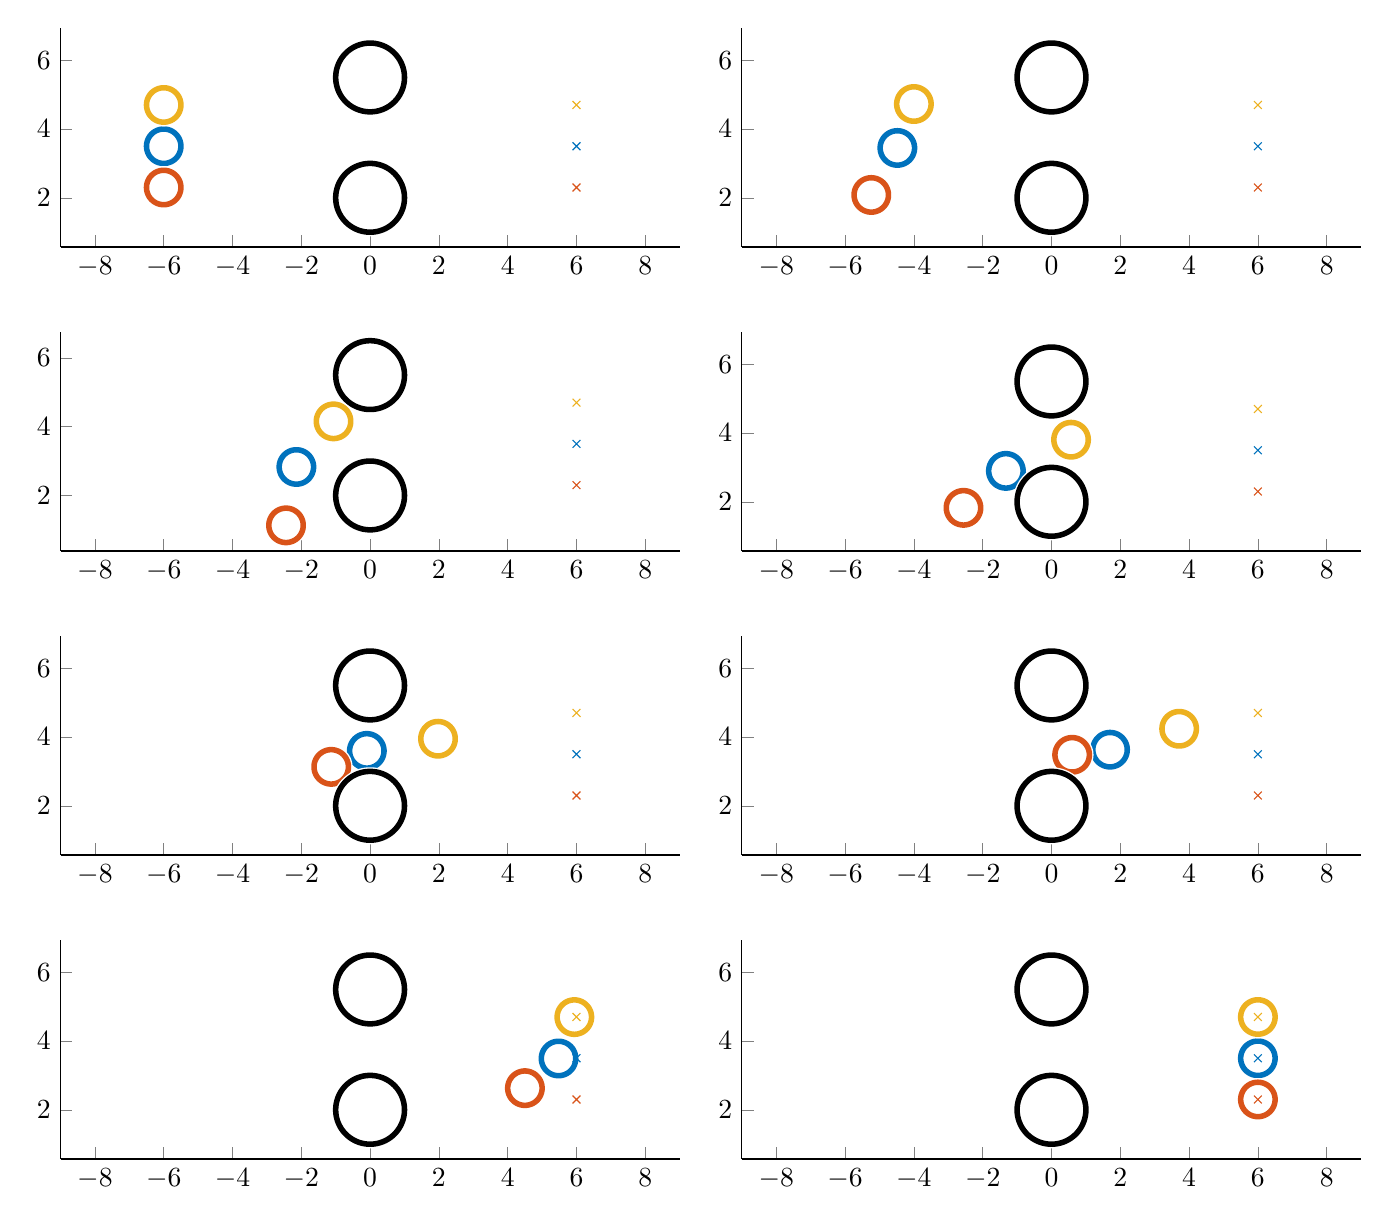
\begin{tikzpicture}

\definecolor{mycolor1}{rgb}{0.00000,0.44700,0.74100}%
\definecolor{mycolor2}{rgb}{0.85000,0.32500,0.09800}%
\definecolor{mycolor3}{rgb}{0.92900,0.69400,0.12500}%

\begin{axis}[%
width=3.096in,
height=1.094in,
at={(2.593in,5.323in)},
scale only axis,
unbounded coords=jump,
xmin=-9,
xmax=9,
%xmajorgrids,
ymin=0.568379976997646,
ymax=6.93162002300235,
%ymajorgrids,
axis background/.style={fill=white},
axis x line*=bottom,
axis y line*=left
]
\addplot [color=mycolor1,only marks,mark=x,mark options={solid},forget plot]
  table[row sep=crcr]{%
6	3.5\\
};
\addplot [color=mycolor2,only marks,mark=x,mark options={solid},forget plot]
  table[row sep=crcr]{%
6	2.3\\
};
\addplot [color=mycolor3,only marks,mark=x,mark options={solid},forget plot]
  table[row sep=crcr]{%
6	4.7\\
};
\addplot [color=white,solid,line width=3.0pt,forget plot]
  table[row sep=crcr]{%
-5.5	3.5\\
-5.50030458649045	3.51744974835125\\
-5.50121797487009	3.53487823687206\\
-5.50273905231586	3.55226423163383\\
-5.50486596562921	3.56958655048003\\
-5.5075961234939	3.58682408883347\\
-5.5109261996331	3.60395584540888\\
-5.514852136862	3.62096094779983\\
-5.51936915203084	3.6378186779085\\
-5.52447174185242	3.65450849718747\\
-5.53015368960705	3.67101007166283\\
-5.53640807271661	3.68730329670796\\
-5.5432272711787	3.7033683215379\\
-5.55060297685042	3.71918557339454\\
-5.55852620357054	3.73473578139295\\
-5.56698729810778	3.75\\
-5.57597595192179	3.7649596321166\\
-5.58548121372248	3.77959645173537\\
-5.59549150281253	3.79389262614624\\
-5.60599462319664	3.80783073766283\\
-5.61697777844051	3.82139380484327\\
-5.6284275872613	3.83456530317943\\
-5.64033009983067	3.8473291852295\\
-5.6526708147705	3.85966990016933\\
-5.66543469682057	3.8715724127387\\
-5.67860619515673	3.88302222155949\\
-5.69216926233717	3.89400537680336\\
-5.70610737385376	3.90450849718747\\
-5.72040354826463	3.91451878627752\\
-5.7350403678834	3.92402404807821\\
-5.75	3.93301270189222\\
-5.76526421860705	3.94147379642946\\
-5.78081442660546	3.94939702314958\\
-5.7966316784621	3.9567727288213\\
-5.81269670329204	3.96359192728339\\
-5.82898992833717	3.96984631039295\\
-5.84549150281253	3.97552825814758\\
-5.8621813220915	3.98063084796916\\
-5.87903905220017	3.985147863138\\
-5.89604415459112	3.9890738003669\\
-5.91317591116653	3.9924038765061\\
-5.93041344951997	3.99513403437079\\
-5.94773576836617	3.99726094768414\\
-5.96512176312794	3.99878202512991\\
-5.98255025164875	3.99969541350955\\
-6	4\\
-6.01744974835125	3.99969541350955\\
-6.03487823687206	3.99878202512991\\
-6.05226423163383	3.99726094768414\\
-6.06958655048003	3.99513403437079\\
-6.08682408883347	3.9924038765061\\
-6.10395584540888	3.9890738003669\\
-6.12096094779983	3.985147863138\\
-6.1378186779085	3.98063084796916\\
-6.15450849718747	3.97552825814758\\
-6.17101007166283	3.96984631039295\\
-6.18730329670796	3.96359192728339\\
-6.2033683215379	3.9567727288213\\
-6.21918557339454	3.94939702314958\\
-6.23473578139295	3.94147379642946\\
-6.25	3.93301270189222\\
-6.2649596321166	3.92402404807821\\
-6.27959645173537	3.91451878627752\\
-6.29389262614624	3.90450849718747\\
-6.30783073766283	3.89400537680336\\
-6.32139380484327	3.88302222155949\\
-6.33456530317943	3.8715724127387\\
-6.3473291852295	3.85966990016933\\
-6.35966990016933	3.8473291852295\\
-6.3715724127387	3.83456530317943\\
-6.38302222155949	3.82139380484327\\
-6.39400537680336	3.80783073766283\\
-6.40450849718747	3.79389262614624\\
-6.41451878627752	3.77959645173537\\
-6.42402404807821	3.7649596321166\\
-6.43301270189222	3.75\\
-6.44147379642946	3.73473578139295\\
-6.44939702314958	3.71918557339454\\
-6.4567727288213	3.7033683215379\\
-6.46359192728339	3.68730329670796\\
-6.46984631039295	3.67101007166283\\
-6.47552825814758	3.65450849718747\\
-6.48063084796916	3.6378186779085\\
-6.485147863138	3.62096094779983\\
-6.4890738003669	3.60395584540888\\
-6.4924038765061	3.58682408883347\\
-6.49513403437079	3.56958655048003\\
-6.49726094768414	3.55226423163383\\
-6.49878202512991	3.53487823687206\\
-6.49969541350955	3.51744974835125\\
-6.5	3.5\\
-6.49969541350955	3.48255025164875\\
-6.49878202512991	3.46512176312794\\
-6.49726094768414	3.44773576836617\\
-6.49513403437079	3.43041344951997\\
-6.4924038765061	3.41317591116653\\
-6.4890738003669	3.39604415459112\\
-6.485147863138	3.37903905220017\\
-6.48063084796916	3.3621813220915\\
-6.47552825814758	3.34549150281253\\
-6.46984631039295	3.32898992833717\\
-6.46359192728339	3.31269670329204\\
-6.4567727288213	3.2966316784621\\
-6.44939702314958	3.28081442660546\\
-6.44147379642946	3.26526421860705\\
-6.43301270189222	3.25\\
-6.42402404807821	3.2350403678834\\
-6.41451878627752	3.22040354826463\\
-6.40450849718747	3.20610737385376\\
-6.39400537680336	3.19216926233717\\
-6.38302222155949	3.17860619515673\\
-6.3715724127387	3.16543469682057\\
-6.35966990016933	3.1526708147705\\
-6.3473291852295	3.14033009983067\\
-6.33456530317943	3.1284275872613\\
-6.32139380484327	3.11697777844051\\
-6.30783073766283	3.10599462319664\\
-6.29389262614624	3.09549150281253\\
-6.27959645173537	3.08548121372248\\
-6.2649596321166	3.07597595192179\\
-6.25	3.06698729810778\\
-6.23473578139295	3.05852620357054\\
-6.21918557339454	3.05060297685042\\
-6.2033683215379	3.0432272711787\\
-6.18730329670796	3.03640807271661\\
-6.17101007166283	3.03015368960705\\
-6.15450849718747	3.02447174185242\\
-6.1378186779085	3.01936915203084\\
-6.12096094779983	3.014852136862\\
-6.10395584540888	3.0109261996331\\
-6.08682408883347	3.0075961234939\\
-6.06958655048003	3.00486596562921\\
-6.05226423163383	3.00273905231586\\
-6.03487823687206	3.00121797487009\\
-6.01744974835125	3.00030458649045\\
-6	3\\
-5.98255025164875	3.00030458649045\\
-5.96512176312794	3.00121797487009\\
-5.94773576836617	3.00273905231586\\
-5.93041344951997	3.00486596562921\\
-5.91317591116653	3.0075961234939\\
-5.89604415459112	3.0109261996331\\
-5.87903905220017	3.014852136862\\
-5.8621813220915	3.01936915203084\\
-5.84549150281253	3.02447174185242\\
-5.82898992833717	3.03015368960705\\
-5.81269670329204	3.03640807271661\\
-5.7966316784621	3.0432272711787\\
-5.78081442660546	3.05060297685042\\
-5.76526421860705	3.05852620357054\\
-5.75	3.06698729810778\\
-5.7350403678834	3.07597595192179\\
-5.72040354826463	3.08548121372248\\
-5.70610737385376	3.09549150281253\\
-5.69216926233717	3.10599462319664\\
-5.67860619515673	3.11697777844051\\
-5.66543469682057	3.1284275872613\\
-5.6526708147705	3.14033009983067\\
-5.64033009983067	3.1526708147705\\
-5.6284275872613	3.16543469682057\\
-5.61697777844051	3.17860619515673\\
-5.60599462319664	3.19216926233717\\
-5.59549150281253	3.20610737385376\\
-5.58548121372248	3.22040354826463\\
-5.57597595192179	3.2350403678834\\
-5.56698729810778	3.25\\
-5.55852620357054	3.26526421860705\\
-5.55060297685042	3.28081442660546\\
-5.5432272711787	3.2966316784621\\
-5.53640807271661	3.31269670329204\\
-5.53015368960705	3.32898992833717\\
-5.52447174185242	3.34549150281253\\
-5.51936915203084	3.3621813220915\\
-5.514852136862	3.37903905220017\\
-5.5109261996331	3.39604415459112\\
-5.5075961234939	3.41317591116653\\
-5.50486596562921	3.43041344951997\\
-5.50273905231586	3.44773576836617\\
-5.50121797487009	3.46512176312794\\
-5.50030458649045	3.48255025164875\\
-5.5	3.5\\
nan	nan\\
};
\addplot [color=mycolor1,solid,line width=2.0pt,forget plot]
  table[row sep=crcr]{%
-5.5	3.5\\
-5.50030458649045	3.51744974835125\\
-5.50121797487009	3.53487823687206\\
-5.50273905231586	3.55226423163383\\
-5.50486596562921	3.56958655048003\\
-5.5075961234939	3.58682408883347\\
-5.5109261996331	3.60395584540888\\
-5.514852136862	3.62096094779983\\
-5.51936915203084	3.6378186779085\\
-5.52447174185242	3.65450849718747\\
-5.53015368960705	3.67101007166283\\
-5.53640807271661	3.68730329670796\\
-5.5432272711787	3.7033683215379\\
-5.55060297685042	3.71918557339454\\
-5.55852620357054	3.73473578139295\\
-5.56698729810778	3.75\\
-5.57597595192179	3.7649596321166\\
-5.58548121372248	3.77959645173537\\
-5.59549150281253	3.79389262614624\\
-5.60599462319664	3.80783073766283\\
-5.61697777844051	3.82139380484327\\
-5.6284275872613	3.83456530317943\\
-5.64033009983067	3.8473291852295\\
-5.6526708147705	3.85966990016933\\
-5.66543469682057	3.8715724127387\\
-5.67860619515673	3.88302222155949\\
-5.69216926233717	3.89400537680336\\
-5.70610737385376	3.90450849718747\\
-5.72040354826463	3.91451878627752\\
-5.7350403678834	3.92402404807821\\
-5.75	3.93301270189222\\
-5.76526421860705	3.94147379642946\\
-5.78081442660546	3.94939702314958\\
-5.7966316784621	3.9567727288213\\
-5.81269670329204	3.96359192728339\\
-5.82898992833717	3.96984631039295\\
-5.84549150281253	3.97552825814758\\
-5.8621813220915	3.98063084796916\\
-5.87903905220017	3.985147863138\\
-5.89604415459112	3.9890738003669\\
-5.91317591116653	3.9924038765061\\
-5.93041344951997	3.99513403437079\\
-5.94773576836617	3.99726094768414\\
-5.96512176312794	3.99878202512991\\
-5.98255025164875	3.99969541350955\\
-6	4\\
-6.01744974835125	3.99969541350955\\
-6.03487823687206	3.99878202512991\\
-6.05226423163383	3.99726094768414\\
-6.06958655048003	3.99513403437079\\
-6.08682408883347	3.9924038765061\\
-6.10395584540888	3.9890738003669\\
-6.12096094779983	3.985147863138\\
-6.1378186779085	3.98063084796916\\
-6.15450849718747	3.97552825814758\\
-6.17101007166283	3.96984631039295\\
-6.18730329670796	3.96359192728339\\
-6.2033683215379	3.9567727288213\\
-6.21918557339454	3.94939702314958\\
-6.23473578139295	3.94147379642946\\
-6.25	3.93301270189222\\
-6.2649596321166	3.92402404807821\\
-6.27959645173537	3.91451878627752\\
-6.29389262614624	3.90450849718747\\
-6.30783073766283	3.89400537680336\\
-6.32139380484327	3.88302222155949\\
-6.33456530317943	3.8715724127387\\
-6.3473291852295	3.85966990016933\\
-6.35966990016933	3.8473291852295\\
-6.3715724127387	3.83456530317943\\
-6.38302222155949	3.82139380484327\\
-6.39400537680336	3.80783073766283\\
-6.40450849718747	3.79389262614624\\
-6.41451878627752	3.77959645173537\\
-6.42402404807821	3.7649596321166\\
-6.43301270189222	3.75\\
-6.44147379642946	3.73473578139295\\
-6.44939702314958	3.71918557339454\\
-6.4567727288213	3.7033683215379\\
-6.46359192728339	3.68730329670796\\
-6.46984631039295	3.67101007166283\\
-6.47552825814758	3.65450849718747\\
-6.48063084796916	3.6378186779085\\
-6.485147863138	3.62096094779983\\
-6.4890738003669	3.60395584540888\\
-6.4924038765061	3.58682408883347\\
-6.49513403437079	3.56958655048003\\
-6.49726094768414	3.55226423163383\\
-6.49878202512991	3.53487823687206\\
-6.49969541350955	3.51744974835125\\
-6.5	3.5\\
-6.49969541350955	3.48255025164875\\
-6.49878202512991	3.46512176312794\\
-6.49726094768414	3.44773576836617\\
-6.49513403437079	3.43041344951997\\
-6.4924038765061	3.41317591116653\\
-6.4890738003669	3.39604415459112\\
-6.485147863138	3.37903905220017\\
-6.48063084796916	3.3621813220915\\
-6.47552825814758	3.34549150281253\\
-6.46984631039295	3.32898992833717\\
-6.46359192728339	3.31269670329204\\
-6.4567727288213	3.2966316784621\\
-6.44939702314958	3.28081442660546\\
-6.44147379642946	3.26526421860705\\
-6.43301270189222	3.25\\
-6.42402404807821	3.2350403678834\\
-6.41451878627752	3.22040354826463\\
-6.40450849718747	3.20610737385376\\
-6.39400537680336	3.19216926233717\\
-6.38302222155949	3.17860619515673\\
-6.3715724127387	3.16543469682057\\
-6.35966990016933	3.1526708147705\\
-6.3473291852295	3.14033009983067\\
-6.33456530317943	3.1284275872613\\
-6.32139380484327	3.11697777844051\\
-6.30783073766283	3.10599462319664\\
-6.29389262614624	3.09549150281253\\
-6.27959645173537	3.08548121372248\\
-6.2649596321166	3.07597595192179\\
-6.25	3.06698729810778\\
-6.23473578139295	3.05852620357054\\
-6.21918557339454	3.05060297685042\\
-6.2033683215379	3.0432272711787\\
-6.18730329670796	3.03640807271661\\
-6.17101007166283	3.03015368960705\\
-6.15450849718747	3.02447174185242\\
-6.1378186779085	3.01936915203084\\
-6.12096094779983	3.014852136862\\
-6.10395584540888	3.0109261996331\\
-6.08682408883347	3.0075961234939\\
-6.06958655048003	3.00486596562921\\
-6.05226423163383	3.00273905231586\\
-6.03487823687206	3.00121797487009\\
-6.01744974835125	3.00030458649045\\
-6	3\\
-5.98255025164875	3.00030458649045\\
-5.96512176312794	3.00121797487009\\
-5.94773576836617	3.00273905231586\\
-5.93041344951997	3.00486596562921\\
-5.91317591116653	3.0075961234939\\
-5.89604415459112	3.0109261996331\\
-5.87903905220017	3.014852136862\\
-5.8621813220915	3.01936915203084\\
-5.84549150281253	3.02447174185242\\
-5.82898992833717	3.03015368960705\\
-5.81269670329204	3.03640807271661\\
-5.7966316784621	3.0432272711787\\
-5.78081442660546	3.05060297685042\\
-5.76526421860705	3.05852620357054\\
-5.75	3.06698729810778\\
-5.7350403678834	3.07597595192179\\
-5.72040354826463	3.08548121372248\\
-5.70610737385376	3.09549150281253\\
-5.69216926233717	3.10599462319664\\
-5.67860619515673	3.11697777844051\\
-5.66543469682057	3.1284275872613\\
-5.6526708147705	3.14033009983067\\
-5.64033009983067	3.1526708147705\\
-5.6284275872613	3.16543469682057\\
-5.61697777844051	3.17860619515673\\
-5.60599462319664	3.19216926233717\\
-5.59549150281253	3.20610737385376\\
-5.58548121372248	3.22040354826463\\
-5.57597595192179	3.2350403678834\\
-5.56698729810778	3.25\\
-5.55852620357054	3.26526421860705\\
-5.55060297685042	3.28081442660546\\
-5.5432272711787	3.2966316784621\\
-5.53640807271661	3.31269670329204\\
-5.53015368960705	3.32898992833717\\
-5.52447174185242	3.34549150281253\\
-5.51936915203084	3.3621813220915\\
-5.514852136862	3.37903905220017\\
-5.5109261996331	3.39604415459112\\
-5.5075961234939	3.41317591116653\\
-5.50486596562921	3.43041344951997\\
-5.50273905231586	3.44773576836617\\
-5.50121797487009	3.46512176312794\\
-5.50030458649045	3.48255025164875\\
-5.5	3.5\\
nan	nan\\
};
\addplot [color=white,solid,line width=3.0pt,forget plot]
  table[row sep=crcr]{%
-5.5	2.3\\
-5.50030458649045	2.31744974835125\\
-5.50121797487009	2.33487823687206\\
-5.50273905231586	2.35226423163383\\
-5.50486596562921	2.36958655048003\\
-5.5075961234939	2.38682408883346\\
-5.5109261996331	2.40395584540888\\
-5.514852136862	2.42096094779983\\
-5.51936915203084	2.4378186779085\\
-5.52447174185242	2.45450849718747\\
-5.53015368960705	2.47101007166283\\
-5.53640807271661	2.48730329670796\\
-5.5432272711787	2.5033683215379\\
-5.55060297685042	2.51918557339454\\
-5.55852620357054	2.53473578139295\\
-5.56698729810778	2.55\\
-5.57597595192179	2.5649596321166\\
-5.58548121372248	2.57959645173537\\
-5.59549150281253	2.59389262614624\\
-5.60599462319664	2.60783073766283\\
-5.61697777844051	2.62139380484327\\
-5.6284275872613	2.63456530317943\\
-5.64033009983067	2.6473291852295\\
-5.6526708147705	2.65966990016933\\
-5.66543469682057	2.6715724127387\\
-5.67860619515673	2.68302222155949\\
-5.69216926233717	2.69400537680336\\
-5.70610737385376	2.70450849718747\\
-5.72040354826463	2.71451878627752\\
-5.7350403678834	2.72402404807821\\
-5.75	2.73301270189222\\
-5.76526421860705	2.74147379642946\\
-5.78081442660546	2.74939702314958\\
-5.7966316784621	2.7567727288213\\
-5.81269670329204	2.76359192728339\\
-5.82898992833717	2.76984631039295\\
-5.84549150281253	2.77552825814758\\
-5.8621813220915	2.78063084796916\\
-5.87903905220017	2.785147863138\\
-5.89604415459112	2.7890738003669\\
-5.91317591116653	2.7924038765061\\
-5.93041344951997	2.79513403437078\\
-5.94773576836617	2.79726094768414\\
-5.96512176312794	2.79878202512991\\
-5.98255025164875	2.79969541350955\\
-6	2.8\\
-6.01744974835125	2.79969541350955\\
-6.03487823687206	2.79878202512991\\
-6.05226423163383	2.79726094768414\\
-6.06958655048003	2.79513403437078\\
-6.08682408883347	2.7924038765061\\
-6.10395584540888	2.7890738003669\\
-6.12096094779983	2.785147863138\\
-6.1378186779085	2.78063084796916\\
-6.15450849718747	2.77552825814758\\
-6.17101007166283	2.76984631039295\\
-6.18730329670796	2.76359192728339\\
-6.2033683215379	2.7567727288213\\
-6.21918557339454	2.74939702314958\\
-6.23473578139295	2.74147379642946\\
-6.25	2.73301270189222\\
-6.2649596321166	2.72402404807821\\
-6.27959645173537	2.71451878627752\\
-6.29389262614624	2.70450849718747\\
-6.30783073766283	2.69400537680336\\
-6.32139380484327	2.68302222155949\\
-6.33456530317943	2.6715724127387\\
-6.3473291852295	2.65966990016933\\
-6.35966990016933	2.6473291852295\\
-6.3715724127387	2.63456530317943\\
-6.38302222155949	2.62139380484327\\
-6.39400537680336	2.60783073766283\\
-6.40450849718747	2.59389262614624\\
-6.41451878627752	2.57959645173537\\
-6.42402404807821	2.5649596321166\\
-6.43301270189222	2.55\\
-6.44147379642946	2.53473578139295\\
-6.44939702314958	2.51918557339454\\
-6.4567727288213	2.5033683215379\\
-6.46359192728339	2.48730329670796\\
-6.46984631039295	2.47101007166283\\
-6.47552825814758	2.45450849718747\\
-6.48063084796916	2.4378186779085\\
-6.485147863138	2.42096094779983\\
-6.4890738003669	2.40395584540888\\
-6.4924038765061	2.38682408883346\\
-6.49513403437079	2.36958655048003\\
-6.49726094768414	2.35226423163383\\
-6.49878202512991	2.33487823687206\\
-6.49969541350955	2.31744974835125\\
-6.5	2.3\\
-6.49969541350955	2.28255025164875\\
-6.49878202512991	2.26512176312794\\
-6.49726094768414	2.24773576836617\\
-6.49513403437079	2.23041344951997\\
-6.4924038765061	2.21317591116653\\
-6.4890738003669	2.19604415459112\\
-6.485147863138	2.17903905220017\\
-6.48063084796916	2.1621813220915\\
-6.47552825814758	2.14549150281253\\
-6.46984631039295	2.12898992833717\\
-6.46359192728339	2.11269670329204\\
-6.4567727288213	2.0966316784621\\
-6.44939702314958	2.08081442660546\\
-6.44147379642946	2.06526421860705\\
-6.43301270189222	2.05\\
-6.42402404807821	2.0350403678834\\
-6.41451878627752	2.02040354826463\\
-6.40450849718747	2.00610737385376\\
-6.39400537680336	1.99216926233717\\
-6.38302222155949	1.97860619515673\\
-6.3715724127387	1.96543469682057\\
-6.35966990016933	1.9526708147705\\
-6.3473291852295	1.94033009983067\\
-6.33456530317943	1.9284275872613\\
-6.32139380484327	1.91697777844051\\
-6.30783073766283	1.90599462319664\\
-6.29389262614624	1.89549150281253\\
-6.27959645173537	1.88548121372248\\
-6.2649596321166	1.87597595192179\\
-6.25	1.86698729810778\\
-6.23473578139295	1.85852620357054\\
-6.21918557339454	1.85060297685042\\
-6.2033683215379	1.8432272711787\\
-6.18730329670796	1.83640807271661\\
-6.17101007166283	1.83015368960705\\
-6.15450849718747	1.82447174185242\\
-6.1378186779085	1.81936915203084\\
-6.12096094779983	1.814852136862\\
-6.10395584540888	1.8109261996331\\
-6.08682408883347	1.8075961234939\\
-6.06958655048003	1.80486596562921\\
-6.05226423163383	1.80273905231586\\
-6.03487823687206	1.80121797487009\\
-6.01744974835125	1.80030458649045\\
-6	1.8\\
-5.98255025164875	1.80030458649045\\
-5.96512176312794	1.80121797487009\\
-5.94773576836617	1.80273905231586\\
-5.93041344951997	1.80486596562921\\
-5.91317591116653	1.8075961234939\\
-5.89604415459112	1.8109261996331\\
-5.87903905220017	1.814852136862\\
-5.8621813220915	1.81936915203084\\
-5.84549150281253	1.82447174185242\\
-5.82898992833717	1.83015368960705\\
-5.81269670329204	1.83640807271661\\
-5.7966316784621	1.8432272711787\\
-5.78081442660546	1.85060297685042\\
-5.76526421860705	1.85852620357054\\
-5.75	1.86698729810778\\
-5.7350403678834	1.87597595192179\\
-5.72040354826463	1.88548121372248\\
-5.70610737385376	1.89549150281253\\
-5.69216926233717	1.90599462319664\\
-5.67860619515673	1.91697777844051\\
-5.66543469682057	1.9284275872613\\
-5.6526708147705	1.94033009983067\\
-5.64033009983067	1.9526708147705\\
-5.6284275872613	1.96543469682057\\
-5.61697777844051	1.97860619515673\\
-5.60599462319664	1.99216926233717\\
-5.59549150281253	2.00610737385376\\
-5.58548121372248	2.02040354826463\\
-5.57597595192179	2.0350403678834\\
-5.56698729810778	2.05\\
-5.55852620357054	2.06526421860705\\
-5.55060297685042	2.08081442660546\\
-5.5432272711787	2.0966316784621\\
-5.53640807271661	2.11269670329204\\
-5.53015368960705	2.12898992833717\\
-5.52447174185242	2.14549150281253\\
-5.51936915203084	2.1621813220915\\
-5.514852136862	2.17903905220017\\
-5.5109261996331	2.19604415459112\\
-5.5075961234939	2.21317591116653\\
-5.50486596562921	2.23041344951997\\
-5.50273905231586	2.24773576836617\\
-5.50121797487009	2.26512176312794\\
-5.50030458649045	2.28255025164875\\
-5.5	2.3\\
nan	nan\\
};
\addplot [color=mycolor2,solid,line width=2.0pt,forget plot]
  table[row sep=crcr]{%
-5.5	2.3\\
-5.50030458649045	2.31744974835125\\
-5.50121797487009	2.33487823687206\\
-5.50273905231586	2.35226423163383\\
-5.50486596562921	2.36958655048003\\
-5.5075961234939	2.38682408883346\\
-5.5109261996331	2.40395584540888\\
-5.514852136862	2.42096094779983\\
-5.51936915203084	2.4378186779085\\
-5.52447174185242	2.45450849718747\\
-5.53015368960705	2.47101007166283\\
-5.53640807271661	2.48730329670796\\
-5.5432272711787	2.5033683215379\\
-5.55060297685042	2.51918557339454\\
-5.55852620357054	2.53473578139295\\
-5.56698729810778	2.55\\
-5.57597595192179	2.5649596321166\\
-5.58548121372248	2.57959645173537\\
-5.59549150281253	2.59389262614624\\
-5.60599462319664	2.60783073766283\\
-5.61697777844051	2.62139380484327\\
-5.6284275872613	2.63456530317943\\
-5.64033009983067	2.6473291852295\\
-5.6526708147705	2.65966990016933\\
-5.66543469682057	2.6715724127387\\
-5.67860619515673	2.68302222155949\\
-5.69216926233717	2.69400537680336\\
-5.70610737385376	2.70450849718747\\
-5.72040354826463	2.71451878627752\\
-5.7350403678834	2.72402404807821\\
-5.75	2.73301270189222\\
-5.76526421860705	2.74147379642946\\
-5.78081442660546	2.74939702314958\\
-5.7966316784621	2.7567727288213\\
-5.81269670329204	2.76359192728339\\
-5.82898992833717	2.76984631039295\\
-5.84549150281253	2.77552825814758\\
-5.8621813220915	2.78063084796916\\
-5.87903905220017	2.785147863138\\
-5.89604415459112	2.7890738003669\\
-5.91317591116653	2.7924038765061\\
-5.93041344951997	2.79513403437078\\
-5.94773576836617	2.79726094768414\\
-5.96512176312794	2.79878202512991\\
-5.98255025164875	2.79969541350955\\
-6	2.8\\
-6.01744974835125	2.79969541350955\\
-6.03487823687206	2.79878202512991\\
-6.05226423163383	2.79726094768414\\
-6.06958655048003	2.79513403437078\\
-6.08682408883347	2.7924038765061\\
-6.10395584540888	2.7890738003669\\
-6.12096094779983	2.785147863138\\
-6.1378186779085	2.78063084796916\\
-6.15450849718747	2.77552825814758\\
-6.17101007166283	2.76984631039295\\
-6.18730329670796	2.76359192728339\\
-6.2033683215379	2.7567727288213\\
-6.21918557339454	2.74939702314958\\
-6.23473578139295	2.74147379642946\\
-6.25	2.73301270189222\\
-6.2649596321166	2.72402404807821\\
-6.27959645173537	2.71451878627752\\
-6.29389262614624	2.70450849718747\\
-6.30783073766283	2.69400537680336\\
-6.32139380484327	2.68302222155949\\
-6.33456530317943	2.6715724127387\\
-6.3473291852295	2.65966990016933\\
-6.35966990016933	2.6473291852295\\
-6.3715724127387	2.63456530317943\\
-6.38302222155949	2.62139380484327\\
-6.39400537680336	2.60783073766283\\
-6.40450849718747	2.59389262614624\\
-6.41451878627752	2.57959645173537\\
-6.42402404807821	2.5649596321166\\
-6.43301270189222	2.55\\
-6.44147379642946	2.53473578139295\\
-6.44939702314958	2.51918557339454\\
-6.4567727288213	2.5033683215379\\
-6.46359192728339	2.48730329670796\\
-6.46984631039295	2.47101007166283\\
-6.47552825814758	2.45450849718747\\
-6.48063084796916	2.4378186779085\\
-6.485147863138	2.42096094779983\\
-6.4890738003669	2.40395584540888\\
-6.4924038765061	2.38682408883346\\
-6.49513403437079	2.36958655048003\\
-6.49726094768414	2.35226423163383\\
-6.49878202512991	2.33487823687206\\
-6.49969541350955	2.31744974835125\\
-6.5	2.3\\
-6.49969541350955	2.28255025164875\\
-6.49878202512991	2.26512176312794\\
-6.49726094768414	2.24773576836617\\
-6.49513403437079	2.23041344951997\\
-6.4924038765061	2.21317591116653\\
-6.4890738003669	2.19604415459112\\
-6.485147863138	2.17903905220017\\
-6.48063084796916	2.1621813220915\\
-6.47552825814758	2.14549150281253\\
-6.46984631039295	2.12898992833717\\
-6.46359192728339	2.11269670329204\\
-6.4567727288213	2.0966316784621\\
-6.44939702314958	2.08081442660546\\
-6.44147379642946	2.06526421860705\\
-6.43301270189222	2.05\\
-6.42402404807821	2.0350403678834\\
-6.41451878627752	2.02040354826463\\
-6.40450849718747	2.00610737385376\\
-6.39400537680336	1.99216926233717\\
-6.38302222155949	1.97860619515673\\
-6.3715724127387	1.96543469682057\\
-6.35966990016933	1.9526708147705\\
-6.3473291852295	1.94033009983067\\
-6.33456530317943	1.9284275872613\\
-6.32139380484327	1.91697777844051\\
-6.30783073766283	1.90599462319664\\
-6.29389262614624	1.89549150281253\\
-6.27959645173537	1.88548121372248\\
-6.2649596321166	1.87597595192179\\
-6.25	1.86698729810778\\
-6.23473578139295	1.85852620357054\\
-6.21918557339454	1.85060297685042\\
-6.2033683215379	1.8432272711787\\
-6.18730329670796	1.83640807271661\\
-6.17101007166283	1.83015368960705\\
-6.15450849718747	1.82447174185242\\
-6.1378186779085	1.81936915203084\\
-6.12096094779983	1.814852136862\\
-6.10395584540888	1.8109261996331\\
-6.08682408883347	1.8075961234939\\
-6.06958655048003	1.80486596562921\\
-6.05226423163383	1.80273905231586\\
-6.03487823687206	1.80121797487009\\
-6.01744974835125	1.80030458649045\\
-6	1.8\\
-5.98255025164875	1.80030458649045\\
-5.96512176312794	1.80121797487009\\
-5.94773576836617	1.80273905231586\\
-5.93041344951997	1.80486596562921\\
-5.91317591116653	1.8075961234939\\
-5.89604415459112	1.8109261996331\\
-5.87903905220017	1.814852136862\\
-5.8621813220915	1.81936915203084\\
-5.84549150281253	1.82447174185242\\
-5.82898992833717	1.83015368960705\\
-5.81269670329204	1.83640807271661\\
-5.7966316784621	1.8432272711787\\
-5.78081442660546	1.85060297685042\\
-5.76526421860705	1.85852620357054\\
-5.75	1.86698729810778\\
-5.7350403678834	1.87597595192179\\
-5.72040354826463	1.88548121372248\\
-5.70610737385376	1.89549150281253\\
-5.69216926233717	1.90599462319664\\
-5.67860619515673	1.91697777844051\\
-5.66543469682057	1.9284275872613\\
-5.6526708147705	1.94033009983067\\
-5.64033009983067	1.9526708147705\\
-5.6284275872613	1.96543469682057\\
-5.61697777844051	1.97860619515673\\
-5.60599462319664	1.99216926233717\\
-5.59549150281253	2.00610737385376\\
-5.58548121372248	2.02040354826463\\
-5.57597595192179	2.0350403678834\\
-5.56698729810778	2.05\\
-5.55852620357054	2.06526421860705\\
-5.55060297685042	2.08081442660546\\
-5.5432272711787	2.0966316784621\\
-5.53640807271661	2.11269670329204\\
-5.53015368960705	2.12898992833717\\
-5.52447174185242	2.14549150281253\\
-5.51936915203084	2.1621813220915\\
-5.514852136862	2.17903905220017\\
-5.5109261996331	2.19604415459112\\
-5.5075961234939	2.21317591116653\\
-5.50486596562921	2.23041344951997\\
-5.50273905231586	2.24773576836617\\
-5.50121797487009	2.26512176312794\\
-5.50030458649045	2.28255025164875\\
-5.5	2.3\\
nan	nan\\
};
\addplot [color=white,solid,line width=3.0pt,forget plot]
  table[row sep=crcr]{%
-5.5	4.7\\
-5.50030458649045	4.71744974835125\\
-5.50121797487009	4.73487823687206\\
-5.50273905231586	4.75226423163383\\
-5.50486596562921	4.76958655048003\\
-5.5075961234939	4.78682408883347\\
-5.5109261996331	4.80395584540888\\
-5.514852136862	4.82096094779983\\
-5.51936915203084	4.8378186779085\\
-5.52447174185242	4.85450849718747\\
-5.53015368960705	4.87101007166283\\
-5.53640807271661	4.88730329670796\\
-5.5432272711787	4.9033683215379\\
-5.55060297685042	4.91918557339454\\
-5.55852620357054	4.93473578139295\\
-5.56698729810778	4.95\\
-5.57597595192179	4.9649596321166\\
-5.58548121372248	4.97959645173537\\
-5.59549150281253	4.99389262614624\\
-5.60599462319664	5.00783073766283\\
-5.61697777844051	5.02139380484327\\
-5.6284275872613	5.03456530317943\\
-5.64033009983067	5.0473291852295\\
-5.6526708147705	5.05966990016933\\
-5.66543469682057	5.0715724127387\\
-5.67860619515673	5.08302222155949\\
-5.69216926233717	5.09400537680336\\
-5.70610737385376	5.10450849718747\\
-5.72040354826463	5.11451878627752\\
-5.7350403678834	5.12402404807821\\
-5.75	5.13301270189222\\
-5.76526421860705	5.14147379642946\\
-5.78081442660546	5.14939702314958\\
-5.7966316784621	5.1567727288213\\
-5.81269670329204	5.16359192728339\\
-5.82898992833717	5.16984631039295\\
-5.84549150281253	5.17552825814758\\
-5.8621813220915	5.18063084796916\\
-5.87903905220017	5.185147863138\\
-5.89604415459112	5.1890738003669\\
-5.91317591116653	5.1924038765061\\
-5.93041344951997	5.19513403437079\\
-5.94773576836617	5.19726094768414\\
-5.96512176312794	5.19878202512991\\
-5.98255025164875	5.19969541350955\\
-6	5.2\\
-6.01744974835125	5.19969541350955\\
-6.03487823687206	5.19878202512991\\
-6.05226423163383	5.19726094768414\\
-6.06958655048003	5.19513403437079\\
-6.08682408883347	5.1924038765061\\
-6.10395584540888	5.1890738003669\\
-6.12096094779983	5.185147863138\\
-6.1378186779085	5.18063084796916\\
-6.15450849718747	5.17552825814758\\
-6.17101007166283	5.16984631039295\\
-6.18730329670796	5.16359192728339\\
-6.2033683215379	5.1567727288213\\
-6.21918557339454	5.14939702314958\\
-6.23473578139295	5.14147379642946\\
-6.25	5.13301270189222\\
-6.2649596321166	5.12402404807821\\
-6.27959645173537	5.11451878627752\\
-6.29389262614624	5.10450849718747\\
-6.30783073766283	5.09400537680336\\
-6.32139380484327	5.08302222155949\\
-6.33456530317943	5.0715724127387\\
-6.3473291852295	5.05966990016933\\
-6.35966990016933	5.0473291852295\\
-6.3715724127387	5.03456530317943\\
-6.38302222155949	5.02139380484327\\
-6.39400537680336	5.00783073766283\\
-6.40450849718747	4.99389262614624\\
-6.41451878627752	4.97959645173537\\
-6.42402404807821	4.9649596321166\\
-6.43301270189222	4.95\\
-6.44147379642946	4.93473578139295\\
-6.44939702314958	4.91918557339454\\
-6.4567727288213	4.9033683215379\\
-6.46359192728339	4.88730329670796\\
-6.46984631039295	4.87101007166283\\
-6.47552825814758	4.85450849718747\\
-6.48063084796916	4.8378186779085\\
-6.485147863138	4.82096094779983\\
-6.4890738003669	4.80395584540888\\
-6.4924038765061	4.78682408883347\\
-6.49513403437079	4.76958655048003\\
-6.49726094768414	4.75226423163383\\
-6.49878202512991	4.73487823687206\\
-6.49969541350955	4.71744974835125\\
-6.5	4.7\\
-6.49969541350955	4.68255025164875\\
-6.49878202512991	4.66512176312794\\
-6.49726094768414	4.64773576836617\\
-6.49513403437079	4.63041344951997\\
-6.4924038765061	4.61317591116654\\
-6.4890738003669	4.59604415459112\\
-6.485147863138	4.57903905220017\\
-6.48063084796916	4.5621813220915\\
-6.47552825814758	4.54549150281253\\
-6.46984631039295	4.52898992833717\\
-6.46359192728339	4.51269670329204\\
-6.4567727288213	4.4966316784621\\
-6.44939702314958	4.48081442660546\\
-6.44147379642946	4.46526421860705\\
-6.43301270189222	4.45\\
-6.42402404807821	4.4350403678834\\
-6.41451878627752	4.42040354826463\\
-6.40450849718747	4.40610737385376\\
-6.39400537680336	4.39216926233717\\
-6.38302222155949	4.37860619515673\\
-6.3715724127387	4.36543469682057\\
-6.35966990016933	4.3526708147705\\
-6.3473291852295	4.34033009983068\\
-6.33456530317943	4.3284275872613\\
-6.32139380484327	4.31697777844051\\
-6.30783073766283	4.30599462319664\\
-6.29389262614624	4.29549150281253\\
-6.27959645173537	4.28548121372248\\
-6.2649596321166	4.27597595192179\\
-6.25	4.26698729810778\\
-6.23473578139295	4.25852620357054\\
-6.21918557339454	4.25060297685042\\
-6.2033683215379	4.2432272711787\\
-6.18730329670796	4.23640807271661\\
-6.17101007166283	4.23015368960705\\
-6.15450849718747	4.22447174185242\\
-6.1378186779085	4.21936915203084\\
-6.12096094779983	4.214852136862\\
-6.10395584540888	4.2109261996331\\
-6.08682408883347	4.2075961234939\\
-6.06958655048003	4.20486596562921\\
-6.05226423163383	4.20273905231586\\
-6.03487823687206	4.20121797487009\\
-6.01744974835125	4.20030458649045\\
-6	4.2\\
-5.98255025164875	4.20030458649045\\
-5.96512176312794	4.20121797487009\\
-5.94773576836617	4.20273905231586\\
-5.93041344951997	4.20486596562921\\
-5.91317591116653	4.2075961234939\\
-5.89604415459112	4.2109261996331\\
-5.87903905220017	4.214852136862\\
-5.8621813220915	4.21936915203084\\
-5.84549150281253	4.22447174185242\\
-5.82898992833717	4.23015368960705\\
-5.81269670329204	4.23640807271661\\
-5.7966316784621	4.2432272711787\\
-5.78081442660546	4.25060297685042\\
-5.76526421860705	4.25852620357054\\
-5.75	4.26698729810778\\
-5.7350403678834	4.27597595192179\\
-5.72040354826463	4.28548121372248\\
-5.70610737385376	4.29549150281253\\
-5.69216926233717	4.30599462319664\\
-5.67860619515673	4.31697777844051\\
-5.66543469682057	4.3284275872613\\
-5.6526708147705	4.34033009983067\\
-5.64033009983067	4.3526708147705\\
-5.6284275872613	4.36543469682057\\
-5.61697777844051	4.37860619515673\\
-5.60599462319664	4.39216926233717\\
-5.59549150281253	4.40610737385376\\
-5.58548121372248	4.42040354826463\\
-5.57597595192179	4.4350403678834\\
-5.56698729810778	4.45\\
-5.55852620357054	4.46526421860705\\
-5.55060297685042	4.48081442660546\\
-5.5432272711787	4.4966316784621\\
-5.53640807271661	4.51269670329204\\
-5.53015368960705	4.52898992833717\\
-5.52447174185242	4.54549150281253\\
-5.51936915203084	4.5621813220915\\
-5.514852136862	4.57903905220017\\
-5.5109261996331	4.59604415459112\\
-5.5075961234939	4.61317591116653\\
-5.50486596562921	4.63041344951997\\
-5.50273905231586	4.64773576836617\\
-5.50121797487009	4.66512176312794\\
-5.50030458649045	4.68255025164875\\
-5.5	4.7\\
nan	nan\\
};
\addplot [color=mycolor3,solid,line width=2.0pt,forget plot]
  table[row sep=crcr]{%
-5.5	4.7\\
-5.50030458649045	4.71744974835125\\
-5.50121797487009	4.73487823687206\\
-5.50273905231586	4.75226423163383\\
-5.50486596562921	4.76958655048003\\
-5.5075961234939	4.78682408883347\\
-5.5109261996331	4.80395584540888\\
-5.514852136862	4.82096094779983\\
-5.51936915203084	4.8378186779085\\
-5.52447174185242	4.85450849718747\\
-5.53015368960705	4.87101007166283\\
-5.53640807271661	4.88730329670796\\
-5.5432272711787	4.9033683215379\\
-5.55060297685042	4.91918557339454\\
-5.55852620357054	4.93473578139295\\
-5.56698729810778	4.95\\
-5.57597595192179	4.9649596321166\\
-5.58548121372248	4.97959645173537\\
-5.59549150281253	4.99389262614624\\
-5.60599462319664	5.00783073766283\\
-5.61697777844051	5.02139380484327\\
-5.6284275872613	5.03456530317943\\
-5.64033009983067	5.0473291852295\\
-5.6526708147705	5.05966990016933\\
-5.66543469682057	5.0715724127387\\
-5.67860619515673	5.08302222155949\\
-5.69216926233717	5.09400537680336\\
-5.70610737385376	5.10450849718747\\
-5.72040354826463	5.11451878627752\\
-5.7350403678834	5.12402404807821\\
-5.75	5.13301270189222\\
-5.76526421860705	5.14147379642946\\
-5.78081442660546	5.14939702314958\\
-5.7966316784621	5.1567727288213\\
-5.81269670329204	5.16359192728339\\
-5.82898992833717	5.16984631039295\\
-5.84549150281253	5.17552825814758\\
-5.8621813220915	5.18063084796916\\
-5.87903905220017	5.185147863138\\
-5.89604415459112	5.1890738003669\\
-5.91317591116653	5.1924038765061\\
-5.93041344951997	5.19513403437079\\
-5.94773576836617	5.19726094768414\\
-5.96512176312794	5.19878202512991\\
-5.98255025164875	5.19969541350955\\
-6	5.2\\
-6.01744974835125	5.19969541350955\\
-6.03487823687206	5.19878202512991\\
-6.05226423163383	5.19726094768414\\
-6.06958655048003	5.19513403437079\\
-6.08682408883347	5.1924038765061\\
-6.10395584540888	5.1890738003669\\
-6.12096094779983	5.185147863138\\
-6.1378186779085	5.18063084796916\\
-6.15450849718747	5.17552825814758\\
-6.17101007166283	5.16984631039295\\
-6.18730329670796	5.16359192728339\\
-6.2033683215379	5.1567727288213\\
-6.21918557339454	5.14939702314958\\
-6.23473578139295	5.14147379642946\\
-6.25	5.13301270189222\\
-6.2649596321166	5.12402404807821\\
-6.27959645173537	5.11451878627752\\
-6.29389262614624	5.10450849718747\\
-6.30783073766283	5.09400537680336\\
-6.32139380484327	5.08302222155949\\
-6.33456530317943	5.0715724127387\\
-6.3473291852295	5.05966990016933\\
-6.35966990016933	5.0473291852295\\
-6.3715724127387	5.03456530317943\\
-6.38302222155949	5.02139380484327\\
-6.39400537680336	5.00783073766283\\
-6.40450849718747	4.99389262614624\\
-6.41451878627752	4.97959645173537\\
-6.42402404807821	4.9649596321166\\
-6.43301270189222	4.95\\
-6.44147379642946	4.93473578139295\\
-6.44939702314958	4.91918557339454\\
-6.4567727288213	4.9033683215379\\
-6.46359192728339	4.88730329670796\\
-6.46984631039295	4.87101007166283\\
-6.47552825814758	4.85450849718747\\
-6.48063084796916	4.8378186779085\\
-6.485147863138	4.82096094779983\\
-6.4890738003669	4.80395584540888\\
-6.4924038765061	4.78682408883347\\
-6.49513403437079	4.76958655048003\\
-6.49726094768414	4.75226423163383\\
-6.49878202512991	4.73487823687206\\
-6.49969541350955	4.71744974835125\\
-6.5	4.7\\
-6.49969541350955	4.68255025164875\\
-6.49878202512991	4.66512176312794\\
-6.49726094768414	4.64773576836617\\
-6.49513403437079	4.63041344951997\\
-6.4924038765061	4.61317591116654\\
-6.4890738003669	4.59604415459112\\
-6.485147863138	4.57903905220017\\
-6.48063084796916	4.5621813220915\\
-6.47552825814758	4.54549150281253\\
-6.46984631039295	4.52898992833717\\
-6.46359192728339	4.51269670329204\\
-6.4567727288213	4.4966316784621\\
-6.44939702314958	4.48081442660546\\
-6.44147379642946	4.46526421860705\\
-6.43301270189222	4.45\\
-6.42402404807821	4.4350403678834\\
-6.41451878627752	4.42040354826463\\
-6.40450849718747	4.40610737385376\\
-6.39400537680336	4.39216926233717\\
-6.38302222155949	4.37860619515673\\
-6.3715724127387	4.36543469682057\\
-6.35966990016933	4.3526708147705\\
-6.3473291852295	4.34033009983068\\
-6.33456530317943	4.3284275872613\\
-6.32139380484327	4.31697777844051\\
-6.30783073766283	4.30599462319664\\
-6.29389262614624	4.29549150281253\\
-6.27959645173537	4.28548121372248\\
-6.2649596321166	4.27597595192179\\
-6.25	4.26698729810778\\
-6.23473578139295	4.25852620357054\\
-6.21918557339454	4.25060297685042\\
-6.2033683215379	4.2432272711787\\
-6.18730329670796	4.23640807271661\\
-6.17101007166283	4.23015368960705\\
-6.15450849718747	4.22447174185242\\
-6.1378186779085	4.21936915203084\\
-6.12096094779983	4.214852136862\\
-6.10395584540888	4.2109261996331\\
-6.08682408883347	4.2075961234939\\
-6.06958655048003	4.20486596562921\\
-6.05226423163383	4.20273905231586\\
-6.03487823687206	4.20121797487009\\
-6.01744974835125	4.20030458649045\\
-6	4.2\\
-5.98255025164875	4.20030458649045\\
-5.96512176312794	4.20121797487009\\
-5.94773576836617	4.20273905231586\\
-5.93041344951997	4.20486596562921\\
-5.91317591116653	4.2075961234939\\
-5.89604415459112	4.2109261996331\\
-5.87903905220017	4.214852136862\\
-5.8621813220915	4.21936915203084\\
-5.84549150281253	4.22447174185242\\
-5.82898992833717	4.23015368960705\\
-5.81269670329204	4.23640807271661\\
-5.7966316784621	4.2432272711787\\
-5.78081442660546	4.25060297685042\\
-5.76526421860705	4.25852620357054\\
-5.75	4.26698729810778\\
-5.7350403678834	4.27597595192179\\
-5.72040354826463	4.28548121372248\\
-5.70610737385376	4.29549150281253\\
-5.69216926233717	4.30599462319664\\
-5.67860619515673	4.31697777844051\\
-5.66543469682057	4.3284275872613\\
-5.6526708147705	4.34033009983067\\
-5.64033009983067	4.3526708147705\\
-5.6284275872613	4.36543469682057\\
-5.61697777844051	4.37860619515673\\
-5.60599462319664	4.39216926233717\\
-5.59549150281253	4.40610737385376\\
-5.58548121372248	4.42040354826463\\
-5.57597595192179	4.4350403678834\\
-5.56698729810778	4.45\\
-5.55852620357054	4.46526421860705\\
-5.55060297685042	4.48081442660546\\
-5.5432272711787	4.4966316784621\\
-5.53640807271661	4.51269670329204\\
-5.53015368960705	4.52898992833717\\
-5.52447174185242	4.54549150281253\\
-5.51936915203084	4.5621813220915\\
-5.514852136862	4.57903905220017\\
-5.5109261996331	4.59604415459112\\
-5.5075961234939	4.61317591116653\\
-5.50486596562921	4.63041344951997\\
-5.50273905231586	4.64773576836617\\
-5.50121797487009	4.66512176312794\\
-5.50030458649045	4.68255025164875\\
-5.5	4.7\\
nan	nan\\
};
\addplot [color=white,solid,line width=3.0pt,forget plot]
  table[row sep=crcr]{%
1	2\\
0.999390827019096	2.0348994967025\\
0.997564050259824	2.06975647374413\\
0.994521895368273	2.10452846326765\\
0.99026806874157	2.13917310096007\\
0.984807753012208	2.17364817766693\\
0.978147600733806	2.20791169081776\\
0.970295726275996	2.24192189559967\\
0.961261695938319	2.275637355817\\
0.951056516295154	2.30901699437495\\
0.939692620785908	2.34202014332567\\
0.927183854566787	2.37460659341591\\
0.913545457642601	2.4067366430758\\
0.898794046299167	2.43837114678908\\
0.882947592858927	2.46947156278589\\
0.866025403784439	2.5\\
0.848048096156426	2.5299192642332\\
0.829037572555042	2.55919290347075\\
0.809016994374947	2.58778525229247\\
0.788010753606722	2.61566147532566\\
0.766044443118978	2.64278760968654\\
0.743144825477394	2.66913060635886\\
0.719339800338651	2.694658370459\\
0.694658370458997	2.71933980033865\\
0.669130606358858	2.74314482547739\\
0.642787609686539	2.76604444311898\\
0.615661475325658	2.78801075360672\\
0.587785252292473	2.80901699437495\\
0.559192903470747	2.82903757255504\\
0.529919264233205	2.84804809615643\\
0.5	2.86602540378444\\
0.469471562785891	2.88294759285893\\
0.438371146789077	2.89879404629917\\
0.4067366430758	2.9135454576426\\
0.374606593415912	2.92718385456679\\
0.342020143325669	2.93969262078591\\
0.309016994374947	2.95105651629515\\
0.275637355816999	2.96126169593832\\
0.241921895599668	2.970295726276\\
0.207911690817759	2.97814760073381\\
0.17364817766693	2.98480775301221\\
0.139173100960066	2.99026806874157\\
0.104528463267653	2.99452189536827\\
0.0697564737441255	2.99756405025982\\
0.0348994967025011	2.9993908270191\\
6.12323399573677e-17	3\\
-0.0348994967025007	2.9993908270191\\
-0.0697564737441253	2.99756405025982\\
-0.104528463267653	2.99452189536827\\
-0.139173100960065	2.99026806874157\\
-0.17364817766693	2.98480775301221\\
-0.207911690817759	2.97814760073381\\
-0.241921895599668	2.970295726276\\
-0.275637355816999	2.96126169593832\\
-0.309016994374947	2.95105651629515\\
-0.342020143325669	2.93969262078591\\
-0.374606593415912	2.92718385456679\\
-0.4067366430758	2.9135454576426\\
-0.438371146789078	2.89879404629917\\
-0.469471562785891	2.88294759285893\\
-0.5	2.86602540378444\\
-0.529919264233205	2.84804809615643\\
-0.559192903470747	2.82903757255504\\
-0.587785252292473	2.80901699437495\\
-0.615661475325658	2.78801075360672\\
-0.642787609686539	2.76604444311898\\
-0.669130606358858	2.74314482547739\\
-0.694658370458997	2.71933980033865\\
-0.719339800338651	2.694658370459\\
-0.743144825477394	2.66913060635886\\
-0.766044443118978	2.64278760968654\\
-0.788010753606722	2.61566147532566\\
-0.809016994374947	2.58778525229247\\
-0.829037572555042	2.55919290347075\\
-0.848048096156426	2.5299192642332\\
-0.866025403784439	2.5\\
-0.882947592858927	2.46947156278589\\
-0.898794046299167	2.43837114678908\\
-0.913545457642601	2.4067366430758\\
-0.927183854566787	2.37460659341591\\
-0.939692620785908	2.34202014332567\\
-0.951056516295154	2.30901699437495\\
-0.961261695938319	2.275637355817\\
-0.970295726275996	2.24192189559967\\
-0.978147600733806	2.20791169081776\\
-0.984807753012208	2.17364817766693\\
-0.99026806874157	2.13917310096007\\
-0.994521895368273	2.10452846326765\\
-0.997564050259824	2.06975647374413\\
-0.999390827019096	2.0348994967025\\
-1	2\\
-0.999390827019096	1.9651005032975\\
-0.997564050259824	1.93024352625588\\
-0.994521895368273	1.89547153673235\\
-0.99026806874157	1.86082689903993\\
-0.984807753012208	1.82635182233307\\
-0.978147600733806	1.79208830918224\\
-0.970295726275997	1.75807810440033\\
-0.961261695938319	1.724362644183\\
-0.951056516295154	1.69098300562505\\
-0.939692620785908	1.65797985667433\\
-0.927183854566787	1.62539340658409\\
-0.913545457642601	1.5932633569242\\
-0.898794046299167	1.56162885321092\\
-0.882947592858927	1.53052843721411\\
-0.866025403784439	1.5\\
-0.848048096156426	1.4700807357668\\
-0.829037572555042	1.44080709652925\\
-0.809016994374947	1.41221474770753\\
-0.788010753606722	1.38433852467434\\
-0.766044443118978	1.35721239031346\\
-0.743144825477394	1.33086939364114\\
-0.719339800338651	1.305341629541\\
-0.694658370458997	1.28066019966135\\
-0.669130606358858	1.25685517452261\\
-0.642787609686539	1.23395555688102\\
-0.615661475325658	1.21198924639328\\
-0.587785252292473	1.19098300562505\\
-0.559192903470747	1.17096242744496\\
-0.529919264233205	1.15195190384357\\
-0.5	1.13397459621556\\
-0.469471562785891	1.11705240714107\\
-0.438371146789078	1.10120595370083\\
-0.4067366430758	1.0864545423574\\
-0.374606593415912	1.07281614543321\\
-0.342020143325669	1.06030737921409\\
-0.309016994374948	1.04894348370485\\
-0.275637355816999	1.03873830406168\\
-0.241921895599668	1.029704273724\\
-0.20791169081776	1.02185239926619\\
-0.17364817766693	1.01519224698779\\
-0.139173100960065	1.00973193125843\\
-0.104528463267653	1.00547810463173\\
-0.0697564737441256	1.00243594974018\\
-0.0348994967025016	1.0006091729809\\
-1.83697019872103e-16	1\\
0.0348994967025013	1.0006091729809\\
0.0697564737441252	1.00243594974018\\
0.104528463267653	1.00547810463173\\
0.139173100960065	1.00973193125843\\
0.17364817766693	1.01519224698779\\
0.207911690817759	1.02185239926619\\
0.241921895599667	1.029704273724\\
0.275637355816999	1.03873830406168\\
0.309016994374947	1.04894348370485\\
0.342020143325668	1.06030737921409\\
0.374606593415912	1.07281614543321\\
0.406736643075801	1.0864545423574\\
0.438371146789077	1.10120595370083\\
0.46947156278589	1.11705240714107\\
0.5	1.13397459621556\\
0.529919264233205	1.15195190384357\\
0.559192903470746	1.17096242744496\\
0.587785252292473	1.19098300562505\\
0.615661475325659	1.21198924639328\\
0.642787609686539	1.23395555688102\\
0.669130606358858	1.25685517452261\\
0.694658370458997	1.28066019966135\\
0.719339800338651	1.305341629541\\
0.743144825477394	1.33086939364114\\
0.766044443118978	1.35721239031346\\
0.788010753606722	1.38433852467434\\
0.809016994374947	1.41221474770753\\
0.829037572555041	1.44080709652925\\
0.848048096156425	1.47008073576679\\
0.866025403784438	1.5\\
0.882947592858927	1.53052843721411\\
0.898794046299167	1.56162885321092\\
0.913545457642601	1.5932633569242\\
0.927183854566787	1.62539340658409\\
0.939692620785908	1.65797985667433\\
0.951056516295154	1.69098300562505\\
0.961261695938319	1.724362644183\\
0.970295726275996	1.75807810440033\\
0.978147600733806	1.79208830918224\\
0.984807753012208	1.82635182233307\\
0.99026806874157	1.86082689903993\\
0.994521895368273	1.89547153673235\\
0.997564050259824	1.93024352625588\\
0.999390827019096	1.9651005032975\\
1	2\\
nan	nan\\
};
\addplot [color=black,solid,line width=2.0pt,forget plot]
  table[row sep=crcr]{%
1	2\\
0.999390827019096	2.0348994967025\\
0.997564050259824	2.06975647374413\\
0.994521895368273	2.10452846326765\\
0.99026806874157	2.13917310096007\\
0.984807753012208	2.17364817766693\\
0.978147600733806	2.20791169081776\\
0.970295726275996	2.24192189559967\\
0.961261695938319	2.275637355817\\
0.951056516295154	2.30901699437495\\
0.939692620785908	2.34202014332567\\
0.927183854566787	2.37460659341591\\
0.913545457642601	2.4067366430758\\
0.898794046299167	2.43837114678908\\
0.882947592858927	2.46947156278589\\
0.866025403784439	2.5\\
0.848048096156426	2.5299192642332\\
0.829037572555042	2.55919290347075\\
0.809016994374947	2.58778525229247\\
0.788010753606722	2.61566147532566\\
0.766044443118978	2.64278760968654\\
0.743144825477394	2.66913060635886\\
0.719339800338651	2.694658370459\\
0.694658370458997	2.71933980033865\\
0.669130606358858	2.74314482547739\\
0.642787609686539	2.76604444311898\\
0.615661475325658	2.78801075360672\\
0.587785252292473	2.80901699437495\\
0.559192903470747	2.82903757255504\\
0.529919264233205	2.84804809615643\\
0.5	2.86602540378444\\
0.469471562785891	2.88294759285893\\
0.438371146789077	2.89879404629917\\
0.4067366430758	2.9135454576426\\
0.374606593415912	2.92718385456679\\
0.342020143325669	2.93969262078591\\
0.309016994374947	2.95105651629515\\
0.275637355816999	2.96126169593832\\
0.241921895599668	2.970295726276\\
0.207911690817759	2.97814760073381\\
0.17364817766693	2.98480775301221\\
0.139173100960066	2.99026806874157\\
0.104528463267653	2.99452189536827\\
0.0697564737441255	2.99756405025982\\
0.0348994967025011	2.9993908270191\\
6.12323399573677e-17	3\\
-0.0348994967025007	2.9993908270191\\
-0.0697564737441253	2.99756405025982\\
-0.104528463267653	2.99452189536827\\
-0.139173100960065	2.99026806874157\\
-0.17364817766693	2.98480775301221\\
-0.207911690817759	2.97814760073381\\
-0.241921895599668	2.970295726276\\
-0.275637355816999	2.96126169593832\\
-0.309016994374947	2.95105651629515\\
-0.342020143325669	2.93969262078591\\
-0.374606593415912	2.92718385456679\\
-0.4067366430758	2.9135454576426\\
-0.438371146789078	2.89879404629917\\
-0.469471562785891	2.88294759285893\\
-0.5	2.86602540378444\\
-0.529919264233205	2.84804809615643\\
-0.559192903470747	2.82903757255504\\
-0.587785252292473	2.80901699437495\\
-0.615661475325658	2.78801075360672\\
-0.642787609686539	2.76604444311898\\
-0.669130606358858	2.74314482547739\\
-0.694658370458997	2.71933980033865\\
-0.719339800338651	2.694658370459\\
-0.743144825477394	2.66913060635886\\
-0.766044443118978	2.64278760968654\\
-0.788010753606722	2.61566147532566\\
-0.809016994374947	2.58778525229247\\
-0.829037572555042	2.55919290347075\\
-0.848048096156426	2.5299192642332\\
-0.866025403784439	2.5\\
-0.882947592858927	2.46947156278589\\
-0.898794046299167	2.43837114678908\\
-0.913545457642601	2.4067366430758\\
-0.927183854566787	2.37460659341591\\
-0.939692620785908	2.34202014332567\\
-0.951056516295154	2.30901699437495\\
-0.961261695938319	2.275637355817\\
-0.970295726275996	2.24192189559967\\
-0.978147600733806	2.20791169081776\\
-0.984807753012208	2.17364817766693\\
-0.99026806874157	2.13917310096007\\
-0.994521895368273	2.10452846326765\\
-0.997564050259824	2.06975647374413\\
-0.999390827019096	2.0348994967025\\
-1	2\\
-0.999390827019096	1.9651005032975\\
-0.997564050259824	1.93024352625588\\
-0.994521895368273	1.89547153673235\\
-0.99026806874157	1.86082689903993\\
-0.984807753012208	1.82635182233307\\
-0.978147600733806	1.79208830918224\\
-0.970295726275997	1.75807810440033\\
-0.961261695938319	1.724362644183\\
-0.951056516295154	1.69098300562505\\
-0.939692620785908	1.65797985667433\\
-0.927183854566787	1.62539340658409\\
-0.913545457642601	1.5932633569242\\
-0.898794046299167	1.56162885321092\\
-0.882947592858927	1.53052843721411\\
-0.866025403784439	1.5\\
-0.848048096156426	1.4700807357668\\
-0.829037572555042	1.44080709652925\\
-0.809016994374947	1.41221474770753\\
-0.788010753606722	1.38433852467434\\
-0.766044443118978	1.35721239031346\\
-0.743144825477394	1.33086939364114\\
-0.719339800338651	1.305341629541\\
-0.694658370458997	1.28066019966135\\
-0.669130606358858	1.25685517452261\\
-0.642787609686539	1.23395555688102\\
-0.615661475325658	1.21198924639328\\
-0.587785252292473	1.19098300562505\\
-0.559192903470747	1.17096242744496\\
-0.529919264233205	1.15195190384357\\
-0.5	1.13397459621556\\
-0.469471562785891	1.11705240714107\\
-0.438371146789078	1.10120595370083\\
-0.4067366430758	1.0864545423574\\
-0.374606593415912	1.07281614543321\\
-0.342020143325669	1.06030737921409\\
-0.309016994374948	1.04894348370485\\
-0.275637355816999	1.03873830406168\\
-0.241921895599668	1.029704273724\\
-0.20791169081776	1.02185239926619\\
-0.17364817766693	1.01519224698779\\
-0.139173100960065	1.00973193125843\\
-0.104528463267653	1.00547810463173\\
-0.0697564737441256	1.00243594974018\\
-0.0348994967025016	1.0006091729809\\
-1.83697019872103e-16	1\\
0.0348994967025013	1.0006091729809\\
0.0697564737441252	1.00243594974018\\
0.104528463267653	1.00547810463173\\
0.139173100960065	1.00973193125843\\
0.17364817766693	1.01519224698779\\
0.207911690817759	1.02185239926619\\
0.241921895599667	1.029704273724\\
0.275637355816999	1.03873830406168\\
0.309016994374947	1.04894348370485\\
0.342020143325668	1.06030737921409\\
0.374606593415912	1.07281614543321\\
0.406736643075801	1.0864545423574\\
0.438371146789077	1.10120595370083\\
0.46947156278589	1.11705240714107\\
0.5	1.13397459621556\\
0.529919264233205	1.15195190384357\\
0.559192903470746	1.17096242744496\\
0.587785252292473	1.19098300562505\\
0.615661475325659	1.21198924639328\\
0.642787609686539	1.23395555688102\\
0.669130606358858	1.25685517452261\\
0.694658370458997	1.28066019966135\\
0.719339800338651	1.305341629541\\
0.743144825477394	1.33086939364114\\
0.766044443118978	1.35721239031346\\
0.788010753606722	1.38433852467434\\
0.809016994374947	1.41221474770753\\
0.829037572555041	1.44080709652925\\
0.848048096156425	1.47008073576679\\
0.866025403784438	1.5\\
0.882947592858927	1.53052843721411\\
0.898794046299167	1.56162885321092\\
0.913545457642601	1.5932633569242\\
0.927183854566787	1.62539340658409\\
0.939692620785908	1.65797985667433\\
0.951056516295154	1.69098300562505\\
0.961261695938319	1.724362644183\\
0.970295726275996	1.75807810440033\\
0.978147600733806	1.79208830918224\\
0.984807753012208	1.82635182233307\\
0.99026806874157	1.86082689903993\\
0.994521895368273	1.89547153673235\\
0.997564050259824	1.93024352625588\\
0.999390827019096	1.9651005032975\\
1	2\\
nan	nan\\
};
\addplot [color=white,solid,line width=3.0pt,forget plot]
  table[row sep=crcr]{%
1	5.5\\
0.999390827019096	5.5348994967025\\
0.997564050259824	5.56975647374413\\
0.994521895368273	5.60452846326765\\
0.99026806874157	5.63917310096007\\
0.984807753012208	5.67364817766693\\
0.978147600733806	5.70791169081776\\
0.970295726275996	5.74192189559967\\
0.961261695938319	5.775637355817\\
0.951056516295154	5.80901699437495\\
0.939692620785908	5.84202014332567\\
0.927183854566787	5.87460659341591\\
0.913545457642601	5.9067366430758\\
0.898794046299167	5.93837114678908\\
0.882947592858927	5.96947156278589\\
0.866025403784439	6\\
0.848048096156426	6.0299192642332\\
0.829037572555042	6.05919290347075\\
0.809016994374947	6.08778525229247\\
0.788010753606722	6.11566147532566\\
0.766044443118978	6.14278760968654\\
0.743144825477394	6.16913060635886\\
0.719339800338651	6.194658370459\\
0.694658370458997	6.21933980033865\\
0.669130606358858	6.24314482547739\\
0.642787609686539	6.26604444311898\\
0.615661475325658	6.28801075360672\\
0.587785252292473	6.30901699437495\\
0.559192903470747	6.32903757255504\\
0.529919264233205	6.34804809615643\\
0.5	6.36602540378444\\
0.469471562785891	6.38294759285893\\
0.438371146789077	6.39879404629917\\
0.4067366430758	6.4135454576426\\
0.374606593415912	6.42718385456679\\
0.342020143325669	6.43969262078591\\
0.309016994374947	6.45105651629515\\
0.275637355816999	6.46126169593832\\
0.241921895599668	6.470295726276\\
0.207911690817759	6.47814760073381\\
0.17364817766693	6.48480775301221\\
0.139173100960066	6.49026806874157\\
0.104528463267653	6.49452189536827\\
0.0697564737441255	6.49756405025982\\
0.0348994967025011	6.4993908270191\\
6.12323399573677e-17	6.5\\
-0.0348994967025007	6.4993908270191\\
-0.0697564737441253	6.49756405025982\\
-0.104528463267653	6.49452189536827\\
-0.139173100960065	6.49026806874157\\
-0.17364817766693	6.48480775301221\\
-0.207911690817759	6.47814760073381\\
-0.241921895599668	6.470295726276\\
-0.275637355816999	6.46126169593832\\
-0.309016994374947	6.45105651629515\\
-0.342020143325669	6.43969262078591\\
-0.374606593415912	6.42718385456679\\
-0.4067366430758	6.4135454576426\\
-0.438371146789078	6.39879404629917\\
-0.469471562785891	6.38294759285893\\
-0.5	6.36602540378444\\
-0.529919264233205	6.34804809615643\\
-0.559192903470747	6.32903757255504\\
-0.587785252292473	6.30901699437495\\
-0.615661475325658	6.28801075360672\\
-0.642787609686539	6.26604444311898\\
-0.669130606358858	6.24314482547739\\
-0.694658370458997	6.21933980033865\\
-0.719339800338651	6.194658370459\\
-0.743144825477394	6.16913060635886\\
-0.766044443118978	6.14278760968654\\
-0.788010753606722	6.11566147532566\\
-0.809016994374947	6.08778525229247\\
-0.829037572555042	6.05919290347075\\
-0.848048096156426	6.0299192642332\\
-0.866025403784439	6\\
-0.882947592858927	5.96947156278589\\
-0.898794046299167	5.93837114678908\\
-0.913545457642601	5.9067366430758\\
-0.927183854566787	5.87460659341591\\
-0.939692620785908	5.84202014332567\\
-0.951056516295154	5.80901699437495\\
-0.961261695938319	5.775637355817\\
-0.970295726275996	5.74192189559967\\
-0.978147600733806	5.70791169081776\\
-0.984807753012208	5.67364817766693\\
-0.99026806874157	5.63917310096007\\
-0.994521895368273	5.60452846326765\\
-0.997564050259824	5.56975647374413\\
-0.999390827019096	5.5348994967025\\
-1	5.5\\
-0.999390827019096	5.4651005032975\\
-0.997564050259824	5.43024352625588\\
-0.994521895368273	5.39547153673235\\
-0.99026806874157	5.36082689903993\\
-0.984807753012208	5.32635182233307\\
-0.978147600733806	5.29208830918224\\
-0.970295726275997	5.25807810440033\\
-0.961261695938319	5.224362644183\\
-0.951056516295154	5.19098300562505\\
-0.939692620785908	5.15797985667433\\
-0.927183854566787	5.12539340658409\\
-0.913545457642601	5.0932633569242\\
-0.898794046299167	5.06162885321092\\
-0.882947592858927	5.03052843721411\\
-0.866025403784439	5\\
-0.848048096156426	4.9700807357668\\
-0.829037572555042	4.94080709652925\\
-0.809016994374947	4.91221474770753\\
-0.788010753606722	4.88433852467434\\
-0.766044443118978	4.85721239031346\\
-0.743144825477394	4.83086939364114\\
-0.719339800338651	4.805341629541\\
-0.694658370458997	4.78066019966135\\
-0.669130606358858	4.75685517452261\\
-0.642787609686539	4.73395555688102\\
-0.615661475325658	4.71198924639328\\
-0.587785252292473	4.69098300562505\\
-0.559192903470747	4.67096242744496\\
-0.529919264233205	4.65195190384357\\
-0.5	4.63397459621556\\
-0.469471562785891	4.61705240714107\\
-0.438371146789078	4.60120595370083\\
-0.4067366430758	4.5864545423574\\
-0.374606593415912	4.57281614543321\\
-0.342020143325669	4.56030737921409\\
-0.309016994374948	4.54894348370485\\
-0.275637355816999	4.53873830406168\\
-0.241921895599668	4.529704273724\\
-0.20791169081776	4.52185239926619\\
-0.17364817766693	4.51519224698779\\
-0.139173100960065	4.50973193125843\\
-0.104528463267653	4.50547810463173\\
-0.0697564737441256	4.50243594974018\\
-0.0348994967025016	4.5006091729809\\
-1.83697019872103e-16	4.5\\
0.0348994967025013	4.5006091729809\\
0.0697564737441252	4.50243594974018\\
0.104528463267653	4.50547810463173\\
0.139173100960065	4.50973193125843\\
0.17364817766693	4.51519224698779\\
0.207911690817759	4.52185239926619\\
0.241921895599667	4.529704273724\\
0.275637355816999	4.53873830406168\\
0.309016994374947	4.54894348370485\\
0.342020143325668	4.56030737921409\\
0.374606593415912	4.57281614543321\\
0.406736643075801	4.5864545423574\\
0.438371146789077	4.60120595370083\\
0.46947156278589	4.61705240714107\\
0.5	4.63397459621556\\
0.529919264233205	4.65195190384357\\
0.559192903470746	4.67096242744496\\
0.587785252292473	4.69098300562505\\
0.615661475325659	4.71198924639328\\
0.642787609686539	4.73395555688102\\
0.669130606358858	4.75685517452261\\
0.694658370458997	4.78066019966135\\
0.719339800338651	4.805341629541\\
0.743144825477394	4.83086939364114\\
0.766044443118978	4.85721239031346\\
0.788010753606722	4.88433852467434\\
0.809016994374947	4.91221474770753\\
0.829037572555041	4.94080709652925\\
0.848048096156425	4.97008073576679\\
0.866025403784438	5\\
0.882947592858927	5.03052843721411\\
0.898794046299167	5.06162885321092\\
0.913545457642601	5.0932633569242\\
0.927183854566787	5.12539340658409\\
0.939692620785908	5.15797985667433\\
0.951056516295154	5.19098300562505\\
0.961261695938319	5.224362644183\\
0.970295726275996	5.25807810440033\\
0.978147600733806	5.29208830918224\\
0.984807753012208	5.32635182233307\\
0.99026806874157	5.36082689903993\\
0.994521895368273	5.39547153673235\\
0.997564050259824	5.43024352625588\\
0.999390827019096	5.4651005032975\\
1	5.5\\
nan	nan\\
};
\addplot [color=black,solid,line width=2.0pt,forget plot]
  table[row sep=crcr]{%
1	5.5\\
0.999390827019096	5.5348994967025\\
0.997564050259824	5.56975647374413\\
0.994521895368273	5.60452846326765\\
0.99026806874157	5.63917310096007\\
0.984807753012208	5.67364817766693\\
0.978147600733806	5.70791169081776\\
0.970295726275996	5.74192189559967\\
0.961261695938319	5.775637355817\\
0.951056516295154	5.80901699437495\\
0.939692620785908	5.84202014332567\\
0.927183854566787	5.87460659341591\\
0.913545457642601	5.9067366430758\\
0.898794046299167	5.93837114678908\\
0.882947592858927	5.96947156278589\\
0.866025403784439	6\\
0.848048096156426	6.0299192642332\\
0.829037572555042	6.05919290347075\\
0.809016994374947	6.08778525229247\\
0.788010753606722	6.11566147532566\\
0.766044443118978	6.14278760968654\\
0.743144825477394	6.16913060635886\\
0.719339800338651	6.194658370459\\
0.694658370458997	6.21933980033865\\
0.669130606358858	6.24314482547739\\
0.642787609686539	6.26604444311898\\
0.615661475325658	6.28801075360672\\
0.587785252292473	6.30901699437495\\
0.559192903470747	6.32903757255504\\
0.529919264233205	6.34804809615643\\
0.5	6.36602540378444\\
0.469471562785891	6.38294759285893\\
0.438371146789077	6.39879404629917\\
0.4067366430758	6.4135454576426\\
0.374606593415912	6.42718385456679\\
0.342020143325669	6.43969262078591\\
0.309016994374947	6.45105651629515\\
0.275637355816999	6.46126169593832\\
0.241921895599668	6.470295726276\\
0.207911690817759	6.47814760073381\\
0.17364817766693	6.48480775301221\\
0.139173100960066	6.49026806874157\\
0.104528463267653	6.49452189536827\\
0.0697564737441255	6.49756405025982\\
0.0348994967025011	6.4993908270191\\
6.12323399573677e-17	6.5\\
-0.0348994967025007	6.4993908270191\\
-0.0697564737441253	6.49756405025982\\
-0.104528463267653	6.49452189536827\\
-0.139173100960065	6.49026806874157\\
-0.17364817766693	6.48480775301221\\
-0.207911690817759	6.47814760073381\\
-0.241921895599668	6.470295726276\\
-0.275637355816999	6.46126169593832\\
-0.309016994374947	6.45105651629515\\
-0.342020143325669	6.43969262078591\\
-0.374606593415912	6.42718385456679\\
-0.4067366430758	6.4135454576426\\
-0.438371146789078	6.39879404629917\\
-0.469471562785891	6.38294759285893\\
-0.5	6.36602540378444\\
-0.529919264233205	6.34804809615643\\
-0.559192903470747	6.32903757255504\\
-0.587785252292473	6.30901699437495\\
-0.615661475325658	6.28801075360672\\
-0.642787609686539	6.26604444311898\\
-0.669130606358858	6.24314482547739\\
-0.694658370458997	6.21933980033865\\
-0.719339800338651	6.194658370459\\
-0.743144825477394	6.16913060635886\\
-0.766044443118978	6.14278760968654\\
-0.788010753606722	6.11566147532566\\
-0.809016994374947	6.08778525229247\\
-0.829037572555042	6.05919290347075\\
-0.848048096156426	6.0299192642332\\
-0.866025403784439	6\\
-0.882947592858927	5.96947156278589\\
-0.898794046299167	5.93837114678908\\
-0.913545457642601	5.9067366430758\\
-0.927183854566787	5.87460659341591\\
-0.939692620785908	5.84202014332567\\
-0.951056516295154	5.80901699437495\\
-0.961261695938319	5.775637355817\\
-0.970295726275996	5.74192189559967\\
-0.978147600733806	5.70791169081776\\
-0.984807753012208	5.67364817766693\\
-0.99026806874157	5.63917310096007\\
-0.994521895368273	5.60452846326765\\
-0.997564050259824	5.56975647374413\\
-0.999390827019096	5.5348994967025\\
-1	5.5\\
-0.999390827019096	5.4651005032975\\
-0.997564050259824	5.43024352625588\\
-0.994521895368273	5.39547153673235\\
-0.99026806874157	5.36082689903993\\
-0.984807753012208	5.32635182233307\\
-0.978147600733806	5.29208830918224\\
-0.970295726275997	5.25807810440033\\
-0.961261695938319	5.224362644183\\
-0.951056516295154	5.19098300562505\\
-0.939692620785908	5.15797985667433\\
-0.927183854566787	5.12539340658409\\
-0.913545457642601	5.0932633569242\\
-0.898794046299167	5.06162885321092\\
-0.882947592858927	5.03052843721411\\
-0.866025403784439	5\\
-0.848048096156426	4.9700807357668\\
-0.829037572555042	4.94080709652925\\
-0.809016994374947	4.91221474770753\\
-0.788010753606722	4.88433852467434\\
-0.766044443118978	4.85721239031346\\
-0.743144825477394	4.83086939364114\\
-0.719339800338651	4.805341629541\\
-0.694658370458997	4.78066019966135\\
-0.669130606358858	4.75685517452261\\
-0.642787609686539	4.73395555688102\\
-0.615661475325658	4.71198924639328\\
-0.587785252292473	4.69098300562505\\
-0.559192903470747	4.67096242744496\\
-0.529919264233205	4.65195190384357\\
-0.5	4.63397459621556\\
-0.469471562785891	4.61705240714107\\
-0.438371146789078	4.60120595370083\\
-0.4067366430758	4.5864545423574\\
-0.374606593415912	4.57281614543321\\
-0.342020143325669	4.56030737921409\\
-0.309016994374948	4.54894348370485\\
-0.275637355816999	4.53873830406168\\
-0.241921895599668	4.529704273724\\
-0.20791169081776	4.52185239926619\\
-0.17364817766693	4.51519224698779\\
-0.139173100960065	4.50973193125843\\
-0.104528463267653	4.50547810463173\\
-0.0697564737441256	4.50243594974018\\
-0.0348994967025016	4.5006091729809\\
-1.83697019872103e-16	4.5\\
0.0348994967025013	4.5006091729809\\
0.0697564737441252	4.50243594974018\\
0.104528463267653	4.50547810463173\\
0.139173100960065	4.50973193125843\\
0.17364817766693	4.51519224698779\\
0.207911690817759	4.52185239926619\\
0.241921895599667	4.529704273724\\
0.275637355816999	4.53873830406168\\
0.309016994374947	4.54894348370485\\
0.342020143325668	4.56030737921409\\
0.374606593415912	4.57281614543321\\
0.406736643075801	4.5864545423574\\
0.438371146789077	4.60120595370083\\
0.46947156278589	4.61705240714107\\
0.5	4.63397459621556\\
0.529919264233205	4.65195190384357\\
0.559192903470746	4.67096242744496\\
0.587785252292473	4.69098300562505\\
0.615661475325659	4.71198924639328\\
0.642787609686539	4.73395555688102\\
0.669130606358858	4.75685517452261\\
0.694658370458997	4.78066019966135\\
0.719339800338651	4.805341629541\\
0.743144825477394	4.83086939364114\\
0.766044443118978	4.85721239031346\\
0.788010753606722	4.88433852467434\\
0.809016994374947	4.91221474770753\\
0.829037572555041	4.94080709652925\\
0.848048096156425	4.97008073576679\\
0.866025403784438	5\\
0.882947592858927	5.03052843721411\\
0.898794046299167	5.06162885321092\\
0.913545457642601	5.0932633569242\\
0.927183854566787	5.12539340658409\\
0.939692620785908	5.15797985667433\\
0.951056516295154	5.19098300562505\\
0.961261695938319	5.224362644183\\
0.970295726275996	5.25807810440033\\
0.978147600733806	5.29208830918224\\
0.984807753012208	5.32635182233307\\
0.99026806874157	5.36082689903993\\
0.994521895368273	5.39547153673235\\
0.997564050259824	5.43024352625588\\
0.999390827019096	5.4651005032975\\
1	5.5\\
nan	nan\\
};
\end{axis}

\begin{axis}[%
width=3.096in,
height=1.094in,
%at={(8.726in,5.323in)},
at={(6in,5.323in)},
scale only axis,
unbounded coords=jump,
xmin=-9,
xmax=9,
%xmajorgrids,
ymin=0.568379976997647,
ymax=6.93162002300235,
%ymajorgrids,
axis background/.style={fill=white},
axis x line*=bottom,
axis y line*=left
]
\addplot [color=mycolor1,only marks,mark=x,mark options={solid},forget plot]
  table[row sep=crcr]{%
6	3.5\\
};
\addplot [color=mycolor2,only marks,mark=x,mark options={solid},forget plot]
  table[row sep=crcr]{%
6	2.3\\
};
\addplot [color=mycolor3,only marks,mark=x,mark options={solid},forget plot]
  table[row sep=crcr]{%
6	4.7\\
};
\addplot [color=white,solid,line width=3.0pt,forget plot]
  table[row sep=crcr]{%
-3.98083876083087	3.44972253450093\\
-3.98114334732132	3.46717228285218\\
-3.98205673570096	3.48460077137299\\
-3.98357781314674	3.50198676613475\\
-3.98570472646009	3.51930908498096\\
-3.98843488432477	3.53654662333439\\
-3.99176496046397	3.55367837990981\\
-3.99569089769287	3.57068348230076\\
-4.00020791286171	3.58754121240943\\
-4.0053105026833	3.6042310316884\\
-4.01099245043792	3.62073260616376\\
-4.01724683354748	3.63702583120888\\
-4.02406603200957	3.65309085603883\\
-4.03144173768129	3.66890810789547\\
-4.03936496440141	3.68445831589387\\
-4.04782605893865	3.69972253450093\\
-4.05681471275266	3.71468216661753\\
-4.06631997455335	3.7293189862363\\
-4.0763302636434	3.74361516064716\\
-4.08683338402751	3.75755327216376\\
-4.09781653927138	3.7711163393442\\
-4.10926634809218	3.78428783768036\\
-4.12116886066155	3.79705171973043\\
-4.13350957560137	3.80939243467025\\
-4.14627345765144	3.82129494723962\\
-4.1594449559876	3.83274475606042\\
-4.17300802316804	3.84372791130429\\
-4.18694613468464	3.8542310316884\\
-4.2012423090955	3.86424132077845\\
-4.21587912871427	3.87374658257914\\
-4.23083876083087	3.88273523639315\\
-4.24610297943793	3.89119633093039\\
-4.26165318743633	3.89911955765051\\
-4.27747043929297	3.90649526332223\\
-4.29353546412292	3.91331446178432\\
-4.30982868916804	3.91956884489388\\
-4.3263302636434	3.9252507926485\\
-4.34302008292237	3.93035338247009\\
-4.35987781303104	3.93487039763893\\
-4.37688291542199	3.93879633486783\\
-4.39401467199741	3.94212641100703\\
-4.41125221035084	3.94485656887171\\
-4.42857452919705	3.94698348218506\\
-4.44596052395881	3.94850455963084\\
-4.46338901247962	3.94941794801048\\
-4.48083876083087	3.94972253450093\\
-4.49828850918212	3.94941794801048\\
-4.51571699770293	3.94850455963084\\
-4.5331029924647	3.94698348218506\\
-4.5504253113109	3.94485656887171\\
-4.56766284966434	3.94212641100703\\
-4.58479460623975	3.93879633486783\\
-4.60179970863071	3.93487039763893\\
-4.61865743873937	3.93035338247009\\
-4.63534725801835	3.9252507926485\\
-4.65184883249371	3.91956884489388\\
-4.66814205753883	3.91331446178432\\
-4.68420708236877	3.90649526332223\\
-4.70002433422541	3.89911955765051\\
-4.71557454222382	3.89119633093039\\
-4.73083876083087	3.88273523639315\\
-4.74579839294748	3.87374658257914\\
-4.76043521256625	3.86424132077845\\
-4.77473138697711	3.8542310316884\\
-4.7886694984937	3.84372791130429\\
-4.80223256567414	3.83274475606042\\
-4.8154040640103	3.82129494723962\\
-4.82816794606037	3.80939243467025\\
-4.8405086610002	3.79705171973043\\
-4.85241117356957	3.78428783768036\\
-4.86386098239036	3.7711163393442\\
-4.87484413763423	3.75755327216376\\
-4.88534725801835	3.74361516064716\\
-4.89535754710839	3.7293189862363\\
-4.90486280890909	3.71468216661753\\
-4.91385146272309	3.69972253450093\\
-4.92231255726034	3.68445831589387\\
-4.93023578398046	3.66890810789547\\
-4.93761148965217	3.65309085603883\\
-4.94443068811427	3.63702583120888\\
-4.95068507122383	3.62073260616376\\
-4.95636701897845	3.6042310316884\\
-4.96146960880003	3.58754121240943\\
-4.96598662396887	3.57068348230076\\
-4.96991256119778	3.55367837990981\\
-4.97324263733698	3.53654662333439\\
-4.97597279520166	3.51930908498096\\
-4.97809970851501	3.50198676613475\\
-4.97962078596078	3.48460077137299\\
-4.98053417434042	3.46717228285218\\
-4.98083876083087	3.44972253450093\\
-4.98053417434042	3.43227278614968\\
-4.97962078596078	3.41484429762887\\
-4.97809970851501	3.3974583028671\\
-4.97597279520166	3.38013598402089\\
-4.97324263733698	3.36289844566746\\
-4.96991256119778	3.34576668909205\\
-4.96598662396887	3.32876158670109\\
-4.96146960880003	3.31190385659243\\
-4.95636701897845	3.29521403731345\\
-4.95068507122383	3.27871246283809\\
-4.94443068811427	3.26241923779297\\
-4.93761148965217	3.24635421296303\\
-4.93023578398046	3.23053696110639\\
-4.92231255726034	3.21498675310798\\
-4.91385146272309	3.19972253450093\\
-4.90486280890909	3.18476290238433\\
-4.89535754710839	3.17012608276555\\
-4.88534725801835	3.15582990835469\\
-4.87484413763423	3.1418917968381\\
-4.86386098239036	3.12832872965766\\
-4.85241117356957	3.1151572313215\\
-4.8405086610002	3.10239334927143\\
-4.82816794606037	3.0900526343316\\
-4.8154040640103	3.07815012176223\\
-4.80223256567414	3.06670031294144\\
-4.7886694984937	3.05571715769757\\
-4.77473138697711	3.04521403731345\\
-4.76043521256625	3.03520374822341\\
-4.74579839294748	3.02569848642271\\
-4.73083876083087	3.01670983260871\\
-4.71557454222382	3.00824873807146\\
-4.70002433422541	3.00032551135134\\
-4.68420708236877	2.99294980567963\\
-4.66814205753883	2.98613060721753\\
-4.65184883249371	2.97987622410797\\
-4.63534725801835	2.97419427635335\\
-4.61865743873937	2.96909168653177\\
-4.60179970863071	2.96457467136293\\
-4.58479460623975	2.96064873413402\\
-4.56766284966434	2.95731865799482\\
-4.5504253113109	2.95458850013014\\
-4.5331029924647	2.95246158681679\\
-4.51571699770293	2.95094050937102\\
-4.49828850918212	2.95002712099138\\
-4.48083876083087	2.94972253450093\\
-4.46338901247962	2.95002712099138\\
-4.44596052395881	2.95094050937102\\
-4.42857452919705	2.95246158681679\\
-4.41125221035084	2.95458850013014\\
-4.39401467199741	2.95731865799482\\
-4.37688291542199	2.96064873413402\\
-4.35987781303104	2.96457467136293\\
-4.34302008292237	2.96909168653177\\
-4.3263302636434	2.97419427635335\\
-4.30982868916804	2.97987622410797\\
-4.29353546412292	2.98613060721753\\
-4.27747043929297	2.99294980567963\\
-4.26165318743633	3.00032551135134\\
-4.24610297943793	3.00824873807146\\
-4.23083876083087	3.01670983260871\\
-4.21587912871427	3.02569848642271\\
-4.2012423090955	3.03520374822341\\
-4.18694613468464	3.04521403731345\\
-4.17300802316804	3.05571715769757\\
-4.1594449559876	3.06670031294144\\
-4.14627345765144	3.07815012176223\\
-4.13350957560137	3.0900526343316\\
-4.12116886066155	3.10239334927143\\
-4.10926634809218	3.1151572313215\\
-4.09781653927138	3.12832872965766\\
-4.08683338402751	3.1418917968381\\
-4.0763302636434	3.15582990835469\\
-4.06631997455335	3.17012608276555\\
-4.05681471275266	3.18476290238432\\
-4.04782605893865	3.19972253450093\\
-4.03936496440141	3.21498675310798\\
-4.03144173768129	3.23053696110639\\
-4.02406603200957	3.24635421296303\\
-4.01724683354748	3.26241923779297\\
-4.01099245043792	3.27871246283809\\
-4.0053105026833	3.29521403731345\\
-4.00020791286171	3.31190385659243\\
-3.99569089769287	3.32876158670109\\
-3.99176496046397	3.34576668909205\\
-3.98843488432477	3.36289844566746\\
-3.98570472646009	3.38013598402089\\
-3.98357781314674	3.3974583028671\\
-3.98205673570096	3.41484429762887\\
-3.98114334732132	3.43227278614968\\
-3.98083876083087	3.44972253450093\\
nan	nan\\
};
\addplot [color=mycolor1,solid,line width=2.0pt,forget plot]
  table[row sep=crcr]{%
-3.98083876083087	3.44972253450093\\
-3.98114334732132	3.46717228285218\\
-3.98205673570096	3.48460077137299\\
-3.98357781314674	3.50198676613475\\
-3.98570472646009	3.51930908498096\\
-3.98843488432477	3.53654662333439\\
-3.99176496046397	3.55367837990981\\
-3.99569089769287	3.57068348230076\\
-4.00020791286171	3.58754121240943\\
-4.0053105026833	3.6042310316884\\
-4.01099245043792	3.62073260616376\\
-4.01724683354748	3.63702583120888\\
-4.02406603200957	3.65309085603883\\
-4.03144173768129	3.66890810789547\\
-4.03936496440141	3.68445831589387\\
-4.04782605893865	3.69972253450093\\
-4.05681471275266	3.71468216661753\\
-4.06631997455335	3.7293189862363\\
-4.0763302636434	3.74361516064716\\
-4.08683338402751	3.75755327216376\\
-4.09781653927138	3.7711163393442\\
-4.10926634809218	3.78428783768036\\
-4.12116886066155	3.79705171973043\\
-4.13350957560137	3.80939243467025\\
-4.14627345765144	3.82129494723962\\
-4.1594449559876	3.83274475606042\\
-4.17300802316804	3.84372791130429\\
-4.18694613468464	3.8542310316884\\
-4.2012423090955	3.86424132077845\\
-4.21587912871427	3.87374658257914\\
-4.23083876083087	3.88273523639315\\
-4.24610297943793	3.89119633093039\\
-4.26165318743633	3.89911955765051\\
-4.27747043929297	3.90649526332223\\
-4.29353546412292	3.91331446178432\\
-4.30982868916804	3.91956884489388\\
-4.3263302636434	3.9252507926485\\
-4.34302008292237	3.93035338247009\\
-4.35987781303104	3.93487039763893\\
-4.37688291542199	3.93879633486783\\
-4.39401467199741	3.94212641100703\\
-4.41125221035084	3.94485656887171\\
-4.42857452919705	3.94698348218506\\
-4.44596052395881	3.94850455963084\\
-4.46338901247962	3.94941794801048\\
-4.48083876083087	3.94972253450093\\
-4.49828850918212	3.94941794801048\\
-4.51571699770293	3.94850455963084\\
-4.5331029924647	3.94698348218506\\
-4.5504253113109	3.94485656887171\\
-4.56766284966434	3.94212641100703\\
-4.58479460623975	3.93879633486783\\
-4.60179970863071	3.93487039763893\\
-4.61865743873937	3.93035338247009\\
-4.63534725801835	3.9252507926485\\
-4.65184883249371	3.91956884489388\\
-4.66814205753883	3.91331446178432\\
-4.68420708236877	3.90649526332223\\
-4.70002433422541	3.89911955765051\\
-4.71557454222382	3.89119633093039\\
-4.73083876083087	3.88273523639315\\
-4.74579839294748	3.87374658257914\\
-4.76043521256625	3.86424132077845\\
-4.77473138697711	3.8542310316884\\
-4.7886694984937	3.84372791130429\\
-4.80223256567414	3.83274475606042\\
-4.8154040640103	3.82129494723962\\
-4.82816794606037	3.80939243467025\\
-4.8405086610002	3.79705171973043\\
-4.85241117356957	3.78428783768036\\
-4.86386098239036	3.7711163393442\\
-4.87484413763423	3.75755327216376\\
-4.88534725801835	3.74361516064716\\
-4.89535754710839	3.7293189862363\\
-4.90486280890909	3.71468216661753\\
-4.91385146272309	3.69972253450093\\
-4.92231255726034	3.68445831589387\\
-4.93023578398046	3.66890810789547\\
-4.93761148965217	3.65309085603883\\
-4.94443068811427	3.63702583120888\\
-4.95068507122383	3.62073260616376\\
-4.95636701897845	3.6042310316884\\
-4.96146960880003	3.58754121240943\\
-4.96598662396887	3.57068348230076\\
-4.96991256119778	3.55367837990981\\
-4.97324263733698	3.53654662333439\\
-4.97597279520166	3.51930908498096\\
-4.97809970851501	3.50198676613475\\
-4.97962078596078	3.48460077137299\\
-4.98053417434042	3.46717228285218\\
-4.98083876083087	3.44972253450093\\
-4.98053417434042	3.43227278614968\\
-4.97962078596078	3.41484429762887\\
-4.97809970851501	3.3974583028671\\
-4.97597279520166	3.38013598402089\\
-4.97324263733698	3.36289844566746\\
-4.96991256119778	3.34576668909205\\
-4.96598662396887	3.32876158670109\\
-4.96146960880003	3.31190385659243\\
-4.95636701897845	3.29521403731345\\
-4.95068507122383	3.27871246283809\\
-4.94443068811427	3.26241923779297\\
-4.93761148965217	3.24635421296303\\
-4.93023578398046	3.23053696110639\\
-4.92231255726034	3.21498675310798\\
-4.91385146272309	3.19972253450093\\
-4.90486280890909	3.18476290238433\\
-4.89535754710839	3.17012608276555\\
-4.88534725801835	3.15582990835469\\
-4.87484413763423	3.1418917968381\\
-4.86386098239036	3.12832872965766\\
-4.85241117356957	3.1151572313215\\
-4.8405086610002	3.10239334927143\\
-4.82816794606037	3.0900526343316\\
-4.8154040640103	3.07815012176223\\
-4.80223256567414	3.06670031294144\\
-4.7886694984937	3.05571715769757\\
-4.77473138697711	3.04521403731345\\
-4.76043521256625	3.03520374822341\\
-4.74579839294748	3.02569848642271\\
-4.73083876083087	3.01670983260871\\
-4.71557454222382	3.00824873807146\\
-4.70002433422541	3.00032551135134\\
-4.68420708236877	2.99294980567963\\
-4.66814205753883	2.98613060721753\\
-4.65184883249371	2.97987622410797\\
-4.63534725801835	2.97419427635335\\
-4.61865743873937	2.96909168653177\\
-4.60179970863071	2.96457467136293\\
-4.58479460623975	2.96064873413402\\
-4.56766284966434	2.95731865799482\\
-4.5504253113109	2.95458850013014\\
-4.5331029924647	2.95246158681679\\
-4.51571699770293	2.95094050937102\\
-4.49828850918212	2.95002712099138\\
-4.48083876083087	2.94972253450093\\
-4.46338901247962	2.95002712099138\\
-4.44596052395881	2.95094050937102\\
-4.42857452919705	2.95246158681679\\
-4.41125221035084	2.95458850013014\\
-4.39401467199741	2.95731865799482\\
-4.37688291542199	2.96064873413402\\
-4.35987781303104	2.96457467136293\\
-4.34302008292237	2.96909168653177\\
-4.3263302636434	2.97419427635335\\
-4.30982868916804	2.97987622410797\\
-4.29353546412292	2.98613060721753\\
-4.27747043929297	2.99294980567963\\
-4.26165318743633	3.00032551135134\\
-4.24610297943793	3.00824873807146\\
-4.23083876083087	3.01670983260871\\
-4.21587912871427	3.02569848642271\\
-4.2012423090955	3.03520374822341\\
-4.18694613468464	3.04521403731345\\
-4.17300802316804	3.05571715769757\\
-4.1594449559876	3.06670031294144\\
-4.14627345765144	3.07815012176223\\
-4.13350957560137	3.0900526343316\\
-4.12116886066155	3.10239334927143\\
-4.10926634809218	3.1151572313215\\
-4.09781653927138	3.12832872965766\\
-4.08683338402751	3.1418917968381\\
-4.0763302636434	3.15582990835469\\
-4.06631997455335	3.17012608276555\\
-4.05681471275266	3.18476290238432\\
-4.04782605893865	3.19972253450093\\
-4.03936496440141	3.21498675310798\\
-4.03144173768129	3.23053696110639\\
-4.02406603200957	3.24635421296303\\
-4.01724683354748	3.26241923779297\\
-4.01099245043792	3.27871246283809\\
-4.0053105026833	3.29521403731345\\
-4.00020791286171	3.31190385659243\\
-3.99569089769287	3.32876158670109\\
-3.99176496046397	3.34576668909205\\
-3.98843488432477	3.36289844566746\\
-3.98570472646009	3.38013598402089\\
-3.98357781314674	3.3974583028671\\
-3.98205673570096	3.41484429762887\\
-3.98114334732132	3.43227278614968\\
-3.98083876083087	3.44972253450093\\
nan	nan\\
};
\addplot [color=white,solid,line width=3.0pt,forget plot]
  table[row sep=crcr]{%
-4.73941569480934	2.08293032320278\\
-4.73972028129979	2.10038007155403\\
-4.74063366967942	2.11780856007484\\
-4.7421547471252	2.13519455483661\\
-4.74428166043855	2.15251687368281\\
-4.74701181830323	2.16975441203625\\
-4.75034189444243	2.18688616861166\\
-4.75426783167134	2.20389127100261\\
-4.75878484684018	2.22074900111128\\
-4.76388743666176	2.23743882039025\\
-4.76956938441638	2.25394039486561\\
-4.77582376752594	2.27023361991074\\
-4.78264296598804	2.28629864474068\\
-4.79001867165975	2.30211589659732\\
-4.79794189837987	2.31766610459573\\
-4.80640299291712	2.33293032320278\\
-4.81539164673112	2.34788995531938\\
-4.82489690853182	2.36252677493815\\
-4.83490719762186	2.37682294934902\\
-4.84541031800598	2.39076106086561\\
-4.85639347324985	2.40432412804605\\
-4.86784328207064	2.41749562638221\\
-4.87974579464001	2.43025950843228\\
-4.89208650957984	2.44260022337211\\
-4.90485039162991	2.45450273594148\\
-4.91802188996607	2.46595254476227\\
-4.93158495714651	2.47693570000614\\
-4.9455230686631	2.48743882039025\\
-4.95981924307396	2.4974491094803\\
-4.97445606269273	2.50695437128099\\
-4.98941569480934	2.515943025095\\
-5.00467991341639	2.52440411963224\\
-5.0202301214148	2.53232734635236\\
-5.03604737327144	2.53970305202408\\
-5.05211239810138	2.54652225048617\\
-5.0684056231465	2.55277663359573\\
-5.08490719762186	2.55845858135036\\
-5.10159701690084	2.56356117117194\\
-5.1184547470095	2.56807818634078\\
-5.13545984940046	2.57200412356968\\
-5.15259160597587	2.57533419970888\\
-5.1698291443293	2.57806435757357\\
-5.18715146317551	2.58019127088692\\
-5.20453745793727	2.58171234833269\\
-5.22196594645809	2.58262573671233\\
-5.23941569480934	2.58293032320278\\
-5.25686544316059	2.58262573671233\\
-5.2742939316814	2.58171234833269\\
-5.29167992644316	2.58019127088692\\
-5.30900224528937	2.57806435757357\\
-5.3262397836428	2.57533419970888\\
-5.34337154021822	2.57200412356968\\
-5.36037664260917	2.56807818634078\\
-5.37723437271784	2.56356117117194\\
-5.39392419199681	2.55845858135036\\
-5.41042576647217	2.55277663359573\\
-5.42671899151729	2.54652225048617\\
-5.44278401634724	2.53970305202408\\
-5.45860126820387	2.53232734635236\\
-5.47415147620228	2.52440411963224\\
-5.48941569480934	2.515943025095\\
-5.50437532692594	2.50695437128099\\
-5.51901214654471	2.4974491094803\\
-5.53330832095557	2.48743882039025\\
-5.54724643247217	2.47693570000614\\
-5.56080949965261	2.46595254476227\\
-5.57398099798877	2.45450273594148\\
-5.58674488003884	2.44260022337211\\
-5.59908559497866	2.43025950843228\\
-5.61098810754803	2.41749562638221\\
-5.62243791636883	2.40432412804605\\
-5.6334210716127	2.39076106086561\\
-5.64392419199681	2.37682294934902\\
-5.65393448108686	2.36252677493815\\
-5.66343974288755	2.34788995531938\\
-5.67242839670156	2.33293032320278\\
-5.6808894912388	2.31766610459573\\
-5.68881271795892	2.30211589659732\\
-5.69618842363064	2.28629864474068\\
-5.70300762209273	2.27023361991074\\
-5.70926200520229	2.25394039486561\\
-5.71494395295691	2.23743882039025\\
-5.7200465427785	2.22074900111128\\
-5.72456355794733	2.20389127100261\\
-5.72848949517624	2.18688616861166\\
-5.73181957131544	2.16975441203625\\
-5.73454972918012	2.15251687368281\\
-5.73667664249347	2.13519455483661\\
-5.73819771993925	2.11780856007484\\
-5.73911110831888	2.10038007155403\\
-5.73941569480934	2.08293032320278\\
-5.73911110831888	2.06548057485153\\
-5.73819771993925	2.04805208633072\\
-5.73667664249347	2.03066609156895\\
-5.73454972918012	2.01334377272275\\
-5.73181957131544	1.99610623436932\\
-5.72848949517624	1.9789744777939\\
-5.72456355794733	1.96196937540295\\
-5.7200465427785	1.94511164529428\\
-5.71494395295691	1.92842182601531\\
-5.70926200520229	1.91192025153995\\
-5.70300762209273	1.89562702649482\\
-5.69618842363064	1.87956200166488\\
-5.68881271795892	1.86374474980824\\
-5.6808894912388	1.84819454180983\\
-5.67242839670156	1.83293032320278\\
-5.66343974288755	1.81797069108618\\
-5.65393448108686	1.80333387146741\\
-5.64392419199681	1.78903769705654\\
-5.6334210716127	1.77509958553995\\
-5.62243791636883	1.76153651835951\\
-5.61098810754803	1.74836502002335\\
-5.59908559497866	1.73560113797328\\
-5.58674488003884	1.72326042303345\\
-5.57398099798877	1.71135791046408\\
-5.56080949965261	1.69990810164329\\
-5.54724643247217	1.68892494639942\\
-5.53330832095557	1.67842182601531\\
-5.51901214654471	1.66841153692526\\
-5.50437532692594	1.65890627512457\\
-5.48941569480934	1.64991762131056\\
-5.47415147620228	1.64145652677332\\
-5.45860126820387	1.6335333000532\\
-5.44278401634724	1.62615759438148\\
-5.42671899151729	1.61933839591939\\
-5.41042576647217	1.61308401280983\\
-5.39392419199681	1.6074020650552\\
-5.37723437271784	1.60229947523362\\
-5.36037664260917	1.59778246006478\\
-5.34337154021822	1.59385652283588\\
-5.3262397836428	1.59052644669668\\
-5.30900224528937	1.587796288832\\
-5.29167992644316	1.58566937551864\\
-5.2742939316814	1.58414829807287\\
-5.25686544316059	1.58323490969323\\
-5.23941569480934	1.58293032320278\\
-5.22196594645809	1.58323490969323\\
-5.20453745793727	1.58414829807287\\
-5.18715146317551	1.58566937551864\\
-5.1698291443293	1.587796288832\\
-5.15259160597587	1.59052644669668\\
-5.13545984940046	1.59385652283588\\
-5.1184547470095	1.59778246006478\\
-5.10159701690084	1.60229947523362\\
-5.08490719762186	1.6074020650552\\
-5.0684056231465	1.61308401280983\\
-5.05211239810138	1.61933839591939\\
-5.03604737327144	1.62615759438148\\
-5.0202301214148	1.6335333000532\\
-5.00467991341639	1.64145652677332\\
-4.98941569480934	1.64991762131056\\
-4.97445606269273	1.65890627512457\\
-4.95981924307396	1.66841153692526\\
-4.9455230686631	1.67842182601531\\
-4.93158495714651	1.68892494639942\\
-4.91802188996607	1.69990810164329\\
-4.90485039162991	1.71135791046408\\
-4.89208650957984	1.72326042303345\\
-4.87974579464001	1.73560113797328\\
-4.86784328207064	1.74836502002335\\
-4.85639347324985	1.76153651835951\\
-4.84541031800598	1.77509958553995\\
-4.83490719762186	1.78903769705654\\
-4.82489690853182	1.80333387146741\\
-4.81539164673112	1.81797069108618\\
-4.80640299291712	1.83293032320278\\
-4.79794189837987	1.84819454180983\\
-4.79001867165975	1.86374474980824\\
-4.78264296598804	1.87956200166488\\
-4.77582376752594	1.89562702649482\\
-4.76956938441638	1.91192025153995\\
-4.76388743666176	1.92842182601531\\
-4.75878484684018	1.94511164529428\\
-4.75426783167134	1.96196937540295\\
-4.75034189444243	1.9789744777939\\
-4.74701181830323	1.99610623436931\\
-4.74428166043855	2.01334377272275\\
-4.7421547471252	2.03066609156895\\
-4.74063366967942	2.04805208633072\\
-4.73972028129979	2.06548057485153\\
-4.73941569480934	2.08293032320278\\
nan	nan\\
};
\addplot [color=mycolor2,solid,line width=2.0pt,forget plot]
  table[row sep=crcr]{%
-4.73941569480934	2.08293032320278\\
-4.73972028129979	2.10038007155403\\
-4.74063366967942	2.11780856007484\\
-4.7421547471252	2.13519455483661\\
-4.74428166043855	2.15251687368281\\
-4.74701181830323	2.16975441203625\\
-4.75034189444243	2.18688616861166\\
-4.75426783167134	2.20389127100261\\
-4.75878484684018	2.22074900111128\\
-4.76388743666176	2.23743882039025\\
-4.76956938441638	2.25394039486561\\
-4.77582376752594	2.27023361991074\\
-4.78264296598804	2.28629864474068\\
-4.79001867165975	2.30211589659732\\
-4.79794189837987	2.31766610459573\\
-4.80640299291712	2.33293032320278\\
-4.81539164673112	2.34788995531938\\
-4.82489690853182	2.36252677493815\\
-4.83490719762186	2.37682294934902\\
-4.84541031800598	2.39076106086561\\
-4.85639347324985	2.40432412804605\\
-4.86784328207064	2.41749562638221\\
-4.87974579464001	2.43025950843228\\
-4.89208650957984	2.44260022337211\\
-4.90485039162991	2.45450273594148\\
-4.91802188996607	2.46595254476227\\
-4.93158495714651	2.47693570000614\\
-4.9455230686631	2.48743882039025\\
-4.95981924307396	2.4974491094803\\
-4.97445606269273	2.50695437128099\\
-4.98941569480934	2.515943025095\\
-5.00467991341639	2.52440411963224\\
-5.0202301214148	2.53232734635236\\
-5.03604737327144	2.53970305202408\\
-5.05211239810138	2.54652225048617\\
-5.0684056231465	2.55277663359573\\
-5.08490719762186	2.55845858135036\\
-5.10159701690084	2.56356117117194\\
-5.1184547470095	2.56807818634078\\
-5.13545984940046	2.57200412356968\\
-5.15259160597587	2.57533419970888\\
-5.1698291443293	2.57806435757357\\
-5.18715146317551	2.58019127088692\\
-5.20453745793727	2.58171234833269\\
-5.22196594645809	2.58262573671233\\
-5.23941569480934	2.58293032320278\\
-5.25686544316059	2.58262573671233\\
-5.2742939316814	2.58171234833269\\
-5.29167992644316	2.58019127088692\\
-5.30900224528937	2.57806435757357\\
-5.3262397836428	2.57533419970888\\
-5.34337154021822	2.57200412356968\\
-5.36037664260917	2.56807818634078\\
-5.37723437271784	2.56356117117194\\
-5.39392419199681	2.55845858135036\\
-5.41042576647217	2.55277663359573\\
-5.42671899151729	2.54652225048617\\
-5.44278401634724	2.53970305202408\\
-5.45860126820387	2.53232734635236\\
-5.47415147620228	2.52440411963224\\
-5.48941569480934	2.515943025095\\
-5.50437532692594	2.50695437128099\\
-5.51901214654471	2.4974491094803\\
-5.53330832095557	2.48743882039025\\
-5.54724643247217	2.47693570000614\\
-5.56080949965261	2.46595254476227\\
-5.57398099798877	2.45450273594148\\
-5.58674488003884	2.44260022337211\\
-5.59908559497866	2.43025950843228\\
-5.61098810754803	2.41749562638221\\
-5.62243791636883	2.40432412804605\\
-5.6334210716127	2.39076106086561\\
-5.64392419199681	2.37682294934902\\
-5.65393448108686	2.36252677493815\\
-5.66343974288755	2.34788995531938\\
-5.67242839670156	2.33293032320278\\
-5.6808894912388	2.31766610459573\\
-5.68881271795892	2.30211589659732\\
-5.69618842363064	2.28629864474068\\
-5.70300762209273	2.27023361991074\\
-5.70926200520229	2.25394039486561\\
-5.71494395295691	2.23743882039025\\
-5.7200465427785	2.22074900111128\\
-5.72456355794733	2.20389127100261\\
-5.72848949517624	2.18688616861166\\
-5.73181957131544	2.16975441203625\\
-5.73454972918012	2.15251687368281\\
-5.73667664249347	2.13519455483661\\
-5.73819771993925	2.11780856007484\\
-5.73911110831888	2.10038007155403\\
-5.73941569480934	2.08293032320278\\
-5.73911110831888	2.06548057485153\\
-5.73819771993925	2.04805208633072\\
-5.73667664249347	2.03066609156895\\
-5.73454972918012	2.01334377272275\\
-5.73181957131544	1.99610623436932\\
-5.72848949517624	1.9789744777939\\
-5.72456355794733	1.96196937540295\\
-5.7200465427785	1.94511164529428\\
-5.71494395295691	1.92842182601531\\
-5.70926200520229	1.91192025153995\\
-5.70300762209273	1.89562702649482\\
-5.69618842363064	1.87956200166488\\
-5.68881271795892	1.86374474980824\\
-5.6808894912388	1.84819454180983\\
-5.67242839670156	1.83293032320278\\
-5.66343974288755	1.81797069108618\\
-5.65393448108686	1.80333387146741\\
-5.64392419199681	1.78903769705654\\
-5.6334210716127	1.77509958553995\\
-5.62243791636883	1.76153651835951\\
-5.61098810754803	1.74836502002335\\
-5.59908559497866	1.73560113797328\\
-5.58674488003884	1.72326042303345\\
-5.57398099798877	1.71135791046408\\
-5.56080949965261	1.69990810164329\\
-5.54724643247217	1.68892494639942\\
-5.53330832095557	1.67842182601531\\
-5.51901214654471	1.66841153692526\\
-5.50437532692594	1.65890627512457\\
-5.48941569480934	1.64991762131056\\
-5.47415147620228	1.64145652677332\\
-5.45860126820387	1.6335333000532\\
-5.44278401634724	1.62615759438148\\
-5.42671899151729	1.61933839591939\\
-5.41042576647217	1.61308401280983\\
-5.39392419199681	1.6074020650552\\
-5.37723437271784	1.60229947523362\\
-5.36037664260917	1.59778246006478\\
-5.34337154021822	1.59385652283588\\
-5.3262397836428	1.59052644669668\\
-5.30900224528937	1.587796288832\\
-5.29167992644316	1.58566937551864\\
-5.2742939316814	1.58414829807287\\
-5.25686544316059	1.58323490969323\\
-5.23941569480934	1.58293032320278\\
-5.22196594645809	1.58323490969323\\
-5.20453745793727	1.58414829807287\\
-5.18715146317551	1.58566937551864\\
-5.1698291443293	1.587796288832\\
-5.15259160597587	1.59052644669668\\
-5.13545984940046	1.59385652283588\\
-5.1184547470095	1.59778246006478\\
-5.10159701690084	1.60229947523362\\
-5.08490719762186	1.6074020650552\\
-5.0684056231465	1.61308401280983\\
-5.05211239810138	1.61933839591939\\
-5.03604737327144	1.62615759438148\\
-5.0202301214148	1.6335333000532\\
-5.00467991341639	1.64145652677332\\
-4.98941569480934	1.64991762131056\\
-4.97445606269273	1.65890627512457\\
-4.95981924307396	1.66841153692526\\
-4.9455230686631	1.67842182601531\\
-4.93158495714651	1.68892494639942\\
-4.91802188996607	1.69990810164329\\
-4.90485039162991	1.71135791046408\\
-4.89208650957984	1.72326042303345\\
-4.87974579464001	1.73560113797328\\
-4.86784328207064	1.74836502002335\\
-4.85639347324985	1.76153651835951\\
-4.84541031800598	1.77509958553995\\
-4.83490719762186	1.78903769705654\\
-4.82489690853182	1.80333387146741\\
-4.81539164673112	1.81797069108618\\
-4.80640299291712	1.83293032320278\\
-4.79794189837987	1.84819454180983\\
-4.79001867165975	1.86374474980824\\
-4.78264296598804	1.87956200166488\\
-4.77582376752594	1.89562702649482\\
-4.76956938441638	1.91192025153995\\
-4.76388743666176	1.92842182601531\\
-4.75878484684018	1.94511164529428\\
-4.75426783167134	1.96196937540295\\
-4.75034189444243	1.9789744777939\\
-4.74701181830323	1.99610623436931\\
-4.74428166043855	2.01334377272275\\
-4.7421547471252	2.03066609156895\\
-4.74063366967942	2.04805208633072\\
-4.73972028129979	2.06548057485153\\
-4.73941569480934	2.08293032320278\\
nan	nan\\
};
\addplot [color=white,solid,line width=3.0pt,forget plot]
  table[row sep=crcr]{%
-3.50027573361936	4.72755664336767\\
-3.50058032010981	4.74500639171892\\
-3.50149370848945	4.76243488023973\\
-3.50301478593522	4.7798208750015\\
-3.50514169924857	4.7971431938477\\
-3.50787185711326	4.81438073220114\\
-3.51120193325246	4.83151248877655\\
-3.51512787048136	4.8485175911675\\
-3.5196448856502	4.86537532127617\\
-3.52474747547178	4.88206514055514\\
-3.5304294232264	4.8985667150305\\
-3.53668380633597	4.91485994007563\\
-3.54350300479806	4.93092496490557\\
-3.55087871046978	4.94674221676221\\
-3.5588019371899	4.96229242476062\\
-3.56726303172714	4.97755664336767\\
-3.57625168554115	4.99251627548427\\
-3.58575694734184	5.00715309510304\\
-3.59576723643189	5.02144926951391\\
-3.606270356816	5.0353873810305\\
-3.61725351205987	5.04895044821094\\
-3.62870332088066	5.0621219465471\\
-3.64060583345003	5.07488582859717\\
-3.65294654838986	5.087226543537\\
-3.66571043043993	5.09912905610637\\
-3.67888192877609	5.11057886492716\\
-3.69244499595653	5.12156202017103\\
-3.70638310747312	5.13206514055514\\
-3.72067928188399	5.14207542964519\\
-3.73531610150276	5.15158069144588\\
-3.75027573361936	5.16056934525989\\
-3.76553995222641	5.16903043979713\\
-3.78109016022482	5.17695366651725\\
-3.79690741208146	5.18432937218897\\
-3.8129724369114	5.19114857065106\\
-3.82926566195653	5.19740295376062\\
-3.84576723643189	5.20308490151525\\
-3.86245705571086	5.20818749133683\\
-3.87931478581953	5.21270450650567\\
-3.89631988821048	5.21663044373457\\
-3.91345164478589	5.21996051987377\\
-3.93068918313933	5.22269067773846\\
-3.94801150198553	5.22481759105181\\
-3.9653974967473	5.22633866849758\\
-3.98282598526811	5.22725205687722\\
-4.00027573361936	5.22755664336767\\
-4.01772548197061	5.22725205687722\\
-4.03515397049142	5.22633866849758\\
-4.05253996525319	5.22481759105181\\
-4.06986228409939	5.22269067773846\\
-4.08709982245282	5.21996051987377\\
-4.10423157902824	5.21663044373457\\
-4.12123668141919	5.21270450650567\\
-4.13809441152786	5.20818749133683\\
-4.15478423080683	5.20308490151525\\
-4.17128580528219	5.19740295376062\\
-4.18757903032732	5.19114857065106\\
-4.20364405515726	5.18432937218897\\
-4.2194613070139	5.17695366651725\\
-4.2350115150123	5.16903043979713\\
-4.25027573361936	5.16056934525989\\
-4.26523536573596	5.15158069144588\\
-4.27987218535473	5.14207542964519\\
-4.2941683597656	5.13206514055514\\
-4.30810647128219	5.12156202017103\\
-4.32166953846263	5.11057886492716\\
-4.33484103679879	5.09912905610637\\
-4.34760491884886	5.087226543537\\
-4.35994563378869	5.07488582859717\\
-4.37184814635806	5.0621219465471\\
-4.38329795517885	5.04895044821094\\
-4.39428111042272	5.0353873810305\\
-4.40478423080683	5.02144926951391\\
-4.41479451989688	5.00715309510304\\
-4.42429978169757	4.99251627548427\\
-4.43328843551158	4.97755664336767\\
-4.44174953004882	4.96229242476062\\
-4.44967275676894	4.94674221676221\\
-4.45704846244066	4.93092496490557\\
-4.46386766090275	4.91485994007563\\
-4.47012204401231	4.8985667150305\\
-4.47580399176694	4.88206514055514\\
-4.48090658158852	4.86537532127617\\
-4.48542359675736	4.8485175911675\\
-4.48934953398626	4.83151248877655\\
-4.49267961012546	4.81438073220114\\
-4.49540976799014	4.7971431938477\\
-4.4975366813035	4.7798208750015\\
-4.49905775874927	4.76243488023973\\
-4.49997114712891	4.74500639171892\\
-4.50027573361936	4.72755664336767\\
-4.49997114712891	4.71010689501642\\
-4.49905775874927	4.69267840649561\\
-4.4975366813035	4.67529241173384\\
-4.49540976799014	4.65797009288764\\
-4.49267961012546	4.64073255453421\\
-4.48934953398626	4.62360079795879\\
-4.48542359675736	4.60659569556784\\
-4.48090658158852	4.58973796545917\\
-4.47580399176694	4.5730481461802\\
-4.47012204401231	4.55654657170484\\
-4.46386766090275	4.54025334665971\\
-4.45704846244066	4.52418832182977\\
-4.44967275676894	4.50837106997313\\
-4.44174953004882	4.49282086197472\\
-4.43328843551158	4.47755664336767\\
-4.42429978169757	4.46259701125107\\
-4.41479451989688	4.4479601916323\\
-4.40478423080683	4.43366401722143\\
-4.39428111042272	4.41972590570484\\
-4.38329795517885	4.4061628385244\\
-4.37184814635806	4.39299134018824\\
-4.35994563378869	4.38022745813817\\
-4.34760491884886	4.36788674319835\\
-4.33484103679879	4.35598423062897\\
-4.32166953846263	4.34453442180818\\
-4.30810647128219	4.33355126656431\\
-4.2941683597656	4.3230481461802\\
-4.27987218535473	4.31303785709015\\
-4.26523536573596	4.30353259528946\\
-4.25027573361936	4.29454394147545\\
-4.2350115150123	4.28608284693821\\
-4.2194613070139	4.27815962021809\\
-4.20364405515726	4.27078391454637\\
-4.18757903032732	4.26396471608428\\
-4.17128580528219	4.25771033297472\\
-4.15478423080683	4.25202838522009\\
-4.13809441152786	4.24692579539851\\
-4.12123668141919	4.24240878022967\\
-4.10423157902824	4.23848284300077\\
-4.08709982245282	4.23515276686157\\
-4.06986228409939	4.23242260899688\\
-4.05253996525319	4.23029569568353\\
-4.03515397049142	4.22877461823776\\
-4.01772548197061	4.22786122985812\\
-4.00027573361936	4.22755664336767\\
-3.98282598526811	4.22786122985812\\
-3.9653974967473	4.22877461823776\\
-3.94801150198553	4.23029569568353\\
-3.93068918313933	4.23242260899688\\
-3.91345164478589	4.23515276686157\\
-3.89631988821048	4.23848284300077\\
-3.87931478581953	4.24240878022967\\
-3.86245705571086	4.24692579539851\\
-3.84576723643189	4.25202838522009\\
-3.82926566195653	4.25771033297472\\
-3.8129724369114	4.26396471608428\\
-3.79690741208146	4.27078391454637\\
-3.78109016022482	4.27815962021809\\
-3.76553995222641	4.28608284693821\\
-3.75027573361936	4.29454394147545\\
-3.73531610150276	4.30353259528946\\
-3.72067928188399	4.31303785709015\\
-3.70638310747312	4.3230481461802\\
-3.69244499595653	4.33355126656431\\
-3.67888192877609	4.34453442180818\\
-3.66571043043993	4.35598423062897\\
-3.65294654838986	4.36788674319834\\
-3.64060583345003	4.38022745813817\\
-3.62870332088066	4.39299134018824\\
-3.61725351205987	4.4061628385244\\
-3.606270356816	4.41972590570484\\
-3.59576723643189	4.43366401722143\\
-3.58575694734184	4.4479601916323\\
-3.57625168554115	4.46259701125107\\
-3.56726303172714	4.47755664336767\\
-3.5588019371899	4.49282086197472\\
-3.55087871046978	4.50837106997313\\
-3.54350300479806	4.52418832182977\\
-3.53668380633597	4.54025334665971\\
-3.5304294232264	4.55654657170484\\
-3.52474747547178	4.5730481461802\\
-3.5196448856502	4.58973796545917\\
-3.51512787048136	4.60659569556784\\
-3.51120193325246	4.62360079795879\\
-3.50787185711326	4.6407325545342\\
-3.50514169924857	4.65797009288764\\
-3.50301478593522	4.67529241173384\\
-3.50149370848945	4.69267840649561\\
-3.50058032010981	4.71010689501642\\
-3.50027573361936	4.72755664336767\\
nan	nan\\
};
\addplot [color=mycolor3,solid,line width=2.0pt,forget plot]
  table[row sep=crcr]{%
-3.50027573361936	4.72755664336767\\
-3.50058032010981	4.74500639171892\\
-3.50149370848945	4.76243488023973\\
-3.50301478593522	4.7798208750015\\
-3.50514169924857	4.7971431938477\\
-3.50787185711326	4.81438073220114\\
-3.51120193325246	4.83151248877655\\
-3.51512787048136	4.8485175911675\\
-3.5196448856502	4.86537532127617\\
-3.52474747547178	4.88206514055514\\
-3.5304294232264	4.8985667150305\\
-3.53668380633597	4.91485994007563\\
-3.54350300479806	4.93092496490557\\
-3.55087871046978	4.94674221676221\\
-3.5588019371899	4.96229242476062\\
-3.56726303172714	4.97755664336767\\
-3.57625168554115	4.99251627548427\\
-3.58575694734184	5.00715309510304\\
-3.59576723643189	5.02144926951391\\
-3.606270356816	5.0353873810305\\
-3.61725351205987	5.04895044821094\\
-3.62870332088066	5.0621219465471\\
-3.64060583345003	5.07488582859717\\
-3.65294654838986	5.087226543537\\
-3.66571043043993	5.09912905610637\\
-3.67888192877609	5.11057886492716\\
-3.69244499595653	5.12156202017103\\
-3.70638310747312	5.13206514055514\\
-3.72067928188399	5.14207542964519\\
-3.73531610150276	5.15158069144588\\
-3.75027573361936	5.16056934525989\\
-3.76553995222641	5.16903043979713\\
-3.78109016022482	5.17695366651725\\
-3.79690741208146	5.18432937218897\\
-3.8129724369114	5.19114857065106\\
-3.82926566195653	5.19740295376062\\
-3.84576723643189	5.20308490151525\\
-3.86245705571086	5.20818749133683\\
-3.87931478581953	5.21270450650567\\
-3.89631988821048	5.21663044373457\\
-3.91345164478589	5.21996051987377\\
-3.93068918313933	5.22269067773846\\
-3.94801150198553	5.22481759105181\\
-3.9653974967473	5.22633866849758\\
-3.98282598526811	5.22725205687722\\
-4.00027573361936	5.22755664336767\\
-4.01772548197061	5.22725205687722\\
-4.03515397049142	5.22633866849758\\
-4.05253996525319	5.22481759105181\\
-4.06986228409939	5.22269067773846\\
-4.08709982245282	5.21996051987377\\
-4.10423157902824	5.21663044373457\\
-4.12123668141919	5.21270450650567\\
-4.13809441152786	5.20818749133683\\
-4.15478423080683	5.20308490151525\\
-4.17128580528219	5.19740295376062\\
-4.18757903032732	5.19114857065106\\
-4.20364405515726	5.18432937218897\\
-4.2194613070139	5.17695366651725\\
-4.2350115150123	5.16903043979713\\
-4.25027573361936	5.16056934525989\\
-4.26523536573596	5.15158069144588\\
-4.27987218535473	5.14207542964519\\
-4.2941683597656	5.13206514055514\\
-4.30810647128219	5.12156202017103\\
-4.32166953846263	5.11057886492716\\
-4.33484103679879	5.09912905610637\\
-4.34760491884886	5.087226543537\\
-4.35994563378869	5.07488582859717\\
-4.37184814635806	5.0621219465471\\
-4.38329795517885	5.04895044821094\\
-4.39428111042272	5.0353873810305\\
-4.40478423080683	5.02144926951391\\
-4.41479451989688	5.00715309510304\\
-4.42429978169757	4.99251627548427\\
-4.43328843551158	4.97755664336767\\
-4.44174953004882	4.96229242476062\\
-4.44967275676894	4.94674221676221\\
-4.45704846244066	4.93092496490557\\
-4.46386766090275	4.91485994007563\\
-4.47012204401231	4.8985667150305\\
-4.47580399176694	4.88206514055514\\
-4.48090658158852	4.86537532127617\\
-4.48542359675736	4.8485175911675\\
-4.48934953398626	4.83151248877655\\
-4.49267961012546	4.81438073220114\\
-4.49540976799014	4.7971431938477\\
-4.4975366813035	4.7798208750015\\
-4.49905775874927	4.76243488023973\\
-4.49997114712891	4.74500639171892\\
-4.50027573361936	4.72755664336767\\
-4.49997114712891	4.71010689501642\\
-4.49905775874927	4.69267840649561\\
-4.4975366813035	4.67529241173384\\
-4.49540976799014	4.65797009288764\\
-4.49267961012546	4.64073255453421\\
-4.48934953398626	4.62360079795879\\
-4.48542359675736	4.60659569556784\\
-4.48090658158852	4.58973796545917\\
-4.47580399176694	4.5730481461802\\
-4.47012204401231	4.55654657170484\\
-4.46386766090275	4.54025334665971\\
-4.45704846244066	4.52418832182977\\
-4.44967275676894	4.50837106997313\\
-4.44174953004882	4.49282086197472\\
-4.43328843551158	4.47755664336767\\
-4.42429978169757	4.46259701125107\\
-4.41479451989688	4.4479601916323\\
-4.40478423080683	4.43366401722143\\
-4.39428111042272	4.41972590570484\\
-4.38329795517885	4.4061628385244\\
-4.37184814635806	4.39299134018824\\
-4.35994563378869	4.38022745813817\\
-4.34760491884886	4.36788674319835\\
-4.33484103679879	4.35598423062897\\
-4.32166953846263	4.34453442180818\\
-4.30810647128219	4.33355126656431\\
-4.2941683597656	4.3230481461802\\
-4.27987218535473	4.31303785709015\\
-4.26523536573596	4.30353259528946\\
-4.25027573361936	4.29454394147545\\
-4.2350115150123	4.28608284693821\\
-4.2194613070139	4.27815962021809\\
-4.20364405515726	4.27078391454637\\
-4.18757903032732	4.26396471608428\\
-4.17128580528219	4.25771033297472\\
-4.15478423080683	4.25202838522009\\
-4.13809441152786	4.24692579539851\\
-4.12123668141919	4.24240878022967\\
-4.10423157902824	4.23848284300077\\
-4.08709982245282	4.23515276686157\\
-4.06986228409939	4.23242260899688\\
-4.05253996525319	4.23029569568353\\
-4.03515397049142	4.22877461823776\\
-4.01772548197061	4.22786122985812\\
-4.00027573361936	4.22755664336767\\
-3.98282598526811	4.22786122985812\\
-3.9653974967473	4.22877461823776\\
-3.94801150198553	4.23029569568353\\
-3.93068918313933	4.23242260899688\\
-3.91345164478589	4.23515276686157\\
-3.89631988821048	4.23848284300077\\
-3.87931478581953	4.24240878022967\\
-3.86245705571086	4.24692579539851\\
-3.84576723643189	4.25202838522009\\
-3.82926566195653	4.25771033297472\\
-3.8129724369114	4.26396471608428\\
-3.79690741208146	4.27078391454637\\
-3.78109016022482	4.27815962021809\\
-3.76553995222641	4.28608284693821\\
-3.75027573361936	4.29454394147545\\
-3.73531610150276	4.30353259528946\\
-3.72067928188399	4.31303785709015\\
-3.70638310747312	4.3230481461802\\
-3.69244499595653	4.33355126656431\\
-3.67888192877609	4.34453442180818\\
-3.66571043043993	4.35598423062897\\
-3.65294654838986	4.36788674319834\\
-3.64060583345003	4.38022745813817\\
-3.62870332088066	4.39299134018824\\
-3.61725351205987	4.4061628385244\\
-3.606270356816	4.41972590570484\\
-3.59576723643189	4.43366401722143\\
-3.58575694734184	4.4479601916323\\
-3.57625168554115	4.46259701125107\\
-3.56726303172714	4.47755664336767\\
-3.5588019371899	4.49282086197472\\
-3.55087871046978	4.50837106997313\\
-3.54350300479806	4.52418832182977\\
-3.53668380633597	4.54025334665971\\
-3.5304294232264	4.55654657170484\\
-3.52474747547178	4.5730481461802\\
-3.5196448856502	4.58973796545917\\
-3.51512787048136	4.60659569556784\\
-3.51120193325246	4.62360079795879\\
-3.50787185711326	4.6407325545342\\
-3.50514169924857	4.65797009288764\\
-3.50301478593522	4.67529241173384\\
-3.50149370848945	4.69267840649561\\
-3.50058032010981	4.71010689501642\\
-3.50027573361936	4.72755664336767\\
nan	nan\\
};
\addplot [color=white,solid,line width=3.0pt,forget plot]
  table[row sep=crcr]{%
1	2\\
0.999390827019096	2.0348994967025\\
0.997564050259824	2.06975647374413\\
0.994521895368273	2.10452846326765\\
0.99026806874157	2.13917310096007\\
0.984807753012208	2.17364817766693\\
0.978147600733806	2.20791169081776\\
0.970295726275996	2.24192189559967\\
0.961261695938319	2.275637355817\\
0.951056516295154	2.30901699437495\\
0.939692620785908	2.34202014332567\\
0.927183854566787	2.37460659341591\\
0.913545457642601	2.4067366430758\\
0.898794046299167	2.43837114678908\\
0.882947592858927	2.46947156278589\\
0.866025403784439	2.5\\
0.848048096156426	2.5299192642332\\
0.829037572555042	2.55919290347075\\
0.809016994374947	2.58778525229247\\
0.788010753606722	2.61566147532566\\
0.766044443118978	2.64278760968654\\
0.743144825477394	2.66913060635886\\
0.719339800338651	2.694658370459\\
0.694658370458997	2.71933980033865\\
0.669130606358858	2.74314482547739\\
0.642787609686539	2.76604444311898\\
0.615661475325658	2.78801075360672\\
0.587785252292473	2.80901699437495\\
0.559192903470747	2.82903757255504\\
0.529919264233205	2.84804809615643\\
0.5	2.86602540378444\\
0.469471562785891	2.88294759285893\\
0.438371146789077	2.89879404629917\\
0.4067366430758	2.9135454576426\\
0.374606593415912	2.92718385456679\\
0.342020143325669	2.93969262078591\\
0.309016994374947	2.95105651629515\\
0.275637355816999	2.96126169593832\\
0.241921895599668	2.970295726276\\
0.207911690817759	2.97814760073381\\
0.17364817766693	2.98480775301221\\
0.139173100960066	2.99026806874157\\
0.104528463267653	2.99452189536827\\
0.0697564737441255	2.99756405025982\\
0.0348994967025011	2.9993908270191\\
6.12323399573677e-17	3\\
-0.0348994967025007	2.9993908270191\\
-0.0697564737441253	2.99756405025982\\
-0.104528463267653	2.99452189536827\\
-0.139173100960065	2.99026806874157\\
-0.17364817766693	2.98480775301221\\
-0.207911690817759	2.97814760073381\\
-0.241921895599668	2.970295726276\\
-0.275637355816999	2.96126169593832\\
-0.309016994374947	2.95105651629515\\
-0.342020143325669	2.93969262078591\\
-0.374606593415912	2.92718385456679\\
-0.4067366430758	2.9135454576426\\
-0.438371146789078	2.89879404629917\\
-0.469471562785891	2.88294759285893\\
-0.5	2.86602540378444\\
-0.529919264233205	2.84804809615643\\
-0.559192903470747	2.82903757255504\\
-0.587785252292473	2.80901699437495\\
-0.615661475325658	2.78801075360672\\
-0.642787609686539	2.76604444311898\\
-0.669130606358858	2.74314482547739\\
-0.694658370458997	2.71933980033865\\
-0.719339800338651	2.694658370459\\
-0.743144825477394	2.66913060635886\\
-0.766044443118978	2.64278760968654\\
-0.788010753606722	2.61566147532566\\
-0.809016994374947	2.58778525229247\\
-0.829037572555042	2.55919290347075\\
-0.848048096156426	2.5299192642332\\
-0.866025403784439	2.5\\
-0.882947592858927	2.46947156278589\\
-0.898794046299167	2.43837114678908\\
-0.913545457642601	2.4067366430758\\
-0.927183854566787	2.37460659341591\\
-0.939692620785908	2.34202014332567\\
-0.951056516295154	2.30901699437495\\
-0.961261695938319	2.275637355817\\
-0.970295726275996	2.24192189559967\\
-0.978147600733806	2.20791169081776\\
-0.984807753012208	2.17364817766693\\
-0.99026806874157	2.13917310096007\\
-0.994521895368273	2.10452846326765\\
-0.997564050259824	2.06975647374413\\
-0.999390827019096	2.0348994967025\\
-1	2\\
-0.999390827019096	1.9651005032975\\
-0.997564050259824	1.93024352625588\\
-0.994521895368273	1.89547153673235\\
-0.99026806874157	1.86082689903993\\
-0.984807753012208	1.82635182233307\\
-0.978147600733806	1.79208830918224\\
-0.970295726275997	1.75807810440033\\
-0.961261695938319	1.724362644183\\
-0.951056516295154	1.69098300562505\\
-0.939692620785908	1.65797985667433\\
-0.927183854566787	1.62539340658409\\
-0.913545457642601	1.5932633569242\\
-0.898794046299167	1.56162885321092\\
-0.882947592858927	1.53052843721411\\
-0.866025403784439	1.5\\
-0.848048096156426	1.4700807357668\\
-0.829037572555042	1.44080709652925\\
-0.809016994374947	1.41221474770753\\
-0.788010753606722	1.38433852467434\\
-0.766044443118978	1.35721239031346\\
-0.743144825477394	1.33086939364114\\
-0.719339800338651	1.305341629541\\
-0.694658370458997	1.28066019966135\\
-0.669130606358858	1.25685517452261\\
-0.642787609686539	1.23395555688102\\
-0.615661475325658	1.21198924639328\\
-0.587785252292473	1.19098300562505\\
-0.559192903470747	1.17096242744496\\
-0.529919264233205	1.15195190384357\\
-0.5	1.13397459621556\\
-0.469471562785891	1.11705240714107\\
-0.438371146789078	1.10120595370083\\
-0.4067366430758	1.0864545423574\\
-0.374606593415912	1.07281614543321\\
-0.342020143325669	1.06030737921409\\
-0.309016994374948	1.04894348370485\\
-0.275637355816999	1.03873830406168\\
-0.241921895599668	1.029704273724\\
-0.20791169081776	1.02185239926619\\
-0.17364817766693	1.01519224698779\\
-0.139173100960065	1.00973193125843\\
-0.104528463267653	1.00547810463173\\
-0.0697564737441256	1.00243594974018\\
-0.0348994967025016	1.0006091729809\\
-1.83697019872103e-16	1\\
0.0348994967025013	1.0006091729809\\
0.0697564737441252	1.00243594974018\\
0.104528463267653	1.00547810463173\\
0.139173100960065	1.00973193125843\\
0.17364817766693	1.01519224698779\\
0.207911690817759	1.02185239926619\\
0.241921895599667	1.029704273724\\
0.275637355816999	1.03873830406168\\
0.309016994374947	1.04894348370485\\
0.342020143325668	1.06030737921409\\
0.374606593415912	1.07281614543321\\
0.406736643075801	1.0864545423574\\
0.438371146789077	1.10120595370083\\
0.46947156278589	1.11705240714107\\
0.5	1.13397459621556\\
0.529919264233205	1.15195190384357\\
0.559192903470746	1.17096242744496\\
0.587785252292473	1.19098300562505\\
0.615661475325659	1.21198924639328\\
0.642787609686539	1.23395555688102\\
0.669130606358858	1.25685517452261\\
0.694658370458997	1.28066019966135\\
0.719339800338651	1.305341629541\\
0.743144825477394	1.33086939364114\\
0.766044443118978	1.35721239031346\\
0.788010753606722	1.38433852467434\\
0.809016994374947	1.41221474770753\\
0.829037572555041	1.44080709652925\\
0.848048096156425	1.47008073576679\\
0.866025403784438	1.5\\
0.882947592858927	1.53052843721411\\
0.898794046299167	1.56162885321092\\
0.913545457642601	1.5932633569242\\
0.927183854566787	1.62539340658409\\
0.939692620785908	1.65797985667433\\
0.951056516295154	1.69098300562505\\
0.961261695938319	1.724362644183\\
0.970295726275996	1.75807810440033\\
0.978147600733806	1.79208830918224\\
0.984807753012208	1.82635182233307\\
0.99026806874157	1.86082689903993\\
0.994521895368273	1.89547153673235\\
0.997564050259824	1.93024352625588\\
0.999390827019096	1.9651005032975\\
1	2\\
nan	nan\\
};
\addplot [color=black,solid,line width=2.0pt,forget plot]
  table[row sep=crcr]{%
1	2\\
0.999390827019096	2.0348994967025\\
0.997564050259824	2.06975647374413\\
0.994521895368273	2.10452846326765\\
0.99026806874157	2.13917310096007\\
0.984807753012208	2.17364817766693\\
0.978147600733806	2.20791169081776\\
0.970295726275996	2.24192189559967\\
0.961261695938319	2.275637355817\\
0.951056516295154	2.30901699437495\\
0.939692620785908	2.34202014332567\\
0.927183854566787	2.37460659341591\\
0.913545457642601	2.4067366430758\\
0.898794046299167	2.43837114678908\\
0.882947592858927	2.46947156278589\\
0.866025403784439	2.5\\
0.848048096156426	2.5299192642332\\
0.829037572555042	2.55919290347075\\
0.809016994374947	2.58778525229247\\
0.788010753606722	2.61566147532566\\
0.766044443118978	2.64278760968654\\
0.743144825477394	2.66913060635886\\
0.719339800338651	2.694658370459\\
0.694658370458997	2.71933980033865\\
0.669130606358858	2.74314482547739\\
0.642787609686539	2.76604444311898\\
0.615661475325658	2.78801075360672\\
0.587785252292473	2.80901699437495\\
0.559192903470747	2.82903757255504\\
0.529919264233205	2.84804809615643\\
0.5	2.86602540378444\\
0.469471562785891	2.88294759285893\\
0.438371146789077	2.89879404629917\\
0.4067366430758	2.9135454576426\\
0.374606593415912	2.92718385456679\\
0.342020143325669	2.93969262078591\\
0.309016994374947	2.95105651629515\\
0.275637355816999	2.96126169593832\\
0.241921895599668	2.970295726276\\
0.207911690817759	2.97814760073381\\
0.17364817766693	2.98480775301221\\
0.139173100960066	2.99026806874157\\
0.104528463267653	2.99452189536827\\
0.0697564737441255	2.99756405025982\\
0.0348994967025011	2.9993908270191\\
6.12323399573677e-17	3\\
-0.0348994967025007	2.9993908270191\\
-0.0697564737441253	2.99756405025982\\
-0.104528463267653	2.99452189536827\\
-0.139173100960065	2.99026806874157\\
-0.17364817766693	2.98480775301221\\
-0.207911690817759	2.97814760073381\\
-0.241921895599668	2.970295726276\\
-0.275637355816999	2.96126169593832\\
-0.309016994374947	2.95105651629515\\
-0.342020143325669	2.93969262078591\\
-0.374606593415912	2.92718385456679\\
-0.4067366430758	2.9135454576426\\
-0.438371146789078	2.89879404629917\\
-0.469471562785891	2.88294759285893\\
-0.5	2.86602540378444\\
-0.529919264233205	2.84804809615643\\
-0.559192903470747	2.82903757255504\\
-0.587785252292473	2.80901699437495\\
-0.615661475325658	2.78801075360672\\
-0.642787609686539	2.76604444311898\\
-0.669130606358858	2.74314482547739\\
-0.694658370458997	2.71933980033865\\
-0.719339800338651	2.694658370459\\
-0.743144825477394	2.66913060635886\\
-0.766044443118978	2.64278760968654\\
-0.788010753606722	2.61566147532566\\
-0.809016994374947	2.58778525229247\\
-0.829037572555042	2.55919290347075\\
-0.848048096156426	2.5299192642332\\
-0.866025403784439	2.5\\
-0.882947592858927	2.46947156278589\\
-0.898794046299167	2.43837114678908\\
-0.913545457642601	2.4067366430758\\
-0.927183854566787	2.37460659341591\\
-0.939692620785908	2.34202014332567\\
-0.951056516295154	2.30901699437495\\
-0.961261695938319	2.275637355817\\
-0.970295726275996	2.24192189559967\\
-0.978147600733806	2.20791169081776\\
-0.984807753012208	2.17364817766693\\
-0.99026806874157	2.13917310096007\\
-0.994521895368273	2.10452846326765\\
-0.997564050259824	2.06975647374413\\
-0.999390827019096	2.0348994967025\\
-1	2\\
-0.999390827019096	1.9651005032975\\
-0.997564050259824	1.93024352625588\\
-0.994521895368273	1.89547153673235\\
-0.99026806874157	1.86082689903993\\
-0.984807753012208	1.82635182233307\\
-0.978147600733806	1.79208830918224\\
-0.970295726275997	1.75807810440033\\
-0.961261695938319	1.724362644183\\
-0.951056516295154	1.69098300562505\\
-0.939692620785908	1.65797985667433\\
-0.927183854566787	1.62539340658409\\
-0.913545457642601	1.5932633569242\\
-0.898794046299167	1.56162885321092\\
-0.882947592858927	1.53052843721411\\
-0.866025403784439	1.5\\
-0.848048096156426	1.4700807357668\\
-0.829037572555042	1.44080709652925\\
-0.809016994374947	1.41221474770753\\
-0.788010753606722	1.38433852467434\\
-0.766044443118978	1.35721239031346\\
-0.743144825477394	1.33086939364114\\
-0.719339800338651	1.305341629541\\
-0.694658370458997	1.28066019966135\\
-0.669130606358858	1.25685517452261\\
-0.642787609686539	1.23395555688102\\
-0.615661475325658	1.21198924639328\\
-0.587785252292473	1.19098300562505\\
-0.559192903470747	1.17096242744496\\
-0.529919264233205	1.15195190384357\\
-0.5	1.13397459621556\\
-0.469471562785891	1.11705240714107\\
-0.438371146789078	1.10120595370083\\
-0.4067366430758	1.0864545423574\\
-0.374606593415912	1.07281614543321\\
-0.342020143325669	1.06030737921409\\
-0.309016994374948	1.04894348370485\\
-0.275637355816999	1.03873830406168\\
-0.241921895599668	1.029704273724\\
-0.20791169081776	1.02185239926619\\
-0.17364817766693	1.01519224698779\\
-0.139173100960065	1.00973193125843\\
-0.104528463267653	1.00547810463173\\
-0.0697564737441256	1.00243594974018\\
-0.0348994967025016	1.0006091729809\\
-1.83697019872103e-16	1\\
0.0348994967025013	1.0006091729809\\
0.0697564737441252	1.00243594974018\\
0.104528463267653	1.00547810463173\\
0.139173100960065	1.00973193125843\\
0.17364817766693	1.01519224698779\\
0.207911690817759	1.02185239926619\\
0.241921895599667	1.029704273724\\
0.275637355816999	1.03873830406168\\
0.309016994374947	1.04894348370485\\
0.342020143325668	1.06030737921409\\
0.374606593415912	1.07281614543321\\
0.406736643075801	1.0864545423574\\
0.438371146789077	1.10120595370083\\
0.46947156278589	1.11705240714107\\
0.5	1.13397459621556\\
0.529919264233205	1.15195190384357\\
0.559192903470746	1.17096242744496\\
0.587785252292473	1.19098300562505\\
0.615661475325659	1.21198924639328\\
0.642787609686539	1.23395555688102\\
0.669130606358858	1.25685517452261\\
0.694658370458997	1.28066019966135\\
0.719339800338651	1.305341629541\\
0.743144825477394	1.33086939364114\\
0.766044443118978	1.35721239031346\\
0.788010753606722	1.38433852467434\\
0.809016994374947	1.41221474770753\\
0.829037572555041	1.44080709652925\\
0.848048096156425	1.47008073576679\\
0.866025403784438	1.5\\
0.882947592858927	1.53052843721411\\
0.898794046299167	1.56162885321092\\
0.913545457642601	1.5932633569242\\
0.927183854566787	1.62539340658409\\
0.939692620785908	1.65797985667433\\
0.951056516295154	1.69098300562505\\
0.961261695938319	1.724362644183\\
0.970295726275996	1.75807810440033\\
0.978147600733806	1.79208830918224\\
0.984807753012208	1.82635182233307\\
0.99026806874157	1.86082689903993\\
0.994521895368273	1.89547153673235\\
0.997564050259824	1.93024352625588\\
0.999390827019096	1.9651005032975\\
1	2\\
nan	nan\\
};
\addplot [color=white,solid,line width=3.0pt,forget plot]
  table[row sep=crcr]{%
1	5.5\\
0.999390827019096	5.5348994967025\\
0.997564050259824	5.56975647374413\\
0.994521895368273	5.60452846326765\\
0.99026806874157	5.63917310096007\\
0.984807753012208	5.67364817766693\\
0.978147600733806	5.70791169081776\\
0.970295726275996	5.74192189559967\\
0.961261695938319	5.775637355817\\
0.951056516295154	5.80901699437495\\
0.939692620785908	5.84202014332567\\
0.927183854566787	5.87460659341591\\
0.913545457642601	5.9067366430758\\
0.898794046299167	5.93837114678908\\
0.882947592858927	5.96947156278589\\
0.866025403784439	6\\
0.848048096156426	6.0299192642332\\
0.829037572555042	6.05919290347075\\
0.809016994374947	6.08778525229247\\
0.788010753606722	6.11566147532566\\
0.766044443118978	6.14278760968654\\
0.743144825477394	6.16913060635886\\
0.719339800338651	6.194658370459\\
0.694658370458997	6.21933980033865\\
0.669130606358858	6.24314482547739\\
0.642787609686539	6.26604444311898\\
0.615661475325658	6.28801075360672\\
0.587785252292473	6.30901699437495\\
0.559192903470747	6.32903757255504\\
0.529919264233205	6.34804809615643\\
0.5	6.36602540378444\\
0.469471562785891	6.38294759285893\\
0.438371146789077	6.39879404629917\\
0.4067366430758	6.4135454576426\\
0.374606593415912	6.42718385456679\\
0.342020143325669	6.43969262078591\\
0.309016994374947	6.45105651629515\\
0.275637355816999	6.46126169593832\\
0.241921895599668	6.470295726276\\
0.207911690817759	6.47814760073381\\
0.17364817766693	6.48480775301221\\
0.139173100960066	6.49026806874157\\
0.104528463267653	6.49452189536827\\
0.0697564737441255	6.49756405025982\\
0.0348994967025011	6.4993908270191\\
6.12323399573677e-17	6.5\\
-0.0348994967025007	6.4993908270191\\
-0.0697564737441253	6.49756405025982\\
-0.104528463267653	6.49452189536827\\
-0.139173100960065	6.49026806874157\\
-0.17364817766693	6.48480775301221\\
-0.207911690817759	6.47814760073381\\
-0.241921895599668	6.470295726276\\
-0.275637355816999	6.46126169593832\\
-0.309016994374947	6.45105651629515\\
-0.342020143325669	6.43969262078591\\
-0.374606593415912	6.42718385456679\\
-0.4067366430758	6.4135454576426\\
-0.438371146789078	6.39879404629917\\
-0.469471562785891	6.38294759285893\\
-0.5	6.36602540378444\\
-0.529919264233205	6.34804809615643\\
-0.559192903470747	6.32903757255504\\
-0.587785252292473	6.30901699437495\\
-0.615661475325658	6.28801075360672\\
-0.642787609686539	6.26604444311898\\
-0.669130606358858	6.24314482547739\\
-0.694658370458997	6.21933980033865\\
-0.719339800338651	6.194658370459\\
-0.743144825477394	6.16913060635886\\
-0.766044443118978	6.14278760968654\\
-0.788010753606722	6.11566147532566\\
-0.809016994374947	6.08778525229247\\
-0.829037572555042	6.05919290347075\\
-0.848048096156426	6.0299192642332\\
-0.866025403784439	6\\
-0.882947592858927	5.96947156278589\\
-0.898794046299167	5.93837114678908\\
-0.913545457642601	5.9067366430758\\
-0.927183854566787	5.87460659341591\\
-0.939692620785908	5.84202014332567\\
-0.951056516295154	5.80901699437495\\
-0.961261695938319	5.775637355817\\
-0.970295726275996	5.74192189559967\\
-0.978147600733806	5.70791169081776\\
-0.984807753012208	5.67364817766693\\
-0.99026806874157	5.63917310096007\\
-0.994521895368273	5.60452846326765\\
-0.997564050259824	5.56975647374413\\
-0.999390827019096	5.5348994967025\\
-1	5.5\\
-0.999390827019096	5.4651005032975\\
-0.997564050259824	5.43024352625588\\
-0.994521895368273	5.39547153673235\\
-0.99026806874157	5.36082689903993\\
-0.984807753012208	5.32635182233307\\
-0.978147600733806	5.29208830918224\\
-0.970295726275997	5.25807810440033\\
-0.961261695938319	5.224362644183\\
-0.951056516295154	5.19098300562505\\
-0.939692620785908	5.15797985667433\\
-0.927183854566787	5.12539340658409\\
-0.913545457642601	5.0932633569242\\
-0.898794046299167	5.06162885321092\\
-0.882947592858927	5.03052843721411\\
-0.866025403784439	5\\
-0.848048096156426	4.9700807357668\\
-0.829037572555042	4.94080709652925\\
-0.809016994374947	4.91221474770753\\
-0.788010753606722	4.88433852467434\\
-0.766044443118978	4.85721239031346\\
-0.743144825477394	4.83086939364114\\
-0.719339800338651	4.805341629541\\
-0.694658370458997	4.78066019966135\\
-0.669130606358858	4.75685517452261\\
-0.642787609686539	4.73395555688102\\
-0.615661475325658	4.71198924639328\\
-0.587785252292473	4.69098300562505\\
-0.559192903470747	4.67096242744496\\
-0.529919264233205	4.65195190384357\\
-0.5	4.63397459621556\\
-0.469471562785891	4.61705240714107\\
-0.438371146789078	4.60120595370083\\
-0.4067366430758	4.5864545423574\\
-0.374606593415912	4.57281614543321\\
-0.342020143325669	4.56030737921409\\
-0.309016994374948	4.54894348370485\\
-0.275637355816999	4.53873830406168\\
-0.241921895599668	4.529704273724\\
-0.20791169081776	4.52185239926619\\
-0.17364817766693	4.51519224698779\\
-0.139173100960065	4.50973193125843\\
-0.104528463267653	4.50547810463173\\
-0.0697564737441256	4.50243594974018\\
-0.0348994967025016	4.5006091729809\\
-1.83697019872103e-16	4.5\\
0.0348994967025013	4.5006091729809\\
0.0697564737441252	4.50243594974018\\
0.104528463267653	4.50547810463173\\
0.139173100960065	4.50973193125843\\
0.17364817766693	4.51519224698779\\
0.207911690817759	4.52185239926619\\
0.241921895599667	4.529704273724\\
0.275637355816999	4.53873830406168\\
0.309016994374947	4.54894348370485\\
0.342020143325668	4.56030737921409\\
0.374606593415912	4.57281614543321\\
0.406736643075801	4.5864545423574\\
0.438371146789077	4.60120595370083\\
0.46947156278589	4.61705240714107\\
0.5	4.63397459621556\\
0.529919264233205	4.65195190384357\\
0.559192903470746	4.67096242744496\\
0.587785252292473	4.69098300562505\\
0.615661475325659	4.71198924639328\\
0.642787609686539	4.73395555688102\\
0.669130606358858	4.75685517452261\\
0.694658370458997	4.78066019966135\\
0.719339800338651	4.805341629541\\
0.743144825477394	4.83086939364114\\
0.766044443118978	4.85721239031346\\
0.788010753606722	4.88433852467434\\
0.809016994374947	4.91221474770753\\
0.829037572555041	4.94080709652925\\
0.848048096156425	4.97008073576679\\
0.866025403784438	5\\
0.882947592858927	5.03052843721411\\
0.898794046299167	5.06162885321092\\
0.913545457642601	5.0932633569242\\
0.927183854566787	5.12539340658409\\
0.939692620785908	5.15797985667433\\
0.951056516295154	5.19098300562505\\
0.961261695938319	5.224362644183\\
0.970295726275996	5.25807810440033\\
0.978147600733806	5.29208830918224\\
0.984807753012208	5.32635182233307\\
0.99026806874157	5.36082689903993\\
0.994521895368273	5.39547153673235\\
0.997564050259824	5.43024352625588\\
0.999390827019096	5.4651005032975\\
1	5.5\\
nan	nan\\
};
\addplot [color=black,solid,line width=2.0pt,forget plot]
  table[row sep=crcr]{%
1	5.5\\
0.999390827019096	5.5348994967025\\
0.997564050259824	5.56975647374413\\
0.994521895368273	5.60452846326765\\
0.99026806874157	5.63917310096007\\
0.984807753012208	5.67364817766693\\
0.978147600733806	5.70791169081776\\
0.970295726275996	5.74192189559967\\
0.961261695938319	5.775637355817\\
0.951056516295154	5.80901699437495\\
0.939692620785908	5.84202014332567\\
0.927183854566787	5.87460659341591\\
0.913545457642601	5.9067366430758\\
0.898794046299167	5.93837114678908\\
0.882947592858927	5.96947156278589\\
0.866025403784439	6\\
0.848048096156426	6.0299192642332\\
0.829037572555042	6.05919290347075\\
0.809016994374947	6.08778525229247\\
0.788010753606722	6.11566147532566\\
0.766044443118978	6.14278760968654\\
0.743144825477394	6.16913060635886\\
0.719339800338651	6.194658370459\\
0.694658370458997	6.21933980033865\\
0.669130606358858	6.24314482547739\\
0.642787609686539	6.26604444311898\\
0.615661475325658	6.28801075360672\\
0.587785252292473	6.30901699437495\\
0.559192903470747	6.32903757255504\\
0.529919264233205	6.34804809615643\\
0.5	6.36602540378444\\
0.469471562785891	6.38294759285893\\
0.438371146789077	6.39879404629917\\
0.4067366430758	6.4135454576426\\
0.374606593415912	6.42718385456679\\
0.342020143325669	6.43969262078591\\
0.309016994374947	6.45105651629515\\
0.275637355816999	6.46126169593832\\
0.241921895599668	6.470295726276\\
0.207911690817759	6.47814760073381\\
0.17364817766693	6.48480775301221\\
0.139173100960066	6.49026806874157\\
0.104528463267653	6.49452189536827\\
0.0697564737441255	6.49756405025982\\
0.0348994967025011	6.4993908270191\\
6.12323399573677e-17	6.5\\
-0.0348994967025007	6.4993908270191\\
-0.0697564737441253	6.49756405025982\\
-0.104528463267653	6.49452189536827\\
-0.139173100960065	6.49026806874157\\
-0.17364817766693	6.48480775301221\\
-0.207911690817759	6.47814760073381\\
-0.241921895599668	6.470295726276\\
-0.275637355816999	6.46126169593832\\
-0.309016994374947	6.45105651629515\\
-0.342020143325669	6.43969262078591\\
-0.374606593415912	6.42718385456679\\
-0.4067366430758	6.4135454576426\\
-0.438371146789078	6.39879404629917\\
-0.469471562785891	6.38294759285893\\
-0.5	6.36602540378444\\
-0.529919264233205	6.34804809615643\\
-0.559192903470747	6.32903757255504\\
-0.587785252292473	6.30901699437495\\
-0.615661475325658	6.28801075360672\\
-0.642787609686539	6.26604444311898\\
-0.669130606358858	6.24314482547739\\
-0.694658370458997	6.21933980033865\\
-0.719339800338651	6.194658370459\\
-0.743144825477394	6.16913060635886\\
-0.766044443118978	6.14278760968654\\
-0.788010753606722	6.11566147532566\\
-0.809016994374947	6.08778525229247\\
-0.829037572555042	6.05919290347075\\
-0.848048096156426	6.0299192642332\\
-0.866025403784439	6\\
-0.882947592858927	5.96947156278589\\
-0.898794046299167	5.93837114678908\\
-0.913545457642601	5.9067366430758\\
-0.927183854566787	5.87460659341591\\
-0.939692620785908	5.84202014332567\\
-0.951056516295154	5.80901699437495\\
-0.961261695938319	5.775637355817\\
-0.970295726275996	5.74192189559967\\
-0.978147600733806	5.70791169081776\\
-0.984807753012208	5.67364817766693\\
-0.99026806874157	5.63917310096007\\
-0.994521895368273	5.60452846326765\\
-0.997564050259824	5.56975647374413\\
-0.999390827019096	5.5348994967025\\
-1	5.5\\
-0.999390827019096	5.4651005032975\\
-0.997564050259824	5.43024352625588\\
-0.994521895368273	5.39547153673235\\
-0.99026806874157	5.36082689903993\\
-0.984807753012208	5.32635182233307\\
-0.978147600733806	5.29208830918224\\
-0.970295726275997	5.25807810440033\\
-0.961261695938319	5.224362644183\\
-0.951056516295154	5.19098300562505\\
-0.939692620785908	5.15797985667433\\
-0.927183854566787	5.12539340658409\\
-0.913545457642601	5.0932633569242\\
-0.898794046299167	5.06162885321092\\
-0.882947592858927	5.03052843721411\\
-0.866025403784439	5\\
-0.848048096156426	4.9700807357668\\
-0.829037572555042	4.94080709652925\\
-0.809016994374947	4.91221474770753\\
-0.788010753606722	4.88433852467434\\
-0.766044443118978	4.85721239031346\\
-0.743144825477394	4.83086939364114\\
-0.719339800338651	4.805341629541\\
-0.694658370458997	4.78066019966135\\
-0.669130606358858	4.75685517452261\\
-0.642787609686539	4.73395555688102\\
-0.615661475325658	4.71198924639328\\
-0.587785252292473	4.69098300562505\\
-0.559192903470747	4.67096242744496\\
-0.529919264233205	4.65195190384357\\
-0.5	4.63397459621556\\
-0.469471562785891	4.61705240714107\\
-0.438371146789078	4.60120595370083\\
-0.4067366430758	4.5864545423574\\
-0.374606593415912	4.57281614543321\\
-0.342020143325669	4.56030737921409\\
-0.309016994374948	4.54894348370485\\
-0.275637355816999	4.53873830406168\\
-0.241921895599668	4.529704273724\\
-0.20791169081776	4.52185239926619\\
-0.17364817766693	4.51519224698779\\
-0.139173100960065	4.50973193125843\\
-0.104528463267653	4.50547810463173\\
-0.0697564737441256	4.50243594974018\\
-0.0348994967025016	4.5006091729809\\
-1.83697019872103e-16	4.5\\
0.0348994967025013	4.5006091729809\\
0.0697564737441252	4.50243594974018\\
0.104528463267653	4.50547810463173\\
0.139173100960065	4.50973193125843\\
0.17364817766693	4.51519224698779\\
0.207911690817759	4.52185239926619\\
0.241921895599667	4.529704273724\\
0.275637355816999	4.53873830406168\\
0.309016994374947	4.54894348370485\\
0.342020143325668	4.56030737921409\\
0.374606593415912	4.57281614543321\\
0.406736643075801	4.5864545423574\\
0.438371146789077	4.60120595370083\\
0.46947156278589	4.61705240714107\\
0.5	4.63397459621556\\
0.529919264233205	4.65195190384357\\
0.559192903470746	4.67096242744496\\
0.587785252292473	4.69098300562505\\
0.615661475325659	4.71198924639328\\
0.642787609686539	4.73395555688102\\
0.669130606358858	4.75685517452261\\
0.694658370458997	4.78066019966135\\
0.719339800338651	4.805341629541\\
0.743144825477394	4.83086939364114\\
0.766044443118978	4.85721239031346\\
0.788010753606722	4.88433852467434\\
0.809016994374947	4.91221474770753\\
0.829037572555041	4.94080709652925\\
0.848048096156425	4.97008073576679\\
0.866025403784438	5\\
0.882947592858927	5.03052843721411\\
0.898794046299167	5.06162885321092\\
0.913545457642601	5.0932633569242\\
0.927183854566787	5.12539340658409\\
0.939692620785908	5.15797985667433\\
0.951056516295154	5.19098300562505\\
0.961261695938319	5.224362644183\\
0.970295726275996	5.25807810440033\\
0.978147600733806	5.29208830918224\\
0.984807753012208	5.32635182233307\\
0.99026806874157	5.36082689903993\\
0.994521895368273	5.39547153673235\\
0.997564050259824	5.43024352625588\\
0.999390827019096	5.4651005032975\\
1	5.5\\
nan	nan\\
};
\end{axis}

\begin{axis}[%
width=3.096in,
height=1.094in,
at={(2.593in,3.803in)},
scale only axis,
unbounded coords=jump,
xmin=-9,
xmax=9,
%xmajorgrids,
ymin=0.383443003683659,
ymax=6.74668304968837,
%ymajorgrids,
axis background/.style={fill=white},
axis x line*=bottom,
axis y line*=left
]
\addplot [color=mycolor1,only marks,mark=x,mark options={solid},forget plot]
  table[row sep=crcr]{%
6	3.5\\
};
\addplot [color=mycolor2,only marks,mark=x,mark options={solid},forget plot]
  table[row sep=crcr]{%
6	2.3\\
};
\addplot [color=mycolor3,only marks,mark=x,mark options={solid},forget plot]
  table[row sep=crcr]{%
6	4.7\\
};
\addplot [color=white,solid,line width=3.0pt,forget plot]
  table[row sep=crcr]{%
-1.6429528224788	2.82823213300826\\
-1.64325740896925	2.84568188135952\\
-1.64417079734889	2.86311036988033\\
-1.64569187479467	2.88049636464209\\
-1.64781878810802	2.8978186834883\\
-1.6505489459727	2.91505622184173\\
-1.6538790221119	2.93218797841714\\
-1.6578049593408	2.9491930808081\\
-1.66232197450964	2.96605081091676\\
-1.66742456433123	2.98274063019574\\
-1.67310651208585	2.9992422046711\\
-1.67936089519541	3.01553542971622\\
-1.6861800936575	3.03160045454616\\
-1.69355579932922	3.0474177064028\\
-1.70147902604934	3.06296791440121\\
-1.70994012058658	3.07823213300826\\
-1.71892877440059	3.09319176512487\\
-1.72843403620128	3.10782858474364\\
-1.73844432529133	3.1221247591545\\
-1.74894744567544	3.13606287067109\\
-1.75993060091931	3.14962593785153\\
-1.77138040974011	3.16279743618769\\
-1.78328292230948	3.17556131823776\\
-1.7956236372493	3.18790203317759\\
-1.80838751929937	3.19980454574696\\
-1.82155901763553	3.21125435456775\\
-1.83512208481597	3.22223750981163\\
-1.84906019633257	3.23274063019574\\
-1.86335637074343	3.24275091928579\\
-1.8779931903622	3.25225618108648\\
-1.8929528224788	3.26124483490048\\
-1.90821704108586	3.26970592943773\\
-1.92376724908426	3.27762915615785\\
-1.9395845009409	3.28500486182957\\
-1.95564952577085	3.29182406029166\\
-1.97194275081597	3.29807844340122\\
-1.98844432529133	3.30376039115584\\
-2.0051341445703	3.30886298097742\\
-2.02199187467897	3.31337999614626\\
-2.03899697706992	3.31730593337517\\
-2.05612873364534	3.32063600951437\\
-2.07336627199877	3.32336616737905\\
-2.09068859084498	3.3254930806924\\
-2.10807458560674	3.32701415813818\\
-2.12550307412755	3.32792754651781\\
-2.1429528224788	3.32823213300826\\
-2.16040257083005	3.32792754651781\\
-2.17783105935087	3.32701415813818\\
-2.19521705411263	3.3254930806924\\
-2.21253937295884	3.32336616737905\\
-2.22977691131227	3.32063600951437\\
-2.24690866788768	3.31730593337517\\
-2.26391377027864	3.31337999614626\\
-2.2807715003873	3.30886298097742\\
-2.29746131966628	3.30376039115584\\
-2.31396289414164	3.29807844340122\\
-2.33025611918676	3.29182406029166\\
-2.3463211440167	3.28500486182957\\
-2.36213839587334	3.27762915615785\\
-2.37768860387175	3.26970592943773\\
-2.3929528224788	3.26124483490048\\
-2.4079124545954	3.25225618108648\\
-2.42254927421418	3.24275091928579\\
-2.43684544862504	3.23274063019574\\
-2.45078356014163	3.22223750981163\\
-2.46434662732207	3.21125435456775\\
-2.47751812565823	3.19980454574696\\
-2.4902820077083	3.18790203317759\\
-2.50262272264813	3.17556131823776\\
-2.5145252352175	3.16279743618769\\
-2.52597504403829	3.14962593785153\\
-2.53695819928216	3.13606287067109\\
-2.54746131966628	3.1221247591545\\
-2.55747160875632	3.10782858474364\\
-2.56697687055702	3.09319176512487\\
-2.57596552437102	3.07823213300826\\
-2.58442661890827	3.06296791440121\\
-2.59234984562839	3.0474177064028\\
-2.5997255513001	3.03160045454616\\
-2.6065447497622	3.01553542971622\\
-2.61279913287176	2.9992422046711\\
-2.61848108062638	2.98274063019574\\
-2.62358367044796	2.96605081091676\\
-2.6281006856168	2.9491930808081\\
-2.63202662284571	2.93218797841714\\
-2.63535669898491	2.91505622184173\\
-2.63808685684959	2.8978186834883\\
-2.64021377016294	2.88049636464209\\
-2.64173484760871	2.86311036988033\\
-2.64264823598835	2.84568188135952\\
-2.6429528224788	2.82823213300826\\
-2.64264823598835	2.81078238465701\\
-2.64173484760871	2.7933538961362\\
-2.64021377016294	2.77596790137444\\
-2.63808685684959	2.75864558252823\\
-2.63535669898491	2.7414080441748\\
-2.63202662284571	2.72427628759939\\
-2.6281006856168	2.70727118520843\\
-2.62358367044796	2.69041345509977\\
-2.61848108062638	2.67372363582079\\
-2.61279913287176	2.65722206134543\\
-2.6065447497622	2.64092883630031\\
-2.5997255513001	2.62486381147036\\
-2.59234984562839	2.60904655961373\\
-2.58442661890827	2.59349635161532\\
-2.57596552437102	2.57823213300826\\
-2.56697687055702	2.56327250089166\\
-2.55747160875632	2.54863568127289\\
-2.54746131966628	2.53433950686203\\
-2.53695819928216	2.52040139534544\\
-2.52597504403829	2.50683832816499\\
-2.5145252352175	2.49366682982884\\
-2.50262272264813	2.48090294777877\\
-2.4902820077083	2.46856223283894\\
-2.47751812565823	2.45665972026957\\
-2.46434662732207	2.44520991144878\\
-2.45078356014163	2.4342267562049\\
-2.43684544862504	2.42372363582079\\
-2.42254927421418	2.41371334673074\\
-2.4079124545954	2.40420808493005\\
-2.3929528224788	2.39521943111605\\
-2.37768860387175	2.3867583365788\\
-2.36213839587334	2.37883510985868\\
-2.3463211440167	2.37145940418696\\
-2.33025611918676	2.36464020572487\\
-2.31396289414164	2.35838582261531\\
-2.29746131966628	2.35270387486069\\
-2.2807715003873	2.34760128503911\\
-2.26391377027864	2.34308426987027\\
-2.24690866788768	2.33915833264136\\
-2.22977691131227	2.33582825650216\\
-2.21253937295883	2.33309809863748\\
-2.19521705411263	2.33097118532413\\
-2.17783105935087	2.32945010787835\\
-2.16040257083005	2.32853671949872\\
-2.1429528224788	2.32823213300826\\
-2.12550307412755	2.32853671949872\\
-2.10807458560674	2.32945010787835\\
-2.09068859084498	2.33097118532413\\
-2.07336627199877	2.33309809863748\\
-2.05612873364534	2.33582825650216\\
-2.03899697706992	2.33915833264136\\
-2.02199187467897	2.34308426987027\\
-2.0051341445703	2.34760128503911\\
-1.98844432529133	2.35270387486069\\
-1.97194275081597	2.35838582261531\\
-1.95564952577085	2.36464020572487\\
-1.9395845009409	2.37145940418696\\
-1.92376724908426	2.37883510985868\\
-1.90821704108586	2.3867583365788\\
-1.8929528224788	2.39521943111605\\
-1.8779931903622	2.40420808493005\\
-1.86335637074343	2.41371334673074\\
-1.84906019633257	2.42372363582079\\
-1.83512208481597	2.4342267562049\\
-1.82155901763553	2.44520991144878\\
-1.80838751929937	2.45665972026957\\
-1.7956236372493	2.46856223283894\\
-1.78328292230948	2.48090294777877\\
-1.77138040974011	2.49366682982884\\
-1.75993060091931	2.50683832816499\\
-1.74894744567544	2.52040139534544\\
-1.73844432529133	2.53433950686203\\
-1.72843403620128	2.54863568127289\\
-1.71892877440059	2.56327250089166\\
-1.70994012058658	2.57823213300826\\
-1.70147902604934	2.59349635161532\\
-1.69355579932922	2.60904655961373\\
-1.6861800936575	2.62486381147036\\
-1.67936089519541	2.64092883630031\\
-1.67310651208585	2.65722206134543\\
-1.66742456433123	2.67372363582079\\
-1.66232197450964	2.69041345509976\\
-1.6578049593408	2.70727118520843\\
-1.6538790221119	2.72427628759938\\
-1.6505489459727	2.7414080441748\\
-1.64781878810802	2.75864558252823\\
-1.64569187479467	2.77596790137444\\
-1.64417079734889	2.7933538961362\\
-1.64325740896925	2.81078238465701\\
-1.6429528224788	2.82823213300826\\
nan	nan\\
};
\addplot [color=mycolor1,solid,line width=2.0pt,forget plot]
  table[row sep=crcr]{%
-1.6429528224788	2.82823213300826\\
-1.64325740896925	2.84568188135952\\
-1.64417079734889	2.86311036988033\\
-1.64569187479467	2.88049636464209\\
-1.64781878810802	2.8978186834883\\
-1.6505489459727	2.91505622184173\\
-1.6538790221119	2.93218797841714\\
-1.6578049593408	2.9491930808081\\
-1.66232197450964	2.96605081091676\\
-1.66742456433123	2.98274063019574\\
-1.67310651208585	2.9992422046711\\
-1.67936089519541	3.01553542971622\\
-1.6861800936575	3.03160045454616\\
-1.69355579932922	3.0474177064028\\
-1.70147902604934	3.06296791440121\\
-1.70994012058658	3.07823213300826\\
-1.71892877440059	3.09319176512487\\
-1.72843403620128	3.10782858474364\\
-1.73844432529133	3.1221247591545\\
-1.74894744567544	3.13606287067109\\
-1.75993060091931	3.14962593785153\\
-1.77138040974011	3.16279743618769\\
-1.78328292230948	3.17556131823776\\
-1.7956236372493	3.18790203317759\\
-1.80838751929937	3.19980454574696\\
-1.82155901763553	3.21125435456775\\
-1.83512208481597	3.22223750981163\\
-1.84906019633257	3.23274063019574\\
-1.86335637074343	3.24275091928579\\
-1.8779931903622	3.25225618108648\\
-1.8929528224788	3.26124483490048\\
-1.90821704108586	3.26970592943773\\
-1.92376724908426	3.27762915615785\\
-1.9395845009409	3.28500486182957\\
-1.95564952577085	3.29182406029166\\
-1.97194275081597	3.29807844340122\\
-1.98844432529133	3.30376039115584\\
-2.0051341445703	3.30886298097742\\
-2.02199187467897	3.31337999614626\\
-2.03899697706992	3.31730593337517\\
-2.05612873364534	3.32063600951437\\
-2.07336627199877	3.32336616737905\\
-2.09068859084498	3.3254930806924\\
-2.10807458560674	3.32701415813818\\
-2.12550307412755	3.32792754651781\\
-2.1429528224788	3.32823213300826\\
-2.16040257083005	3.32792754651781\\
-2.17783105935087	3.32701415813818\\
-2.19521705411263	3.3254930806924\\
-2.21253937295884	3.32336616737905\\
-2.22977691131227	3.32063600951437\\
-2.24690866788768	3.31730593337517\\
-2.26391377027864	3.31337999614626\\
-2.2807715003873	3.30886298097742\\
-2.29746131966628	3.30376039115584\\
-2.31396289414164	3.29807844340122\\
-2.33025611918676	3.29182406029166\\
-2.3463211440167	3.28500486182957\\
-2.36213839587334	3.27762915615785\\
-2.37768860387175	3.26970592943773\\
-2.3929528224788	3.26124483490048\\
-2.4079124545954	3.25225618108648\\
-2.42254927421418	3.24275091928579\\
-2.43684544862504	3.23274063019574\\
-2.45078356014163	3.22223750981163\\
-2.46434662732207	3.21125435456775\\
-2.47751812565823	3.19980454574696\\
-2.4902820077083	3.18790203317759\\
-2.50262272264813	3.17556131823776\\
-2.5145252352175	3.16279743618769\\
-2.52597504403829	3.14962593785153\\
-2.53695819928216	3.13606287067109\\
-2.54746131966628	3.1221247591545\\
-2.55747160875632	3.10782858474364\\
-2.56697687055702	3.09319176512487\\
-2.57596552437102	3.07823213300826\\
-2.58442661890827	3.06296791440121\\
-2.59234984562839	3.0474177064028\\
-2.5997255513001	3.03160045454616\\
-2.6065447497622	3.01553542971622\\
-2.61279913287176	2.9992422046711\\
-2.61848108062638	2.98274063019574\\
-2.62358367044796	2.96605081091676\\
-2.6281006856168	2.9491930808081\\
-2.63202662284571	2.93218797841714\\
-2.63535669898491	2.91505622184173\\
-2.63808685684959	2.8978186834883\\
-2.64021377016294	2.88049636464209\\
-2.64173484760871	2.86311036988033\\
-2.64264823598835	2.84568188135952\\
-2.6429528224788	2.82823213300826\\
-2.64264823598835	2.81078238465701\\
-2.64173484760871	2.7933538961362\\
-2.64021377016294	2.77596790137444\\
-2.63808685684959	2.75864558252823\\
-2.63535669898491	2.7414080441748\\
-2.63202662284571	2.72427628759939\\
-2.6281006856168	2.70727118520843\\
-2.62358367044796	2.69041345509977\\
-2.61848108062638	2.67372363582079\\
-2.61279913287176	2.65722206134543\\
-2.6065447497622	2.64092883630031\\
-2.5997255513001	2.62486381147036\\
-2.59234984562839	2.60904655961373\\
-2.58442661890827	2.59349635161532\\
-2.57596552437102	2.57823213300826\\
-2.56697687055702	2.56327250089166\\
-2.55747160875632	2.54863568127289\\
-2.54746131966628	2.53433950686203\\
-2.53695819928216	2.52040139534544\\
-2.52597504403829	2.50683832816499\\
-2.5145252352175	2.49366682982884\\
-2.50262272264813	2.48090294777877\\
-2.4902820077083	2.46856223283894\\
-2.47751812565823	2.45665972026957\\
-2.46434662732207	2.44520991144878\\
-2.45078356014163	2.4342267562049\\
-2.43684544862504	2.42372363582079\\
-2.42254927421418	2.41371334673074\\
-2.4079124545954	2.40420808493005\\
-2.3929528224788	2.39521943111605\\
-2.37768860387175	2.3867583365788\\
-2.36213839587334	2.37883510985868\\
-2.3463211440167	2.37145940418696\\
-2.33025611918676	2.36464020572487\\
-2.31396289414164	2.35838582261531\\
-2.29746131966628	2.35270387486069\\
-2.2807715003873	2.34760128503911\\
-2.26391377027864	2.34308426987027\\
-2.24690866788768	2.33915833264136\\
-2.22977691131227	2.33582825650216\\
-2.21253937295883	2.33309809863748\\
-2.19521705411263	2.33097118532413\\
-2.17783105935087	2.32945010787835\\
-2.16040257083005	2.32853671949872\\
-2.1429528224788	2.32823213300826\\
-2.12550307412755	2.32853671949872\\
-2.10807458560674	2.32945010787835\\
-2.09068859084498	2.33097118532413\\
-2.07336627199877	2.33309809863748\\
-2.05612873364534	2.33582825650216\\
-2.03899697706992	2.33915833264136\\
-2.02199187467897	2.34308426987027\\
-2.0051341445703	2.34760128503911\\
-1.98844432529133	2.35270387486069\\
-1.97194275081597	2.35838582261531\\
-1.95564952577085	2.36464020572487\\
-1.9395845009409	2.37145940418696\\
-1.92376724908426	2.37883510985868\\
-1.90821704108586	2.3867583365788\\
-1.8929528224788	2.39521943111605\\
-1.8779931903622	2.40420808493005\\
-1.86335637074343	2.41371334673074\\
-1.84906019633257	2.42372363582079\\
-1.83512208481597	2.4342267562049\\
-1.82155901763553	2.44520991144878\\
-1.80838751929937	2.45665972026957\\
-1.7956236372493	2.46856223283894\\
-1.78328292230948	2.48090294777877\\
-1.77138040974011	2.49366682982884\\
-1.75993060091931	2.50683832816499\\
-1.74894744567544	2.52040139534544\\
-1.73844432529133	2.53433950686203\\
-1.72843403620128	2.54863568127289\\
-1.71892877440059	2.56327250089166\\
-1.70994012058658	2.57823213300826\\
-1.70147902604934	2.59349635161532\\
-1.69355579932922	2.60904655961373\\
-1.6861800936575	2.62486381147036\\
-1.67936089519541	2.64092883630031\\
-1.67310651208585	2.65722206134543\\
-1.66742456433123	2.67372363582079\\
-1.66232197450964	2.69041345509976\\
-1.6578049593408	2.70727118520843\\
-1.6538790221119	2.72427628759938\\
-1.6505489459727	2.7414080441748\\
-1.64781878810802	2.75864558252823\\
-1.64569187479467	2.77596790137444\\
-1.64417079734889	2.7933538961362\\
-1.64325740896925	2.81078238465701\\
-1.6429528224788	2.82823213300826\\
nan	nan\\
};
\addplot [color=white,solid,line width=3.0pt,forget plot]
  table[row sep=crcr]{%
-1.94401362517657	1.13012605337203\\
-1.94431821166702	1.14757580172328\\
-1.94523160004665	1.16500429024409\\
-1.94675267749243	1.18239028500585\\
-1.94887959080578	1.19971260385206\\
-1.95160974867046	1.21695014220549\\
-1.95493982480966	1.23408189878091\\
-1.95886576203857	1.25108700117186\\
-1.96338277720741	1.26794473128053\\
-1.96848536702899	1.2846345505595\\
-1.97416731478361	1.30113612503486\\
-1.98042169789317	1.31742935007998\\
-1.98724089635527	1.33349437490993\\
-1.99461660202698	1.34931162676657\\
-2.0025398287471	1.36486183476497\\
-2.01100092328435	1.38012605337203\\
-2.01998957709835	1.39508568548863\\
-2.02949483889905	1.4097225051074\\
-2.03950512798909	1.42401867951826\\
-2.05000824837321	1.43795679103486\\
-2.06099140361708	1.4515198582153\\
-2.07244121243787	1.46469135655146\\
-2.08434372500724	1.47745523860153\\
-2.09668443994707	1.48979595354135\\
-2.10944832199714	1.50169846611073\\
-2.1226198203333	1.51314827493152\\
-2.13618288751374	1.52413143017539\\
-2.15012099903033	1.5346345505595\\
-2.16441717344119	1.54464483964955\\
-2.17905399305996	1.55415010145024\\
-2.19401362517657	1.56313875526425\\
-2.20927784378362	1.57159984980149\\
-2.22482805178203	1.57952307652161\\
-2.24064530363867	1.58689878219333\\
-2.25671032846861	1.59371798065542\\
-2.27300355351373	1.59997236376498\\
-2.28950512798909	1.6056543115196\\
-2.30619494726807	1.61075690134119\\
-2.32305267737673	1.61527391651003\\
-2.34005777976769	1.61919985373893\\
-2.3571895363431	1.62252992987813\\
-2.37442707469653	1.62526008774281\\
-2.39174939354274	1.62738700105616\\
-2.4091353883045	1.62890807850194\\
-2.42656387682532	1.62982146688158\\
-2.44401362517657	1.63012605337203\\
-2.46146337352782	1.62982146688158\\
-2.47889186204863	1.62890807850194\\
-2.49627785681039	1.62738700105616\\
-2.5136001756566	1.62526008774281\\
-2.53083771401003	1.62252992987813\\
-2.54796947058545	1.61919985373893\\
-2.5649745729764	1.61527391651003\\
-2.58183230308507	1.61075690134119\\
-2.59852212236404	1.6056543115196\\
-2.6150236968394	1.59997236376498\\
-2.63131692188452	1.59371798065542\\
-2.64738194671447	1.58689878219333\\
-2.66319919857111	1.57952307652161\\
-2.67874940656951	1.57159984980149\\
-2.69401362517657	1.56313875526425\\
-2.70897325729317	1.55415010145024\\
-2.72361007691194	1.54464483964955\\
-2.7379062513228	1.5346345505595\\
-2.7518443628394	1.52413143017539\\
-2.76540743001984	1.51314827493152\\
-2.778578928356	1.50169846611073\\
-2.79134281040607	1.48979595354135\\
-2.80368352534589	1.47745523860153\\
-2.81558603791526	1.46469135655146\\
-2.82703584673606	1.4515198582153\\
-2.83801900197993	1.43795679103486\\
-2.84852212236404	1.42401867951826\\
-2.85853241145409	1.4097225051074\\
-2.86803767325478	1.39508568548863\\
-2.87702632706879	1.38012605337203\\
-2.88548742160603	1.36486183476497\\
-2.89341064832615	1.34931162676657\\
-2.90078635399787	1.33349437490993\\
-2.90760555245996	1.31742935007998\\
-2.91385993556952	1.30113612503486\\
-2.91954188332414	1.2846345505595\\
-2.92464447314573	1.26794473128053\\
-2.92916148831456	1.25108700117186\\
-2.93308742554347	1.23408189878091\\
-2.93641750168267	1.21695014220549\\
-2.93914765954735	1.19971260385206\\
-2.9412745728607	1.18239028500585\\
-2.94279565030648	1.16500429024409\\
-2.94370903868611	1.14757580172328\\
-2.94401362517657	1.13012605337203\\
-2.94370903868611	1.11267630502078\\
-2.94279565030648	1.09524781649997\\
-2.9412745728607	1.0778618217382\\
-2.93914765954735	1.060539502892\\
-2.93641750168267	1.04330196453856\\
-2.93308742554347	1.02617020796315\\
-2.92916148831456	1.00916510557219\\
-2.92464447314573	0.992307375463529\\
-2.91954188332414	0.975617556184554\\
-2.91385993556952	0.959115981709194\\
-2.90760555245996	0.942822756664072\\
-2.90078635399787	0.926757731834128\\
-2.89341064832615	0.91094047997749\\
-2.88548742160603	0.895390271979083\\
-2.87702632706879	0.880126053372028\\
-2.86803767325478	0.865166421255426\\
-2.85853241145409	0.850529601636655\\
-2.84852212236404	0.836233427225792\\
-2.83801900197993	0.822295315709199\\
-2.82703584673606	0.808732248528758\\
-2.81558603791526	0.795560750192599\\
-2.80368352534589	0.782796868142529\\
-2.79134281040607	0.770456153202703\\
-2.778578928356	0.758553640633331\\
-2.76540743001984	0.747103831812539\\
-2.7518443628394	0.736120676568667\\
-2.7379062513228	0.725617556184554\\
-2.72361007691194	0.715607267094507\\
-2.70897325729317	0.706102005293815\\
-2.69401362517657	0.697113351479809\\
-2.67874940656951	0.688652256942565\\
-2.66319919857111	0.680729030222445\\
-2.64738194671447	0.673353324550728\\
-2.63131692188452	0.666534126088634\\
-2.6150236968394	0.660279742979074\\
-2.59852212236404	0.654597795224451\\
-2.58183230308507	0.649495205402869\\
-2.5649745729764	0.64497819023403\\
-2.54796947058545	0.641052253005125\\
-2.53083771401003	0.637722176865924\\
-2.5136001756566	0.634992019001243\\
-2.49627785681039	0.632865105687891\\
-2.47889186204863	0.631344028242116\\
-2.46146337352782	0.63043063986248\\
-2.44401362517657	0.630126053372028\\
-2.42656387682532	0.63043063986248\\
-2.4091353883045	0.631344028242116\\
-2.39174939354274	0.632865105687891\\
-2.37442707469653	0.634992019001243\\
-2.3571895363431	0.637722176865924\\
-2.34005777976769	0.641052253005125\\
-2.32305267737673	0.64497819023403\\
-2.30619494726807	0.649495205402869\\
-2.28950512798909	0.654597795224451\\
-2.27300355351373	0.660279742979074\\
-2.25671032846861	0.666534126088634\\
-2.24064530363867	0.673353324550728\\
-2.22482805178203	0.680729030222445\\
-2.20927784378362	0.688652256942565\\
-2.19401362517657	0.697113351479809\\
-2.17905399305996	0.706102005293815\\
-2.16441717344119	0.715607267094507\\
-2.15012099903033	0.725617556184554\\
-2.13618288751374	0.736120676568667\\
-2.1226198203333	0.747103831812539\\
-2.10944832199714	0.758553640633331\\
-2.09668443994707	0.770456153202702\\
-2.08434372500724	0.782796868142529\\
-2.07244121243787	0.795560750192599\\
-2.06099140361708	0.808732248528758\\
-2.05000824837321	0.822295315709199\\
-2.03950512798909	0.836233427225791\\
-2.02949483889905	0.850529601636654\\
-2.01998957709835	0.865166421255425\\
-2.01100092328435	0.880126053372028\\
-2.0025398287471	0.895390271979083\\
-1.99461660202698	0.91094047997749\\
-1.98724089635527	0.926757731834128\\
-1.98042169789317	0.942822756664072\\
-1.97416731478361	0.959115981709194\\
-1.96848536702899	0.975617556184554\\
-1.96338277720741	0.992307375463528\\
-1.95886576203857	1.00916510557219\\
-1.95493982480966	1.02617020796315\\
-1.95160974867046	1.04330196453856\\
-1.94887959080578	1.060539502892\\
-1.94675267749243	1.0778618217382\\
-1.94523160004665	1.09524781649997\\
-1.94431821166702	1.11267630502078\\
-1.94401362517657	1.13012605337203\\
nan	nan\\
};
\addplot [color=mycolor2,solid,line width=2.0pt,forget plot]
  table[row sep=crcr]{%
-1.94401362517657	1.13012605337203\\
-1.94431821166702	1.14757580172328\\
-1.94523160004665	1.16500429024409\\
-1.94675267749243	1.18239028500585\\
-1.94887959080578	1.19971260385206\\
-1.95160974867046	1.21695014220549\\
-1.95493982480966	1.23408189878091\\
-1.95886576203857	1.25108700117186\\
-1.96338277720741	1.26794473128053\\
-1.96848536702899	1.2846345505595\\
-1.97416731478361	1.30113612503486\\
-1.98042169789317	1.31742935007998\\
-1.98724089635527	1.33349437490993\\
-1.99461660202698	1.34931162676657\\
-2.0025398287471	1.36486183476497\\
-2.01100092328435	1.38012605337203\\
-2.01998957709835	1.39508568548863\\
-2.02949483889905	1.4097225051074\\
-2.03950512798909	1.42401867951826\\
-2.05000824837321	1.43795679103486\\
-2.06099140361708	1.4515198582153\\
-2.07244121243787	1.46469135655146\\
-2.08434372500724	1.47745523860153\\
-2.09668443994707	1.48979595354135\\
-2.10944832199714	1.50169846611073\\
-2.1226198203333	1.51314827493152\\
-2.13618288751374	1.52413143017539\\
-2.15012099903033	1.5346345505595\\
-2.16441717344119	1.54464483964955\\
-2.17905399305996	1.55415010145024\\
-2.19401362517657	1.56313875526425\\
-2.20927784378362	1.57159984980149\\
-2.22482805178203	1.57952307652161\\
-2.24064530363867	1.58689878219333\\
-2.25671032846861	1.59371798065542\\
-2.27300355351373	1.59997236376498\\
-2.28950512798909	1.6056543115196\\
-2.30619494726807	1.61075690134119\\
-2.32305267737673	1.61527391651003\\
-2.34005777976769	1.61919985373893\\
-2.3571895363431	1.62252992987813\\
-2.37442707469653	1.62526008774281\\
-2.39174939354274	1.62738700105616\\
-2.4091353883045	1.62890807850194\\
-2.42656387682532	1.62982146688158\\
-2.44401362517657	1.63012605337203\\
-2.46146337352782	1.62982146688158\\
-2.47889186204863	1.62890807850194\\
-2.49627785681039	1.62738700105616\\
-2.5136001756566	1.62526008774281\\
-2.53083771401003	1.62252992987813\\
-2.54796947058545	1.61919985373893\\
-2.5649745729764	1.61527391651003\\
-2.58183230308507	1.61075690134119\\
-2.59852212236404	1.6056543115196\\
-2.6150236968394	1.59997236376498\\
-2.63131692188452	1.59371798065542\\
-2.64738194671447	1.58689878219333\\
-2.66319919857111	1.57952307652161\\
-2.67874940656951	1.57159984980149\\
-2.69401362517657	1.56313875526425\\
-2.70897325729317	1.55415010145024\\
-2.72361007691194	1.54464483964955\\
-2.7379062513228	1.5346345505595\\
-2.7518443628394	1.52413143017539\\
-2.76540743001984	1.51314827493152\\
-2.778578928356	1.50169846611073\\
-2.79134281040607	1.48979595354135\\
-2.80368352534589	1.47745523860153\\
-2.81558603791526	1.46469135655146\\
-2.82703584673606	1.4515198582153\\
-2.83801900197993	1.43795679103486\\
-2.84852212236404	1.42401867951826\\
-2.85853241145409	1.4097225051074\\
-2.86803767325478	1.39508568548863\\
-2.87702632706879	1.38012605337203\\
-2.88548742160603	1.36486183476497\\
-2.89341064832615	1.34931162676657\\
-2.90078635399787	1.33349437490993\\
-2.90760555245996	1.31742935007998\\
-2.91385993556952	1.30113612503486\\
-2.91954188332414	1.2846345505595\\
-2.92464447314573	1.26794473128053\\
-2.92916148831456	1.25108700117186\\
-2.93308742554347	1.23408189878091\\
-2.93641750168267	1.21695014220549\\
-2.93914765954735	1.19971260385206\\
-2.9412745728607	1.18239028500585\\
-2.94279565030648	1.16500429024409\\
-2.94370903868611	1.14757580172328\\
-2.94401362517657	1.13012605337203\\
-2.94370903868611	1.11267630502078\\
-2.94279565030648	1.09524781649997\\
-2.9412745728607	1.0778618217382\\
-2.93914765954735	1.060539502892\\
-2.93641750168267	1.04330196453856\\
-2.93308742554347	1.02617020796315\\
-2.92916148831456	1.00916510557219\\
-2.92464447314573	0.992307375463529\\
-2.91954188332414	0.975617556184554\\
-2.91385993556952	0.959115981709194\\
-2.90760555245996	0.942822756664072\\
-2.90078635399787	0.926757731834128\\
-2.89341064832615	0.91094047997749\\
-2.88548742160603	0.895390271979083\\
-2.87702632706879	0.880126053372028\\
-2.86803767325478	0.865166421255426\\
-2.85853241145409	0.850529601636655\\
-2.84852212236404	0.836233427225792\\
-2.83801900197993	0.822295315709199\\
-2.82703584673606	0.808732248528758\\
-2.81558603791526	0.795560750192599\\
-2.80368352534589	0.782796868142529\\
-2.79134281040607	0.770456153202703\\
-2.778578928356	0.758553640633331\\
-2.76540743001984	0.747103831812539\\
-2.7518443628394	0.736120676568667\\
-2.7379062513228	0.725617556184554\\
-2.72361007691194	0.715607267094507\\
-2.70897325729317	0.706102005293815\\
-2.69401362517657	0.697113351479809\\
-2.67874940656951	0.688652256942565\\
-2.66319919857111	0.680729030222445\\
-2.64738194671447	0.673353324550728\\
-2.63131692188452	0.666534126088634\\
-2.6150236968394	0.660279742979074\\
-2.59852212236404	0.654597795224451\\
-2.58183230308507	0.649495205402869\\
-2.5649745729764	0.64497819023403\\
-2.54796947058545	0.641052253005125\\
-2.53083771401003	0.637722176865924\\
-2.5136001756566	0.634992019001243\\
-2.49627785681039	0.632865105687891\\
-2.47889186204863	0.631344028242116\\
-2.46146337352782	0.63043063986248\\
-2.44401362517657	0.630126053372028\\
-2.42656387682532	0.63043063986248\\
-2.4091353883045	0.631344028242116\\
-2.39174939354274	0.632865105687891\\
-2.37442707469653	0.634992019001243\\
-2.3571895363431	0.637722176865924\\
-2.34005777976769	0.641052253005125\\
-2.32305267737673	0.64497819023403\\
-2.30619494726807	0.649495205402869\\
-2.28950512798909	0.654597795224451\\
-2.27300355351373	0.660279742979074\\
-2.25671032846861	0.666534126088634\\
-2.24064530363867	0.673353324550728\\
-2.22482805178203	0.680729030222445\\
-2.20927784378362	0.688652256942565\\
-2.19401362517657	0.697113351479809\\
-2.17905399305996	0.706102005293815\\
-2.16441717344119	0.715607267094507\\
-2.15012099903033	0.725617556184554\\
-2.13618288751374	0.736120676568667\\
-2.1226198203333	0.747103831812539\\
-2.10944832199714	0.758553640633331\\
-2.09668443994707	0.770456153202702\\
-2.08434372500724	0.782796868142529\\
-2.07244121243787	0.795560750192599\\
-2.06099140361708	0.808732248528758\\
-2.05000824837321	0.822295315709199\\
-2.03950512798909	0.836233427225791\\
-2.02949483889905	0.850529601636654\\
-2.01998957709835	0.865166421255425\\
-2.01100092328435	0.880126053372028\\
-2.0025398287471	0.895390271979083\\
-1.99461660202698	0.91094047997749\\
-1.98724089635527	0.926757731834128\\
-1.98042169789317	0.942822756664072\\
-1.97416731478361	0.959115981709194\\
-1.96848536702899	0.975617556184554\\
-1.96338277720741	0.992307375463528\\
-1.95886576203857	1.00916510557219\\
-1.95493982480966	1.02617020796315\\
-1.95160974867046	1.04330196453856\\
-1.94887959080578	1.060539502892\\
-1.94675267749243	1.0778618217382\\
-1.94523160004665	1.09524781649997\\
-1.94431821166702	1.11267630502078\\
-1.94401362517657	1.13012605337203\\
nan	nan\\
};
\addplot [color=white,solid,line width=3.0pt,forget plot]
  table[row sep=crcr]{%
-0.563180228981826	4.15467677223551\\
-0.563484815472278	4.17212652058676\\
-0.564398203851913	4.18955500910757\\
-0.565919281297689	4.20694100386934\\
-0.56804619461104	4.22426332271554\\
-0.570776352475721	4.24150086106898\\
-0.574106428614923	4.25863261764439\\
-0.578032365843827	4.27563772003534\\
-0.582549381012666	4.29249545014401\\
-0.587651970834249	4.30918526942298\\
-0.593333918588871	4.32568684389835\\
-0.599588301698432	4.34198006894347\\
-0.606407500160525	4.35804509377341\\
-0.613783205832242	4.37386234563005\\
-0.621706432552362	4.38941255362846\\
-0.630167527089606	4.40467677223551\\
-0.639156180903613	4.41963640435211\\
-0.648661442704305	4.43427322397088\\
-0.658671731794352	4.44856939838175\\
-0.669174852178465	4.46250750989834\\
-0.680158007422337	4.47607057707878\\
-0.691607816243128	4.48924207541494\\
-0.7035103288125	4.50200595746501\\
-0.715851043752327	4.51434667240484\\
-0.728614925802396	4.52624918497421\\
-0.741786424138556	4.537698993795\\
-0.755349491318996	4.54868214903887\\
-0.769287602835589	4.55918526942298\\
-0.783583777246452	4.56919555851303\\
-0.798220596865223	4.57870082031372\\
-0.813180228981826	4.58768947412773\\
-0.82844444758888	4.59615056866497\\
-0.843994655587287	4.6040737953851\\
-0.859811907443925	4.61144950105681\\
-0.87587693227387	4.61826869951891\\
-0.892170157318991	4.62452308262847\\
-0.908671731794352	4.63020503038309\\
-0.925361551073326	4.63530762020467\\
-0.942219281181992	4.63982463537351\\
-0.959224383572946	4.64375057260241\\
-0.97635614014836	4.64708064874161\\
-0.993593678501793	4.6498108066063\\
-1.010915997348	4.65193771991965\\
-1.02830199210976	4.65345879736542\\
-1.04573048063057	4.65437218574506\\
-1.06318022898183	4.65467677223551\\
-1.08062997733308	4.65437218574506\\
-1.09805846585389	4.65345879736542\\
-1.11544446061565	4.65193771991965\\
-1.13276677946186	4.6498108066063\\
-1.15000431781529	4.64708064874161\\
-1.16713607439071	4.64375057260241\\
-1.18414117678166	4.63982463537351\\
-1.20099890689033	4.63530762020467\\
-1.2176887261693	4.63020503038309\\
-1.23419030064466	4.62452308262847\\
-1.25048352568978	4.61826869951891\\
-1.26654855051973	4.61144950105681\\
-1.28236580237636	4.6040737953851\\
-1.29791601037477	4.59615056866498\\
-1.31318022898183	4.58768947412773\\
-1.32813986109843	4.57870082031372\\
-1.3427766807172	4.56919555851303\\
-1.35707285512806	4.55918526942298\\
-1.37101096664465	4.54868214903887\\
-1.3845740338251	4.537698993795\\
-1.39774553216125	4.52624918497421\\
-1.41050941421132	4.51434667240484\\
-1.42285012915115	4.50200595746501\\
-1.43475264172052	4.48924207541494\\
-1.44620245054131	4.47607057707878\\
-1.45718560578519	4.46250750989834\\
-1.4676887261693	4.44856939838175\\
-1.47769901525935	4.43427322397088\\
-1.48720427706004	4.41963640435211\\
-1.49619293087404	4.40467677223551\\
-1.50465402541129	4.38941255362846\\
-1.51257725213141	4.37386234563005\\
-1.51995295780313	4.35804509377341\\
-1.52677215626522	4.34198006894347\\
-1.53302653937478	4.32568684389835\\
-1.5387084871294	4.30918526942299\\
-1.54381107695098	4.29249545014401\\
-1.54832809211982	4.27563772003534\\
-1.55225402934873	4.25863261764439\\
-1.55558410548793	4.24150086106898\\
-1.55831426335261	4.22426332271554\\
-1.56044117666596	4.20694100386934\\
-1.56196225411174	4.18955500910757\\
-1.56287564249137	4.17212652058676\\
-1.56318022898183	4.15467677223551\\
-1.56287564249137	4.13722702388426\\
-1.56196225411174	4.11979853536345\\
-1.56044117666596	4.10241254060168\\
-1.55831426335261	4.08509022175548\\
-1.55558410548793	4.06785268340205\\
-1.55225402934873	4.05072092682663\\
-1.54832809211982	4.03371582443568\\
-1.54381107695098	4.01685809432701\\
-1.5387084871294	4.00016827504804\\
-1.53302653937478	3.98366670057268\\
-1.52677215626522	3.96737347552756\\
-1.51995295780313	3.95130845069761\\
-1.51257725213141	3.93549119884097\\
-1.50465402541129	3.91994099084257\\
-1.49619293087404	3.90467677223551\\
-1.48720427706004	3.88971714011891\\
-1.47769901525935	3.87508032050014\\
-1.4676887261693	3.86078414608927\\
-1.45718560578519	3.84684603457268\\
-1.44620245054131	3.83328296739224\\
-1.43475264172052	3.82011146905608\\
-1.42285012915115	3.80734758700601\\
-1.41050941421132	3.79500687206619\\
-1.39774553216125	3.78310435949681\\
-1.3845740338251	3.77165455067602\\
-1.37101096664465	3.76067139543215\\
-1.35707285512806	3.75016827504804\\
-1.3427766807172	3.74015798595799\\
-1.32813986109843	3.7306527241573\\
-1.31318022898183	3.72166407034329\\
-1.29791601037477	3.71320297580605\\
-1.28236580237636	3.70527974908593\\
-1.26654855051973	3.69790404341421\\
-1.25048352568978	3.69108484495212\\
-1.23419030064466	3.68483046184256\\
-1.2176887261693	3.67914851408793\\
-1.20099890689032	3.67404592426635\\
-1.18414117678166	3.66952890909751\\
-1.16713607439071	3.66560297186861\\
-1.15000431781529	3.66227289572941\\
-1.13276677946186	3.65954273786473\\
-1.11544446061565	3.65741582455137\\
-1.09805846585389	3.6558947471056\\
-1.08062997733308	3.65498135872596\\
-1.06318022898183	3.65467677223551\\
-1.04573048063057	3.65498135872596\\
-1.02830199210976	3.6558947471056\\
-1.010915997348	3.65741582455137\\
-0.993593678501793	3.65954273786473\\
-0.97635614014836	3.66227289572941\\
-0.959224383572946	3.66560297186861\\
-0.942219281181992	3.66952890909751\\
-0.925361551073326	3.67404592426635\\
-0.908671731794352	3.67914851408793\\
-0.892170157318991	3.68483046184256\\
-0.87587693227387	3.69108484495212\\
-0.859811907443925	3.69790404341421\\
-0.843994655587287	3.70527974908593\\
-0.82844444758888	3.71320297580605\\
-0.813180228981826	3.72166407034329\\
-0.798220596865223	3.7306527241573\\
-0.783583777246452	3.74015798595799\\
-0.769287602835589	3.75016827504804\\
-0.755349491318996	3.76067139543215\\
-0.741786424138556	3.77165455067602\\
-0.728614925802397	3.78310435949681\\
-0.715851043752327	3.79500687206619\\
-0.7035103288125	3.80734758700601\\
-0.691607816243128	3.82011146905608\\
-0.680158007422337	3.83328296739224\\
-0.669174852178465	3.84684603457268\\
-0.658671731794352	3.86078414608927\\
-0.648661442704305	3.87508032050014\\
-0.639156180903613	3.88971714011891\\
-0.630167527089606	3.90467677223551\\
-0.621706432552362	3.91994099084257\\
-0.613783205832242	3.93549119884097\\
-0.606407500160525	3.95130845069761\\
-0.599588301698432	3.96737347552756\\
-0.593333918588871	3.98366670057268\\
-0.587651970834249	4.00016827504804\\
-0.582549381012666	4.01685809432701\\
-0.578032365843827	4.03371582443568\\
-0.574106428614923	4.05072092682663\\
-0.570776352475722	4.06785268340205\\
-0.56804619461104	4.08509022175548\\
-0.565919281297689	4.10241254060168\\
-0.564398203851913	4.11979853536345\\
-0.563484815472278	4.13722702388426\\
-0.563180228981826	4.15467677223551\\
nan	nan\\
};
\addplot [color=mycolor3,solid,line width=2.0pt,forget plot]
  table[row sep=crcr]{%
-0.563180228981826	4.15467677223551\\
-0.563484815472278	4.17212652058676\\
-0.564398203851913	4.18955500910757\\
-0.565919281297689	4.20694100386934\\
-0.56804619461104	4.22426332271554\\
-0.570776352475721	4.24150086106898\\
-0.574106428614923	4.25863261764439\\
-0.578032365843827	4.27563772003534\\
-0.582549381012666	4.29249545014401\\
-0.587651970834249	4.30918526942298\\
-0.593333918588871	4.32568684389835\\
-0.599588301698432	4.34198006894347\\
-0.606407500160525	4.35804509377341\\
-0.613783205832242	4.37386234563005\\
-0.621706432552362	4.38941255362846\\
-0.630167527089606	4.40467677223551\\
-0.639156180903613	4.41963640435211\\
-0.648661442704305	4.43427322397088\\
-0.658671731794352	4.44856939838175\\
-0.669174852178465	4.46250750989834\\
-0.680158007422337	4.47607057707878\\
-0.691607816243128	4.48924207541494\\
-0.7035103288125	4.50200595746501\\
-0.715851043752327	4.51434667240484\\
-0.728614925802396	4.52624918497421\\
-0.741786424138556	4.537698993795\\
-0.755349491318996	4.54868214903887\\
-0.769287602835589	4.55918526942298\\
-0.783583777246452	4.56919555851303\\
-0.798220596865223	4.57870082031372\\
-0.813180228981826	4.58768947412773\\
-0.82844444758888	4.59615056866497\\
-0.843994655587287	4.6040737953851\\
-0.859811907443925	4.61144950105681\\
-0.87587693227387	4.61826869951891\\
-0.892170157318991	4.62452308262847\\
-0.908671731794352	4.63020503038309\\
-0.925361551073326	4.63530762020467\\
-0.942219281181992	4.63982463537351\\
-0.959224383572946	4.64375057260241\\
-0.97635614014836	4.64708064874161\\
-0.993593678501793	4.6498108066063\\
-1.010915997348	4.65193771991965\\
-1.02830199210976	4.65345879736542\\
-1.04573048063057	4.65437218574506\\
-1.06318022898183	4.65467677223551\\
-1.08062997733308	4.65437218574506\\
-1.09805846585389	4.65345879736542\\
-1.11544446061565	4.65193771991965\\
-1.13276677946186	4.6498108066063\\
-1.15000431781529	4.64708064874161\\
-1.16713607439071	4.64375057260241\\
-1.18414117678166	4.63982463537351\\
-1.20099890689033	4.63530762020467\\
-1.2176887261693	4.63020503038309\\
-1.23419030064466	4.62452308262847\\
-1.25048352568978	4.61826869951891\\
-1.26654855051973	4.61144950105681\\
-1.28236580237636	4.6040737953851\\
-1.29791601037477	4.59615056866498\\
-1.31318022898183	4.58768947412773\\
-1.32813986109843	4.57870082031372\\
-1.3427766807172	4.56919555851303\\
-1.35707285512806	4.55918526942298\\
-1.37101096664465	4.54868214903887\\
-1.3845740338251	4.537698993795\\
-1.39774553216125	4.52624918497421\\
-1.41050941421132	4.51434667240484\\
-1.42285012915115	4.50200595746501\\
-1.43475264172052	4.48924207541494\\
-1.44620245054131	4.47607057707878\\
-1.45718560578519	4.46250750989834\\
-1.4676887261693	4.44856939838175\\
-1.47769901525935	4.43427322397088\\
-1.48720427706004	4.41963640435211\\
-1.49619293087404	4.40467677223551\\
-1.50465402541129	4.38941255362846\\
-1.51257725213141	4.37386234563005\\
-1.51995295780313	4.35804509377341\\
-1.52677215626522	4.34198006894347\\
-1.53302653937478	4.32568684389835\\
-1.5387084871294	4.30918526942299\\
-1.54381107695098	4.29249545014401\\
-1.54832809211982	4.27563772003534\\
-1.55225402934873	4.25863261764439\\
-1.55558410548793	4.24150086106898\\
-1.55831426335261	4.22426332271554\\
-1.56044117666596	4.20694100386934\\
-1.56196225411174	4.18955500910757\\
-1.56287564249137	4.17212652058676\\
-1.56318022898183	4.15467677223551\\
-1.56287564249137	4.13722702388426\\
-1.56196225411174	4.11979853536345\\
-1.56044117666596	4.10241254060168\\
-1.55831426335261	4.08509022175548\\
-1.55558410548793	4.06785268340205\\
-1.55225402934873	4.05072092682663\\
-1.54832809211982	4.03371582443568\\
-1.54381107695098	4.01685809432701\\
-1.5387084871294	4.00016827504804\\
-1.53302653937478	3.98366670057268\\
-1.52677215626522	3.96737347552756\\
-1.51995295780313	3.95130845069761\\
-1.51257725213141	3.93549119884097\\
-1.50465402541129	3.91994099084257\\
-1.49619293087404	3.90467677223551\\
-1.48720427706004	3.88971714011891\\
-1.47769901525935	3.87508032050014\\
-1.4676887261693	3.86078414608927\\
-1.45718560578519	3.84684603457268\\
-1.44620245054131	3.83328296739224\\
-1.43475264172052	3.82011146905608\\
-1.42285012915115	3.80734758700601\\
-1.41050941421132	3.79500687206619\\
-1.39774553216125	3.78310435949681\\
-1.3845740338251	3.77165455067602\\
-1.37101096664465	3.76067139543215\\
-1.35707285512806	3.75016827504804\\
-1.3427766807172	3.74015798595799\\
-1.32813986109843	3.7306527241573\\
-1.31318022898183	3.72166407034329\\
-1.29791601037477	3.71320297580605\\
-1.28236580237636	3.70527974908593\\
-1.26654855051973	3.69790404341421\\
-1.25048352568978	3.69108484495212\\
-1.23419030064466	3.68483046184256\\
-1.2176887261693	3.67914851408793\\
-1.20099890689032	3.67404592426635\\
-1.18414117678166	3.66952890909751\\
-1.16713607439071	3.66560297186861\\
-1.15000431781529	3.66227289572941\\
-1.13276677946186	3.65954273786473\\
-1.11544446061565	3.65741582455137\\
-1.09805846585389	3.6558947471056\\
-1.08062997733308	3.65498135872596\\
-1.06318022898183	3.65467677223551\\
-1.04573048063057	3.65498135872596\\
-1.02830199210976	3.6558947471056\\
-1.010915997348	3.65741582455137\\
-0.993593678501793	3.65954273786473\\
-0.97635614014836	3.66227289572941\\
-0.959224383572946	3.66560297186861\\
-0.942219281181992	3.66952890909751\\
-0.925361551073326	3.67404592426635\\
-0.908671731794352	3.67914851408793\\
-0.892170157318991	3.68483046184256\\
-0.87587693227387	3.69108484495212\\
-0.859811907443925	3.69790404341421\\
-0.843994655587287	3.70527974908593\\
-0.82844444758888	3.71320297580605\\
-0.813180228981826	3.72166407034329\\
-0.798220596865223	3.7306527241573\\
-0.783583777246452	3.74015798595799\\
-0.769287602835589	3.75016827504804\\
-0.755349491318996	3.76067139543215\\
-0.741786424138556	3.77165455067602\\
-0.728614925802397	3.78310435949681\\
-0.715851043752327	3.79500687206619\\
-0.7035103288125	3.80734758700601\\
-0.691607816243128	3.82011146905608\\
-0.680158007422337	3.83328296739224\\
-0.669174852178465	3.84684603457268\\
-0.658671731794352	3.86078414608927\\
-0.648661442704305	3.87508032050014\\
-0.639156180903613	3.88971714011891\\
-0.630167527089606	3.90467677223551\\
-0.621706432552362	3.91994099084257\\
-0.613783205832242	3.93549119884097\\
-0.606407500160525	3.95130845069761\\
-0.599588301698432	3.96737347552756\\
-0.593333918588871	3.98366670057268\\
-0.587651970834249	4.00016827504804\\
-0.582549381012666	4.01685809432701\\
-0.578032365843827	4.03371582443568\\
-0.574106428614923	4.05072092682663\\
-0.570776352475722	4.06785268340205\\
-0.56804619461104	4.08509022175548\\
-0.565919281297689	4.10241254060168\\
-0.564398203851913	4.11979853536345\\
-0.563484815472278	4.13722702388426\\
-0.563180228981826	4.15467677223551\\
nan	nan\\
};
\addplot [color=white,solid,line width=3.0pt,forget plot]
  table[row sep=crcr]{%
1	2\\
0.999390827019096	2.0348994967025\\
0.997564050259824	2.06975647374413\\
0.994521895368273	2.10452846326765\\
0.99026806874157	2.13917310096007\\
0.984807753012208	2.17364817766693\\
0.978147600733806	2.20791169081776\\
0.970295726275996	2.24192189559967\\
0.961261695938319	2.275637355817\\
0.951056516295154	2.30901699437495\\
0.939692620785908	2.34202014332567\\
0.927183854566787	2.37460659341591\\
0.913545457642601	2.4067366430758\\
0.898794046299167	2.43837114678908\\
0.882947592858927	2.46947156278589\\
0.866025403784439	2.5\\
0.848048096156426	2.5299192642332\\
0.829037572555042	2.55919290347075\\
0.809016994374947	2.58778525229247\\
0.788010753606722	2.61566147532566\\
0.766044443118978	2.64278760968654\\
0.743144825477394	2.66913060635886\\
0.719339800338651	2.694658370459\\
0.694658370458997	2.71933980033865\\
0.669130606358858	2.74314482547739\\
0.642787609686539	2.76604444311898\\
0.615661475325658	2.78801075360672\\
0.587785252292473	2.80901699437495\\
0.559192903470747	2.82903757255504\\
0.529919264233205	2.84804809615643\\
0.5	2.86602540378444\\
0.469471562785891	2.88294759285893\\
0.438371146789077	2.89879404629917\\
0.4067366430758	2.9135454576426\\
0.374606593415912	2.92718385456679\\
0.342020143325669	2.93969262078591\\
0.309016994374947	2.95105651629515\\
0.275637355816999	2.96126169593832\\
0.241921895599668	2.970295726276\\
0.207911690817759	2.97814760073381\\
0.17364817766693	2.98480775301221\\
0.139173100960066	2.99026806874157\\
0.104528463267653	2.99452189536827\\
0.0697564737441255	2.99756405025982\\
0.0348994967025011	2.9993908270191\\
6.12323399573677e-17	3\\
-0.0348994967025007	2.9993908270191\\
-0.0697564737441253	2.99756405025982\\
-0.104528463267653	2.99452189536827\\
-0.139173100960065	2.99026806874157\\
-0.17364817766693	2.98480775301221\\
-0.207911690817759	2.97814760073381\\
-0.241921895599668	2.970295726276\\
-0.275637355816999	2.96126169593832\\
-0.309016994374947	2.95105651629515\\
-0.342020143325669	2.93969262078591\\
-0.374606593415912	2.92718385456679\\
-0.4067366430758	2.9135454576426\\
-0.438371146789078	2.89879404629917\\
-0.469471562785891	2.88294759285893\\
-0.5	2.86602540378444\\
-0.529919264233205	2.84804809615643\\
-0.559192903470747	2.82903757255504\\
-0.587785252292473	2.80901699437495\\
-0.615661475325658	2.78801075360672\\
-0.642787609686539	2.76604444311898\\
-0.669130606358858	2.74314482547739\\
-0.694658370458997	2.71933980033865\\
-0.719339800338651	2.694658370459\\
-0.743144825477394	2.66913060635886\\
-0.766044443118978	2.64278760968654\\
-0.788010753606722	2.61566147532566\\
-0.809016994374947	2.58778525229247\\
-0.829037572555042	2.55919290347075\\
-0.848048096156426	2.5299192642332\\
-0.866025403784439	2.5\\
-0.882947592858927	2.46947156278589\\
-0.898794046299167	2.43837114678908\\
-0.913545457642601	2.4067366430758\\
-0.927183854566787	2.37460659341591\\
-0.939692620785908	2.34202014332567\\
-0.951056516295154	2.30901699437495\\
-0.961261695938319	2.275637355817\\
-0.970295726275996	2.24192189559967\\
-0.978147600733806	2.20791169081776\\
-0.984807753012208	2.17364817766693\\
-0.99026806874157	2.13917310096007\\
-0.994521895368273	2.10452846326765\\
-0.997564050259824	2.06975647374413\\
-0.999390827019096	2.0348994967025\\
-1	2\\
-0.999390827019096	1.9651005032975\\
-0.997564050259824	1.93024352625588\\
-0.994521895368273	1.89547153673235\\
-0.99026806874157	1.86082689903993\\
-0.984807753012208	1.82635182233307\\
-0.978147600733806	1.79208830918224\\
-0.970295726275997	1.75807810440033\\
-0.961261695938319	1.724362644183\\
-0.951056516295154	1.69098300562505\\
-0.939692620785908	1.65797985667433\\
-0.927183854566787	1.62539340658409\\
-0.913545457642601	1.5932633569242\\
-0.898794046299167	1.56162885321092\\
-0.882947592858927	1.53052843721411\\
-0.866025403784439	1.5\\
-0.848048096156426	1.4700807357668\\
-0.829037572555042	1.44080709652925\\
-0.809016994374947	1.41221474770753\\
-0.788010753606722	1.38433852467434\\
-0.766044443118978	1.35721239031346\\
-0.743144825477394	1.33086939364114\\
-0.719339800338651	1.305341629541\\
-0.694658370458997	1.28066019966135\\
-0.669130606358858	1.25685517452261\\
-0.642787609686539	1.23395555688102\\
-0.615661475325658	1.21198924639328\\
-0.587785252292473	1.19098300562505\\
-0.559192903470747	1.17096242744496\\
-0.529919264233205	1.15195190384357\\
-0.5	1.13397459621556\\
-0.469471562785891	1.11705240714107\\
-0.438371146789078	1.10120595370083\\
-0.4067366430758	1.0864545423574\\
-0.374606593415912	1.07281614543321\\
-0.342020143325669	1.06030737921409\\
-0.309016994374948	1.04894348370485\\
-0.275637355816999	1.03873830406168\\
-0.241921895599668	1.029704273724\\
-0.20791169081776	1.02185239926619\\
-0.17364817766693	1.01519224698779\\
-0.139173100960065	1.00973193125843\\
-0.104528463267653	1.00547810463173\\
-0.0697564737441256	1.00243594974018\\
-0.0348994967025016	1.0006091729809\\
-1.83697019872103e-16	1\\
0.0348994967025013	1.0006091729809\\
0.0697564737441252	1.00243594974018\\
0.104528463267653	1.00547810463173\\
0.139173100960065	1.00973193125843\\
0.17364817766693	1.01519224698779\\
0.207911690817759	1.02185239926619\\
0.241921895599667	1.029704273724\\
0.275637355816999	1.03873830406168\\
0.309016994374947	1.04894348370485\\
0.342020143325668	1.06030737921409\\
0.374606593415912	1.07281614543321\\
0.406736643075801	1.0864545423574\\
0.438371146789077	1.10120595370083\\
0.46947156278589	1.11705240714107\\
0.5	1.13397459621556\\
0.529919264233205	1.15195190384357\\
0.559192903470746	1.17096242744496\\
0.587785252292473	1.19098300562505\\
0.615661475325659	1.21198924639328\\
0.642787609686539	1.23395555688102\\
0.669130606358858	1.25685517452261\\
0.694658370458997	1.28066019966135\\
0.719339800338651	1.305341629541\\
0.743144825477394	1.33086939364114\\
0.766044443118978	1.35721239031346\\
0.788010753606722	1.38433852467434\\
0.809016994374947	1.41221474770753\\
0.829037572555041	1.44080709652925\\
0.848048096156425	1.47008073576679\\
0.866025403784438	1.5\\
0.882947592858927	1.53052843721411\\
0.898794046299167	1.56162885321092\\
0.913545457642601	1.5932633569242\\
0.927183854566787	1.62539340658409\\
0.939692620785908	1.65797985667433\\
0.951056516295154	1.69098300562505\\
0.961261695938319	1.724362644183\\
0.970295726275996	1.75807810440033\\
0.978147600733806	1.79208830918224\\
0.984807753012208	1.82635182233307\\
0.99026806874157	1.86082689903993\\
0.994521895368273	1.89547153673235\\
0.997564050259824	1.93024352625588\\
0.999390827019096	1.9651005032975\\
1	2\\
nan	nan\\
};
\addplot [color=black,solid,line width=2.0pt,forget plot]
  table[row sep=crcr]{%
1	2\\
0.999390827019096	2.0348994967025\\
0.997564050259824	2.06975647374413\\
0.994521895368273	2.10452846326765\\
0.99026806874157	2.13917310096007\\
0.984807753012208	2.17364817766693\\
0.978147600733806	2.20791169081776\\
0.970295726275996	2.24192189559967\\
0.961261695938319	2.275637355817\\
0.951056516295154	2.30901699437495\\
0.939692620785908	2.34202014332567\\
0.927183854566787	2.37460659341591\\
0.913545457642601	2.4067366430758\\
0.898794046299167	2.43837114678908\\
0.882947592858927	2.46947156278589\\
0.866025403784439	2.5\\
0.848048096156426	2.5299192642332\\
0.829037572555042	2.55919290347075\\
0.809016994374947	2.58778525229247\\
0.788010753606722	2.61566147532566\\
0.766044443118978	2.64278760968654\\
0.743144825477394	2.66913060635886\\
0.719339800338651	2.694658370459\\
0.694658370458997	2.71933980033865\\
0.669130606358858	2.74314482547739\\
0.642787609686539	2.76604444311898\\
0.615661475325658	2.78801075360672\\
0.587785252292473	2.80901699437495\\
0.559192903470747	2.82903757255504\\
0.529919264233205	2.84804809615643\\
0.5	2.86602540378444\\
0.469471562785891	2.88294759285893\\
0.438371146789077	2.89879404629917\\
0.4067366430758	2.9135454576426\\
0.374606593415912	2.92718385456679\\
0.342020143325669	2.93969262078591\\
0.309016994374947	2.95105651629515\\
0.275637355816999	2.96126169593832\\
0.241921895599668	2.970295726276\\
0.207911690817759	2.97814760073381\\
0.17364817766693	2.98480775301221\\
0.139173100960066	2.99026806874157\\
0.104528463267653	2.99452189536827\\
0.0697564737441255	2.99756405025982\\
0.0348994967025011	2.9993908270191\\
6.12323399573677e-17	3\\
-0.0348994967025007	2.9993908270191\\
-0.0697564737441253	2.99756405025982\\
-0.104528463267653	2.99452189536827\\
-0.139173100960065	2.99026806874157\\
-0.17364817766693	2.98480775301221\\
-0.207911690817759	2.97814760073381\\
-0.241921895599668	2.970295726276\\
-0.275637355816999	2.96126169593832\\
-0.309016994374947	2.95105651629515\\
-0.342020143325669	2.93969262078591\\
-0.374606593415912	2.92718385456679\\
-0.4067366430758	2.9135454576426\\
-0.438371146789078	2.89879404629917\\
-0.469471562785891	2.88294759285893\\
-0.5	2.86602540378444\\
-0.529919264233205	2.84804809615643\\
-0.559192903470747	2.82903757255504\\
-0.587785252292473	2.80901699437495\\
-0.615661475325658	2.78801075360672\\
-0.642787609686539	2.76604444311898\\
-0.669130606358858	2.74314482547739\\
-0.694658370458997	2.71933980033865\\
-0.719339800338651	2.694658370459\\
-0.743144825477394	2.66913060635886\\
-0.766044443118978	2.64278760968654\\
-0.788010753606722	2.61566147532566\\
-0.809016994374947	2.58778525229247\\
-0.829037572555042	2.55919290347075\\
-0.848048096156426	2.5299192642332\\
-0.866025403784439	2.5\\
-0.882947592858927	2.46947156278589\\
-0.898794046299167	2.43837114678908\\
-0.913545457642601	2.4067366430758\\
-0.927183854566787	2.37460659341591\\
-0.939692620785908	2.34202014332567\\
-0.951056516295154	2.30901699437495\\
-0.961261695938319	2.275637355817\\
-0.970295726275996	2.24192189559967\\
-0.978147600733806	2.20791169081776\\
-0.984807753012208	2.17364817766693\\
-0.99026806874157	2.13917310096007\\
-0.994521895368273	2.10452846326765\\
-0.997564050259824	2.06975647374413\\
-0.999390827019096	2.0348994967025\\
-1	2\\
-0.999390827019096	1.9651005032975\\
-0.997564050259824	1.93024352625588\\
-0.994521895368273	1.89547153673235\\
-0.99026806874157	1.86082689903993\\
-0.984807753012208	1.82635182233307\\
-0.978147600733806	1.79208830918224\\
-0.970295726275997	1.75807810440033\\
-0.961261695938319	1.724362644183\\
-0.951056516295154	1.69098300562505\\
-0.939692620785908	1.65797985667433\\
-0.927183854566787	1.62539340658409\\
-0.913545457642601	1.5932633569242\\
-0.898794046299167	1.56162885321092\\
-0.882947592858927	1.53052843721411\\
-0.866025403784439	1.5\\
-0.848048096156426	1.4700807357668\\
-0.829037572555042	1.44080709652925\\
-0.809016994374947	1.41221474770753\\
-0.788010753606722	1.38433852467434\\
-0.766044443118978	1.35721239031346\\
-0.743144825477394	1.33086939364114\\
-0.719339800338651	1.305341629541\\
-0.694658370458997	1.28066019966135\\
-0.669130606358858	1.25685517452261\\
-0.642787609686539	1.23395555688102\\
-0.615661475325658	1.21198924639328\\
-0.587785252292473	1.19098300562505\\
-0.559192903470747	1.17096242744496\\
-0.529919264233205	1.15195190384357\\
-0.5	1.13397459621556\\
-0.469471562785891	1.11705240714107\\
-0.438371146789078	1.10120595370083\\
-0.4067366430758	1.0864545423574\\
-0.374606593415912	1.07281614543321\\
-0.342020143325669	1.06030737921409\\
-0.309016994374948	1.04894348370485\\
-0.275637355816999	1.03873830406168\\
-0.241921895599668	1.029704273724\\
-0.20791169081776	1.02185239926619\\
-0.17364817766693	1.01519224698779\\
-0.139173100960065	1.00973193125843\\
-0.104528463267653	1.00547810463173\\
-0.0697564737441256	1.00243594974018\\
-0.0348994967025016	1.0006091729809\\
-1.83697019872103e-16	1\\
0.0348994967025013	1.0006091729809\\
0.0697564737441252	1.00243594974018\\
0.104528463267653	1.00547810463173\\
0.139173100960065	1.00973193125843\\
0.17364817766693	1.01519224698779\\
0.207911690817759	1.02185239926619\\
0.241921895599667	1.029704273724\\
0.275637355816999	1.03873830406168\\
0.309016994374947	1.04894348370485\\
0.342020143325668	1.06030737921409\\
0.374606593415912	1.07281614543321\\
0.406736643075801	1.0864545423574\\
0.438371146789077	1.10120595370083\\
0.46947156278589	1.11705240714107\\
0.5	1.13397459621556\\
0.529919264233205	1.15195190384357\\
0.559192903470746	1.17096242744496\\
0.587785252292473	1.19098300562505\\
0.615661475325659	1.21198924639328\\
0.642787609686539	1.23395555688102\\
0.669130606358858	1.25685517452261\\
0.694658370458997	1.28066019966135\\
0.719339800338651	1.305341629541\\
0.743144825477394	1.33086939364114\\
0.766044443118978	1.35721239031346\\
0.788010753606722	1.38433852467434\\
0.809016994374947	1.41221474770753\\
0.829037572555041	1.44080709652925\\
0.848048096156425	1.47008073576679\\
0.866025403784438	1.5\\
0.882947592858927	1.53052843721411\\
0.898794046299167	1.56162885321092\\
0.913545457642601	1.5932633569242\\
0.927183854566787	1.62539340658409\\
0.939692620785908	1.65797985667433\\
0.951056516295154	1.69098300562505\\
0.961261695938319	1.724362644183\\
0.970295726275996	1.75807810440033\\
0.978147600733806	1.79208830918224\\
0.984807753012208	1.82635182233307\\
0.99026806874157	1.86082689903993\\
0.994521895368273	1.89547153673235\\
0.997564050259824	1.93024352625588\\
0.999390827019096	1.9651005032975\\
1	2\\
nan	nan\\
};
\addplot [color=white,solid,line width=3.0pt,forget plot]
  table[row sep=crcr]{%
1	5.5\\
0.999390827019096	5.5348994967025\\
0.997564050259824	5.56975647374413\\
0.994521895368273	5.60452846326765\\
0.99026806874157	5.63917310096007\\
0.984807753012208	5.67364817766693\\
0.978147600733806	5.70791169081776\\
0.970295726275996	5.74192189559967\\
0.961261695938319	5.775637355817\\
0.951056516295154	5.80901699437495\\
0.939692620785908	5.84202014332567\\
0.927183854566787	5.87460659341591\\
0.913545457642601	5.9067366430758\\
0.898794046299167	5.93837114678908\\
0.882947592858927	5.96947156278589\\
0.866025403784439	6\\
0.848048096156426	6.0299192642332\\
0.829037572555042	6.05919290347075\\
0.809016994374947	6.08778525229247\\
0.788010753606722	6.11566147532566\\
0.766044443118978	6.14278760968654\\
0.743144825477394	6.16913060635886\\
0.719339800338651	6.194658370459\\
0.694658370458997	6.21933980033865\\
0.669130606358858	6.24314482547739\\
0.642787609686539	6.26604444311898\\
0.615661475325658	6.28801075360672\\
0.587785252292473	6.30901699437495\\
0.559192903470747	6.32903757255504\\
0.529919264233205	6.34804809615643\\
0.5	6.36602540378444\\
0.469471562785891	6.38294759285893\\
0.438371146789077	6.39879404629917\\
0.4067366430758	6.4135454576426\\
0.374606593415912	6.42718385456679\\
0.342020143325669	6.43969262078591\\
0.309016994374947	6.45105651629515\\
0.275637355816999	6.46126169593832\\
0.241921895599668	6.470295726276\\
0.207911690817759	6.47814760073381\\
0.17364817766693	6.48480775301221\\
0.139173100960066	6.49026806874157\\
0.104528463267653	6.49452189536827\\
0.0697564737441255	6.49756405025982\\
0.0348994967025011	6.4993908270191\\
6.12323399573677e-17	6.5\\
-0.0348994967025007	6.4993908270191\\
-0.0697564737441253	6.49756405025982\\
-0.104528463267653	6.49452189536827\\
-0.139173100960065	6.49026806874157\\
-0.17364817766693	6.48480775301221\\
-0.207911690817759	6.47814760073381\\
-0.241921895599668	6.470295726276\\
-0.275637355816999	6.46126169593832\\
-0.309016994374947	6.45105651629515\\
-0.342020143325669	6.43969262078591\\
-0.374606593415912	6.42718385456679\\
-0.4067366430758	6.4135454576426\\
-0.438371146789078	6.39879404629917\\
-0.469471562785891	6.38294759285893\\
-0.5	6.36602540378444\\
-0.529919264233205	6.34804809615643\\
-0.559192903470747	6.32903757255504\\
-0.587785252292473	6.30901699437495\\
-0.615661475325658	6.28801075360672\\
-0.642787609686539	6.26604444311898\\
-0.669130606358858	6.24314482547739\\
-0.694658370458997	6.21933980033865\\
-0.719339800338651	6.194658370459\\
-0.743144825477394	6.16913060635886\\
-0.766044443118978	6.14278760968654\\
-0.788010753606722	6.11566147532566\\
-0.809016994374947	6.08778525229247\\
-0.829037572555042	6.05919290347075\\
-0.848048096156426	6.0299192642332\\
-0.866025403784439	6\\
-0.882947592858927	5.96947156278589\\
-0.898794046299167	5.93837114678908\\
-0.913545457642601	5.9067366430758\\
-0.927183854566787	5.87460659341591\\
-0.939692620785908	5.84202014332567\\
-0.951056516295154	5.80901699437495\\
-0.961261695938319	5.775637355817\\
-0.970295726275996	5.74192189559967\\
-0.978147600733806	5.70791169081776\\
-0.984807753012208	5.67364817766693\\
-0.99026806874157	5.63917310096007\\
-0.994521895368273	5.60452846326765\\
-0.997564050259824	5.56975647374413\\
-0.999390827019096	5.5348994967025\\
-1	5.5\\
-0.999390827019096	5.4651005032975\\
-0.997564050259824	5.43024352625588\\
-0.994521895368273	5.39547153673235\\
-0.99026806874157	5.36082689903993\\
-0.984807753012208	5.32635182233307\\
-0.978147600733806	5.29208830918224\\
-0.970295726275997	5.25807810440033\\
-0.961261695938319	5.224362644183\\
-0.951056516295154	5.19098300562505\\
-0.939692620785908	5.15797985667433\\
-0.927183854566787	5.12539340658409\\
-0.913545457642601	5.0932633569242\\
-0.898794046299167	5.06162885321092\\
-0.882947592858927	5.03052843721411\\
-0.866025403784439	5\\
-0.848048096156426	4.9700807357668\\
-0.829037572555042	4.94080709652925\\
-0.809016994374947	4.91221474770753\\
-0.788010753606722	4.88433852467434\\
-0.766044443118978	4.85721239031346\\
-0.743144825477394	4.83086939364114\\
-0.719339800338651	4.805341629541\\
-0.694658370458997	4.78066019966135\\
-0.669130606358858	4.75685517452261\\
-0.642787609686539	4.73395555688102\\
-0.615661475325658	4.71198924639328\\
-0.587785252292473	4.69098300562505\\
-0.559192903470747	4.67096242744496\\
-0.529919264233205	4.65195190384357\\
-0.5	4.63397459621556\\
-0.469471562785891	4.61705240714107\\
-0.438371146789078	4.60120595370083\\
-0.4067366430758	4.5864545423574\\
-0.374606593415912	4.57281614543321\\
-0.342020143325669	4.56030737921409\\
-0.309016994374948	4.54894348370485\\
-0.275637355816999	4.53873830406168\\
-0.241921895599668	4.529704273724\\
-0.20791169081776	4.52185239926619\\
-0.17364817766693	4.51519224698779\\
-0.139173100960065	4.50973193125843\\
-0.104528463267653	4.50547810463173\\
-0.0697564737441256	4.50243594974018\\
-0.0348994967025016	4.5006091729809\\
-1.83697019872103e-16	4.5\\
0.0348994967025013	4.5006091729809\\
0.0697564737441252	4.50243594974018\\
0.104528463267653	4.50547810463173\\
0.139173100960065	4.50973193125843\\
0.17364817766693	4.51519224698779\\
0.207911690817759	4.52185239926619\\
0.241921895599667	4.529704273724\\
0.275637355816999	4.53873830406168\\
0.309016994374947	4.54894348370485\\
0.342020143325668	4.56030737921409\\
0.374606593415912	4.57281614543321\\
0.406736643075801	4.5864545423574\\
0.438371146789077	4.60120595370083\\
0.46947156278589	4.61705240714107\\
0.5	4.63397459621556\\
0.529919264233205	4.65195190384357\\
0.559192903470746	4.67096242744496\\
0.587785252292473	4.69098300562505\\
0.615661475325659	4.71198924639328\\
0.642787609686539	4.73395555688102\\
0.669130606358858	4.75685517452261\\
0.694658370458997	4.78066019966135\\
0.719339800338651	4.805341629541\\
0.743144825477394	4.83086939364114\\
0.766044443118978	4.85721239031346\\
0.788010753606722	4.88433852467434\\
0.809016994374947	4.91221474770753\\
0.829037572555041	4.94080709652925\\
0.848048096156425	4.97008073576679\\
0.866025403784438	5\\
0.882947592858927	5.03052843721411\\
0.898794046299167	5.06162885321092\\
0.913545457642601	5.0932633569242\\
0.927183854566787	5.12539340658409\\
0.939692620785908	5.15797985667433\\
0.951056516295154	5.19098300562505\\
0.961261695938319	5.224362644183\\
0.970295726275996	5.25807810440033\\
0.978147600733806	5.29208830918224\\
0.984807753012208	5.32635182233307\\
0.99026806874157	5.36082689903993\\
0.994521895368273	5.39547153673235\\
0.997564050259824	5.43024352625588\\
0.999390827019096	5.4651005032975\\
1	5.5\\
nan	nan\\
};
\addplot [color=black,solid,line width=2.0pt,forget plot]
  table[row sep=crcr]{%
1	5.5\\
0.999390827019096	5.5348994967025\\
0.997564050259824	5.56975647374413\\
0.994521895368273	5.60452846326765\\
0.99026806874157	5.63917310096007\\
0.984807753012208	5.67364817766693\\
0.978147600733806	5.70791169081776\\
0.970295726275996	5.74192189559967\\
0.961261695938319	5.775637355817\\
0.951056516295154	5.80901699437495\\
0.939692620785908	5.84202014332567\\
0.927183854566787	5.87460659341591\\
0.913545457642601	5.9067366430758\\
0.898794046299167	5.93837114678908\\
0.882947592858927	5.96947156278589\\
0.866025403784439	6\\
0.848048096156426	6.0299192642332\\
0.829037572555042	6.05919290347075\\
0.809016994374947	6.08778525229247\\
0.788010753606722	6.11566147532566\\
0.766044443118978	6.14278760968654\\
0.743144825477394	6.16913060635886\\
0.719339800338651	6.194658370459\\
0.694658370458997	6.21933980033865\\
0.669130606358858	6.24314482547739\\
0.642787609686539	6.26604444311898\\
0.615661475325658	6.28801075360672\\
0.587785252292473	6.30901699437495\\
0.559192903470747	6.32903757255504\\
0.529919264233205	6.34804809615643\\
0.5	6.36602540378444\\
0.469471562785891	6.38294759285893\\
0.438371146789077	6.39879404629917\\
0.4067366430758	6.4135454576426\\
0.374606593415912	6.42718385456679\\
0.342020143325669	6.43969262078591\\
0.309016994374947	6.45105651629515\\
0.275637355816999	6.46126169593832\\
0.241921895599668	6.470295726276\\
0.207911690817759	6.47814760073381\\
0.17364817766693	6.48480775301221\\
0.139173100960066	6.49026806874157\\
0.104528463267653	6.49452189536827\\
0.0697564737441255	6.49756405025982\\
0.0348994967025011	6.4993908270191\\
6.12323399573677e-17	6.5\\
-0.0348994967025007	6.4993908270191\\
-0.0697564737441253	6.49756405025982\\
-0.104528463267653	6.49452189536827\\
-0.139173100960065	6.49026806874157\\
-0.17364817766693	6.48480775301221\\
-0.207911690817759	6.47814760073381\\
-0.241921895599668	6.470295726276\\
-0.275637355816999	6.46126169593832\\
-0.309016994374947	6.45105651629515\\
-0.342020143325669	6.43969262078591\\
-0.374606593415912	6.42718385456679\\
-0.4067366430758	6.4135454576426\\
-0.438371146789078	6.39879404629917\\
-0.469471562785891	6.38294759285893\\
-0.5	6.36602540378444\\
-0.529919264233205	6.34804809615643\\
-0.559192903470747	6.32903757255504\\
-0.587785252292473	6.30901699437495\\
-0.615661475325658	6.28801075360672\\
-0.642787609686539	6.26604444311898\\
-0.669130606358858	6.24314482547739\\
-0.694658370458997	6.21933980033865\\
-0.719339800338651	6.194658370459\\
-0.743144825477394	6.16913060635886\\
-0.766044443118978	6.14278760968654\\
-0.788010753606722	6.11566147532566\\
-0.809016994374947	6.08778525229247\\
-0.829037572555042	6.05919290347075\\
-0.848048096156426	6.0299192642332\\
-0.866025403784439	6\\
-0.882947592858927	5.96947156278589\\
-0.898794046299167	5.93837114678908\\
-0.913545457642601	5.9067366430758\\
-0.927183854566787	5.87460659341591\\
-0.939692620785908	5.84202014332567\\
-0.951056516295154	5.80901699437495\\
-0.961261695938319	5.775637355817\\
-0.970295726275996	5.74192189559967\\
-0.978147600733806	5.70791169081776\\
-0.984807753012208	5.67364817766693\\
-0.99026806874157	5.63917310096007\\
-0.994521895368273	5.60452846326765\\
-0.997564050259824	5.56975647374413\\
-0.999390827019096	5.5348994967025\\
-1	5.5\\
-0.999390827019096	5.4651005032975\\
-0.997564050259824	5.43024352625588\\
-0.994521895368273	5.39547153673235\\
-0.99026806874157	5.36082689903993\\
-0.984807753012208	5.32635182233307\\
-0.978147600733806	5.29208830918224\\
-0.970295726275997	5.25807810440033\\
-0.961261695938319	5.224362644183\\
-0.951056516295154	5.19098300562505\\
-0.939692620785908	5.15797985667433\\
-0.927183854566787	5.12539340658409\\
-0.913545457642601	5.0932633569242\\
-0.898794046299167	5.06162885321092\\
-0.882947592858927	5.03052843721411\\
-0.866025403784439	5\\
-0.848048096156426	4.9700807357668\\
-0.829037572555042	4.94080709652925\\
-0.809016994374947	4.91221474770753\\
-0.788010753606722	4.88433852467434\\
-0.766044443118978	4.85721239031346\\
-0.743144825477394	4.83086939364114\\
-0.719339800338651	4.805341629541\\
-0.694658370458997	4.78066019966135\\
-0.669130606358858	4.75685517452261\\
-0.642787609686539	4.73395555688102\\
-0.615661475325658	4.71198924639328\\
-0.587785252292473	4.69098300562505\\
-0.559192903470747	4.67096242744496\\
-0.529919264233205	4.65195190384357\\
-0.5	4.63397459621556\\
-0.469471562785891	4.61705240714107\\
-0.438371146789078	4.60120595370083\\
-0.4067366430758	4.5864545423574\\
-0.374606593415912	4.57281614543321\\
-0.342020143325669	4.56030737921409\\
-0.309016994374948	4.54894348370485\\
-0.275637355816999	4.53873830406168\\
-0.241921895599668	4.529704273724\\
-0.20791169081776	4.52185239926619\\
-0.17364817766693	4.51519224698779\\
-0.139173100960065	4.50973193125843\\
-0.104528463267653	4.50547810463173\\
-0.0697564737441256	4.50243594974018\\
-0.0348994967025016	4.5006091729809\\
-1.83697019872103e-16	4.5\\
0.0348994967025013	4.5006091729809\\
0.0697564737441252	4.50243594974018\\
0.104528463267653	4.50547810463173\\
0.139173100960065	4.50973193125843\\
0.17364817766693	4.51519224698779\\
0.207911690817759	4.52185239926619\\
0.241921895599667	4.529704273724\\
0.275637355816999	4.53873830406168\\
0.309016994374947	4.54894348370485\\
0.342020143325668	4.56030737921409\\
0.374606593415912	4.57281614543321\\
0.406736643075801	4.5864545423574\\
0.438371146789077	4.60120595370083\\
0.46947156278589	4.61705240714107\\
0.5	4.63397459621556\\
0.529919264233205	4.65195190384357\\
0.559192903470746	4.67096242744496\\
0.587785252292473	4.69098300562505\\
0.615661475325659	4.71198924639328\\
0.642787609686539	4.73395555688102\\
0.669130606358858	4.75685517452261\\
0.694658370458997	4.78066019966135\\
0.719339800338651	4.805341629541\\
0.743144825477394	4.83086939364114\\
0.766044443118978	4.85721239031346\\
0.788010753606722	4.88433852467434\\
0.809016994374947	4.91221474770753\\
0.829037572555041	4.94080709652925\\
0.848048096156425	4.97008073576679\\
0.866025403784438	5\\
0.882947592858927	5.03052843721411\\
0.898794046299167	5.06162885321092\\
0.913545457642601	5.0932633569242\\
0.927183854566787	5.12539340658409\\
0.939692620785908	5.15797985667433\\
0.951056516295154	5.19098300562505\\
0.961261695938319	5.224362644183\\
0.970295726275996	5.25807810440033\\
0.978147600733806	5.29208830918224\\
0.984807753012208	5.32635182233307\\
0.99026806874157	5.36082689903993\\
0.994521895368273	5.39547153673235\\
0.997564050259824	5.43024352625588\\
0.999390827019096	5.4651005032975\\
1	5.5\\
nan	nan\\
};
\end{axis}

\begin{axis}[%
width=3.096in,
height=1.094in,
%at={(8.726in,3.803in)},
at={(6in,3.803in)},
scale only axis,
unbounded coords=jump,
xmin=-9,
xmax=9,
%xmajorgrids,
ymin=0.568379976997647,
ymax=6.93162002300235,
%ymajorgrids,
axis background/.style={fill=white},
axis x line*=bottom,
axis y line*=left
]
\addplot [color=mycolor1,only marks,mark=x,mark options={solid},forget plot]
  table[row sep=crcr]{%
6	3.5\\
};
\addplot [color=mycolor2,only marks,mark=x,mark options={solid},forget plot]
  table[row sep=crcr]{%
6	2.3\\
};
\addplot [color=mycolor3,only marks,mark=x,mark options={solid},forget plot]
  table[row sep=crcr]{%
6	4.7\\
};
\addplot [color=white,solid,line width=3.0pt,forget plot]
  table[row sep=crcr]{%
-0.825636227494789	2.89958553420376\\
-0.825940813985242	2.91703528255501\\
-0.826854202364877	2.93446377107582\\
-0.828375279810653	2.95184976583759\\
-0.830502193124004	2.96917208468379\\
-0.833232350988685	2.98640962303723\\
-0.836562427127887	3.00354137961264\\
-0.840488364356791	3.02054648200359\\
-0.84500537952563	3.03740421211226\\
-0.850107969347213	3.05409403139123\\
-0.855789917101835	3.07059560586659\\
-0.862044300211396	3.08688883091172\\
-0.868863498673489	3.10295385574166\\
-0.876239204345206	3.1187711075983\\
-0.884162431065326	3.13432131559671\\
-0.89262352560257	3.14958553420376\\
-0.901612179416577	3.16454516632036\\
-0.911117441217269	3.17918198593913\\
-0.921127730307316	3.19347816035\\
-0.931630850691428	3.20741627186659\\
-0.942614005935301	3.22097933904703\\
-0.954063814756092	3.23415083738319\\
-0.965966327325464	3.24691471943326\\
-0.978307042265291	3.25925543437309\\
-0.99107092431536	3.27115794694246\\
-1.00424242265152	3.28260775576325\\
-1.01780548983196	3.29359091100712\\
-1.03174360134855	3.30409403139123\\
-1.04603977575942	3.31410432048128\\
-1.06067659537819	3.32360958228197\\
-1.07563622749479	3.33259823609598\\
-1.09090044610184	3.34105933063322\\
-1.10645065410025	3.34898255735334\\
-1.12226790595689	3.35635826302506\\
-1.13833293078683	3.36317746148715\\
-1.15462615583196	3.36943184459671\\
-1.17112773030732	3.37511379235134\\
-1.18781754958629	3.38021638217292\\
-1.20467527969496	3.38473339734176\\
-1.22168038208591	3.38865933457066\\
-1.23881213866132	3.39198941070986\\
-1.25604967701476	3.39471956857455\\
-1.27337199586096	3.3968464818879\\
-1.29075799062273	3.39836755933367\\
-1.30818647914354	3.39928094771331\\
-1.32563622749479	3.39958553420376\\
-1.34308597584604	3.39928094771331\\
-1.36051446436685	3.39836755933367\\
-1.37790045912862	3.3968464818879\\
-1.39522277797482	3.39471956857455\\
-1.41246031632825	3.39198941070986\\
-1.42959207290367	3.38865933457066\\
-1.44659717529462	3.38473339734176\\
-1.46345490540329	3.38021638217292\\
-1.48014472468226	3.37511379235134\\
-1.49664629915762	3.36943184459671\\
-1.51293952420275	3.36317746148715\\
-1.52900454903269	3.35635826302506\\
-1.54482180088933	3.34898255735334\\
-1.56037200888773	3.34105933063322\\
-1.57563622749479	3.33259823609598\\
-1.59059585961139	3.32360958228197\\
-1.60523267923016	3.31410432048128\\
-1.61952885364103	3.30409403139123\\
-1.63346696515762	3.29359091100712\\
-1.64703003233806	3.28260775576325\\
-1.66020153067422	3.27115794694246\\
-1.67296541272429	3.25925543437309\\
-1.68530612766412	3.24691471943326\\
-1.69720864023349	3.23415083738319\\
-1.70865844905428	3.22097933904703\\
-1.71964160429815	3.20741627186659\\
-1.73014472468226	3.19347816035\\
-1.74015501377231	3.17918198593913\\
-1.749660275573	3.16454516632036\\
-1.75864892938701	3.14958553420376\\
-1.76711002392425	3.13432131559671\\
-1.77503325064437	3.1187711075983\\
-1.78240895631609	3.10295385574166\\
-1.78922815477818	3.08688883091172\\
-1.79548253788774	3.0705956058666\\
-1.80116448564237	3.05409403139123\\
-1.80626707546395	3.03740421211226\\
-1.81078409063279	3.02054648200359\\
-1.81471002786169	3.00354137961264\\
-1.81804010400089	2.98640962303723\\
-1.82077026186557	2.96917208468379\\
-1.82289717517893	2.95184976583759\\
-1.8244182526247	2.93446377107582\\
-1.82533164100434	2.91703528255501\\
-1.82563622749479	2.89958553420376\\
-1.82533164100434	2.88213578585251\\
-1.8244182526247	2.8647072973317\\
-1.82289717517893	2.84732130256993\\
-1.82077026186557	2.82999898372373\\
-1.81804010400089	2.8127614453703\\
-1.81471002786169	2.79562968879488\\
-1.81078409063279	2.77862458640393\\
-1.80626707546395	2.76176685629526\\
-1.80116448564237	2.74507703701629\\
-1.79548253788774	2.72857546254093\\
-1.78922815477818	2.7122822374958\\
-1.78240895631609	2.69621721266586\\
-1.77503325064437	2.68039996080922\\
-1.76711002392425	2.66484975281081\\
-1.75864892938701	2.64958553420376\\
-1.749660275573	2.63462590208716\\
-1.74015501377231	2.61998908246839\\
-1.73014472468226	2.60569290805752\\
-1.71964160429815	2.59175479654093\\
-1.70865844905428	2.57819172936049\\
-1.69720864023349	2.56502023102433\\
-1.68530612766412	2.55225634897426\\
-1.67296541272429	2.53991563403443\\
-1.66020153067422	2.52801312146506\\
-1.64703003233806	2.51656331264427\\
-1.63346696515762	2.5055801574004\\
-1.61952885364103	2.49507703701629\\
-1.60523267923016	2.48506674792624\\
-1.59059585961139	2.47556148612555\\
-1.57563622749479	2.46657283231154\\
-1.56037200888773	2.4581117377743\\
-1.54482180088933	2.45018851105418\\
-1.52900454903269	2.44281280538246\\
-1.51293952420275	2.43599360692037\\
-1.49664629915762	2.42973922381081\\
-1.48014472468226	2.42405727605618\\
-1.46345490540329	2.4189546862346\\
-1.44659717529462	2.41443767106576\\
-1.42959207290367	2.41051173383686\\
-1.41246031632825	2.40718165769766\\
-1.39522277797482	2.40445149983298\\
-1.37790045912862	2.40232458651962\\
-1.36051446436685	2.40080350907385\\
-1.34308597584604	2.39989012069421\\
-1.32563622749479	2.39958553420376\\
-1.30818647914354	2.39989012069421\\
-1.29075799062273	2.40080350907385\\
-1.27337199586096	2.40232458651962\\
-1.25604967701476	2.40445149983298\\
-1.23881213866132	2.40718165769766\\
-1.22168038208591	2.41051173383686\\
-1.20467527969496	2.41443767106576\\
-1.18781754958629	2.4189546862346\\
-1.17112773030732	2.42405727605618\\
-1.15462615583196	2.42973922381081\\
-1.13833293078683	2.43599360692037\\
-1.12226790595689	2.44281280538246\\
-1.10645065410025	2.45018851105418\\
-1.09090044610184	2.4581117377743\\
-1.07563622749479	2.46657283231154\\
-1.06067659537819	2.47556148612555\\
-1.04603977575942	2.48506674792624\\
-1.03174360134855	2.49507703701629\\
-1.01780548983196	2.5055801574004\\
-1.00424242265152	2.51656331264427\\
-0.991070924315361	2.52801312146506\\
-0.978307042265291	2.53991563403443\\
-0.965966327325464	2.55225634897426\\
-0.954063814756092	2.56502023102433\\
-0.942614005935301	2.57819172936049\\
-0.931630850691429	2.59175479654093\\
-0.921127730307316	2.60569290805752\\
-0.911117441217269	2.61998908246839\\
-0.901612179416577	2.63462590208716\\
-0.89262352560257	2.64958553420376\\
-0.884162431065326	2.66484975281081\\
-0.876239204345206	2.68039996080922\\
-0.868863498673489	2.69621721266586\\
-0.862044300211396	2.7122822374958\\
-0.855789917101835	2.72857546254093\\
-0.850107969347213	2.74507703701629\\
-0.84500537952563	2.76176685629526\\
-0.840488364356791	2.77862458640393\\
-0.836562427127887	2.79562968879488\\
-0.833232350988686	2.81276144537029\\
-0.830502193124004	2.82999898372373\\
-0.828375279810653	2.84732130256993\\
-0.826854202364877	2.8647072973317\\
-0.825940813985242	2.88213578585251\\
-0.825636227494789	2.89958553420376\\
nan	nan\\
};
\addplot [color=mycolor1,solid,line width=2.0pt,forget plot]
  table[row sep=crcr]{%
-0.825636227494789	2.89958553420376\\
-0.825940813985242	2.91703528255501\\
-0.826854202364877	2.93446377107582\\
-0.828375279810653	2.95184976583759\\
-0.830502193124004	2.96917208468379\\
-0.833232350988685	2.98640962303723\\
-0.836562427127887	3.00354137961264\\
-0.840488364356791	3.02054648200359\\
-0.84500537952563	3.03740421211226\\
-0.850107969347213	3.05409403139123\\
-0.855789917101835	3.07059560586659\\
-0.862044300211396	3.08688883091172\\
-0.868863498673489	3.10295385574166\\
-0.876239204345206	3.1187711075983\\
-0.884162431065326	3.13432131559671\\
-0.89262352560257	3.14958553420376\\
-0.901612179416577	3.16454516632036\\
-0.911117441217269	3.17918198593913\\
-0.921127730307316	3.19347816035\\
-0.931630850691428	3.20741627186659\\
-0.942614005935301	3.22097933904703\\
-0.954063814756092	3.23415083738319\\
-0.965966327325464	3.24691471943326\\
-0.978307042265291	3.25925543437309\\
-0.99107092431536	3.27115794694246\\
-1.00424242265152	3.28260775576325\\
-1.01780548983196	3.29359091100712\\
-1.03174360134855	3.30409403139123\\
-1.04603977575942	3.31410432048128\\
-1.06067659537819	3.32360958228197\\
-1.07563622749479	3.33259823609598\\
-1.09090044610184	3.34105933063322\\
-1.10645065410025	3.34898255735334\\
-1.12226790595689	3.35635826302506\\
-1.13833293078683	3.36317746148715\\
-1.15462615583196	3.36943184459671\\
-1.17112773030732	3.37511379235134\\
-1.18781754958629	3.38021638217292\\
-1.20467527969496	3.38473339734176\\
-1.22168038208591	3.38865933457066\\
-1.23881213866132	3.39198941070986\\
-1.25604967701476	3.39471956857455\\
-1.27337199586096	3.3968464818879\\
-1.29075799062273	3.39836755933367\\
-1.30818647914354	3.39928094771331\\
-1.32563622749479	3.39958553420376\\
-1.34308597584604	3.39928094771331\\
-1.36051446436685	3.39836755933367\\
-1.37790045912862	3.3968464818879\\
-1.39522277797482	3.39471956857455\\
-1.41246031632825	3.39198941070986\\
-1.42959207290367	3.38865933457066\\
-1.44659717529462	3.38473339734176\\
-1.46345490540329	3.38021638217292\\
-1.48014472468226	3.37511379235134\\
-1.49664629915762	3.36943184459671\\
-1.51293952420275	3.36317746148715\\
-1.52900454903269	3.35635826302506\\
-1.54482180088933	3.34898255735334\\
-1.56037200888773	3.34105933063322\\
-1.57563622749479	3.33259823609598\\
-1.59059585961139	3.32360958228197\\
-1.60523267923016	3.31410432048128\\
-1.61952885364103	3.30409403139123\\
-1.63346696515762	3.29359091100712\\
-1.64703003233806	3.28260775576325\\
-1.66020153067422	3.27115794694246\\
-1.67296541272429	3.25925543437309\\
-1.68530612766412	3.24691471943326\\
-1.69720864023349	3.23415083738319\\
-1.70865844905428	3.22097933904703\\
-1.71964160429815	3.20741627186659\\
-1.73014472468226	3.19347816035\\
-1.74015501377231	3.17918198593913\\
-1.749660275573	3.16454516632036\\
-1.75864892938701	3.14958553420376\\
-1.76711002392425	3.13432131559671\\
-1.77503325064437	3.1187711075983\\
-1.78240895631609	3.10295385574166\\
-1.78922815477818	3.08688883091172\\
-1.79548253788774	3.0705956058666\\
-1.80116448564237	3.05409403139123\\
-1.80626707546395	3.03740421211226\\
-1.81078409063279	3.02054648200359\\
-1.81471002786169	3.00354137961264\\
-1.81804010400089	2.98640962303723\\
-1.82077026186557	2.96917208468379\\
-1.82289717517893	2.95184976583759\\
-1.8244182526247	2.93446377107582\\
-1.82533164100434	2.91703528255501\\
-1.82563622749479	2.89958553420376\\
-1.82533164100434	2.88213578585251\\
-1.8244182526247	2.8647072973317\\
-1.82289717517893	2.84732130256993\\
-1.82077026186557	2.82999898372373\\
-1.81804010400089	2.8127614453703\\
-1.81471002786169	2.79562968879488\\
-1.81078409063279	2.77862458640393\\
-1.80626707546395	2.76176685629526\\
-1.80116448564237	2.74507703701629\\
-1.79548253788774	2.72857546254093\\
-1.78922815477818	2.7122822374958\\
-1.78240895631609	2.69621721266586\\
-1.77503325064437	2.68039996080922\\
-1.76711002392425	2.66484975281081\\
-1.75864892938701	2.64958553420376\\
-1.749660275573	2.63462590208716\\
-1.74015501377231	2.61998908246839\\
-1.73014472468226	2.60569290805752\\
-1.71964160429815	2.59175479654093\\
-1.70865844905428	2.57819172936049\\
-1.69720864023349	2.56502023102433\\
-1.68530612766412	2.55225634897426\\
-1.67296541272429	2.53991563403443\\
-1.66020153067422	2.52801312146506\\
-1.64703003233806	2.51656331264427\\
-1.63346696515762	2.5055801574004\\
-1.61952885364103	2.49507703701629\\
-1.60523267923016	2.48506674792624\\
-1.59059585961139	2.47556148612555\\
-1.57563622749479	2.46657283231154\\
-1.56037200888773	2.4581117377743\\
-1.54482180088933	2.45018851105418\\
-1.52900454903269	2.44281280538246\\
-1.51293952420275	2.43599360692037\\
-1.49664629915762	2.42973922381081\\
-1.48014472468226	2.42405727605618\\
-1.46345490540329	2.4189546862346\\
-1.44659717529462	2.41443767106576\\
-1.42959207290367	2.41051173383686\\
-1.41246031632825	2.40718165769766\\
-1.39522277797482	2.40445149983298\\
-1.37790045912862	2.40232458651962\\
-1.36051446436685	2.40080350907385\\
-1.34308597584604	2.39989012069421\\
-1.32563622749479	2.39958553420376\\
-1.30818647914354	2.39989012069421\\
-1.29075799062273	2.40080350907385\\
-1.27337199586096	2.40232458651962\\
-1.25604967701476	2.40445149983298\\
-1.23881213866132	2.40718165769766\\
-1.22168038208591	2.41051173383686\\
-1.20467527969496	2.41443767106576\\
-1.18781754958629	2.4189546862346\\
-1.17112773030732	2.42405727605618\\
-1.15462615583196	2.42973922381081\\
-1.13833293078683	2.43599360692037\\
-1.12226790595689	2.44281280538246\\
-1.10645065410025	2.45018851105418\\
-1.09090044610184	2.4581117377743\\
-1.07563622749479	2.46657283231154\\
-1.06067659537819	2.47556148612555\\
-1.04603977575942	2.48506674792624\\
-1.03174360134855	2.49507703701629\\
-1.01780548983196	2.5055801574004\\
-1.00424242265152	2.51656331264427\\
-0.991070924315361	2.52801312146506\\
-0.978307042265291	2.53991563403443\\
-0.965966327325464	2.55225634897426\\
-0.954063814756092	2.56502023102433\\
-0.942614005935301	2.57819172936049\\
-0.931630850691429	2.59175479654093\\
-0.921127730307316	2.60569290805752\\
-0.911117441217269	2.61998908246839\\
-0.901612179416577	2.63462590208716\\
-0.89262352560257	2.64958553420376\\
-0.884162431065326	2.66484975281081\\
-0.876239204345206	2.68039996080922\\
-0.868863498673489	2.69621721266586\\
-0.862044300211396	2.7122822374958\\
-0.855789917101835	2.72857546254093\\
-0.850107969347213	2.74507703701629\\
-0.84500537952563	2.76176685629526\\
-0.840488364356791	2.77862458640393\\
-0.836562427127887	2.79562968879488\\
-0.833232350988686	2.81276144537029\\
-0.830502193124004	2.82999898372373\\
-0.828375279810653	2.84732130256993\\
-0.826854202364877	2.8647072973317\\
-0.825940813985242	2.88213578585251\\
-0.825636227494789	2.89958553420376\\
nan	nan\\
};
\addplot [color=white,solid,line width=3.0pt,forget plot]
  table[row sep=crcr]{%
-2.05864166187496	1.82449303348009\\
-2.05894624836541	1.84194278183134\\
-2.05985963674504	1.85937127035215\\
-2.06138071419082	1.87675726511392\\
-2.06350762750417	1.89407958396012\\
-2.06623778536885	1.91131712231355\\
-2.06956786150805	1.92844887888897\\
-2.07349379873696	1.94545398127992\\
-2.0780108139058	1.96231171138859\\
-2.08311340372738	1.97900153066756\\
-2.088795351482	1.99550310514292\\
-2.09504973459156	2.01179633018805\\
-2.10186893305366	2.02786135501799\\
-2.10924463872537	2.04367860687463\\
-2.11716786544549	2.05922881487303\\
-2.12562895998274	2.07449303348009\\
-2.13461761379674	2.08945266559669\\
-2.14412287559744	2.10408948521546\\
-2.15413316468748	2.11838565962633\\
-2.1646362850716	2.13232377114292\\
-2.17561944031547	2.14588683832336\\
-2.18706924913626	2.15905833665952\\
-2.19897176170563	2.17182221870959\\
-2.21131247664546	2.18416293364942\\
-2.22407635869553	2.19606544621879\\
-2.23724785703169	2.20751525503958\\
-2.25081092421213	2.21849841028345\\
-2.26474903572872	2.22900153066756\\
-2.27904521013958	2.23901181975761\\
-2.29368202975835	2.2485170815583\\
-2.30864166187496	2.25750573537231\\
-2.32390588048201	2.26596682990955\\
-2.33945608848042	2.27389005662967\\
-2.35527334033706	2.28126576230139\\
-2.371338365167	2.28808496076348\\
-2.38763159021212	2.29433934387304\\
-2.40413316468748	2.30002129162767\\
-2.42082298396646	2.30512388144925\\
-2.43768071407512	2.30964089661809\\
-2.45468581646608	2.31356683384699\\
-2.47181757304149	2.31689690998619\\
-2.48905511139492	2.31962706785087\\
-2.50637743024113	2.32175398116423\\
-2.52376342500289	2.32327505861\\
-2.54119191352371	2.32418844698964\\
-2.55864166187496	2.32449303348009\\
-2.57609141022621	2.32418844698964\\
-2.59351989874702	2.32327505861\\
-2.61090589350878	2.32175398116423\\
-2.62822821235499	2.31962706785087\\
-2.64546575070842	2.31689690998619\\
-2.66259750728384	2.31356683384699\\
-2.67960260967479	2.30964089661809\\
-2.69646033978346	2.30512388144925\\
-2.71315015906243	2.30002129162767\\
-2.72965173353779	2.29433934387304\\
-2.74594495858291	2.28808496076348\\
-2.76200998341286	2.28126576230139\\
-2.7778272352695	2.27389005662967\\
-2.7933774432679	2.26596682990955\\
-2.80864166187496	2.25750573537231\\
-2.82360129399156	2.2485170815583\\
-2.83823811361033	2.23901181975761\\
-2.85253428802119	2.22900153066756\\
-2.86647239953779	2.21849841028345\\
-2.88003546671823	2.20751525503958\\
-2.89320696505439	2.19606544621879\\
-2.90597084710445	2.18416293364942\\
-2.91831156204428	2.17182221870959\\
-2.93021407461365	2.15905833665952\\
-2.94166388343445	2.14588683832336\\
-2.95264703867832	2.13232377114292\\
-2.96315015906243	2.11838565962633\\
-2.97316044815248	2.10408948521546\\
-2.98266570995317	2.08945266559669\\
-2.99165436376718	2.07449303348009\\
-3.00011545830442	2.05922881487303\\
-3.00803868502454	2.04367860687463\\
-3.01541439069626	2.02786135501799\\
-3.02223358915835	2.01179633018805\\
-3.02848797226791	1.99550310514292\\
-3.03416992002253	1.97900153066756\\
-3.03927250984412	1.96231171138859\\
-3.04378952501295	1.94545398127992\\
-3.04771546224186	1.92844887888897\\
-3.05104553838106	1.91131712231355\\
-3.05377569624574	1.89407958396012\\
-3.05590260955909	1.87675726511392\\
-3.05742368700487	1.85937127035215\\
-3.0583370753845	1.84194278183134\\
-3.05864166187496	1.82449303348009\\
-3.0583370753845	1.80704328512884\\
-3.05742368700487	1.78961479660803\\
-3.05590260955909	1.77222880184626\\
-3.05377569624574	1.75490648300006\\
-3.05104553838106	1.73766894464662\\
-3.04771546224186	1.72053718807121\\
-3.04378952501295	1.70353208568026\\
-3.03927250984412	1.68667435557159\\
-3.03416992002253	1.66998453629262\\
-3.02848797226791	1.65348296181726\\
-3.02223358915835	1.63718973677213\\
-3.01541439069626	1.62112471194219\\
-3.00803868502454	1.60530746008555\\
-3.00011545830442	1.58975725208714\\
-2.99165436376718	1.57449303348009\\
-2.98266570995317	1.55953340136349\\
-2.97316044815248	1.54489658174472\\
-2.96315015906243	1.53060040733385\\
-2.95264703867832	1.51666229581726\\
-2.94166388343445	1.50309922863682\\
-2.93021407461365	1.48992773030066\\
-2.91831156204428	1.47716384825059\\
-2.90597084710445	1.46482313331076\\
-2.89320696505439	1.45292062074139\\
-2.88003546671823	1.4414708119206\\
-2.86647239953779	1.43048765667673\\
-2.85253428802119	1.41998453629262\\
-2.83823811361033	1.40997424720257\\
-2.82360129399156	1.40046898540188\\
-2.80864166187496	1.39148033158787\\
-2.7933774432679	1.38301923705063\\
-2.7778272352695	1.37509601033051\\
-2.76200998341286	1.36772030465879\\
-2.74594495858291	1.3609011061967\\
-2.72965173353779	1.35464672308714\\
-2.71315015906243	1.34896477533251\\
-2.69646033978346	1.34386218551093\\
-2.67960260967479	1.33934517034209\\
-2.66259750728384	1.33541923311319\\
-2.64546575070842	1.33208915697399\\
-2.62822821235499	1.3293589991093\\
-2.61090589350878	1.32723208579595\\
-2.59351989874702	1.32571100835018\\
-2.57609141022621	1.32479761997054\\
-2.55864166187496	1.32449303348009\\
-2.54119191352371	1.32479761997054\\
-2.52376342500289	1.32571100835018\\
-2.50637743024113	1.32723208579595\\
-2.48905511139492	1.3293589991093\\
-2.47181757304149	1.33208915697399\\
-2.45468581646608	1.33541923311319\\
-2.43768071407512	1.33934517034209\\
-2.42082298396646	1.34386218551093\\
-2.40413316468748	1.34896477533251\\
-2.38763159021212	1.35464672308714\\
-2.371338365167	1.3609011061967\\
-2.35527334033706	1.36772030465879\\
-2.33945608848042	1.37509601033051\\
-2.32390588048201	1.38301923705063\\
-2.30864166187496	1.39148033158787\\
-2.29368202975835	1.40046898540188\\
-2.27904521013958	1.40997424720257\\
-2.26474903572872	1.41998453629262\\
-2.25081092421213	1.43048765667673\\
-2.23724785703169	1.4414708119206\\
-2.22407635869553	1.45292062074139\\
-2.21131247664546	1.46482313331076\\
-2.19897176170563	1.47716384825059\\
-2.18706924913626	1.48992773030066\\
-2.17561944031547	1.50309922863682\\
-2.1646362850716	1.51666229581726\\
-2.15413316468748	1.53060040733385\\
-2.14412287559744	1.54489658174472\\
-2.13461761379674	1.55953340136349\\
-2.12562895998274	1.57449303348009\\
-2.11716786544549	1.58975725208714\\
-2.10924463872537	1.60530746008555\\
-2.10186893305366	1.62112471194219\\
-2.09504973459156	1.63718973677213\\
-2.088795351482	1.65348296181726\\
-2.08311340372738	1.66998453629262\\
-2.0780108139058	1.68667435557159\\
-2.07349379873696	1.70353208568026\\
-2.06956786150805	1.72053718807121\\
-2.06623778536885	1.73766894464662\\
-2.06350762750417	1.75490648300006\\
-2.06138071419082	1.77222880184626\\
-2.05985963674504	1.78961479660803\\
-2.05894624836541	1.80704328512884\\
-2.05864166187496	1.82449303348009\\
nan	nan\\
};
\addplot [color=mycolor2,solid,line width=2.0pt,forget plot]
  table[row sep=crcr]{%
-2.05864166187496	1.82449303348009\\
-2.05894624836541	1.84194278183134\\
-2.05985963674504	1.85937127035215\\
-2.06138071419082	1.87675726511392\\
-2.06350762750417	1.89407958396012\\
-2.06623778536885	1.91131712231355\\
-2.06956786150805	1.92844887888897\\
-2.07349379873696	1.94545398127992\\
-2.0780108139058	1.96231171138859\\
-2.08311340372738	1.97900153066756\\
-2.088795351482	1.99550310514292\\
-2.09504973459156	2.01179633018805\\
-2.10186893305366	2.02786135501799\\
-2.10924463872537	2.04367860687463\\
-2.11716786544549	2.05922881487303\\
-2.12562895998274	2.07449303348009\\
-2.13461761379674	2.08945266559669\\
-2.14412287559744	2.10408948521546\\
-2.15413316468748	2.11838565962633\\
-2.1646362850716	2.13232377114292\\
-2.17561944031547	2.14588683832336\\
-2.18706924913626	2.15905833665952\\
-2.19897176170563	2.17182221870959\\
-2.21131247664546	2.18416293364942\\
-2.22407635869553	2.19606544621879\\
-2.23724785703169	2.20751525503958\\
-2.25081092421213	2.21849841028345\\
-2.26474903572872	2.22900153066756\\
-2.27904521013958	2.23901181975761\\
-2.29368202975835	2.2485170815583\\
-2.30864166187496	2.25750573537231\\
-2.32390588048201	2.26596682990955\\
-2.33945608848042	2.27389005662967\\
-2.35527334033706	2.28126576230139\\
-2.371338365167	2.28808496076348\\
-2.38763159021212	2.29433934387304\\
-2.40413316468748	2.30002129162767\\
-2.42082298396646	2.30512388144925\\
-2.43768071407512	2.30964089661809\\
-2.45468581646608	2.31356683384699\\
-2.47181757304149	2.31689690998619\\
-2.48905511139492	2.31962706785087\\
-2.50637743024113	2.32175398116423\\
-2.52376342500289	2.32327505861\\
-2.54119191352371	2.32418844698964\\
-2.55864166187496	2.32449303348009\\
-2.57609141022621	2.32418844698964\\
-2.59351989874702	2.32327505861\\
-2.61090589350878	2.32175398116423\\
-2.62822821235499	2.31962706785087\\
-2.64546575070842	2.31689690998619\\
-2.66259750728384	2.31356683384699\\
-2.67960260967479	2.30964089661809\\
-2.69646033978346	2.30512388144925\\
-2.71315015906243	2.30002129162767\\
-2.72965173353779	2.29433934387304\\
-2.74594495858291	2.28808496076348\\
-2.76200998341286	2.28126576230139\\
-2.7778272352695	2.27389005662967\\
-2.7933774432679	2.26596682990955\\
-2.80864166187496	2.25750573537231\\
-2.82360129399156	2.2485170815583\\
-2.83823811361033	2.23901181975761\\
-2.85253428802119	2.22900153066756\\
-2.86647239953779	2.21849841028345\\
-2.88003546671823	2.20751525503958\\
-2.89320696505439	2.19606544621879\\
-2.90597084710445	2.18416293364942\\
-2.91831156204428	2.17182221870959\\
-2.93021407461365	2.15905833665952\\
-2.94166388343445	2.14588683832336\\
-2.95264703867832	2.13232377114292\\
-2.96315015906243	2.11838565962633\\
-2.97316044815248	2.10408948521546\\
-2.98266570995317	2.08945266559669\\
-2.99165436376718	2.07449303348009\\
-3.00011545830442	2.05922881487303\\
-3.00803868502454	2.04367860687463\\
-3.01541439069626	2.02786135501799\\
-3.02223358915835	2.01179633018805\\
-3.02848797226791	1.99550310514292\\
-3.03416992002253	1.97900153066756\\
-3.03927250984412	1.96231171138859\\
-3.04378952501295	1.94545398127992\\
-3.04771546224186	1.92844887888897\\
-3.05104553838106	1.91131712231355\\
-3.05377569624574	1.89407958396012\\
-3.05590260955909	1.87675726511392\\
-3.05742368700487	1.85937127035215\\
-3.0583370753845	1.84194278183134\\
-3.05864166187496	1.82449303348009\\
-3.0583370753845	1.80704328512884\\
-3.05742368700487	1.78961479660803\\
-3.05590260955909	1.77222880184626\\
-3.05377569624574	1.75490648300006\\
-3.05104553838106	1.73766894464662\\
-3.04771546224186	1.72053718807121\\
-3.04378952501295	1.70353208568026\\
-3.03927250984412	1.68667435557159\\
-3.03416992002253	1.66998453629262\\
-3.02848797226791	1.65348296181726\\
-3.02223358915835	1.63718973677213\\
-3.01541439069626	1.62112471194219\\
-3.00803868502454	1.60530746008555\\
-3.00011545830442	1.58975725208714\\
-2.99165436376718	1.57449303348009\\
-2.98266570995317	1.55953340136349\\
-2.97316044815248	1.54489658174472\\
-2.96315015906243	1.53060040733385\\
-2.95264703867832	1.51666229581726\\
-2.94166388343445	1.50309922863682\\
-2.93021407461365	1.48992773030066\\
-2.91831156204428	1.47716384825059\\
-2.90597084710445	1.46482313331076\\
-2.89320696505439	1.45292062074139\\
-2.88003546671823	1.4414708119206\\
-2.86647239953779	1.43048765667673\\
-2.85253428802119	1.41998453629262\\
-2.83823811361033	1.40997424720257\\
-2.82360129399156	1.40046898540188\\
-2.80864166187496	1.39148033158787\\
-2.7933774432679	1.38301923705063\\
-2.7778272352695	1.37509601033051\\
-2.76200998341286	1.36772030465879\\
-2.74594495858291	1.3609011061967\\
-2.72965173353779	1.35464672308714\\
-2.71315015906243	1.34896477533251\\
-2.69646033978346	1.34386218551093\\
-2.67960260967479	1.33934517034209\\
-2.66259750728384	1.33541923311319\\
-2.64546575070842	1.33208915697399\\
-2.62822821235499	1.3293589991093\\
-2.61090589350878	1.32723208579595\\
-2.59351989874702	1.32571100835018\\
-2.57609141022621	1.32479761997054\\
-2.55864166187496	1.32449303348009\\
-2.54119191352371	1.32479761997054\\
-2.52376342500289	1.32571100835018\\
-2.50637743024113	1.32723208579595\\
-2.48905511139492	1.3293589991093\\
-2.47181757304149	1.33208915697399\\
-2.45468581646608	1.33541923311319\\
-2.43768071407512	1.33934517034209\\
-2.42082298396646	1.34386218551093\\
-2.40413316468748	1.34896477533251\\
-2.38763159021212	1.35464672308714\\
-2.371338365167	1.3609011061967\\
-2.35527334033706	1.36772030465879\\
-2.33945608848042	1.37509601033051\\
-2.32390588048201	1.38301923705063\\
-2.30864166187496	1.39148033158787\\
-2.29368202975835	1.40046898540188\\
-2.27904521013958	1.40997424720257\\
-2.26474903572872	1.41998453629262\\
-2.25081092421213	1.43048765667673\\
-2.23724785703169	1.4414708119206\\
-2.22407635869553	1.45292062074139\\
-2.21131247664546	1.46482313331076\\
-2.19897176170563	1.47716384825059\\
-2.18706924913626	1.48992773030066\\
-2.17561944031547	1.50309922863682\\
-2.1646362850716	1.51666229581726\\
-2.15413316468748	1.53060040733385\\
-2.14412287559744	1.54489658174472\\
-2.13461761379674	1.55953340136349\\
-2.12562895998274	1.57449303348009\\
-2.11716786544549	1.58975725208714\\
-2.10924463872537	1.60530746008555\\
-2.10186893305366	1.62112471194219\\
-2.09504973459156	1.63718973677213\\
-2.088795351482	1.65348296181726\\
-2.08311340372738	1.66998453629262\\
-2.0780108139058	1.68667435557159\\
-2.07349379873696	1.70353208568026\\
-2.06956786150805	1.72053718807121\\
-2.06623778536885	1.73766894464662\\
-2.06350762750417	1.75490648300006\\
-2.06138071419082	1.77222880184626\\
-2.05985963674504	1.78961479660803\\
-2.05894624836541	1.80704328512884\\
-2.05864166187496	1.82449303348009\\
nan	nan\\
};
\addplot [color=white,solid,line width=3.0pt,forget plot]
  table[row sep=crcr]{%
1.06860844448809	3.80613786146227\\
1.06830385799764	3.82358760981352\\
1.067390469618	3.84101609833433\\
1.06586939217223	3.85840209309609\\
1.06374247885887	3.8757244119423\\
1.06101232099419	3.89296195029573\\
1.05768224485499	3.91009370687115\\
1.05375630762609	3.9270988092621\\
1.04923929245725	3.94395653937077\\
1.04413670263567	3.96064635864974\\
1.03845475488104	3.9771479331251\\
1.03220037177148	3.99344115817022\\
1.02538117330939	4.00950618300017\\
1.01800546763767	4.0253234348568\\
1.01008224091755	4.04087364285521\\
1.00162114638031	4.05613786146227\\
0.992632492566302	4.07109749357887\\
0.98312723076561	4.08573431319764\\
0.973116941675563	4.1000304876085\\
0.96261382129145	4.11396859912509\\
0.951630666047578	4.12753166630554\\
0.940180857226786	4.14070316464169\\
0.928278344657415	4.15346704669176\\
0.915937629717588	4.16580776163159\\
0.903173747667518	4.17771027420096\\
0.890002249331359	4.18916008302176\\
0.876439182150918	4.20014323826563\\
0.862501070634326	4.21064635864974\\
0.848204896223463	4.22065664773979\\
0.833568076604692	4.23016190954048\\
0.818608444488089	4.23915056335449\\
0.803344225881035	4.24761165789173\\
0.787794017882628	4.25553488461185\\
0.771976766025989	4.26291059028357\\
0.755911741196045	4.26972978874566\\
0.739618516150924	4.27598417185522\\
0.723116941675563	4.28166611960984\\
0.706427122396589	4.28676870943143\\
0.689569392287923	4.29128572460026\\
0.672564289896969	4.29521166182917\\
0.655432533321554	4.29854173796837\\
0.638194994968122	4.30127189583305\\
0.620872676121916	4.3033988091464\\
0.603486681360152	4.30491988659218\\
0.58605819283934	4.30583327497181\\
0.568608444488089	4.30613786146227\\
0.551158696136839	4.30583327497181\\
0.533730207616027	4.30491988659218\\
0.516344212854263	4.3033988091464\\
0.499021894008057	4.30127189583305\\
0.481784355654624	4.29854173796837\\
0.46465259907921	4.29521166182917\\
0.447647496688255	4.29128572460026\\
0.43078976657959	4.28676870943143\\
0.414099947300616	4.28166611960984\\
0.397598372825255	4.27598417185522\\
0.381305147780133	4.26972978874566\\
0.365240122950189	4.26291059028357\\
0.34942287109355	4.25553488461185\\
0.333872663095144	4.24761165789173\\
0.318608444488089	4.23915056335449\\
0.303648812371487	4.23016190954048\\
0.289011992752716	4.22065664773979\\
0.274715818341853	4.21064635864974\\
0.26077770682526	4.20014323826563\\
0.24721463964482	4.18916008302176\\
0.23404314130866	4.17771027420096\\
0.221279259258591	4.16580776163159\\
0.208938544318764	4.15346704669176\\
0.197036031749392	4.1407031646417\\
0.1855862229286	4.12753166630554\\
0.174603067684728	4.1139685991251\\
0.164099947300616	4.1000304876085\\
0.154089658210568	4.08573431319764\\
0.144584396409876	4.07109749357887\\
0.13559574259587	4.05613786146227\\
0.127134648058626	4.04087364285521\\
0.119211421338506	4.0253234348568\\
0.111835715666789	4.00950618300017\\
0.105016517204696	3.99344115817022\\
0.0987621340951351	3.9771479331251\\
0.0930801863405125	3.96064635864974\\
0.0879775965189299	3.94395653937077\\
0.083460581350091	3.9270988092621\\
0.0795346441211864	3.91009370687115\\
0.0762045679819852	3.89296195029573\\
0.0734744101173041	3.8757244119423\\
0.0713474968039526	3.85840209309609\\
0.0698264193581771	3.84101609833433\\
0.0689130309785413	3.82358760981352\\
0.0686084444880892	3.80613786146227\\
0.0689130309785413	3.78868811311102\\
0.0698264193581771	3.7712596245902\\
0.0713474968039525	3.75387362982844\\
0.0734744101173041	3.73655131098223\\
0.0762045679819852	3.7193137726288\\
0.0795346441211864	3.70218201605339\\
0.0834605813500909	3.68517691366243\\
0.0879775965189298	3.66831918355377\\
0.0930801863405125	3.65162936427479\\
0.098762134095135	3.63512778979943\\
0.105016517204696	3.61883456475431\\
0.111835715666789	3.60276953992437\\
0.119211421338506	3.58695228806773\\
0.127134648058626	3.57140208006932\\
0.13559574259587	3.55613786146227\\
0.144584396409876	3.54117822934566\\
0.154089658210568	3.52654140972689\\
0.164099947300616	3.51224523531603\\
0.174603067684728	3.49830712379944\\
0.1855862229286	3.484744056619\\
0.197036031749392	3.47157255828284\\
0.208938544318764	3.45880867623277\\
0.22127925925859	3.44646796129294\\
0.23404314130866	3.43456544872357\\
0.247214639644819	3.42311563990278\\
0.26077770682526	3.4121324846589\\
0.274715818341853	3.40162936427479\\
0.289011992752716	3.39161907518475\\
0.303648812371487	3.38211381338405\\
0.318608444488089	3.37312515957005\\
0.333872663095144	3.3646640650328\\
0.34942287109355	3.35674083831268\\
0.365240122950189	3.34936513264097\\
0.381305147780133	3.34254593417887\\
0.397598372825255	3.33629155106931\\
0.414099947300615	3.33060960331469\\
0.43078976657959	3.32550701349311\\
0.447647496688255	3.32098999832427\\
0.464652599079209	3.31706406109536\\
0.481784355654624	3.31373398495616\\
0.499021894008057	3.31100382709148\\
0.516344212854263	3.30887691377813\\
0.533730207616026	3.30735583633235\\
0.551158696136838	3.30644244795272\\
0.568608444488089	3.30613786146227\\
0.58605819283934	3.30644244795272\\
0.603486681360152	3.30735583633235\\
0.620872676121916	3.30887691377813\\
0.638194994968122	3.31100382709148\\
0.655432533321554	3.31373398495616\\
0.672564289896968	3.31706406109536\\
0.689569392287923	3.32098999832427\\
0.706427122396589	3.32550701349311\\
0.723116941675563	3.33060960331469\\
0.739618516150923	3.33629155106931\\
0.755911741196045	3.34254593417887\\
0.77197676602599	3.34936513264097\\
0.787794017882628	3.35674083831268\\
0.803344225881034	3.3646640650328\\
0.818608444488089	3.37312515957005\\
0.833568076604692	3.38211381338405\\
0.848204896223462	3.39161907518474\\
0.862501070634326	3.40162936427479\\
0.876439182150919	3.4121324846589\\
0.890002249331359	3.42311563990278\\
0.903173747667518	3.43456544872357\\
0.915937629717588	3.44646796129294\\
0.928278344657415	3.45880867623277\\
0.940180857226786	3.47157255828284\\
0.951630666047578	3.484744056619\\
0.96261382129145	3.49830712379944\\
0.973116941675563	3.51224523531603\\
0.98312723076561	3.52654140972689\\
0.992632492566302	3.54117822934566\\
1.00162114638031	3.55613786146227\\
1.01008224091755	3.57140208006932\\
1.01800546763767	3.58695228806773\\
1.02538117330939	3.60276953992437\\
1.03220037177148	3.61883456475431\\
1.03845475488104	3.63512778979943\\
1.04413670263567	3.65162936427479\\
1.04923929245725	3.66831918355377\\
1.05375630762609	3.68517691366243\\
1.05768224485499	3.70218201605339\\
1.06101232099419	3.7193137726288\\
1.06374247885887	3.73655131098223\\
1.06586939217223	3.75387362982844\\
1.067390469618	3.7712596245902\\
1.06830385799764	3.78868811311102\\
1.06860844448809	3.80613786146227\\
nan	nan\\
};
\addplot [color=mycolor3,solid,line width=2.0pt,forget plot]
  table[row sep=crcr]{%
1.06860844448809	3.80613786146227\\
1.06830385799764	3.82358760981352\\
1.067390469618	3.84101609833433\\
1.06586939217223	3.85840209309609\\
1.06374247885887	3.8757244119423\\
1.06101232099419	3.89296195029573\\
1.05768224485499	3.91009370687115\\
1.05375630762609	3.9270988092621\\
1.04923929245725	3.94395653937077\\
1.04413670263567	3.96064635864974\\
1.03845475488104	3.9771479331251\\
1.03220037177148	3.99344115817022\\
1.02538117330939	4.00950618300017\\
1.01800546763767	4.0253234348568\\
1.01008224091755	4.04087364285521\\
1.00162114638031	4.05613786146227\\
0.992632492566302	4.07109749357887\\
0.98312723076561	4.08573431319764\\
0.973116941675563	4.1000304876085\\
0.96261382129145	4.11396859912509\\
0.951630666047578	4.12753166630554\\
0.940180857226786	4.14070316464169\\
0.928278344657415	4.15346704669176\\
0.915937629717588	4.16580776163159\\
0.903173747667518	4.17771027420096\\
0.890002249331359	4.18916008302176\\
0.876439182150918	4.20014323826563\\
0.862501070634326	4.21064635864974\\
0.848204896223463	4.22065664773979\\
0.833568076604692	4.23016190954048\\
0.818608444488089	4.23915056335449\\
0.803344225881035	4.24761165789173\\
0.787794017882628	4.25553488461185\\
0.771976766025989	4.26291059028357\\
0.755911741196045	4.26972978874566\\
0.739618516150924	4.27598417185522\\
0.723116941675563	4.28166611960984\\
0.706427122396589	4.28676870943143\\
0.689569392287923	4.29128572460026\\
0.672564289896969	4.29521166182917\\
0.655432533321554	4.29854173796837\\
0.638194994968122	4.30127189583305\\
0.620872676121916	4.3033988091464\\
0.603486681360152	4.30491988659218\\
0.58605819283934	4.30583327497181\\
0.568608444488089	4.30613786146227\\
0.551158696136839	4.30583327497181\\
0.533730207616027	4.30491988659218\\
0.516344212854263	4.3033988091464\\
0.499021894008057	4.30127189583305\\
0.481784355654624	4.29854173796837\\
0.46465259907921	4.29521166182917\\
0.447647496688255	4.29128572460026\\
0.43078976657959	4.28676870943143\\
0.414099947300616	4.28166611960984\\
0.397598372825255	4.27598417185522\\
0.381305147780133	4.26972978874566\\
0.365240122950189	4.26291059028357\\
0.34942287109355	4.25553488461185\\
0.333872663095144	4.24761165789173\\
0.318608444488089	4.23915056335449\\
0.303648812371487	4.23016190954048\\
0.289011992752716	4.22065664773979\\
0.274715818341853	4.21064635864974\\
0.26077770682526	4.20014323826563\\
0.24721463964482	4.18916008302176\\
0.23404314130866	4.17771027420096\\
0.221279259258591	4.16580776163159\\
0.208938544318764	4.15346704669176\\
0.197036031749392	4.1407031646417\\
0.1855862229286	4.12753166630554\\
0.174603067684728	4.1139685991251\\
0.164099947300616	4.1000304876085\\
0.154089658210568	4.08573431319764\\
0.144584396409876	4.07109749357887\\
0.13559574259587	4.05613786146227\\
0.127134648058626	4.04087364285521\\
0.119211421338506	4.0253234348568\\
0.111835715666789	4.00950618300017\\
0.105016517204696	3.99344115817022\\
0.0987621340951351	3.9771479331251\\
0.0930801863405125	3.96064635864974\\
0.0879775965189299	3.94395653937077\\
0.083460581350091	3.9270988092621\\
0.0795346441211864	3.91009370687115\\
0.0762045679819852	3.89296195029573\\
0.0734744101173041	3.8757244119423\\
0.0713474968039526	3.85840209309609\\
0.0698264193581771	3.84101609833433\\
0.0689130309785413	3.82358760981352\\
0.0686084444880892	3.80613786146227\\
0.0689130309785413	3.78868811311102\\
0.0698264193581771	3.7712596245902\\
0.0713474968039525	3.75387362982844\\
0.0734744101173041	3.73655131098223\\
0.0762045679819852	3.7193137726288\\
0.0795346441211864	3.70218201605339\\
0.0834605813500909	3.68517691366243\\
0.0879775965189298	3.66831918355377\\
0.0930801863405125	3.65162936427479\\
0.098762134095135	3.63512778979943\\
0.105016517204696	3.61883456475431\\
0.111835715666789	3.60276953992437\\
0.119211421338506	3.58695228806773\\
0.127134648058626	3.57140208006932\\
0.13559574259587	3.55613786146227\\
0.144584396409876	3.54117822934566\\
0.154089658210568	3.52654140972689\\
0.164099947300616	3.51224523531603\\
0.174603067684728	3.49830712379944\\
0.1855862229286	3.484744056619\\
0.197036031749392	3.47157255828284\\
0.208938544318764	3.45880867623277\\
0.22127925925859	3.44646796129294\\
0.23404314130866	3.43456544872357\\
0.247214639644819	3.42311563990278\\
0.26077770682526	3.4121324846589\\
0.274715818341853	3.40162936427479\\
0.289011992752716	3.39161907518475\\
0.303648812371487	3.38211381338405\\
0.318608444488089	3.37312515957005\\
0.333872663095144	3.3646640650328\\
0.34942287109355	3.35674083831268\\
0.365240122950189	3.34936513264097\\
0.381305147780133	3.34254593417887\\
0.397598372825255	3.33629155106931\\
0.414099947300615	3.33060960331469\\
0.43078976657959	3.32550701349311\\
0.447647496688255	3.32098999832427\\
0.464652599079209	3.31706406109536\\
0.481784355654624	3.31373398495616\\
0.499021894008057	3.31100382709148\\
0.516344212854263	3.30887691377813\\
0.533730207616026	3.30735583633235\\
0.551158696136838	3.30644244795272\\
0.568608444488089	3.30613786146227\\
0.58605819283934	3.30644244795272\\
0.603486681360152	3.30735583633235\\
0.620872676121916	3.30887691377813\\
0.638194994968122	3.31100382709148\\
0.655432533321554	3.31373398495616\\
0.672564289896968	3.31706406109536\\
0.689569392287923	3.32098999832427\\
0.706427122396589	3.32550701349311\\
0.723116941675563	3.33060960331469\\
0.739618516150923	3.33629155106931\\
0.755911741196045	3.34254593417887\\
0.77197676602599	3.34936513264097\\
0.787794017882628	3.35674083831268\\
0.803344225881034	3.3646640650328\\
0.818608444488089	3.37312515957005\\
0.833568076604692	3.38211381338405\\
0.848204896223462	3.39161907518474\\
0.862501070634326	3.40162936427479\\
0.876439182150919	3.4121324846589\\
0.890002249331359	3.42311563990278\\
0.903173747667518	3.43456544872357\\
0.915937629717588	3.44646796129294\\
0.928278344657415	3.45880867623277\\
0.940180857226786	3.47157255828284\\
0.951630666047578	3.484744056619\\
0.96261382129145	3.49830712379944\\
0.973116941675563	3.51224523531603\\
0.98312723076561	3.52654140972689\\
0.992632492566302	3.54117822934566\\
1.00162114638031	3.55613786146227\\
1.01008224091755	3.57140208006932\\
1.01800546763767	3.58695228806773\\
1.02538117330939	3.60276953992437\\
1.03220037177148	3.61883456475431\\
1.03845475488104	3.63512778979943\\
1.04413670263567	3.65162936427479\\
1.04923929245725	3.66831918355377\\
1.05375630762609	3.68517691366243\\
1.05768224485499	3.70218201605339\\
1.06101232099419	3.7193137726288\\
1.06374247885887	3.73655131098223\\
1.06586939217223	3.75387362982844\\
1.067390469618	3.7712596245902\\
1.06830385799764	3.78868811311102\\
1.06860844448809	3.80613786146227\\
nan	nan\\
};
\addplot [color=white,solid,line width=3.0pt,forget plot]
  table[row sep=crcr]{%
1	2\\
0.999390827019096	2.0348994967025\\
0.997564050259824	2.06975647374413\\
0.994521895368273	2.10452846326765\\
0.99026806874157	2.13917310096007\\
0.984807753012208	2.17364817766693\\
0.978147600733806	2.20791169081776\\
0.970295726275996	2.24192189559967\\
0.961261695938319	2.275637355817\\
0.951056516295154	2.30901699437495\\
0.939692620785908	2.34202014332567\\
0.927183854566787	2.37460659341591\\
0.913545457642601	2.4067366430758\\
0.898794046299167	2.43837114678908\\
0.882947592858927	2.46947156278589\\
0.866025403784439	2.5\\
0.848048096156426	2.5299192642332\\
0.829037572555042	2.55919290347075\\
0.809016994374947	2.58778525229247\\
0.788010753606722	2.61566147532566\\
0.766044443118978	2.64278760968654\\
0.743144825477394	2.66913060635886\\
0.719339800338651	2.694658370459\\
0.694658370458997	2.71933980033865\\
0.669130606358858	2.74314482547739\\
0.642787609686539	2.76604444311898\\
0.615661475325658	2.78801075360672\\
0.587785252292473	2.80901699437495\\
0.559192903470747	2.82903757255504\\
0.529919264233205	2.84804809615643\\
0.5	2.86602540378444\\
0.469471562785891	2.88294759285893\\
0.438371146789077	2.89879404629917\\
0.4067366430758	2.9135454576426\\
0.374606593415912	2.92718385456679\\
0.342020143325669	2.93969262078591\\
0.309016994374947	2.95105651629515\\
0.275637355816999	2.96126169593832\\
0.241921895599668	2.970295726276\\
0.207911690817759	2.97814760073381\\
0.17364817766693	2.98480775301221\\
0.139173100960066	2.99026806874157\\
0.104528463267653	2.99452189536827\\
0.0697564737441255	2.99756405025982\\
0.0348994967025011	2.9993908270191\\
6.12323399573677e-17	3\\
-0.0348994967025007	2.9993908270191\\
-0.0697564737441253	2.99756405025982\\
-0.104528463267653	2.99452189536827\\
-0.139173100960065	2.99026806874157\\
-0.17364817766693	2.98480775301221\\
-0.207911690817759	2.97814760073381\\
-0.241921895599668	2.970295726276\\
-0.275637355816999	2.96126169593832\\
-0.309016994374947	2.95105651629515\\
-0.342020143325669	2.93969262078591\\
-0.374606593415912	2.92718385456679\\
-0.4067366430758	2.9135454576426\\
-0.438371146789078	2.89879404629917\\
-0.469471562785891	2.88294759285893\\
-0.5	2.86602540378444\\
-0.529919264233205	2.84804809615643\\
-0.559192903470747	2.82903757255504\\
-0.587785252292473	2.80901699437495\\
-0.615661475325658	2.78801075360672\\
-0.642787609686539	2.76604444311898\\
-0.669130606358858	2.74314482547739\\
-0.694658370458997	2.71933980033865\\
-0.719339800338651	2.694658370459\\
-0.743144825477394	2.66913060635886\\
-0.766044443118978	2.64278760968654\\
-0.788010753606722	2.61566147532566\\
-0.809016994374947	2.58778525229247\\
-0.829037572555042	2.55919290347075\\
-0.848048096156426	2.5299192642332\\
-0.866025403784439	2.5\\
-0.882947592858927	2.46947156278589\\
-0.898794046299167	2.43837114678908\\
-0.913545457642601	2.4067366430758\\
-0.927183854566787	2.37460659341591\\
-0.939692620785908	2.34202014332567\\
-0.951056516295154	2.30901699437495\\
-0.961261695938319	2.275637355817\\
-0.970295726275996	2.24192189559967\\
-0.978147600733806	2.20791169081776\\
-0.984807753012208	2.17364817766693\\
-0.99026806874157	2.13917310096007\\
-0.994521895368273	2.10452846326765\\
-0.997564050259824	2.06975647374413\\
-0.999390827019096	2.0348994967025\\
-1	2\\
-0.999390827019096	1.9651005032975\\
-0.997564050259824	1.93024352625588\\
-0.994521895368273	1.89547153673235\\
-0.99026806874157	1.86082689903993\\
-0.984807753012208	1.82635182233307\\
-0.978147600733806	1.79208830918224\\
-0.970295726275997	1.75807810440033\\
-0.961261695938319	1.724362644183\\
-0.951056516295154	1.69098300562505\\
-0.939692620785908	1.65797985667433\\
-0.927183854566787	1.62539340658409\\
-0.913545457642601	1.5932633569242\\
-0.898794046299167	1.56162885321092\\
-0.882947592858927	1.53052843721411\\
-0.866025403784439	1.5\\
-0.848048096156426	1.4700807357668\\
-0.829037572555042	1.44080709652925\\
-0.809016994374947	1.41221474770753\\
-0.788010753606722	1.38433852467434\\
-0.766044443118978	1.35721239031346\\
-0.743144825477394	1.33086939364114\\
-0.719339800338651	1.305341629541\\
-0.694658370458997	1.28066019966135\\
-0.669130606358858	1.25685517452261\\
-0.642787609686539	1.23395555688102\\
-0.615661475325658	1.21198924639328\\
-0.587785252292473	1.19098300562505\\
-0.559192903470747	1.17096242744496\\
-0.529919264233205	1.15195190384357\\
-0.5	1.13397459621556\\
-0.469471562785891	1.11705240714107\\
-0.438371146789078	1.10120595370083\\
-0.4067366430758	1.0864545423574\\
-0.374606593415912	1.07281614543321\\
-0.342020143325669	1.06030737921409\\
-0.309016994374948	1.04894348370485\\
-0.275637355816999	1.03873830406168\\
-0.241921895599668	1.029704273724\\
-0.20791169081776	1.02185239926619\\
-0.17364817766693	1.01519224698779\\
-0.139173100960065	1.00973193125843\\
-0.104528463267653	1.00547810463173\\
-0.0697564737441256	1.00243594974018\\
-0.0348994967025016	1.0006091729809\\
-1.83697019872103e-16	1\\
0.0348994967025013	1.0006091729809\\
0.0697564737441252	1.00243594974018\\
0.104528463267653	1.00547810463173\\
0.139173100960065	1.00973193125843\\
0.17364817766693	1.01519224698779\\
0.207911690817759	1.02185239926619\\
0.241921895599667	1.029704273724\\
0.275637355816999	1.03873830406168\\
0.309016994374947	1.04894348370485\\
0.342020143325668	1.06030737921409\\
0.374606593415912	1.07281614543321\\
0.406736643075801	1.0864545423574\\
0.438371146789077	1.10120595370083\\
0.46947156278589	1.11705240714107\\
0.5	1.13397459621556\\
0.529919264233205	1.15195190384357\\
0.559192903470746	1.17096242744496\\
0.587785252292473	1.19098300562505\\
0.615661475325659	1.21198924639328\\
0.642787609686539	1.23395555688102\\
0.669130606358858	1.25685517452261\\
0.694658370458997	1.28066019966135\\
0.719339800338651	1.305341629541\\
0.743144825477394	1.33086939364114\\
0.766044443118978	1.35721239031346\\
0.788010753606722	1.38433852467434\\
0.809016994374947	1.41221474770753\\
0.829037572555041	1.44080709652925\\
0.848048096156425	1.47008073576679\\
0.866025403784438	1.5\\
0.882947592858927	1.53052843721411\\
0.898794046299167	1.56162885321092\\
0.913545457642601	1.5932633569242\\
0.927183854566787	1.62539340658409\\
0.939692620785908	1.65797985667433\\
0.951056516295154	1.69098300562505\\
0.961261695938319	1.724362644183\\
0.970295726275996	1.75807810440033\\
0.978147600733806	1.79208830918224\\
0.984807753012208	1.82635182233307\\
0.99026806874157	1.86082689903993\\
0.994521895368273	1.89547153673235\\
0.997564050259824	1.93024352625588\\
0.999390827019096	1.9651005032975\\
1	2\\
nan	nan\\
};
\addplot [color=black,solid,line width=2.0pt,forget plot]
  table[row sep=crcr]{%
1	2\\
0.999390827019096	2.0348994967025\\
0.997564050259824	2.06975647374413\\
0.994521895368273	2.10452846326765\\
0.99026806874157	2.13917310096007\\
0.984807753012208	2.17364817766693\\
0.978147600733806	2.20791169081776\\
0.970295726275996	2.24192189559967\\
0.961261695938319	2.275637355817\\
0.951056516295154	2.30901699437495\\
0.939692620785908	2.34202014332567\\
0.927183854566787	2.37460659341591\\
0.913545457642601	2.4067366430758\\
0.898794046299167	2.43837114678908\\
0.882947592858927	2.46947156278589\\
0.866025403784439	2.5\\
0.848048096156426	2.5299192642332\\
0.829037572555042	2.55919290347075\\
0.809016994374947	2.58778525229247\\
0.788010753606722	2.61566147532566\\
0.766044443118978	2.64278760968654\\
0.743144825477394	2.66913060635886\\
0.719339800338651	2.694658370459\\
0.694658370458997	2.71933980033865\\
0.669130606358858	2.74314482547739\\
0.642787609686539	2.76604444311898\\
0.615661475325658	2.78801075360672\\
0.587785252292473	2.80901699437495\\
0.559192903470747	2.82903757255504\\
0.529919264233205	2.84804809615643\\
0.5	2.86602540378444\\
0.469471562785891	2.88294759285893\\
0.438371146789077	2.89879404629917\\
0.4067366430758	2.9135454576426\\
0.374606593415912	2.92718385456679\\
0.342020143325669	2.93969262078591\\
0.309016994374947	2.95105651629515\\
0.275637355816999	2.96126169593832\\
0.241921895599668	2.970295726276\\
0.207911690817759	2.97814760073381\\
0.17364817766693	2.98480775301221\\
0.139173100960066	2.99026806874157\\
0.104528463267653	2.99452189536827\\
0.0697564737441255	2.99756405025982\\
0.0348994967025011	2.9993908270191\\
6.12323399573677e-17	3\\
-0.0348994967025007	2.9993908270191\\
-0.0697564737441253	2.99756405025982\\
-0.104528463267653	2.99452189536827\\
-0.139173100960065	2.99026806874157\\
-0.17364817766693	2.98480775301221\\
-0.207911690817759	2.97814760073381\\
-0.241921895599668	2.970295726276\\
-0.275637355816999	2.96126169593832\\
-0.309016994374947	2.95105651629515\\
-0.342020143325669	2.93969262078591\\
-0.374606593415912	2.92718385456679\\
-0.4067366430758	2.9135454576426\\
-0.438371146789078	2.89879404629917\\
-0.469471562785891	2.88294759285893\\
-0.5	2.86602540378444\\
-0.529919264233205	2.84804809615643\\
-0.559192903470747	2.82903757255504\\
-0.587785252292473	2.80901699437495\\
-0.615661475325658	2.78801075360672\\
-0.642787609686539	2.76604444311898\\
-0.669130606358858	2.74314482547739\\
-0.694658370458997	2.71933980033865\\
-0.719339800338651	2.694658370459\\
-0.743144825477394	2.66913060635886\\
-0.766044443118978	2.64278760968654\\
-0.788010753606722	2.61566147532566\\
-0.809016994374947	2.58778525229247\\
-0.829037572555042	2.55919290347075\\
-0.848048096156426	2.5299192642332\\
-0.866025403784439	2.5\\
-0.882947592858927	2.46947156278589\\
-0.898794046299167	2.43837114678908\\
-0.913545457642601	2.4067366430758\\
-0.927183854566787	2.37460659341591\\
-0.939692620785908	2.34202014332567\\
-0.951056516295154	2.30901699437495\\
-0.961261695938319	2.275637355817\\
-0.970295726275996	2.24192189559967\\
-0.978147600733806	2.20791169081776\\
-0.984807753012208	2.17364817766693\\
-0.99026806874157	2.13917310096007\\
-0.994521895368273	2.10452846326765\\
-0.997564050259824	2.06975647374413\\
-0.999390827019096	2.0348994967025\\
-1	2\\
-0.999390827019096	1.9651005032975\\
-0.997564050259824	1.93024352625588\\
-0.994521895368273	1.89547153673235\\
-0.99026806874157	1.86082689903993\\
-0.984807753012208	1.82635182233307\\
-0.978147600733806	1.79208830918224\\
-0.970295726275997	1.75807810440033\\
-0.961261695938319	1.724362644183\\
-0.951056516295154	1.69098300562505\\
-0.939692620785908	1.65797985667433\\
-0.927183854566787	1.62539340658409\\
-0.913545457642601	1.5932633569242\\
-0.898794046299167	1.56162885321092\\
-0.882947592858927	1.53052843721411\\
-0.866025403784439	1.5\\
-0.848048096156426	1.4700807357668\\
-0.829037572555042	1.44080709652925\\
-0.809016994374947	1.41221474770753\\
-0.788010753606722	1.38433852467434\\
-0.766044443118978	1.35721239031346\\
-0.743144825477394	1.33086939364114\\
-0.719339800338651	1.305341629541\\
-0.694658370458997	1.28066019966135\\
-0.669130606358858	1.25685517452261\\
-0.642787609686539	1.23395555688102\\
-0.615661475325658	1.21198924639328\\
-0.587785252292473	1.19098300562505\\
-0.559192903470747	1.17096242744496\\
-0.529919264233205	1.15195190384357\\
-0.5	1.13397459621556\\
-0.469471562785891	1.11705240714107\\
-0.438371146789078	1.10120595370083\\
-0.4067366430758	1.0864545423574\\
-0.374606593415912	1.07281614543321\\
-0.342020143325669	1.06030737921409\\
-0.309016994374948	1.04894348370485\\
-0.275637355816999	1.03873830406168\\
-0.241921895599668	1.029704273724\\
-0.20791169081776	1.02185239926619\\
-0.17364817766693	1.01519224698779\\
-0.139173100960065	1.00973193125843\\
-0.104528463267653	1.00547810463173\\
-0.0697564737441256	1.00243594974018\\
-0.0348994967025016	1.0006091729809\\
-1.83697019872103e-16	1\\
0.0348994967025013	1.0006091729809\\
0.0697564737441252	1.00243594974018\\
0.104528463267653	1.00547810463173\\
0.139173100960065	1.00973193125843\\
0.17364817766693	1.01519224698779\\
0.207911690817759	1.02185239926619\\
0.241921895599667	1.029704273724\\
0.275637355816999	1.03873830406168\\
0.309016994374947	1.04894348370485\\
0.342020143325668	1.06030737921409\\
0.374606593415912	1.07281614543321\\
0.406736643075801	1.0864545423574\\
0.438371146789077	1.10120595370083\\
0.46947156278589	1.11705240714107\\
0.5	1.13397459621556\\
0.529919264233205	1.15195190384357\\
0.559192903470746	1.17096242744496\\
0.587785252292473	1.19098300562505\\
0.615661475325659	1.21198924639328\\
0.642787609686539	1.23395555688102\\
0.669130606358858	1.25685517452261\\
0.694658370458997	1.28066019966135\\
0.719339800338651	1.305341629541\\
0.743144825477394	1.33086939364114\\
0.766044443118978	1.35721239031346\\
0.788010753606722	1.38433852467434\\
0.809016994374947	1.41221474770753\\
0.829037572555041	1.44080709652925\\
0.848048096156425	1.47008073576679\\
0.866025403784438	1.5\\
0.882947592858927	1.53052843721411\\
0.898794046299167	1.56162885321092\\
0.913545457642601	1.5932633569242\\
0.927183854566787	1.62539340658409\\
0.939692620785908	1.65797985667433\\
0.951056516295154	1.69098300562505\\
0.961261695938319	1.724362644183\\
0.970295726275996	1.75807810440033\\
0.978147600733806	1.79208830918224\\
0.984807753012208	1.82635182233307\\
0.99026806874157	1.86082689903993\\
0.994521895368273	1.89547153673235\\
0.997564050259824	1.93024352625588\\
0.999390827019096	1.9651005032975\\
1	2\\
nan	nan\\
};
\addplot [color=white,solid,line width=3.0pt,forget plot]
  table[row sep=crcr]{%
1	5.5\\
0.999390827019096	5.5348994967025\\
0.997564050259824	5.56975647374413\\
0.994521895368273	5.60452846326765\\
0.99026806874157	5.63917310096007\\
0.984807753012208	5.67364817766693\\
0.978147600733806	5.70791169081776\\
0.970295726275996	5.74192189559967\\
0.961261695938319	5.775637355817\\
0.951056516295154	5.80901699437495\\
0.939692620785908	5.84202014332567\\
0.927183854566787	5.87460659341591\\
0.913545457642601	5.9067366430758\\
0.898794046299167	5.93837114678908\\
0.882947592858927	5.96947156278589\\
0.866025403784439	6\\
0.848048096156426	6.0299192642332\\
0.829037572555042	6.05919290347075\\
0.809016994374947	6.08778525229247\\
0.788010753606722	6.11566147532566\\
0.766044443118978	6.14278760968654\\
0.743144825477394	6.16913060635886\\
0.719339800338651	6.194658370459\\
0.694658370458997	6.21933980033865\\
0.669130606358858	6.24314482547739\\
0.642787609686539	6.26604444311898\\
0.615661475325658	6.28801075360672\\
0.587785252292473	6.30901699437495\\
0.559192903470747	6.32903757255504\\
0.529919264233205	6.34804809615643\\
0.5	6.36602540378444\\
0.469471562785891	6.38294759285893\\
0.438371146789077	6.39879404629917\\
0.4067366430758	6.4135454576426\\
0.374606593415912	6.42718385456679\\
0.342020143325669	6.43969262078591\\
0.309016994374947	6.45105651629515\\
0.275637355816999	6.46126169593832\\
0.241921895599668	6.470295726276\\
0.207911690817759	6.47814760073381\\
0.17364817766693	6.48480775301221\\
0.139173100960066	6.49026806874157\\
0.104528463267653	6.49452189536827\\
0.0697564737441255	6.49756405025982\\
0.0348994967025011	6.4993908270191\\
6.12323399573677e-17	6.5\\
-0.0348994967025007	6.4993908270191\\
-0.0697564737441253	6.49756405025982\\
-0.104528463267653	6.49452189536827\\
-0.139173100960065	6.49026806874157\\
-0.17364817766693	6.48480775301221\\
-0.207911690817759	6.47814760073381\\
-0.241921895599668	6.470295726276\\
-0.275637355816999	6.46126169593832\\
-0.309016994374947	6.45105651629515\\
-0.342020143325669	6.43969262078591\\
-0.374606593415912	6.42718385456679\\
-0.4067366430758	6.4135454576426\\
-0.438371146789078	6.39879404629917\\
-0.469471562785891	6.38294759285893\\
-0.5	6.36602540378444\\
-0.529919264233205	6.34804809615643\\
-0.559192903470747	6.32903757255504\\
-0.587785252292473	6.30901699437495\\
-0.615661475325658	6.28801075360672\\
-0.642787609686539	6.26604444311898\\
-0.669130606358858	6.24314482547739\\
-0.694658370458997	6.21933980033865\\
-0.719339800338651	6.194658370459\\
-0.743144825477394	6.16913060635886\\
-0.766044443118978	6.14278760968654\\
-0.788010753606722	6.11566147532566\\
-0.809016994374947	6.08778525229247\\
-0.829037572555042	6.05919290347075\\
-0.848048096156426	6.0299192642332\\
-0.866025403784439	6\\
-0.882947592858927	5.96947156278589\\
-0.898794046299167	5.93837114678908\\
-0.913545457642601	5.9067366430758\\
-0.927183854566787	5.87460659341591\\
-0.939692620785908	5.84202014332567\\
-0.951056516295154	5.80901699437495\\
-0.961261695938319	5.775637355817\\
-0.970295726275996	5.74192189559967\\
-0.978147600733806	5.70791169081776\\
-0.984807753012208	5.67364817766693\\
-0.99026806874157	5.63917310096007\\
-0.994521895368273	5.60452846326765\\
-0.997564050259824	5.56975647374413\\
-0.999390827019096	5.5348994967025\\
-1	5.5\\
-0.999390827019096	5.4651005032975\\
-0.997564050259824	5.43024352625588\\
-0.994521895368273	5.39547153673235\\
-0.99026806874157	5.36082689903993\\
-0.984807753012208	5.32635182233307\\
-0.978147600733806	5.29208830918224\\
-0.970295726275997	5.25807810440033\\
-0.961261695938319	5.224362644183\\
-0.951056516295154	5.19098300562505\\
-0.939692620785908	5.15797985667433\\
-0.927183854566787	5.12539340658409\\
-0.913545457642601	5.0932633569242\\
-0.898794046299167	5.06162885321092\\
-0.882947592858927	5.03052843721411\\
-0.866025403784439	5\\
-0.848048096156426	4.9700807357668\\
-0.829037572555042	4.94080709652925\\
-0.809016994374947	4.91221474770753\\
-0.788010753606722	4.88433852467434\\
-0.766044443118978	4.85721239031346\\
-0.743144825477394	4.83086939364114\\
-0.719339800338651	4.805341629541\\
-0.694658370458997	4.78066019966135\\
-0.669130606358858	4.75685517452261\\
-0.642787609686539	4.73395555688102\\
-0.615661475325658	4.71198924639328\\
-0.587785252292473	4.69098300562505\\
-0.559192903470747	4.67096242744496\\
-0.529919264233205	4.65195190384357\\
-0.5	4.63397459621556\\
-0.469471562785891	4.61705240714107\\
-0.438371146789078	4.60120595370083\\
-0.4067366430758	4.5864545423574\\
-0.374606593415912	4.57281614543321\\
-0.342020143325669	4.56030737921409\\
-0.309016994374948	4.54894348370485\\
-0.275637355816999	4.53873830406168\\
-0.241921895599668	4.529704273724\\
-0.20791169081776	4.52185239926619\\
-0.17364817766693	4.51519224698779\\
-0.139173100960065	4.50973193125843\\
-0.104528463267653	4.50547810463173\\
-0.0697564737441256	4.50243594974018\\
-0.0348994967025016	4.5006091729809\\
-1.83697019872103e-16	4.5\\
0.0348994967025013	4.5006091729809\\
0.0697564737441252	4.50243594974018\\
0.104528463267653	4.50547810463173\\
0.139173100960065	4.50973193125843\\
0.17364817766693	4.51519224698779\\
0.207911690817759	4.52185239926619\\
0.241921895599667	4.529704273724\\
0.275637355816999	4.53873830406168\\
0.309016994374947	4.54894348370485\\
0.342020143325668	4.56030737921409\\
0.374606593415912	4.57281614543321\\
0.406736643075801	4.5864545423574\\
0.438371146789077	4.60120595370083\\
0.46947156278589	4.61705240714107\\
0.5	4.63397459621556\\
0.529919264233205	4.65195190384357\\
0.559192903470746	4.67096242744496\\
0.587785252292473	4.69098300562505\\
0.615661475325659	4.71198924639328\\
0.642787609686539	4.73395555688102\\
0.669130606358858	4.75685517452261\\
0.694658370458997	4.78066019966135\\
0.719339800338651	4.805341629541\\
0.743144825477394	4.83086939364114\\
0.766044443118978	4.85721239031346\\
0.788010753606722	4.88433852467434\\
0.809016994374947	4.91221474770753\\
0.829037572555041	4.94080709652925\\
0.848048096156425	4.97008073576679\\
0.866025403784438	5\\
0.882947592858927	5.03052843721411\\
0.898794046299167	5.06162885321092\\
0.913545457642601	5.0932633569242\\
0.927183854566787	5.12539340658409\\
0.939692620785908	5.15797985667433\\
0.951056516295154	5.19098300562505\\
0.961261695938319	5.224362644183\\
0.970295726275996	5.25807810440033\\
0.978147600733806	5.29208830918224\\
0.984807753012208	5.32635182233307\\
0.99026806874157	5.36082689903993\\
0.994521895368273	5.39547153673235\\
0.997564050259824	5.43024352625588\\
0.999390827019096	5.4651005032975\\
1	5.5\\
nan	nan\\
};
\addplot [color=black,solid,line width=2.0pt,forget plot]
  table[row sep=crcr]{%
1	5.5\\
0.999390827019096	5.5348994967025\\
0.997564050259824	5.56975647374413\\
0.994521895368273	5.60452846326765\\
0.99026806874157	5.63917310096007\\
0.984807753012208	5.67364817766693\\
0.978147600733806	5.70791169081776\\
0.970295726275996	5.74192189559967\\
0.961261695938319	5.775637355817\\
0.951056516295154	5.80901699437495\\
0.939692620785908	5.84202014332567\\
0.927183854566787	5.87460659341591\\
0.913545457642601	5.9067366430758\\
0.898794046299167	5.93837114678908\\
0.882947592858927	5.96947156278589\\
0.866025403784439	6\\
0.848048096156426	6.0299192642332\\
0.829037572555042	6.05919290347075\\
0.809016994374947	6.08778525229247\\
0.788010753606722	6.11566147532566\\
0.766044443118978	6.14278760968654\\
0.743144825477394	6.16913060635886\\
0.719339800338651	6.194658370459\\
0.694658370458997	6.21933980033865\\
0.669130606358858	6.24314482547739\\
0.642787609686539	6.26604444311898\\
0.615661475325658	6.28801075360672\\
0.587785252292473	6.30901699437495\\
0.559192903470747	6.32903757255504\\
0.529919264233205	6.34804809615643\\
0.5	6.36602540378444\\
0.469471562785891	6.38294759285893\\
0.438371146789077	6.39879404629917\\
0.4067366430758	6.4135454576426\\
0.374606593415912	6.42718385456679\\
0.342020143325669	6.43969262078591\\
0.309016994374947	6.45105651629515\\
0.275637355816999	6.46126169593832\\
0.241921895599668	6.470295726276\\
0.207911690817759	6.47814760073381\\
0.17364817766693	6.48480775301221\\
0.139173100960066	6.49026806874157\\
0.104528463267653	6.49452189536827\\
0.0697564737441255	6.49756405025982\\
0.0348994967025011	6.4993908270191\\
6.12323399573677e-17	6.5\\
-0.0348994967025007	6.4993908270191\\
-0.0697564737441253	6.49756405025982\\
-0.104528463267653	6.49452189536827\\
-0.139173100960065	6.49026806874157\\
-0.17364817766693	6.48480775301221\\
-0.207911690817759	6.47814760073381\\
-0.241921895599668	6.470295726276\\
-0.275637355816999	6.46126169593832\\
-0.309016994374947	6.45105651629515\\
-0.342020143325669	6.43969262078591\\
-0.374606593415912	6.42718385456679\\
-0.4067366430758	6.4135454576426\\
-0.438371146789078	6.39879404629917\\
-0.469471562785891	6.38294759285893\\
-0.5	6.36602540378444\\
-0.529919264233205	6.34804809615643\\
-0.559192903470747	6.32903757255504\\
-0.587785252292473	6.30901699437495\\
-0.615661475325658	6.28801075360672\\
-0.642787609686539	6.26604444311898\\
-0.669130606358858	6.24314482547739\\
-0.694658370458997	6.21933980033865\\
-0.719339800338651	6.194658370459\\
-0.743144825477394	6.16913060635886\\
-0.766044443118978	6.14278760968654\\
-0.788010753606722	6.11566147532566\\
-0.809016994374947	6.08778525229247\\
-0.829037572555042	6.05919290347075\\
-0.848048096156426	6.0299192642332\\
-0.866025403784439	6\\
-0.882947592858927	5.96947156278589\\
-0.898794046299167	5.93837114678908\\
-0.913545457642601	5.9067366430758\\
-0.927183854566787	5.87460659341591\\
-0.939692620785908	5.84202014332567\\
-0.951056516295154	5.80901699437495\\
-0.961261695938319	5.775637355817\\
-0.970295726275996	5.74192189559967\\
-0.978147600733806	5.70791169081776\\
-0.984807753012208	5.67364817766693\\
-0.99026806874157	5.63917310096007\\
-0.994521895368273	5.60452846326765\\
-0.997564050259824	5.56975647374413\\
-0.999390827019096	5.5348994967025\\
-1	5.5\\
-0.999390827019096	5.4651005032975\\
-0.997564050259824	5.43024352625588\\
-0.994521895368273	5.39547153673235\\
-0.99026806874157	5.36082689903993\\
-0.984807753012208	5.32635182233307\\
-0.978147600733806	5.29208830918224\\
-0.970295726275997	5.25807810440033\\
-0.961261695938319	5.224362644183\\
-0.951056516295154	5.19098300562505\\
-0.939692620785908	5.15797985667433\\
-0.927183854566787	5.12539340658409\\
-0.913545457642601	5.0932633569242\\
-0.898794046299167	5.06162885321092\\
-0.882947592858927	5.03052843721411\\
-0.866025403784439	5\\
-0.848048096156426	4.9700807357668\\
-0.829037572555042	4.94080709652925\\
-0.809016994374947	4.91221474770753\\
-0.788010753606722	4.88433852467434\\
-0.766044443118978	4.85721239031346\\
-0.743144825477394	4.83086939364114\\
-0.719339800338651	4.805341629541\\
-0.694658370458997	4.78066019966135\\
-0.669130606358858	4.75685517452261\\
-0.642787609686539	4.73395555688102\\
-0.615661475325658	4.71198924639328\\
-0.587785252292473	4.69098300562505\\
-0.559192903470747	4.67096242744496\\
-0.529919264233205	4.65195190384357\\
-0.5	4.63397459621556\\
-0.469471562785891	4.61705240714107\\
-0.438371146789078	4.60120595370083\\
-0.4067366430758	4.5864545423574\\
-0.374606593415912	4.57281614543321\\
-0.342020143325669	4.56030737921409\\
-0.309016994374948	4.54894348370485\\
-0.275637355816999	4.53873830406168\\
-0.241921895599668	4.529704273724\\
-0.20791169081776	4.52185239926619\\
-0.17364817766693	4.51519224698779\\
-0.139173100960065	4.50973193125843\\
-0.104528463267653	4.50547810463173\\
-0.0697564737441256	4.50243594974018\\
-0.0348994967025016	4.5006091729809\\
-1.83697019872103e-16	4.5\\
0.0348994967025013	4.5006091729809\\
0.0697564737441252	4.50243594974018\\
0.104528463267653	4.50547810463173\\
0.139173100960065	4.50973193125843\\
0.17364817766693	4.51519224698779\\
0.207911690817759	4.52185239926619\\
0.241921895599667	4.529704273724\\
0.275637355816999	4.53873830406168\\
0.309016994374947	4.54894348370485\\
0.342020143325668	4.56030737921409\\
0.374606593415912	4.57281614543321\\
0.406736643075801	4.5864545423574\\
0.438371146789077	4.60120595370083\\
0.46947156278589	4.61705240714107\\
0.5	4.63397459621556\\
0.529919264233205	4.65195190384357\\
0.559192903470746	4.67096242744496\\
0.587785252292473	4.69098300562505\\
0.615661475325659	4.71198924639328\\
0.642787609686539	4.73395555688102\\
0.669130606358858	4.75685517452261\\
0.694658370458997	4.78066019966135\\
0.719339800338651	4.805341629541\\
0.743144825477394	4.83086939364114\\
0.766044443118978	4.85721239031346\\
0.788010753606722	4.88433852467434\\
0.809016994374947	4.91221474770753\\
0.829037572555041	4.94080709652925\\
0.848048096156425	4.97008073576679\\
0.866025403784438	5\\
0.882947592858927	5.03052843721411\\
0.898794046299167	5.06162885321092\\
0.913545457642601	5.0932633569242\\
0.927183854566787	5.12539340658409\\
0.939692620785908	5.15797985667433\\
0.951056516295154	5.19098300562505\\
0.961261695938319	5.224362644183\\
0.970295726275996	5.25807810440033\\
0.978147600733806	5.29208830918224\\
0.984807753012208	5.32635182233307\\
0.99026806874157	5.36082689903993\\
0.994521895368273	5.39547153673235\\
0.997564050259824	5.43024352625588\\
0.999390827019096	5.4651005032975\\
1	5.5\\
nan	nan\\
};
\end{axis}

\begin{axis}[%
width=3.096in,
height=1.094in,
at={(2.593in,2.283in)},
scale only axis,
unbounded coords=jump,
xmin=-9,
xmax=9,
%xmajorgrids,
ymin=0.568379976997646,
ymax=6.93162002300235,
%ymajorgrids,
axis background/.style={fill=white},
axis x line*=bottom,
axis y line*=left
]
\addplot [color=mycolor1,only marks,mark=x,mark options={solid},forget plot]
  table[row sep=crcr]{%
6	3.5\\
};
\addplot [color=mycolor2,only marks,mark=x,mark options={solid},forget plot]
  table[row sep=crcr]{%
6	2.3\\
};
\addplot [color=mycolor3,only marks,mark=x,mark options={solid},forget plot]
  table[row sep=crcr]{%
6	4.7\\
};
\addplot [color=white,solid,line width=3.0pt,forget plot]
  table[row sep=crcr]{%
0.404684584105659	3.59715840525796\\
0.404379997615207	3.61460815360921\\
0.403466609235572	3.63203664213002\\
0.401945531789796	3.64942263689178\\
0.399818618476445	3.66674495573799\\
0.397088460611763	3.68398249409142\\
0.393758384472562	3.70111425066684\\
0.389832447243658	3.71811935305779\\
0.385315432074819	3.73497708316646\\
0.380212842253236	3.75166690244543\\
0.374530894498614	3.76816847692079\\
0.368276511389053	3.78446170196591\\
0.36145731292696	3.80052672679586\\
0.354081607255243	3.8163439786525\\
0.346158380535123	3.8318941866509\\
0.337697285997879	3.84715840525796\\
0.328708632183872	3.86211803737456\\
0.31920337038318	3.87675485699333\\
0.309193081293133	3.89105103140419\\
0.29868996090902	3.90498914292079\\
0.287706805665148	3.91855221010123\\
0.276256996844357	3.93172370843739\\
0.264354484274985	3.94448759048746\\
0.252013769335158	3.95682830542728\\
0.239249887285089	3.96873081799665\\
0.226078388948929	3.98018062681745\\
0.212515321768489	3.99116378206132\\
0.198577210251896	4.00166690244543\\
0.184281035841033	4.01167719153548\\
0.169644216222262	4.02118245333617\\
0.154684584105659	4.03017110715018\\
0.139420365498605	4.03863220168742\\
0.123870157500198	4.04655542840754\\
0.10805290564356	4.05393113407926\\
0.0919878808136154	4.06075033254135\\
0.0756946557684939	4.06700471565091\\
0.0591930812931332	4.07268666340553\\
0.042503262014159	4.07778925322712\\
0.0256455319054934	4.08230626839596\\
0.00864042951453917	4.08623220562486\\
-0.00849132706087535	4.08956228176406\\
-0.0257288654143077	4.09229243962874\\
-0.0430511842605138	4.09441935294209\\
-0.0604371790222778	4.09594043038787\\
-0.07786566754309	4.09685381876751\\
-0.0953154158943405	4.09715840525796\\
-0.112765164245591	4.09685381876751\\
-0.130193652766403	4.09594043038787\\
-0.147579647528167	4.09441935294209\\
-0.164901966374373	4.09229243962874\\
-0.182139504727806	4.08956228176406\\
-0.19927126130322	4.08623220562486\\
-0.216276363694174	4.08230626839596\\
-0.23313409380284	4.07778925322712\\
-0.249823913081814	4.07268666340553\\
-0.266325487557175	4.06700471565091\\
-0.282618712602297	4.06075033254135\\
-0.298683737432241	4.05393113407926\\
-0.314500989288879	4.04655542840754\\
-0.330051197287286	4.03863220168742\\
-0.34531541589434	4.03017110715018\\
-0.360275048010943	4.02118245333617\\
-0.374911867629714	4.01167719153548\\
-0.389208042040577	4.00166690244543\\
-0.40314615355717	3.99116378206132\\
-0.41670922073761	3.98018062681745\\
-0.42988071907377	3.96873081799665\\
-0.442644601123839	3.95682830542728\\
-0.454985316063666	3.94448759048746\\
-0.466887828633038	3.93172370843739\\
-0.47833763745383	3.91855221010123\\
-0.489320792697702	3.90498914292079\\
-0.499823913081814	3.89105103140419\\
-0.509834202171861	3.87675485699333\\
-0.519339463972553	3.86211803737456\\
-0.52832811778656	3.84715840525796\\
-0.536789212323804	3.8318941866509\\
-0.544712439043924	3.8163439786525\\
-0.552088144715641	3.80052672679586\\
-0.558907343177734	3.78446170196591\\
-0.565161726287295	3.76816847692079\\
-0.570843674041917	3.75166690244543\\
-0.5759462638635	3.73497708316646\\
-0.580463279032339	3.71811935305779\\
-0.584389216261243	3.70111425066684\\
-0.587719292400445	3.68398249409142\\
-0.590449450265126	3.66674495573799\\
-0.592576363578477	3.64942263689178\\
-0.594097441024253	3.63203664213002\\
-0.595010829403888	3.61460815360921\\
-0.595315415894341	3.59715840525796\\
-0.595010829403888	3.57970865690671\\
-0.594097441024253	3.5622801683859\\
-0.592576363578477	3.54489417362413\\
-0.590449450265126	3.52757185477792\\
-0.587719292400445	3.51033431642449\\
-0.584389216261243	3.49320255984908\\
-0.580463279032339	3.47619745745812\\
-0.5759462638635	3.45933972734946\\
-0.570843674041917	3.44264990807048\\
-0.565161726287295	3.42614833359512\\
-0.558907343177734	3.40985510855\\
-0.552088144715641	3.39379008372006\\
-0.544712439043924	3.37797283186342\\
-0.536789212323804	3.36242262386501\\
-0.52832811778656	3.34715840525796\\
-0.519339463972554	3.33219877314136\\
-0.509834202171861	3.31756195352258\\
-0.499823913081814	3.30326577911172\\
-0.489320792697702	3.28932766759513\\
-0.47833763745383	3.27576460041469\\
-0.466887828633038	3.26259310207853\\
-0.454985316063666	3.24982922002846\\
-0.442644601123839	3.23748850508863\\
-0.42988071907377	3.22558599251926\\
-0.41670922073761	3.21413618369847\\
-0.40314615355717	3.2031530284546\\
-0.389208042040577	3.19264990807048\\
-0.374911867629714	3.18263961898044\\
-0.360275048010943	3.17313435717974\\
-0.345315415894341	3.16414570336574\\
-0.330051197287286	3.15568460882849\\
-0.314500989288879	3.14776138210837\\
-0.298683737432241	3.14038567643666\\
-0.282618712602297	3.13356647797456\\
-0.266325487557175	3.127312094865\\
-0.249823913081814	3.12163014711038\\
-0.23313409380284	3.1165275572888\\
-0.216276363694174	3.11201054211996\\
-0.19927126130322	3.10808460489105\\
-0.182139504727806	3.10475452875185\\
-0.164901966374373	3.10202437088717\\
-0.147579647528167	3.09989745757382\\
-0.130193652766403	3.09837638012805\\
-0.112765164245591	3.09746299174841\\
-0.0953154158943407	3.09715840525796\\
-0.0778656675430899	3.09746299174841\\
-0.060437179022278	3.09837638012805\\
-0.0430511842605141	3.09989745757382\\
-0.0257288654143078	3.10202437088717\\
-0.00849132706087558	3.10475452875185\\
0.00864042951453872	3.10808460489105\\
0.0256455319054932	3.11201054211996\\
0.0425032620141591	3.1165275572888\\
0.0591930812931331	3.12163014711038\\
0.0756946557684935	3.127312094865\\
0.0919878808136154	3.13356647797456\\
0.10805290564356	3.14038567643666\\
0.123870157500198	3.14776138210837\\
0.139420365498605	3.15568460882849\\
0.154684584105659	3.16414570336574\\
0.169644216222262	3.17313435717974\\
0.184281035841033	3.18263961898044\\
0.198577210251896	3.19264990807048\\
0.212515321768489	3.2031530284546\\
0.226078388948929	3.21413618369847\\
0.239249887285088	3.22558599251926\\
0.252013769335158	3.23748850508863\\
0.264354484274985	3.24982922002846\\
0.276256996844357	3.26259310207853\\
0.287706805665148	3.27576460041469\\
0.29868996090902	3.28932766759513\\
0.309193081293133	3.30326577911172\\
0.31920337038318	3.31756195352258\\
0.328708632183872	3.33219877314135\\
0.337697285997879	3.34715840525796\\
0.346158380535123	3.36242262386501\\
0.354081607255243	3.37797283186342\\
0.36145731292696	3.39379008372006\\
0.368276511389053	3.40985510855\\
0.374530894498614	3.42614833359512\\
0.380212842253236	3.44264990807048\\
0.385315432074819	3.45933972734946\\
0.389832447243658	3.47619745745812\\
0.393758384472562	3.49320255984908\\
0.397088460611763	3.51033431642449\\
0.399818618476445	3.52757185477792\\
0.401945531789796	3.54489417362413\\
0.403466609235572	3.5622801683859\\
0.404379997615207	3.57970865690671\\
0.404684584105659	3.59715840525796\\
nan	nan\\
};
\addplot [color=mycolor1,solid,line width=2.0pt,forget plot]
  table[row sep=crcr]{%
0.404684584105659	3.59715840525796\\
0.404379997615207	3.61460815360921\\
0.403466609235572	3.63203664213002\\
0.401945531789796	3.64942263689178\\
0.399818618476445	3.66674495573799\\
0.397088460611763	3.68398249409142\\
0.393758384472562	3.70111425066684\\
0.389832447243658	3.71811935305779\\
0.385315432074819	3.73497708316646\\
0.380212842253236	3.75166690244543\\
0.374530894498614	3.76816847692079\\
0.368276511389053	3.78446170196591\\
0.36145731292696	3.80052672679586\\
0.354081607255243	3.8163439786525\\
0.346158380535123	3.8318941866509\\
0.337697285997879	3.84715840525796\\
0.328708632183872	3.86211803737456\\
0.31920337038318	3.87675485699333\\
0.309193081293133	3.89105103140419\\
0.29868996090902	3.90498914292079\\
0.287706805665148	3.91855221010123\\
0.276256996844357	3.93172370843739\\
0.264354484274985	3.94448759048746\\
0.252013769335158	3.95682830542728\\
0.239249887285089	3.96873081799665\\
0.226078388948929	3.98018062681745\\
0.212515321768489	3.99116378206132\\
0.198577210251896	4.00166690244543\\
0.184281035841033	4.01167719153548\\
0.169644216222262	4.02118245333617\\
0.154684584105659	4.03017110715018\\
0.139420365498605	4.03863220168742\\
0.123870157500198	4.04655542840754\\
0.10805290564356	4.05393113407926\\
0.0919878808136154	4.06075033254135\\
0.0756946557684939	4.06700471565091\\
0.0591930812931332	4.07268666340553\\
0.042503262014159	4.07778925322712\\
0.0256455319054934	4.08230626839596\\
0.00864042951453917	4.08623220562486\\
-0.00849132706087535	4.08956228176406\\
-0.0257288654143077	4.09229243962874\\
-0.0430511842605138	4.09441935294209\\
-0.0604371790222778	4.09594043038787\\
-0.07786566754309	4.09685381876751\\
-0.0953154158943405	4.09715840525796\\
-0.112765164245591	4.09685381876751\\
-0.130193652766403	4.09594043038787\\
-0.147579647528167	4.09441935294209\\
-0.164901966374373	4.09229243962874\\
-0.182139504727806	4.08956228176406\\
-0.19927126130322	4.08623220562486\\
-0.216276363694174	4.08230626839596\\
-0.23313409380284	4.07778925322712\\
-0.249823913081814	4.07268666340553\\
-0.266325487557175	4.06700471565091\\
-0.282618712602297	4.06075033254135\\
-0.298683737432241	4.05393113407926\\
-0.314500989288879	4.04655542840754\\
-0.330051197287286	4.03863220168742\\
-0.34531541589434	4.03017110715018\\
-0.360275048010943	4.02118245333617\\
-0.374911867629714	4.01167719153548\\
-0.389208042040577	4.00166690244543\\
-0.40314615355717	3.99116378206132\\
-0.41670922073761	3.98018062681745\\
-0.42988071907377	3.96873081799665\\
-0.442644601123839	3.95682830542728\\
-0.454985316063666	3.94448759048746\\
-0.466887828633038	3.93172370843739\\
-0.47833763745383	3.91855221010123\\
-0.489320792697702	3.90498914292079\\
-0.499823913081814	3.89105103140419\\
-0.509834202171861	3.87675485699333\\
-0.519339463972553	3.86211803737456\\
-0.52832811778656	3.84715840525796\\
-0.536789212323804	3.8318941866509\\
-0.544712439043924	3.8163439786525\\
-0.552088144715641	3.80052672679586\\
-0.558907343177734	3.78446170196591\\
-0.565161726287295	3.76816847692079\\
-0.570843674041917	3.75166690244543\\
-0.5759462638635	3.73497708316646\\
-0.580463279032339	3.71811935305779\\
-0.584389216261243	3.70111425066684\\
-0.587719292400445	3.68398249409142\\
-0.590449450265126	3.66674495573799\\
-0.592576363578477	3.64942263689178\\
-0.594097441024253	3.63203664213002\\
-0.595010829403888	3.61460815360921\\
-0.595315415894341	3.59715840525796\\
-0.595010829403888	3.57970865690671\\
-0.594097441024253	3.5622801683859\\
-0.592576363578477	3.54489417362413\\
-0.590449450265126	3.52757185477792\\
-0.587719292400445	3.51033431642449\\
-0.584389216261243	3.49320255984908\\
-0.580463279032339	3.47619745745812\\
-0.5759462638635	3.45933972734946\\
-0.570843674041917	3.44264990807048\\
-0.565161726287295	3.42614833359512\\
-0.558907343177734	3.40985510855\\
-0.552088144715641	3.39379008372006\\
-0.544712439043924	3.37797283186342\\
-0.536789212323804	3.36242262386501\\
-0.52832811778656	3.34715840525796\\
-0.519339463972554	3.33219877314136\\
-0.509834202171861	3.31756195352258\\
-0.499823913081814	3.30326577911172\\
-0.489320792697702	3.28932766759513\\
-0.47833763745383	3.27576460041469\\
-0.466887828633038	3.26259310207853\\
-0.454985316063666	3.24982922002846\\
-0.442644601123839	3.23748850508863\\
-0.42988071907377	3.22558599251926\\
-0.41670922073761	3.21413618369847\\
-0.40314615355717	3.2031530284546\\
-0.389208042040577	3.19264990807048\\
-0.374911867629714	3.18263961898044\\
-0.360275048010943	3.17313435717974\\
-0.345315415894341	3.16414570336574\\
-0.330051197287286	3.15568460882849\\
-0.314500989288879	3.14776138210837\\
-0.298683737432241	3.14038567643666\\
-0.282618712602297	3.13356647797456\\
-0.266325487557175	3.127312094865\\
-0.249823913081814	3.12163014711038\\
-0.23313409380284	3.1165275572888\\
-0.216276363694174	3.11201054211996\\
-0.19927126130322	3.10808460489105\\
-0.182139504727806	3.10475452875185\\
-0.164901966374373	3.10202437088717\\
-0.147579647528167	3.09989745757382\\
-0.130193652766403	3.09837638012805\\
-0.112765164245591	3.09746299174841\\
-0.0953154158943407	3.09715840525796\\
-0.0778656675430899	3.09746299174841\\
-0.060437179022278	3.09837638012805\\
-0.0430511842605141	3.09989745757382\\
-0.0257288654143078	3.10202437088717\\
-0.00849132706087558	3.10475452875185\\
0.00864042951453872	3.10808460489105\\
0.0256455319054932	3.11201054211996\\
0.0425032620141591	3.1165275572888\\
0.0591930812931331	3.12163014711038\\
0.0756946557684935	3.127312094865\\
0.0919878808136154	3.13356647797456\\
0.10805290564356	3.14038567643666\\
0.123870157500198	3.14776138210837\\
0.139420365498605	3.15568460882849\\
0.154684584105659	3.16414570336574\\
0.169644216222262	3.17313435717974\\
0.184281035841033	3.18263961898044\\
0.198577210251896	3.19264990807048\\
0.212515321768489	3.2031530284546\\
0.226078388948929	3.21413618369847\\
0.239249887285088	3.22558599251926\\
0.252013769335158	3.23748850508863\\
0.264354484274985	3.24982922002846\\
0.276256996844357	3.26259310207853\\
0.287706805665148	3.27576460041469\\
0.29868996090902	3.28932766759513\\
0.309193081293133	3.30326577911172\\
0.31920337038318	3.31756195352258\\
0.328708632183872	3.33219877314135\\
0.337697285997879	3.34715840525796\\
0.346158380535123	3.36242262386501\\
0.354081607255243	3.37797283186342\\
0.36145731292696	3.39379008372006\\
0.368276511389053	3.40985510855\\
0.374530894498614	3.42614833359512\\
0.380212842253236	3.44264990807048\\
0.385315432074819	3.45933972734946\\
0.389832447243658	3.47619745745812\\
0.393758384472562	3.49320255984908\\
0.397088460611763	3.51033431642449\\
0.399818618476445	3.52757185477792\\
0.401945531789796	3.54489417362413\\
0.403466609235572	3.5622801683859\\
0.404379997615207	3.57970865690671\\
0.404684584105659	3.59715840525796\\
nan	nan\\
};
\addplot [color=white,solid,line width=3.0pt,forget plot]
  table[row sep=crcr]{%
-0.630314748817738	3.1324259660696\\
-0.63061933530819	3.14987571442085\\
-0.631532723687826	3.16730420294167\\
-0.633053801133601	3.18469019770343\\
-0.635180714446953	3.20201251654964\\
-0.637910872311634	3.21925005490307\\
-0.641240948450835	3.23638181147848\\
-0.64516688567974	3.25338691386944\\
-0.649683900848578	3.2702446439781\\
-0.654786490670161	3.28693446325708\\
-0.660468438424784	3.30343603773244\\
-0.666722821534344	3.31972926277756\\
-0.673542019996437	3.3357942876075\\
-0.680917725668154	3.35161153946414\\
-0.688840952388274	3.36716174746255\\
-0.697302046925518	3.3824259660696\\
-0.706290700739525	3.39738559818621\\
-0.715795962540217	3.41202241780498\\
-0.725806251630264	3.42631859221584\\
-0.736309372014377	3.44025670373243\\
-0.747292527258249	3.45381977091287\\
-0.758742336079041	3.46699126924903\\
-0.770644848648412	3.4797551512991\\
-0.782985563588239	3.49209586623893\\
-0.795749445638309	3.5039983788083\\
-0.808920943974468	3.51544818762909\\
-0.822484011154909	3.52643134287296\\
-0.836422122671501	3.53693446325708\\
-0.850718297082364	3.54694475234712\\
-0.865355116701135	3.55645001414782\\
-0.880314748817738	3.56543866796182\\
-0.895578967424792	3.57389976249907\\
-0.911129175423199	3.58182298921919\\
-0.926946427279838	3.5891986948909\\
-0.943011452109782	3.596017893353\\
-0.959304677154903	3.60227227646256\\
-0.975806251630264	3.60795422421718\\
-0.992496070909238	3.61305681403876\\
-1.0093538010179	3.6175738292076\\
-1.02635890340886	3.62149976643651\\
-1.04349065998427	3.62482984257571\\
-1.06072819833771	3.62756000044039\\
-1.07805051718391	3.62968691375374\\
-1.09543651194568	3.63120799119952\\
-1.11286500046649	3.63212137957915\\
-1.13031474881774	3.6324259660696\\
-1.14776449716899	3.63212137957915\\
-1.1651929856898	3.63120799119952\\
-1.18257898045156	3.62968691375374\\
-1.19990129929777	3.62756000044039\\
-1.2171388376512	3.62482984257571\\
-1.23427059422662	3.62149976643651\\
-1.25127569661757	3.6175738292076\\
-1.26813342672624	3.61305681403876\\
-1.28482324600521	3.60795422421718\\
-1.30132482048057	3.60227227646256\\
-1.31761804552569	3.596017893353\\
-1.33368307035564	3.5891986948909\\
-1.34950032221228	3.58182298921919\\
-1.36505053021068	3.57389976249907\\
-1.38031474881774	3.56543866796182\\
-1.39527438093434	3.55645001414782\\
-1.40991120055311	3.54694475234712\\
-1.42420737496397	3.53693446325708\\
-1.43814548648057	3.52643134287296\\
-1.45170855366101	3.51544818762909\\
-1.46488005199717	3.5039983788083\\
-1.47764393404724	3.49209586623893\\
-1.48998464898706	3.4797551512991\\
-1.50188716155643	3.46699126924903\\
-1.51333697037723	3.45381977091287\\
-1.5243201256211	3.44025670373243\\
-1.53482324600521	3.42631859221584\\
-1.54483353509526	3.41202241780498\\
-1.55433879689595	3.39738559818621\\
-1.56332745070996	3.3824259660696\\
-1.5717885452472	3.36716174746255\\
-1.57971177196732	3.35161153946414\\
-1.58708747763904	3.3357942876075\\
-1.59390667610113	3.31972926277756\\
-1.60016105921069	3.30343603773244\\
-1.60584300696531	3.28693446325708\\
-1.6109455967869	3.2702446439781\\
-1.61546261195574	3.25338691386944\\
-1.61938854918464	3.23638181147848\\
-1.62271862532384	3.21925005490307\\
-1.62544878318852	3.20201251654964\\
-1.62757569650187	3.18469019770343\\
-1.62909677394765	3.16730420294167\\
-1.63001016232729	3.14987571442085\\
-1.63031474881774	3.1324259660696\\
-1.63001016232729	3.11497621771835\\
-1.62909677394765	3.09754772919754\\
-1.62757569650187	3.08016173443578\\
-1.62544878318852	3.06283941558957\\
-1.62271862532384	3.04560187723614\\
-1.61938854918464	3.02847012066072\\
-1.61546261195574	3.01146501826977\\
-1.6109455967869	2.9946072881611\\
-1.60584300696531	2.97791746888213\\
-1.60016105921069	2.96141589440677\\
-1.59390667610113	2.94512266936165\\
-1.58708747763904	2.9290576445317\\
-1.57971177196732	2.91324039267506\\
-1.5717885452472	2.89769018467666\\
-1.56332745070996	2.8824259660696\\
-1.55433879689595	2.867466333953\\
-1.54483353509526	2.85282951433423\\
-1.53482324600521	2.83853333992337\\
-1.5243201256211	2.82459522840677\\
-1.51333697037723	2.81103216122633\\
-1.50188716155643	2.79786066289017\\
-1.48998464898706	2.7850967808401\\
-1.47764393404724	2.77275606590028\\
-1.46488005199717	2.76085355333091\\
-1.45170855366101	2.74940374451011\\
-1.43814548648057	2.73842058926624\\
-1.42420737496397	2.72791746888213\\
-1.40991120055311	2.71790717979208\\
-1.39527438093434	2.70840191799139\\
-1.38031474881774	2.69941326417738\\
-1.36505053021068	2.69095216964014\\
-1.34950032221228	2.68302894292002\\
-1.33368307035564	2.6756532372483\\
-1.31761804552569	2.66883403878621\\
-1.30132482048057	2.66257965567665\\
-1.28482324600521	2.65689770792203\\
-1.26813342672624	2.65179511810044\\
-1.25127569661757	2.6472781029316\\
-1.23427059422662	2.6433521657027\\
-1.2171388376512	2.6400220895635\\
-1.19990129929777	2.63729193169882\\
-1.18257898045156	2.63516501838547\\
-1.1651929856898	2.63364394093969\\
-1.14776449716899	2.63273055256006\\
-1.13031474881774	2.6324259660696\\
-1.11286500046649	2.63273055256006\\
-1.09543651194568	2.63364394093969\\
-1.07805051718391	2.63516501838547\\
-1.06072819833771	2.63729193169882\\
-1.04349065998427	2.6400220895635\\
-1.02635890340886	2.6433521657027\\
-1.0093538010179	2.6472781029316\\
-0.992496070909238	2.65179511810044\\
-0.975806251630264	2.65689770792203\\
-0.959304677154904	2.66257965567665\\
-0.943011452109782	2.66883403878621\\
-0.926946427279838	2.6756532372483\\
-0.911129175423199	2.68302894292002\\
-0.895578967424793	2.69095216964014\\
-0.880314748817738	2.69941326417738\\
-0.865355116701136	2.70840191799139\\
-0.850718297082365	2.71790717979208\\
-0.836422122671501	2.72791746888213\\
-0.822484011154909	2.73842058926624\\
-0.808920943974468	2.74940374451011\\
-0.795749445638309	2.76085355333091\\
-0.78298556358824	2.77275606590028\\
-0.770644848648412	2.7850967808401\\
-0.758742336079041	2.79786066289017\\
-0.747292527258249	2.81103216122633\\
-0.736309372014377	2.82459522840677\\
-0.725806251630264	2.83853333992337\\
-0.715795962540217	2.85282951433423\\
-0.706290700739525	2.867466333953\\
-0.697302046925519	2.8824259660696\\
-0.688840952388274	2.89769018467666\\
-0.680917725668154	2.91324039267506\\
-0.673542019996437	2.9290576445317\\
-0.666722821534344	2.94512266936165\\
-0.660468438424784	2.96141589440677\\
-0.654786490670161	2.97791746888213\\
-0.649683900848579	2.9946072881611\\
-0.64516688567974	3.01146501826977\\
-0.641240948450835	3.02847012066072\\
-0.637910872311634	3.04560187723614\\
-0.635180714446953	3.06283941558957\\
-0.633053801133601	3.08016173443578\\
-0.631532723687826	3.09754772919754\\
-0.63061933530819	3.11497621771835\\
-0.630314748817738	3.1324259660696\\
nan	nan\\
};
\addplot [color=mycolor2,solid,line width=2.0pt,forget plot]
  table[row sep=crcr]{%
-0.630314748817738	3.1324259660696\\
-0.63061933530819	3.14987571442085\\
-0.631532723687826	3.16730420294167\\
-0.633053801133601	3.18469019770343\\
-0.635180714446953	3.20201251654964\\
-0.637910872311634	3.21925005490307\\
-0.641240948450835	3.23638181147848\\
-0.64516688567974	3.25338691386944\\
-0.649683900848578	3.2702446439781\\
-0.654786490670161	3.28693446325708\\
-0.660468438424784	3.30343603773244\\
-0.666722821534344	3.31972926277756\\
-0.673542019996437	3.3357942876075\\
-0.680917725668154	3.35161153946414\\
-0.688840952388274	3.36716174746255\\
-0.697302046925518	3.3824259660696\\
-0.706290700739525	3.39738559818621\\
-0.715795962540217	3.41202241780498\\
-0.725806251630264	3.42631859221584\\
-0.736309372014377	3.44025670373243\\
-0.747292527258249	3.45381977091287\\
-0.758742336079041	3.46699126924903\\
-0.770644848648412	3.4797551512991\\
-0.782985563588239	3.49209586623893\\
-0.795749445638309	3.5039983788083\\
-0.808920943974468	3.51544818762909\\
-0.822484011154909	3.52643134287296\\
-0.836422122671501	3.53693446325708\\
-0.850718297082364	3.54694475234712\\
-0.865355116701135	3.55645001414782\\
-0.880314748817738	3.56543866796182\\
-0.895578967424792	3.57389976249907\\
-0.911129175423199	3.58182298921919\\
-0.926946427279838	3.5891986948909\\
-0.943011452109782	3.596017893353\\
-0.959304677154903	3.60227227646256\\
-0.975806251630264	3.60795422421718\\
-0.992496070909238	3.61305681403876\\
-1.0093538010179	3.6175738292076\\
-1.02635890340886	3.62149976643651\\
-1.04349065998427	3.62482984257571\\
-1.06072819833771	3.62756000044039\\
-1.07805051718391	3.62968691375374\\
-1.09543651194568	3.63120799119952\\
-1.11286500046649	3.63212137957915\\
-1.13031474881774	3.6324259660696\\
-1.14776449716899	3.63212137957915\\
-1.1651929856898	3.63120799119952\\
-1.18257898045156	3.62968691375374\\
-1.19990129929777	3.62756000044039\\
-1.2171388376512	3.62482984257571\\
-1.23427059422662	3.62149976643651\\
-1.25127569661757	3.6175738292076\\
-1.26813342672624	3.61305681403876\\
-1.28482324600521	3.60795422421718\\
-1.30132482048057	3.60227227646256\\
-1.31761804552569	3.596017893353\\
-1.33368307035564	3.5891986948909\\
-1.34950032221228	3.58182298921919\\
-1.36505053021068	3.57389976249907\\
-1.38031474881774	3.56543866796182\\
-1.39527438093434	3.55645001414782\\
-1.40991120055311	3.54694475234712\\
-1.42420737496397	3.53693446325708\\
-1.43814548648057	3.52643134287296\\
-1.45170855366101	3.51544818762909\\
-1.46488005199717	3.5039983788083\\
-1.47764393404724	3.49209586623893\\
-1.48998464898706	3.4797551512991\\
-1.50188716155643	3.46699126924903\\
-1.51333697037723	3.45381977091287\\
-1.5243201256211	3.44025670373243\\
-1.53482324600521	3.42631859221584\\
-1.54483353509526	3.41202241780498\\
-1.55433879689595	3.39738559818621\\
-1.56332745070996	3.3824259660696\\
-1.5717885452472	3.36716174746255\\
-1.57971177196732	3.35161153946414\\
-1.58708747763904	3.3357942876075\\
-1.59390667610113	3.31972926277756\\
-1.60016105921069	3.30343603773244\\
-1.60584300696531	3.28693446325708\\
-1.6109455967869	3.2702446439781\\
-1.61546261195574	3.25338691386944\\
-1.61938854918464	3.23638181147848\\
-1.62271862532384	3.21925005490307\\
-1.62544878318852	3.20201251654964\\
-1.62757569650187	3.18469019770343\\
-1.62909677394765	3.16730420294167\\
-1.63001016232729	3.14987571442085\\
-1.63031474881774	3.1324259660696\\
-1.63001016232729	3.11497621771835\\
-1.62909677394765	3.09754772919754\\
-1.62757569650187	3.08016173443578\\
-1.62544878318852	3.06283941558957\\
-1.62271862532384	3.04560187723614\\
-1.61938854918464	3.02847012066072\\
-1.61546261195574	3.01146501826977\\
-1.6109455967869	2.9946072881611\\
-1.60584300696531	2.97791746888213\\
-1.60016105921069	2.96141589440677\\
-1.59390667610113	2.94512266936165\\
-1.58708747763904	2.9290576445317\\
-1.57971177196732	2.91324039267506\\
-1.5717885452472	2.89769018467666\\
-1.56332745070996	2.8824259660696\\
-1.55433879689595	2.867466333953\\
-1.54483353509526	2.85282951433423\\
-1.53482324600521	2.83853333992337\\
-1.5243201256211	2.82459522840677\\
-1.51333697037723	2.81103216122633\\
-1.50188716155643	2.79786066289017\\
-1.48998464898706	2.7850967808401\\
-1.47764393404724	2.77275606590028\\
-1.46488005199717	2.76085355333091\\
-1.45170855366101	2.74940374451011\\
-1.43814548648057	2.73842058926624\\
-1.42420737496397	2.72791746888213\\
-1.40991120055311	2.71790717979208\\
-1.39527438093434	2.70840191799139\\
-1.38031474881774	2.69941326417738\\
-1.36505053021068	2.69095216964014\\
-1.34950032221228	2.68302894292002\\
-1.33368307035564	2.6756532372483\\
-1.31761804552569	2.66883403878621\\
-1.30132482048057	2.66257965567665\\
-1.28482324600521	2.65689770792203\\
-1.26813342672624	2.65179511810044\\
-1.25127569661757	2.6472781029316\\
-1.23427059422662	2.6433521657027\\
-1.2171388376512	2.6400220895635\\
-1.19990129929777	2.63729193169882\\
-1.18257898045156	2.63516501838547\\
-1.1651929856898	2.63364394093969\\
-1.14776449716899	2.63273055256006\\
-1.13031474881774	2.6324259660696\\
-1.11286500046649	2.63273055256006\\
-1.09543651194568	2.63364394093969\\
-1.07805051718391	2.63516501838547\\
-1.06072819833771	2.63729193169882\\
-1.04349065998427	2.6400220895635\\
-1.02635890340886	2.6433521657027\\
-1.0093538010179	2.6472781029316\\
-0.992496070909238	2.65179511810044\\
-0.975806251630264	2.65689770792203\\
-0.959304677154904	2.66257965567665\\
-0.943011452109782	2.66883403878621\\
-0.926946427279838	2.6756532372483\\
-0.911129175423199	2.68302894292002\\
-0.895578967424793	2.69095216964014\\
-0.880314748817738	2.69941326417738\\
-0.865355116701136	2.70840191799139\\
-0.850718297082365	2.71790717979208\\
-0.836422122671501	2.72791746888213\\
-0.822484011154909	2.73842058926624\\
-0.808920943974468	2.74940374451011\\
-0.795749445638309	2.76085355333091\\
-0.78298556358824	2.77275606590028\\
-0.770644848648412	2.7850967808401\\
-0.758742336079041	2.79786066289017\\
-0.747292527258249	2.81103216122633\\
-0.736309372014377	2.82459522840677\\
-0.725806251630264	2.83853333992337\\
-0.715795962540217	2.85282951433423\\
-0.706290700739525	2.867466333953\\
-0.697302046925519	2.8824259660696\\
-0.688840952388274	2.89769018467666\\
-0.680917725668154	2.91324039267506\\
-0.673542019996437	2.9290576445317\\
-0.666722821534344	2.94512266936165\\
-0.660468438424784	2.96141589440677\\
-0.654786490670161	2.97791746888213\\
-0.649683900848579	2.9946072881611\\
-0.64516688567974	3.01146501826977\\
-0.641240948450835	3.02847012066072\\
-0.637910872311634	3.04560187723614\\
-0.635180714446953	3.06283941558957\\
-0.633053801133601	3.08016173443578\\
-0.631532723687826	3.09754772919754\\
-0.63061933530819	3.11497621771835\\
-0.630314748817738	3.1324259660696\\
nan	nan\\
};
\addplot [color=white,solid,line width=3.0pt,forget plot]
  table[row sep=crcr]{%
2.47462770583611	3.95118590809225\\
2.47432311934566	3.9686356564435\\
2.47340973096602	3.98606414496432\\
2.47188865352025	4.00345013972608\\
2.46976174020689	4.02077245857229\\
2.46703158234221	4.03800999692572\\
2.46370150620301	4.05514175350113\\
2.45977556897411	4.07214685589209\\
2.45525855380527	4.08900458600075\\
2.45015596398369	4.10569440527973\\
2.44447401622906	4.12219597975509\\
2.4382196331195	4.13848920480021\\
2.43140043465741	4.15455422963015\\
2.42402472898569	4.17037148148679\\
2.41610150226557	4.1859216894852\\
2.40764040772833	4.20118590809225\\
2.39865175391432	4.21614554020886\\
2.38914649211363	4.23078235982763\\
2.37913620302358	4.24507853423849\\
2.36863308263947	4.25901664575508\\
2.3576499273956	4.27257971293552\\
2.34620011857481	4.28575121127168\\
2.33429760600544	4.29851509332175\\
2.32195689106561	4.31085580826158\\
2.30919300901554	4.32275832083095\\
2.29602151067938	4.33420812965174\\
2.28245844349894	4.34519128489561\\
2.26852033198235	4.35569440527973\\
2.25422415757148	4.36570469436977\\
2.23958733795271	4.37520995617047\\
2.22462770583611	4.38419860998447\\
2.20936348722906	4.39265970452172\\
2.19381327923065	4.40058293124184\\
2.17799602737401	4.40795863691355\\
2.16193100254407	4.41477783537565\\
2.14563777749894	4.42103221848521\\
2.12913620302358	4.42671416623983\\
2.11244638374461	4.43181675606141\\
2.09558865363594	4.43633377123025\\
2.07858355124499	4.44025970845916\\
2.06145179466957	4.44358978459836\\
2.04421425631614	4.44631994246304\\
2.02689193746994	4.44844685577639\\
2.00950594270817	4.44996793322217\\
1.99207745418736	4.4508813216018\\
1.97462770583611	4.45118590809225\\
1.95717795748486	4.4508813216018\\
1.93974946896405	4.44996793322217\\
1.92236347420228	4.44844685577639\\
1.90504115535608	4.44631994246304\\
1.88780361700264	4.44358978459836\\
1.87067186042723	4.44025970845916\\
1.85366675803628	4.43633377123025\\
1.83680902792761	4.43181675606141\\
1.82011920864864	4.42671416623983\\
1.80361763417328	4.42103221848521\\
1.78732440912815	4.41477783537565\\
1.77125938429821	4.40795863691355\\
1.75544213244157	4.40058293124184\\
1.73989192444316	4.39265970452172\\
1.72462770583611	4.38419860998447\\
1.70966807371951	4.37520995617047\\
1.69503125410074	4.36570469436977\\
1.68073507968987	4.35569440527973\\
1.66679696817328	4.34519128489561\\
1.65323390099284	4.33420812965174\\
1.64006240265668	4.32275832083095\\
1.62729852060661	4.31085580826158\\
1.61495780566678	4.29851509332175\\
1.60305529309741	4.28575121127168\\
1.59160548427662	4.27257971293552\\
1.58062232903275	4.25901664575508\\
1.57011920864864	4.24507853423849\\
1.56010891955859	4.23078235982763\\
1.5506036577579	4.21614554020886\\
1.54161500394389	4.20118590809225\\
1.53315390940665	4.1859216894852\\
1.52523068268653	4.17037148148679\\
1.51785497701481	4.15455422963015\\
1.51103577855272	4.13848920480021\\
1.50478139544316	4.12219597975509\\
1.49909944768853	4.10569440527973\\
1.49399685786695	4.08900458600075\\
1.48947984269811	4.07214685589209\\
1.48555390546921	4.05514175350113\\
1.48222382933001	4.03800999692572\\
1.47949367146532	4.02077245857229\\
1.47736675815197	4.00345013972608\\
1.4758456807062	3.98606414496432\\
1.47493229232656	3.9686356564435\\
1.47462770583611	3.95118590809225\\
1.47493229232656	3.933736159741\\
1.4758456807062	3.91630767122019\\
1.47736675815197	3.89892167645843\\
1.47949367146532	3.88159935761222\\
1.48222382933001	3.86436181925879\\
1.48555390546921	3.84723006268337\\
1.48947984269811	3.83022496029242\\
1.49399685786695	3.81336723018375\\
1.49909944768853	3.79667741090478\\
1.50478139544316	3.78017583642942\\
1.51103577855272	3.7638826113843\\
1.51785497701481	3.74781758655435\\
1.52523068268653	3.73200033469771\\
1.53315390940665	3.71645012669931\\
1.54161500394389	3.70118590809225\\
1.5506036577579	3.68622627597565\\
1.56010891955859	3.67158945635688\\
1.57011920864864	3.65729328194602\\
1.58062232903275	3.64335517042942\\
1.59160548427662	3.62979210324898\\
1.60305529309741	3.61662060491282\\
1.61495780566678	3.60385672286275\\
1.62729852060661	3.59151600792293\\
1.64006240265668	3.57961349535356\\
1.65323390099284	3.56816368653276\\
1.66679696817328	3.55718053128889\\
1.68073507968987	3.54667741090478\\
1.69503125410074	3.53666712181473\\
1.70966807371951	3.52716186001404\\
1.72462770583611	3.51817320620003\\
1.73989192444316	3.50971211166279\\
1.75544213244157	3.50178888494267\\
1.77125938429821	3.49441317927095\\
1.78732440912815	3.48759398080886\\
1.80361763417327	3.4813395976993\\
1.82011920864864	3.47565764994468\\
1.83680902792761	3.47055506012309\\
1.85366675803628	3.46603804495425\\
1.87067186042723	3.46211210772535\\
1.88780361700264	3.45878203158615\\
1.90504115535608	3.45605187372147\\
1.92236347420228	3.45392496040812\\
1.93974946896405	3.45240388296234\\
1.95717795748486	3.45149049458271\\
1.97462770583611	3.45118590809225\\
1.99207745418736	3.45149049458271\\
2.00950594270817	3.45240388296234\\
2.02689193746994	3.45392496040812\\
2.04421425631614	3.45605187372147\\
2.06145179466957	3.45878203158615\\
2.07858355124499	3.46211210772535\\
2.09558865363594	3.46603804495425\\
2.11244638374461	3.47055506012309\\
2.12913620302358	3.47565764994468\\
2.14563777749894	3.4813395976993\\
2.16193100254407	3.48759398080886\\
2.17799602737401	3.49441317927095\\
2.19381327923065	3.50178888494267\\
2.20936348722905	3.50971211166279\\
2.22462770583611	3.51817320620003\\
2.23958733795271	3.52716186001404\\
2.25422415757148	3.53666712181473\\
2.26852033198235	3.54667741090478\\
2.28245844349894	3.55718053128889\\
2.29602151067938	3.56816368653276\\
2.30919300901554	3.57961349535356\\
2.32195689106561	3.59151600792293\\
2.33429760600544	3.60385672286275\\
2.34620011857481	3.61662060491282\\
2.3576499273956	3.62979210324898\\
2.36863308263947	3.64335517042942\\
2.37913620302358	3.65729328194602\\
2.38914649211363	3.67158945635688\\
2.39865175391432	3.68622627597565\\
2.40764040772833	3.70118590809225\\
2.41610150226557	3.71645012669931\\
2.42402472898569	3.73200033469771\\
2.43140043465741	3.74781758655435\\
2.4382196331195	3.7638826113843\\
2.44447401622906	3.78017583642942\\
2.45015596398369	3.79667741090478\\
2.45525855380527	3.81336723018375\\
2.45977556897411	3.83022496029242\\
2.46370150620301	3.84723006268337\\
2.46703158234221	3.86436181925879\\
2.46976174020689	3.88159935761222\\
2.47188865352025	3.89892167645843\\
2.47340973096602	3.91630767122019\\
2.47432311934566	3.933736159741\\
2.47462770583611	3.95118590809225\\
nan	nan\\
};
\addplot [color=mycolor3,solid,line width=2.0pt,forget plot]
  table[row sep=crcr]{%
2.47462770583611	3.95118590809225\\
2.47432311934566	3.9686356564435\\
2.47340973096602	3.98606414496432\\
2.47188865352025	4.00345013972608\\
2.46976174020689	4.02077245857229\\
2.46703158234221	4.03800999692572\\
2.46370150620301	4.05514175350113\\
2.45977556897411	4.07214685589209\\
2.45525855380527	4.08900458600075\\
2.45015596398369	4.10569440527973\\
2.44447401622906	4.12219597975509\\
2.4382196331195	4.13848920480021\\
2.43140043465741	4.15455422963015\\
2.42402472898569	4.17037148148679\\
2.41610150226557	4.1859216894852\\
2.40764040772833	4.20118590809225\\
2.39865175391432	4.21614554020886\\
2.38914649211363	4.23078235982763\\
2.37913620302358	4.24507853423849\\
2.36863308263947	4.25901664575508\\
2.3576499273956	4.27257971293552\\
2.34620011857481	4.28575121127168\\
2.33429760600544	4.29851509332175\\
2.32195689106561	4.31085580826158\\
2.30919300901554	4.32275832083095\\
2.29602151067938	4.33420812965174\\
2.28245844349894	4.34519128489561\\
2.26852033198235	4.35569440527973\\
2.25422415757148	4.36570469436977\\
2.23958733795271	4.37520995617047\\
2.22462770583611	4.38419860998447\\
2.20936348722906	4.39265970452172\\
2.19381327923065	4.40058293124184\\
2.17799602737401	4.40795863691355\\
2.16193100254407	4.41477783537565\\
2.14563777749894	4.42103221848521\\
2.12913620302358	4.42671416623983\\
2.11244638374461	4.43181675606141\\
2.09558865363594	4.43633377123025\\
2.07858355124499	4.44025970845916\\
2.06145179466957	4.44358978459836\\
2.04421425631614	4.44631994246304\\
2.02689193746994	4.44844685577639\\
2.00950594270817	4.44996793322217\\
1.99207745418736	4.4508813216018\\
1.97462770583611	4.45118590809225\\
1.95717795748486	4.4508813216018\\
1.93974946896405	4.44996793322217\\
1.92236347420228	4.44844685577639\\
1.90504115535608	4.44631994246304\\
1.88780361700264	4.44358978459836\\
1.87067186042723	4.44025970845916\\
1.85366675803628	4.43633377123025\\
1.83680902792761	4.43181675606141\\
1.82011920864864	4.42671416623983\\
1.80361763417328	4.42103221848521\\
1.78732440912815	4.41477783537565\\
1.77125938429821	4.40795863691355\\
1.75544213244157	4.40058293124184\\
1.73989192444316	4.39265970452172\\
1.72462770583611	4.38419860998447\\
1.70966807371951	4.37520995617047\\
1.69503125410074	4.36570469436977\\
1.68073507968987	4.35569440527973\\
1.66679696817328	4.34519128489561\\
1.65323390099284	4.33420812965174\\
1.64006240265668	4.32275832083095\\
1.62729852060661	4.31085580826158\\
1.61495780566678	4.29851509332175\\
1.60305529309741	4.28575121127168\\
1.59160548427662	4.27257971293552\\
1.58062232903275	4.25901664575508\\
1.57011920864864	4.24507853423849\\
1.56010891955859	4.23078235982763\\
1.5506036577579	4.21614554020886\\
1.54161500394389	4.20118590809225\\
1.53315390940665	4.1859216894852\\
1.52523068268653	4.17037148148679\\
1.51785497701481	4.15455422963015\\
1.51103577855272	4.13848920480021\\
1.50478139544316	4.12219597975509\\
1.49909944768853	4.10569440527973\\
1.49399685786695	4.08900458600075\\
1.48947984269811	4.07214685589209\\
1.48555390546921	4.05514175350113\\
1.48222382933001	4.03800999692572\\
1.47949367146532	4.02077245857229\\
1.47736675815197	4.00345013972608\\
1.4758456807062	3.98606414496432\\
1.47493229232656	3.9686356564435\\
1.47462770583611	3.95118590809225\\
1.47493229232656	3.933736159741\\
1.4758456807062	3.91630767122019\\
1.47736675815197	3.89892167645843\\
1.47949367146532	3.88159935761222\\
1.48222382933001	3.86436181925879\\
1.48555390546921	3.84723006268337\\
1.48947984269811	3.83022496029242\\
1.49399685786695	3.81336723018375\\
1.49909944768853	3.79667741090478\\
1.50478139544316	3.78017583642942\\
1.51103577855272	3.7638826113843\\
1.51785497701481	3.74781758655435\\
1.52523068268653	3.73200033469771\\
1.53315390940665	3.71645012669931\\
1.54161500394389	3.70118590809225\\
1.5506036577579	3.68622627597565\\
1.56010891955859	3.67158945635688\\
1.57011920864864	3.65729328194602\\
1.58062232903275	3.64335517042942\\
1.59160548427662	3.62979210324898\\
1.60305529309741	3.61662060491282\\
1.61495780566678	3.60385672286275\\
1.62729852060661	3.59151600792293\\
1.64006240265668	3.57961349535356\\
1.65323390099284	3.56816368653276\\
1.66679696817328	3.55718053128889\\
1.68073507968987	3.54667741090478\\
1.69503125410074	3.53666712181473\\
1.70966807371951	3.52716186001404\\
1.72462770583611	3.51817320620003\\
1.73989192444316	3.50971211166279\\
1.75544213244157	3.50178888494267\\
1.77125938429821	3.49441317927095\\
1.78732440912815	3.48759398080886\\
1.80361763417327	3.4813395976993\\
1.82011920864864	3.47565764994468\\
1.83680902792761	3.47055506012309\\
1.85366675803628	3.46603804495425\\
1.87067186042723	3.46211210772535\\
1.88780361700264	3.45878203158615\\
1.90504115535608	3.45605187372147\\
1.92236347420228	3.45392496040812\\
1.93974946896405	3.45240388296234\\
1.95717795748486	3.45149049458271\\
1.97462770583611	3.45118590809225\\
1.99207745418736	3.45149049458271\\
2.00950594270817	3.45240388296234\\
2.02689193746994	3.45392496040812\\
2.04421425631614	3.45605187372147\\
2.06145179466957	3.45878203158615\\
2.07858355124499	3.46211210772535\\
2.09558865363594	3.46603804495425\\
2.11244638374461	3.47055506012309\\
2.12913620302358	3.47565764994468\\
2.14563777749894	3.4813395976993\\
2.16193100254407	3.48759398080886\\
2.17799602737401	3.49441317927095\\
2.19381327923065	3.50178888494267\\
2.20936348722905	3.50971211166279\\
2.22462770583611	3.51817320620003\\
2.23958733795271	3.52716186001404\\
2.25422415757148	3.53666712181473\\
2.26852033198235	3.54667741090478\\
2.28245844349894	3.55718053128889\\
2.29602151067938	3.56816368653276\\
2.30919300901554	3.57961349535356\\
2.32195689106561	3.59151600792293\\
2.33429760600544	3.60385672286275\\
2.34620011857481	3.61662060491282\\
2.3576499273956	3.62979210324898\\
2.36863308263947	3.64335517042942\\
2.37913620302358	3.65729328194602\\
2.38914649211363	3.67158945635688\\
2.39865175391432	3.68622627597565\\
2.40764040772833	3.70118590809225\\
2.41610150226557	3.71645012669931\\
2.42402472898569	3.73200033469771\\
2.43140043465741	3.74781758655435\\
2.4382196331195	3.7638826113843\\
2.44447401622906	3.78017583642942\\
2.45015596398369	3.79667741090478\\
2.45525855380527	3.81336723018375\\
2.45977556897411	3.83022496029242\\
2.46370150620301	3.84723006268337\\
2.46703158234221	3.86436181925879\\
2.46976174020689	3.88159935761222\\
2.47188865352025	3.89892167645843\\
2.47340973096602	3.91630767122019\\
2.47432311934566	3.933736159741\\
2.47462770583611	3.95118590809225\\
nan	nan\\
};
\addplot [color=white,solid,line width=3.0pt,forget plot]
  table[row sep=crcr]{%
1	2\\
0.999390827019096	2.0348994967025\\
0.997564050259824	2.06975647374413\\
0.994521895368273	2.10452846326765\\
0.99026806874157	2.13917310096007\\
0.984807753012208	2.17364817766693\\
0.978147600733806	2.20791169081776\\
0.970295726275996	2.24192189559967\\
0.961261695938319	2.275637355817\\
0.951056516295154	2.30901699437495\\
0.939692620785908	2.34202014332567\\
0.927183854566787	2.37460659341591\\
0.913545457642601	2.4067366430758\\
0.898794046299167	2.43837114678908\\
0.882947592858927	2.46947156278589\\
0.866025403784439	2.5\\
0.848048096156426	2.5299192642332\\
0.829037572555042	2.55919290347075\\
0.809016994374947	2.58778525229247\\
0.788010753606722	2.61566147532566\\
0.766044443118978	2.64278760968654\\
0.743144825477394	2.66913060635886\\
0.719339800338651	2.694658370459\\
0.694658370458997	2.71933980033865\\
0.669130606358858	2.74314482547739\\
0.642787609686539	2.76604444311898\\
0.615661475325658	2.78801075360672\\
0.587785252292473	2.80901699437495\\
0.559192903470747	2.82903757255504\\
0.529919264233205	2.84804809615643\\
0.5	2.86602540378444\\
0.469471562785891	2.88294759285893\\
0.438371146789077	2.89879404629917\\
0.4067366430758	2.9135454576426\\
0.374606593415912	2.92718385456679\\
0.342020143325669	2.93969262078591\\
0.309016994374947	2.95105651629515\\
0.275637355816999	2.96126169593832\\
0.241921895599668	2.970295726276\\
0.207911690817759	2.97814760073381\\
0.17364817766693	2.98480775301221\\
0.139173100960066	2.99026806874157\\
0.104528463267653	2.99452189536827\\
0.0697564737441255	2.99756405025982\\
0.0348994967025011	2.9993908270191\\
6.12323399573677e-17	3\\
-0.0348994967025007	2.9993908270191\\
-0.0697564737441253	2.99756405025982\\
-0.104528463267653	2.99452189536827\\
-0.139173100960065	2.99026806874157\\
-0.17364817766693	2.98480775301221\\
-0.207911690817759	2.97814760073381\\
-0.241921895599668	2.970295726276\\
-0.275637355816999	2.96126169593832\\
-0.309016994374947	2.95105651629515\\
-0.342020143325669	2.93969262078591\\
-0.374606593415912	2.92718385456679\\
-0.4067366430758	2.9135454576426\\
-0.438371146789078	2.89879404629917\\
-0.469471562785891	2.88294759285893\\
-0.5	2.86602540378444\\
-0.529919264233205	2.84804809615643\\
-0.559192903470747	2.82903757255504\\
-0.587785252292473	2.80901699437495\\
-0.615661475325658	2.78801075360672\\
-0.642787609686539	2.76604444311898\\
-0.669130606358858	2.74314482547739\\
-0.694658370458997	2.71933980033865\\
-0.719339800338651	2.694658370459\\
-0.743144825477394	2.66913060635886\\
-0.766044443118978	2.64278760968654\\
-0.788010753606722	2.61566147532566\\
-0.809016994374947	2.58778525229247\\
-0.829037572555042	2.55919290347075\\
-0.848048096156426	2.5299192642332\\
-0.866025403784439	2.5\\
-0.882947592858927	2.46947156278589\\
-0.898794046299167	2.43837114678908\\
-0.913545457642601	2.4067366430758\\
-0.927183854566787	2.37460659341591\\
-0.939692620785908	2.34202014332567\\
-0.951056516295154	2.30901699437495\\
-0.961261695938319	2.275637355817\\
-0.970295726275996	2.24192189559967\\
-0.978147600733806	2.20791169081776\\
-0.984807753012208	2.17364817766693\\
-0.99026806874157	2.13917310096007\\
-0.994521895368273	2.10452846326765\\
-0.997564050259824	2.06975647374413\\
-0.999390827019096	2.0348994967025\\
-1	2\\
-0.999390827019096	1.9651005032975\\
-0.997564050259824	1.93024352625588\\
-0.994521895368273	1.89547153673235\\
-0.99026806874157	1.86082689903993\\
-0.984807753012208	1.82635182233307\\
-0.978147600733806	1.79208830918224\\
-0.970295726275997	1.75807810440033\\
-0.961261695938319	1.724362644183\\
-0.951056516295154	1.69098300562505\\
-0.939692620785908	1.65797985667433\\
-0.927183854566787	1.62539340658409\\
-0.913545457642601	1.5932633569242\\
-0.898794046299167	1.56162885321092\\
-0.882947592858927	1.53052843721411\\
-0.866025403784439	1.5\\
-0.848048096156426	1.4700807357668\\
-0.829037572555042	1.44080709652925\\
-0.809016994374947	1.41221474770753\\
-0.788010753606722	1.38433852467434\\
-0.766044443118978	1.35721239031346\\
-0.743144825477394	1.33086939364114\\
-0.719339800338651	1.305341629541\\
-0.694658370458997	1.28066019966135\\
-0.669130606358858	1.25685517452261\\
-0.642787609686539	1.23395555688102\\
-0.615661475325658	1.21198924639328\\
-0.587785252292473	1.19098300562505\\
-0.559192903470747	1.17096242744496\\
-0.529919264233205	1.15195190384357\\
-0.5	1.13397459621556\\
-0.469471562785891	1.11705240714107\\
-0.438371146789078	1.10120595370083\\
-0.4067366430758	1.0864545423574\\
-0.374606593415912	1.07281614543321\\
-0.342020143325669	1.06030737921409\\
-0.309016994374948	1.04894348370485\\
-0.275637355816999	1.03873830406168\\
-0.241921895599668	1.029704273724\\
-0.20791169081776	1.02185239926619\\
-0.17364817766693	1.01519224698779\\
-0.139173100960065	1.00973193125843\\
-0.104528463267653	1.00547810463173\\
-0.0697564737441256	1.00243594974018\\
-0.0348994967025016	1.0006091729809\\
-1.83697019872103e-16	1\\
0.0348994967025013	1.0006091729809\\
0.0697564737441252	1.00243594974018\\
0.104528463267653	1.00547810463173\\
0.139173100960065	1.00973193125843\\
0.17364817766693	1.01519224698779\\
0.207911690817759	1.02185239926619\\
0.241921895599667	1.029704273724\\
0.275637355816999	1.03873830406168\\
0.309016994374947	1.04894348370485\\
0.342020143325668	1.06030737921409\\
0.374606593415912	1.07281614543321\\
0.406736643075801	1.0864545423574\\
0.438371146789077	1.10120595370083\\
0.46947156278589	1.11705240714107\\
0.5	1.13397459621556\\
0.529919264233205	1.15195190384357\\
0.559192903470746	1.17096242744496\\
0.587785252292473	1.19098300562505\\
0.615661475325659	1.21198924639328\\
0.642787609686539	1.23395555688102\\
0.669130606358858	1.25685517452261\\
0.694658370458997	1.28066019966135\\
0.719339800338651	1.305341629541\\
0.743144825477394	1.33086939364114\\
0.766044443118978	1.35721239031346\\
0.788010753606722	1.38433852467434\\
0.809016994374947	1.41221474770753\\
0.829037572555041	1.44080709652925\\
0.848048096156425	1.47008073576679\\
0.866025403784438	1.5\\
0.882947592858927	1.53052843721411\\
0.898794046299167	1.56162885321092\\
0.913545457642601	1.5932633569242\\
0.927183854566787	1.62539340658409\\
0.939692620785908	1.65797985667433\\
0.951056516295154	1.69098300562505\\
0.961261695938319	1.724362644183\\
0.970295726275996	1.75807810440033\\
0.978147600733806	1.79208830918224\\
0.984807753012208	1.82635182233307\\
0.99026806874157	1.86082689903993\\
0.994521895368273	1.89547153673235\\
0.997564050259824	1.93024352625588\\
0.999390827019096	1.9651005032975\\
1	2\\
nan	nan\\
};
\addplot [color=black,solid,line width=2.0pt,forget plot]
  table[row sep=crcr]{%
1	2\\
0.999390827019096	2.0348994967025\\
0.997564050259824	2.06975647374413\\
0.994521895368273	2.10452846326765\\
0.99026806874157	2.13917310096007\\
0.984807753012208	2.17364817766693\\
0.978147600733806	2.20791169081776\\
0.970295726275996	2.24192189559967\\
0.961261695938319	2.275637355817\\
0.951056516295154	2.30901699437495\\
0.939692620785908	2.34202014332567\\
0.927183854566787	2.37460659341591\\
0.913545457642601	2.4067366430758\\
0.898794046299167	2.43837114678908\\
0.882947592858927	2.46947156278589\\
0.866025403784439	2.5\\
0.848048096156426	2.5299192642332\\
0.829037572555042	2.55919290347075\\
0.809016994374947	2.58778525229247\\
0.788010753606722	2.61566147532566\\
0.766044443118978	2.64278760968654\\
0.743144825477394	2.66913060635886\\
0.719339800338651	2.694658370459\\
0.694658370458997	2.71933980033865\\
0.669130606358858	2.74314482547739\\
0.642787609686539	2.76604444311898\\
0.615661475325658	2.78801075360672\\
0.587785252292473	2.80901699437495\\
0.559192903470747	2.82903757255504\\
0.529919264233205	2.84804809615643\\
0.5	2.86602540378444\\
0.469471562785891	2.88294759285893\\
0.438371146789077	2.89879404629917\\
0.4067366430758	2.9135454576426\\
0.374606593415912	2.92718385456679\\
0.342020143325669	2.93969262078591\\
0.309016994374947	2.95105651629515\\
0.275637355816999	2.96126169593832\\
0.241921895599668	2.970295726276\\
0.207911690817759	2.97814760073381\\
0.17364817766693	2.98480775301221\\
0.139173100960066	2.99026806874157\\
0.104528463267653	2.99452189536827\\
0.0697564737441255	2.99756405025982\\
0.0348994967025011	2.9993908270191\\
6.12323399573677e-17	3\\
-0.0348994967025007	2.9993908270191\\
-0.0697564737441253	2.99756405025982\\
-0.104528463267653	2.99452189536827\\
-0.139173100960065	2.99026806874157\\
-0.17364817766693	2.98480775301221\\
-0.207911690817759	2.97814760073381\\
-0.241921895599668	2.970295726276\\
-0.275637355816999	2.96126169593832\\
-0.309016994374947	2.95105651629515\\
-0.342020143325669	2.93969262078591\\
-0.374606593415912	2.92718385456679\\
-0.4067366430758	2.9135454576426\\
-0.438371146789078	2.89879404629917\\
-0.469471562785891	2.88294759285893\\
-0.5	2.86602540378444\\
-0.529919264233205	2.84804809615643\\
-0.559192903470747	2.82903757255504\\
-0.587785252292473	2.80901699437495\\
-0.615661475325658	2.78801075360672\\
-0.642787609686539	2.76604444311898\\
-0.669130606358858	2.74314482547739\\
-0.694658370458997	2.71933980033865\\
-0.719339800338651	2.694658370459\\
-0.743144825477394	2.66913060635886\\
-0.766044443118978	2.64278760968654\\
-0.788010753606722	2.61566147532566\\
-0.809016994374947	2.58778525229247\\
-0.829037572555042	2.55919290347075\\
-0.848048096156426	2.5299192642332\\
-0.866025403784439	2.5\\
-0.882947592858927	2.46947156278589\\
-0.898794046299167	2.43837114678908\\
-0.913545457642601	2.4067366430758\\
-0.927183854566787	2.37460659341591\\
-0.939692620785908	2.34202014332567\\
-0.951056516295154	2.30901699437495\\
-0.961261695938319	2.275637355817\\
-0.970295726275996	2.24192189559967\\
-0.978147600733806	2.20791169081776\\
-0.984807753012208	2.17364817766693\\
-0.99026806874157	2.13917310096007\\
-0.994521895368273	2.10452846326765\\
-0.997564050259824	2.06975647374413\\
-0.999390827019096	2.0348994967025\\
-1	2\\
-0.999390827019096	1.9651005032975\\
-0.997564050259824	1.93024352625588\\
-0.994521895368273	1.89547153673235\\
-0.99026806874157	1.86082689903993\\
-0.984807753012208	1.82635182233307\\
-0.978147600733806	1.79208830918224\\
-0.970295726275997	1.75807810440033\\
-0.961261695938319	1.724362644183\\
-0.951056516295154	1.69098300562505\\
-0.939692620785908	1.65797985667433\\
-0.927183854566787	1.62539340658409\\
-0.913545457642601	1.5932633569242\\
-0.898794046299167	1.56162885321092\\
-0.882947592858927	1.53052843721411\\
-0.866025403784439	1.5\\
-0.848048096156426	1.4700807357668\\
-0.829037572555042	1.44080709652925\\
-0.809016994374947	1.41221474770753\\
-0.788010753606722	1.38433852467434\\
-0.766044443118978	1.35721239031346\\
-0.743144825477394	1.33086939364114\\
-0.719339800338651	1.305341629541\\
-0.694658370458997	1.28066019966135\\
-0.669130606358858	1.25685517452261\\
-0.642787609686539	1.23395555688102\\
-0.615661475325658	1.21198924639328\\
-0.587785252292473	1.19098300562505\\
-0.559192903470747	1.17096242744496\\
-0.529919264233205	1.15195190384357\\
-0.5	1.13397459621556\\
-0.469471562785891	1.11705240714107\\
-0.438371146789078	1.10120595370083\\
-0.4067366430758	1.0864545423574\\
-0.374606593415912	1.07281614543321\\
-0.342020143325669	1.06030737921409\\
-0.309016994374948	1.04894348370485\\
-0.275637355816999	1.03873830406168\\
-0.241921895599668	1.029704273724\\
-0.20791169081776	1.02185239926619\\
-0.17364817766693	1.01519224698779\\
-0.139173100960065	1.00973193125843\\
-0.104528463267653	1.00547810463173\\
-0.0697564737441256	1.00243594974018\\
-0.0348994967025016	1.0006091729809\\
-1.83697019872103e-16	1\\
0.0348994967025013	1.0006091729809\\
0.0697564737441252	1.00243594974018\\
0.104528463267653	1.00547810463173\\
0.139173100960065	1.00973193125843\\
0.17364817766693	1.01519224698779\\
0.207911690817759	1.02185239926619\\
0.241921895599667	1.029704273724\\
0.275637355816999	1.03873830406168\\
0.309016994374947	1.04894348370485\\
0.342020143325668	1.06030737921409\\
0.374606593415912	1.07281614543321\\
0.406736643075801	1.0864545423574\\
0.438371146789077	1.10120595370083\\
0.46947156278589	1.11705240714107\\
0.5	1.13397459621556\\
0.529919264233205	1.15195190384357\\
0.559192903470746	1.17096242744496\\
0.587785252292473	1.19098300562505\\
0.615661475325659	1.21198924639328\\
0.642787609686539	1.23395555688102\\
0.669130606358858	1.25685517452261\\
0.694658370458997	1.28066019966135\\
0.719339800338651	1.305341629541\\
0.743144825477394	1.33086939364114\\
0.766044443118978	1.35721239031346\\
0.788010753606722	1.38433852467434\\
0.809016994374947	1.41221474770753\\
0.829037572555041	1.44080709652925\\
0.848048096156425	1.47008073576679\\
0.866025403784438	1.5\\
0.882947592858927	1.53052843721411\\
0.898794046299167	1.56162885321092\\
0.913545457642601	1.5932633569242\\
0.927183854566787	1.62539340658409\\
0.939692620785908	1.65797985667433\\
0.951056516295154	1.69098300562505\\
0.961261695938319	1.724362644183\\
0.970295726275996	1.75807810440033\\
0.978147600733806	1.79208830918224\\
0.984807753012208	1.82635182233307\\
0.99026806874157	1.86082689903993\\
0.994521895368273	1.89547153673235\\
0.997564050259824	1.93024352625588\\
0.999390827019096	1.9651005032975\\
1	2\\
nan	nan\\
};
\addplot [color=white,solid,line width=3.0pt,forget plot]
  table[row sep=crcr]{%
1	5.5\\
0.999390827019096	5.5348994967025\\
0.997564050259824	5.56975647374413\\
0.994521895368273	5.60452846326765\\
0.99026806874157	5.63917310096007\\
0.984807753012208	5.67364817766693\\
0.978147600733806	5.70791169081776\\
0.970295726275996	5.74192189559967\\
0.961261695938319	5.775637355817\\
0.951056516295154	5.80901699437495\\
0.939692620785908	5.84202014332567\\
0.927183854566787	5.87460659341591\\
0.913545457642601	5.9067366430758\\
0.898794046299167	5.93837114678908\\
0.882947592858927	5.96947156278589\\
0.866025403784439	6\\
0.848048096156426	6.0299192642332\\
0.829037572555042	6.05919290347075\\
0.809016994374947	6.08778525229247\\
0.788010753606722	6.11566147532566\\
0.766044443118978	6.14278760968654\\
0.743144825477394	6.16913060635886\\
0.719339800338651	6.194658370459\\
0.694658370458997	6.21933980033865\\
0.669130606358858	6.24314482547739\\
0.642787609686539	6.26604444311898\\
0.615661475325658	6.28801075360672\\
0.587785252292473	6.30901699437495\\
0.559192903470747	6.32903757255504\\
0.529919264233205	6.34804809615643\\
0.5	6.36602540378444\\
0.469471562785891	6.38294759285893\\
0.438371146789077	6.39879404629917\\
0.4067366430758	6.4135454576426\\
0.374606593415912	6.42718385456679\\
0.342020143325669	6.43969262078591\\
0.309016994374947	6.45105651629515\\
0.275637355816999	6.46126169593832\\
0.241921895599668	6.470295726276\\
0.207911690817759	6.47814760073381\\
0.17364817766693	6.48480775301221\\
0.139173100960066	6.49026806874157\\
0.104528463267653	6.49452189536827\\
0.0697564737441255	6.49756405025982\\
0.0348994967025011	6.4993908270191\\
6.12323399573677e-17	6.5\\
-0.0348994967025007	6.4993908270191\\
-0.0697564737441253	6.49756405025982\\
-0.104528463267653	6.49452189536827\\
-0.139173100960065	6.49026806874157\\
-0.17364817766693	6.48480775301221\\
-0.207911690817759	6.47814760073381\\
-0.241921895599668	6.470295726276\\
-0.275637355816999	6.46126169593832\\
-0.309016994374947	6.45105651629515\\
-0.342020143325669	6.43969262078591\\
-0.374606593415912	6.42718385456679\\
-0.4067366430758	6.4135454576426\\
-0.438371146789078	6.39879404629917\\
-0.469471562785891	6.38294759285893\\
-0.5	6.36602540378444\\
-0.529919264233205	6.34804809615643\\
-0.559192903470747	6.32903757255504\\
-0.587785252292473	6.30901699437495\\
-0.615661475325658	6.28801075360672\\
-0.642787609686539	6.26604444311898\\
-0.669130606358858	6.24314482547739\\
-0.694658370458997	6.21933980033865\\
-0.719339800338651	6.194658370459\\
-0.743144825477394	6.16913060635886\\
-0.766044443118978	6.14278760968654\\
-0.788010753606722	6.11566147532566\\
-0.809016994374947	6.08778525229247\\
-0.829037572555042	6.05919290347075\\
-0.848048096156426	6.0299192642332\\
-0.866025403784439	6\\
-0.882947592858927	5.96947156278589\\
-0.898794046299167	5.93837114678908\\
-0.913545457642601	5.9067366430758\\
-0.927183854566787	5.87460659341591\\
-0.939692620785908	5.84202014332567\\
-0.951056516295154	5.80901699437495\\
-0.961261695938319	5.775637355817\\
-0.970295726275996	5.74192189559967\\
-0.978147600733806	5.70791169081776\\
-0.984807753012208	5.67364817766693\\
-0.99026806874157	5.63917310096007\\
-0.994521895368273	5.60452846326765\\
-0.997564050259824	5.56975647374413\\
-0.999390827019096	5.5348994967025\\
-1	5.5\\
-0.999390827019096	5.4651005032975\\
-0.997564050259824	5.43024352625588\\
-0.994521895368273	5.39547153673235\\
-0.99026806874157	5.36082689903993\\
-0.984807753012208	5.32635182233307\\
-0.978147600733806	5.29208830918224\\
-0.970295726275997	5.25807810440033\\
-0.961261695938319	5.224362644183\\
-0.951056516295154	5.19098300562505\\
-0.939692620785908	5.15797985667433\\
-0.927183854566787	5.12539340658409\\
-0.913545457642601	5.0932633569242\\
-0.898794046299167	5.06162885321092\\
-0.882947592858927	5.03052843721411\\
-0.866025403784439	5\\
-0.848048096156426	4.9700807357668\\
-0.829037572555042	4.94080709652925\\
-0.809016994374947	4.91221474770753\\
-0.788010753606722	4.88433852467434\\
-0.766044443118978	4.85721239031346\\
-0.743144825477394	4.83086939364114\\
-0.719339800338651	4.805341629541\\
-0.694658370458997	4.78066019966135\\
-0.669130606358858	4.75685517452261\\
-0.642787609686539	4.73395555688102\\
-0.615661475325658	4.71198924639328\\
-0.587785252292473	4.69098300562505\\
-0.559192903470747	4.67096242744496\\
-0.529919264233205	4.65195190384357\\
-0.5	4.63397459621556\\
-0.469471562785891	4.61705240714107\\
-0.438371146789078	4.60120595370083\\
-0.4067366430758	4.5864545423574\\
-0.374606593415912	4.57281614543321\\
-0.342020143325669	4.56030737921409\\
-0.309016994374948	4.54894348370485\\
-0.275637355816999	4.53873830406168\\
-0.241921895599668	4.529704273724\\
-0.20791169081776	4.52185239926619\\
-0.17364817766693	4.51519224698779\\
-0.139173100960065	4.50973193125843\\
-0.104528463267653	4.50547810463173\\
-0.0697564737441256	4.50243594974018\\
-0.0348994967025016	4.5006091729809\\
-1.83697019872103e-16	4.5\\
0.0348994967025013	4.5006091729809\\
0.0697564737441252	4.50243594974018\\
0.104528463267653	4.50547810463173\\
0.139173100960065	4.50973193125843\\
0.17364817766693	4.51519224698779\\
0.207911690817759	4.52185239926619\\
0.241921895599667	4.529704273724\\
0.275637355816999	4.53873830406168\\
0.309016994374947	4.54894348370485\\
0.342020143325668	4.56030737921409\\
0.374606593415912	4.57281614543321\\
0.406736643075801	4.5864545423574\\
0.438371146789077	4.60120595370083\\
0.46947156278589	4.61705240714107\\
0.5	4.63397459621556\\
0.529919264233205	4.65195190384357\\
0.559192903470746	4.67096242744496\\
0.587785252292473	4.69098300562505\\
0.615661475325659	4.71198924639328\\
0.642787609686539	4.73395555688102\\
0.669130606358858	4.75685517452261\\
0.694658370458997	4.78066019966135\\
0.719339800338651	4.805341629541\\
0.743144825477394	4.83086939364114\\
0.766044443118978	4.85721239031346\\
0.788010753606722	4.88433852467434\\
0.809016994374947	4.91221474770753\\
0.829037572555041	4.94080709652925\\
0.848048096156425	4.97008073576679\\
0.866025403784438	5\\
0.882947592858927	5.03052843721411\\
0.898794046299167	5.06162885321092\\
0.913545457642601	5.0932633569242\\
0.927183854566787	5.12539340658409\\
0.939692620785908	5.15797985667433\\
0.951056516295154	5.19098300562505\\
0.961261695938319	5.224362644183\\
0.970295726275996	5.25807810440033\\
0.978147600733806	5.29208830918224\\
0.984807753012208	5.32635182233307\\
0.99026806874157	5.36082689903993\\
0.994521895368273	5.39547153673235\\
0.997564050259824	5.43024352625588\\
0.999390827019096	5.4651005032975\\
1	5.5\\
nan	nan\\
};
\addplot [color=black,solid,line width=2.0pt,forget plot]
  table[row sep=crcr]{%
1	5.5\\
0.999390827019096	5.5348994967025\\
0.997564050259824	5.56975647374413\\
0.994521895368273	5.60452846326765\\
0.99026806874157	5.63917310096007\\
0.984807753012208	5.67364817766693\\
0.978147600733806	5.70791169081776\\
0.970295726275996	5.74192189559967\\
0.961261695938319	5.775637355817\\
0.951056516295154	5.80901699437495\\
0.939692620785908	5.84202014332567\\
0.927183854566787	5.87460659341591\\
0.913545457642601	5.9067366430758\\
0.898794046299167	5.93837114678908\\
0.882947592858927	5.96947156278589\\
0.866025403784439	6\\
0.848048096156426	6.0299192642332\\
0.829037572555042	6.05919290347075\\
0.809016994374947	6.08778525229247\\
0.788010753606722	6.11566147532566\\
0.766044443118978	6.14278760968654\\
0.743144825477394	6.16913060635886\\
0.719339800338651	6.194658370459\\
0.694658370458997	6.21933980033865\\
0.669130606358858	6.24314482547739\\
0.642787609686539	6.26604444311898\\
0.615661475325658	6.28801075360672\\
0.587785252292473	6.30901699437495\\
0.559192903470747	6.32903757255504\\
0.529919264233205	6.34804809615643\\
0.5	6.36602540378444\\
0.469471562785891	6.38294759285893\\
0.438371146789077	6.39879404629917\\
0.4067366430758	6.4135454576426\\
0.374606593415912	6.42718385456679\\
0.342020143325669	6.43969262078591\\
0.309016994374947	6.45105651629515\\
0.275637355816999	6.46126169593832\\
0.241921895599668	6.470295726276\\
0.207911690817759	6.47814760073381\\
0.17364817766693	6.48480775301221\\
0.139173100960066	6.49026806874157\\
0.104528463267653	6.49452189536827\\
0.0697564737441255	6.49756405025982\\
0.0348994967025011	6.4993908270191\\
6.12323399573677e-17	6.5\\
-0.0348994967025007	6.4993908270191\\
-0.0697564737441253	6.49756405025982\\
-0.104528463267653	6.49452189536827\\
-0.139173100960065	6.49026806874157\\
-0.17364817766693	6.48480775301221\\
-0.207911690817759	6.47814760073381\\
-0.241921895599668	6.470295726276\\
-0.275637355816999	6.46126169593832\\
-0.309016994374947	6.45105651629515\\
-0.342020143325669	6.43969262078591\\
-0.374606593415912	6.42718385456679\\
-0.4067366430758	6.4135454576426\\
-0.438371146789078	6.39879404629917\\
-0.469471562785891	6.38294759285893\\
-0.5	6.36602540378444\\
-0.529919264233205	6.34804809615643\\
-0.559192903470747	6.32903757255504\\
-0.587785252292473	6.30901699437495\\
-0.615661475325658	6.28801075360672\\
-0.642787609686539	6.26604444311898\\
-0.669130606358858	6.24314482547739\\
-0.694658370458997	6.21933980033865\\
-0.719339800338651	6.194658370459\\
-0.743144825477394	6.16913060635886\\
-0.766044443118978	6.14278760968654\\
-0.788010753606722	6.11566147532566\\
-0.809016994374947	6.08778525229247\\
-0.829037572555042	6.05919290347075\\
-0.848048096156426	6.0299192642332\\
-0.866025403784439	6\\
-0.882947592858927	5.96947156278589\\
-0.898794046299167	5.93837114678908\\
-0.913545457642601	5.9067366430758\\
-0.927183854566787	5.87460659341591\\
-0.939692620785908	5.84202014332567\\
-0.951056516295154	5.80901699437495\\
-0.961261695938319	5.775637355817\\
-0.970295726275996	5.74192189559967\\
-0.978147600733806	5.70791169081776\\
-0.984807753012208	5.67364817766693\\
-0.99026806874157	5.63917310096007\\
-0.994521895368273	5.60452846326765\\
-0.997564050259824	5.56975647374413\\
-0.999390827019096	5.5348994967025\\
-1	5.5\\
-0.999390827019096	5.4651005032975\\
-0.997564050259824	5.43024352625588\\
-0.994521895368273	5.39547153673235\\
-0.99026806874157	5.36082689903993\\
-0.984807753012208	5.32635182233307\\
-0.978147600733806	5.29208830918224\\
-0.970295726275997	5.25807810440033\\
-0.961261695938319	5.224362644183\\
-0.951056516295154	5.19098300562505\\
-0.939692620785908	5.15797985667433\\
-0.927183854566787	5.12539340658409\\
-0.913545457642601	5.0932633569242\\
-0.898794046299167	5.06162885321092\\
-0.882947592858927	5.03052843721411\\
-0.866025403784439	5\\
-0.848048096156426	4.9700807357668\\
-0.829037572555042	4.94080709652925\\
-0.809016994374947	4.91221474770753\\
-0.788010753606722	4.88433852467434\\
-0.766044443118978	4.85721239031346\\
-0.743144825477394	4.83086939364114\\
-0.719339800338651	4.805341629541\\
-0.694658370458997	4.78066019966135\\
-0.669130606358858	4.75685517452261\\
-0.642787609686539	4.73395555688102\\
-0.615661475325658	4.71198924639328\\
-0.587785252292473	4.69098300562505\\
-0.559192903470747	4.67096242744496\\
-0.529919264233205	4.65195190384357\\
-0.5	4.63397459621556\\
-0.469471562785891	4.61705240714107\\
-0.438371146789078	4.60120595370083\\
-0.4067366430758	4.5864545423574\\
-0.374606593415912	4.57281614543321\\
-0.342020143325669	4.56030737921409\\
-0.309016994374948	4.54894348370485\\
-0.275637355816999	4.53873830406168\\
-0.241921895599668	4.529704273724\\
-0.20791169081776	4.52185239926619\\
-0.17364817766693	4.51519224698779\\
-0.139173100960065	4.50973193125843\\
-0.104528463267653	4.50547810463173\\
-0.0697564737441256	4.50243594974018\\
-0.0348994967025016	4.5006091729809\\
-1.83697019872103e-16	4.5\\
0.0348994967025013	4.5006091729809\\
0.0697564737441252	4.50243594974018\\
0.104528463267653	4.50547810463173\\
0.139173100960065	4.50973193125843\\
0.17364817766693	4.51519224698779\\
0.207911690817759	4.52185239926619\\
0.241921895599667	4.529704273724\\
0.275637355816999	4.53873830406168\\
0.309016994374947	4.54894348370485\\
0.342020143325668	4.56030737921409\\
0.374606593415912	4.57281614543321\\
0.406736643075801	4.5864545423574\\
0.438371146789077	4.60120595370083\\
0.46947156278589	4.61705240714107\\
0.5	4.63397459621556\\
0.529919264233205	4.65195190384357\\
0.559192903470746	4.67096242744496\\
0.587785252292473	4.69098300562505\\
0.615661475325659	4.71198924639328\\
0.642787609686539	4.73395555688102\\
0.669130606358858	4.75685517452261\\
0.694658370458997	4.78066019966135\\
0.719339800338651	4.805341629541\\
0.743144825477394	4.83086939364114\\
0.766044443118978	4.85721239031346\\
0.788010753606722	4.88433852467434\\
0.809016994374947	4.91221474770753\\
0.829037572555041	4.94080709652925\\
0.848048096156425	4.97008073576679\\
0.866025403784438	5\\
0.882947592858927	5.03052843721411\\
0.898794046299167	5.06162885321092\\
0.913545457642601	5.0932633569242\\
0.927183854566787	5.12539340658409\\
0.939692620785908	5.15797985667433\\
0.951056516295154	5.19098300562505\\
0.961261695938319	5.224362644183\\
0.970295726275996	5.25807810440033\\
0.978147600733806	5.29208830918224\\
0.984807753012208	5.32635182233307\\
0.99026806874157	5.36082689903993\\
0.994521895368273	5.39547153673235\\
0.997564050259824	5.43024352625588\\
0.999390827019096	5.4651005032975\\
1	5.5\\
nan	nan\\
};
\end{axis}

\begin{axis}[%
width=3.096in,
height=1.094in,
%at={(8.726in,2.283in)},
at={(6in,2.283in)},
scale only axis,
unbounded coords=jump,
xmin=-9,
xmax=9,
%xmajorgrids,
ymin=0.568379976997647,
ymax=6.93162002300235,
%ymajorgrids,
axis background/.style={fill=white},
axis x line*=bottom,
axis y line*=left
]
\addplot [color=mycolor1,only marks,mark=x,mark options={solid},forget plot]
  table[row sep=crcr]{%
6	3.5\\
};
\addplot [color=mycolor2,only marks,mark=x,mark options={solid},forget plot]
  table[row sep=crcr]{%
6	2.3\\
};
\addplot [color=mycolor3,only marks,mark=x,mark options={solid},forget plot]
  table[row sep=crcr]{%
6	4.7\\
};
\addplot [color=white,solid,line width=3.0pt,forget plot]
  table[row sep=crcr]{%
2.20207432723913	3.63177924957654\\
2.20176974074868	3.64922899792779\\
2.20085635236905	3.6666574864486\\
2.19933527492327	3.68404348121036\\
2.19720836160992	3.70136580005657\\
2.19447820374524	3.71860333841\\
2.19114812760604	3.73573509498542\\
2.18722219037713	3.75274019737637\\
2.18270517520829	3.76959792748504\\
2.17760258538671	3.78628774676401\\
2.17192063763209	3.80278932123937\\
2.16566625452253	3.81908254628449\\
2.15884705606044	3.83514757111444\\
2.15147135038872	3.85096482297108\\
2.1435481236686	3.86651503096948\\
2.13508702913135	3.88177924957654\\
2.12609837531735	3.89673888169314\\
2.11659311351666	3.91137570131191\\
2.10658282442661	3.92567187572277\\
2.0960797040425	3.93960998723937\\
2.08509654879862	3.95317305441981\\
2.07364673997783	3.96634455275597\\
2.06174422740846	3.97910843480604\\
2.04940351246863	3.99144914974586\\
2.03663963041856	4.00335166231523\\
2.0234681320824	4.01480147113603\\
2.00990506490196	4.0257846263799\\
1.99596695338537	4.03628774676401\\
1.98167077897451	4.04629803585406\\
1.96703395935574	4.05580329765475\\
1.95207432723913	4.06479195146876\\
1.93681010863208	4.073253046006\\
1.92125990063367	4.08117627272612\\
1.90544264877704	4.08855197839784\\
1.88937762394709	4.09537117685993\\
1.87308439890197	4.10162555996949\\
1.85658282442661	4.10730750772411\\
1.83989300514763	4.1124100975457\\
1.82303527503897	4.11692711271454\\
1.80603017264801	4.12085304994344\\
1.7888984160726	4.12418312608264\\
1.77166087771917	4.12691328394732\\
1.75433855887296	4.12904019726067\\
1.7369525641112	4.13056127470645\\
1.71952407559039	4.13147466308609\\
1.70207432723913	4.13177924957654\\
1.68462457888788	4.13147466308609\\
1.66719609036707	4.13056127470645\\
1.64981009560531	4.12904019726067\\
1.6324877767591	4.12691328394732\\
1.61525023840567	4.12418312608264\\
1.59811848183026	4.12085304994344\\
1.5811133794393	4.11692711271454\\
1.56425564933064	4.1124100975457\\
1.54756583005166	4.10730750772411\\
1.5310642555763	4.10162555996949\\
1.51477103053118	4.09537117685993\\
1.49870600570123	4.08855197839784\\
1.4828887538446	4.08117627272612\\
1.46733854584619	4.073253046006\\
1.45207432723913	4.06479195146876\\
1.43711469512253	4.05580329765475\\
1.42247787550376	4.04629803585406\\
1.4081817010929	4.03628774676401\\
1.39424358957631	4.0257846263799\\
1.38068052239587	4.01480147113603\\
1.36750902405971	4.00335166231523\\
1.35474514200964	3.99144914974586\\
1.34240442706981	3.97910843480604\\
1.33050191450044	3.96634455275597\\
1.31905210567965	3.95317305441981\\
1.30806895043577	3.93960998723937\\
1.29756583005166	3.92567187572277\\
1.28755554096161	3.91137570131191\\
1.27805027916092	3.89673888169314\\
1.26906162534692	3.88177924957654\\
1.26060053080967	3.86651503096948\\
1.25267730408955	3.85096482297108\\
1.24530159841783	3.83514757111444\\
1.23848239995574	3.81908254628449\\
1.23222801684618	3.80278932123937\\
1.22654606909156	3.78628774676401\\
1.22144347926998	3.76959792748504\\
1.21692646410114	3.75274019737637\\
1.21300052687223	3.73573509498542\\
1.20967045073303	3.71860333841\\
1.20694029286835	3.70136580005657\\
1.204813379555	3.68404348121036\\
1.20329230210922	3.6666574864486\\
1.20237891372959	3.64922899792779\\
1.20207432723913	3.63177924957654\\
1.20237891372959	3.61432950122529\\
1.20329230210922	3.59690101270448\\
1.204813379555	3.57951501794271\\
1.20694029286835	3.5621926990965\\
1.20967045073303	3.54495516074307\\
1.21300052687223	3.52782340416766\\
1.21692646410114	3.5108183017767\\
1.22144347926998	3.49396057166804\\
1.22654606909156	3.47727075238906\\
1.23222801684618	3.4607691779137\\
1.23848239995574	3.44447595286858\\
1.24530159841783	3.42841092803864\\
1.25267730408955	3.412593676182\\
1.26060053080967	3.39704346818359\\
1.26906162534692	3.38177924957654\\
1.27805027916092	3.36681961745994\\
1.28755554096161	3.35218279784116\\
1.29756583005166	3.3378866234303\\
1.30806895043577	3.32394851191371\\
1.31905210567965	3.31038544473327\\
1.33050191450044	3.29721394639711\\
1.34240442706981	3.28445006434704\\
1.35474514200964	3.27210934940721\\
1.36750902405971	3.26020683683784\\
1.38068052239587	3.24875702801705\\
1.39424358957631	3.23777387277318\\
1.4081817010929	3.22727075238906\\
1.42247787550376	3.21726046329902\\
1.43711469512253	3.20775520149832\\
1.45207432723913	3.19876654768432\\
1.46733854584619	3.19030545314707\\
1.4828887538446	3.18238222642695\\
1.49870600570123	3.17500652075524\\
1.51477103053118	3.16818732229314\\
1.5310642555763	3.16193293918358\\
1.54756583005166	3.15625099142896\\
1.56425564933064	3.15114840160738\\
1.5811133794393	3.14663138643854\\
1.59811848183026	3.14270544920963\\
1.61525023840567	3.13937537307043\\
1.6324877767591	3.13664521520575\\
1.64981009560531	3.1345183018924\\
1.66719609036707	3.13299722444663\\
1.68462457888788	3.13208383606699\\
1.70207432723913	3.13177924957654\\
1.71952407559039	3.13208383606699\\
1.7369525641112	3.13299722444663\\
1.75433855887296	3.1345183018924\\
1.77166087771917	3.13664521520575\\
1.7888984160726	3.13937537307043\\
1.80603017264801	3.14270544920963\\
1.82303527503897	3.14663138643854\\
1.83989300514763	3.15114840160738\\
1.85658282442661	3.15625099142896\\
1.87308439890197	3.16193293918358\\
1.88937762394709	3.16818732229314\\
1.90544264877704	3.17500652075524\\
1.92125990063367	3.18238222642695\\
1.93681010863208	3.19030545314707\\
1.95207432723913	3.19876654768432\\
1.96703395935574	3.20775520149832\\
1.98167077897451	3.21726046329902\\
1.99596695338537	3.22727075238906\\
2.00990506490196	3.23777387277318\\
2.0234681320824	3.24875702801705\\
2.03663963041856	3.26020683683784\\
2.04940351246863	3.27210934940721\\
2.06174422740846	3.28445006434704\\
2.07364673997783	3.29721394639711\\
2.08509654879862	3.31038544473327\\
2.0960797040425	3.32394851191371\\
2.10658282442661	3.3378866234303\\
2.11659311351666	3.35218279784116\\
2.12609837531735	3.36681961745993\\
2.13508702913135	3.38177924957654\\
2.1435481236686	3.39704346818359\\
2.15147135038872	3.412593676182\\
2.15884705606044	3.42841092803864\\
2.16566625452253	3.44447595286858\\
2.17192063763209	3.4607691779137\\
2.17760258538671	3.47727075238906\\
2.18270517520829	3.49396057166804\\
2.18722219037713	3.5108183017767\\
2.19114812760604	3.52782340416766\\
2.19447820374524	3.54495516074307\\
2.19720836160992	3.5621926990965\\
2.19933527492327	3.57951501794271\\
2.20085635236905	3.59690101270448\\
2.20176974074868	3.61432950122529\\
2.20207432723913	3.63177924957654\\
nan	nan\\
};
\addplot [color=mycolor1,solid,line width=2.0pt,forget plot]
  table[row sep=crcr]{%
2.20207432723913	3.63177924957654\\
2.20176974074868	3.64922899792779\\
2.20085635236905	3.6666574864486\\
2.19933527492327	3.68404348121036\\
2.19720836160992	3.70136580005657\\
2.19447820374524	3.71860333841\\
2.19114812760604	3.73573509498542\\
2.18722219037713	3.75274019737637\\
2.18270517520829	3.76959792748504\\
2.17760258538671	3.78628774676401\\
2.17192063763209	3.80278932123937\\
2.16566625452253	3.81908254628449\\
2.15884705606044	3.83514757111444\\
2.15147135038872	3.85096482297108\\
2.1435481236686	3.86651503096948\\
2.13508702913135	3.88177924957654\\
2.12609837531735	3.89673888169314\\
2.11659311351666	3.91137570131191\\
2.10658282442661	3.92567187572277\\
2.0960797040425	3.93960998723937\\
2.08509654879862	3.95317305441981\\
2.07364673997783	3.96634455275597\\
2.06174422740846	3.97910843480604\\
2.04940351246863	3.99144914974586\\
2.03663963041856	4.00335166231523\\
2.0234681320824	4.01480147113603\\
2.00990506490196	4.0257846263799\\
1.99596695338537	4.03628774676401\\
1.98167077897451	4.04629803585406\\
1.96703395935574	4.05580329765475\\
1.95207432723913	4.06479195146876\\
1.93681010863208	4.073253046006\\
1.92125990063367	4.08117627272612\\
1.90544264877704	4.08855197839784\\
1.88937762394709	4.09537117685993\\
1.87308439890197	4.10162555996949\\
1.85658282442661	4.10730750772411\\
1.83989300514763	4.1124100975457\\
1.82303527503897	4.11692711271454\\
1.80603017264801	4.12085304994344\\
1.7888984160726	4.12418312608264\\
1.77166087771917	4.12691328394732\\
1.75433855887296	4.12904019726067\\
1.7369525641112	4.13056127470645\\
1.71952407559039	4.13147466308609\\
1.70207432723913	4.13177924957654\\
1.68462457888788	4.13147466308609\\
1.66719609036707	4.13056127470645\\
1.64981009560531	4.12904019726067\\
1.6324877767591	4.12691328394732\\
1.61525023840567	4.12418312608264\\
1.59811848183026	4.12085304994344\\
1.5811133794393	4.11692711271454\\
1.56425564933064	4.1124100975457\\
1.54756583005166	4.10730750772411\\
1.5310642555763	4.10162555996949\\
1.51477103053118	4.09537117685993\\
1.49870600570123	4.08855197839784\\
1.4828887538446	4.08117627272612\\
1.46733854584619	4.073253046006\\
1.45207432723913	4.06479195146876\\
1.43711469512253	4.05580329765475\\
1.42247787550376	4.04629803585406\\
1.4081817010929	4.03628774676401\\
1.39424358957631	4.0257846263799\\
1.38068052239587	4.01480147113603\\
1.36750902405971	4.00335166231523\\
1.35474514200964	3.99144914974586\\
1.34240442706981	3.97910843480604\\
1.33050191450044	3.96634455275597\\
1.31905210567965	3.95317305441981\\
1.30806895043577	3.93960998723937\\
1.29756583005166	3.92567187572277\\
1.28755554096161	3.91137570131191\\
1.27805027916092	3.89673888169314\\
1.26906162534692	3.88177924957654\\
1.26060053080967	3.86651503096948\\
1.25267730408955	3.85096482297108\\
1.24530159841783	3.83514757111444\\
1.23848239995574	3.81908254628449\\
1.23222801684618	3.80278932123937\\
1.22654606909156	3.78628774676401\\
1.22144347926998	3.76959792748504\\
1.21692646410114	3.75274019737637\\
1.21300052687223	3.73573509498542\\
1.20967045073303	3.71860333841\\
1.20694029286835	3.70136580005657\\
1.204813379555	3.68404348121036\\
1.20329230210922	3.6666574864486\\
1.20237891372959	3.64922899792779\\
1.20207432723913	3.63177924957654\\
1.20237891372959	3.61432950122529\\
1.20329230210922	3.59690101270448\\
1.204813379555	3.57951501794271\\
1.20694029286835	3.5621926990965\\
1.20967045073303	3.54495516074307\\
1.21300052687223	3.52782340416766\\
1.21692646410114	3.5108183017767\\
1.22144347926998	3.49396057166804\\
1.22654606909156	3.47727075238906\\
1.23222801684618	3.4607691779137\\
1.23848239995574	3.44447595286858\\
1.24530159841783	3.42841092803864\\
1.25267730408955	3.412593676182\\
1.26060053080967	3.39704346818359\\
1.26906162534692	3.38177924957654\\
1.27805027916092	3.36681961745994\\
1.28755554096161	3.35218279784116\\
1.29756583005166	3.3378866234303\\
1.30806895043577	3.32394851191371\\
1.31905210567965	3.31038544473327\\
1.33050191450044	3.29721394639711\\
1.34240442706981	3.28445006434704\\
1.35474514200964	3.27210934940721\\
1.36750902405971	3.26020683683784\\
1.38068052239587	3.24875702801705\\
1.39424358957631	3.23777387277318\\
1.4081817010929	3.22727075238906\\
1.42247787550376	3.21726046329902\\
1.43711469512253	3.20775520149832\\
1.45207432723913	3.19876654768432\\
1.46733854584619	3.19030545314707\\
1.4828887538446	3.18238222642695\\
1.49870600570123	3.17500652075524\\
1.51477103053118	3.16818732229314\\
1.5310642555763	3.16193293918358\\
1.54756583005166	3.15625099142896\\
1.56425564933064	3.15114840160738\\
1.5811133794393	3.14663138643854\\
1.59811848183026	3.14270544920963\\
1.61525023840567	3.13937537307043\\
1.6324877767591	3.13664521520575\\
1.64981009560531	3.1345183018924\\
1.66719609036707	3.13299722444663\\
1.68462457888788	3.13208383606699\\
1.70207432723913	3.13177924957654\\
1.71952407559039	3.13208383606699\\
1.7369525641112	3.13299722444663\\
1.75433855887296	3.1345183018924\\
1.77166087771917	3.13664521520575\\
1.7888984160726	3.13937537307043\\
1.80603017264801	3.14270544920963\\
1.82303527503897	3.14663138643854\\
1.83989300514763	3.15114840160738\\
1.85658282442661	3.15625099142896\\
1.87308439890197	3.16193293918358\\
1.88937762394709	3.16818732229314\\
1.90544264877704	3.17500652075524\\
1.92125990063367	3.18238222642695\\
1.93681010863208	3.19030545314707\\
1.95207432723913	3.19876654768432\\
1.96703395935574	3.20775520149832\\
1.98167077897451	3.21726046329902\\
1.99596695338537	3.22727075238906\\
2.00990506490196	3.23777387277318\\
2.0234681320824	3.24875702801705\\
2.03663963041856	3.26020683683784\\
2.04940351246863	3.27210934940721\\
2.06174422740846	3.28445006434704\\
2.07364673997783	3.29721394639711\\
2.08509654879862	3.31038544473327\\
2.0960797040425	3.32394851191371\\
2.10658282442661	3.3378866234303\\
2.11659311351666	3.35218279784116\\
2.12609837531735	3.36681961745993\\
2.13508702913135	3.38177924957654\\
2.1435481236686	3.39704346818359\\
2.15147135038872	3.412593676182\\
2.15884705606044	3.42841092803864\\
2.16566625452253	3.44447595286858\\
2.17192063763209	3.4607691779137\\
2.17760258538671	3.47727075238906\\
2.18270517520829	3.49396057166804\\
2.18722219037713	3.5108183017767\\
2.19114812760604	3.52782340416766\\
2.19447820374524	3.54495516074307\\
2.19720836160992	3.5621926990965\\
2.19933527492327	3.57951501794271\\
2.20085635236905	3.59690101270448\\
2.20176974074868	3.61432950122529\\
2.20207432723913	3.63177924957654\\
nan	nan\\
};
\addplot [color=white,solid,line width=3.0pt,forget plot]
  table[row sep=crcr]{%
1.10067419629149	3.48296679325923\\
1.10036960980104	3.50041654161048\\
1.09945622142141	3.51784503013129\\
1.09793514397563	3.53523102489306\\
1.09580823066228	3.55255334373926\\
1.0930780727976	3.5697908820927\\
1.0897479966584	3.58692263866811\\
1.08582205942949	3.60392774105907\\
1.08130504426065	3.62078547116773\\
1.07620245443907	3.63747529044671\\
1.07052050668445	3.65397686492207\\
1.06426612357489	3.67027008996719\\
1.05744692511279	3.68633511479713\\
1.05007121944108	3.70215236665377\\
1.04214799272096	3.71770257465218\\
1.03368689818371	3.73296679325923\\
1.02469824436971	3.74792642537583\\
1.01519298256901	3.76256324499461\\
1.00518269347897	3.77685941940547\\
0.994679573094855	3.79079753092206\\
0.983696417850983	3.8043605981025\\
0.972246609030191	3.81753209643866\\
0.960344096460819	3.83029597848873\\
0.948003381520993	3.84263669342856\\
0.935239499470923	3.85453920599793\\
0.922068001134764	3.86598901481872\\
0.908504933954323	3.87697217006259\\
0.89456682243773	3.88747529044671\\
0.880270648026867	3.89748557953675\\
0.865633828408096	3.90699084133745\\
0.850674196291494	3.91597949515145\\
0.835409977684439	3.9244405896887\\
0.819859769686033	3.93236381640882\\
0.804042517829394	3.93973952208053\\
0.78797749299945	3.94655872054263\\
0.771684267954328	3.95281310365219\\
0.755182693478968	3.95849505140681\\
0.738492874199993	3.96359764122839\\
0.721635144091328	3.96811465639723\\
0.704630041700374	3.97204059362613\\
0.687498285124959	3.97537066976534\\
0.670260746771527	3.97810082763002\\
0.652938427925321	3.98022774094337\\
0.635552433163557	3.98174881838914\\
0.618123944642744	3.98266220676878\\
0.600674196291494	3.98296679325923\\
0.583224447940244	3.98266220676878\\
0.565795959419431	3.98174881838914\\
0.548409964657667	3.98022774094337\\
0.531087645811461	3.97810082763002\\
0.513850107458029	3.97537066976534\\
0.496718350882614	3.97204059362613\\
0.47971324849166	3.96811465639723\\
0.462855518382994	3.96359764122839\\
0.44616569910402	3.95849505140681\\
0.42966412462866	3.95281310365219\\
0.413370899583538	3.94655872054263\\
0.397305874753594	3.93973952208053\\
0.381488622896955	3.93236381640882\\
0.365938414898549	3.9244405896887\\
0.350674196291494	3.91597949515145\\
0.335714564174891	3.90699084133745\\
0.321077744556121	3.89748557953675\\
0.306781570145257	3.88747529044671\\
0.292843458628665	3.87697217006259\\
0.279280391448224	3.86598901481872\\
0.266108893112065	3.85453920599793\\
0.253345011061995	3.84263669342856\\
0.241004296122168	3.83029597848873\\
0.229101783552797	3.81753209643866\\
0.217651974732005	3.8043605981025\\
0.206668819488133	3.79079753092206\\
0.19616569910402	3.77685941940547\\
0.186155410013973	3.76256324499461\\
0.176650148213281	3.74792642537583\\
0.167661494399275	3.73296679325923\\
0.15920039986203	3.71770257465218\\
0.15127717314191	3.70215236665377\\
0.143901467470194	3.68633511479713\\
0.1370822690081	3.67027008996719\\
0.13082788589854	3.65397686492207\\
0.125145938143917	3.63747529044671\\
0.120043348322335	3.62078547116773\\
0.115526333153496	3.60392774105907\\
0.111600395924591	3.58692263866811\\
0.10827031978539	3.5697908820927\\
0.105540161920709	3.55255334373926\\
0.103413248607357	3.53523102489306\\
0.101892171161582	3.51784503013129\\
0.100978782781946	3.50041654161048\\
0.100674196291494	3.48296679325923\\
0.100978782781946	3.46551704490798\\
0.101892171161582	3.44808855638717\\
0.103413248607357	3.43070256162541\\
0.105540161920709	3.4133802427792\\
0.10827031978539	3.39614270442577\\
0.111600395924591	3.37901094785035\\
0.115526333153496	3.3620058454594\\
0.120043348322334	3.34514811535073\\
0.125145938143917	3.32845829607176\\
0.13082788589854	3.3119567215964\\
0.1370822690081	3.29566349655128\\
0.143901467470193	3.27959847172133\\
0.15127717314191	3.26378121986469\\
0.15920039986203	3.24823101186629\\
0.167661494399275	3.23296679325923\\
0.176650148213281	3.21800716114263\\
0.186155410013973	3.20337034152386\\
0.19616569910402	3.189074167113\\
0.206668819488133	3.1751360555964\\
0.217651974732005	3.16157298841596\\
0.229101783552797	3.1484014900798\\
0.241004296122168	3.13563760802973\\
0.253345011061995	3.12329689308991\\
0.266108893112065	3.11139438052053\\
0.279280391448224	3.09994457169974\\
0.292843458628665	3.08896141645587\\
0.306781570145257	3.07845829607176\\
0.32107774455612	3.06844800698171\\
0.335714564174891	3.05894274518102\\
0.350674196291494	3.04995409136701\\
0.365938414898549	3.04149299682977\\
0.381488622896955	3.03356977010965\\
0.397305874753594	3.02619406443793\\
0.413370899583538	3.01937486597584\\
0.429664124628659	3.01312048286628\\
0.44616569910402	3.00743853511166\\
0.462855518382994	3.00233594529007\\
0.47971324849166	2.99781893012123\\
0.496718350882614	2.99389299289233\\
0.513850107458029	2.99056291675313\\
0.531087645811461	2.98783275888845\\
0.548409964657667	2.9857058455751\\
0.565795959419431	2.98418476812932\\
0.583224447940243	2.98327137974968\\
0.600674196291494	2.98296679325923\\
0.618123944642745	2.98327137974968\\
0.635552433163556	2.98418476812932\\
0.65293842792532	2.9857058455751\\
0.670260746771527	2.98783275888845\\
0.687498285124959	2.99056291675313\\
0.704630041700373	2.99389299289233\\
0.721635144091328	2.99781893012123\\
0.738492874199994	3.00233594529007\\
0.755182693478967	3.00743853511166\\
0.771684267954328	3.01312048286628\\
0.78797749299945	3.01937486597584\\
0.804042517829394	3.02619406443793\\
0.819859769686033	3.03356977010965\\
0.835409977684439	3.04149299682977\\
0.850674196291494	3.04995409136701\\
0.865633828408096	3.05894274518102\\
0.880270648026867	3.06844800698171\\
0.89456682243773	3.07845829607176\\
0.908504933954323	3.08896141645587\\
0.922068001134764	3.09994457169974\\
0.935239499470923	3.11139438052053\\
0.948003381520992	3.12329689308991\\
0.960344096460819	3.13563760802973\\
0.972246609030191	3.1484014900798\\
0.983696417850983	3.16157298841596\\
0.994679573094855	3.1751360555964\\
1.00518269347897	3.189074167113\\
1.01519298256901	3.20337034152386\\
1.02469824436971	3.21800716114263\\
1.03368689818371	3.23296679325923\\
1.04214799272096	3.24823101186629\\
1.05007121944108	3.26378121986469\\
1.05744692511279	3.27959847172133\\
1.06426612357489	3.29566349655128\\
1.07052050668445	3.3119567215964\\
1.07620245443907	3.32845829607176\\
1.08130504426065	3.34514811535073\\
1.08582205942949	3.3620058454594\\
1.0897479966584	3.37901094785035\\
1.0930780727976	3.39614270442577\\
1.09580823066228	3.4133802427792\\
1.09793514397563	3.4307025616254\\
1.09945622142141	3.44808855638717\\
1.10036960980104	3.46551704490798\\
1.10067419629149	3.48296679325923\\
nan	nan\\
};
\addplot [color=mycolor2,solid,line width=2.0pt,forget plot]
  table[row sep=crcr]{%
1.10067419629149	3.48296679325923\\
1.10036960980104	3.50041654161048\\
1.09945622142141	3.51784503013129\\
1.09793514397563	3.53523102489306\\
1.09580823066228	3.55255334373926\\
1.0930780727976	3.5697908820927\\
1.0897479966584	3.58692263866811\\
1.08582205942949	3.60392774105907\\
1.08130504426065	3.62078547116773\\
1.07620245443907	3.63747529044671\\
1.07052050668445	3.65397686492207\\
1.06426612357489	3.67027008996719\\
1.05744692511279	3.68633511479713\\
1.05007121944108	3.70215236665377\\
1.04214799272096	3.71770257465218\\
1.03368689818371	3.73296679325923\\
1.02469824436971	3.74792642537583\\
1.01519298256901	3.76256324499461\\
1.00518269347897	3.77685941940547\\
0.994679573094855	3.79079753092206\\
0.983696417850983	3.8043605981025\\
0.972246609030191	3.81753209643866\\
0.960344096460819	3.83029597848873\\
0.948003381520993	3.84263669342856\\
0.935239499470923	3.85453920599793\\
0.922068001134764	3.86598901481872\\
0.908504933954323	3.87697217006259\\
0.89456682243773	3.88747529044671\\
0.880270648026867	3.89748557953675\\
0.865633828408096	3.90699084133745\\
0.850674196291494	3.91597949515145\\
0.835409977684439	3.9244405896887\\
0.819859769686033	3.93236381640882\\
0.804042517829394	3.93973952208053\\
0.78797749299945	3.94655872054263\\
0.771684267954328	3.95281310365219\\
0.755182693478968	3.95849505140681\\
0.738492874199993	3.96359764122839\\
0.721635144091328	3.96811465639723\\
0.704630041700374	3.97204059362613\\
0.687498285124959	3.97537066976534\\
0.670260746771527	3.97810082763002\\
0.652938427925321	3.98022774094337\\
0.635552433163557	3.98174881838914\\
0.618123944642744	3.98266220676878\\
0.600674196291494	3.98296679325923\\
0.583224447940244	3.98266220676878\\
0.565795959419431	3.98174881838914\\
0.548409964657667	3.98022774094337\\
0.531087645811461	3.97810082763002\\
0.513850107458029	3.97537066976534\\
0.496718350882614	3.97204059362613\\
0.47971324849166	3.96811465639723\\
0.462855518382994	3.96359764122839\\
0.44616569910402	3.95849505140681\\
0.42966412462866	3.95281310365219\\
0.413370899583538	3.94655872054263\\
0.397305874753594	3.93973952208053\\
0.381488622896955	3.93236381640882\\
0.365938414898549	3.9244405896887\\
0.350674196291494	3.91597949515145\\
0.335714564174891	3.90699084133745\\
0.321077744556121	3.89748557953675\\
0.306781570145257	3.88747529044671\\
0.292843458628665	3.87697217006259\\
0.279280391448224	3.86598901481872\\
0.266108893112065	3.85453920599793\\
0.253345011061995	3.84263669342856\\
0.241004296122168	3.83029597848873\\
0.229101783552797	3.81753209643866\\
0.217651974732005	3.8043605981025\\
0.206668819488133	3.79079753092206\\
0.19616569910402	3.77685941940547\\
0.186155410013973	3.76256324499461\\
0.176650148213281	3.74792642537583\\
0.167661494399275	3.73296679325923\\
0.15920039986203	3.71770257465218\\
0.15127717314191	3.70215236665377\\
0.143901467470194	3.68633511479713\\
0.1370822690081	3.67027008996719\\
0.13082788589854	3.65397686492207\\
0.125145938143917	3.63747529044671\\
0.120043348322335	3.62078547116773\\
0.115526333153496	3.60392774105907\\
0.111600395924591	3.58692263866811\\
0.10827031978539	3.5697908820927\\
0.105540161920709	3.55255334373926\\
0.103413248607357	3.53523102489306\\
0.101892171161582	3.51784503013129\\
0.100978782781946	3.50041654161048\\
0.100674196291494	3.48296679325923\\
0.100978782781946	3.46551704490798\\
0.101892171161582	3.44808855638717\\
0.103413248607357	3.43070256162541\\
0.105540161920709	3.4133802427792\\
0.10827031978539	3.39614270442577\\
0.111600395924591	3.37901094785035\\
0.115526333153496	3.3620058454594\\
0.120043348322334	3.34514811535073\\
0.125145938143917	3.32845829607176\\
0.13082788589854	3.3119567215964\\
0.1370822690081	3.29566349655128\\
0.143901467470193	3.27959847172133\\
0.15127717314191	3.26378121986469\\
0.15920039986203	3.24823101186629\\
0.167661494399275	3.23296679325923\\
0.176650148213281	3.21800716114263\\
0.186155410013973	3.20337034152386\\
0.19616569910402	3.189074167113\\
0.206668819488133	3.1751360555964\\
0.217651974732005	3.16157298841596\\
0.229101783552797	3.1484014900798\\
0.241004296122168	3.13563760802973\\
0.253345011061995	3.12329689308991\\
0.266108893112065	3.11139438052053\\
0.279280391448224	3.09994457169974\\
0.292843458628665	3.08896141645587\\
0.306781570145257	3.07845829607176\\
0.32107774455612	3.06844800698171\\
0.335714564174891	3.05894274518102\\
0.350674196291494	3.04995409136701\\
0.365938414898549	3.04149299682977\\
0.381488622896955	3.03356977010965\\
0.397305874753594	3.02619406443793\\
0.413370899583538	3.01937486597584\\
0.429664124628659	3.01312048286628\\
0.44616569910402	3.00743853511166\\
0.462855518382994	3.00233594529007\\
0.47971324849166	2.99781893012123\\
0.496718350882614	2.99389299289233\\
0.513850107458029	2.99056291675313\\
0.531087645811461	2.98783275888845\\
0.548409964657667	2.9857058455751\\
0.565795959419431	2.98418476812932\\
0.583224447940243	2.98327137974968\\
0.600674196291494	2.98296679325923\\
0.618123944642745	2.98327137974968\\
0.635552433163556	2.98418476812932\\
0.65293842792532	2.9857058455751\\
0.670260746771527	2.98783275888845\\
0.687498285124959	2.99056291675313\\
0.704630041700373	2.99389299289233\\
0.721635144091328	2.99781893012123\\
0.738492874199994	3.00233594529007\\
0.755182693478967	3.00743853511166\\
0.771684267954328	3.01312048286628\\
0.78797749299945	3.01937486597584\\
0.804042517829394	3.02619406443793\\
0.819859769686033	3.03356977010965\\
0.835409977684439	3.04149299682977\\
0.850674196291494	3.04995409136701\\
0.865633828408096	3.05894274518102\\
0.880270648026867	3.06844800698171\\
0.89456682243773	3.07845829607176\\
0.908504933954323	3.08896141645587\\
0.922068001134764	3.09994457169974\\
0.935239499470923	3.11139438052053\\
0.948003381520992	3.12329689308991\\
0.960344096460819	3.13563760802973\\
0.972246609030191	3.1484014900798\\
0.983696417850983	3.16157298841596\\
0.994679573094855	3.1751360555964\\
1.00518269347897	3.189074167113\\
1.01519298256901	3.20337034152386\\
1.02469824436971	3.21800716114263\\
1.03368689818371	3.23296679325923\\
1.04214799272096	3.24823101186629\\
1.05007121944108	3.26378121986469\\
1.05744692511279	3.27959847172133\\
1.06426612357489	3.29566349655128\\
1.07052050668445	3.3119567215964\\
1.07620245443907	3.32845829607176\\
1.08130504426065	3.34514811535073\\
1.08582205942949	3.3620058454594\\
1.0897479966584	3.37901094785035\\
1.0930780727976	3.39614270442577\\
1.09580823066228	3.4133802427792\\
1.09793514397563	3.4307025616254\\
1.09945622142141	3.44808855638717\\
1.10036960980104	3.46551704490798\\
1.10067419629149	3.48296679325923\\
nan	nan\\
};
\addplot [color=white,solid,line width=3.0pt,forget plot]
  table[row sep=crcr]{%
4.21193617982375	4.24042966922375\\
4.2116315933333	4.257879417575\\
4.21071820495366	4.27530790609582\\
4.20919712750789	4.29269390085758\\
4.20707021419454	4.31001621970379\\
4.20434005632986	4.32725375805722\\
4.20100998019065	4.34438551463263\\
4.19708404296175	4.36139061702359\\
4.19256702779291	4.37824834713225\\
4.18746443797133	4.39493816641123\\
4.18178249021671	4.41143974088659\\
4.17552810710715	4.42773296593171\\
4.16870890864505	4.44379799076165\\
4.16133320297334	4.45961524261829\\
4.15340997625322	4.4751654506167\\
4.14494888171597	4.49042966922375\\
4.13596022790197	4.50538930134036\\
4.12645496610127	4.52002612095913\\
4.11644467701123	4.53432229536999\\
4.10594155662711	4.54826040688658\\
4.09495840138324	4.56182347406702\\
4.08350859256245	4.57499497240318\\
4.07160607999308	4.58775885445325\\
4.05926536505325	4.60009956939308\\
4.04650148300318	4.61200208196245\\
4.03332998466702	4.62345189078324\\
4.01976691748658	4.63443504602711\\
4.00582880596999	4.64493816641123\\
3.99153263155913	4.65494845550127\\
3.97689581194035	4.66445371730197\\
3.96193617982375	4.67344237111597\\
3.9466719612167	4.68190346565322\\
3.93112175321829	4.68982669237334\\
3.91530450136165	4.69720239804505\\
3.89923947653171	4.70402159650715\\
3.88294625148659	4.71027597961671\\
3.86644467701123	4.71595792737133\\
3.84975485773225	4.72106051719291\\
3.83289712762359	4.72557753236175\\
3.81589202523263	4.72950346959066\\
3.79876026865722	4.73283354572986\\
3.78152273030379	4.73556370359454\\
3.76420041145758	4.73769061690789\\
3.74681441669582	4.73921169435367\\
3.729385928175	4.7401250827333\\
3.71193617982375	4.74042966922375\\
3.6944864314725	4.7401250827333\\
3.67705794295169	4.73921169435367\\
3.65967194818993	4.73769061690789\\
3.64234962934372	4.73556370359454\\
3.62511209099029	4.73283354572986\\
3.60798033441487	4.72950346959066\\
3.59097523202392	4.72557753236175\\
3.57411750191525	4.72106051719291\\
3.55742768263628	4.71595792737133\\
3.54092610816092	4.71027597961671\\
3.5246328831158	4.70402159650715\\
3.50856785828585	4.69720239804505\\
3.49275060642921	4.68982669237334\\
3.47720039843081	4.68190346565322\\
3.46193617982375	4.67344237111597\\
3.44697654770715	4.66445371730197\\
3.43233972808838	4.65494845550127\\
3.41804355367752	4.64493816641123\\
3.40410544216092	4.63443504602711\\
3.39054237498048	4.62345189078324\\
3.37737087664432	4.61200208196245\\
3.36460699459425	4.60009956939308\\
3.35226627965443	4.58775885445325\\
3.34036376708506	4.57499497240318\\
3.32891395826426	4.56182347406702\\
3.31793080302039	4.54826040688658\\
3.30742768263628	4.53432229536999\\
3.29741739354623	4.52002612095913\\
3.28791213174554	4.50538930134036\\
3.27892347793153	4.49042966922375\\
3.27046238339429	4.4751654506167\\
3.26253915667417	4.45961524261829\\
3.25516345100245	4.44379799076165\\
3.24834425254036	4.42773296593171\\
3.2420898694308	4.41143974088659\\
3.23640792167618	4.39493816641123\\
3.23130533185459	4.37824834713225\\
3.22678831668575	4.36139061702359\\
3.22286237945685	4.34438551463263\\
3.21953230331765	4.32725375805722\\
3.21680214545297	4.31001621970379\\
3.21467523213962	4.29269390085758\\
3.21315415469384	4.27530790609582\\
3.2122407663142	4.257879417575\\
3.21193617982375	4.24042966922375\\
3.2122407663142	4.2229799208725\\
3.21315415469384	4.20555143235169\\
3.21467523213962	4.18816543758993\\
3.21680214545297	4.17084311874372\\
3.21953230331765	4.15360558039029\\
3.22286237945685	4.13647382381487\\
3.22678831668575	4.11946872142392\\
3.23130533185459	4.10261099131525\\
3.23640792167618	4.08592117203628\\
3.2420898694308	4.06941959756092\\
3.24834425254036	4.0531263725158\\
3.25516345100245	4.03706134768585\\
3.26253915667417	4.02124409582922\\
3.27046238339429	4.00569388783081\\
3.27892347793153	3.99042966922375\\
3.28791213174554	3.97547003710715\\
3.29741739354623	3.96083321748838\\
3.30742768263628	3.94653704307752\\
3.31793080302039	3.93259893156092\\
3.32891395826426	3.91903586438048\\
3.34036376708506	3.90586436604432\\
3.35226627965443	3.89310048399425\\
3.36460699459425	3.88075976905443\\
3.37737087664432	3.86885725648506\\
3.39054237498048	3.85740744766426\\
3.40410544216092	3.84642429242039\\
3.41804355367752	3.83592117203628\\
3.43233972808838	3.82591088294623\\
3.44697654770715	3.81640562114554\\
3.46193617982375	3.80741696733153\\
3.47720039843081	3.79895587279429\\
3.49275060642921	3.79103264607417\\
3.50856785828585	3.78365694040245\\
3.5246328831158	3.77683774194036\\
3.54092610816092	3.7705833588308\\
3.55742768263628	3.76490141107618\\
3.57411750191525	3.75979882125459\\
3.59097523202392	3.75528180608576\\
3.60798033441487	3.75135586885685\\
3.62511209099029	3.74802579271765\\
3.64234962934372	3.74529563485297\\
3.65967194818993	3.74316872153962\\
3.67705794295169	3.74164764409384\\
3.6944864314725	3.74073425571421\\
3.71193617982375	3.74042966922375\\
3.729385928175	3.74073425571421\\
3.74681441669582	3.74164764409384\\
3.76420041145758	3.74316872153962\\
3.78152273030379	3.74529563485297\\
3.79876026865722	3.74802579271765\\
3.81589202523263	3.75135586885685\\
3.83289712762359	3.75528180608576\\
3.84975485773225	3.75979882125459\\
3.86644467701123	3.76490141107618\\
3.88294625148659	3.7705833588308\\
3.89923947653171	3.77683774194036\\
3.91530450136165	3.78365694040245\\
3.93112175321829	3.79103264607417\\
3.9466719612167	3.79895587279429\\
3.96193617982375	3.80741696733153\\
3.97689581194035	3.81640562114554\\
3.99153263155913	3.82591088294623\\
4.00582880596999	3.83592117203628\\
4.01976691748658	3.84642429242039\\
4.03332998466702	3.85740744766426\\
4.04650148300318	3.86885725648506\\
4.05926536505325	3.88075976905443\\
4.07160607999308	3.89310048399425\\
4.08350859256245	3.90586436604432\\
4.09495840138324	3.91903586438048\\
4.10594155662711	3.93259893156092\\
4.11644467701123	3.94653704307752\\
4.12645496610127	3.96083321748838\\
4.13596022790196	3.97547003710715\\
4.14494888171597	3.99042966922375\\
4.15340997625322	4.00569388783081\\
4.16133320297334	4.02124409582922\\
4.16870890864505	4.03706134768585\\
4.17552810710715	4.0531263725158\\
4.18178249021671	4.06941959756092\\
4.18746443797133	4.08592117203628\\
4.19256702779291	4.10261099131525\\
4.19708404296175	4.11946872142392\\
4.20100998019065	4.13647382381487\\
4.20434005632986	4.15360558039029\\
4.20707021419454	4.17084311874372\\
4.20919712750789	4.18816543758993\\
4.21071820495366	4.20555143235169\\
4.2116315933333	4.2229799208725\\
4.21193617982375	4.24042966922375\\
nan	nan\\
};
\addplot [color=mycolor3,solid,line width=2.0pt,forget plot]
  table[row sep=crcr]{%
4.21193617982375	4.24042966922375\\
4.2116315933333	4.257879417575\\
4.21071820495366	4.27530790609582\\
4.20919712750789	4.29269390085758\\
4.20707021419454	4.31001621970379\\
4.20434005632986	4.32725375805722\\
4.20100998019065	4.34438551463263\\
4.19708404296175	4.36139061702359\\
4.19256702779291	4.37824834713225\\
4.18746443797133	4.39493816641123\\
4.18178249021671	4.41143974088659\\
4.17552810710715	4.42773296593171\\
4.16870890864505	4.44379799076165\\
4.16133320297334	4.45961524261829\\
4.15340997625322	4.4751654506167\\
4.14494888171597	4.49042966922375\\
4.13596022790197	4.50538930134036\\
4.12645496610127	4.52002612095913\\
4.11644467701123	4.53432229536999\\
4.10594155662711	4.54826040688658\\
4.09495840138324	4.56182347406702\\
4.08350859256245	4.57499497240318\\
4.07160607999308	4.58775885445325\\
4.05926536505325	4.60009956939308\\
4.04650148300318	4.61200208196245\\
4.03332998466702	4.62345189078324\\
4.01976691748658	4.63443504602711\\
4.00582880596999	4.64493816641123\\
3.99153263155913	4.65494845550127\\
3.97689581194035	4.66445371730197\\
3.96193617982375	4.67344237111597\\
3.9466719612167	4.68190346565322\\
3.93112175321829	4.68982669237334\\
3.91530450136165	4.69720239804505\\
3.89923947653171	4.70402159650715\\
3.88294625148659	4.71027597961671\\
3.86644467701123	4.71595792737133\\
3.84975485773225	4.72106051719291\\
3.83289712762359	4.72557753236175\\
3.81589202523263	4.72950346959066\\
3.79876026865722	4.73283354572986\\
3.78152273030379	4.73556370359454\\
3.76420041145758	4.73769061690789\\
3.74681441669582	4.73921169435367\\
3.729385928175	4.7401250827333\\
3.71193617982375	4.74042966922375\\
3.6944864314725	4.7401250827333\\
3.67705794295169	4.73921169435367\\
3.65967194818993	4.73769061690789\\
3.64234962934372	4.73556370359454\\
3.62511209099029	4.73283354572986\\
3.60798033441487	4.72950346959066\\
3.59097523202392	4.72557753236175\\
3.57411750191525	4.72106051719291\\
3.55742768263628	4.71595792737133\\
3.54092610816092	4.71027597961671\\
3.5246328831158	4.70402159650715\\
3.50856785828585	4.69720239804505\\
3.49275060642921	4.68982669237334\\
3.47720039843081	4.68190346565322\\
3.46193617982375	4.67344237111597\\
3.44697654770715	4.66445371730197\\
3.43233972808838	4.65494845550127\\
3.41804355367752	4.64493816641123\\
3.40410544216092	4.63443504602711\\
3.39054237498048	4.62345189078324\\
3.37737087664432	4.61200208196245\\
3.36460699459425	4.60009956939308\\
3.35226627965443	4.58775885445325\\
3.34036376708506	4.57499497240318\\
3.32891395826426	4.56182347406702\\
3.31793080302039	4.54826040688658\\
3.30742768263628	4.53432229536999\\
3.29741739354623	4.52002612095913\\
3.28791213174554	4.50538930134036\\
3.27892347793153	4.49042966922375\\
3.27046238339429	4.4751654506167\\
3.26253915667417	4.45961524261829\\
3.25516345100245	4.44379799076165\\
3.24834425254036	4.42773296593171\\
3.2420898694308	4.41143974088659\\
3.23640792167618	4.39493816641123\\
3.23130533185459	4.37824834713225\\
3.22678831668575	4.36139061702359\\
3.22286237945685	4.34438551463263\\
3.21953230331765	4.32725375805722\\
3.21680214545297	4.31001621970379\\
3.21467523213962	4.29269390085758\\
3.21315415469384	4.27530790609582\\
3.2122407663142	4.257879417575\\
3.21193617982375	4.24042966922375\\
3.2122407663142	4.2229799208725\\
3.21315415469384	4.20555143235169\\
3.21467523213962	4.18816543758993\\
3.21680214545297	4.17084311874372\\
3.21953230331765	4.15360558039029\\
3.22286237945685	4.13647382381487\\
3.22678831668575	4.11946872142392\\
3.23130533185459	4.10261099131525\\
3.23640792167618	4.08592117203628\\
3.2420898694308	4.06941959756092\\
3.24834425254036	4.0531263725158\\
3.25516345100245	4.03706134768585\\
3.26253915667417	4.02124409582922\\
3.27046238339429	4.00569388783081\\
3.27892347793153	3.99042966922375\\
3.28791213174554	3.97547003710715\\
3.29741739354623	3.96083321748838\\
3.30742768263628	3.94653704307752\\
3.31793080302039	3.93259893156092\\
3.32891395826426	3.91903586438048\\
3.34036376708506	3.90586436604432\\
3.35226627965443	3.89310048399425\\
3.36460699459425	3.88075976905443\\
3.37737087664432	3.86885725648506\\
3.39054237498048	3.85740744766426\\
3.40410544216092	3.84642429242039\\
3.41804355367752	3.83592117203628\\
3.43233972808838	3.82591088294623\\
3.44697654770715	3.81640562114554\\
3.46193617982375	3.80741696733153\\
3.47720039843081	3.79895587279429\\
3.49275060642921	3.79103264607417\\
3.50856785828585	3.78365694040245\\
3.5246328831158	3.77683774194036\\
3.54092610816092	3.7705833588308\\
3.55742768263628	3.76490141107618\\
3.57411750191525	3.75979882125459\\
3.59097523202392	3.75528180608576\\
3.60798033441487	3.75135586885685\\
3.62511209099029	3.74802579271765\\
3.64234962934372	3.74529563485297\\
3.65967194818993	3.74316872153962\\
3.67705794295169	3.74164764409384\\
3.6944864314725	3.74073425571421\\
3.71193617982375	3.74042966922375\\
3.729385928175	3.74073425571421\\
3.74681441669582	3.74164764409384\\
3.76420041145758	3.74316872153962\\
3.78152273030379	3.74529563485297\\
3.79876026865722	3.74802579271765\\
3.81589202523263	3.75135586885685\\
3.83289712762359	3.75528180608576\\
3.84975485773225	3.75979882125459\\
3.86644467701123	3.76490141107618\\
3.88294625148659	3.7705833588308\\
3.89923947653171	3.77683774194036\\
3.91530450136165	3.78365694040245\\
3.93112175321829	3.79103264607417\\
3.9466719612167	3.79895587279429\\
3.96193617982375	3.80741696733153\\
3.97689581194035	3.81640562114554\\
3.99153263155913	3.82591088294623\\
4.00582880596999	3.83592117203628\\
4.01976691748658	3.84642429242039\\
4.03332998466702	3.85740744766426\\
4.04650148300318	3.86885725648506\\
4.05926536505325	3.88075976905443\\
4.07160607999308	3.89310048399425\\
4.08350859256245	3.90586436604432\\
4.09495840138324	3.91903586438048\\
4.10594155662711	3.93259893156092\\
4.11644467701123	3.94653704307752\\
4.12645496610127	3.96083321748838\\
4.13596022790196	3.97547003710715\\
4.14494888171597	3.99042966922375\\
4.15340997625322	4.00569388783081\\
4.16133320297334	4.02124409582922\\
4.16870890864505	4.03706134768585\\
4.17552810710715	4.0531263725158\\
4.18178249021671	4.06941959756092\\
4.18746443797133	4.08592117203628\\
4.19256702779291	4.10261099131525\\
4.19708404296175	4.11946872142392\\
4.20100998019065	4.13647382381487\\
4.20434005632986	4.15360558039029\\
4.20707021419454	4.17084311874372\\
4.20919712750789	4.18816543758993\\
4.21071820495366	4.20555143235169\\
4.2116315933333	4.2229799208725\\
4.21193617982375	4.24042966922375\\
nan	nan\\
};
\addplot [color=white,solid,line width=3.0pt,forget plot]
  table[row sep=crcr]{%
1	2\\
0.999390827019096	2.0348994967025\\
0.997564050259824	2.06975647374413\\
0.994521895368273	2.10452846326765\\
0.99026806874157	2.13917310096007\\
0.984807753012208	2.17364817766693\\
0.978147600733806	2.20791169081776\\
0.970295726275996	2.24192189559967\\
0.961261695938319	2.275637355817\\
0.951056516295154	2.30901699437495\\
0.939692620785908	2.34202014332567\\
0.927183854566787	2.37460659341591\\
0.913545457642601	2.4067366430758\\
0.898794046299167	2.43837114678908\\
0.882947592858927	2.46947156278589\\
0.866025403784439	2.5\\
0.848048096156426	2.5299192642332\\
0.829037572555042	2.55919290347075\\
0.809016994374947	2.58778525229247\\
0.788010753606722	2.61566147532566\\
0.766044443118978	2.64278760968654\\
0.743144825477394	2.66913060635886\\
0.719339800338651	2.694658370459\\
0.694658370458997	2.71933980033865\\
0.669130606358858	2.74314482547739\\
0.642787609686539	2.76604444311898\\
0.615661475325658	2.78801075360672\\
0.587785252292473	2.80901699437495\\
0.559192903470747	2.82903757255504\\
0.529919264233205	2.84804809615643\\
0.5	2.86602540378444\\
0.469471562785891	2.88294759285893\\
0.438371146789077	2.89879404629917\\
0.4067366430758	2.9135454576426\\
0.374606593415912	2.92718385456679\\
0.342020143325669	2.93969262078591\\
0.309016994374947	2.95105651629515\\
0.275637355816999	2.96126169593832\\
0.241921895599668	2.970295726276\\
0.207911690817759	2.97814760073381\\
0.17364817766693	2.98480775301221\\
0.139173100960066	2.99026806874157\\
0.104528463267653	2.99452189536827\\
0.0697564737441255	2.99756405025982\\
0.0348994967025011	2.9993908270191\\
6.12323399573677e-17	3\\
-0.0348994967025007	2.9993908270191\\
-0.0697564737441253	2.99756405025982\\
-0.104528463267653	2.99452189536827\\
-0.139173100960065	2.99026806874157\\
-0.17364817766693	2.98480775301221\\
-0.207911690817759	2.97814760073381\\
-0.241921895599668	2.970295726276\\
-0.275637355816999	2.96126169593832\\
-0.309016994374947	2.95105651629515\\
-0.342020143325669	2.93969262078591\\
-0.374606593415912	2.92718385456679\\
-0.4067366430758	2.9135454576426\\
-0.438371146789078	2.89879404629917\\
-0.469471562785891	2.88294759285893\\
-0.5	2.86602540378444\\
-0.529919264233205	2.84804809615643\\
-0.559192903470747	2.82903757255504\\
-0.587785252292473	2.80901699437495\\
-0.615661475325658	2.78801075360672\\
-0.642787609686539	2.76604444311898\\
-0.669130606358858	2.74314482547739\\
-0.694658370458997	2.71933980033865\\
-0.719339800338651	2.694658370459\\
-0.743144825477394	2.66913060635886\\
-0.766044443118978	2.64278760968654\\
-0.788010753606722	2.61566147532566\\
-0.809016994374947	2.58778525229247\\
-0.829037572555042	2.55919290347075\\
-0.848048096156426	2.5299192642332\\
-0.866025403784439	2.5\\
-0.882947592858927	2.46947156278589\\
-0.898794046299167	2.43837114678908\\
-0.913545457642601	2.4067366430758\\
-0.927183854566787	2.37460659341591\\
-0.939692620785908	2.34202014332567\\
-0.951056516295154	2.30901699437495\\
-0.961261695938319	2.275637355817\\
-0.970295726275996	2.24192189559967\\
-0.978147600733806	2.20791169081776\\
-0.984807753012208	2.17364817766693\\
-0.99026806874157	2.13917310096007\\
-0.994521895368273	2.10452846326765\\
-0.997564050259824	2.06975647374413\\
-0.999390827019096	2.0348994967025\\
-1	2\\
-0.999390827019096	1.9651005032975\\
-0.997564050259824	1.93024352625588\\
-0.994521895368273	1.89547153673235\\
-0.99026806874157	1.86082689903993\\
-0.984807753012208	1.82635182233307\\
-0.978147600733806	1.79208830918224\\
-0.970295726275997	1.75807810440033\\
-0.961261695938319	1.724362644183\\
-0.951056516295154	1.69098300562505\\
-0.939692620785908	1.65797985667433\\
-0.927183854566787	1.62539340658409\\
-0.913545457642601	1.5932633569242\\
-0.898794046299167	1.56162885321092\\
-0.882947592858927	1.53052843721411\\
-0.866025403784439	1.5\\
-0.848048096156426	1.4700807357668\\
-0.829037572555042	1.44080709652925\\
-0.809016994374947	1.41221474770753\\
-0.788010753606722	1.38433852467434\\
-0.766044443118978	1.35721239031346\\
-0.743144825477394	1.33086939364114\\
-0.719339800338651	1.305341629541\\
-0.694658370458997	1.28066019966135\\
-0.669130606358858	1.25685517452261\\
-0.642787609686539	1.23395555688102\\
-0.615661475325658	1.21198924639328\\
-0.587785252292473	1.19098300562505\\
-0.559192903470747	1.17096242744496\\
-0.529919264233205	1.15195190384357\\
-0.5	1.13397459621556\\
-0.469471562785891	1.11705240714107\\
-0.438371146789078	1.10120595370083\\
-0.4067366430758	1.0864545423574\\
-0.374606593415912	1.07281614543321\\
-0.342020143325669	1.06030737921409\\
-0.309016994374948	1.04894348370485\\
-0.275637355816999	1.03873830406168\\
-0.241921895599668	1.029704273724\\
-0.20791169081776	1.02185239926619\\
-0.17364817766693	1.01519224698779\\
-0.139173100960065	1.00973193125843\\
-0.104528463267653	1.00547810463173\\
-0.0697564737441256	1.00243594974018\\
-0.0348994967025016	1.0006091729809\\
-1.83697019872103e-16	1\\
0.0348994967025013	1.0006091729809\\
0.0697564737441252	1.00243594974018\\
0.104528463267653	1.00547810463173\\
0.139173100960065	1.00973193125843\\
0.17364817766693	1.01519224698779\\
0.207911690817759	1.02185239926619\\
0.241921895599667	1.029704273724\\
0.275637355816999	1.03873830406168\\
0.309016994374947	1.04894348370485\\
0.342020143325668	1.06030737921409\\
0.374606593415912	1.07281614543321\\
0.406736643075801	1.0864545423574\\
0.438371146789077	1.10120595370083\\
0.46947156278589	1.11705240714107\\
0.5	1.13397459621556\\
0.529919264233205	1.15195190384357\\
0.559192903470746	1.17096242744496\\
0.587785252292473	1.19098300562505\\
0.615661475325659	1.21198924639328\\
0.642787609686539	1.23395555688102\\
0.669130606358858	1.25685517452261\\
0.694658370458997	1.28066019966135\\
0.719339800338651	1.305341629541\\
0.743144825477394	1.33086939364114\\
0.766044443118978	1.35721239031346\\
0.788010753606722	1.38433852467434\\
0.809016994374947	1.41221474770753\\
0.829037572555041	1.44080709652925\\
0.848048096156425	1.47008073576679\\
0.866025403784438	1.5\\
0.882947592858927	1.53052843721411\\
0.898794046299167	1.56162885321092\\
0.913545457642601	1.5932633569242\\
0.927183854566787	1.62539340658409\\
0.939692620785908	1.65797985667433\\
0.951056516295154	1.69098300562505\\
0.961261695938319	1.724362644183\\
0.970295726275996	1.75807810440033\\
0.978147600733806	1.79208830918224\\
0.984807753012208	1.82635182233307\\
0.99026806874157	1.86082689903993\\
0.994521895368273	1.89547153673235\\
0.997564050259824	1.93024352625588\\
0.999390827019096	1.9651005032975\\
1	2\\
nan	nan\\
};
\addplot [color=black,solid,line width=2.0pt,forget plot]
  table[row sep=crcr]{%
1	2\\
0.999390827019096	2.0348994967025\\
0.997564050259824	2.06975647374413\\
0.994521895368273	2.10452846326765\\
0.99026806874157	2.13917310096007\\
0.984807753012208	2.17364817766693\\
0.978147600733806	2.20791169081776\\
0.970295726275996	2.24192189559967\\
0.961261695938319	2.275637355817\\
0.951056516295154	2.30901699437495\\
0.939692620785908	2.34202014332567\\
0.927183854566787	2.37460659341591\\
0.913545457642601	2.4067366430758\\
0.898794046299167	2.43837114678908\\
0.882947592858927	2.46947156278589\\
0.866025403784439	2.5\\
0.848048096156426	2.5299192642332\\
0.829037572555042	2.55919290347075\\
0.809016994374947	2.58778525229247\\
0.788010753606722	2.61566147532566\\
0.766044443118978	2.64278760968654\\
0.743144825477394	2.66913060635886\\
0.719339800338651	2.694658370459\\
0.694658370458997	2.71933980033865\\
0.669130606358858	2.74314482547739\\
0.642787609686539	2.76604444311898\\
0.615661475325658	2.78801075360672\\
0.587785252292473	2.80901699437495\\
0.559192903470747	2.82903757255504\\
0.529919264233205	2.84804809615643\\
0.5	2.86602540378444\\
0.469471562785891	2.88294759285893\\
0.438371146789077	2.89879404629917\\
0.4067366430758	2.9135454576426\\
0.374606593415912	2.92718385456679\\
0.342020143325669	2.93969262078591\\
0.309016994374947	2.95105651629515\\
0.275637355816999	2.96126169593832\\
0.241921895599668	2.970295726276\\
0.207911690817759	2.97814760073381\\
0.17364817766693	2.98480775301221\\
0.139173100960066	2.99026806874157\\
0.104528463267653	2.99452189536827\\
0.0697564737441255	2.99756405025982\\
0.0348994967025011	2.9993908270191\\
6.12323399573677e-17	3\\
-0.0348994967025007	2.9993908270191\\
-0.0697564737441253	2.99756405025982\\
-0.104528463267653	2.99452189536827\\
-0.139173100960065	2.99026806874157\\
-0.17364817766693	2.98480775301221\\
-0.207911690817759	2.97814760073381\\
-0.241921895599668	2.970295726276\\
-0.275637355816999	2.96126169593832\\
-0.309016994374947	2.95105651629515\\
-0.342020143325669	2.93969262078591\\
-0.374606593415912	2.92718385456679\\
-0.4067366430758	2.9135454576426\\
-0.438371146789078	2.89879404629917\\
-0.469471562785891	2.88294759285893\\
-0.5	2.86602540378444\\
-0.529919264233205	2.84804809615643\\
-0.559192903470747	2.82903757255504\\
-0.587785252292473	2.80901699437495\\
-0.615661475325658	2.78801075360672\\
-0.642787609686539	2.76604444311898\\
-0.669130606358858	2.74314482547739\\
-0.694658370458997	2.71933980033865\\
-0.719339800338651	2.694658370459\\
-0.743144825477394	2.66913060635886\\
-0.766044443118978	2.64278760968654\\
-0.788010753606722	2.61566147532566\\
-0.809016994374947	2.58778525229247\\
-0.829037572555042	2.55919290347075\\
-0.848048096156426	2.5299192642332\\
-0.866025403784439	2.5\\
-0.882947592858927	2.46947156278589\\
-0.898794046299167	2.43837114678908\\
-0.913545457642601	2.4067366430758\\
-0.927183854566787	2.37460659341591\\
-0.939692620785908	2.34202014332567\\
-0.951056516295154	2.30901699437495\\
-0.961261695938319	2.275637355817\\
-0.970295726275996	2.24192189559967\\
-0.978147600733806	2.20791169081776\\
-0.984807753012208	2.17364817766693\\
-0.99026806874157	2.13917310096007\\
-0.994521895368273	2.10452846326765\\
-0.997564050259824	2.06975647374413\\
-0.999390827019096	2.0348994967025\\
-1	2\\
-0.999390827019096	1.9651005032975\\
-0.997564050259824	1.93024352625588\\
-0.994521895368273	1.89547153673235\\
-0.99026806874157	1.86082689903993\\
-0.984807753012208	1.82635182233307\\
-0.978147600733806	1.79208830918224\\
-0.970295726275997	1.75807810440033\\
-0.961261695938319	1.724362644183\\
-0.951056516295154	1.69098300562505\\
-0.939692620785908	1.65797985667433\\
-0.927183854566787	1.62539340658409\\
-0.913545457642601	1.5932633569242\\
-0.898794046299167	1.56162885321092\\
-0.882947592858927	1.53052843721411\\
-0.866025403784439	1.5\\
-0.848048096156426	1.4700807357668\\
-0.829037572555042	1.44080709652925\\
-0.809016994374947	1.41221474770753\\
-0.788010753606722	1.38433852467434\\
-0.766044443118978	1.35721239031346\\
-0.743144825477394	1.33086939364114\\
-0.719339800338651	1.305341629541\\
-0.694658370458997	1.28066019966135\\
-0.669130606358858	1.25685517452261\\
-0.642787609686539	1.23395555688102\\
-0.615661475325658	1.21198924639328\\
-0.587785252292473	1.19098300562505\\
-0.559192903470747	1.17096242744496\\
-0.529919264233205	1.15195190384357\\
-0.5	1.13397459621556\\
-0.469471562785891	1.11705240714107\\
-0.438371146789078	1.10120595370083\\
-0.4067366430758	1.0864545423574\\
-0.374606593415912	1.07281614543321\\
-0.342020143325669	1.06030737921409\\
-0.309016994374948	1.04894348370485\\
-0.275637355816999	1.03873830406168\\
-0.241921895599668	1.029704273724\\
-0.20791169081776	1.02185239926619\\
-0.17364817766693	1.01519224698779\\
-0.139173100960065	1.00973193125843\\
-0.104528463267653	1.00547810463173\\
-0.0697564737441256	1.00243594974018\\
-0.0348994967025016	1.0006091729809\\
-1.83697019872103e-16	1\\
0.0348994967025013	1.0006091729809\\
0.0697564737441252	1.00243594974018\\
0.104528463267653	1.00547810463173\\
0.139173100960065	1.00973193125843\\
0.17364817766693	1.01519224698779\\
0.207911690817759	1.02185239926619\\
0.241921895599667	1.029704273724\\
0.275637355816999	1.03873830406168\\
0.309016994374947	1.04894348370485\\
0.342020143325668	1.06030737921409\\
0.374606593415912	1.07281614543321\\
0.406736643075801	1.0864545423574\\
0.438371146789077	1.10120595370083\\
0.46947156278589	1.11705240714107\\
0.5	1.13397459621556\\
0.529919264233205	1.15195190384357\\
0.559192903470746	1.17096242744496\\
0.587785252292473	1.19098300562505\\
0.615661475325659	1.21198924639328\\
0.642787609686539	1.23395555688102\\
0.669130606358858	1.25685517452261\\
0.694658370458997	1.28066019966135\\
0.719339800338651	1.305341629541\\
0.743144825477394	1.33086939364114\\
0.766044443118978	1.35721239031346\\
0.788010753606722	1.38433852467434\\
0.809016994374947	1.41221474770753\\
0.829037572555041	1.44080709652925\\
0.848048096156425	1.47008073576679\\
0.866025403784438	1.5\\
0.882947592858927	1.53052843721411\\
0.898794046299167	1.56162885321092\\
0.913545457642601	1.5932633569242\\
0.927183854566787	1.62539340658409\\
0.939692620785908	1.65797985667433\\
0.951056516295154	1.69098300562505\\
0.961261695938319	1.724362644183\\
0.970295726275996	1.75807810440033\\
0.978147600733806	1.79208830918224\\
0.984807753012208	1.82635182233307\\
0.99026806874157	1.86082689903993\\
0.994521895368273	1.89547153673235\\
0.997564050259824	1.93024352625588\\
0.999390827019096	1.9651005032975\\
1	2\\
nan	nan\\
};
\addplot [color=white,solid,line width=3.0pt,forget plot]
  table[row sep=crcr]{%
1	5.5\\
0.999390827019096	5.5348994967025\\
0.997564050259824	5.56975647374413\\
0.994521895368273	5.60452846326765\\
0.99026806874157	5.63917310096007\\
0.984807753012208	5.67364817766693\\
0.978147600733806	5.70791169081776\\
0.970295726275996	5.74192189559967\\
0.961261695938319	5.775637355817\\
0.951056516295154	5.80901699437495\\
0.939692620785908	5.84202014332567\\
0.927183854566787	5.87460659341591\\
0.913545457642601	5.9067366430758\\
0.898794046299167	5.93837114678908\\
0.882947592858927	5.96947156278589\\
0.866025403784439	6\\
0.848048096156426	6.0299192642332\\
0.829037572555042	6.05919290347075\\
0.809016994374947	6.08778525229247\\
0.788010753606722	6.11566147532566\\
0.766044443118978	6.14278760968654\\
0.743144825477394	6.16913060635886\\
0.719339800338651	6.194658370459\\
0.694658370458997	6.21933980033865\\
0.669130606358858	6.24314482547739\\
0.642787609686539	6.26604444311898\\
0.615661475325658	6.28801075360672\\
0.587785252292473	6.30901699437495\\
0.559192903470747	6.32903757255504\\
0.529919264233205	6.34804809615643\\
0.5	6.36602540378444\\
0.469471562785891	6.38294759285893\\
0.438371146789077	6.39879404629917\\
0.4067366430758	6.4135454576426\\
0.374606593415912	6.42718385456679\\
0.342020143325669	6.43969262078591\\
0.309016994374947	6.45105651629515\\
0.275637355816999	6.46126169593832\\
0.241921895599668	6.470295726276\\
0.207911690817759	6.47814760073381\\
0.17364817766693	6.48480775301221\\
0.139173100960066	6.49026806874157\\
0.104528463267653	6.49452189536827\\
0.0697564737441255	6.49756405025982\\
0.0348994967025011	6.4993908270191\\
6.12323399573677e-17	6.5\\
-0.0348994967025007	6.4993908270191\\
-0.0697564737441253	6.49756405025982\\
-0.104528463267653	6.49452189536827\\
-0.139173100960065	6.49026806874157\\
-0.17364817766693	6.48480775301221\\
-0.207911690817759	6.47814760073381\\
-0.241921895599668	6.470295726276\\
-0.275637355816999	6.46126169593832\\
-0.309016994374947	6.45105651629515\\
-0.342020143325669	6.43969262078591\\
-0.374606593415912	6.42718385456679\\
-0.4067366430758	6.4135454576426\\
-0.438371146789078	6.39879404629917\\
-0.469471562785891	6.38294759285893\\
-0.5	6.36602540378444\\
-0.529919264233205	6.34804809615643\\
-0.559192903470747	6.32903757255504\\
-0.587785252292473	6.30901699437495\\
-0.615661475325658	6.28801075360672\\
-0.642787609686539	6.26604444311898\\
-0.669130606358858	6.24314482547739\\
-0.694658370458997	6.21933980033865\\
-0.719339800338651	6.194658370459\\
-0.743144825477394	6.16913060635886\\
-0.766044443118978	6.14278760968654\\
-0.788010753606722	6.11566147532566\\
-0.809016994374947	6.08778525229247\\
-0.829037572555042	6.05919290347075\\
-0.848048096156426	6.0299192642332\\
-0.866025403784439	6\\
-0.882947592858927	5.96947156278589\\
-0.898794046299167	5.93837114678908\\
-0.913545457642601	5.9067366430758\\
-0.927183854566787	5.87460659341591\\
-0.939692620785908	5.84202014332567\\
-0.951056516295154	5.80901699437495\\
-0.961261695938319	5.775637355817\\
-0.970295726275996	5.74192189559967\\
-0.978147600733806	5.70791169081776\\
-0.984807753012208	5.67364817766693\\
-0.99026806874157	5.63917310096007\\
-0.994521895368273	5.60452846326765\\
-0.997564050259824	5.56975647374413\\
-0.999390827019096	5.5348994967025\\
-1	5.5\\
-0.999390827019096	5.4651005032975\\
-0.997564050259824	5.43024352625588\\
-0.994521895368273	5.39547153673235\\
-0.99026806874157	5.36082689903993\\
-0.984807753012208	5.32635182233307\\
-0.978147600733806	5.29208830918224\\
-0.970295726275997	5.25807810440033\\
-0.961261695938319	5.224362644183\\
-0.951056516295154	5.19098300562505\\
-0.939692620785908	5.15797985667433\\
-0.927183854566787	5.12539340658409\\
-0.913545457642601	5.0932633569242\\
-0.898794046299167	5.06162885321092\\
-0.882947592858927	5.03052843721411\\
-0.866025403784439	5\\
-0.848048096156426	4.9700807357668\\
-0.829037572555042	4.94080709652925\\
-0.809016994374947	4.91221474770753\\
-0.788010753606722	4.88433852467434\\
-0.766044443118978	4.85721239031346\\
-0.743144825477394	4.83086939364114\\
-0.719339800338651	4.805341629541\\
-0.694658370458997	4.78066019966135\\
-0.669130606358858	4.75685517452261\\
-0.642787609686539	4.73395555688102\\
-0.615661475325658	4.71198924639328\\
-0.587785252292473	4.69098300562505\\
-0.559192903470747	4.67096242744496\\
-0.529919264233205	4.65195190384357\\
-0.5	4.63397459621556\\
-0.469471562785891	4.61705240714107\\
-0.438371146789078	4.60120595370083\\
-0.4067366430758	4.5864545423574\\
-0.374606593415912	4.57281614543321\\
-0.342020143325669	4.56030737921409\\
-0.309016994374948	4.54894348370485\\
-0.275637355816999	4.53873830406168\\
-0.241921895599668	4.529704273724\\
-0.20791169081776	4.52185239926619\\
-0.17364817766693	4.51519224698779\\
-0.139173100960065	4.50973193125843\\
-0.104528463267653	4.50547810463173\\
-0.0697564737441256	4.50243594974018\\
-0.0348994967025016	4.5006091729809\\
-1.83697019872103e-16	4.5\\
0.0348994967025013	4.5006091729809\\
0.0697564737441252	4.50243594974018\\
0.104528463267653	4.50547810463173\\
0.139173100960065	4.50973193125843\\
0.17364817766693	4.51519224698779\\
0.207911690817759	4.52185239926619\\
0.241921895599667	4.529704273724\\
0.275637355816999	4.53873830406168\\
0.309016994374947	4.54894348370485\\
0.342020143325668	4.56030737921409\\
0.374606593415912	4.57281614543321\\
0.406736643075801	4.5864545423574\\
0.438371146789077	4.60120595370083\\
0.46947156278589	4.61705240714107\\
0.5	4.63397459621556\\
0.529919264233205	4.65195190384357\\
0.559192903470746	4.67096242744496\\
0.587785252292473	4.69098300562505\\
0.615661475325659	4.71198924639328\\
0.642787609686539	4.73395555688102\\
0.669130606358858	4.75685517452261\\
0.694658370458997	4.78066019966135\\
0.719339800338651	4.805341629541\\
0.743144825477394	4.83086939364114\\
0.766044443118978	4.85721239031346\\
0.788010753606722	4.88433852467434\\
0.809016994374947	4.91221474770753\\
0.829037572555041	4.94080709652925\\
0.848048096156425	4.97008073576679\\
0.866025403784438	5\\
0.882947592858927	5.03052843721411\\
0.898794046299167	5.06162885321092\\
0.913545457642601	5.0932633569242\\
0.927183854566787	5.12539340658409\\
0.939692620785908	5.15797985667433\\
0.951056516295154	5.19098300562505\\
0.961261695938319	5.224362644183\\
0.970295726275996	5.25807810440033\\
0.978147600733806	5.29208830918224\\
0.984807753012208	5.32635182233307\\
0.99026806874157	5.36082689903993\\
0.994521895368273	5.39547153673235\\
0.997564050259824	5.43024352625588\\
0.999390827019096	5.4651005032975\\
1	5.5\\
nan	nan\\
};
\addplot [color=black,solid,line width=2.0pt,forget plot]
  table[row sep=crcr]{%
1	5.5\\
0.999390827019096	5.5348994967025\\
0.997564050259824	5.56975647374413\\
0.994521895368273	5.60452846326765\\
0.99026806874157	5.63917310096007\\
0.984807753012208	5.67364817766693\\
0.978147600733806	5.70791169081776\\
0.970295726275996	5.74192189559967\\
0.961261695938319	5.775637355817\\
0.951056516295154	5.80901699437495\\
0.939692620785908	5.84202014332567\\
0.927183854566787	5.87460659341591\\
0.913545457642601	5.9067366430758\\
0.898794046299167	5.93837114678908\\
0.882947592858927	5.96947156278589\\
0.866025403784439	6\\
0.848048096156426	6.0299192642332\\
0.829037572555042	6.05919290347075\\
0.809016994374947	6.08778525229247\\
0.788010753606722	6.11566147532566\\
0.766044443118978	6.14278760968654\\
0.743144825477394	6.16913060635886\\
0.719339800338651	6.194658370459\\
0.694658370458997	6.21933980033865\\
0.669130606358858	6.24314482547739\\
0.642787609686539	6.26604444311898\\
0.615661475325658	6.28801075360672\\
0.587785252292473	6.30901699437495\\
0.559192903470747	6.32903757255504\\
0.529919264233205	6.34804809615643\\
0.5	6.36602540378444\\
0.469471562785891	6.38294759285893\\
0.438371146789077	6.39879404629917\\
0.4067366430758	6.4135454576426\\
0.374606593415912	6.42718385456679\\
0.342020143325669	6.43969262078591\\
0.309016994374947	6.45105651629515\\
0.275637355816999	6.46126169593832\\
0.241921895599668	6.470295726276\\
0.207911690817759	6.47814760073381\\
0.17364817766693	6.48480775301221\\
0.139173100960066	6.49026806874157\\
0.104528463267653	6.49452189536827\\
0.0697564737441255	6.49756405025982\\
0.0348994967025011	6.4993908270191\\
6.12323399573677e-17	6.5\\
-0.0348994967025007	6.4993908270191\\
-0.0697564737441253	6.49756405025982\\
-0.104528463267653	6.49452189536827\\
-0.139173100960065	6.49026806874157\\
-0.17364817766693	6.48480775301221\\
-0.207911690817759	6.47814760073381\\
-0.241921895599668	6.470295726276\\
-0.275637355816999	6.46126169593832\\
-0.309016994374947	6.45105651629515\\
-0.342020143325669	6.43969262078591\\
-0.374606593415912	6.42718385456679\\
-0.4067366430758	6.4135454576426\\
-0.438371146789078	6.39879404629917\\
-0.469471562785891	6.38294759285893\\
-0.5	6.36602540378444\\
-0.529919264233205	6.34804809615643\\
-0.559192903470747	6.32903757255504\\
-0.587785252292473	6.30901699437495\\
-0.615661475325658	6.28801075360672\\
-0.642787609686539	6.26604444311898\\
-0.669130606358858	6.24314482547739\\
-0.694658370458997	6.21933980033865\\
-0.719339800338651	6.194658370459\\
-0.743144825477394	6.16913060635886\\
-0.766044443118978	6.14278760968654\\
-0.788010753606722	6.11566147532566\\
-0.809016994374947	6.08778525229247\\
-0.829037572555042	6.05919290347075\\
-0.848048096156426	6.0299192642332\\
-0.866025403784439	6\\
-0.882947592858927	5.96947156278589\\
-0.898794046299167	5.93837114678908\\
-0.913545457642601	5.9067366430758\\
-0.927183854566787	5.87460659341591\\
-0.939692620785908	5.84202014332567\\
-0.951056516295154	5.80901699437495\\
-0.961261695938319	5.775637355817\\
-0.970295726275996	5.74192189559967\\
-0.978147600733806	5.70791169081776\\
-0.984807753012208	5.67364817766693\\
-0.99026806874157	5.63917310096007\\
-0.994521895368273	5.60452846326765\\
-0.997564050259824	5.56975647374413\\
-0.999390827019096	5.5348994967025\\
-1	5.5\\
-0.999390827019096	5.4651005032975\\
-0.997564050259824	5.43024352625588\\
-0.994521895368273	5.39547153673235\\
-0.99026806874157	5.36082689903993\\
-0.984807753012208	5.32635182233307\\
-0.978147600733806	5.29208830918224\\
-0.970295726275997	5.25807810440033\\
-0.961261695938319	5.224362644183\\
-0.951056516295154	5.19098300562505\\
-0.939692620785908	5.15797985667433\\
-0.927183854566787	5.12539340658409\\
-0.913545457642601	5.0932633569242\\
-0.898794046299167	5.06162885321092\\
-0.882947592858927	5.03052843721411\\
-0.866025403784439	5\\
-0.848048096156426	4.9700807357668\\
-0.829037572555042	4.94080709652925\\
-0.809016994374947	4.91221474770753\\
-0.788010753606722	4.88433852467434\\
-0.766044443118978	4.85721239031346\\
-0.743144825477394	4.83086939364114\\
-0.719339800338651	4.805341629541\\
-0.694658370458997	4.78066019966135\\
-0.669130606358858	4.75685517452261\\
-0.642787609686539	4.73395555688102\\
-0.615661475325658	4.71198924639328\\
-0.587785252292473	4.69098300562505\\
-0.559192903470747	4.67096242744496\\
-0.529919264233205	4.65195190384357\\
-0.5	4.63397459621556\\
-0.469471562785891	4.61705240714107\\
-0.438371146789078	4.60120595370083\\
-0.4067366430758	4.5864545423574\\
-0.374606593415912	4.57281614543321\\
-0.342020143325669	4.56030737921409\\
-0.309016994374948	4.54894348370485\\
-0.275637355816999	4.53873830406168\\
-0.241921895599668	4.529704273724\\
-0.20791169081776	4.52185239926619\\
-0.17364817766693	4.51519224698779\\
-0.139173100960065	4.50973193125843\\
-0.104528463267653	4.50547810463173\\
-0.0697564737441256	4.50243594974018\\
-0.0348994967025016	4.5006091729809\\
-1.83697019872103e-16	4.5\\
0.0348994967025013	4.5006091729809\\
0.0697564737441252	4.50243594974018\\
0.104528463267653	4.50547810463173\\
0.139173100960065	4.50973193125843\\
0.17364817766693	4.51519224698779\\
0.207911690817759	4.52185239926619\\
0.241921895599667	4.529704273724\\
0.275637355816999	4.53873830406168\\
0.309016994374947	4.54894348370485\\
0.342020143325668	4.56030737921409\\
0.374606593415912	4.57281614543321\\
0.406736643075801	4.5864545423574\\
0.438371146789077	4.60120595370083\\
0.46947156278589	4.61705240714107\\
0.5	4.63397459621556\\
0.529919264233205	4.65195190384357\\
0.559192903470746	4.67096242744496\\
0.587785252292473	4.69098300562505\\
0.615661475325659	4.71198924639328\\
0.642787609686539	4.73395555688102\\
0.669130606358858	4.75685517452261\\
0.694658370458997	4.78066019966135\\
0.719339800338651	4.805341629541\\
0.743144825477394	4.83086939364114\\
0.766044443118978	4.85721239031346\\
0.788010753606722	4.88433852467434\\
0.809016994374947	4.91221474770753\\
0.829037572555041	4.94080709652925\\
0.848048096156425	4.97008073576679\\
0.866025403784438	5\\
0.882947592858927	5.03052843721411\\
0.898794046299167	5.06162885321092\\
0.913545457642601	5.0932633569242\\
0.927183854566787	5.12539340658409\\
0.939692620785908	5.15797985667433\\
0.951056516295154	5.19098300562505\\
0.961261695938319	5.224362644183\\
0.970295726275996	5.25807810440033\\
0.978147600733806	5.29208830918224\\
0.984807753012208	5.32635182233307\\
0.99026806874157	5.36082689903993\\
0.994521895368273	5.39547153673235\\
0.997564050259824	5.43024352625588\\
0.999390827019096	5.4651005032975\\
1	5.5\\
nan	nan\\
};
\end{axis}

\begin{axis}[%
width=3.096in,
height=1.094in,
at={(2.593in,0.763in)},
scale only axis,
unbounded coords=jump,
xmin=-9,
xmax=9,
%xmajorgrids,
ymin=0.568379976997645,
ymax=6.93162002300236,
%ymajorgrids,
axis background/.style={fill=white},
axis x line*=bottom,
axis y line*=left
]
\addplot [color=mycolor1,only marks,mark=x,mark options={solid},forget plot]
  table[row sep=crcr]{%
6	3.5\\
};
\addplot [color=mycolor2,only marks,mark=x,mark options={solid},forget plot]
  table[row sep=crcr]{%
6	2.3\\
};
\addplot [color=mycolor3,only marks,mark=x,mark options={solid},forget plot]
  table[row sep=crcr]{%
6	4.7\\
};
\addplot [color=white,solid,line width=3.0pt,forget plot]
  table[row sep=crcr]{%
5.97802886291598	3.49251582348264\\
5.97772427642552	3.50996557183389\\
5.97681088804589	3.5273940603547\\
5.97528981060011	3.54478005511646\\
5.97316289728676	3.56210237396267\\
5.97043273942208	3.5793399123161\\
5.96710266328288	3.59647166889152\\
5.96317672605397	3.61347677128247\\
5.95865971088514	3.63033450139114\\
5.95355712106355	3.64702432067011\\
5.94787517330893	3.66352589514547\\
5.94162079019937	3.67981912019059\\
5.93480159173728	3.69588414502054\\
5.92742588606556	3.71170139687717\\
5.91950265934544	3.72725160487558\\
5.9110415648082	3.74251582348264\\
5.90205291099419	3.75747545559924\\
5.8925476491935	3.77211227521801\\
5.88253736010345	3.78640844962887\\
5.87203423971934	3.80034656114546\\
5.86105108447547	3.81390962832591\\
5.84960127565467	3.82708112666207\\
5.8376987630853	3.83984500871213\\
5.82535804814547	3.85218572365196\\
5.8125941660954	3.86408823622133\\
5.79942266775925	3.87553804504212\\
5.78585960057881	3.886521200286\\
5.77192148906221	3.89702432067011\\
5.75762531465135	3.90703460976016\\
5.74298849503258	3.91653987156085\\
5.72802886291598	3.92552852537486\\
5.71276464430892	3.9339896199121\\
5.69721443631051	3.94191284663222\\
5.68139718445388	3.94928855230394\\
5.66533215962393	3.95610775076603\\
5.64903893457881	3.96236213387559\\
5.63253736010345	3.96804408163021\\
5.61584754082448	3.9731466714518\\
5.59898981071581	3.97766368662063\\
5.58198470832486	3.98158962384954\\
5.56485295174944	3.98491969998874\\
5.54761541339601	3.98764985785342\\
5.5302930945498	3.98977677116677\\
5.51290709978804	3.99129784861255\\
5.49547861126723	3.99221123699218\\
5.47802886291598	3.99251582348264\\
5.46057911456473	3.99221123699218\\
5.44315062604391	3.99129784861255\\
5.42576463128215	3.98977677116677\\
5.40844231243594	3.98764985785342\\
5.39120477408251	3.98491969998874\\
5.3740730175071	3.98158962384954\\
5.35706791511614	3.97766368662063\\
5.34021018500748	3.9731466714518\\
5.3235203657285	3.96804408163021\\
5.30701879125314	3.96236213387559\\
5.29072556620802	3.95610775076603\\
5.27466054137808	3.94928855230394\\
5.25884328952144	3.94191284663222\\
5.24329308152303	3.9339896199121\\
5.22802886291598	3.92552852537486\\
5.21306923079937	3.91653987156085\\
5.1984324111806	3.90703460976016\\
5.18413623676974	3.89702432067011\\
5.17019812525315	3.886521200286\\
5.15663505807271	3.87553804504212\\
5.14346355973655	3.86408823622133\\
5.13069967768648	3.85218572365196\\
5.11835896274665	3.83984500871213\\
5.10645645017728	3.82708112666207\\
5.09500664135649	3.81390962832591\\
5.08402348611262	3.80034656114546\\
5.0735203657285	3.78640844962887\\
5.06351007663846	3.77211227521801\\
5.05400481483776	3.75747545559924\\
5.04501616102376	3.74251582348264\\
5.03655506648651	3.72725160487558\\
5.02863183976639	3.71170139687717\\
5.02125613409468	3.69588414502054\\
5.01443693563258	3.67981912019059\\
5.00818255252302	3.66352589514547\\
5.0025006047684	3.64702432067011\\
4.99739801494682	3.63033450139114\\
4.99288099977798	3.61347677128247\\
4.98895506254907	3.59647166889152\\
4.98562498640987	3.5793399123161\\
4.98289482854519	3.56210237396267\\
4.98076791523184	3.54478005511646\\
4.97924683778606	3.5273940603547\\
4.97833344940643	3.50996557183389\\
4.97802886291598	3.49251582348264\\
4.97833344940643	3.47506607513139\\
4.97924683778606	3.45763758661057\\
4.98076791523184	3.44025159184881\\
4.98289482854519	3.4229292730026\\
4.98562498640987	3.40569173464917\\
4.98895506254907	3.38855997807376\\
4.99288099977798	3.3715548756828\\
4.99739801494682	3.35469714557414\\
5.0025006047684	3.33800732629516\\
5.00818255252302	3.3215057518198\\
5.01443693563258	3.30521252677468\\
5.02125613409468	3.28914750194474\\
5.02863183976639	3.2733302500881\\
5.03655506648651	3.25778004208969\\
5.04501616102376	3.24251582348264\\
5.05400481483776	3.22755619136603\\
5.06351007663846	3.21291937174726\\
5.0735203657285	3.1986231973364\\
5.08402348611262	3.18468508581981\\
5.09500664135649	3.17112201863937\\
5.10645645017728	3.15795052030321\\
5.11835896274665	3.14518663825314\\
5.13069967768648	3.13284592331331\\
5.14346355973655	3.12094341074394\\
5.15663505807271	3.10949360192315\\
5.17019812525315	3.09851044667927\\
5.18413623676974	3.08800732629516\\
5.1984324111806	3.07799703720512\\
5.21306923079937	3.06849177540442\\
5.22802886291598	3.05950312159042\\
5.24329308152303	3.05104202705317\\
5.25884328952144	3.04311880033305\\
5.27466054137808	3.03574309466134\\
5.29072556620802	3.02892389619924\\
5.30701879125314	3.02266951308968\\
5.3235203657285	3.01698756533506\\
5.34021018500748	3.01188497551348\\
5.35706791511614	3.00736796034464\\
5.3740730175071	3.00344202311573\\
5.39120477408251	3.00011194697653\\
5.40844231243594	2.99738178911185\\
5.42576463128215	2.9952548757985\\
5.44315062604391	2.99373379835272\\
5.46057911456472	2.99282040997309\\
5.47802886291598	2.99251582348264\\
5.49547861126723	2.99282040997309\\
5.51290709978804	2.99373379835272\\
5.5302930945498	2.9952548757985\\
5.54761541339601	2.99738178911185\\
5.56485295174944	3.00011194697653\\
5.58198470832486	3.00344202311573\\
5.59898981071581	3.00736796034464\\
5.61584754082448	3.01188497551348\\
5.63253736010345	3.01698756533506\\
5.64903893457881	3.02266951308968\\
5.66533215962393	3.02892389619924\\
5.68139718445388	3.03574309466134\\
5.69721443631051	3.04311880033305\\
5.71276464430892	3.05104202705317\\
5.72802886291598	3.05950312159042\\
5.74298849503258	3.06849177540442\\
5.75762531465135	3.07799703720511\\
5.77192148906221	3.08800732629516\\
5.78585960057881	3.09851044667927\\
5.79942266775925	3.10949360192315\\
5.8125941660954	3.12094341074394\\
5.82535804814547	3.13284592331331\\
5.8376987630853	3.14518663825314\\
5.84960127565467	3.15795052030321\\
5.86105108447546	3.17112201863937\\
5.87203423971934	3.18468508581981\\
5.88253736010345	3.1986231973364\\
5.8925476491935	3.21291937174726\\
5.90205291099419	3.22755619136603\\
5.9110415648082	3.24251582348264\\
5.91950265934544	3.25778004208969\\
5.92742588606556	3.2733302500881\\
5.93480159173728	3.28914750194474\\
5.94162079019937	3.30521252677468\\
5.94787517330893	3.3215057518198\\
5.95355712106355	3.33800732629516\\
5.95865971088514	3.35469714557414\\
5.96317672605397	3.3715548756828\\
5.96710266328288	3.38855997807376\\
5.97043273942208	3.40569173464917\\
5.97316289728676	3.4229292730026\\
5.97528981060011	3.44025159184881\\
5.97681088804589	3.45763758661057\\
5.97772427642552	3.47506607513139\\
5.97802886291598	3.49251582348264\\
nan	nan\\
};
\addplot [color=mycolor1,solid,line width=2.0pt,forget plot]
  table[row sep=crcr]{%
5.97802886291598	3.49251582348264\\
5.97772427642552	3.50996557183389\\
5.97681088804589	3.5273940603547\\
5.97528981060011	3.54478005511646\\
5.97316289728676	3.56210237396267\\
5.97043273942208	3.5793399123161\\
5.96710266328288	3.59647166889152\\
5.96317672605397	3.61347677128247\\
5.95865971088514	3.63033450139114\\
5.95355712106355	3.64702432067011\\
5.94787517330893	3.66352589514547\\
5.94162079019937	3.67981912019059\\
5.93480159173728	3.69588414502054\\
5.92742588606556	3.71170139687717\\
5.91950265934544	3.72725160487558\\
5.9110415648082	3.74251582348264\\
5.90205291099419	3.75747545559924\\
5.8925476491935	3.77211227521801\\
5.88253736010345	3.78640844962887\\
5.87203423971934	3.80034656114546\\
5.86105108447547	3.81390962832591\\
5.84960127565467	3.82708112666207\\
5.8376987630853	3.83984500871213\\
5.82535804814547	3.85218572365196\\
5.8125941660954	3.86408823622133\\
5.79942266775925	3.87553804504212\\
5.78585960057881	3.886521200286\\
5.77192148906221	3.89702432067011\\
5.75762531465135	3.90703460976016\\
5.74298849503258	3.91653987156085\\
5.72802886291598	3.92552852537486\\
5.71276464430892	3.9339896199121\\
5.69721443631051	3.94191284663222\\
5.68139718445388	3.94928855230394\\
5.66533215962393	3.95610775076603\\
5.64903893457881	3.96236213387559\\
5.63253736010345	3.96804408163021\\
5.61584754082448	3.9731466714518\\
5.59898981071581	3.97766368662063\\
5.58198470832486	3.98158962384954\\
5.56485295174944	3.98491969998874\\
5.54761541339601	3.98764985785342\\
5.5302930945498	3.98977677116677\\
5.51290709978804	3.99129784861255\\
5.49547861126723	3.99221123699218\\
5.47802886291598	3.99251582348264\\
5.46057911456473	3.99221123699218\\
5.44315062604391	3.99129784861255\\
5.42576463128215	3.98977677116677\\
5.40844231243594	3.98764985785342\\
5.39120477408251	3.98491969998874\\
5.3740730175071	3.98158962384954\\
5.35706791511614	3.97766368662063\\
5.34021018500748	3.9731466714518\\
5.3235203657285	3.96804408163021\\
5.30701879125314	3.96236213387559\\
5.29072556620802	3.95610775076603\\
5.27466054137808	3.94928855230394\\
5.25884328952144	3.94191284663222\\
5.24329308152303	3.9339896199121\\
5.22802886291598	3.92552852537486\\
5.21306923079937	3.91653987156085\\
5.1984324111806	3.90703460976016\\
5.18413623676974	3.89702432067011\\
5.17019812525315	3.886521200286\\
5.15663505807271	3.87553804504212\\
5.14346355973655	3.86408823622133\\
5.13069967768648	3.85218572365196\\
5.11835896274665	3.83984500871213\\
5.10645645017728	3.82708112666207\\
5.09500664135649	3.81390962832591\\
5.08402348611262	3.80034656114546\\
5.0735203657285	3.78640844962887\\
5.06351007663846	3.77211227521801\\
5.05400481483776	3.75747545559924\\
5.04501616102376	3.74251582348264\\
5.03655506648651	3.72725160487558\\
5.02863183976639	3.71170139687717\\
5.02125613409468	3.69588414502054\\
5.01443693563258	3.67981912019059\\
5.00818255252302	3.66352589514547\\
5.0025006047684	3.64702432067011\\
4.99739801494682	3.63033450139114\\
4.99288099977798	3.61347677128247\\
4.98895506254907	3.59647166889152\\
4.98562498640987	3.5793399123161\\
4.98289482854519	3.56210237396267\\
4.98076791523184	3.54478005511646\\
4.97924683778606	3.5273940603547\\
4.97833344940643	3.50996557183389\\
4.97802886291598	3.49251582348264\\
4.97833344940643	3.47506607513139\\
4.97924683778606	3.45763758661057\\
4.98076791523184	3.44025159184881\\
4.98289482854519	3.4229292730026\\
4.98562498640987	3.40569173464917\\
4.98895506254907	3.38855997807376\\
4.99288099977798	3.3715548756828\\
4.99739801494682	3.35469714557414\\
5.0025006047684	3.33800732629516\\
5.00818255252302	3.3215057518198\\
5.01443693563258	3.30521252677468\\
5.02125613409468	3.28914750194474\\
5.02863183976639	3.2733302500881\\
5.03655506648651	3.25778004208969\\
5.04501616102376	3.24251582348264\\
5.05400481483776	3.22755619136603\\
5.06351007663846	3.21291937174726\\
5.0735203657285	3.1986231973364\\
5.08402348611262	3.18468508581981\\
5.09500664135649	3.17112201863937\\
5.10645645017728	3.15795052030321\\
5.11835896274665	3.14518663825314\\
5.13069967768648	3.13284592331331\\
5.14346355973655	3.12094341074394\\
5.15663505807271	3.10949360192315\\
5.17019812525315	3.09851044667927\\
5.18413623676974	3.08800732629516\\
5.1984324111806	3.07799703720512\\
5.21306923079937	3.06849177540442\\
5.22802886291598	3.05950312159042\\
5.24329308152303	3.05104202705317\\
5.25884328952144	3.04311880033305\\
5.27466054137808	3.03574309466134\\
5.29072556620802	3.02892389619924\\
5.30701879125314	3.02266951308968\\
5.3235203657285	3.01698756533506\\
5.34021018500748	3.01188497551348\\
5.35706791511614	3.00736796034464\\
5.3740730175071	3.00344202311573\\
5.39120477408251	3.00011194697653\\
5.40844231243594	2.99738178911185\\
5.42576463128215	2.9952548757985\\
5.44315062604391	2.99373379835272\\
5.46057911456472	2.99282040997309\\
5.47802886291598	2.99251582348264\\
5.49547861126723	2.99282040997309\\
5.51290709978804	2.99373379835272\\
5.5302930945498	2.9952548757985\\
5.54761541339601	2.99738178911185\\
5.56485295174944	3.00011194697653\\
5.58198470832486	3.00344202311573\\
5.59898981071581	3.00736796034464\\
5.61584754082448	3.01188497551348\\
5.63253736010345	3.01698756533506\\
5.64903893457881	3.02266951308968\\
5.66533215962393	3.02892389619924\\
5.68139718445388	3.03574309466134\\
5.69721443631051	3.04311880033305\\
5.71276464430892	3.05104202705317\\
5.72802886291598	3.05950312159042\\
5.74298849503258	3.06849177540442\\
5.75762531465135	3.07799703720511\\
5.77192148906221	3.08800732629516\\
5.78585960057881	3.09851044667927\\
5.79942266775925	3.10949360192315\\
5.8125941660954	3.12094341074394\\
5.82535804814547	3.13284592331331\\
5.8376987630853	3.14518663825314\\
5.84960127565467	3.15795052030321\\
5.86105108447546	3.17112201863937\\
5.87203423971934	3.18468508581981\\
5.88253736010345	3.1986231973364\\
5.8925476491935	3.21291937174726\\
5.90205291099419	3.22755619136603\\
5.9110415648082	3.24251582348264\\
5.91950265934544	3.25778004208969\\
5.92742588606556	3.2733302500881\\
5.93480159173728	3.28914750194474\\
5.94162079019937	3.30521252677468\\
5.94787517330893	3.3215057518198\\
5.95355712106355	3.33800732629516\\
5.95865971088514	3.35469714557414\\
5.96317672605397	3.3715548756828\\
5.96710266328288	3.38855997807376\\
5.97043273942208	3.40569173464917\\
5.97316289728676	3.4229292730026\\
5.97528981060011	3.44025159184881\\
5.97681088804589	3.45763758661057\\
5.97772427642552	3.47506607513139\\
5.97802886291598	3.49251582348264\\
nan	nan\\
};
\addplot [color=white,solid,line width=3.0pt,forget plot]
  table[row sep=crcr]{%
5.00013583391509	2.62935968630301\\
4.99983124742463	2.64680943465426\\
4.998917859045	2.66423792317507\\
4.99739678159922	2.68162391793684\\
4.99526986828587	2.69894623678304\\
4.99253971042119	2.71618377513648\\
4.98920963428199	2.73331553171189\\
4.98528369705309	2.75032063410285\\
4.98076668188425	2.76717836421151\\
4.97566409206266	2.78386818349049\\
4.96998214430804	2.80036975796585\\
4.96372776119848	2.81666298301097\\
4.95690856273639	2.83272800784091\\
4.94953285706467	2.84854525969755\\
4.94160963034455	2.86409546769596\\
4.93314853580731	2.87935968630301\\
4.9241598819933	2.89431931841961\\
4.91465462019261	2.90895613803838\\
4.90464433110256	2.92325231244925\\
4.89414121071845	2.93719042396584\\
4.88315805547458	2.95075349114628\\
4.87170824665378	2.96392498948244\\
4.85980573408441	2.97668887153251\\
4.84746501914459	2.98902958647234\\
4.83470113709452	3.00093209904171\\
4.82152963875836	3.0123819078625\\
4.80796657157792	3.02336506310637\\
4.79402846006132	3.03386818349049\\
4.77973228565046	3.04387847258053\\
4.76509546603169	3.05338373438122\\
4.75013583391509	3.06237238819523\\
4.73487161530803	3.07083348273247\\
4.71932140730963	3.07875670945259\\
4.70350415545299	3.08613241512431\\
4.68743913062304	3.09295161358641\\
4.67114590557792	3.09920599669597\\
4.65464433110256	3.10488794445059\\
4.63795451182359	3.10999053427217\\
4.62109678171492	3.11450754944101\\
4.60409167932397	3.11843348666991\\
4.58695992274855	3.12176356280912\\
4.56972238439512	3.1244937206738\\
4.55240006554891	3.12662063398715\\
4.53501407078715	3.12814171143292\\
4.51758558226634	3.12905509981256\\
4.50013583391509	3.12935968630301\\
4.48268608556384	3.12905509981256\\
4.46525759704303	3.12814171143292\\
4.44787160228126	3.12662063398715\\
4.43054928343506	3.1244937206738\\
4.41331174508162	3.12176356280912\\
4.39617998850621	3.11843348666991\\
4.37917488611525	3.11450754944101\\
4.36231715600659	3.10999053427217\\
4.34562733672761	3.10488794445059\\
4.32912576225225	3.09920599669597\\
4.31283253720713	3.09295161358641\\
4.29676751237719	3.08613241512431\\
4.28095026052055	3.07875670945259\\
4.26540005252214	3.07083348273247\\
4.25013583391509	3.06237238819523\\
4.23517620179848	3.05338373438122\\
4.22053938217971	3.04387847258053\\
4.20624320776885	3.03386818349049\\
4.19230509625226	3.02336506310637\\
4.17874202907182	3.0123819078625\\
4.16557053073566	3.00093209904171\\
4.15280664868559	2.98902958647234\\
4.14046593374576	2.97668887153251\\
4.12856342117639	2.96392498948244\\
4.1171136123556	2.95075349114628\\
4.10613045711173	2.93719042396584\\
4.09562733672761	2.92325231244925\\
4.08561704763757	2.90895613803838\\
4.07611178583687	2.89431931841961\\
4.06712313202287	2.87935968630301\\
4.05866203748562	2.86409546769596\\
4.0507388107655	2.84854525969755\\
4.04336310509379	2.83272800784091\\
4.03654390663169	2.81666298301097\\
4.03028952352213	2.80036975796585\\
4.02460757576751	2.78386818349049\\
4.01950498594593	2.76717836421151\\
4.01498797077709	2.75032063410285\\
4.01106203354818	2.73331553171189\\
4.00773195740898	2.71618377513648\\
4.0050017995443	2.69894623678304\\
4.00287488623095	2.68162391793684\\
4.00135380878518	2.66423792317507\\
4.00044042040554	2.64680943465426\\
4.00013583391509	2.62935968630301\\
4.00044042040554	2.61190993795176\\
4.00135380878518	2.59448144943095\\
4.00287488623095	2.57709545466918\\
4.0050017995443	2.55977313582298\\
4.00773195740898	2.54253559746955\\
4.01106203354818	2.52540384089413\\
4.01498797077709	2.50839873850318\\
4.01950498594593	2.49154100839451\\
4.02460757576751	2.47485118911554\\
4.03028952352213	2.45834961464018\\
4.03654390663169	2.44205638959506\\
4.04336310509379	2.42599136476511\\
4.0507388107655	2.41017411290847\\
4.05866203748562	2.39462390491007\\
4.06712313202287	2.37935968630301\\
4.07611178583687	2.36440005418641\\
4.08561704763757	2.34976323456764\\
4.09562733672761	2.33546706015677\\
4.10613045711173	2.32152894864018\\
4.1171136123556	2.30796588145974\\
4.12856342117639	2.29479438312358\\
4.14046593374576	2.28203050107351\\
4.15280664868559	2.26968978613369\\
4.16557053073566	2.25778727356431\\
4.17874202907182	2.24633746474352\\
4.19230509625226	2.23535430949965\\
4.20624320776885	2.22485118911554\\
4.22053938217971	2.21484090002549\\
4.23517620179848	2.2053356382248\\
4.25013583391509	2.19634698441079\\
4.26540005252214	2.18788588987355\\
4.28095026052055	2.17996266315343\\
4.29676751237719	2.17258695748171\\
4.31283253720713	2.16576775901962\\
4.32912576225225	2.15951337591006\\
4.34562733672761	2.15383142815543\\
4.36231715600659	2.14872883833385\\
4.37917488611525	2.14421182316501\\
4.39617998850621	2.14028588593611\\
4.41331174508162	2.13695580979691\\
4.43054928343506	2.13422565193223\\
4.44787160228126	2.13209873861887\\
4.46525759704303	2.1305776611731\\
4.48268608556384	2.12966427279346\\
4.50013583391509	2.12935968630301\\
4.51758558226634	2.12966427279346\\
4.53501407078715	2.1305776611731\\
4.55240006554891	2.13209873861887\\
4.56972238439512	2.13422565193223\\
4.58695992274855	2.13695580979691\\
4.60409167932397	2.14028588593611\\
4.62109678171492	2.14421182316501\\
4.63795451182359	2.14872883833385\\
4.65464433110256	2.15383142815543\\
4.67114590557792	2.15951337591006\\
4.68743913062304	2.16576775901962\\
4.70350415545299	2.17258695748171\\
4.71932140730963	2.17996266315343\\
4.73487161530803	2.18788588987355\\
4.75013583391509	2.19634698441079\\
4.76509546603169	2.2053356382248\\
4.77973228565046	2.21484090002549\\
4.79402846006132	2.22485118911554\\
4.80796657157792	2.23535430949965\\
4.82152963875836	2.24633746474352\\
4.83470113709452	2.25778727356431\\
4.84746501914459	2.26968978613369\\
4.85980573408441	2.28203050107351\\
4.87170824665378	2.29479438312358\\
4.88315805547458	2.30796588145974\\
4.89414121071845	2.32152894864018\\
4.90464433110256	2.33546706015677\\
4.91465462019261	2.34976323456764\\
4.9241598819933	2.36440005418641\\
4.93314853580731	2.37935968630301\\
4.94160963034455	2.39462390491007\\
4.94953285706467	2.41017411290847\\
4.95690856273639	2.42599136476511\\
4.96372776119848	2.44205638959506\\
4.96998214430804	2.45834961464018\\
4.97566409206266	2.47485118911554\\
4.98076668188425	2.49154100839451\\
4.98528369705309	2.50839873850318\\
4.98920963428199	2.52540384089413\\
4.99253971042119	2.54253559746955\\
4.99526986828587	2.55977313582298\\
4.99739678159922	2.57709545466918\\
4.998917859045	2.59448144943095\\
4.99983124742463	2.61190993795176\\
5.00013583391509	2.62935968630301\\
nan	nan\\
};
\addplot [color=mycolor2,solid,line width=2.0pt,forget plot]
  table[row sep=crcr]{%
5.00013583391509	2.62935968630301\\
4.99983124742463	2.64680943465426\\
4.998917859045	2.66423792317507\\
4.99739678159922	2.68162391793684\\
4.99526986828587	2.69894623678304\\
4.99253971042119	2.71618377513648\\
4.98920963428199	2.73331553171189\\
4.98528369705309	2.75032063410285\\
4.98076668188425	2.76717836421151\\
4.97566409206266	2.78386818349049\\
4.96998214430804	2.80036975796585\\
4.96372776119848	2.81666298301097\\
4.95690856273639	2.83272800784091\\
4.94953285706467	2.84854525969755\\
4.94160963034455	2.86409546769596\\
4.93314853580731	2.87935968630301\\
4.9241598819933	2.89431931841961\\
4.91465462019261	2.90895613803838\\
4.90464433110256	2.92325231244925\\
4.89414121071845	2.93719042396584\\
4.88315805547458	2.95075349114628\\
4.87170824665378	2.96392498948244\\
4.85980573408441	2.97668887153251\\
4.84746501914459	2.98902958647234\\
4.83470113709452	3.00093209904171\\
4.82152963875836	3.0123819078625\\
4.80796657157792	3.02336506310637\\
4.79402846006132	3.03386818349049\\
4.77973228565046	3.04387847258053\\
4.76509546603169	3.05338373438122\\
4.75013583391509	3.06237238819523\\
4.73487161530803	3.07083348273247\\
4.71932140730963	3.07875670945259\\
4.70350415545299	3.08613241512431\\
4.68743913062304	3.09295161358641\\
4.67114590557792	3.09920599669597\\
4.65464433110256	3.10488794445059\\
4.63795451182359	3.10999053427217\\
4.62109678171492	3.11450754944101\\
4.60409167932397	3.11843348666991\\
4.58695992274855	3.12176356280912\\
4.56972238439512	3.1244937206738\\
4.55240006554891	3.12662063398715\\
4.53501407078715	3.12814171143292\\
4.51758558226634	3.12905509981256\\
4.50013583391509	3.12935968630301\\
4.48268608556384	3.12905509981256\\
4.46525759704303	3.12814171143292\\
4.44787160228126	3.12662063398715\\
4.43054928343506	3.1244937206738\\
4.41331174508162	3.12176356280912\\
4.39617998850621	3.11843348666991\\
4.37917488611525	3.11450754944101\\
4.36231715600659	3.10999053427217\\
4.34562733672761	3.10488794445059\\
4.32912576225225	3.09920599669597\\
4.31283253720713	3.09295161358641\\
4.29676751237719	3.08613241512431\\
4.28095026052055	3.07875670945259\\
4.26540005252214	3.07083348273247\\
4.25013583391509	3.06237238819523\\
4.23517620179848	3.05338373438122\\
4.22053938217971	3.04387847258053\\
4.20624320776885	3.03386818349049\\
4.19230509625226	3.02336506310637\\
4.17874202907182	3.0123819078625\\
4.16557053073566	3.00093209904171\\
4.15280664868559	2.98902958647234\\
4.14046593374576	2.97668887153251\\
4.12856342117639	2.96392498948244\\
4.1171136123556	2.95075349114628\\
4.10613045711173	2.93719042396584\\
4.09562733672761	2.92325231244925\\
4.08561704763757	2.90895613803838\\
4.07611178583687	2.89431931841961\\
4.06712313202287	2.87935968630301\\
4.05866203748562	2.86409546769596\\
4.0507388107655	2.84854525969755\\
4.04336310509379	2.83272800784091\\
4.03654390663169	2.81666298301097\\
4.03028952352213	2.80036975796585\\
4.02460757576751	2.78386818349049\\
4.01950498594593	2.76717836421151\\
4.01498797077709	2.75032063410285\\
4.01106203354818	2.73331553171189\\
4.00773195740898	2.71618377513648\\
4.0050017995443	2.69894623678304\\
4.00287488623095	2.68162391793684\\
4.00135380878518	2.66423792317507\\
4.00044042040554	2.64680943465426\\
4.00013583391509	2.62935968630301\\
4.00044042040554	2.61190993795176\\
4.00135380878518	2.59448144943095\\
4.00287488623095	2.57709545466918\\
4.0050017995443	2.55977313582298\\
4.00773195740898	2.54253559746955\\
4.01106203354818	2.52540384089413\\
4.01498797077709	2.50839873850318\\
4.01950498594593	2.49154100839451\\
4.02460757576751	2.47485118911554\\
4.03028952352213	2.45834961464018\\
4.03654390663169	2.44205638959506\\
4.04336310509379	2.42599136476511\\
4.0507388107655	2.41017411290847\\
4.05866203748562	2.39462390491007\\
4.06712313202287	2.37935968630301\\
4.07611178583687	2.36440005418641\\
4.08561704763757	2.34976323456764\\
4.09562733672761	2.33546706015677\\
4.10613045711173	2.32152894864018\\
4.1171136123556	2.30796588145974\\
4.12856342117639	2.29479438312358\\
4.14046593374576	2.28203050107351\\
4.15280664868559	2.26968978613369\\
4.16557053073566	2.25778727356431\\
4.17874202907182	2.24633746474352\\
4.19230509625226	2.23535430949965\\
4.20624320776885	2.22485118911554\\
4.22053938217971	2.21484090002549\\
4.23517620179848	2.2053356382248\\
4.25013583391509	2.19634698441079\\
4.26540005252214	2.18788588987355\\
4.28095026052055	2.17996266315343\\
4.29676751237719	2.17258695748171\\
4.31283253720713	2.16576775901962\\
4.32912576225225	2.15951337591006\\
4.34562733672761	2.15383142815543\\
4.36231715600659	2.14872883833385\\
4.37917488611525	2.14421182316501\\
4.39617998850621	2.14028588593611\\
4.41331174508162	2.13695580979691\\
4.43054928343506	2.13422565193223\\
4.44787160228126	2.13209873861887\\
4.46525759704303	2.1305776611731\\
4.48268608556384	2.12966427279346\\
4.50013583391509	2.12935968630301\\
4.51758558226634	2.12966427279346\\
4.53501407078715	2.1305776611731\\
4.55240006554891	2.13209873861887\\
4.56972238439512	2.13422565193223\\
4.58695992274855	2.13695580979691\\
4.60409167932397	2.14028588593611\\
4.62109678171492	2.14421182316501\\
4.63795451182359	2.14872883833385\\
4.65464433110256	2.15383142815543\\
4.67114590557792	2.15951337591006\\
4.68743913062304	2.16576775901962\\
4.70350415545299	2.17258695748171\\
4.71932140730963	2.17996266315343\\
4.73487161530803	2.18788588987355\\
4.75013583391509	2.19634698441079\\
4.76509546603169	2.2053356382248\\
4.77973228565046	2.21484090002549\\
4.79402846006132	2.22485118911554\\
4.80796657157792	2.23535430949965\\
4.82152963875836	2.24633746474352\\
4.83470113709452	2.25778727356431\\
4.84746501914459	2.26968978613369\\
4.85980573408441	2.28203050107351\\
4.87170824665378	2.29479438312358\\
4.88315805547458	2.30796588145974\\
4.89414121071845	2.32152894864018\\
4.90464433110256	2.33546706015677\\
4.91465462019261	2.34976323456764\\
4.9241598819933	2.36440005418641\\
4.93314853580731	2.37935968630301\\
4.94160963034455	2.39462390491007\\
4.94953285706467	2.41017411290847\\
4.95690856273639	2.42599136476511\\
4.96372776119848	2.44205638959506\\
4.96998214430804	2.45834961464018\\
4.97566409206266	2.47485118911554\\
4.98076668188425	2.49154100839451\\
4.98528369705309	2.50839873850318\\
4.98920963428199	2.52540384089413\\
4.99253971042119	2.54253559746955\\
4.99526986828587	2.55977313582298\\
4.99739678159922	2.57709545466918\\
4.998917859045	2.59448144943095\\
4.99983124742463	2.61190993795176\\
5.00013583391509	2.62935968630301\\
nan	nan\\
};
\addplot [color=white,solid,line width=3.0pt,forget plot]
  table[row sep=crcr]{%
6.43757560375601	4.69634742594343\\
6.43727101726556	4.71379717429468\\
6.43635762888592	4.73122566281549\\
6.43483655144015	4.74861165757726\\
6.4327096381268	4.76593397642346\\
6.42997948026211	4.7831715147769\\
6.42664940412291	4.80030327135231\\
6.42272346689401	4.81730837374326\\
6.41820645172517	4.83416610385193\\
6.41310386190359	4.8508559231309\\
6.40742191414896	4.86735749760627\\
6.4011675310394	4.88365072265139\\
6.39434833257731	4.89971574748133\\
6.38697262690559	4.91553299933797\\
6.37904940018547	4.93108320733638\\
6.37058830564823	4.94634742594343\\
6.36159965183422	4.96130705806003\\
6.35209439003353	4.9759438776788\\
6.34208410094348	4.99024005208967\\
6.33158098055937	5.00417816360626\\
6.3205978253155	5.0177412307867\\
6.30914801649471	5.03091272912286\\
6.29724550392534	5.04367661117293\\
6.28490478898551	5.05601732611276\\
6.27214090693544	5.06791983868213\\
6.25896940859928	5.07936964750292\\
6.24540634141884	5.09035280274679\\
6.23146822990225	5.1008559231309\\
6.21717205549138	5.11086621222095\\
6.20253523587261	5.12037147402164\\
6.18757560375601	5.12936012783565\\
6.17231138514896	5.13782122237289\\
6.15676117715055	5.14574444909301\\
6.14094392529391	5.15312015476473\\
6.12487890046397	5.15993935322683\\
6.10858567541885	5.16619373633639\\
6.09208410094348	5.17187568409101\\
6.07539428166451	5.17697827391259\\
6.05853655155584	5.18149528908143\\
6.04153144916489	5.18542122631033\\
6.02439969258948	5.18875130244953\\
6.00716215423604	5.19148146031422\\
5.98983983538984	5.19360837362757\\
5.97245384062807	5.19512945107334\\
5.95502535210726	5.19604283945298\\
5.93757560375601	5.19634742594343\\
5.92012585540476	5.19604283945298\\
5.90269736688395	5.19512945107334\\
5.88531137212218	5.19360837362757\\
5.86798905327598	5.19148146031422\\
5.85075151492255	5.18875130244953\\
5.83361975834713	5.18542122631033\\
5.81661465595618	5.18149528908143\\
5.79975692584751	5.17697827391259\\
5.78306710656854	5.17187568409101\\
5.76656553209318	5.16619373633639\\
5.75027230704805	5.15993935322683\\
5.73420728221811	5.15312015476473\\
5.71839003036147	5.14574444909301\\
5.70283982236306	5.13782122237289\\
5.68757560375601	5.12936012783565\\
5.67261597163941	5.12037147402164\\
5.65797915202064	5.11086621222095\\
5.64368297760977	5.1008559231309\\
5.62974486609318	5.09035280274679\\
5.61618179891274	5.07936964750292\\
5.60301030057658	5.06791983868213\\
5.59024641852651	5.05601732611276\\
5.57790570358668	5.04367661117293\\
5.56600319101731	5.03091272912286\\
5.55455338219652	5.0177412307867\\
5.54357022695265	5.00417816360626\\
5.53306710656854	4.99024005208967\\
5.52305681747849	4.9759438776788\\
5.5135515556778	4.96130705806003\\
5.50456290186379	4.94634742594343\\
5.49610180732655	4.93108320733638\\
5.48817858060643	4.91553299933797\\
5.48080287493471	4.89971574748133\\
5.47398367647262	4.88365072265139\\
5.46772929336306	4.86735749760627\\
5.46204734560843	4.85085592313091\\
5.45694475578685	4.83416610385193\\
5.45242774061801	4.81730837374326\\
5.44850180338911	4.80030327135231\\
5.44517172724991	4.7831715147769\\
5.44244156938522	4.76593397642346\\
5.44031465607187	4.74861165757726\\
5.4387935786261	4.73122566281549\\
5.43788019024646	4.71379717429468\\
5.43757560375601	4.69634742594343\\
5.43788019024646	4.67889767759218\\
5.4387935786261	4.66146918907137\\
5.44031465607187	4.6440831943096\\
5.44244156938522	4.6267608754634\\
5.44517172724991	4.60952333710997\\
5.44850180338911	4.59239158053455\\
5.45242774061801	4.5753864781436\\
5.45694475578685	4.55852874803493\\
5.46204734560843	4.54183892875596\\
5.46772929336306	4.5253373542806\\
5.47398367647262	4.50904412923548\\
5.48080287493471	4.49297910440553\\
5.48817858060643	4.47716185254889\\
5.49610180732655	4.46161164455049\\
5.50456290186379	4.44634742594343\\
5.5135515556778	4.43138779382683\\
5.52305681747849	4.41675097420806\\
5.53306710656854	4.40245479979719\\
5.54357022695265	4.3885166882806\\
5.55455338219652	4.37495362110016\\
5.56600319101731	4.361782122764\\
5.57790570358669	4.34901824071393\\
5.59024641852651	4.33667752577411\\
5.60301030057658	4.32477501320473\\
5.61618179891274	4.31332520438394\\
5.62974486609318	4.30234204914007\\
5.64368297760977	4.29183892875596\\
5.65797915202064	4.28182863966591\\
5.67261597163941	4.27232337786522\\
5.68757560375601	4.26333472405121\\
5.70283982236306	4.25487362951397\\
5.71839003036147	4.24695040279385\\
5.73420728221811	4.23957469712213\\
5.75027230704805	4.23275549866004\\
5.76656553209318	4.22650111555048\\
5.78306710656854	4.22081916779585\\
5.79975692584751	4.21571657797427\\
5.81661465595618	4.21119956280543\\
5.83361975834713	4.20727362557653\\
5.85075151492255	4.20394354943733\\
5.86798905327598	4.20121339157265\\
5.88531137212218	4.19908647825929\\
5.90269736688395	4.19756540081352\\
5.92012585540476	4.19665201243388\\
5.93757560375601	4.19634742594343\\
5.95502535210726	4.19665201243388\\
5.97245384062807	4.19756540081352\\
5.98983983538984	4.19908647825929\\
6.00716215423604	4.20121339157265\\
6.02439969258948	4.20394354943733\\
6.04153144916489	4.20727362557653\\
6.05853655155584	4.21119956280543\\
6.07539428166451	4.21571657797427\\
6.09208410094348	4.22081916779585\\
6.10858567541884	4.22650111555048\\
6.12487890046397	4.23275549866004\\
6.14094392529391	4.23957469712213\\
6.15676117715055	4.24695040279385\\
6.17231138514896	4.25487362951397\\
6.18757560375601	4.26333472405121\\
6.20253523587261	4.27232337786522\\
6.21717205549138	4.28182863966591\\
6.23146822990225	4.29183892875596\\
6.24540634141884	4.30234204914007\\
6.25896940859928	4.31332520438394\\
6.27214090693544	4.32477501320473\\
6.28490478898551	4.33667752577411\\
6.29724550392534	4.34901824071393\\
6.30914801649471	4.361782122764\\
6.3205978253155	4.37495362110016\\
6.33158098055937	4.3885166882806\\
6.34208410094348	4.40245479979719\\
6.35209439003353	4.41675097420806\\
6.36159965183422	4.43138779382683\\
6.37058830564823	4.44634742594343\\
6.37904940018547	4.46161164455049\\
6.38697262690559	4.47716185254889\\
6.39434833257731	4.49297910440553\\
6.4011675310394	4.50904412923548\\
6.40742191414896	4.5253373542806\\
6.41310386190359	4.54183892875596\\
6.41820645172517	4.55852874803493\\
6.42272346689401	4.5753864781436\\
6.42664940412291	4.59239158053455\\
6.42997948026211	4.60952333710997\\
6.4327096381268	4.6267608754634\\
6.43483655144015	4.6440831943096\\
6.43635762888592	4.66146918907137\\
6.43727101726556	4.67889767759218\\
6.43757560375601	4.69634742594343\\
nan	nan\\
};
\addplot [color=mycolor3,solid,line width=2.0pt,forget plot]
  table[row sep=crcr]{%
6.43757560375601	4.69634742594343\\
6.43727101726556	4.71379717429468\\
6.43635762888592	4.73122566281549\\
6.43483655144015	4.74861165757726\\
6.4327096381268	4.76593397642346\\
6.42997948026211	4.7831715147769\\
6.42664940412291	4.80030327135231\\
6.42272346689401	4.81730837374326\\
6.41820645172517	4.83416610385193\\
6.41310386190359	4.8508559231309\\
6.40742191414896	4.86735749760627\\
6.4011675310394	4.88365072265139\\
6.39434833257731	4.89971574748133\\
6.38697262690559	4.91553299933797\\
6.37904940018547	4.93108320733638\\
6.37058830564823	4.94634742594343\\
6.36159965183422	4.96130705806003\\
6.35209439003353	4.9759438776788\\
6.34208410094348	4.99024005208967\\
6.33158098055937	5.00417816360626\\
6.3205978253155	5.0177412307867\\
6.30914801649471	5.03091272912286\\
6.29724550392534	5.04367661117293\\
6.28490478898551	5.05601732611276\\
6.27214090693544	5.06791983868213\\
6.25896940859928	5.07936964750292\\
6.24540634141884	5.09035280274679\\
6.23146822990225	5.1008559231309\\
6.21717205549138	5.11086621222095\\
6.20253523587261	5.12037147402164\\
6.18757560375601	5.12936012783565\\
6.17231138514896	5.13782122237289\\
6.15676117715055	5.14574444909301\\
6.14094392529391	5.15312015476473\\
6.12487890046397	5.15993935322683\\
6.10858567541885	5.16619373633639\\
6.09208410094348	5.17187568409101\\
6.07539428166451	5.17697827391259\\
6.05853655155584	5.18149528908143\\
6.04153144916489	5.18542122631033\\
6.02439969258948	5.18875130244953\\
6.00716215423604	5.19148146031422\\
5.98983983538984	5.19360837362757\\
5.97245384062807	5.19512945107334\\
5.95502535210726	5.19604283945298\\
5.93757560375601	5.19634742594343\\
5.92012585540476	5.19604283945298\\
5.90269736688395	5.19512945107334\\
5.88531137212218	5.19360837362757\\
5.86798905327598	5.19148146031422\\
5.85075151492255	5.18875130244953\\
5.83361975834713	5.18542122631033\\
5.81661465595618	5.18149528908143\\
5.79975692584751	5.17697827391259\\
5.78306710656854	5.17187568409101\\
5.76656553209318	5.16619373633639\\
5.75027230704805	5.15993935322683\\
5.73420728221811	5.15312015476473\\
5.71839003036147	5.14574444909301\\
5.70283982236306	5.13782122237289\\
5.68757560375601	5.12936012783565\\
5.67261597163941	5.12037147402164\\
5.65797915202064	5.11086621222095\\
5.64368297760977	5.1008559231309\\
5.62974486609318	5.09035280274679\\
5.61618179891274	5.07936964750292\\
5.60301030057658	5.06791983868213\\
5.59024641852651	5.05601732611276\\
5.57790570358668	5.04367661117293\\
5.56600319101731	5.03091272912286\\
5.55455338219652	5.0177412307867\\
5.54357022695265	5.00417816360626\\
5.53306710656854	4.99024005208967\\
5.52305681747849	4.9759438776788\\
5.5135515556778	4.96130705806003\\
5.50456290186379	4.94634742594343\\
5.49610180732655	4.93108320733638\\
5.48817858060643	4.91553299933797\\
5.48080287493471	4.89971574748133\\
5.47398367647262	4.88365072265139\\
5.46772929336306	4.86735749760627\\
5.46204734560843	4.85085592313091\\
5.45694475578685	4.83416610385193\\
5.45242774061801	4.81730837374326\\
5.44850180338911	4.80030327135231\\
5.44517172724991	4.7831715147769\\
5.44244156938522	4.76593397642346\\
5.44031465607187	4.74861165757726\\
5.4387935786261	4.73122566281549\\
5.43788019024646	4.71379717429468\\
5.43757560375601	4.69634742594343\\
5.43788019024646	4.67889767759218\\
5.4387935786261	4.66146918907137\\
5.44031465607187	4.6440831943096\\
5.44244156938522	4.6267608754634\\
5.44517172724991	4.60952333710997\\
5.44850180338911	4.59239158053455\\
5.45242774061801	4.5753864781436\\
5.45694475578685	4.55852874803493\\
5.46204734560843	4.54183892875596\\
5.46772929336306	4.5253373542806\\
5.47398367647262	4.50904412923548\\
5.48080287493471	4.49297910440553\\
5.48817858060643	4.47716185254889\\
5.49610180732655	4.46161164455049\\
5.50456290186379	4.44634742594343\\
5.5135515556778	4.43138779382683\\
5.52305681747849	4.41675097420806\\
5.53306710656854	4.40245479979719\\
5.54357022695265	4.3885166882806\\
5.55455338219652	4.37495362110016\\
5.56600319101731	4.361782122764\\
5.57790570358669	4.34901824071393\\
5.59024641852651	4.33667752577411\\
5.60301030057658	4.32477501320473\\
5.61618179891274	4.31332520438394\\
5.62974486609318	4.30234204914007\\
5.64368297760977	4.29183892875596\\
5.65797915202064	4.28182863966591\\
5.67261597163941	4.27232337786522\\
5.68757560375601	4.26333472405121\\
5.70283982236306	4.25487362951397\\
5.71839003036147	4.24695040279385\\
5.73420728221811	4.23957469712213\\
5.75027230704805	4.23275549866004\\
5.76656553209318	4.22650111555048\\
5.78306710656854	4.22081916779585\\
5.79975692584751	4.21571657797427\\
5.81661465595618	4.21119956280543\\
5.83361975834713	4.20727362557653\\
5.85075151492255	4.20394354943733\\
5.86798905327598	4.20121339157265\\
5.88531137212218	4.19908647825929\\
5.90269736688395	4.19756540081352\\
5.92012585540476	4.19665201243388\\
5.93757560375601	4.19634742594343\\
5.95502535210726	4.19665201243388\\
5.97245384062807	4.19756540081352\\
5.98983983538984	4.19908647825929\\
6.00716215423604	4.20121339157265\\
6.02439969258948	4.20394354943733\\
6.04153144916489	4.20727362557653\\
6.05853655155584	4.21119956280543\\
6.07539428166451	4.21571657797427\\
6.09208410094348	4.22081916779585\\
6.10858567541884	4.22650111555048\\
6.12487890046397	4.23275549866004\\
6.14094392529391	4.23957469712213\\
6.15676117715055	4.24695040279385\\
6.17231138514896	4.25487362951397\\
6.18757560375601	4.26333472405121\\
6.20253523587261	4.27232337786522\\
6.21717205549138	4.28182863966591\\
6.23146822990225	4.29183892875596\\
6.24540634141884	4.30234204914007\\
6.25896940859928	4.31332520438394\\
6.27214090693544	4.32477501320473\\
6.28490478898551	4.33667752577411\\
6.29724550392534	4.34901824071393\\
6.30914801649471	4.361782122764\\
6.3205978253155	4.37495362110016\\
6.33158098055937	4.3885166882806\\
6.34208410094348	4.40245479979719\\
6.35209439003353	4.41675097420806\\
6.36159965183422	4.43138779382683\\
6.37058830564823	4.44634742594343\\
6.37904940018547	4.46161164455049\\
6.38697262690559	4.47716185254889\\
6.39434833257731	4.49297910440553\\
6.4011675310394	4.50904412923548\\
6.40742191414896	4.5253373542806\\
6.41310386190359	4.54183892875596\\
6.41820645172517	4.55852874803493\\
6.42272346689401	4.5753864781436\\
6.42664940412291	4.59239158053455\\
6.42997948026211	4.60952333710997\\
6.4327096381268	4.6267608754634\\
6.43483655144015	4.6440831943096\\
6.43635762888592	4.66146918907137\\
6.43727101726556	4.67889767759218\\
6.43757560375601	4.69634742594343\\
nan	nan\\
};
\addplot [color=white,solid,line width=3.0pt,forget plot]
  table[row sep=crcr]{%
1	2\\
0.999390827019096	2.0348994967025\\
0.997564050259824	2.06975647374413\\
0.994521895368273	2.10452846326765\\
0.99026806874157	2.13917310096007\\
0.984807753012208	2.17364817766693\\
0.978147600733806	2.20791169081776\\
0.970295726275996	2.24192189559967\\
0.961261695938319	2.275637355817\\
0.951056516295154	2.30901699437495\\
0.939692620785908	2.34202014332567\\
0.927183854566787	2.37460659341591\\
0.913545457642601	2.4067366430758\\
0.898794046299167	2.43837114678908\\
0.882947592858927	2.46947156278589\\
0.866025403784439	2.5\\
0.848048096156426	2.5299192642332\\
0.829037572555042	2.55919290347075\\
0.809016994374947	2.58778525229247\\
0.788010753606722	2.61566147532566\\
0.766044443118978	2.64278760968654\\
0.743144825477394	2.66913060635886\\
0.719339800338651	2.694658370459\\
0.694658370458997	2.71933980033865\\
0.669130606358858	2.74314482547739\\
0.642787609686539	2.76604444311898\\
0.615661475325658	2.78801075360672\\
0.587785252292473	2.80901699437495\\
0.559192903470747	2.82903757255504\\
0.529919264233205	2.84804809615643\\
0.5	2.86602540378444\\
0.469471562785891	2.88294759285893\\
0.438371146789077	2.89879404629917\\
0.4067366430758	2.9135454576426\\
0.374606593415912	2.92718385456679\\
0.342020143325669	2.93969262078591\\
0.309016994374947	2.95105651629515\\
0.275637355816999	2.96126169593832\\
0.241921895599668	2.970295726276\\
0.207911690817759	2.97814760073381\\
0.17364817766693	2.98480775301221\\
0.139173100960066	2.99026806874157\\
0.104528463267653	2.99452189536827\\
0.0697564737441255	2.99756405025982\\
0.0348994967025011	2.9993908270191\\
6.12323399573677e-17	3\\
-0.0348994967025007	2.9993908270191\\
-0.0697564737441253	2.99756405025982\\
-0.104528463267653	2.99452189536827\\
-0.139173100960065	2.99026806874157\\
-0.17364817766693	2.98480775301221\\
-0.207911690817759	2.97814760073381\\
-0.241921895599668	2.970295726276\\
-0.275637355816999	2.96126169593832\\
-0.309016994374947	2.95105651629515\\
-0.342020143325669	2.93969262078591\\
-0.374606593415912	2.92718385456679\\
-0.4067366430758	2.9135454576426\\
-0.438371146789078	2.89879404629917\\
-0.469471562785891	2.88294759285893\\
-0.5	2.86602540378444\\
-0.529919264233205	2.84804809615643\\
-0.559192903470747	2.82903757255504\\
-0.587785252292473	2.80901699437495\\
-0.615661475325658	2.78801075360672\\
-0.642787609686539	2.76604444311898\\
-0.669130606358858	2.74314482547739\\
-0.694658370458997	2.71933980033865\\
-0.719339800338651	2.694658370459\\
-0.743144825477394	2.66913060635886\\
-0.766044443118978	2.64278760968654\\
-0.788010753606722	2.61566147532566\\
-0.809016994374947	2.58778525229247\\
-0.829037572555042	2.55919290347075\\
-0.848048096156426	2.5299192642332\\
-0.866025403784439	2.5\\
-0.882947592858927	2.46947156278589\\
-0.898794046299167	2.43837114678908\\
-0.913545457642601	2.4067366430758\\
-0.927183854566787	2.37460659341591\\
-0.939692620785908	2.34202014332567\\
-0.951056516295154	2.30901699437495\\
-0.961261695938319	2.275637355817\\
-0.970295726275996	2.24192189559967\\
-0.978147600733806	2.20791169081776\\
-0.984807753012208	2.17364817766693\\
-0.99026806874157	2.13917310096007\\
-0.994521895368273	2.10452846326765\\
-0.997564050259824	2.06975647374413\\
-0.999390827019096	2.0348994967025\\
-1	2\\
-0.999390827019096	1.9651005032975\\
-0.997564050259824	1.93024352625588\\
-0.994521895368273	1.89547153673235\\
-0.99026806874157	1.86082689903993\\
-0.984807753012208	1.82635182233307\\
-0.978147600733806	1.79208830918224\\
-0.970295726275997	1.75807810440033\\
-0.961261695938319	1.724362644183\\
-0.951056516295154	1.69098300562505\\
-0.939692620785908	1.65797985667433\\
-0.927183854566787	1.62539340658409\\
-0.913545457642601	1.5932633569242\\
-0.898794046299167	1.56162885321092\\
-0.882947592858927	1.53052843721411\\
-0.866025403784439	1.5\\
-0.848048096156426	1.4700807357668\\
-0.829037572555042	1.44080709652925\\
-0.809016994374947	1.41221474770753\\
-0.788010753606722	1.38433852467434\\
-0.766044443118978	1.35721239031346\\
-0.743144825477394	1.33086939364114\\
-0.719339800338651	1.305341629541\\
-0.694658370458997	1.28066019966135\\
-0.669130606358858	1.25685517452261\\
-0.642787609686539	1.23395555688102\\
-0.615661475325658	1.21198924639328\\
-0.587785252292473	1.19098300562505\\
-0.559192903470747	1.17096242744496\\
-0.529919264233205	1.15195190384357\\
-0.5	1.13397459621556\\
-0.469471562785891	1.11705240714107\\
-0.438371146789078	1.10120595370083\\
-0.4067366430758	1.0864545423574\\
-0.374606593415912	1.07281614543321\\
-0.342020143325669	1.06030737921409\\
-0.309016994374948	1.04894348370485\\
-0.275637355816999	1.03873830406168\\
-0.241921895599668	1.029704273724\\
-0.20791169081776	1.02185239926619\\
-0.17364817766693	1.01519224698779\\
-0.139173100960065	1.00973193125843\\
-0.104528463267653	1.00547810463173\\
-0.0697564737441256	1.00243594974018\\
-0.0348994967025016	1.0006091729809\\
-1.83697019872103e-16	1\\
0.0348994967025013	1.0006091729809\\
0.0697564737441252	1.00243594974018\\
0.104528463267653	1.00547810463173\\
0.139173100960065	1.00973193125843\\
0.17364817766693	1.01519224698779\\
0.207911690817759	1.02185239926619\\
0.241921895599667	1.029704273724\\
0.275637355816999	1.03873830406168\\
0.309016994374947	1.04894348370485\\
0.342020143325668	1.06030737921409\\
0.374606593415912	1.07281614543321\\
0.406736643075801	1.0864545423574\\
0.438371146789077	1.10120595370083\\
0.46947156278589	1.11705240714107\\
0.5	1.13397459621556\\
0.529919264233205	1.15195190384357\\
0.559192903470746	1.17096242744496\\
0.587785252292473	1.19098300562505\\
0.615661475325659	1.21198924639328\\
0.642787609686539	1.23395555688102\\
0.669130606358858	1.25685517452261\\
0.694658370458997	1.28066019966135\\
0.719339800338651	1.305341629541\\
0.743144825477394	1.33086939364114\\
0.766044443118978	1.35721239031346\\
0.788010753606722	1.38433852467434\\
0.809016994374947	1.41221474770753\\
0.829037572555041	1.44080709652925\\
0.848048096156425	1.47008073576679\\
0.866025403784438	1.5\\
0.882947592858927	1.53052843721411\\
0.898794046299167	1.56162885321092\\
0.913545457642601	1.5932633569242\\
0.927183854566787	1.62539340658409\\
0.939692620785908	1.65797985667433\\
0.951056516295154	1.69098300562505\\
0.961261695938319	1.724362644183\\
0.970295726275996	1.75807810440033\\
0.978147600733806	1.79208830918224\\
0.984807753012208	1.82635182233307\\
0.99026806874157	1.86082689903993\\
0.994521895368273	1.89547153673235\\
0.997564050259824	1.93024352625588\\
0.999390827019096	1.9651005032975\\
1	2\\
nan	nan\\
};
\addplot [color=black,solid,line width=2.0pt,forget plot]
  table[row sep=crcr]{%
1	2\\
0.999390827019096	2.0348994967025\\
0.997564050259824	2.06975647374413\\
0.994521895368273	2.10452846326765\\
0.99026806874157	2.13917310096007\\
0.984807753012208	2.17364817766693\\
0.978147600733806	2.20791169081776\\
0.970295726275996	2.24192189559967\\
0.961261695938319	2.275637355817\\
0.951056516295154	2.30901699437495\\
0.939692620785908	2.34202014332567\\
0.927183854566787	2.37460659341591\\
0.913545457642601	2.4067366430758\\
0.898794046299167	2.43837114678908\\
0.882947592858927	2.46947156278589\\
0.866025403784439	2.5\\
0.848048096156426	2.5299192642332\\
0.829037572555042	2.55919290347075\\
0.809016994374947	2.58778525229247\\
0.788010753606722	2.61566147532566\\
0.766044443118978	2.64278760968654\\
0.743144825477394	2.66913060635886\\
0.719339800338651	2.694658370459\\
0.694658370458997	2.71933980033865\\
0.669130606358858	2.74314482547739\\
0.642787609686539	2.76604444311898\\
0.615661475325658	2.78801075360672\\
0.587785252292473	2.80901699437495\\
0.559192903470747	2.82903757255504\\
0.529919264233205	2.84804809615643\\
0.5	2.86602540378444\\
0.469471562785891	2.88294759285893\\
0.438371146789077	2.89879404629917\\
0.4067366430758	2.9135454576426\\
0.374606593415912	2.92718385456679\\
0.342020143325669	2.93969262078591\\
0.309016994374947	2.95105651629515\\
0.275637355816999	2.96126169593832\\
0.241921895599668	2.970295726276\\
0.207911690817759	2.97814760073381\\
0.17364817766693	2.98480775301221\\
0.139173100960066	2.99026806874157\\
0.104528463267653	2.99452189536827\\
0.0697564737441255	2.99756405025982\\
0.0348994967025011	2.9993908270191\\
6.12323399573677e-17	3\\
-0.0348994967025007	2.9993908270191\\
-0.0697564737441253	2.99756405025982\\
-0.104528463267653	2.99452189536827\\
-0.139173100960065	2.99026806874157\\
-0.17364817766693	2.98480775301221\\
-0.207911690817759	2.97814760073381\\
-0.241921895599668	2.970295726276\\
-0.275637355816999	2.96126169593832\\
-0.309016994374947	2.95105651629515\\
-0.342020143325669	2.93969262078591\\
-0.374606593415912	2.92718385456679\\
-0.4067366430758	2.9135454576426\\
-0.438371146789078	2.89879404629917\\
-0.469471562785891	2.88294759285893\\
-0.5	2.86602540378444\\
-0.529919264233205	2.84804809615643\\
-0.559192903470747	2.82903757255504\\
-0.587785252292473	2.80901699437495\\
-0.615661475325658	2.78801075360672\\
-0.642787609686539	2.76604444311898\\
-0.669130606358858	2.74314482547739\\
-0.694658370458997	2.71933980033865\\
-0.719339800338651	2.694658370459\\
-0.743144825477394	2.66913060635886\\
-0.766044443118978	2.64278760968654\\
-0.788010753606722	2.61566147532566\\
-0.809016994374947	2.58778525229247\\
-0.829037572555042	2.55919290347075\\
-0.848048096156426	2.5299192642332\\
-0.866025403784439	2.5\\
-0.882947592858927	2.46947156278589\\
-0.898794046299167	2.43837114678908\\
-0.913545457642601	2.4067366430758\\
-0.927183854566787	2.37460659341591\\
-0.939692620785908	2.34202014332567\\
-0.951056516295154	2.30901699437495\\
-0.961261695938319	2.275637355817\\
-0.970295726275996	2.24192189559967\\
-0.978147600733806	2.20791169081776\\
-0.984807753012208	2.17364817766693\\
-0.99026806874157	2.13917310096007\\
-0.994521895368273	2.10452846326765\\
-0.997564050259824	2.06975647374413\\
-0.999390827019096	2.0348994967025\\
-1	2\\
-0.999390827019096	1.9651005032975\\
-0.997564050259824	1.93024352625588\\
-0.994521895368273	1.89547153673235\\
-0.99026806874157	1.86082689903993\\
-0.984807753012208	1.82635182233307\\
-0.978147600733806	1.79208830918224\\
-0.970295726275997	1.75807810440033\\
-0.961261695938319	1.724362644183\\
-0.951056516295154	1.69098300562505\\
-0.939692620785908	1.65797985667433\\
-0.927183854566787	1.62539340658409\\
-0.913545457642601	1.5932633569242\\
-0.898794046299167	1.56162885321092\\
-0.882947592858927	1.53052843721411\\
-0.866025403784439	1.5\\
-0.848048096156426	1.4700807357668\\
-0.829037572555042	1.44080709652925\\
-0.809016994374947	1.41221474770753\\
-0.788010753606722	1.38433852467434\\
-0.766044443118978	1.35721239031346\\
-0.743144825477394	1.33086939364114\\
-0.719339800338651	1.305341629541\\
-0.694658370458997	1.28066019966135\\
-0.669130606358858	1.25685517452261\\
-0.642787609686539	1.23395555688102\\
-0.615661475325658	1.21198924639328\\
-0.587785252292473	1.19098300562505\\
-0.559192903470747	1.17096242744496\\
-0.529919264233205	1.15195190384357\\
-0.5	1.13397459621556\\
-0.469471562785891	1.11705240714107\\
-0.438371146789078	1.10120595370083\\
-0.4067366430758	1.0864545423574\\
-0.374606593415912	1.07281614543321\\
-0.342020143325669	1.06030737921409\\
-0.309016994374948	1.04894348370485\\
-0.275637355816999	1.03873830406168\\
-0.241921895599668	1.029704273724\\
-0.20791169081776	1.02185239926619\\
-0.17364817766693	1.01519224698779\\
-0.139173100960065	1.00973193125843\\
-0.104528463267653	1.00547810463173\\
-0.0697564737441256	1.00243594974018\\
-0.0348994967025016	1.0006091729809\\
-1.83697019872103e-16	1\\
0.0348994967025013	1.0006091729809\\
0.0697564737441252	1.00243594974018\\
0.104528463267653	1.00547810463173\\
0.139173100960065	1.00973193125843\\
0.17364817766693	1.01519224698779\\
0.207911690817759	1.02185239926619\\
0.241921895599667	1.029704273724\\
0.275637355816999	1.03873830406168\\
0.309016994374947	1.04894348370485\\
0.342020143325668	1.06030737921409\\
0.374606593415912	1.07281614543321\\
0.406736643075801	1.0864545423574\\
0.438371146789077	1.10120595370083\\
0.46947156278589	1.11705240714107\\
0.5	1.13397459621556\\
0.529919264233205	1.15195190384357\\
0.559192903470746	1.17096242744496\\
0.587785252292473	1.19098300562505\\
0.615661475325659	1.21198924639328\\
0.642787609686539	1.23395555688102\\
0.669130606358858	1.25685517452261\\
0.694658370458997	1.28066019966135\\
0.719339800338651	1.305341629541\\
0.743144825477394	1.33086939364114\\
0.766044443118978	1.35721239031346\\
0.788010753606722	1.38433852467434\\
0.809016994374947	1.41221474770753\\
0.829037572555041	1.44080709652925\\
0.848048096156425	1.47008073576679\\
0.866025403784438	1.5\\
0.882947592858927	1.53052843721411\\
0.898794046299167	1.56162885321092\\
0.913545457642601	1.5932633569242\\
0.927183854566787	1.62539340658409\\
0.939692620785908	1.65797985667433\\
0.951056516295154	1.69098300562505\\
0.961261695938319	1.724362644183\\
0.970295726275996	1.75807810440033\\
0.978147600733806	1.79208830918224\\
0.984807753012208	1.82635182233307\\
0.99026806874157	1.86082689903993\\
0.994521895368273	1.89547153673235\\
0.997564050259824	1.93024352625588\\
0.999390827019096	1.9651005032975\\
1	2\\
nan	nan\\
};
\addplot [color=white,solid,line width=3.0pt,forget plot]
  table[row sep=crcr]{%
1	5.5\\
0.999390827019096	5.5348994967025\\
0.997564050259824	5.56975647374413\\
0.994521895368273	5.60452846326765\\
0.99026806874157	5.63917310096007\\
0.984807753012208	5.67364817766693\\
0.978147600733806	5.70791169081776\\
0.970295726275996	5.74192189559967\\
0.961261695938319	5.775637355817\\
0.951056516295154	5.80901699437495\\
0.939692620785908	5.84202014332567\\
0.927183854566787	5.87460659341591\\
0.913545457642601	5.9067366430758\\
0.898794046299167	5.93837114678908\\
0.882947592858927	5.96947156278589\\
0.866025403784439	6\\
0.848048096156426	6.0299192642332\\
0.829037572555042	6.05919290347075\\
0.809016994374947	6.08778525229247\\
0.788010753606722	6.11566147532566\\
0.766044443118978	6.14278760968654\\
0.743144825477394	6.16913060635886\\
0.719339800338651	6.194658370459\\
0.694658370458997	6.21933980033865\\
0.669130606358858	6.24314482547739\\
0.642787609686539	6.26604444311898\\
0.615661475325658	6.28801075360672\\
0.587785252292473	6.30901699437495\\
0.559192903470747	6.32903757255504\\
0.529919264233205	6.34804809615643\\
0.5	6.36602540378444\\
0.469471562785891	6.38294759285893\\
0.438371146789077	6.39879404629917\\
0.4067366430758	6.4135454576426\\
0.374606593415912	6.42718385456679\\
0.342020143325669	6.43969262078591\\
0.309016994374947	6.45105651629515\\
0.275637355816999	6.46126169593832\\
0.241921895599668	6.470295726276\\
0.207911690817759	6.47814760073381\\
0.17364817766693	6.48480775301221\\
0.139173100960066	6.49026806874157\\
0.104528463267653	6.49452189536827\\
0.0697564737441255	6.49756405025982\\
0.0348994967025011	6.4993908270191\\
6.12323399573677e-17	6.5\\
-0.0348994967025007	6.4993908270191\\
-0.0697564737441253	6.49756405025982\\
-0.104528463267653	6.49452189536827\\
-0.139173100960065	6.49026806874157\\
-0.17364817766693	6.48480775301221\\
-0.207911690817759	6.47814760073381\\
-0.241921895599668	6.470295726276\\
-0.275637355816999	6.46126169593832\\
-0.309016994374947	6.45105651629515\\
-0.342020143325669	6.43969262078591\\
-0.374606593415912	6.42718385456679\\
-0.4067366430758	6.4135454576426\\
-0.438371146789078	6.39879404629917\\
-0.469471562785891	6.38294759285893\\
-0.5	6.36602540378444\\
-0.529919264233205	6.34804809615643\\
-0.559192903470747	6.32903757255504\\
-0.587785252292473	6.30901699437495\\
-0.615661475325658	6.28801075360672\\
-0.642787609686539	6.26604444311898\\
-0.669130606358858	6.24314482547739\\
-0.694658370458997	6.21933980033865\\
-0.719339800338651	6.194658370459\\
-0.743144825477394	6.16913060635886\\
-0.766044443118978	6.14278760968654\\
-0.788010753606722	6.11566147532566\\
-0.809016994374947	6.08778525229247\\
-0.829037572555042	6.05919290347075\\
-0.848048096156426	6.0299192642332\\
-0.866025403784439	6\\
-0.882947592858927	5.96947156278589\\
-0.898794046299167	5.93837114678908\\
-0.913545457642601	5.9067366430758\\
-0.927183854566787	5.87460659341591\\
-0.939692620785908	5.84202014332567\\
-0.951056516295154	5.80901699437495\\
-0.961261695938319	5.775637355817\\
-0.970295726275996	5.74192189559967\\
-0.978147600733806	5.70791169081776\\
-0.984807753012208	5.67364817766693\\
-0.99026806874157	5.63917310096007\\
-0.994521895368273	5.60452846326765\\
-0.997564050259824	5.56975647374413\\
-0.999390827019096	5.5348994967025\\
-1	5.5\\
-0.999390827019096	5.4651005032975\\
-0.997564050259824	5.43024352625588\\
-0.994521895368273	5.39547153673235\\
-0.99026806874157	5.36082689903993\\
-0.984807753012208	5.32635182233307\\
-0.978147600733806	5.29208830918224\\
-0.970295726275997	5.25807810440033\\
-0.961261695938319	5.224362644183\\
-0.951056516295154	5.19098300562505\\
-0.939692620785908	5.15797985667433\\
-0.927183854566787	5.12539340658409\\
-0.913545457642601	5.0932633569242\\
-0.898794046299167	5.06162885321092\\
-0.882947592858927	5.03052843721411\\
-0.866025403784439	5\\
-0.848048096156426	4.9700807357668\\
-0.829037572555042	4.94080709652925\\
-0.809016994374947	4.91221474770753\\
-0.788010753606722	4.88433852467434\\
-0.766044443118978	4.85721239031346\\
-0.743144825477394	4.83086939364114\\
-0.719339800338651	4.805341629541\\
-0.694658370458997	4.78066019966135\\
-0.669130606358858	4.75685517452261\\
-0.642787609686539	4.73395555688102\\
-0.615661475325658	4.71198924639328\\
-0.587785252292473	4.69098300562505\\
-0.559192903470747	4.67096242744496\\
-0.529919264233205	4.65195190384357\\
-0.5	4.63397459621556\\
-0.469471562785891	4.61705240714107\\
-0.438371146789078	4.60120595370083\\
-0.4067366430758	4.5864545423574\\
-0.374606593415912	4.57281614543321\\
-0.342020143325669	4.56030737921409\\
-0.309016994374948	4.54894348370485\\
-0.275637355816999	4.53873830406168\\
-0.241921895599668	4.529704273724\\
-0.20791169081776	4.52185239926619\\
-0.17364817766693	4.51519224698779\\
-0.139173100960065	4.50973193125843\\
-0.104528463267653	4.50547810463173\\
-0.0697564737441256	4.50243594974018\\
-0.0348994967025016	4.5006091729809\\
-1.83697019872103e-16	4.5\\
0.0348994967025013	4.5006091729809\\
0.0697564737441252	4.50243594974018\\
0.104528463267653	4.50547810463173\\
0.139173100960065	4.50973193125843\\
0.17364817766693	4.51519224698779\\
0.207911690817759	4.52185239926619\\
0.241921895599667	4.529704273724\\
0.275637355816999	4.53873830406168\\
0.309016994374947	4.54894348370485\\
0.342020143325668	4.56030737921409\\
0.374606593415912	4.57281614543321\\
0.406736643075801	4.5864545423574\\
0.438371146789077	4.60120595370083\\
0.46947156278589	4.61705240714107\\
0.5	4.63397459621556\\
0.529919264233205	4.65195190384357\\
0.559192903470746	4.67096242744496\\
0.587785252292473	4.69098300562505\\
0.615661475325659	4.71198924639328\\
0.642787609686539	4.73395555688102\\
0.669130606358858	4.75685517452261\\
0.694658370458997	4.78066019966135\\
0.719339800338651	4.805341629541\\
0.743144825477394	4.83086939364114\\
0.766044443118978	4.85721239031346\\
0.788010753606722	4.88433852467434\\
0.809016994374947	4.91221474770753\\
0.829037572555041	4.94080709652925\\
0.848048096156425	4.97008073576679\\
0.866025403784438	5\\
0.882947592858927	5.03052843721411\\
0.898794046299167	5.06162885321092\\
0.913545457642601	5.0932633569242\\
0.927183854566787	5.12539340658409\\
0.939692620785908	5.15797985667433\\
0.951056516295154	5.19098300562505\\
0.961261695938319	5.224362644183\\
0.970295726275996	5.25807810440033\\
0.978147600733806	5.29208830918224\\
0.984807753012208	5.32635182233307\\
0.99026806874157	5.36082689903993\\
0.994521895368273	5.39547153673235\\
0.997564050259824	5.43024352625588\\
0.999390827019096	5.4651005032975\\
1	5.5\\
nan	nan\\
};
\addplot [color=black,solid,line width=2.0pt,forget plot]
  table[row sep=crcr]{%
1	5.5\\
0.999390827019096	5.5348994967025\\
0.997564050259824	5.56975647374413\\
0.994521895368273	5.60452846326765\\
0.99026806874157	5.63917310096007\\
0.984807753012208	5.67364817766693\\
0.978147600733806	5.70791169081776\\
0.970295726275996	5.74192189559967\\
0.961261695938319	5.775637355817\\
0.951056516295154	5.80901699437495\\
0.939692620785908	5.84202014332567\\
0.927183854566787	5.87460659341591\\
0.913545457642601	5.9067366430758\\
0.898794046299167	5.93837114678908\\
0.882947592858927	5.96947156278589\\
0.866025403784439	6\\
0.848048096156426	6.0299192642332\\
0.829037572555042	6.05919290347075\\
0.809016994374947	6.08778525229247\\
0.788010753606722	6.11566147532566\\
0.766044443118978	6.14278760968654\\
0.743144825477394	6.16913060635886\\
0.719339800338651	6.194658370459\\
0.694658370458997	6.21933980033865\\
0.669130606358858	6.24314482547739\\
0.642787609686539	6.26604444311898\\
0.615661475325658	6.28801075360672\\
0.587785252292473	6.30901699437495\\
0.559192903470747	6.32903757255504\\
0.529919264233205	6.34804809615643\\
0.5	6.36602540378444\\
0.469471562785891	6.38294759285893\\
0.438371146789077	6.39879404629917\\
0.4067366430758	6.4135454576426\\
0.374606593415912	6.42718385456679\\
0.342020143325669	6.43969262078591\\
0.309016994374947	6.45105651629515\\
0.275637355816999	6.46126169593832\\
0.241921895599668	6.470295726276\\
0.207911690817759	6.47814760073381\\
0.17364817766693	6.48480775301221\\
0.139173100960066	6.49026806874157\\
0.104528463267653	6.49452189536827\\
0.0697564737441255	6.49756405025982\\
0.0348994967025011	6.4993908270191\\
6.12323399573677e-17	6.5\\
-0.0348994967025007	6.4993908270191\\
-0.0697564737441253	6.49756405025982\\
-0.104528463267653	6.49452189536827\\
-0.139173100960065	6.49026806874157\\
-0.17364817766693	6.48480775301221\\
-0.207911690817759	6.47814760073381\\
-0.241921895599668	6.470295726276\\
-0.275637355816999	6.46126169593832\\
-0.309016994374947	6.45105651629515\\
-0.342020143325669	6.43969262078591\\
-0.374606593415912	6.42718385456679\\
-0.4067366430758	6.4135454576426\\
-0.438371146789078	6.39879404629917\\
-0.469471562785891	6.38294759285893\\
-0.5	6.36602540378444\\
-0.529919264233205	6.34804809615643\\
-0.559192903470747	6.32903757255504\\
-0.587785252292473	6.30901699437495\\
-0.615661475325658	6.28801075360672\\
-0.642787609686539	6.26604444311898\\
-0.669130606358858	6.24314482547739\\
-0.694658370458997	6.21933980033865\\
-0.719339800338651	6.194658370459\\
-0.743144825477394	6.16913060635886\\
-0.766044443118978	6.14278760968654\\
-0.788010753606722	6.11566147532566\\
-0.809016994374947	6.08778525229247\\
-0.829037572555042	6.05919290347075\\
-0.848048096156426	6.0299192642332\\
-0.866025403784439	6\\
-0.882947592858927	5.96947156278589\\
-0.898794046299167	5.93837114678908\\
-0.913545457642601	5.9067366430758\\
-0.927183854566787	5.87460659341591\\
-0.939692620785908	5.84202014332567\\
-0.951056516295154	5.80901699437495\\
-0.961261695938319	5.775637355817\\
-0.970295726275996	5.74192189559967\\
-0.978147600733806	5.70791169081776\\
-0.984807753012208	5.67364817766693\\
-0.99026806874157	5.63917310096007\\
-0.994521895368273	5.60452846326765\\
-0.997564050259824	5.56975647374413\\
-0.999390827019096	5.5348994967025\\
-1	5.5\\
-0.999390827019096	5.4651005032975\\
-0.997564050259824	5.43024352625588\\
-0.994521895368273	5.39547153673235\\
-0.99026806874157	5.36082689903993\\
-0.984807753012208	5.32635182233307\\
-0.978147600733806	5.29208830918224\\
-0.970295726275997	5.25807810440033\\
-0.961261695938319	5.224362644183\\
-0.951056516295154	5.19098300562505\\
-0.939692620785908	5.15797985667433\\
-0.927183854566787	5.12539340658409\\
-0.913545457642601	5.0932633569242\\
-0.898794046299167	5.06162885321092\\
-0.882947592858927	5.03052843721411\\
-0.866025403784439	5\\
-0.848048096156426	4.9700807357668\\
-0.829037572555042	4.94080709652925\\
-0.809016994374947	4.91221474770753\\
-0.788010753606722	4.88433852467434\\
-0.766044443118978	4.85721239031346\\
-0.743144825477394	4.83086939364114\\
-0.719339800338651	4.805341629541\\
-0.694658370458997	4.78066019966135\\
-0.669130606358858	4.75685517452261\\
-0.642787609686539	4.73395555688102\\
-0.615661475325658	4.71198924639328\\
-0.587785252292473	4.69098300562505\\
-0.559192903470747	4.67096242744496\\
-0.529919264233205	4.65195190384357\\
-0.5	4.63397459621556\\
-0.469471562785891	4.61705240714107\\
-0.438371146789078	4.60120595370083\\
-0.4067366430758	4.5864545423574\\
-0.374606593415912	4.57281614543321\\
-0.342020143325669	4.56030737921409\\
-0.309016994374948	4.54894348370485\\
-0.275637355816999	4.53873830406168\\
-0.241921895599668	4.529704273724\\
-0.20791169081776	4.52185239926619\\
-0.17364817766693	4.51519224698779\\
-0.139173100960065	4.50973193125843\\
-0.104528463267653	4.50547810463173\\
-0.0697564737441256	4.50243594974018\\
-0.0348994967025016	4.5006091729809\\
-1.83697019872103e-16	4.5\\
0.0348994967025013	4.5006091729809\\
0.0697564737441252	4.50243594974018\\
0.104528463267653	4.50547810463173\\
0.139173100960065	4.50973193125843\\
0.17364817766693	4.51519224698779\\
0.207911690817759	4.52185239926619\\
0.241921895599667	4.529704273724\\
0.275637355816999	4.53873830406168\\
0.309016994374947	4.54894348370485\\
0.342020143325668	4.56030737921409\\
0.374606593415912	4.57281614543321\\
0.406736643075801	4.5864545423574\\
0.438371146789077	4.60120595370083\\
0.46947156278589	4.61705240714107\\
0.5	4.63397459621556\\
0.529919264233205	4.65195190384357\\
0.559192903470746	4.67096242744496\\
0.587785252292473	4.69098300562505\\
0.615661475325659	4.71198924639328\\
0.642787609686539	4.73395555688102\\
0.669130606358858	4.75685517452261\\
0.694658370458997	4.78066019966135\\
0.719339800338651	4.805341629541\\
0.743144825477394	4.83086939364114\\
0.766044443118978	4.85721239031346\\
0.788010753606722	4.88433852467434\\
0.809016994374947	4.91221474770753\\
0.829037572555041	4.94080709652925\\
0.848048096156425	4.97008073576679\\
0.866025403784438	5\\
0.882947592858927	5.03052843721411\\
0.898794046299167	5.06162885321092\\
0.913545457642601	5.0932633569242\\
0.927183854566787	5.12539340658409\\
0.939692620785908	5.15797985667433\\
0.951056516295154	5.19098300562505\\
0.961261695938319	5.224362644183\\
0.970295726275996	5.25807810440033\\
0.978147600733806	5.29208830918224\\
0.984807753012208	5.32635182233307\\
0.99026806874157	5.36082689903993\\
0.994521895368273	5.39547153673235\\
0.997564050259824	5.43024352625588\\
0.999390827019096	5.4651005032975\\
1	5.5\\
nan	nan\\
};
\end{axis}

\begin{axis}[%
width=3.096in,
height=1.094in,
%at={(8.726in,0.763in)},
at={(6in,0.763in)},
scale only axis,
unbounded coords=jump,
xmin=-9,
xmax=9,
%xmajorgrids,
ymin=0.568379976997645,
ymax=6.93162002300235,
%ymajorgrids,
axis background/.style={fill=white},
axis x line*=bottom,
axis y line*=left
]
\addplot [color=mycolor1,only marks,mark=x,mark options={solid},forget plot]
  table[row sep=crcr]{%
6	3.5\\
};
\addplot [color=mycolor2,only marks,mark=x,mark options={solid},forget plot]
  table[row sep=crcr]{%
6	2.3\\
};
\addplot [color=mycolor3,only marks,mark=x,mark options={solid},forget plot]
  table[row sep=crcr]{%
6	4.7\\
};
\addplot [color=white,solid,line width=3.0pt,forget plot]
  table[row sep=crcr]{%
6.49991865139972	3.49900011977623\\
6.49961406490927	3.51644986812748\\
6.49870067652964	3.5338783566483\\
6.49717959908386	3.55126435141006\\
6.49505268577051	3.56858667025627\\
6.49232252790583	3.5858242086097\\
6.48899245176663	3.60295596518511\\
6.48506651453772	3.61996106757607\\
6.48054949936888	3.63681879768473\\
6.4754469095473	3.65350861696371\\
6.46976496179268	3.67001019143907\\
6.46351057868312	3.68630341648419\\
6.45669138022102	3.70236844131413\\
6.44931567454931	3.71818569317077\\
6.44139244782919	3.73373590116918\\
6.43293135329194	3.74900011977623\\
6.42394269947794	3.76395975189283\\
6.41443743767724	3.77859657151161\\
6.4044271485872	3.79289274592247\\
6.39392402820308	3.80683085743906\\
6.38294087295921	3.8203939246195\\
6.37149106413842	3.83356542295566\\
6.35958855156905	3.84632930500573\\
6.34724783662922	3.85867001994556\\
6.33448395457915	3.87057253251493\\
6.32131245624299	3.88202234133572\\
6.30774938906255	3.89300549657959\\
6.29381127754596	3.90350861696371\\
6.2795151031351	3.91351890605375\\
6.26487828351633	3.92302416785445\\
6.24991865139972	3.93201282166845\\
6.23465443279267	3.9404739162057\\
6.21910422479426	3.94839714292582\\
6.20328697293762	3.95577284859753\\
6.18722194810768	3.96259204705963\\
6.17092872306256	3.96884643016919\\
6.1544271485872	3.97452837792381\\
6.13773732930822	3.97963096774539\\
6.12087959919956	3.98414798291423\\
6.1038744968086	3.98807392014314\\
6.08674274023319	3.99140399628234\\
6.06950520187976	3.99413415414702\\
6.05218288303355	3.99626106746037\\
6.03479688827179	3.99778214490614\\
6.01736839975097	3.99869553328578\\
5.99991865139972	3.99900011977623\\
5.98246890304847	3.99869553328578\\
5.96504041452766	3.99778214490614\\
5.9476544197659	3.99626106746037\\
5.93033210091969	3.99413415414702\\
5.91309456256626	3.99140399628234\\
5.89596280599084	3.98807392014314\\
5.87895770359989	3.98414798291423\\
5.86209997349122	3.97963096774539\\
5.84541015421225	3.97452837792381\\
5.82890857973689	3.96884643016919\\
5.81261535469177	3.96259204705963\\
5.79655032986182	3.95577284859753\\
5.78073307800519	3.94839714292582\\
5.76518287000678	3.9404739162057\\
5.74991865139972	3.93201282166845\\
5.73495901928312	3.92302416785445\\
5.72032219966435	3.91351890605375\\
5.70602602525349	3.90350861696371\\
5.69208791373689	3.89300549657959\\
5.67852484655645	3.88202234133572\\
5.66535334822029	3.87057253251493\\
5.65258946617022	3.85867001994556\\
5.6402487512304	3.84632930500573\\
5.62834623866103	3.83356542295566\\
5.61689642984024	3.8203939246195\\
5.60591327459636	3.80683085743906\\
5.59541015421225	3.79289274592247\\
5.5853998651222	3.77859657151161\\
5.57589460332151	3.76395975189283\\
5.5669059495075	3.74900011977623\\
5.55844485497026	3.73373590116918\\
5.55052162825014	3.71818569317077\\
5.54314592257842	3.70236844131413\\
5.53632672411633	3.68630341648419\\
5.53007234100677	3.67001019143907\\
5.52439039325215	3.65350861696371\\
5.51928780343056	3.63681879768473\\
5.51477078826173	3.61996106757607\\
5.51084485103282	3.60295596518511\\
5.50751477489362	3.5858242086097\\
5.50478461702894	3.56858667025627\\
5.50265770371559	3.55126435141006\\
5.50113662626981	3.5338783566483\\
5.50022323789018	3.51644986812748\\
5.49991865139972	3.49900011977623\\
5.50022323789018	3.48155037142498\\
5.50113662626981	3.46412188290417\\
5.50265770371559	3.44673588814241\\
5.50478461702894	3.4294135692962\\
5.50751477489362	3.41217603094277\\
5.51084485103282	3.39504427436735\\
5.51477078826173	3.3780391719764\\
5.51928780343056	3.36118144186773\\
5.52439039325215	3.34449162258876\\
5.53007234100677	3.3279900481134\\
5.53632672411633	3.31169682306828\\
5.54314592257842	3.29563179823833\\
5.55052162825014	3.27981454638169\\
5.55844485497026	3.26426433838329\\
5.5669059495075	3.24900011977623\\
5.57589460332151	3.23404048765963\\
5.5853998651222	3.21940366804086\\
5.59541015421225	3.20510749363\\
5.60591327459636	3.1911693821134\\
5.61689642984023	3.17760631493296\\
5.62834623866103	3.1644348165968\\
5.6402487512304	3.15167093454673\\
5.65258946617022	3.13933021960691\\
5.66535334822029	3.12742770703754\\
5.67852484655645	3.11597789821674\\
5.69208791373689	3.10499474297287\\
5.70602602525349	3.09449162258876\\
5.72032219966435	3.08448133349871\\
5.73495901928312	3.07497607169802\\
5.74991865139972	3.06598741788401\\
5.76518287000678	3.05752632334677\\
5.78073307800519	3.04960309662665\\
5.79655032986182	3.04222739095493\\
5.81261535469177	3.03540819249284\\
5.82890857973689	3.02915380938328\\
5.84541015421225	3.02347186162866\\
5.86209997349122	3.01836927180707\\
5.87895770359989	3.01385225663823\\
5.89596280599084	3.00992631940933\\
5.91309456256626	3.00659624327013\\
5.93033210091969	3.00386608540545\\
5.9476544197659	3.0017391720921\\
5.96504041452766	3.00021809464632\\
5.98246890304847	2.99930470626668\\
5.99991865139972	2.99900011977623\\
6.01736839975097	2.99930470626668\\
6.03479688827179	3.00021809464632\\
6.05218288303355	3.0017391720921\\
6.06950520187976	3.00386608540545\\
6.08674274023319	3.00659624327013\\
6.1038744968086	3.00992631940933\\
6.12087959919956	3.01385225663823\\
6.13773732930822	3.01836927180707\\
6.1544271485872	3.02347186162866\\
6.17092872306256	3.02915380938328\\
6.18722194810768	3.03540819249284\\
6.20328697293762	3.04222739095493\\
6.21910422479426	3.04960309662665\\
6.23465443279267	3.05752632334677\\
6.24991865139972	3.06598741788401\\
6.26487828351633	3.07497607169802\\
6.2795151031351	3.08448133349871\\
6.29381127754596	3.09449162258876\\
6.30774938906255	3.10499474297287\\
6.32131245624299	3.11597789821674\\
6.33448395457915	3.12742770703754\\
6.34724783662922	3.13933021960691\\
6.35958855156905	3.15167093454673\\
6.37149106413842	3.1644348165968\\
6.38294087295921	3.17760631493296\\
6.39392402820308	3.1911693821134\\
6.4044271485872	3.20510749363\\
6.41443743767724	3.21940366804086\\
6.42394269947794	3.23404048765963\\
6.43293135329194	3.24900011977623\\
6.44139244782919	3.26426433838329\\
6.44931567454931	3.27981454638169\\
6.45669138022102	3.29563179823833\\
6.46351057868312	3.31169682306828\\
6.46976496179268	3.3279900481134\\
6.4754469095473	3.34449162258876\\
6.48054949936888	3.36118144186773\\
6.48506651453772	3.3780391719764\\
6.48899245176663	3.39504427436735\\
6.49232252790583	3.41217603094277\\
6.49505268577051	3.4294135692962\\
6.49717959908386	3.44673588814241\\
6.49870067652964	3.46412188290417\\
6.49961406490927	3.48155037142498\\
6.49991865139972	3.49900011977623\\
nan	nan\\
};
\addplot [color=mycolor1,solid,line width=2.0pt,forget plot]
  table[row sep=crcr]{%
6.49991865139972	3.49900011977623\\
6.49961406490927	3.51644986812748\\
6.49870067652964	3.5338783566483\\
6.49717959908386	3.55126435141006\\
6.49505268577051	3.56858667025627\\
6.49232252790583	3.5858242086097\\
6.48899245176663	3.60295596518511\\
6.48506651453772	3.61996106757607\\
6.48054949936888	3.63681879768473\\
6.4754469095473	3.65350861696371\\
6.46976496179268	3.67001019143907\\
6.46351057868312	3.68630341648419\\
6.45669138022102	3.70236844131413\\
6.44931567454931	3.71818569317077\\
6.44139244782919	3.73373590116918\\
6.43293135329194	3.74900011977623\\
6.42394269947794	3.76395975189283\\
6.41443743767724	3.77859657151161\\
6.4044271485872	3.79289274592247\\
6.39392402820308	3.80683085743906\\
6.38294087295921	3.8203939246195\\
6.37149106413842	3.83356542295566\\
6.35958855156905	3.84632930500573\\
6.34724783662922	3.85867001994556\\
6.33448395457915	3.87057253251493\\
6.32131245624299	3.88202234133572\\
6.30774938906255	3.89300549657959\\
6.29381127754596	3.90350861696371\\
6.2795151031351	3.91351890605375\\
6.26487828351633	3.92302416785445\\
6.24991865139972	3.93201282166845\\
6.23465443279267	3.9404739162057\\
6.21910422479426	3.94839714292582\\
6.20328697293762	3.95577284859753\\
6.18722194810768	3.96259204705963\\
6.17092872306256	3.96884643016919\\
6.1544271485872	3.97452837792381\\
6.13773732930822	3.97963096774539\\
6.12087959919956	3.98414798291423\\
6.1038744968086	3.98807392014314\\
6.08674274023319	3.99140399628234\\
6.06950520187976	3.99413415414702\\
6.05218288303355	3.99626106746037\\
6.03479688827179	3.99778214490614\\
6.01736839975097	3.99869553328578\\
5.99991865139972	3.99900011977623\\
5.98246890304847	3.99869553328578\\
5.96504041452766	3.99778214490614\\
5.9476544197659	3.99626106746037\\
5.93033210091969	3.99413415414702\\
5.91309456256626	3.99140399628234\\
5.89596280599084	3.98807392014314\\
5.87895770359989	3.98414798291423\\
5.86209997349122	3.97963096774539\\
5.84541015421225	3.97452837792381\\
5.82890857973689	3.96884643016919\\
5.81261535469177	3.96259204705963\\
5.79655032986182	3.95577284859753\\
5.78073307800519	3.94839714292582\\
5.76518287000678	3.9404739162057\\
5.74991865139972	3.93201282166845\\
5.73495901928312	3.92302416785445\\
5.72032219966435	3.91351890605375\\
5.70602602525349	3.90350861696371\\
5.69208791373689	3.89300549657959\\
5.67852484655645	3.88202234133572\\
5.66535334822029	3.87057253251493\\
5.65258946617022	3.85867001994556\\
5.6402487512304	3.84632930500573\\
5.62834623866103	3.83356542295566\\
5.61689642984024	3.8203939246195\\
5.60591327459636	3.80683085743906\\
5.59541015421225	3.79289274592247\\
5.5853998651222	3.77859657151161\\
5.57589460332151	3.76395975189283\\
5.5669059495075	3.74900011977623\\
5.55844485497026	3.73373590116918\\
5.55052162825014	3.71818569317077\\
5.54314592257842	3.70236844131413\\
5.53632672411633	3.68630341648419\\
5.53007234100677	3.67001019143907\\
5.52439039325215	3.65350861696371\\
5.51928780343056	3.63681879768473\\
5.51477078826173	3.61996106757607\\
5.51084485103282	3.60295596518511\\
5.50751477489362	3.5858242086097\\
5.50478461702894	3.56858667025627\\
5.50265770371559	3.55126435141006\\
5.50113662626981	3.5338783566483\\
5.50022323789018	3.51644986812748\\
5.49991865139972	3.49900011977623\\
5.50022323789018	3.48155037142498\\
5.50113662626981	3.46412188290417\\
5.50265770371559	3.44673588814241\\
5.50478461702894	3.4294135692962\\
5.50751477489362	3.41217603094277\\
5.51084485103282	3.39504427436735\\
5.51477078826173	3.3780391719764\\
5.51928780343056	3.36118144186773\\
5.52439039325215	3.34449162258876\\
5.53007234100677	3.3279900481134\\
5.53632672411633	3.31169682306828\\
5.54314592257842	3.29563179823833\\
5.55052162825014	3.27981454638169\\
5.55844485497026	3.26426433838329\\
5.5669059495075	3.24900011977623\\
5.57589460332151	3.23404048765963\\
5.5853998651222	3.21940366804086\\
5.59541015421225	3.20510749363\\
5.60591327459636	3.1911693821134\\
5.61689642984023	3.17760631493296\\
5.62834623866103	3.1644348165968\\
5.6402487512304	3.15167093454673\\
5.65258946617022	3.13933021960691\\
5.66535334822029	3.12742770703754\\
5.67852484655645	3.11597789821674\\
5.69208791373689	3.10499474297287\\
5.70602602525349	3.09449162258876\\
5.72032219966435	3.08448133349871\\
5.73495901928312	3.07497607169802\\
5.74991865139972	3.06598741788401\\
5.76518287000678	3.05752632334677\\
5.78073307800519	3.04960309662665\\
5.79655032986182	3.04222739095493\\
5.81261535469177	3.03540819249284\\
5.82890857973689	3.02915380938328\\
5.84541015421225	3.02347186162866\\
5.86209997349122	3.01836927180707\\
5.87895770359989	3.01385225663823\\
5.89596280599084	3.00992631940933\\
5.91309456256626	3.00659624327013\\
5.93033210091969	3.00386608540545\\
5.9476544197659	3.0017391720921\\
5.96504041452766	3.00021809464632\\
5.98246890304847	2.99930470626668\\
5.99991865139972	2.99900011977623\\
6.01736839975097	2.99930470626668\\
6.03479688827179	3.00021809464632\\
6.05218288303355	3.0017391720921\\
6.06950520187976	3.00386608540545\\
6.08674274023319	3.00659624327013\\
6.1038744968086	3.00992631940933\\
6.12087959919956	3.01385225663823\\
6.13773732930822	3.01836927180707\\
6.1544271485872	3.02347186162866\\
6.17092872306256	3.02915380938328\\
6.18722194810768	3.03540819249284\\
6.20328697293762	3.04222739095493\\
6.21910422479426	3.04960309662665\\
6.23465443279267	3.05752632334677\\
6.24991865139972	3.06598741788401\\
6.26487828351633	3.07497607169802\\
6.2795151031351	3.08448133349871\\
6.29381127754596	3.09449162258876\\
6.30774938906255	3.10499474297287\\
6.32131245624299	3.11597789821674\\
6.33448395457915	3.12742770703754\\
6.34724783662922	3.13933021960691\\
6.35958855156905	3.15167093454673\\
6.37149106413842	3.1644348165968\\
6.38294087295921	3.17760631493296\\
6.39392402820308	3.1911693821134\\
6.4044271485872	3.20510749363\\
6.41443743767724	3.21940366804086\\
6.42394269947794	3.23404048765963\\
6.43293135329194	3.24900011977623\\
6.44139244782919	3.26426433838329\\
6.44931567454931	3.27981454638169\\
6.45669138022102	3.29563179823833\\
6.46351057868312	3.31169682306828\\
6.46976496179268	3.3279900481134\\
6.4754469095473	3.34449162258876\\
6.48054949936888	3.36118144186773\\
6.48506651453772	3.3780391719764\\
6.48899245176663	3.39504427436735\\
6.49232252790583	3.41217603094277\\
6.49505268577051	3.4294135692962\\
6.49717959908386	3.44673588814241\\
6.49870067652964	3.46412188290417\\
6.49961406490927	3.48155037142498\\
6.49991865139972	3.49900011977623\\
nan	nan\\
};
\addplot [color=white,solid,line width=3.0pt,forget plot]
  table[row sep=crcr]{%
6.50014722519847	2.30100001361806\\
6.49984263870802	2.31844976196931\\
6.49892925032838	2.33587825049012\\
6.49740817288261	2.35326424525189\\
6.49528125956926	2.37058656409809\\
6.49255110170458	2.38782410245152\\
6.48922102556537	2.40495585902694\\
6.48529508833647	2.42196096141789\\
6.48077807316763	2.43881869152656\\
6.47567548334605	2.45550851080553\\
6.46999353559143	2.47201008528089\\
6.46373915248187	2.48830331032602\\
6.45691995401977	2.50436833515596\\
6.44954424834806	2.5201855870126\\
6.44162102162793	2.53573579501101\\
6.43315992709069	2.55100001361806\\
6.42417127327668	2.56595964573466\\
6.41466601147599	2.58059646535343\\
6.40465572238594	2.5948926397643\\
6.39415260200183	2.60883075128089\\
6.38316944675796	2.62239381846133\\
6.37171963793717	2.63556531679749\\
6.3598171253678	2.64832919884756\\
6.34747641042797	2.66066991378739\\
6.3347125283779	2.67257242635676\\
6.32154103004174	2.68402223517755\\
6.3079779628613	2.69500539042142\\
6.29403985134471	2.70550851080553\\
6.27974367693384	2.71551879989558\\
6.26510685731507	2.72502406169627\\
6.25014722519847	2.73401271551028\\
6.23488300659142	2.74247381004752\\
6.21933279859301	2.75039703676764\\
6.20351554673637	2.75777274243936\\
6.18745052190643	2.76459194090145\\
6.17115729686131	2.77084632401101\\
6.15465572238594	2.77652827176564\\
6.13796590310697	2.78163086158722\\
6.12110817299831	2.78614787675606\\
6.10410307060735	2.79007381398496\\
6.08697131403194	2.79340389012416\\
6.0697337756785	2.79613404798884\\
6.0524114568323	2.7982609613022\\
6.03502546207053	2.79978203874797\\
6.01759697354972	2.80069542712761\\
6.00014722519847	2.80100001361806\\
5.98269747684722	2.80069542712761\\
5.96526898832641	2.79978203874797\\
5.94788299356464	2.7982609613022\\
5.93056067471844	2.79613404798884\\
5.91332313636501	2.79340389012416\\
5.89619137978959	2.79007381398496\\
5.87918627739864	2.78614787675606\\
5.86232854728997	2.78163086158722\\
5.845638728011	2.77652827176564\\
5.82913715353564	2.77084632401101\\
5.81284392849052	2.76459194090145\\
5.79677890366057	2.75777274243936\\
5.78096165180393	2.75039703676764\\
5.76541144380553	2.74247381004752\\
5.75014722519847	2.73401271551028\\
5.73518759308187	2.72502406169627\\
5.7205507734631	2.71551879989558\\
5.70625459905223	2.70550851080553\\
5.69231648753564	2.69500539042142\\
5.6787534203552	2.68402223517755\\
5.66558192201904	2.67257242635676\\
5.65281803996897	2.66066991378739\\
5.64047732502915	2.64832919884756\\
5.62857481245977	2.63556531679749\\
5.61712500363898	2.62239381846133\\
5.60614184839511	2.60883075128089\\
5.595638728011	2.5948926397643\\
5.58562843892095	2.58059646535343\\
5.57612317712026	2.56595964573466\\
5.56713452330625	2.55100001361806\\
5.55867342876901	2.53573579501101\\
5.55075020204889	2.5201855870126\\
5.54337449637717	2.50436833515596\\
5.53655529791508	2.48830331032602\\
5.53030091480552	2.47201008528089\\
5.52461896705089	2.45550851080553\\
5.51951637722931	2.43881869152656\\
5.51499936206047	2.42196096141789\\
5.51107342483157	2.40495585902694\\
5.50774334869237	2.38782410245152\\
5.50501319082769	2.37058656409809\\
5.50288627751434	2.35326424525189\\
5.50136520006856	2.33587825049012\\
5.50045181168892	2.31844976196931\\
5.50014722519847	2.30100001361806\\
5.50045181168892	2.28355026526681\\
5.50136520006856	2.266121776746\\
5.50288627751434	2.24873578198423\\
5.50501319082769	2.23141346313803\\
5.50774334869237	2.21417592478459\\
5.51107342483157	2.19704416820918\\
5.51499936206047	2.18003906581823\\
5.51951637722931	2.16318133570956\\
5.52461896705089	2.14649151643059\\
5.53030091480552	2.12998994195523\\
5.53655529791508	2.1136967169101\\
5.54337449637717	2.09763169208016\\
5.55075020204889	2.08181444022352\\
5.55867342876901	2.06626423222511\\
5.56713452330625	2.05100001361806\\
5.57612317712026	2.03604038150146\\
5.58562843892095	2.02140356188269\\
5.595638728011	2.00710738747182\\
5.60614184839511	1.99316927595523\\
5.61712500363898	1.97960620877479\\
5.62857481245977	1.96643471043863\\
5.64047732502915	1.95367082838856\\
5.65281803996897	1.94133011344873\\
5.66558192201904	1.92942760087936\\
5.6787534203552	1.91797779205857\\
5.69231648753564	1.9069946368147\\
5.70625459905223	1.89649151643059\\
5.7205507734631	1.88648122734054\\
5.73518759308187	1.87697596553985\\
5.75014722519847	1.86798731172584\\
5.76541144380553	1.8595262171886\\
5.78096165180393	1.85160299046848\\
5.79677890366057	1.84422728479676\\
5.81284392849052	1.83740808633467\\
5.82913715353564	1.83115370322511\\
5.845638728011	1.82547175547048\\
5.86232854728997	1.8203691656489\\
5.87918627739864	1.81585215048006\\
5.89619137978959	1.81192621325116\\
5.91332313636501	1.80859613711196\\
5.93056067471844	1.80586597924727\\
5.94788299356464	1.80373906593392\\
5.96526898832641	1.80221798848815\\
5.98269747684722	1.80130460010851\\
6.00014722519847	1.80100001361806\\
6.01759697354972	1.80130460010851\\
6.03502546207053	1.80221798848815\\
6.0524114568323	1.80373906593392\\
6.0697337756785	1.80586597924727\\
6.08697131403194	1.80859613711196\\
6.10410307060735	1.81192621325116\\
6.12110817299831	1.81585215048006\\
6.13796590310697	1.8203691656489\\
6.15465572238594	1.82547175547048\\
6.17115729686131	1.83115370322511\\
6.18745052190643	1.83740808633467\\
6.20351554673637	1.84422728479676\\
6.21933279859301	1.85160299046848\\
6.23488300659142	1.8595262171886\\
6.25014722519847	1.86798731172584\\
6.26510685731507	1.87697596553985\\
6.27974367693384	1.88648122734054\\
6.29403985134471	1.89649151643059\\
6.3079779628613	1.9069946368147\\
6.32154103004174	1.91797779205857\\
6.3347125283779	1.92942760087936\\
6.34747641042797	1.94133011344873\\
6.3598171253678	1.95367082838856\\
6.37171963793717	1.96643471043863\\
6.38316944675796	1.97960620877479\\
6.39415260200183	1.99316927595523\\
6.40465572238594	2.00710738747182\\
6.41466601147599	2.02140356188269\\
6.42417127327668	2.03604038150146\\
6.43315992709069	2.05100001361806\\
6.44162102162793	2.06626423222511\\
6.44954424834806	2.08181444022352\\
6.45691995401977	2.09763169208016\\
6.46373915248186	2.1136967169101\\
6.46999353559143	2.12998994195523\\
6.47567548334605	2.14649151643059\\
6.48077807316763	2.16318133570956\\
6.48529508833647	2.18003906581823\\
6.48922102556537	2.19704416820918\\
6.49255110170458	2.21417592478459\\
6.49528125956926	2.23141346313803\\
6.49740817288261	2.24873578198423\\
6.49892925032838	2.266121776746\\
6.49984263870802	2.28355026526681\\
6.50014722519847	2.30100001361806\\
nan	nan\\
};
\addplot [color=mycolor2,solid,line width=2.0pt,forget plot]
  table[row sep=crcr]{%
6.50014722519847	2.30100001361806\\
6.49984263870802	2.31844976196931\\
6.49892925032838	2.33587825049012\\
6.49740817288261	2.35326424525189\\
6.49528125956926	2.37058656409809\\
6.49255110170458	2.38782410245152\\
6.48922102556537	2.40495585902694\\
6.48529508833647	2.42196096141789\\
6.48077807316763	2.43881869152656\\
6.47567548334605	2.45550851080553\\
6.46999353559143	2.47201008528089\\
6.46373915248187	2.48830331032602\\
6.45691995401977	2.50436833515596\\
6.44954424834806	2.5201855870126\\
6.44162102162793	2.53573579501101\\
6.43315992709069	2.55100001361806\\
6.42417127327668	2.56595964573466\\
6.41466601147599	2.58059646535343\\
6.40465572238594	2.5948926397643\\
6.39415260200183	2.60883075128089\\
6.38316944675796	2.62239381846133\\
6.37171963793717	2.63556531679749\\
6.3598171253678	2.64832919884756\\
6.34747641042797	2.66066991378739\\
6.3347125283779	2.67257242635676\\
6.32154103004174	2.68402223517755\\
6.3079779628613	2.69500539042142\\
6.29403985134471	2.70550851080553\\
6.27974367693384	2.71551879989558\\
6.26510685731507	2.72502406169627\\
6.25014722519847	2.73401271551028\\
6.23488300659142	2.74247381004752\\
6.21933279859301	2.75039703676764\\
6.20351554673637	2.75777274243936\\
6.18745052190643	2.76459194090145\\
6.17115729686131	2.77084632401101\\
6.15465572238594	2.77652827176564\\
6.13796590310697	2.78163086158722\\
6.12110817299831	2.78614787675606\\
6.10410307060735	2.79007381398496\\
6.08697131403194	2.79340389012416\\
6.0697337756785	2.79613404798884\\
6.0524114568323	2.7982609613022\\
6.03502546207053	2.79978203874797\\
6.01759697354972	2.80069542712761\\
6.00014722519847	2.80100001361806\\
5.98269747684722	2.80069542712761\\
5.96526898832641	2.79978203874797\\
5.94788299356464	2.7982609613022\\
5.93056067471844	2.79613404798884\\
5.91332313636501	2.79340389012416\\
5.89619137978959	2.79007381398496\\
5.87918627739864	2.78614787675606\\
5.86232854728997	2.78163086158722\\
5.845638728011	2.77652827176564\\
5.82913715353564	2.77084632401101\\
5.81284392849052	2.76459194090145\\
5.79677890366057	2.75777274243936\\
5.78096165180393	2.75039703676764\\
5.76541144380553	2.74247381004752\\
5.75014722519847	2.73401271551028\\
5.73518759308187	2.72502406169627\\
5.7205507734631	2.71551879989558\\
5.70625459905223	2.70550851080553\\
5.69231648753564	2.69500539042142\\
5.6787534203552	2.68402223517755\\
5.66558192201904	2.67257242635676\\
5.65281803996897	2.66066991378739\\
5.64047732502915	2.64832919884756\\
5.62857481245977	2.63556531679749\\
5.61712500363898	2.62239381846133\\
5.60614184839511	2.60883075128089\\
5.595638728011	2.5948926397643\\
5.58562843892095	2.58059646535343\\
5.57612317712026	2.56595964573466\\
5.56713452330625	2.55100001361806\\
5.55867342876901	2.53573579501101\\
5.55075020204889	2.5201855870126\\
5.54337449637717	2.50436833515596\\
5.53655529791508	2.48830331032602\\
5.53030091480552	2.47201008528089\\
5.52461896705089	2.45550851080553\\
5.51951637722931	2.43881869152656\\
5.51499936206047	2.42196096141789\\
5.51107342483157	2.40495585902694\\
5.50774334869237	2.38782410245152\\
5.50501319082769	2.37058656409809\\
5.50288627751434	2.35326424525189\\
5.50136520006856	2.33587825049012\\
5.50045181168892	2.31844976196931\\
5.50014722519847	2.30100001361806\\
5.50045181168892	2.28355026526681\\
5.50136520006856	2.266121776746\\
5.50288627751434	2.24873578198423\\
5.50501319082769	2.23141346313803\\
5.50774334869237	2.21417592478459\\
5.51107342483157	2.19704416820918\\
5.51499936206047	2.18003906581823\\
5.51951637722931	2.16318133570956\\
5.52461896705089	2.14649151643059\\
5.53030091480552	2.12998994195523\\
5.53655529791508	2.1136967169101\\
5.54337449637717	2.09763169208016\\
5.55075020204889	2.08181444022352\\
5.55867342876901	2.06626423222511\\
5.56713452330625	2.05100001361806\\
5.57612317712026	2.03604038150146\\
5.58562843892095	2.02140356188269\\
5.595638728011	2.00710738747182\\
5.60614184839511	1.99316927595523\\
5.61712500363898	1.97960620877479\\
5.62857481245977	1.96643471043863\\
5.64047732502915	1.95367082838856\\
5.65281803996897	1.94133011344873\\
5.66558192201904	1.92942760087936\\
5.6787534203552	1.91797779205857\\
5.69231648753564	1.9069946368147\\
5.70625459905223	1.89649151643059\\
5.7205507734631	1.88648122734054\\
5.73518759308187	1.87697596553985\\
5.75014722519847	1.86798731172584\\
5.76541144380553	1.8595262171886\\
5.78096165180393	1.85160299046848\\
5.79677890366057	1.84422728479676\\
5.81284392849052	1.83740808633467\\
5.82913715353564	1.83115370322511\\
5.845638728011	1.82547175547048\\
5.86232854728997	1.8203691656489\\
5.87918627739864	1.81585215048006\\
5.89619137978959	1.81192621325116\\
5.91332313636501	1.80859613711196\\
5.93056067471844	1.80586597924727\\
5.94788299356464	1.80373906593392\\
5.96526898832641	1.80221798848815\\
5.98269747684722	1.80130460010851\\
6.00014722519847	1.80100001361806\\
6.01759697354972	1.80130460010851\\
6.03502546207053	1.80221798848815\\
6.0524114568323	1.80373906593392\\
6.0697337756785	1.80586597924727\\
6.08697131403194	1.80859613711196\\
6.10410307060735	1.81192621325116\\
6.12110817299831	1.81585215048006\\
6.13796590310697	1.8203691656489\\
6.15465572238594	1.82547175547048\\
6.17115729686131	1.83115370322511\\
6.18745052190643	1.83740808633467\\
6.20351554673637	1.84422728479676\\
6.21933279859301	1.85160299046848\\
6.23488300659142	1.8595262171886\\
6.25014722519847	1.86798731172584\\
6.26510685731507	1.87697596553985\\
6.27974367693384	1.88648122734054\\
6.29403985134471	1.89649151643059\\
6.3079779628613	1.9069946368147\\
6.32154103004174	1.91797779205857\\
6.3347125283779	1.92942760087936\\
6.34747641042797	1.94133011344873\\
6.3598171253678	1.95367082838856\\
6.37171963793717	1.96643471043863\\
6.38316944675796	1.97960620877479\\
6.39415260200183	1.99316927595523\\
6.40465572238594	2.00710738747182\\
6.41466601147599	2.02140356188269\\
6.42417127327668	2.03604038150146\\
6.43315992709069	2.05100001361806\\
6.44162102162793	2.06626423222511\\
6.44954424834806	2.08181444022352\\
6.45691995401977	2.09763169208016\\
6.46373915248186	2.1136967169101\\
6.46999353559143	2.12998994195523\\
6.47567548334605	2.14649151643059\\
6.48077807316763	2.16318133570956\\
6.48529508833647	2.18003906581823\\
6.48922102556537	2.19704416820918\\
6.49255110170458	2.21417592478459\\
6.49528125956926	2.23141346313803\\
6.49740817288261	2.24873578198423\\
6.49892925032838	2.266121776746\\
6.49984263870802	2.28355026526681\\
6.50014722519847	2.30100001361806\\
nan	nan\\
};
\addplot [color=white,solid,line width=3.0pt,forget plot]
  table[row sep=crcr]{%
6.50003462748056	4.69899999525176\\
6.49973004099011	4.71644974360301\\
6.49881665261047	4.73387823212382\\
6.49729557516469	4.75126422688559\\
6.49516866185134	4.76858654573179\\
6.49243850398666	4.78582408408523\\
6.48910842784746	4.80295584066064\\
6.48518249061856	4.81996094305159\\
6.48066547544972	4.83681867316026\\
6.47556288562813	4.85350849243923\\
6.46988093787351	4.8700100669146\\
6.46362655476395	4.88630329195972\\
6.45680735630186	4.90236831678966\\
6.44943165063014	4.9181855686463\\
6.44150842391002	4.93373577664471\\
6.43304732937278	4.94899999525176\\
6.42405867555877	4.96395962736836\\
6.41455341375808	4.97859644698713\\
6.40454312466803	4.992892621398\\
6.39404000428392	5.00683073291459\\
6.38305684904005	5.02039380009503\\
6.37160704021925	5.03356529843119\\
6.35970452764988	5.04632918048126\\
6.34736381271006	5.05866989542109\\
6.33459993065999	5.07057240799046\\
6.32142843232383	5.08202221681125\\
6.30786536514339	5.09300537205512\\
6.29392725362679	5.10350849243923\\
6.27963107921593	5.11351878152928\\
6.26499425959716	5.12302404332997\\
6.25003462748056	5.13201269714398\\
6.2347704088735	5.14047379168122\\
6.2192202008751	5.14839701840134\\
6.20340294901846	5.15577272407306\\
6.18733792418851	5.16259192253515\\
6.17104469914339	5.16884630564472\\
6.15454312466803	5.17452825339934\\
6.13785330538906	5.17963084322092\\
6.12099557528039	5.18414785838976\\
6.10399047288944	5.18807379561866\\
6.08685871631402	5.19140387175786\\
6.06962117796059	5.19413402962255\\
6.05229885911438	5.1962609429359\\
6.03491286435262	5.19778202038167\\
6.01748437583181	5.19869540876131\\
6.00003462748056	5.19899999525176\\
5.98258487912931	5.19869540876131\\
5.9651563906085	5.19778202038167\\
5.94777039584673	5.1962609429359\\
5.93044807700053	5.19413402962255\\
5.91321053864709	5.19140387175786\\
5.89607878207168	5.18807379561866\\
5.87907367968072	5.18414785838976\\
5.86221594957206	5.17963084322092\\
5.84552613029308	5.17452825339934\\
5.82902455581772	5.16884630564472\\
5.8127313307726	5.16259192253515\\
5.79666630594266	5.15577272407306\\
5.78084905408602	5.14839701840134\\
5.76529884608761	5.14047379168122\\
5.75003462748056	5.13201269714398\\
5.73507499536395	5.12302404332997\\
5.72043817574518	5.11351878152928\\
5.70614200133432	5.10350849243923\\
5.69220388981773	5.09300537205512\\
5.67864082263729	5.08202221681125\\
5.66546932430113	5.07057240799046\\
5.65270544225106	5.05866989542109\\
5.64036472731123	5.04632918048126\\
5.62846221474186	5.03356529843119\\
5.61701240592107	5.02039380009503\\
5.6060292506772	5.00683073291459\\
5.59552613029308	4.992892621398\\
5.58551584120304	4.97859644698713\\
5.57601057940234	4.96395962736836\\
5.56702192558834	4.94899999525176\\
5.55856083105109	4.93373577664471\\
5.55063760433097	4.9181855686463\\
5.54326189865926	4.90236831678966\\
5.53644270019716	4.88630329195972\\
5.5301883170876	4.8700100669146\\
5.52450636933298	4.85350849243923\\
5.5194037795114	4.83681867316026\\
5.51488676434256	4.81996094305159\\
5.51096082711365	4.80295584066064\\
5.50763075097445	4.78582408408523\\
5.50490059310977	4.76858654573179\\
5.50277367979642	4.75126422688559\\
5.50125260235065	4.73387823212382\\
5.50033921397101	4.71644974360301\\
5.50003462748056	4.69899999525176\\
5.50033921397101	4.68155024690051\\
5.50125260235065	4.6641217583797\\
5.50277367979642	4.64673576361793\\
5.50490059310977	4.62941344477173\\
5.50763075097445	4.6121759064183\\
5.51096082711365	4.59504414984288\\
5.51488676434256	4.57803904745193\\
5.5194037795114	4.56118131734326\\
5.52450636933298	4.54449149806429\\
5.5301883170876	4.52798992358893\\
5.53644270019716	4.5116966985438\\
5.54326189865926	4.49563167371386\\
5.55063760433097	4.47981442185722\\
5.55856083105109	4.46426421385882\\
5.56702192558834	4.44899999525176\\
5.57601057940234	4.43404036313516\\
5.58551584120304	4.41940354351639\\
5.59552613029308	4.40510736910552\\
5.6060292506772	4.39116925758893\\
5.61701240592107	4.37760619040849\\
5.62846221474186	4.36443469207233\\
5.64036472731123	4.35167081002226\\
5.65270544225106	4.33933009508244\\
5.66546932430113	4.32742758251306\\
5.67864082263729	4.31597777369227\\
5.69220388981773	4.3049946184484\\
5.70614200133432	4.29449149806429\\
5.72043817574518	4.28448120897424\\
5.73507499536395	4.27497594717355\\
5.75003462748056	4.26598729335954\\
5.76529884608761	4.2575261988223\\
5.78084905408602	4.24960297210218\\
5.79666630594266	4.24222726643046\\
5.8127313307726	4.23540806796837\\
5.82902455581772	4.22915368485881\\
5.84552613029308	4.22347173710418\\
5.86221594957206	4.2183691472826\\
5.87907367968072	4.21385213211376\\
5.89607878207168	4.20992619488486\\
5.91321053864709	4.20659611874566\\
5.93044807700053	4.20386596088098\\
5.94777039584673	4.20173904756762\\
5.9651563906085	4.20021797012185\\
5.98258487912931	4.19930458174221\\
6.00003462748056	4.19899999525176\\
6.01748437583181	4.19930458174221\\
6.03491286435262	4.20021797012185\\
6.05229885911438	4.20173904756762\\
6.06962117796059	4.20386596088098\\
6.08685871631402	4.20659611874566\\
6.10399047288944	4.20992619488486\\
6.12099557528039	4.21385213211376\\
6.13785330538906	4.2183691472826\\
6.15454312466803	4.22347173710418\\
6.17104469914339	4.22915368485881\\
6.18733792418851	4.23540806796837\\
6.20340294901846	4.24222726643046\\
6.2192202008751	4.24960297210218\\
6.2347704088735	4.2575261988223\\
6.25003462748056	4.26598729335954\\
6.26499425959716	4.27497594717355\\
6.27963107921593	4.28448120897424\\
6.29392725362679	4.29449149806429\\
6.30786536514339	4.3049946184484\\
6.32142843232383	4.31597777369227\\
6.33459993065999	4.32742758251306\\
6.34736381271006	4.33933009508243\\
6.35970452764988	4.35167081002226\\
6.37160704021925	4.36443469207233\\
6.38305684904005	4.37760619040849\\
6.39404000428392	4.39116925758893\\
6.40454312466803	4.40510736910552\\
6.41455341375808	4.41940354351639\\
6.42405867555877	4.43404036313516\\
6.43304732937278	4.44899999525176\\
6.44150842391002	4.46426421385882\\
6.44943165063014	4.47981442185722\\
6.45680735630186	4.49563167371386\\
6.46362655476395	4.5116966985438\\
6.46988093787351	4.52798992358893\\
6.47556288562813	4.54449149806429\\
6.48066547544972	4.56118131734326\\
6.48518249061856	4.57803904745193\\
6.48910842784746	4.59504414984288\\
6.49243850398666	4.61217590641829\\
6.49516866185134	4.62941344477173\\
6.49729557516469	4.64673576361793\\
6.49881665261047	4.6641217583797\\
6.49973004099011	4.68155024690051\\
6.50003462748056	4.69899999525176\\
nan	nan\\
};
\addplot [color=mycolor3,solid,line width=2.0pt,forget plot]
  table[row sep=crcr]{%
6.50003462748056	4.69899999525176\\
6.49973004099011	4.71644974360301\\
6.49881665261047	4.73387823212382\\
6.49729557516469	4.75126422688559\\
6.49516866185134	4.76858654573179\\
6.49243850398666	4.78582408408523\\
6.48910842784746	4.80295584066064\\
6.48518249061856	4.81996094305159\\
6.48066547544972	4.83681867316026\\
6.47556288562813	4.85350849243923\\
6.46988093787351	4.8700100669146\\
6.46362655476395	4.88630329195972\\
6.45680735630186	4.90236831678966\\
6.44943165063014	4.9181855686463\\
6.44150842391002	4.93373577664471\\
6.43304732937278	4.94899999525176\\
6.42405867555877	4.96395962736836\\
6.41455341375808	4.97859644698713\\
6.40454312466803	4.992892621398\\
6.39404000428392	5.00683073291459\\
6.38305684904005	5.02039380009503\\
6.37160704021925	5.03356529843119\\
6.35970452764988	5.04632918048126\\
6.34736381271006	5.05866989542109\\
6.33459993065999	5.07057240799046\\
6.32142843232383	5.08202221681125\\
6.30786536514339	5.09300537205512\\
6.29392725362679	5.10350849243923\\
6.27963107921593	5.11351878152928\\
6.26499425959716	5.12302404332997\\
6.25003462748056	5.13201269714398\\
6.2347704088735	5.14047379168122\\
6.2192202008751	5.14839701840134\\
6.20340294901846	5.15577272407306\\
6.18733792418851	5.16259192253515\\
6.17104469914339	5.16884630564472\\
6.15454312466803	5.17452825339934\\
6.13785330538906	5.17963084322092\\
6.12099557528039	5.18414785838976\\
6.10399047288944	5.18807379561866\\
6.08685871631402	5.19140387175786\\
6.06962117796059	5.19413402962255\\
6.05229885911438	5.1962609429359\\
6.03491286435262	5.19778202038167\\
6.01748437583181	5.19869540876131\\
6.00003462748056	5.19899999525176\\
5.98258487912931	5.19869540876131\\
5.9651563906085	5.19778202038167\\
5.94777039584673	5.1962609429359\\
5.93044807700053	5.19413402962255\\
5.91321053864709	5.19140387175786\\
5.89607878207168	5.18807379561866\\
5.87907367968072	5.18414785838976\\
5.86221594957206	5.17963084322092\\
5.84552613029308	5.17452825339934\\
5.82902455581772	5.16884630564472\\
5.8127313307726	5.16259192253515\\
5.79666630594266	5.15577272407306\\
5.78084905408602	5.14839701840134\\
5.76529884608761	5.14047379168122\\
5.75003462748056	5.13201269714398\\
5.73507499536395	5.12302404332997\\
5.72043817574518	5.11351878152928\\
5.70614200133432	5.10350849243923\\
5.69220388981773	5.09300537205512\\
5.67864082263729	5.08202221681125\\
5.66546932430113	5.07057240799046\\
5.65270544225106	5.05866989542109\\
5.64036472731123	5.04632918048126\\
5.62846221474186	5.03356529843119\\
5.61701240592107	5.02039380009503\\
5.6060292506772	5.00683073291459\\
5.59552613029308	4.992892621398\\
5.58551584120304	4.97859644698713\\
5.57601057940234	4.96395962736836\\
5.56702192558834	4.94899999525176\\
5.55856083105109	4.93373577664471\\
5.55063760433097	4.9181855686463\\
5.54326189865926	4.90236831678966\\
5.53644270019716	4.88630329195972\\
5.5301883170876	4.8700100669146\\
5.52450636933298	4.85350849243923\\
5.5194037795114	4.83681867316026\\
5.51488676434256	4.81996094305159\\
5.51096082711365	4.80295584066064\\
5.50763075097445	4.78582408408523\\
5.50490059310977	4.76858654573179\\
5.50277367979642	4.75126422688559\\
5.50125260235065	4.73387823212382\\
5.50033921397101	4.71644974360301\\
5.50003462748056	4.69899999525176\\
5.50033921397101	4.68155024690051\\
5.50125260235065	4.6641217583797\\
5.50277367979642	4.64673576361793\\
5.50490059310977	4.62941344477173\\
5.50763075097445	4.6121759064183\\
5.51096082711365	4.59504414984288\\
5.51488676434256	4.57803904745193\\
5.5194037795114	4.56118131734326\\
5.52450636933298	4.54449149806429\\
5.5301883170876	4.52798992358893\\
5.53644270019716	4.5116966985438\\
5.54326189865926	4.49563167371386\\
5.55063760433097	4.47981442185722\\
5.55856083105109	4.46426421385882\\
5.56702192558834	4.44899999525176\\
5.57601057940234	4.43404036313516\\
5.58551584120304	4.41940354351639\\
5.59552613029308	4.40510736910552\\
5.6060292506772	4.39116925758893\\
5.61701240592107	4.37760619040849\\
5.62846221474186	4.36443469207233\\
5.64036472731123	4.35167081002226\\
5.65270544225106	4.33933009508244\\
5.66546932430113	4.32742758251306\\
5.67864082263729	4.31597777369227\\
5.69220388981773	4.3049946184484\\
5.70614200133432	4.29449149806429\\
5.72043817574518	4.28448120897424\\
5.73507499536395	4.27497594717355\\
5.75003462748056	4.26598729335954\\
5.76529884608761	4.2575261988223\\
5.78084905408602	4.24960297210218\\
5.79666630594266	4.24222726643046\\
5.8127313307726	4.23540806796837\\
5.82902455581772	4.22915368485881\\
5.84552613029308	4.22347173710418\\
5.86221594957206	4.2183691472826\\
5.87907367968072	4.21385213211376\\
5.89607878207168	4.20992619488486\\
5.91321053864709	4.20659611874566\\
5.93044807700053	4.20386596088098\\
5.94777039584673	4.20173904756762\\
5.9651563906085	4.20021797012185\\
5.98258487912931	4.19930458174221\\
6.00003462748056	4.19899999525176\\
6.01748437583181	4.19930458174221\\
6.03491286435262	4.20021797012185\\
6.05229885911438	4.20173904756762\\
6.06962117796059	4.20386596088098\\
6.08685871631402	4.20659611874566\\
6.10399047288944	4.20992619488486\\
6.12099557528039	4.21385213211376\\
6.13785330538906	4.2183691472826\\
6.15454312466803	4.22347173710418\\
6.17104469914339	4.22915368485881\\
6.18733792418851	4.23540806796837\\
6.20340294901846	4.24222726643046\\
6.2192202008751	4.24960297210218\\
6.2347704088735	4.2575261988223\\
6.25003462748056	4.26598729335954\\
6.26499425959716	4.27497594717355\\
6.27963107921593	4.28448120897424\\
6.29392725362679	4.29449149806429\\
6.30786536514339	4.3049946184484\\
6.32142843232383	4.31597777369227\\
6.33459993065999	4.32742758251306\\
6.34736381271006	4.33933009508243\\
6.35970452764988	4.35167081002226\\
6.37160704021925	4.36443469207233\\
6.38305684904005	4.37760619040849\\
6.39404000428392	4.39116925758893\\
6.40454312466803	4.40510736910552\\
6.41455341375808	4.41940354351639\\
6.42405867555877	4.43404036313516\\
6.43304732937278	4.44899999525176\\
6.44150842391002	4.46426421385882\\
6.44943165063014	4.47981442185722\\
6.45680735630186	4.49563167371386\\
6.46362655476395	4.5116966985438\\
6.46988093787351	4.52798992358893\\
6.47556288562813	4.54449149806429\\
6.48066547544972	4.56118131734326\\
6.48518249061856	4.57803904745193\\
6.48910842784746	4.59504414984288\\
6.49243850398666	4.61217590641829\\
6.49516866185134	4.62941344477173\\
6.49729557516469	4.64673576361793\\
6.49881665261047	4.6641217583797\\
6.49973004099011	4.68155024690051\\
6.50003462748056	4.69899999525176\\
nan	nan\\
};
\addplot [color=white,solid,line width=3.0pt,forget plot]
  table[row sep=crcr]{%
1	2\\
0.999390827019096	2.0348994967025\\
0.997564050259824	2.06975647374413\\
0.994521895368273	2.10452846326765\\
0.99026806874157	2.13917310096007\\
0.984807753012208	2.17364817766693\\
0.978147600733806	2.20791169081776\\
0.970295726275996	2.24192189559967\\
0.961261695938319	2.275637355817\\
0.951056516295154	2.30901699437495\\
0.939692620785908	2.34202014332567\\
0.927183854566787	2.37460659341591\\
0.913545457642601	2.4067366430758\\
0.898794046299167	2.43837114678908\\
0.882947592858927	2.46947156278589\\
0.866025403784439	2.5\\
0.848048096156426	2.5299192642332\\
0.829037572555042	2.55919290347075\\
0.809016994374947	2.58778525229247\\
0.788010753606722	2.61566147532566\\
0.766044443118978	2.64278760968654\\
0.743144825477394	2.66913060635886\\
0.719339800338651	2.694658370459\\
0.694658370458997	2.71933980033865\\
0.669130606358858	2.74314482547739\\
0.642787609686539	2.76604444311898\\
0.615661475325658	2.78801075360672\\
0.587785252292473	2.80901699437495\\
0.559192903470747	2.82903757255504\\
0.529919264233205	2.84804809615643\\
0.5	2.86602540378444\\
0.469471562785891	2.88294759285893\\
0.438371146789077	2.89879404629917\\
0.4067366430758	2.9135454576426\\
0.374606593415912	2.92718385456679\\
0.342020143325669	2.93969262078591\\
0.309016994374947	2.95105651629515\\
0.275637355816999	2.96126169593832\\
0.241921895599668	2.970295726276\\
0.207911690817759	2.97814760073381\\
0.17364817766693	2.98480775301221\\
0.139173100960066	2.99026806874157\\
0.104528463267653	2.99452189536827\\
0.0697564737441255	2.99756405025982\\
0.0348994967025011	2.9993908270191\\
6.12323399573677e-17	3\\
-0.0348994967025007	2.9993908270191\\
-0.0697564737441253	2.99756405025982\\
-0.104528463267653	2.99452189536827\\
-0.139173100960065	2.99026806874157\\
-0.17364817766693	2.98480775301221\\
-0.207911690817759	2.97814760073381\\
-0.241921895599668	2.970295726276\\
-0.275637355816999	2.96126169593832\\
-0.309016994374947	2.95105651629515\\
-0.342020143325669	2.93969262078591\\
-0.374606593415912	2.92718385456679\\
-0.4067366430758	2.9135454576426\\
-0.438371146789078	2.89879404629917\\
-0.469471562785891	2.88294759285893\\
-0.5	2.86602540378444\\
-0.529919264233205	2.84804809615643\\
-0.559192903470747	2.82903757255504\\
-0.587785252292473	2.80901699437495\\
-0.615661475325658	2.78801075360672\\
-0.642787609686539	2.76604444311898\\
-0.669130606358858	2.74314482547739\\
-0.694658370458997	2.71933980033865\\
-0.719339800338651	2.694658370459\\
-0.743144825477394	2.66913060635886\\
-0.766044443118978	2.64278760968654\\
-0.788010753606722	2.61566147532566\\
-0.809016994374947	2.58778525229247\\
-0.829037572555042	2.55919290347075\\
-0.848048096156426	2.5299192642332\\
-0.866025403784439	2.5\\
-0.882947592858927	2.46947156278589\\
-0.898794046299167	2.43837114678908\\
-0.913545457642601	2.4067366430758\\
-0.927183854566787	2.37460659341591\\
-0.939692620785908	2.34202014332567\\
-0.951056516295154	2.30901699437495\\
-0.961261695938319	2.275637355817\\
-0.970295726275996	2.24192189559967\\
-0.978147600733806	2.20791169081776\\
-0.984807753012208	2.17364817766693\\
-0.99026806874157	2.13917310096007\\
-0.994521895368273	2.10452846326765\\
-0.997564050259824	2.06975647374413\\
-0.999390827019096	2.0348994967025\\
-1	2\\
-0.999390827019096	1.9651005032975\\
-0.997564050259824	1.93024352625588\\
-0.994521895368273	1.89547153673235\\
-0.99026806874157	1.86082689903993\\
-0.984807753012208	1.82635182233307\\
-0.978147600733806	1.79208830918224\\
-0.970295726275997	1.75807810440033\\
-0.961261695938319	1.724362644183\\
-0.951056516295154	1.69098300562505\\
-0.939692620785908	1.65797985667433\\
-0.927183854566787	1.62539340658409\\
-0.913545457642601	1.5932633569242\\
-0.898794046299167	1.56162885321092\\
-0.882947592858927	1.53052843721411\\
-0.866025403784439	1.5\\
-0.848048096156426	1.4700807357668\\
-0.829037572555042	1.44080709652925\\
-0.809016994374947	1.41221474770753\\
-0.788010753606722	1.38433852467434\\
-0.766044443118978	1.35721239031346\\
-0.743144825477394	1.33086939364114\\
-0.719339800338651	1.305341629541\\
-0.694658370458997	1.28066019966135\\
-0.669130606358858	1.25685517452261\\
-0.642787609686539	1.23395555688102\\
-0.615661475325658	1.21198924639328\\
-0.587785252292473	1.19098300562505\\
-0.559192903470747	1.17096242744496\\
-0.529919264233205	1.15195190384357\\
-0.5	1.13397459621556\\
-0.469471562785891	1.11705240714107\\
-0.438371146789078	1.10120595370083\\
-0.4067366430758	1.0864545423574\\
-0.374606593415912	1.07281614543321\\
-0.342020143325669	1.06030737921409\\
-0.309016994374948	1.04894348370485\\
-0.275637355816999	1.03873830406168\\
-0.241921895599668	1.029704273724\\
-0.20791169081776	1.02185239926619\\
-0.17364817766693	1.01519224698779\\
-0.139173100960065	1.00973193125843\\
-0.104528463267653	1.00547810463173\\
-0.0697564737441256	1.00243594974018\\
-0.0348994967025016	1.0006091729809\\
-1.83697019872103e-16	1\\
0.0348994967025013	1.0006091729809\\
0.0697564737441252	1.00243594974018\\
0.104528463267653	1.00547810463173\\
0.139173100960065	1.00973193125843\\
0.17364817766693	1.01519224698779\\
0.207911690817759	1.02185239926619\\
0.241921895599667	1.029704273724\\
0.275637355816999	1.03873830406168\\
0.309016994374947	1.04894348370485\\
0.342020143325668	1.06030737921409\\
0.374606593415912	1.07281614543321\\
0.406736643075801	1.0864545423574\\
0.438371146789077	1.10120595370083\\
0.46947156278589	1.11705240714107\\
0.5	1.13397459621556\\
0.529919264233205	1.15195190384357\\
0.559192903470746	1.17096242744496\\
0.587785252292473	1.19098300562505\\
0.615661475325659	1.21198924639328\\
0.642787609686539	1.23395555688102\\
0.669130606358858	1.25685517452261\\
0.694658370458997	1.28066019966135\\
0.719339800338651	1.305341629541\\
0.743144825477394	1.33086939364114\\
0.766044443118978	1.35721239031346\\
0.788010753606722	1.38433852467434\\
0.809016994374947	1.41221474770753\\
0.829037572555041	1.44080709652925\\
0.848048096156425	1.47008073576679\\
0.866025403784438	1.5\\
0.882947592858927	1.53052843721411\\
0.898794046299167	1.56162885321092\\
0.913545457642601	1.5932633569242\\
0.927183854566787	1.62539340658409\\
0.939692620785908	1.65797985667433\\
0.951056516295154	1.69098300562505\\
0.961261695938319	1.724362644183\\
0.970295726275996	1.75807810440033\\
0.978147600733806	1.79208830918224\\
0.984807753012208	1.82635182233307\\
0.99026806874157	1.86082689903993\\
0.994521895368273	1.89547153673235\\
0.997564050259824	1.93024352625588\\
0.999390827019096	1.9651005032975\\
1	2\\
nan	nan\\
};
\addplot [color=black,solid,line width=2.0pt,forget plot]
  table[row sep=crcr]{%
1	2\\
0.999390827019096	2.0348994967025\\
0.997564050259824	2.06975647374413\\
0.994521895368273	2.10452846326765\\
0.99026806874157	2.13917310096007\\
0.984807753012208	2.17364817766693\\
0.978147600733806	2.20791169081776\\
0.970295726275996	2.24192189559967\\
0.961261695938319	2.275637355817\\
0.951056516295154	2.30901699437495\\
0.939692620785908	2.34202014332567\\
0.927183854566787	2.37460659341591\\
0.913545457642601	2.4067366430758\\
0.898794046299167	2.43837114678908\\
0.882947592858927	2.46947156278589\\
0.866025403784439	2.5\\
0.848048096156426	2.5299192642332\\
0.829037572555042	2.55919290347075\\
0.809016994374947	2.58778525229247\\
0.788010753606722	2.61566147532566\\
0.766044443118978	2.64278760968654\\
0.743144825477394	2.66913060635886\\
0.719339800338651	2.694658370459\\
0.694658370458997	2.71933980033865\\
0.669130606358858	2.74314482547739\\
0.642787609686539	2.76604444311898\\
0.615661475325658	2.78801075360672\\
0.587785252292473	2.80901699437495\\
0.559192903470747	2.82903757255504\\
0.529919264233205	2.84804809615643\\
0.5	2.86602540378444\\
0.469471562785891	2.88294759285893\\
0.438371146789077	2.89879404629917\\
0.4067366430758	2.9135454576426\\
0.374606593415912	2.92718385456679\\
0.342020143325669	2.93969262078591\\
0.309016994374947	2.95105651629515\\
0.275637355816999	2.96126169593832\\
0.241921895599668	2.970295726276\\
0.207911690817759	2.97814760073381\\
0.17364817766693	2.98480775301221\\
0.139173100960066	2.99026806874157\\
0.104528463267653	2.99452189536827\\
0.0697564737441255	2.99756405025982\\
0.0348994967025011	2.9993908270191\\
6.12323399573677e-17	3\\
-0.0348994967025007	2.9993908270191\\
-0.0697564737441253	2.99756405025982\\
-0.104528463267653	2.99452189536827\\
-0.139173100960065	2.99026806874157\\
-0.17364817766693	2.98480775301221\\
-0.207911690817759	2.97814760073381\\
-0.241921895599668	2.970295726276\\
-0.275637355816999	2.96126169593832\\
-0.309016994374947	2.95105651629515\\
-0.342020143325669	2.93969262078591\\
-0.374606593415912	2.92718385456679\\
-0.4067366430758	2.9135454576426\\
-0.438371146789078	2.89879404629917\\
-0.469471562785891	2.88294759285893\\
-0.5	2.86602540378444\\
-0.529919264233205	2.84804809615643\\
-0.559192903470747	2.82903757255504\\
-0.587785252292473	2.80901699437495\\
-0.615661475325658	2.78801075360672\\
-0.642787609686539	2.76604444311898\\
-0.669130606358858	2.74314482547739\\
-0.694658370458997	2.71933980033865\\
-0.719339800338651	2.694658370459\\
-0.743144825477394	2.66913060635886\\
-0.766044443118978	2.64278760968654\\
-0.788010753606722	2.61566147532566\\
-0.809016994374947	2.58778525229247\\
-0.829037572555042	2.55919290347075\\
-0.848048096156426	2.5299192642332\\
-0.866025403784439	2.5\\
-0.882947592858927	2.46947156278589\\
-0.898794046299167	2.43837114678908\\
-0.913545457642601	2.4067366430758\\
-0.927183854566787	2.37460659341591\\
-0.939692620785908	2.34202014332567\\
-0.951056516295154	2.30901699437495\\
-0.961261695938319	2.275637355817\\
-0.970295726275996	2.24192189559967\\
-0.978147600733806	2.20791169081776\\
-0.984807753012208	2.17364817766693\\
-0.99026806874157	2.13917310096007\\
-0.994521895368273	2.10452846326765\\
-0.997564050259824	2.06975647374413\\
-0.999390827019096	2.0348994967025\\
-1	2\\
-0.999390827019096	1.9651005032975\\
-0.997564050259824	1.93024352625588\\
-0.994521895368273	1.89547153673235\\
-0.99026806874157	1.86082689903993\\
-0.984807753012208	1.82635182233307\\
-0.978147600733806	1.79208830918224\\
-0.970295726275997	1.75807810440033\\
-0.961261695938319	1.724362644183\\
-0.951056516295154	1.69098300562505\\
-0.939692620785908	1.65797985667433\\
-0.927183854566787	1.62539340658409\\
-0.913545457642601	1.5932633569242\\
-0.898794046299167	1.56162885321092\\
-0.882947592858927	1.53052843721411\\
-0.866025403784439	1.5\\
-0.848048096156426	1.4700807357668\\
-0.829037572555042	1.44080709652925\\
-0.809016994374947	1.41221474770753\\
-0.788010753606722	1.38433852467434\\
-0.766044443118978	1.35721239031346\\
-0.743144825477394	1.33086939364114\\
-0.719339800338651	1.305341629541\\
-0.694658370458997	1.28066019966135\\
-0.669130606358858	1.25685517452261\\
-0.642787609686539	1.23395555688102\\
-0.615661475325658	1.21198924639328\\
-0.587785252292473	1.19098300562505\\
-0.559192903470747	1.17096242744496\\
-0.529919264233205	1.15195190384357\\
-0.5	1.13397459621556\\
-0.469471562785891	1.11705240714107\\
-0.438371146789078	1.10120595370083\\
-0.4067366430758	1.0864545423574\\
-0.374606593415912	1.07281614543321\\
-0.342020143325669	1.06030737921409\\
-0.309016994374948	1.04894348370485\\
-0.275637355816999	1.03873830406168\\
-0.241921895599668	1.029704273724\\
-0.20791169081776	1.02185239926619\\
-0.17364817766693	1.01519224698779\\
-0.139173100960065	1.00973193125843\\
-0.104528463267653	1.00547810463173\\
-0.0697564737441256	1.00243594974018\\
-0.0348994967025016	1.0006091729809\\
-1.83697019872103e-16	1\\
0.0348994967025013	1.0006091729809\\
0.0697564737441252	1.00243594974018\\
0.104528463267653	1.00547810463173\\
0.139173100960065	1.00973193125843\\
0.17364817766693	1.01519224698779\\
0.207911690817759	1.02185239926619\\
0.241921895599667	1.029704273724\\
0.275637355816999	1.03873830406168\\
0.309016994374947	1.04894348370485\\
0.342020143325668	1.06030737921409\\
0.374606593415912	1.07281614543321\\
0.406736643075801	1.0864545423574\\
0.438371146789077	1.10120595370083\\
0.46947156278589	1.11705240714107\\
0.5	1.13397459621556\\
0.529919264233205	1.15195190384357\\
0.559192903470746	1.17096242744496\\
0.587785252292473	1.19098300562505\\
0.615661475325659	1.21198924639328\\
0.642787609686539	1.23395555688102\\
0.669130606358858	1.25685517452261\\
0.694658370458997	1.28066019966135\\
0.719339800338651	1.305341629541\\
0.743144825477394	1.33086939364114\\
0.766044443118978	1.35721239031346\\
0.788010753606722	1.38433852467434\\
0.809016994374947	1.41221474770753\\
0.829037572555041	1.44080709652925\\
0.848048096156425	1.47008073576679\\
0.866025403784438	1.5\\
0.882947592858927	1.53052843721411\\
0.898794046299167	1.56162885321092\\
0.913545457642601	1.5932633569242\\
0.927183854566787	1.62539340658409\\
0.939692620785908	1.65797985667433\\
0.951056516295154	1.69098300562505\\
0.961261695938319	1.724362644183\\
0.970295726275996	1.75807810440033\\
0.978147600733806	1.79208830918224\\
0.984807753012208	1.82635182233307\\
0.99026806874157	1.86082689903993\\
0.994521895368273	1.89547153673235\\
0.997564050259824	1.93024352625588\\
0.999390827019096	1.9651005032975\\
1	2\\
nan	nan\\
};
\addplot [color=white,solid,line width=3.0pt,forget plot]
  table[row sep=crcr]{%
1	5.5\\
0.999390827019096	5.5348994967025\\
0.997564050259824	5.56975647374413\\
0.994521895368273	5.60452846326765\\
0.99026806874157	5.63917310096007\\
0.984807753012208	5.67364817766693\\
0.978147600733806	5.70791169081776\\
0.970295726275996	5.74192189559967\\
0.961261695938319	5.775637355817\\
0.951056516295154	5.80901699437495\\
0.939692620785908	5.84202014332567\\
0.927183854566787	5.87460659341591\\
0.913545457642601	5.9067366430758\\
0.898794046299167	5.93837114678908\\
0.882947592858927	5.96947156278589\\
0.866025403784439	6\\
0.848048096156426	6.0299192642332\\
0.829037572555042	6.05919290347075\\
0.809016994374947	6.08778525229247\\
0.788010753606722	6.11566147532566\\
0.766044443118978	6.14278760968654\\
0.743144825477394	6.16913060635886\\
0.719339800338651	6.194658370459\\
0.694658370458997	6.21933980033865\\
0.669130606358858	6.24314482547739\\
0.642787609686539	6.26604444311898\\
0.615661475325658	6.28801075360672\\
0.587785252292473	6.30901699437495\\
0.559192903470747	6.32903757255504\\
0.529919264233205	6.34804809615643\\
0.5	6.36602540378444\\
0.469471562785891	6.38294759285893\\
0.438371146789077	6.39879404629917\\
0.4067366430758	6.4135454576426\\
0.374606593415912	6.42718385456679\\
0.342020143325669	6.43969262078591\\
0.309016994374947	6.45105651629515\\
0.275637355816999	6.46126169593832\\
0.241921895599668	6.470295726276\\
0.207911690817759	6.47814760073381\\
0.17364817766693	6.48480775301221\\
0.139173100960066	6.49026806874157\\
0.104528463267653	6.49452189536827\\
0.0697564737441255	6.49756405025982\\
0.0348994967025011	6.4993908270191\\
6.12323399573677e-17	6.5\\
-0.0348994967025007	6.4993908270191\\
-0.0697564737441253	6.49756405025982\\
-0.104528463267653	6.49452189536827\\
-0.139173100960065	6.49026806874157\\
-0.17364817766693	6.48480775301221\\
-0.207911690817759	6.47814760073381\\
-0.241921895599668	6.470295726276\\
-0.275637355816999	6.46126169593832\\
-0.309016994374947	6.45105651629515\\
-0.342020143325669	6.43969262078591\\
-0.374606593415912	6.42718385456679\\
-0.4067366430758	6.4135454576426\\
-0.438371146789078	6.39879404629917\\
-0.469471562785891	6.38294759285893\\
-0.5	6.36602540378444\\
-0.529919264233205	6.34804809615643\\
-0.559192903470747	6.32903757255504\\
-0.587785252292473	6.30901699437495\\
-0.615661475325658	6.28801075360672\\
-0.642787609686539	6.26604444311898\\
-0.669130606358858	6.24314482547739\\
-0.694658370458997	6.21933980033865\\
-0.719339800338651	6.194658370459\\
-0.743144825477394	6.16913060635886\\
-0.766044443118978	6.14278760968654\\
-0.788010753606722	6.11566147532566\\
-0.809016994374947	6.08778525229247\\
-0.829037572555042	6.05919290347075\\
-0.848048096156426	6.0299192642332\\
-0.866025403784439	6\\
-0.882947592858927	5.96947156278589\\
-0.898794046299167	5.93837114678908\\
-0.913545457642601	5.9067366430758\\
-0.927183854566787	5.87460659341591\\
-0.939692620785908	5.84202014332567\\
-0.951056516295154	5.80901699437495\\
-0.961261695938319	5.775637355817\\
-0.970295726275996	5.74192189559967\\
-0.978147600733806	5.70791169081776\\
-0.984807753012208	5.67364817766693\\
-0.99026806874157	5.63917310096007\\
-0.994521895368273	5.60452846326765\\
-0.997564050259824	5.56975647374413\\
-0.999390827019096	5.5348994967025\\
-1	5.5\\
-0.999390827019096	5.4651005032975\\
-0.997564050259824	5.43024352625588\\
-0.994521895368273	5.39547153673235\\
-0.99026806874157	5.36082689903993\\
-0.984807753012208	5.32635182233307\\
-0.978147600733806	5.29208830918224\\
-0.970295726275997	5.25807810440033\\
-0.961261695938319	5.224362644183\\
-0.951056516295154	5.19098300562505\\
-0.939692620785908	5.15797985667433\\
-0.927183854566787	5.12539340658409\\
-0.913545457642601	5.0932633569242\\
-0.898794046299167	5.06162885321092\\
-0.882947592858927	5.03052843721411\\
-0.866025403784439	5\\
-0.848048096156426	4.9700807357668\\
-0.829037572555042	4.94080709652925\\
-0.809016994374947	4.91221474770753\\
-0.788010753606722	4.88433852467434\\
-0.766044443118978	4.85721239031346\\
-0.743144825477394	4.83086939364114\\
-0.719339800338651	4.805341629541\\
-0.694658370458997	4.78066019966135\\
-0.669130606358858	4.75685517452261\\
-0.642787609686539	4.73395555688102\\
-0.615661475325658	4.71198924639328\\
-0.587785252292473	4.69098300562505\\
-0.559192903470747	4.67096242744496\\
-0.529919264233205	4.65195190384357\\
-0.5	4.63397459621556\\
-0.469471562785891	4.61705240714107\\
-0.438371146789078	4.60120595370083\\
-0.4067366430758	4.5864545423574\\
-0.374606593415912	4.57281614543321\\
-0.342020143325669	4.56030737921409\\
-0.309016994374948	4.54894348370485\\
-0.275637355816999	4.53873830406168\\
-0.241921895599668	4.529704273724\\
-0.20791169081776	4.52185239926619\\
-0.17364817766693	4.51519224698779\\
-0.139173100960065	4.50973193125843\\
-0.104528463267653	4.50547810463173\\
-0.0697564737441256	4.50243594974018\\
-0.0348994967025016	4.5006091729809\\
-1.83697019872103e-16	4.5\\
0.0348994967025013	4.5006091729809\\
0.0697564737441252	4.50243594974018\\
0.104528463267653	4.50547810463173\\
0.139173100960065	4.50973193125843\\
0.17364817766693	4.51519224698779\\
0.207911690817759	4.52185239926619\\
0.241921895599667	4.529704273724\\
0.275637355816999	4.53873830406168\\
0.309016994374947	4.54894348370485\\
0.342020143325668	4.56030737921409\\
0.374606593415912	4.57281614543321\\
0.406736643075801	4.5864545423574\\
0.438371146789077	4.60120595370083\\
0.46947156278589	4.61705240714107\\
0.5	4.63397459621556\\
0.529919264233205	4.65195190384357\\
0.559192903470746	4.67096242744496\\
0.587785252292473	4.69098300562505\\
0.615661475325659	4.71198924639328\\
0.642787609686539	4.73395555688102\\
0.669130606358858	4.75685517452261\\
0.694658370458997	4.78066019966135\\
0.719339800338651	4.805341629541\\
0.743144825477394	4.83086939364114\\
0.766044443118978	4.85721239031346\\
0.788010753606722	4.88433852467434\\
0.809016994374947	4.91221474770753\\
0.829037572555041	4.94080709652925\\
0.848048096156425	4.97008073576679\\
0.866025403784438	5\\
0.882947592858927	5.03052843721411\\
0.898794046299167	5.06162885321092\\
0.913545457642601	5.0932633569242\\
0.927183854566787	5.12539340658409\\
0.939692620785908	5.15797985667433\\
0.951056516295154	5.19098300562505\\
0.961261695938319	5.224362644183\\
0.970295726275996	5.25807810440033\\
0.978147600733806	5.29208830918224\\
0.984807753012208	5.32635182233307\\
0.99026806874157	5.36082689903993\\
0.994521895368273	5.39547153673235\\
0.997564050259824	5.43024352625588\\
0.999390827019096	5.4651005032975\\
1	5.5\\
nan	nan\\
};
\addplot [color=black,solid,line width=2.0pt,forget plot]
  table[row sep=crcr]{%
1	5.5\\
0.999390827019096	5.5348994967025\\
0.997564050259824	5.56975647374413\\
0.994521895368273	5.60452846326765\\
0.99026806874157	5.63917310096007\\
0.984807753012208	5.67364817766693\\
0.978147600733806	5.70791169081776\\
0.970295726275996	5.74192189559967\\
0.961261695938319	5.775637355817\\
0.951056516295154	5.80901699437495\\
0.939692620785908	5.84202014332567\\
0.927183854566787	5.87460659341591\\
0.913545457642601	5.9067366430758\\
0.898794046299167	5.93837114678908\\
0.882947592858927	5.96947156278589\\
0.866025403784439	6\\
0.848048096156426	6.0299192642332\\
0.829037572555042	6.05919290347075\\
0.809016994374947	6.08778525229247\\
0.788010753606722	6.11566147532566\\
0.766044443118978	6.14278760968654\\
0.743144825477394	6.16913060635886\\
0.719339800338651	6.194658370459\\
0.694658370458997	6.21933980033865\\
0.669130606358858	6.24314482547739\\
0.642787609686539	6.26604444311898\\
0.615661475325658	6.28801075360672\\
0.587785252292473	6.30901699437495\\
0.559192903470747	6.32903757255504\\
0.529919264233205	6.34804809615643\\
0.5	6.36602540378444\\
0.469471562785891	6.38294759285893\\
0.438371146789077	6.39879404629917\\
0.4067366430758	6.4135454576426\\
0.374606593415912	6.42718385456679\\
0.342020143325669	6.43969262078591\\
0.309016994374947	6.45105651629515\\
0.275637355816999	6.46126169593832\\
0.241921895599668	6.470295726276\\
0.207911690817759	6.47814760073381\\
0.17364817766693	6.48480775301221\\
0.139173100960066	6.49026806874157\\
0.104528463267653	6.49452189536827\\
0.0697564737441255	6.49756405025982\\
0.0348994967025011	6.4993908270191\\
6.12323399573677e-17	6.5\\
-0.0348994967025007	6.4993908270191\\
-0.0697564737441253	6.49756405025982\\
-0.104528463267653	6.49452189536827\\
-0.139173100960065	6.49026806874157\\
-0.17364817766693	6.48480775301221\\
-0.207911690817759	6.47814760073381\\
-0.241921895599668	6.470295726276\\
-0.275637355816999	6.46126169593832\\
-0.309016994374947	6.45105651629515\\
-0.342020143325669	6.43969262078591\\
-0.374606593415912	6.42718385456679\\
-0.4067366430758	6.4135454576426\\
-0.438371146789078	6.39879404629917\\
-0.469471562785891	6.38294759285893\\
-0.5	6.36602540378444\\
-0.529919264233205	6.34804809615643\\
-0.559192903470747	6.32903757255504\\
-0.587785252292473	6.30901699437495\\
-0.615661475325658	6.28801075360672\\
-0.642787609686539	6.26604444311898\\
-0.669130606358858	6.24314482547739\\
-0.694658370458997	6.21933980033865\\
-0.719339800338651	6.194658370459\\
-0.743144825477394	6.16913060635886\\
-0.766044443118978	6.14278760968654\\
-0.788010753606722	6.11566147532566\\
-0.809016994374947	6.08778525229247\\
-0.829037572555042	6.05919290347075\\
-0.848048096156426	6.0299192642332\\
-0.866025403784439	6\\
-0.882947592858927	5.96947156278589\\
-0.898794046299167	5.93837114678908\\
-0.913545457642601	5.9067366430758\\
-0.927183854566787	5.87460659341591\\
-0.939692620785908	5.84202014332567\\
-0.951056516295154	5.80901699437495\\
-0.961261695938319	5.775637355817\\
-0.970295726275996	5.74192189559967\\
-0.978147600733806	5.70791169081776\\
-0.984807753012208	5.67364817766693\\
-0.99026806874157	5.63917310096007\\
-0.994521895368273	5.60452846326765\\
-0.997564050259824	5.56975647374413\\
-0.999390827019096	5.5348994967025\\
-1	5.5\\
-0.999390827019096	5.4651005032975\\
-0.997564050259824	5.43024352625588\\
-0.994521895368273	5.39547153673235\\
-0.99026806874157	5.36082689903993\\
-0.984807753012208	5.32635182233307\\
-0.978147600733806	5.29208830918224\\
-0.970295726275997	5.25807810440033\\
-0.961261695938319	5.224362644183\\
-0.951056516295154	5.19098300562505\\
-0.939692620785908	5.15797985667433\\
-0.927183854566787	5.12539340658409\\
-0.913545457642601	5.0932633569242\\
-0.898794046299167	5.06162885321092\\
-0.882947592858927	5.03052843721411\\
-0.866025403784439	5\\
-0.848048096156426	4.9700807357668\\
-0.829037572555042	4.94080709652925\\
-0.809016994374947	4.91221474770753\\
-0.788010753606722	4.88433852467434\\
-0.766044443118978	4.85721239031346\\
-0.743144825477394	4.83086939364114\\
-0.719339800338651	4.805341629541\\
-0.694658370458997	4.78066019966135\\
-0.669130606358858	4.75685517452261\\
-0.642787609686539	4.73395555688102\\
-0.615661475325658	4.71198924639328\\
-0.587785252292473	4.69098300562505\\
-0.559192903470747	4.67096242744496\\
-0.529919264233205	4.65195190384357\\
-0.5	4.63397459621556\\
-0.469471562785891	4.61705240714107\\
-0.438371146789078	4.60120595370083\\
-0.4067366430758	4.5864545423574\\
-0.374606593415912	4.57281614543321\\
-0.342020143325669	4.56030737921409\\
-0.309016994374948	4.54894348370485\\
-0.275637355816999	4.53873830406168\\
-0.241921895599668	4.529704273724\\
-0.20791169081776	4.52185239926619\\
-0.17364817766693	4.51519224698779\\
-0.139173100960065	4.50973193125843\\
-0.104528463267653	4.50547810463173\\
-0.0697564737441256	4.50243594974018\\
-0.0348994967025016	4.5006091729809\\
-1.83697019872103e-16	4.5\\
0.0348994967025013	4.5006091729809\\
0.0697564737441252	4.50243594974018\\
0.104528463267653	4.50547810463173\\
0.139173100960065	4.50973193125843\\
0.17364817766693	4.51519224698779\\
0.207911690817759	4.52185239926619\\
0.241921895599667	4.529704273724\\
0.275637355816999	4.53873830406168\\
0.309016994374947	4.54894348370485\\
0.342020143325668	4.56030737921409\\
0.374606593415912	4.57281614543321\\
0.406736643075801	4.5864545423574\\
0.438371146789077	4.60120595370083\\
0.46947156278589	4.61705240714107\\
0.5	4.63397459621556\\
0.529919264233205	4.65195190384357\\
0.559192903470746	4.67096242744496\\
0.587785252292473	4.69098300562505\\
0.615661475325659	4.71198924639328\\
0.642787609686539	4.73395555688102\\
0.669130606358858	4.75685517452261\\
0.694658370458997	4.78066019966135\\
0.719339800338651	4.805341629541\\
0.743144825477394	4.83086939364114\\
0.766044443118978	4.85721239031346\\
0.788010753606722	4.88433852467434\\
0.809016994374947	4.91221474770753\\
0.829037572555041	4.94080709652925\\
0.848048096156425	4.97008073576679\\
0.866025403784438	5\\
0.882947592858927	5.03052843721411\\
0.898794046299167	5.06162885321092\\
0.913545457642601	5.0932633569242\\
0.927183854566787	5.12539340658409\\
0.939692620785908	5.15797985667433\\
0.951056516295154	5.19098300562505\\
0.961261695938319	5.224362644183\\
0.970295726275996	5.25807810440033\\
0.978147600733806	5.29208830918224\\
0.984807753012208	5.32635182233307\\
0.99026806874157	5.36082689903993\\
0.994521895368273	5.39547153673235\\
0.997564050259824	5.43024352625588\\
0.999390827019096	5.4651005032975\\
1	5.5\\
nan	nan\\
};
\end{axis}
\end{tikzpicture}%

  \caption{The trajectories of the three agents in the $x-y$ plane.}
  \label{fig:d_OFF_trajectory_3_2}
\end{figure}



%-------------------------------------------------------------------------------
\subsection{State errors}
\label{subsection:d_OFF_errors_3_2}

\begin{figure}[H]\centering
  \scalebox{0.7}{% This file was created by matlab2tikz.
%
%The latest updates can be retrieved from
%  http://www.mathworks.com/matlabcentral/fileexchange/22022-matlab2tikz-matlab2tikz
%where you can also make suggestions and rate matlab2tikz.
%
\definecolor{mycolor1}{rgb}{0.00000,0.44700,0.74100}%
\definecolor{mycolor2}{rgb}{0.85000,0.32500,0.09800}%
\definecolor{mycolor3}{rgb}{0.92900,0.69400,0.12500}%
%
\begin{tikzpicture}

\begin{axis}[%
width=4.133in,
height=3.26in,
at={(0.693in,0.44in)},
scale only axis,
xmin=1,
xmax=30,
xmajorgrids,
ymin=-2,
ymax=1,
ymajorgrids,
xlabel={time [iterations]},
ylabel={component magnitude},
axis background/.style={fill=white},
legend style={legend cell align=left,align=left,draw=white!15!black}
]
\addplot [color=mycolor1,solid]
  table[row sep=crcr]{%
1	-12\\
2	-11.0001469447164\\
3	-10.4808387608309\\
4	-10.0065019668059\\
5	-9.0518190777714\\
6	-8.1429528224788\\
7	-7.32010620073896\\
8	-7.32563622749479\\
9	-7.00899613622404\\
10	-6.09531541589434\\
11	-5.09744679731788\\
12	-5.09744679731789\\
13	-4.29792567276087\\
14	-3.30067831532077\\
15	-2.31447961716055\\
16	-1.36978599329091\\
17	-0.521971137084024\\
18	-0.199030596012912\\
19	-0.0759440245990856\\
20	-0.0289514459189524\\
21	-0.0110371504893198\\
22	-0.00415926950700049\\
23	-0.00154905862353236\\
24	-0.000618710447507809\\
25	-0.000318924496327908\\
26	-0.000205150514504533\\
27	-0.000148861573939523\\
28	-0.000103965820983816\\
29	-8.13486002767745e-05\\
30	-5.9366284362472e-05\\
};
\addlegendentry{$\text{e}_\text{1,1}$};

\addplot [color=mycolor2,solid]
  table[row sep=crcr]{%
1	0\\
2	0.0148456863159429\\
3	-0.0502774654990725\\
4	-0.0714193369884602\\
5	-0.267154649769474\\
6	-0.671767866991735\\
7	-0.595942690548011\\
8	-0.60041446579624\\
9	-0.258256549409275\\
10	0.0971584052579576\\
11	0.159159192454583\\
12	0.159159192454582\\
13	0.131779249576538\\
14	0.0583240550487719\\
15	0.00418700699409481\\
16	-0.0148174238567389\\
17	-0.00748417651736422\\
18	-0.00253039954761965\\
19	-0.00130561839418295\\
20	-0.00105661178930735\\
21	-0.00100997478989251\\
22	-0.00100155228873798\\
23	-0.00100016068127349\\
24	-0.000999934378020436\\
25	-0.000999894969280664\\
26	-0.000999885823744575\\
27	-0.00099988279495086\\
28	-0.000999880976900566\\
29	-0.000999880223767495\\
30	-0.000999879580368125\\
};
\addlegendentry{$\text{e}_\text{1,2}$};

\addplot [color=mycolor3,solid]
  table[row sep=crcr]{%
1	0\\
2	0.0296935543194055\\
3	-0.279198422106711\\
4	0.190114513027465\\
5	-0.594562612119951\\
6	-0.243121764350111\\
7	0.426902400734066\\
8	0.933066156033846\\
9	0.715159290747244\\
10	0.0268032940088466\\
11	0.0973035972350047\\
12	0.00856149107769032\\
13	-0.0770255911312446\\
14	-0.070024749388066\\
15	-0.0396545007785583\\
16	-0.000574134892113367\\
17	0.0178728750925563\\
18	0.0128039080806008\\
19	0.00709656876859898\\
20	0.00350103116691437\\
21	0.00170563679718075\\
22	0.000743517809036174\\
23	0.000322761809562825\\
24	0.000163729709242579\\
25	9.91828081039968e-05\\
26	6.1583931768591e-05\\
27	4.60320113189769e-05\\
28	3.49578450792456e-05\\
29	3.16403528972278e-05\\
30	2.6897552973478e-05\\
};
\addlegendentry{$\text{e}_\text{1,3}$};

\end{axis}
\end{tikzpicture}%
}
  \caption{The evolution of the error states of agent 1 over time.}
  \label{fig:d_OFF_3_2_errors_agent_1}
\end{figure}

\noindent\makebox[\linewidth][c]{%
\begin{minipage}{\linewidth}
  \begin{minipage}{0.45\linewidth}
    \begin{figure}[H]
      \scalebox{0.7}{% This file was created by matlab2tikz.
%
%The latest updates can be retrieved from
%  http://www.mathworks.com/matlabcentral/fileexchange/22022-matlab2tikz-matlab2tikz
%where you can also make suggestions and rate matlab2tikz.
%
\definecolor{mycolor1}{rgb}{0.00000,0.44700,0.74100}%
\definecolor{mycolor2}{rgb}{0.85000,0.32500,0.09800}%
\definecolor{mycolor3}{rgb}{0.92900,0.69400,0.12500}%
%
\begin{tikzpicture}

\begin{axis}[%
width=4.133in,
height=3.26in,
at={(0.693in,0.44in)},
scale only axis,
xmin=1,
xmax=30,
xmajorgrids,
ymin=-4,
ymax=2,
ymajorgrids,
xlabel={time [iterations]},
ylabel={component magnitude},
axis background/.style={fill=white},
legend style={legend cell align=left,align=left,draw=white!15!black}
]
\addplot [color=mycolor1,solid]
  table[row sep=crcr]{%
1	-12\\
2	-11.5188546036214\\
3	-11.2394156948093\\
4	-10.3821348370684\\
5	-9.41610374894052\\
6	-8.44401362517657\\
7	-8.49458689805664\\
8	-8.55864166187496\\
9	-7.84658723222797\\
10	-7.13031474881774\\
11	-7.14990748183973\\
12	-6.39633795228184\\
13	-5.39932580370851\\
14	-4.40949626980307\\
15	-3.4381420700429\\
16	-2.46690767627866\\
17	-1.49986416608491\\
18	-0.555829298028588\\
19	-0.189306581862784\\
20	-0.0562160094474842\\
21	-0.0130132202952951\\
22	-0.00100866864621144\\
23	0.00122719384725158\\
24	0.00109438707483824\\
25	0.000685653016208632\\
26	0.000446304656839668\\
27	0.000295608818880295\\
28	0.00020674741440527\\
29	0.000147225198471376\\
30	9.19006090294811e-05\\
};
\addlegendentry{$\text{e}_\text{2,1}$};

\addplot [color=mycolor2,solid]
  table[row sep=crcr]{%
1	0\\
2	-0.0512954677018592\\
3	-0.21706967679722\\
4	-0.69204233220779\\
5	-0.990166960729668\\
6	-1.16987394662797\\
7	-1.14499301942711\\
8	-0.47550696651991\\
9	0.180174030179643\\
10	0.832425966069603\\
11	1.80346217299489\\
12	1.25013426115549\\
13	1.18296679325923\\
14	1.05960061671951\\
15	0.821997857704235\\
16	0.583910853380975\\
17	0.329359686303011\\
18	0.0882975643348102\\
19	0.0183191445524797\\
20	0.00368141292127895\\
21	0.00131635312604354\\
22	0.00102144078858893\\
23	0.00099874963657111\\
24	0.000999267973319986\\
25	0.000999848897223463\\
26	0.000999972151717708\\
27	0.00100000319039884\\
28	0.00100001146324325\\
29	0.00100001361805985\\
30	0.00100001410228629\\
};
\addlegendentry{$\text{e}_\text{2,2}$};

\addplot [color=mycolor3,solid]
  table[row sep=crcr]{%
1	0\\
2	-0.212419956018247\\
3	-0.858447530054073\\
4	-0.153440274887675\\
5	-0.445229597152689\\
6	0.0796240620256757\\
7	-0.994042607233029\\
8	-1.95677572423346\\
9	-2.83799986657275\\
10	-1.96788237741839\\
11	-1.13336147210625\\
12	-0.133361472106258\\
13	-0.00117275502471936\\
14	-0.246815990453014\\
15	-0.232982284512385\\
16	-0.247813687491673\\
17	-0.26696146171252\\
18	-0.233059312317531\\
19	-0.14425018892637\\
20	-0.074835734368999\\
21	-0.0345415316672627\\
22	-0.0145820072590399\\
23	-0.00571474452698809\\
24	-0.00209109409933979\\
25	-0.000751455964944956\\
26	-0.000278461128910019\\
27	-0.000133476999123287\\
28	-5.27195713488495e-05\\
29	-1.96842049869026e-05\\
30	2.17927833832161e-06\\
};
\addlegendentry{$\text{e}_\text{2,3}$};

\end{axis}
\end{tikzpicture}%
}
      \caption{The evolution of the error states of agent 2 over time.}
      \label{fig:d_OFF_3_2_errors_agent_2}
    \end{figure}
  \end{minipage}
  \hfill
  \begin{minipage}{0.45\linewidth}
    \begin{figure}[H]
      \scalebox{0.7}{% This file was created by matlab2tikz.
%
%The latest updates can be retrieved from
%  http://www.mathworks.com/matlabcentral/fileexchange/22022-matlab2tikz-matlab2tikz
%where you can also make suggestions and rate matlab2tikz.
%
\definecolor{mycolor1}{rgb}{0.00000,0.44700,0.74100}%
\definecolor{mycolor2}{rgb}{0.85000,0.32500,0.09800}%
\definecolor{mycolor3}{rgb}{0.92900,0.69400,0.12500}%
%
\begin{tikzpicture}

\begin{axis}[%
width=4.133in,
height=3.26in,
at={(0.693in,0.44in)},
scale only axis,
xmin=1,
xmax=30,
xmajorgrids,
ymin=-2,
ymax=1,
ymajorgrids,
axis background/.style={fill=white},
legend style={legend cell align=left,align=left,draw=white!15!black}
]
\addplot [color=mycolor1,solid]
  table[row sep=crcr]{%
1	-12\\
2	-11.000146891677\\
3	-10.0002757336194\\
4	-9.01103207002007\\
5	-8.03249459484814\\
6	-7.06318022898183\\
7	-6.09631639257221\\
8	-5.43139155551191\\
9	-4.98805730025329\\
10	-4.02537229416389\\
11	-3.04585857848923\\
12	-3.04585857826733\\
13	-2.28806382017625\\
14	-1.3897729110072\\
15	-0.536795522143202\\
16	-0.190861820001341\\
17	-0.0624243962439896\\
18	-0.0181463210417503\\
19	-0.00426015768400909\\
20	-0.000377025404991774\\
21	0.000372694647454047\\
22	0.000342819408290456\\
23	0.000264401686204806\\
24	0.000208612703424277\\
25	0.000170694163203239\\
26	0.000114085103246483\\
27	7.89145870449491e-05\\
28	5.79550362678104e-05\\
29	3.4627480557849e-05\\
30	2.56571432921932e-05\\
};
\addlegendentry{$\text{x}_\text{1}$};

\addplot [color=mycolor2,solid]
  table[row sep=crcr]{%
1	0\\
2	0.0148430070867818\\
3	0.0275566433676701\\
4	-0.100039559869741\\
5	-0.304356448203214\\
6	-0.545323227764489\\
7	-0.797098354053963\\
8	-0.893862138537734\\
9	-0.88746217203131\\
10	-0.748814091907747\\
11	-0.592526431889442\\
12	-0.592526431852491\\
13	-0.459570330776247\\
14	-0.270791029937188\\
15	-0.0778508924345946\\
16	-0.0168406294342018\\
17	-0.00365257405656948\\
18	-0.00136978137422946\\
19	-0.00104198227392804\\
20	-0.00100288192129146\\
21	-0.00099989481321602\\
22	-0.000999939626192645\\
23	-0.000999983888480617\\
24	-0.000999996238132852\\
25	-0.00100000022953472\\
26	-0.00100000349576227\\
27	-0.00100000446387754\\
28	-0.00100000474536042\\
29	-0.00100000474823952\\
30	-0.00100000465219476\\
};
\addlegendentry{$\text{x}_\text{2}$};

\addplot [color=mycolor3,solid]
  table[row sep=crcr]{%
1	0\\
2	0.0296881946799462\\
3	-0.00425901598575199\\
4	-0.252291704903031\\
5	-0.159390098357108\\
6	-0.327921794271368\\
7	-0.181570923062142\\
8	-0.107451982075196\\
9	0.136321946021223\\
10	0.149755439464154\\
11	0.166689926276754\\
12	0.163331803890047\\
13	0.184035306751306\\
14	0.230243792893375\\
15	0.214661390728105\\
16	0.134476330056989\\
17	0.0701680371856759\\
18	0.0328524005702301\\
19	0.0143511679604758\\
20	0.00578671477970428\\
21	0.00218183897429486\\
22	0.0008181666671485\\
23	0.000310718031213835\\
24	0.000132009239211951\\
25	7.8515840783964e-05\\
26	3.68800886234587e-05\\
27	1.81725735431214e-05\\
28	8.68705551644624e-06\\
29	-8.44021429586831e-06\\
30	-1.29736431230278e-05\\
};
\addlegendentry{$\text{x}_\text{3}$};

\end{axis}
\end{tikzpicture}%}
      \caption{The evolution of the error states of agent 3 over time.}
      \label{fig:d_OFF_3_2_errors_agent_3}
    \end{figure}
  \end{minipage}
\end{minipage}
}


%-------------------------------------------------------------------------------
\subsection{Distances between actors}
\label{subsection:d_OFF_distances_3_2}

\begin{figure}[H]\centering
  \scalebox{0.7}{% This file was created by matlab2tikz.
%
%The latest updates can be retrieved from
%  http://www.mathworks.com/matlabcentral/fileexchange/22022-matlab2tikz-matlab2tikz
%where you can also make suggestions and rate matlab2tikz.
%
\definecolor{mycolor1}{rgb}{0.00000,1.00000,1.00000}%
\definecolor{mycolor2}{rgb}{0.00000,0.44700,0.74100}%
%
\begin{tikzpicture}

\begin{axis}[%
width=4.133in,
height=3.26in,
at={(0.693in,0.44in)},
scale only axis,
xmin=0,
xmax=30,
xmajorgrids,
ymin=0.8,
ymax=2.2,
ymajorgrids,
xlabel={time [iterations]},
ylabel={distance},
axis background/.style={fill=white},
axis x line*=bottom,
axis y line*=left,
legend style={at={(0.695,0.647)},anchor=south west,legend cell align=left,align=left,draw=white!15!black}
]
\addplot [color=mycolor1,solid]
  table[row sep=crcr]{%
0	1.1\\
30	1.1\\
};
\addlegendentry{$\text{d}_{\text{max}}$};

\addplot [color=mycolor1,solid]
  table[row sep=crcr]{%
0	2.1\\
30	2.1\\
};
\addlegendentry{$\text{d}_{\text{min}}$};

\addplot [color=mycolor2,solid]
  table[row sep=crcr]{%
1	1.2\\
2	1.3682730200162\\
3	1.56318902044169\\
4	1.85896964578313\\
5	1.95721221888513\\
6	1.72458744765772\\
7	2.10679423801279\\
8	1.63588700292022\\
9	1.13205425055972\\
10	1.13454830623726\\
11	2.10000000000593\\
12	1.30345873279071\\
13	1.11140784395589\\
14	1.12648491384648\\
15	1.18688072435796\\
16	1.25108100132461\\
17	1.30434400881032\\
18	1.1651471664409\\
19	1.18580637948954\\
20	1.19557289447242\\
21	1.19767530226485\\
22	1.1979811498522\\
23	1.19800430652707\\
24	1.19800202248158\\
25	1.19800067732531\\
26	1.19800031915048\\
27	1.1980001964662\\
28	1.19800014785314\\
29	1.19800012796367\\
30	1.19800011586729\\
};
\addlegendentry{$\text{d}_{\text{12,a}}$};

\end{axis}
\end{tikzpicture}%
}
  \caption{The distance between agents 1 and 2 over time. The maximum allowed
    distance has a value of $2.1$ and the minimum allowed distance a value
    of $1.1$.}
  \label{fig:d_OFF_3_2_distance_agents_12}
\end{figure}

\noindent\makebox[\linewidth][c]{%
\begin{minipage}{\linewidth}
  \begin{minipage}{0.45\linewidth}
    \begin{figure}[H]
      \scalebox{0.7}{% This file was created by matlab2tikz.
%
%The latest updates can be retrieved from
%  http://www.mathworks.com/matlabcentral/fileexchange/22022-matlab2tikz-matlab2tikz
%where you can also make suggestions and rate matlab2tikz.
%
\definecolor{mycolor1}{rgb}{0.00000,1.00000,1.00000}%
\definecolor{mycolor2}{rgb}{0.00000,0.44700,0.74100}%
%
\begin{tikzpicture}

\begin{axis}[%
width=4.133in,
height=3.26in,
at={(0.693in,0.44in)},
scale only axis,
xmin=0,
xmax=30,
xmajorgrids,
ymin=0.8,
ymax=2.2,
ymajorgrids,
xlabel={time [iterations]},
ylabel={distance},
axis background/.style={fill=white},
axis x line*=bottom,
axis y line*=left,
legend style={at={(0.701,0.652)},anchor=south west,legend cell align=left,align=left,draw=white!15!black}
]
\addplot [color=mycolor1,solid]
  table[row sep=crcr]{%
0	1.1\\
30	1.1\\
};
\addlegendentry{$\text{d}_{\text{max}}$};

\addplot [color=mycolor1,solid]
  table[row sep=crcr]{%
0	2.1\\
30	2.1\\
};
\addlegendentry{$\text{d}_{\text{min}}$};

\addplot [color=mycolor2,solid]
  table[row sep=crcr]{%
1	1.2\\
2	1.19999732077084\\
3	1.36521091151\\
4	1.53723482189595\\
5	1.54632534062289\\
6	1.71036961929341\\
7	1.57966816234267\\
8	2.09999999985556\\
9	2.0999999999955\\
10	2.09999999999102\\
11	2.09999999977532\\
12	2.1\\
13	2.09999999995514\\
14	2.09999999986519\\
15	2.09999999999797\\
16	1.68077678659047\\
17	1.28856266207741\\
18	1.21470405925992\\
19	1.20240233406648\\
20	1.20039387372556\\
21	1.20006432186432\\
22	1.20001005795673\\
23	1.20000154705776\\
24	1.20000022333303\\
25	1.19999999462576\\
26	1.19999992479106\\
27	1.19999989994857\\
28	1.19999988715586\\
29	1.19999988107988\\
30	1.19999987794025\\
};
\addlegendentry{$\text{d}_{\text{13,a}}$};

\end{axis}
\end{tikzpicture}%
}
      \caption{The distance between agents 1 and 3 over time. The maximum allowed
        distance has a value of $2.1$ and the minimum allowed distance a value
        of $1.1$.}
      \label{fig:d_OFF_3_2_distance_agents_13}
    \end{figure}
  \end{minipage}
  \hfill
  \begin{minipage}{0.45\linewidth}
    \begin{figure}[H]
      \scalebox{0.7}{% This file was created by matlab2tikz.
%
%The latest updates can be retrieved from
%  http://www.mathworks.com/matlabcentral/fileexchange/22022-matlab2tikz-matlab2tikz
%where you can also make suggestions and rate matlab2tikz.
%
\definecolor{mycolor1}{rgb}{0.00000,1.00000,1.00000}%
\definecolor{mycolor2}{rgb}{0.00000,0.44700,0.74100}%
%
\begin{tikzpicture}

\begin{axis}[%
width=4.133in,
height=3.26in,
at={(0.693in,0.44in)},
scale only axis,
xmin=0,
xmax=30,
xmajorgrids,
ymin=1,
ymax=4.5,
ymajorgrids,
axis background/.style={fill=white},
axis x line*=bottom,
axis y line*=left,
legend style={legend cell align=left,align=left,draw=white!15!black}
]
\addplot [color=mycolor1,solid]
  table[row sep=crcr]{%
0	1.1\\
30	1.1\\
};
\addlegendentry{$\text{d}_{\text{min}}$};

\addplot [color=mycolor2,solid]
  table[row sep=crcr]{%
1	2.4\\
2	2.52009854316523\\
3	2.92053355000876\\
4	3.2912009035436\\
5	3.38180437200424\\
6	3.32484705197462\\
7	3.64727658801231\\
8	3.70224384016183\\
9	3.1537892544769\\
10	3.21108011257471\\
11	4.10405086376658\\
12	3.39651867929724\\
13	3.20214008729124\\
14	3.20355914463885\\
15	3.26623109462106\\
16	2.90132382999019\\
17	2.51767182288402\\
18	2.37207503195505\\
19	2.38781984738518\\
20	2.39596646877888\\
21	2.39772111756454\\
22	2.39797900043094\\
23	2.39800145975439\\
24	2.39800089938237\\
25	2.39800020616569\\
26	2.39800004736541\\
27	2.39800000213646\\
28	2.39799998840757\\
29	2.39799998427721\\
30	2.39799998216049\\
};
\addlegendentry{$\text{d}_{\text{23,a}}$};

\end{axis}
\end{tikzpicture}%}
      \caption{The distance between agents 2 and 3 over time. The minimum
        allowed distance a value of $1.1$.}
      \label{fig:d_OFF_3_2_distance_agents_23}
    \end{figure}
  \end{minipage}
\end{minipage}
}



\noindent\makebox[\linewidth][c]{%
\begin{minipage}{\linewidth}
  \begin{minipage}{0.45\linewidth}
    \begin{figure}[H]
      \scalebox{0.7}{% This file was created by matlab2tikz.
%
%The latest updates can be retrieved from
%  http://www.mathworks.com/matlabcentral/fileexchange/22022-matlab2tikz-matlab2tikz
%where you can also make suggestions and rate matlab2tikz.
%
\definecolor{mycolor1}{rgb}{0.00000,0.44700,0.74100}%
\definecolor{mycolor2}{rgb}{0.85000,0.32500,0.09800}%
\definecolor{mycolor3}{rgb}{0.92900,0.69400,0.12500}%
%
\begin{tikzpicture}

\begin{axis}[%
width=4.133in,
height=3.26in,
at={(0.693in,0.44in)},
scale only axis,
xmin=1,
xmax=30,
xmajorgrids,
ymin=1.5,
ymax=7,
ymajorgrids,
axis background/.style={fill=white},
axis x line*=bottom,
axis y line*=left,
legend style={at={(0.701,0.495)},anchor=south west,legend cell align=left,align=left,draw=white!15!black}
]
\addplot [color=mycolor1,solid]
  table[row sep=crcr]{%
1	6.18465843842649\\
2	5.22457911435046\\
3	4.70952348201006\\
4	4.25357505173589\\
5	3.29142937658314\\
6	2.29743667279803\\
7	1.60000000000095\\
8	1.60205041774449\\
9	1.6\\
10	1.59999999999789\\
11	1.88875925135479\\
12	1.88875925135478\\
13	2.35791444602961\\
14	3.11684318147756\\
15	3.98065811698705\\
16	4.86257637805357\\
17	5.67771113269129\\
18	5.99113188223004\\
19	6.11068932683868\\
20	6.15631806490324\\
21	6.17370610804389\\
22	6.18038044230932\\
23	6.1829130848151\\
24	6.18381573578702\\
25	6.18410659049785\\
26	6.18421697373347\\
27	6.18427158480716\\
28	6.18431514217932\\
29	6.18433708512913\\
30	6.18435841208529\\
};
\addlegendentry{$\text{d}_{\text{1,o}_\text{1}}$};

\addplot [color=mycolor2,solid]
  table[row sep=crcr]{%
1	6.00749531835024\\
2	5.52445563655816\\
3	5.24007197102491\\
4	4.39963668051028\\
5	3.4851248553256\\
6	2.5942018585821\\
7	2.63381415343535\\
8	2.56465394335752\\
9	1.90799672575356\\
10	1.60000000000737\\
11	2.39725683438621\\
12	1.60000000000845\\
13	1.6\\
14	2.09241868486076\\
15	2.79678301732133\\
16	3.64198294403795\\
17	4.54393179288929\\
18	5.45800051581825\\
19	5.81940590415996\\
20	5.95153682059535\\
21	5.99456439159845\\
22	6.00653901189964\\
23	6.00877092918798\\
24	6.00863831511779\\
25	6.00823012336834\\
26	6.00799108174315\\
27	6.00784057670739\\
28	6.00775182731596\\
29	6.00769237996213\\
30	6.0076371248806\\
};
\addlegendentry{$\text{d}_{\text{2,o}_\text{1}}$};

\addplot [color=mycolor3,solid]
  table[row sep=crcr]{%
1	6.57951365983839\\
2	5.68962577780603\\
3	4.841670289039\\
4	3.97820416983991\\
5	3.14167826254574\\
6	2.40270351731317\\
7	1.9053376397957\\
8	1.89352833032692\\
9	2.07589050900767\\
10	2.77601891646894\\
11	3.62882851324919\\
12	3.62882851345129\\
13	4.3356654974551\\
14	5.21106995081784\\
15	6.05989018953154\\
16	6.39886166455981\\
17	6.52112670416013\\
18	6.56240645596922\\
19	6.57520118613744\\
20	6.57875833882697\\
21	6.57944329274666\\
22	6.57941602851822\\
23	6.5793444944852\\
24	6.57929361073565\\
25	6.57925902802557\\
26	6.57920740024087\\
27	6.57917532500663\\
28	6.57915621019736\\
29	6.57913493594217\\
30	6.57912675522103\\
};
\addlegendentry{$\text{d}_{\text{3,o}_\text{1}}$};

\end{axis}
\end{tikzpicture}%}
      \caption{The distance between each agent and obstacle 1 over time. The
        minimum allowed distance has a value of $1.6$.}
      \label{fig:d_OFF_3_2_distance_obstacle_1_agents}
    \end{figure}
  \end{minipage}
  \hfill
  \begin{minipage}{0.45\linewidth}
    \begin{figure}[H]
      \scalebox{0.7}{% This file was created by matlab2tikz.
%
%The latest updates can be retrieved from
%  http://www.mathworks.com/matlabcentral/fileexchange/22022-matlab2tikz-matlab2tikz
%where you can also make suggestions and rate matlab2tikz.
%
\definecolor{mycolor1}{rgb}{0.00000,0.44700,0.74100}%
\definecolor{mycolor2}{rgb}{0.85000,0.32500,0.09800}%
\definecolor{mycolor3}{rgb}{0.92900,0.69400,0.12500}%
\definecolor{mycolor4}{rgb}{0.00000,1.00000,1.00000}%
%
\begin{tikzpicture}

\begin{axis}[%
width=4.133in,
height=3.26in,
at={(0.693in,0.44in)},
scale only axis,
xmin=0,
xmax=30,
xmajorgrids,
ymin=1.2,
ymax=7,
ymajorgrids,
xlabel={time [iterations]},
ylabel={distance},
axis background/.style={fill=white},
axis x line*=bottom,
axis y line*=left,
legend style={at={(0.709,0.51)},anchor=south west,legend cell align=left,align=left,draw=white!15!black}
]
\addplot [color=mycolor1,solid]
  table[row sep=crcr]{%
1	6.32455532033676\\
2	5.37980549071204\\
3	4.92763165081336\\
4	4.51030332457465\\
5	3.80178772282473\\
6	3.4249949393334\\
7	2.91231846367102\\
8	2.91881256704999\\
9	2.47341784700138\\
10	1.90522732585578\\
11	2.05019442063337\\
12	2.05019442063337\\
13	2.52731196882367\\
14	3.3251230101429\\
15	4.19122058538753\\
16	5.04959117151099\\
17	5.83427741386267\\
18	6.13688634627583\\
19	6.2529723634364\\
20	6.29743188917348\\
21	6.31440550899511\\
22	6.32092661543391\\
23	6.32340219653524\\
24	6.32428467060215\\
25	6.32456904361269\\
26	6.32467697032657\\
27	6.32473036691825\\
28	6.32477295597452\\
29	6.32479441120973\\
30	6.32481526419489\\
};
\addlegendentry{$\text{d}_{\text{1,o}_\text{2}}$};

\addplot [color=mycolor2,solid]
  table[row sep=crcr]{%
1	6.8\\
2	6.4053632492008\\
3	6.2552251757312\\
4	5.8609810822034\\
5	5.40622455899826\\
6	5.00689533638028\\
7	5.01018244486427\\
8	4.47839241411677\\
9	3.53966570373938\\
10	2.62355069277046\\
11	1.80903430565789\\
12	1.98973871951536\\
13	2.10457417241241\\
14	2.66664801496521\\
15	3.49542704716424\\
16	4.39621016228712\\
17	5.33777091437137\\
18	6.27070065306331\\
19	6.62474535854054\\
20	6.74870510812654\\
21	6.78790010040939\\
22	6.79862933361955\\
23	6.80061297472504\\
24	6.80049553533332\\
25	6.80013457757052\\
26	6.79992331083544\\
27	6.79979031829651\\
28	6.79971190113048\\
29	6.79965937653708\\
30	6.7996105569016\\
};
\addlegendentry{$\text{d}_{\text{2,o}_\text{2}}$};

\addplot [color=mycolor3,solid]
  table[row sep=crcr]{%
1	6.05309838016862\\
2	5.06141684134664\\
3	4.07417165620072\\
4	3.14267168759638\\
5	2.31314449241178\\
6	1.71471478283139\\
7	1.6\\
8	1.78675250315056\\
9	1.96762715208123\\
10	2.50957758755285\\
11	3.26589672246329\\
12	3.26589672264825\\
13	3.91981984551029\\
14	4.73294699335171\\
15	5.53328341549778\\
16	5.86628630465754\\
17	5.99171607388954\\
18	6.03529344464427\\
19	6.04901351578096\\
20	6.05285729669339\\
21	6.05360002859138\\
22	6.05357042196635\\
23	6.0534926996183\\
24	6.05343740282609\\
25	6.05339981823955\\
26	6.05334370739466\\
27	6.05330884627764\\
28	6.05328807107311\\
29	6.05326494865147\\
30	6.05325605718366\\
};
\addlegendentry{$\text{d}_{\text{3,o}_\text{2}}$};

\addplot [color=mycolor4,solid]
  table[row sep=crcr]{%
0	1.6\\
30	1.6\\
};
\addlegendentry{$\text{d}_{\text{min}}$};

\end{axis}
\end{tikzpicture}%
}
      \caption{The distance between each agent and obstacle 2 over time. The
        minimum allowed distance has a value of $1.6$.}
      \label{fig:d_OFF_3_2_distance_obstacle_2_agents}
    \end{figure}
  \end{minipage}
\end{minipage}
}



%-------------------------------------------------------------------------------
\subsection{Input signals}
\label{subsection:d_OFF_inputs_3_2}

\begin{figure}[H]\centering
  \scalebox{0.7}{% This file was created by matlab2tikz.
%
%The latest updates can be retrieved from
%  http://www.mathworks.com/matlabcentral/fileexchange/22022-matlab2tikz-matlab2tikz
%where you can also make suggestions and rate matlab2tikz.
%
\definecolor{mycolor1}{rgb}{0.00000,0.44700,0.74100}%
\definecolor{mycolor2}{rgb}{0.85000,0.32500,0.09800}%
%
\begin{tikzpicture}

\begin{axis}[%
width=4.133in,
height=3.26in,
at={(0.693in,0.44in)},
scale only axis,
xmin=1,
xmax=30,
xmajorgrids,
ymin=-8,
ymax=11,
ymajorgrids,
axis background/.style={fill=white},
axis x line*=bottom,
axis y line*=left,
legend style={legend cell align=left,align=left,draw=white!15!black}
]
\addplot [color=mycolor1,solid]
  table[row sep=crcr]{%
1	10\\
2	5.25462130162317\\
3	4.79193319738521\\
4	10\\
5	10\\
6	8.4199467228726\\
7	-0.0718830937370075\\
8	4.6711348570471\\
9	10\\
10	10\\
11	-7.94569359373262e-14\\
12	8.00234026799899\\
13	9.99951019516972\\
14	9.87721457016684\\
15	9.44944892693392\\
16	8.47858591990533\\
17	3.22978879082904\\
18	1.23092831962601\\
19	0.469932637132582\\
20	0.179143585415878\\
21	0.0687788640459975\\
22	0.0261021127368294\\
23	0.00930348204528589\\
24	0.00299785953822199\\
25	0.0011377398219765\\
26	0.00056288940647063\\
27	0.000448957529927465\\
28	0.000226172207195904\\
29	0.000219823159237385\\
30	0.000355769756634746\\
};
\addlegendentry{$\text{u}_\text{1}$};

\addplot [color=mycolor2,solid]
  table[row sep=crcr]{%
1	0.296935543194055\\
2	-3.08891976426117\\
3	4.69312935134176\\
4	-7.84677125147416\\
5	3.5144084776984\\
6	6.70024165084176\\
7	5.06163755299781\\
8	-2.17906865286603\\
9	-6.88355996738395\\
10	0.705003032261582\\
11	-0.887421061573144\\
12	-0.855870822089348\\
13	0.0700084174317851\\
14	0.303702486095077\\
15	0.390803658864449\\
16	0.184470099846696\\
17	-0.0506896701195546\\
18	-0.0570733931200179\\
19	-0.035955376016846\\
20	-0.0179539436973362\\
21	-0.0096211898814456\\
22	-0.0042075599947334\\
23	-0.00159032100320243\\
24	-0.000645469011385813\\
25	-0.000375988763354052\\
26	-0.000155519204496137\\
27	-0.000110741662397311\\
28	-3.31749218201766e-05\\
29	-4.74279992374978e-05\\
30	-8.91179333348645e-05\\
};
\addlegendentry{$\text{u}_\text{2}$};

\end{axis}
\end{tikzpicture}%}
  \caption{The inputs signals directing agent 1 over time. Their value is
    constrained between $-10$ and $10$.}
  \label{fig:d_OFF_3_2_inputs_agent_1}
\end{figure}

\noindent\makebox[\linewidth][c]{%
\begin{minipage}{\linewidth}
  \begin{minipage}{0.45\linewidth}
    \begin{figure}[H]
      \scalebox{0.7}{% This file was created by matlab2tikz.
%
%The latest updates can be retrieved from
%  http://www.mathworks.com/matlabcentral/fileexchange/22022-matlab2tikz-matlab2tikz
%where you can also make suggestions and rate matlab2tikz.
%
\definecolor{mycolor1}{rgb}{0.00000,1.00000,1.00000}%
\definecolor{mycolor2}{rgb}{0.00000,0.44700,0.74100}%
\definecolor{mycolor3}{rgb}{0.85000,0.32500,0.09800}%
%
\begin{tikzpicture}

\begin{axis}[%
width=4.133in,
height=3.26in,
at={(0.693in,0.44in)},
scale only axis,
xmin=1,
xmax=30,
xmajorgrids,
ymin=-11,
ymax=11,
ymajorgrids,
xlabel={time [iterations]},
axis background/.style={fill=white},
axis x line*=bottom,
axis y line*=left,
legend style={at={(0.711,0.649)},anchor=south west,legend cell align=left,align=left,draw=white!15!black}
]
\addplot [color=mycolor1,solid]
  table[row sep=crcr]{%
0	-10\\
30	-10\\
};
\addlegendentry{$\text{u}_{\text{max}}$};

\addplot [color=mycolor1,solid]
  table[row sep=crcr]{%
0	10\\
30	10\\
};
\addlegendentry{$\text{u}_{\text{min}}$};

\addplot [color=mycolor2,solid]
  table[row sep=crcr]{%
1	4.84782928416019\\
2	3.30630684529896\\
3	10\\
4	10\\
5	10\\
6	-0.591634174251206\\
7	-6.99236003359433\\
8	-10\\
9	-10\\
10	-10\\
11	9.75021514978187\\
12	10\\
13	10\\
14	10\\
15	10\\
16	10\\
17	9.74373495544626\\
18	3.73265897563773\\
19	1.33919990187179\\
20	0.432704034434599\\
21	0.120083729448955\\
22	0.0223598495910587\\
23	-0.00132807856589489\\
24	-0.00408734502019627\\
25	-0.00239348393335605\\
26	-0.00150695841287861\\
27	-0.000888614048842638\\
28	-0.000595222159756039\\
29	-0.000553245894451151\\
30	-0.00028506444145373\\
};
\addlegendentry{$\text{u}_{\text{2,1}}$};

\addplot [color=mycolor3,solid]
  table[row sep=crcr]{%
1	-2.12419956018247\\
2	-6.46027574035826\\
3	7.05007255166398\\
4	-2.91789322265014\\
5	5.24853659178365\\
6	-10\\
7	-9.62733117000425\\
8	-8.81224142339292\\
9	8.70117489154353\\
10	8.34520905312142\\
11	10\\
12	1.32188717081539\\
13	-2.45643235428295\\
14	0.138337059406292\\
15	-0.148314029792877\\
16	-0.191477742208476\\
17	0.339021493949893\\
18	0.888091233911605\\
19	0.694144545573714\\
20	0.402942027017365\\
21	0.199595244082224\\
22	0.0886726273205166\\
23	0.0362365042764824\\
24	0.013396381343948\\
25	0.0047299483603493\\
26	0.00144984129786729\\
27	0.000807574277744362\\
28	0.000330353663619462\\
29	0.000218634833252239\\
30	0.000174370589618473\\
};
\addlegendentry{$\text{u}_{\text{2,2}}$};

\end{axis}
\end{tikzpicture}%
}
      \caption{The inputs signals directing agent 2 over time. Their value is
        constrained between $-10$ and $10$.}
      \label{fig:d_OFF_3_2_inputs_agent_2}
    \end{figure}
  \end{minipage}
  \hfill
  \begin{minipage}{0.45\linewidth}
    \begin{figure}[H]
      \scalebox{0.7}{% This file was created by matlab2tikz.
%
%The latest updates can be retrieved from
%  http://www.mathworks.com/matlabcentral/fileexchange/22022-matlab2tikz-matlab2tikz
%where you can also make suggestions and rate matlab2tikz.
%
\definecolor{mycolor1}{rgb}{0.00000,1.00000,1.00000}%
\definecolor{mycolor2}{rgb}{0.00000,0.44700,0.74100}%
\definecolor{mycolor3}{rgb}{0.85000,0.32500,0.09800}%
%
\begin{tikzpicture}

\begin{axis}[%
width=4.133in,
height=3.26in,
at={(0.693in,0.44in)},
scale only axis,
xmin=1,
xmax=30,
xmajorgrids,
ymin=-11,
ymax=11,
ymajorgrids,
xlabel={time [iterations]},
ylabel={component magnitude},
axis background/.style={fill=white},
axis x line*=bottom,
axis y line*=left,
legend style={at={(0.705,0.634)},anchor=south west,legend cell align=left,align=left,draw=white!15!black}
]
\addplot [color=mycolor1,solid]
  table[row sep=crcr]{%
0	-10\\
30	-10\\
};
\addlegendentry{$\text{u}_{\text{max}}$};

\addplot [color=mycolor1,solid]
  table[row sep=crcr]{%
0	10\\
30	10\\
};
\addlegendentry{$\text{u}_{\text{min}}$};

\addplot [color=mycolor2,solid]
  table[row sep=crcr]{%
1	10\\
2	10\\
3	10\\
4	10\\
5	10\\
6	10\\
7	6.72082597378223\\
8	4.44480195493952\\
9	9.72625280953191\\
10	9.919155532962\\
11	2.24954553884864e-09\\
12	7.69383756105631\\
13	9.17994618655392\\
14	8.74535189604754\\
15	3.5136663731384\\
16	1.29134979090823\\
17	0.443394542681926\\
18	0.138902299651592\\
19	0.0388334099868668\\
20	0.00749726409136106\\
21	-0.000298752750882308\\
22	-0.00078417735418774\\
23	-0.000557889842216483\\
24	-0.000379185404356303\\
25	-0.000566090600550719\\
26	-0.000351705162153703\\
27	-0.00020959550779107\\
28	-0.000233275557102463\\
29	-8.97033726617743e-05\\
30	-6.75378168445364e-05\\
};
\addlegendentry{$\text{u}_{\text{3,1}}$};

\addplot [color=mycolor3,solid]
  table[row sep=crcr]{%
1	0.296881946799462\\
2	-0.339472106656983\\
3	-2.48032688917279\\
4	0.929016065459232\\
5	-1.6853169591426\\
6	1.46350871209227\\
7	0.741189409869457\\
8	2.43773928096419\\
9	0.134334934429309\\
10	0.169344868126009\\
11	-0.0335812238670724\\
12	0.207035028612588\\
13	0.462084861420695\\
14	-0.155824021652701\\
15	-0.801850606711161\\
16	-0.643082928713131\\
17	-0.373156366154456\\
18	-0.185012326097543\\
19	-0.0856445318077153\\
20	-0.0360487580540943\\
21	-0.0136367230714634\\
22	-0.00507448635934655\\
23	-0.00178708792001881\\
24	-0.000534933984279861\\
25	-0.000416357521605046\\
26	-0.000187075150803369\\
27	-9.48551802667505e-05\\
28	-0.000171272698123142\\
29	-4.53342882715938e-05\\
30	-4.1779006013888e-05\\
};
\addlegendentry{$\text{u}_{\text{3,2}}$};

\end{axis}
\end{tikzpicture}%
}
      \caption{The inputs signals directing agent 3 over time. Their value is
        constrained between $-10$ and $10$.}
      \label{fig:d_OFF_3_2_inputs_agent_3}
    \end{figure}
  \end{minipage}
\end{minipage}
}

    \cleardoublepage

%-------------------------------------------------------------------------------
  \chapter{Simulation figures $-$ disturbances present}
    \label{chapter:simulation_figures_with_disturbances}

    \section{Test case one: two agents $-$ one obstacle}

In this case the initial configurations of the two agents are
$\vect{z}_1$ $=$ $[-6, 3.5, 0]^{\top}$ and
$\vect{z}_2$ $=$ $[-6, 2.3, 0]^{\top}$.
Their desired configurations in steady-state are
$\vect{z}_{1,des} = [6, 3.5, 0]^{\top}$ and
$\vect{z}_{2,des} = [6, 2.3, 0]^{\top}$.
The obstacle is placed between the two, at $[0, 2.9]^{\top}$. The penalty
matrices $\mat{Q}$, $\mat{R}$, $\mat{P}$ were set to
$\mat{Q} = 0.5 (I_3 + 0.5 \dagger_3)$, $\mat{R} = 0.005 I_2$ and
$\mat{P} = I_3 + 0.5 \dagger_3$, where $\dagger_N$ is a $N \times N$ matrix whose
elements are chosen at random between the values $0.0$ and $1.0$.

In subsection \ref{subsection:d_ON_trajectories_2_1}, frames of the evolution of the
trajectories of the two agents are depicted. Subsections
\ref{subsection:d_ON_errors_2_1} and \ref{subsection:d_ON_inputs_2_1} illustrate
the evolution of the error states and the input signals of the two agents
respectively. Subsection \ref{subsection:d_ON_distances_2_1} features the
figures relating to the evolution of the distance between the two agents
along with that between them and the obstacle.

%-------------------------------------------------------------------------------
\subsection{State errors}
\label{subsection:d_ON_errors_2_1}

\noindent\makebox[\linewidth][c]{%
\begin{minipage}{\linewidth}
  \begin{minipage}{0.45\linewidth}
    \begin{figure}[H]
      \scalebox{0.7}{% This file was created by matlab2tikz.
%
%The latest updates can be retrieved from
%  http://www.mathworks.com/matlabcentral/fileexchange/22022-matlab2tikz-matlab2tikz
%where you can also make suggestions and rate matlab2tikz.
%
\definecolor{mycolor1}{rgb}{0.00000,0.44700,0.74100}%
\definecolor{mycolor2}{rgb}{0.85000,0.32500,0.09800}%
\definecolor{mycolor3}{rgb}{0.92900,0.69400,0.12500}%
%
\begin{tikzpicture}

\begin{axis}[%
width=4.133in,
height=3.26in,
at={(0.693in,0.44in)},
scale only axis,
xmin=1,
xmax=100,
xmajorgrids,
ymin=-1,
ymax=1,
ymajorgrids,
xlabel={time [iterations]},
ylabel={component magnitude},
axis background/.style={fill=white},
axis x line*=bottom,
axis y line*=left,
legend style={legend cell align=left,align=left,draw=white!15!black}
]
\addplot [color=mycolor1,solid]
  table[row sep=crcr]{%
1	-12\\
2	-11.0020879344844\\
3	-10.0059266675617\\
4	-9.00734027603941\\
5	-8.02172467048207\\
6	-7.0479597079904\\
7	-6.05221501143781\\
8	-5.06166144279791\\
9	-4.20105195281281\\
10	-3.25246237597068\\
11	-2.30101486094709\\
12	-1.3593239268567\\
13	-0.567240275020211\\
14	-0.208745278320353\\
15	-0.038853547261119\\
16	0.0508433506331672\\
17	0.0818026239561635\\
18	0.0623064611147452\\
19	0.0146795331498069\\
20	-0.00341214687245002\\
21	-0.0110030686090831\\
22	-0.014553468501571\\
23	-0.0163598672443341\\
24	-0.0172147713979644\\
25	-0.0174070923279572\\
26	-0.0168476350037753\\
27	-0.0156374659032625\\
28	-0.0138124304957658\\
29	-0.0113851006618936\\
30	-0.00842720487232232\\
31	-0.00510398934346732\\
32	-0.00144548469969384\\
33	0.00230262146637074\\
34	0.00611123760064174\\
35	0.0096397349292239\\
36	0.0126688198982627\\
37	0.0151460690705084\\
38	0.0169479667712581\\
39	0.0179881587677024\\
40	0.0182279707168161\\
41	0.017673504274255\\
42	0.0163730241052583\\
43	0.0143851729275796\\
44	0.0118569718195872\\
45	0.00890934467946317\\
46	0.0056836722362356\\
47	0.00231515150054097\\
48	-0.000927536927351005\\
49	-0.00418792354900735\\
50	-0.00756794948127916\\
51	-0.0103313185007057\\
52	-0.0127649140067192\\
53	-0.014547216540282\\
54	-0.0159506838977964\\
55	-0.0168581421096525\\
56	-0.0172428384192016\\
57	-0.0170049878570853\\
58	-0.0160431393922319\\
59	-0.0144622572836828\\
60	-0.0122637270895096\\
61	-0.00949995806352856\\
62	-0.00632522173660174\\
63	-0.00275073629998616\\
64	-0.00756128112615093\\
65	0.00996508440737142\\
66	0.0207281285284708\\
67	0.0173886313471786\\
68	0.0170331307057409\\
69	0.0177250408363538\\
70	0.0184634776028786\\
71	0.0187650435968083\\
72	0.0184201558801358\\
73	0.0173708732081776\\
74	0.0156474098493219\\
75	0.0133160399485258\\
76	0.0105158517996916\\
77	0.00737781693939987\\
78	0.00403259047477317\\
79	0.000628713426351475\\
80	-0.00260783728519184\\
81	-0.00584398991606017\\
82	-0.00884595464700738\\
83	-0.0115188851444183\\
84	-0.0137845229831169\\
85	-0.0152924724342553\\
86	-0.0163924468910469\\
87	-0.0170242553658102\\
88	-0.0169863534395016\\
89	-0.0163189267596454\\
90	-0.0150151983595692\\
91	-0.0130689459372679\\
92	-0.0105235888578034\\
93	-0.00745791877451285\\
94	-0.00403346073391947\\
95	-0.00945514028246371\\
96	0.0174277842444661\\
97	0.0508266838473874\\
98	0.0303055128914847\\
99	0.0223963252532742\\
100	0.0198757535813219\\
};
\addlegendentry{$\text{e}_{\text{1,1}}$};

\addplot [color=mycolor2,solid]
  table[row sep=crcr]{%
1	0\\
2	0.0689029654831547\\
3	0.187594901307665\\
4	0.303214351465324\\
5	0.508116479769482\\
6	0.774591851291735\\
7	0.93510758943837\\
8	0.854990150330949\\
9	0.733286494818328\\
10	0.653371442098809\\
11	0.50990503050784\\
12	0.315991734517668\\
13	0.149516898851886\\
14	0.0864301787285211\\
15	0.0633436854671989\\
16	0.0545190641173825\\
17	0.0526737453275298\\
18	0.0513324422098547\\
19	0.0470477050545468\\
20	0.0416301544949264\\
21	0.0347672622482801\\
22	0.0265419337912444\\
23	0.017277243871411\\
24	0.00735850597814213\\
25	-0.00280365334562136\\
26	-0.0127950976724238\\
27	-0.0222065957260312\\
28	-0.0306563084380567\\
29	-0.0378050972374492\\
30	-0.0433695403342108\\
31	-0.0471342375734041\\
32	-0.0489590424035134\\
33	-0.0487826430339885\\
34	-0.0466253228744424\\
35	-0.0425882066982226\\
36	-0.0368456767720126\\
37	-0.0296350821547191\\
38	-0.0212498068466172\\
39	-0.0120260755626055\\
40	-0.00232957941287529\\
41	0.0074583943545567\\
42	0.0169549558296628\\
43	0.025788831852172\\
44	0.0336149079947524\\
45	0.0401244624370454\\
46	0.0450568918638899\\
47	0.0482093678250503\\
48	0.0494454551453718\\
49	0.0487010015017122\\
50	0.0459919989842196\\
51	0.0414067495639011\\
52	0.0351176626224793\\
53	0.0273634312829562\\
54	0.0184548613327123\\
55	0.00874742927763013\\
56	-0.00136638089106844\\
57	-0.0114770684340423\\
58	-0.021175077441292\\
59	-0.0300651583415191\\
60	-0.037789189268284\\
61	-0.0440393422088994\\
62	-0.0485713233493625\\
63	-0.051213133160791\\
64	-0.0519140500789717\\
65	-0.0501410681548469\\
66	-0.0466573085580659\\
67	-0.0417409355556475\\
68	-0.0351715927397587\\
69	-0.0272670607938463\\
70	-0.018364472527225\\
71	-0.00882704934408446\\
72	0.00096469537860539\\
73	0.0106249803970489\\
74	0.019775519833874\\
75	0.0280580740222262\\
76	0.0351474652738193\\
77	0.0407618319836315\\
78	0.0446732744980742\\
79	0.0467169479894334\\
80	0.0467980686862925\\
81	0.0448982792292087\\
82	0.0410775467420521\\
83	0.0354738734606042\\
84	0.0282998665109107\\
85	0.0198315819880299\\
86	0.0104127187064723\\
87	0.000422318754036958\\
88	-0.00973750848731313\\
89	-0.0196525517969602\\
90	-0.0289201040343127\\
91	-0.0371657772717388\\
92	-0.044059082025193\\
93	-0.0493275902599559\\
94	-0.0527684774988828\\
95	-0.054305523878086\\
96	-0.0528569012213672\\
97	-0.0492342636841928\\
98	-0.045469227027958\\
99	-0.0396523850848615\\
100	-0.0323052012743396\\
};
\addlegendentry{$\text{e}_{\text{1,2}}$};

\addplot [color=mycolor3,solid]
  table[row sep=crcr]{%
1	0\\
2	0.136354137427072\\
3	0.0959831084463661\\
4	0.126440468946998\\
5	0.273775523269373\\
6	0.249703832565598\\
7	0.0553417255941795\\
8	-0.237706968107665\\
9	-0.0693882474298512\\
10	-0.12143680390748\\
11	-0.200520810994423\\
12	-0.227132107029498\\
13	-0.209347203883673\\
14	-0.177834963477421\\
15	-0.149813672347275\\
16	-0.105973779610936\\
17	-0.0421004323212959\\
18	0.0157118231391863\\
19	0.0194513431233624\\
20	0.000264616769817704\\
21	-0.00964725043631704\\
22	-0.0148736188204264\\
23	-0.0174893108285808\\
24	-0.0184527590248068\\
25	-0.0182334906414094\\
26	-0.0170577760789333\\
27	-0.0151058089006684\\
28	-0.0125160866425463\\
29	-0.00944929349758468\\
30	-0.00606345704475622\\
31	-0.00274324014817472\\
32	0.000801469954864693\\
33	0.00430234923045529\\
34	0.00770703327635361\\
35	0.0106732785655589\\
36	0.013075551890689\\
37	0.0150456850353415\\
38	0.0165023164007838\\
39	0.0174013174320794\\
40	0.0177044057910857\\
41	0.0173853908133828\\
42	0.0164328623517154\\
43	0.0148571627926578\\
44	0.0126542495806362\\
45	0.00990348096320805\\
46	0.0066861222410866\\
47	0.00312668890740956\\
48	-0.000610509294324318\\
49	-0.00434733694954511\\
50	-0.00819784350181009\\
51	-0.0115086190442537\\
52	-0.0143852915800636\\
53	-0.0164837027844319\\
54	-0.0178953047331866\\
55	-0.0185319891013038\\
56	-0.0183486281828056\\
57	-0.0173623712280691\\
58	-0.0156658952681713\\
59	-0.0132662274890235\\
60	-0.0103579823929482\\
61	-0.00708104580173683\\
62	-0.00384228618569613\\
63	-0.000311124578757628\\
64	0.0193500462052713\\
65	0.0356556308003023\\
66	0.0218831529091205\\
67	0.0168343466411654\\
68	0.016137387246197\\
69	0.0167674904474506\\
70	0.0175303297331236\\
71	0.0179524616983718\\
72	0.017846489173597\\
73	0.0171393829380513\\
74	0.0158116691965228\\
75	0.0138607048560219\\
76	0.0113407459329375\\
77	0.00831330255473623\\
78	0.00489136637731365\\
79	0.00120970746990966\\
80	-0.00252067530896893\\
81	-0.00624798910386866\\
82	-0.00977362577303395\\
83	-0.0128920174836624\\
84	-0.0154415395124986\\
85	-0.0170939447695919\\
86	-0.0180316130346509\\
87	-0.0181713289953755\\
88	-0.0174975539657646\\
89	-0.0160628411143736\\
90	-0.0139359470886639\\
91	-0.0112354146534871\\
92	-0.00810193947009598\\
93	-0.00468703895614119\\
94	-0.00136700186118963\\
95	0.0268785063847024\\
96	0.0450877388865616\\
97	0.0294730710237827\\
98	0.0175750340057538\\
99	0.015431965749045\\
100	0.0159172095200686\\
};
\addlegendentry{$\text{e}_{\text{1,3}}$};

\end{axis}
\end{tikzpicture}%
}
      \scalebox{0.7}{% This file was created by matlab2tikz.
%
%The latest updates can be retrieved from
%  http://www.mathworks.com/matlabcentral/fileexchange/22022-matlab2tikz-matlab2tikz
%where you can also make suggestions and rate matlab2tikz.
%
\definecolor{mycolor1}{rgb}{0.00000,0.44700,0.74100}%
\definecolor{mycolor2}{rgb}{0.85000,0.32500,0.09800}%
\definecolor{mycolor3}{rgb}{0.92900,0.69400,0.12500}%
%
\begin{tikzpicture}

\begin{axis}[%
width=4.133in,
height=3.26in,
at={(0.693in,0.44in)},
scale only axis,
xmin=1,
xmax=30,
xmajorgrids,
ymin=-2,
ymax=1.2,
ymajorgrids,
axis background/.style={fill=white},
axis x line*=bottom,
axis y line*=left,
legend style={legend cell align=left,align=left,draw=white!15!black}
]
\addplot [color=mycolor1,solid]
  table[row sep=crcr]{%
1	-12\\
2	-11.0006833735421\\
3	-10.0021192569155\\
4	-9.00952868145095\\
5	-8.03306914168459\\
6	-7.08001255623633\\
7	-6.12118180980345\\
8	-5.12793789353629\\
9	-4.21288200406951\\
10	-3.23894935455442\\
11	-2.29381442313472\\
12	-1.35487988394669\\
13	-0.499312370868519\\
14	-0.17596074433855\\
15	-0.0583802953756676\\
16	-0.0178259942366529\\
17	-0.00479617368016515\\
18	-0.00100428938458844\\
19	-7.92867289323899e-05\\
20	9.29649554973803e-05\\
21	8.73608233178028e-05\\
22	6.3625304864517e-05\\
23	3.60834031070347e-05\\
24	4.22999112045958e-06\\
25	1.98254625995652e-05\\
26	2.94828838248126e-05\\
27	2.94728280518329e-05\\
28	1.50531071690665e-05\\
29	-8.67505865450849e-06\\
30	-3.09079933818332e-05\\
};
\addlegendentry{$\text{e}_\text{1,1}$};

\addplot [color=mycolor2,solid]
  table[row sep=crcr]{%
1	0\\
2	0.0320089043485361\\
3	0.0852138256801054\\
4	0.199375589105613\\
5	0.414373986327187\\
6	0.715248593560893\\
7	0.995404327740388\\
8	0.997692946624386\\
9	0.811883895891375\\
10	0.613694322145585\\
11	0.410968389749072\\
12	0.206034832263042\\
13	0.0505434736849072\\
14	0.0108779676275331\\
15	0.00266359315535002\\
16	0.00124055914570324\\
17	0.00102964127686267\\
18	0.00100293903841336\\
19	0.00100019690628069\\
20	0.000999982577653701\\
21	0.000999985526528874\\
22	0.000999991627214393\\
23	0.000999996118461188\\
24	0.000999999756480551\\
25	0.000999998511400314\\
26	0.000999997861669874\\
27	0.000999997862221436\\
28	0.000999998403503179\\
29	0.000999998976668245\\
30	0.000999999353061515\\
};
\addlegendentry{$\text{e}_\text{1,2}$};

\addplot [color=mycolor3,solid]
  table[row sep=crcr]{%
1	0\\
2	0.0640396917082695\\
3	0.0424224934033274\\
4	0.186599097136689\\
5	0.246847880346891\\
6	0.364736915409728\\
7	0.20380612469265\\
8	-0.199197760531278\\
9	-0.201469882549819\\
10	-0.200036173782283\\
11	-0.222549083116283\\
12	-0.207234440255294\\
13	-0.152322371123076\\
14	-0.0917977708064827\\
15	-0.0476990533762014\\
16	-0.022451354833858\\
17	-0.00992045698051751\\
18	-0.00416319906070547\\
19	-0.00176570089069606\\
20	-0.000722849709979919\\
21	-0.000329543347859896\\
22	-0.000184512024209963\\
23	-0.000141627165085949\\
24	-8.67954194984661e-05\\
25	-7.28766026362062e-05\\
26	-6.16790771800063e-05\\
27	-4.80214520712035e-05\\
28	-2.70537518430345e-05\\
29	-2.12571938586704e-05\\
30	-1.26018783145844e-05\\
};
\addlegendentry{$\text{e}_\text{1,3}$};

\end{axis}
\end{tikzpicture}%
}
      \caption{The evolution of the error states of agent 1 over time.}
      \label{fig:d_ON_2_1_errors_agent_1}
    \end{figure}
  \end{minipage}
  \hfill
  \begin{minipage}{0.45\linewidth}
    \begin{figure}[H]
      \scalebox{0.7}{% This file was created by matlab2tikz.
%
%The latest updates can be retrieved from
%  http://www.mathworks.com/matlabcentral/fileexchange/22022-matlab2tikz-matlab2tikz
%where you can also make suggestions and rate matlab2tikz.
%
\definecolor{mycolor1}{rgb}{0.00000,0.44700,0.74100}%
\definecolor{mycolor2}{rgb}{0.85000,0.32500,0.09800}%
\definecolor{mycolor3}{rgb}{0.92900,0.69400,0.12500}%
%
\begin{tikzpicture}

\begin{axis}[%
width=4.133in,
height=3.26in,
at={(0.693in,0.44in)},
scale only axis,
xmin=1,
xmax=100,
xmajorgrids,
ymin=-2,
ymax=2.5,
ymajorgrids,
axis background/.style={fill=white},
axis x line*=bottom,
axis y line*=left,
legend style={legend cell align=left,align=left,draw=white!15!black}
]
\addplot [color=mycolor1,solid]
  table[row sep=crcr]{%
1	-12\\
2	-11.0025155780855\\
3	-10.0067830149439\\
4	-9.04331062409336\\
5	-8.31314286028116\\
6	-7.57380598224384\\
7	-7.01676427367618\\
8	-6.17128261562075\\
9	-5.22677936426417\\
10	-4.28198674052196\\
11	-3.33338463858648\\
12	-2.38641858405666\\
13	-1.45982580478962\\
14	-0.592901728822402\\
15	-0.175218996521479\\
16	0.0155458180305408\\
17	0.0814492252572294\\
18	0.0730768074857377\\
19	0.027659485553113\\
20	0.00517218303685139\\
21	-0.00625392854934139\\
22	-0.012010832979139\\
23	-0.0150665013042607\\
24	-0.016569558553366\\
25	-0.0170668505298616\\
26	-0.0166988747092271\\
27	-0.0155636108605857\\
28	-0.013762362231661\\
29	-0.0113440287932911\\
30	-0.00838855891675612\\
31	-0.00506405496608146\\
32	-0.00140349019811436\\
33	0.00234673727780162\\
34	0.0061575370735798\\
35	0.00968860209349263\\
36	0.0127204577410364\\
37	0.0152000586066926\\
38	0.0170039243169628\\
39	0.0180457081069549\\
40	0.0182866941589393\\
41	0.0177329116709174\\
42	0.016432582857734\\
43	0.0144441234048131\\
44	0.011910456500658\\
45	0.00896790147674494\\
46	0.00573970057447094\\
47	0.00236862511036366\\
48	-0.000877448085024831\\
49	-0.00414102161354713\\
50	-0.00752372815335668\\
51	-0.0102900761164661\\
52	-0.0127265431409371\\
53	-0.0145118560307464\\
54	-0.0159174152844596\\
55	-0.016826943452654\\
56	-0.0172006882896825\\
57	-0.016920468986705\\
58	-0.0159830661260608\\
59	-0.014418501921126\\
60	-0.0122255823345684\\
61	-0.00946287953743827\\
62	-0.00628634154953279\\
63	-0.00270967901486246\\
64	-0.00270618643174041\\
65	0.0190279513064084\\
66	0.034284757108574\\
67	0.0231655190963145\\
68	0.0195585701191076\\
69	0.0188371190381029\\
70	0.0189705006463705\\
71	0.019011092332268\\
72	0.0185526811829833\\
73	0.0174531297041144\\
74	0.0157068395467299\\
75	0.0133635592782063\\
76	0.010559665678478\\
77	0.00741799955660272\\
78	0.00407006799452955\\
79	0.000663824032288402\\
80	-0.00257520704466269\\
81	-0.00581350739861375\\
82	-0.00881762267275386\\
83	-0.0114924967744732\\
84	-0.0137600017465637\\
85	-0.0152698175088686\\
86	-0.0163713485502493\\
87	-0.0169960841730451\\
88	-0.0169630762486363\\
89	-0.0162946729674243\\
90	-0.0149927017414689\\
91	-0.0130467823234011\\
92	-0.010500710480397\\
93	-0.00743372392797708\\
94	-0.00400715122715268\\
95	-0.00405266004954686\\
96	0.0238158193519805\\
97	0.0546505946655873\\
98	0.0362596738032701\\
99	0.024782285086816\\
100	0.0208621808926534\\
};
\addlegendentry{$\text{e}_\text{1}$};

\addplot [color=mycolor2,solid]
  table[row sep=crcr]{%
1	0\\
2	0.0734493405915497\\
3	0.195383281647995\\
4	0.46573015758082\\
5	0.705112833886585\\
6	1.0673623498366\\
7	1.7230130897688\\
8	2.20403885464816\\
9	2.0557815100345\\
10	1.71078923470268\\
11	1.37696513179543\\
12	1.04016344255604\\
13	0.65403116762763\\
14	0.267401732547045\\
15	0.109245235997813\\
16	0.0596921376689867\\
17	0.0494812011685947\\
18	0.0483960983040716\\
19	0.0460519488598485\\
20	0.0410881506742685\\
21	0.0343002552335189\\
22	0.0260885188845493\\
23	0.0168295191652619\\
24	0.00691403862005501\\
25	-0.00324650009057758\\
26	-0.0132361064310308\\
27	-0.0226467216831958\\
28	-0.0310958676303905\\
29	-0.0382441109283438\\
30	-0.0438080485118995\\
31	-0.0475723194433145\\
32	-0.0493967886613313\\
33	-0.04922016703472\\
34	-0.0470627364050644\\
35	-0.0430256259081372\\
36	-0.0372832114445414\\
37	-0.030072829215219\\
38	-0.0216878465859082\\
39	-0.0124644707199715\\
40	-0.0027683764022702\\
41	0.00701916398813573\\
42	0.0165152756459844\\
43	0.0253486793397487\\
44	0.033174188444298\\
45	0.0396833344773872\\
46	0.0446153562404934\\
47	0.0477675121028986\\
48	0.0490033780035441\\
49	0.0482588054259644\\
50	0.0455497843782094\\
51	0.0409646616013608\\
52	0.0346758271726263\\
53	0.026921989560198\\
54	0.0180139071291142\\
55	0.00830705448788835\\
56	-0.00180634326925798\\
57	-0.0119171497646936\\
58	-0.0216139437749607\\
59	-0.0305028921607426\\
60	-0.0382261187861672\\
61	-0.0444756362916693\\
62	-0.0490071142357973\\
63	-0.0516485289774798\\
64	-0.0523030194782968\\
65	-0.0503765121465703\\
66	-0.0467874073713813\\
67	-0.0419723950597396\\
68	-0.0354375716039633\\
69	-0.0275481242340815\\
70	-0.0186516222440958\\
71	-0.00911662340741814\\
72	0.000674097638470058\\
73	0.0103338480089214\\
74	0.0194840147147401\\
75	0.0277662279663165\\
76	0.0348553419387259\\
77	0.0404694381909897\\
78	0.0443806529143333\\
79	0.0464241523578531\\
80	0.0465051675954086\\
81	0.0446053422919864\\
82	0.0407846552638454\\
83	0.0351811105285506\\
84	0.0280073154891398\\
85	0.0195393341166263\\
86	0.0101208336539157\\
87	0.000130699422856801\\
88	-0.0100286293645188\\
89	-0.0199432769564974\\
90	-0.0292103626702026\\
91	-0.0374555908867751\\
92	-0.0443484891211955\\
93	-0.0496166415633784\\
94	-0.0530572403985589\\
95	-0.0545259430485439\\
96	-0.053064874298164\\
97	-0.0496329339102015\\
98	-0.0456639576535213\\
99	-0.0397827411468923\\
100	-0.032418406827508\\
};
\addlegendentry{$\text{e}_\text{2}$};

\addplot [color=mycolor3,solid]
  table[row sep=crcr]{%
1	0\\
2	0.145492094313047\\
3	0.0933855810949526\\
4	0.447365369518162\\
5	0.175691844587656\\
6	0.726878981486458\\
7	1.00874555658001\\
8	0.018365087158827\\
9	-0.353755180859761\\
10	-0.371896082187484\\
11	-0.329062813452435\\
12	-0.376545771026098\\
13	-0.432827723317859\\
14	-0.423125403671976\\
15	-0.325883694870049\\
16	-0.212535212119303\\
17	-0.109511318447447\\
18	-0.0346572688615711\\
19	-0.0208871052155876\\
20	-0.0172721000561035\\
21	-0.0173130614031795\\
22	-0.0181916114365638\\
23	-0.0189125755430272\\
24	-0.019056220496669\\
25	-0.0184675665590513\\
26	-0.0171276735828986\\
27	-0.0150988413384514\\
28	-0.0124763711093395\\
29	-0.00939482655476086\\
30	-0.00600285938715657\\
31	-0.00268135836751927\\
32	0.00086294627583336\\
33	0.00436213098929583\\
34	0.00776474841744381\\
35	0.0107286814121144\\
36	0.0131280400860346\\
37	0.0150953824223149\\
38	0.0165493753197204\\
39	0.017446105674404\\
40	0.0177473716272179\\
41	0.0174270197693528\\
42	0.0164735879029829\\
43	0.014900593114318\\
44	0.0127043354393308\\
45	0.00995091228057111\\
46	0.00673256581837178\\
47	0.00317393605875815\\
48	-0.000561243329616692\\
49	-0.00429609478936252\\
50	-0.00814480676289307\\
51	-0.0114531592718063\\
52	-0.0143273544080035\\
53	-0.0164234176816058\\
54	-0.0178331534679063\\
55	-0.0184687757896019\\
56	-0.0182834435665139\\
57	-0.0173025359105412\\
58	-0.0155709143441468\\
59	-0.0131875094808596\\
60	-0.0102862286983344\\
61	-0.00701266846563071\\
62	-0.00377674218664663\\
63	-0.000247751646181056\\
64	0.0234864210446452\\
65	0.0352866126409965\\
66	0.0183734745654194\\
67	0.0144006728055928\\
68	0.0149405351678634\\
69	0.0161283531892577\\
70	0.017216291557199\\
71	0.0178121419984086\\
72	0.0177937009995102\\
73	0.0171289719087627\\
74	0.0158212255863991\\
75	0.0138813940874819\\
76	0.0113659861268496\\
77	0.00834103592488018\\
78	0.00492096386409153\\
79	0.00124099365871119\\
80	-0.00248767270536675\\
81	-0.00621360313807954\\
82	-0.00973751304939458\\
83	-0.0128544002845235\\
84	-0.0154024224198051\\
85	-0.017053359913468\\
86	-0.0179901176565013\\
87	-0.018127292379558\\
88	-0.0174595032838833\\
89	-0.016021720020405\\
90	-0.0138925655376046\\
91	-0.0111912109422883\\
92	-0.0080576784988853\\
93	-0.00464329945627855\\
94	-0.00132451676197667\\
95	0.027734906652175\\
96	0.0425620714284822\\
97	0.0252742255008026\\
98	0.00822122237916307\\
99	0.0107726451511536\\
100	0.0137609742308591\\
};
\addlegendentry{$\text{e}_\text{3}$};

\end{axis}
\end{tikzpicture}%}
      \caption{The evolution of the error states of agent 2 over time.}
      \label{fig:d_ON_e2_1_errors_agent_1}
    \end{figure}
  \end{minipage}
\end{minipage}
}


%-------------------------------------------------------------------------------
\subsection{Distances between actors}
\label{subsection:d_ON_distances_2_1}

\noindent\makebox[\linewidth][c]{%
\begin{minipage}{\linewidth}
  \begin{minipage}{0.45\linewidth}
    \begin{figure}[H]
      \scalebox{0.7}{% This file was created by matlab2tikz.
%
%The latest updates can be retrieved from
%  http://www.mathworks.com/matlabcentral/fileexchange/22022-matlab2tikz-matlab2tikz
%where you can also make suggestions and rate matlab2tikz.
%
\definecolor{mycolor1}{rgb}{0.00000,1.00000,1.00000}%
%
\begin{tikzpicture}

\begin{axis}[%
width=4.133in,
height=3.26in,
at={(0.693in,0.44in)},
scale only axis,
xmin=0,
xmax=100,
xmajorgrids,
ymin=0.8,
ymax=2.2,
ymajorgrids,
axis background/.style={fill=white},
axis x line*=bottom,
axis y line*=left,
legend style={at={(0.705,0.603)},anchor=south west,legend cell align=left,align=left,draw=white!15!black}
]
\addplot [color=mycolor1,solid]
  table[row sep=crcr]{%
0	1.01\\
100	1.01\\
};
\addlegendentry{$\text{d}_{\text{max}}$};

\addplot [color=mycolor1,solid]
  table[row sep=crcr]{%
0	2.01\\
100 2.01\\
};
\addlegendentry{$\text{d}_{\text{min}}$};

\addplot [color=blue,solid]
  table[row sep=crcr]{%
1	1.2\\
2	1.195453701381\\
3	1.19221192721025\\
4	1.03810756595803\\
5	1.04448115109855\\
6	1.04860844573022\\
7	1.04889330055182\\
8	1.11958682710872\\
9	1.03301585242218\\
10	1.03935080847165\\
11	1.08472869139608\\
12	1.13196112931488\\
13	1.13155173557831\\
14	1.08903404565209\\
15	1.16212682905938\\
16	1.19534819193989\\
17	1.20319259605862\\
18	1.2029845584422\\
19	1.20106589559527\\
20	1.20057269403302\\
21	1.20047640096017\\
22	1.20045610763432\\
23	1.2004484214441\\
24	1.20044464075202\\
25	1.20044289496236\\
26	1.2004410179759\\
27	1.20044012822907\\
28	1.20043956023646\\
29	1.20043901439351\\
30	1.20043850879976\\
31	1.20043808253415\\
32	1.20043774699236\\
33	1.20043752481135\\
34	1.20043741442348\\
35	1.20043742020455\\
36	1.20043753578315\\
37	1.20043774827459\\
38	1.2004380410435\\
39	1.20043839653683\\
40	1.20043879842572\\
41	1.2004392318364\\
42	1.20043968166116\\
43	1.20044015395988\\
44	1.20044072074194\\
45	1.20044112938784\\
46	1.20044153693091\\
47	1.20044185691314\\
48	1.20044207818681\\
49	1.20044219699199\\
50	1.20044221542051\\
51	1.200442088671\\
52	1.2004418360631\\
53	1.20044144224355\\
54	1.2004409546646\\
55	1.20044037519516\\
56	1.20043996311818\\
57	1.20044008430599\\
58	1.20043886783678\\
59	1.20043773461665\\
60	1.20043693012392\\
61	1.2004362946554\\
62	1.20043579151607\\
63	1.20043539651881\\
64	1.20039878782014\\
65	1.20026965993915\\
66	1.20020666397755\\
67	1.20024536192205\\
68	1.20026863570747\\
69	1.2002815786186\\
70	1.20028725680473\\
71	1.20028959928224\\
72	1.20029060505626\\
73	1.20029113520667\\
74	1.2002915065904\\
75	1.20029184699655\\
76	1.20029212413476\\
77	1.20029239446525\\
78	1.20029262216883\\
79	1.2002927961451\\
80	1.20029290153441\\
81	1.20029293732429\\
82	1.20029289181258\\
83	1.20029276322213\\
84	1.20029255127225\\
85	1.2002922480852\\
86	1.20029188523799\\
87	1.20029161966177\\
88	1.20029112110291\\
89	1.20029072540458\\
90	1.20029025884671\\
91	1.20028981381966\\
92	1.20028940731404\\
93	1.20028905154728\\
94	1.20028876318802\\
95	1.2002325780391\\
96	1.20022497292368\\
97	1.20040476080958\\
98	1.20020949981807\\
99	1.20013272780385\\
100	1.20011361094771\\
};
\addlegendentry{$\text{d}_{\text{12,a}}$};

\end{axis}
\end{tikzpicture}%
}
      \caption{The distance between the two agents over time. The maximum allowed
        distance has a value of $2.01$ and the minimum allowed distance a value
        of $1.01$.}
      \label{fig:d_ON_2_1_distance_agents}
    \end{figure}
  \end{minipage}
  \hfill
  \begin{minipage}{0.45\linewidth}
    \begin{figure}[H]
      \scalebox{0.7}{% This file was created by matlab2tikz.
%
%The latest updates can be retrieved from
%  http://www.mathworks.com/matlabcentral/fileexchange/22022-matlab2tikz-matlab2tikz
%where you can also make suggestions and rate matlab2tikz.
%
\definecolor{mycolor1}{rgb}{0.00000,0.44700,0.74100}%
\definecolor{mycolor2}{rgb}{0.85000,0.32500,0.09800}%
\definecolor{mycolor3}{rgb}{0.00000,1.00000,1.00000}%
%
\begin{tikzpicture}

\begin{axis}[%
width=4.133in,
height=3.26in,
at={(0.693in,0.44in)},
scale only axis,
xmin=0,
xmax=100,
xmajorgrids,
ymin=1.2,
ymax=7,
ymajorgrids,
xlabel={time [iterations]},
ylabel={distance},
axis background/.style={fill=white},
legend style={at={(0.705,0.525)},anchor=south west,legend cell align=left,align=left,draw=white!15!black}
]
\addplot [color=mycolor1,solid]
  table[row sep=crcr]{%
1	6.02992537267253\\
2	5.04661419979244\\
3	4.08261609687314\\
4	3.14004644879367\\
5	2.30549187289233\\
6	1.7285029092278\\
7	1.53599535109021\\
8	1.73132191850394\\
9	2.23916657570257\\
10	3.01991770870094\\
11	3.86191406373587\\
12	4.73021302623353\\
13	5.48421861444518\\
14	5.8317936899076\\
15	5.99794063625596\\
16	6.0861400295421\\
17	6.11672348358171\\
18	6.09719555031234\\
19	6.04938349082843\\
20	6.03081712004551\\
21	6.02254213114628\\
22	6.01814963059456\\
23	6.01539528494394\\
24	6.01353502079789\\
25	6.01232578752891\\
26	6.01189835410392\\
27	6.01219096149841\\
28	6.01320163111203\\
29	6.01494567899549\\
30	6.01737334955559\\
31	6.02033543333336\\
32	6.02381128605292\\
33	6.02755981590251\\
34	6.0315500272912\\
35	6.03543516665966\\
36	6.03898411403335\\
37	6.04212697415099\\
38	6.04471791078027\\
39	6.04664326836689\\
40	6.04783249099733\\
41	6.04825595563847\\
42	6.04792342731819\\
43	6.04685378278672\\
44	6.04515443154672\\
45	6.04290913716121\\
46	6.04022638356428\\
47	6.03721480174999\\
48	6.03412378199234\\
49	6.03080222238011\\
50	6.02715086444961\\
51	6.02391347319329\\
52	6.02082705451037\\
53	6.01824142901702\\
54	6.01592325691155\\
55	6.01403025634987\\
56	6.01263215774704\\
57	6.01187063702355\\
58	6.01188639285456\\
59	6.01261073022508\\
60	6.01407238646424\\
61	6.01624326348697\\
62	6.01898753388171\\
63	6.02230568438414\\
64	6.01745128837445\\
65	6.03506629298516\\
66	6.04610249101238\\
67	6.04322919668786\\
68	6.04348565197756\\
69	6.0449183358223\\
70	6.04650332986415\\
71	6.04772834274243\\
72	6.0483501665988\\
73	6.04827372829794\\
74	6.0474900127749\\
75	6.04602569798101\\
76	6.04398156080734\\
77	6.04145379530313\\
78	6.03854377961569\\
79	6.03537801361386\\
80	6.0321688052515\\
81	6.02874780230341\\
82	6.02535536014983\\
83	6.02210371106584\\
84	6.0190976449576\\
85	6.01671965281181\\
86	6.01466233771948\\
87	6.01302799941419\\
88	6.01205972224294\\
89	6.01175867337426\\
90	6.01216893670189\\
91	6.01332901215083\\
92	6.01522218907228\\
93	6.01779035012912\\
94	6.02088673529218\\
95	6.01534788499869\\
96	6.04225146027028\\
97	6.07584121371346\\
98	6.05574842253065\\
99	6.04840862938056\\
100	6.04658428148128\\
};
\addlegendentry{$\text{d}_{\text{1,o}}$};

\addplot [color=mycolor2,solid]
  table[row sep=crcr]{%
1	6.02992537267253\\
2	5.03015086313637\\
3	4.02716088797219\\
4	3.04627115426431\\
5	2.31552987454651\\
6	1.64173470323048\\
7	1.51491517518847\\
8	1.61315789110517\\
9	1.64838404399158\\
10	2.04583046308186\\
11	2.77750108942417\\
12	3.64029044250783\\
13	4.54049568768977\\
14	5.41731790849351\\
15	5.84541820376225\\
16	6.03976192203976\\
17	6.10631604383924\\
18	6.09807582553606\\
19	6.053060161368\\
20	6.03112555027967\\
21	6.02038272622755\\
22	6.01542921598412\\
23	6.0132783731944\\
24	6.01275234856852\\
25	6.01326828030317\\
26	6.01464470090599\\
27	6.01674063224258\\
28	6.01941218475479\\
29	6.0225705381178\\
30	6.02610126568151\\
31	6.02980985554013\\
32	6.03364535554842\\
33	6.0373548164568\\
34	6.04091206234537\\
35	6.04399197961968\\
36	6.04639869629242\\
37	6.0481090859191\\
38	6.04903562593562\\
39	6.04913108411108\\
40	6.04839684947021\\
41	6.04687817539635\\
42	6.04466007709504\\
43	6.04183434512196\\
44	6.03857258279038\\
45	6.03503521171502\\
46	6.0313648085305\\
47	6.02771845994803\\
48	6.02437288606427\\
49	6.02119118069568\\
50	6.01807169367797\\
51	6.01574147398701\\
52	6.01390346344136\\
53	6.01286011209692\\
54	6.01231670764198\\
55	6.01235896852167\\
56	6.01299080982173\\
57	6.01428992255997\\
58	6.01621663173672\\
59	6.01869751417756\\
60	6.02169204256988\\
61	6.02510446692947\\
62	6.02874892940686\\
63	6.03258957658322\\
64	6.03266378273186\\
65	6.05406368368881\\
66	6.06884885956201\\
67	6.05728086078642\\
68	6.05300473207318\\
69	6.05146403060785\\
70	6.05068059951577\\
71	6.04975351485746\\
72	6.04831942885099\\
73	6.04627557583921\\
74	6.04365184210184\\
75	6.0405291809502\\
76	6.0370701486082\\
77	6.03341905315676\\
78	6.02972389419646\\
79	6.02614408624143\\
80	6.02291131236829\\
81	6.01986170388453\\
82	6.01722428368637\\
83	6.01508457913039\\
84	6.01350521308689\\
85	6.01281381233929\\
86	6.01263413732613\\
87	6.01300083440669\\
88	6.01405568311572\\
89	6.01573429494701\\
90	6.01799119646244\\
91	6.02079383976905\\
92	6.02405898996587\\
93	6.02767387589208\\
94	6.03145206411956\\
95	6.03156602497084\\
96	6.05911303373004\\
97	6.0894020044915\\
98	6.07069294197922\\
99	6.05865690880127\\
100	6.05398500515137\\
};
\addlegendentry{$\text{d}_{\text{2,o}}$};

\addplot [color=mycolor3,solid]
  table[row sep=crcr]{%
0	1.51\\
100 1.51\\
};
\addlegendentry{$\text{d}_{\text{min}}$};

\end{axis}
\end{tikzpicture}%
}
      \caption{The distance between each agent and the obstacle over time. The
        minimum allowed distance has a value of $1.51$.}
      \label{fig:d_ON_2_1_distance_obstacle_agents}
    \end{figure}
  \end{minipage}
\end{minipage}
}


%-------------------------------------------------------------------------------
\subsection{Input signals}
\label{subsection:d_ON_inputs_2_1}

\noindent\makebox[\linewidth][c]{%
\begin{minipage}{\linewidth}
  \begin{minipage}{0.45\linewidth}
    \begin{figure}[H]
      \scalebox{0.7}{% This file was created by matlab2tikz.
%
%The latest updates can be retrieved from
%  http://www.mathworks.com/matlabcentral/fileexchange/22022-matlab2tikz-matlab2tikz
%where you can also make suggestions and rate matlab2tikz.
%
\definecolor{mycolor1}{rgb}{0.00000,1.00000,1.00000}%
\definecolor{mycolor2}{rgb}{0.00000,0.44700,0.74100}%
\definecolor{mycolor3}{rgb}{0.85000,0.32500,0.09800}%
%
\begin{tikzpicture}

\begin{axis}[%
width=4.133in,
height=3.26in,
at={(0.693in,0.44in)},
scale only axis,
xmin=0,
xmax=100,
xmajorgrids,
ymin=-11,
ymax=11,
ymajorgrids,
xlabel={time [iterations]},
axis background/.style={fill=white},
axis x line*=bottom,
axis y line*=left,
legend style={at={(0.697,0.634)},anchor=south west,legend cell align=left,align=left,draw=white!15!black}
]
\addplot [color=mycolor1,solid]
  table[row sep=crcr]{%
0	-10\\
100 -10\\
};
\addlegendentry{$\text{u}_{\text{max}}$};

\addplot [color=mycolor1,solid]
  table[row sep=crcr]{%
0	10\\
100 10\\
};
\addlegendentry{$\text{u}_{\text{min}}$};

\addplot [color=mycolor2,solid]
  table[row sep=crcr]{%
1	10\\
2	10\\
3	10\\
4	10\\
5	10\\
6	10\\
7	9.88563464881492\\
8	8.617970781367\\
9	9.43082904695664\\
10	9.54579411653452\\
11	9.54828897347126\\
12	8.0369360565408\\
13	3.59236261948567\\
14	1.67874054758745\\
15	0.880325536676882\\
16	0.306328944755582\\
17	-0.179253512608004\\
18	-0.441319071247606\\
19	-0.128029813103025\\
20	-0.00724727723974293\\
21	0.0461908711891062\\
22	0.0734095407652387\\
23	0.0890554575775679\\
24	0.0979190153221654\\
25	0.103692379881643\\
26	0.104542574783857\\
27	0.101348279853206\\
28	0.0947156723739461\\
29	0.0845584531071563\\
30	0.0705583055350402\\
31	0.0547710156800228\\
32	0.0358025927754855\\
33	0.0166102894699661\\
34	-0.00513278904702978\\
35	-0.0274586667939475\\
36	-0.0480076549272814\\
37	-0.0668912520582338\\
38	-0.0832537058678003\\
39	-0.0962688787733947\\
40	-0.105288610927618\\
41	-0.109847998214286\\
42	-0.109959000386839\\
43	-0.105007808826879\\
44	-0.0956690053233345\\
45	-0.0822783136338863\\
46	-0.0655427622956162\\
47	-0.0448516662360305\\
48	-0.0251013549133526\\
49	-0.00666959620988991\\
50	0.0180445394212661\\
51	0.0380701236391535\\
52	0.0588245929074031\\
53	0.0737991685561259\\
54	0.0864438232025384\\
55	0.095547055959881\\
56	0.101684333140799\\
57	0.104875885355708\\
58	0.103219147980359\\
59	0.0980637276995874\\
60	0.0893519695847831\\
61	0.0766384456922198\\
62	0.0620243710572437\\
63	-0.0414867896360675\\
64	0.162024981749064\\
65	0.0749688258949881\\
66	-0.0841920158708048\\
67	-0.0704098698822007\\
68	-0.0733352514711834\\
69	-0.0830723063277927\\
70	-0.0940379046377687\\
71	-0.103229872877285\\
72	-0.109022377267241\\
73	-0.110583525346555\\
74	-0.107759513696461\\
75	-0.100177721778053\\
76	-0.0884093059061953\\
77	-0.0730619343328041\\
78	-0.0546514377924147\\
79	-0.0331605222433453\\
80	-0.01330758832124\\
81	0.0081241026591478\\
82	0.0289847879361911\\
83	0.0484083752578333\\
84	0.0685042003605891\\
85	0.0817704056866515\\
86	0.0919394999616318\\
87	0.100205860452808\\
88	0.104089071134004\\
89	0.104155350409535\\
90	0.100650902150989\\
91	0.0934759701181015\\
92	0.0828023610761555\\
93	0.0684359690155335\\
94	-0.0393461403539833\\
95	0.26396831867213\\
96	0.309463171063702\\
97	-0.248745135657556\\
98	-0.13956371912648\\
99	-0.100250002879208\\
100	-0.0914249701536794\\
};
\addlegendentry{$\text{u}_{\text{1,1}}$};

\addplot [color=mycolor3,solid]
  table[row sep=crcr]{%
1	1.35357466319134\\
2	-0.433213081726238\\
3	0.256710915459715\\
4	1.40903609044249\\
5	-0.318919108777255\\
6	-2.03259334540993\\
7	-3.02668224280666\\
8	1.58360387417738\\
9	-0.619486850972193\\
10	-0.885312441796456\\
11	-0.352290100704846\\
12	0.103402732315297\\
13	0.255374885148664\\
14	0.237546117651611\\
15	0.414513849397488\\
16	0.634582333299252\\
17	0.593870846212467\\
18	0.0724150879644183\\
19	-0.138971911325582\\
20	-0.0304566265359456\\
21	0.0294277159203628\\
22	0.0653070555995963\\
23	0.0879556895594226\\
24	0.102018439021225\\
25	0.109838746636651\\
26	0.111946914701224\\
27	0.108985324902349\\
28	0.101104432733423\\
29	0.0888351837438188\\
30	0.0705275538203381\\
31	0.0536330062168194\\
32	0.033330203623393\\
33	0.0125706770591512\\
34	-0.0107550979122996\\
35	-0.03372488475196\\
36	-0.053074138459\\
37	-0.0703356798245091\\
38	-0.084653732183112\\
39	-0.0956213274197397\\
40	-0.102917876962661\\
41	-0.106352698204285\\
42	-0.105823892157001\\
43	-0.10174482872188\\
44	-0.0936941695451027\\
45	-0.0821922111327252\\
46	-0.0674510130965137\\
47	-0.0497966923328603\\
48	-0.0298656834316683\\
49	-0.0113742736779633\\
50	0.0125696160897144\\
51	0.0336362131665264\\
52	0.0556565852563023\\
53	0.0737070138401524\\
54	0.0891372984770748\\
55	0.101211411406675\\
56	0.109152152462715\\
57	0.112207760863548\\
58	0.11139605950152\\
59	0.105153875572186\\
60	0.0944801057829419\\
61	0.0772774388314807\\
62	0.0615909451714991\\
63	0.203232849451359\\
64	0.149754836048525\\
65	-0.170417671035434\\
66	-0.101269474584421\\
67	-0.0738150309931737\\
68	-0.0739435135376231\\
69	-0.0828161643953188\\
70	-0.0928175102181253\\
71	-0.100824195813705\\
72	-0.105583879000294\\
73	-0.106610905014541\\
74	-0.103943439176237\\
75	-0.0973673041828961\\
76	-0.0872989688581445\\
77	-0.0738273287122778\\
78	-0.0574289432223596\\
79	-0.038098819633525\\
80	-0.0182190736740477\\
81	0.00288712828891981\\
82	0.0245283478037947\\
83	0.0455647423594786\\
84	0.0670506713465768\\
85	0.0833809420292917\\
86	0.0968454120526324\\
87	0.106548647626267\\
88	0.111747206009294\\
89	0.112375164191684\\
90	0.108185577079603\\
91	0.099352632857835\\
92	0.0862928561859735\\
93	0.0673913812266591\\
94	0.297330164283001\\
95	0.177058455818324\\
96	-0.180888814372683\\
97	-0.162444381595988\\
98	-0.0818837966770668\\
99	-0.0701797042052921\\
100	-0.0759990736352368\\
};
\addlegendentry{$\text{u}_{\text{1,2}}$};

\end{axis}
\end{tikzpicture}%
}
      \caption{The inputs signals directing agent 1 over time. Their value is
        constrained between $-10$ and $10$.}
      \label{fig:d_ON_2_1_inputs_agent_1}
    \end{figure}
  \end{minipage}
  \hfill
  \begin{minipage}{0.45\linewidth}
    \begin{figure}[H]
      \scalebox{0.7}{% This file was created by matlab2tikz.
%
%The latest updates can be retrieved from
%  http://www.mathworks.com/matlabcentral/fileexchange/22022-matlab2tikz-matlab2tikz
%where you can also make suggestions and rate matlab2tikz.
%
\definecolor{mycolor1}{rgb}{0.00000,0.44700,0.74100}%
\definecolor{mycolor2}{rgb}{0.85000,0.32500,0.09800}%
%
\begin{tikzpicture}

\begin{axis}[%
width=4.133in,
height=3.26in,
at={(0.693in,0.44in)},
scale only axis,
xmin=1,
xmax=30,
xmajorgrids,
ymin=-11,
ymax=11,
ymajorgrids,
axis background/.style={fill=white},
axis x line*=bottom,
axis y line*=left,
legend style={legend cell align=left,align=left,draw=white!15!black}
]
\addplot [color=mycolor1,solid]
  table[row sep=crcr]{%
1	10\\
2	10\\
3	10\\
4	10\\
5	6.39502727333906\\
6	9.26117667051881\\
7	10\\
8	10\\
9	10\\
10	10\\
11	10\\
12	10\\
13	10\\
14	5.03664982982595\\
15	1.76150438951348\\
16	0.456755785072588\\
17	0.0364939937185682\\
18	-0.053013623162716\\
19	-0.0471726037375023\\
20	-0.0265529264844818\\
21	-0.0118668471519676\\
22	-0.00425305409491201\\
23	-0.00198774644576558\\
24	-0.00111671976246029\\
25	-0.000848054125706662\\
26	-0.000428643583212237\\
27	-0.000462561746358677\\
28	-0.000241444708741716\\
29	-0.000252791355176646\\
30	-0.000105560470847361\\
};
\addlegendentry{$\text{u}_\text{1}$};

\addplot [color=mycolor2,solid]
  table[row sep=crcr]{%
1	1.18896306588512\\
2	-0.554929637943449\\
3	0.531715506550048\\
4	3.25138271839666\\
5	6.01072465942911\\
6	-0.00947211052508098\\
7	-10\\
8	-4.37119939505131\\
9	0.519509515987139\\
10	-0.225162067041581\\
11	-0.212762059326957\\
12	-0.29875721286155\\
13	0.30083656311633\\
14	1.22842124126557\\
15	1.2403291698237\\
16	0.785218948224705\\
17	0.387124542229106\\
18	0.159422961055464\\
19	0.0546330812512465\\
20	0.0145394010805992\\
21	0.00242247163636238\\
22	-0.000403453774772748\\
23	-0.000289072252966553\\
24	-0.000189559885506888\\
25	-0.00021596819873607\\
26	-6.01178646140153e-05\\
27	-0.000120711378976395\\
28	-3.02985185867415e-05\\
29	-6.43983025829581e-05\\
30	-8.76032382184133e-06\\
};
\addlegendentry{$\text{u}_\text{2}$};

\end{axis}
\end{tikzpicture}%}
      \caption{The inputs signals directing agent 2 over time. Their value is
        constrained between $-10$ and $10$.}
      \label{fig:d_ON_2_1_inputs_agent_2}
    \end{figure}
  \end{minipage}
\end{minipage}
}


%-------------------------------------------------------------------------------
\subsection{Energy of the system}

\noindent\makebox[\linewidth][c]{%
\begin{minipage}{\linewidth}
  \begin{minipage}{0.45\linewidth}
    \begin{figure}[H]
      \scalebox{0.7}{% This file was created by matlab2tikz.
%
%The latest updates can be retrieved from
%  http://www.mathworks.com/matlabcentral/fileexchange/22022-matlab2tikz-matlab2tikz
%where you can also make suggestions and rate matlab2tikz.
%
\definecolor{mycolor1}{rgb}{0.00000,0.44700,0.74100}%
\definecolor{mycolor2}{rgb}{0.85000,0.32500,0.09800}%
%
\begin{tikzpicture}

\begin{axis}[%
width=4.133in,
height=3.26in,
at={(0.693in,0.44in)},
scale only axis,
xmin=0,
xmax=100,
xmajorgrids,
ymin=0,
ymax=120,
ymajorgrids,
axis background/.style={fill=white},
legend style={legend cell align=left,align=left,draw=white!15!black}
]
\addplot [color=mycolor1,solid]
  table[row sep=crcr]{%
1	105.8256\\
2	88.5197703883773\\
3	73.0757661228202\\
4	58.9843550950124\\
5	46.3713470904517\\
6	35.6895969856726\\
7	26.5029577140376\\
8	18.8596636668326\\
9	12.8769774330224\\
10	7.79198963677452\\
11	3.98261675183155\\
12	1.44496040345556\\
13	0.289213059582676\\
14	0.062393388548671\\
15	0.0194258150986443\\
16	0.0104879775111681\\
17	0.00782708964388554\\
18	0.00591086880945457\\
19	0.00243361611974285\\
20	0.00125921499620399\\
21	0.00093229679727065\\
22	0.000733437503499326\\
23	0.000590541321784187\\
24	0.000525865351944483\\
25	0.000560003386923408\\
26	0.000687167547900528\\
27	0.000890475898954524\\
28	0.00113639668115087\\
29	0.00138341293371106\\
30	0.00159081460882521\\
31	0.00172930174503505\\
32	0.00176777477239631\\
33	0.0017057235734831\\
34	0.0015549832572817\\
35	0.0013415246510069\\
36	0.00109585813418824\\
37	0.000858798604741566\\
38	0.000667767160581342\\
39	0.000552797454256946\\
40	0.000531866243874965\\
41	0.000608331130990726\\
42	0.000770519151400696\\
43	0.000992842053285007\\
44	0.00124103908100298\\
45	0.00147695817951453\\
46	0.00166355238070082\\
47	0.00177124168755246\\
48	0.00178347468227451\\
49	0.00169437739622965\\
50	0.00152069720853092\\
51	0.00128825823835884\\
52	0.00103504030195128\\
53	0.000794364591855559\\
54	0.000614344764704369\\
55	0.000525345112868331\\
56	0.000544507192173329\\
57	0.000669477619722971\\
58	0.00088085241137267\\
59	0.00114691738251924\\
60	0.00142802813609124\\
61	0.00168061543434384\\
62	0.00187166542163392\\
63	0.00196143858750091\\
64	0.00213016698782692\\
65	0.00247716462731309\\
66	0.00198517970520583\\
67	0.00150179558547883\\
68	0.0011507856114707\\
69	0.000868811785873721\\
70	0.000667963253956648\\
71	0.000563544097308099\\
72	0.000561340707351126\\
73	0.000654374942896707\\
74	0.000822804477445303\\
75	0.00103523137438299\\
76	0.00125606961871475\\
77	0.00144745782900755\\
78	0.0015769316898952\\
79	0.0016221785585538\\
80	0.0015748654441193\\
81	0.001439346189043\\
82	0.0012400004939556\\
83	0.00101059983239069\\
84	0.000790838761108283\\
85	0.000608840354512352\\
86	0.00051100505959537\\
87	0.000519363933016718\\
88	0.000634611817633899\\
89	0.000846662895274051\\
90	0.00112713613441192\\
91	0.00143614104772456\\
92	0.00172943970520515\\
93	0.00196496331483187\\
94	0.0021131972896462\\
95	0.00250138714821464\\
96	0.00328881693201465\\
97	0.00390109802931801\\
98	0.00212882038295638\\
99	0.00149130150728147\\
100	0.00109279590684254\\
};
\addlegendentry{$\text{V}_\text{1}$};

\addplot [color=mycolor2,solid]
  table[row sep=crcr]{%
1	105.8256\\
2	88.4988808217006\\
3	73.0820114293456\\
4	58.8379140293222\\
5	49.8523764936694\\
6	40.9303879119087\\
7	35.8131971502958\\
8	29.1405831004297\\
9	21.625324864333\\
10	14.6452690847422\\
11	8.97098930021547\\
12	4.75899254726218\\
13	1.92730100206102\\
14	0.445176293699289\\
15	0.110974995741141\\
16	0.032851299186318\\
17	0.0131761039106419\\
18	0.00626614515274698\\
19	0.00234551887868292\\
20	0.00135273362079745\\
21	0.000977502668755061\\
22	0.000743874489871317\\
23	0.000589109604074539\\
24	0.000524372640087532\\
25	0.000562165400912033\\
26	0.000696091399794357\\
27	0.000905120751557018\\
28	0.00115601884142373\\
29	0.00140732031333358\\
30	0.00161808853023366\\
31	0.00175885921104426\\
32	0.00179844409922636\\
33	0.00173628876437514\\
34	0.00158422400369226\\
35	0.00136827987879705\\
36	0.00111906661655291\\
37	0.000877537182104774\\
38	0.000681285588445642\\
39	0.000560552875074352\\
40	0.00053354230693129\\
41	0.000603849124086834\\
42	0.00076004050860511\\
43	0.000976855169631668\\
44	0.00122013750640919\\
45	0.00145197048749996\\
46	0.00163533934883739\\
47	0.00174098838060901\\
48	0.00175242071474737\\
49	0.00166379250034198\\
50	0.00149183942932662\\
51	0.00126232199930783\\
52	0.00101310230971752\\
53	0.000777350598414899\\
54	0.000602967055403644\\
55	0.000520116036605207\\
56	0.000545258355114128\\
57	0.000675440867986194\\
58	0.000892531348309225\\
59	0.00116515335712637\\
60	0.00145144189429687\\
61	0.00170802660751181\\
62	0.00190190396180502\\
63	0.0019933161357493\\
64	0.00218117576814105\\
65	0.00265733528159595\\
66	0.00239674541228951\\
67	0.00161768767604294\\
68	0.00120008321384223\\
69	0.000892330529635885\\
70	0.000679895256260982\\
71	0.000568723276559871\\
72	0.000561508605341029\\
73	0.000650211421779837\\
74	0.000814713569809419\\
75	0.00102364918194269\\
76	0.00124153438542621\\
77	0.00143053360268434\\
78	0.00155834392130059\\
79	0.00160272019561704\\
80	0.00155536793179367\\
81	0.00142064877605188\\
82	0.00122291523254841\\
83	0.000995876929719734\\
84	0.000779134927597963\\
85	0.000600692836145254\\
86	0.000506811917685846\\
87	0.000519058552966314\\
88	0.000638852594929042\\
89	0.000854884385718898\\
90	0.00113916770603491\\
91	0.00145155275268497\\
92	0.00174766079012039\\
93	0.00198532443165766\\
94	0.00213494972590831\\
95	0.00246776994187737\\
96	0.00334986162085096\\
97	0.00403560956389923\\
98	0.00224308706167746\\
99	0.00149525699912459\\
100	0.00108228547300793\\
};
\addlegendentry{$\text{V}_\text{2}$};

\end{axis}
\end{tikzpicture}%}
      \caption{}
      \label{}
    \end{figure}
  \end{minipage}
  \hfill
  \begin{minipage}{0.45\linewidth}
    \begin{figure}[H]
      \scalebox{0.7}{% This file was created by matlab2tikz.
%
%The latest updates can be retrieved from
%  http://www.mathworks.com/matlabcentral/fileexchange/22022-matlab2tikz-matlab2tikz
%where you can also make suggestions and rate matlab2tikz.
%
\definecolor{mycolor1}{rgb}{0.00000,0.44700,0.74100}%
\definecolor{mycolor2}{rgb}{0.85000,0.32500,0.09800}%
\definecolor{mycolor3}{rgb}{1.00000,0.00000,1.00000}%
\definecolor{mycolor4}{rgb}{0.00000,1.00000,1.00000}%
%
\begin{tikzpicture}

\begin{axis}[%
width=4.133in,
height=3.26in,
at={(0.693in,0.44in)},
scale only axis,
xmin=1,
xmax=100,
xmajorgrids,
ymin=0,
ymax=0.08,
restrict y to domain=0:1,
ymajorgrids,
axis background/.style={fill=white},
legend style={at={(0.699,0.545)},anchor=south west,legend cell align=left,align=left,draw=white!15!black}
]
\addplot [color=mycolor1,solid]
  table[row sep=crcr]{%
1	105.8256\\
2	88.5197703883773\\
3	73.0757661228202\\
4	58.9843550950124\\
5	46.3713470904517\\
6	35.6895969856726\\
7	26.5029577140376\\
8	18.8596636668326\\
9	12.8769774330224\\
10	7.79198963677452\\
11	3.98261675183155\\
12	1.44496040345556\\
13	0.289213059582676\\
14	0.062393388548671\\
15	0.0194258150986443\\
16	0.0104879775111681\\
17	0.00782708964388554\\
18	0.00591086880945457\\
19	0.00243361611974285\\
20	0.00125921499620399\\
21	0.00093229679727065\\
22	0.000733437503499326\\
23	0.000590541321784187\\
24	0.000525865351944483\\
25	0.000560003386923408\\
26	0.000687167547900528\\
27	0.000890475898954524\\
28	0.00113639668115087\\
29	0.00138341293371106\\
30	0.00159081460882521\\
31	0.00172930174503505\\
32	0.00176777477239631\\
33	0.0017057235734831\\
34	0.0015549832572817\\
35	0.0013415246510069\\
36	0.00109585813418824\\
37	0.000858798604741566\\
38	0.000667767160581342\\
39	0.000552797454256946\\
40	0.000531866243874965\\
41	0.000608331130990726\\
42	0.000770519151400696\\
43	0.000992842053285007\\
44	0.00124103908100298\\
45	0.00147695817951453\\
46	0.00166355238070082\\
47	0.00177124168755246\\
48	0.00178347468227451\\
49	0.00169437739622965\\
50	0.00152069720853092\\
51	0.00128825823835884\\
52	0.00103504030195128\\
53	0.000794364591855559\\
54	0.000614344764704369\\
55	0.000525345112868331\\
56	0.000544507192173329\\
57	0.000669477619722971\\
58	0.00088085241137267\\
59	0.00114691738251924\\
60	0.00142802813609124\\
61	0.00168061543434384\\
62	0.00187166542163392\\
63	0.00196143858750091\\
64	0.00213016698782692\\
65	0.00247716462731309\\
66	0.00198517970520583\\
67	0.00150179558547883\\
68	0.0011507856114707\\
69	0.000868811785873721\\
70	0.000667963253956648\\
71	0.000563544097308099\\
72	0.000561340707351126\\
73	0.000654374942896707\\
74	0.000822804477445303\\
75	0.00103523137438299\\
76	0.00125606961871475\\
77	0.00144745782900755\\
78	0.0015769316898952\\
79	0.0016221785585538\\
80	0.0015748654441193\\
81	0.001439346189043\\
82	0.0012400004939556\\
83	0.00101059983239069\\
84	0.000790838761108283\\
85	0.000608840354512352\\
86	0.00051100505959537\\
87	0.000519363933016718\\
88	0.000634611817633899\\
89	0.000846662895274051\\
90	0.00112713613441192\\
91	0.00143614104772456\\
92	0.00172943970520515\\
93	0.00196496331483187\\
94	0.0021131972896462\\
95	0.00250138714821464\\
96	0.00328881693201465\\
97	0.00390109802931801\\
98	0.00212882038295638\\
99	0.00149130150728147\\
100	0.00109279590684254\\
};
\addlegendentry{$\text{V}_\text{1}$};

\addplot [color=mycolor2,solid]
  table[row sep=crcr]{%
1	105.8256\\
2	88.4988808217006\\
3	73.0820114293456\\
4	58.8379140293222\\
5	49.8523764936694\\
6	40.9303879119087\\
7	35.8131971502958\\
8	29.1405831004297\\
9	21.625324864333\\
10	14.6452690847422\\
11	8.97098930021547\\
12	4.75899254726218\\
13	1.92730100206102\\
14	0.445176293699289\\
15	0.110974995741141\\
16	0.032851299186318\\
17	0.0131761039106419\\
18	0.00626614515274698\\
19	0.00234551887868292\\
20	0.00135273362079745\\
21	0.000977502668755061\\
22	0.000743874489871317\\
23	0.000589109604074539\\
24	0.000524372640087532\\
25	0.000562165400912033\\
26	0.000696091399794357\\
27	0.000905120751557018\\
28	0.00115601884142373\\
29	0.00140732031333358\\
30	0.00161808853023366\\
31	0.00175885921104426\\
32	0.00179844409922636\\
33	0.00173628876437514\\
34	0.00158422400369226\\
35	0.00136827987879705\\
36	0.00111906661655291\\
37	0.000877537182104774\\
38	0.000681285588445642\\
39	0.000560552875074352\\
40	0.00053354230693129\\
41	0.000603849124086834\\
42	0.00076004050860511\\
43	0.000976855169631668\\
44	0.00122013750640919\\
45	0.00145197048749996\\
46	0.00163533934883739\\
47	0.00174098838060901\\
48	0.00175242071474737\\
49	0.00166379250034198\\
50	0.00149183942932662\\
51	0.00126232199930783\\
52	0.00101310230971752\\
53	0.000777350598414899\\
54	0.000602967055403644\\
55	0.000520116036605207\\
56	0.000545258355114128\\
57	0.000675440867986194\\
58	0.000892531348309225\\
59	0.00116515335712637\\
60	0.00145144189429687\\
61	0.00170802660751181\\
62	0.00190190396180502\\
63	0.0019933161357493\\
64	0.00218117576814105\\
65	0.00265733528159595\\
66	0.00239674541228951\\
67	0.00161768767604294\\
68	0.00120008321384223\\
69	0.000892330529635885\\
70	0.000679895256260982\\
71	0.000568723276559871\\
72	0.000561508605341029\\
73	0.000650211421779837\\
74	0.000814713569809419\\
75	0.00102364918194269\\
76	0.00124153438542621\\
77	0.00143053360268434\\
78	0.00155834392130059\\
79	0.00160272019561704\\
80	0.00155536793179367\\
81	0.00142064877605188\\
82	0.00122291523254841\\
83	0.000995876929719734\\
84	0.000779134927597963\\
85	0.000600692836145254\\
86	0.000506811917685846\\
87	0.000519058552966314\\
88	0.000638852594929042\\
89	0.000854884385718898\\
90	0.00113916770603491\\
91	0.00145155275268497\\
92	0.00174766079012039\\
93	0.00198532443165766\\
94	0.00213494972590831\\
95	0.00246776994187737\\
96	0.00334986162085096\\
97	0.00403560956389923\\
98	0.00224308706167746\\
99	0.00149525699912459\\
100	0.00108228547300793\\
};
\addlegendentry{$\text{V}_\text{2}$};

\addplot [color=mycolor3,solid]
  table[row sep=crcr]{%
0	0.0649\\
100	0.0649\\
};
\addlegendentry{$\varepsilon_{\Psi}$};

\addplot [color=mycolor4,solid]
  table[row sep=crcr]{%
0	0.0071\\
100	0.0071\\
};
\addlegendentry{$\varepsilon_{\Omega}$};

\end{axis}
\end{tikzpicture}%
}
      \caption{}
      \label{}
    \end{figure}
  \end{minipage}
\end{minipage}
}

    \section{Test case two: two agents $-$ two obstacles}

In this case the initial configurations of the two agents are
$\vect{z}_1$ $=$ $[-6, 2.75, 0]^{\top}$ and
$\vect{z}_2$ $=$ $[-6, 4.25, 0]^{\top}$.
Their desired configurations in steady-state are
$\vect{z}_{1,des} = [6, 2.75, 0]^{\top}$ and
$\vect{z}_{2,des} = [6, 4.25, 0]^{\top}$.
Obstacles $o_1$, $0_2$ are placed between the two, at $[0, 1.85]^{\top}$
and $[0, 5.15]^{\top}$ respectively. The penalty
matrices $\mat{Q}$, $\mat{R}$, $\mat{P}$ were set to
$\mat{Q} = 0.5 (I_3 + 0.1 \dagger_3)$, $\mat{R} = 0.005 I_2$ and
$\mat{P} = 0.5 (I_3 + 0.1 \dagger_3)$, where $\dagger_N$ is a $N \times N$
matrix whose elements are chosen at random between the values $0.0$ and $1.0$.

Subsections \ref{subsection:d_ON_errors_2_2} and
\ref{subsection:d_ON_inputs_2_2} illustrate the evolution of the error states
and the input signals of the two agents respectively. Subsection
\ref{subsection:d_ON_distances_2_2} features the figures relating to the
evolution of the distance between the two agents along with that between them
and the two obstacles.


%-------------------------------------------------------------------------------
\subsection{State errors}
\label{subsection:d_ON_errors_2_2}

\noindent\makebox[\linewidth][c]{%
\begin{minipage}{\linewidth}
  \begin{minipage}{0.45\linewidth}
    \begin{figure}[H]
      \scalebox{0.7}{% This file was created by matlab2tikz.
%
%The latest updates can be retrieved from
%  http://www.mathworks.com/matlabcentral/fileexchange/22022-matlab2tikz-matlab2tikz
%where you can also make suggestions and rate matlab2tikz.
%
\definecolor{mycolor1}{rgb}{0.00000,0.44700,0.74100}%
\definecolor{mycolor2}{rgb}{0.85000,0.32500,0.09800}%
\definecolor{mycolor3}{rgb}{0.92900,0.69400,0.12500}%
%
\begin{tikzpicture}

\begin{axis}[%
width=4.133in,
height=3.26in,
at={(0.693in,0.44in)},
scale only axis,
xmin=1,
xmax=30,
xmajorgrids,
ymin=-2,
ymax=0.5,
ymajorgrids,
axis background/.style={fill=white},
axis x line*=bottom,
axis y line*=left
]
\addplot [color=mycolor1,solid,forget plot]
  table[row sep=crcr]{%
1	-12\\
2	-11.0022326190636\\
3	-10.0064833964413\\
4	-9.09075100540222\\
5	-8.25986536827002\\
6	-7.34649232247749\\
7	-6.36910253921803\\
8	-5.37372044898297\\
9	-4.38535987310174\\
10	-3.4295021807112\\
11	-2.46765265738195\\
12	-1.544733685219\\
13	-0.674946507753762\\
14	-0.25112620828626\\
15	-0.090794065246815\\
16	-0.0317853545107259\\
17	-0.0107851693103166\\
18	-0.00352136199166776\\
19	-0.00105761240924525\\
20	-0.000259664795541748\\
21	-2.80707815144702e-05\\
22	3.49610238669293e-05\\
23	4.38743795292881e-05\\
24	5.04631486268761e-05\\
25	5.63350081147557e-05\\
26	5.82191700408871e-05\\
27	5.53199780845883e-05\\
28	5.90303174640078e-05\\
29	5.91371910553997e-05\\
30	5.71445098028399e-05\\
};
\addplot [color=mycolor2,solid,forget plot]
  table[row sep=crcr]{%
1	0\\
2	0.057824688181757\\
3	0.0246723596067103\\
4	-0.357883516982828\\
5	-0.480562351160983\\
6	-0.459092963856734\\
7	-0.656844024153609\\
8	-0.628299189047184\\
9	-0.477627902952613\\
10	-0.3878256003521\\
11	-0.308497235160808\\
12	-0.199891188078674\\
13	-0.0714735801581983\\
14	-0.0170012029994771\\
15	-0.00399914878440709\\
16	-0.00149603400259468\\
17	-0.0010755108189131\\
18	-0.00101079992223427\\
19	-0.00100143328737144\\
20	-0.00100017826466349\\
21	-0.00100002153203774\\
22	-0.00100000002850996\\
23	-0.00099999806337853\\
24	-0.000999996940429051\\
25	-0.000999996108273977\\
26	-0.00099999586797717\\
27	-0.000999996158759532\\
28	-0.000999995846597495\\
29	-0.000999995837834379\\
30	-0.000999995977520773\\
};
\addplot [color=mycolor3,solid,forget plot]
  table[row sep=crcr]{%
1	0\\
2	0.115778650054471\\
3	-0.182341769343908\\
4	-0.609102036082591\\
5	0.315923663977634\\
6	-0.268921106433564\\
7	-0.13034048324429\\
8	0.18767929673635\\
9	0.114882572195712\\
10	0.0724664034808653\\
11	0.0921107521475161\\
12	0.14216518432427\\
13	0.151001999614394\\
14	0.10465054336164\\
15	0.0571843080728701\\
16	0.0276036832534965\\
17	0.0124404387050183\\
18	0.00537643941578293\\
19	0.00222708474353981\\
20	0.000918539484234357\\
21	0.000434972198537005\\
22	0.000247334989561869\\
23	0.000193605879797335\\
24	0.000147261876106492\\
25	0.000136176469093453\\
26	0.000118893758041787\\
27	8.1701694794513e-05\\
28	8.65643338692456e-05\\
29	7.74259655242939e-05\\
30	6.27734701031367e-05\\
};
\end{axis}
\end{tikzpicture}%}
      \caption{The evolution of the error states of agent 1 over time.}
      \label{fig:d_ON_2_2_errors_agent_1}
    \end{figure}
  \end{minipage}
  \hfill
  \begin{minipage}{0.45\linewidth}
    \begin{figure}[H]
      \scalebox{0.7}{% This file was created by matlab2tikz.
%
%The latest updates can be retrieved from
%  http://www.mathworks.com/matlabcentral/fileexchange/22022-matlab2tikz-matlab2tikz
%where you can also make suggestions and rate matlab2tikz.
%
\definecolor{mycolor1}{rgb}{0.00000,0.44700,0.74100}%
\definecolor{mycolor2}{rgb}{0.85000,0.32500,0.09800}%
\definecolor{mycolor3}{rgb}{0.92900,0.69400,0.12500}%
%
\begin{tikzpicture}

\begin{axis}[%
width=4.133in,
height=3.26in,
at={(0.693in,0.44in)},
scale only axis,
xmin=1,
xmax=100,
xmajorgrids,
ymin=-1,
ymax=1,
ymajorgrids,
axis background/.style={fill=white},
axis x line*=bottom,
axis y line*=left,
legend style={legend cell align=left,align=left,draw=white!15!black}
]
\addplot [color=mycolor1,solid]
  table[row sep=crcr]{%
1	-12\\
2	-11.2063029159317\\
3	-10.2594486854832\\
4	-10.1871147772015\\
5	-9.38575958508419\\
6	-8.58848620284489\\
7	-7.79907248369624\\
8	-7.25075517424531\\
9	-6.71313467098878\\
10	-5.942476332933\\
11	-5.13399766800277\\
12	-4.32548167484064\\
13	-3.51869369275716\\
14	-2.71544990997961\\
15	-1.91833338500396\\
16	-1.13118760851096\\
17	-0.351920385155077\\
18	-0.0712369008298993\\
19	-0.0192222025526496\\
20	-0.0107545554060087\\
21	-0.0114401446347571\\
22	-0.013129494078575\\
23	-0.0143039915846219\\
24	-0.014801942364958\\
25	-0.0146491752747064\\
26	-0.0139004618503406\\
27	-0.0125929633893919\\
28	-0.0107318842219341\\
29	-0.00837701762296028\\
30	-0.00561258143136186\\
31	-0.00254294913394437\\
32	0.000685256219284745\\
33	0.00386316497635141\\
34	0.00707736151486232\\
35	0.00985567041575126\\
36	0.0122321576740294\\
37	0.0140763022530623\\
38	0.0152988373118962\\
39	0.0158477106609429\\
40	0.0157141379481106\\
41	0.0149101142922279\\
42	0.0134928565535913\\
43	0.0115227823956818\\
44	0.00916244690492867\\
45	0.00648885867539654\\
46	0.00361680905873646\\
47	0.000682476268889974\\
48	-0.00219782608290516\\
49	-0.0048887780132168\\
50	-0.00748996668985373\\
51	-0.00983454641230558\\
52	-0.0116260099253913\\
53	-0.0130777220457245\\
54	-0.01410755595654\\
55	-0.0146643253090967\\
56	-0.014691430941652\\
57	-0.01414460425318\\
58	-0.0130287286211954\\
59	-0.0113817611085712\\
60	-0.00921400004825336\\
61	-0.0065974141409281\\
62	-0.00362925057524199\\
63	-0.000439751871576113\\
64	0.000693084827859266\\
65	0.00918766272285188\\
66	0.0170636150754878\\
67	0.0143694802708719\\
68	0.0145836361983097\\
69	0.0154571778496466\\
70	0.016092999620603\\
71	0.0161838161273543\\
72	0.0156334691191352\\
73	0.0144552831706055\\
74	0.0127112045735006\\
75	0.0104758433771591\\
76	0.00788761686780993\\
77	0.00509451013037413\\
78	0.00216539160147211\\
79	-0.000752793574008406\\
80	-0.00349173243738278\\
81	-0.00625604417314171\\
82	-0.00870267708825006\\
83	-0.0108398550974827\\
84	-0.0123679650848165\\
85	-0.0135642073454043\\
86	-0.0143200850788771\\
87	-0.0145714134299789\\
88	-0.014260602531161\\
89	-0.0133802794713839\\
90	-0.0119544327906056\\
91	-0.00998564091734785\\
92	-0.00753423740951568\\
93	-0.0046877170454179\\
94	-0.00156522284935047\\
95	0.00502657170583021\\
96	0.0119775627475487\\
97	0.0219721323193938\\
98	0.0252212631085454\\
99	0.0178207917659696\\
100	0.0143694802708719\\
};
\addlegendentry{$\text{e}_{\text{2,1}}$};

\addplot [color=mycolor2,solid]
  table[row sep=crcr]{%
1	0\\
2	0.0942561495966403\\
3	-0.170952238805503\\
4	-0.193583841832215\\
5	-0.106125910732988\\
6	0.0306776723488525\\
7	0.0412526862444037\\
8	0.138954376118198\\
9	0.443665368798181\\
10	0.633691554077828\\
11	0.617033841650252\\
12	0.629497001473648\\
13	0.605583204702762\\
14	0.546491338812166\\
15	0.444766149473266\\
16	0.292559868747122\\
17	0.110248281456588\\
18	0.0556387066688593\\
19	0.0467252690809705\\
20	0.04087338295588\\
21	0.0338642080337582\\
22	0.0255772999363582\\
23	0.016295264730663\\
24	0.00638243491791177\\
25	-0.00376204154651759\\
26	-0.0137264640306249\\
27	-0.0231068409077982\\
28	-0.0315254071262659\\
29	-0.0386455634546002\\
30	-0.044186337011555\\
31	-0.047933506388919\\
32	-0.0497474124538697\\
33	-0.0495679022011788\\
34	-0.0474131330526205\\
35	-0.0433830727754197\\
36	-0.0376468605714824\\
37	-0.0304402277757237\\
38	-0.0220540398576366\\
39	-0.0128226001064395\\
40	-0.0031106308826877\\
41	0.00670014892769413\\
42	0.0162254622537896\\
43	0.0250916376977848\\
44	0.0329506331904903\\
45	0.0394902446230111\\
46	0.0444470071040838\\
47	0.0476163701162829\\
48	0.04886117008567\\
49	0.0481182873244569\\
50	0.0454044324751687\\
51	0.0408148552415565\\
52	0.0345200792894749\\
53	0.0267683943654471\\
54	0.0178670479922624\\
55	0.00817344671964214\\
56	-0.00192068304473431\\
57	-0.0120061619426184\\
58	-0.021673730477436\\
59	-0.0305323342513254\\
60	-0.0382267679432\\
61	-0.0444515254182926\\
62	-0.0489635703240883\\
63	-0.0515915583631062\\
64	-0.0522421087577428\\
65	-0.0508105602844021\\
66	-0.0474677334822013\\
67	-0.0424976218791236\\
68	-0.0358987260285628\\
69	-0.0279755827584256\\
70	-0.0190577372765537\\
71	-0.00950302629699401\\
72	0.000310765483940814\\
73	0.009998449103747\\
74	0.019180423373929\\
75	0.0274958742393287\\
76	0.0346165541305675\\
77	0.0402580513980204\\
78	0.0441898092374192\\
79	0.0462458273741171\\
80	0.0463314586929367\\
81	0.044430661974302\\
82	0.0406048414319447\\
83	0.0349957092426535\\
84	0.0278163976171344\\
85	0.0193542799905562\\
86	0.00994691749440877\\
87	-2.65855683810282e-05\\
88	-0.010162414537734\\
89	-0.0200491105504161\\
90	-0.0292860700294709\\
91	-0.0375016396370791\\
92	-0.0443679463498232\\
93	-0.0496147872299852\\
94	-0.0530401838744449\\
95	-0.0544776892283678\\
96	-0.0538701542972689\\
97	-0.0512479028054888\\
98	-0.0469178281539428\\
99	-0.0410260918314233\\
100	-0.0424976218791236\\
};
\addlegendentry{$\text{e}_{\text{2,2}}$};

\addplot [color=mycolor3,solid]
  table[row sep=crcr]{%
1	0\\
2	0.23455063894055\\
3	-0.787831252768654\\
4	0.0169550161860064\\
5	0.186457922457437\\
6	0.137653554287325\\
7	-0.133203158839146\\
8	0.457443146535863\\
9	0.561425888317004\\
10	-0.0964884514321317\\
11	0.0310625161573333\\
12	-0.0216158748100579\\
13	-0.0570262542674939\\
14	-0.106103338127805\\
15	-0.15999116179454\\
16	-0.229344896087054\\
17	-0.231872999782621\\
18	-0.139913659429474\\
19	-0.0547328454850554\\
20	-0.027257877101979\\
21	-0.0192397311337429\\
22	-0.0172970443938536\\
23	-0.0168620744140591\\
24	-0.0164221186610755\\
25	-0.0155270891463772\\
26	-0.0140125534834047\\
27	-0.0119548251646782\\
28	-0.00944422965808113\\
29	-0.0065999074664162\\
30	-0.00355317361911811\\
31	-0.000439799487257069\\
32	0.00262363455204751\\
33	0.00545090545671102\\
34	0.00828670066899676\\
35	0.0105298071244399\\
36	0.0124286032641317\\
37	0.0139009215836584\\
38	0.0148953777826784\\
39	0.0153770275966799\\
40	0.0153257187552726\\
41	0.014719975736487\\
42	0.0135624359635485\\
43	0.0118946372601036\\
44	0.00969559077815298\\
45	0.00706608405158053\\
46	0.00410112869261826\\
47	0.000911686108136247\\
48	-0.00237188902508899\\
49	-0.00556211040108279\\
50	-0.00862284692903929\\
51	-0.0113204271749145\\
52	-0.0134310525378583\\
53	-0.0149872179912447\\
54	-0.0158797214309788\\
55	-0.0160564182770905\\
56	-0.0155244881238278\\
57	-0.0143209412353206\\
58	-0.0125073233338218\\
59	-0.0101798189082694\\
60	-0.00746433129914624\\
61	-0.00449168091498123\\
62	-0.00139570307923423\\
63	0.00169800623609664\\
64	0.0115188551865277\\
65	0.0171288624352802\\
66	0.0151096837416641\\
67	0.0129739290983575\\
68	0.0137456535693184\\
69	0.0147857626307879\\
70	0.0154672885814087\\
71	0.0156437187602347\\
72	0.0152692942207796\\
73	0.014340174891033\\
74	0.0128751804676153\\
75	0.010905502313192\\
76	0.00846431150866587\\
77	0.00561225151533611\\
78	0.0025114067730711\\
79	-0.000741696483661597\\
80	-0.00394272791142917\\
81	-0.00711796418066636\\
82	-0.00996338668291435\\
83	-0.0123884331052561\\
84	-0.0141318165149777\\
85	-0.0152737413562896\\
86	-0.0157393783668444\\
87	-0.0154981286031821\\
88	-0.0145626325417722\\
89	-0.012986585324509\\
90	-0.0108570193619288\\
91	-0.00828951125466484\\
92	-0.00541166765554877\\
93	-0.00235695842374425\\
94	0.000745025402269989\\
95	0.0119621061057049\\
96	0.020673618642626\\
97	0.0190138313753853\\
98	0.0110421304568029\\
99	0.0120654897258721\\
100	0.0129739290983575\\
};
\addlegendentry{$\text{e}_{\text{2,3}}$};

\end{axis}
\end{tikzpicture}%}
      \caption{The evolution of the error states of agent 2 over time.}
      \label{fig:d_ON_e2_2_errors_agent_2}
    \end{figure}
  \end{minipage}
\end{minipage}
}


%-------------------------------------------------------------------------------
\subsection{Distances between actors}
\label{subsection:d_ON_distances_2_2}

\begin{figure}[H]\centering
  \scalebox{0.7}{% This file was created by matlab2tikz.
%
%The latest updates can be retrieved from
%  http://www.mathworks.com/matlabcentral/fileexchange/22022-matlab2tikz-matlab2tikz
%where you can also make suggestions and rate matlab2tikz.
%
\definecolor{mycolor1}{rgb}{0.00000,1.00000,1.00000}%
\definecolor{mycolor2}{rgb}{0.00000,0.44700,0.74100}%

%
\begin{tikzpicture}

\begin{axis}[%
width=4.133in,
height=3.26in,
at={(0.693in,0.44in)},
scale only axis,
xmin=0,
xmax=100,
xmajorgrids,
ymin=0.8,
ymax=2.2,
ymajorgrids,
xlabel={time [iterations]},
ylabel={distance},
axis background/.style={fill=white},
axis x line*=bottom,
axis y line*=left,
legend style={at={(0.709,0.616)},anchor=south west,legend cell align=left,align=left,draw=white!15!black}
]
\addplot [color=mycolor1,solid]
  table[row sep=crcr]{%
0	1.01\\
100	1.01\\
};
\addlegendentry{$\text{d}_{\text{max}}$};

\addplot [color=mycolor1,solid]
  table[row sep=crcr]{%
0	2.01\\
100	2.01\\
};
\addlegendentry{$\text{d}_{\text{min}}$};

\addplot [color=mycolor2,solid]
  table[row sep=crcr]{%
1	1.5\\
2	1.50083126157479\\
3	1.90802850407836\\
4	1.98566379574154\\
5	1.51417169579336\\
6	1.05378983025117\\
7	1.03717322383287\\
8	1.04085531142189\\
9	1.03988946155391\\
10	1.03681523186882\\
11	1.11150482252664\\
12	1.18074341597948\\
13	1.26908281251512\\
14	1.36692807176105\\
15	1.43877220918611\\
16	1.4980998949487\\
17	1.46152258825147\\
18	1.49275900867495\\
19	1.49748891312852\\
20	1.49792851315055\\
21	1.49797224726479\\
22	1.49797783655406\\
23	1.49797955238484\\
24	1.49798163717184\\
25	1.49798460006658\\
26	1.49798775930857\\
27	1.49799079247671\\
28	1.49799374445112\\
29	1.49799646627223\\
30	1.49799883644745\\
31	1.49800076832522\\
32	1.49800219174698\\
33	1.49808204140662\\
34	1.49811455158693\\
35	1.49802961953908\\
36	1.49800318283209\\
37	1.49799355989479\\
38	1.4979893369758\\
39	1.49798671161758\\
40	1.49798445065978\\
41	1.49798220908182\\
42	1.49797994165761\\
43	1.49797805737971\\
44	1.4979756394931\\
45	1.4979739259131\\
46	1.49797221395158\\
47	1.49797085340955\\
48	1.49796991151323\\
49	1.49796949375205\\
50	1.49796959643636\\
51	1.49797026612426\\
52	1.49797158321572\\
53	1.49797340742434\\
54	1.49797568874685\\
55	1.4979783695316\\
56	1.4979809787792\\
57	1.4979840564244\\
58	1.49798743554357\\
59	1.49799039870926\\
60	1.49799321563086\\
61	1.49799574596327\\
62	1.4979978759431\\
63	1.49801390648784\\
64	1.49813314056037\\
65	1.49822649327842\\
66	1.49820303821838\\
67	1.498140992446\\
68	1.4981249467501\\
69	1.49811932313123\\
70	1.49811656414702\\
71	1.49811446044501\\
72	1.49811241222619\\
73	1.49811031629057\\
74	1.4981082560086\\
75	1.49810625134224\\
76	1.49810438532469\\
77	1.49810253131562\\
78	1.49810108267708\\
79	1.4981000052064\\
80	1.49809940511073\\
81	1.49809926143506\\
82	1.49809966648003\\
83	1.49810060225596\\
84	1.49810214272405\\
85	1.49810411698296\\
86	1.49810646957547\\
87	1.49810882138823\\
88	1.4981116330981\\
89	1.49811478756559\\
90	1.4981176009658\\
91	1.49812032903239\\
92	1.49812283412389\\
93	1.49812500078185\\
94	1.49815643322859\\
95	1.49824610464434\\
96	1.49851431000025\\
97	1.49877170651175\\
98	1.49868413833321\\
99	1.49862686650785\\
100	1.50747121997847\\
};
\addlegendentry{$\text{d}_{\text{12,a}}$};

\end{axis}
\end{tikzpicture}%
}
  \caption{The distance between the two agents over time. The maximum allowed
    distance has a value of $2.01$ and the minimum allowed distance a value
    of $1.01$.}
  \label{fig:d_ON_2_2_distance_agents}
\end{figure}

\noindent\makebox[\linewidth][c]{%
\begin{minipage}{\linewidth}
  \begin{minipage}{0.45\linewidth}
    \begin{figure}[H]
      \scalebox{0.7}{% This file was created by matlab2tikz.
%
%The latest updates can be retrieved from
%  http://www.mathworks.com/matlabcentral/fileexchange/22022-matlab2tikz-matlab2tikz
%where you can also make suggestions and rate matlab2tikz.
%
\definecolor{mycolor1}{rgb}{0.00000,0.44700,0.74100}%
\definecolor{mycolor2}{rgb}{0.85000,0.32500,0.09800}%
\definecolor{mycolor3}{rgb}{0.00000,1.00000,1.00000}%
%
\begin{tikzpicture}

\begin{axis}[%
width=4.133in,
height=3.26in,
at={(0.693in,0.44in)},
scale only axis,
xmin=0,
xmax=100,
xmajorgrids,
ymin=1.2,
ymax=7,
ymajorgrids,
xlabel={time [iterations]},
ylabel={distance},
axis background/.style={fill=white},
legend style={at={(0.705,0.572)},anchor=south west,legend cell align=left,align=left,draw=white!15!black}
]
\addplot [color=mycolor1,solid]
  table[row sep=crcr]{%
1	6.4621977685614\\
2	5.77342365648139\\
3	5.13953125073559\\
4	4.45577518834934\\
5	3.67653432780378\\
6	2.92019357211574\\
7	2.35706002276644\\
8	1.93663782306074\\
9	1.82215494547734\\
10	2.17588134962582\\
11	2.7758627527564\\
12	3.44636525171151\\
13	4.15176564977888\\
14	4.870918478485\\
15	5.55685670784799\\
16	6.184512139916\\
17	6.38506713895202\\
18	6.44608518232096\\
19	6.4622858640847\\
20	6.46437540229293\\
21	6.46196456118633\\
22	6.45817383469753\\
23	6.45406853535106\\
24	6.45010074050291\\
25	6.44653462047598\\
26	6.44356702793008\\
27	6.44133994438276\\
28	6.43998547676853\\
29	6.43957445678675\\
30	6.44013003284419\\
31	6.44162963075208\\
32	6.44398500024544\\
33	6.45301658069248\\
34	6.45811082569937\\
35	6.45738582698246\\
36	6.46001327021509\\
37	6.4638109949674\\
38	6.46784656679855\\
39	6.47169837865593\\
40	6.47514312284882\\
41	6.47802562096869\\
42	6.48024856383819\\
43	6.48174578184368\\
44	6.48246465547821\\
45	6.48245479503116\\
46	6.48164199289328\\
47	6.48011042662648\\
48	6.47790195921122\\
49	6.47511714823907\\
50	6.47167313755442\\
51	6.46776070097008\\
52	6.46371968039077\\
53	6.45945329390456\\
54	6.45515685151227\\
55	6.45101387252769\\
56	6.44724499361798\\
57	6.44400905600602\\
58	6.44145892862497\\
59	6.43974158260337\\
60	6.43894536169521\\
61	6.43911275892206\\
62	6.44023896050537\\
63	6.44014387030188\\
64	6.44770577199336\\
65	6.45838130956439\\
66	6.46561163096152\\
67	6.46117431717493\\
68	6.46259623298884\\
69	6.46593794904962\\
70	6.46968950737199\\
71	6.47325909485781\\
72	6.47636463789235\\
73	6.47886005437408\\
74	6.48065747172313\\
75	6.4816868492063\\
76	6.481955263064\\
77	6.48146717326543\\
78	6.48023082711676\\
79	6.47829354658849\\
80	6.47577772177869\\
81	6.47249066178186\\
82	6.46877240306506\\
83	6.46467163233192\\
84	6.46054756538046\\
85	6.45625916516831\\
86	6.45203720782322\\
87	6.44810008301778\\
88	6.44462299068274\\
89	6.44177054969541\\
90	6.43970393105542\\
91	6.4385281815893\\
92	6.43830500740896\\
93	6.4390486503228\\
94	6.44064197815333\\
95	6.44678006646274\\
96	6.45985674861404\\
97	6.47531006239829\\
98	6.47659839146644\\
99	6.46600757613679\\
100	6.46550038484404\\
};
\addlegendentry{$\text{d}_{\text{1,o}_\text{1}}$};

\addplot [color=mycolor2,solid]
  table[row sep=crcr]{%
1	6.06712452484701\\
2	5.30039011238323\\
3	4.32139025573568\\
4	4.24628707766915\\
5	3.47758594970692\\
6	2.75071295342263\\
7	2.0304232122775\\
8	1.62598115043089\\
9	1.52118298776769\\
10	1.53476993563286\\
11	1.74681187187881\\
12	2.26790050461024\\
13	2.90235452290828\\
14	3.588956183504\\
15	4.29748744649038\\
16	5.01273709105748\\
17	5.73771774539431\\
18	6.00528743889623\\
19	6.05524498245576\\
20	6.06269772612364\\
21	6.06093652007169\\
22	6.05799569105404\\
23	6.05542349611715\\
24	6.05343909752514\\
25	6.05207955773985\\
26	6.05135261418431\\
27	6.05127958654341\\
28	6.05190719369877\\
29	6.05322041795152\\
30	6.05517114123554\\
31	6.05768176669241\\
32	6.06062315334293\\
33	6.06379482310594\\
34	6.06727968639287\\
35	6.07059780740217\\
36	6.07376229818487\\
37	6.07661484436792\\
38	6.0790302854235\\
39	6.08091337027148\\
40	6.08220577832947\\
41	6.08286518370089\\
42	6.0828912067785\\
43	6.08228581220915\\
44	6.0811536896598\\
45	6.07951892250805\\
46	6.07744970684583\\
47	6.07504460608421\\
48	6.07239396264282\\
49	6.06961999228542\\
50	6.06662723762277\\
51	6.06359750916885\\
52	6.06085396817951\\
53	6.05822895069672\\
54	6.05585570084415\\
55	6.05384358470338\\
56	6.05231072619261\\
57	6.05136330715808\\
58	6.0510562747382\\
59	6.05140664911602\\
60	6.05245156946402\\
61	6.05415871517598\\
62	6.05646143958602\\
63	6.05925078328695\\
64	6.06028142419677\\
65	6.0688927384116\\
66	6.07715935395142\\
67	6.07519140222731\\
68	6.07633831583656\\
69	6.07833461096116\\
70	6.08024952204565\\
71	6.08173105041705\\
72	6.08263146255242\\
73	6.08290798308096\\
74	6.08256431781182\\
75	6.08161725699269\\
76	6.08014981066819\\
77	6.07826005356934\\
78	6.07597595321165\\
79	6.07341322566092\\
80	6.07072109659625\\
81	6.06769444544534\\
82	6.06468309800724\\
83	6.06170406879047\\
84	6.05909074475946\\
85	6.0566183462154\\
86	6.05445021752989\\
87	6.05271075730646\\
88	6.05151940118446\\
89	6.05094449206611\\
90	6.0510191259672\\
91	6.05179109385355\\
92	6.05324310820677\\
93	6.05532198815587\\
94	6.05793369936167\\
95	6.06426022734065\\
96	6.07122804140718\\
97	6.08149064661975\\
98	6.08531350559172\\
99	6.07881594200097\\
100	6.07519140222731\\
};
\addlegendentry{$\text{d}_{\text{2,o}_\text{1}}$};

\addplot [color=mycolor3,solid]
  table[row sep=crcr]{%
0	1.51\\
100	1.51\\
};
\addlegendentry{$\text{d}_{\text{min}}$};

\end{axis}
\end{tikzpicture}%
}
      \caption{The distance between each agent and obstacle 1 over time. The
        minimum allowed distance has a value of $1.51$.}
      \label{fig:d_ON_2_2_distance_obstacle_1_agents}
    \end{figure}
  \end{minipage}
  \hfill
  \begin{minipage}{0.45\linewidth}
    \begin{figure}[H]
      \scalebox{0.7}{% This file was created by matlab2tikz.
%
%The latest updates can be retrieved from
%  http://www.mathworks.com/matlabcentral/fileexchange/22022-matlab2tikz-matlab2tikz
%where you can also make suggestions and rate matlab2tikz.
%
\definecolor{mycolor1}{rgb}{0.00000,0.44700,0.74100}%
\definecolor{mycolor2}{rgb}{0.85000,0.32500,0.09800}%
\definecolor{mycolor3}{rgb}{0.00000,1.00000,1.00000}%
%
\begin{tikzpicture}

\begin{axis}[%
width=4.133in,
height=3.26in,
at={(0.693in,0.44in)},
scale only axis,
xmin=0,
xmax=100,
xmajorgrids,
ymin=1.2,
ymax=7,
ymajorgrids,
xlabel={time [iterations]},
ylabel={distance},
axis background/.style={fill=white},
legend style={at={(0.703,0.551)},anchor=south west,legend cell align=left,align=left,draw=white!15!black}
]
\addplot [color=mycolor1,solid]
  table[row sep=crcr]{%
1	6.06712452484701\\
2	5.26828661345623\\
3	4.46565947445785\\
4	3.67905114880299\\
5	3.10793075806622\\
6	2.60634334634072\\
7	1.98007616019039\\
8	1.57128616623272\\
9	1.50644893729648\\
10	1.71298434211247\\
11	2.16775708998318\\
12	2.80588086419354\\
13	3.52711537261097\\
14	4.29061494570799\\
15	5.04597367657315\\
16	5.73942275126988\\
17	5.95695227708652\\
18	6.02372023681609\\
19	6.0431225017917\\
20	6.04831143897077\\
21	6.04953480351191\\
22	6.05000383625344\\
23	6.05068483280017\\
24	6.05185894479611\\
25	6.05358899701461\\
26	6.0558592724439\\
27	6.05859936333842\\
28	6.06174248632669\\
29	6.06517957603333\\
30	6.06878179005008\\
31	6.07240878490192\\
32	6.0758918052847\\
33	6.08533699707277\\
34	6.08955729604324\\
35	6.08663973856659\\
36	6.08633079315731\\
37	6.08646048342225\\
38	6.08620296349747\\
39	6.08529349738286\\
40	6.08369225148132\\
41	6.0814400051734\\
42	6.07864013848699\\
43	6.07542332389518\\
44	6.0719218324317\\
45	6.06835700901969\\
46	6.06479316957723\\
47	6.06143180949661\\
48	6.05839324888524\\
49	6.05582057358071\\
50	6.05361748788807\\
51	6.05193743825116\\
52	6.05105174309697\\
53	6.05072235533096\\
54	6.05099066000755\\
55	6.05185740450534\\
56	6.05334371351968\\
57	6.0553941792128\\
58	6.05794707142602\\
59	6.06094452034783\\
60	6.06428552079395\\
61	6.06784816355494\\
62	6.07149499951304\\
63	6.07281443062888\\
64	6.08112543628693\\
65	6.09162273649923\\
66	6.09748818140035\\
67	6.090117969883\\
68	6.0880586792734\\
69	6.08731511112954\\
70	6.08646812693264\\
71	6.08508405815834\\
72	6.08306716129057\\
73	6.0804695449133\\
74	6.07740208589191\\
75	6.0739847308369\\
76	6.07040245454994\\
77	6.06681440129834\\
78	6.06335482969631\\
79	6.0601654165451\\
80	6.0574296103949\\
81	6.05495152314629\\
82	6.05306258993346\\
83	6.05173890037584\\
84	6.05124884063154\\
85	6.05128556883584\\
86	6.05191141878674\\
87	6.05315223468708\\
88	6.05497322030988\\
89	6.05732402845939\\
90	6.06015665322765\\
91	6.06337874850182\\
92	6.06687639302428\\
93	6.07051729080271\\
94	6.07405151960656\\
95	6.08129118814656\\
96	6.09468762285261\\
97	6.10952916777585\\
98	6.10858905491351\\
99	6.0941865298178\\
100	6.08965435363753\\
};
\addlegendentry{$\text{d}_{\text{1,o}_\text{2}}$};

\addplot [color=mycolor2,solid]
  table[row sep=crcr]{%
1	6.46219776856141\\
2	5.69403589346889\\
3	4.97520838945301\\
4	4.92530276247792\\
5	4.21236691759357\\
6	3.50912369611341\\
7	2.96653850333047\\
8	2.58393417469882\\
9	2.08225988968856\\
10	1.7672448892015\\
11	1.98215245650911\\
12	2.43694326751472\\
13	3.06215816469494\\
14	3.77144052729873\\
15	4.52580841024218\\
16	5.3053405178492\\
17	6.09456858753754\\
18	6.37544208347549\\
19	6.42709926962555\\
20	6.4371219804223\\
21	6.43905643144365\\
22	6.44053581724761\\
23	6.44287241609713\\
24	6.44608414752614\\
25	6.44999972460617\\
26	6.45441423552884\\
27	6.45914001895828\\
28	6.46402725614429\\
29	6.46889002434773\\
30	6.47354055937923\\
31	6.47779820067625\\
32	6.48147251240271\\
33	6.48434698418076\\
34	6.48650980659575\\
35	6.4875639510955\\
36	6.48760801333001\\
37	6.48661340532272\\
38	6.48460992459504\\
39	6.48167698805247\\
40	6.47794390943378\\
41	6.47356376813867\\
42	6.46873073969138\\
43	6.4636364294873\\
44	6.4585568061453\\
45	6.453674512603\\
46	6.44918946010687\\
47	6.44530053008744\\
48	6.44216459856278\\
49	6.4399306016765\\
50	6.43850112882885\\
51	6.43799943372197\\
52	6.43864258211983\\
53	6.44014492199112\\
54	6.44247357407834\\
55	6.44554709855607\\
56	6.4492745045068\\
57	6.45354464957363\\
58	6.45819856161141\\
59	6.46305158876396\\
60	6.46795691614691\\
61	6.47272877666769\\
62	6.47718185118585\\
63	6.48112832305919\\
64	6.48242306998436\\
65	6.48974643327627\\
66	6.49577961866794\\
67	6.49141239470263\\
68	6.48913082934009\\
69	6.48697082535554\\
70	6.48422819743118\\
71	6.48075401038853\\
72	6.47660053245826\\
73	6.4719224166043\\
74	6.46691563931753\\
75	6.46177960708749\\
76	6.45676021414043\\
77	6.45209594934776\\
78	6.44793230757266\\
79	6.44446473719609\\
80	6.44188380873835\\
81	6.44000570762618\\
82	6.43912953168391\\
83	6.43919906017739\\
84	6.4404186532365\\
85	6.44242869916116\\
86	6.44520890127579\\
87	6.44868071595769\\
88	6.45274817413953\\
89	6.45726361361359\\
90	6.46205234619895\\
91	6.46696886224526\\
92	6.47182977008524\\
93	6.47644825316793\\
94	6.48063468492347\\
95	6.4872802354926\\
96	6.49348542380214\\
97	6.50175089060168\\
98	6.50312987161974\\
99	6.49405693405999\\
100	6.49141239470263\\
};
\addlegendentry{$\text{d}_{\text{2,o}_\text{2}}$};

\addplot [color=mycolor3,solid]
  table[row sep=crcr]{%
0	1.51\\
100	1.51\\
};
\addlegendentry{$\text{d}_{\text{min}}$};

\end{axis}
\end{tikzpicture}%
}
      \caption{The distance between each agent and obstacle 2 over time. The
        minimum allowed distance has a value of $1.51$.}
      \label{fig:d_ON_2_2_distance_obstacle_2_agents}
    \end{figure}
  \end{minipage}
\end{minipage}
}


%-------------------------------------------------------------------------------
\subsection{Input signals}
\label{subsection:d_ON_inputs_2_2}

\noindent\makebox[\linewidth][c]{%
\begin{minipage}{\linewidth}
  \begin{minipage}{0.45\linewidth}
    \begin{figure}[H]
      \scalebox{0.7}{% This file was created by matlab2tikz.
%
%The latest updates can be retrieved from
%  http://www.mathworks.com/matlabcentral/fileexchange/22022-matlab2tikz-matlab2tikz
%where you can also make suggestions and rate matlab2tikz.
%
\definecolor{mycolor1}{rgb}{0.00000,1.00000,1.00000}%
\definecolor{mycolor2}{rgb}{0.00000,0.44700,0.74100}%
\definecolor{mycolor3}{rgb}{0.85000,0.32500,0.09800}%
%
\begin{tikzpicture}

\begin{axis}[%
width=4.133in,
height=3.26in,
at={(0.693in,0.44in)},
scale only axis,
xmin=0,
xmax=100,
xmajorgrids,
ymin=-9,
ymax=9,
ymajorgrids,
xlabel={time [iterations]},
ylabel={component magnitude},
axis background/.style={fill=white},
axis x line*=bottom,
axis y line*=left,
legend style={at={(0.709,0.605)},anchor=south west,legend cell align=left,align=left,draw=white!15!black}
]
\addplot [color=mycolor1,solid]
  table[row sep=crcr]{%
0	-8\\
100 -8\\
};
\addlegendentry{$\text{u}_{\text{max}}$};

\addplot [color=mycolor1,solid]
  table[row sep=crcr]{%
0	8\\
100 8\\
};
\addlegendentry{$\text{u}_{\text{min}}$};

\addplot [color=mycolor2,solid]
  table[row sep=crcr]{%
1	8\\
2	8\\
3	8\\
4	8\\
5	8\\
6	8\\
7	8\\
8	8\\
9	8\\
10	8\\
11	8\\
12	8\\
13	8\\
14	7.66788618594458\\
15	6.97259436997886\\
16	2.18952981040143\\
17	0.686643615994262\\
18	0.225618154735611\\
19	0.0975575613268285\\
20	0.0709709668674278\\
21	0.0743739220980101\\
22	0.0846979553496463\\
23	0.0947245907478176\\
24	0.10207192372652\\
25	0.105900429888404\\
26	0.105741899134656\\
27	0.101841410721385\\
28	0.0940947440794647\\
29	0.082725275935647\\
30	0.0681243547272631\\
31	0.0505782660739636\\
32	0.0943430712515486\\
33	0.0246994290617078\\
34	-0.0637137489415634\\
35	-0.0519251505469398\\
36	-0.0602660122467095\\
37	-0.0745803736069695\\
38	-0.0887493073482792\\
39	-0.100172106510432\\
40	-0.107835175985164\\
41	-0.111042154789332\\
42	-0.109594650171562\\
43	-0.103693228608381\\
44	-0.0927849550295056\\
45	-0.0789256149801698\\
46	-0.0612927748158287\\
47	-0.0413463354189086\\
48	-0.0195415713574043\\
49	0.00100463782285709\\
50	0.0221276699534937\\
51	0.0443750753137383\\
52	0.0620399907966086\\
53	0.0774667886598208\\
54	0.0898847404823612\\
55	0.0992641170342889\\
56	0.104729674074946\\
57	0.106246926201318\\
58	0.104012264350103\\
59	0.097866686314123\\
60	0.0879819901274997\\
61	0.0746754601307608\\
62	0.0354895898914054\\
63	0.0899270360340999\\
64	0.0954045025646298\\
65	0.0319474770924931\\
66	-0.117663676854774\\
67	-0.0773958883492131\\
68	-0.0754861192994645\\
69	-0.0853106361747212\\
70	-0.0965044527527023\\
71	-0.10539017854743\\
72	-0.11034962915426\\
73	-0.110806718649485\\
74	-0.106829191380048\\
75	-0.0980535500124932\\
76	-0.0851607689952353\\
77	-0.0689295378206389\\
78	-0.0498963064740069\\
79	-0.0283087659736756\\
80	-0.00869431547272148\\
81	0.0135755436601388\\
82	0.0342506908788711\\
83	0.0556789361389288\\
84	0.0715423995906386\\
85	0.0851546840004763\\
86	0.0958591714248238\\
87	0.102885859762525\\
88	0.106052357047541\\
89	0.105487199420508\\
90	0.100970960676051\\
91	0.0926258876570317\\
92	0.0807044086030396\\
93	0.0645833540739154\\
94	0.0860493712924999\\
95	0.132024243953427\\
96	0.130072606383223\\
97	-0.0462655450822756\\
98	-0.197056774470244\\
99	-0.10941131759403\\
100	-0.09166952573058\\
};
\addlegendentry{$\text{u}_{\text{1,1}}$};

\addplot [color=mycolor3,solid]
  table[row sep=crcr]{%
1	2.35661211394876\\
2	-1.42461937604012\\
3	-2.69362902330883\\
4	-6.79898510958896\\
5	8\\
6	-0.0252354807116152\\
7	-1.14274303755604\\
8	1.4030986766222\\
9	2.12459555554724\\
10	-0.553556520024329\\
11	-0.410053180645047\\
12	-0.512086674684963\\
13	-0.624063091613137\\
14	-1.01587942084752\\
15	0.118888140059841\\
16	0.0358417089519331\\
17	0.0465397431357431\\
18	0.0422627772332266\\
19	0.0446225063738079\\
20	0.0560158800265511\\
21	0.0712102419468153\\
22	0.0862922862277634\\
23	0.0989536574959375\\
24	0.108025900962322\\
25	0.112825263956051\\
26	0.112851310691334\\
27	0.108128765931069\\
28	0.0988279006716051\\
29	0.0853860526117819\\
30	0.0683926486907367\\
31	0.0487365300850772\\
32	0.106627123856253\\
33	-0.0272002725833642\\
34	-0.0557761822774831\\
35	-0.0464713702247711\\
36	-0.0592767173908956\\
37	-0.0750076980058788\\
38	-0.088771855720806\\
39	-0.0991437906659301\\
40	-0.105784678353068\\
41	-0.108401767505215\\
42	-0.106880035133055\\
43	-0.101563018038628\\
44	-0.0925457520440085\\
45	-0.0794992418419354\\
46	-0.0636274036996905\\
47	-0.0451585289833731\\
48	-0.0243020052327533\\
49	-0.00338446819912551\\
50	0.0187730591080539\\
51	0.0413916722936273\\
52	0.0611610781650925\\
53	0.0789660920879788\\
54	0.0937861168698994\\
55	0.104620426584634\\
56	0.111450918876069\\
57	0.113435941930636\\
58	0.110665169901012\\
59	0.103202336942825\\
60	0.0913926563534233\\
61	0.0757879277277473\\
62	0.133633735539507\\
63	0.0921145894679673\\
64	0.0139448320176313\\
65	-0.0939578386314368\\
66	-0.0727777216881382\\
67	-0.0562273434089761\\
68	-0.0680768737416832\\
69	-0.0828492168217202\\
70	-0.0949857139917517\\
71	-0.103416725777806\\
72	-0.107775500353983\\
73	-0.10803036858455\\
74	-0.104072740067847\\
75	-0.0965045742592464\\
76	-0.085423938981311\\
77	-0.0705768832642808\\
78	-0.0530783934890183\\
79	-0.0327215586425914\\
80	-0.0126285758064075\\
81	0.00977104558910234\\
82	0.0315345252957736\\
83	0.0537183405584654\\
84	0.0722250352642798\\
85	0.0881568461271081\\
86	0.100558827566344\\
87	0.109308793440871\\
88	0.113214028358938\\
89	0.112409402448846\\
90	0.106843890537877\\
91	0.0967631044402834\\
92	0.0826402684449111\\
93	0.156914676924059\\
94	0.138816432203538\\
95	0.0836022235156449\\
96	-0.083741263041827\\
97	-0.214977704588803\\
98	-0.0378814681753265\\
99	-0.0474521326340353\\
100	-0.0698474582919354\\
};
\addlegendentry{$\text{u}_{\text{1,2}}$};

\end{axis}
\end{tikzpicture}%
}
      \caption{The inputs signals directing agent 1 over time. Their value is
        constrained between $-8$ and $8$.}
      \label{fig:d_ON_2_2_inputs_agent_1}
    \end{figure}
  \end{minipage}
  \hfill
  \begin{minipage}{0.45\linewidth}
    \begin{figure}[H]
      \scalebox{0.7}{% This file was created by matlab2tikz.
%
%The latest updates can be retrieved from
%  http://www.mathworks.com/matlabcentral/fileexchange/22022-matlab2tikz-matlab2tikz
%where you can also make suggestions and rate matlab2tikz.
%
\definecolor{mycolor1}{rgb}{0.00000,1.00000,1.00000}%
\definecolor{mycolor2}{rgb}{0.00000,0.44700,0.74100}%
\definecolor{mycolor3}{rgb}{0.85000,0.32500,0.09800}%
%
\begin{tikzpicture}

\begin{axis}[%
width=4.133in,
height=3.26in,
at={(0.693in,0.44in)},
scale only axis,
xmin=0,
xmax=100,
xmajorgrids,
ymin=-9,
ymax=9,
ymajorgrids,
xlabel={time [iterations]},
axis background/.style={fill=white},
axis x line*=bottom,
axis y line*=left,
legend style={at={(0.705,0.636)},anchor=south west,legend cell align=left,align=left,draw=white!15!black}
]
\addplot [color=mycolor1,solid]
  table[row sep=crcr]{%
0	-8\\
100 -8\\
};
\addlegendentry{$\text{u}_{\text{max}}$};

\addplot [color=mycolor1,solid]
  table[row sep=crcr]{%
0	8\\
100 8\\
};
\addlegendentry{$\text{u}_{\text{min}}$};

\addplot [color=mycolor2,solid]
  table[row sep=crcr]{%
1	8\\
2	8\\
3	0.749052503697055\\
4	8\\
5	8\\
6	7.82909198833962\\
7	5.53867546850249\\
8	6.04678319180804\\
9	7.96071575121366\\
10	8\\
11	8\\
12	8\\
13	8\\
14	8\\
15	8\\
16	8\\
17	2.8729878120162\\
18	0.557966684492267\\
19	0.137691041427859\\
20	0.0618228525335849\\
21	0.0648086166229744\\
22	0.0797305394434244\\
23	0.0926234365819296\\
24	0.101366359545663\\
25	0.105580309581302\\
26	0.105511225707598\\
27	0.101704843072868\\
28	0.0939883128257405\\
29	0.0826223368995541\\
30	0.0680218927685399\\
31	0.0504680003133632\\
32	0.0301007340477179\\
33	0.0106660454327669\\
34	-0.0126350057199177\\
35	-0.0339849370477624\\
36	-0.0543386566215979\\
37	-0.0726840884105472\\
38	-0.0881650323555307\\
39	-0.0999996819489373\\
40	-0.107780139763549\\
41	-0.111011160337786\\
42	-0.10977664411957\\
43	-0.103325205066614\\
44	-0.0929257537494659\\
45	-0.0787404406162692\\
46	-0.0612002509150149\\
47	-0.0412277590360822\\
48	-0.0194070746589375\\
49	0.00111893240406995\\
50	0.022232653843033\\
51	0.0444916476792812\\
52	0.0621297605191854\\
53	0.0775338361635221\\
54	0.0899478464022247\\
55	0.0991190790235867\\
56	0.104769548418817\\
57	0.106411417096247\\
58	0.103875858510656\\
59	0.0977529627859463\\
60	0.0878782710982476\\
61	0.074571864782885\\
62	0.0581743394648081\\
63	0.0179499532714781\\
64	0.071652045248253\\
65	0.0460725084693395\\
66	-0.0777302821803384\\
67	-0.0647095478031645\\
68	-0.0715163086934932\\
69	-0.0840958726613499\\
70	-0.0961422382352343\\
71	-0.105280506871894\\
72	-0.110306812479751\\
73	-0.11078490951004\\
74	-0.106795087483008\\
75	-0.0980547129314212\\
76	-0.0849578181253173\\
77	-0.068899791890815\\
78	-0.0497942553058029\\
79	-0.0281844592983615\\
80	-0.00858918041638553\\
81	0.013677651514329\\
82	0.0343425853131338\\
83	0.0557836880065294\\
84	0.0716199506634562\\
85	0.0852090111777936\\
86	0.0957409216947225\\
87	0.102930641921765\\
88	0.106213448835596\\
89	0.105372284514097\\
90	0.100872915536343\\
91	0.0925341973493364\\
92	0.0806097395037381\\
93	0.0654160088810491\\
94	0.0807949984203845\\
95	0.0644846562722662\\
96	0.0752181379784675\\
97	-0.0109739471420994\\
98	-0.134466603922318\\
99	-0.0894972238659467\\
100	-0.0894972238659468\\
};
\addlegendentry{$\text{u}_{\text{2,1}}$};

\addplot [color=mycolor3,solid]
  table[row sep=crcr]{%
1	2.33553967832613\\
2	-8\\
3	8\\
4	1.63071460993305\\
5	-0.566245883440631\\
6	-2.79753940696045\\
7	5.81026774796186\\
8	0.94024408521065\\
9	-6.67814468368725\\
10	1.18103730496762\\
11	-0.612961050028013\\
12	-0.428550093717312\\
13	-0.550518357516959\\
14	-0.581545030317212\\
15	-0.717422420891024\\
16	-0.0294321765528332\\
17	0.935341695139122\\
18	0.886828027566842\\
19	0.327645036040629\\
20	0.148843505207763\\
21	0.101118267160349\\
22	0.095813675479085\\
23	0.101989729051518\\
24	0.108776050334233\\
25	0.113226957641614\\
26	0.113004526105841\\
27	0.108194057387099\\
28	0.0988797232004565\\
29	0.0854441576885152\\
30	0.0684591261731335\\
31	0.0488202455794712\\
32	0.0265941199141224\\
33	0.00688178872302542\\
34	-0.0179864862499206\\
35	-0.0387596566063429\\
36	-0.0580522867102584\\
37	-0.0749574314887324\\
38	-0.088827244356052\\
39	-0.099165299423876\\
40	-0.105785157373488\\
41	-0.108402811316995\\
42	-0.106744883600874\\
43	-0.10170616142117\\
44	-0.0924815506365459\\
45	-0.0796681775011335\\
46	-0.0637511056045636\\
47	-0.0452604616477739\\
48	-0.0243996206393985\\
49	-0.00347657343487866\\
50	0.0187015690553981\\
51	0.0412966848951878\\
52	0.0610790427661214\\
53	0.0788979989303582\\
54	0.09373717369713\\
55	0.104697103754319\\
56	0.111325051800423\\
57	0.113379180279558\\
58	0.110674425965566\\
59	0.103226300702665\\
60	0.0914372437124779\\
61	0.0758496210285437\\
62	0.057216422255423\\
63	0.104829631115382\\
64	0.0427990625857412\\
65	-0.0528846790597785\\
66	-0.0721389583379372\\
67	-0.0591281923338803\\
68	-0.0698434549354641\\
69	-0.0836292977458421\\
70	-0.0952745280823458\\
71	-0.103508715960509\\
72	-0.107804009942303\\
73	-0.107983711833433\\
74	-0.104130577315461\\
75	-0.0965796229973135\\
76	-0.085545135009429\\
77	-0.070616414360702\\
78	-0.0531433867156468\\
79	-0.0328053061224148\\
80	-0.0126982984174225\\
81	0.00968926995809281\\
82	0.0314618006866616\\
83	0.0536261285506236\\
84	0.0721554755043916\\
85	0.0881012545743342\\
86	0.100655069296501\\
87	0.109165857944257\\
88	0.113160549668016\\
89	0.112401883560389\\
90	0.106855333800474\\
91	0.0967963170150848\\
92	0.0826909433644709\\
93	0.065210848537286\\
94	0.127045888858432\\
95	0.0820812561689438\\
96	-0.0413400084173026\\
97	-0.123181020601522\\
98	-0.0502195214192875\\
99	-0.0562612116721654\\
100	-0.0562612116721654\\
};
\addlegendentry{$\text{u}_{\text{2,2}}$};

\end{axis}
\end{tikzpicture}%
}
      \caption{The inputs signals directing agent 2 over time. Their value is
        constrained between $-8$ and $8$.}
      \label{fig:d_ON_2_2_inputs_agent_2}
    \end{figure}
  \end{minipage}
\end{minipage}
}

%-------------------------------------------------------------------------------
\subsection{Energy of the system}

\noindent\makebox[\linewidth][c]{%
\begin{minipage}{\linewidth}
  \begin{minipage}{0.45\linewidth}
    \begin{figure}[H]
      \scalebox{0.7}{% This file was created by matlab2tikz.
%
%The latest updates can be retrieved from
%  http://www.mathworks.com/matlabcentral/fileexchange/22022-matlab2tikz-matlab2tikz
%where you can also make suggestions and rate matlab2tikz.
%
\definecolor{mycolor1}{rgb}{0.00000,0.44700,0.74100}%
\definecolor{mycolor2}{rgb}{0.85000,0.32500,0.09800}%
\definecolor{mycolor3}{rgb}{1.00000,0.00000,1.00000}%
%
\begin{tikzpicture}

\begin{axis}[%
width=4.133in,
height=3.26in,
at={(0.693in,0.44in)},
scale only axis,
xmin=0,
xmax=100,
xmajorgrids,
ymin=0,
ymax=60,
ymajorgrids,
axis background/.style={fill=white},
legend style={legend cell align=left,align=left,draw=white!15!black}
]
\addplot [color=mycolor1,solid]
  table[row sep=crcr]{%
1	52.9128\\
2	45.7933148327525\\
3	39.5643264205968\\
4	33.9771358503653\\
5	30.4535593320497\\
6	25.2180676222914\\
7	20.5542151716812\\
8	16.5073376637802\\
9	12.7070425324801\\
10	9.29232909068961\\
11	6.51530861453138\\
12	4.23439680535812\\
13	2.45330168489064\\
14	1.16376458041373\\
15	0.383705181714741\\
16	0.0386690491832373\\
17	0.00463858364213219\\
18	0.00124044811908014\\
19	0.000789541917142893\\
20	0.000603838155494596\\
21	0.000449422831184455\\
22	0.000320288994727641\\
23	0.000230833172205893\\
24	0.000193703198275785\\
25	0.000214733412702286\\
26	0.000291074643294761\\
27	0.000411668523289761\\
28	0.000557988324156255\\
29	0.000707736245419558\\
30	0.000838108947357173\\
31	0.000929408998431883\\
32	0.000968129416084063\\
33	0.000979701917962921\\
34	0.000930433192856305\\
35	0.000776371238574415\\
36	0.000622619036257866\\
37	0.000471782311096627\\
38	0.000341320132360345\\
39	0.000247868357630047\\
40	0.000203366879899845\\
41	0.000212184634520403\\
42	0.000270828759405245\\
43	0.000368233040493023\\
44	0.000486916191259772\\
45	0.000607227505747259\\
46	0.000708417043528672\\
47	0.000773485621234676\\
48	0.000791014784198107\\
49	0.000757486652796928\\
50	0.000678065858712613\\
51	0.000566457192026254\\
52	0.00043936692652748\\
53	0.000320693526647387\\
54	0.000231698944878754\\
55	0.000189444859676935\\
56	0.000203611544614106\\
57	0.000274914013997471\\
58	0.00039534889070063\\
59	0.000548358123029875\\
60	0.000712357869229395\\
61	0.000863817736207294\\
62	0.000980937655495778\\
63	0.00104778595375908\\
64	0.00109289704724276\\
65	0.0011269524885195\\
66	0.00103076600853819\\
67	0.000781293554532506\\
68	0.000598255304359541\\
69	0.000439319123866099\\
70	0.000313136860037863\\
71	0.000231928108493619\\
72	0.000203005048126752\\
73	0.000226616442730245\\
74	0.000295170763165554\\
75	0.000394304818636667\\
76	0.00050526711208666\\
77	0.000607696060521911\\
78	0.000683371946101067\\
79	0.000718335134810706\\
80	0.000705939930766081\\
81	0.000647336766382039\\
82	0.000553173442343357\\
83	0.000440133710553358\\
84	0.00032584063862452\\
85	0.000235057460973606\\
86	0.000186354448430026\\
87	0.00019207450163124\\
88	0.000255827588952434\\
89	0.000372841818766233\\
90	0.00052895900211385\\
91	0.000703879020823926\\
92	0.000873945278589423\\
93	0.00101579757069975\\
94	0.00109411279878882\\
95	0.00121669191743388\\
96	0.00142006404111444\\
97	0.00149590832423762\\
98	0.00116260772473556\\
99	0.000762021320560704\\
100	0.000551836517740404\\
};
\addlegendentry{$\text{V}_\text{1}$};

\addplot [color=mycolor2,solid]
  table[row sep=crcr]{%
1	52.9128\\
2	45.7951305315887\\
3	39.9515540718125\\
4	38.3021027644722\\
5	32.2845574114086\\
6	26.9614445257535\\
7	22.4400372087634\\
8	18.9635785500736\\
9	16.1056107507204\\
10	12.8495333517029\\
11	9.53059613194501\\
12	6.78890778419011\\
13	4.51527683427096\\
14	2.71729421359142\\
15	1.38464012717291\\
16	0.512725695527091\\
17	0.0724489275354855\\
18	0.010118952295599\\
19	0.00181078087770487\\
20	0.000808066190591654\\
21	0.00052826218484184\\
22	0.00036313203295658\\
23	0.000254431270922396\\
24	0.00020160200136842\\
25	0.000207903085657705\\
26	0.000269816955398773\\
27	0.000377091739221984\\
28	0.000511498016756036\\
29	0.000651183560546286\\
30	0.000773735867546576\\
31	0.000859747834968435\\
32	0.000895899767647476\\
33	0.000876929462864635\\
34	0.000806139711493936\\
35	0.000694662030495311\\
36	0.000560313768610894\\
37	0.000424176022660283\\
38	0.000307315567884002\\
39	0.000227631484526472\\
40	0.000197257251541988\\
41	0.000220273559207136\\
42	0.00029271025418008\\
43	0.000402893789866389\\
44	0.000533223616933995\\
45	0.000662943507379919\\
46	0.000771332474825223\\
47	0.000840980066543026\\
48	0.000860318761390459\\
49	0.000825700388963141\\
50	0.000742308414076433\\
51	0.000623987412298298\\
52	0.000487712795934384\\
53	0.000357762593281023\\
54	0.000255857974811801\\
55	0.000199564003586135\\
56	0.000199250298385351\\
57	0.000256172882296872\\
58	0.000362623973373167\\
59	0.000503144543005069\\
60	0.000656292387170458\\
61	0.000798967311610867\\
62	0.000909717551589474\\
63	0.000972129464698728\\
64	0.000987888582379451\\
65	0.000974115679417983\\
66	0.000901597457962636\\
67	0.000711041130293335\\
68	0.00054592831251887\\
69	0.000399738826407367\\
70	0.000286013047784797\\
71	0.000217739072115284\\
72	0.000202053856920003\\
73	0.000238759319214197\\
74	0.000319823622831595\\
75	0.000430200264227361\\
76	0.000550755083764205\\
77	0.000660933362807145\\
78	0.000741960714898013\\
79	0.000779744043800003\\
80	0.000767467322111827\\
81	0.00070625883004365\\
82	0.00060685898407157\\
83	0.000486154017924623\\
84	0.000362076555678725\\
85	0.000259788308575083\\
86	0.000198336777914065\\
87	0.000190597196609031\\
88	0.000240829624332644\\
89	0.000344435908734463\\
90	0.000488350947520227\\
91	0.000652415433423462\\
92	0.000813406570402242\\
93	0.000948326626431853\\
94	0.00103799991525062\\
95	0.00106799768557678\\
96	0.00113177749826181\\
97	0.00112102653227822\\
98	0.000959813354651905\\
99	0.000696542657038867\\
100	0.000711041130293337\\
};
\addlegendentry{$\text{V}_\text{2}$};

\addplot [color=mycolor3,solid]
  table[row sep=crcr]{%
0	0.7117\\
100	0.7117\\
};
\addlegendentry{$\varepsilon_{\Psi}$};

\end{axis}
\end{tikzpicture}%
}
      \caption{}
      \label{}
    \end{figure}
  \end{minipage}
  \hfill
  \begin{minipage}{0.45\linewidth}
    \begin{figure}[H]
      \scalebox{0.7}{% This file was created by matlab2tikz.
%
%The latest updates can be retrieved from
%  http://www.mathworks.com/matlabcentral/fileexchange/22022-matlab2tikz-matlab2tikz
%where you can also make suggestions and rate matlab2tikz.
%
\definecolor{mycolor1}{rgb}{0.00000,0.44700,0.74100}%
\definecolor{mycolor2}{rgb}{0.85000,0.32500,0.09800}%
\definecolor{mycolor3}{rgb}{0.00000,1.00000,1.00000}%
%
\begin{tikzpicture}

\begin{axis}[%
width=4.133in,
height=3.26in,
at={(0.693in,0.44in)},
scale only axis,
xmin=1,
xmax=100,
xmajorgrids,
ymin=0,
ymax=0.01,
restrict y to domain=0:1,
ymajorgrids,
axis background/.style={fill=white},
legend style={legend cell align=left,align=left,draw=white!15!black}
]
\addplot [color=mycolor1,solid]
  table[row sep=crcr]{%
1	52.9128\\
2	45.7933148327525\\
3	39.5643264205968\\
4	33.9771358503653\\
5	30.4535593320497\\
6	25.2180676222914\\
7	20.5542151716812\\
8	16.5073376637802\\
9	12.7070425324801\\
10	9.29232909068961\\
11	6.51530861453138\\
12	4.23439680535812\\
13	2.45330168489064\\
14	1.16376458041373\\
15	0.383705181714741\\
16	0.0386690491832373\\
17	0.00463858364213219\\
18	0.00124044811908014\\
19	0.000789541917142893\\
20	0.000603838155494596\\
21	0.000449422831184455\\
22	0.000320288994727641\\
23	0.000230833172205893\\
24	0.000193703198275785\\
25	0.000214733412702286\\
26	0.000291074643294761\\
27	0.000411668523289761\\
28	0.000557988324156255\\
29	0.000707736245419558\\
30	0.000838108947357173\\
31	0.000929408998431883\\
32	0.000968129416084063\\
33	0.000979701917962921\\
34	0.000930433192856305\\
35	0.000776371238574415\\
36	0.000622619036257866\\
37	0.000471782311096627\\
38	0.000341320132360345\\
39	0.000247868357630047\\
40	0.000203366879899845\\
41	0.000212184634520403\\
42	0.000270828759405245\\
43	0.000368233040493023\\
44	0.000486916191259772\\
45	0.000607227505747259\\
46	0.000708417043528672\\
47	0.000773485621234676\\
48	0.000791014784198107\\
49	0.000757486652796928\\
50	0.000678065858712613\\
51	0.000566457192026254\\
52	0.00043936692652748\\
53	0.000320693526647387\\
54	0.000231698944878754\\
55	0.000189444859676935\\
56	0.000203611544614106\\
57	0.000274914013997471\\
58	0.00039534889070063\\
59	0.000548358123029875\\
60	0.000712357869229395\\
61	0.000863817736207294\\
62	0.000980937655495778\\
63	0.00104778595375908\\
64	0.00109289704724276\\
65	0.0011269524885195\\
66	0.00103076600853819\\
67	0.000781293554532506\\
68	0.000598255304359541\\
69	0.000439319123866099\\
70	0.000313136860037863\\
71	0.000231928108493619\\
72	0.000203005048126752\\
73	0.000226616442730245\\
74	0.000295170763165554\\
75	0.000394304818636667\\
76	0.00050526711208666\\
77	0.000607696060521911\\
78	0.000683371946101067\\
79	0.000718335134810706\\
80	0.000705939930766081\\
81	0.000647336766382039\\
82	0.000553173442343357\\
83	0.000440133710553358\\
84	0.00032584063862452\\
85	0.000235057460973606\\
86	0.000186354448430026\\
87	0.00019207450163124\\
88	0.000255827588952434\\
89	0.000372841818766233\\
90	0.00052895900211385\\
91	0.000703879020823926\\
92	0.000873945278589423\\
93	0.00101579757069975\\
94	0.00109411279878882\\
95	0.00121669191743388\\
96	0.00142006404111444\\
97	0.00149590832423762\\
98	0.00116260772473556\\
99	0.000762021320560704\\
100	0.000551836517740404\\
};
\addlegendentry{$\text{V}_\text{1}$};

\addplot [color=mycolor2,solid]
  table[row sep=crcr]{%
1	52.9128\\
2	45.7951305315887\\
3	39.9515540718125\\
4	38.3021027644722\\
5	32.2845574114086\\
6	26.9614445257535\\
7	22.4400372087634\\
8	18.9635785500736\\
9	16.1056107507204\\
10	12.8495333517029\\
11	9.53059613194501\\
12	6.78890778419011\\
13	4.51527683427096\\
14	2.71729421359142\\
15	1.38464012717291\\
16	0.512725695527091\\
17	0.0724489275354855\\
18	0.010118952295599\\
19	0.00181078087770487\\
20	0.000808066190591654\\
21	0.00052826218484184\\
22	0.00036313203295658\\
23	0.000254431270922396\\
24	0.00020160200136842\\
25	0.000207903085657705\\
26	0.000269816955398773\\
27	0.000377091739221984\\
28	0.000511498016756036\\
29	0.000651183560546286\\
30	0.000773735867546576\\
31	0.000859747834968435\\
32	0.000895899767647476\\
33	0.000876929462864635\\
34	0.000806139711493936\\
35	0.000694662030495311\\
36	0.000560313768610894\\
37	0.000424176022660283\\
38	0.000307315567884002\\
39	0.000227631484526472\\
40	0.000197257251541988\\
41	0.000220273559207136\\
42	0.00029271025418008\\
43	0.000402893789866389\\
44	0.000533223616933995\\
45	0.000662943507379919\\
46	0.000771332474825223\\
47	0.000840980066543026\\
48	0.000860318761390459\\
49	0.000825700388963141\\
50	0.000742308414076433\\
51	0.000623987412298298\\
52	0.000487712795934384\\
53	0.000357762593281023\\
54	0.000255857974811801\\
55	0.000199564003586135\\
56	0.000199250298385351\\
57	0.000256172882296872\\
58	0.000362623973373167\\
59	0.000503144543005069\\
60	0.000656292387170458\\
61	0.000798967311610867\\
62	0.000909717551589474\\
63	0.000972129464698728\\
64	0.000987888582379451\\
65	0.000974115679417983\\
66	0.000901597457962636\\
67	0.000711041130293335\\
68	0.00054592831251887\\
69	0.000399738826407367\\
70	0.000286013047784797\\
71	0.000217739072115284\\
72	0.000202053856920003\\
73	0.000238759319214197\\
74	0.000319823622831595\\
75	0.000430200264227361\\
76	0.000550755083764205\\
77	0.000660933362807145\\
78	0.000741960714898013\\
79	0.000779744043800003\\
80	0.000767467322111827\\
81	0.00070625883004365\\
82	0.00060685898407157\\
83	0.000486154017924623\\
84	0.000362076555678725\\
85	0.000259788308575083\\
86	0.000198336777914065\\
87	0.000190597196609031\\
88	0.000240829624332644\\
89	0.000344435908734463\\
90	0.000488350947520227\\
91	0.000652415433423462\\
92	0.000813406570402242\\
93	0.000948326626431853\\
94	0.00103799991525062\\
95	0.00106799768557678\\
96	0.00113177749826181\\
97	0.00112102653227822\\
98	0.000959813354651905\\
99	0.000696542657038867\\
100	0.000711041130293337\\
};
\addlegendentry{$\text{V}_\text{2}$};

\addplot [color=mycolor3,solid]
  table[row sep=crcr]{%
0	0.0035\\
100	0.0035\\
};
\addlegendentry{$\varepsilon_{\Omega}$};

\end{axis}
\end{tikzpicture}%
}
      \caption{}
      \label{}
    \end{figure}
  \end{minipage}
\end{minipage}
}

    \section{Test case three: three agents $-$ one obstacle}

In this case the initial configurations of the three agents are
$\vect{z}_1$ $=$ $[-6, 3.5, 0]^{\top}$,
$\vect{z}_2$ $=$ $[-6, 2.3, 0]^{\top}$ and
$\vect{z}_3$ $=$ $[-6, 4.7, 0]^{\top}$.
Their desired configurations in steady-state are
$\vect{z}_{1,des}$ $=$ $[6, 3.5, 0]^{\top}$,
$\vect{z}_{2,des}$ $=$ $[6, 2.3, 0]^{\top}$ and
$\vect{z}_{3,des}$ $=$ $[6, 4.7, 0]^{\top}$.
Obstacle $o_1$ is placed between the two at $[0, 3.5]^{\top}$. The penalty
matrices $\mat{Q}$, $\mat{R}$, $\mat{P}$ were set to
$\mat{Q} = 0.5 (I_3 + \dagger_3)$, $\mat{R} = 0.005 I_2$ and
$\mat{P} = 0.5 (I_3 + \dagger_3)$, where $\dagger_N$ is a $N \times N$ matrix
whose elements are chosen at random between the values $0.0$ and $1.0$.

Subsections \ref{subsection:d_ON_errors_3_1} and
\ref{subsection:d_ON_inputs_3_1} illustrate the evolution of the error states
and the input signals of the three agents respectively. Subsection
\ref{subsection:d_ON_distances_3_1} features the figures relating to the
evolution of the distance between the three agents along with that between
them and the obstacle.

%-------------------------------------------------------------------------------
\subsection{State errors}
\label{subsection:d_ON_errors_3_1}

\begin{figure}[H]\centering
  \scalebox{0.7}{% This file was created by matlab2tikz.
%
%The latest updates can be retrieved from
%  http://www.mathworks.com/matlabcentral/fileexchange/22022-matlab2tikz-matlab2tikz
%where you can also make suggestions and rate matlab2tikz.
%
\definecolor{mycolor1}{rgb}{0.00000,0.44700,0.74100}%
\definecolor{mycolor2}{rgb}{0.85000,0.32500,0.09800}%
\definecolor{mycolor3}{rgb}{0.92900,0.69400,0.12500}%
%
\begin{tikzpicture}

\begin{axis}[%
width=4.133in,
height=3.26in,
at={(0.693in,0.44in)},
scale only axis,
xmin=1,
xmax=100,
xmajorgrids,
ymin=-2,
ymax=2.1,
ymajorgrids,
xlabel={time [iterations]},
ylabel={component magnitude},
axis background/.style={fill=white},
legend style={legend cell align=left,align=left,draw=white!15!black}
]
\addplot [color=mycolor1,solid]
  table[row sep=crcr]{%
1	-12\\
2	-11.0357002192746\\
3	-10.1245109521708\\
4	-9.18738732523736\\
5	-8.23154924519137\\
6	-7.25600583467408\\
7	-6.2631659074083\\
8	-5.25780136980059\\
9	-4.27333244553113\\
10	-3.27763742421729\\
11	-2.29853251285211\\
12	-1.37198786491555\\
13	-0.513946566055827\\
14	0.0866290836164753\\
15	0.33138041035715\\
16	0.278211220698197\\
17	0.118688830590016\\
18	0.00647574150103004\\
19	-0.0187887386409353\\
20	-0.0230860384846833\\
21	-0.0229816026277388\\
22	-0.0220125737276301\\
23	-0.0207292913011952\\
24	-0.0190744192791464\\
25	-0.0169487860226661\\
26	-0.0143111755836636\\
27	-0.0111535158476398\\
28	-0.00754790205743027\\
29	-0.00357592463467942\\
30	0.000622416356660126\\
31	0.00488990857758534\\
32	0.0090349251142785\\
33	0.0128596961588329\\
34	0.0161650305197812\\
35	0.01889382322331\\
36	0.0208567536679179\\
37	0.0219375796994614\\
38	0.0220554135827261\\
39	0.0211936365662433\\
40	0.0193926703104417\\
41	0.0167494567010094\\
42	0.0134104722062194\\
43	0.00949248645968904\\
44	0.00525068288979966\\
45	0.000859582999084783\\
46	-0.00346448609936722\\
47	-0.00753751154861172\\
48	-0.0111798934646757\\
49	-0.0142066685205217\\
50	-0.0165286485024373\\
51	-0.0183531372023017\\
52	-0.0194912850394756\\
53	-0.0199116128350599\\
54	-0.0196282442416332\\
55	-0.0186589490012905\\
56	-0.0170059877359394\\
57	-0.0147147348561698\\
58	-0.011827999830291\\
59	-0.00842174825563343\\
60	-0.00458837382858168\\
61	-0.00045853321938582\\
62	0.00381447036461368\\
63	0.00805035275773843\\
64	0.00260940547172175\\
65	-0.0010425697935171\\
66	0.00331403052141352\\
67	0.0143429171556353\\
68	0.0193439893720467\\
69	0.021457602898198\\
70	0.0217498498904845\\
71	0.0206919815817076\\
72	0.0185609308292246\\
73	0.0155790514150914\\
74	0.0119231608827535\\
75	0.00780552599280427\\
76	0.00345547618620625\\
77	-0.000921581656099039\\
78	-0.00513126751647384\\
79	-0.0089942051275916\\
80	-0.012325501528429\\
81	-0.0149730509867233\\
82	-0.0170513630039659\\
83	-0.018474108853382\\
84	-0.0191999246442107\\
85	-0.0192301116595906\\
86	-0.0185521324775858\\
87	-0.0171808123047706\\
88	-0.0151548791196427\\
89	-0.0125009973310031\\
90	-0.00928881202597453\\
91	-0.00560969043210593\\
92	-0.00156989624882284\\
93	0.00267437991835866\\
94	0.00696751609690567\\
95	-0.00218156594682402\\
96	-0.013323868471841\\
97	-0.0165252589239539\\
98	-0.00325341223677723\\
99	0.0115841437095531\\
100	0.0182144353958477\\
};
\addlegendentry{$\text{e}_{\text{1,1}}$};

\addplot [color=mycolor2,solid]
  table[row sep=crcr]{%
1	0\\
2	0.232537001594962\\
3	0.653275471281589\\
4	1.01945667498219\\
5	1.33945117250341\\
6	1.59848664757482\\
7	1.78426245146688\\
8	1.88166309297038\\
9	1.82649458201547\\
10	1.66845754155366\\
11	1.43764527864374\\
12	1.05249457773444\\
13	0.535389952281192\\
14	0.145657847269637\\
15	0.0348306291766969\\
16	0.0494237401720461\\
17	0.0557030359381731\\
18	0.0503819613603888\\
19	0.0463416831641861\\
20	0.041051999233332\\
21	0.034116320280306\\
22	0.0258175194564708\\
23	0.0165053459903434\\
24	0.00656213106080076\\
25	-0.00360611652788407\\
26	-0.0135849311528754\\
27	-0.0229695438984098\\
28	-0.0313818350926987\\
29	-0.0384873269599104\\
30	-0.0440081632653786\\
31	-0.0477339843523771\\
32	-0.0495291069379937\\
33	-0.0493364544489917\\
34	-0.0471781352666223\\
35	-0.0431512013286606\\
36	-0.0374256230917382\\
37	-0.0302352064829072\\
38	-0.0218685722633768\\
39	-0.0126574065995775\\
40	-0.00296391991424396\\
41	0.0068326142744975\\
42	0.0163494972472264\\
43	0.0252136920915775\\
44	0.0330771153003483\\
45	0.0396266275425059\\
46	0.0445970965967659\\
47	0.0477812248114942\\
48	0.0490386592950794\\
49	0.0483027635395975\\
50	0.0455860464606418\\
51	0.0409855863223959\\
52	0.034673461153531\\
53	0.0268965546175507\\
54	0.0179659830833399\\
55	0.00824344825448849\\
56	-0.00187515498637592\\
57	-0.0119767370166533\\
58	-0.0216502700895608\\
59	-0.0305045360937578\\
60	-0.0381853523506449\\
61	-0.0443899972248424\\
62	-0.0488791705755401\\
63	-0.0514856031421122\\
64	-0.0521709285600031\\
65	-0.0508759175599756\\
66	-0.0475916442887905\\
67	-0.0424043165131101\\
68	-0.0357495462336667\\
69	-0.0278248279246323\\
70	-0.0189230058576981\\
71	-0.00938817138520225\\
72	0.000407961091129701\\
73	0.010083121499107\\
74	0.0192587297701045\\
75	0.0275747567241138\\
76	0.0347022468263333\\
77	0.0403548907754757\\
78	0.0443002709415408\\
79	0.0463694310620696\\
80	0.0464646188549605\\
81	0.044564934256154\\
82	0.0407323440076896\\
83	0.0351078070268537\\
84	0.0279086513983767\\
85	0.01942072446536\\
86	0.00998590185421279\\
87	-1.22126683045102e-05\\
88	-0.0101654783856231\\
89	-0.0200602255875285\\
90	-0.0292949373538215\\
91	-0.03749827907979\\
92	-0.0443448081768035\\
93	-0.0495677211982028\\
94	-0.0529691426309335\\
95	-0.0544777977620498\\
96	-0.0540221801501761\\
97	-0.0516231872946929\\
98	-0.0470406302528498\\
99	-0.0407400444133052\\
100	-0.0332567957636802\\
};
\addlegendentry{$\text{e}_{\text{1,2}}$};

\addplot [color=mycolor3,solid]
  table[row sep=crcr]{%
1	0\\
2	0.472104827277756\\
3	0.390487647064949\\
4	0.349386174381163\\
5	0.288855376623065\\
6	0.219327328026152\\
7	0.136554574904723\\
8	0.0393923258160251\\
9	-0.172830913729049\\
10	-0.16468642388795\\
11	-0.32119317260279\\
12	-0.489441693798394\\
13	-0.615973879791215\\
14	-0.558681773693759\\
15	-0.334368656413803\\
16	-0.0984343812848431\\
17	0.0248035037497457\\
18	0.0425624138646781\\
19	0.00658511771093399\\
20	-0.00716728316980002\\
21	-0.0130072265804752\\
22	-0.0155601477230558\\
23	-0.0163599005346946\\
24	-0.0159835690026965\\
25	-0.0146869451941437\\
26	-0.0126729252601799\\
27	-0.0100847351796093\\
28	-0.00710092457684795\\
29	-0.00389097135358437\\
30	-0.000607118063854719\\
31	0.00259531131753384\\
32	0.00560245868498839\\
33	0.00829012885279613\\
34	0.0105240978562074\\
35	0.0123560775721962\\
36	0.0137198665072179\\
37	0.0146276821487434\\
38	0.0150627345378021\\
39	0.0150145292331992\\
40	0.0144758130191995\\
41	0.0134459732243992\\
42	0.0119456510571471\\
43	0.00995984821292621\\
44	0.00754873279013412\\
45	0.00476087187901179\\
46	0.00168339546464416\\
47	-0.00157473392900512\\
48	-0.00488212792155524\\
49	-0.00806865813958548\\
50	-0.0108547089882912\\
51	-0.0132973680171312\\
52	-0.0151179966331691\\
53	-0.0162471657322007\\
54	-0.0166180817822246\\
55	-0.0161994517321243\\
56	-0.0150310809658162\\
57	-0.0131844989548241\\
58	-0.0107629555282994\\
59	-0.00790084802253239\\
60	-0.00476277654601265\\
61	-0.00149347891174318\\
62	0.00174775672987662\\
63	0.00483831637474835\\
64	0.00520806849598277\\
65	0.00920822264775293\\
66	0.0186663489854961\\
67	0.0183130113106983\\
68	0.0173021002758017\\
69	0.0166396944975856\\
70	0.0160921557345657\\
71	0.0154000425882646\\
72	0.0143957354404437\\
73	0.0129963943598882\\
74	0.0111763519656662\\
75	0.00892271191165527\\
76	0.00628438612477311\\
77	0.00332553054683562\\
78	0.000142506772081861\\
79	-0.00314370990953125\\
80	-0.00638859839292801\\
81	-0.00935772136388043\\
82	-0.0119634774389988\\
83	-0.0140126452097575\\
84	-0.0154219142417219\\
85	-0.0160894984962923\\
86	-0.0159907841058687\\
87	-0.0151241509084665\\
88	-0.0135460241635221\\
89	-0.0113498859956052\\
90	-0.00865306085212153\\
91	-0.00561677919821012\\
92	-0.00239301195103154\\
93	0.000873783112918691\\
94	0.00402388699429119\\
95	0.00182564427600397\\
96	0.00671066141054492\\
97	0.0201170822979769\\
98	0.0330878078344038\\
99	0.0252289816508756\\
100	0.0207268413160135\\
};
\addlegendentry{$\text{e}_{\text{1,3}}$};

\end{axis}
\end{tikzpicture}%
}
  \caption{The evolution of the error states of agent 1 over time.}
  \label{fig:d_ON_3_1_errors_agent_1}
\end{figure}

\noindent\makebox[\linewidth][c]{%
\begin{minipage}{\linewidth}
  \begin{minipage}{0.45\linewidth}
    \begin{figure}[H]
      \scalebox{0.7}{% This file was created by matlab2tikz.
%
%The latest updates can be retrieved from
%  http://www.mathworks.com/matlabcentral/fileexchange/22022-matlab2tikz-matlab2tikz
%where you can also make suggestions and rate matlab2tikz.
%
\definecolor{mycolor1}{rgb}{0.00000,0.44700,0.74100}%
\definecolor{mycolor2}{rgb}{0.85000,0.32500,0.09800}%
\definecolor{mycolor3}{rgb}{0.92900,0.69400,0.12500}%
%
\begin{tikzpicture}

\begin{axis}[%
width=4.133in,
height=3.26in,
at={(0.693in,0.44in)},
scale only axis,
xmin=1,
xmax=100,
xmajorgrids,
ymin=-2,
ymax=3,
ymajorgrids,
axis background/.style={fill=white},
legend style={legend cell align=left,align=left,draw=white!15!black}
]
\addplot [color=mycolor1,solid]
  table[row sep=crcr]{%
1	-12\\
2	-11.0474775833662\\
3	-10.1480198077105\\
4	-9.22774312241978\\
5	-8.2999833789714\\
6	-7.58141791023636\\
7	-7.045244011185\\
8	-6.24291486634269\\
9	-5.24175447827991\\
10	-4.25666319671956\\
11	-3.28319098678854\\
12	-2.34927712810836\\
13	-1.47204592586108\\
14	-0.715931114477773\\
15	-0.0474671774637741\\
16	0.200015151920295\\
17	0.193618611386349\\
18	0.0997774869560538\\
19	0.0288086213924077\\
20	0.000381145953657756\\
21	-0.0114336469202299\\
22	-0.0163773126516533\\
23	-0.0180180722276438\\
24	-0.0178008326152281\\
25	-0.0163820255713828\\
26	-0.0140918990323903\\
27	-0.0111044819260308\\
28	-0.0075824510453194\\
29	-0.00365285093080799\\
30	0.000523567109284441\\
31	0.00477881602483817\\
32	0.00891678594182597\\
33	0.0127364726644065\\
34	0.0160377166234644\\
35	0.018762644401165\\
36	0.0207229118332881\\
37	0.0218011563419109\\
38	0.0219166413590574\\
39	0.0210529143849018\\
40	0.0192505329968242\\
41	0.0166070596241345\\
42	0.0132651972662778\\
43	0.00934867328427817\\
44	0.00510844765086713\\
45	0.000719300789273127\\
46	-0.00360236294985144\\
47	-0.00767229860468547\\
48	-0.0113130395731111\\
49	-0.014332641087628\\
50	-0.0166492466102885\\
51	-0.0184695219355671\\
52	-0.0196039812189482\\
53	-0.020021193831096\\
54	-0.0197352796188924\\
55	-0.0187645866878465\\
56	-0.0171117966597875\\
57	-0.0148182622866666\\
58	-0.0119349985271718\\
59	-0.00853074856086705\\
60	-0.00470020452562219\\
61	-0.000573106928654446\\
62	0.00369691184045404\\
63	0.00792992312955948\\
64	0.00340371973596439\\
65	0.00116261050507284\\
66	0.00778978292225926\\
67	0.0160804929973493\\
68	0.0200299970465596\\
69	0.0217018778097369\\
70	0.0217973734731031\\
71	0.0206481500810857\\
72	0.0184731933459286\\
73	0.0154706989637634\\
74	0.0118025852087548\\
75	0.00768065729634679\\
76	0.0033293698880575\\
77	-0.00104717965764291\\
78	-0.00525512275565486\\
79	-0.00911514532500488\\
80	-0.0124421284984723\\
81	-0.0150853356197032\\
82	-0.01716001830262\\
83	-0.0185789410025332\\
84	-0.0193015728068086\\
85	-0.0193293490848466\\
86	-0.0186496035754961\\
87	-0.0172780588463653\\
88	-0.0152518394268818\\
89	-0.0125996289091441\\
90	-0.00938866240786829\\
91	-0.00571100345409393\\
92	-0.00167385019788823\\
93	0.00256800603145743\\
94	0.00685831979653992\\
95	-0.00179528905781131\\
96	-0.0107017332167427\\
97	-0.0124724450651569\\
98	0.0005948132026352\\
99	0.0132402238595842\\
100	0.0189388306252614\\
};
\addlegendentry{$\text{e}_{\text{2,1}}$};

\addplot [color=mycolor2,solid]
  table[row sep=crcr]{%
1	0\\
2	0.265986396817837\\
3	0.709113215480281\\
4	1.11544073755795\\
5	1.50914677926117\\
6	1.81293358122347\\
7	2.29458991308675\\
8	2.75403772930131\\
9	2.65508680758951\\
10	2.44383581480728\\
11	2.18978755061646\\
12	1.82074784455596\\
13	1.33628878266179\\
14	0.68572863825715\\
15	0.144165372595686\\
16	0.0406228934279853\\
17	0.0424790401308833\\
18	0.0477642369123454\\
19	0.0459762923331227\\
20	0.0412106812342816\\
21	0.0344503524832786\\
22	0.026216540978389\\
23	0.0169280325333343\\
24	0.00699204194796454\\
25	-0.00317525020931144\\
26	-0.0131552293560039\\
27	-0.0225415007165842\\
28	-0.0309553526503995\\
29	-0.0380621441455261\\
30	-0.0435840097737345\\
31	-0.0473106068819328\\
32	-0.0491062703386662\\
33	-0.0489139421584789\\
34	-0.0467557461138123\\
35	-0.0427287643113419\\
36	-0.0370029710699049\\
37	-0.0298122087922999\\
38	-0.021445118523506\\
39	-0.0122334064688641\\
40	-0.00253930295744268\\
41	0.00725790450161293\\
42	0.0167754511815458\\
43	0.0256403640464272\\
44	0.0335044730155976\\
45	0.0400546214096114\\
46	0.0450256494171317\\
47	0.0482102289409273\\
48	0.0494679794828033\\
49	0.0487321950772009\\
50	0.0460153993431603\\
51	0.0414146799797109\\
52	0.0351020988245525\\
53	0.0273245515426837\\
54	0.018393173071713\\
55	0.00866970772538026\\
56	-0.00144990082546331\\
57	-0.0115525810476975\\
58	-0.0212271594733459\\
59	-0.030082467097477\\
60	-0.0377642486889879\\
61	-0.0439697540670132\\
62	-0.0484596478434623\\
63	-0.0510666355444793\\
64	-0.0517497797063688\\
65	-0.0504488893866592\\
66	-0.0471315211931611\\
67	-0.0419955373271058\\
68	-0.0353575697340437\\
69	-0.0274373519744089\\
70	-0.01853621154059\\
71	-0.00900097176091808\\
72	0.000795830001870033\\
73	0.0104717093559677\\
74	0.0196479907393195\\
75	0.0279646865638022\\
76	0.0350927945043437\\
77	0.0407459891014569\\
78	0.0446918304588237\\
79	0.0467613340098473\\
80	0.0468567122890689\\
81	0.0449570419967823\\
82	0.0411242955392729\\
83	0.0354994152664458\\
84	0.0282997447587186\\
85	0.0198111506432982\\
86	0.0103755278713937\\
87	0.000376526683619449\\
88	-0.00977769454294376\\
89	-0.0196734065365986\\
90	-0.0289090840795532\\
91	-0.0371133420492279\\
92	-0.0439607005021526\\
93	-0.0491843288055063\\
94	-0.0525863244959233\\
95	-0.0540962070711459\\
96	-0.0536422517066855\\
97	-0.0512249741810586\\
98	-0.0466639208320652\\
99	-0.0404402374840583\\
100	-0.0329761958247892\\
};
\addlegendentry{$\text{e}_{\text{2,2}}$};

\addplot [color=mycolor3,solid]
  table[row sep=crcr]{%
1	0\\
2	0.54354751980828\\
3	0.369598677147882\\
4	0.45737340185588\\
5	0.338721680327883\\
6	0.450642519288888\\
7	1.01138223882516\\
8	0.0210017694039818\\
9	-0.239852078702724\\
10	-0.206201555199612\\
11	-0.327529264669643\\
12	-0.447659680496279\\
13	-0.581961815018919\\
14	-0.856210420666537\\
15	-0.519863969714409\\
16	-0.296376054948288\\
17	-0.120917007319588\\
18	-0.0278393552431231\\
19	-0.0232729869145267\\
20	-0.0222887078404051\\
21	-0.0207368052777714\\
22	-0.0195497163739526\\
23	-0.0184469931047479\\
24	-0.01709840610993\\
25	-0.0153053828800245\\
26	-0.0130344632852297\\
27	-0.0103129027740997\\
28	-0.00725929080630768\\
29	-0.0040128292017674\\
30	-0.000708881828671325\\
31	0.00250534730501692\\
32	0.00552013080076734\\
33	0.0082137283629121\\
34	0.0104525899158628\\
35	0.0122886432968395\\
36	0.0136565763954426\\
37	0.0145677675339793\\
38	0.0150054847967158\\
39	0.0149592504644353\\
40	0.0144218113792261\\
41	0.0133926897812834\\
42	0.0118914073027297\\
43	0.00990547816917965\\
44	0.00749308857349961\\
45	0.00470316671872596\\
46	0.00162293715338549\\
47	-0.00163849784610493\\
48	-0.00494986835906619\\
49	-0.00813893536998773\\
50	-0.0109290107506321\\
51	-0.0133751599556993\\
52	-0.015198445591904\\
53	-0.0163301188661179\\
54	-0.0167038713356177\\
55	-0.0162861544144226\\
56	-0.0151182670114995\\
57	-0.0132717044077728\\
58	-0.0108509550878995\\
59	-0.00798747776551261\\
60	-0.00484812567975963\\
61	-0.00157698186529048\\
62	0.00166674548996642\\
63	0.00476012628460638\\
64	0.00645687541532885\\
65	0.0102317668501499\\
66	0.0187173974275534\\
67	0.0175756460940519\\
68	0.0167272174148403\\
69	0.0162851316811653\\
70	0.0158825993713054\\
71	0.0152705460605277\\
72	0.0143074993731694\\
73	0.0129287732432673\\
74	0.0111176097462647\\
75	0.008868074746162\\
76	0.00623056015932445\\
77	0.00327059121106322\\
78	8.53354545658528e-05\\
79	-0.00320385463142973\\
80	-0.00645193667513463\\
81	-0.00942390999695462\\
82	-0.0120330183400217\\
83	-0.0140847670487258\\
84	-0.015496513885409\\
85	-0.0161659873941415\\
86	-0.0160693323866083\\
87	-0.0152033339081294\\
88	-0.0136252793401761\\
89	-0.0114296827627596\\
90	-0.00873200171930192\\
91	-0.00569497588033067\\
92	-0.00246985622160642\\
93	0.000798883554648581\\
94	0.0039514901133723\\
95	0.00262228232361159\\
96	0.0082165618071553\\
97	0.0189299065226128\\
98	0.030587260145561\\
99	0.0237158822214263\\
100	0.0199108744524823\\
};
\addlegendentry{$\text{e}_{\text{2,3}}$};

\end{axis}
\end{tikzpicture}%}
      \caption{The evolution of the error states of agent 2 over time.}
      \label{fig:d_ON_3_1_errors_agent_2}
    \end{figure}
  \end{minipage}
  \hfill
  \begin{minipage}{0.45\linewidth}
    \begin{figure}[H]
      \scalebox{0.7}{% This file was created by matlab2tikz.
%
%The latest updates can be retrieved from
%  http://www.mathworks.com/matlabcentral/fileexchange/22022-matlab2tikz-matlab2tikz
%where you can also make suggestions and rate matlab2tikz.
%
\definecolor{mycolor1}{rgb}{0.00000,0.44700,0.74100}%
\definecolor{mycolor2}{rgb}{0.85000,0.32500,0.09800}%
\definecolor{mycolor3}{rgb}{0.92900,0.69400,0.12500}%
%
\begin{tikzpicture}

\begin{axis}[%
width=4.133in,
height=3.26in,
at={(0.693in,0.44in)},
scale only axis,
xmin=1,
xmax=100,
xmajorgrids,
ymin=-1,
ymax=2.1,
ymajorgrids,
axis background/.style={fill=white},
legend style={legend cell align=left,align=left,draw=white!15!black}
]
\addplot [color=mycolor1,solid]
  table[row sep=crcr]{%
1	-12\\
2	-10.8979930524406\\
3	-10.064222264659\\
4	-9.10341180587491\\
5	-8.13807516199942\\
6	-7.15249918885644\\
7	-6.15284390164686\\
8	-5.14451502069335\\
9	-4.13695488872933\\
10	-3.14387907363831\\
11	-2.18450147222076\\
12	-1.28272317688864\\
13	-0.448075857384497\\
14	0.130525951663262\\
15	0.35441994096782\\
16	0.279081769352058\\
17	0.112202530437579\\
18	0.0019825736830638\\
19	-0.0206557771558193\\
20	-0.02390996127568\\
21	-0.0233561422752058\\
22	-0.0221826128454476\\
23	-0.0208030193996027\\
24	-0.0191019330617995\\
25	-0.016953814619979\\
26	-0.0143055785922531\\
27	-0.0111420647095218\\
28	-0.00753356994086484\\
29	-0.00355988024860719\\
30	0.000639517298097561\\
31	0.00490778486346535\\
32	0.00905335584355094\\
33	0.0128786554885739\\
34	0.0161844978957763\\
35	0.0189138221764814\\
36	0.0208771294235349\\
37	0.0219583331051179\\
38	0.0220765165258564\\
39	0.0212150323027706\\
40	0.0194142798417495\\
41	0.0167711092195543\\
42	0.0134324992093935\\
43	0.00951432152850418\\
44	0.00527228948145694\\
45	0.000880898922783973\\
46	-0.0034435306638954\\
47	-0.00751702302848454\\
48	-0.0111600667547378\\
49	-0.0141876048217192\\
50	-0.0165103642341347\\
51	-0.0183354667907497\\
52	-0.0194741621119842\\
53	-0.0198949559804464\\
54	-0.0196119701680661\\
55	-0.0186428791067902\\
56	-0.0169898935371218\\
57	-0.0146989387947925\\
58	-0.0118117105647281\\
59	-0.00840516774275883\\
60	-0.00457136635538987\\
61	-0.000441110774434189\\
62	0.00383234569399909\\
63	0.00806866198254538\\
64	0.00250793114378206\\
65	-0.00136311630663915\\
66	0.00274561026499774\\
67	0.0141232177104521\\
68	0.0192581394834349\\
69	0.0214286351647431\\
70	0.0217463633527537\\
71	0.0207003937017956\\
72	0.0185750816025\\
73	0.015595885133048\\
74	0.0119416351615798\\
75	0.00782453055674517\\
76	0.00347460666809817\\
77	-0.000902558139749953\\
78	-0.00511252310378064\\
79	-0.00897590869417527\\
80	-0.0123078595135456\\
81	-0.0149560679015919\\
82	-0.0170349289304516\\
83	-0.0184582529551982\\
84	-0.0191845503460164\\
85	-0.0192151028138436\\
86	-0.0185373874156916\\
87	-0.0171660993020683\\
88	-0.0151207894115368\\
89	-0.0124780592645998\\
90	-0.00927000369707686\\
91	-0.00559262906609843\\
92	-0.00155333003244524\\
93	0.00269690935754601\\
94	0.00698790131640936\\
95	-0.00223176044739835\\
96	-0.0133774165010718\\
97	-0.0163648855246501\\
98	-0.0032498209810511\\
99	0.0116312997436002\\
100	0.018255\\
};
\addlegendentry{$\text{e}_{\text{3,1}}$};

\addplot [color=mycolor2,solid]
  table[row sep=crcr]{%
1	0\\
2	0.51156316347574\\
3	1.04344465218453\\
4	1.34094191314907\\
5	1.63004696035326\\
6	1.84669541587164\\
7	1.98898043106122\\
8	2.04079168923203\\
9	1.98920927081921\\
10	1.82017025427797\\
11	1.5199003872366\\
12	1.08102241557507\\
13	0.527422557196182\\
14	0.13346439090522\\
15	0.0321554584937718\\
16	0.0508274133039243\\
17	0.0558929471768359\\
18	0.0502701363383455\\
19	0.046279184479556\\
20	0.0409904542745929\\
21	0.0340526771673826\\
22	0.0257526647146023\\
23	0.0164400363267189\\
24	0.00649676263999088\\
25	-0.00367137248967698\\
26	-0.0136500094022985\\
27	-0.0230344427218574\\
28	-0.0314465604289336\\
29	-0.0385518984258123\\
30	-0.044072603948053\\
31	-0.0477983207925684\\
32	-0.0495933679108843\\
33	-0.0494006691715208\\
34	-0.0472423325021235\\
35	-0.0432154062903932\\
36	-0.0374898608700577\\
37	-0.0302994968148326\\
38	-0.0219329318678668\\
39	-0.0127218491843572\\
40	-0.00302845617341562\\
41	0.00676797580229533\\
42	0.0162847567145962\\
43	0.0251488421103924\\
44	0.0330121609165519\\
45	0.0395615764171713\\
46	0.0445319605081529\\
47	0.0477160201191248\\
48	0.048973407985089\\
49	0.0482374931446267\\
50	0.045520787625311\\
51	0.0409203665679688\\
52	0.034608310513849\\
53	0.0268315012230041\\
54	0.0179010521774445\\
55	0.00817865849176765\\
56	-0.00193979204256624\\
57	-0.0120412080057042\\
58	-0.0217145819097761\\
59	-0.0305686896138113\\
60	-0.0382493592000903\\
61	-0.0444538733048097\\
62	-0.0489429371421896\\
63	-0.0515492853210789\\
64	-0.0522348046663787\\
65	-0.0509406362938475\\
66	-0.0476598122213188\\
67	-0.0424656850864744\\
68	-0.0358086922864157\\
69	-0.0278833875387459\\
70	-0.0189814862983348\\
71	-0.00944671619589409\\
72	0.000349316598201034\\
73	0.0100243700974819\\
74	0.0191998779478673\\
75	0.0275158044155236\\
76	0.0346432014950986\\
77	0.0402957624267528\\
78	0.0442410729925278\\
79	0.0463101812494163\\
80	0.0464053402380259\\
81	0.0445056534507678\\
82	0.0406730867706646\\
83	0.0350486016280934\\
84	0.0278495237827752\\
85	0.019361697678966\\
86	0.00992699588047854\\
87	-7.09847470509943e-05\\
88	-0.0102243961788573\\
89	-0.020118893552303\\
90	-0.0293534576200513\\
91	-0.0375566699708016\\
92	-0.0444030814563802\\
93	-0.049625947581828\\
94	-0.0530273511055094\\
95	-0.0545357765707016\\
96	-0.0540826444908813\\
97	-0.0516823845550861\\
98	-0.0471053951024341\\
99	-0.040805643719754\\
100	-0.033322\\
};
\addlegendentry{$\text{e}_{\text{3,2}}$};

\addplot [color=mycolor3,solid]
  table[row sep=crcr]{%
1	0\\
2	0.868754004694508\\
3	0.26541382651454\\
4	0.32910349477755\\
5	0.24448757348349\\
6	0.176554806649608\\
7	0.091250949649618\\
8	-0.00671956497176882\\
9	-0.116478114325355\\
10	-0.243626094964493\\
11	-0.386829549958882\\
12	-0.542273007889759\\
13	-0.649897448468818\\
14	-0.569695925935731\\
15	-0.326788558195334\\
16	-0.0865544064508407\\
17	0.0306402722426694\\
18	0.0435139431217165\\
19	0.0072661233708768\\
20	-0.0067575076889318\\
21	-0.0127753621903388\\
22	-0.0154302998398466\\
23	-0.0162853712346752\\
24	-0.0159382262654637\\
25	-0.0146569173835273\\
26	-0.0126510362638741\\
27	-0.0100669056962359\\
28	-0.00708544206922027\\
29	-0.00387677739144579\\
30	-0.000593818066221389\\
31	0.00260790655431558\\
32	0.0056144383432808\\
33	0.00830147945774097\\
34	0.0105348312997496\\
35	0.0123662596623561\\
36	0.0137294522734471\\
37	0.0146367693935614\\
38	0.0150714243877711\\
39	0.0150229229981604\\
40	0.0144840146307427\\
41	0.0134540674164817\\
42	0.0119539626765907\\
43	0.00996814325058898\\
44	0.00755720127070329\\
45	0.00476964448755469\\
46	0.00169258258473636\\
47	-0.00156504704580188\\
48	-0.0048719010602808\\
49	-0.00805789660914814\\
50	-0.0108433900335364\\
51	-0.0132855311592725\\
52	-0.0151057646620111\\
53	-0.0162345572192505\\
54	-0.0166050546545882\\
55	-0.0161862864490522\\
56	-0.0150178375578977\\
57	-0.0131712571720149\\
58	-0.0107495969790231\\
59	-0.00788769233708081\\
60	-0.00474981306962594\\
61	-0.00148079123683325\\
62	0.00176006736177094\\
63	0.00485019709150074\\
64	0.00503783125961839\\
65	0.00910916636931933\\
66	0.0186861038219616\\
67	0.0184204923617434\\
68	0.0173813244179914\\
69	0.0166879917709472\\
70	0.0161208634905754\\
71	0.0154180732081734\\
72	0.0144082963681437\\
73	0.0130062335518298\\
74	0.0111850425957992\\
75	0.00893087602602462\\
76	0.00629247366480845\\
77	0.00333381007153249\\
78	0.000151134707772061\\
79	-0.00313462774889807\\
80	-0.00637902940330812\\
81	-0.00934772044044541\\
82	-0.0119529678619672\\
83	-0.0140017458768759\\
84	-0.0154106382111518\\
85	-0.016077937573013\\
86	-0.0159789225294441\\
87	-0.0151121878301789\\
88	-0.0135360167929533\\
89	-0.0113420327892998\\
90	-0.00864368789592143\\
91	-0.00560635881758504\\
92	-0.00238211231289157\\
93	0.000873929310077142\\
94	0.00402966144076714\\
95	0.00171007583170227\\
96	0.00725059650982594\\
97	0.0201512603360981\\
98	0.0327301261997641\\
99	0.0251118760066933\\
100	0.020689\\
};
\addlegendentry{$\text{e}_{\text{3,3}}$};

\end{axis}
\end{tikzpicture}%}
      \caption{The evolution of the error states of agent 3 over time.}
      \label{fig:d_ON_3_1_errors_agent_3}
    \end{figure}
  \end{minipage}
\end{minipage}
}


%-------------------------------------------------------------------------------
\subsection{Distances between actors}
\label{subsection:d_ON_distances_3_1}

\noindent\makebox[\linewidth][c]{%
\begin{minipage}{\linewidth}
  \begin{minipage}{0.45\linewidth}
    \begin{figure}[H]
      \scalebox{0.7}{% This file was created by matlab2tikz.
%
%The latest updates can be retrieved from
%  http://www.mathworks.com/matlabcentral/fileexchange/22022-matlab2tikz-matlab2tikz
%where you can also make suggestions and rate matlab2tikz.
%
\definecolor{mycolor1}{rgb}{0.00000,1.00000,1.00000}%
\definecolor{mycolor2}{rgb}{0.00000,0.44700,0.74100}%

%
\begin{tikzpicture}

\begin{axis}[%
width=4.133in,
height=3.26in,
at={(0.693in,0.44in)},
scale only axis,
xmin=0,
xmax=100,
xmajorgrids,
ymin=0.8,
ymax=2.2,
ymajorgrids,
axis background/.style={fill=white},
axis x line*=bottom,
axis y line*=left,
legend style={at={(0.695,0.593)},anchor=south west,legend cell align=left,align=left,draw=white!15!black}
]
\addplot [color=mycolor1,solid]
  table[row sep=crcr]{%
0	1.01\\
100	1.01\\
};
\addlegendentry{$\text{d}_{\text{max}}$};

\addplot [color=mycolor1,solid]
  table[row sep=crcr]{%
0	2.01\\
100	2.01\\
};
\addlegendentry{$\text{d}_{\text{min}}$};

\addplot [color=mycolor2,solid]
  table[row sep=crcr]{%
1	1.2\\
2	1.16661005473587\\
3	1.14440374601324\\
4	1.10475326677632\\
5	1.03257463333189\\
6	1.03788624883283\\
7	1.04273408431999\\
8	1.03816519879482\\
9	1.03720054397274\\
10	1.06714341775074\\
11	1.08172494417415\\
12	1.06840982097799\\
13	1.03789986359514\\
14	1.03904255566022\\
15	1.15458918958678\\
16	1.2113274174481\\
17	1.2155356580754\\
18	1.2062315726516\\
19	1.20130869479379\\
20	1.20007078838007\\
21	1.19972154668131\\
22	1.19961421454273\\
23	1.19958037732767\\
24	1.19957076519777\\
25	1.19956926757008\\
26	1.19957031824456\\
27	1.19957195782033\\
28	1.19957351805522\\
29	1.19957481965218\\
30	1.19957585058112\\
31	1.19957662767369\\
32	1.19957716921808\\
33	1.19957749403839\\
34	1.19957761760325\\
35	1.19957757015516\\
36	1.19957735544481\\
37	1.19957701006685\\
38	1.19957655428702\\
39	1.19957600812334\\
40	1.1995753914641\\
41	1.1995747182246\\
42	1.19957405486247\\
43	1.19957333666581\\
44	1.19957265071728\\
45	1.19957201433544\\
46	1.19957145510331\\
47	1.19957100344309\\
48	1.19957068720154\\
49	1.19957057507688\\
50	1.19957065317961\\
51	1.19957091198862\\
52	1.19957136762272\\
53	1.19957200807998\\
54	1.1995728147869\\
55	1.19957374518048\\
56	1.19957475050554\\
57	1.19957584849843\\
58	1.19957689415577\\
59	1.19957793595591\\
60	1.19957890155105\\
61	1.19957976231373\\
62	1.19958048302827\\
63	1.19958103844752\\
64	1.19957911412828\\
65	1.19957499872132\\
66	1.19954822689349\\
67	1.19959247922943\\
68	1.19960821965049\\
69	1.1996125489204\\
70	1.19961320662423\\
71	1.19961280117647\\
72	1.19961213429774\\
73	1.1996114170365\\
74	1.19961074509046\\
75	1.19961007665917\\
76	1.19960945895031\\
77	1.19960890824902\\
78	1.19960844687652\\
79	1.1996081031486\\
80	1.19960791223518\\
81	1.19960789751436\\
82	1.19960805338918\\
83	1.19960839634098\\
84	1.19960891094621\\
85	1.19960957792676\\
86	1.19961037794269\\
87	1.19961126458972\\
88	1.1996122200758\\
89	1.19961318500379\\
90	1.19961415088128\\
91	1.19961506724761\\
92	1.19961589682947\\
93	1.19961661232356\\
94	1.19961718683484\\
95	1.19961847149964\\
96	1.19962293729094\\
97	1.19960863301376\\
98	1.19962946285057\\
99	1.19970133610639\\
100	1.19971961875741\\
};
\addlegendentry{$\text{d}_{\text{12,a}}$};

\end{axis}
\end{tikzpicture}%
}
      \caption{The distance between agents 1 and 2 over time. The maximum allowed
        distance has a value of $2.01$ and the minimum allowed distance a value
        of $1.01$.}
      \label{fig:d_ON_3_1_distance_agents_12}
    \end{figure}
  \end{minipage}
  \hfill
  \begin{minipage}{0.45\linewidth}
    \begin{figure}[H]
      \scalebox{0.7}{% This file was created by matlab2tikz.
%
%The latest updates can be retrieved from
%  http://www.mathworks.com/matlabcentral/fileexchange/22022-matlab2tikz-matlab2tikz
%where you can also make suggestions and rate matlab2tikz.
%
\definecolor{mycolor1}{rgb}{0.00000,1.00000,1.00000}%
%
\begin{tikzpicture}

\begin{axis}[%
width=4.133in,
height=3.26in,
at={(0.693in,0.44in)},
scale only axis,
xmin=0,
xmax=100,
xmajorgrids,
ymin=0.8,
ymax=2.2,
ymajorgrids,
axis background/.style={fill=white},
axis x line*=bottom,
axis y line*=left,
legend style={at={(0.699,0.585)},anchor=south west,legend cell align=left,align=left,draw=white!15!black}
]
\addplot [color=mycolor1,solid]
  table[row sep=crcr]{%
0	1.01\\
100	1.01\\
};
\addlegendentry{$\text{d}_{\text{max}}$};

\addplot [color=mycolor1,solid]
  table[row sep=crcr]{%
0	2.01\\
100	2.01\\
};
\addlegendentry{$\text{d}_{\text{min}}$};

\addplot [color=blue,solid]
  table[row sep=crcr]{%
1	1.2\\
2	1.48542305466329\\
3	1.59131164444159\\
4	1.52380091147496\\
5	1.49352375507867\\
6	1.45190297964438\\
7	1.40904348660743\\
8	1.36384175697557\\
9	1.36952187316621\\
10	1.3583146005584\\
11	1.28731551755581\\
12	1.23176654966675\\
13	1.19385119736141\\
14	1.18861739854666\\
15	1.19754647795813\\
16	1.2014039885358\\
17	1.20020743837419\\
18	1.19989658763119\\
19	1.19993895382048\\
20	1.19993873790939\\
21	1.19993641534015\\
22	1.19993515730599\\
23	1.19993469260143\\
24	1.19993463189463\\
25	1.19993474404874\\
26	1.19993492176363\\
27	1.19993510123119\\
28	1.19993527474936\\
29	1.19993542864136\\
30	1.19993555943918\\
31	1.19993566369297\\
32	1.19993573916866\\
33	1.19993578542725\\
34	1.19993580292242\\
35	1.19993579520493\\
36	1.19993576239468\\
37	1.19993570984754\\
38	1.19993564058108\\
39	1.19993555760597\\
40	1.19993546393541\\
41	1.19993536172316\\
42	1.19993525966954\\
43	1.19993515021748\\
44	1.19993504581073\\
45	1.199934949064\\
46	1.19993486409437\\
47	1.19993479548255\\
48	1.19993474885381\\
49	1.19993472975646\\
50	1.19993474130397\\
51	1.19993478037568\\
52	1.19993484948249\\
53	1.19993494672106\\
54	1.19993506920446\\
55	1.19993521034489\\
56	1.19993536305174\\
57	1.19993552911492\\
58	1.19993568829035\\
59	1.1999358465945\\
60	1.19993599327108\\
61	1.19993612404652\\
62	1.19993623356649\\
63	1.19993631796072\\
64	1.19993612818429\\
65	1.19993532408096\\
66	1.19993196670077\\
67	1.19993865153927\\
68	1.19994085701832\\
69	1.19994144073554\\
70	1.19994151956443\\
71	1.19994145521879\\
72	1.19994135559051\\
73	1.19994124871645\\
74	1.19994114831998\\
75	1.19994104784191\\
76	1.19994095482126\\
77	1.19994087180207\\
78	1.19994080219739\\
79	1.19994075032684\\
80	1.19994072151276\\
81	1.1999407193148\\
82	1.19994074287551\\
83	1.199940794706\\
84	1.19994087248289\\
85	1.19994097330747\\
86	1.19994109411686\\
87	1.19994122801145\\
88	1.199941082691\\
89	1.19994133225447\\
90	1.19994147988117\\
91	1.19994160923028\\
92	1.19994172683478\\
93	1.19994177382788\\
94	1.19994179169858\\
95	1.19994202224119\\
96	1.1999395368541\\
97	1.19994081345665\\
98	1.19993523515579\\
99	1.19993440162014\\
100	1.19993479644934\\
};
\addlegendentry{$\text{d}_{\text{13,a}}$};

\end{axis}
\end{tikzpicture}%}
      \caption{The distance between agents 1 and 3 over time. The maximum allowed
        distance has a value of $2.01$ and the minimum allowed distance a value
        of $1.01$.}
      \label{fig:d_ON_3_1_distance_agents_13}
    \end{figure}
  \end{minipage}
\end{minipage}
}
\noindent\makebox[\linewidth][c]{%
\begin{minipage}{\linewidth}
  \begin{minipage}{0.45\linewidth}
    \begin{figure}[H]
      \scalebox{0.7}{% This file was created by matlab2tikz.
%
%The latest updates can be retrieved from
%  http://www.mathworks.com/matlabcentral/fileexchange/22022-matlab2tikz-matlab2tikz
%where you can also make suggestions and rate matlab2tikz.
%
\definecolor{mycolor1}{rgb}{0.00000,1.00000,1.00000}%
\definecolor{mycolor2}{rgb}{0.00000,0.44700,0.74100}%

%
\begin{tikzpicture}

\begin{axis}[%
width=4.133in,
height=3.26in,
at={(0.693in,0.44in)},
scale only axis,
xmin=0,
xmax=100,
xmajorgrids,
ymin=1,
ymax=2.8,
ymajorgrids,
axis background/.style={fill=white},
axis x line*=bottom,
axis y line*=left,
legend style={legend cell align=left,align=left,draw=white!15!black}
]
\addplot [color=mycolor1,solid]
  table[row sep=crcr]{%
0	1.01\\
100	1.01\\
};
\addlegendentry{$\text{d}_{\text{min}}$};

\addplot [color=mycolor2,solid]
  table[row sep=crcr]{%
1	2.4\\
2	2.6497966060183\\
3	2.7356151838244\\
4	2.62844339853537\\
5	2.52609421711724\\
6	2.471268487506\\
7	2.27658726985922\\
8	2.01286391548571\\
9	2.05615243854851\\
10	2.09610413515916\\
11	2.04948995529594\\
12	1.97333448306035\\
13	1.89214729595769\\
14	2.0323919347493\\
15	2.32301784089774\\
16	2.41150105901335\\
17	2.41478679492825\\
18	2.40449546513168\\
19	2.40081250845839\\
20	2.39990270989968\\
21	2.39963194313729\\
22	2.39954314623125\\
23	2.39951361994036\\
24	2.39950507344446\\
25	2.39950394584678\\
26	2.39950522946795\\
27	2.39950705828905\\
28	2.39950879271935\\
29	2.39951024752082\\
30	2.39951140862718\\
31	2.39951228955527\\
32	2.39951290631427\\
33	2.39951327719947\\
34	2.39951341810109\\
35	2.39951336278331\\
36	2.39951311515566\\
37	2.39951271712529\\
38	2.39951219198174\\
39	2.39951156276108\\
40	2.39951085237121\\
41	2.39951007690855\\
42	2.39950931136548\\
43	2.39950848378167\\
44	2.39950769349463\\
45	2.39950696044909\\
46	2.39950631634787\\
47	2.39950579620225\\
48	2.39950543337843\\
49	2.39950530245073\\
50	2.39950539230138\\
51	2.39950569033294\\
52	2.39950621520106\\
53	2.399506953001\\
54	2.39950788227414\\
55	2.39950895385301\\
56	2.39951011187944\\
57	2.39951137600887\\
58	2.39951258073086\\
59	2.39951378076986\\
60	2.39951489294778\\
61	2.39951588439272\\
62	2.39951671452336\\
63	2.39951735423431\\
64	2.39951514224819\\
65	2.39950958238479\\
66	2.39947701089926\\
67	2.39953065050657\\
68	2.39954900158848\\
69	2.39955397999304\\
70	2.39955472578445\\
71	2.39955425613375\\
72	2.39955348875949\\
73	2.39955266400704\\
74	2.3995518912374\\
75	2.39955112216493\\
76	2.3995504113861\\
77	2.39954977768349\\
78	2.39954924677089\\
79	2.39954885127925\\
80	2.39954863170553\\
81	2.39954861493592\\
82	2.39954879449187\\
83	2.39954918939672\\
84	2.39954978187756\\
85	2.39955054975539\\
86	2.39955147063301\\
87	2.39955249118126\\
88	2.39955330194269\\
89	2.39955451606386\\
90	2.39955562939336\\
91	2.39955667499824\\
92	2.3995576220724\\
93	2.399558384686\\
94	2.39955897688926\\
95	2.39956047019673\\
96	2.39956109900596\\
97	2.39954574670325\\
98	2.39956160571338\\
99	2.3996351331457\\
100	2.39965429326056\\
};
\addlegendentry{$\text{d}_{\text{23,a}}$};

\end{axis}
\end{tikzpicture}%
}
      \caption{The distance between agents 2 and 3 over time. The
        minimum allowed distance a value of $1.01$.}
      \label{fig:d_ON_3_1_distance_agents_23}
    \end{figure}
  \end{minipage}
  \hfill
  \begin{minipage}{0.45\linewidth}
    \begin{figure}[H]
      \scalebox{0.7}{% This file was created by matlab2tikz.
%
%The latest updates can be retrieved from
%  http://www.mathworks.com/matlabcentral/fileexchange/22022-matlab2tikz-matlab2tikz
%where you can also make suggestions and rate matlab2tikz.
%
\definecolor{mycolor1}{rgb}{0.00000,0.44700,0.74100}%
\definecolor{mycolor2}{rgb}{0.85000,0.32500,0.09800}%
\definecolor{mycolor3}{rgb}{0.92900,0.69400,0.12500}%
%
\begin{tikzpicture}

\begin{axis}[%
width=4.133in,
height=3.26in,
at={(0.693in,0.44in)},
scale only axis,
xmin=1,
xmax=30,
xmajorgrids,
ymin=1,
ymax=6.5,
ymajorgrids,
axis background/.style={fill=white},
axis x line*=bottom,
axis y line*=left,
legend style={at={(0.713,0.626)},anchor=south west,legend cell align=left,align=left,draw=white!15!black}
]
\addplot [color=mycolor1,solid]
  table[row sep=crcr]{%
1	6\\
2	5.02713321668369\\
3	4.08763381451694\\
4	3.15953461993216\\
5	3.15953461993596\\
6	3.15953461993596\\
7	2.36606014297002\\
8	1.64431673281861\\
9	1.6\\
10	1.59999999999993\\
11	1.59999999999814\\
12	1.79877189714427\\
13	2.38506381777668\\
14	3.17505802427009\\
15	4.00260939099088\\
16	4.82889651266211\\
17	5.63607724478942\\
18	6.04595662975308\\
19	6.09053748435851\\
20	6.09053748435851\\
21	6.02697275415301\\
22	6.00812137331899\\
23	6.00240499081256\\
24	6.00065712718486\\
25	6.00014054982753\\
26	6.00000478660151\\
27	5.99993653688152\\
28	5.99989893373638\\
29	5.99988345818574\\
30	5.99987432333795\\
};
\addlegendentry{$\text{d}_{\text{1,o}}$};

\addplot [color=mycolor2,solid]
  table[row sep=crcr]{%
1	6.11882341631134\\
2	5.12481147550222\\
3	4.13460496436342\\
4	3.19367216686597\\
5	2.36745668245154\\
6	1.72190411886172\\
7	1.60000000000124\\
8	1.60000000000064\\
9	1.61222749629448\\
10	1.6\\
11	1.71821526521605\\
12	1.5999999999985\\
13	1.67472448824822\\
14	2.15873745974645\\
15	2.87772350127174\\
16	3.67817313672458\\
17	4.50057609275879\\
18	5.02994696978362\\
19	5.85027093349297\\
20	6.1883964960392\\
21	6.19739429671976\\
22	6.15560523839159\\
23	6.13043580320701\\
24	6.12085946372372\\
25	6.11845042748196\\
26	6.11822368948176\\
27	6.11827415395476\\
28	6.11829308787901\\
29	6.11830461196345\\
30	6.11834151370955\\
};
\addlegendentry{$\text{d}_{\text{2,o}}$};

\addplot [color=mycolor3,solid]
  table[row sep=crcr]{%
1	6.11882341631134\\
2	5.18097119348033\\
3	4.33990417912756\\
4	3.57783358631378\\
5	2.85200746045381\\
6	2.85200746045381\\
7	2.76727257316978\\
8	2.05968209431013\\
9	2.01738968080501\\
10	2.33048774217713\\
11	2.92893343132289\\
12	3.65138518709042\\
13	4.40477010095544\\
14	5.15039410552641\\
15	5.91618618453318\\
16	6.20610363077024\\
17	6.22382426030142\\
18	6.16642997271828\\
19	6.12825181697869\\
20	6.11597982503738\\
21	6.1154170040195\\
22	6.11706123292011\\
23	6.11818797268868\\
24	6.11880556456414\\
25	6.11888505765971\\
26	6.11875534713459\\
27	6.11867750076947\\
28	6.11865806843129\\
29	6.11866519584543\\
30	6.11867203286652\\
};
\addlegendentry{$\text{d}_{\text{3,o}}$};

\end{axis}
\end{tikzpicture}%}
      \caption{The distance between each agent and the obstacle over time. The
        minimum allowed distance has a value of $1.51$.}
      \label{fig:d_ON_3_1_distance_obstacle_agents}
    \end{figure}
  \end{minipage}
\end{minipage}
}



%-------------------------------------------------------------------------------
\subsection{Input signals}
\label{subsection:d_ON_inputs_3_1}

\begin{figure}[H]\centering
  \scalebox{0.7}{% This file was created by matlab2tikz.
%
%The latest updates can be retrieved from
%  http://www.mathworks.com/matlabcentral/fileexchange/22022-matlab2tikz-matlab2tikz
%where you can also make suggestions and rate matlab2tikz.
%
\definecolor{mycolor1}{rgb}{0.00000,1.00000,1.00000}%
\definecolor{mycolor2}{rgb}{0.00000,0.44700,0.74100}%
\definecolor{mycolor3}{rgb}{0.85000,0.32500,0.09800}%
%
\begin{tikzpicture}

\begin{axis}[%
width=4.133in,
height=3.26in,
at={(0.693in,0.44in)},
scale only axis,
xmin=0,
xmax=100,
xmajorgrids,
ymin=-11,
ymax=11,
ymajorgrids,
axis background/.style={fill=white},
axis x line*=bottom,
axis y line*=left,
legend style={at={(0.701,0.61)},anchor=south west,legend cell align=left,align=left,draw=white!15!black}
]
\addplot [color=mycolor1,solid]
  table[row sep=crcr]{%
0	-10\\
100	-10\\
};
\addlegendentry{$\text{u}_{\text{max}}$};

\addplot [color=mycolor1,solid]
  table[row sep=crcr]{%
0	10\\
100	10\\
};
\addlegendentry{$\text{u}_{\text{min}}$};

\addplot [color=mycolor2,solid]
  table[row sep=crcr]{%
1	10\\
2	10\\
3	10\\
4	10\\
5	10\\
6	10\\
7	10\\
8	9.78519543805904\\
9	10\\
10	10\\
11	10\\
12	10\\
13	7.14334464004365\\
14	2.6716711724338\\
15	-0.570145714270637\\
16	-1.60146299165599\\
17	-1.10703121116377\\
18	-0.217703218350422\\
19	0.00992243213587154\\
20	0.0697099654852959\\
21	0.0913909120516105\\
22	0.104309976714792\\
23	0.114153754392922\\
24	0.121096331156828\\
25	0.124469425709524\\
26	0.124011992135948\\
27	0.119148778118576\\
28	0.110158058704108\\
29	0.0969605492517209\\
30	0.0800003695888867\\
31	0.0596365549177617\\
32	0.0365699729050446\\
33	0.0115776773671271\\
34	-0.0131304621436045\\
35	-0.0381214895120632\\
36	-0.0619733371000003\\
37	-0.0837327731875695\\
38	-0.102272988942791\\
39	-0.116674514519365\\
40	-0.12617217797048\\
41	-0.130227832971382\\
42	-0.129254630010356\\
43	-0.122138549837262\\
44	-0.110099688682113\\
45	-0.0932598801984071\\
46	-0.0725869681301124\\
47	-0.048848781045273\\
48	-0.0227656202614892\\
49	0.00391116249185441\\
50	0.0274344430332495\\
51	0.051026523507256\\
52	0.0724462111528294\\
53	0.0906688436061413\\
54	0.105211175341609\\
55	0.115921525315658\\
56	0.122214320836015\\
57	0.124119353441611\\
58	0.121467319345953\\
59	0.114407587976914\\
60	0.103009738938376\\
61	0.0876199170087111\\
62	0.0686385172360073\\
63	-0.0477888953459709\\
64	-0.0498220316437905\\
65	0.0108741840185171\\
66	0.0595174710095324\\
67	-0.0168373482339486\\
68	-0.0591168252811564\\
69	-0.0875337100856697\\
70	-0.107630791564292\\
71	-0.121088409316236\\
72	-0.128343705968839\\
73	-0.129902271753635\\
74	-0.125616627018073\\
75	-0.115671692249466\\
76	-0.100796381065012\\
77	-0.0817050056111598\\
78	-0.0592418100553608\\
79	-0.0341083317231708\\
80	-0.00742165362588212\\
81	0.0173613380327858\\
82	0.0414882389994733\\
83	0.0638086110511009\\
84	0.0832830732269611\\
85	0.0995501246156703\\
86	0.111969275285748\\
87	0.120082585582533\\
88	0.123948579502449\\
89	0.123234361894431\\
90	0.117974598916963\\
91	0.108416793014118\\
92	0.0945866933226343\\
93	0.0771226067367216\\
94	-0.07661604610238\\
95	-0.116457990301173\\
96	-0.0567614500054318\\
97	0.0892863182844845\\
98	0.0879597220697183\\
99	-0.00873151538847528\\
100	-0.06024705102816\\
};
\addlegendentry{$\text{u}_{\text{1,1}}$};

\addplot [color=mycolor3,solid]
  table[row sep=crcr]{%
1	4.71108156169818\\
2	-0.845674594047244\\
3	-0.458877416384462\\
4	-0.669622430362241\\
5	-0.773482687708641\\
6	-0.916699806910022\\
7	-1.0678177966752\\
8	-2.22181572805151\\
9	-0.0175563877849118\\
10	-1.65953985807542\\
11	-1.76866235231015\\
12	-1.33976815907116\\
13	0.51317354206071\\
14	2.2004643791497\\
15	2.33545767332371\\
16	1.22822771074873\\
17	0.19333739275697\\
18	-0.324753073414784\\
19	-0.0846286565974751\\
20	0.0102626114186502\\
21	0.0561621883356504\\
22	0.0834664475647514\\
23	0.101353486841664\\
24	0.112791993272778\\
25	0.118221800351527\\
26	0.118309143724281\\
27	0.112926208348742\\
28	0.102536033516443\\
29	0.0878153521128308\\
30	0.0693496786684087\\
31	0.0482573788609708\\
32	0.0251981125455647\\
33	0.000863526634281335\\
34	-0.0220977536444646\\
35	-0.0441097286530438\\
36	-0.0636973134902697\\
37	-0.0805514695883452\\
38	-0.0941257955420965\\
39	-0.1040393731498\\
40	-0.110026125133634\\
41	-0.111830635260132\\
42	-0.109924925008633\\
43	-0.103826850829584\\
44	-0.0940650924820447\\
45	-0.080793388055187\\
46	-0.0644379736962363\\
47	-0.0454986502410227\\
48	-0.0243627090597629\\
49	-0.000729716642370729\\
50	0.0212507812257496\\
51	0.0441966523642476\\
52	0.0653490063096684\\
53	0.0841138728274604\\
54	0.0996904426592504\\
55	0.111061509884774\\
56	0.117755403025271\\
57	0.119458435529817\\
58	0.116020456767712\\
59	0.10745213937663\\
60	0.0944037162135224\\
61	0.0773021990872717\\
62	0.0571849255508316\\
63	0.0103186628234164\\
64	0.0267005316159182\\
65	0.0618883712538125\\
66	-0.0543147886528494\\
67	-0.0769545473924554\\
68	-0.0868686033323189\\
69	-0.0959199448822491\\
70	-0.103959961333618\\
71	-0.109807542044166\\
72	-0.112506227450391\\
73	-0.111534191541477\\
74	-0.106970196311337\\
75	-0.0985509728208736\\
76	-0.0866130908555063\\
77	-0.0714382046855895\\
78	-0.0534745209644509\\
79	-0.0332438766787068\\
80	-0.0106371654345747\\
81	0.0120859342293892\\
82	0.0352205872024918\\
83	0.0569672723281963\\
84	0.0768988813718056\\
85	0.0937447685841181\\
86	0.106908903633901\\
87	0.115592164779601\\
88	0.119361459174552\\
89	0.118074475369424\\
90	0.111543069266949\\
91	0.10025555349571\\
92	0.0848118016859279\\
93	0.0656920490908686\\
94	-0.00710734535878763\\
95	0.0438163021451425\\
96	0.109322073129423\\
97	0.0862432439485683\\
98	-0.13904137594526\\
99	-0.120053545264149\\
100	-0.11064542521704\\
};
\addlegendentry{$\text{u}_{\text{1,2}}$};

\end{axis}
\end{tikzpicture}%}
  \caption{The inputs signals directing agent 1 over time. Their value is
    constrained between $-10$ and $10$.}
  \label{fig:d_ON_3_1_inputs_agent_1}
\end{figure}

\noindent\makebox[\linewidth][c]{%
\begin{minipage}{\linewidth}
  \begin{minipage}{0.45\linewidth}
    \begin{figure}[H]
      \scalebox{0.7}{% This file was created by matlab2tikz.
%
%The latest updates can be retrieved from
%  http://www.mathworks.com/matlabcentral/fileexchange/22022-matlab2tikz-matlab2tikz
%where you can also make suggestions and rate matlab2tikz.
%
\definecolor{mycolor1}{rgb}{0.00000,1.00000,1.00000}%
\definecolor{mycolor2}{rgb}{0.00000,0.44700,0.74100}%
\definecolor{mycolor3}{rgb}{0.85000,0.32500,0.09800}%
%
\begin{tikzpicture}

\begin{axis}[%
width=4.133in,
height=3.26in,
at={(0.693in,0.44in)},
scale only axis,
xmin=0,
xmax=30,
xmajorgrids,
ymin=-11,
ymax=11,
ymajorgrids,
axis background/.style={fill=white},
axis x line*=bottom,
axis y line*=left,
legend style={at={(0.713,0.626)},anchor=south west,legend cell align=left,align=left,draw=white!15!black}
]
\addplot [color=mycolor1,solid]
  table[row sep=crcr]{%
0	-10\\
100	-10\\
};
\addlegendentry{$\text{u}_{\text{max}}$};

\addplot [color=mycolor1,solid]
  table[row sep=crcr]{%
0	10\\
100	10\\
};
\addlegendentry{$\text{u}_{\text{min}}$};

\addplot [color=mycolor2,solid]
  table[row sep=crcr]{%
1	10\\
2	10\\
3	10\\
4	10\\
5	7.70307875892726\\
6	7.17546121791046\\
7	9.4978930801191\\
8	10\\
9	10\\
10	10\\
11	10\\
12	10\\
13	10\\
14	8.63768330246313\\
15	2.67562774380521\\
16	-0.0697135333328939\\
17	-0.925543721481258\\
18	-0.674887052384492\\
19	-0.231438721712396\\
20	-0.0494972130723331\\
21	0.0322612271001888\\
22	0.0750698360648423\\
23	0.0997782709796453\\
24	0.11402880300692\\
25	0.120995092460083\\
26	0.122309875488227\\
27	0.118313120071664\\
28	0.109734367230886\\
29	0.0967413459838155\\
30	0.0798779306286113\\
31	0.0595660682905454\\
32	0.0365191090145493\\
33	0.0115367637461909\\
34	-0.0131691035824007\\
35	-0.0381480897826547\\
36	-0.0619991013134844\\
37	-0.083756192143624\\
38	-0.102292404641369\\
39	-0.116688573685576\\
40	-0.126174681480495\\
41	-0.130256524944554\\
42	-0.129239934287128\\
43	-0.122122710583137\\
44	-0.110080119052453\\
45	-0.0932358081447912\\
46	-0.0725560694206939\\
47	-0.0488323814790227\\
48	-0.022693893340218\\
49	0.00396491210708338\\
50	0.0274766048110418\\
51	0.0510634697662251\\
52	0.0724774592670058\\
53	0.090694428677218\\
54	0.105225302994678\\
55	0.115919970399443\\
56	0.12223728907717\\
57	0.124084769421158\\
58	0.121447402684526\\
59	0.114379347258865\\
60	0.102982337412152\\
61	0.0875900693574137\\
62	0.0686097892033353\\
63	-0.0386414693308376\\
64	-0.0357133181440981\\
65	0.0335823747943593\\
66	0.0321308975454592\\
67	-0.0273543629360545\\
68	-0.0635342898057131\\
69	-0.0895010763009709\\
70	-0.108544167159647\\
71	-0.121527321125962\\
72	-0.128549737681587\\
73	-0.130024413316669\\
74	-0.125659487339356\\
75	-0.115684020362854\\
76	-0.100791271124999\\
77	-0.081687569485841\\
78	-0.059212664394699\\
79	-0.0340652087427555\\
80	-0.0073782326533642\\
81	0.017397645848115\\
82	0.0415265115789254\\
83	0.063840522887596\\
84	0.0833072823971342\\
85	0.0995679137807792\\
86	0.111971658596019\\
87	0.120085585010015\\
88	0.123931988918408\\
89	0.12322227213068\\
90	0.117960039539784\\
91	0.108390418547342\\
92	0.0945625007144992\\
93	0.0770943697599292\\
94	-0.0716613614890578\\
95	-0.0940997321263644\\
96	-0.0424532755953635\\
97	0.087235478533855\\
98	0.0660252209995458\\
99	-0.0180503362221175\\
100	-0.0644761332437293\\
};
\addlegendentry{$\text{u}_{\text{2,1}}$};

\addplot [color=mycolor3,solid]
  table[row sep=crcr]{%
1	5.42550848700342\\
2	-1.76899121852315\\
3	0.829884557533371\\
4	-1.25083166806123\\
5	1.04100618787054\\
6	5.518424919667\\
7	-10\\
8	-2.70812181366783\\
9	0.237503948835224\\
10	-1.30774946562734\\
11	-1.28748129862047\\
12	-1.41746764436935\\
13	-2.80223357539003\\
14	3.32079771587143\\
15	2.21099406969531\\
16	1.75043933668984\\
17	0.946524812372298\\
18	0.0806835714086209\\
19	0.0627381429510805\\
20	0.0841810711517388\\
21	0.0935622887996441\\
22	0.102491208373186\\
23	0.111076041469862\\
24	0.117755987486305\\
25	0.120790796959838\\
26	0.119642848029875\\
27	0.113624221999049\\
28	0.10290111732921\\
29	0.088016292946495\\
30	0.0694676761914055\\
31	0.0483337401439296\\
32	0.0252573864889349\\
33	0.000912452129674942\\
34	-0.0220570169945851\\
35	-0.0440682870172299\\
36	-0.0636635585201579\\
37	-0.080524820851567\\
38	-0.0941060858188725\\
39	-0.104026601861895\\
40	-0.110018943165058\\
41	-0.111840238373148\\
42	-0.109926187901926\\
43	-0.103839592558464\\
44	-0.0940857019185578\\
45	-0.0808209195649154\\
46	-0.0644710297546477\\
47	-0.0455384154451341\\
48	-0.0243880769886759\\
49	-0.000769961961756989\\
50	0.0212158794634779\\
51	0.0441700821625782\\
52	0.0653239645578463\\
53	0.0840855086327012\\
54	0.0996813113701978\\
55	0.111056676250924\\
56	0.117755208952617\\
57	0.119450494463303\\
58	0.116034154933911\\
59	0.107464945468963\\
60	0.0944221780155192\\
61	0.0773271162236427\\
62	0.0572131370485138\\
63	0.0235886329182968\\
64	0.0244479044464271\\
65	0.0521634136504157\\
66	-0.0621989252398853\\
67	-0.0753297238356054\\
68	-0.0846654028869086\\
69	-0.0944698803506485\\
70	-0.103159362978384\\
71	-0.109394937439541\\
72	-0.112300077943859\\
73	-0.111445402569282\\
74	-0.106929145772255\\
75	-0.0985428608204275\\
76	-0.0866242245587437\\
77	-0.0714605245030256\\
78	-0.0535042550082757\\
79	-0.0332758122817882\\
80	-0.0106656689432504\\
81	0.0120524115499018\\
82	0.0351947778230382\\
83	0.0569424942810083\\
84	0.0768799888301848\\
85	0.0937241747552143\\
86	0.106902556444667\\
87	0.11559144300969\\
88	0.119356043269549\\
89	0.118083034369164\\
90	0.111550511117547\\
91	0.100269077611167\\
92	0.0848312488089756\\
93	0.0657170758643807\\
94	0.00158300392647734\\
95	0.05090892563517\\
96	0.0823913114096788\\
97	0.07310952481378\\
98	-0.129166893351325\\
99	-0.113082219604968\\
100	-0.106777582821788\\
};
\addlegendentry{$\text{u}_{\text{2,2}}$};

\end{axis}
\end{tikzpicture}%}
      \caption{The inputs signals directing agent 2 over time. Their value is
        constrained between $-10$ and $10$.}
      \label{fig:d_ON_3_1_inputs_agent_2}
    \end{figure}
  \end{minipage}
  \hfill
  \begin{minipage}{0.45\linewidth}
    \begin{figure}[H]
      \scalebox{0.7}{% This file was created by matlab2tikz.
%
%The latest updates can be retrieved from
%  http://www.mathworks.com/matlabcentral/fileexchange/22022-matlab2tikz-matlab2tikz
%where you can also make suggestions and rate matlab2tikz.
%
\definecolor{mycolor1}{rgb}{0.00000,1.00000,1.00000}%
\definecolor{mycolor2}{rgb}{0.00000,0.44700,0.74100}%
\definecolor{mycolor3}{rgb}{0.85000,0.32500,0.09800}%
%
\begin{tikzpicture}

\begin{axis}[%
width=4.133in,
height=3.26in,
at={(0.693in,0.44in)},
scale only axis,
xmin=0,
xmax=100,
xmajorgrids,
ymin=-11,
ymax=11,
ymajorgrids,
xlabel={time [iterations]},
ylabel={component magnitude},
axis background/.style={fill=white},
axis x line*=bottom,
axis y line*=left,
legend style={at={(0.719,0.623)},anchor=south west,legend cell align=left,align=left,draw=white!15!black}
]
\addplot [color=mycolor1,solid]
  table[row sep=crcr]{%
0	-10\\
100	-10\\
};
\addlegendentry{$\text{u}_{\text{max}}$};

\addplot [color=mycolor1,solid]
  table[row sep=crcr]{%
0	10\\
100	10\\
};
\addlegendentry{$\text{u}_{\text{min}}$};

\addplot [color=mycolor2,solid]
  table[row sep=crcr]{%
1	10\\
2	10\\
3	10\\
4	10\\
5	10\\
6	10\\
7	10\\
8	10\\
9	10\\
10	10\\
11	10\\
12	10\\
13	6.98648477877479\\
14	2.44285117633397\\
15	-0.796053152559285\\
16	-1.67454790787561\\
17	-1.08721263751261\\
18	-0.191436560841413\\
19	0.0203536795107473\\
20	0.0742037995944271\\
21	0.0934358875833432\\
22	0.105273038551866\\
23	0.114615846973354\\
24	0.121321139238948\\
25	0.124575647134514\\
26	0.124070509174525\\
27	0.119177571706873\\
28	0.110175172472776\\
29	0.09697111164234\\
30	0.0800081239008721\\
31	0.0596421022759261\\
32	0.0365752619228506\\
33	0.0115827592295929\\
34	-0.013125147581454\\
35	-0.0381177260341261\\
36	-0.0619695683617685\\
37	-0.083729288418111\\
38	-0.102270073771949\\
39	-0.116672390596184\\
40	-0.126171762422589\\
41	-0.130224101427764\\
42	-0.129256561308426\\
43	-0.122140843764109\\
44	-0.110102601376454\\
45	-0.0932634879155948\\
46	-0.0725916374244442\\
47	-0.0488553976863009\\
48	-0.0227732490181107\\
49	0.00390336744601218\\
50	0.0274283002383704\\
51	0.051021039479551\\
52	0.0724415358459815\\
53	0.0906649962835197\\
54	0.105209110743322\\
55	0.115921744519954\\
56	0.122211316312845\\
57	0.124124266004637\\
58	0.121470216796274\\
59	0.114411848052332\\
60	0.103013884374747\\
61	0.0876244458293335\\
62	0.0686428588114615\\
63	-0.0489867261203184\\
64	-0.0520127616906879\\
65	0.00839519818654131\\
66	0.0630053396367969\\
67	-0.0154986689885343\\
68	-0.0585479859591648\\
69	-0.087278919198121\\
70	-0.107511829866629\\
71	-0.121031044058144\\
72	-0.128316893765413\\
73	-0.12988587957707\\
74	-0.125611334642696\\
75	-0.115670440292835\\
76	-0.100797454808778\\
77	-0.0817077979525641\\
78	-0.0592462891473297\\
79	-0.0341148745142601\\
80	-0.0074282425608499\\
81	0.017355845740849\\
82	0.0414824510611052\\
83	0.0638037842089957\\
84	0.0832794033610008\\
85	0.0995474678176093\\
86	0.111968933951033\\
87	0.12027635360718\\
88	0.12383704052091\\
89	0.123193051774797\\
90	0.117957120419051\\
91	0.108411836724391\\
92	0.0946463248553849\\
93	0.0771011651121392\\
94	-0.0773218363032404\\
95	-0.116491663087398\\
96	-0.0546222115929609\\
97	0.087717526292183\\
98	0.0883949340778721\\
99	-0.00879734556173778\\
100	-0.0603187209082819\\
};
\addlegendentry{$\text{u}_{\text{3,1}}$};

\addplot [color=mycolor3,solid]
  table[row sep=crcr]{%
1	8.6775733358657\\
2	-6.06290457371886\\
3	0.589033993083494\\
4	-0.910473665721853\\
5	-0.75752987007833\\
6	-0.942010845695637\\
7	-1.07590045200209\\
8	-1.19716882613662\\
9	-1.37048109258728\\
10	-1.52650692087092\\
11	-1.64061171966287\\
12	-1.15069070493353\\
13	0.742267706417014\\
14	2.38640688375412\\
15	2.37845643947903\\
16	1.16779564733795\\
17	0.144485000398116\\
18	-0.32745830938574\\
19	-0.0873409583882211\\
20	0.00848350051133191\\
21	0.0551420232663787\\
22	0.0829132617328536\\
23	0.101061621213798\\
24	0.112638844006614\\
25	0.118140412208421\\
26	0.118268548594957\\
27	0.112902738591284\\
28	0.102523148061552\\
29	0.0878064124677783\\
30	0.0693426310598927\\
31	0.0482512230760776\\
32	0.0251918220120889\\
33	0.000857355020254261\\
34	-0.0221032671782874\\
35	-0.0441156918923499\\
36	-0.0637022987043823\\
37	-0.0805554435368349\\
38	-0.0941287563921746\\
39	-0.10404129468398\\
40	-0.110027199328241\\
41	-0.11182846098652\\
42	-0.109925090826442\\
43	-0.103825116400521\\
44	-0.0940620512023073\\
45	-0.0807892429396941\\
46	-0.0644329760651259\\
47	-0.0454932504603107\\
48	-0.0243573623681338\\
49	-0.000724142399196398\\
50	0.0212559602567893\\
51	0.04420060349724\\
52	0.0653527717275904\\
53	0.0841180589743229\\
54	0.099691824213607\\
55	0.111062291133237\\
56	0.117755386774178\\
57	0.119459603194488\\
58	0.116018428129465\\
59	0.107450217285981\\
60	0.0944009581987546\\
61	0.0772984286571156\\
62	0.0571806263994123\\
63	0.00849748329224873\\
64	0.027412341195226\\
65	0.063076482402804\\
66	-0.053437526507054\\
67	-0.0772371164810089\\
68	-0.0871778720206003\\
69	-0.0961158400557682\\
70	-0.104066732694625\\
71	-0.109862238966255\\
72	-0.112533444807976\\
73	-0.111545677159562\\
74	-0.106975461468974\\
75	-0.0985517385642137\\
76	-0.086611171008891\\
77	-0.0714347205756562\\
78	-0.0534699787150211\\
79	-0.0332390083888396\\
80	-0.0106328460964235\\
81	0.0120910207653544\\
82	0.0352244847609927\\
83	0.056971039305081\\
84	0.0769017302988985\\
85	0.0937477751155703\\
86	0.10690991865253\\
87	0.115572607702414\\
88	0.119339917531919\\
89	0.118089672868371\\
90	0.111553543511198\\
91	0.100260346070859\\
92	0.0847042672761127\\
93	0.0657483315840435\\
94	-0.00832077426656403\\
95	0.0503713375809696\\
96	0.104264502517824\\
97	0.0823246472209593\\
98	-0.136635616040686\\
99	-0.119265295540209\\
100	-0.110368440204837\\
};
\addlegendentry{$\text{u}_{\text{3,2}}$};

\end{axis}
\end{tikzpicture}%
}
      \caption{The inputs signals directing agent 3 over time. Their value is
        constrained between $-10$ and $10$.}
      \label{fig:d_ON_3_1_inputs_agent_3}
    \end{figure}
  \end{minipage}
\end{minipage}
}


%-------------------------------------------------------------------------------
\subsection{Energy of the system}

\noindent\makebox[\linewidth][c]{%
\begin{minipage}{\linewidth}
  \begin{minipage}{0.45\linewidth}
    \begin{figure}[H]
      \scalebox{0.7}{% This file was created by matlab2tikz.
%
%The latest updates can be retrieved from
%  http://www.mathworks.com/matlabcentral/fileexchange/22022-matlab2tikz-matlab2tikz
%where you can also make suggestions and rate matlab2tikz.
%
\definecolor{mycolor1}{rgb}{0.00000,0.44700,0.74100}%
\definecolor{mycolor2}{rgb}{0.85000,0.32500,0.09800}%
\definecolor{mycolor3}{rgb}{0.92900,0.69400,0.12500}%
%
\begin{tikzpicture}

\begin{axis}[%
width=4.133in,
height=3.26in,
at={(0.693in,0.44in)},
scale only axis,
xmin=0,
xmax=100,
xmajorgrids,
ymin=0,
ymax=140,
ymajorgrids,
xlabel={time [iterations]},
axis background/.style={fill=white},
legend style={legend cell align=left,align=left,draw=white!15!black}
]
\addplot [color=mycolor1,solid]
  table[row sep=crcr]{%
1	139.046509148017\\
2	115.543369587391\\
3	96.1917888775145\\
4	78.5229688016341\\
5	62.7380136439174\\
6	48.7795384302997\\
7	36.6314612377145\\
8	26.2704545051121\\
9	17.7980213323107\\
10	10.8584702054142\\
11	5.72654181273514\\
12	2.33702551522838\\
13	0.6334629492279\\
14	0.26143956924958\\
15	0.179906961128308\\
16	0.0800320266420552\\
17	0.0211307136312828\\
18	0.00575472950546586\\
19	0.00215269688049926\\
20	0.00155474872756838\\
21	0.00119323157730092\\
22	0.000900888533624879\\
23	0.00069714997017499\\
24	0.00060379700888714\\
25	0.000627556107182872\\
26	0.000759632675259094\\
27	0.000973535689167284\\
28	0.00123381378489017\\
29	0.00149799065653719\\
30	0.00172460345486413\\
31	0.00187925002333944\\
32	0.0019385679040424\\
33	0.00189430424052218\\
34	0.00175316622075224\\
35	0.00153707381420003\\
36	0.00127965332348026\\
37	0.00102079044073947\\
38	0.000800384440013917\\
39	0.00065295277838146\\
40	0.000602159761910665\\
41	0.000657080761429113\\
42	0.00081078365733564\\
43	0.00103640865718687\\
44	0.00130089396786257\\
45	0.00156000369428559\\
46	0.0017714367502421\\
47	0.00189956951234831\\
48	0.00192219691289059\\
49	0.00183394112498763\\
50	0.00164782359528109\\
51	0.00139695081693536\\
52	0.00112223006002857\\
53	0.000868784154320816\\
54	0.000679441330464789\\
55	0.000586118988586509\\
56	0.000604787556762009\\
57	0.000734305387201642\\
58	0.000955195711635978\\
59	0.0012345491799484\\
60	0.00153124896453597\\
61	0.00180158488504578\\
62	0.00200700039148652\\
63	0.00211824742198783\\
64	0.00220554664777174\\
65	0.00205980790374476\\
66	0.00168555151807043\\
67	0.00142169040204742\\
68	0.00119125531318633\\
69	0.000957007052827939\\
70	0.00076017213297261\\
71	0.000639081586608334\\
72	0.000615872597301928\\
73	0.000694334833583704\\
74	0.00085912596611053\\
75	0.00108033772587288\\
76	0.00131965417401409\\
77	0.00153429048962994\\
78	0.00168580443374441\\
79	0.00174657273912316\\
80	0.00170436267363107\\
81	0.00156461347061094\\
82	0.00135172937867271\\
83	0.00110308764433573\\
84	0.000862528331222993\\
85	0.000673855002076011\\
86	0.000572521498745632\\
87	0.00058016043065781\\
88	0.000701766985038741\\
89	0.000923282821978993\\
90	0.00121559329418651\\
91	0.00153954661826606\\
92	0.0018503441674981\\
93	0.00210560149966953\\
94	0.00227145126286184\\
95	0.0026069174618839\\
96	0.00277583089462351\\
97	0.00249256461734574\\
98	0.00195234096428093\\
99	0.00140108105712062\\
100	0.00111689790934691\\
};
\addlegendentry{$\text{V}_\text{1}$};

\addplot [color=mycolor2,solid]
  table[row sep=crcr]{%
1	139.046509148017\\
2	115.545628044301\\
3	96.5572265192315\\
4	78.9966010648\\
5	63.7152212827868\\
6	53.2826464876119\\
7	47.401053513029\\
8	38.1780251329108\\
9	27.7345442921337\\
10	18.9804675309216\\
11	11.9724897274334\\
12	6.64283330248357\\
13	2.98672028224046\\
14	1.20245810882726\\
15	0.233683975999015\\
16	0.102756354410276\\
17	0.0446477577663407\\
18	0.0123685462168742\\
19	0.00272624726224999\\
20	0.00133799731722673\\
21	0.00101336088935077\\
22	0.000811145974403537\\
23	0.000660078552556493\\
24	0.000589039648436629\\
25	0.000618836935531007\\
26	0.000749363942354362\\
27	0.00095878763017568\\
28	0.0012139424152153\\
29	0.00147346812425855\\
30	0.00169632738522654\\
31	0.00184835604040387\\
32	0.00190630286400299\\
33	0.0018619569593814\\
34	0.00172202278825907\\
35	0.00150836892436864\\
36	0.00125456442182532\\
37	0.00100034818345703\\
38	0.000785446044996242\\
39	0.00064416705672511\\
40	0.000599935208474515\\
41	0.000661585434544688\\
42	0.000821723086191519\\
43	0.00105356212106675\\
44	0.00132353024943205\\
45	0.00158717792685642\\
46	0.00180201003048248\\
47	0.00193226069327617\\
48	0.00195563636317421\\
49	0.0018667123221348\\
50	0.00167853830389102\\
51	0.00142437095101854\\
52	0.00114524934036948\\
53	0.000886484955491419\\
54	0.000691152012019859\\
55	0.000591385669873847\\
56	0.000603460548484993\\
57	0.000726348301797391\\
58	0.000941167963619319\\
59	0.00121486060146566\\
60	0.00150667511468868\\
61	0.00177302411058009\\
62	0.00197549678374297\\
63	0.00208495854489344\\
64	0.00212932122992616\\
65	0.00197320882825502\\
66	0.00164968945794487\\
67	0.00142532475900993\\
68	0.00118701693068753\\
69	0.000947926846707983\\
70	0.00075163880519645\\
71	0.000634299963239556\\
72	0.000616341598822077\\
73	0.000700607747712061\\
74	0.000871007402965737\\
75	0.00109749196278588\\
76	0.00134133285399187\\
77	0.00155953079704834\\
78	0.00171348995789269\\
79	0.00177547780151995\\
80	0.00173320054842258\\
81	0.0015921123854328\\
82	0.00137670011852346\\
83	0.00112444679638555\\
84	0.000879362309192492\\
85	0.000685449385265375\\
86	0.000578394387208875\\
87	0.000580054714989585\\
88	0.000695624161547261\\
89	0.00091138839391301\\
90	0.0011982920989665\\
91	0.0015174649706289\\
92	0.00182426938923925\\
93	0.00207642847268203\\
94	0.00224019468753892\\
95	0.00253416009079726\\
96	0.00259324883857054\\
97	0.00229697056252799\\
98	0.00181912708437081\\
99	0.00137953845196017\\
100	0.0011106214128137\\
};
\addlegendentry{$\text{V}_\text{2}$};

\addplot [color=mycolor3,solid]
  table[row sep=crcr]{%
1	139.046509148017\\
2	111.27749298451\\
3	94.5051162129047\\
4	76.7987404210116\\
5	61.3152084827165\\
6	47.5775872598259\\
7	35.640189909278\\
8	25.4724889094006\\
9	17.0590024516658\\
10	10.3823604758105\\
11	5.42854977060507\\
12	2.19197243712592\\
13	0.603930438627824\\
14	0.277825051482059\\
15	0.18948797087439\\
16	0.0798968212099667\\
17	0.0202684804614153\\
18	0.00568289642539551\\
19	0.00221175958275725\\
20	0.00158162226192024\\
21	0.00120232581341343\\
22	0.000903242459878595\\
23	0.000697423162827658\\
24	0.000603865242811059\\
25	0.000628169355541706\\
26	0.000761081528727146\\
27	0.000975833967894341\\
28	0.00123692581458402\\
29	0.00150179751977476\\
30	0.00172896191069794\\
31	0.00188399128218418\\
32	0.00194350779583913\\
33	0.00189925107644166\\
34	0.001757927347448\\
35	0.00154146294826521\\
36	0.00128349229886088\\
37	0.0010239229568361\\
38	0.000802680406738424\\
39	0.000654313670920475\\
40	0.000602523547777067\\
41	0.000656422059800787\\
42	0.000809147519743647\\
43	0.00103382792040191\\
44	0.00129747949843074\\
45	0.00155589929210621\\
46	0.00176681561328354\\
47	0.0018946263181288\\
48	0.00191714080054936\\
49	0.0018289877432572\\
50	0.00164318139016654\\
51	0.00139280859788809\\
52	0.00111875626264624\\
53	0.00086611838188393\\
54	0.000677686001765479\\
55	0.000585342749913548\\
56	0.000605013371111731\\
57	0.000735537266534946\\
58	0.000957351719694805\\
59	0.00123756583337605\\
60	0.00153500816434174\\
61	0.00180594997240199\\
62	0.00201181279109545\\
63	0.00212333129058954\\
64	0.00221689405538721\\
65	0.00207287315903559\\
66	0.00169378638406845\\
67	0.00142238592309581\\
68	0.0011924354489811\\
69	0.000958606676674779\\
70	0.000761559578167363\\
71	0.000639851977522223\\
72	0.000615830932546865\\
73	0.000693409707733168\\
74	0.000857351345814492\\
75	0.00107776516619025\\
76	0.00131639746285047\\
77	0.00153049543573523\\
78	0.00168163976128261\\
79	0.00174222367759115\\
80	0.00170002371865014\\
81	0.0015604768476515\\
82	0.00134797484538783\\
83	0.00109987898776272\\
84	0.000860003648927228\\
85	0.000672122381019746\\
86	0.000571653944093266\\
87	0.000580196456868947\\
88	0.000702086354968701\\
89	0.000925000089993856\\
90	0.00121822835300389\\
91	0.00154292849677921\\
92	0.00185433194156142\\
93	0.00211033981175929\\
94	0.00227635239979708\\
95	0.00261779404745254\\
96	0.0027685268089296\\
97	0.00249025414306838\\
98	0.00194571301845387\\
99	0.00140236578935758\\
100	0.0011197194584705\\
};
\addlegendentry{$\text{V}_\text{3}$};

\end{axis}
\end{tikzpicture}%
}
      \caption{}
      \label{}
    \end{figure}
  \end{minipage}
  \hfill
  \begin{minipage}{0.45\linewidth}
    \begin{figure}[H]
      \scalebox{0.7}{% This file was created by matlab2tikz.
%
%The latest updates can be retrieved from
%  http://www.mathworks.com/matlabcentral/fileexchange/22022-matlab2tikz-matlab2tikz
%where you can also make suggestions and rate matlab2tikz.
%
\definecolor{mycolor1}{rgb}{0.00000,0.44700,0.74100}%
\definecolor{mycolor2}{rgb}{0.85000,0.32500,0.09800}%
\definecolor{mycolor3}{rgb}{0.92900,0.69400,0.12500}%
\definecolor{mycolor4}{rgb}{0.00000,1.00000,1.00000}%
%
\begin{tikzpicture}

\begin{axis}[%
width=4.133in,
height=3.26in,
at={(0.693in,0.44in)},
scale only axis,
xmin=1,
xmax=100,
xmajorgrids,
ymin=0,
ymax=0.015,
restrict y to domain=0:1,
ymajorgrids,
xlabel={time [iterations]},
axis background/.style={fill=white},
legend style={at={(0.69,0.707)},anchor=south west,legend cell align=left,align=left,draw=white!15!black}
]
\addplot [color=mycolor1,solid]
  table[row sep=crcr]{%
1	139.046509148017\\
2	115.543369587391\\
3	96.1917888775145\\
4	78.5229688016341\\
5	62.7380136439174\\
6	48.7795384302997\\
7	36.6314612377145\\
8	26.2704545051121\\
9	17.7980213323107\\
10	10.8584702054142\\
11	5.72654181273514\\
12	2.33702551522838\\
13	0.6334629492279\\
14	0.26143956924958\\
15	0.179906961128308\\
16	0.0800320266420552\\
17	0.0211307136312828\\
18	0.00575472950546586\\
19	0.00215269688049926\\
20	0.00155474872756838\\
21	0.00119323157730092\\
22	0.000900888533624879\\
23	0.00069714997017499\\
24	0.00060379700888714\\
25	0.000627556107182872\\
26	0.000759632675259094\\
27	0.000973535689167284\\
28	0.00123381378489017\\
29	0.00149799065653719\\
30	0.00172460345486413\\
31	0.00187925002333944\\
32	0.0019385679040424\\
33	0.00189430424052218\\
34	0.00175316622075224\\
35	0.00153707381420003\\
36	0.00127965332348026\\
37	0.00102079044073947\\
38	0.000800384440013917\\
39	0.00065295277838146\\
40	0.000602159761910665\\
41	0.000657080761429113\\
42	0.00081078365733564\\
43	0.00103640865718687\\
44	0.00130089396786257\\
45	0.00156000369428559\\
46	0.0017714367502421\\
47	0.00189956951234831\\
48	0.00192219691289059\\
49	0.00183394112498763\\
50	0.00164782359528109\\
51	0.00139695081693536\\
52	0.00112223006002857\\
53	0.000868784154320816\\
54	0.000679441330464789\\
55	0.000586118988586509\\
56	0.000604787556762009\\
57	0.000734305387201642\\
58	0.000955195711635978\\
59	0.0012345491799484\\
60	0.00153124896453597\\
61	0.00180158488504578\\
62	0.00200700039148652\\
63	0.00211824742198783\\
64	0.00220554664777174\\
65	0.00205980790374476\\
66	0.00168555151807043\\
67	0.00142169040204742\\
68	0.00119125531318633\\
69	0.000957007052827939\\
70	0.00076017213297261\\
71	0.000639081586608334\\
72	0.000615872597301928\\
73	0.000694334833583704\\
74	0.00085912596611053\\
75	0.00108033772587288\\
76	0.00131965417401409\\
77	0.00153429048962994\\
78	0.00168580443374441\\
79	0.00174657273912316\\
80	0.00170436267363107\\
81	0.00156461347061094\\
82	0.00135172937867271\\
83	0.00110308764433573\\
84	0.000862528331222993\\
85	0.000673855002076011\\
86	0.000572521498745632\\
87	0.00058016043065781\\
88	0.000701766985038741\\
89	0.000923282821978993\\
90	0.00121559329418651\\
91	0.00153954661826606\\
92	0.0018503441674981\\
93	0.00210560149966953\\
94	0.00227145126286184\\
95	0.0026069174618839\\
96	0.00277583089462351\\
97	0.00249256461734574\\
98	0.00195234096428093\\
99	0.00140108105712062\\
100	0.00111689790934691\\
};
\addlegendentry{$\text{V}_\text{1}$};

\addplot [color=mycolor2,solid]
  table[row sep=crcr]{%
1	139.046509148017\\
2	115.545628044301\\
3	96.5572265192315\\
4	78.9966010648\\
5	63.7152212827868\\
6	53.2826464876119\\
7	47.401053513029\\
8	38.1780251329108\\
9	27.7345442921337\\
10	18.9804675309216\\
11	11.9724897274334\\
12	6.64283330248357\\
13	2.98672028224046\\
14	1.20245810882726\\
15	0.233683975999015\\
16	0.102756354410276\\
17	0.0446477577663407\\
18	0.0123685462168742\\
19	0.00272624726224999\\
20	0.00133799731722673\\
21	0.00101336088935077\\
22	0.000811145974403537\\
23	0.000660078552556493\\
24	0.000589039648436629\\
25	0.000618836935531007\\
26	0.000749363942354362\\
27	0.00095878763017568\\
28	0.0012139424152153\\
29	0.00147346812425855\\
30	0.00169632738522654\\
31	0.00184835604040387\\
32	0.00190630286400299\\
33	0.0018619569593814\\
34	0.00172202278825907\\
35	0.00150836892436864\\
36	0.00125456442182532\\
37	0.00100034818345703\\
38	0.000785446044996242\\
39	0.00064416705672511\\
40	0.000599935208474515\\
41	0.000661585434544688\\
42	0.000821723086191519\\
43	0.00105356212106675\\
44	0.00132353024943205\\
45	0.00158717792685642\\
46	0.00180201003048248\\
47	0.00193226069327617\\
48	0.00195563636317421\\
49	0.0018667123221348\\
50	0.00167853830389102\\
51	0.00142437095101854\\
52	0.00114524934036948\\
53	0.000886484955491419\\
54	0.000691152012019859\\
55	0.000591385669873847\\
56	0.000603460548484993\\
57	0.000726348301797391\\
58	0.000941167963619319\\
59	0.00121486060146566\\
60	0.00150667511468868\\
61	0.00177302411058009\\
62	0.00197549678374297\\
63	0.00208495854489344\\
64	0.00212932122992616\\
65	0.00197320882825502\\
66	0.00164968945794487\\
67	0.00142532475900993\\
68	0.00118701693068753\\
69	0.000947926846707983\\
70	0.00075163880519645\\
71	0.000634299963239556\\
72	0.000616341598822077\\
73	0.000700607747712061\\
74	0.000871007402965737\\
75	0.00109749196278588\\
76	0.00134133285399187\\
77	0.00155953079704834\\
78	0.00171348995789269\\
79	0.00177547780151995\\
80	0.00173320054842258\\
81	0.0015921123854328\\
82	0.00137670011852346\\
83	0.00112444679638555\\
84	0.000879362309192492\\
85	0.000685449385265375\\
86	0.000578394387208875\\
87	0.000580054714989585\\
88	0.000695624161547261\\
89	0.00091138839391301\\
90	0.0011982920989665\\
91	0.0015174649706289\\
92	0.00182426938923925\\
93	0.00207642847268203\\
94	0.00224019468753892\\
95	0.00253416009079726\\
96	0.00259324883857054\\
97	0.00229697056252799\\
98	0.00181912708437081\\
99	0.00137953845196017\\
100	0.0011106214128137\\
};
\addlegendentry{$\text{V}_\text{2}$};

\addplot [color=mycolor3,solid]
  table[row sep=crcr]{%
1	139.046509148017\\
2	111.27749298451\\
3	94.5051162129047\\
4	76.7987404210116\\
5	61.3152084827165\\
6	47.5775872598259\\
7	35.640189909278\\
8	25.4724889094006\\
9	17.0590024516658\\
10	10.3823604758105\\
11	5.42854977060507\\
12	2.19197243712592\\
13	0.603930438627824\\
14	0.277825051482059\\
15	0.18948797087439\\
16	0.0798968212099667\\
17	0.0202684804614153\\
18	0.00568289642539551\\
19	0.00221175958275725\\
20	0.00158162226192024\\
21	0.00120232581341343\\
22	0.000903242459878595\\
23	0.000697423162827658\\
24	0.000603865242811059\\
25	0.000628169355541706\\
26	0.000761081528727146\\
27	0.000975833967894341\\
28	0.00123692581458402\\
29	0.00150179751977476\\
30	0.00172896191069794\\
31	0.00188399128218418\\
32	0.00194350779583913\\
33	0.00189925107644166\\
34	0.001757927347448\\
35	0.00154146294826521\\
36	0.00128349229886088\\
37	0.0010239229568361\\
38	0.000802680406738424\\
39	0.000654313670920475\\
40	0.000602523547777067\\
41	0.000656422059800787\\
42	0.000809147519743647\\
43	0.00103382792040191\\
44	0.00129747949843074\\
45	0.00155589929210621\\
46	0.00176681561328354\\
47	0.0018946263181288\\
48	0.00191714080054936\\
49	0.0018289877432572\\
50	0.00164318139016654\\
51	0.00139280859788809\\
52	0.00111875626264624\\
53	0.00086611838188393\\
54	0.000677686001765479\\
55	0.000585342749913548\\
56	0.000605013371111731\\
57	0.000735537266534946\\
58	0.000957351719694805\\
59	0.00123756583337605\\
60	0.00153500816434174\\
61	0.00180594997240199\\
62	0.00201181279109545\\
63	0.00212333129058954\\
64	0.00221689405538721\\
65	0.00207287315903559\\
66	0.00169378638406845\\
67	0.00142238592309581\\
68	0.0011924354489811\\
69	0.000958606676674779\\
70	0.000761559578167363\\
71	0.000639851977522223\\
72	0.000615830932546865\\
73	0.000693409707733168\\
74	0.000857351345814492\\
75	0.00107776516619025\\
76	0.00131639746285047\\
77	0.00153049543573523\\
78	0.00168163976128261\\
79	0.00174222367759115\\
80	0.00170002371865014\\
81	0.0015604768476515\\
82	0.00134797484538783\\
83	0.00109987898776272\\
84	0.000860003648927228\\
85	0.000672122381019746\\
86	0.000571653944093266\\
87	0.000580196456868947\\
88	0.000702086354968701\\
89	0.000925000089993856\\
90	0.00121822835300389\\
91	0.00154292849677921\\
92	0.00185433194156142\\
93	0.00211033981175929\\
94	0.00227635239979708\\
95	0.00261779404745254\\
96	0.0027685268089296\\
97	0.00249025414306838\\
98	0.00194571301845387\\
99	0.00140236578935758\\
100	0.0011197194584705\\
};
\addlegendentry{$\text{V}_\text{3}$};

\addplot [color=mycolor4,solid]
  table[row sep=crcr]{%
0	0.0105\\
100	0.0105\\
};
\addlegendentry{$\varepsilon_{\Omega}$};

\end{axis}
\end{tikzpicture}%
}
      \caption{}
      \label{}
    \end{figure}
  \end{minipage}
\end{minipage}
}

    \section{Test case four: three agents $-$ two obstacles}

In this case the initial configurations of the three agents are
$\vect{z}_1$ $=$ $[-6, 3.5, 0]^{\top}$,
$\vect{z}_2$ $=$ $[-6, 2.3, 0]^{\top}$ and
$\vect{z}_3$ $=$ $[-6, 4.7, 0]^{\top}$.
Their desired configurations in steady-state are
$\vect{z}_{1,des}$ $=$ $[6, 3.5, 0]^{\top}$,
$\vect{z}_{2,des}$ $=$ $[6, 2.3, 0]^{\top}$ and
$\vect{z}_{3,des}$ $=$ $[6, 4.7, 0]^{\top}$.
Obstacles $o_1$ and $o_2$ are placed between the two at $[0, 2.0]^{\top}$
and $[0, 5.5]^{\top}$ respectively. The penalty
matrices $\mat{Q}$, $\mat{R}$, $\mat{P}$ were set to
$\mat{Q} = 0.7 (I_3 + 0.5\dagger_3)$, $\mat{R} = 0.005 I_2$ and
$\mat{P} = 0.5 (I_3 + 0.5\dagger_3)$, where $\dagger_N$ is a $N \times N$
matrix whose elements are chosen at random between the values $0.0$ and $1.0$.

Subsections \ref{subsection:d_ON_errors_3_2} and
\ref{subsection:d_ON_inputs_3_2} illustrate the evolution of the error states
and the input signals of the three agents respectively. Subsection
\ref{subsection:d_ON_distances_3_2} features the figures relating to the
evolution of the distance between the three agents along with that between them
and the two obstacles.



%-------------------------------------------------------------------------------
\subsection{State errors}
\label{subsection:d_ON_errors_3_2}

\begin{figure}[H]\centering
  \scalebox{0.7}{% This file was created by matlab2tikz.
%
%The latest updates can be retrieved from
%  http://www.mathworks.com/matlabcentral/fileexchange/22022-matlab2tikz-matlab2tikz
%where you can also make suggestions and rate matlab2tikz.
%
\definecolor{mycolor1}{rgb}{0.00000,0.44700,0.74100}%
\definecolor{mycolor2}{rgb}{0.85000,0.32500,0.09800}%
\definecolor{mycolor3}{rgb}{0.92900,0.69400,0.12500}%
%
\begin{tikzpicture}

\begin{axis}[%
width=4.133in,
height=3.26in,
at={(0.693in,0.44in)},
scale only axis,
xmin=1,
xmax=100,
xmajorgrids,
ymin=-1,
ymax=1,
ymajorgrids,
axis background/.style={fill=white},
legend style={legend cell align=left,align=left,draw=white!15!black}
]
\addplot [color=mycolor1,solid]
  table[row sep=crcr]{%
1	-12\\
2	-10.9990104620416\\
3	-10.635534400582\\
4	-9.63270696839852\\
5	-8.99270758131905\\
6	-8.28862830118856\\
7	-7.48386692274089\\
8	-6.84904698185161\\
9	-6.05316197449761\\
10	-5.64032549932534\\
11	-4.73932987487637\\
12	-3.7884183031066\\
13	-2.90575208359328\\
14	-1.95729094930657\\
15	-1.06440430305293\\
16	-0.377071633092927\\
17	-0.101588908968895\\
18	-0.00483464929410599\\
19	-0.00208219748894829\\
20	-0.00642752154634344\\
21	-0.0105827176000995\\
22	-0.0133155100885203\\
23	-0.014982864925944\\
24	-0.0157658775626898\\
25	-0.015796568700575\\
26	-0.0151593773199552\\
27	-0.0138864430513286\\
28	-0.0120287241244376\\
29	-0.00961939348590755\\
30	-0.006734249319389\\
31	-0.00355621412817398\\
32	-0.000128588667252325\\
33	-0.00587287675534814\\
34	0.00327090209092106\\
35	0.00864258415810156\\
36	0.0121637913708792\\
37	0.0145511687316726\\
38	0.0161247153277542\\
39	0.0169306672685455\\
40	0.0169823592240332\\
41	0.0163065880703763\\
42	0.0149575783751155\\
43	0.0129926447356598\\
44	0.0105703045271912\\
45	0.00780370311390972\\
46	0.00475305775928922\\
47	0.00160606640972528\\
48	-0.00140705252978039\\
49	-0.00444730221693533\\
50	-0.00733281466868337\\
51	-0.00992554388125053\\
52	-0.0121617694764022\\
53	-0.0138599246843339\\
54	-0.0150109506252375\\
55	-0.0156935010201434\\
56	-0.0158340786669363\\
57	-0.0153774908744665\\
58	-0.0143260498157908\\
59	-0.0126915705451875\\
60	-0.0104849981349864\\
61	-0.0077781340377214\\
62	-0.00470744162769902\\
63	-0.0013373423885311\\
64	0.0031415945551691\\
65	0.015077322240925\\
66	0.0251678320339809\\
67	0.0181293752500491\\
68	0.0166085206926557\\
69	0.0168762538459417\\
70	0.0173845096381947\\
71	0.0175178391720392\\
72	0.0170529883003925\\
73	0.0159414536409698\\
74	0.0142196478917142\\
75	0.0119505096649797\\
76	0.00927527382529297\\
77	0.00635898232741606\\
78	0.00321515931600653\\
79	6.53920372764409e-05\\
80	-0.00296004610566215\\
81	-0.00596138152979996\\
82	-0.00867335613900523\\
83	-0.0110667093274282\\
84	-0.0130611743439602\\
85	-0.0144205310487673\\
86	-0.0152925029110052\\
87	-0.0156755086218221\\
88	-0.0154728621954603\\
89	-0.0146644046320107\\
90	-0.0132629130555262\\
91	-0.0112728494665317\\
92	-0.00875056294627912\\
93	-0.00577158470385801\\
94	-0.00853271079258988\\
95	-0.0165801636463534\\
96	-0.0243776143717684\\
97	-0.0279082199310151\\
98	-0.0102000015405083\\
99	0.00570862908026934\\
100	0.0126656366158944\\
};
\addlegendentry{$\text{e}_{\text{1,1}}$};

\addplot [color=mycolor2,solid]
  table[row sep=crcr]{%
1	0\\
2	0.00422478621589708\\
3	-0.00754097901045493\\
4	0.0136492650587786\\
5	-0.22981441499876\\
6	-0.490879603849974\\
7	-0.319647459403459\\
8	-0.173002421826505\\
9	0.12627611703062\\
10	0.28489921967395\\
11	0.338609120931272\\
12	0.330255459711086\\
13	0.369360597381008\\
14	0.358812010042025\\
15	0.248222667063667\\
16	0.114258913738937\\
17	0.063349570308242\\
18	0.0494872586280444\\
19	0.0455636534151399\\
20	0.0402421950774835\\
21	0.033315592003909\\
22	0.0250439941414477\\
23	0.0157626963503455\\
24	0.00584426146560644\\
25	-0.00430976025881203\\
26	-0.0142864431969605\\
27	-0.0236807627373258\\
28	-0.0321130570691089\\
29	-0.0392457619777872\\
30	-0.0447968905186755\\
31	-0.0485517176798007\\
32	-0.0503703520096941\\
33	-0.0502383827206217\\
34	-0.0480052612998947\\
35	-0.0439456137934442\\
36	-0.0382010506112421\\
37	-0.0309938508083041\\
38	-0.0226103279316515\\
39	-0.0133847049982085\\
40	-0.00368193939858427\\
41	0.00611664985399249\\
42	0.0156274648554623\\
43	0.0244778982488503\\
44	0.0323212935211752\\
45	0.0388472376750679\\
46	0.0437928307277777\\
47	0.0469545715749049\\
48	0.0481953834689016\\
49	0.0474521604037717\\
50	0.0447401988895661\\
51	0.0401534065907277\\
52	0.0338634045052349\\
53	0.02611238561295\\
54	0.0172076757499682\\
55	0.00750813436356463\\
56	-0.00259488161772877\\
57	-0.0126918351759632\\
58	-0.022372445935012\\
59	-0.0312447409092841\\
60	-0.0389521818561483\\
61	-0.0451880402897691\\
62	-0.0497089695108613\\
63	-0.0523431865689977\\
64	-0.0529677761033934\\
65	-0.0514589666751307\\
66	-0.0480693518769526\\
67	-0.0431659805494844\\
68	-0.0365938980405839\\
69	-0.0286841659903726\\
70	-0.0197755727442214\\
71	-0.0102305113806745\\
72	-0.000428415489800259\\
73	0.00924528769933999\\
74	0.0184117484661285\\
75	0.0267113271236245\\
76	0.0338172270837279\\
77	0.0394464363145932\\
78	0.0433688067000501\\
79	0.0454192529930137\\
80	0.0455030002448727\\
81	0.0436028547094317\\
82	0.0397795967153731\\
83	0.0341733799513598\\
84	0.026998571229175\\
85	0.0185345284303778\\
86	0.00912217962109849\\
87	-0.000858655292052482\\
88	-0.0110045576462651\\
89	-0.0209034944957436\\
90	-0.0301538426751595\\
91	-0.0383826233680015\\
92	-0.0452607097980726\\
93	-0.0505169668563767\\
94	-0.0539362864049164\\
95	-0.0554345111903496\\
96	-0.054928799661407\\
97	-0.0524788366198617\\
98	-0.0479060086516621\\
99	-0.0416394398320769\\
100	-0.0341466433448372\\
};
\addlegendentry{$\text{e}_{\text{1,2}}$};

\addplot [color=mycolor3,solid]
  table[row sep=crcr]{%
1	0\\
2	0.00678759060302288\\
3	-0.0880606934698573\\
4	0.121222524313982\\
5	-0.872346030407891\\
6	0.135474189766058\\
7	0.26710282131364\\
8	0.164504257444214\\
9	0.540980864121299\\
10	0.166148619508435\\
11	-0.0670439194505661\\
12	0.0308582660040746\\
13	0.0412368833846525\\
14	-0.0765634297943572\\
15	-0.180816664010419\\
16	-0.212510207924936\\
17	-0.156757076689918\\
18	-0.092208595665088\\
19	-0.0427210511422329\\
20	-0.0251542172835926\\
21	-0.0196381208880462\\
22	-0.0182424822887025\\
23	-0.01796126757098\\
24	-0.0176260606291354\\
25	-0.0168296804193534\\
26	-0.0153729398866123\\
27	-0.0133314844461801\\
28	-0.0107749969111019\\
29	-0.00783008798352415\\
30	-0.00464323581281703\\
31	-0.00149849203360504\\
32	0.0018092185618809\\
33	0.0106645640710641\\
34	0.0141028461393729\\
35	0.0131074012329122\\
36	0.0139635069117685\\
37	0.0150333206807907\\
38	0.0159856883217509\\
39	0.0165514089060658\\
40	0.0166051175939844\\
41	0.0160916293591164\\
42	0.014994115848581\\
43	0.0133440191681161\\
44	0.0111176240519031\\
45	0.00838772785698593\\
46	0.00529946076610281\\
47	0.00194165143924513\\
48	-0.00149231766965602\\
49	-0.00498494115447198\\
50	-0.00829885580174794\\
51	-0.011292920551001\\
52	-0.0137945973282836\\
53	-0.0155653794010023\\
54	-0.0166704439943025\\
55	-0.0170565520378425\\
56	-0.0167032401801025\\
57	-0.0156109724456839\\
58	-0.013847282853105\\
59	-0.0115063895556343\\
60	-0.00871772186585971\\
61	-0.00561473791507784\\
62	-0.00253918146659207\\
63	0.000765035153348467\\
64	0.0141650103950762\\
65	0.0198625163317325\\
66	0.0157282451570693\\
67	0.0134044653628089\\
68	0.0142526681905273\\
69	0.0155234373849049\\
70	0.0164469340867602\\
71	0.0168179004929354\\
72	0.0165878243112637\\
73	0.0157518651078692\\
74	0.0143245277749973\\
75	0.0123434444148015\\
76	0.0098419107015773\\
77	0.0068808555203219\\
78	0.00363064170215617\\
79	0.000184427711571035\\
80	-0.00325374615006438\\
81	-0.00667384888757787\\
82	-0.00979590673951757\\
83	-0.0125007170695977\\
84	-0.0146559554783473\\
85	-0.0159807232152935\\
86	-0.0166454366413983\\
87	-0.0165795876883218\\
88	-0.0157783248374758\\
89	-0.014279444579807\\
90	-0.0121665941169727\\
91	-0.00955292387293068\\
92	-0.00656883423293793\\
93	-0.00336805263113991\\
94	0.00301669243445002\\
95	0.000579872221323097\\
96	-0.000807385865740775\\
97	0.00920697743430325\\
98	0.0249811864353229\\
99	0.0201409928877399\\
100	0.0182196973175084\\
};
\addlegendentry{$\text{e}_{\text{1,3}}$};

\end{axis}
\end{tikzpicture}%}
  \caption{The evolution of the error states of agent 1 over time.}
  \label{fig:d_ON_3_2_errors_agent_1}
\end{figure}

\noindent\makebox[\linewidth][c]{%
\begin{minipage}{\linewidth}
  \begin{minipage}{0.45\linewidth}
    \begin{figure}[H]
      \scalebox{0.6}{% This file was created by matlab2tikz.
%
%The latest updates can be retrieved from
%  http://www.mathworks.com/matlabcentral/fileexchange/22022-matlab2tikz-matlab2tikz
%where you can also make suggestions and rate matlab2tikz.
%
\definecolor{mycolor1}{rgb}{0.00000,0.44700,0.74100}%
\definecolor{mycolor2}{rgb}{0.85000,0.32500,0.09800}%
\definecolor{mycolor3}{rgb}{0.92900,0.69400,0.12500}%
%
\begin{tikzpicture}

\begin{axis}[%
width=4.133in,
height=3.26in,
at={(0.693in,0.44in)},
scale only axis,
xmin=1,
xmax=100,
xmajorgrids,
ymin=-3,
ymax=1,
ymajorgrids,
axis background/.style={fill=white},
legend style={at={(0.707,0.486)},anchor=south west,legend cell align=left,align=left,draw=white!15!black}
]
\addplot [color=mycolor1,solid]
  table[row sep=crcr]{%
1	-12\\
2	-11.0180215335093\\
3	-11.1251683572367\\
4	-10.3779126721838\\
5	-10.2669182150766\\
6	-9.4611245684731\\
7	-8.50240331629182\\
8	-7.87104578121746\\
9	-7.61671106451475\\
10	-6.68028666140404\\
11	-5.77412261768356\\
12	-4.85284415924105\\
13	-3.8590357685175\\
14	-2.86498478489844\\
15	-1.86597864303436\\
16	-0.864513795486387\\
17	-0.328730691564038\\
18	-0.126559594030576\\
19	-0.0527675387685479\\
20	-0.0271015826741074\\
21	-0.0188905249123387\\
22	-0.016574696933305\\
23	-0.0162086332672338\\
24	-0.0162408398329444\\
25	-0.015941357009812\\
26	-0.0151595411174111\\
27	-0.0138276843815781\\
28	-0.011944922444215\\
29	-0.00952245654478461\\
30	-0.0066407624984731\\
31	-0.00344263525593177\\
32	-7.47547998520279e-06\\
33	0.00136624339556598\\
34	0.0128777762964267\\
35	0.0125479959405287\\
36	0.0137655370357938\\
37	0.0152635960250216\\
38	0.0164959595094796\\
39	0.0171730338977635\\
40	0.0171765624905391\\
41	0.0164825288845682\\
42	0.0151258707617816\\
43	0.0131562416552876\\
44	0.0107327836656206\\
45	0.00794610133299511\\
46	0.00490270721950726\\
47	0.00175031176191345\\
48	-0.00127038215850651\\
49	-0.00431832635498728\\
50	-0.00721061546235813\\
51	-0.00981041160040775\\
52	-0.0120527906981335\\
53	-0.0138551261919564\\
54	-0.0149676321233686\\
55	-0.0156240510488746\\
56	-0.0157681708308969\\
57	-0.0153091253003723\\
58	-0.0142439535586592\\
59	-0.0125981996880598\\
60	-0.0103837510094221\\
61	-0.00767001889164345\\
62	-0.00459126077050841\\
63	-0.00537446149171677\\
64	0.00743103638497391\\
65	0.0226474729745243\\
66	0.0313565084047078\\
67	0.0205136343967686\\
68	0.0175753116924147\\
69	0.017318082907616\\
70	0.0176330123084164\\
71	0.0176951558944443\\
72	0.017203656335806\\
73	0.0160814588872977\\
74	0.0143545892530042\\
75	0.0120805494254224\\
76	0.00939962955495924\\
77	0.00644454636476173\\
78	0.00332196233442514\\
79	0.000173879528066468\\
80	-0.00285469328756908\\
81	-0.00586063889921616\\
82	-0.00857785311453687\\
83	-0.0109762910867985\\
84	-0.0129754138052254\\
85	-0.014334326274115\\
86	-0.0152119678601249\\
87	-0.015586084384436\\
88	-0.0153785489559862\\
89	-0.0145756680275583\\
90	-0.0131790432600394\\
91	-0.0111886723795993\\
92	-0.00866333245202579\\
93	-0.00567982386323557\\
94	-0.00357333476391132\\
95	0.00953519230308296\\
96	0.0284173391144333\\
97	0.0433188760222177\\
98	0.0418931479009843\\
99	0.0251919751384828\\
100	0.0199649385514111\\
};
\addlegendentry{$\text{e}_{\text{2,1}}$};

\addplot [color=mycolor2,solid]
  table[row sep=crcr]{%
1	-2.4\\
2	-2.23127323820334\\
3	-2.23664138267635\\
4	-2.8392095729227\\
5	-1.87912086507645\\
6	-1.30194454934939\\
7	-0.98122841680858\\
8	-0.24268446919794\\
9	-1.01272551929683\\
10	-1.24654160257926\\
11	-0.809327687001605\\
12	-0.416918012474017\\
13	-0.245027927557372\\
14	-0.0856468914149913\\
15	0.0195620650481899\\
16	0.060700711722147\\
17	0.0567140329134369\\
18	0.0502790195356701\\
19	0.0451231719338897\\
20	0.0393036244447621\\
21	0.0321940034731593\\
22	0.0238520213751336\\
23	0.0145436311244018\\
24	0.00461683281680654\\
25	-0.00553936341854362\\
26	-0.0155155400414402\\
27	-0.0249083928702823\\
28	-0.0333389695121896\\
29	-0.0404700111799648\\
30	-0.0460195294045953\\
31	-0.049773121355391\\
32	-0.0515908292681622\\
33	-0.0514136402181669\\
34	-0.0491112559503097\\
35	-0.0451436452524509\\
36	-0.0394345737018739\\
37	-0.0322420255507009\\
38	-0.0238648563407228\\
39	-0.0146423615921125\\
40	-0.00494156206890855\\
41	0.0048554390568403\\
42	0.0143647842657539\\
43	0.0232137617407713\\
44	0.0310558564079927\\
45	0.0375803949565483\\
46	0.0425249183050519\\
47	0.0456857505507235\\
48	0.0469259473287936\\
49	0.0461824061520366\\
50	0.0434704609848912\\
51	0.0388840499238789\\
52	0.0325947806289391\\
53	0.0248458759351026\\
54	0.015941171724011\\
55	0.00624250442720102\\
56	-0.00385866867122207\\
57	-0.0139536255087653\\
58	-0.0236323575537309\\
59	-0.0325027873896589\\
60	-0.0402084461040504\\
61	-0.0464426979492417\\
62	-0.0509622827628705\\
63	-0.0535824582488461\\
64	-0.0540272825448112\\
65	-0.0523990406049309\\
66	-0.049034066886377\\
67	-0.0441610148841083\\
68	-0.0376007947295446\\
69	-0.0296961565361437\\
70	-0.0207898799059103\\
71	-0.0112462046654454\\
72	-0.00144526427479518\\
73	0.00822731171704947\\
74	0.0173926487417392\\
75	0.0256910835356754\\
76	0.0327958501927802\\
77	0.0384237063559779\\
78	0.0423453322580145\\
79	0.0443951679805829\\
80	0.0444785493617006\\
81	0.042578291309206\\
82	0.0387552142655373\\
83	0.0331494678240185\\
84	0.0259754092998561\\
85	0.0175123319380782\\
86	0.00810126906508768\\
87	-0.00187839357616979\\
88	-0.012022963764703\\
89	-0.0219203163718665\\
90	-0.0311690649474356\\
91	-0.0393963433404723\\
92	-0.0462730635735689\\
93	-0.0515281330386834\\
94	-0.0549267665305081\\
95	-0.0561676248905806\\
96	-0.0551960788633574\\
97	-0.0524384493648528\\
98	-0.0481482769552179\\
99	-0.042214100237092\\
100	-0.0348411342641281\\
};
\addlegendentry{$\text{e}_{\text{2,2}}$};

\addplot [color=mycolor3,solid]
  table[row sep=crcr]{%
1	0\\
2	0.339020537220763\\
3	-0.187876817771298\\
4	-1.18309054881664\\
5	-2.17665910353851\\
6	-2.86685608562511\\
7	-2.78176650495758\\
8	-1.77214697437876\\
9	-0.76218864111868\\
10	0.247711487500907\\
11	0.642397885179303\\
12	0.153572946637815\\
13	0.176604126929869\\
14	0.131184657509655\\
15	0.0707741060113515\\
16	0.0064356069534792\\
17	-0.0232119427952957\\
18	-0.0248161257039936\\
19	-0.0182831372799537\\
20	-0.0162394400011658\\
21	-0.0162886972261701\\
22	-0.0168692420950287\\
23	-0.0173199793250546\\
24	-0.0172454937510342\\
25	-0.0165270099868171\\
26	-0.0151394568363578\\
27	-0.0131269979333555\\
28	-0.010582768885775\\
29	-0.00764479468360712\\
30	-0.00444944203639512\\
31	-0.00131714133556207\\
32	0.00198056069473233\\
33	0.0138267448046514\\
34	0.0195516877138647\\
35	0.0146709872717689\\
36	0.0144277370561141\\
37	0.0152120652693409\\
38	0.0161076645738478\\
39	0.0166685205770039\\
40	0.0167249725749659\\
41	0.0162134683616205\\
42	0.0151169031400516\\
43	0.0134742788314049\\
44	0.0112349103107422\\
45	0.00852713300779137\\
46	0.00543855976213053\\
47	0.00208281772954248\\
48	-0.00134629708094041\\
49	-0.00483348772326095\\
50	-0.00814255358759027\\
51	-0.0111310968688162\\
52	-0.0136281006041906\\
53	-0.0155286203382574\\
54	-0.0165446544297926\\
55	-0.0168870494473121\\
56	-0.01650870299036\\
57	-0.0154135285602055\\
58	-0.0136516558639461\\
59	-0.0113152040614841\\
60	-0.00852963300195767\\
61	-0.00542991598604821\\
62	-0.00235970262303987\\
63	0.0110912628622632\\
64	0.0215067119138805\\
65	0.0217569140624403\\
66	0.0137338656524358\\
67	0.0123147419513777\\
68	0.0137703488177416\\
69	0.0153610088122129\\
70	0.0164351991028872\\
71	0.0168721067652475\\
72	0.0166693305247809\\
73	0.0158442740232793\\
74	0.0144214537292356\\
75	0.0124476621386015\\
76	0.00995379582288174\\
77	0.00700537277209658\\
78	0.00374875764589315\\
79	0.000302064394320966\\
80	-0.00313319088790665\\
81	-0.00654971545107407\\
82	-0.00966738354821439\\
83	-0.0123680905691522\\
84	-0.0145193872281937\\
85	-0.0158395261267287\\
86	-0.0165024096556158\\
87	-0.016443394674568\\
88	-0.0156375575331493\\
89	-0.0141356818322597\\
90	-0.0120182448382057\\
91	-0.00940340423011216\\
92	-0.00642006455171551\\
93	-0.0032214501771295\\
94	0.010942550728839\\
95	0.0231803413336042\\
96	0.028086889461905\\
97	0.0178395578150321\\
98	0.001942450631938\\
99	0.00809407127323526\\
100	0.0125876672913729\\
};
\addlegendentry{$\text{e}_{\text{2,3}}$};

\end{axis}
\end{tikzpicture}%}
      \caption{The evolution of the error states of agent 2 over time.}
      \label{fig:d_ON_3_2_errors_agent_2}
    \end{figure}
  \end{minipage}
  \hfill
  \begin{minipage}{0.45\linewidth}
    \begin{figure}[H]
      \scalebox{0.6}{% This file was created by matlab2tikz.
%
%The latest updates can be retrieved from
%  http://www.mathworks.com/matlabcentral/fileexchange/22022-matlab2tikz-matlab2tikz
%where you can also make suggestions and rate matlab2tikz.
%
\definecolor{mycolor1}{rgb}{0.00000,0.44700,0.74100}%
\definecolor{mycolor2}{rgb}{0.85000,0.32500,0.09800}%
\definecolor{mycolor3}{rgb}{0.92900,0.69400,0.12500}%
%
\begin{tikzpicture}

\begin{axis}[%
width=4.133in,
height=3.26in,
at={(0.693in,0.44in)},
scale only axis,
xmin=1,
xmax=100,
xmajorgrids,
ymin=-2,
ymax=2.5,
ymajorgrids,
axis background/.style={fill=white},
legend style={legend cell align=left,align=left,draw=white!15!black}
]
\addplot [color=mycolor1,solid]
  table[row sep=crcr]{%
1	-12\\
2	-11.001952867201\\
3	-10.0055554407626\\
4	-9.00693393930673\\
5	-8.01231248276067\\
6	-7.01830546164338\\
7	-6.02156213003751\\
8	-5.02701487724536\\
9	-4.0660836882484\\
10	-3.67776151217595\\
11	-2.83057984093259\\
12	-1.95752444272549\\
13	-1.21725003432894\\
14	-0.466319437521396\\
15	-0.0796717190276944\\
16	0.0721137969728745\\
17	0.0932001953830795\\
18	0.0590677381559424\\
19	0.0117244965350417\\
20	-0.00509147014167058\\
21	-0.0113899171737229\\
22	-0.0141550298693729\\
23	-0.0155089409456687\\
24	-0.0160748210791003\\
25	-0.0159890742794296\\
26	-0.0152996017031628\\
27	-0.0140072559323544\\
28	-0.0121441636611036\\
29	-0.00973663582100801\\
30	-0.00685666612649068\\
31	-0.00368676889037821\\
32	-0.000266481813162185\\
33	0.00318547211881337\\
34	0.00665511356819358\\
35	0.00978666547114619\\
36	0.0124242370239679\\
37	0.014534894931231\\
38	0.0160121070067336\\
39	0.0167822973623839\\
40	0.016819699527408\\
41	0.0161381511925356\\
42	0.0147873380313781\\
43	0.012823988731261\\
44	0.0103850633902349\\
45	0.0075962003126433\\
46	0.00458231219905613\\
47	0.0014481222153732\\
48	-0.00155335380810984\\
49	-0.00458392044188546\\
50	-0.00746154905032032\\
51	-0.0100465503040201\\
52	-0.0122760804127636\\
53	-0.0138698289238424\\
54	-0.0150665178386519\\
55	-0.0157725694484867\\
56	-0.0159170011395643\\
57	-0.0154789036230158\\
58	-0.014431147462746\\
59	-0.0127970679944627\\
60	-0.0105939283679189\\
61	-0.0078924320995569\\
62	-0.0048294779633193\\
63	-0.00146659088050106\\
64	0.000988736569675352\\
65	0.0114581985501308\\
66	0.0208892826306665\\
67	0.0163867100879882\\
68	0.0158428377239789\\
69	0.0164827823382293\\
70	0.0171303216137178\\
71	0.0173150738332647\\
72	0.0168693174581184\\
73	0.0157655178868022\\
74	0.0140477140390206\\
75	0.0117843489898933\\
76	0.0091269356918164\\
77	0.00617472358681723\\
78	0.00305505010865012\\
79	-8.38332762320682e-05\\
80	-0.00309945636858387\\
81	-0.00609240575407186\\
82	-0.00879667885142109\\
83	-0.0111830573256888\\
84	-0.013171413085177\\
85	-0.0145314627579566\\
86	-0.0153962217060875\\
87	-0.0157949960041198\\
88	-0.0155890341450928\\
89	-0.0147618237004763\\
90	-0.0133632807685834\\
91	-0.0113781100875189\\
92	-0.00886151612498361\\
93	-0.00588902752646943\\
94	-0.00263864043465214\\
95	0.00130240498552492\\
96	0.0147487791993925\\
97	0.0268538056735316\\
98	0.0313458366477881\\
99	0.021164006786244\\
100	0.0183434233841361\\
};
\addlegendentry{$\text{e}_{\text{3,1}}$};

\addplot [color=mycolor2,solid]
  table[row sep=crcr]{%
1	2.4\\
2	2.33450844176801\\
3	2.2236928902001\\
4	2.1179831245151\\
5	1.97195619591967\\
6	1.81432280686228\\
7	1.66779695342424\\
8	1.50464630048729\\
9	1.25667487454487\\
10	1.15565028196294\\
11	0.962638170405694\\
12	0.731173102953188\\
13	0.49161315790151\\
14	0.212538053137864\\
15	0.0851349180304636\\
16	0.0534733896518463\\
17	0.0516542078189151\\
18	0.0508328396374975\\
19	0.0468842544772964\\
20	0.041541158520143\\
21	0.0346706709131248\\
22	0.0264296624772483\\
23	0.0171582390259174\\
24	0.00724174561087086\\
25	-0.00291315403135414\\
26	-0.0128915709789783\\
27	-0.0222878447294919\\
28	-0.0307221128795439\\
29	-0.0378566749554765\\
30	-0.0434094492624884\\
31	-0.0471656157231703\\
32	-0.0489852621833888\\
33	-0.0488073270590777\\
34	-0.0466514574407962\\
35	-0.0426180124813068\\
36	-0.0368794440330988\\
37	-0.0296715762776884\\
38	-0.0212864240811552\\
39	-0.0120591578737509\\
40	-0.00235482911294095\\
41	0.00744528491418665\\
42	0.0169576056604614\\
43	0.0258095682486019\\
44	0.0336541255658529\\
45	0.0401809584729161\\
46	0.0451277858902914\\
47	0.0482904420770081\\
48	0.0495318843067741\\
49	0.0487889856871727\\
50	0.0460769996664788\\
51	0.0414898009006203\\
52	0.0351990224268673\\
53	0.0274454153544804\\
54	0.018540032801167\\
55	0.00883913700953242\\
56	-0.00126582092496458\\
57	-0.0113645691580905\\
58	-0.0210471796504616\\
59	-0.0299214873600221\\
60	-0.0376308118371517\\
61	-0.0438683557592932\\
62	-0.0483906932703441\\
63	-0.0510260170532694\\
64	-0.0516683124964311\\
65	-0.0501971053546892\\
66	-0.0468262099126844\\
67	-0.041880256297417\\
68	-0.0352944389212631\\
69	-0.0273789052587088\\
70	-0.0184674405763351\\
71	-0.008920524221932\\
72	0.000883129997990953\\
73	0.0105583247994694\\
74	0.0197262507404313\\
75	0.0280273163232923\\
76	0.0351348292810563\\
77	0.040764947734156\\
78	0.0446883987039636\\
79	0.0467396089727107\\
80	0.0468238076874934\\
81	0.0449237922443851\\
82	0.0411002916220534\\
83	0.0354934622983985\\
84	0.0283176833249754\\
85	0.0198523968698911\\
86	0.0104383858116417\\
87	0.000456082737261348\\
88	-0.00969173853861978\\
89	-0.0195929786290321\\
90	-0.0288453613620293\\
91	-0.0370760657304243\\
92	-0.0439559124456887\\
93	-0.0492137008693883\\
94	-0.0526470873645943\\
95	-0.0540988884852322\\
96	-0.0533679208685512\\
97	-0.0507032660152213\\
98	-0.0463549674153299\\
99	-0.040462159469845\\
100	-0.0330856240423214\\
};
\addlegendentry{$\text{e}_{\text{3,2}}$};

\addplot [color=mycolor3,solid]
  table[row sep=crcr]{%
1	0\\
2	-0.132841236750814\\
3	-0.0948797357090495\\
4	-0.126281412809656\\
5	-0.17961094227983\\
6	-0.152628126373226\\
7	-0.159332863410924\\
8	-0.187872872565038\\
9	-0.341814262240632\\
10	-0.228502640536382\\
11	-0.245861047576772\\
12	-0.296117439636096\\
13	-0.354298609324173\\
14	-0.37687180399069\\
15	-0.286679957785237\\
16	-0.16182070411234\\
17	-0.0538499585727766\\
18	0.00724460878521941\\
19	0.0128161849839531\\
20	-0.0038051201280499\\
21	-0.0115239481104483\\
22	-0.0152640118241688\\
23	-0.0169555302981695\\
24	-0.017370841391044\\
25	-0.016860892997462\\
26	-0.0155113434621771\\
27	-0.0135108802541439\\
28	-0.0109708046551101\\
29	-0.00803084059348812\\
30	-0.00484323673643298\\
31	-0.00169415776058968\\
32	0.00161846884973791\\
33	0.00485083498874439\\
34	0.0079600183699128\\
35	0.0106038891782592\\
36	0.0127404612728394\\
37	0.0144573040614856\\
38	0.0156735297874584\\
39	0.0163463630122665\\
40	0.0164440130399262\\
41	0.0159488486450394\\
42	0.0148589295475335\\
43	0.0132045796021272\\
44	0.010994566604878\\
45	0.00827511423063254\\
46	0.00516818820760526\\
47	0.00179856360259868\\
48	-0.00164414230258452\\
49	-0.00514377136575063\\
50	-0.00846325383153753\\
51	-0.0114632874099744\\
52	-0.0139698799871767\\
53	-0.0157414106044567\\
54	-0.0168647885501547\\
55	-0.0172577396329224\\
56	-0.0169117952417081\\
57	-0.0158062382365678\\
58	-0.0140405397692728\\
59	-0.0117020856222456\\
60	-0.00891312767899454\\
61	-0.00580807279536337\\
62	-0.00272746058356133\\
63	0.000581318608825107\\
64	0.0124655102400558\\
65	0.0187408465770321\\
66	0.0145502295834128\\
67	0.0133292367747841\\
68	0.014232572401375\\
69	0.0154632268058696\\
70	0.0163512707561913\\
71	0.0167031734873808\\
72	0.0164647624924331\\
73	0.015625551912594\\
74	0.0141966718839021\\
75	0.0122080686799415\\
76	0.00969107265080231\\
77	0.00675105918625962\\
78	0.00349211088661323\\
79	3.77964808436329e-05\\
80	-0.00340751698729394\\
81	-0.00683334305647646\\
82	-0.00996139724493466\\
83	-0.0126716306569245\\
84	-0.0148320159342597\\
85	-0.0161630561093984\\
86	-0.0168303857786802\\
87	-0.0167615573296152\\
88	-0.0159624613336199\\
89	-0.0144776670017921\\
90	-0.0123629558086255\\
91	-0.00974793260633728\\
92	-0.00676160594454809\\
93	-0.0035574751950281\\
94	-0.000413483555795094\\
95	0.0138978543977907\\
96	0.0215977403799119\\
97	0.0182680465867815\\
98	0.00808891277047635\\
99	0.010971637991136\\
100	0.0137879111368529\\
};
\addlegendentry{$\text{e}_{\text{3,3}}$};

\end{axis}
\end{tikzpicture}%}
      \caption{The evolution of the error states of agent 3 over time.}
      \label{fig:d_ON_3_2_errors_agent_3}
    \end{figure}
  \end{minipage}
\end{minipage}
}


%-------------------------------------------------------------------------------
\subsection{Distances between actors}
\label{subsection:d_ON_distances_3_2}

\begin{figure}[H]\centering
  \scalebox{0.7}{% This file was created by matlab2tikz.
%
%The latest updates can be retrieved from
%  http://www.mathworks.com/matlabcentral/fileexchange/22022-matlab2tikz-matlab2tikz
%where you can also make suggestions and rate matlab2tikz.
%
\definecolor{mycolor1}{rgb}{0.00000,1.00000,1.00000}%
\definecolor{mycolor2}{rgb}{0.00000,0.44700,0.74100}%

%
\begin{tikzpicture}

\begin{axis}[%
width=4.133in,
height=3.26in,
at={(0.693in,0.44in)},
scale only axis,
xmin=0,
xmax=100,
xmajorgrids,
ymin=0.8,
ymax=2.2,
ymajorgrids,
xlabel={time [iterations]},
axis background/.style={fill=white},
axis x line*=bottom,
axis y line*=left,
legend style={at={(0.699,0.598)},anchor=south west,legend cell align=left,align=left,draw=white!15!black}
]
\addplot [color=mycolor1,solid]
  table[row sep=crcr]{%
0	1.01\\
100	1.01\\
};
\addlegendentry{$\text{d}_{\text{max}}$};

\addplot [color=mycolor1,solid]
  table[row sep=crcr]{%
0	2.01\\
100	2.01\\
};
\addlegendentry{$\text{d}_{\text{min}}$};

\addplot [color=mycolor2,solid]
  table[row sep=crcr]{%
1	1.2\\
2	1.03567252518086\\
3	1.13964426569635\\
4	1.81308407947551\\
5	1.35110659285719\\
6	1.23532100015161\\
7	1.15209003572486\\
8	1.5238438961848\\
9	1.56473849484959\\
10	1.0914999941768\\
11	1.03610163426887\\
12	1.15674295653808\\
13	1.1187897852888\\
14	1.18099553375913\\
15	1.25937351432908\\
16	1.24576428662961\\
17	1.21478892405614\\
18	1.2069456554604\\
19	1.20062985232317\\
20	1.19923964585892\\
21	1.19890719622053\\
22	1.19881245758409\\
23	1.19878156145554\\
24	1.19877266544292\\
25	1.19877040558408\\
26	1.19877090315553\\
27	1.19877237130709\\
28	1.19877409048605\\
29	1.19877575471714\\
30	1.19877736475937\\
31	1.19877860170495\\
32	1.19877952885959\\
33	1.19884659906789\\
34	1.1989324952203\\
35	1.19880832997563\\
36	1.19876754700437\\
37	1.19875203695805\\
38	1.19874552907696\\
39	1.19874236790743\\
40	1.19874039306073\\
41	1.19873880211441\\
42	1.19873733122369\\
43	1.19873587465533\\
44	1.19873457389821\\
45	1.19873316573926\\
46	1.19873209691838\\
47	1.19873118765446\\
48	1.19873057165096\\
49	1.19873025268676\\
50	1.19873026832385\\
51	1.1987306488621\\
52	1.19873138107743\\
53	1.19873349033176\\
54	1.19873349675674\\
55	1.19873437207547\\
56	1.19873621475835\\
57	1.19873821161669\\
58	1.19874009119248\\
59	1.19874195715599\\
60	1.19874374002782\\
61	1.19874534721599\\
62	1.19874669237803\\
63	1.19876752629245\\
64	1.1989481666885\\
65	1.1990838225452\\
66	1.19905125593848\\
67	1.19900733625025\\
68	1.19899349309005\\
69	1.1989880908616\\
70	1.19898571859074\\
71	1.19898431982684\\
72	1.19898316068172\\
73	1.19898203219192\\
74	1.19898090786921\\
75	1.19897976346402\\
76	1.19897862955802\\
77	1.19897727309449\\
78	1.19897653031489\\
79	1.19897591989573\\
80	1.19897555374545\\
81	1.19897544083217\\
82	1.19897562135376\\
83	1.19897609128201\\
84	1.19897684113783\\
85	1.1989778066067\\
86	1.19897909214875\\
87	1.19898026505067\\
88	1.19898159759096\\
89	1.19898318140757\\
90	1.1989847806611\\
91	1.19898628298243\\
92	1.19898764939766\\
93	1.19898883732901\\
94	1.19901977638405\\
95	1.19955119790341\\
96	1.20089379566517\\
97	1.20215233237767\\
98	1.2008881342507\\
99	1.1995835719266\\
100	1.19932772165079\\
};
\addlegendentry{$\text{d}_{\text{12,a}}$};

\end{axis}
\end{tikzpicture}%
}
  \caption{The distance between agents 1 and 2 over time. The maximum allowed
    distance has a value of $2.01$ and the minimum allowed distance a value
    of $1.01$.}
  \label{fig:d_ON_3_2_distance_agents_12}
\end{figure}

\noindent\makebox[\linewidth][c]{%
\begin{minipage}{\linewidth}
  \begin{minipage}{0.45\linewidth}
    \begin{figure}[H]
      \scalebox{0.6}{% This file was created by matlab2tikz.
%
%The latest updates can be retrieved from
%  http://www.mathworks.com/matlabcentral/fileexchange/22022-matlab2tikz-matlab2tikz
%where you can also make suggestions and rate matlab2tikz.
%
\definecolor{mycolor1}{rgb}{0.00000,1.00000,1.00000}%
\definecolor{mycolor2}{rgb}{0.00000,0.44700,0.74100}%

%
\begin{tikzpicture}

\begin{axis}[%
width=4.133in,
height=3.26in,
at={(0.693in,0.44in)},
scale only axis,
xmin=0,
xmax=100,
xmajorgrids,
ymin=0.8,
ymax=2.2,
ymajorgrids,
xlabel={time [iterations]},
axis background/.style={fill=white},
axis x line*=bottom,
axis y line*=left,
legend style={at={(0.699,0.582)},anchor=south west,legend cell align=left,align=left,draw=white!15!black}
]
\addplot [color=mycolor1,solid]
  table[row sep=crcr]{%
0	1.01\\
100	1.01\\
};
\addlegendentry{$\text{d}_{\text{max}}$};

\addplot [color=mycolor1,solid]
  table[row sep=crcr]{%
0	2.01\\
100	2.01\\
};
\addlegendentry{$\text{d}_{\text{min}}$};

\addplot [color=mycolor2,solid]
  table[row sep=crcr]{%
1	1.2\\
2	1.13028748544624\\
3	1.20843567591419\\
4	1.09973251897809\\
5	1.40168431045553\\
6	1.68380298292713\\
7	1.66084436659695\\
8	1.88360008816731\\
9	1.98829687135464\\
10	1.98999051923358\\
11	1.9937575649837\\
12	1.99767488367426\\
13	2.00314221004763\\
14	2.0088428549773\\
15	1.68157856599251\\
16	1.33841237603773\\
17	1.22725239728932\\
18	1.20035658505603\\
19	1.19875891080645\\
20	1.19870178112698\\
21	1.19864519288565\\
22	1.1986146256676\\
23	1.19860457277368\\
24	1.19860255567031\\
25	1.19860340923153\\
26	1.19860513598442\\
27	1.1986070880808\\
28	1.1986090613695\\
29	1.19861091871173\\
30	1.19861256499516\\
31	1.19861390515348\\
32	1.19861491810557\\
33	1.19860317370551\\
34	1.19865097355751\\
35	1.19867294467597\\
36	1.19867842171633\\
37	1.19867772557985\\
38	1.19867610143894\\
39	1.19867446205803\\
40	1.1986729007508\\
41	1.19867137677415\\
42	1.19866987128414\\
43	1.19866834186544\\
44	1.19866718226884\\
45	1.1986662971627\\
46	1.19866505699853\\
47	1.1986641399038\\
48	1.19866350809043\\
49	1.19866318250216\\
50	1.19866320613601\\
51	1.19866361179797\\
52	1.19866438752901\\
53	1.19866697029939\\
54	1.19866764423678\\
55	1.19866899996185\\
56	1.19867094217547\\
57	1.1986727382721\\
58	1.19867473832284\\
59	1.19867675109324\\
60	1.19867863493054\\
61	1.19868032091887\\
62	1.19868172997167\\
63	1.19868283745241\\
64	1.19870246965061\\
65	1.19874360193547\\
66	1.19876449341507\\
67	1.19871554247192\\
68	1.1987007854248\\
69	1.19869480384684\\
70	1.19869189478297\\
71	1.19869002999072\\
72	1.19868846858383\\
73	1.19868697581124\\
74	1.19868551005639\\
75	1.19868402231687\\
76	1.19868240698117\\
77	1.19868150274237\\
78	1.19868041868908\\
79	1.19867965330894\\
80	1.19867920066431\\
81	1.19867906962599\\
82	1.19867931143717\\
83	1.19867992329953\\
84	1.19868089297335\\
85	1.19868213669356\\
86	1.19868379829671\\
87	1.19868526792606\\
88	1.19868718652181\\
89	1.19868948809198\\
90	1.19869152288882\\
91	1.19869344698404\\
92	1.19869520778262\\
93	1.19869673976627\\
94	1.19872529146706\\
95	1.19879776261745\\
96	1.19907764632389\\
97	1.19947516133022\\
98	1.19916886360199\\
99	1.19892234186361\\
100	1.19895242470188\\
};
\addlegendentry{$\text{d}_{\text{13,a}}$};

\end{axis}
\end{tikzpicture}%
}
      \caption{The distance between agents 1 and 3 over time. The maximum allowed
        distance has a value of $2.01$ and the minimum allowed distance a value
        of $1.01$.}
      \label{fig:d_ON_3_2_distance_agents_13}
    \end{figure}
  \end{minipage}
  \hfill
  \begin{minipage}{0.45\linewidth}
    \begin{figure}[H]
      \scalebox{0.6}{% This file was created by matlab2tikz.
%
%The latest updates can be retrieved from
%  http://www.mathworks.com/matlabcentral/fileexchange/22022-matlab2tikz-matlab2tikz
%where you can also make suggestions and rate matlab2tikz.
%
\definecolor{mycolor1}{rgb}{0.00000,0.44700,0.74100}%
%
\begin{tikzpicture}

\begin{axis}[%
width=4.133in,
height=3.26in,
at={(0.693in,0.44in)},
scale only axis,
xmin=1,
xmax=30,
xmajorgrids,
ymin=2,
ymax=4.2,
ymajorgrids,
axis background/.style={fill=white},
axis x line*=bottom,
axis y line*=left
]
\addplot [color=mycolor1,solid,forget plot]
  table[row sep=crcr]{%
1	2.4\\
2	2.52009854316523\\
3	2.92053355000876\\
4	3.2912009035436\\
5	3.38180437200424\\
6	3.32484705197462\\
7	3.64727658801231\\
8	3.70224384016183\\
9	3.1537892544769\\
10	3.21108011257471\\
11	4.10405086376658\\
12	3.39651867929724\\
13	3.20214008729124\\
14	3.20355914463885\\
15	3.26623109462106\\
16	2.90132382999019\\
17	2.51767182288402\\
18	2.37207503195505\\
19	2.38781984738518\\
20	2.39596646877888\\
21	2.39772111756454\\
22	2.39797900043094\\
23	2.39800145975439\\
24	2.39800089938237\\
25	2.39800020616569\\
26	2.39800004736541\\
27	2.39800000213646\\
28	2.39799998840757\\
29	2.39799998427721\\
30	2.39799998216049\\
};
\end{axis}
\end{tikzpicture}%}
      \caption{The distance between agents 2 and 3 over time. The minimum
        allowed distance a value of $1.01$.}
      \label{fig:d_ON_3_2_distance_agents_23}
    \end{figure}
  \end{minipage}
\end{minipage}
}



\noindent\makebox[\linewidth][c]{%
\begin{minipage}{\linewidth}
  \begin{minipage}{0.45\linewidth}
    \begin{figure}[H]
  \scalebox{0.6}{% This file was created by matlab2tikz.
%
%The latest updates can be retrieved from
%  http://www.mathworks.com/matlabcentral/fileexchange/22022-matlab2tikz-matlab2tikz
%where you can also make suggestions and rate matlab2tikz.
%
\definecolor{mycolor1}{rgb}{0.00000,0.44700,0.74100}%
\definecolor{mycolor2}{rgb}{0.85000,0.32500,0.09800}%
\definecolor{mycolor3}{rgb}{0.92900,0.69400,0.12500}%
%
\begin{tikzpicture}

\begin{axis}[%
width=4.133in,
height=3.26in,
at={(0.693in,0.44in)},
scale only axis,
xmin=0,
xmax=30,
xmajorgrids,
ymin=1,
ymax=7,
ymajorgrids,
axis background/.style={fill=white},
axis x line*=bottom,
axis y line*=left,
legend style={at={(0.709,0.471)},anchor=south west,legend cell align=left,align=left,draw=white!15!black}
]
\addplot [color=mycolor1,solid]
  table[row sep=crcr]{%
1	6.18465843842649\\
2	5.22457911435046\\
3	4.70952348201006\\
4	4.25357505173589\\
5	3.29142937658314\\
6	2.29743667279803\\
7	1.60000000000095\\
8	1.60205041774449\\
9	1.6\\
10	1.59999999999789\\
11	1.88875925135479\\
12	1.88875925135478\\
13	2.35791444602961\\
14	3.11684318147756\\
15	3.98065811698705\\
16	4.86257637805357\\
17	5.67771113269129\\
18	5.99113188223004\\
19	6.11068932683868\\
20	6.15631806490324\\
21	6.17370610804389\\
22	6.18038044230932\\
23	6.1829130848151\\
24	6.18381573578702\\
25	6.18410659049785\\
26	6.18421697373347\\
27	6.18427158480716\\
28	6.18431514217932\\
29	6.18433708512913\\
30	6.18435841208529\\
};
\addlegendentry{$\text{d}_{\text{1,o}_\text{1}}$};

\addplot [color=mycolor2,solid]
  table[row sep=crcr]{%
1	6.00749531835024\\
2	5.52445563655816\\
3	5.24007197102491\\
4	4.39963668051028\\
5	3.4851248553256\\
6	2.5942018585821\\
7	2.63381415343535\\
8	2.56465394335752\\
9	1.90799672575356\\
10	1.60000000000737\\
11	2.39725683438621\\
12	1.60000000000845\\
13	1.6\\
14	2.09241868486076\\
15	2.79678301732133\\
16	3.64198294403795\\
17	4.54393179288929\\
18	5.45800051581825\\
19	5.81940590415996\\
20	5.95153682059535\\
21	5.99456439159845\\
22	6.00653901189964\\
23	6.00877092918798\\
24	6.00863831511779\\
25	6.00823012336834\\
26	6.00799108174315\\
27	6.00784057670739\\
28	6.00775182731596\\
29	6.00769237996213\\
30	6.0076371248806\\
};
\addlegendentry{$\text{d}_{\text{2,o}_\text{1}}$};

\addplot [color=mycolor3,solid]
  table[row sep=crcr]{%
1	6.57951365983839\\
2	5.68962577780603\\
3	4.841670289039\\
4	3.97820416983991\\
5	3.14167826254574\\
6	2.40270351731317\\
7	1.9053376397957\\
8	1.89352833032692\\
9	2.07589050900767\\
10	2.77601891646894\\
11	3.62882851324919\\
12	3.62882851345129\\
13	4.3356654974551\\
14	5.21106995081784\\
15	6.05989018953154\\
16	6.39886166455981\\
17	6.52112670416013\\
18	6.56240645596922\\
19	6.57520118613744\\
20	6.57875833882697\\
21	6.57944329274666\\
22	6.57941602851822\\
23	6.5793444944852\\
24	6.57929361073565\\
25	6.57925902802557\\
26	6.57920740024087\\
27	6.57917532500663\\
28	6.57915621019736\\
29	6.57913493594217\\
30	6.57912675522103\\
};
\addlegendentry{$\text{d}_{\text{3,o}_\text{1}}$};

\end{axis}
\end{tikzpicture}%}
      \caption{The distance between each agent and obstacle 1 over time. The
        minimum allowed distance has a value of $1.51$.}
      \label{fig:d_ON_3_2_distance_obstacle_1_agents}
    \end{figure}
  \end{minipage}
  \hfill
  \begin{minipage}{0.45\linewidth}
    \begin{figure}[H]
  \scalebox{0.6}{% This file was created by matlab2tikz.
%
%The latest updates can be retrieved from
%  http://www.mathworks.com/matlabcentral/fileexchange/22022-matlab2tikz-matlab2tikz
%where you can also make suggestions and rate matlab2tikz.
%
\definecolor{mycolor1}{rgb}{0.00000,0.44700,0.74100}%
\definecolor{mycolor2}{rgb}{0.85000,0.32500,0.09800}%
\definecolor{mycolor3}{rgb}{0.92900,0.69400,0.12500}%
%
\begin{tikzpicture}

\begin{axis}[%
width=4.133in,
height=3.26in,
at={(0.693in,0.44in)},
scale only axis,
xmin=0,
xmax=30,
xmajorgrids,
ymin=1,
ymax=7,
ymajorgrids,
axis background/.style={fill=white},
axis x line*=bottom,
axis y line*=left,
legend style={at={(0.701,0.542)},anchor=south west,legend cell align=left,align=left,draw=white!15!black}
]
\addplot [color=mycolor1,solid]
  table[row sep=crcr]{%
1	6.32455532033676\\
2	5.37980549071204\\
3	4.92763165081336\\
4	4.51030332457465\\
5	3.80178772282473\\
6	3.4249949393334\\
7	2.91231846367102\\
8	2.91881256704999\\
9	2.47341784700138\\
10	1.90522732585578\\
11	2.05019442063337\\
12	2.05019442063337\\
13	2.52731196882367\\
14	3.3251230101429\\
15	4.19122058538753\\
16	5.04959117151099\\
17	5.83427741386267\\
18	6.13688634627583\\
19	6.2529723634364\\
20	6.29743188917348\\
21	6.31440550899511\\
22	6.32092661543391\\
23	6.32340219653524\\
24	6.32428467060215\\
25	6.32456904361269\\
26	6.32467697032657\\
27	6.32473036691825\\
28	6.32477295597452\\
29	6.32479441120973\\
30	6.32481526419489\\
};
\addlegendentry{$\text{d}_{\text{1,o}_\text{2}}$};

\addplot [color=mycolor2,solid]
  table[row sep=crcr]{%
1	6.8\\
2	6.4053632492008\\
3	6.2552251757312\\
4	5.8609810822034\\
5	5.40622455899826\\
6	5.00689533638028\\
7	5.01018244486427\\
8	4.47839241411677\\
9	3.53966570373938\\
10	2.62355069277046\\
11	1.80903430565789\\
12	1.98973871951536\\
13	2.10457417241241\\
14	2.66664801496521\\
15	3.49542704716424\\
16	4.39621016228712\\
17	5.33777091437137\\
18	6.27070065306331\\
19	6.62474535854054\\
20	6.74870510812654\\
21	6.78790010040939\\
22	6.79862933361955\\
23	6.80061297472504\\
24	6.80049553533332\\
25	6.80013457757052\\
26	6.79992331083544\\
27	6.79979031829651\\
28	6.79971190113048\\
29	6.79965937653708\\
30	6.7996105569016\\
};
\addlegendentry{$\text{d}_{\text{2,o}_\text{2}}$};

\addplot [color=mycolor3,solid]
  table[row sep=crcr]{%
1	6.05309838016862\\
2	5.06141684134664\\
3	4.07417165620072\\
4	3.14267168759638\\
5	2.31314449241178\\
6	1.71471478283139\\
7	1.6\\
8	1.78675250315056\\
9	1.96762715208123\\
10	2.50957758755285\\
11	3.26589672246329\\
12	3.26589672264825\\
13	3.91981984551029\\
14	4.73294699335171\\
15	5.53328341549778\\
16	5.86628630465754\\
17	5.99171607388954\\
18	6.03529344464427\\
19	6.04901351578096\\
20	6.05285729669339\\
21	6.05360002859138\\
22	6.05357042196635\\
23	6.0534926996183\\
24	6.05343740282609\\
25	6.05339981823955\\
26	6.05334370739466\\
27	6.05330884627764\\
28	6.05328807107311\\
29	6.05326494865147\\
30	6.05325605718366\\
};
\addlegendentry{$\text{d}_{\text{3,o}_\text{2}}$};

\end{axis}
\end{tikzpicture}%}
      \caption{The distance between each agent and obstacle 2 over time. The
        minimum allowed distance has a value of $1.51$.}
      \label{fig:d_ON_3_2_distance_obstacle_2_agents}
    \end{figure}
  \end{minipage}
\end{minipage}
}



%-------------------------------------------------------------------------------
\subsection{Input signals}
\label{subsection:d_ON_inputs_3_2}

\begin{figure}[H]\centering
  \scalebox{0.7}{% This file was created by matlab2tikz.
%
%The latest updates can be retrieved from
%  http://www.mathworks.com/matlabcentral/fileexchange/22022-matlab2tikz-matlab2tikz
%where you can also make suggestions and rate matlab2tikz.
%
\definecolor{mycolor1}{rgb}{0.00000,1.00000,1.00000}%
\definecolor{mycolor2}{rgb}{0.00000,0.44700,0.74100}%
\definecolor{mycolor3}{rgb}{0.85000,0.32500,0.09800}%
%
\begin{tikzpicture}

\begin{axis}[%
width=4.133in,
height=3.26in,
at={(0.693in,0.44in)},
scale only axis,
xmin=0,
xmax=100,
xmajorgrids,
ymin=-11,
ymax=11,
ymajorgrids,
xlabel={time [iterations]},
ylabel={component magnitude},
axis background/.style={fill=white},
axis x line*=bottom,
axis y line*=left,
legend style={at={(0.697,0.647)},anchor=south west,legend cell align=left,align=left,draw=white!15!black}
]
\addplot [color=mycolor1,solid]
  table[row sep=crcr]{%
0	-10\\
100	-10\\
};
\addlegendentry{$\text{u}_{\text{max}}$};

\addplot [color=mycolor1,solid]
  table[row sep=crcr]{%
0	10\\
100	10\\
};
\addlegendentry{$\text{u}_{\text{min}}$};

\addplot [color=mycolor2,solid]
  table[row sep=crcr]{%
1	10\\
2	3.60961282489333\\
3	10\\
4	7.0991161367762\\
5	7.78924376985128\\
6	8.12838152592046\\
7	6.40321040997381\\
8	8.42455037552262\\
9	4.32031596402768\\
10	8.94672109386707\\
11	9.42823211983033\\
12	8.75797985916884\\
13	9.43176431216558\\
14	8.96417794869507\\
15	6.98413396238889\\
16	2.79851166384275\\
17	0.991110591192865\\
18	0.0626927491127468\\
19	0.00944762803330974\\
20	0.0271168466036847\\
21	0.0543731334772783\\
22	0.0748025926292048\\
23	0.0897742010936038\\
24	0.0995336132570596\\
25	0.104467117636429\\
26	0.105167530325507\\
27	0.101672818244168\\
28	0.0945340366019506\\
29	0.08383000022351\\
30	0.0691061247997058\\
31	0.0524621838367024\\
32	-0.0591227526865081\\
33	0.0699668846376759\\
34	0.0133004739858249\\
35	-0.0225375698942502\\
36	-0.0489067583252373\\
37	-0.0691747561557923\\
38	-0.0855954709024448\\
39	-0.0981487371906814\\
40	-0.106499684932827\\
41	-0.110330912307456\\
42	-0.109727371706543\\
43	-0.103947022885424\\
44	-0.0938571050835582\\
45	-0.0805270755279414\\
46	-0.0633270751518161\\
47	-0.0425559239603533\\
48	-0.0229000235547955\\
49	-0.0017243696890772\\
50	0.0197510060361613\\
51	0.040043778496165\\
52	0.0596654889184552\\
53	0.0763225943311224\\
54	0.0886911769604305\\
55	0.0979859592623752\\
56	0.103869052405345\\
57	0.105768976299691\\
58	0.103752640750733\\
59	0.0981423057501482\\
60	0.0887817802262349\\
61	0.0755974716221392\\
62	0.0599803818249288\\
63	0.0514122652583029\\
64	0.10607146618102\\
65	0.0682228663367253\\
66	-0.121178610929737\\
67	-0.0820616916961757\\
68	-0.0775757026666594\\
69	-0.0853728137225367\\
70	-0.0957187122901608\\
71	-0.104427535262465\\
72	-0.109642547751977\\
73	-0.110564434570523\\
74	-0.107134846763275\\
75	-0.0989263123275606\\
76	-0.0861905938086976\\
77	-0.0710472676018247\\
78	-0.0521101645316967\\
79	-0.0310494177132312\\
80	-0.010959421612159\\
81	0.011024113349388\\
82	0.0317806690610991\\
83	0.0511199541156118\\
84	0.0699892761252799\\
85	0.0840490065838657\\
86	0.0944254974424658\\
87	0.101850699959552\\
88	0.105496634829953\\
89	0.105130444874425\\
90	0.101086984980017\\
91	0.0932439025267568\\
92	0.0819347384560586\\
93	0.00657976093680053\\
94	-0.0655995506707929\\
95	-0.0830083865920168\\
96	-0.0600489321776002\\
97	0.133638742379978\\
98	0.0986581019099193\\
99	-0.00546306078671637\\
100	-0.0547888860215693\\
};
\addlegendentry{$\text{u}_{\text{1,1}}$};

\addplot [color=mycolor3,solid]
  table[row sep=crcr]{%
1	0.05790919495085\\
2	-0.97798563264798\\
3	2.04496948829179\\
4	-10\\
5	10\\
6	1.22731403978009\\
7	-1.12218094448248\\
8	3.66518273417008\\
9	-3.84732373232455\\
10	-2.42639776051704\\
11	0.892844714192305\\
12	0.0293398746628283\\
13	-1.23775065070395\\
14	-1.08519913581048\\
15	-0.340820517111059\\
16	0.553380172753023\\
17	0.661233101855947\\
18	0.529895333351207\\
19	0.228563690796268\\
20	0.123823009480866\\
21	0.0956477857548929\\
22	0.0942761228583653\\
23	0.100942240940128\\
24	0.107789557285071\\
25	0.112649006339301\\
26	0.112841797322897\\
27	0.10865297767191\\
28	0.0998855905595849\\
29	0.0868453409226054\\
30	0.068772822646643\\
31	0.0512630111412847\\
32	0.0868748659593179\\
33	0.0129066572832564\\
34	-0.0503719998689593\\
35	-0.0491865612146968\\
36	-0.0620773322153034\\
37	-0.0753783170693302\\
38	-0.0879865366529193\\
39	-0.0981151241306168\\
40	-0.104862609534311\\
41	-0.107802548692965\\
42	-0.106567863371074\\
43	-0.101979647763794\\
44	-0.0934854453199928\\
45	-0.0809012948203419\\
46	-0.0654347730283202\\
47	-0.046764401404533\\
48	-0.02742364172762\\
49	-0.00600835462807324\\
50	0.0157367240216196\\
51	0.0373861707518\\
52	0.0589328765727978\\
53	0.076772387394698\\
54	0.0916430617228465\\
55	0.102910920799093\\
56	0.110212260259536\\
57	0.112879897190358\\
58	0.110808314684749\\
59	0.103958101509179\\
60	0.0927405793786465\\
61	0.0756454071559314\\
62	0.0593214953015195\\
63	0.140620894028348\\
64	0.0436740494647794\\
65	-0.07403560387025\\
66	-0.0740192098474749\\
67	-0.0583634087663048\\
68	-0.0675368536063837\\
69	-0.0812095902334964\\
70	-0.093329165808854\\
71	-0.102065232382675\\
72	-0.106872408678782\\
73	-0.107607140927975\\
74	-0.104244629373186\\
75	-0.0971830520842939\\
76	-0.0866350868886855\\
77	-0.0721101051197092\\
78	-0.0550744940541711\\
79	-0.0351767304610933\\
80	-0.0151469631001853\\
81	0.0069229164611756\\
82	0.0286641616092779\\
83	0.0495075785603445\\
84	0.0703270465480476\\
85	0.0861104904188344\\
86	0.0989010611906428\\
87	0.107823525838618\\
88	0.112388880072072\\
89	0.11223472856293\\
90	0.107316955168255\\
91	0.0978587774238517\\
92	0.0841516670644058\\
93	0.0980384609330425\\
94	-0.00949312030718461\\
95	-0.0189064500709049\\
96	0.0754014972555436\\
97	0.114278078594495\\
98	-0.10885504958581\\
99	-0.0942450976178421\\
100	-0.0919591286830143\\
};
\addlegendentry{$\text{u}_{\text{1,2}}$};

\end{axis}
\end{tikzpicture}%
}
  \caption{The inputs signals directing agent 1 over time. Their value is
    constrained between $-10$ and $10$.}
  \label{fig:d_ON_3_2_inputs_agent_1}
\end{figure}

\noindent\makebox[\linewidth][c]{%
\begin{minipage}{\linewidth}
  \begin{minipage}{0.45\linewidth}
    \begin{figure}[H]
      \scalebox{0.6}{% This file was created by matlab2tikz.
%
%The latest updates can be retrieved from
%  http://www.mathworks.com/matlabcentral/fileexchange/22022-matlab2tikz-matlab2tikz
%where you can also make suggestions and rate matlab2tikz.
%
\definecolor{mycolor1}{rgb}{0.00000,1.00000,1.00000}%
\definecolor{mycolor2}{rgb}{0.00000,0.44700,0.74100}%
\definecolor{mycolor3}{rgb}{0.85000,0.32500,0.09800}%
%
\begin{tikzpicture}

\begin{axis}[%
width=4.133in,
height=3.26in,
at={(0.693in,0.44in)},
scale only axis,
xmin=0,
xmax=30,
xmajorgrids,
ymin=-11,
ymax=11,
ymajorgrids,
axis background/.style={fill=white},
axis x line*=bottom,
axis y line*=left,
legend style={at={(0.701,0.649)},anchor=south west,legend cell align=left,align=left,draw=white!15!black}
]
\addplot [color=mycolor1,solid]
  table[row sep=crcr]{%
0	-10\\
100	-10\\
};
\addlegendentry{$\text{u}_{\text{max}}$};

\addplot [color=mycolor1,solid]
  table[row sep=crcr]{%
0	10\\
100	10\\
};
\addlegendentry{$\text{u}_{\text{min}}$};

\addplot [color=mycolor2,solid]
  table[row sep=crcr]{%
1	10\\
2	-1.11698496783172\\
3	10\\
4	-10\\
5	-10\\
6	-10\\
7	-10\\
8	8.53187332196045\\
9	10\\
10	10\\
11	10\\
12	10\\
13	10\\
14	10\\
15	10\\
16	5.35405695040881\\
17	2.03803908644785\\
18	0.773118734135391\\
19	0.309600337835671\\
20	0.150792271409178\\
21	0.104863926480301\\
22	0.0951384055027615\\
23	0.0972825753980916\\
24	0.102835243163086\\
25	0.105913095954429\\
26	0.105756484479186\\
27	0.101923023068663\\
28	0.0946652282718316\\
29	0.0837953987351282\\
30	0.0693070055058716\\
31	0.0525375276163475\\
32	0.0120590311151963\\
33	0.0936520830543511\\
34	-0.0437216850707346\\
35	-0.0455769414720293\\
36	-0.0578011316334126\\
37	-0.0725871620054869\\
38	-0.0868845847932372\\
39	-0.0986306309554369\\
40	-0.106682545543668\\
41	-0.110407617150959\\
42	-0.109774529716338\\
43	-0.103958361270894\\
44	-0.094058043682\\
45	-0.0804546403914296\\
46	-0.0633811507876395\\
47	-0.0426316765796642\\
48	-0.0229769587677308\\
49	-0.00179213593139588\\
50	0.0196803034848826\\
51	0.0399821577304565\\
52	0.0586234899209811\\
53	0.0767077436425035\\
54	0.0889523085926679\\
55	0.0979502338734428\\
56	0.103893305650278\\
57	0.10590599252423\\
58	0.103865141519754\\
59	0.0982208839035373\\
60	0.0888503428664486\\
61	0.0756780723868683\\
62	0.0184476240778992\\
63	0.134694257432473\\
64	0.13889535862263\\
65	0.0544060228994914\\
66	-0.159223374512263\\
67	-0.0962367034978447\\
68	-0.0828255091129714\\
69	-0.0873062029862128\\
70	-0.0964307040062912\\
71	-0.104694178100559\\
72	-0.109749344555067\\
73	-0.110615237739052\\
74	-0.107184012312053\\
75	-0.0989832765152654\\
76	-0.0865786121858721\\
77	-0.070834921713688\\
78	-0.0520933328463304\\
79	-0.0310807596151177\\
80	-0.0110055176486294\\
81	0.0109717044301393\\
82	0.0317297727479661\\
83	0.0510732807499682\\
84	0.0699935716049536\\
85	0.0839921086967478\\
86	0.0945141836157436\\
87	0.101899369020163\\
88	0.10544063724556\\
89	0.105081569681172\\
90	0.101089894259007\\
91	0.0932743248177505\\
92	0.0819799815034226\\
93	0.0552567422249215\\
94	0.145982102154696\\
95	0.183847400890766\\
96	0.124306090893118\\
97	-0.0577246390431225\\
98	-0.227467916160482\\
99	-0.127309278220662\\
100	-0.0998393576815686\\
};
\addlegendentry{$\text{u}_{\text{2,1}}$};

\addplot [color=mycolor3,solid]
  table[row sep=crcr]{%
1	3.38023866112825\\
2	-5.29847634183979\\
3	-10\\
4	-10\\
5	-6.98017202260544\\
6	0.76192353097952\\
7	10\\
8	10\\
9	10\\
10	3.85239160585693\\
11	-4.97442652576898\\
12	0.155865503777596\\
13	-0.513942213115992\\
14	-0.646772308632892\\
15	-0.667270068544616\\
16	-0.300626637084903\\
17	-0.000293537479333174\\
18	0.100349772363056\\
19	0.0733323249977434\\
20	0.0681694732753595\\
21	0.0758859510728698\\
22	0.0869566033808804\\
23	0.0983350272618868\\
24	0.107010592829422\\
25	0.111957132516482\\
26	0.112551831948598\\
27	0.108530392796933\\
28	0.0998162433054866\\
29	0.0869303456876543\\
30	0.0686483918628535\\
31	0.0511629254893694\\
32	0.116783251966676\\
33	0.0357732656923007\\
34	-0.0892245552253088\\
35	-0.0601801201598081\\
36	-0.0649321877732574\\
37	-0.0759460004338628\\
38	-0.088035182464507\\
39	-0.0980876910301824\\
40	-0.104842769319085\\
41	-0.107793065803301\\
42	-0.106493139652892\\
43	-0.102109381808291\\
44	-0.0932642564003293\\
45	-0.0809043563681191\\
46	-0.065414100085624\\
47	-0.0467158584203504\\
48	-0.0273693133026658\\
49	-0.00595986679860676\\
50	0.0157919387018909\\
51	0.0374329011708818\\
52	0.0576354999593171\\
53	0.0776626924123473\\
54	0.0920801919830516\\
55	0.103161266791214\\
56	0.110241327216895\\
57	0.112861728227164\\
58	0.110763899734663\\
59	0.103927135206697\\
60	0.0927079100299223\\
61	0.0755919763011571\\
62	0.160788983955144\\
63	0.110775632127244\\
64	-0.0107989884161842\\
65	-0.112923376223662\\
66	-0.0649726489154527\\
67	-0.0522893683798504\\
68	-0.0643379456054456\\
69	-0.0797026543453072\\
70	-0.0926697532470037\\
71	-0.101792232970624\\
72	-0.106763381659852\\
73	-0.107561970539694\\
74	-0.104171711677569\\
75	-0.0971063781092495\\
76	-0.086508765583983\\
77	-0.0721741182000863\\
78	-0.0550792866640416\\
79	-0.0351475446670153\\
80	-0.0151111813567247\\
81	0.0069668140091695\\
82	0.0287051947007019\\
83	0.049546996057424\\
84	0.0703733349321608\\
85	0.0861287893910111\\
86	0.0988327214703555\\
87	0.107869268744345\\
88	0.112418834504281\\
89	0.112280593875127\\
90	0.10732865880877\\
91	0.0978512778078907\\
92	0.0841299947922857\\
93	0.175831019336828\\
94	0.137252987871735\\
95	0.0440316120827406\\
96	-0.127215452213623\\
97	-0.202435083246638\\
98	0.00106309230299226\\
99	-0.030096181734152\\
100	-0.0601982550661684\\
};
\addlegendentry{$\text{u}_{\text{2,2}}$};

\end{axis}
\end{tikzpicture}%}
      \caption{The inputs signals directing agent 2 over time. Their value is
        constrained between $-10$ and $10$.}
      \label{fig:d_ON_3_2_inputs_agent_2}
    \end{figure}
  \end{minipage}
  \hfill
  \begin{minipage}{0.45\linewidth}
    \begin{figure}[H]
      \scalebox{0.6}{% This file was created by matlab2tikz.
%
%The latest updates can be retrieved from
%  http://www.mathworks.com/matlabcentral/fileexchange/22022-matlab2tikz-matlab2tikz
%where you can also make suggestions and rate matlab2tikz.
%
\definecolor{mycolor1}{rgb}{0.00000,1.00000,1.00000}%
\definecolor{mycolor2}{rgb}{0.00000,0.44700,0.74100}%
\definecolor{mycolor3}{rgb}{0.85000,0.32500,0.09800}%
%
\begin{tikzpicture}

\begin{axis}[%
width=4.133in,
height=3.26in,
at={(0.693in,0.44in)},
scale only axis,
xmin=0,
xmax=100,
xmajorgrids,
ymin=-11,
ymax=11,
ymajorgrids,
axis background/.style={fill=white},
axis x line*=bottom,
axis y line*=left,
legend style={at={(0.705,0.623)},anchor=south west,legend cell align=left,align=left,draw=white!15!black}
]
\addplot [color=mycolor1,solid]
  table[row sep=crcr]{%
0	-10\\
100	-10\\
};
\addlegendentry{$\text{u}_{\text{max}}$};

\addplot [color=mycolor1,solid]
  table[row sep=crcr]{%
0	10\\
100	10\\
};
\addlegendentry{$\text{u}_{\text{min}}$};

\addplot [color=mycolor2,solid]
  table[row sep=crcr]{%
1	10\\
2	10\\
3	10\\
4	10\\
5	10\\
6	10\\
7	10\\
8	9.86304495412407\\
9	3.94555513179675\\
10	8.6186275488495\\
11	8.97252275320963\\
12	7.73446473947298\\
13	7.97646312720876\\
14	4.04552988956357\\
15	1.53327748168336\\
16	0.208017857458344\\
17	-0.325714106123084\\
18	-0.438435841822377\\
19	-0.115266886618369\\
20	0.0056777508754296\\
21	0.0540450831478055\\
22	0.0779349035014531\\
23	0.0919448575468652\\
24	0.100697970213544\\
25	0.104990140400902\\
26	0.105361907510566\\
27	0.101726788900685\\
28	0.0945161861071634\\
29	0.0837783631593063\\
30	0.0690247902636645\\
31	0.0523888010993794\\
32	0.0328411191544301\\
33	0.0132205140786659\\
34	-0.00910241380000834\\
35	-0.0313739962423204\\
36	-0.0516735954430396\\
37	-0.0701377441773076\\
38	-0.0859527767479576\\
39	-0.0982913584621216\\
40	-0.106557200785753\\
41	-0.110348711130317\\
42	-0.109711313252558\\
43	-0.104112718929549\\
44	-0.0940796235833585\\
45	-0.0801594266736936\\
46	-0.0631990285655286\\
47	-0.0424394928615751\\
48	-0.0228032037191214\\
49	-0.00164553131130788\\
50	0.0198283215793715\\
51	0.0401108252360222\\
52	0.0607098232704793\\
53	0.0758661326159663\\
54	0.0884564275152379\\
55	0.0979477538100793\\
56	0.103684466328296\\
57	0.105732428891817\\
58	0.103748901728591\\
59	0.0981081740688368\\
60	0.0887282280592115\\
61	0.0755201505268057\\
62	0.0599082729747719\\
63	0.0311752296112841\\
64	0.0914046524882828\\
65	0.0616263705991233\\
66	-0.0958162621437492\\
67	-0.0722909050255063\\
68	-0.0738531366138722\\
69	-0.083979698290292\\
70	-0.0952042489024428\\
71	-0.104236357488322\\
72	-0.109564966307399\\
73	-0.11052419983253\\
74	-0.107076921657291\\
75	-0.09874791861177\\
76	-0.0865497101807794\\
77	-0.0708057180556987\\
78	-0.0520013106043247\\
79	-0.0309512738398825\\
80	-0.0108755685467966\\
81	0.0111011457553389\\
82	0.0318504799286228\\
83	0.0511811725858797\\
84	0.0699825377883621\\
85	0.0841213977609647\\
86	0.094268078291499\\
87	0.10188416215426\\
88	0.105684491104991\\
89	0.105101233513921\\
90	0.101038271554556\\
91	0.0931871246759031\\
92	0.0818699226636209\\
93	0.0666950617789265\\
94	0.0542871737187245\\
95	0.129450199686329\\
96	0.096327000947297\\
97	0.0014564282221127\\
98	-0.16227863537442\\
99	-0.103245782106316\\
100	-0.0910687259367183\\
};
\addlegendentry{$\text{u}_{\text{3,1}}$};

\addplot [color=mycolor3,solid]
  table[row sep=crcr]{%
1	-1.33837907858752\\
2	0.350112218498467\\
3	-0.361879460552669\\
4	-0.597609747482998\\
5	0.191625957326534\\
6	-0.156019646072721\\
7	-0.381595397329356\\
8	-1.6389972293567\\
9	1.0341149308466\\
10	-0.26805644133092\\
11	-0.588741060947351\\
12	-0.656257996023715\\
13	-0.285479465579019\\
14	0.859251668404669\\
15	1.22470745876308\\
16	1.07555631579848\\
17	0.626693965187605\\
18	0.090735650109993\\
19	-0.113317698910165\\
20	-0.00852623429858264\\
21	0.0442907626242525\\
22	0.0745487909411325\\
23	0.0934370605929378\\
24	0.104925239123071\\
25	0.111577096364738\\
26	0.112431874998907\\
27	0.108488858311467\\
28	0.0998361419000269\\
29	0.0868528577860857\\
30	0.068816174612956\\
31	0.0513121712897013\\
32	0.030645072257552\\
33	0.00961567041185208\\
34	-0.0139788427208886\\
35	-0.0363818970574589\\
36	-0.0556070420190629\\
37	-0.0727397362192043\\
38	-0.0869154102479866\\
39	-0.0976757107332057\\
40	-0.104679371134499\\
41	-0.10772660456267\\
42	-0.106610396020488\\
43	-0.101815826574156\\
44	-0.0933810071132762\\
45	-0.0810878841417835\\
46	-0.0655529258098092\\
47	-0.0468517693673535\\
48	-0.0274936975111215\\
49	-0.00606403281318264\\
50	0.0156770357297818\\
51	0.0373370127526027\\
52	0.0589253911271846\\
53	0.0765892538707204\\
54	0.0915746313305688\\
55	0.102837246133836\\
56	0.110345152966754\\
57	0.112899985937519\\
58	0.110783923180315\\
59	0.103961004043943\\
60	0.0927612887071395\\
61	0.0756959647890941\\
62	0.0593671210259785\\
63	0.125463057923378\\
64	0.0494523534679788\\
65	-0.0745990620598101\\
66	-0.0629913399911585\\
67	-0.0578120807775805\\
68	-0.067938001505213\\
69	-0.0815641177488328\\
70	-0.0935198025587109\\
71	-0.102148580515435\\
72	-0.106904922443228\\
73	-0.107622567886174\\
74	-0.104319827810835\\
75	-0.097337675243444\\
76	-0.0864246697215583\\
77	-0.0721974499345159\\
78	-0.0551554982060157\\
79	-0.0352481265261148\\
80	-0.0152041964168757\\
81	0.00686295309599075\\
82	0.0286099307901815\\
83	0.0494561098744871\\
84	0.0702643221661233\\
85	0.0860843279870644\\
86	0.098930856150528\\
87	0.107801857290111\\
88	0.112248020813662\\
89	0.112253335866254\\
90	0.107330484750717\\
91	0.097881147641816\\
92	0.0841851585416255\\
93	0.0656309266694736\\
94	0.157988461359941\\
95	0.0719649906209449\\
96	-0.0580390736761991\\
97	-0.14525534957875\\
98	-0.0316258619033834\\
99	-0.0468694104583591\\
100	-0.0680471709419899\\
};
\addlegendentry{$\text{u}_{\text{3,2}}$};

\end{axis}
\end{tikzpicture}%}
      \caption{The inputs signals directing agent 3 over time. Their value is
        constrained between $-10$ and $10$.}
      \label{fig:d_ON_3_2_inputs_agent_3}
    \end{figure}
  \end{minipage}
\end{minipage}
}


%-------------------------------------------------------------------------------
\subsection{Energy of the system}

\noindent\makebox[\linewidth][c]{%
\begin{minipage}{\linewidth}
  \begin{minipage}{0.45\linewidth}
    \begin{figure}[H]
      \scalebox{0.6}{% This file was created by matlab2tikz.
%
%The latest updates can be retrieved from
%  http://www.mathworks.com/matlabcentral/fileexchange/22022-matlab2tikz-matlab2tikz
%where you can also make suggestions and rate matlab2tikz.
%
\definecolor{mycolor1}{rgb}{0.00000,0.44700,0.74100}%
\definecolor{mycolor2}{rgb}{0.85000,0.32500,0.09800}%
\definecolor{mycolor3}{rgb}{0.92900,0.69400,0.12500}%
%
\begin{tikzpicture}

\begin{axis}[%
width=4.133in,
height=3.26in,
at={(0.693in,0.44in)},
scale only axis,
xmin=0,
xmax=100,
xmajorgrids,
ymin=0,
ymax=60,
ymajorgrids,
axis background/.style={fill=white},
legend style={legend cell align=left,align=left,draw=white!15!black}
]
\addplot [color=mycolor1,solid]
  table[row sep=crcr]{%
1	52.9128\\
2	44.4413598839013\\
3	41.6745180421666\\
4	33.9640090751648\\
5	31.0593970058162\\
6	25.5715220314916\\
7	20.6319043552943\\
8	17.2385813621321\\
9	13.1650095982034\\
10	11.4921051756317\\
11	8.18725275076584\\
12	5.19212791743271\\
13	3.04720585725706\\
14	1.40842192534422\\
15	0.443698384288822\\
16	0.0759503636727551\\
17	0.0144214746142258\\
18	0.0035926055740935\\
19	0.00123710725335536\\
20	0.000733702454757136\\
21	0.000514952416607438\\
22	0.000367791373651735\\
23	0.000271399319539843\\
24	0.000229200985064239\\
25	0.000244561816227874\\
26	0.000312886729232865\\
27	0.000423427158022945\\
28	0.000558179474558724\\
29	0.000695344358193898\\
30	0.000813243583147557\\
31	0.000894911456159609\\
32	0.000924717074604925\\
33	0.000946389561941187\\
34	0.000845632741235276\\
35	0.000719899480980441\\
36	0.000584873612683953\\
37	0.000449820265621871\\
38	0.000335791387873015\\
39	0.000259229380583564\\
40	0.000230767453192554\\
41	0.000253646832848859\\
42	0.000323245423311109\\
43	0.000427730694999289\\
44	0.000549878422978745\\
45	0.000669878565569208\\
46	0.000768146118282285\\
47	0.000828782092879421\\
48	0.000841936589241644\\
49	0.000803335449300603\\
50	0.000720164534252415\\
51	0.000605952325839716\\
52	0.000479494197926574\\
53	0.000359782878058089\\
54	0.000268425414710837\\
55	0.000223342450905076\\
56	0.000233572425050663\\
57	0.000298900641781438\\
58	0.000411078760308694\\
59	0.000554023736844824\\
60	0.000706456891736737\\
61	0.000845811513507443\\
62	0.000953331872814088\\
63	0.00100958981881427\\
64	0.00102159601005515\\
65	0.00106059234693717\\
66	0.0010310270237847\\
67	0.000769258906347425\\
68	0.000586448604694919\\
69	0.00043535781826679\\
70	0.000321211228889622\\
71	0.00025335049027926\\
72	0.000237023777677409\\
73	0.000270828472399666\\
74	0.000346222772685551\\
75	0.000448387052460131\\
76	0.000558966213467547\\
77	0.000658628867514487\\
78	0.00072943482452567\\
79	0.000759150287196417\\
80	0.000741918033116033\\
81	0.000679573674855217\\
82	0.000583152843379203\\
83	0.000469293803916347\\
84	0.000358387531001687\\
85	0.000267319639746587\\
86	0.000217793260355931\\
87	0.00022211139397744\\
88	0.000282953726691224\\
89	0.000394583540579935\\
90	0.000543300723767179\\
91	0.000708840306220322\\
92	0.00086828206787475\\
93	0.000999365114661427\\
94	0.00112028345377191\\
95	0.00130714175302668\\
96	0.00145214994392889\\
97	0.00138162249224267\\
98	0.00100419868249869\\
99	0.00070369350745032\\
100	0.000532306348855202\\
};
\addlegendentry{$\text{V}_\text{1}$};

\addplot [color=mycolor2,solid]
  table[row sep=crcr]{%
1	57.572352\\
2	48.171279245189\\
3	49.7947544530147\\
4	47.3145748994151\\
5	46.2921764339438\\
6	40.9156060282624\\
7	33.3153843652366\\
8	25.6504354616224\\
9	23.2909595741337\\
10	17.5174904459273\\
11	12.6045464374563\\
12	8.8181171770105\\
13	5.5115505283895\\
14	3.0052699807577\\
15	1.26413811798729\\
16	0.270804423765105\\
17	0.0401261702468183\\
18	0.0066883994654579\\
19	0.0017030505020553\\
20	0.000822316784537832\\
21	0.000535147844769747\\
22	0.00036850588902887\\
23	0.000268039295280204\\
24	0.000229335679894953\\
25	0.000250465555078682\\
26	0.00032655842527787\\
27	0.000444900564307091\\
28	0.000586823943784439\\
29	0.000730105167346825\\
30	0.000852767506762753\\
31	0.000937623300374297\\
32	0.000969030905453581\\
33	0.000965340131965908\\
34	0.000960614513072175\\
35	0.000787779341853085\\
36	0.000632716500656409\\
37	0.000483915814688716\\
38	0.000359038880261255\\
39	0.000272796256892236\\
40	0.000235057556876056\\
41	0.000248891411578046\\
42	0.000309808398056537\\
43	0.000406320167724128\\
44	0.000521171082979954\\
45	0.000635287576463257\\
46	0.000729116835760699\\
47	0.000786843487872771\\
48	0.000798857053131917\\
49	0.000760934833988786\\
50	0.000680245591771834\\
51	0.00057022690871321\\
52	0.000449511616831595\\
53	0.000339207090269581\\
54	0.000254811340089415\\
55	0.000217731573261764\\
56	0.000236809623804479\\
57	0.00031115619567377\\
58	0.000431851442802973\\
59	0.000582634475318867\\
60	0.000741876057229694\\
61	0.000886735251270507\\
62	0.000998241831369988\\
63	0.00106902696114706\\
64	0.00112565609919827\\
65	0.00120278115189607\\
66	0.00115564451115705\\
67	0.000818444004515037\\
68	0.000617346559676949\\
69	0.000457429096396688\\
70	0.000336107706061064\\
71	0.000261197379085472\\
72	0.000237747312834089\\
73	0.000264515481456334\\
74	0.000333219392256845\\
75	0.000429351120992285\\
76	0.000534748095149323\\
77	0.000630037923091954\\
78	0.000698100715275197\\
79	0.000726322336345718\\
80	0.000709035177782059\\
81	0.000648095772361021\\
82	0.000554495725688948\\
83	0.000444766956445951\\
84	0.000339135320648681\\
85	0.00025421226620857\\
86	0.000211603039375113\\
87	0.0002231701475621\\
88	0.000291246611645329\\
89	0.000410076300068827\\
90	0.000565472861100239\\
91	0.00073691445002954\\
92	0.000901265444701774\\
93	0.00103609005594982\\
94	0.00110891525154309\\
95	0.0012333254728907\\
96	0.00149466658260435\\
97	0.00160356015054543\\
98	0.00131917728179443\\
99	0.000805108779019294\\
100	0.00057142779522082\\
};
\addlegendentry{$\text{V}_\text{2}$};

\addplot [color=mycolor3,solid]
  table[row sep=crcr]{%
1	52.486272\\
2	44.3435567972138\\
3	36.7218313149414\\
4	29.8737971383113\\
5	23.7530878314778\\
6	18.2797598730565\\
7	13.5438908816977\\
8	9.53522287695978\\
9	6.3523512370318\\
10	5.16793545224434\\
11	3.11668773081895\\
12	1.55039043706743\\
13	0.655019777015209\\
14	0.150612117987905\\
15	0.0345509016674889\\
16	0.0107861644524041\\
17	0.00483949069583048\\
18	0.00259953894011636\\
19	0.00104470903724956\\
20	0.000616175721011867\\
21	0.000476510344469001\\
22	0.000364800061605478\\
23	0.000277169117946632\\
24	0.000231923632836642\\
25	0.000239597579635107\\
26	0.000298836916288409\\
27	0.000400388659086588\\
28	0.000526961009947964\\
29	0.000657178798532775\\
30	0.00076966471889553\\
31	0.00084767592951687\\
32	0.00087570130902585\\
33	0.00085140807602185\\
34	0.000779543346957451\\
35	0.000671988968258168\\
36	0.000544597482658061\\
37	0.000418527464455005\\
38	0.00031368747100156\\
39	0.000246523751516229\\
40	0.000227583096289655\\
41	0.000259921216844398\\
42	0.000338647139286787\\
43	0.000451536794952511\\
44	0.000581191079623629\\
45	0.000707330318480821\\
46	0.000810509535120737\\
47	0.000874179964984611\\
48	0.000888533786664781\\
49	0.000849218460655188\\
50	0.000763434221437657\\
51	0.000644805362695757\\
52	0.000512297589319758\\
53	0.000384148949172229\\
54	0.000284851549443644\\
55	0.000230863384332629\\
56	0.000231642562591393\\
57	0.000287473620422982\\
58	0.000390538925871489\\
59	0.000525176237792974\\
60	0.000670419201734084\\
61	0.000803974780115802\\
62	0.000907298336353696\\
63	0.000961109217424731\\
64	0.000969330363379791\\
65	0.000979207338861891\\
66	0.000920395236040233\\
67	0.000714186664684369\\
68	0.000547835865253144\\
69	0.000407335837054409\\
70	0.00030263173016037\\
71	0.000244088856360809\\
72	0.000237084043667419\\
73	0.000280029490741836\\
74	0.000364080223116133\\
75	0.000474045668000247\\
76	0.000591362733507762\\
77	0.000696233265462483\\
78	0.000770892713202399\\
79	0.000802565480912774\\
80	0.000785415877702403\\
81	0.000721262811524065\\
82	0.000621203705387746\\
83	0.000502016765777613\\
84	0.000384307655399966\\
85	0.000285319654975102\\
86	0.000226877462025422\\
87	0.000221986193160167\\
88	0.000273317701185412\\
89	0.000375648413855495\\
90	0.000515772566718268\\
91	0.000673725108519754\\
92	0.000826843745504656\\
93	0.000953103832687054\\
94	0.0010356985471515\\
95	0.00106581501342765\\
96	0.00114465855988911\\
97	0.00116993214558422\\
98	0.00103521241240618\\
99	0.000714300491158593\\
100	0.000522620635482958\\
};
\addlegendentry{$\text{V}_\text{3}$};

\end{axis}
\end{tikzpicture}%}
      \caption{}
      \label{}
    \end{figure}
  \end{minipage}
  \hfill
  \begin{minipage}{0.45\linewidth}
    \begin{figure}[H]
      \scalebox{0.6}{% This file was created by matlab2tikz.
%
%The latest updates can be retrieved from
%  http://www.mathworks.com/matlabcentral/fileexchange/22022-matlab2tikz-matlab2tikz
%where you can also make suggestions and rate matlab2tikz.
%
\definecolor{mycolor1}{rgb}{0.00000,0.44700,0.74100}%
\definecolor{mycolor2}{rgb}{0.85000,0.32500,0.09800}%
\definecolor{mycolor3}{rgb}{0.92900,0.69400,0.12500}%
\definecolor{mycolor4}{rgb}{1.00000,0.00000,1.00000}%
\definecolor{mycolor5}{rgb}{0.00000,1.00000,1.00000}%
%
\begin{tikzpicture}

\begin{axis}[%
width=4.133in,
height=3.26in,
at={(0.693in,0.44in)},
scale only axis,
xmin=1,
xmax=100,
xmajorgrids,
ymin=0,
ymax=0.075,
restrict y to domain=0:1,
ymajorgrids,
xlabel={time [iterations]},
axis background/.style={fill=white},
legend style={at={(0.691,0.511)},anchor=south west,legend cell align=left,align=left,draw=white!15!black}
]
\addplot [color=mycolor1,solid]
  table[row sep=crcr]{%
1	52.9128\\
2	44.4413598839013\\
3	41.6745180421666\\
4	33.9640090751648\\
5	31.0593970058162\\
6	25.5715220314916\\
7	20.6319043552943\\
8	17.2385813621321\\
9	13.1650095982034\\
10	11.4921051756317\\
11	8.18725275076584\\
12	5.19212791743271\\
13	3.04720585725706\\
14	1.40842192534422\\
15	0.443698384288822\\
16	0.0759503636727551\\
17	0.0144214746142258\\
18	0.0035926055740935\\
19	0.00123710725335536\\
20	0.000733702454757136\\
21	0.000514952416607438\\
22	0.000367791373651735\\
23	0.000271399319539843\\
24	0.000229200985064239\\
25	0.000244561816227874\\
26	0.000312886729232865\\
27	0.000423427158022945\\
28	0.000558179474558724\\
29	0.000695344358193898\\
30	0.000813243583147557\\
31	0.000894911456159609\\
32	0.000924717074604925\\
33	0.000946389561941187\\
34	0.000845632741235276\\
35	0.000719899480980441\\
36	0.000584873612683953\\
37	0.000449820265621871\\
38	0.000335791387873015\\
39	0.000259229380583564\\
40	0.000230767453192554\\
41	0.000253646832848859\\
42	0.000323245423311109\\
43	0.000427730694999289\\
44	0.000549878422978745\\
45	0.000669878565569208\\
46	0.000768146118282285\\
47	0.000828782092879421\\
48	0.000841936589241644\\
49	0.000803335449300603\\
50	0.000720164534252415\\
51	0.000605952325839716\\
52	0.000479494197926574\\
53	0.000359782878058089\\
54	0.000268425414710837\\
55	0.000223342450905076\\
56	0.000233572425050663\\
57	0.000298900641781438\\
58	0.000411078760308694\\
59	0.000554023736844824\\
60	0.000706456891736737\\
61	0.000845811513507443\\
62	0.000953331872814088\\
63	0.00100958981881427\\
64	0.00102159601005515\\
65	0.00106059234693717\\
66	0.0010310270237847\\
67	0.000769258906347425\\
68	0.000586448604694919\\
69	0.00043535781826679\\
70	0.000321211228889622\\
71	0.00025335049027926\\
72	0.000237023777677409\\
73	0.000270828472399666\\
74	0.000346222772685551\\
75	0.000448387052460131\\
76	0.000558966213467547\\
77	0.000658628867514487\\
78	0.00072943482452567\\
79	0.000759150287196417\\
80	0.000741918033116033\\
81	0.000679573674855217\\
82	0.000583152843379203\\
83	0.000469293803916347\\
84	0.000358387531001687\\
85	0.000267319639746587\\
86	0.000217793260355931\\
87	0.00022211139397744\\
88	0.000282953726691224\\
89	0.000394583540579935\\
90	0.000543300723767179\\
91	0.000708840306220322\\
92	0.00086828206787475\\
93	0.000999365114661427\\
94	0.00112028345377191\\
95	0.00130714175302668\\
96	0.00145214994392889\\
97	0.00138162249224267\\
98	0.00100419868249869\\
99	0.00070369350745032\\
100	0.000532306348855202\\
};
\addlegendentry{$\text{V}_\text{1}$};

\addplot [color=mycolor2,solid]
  table[row sep=crcr]{%
1	57.572352\\
2	48.171279245189\\
3	49.7947544530147\\
4	47.3145748994151\\
5	46.2921764339438\\
6	40.9156060282624\\
7	33.3153843652366\\
8	25.6504354616224\\
9	23.2909595741337\\
10	17.5174904459273\\
11	12.6045464374563\\
12	8.8181171770105\\
13	5.5115505283895\\
14	3.0052699807577\\
15	1.26413811798729\\
16	0.270804423765105\\
17	0.0401261702468183\\
18	0.0066883994654579\\
19	0.0017030505020553\\
20	0.000822316784537832\\
21	0.000535147844769747\\
22	0.00036850588902887\\
23	0.000268039295280204\\
24	0.000229335679894953\\
25	0.000250465555078682\\
26	0.00032655842527787\\
27	0.000444900564307091\\
28	0.000586823943784439\\
29	0.000730105167346825\\
30	0.000852767506762753\\
31	0.000937623300374297\\
32	0.000969030905453581\\
33	0.000965340131965908\\
34	0.000960614513072175\\
35	0.000787779341853085\\
36	0.000632716500656409\\
37	0.000483915814688716\\
38	0.000359038880261255\\
39	0.000272796256892236\\
40	0.000235057556876056\\
41	0.000248891411578046\\
42	0.000309808398056537\\
43	0.000406320167724128\\
44	0.000521171082979954\\
45	0.000635287576463257\\
46	0.000729116835760699\\
47	0.000786843487872771\\
48	0.000798857053131917\\
49	0.000760934833988786\\
50	0.000680245591771834\\
51	0.00057022690871321\\
52	0.000449511616831595\\
53	0.000339207090269581\\
54	0.000254811340089415\\
55	0.000217731573261764\\
56	0.000236809623804479\\
57	0.00031115619567377\\
58	0.000431851442802973\\
59	0.000582634475318867\\
60	0.000741876057229694\\
61	0.000886735251270507\\
62	0.000998241831369988\\
63	0.00106902696114706\\
64	0.00112565609919827\\
65	0.00120278115189607\\
66	0.00115564451115705\\
67	0.000818444004515037\\
68	0.000617346559676949\\
69	0.000457429096396688\\
70	0.000336107706061064\\
71	0.000261197379085472\\
72	0.000237747312834089\\
73	0.000264515481456334\\
74	0.000333219392256845\\
75	0.000429351120992285\\
76	0.000534748095149323\\
77	0.000630037923091954\\
78	0.000698100715275197\\
79	0.000726322336345718\\
80	0.000709035177782059\\
81	0.000648095772361021\\
82	0.000554495725688948\\
83	0.000444766956445951\\
84	0.000339135320648681\\
85	0.00025421226620857\\
86	0.000211603039375113\\
87	0.0002231701475621\\
88	0.000291246611645329\\
89	0.000410076300068827\\
90	0.000565472861100239\\
91	0.00073691445002954\\
92	0.000901265444701774\\
93	0.00103609005594982\\
94	0.00110891525154309\\
95	0.0012333254728907\\
96	0.00149466658260435\\
97	0.00160356015054543\\
98	0.00131917728179443\\
99	0.000805108779019294\\
100	0.00057142779522082\\
};
\addlegendentry{$\text{V}_\text{2}$};

\addplot [color=mycolor3,solid]
  table[row sep=crcr]{%
1	52.486272\\
2	44.3435567972138\\
3	36.7218313149414\\
4	29.8737971383113\\
5	23.7530878314778\\
6	18.2797598730565\\
7	13.5438908816977\\
8	9.53522287695978\\
9	6.3523512370318\\
10	5.16793545224434\\
11	3.11668773081895\\
12	1.55039043706743\\
13	0.655019777015209\\
14	0.150612117987905\\
15	0.0345509016674889\\
16	0.0107861644524041\\
17	0.00483949069583048\\
18	0.00259953894011636\\
19	0.00104470903724956\\
20	0.000616175721011867\\
21	0.000476510344469001\\
22	0.000364800061605478\\
23	0.000277169117946632\\
24	0.000231923632836642\\
25	0.000239597579635107\\
26	0.000298836916288409\\
27	0.000400388659086588\\
28	0.000526961009947964\\
29	0.000657178798532775\\
30	0.00076966471889553\\
31	0.00084767592951687\\
32	0.00087570130902585\\
33	0.00085140807602185\\
34	0.000779543346957451\\
35	0.000671988968258168\\
36	0.000544597482658061\\
37	0.000418527464455005\\
38	0.00031368747100156\\
39	0.000246523751516229\\
40	0.000227583096289655\\
41	0.000259921216844398\\
42	0.000338647139286787\\
43	0.000451536794952511\\
44	0.000581191079623629\\
45	0.000707330318480821\\
46	0.000810509535120737\\
47	0.000874179964984611\\
48	0.000888533786664781\\
49	0.000849218460655188\\
50	0.000763434221437657\\
51	0.000644805362695757\\
52	0.000512297589319758\\
53	0.000384148949172229\\
54	0.000284851549443644\\
55	0.000230863384332629\\
56	0.000231642562591393\\
57	0.000287473620422982\\
58	0.000390538925871489\\
59	0.000525176237792974\\
60	0.000670419201734084\\
61	0.000803974780115802\\
62	0.000907298336353696\\
63	0.000961109217424731\\
64	0.000969330363379791\\
65	0.000979207338861891\\
66	0.000920395236040233\\
67	0.000714186664684369\\
68	0.000547835865253144\\
69	0.000407335837054409\\
70	0.00030263173016037\\
71	0.000244088856360809\\
72	0.000237084043667419\\
73	0.000280029490741836\\
74	0.000364080223116133\\
75	0.000474045668000247\\
76	0.000591362733507762\\
77	0.000696233265462483\\
78	0.000770892713202399\\
79	0.000802565480912774\\
80	0.000785415877702403\\
81	0.000721262811524065\\
82	0.000621203705387746\\
83	0.000502016765777613\\
84	0.000384307655399966\\
85	0.000285319654975102\\
86	0.000226877462025422\\
87	0.000221986193160167\\
88	0.000273317701185412\\
89	0.000375648413855495\\
90	0.000515772566718268\\
91	0.000673725108519754\\
92	0.000826843745504656\\
93	0.000953103832687054\\
94	0.0010356985471515\\
95	0.00106581501342765\\
96	0.00114465855988911\\
97	0.00116993214558422\\
98	0.00103521241240618\\
99	0.000714300491158593\\
100	0.000522620635482958\\
};
\addlegendentry{$\text{V}_\text{3}$};

\addplot [color=mycolor4,solid]
  table[row sep=crcr]{%
0	0.0654\\
100	0.0654\\
};
\addlegendentry{$\varepsilon_{\Psi}$};

\addplot [color=mycolor5,solid]
  table[row sep=crcr]{%
0	0.0035\\
100	0.0035\\
};
\addlegendentry{$\varepsilon_{\Omega}$};

\end{axis}
\end{tikzpicture}%
}
      \caption{}
      \label{}
    \end{figure}
  \end{minipage}
\end{minipage}
}

    \cleardoublepage
\end{appendices}


\bibliography{references}
\bibliographystyle{ieeetr}

\end{document}
